\documentclass[twoside]{book}

% Packages required by doxygen
\usepackage{fixltx2e}
\usepackage{calc}
\usepackage{doxygen}
\usepackage[export]{adjustbox} % also loads graphicx
\usepackage{graphicx}
\usepackage[utf8]{inputenc}
\usepackage{makeidx}
\usepackage{multicol}
\usepackage{multirow}
\PassOptionsToPackage{warn}{textcomp}
\usepackage{textcomp}
\usepackage[nointegrals]{wasysym}
\usepackage[table]{xcolor}

% Font selection
\usepackage[T1]{fontenc}
\usepackage[scaled=.90]{helvet}
\usepackage{courier}
\usepackage{amssymb}
\usepackage{sectsty}
\renewcommand{\familydefault}{\sfdefault}
\allsectionsfont{%
  \fontseries{bc}\selectfont%
  \color{darkgray}%
}
\renewcommand{\DoxyLabelFont}{%
  \fontseries{bc}\selectfont%
  \color{darkgray}%
}
\newcommand{\+}{\discretionary{\mbox{\scriptsize$\hookleftarrow$}}{}{}}

% Page & text layout
\usepackage{geometry}
\geometry{%
  a4paper,%
  top=2.5cm,%
  bottom=2.5cm,%
  left=2.5cm,%
  right=2.5cm%
}
\tolerance=750
\hfuzz=15pt
\hbadness=750
\setlength{\emergencystretch}{15pt}
\setlength{\parindent}{0cm}
\setlength{\parskip}{3ex plus 2ex minus 2ex}
\makeatletter
\renewcommand{\paragraph}{%
  \@startsection{paragraph}{4}{0ex}{-1.0ex}{1.0ex}{%
    \normalfont\normalsize\bfseries\SS@parafont%
  }%
}
\renewcommand{\subparagraph}{%
  \@startsection{subparagraph}{5}{0ex}{-1.0ex}{1.0ex}{%
    \normalfont\normalsize\bfseries\SS@subparafont%
  }%
}
\makeatother

% Headers & footers
\usepackage{fancyhdr}
\pagestyle{fancyplain}
\fancyhead[LE]{\fancyplain{}{\bfseries\thepage}}
\fancyhead[CE]{\fancyplain{}{}}
\fancyhead[RE]{\fancyplain{}{\bfseries\leftmark}}
\fancyhead[LO]{\fancyplain{}{\bfseries\rightmark}}
\fancyhead[CO]{\fancyplain{}{}}
\fancyhead[RO]{\fancyplain{}{\bfseries\thepage}}
\fancyfoot[LE]{\fancyplain{}{}}
\fancyfoot[CE]{\fancyplain{}{}}
\fancyfoot[RE]{\fancyplain{}{\bfseries\scriptsize Generated by Doxygen }}
\fancyfoot[LO]{\fancyplain{}{\bfseries\scriptsize Generated by Doxygen }}
\fancyfoot[CO]{\fancyplain{}{}}
\fancyfoot[RO]{\fancyplain{}{}}
\renewcommand{\footrulewidth}{0.4pt}
\renewcommand{\chaptermark}[1]{%
  \markboth{#1}{}%
}
\renewcommand{\sectionmark}[1]{%
  \markright{\thesection\ #1}%
}

% Indices & bibliography
\usepackage{natbib}
\usepackage[titles]{tocloft}
\setcounter{tocdepth}{3}
\setcounter{secnumdepth}{5}
\makeindex

% Hyperlinks (required, but should be loaded last)
\usepackage{ifpdf}
\ifpdf
  \usepackage[pdftex,pagebackref=true]{hyperref}
\else
  \usepackage[ps2pdf,pagebackref=true]{hyperref}
\fi
\hypersetup{%
  colorlinks=true,%
  linkcolor=blue,%
  citecolor=blue,%
  unicode%
}

% Custom commands
\newcommand{\clearemptydoublepage}{%
  \newpage{\pagestyle{empty}\cleardoublepage}%
}

\usepackage{caption}
\captionsetup{labelsep=space,justification=centering,font={bf},singlelinecheck=off,skip=4pt,position=top}

%===== C O N T E N T S =====

\begin{document}

% Titlepage & ToC
\hypersetup{pageanchor=false,
             bookmarksnumbered=true,
             pdfencoding=unicode
            }
\pagenumbering{alph}
\begin{titlepage}
\vspace*{7cm}
\begin{center}%
{\Large Black\+Cat\+\_\+\+Tensors }\\
\vspace*{1cm}
{\large Generated by Doxygen 1.8.13}\\
\end{center}
\end{titlepage}
\clearemptydoublepage
\pagenumbering{roman}
\tableofcontents
\clearemptydoublepage
\pagenumbering{arabic}
\hypersetup{pageanchor=true}

%--- Begin generated contents ---
\chapter{Namespace Index}
\section{Namespace List}
Here is a list of all namespaces with brief descriptions\+:\begin{DoxyCompactList}
\item\contentsline{section}{\hyperlink{namespacebc}{bc} \\*The Evaluator determines if an expression needs to be greedily optimized }{\pageref{namespacebc}}{}
\item\contentsline{section}{\hyperlink{namespacebc_1_1algorithms}{bc\+::algorithms} }{\pageref{namespacebc_1_1algorithms}}{}
\item\contentsline{section}{\hyperlink{namespacebc_1_1allocators}{bc\+::allocators} }{\pageref{namespacebc_1_1allocators}}{}
\item\contentsline{section}{\hyperlink{namespacebc_1_1allocators_1_1detail}{bc\+::allocators\+::detail} }{\pageref{namespacebc_1_1allocators_1_1detail}}{}
\item\contentsline{section}{\hyperlink{namespacebc_1_1allocators_1_1pa__detail}{bc\+::allocators\+::pa\+\_\+detail} \\*Similar to the C++17 std\+::pmr\+::polymorphic\+\_\+allocator }{\pageref{namespacebc_1_1allocators_1_1pa__detail}}{}
\item\contentsline{section}{\hyperlink{namespacebc_1_1blas}{bc\+::blas} }{\pageref{namespacebc_1_1blas}}{}
\item\contentsline{section}{\hyperlink{namespacebc_1_1caffe}{bc\+::caffe} }{\pageref{namespacebc_1_1caffe}}{}
\item\contentsline{section}{\hyperlink{namespacebc_1_1detail}{bc\+::detail} }{\pageref{namespacebc_1_1detail}}{}
\item\contentsline{section}{\hyperlink{namespacebc_1_1filesystem}{bc\+::filesystem} }{\pageref{namespacebc_1_1filesystem}}{}
\item\contentsline{section}{\hyperlink{namespacebc_1_1io}{bc\+::io} }{\pageref{namespacebc_1_1io}}{}
\item\contentsline{section}{\hyperlink{namespacebc_1_1nn}{bc\+::nn} }{\pageref{namespacebc_1_1nn}}{}
\item\contentsline{section}{\hyperlink{namespacebc_1_1nn_1_1detail}{bc\+::nn\+::detail} }{\pageref{namespacebc_1_1nn_1_1detail}}{}
\item\contentsline{section}{\hyperlink{namespacebc_1_1nn_1_1functions}{bc\+::nn\+::functions} }{\pageref{namespacebc_1_1nn_1_1functions}}{}
\item\contentsline{section}{\hyperlink{namespacebc_1_1oper}{bc\+::oper} }{\pageref{namespacebc_1_1oper}}{}
\item\contentsline{section}{\hyperlink{namespacebc_1_1oper_1_1cmath__functions}{bc\+::oper\+::cmath\+\_\+functions} }{\pageref{namespacebc_1_1oper_1_1cmath__functions}}{}
\item\contentsline{section}{\hyperlink{namespacebc_1_1oper_1_1detail}{bc\+::oper\+::detail} }{\pageref{namespacebc_1_1oper_1_1detail}}{}
\item\contentsline{section}{\hyperlink{namespacebc_1_1random}{bc\+::random} }{\pageref{namespacebc_1_1random}}{}
\item\contentsline{section}{\hyperlink{namespacebc_1_1streams}{bc\+::streams} }{\pageref{namespacebc_1_1streams}}{}
\item\contentsline{section}{\hyperlink{namespacebc_1_1tensors}{bc\+::tensors} }{\pageref{namespacebc_1_1tensors}}{}
\item\contentsline{section}{\hyperlink{namespacebc_1_1tensors_1_1detail}{bc\+::tensors\+::detail} }{\pageref{namespacebc_1_1tensors_1_1detail}}{}
\item\contentsline{section}{\hyperlink{namespacebc_1_1tensors_1_1exprs}{bc\+::tensors\+::exprs} }{\pageref{namespacebc_1_1tensors_1_1exprs}}{}
\item\contentsline{section}{\hyperlink{namespacebc_1_1tensors_1_1exprs_1_1blas__expression__parser}{bc\+::tensors\+::exprs\+::blas\+\_\+expression\+\_\+parser} }{\pageref{namespacebc_1_1tensors_1_1exprs_1_1blas__expression__parser}}{}
\item\contentsline{section}{\hyperlink{namespacebc_1_1tensors_1_1exprs_1_1blas__expression__parser_1_1host__detail}{bc\+::tensors\+::exprs\+::blas\+\_\+expression\+\_\+parser\+::host\+\_\+detail} }{\pageref{namespacebc_1_1tensors_1_1exprs_1_1blas__expression__parser_1_1host__detail}}{}
\item\contentsline{section}{\hyperlink{namespacebc_1_1tensors_1_1exprs_1_1detail}{bc\+::tensors\+::exprs\+::detail} }{\pageref{namespacebc_1_1tensors_1_1exprs_1_1detail}}{}
\item\contentsline{section}{\hyperlink{namespacebc_1_1tensors_1_1exprs_1_1evaluator}{bc\+::tensors\+::exprs\+::evaluator} }{\pageref{namespacebc_1_1tensors_1_1exprs_1_1evaluator}}{}
\item\contentsline{section}{\hyperlink{namespacebc_1_1tensors_1_1exprs_1_1functions}{bc\+::tensors\+::exprs\+::functions} }{\pageref{namespacebc_1_1tensors_1_1exprs_1_1functions}}{}
\item\contentsline{section}{\hyperlink{namespacebc_1_1tensors_1_1io}{bc\+::tensors\+::io} }{\pageref{namespacebc_1_1tensors_1_1io}}{}
\item\contentsline{section}{\hyperlink{namespacebc_1_1tensors_1_1iterators}{bc\+::tensors\+::iterators} }{\pageref{namespacebc_1_1tensors_1_1iterators}}{}
\item\contentsline{section}{\hyperlink{namespacebc_1_1traits}{bc\+::traits} }{\pageref{namespacebc_1_1traits}}{}
\item\contentsline{section}{\hyperlink{namespacebc_1_1traits_1_1common}{bc\+::traits\+::common} }{\pageref{namespacebc_1_1traits_1_1common}}{}
\item\contentsline{section}{\hyperlink{namespacebc_1_1traits_1_1detail}{bc\+::traits\+::detail} }{\pageref{namespacebc_1_1traits_1_1detail}}{}
\item\contentsline{section}{\hyperlink{namespacebc_1_1utility}{bc\+::utility} }{\pageref{namespacebc_1_1utility}}{}
\end{DoxyCompactList}

\chapter{Hierarchical Index}
\section{Class Hierarchy}
This inheritance list is sorted roughly, but not completely, alphabetically\+:\begin{DoxyCompactList}
\item 0\begin{DoxyCompactList}
\item \contentsline{section}{bc\+:\+:tensors\+:\+:Expression\+\_\+\+Base$<$ 0 $>$}{\pageref{classbc_1_1tensors_1_1Expression__Base}}{}
\begin{DoxyCompactList}
\item \contentsline{section}{bc\+:\+:tensors\+:\+:Tensor\+\_\+\+Base$<$ 0, Value\+Type, Allocator $>$}{\pageref{classbc_1_1tensors_1_1Tensor__Base}}{}
\end{DoxyCompactList}
\end{DoxyCompactList}
\item \contentsline{section}{bc\+:\+:oper\+:\+:cmath\+\_\+functions\+:\+:Abs}{\pageref{structbc_1_1oper_1_1cmath__functions_1_1Abs}}{}
\item \contentsline{section}{bc\+:\+:oper\+:\+:cmath\+\_\+functions\+:\+:Acos}{\pageref{structbc_1_1oper_1_1cmath__functions_1_1Acos}}{}
\item \contentsline{section}{bc\+:\+:oper\+:\+:cmath\+\_\+functions\+:\+:Acosh}{\pageref{structbc_1_1oper_1_1cmath__functions_1_1Acosh}}{}
\item \contentsline{section}{bc\+:\+:nn\+:\+:Adam}{\pageref{structbc_1_1nn_1_1Adam}}{}
\item \contentsline{section}{bc\+:\+:tensors\+:\+:Tensor\+\_\+\+Base$<$ Expression\+Template $>$\+:\+:Alias}{\pageref{structbc_1_1tensors_1_1Tensor__Base_1_1Alias}}{}
\item \contentsline{section}{Alias}{\pageref{structAlias}}{}
\item \contentsline{section}{bc\+:\+:allocators\+:\+:Allocator$<$ Value\+Type, System\+Tag $>$}{\pageref{classbc_1_1allocators_1_1Allocator}}{}
\begin{DoxyCompactList}
\item \contentsline{section}{bc\+:\+:tensors\+:\+:exprs\+:\+:Array$<$ bc\+:\+:Shape$<$ dim $>$, Value\+Type, Allocator $>$}{\pageref{structbc_1_1tensors_1_1exprs_1_1Array}}{}
\begin{DoxyCompactList}
\item \contentsline{section}{bc\+:\+:tensors\+:\+:Expression\+\_\+\+Base$<$ bc\+:\+:tensors\+:\+:exprs\+:\+:Array$<$ bc\+:\+:Shape$<$ dim $>$, Value\+Type, Allocator $>$ $>$}{\pageref{classbc_1_1tensors_1_1Expression__Base}}{}
\begin{DoxyCompactList}
\item \contentsline{section}{bc\+:\+:tensors\+:\+:Tensor\+\_\+\+Base$<$ bc\+:\+:tensors\+:\+:exprs\+:\+:Array$<$ bc\+:\+:Shape$<$ dim $>$, Value\+Type, Allocator $>$ $>$}{\pageref{classbc_1_1tensors_1_1Tensor__Base}}{}
\end{DoxyCompactList}
\end{DoxyCompactList}
\end{DoxyCompactList}
\item \contentsline{section}{bc\+:\+:allocators\+:\+:Allocator$<$ Byte, System\+Tag $>$}{\pageref{classbc_1_1allocators_1_1Allocator}}{}
\item \contentsline{section}{bc\+:\+:allocators\+:\+:pa\+\_\+detail\+:\+:Allocator\+\_\+\+Base$<$ Value\+Type, System\+Tag $>$}{\pageref{structbc_1_1allocators_1_1pa__detail_1_1Allocator__Base}}{}
\item \contentsline{section}{bc\+:\+:allocators\+:\+:pa\+\_\+detail\+:\+:Allocator\+\_\+\+Base$<$ bc\+:\+:allocator\+\_\+traits$<$ Allocator $>$\+:\+:value\+\_\+type, bc\+:\+:allocator\+\_\+traits$<$ Allocator $>$\+:\+:system\+\_\+tag $>$}{\pageref{structbc_1_1allocators_1_1pa__detail_1_1Allocator__Base}}{}
\begin{DoxyCompactList}
\item \contentsline{section}{bc\+:\+:allocators\+:\+:pa\+\_\+detail\+:\+:Derived\+\_\+\+Allocator$<$ Allocator $>$}{\pageref{structbc_1_1allocators_1_1pa__detail_1_1Derived__Allocator}}{}
\end{DoxyCompactList}
\item \contentsline{section}{bc\+:\+:allocators\+:\+:Allocator\+\_\+\+Forwarder$<$ Allocator $>$}{\pageref{structbc_1_1allocators_1_1Allocator__Forwarder}}{}
\begin{DoxyCompactList}
\item \contentsline{section}{bc\+:\+:allocators\+:\+:Logging\+\_\+\+Allocator$<$ Allocator $>$}{\pageref{structbc_1_1allocators_1_1Logging__Allocator}}{}
\end{DoxyCompactList}
\item \contentsline{section}{bc\+:\+:allocators\+:\+:Allocator\+\_\+\+Forwarder$<$ bc\+:\+:allocators\+:\+:Null\+\_\+\+Allocator$<$ bc\+:\+:allocators\+:\+:Byte, system\+\_\+tag $>$ $>$}{\pageref{structbc_1_1allocators_1_1Allocator__Forwarder}}{}
\begin{DoxyCompactList}
\item \contentsline{section}{bc\+:\+:allocators\+:\+:Logging\+\_\+\+Allocator$<$ bc\+:\+:allocators\+:\+:Null\+\_\+\+Allocator$<$ bc\+:\+:allocators\+:\+:Byte, system\+\_\+tag $>$ $>$}{\pageref{structbc_1_1allocators_1_1Logging__Allocator}}{}
\end{DoxyCompactList}
\item \contentsline{section}{bc\+:\+:allocators\+:\+:allocator\+\_\+to\+\_\+thrust\+\_\+allocator$<$ Allocator $>$}{\pageref{structbc_1_1allocators_1_1allocator__to__thrust__allocator}}{}
\item \contentsline{section}{bc\+:\+:allocators\+:\+:allocator\+\_\+to\+\_\+thrust\+\_\+allocator$<$ Thrust\+\_\+\+Allocator\+\_\+\+Forwarder$<$ Vt, Allocator $>$ $>$}{\pageref{structbc_1_1allocators_1_1allocator__to__thrust__allocator_3_01Thrust__Allocator__Forwarder_3_01Vt_00_01Allocator_01_4_01_4}}{}
\item allocator\+\_\+traits\begin{DoxyCompactList}
\item \contentsline{section}{bc\+:\+:allocators\+:\+:allocator\+\_\+traits$<$ Allocator $>$}{\pageref{structbc_1_1allocators_1_1allocator__traits}}{}
\end{DoxyCompactList}
\item \contentsline{section}{bc\+:\+:oper\+:\+:And}{\pageref{structbc_1_1oper_1_1And}}{}
\item \contentsline{section}{bc\+:\+:utility\+:\+:Any\+\_\+\+Key$<$ Key, Value $>$}{\pageref{structbc_1_1utility_1_1Any__Key}}{}
\item \contentsline{section}{bc\+:\+:utility\+:\+:Any\+\_\+\+Key$<$ K, V $>$}{\pageref{structbc_1_1utility_1_1Any__Key}}{}
\begin{DoxyCompactList}
\item \contentsline{section}{bc\+:\+:nn\+:\+:cache\+\_\+key$<$ K, V, Cache\+Key\+Overrider $>$}{\pageref{structbc_1_1nn_1_1cache__key}}{}
\end{DoxyCompactList}
\item \contentsline{section}{bc\+:\+:utility\+:\+:Any\+\_\+\+Map}{\pageref{classbc_1_1utility_1_1Any__Map}}{}
\item \contentsline{section}{bc\+:\+:oper\+:\+:Approx\+\_\+\+Equal}{\pageref{structbc_1_1oper_1_1Approx__Equal}}{}
\item \contentsline{section}{bc\+:\+:oper\+:\+:cmath\+\_\+functions\+:\+:Asin}{\pageref{structbc_1_1oper_1_1cmath__functions_1_1Asin}}{}
\item \contentsline{section}{bc\+:\+:oper\+:\+:cmath\+\_\+functions\+:\+:Asinh}{\pageref{structbc_1_1oper_1_1cmath__functions_1_1Asinh}}{}
\item \contentsline{section}{bc\+:\+:oper\+:\+:cmath\+\_\+functions\+:\+:Atan}{\pageref{structbc_1_1oper_1_1cmath__functions_1_1Atan}}{}
\item \contentsline{section}{bc\+:\+:oper\+:\+:cmath\+\_\+functions\+:\+:Atan2}{\pageref{structbc_1_1oper_1_1cmath__functions_1_1Atan2}}{}
\item \contentsline{section}{bc\+:\+:oper\+:\+:cmath\+\_\+functions\+:\+:Atanh}{\pageref{structbc_1_1oper_1_1cmath__functions_1_1Atanh}}{}
\item \contentsline{section}{bc\+:\+:allocators\+:\+:Basic\+\_\+\+Allocator\+\_\+\+Base$<$ Value\+Type, System\+Tag $>$}{\pageref{structbc_1_1allocators_1_1Basic__Allocator__Base}}{}
\item \contentsline{section}{bc\+:\+:allocators\+:\+:Basic\+\_\+\+Allocator\+\_\+\+Base$<$ T, device\+\_\+tag $>$}{\pageref{structbc_1_1allocators_1_1Basic__Allocator__Base}}{}
\begin{DoxyCompactList}
\item \contentsline{section}{bc\+:\+:allocators\+:\+:Allocator$<$ T, device\+\_\+tag $>$}{\pageref{structbc_1_1allocators_1_1Allocator_3_01T_00_01device__tag_01_4}}{}
\begin{DoxyCompactList}
\item \contentsline{section}{bc\+:\+:allocators\+:\+:Device\+\_\+\+Managed$<$ T $>$}{\pageref{structbc_1_1allocators_1_1Device__Managed}}{}
\end{DoxyCompactList}
\end{DoxyCompactList}
\item \contentsline{section}{bc\+:\+:allocators\+:\+:Basic\+\_\+\+Allocator\+\_\+\+Base$<$ T, host\+\_\+tag $>$}{\pageref{structbc_1_1allocators_1_1Basic__Allocator__Base}}{}
\begin{DoxyCompactList}
\item \contentsline{section}{bc\+:\+:allocators\+:\+:Allocator$<$ T, host\+\_\+tag $>$}{\pageref{structbc_1_1allocators_1_1Allocator_3_01T_00_01host__tag_01_4}}{}
\end{DoxyCompactList}
\item \contentsline{section}{bc\+:\+:oper\+:\+:basic\+\_\+operation}{\pageref{structbc_1_1oper_1_1basic__operation}}{}
\begin{DoxyCompactList}
\item \contentsline{section}{bc\+:\+:oper\+:\+:assignment\+\_\+operation}{\pageref{structbc_1_1oper_1_1assignment__operation}}{}
\begin{DoxyCompactList}
\item \contentsline{section}{bc\+:\+:oper\+:\+:Alias\+\_\+\+Add\+\_\+\+Assign}{\pageref{structbc_1_1oper_1_1Alias__Add__Assign}}{}
\item \contentsline{section}{bc\+:\+:oper\+:\+:Alias\+\_\+\+Assign}{\pageref{structbc_1_1oper_1_1Alias__Assign}}{}
\item \contentsline{section}{bc\+:\+:oper\+:\+:Alias\+\_\+\+Sub\+\_\+\+Assign}{\pageref{structbc_1_1oper_1_1Alias__Sub__Assign}}{}
\item \contentsline{section}{bc\+:\+:oper\+:\+:Assign}{\pageref{structbc_1_1oper_1_1Assign}}{}
\item \contentsline{section}{bc\+:\+:oper\+:\+:Div\+\_\+\+Assign}{\pageref{structbc_1_1oper_1_1Div__Assign}}{}
\begin{DoxyCompactList}
\item \contentsline{section}{bc\+:\+:oper\+:\+:Device\+\_\+\+Atomic\+\_\+\+Div}{\pageref{structbc_1_1oper_1_1Device__Atomic__Div}}{}
\item \contentsline{section}{bc\+:\+:oper\+:\+:Host\+\_\+\+Atomic\+\_\+\+Div}{\pageref{structbc_1_1oper_1_1Host__Atomic__Div}}{}
\end{DoxyCompactList}
\item \contentsline{section}{bc\+:\+:oper\+:\+:linear\+\_\+assignment\+\_\+operation}{\pageref{structbc_1_1oper_1_1linear__assignment__operation}}{}
\begin{DoxyCompactList}
\item \contentsline{section}{bc\+:\+:oper\+:\+:Add\+\_\+\+Assign}{\pageref{structbc_1_1oper_1_1Add__Assign}}{}
\begin{DoxyCompactList}
\item \contentsline{section}{bc\+:\+:oper\+:\+:Device\+\_\+\+Atomic\+\_\+\+Add}{\pageref{structbc_1_1oper_1_1Device__Atomic__Add}}{}
\item \contentsline{section}{bc\+:\+:oper\+:\+:Host\+\_\+\+Atomic\+\_\+\+Add}{\pageref{structbc_1_1oper_1_1Host__Atomic__Add}}{}
\end{DoxyCompactList}
\item \contentsline{section}{bc\+:\+:oper\+:\+:Sub\+\_\+\+Assign}{\pageref{structbc_1_1oper_1_1Sub__Assign}}{}
\begin{DoxyCompactList}
\item \contentsline{section}{bc\+:\+:oper\+:\+:Device\+\_\+\+Atomic\+\_\+\+Sub}{\pageref{structbc_1_1oper_1_1Device__Atomic__Sub}}{}
\item \contentsline{section}{bc\+:\+:oper\+:\+:Host\+\_\+\+Atomic\+\_\+\+Sub}{\pageref{structbc_1_1oper_1_1Host__Atomic__Sub}}{}
\end{DoxyCompactList}
\end{DoxyCompactList}
\item \contentsline{section}{bc\+:\+:oper\+:\+:Mul\+\_\+\+Assign}{\pageref{structbc_1_1oper_1_1Mul__Assign}}{}
\begin{DoxyCompactList}
\item \contentsline{section}{bc\+:\+:oper\+:\+:Device\+\_\+\+Atomic\+\_\+\+Mul}{\pageref{structbc_1_1oper_1_1Device__Atomic__Mul}}{}
\item \contentsline{section}{bc\+:\+:oper\+:\+:Host\+\_\+\+Atomic\+\_\+\+Mul}{\pageref{structbc_1_1oper_1_1Host__Atomic__Mul}}{}
\end{DoxyCompactList}
\end{DoxyCompactList}
\item \contentsline{section}{bc\+:\+:oper\+:\+:linear\+\_\+operation}{\pageref{structbc_1_1oper_1_1linear__operation}}{}
\begin{DoxyCompactList}
\item \contentsline{section}{bc\+:\+:oper\+:\+:Add}{\pageref{structbc_1_1oper_1_1Add}}{}
\item \contentsline{section}{bc\+:\+:oper\+:\+:linear\+\_\+assignment\+\_\+operation}{\pageref{structbc_1_1oper_1_1linear__assignment__operation}}{}
\item \contentsline{section}{bc\+:\+:oper\+:\+:Sub}{\pageref{structbc_1_1oper_1_1Sub}}{}
\end{DoxyCompactList}
\end{DoxyCompactList}
\item \contentsline{section}{bc\+:\+:tensors\+:\+:exprs\+:\+:B\+C\+\_\+\+Const\+\_\+\+View}{\pageref{classbc_1_1tensors_1_1exprs_1_1BC__Const__View}}{}
\item \contentsline{section}{bc\+:\+:tensors\+:\+:exprs\+:\+:B\+C\+\_\+\+View}{\pageref{classbc_1_1tensors_1_1exprs_1_1BC__View}}{}
\item \contentsline{section}{bc\+:\+:tensors\+:\+:exprs\+:\+:detail\+:\+:bin\+\_\+expr\+\_\+factory$<$ Op, Lv, Rv, class $>$}{\pageref{structbc_1_1tensors_1_1exprs_1_1detail_1_1bin__expr__factory}}{}
\item \contentsline{section}{bc\+:\+:tensors\+:\+:exprs\+:\+:detail\+:\+:bin\+\_\+expr\+\_\+factory$<$ Add, Lv, Un\+\_\+\+Op$<$ Negation, Rv $>$ $>$}{\pageref{structbc_1_1tensors_1_1exprs_1_1detail_1_1bin__expr__factory_3_01Add_00_01Lv_00_01Un__Op_3_01Negation_00_01Rv_01_4_01_4}}{}
\item \contentsline{section}{bc\+:\+:tensors\+:\+:exprs\+:\+:detail\+:\+:bin\+\_\+expr\+\_\+factory$<$ Add, Un\+\_\+\+Op$<$ Negation, Lv $>$, Un\+\_\+\+Op$<$ Negation, Rv $>$ $>$}{\pageref{structbc_1_1tensors_1_1exprs_1_1detail_1_1bin__expr__factory_3_01Add_00_01Un__Op_3_01Negation_00d86892bae805f04f4b10908e626a3cb5}}{}
\item \contentsline{section}{bc\+:\+:tensors\+:\+:exprs\+:\+:detail\+:\+:bin\+\_\+expr\+\_\+factory$<$ Add\+\_\+\+Assign, Lv, Un\+\_\+\+Op$<$ Negation, Rv $>$ $>$}{\pageref{structbc_1_1tensors_1_1exprs_1_1detail_1_1bin__expr__factory_3_01Add__Assign_00_01Lv_00_01Un__Op_3_01Negation_00_01Rv_01_4_01_4}}{}
\item \contentsline{section}{bc\+:\+:tensors\+:\+:exprs\+:\+:detail\+:\+:bin\+\_\+expr\+\_\+factory$<$ bc\+:\+:oper\+:\+:Scalar\+\_\+\+Mul, Lv, Rv, std\+:\+:enable\+\_\+if\+\_\+t$<$ expression\+\_\+traits$<$ Lv $>$\+:\+:is\+\_\+blas\+\_\+expression\+:\+:value !=expression\+\_\+traits$<$ Rv $>$\+:\+:is\+\_\+blas\+\_\+expression\+:\+:value $>$ $>$}{\pageref{structbc_1_1tensors_1_1exprs_1_1detail_1_1bin__expr__factory_3_01bc_1_1oper_1_1Scalar__Mul_00_0179bec0862a78086fe62692cba7b203b3}}{}
\item \contentsline{section}{bc\+:\+:tensors\+:\+:exprs\+:\+:detail\+:\+:bin\+\_\+expr\+\_\+factory$<$ Sub, Lv, Un\+\_\+\+Op$<$ Negation, Rv $>$ $>$}{\pageref{structbc_1_1tensors_1_1exprs_1_1detail_1_1bin__expr__factory_3_01Sub_00_01Lv_00_01Un__Op_3_01Negation_00_01Rv_01_4_01_4}}{}
\item \contentsline{section}{bc\+:\+:tensors\+:\+:exprs\+:\+:detail\+:\+:bin\+\_\+expr\+\_\+factory$<$ Sub, Un\+\_\+\+Op$<$ Negation, Lv $>$, Rv $>$}{\pageref{structbc_1_1tensors_1_1exprs_1_1detail_1_1bin__expr__factory_3_01Sub_00_01Un__Op_3_01Negation_00_01Lv_01_4_00_01Rv_01_4}}{}
\item \contentsline{section}{bc\+:\+:tensors\+:\+:exprs\+:\+:detail\+:\+:bin\+\_\+expr\+\_\+factory$<$ Sub, Un\+\_\+\+Op$<$ Negation, Lv $>$, Un\+\_\+\+Op$<$ Negation, Rv $>$ $>$}{\pageref{structbc_1_1tensors_1_1exprs_1_1detail_1_1bin__expr__factory_3_01Sub_00_01Un__Op_3_01Negation_004b0c12d341e754dc0e6fb842519b678e}}{}
\item \contentsline{section}{bc\+:\+:tensors\+:\+:exprs\+:\+:detail\+:\+:bin\+\_\+expr\+\_\+factory$<$ Sub\+\_\+\+Assign, Lv, Un\+\_\+\+Op$<$ Negation, Rv $>$ $>$}{\pageref{structbc_1_1tensors_1_1exprs_1_1detail_1_1bin__expr__factory_3_01Sub__Assign_00_01Lv_00_01Un__Op_3_01Negation_00_01Rv_01_4_01_4}}{}
\item \contentsline{section}{bc\+:\+:tensors\+:\+:exprs\+:\+:binary\+\_\+optimizer\+\_\+default$<$ op, lv, rv $>$}{\pageref{structbc_1_1tensors_1_1exprs_1_1binary__optimizer__default}}{}
\begin{DoxyCompactList}
\item \contentsline{section}{bc\+:\+:tensors\+:\+:exprs\+:\+:optimizer$<$ Bin\+\_\+\+Op$<$ op, lv, rv $>$, std\+:\+:enable\+\_\+if\+\_\+t$<$ expression\+\_\+traits$<$ Bin\+\_\+\+Op$<$ op, lv, rv $>$ $>$ \+:\+:requires\+\_\+greedy\+\_\+evaluation\+:\+:value $>$ $>$}{\pageref{structbc_1_1tensors_1_1exprs_1_1optimizer_3_01Bin__Op_3_01op_00_01lv_00_01rv_01_4_00_01std_1_1en9f7937e0476e741d2784c5c0f63b3f8d}}{}
\item \contentsline{section}{bc\+:\+:tensors\+:\+:exprs\+:\+:optimizer$<$ Bin\+\_\+\+Op$<$ op, lv, rv $>$, std\+:\+:enable\+\_\+if\+\_\+t$<$ oper\+:\+:operation\+\_\+traits$<$ op $>$\+:\+:is\+\_\+linear\+\_\+operation $>$ $>$}{\pageref{structbc_1_1tensors_1_1exprs_1_1optimizer_3_01Bin__Op_3_01op_00_01lv_00_01rv_01_4_00_01std_1_1en0dcf27d7e2238f62469eab81d847c552}}{}
\item \contentsline{section}{bc\+:\+:tensors\+:\+:exprs\+:\+:optimizer$<$ Bin\+\_\+\+Op$<$ op, lv, rv $>$, std\+:\+:enable\+\_\+if\+\_\+t$<$ oper\+:\+:operation\+\_\+traits$<$ op $>$\+:\+:is\+\_\+nonlinear\+\_\+operation \&\&!expression\+\_\+traits$<$ Bin\+\_\+\+Op$<$ op, lv, rv $>$ $>$ \+:\+:requires\+\_\+greedy\+\_\+evaluation\+:\+:value $>$ $>$}{\pageref{structbc_1_1tensors_1_1exprs_1_1optimizer_3_01Bin__Op_3_01op_00_01lv_00_01rv_01_4_00_01std_1_1enfb9b185ed6056cdbdfe04ef149dd3f73}}{}
\end{DoxyCompactList}
\item \contentsline{section}{bc\+:\+:blas\+:\+:B\+L\+AS$<$ System\+Tag $>$}{\pageref{structbc_1_1blas_1_1BLAS}}{}
\item \contentsline{section}{bc\+:\+:blas\+:\+:B\+L\+AS$<$ device\+\_\+tag $>$}{\pageref{structbc_1_1blas_1_1BLAS_3_01device__tag_01_4}}{}
\item \contentsline{section}{bc\+:\+:blas\+:\+:B\+L\+AS$<$ host\+\_\+tag $>$}{\pageref{structbc_1_1blas_1_1BLAS_3_01host__tag_01_4}}{}
\item \contentsline{section}{bc\+:\+:tensors\+:\+:exprs\+:\+:blas\+\_\+expression\+\_\+parser\+:\+:Blas\+\_\+\+Expression\+\_\+\+Parser$<$ System\+Tag $>$}{\pageref{structbc_1_1tensors_1_1exprs_1_1blas__expression__parser_1_1Blas__Expression__Parser}}{}
\item \contentsline{section}{bc\+:\+:oper\+:\+:B\+L\+A\+S\+\_\+\+Function}{\pageref{structbc_1_1oper_1_1BLAS__Function}}{}
\begin{DoxyCompactList}
\item \contentsline{section}{bc\+:\+:oper\+:\+:dot$<$ system\+\_\+tag $>$}{\pageref{structbc_1_1oper_1_1dot}}{}
\item \contentsline{section}{bc\+:\+:oper\+:\+:gemm$<$ system\+\_\+tag $>$}{\pageref{structbc_1_1oper_1_1gemm}}{}
\item \contentsline{section}{bc\+:\+:oper\+:\+:gemv$<$ system\+\_\+tag $>$}{\pageref{structbc_1_1oper_1_1gemv}}{}
\item \contentsline{section}{bc\+:\+:oper\+:\+:ger$<$ system\+\_\+tag $>$}{\pageref{structbc_1_1oper_1_1ger}}{}
\item \contentsline{section}{bc\+:\+:oper\+:\+:dot$<$ System\+Tag $>$}{\pageref{structbc_1_1oper_1_1dot}}{}
\begin{DoxyCompactList}
\item \contentsline{section}{bc\+:\+:tensors\+:\+:exprs\+:\+:Bin\+\_\+\+Op$<$ oper\+:\+:dot$<$ System\+Tag $>$, lv, rv $>$}{\pageref{structbc_1_1tensors_1_1exprs_1_1Bin__Op_3_01oper_1_1dot_3_01SystemTag_01_4_00_01lv_00_01rv_01_4}}{}
\end{DoxyCompactList}
\item \contentsline{section}{bc\+:\+:oper\+:\+:gemm$<$ System\+Tag $>$}{\pageref{structbc_1_1oper_1_1gemm}}{}
\begin{DoxyCompactList}
\item \contentsline{section}{bc\+:\+:tensors\+:\+:exprs\+:\+:Bin\+\_\+\+Op$<$ oper\+:\+:gemm$<$ System\+Tag $>$, lv, rv $>$}{\pageref{structbc_1_1tensors_1_1exprs_1_1Bin__Op_3_01oper_1_1gemm_3_01SystemTag_01_4_00_01lv_00_01rv_01_4}}{}
\end{DoxyCompactList}
\item \contentsline{section}{bc\+:\+:oper\+:\+:gemv$<$ System\+Tag $>$}{\pageref{structbc_1_1oper_1_1gemv}}{}
\begin{DoxyCompactList}
\item \contentsline{section}{bc\+:\+:tensors\+:\+:exprs\+:\+:Bin\+\_\+\+Op$<$ oper\+:\+:gemv$<$ System\+Tag $>$, lv, rv $>$}{\pageref{structbc_1_1tensors_1_1exprs_1_1Bin__Op_3_01oper_1_1gemv_3_01SystemTag_01_4_00_01lv_00_01rv_01_4}}{}
\end{DoxyCompactList}
\item \contentsline{section}{bc\+:\+:oper\+:\+:ger$<$ System\+Tag $>$}{\pageref{structbc_1_1oper_1_1ger}}{}
\begin{DoxyCompactList}
\item \contentsline{section}{bc\+:\+:tensors\+:\+:exprs\+:\+:Bin\+\_\+\+Op$<$ oper\+:\+:ger$<$ System\+Tag $>$, lv, rv $>$}{\pageref{structbc_1_1tensors_1_1exprs_1_1Bin__Op_3_01oper_1_1ger_3_01SystemTag_01_4_00_01lv_00_01rv_01_4}}{}
\end{DoxyCompactList}
\end{DoxyCompactList}
\item \contentsline{section}{bc\+:\+:allocators\+:\+:Byte}{\pageref{classbc_1_1allocators_1_1Byte}}{}
\item \contentsline{section}{bc\+:\+:nn\+:\+:Cache}{\pageref{structbc_1_1nn_1_1Cache}}{}
\item \contentsline{section}{bc\+:\+:oper\+:\+:cmath\+\_\+functions\+:\+:Tanh\+:\+:Cached\+\_\+\+Derivative}{\pageref{structbc_1_1oper_1_1cmath__functions_1_1Tanh_1_1Cached__Derivative}}{}
\item \contentsline{section}{bc\+:\+:oper\+:\+:cmath\+\_\+functions\+:\+:Logistic\+:\+:Cached\+\_\+\+Derivative}{\pageref{structbc_1_1oper_1_1cmath__functions_1_1Logistic_1_1Cached__Derivative}}{}
\item \contentsline{section}{bc\+:\+:oper\+:\+:cmath\+\_\+functions\+:\+:Relu\+:\+:Cached\+\_\+\+Derivative}{\pageref{structbc_1_1oper_1_1cmath__functions_1_1Relu_1_1Cached__Derivative}}{}
\item \contentsline{section}{bc\+:\+:oper\+:\+:cmath\+\_\+functions\+:\+:Cbrt}{\pageref{structbc_1_1oper_1_1cmath__functions_1_1Cbrt}}{}
\item \contentsline{section}{bc\+:\+:oper\+:\+:cmath\+\_\+functions\+:\+:Ceil}{\pageref{structbc_1_1oper_1_1cmath__functions_1_1Ceil}}{}
\item \contentsline{section}{bc\+:\+:tensors\+:\+:iterators\+:\+:Coefficientwise\+\_\+\+Iterator$<$ Direction, Tensor, enabler $>$}{\pageref{structbc_1_1tensors_1_1iterators_1_1Coefficientwise__Iterator}}{}
\item \contentsline{section}{bc\+:\+:tensors\+:\+:exprs\+:\+:blas\+\_\+expression\+\_\+parser\+:\+:Common\+\_\+\+Tools$<$ derived $>$}{\pageref{structbc_1_1tensors_1_1exprs_1_1blas__expression__parser_1_1Common__Tools}}{}
\item \contentsline{section}{bc\+:\+:tensors\+:\+:exprs\+:\+:blas\+\_\+expression\+\_\+parser\+:\+:Common\+\_\+\+Tools$<$ Blas\+\_\+\+Expression\+\_\+\+Parser$<$ device\+\_\+tag $>$ $>$}{\pageref{structbc_1_1tensors_1_1exprs_1_1blas__expression__parser_1_1Common__Tools}}{}
\begin{DoxyCompactList}
\item \contentsline{section}{bc\+:\+:tensors\+:\+:exprs\+:\+:blas\+\_\+expression\+\_\+parser\+:\+:Blas\+\_\+\+Expression\+\_\+\+Parser$<$ device\+\_\+tag $>$}{\pageref{structbc_1_1tensors_1_1exprs_1_1blas__expression__parser_1_1Blas__Expression__Parser_3_01device__tag_01_4}}{}
\end{DoxyCompactList}
\item \contentsline{section}{bc\+:\+:tensors\+:\+:exprs\+:\+:blas\+\_\+expression\+\_\+parser\+:\+:Common\+\_\+\+Tools$<$ Blas\+\_\+\+Expression\+\_\+\+Parser$<$ host\+\_\+tag $>$ $>$}{\pageref{structbc_1_1tensors_1_1exprs_1_1blas__expression__parser_1_1Common__Tools}}{}
\begin{DoxyCompactList}
\item \contentsline{section}{bc\+:\+:tensors\+:\+:exprs\+:\+:blas\+\_\+expression\+\_\+parser\+:\+:Blas\+\_\+\+Expression\+\_\+\+Parser$<$ host\+\_\+tag $>$}{\pageref{structbc_1_1tensors_1_1exprs_1_1blas__expression__parser_1_1Blas__Expression__Parser_3_01host__tag_01_4}}{}
\end{DoxyCompactList}
\item \contentsline{section}{bc\+:\+:traits\+:\+:common\+\_\+traits$<$ T $>$}{\pageref{structbc_1_1traits_1_1common__traits}}{}
\begin{DoxyCompactList}
\item \contentsline{section}{bc\+:\+:nn\+:\+:layer\+\_\+traits$<$ T $>$}{\pageref{structbc_1_1nn_1_1layer__traits}}{}
\item \contentsline{section}{bc\+:\+:traits\+:\+:Type$<$ T $>$}{\pageref{structbc_1_1traits_1_1Type}}{}
\end{DoxyCompactList}
\item \contentsline{section}{bc\+:\+:tensors\+:\+:exprs\+:\+:Constexpr\+\_\+\+Scalar\+\_\+\+Constant$<$ Value, Scalar, System\+Tag $>$}{\pageref{structbc_1_1tensors_1_1exprs_1_1Constexpr__Scalar__Constant}}{}
\item \contentsline{section}{bc\+:\+:tensors\+:\+:exprs\+:\+:blas\+\_\+expression\+\_\+parser\+:\+:Common\+\_\+\+Tools$<$ derived $>$\+:\+:contents$<$ Lv, Rv, Alpha, Beta, Lv\+Trans, Rv\+Trans, Lv\+Scalar, Rv\+Scalar $>$}{\pageref{structbc_1_1tensors_1_1exprs_1_1blas__expression__parser_1_1Common__Tools_1_1contents}}{}
\item \contentsline{section}{bc\+:\+:oper\+:\+:cmath\+\_\+functions\+:\+:Copysign}{\pageref{structbc_1_1oper_1_1cmath__functions_1_1Copysign}}{}
\item \contentsline{section}{bc\+:\+:oper\+:\+:cmath\+\_\+functions\+:\+:Cos}{\pageref{structbc_1_1oper_1_1cmath__functions_1_1Cos}}{}
\item \contentsline{section}{bc\+:\+:oper\+:\+:cmath\+\_\+functions\+:\+:Cosh}{\pageref{structbc_1_1oper_1_1cmath__functions_1_1Cosh}}{}
\item \contentsline{section}{bc\+:\+:io\+:\+:csv\+\_\+descriptor}{\pageref{structbc_1_1io_1_1csv__descriptor}}{}
\item Current\+Layer\begin{DoxyCompactList}
\item \contentsline{section}{bc\+:\+:nn\+:\+:Layer\+\_\+\+Manager$<$ Layer\+Chain$<$ Index, Derived, Current\+Layer, Layers... $>$, Current\+Layer $>$}{\pageref{structbc_1_1nn_1_1Layer__Manager}}{}
\begin{DoxyCompactList}
\item \contentsline{section}{bc\+:\+:nn\+:\+:Layer\+Chain$<$ Index, Derived, Current\+Layer, Layers... $>$}{\pageref{structbc_1_1nn_1_1LayerChain_3_01Index_00_01Derived_00_01CurrentLayer_00_01Layers_8_8_8_01_4}}{}
\end{DoxyCompactList}
\end{DoxyCompactList}
\item \contentsline{section}{bc\+:\+:tensors\+:\+:Expression\+\_\+\+Base$<$ Expression\+Template $>$\+:\+:cw\+\_\+iterator\+\_\+type$<$ Tensor $>$}{\pageref{structbc_1_1tensors_1_1Expression__Base_1_1cw__iterator__type}}{}
\item \contentsline{section}{bc\+:\+:tensors\+:\+:Expression\+\_\+\+Base$<$ Expression\+Template $>$\+:\+:cw\+\_\+reverse\+\_\+iterator\+\_\+type$<$ Tensor $>$}{\pageref{structbc_1_1tensors_1_1Expression__Base_1_1cw__reverse__iterator__type}}{}
\item \contentsline{section}{bc\+:\+:oper\+:\+:cmath\+\_\+functions\+:\+:Tan\+:\+:Derivative}{\pageref{structbc_1_1oper_1_1cmath__functions_1_1Tan_1_1Derivative}}{}
\item \contentsline{section}{bc\+:\+:oper\+:\+:cmath\+\_\+functions\+:\+:Cos\+:\+:Derivative}{\pageref{structbc_1_1oper_1_1cmath__functions_1_1Cos_1_1Derivative}}{}
\item \contentsline{section}{bc\+:\+:oper\+:\+:cmath\+\_\+functions\+:\+:Sinh\+:\+:Derivative}{\pageref{structbc_1_1oper_1_1cmath__functions_1_1Sinh_1_1Derivative}}{}
\item \contentsline{section}{bc\+:\+:oper\+:\+:cmath\+\_\+functions\+:\+:Cosh\+:\+:Derivative}{\pageref{structbc_1_1oper_1_1cmath__functions_1_1Cosh_1_1Derivative}}{}
\item \contentsline{section}{bc\+:\+:oper\+:\+:cmath\+\_\+functions\+:\+:Tanh\+:\+:Derivative}{\pageref{structbc_1_1oper_1_1cmath__functions_1_1Tanh_1_1Derivative}}{}
\item \contentsline{section}{bc\+:\+:oper\+:\+:cmath\+\_\+functions\+:\+:Asin\+:\+:Derivative}{\pageref{structbc_1_1oper_1_1cmath__functions_1_1Asin_1_1Derivative}}{}
\item \contentsline{section}{bc\+:\+:oper\+:\+:cmath\+\_\+functions\+:\+:Acos\+:\+:Derivative}{\pageref{structbc_1_1oper_1_1cmath__functions_1_1Acos_1_1Derivative}}{}
\item \contentsline{section}{bc\+:\+:oper\+:\+:cmath\+\_\+functions\+:\+:Atan\+:\+:Derivative}{\pageref{structbc_1_1oper_1_1cmath__functions_1_1Atan_1_1Derivative}}{}
\item \contentsline{section}{bc\+:\+:oper\+:\+:cmath\+\_\+functions\+:\+:Log\+:\+:Derivative}{\pageref{structbc_1_1oper_1_1cmath__functions_1_1Log_1_1Derivative}}{}
\item \contentsline{section}{bc\+:\+:oper\+:\+:cmath\+\_\+functions\+:\+:Pow2\+:\+:Derivative}{\pageref{structbc_1_1oper_1_1cmath__functions_1_1Pow2_1_1Derivative}}{}
\item \contentsline{section}{bc\+:\+:oper\+:\+:cmath\+\_\+functions\+:\+:Logistic\+:\+:Derivative}{\pageref{structbc_1_1oper_1_1cmath__functions_1_1Logistic_1_1Derivative}}{}
\item \contentsline{section}{bc\+:\+:oper\+:\+:cmath\+\_\+functions\+:\+:Pow3\+:\+:Derivative}{\pageref{structbc_1_1oper_1_1cmath__functions_1_1Pow3_1_1Derivative}}{}
\item \contentsline{section}{bc\+:\+:oper\+:\+:cmath\+\_\+functions\+:\+:Relu\+:\+:Derivative}{\pageref{structbc_1_1oper_1_1cmath__functions_1_1Relu_1_1Derivative}}{}
\item \contentsline{section}{bc\+:\+:oper\+:\+:cmath\+\_\+functions\+:\+:Soft\+Plus\+:\+:Derivative}{\pageref{structbc_1_1oper_1_1cmath__functions_1_1SoftPlus_1_1Derivative}}{}
\item \contentsline{section}{bc\+:\+:oper\+:\+:cmath\+\_\+functions\+:\+:Mish\+:\+:Derivative}{\pageref{structbc_1_1oper_1_1cmath__functions_1_1Mish_1_1Derivative}}{}
\item \contentsline{section}{bc\+:\+:oper\+:\+:cmath\+\_\+functions\+:\+:Pass\+:\+:Derivative}{\pageref{structbc_1_1oper_1_1cmath__functions_1_1Pass_1_1Derivative}}{}
\item \contentsline{section}{bc\+:\+:oper\+:\+:cmath\+\_\+functions\+:\+:Exp\+:\+:Derivative}{\pageref{structbc_1_1oper_1_1cmath__functions_1_1Exp_1_1Derivative}}{}
\item \contentsline{section}{bc\+:\+:oper\+:\+:cmath\+\_\+functions\+:\+:Sqrt\+:\+:Derivative}{\pageref{structbc_1_1oper_1_1cmath__functions_1_1Sqrt_1_1Derivative}}{}
\item \contentsline{section}{bc\+:\+:oper\+:\+:cmath\+\_\+functions\+:\+:Sin\+:\+:Derivative}{\pageref{structbc_1_1oper_1_1cmath__functions_1_1Sin_1_1Derivative}}{}
\item \contentsline{section}{bc\+:\+:Dim$<$ N $>$}{\pageref{structbc_1_1Dim}}{}
\item \contentsline{section}{bc\+:\+:Dim$<$ 0 $>$}{\pageref{structbc_1_1Dim_3_010_01_4}}{}
\item \contentsline{section}{bc\+:\+:Dim$<$ 1 $>$}{\pageref{structbc_1_1Dim}}{}
\item \contentsline{section}{bc\+:\+:Dim$<$ 2 $>$}{\pageref{structbc_1_1Dim}}{}
\item \contentsline{section}{bc\+:\+:Dim$<$ 3 $>$}{\pageref{structbc_1_1Dim}}{}
\item \contentsline{section}{bc\+:\+:Dim$<$ input\+\_\+tensor\+\_\+dim\+:\+:value $>$}{\pageref{structbc_1_1Dim}}{}
\item \contentsline{section}{bc\+:\+:Dim$<$ input\+\_\+tensor\+\_\+dimension\+:\+:value $>$}{\pageref{structbc_1_1Dim}}{}
\item \contentsline{section}{bc\+:\+:Dim$<$ output\+\_\+tensor\+\_\+dim\+:\+:value $>$}{\pageref{structbc_1_1Dim}}{}
\item \contentsline{section}{bc\+:\+:Dim$<$ output\+\_\+tensor\+\_\+dimension\+:\+:value $>$}{\pageref{structbc_1_1Dim}}{}
\item \contentsline{section}{bc\+:\+:traits\+:\+:detail\+:\+:D\+I\+S\+A\+B\+LE$<$ class $>$}{\pageref{structbc_1_1traits_1_1detail_1_1DISABLE}}{}
\item \contentsline{section}{bc\+:\+:oper\+:\+:Div}{\pageref{structbc_1_1oper_1_1Div}}{}
\item \contentsline{section}{bc\+:\+:oper\+:\+:Equal}{\pageref{structbc_1_1oper_1_1Equal}}{}
\item \contentsline{section}{bc\+:\+:tensors\+:\+:exprs\+:\+:evaluator\+:\+:Evaluator$<$ System\+Tag $>$}{\pageref{structbc_1_1tensors_1_1exprs_1_1evaluator_1_1Evaluator}}{}
\item \contentsline{section}{bc\+:\+:tensors\+:\+:exprs\+:\+:Evaluator$<$ Is\+\_\+\+Sub\+Xpr $>$}{\pageref{classbc_1_1tensors_1_1exprs_1_1Evaluator}}{}
\item \contentsline{section}{bc\+:\+:tensors\+:\+:exprs\+:\+:evaluator\+:\+:Evaluator$<$ host\+\_\+tag $>$}{\pageref{structbc_1_1tensors_1_1exprs_1_1evaluator_1_1Evaluator_3_01host__tag_01_4}}{}
\item \contentsline{section}{bc\+:\+:tensors\+:\+:exprs\+:\+:evaluator\+:\+:evaluator\+\_\+impl$<$ Dimension $>$}{\pageref{structbc_1_1tensors_1_1exprs_1_1evaluator_1_1evaluator__impl}}{}
\item \contentsline{section}{bc\+:\+:tensors\+:\+:exprs\+:\+:evaluator\+:\+:evaluator\+\_\+impl$<$ 0 $>$}{\pageref{structbc_1_1tensors_1_1exprs_1_1evaluator_1_1evaluator__impl_3_010_01_4}}{}
\item \contentsline{section}{bc\+:\+:tensors\+:\+:exprs\+:\+:evaluator\+:\+:evaluator\+\_\+impl$<$ 1 $>$}{\pageref{structbc_1_1tensors_1_1exprs_1_1evaluator_1_1evaluator__impl_3_011_01_4}}{}
\item \contentsline{section}{bc\+:\+:oper\+:\+:cmath\+\_\+functions\+:\+:Exp}{\pageref{structbc_1_1oper_1_1cmath__functions_1_1Exp}}{}
\item \contentsline{section}{bc\+:\+:oper\+:\+:cmath\+\_\+functions\+:\+:Exp2}{\pageref{structbc_1_1oper_1_1cmath__functions_1_1Exp2}}{}
\item \contentsline{section}{bc\+:\+:oper\+:\+:cmath\+\_\+functions\+:\+:Expm1}{\pageref{structbc_1_1oper_1_1cmath__functions_1_1Expm1}}{}
\item \contentsline{section}{bc\+:\+:tensors\+:\+:exprs\+:\+:Expression\+\_\+\+Template\+\_\+\+Base$<$ Derived $>$}{\pageref{structbc_1_1tensors_1_1exprs_1_1Expression__Template__Base}}{}
\begin{DoxyCompactList}
\item \contentsline{section}{bc\+:\+:tensors\+:\+:exprs\+:\+:Expression\+\_\+\+Base$<$ Derived $>$}{\pageref{structbc_1_1tensors_1_1exprs_1_1Expression__Base}}{}
\item \contentsline{section}{bc\+:\+:tensors\+:\+:exprs\+:\+:Kernel\+\_\+\+Array\+\_\+\+Base$<$ Derived $>$}{\pageref{structbc_1_1tensors_1_1exprs_1_1Kernel__Array__Base}}{}
\begin{DoxyCompactList}
\item \contentsline{section}{bc\+:\+:tensors\+:\+:exprs\+:\+:Scalar\+\_\+\+Constant\+\_\+\+Base$<$ Derived $>$}{\pageref{structbc_1_1tensors_1_1exprs_1_1Scalar__Constant__Base}}{}
\end{DoxyCompactList}
\end{DoxyCompactList}
\item \contentsline{section}{bc\+:\+:tensors\+:\+:exprs\+:\+:Expression\+\_\+\+Template\+\_\+\+Base$<$ Bin\+\_\+\+Op$<$ oper\+:\+:dot$<$ System\+Tag $>$, lv, rv $>$ $>$}{\pageref{structbc_1_1tensors_1_1exprs_1_1Expression__Template__Base}}{}
\begin{DoxyCompactList}
\item \contentsline{section}{bc\+:\+:tensors\+:\+:exprs\+:\+:Expression\+\_\+\+Base$<$ Bin\+\_\+\+Op$<$ oper\+:\+:dot$<$ System\+Tag $>$, lv, rv $>$ $>$}{\pageref{structbc_1_1tensors_1_1exprs_1_1Expression__Base}}{}
\begin{DoxyCompactList}
\item \contentsline{section}{bc\+:\+:tensors\+:\+:exprs\+:\+:Bin\+\_\+\+Op$<$ oper\+:\+:dot$<$ System\+Tag $>$, lv, rv $>$}{\pageref{structbc_1_1tensors_1_1exprs_1_1Bin__Op_3_01oper_1_1dot_3_01SystemTag_01_4_00_01lv_00_01rv_01_4}}{}
\end{DoxyCompactList}
\end{DoxyCompactList}
\item \contentsline{section}{bc\+:\+:tensors\+:\+:exprs\+:\+:Expression\+\_\+\+Template\+\_\+\+Base$<$ Bin\+\_\+\+Op$<$ oper\+:\+:gemm$<$ System\+Tag $>$, lv, rv $>$ $>$}{\pageref{structbc_1_1tensors_1_1exprs_1_1Expression__Template__Base}}{}
\begin{DoxyCompactList}
\item \contentsline{section}{bc\+:\+:tensors\+:\+:exprs\+:\+:Expression\+\_\+\+Base$<$ Bin\+\_\+\+Op$<$ oper\+:\+:gemm$<$ System\+Tag $>$, lv, rv $>$ $>$}{\pageref{structbc_1_1tensors_1_1exprs_1_1Expression__Base}}{}
\begin{DoxyCompactList}
\item \contentsline{section}{bc\+:\+:tensors\+:\+:exprs\+:\+:Bin\+\_\+\+Op$<$ oper\+:\+:gemm$<$ System\+Tag $>$, lv, rv $>$}{\pageref{structbc_1_1tensors_1_1exprs_1_1Bin__Op_3_01oper_1_1gemm_3_01SystemTag_01_4_00_01lv_00_01rv_01_4}}{}
\end{DoxyCompactList}
\end{DoxyCompactList}
\item \contentsline{section}{bc\+:\+:tensors\+:\+:exprs\+:\+:Expression\+\_\+\+Template\+\_\+\+Base$<$ Bin\+\_\+\+Op$<$ oper\+:\+:gemv$<$ System\+Tag $>$, lv, rv $>$ $>$}{\pageref{structbc_1_1tensors_1_1exprs_1_1Expression__Template__Base}}{}
\begin{DoxyCompactList}
\item \contentsline{section}{bc\+:\+:tensors\+:\+:exprs\+:\+:Expression\+\_\+\+Base$<$ Bin\+\_\+\+Op$<$ oper\+:\+:gemv$<$ System\+Tag $>$, lv, rv $>$ $>$}{\pageref{structbc_1_1tensors_1_1exprs_1_1Expression__Base}}{}
\begin{DoxyCompactList}
\item \contentsline{section}{bc\+:\+:tensors\+:\+:exprs\+:\+:Bin\+\_\+\+Op$<$ oper\+:\+:gemv$<$ System\+Tag $>$, lv, rv $>$}{\pageref{structbc_1_1tensors_1_1exprs_1_1Bin__Op_3_01oper_1_1gemv_3_01SystemTag_01_4_00_01lv_00_01rv_01_4}}{}
\end{DoxyCompactList}
\end{DoxyCompactList}
\item \contentsline{section}{bc\+:\+:tensors\+:\+:exprs\+:\+:Expression\+\_\+\+Template\+\_\+\+Base$<$ Bin\+\_\+\+Op$<$ oper\+:\+:ger$<$ System\+Tag $>$, lv, rv $>$ $>$}{\pageref{structbc_1_1tensors_1_1exprs_1_1Expression__Template__Base}}{}
\begin{DoxyCompactList}
\item \contentsline{section}{bc\+:\+:tensors\+:\+:exprs\+:\+:Expression\+\_\+\+Base$<$ Bin\+\_\+\+Op$<$ oper\+:\+:ger$<$ System\+Tag $>$, lv, rv $>$ $>$}{\pageref{structbc_1_1tensors_1_1exprs_1_1Expression__Base}}{}
\begin{DoxyCompactList}
\item \contentsline{section}{bc\+:\+:tensors\+:\+:exprs\+:\+:Bin\+\_\+\+Op$<$ oper\+:\+:ger$<$ System\+Tag $>$, lv, rv $>$}{\pageref{structbc_1_1tensors_1_1exprs_1_1Bin__Op_3_01oper_1_1ger_3_01SystemTag_01_4_00_01lv_00_01rv_01_4}}{}
\end{DoxyCompactList}
\end{DoxyCompactList}
\item \contentsline{section}{bc\+:\+:tensors\+:\+:exprs\+:\+:Expression\+\_\+\+Template\+\_\+\+Base$<$ Bin\+\_\+\+Op$<$ Operation, Lv, Rv $>$ $>$}{\pageref{structbc_1_1tensors_1_1exprs_1_1Expression__Template__Base}}{}
\begin{DoxyCompactList}
\item \contentsline{section}{bc\+:\+:tensors\+:\+:exprs\+:\+:Expression\+\_\+\+Base$<$ Bin\+\_\+\+Op$<$ Operation, Lv, Rv $>$ $>$}{\pageref{structbc_1_1tensors_1_1exprs_1_1Expression__Base}}{}
\begin{DoxyCompactList}
\item \contentsline{section}{bc\+:\+:tensors\+:\+:exprs\+:\+:Bin\+\_\+\+Op$<$ Operation, Lv, Rv $>$}{\pageref{structbc_1_1tensors_1_1exprs_1_1Bin__Op}}{}
\end{DoxyCompactList}
\end{DoxyCompactList}
\item \contentsline{section}{bc\+:\+:tensors\+:\+:exprs\+:\+:Expression\+\_\+\+Template\+\_\+\+Base$<$ Constexpr\+\_\+\+Scalar\+\_\+\+Constant$<$ Value, Scalar, bc\+:\+:device\+\_\+tag $>$ $>$}{\pageref{structbc_1_1tensors_1_1exprs_1_1Expression__Template__Base}}{}
\begin{DoxyCompactList}
\item \contentsline{section}{bc\+:\+:tensors\+:\+:exprs\+:\+:Kernel\+\_\+\+Array\+\_\+\+Base$<$ Constexpr\+\_\+\+Scalar\+\_\+\+Constant$<$ Value, Scalar, bc\+:\+:device\+\_\+tag $>$ $>$}{\pageref{structbc_1_1tensors_1_1exprs_1_1Kernel__Array__Base}}{}
\begin{DoxyCompactList}
\item \contentsline{section}{bc\+:\+:tensors\+:\+:exprs\+:\+:Scalar\+\_\+\+Constant\+\_\+\+Base$<$ Constexpr\+\_\+\+Scalar\+\_\+\+Constant$<$ Value, Scalar, bc\+:\+:device\+\_\+tag $>$ $>$}{\pageref{structbc_1_1tensors_1_1exprs_1_1Scalar__Constant__Base}}{}
\begin{DoxyCompactList}
\item \contentsline{section}{bc\+:\+:tensors\+:\+:exprs\+:\+:Constexpr\+\_\+\+Scalar\+\_\+\+Constant$<$ Value, Scalar, bc\+:\+:device\+\_\+tag $>$}{\pageref{structbc_1_1tensors_1_1exprs_1_1Constexpr__Scalar__Constant_3_01Value_00_01Scalar_00_01bc_1_1device__tag_01_4}}{}
\end{DoxyCompactList}
\end{DoxyCompactList}
\end{DoxyCompactList}
\item \contentsline{section}{bc\+:\+:tensors\+:\+:exprs\+:\+:Expression\+\_\+\+Template\+\_\+\+Base$<$ Constexpr\+\_\+\+Scalar\+\_\+\+Constant$<$ Value, Scalar, bc\+:\+:host\+\_\+tag $>$ $>$}{\pageref{structbc_1_1tensors_1_1exprs_1_1Expression__Template__Base}}{}
\begin{DoxyCompactList}
\item \contentsline{section}{bc\+:\+:tensors\+:\+:exprs\+:\+:Kernel\+\_\+\+Array\+\_\+\+Base$<$ Constexpr\+\_\+\+Scalar\+\_\+\+Constant$<$ Value, Scalar, bc\+:\+:host\+\_\+tag $>$ $>$}{\pageref{structbc_1_1tensors_1_1exprs_1_1Kernel__Array__Base}}{}
\begin{DoxyCompactList}
\item \contentsline{section}{bc\+:\+:tensors\+:\+:exprs\+:\+:Scalar\+\_\+\+Constant\+\_\+\+Base$<$ Constexpr\+\_\+\+Scalar\+\_\+\+Constant$<$ Value, Scalar, bc\+:\+:host\+\_\+tag $>$ $>$}{\pageref{structbc_1_1tensors_1_1exprs_1_1Scalar__Constant__Base}}{}
\begin{DoxyCompactList}
\item \contentsline{section}{bc\+:\+:tensors\+:\+:exprs\+:\+:Constexpr\+\_\+\+Scalar\+\_\+\+Constant$<$ Value, Scalar, bc\+:\+:host\+\_\+tag $>$}{\pageref{structbc_1_1tensors_1_1exprs_1_1Constexpr__Scalar__Constant_3_01Value_00_01Scalar_00_01bc_1_1host__tag_01_4}}{}
\end{DoxyCompactList}
\end{DoxyCompactList}
\end{DoxyCompactList}
\item \contentsline{section}{bc\+:\+:tensors\+:\+:exprs\+:\+:Expression\+\_\+\+Template\+\_\+\+Base$<$ Kernel\+\_\+\+Array$<$ bc\+:\+:Shape$<$ dim $>$, Value\+Type, bc\+:\+:allocator\+\_\+traits$<$ Allocator $>$\+:\+:system\+\_\+tag, Tags... $>$ $>$}{\pageref{structbc_1_1tensors_1_1exprs_1_1Expression__Template__Base}}{}
\begin{DoxyCompactList}
\item \contentsline{section}{bc\+:\+:tensors\+:\+:exprs\+:\+:Kernel\+\_\+\+Array\+\_\+\+Base$<$ Kernel\+\_\+\+Array$<$ bc\+:\+:Shape$<$ dim $>$, Value\+Type, bc\+:\+:allocator\+\_\+traits$<$ Allocator $>$\+:\+:system\+\_\+tag, Tags... $>$ $>$}{\pageref{structbc_1_1tensors_1_1exprs_1_1Kernel__Array__Base}}{}
\begin{DoxyCompactList}
\item \contentsline{section}{bc\+:\+:tensors\+:\+:exprs\+:\+:Kernel\+\_\+\+Array$<$ bc\+:\+:Shape$<$ dim $>$, Value\+Type, bc\+:\+:allocator\+\_\+traits$<$ Allocator $>$\+:\+:system\+\_\+tag, Tags... $>$}{\pageref{structbc_1_1tensors_1_1exprs_1_1Kernel__Array}}{}
\begin{DoxyCompactList}
\item \contentsline{section}{bc\+:\+:tensors\+:\+:exprs\+:\+:Array$<$ bc\+:\+:Shape$<$ dim $>$, Value\+Type, Allocator $>$}{\pageref{structbc_1_1tensors_1_1exprs_1_1Array}}{}
\end{DoxyCompactList}
\end{DoxyCompactList}
\end{DoxyCompactList}
\item \contentsline{section}{bc\+:\+:tensors\+:\+:exprs\+:\+:Expression\+\_\+\+Template\+\_\+\+Base$<$ Kernel\+\_\+\+Array$<$ Shape, Scalar, bc\+:\+:allocator\+\_\+traits$<$ Allocator\+Type $>$\+:\+:system\+\_\+tag, Tags... $>$ $>$}{\pageref{structbc_1_1tensors_1_1exprs_1_1Expression__Template__Base}}{}
\begin{DoxyCompactList}
\item \contentsline{section}{bc\+:\+:tensors\+:\+:exprs\+:\+:Kernel\+\_\+\+Array\+\_\+\+Base$<$ Kernel\+\_\+\+Array$<$ Shape, Scalar, bc\+:\+:allocator\+\_\+traits$<$ Allocator\+Type $>$\+:\+:system\+\_\+tag, Tags... $>$ $>$}{\pageref{structbc_1_1tensors_1_1exprs_1_1Kernel__Array__Base}}{}
\begin{DoxyCompactList}
\item \contentsline{section}{bc\+:\+:tensors\+:\+:exprs\+:\+:Kernel\+\_\+\+Array$<$ Shape, Scalar, bc\+:\+:allocator\+\_\+traits$<$ Allocator\+Type $>$\+:\+:system\+\_\+tag, Tags... $>$}{\pageref{structbc_1_1tensors_1_1exprs_1_1Kernel__Array}}{}
\begin{DoxyCompactList}
\item \contentsline{section}{bc\+:\+:tensors\+:\+:exprs\+:\+:Array$<$ Shape, Scalar, Allocator\+Type, Tags $>$}{\pageref{structbc_1_1tensors_1_1exprs_1_1Array}}{}
\end{DoxyCompactList}
\end{DoxyCompactList}
\end{DoxyCompactList}
\item \contentsline{section}{bc\+:\+:tensors\+:\+:exprs\+:\+:Expression\+\_\+\+Template\+\_\+\+Base$<$ Kernel\+\_\+\+Array$<$ Shape, Value\+Type, bc\+:\+:allocator\+\_\+traits$<$ Allocator $>$\+:\+:system\+\_\+tag, Tags... $>$ $>$}{\pageref{structbc_1_1tensors_1_1exprs_1_1Expression__Template__Base}}{}
\begin{DoxyCompactList}
\item \contentsline{section}{bc\+:\+:tensors\+:\+:exprs\+:\+:Kernel\+\_\+\+Array\+\_\+\+Base$<$ Kernel\+\_\+\+Array$<$ Shape, Value\+Type, bc\+:\+:allocator\+\_\+traits$<$ Allocator $>$\+:\+:system\+\_\+tag, Tags... $>$ $>$}{\pageref{structbc_1_1tensors_1_1exprs_1_1Kernel__Array__Base}}{}
\begin{DoxyCompactList}
\item \contentsline{section}{bc\+:\+:tensors\+:\+:exprs\+:\+:Kernel\+\_\+\+Array$<$ Shape, Value\+Type, bc\+:\+:allocator\+\_\+traits$<$ Allocator $>$\+:\+:system\+\_\+tag, Tags... $>$}{\pageref{structbc_1_1tensors_1_1exprs_1_1Kernel__Array}}{}
\begin{DoxyCompactList}
\item \contentsline{section}{bc\+:\+:tensors\+:\+:exprs\+:\+:Array\+\_\+\+Slice$<$ Shape, Value\+Type, Allocator, Tags $>$}{\pageref{classbc_1_1tensors_1_1exprs_1_1Array__Slice}}{}
\end{DoxyCompactList}
\end{DoxyCompactList}
\end{DoxyCompactList}
\item \contentsline{section}{bc\+:\+:tensors\+:\+:exprs\+:\+:Expression\+\_\+\+Template\+\_\+\+Base$<$ Kernel\+\_\+\+Array$<$ Shape, Value\+Type, System\+Tag, Tags... $>$ $>$}{\pageref{structbc_1_1tensors_1_1exprs_1_1Expression__Template__Base}}{}
\begin{DoxyCompactList}
\item \contentsline{section}{bc\+:\+:tensors\+:\+:exprs\+:\+:Kernel\+\_\+\+Array\+\_\+\+Base$<$ Kernel\+\_\+\+Array$<$ Shape, Value\+Type, System\+Tag, Tags... $>$ $>$}{\pageref{structbc_1_1tensors_1_1exprs_1_1Kernel__Array__Base}}{}
\begin{DoxyCompactList}
\item \contentsline{section}{bc\+:\+:tensors\+:\+:exprs\+:\+:Kernel\+\_\+\+Array$<$ Shape, Value\+Type, System\+Tag, Tags $>$}{\pageref{structbc_1_1tensors_1_1exprs_1_1Kernel__Array}}{}
\end{DoxyCompactList}
\end{DoxyCompactList}
\item \contentsline{section}{bc\+:\+:tensors\+:\+:exprs\+:\+:Expression\+\_\+\+Template\+\_\+\+Base$<$ Scalar\+\_\+\+Constant$<$ Scalar, System\+Tag $>$ $>$}{\pageref{structbc_1_1tensors_1_1exprs_1_1Expression__Template__Base}}{}
\begin{DoxyCompactList}
\item \contentsline{section}{bc\+:\+:tensors\+:\+:exprs\+:\+:Kernel\+\_\+\+Array\+\_\+\+Base$<$ Scalar\+\_\+\+Constant$<$ Scalar, System\+Tag $>$ $>$}{\pageref{structbc_1_1tensors_1_1exprs_1_1Kernel__Array__Base}}{}
\begin{DoxyCompactList}
\item \contentsline{section}{bc\+:\+:tensors\+:\+:exprs\+:\+:Scalar\+\_\+\+Constant\+\_\+\+Base$<$ Scalar\+\_\+\+Constant$<$ Scalar, System\+Tag $>$ $>$}{\pageref{structbc_1_1tensors_1_1exprs_1_1Scalar__Constant__Base}}{}
\begin{DoxyCompactList}
\item \contentsline{section}{bc\+:\+:tensors\+:\+:exprs\+:\+:Scalar\+\_\+\+Constant$<$ Scalar, System\+Tag $>$}{\pageref{structbc_1_1tensors_1_1exprs_1_1Scalar__Constant}}{}
\end{DoxyCompactList}
\end{DoxyCompactList}
\end{DoxyCompactList}
\item \contentsline{section}{bc\+:\+:tensors\+:\+:exprs\+:\+:Expression\+\_\+\+Template\+\_\+\+Base$<$ Un\+\_\+\+Op$<$ oper\+:\+:transpose$<$ System\+\_\+\+Tag $>$, Value $>$ $>$}{\pageref{structbc_1_1tensors_1_1exprs_1_1Expression__Template__Base}}{}
\begin{DoxyCompactList}
\item \contentsline{section}{bc\+:\+:tensors\+:\+:exprs\+:\+:Expression\+\_\+\+Base$<$ Un\+\_\+\+Op$<$ oper\+:\+:transpose$<$ System\+\_\+\+Tag $>$, Value $>$ $>$}{\pageref{structbc_1_1tensors_1_1exprs_1_1Expression__Base}}{}
\begin{DoxyCompactList}
\item \contentsline{section}{bc\+:\+:tensors\+:\+:exprs\+:\+:Un\+\_\+\+Op$<$ oper\+:\+:transpose$<$ System\+\_\+\+Tag $>$, Value $>$}{\pageref{structbc_1_1tensors_1_1exprs_1_1Un__Op_3_01oper_1_1transpose_3_01System__Tag_01_4_00_01Value_01_4}}{}
\end{DoxyCompactList}
\end{DoxyCompactList}
\item \contentsline{section}{bc\+:\+:tensors\+:\+:exprs\+:\+:Expression\+\_\+\+Template\+\_\+\+Base$<$ Un\+\_\+\+Op$<$ Operation, Array\+Type $>$ $>$}{\pageref{structbc_1_1tensors_1_1exprs_1_1Expression__Template__Base}}{}
\begin{DoxyCompactList}
\item \contentsline{section}{bc\+:\+:tensors\+:\+:exprs\+:\+:Expression\+\_\+\+Base$<$ Un\+\_\+\+Op$<$ Operation, Array\+Type $>$ $>$}{\pageref{structbc_1_1tensors_1_1exprs_1_1Expression__Base}}{}
\begin{DoxyCompactList}
\item \contentsline{section}{bc\+:\+:tensors\+:\+:exprs\+:\+:Un\+\_\+\+Op$<$ Operation, Array\+Type $>$}{\pageref{structbc_1_1tensors_1_1exprs_1_1Un__Op}}{}
\end{DoxyCompactList}
\end{DoxyCompactList}
\item \contentsline{section}{bc\+:\+:tensors\+:\+:exprs\+:\+:Expression\+\_\+\+Template\+\_\+\+Base$<$ Un\+\_\+\+Op$<$ Sum$<$ System\+Tag $>$, Array\+Type $>$ $>$}{\pageref{structbc_1_1tensors_1_1exprs_1_1Expression__Template__Base}}{}
\begin{DoxyCompactList}
\item \contentsline{section}{bc\+:\+:tensors\+:\+:exprs\+:\+:Expression\+\_\+\+Base$<$ Un\+\_\+\+Op$<$ Sum$<$ System\+Tag $>$, Array\+Type $>$ $>$}{\pageref{structbc_1_1tensors_1_1exprs_1_1Expression__Base}}{}
\begin{DoxyCompactList}
\item \contentsline{section}{bc\+:\+:tensors\+:\+:exprs\+:\+:Un\+\_\+\+Op$<$ Sum$<$ System\+Tag $>$, Array\+Type $>$}{\pageref{structbc_1_1tensors_1_1exprs_1_1Un__Op_3_01Sum_3_01SystemTag_01_4_00_01ArrayType_01_4}}{}
\end{DoxyCompactList}
\end{DoxyCompactList}
\item \contentsline{section}{bc\+:\+:tensors\+:\+:exprs\+:\+:expression\+\_\+traits$<$ T $>$}{\pageref{structbc_1_1tensors_1_1exprs_1_1expression__traits}}{}
\begin{DoxyCompactList}
\item \contentsline{section}{bc\+:\+:tensors\+:\+:exprs\+:\+:blas\+\_\+expression\+\_\+traits$<$ T $>$}{\pageref{structbc_1_1tensors_1_1exprs_1_1blas__expression__traits}}{}
\end{DoxyCompactList}
\item \contentsline{section}{bc\+:\+:oper\+:\+:cmath\+\_\+functions\+:\+:Fabs}{\pageref{structbc_1_1oper_1_1cmath__functions_1_1Fabs}}{}
\item false\+\_\+type\begin{DoxyCompactList}
\item \contentsline{section}{bc\+:\+:traits\+:\+:is\+\_\+template\+\_\+same$<$ T, U $>$}{\pageref{structbc_1_1traits_1_1is__template__same}}{}
\end{DoxyCompactList}
\item \contentsline{section}{bc\+:\+:oper\+:\+:cmath\+\_\+functions\+:\+:Fdim}{\pageref{structbc_1_1oper_1_1cmath__functions_1_1Fdim}}{}
\item \contentsline{section}{bc\+:\+:tensors\+:\+:io\+:\+:features}{\pageref{structbc_1_1tensors_1_1io_1_1features}}{}
\item \contentsline{section}{bc\+:\+:oper\+:\+:cmath\+\_\+functions\+:\+:Floor}{\pageref{structbc_1_1oper_1_1cmath__functions_1_1Floor}}{}
\item \contentsline{section}{bc\+:\+:oper\+:\+:cmath\+\_\+functions\+:\+:Fma}{\pageref{structbc_1_1oper_1_1cmath__functions_1_1Fma}}{}
\item \contentsline{section}{bc\+:\+:oper\+:\+:cmath\+\_\+functions\+:\+:Fmax}{\pageref{structbc_1_1oper_1_1cmath__functions_1_1Fmax}}{}
\item \contentsline{section}{bc\+:\+:oper\+:\+:cmath\+\_\+functions\+:\+:Fmin}{\pageref{structbc_1_1oper_1_1cmath__functions_1_1Fmin}}{}
\item \contentsline{section}{bc\+:\+:oper\+:\+:cmath\+\_\+functions\+:\+:Fmod}{\pageref{structbc_1_1oper_1_1cmath__functions_1_1Fmod}}{}
\item \contentsline{section}{bc\+:\+:oper\+:\+:cmath\+\_\+functions\+:\+:Frexp}{\pageref{structbc_1_1oper_1_1cmath__functions_1_1Frexp}}{}
\item \contentsline{section}{bc\+:\+:tensors\+:\+:exprs\+:\+:blas\+\_\+expression\+\_\+parser\+:\+:host\+\_\+detail\+:\+:get\+\_\+value\+\_\+impl$<$ T, enabler $>$}{\pageref{structbc_1_1tensors_1_1exprs_1_1blas__expression__parser_1_1host__detail_1_1get__value__impl}}{}
\item \contentsline{section}{bc\+:\+:tensors\+:\+:exprs\+:\+:blas\+\_\+expression\+\_\+parser\+:\+:host\+\_\+detail\+:\+:get\+\_\+value\+\_\+impl$<$ T $\ast$, void $>$}{\pageref{structbc_1_1tensors_1_1exprs_1_1blas__expression__parser_1_1host__detail_1_1get__value__impl_3_01T_01_5_00_01void_01_4}}{}
\item \contentsline{section}{bc\+:\+:tensors\+:\+:exprs\+:\+:blas\+\_\+expression\+\_\+parser\+:\+:host\+\_\+detail\+:\+:get\+\_\+value\+\_\+impl$<$ T, std\+:\+:enable\+\_\+if\+\_\+t$<$ T\+:\+:tensor\+\_\+dim==0 $>$ $>$}{\pageref{structbc_1_1tensors_1_1exprs_1_1blas__expression__parser_1_1host__detail_1_1get__value__impl_3_07516853a14565d1be7ad17f674a5228e}}{}
\item \contentsline{section}{bc\+:\+:oper\+:\+:Greater}{\pageref{structbc_1_1oper_1_1Greater}}{}
\item \contentsline{section}{bc\+:\+:oper\+:\+:Greater\+\_\+\+Equal}{\pageref{structbc_1_1oper_1_1Greater__Equal}}{}
\item \contentsline{section}{bc\+:\+:tensors\+:\+:exprs\+:\+:Greedy\+Evaluator}{\pageref{structbc_1_1tensors_1_1exprs_1_1GreedyEvaluator}}{}
\item \contentsline{section}{bc\+:\+:streams\+:\+:Host\+Event}{\pageref{classbc_1_1streams_1_1HostEvent}}{}
\item \contentsline{section}{bc\+:\+:streams\+:\+:Host\+Stream}{\pageref{classbc_1_1streams_1_1HostStream}}{}
\item \contentsline{section}{bc\+:\+:oper\+:\+:cmath\+\_\+functions\+:\+:Hypot}{\pageref{structbc_1_1oper_1_1cmath__functions_1_1Hypot}}{}
\item \contentsline{section}{bc\+:\+:oper\+:\+:cmath\+\_\+functions\+:\+:Ilogb}{\pageref{structbc_1_1oper_1_1cmath__functions_1_1Ilogb}}{}
\item \contentsline{section}{bc\+:\+:traits\+:\+:Integer$<$ X $>$}{\pageref{structbc_1_1traits_1_1Integer}}{}
\begin{DoxyCompactList}
\item \contentsline{section}{bc\+:\+:tensors\+:\+:Tensor\+\_\+\+Dim$<$ X $>$}{\pageref{structbc_1_1tensors_1_1Tensor__Dim}}{}
\end{DoxyCompactList}
\item \contentsline{section}{bc\+:\+:is\+\_\+system\+\_\+tag$<$ T $>$}{\pageref{structbc_1_1is__system__tag}}{}
\item \contentsline{section}{bc\+:\+:oper\+:\+:cmath\+\_\+functions\+:\+:Isinf}{\pageref{structbc_1_1oper_1_1cmath__functions_1_1Isinf}}{}
\item \contentsline{section}{bc\+:\+:oper\+:\+:cmath\+\_\+functions\+:\+:Isnan}{\pageref{structbc_1_1oper_1_1cmath__functions_1_1Isnan}}{}
\item iterator\begin{DoxyCompactList}
\item \contentsline{section}{bc\+:\+:algorithms\+:\+:Reference\+Iterator$<$ T $>$}{\pageref{structbc_1_1algorithms_1_1ReferenceIterator}}{}
\end{DoxyCompactList}
\item iterator\+\_\+traits\begin{DoxyCompactList}
\item \contentsline{section}{bc\+:\+:tensors\+:\+:iterators\+:\+:iterator\+\_\+traits$<$ T $>$}{\pageref{structbc_1_1tensors_1_1iterators_1_1iterator__traits}}{}
\end{DoxyCompactList}
\item \contentsline{section}{bc\+:\+:nn\+:\+:Layer\+\_\+\+Input\+\_\+\+Base$<$ Input\+Tensor\+Descriptor $>$}{\pageref{classbc_1_1nn_1_1Layer__Input__Base}}{}
\begin{DoxyCompactList}
\item \contentsline{section}{bc\+:\+:nn\+:\+:Layer\+\_\+\+Base$<$ Derived\+Layer, Input\+Tensor\+Descriptor, Output\+Tensor\+Descriptor $>$}{\pageref{structbc_1_1nn_1_1Layer__Base}}{}
\end{DoxyCompactList}
\item \contentsline{section}{bc\+:\+:nn\+:\+:Layer\+\_\+\+Input\+\_\+\+Base$<$ Input\+Descriptor $>$}{\pageref{classbc_1_1nn_1_1Layer__Input__Base}}{}
\begin{DoxyCompactList}
\item \contentsline{section}{bc\+:\+:nn\+:\+:Layer\+\_\+\+Base$<$ Flatten$<$ System\+Tag, Value\+Type, Input\+Tensor\+Dimension $>$, Input\+Descriptor, Output\+Descriptor $>$}{\pageref{structbc_1_1nn_1_1Layer__Base}}{}
\begin{DoxyCompactList}
\item \contentsline{section}{bc\+:\+:nn\+:\+:Flatten$<$ System\+Tag, Value\+Type, Input\+Tensor\+Dimension, Input\+Descriptor, Output\+Descriptor $>$}{\pageref{structbc_1_1nn_1_1Flatten}}{}
\end{DoxyCompactList}
\end{DoxyCompactList}
\item \contentsline{section}{bc\+:\+:nn\+:\+:Layer\+\_\+\+Input\+\_\+\+Base$<$ Tensor\+\_\+\+Descriptor$<$ Value\+Type, System\+Tag, bc\+:\+:traits\+:\+:Integer$<$ 3 $>$ $>$ $>$}{\pageref{classbc_1_1nn_1_1Layer__Input__Base}}{}
\begin{DoxyCompactList}
\item \contentsline{section}{bc\+:\+:nn\+:\+:Layer\+\_\+\+Base$<$ Convolution$<$ System\+Tag, Value\+Type, Optimizer $>$, Tensor\+\_\+\+Descriptor$<$ Value\+Type, System\+Tag, bc\+:\+:traits\+:\+:Integer$<$ 3 $>$ $>$ $>$}{\pageref{structbc_1_1nn_1_1Layer__Base}}{}
\begin{DoxyCompactList}
\item \contentsline{section}{bc\+:\+:nn\+:\+:Convolution$<$ System\+Tag, Value\+Type, Optimizer $>$}{\pageref{structbc_1_1nn_1_1Convolution}}{}
\end{DoxyCompactList}
\end{DoxyCompactList}
\item \contentsline{section}{bc\+:\+:nn\+:\+:Layer\+\_\+\+Input\+\_\+\+Base$<$ Tensor\+\_\+\+Descriptor$<$ Value\+Type, System\+Tag, Input\+Dimension $>$ $>$}{\pageref{classbc_1_1nn_1_1Layer__Input__Base}}{}
\begin{DoxyCompactList}
\item \contentsline{section}{bc\+:\+:nn\+:\+:Layer\+\_\+\+Base$<$ Function$<$ System\+Tag, Value\+Type, Functor, Input\+Dimension $>$, Tensor\+\_\+\+Descriptor$<$ Value\+Type, System\+Tag, Input\+Dimension $>$ $>$}{\pageref{structbc_1_1nn_1_1Layer__Base}}{}
\begin{DoxyCompactList}
\item \contentsline{section}{bc\+:\+:nn\+:\+:Function$<$ System\+Tag, Value\+Type, Functor, Input\+Dimension $>$}{\pageref{structbc_1_1nn_1_1Function}}{}
\end{DoxyCompactList}
\end{DoxyCompactList}
\item \contentsline{section}{bc\+:\+:nn\+:\+:Layer\+\_\+\+Input\+\_\+\+Base$<$ Tensor\+\_\+\+Descriptor$<$ Value\+Type, System\+Tag, Integer$<$ 1 $>$ $>$ $>$}{\pageref{classbc_1_1nn_1_1Layer__Input__Base}}{}
\begin{DoxyCompactList}
\item \contentsline{section}{bc\+:\+:nn\+:\+:Layer\+\_\+\+Base$<$ Feed\+Forward$<$ System\+Tag, Value\+Type, Optimizer $>$, Tensor\+\_\+\+Descriptor$<$ Value\+Type, System\+Tag, Integer$<$ 1 $>$ $>$ $>$}{\pageref{structbc_1_1nn_1_1Layer__Base}}{}
\begin{DoxyCompactList}
\item \contentsline{section}{bc\+:\+:nn\+:\+:Feed\+Forward$<$ System\+Tag, Value\+Type, Optimizer $>$}{\pageref{structbc_1_1nn_1_1FeedForward}}{}
\end{DoxyCompactList}
\item \contentsline{section}{bc\+:\+:nn\+:\+:Layer\+\_\+\+Base$<$ L\+S\+TM$<$ System\+Tag, Value\+Type, Optimizer, Forget\+Gate\+Nonlinearity, Write\+Gate\+Nonlinearity, Input\+Gate\+Nonlinearity, Output\+Gate\+Nonlinearity, Cell\+State\+Non\+Linearity $>$, Tensor\+\_\+\+Descriptor$<$ Value\+Type, System\+Tag, Integer$<$ 1 $>$ $>$ $>$}{\pageref{structbc_1_1nn_1_1Layer__Base}}{}
\begin{DoxyCompactList}
\item \contentsline{section}{bc\+:\+:nn\+:\+:L\+S\+TM$<$ System\+Tag, Value\+Type, Optimizer, Forget\+Gate\+Nonlinearity, Write\+Gate\+Nonlinearity, Input\+Gate\+Nonlinearity, Output\+Gate\+Nonlinearity, Cell\+State\+Non\+Linearity $>$}{\pageref{structbc_1_1nn_1_1LSTM}}{}
\end{DoxyCompactList}
\item \contentsline{section}{bc\+:\+:nn\+:\+:Layer\+\_\+\+Base$<$ Output\+\_\+\+Layer$<$ System\+Tag, Value\+Type $>$, Tensor\+\_\+\+Descriptor$<$ Value\+Type, System\+Tag, Integer$<$ 1 $>$ $>$ $>$}{\pageref{structbc_1_1nn_1_1Layer__Base}}{}
\begin{DoxyCompactList}
\item \contentsline{section}{bc\+:\+:nn\+:\+:Output\+\_\+\+Layer$<$ System\+Tag, Value\+Type $>$}{\pageref{structbc_1_1nn_1_1Output__Layer}}{}
\begin{DoxyCompactList}
\item \contentsline{section}{bc\+:\+:nn\+:\+:Logging\+\_\+\+Output\+\_\+\+Layer$<$ System\+Tag, Value\+Type, Error\+Function $>$}{\pageref{structbc_1_1nn_1_1Logging__Output__Layer}}{}
\end{DoxyCompactList}
\end{DoxyCompactList}
\item \contentsline{section}{bc\+:\+:nn\+:\+:Layer\+\_\+\+Base$<$ Recurrent$<$ System\+Tag, Value\+Type, Recurrent\+Non\+Linearity $>$, Tensor\+\_\+\+Descriptor$<$ Value\+Type, System\+Tag, Integer$<$ 1 $>$ $>$ $>$}{\pageref{structbc_1_1nn_1_1Layer__Base}}{}
\begin{DoxyCompactList}
\item \contentsline{section}{bc\+:\+:nn\+:\+:Recurrent$<$ System\+Tag, Value\+Type, Recurrent\+Non\+Linearity $>$}{\pageref{structbc_1_1nn_1_1Recurrent}}{}
\end{DoxyCompactList}
\item \contentsline{section}{bc\+:\+:nn\+:\+:Layer\+\_\+\+Base$<$ Soft\+Max$<$ System\+Tag, Value\+Type $>$, Tensor\+\_\+\+Descriptor$<$ Value\+Type, System\+Tag, Integer$<$ 1 $>$ $>$ $>$}{\pageref{structbc_1_1nn_1_1Layer__Base}}{}
\begin{DoxyCompactList}
\item \contentsline{section}{bc\+:\+:nn\+:\+:Soft\+Max$<$ System\+Tag, Value\+Type $>$}{\pageref{structbc_1_1nn_1_1SoftMax}}{}
\end{DoxyCompactList}
\end{DoxyCompactList}
\item \contentsline{section}{bc\+:\+:nn\+:\+:Layer\+\_\+\+Input\+\_\+\+Base$<$ Tensor\+\_\+\+Descriptor$<$ Value\+Type, System\+Tag, Integer$<$ 3 $>$ $>$ $>$}{\pageref{classbc_1_1nn_1_1Layer__Input__Base}}{}
\begin{DoxyCompactList}
\item \contentsline{section}{bc\+:\+:nn\+:\+:Layer\+\_\+\+Base$<$ Max\+\_\+\+Pooling$<$ System\+Tag, Value\+Type $>$, Tensor\+\_\+\+Descriptor$<$ Value\+Type, System\+Tag, Integer$<$ 3 $>$ $>$ $>$}{\pageref{structbc_1_1nn_1_1Layer__Base}}{}
\begin{DoxyCompactList}
\item \contentsline{section}{bc\+:\+:nn\+:\+:Max\+\_\+\+Pooling$<$ System\+Tag, Value\+Type $>$}{\pageref{structbc_1_1nn_1_1Max__Pooling}}{}
\end{DoxyCompactList}
\end{DoxyCompactList}
\item \contentsline{section}{bc\+:\+:nn\+:\+:Layer\+\_\+\+Loader}{\pageref{structbc_1_1nn_1_1Layer__Loader}}{}
\item \contentsline{section}{bc\+:\+:nn\+:\+:Layer\+\_\+\+Output\+\_\+\+Base$<$ Output\+Tensor\+Descriptor $>$}{\pageref{structbc_1_1nn_1_1Layer__Output__Base}}{}
\begin{DoxyCompactList}
\item \contentsline{section}{bc\+:\+:nn\+:\+:Layer\+\_\+\+Base$<$ Derived\+Layer, Input\+Tensor\+Descriptor, Output\+Tensor\+Descriptor $>$}{\pageref{structbc_1_1nn_1_1Layer__Base}}{}
\end{DoxyCompactList}
\item \contentsline{section}{bc\+:\+:nn\+:\+:Layer\+\_\+\+Output\+\_\+\+Base$<$ Output\+Descriptor $>$}{\pageref{structbc_1_1nn_1_1Layer__Output__Base}}{}
\begin{DoxyCompactList}
\item \contentsline{section}{bc\+:\+:nn\+:\+:Layer\+\_\+\+Base$<$ Flatten$<$ System\+Tag, Value\+Type, Input\+Tensor\+Dimension $>$, Input\+Descriptor, Output\+Descriptor $>$}{\pageref{structbc_1_1nn_1_1Layer__Base}}{}
\end{DoxyCompactList}
\item \contentsline{section}{bc\+:\+:nn\+:\+:Layer\+\_\+\+Output\+\_\+\+Base$<$ Tensor\+\_\+\+Descriptor$<$ Value\+Type, System\+Tag, bc\+:\+:traits\+:\+:Integer$<$ 3 $>$ $>$ $>$}{\pageref{structbc_1_1nn_1_1Layer__Output__Base}}{}
\begin{DoxyCompactList}
\item \contentsline{section}{bc\+:\+:nn\+:\+:Layer\+\_\+\+Base$<$ Convolution$<$ System\+Tag, Value\+Type, Optimizer $>$, Tensor\+\_\+\+Descriptor$<$ Value\+Type, System\+Tag, bc\+:\+:traits\+:\+:Integer$<$ 3 $>$ $>$ $>$}{\pageref{structbc_1_1nn_1_1Layer__Base}}{}
\end{DoxyCompactList}
\item \contentsline{section}{bc\+:\+:nn\+:\+:Layer\+\_\+\+Output\+\_\+\+Base$<$ Tensor\+\_\+\+Descriptor$<$ Value\+Type, System\+Tag, Input\+Dimension $>$ $>$}{\pageref{structbc_1_1nn_1_1Layer__Output__Base}}{}
\begin{DoxyCompactList}
\item \contentsline{section}{bc\+:\+:nn\+:\+:Layer\+\_\+\+Base$<$ Function$<$ System\+Tag, Value\+Type, Functor, Input\+Dimension $>$, Tensor\+\_\+\+Descriptor$<$ Value\+Type, System\+Tag, Input\+Dimension $>$ $>$}{\pageref{structbc_1_1nn_1_1Layer__Base}}{}
\end{DoxyCompactList}
\item \contentsline{section}{bc\+:\+:nn\+:\+:Layer\+\_\+\+Output\+\_\+\+Base$<$ Tensor\+\_\+\+Descriptor$<$ Value\+Type, System\+Tag, Integer$<$ 1 $>$ $>$ $>$}{\pageref{structbc_1_1nn_1_1Layer__Output__Base}}{}
\begin{DoxyCompactList}
\item \contentsline{section}{bc\+:\+:nn\+:\+:Layer\+\_\+\+Base$<$ Feed\+Forward$<$ System\+Tag, Value\+Type, Optimizer $>$, Tensor\+\_\+\+Descriptor$<$ Value\+Type, System\+Tag, Integer$<$ 1 $>$ $>$ $>$}{\pageref{structbc_1_1nn_1_1Layer__Base}}{}
\item \contentsline{section}{bc\+:\+:nn\+:\+:Layer\+\_\+\+Base$<$ L\+S\+TM$<$ System\+Tag, Value\+Type, Optimizer, Forget\+Gate\+Nonlinearity, Write\+Gate\+Nonlinearity, Input\+Gate\+Nonlinearity, Output\+Gate\+Nonlinearity, Cell\+State\+Non\+Linearity $>$, Tensor\+\_\+\+Descriptor$<$ Value\+Type, System\+Tag, Integer$<$ 1 $>$ $>$ $>$}{\pageref{structbc_1_1nn_1_1Layer__Base}}{}
\item \contentsline{section}{bc\+:\+:nn\+:\+:Layer\+\_\+\+Base$<$ Output\+\_\+\+Layer$<$ System\+Tag, Value\+Type $>$, Tensor\+\_\+\+Descriptor$<$ Value\+Type, System\+Tag, Integer$<$ 1 $>$ $>$ $>$}{\pageref{structbc_1_1nn_1_1Layer__Base}}{}
\item \contentsline{section}{bc\+:\+:nn\+:\+:Layer\+\_\+\+Base$<$ Recurrent$<$ System\+Tag, Value\+Type, Recurrent\+Non\+Linearity $>$, Tensor\+\_\+\+Descriptor$<$ Value\+Type, System\+Tag, Integer$<$ 1 $>$ $>$ $>$}{\pageref{structbc_1_1nn_1_1Layer__Base}}{}
\item \contentsline{section}{bc\+:\+:nn\+:\+:Layer\+\_\+\+Base$<$ Soft\+Max$<$ System\+Tag, Value\+Type $>$, Tensor\+\_\+\+Descriptor$<$ Value\+Type, System\+Tag, Integer$<$ 1 $>$ $>$ $>$}{\pageref{structbc_1_1nn_1_1Layer__Base}}{}
\end{DoxyCompactList}
\item \contentsline{section}{bc\+:\+:nn\+:\+:Layer\+\_\+\+Output\+\_\+\+Base$<$ Tensor\+\_\+\+Descriptor$<$ Value\+Type, System\+Tag, Integer$<$ 3 $>$ $>$ $>$}{\pageref{structbc_1_1nn_1_1Layer__Output__Base}}{}
\begin{DoxyCompactList}
\item \contentsline{section}{bc\+:\+:nn\+:\+:Layer\+\_\+\+Base$<$ Max\+\_\+\+Pooling$<$ System\+Tag, Value\+Type $>$, Tensor\+\_\+\+Descriptor$<$ Value\+Type, System\+Tag, Integer$<$ 3 $>$ $>$ $>$}{\pageref{structbc_1_1nn_1_1Layer__Base}}{}
\end{DoxyCompactList}
\item \contentsline{section}{bc\+:\+:nn\+:\+:Layer\+Chain$<$ Index, Derived,... $>$}{\pageref{structbc_1_1nn_1_1LayerChain}}{}
\item \contentsline{section}{bc\+:\+:nn\+:\+:Layer\+Chain$<$ bc\+:\+:traits\+:\+:Integer$<$ 0 $>$, void, Layers... $>$}{\pageref{structbc_1_1nn_1_1LayerChain}}{}
\item \contentsline{section}{bc\+:\+:nn\+:\+:Layer\+Chain$<$ bc\+:\+:traits\+:\+:Integer$<$ Index\+:\+:value+1 $>$, Layer\+Chain$<$ Index, Derived, Current\+Layer, Layers... $>$, Layers... $>$}{\pageref{structbc_1_1nn_1_1LayerChain}}{}
\begin{DoxyCompactList}
\item \contentsline{section}{bc\+:\+:nn\+:\+:Layer\+Chain$<$ Index, Derived, Current\+Layer, Layers... $>$}{\pageref{structbc_1_1nn_1_1LayerChain_3_01Index_00_01Derived_00_01CurrentLayer_00_01Layers_8_8_8_01_4}}{}
\end{DoxyCompactList}
\item \contentsline{section}{bc\+:\+:oper\+:\+:cmath\+\_\+functions\+:\+:Ldexp}{\pageref{structbc_1_1oper_1_1cmath__functions_1_1Ldexp}}{}
\item \contentsline{section}{bc\+:\+:oper\+:\+:Lesser}{\pageref{structbc_1_1oper_1_1Lesser}}{}
\item \contentsline{section}{bc\+:\+:oper\+:\+:Lesser\+\_\+\+Equal}{\pageref{structbc_1_1oper_1_1Lesser__Equal}}{}
\item \contentsline{section}{bc\+:\+:oper\+:\+:cmath\+\_\+functions\+:\+:Llrint}{\pageref{structbc_1_1oper_1_1cmath__functions_1_1Llrint}}{}
\item \contentsline{section}{bc\+:\+:oper\+:\+:cmath\+\_\+functions\+:\+:Llround}{\pageref{structbc_1_1oper_1_1cmath__functions_1_1Llround}}{}
\item \contentsline{section}{bc\+:\+:oper\+:\+:cmath\+\_\+functions\+:\+:Log}{\pageref{structbc_1_1oper_1_1cmath__functions_1_1Log}}{}
\item \contentsline{section}{bc\+:\+:oper\+:\+:cmath\+\_\+functions\+:\+:Log10}{\pageref{structbc_1_1oper_1_1cmath__functions_1_1Log10}}{}
\item \contentsline{section}{bc\+:\+:oper\+:\+:cmath\+\_\+functions\+:\+:Log1P}{\pageref{structbc_1_1oper_1_1cmath__functions_1_1Log1P}}{}
\item \contentsline{section}{bc\+:\+:oper\+:\+:cmath\+\_\+functions\+:\+:Log2}{\pageref{structbc_1_1oper_1_1cmath__functions_1_1Log2}}{}
\item \contentsline{section}{bc\+:\+:allocators\+:\+:detail\+:\+:log\+\_\+info}{\pageref{structbc_1_1allocators_1_1detail_1_1log__info}}{}
\item \contentsline{section}{bc\+:\+:oper\+:\+:cmath\+\_\+functions\+:\+:Logb}{\pageref{structbc_1_1oper_1_1cmath__functions_1_1Logb}}{}
\item \contentsline{section}{bc\+:\+:streams\+:\+:Logging\+\_\+\+Stream\+\_\+\+Base$<$ System\+Tag $>$}{\pageref{structbc_1_1streams_1_1Logging__Stream__Base}}{}
\begin{DoxyCompactList}
\item \contentsline{section}{bc\+:\+:streams\+:\+:Logging\+\_\+\+Stream$<$ System\+Tag $>$}{\pageref{structbc_1_1streams_1_1Logging__Stream}}{}
\end{DoxyCompactList}
\item \contentsline{section}{bc\+:\+:streams\+:\+:Logging\+\_\+\+Stream\+\_\+\+Base$<$ device\+\_\+tag $>$}{\pageref{structbc_1_1streams_1_1Logging__Stream__Base_3_01device__tag_01_4}}{}
\item \contentsline{section}{bc\+:\+:oper\+:\+:cmath\+\_\+functions\+:\+:Logical}{\pageref{structbc_1_1oper_1_1cmath__functions_1_1Logical}}{}
\item \contentsline{section}{bc\+:\+:oper\+:\+:cmath\+\_\+functions\+:\+:Logistic}{\pageref{structbc_1_1oper_1_1cmath__functions_1_1Logistic}}{}
\item \contentsline{section}{bc\+:\+:oper\+:\+:cmath\+\_\+functions\+:\+:Lrint}{\pageref{structbc_1_1oper_1_1cmath__functions_1_1Lrint}}{}
\item \contentsline{section}{bc\+:\+:oper\+:\+:cmath\+\_\+functions\+:\+:Lround}{\pageref{structbc_1_1oper_1_1cmath__functions_1_1Lround}}{}
\item \contentsline{section}{bc\+:\+:oper\+:\+:Max}{\pageref{structbc_1_1oper_1_1Max}}{}
\item \contentsline{section}{bc\+:\+:nn\+:\+:Mean\+\_\+\+Absolute\+\_\+\+Error}{\pageref{structbc_1_1nn_1_1Mean__Absolute__Error}}{}
\item \contentsline{section}{bc\+:\+:nn\+:\+:Mean\+\_\+\+Absolute\+\_\+\+Percent\+\_\+\+Error}{\pageref{structbc_1_1nn_1_1Mean__Absolute__Percent__Error}}{}
\item \contentsline{section}{bc\+:\+:nn\+:\+:Mean\+\_\+\+Squared\+\_\+\+Error}{\pageref{structbc_1_1nn_1_1Mean__Squared__Error}}{}
\item \contentsline{section}{bc\+:\+:oper\+:\+:Min}{\pageref{structbc_1_1oper_1_1Min}}{}
\item \contentsline{section}{bc\+:\+:oper\+:\+:cmath\+\_\+functions\+:\+:Mish}{\pageref{structbc_1_1oper_1_1cmath__functions_1_1Mish}}{}
\item \contentsline{section}{bc\+:\+:oper\+:\+:cmath\+\_\+functions\+:\+:Modf}{\pageref{structbc_1_1oper_1_1cmath__functions_1_1Modf}}{}
\item \contentsline{section}{bc\+:\+:nn\+:\+:Momentum}{\pageref{structbc_1_1nn_1_1Momentum}}{}
\item \contentsline{section}{bc\+:\+:oper\+:\+:Mul}{\pageref{structbc_1_1oper_1_1Mul}}{}
\item \contentsline{section}{bc\+:\+:tensors\+:\+:iterators\+:\+:Multidimensional\+\_\+\+Iterator$<$ direction, Tensor $>$}{\pageref{structbc_1_1tensors_1_1iterators_1_1Multidimensional__Iterator}}{}
\item \contentsline{section}{bc\+:\+:utility\+:\+:Name$<$ Chars $>$}{\pageref{structbc_1_1utility_1_1Name}}{}
\item \contentsline{section}{bc\+:\+:utility\+:\+:Name$<$ C, Chars... $>$}{\pageref{structbc_1_1utility_1_1Name_3_01C_00_01Chars_8_8_8_01_4}}{}
\item \contentsline{section}{bc\+:\+:oper\+:\+:cmath\+\_\+functions\+:\+:Nan}{\pageref{structbc_1_1oper_1_1cmath__functions_1_1Nan}}{}
\item \contentsline{section}{bc\+:\+:tensors\+:\+:Tensor\+\_\+\+Base$<$ Expression\+Template $>$\+:\+:nd\+\_\+iterator\+\_\+type$<$ Tensor $>$}{\pageref{structbc_1_1tensors_1_1Tensor__Base_1_1nd__iterator__type}}{}
\item \contentsline{section}{bc\+:\+:tensors\+:\+:Tensor\+\_\+\+Base$<$ Expression\+Template $>$\+:\+:nd\+\_\+reverse\+\_\+iterator\+\_\+type$<$ Tensor $>$}{\pageref{structbc_1_1tensors_1_1Tensor__Base_1_1nd__reverse__iterator__type}}{}
\item \contentsline{section}{bc\+:\+:oper\+:\+:cmath\+\_\+functions\+:\+:Nearbyint}{\pageref{structbc_1_1oper_1_1cmath__functions_1_1Nearbyint}}{}
\item \contentsline{section}{bc\+:\+:oper\+:\+:Negation}{\pageref{structbc_1_1oper_1_1Negation}}{}
\item \contentsline{section}{bc\+:\+:nn\+:\+:network\+\_\+runtime\+\_\+traits$<$ Learning\+Rate\+Value\+Type $>$}{\pageref{structbc_1_1nn_1_1network__runtime__traits}}{}
\item \contentsline{section}{bc\+:\+:nn\+:\+:Neural\+Network$<$ Layers $>$}{\pageref{structbc_1_1nn_1_1NeuralNetwork}}{}
\item \contentsline{section}{bc\+:\+:oper\+:\+:cmath\+\_\+functions\+:\+:Nextafter}{\pageref{structbc_1_1oper_1_1cmath__functions_1_1Nextafter}}{}
\item \contentsline{section}{bc\+:\+:oper\+:\+:cmath\+\_\+functions\+:\+:Nexttoward}{\pageref{structbc_1_1oper_1_1cmath__functions_1_1Nexttoward}}{}
\item \contentsline{section}{bc\+:\+:tensors\+:\+:exprs\+:\+:noncontinuous\+\_\+memory\+\_\+tag}{\pageref{structbc_1_1tensors_1_1exprs_1_1noncontinuous__memory__tag}}{}
\item \contentsline{section}{bc\+:\+:traits\+:\+:None}{\pageref{classbc_1_1traits_1_1None}}{}
\item \contentsline{section}{bc\+:\+:allocators\+:\+:Null\+\_\+\+Allocator$<$ Value\+Type, System\+Tag $>$}{\pageref{structbc_1_1allocators_1_1Null__Allocator}}{}
\item \contentsline{section}{bc\+:\+:allocators\+:\+:Null\+\_\+\+Allocator$<$ bc\+:\+:allocators\+:\+:Byte, system\+\_\+tag $>$}{\pageref{structbc_1_1allocators_1_1Null__Allocator}}{}
\item Operation\begin{DoxyCompactList}
\item \contentsline{section}{bc\+:\+:tensors\+:\+:exprs\+:\+:Bin\+\_\+\+Op$<$ Operation, Lv, Rv $>$}{\pageref{structbc_1_1tensors_1_1exprs_1_1Bin__Op}}{}
\item \contentsline{section}{bc\+:\+:tensors\+:\+:exprs\+:\+:Un\+\_\+\+Op$<$ Operation, Array\+Type $>$}{\pageref{structbc_1_1tensors_1_1exprs_1_1Un__Op}}{}
\end{DoxyCompactList}
\item \contentsline{section}{bc\+:\+:oper\+:\+:operation\+\_\+traits$<$ T $>$}{\pageref{structbc_1_1oper_1_1operation__traits}}{}
\item \contentsline{section}{bc\+:\+:tensors\+:\+:exprs\+:\+:optimizer$<$ T, voider $>$}{\pageref{structbc_1_1tensors_1_1exprs_1_1optimizer}}{}
\item \contentsline{section}{bc\+:\+:nn\+:\+:Optimizer\+\_\+\+Base}{\pageref{structbc_1_1nn_1_1Optimizer__Base}}{}
\begin{DoxyCompactList}
\item \contentsline{section}{bc\+:\+:nn\+:\+:Adam\+:\+:Optimizer$<$ Tensor $>$}{\pageref{structbc_1_1nn_1_1Adam_1_1Optimizer}}{}
\item \contentsline{section}{bc\+:\+:nn\+:\+:Momentum\+:\+:Optimizer$<$ Tensor $>$}{\pageref{structbc_1_1nn_1_1Momentum_1_1Optimizer}}{}
\item \contentsline{section}{bc\+:\+:nn\+:\+:Stochastic\+\_\+\+Gradient\+\_\+\+Descent\+:\+:Optimizer$<$ Value\+Type $>$}{\pageref{structbc_1_1nn_1_1Stochastic__Gradient__Descent_1_1Optimizer}}{}
\end{DoxyCompactList}
\item \contentsline{section}{bc\+:\+:tensors\+:\+:exprs\+:\+:optimizer\+\_\+default$<$ T $>$}{\pageref{structbc_1_1tensors_1_1exprs_1_1optimizer__default}}{}
\begin{DoxyCompactList}
\item \contentsline{section}{bc\+:\+:tensors\+:\+:exprs\+:\+:optimizer$<$ T, std\+:\+:enable\+\_\+if\+\_\+t$<$ expression\+\_\+traits$<$ T $>$\+:\+:is\+\_\+array\+:\+:value \&\&!expression\+\_\+traits$<$ T $>$\+:\+:is\+\_\+temporary\+:\+:value $>$ $>$}{\pageref{structbc_1_1tensors_1_1exprs_1_1optimizer_3_01T_00_01std_1_1enable__if__t_3_01expression__traits827da0847239e19d0d58ed2226e62750}}{}
\end{DoxyCompactList}
\item \contentsline{section}{bc\+:\+:tensors\+:\+:exprs\+:\+:optimizer\+\_\+default$<$ Array $>$}{\pageref{structbc_1_1tensors_1_1exprs_1_1optimizer__default}}{}
\begin{DoxyCompactList}
\item \contentsline{section}{bc\+:\+:tensors\+:\+:exprs\+:\+:optimizer$<$ Array, std\+:\+:enable\+\_\+if\+\_\+t$<$ expression\+\_\+traits$<$ Array $>$\+:\+:is\+\_\+temporary\+:\+:value $>$ $>$}{\pageref{structbc_1_1tensors_1_1exprs_1_1optimizer_3_01Array_00_01std_1_1enable__if__t_3_01expression__tr6f024f979d44d7dd29d94a5b5f9e889b}}{}
\end{DoxyCompactList}
\item \contentsline{section}{bc\+:\+:tensors\+:\+:exprs\+:\+:optimizer\+\_\+greedy\+\_\+evaluations$<$ Xpr $>$}{\pageref{structbc_1_1tensors_1_1exprs_1_1optimizer__greedy__evaluations}}{}
\item \contentsline{section}{bc\+:\+:tensors\+:\+:exprs\+:\+:optimizer\+\_\+greedy\+\_\+evaluations$<$ Bin\+\_\+\+Op$<$ op, lv, rv $>$ $>$}{\pageref{structbc_1_1tensors_1_1exprs_1_1optimizer__greedy__evaluations}}{}
\begin{DoxyCompactList}
\item \contentsline{section}{bc\+:\+:tensors\+:\+:exprs\+:\+:optimizer$<$ Bin\+\_\+\+Op$<$ op, lv, rv $>$, std\+:\+:enable\+\_\+if\+\_\+t$<$ expression\+\_\+traits$<$ Bin\+\_\+\+Op$<$ op, lv, rv $>$ $>$ \+:\+:requires\+\_\+greedy\+\_\+evaluation\+:\+:value $>$ $>$}{\pageref{structbc_1_1tensors_1_1exprs_1_1optimizer_3_01Bin__Op_3_01op_00_01lv_00_01rv_01_4_00_01std_1_1en9f7937e0476e741d2784c5c0f63b3f8d}}{}
\end{DoxyCompactList}
\item \contentsline{section}{bc\+:\+:tensors\+:\+:exprs\+:\+:optimizer\+\_\+greedy\+\_\+evaluations$<$ Un\+\_\+\+Op$<$ op, value $>$ $>$}{\pageref{structbc_1_1tensors_1_1exprs_1_1optimizer__greedy__evaluations}}{}
\begin{DoxyCompactList}
\item \contentsline{section}{bc\+:\+:tensors\+:\+:exprs\+:\+:optimizer$<$ Un\+\_\+\+Op$<$ op, value $>$, std\+:\+:enable\+\_\+if\+\_\+t$<$ expression\+\_\+traits$<$ Un\+\_\+\+Op$<$ op, value $>$ $>$ \+:\+:requires\+\_\+greedy\+\_\+evaluation\+:\+:value $>$ $>$}{\pageref{structbc_1_1tensors_1_1exprs_1_1optimizer_3_01Un__Op_3_01op_00_01value_01_4_00_01std_1_1enable__9d73ff143e1f6fbd1ef35f0907cdad0c}}{}
\end{DoxyCompactList}
\item \contentsline{section}{bc\+:\+:oper\+:\+:Or}{\pageref{structbc_1_1oper_1_1Or}}{}
\item \contentsline{section}{bc\+:\+:tensors\+:\+:exprs\+:\+:Output\+\_\+\+Data$<$ Tensor, Alpha\+Modifer, Beta\+Modifer $>$}{\pageref{structbc_1_1tensors_1_1exprs_1_1Output__Data}}{}
\item \contentsline{section}{bc\+:\+:oper\+:\+:cmath\+\_\+functions\+:\+:Pass}{\pageref{structbc_1_1oper_1_1cmath__functions_1_1Pass}}{}
\item \contentsline{section}{bc\+:\+:allocators\+:\+:Polymorphic\+\_\+\+Allocator$<$ Value\+Type, System\+Tag $>$}{\pageref{structbc_1_1allocators_1_1Polymorphic__Allocator}}{}
\item \contentsline{section}{bc\+:\+:allocators\+:\+:Polymorphic\+\_\+\+Allocator$<$ value\+\_\+type, system\+\_\+tag $>$}{\pageref{structbc_1_1allocators_1_1Polymorphic__Allocator}}{}
\item \contentsline{section}{bc\+:\+:nn\+:\+:Polymorphic\+\_\+\+Layer\+\_\+\+Base$<$ Dimension, Value\+Type, System\+Tag, Allocator, Output\+Dimension, Output\+Value\+Type, Output\+System\+Tag, Output\+Allocator $>$}{\pageref{structbc_1_1nn_1_1Polymorphic__Layer__Base}}{}
\item \contentsline{section}{bc\+:\+:oper\+:\+:cmath\+\_\+functions\+:\+:Pow}{\pageref{structbc_1_1oper_1_1cmath__functions_1_1Pow}}{}
\item \contentsline{section}{bc\+:\+:oper\+:\+:cmath\+\_\+functions\+:\+:Pow2}{\pageref{structbc_1_1oper_1_1cmath__functions_1_1Pow2}}{}
\item \contentsline{section}{bc\+:\+:oper\+:\+:cmath\+\_\+functions\+:\+:Pow3}{\pageref{structbc_1_1oper_1_1cmath__functions_1_1Pow3}}{}
\item \contentsline{section}{bc\+:\+:random\+:\+:Random$<$ System\+Tag $>$}{\pageref{structbc_1_1random_1_1Random}}{}
\item \contentsline{section}{bc\+:\+:random\+:\+:Random$<$ host\+\_\+tag $>$}{\pageref{structbc_1_1random_1_1Random_3_01host__tag_01_4}}{}
\item \contentsline{section}{bc\+:\+:io\+:\+:Range$<$ T $>$}{\pageref{structbc_1_1io_1_1Range}}{}
\item \contentsline{section}{bc\+:\+:allocators\+:\+:Device\+\_\+\+Managed$<$ T $>$\+:\+:rebind$<$ altT $>$}{\pageref{structbc_1_1allocators_1_1Device__Managed_1_1rebind}}{}
\item \contentsline{section}{bc\+:\+:allocators\+:\+:Stack\+\_\+\+Allocator$<$ Value\+Type, System\+Tag $>$\+:\+:rebind$<$ T $>$}{\pageref{structbc_1_1allocators_1_1Stack__Allocator_1_1rebind}}{}
\item \contentsline{section}{bc\+:\+:allocators\+:\+:Allocator$<$ T, device\+\_\+tag $>$\+:\+:rebind$<$ altT $>$}{\pageref{structbc_1_1allocators_1_1Allocator_3_01T_00_01device__tag_01_4_1_1rebind}}{}
\item \contentsline{section}{bc\+:\+:allocators\+:\+:Logging\+\_\+\+Allocator$<$ Allocator $>$\+:\+:rebind$<$ altT $>$}{\pageref{structbc_1_1allocators_1_1Logging__Allocator_1_1rebind}}{}
\item \contentsline{section}{bc\+:\+:allocators\+:\+:Allocator\+\_\+\+Forwarder$<$ Allocator $>$\+:\+:rebind$<$ Alt\+Value\+Type $>$}{\pageref{structbc_1_1allocators_1_1Allocator__Forwarder_1_1rebind}}{}
\item \contentsline{section}{bc\+:\+:allocators\+:\+:pa\+\_\+detail\+:\+:Derived\+\_\+\+Allocator$<$ Allocator $>$\+:\+:rebind$<$ altT $>$}{\pageref{structbc_1_1allocators_1_1pa__detail_1_1Derived__Allocator_1_1rebind}}{}
\item \contentsline{section}{bc\+:\+:allocators\+:\+:Recycle\+\_\+\+Allocator$<$ T, System\+Tag, Alternate\+Allocator $>$\+:\+:rebind$<$ altT $>$}{\pageref{structbc_1_1allocators_1_1Recycle__Allocator_1_1rebind}}{}
\item \contentsline{section}{bc\+:\+:allocators\+:\+:Allocator$<$ T, host\+\_\+tag $>$\+:\+:rebind$<$ altT $>$}{\pageref{structbc_1_1allocators_1_1Allocator_3_01T_00_01host__tag_01_4_1_1rebind}}{}
\item \contentsline{section}{bc\+:\+:allocators\+:\+:Thrust\+\_\+\+Allocator\+\_\+\+Forwarder$<$ Value\+Type, Allocator $>$\+:\+:rebind$<$ Alt\+Value\+Type $>$}{\pageref{structbc_1_1allocators_1_1Thrust__Allocator__Forwarder_1_1rebind}}{}
\item \contentsline{section}{bc\+:\+:allocators\+:\+:Recycle\+\_\+\+Allocator$<$ T, System\+Tag, Alternate\+Allocator $>$}{\pageref{structbc_1_1allocators_1_1Recycle__Allocator}}{}
\item \contentsline{section}{bc\+:\+:allocators\+:\+:Recycle\+\_\+\+Allocator$<$ Value\+Type, System\+Tag $>$}{\pageref{structbc_1_1allocators_1_1Recycle__Allocator}}{}
\item \contentsline{section}{bc\+:\+:allocators\+:\+:Recycle\+\_\+\+Allocator\+\_\+\+Globals}{\pageref{structbc_1_1allocators_1_1Recycle__Allocator__Globals}}{}
\item \contentsline{section}{bc\+:\+:tensors\+:\+:exprs\+:\+:functions\+:\+:Reduce$<$ class $>$}{\pageref{structbc_1_1tensors_1_1exprs_1_1functions_1_1Reduce}}{}
\item \contentsline{section}{bc\+:\+:tensors\+:\+:exprs\+:\+:functions\+:\+:Reduce$<$ bc\+:\+:host\+\_\+tag $>$}{\pageref{structbc_1_1tensors_1_1exprs_1_1functions_1_1Reduce_3_01bc_1_1host__tag_01_4}}{}
\item \contentsline{section}{bc\+:\+:algorithms\+:\+:Reference\+List$<$ T $>$}{\pageref{structbc_1_1algorithms_1_1ReferenceList}}{}
\item \contentsline{section}{bc\+:\+:oper\+:\+:cmath\+\_\+functions\+:\+:Relu}{\pageref{structbc_1_1oper_1_1cmath__functions_1_1Relu}}{}
\item \contentsline{section}{bc\+:\+:oper\+:\+:cmath\+\_\+functions\+:\+:Remainder}{\pageref{structbc_1_1oper_1_1cmath__functions_1_1Remainder}}{}
\item \contentsline{section}{bc\+:\+:tensors\+:\+:exprs\+:\+:detail\+:\+:remove\+\_\+scalar\+\_\+mul$<$ T $>$}{\pageref{structbc_1_1tensors_1_1exprs_1_1detail_1_1remove__scalar__mul}}{}
\item \contentsline{section}{bc\+:\+:tensors\+:\+:exprs\+:\+:detail\+:\+:remove\+\_\+scalar\+\_\+mul$<$ Bin\+\_\+\+Op$<$ oper\+:\+:Scalar\+\_\+\+Mul, lv, rv $>$ $>$}{\pageref{structbc_1_1tensors_1_1exprs_1_1detail_1_1remove__scalar__mul_3_01Bin__Op_3_01oper_1_1Scalar__Mul_00_01lv_00_01rv_01_4_01_4}}{}
\item \contentsline{section}{bc\+:\+:tensors\+:\+:exprs\+:\+:detail\+:\+:remove\+\_\+transpose$<$ T $>$}{\pageref{structbc_1_1tensors_1_1exprs_1_1detail_1_1remove__transpose}}{}
\item \contentsline{section}{bc\+:\+:tensors\+:\+:exprs\+:\+:detail\+:\+:remove\+\_\+transpose$<$ Bin\+\_\+\+Op$<$ oper\+:\+:Scalar\+\_\+\+Mul, Lv, Un\+\_\+\+Op$<$ oper\+:\+:transpose$<$ System\+Tag $>$, Array $>$ $>$ $>$}{\pageref{structbc_1_1tensors_1_1exprs_1_1detail_1_1remove__transpose_3_01Bin__Op_3_01oper_1_1Scalar__Mul_66d4ba5d587ca66fdce7c61c9a3f28e3}}{}
\item \contentsline{section}{bc\+:\+:tensors\+:\+:exprs\+:\+:detail\+:\+:remove\+\_\+transpose$<$ Bin\+\_\+\+Op$<$ oper\+:\+:Scalar\+\_\+\+Mul, Un\+\_\+\+Op$<$ oper\+:\+:transpose$<$ System\+Tag $>$, Array $>$, Rv $>$ $>$}{\pageref{structbc_1_1tensors_1_1exprs_1_1detail_1_1remove__transpose_3_01Bin__Op_3_01oper_1_1Scalar__Mul_6b5c3eb4d56201d2dc306da5aaee0671}}{}
\item \contentsline{section}{bc\+:\+:tensors\+:\+:exprs\+:\+:detail\+:\+:remove\+\_\+transpose$<$ Un\+\_\+\+Op$<$ oper\+:\+:transpose$<$ System\+Tag $>$, Array $>$ $>$}{\pageref{structbc_1_1tensors_1_1exprs_1_1detail_1_1remove__transpose_3_01Un__Op_3_01oper_1_1transpose_3_0108540817e9a89440300c45967e20325}}{}
\item \contentsline{section}{bc\+:\+:oper\+:\+:cmath\+\_\+functions\+:\+:Remquo}{\pageref{structbc_1_1oper_1_1cmath__functions_1_1Remquo}}{}
\item \contentsline{section}{bc\+:\+:oper\+:\+:cmath\+\_\+functions\+:\+:Rint}{\pageref{structbc_1_1oper_1_1cmath__functions_1_1Rint}}{}
\item \contentsline{section}{bc\+:\+:nn\+:\+:Root\+\_\+\+Mean\+\_\+\+Squared\+\_\+\+Error}{\pageref{structbc_1_1nn_1_1Root__Mean__Squared__Error}}{}
\item \contentsline{section}{bc\+:\+:oper\+:\+:cmath\+\_\+functions\+:\+:Round}{\pageref{structbc_1_1oper_1_1cmath__functions_1_1Round}}{}
\item \contentsline{section}{bc\+:\+:tensors\+:\+:Scalar\+\_\+\+Accessor}{\pageref{structbc_1_1tensors_1_1Scalar__Accessor}}{}
\item \contentsline{section}{bc\+:\+:oper\+:\+:Scalar\+\_\+\+Mul}{\pageref{structbc_1_1oper_1_1Scalar__Mul}}{}
\item \contentsline{section}{bc\+:\+:oper\+:\+:cmath\+\_\+functions\+:\+:Scalbln}{\pageref{structbc_1_1oper_1_1cmath__functions_1_1Scalbln}}{}
\item \contentsline{section}{bc\+:\+:oper\+:\+:cmath\+\_\+functions\+:\+:Scalbn}{\pageref{structbc_1_1oper_1_1cmath__functions_1_1Scalbn}}{}
\item \contentsline{section}{bc\+:\+:oper\+:\+:cmath\+\_\+functions\+:\+:Sec}{\pageref{structbc_1_1oper_1_1cmath__functions_1_1Sec}}{}
\item \contentsline{section}{bc\+:\+:traits\+:\+:sequence\+\_\+contains$<$ T, Ts $>$}{\pageref{classbc_1_1traits_1_1sequence__contains}}{}
\item \contentsline{section}{bc\+:\+:traits\+:\+:sequence\+\_\+of$<$ T, Ts $>$}{\pageref{classbc_1_1traits_1_1sequence__of}}{}
\item \contentsline{section}{bc\+:\+:Shape$<$ N $>$}{\pageref{structbc_1_1Shape}}{}
\begin{DoxyCompactList}
\item \contentsline{section}{bc\+:\+:tensors\+:\+:exprs\+:\+:Kernel\+\_\+\+Array$<$ Shape, Value\+Type, System\+Tag, Tags $>$}{\pageref{structbc_1_1tensors_1_1exprs_1_1Kernel__Array}}{}
\item \contentsline{section}{bc\+:\+:tensors\+:\+:exprs\+:\+:Kernel\+\_\+\+Array$<$ Shape, Scalar, bc\+:\+:allocator\+\_\+traits$<$ Allocator\+Type $>$\+:\+:system\+\_\+tag, Tags... $>$}{\pageref{structbc_1_1tensors_1_1exprs_1_1Kernel__Array}}{}
\item \contentsline{section}{bc\+:\+:tensors\+:\+:exprs\+:\+:Kernel\+\_\+\+Array$<$ Shape, Value\+Type, bc\+:\+:allocator\+\_\+traits$<$ Allocator $>$\+:\+:system\+\_\+tag, Tags... $>$}{\pageref{structbc_1_1tensors_1_1exprs_1_1Kernel__Array}}{}
\end{DoxyCompactList}
\item \contentsline{section}{bc\+:\+:Shape$<$ 0 $>$}{\pageref{structbc_1_1Shape_3_010_01_4}}{}
\begin{DoxyCompactList}
\item \contentsline{section}{bc\+:\+:tensors\+:\+:exprs\+:\+:Bin\+\_\+\+Op$<$ oper\+:\+:dot$<$ System\+Tag $>$, lv, rv $>$}{\pageref{structbc_1_1tensors_1_1exprs_1_1Bin__Op_3_01oper_1_1dot_3_01SystemTag_01_4_00_01lv_00_01rv_01_4}}{}
\item \contentsline{section}{bc\+:\+:tensors\+:\+:exprs\+:\+:Scalar\+\_\+\+Constant\+\_\+\+Base$<$ Derived $>$}{\pageref{structbc_1_1tensors_1_1exprs_1_1Scalar__Constant__Base}}{}
\item \contentsline{section}{bc\+:\+:tensors\+:\+:exprs\+:\+:Un\+\_\+\+Op$<$ Sum$<$ System\+Tag $>$, Array\+Type $>$}{\pageref{structbc_1_1tensors_1_1exprs_1_1Un__Op_3_01Sum_3_01SystemTag_01_4_00_01ArrayType_01_4}}{}
\item \contentsline{section}{bc\+:\+:tensors\+:\+:exprs\+:\+:Scalar\+\_\+\+Constant\+\_\+\+Base$<$ Constexpr\+\_\+\+Scalar\+\_\+\+Constant$<$ Value, Scalar, bc\+:\+:device\+\_\+tag $>$ $>$}{\pageref{structbc_1_1tensors_1_1exprs_1_1Scalar__Constant__Base}}{}
\item \contentsline{section}{bc\+:\+:tensors\+:\+:exprs\+:\+:Scalar\+\_\+\+Constant\+\_\+\+Base$<$ Constexpr\+\_\+\+Scalar\+\_\+\+Constant$<$ Value, Scalar, bc\+:\+:host\+\_\+tag $>$ $>$}{\pageref{structbc_1_1tensors_1_1exprs_1_1Scalar__Constant__Base}}{}
\item \contentsline{section}{bc\+:\+:tensors\+:\+:exprs\+:\+:Scalar\+\_\+\+Constant\+\_\+\+Base$<$ Scalar\+\_\+\+Constant$<$ Scalar, System\+Tag $>$ $>$}{\pageref{structbc_1_1tensors_1_1exprs_1_1Scalar__Constant__Base}}{}
\end{DoxyCompactList}
\item \contentsline{section}{bc\+:\+:Shape$<$ 1 $>$}{\pageref{structbc_1_1Shape_3_011_01_4}}{}
\item \contentsline{section}{bc\+:\+:Shape$<$ dim $>$}{\pageref{structbc_1_1Shape}}{}
\begin{DoxyCompactList}
\item \contentsline{section}{bc\+:\+:tensors\+:\+:exprs\+:\+:Kernel\+\_\+\+Array$<$ bc\+:\+:Shape$<$ dim $>$, Value\+Type, bc\+:\+:allocator\+\_\+traits$<$ Allocator $>$\+:\+:system\+\_\+tag, Tags... $>$}{\pageref{structbc_1_1tensors_1_1exprs_1_1Kernel__Array}}{}
\end{DoxyCompactList}
\item \contentsline{section}{bc\+:\+:oper\+:\+:cmath\+\_\+functions\+:\+:Sin}{\pageref{structbc_1_1oper_1_1cmath__functions_1_1Sin}}{}
\item \contentsline{section}{bc\+:\+:oper\+:\+:cmath\+\_\+functions\+:\+:Sinh}{\pageref{structbc_1_1oper_1_1cmath__functions_1_1Sinh}}{}
\item \contentsline{section}{bc\+:\+:oper\+:\+:cmath\+\_\+functions\+:\+:Soft\+Plus}{\pageref{structbc_1_1oper_1_1cmath__functions_1_1SoftPlus}}{}
\item \contentsline{section}{bc\+:\+:oper\+:\+:cmath\+\_\+functions\+:\+:Sqrt}{\pageref{structbc_1_1oper_1_1cmath__functions_1_1Sqrt}}{}
\item \contentsline{section}{bc\+:\+:allocators\+:\+:Stack\+\_\+\+Allocator$<$ Value\+Type, System\+Tag $>$}{\pageref{classbc_1_1allocators_1_1Stack__Allocator}}{}
\item \contentsline{section}{bc\+:\+:allocators\+:\+:Stack\+\_\+\+Allocator$<$ bc\+:\+:allocators\+:\+:Byte, bc\+:\+:device\+\_\+tag $>$}{\pageref{classbc_1_1allocators_1_1Stack__Allocator}}{}
\item \contentsline{section}{bc\+:\+:allocators\+:\+:Stack\+\_\+\+Allocator$<$ bc\+:\+:allocators\+:\+:Byte, bc\+:\+:host\+\_\+tag $>$}{\pageref{classbc_1_1allocators_1_1Stack__Allocator}}{}
\item \contentsline{section}{bc\+:\+:allocators\+:\+:detail\+:\+:Stack\+\_\+\+Allocator\+\_\+\+Base$<$ System\+Tag $>$}{\pageref{classbc_1_1allocators_1_1detail_1_1Stack__Allocator__Base}}{}
\item \contentsline{section}{bc\+:\+:nn\+:\+:Stochastic\+\_\+\+Gradient\+\_\+\+Descent}{\pageref{structbc_1_1nn_1_1Stochastic__Gradient__Descent}}{}
\item \contentsline{section}{bc\+:\+:streams\+:\+:Stream$<$ System\+Tag $>$}{\pageref{classbc_1_1streams_1_1Stream}}{}
\item \contentsline{section}{bc\+:\+:streams\+:\+:Stream$<$ device\+\_\+tag $>$}{\pageref{classbc_1_1streams_1_1Stream_3_01device__tag_01_4}}{}
\item \contentsline{section}{bc\+:\+:streams\+:\+:Stream$<$ host\+\_\+tag $>$}{\pageref{classbc_1_1streams_1_1Stream_3_01host__tag_01_4}}{}
\item \contentsline{section}{bc\+:\+:streams\+:\+:Stream$<$ system\+\_\+tag $>$}{\pageref{classbc_1_1streams_1_1Stream}}{}
\item \contentsline{section}{bc\+:\+:Strided\+\_\+\+Vector\+\_\+\+Shape}{\pageref{structbc_1_1Strided__Vector__Shape}}{}
\item string\begin{DoxyCompactList}
\item \contentsline{section}{bc\+:\+:string}{\pageref{structbc_1_1string}}{}
\end{DoxyCompactList}
\item \contentsline{section}{bc\+:\+:tensors\+:\+:exprs\+:\+:Sum$<$ System\+Tag $>$}{\pageref{structbc_1_1tensors_1_1exprs_1_1Sum}}{}
\begin{DoxyCompactList}
\item \contentsline{section}{bc\+:\+:tensors\+:\+:exprs\+:\+:Un\+\_\+\+Op$<$ Sum$<$ System\+Tag $>$, Array\+Type $>$}{\pageref{structbc_1_1tensors_1_1exprs_1_1Un__Op_3_01Sum_3_01SystemTag_01_4_00_01ArrayType_01_4}}{}
\end{DoxyCompactList}
\item \contentsline{section}{bc\+:\+:system\+\_\+tag\+\_\+base}{\pageref{classbc_1_1system__tag__base}}{}
\begin{DoxyCompactList}
\item \contentsline{section}{bc\+:\+:system\+\_\+tag\+\_\+type$<$ Derived\+Tag $>$}{\pageref{structbc_1_1system__tag__type}}{}
\item \contentsline{section}{bc\+:\+:system\+\_\+tag\+\_\+type$<$ device\+\_\+tag $>$}{\pageref{structbc_1_1system__tag__type}}{}
\begin{DoxyCompactList}
\item \contentsline{section}{bc\+:\+:device\+\_\+tag}{\pageref{structbc_1_1device__tag}}{}
\end{DoxyCompactList}
\item \contentsline{section}{bc\+:\+:system\+\_\+tag\+\_\+type$<$ host\+\_\+tag $>$}{\pageref{structbc_1_1system__tag__type}}{}
\begin{DoxyCompactList}
\item \contentsline{section}{bc\+:\+:host\+\_\+tag}{\pageref{structbc_1_1host__tag}}{}
\end{DoxyCompactList}
\end{DoxyCompactList}
\item Tags\begin{DoxyCompactList}
\item \contentsline{section}{bc\+:\+:tensors\+:\+:exprs\+:\+:Kernel\+\_\+\+Array$<$ Shape, Value\+Type, System\+Tag, Tags $>$}{\pageref{structbc_1_1tensors_1_1exprs_1_1Kernel__Array}}{}
\item \contentsline{section}{bc\+:\+:tensors\+:\+:exprs\+:\+:Kernel\+\_\+\+Array$<$ bc\+:\+:Shape$<$ dim $>$, Value\+Type, bc\+:\+:allocator\+\_\+traits$<$ Allocator $>$\+:\+:system\+\_\+tag, Tags... $>$}{\pageref{structbc_1_1tensors_1_1exprs_1_1Kernel__Array}}{}
\item \contentsline{section}{bc\+:\+:tensors\+:\+:exprs\+:\+:Kernel\+\_\+\+Array$<$ Shape, Scalar, bc\+:\+:allocator\+\_\+traits$<$ Allocator\+Type $>$\+:\+:system\+\_\+tag, Tags... $>$}{\pageref{structbc_1_1tensors_1_1exprs_1_1Kernel__Array}}{}
\item \contentsline{section}{bc\+:\+:tensors\+:\+:exprs\+:\+:Kernel\+\_\+\+Array$<$ Shape, Value\+Type, bc\+:\+:allocator\+\_\+traits$<$ Allocator $>$\+:\+:system\+\_\+tag, Tags... $>$}{\pageref{structbc_1_1tensors_1_1exprs_1_1Kernel__Array}}{}
\end{DoxyCompactList}
\item \contentsline{section}{bc\+:\+:oper\+:\+:cmath\+\_\+functions\+:\+:Tan}{\pageref{structbc_1_1oper_1_1cmath__functions_1_1Tan}}{}
\item \contentsline{section}{bc\+:\+:oper\+:\+:cmath\+\_\+functions\+:\+:Tanh}{\pageref{structbc_1_1oper_1_1cmath__functions_1_1Tanh}}{}
\item \contentsline{section}{bc\+:\+:tensors\+:\+:exprs\+:\+:temporary\+\_\+tag}{\pageref{structbc_1_1tensors_1_1exprs_1_1temporary__tag}}{}
\item Tensor\+\_\+\+Accessor\begin{DoxyCompactList}
\item \contentsline{section}{bc\+:\+:tensors\+:\+:Tensor\+\_\+\+Base$<$ Expression\+Template $>$}{\pageref{classbc_1_1tensors_1_1Tensor__Base}}{}
\item \contentsline{section}{bc\+:\+:tensors\+:\+:Tensor\+\_\+\+Base$<$ 0, Value\+Type, Allocator $>$}{\pageref{classbc_1_1tensors_1_1Tensor__Base}}{}
\item \contentsline{section}{bc\+:\+:tensors\+:\+:Tensor\+\_\+\+Base$<$ bc\+:\+:tensors\+:\+:exprs\+:\+:Array$<$ bc\+:\+:Shape$<$ dim $>$, Value\+Type, Allocator $>$ $>$}{\pageref{classbc_1_1tensors_1_1Tensor__Base}}{}
\item \contentsline{section}{bc\+:\+:tensors\+:\+:Tensor\+\_\+\+Base$<$ output\+\_\+tensor\+\_\+dimension\+:\+:value+1, value\+\_\+type, output\+\_\+allocator\+\_\+type $>$}{\pageref{classbc_1_1tensors_1_1Tensor__Base}}{}
\item \contentsline{section}{bc\+:\+:tensors\+:\+:Tensor\+\_\+\+Base$<$ value\+\_\+type, allocator\+\_\+type $>$}{\pageref{classbc_1_1tensors_1_1Tensor__Base}}{}
\item \contentsline{section}{bc\+:\+:tensors\+:\+:Tensor\+\_\+\+Base$<$ Value\+Type, bc\+:\+:Allocator$<$ Value\+Type, System\+Tag $>$ $>$}{\pageref{classbc_1_1tensors_1_1Tensor__Base}}{}
\end{DoxyCompactList}
\item \contentsline{section}{bc\+:\+:tensors\+:\+:Tensor\+\_\+\+Accessor\+\_\+\+Base$<$ Tensor\+Dimension, Derived $>$}{\pageref{classbc_1_1tensors_1_1Tensor__Accessor__Base}}{}
\item \contentsline{section}{bc\+:\+:nn\+:\+:tensor\+\_\+descriptor$<$ Value\+Type, System\+Tag, Tensor\+Dimension, Allocator\+Type $>$}{\pageref{structbc_1_1nn_1_1tensor__descriptor}}{}
\item \contentsline{section}{bc\+:\+:nn\+:\+:Tensor\+\_\+\+Descriptor$<$ Value\+Type, System\+Tag, Num\+Dimension, Allocator\+Type $>$}{\pageref{structbc_1_1nn_1_1Tensor__Descriptor}}{}
\item \contentsline{section}{bc\+:\+:nn\+:\+:Tensor\+\_\+\+Descriptor$<$ Value\+Type, System\+Tag, bc\+:\+:traits\+:\+:Integer$<$ 3 $>$ $>$}{\pageref{structbc_1_1nn_1_1Tensor__Descriptor}}{}
\item \contentsline{section}{bc\+:\+:nn\+:\+:Tensor\+\_\+\+Descriptor$<$ Value\+Type, System\+Tag, Input\+Dimension $>$}{\pageref{structbc_1_1nn_1_1Tensor__Descriptor}}{}
\item \contentsline{section}{bc\+:\+:nn\+:\+:Tensor\+\_\+\+Descriptor$<$ Value\+Type, System\+Tag, Integer$<$ 1 $>$ $>$}{\pageref{structbc_1_1nn_1_1Tensor__Descriptor}}{}
\item \contentsline{section}{bc\+:\+:nn\+:\+:Tensor\+\_\+\+Descriptor$<$ Value\+Type, System\+Tag, Integer$<$ 3 $>$ $>$}{\pageref{structbc_1_1nn_1_1Tensor__Descriptor}}{}
\item \contentsline{section}{bc\+:\+:allocators\+:\+:Thrust\+\_\+\+Allocator\+\_\+\+Forwarder$<$ Value\+Type, Allocator $>$}{\pageref{structbc_1_1allocators_1_1Thrust__Allocator__Forwarder}}{}
\item \contentsline{section}{bc\+:\+:oper\+:\+:transpose$<$ system\+\_\+tag $>$}{\pageref{structbc_1_1oper_1_1transpose}}{}
\item \contentsline{section}{bc\+:\+:oper\+:\+:transpose$<$ System\+\_\+\+Tag $>$}{\pageref{structbc_1_1oper_1_1transpose}}{}
\begin{DoxyCompactList}
\item \contentsline{section}{bc\+:\+:tensors\+:\+:exprs\+:\+:Un\+\_\+\+Op$<$ oper\+:\+:transpose$<$ System\+\_\+\+Tag $>$, Value $>$}{\pageref{structbc_1_1tensors_1_1exprs_1_1Un__Op_3_01oper_1_1transpose_3_01System__Tag_01_4_00_01Value_01_4}}{}
\end{DoxyCompactList}
\item true\+\_\+type\begin{DoxyCompactList}
\item \contentsline{section}{bc\+:\+:traits\+:\+:is\+\_\+template\+\_\+same$<$ T$<$ Args1... $>$, T$<$ Args2... $>$ $>$}{\pageref{structbc_1_1traits_1_1is__template__same_3_01T_3_01Args1_8_8_8_01_4_00_01T_3_01Args2_8_8_8_01_4_01_4}}{}
\end{DoxyCompactList}
\item \contentsline{section}{bc\+:\+:oper\+:\+:cmath\+\_\+functions\+:\+:Trunc}{\pageref{structbc_1_1oper_1_1cmath__functions_1_1Trunc}}{}
\item \contentsline{section}{bc\+:\+:tensors\+:\+:exprs\+:\+:unary\+\_\+optimizer\+\_\+default$<$ Op, Array $>$}{\pageref{structbc_1_1tensors_1_1exprs_1_1unary__optimizer__default}}{}
\begin{DoxyCompactList}
\item \contentsline{section}{bc\+:\+:tensors\+:\+:exprs\+:\+:optimizer$<$ Un\+\_\+\+Op$<$ Op, Array $>$, std\+:\+:enable\+\_\+if\+\_\+t$<$!expression\+\_\+traits$<$ Un\+\_\+\+Op$<$ Op, Array $>$ $>$ \+:\+:requires\+\_\+greedy\+\_\+evaluation\+:\+:value $>$ $>$}{\pageref{structbc_1_1tensors_1_1exprs_1_1optimizer_3_01Un__Op_3_01Op_00_01Array_01_4_00_01std_1_1enable__66b812e276696f18c9c03b5fec72f8f7}}{}
\end{DoxyCompactList}
\item \contentsline{section}{bc\+:\+:tensors\+:\+:exprs\+:\+:unary\+\_\+optimizer\+\_\+default$<$ op, value $>$}{\pageref{structbc_1_1tensors_1_1exprs_1_1unary__optimizer__default}}{}
\begin{DoxyCompactList}
\item \contentsline{section}{bc\+:\+:tensors\+:\+:exprs\+:\+:optimizer$<$ Un\+\_\+\+Op$<$ op, value $>$, std\+:\+:enable\+\_\+if\+\_\+t$<$ expression\+\_\+traits$<$ Un\+\_\+\+Op$<$ op, value $>$ $>$ \+:\+:requires\+\_\+greedy\+\_\+evaluation\+:\+:value $>$ $>$}{\pageref{structbc_1_1tensors_1_1exprs_1_1optimizer_3_01Un__Op_3_01op_00_01value_01_4_00_01std_1_1enable__9d73ff143e1f6fbd1ef35f0907cdad0c}}{}
\end{DoxyCompactList}
\item \contentsline{section}{bc\+:\+:traits\+:\+:using\+\_\+type$<$ T $>$}{\pageref{structbc_1_1traits_1_1using__type}}{}
\begin{DoxyCompactList}
\item \contentsline{section}{bc\+:\+:traits\+:\+:sequence\+\_\+first$<$ T, Ts $>$}{\pageref{classbc_1_1traits_1_1sequence__first}}{}
\item \contentsline{section}{bc\+:\+:traits\+:\+:sequence\+\_\+last$<$ T $>$}{\pageref{classbc_1_1traits_1_1sequence__last_3_01T_01_4}}{}
\end{DoxyCompactList}
\item \contentsline{section}{bc\+:\+:traits\+:\+:using\+\_\+type$<$ Default\+Type $>$}{\pageref{structbc_1_1traits_1_1using__type}}{}
\begin{DoxyCompactList}
\item \contentsline{section}{bc\+:\+:traits\+:\+:conditional\+\_\+detected$<$ func, Test\+Type, Default\+Type, enabler $>$}{\pageref{structbc_1_1traits_1_1conditional__detected}}{}
\end{DoxyCompactList}
\item \contentsline{section}{bc\+:\+:traits\+:\+:using\+\_\+type$<$ func$<$ Test\+Type $>$ $>$}{\pageref{structbc_1_1traits_1_1using__type}}{}
\begin{DoxyCompactList}
\item \contentsline{section}{bc\+:\+:traits\+:\+:conditional\+\_\+detected$<$ func, Test\+Type, Default\+Type, enable\+\_\+if\+\_\+t$<$ is\+\_\+detected\+\_\+v$<$ func, Test\+Type $>$ $>$ $>$}{\pageref{structbc_1_1traits_1_1conditional__detected_3_01func_00_01TestType_00_01DefaultType_00_01enable_bd91878b3704fd95a7d312facc7e7c31}}{}
\end{DoxyCompactList}
\item \contentsline{section}{bc\+:\+:traits\+:\+:using\+\_\+type$<$ sequence\+\_\+last$<$ Ts... $>$\+:\+:type $>$}{\pageref{structbc_1_1traits_1_1using__type}}{}
\begin{DoxyCompactList}
\item \contentsline{section}{bc\+:\+:traits\+:\+:sequence\+\_\+last$<$ T, Ts $>$}{\pageref{classbc_1_1traits_1_1sequence__last}}{}
\end{DoxyCompactList}
\item \contentsline{section}{bc\+:\+:utility\+:\+:Utility$<$ System\+Tag $>$}{\pageref{structbc_1_1utility_1_1Utility}}{}
\item \contentsline{section}{bc\+:\+:utility\+:\+:Utility$<$ device\+\_\+tag $>$}{\pageref{structbc_1_1utility_1_1Utility_3_01device__tag_01_4}}{}
\item \contentsline{section}{bc\+:\+:utility\+:\+:Utility$<$ host\+\_\+tag $>$}{\pageref{structbc_1_1utility_1_1Utility_3_01host__tag_01_4}}{}
\item value+1\begin{DoxyCompactList}
\item \contentsline{section}{bc\+:\+:tensors\+:\+:Expression\+\_\+\+Base$<$ output\+\_\+tensor\+\_\+dimension\+:\+:value+1 $>$}{\pageref{classbc_1_1tensors_1_1Expression__Base}}{}
\begin{DoxyCompactList}
\item \contentsline{section}{bc\+:\+:tensors\+:\+:Tensor\+\_\+\+Base$<$ output\+\_\+tensor\+\_\+dimension\+:\+:value+1, value\+\_\+type, output\+\_\+allocator\+\_\+type $>$}{\pageref{classbc_1_1tensors_1_1Tensor__Base}}{}
\end{DoxyCompactList}
\end{DoxyCompactList}
\item value\+\_\+type\begin{DoxyCompactList}
\item \contentsline{section}{bc\+:\+:tensors\+:\+:Expression\+\_\+\+Base$<$ value\+\_\+type $>$}{\pageref{classbc_1_1tensors_1_1Expression__Base}}{}
\begin{DoxyCompactList}
\item \contentsline{section}{bc\+:\+:tensors\+:\+:Tensor\+\_\+\+Base$<$ value\+\_\+type, allocator\+\_\+type $>$}{\pageref{classbc_1_1tensors_1_1Tensor__Base}}{}
\end{DoxyCompactList}
\end{DoxyCompactList}
\item Value\+Type\begin{DoxyCompactList}
\item \contentsline{section}{bc\+:\+:tensors\+:\+:Expression\+\_\+\+Base$<$ Value\+Type $>$}{\pageref{classbc_1_1tensors_1_1Expression__Base}}{}
\begin{DoxyCompactList}
\item \contentsline{section}{bc\+:\+:tensors\+:\+:Tensor\+\_\+\+Base$<$ Value\+Type, bc\+:\+:Allocator$<$ Value\+Type, System\+Tag $>$ $>$}{\pageref{classbc_1_1tensors_1_1Tensor__Base}}{}
\end{DoxyCompactList}
\end{DoxyCompactList}
\item \contentsline{section}{bc\+:\+:tensors\+:\+:exprs\+:\+:Vector$<$ Value\+Type, Allocator\+Type $>$}{\pageref{structbc_1_1tensors_1_1exprs_1_1Vector}}{}
\item \contentsline{section}{bc\+:\+:oper\+:\+:Xor}{\pageref{structbc_1_1oper_1_1Xor}}{}
\item Allocator\+Type\begin{DoxyCompactList}
\item \contentsline{section}{bc\+:\+:tensors\+:\+:exprs\+:\+:Array$<$ Shape, Scalar, Allocator\+Type, Tags $>$}{\pageref{structbc_1_1tensors_1_1exprs_1_1Array}}{}
\end{DoxyCompactList}
\item conditional\+\_\+t\begin{DoxyCompactList}
\item \contentsline{section}{bc\+:\+:traits\+:\+:all$<$ Function, T, Ts... $>$}{\pageref{structbc_1_1traits_1_1all_3_01Function_00_01T_00_01Ts_8_8_8_01_4}}{}
\item \contentsline{section}{bc\+:\+:traits\+:\+:any$<$ Function, T, Ts... $>$}{\pageref{structbc_1_1traits_1_1any_3_01Function_00_01T_00_01Ts_8_8_8_01_4}}{}
\end{DoxyCompactList}
\item Expression\+Template\begin{DoxyCompactList}
\item \contentsline{section}{bc\+:\+:tensors\+:\+:Expression\+\_\+\+Base$<$ Expression\+Template $>$}{\pageref{classbc_1_1tensors_1_1Expression__Base}}{}
\begin{DoxyCompactList}
\item \contentsline{section}{bc\+:\+:tensors\+:\+:Tensor\+\_\+\+Base$<$ Expression\+Template $>$}{\pageref{classbc_1_1tensors_1_1Tensor__Base}}{}
\end{DoxyCompactList}
\end{DoxyCompactList}
\item false\+\_\+type\begin{DoxyCompactList}
\item \contentsline{section}{bc\+:\+:traits\+:\+:any$<$ Function, Ts $>$}{\pageref{structbc_1_1traits_1_1any}}{}
\item \contentsline{section}{bc\+:\+:traits\+:\+:is\+\_\+detected$<$ func, T, voider $>$}{\pageref{structbc_1_1traits_1_1is__detected}}{}
\end{DoxyCompactList}
\item Layer\begin{DoxyCompactList}
\item \contentsline{section}{bc\+:\+:nn\+:\+:Layer\+\_\+\+Manager$<$ Derived, Layer $>$}{\pageref{structbc_1_1nn_1_1Layer__Manager}}{}
\end{DoxyCompactList}
\item true\+\_\+type\begin{DoxyCompactList}
\item \contentsline{section}{bc\+:\+:traits\+:\+:all$<$ Function, Ts $>$}{\pageref{structbc_1_1traits_1_1all}}{}
\item \contentsline{section}{bc\+:\+:traits\+:\+:is\+\_\+detected$<$ func, T, enable\+\_\+if\+\_\+t$<$ true\+\_\+v$<$ func$<$ T $>$ $>$ $>$ $>$}{\pageref{structbc_1_1traits_1_1is__detected_3_01func_00_01T_00_01enable__if__t_3_01true__v_3_01func_3_01T_01_4_01_4_01_4_01_4}}{}
\end{DoxyCompactList}
\item tuple\begin{DoxyCompactList}
\item \contentsline{section}{bc\+:\+:traits\+:\+:Bind$<$ Function, Args $>$}{\pageref{structbc_1_1traits_1_1Bind}}{}
\end{DoxyCompactList}
\end{DoxyCompactList}

\chapter{Class Index}
\section{Class List}
Here are the classes, structs, unions and interfaces with brief descriptions\+:\begin{DoxyCompactList}
\item\contentsline{section}{\hyperlink{structbc_1_1oper_1_1cmath__functions_1_1Abs}{bc\+::oper\+::cmath\+\_\+functions\+::\+Abs} }{\pageref{structbc_1_1oper_1_1cmath__functions_1_1Abs}}{}
\item\contentsline{section}{\hyperlink{structbc_1_1oper_1_1cmath__functions_1_1Acos}{bc\+::oper\+::cmath\+\_\+functions\+::\+Acos} }{\pageref{structbc_1_1oper_1_1cmath__functions_1_1Acos}}{}
\item\contentsline{section}{\hyperlink{structbc_1_1oper_1_1cmath__functions_1_1Acosh}{bc\+::oper\+::cmath\+\_\+functions\+::\+Acosh} }{\pageref{structbc_1_1oper_1_1cmath__functions_1_1Acosh}}{}
\item\contentsline{section}{\hyperlink{structbc_1_1nn_1_1Adam}{bc\+::nn\+::\+Adam} }{\pageref{structbc_1_1nn_1_1Adam}}{}
\item\contentsline{section}{\hyperlink{structbc_1_1oper_1_1Add}{bc\+::oper\+::\+Add} }{\pageref{structbc_1_1oper_1_1Add}}{}
\item\contentsline{section}{\hyperlink{structbc_1_1oper_1_1Add__Assign}{bc\+::oper\+::\+Add\+\_\+\+Assign} }{\pageref{structbc_1_1oper_1_1Add__Assign}}{}
\item\contentsline{section}{\hyperlink{structbc_1_1tensors_1_1Tensor__Base_1_1Alias}{bc\+::tensors\+::\+Tensor\+\_\+\+Base$<$ Expression\+Template $>$\+::\+Alias} }{\pageref{structbc_1_1tensors_1_1Tensor__Base_1_1Alias}}{}
\item\contentsline{section}{\hyperlink{structAlias}{Alias} }{\pageref{structAlias}}{}
\item\contentsline{section}{\hyperlink{structbc_1_1oper_1_1Alias__Add__Assign}{bc\+::oper\+::\+Alias\+\_\+\+Add\+\_\+\+Assign} }{\pageref{structbc_1_1oper_1_1Alias__Add__Assign}}{}
\item\contentsline{section}{\hyperlink{structbc_1_1oper_1_1Alias__Assign}{bc\+::oper\+::\+Alias\+\_\+\+Assign} }{\pageref{structbc_1_1oper_1_1Alias__Assign}}{}
\item\contentsline{section}{\hyperlink{structbc_1_1oper_1_1Alias__Sub__Assign}{bc\+::oper\+::\+Alias\+\_\+\+Sub\+\_\+\+Assign} }{\pageref{structbc_1_1oper_1_1Alias__Sub__Assign}}{}
\item\contentsline{section}{\hyperlink{structbc_1_1traits_1_1all}{bc\+::traits\+::all$<$ Function, Ts $>$} }{\pageref{structbc_1_1traits_1_1all}}{}
\item\contentsline{section}{\hyperlink{structbc_1_1traits_1_1all_3_01Function_00_01T_00_01Ts_8_8_8_01_4}{bc\+::traits\+::all$<$ Function, T, Ts... $>$} }{\pageref{structbc_1_1traits_1_1all_3_01Function_00_01T_00_01Ts_8_8_8_01_4}}{}
\item\contentsline{section}{\hyperlink{classbc_1_1allocators_1_1Allocator}{bc\+::allocators\+::\+Allocator$<$ Value\+Type, System\+Tag $>$} }{\pageref{classbc_1_1allocators_1_1Allocator}}{}
\item\contentsline{section}{\hyperlink{structbc_1_1allocators_1_1Allocator_3_01T_00_01device__tag_01_4}{bc\+::allocators\+::\+Allocator$<$ T, device\+\_\+tag $>$} \\*The \textquotesingle{}std\+::allocator\textquotesingle{} of G\+P\+U-\/allocators. Memory is allocated via \textquotesingle{}cuda\+Malloc\textquotesingle{} }{\pageref{structbc_1_1allocators_1_1Allocator_3_01T_00_01device__tag_01_4}}{}
\item\contentsline{section}{\hyperlink{structbc_1_1allocators_1_1Allocator_3_01T_00_01host__tag_01_4}{bc\+::allocators\+::\+Allocator$<$ T, host\+\_\+tag $>$} \\*Comparable to \textquotesingle{}std\+::allocator.\textquotesingle{} }{\pageref{structbc_1_1allocators_1_1Allocator_3_01T_00_01host__tag_01_4}}{}
\item\contentsline{section}{\hyperlink{structbc_1_1allocators_1_1pa__detail_1_1Allocator__Base}{bc\+::allocators\+::pa\+\_\+detail\+::\+Allocator\+\_\+\+Base$<$ Value\+Type, System\+Tag $>$} }{\pageref{structbc_1_1allocators_1_1pa__detail_1_1Allocator__Base}}{}
\item\contentsline{section}{\hyperlink{structbc_1_1allocators_1_1Allocator__Forwarder}{bc\+::allocators\+::\+Allocator\+\_\+\+Forwarder$<$ Allocator $>$} }{\pageref{structbc_1_1allocators_1_1Allocator__Forwarder}}{}
\item\contentsline{section}{\hyperlink{structbc_1_1allocators_1_1allocator__to__thrust__allocator}{bc\+::allocators\+::allocator\+\_\+to\+\_\+thrust\+\_\+allocator$<$ Allocator $>$} }{\pageref{structbc_1_1allocators_1_1allocator__to__thrust__allocator}}{}
\item\contentsline{section}{\hyperlink{structbc_1_1allocators_1_1allocator__to__thrust__allocator_3_01Thrust__Allocator__Forwarder_3_01Vt_00_01Allocator_01_4_01_4}{bc\+::allocators\+::allocator\+\_\+to\+\_\+thrust\+\_\+allocator$<$ Thrust\+\_\+\+Allocator\+\_\+\+Forwarder$<$ Vt, Allocator $>$ $>$} }{\pageref{structbc_1_1allocators_1_1allocator__to__thrust__allocator_3_01Thrust__Allocator__Forwarder_3_01Vt_00_01Allocator_01_4_01_4}}{}
\item\contentsline{section}{\hyperlink{structbc_1_1allocators_1_1allocator__traits}{bc\+::allocators\+::allocator\+\_\+traits$<$ Allocator $>$} }{\pageref{structbc_1_1allocators_1_1allocator__traits}}{}
\item\contentsline{section}{\hyperlink{structbc_1_1oper_1_1And}{bc\+::oper\+::\+And} }{\pageref{structbc_1_1oper_1_1And}}{}
\item\contentsline{section}{\hyperlink{structbc_1_1traits_1_1any}{bc\+::traits\+::any$<$ Function, Ts $>$} }{\pageref{structbc_1_1traits_1_1any}}{}
\item\contentsline{section}{\hyperlink{structbc_1_1traits_1_1any_3_01Function_00_01T_00_01Ts_8_8_8_01_4}{bc\+::traits\+::any$<$ Function, T, Ts... $>$} }{\pageref{structbc_1_1traits_1_1any_3_01Function_00_01T_00_01Ts_8_8_8_01_4}}{}
\item\contentsline{section}{\hyperlink{structbc_1_1utility_1_1Any__Key}{bc\+::utility\+::\+Any\+\_\+\+Key$<$ Key, Value $>$} }{\pageref{structbc_1_1utility_1_1Any__Key}}{}
\item\contentsline{section}{\hyperlink{classbc_1_1utility_1_1Any__Map}{bc\+::utility\+::\+Any\+\_\+\+Map} \\*\hyperlink{classbc_1_1utility_1_1Any__Map}{Any\+\_\+\+Map} stores a buck of std\+::shared\+\_\+ptr$<$void$>$ }{\pageref{classbc_1_1utility_1_1Any__Map}}{}
\item\contentsline{section}{\hyperlink{structbc_1_1oper_1_1Approx__Equal}{bc\+::oper\+::\+Approx\+\_\+\+Equal} }{\pageref{structbc_1_1oper_1_1Approx__Equal}}{}
\item\contentsline{section}{\hyperlink{structbc_1_1tensors_1_1exprs_1_1Array}{bc\+::tensors\+::exprs\+::\+Array$<$ Shape, Scalar, Allocator\+Type, Tags $>$} }{\pageref{structbc_1_1tensors_1_1exprs_1_1Array}}{}
\item\contentsline{section}{\hyperlink{classbc_1_1tensors_1_1exprs_1_1Array__Slice}{bc\+::tensors\+::exprs\+::\+Array\+\_\+\+Slice$<$ Shape, Value\+Type, Allocator, Tags $>$} }{\pageref{classbc_1_1tensors_1_1exprs_1_1Array__Slice}}{}
\item\contentsline{section}{\hyperlink{structbc_1_1oper_1_1cmath__functions_1_1Asin}{bc\+::oper\+::cmath\+\_\+functions\+::\+Asin} }{\pageref{structbc_1_1oper_1_1cmath__functions_1_1Asin}}{}
\item\contentsline{section}{\hyperlink{structbc_1_1oper_1_1cmath__functions_1_1Asinh}{bc\+::oper\+::cmath\+\_\+functions\+::\+Asinh} }{\pageref{structbc_1_1oper_1_1cmath__functions_1_1Asinh}}{}
\item\contentsline{section}{\hyperlink{structbc_1_1oper_1_1Assign}{bc\+::oper\+::\+Assign} }{\pageref{structbc_1_1oper_1_1Assign}}{}
\item\contentsline{section}{\hyperlink{structbc_1_1oper_1_1assignment__operation}{bc\+::oper\+::assignment\+\_\+operation} }{\pageref{structbc_1_1oper_1_1assignment__operation}}{}
\item\contentsline{section}{\hyperlink{structbc_1_1oper_1_1cmath__functions_1_1Atan}{bc\+::oper\+::cmath\+\_\+functions\+::\+Atan} }{\pageref{structbc_1_1oper_1_1cmath__functions_1_1Atan}}{}
\item\contentsline{section}{\hyperlink{structbc_1_1oper_1_1cmath__functions_1_1Atan2}{bc\+::oper\+::cmath\+\_\+functions\+::\+Atan2} }{\pageref{structbc_1_1oper_1_1cmath__functions_1_1Atan2}}{}
\item\contentsline{section}{\hyperlink{structbc_1_1oper_1_1cmath__functions_1_1Atanh}{bc\+::oper\+::cmath\+\_\+functions\+::\+Atanh} }{\pageref{structbc_1_1oper_1_1cmath__functions_1_1Atanh}}{}
\item\contentsline{section}{\hyperlink{structbc_1_1allocators_1_1Basic__Allocator__Base}{bc\+::allocators\+::\+Basic\+\_\+\+Allocator\+\_\+\+Base$<$ Value\+Type, System\+Tag $>$} }{\pageref{structbc_1_1allocators_1_1Basic__Allocator__Base}}{}
\item\contentsline{section}{\hyperlink{structbc_1_1oper_1_1basic__operation}{bc\+::oper\+::basic\+\_\+operation} }{\pageref{structbc_1_1oper_1_1basic__operation}}{}
\item\contentsline{section}{\hyperlink{classbc_1_1tensors_1_1exprs_1_1BC__Const__View}{bc\+::tensors\+::exprs\+::\+B\+C\+\_\+\+Const\+\_\+\+View} }{\pageref{classbc_1_1tensors_1_1exprs_1_1BC__Const__View}}{}
\item\contentsline{section}{\hyperlink{classbc_1_1tensors_1_1exprs_1_1BC__View}{bc\+::tensors\+::exprs\+::\+B\+C\+\_\+\+View} }{\pageref{classbc_1_1tensors_1_1exprs_1_1BC__View}}{}
\item\contentsline{section}{\hyperlink{structbc_1_1tensors_1_1exprs_1_1detail_1_1bin__expr__factory}{bc\+::tensors\+::exprs\+::detail\+::bin\+\_\+expr\+\_\+factory$<$ Op, Lv, Rv, class $>$} }{\pageref{structbc_1_1tensors_1_1exprs_1_1detail_1_1bin__expr__factory}}{}
\item\contentsline{section}{\hyperlink{structbc_1_1tensors_1_1exprs_1_1detail_1_1bin__expr__factory_3_01Add_00_01Lv_00_01Un__Op_3_01Negation_00_01Rv_01_4_01_4}{bc\+::tensors\+::exprs\+::detail\+::bin\+\_\+expr\+\_\+factory$<$ Add, Lv, Un\+\_\+\+Op$<$ Negation, Rv $>$ $>$} \\*Y + (-\/x) -\/$>$ y -\/ x }{\pageref{structbc_1_1tensors_1_1exprs_1_1detail_1_1bin__expr__factory_3_01Add_00_01Lv_00_01Un__Op_3_01Negation_00_01Rv_01_4_01_4}}{}
\item\contentsline{section}{\hyperlink{structbc_1_1tensors_1_1exprs_1_1detail_1_1bin__expr__factory_3_01Add_00_01Un__Op_3_01Negation_00d86892bae805f04f4b10908e626a3cb5}{bc\+::tensors\+::exprs\+::detail\+::bin\+\_\+expr\+\_\+factory$<$ Add, Un\+\_\+\+Op$<$ Negation, Lv $>$, Un\+\_\+\+Op$<$ Negation, Rv $>$ $>$} \\*(-\/y) + (-\/x) -\/$>$ (-\/y) -\/ x //specialized to handle ambiguous overload }{\pageref{structbc_1_1tensors_1_1exprs_1_1detail_1_1bin__expr__factory_3_01Add_00_01Un__Op_3_01Negation_00d86892bae805f04f4b10908e626a3cb5}}{}
\item\contentsline{section}{\hyperlink{structbc_1_1tensors_1_1exprs_1_1detail_1_1bin__expr__factory_3_01Add__Assign_00_01Lv_00_01Un__Op_3_01Negation_00_01Rv_01_4_01_4}{bc\+::tensors\+::exprs\+::detail\+::bin\+\_\+expr\+\_\+factory$<$ Add\+\_\+\+Assign, Lv, Un\+\_\+\+Op$<$ Negation, Rv $>$ $>$} \\*Y += (-\/x) -\/$>$ y -\/= x }{\pageref{structbc_1_1tensors_1_1exprs_1_1detail_1_1bin__expr__factory_3_01Add__Assign_00_01Lv_00_01Un__Op_3_01Negation_00_01Rv_01_4_01_4}}{}
\item\contentsline{section}{\hyperlink{structbc_1_1tensors_1_1exprs_1_1detail_1_1bin__expr__factory_3_01bc_1_1oper_1_1Scalar__Mul_00_0179bec0862a78086fe62692cba7b203b3}{bc\+::tensors\+::exprs\+::detail\+::bin\+\_\+expr\+\_\+factory$<$ bc\+::oper\+::\+Scalar\+\_\+\+Mul, Lv, Rv, std\+::enable\+\_\+if\+\_\+t$<$ expression\+\_\+traits$<$ Lv $>$\+::is\+\_\+blas\+\_\+expression\+::value !=expression\+\_\+traits$<$ Rv $>$\+::is\+\_\+blas\+\_\+expression\+::value $>$ $>$} \\*Scalar $\ast$ blas\+\_\+op(a, b) -\/$>$ blas\+\_\+op(a $\ast$ scalar, b) $\vert$$\vert$ blas\+\_\+op(a, b $\ast$ scalar) }{\pageref{structbc_1_1tensors_1_1exprs_1_1detail_1_1bin__expr__factory_3_01bc_1_1oper_1_1Scalar__Mul_00_0179bec0862a78086fe62692cba7b203b3}}{}
\item\contentsline{section}{\hyperlink{structbc_1_1tensors_1_1exprs_1_1detail_1_1bin__expr__factory_3_01Sub_00_01Lv_00_01Un__Op_3_01Negation_00_01Rv_01_4_01_4}{bc\+::tensors\+::exprs\+::detail\+::bin\+\_\+expr\+\_\+factory$<$ Sub, Lv, Un\+\_\+\+Op$<$ Negation, Rv $>$ $>$} \\*Y -\/ (-\/x) -\/$>$ y + x }{\pageref{structbc_1_1tensors_1_1exprs_1_1detail_1_1bin__expr__factory_3_01Sub_00_01Lv_00_01Un__Op_3_01Negation_00_01Rv_01_4_01_4}}{}
\item\contentsline{section}{\hyperlink{structbc_1_1tensors_1_1exprs_1_1detail_1_1bin__expr__factory_3_01Sub_00_01Un__Op_3_01Negation_00_01Lv_01_4_00_01Rv_01_4}{bc\+::tensors\+::exprs\+::detail\+::bin\+\_\+expr\+\_\+factory$<$ Sub, Un\+\_\+\+Op$<$ Negation, Lv $>$, Rv $>$} \\*(-\/y) + x -\/$>$ x -\/ y }{\pageref{structbc_1_1tensors_1_1exprs_1_1detail_1_1bin__expr__factory_3_01Sub_00_01Un__Op_3_01Negation_00_01Lv_01_4_00_01Rv_01_4}}{}
\item\contentsline{section}{\hyperlink{structbc_1_1tensors_1_1exprs_1_1detail_1_1bin__expr__factory_3_01Sub_00_01Un__Op_3_01Negation_004b0c12d341e754dc0e6fb842519b678e}{bc\+::tensors\+::exprs\+::detail\+::bin\+\_\+expr\+\_\+factory$<$ Sub, Un\+\_\+\+Op$<$ Negation, Lv $>$, Un\+\_\+\+Op$<$ Negation, Rv $>$ $>$} \\*(-\/y) -\/ (-\/x) -\/$>$ x -\/ y //specialized to handle ambiguous overload }{\pageref{structbc_1_1tensors_1_1exprs_1_1detail_1_1bin__expr__factory_3_01Sub_00_01Un__Op_3_01Negation_004b0c12d341e754dc0e6fb842519b678e}}{}
\item\contentsline{section}{\hyperlink{structbc_1_1tensors_1_1exprs_1_1detail_1_1bin__expr__factory_3_01Sub__Assign_00_01Lv_00_01Un__Op_3_01Negation_00_01Rv_01_4_01_4}{bc\+::tensors\+::exprs\+::detail\+::bin\+\_\+expr\+\_\+factory$<$ Sub\+\_\+\+Assign, Lv, Un\+\_\+\+Op$<$ Negation, Rv $>$ $>$} \\*Y -\/= (-\/x) -\/$>$ y += x }{\pageref{structbc_1_1tensors_1_1exprs_1_1detail_1_1bin__expr__factory_3_01Sub__Assign_00_01Lv_00_01Un__Op_3_01Negation_00_01Rv_01_4_01_4}}{}
\item\contentsline{section}{\hyperlink{structbc_1_1tensors_1_1exprs_1_1Bin__Op}{bc\+::tensors\+::exprs\+::\+Bin\+\_\+\+Op$<$ Operation, Lv, Rv $>$} }{\pageref{structbc_1_1tensors_1_1exprs_1_1Bin__Op}}{}
\item\contentsline{section}{\hyperlink{structbc_1_1tensors_1_1exprs_1_1Bin__Op_3_01oper_1_1dot_3_01SystemTag_01_4_00_01lv_00_01rv_01_4}{bc\+::tensors\+::exprs\+::\+Bin\+\_\+\+Op$<$ oper\+::dot$<$ System\+Tag $>$, lv, rv $>$} }{\pageref{structbc_1_1tensors_1_1exprs_1_1Bin__Op_3_01oper_1_1dot_3_01SystemTag_01_4_00_01lv_00_01rv_01_4}}{}
\item\contentsline{section}{\hyperlink{structbc_1_1tensors_1_1exprs_1_1Bin__Op_3_01oper_1_1gemm_3_01SystemTag_01_4_00_01lv_00_01rv_01_4}{bc\+::tensors\+::exprs\+::\+Bin\+\_\+\+Op$<$ oper\+::gemm$<$ System\+Tag $>$, lv, rv $>$} }{\pageref{structbc_1_1tensors_1_1exprs_1_1Bin__Op_3_01oper_1_1gemm_3_01SystemTag_01_4_00_01lv_00_01rv_01_4}}{}
\item\contentsline{section}{\hyperlink{structbc_1_1tensors_1_1exprs_1_1Bin__Op_3_01oper_1_1gemv_3_01SystemTag_01_4_00_01lv_00_01rv_01_4}{bc\+::tensors\+::exprs\+::\+Bin\+\_\+\+Op$<$ oper\+::gemv$<$ System\+Tag $>$, lv, rv $>$} }{\pageref{structbc_1_1tensors_1_1exprs_1_1Bin__Op_3_01oper_1_1gemv_3_01SystemTag_01_4_00_01lv_00_01rv_01_4}}{}
\item\contentsline{section}{\hyperlink{structbc_1_1tensors_1_1exprs_1_1Bin__Op_3_01oper_1_1ger_3_01SystemTag_01_4_00_01lv_00_01rv_01_4}{bc\+::tensors\+::exprs\+::\+Bin\+\_\+\+Op$<$ oper\+::ger$<$ System\+Tag $>$, lv, rv $>$} }{\pageref{structbc_1_1tensors_1_1exprs_1_1Bin__Op_3_01oper_1_1ger_3_01SystemTag_01_4_00_01lv_00_01rv_01_4}}{}
\item\contentsline{section}{\hyperlink{structbc_1_1tensors_1_1exprs_1_1binary__optimizer__default}{bc\+::tensors\+::exprs\+::binary\+\_\+optimizer\+\_\+default$<$ op, lv, rv $>$} }{\pageref{structbc_1_1tensors_1_1exprs_1_1binary__optimizer__default}}{}
\item\contentsline{section}{\hyperlink{structbc_1_1traits_1_1Bind}{bc\+::traits\+::\+Bind$<$ Function, Args $>$} \\*Similar to std\+::bind but the evaluation of the function in respect to its bound arguments are deduced if and only if the function is called }{\pageref{structbc_1_1traits_1_1Bind}}{}
\item\contentsline{section}{\hyperlink{structbc_1_1blas_1_1BLAS}{bc\+::blas\+::\+B\+L\+A\+S$<$ System\+Tag $>$} }{\pageref{structbc_1_1blas_1_1BLAS}}{}
\item\contentsline{section}{\hyperlink{structbc_1_1blas_1_1BLAS_3_01device__tag_01_4}{bc\+::blas\+::\+B\+L\+A\+S$<$ device\+\_\+tag $>$} }{\pageref{structbc_1_1blas_1_1BLAS_3_01device__tag_01_4}}{}
\item\contentsline{section}{\hyperlink{structbc_1_1blas_1_1BLAS_3_01host__tag_01_4}{bc\+::blas\+::\+B\+L\+A\+S$<$ host\+\_\+tag $>$} }{\pageref{structbc_1_1blas_1_1BLAS_3_01host__tag_01_4}}{}
\item\contentsline{section}{\hyperlink{structbc_1_1tensors_1_1exprs_1_1blas__expression__parser_1_1Blas__Expression__Parser}{bc\+::tensors\+::exprs\+::blas\+\_\+expression\+\_\+parser\+::\+Blas\+\_\+\+Expression\+\_\+\+Parser$<$ System\+Tag $>$} }{\pageref{structbc_1_1tensors_1_1exprs_1_1blas__expression__parser_1_1Blas__Expression__Parser}}{}
\item\contentsline{section}{\hyperlink{structbc_1_1tensors_1_1exprs_1_1blas__expression__parser_1_1Blas__Expression__Parser_3_01device__tag_01_4}{bc\+::tensors\+::exprs\+::blas\+\_\+expression\+\_\+parser\+::\+Blas\+\_\+\+Expression\+\_\+\+Parser$<$ device\+\_\+tag $>$} }{\pageref{structbc_1_1tensors_1_1exprs_1_1blas__expression__parser_1_1Blas__Expression__Parser_3_01device__tag_01_4}}{}
\item\contentsline{section}{\hyperlink{structbc_1_1tensors_1_1exprs_1_1blas__expression__parser_1_1Blas__Expression__Parser_3_01host__tag_01_4}{bc\+::tensors\+::exprs\+::blas\+\_\+expression\+\_\+parser\+::\+Blas\+\_\+\+Expression\+\_\+\+Parser$<$ host\+\_\+tag $>$} }{\pageref{structbc_1_1tensors_1_1exprs_1_1blas__expression__parser_1_1Blas__Expression__Parser_3_01host__tag_01_4}}{}
\item\contentsline{section}{\hyperlink{structbc_1_1tensors_1_1exprs_1_1blas__expression__traits}{bc\+::tensors\+::exprs\+::blas\+\_\+expression\+\_\+traits$<$ T $>$} }{\pageref{structbc_1_1tensors_1_1exprs_1_1blas__expression__traits}}{}
\item\contentsline{section}{\hyperlink{structbc_1_1oper_1_1BLAS__Function}{bc\+::oper\+::\+B\+L\+A\+S\+\_\+\+Function} }{\pageref{structbc_1_1oper_1_1BLAS__Function}}{}
\item\contentsline{section}{\hyperlink{classbc_1_1allocators_1_1Byte}{bc\+::allocators\+::\+Byte} }{\pageref{classbc_1_1allocators_1_1Byte}}{}
\item\contentsline{section}{\hyperlink{structbc_1_1nn_1_1Cache}{bc\+::nn\+::\+Cache} \\*A Dictionary designed to store any type using the \textquotesingle{}store\textquotesingle{} and \textquotesingle{}load\textquotesingle{} functions }{\pageref{structbc_1_1nn_1_1Cache}}{}
\item\contentsline{section}{\hyperlink{structbc_1_1nn_1_1cache__key}{bc\+::nn\+::cache\+\_\+key$<$ K, V, Cache\+Key\+Overrider $>$} }{\pageref{structbc_1_1nn_1_1cache__key}}{}
\item\contentsline{section}{\hyperlink{structbc_1_1oper_1_1cmath__functions_1_1Tanh_1_1Cached__Derivative}{bc\+::oper\+::cmath\+\_\+functions\+::\+Tanh\+::\+Cached\+\_\+\+Derivative} }{\pageref{structbc_1_1oper_1_1cmath__functions_1_1Tanh_1_1Cached__Derivative}}{}
\item\contentsline{section}{\hyperlink{structbc_1_1oper_1_1cmath__functions_1_1Logistic_1_1Cached__Derivative}{bc\+::oper\+::cmath\+\_\+functions\+::\+Logistic\+::\+Cached\+\_\+\+Derivative} }{\pageref{structbc_1_1oper_1_1cmath__functions_1_1Logistic_1_1Cached__Derivative}}{}
\item\contentsline{section}{\hyperlink{structbc_1_1oper_1_1cmath__functions_1_1Relu_1_1Cached__Derivative}{bc\+::oper\+::cmath\+\_\+functions\+::\+Relu\+::\+Cached\+\_\+\+Derivative} }{\pageref{structbc_1_1oper_1_1cmath__functions_1_1Relu_1_1Cached__Derivative}}{}
\item\contentsline{section}{\hyperlink{structbc_1_1oper_1_1cmath__functions_1_1Cbrt}{bc\+::oper\+::cmath\+\_\+functions\+::\+Cbrt} }{\pageref{structbc_1_1oper_1_1cmath__functions_1_1Cbrt}}{}
\item\contentsline{section}{\hyperlink{structbc_1_1oper_1_1cmath__functions_1_1Ceil}{bc\+::oper\+::cmath\+\_\+functions\+::\+Ceil} }{\pageref{structbc_1_1oper_1_1cmath__functions_1_1Ceil}}{}
\item\contentsline{section}{\hyperlink{structbc_1_1tensors_1_1iterators_1_1Coefficientwise__Iterator}{bc\+::tensors\+::iterators\+::\+Coefficientwise\+\_\+\+Iterator$<$ Direction, Tensor, enabler $>$} }{\pageref{structbc_1_1tensors_1_1iterators_1_1Coefficientwise__Iterator}}{}
\item\contentsline{section}{\hyperlink{structbc_1_1tensors_1_1exprs_1_1blas__expression__parser_1_1Common__Tools}{bc\+::tensors\+::exprs\+::blas\+\_\+expression\+\_\+parser\+::\+Common\+\_\+\+Tools$<$ derived $>$} }{\pageref{structbc_1_1tensors_1_1exprs_1_1blas__expression__parser_1_1Common__Tools}}{}
\item\contentsline{section}{\hyperlink{structbc_1_1traits_1_1common__traits}{bc\+::traits\+::common\+\_\+traits$<$ T $>$} }{\pageref{structbc_1_1traits_1_1common__traits}}{}
\item\contentsline{section}{\hyperlink{structbc_1_1traits_1_1conditional__detected}{bc\+::traits\+::conditional\+\_\+detected$<$ func, Test\+Type, Default\+Type, enabler $>$} }{\pageref{structbc_1_1traits_1_1conditional__detected}}{}
\item\contentsline{section}{\hyperlink{structbc_1_1traits_1_1conditional__detected_3_01func_00_01TestType_00_01DefaultType_00_01enable_bd91878b3704fd95a7d312facc7e7c31}{bc\+::traits\+::conditional\+\_\+detected$<$ func, Test\+Type, Default\+Type, enable\+\_\+if\+\_\+t$<$ is\+\_\+detected\+\_\+v$<$ func, Test\+Type $>$ $>$ $>$} }{\pageref{structbc_1_1traits_1_1conditional__detected_3_01func_00_01TestType_00_01DefaultType_00_01enable_bd91878b3704fd95a7d312facc7e7c31}}{}
\item\contentsline{section}{\hyperlink{structbc_1_1tensors_1_1exprs_1_1Constexpr__Scalar__Constant}{bc\+::tensors\+::exprs\+::\+Constexpr\+\_\+\+Scalar\+\_\+\+Constant$<$ Value, Scalar, System\+Tag $>$} }{\pageref{structbc_1_1tensors_1_1exprs_1_1Constexpr__Scalar__Constant}}{}
\item\contentsline{section}{\hyperlink{structbc_1_1tensors_1_1exprs_1_1Constexpr__Scalar__Constant_3_01Value_00_01Scalar_00_01bc_1_1device__tag_01_4}{bc\+::tensors\+::exprs\+::\+Constexpr\+\_\+\+Scalar\+\_\+\+Constant$<$ Value, Scalar, bc\+::device\+\_\+tag $>$} }{\pageref{structbc_1_1tensors_1_1exprs_1_1Constexpr__Scalar__Constant_3_01Value_00_01Scalar_00_01bc_1_1device__tag_01_4}}{}
\item\contentsline{section}{\hyperlink{structbc_1_1tensors_1_1exprs_1_1Constexpr__Scalar__Constant_3_01Value_00_01Scalar_00_01bc_1_1host__tag_01_4}{bc\+::tensors\+::exprs\+::\+Constexpr\+\_\+\+Scalar\+\_\+\+Constant$<$ Value, Scalar, bc\+::host\+\_\+tag $>$} }{\pageref{structbc_1_1tensors_1_1exprs_1_1Constexpr__Scalar__Constant_3_01Value_00_01Scalar_00_01bc_1_1host__tag_01_4}}{}
\item\contentsline{section}{\hyperlink{structbc_1_1tensors_1_1exprs_1_1blas__expression__parser_1_1Common__Tools_1_1contents}{bc\+::tensors\+::exprs\+::blas\+\_\+expression\+\_\+parser\+::\+Common\+\_\+\+Tools$<$ derived $>$\+::contents$<$ Lv, Rv, Alpha, Beta, Lv\+Trans, Rv\+Trans, Lv\+Scalar, Rv\+Scalar $>$} }{\pageref{structbc_1_1tensors_1_1exprs_1_1blas__expression__parser_1_1Common__Tools_1_1contents}}{}
\item\contentsline{section}{\hyperlink{structbc_1_1nn_1_1Convolution}{bc\+::nn\+::\+Convolution$<$ System\+Tag, Value\+Type, Optimizer $>$} }{\pageref{structbc_1_1nn_1_1Convolution}}{}
\item\contentsline{section}{\hyperlink{structbc_1_1oper_1_1cmath__functions_1_1Copysign}{bc\+::oper\+::cmath\+\_\+functions\+::\+Copysign} }{\pageref{structbc_1_1oper_1_1cmath__functions_1_1Copysign}}{}
\item\contentsline{section}{\hyperlink{structbc_1_1oper_1_1cmath__functions_1_1Cos}{bc\+::oper\+::cmath\+\_\+functions\+::\+Cos} }{\pageref{structbc_1_1oper_1_1cmath__functions_1_1Cos}}{}
\item\contentsline{section}{\hyperlink{structbc_1_1oper_1_1cmath__functions_1_1Cosh}{bc\+::oper\+::cmath\+\_\+functions\+::\+Cosh} }{\pageref{structbc_1_1oper_1_1cmath__functions_1_1Cosh}}{}
\item\contentsline{section}{\hyperlink{structbc_1_1io_1_1csv__descriptor}{bc\+::io\+::csv\+\_\+descriptor} }{\pageref{structbc_1_1io_1_1csv__descriptor}}{}
\item\contentsline{section}{\hyperlink{structbc_1_1tensors_1_1Expression__Base_1_1cw__iterator__type}{bc\+::tensors\+::\+Expression\+\_\+\+Base$<$ Expression\+Template $>$\+::cw\+\_\+iterator\+\_\+type$<$ Tensor $>$} }{\pageref{structbc_1_1tensors_1_1Expression__Base_1_1cw__iterator__type}}{}
\item\contentsline{section}{\hyperlink{structbc_1_1tensors_1_1Expression__Base_1_1cw__reverse__iterator__type}{bc\+::tensors\+::\+Expression\+\_\+\+Base$<$ Expression\+Template $>$\+::cw\+\_\+reverse\+\_\+iterator\+\_\+type$<$ Tensor $>$} }{\pageref{structbc_1_1tensors_1_1Expression__Base_1_1cw__reverse__iterator__type}}{}
\item\contentsline{section}{\hyperlink{structbc_1_1oper_1_1cmath__functions_1_1Tan_1_1Derivative}{bc\+::oper\+::cmath\+\_\+functions\+::\+Tan\+::\+Derivative} }{\pageref{structbc_1_1oper_1_1cmath__functions_1_1Tan_1_1Derivative}}{}
\item\contentsline{section}{\hyperlink{structbc_1_1oper_1_1cmath__functions_1_1Cos_1_1Derivative}{bc\+::oper\+::cmath\+\_\+functions\+::\+Cos\+::\+Derivative} }{\pageref{structbc_1_1oper_1_1cmath__functions_1_1Cos_1_1Derivative}}{}
\item\contentsline{section}{\hyperlink{structbc_1_1oper_1_1cmath__functions_1_1Sinh_1_1Derivative}{bc\+::oper\+::cmath\+\_\+functions\+::\+Sinh\+::\+Derivative} }{\pageref{structbc_1_1oper_1_1cmath__functions_1_1Sinh_1_1Derivative}}{}
\item\contentsline{section}{\hyperlink{structbc_1_1oper_1_1cmath__functions_1_1Cosh_1_1Derivative}{bc\+::oper\+::cmath\+\_\+functions\+::\+Cosh\+::\+Derivative} }{\pageref{structbc_1_1oper_1_1cmath__functions_1_1Cosh_1_1Derivative}}{}
\item\contentsline{section}{\hyperlink{structbc_1_1oper_1_1cmath__functions_1_1Tanh_1_1Derivative}{bc\+::oper\+::cmath\+\_\+functions\+::\+Tanh\+::\+Derivative} }{\pageref{structbc_1_1oper_1_1cmath__functions_1_1Tanh_1_1Derivative}}{}
\item\contentsline{section}{\hyperlink{structbc_1_1oper_1_1cmath__functions_1_1Asin_1_1Derivative}{bc\+::oper\+::cmath\+\_\+functions\+::\+Asin\+::\+Derivative} }{\pageref{structbc_1_1oper_1_1cmath__functions_1_1Asin_1_1Derivative}}{}
\item\contentsline{section}{\hyperlink{structbc_1_1oper_1_1cmath__functions_1_1Acos_1_1Derivative}{bc\+::oper\+::cmath\+\_\+functions\+::\+Acos\+::\+Derivative} }{\pageref{structbc_1_1oper_1_1cmath__functions_1_1Acos_1_1Derivative}}{}
\item\contentsline{section}{\hyperlink{structbc_1_1oper_1_1cmath__functions_1_1Atan_1_1Derivative}{bc\+::oper\+::cmath\+\_\+functions\+::\+Atan\+::\+Derivative} }{\pageref{structbc_1_1oper_1_1cmath__functions_1_1Atan_1_1Derivative}}{}
\item\contentsline{section}{\hyperlink{structbc_1_1oper_1_1cmath__functions_1_1Log_1_1Derivative}{bc\+::oper\+::cmath\+\_\+functions\+::\+Log\+::\+Derivative} }{\pageref{structbc_1_1oper_1_1cmath__functions_1_1Log_1_1Derivative}}{}
\item\contentsline{section}{\hyperlink{structbc_1_1oper_1_1cmath__functions_1_1Pow2_1_1Derivative}{bc\+::oper\+::cmath\+\_\+functions\+::\+Pow2\+::\+Derivative} }{\pageref{structbc_1_1oper_1_1cmath__functions_1_1Pow2_1_1Derivative}}{}
\item\contentsline{section}{\hyperlink{structbc_1_1oper_1_1cmath__functions_1_1Logistic_1_1Derivative}{bc\+::oper\+::cmath\+\_\+functions\+::\+Logistic\+::\+Derivative} }{\pageref{structbc_1_1oper_1_1cmath__functions_1_1Logistic_1_1Derivative}}{}
\item\contentsline{section}{\hyperlink{structbc_1_1oper_1_1cmath__functions_1_1Pow3_1_1Derivative}{bc\+::oper\+::cmath\+\_\+functions\+::\+Pow3\+::\+Derivative} }{\pageref{structbc_1_1oper_1_1cmath__functions_1_1Pow3_1_1Derivative}}{}
\item\contentsline{section}{\hyperlink{structbc_1_1oper_1_1cmath__functions_1_1Relu_1_1Derivative}{bc\+::oper\+::cmath\+\_\+functions\+::\+Relu\+::\+Derivative} }{\pageref{structbc_1_1oper_1_1cmath__functions_1_1Relu_1_1Derivative}}{}
\item\contentsline{section}{\hyperlink{structbc_1_1oper_1_1cmath__functions_1_1SoftPlus_1_1Derivative}{bc\+::oper\+::cmath\+\_\+functions\+::\+Soft\+Plus\+::\+Derivative} }{\pageref{structbc_1_1oper_1_1cmath__functions_1_1SoftPlus_1_1Derivative}}{}
\item\contentsline{section}{\hyperlink{structbc_1_1oper_1_1cmath__functions_1_1Mish_1_1Derivative}{bc\+::oper\+::cmath\+\_\+functions\+::\+Mish\+::\+Derivative} }{\pageref{structbc_1_1oper_1_1cmath__functions_1_1Mish_1_1Derivative}}{}
\item\contentsline{section}{\hyperlink{structbc_1_1oper_1_1cmath__functions_1_1Pass_1_1Derivative}{bc\+::oper\+::cmath\+\_\+functions\+::\+Pass\+::\+Derivative} }{\pageref{structbc_1_1oper_1_1cmath__functions_1_1Pass_1_1Derivative}}{}
\item\contentsline{section}{\hyperlink{structbc_1_1oper_1_1cmath__functions_1_1Exp_1_1Derivative}{bc\+::oper\+::cmath\+\_\+functions\+::\+Exp\+::\+Derivative} }{\pageref{structbc_1_1oper_1_1cmath__functions_1_1Exp_1_1Derivative}}{}
\item\contentsline{section}{\hyperlink{structbc_1_1oper_1_1cmath__functions_1_1Sqrt_1_1Derivative}{bc\+::oper\+::cmath\+\_\+functions\+::\+Sqrt\+::\+Derivative} }{\pageref{structbc_1_1oper_1_1cmath__functions_1_1Sqrt_1_1Derivative}}{}
\item\contentsline{section}{\hyperlink{structbc_1_1oper_1_1cmath__functions_1_1Sin_1_1Derivative}{bc\+::oper\+::cmath\+\_\+functions\+::\+Sin\+::\+Derivative} }{\pageref{structbc_1_1oper_1_1cmath__functions_1_1Sin_1_1Derivative}}{}
\item\contentsline{section}{\hyperlink{structbc_1_1allocators_1_1pa__detail_1_1Derived__Allocator}{bc\+::allocators\+::pa\+\_\+detail\+::\+Derived\+\_\+\+Allocator$<$ Allocator $>$} }{\pageref{structbc_1_1allocators_1_1pa__detail_1_1Derived__Allocator}}{}
\item\contentsline{section}{\hyperlink{structbc_1_1oper_1_1Device__Atomic__Add}{bc\+::oper\+::\+Device\+\_\+\+Atomic\+\_\+\+Add} }{\pageref{structbc_1_1oper_1_1Device__Atomic__Add}}{}
\item\contentsline{section}{\hyperlink{structbc_1_1oper_1_1Device__Atomic__Div}{bc\+::oper\+::\+Device\+\_\+\+Atomic\+\_\+\+Div} }{\pageref{structbc_1_1oper_1_1Device__Atomic__Div}}{}
\item\contentsline{section}{\hyperlink{structbc_1_1oper_1_1Device__Atomic__Mul}{bc\+::oper\+::\+Device\+\_\+\+Atomic\+\_\+\+Mul} }{\pageref{structbc_1_1oper_1_1Device__Atomic__Mul}}{}
\item\contentsline{section}{\hyperlink{structbc_1_1oper_1_1Device__Atomic__Sub}{bc\+::oper\+::\+Device\+\_\+\+Atomic\+\_\+\+Sub} }{\pageref{structbc_1_1oper_1_1Device__Atomic__Sub}}{}
\item\contentsline{section}{\hyperlink{structbc_1_1allocators_1_1Device__Managed}{bc\+::allocators\+::\+Device\+\_\+\+Managed$<$ T $>$} }{\pageref{structbc_1_1allocators_1_1Device__Managed}}{}
\item\contentsline{section}{\hyperlink{structbc_1_1device__tag}{bc\+::device\+\_\+tag} }{\pageref{structbc_1_1device__tag}}{}
\item\contentsline{section}{\hyperlink{structbc_1_1Dim}{bc\+::\+Dim$<$ N $>$} }{\pageref{structbc_1_1Dim}}{}
\item\contentsline{section}{\hyperlink{structbc_1_1Dim_3_010_01_4}{bc\+::\+Dim$<$ 0 $>$} }{\pageref{structbc_1_1Dim_3_010_01_4}}{}
\item\contentsline{section}{\hyperlink{structbc_1_1traits_1_1detail_1_1DISABLE}{bc\+::traits\+::detail\+::\+D\+I\+S\+A\+B\+L\+E$<$ class $>$} }{\pageref{structbc_1_1traits_1_1detail_1_1DISABLE}}{}
\item\contentsline{section}{\hyperlink{structbc_1_1oper_1_1Div}{bc\+::oper\+::\+Div} }{\pageref{structbc_1_1oper_1_1Div}}{}
\item\contentsline{section}{\hyperlink{structbc_1_1oper_1_1Div__Assign}{bc\+::oper\+::\+Div\+\_\+\+Assign} }{\pageref{structbc_1_1oper_1_1Div__Assign}}{}
\item\contentsline{section}{\hyperlink{structbc_1_1oper_1_1dot}{bc\+::oper\+::dot$<$ system\+\_\+tag $>$} }{\pageref{structbc_1_1oper_1_1dot}}{}
\item\contentsline{section}{\hyperlink{structbc_1_1oper_1_1Equal}{bc\+::oper\+::\+Equal} }{\pageref{structbc_1_1oper_1_1Equal}}{}
\item\contentsline{section}{\hyperlink{structbc_1_1tensors_1_1exprs_1_1evaluator_1_1Evaluator}{bc\+::tensors\+::exprs\+::evaluator\+::\+Evaluator$<$ System\+Tag $>$} }{\pageref{structbc_1_1tensors_1_1exprs_1_1evaluator_1_1Evaluator}}{}
\item\contentsline{section}{\hyperlink{classbc_1_1tensors_1_1exprs_1_1Evaluator}{bc\+::tensors\+::exprs\+::\+Evaluator$<$ Is\+\_\+\+Sub\+Xpr $>$} }{\pageref{classbc_1_1tensors_1_1exprs_1_1Evaluator}}{}
\item\contentsline{section}{\hyperlink{structbc_1_1tensors_1_1exprs_1_1evaluator_1_1Evaluator_3_01host__tag_01_4}{bc\+::tensors\+::exprs\+::evaluator\+::\+Evaluator$<$ host\+\_\+tag $>$} }{\pageref{structbc_1_1tensors_1_1exprs_1_1evaluator_1_1Evaluator_3_01host__tag_01_4}}{}
\item\contentsline{section}{\hyperlink{structbc_1_1tensors_1_1exprs_1_1evaluator_1_1evaluator__impl}{bc\+::tensors\+::exprs\+::evaluator\+::evaluator\+\_\+impl$<$ Dimension $>$} }{\pageref{structbc_1_1tensors_1_1exprs_1_1evaluator_1_1evaluator__impl}}{}
\item\contentsline{section}{\hyperlink{structbc_1_1tensors_1_1exprs_1_1evaluator_1_1evaluator__impl_3_010_01_4}{bc\+::tensors\+::exprs\+::evaluator\+::evaluator\+\_\+impl$<$ 0 $>$} }{\pageref{structbc_1_1tensors_1_1exprs_1_1evaluator_1_1evaluator__impl_3_010_01_4}}{}
\item\contentsline{section}{\hyperlink{structbc_1_1tensors_1_1exprs_1_1evaluator_1_1evaluator__impl_3_011_01_4}{bc\+::tensors\+::exprs\+::evaluator\+::evaluator\+\_\+impl$<$ 1 $>$} }{\pageref{structbc_1_1tensors_1_1exprs_1_1evaluator_1_1evaluator__impl_3_011_01_4}}{}
\item\contentsline{section}{\hyperlink{structbc_1_1oper_1_1cmath__functions_1_1Exp}{bc\+::oper\+::cmath\+\_\+functions\+::\+Exp} }{\pageref{structbc_1_1oper_1_1cmath__functions_1_1Exp}}{}
\item\contentsline{section}{\hyperlink{structbc_1_1oper_1_1cmath__functions_1_1Exp2}{bc\+::oper\+::cmath\+\_\+functions\+::\+Exp2} }{\pageref{structbc_1_1oper_1_1cmath__functions_1_1Exp2}}{}
\item\contentsline{section}{\hyperlink{structbc_1_1oper_1_1cmath__functions_1_1Expm1}{bc\+::oper\+::cmath\+\_\+functions\+::\+Expm1} }{\pageref{structbc_1_1oper_1_1cmath__functions_1_1Expm1}}{}
\item\contentsline{section}{\hyperlink{structbc_1_1tensors_1_1exprs_1_1Expression__Base}{bc\+::tensors\+::exprs\+::\+Expression\+\_\+\+Base$<$ Derived $>$} }{\pageref{structbc_1_1tensors_1_1exprs_1_1Expression__Base}}{}
\item\contentsline{section}{\hyperlink{classbc_1_1tensors_1_1Expression__Base}{bc\+::tensors\+::\+Expression\+\_\+\+Base$<$ Expression\+Template $>$} }{\pageref{classbc_1_1tensors_1_1Expression__Base}}{}
\item\contentsline{section}{\hyperlink{structbc_1_1tensors_1_1exprs_1_1Expression__Template__Base}{bc\+::tensors\+::exprs\+::\+Expression\+\_\+\+Template\+\_\+\+Base$<$ Derived $>$} }{\pageref{structbc_1_1tensors_1_1exprs_1_1Expression__Template__Base}}{}
\item\contentsline{section}{\hyperlink{structbc_1_1tensors_1_1exprs_1_1expression__traits}{bc\+::tensors\+::exprs\+::expression\+\_\+traits$<$ T $>$} }{\pageref{structbc_1_1tensors_1_1exprs_1_1expression__traits}}{}
\item\contentsline{section}{\hyperlink{structbc_1_1oper_1_1cmath__functions_1_1Fabs}{bc\+::oper\+::cmath\+\_\+functions\+::\+Fabs} }{\pageref{structbc_1_1oper_1_1cmath__functions_1_1Fabs}}{}
\item\contentsline{section}{\hyperlink{structbc_1_1oper_1_1cmath__functions_1_1Fdim}{bc\+::oper\+::cmath\+\_\+functions\+::\+Fdim} }{\pageref{structbc_1_1oper_1_1cmath__functions_1_1Fdim}}{}
\item\contentsline{section}{\hyperlink{structbc_1_1tensors_1_1io_1_1features}{bc\+::tensors\+::io\+::features} }{\pageref{structbc_1_1tensors_1_1io_1_1features}}{}
\item\contentsline{section}{\hyperlink{structbc_1_1nn_1_1FeedForward}{bc\+::nn\+::\+Feed\+Forward$<$ System\+Tag, Value\+Type, Optimizer $>$} }{\pageref{structbc_1_1nn_1_1FeedForward}}{}
\item\contentsline{section}{\hyperlink{structbc_1_1nn_1_1Flatten}{bc\+::nn\+::\+Flatten$<$ System\+Tag, Value\+Type, Input\+Tensor\+Dimension, Input\+Descriptor, Output\+Descriptor $>$} }{\pageref{structbc_1_1nn_1_1Flatten}}{}
\item\contentsline{section}{\hyperlink{structbc_1_1oper_1_1cmath__functions_1_1Floor}{bc\+::oper\+::cmath\+\_\+functions\+::\+Floor} }{\pageref{structbc_1_1oper_1_1cmath__functions_1_1Floor}}{}
\item\contentsline{section}{\hyperlink{structbc_1_1oper_1_1cmath__functions_1_1Fma}{bc\+::oper\+::cmath\+\_\+functions\+::\+Fma} }{\pageref{structbc_1_1oper_1_1cmath__functions_1_1Fma}}{}
\item\contentsline{section}{\hyperlink{structbc_1_1oper_1_1cmath__functions_1_1Fmax}{bc\+::oper\+::cmath\+\_\+functions\+::\+Fmax} }{\pageref{structbc_1_1oper_1_1cmath__functions_1_1Fmax}}{}
\item\contentsline{section}{\hyperlink{structbc_1_1oper_1_1cmath__functions_1_1Fmin}{bc\+::oper\+::cmath\+\_\+functions\+::\+Fmin} }{\pageref{structbc_1_1oper_1_1cmath__functions_1_1Fmin}}{}
\item\contentsline{section}{\hyperlink{structbc_1_1oper_1_1cmath__functions_1_1Fmod}{bc\+::oper\+::cmath\+\_\+functions\+::\+Fmod} }{\pageref{structbc_1_1oper_1_1cmath__functions_1_1Fmod}}{}
\item\contentsline{section}{\hyperlink{structbc_1_1oper_1_1cmath__functions_1_1Frexp}{bc\+::oper\+::cmath\+\_\+functions\+::\+Frexp} }{\pageref{structbc_1_1oper_1_1cmath__functions_1_1Frexp}}{}
\item\contentsline{section}{\hyperlink{structbc_1_1nn_1_1Function}{bc\+::nn\+::\+Function$<$ System\+Tag, Value\+Type, Functor, Input\+Dimension $>$} }{\pageref{structbc_1_1nn_1_1Function}}{}
\item\contentsline{section}{\hyperlink{structbc_1_1oper_1_1gemm}{bc\+::oper\+::gemm$<$ system\+\_\+tag $>$} }{\pageref{structbc_1_1oper_1_1gemm}}{}
\item\contentsline{section}{\hyperlink{structbc_1_1oper_1_1gemv}{bc\+::oper\+::gemv$<$ system\+\_\+tag $>$} }{\pageref{structbc_1_1oper_1_1gemv}}{}
\item\contentsline{section}{\hyperlink{structbc_1_1oper_1_1ger}{bc\+::oper\+::ger$<$ system\+\_\+tag $>$} }{\pageref{structbc_1_1oper_1_1ger}}{}
\item\contentsline{section}{\hyperlink{structbc_1_1tensors_1_1exprs_1_1blas__expression__parser_1_1host__detail_1_1get__value__impl}{bc\+::tensors\+::exprs\+::blas\+\_\+expression\+\_\+parser\+::host\+\_\+detail\+::get\+\_\+value\+\_\+impl$<$ T, enabler $>$} }{\pageref{structbc_1_1tensors_1_1exprs_1_1blas__expression__parser_1_1host__detail_1_1get__value__impl}}{}
\item\contentsline{section}{\hyperlink{structbc_1_1tensors_1_1exprs_1_1blas__expression__parser_1_1host__detail_1_1get__value__impl_3_01T_01_5_00_01void_01_4}{bc\+::tensors\+::exprs\+::blas\+\_\+expression\+\_\+parser\+::host\+\_\+detail\+::get\+\_\+value\+\_\+impl$<$ T $\ast$, void $>$} }{\pageref{structbc_1_1tensors_1_1exprs_1_1blas__expression__parser_1_1host__detail_1_1get__value__impl_3_01T_01_5_00_01void_01_4}}{}
\item\contentsline{section}{\hyperlink{structbc_1_1tensors_1_1exprs_1_1blas__expression__parser_1_1host__detail_1_1get__value__impl_3_07516853a14565d1be7ad17f674a5228e}{bc\+::tensors\+::exprs\+::blas\+\_\+expression\+\_\+parser\+::host\+\_\+detail\+::get\+\_\+value\+\_\+impl$<$ T, std\+::enable\+\_\+if\+\_\+t$<$ T\+::tensor\+\_\+dim==0 $>$ $>$} }{\pageref{structbc_1_1tensors_1_1exprs_1_1blas__expression__parser_1_1host__detail_1_1get__value__impl_3_07516853a14565d1be7ad17f674a5228e}}{}
\item\contentsline{section}{\hyperlink{structbc_1_1oper_1_1Greater}{bc\+::oper\+::\+Greater} }{\pageref{structbc_1_1oper_1_1Greater}}{}
\item\contentsline{section}{\hyperlink{structbc_1_1oper_1_1Greater__Equal}{bc\+::oper\+::\+Greater\+\_\+\+Equal} }{\pageref{structbc_1_1oper_1_1Greater__Equal}}{}
\item\contentsline{section}{\hyperlink{structbc_1_1tensors_1_1exprs_1_1GreedyEvaluator}{bc\+::tensors\+::exprs\+::\+Greedy\+Evaluator} }{\pageref{structbc_1_1tensors_1_1exprs_1_1GreedyEvaluator}}{}
\item\contentsline{section}{\hyperlink{structbc_1_1oper_1_1Host__Atomic__Add}{bc\+::oper\+::\+Host\+\_\+\+Atomic\+\_\+\+Add} }{\pageref{structbc_1_1oper_1_1Host__Atomic__Add}}{}
\item\contentsline{section}{\hyperlink{structbc_1_1oper_1_1Host__Atomic__Div}{bc\+::oper\+::\+Host\+\_\+\+Atomic\+\_\+\+Div} }{\pageref{structbc_1_1oper_1_1Host__Atomic__Div}}{}
\item\contentsline{section}{\hyperlink{structbc_1_1oper_1_1Host__Atomic__Mul}{bc\+::oper\+::\+Host\+\_\+\+Atomic\+\_\+\+Mul} }{\pageref{structbc_1_1oper_1_1Host__Atomic__Mul}}{}
\item\contentsline{section}{\hyperlink{structbc_1_1oper_1_1Host__Atomic__Sub}{bc\+::oper\+::\+Host\+\_\+\+Atomic\+\_\+\+Sub} }{\pageref{structbc_1_1oper_1_1Host__Atomic__Sub}}{}
\item\contentsline{section}{\hyperlink{structbc_1_1host__tag}{bc\+::host\+\_\+tag} }{\pageref{structbc_1_1host__tag}}{}
\item\contentsline{section}{\hyperlink{classbc_1_1streams_1_1HostEvent}{bc\+::streams\+::\+Host\+Event} }{\pageref{classbc_1_1streams_1_1HostEvent}}{}
\item\contentsline{section}{\hyperlink{classbc_1_1streams_1_1HostStream}{bc\+::streams\+::\+Host\+Stream} }{\pageref{classbc_1_1streams_1_1HostStream}}{}
\item\contentsline{section}{\hyperlink{structbc_1_1oper_1_1cmath__functions_1_1Hypot}{bc\+::oper\+::cmath\+\_\+functions\+::\+Hypot} }{\pageref{structbc_1_1oper_1_1cmath__functions_1_1Hypot}}{}
\item\contentsline{section}{\hyperlink{structbc_1_1oper_1_1cmath__functions_1_1Ilogb}{bc\+::oper\+::cmath\+\_\+functions\+::\+Ilogb} }{\pageref{structbc_1_1oper_1_1cmath__functions_1_1Ilogb}}{}
\item\contentsline{section}{\hyperlink{structbc_1_1traits_1_1Integer}{bc\+::traits\+::\+Integer$<$ X $>$} }{\pageref{structbc_1_1traits_1_1Integer}}{}
\item\contentsline{section}{\hyperlink{structbc_1_1traits_1_1is__detected}{bc\+::traits\+::is\+\_\+detected$<$ func, T, voider $>$} }{\pageref{structbc_1_1traits_1_1is__detected}}{}
\item\contentsline{section}{\hyperlink{structbc_1_1traits_1_1is__detected_3_01func_00_01T_00_01enable__if__t_3_01true__v_3_01func_3_01T_01_4_01_4_01_4_01_4}{bc\+::traits\+::is\+\_\+detected$<$ func, T, enable\+\_\+if\+\_\+t$<$ true\+\_\+v$<$ func$<$ T $>$ $>$ $>$ $>$} }{\pageref{structbc_1_1traits_1_1is__detected_3_01func_00_01T_00_01enable__if__t_3_01true__v_3_01func_3_01T_01_4_01_4_01_4_01_4}}{}
\item\contentsline{section}{\hyperlink{structbc_1_1is__system__tag}{bc\+::is\+\_\+system\+\_\+tag$<$ T $>$} }{\pageref{structbc_1_1is__system__tag}}{}
\item\contentsline{section}{\hyperlink{structbc_1_1traits_1_1is__template__same}{bc\+::traits\+::is\+\_\+template\+\_\+same$<$ T, U $>$} }{\pageref{structbc_1_1traits_1_1is__template__same}}{}
\item\contentsline{section}{\hyperlink{structbc_1_1traits_1_1is__template__same_3_01T_3_01Args1_8_8_8_01_4_00_01T_3_01Args2_8_8_8_01_4_01_4}{bc\+::traits\+::is\+\_\+template\+\_\+same$<$ T$<$ Args1... $>$, T$<$ Args2... $>$ $>$} }{\pageref{structbc_1_1traits_1_1is__template__same_3_01T_3_01Args1_8_8_8_01_4_00_01T_3_01Args2_8_8_8_01_4_01_4}}{}
\item\contentsline{section}{\hyperlink{structbc_1_1oper_1_1cmath__functions_1_1Isinf}{bc\+::oper\+::cmath\+\_\+functions\+::\+Isinf} }{\pageref{structbc_1_1oper_1_1cmath__functions_1_1Isinf}}{}
\item\contentsline{section}{\hyperlink{structbc_1_1oper_1_1cmath__functions_1_1Isnan}{bc\+::oper\+::cmath\+\_\+functions\+::\+Isnan} }{\pageref{structbc_1_1oper_1_1cmath__functions_1_1Isnan}}{}
\item\contentsline{section}{\hyperlink{structbc_1_1tensors_1_1iterators_1_1iterator__traits}{bc\+::tensors\+::iterators\+::iterator\+\_\+traits$<$ T $>$} }{\pageref{structbc_1_1tensors_1_1iterators_1_1iterator__traits}}{}
\item\contentsline{section}{\hyperlink{structbc_1_1tensors_1_1exprs_1_1Kernel__Array}{bc\+::tensors\+::exprs\+::\+Kernel\+\_\+\+Array$<$ Shape, Value\+Type, System\+Tag, Tags $>$} }{\pageref{structbc_1_1tensors_1_1exprs_1_1Kernel__Array}}{}
\item\contentsline{section}{\hyperlink{structbc_1_1tensors_1_1exprs_1_1Kernel__Array__Base}{bc\+::tensors\+::exprs\+::\+Kernel\+\_\+\+Array\+\_\+\+Base$<$ Derived $>$} }{\pageref{structbc_1_1tensors_1_1exprs_1_1Kernel__Array__Base}}{}
\item\contentsline{section}{\hyperlink{structbc_1_1nn_1_1Layer__Base}{bc\+::nn\+::\+Layer\+\_\+\+Base$<$ Derived\+Layer, Input\+Tensor\+Descriptor, Output\+Tensor\+Descriptor $>$} }{\pageref{structbc_1_1nn_1_1Layer__Base}}{}
\item\contentsline{section}{\hyperlink{classbc_1_1nn_1_1Layer__Input__Base}{bc\+::nn\+::\+Layer\+\_\+\+Input\+\_\+\+Base$<$ Input\+Tensor\+Descriptor $>$} }{\pageref{classbc_1_1nn_1_1Layer__Input__Base}}{}
\item\contentsline{section}{\hyperlink{structbc_1_1nn_1_1Layer__Loader}{bc\+::nn\+::\+Layer\+\_\+\+Loader} }{\pageref{structbc_1_1nn_1_1Layer__Loader}}{}
\item\contentsline{section}{\hyperlink{structbc_1_1nn_1_1Layer__Manager}{bc\+::nn\+::\+Layer\+\_\+\+Manager$<$ Derived, Layer $>$} }{\pageref{structbc_1_1nn_1_1Layer__Manager}}{}
\item\contentsline{section}{\hyperlink{structbc_1_1nn_1_1Layer__Output__Base}{bc\+::nn\+::\+Layer\+\_\+\+Output\+\_\+\+Base$<$ Output\+Tensor\+Descriptor $>$} }{\pageref{structbc_1_1nn_1_1Layer__Output__Base}}{}
\item\contentsline{section}{\hyperlink{structbc_1_1nn_1_1layer__traits}{bc\+::nn\+::layer\+\_\+traits$<$ T $>$} }{\pageref{structbc_1_1nn_1_1layer__traits}}{}
\item\contentsline{section}{\hyperlink{structbc_1_1nn_1_1LayerChain}{bc\+::nn\+::\+Layer\+Chain$<$ Index, Derived,... $>$} \\*Layer\+\_\+\+Chain is an iterator-\/like object that connects different types of neural-\/network layers and defines convenient iterator-\/like methods }{\pageref{structbc_1_1nn_1_1LayerChain}}{}
\item\contentsline{section}{\hyperlink{structbc_1_1nn_1_1LayerChain_3_01Index_00_01Derived_00_01CurrentLayer_00_01Layers_8_8_8_01_4}{bc\+::nn\+::\+Layer\+Chain$<$ Index, Derived, Current\+Layer, Layers... $>$} }{\pageref{structbc_1_1nn_1_1LayerChain_3_01Index_00_01Derived_00_01CurrentLayer_00_01Layers_8_8_8_01_4}}{}
\item\contentsline{section}{\hyperlink{structbc_1_1oper_1_1cmath__functions_1_1Ldexp}{bc\+::oper\+::cmath\+\_\+functions\+::\+Ldexp} }{\pageref{structbc_1_1oper_1_1cmath__functions_1_1Ldexp}}{}
\item\contentsline{section}{\hyperlink{structbc_1_1oper_1_1Lesser}{bc\+::oper\+::\+Lesser} }{\pageref{structbc_1_1oper_1_1Lesser}}{}
\item\contentsline{section}{\hyperlink{structbc_1_1oper_1_1Lesser__Equal}{bc\+::oper\+::\+Lesser\+\_\+\+Equal} }{\pageref{structbc_1_1oper_1_1Lesser__Equal}}{}
\item\contentsline{section}{\hyperlink{structbc_1_1oper_1_1linear__assignment__operation}{bc\+::oper\+::linear\+\_\+assignment\+\_\+operation} }{\pageref{structbc_1_1oper_1_1linear__assignment__operation}}{}
\item\contentsline{section}{\hyperlink{structbc_1_1oper_1_1linear__operation}{bc\+::oper\+::linear\+\_\+operation} }{\pageref{structbc_1_1oper_1_1linear__operation}}{}
\item\contentsline{section}{\hyperlink{structbc_1_1oper_1_1cmath__functions_1_1Llrint}{bc\+::oper\+::cmath\+\_\+functions\+::\+Llrint} }{\pageref{structbc_1_1oper_1_1cmath__functions_1_1Llrint}}{}
\item\contentsline{section}{\hyperlink{structbc_1_1oper_1_1cmath__functions_1_1Llround}{bc\+::oper\+::cmath\+\_\+functions\+::\+Llround} }{\pageref{structbc_1_1oper_1_1cmath__functions_1_1Llround}}{}
\item\contentsline{section}{\hyperlink{structbc_1_1oper_1_1cmath__functions_1_1Log}{bc\+::oper\+::cmath\+\_\+functions\+::\+Log} }{\pageref{structbc_1_1oper_1_1cmath__functions_1_1Log}}{}
\item\contentsline{section}{\hyperlink{structbc_1_1oper_1_1cmath__functions_1_1Log10}{bc\+::oper\+::cmath\+\_\+functions\+::\+Log10} }{\pageref{structbc_1_1oper_1_1cmath__functions_1_1Log10}}{}
\item\contentsline{section}{\hyperlink{structbc_1_1oper_1_1cmath__functions_1_1Log1P}{bc\+::oper\+::cmath\+\_\+functions\+::\+Log1P} }{\pageref{structbc_1_1oper_1_1cmath__functions_1_1Log1P}}{}
\item\contentsline{section}{\hyperlink{structbc_1_1oper_1_1cmath__functions_1_1Log2}{bc\+::oper\+::cmath\+\_\+functions\+::\+Log2} }{\pageref{structbc_1_1oper_1_1cmath__functions_1_1Log2}}{}
\item\contentsline{section}{\hyperlink{structbc_1_1allocators_1_1detail_1_1log__info}{bc\+::allocators\+::detail\+::log\+\_\+info} }{\pageref{structbc_1_1allocators_1_1detail_1_1log__info}}{}
\item\contentsline{section}{\hyperlink{structbc_1_1oper_1_1cmath__functions_1_1Logb}{bc\+::oper\+::cmath\+\_\+functions\+::\+Logb} }{\pageref{structbc_1_1oper_1_1cmath__functions_1_1Logb}}{}
\item\contentsline{section}{\hyperlink{structbc_1_1allocators_1_1Logging__Allocator}{bc\+::allocators\+::\+Logging\+\_\+\+Allocator$<$ Allocator $>$} }{\pageref{structbc_1_1allocators_1_1Logging__Allocator}}{}
\item\contentsline{section}{\hyperlink{structbc_1_1nn_1_1Logging__Output__Layer}{bc\+::nn\+::\+Logging\+\_\+\+Output\+\_\+\+Layer$<$ System\+Tag, Value\+Type, Error\+Function $>$} }{\pageref{structbc_1_1nn_1_1Logging__Output__Layer}}{}
\item\contentsline{section}{\hyperlink{structbc_1_1streams_1_1Logging__Stream}{bc\+::streams\+::\+Logging\+\_\+\+Stream$<$ System\+Tag $>$} }{\pageref{structbc_1_1streams_1_1Logging__Stream}}{}
\item\contentsline{section}{\hyperlink{structbc_1_1streams_1_1Logging__Stream__Base}{bc\+::streams\+::\+Logging\+\_\+\+Stream\+\_\+\+Base$<$ System\+Tag $>$} \\*A \hyperlink{structbc_1_1streams_1_1Logging__Stream}{Logging\+\_\+\+Stream} object does not actually allocate any memory }{\pageref{structbc_1_1streams_1_1Logging__Stream__Base}}{}
\item\contentsline{section}{\hyperlink{structbc_1_1streams_1_1Logging__Stream__Base_3_01device__tag_01_4}{bc\+::streams\+::\+Logging\+\_\+\+Stream\+\_\+\+Base$<$ device\+\_\+tag $>$} }{\pageref{structbc_1_1streams_1_1Logging__Stream__Base_3_01device__tag_01_4}}{}
\item\contentsline{section}{\hyperlink{structbc_1_1oper_1_1cmath__functions_1_1Logical}{bc\+::oper\+::cmath\+\_\+functions\+::\+Logical} }{\pageref{structbc_1_1oper_1_1cmath__functions_1_1Logical}}{}
\item\contentsline{section}{\hyperlink{structbc_1_1oper_1_1cmath__functions_1_1Logistic}{bc\+::oper\+::cmath\+\_\+functions\+::\+Logistic} }{\pageref{structbc_1_1oper_1_1cmath__functions_1_1Logistic}}{}
\item\contentsline{section}{\hyperlink{structbc_1_1oper_1_1cmath__functions_1_1Lrint}{bc\+::oper\+::cmath\+\_\+functions\+::\+Lrint} }{\pageref{structbc_1_1oper_1_1cmath__functions_1_1Lrint}}{}
\item\contentsline{section}{\hyperlink{structbc_1_1oper_1_1cmath__functions_1_1Lround}{bc\+::oper\+::cmath\+\_\+functions\+::\+Lround} }{\pageref{structbc_1_1oper_1_1cmath__functions_1_1Lround}}{}
\item\contentsline{section}{\hyperlink{structbc_1_1nn_1_1LSTM}{bc\+::nn\+::\+L\+S\+T\+M$<$ System\+Tag, Value\+Type, Optimizer, Forget\+Gate\+Nonlinearity, Write\+Gate\+Nonlinearity, Input\+Gate\+Nonlinearity, Output\+Gate\+Nonlinearity, Cell\+State\+Non\+Linearity $>$} }{\pageref{structbc_1_1nn_1_1LSTM}}{}
\item\contentsline{section}{\hyperlink{structbc_1_1oper_1_1Max}{bc\+::oper\+::\+Max} }{\pageref{structbc_1_1oper_1_1Max}}{}
\item\contentsline{section}{\hyperlink{structbc_1_1nn_1_1Max__Pooling}{bc\+::nn\+::\+Max\+\_\+\+Pooling$<$ System\+Tag, Value\+Type $>$} }{\pageref{structbc_1_1nn_1_1Max__Pooling}}{}
\item\contentsline{section}{\hyperlink{structbc_1_1nn_1_1Mean__Absolute__Error}{bc\+::nn\+::\+Mean\+\_\+\+Absolute\+\_\+\+Error} }{\pageref{structbc_1_1nn_1_1Mean__Absolute__Error}}{}
\item\contentsline{section}{\hyperlink{structbc_1_1nn_1_1Mean__Absolute__Percent__Error}{bc\+::nn\+::\+Mean\+\_\+\+Absolute\+\_\+\+Percent\+\_\+\+Error} }{\pageref{structbc_1_1nn_1_1Mean__Absolute__Percent__Error}}{}
\item\contentsline{section}{\hyperlink{structbc_1_1nn_1_1Mean__Squared__Error}{bc\+::nn\+::\+Mean\+\_\+\+Squared\+\_\+\+Error} }{\pageref{structbc_1_1nn_1_1Mean__Squared__Error}}{}
\item\contentsline{section}{\hyperlink{structbc_1_1oper_1_1Min}{bc\+::oper\+::\+Min} }{\pageref{structbc_1_1oper_1_1Min}}{}
\item\contentsline{section}{\hyperlink{structbc_1_1oper_1_1cmath__functions_1_1Mish}{bc\+::oper\+::cmath\+\_\+functions\+::\+Mish} }{\pageref{structbc_1_1oper_1_1cmath__functions_1_1Mish}}{}
\item\contentsline{section}{\hyperlink{structbc_1_1oper_1_1cmath__functions_1_1Modf}{bc\+::oper\+::cmath\+\_\+functions\+::\+Modf} }{\pageref{structbc_1_1oper_1_1cmath__functions_1_1Modf}}{}
\item\contentsline{section}{\hyperlink{structbc_1_1nn_1_1Momentum}{bc\+::nn\+::\+Momentum} }{\pageref{structbc_1_1nn_1_1Momentum}}{}
\item\contentsline{section}{\hyperlink{structbc_1_1oper_1_1Mul}{bc\+::oper\+::\+Mul} }{\pageref{structbc_1_1oper_1_1Mul}}{}
\item\contentsline{section}{\hyperlink{structbc_1_1oper_1_1Mul__Assign}{bc\+::oper\+::\+Mul\+\_\+\+Assign} }{\pageref{structbc_1_1oper_1_1Mul__Assign}}{}
\item\contentsline{section}{\hyperlink{structbc_1_1tensors_1_1iterators_1_1Multidimensional__Iterator}{bc\+::tensors\+::iterators\+::\+Multidimensional\+\_\+\+Iterator$<$ direction, Tensor $>$} }{\pageref{structbc_1_1tensors_1_1iterators_1_1Multidimensional__Iterator}}{}
\item\contentsline{section}{\hyperlink{structbc_1_1utility_1_1Name}{bc\+::utility\+::\+Name$<$ Chars $>$} }{\pageref{structbc_1_1utility_1_1Name}}{}
\item\contentsline{section}{\hyperlink{structbc_1_1utility_1_1Name_3_01C_00_01Chars_8_8_8_01_4}{bc\+::utility\+::\+Name$<$ C, Chars... $>$} }{\pageref{structbc_1_1utility_1_1Name_3_01C_00_01Chars_8_8_8_01_4}}{}
\item\contentsline{section}{\hyperlink{structbc_1_1oper_1_1cmath__functions_1_1Nan}{bc\+::oper\+::cmath\+\_\+functions\+::\+Nan} }{\pageref{structbc_1_1oper_1_1cmath__functions_1_1Nan}}{}
\item\contentsline{section}{\hyperlink{structbc_1_1tensors_1_1Tensor__Base_1_1nd__iterator__type}{bc\+::tensors\+::\+Tensor\+\_\+\+Base$<$ Expression\+Template $>$\+::nd\+\_\+iterator\+\_\+type$<$ Tensor $>$} }{\pageref{structbc_1_1tensors_1_1Tensor__Base_1_1nd__iterator__type}}{}
\item\contentsline{section}{\hyperlink{structbc_1_1tensors_1_1Tensor__Base_1_1nd__reverse__iterator__type}{bc\+::tensors\+::\+Tensor\+\_\+\+Base$<$ Expression\+Template $>$\+::nd\+\_\+reverse\+\_\+iterator\+\_\+type$<$ Tensor $>$} }{\pageref{structbc_1_1tensors_1_1Tensor__Base_1_1nd__reverse__iterator__type}}{}
\item\contentsline{section}{\hyperlink{structbc_1_1oper_1_1cmath__functions_1_1Nearbyint}{bc\+::oper\+::cmath\+\_\+functions\+::\+Nearbyint} }{\pageref{structbc_1_1oper_1_1cmath__functions_1_1Nearbyint}}{}
\item\contentsline{section}{\hyperlink{structbc_1_1oper_1_1Negation}{bc\+::oper\+::\+Negation} }{\pageref{structbc_1_1oper_1_1Negation}}{}
\item\contentsline{section}{\hyperlink{structbc_1_1nn_1_1network__runtime__traits}{bc\+::nn\+::network\+\_\+runtime\+\_\+traits$<$ Learning\+Rate\+Value\+Type $>$} }{\pageref{structbc_1_1nn_1_1network__runtime__traits}}{}
\item\contentsline{section}{\hyperlink{structbc_1_1nn_1_1NeuralNetwork}{bc\+::nn\+::\+Neural\+Network$<$ Layers $>$} \\*Neural\+\_\+\+Network }{\pageref{structbc_1_1nn_1_1NeuralNetwork}}{}
\item\contentsline{section}{\hyperlink{structbc_1_1oper_1_1cmath__functions_1_1Nextafter}{bc\+::oper\+::cmath\+\_\+functions\+::\+Nextafter} }{\pageref{structbc_1_1oper_1_1cmath__functions_1_1Nextafter}}{}
\item\contentsline{section}{\hyperlink{structbc_1_1oper_1_1cmath__functions_1_1Nexttoward}{bc\+::oper\+::cmath\+\_\+functions\+::\+Nexttoward} }{\pageref{structbc_1_1oper_1_1cmath__functions_1_1Nexttoward}}{}
\item\contentsline{section}{\hyperlink{structbc_1_1tensors_1_1exprs_1_1noncontinuous__memory__tag}{bc\+::tensors\+::exprs\+::noncontinuous\+\_\+memory\+\_\+tag} }{\pageref{structbc_1_1tensors_1_1exprs_1_1noncontinuous__memory__tag}}{}
\item\contentsline{section}{\hyperlink{classbc_1_1traits_1_1None}{bc\+::traits\+::\+None} }{\pageref{classbc_1_1traits_1_1None}}{}
\item\contentsline{section}{\hyperlink{structbc_1_1allocators_1_1Null__Allocator}{bc\+::allocators\+::\+Null\+\_\+\+Allocator$<$ Value\+Type, System\+Tag $>$} }{\pageref{structbc_1_1allocators_1_1Null__Allocator}}{}
\item\contentsline{section}{\hyperlink{structbc_1_1oper_1_1operation__traits}{bc\+::oper\+::operation\+\_\+traits$<$ T $>$} }{\pageref{structbc_1_1oper_1_1operation__traits}}{}
\item\contentsline{section}{\hyperlink{structbc_1_1nn_1_1Adam_1_1Optimizer}{bc\+::nn\+::\+Adam\+::\+Optimizer$<$ Tensor $>$} }{\pageref{structbc_1_1nn_1_1Adam_1_1Optimizer}}{}
\item\contentsline{section}{\hyperlink{structbc_1_1tensors_1_1exprs_1_1optimizer}{bc\+::tensors\+::exprs\+::optimizer$<$ T, voider $>$} }{\pageref{structbc_1_1tensors_1_1exprs_1_1optimizer}}{}
\item\contentsline{section}{\hyperlink{structbc_1_1nn_1_1Momentum_1_1Optimizer}{bc\+::nn\+::\+Momentum\+::\+Optimizer$<$ Tensor $>$} }{\pageref{structbc_1_1nn_1_1Momentum_1_1Optimizer}}{}
\item\contentsline{section}{\hyperlink{structbc_1_1nn_1_1Stochastic__Gradient__Descent_1_1Optimizer}{bc\+::nn\+::\+Stochastic\+\_\+\+Gradient\+\_\+\+Descent\+::\+Optimizer$<$ Value\+Type $>$} }{\pageref{structbc_1_1nn_1_1Stochastic__Gradient__Descent_1_1Optimizer}}{}
\item\contentsline{section}{\hyperlink{structbc_1_1tensors_1_1exprs_1_1optimizer_3_01Array_00_01std_1_1enable__if__t_3_01expression__tr6f024f979d44d7dd29d94a5b5f9e889b}{bc\+::tensors\+::exprs\+::optimizer$<$ Array, std\+::enable\+\_\+if\+\_\+t$<$ expression\+\_\+traits$<$ Array $>$\+::is\+\_\+temporary\+::value $>$ $>$} }{\pageref{structbc_1_1tensors_1_1exprs_1_1optimizer_3_01Array_00_01std_1_1enable__if__t_3_01expression__tr6f024f979d44d7dd29d94a5b5f9e889b}}{}
\item\contentsline{section}{\hyperlink{structbc_1_1tensors_1_1exprs_1_1optimizer_3_01Bin__Op_3_01op_00_01lv_00_01rv_01_4_00_01std_1_1en9f7937e0476e741d2784c5c0f63b3f8d}{bc\+::tensors\+::exprs\+::optimizer$<$ Bin\+\_\+\+Op$<$ op, lv, rv $>$, std\+::enable\+\_\+if\+\_\+t$<$ expression\+\_\+traits$<$ Bin\+\_\+\+Op$<$ op, lv, rv $>$ $>$ \+::requires\+\_\+greedy\+\_\+evaluation\+::value $>$ $>$} }{\pageref{structbc_1_1tensors_1_1exprs_1_1optimizer_3_01Bin__Op_3_01op_00_01lv_00_01rv_01_4_00_01std_1_1en9f7937e0476e741d2784c5c0f63b3f8d}}{}
\item\contentsline{section}{\hyperlink{structbc_1_1tensors_1_1exprs_1_1optimizer_3_01Bin__Op_3_01op_00_01lv_00_01rv_01_4_00_01std_1_1en0dcf27d7e2238f62469eab81d847c552}{bc\+::tensors\+::exprs\+::optimizer$<$ Bin\+\_\+\+Op$<$ op, lv, rv $>$, std\+::enable\+\_\+if\+\_\+t$<$ oper\+::operation\+\_\+traits$<$ op $>$\+::is\+\_\+linear\+\_\+operation $>$ $>$} }{\pageref{structbc_1_1tensors_1_1exprs_1_1optimizer_3_01Bin__Op_3_01op_00_01lv_00_01rv_01_4_00_01std_1_1en0dcf27d7e2238f62469eab81d847c552}}{}
\item\contentsline{section}{\hyperlink{structbc_1_1tensors_1_1exprs_1_1optimizer_3_01Bin__Op_3_01op_00_01lv_00_01rv_01_4_00_01std_1_1enfb9b185ed6056cdbdfe04ef149dd3f73}{bc\+::tensors\+::exprs\+::optimizer$<$ Bin\+\_\+\+Op$<$ op, lv, rv $>$, std\+::enable\+\_\+if\+\_\+t$<$ oper\+::operation\+\_\+traits$<$ op $>$\+::is\+\_\+nonlinear\+\_\+operation \&\&!expression\+\_\+traits$<$ Bin\+\_\+\+Op$<$ op, lv, rv $>$ $>$ \+::requires\+\_\+greedy\+\_\+evaluation\+::value $>$ $>$} }{\pageref{structbc_1_1tensors_1_1exprs_1_1optimizer_3_01Bin__Op_3_01op_00_01lv_00_01rv_01_4_00_01std_1_1enfb9b185ed6056cdbdfe04ef149dd3f73}}{}
\item\contentsline{section}{\hyperlink{structbc_1_1tensors_1_1exprs_1_1optimizer_3_01T_00_01std_1_1enable__if__t_3_01expression__traits827da0847239e19d0d58ed2226e62750}{bc\+::tensors\+::exprs\+::optimizer$<$ T, std\+::enable\+\_\+if\+\_\+t$<$ expression\+\_\+traits$<$ T $>$\+::is\+\_\+array\+::value \&\&!expression\+\_\+traits$<$ T $>$\+::is\+\_\+temporary\+::value $>$ $>$} }{\pageref{structbc_1_1tensors_1_1exprs_1_1optimizer_3_01T_00_01std_1_1enable__if__t_3_01expression__traits827da0847239e19d0d58ed2226e62750}}{}
\item\contentsline{section}{\hyperlink{structbc_1_1tensors_1_1exprs_1_1optimizer_3_01Un__Op_3_01Op_00_01Array_01_4_00_01std_1_1enable__66b812e276696f18c9c03b5fec72f8f7}{bc\+::tensors\+::exprs\+::optimizer$<$ Un\+\_\+\+Op$<$ Op, Array $>$, std\+::enable\+\_\+if\+\_\+t$<$!expression\+\_\+traits$<$ Un\+\_\+\+Op$<$ Op, Array $>$ $>$ \+::requires\+\_\+greedy\+\_\+evaluation\+::value $>$ $>$} }{\pageref{structbc_1_1tensors_1_1exprs_1_1optimizer_3_01Un__Op_3_01Op_00_01Array_01_4_00_01std_1_1enable__66b812e276696f18c9c03b5fec72f8f7}}{}
\item\contentsline{section}{\hyperlink{structbc_1_1tensors_1_1exprs_1_1optimizer_3_01Un__Op_3_01op_00_01value_01_4_00_01std_1_1enable__9d73ff143e1f6fbd1ef35f0907cdad0c}{bc\+::tensors\+::exprs\+::optimizer$<$ Un\+\_\+\+Op$<$ op, value $>$, std\+::enable\+\_\+if\+\_\+t$<$ expression\+\_\+traits$<$ Un\+\_\+\+Op$<$ op, value $>$ $>$ \+::requires\+\_\+greedy\+\_\+evaluation\+::value $>$ $>$} }{\pageref{structbc_1_1tensors_1_1exprs_1_1optimizer_3_01Un__Op_3_01op_00_01value_01_4_00_01std_1_1enable__9d73ff143e1f6fbd1ef35f0907cdad0c}}{}
\item\contentsline{section}{\hyperlink{structbc_1_1nn_1_1Optimizer__Base}{bc\+::nn\+::\+Optimizer\+\_\+\+Base} }{\pageref{structbc_1_1nn_1_1Optimizer__Base}}{}
\item\contentsline{section}{\hyperlink{structbc_1_1tensors_1_1exprs_1_1optimizer__default}{bc\+::tensors\+::exprs\+::optimizer\+\_\+default$<$ T $>$} }{\pageref{structbc_1_1tensors_1_1exprs_1_1optimizer__default}}{}
\item\contentsline{section}{\hyperlink{structbc_1_1tensors_1_1exprs_1_1optimizer__greedy__evaluations}{bc\+::tensors\+::exprs\+::optimizer\+\_\+greedy\+\_\+evaluations$<$ Xpr $>$} }{\pageref{structbc_1_1tensors_1_1exprs_1_1optimizer__greedy__evaluations}}{}
\item\contentsline{section}{\hyperlink{structbc_1_1oper_1_1Or}{bc\+::oper\+::\+Or} }{\pageref{structbc_1_1oper_1_1Or}}{}
\item\contentsline{section}{\hyperlink{structbc_1_1tensors_1_1exprs_1_1Output__Data}{bc\+::tensors\+::exprs\+::\+Output\+\_\+\+Data$<$ Tensor, Alpha\+Modifer, Beta\+Modifer $>$} }{\pageref{structbc_1_1tensors_1_1exprs_1_1Output__Data}}{}
\item\contentsline{section}{\hyperlink{structbc_1_1nn_1_1Output__Layer}{bc\+::nn\+::\+Output\+\_\+\+Layer$<$ System\+Tag, Value\+Type $>$} }{\pageref{structbc_1_1nn_1_1Output__Layer}}{}
\item\contentsline{section}{\hyperlink{structbc_1_1oper_1_1cmath__functions_1_1Pass}{bc\+::oper\+::cmath\+\_\+functions\+::\+Pass} }{\pageref{structbc_1_1oper_1_1cmath__functions_1_1Pass}}{}
\item\contentsline{section}{\hyperlink{structbc_1_1allocators_1_1Polymorphic__Allocator}{bc\+::allocators\+::\+Polymorphic\+\_\+\+Allocator$<$ Value\+Type, System\+Tag $>$} }{\pageref{structbc_1_1allocators_1_1Polymorphic__Allocator}}{}
\item\contentsline{section}{\hyperlink{structbc_1_1nn_1_1Polymorphic__Layer__Base}{bc\+::nn\+::\+Polymorphic\+\_\+\+Layer\+\_\+\+Base$<$ Dimension, Value\+Type, System\+Tag, Allocator, Output\+Dimension, Output\+Value\+Type, Output\+System\+Tag, Output\+Allocator $>$} }{\pageref{structbc_1_1nn_1_1Polymorphic__Layer__Base}}{}
\item\contentsline{section}{\hyperlink{structbc_1_1oper_1_1cmath__functions_1_1Pow}{bc\+::oper\+::cmath\+\_\+functions\+::\+Pow} }{\pageref{structbc_1_1oper_1_1cmath__functions_1_1Pow}}{}
\item\contentsline{section}{\hyperlink{structbc_1_1oper_1_1cmath__functions_1_1Pow2}{bc\+::oper\+::cmath\+\_\+functions\+::\+Pow2} }{\pageref{structbc_1_1oper_1_1cmath__functions_1_1Pow2}}{}
\item\contentsline{section}{\hyperlink{structbc_1_1oper_1_1cmath__functions_1_1Pow3}{bc\+::oper\+::cmath\+\_\+functions\+::\+Pow3} }{\pageref{structbc_1_1oper_1_1cmath__functions_1_1Pow3}}{}
\item\contentsline{section}{\hyperlink{structbc_1_1random_1_1Random}{bc\+::random\+::\+Random$<$ System\+Tag $>$} }{\pageref{structbc_1_1random_1_1Random}}{}
\item\contentsline{section}{\hyperlink{structbc_1_1random_1_1Random_3_01host__tag_01_4}{bc\+::random\+::\+Random$<$ host\+\_\+tag $>$} }{\pageref{structbc_1_1random_1_1Random_3_01host__tag_01_4}}{}
\item\contentsline{section}{\hyperlink{structbc_1_1io_1_1Range}{bc\+::io\+::\+Range$<$ T $>$} }{\pageref{structbc_1_1io_1_1Range}}{}
\item\contentsline{section}{\hyperlink{structbc_1_1allocators_1_1Device__Managed_1_1rebind}{bc\+::allocators\+::\+Device\+\_\+\+Managed$<$ T $>$\+::rebind$<$ alt\+T $>$} }{\pageref{structbc_1_1allocators_1_1Device__Managed_1_1rebind}}{}
\item\contentsline{section}{\hyperlink{structbc_1_1allocators_1_1Stack__Allocator_1_1rebind}{bc\+::allocators\+::\+Stack\+\_\+\+Allocator$<$ Value\+Type, System\+Tag $>$\+::rebind$<$ T $>$} }{\pageref{structbc_1_1allocators_1_1Stack__Allocator_1_1rebind}}{}
\item\contentsline{section}{\hyperlink{structbc_1_1allocators_1_1Allocator_3_01T_00_01device__tag_01_4_1_1rebind}{bc\+::allocators\+::\+Allocator$<$ T, device\+\_\+tag $>$\+::rebind$<$ alt\+T $>$} }{\pageref{structbc_1_1allocators_1_1Allocator_3_01T_00_01device__tag_01_4_1_1rebind}}{}
\item\contentsline{section}{\hyperlink{structbc_1_1allocators_1_1Logging__Allocator_1_1rebind}{bc\+::allocators\+::\+Logging\+\_\+\+Allocator$<$ Allocator $>$\+::rebind$<$ alt\+T $>$} }{\pageref{structbc_1_1allocators_1_1Logging__Allocator_1_1rebind}}{}
\item\contentsline{section}{\hyperlink{structbc_1_1allocators_1_1Allocator__Forwarder_1_1rebind}{bc\+::allocators\+::\+Allocator\+\_\+\+Forwarder$<$ Allocator $>$\+::rebind$<$ Alt\+Value\+Type $>$} }{\pageref{structbc_1_1allocators_1_1Allocator__Forwarder_1_1rebind}}{}
\item\contentsline{section}{\hyperlink{structbc_1_1allocators_1_1pa__detail_1_1Derived__Allocator_1_1rebind}{bc\+::allocators\+::pa\+\_\+detail\+::\+Derived\+\_\+\+Allocator$<$ Allocator $>$\+::rebind$<$ alt\+T $>$} }{\pageref{structbc_1_1allocators_1_1pa__detail_1_1Derived__Allocator_1_1rebind}}{}
\item\contentsline{section}{\hyperlink{structbc_1_1allocators_1_1Recycle__Allocator_1_1rebind}{bc\+::allocators\+::\+Recycle\+\_\+\+Allocator$<$ T, System\+Tag, Alternate\+Allocator $>$\+::rebind$<$ alt\+T $>$} }{\pageref{structbc_1_1allocators_1_1Recycle__Allocator_1_1rebind}}{}
\item\contentsline{section}{\hyperlink{structbc_1_1allocators_1_1Allocator_3_01T_00_01host__tag_01_4_1_1rebind}{bc\+::allocators\+::\+Allocator$<$ T, host\+\_\+tag $>$\+::rebind$<$ alt\+T $>$} }{\pageref{structbc_1_1allocators_1_1Allocator_3_01T_00_01host__tag_01_4_1_1rebind}}{}
\item\contentsline{section}{\hyperlink{structbc_1_1allocators_1_1Thrust__Allocator__Forwarder_1_1rebind}{bc\+::allocators\+::\+Thrust\+\_\+\+Allocator\+\_\+\+Forwarder$<$ Value\+Type, Allocator $>$\+::rebind$<$ Alt\+Value\+Type $>$} }{\pageref{structbc_1_1allocators_1_1Thrust__Allocator__Forwarder_1_1rebind}}{}
\item\contentsline{section}{\hyperlink{structbc_1_1nn_1_1Recurrent}{bc\+::nn\+::\+Recurrent$<$ System\+Tag, Value\+Type, Recurrent\+Non\+Linearity $>$} }{\pageref{structbc_1_1nn_1_1Recurrent}}{}
\item\contentsline{section}{\hyperlink{structbc_1_1allocators_1_1Recycle__Allocator}{bc\+::allocators\+::\+Recycle\+\_\+\+Allocator$<$ T, System\+Tag, Alternate\+Allocator $>$} }{\pageref{structbc_1_1allocators_1_1Recycle__Allocator}}{}
\item\contentsline{section}{\hyperlink{structbc_1_1allocators_1_1Recycle__Allocator__Globals}{bc\+::allocators\+::\+Recycle\+\_\+\+Allocator\+\_\+\+Globals} }{\pageref{structbc_1_1allocators_1_1Recycle__Allocator__Globals}}{}
\item\contentsline{section}{\hyperlink{structbc_1_1tensors_1_1exprs_1_1functions_1_1Reduce}{bc\+::tensors\+::exprs\+::functions\+::\+Reduce$<$ class $>$} }{\pageref{structbc_1_1tensors_1_1exprs_1_1functions_1_1Reduce}}{}
\item\contentsline{section}{\hyperlink{structbc_1_1tensors_1_1exprs_1_1functions_1_1Reduce_3_01bc_1_1host__tag_01_4}{bc\+::tensors\+::exprs\+::functions\+::\+Reduce$<$ bc\+::host\+\_\+tag $>$} }{\pageref{structbc_1_1tensors_1_1exprs_1_1functions_1_1Reduce_3_01bc_1_1host__tag_01_4}}{}
\item\contentsline{section}{\hyperlink{structbc_1_1algorithms_1_1ReferenceIterator}{bc\+::algorithms\+::\+Reference\+Iterator$<$ T $>$} }{\pageref{structbc_1_1algorithms_1_1ReferenceIterator}}{}
\item\contentsline{section}{\hyperlink{structbc_1_1algorithms_1_1ReferenceList}{bc\+::algorithms\+::\+Reference\+List$<$ T $>$} }{\pageref{structbc_1_1algorithms_1_1ReferenceList}}{}
\item\contentsline{section}{\hyperlink{structbc_1_1oper_1_1cmath__functions_1_1Relu}{bc\+::oper\+::cmath\+\_\+functions\+::\+Relu} }{\pageref{structbc_1_1oper_1_1cmath__functions_1_1Relu}}{}
\item\contentsline{section}{\hyperlink{structbc_1_1oper_1_1cmath__functions_1_1Remainder}{bc\+::oper\+::cmath\+\_\+functions\+::\+Remainder} }{\pageref{structbc_1_1oper_1_1cmath__functions_1_1Remainder}}{}
\item\contentsline{section}{\hyperlink{structbc_1_1tensors_1_1exprs_1_1detail_1_1remove__scalar__mul}{bc\+::tensors\+::exprs\+::detail\+::remove\+\_\+scalar\+\_\+mul$<$ T $>$} }{\pageref{structbc_1_1tensors_1_1exprs_1_1detail_1_1remove__scalar__mul}}{}
\item\contentsline{section}{\hyperlink{structbc_1_1tensors_1_1exprs_1_1detail_1_1remove__scalar__mul_3_01Bin__Op_3_01oper_1_1Scalar__Mul_00_01lv_00_01rv_01_4_01_4}{bc\+::tensors\+::exprs\+::detail\+::remove\+\_\+scalar\+\_\+mul$<$ Bin\+\_\+\+Op$<$ oper\+::\+Scalar\+\_\+\+Mul, lv, rv $>$ $>$} }{\pageref{structbc_1_1tensors_1_1exprs_1_1detail_1_1remove__scalar__mul_3_01Bin__Op_3_01oper_1_1Scalar__Mul_00_01lv_00_01rv_01_4_01_4}}{}
\item\contentsline{section}{\hyperlink{structbc_1_1tensors_1_1exprs_1_1detail_1_1remove__transpose}{bc\+::tensors\+::exprs\+::detail\+::remove\+\_\+transpose$<$ T $>$} }{\pageref{structbc_1_1tensors_1_1exprs_1_1detail_1_1remove__transpose}}{}
\item\contentsline{section}{\hyperlink{structbc_1_1tensors_1_1exprs_1_1detail_1_1remove__transpose_3_01Bin__Op_3_01oper_1_1Scalar__Mul_66d4ba5d587ca66fdce7c61c9a3f28e3}{bc\+::tensors\+::exprs\+::detail\+::remove\+\_\+transpose$<$ Bin\+\_\+\+Op$<$ oper\+::\+Scalar\+\_\+\+Mul, Lv, Un\+\_\+\+Op$<$ oper\+::transpose$<$ System\+Tag $>$, Array $>$ $>$ $>$} }{\pageref{structbc_1_1tensors_1_1exprs_1_1detail_1_1remove__transpose_3_01Bin__Op_3_01oper_1_1Scalar__Mul_66d4ba5d587ca66fdce7c61c9a3f28e3}}{}
\item\contentsline{section}{\hyperlink{structbc_1_1tensors_1_1exprs_1_1detail_1_1remove__transpose_3_01Bin__Op_3_01oper_1_1Scalar__Mul_6b5c3eb4d56201d2dc306da5aaee0671}{bc\+::tensors\+::exprs\+::detail\+::remove\+\_\+transpose$<$ Bin\+\_\+\+Op$<$ oper\+::\+Scalar\+\_\+\+Mul, Un\+\_\+\+Op$<$ oper\+::transpose$<$ System\+Tag $>$, Array $>$, Rv $>$ $>$} }{\pageref{structbc_1_1tensors_1_1exprs_1_1detail_1_1remove__transpose_3_01Bin__Op_3_01oper_1_1Scalar__Mul_6b5c3eb4d56201d2dc306da5aaee0671}}{}
\item\contentsline{section}{\hyperlink{structbc_1_1tensors_1_1exprs_1_1detail_1_1remove__transpose_3_01Un__Op_3_01oper_1_1transpose_3_0108540817e9a89440300c45967e20325}{bc\+::tensors\+::exprs\+::detail\+::remove\+\_\+transpose$<$ Un\+\_\+\+Op$<$ oper\+::transpose$<$ System\+Tag $>$, Array $>$ $>$} }{\pageref{structbc_1_1tensors_1_1exprs_1_1detail_1_1remove__transpose_3_01Un__Op_3_01oper_1_1transpose_3_0108540817e9a89440300c45967e20325}}{}
\item\contentsline{section}{\hyperlink{structbc_1_1oper_1_1cmath__functions_1_1Remquo}{bc\+::oper\+::cmath\+\_\+functions\+::\+Remquo} }{\pageref{structbc_1_1oper_1_1cmath__functions_1_1Remquo}}{}
\item\contentsline{section}{\hyperlink{structbc_1_1oper_1_1cmath__functions_1_1Rint}{bc\+::oper\+::cmath\+\_\+functions\+::\+Rint} }{\pageref{structbc_1_1oper_1_1cmath__functions_1_1Rint}}{}
\item\contentsline{section}{\hyperlink{structbc_1_1nn_1_1Root__Mean__Squared__Error}{bc\+::nn\+::\+Root\+\_\+\+Mean\+\_\+\+Squared\+\_\+\+Error} }{\pageref{structbc_1_1nn_1_1Root__Mean__Squared__Error}}{}
\item\contentsline{section}{\hyperlink{structbc_1_1oper_1_1cmath__functions_1_1Round}{bc\+::oper\+::cmath\+\_\+functions\+::\+Round} }{\pageref{structbc_1_1oper_1_1cmath__functions_1_1Round}}{}
\item\contentsline{section}{\hyperlink{structbc_1_1tensors_1_1Scalar__Accessor}{bc\+::tensors\+::\+Scalar\+\_\+\+Accessor} }{\pageref{structbc_1_1tensors_1_1Scalar__Accessor}}{}
\item\contentsline{section}{\hyperlink{structbc_1_1tensors_1_1exprs_1_1Scalar__Constant}{bc\+::tensors\+::exprs\+::\+Scalar\+\_\+\+Constant$<$ Scalar, System\+Tag $>$} }{\pageref{structbc_1_1tensors_1_1exprs_1_1Scalar__Constant}}{}
\item\contentsline{section}{\hyperlink{structbc_1_1tensors_1_1exprs_1_1Scalar__Constant__Base}{bc\+::tensors\+::exprs\+::\+Scalar\+\_\+\+Constant\+\_\+\+Base$<$ Derived $>$} }{\pageref{structbc_1_1tensors_1_1exprs_1_1Scalar__Constant__Base}}{}
\item\contentsline{section}{\hyperlink{structbc_1_1oper_1_1Scalar__Mul}{bc\+::oper\+::\+Scalar\+\_\+\+Mul} }{\pageref{structbc_1_1oper_1_1Scalar__Mul}}{}
\item\contentsline{section}{\hyperlink{structbc_1_1oper_1_1cmath__functions_1_1Scalbln}{bc\+::oper\+::cmath\+\_\+functions\+::\+Scalbln} }{\pageref{structbc_1_1oper_1_1cmath__functions_1_1Scalbln}}{}
\item\contentsline{section}{\hyperlink{structbc_1_1oper_1_1cmath__functions_1_1Scalbn}{bc\+::oper\+::cmath\+\_\+functions\+::\+Scalbn} }{\pageref{structbc_1_1oper_1_1cmath__functions_1_1Scalbn}}{}
\item\contentsline{section}{\hyperlink{structbc_1_1oper_1_1cmath__functions_1_1Sec}{bc\+::oper\+::cmath\+\_\+functions\+::\+Sec} }{\pageref{structbc_1_1oper_1_1cmath__functions_1_1Sec}}{}
\item\contentsline{section}{\hyperlink{classbc_1_1traits_1_1sequence__contains}{bc\+::traits\+::sequence\+\_\+contains$<$ T, Ts $>$} }{\pageref{classbc_1_1traits_1_1sequence__contains}}{}
\item\contentsline{section}{\hyperlink{classbc_1_1traits_1_1sequence__first}{bc\+::traits\+::sequence\+\_\+first$<$ T, Ts $>$} }{\pageref{classbc_1_1traits_1_1sequence__first}}{}
\item\contentsline{section}{\hyperlink{classbc_1_1traits_1_1sequence__last}{bc\+::traits\+::sequence\+\_\+last$<$ T, Ts $>$} }{\pageref{classbc_1_1traits_1_1sequence__last}}{}
\item\contentsline{section}{\hyperlink{classbc_1_1traits_1_1sequence__last_3_01T_01_4}{bc\+::traits\+::sequence\+\_\+last$<$ T $>$} }{\pageref{classbc_1_1traits_1_1sequence__last_3_01T_01_4}}{}
\item\contentsline{section}{\hyperlink{classbc_1_1traits_1_1sequence__of}{bc\+::traits\+::sequence\+\_\+of$<$ T, Ts $>$} }{\pageref{classbc_1_1traits_1_1sequence__of}}{}
\item\contentsline{section}{\hyperlink{structbc_1_1Shape}{bc\+::\+Shape$<$ N $>$} }{\pageref{structbc_1_1Shape}}{}
\item\contentsline{section}{\hyperlink{structbc_1_1Shape_3_010_01_4}{bc\+::\+Shape$<$ 0 $>$} }{\pageref{structbc_1_1Shape_3_010_01_4}}{}
\item\contentsline{section}{\hyperlink{structbc_1_1Shape_3_011_01_4}{bc\+::\+Shape$<$ 1 $>$} }{\pageref{structbc_1_1Shape_3_011_01_4}}{}
\item\contentsline{section}{\hyperlink{structbc_1_1oper_1_1cmath__functions_1_1Sin}{bc\+::oper\+::cmath\+\_\+functions\+::\+Sin} }{\pageref{structbc_1_1oper_1_1cmath__functions_1_1Sin}}{}
\item\contentsline{section}{\hyperlink{structbc_1_1oper_1_1cmath__functions_1_1Sinh}{bc\+::oper\+::cmath\+\_\+functions\+::\+Sinh} }{\pageref{structbc_1_1oper_1_1cmath__functions_1_1Sinh}}{}
\item\contentsline{section}{\hyperlink{structbc_1_1nn_1_1SoftMax}{bc\+::nn\+::\+Soft\+Max$<$ System\+Tag, Value\+Type $>$} }{\pageref{structbc_1_1nn_1_1SoftMax}}{}
\item\contentsline{section}{\hyperlink{structbc_1_1oper_1_1cmath__functions_1_1SoftPlus}{bc\+::oper\+::cmath\+\_\+functions\+::\+Soft\+Plus} }{\pageref{structbc_1_1oper_1_1cmath__functions_1_1SoftPlus}}{}
\item\contentsline{section}{\hyperlink{structbc_1_1oper_1_1cmath__functions_1_1Sqrt}{bc\+::oper\+::cmath\+\_\+functions\+::\+Sqrt} }{\pageref{structbc_1_1oper_1_1cmath__functions_1_1Sqrt}}{}
\item\contentsline{section}{\hyperlink{classbc_1_1allocators_1_1Stack__Allocator}{bc\+::allocators\+::\+Stack\+\_\+\+Allocator$<$ Value\+Type, System\+Tag $>$} \\*An unsynced memory pool implemented as a stack }{\pageref{classbc_1_1allocators_1_1Stack__Allocator}}{}
\item\contentsline{section}{\hyperlink{classbc_1_1allocators_1_1detail_1_1Stack__Allocator__Base}{bc\+::allocators\+::detail\+::\+Stack\+\_\+\+Allocator\+\_\+\+Base$<$ System\+Tag $>$} }{\pageref{classbc_1_1allocators_1_1detail_1_1Stack__Allocator__Base}}{}
\item\contentsline{section}{\hyperlink{structbc_1_1nn_1_1Stochastic__Gradient__Descent}{bc\+::nn\+::\+Stochastic\+\_\+\+Gradient\+\_\+\+Descent} }{\pageref{structbc_1_1nn_1_1Stochastic__Gradient__Descent}}{}
\item\contentsline{section}{\hyperlink{classbc_1_1streams_1_1Stream}{bc\+::streams\+::\+Stream$<$ System\+Tag $>$} }{\pageref{classbc_1_1streams_1_1Stream}}{}
\item\contentsline{section}{\hyperlink{classbc_1_1streams_1_1Stream_3_01device__tag_01_4}{bc\+::streams\+::\+Stream$<$ device\+\_\+tag $>$} }{\pageref{classbc_1_1streams_1_1Stream_3_01device__tag_01_4}}{}
\item\contentsline{section}{\hyperlink{classbc_1_1streams_1_1Stream_3_01host__tag_01_4}{bc\+::streams\+::\+Stream$<$ host\+\_\+tag $>$} }{\pageref{classbc_1_1streams_1_1Stream_3_01host__tag_01_4}}{}
\item\contentsline{section}{\hyperlink{structbc_1_1Strided__Vector__Shape}{bc\+::\+Strided\+\_\+\+Vector\+\_\+\+Shape} }{\pageref{structbc_1_1Strided__Vector__Shape}}{}
\item\contentsline{section}{\hyperlink{structbc_1_1string}{bc\+::string} \\*Inherits from std\+::string }{\pageref{structbc_1_1string}}{}
\item\contentsline{section}{\hyperlink{structbc_1_1oper_1_1Sub}{bc\+::oper\+::\+Sub} }{\pageref{structbc_1_1oper_1_1Sub}}{}
\item\contentsline{section}{\hyperlink{structbc_1_1oper_1_1Sub__Assign}{bc\+::oper\+::\+Sub\+\_\+\+Assign} }{\pageref{structbc_1_1oper_1_1Sub__Assign}}{}
\item\contentsline{section}{\hyperlink{structbc_1_1tensors_1_1exprs_1_1Sum}{bc\+::tensors\+::exprs\+::\+Sum$<$ System\+Tag $>$} }{\pageref{structbc_1_1tensors_1_1exprs_1_1Sum}}{}
\item\contentsline{section}{\hyperlink{classbc_1_1system__tag__base}{bc\+::system\+\_\+tag\+\_\+base} }{\pageref{classbc_1_1system__tag__base}}{}
\item\contentsline{section}{\hyperlink{structbc_1_1system__tag__type}{bc\+::system\+\_\+tag\+\_\+type$<$ Derived\+Tag $>$} }{\pageref{structbc_1_1system__tag__type}}{}
\item\contentsline{section}{\hyperlink{structbc_1_1oper_1_1cmath__functions_1_1Tan}{bc\+::oper\+::cmath\+\_\+functions\+::\+Tan} }{\pageref{structbc_1_1oper_1_1cmath__functions_1_1Tan}}{}
\item\contentsline{section}{\hyperlink{structbc_1_1oper_1_1cmath__functions_1_1Tanh}{bc\+::oper\+::cmath\+\_\+functions\+::\+Tanh} }{\pageref{structbc_1_1oper_1_1cmath__functions_1_1Tanh}}{}
\item\contentsline{section}{\hyperlink{structbc_1_1tensors_1_1exprs_1_1temporary__tag}{bc\+::tensors\+::exprs\+::temporary\+\_\+tag} }{\pageref{structbc_1_1tensors_1_1exprs_1_1temporary__tag}}{}
\item\contentsline{section}{\hyperlink{classbc_1_1tensors_1_1Tensor__Accessor__Base}{bc\+::tensors\+::\+Tensor\+\_\+\+Accessor\+\_\+\+Base$<$ Tensor\+Dimension, Derived $>$} }{\pageref{classbc_1_1tensors_1_1Tensor__Accessor__Base}}{}
\item\contentsline{section}{\hyperlink{classbc_1_1tensors_1_1Tensor__Base}{bc\+::tensors\+::\+Tensor\+\_\+\+Base$<$ Expression\+Template $>$} }{\pageref{classbc_1_1tensors_1_1Tensor__Base}}{}
\item\contentsline{section}{\hyperlink{structbc_1_1nn_1_1tensor__descriptor}{bc\+::nn\+::tensor\+\_\+descriptor$<$ Value\+Type, System\+Tag, Tensor\+Dimension, Allocator\+Type $>$} }{\pageref{structbc_1_1nn_1_1tensor__descriptor}}{}
\item\contentsline{section}{\hyperlink{structbc_1_1nn_1_1Tensor__Descriptor}{bc\+::nn\+::\+Tensor\+\_\+\+Descriptor$<$ Value\+Type, System\+Tag, Num\+Dimension, Allocator\+Type $>$} }{\pageref{structbc_1_1nn_1_1Tensor__Descriptor}}{}
\item\contentsline{section}{\hyperlink{structbc_1_1tensors_1_1Tensor__Dim}{bc\+::tensors\+::\+Tensor\+\_\+\+Dim$<$ X $>$} }{\pageref{structbc_1_1tensors_1_1Tensor__Dim}}{}
\item\contentsline{section}{\hyperlink{structbc_1_1allocators_1_1Thrust__Allocator__Forwarder}{bc\+::allocators\+::\+Thrust\+\_\+\+Allocator\+\_\+\+Forwarder$<$ Value\+Type, Allocator $>$} }{\pageref{structbc_1_1allocators_1_1Thrust__Allocator__Forwarder}}{}
\item\contentsline{section}{\hyperlink{structbc_1_1oper_1_1transpose}{bc\+::oper\+::transpose$<$ system\+\_\+tag $>$} }{\pageref{structbc_1_1oper_1_1transpose}}{}
\item\contentsline{section}{\hyperlink{structbc_1_1oper_1_1cmath__functions_1_1Trunc}{bc\+::oper\+::cmath\+\_\+functions\+::\+Trunc} }{\pageref{structbc_1_1oper_1_1cmath__functions_1_1Trunc}}{}
\item\contentsline{section}{\hyperlink{structbc_1_1traits_1_1Type}{bc\+::traits\+::\+Type$<$ T $>$} }{\pageref{structbc_1_1traits_1_1Type}}{}
\item\contentsline{section}{\hyperlink{structbc_1_1tensors_1_1exprs_1_1Un__Op}{bc\+::tensors\+::exprs\+::\+Un\+\_\+\+Op$<$ Operation, Array\+Type $>$} }{\pageref{structbc_1_1tensors_1_1exprs_1_1Un__Op}}{}
\item\contentsline{section}{\hyperlink{structbc_1_1tensors_1_1exprs_1_1Un__Op_3_01oper_1_1transpose_3_01System__Tag_01_4_00_01Value_01_4}{bc\+::tensors\+::exprs\+::\+Un\+\_\+\+Op$<$ oper\+::transpose$<$ System\+\_\+\+Tag $>$, Value $>$} }{\pageref{structbc_1_1tensors_1_1exprs_1_1Un__Op_3_01oper_1_1transpose_3_01System__Tag_01_4_00_01Value_01_4}}{}
\item\contentsline{section}{\hyperlink{structbc_1_1tensors_1_1exprs_1_1Un__Op_3_01Sum_3_01SystemTag_01_4_00_01ArrayType_01_4}{bc\+::tensors\+::exprs\+::\+Un\+\_\+\+Op$<$ Sum$<$ System\+Tag $>$, Array\+Type $>$} }{\pageref{structbc_1_1tensors_1_1exprs_1_1Un__Op_3_01Sum_3_01SystemTag_01_4_00_01ArrayType_01_4}}{}
\item\contentsline{section}{\hyperlink{structbc_1_1tensors_1_1exprs_1_1unary__optimizer__default}{bc\+::tensors\+::exprs\+::unary\+\_\+optimizer\+\_\+default$<$ Op, Array $>$} }{\pageref{structbc_1_1tensors_1_1exprs_1_1unary__optimizer__default}}{}
\item\contentsline{section}{\hyperlink{structbc_1_1traits_1_1using__type}{bc\+::traits\+::using\+\_\+type$<$ T $>$} }{\pageref{structbc_1_1traits_1_1using__type}}{}
\item\contentsline{section}{\hyperlink{structbc_1_1utility_1_1Utility}{bc\+::utility\+::\+Utility$<$ System\+Tag $>$} }{\pageref{structbc_1_1utility_1_1Utility}}{}
\item\contentsline{section}{\hyperlink{structbc_1_1utility_1_1Utility_3_01device__tag_01_4}{bc\+::utility\+::\+Utility$<$ device\+\_\+tag $>$} }{\pageref{structbc_1_1utility_1_1Utility_3_01device__tag_01_4}}{}
\item\contentsline{section}{\hyperlink{structbc_1_1utility_1_1Utility_3_01host__tag_01_4}{bc\+::utility\+::\+Utility$<$ host\+\_\+tag $>$} }{\pageref{structbc_1_1utility_1_1Utility_3_01host__tag_01_4}}{}
\item\contentsline{section}{\hyperlink{structbc_1_1tensors_1_1exprs_1_1Vector}{bc\+::tensors\+::exprs\+::\+Vector$<$ Value\+Type, Allocator\+Type $>$} }{\pageref{structbc_1_1tensors_1_1exprs_1_1Vector}}{}
\item\contentsline{section}{\hyperlink{structbc_1_1oper_1_1Xor}{bc\+::oper\+::\+Xor} }{\pageref{structbc_1_1oper_1_1Xor}}{}
\end{DoxyCompactList}

\chapter{File Index}
\section{File List}
Here is a list of all files with brief descriptions\+:\begin{DoxyCompactList}
\item\contentsline{section}{blackcat/\hyperlink{algorithms_8h}{algorithms.\+h} }{\pageref{algorithms_8h}}{}
\item\contentsline{section}{blackcat/\hyperlink{allocator_8h}{allocator.\+h} }{\pageref{allocator_8h}}{}
\item\contentsline{section}{blackcat/\hyperlink{blas_8h}{blas.\+h} }{\pageref{blas_8h}}{}
\item\contentsline{section}{blackcat/\hyperlink{common_8h}{common.\+h} }{\pageref{common_8h}}{}
\item\contentsline{section}{blackcat/\hyperlink{filesystem_8h}{filesystem.\+h} }{\pageref{filesystem_8h}}{}
\item\contentsline{section}{blackcat/\hyperlink{io_8h}{io.\+h} }{\pageref{io_8h}}{}
\item\contentsline{section}{blackcat/\hyperlink{neural__networks_8h}{neural\+\_\+networks.\+h} }{\pageref{neural__networks_8h}}{}
\item\contentsline{section}{blackcat/\hyperlink{operations_8h}{operations.\+h} }{\pageref{operations_8h}}{}
\item\contentsline{section}{blackcat/\hyperlink{random_8h}{random.\+h} }{\pageref{random_8h}}{}
\item\contentsline{section}{blackcat/\hyperlink{shape_8h}{shape.\+h} }{\pageref{shape_8h}}{}
\item\contentsline{section}{blackcat/\hyperlink{streams_8h}{streams.\+h} }{\pageref{streams_8h}}{}
\item\contentsline{section}{blackcat/\hyperlink{string_8h}{string.\+h} }{\pageref{string_8h}}{}
\item\contentsline{section}{blackcat/\hyperlink{tensors_8h}{tensors.\+h} }{\pageref{tensors_8h}}{}
\item\contentsline{section}{blackcat/\hyperlink{type__traits_8h}{type\+\_\+traits.\+h} }{\pageref{type__traits_8h}}{}
\item\contentsline{section}{blackcat/\hyperlink{utility_8h}{utility.\+h} }{\pageref{utility_8h}}{}
\item\contentsline{section}{blackcat/algorithms/\hyperlink{algorithms_2algorithms_8h}{algorithms.\+h} }{\pageref{algorithms_2algorithms_8h}}{}
\item\contentsline{section}{blackcat/algorithms/\hyperlink{algorithms_2common_8h}{common.\+h} }{\pageref{algorithms_2common_8h}}{}
\item\contentsline{section}{blackcat/algorithms/\hyperlink{reference__iterator_8h}{reference\+\_\+iterator.\+h} }{\pageref{reference__iterator_8h}}{}
\item\contentsline{section}{blackcat/allocators/\hyperlink{allocator__forwarder_8h}{allocator\+\_\+forwarder.\+h} }{\pageref{allocator__forwarder_8h}}{}
\item\contentsline{section}{blackcat/allocators/\hyperlink{allocator__traits_8h}{allocator\+\_\+traits.\+h} }{\pageref{allocator__traits_8h}}{}
\item\contentsline{section}{blackcat/allocators/\hyperlink{allocators_8h}{allocators.\+h} }{\pageref{allocators_8h}}{}
\item\contentsline{section}{blackcat/allocators/\hyperlink{basic__allocators_8h}{basic\+\_\+allocators.\+h} }{\pageref{basic__allocators_8h}}{}
\item\contentsline{section}{blackcat/allocators/\hyperlink{logging__allocator_8h}{logging\+\_\+allocator.\+h} }{\pageref{logging__allocator_8h}}{}
\item\contentsline{section}{blackcat/allocators/\hyperlink{null__allocator_8h}{null\+\_\+allocator.\+h} }{\pageref{null__allocator_8h}}{}
\item\contentsline{section}{blackcat/allocators/\hyperlink{polymorphic__allocator_8h}{polymorphic\+\_\+allocator.\+h} }{\pageref{polymorphic__allocator_8h}}{}
\item\contentsline{section}{blackcat/allocators/\hyperlink{recycle__allocator_8h}{recycle\+\_\+allocator.\+h} }{\pageref{recycle__allocator_8h}}{}
\item\contentsline{section}{blackcat/allocators/\hyperlink{stack__allocator_8h}{stack\+\_\+allocator.\+h} }{\pageref{stack__allocator_8h}}{}
\item\contentsline{section}{blackcat/blas/\hyperlink{blas_2blas_8h}{blas.\+h} }{\pageref{blas_2blas_8h}}{}
\item\contentsline{section}{blackcat/blas/\hyperlink{blas_2device_8h}{device.\+h} }{\pageref{blas_2device_8h}}{}
\item\contentsline{section}{blackcat/blas/\hyperlink{blas_2host_8h}{host.\+h} }{\pageref{blas_2host_8h}}{}
\item\contentsline{section}{blackcat/neural\+\_\+networks/\hyperlink{neural__networks_2common_8h}{common.\+h} }{\pageref{neural__networks_2common_8h}}{}
\item\contentsline{section}{blackcat/neural\+\_\+networks/\hyperlink{layer__cache_8h}{layer\+\_\+cache.\+h} }{\pageref{layer__cache_8h}}{}
\item\contentsline{section}{blackcat/neural\+\_\+networks/\hyperlink{layer__chain_8h}{layer\+\_\+chain.\+h} }{\pageref{layer__chain_8h}}{}
\item\contentsline{section}{blackcat/neural\+\_\+networks/\hyperlink{layer__loader_8h}{layer\+\_\+loader.\+h} }{\pageref{layer__loader_8h}}{}
\item\contentsline{section}{blackcat/neural\+\_\+networks/\hyperlink{layer__manager_8h}{layer\+\_\+manager.\+h} }{\pageref{layer__manager_8h}}{}
\item\contentsline{section}{blackcat/neural\+\_\+networks/\hyperlink{network_8h}{network.\+h} }{\pageref{network_8h}}{}
\item\contentsline{section}{blackcat/neural\+\_\+networks/\hyperlink{neural__networks_2neural__networks_8h}{neural\+\_\+networks.\+h} }{\pageref{neural__networks_2neural__networks_8h}}{}
\item\contentsline{section}{blackcat/neural\+\_\+networks/functions/\hyperlink{neural__networks_2functions_2common_8h}{common.\+h} }{\pageref{neural__networks_2functions_2common_8h}}{}
\item\contentsline{section}{blackcat/neural\+\_\+networks/functions/\hyperlink{functions_8h}{functions.\+h} }{\pageref{functions_8h}}{}
\item\contentsline{section}{blackcat/neural\+\_\+networks/functions/\hyperlink{im2col_8h}{im2col.\+h} }{\pageref{im2col_8h}}{}
\item\contentsline{section}{blackcat/neural\+\_\+networks/functions/\hyperlink{maxpooling_8h}{maxpooling.\+h} }{\pageref{maxpooling_8h}}{}
\item\contentsline{section}{blackcat/neural\+\_\+networks/layers/\hyperlink{convolution_8h}{convolution.\+h} }{\pageref{convolution_8h}}{}
\item\contentsline{section}{blackcat/neural\+\_\+networks/layers/\hyperlink{feedforward_8h}{feedforward.\+h} }{\pageref{feedforward_8h}}{}
\item\contentsline{section}{blackcat/neural\+\_\+networks/layers/\hyperlink{flatten_8h}{flatten.\+h} }{\pageref{flatten_8h}}{}
\item\contentsline{section}{blackcat/neural\+\_\+networks/layers/\hyperlink{layer__base_8h}{layer\+\_\+base.\+h} }{\pageref{layer__base_8h}}{}
\item\contentsline{section}{blackcat/neural\+\_\+networks/layers/\hyperlink{layer__traits_8h}{layer\+\_\+traits.\+h} }{\pageref{layer__traits_8h}}{}
\item\contentsline{section}{blackcat/neural\+\_\+networks/layers/\hyperlink{logging__output__layer_8h}{logging\+\_\+output\+\_\+layer.\+h} }{\pageref{logging__output__layer_8h}}{}
\item\contentsline{section}{blackcat/neural\+\_\+networks/layers/\hyperlink{lstm_8h}{lstm.\+h} }{\pageref{lstm_8h}}{}
\item\contentsline{section}{blackcat/neural\+\_\+networks/layers/\hyperlink{max__pooling_8h}{max\+\_\+pooling.\+h} }{\pageref{max__pooling_8h}}{}
\item\contentsline{section}{blackcat/neural\+\_\+networks/layers/\hyperlink{nonlinear_8h}{nonlinear.\+h} }{\pageref{nonlinear_8h}}{}
\item\contentsline{section}{blackcat/neural\+\_\+networks/layers/\hyperlink{output__layer_8h}{output\+\_\+layer.\+h} }{\pageref{output__layer_8h}}{}
\item\contentsline{section}{blackcat/neural\+\_\+networks/layers/\hyperlink{layers_2polymorphic__layer__base_8h}{polymorphic\+\_\+layer\+\_\+base.\+h} }{\pageref{layers_2polymorphic__layer__base_8h}}{}
\item\contentsline{section}{blackcat/neural\+\_\+networks/layers/\hyperlink{recurrent_8h}{recurrent.\+h} }{\pageref{recurrent_8h}}{}
\item\contentsline{section}{blackcat/neural\+\_\+networks/layers/\hyperlink{softmax_8h}{softmax.\+h} }{\pageref{softmax_8h}}{}
\item\contentsline{section}{blackcat/neural\+\_\+networks/layers/\hyperlink{unaryfunction_8h}{unaryfunction.\+h} }{\pageref{unaryfunction_8h}}{}
\item\contentsline{section}{blackcat/neural\+\_\+networks/optimzers/\hyperlink{adam_8h}{adam.\+h} }{\pageref{adam_8h}}{}
\item\contentsline{section}{blackcat/neural\+\_\+networks/optimzers/\hyperlink{momentum_8h}{momentum.\+h} }{\pageref{momentum_8h}}{}
\item\contentsline{section}{blackcat/neural\+\_\+networks/optimzers/\hyperlink{optimizer__base_8h}{optimizer\+\_\+base.\+h} }{\pageref{optimizer__base_8h}}{}
\item\contentsline{section}{blackcat/neural\+\_\+networks/optimzers/\hyperlink{stochastic__gradient__descent_8h}{stochastic\+\_\+gradient\+\_\+descent.\+h} }{\pageref{stochastic__gradient__descent_8h}}{}
\item\contentsline{section}{blackcat/neural\+\_\+networks/polymorphic\+\_\+layers/\hyperlink{layer__descriptor_8h}{layer\+\_\+descriptor.\+h} }{\pageref{layer__descriptor_8h}}{}
\item\contentsline{section}{blackcat/neural\+\_\+networks/polymorphic\+\_\+layers/\hyperlink{polymorphic__layers_2polymorphic__layer__base_8h}{polymorphic\+\_\+layer\+\_\+base.\+h} }{\pageref{polymorphic__layers_2polymorphic__layer__base_8h}}{}
\item\contentsline{section}{blackcat/neural\+\_\+networks/polymorphic\+\_\+layers/\hyperlink{tensor__descriptor_8h}{tensor\+\_\+descriptor.\+h} }{\pageref{tensor__descriptor_8h}}{}
\item\contentsline{section}{blackcat/operations/\hyperlink{binary_8h}{binary.\+h} }{\pageref{binary_8h}}{}
\item\contentsline{section}{blackcat/operations/\hyperlink{operations_2blas_8h}{blas.\+h} }{\pageref{operations_2blas_8h}}{}
\item\contentsline{section}{blackcat/operations/\hyperlink{cmath_8h}{cmath.\+h} }{\pageref{cmath_8h}}{}
\item\contentsline{section}{blackcat/operations/\hyperlink{operation__traits_8h}{operation\+\_\+traits.\+h} }{\pageref{operation__traits_8h}}{}
\item\contentsline{section}{blackcat/operations/\hyperlink{operations_2operations_8h}{operations.\+h} }{\pageref{operations_2operations_8h}}{}
\item\contentsline{section}{blackcat/operations/\hyperlink{tags_8h}{tags.\+h} }{\pageref{tags_8h}}{}
\item\contentsline{section}{blackcat/operations/\hyperlink{unary_8h}{unary.\+h} }{\pageref{unary_8h}}{}
\item\contentsline{section}{blackcat/random/\hyperlink{random_2host_8h}{host.\+h} }{\pageref{random_2host_8h}}{}
\item\contentsline{section}{blackcat/random/\hyperlink{random_2random_8h}{random.\+h} }{\pageref{random_2random_8h}}{}
\item\contentsline{section}{blackcat/shape/\hyperlink{dim_8h}{dim.\+h} }{\pageref{dim_8h}}{}
\item\contentsline{section}{blackcat/shape/\hyperlink{shape_2shape_8h}{shape.\+h} }{\pageref{shape_2shape_8h}}{}
\item\contentsline{section}{blackcat/streams/\hyperlink{streams_2device_8h}{device.\+h} }{\pageref{streams_2device_8h}}{}
\item\contentsline{section}{blackcat/streams/\hyperlink{streams_2host_8h}{host.\+h} }{\pageref{streams_2host_8h}}{}
\item\contentsline{section}{blackcat/streams/\hyperlink{host__stream_8h}{host\+\_\+stream.\+h} }{\pageref{host__stream_8h}}{}
\item\contentsline{section}{blackcat/streams/\hyperlink{logging__stream_8h}{logging\+\_\+stream.\+h} }{\pageref{logging__stream_8h}}{}
\item\contentsline{section}{blackcat/streams/\hyperlink{stream__synchronization_8h}{stream\+\_\+synchronization.\+h} }{\pageref{stream__synchronization_8h}}{}
\item\contentsline{section}{blackcat/streams/\hyperlink{streams_2streams_8h}{streams.\+h} }{\pageref{streams_2streams_8h}}{}
\item\contentsline{section}{blackcat/tensors/\hyperlink{tensors_2common_8h}{common.\+h} }{\pageref{tensors_2common_8h}}{}
\item\contentsline{section}{blackcat/tensors/\hyperlink{expression__base_8h}{expression\+\_\+base.\+h} }{\pageref{expression__base_8h}}{}
\item\contentsline{section}{blackcat/tensors/\hyperlink{expression__operations_8h}{expression\+\_\+operations.\+h} }{\pageref{expression__operations_8h}}{}
\item\contentsline{section}{blackcat/tensors/\hyperlink{tensor__accessor_8h}{tensor\+\_\+accessor.\+h} }{\pageref{tensor__accessor_8h}}{}
\item\contentsline{section}{blackcat/tensors/\hyperlink{tensor__base_8h}{tensor\+\_\+base.\+h} }{\pageref{tensor__base_8h}}{}
\item\contentsline{section}{blackcat/tensors/\hyperlink{tensor__iteralgos_8h}{tensor\+\_\+iteralgos.\+h} }{\pageref{tensor__iteralgos_8h}}{}
\item\contentsline{section}{blackcat/tensors/\hyperlink{tensor__iterator__defs_8h}{tensor\+\_\+iterator\+\_\+defs.\+h} }{\pageref{tensor__iterator__defs_8h}}{}
\item\contentsline{section}{blackcat/tensors/\hyperlink{tensor__operations_8h}{tensor\+\_\+operations.\+h} }{\pageref{tensor__operations_8h}}{}
\item\contentsline{section}{blackcat/tensors/\hyperlink{tensor__static__functions_8h}{tensor\+\_\+static\+\_\+functions.\+h} }{\pageref{tensor__static__functions_8h}}{}
\item\contentsline{section}{blackcat/tensors/\hyperlink{tensor__utility_8h}{tensor\+\_\+utility.\+h} }{\pageref{tensor__utility_8h}}{}
\item\contentsline{section}{blackcat/tensors/\hyperlink{tensors_2tensors_8h}{tensors.\+h} }{\pageref{tensors_2tensors_8h}}{}
\item\contentsline{section}{blackcat/tensors/expression\+\_\+templates/\hyperlink{array_8h}{array.\+h} }{\pageref{array_8h}}{}
\item\contentsline{section}{blackcat/tensors/expression\+\_\+templates/\hyperlink{array__kernel__array_8h}{array\+\_\+kernel\+\_\+array.\+h} }{\pageref{array__kernel__array_8h}}{}
\item\contentsline{section}{blackcat/tensors/expression\+\_\+templates/\hyperlink{array__scalar__constant_8h}{array\+\_\+scalar\+\_\+constant.\+h} }{\pageref{array__scalar__constant_8h}}{}
\item\contentsline{section}{blackcat/tensors/expression\+\_\+templates/\hyperlink{array__slice_8h}{array\+\_\+slice.\+h} }{\pageref{array__slice_8h}}{}
\item\contentsline{section}{blackcat/tensors/expression\+\_\+templates/\hyperlink{blas__expression__template__traits_8h}{blas\+\_\+expression\+\_\+template\+\_\+traits.\+h} }{\pageref{blas__expression__template__traits_8h}}{}
\item\contentsline{section}{blackcat/tensors/expression\+\_\+templates/\hyperlink{expression__binary_8h}{expression\+\_\+binary.\+h} }{\pageref{expression__binary_8h}}{}
\item\contentsline{section}{blackcat/tensors/expression\+\_\+templates/\hyperlink{expression__template__base_8h}{expression\+\_\+template\+\_\+base.\+h} }{\pageref{expression__template__base_8h}}{}
\item\contentsline{section}{blackcat/tensors/expression\+\_\+templates/\hyperlink{expression__template__traits_8h}{expression\+\_\+template\+\_\+traits.\+h} }{\pageref{expression__template__traits_8h}}{}
\item\contentsline{section}{blackcat/tensors/expression\+\_\+templates/\hyperlink{expression__templates_8h}{expression\+\_\+templates.\+h} }{\pageref{expression__templates_8h}}{}
\item\contentsline{section}{blackcat/tensors/expression\+\_\+templates/\hyperlink{expression__unary_8h}{expression\+\_\+unary.\+h} }{\pageref{expression__unary_8h}}{}
\item\contentsline{section}{blackcat/tensors/expression\+\_\+templates/\hyperlink{function__dot_8h}{function\+\_\+dot.\+h} }{\pageref{function__dot_8h}}{}
\item\contentsline{section}{blackcat/tensors/expression\+\_\+templates/\hyperlink{function__gemm_8h}{function\+\_\+gemm.\+h} }{\pageref{function__gemm_8h}}{}
\item\contentsline{section}{blackcat/tensors/expression\+\_\+templates/\hyperlink{function__gemv_8h}{function\+\_\+gemv.\+h} }{\pageref{function__gemv_8h}}{}
\item\contentsline{section}{blackcat/tensors/expression\+\_\+templates/\hyperlink{function__ger_8h}{function\+\_\+ger.\+h} }{\pageref{function__ger_8h}}{}
\item\contentsline{section}{blackcat/tensors/expression\+\_\+templates/\hyperlink{function__sum_8h}{function\+\_\+sum.\+h} }{\pageref{function__sum_8h}}{}
\item\contentsline{section}{blackcat/tensors/expression\+\_\+templates/\hyperlink{function__transpose_8h}{function\+\_\+transpose.\+h} }{\pageref{function__transpose_8h}}{}
\item\contentsline{section}{blackcat/tensors/expression\+\_\+templates/\hyperlink{tree__evaluator_8h}{tree\+\_\+evaluator.\+h} }{\pageref{tree__evaluator_8h}}{}
\item\contentsline{section}{blackcat/tensors/expression\+\_\+templates/\hyperlink{tree__evaluator__optimizer_8h}{tree\+\_\+evaluator\+\_\+optimizer.\+h} }{\pageref{tree__evaluator__optimizer_8h}}{}
\item\contentsline{section}{blackcat/tensors/expression\+\_\+templates/\hyperlink{tree__output__data_8h}{tree\+\_\+output\+\_\+data.\+h} }{\pageref{tree__output__data_8h}}{}
\item\contentsline{section}{blackcat/tensors/expression\+\_\+templates/\hyperlink{vector_8h}{vector.\+h} }{\pageref{vector_8h}}{}
\item\contentsline{section}{blackcat/tensors/expression\+\_\+templates/blas\+\_\+expression\+\_\+parser/\hyperlink{blas__expression__parser_8h}{blas\+\_\+expression\+\_\+parser.\+h} }{\pageref{blas__expression__parser_8h}}{}
\item\contentsline{section}{blackcat/tensors/expression\+\_\+templates/blas\+\_\+expression\+\_\+parser/\hyperlink{tensors_2expression__templates_2blas__expression__parser_2common_8h}{common.\+h} }{\pageref{tensors_2expression__templates_2blas__expression__parser_2common_8h}}{}
\item\contentsline{section}{blackcat/tensors/expression\+\_\+templates/blas\+\_\+expression\+\_\+parser/\hyperlink{tensors_2expression__templates_2blas__expression__parser_2device_8h}{device.\+h} }{\pageref{tensors_2expression__templates_2blas__expression__parser_2device_8h}}{}
\item\contentsline{section}{blackcat/tensors/expression\+\_\+templates/blas\+\_\+expression\+\_\+parser/\hyperlink{tensors_2expression__templates_2blas__expression__parser_2host_8h}{host.\+h} }{\pageref{tensors_2expression__templates_2blas__expression__parser_2host_8h}}{}
\item\contentsline{section}{blackcat/tensors/expression\+\_\+templates/functions/reductions/\hyperlink{tensors_2expression__templates_2functions_2reductions_2host_8h}{host.\+h} }{\pageref{tensors_2expression__templates_2functions_2reductions_2host_8h}}{}
\item\contentsline{section}{blackcat/tensors/expression\+\_\+templates/functions/reductions/\hyperlink{reductions_8h}{reductions.\+h} }{\pageref{reductions_8h}}{}
\item\contentsline{section}{blackcat/tensors/expression\+\_\+templates/nd\+\_\+evaluator/\hyperlink{evaluator_8h}{evaluator.\+h} }{\pageref{evaluator_8h}}{}
\item\contentsline{section}{blackcat/tensors/expression\+\_\+templates/nd\+\_\+evaluator/\hyperlink{tensors_2expression__templates_2nd__evaluator_2host_8h}{host.\+h} }{\pageref{tensors_2expression__templates_2nd__evaluator_2host_8h}}{}
\item\contentsline{section}{blackcat/tensors/io/\hyperlink{print_8h}{print.\+h} }{\pageref{print_8h}}{}
\item\contentsline{section}{blackcat/tensors/iterators/\hyperlink{coefficientwise__iterator_8h}{coefficientwise\+\_\+iterator.\+h} }{\pageref{coefficientwise__iterator_8h}}{}
\item\contentsline{section}{blackcat/tensors/iterators/\hyperlink{tensors_2iterators_2common_8h}{common.\+h} }{\pageref{tensors_2iterators_2common_8h}}{}
\item\contentsline{section}{blackcat/tensors/iterators/\hyperlink{iterators_8h}{iterators.\+h} }{\pageref{iterators_8h}}{}
\item\contentsline{section}{blackcat/tensors/iterators/\hyperlink{multidimensional__iterator_8h}{multidimensional\+\_\+iterator.\+h} }{\pageref{multidimensional__iterator_8h}}{}
\item\contentsline{section}{blackcat/type\+\_\+traits/\hyperlink{bind_8h}{bind.\+h} }{\pageref{bind_8h}}{}
\item\contentsline{section}{blackcat/type\+\_\+traits/\hyperlink{type__traits_2common_8h}{common.\+h} }{\pageref{type__traits_2common_8h}}{}
\item\contentsline{section}{blackcat/type\+\_\+traits/\hyperlink{constexpr__if_8h}{constexpr\+\_\+if.\+h} }{\pageref{constexpr__if_8h}}{}
\item\contentsline{section}{blackcat/type\+\_\+traits/\hyperlink{constexpr__int_8h}{constexpr\+\_\+int.\+h} }{\pageref{constexpr__int_8h}}{}
\item\contentsline{section}{blackcat/type\+\_\+traits/\hyperlink{get_8h}{get.\+h} }{\pageref{get_8h}}{}
\item\contentsline{section}{blackcat/type\+\_\+traits/\hyperlink{type__traits_2type__traits_8h}{type\+\_\+traits.\+h} }{\pageref{type__traits_2type__traits_8h}}{}
\item\contentsline{section}{blackcat/utility/\hyperlink{any__map_8h}{any\+\_\+map.\+h} }{\pageref{any__map_8h}}{}
\item\contentsline{section}{blackcat/utility/\hyperlink{utility_2device_8h}{device.\+h} }{\pageref{utility_2device_8h}}{}
\item\contentsline{section}{blackcat/utility/\hyperlink{utility_2host_8h}{host.\+h} }{\pageref{utility_2host_8h}}{}
\item\contentsline{section}{blackcat/utility/\hyperlink{utility_2utility_8h}{utility.\+h} }{\pageref{utility_2utility_8h}}{}
\end{DoxyCompactList}

\chapter{Namespace Documentation}
\hypertarget{namespacebc}{}\section{bc Namespace Reference}
\label{namespacebc}\index{bc@{bc}}


The Evaluator determines if an expression needs to be greedily optimized.  


\subsection*{Namespaces}
\begin{DoxyCompactItemize}
\item 
 \hyperlink{namespacebc_1_1algorithms}{algorithms}
\item 
 \hyperlink{namespacebc_1_1allocators}{allocators}
\item 
 \hyperlink{namespacebc_1_1blas}{blas}
\item 
 \hyperlink{namespacebc_1_1caffe}{caffe}
\item 
 \hyperlink{namespacebc_1_1detail}{detail}
\item 
 \hyperlink{namespacebc_1_1filesystem}{filesystem}
\item 
 \hyperlink{namespacebc_1_1io}{io}
\item 
 \hyperlink{namespacebc_1_1nn}{nn}
\item 
 \hyperlink{namespacebc_1_1oper}{oper}
\item 
 \hyperlink{namespacebc_1_1random}{random}
\item 
 \hyperlink{namespacebc_1_1streams}{streams}
\item 
 \hyperlink{namespacebc_1_1tensors}{tensors}
\item 
 \hyperlink{namespacebc_1_1traits}{traits}
\item 
 \hyperlink{namespacebc_1_1utility}{utility}
\end{DoxyCompactItemize}
\subsection*{Classes}
\begin{DoxyCompactItemize}
\item 
struct \hyperlink{structbc_1_1device__tag}{device\+\_\+tag}
\item 
struct \hyperlink{structbc_1_1Dim}{Dim}
\item 
struct \hyperlink{structbc_1_1Dim_3_010_01_4}{Dim$<$ 0 $>$}
\item 
struct \hyperlink{structbc_1_1host__tag}{host\+\_\+tag}
\item 
struct \hyperlink{structbc_1_1is__system__tag}{is\+\_\+system\+\_\+tag}
\item 
struct \hyperlink{structbc_1_1Shape}{Shape}
\item 
struct \hyperlink{structbc_1_1Shape_3_010_01_4}{Shape$<$ 0 $>$}
\item 
struct \hyperlink{structbc_1_1Shape_3_011_01_4}{Shape$<$ 1 $>$}
\item 
struct \hyperlink{structbc_1_1Strided__Vector__Shape}{Strided\+\_\+\+Vector\+\_\+\+Shape}
\item 
struct \hyperlink{structbc_1_1string}{string}
\begin{DoxyCompactList}\small\item\em Inherits from std\+::string. \end{DoxyCompactList}\item 
class \hyperlink{classbc_1_1system__tag__base}{system\+\_\+tag\+\_\+base}
\item 
struct \hyperlink{structbc_1_1system__tag__type}{system\+\_\+tag\+\_\+type}
\end{DoxyCompactItemize}
\subsection*{Typedefs}
\begin{DoxyCompactItemize}
\item 
{\footnotesize template$<$class Value\+Type $>$ }\\using \hyperlink{namespacebc_a08df4c65689bdb7481f0d2d54315e8a6}{Basic\+\_\+\+Allocator} = \hyperlink{classbc_1_1allocators_1_1Allocator}{allocators\+::\+Allocator}$<$ Value\+Type, \hyperlink{structbc_1_1host__tag}{host\+\_\+tag} $>$
\item 
{\footnotesize template$<$class Value\+Type $>$ }\\using \hyperlink{namespacebc_a00a6f4634cf1568da58d6b30b25b2b7c}{Cuda\+\_\+\+Allocator} = \hyperlink{classbc_1_1allocators_1_1Allocator}{allocators\+::\+Allocator}$<$ Value\+Type, \hyperlink{structbc_1_1device__tag}{device\+\_\+tag} $>$
\item 
{\footnotesize template$<$class Value\+Type $>$ }\\using \hyperlink{namespacebc_a1a27e2aeebe3c61abedd8fe9874a6ea8}{Cuda\+\_\+\+Managed} = \hyperlink{structbc_1_1allocators_1_1Device__Managed}{allocators\+::\+Device\+\_\+\+Managed}$<$ Value\+Type $>$
\item 
using \hyperlink{namespacebc_afc523ebfb2766ca065901d60e7f58ede}{default\+\_\+system\+\_\+tag\+\_\+t} = \hyperlink{structbc_1_1host__tag}{host\+\_\+tag}
\item 
using \hyperlink{namespacebc_aaf8e3fbf99b04b1b57c4f80c6f55d3c5}{size\+\_\+t} = int
\item 
{\footnotesize template$<$int dim, class Value\+Type , class Allocator  = tensors\+::detail\+::default\+\_\+allocator$<$\+Value\+Type$>$$>$ }\\using \hyperlink{namespacebc_a659391e47ab612be3ba6c18cf9c89159}{Tensor} = \hyperlink{classbc_1_1tensors_1_1Tensor__Base}{bc\+::tensors\+::\+Tensor\+\_\+\+Base}$<$ \hyperlink{structbc_1_1tensors_1_1exprs_1_1Array}{bc\+::tensors\+::exprs\+::\+Array}$<$ \hyperlink{structbc_1_1Shape}{bc\+::\+Shape}$<$ \hyperlink{namespacebc_a28c12b5b6f9955c77a8c4b0cf047cfb6}{dim} $>$, Value\+Type, \hyperlink{classbc_1_1allocators_1_1Allocator}{Allocator} $>$ $>$
\item 
{\footnotesize template$<$class Value\+Type , class Allocator  = tensors\+::detail\+::default\+\_\+allocator$<$\+Value\+Type$>$$>$ }\\using \hyperlink{namespacebc_aa12ac55ee2c43dc082894dd3859daee1}{Scalar} = \hyperlink{namespacebc_a659391e47ab612be3ba6c18cf9c89159}{Tensor}$<$ 0, Value\+Type, \hyperlink{classbc_1_1allocators_1_1Allocator}{Allocator} $>$
\item 
{\footnotesize template$<$class Value\+Type , class Allocator  = tensors\+::detail\+::default\+\_\+allocator$<$\+Value\+Type$>$$>$ }\\using \hyperlink{namespacebc_a14d40e8e95957f92a57853921837a15d}{Vector} = \hyperlink{namespacebc_a659391e47ab612be3ba6c18cf9c89159}{Tensor}$<$ 1, Value\+Type, \hyperlink{classbc_1_1allocators_1_1Allocator}{Allocator} $>$
\item 
{\footnotesize template$<$class Value\+Type , class Allocator  = tensors\+::detail\+::default\+\_\+allocator$<$\+Value\+Type$>$$>$ }\\using \hyperlink{namespacebc_a92dd1e243183b382432a5fac3ed8b89f}{Matrix} = \hyperlink{namespacebc_a659391e47ab612be3ba6c18cf9c89159}{Tensor}$<$ 2, Value\+Type, \hyperlink{classbc_1_1allocators_1_1Allocator}{Allocator} $>$
\item 
{\footnotesize template$<$class Value\+Type , class Allocator  = tensors\+::detail\+::default\+\_\+allocator$<$\+Value\+Type$>$$>$ }\\using \hyperlink{namespacebc_a6fe72f55a3d16b9ee2e35beae746af90}{Cube} = \hyperlink{namespacebc_a659391e47ab612be3ba6c18cf9c89159}{Tensor}$<$ 3, Value\+Type, \hyperlink{classbc_1_1allocators_1_1Allocator}{Allocator} $>$
\item 
{\footnotesize template$<$class Value\+Type , class Allocator  = tensors\+::detail\+::default\+\_\+allocator$<$\+Value\+Type$>$$>$ }\\using \hyperlink{namespacebc_acb7a07eb9e2d0927fcb611a35d99dc5c}{Vec\+List} = \hyperlink{classbc_1_1tensors_1_1Tensor__Base}{bc\+::tensors\+::\+Tensor\+\_\+\+Base}$<$ \hyperlink{structbc_1_1tensors_1_1exprs_1_1Vector}{bc\+::tensors\+::exprs\+::\+Vector}$<$ Value\+Type, \hyperlink{classbc_1_1allocators_1_1Allocator}{Allocator} $>$ $>$
\end{DoxyCompactItemize}
\subsection*{Functions}
\begin{DoxyCompactItemize}
\item 
{\footnotesize template$<$class R\+M\+\_\+\+U\+N\+U\+S\+E\+D\+\_\+\+F\+U\+N\+C\+T\+I\+O\+N\+\_\+\+W\+A\+R\+N\+I\+NG  = void$>$ }\\void \hyperlink{namespacebc_a0990b0a9f4f36164af3631f2ab4ce0ab}{set\+\_\+print\+\_\+stream} (std\+::ostream $\ast$ostream)
\item 
{\footnotesize template$<$class R\+M\+\_\+\+U\+N\+U\+S\+E\+D\+\_\+\+F\+U\+N\+C\+T\+I\+O\+N\+\_\+\+W\+A\+R\+N\+I\+NG  = void$>$ }\\std\+::ostream $\ast$ \hyperlink{namespacebc_ad2f1d49225b5a0a25966864b54af8552}{get\+\_\+print\+\_\+stream} ()
\item 
{\footnotesize template$<$class R\+M\+\_\+\+U\+N\+U\+S\+E\+D\+\_\+\+F\+U\+N\+C\+T\+I\+O\+N\+\_\+\+W\+A\+R\+N\+I\+NG  = void$>$ }\\void \hyperlink{namespacebc_ad394a7001658f17912a9facdef966740}{set\+\_\+error\+\_\+stream} (std\+::ostream $\ast$ostream)
\item 
{\footnotesize template$<$class R\+M\+\_\+\+U\+N\+U\+S\+E\+D\+\_\+\+F\+U\+N\+C\+T\+I\+O\+N\+\_\+\+W\+A\+R\+N\+I\+NG  = void$>$ }\\std\+::ostream $\ast$ \hyperlink{namespacebc_a65f60b6b1712dcfdbd44d05873c98afe}{get\+\_\+error\+\_\+stream} ()
\item 
{\footnotesize template$<$class... Ts$>$ }\\void \hyperlink{namespacebc_ae22a53f8f6cd6e96082822fa69f5e97e}{print} (const Ts \&... args)
\item 
{\footnotesize template$<$class... Ts$>$ }\\void \hyperlink{namespacebc_aa0e5d3f520d36704b31391c582e31959}{printerr} (const Ts \&... args)
\item 
{\footnotesize template$<$class str\+\_\+type $>$ }\\void \hyperlink{namespacebc_abd3d44d6c60359e43ce37fb8983291bf}{bc\+\_\+assert} (bool condition, str\+\_\+type msg, const char $\ast$file, const char $\ast$function, int line)
\item 
void \hyperlink{namespacebc_ae9d727e5d33877f786a3942677806c5b}{B\+C\+\_\+cuda\+\_\+assert} (cuda\+Error\+\_\+t code, const char $\ast$file, const char $\ast$function, int line)
\item 
void \hyperlink{namespacebc_ae3bc34767cd244414df270a9cb1b558e}{B\+C\+\_\+cuda\+\_\+assert} (cublas\+Status\+\_\+t code, const char $\ast$file, const char $\ast$function, int line)
\item 
{\footnotesize template$<$class T $>$ }\\const char $\ast$ \hyperlink{namespacebc_a10d0367c3c2e10f3f7c5d4f8b37c5270}{bc\+\_\+get\+\_\+classname\+\_\+of} (const T \&arg)
\item 
{\footnotesize template$<$class Stream , class Indexes , class Image , class Image\+Out $>$ }\\void \hyperlink{namespacebc_a679477ae62ae0b0b8af47e929fd3e879}{max\+\_\+pooling\+\_\+forward} (\hyperlink{classbc_1_1streams_1_1Stream}{Stream} stream, Image image, Image\+Out out, Indexes mask, \hyperlink{structbc_1_1Dim}{Dim}$<$ 2 $>$ krnl\+\_\+shape, \hyperlink{structbc_1_1Dim}{Dim}$<$ 2 $>$ padding=\hyperlink{structbc_1_1Dim}{Dim}$<$ 2 $>$().\hyperlink{tensor__iteralgos_8h_afd10a40f252abd24d1faa2752becdd53}{fill}(0), \hyperlink{structbc_1_1Dim}{Dim}$<$ 2 $>$ strides=\{-\/1,-\/1\})
\item 
{\footnotesize template$<$class Stream , class Indexes , class Image , class Image\+Out $>$ }\\void \hyperlink{namespacebc_ad90d6df9bf2db4ea2cfaaeb347a12634}{max\+\_\+pooling\+\_\+backward} (\hyperlink{classbc_1_1streams_1_1Stream}{Stream} stream, Image image, Image\+Out delta, Indexes mask, \hyperlink{structbc_1_1Dim}{Dim}$<$ 2 $>$ krnl\+\_\+shape, \hyperlink{structbc_1_1Dim}{Dim}$<$ 2 $>$ padding=\hyperlink{structbc_1_1Dim}{Dim}$<$ 2 $>$().\hyperlink{tensor__iteralgos_8h_afd10a40f252abd24d1faa2752becdd53}{fill}(0), \hyperlink{structbc_1_1Dim}{Dim}$<$ 2 $>$ strides=\hyperlink{structbc_1_1Dim}{Dim}$<$ 2 $>$().\hyperlink{tensor__iteralgos_8h_afd10a40f252abd24d1faa2752becdd53}{fill}(-\/1))
\item 
{\footnotesize template$<$class Stream , class Column\+Image , class Image $>$ }\\void \hyperlink{namespacebc_a92b9689f9fa30f3a6342800888b7cd3b}{im2col} (\hyperlink{classbc_1_1streams_1_1Stream}{Stream} stream, Column\+Image col\+\_\+image, Image image, \hyperlink{structbc_1_1Dim}{bc\+::\+Dim}$<$ 3 $>$ krnl\+\_\+shape, \hyperlink{structbc_1_1Dim}{bc\+::\+Dim}$<$ 2 $>$ padding=\hyperlink{structbc_1_1Dim}{bc\+::\+Dim}$<$ 2 $>$().\hyperlink{tensor__iteralgos_8h_afd10a40f252abd24d1faa2752becdd53}{fill}(0), \hyperlink{structbc_1_1Dim}{bc\+::\+Dim}$<$ 2 $>$ strides=\hyperlink{structbc_1_1Dim}{bc\+::\+Dim}$<$ 2 $>$().\hyperlink{tensor__iteralgos_8h_afd10a40f252abd24d1faa2752becdd53}{fill}(1), \hyperlink{structbc_1_1Dim}{bc\+::\+Dim}$<$ 2 $>$ dilation=\hyperlink{structbc_1_1Dim}{bc\+::\+Dim}$<$ 2 $>$().\hyperlink{tensor__iteralgos_8h_afd10a40f252abd24d1faa2752becdd53}{fill}(1), int numb\+\_\+spatial\+\_\+axis=2)
\item 
{\footnotesize template$<$class Stream , class Column\+Image , class Image $>$ }\\void \hyperlink{namespacebc_a317a45582372bf3a2b0c9969f0ea877a}{col2im} (\hyperlink{classbc_1_1streams_1_1Stream}{Stream} stream, Column\+Image col\+\_\+image, Image image, \hyperlink{structbc_1_1Dim}{bc\+::\+Dim}$<$ 3 $>$ krnl\+\_\+shape, \hyperlink{structbc_1_1Dim}{bc\+::\+Dim}$<$ 2 $>$ padding=\hyperlink{structbc_1_1Dim}{bc\+::\+Dim}$<$ 2 $>$(), \hyperlink{structbc_1_1Dim}{bc\+::\+Dim}$<$ 2 $>$ strides=\hyperlink{structbc_1_1Dim}{bc\+::\+Dim}$<$ 2 $>$().\hyperlink{tensor__iteralgos_8h_afd10a40f252abd24d1faa2752becdd53}{fill}(1), \hyperlink{structbc_1_1Dim}{bc\+::\+Dim}$<$ 2 $>$ dilation=\hyperlink{structbc_1_1Dim}{bc\+::\+Dim}$<$ 2 $>$().\hyperlink{tensor__iteralgos_8h_afd10a40f252abd24d1faa2752becdd53}{fill}(1))
\item 
{\footnotesize template$<$class... Integers$>$ }\\\hyperlink{common_8h_a6699e8b0449da5c0fafb878e59c1d4b1}{B\+C\+I\+N\+L\+I\+NE} auto \hyperlink{namespacebc_a28c12b5b6f9955c77a8c4b0cf047cfb6}{dim} (const Integers \&... ints)
\item 
{\footnotesize template$<$class... Integers, typename  = std\+::enable\+\_\+if\+\_\+t$<$				traits\+::sequence\+\_\+of\+\_\+v$<$size\+\_\+t, Integers...$>$$>$$>$ }\\\hyperlink{common_8h_a6699e8b0449da5c0fafb878e59c1d4b1}{B\+C\+I\+N\+L\+I\+NE} auto \hyperlink{namespacebc_a1bc6dec532973ac024c738c0fd32cca3}{shape} (Integers... ints)
\item 
{\footnotesize template$<$class Inner\+Shape , typename  = std\+::enable\+\_\+if\+\_\+t$<$!				traits\+::sequence\+\_\+of\+\_\+v$<$size\+\_\+t, Inner\+Shape$>$$>$$>$ }\\\hyperlink{common_8h_a6699e8b0449da5c0fafb878e59c1d4b1}{B\+C\+I\+N\+L\+I\+NE} auto \hyperlink{namespacebc_a7e7e6a6d521ae8636011f211c445a712}{shape} (Inner\+Shape is)
\end{DoxyCompactItemize}


\subsection{Detailed Description}
The Evaluator determines if an expression needs to be greedily optimized. 

If it attempts to use the left-\/hand variable (the output) as cache to reduce temporaries as possible. Then, if functions still requiring evaluating will use temporaries to replace the functions and finally complete the evaluation of the expresssion with an elementwise (nd\+\_\+evaluator).

Example\+: (assume matrices) y += a $\ast$ b + c $\ast$ d

Naively, this expression may generate 2 temporaries, one for each matrix multiplication. However, a more efficient way to evaluate this equation would be to make 2 gemm calls, gemm(y,a,b) and gemm(y, c, d).

This expression reordering works with more complex calls, such as.... y = abs(a $\ast$ b + c $\ast$ d).

Here we can apply... (the second gemm call updateing alpha to 1) gemm(y,a,b), gemm(y,c,d) followed by evaluating y \+:= abs(y). 

\subsection{Typedef Documentation}
\mbox{\Hypertarget{namespacebc_a08df4c65689bdb7481f0d2d54315e8a6}\label{namespacebc_a08df4c65689bdb7481f0d2d54315e8a6}} 
\index{bc@{bc}!Basic\+\_\+\+Allocator@{Basic\+\_\+\+Allocator}}
\index{Basic\+\_\+\+Allocator@{Basic\+\_\+\+Allocator}!bc@{bc}}
\subsubsection{\texorpdfstring{Basic\+\_\+\+Allocator}{Basic\_Allocator}}
{\footnotesize\ttfamily template$<$class Value\+Type $>$ \\
using \hyperlink{namespacebc_a08df4c65689bdb7481f0d2d54315e8a6}{bc\+::\+Basic\+\_\+\+Allocator} = typedef \hyperlink{classbc_1_1allocators_1_1Allocator}{allocators\+::\+Allocator}$<$Value\+Type, \hyperlink{structbc_1_1host__tag}{host\+\_\+tag}$>$}

\mbox{\Hypertarget{namespacebc_a6fe72f55a3d16b9ee2e35beae746af90}\label{namespacebc_a6fe72f55a3d16b9ee2e35beae746af90}} 
\index{bc@{bc}!Cube@{Cube}}
\index{Cube@{Cube}!bc@{bc}}
\subsubsection{\texorpdfstring{Cube}{Cube}}
{\footnotesize\ttfamily template$<$class Value\+Type , class Allocator  = tensors\+::detail\+::default\+\_\+allocator$<$\+Value\+Type$>$$>$ \\
using \hyperlink{namespacebc_a6fe72f55a3d16b9ee2e35beae746af90}{bc\+::\+Cube} = typedef \hyperlink{namespacebc_a659391e47ab612be3ba6c18cf9c89159}{Tensor}$<$3, Value\+Type, \hyperlink{classbc_1_1allocators_1_1Allocator}{Allocator}$>$}

\mbox{\Hypertarget{namespacebc_a00a6f4634cf1568da58d6b30b25b2b7c}\label{namespacebc_a00a6f4634cf1568da58d6b30b25b2b7c}} 
\index{bc@{bc}!Cuda\+\_\+\+Allocator@{Cuda\+\_\+\+Allocator}}
\index{Cuda\+\_\+\+Allocator@{Cuda\+\_\+\+Allocator}!bc@{bc}}
\subsubsection{\texorpdfstring{Cuda\+\_\+\+Allocator}{Cuda\_Allocator}}
{\footnotesize\ttfamily template$<$class Value\+Type $>$ \\
using \hyperlink{namespacebc_a00a6f4634cf1568da58d6b30b25b2b7c}{bc\+::\+Cuda\+\_\+\+Allocator} = typedef \hyperlink{classbc_1_1allocators_1_1Allocator}{allocators\+::\+Allocator}$<$Value\+Type, \hyperlink{structbc_1_1device__tag}{device\+\_\+tag}$>$}

\mbox{\Hypertarget{namespacebc_a1a27e2aeebe3c61abedd8fe9874a6ea8}\label{namespacebc_a1a27e2aeebe3c61abedd8fe9874a6ea8}} 
\index{bc@{bc}!Cuda\+\_\+\+Managed@{Cuda\+\_\+\+Managed}}
\index{Cuda\+\_\+\+Managed@{Cuda\+\_\+\+Managed}!bc@{bc}}
\subsubsection{\texorpdfstring{Cuda\+\_\+\+Managed}{Cuda\_Managed}}
{\footnotesize\ttfamily template$<$class Value\+Type $>$ \\
using \hyperlink{namespacebc_a1a27e2aeebe3c61abedd8fe9874a6ea8}{bc\+::\+Cuda\+\_\+\+Managed} = typedef \hyperlink{structbc_1_1allocators_1_1Device__Managed}{allocators\+::\+Device\+\_\+\+Managed}$<$Value\+Type$>$}

\mbox{\Hypertarget{namespacebc_afc523ebfb2766ca065901d60e7f58ede}\label{namespacebc_afc523ebfb2766ca065901d60e7f58ede}} 
\index{bc@{bc}!default\+\_\+system\+\_\+tag\+\_\+t@{default\+\_\+system\+\_\+tag\+\_\+t}}
\index{default\+\_\+system\+\_\+tag\+\_\+t@{default\+\_\+system\+\_\+tag\+\_\+t}!bc@{bc}}
\subsubsection{\texorpdfstring{default\+\_\+system\+\_\+tag\+\_\+t}{default\_system\_tag\_t}}
{\footnotesize\ttfamily using \hyperlink{namespacebc_afc523ebfb2766ca065901d60e7f58ede}{bc\+::default\+\_\+system\+\_\+tag\+\_\+t} = typedef \hyperlink{structbc_1_1host__tag}{host\+\_\+tag}}

\mbox{\Hypertarget{namespacebc_a92dd1e243183b382432a5fac3ed8b89f}\label{namespacebc_a92dd1e243183b382432a5fac3ed8b89f}} 
\index{bc@{bc}!Matrix@{Matrix}}
\index{Matrix@{Matrix}!bc@{bc}}
\subsubsection{\texorpdfstring{Matrix}{Matrix}}
{\footnotesize\ttfamily template$<$class Value\+Type , class Allocator  = tensors\+::detail\+::default\+\_\+allocator$<$\+Value\+Type$>$$>$ \\
using \hyperlink{namespacebc_a92dd1e243183b382432a5fac3ed8b89f}{bc\+::\+Matrix} = typedef \hyperlink{namespacebc_a659391e47ab612be3ba6c18cf9c89159}{Tensor}$<$2, Value\+Type, \hyperlink{classbc_1_1allocators_1_1Allocator}{Allocator}$>$}

\mbox{\Hypertarget{namespacebc_aa12ac55ee2c43dc082894dd3859daee1}\label{namespacebc_aa12ac55ee2c43dc082894dd3859daee1}} 
\index{bc@{bc}!Scalar@{Scalar}}
\index{Scalar@{Scalar}!bc@{bc}}
\subsubsection{\texorpdfstring{Scalar}{Scalar}}
{\footnotesize\ttfamily template$<$class Value\+Type , class Allocator  = tensors\+::detail\+::default\+\_\+allocator$<$\+Value\+Type$>$$>$ \\
using \hyperlink{namespacebc_aa12ac55ee2c43dc082894dd3859daee1}{bc\+::\+Scalar} = typedef \hyperlink{namespacebc_a659391e47ab612be3ba6c18cf9c89159}{Tensor}$<$0, Value\+Type, \hyperlink{classbc_1_1allocators_1_1Allocator}{Allocator}$>$}

\mbox{\Hypertarget{namespacebc_aaf8e3fbf99b04b1b57c4f80c6f55d3c5}\label{namespacebc_aaf8e3fbf99b04b1b57c4f80c6f55d3c5}} 
\index{bc@{bc}!size\+\_\+t@{size\+\_\+t}}
\index{size\+\_\+t@{size\+\_\+t}!bc@{bc}}
\subsubsection{\texorpdfstring{size\+\_\+t}{size\_t}}
{\footnotesize\ttfamily using \hyperlink{namespacebc_aaf8e3fbf99b04b1b57c4f80c6f55d3c5}{bc\+::size\+\_\+t} = typedef int}

\mbox{\Hypertarget{namespacebc_a659391e47ab612be3ba6c18cf9c89159}\label{namespacebc_a659391e47ab612be3ba6c18cf9c89159}} 
\index{bc@{bc}!Tensor@{Tensor}}
\index{Tensor@{Tensor}!bc@{bc}}
\subsubsection{\texorpdfstring{Tensor}{Tensor}}
{\footnotesize\ttfamily template$<$int dim, class Value\+Type , class Allocator  = tensors\+::detail\+::default\+\_\+allocator$<$\+Value\+Type$>$$>$ \\
using \hyperlink{namespacebc_a659391e47ab612be3ba6c18cf9c89159}{bc\+::\+Tensor} = typedef \hyperlink{classbc_1_1tensors_1_1Tensor__Base}{bc\+::tensors\+::\+Tensor\+\_\+\+Base}$<$ \hyperlink{structbc_1_1tensors_1_1exprs_1_1Array}{bc\+::tensors\+::exprs\+::\+Array}$<$ \hyperlink{structbc_1_1Shape}{bc\+::\+Shape}$<$\hyperlink{namespacebc_a28c12b5b6f9955c77a8c4b0cf047cfb6}{dim}$>$, Value\+Type, \hyperlink{classbc_1_1allocators_1_1Allocator}{Allocator}$>$ $>$}

\mbox{\Hypertarget{namespacebc_acb7a07eb9e2d0927fcb611a35d99dc5c}\label{namespacebc_acb7a07eb9e2d0927fcb611a35d99dc5c}} 
\index{bc@{bc}!Vec\+List@{Vec\+List}}
\index{Vec\+List@{Vec\+List}!bc@{bc}}
\subsubsection{\texorpdfstring{Vec\+List}{VecList}}
{\footnotesize\ttfamily template$<$class Value\+Type , class Allocator  = tensors\+::detail\+::default\+\_\+allocator$<$\+Value\+Type$>$$>$ \\
using \hyperlink{namespacebc_acb7a07eb9e2d0927fcb611a35d99dc5c}{bc\+::\+Vec\+List} = typedef \hyperlink{classbc_1_1tensors_1_1Tensor__Base}{bc\+::tensors\+::\+Tensor\+\_\+\+Base}$<$\hyperlink{structbc_1_1tensors_1_1exprs_1_1Vector}{bc\+::tensors\+::exprs\+::\+Vector}$<$Value\+Type, \hyperlink{classbc_1_1allocators_1_1Allocator}{Allocator}$>$ $>$}

\mbox{\Hypertarget{namespacebc_a14d40e8e95957f92a57853921837a15d}\label{namespacebc_a14d40e8e95957f92a57853921837a15d}} 
\index{bc@{bc}!Vector@{Vector}}
\index{Vector@{Vector}!bc@{bc}}
\subsubsection{\texorpdfstring{Vector}{Vector}}
{\footnotesize\ttfamily template$<$class Value\+Type , class Allocator  = tensors\+::detail\+::default\+\_\+allocator$<$\+Value\+Type$>$$>$ \\
using \hyperlink{namespacebc_a14d40e8e95957f92a57853921837a15d}{bc\+::\+Vector} = typedef \hyperlink{namespacebc_a659391e47ab612be3ba6c18cf9c89159}{Tensor}$<$1, Value\+Type, \hyperlink{classbc_1_1allocators_1_1Allocator}{Allocator}$>$}



\subsection{Function Documentation}
\mbox{\Hypertarget{namespacebc_abd3d44d6c60359e43ce37fb8983291bf}\label{namespacebc_abd3d44d6c60359e43ce37fb8983291bf}} 
\index{bc@{bc}!bc\+\_\+assert@{bc\+\_\+assert}}
\index{bc\+\_\+assert@{bc\+\_\+assert}!bc@{bc}}
\subsubsection{\texorpdfstring{bc\+\_\+assert()}{bc\_assert()}}
{\footnotesize\ttfamily template$<$class str\+\_\+type $>$ \\
void bc\+::bc\+\_\+assert (\begin{DoxyParamCaption}\item[{bool}]{condition,  }\item[{str\+\_\+type}]{msg,  }\item[{const char $\ast$}]{file,  }\item[{const char $\ast$}]{function,  }\item[{int}]{line }\end{DoxyParamCaption})\hspace{0.3cm}{\ttfamily [inline]}}

\mbox{\Hypertarget{namespacebc_ae9d727e5d33877f786a3942677806c5b}\label{namespacebc_ae9d727e5d33877f786a3942677806c5b}} 
\index{bc@{bc}!B\+C\+\_\+cuda\+\_\+assert@{B\+C\+\_\+cuda\+\_\+assert}}
\index{B\+C\+\_\+cuda\+\_\+assert@{B\+C\+\_\+cuda\+\_\+assert}!bc@{bc}}
\subsubsection{\texorpdfstring{B\+C\+\_\+cuda\+\_\+assert()}{BC\_cuda\_assert()}\hspace{0.1cm}{\footnotesize\ttfamily [1/2]}}
{\footnotesize\ttfamily void bc\+::\+B\+C\+\_\+cuda\+\_\+assert (\begin{DoxyParamCaption}\item[{cuda\+Error\+\_\+t}]{code,  }\item[{const char $\ast$}]{file,  }\item[{const char $\ast$}]{function,  }\item[{int}]{line }\end{DoxyParamCaption})\hspace{0.3cm}{\ttfamily [inline]}}

\mbox{\Hypertarget{namespacebc_ae3bc34767cd244414df270a9cb1b558e}\label{namespacebc_ae3bc34767cd244414df270a9cb1b558e}} 
\index{bc@{bc}!B\+C\+\_\+cuda\+\_\+assert@{B\+C\+\_\+cuda\+\_\+assert}}
\index{B\+C\+\_\+cuda\+\_\+assert@{B\+C\+\_\+cuda\+\_\+assert}!bc@{bc}}
\subsubsection{\texorpdfstring{B\+C\+\_\+cuda\+\_\+assert()}{BC\_cuda\_assert()}\hspace{0.1cm}{\footnotesize\ttfamily [2/2]}}
{\footnotesize\ttfamily void bc\+::\+B\+C\+\_\+cuda\+\_\+assert (\begin{DoxyParamCaption}\item[{cublas\+Status\+\_\+t}]{code,  }\item[{const char $\ast$}]{file,  }\item[{const char $\ast$}]{function,  }\item[{int}]{line }\end{DoxyParamCaption})\hspace{0.3cm}{\ttfamily [inline]}}

\mbox{\Hypertarget{namespacebc_a10d0367c3c2e10f3f7c5d4f8b37c5270}\label{namespacebc_a10d0367c3c2e10f3f7c5d4f8b37c5270}} 
\index{bc@{bc}!bc\+\_\+get\+\_\+classname\+\_\+of@{bc\+\_\+get\+\_\+classname\+\_\+of}}
\index{bc\+\_\+get\+\_\+classname\+\_\+of@{bc\+\_\+get\+\_\+classname\+\_\+of}!bc@{bc}}
\subsubsection{\texorpdfstring{bc\+\_\+get\+\_\+classname\+\_\+of()}{bc\_get\_classname\_of()}}
{\footnotesize\ttfamily template$<$class T $>$ \\
const char$\ast$ bc\+::bc\+\_\+get\+\_\+classname\+\_\+of (\begin{DoxyParamCaption}\item[{const T \&}]{arg }\end{DoxyParamCaption})\hspace{0.3cm}{\ttfamily [inline]}}

\mbox{\Hypertarget{namespacebc_a317a45582372bf3a2b0c9969f0ea877a}\label{namespacebc_a317a45582372bf3a2b0c9969f0ea877a}} 
\index{bc@{bc}!col2im@{col2im}}
\index{col2im@{col2im}!bc@{bc}}
\subsubsection{\texorpdfstring{col2im()}{col2im()}}
{\footnotesize\ttfamily template$<$class Stream , class Column\+Image , class Image $>$ \\
void bc\+::col2im (\begin{DoxyParamCaption}\item[{\hyperlink{classbc_1_1streams_1_1Stream}{Stream}}]{stream,  }\item[{Column\+Image}]{col\+\_\+image,  }\item[{Image}]{image,  }\item[{\hyperlink{structbc_1_1Dim}{bc\+::\+Dim}$<$ 3 $>$}]{krnl\+\_\+shape,  }\item[{\hyperlink{structbc_1_1Dim}{bc\+::\+Dim}$<$ 2 $>$}]{padding = {\ttfamily \hyperlink{structbc_1_1Dim}{bc\+::\+Dim}$<$2$>$()},  }\item[{\hyperlink{structbc_1_1Dim}{bc\+::\+Dim}$<$ 2 $>$}]{strides = {\ttfamily \hyperlink{structbc_1_1Dim}{bc\+::\+Dim}$<$2$>$().\hyperlink{tensor__iteralgos_8h_afd10a40f252abd24d1faa2752becdd53}{fill}(1)},  }\item[{\hyperlink{structbc_1_1Dim}{bc\+::\+Dim}$<$ 2 $>$}]{dilation = {\ttfamily \hyperlink{structbc_1_1Dim}{bc\+::\+Dim}$<$2$>$().\hyperlink{tensor__iteralgos_8h_afd10a40f252abd24d1faa2752becdd53}{fill}(1)} }\end{DoxyParamCaption})}

\mbox{\Hypertarget{namespacebc_a28c12b5b6f9955c77a8c4b0cf047cfb6}\label{namespacebc_a28c12b5b6f9955c77a8c4b0cf047cfb6}} 
\index{bc@{bc}!dim@{dim}}
\index{dim@{dim}!bc@{bc}}
\subsubsection{\texorpdfstring{dim()}{dim()}}
{\footnotesize\ttfamily template$<$class... Integers$>$ \\
\hyperlink{common_8h_a6699e8b0449da5c0fafb878e59c1d4b1}{B\+C\+I\+N\+L\+I\+NE} auto bc\+::dim (\begin{DoxyParamCaption}\item[{const Integers \&...}]{ints }\end{DoxyParamCaption})}

\mbox{\Hypertarget{namespacebc_a65f60b6b1712dcfdbd44d05873c98afe}\label{namespacebc_a65f60b6b1712dcfdbd44d05873c98afe}} 
\index{bc@{bc}!get\+\_\+error\+\_\+stream@{get\+\_\+error\+\_\+stream}}
\index{get\+\_\+error\+\_\+stream@{get\+\_\+error\+\_\+stream}!bc@{bc}}
\subsubsection{\texorpdfstring{get\+\_\+error\+\_\+stream()}{get\_error\_stream()}}
{\footnotesize\ttfamily template$<$class R\+M\+\_\+\+U\+N\+U\+S\+E\+D\+\_\+\+F\+U\+N\+C\+T\+I\+O\+N\+\_\+\+W\+A\+R\+N\+I\+NG  = void$>$ \\
std\+::ostream$\ast$ bc\+::get\+\_\+error\+\_\+stream (\begin{DoxyParamCaption}{ }\end{DoxyParamCaption})\hspace{0.3cm}{\ttfamily [inline]}}

\mbox{\Hypertarget{namespacebc_ad2f1d49225b5a0a25966864b54af8552}\label{namespacebc_ad2f1d49225b5a0a25966864b54af8552}} 
\index{bc@{bc}!get\+\_\+print\+\_\+stream@{get\+\_\+print\+\_\+stream}}
\index{get\+\_\+print\+\_\+stream@{get\+\_\+print\+\_\+stream}!bc@{bc}}
\subsubsection{\texorpdfstring{get\+\_\+print\+\_\+stream()}{get\_print\_stream()}}
{\footnotesize\ttfamily template$<$class R\+M\+\_\+\+U\+N\+U\+S\+E\+D\+\_\+\+F\+U\+N\+C\+T\+I\+O\+N\+\_\+\+W\+A\+R\+N\+I\+NG  = void$>$ \\
std\+::ostream$\ast$ bc\+::get\+\_\+print\+\_\+stream (\begin{DoxyParamCaption}{ }\end{DoxyParamCaption})\hspace{0.3cm}{\ttfamily [inline]}}

\mbox{\Hypertarget{namespacebc_a92b9689f9fa30f3a6342800888b7cd3b}\label{namespacebc_a92b9689f9fa30f3a6342800888b7cd3b}} 
\index{bc@{bc}!im2col@{im2col}}
\index{im2col@{im2col}!bc@{bc}}
\subsubsection{\texorpdfstring{im2col()}{im2col()}}
{\footnotesize\ttfamily template$<$class Stream , class Column\+Image , class Image $>$ \\
void bc\+::im2col (\begin{DoxyParamCaption}\item[{\hyperlink{classbc_1_1streams_1_1Stream}{Stream}}]{stream,  }\item[{Column\+Image}]{col\+\_\+image,  }\item[{Image}]{image,  }\item[{\hyperlink{structbc_1_1Dim}{bc\+::\+Dim}$<$ 3 $>$}]{krnl\+\_\+shape,  }\item[{\hyperlink{structbc_1_1Dim}{bc\+::\+Dim}$<$ 2 $>$}]{padding = {\ttfamily \hyperlink{structbc_1_1Dim}{bc\+::\+Dim}$<$2$>$().\hyperlink{tensor__iteralgos_8h_afd10a40f252abd24d1faa2752becdd53}{fill}(0)},  }\item[{\hyperlink{structbc_1_1Dim}{bc\+::\+Dim}$<$ 2 $>$}]{strides = {\ttfamily \hyperlink{structbc_1_1Dim}{bc\+::\+Dim}$<$2$>$().\hyperlink{tensor__iteralgos_8h_afd10a40f252abd24d1faa2752becdd53}{fill}(1)},  }\item[{\hyperlink{structbc_1_1Dim}{bc\+::\+Dim}$<$ 2 $>$}]{dilation = {\ttfamily \hyperlink{structbc_1_1Dim}{bc\+::\+Dim}$<$2$>$().\hyperlink{tensor__iteralgos_8h_afd10a40f252abd24d1faa2752becdd53}{fill}(1)},  }\item[{int}]{numb\+\_\+spatial\+\_\+axis = {\ttfamily 2} }\end{DoxyParamCaption})}

\mbox{\Hypertarget{namespacebc_ad90d6df9bf2db4ea2cfaaeb347a12634}\label{namespacebc_ad90d6df9bf2db4ea2cfaaeb347a12634}} 
\index{bc@{bc}!max\+\_\+pooling\+\_\+backward@{max\+\_\+pooling\+\_\+backward}}
\index{max\+\_\+pooling\+\_\+backward@{max\+\_\+pooling\+\_\+backward}!bc@{bc}}
\subsubsection{\texorpdfstring{max\+\_\+pooling\+\_\+backward()}{max\_pooling\_backward()}}
{\footnotesize\ttfamily template$<$class Stream , class Indexes , class Image , class Image\+Out $>$ \\
void bc\+::max\+\_\+pooling\+\_\+backward (\begin{DoxyParamCaption}\item[{\hyperlink{classbc_1_1streams_1_1Stream}{Stream}}]{stream,  }\item[{Image}]{image,  }\item[{Image\+Out}]{delta,  }\item[{Indexes}]{mask,  }\item[{\hyperlink{structbc_1_1Dim}{Dim}$<$ 2 $>$}]{krnl\+\_\+shape,  }\item[{\hyperlink{structbc_1_1Dim}{Dim}$<$ 2 $>$}]{padding = {\ttfamily \hyperlink{structbc_1_1Dim}{Dim}$<$2$>$().\hyperlink{tensor__iteralgos_8h_afd10a40f252abd24d1faa2752becdd53}{fill}(0~)},  }\item[{\hyperlink{structbc_1_1Dim}{Dim}$<$ 2 $>$}]{strides = {\ttfamily \hyperlink{structbc_1_1Dim}{Dim}$<$2$>$().\hyperlink{tensor__iteralgos_8h_afd10a40f252abd24d1faa2752becdd53}{fill}(-\/1)} }\end{DoxyParamCaption})}

\mbox{\Hypertarget{namespacebc_a679477ae62ae0b0b8af47e929fd3e879}\label{namespacebc_a679477ae62ae0b0b8af47e929fd3e879}} 
\index{bc@{bc}!max\+\_\+pooling\+\_\+forward@{max\+\_\+pooling\+\_\+forward}}
\index{max\+\_\+pooling\+\_\+forward@{max\+\_\+pooling\+\_\+forward}!bc@{bc}}
\subsubsection{\texorpdfstring{max\+\_\+pooling\+\_\+forward()}{max\_pooling\_forward()}}
{\footnotesize\ttfamily template$<$class Stream , class Indexes , class Image , class Image\+Out $>$ \\
void bc\+::max\+\_\+pooling\+\_\+forward (\begin{DoxyParamCaption}\item[{\hyperlink{classbc_1_1streams_1_1Stream}{Stream}}]{stream,  }\item[{Image}]{image,  }\item[{Image\+Out}]{out,  }\item[{Indexes}]{mask,  }\item[{\hyperlink{structbc_1_1Dim}{Dim}$<$ 2 $>$}]{krnl\+\_\+shape,  }\item[{\hyperlink{structbc_1_1Dim}{Dim}$<$ 2 $>$}]{padding = {\ttfamily \hyperlink{structbc_1_1Dim}{Dim}$<$2$>$().\hyperlink{tensor__iteralgos_8h_afd10a40f252abd24d1faa2752becdd53}{fill}(0)},  }\item[{\hyperlink{structbc_1_1Dim}{Dim}$<$ 2 $>$}]{strides = {\ttfamily \{-\/1,-\/1\}} }\end{DoxyParamCaption})}

\mbox{\Hypertarget{namespacebc_ae22a53f8f6cd6e96082822fa69f5e97e}\label{namespacebc_ae22a53f8f6cd6e96082822fa69f5e97e}} 
\index{bc@{bc}!print@{print}}
\index{print@{print}!bc@{bc}}
\subsubsection{\texorpdfstring{print()}{print()}}
{\footnotesize\ttfamily template$<$class... Ts$>$ \\
void bc\+::print (\begin{DoxyParamCaption}\item[{const Ts \&...}]{args }\end{DoxyParamCaption})}

\mbox{\Hypertarget{namespacebc_aa0e5d3f520d36704b31391c582e31959}\label{namespacebc_aa0e5d3f520d36704b31391c582e31959}} 
\index{bc@{bc}!printerr@{printerr}}
\index{printerr@{printerr}!bc@{bc}}
\subsubsection{\texorpdfstring{printerr()}{printerr()}}
{\footnotesize\ttfamily template$<$class... Ts$>$ \\
void bc\+::printerr (\begin{DoxyParamCaption}\item[{const Ts \&...}]{args }\end{DoxyParamCaption})}

\mbox{\Hypertarget{namespacebc_ad394a7001658f17912a9facdef966740}\label{namespacebc_ad394a7001658f17912a9facdef966740}} 
\index{bc@{bc}!set\+\_\+error\+\_\+stream@{set\+\_\+error\+\_\+stream}}
\index{set\+\_\+error\+\_\+stream@{set\+\_\+error\+\_\+stream}!bc@{bc}}
\subsubsection{\texorpdfstring{set\+\_\+error\+\_\+stream()}{set\_error\_stream()}}
{\footnotesize\ttfamily template$<$class R\+M\+\_\+\+U\+N\+U\+S\+E\+D\+\_\+\+F\+U\+N\+C\+T\+I\+O\+N\+\_\+\+W\+A\+R\+N\+I\+NG  = void$>$ \\
void bc\+::set\+\_\+error\+\_\+stream (\begin{DoxyParamCaption}\item[{std\+::ostream $\ast$}]{ostream }\end{DoxyParamCaption})\hspace{0.3cm}{\ttfamily [inline]}}

\mbox{\Hypertarget{namespacebc_a0990b0a9f4f36164af3631f2ab4ce0ab}\label{namespacebc_a0990b0a9f4f36164af3631f2ab4ce0ab}} 
\index{bc@{bc}!set\+\_\+print\+\_\+stream@{set\+\_\+print\+\_\+stream}}
\index{set\+\_\+print\+\_\+stream@{set\+\_\+print\+\_\+stream}!bc@{bc}}
\subsubsection{\texorpdfstring{set\+\_\+print\+\_\+stream()}{set\_print\_stream()}}
{\footnotesize\ttfamily template$<$class R\+M\+\_\+\+U\+N\+U\+S\+E\+D\+\_\+\+F\+U\+N\+C\+T\+I\+O\+N\+\_\+\+W\+A\+R\+N\+I\+NG  = void$>$ \\
void bc\+::set\+\_\+print\+\_\+stream (\begin{DoxyParamCaption}\item[{std\+::ostream $\ast$}]{ostream }\end{DoxyParamCaption})\hspace{0.3cm}{\ttfamily [inline]}}

\mbox{\Hypertarget{namespacebc_a1bc6dec532973ac024c738c0fd32cca3}\label{namespacebc_a1bc6dec532973ac024c738c0fd32cca3}} 
\index{bc@{bc}!shape@{shape}}
\index{shape@{shape}!bc@{bc}}
\subsubsection{\texorpdfstring{shape()}{shape()}\hspace{0.1cm}{\footnotesize\ttfamily [1/2]}}
{\footnotesize\ttfamily template$<$class... Integers, typename  = std\+::enable\+\_\+if\+\_\+t$<$				traits\+::sequence\+\_\+of\+\_\+v$<$size\+\_\+t, Integers...$>$$>$$>$ \\
\hyperlink{common_8h_a6699e8b0449da5c0fafb878e59c1d4b1}{B\+C\+I\+N\+L\+I\+NE} auto bc\+::shape (\begin{DoxyParamCaption}\item[{Integers...}]{ints }\end{DoxyParamCaption})}

\mbox{\Hypertarget{namespacebc_a7e7e6a6d521ae8636011f211c445a712}\label{namespacebc_a7e7e6a6d521ae8636011f211c445a712}} 
\index{bc@{bc}!shape@{shape}}
\index{shape@{shape}!bc@{bc}}
\subsubsection{\texorpdfstring{shape()}{shape()}\hspace{0.1cm}{\footnotesize\ttfamily [2/2]}}
{\footnotesize\ttfamily template$<$class Inner\+Shape , typename  = std\+::enable\+\_\+if\+\_\+t$<$!				traits\+::sequence\+\_\+of\+\_\+v$<$size\+\_\+t, Inner\+Shape$>$$>$$>$ \\
\hyperlink{common_8h_a6699e8b0449da5c0fafb878e59c1d4b1}{B\+C\+I\+N\+L\+I\+NE} auto bc\+::shape (\begin{DoxyParamCaption}\item[{Inner\+Shape}]{is }\end{DoxyParamCaption})}


\hypertarget{namespacebc_1_1algorithms}{}\section{bc\+:\+:algorithms Namespace Reference}
\label{namespacebc_1_1algorithms}\index{bc\+::algorithms@{bc\+::algorithms}}
\subsection*{Classes}
\begin{DoxyCompactItemize}
\item 
struct \hyperlink{structbc_1_1algorithms_1_1ReferenceIterator}{Reference\+Iterator}
\item 
struct \hyperlink{structbc_1_1algorithms_1_1ReferenceList}{Reference\+List}
\end{DoxyCompactItemize}
\subsection*{Functions}
\begin{DoxyCompactItemize}
\item 
\hyperlink{namespacebc_1_1algorithms_a1fca691445bcc8682def79b07442d781}{B\+C\+\_\+\+I\+F\+\_\+\+C\+U\+DA} (template$<$ class Begin, class End, class... Args $>$ static auto \hyperlink{namespacebc_1_1algorithms_a950818852a34ad7c112c6d432b62ab56}{for\+\_\+each}(\hyperlink{classbc_1_1streams_1_1Stream}{bc\+::streams\+::\+Stream}$<$ \hyperlink{structbc_1_1device__tag}{bc\+::device\+\_\+tag} $>$ stream, Begin begin, End end, Args... args) \{ return \hyperlink{tensor__iteralgos_8h_a20824e5505174a5ef93a96bf5a483350}{thrust\+::for\+\_\+each}(thrust\+::cuda\+::par.\+on(stream), begin, end, args...);\}) template$<$ class Begin
\item 
class\+::::::\+Args static auto \hyperlink{namespacebc_1_1algorithms_a950818852a34ad7c112c6d432b62ab56}{for\+\_\+each} (\hyperlink{classbc_1_1streams_1_1Stream}{bc\+::streams\+::\+Stream}$<$ \hyperlink{structbc_1_1host__tag}{bc\+::host\+\_\+tag} $>$ stream, Begin begin, End end, Args... args)
\item 
\hyperlink{namespacebc_1_1algorithms_acbea96c6be1f3640ba2a0c16762f8518}{B\+C\+\_\+\+I\+F\+\_\+\+C\+U\+DA} (template$<$ class Begin, class End, class... Args $>$ static auto \hyperlink{namespacebc_1_1algorithms_ae6f41bde30aacfe8b76975e715c52bd7}{count}(\hyperlink{classbc_1_1streams_1_1Stream}{bc\+::streams\+::\+Stream}$<$ \hyperlink{structbc_1_1device__tag}{bc\+::device\+\_\+tag} $>$ stream, Begin begin, End end, Args... args) \{ return thrust\+::count(thrust\+::cuda\+::par.\+on(stream), begin, end, args...);\}) template$<$ class Begin
\item 
class\+::::::\+Args static auto \hyperlink{namespacebc_1_1algorithms_ae6f41bde30aacfe8b76975e715c52bd7}{count} (\hyperlink{classbc_1_1streams_1_1Stream}{bc\+::streams\+::\+Stream}$<$ \hyperlink{structbc_1_1host__tag}{bc\+::host\+\_\+tag} $>$ stream, Begin begin, End end, Args... args)
\item 
\hyperlink{namespacebc_1_1algorithms_a2527ffbb014b4d45d414b3632b05df4f}{B\+C\+\_\+\+I\+F\+\_\+\+C\+U\+DA} (template$<$ class Begin, class End, class... Args $>$ static auto \hyperlink{namespacebc_1_1algorithms_aa3027db1b5fa7bf7ced1841792da560a}{count\+\_\+if}(\hyperlink{classbc_1_1streams_1_1Stream}{bc\+::streams\+::\+Stream}$<$ \hyperlink{structbc_1_1device__tag}{bc\+::device\+\_\+tag} $>$ stream, Begin begin, End end, Args... args) \{ return thrust\+::count\+\_\+if(thrust\+::cuda\+::par.\+on(stream), begin, end, args...);\}) template$<$ class Begin
\item 
class\+::::::\+Args static auto \hyperlink{namespacebc_1_1algorithms_aa3027db1b5fa7bf7ced1841792da560a}{count\+\_\+if} (\hyperlink{classbc_1_1streams_1_1Stream}{bc\+::streams\+::\+Stream}$<$ \hyperlink{structbc_1_1host__tag}{bc\+::host\+\_\+tag} $>$ stream, Begin begin, End end, Args... args)
\item 
\hyperlink{namespacebc_1_1algorithms_acbb5455c8fe9c5f9e530bab556b50351}{B\+C\+\_\+\+I\+F\+\_\+\+C\+U\+DA} (template$<$ class Begin, class End, class... Args $>$ static auto \hyperlink{namespacebc_1_1algorithms_afc2b2f65f158bc232b0245a1c1240580}{find}(\hyperlink{classbc_1_1streams_1_1Stream}{bc\+::streams\+::\+Stream}$<$ \hyperlink{structbc_1_1device__tag}{bc\+::device\+\_\+tag} $>$ stream, Begin begin, End end, Args... args) \{ return thrust\+::find(thrust\+::cuda\+::par.\+on(stream), begin, end, args...);\}) template$<$ class Begin
\item 
class\+::::::\+Args static auto \hyperlink{namespacebc_1_1algorithms_afc2b2f65f158bc232b0245a1c1240580}{find} (\hyperlink{classbc_1_1streams_1_1Stream}{bc\+::streams\+::\+Stream}$<$ \hyperlink{structbc_1_1host__tag}{bc\+::host\+\_\+tag} $>$ stream, Begin begin, End end, Args... args)
\item 
\hyperlink{namespacebc_1_1algorithms_af89c40742157456b78d3c5890c71decb}{B\+C\+\_\+\+I\+F\+\_\+\+C\+U\+DA} (template$<$ class Begin, class End, class... Args $>$ static auto \hyperlink{namespacebc_1_1algorithms_a92182a82cdfb1b0a6ad3e4d4e4367404}{find\+\_\+if}(\hyperlink{classbc_1_1streams_1_1Stream}{bc\+::streams\+::\+Stream}$<$ \hyperlink{structbc_1_1device__tag}{bc\+::device\+\_\+tag} $>$ stream, Begin begin, End end, Args... args) \{ return thrust\+::find\+\_\+if(thrust\+::cuda\+::par.\+on(stream), begin, end, args...);\}) template$<$ class Begin
\item 
class\+::::::\+Args static auto \hyperlink{namespacebc_1_1algorithms_a92182a82cdfb1b0a6ad3e4d4e4367404}{find\+\_\+if} (\hyperlink{classbc_1_1streams_1_1Stream}{bc\+::streams\+::\+Stream}$<$ \hyperlink{structbc_1_1host__tag}{bc\+::host\+\_\+tag} $>$ stream, Begin begin, End end, Args... args)
\item 
\hyperlink{namespacebc_1_1algorithms_a56b897a6a517f83757f23acd2ea8e909}{B\+C\+\_\+\+I\+F\+\_\+\+C\+U\+DA} (template$<$ class Begin, class End, class... Args $>$ static auto \hyperlink{namespacebc_1_1algorithms_a24ea4f55c7904296a82c1e6f6515cc46}{find\+\_\+if\+\_\+not}(\hyperlink{classbc_1_1streams_1_1Stream}{bc\+::streams\+::\+Stream}$<$ \hyperlink{structbc_1_1device__tag}{bc\+::device\+\_\+tag} $>$ stream, Begin begin, End end, Args... args) \{ return thrust\+::find\+\_\+if\+\_\+not(thrust\+::cuda\+::par.\+on(stream), begin, end, args...);\}) template$<$ class Begin
\item 
class\+::::::\+Args static auto \hyperlink{namespacebc_1_1algorithms_a24ea4f55c7904296a82c1e6f6515cc46}{find\+\_\+if\+\_\+not} (\hyperlink{classbc_1_1streams_1_1Stream}{bc\+::streams\+::\+Stream}$<$ \hyperlink{structbc_1_1host__tag}{bc\+::host\+\_\+tag} $>$ stream, Begin begin, End end, Args... args)
\item 
\hyperlink{namespacebc_1_1algorithms_aa9d173a186c6e2baa71cc25153bf43ba}{B\+C\+\_\+\+I\+F\+\_\+\+C\+U\+DA} (template$<$ class Begin, class End, class... Args $>$ static auto \hyperlink{namespacebc_1_1algorithms_a2f21a8743360da646967e9e2f402b560}{copy}(\hyperlink{classbc_1_1streams_1_1Stream}{bc\+::streams\+::\+Stream}$<$ \hyperlink{structbc_1_1device__tag}{bc\+::device\+\_\+tag} $>$ stream, Begin begin, End end, Args... args) \{ return \hyperlink{tensor__utility_8h_aef49432640ea9d0daf2be2cb6e2bd5f7}{thrust\+::copy}(thrust\+::cuda\+::par.\+on(stream), begin, end, args...);\}) template$<$ class Begin
\item 
class\+::::::\+Args static auto \hyperlink{namespacebc_1_1algorithms_a2f21a8743360da646967e9e2f402b560}{copy} (\hyperlink{classbc_1_1streams_1_1Stream}{bc\+::streams\+::\+Stream}$<$ \hyperlink{structbc_1_1host__tag}{bc\+::host\+\_\+tag} $>$ stream, Begin begin, End end, Args... args)
\item 
\hyperlink{namespacebc_1_1algorithms_a2bbbed92b3cca0cffb91f0c7239eeee7}{B\+C\+\_\+\+I\+F\+\_\+\+C\+U\+DA} (template$<$ class Begin, class End, class... Args $>$ static auto \hyperlink{namespacebc_1_1algorithms_a1bae159c938465c4632a83a8fdbb5a0f}{copy\+\_\+if}(\hyperlink{classbc_1_1streams_1_1Stream}{bc\+::streams\+::\+Stream}$<$ \hyperlink{structbc_1_1device__tag}{bc\+::device\+\_\+tag} $>$ stream, Begin begin, End end, Args... args) \{ return thrust\+::copy\+\_\+if(thrust\+::cuda\+::par.\+on(stream), begin, end, args...);\}) template$<$ class Begin
\item 
class\+::::::\+Args static auto \hyperlink{namespacebc_1_1algorithms_a1bae159c938465c4632a83a8fdbb5a0f}{copy\+\_\+if} (\hyperlink{classbc_1_1streams_1_1Stream}{bc\+::streams\+::\+Stream}$<$ \hyperlink{structbc_1_1host__tag}{bc\+::host\+\_\+tag} $>$ stream, Begin begin, End end, Args... args)
\item 
\hyperlink{namespacebc_1_1algorithms_a161e599f5cf14530122981793708e331}{B\+C\+\_\+\+I\+F\+\_\+\+C\+U\+DA} (template$<$ class Begin, class End, class... Args $>$ static auto \hyperlink{namespacebc_1_1algorithms_a597f05cc11712b045091b2ae51de5414}{copy\+\_\+n}(\hyperlink{classbc_1_1streams_1_1Stream}{bc\+::streams\+::\+Stream}$<$ \hyperlink{structbc_1_1device__tag}{bc\+::device\+\_\+tag} $>$ stream, Begin begin, End end, Args... args) \{ return thrust\+::copy\+\_\+n(thrust\+::cuda\+::par.\+on(stream), begin, end, args...);\}) template$<$ class Begin
\item 
class\+::::::\+Args static auto \hyperlink{namespacebc_1_1algorithms_a597f05cc11712b045091b2ae51de5414}{copy\+\_\+n} (\hyperlink{classbc_1_1streams_1_1Stream}{bc\+::streams\+::\+Stream}$<$ \hyperlink{structbc_1_1host__tag}{bc\+::host\+\_\+tag} $>$ stream, Begin begin, End end, Args... args)
\item 
\hyperlink{namespacebc_1_1algorithms_a6cf62203967e416b6c0e90403797c478}{B\+C\+\_\+\+I\+F\+\_\+\+C\+U\+DA} (template$<$ class Begin, class End, class... Args $>$ static auto \hyperlink{namespacebc_1_1algorithms_a0e18d09bd76be25a93a20e9e0a2f07a9}{fill}(\hyperlink{classbc_1_1streams_1_1Stream}{bc\+::streams\+::\+Stream}$<$ \hyperlink{structbc_1_1device__tag}{bc\+::device\+\_\+tag} $>$ stream, Begin begin, End end, Args... args) \{ return \hyperlink{tensor__iteralgos_8h_afd10a40f252abd24d1faa2752becdd53}{thrust\+::fill}(thrust\+::cuda\+::par.\+on(stream), begin, end, args...);\}) template$<$ class Begin
\item 
class\+::::::\+Args static auto \hyperlink{namespacebc_1_1algorithms_a0e18d09bd76be25a93a20e9e0a2f07a9}{fill} (\hyperlink{classbc_1_1streams_1_1Stream}{bc\+::streams\+::\+Stream}$<$ \hyperlink{structbc_1_1host__tag}{bc\+::host\+\_\+tag} $>$ stream, Begin begin, End end, Args... args)
\item 
\hyperlink{namespacebc_1_1algorithms_ace471eaeb93b9d31899320949f0dea7e}{B\+C\+\_\+\+I\+F\+\_\+\+C\+U\+DA} (template$<$ class Begin, class End, class... Args $>$ static auto \hyperlink{namespacebc_1_1algorithms_aac60a867fc181d8dde75d4198a4f3e5d}{fill\+\_\+n}(\hyperlink{classbc_1_1streams_1_1Stream}{bc\+::streams\+::\+Stream}$<$ \hyperlink{structbc_1_1device__tag}{bc\+::device\+\_\+tag} $>$ stream, Begin begin, End end, Args... args) \{ return thrust\+::fill\+\_\+n(thrust\+::cuda\+::par.\+on(stream), begin, end, args...);\}) template$<$ class Begin
\item 
class\+::::::\+Args static auto \hyperlink{namespacebc_1_1algorithms_aac60a867fc181d8dde75d4198a4f3e5d}{fill\+\_\+n} (\hyperlink{classbc_1_1streams_1_1Stream}{bc\+::streams\+::\+Stream}$<$ \hyperlink{structbc_1_1host__tag}{bc\+::host\+\_\+tag} $>$ stream, Begin begin, End end, Args... args)
\item 
\hyperlink{namespacebc_1_1algorithms_abc433ba5300c35144928062a6adad131}{B\+C\+\_\+\+I\+F\+\_\+\+C\+U\+DA} (template$<$ class Begin, class End, class... Args $>$ static auto \hyperlink{namespacebc_1_1algorithms_a56a3d18b6c2d6ece7a0b06c2583032d2}{transform}(\hyperlink{classbc_1_1streams_1_1Stream}{bc\+::streams\+::\+Stream}$<$ \hyperlink{structbc_1_1device__tag}{bc\+::device\+\_\+tag} $>$ stream, Begin begin, End end, Args... args) \{ return thrust\+::transform(thrust\+::cuda\+::par.\+on(stream), begin, end, args...);\}) template$<$ class Begin
\item 
class\+::::::\+Args static auto \hyperlink{namespacebc_1_1algorithms_a56a3d18b6c2d6ece7a0b06c2583032d2}{transform} (\hyperlink{classbc_1_1streams_1_1Stream}{bc\+::streams\+::\+Stream}$<$ \hyperlink{structbc_1_1host__tag}{bc\+::host\+\_\+tag} $>$ stream, Begin begin, End end, Args... args)
\item 
\hyperlink{namespacebc_1_1algorithms_a00fdd407b1bd98ee4fcf0deb88eeb2f9}{B\+C\+\_\+\+I\+F\+\_\+\+C\+U\+DA} (template$<$ class Begin, class End, class... Args $>$ static auto \hyperlink{namespacebc_1_1algorithms_a9377b5d8710a009d9746680a1d3e7016}{generate}(\hyperlink{classbc_1_1streams_1_1Stream}{bc\+::streams\+::\+Stream}$<$ \hyperlink{structbc_1_1device__tag}{bc\+::device\+\_\+tag} $>$ stream, Begin begin, End end, Args... args) \{ return thrust\+::generate(thrust\+::cuda\+::par.\+on(stream), begin, end, args...);\}) template$<$ class Begin
\item 
class\+::::::\+Args static auto \hyperlink{namespacebc_1_1algorithms_a9377b5d8710a009d9746680a1d3e7016}{generate} (\hyperlink{classbc_1_1streams_1_1Stream}{bc\+::streams\+::\+Stream}$<$ \hyperlink{structbc_1_1host__tag}{bc\+::host\+\_\+tag} $>$ stream, Begin begin, End end, Args... args)
\item 
\hyperlink{namespacebc_1_1algorithms_a0ead3fbb16c6bd61241ddc8b9cd3082d}{B\+C\+\_\+\+I\+F\+\_\+\+C\+U\+DA} (template$<$ class Begin, class End, class... Args $>$ static auto \hyperlink{namespacebc_1_1algorithms_a327b4d58fa795cac167a69a3450791a5}{generate\+\_\+n}(\hyperlink{classbc_1_1streams_1_1Stream}{bc\+::streams\+::\+Stream}$<$ \hyperlink{structbc_1_1device__tag}{bc\+::device\+\_\+tag} $>$ stream, Begin begin, End end, Args... args) \{ return thrust\+::generate\+\_\+n(thrust\+::cuda\+::par.\+on(stream), begin, end, args...);\}) template$<$ class Begin
\item 
class\+::::::\+Args static auto \hyperlink{namespacebc_1_1algorithms_a327b4d58fa795cac167a69a3450791a5}{generate\+\_\+n} (\hyperlink{classbc_1_1streams_1_1Stream}{bc\+::streams\+::\+Stream}$<$ \hyperlink{structbc_1_1host__tag}{bc\+::host\+\_\+tag} $>$ stream, Begin begin, End end, Args... args)
\item 
\hyperlink{namespacebc_1_1algorithms_ae0682a09ecb1a1c4b35f51b8ec5fb122}{B\+C\+\_\+\+I\+F\+\_\+\+C\+U\+DA} (template$<$ class Begin, class End, class... Args $>$ static auto \hyperlink{namespacebc_1_1algorithms_ac61f6fc5e5556baadc24249bc26d789f}{replace}(\hyperlink{classbc_1_1streams_1_1Stream}{bc\+::streams\+::\+Stream}$<$ \hyperlink{structbc_1_1device__tag}{bc\+::device\+\_\+tag} $>$ stream, Begin begin, End end, Args... args) \{ return thrust\+::replace(thrust\+::cuda\+::par.\+on(stream), begin, end, args...);\}) template$<$ class Begin
\item 
class\+::::::\+Args static auto \hyperlink{namespacebc_1_1algorithms_ac61f6fc5e5556baadc24249bc26d789f}{replace} (\hyperlink{classbc_1_1streams_1_1Stream}{bc\+::streams\+::\+Stream}$<$ \hyperlink{structbc_1_1host__tag}{bc\+::host\+\_\+tag} $>$ stream, Begin begin, End end, Args... args)
\item 
\hyperlink{namespacebc_1_1algorithms_af8931991c0bc424294f11e10b21bc2c3}{B\+C\+\_\+\+I\+F\+\_\+\+C\+U\+DA} (template$<$ class Begin, class End, class... Args $>$ static auto \hyperlink{namespacebc_1_1algorithms_a82d4bf30ced3ed3664e9415fa28e7198}{replace\+\_\+if}(\hyperlink{classbc_1_1streams_1_1Stream}{bc\+::streams\+::\+Stream}$<$ \hyperlink{structbc_1_1device__tag}{bc\+::device\+\_\+tag} $>$ stream, Begin begin, End end, Args... args) \{ return thrust\+::replace\+\_\+if(thrust\+::cuda\+::par.\+on(stream), begin, end, args...);\}) template$<$ class Begin
\item 
class\+::::::\+Args static auto \hyperlink{namespacebc_1_1algorithms_a82d4bf30ced3ed3664e9415fa28e7198}{replace\+\_\+if} (\hyperlink{classbc_1_1streams_1_1Stream}{bc\+::streams\+::\+Stream}$<$ \hyperlink{structbc_1_1host__tag}{bc\+::host\+\_\+tag} $>$ stream, Begin begin, End end, Args... args)
\item 
\hyperlink{namespacebc_1_1algorithms_aa27e90d868575b1233c25545ab5ba093}{B\+C\+\_\+\+I\+F\+\_\+\+C\+U\+DA} (template$<$ class Begin, class End, class... Args $>$ static auto \hyperlink{namespacebc_1_1algorithms_ae396db51eb91930c575f9f81bc445d3c}{replace\+\_\+copy}(\hyperlink{classbc_1_1streams_1_1Stream}{bc\+::streams\+::\+Stream}$<$ \hyperlink{structbc_1_1device__tag}{bc\+::device\+\_\+tag} $>$ stream, Begin begin, End end, Args... args) \{ return thrust\+::replace\+\_\+copy(thrust\+::cuda\+::par.\+on(stream), begin, end, args...);\}) template$<$ class Begin
\item 
class\+::::::\+Args static auto \hyperlink{namespacebc_1_1algorithms_ae396db51eb91930c575f9f81bc445d3c}{replace\+\_\+copy} (\hyperlink{classbc_1_1streams_1_1Stream}{bc\+::streams\+::\+Stream}$<$ \hyperlink{structbc_1_1host__tag}{bc\+::host\+\_\+tag} $>$ stream, Begin begin, End end, Args... args)
\item 
\hyperlink{namespacebc_1_1algorithms_aadf2e327b8cb70c815253989d38f4e4f}{B\+C\+\_\+\+I\+F\+\_\+\+C\+U\+DA} (template$<$ class Begin, class End, class... Args $>$ static auto \hyperlink{namespacebc_1_1algorithms_aeff94887b8b785a757aa0c183a686d58}{replace\+\_\+copy\+\_\+if}(\hyperlink{classbc_1_1streams_1_1Stream}{bc\+::streams\+::\+Stream}$<$ \hyperlink{structbc_1_1device__tag}{bc\+::device\+\_\+tag} $>$ stream, Begin begin, End end, Args... args) \{ return thrust\+::replace\+\_\+copy\+\_\+if(thrust\+::cuda\+::par.\+on(stream), begin, end, args...);\}) template$<$ class Begin
\item 
class\+::::::\+Args static auto \hyperlink{namespacebc_1_1algorithms_aeff94887b8b785a757aa0c183a686d58}{replace\+\_\+copy\+\_\+if} (\hyperlink{classbc_1_1streams_1_1Stream}{bc\+::streams\+::\+Stream}$<$ \hyperlink{structbc_1_1host__tag}{bc\+::host\+\_\+tag} $>$ stream, Begin begin, End end, Args... args)
\item 
\hyperlink{namespacebc_1_1algorithms_a47e1b1106d9aa8d3e55064143957af4a}{B\+C\+\_\+\+I\+F\+\_\+\+C\+U\+DA} (template$<$ class Begin, class End, class... Args $>$ static auto \hyperlink{namespacebc_1_1algorithms_a85e269467990595f74e2723ac77ca978}{swap}(\hyperlink{classbc_1_1streams_1_1Stream}{bc\+::streams\+::\+Stream}$<$ \hyperlink{structbc_1_1device__tag}{bc\+::device\+\_\+tag} $>$ stream, Begin begin, End end, Args... args) \{ return thrust\+::swap(thrust\+::cuda\+::par.\+on(stream), begin, end, args...);\}) template$<$ class Begin
\item 
class\+::::::\+Args static auto \hyperlink{namespacebc_1_1algorithms_a85e269467990595f74e2723ac77ca978}{swap} (\hyperlink{classbc_1_1streams_1_1Stream}{bc\+::streams\+::\+Stream}$<$ \hyperlink{structbc_1_1host__tag}{bc\+::host\+\_\+tag} $>$ stream, Begin begin, End end, Args... args)
\item 
\hyperlink{namespacebc_1_1algorithms_a2919a40c80751a424661748ebd0b3884}{B\+C\+\_\+\+I\+F\+\_\+\+C\+U\+DA} (template$<$ class Begin, class End, class... Args $>$ static auto \hyperlink{namespacebc_1_1algorithms_aa7e4438a64dd70ccf829a31d377dd183}{swap\+\_\+ranges}(\hyperlink{classbc_1_1streams_1_1Stream}{bc\+::streams\+::\+Stream}$<$ \hyperlink{structbc_1_1device__tag}{bc\+::device\+\_\+tag} $>$ stream, Begin begin, End end, Args... args) \{ return thrust\+::swap\+\_\+ranges(thrust\+::cuda\+::par.\+on(stream), begin, end, args...);\}) template$<$ class Begin
\item 
class\+::::::\+Args static auto \hyperlink{namespacebc_1_1algorithms_aa7e4438a64dd70ccf829a31d377dd183}{swap\+\_\+ranges} (\hyperlink{classbc_1_1streams_1_1Stream}{bc\+::streams\+::\+Stream}$<$ \hyperlink{structbc_1_1host__tag}{bc\+::host\+\_\+tag} $>$ stream, Begin begin, End end, Args... args)
\item 
\hyperlink{namespacebc_1_1algorithms_af284529916bb84a5144b4f616f35de0f}{B\+C\+\_\+\+I\+F\+\_\+\+C\+U\+DA} (template$<$ class Begin, class End, class... Args $>$ static auto \hyperlink{namespacebc_1_1algorithms_abb783ac679bb0f75ee3a5ec7defed717}{reverse}(\hyperlink{classbc_1_1streams_1_1Stream}{bc\+::streams\+::\+Stream}$<$ \hyperlink{structbc_1_1device__tag}{bc\+::device\+\_\+tag} $>$ stream, Begin begin, End end, Args... args) \{ return thrust\+::reverse(thrust\+::cuda\+::par.\+on(stream), begin, end, args...);\}) template$<$ class Begin
\item 
class\+::::::\+Args static auto \hyperlink{namespacebc_1_1algorithms_abb783ac679bb0f75ee3a5ec7defed717}{reverse} (\hyperlink{classbc_1_1streams_1_1Stream}{bc\+::streams\+::\+Stream}$<$ \hyperlink{structbc_1_1host__tag}{bc\+::host\+\_\+tag} $>$ stream, Begin begin, End end, Args... args)
\item 
\hyperlink{namespacebc_1_1algorithms_a3a26792cd5c28bc9b78db4214670103a}{B\+C\+\_\+\+I\+F\+\_\+\+C\+U\+DA} (template$<$ class Begin, class End, class... Args $>$ static auto \hyperlink{namespacebc_1_1algorithms_a3a74918fac3854d0a24a5052f58d7d01}{reverse\+\_\+copy}(\hyperlink{classbc_1_1streams_1_1Stream}{bc\+::streams\+::\+Stream}$<$ \hyperlink{structbc_1_1device__tag}{bc\+::device\+\_\+tag} $>$ stream, Begin begin, End end, Args... args) \{ return thrust\+::reverse\+\_\+copy(thrust\+::cuda\+::par.\+on(stream), begin, end, args...);\}) template$<$ class Begin
\item 
class\+::::::\+Args static auto \hyperlink{namespacebc_1_1algorithms_a3a74918fac3854d0a24a5052f58d7d01}{reverse\+\_\+copy} (\hyperlink{classbc_1_1streams_1_1Stream}{bc\+::streams\+::\+Stream}$<$ \hyperlink{structbc_1_1host__tag}{bc\+::host\+\_\+tag} $>$ stream, Begin begin, End end, Args... args)
\item 
\hyperlink{namespacebc_1_1algorithms_a37c8c1c3f5100026d63c022dcc5f26a9}{B\+C\+\_\+\+I\+F\+\_\+\+C\+U\+DA} (template$<$ class Begin, class End, class... Args $>$ static auto \hyperlink{namespacebc_1_1algorithms_a594cc8e5bcd2484bd994f4301cc5f448}{is\+\_\+sorted}(\hyperlink{classbc_1_1streams_1_1Stream}{bc\+::streams\+::\+Stream}$<$ \hyperlink{structbc_1_1device__tag}{bc\+::device\+\_\+tag} $>$ stream, Begin begin, End end, Args... args) \{ return thrust\+::is\+\_\+sorted(thrust\+::cuda\+::par.\+on(stream), begin, end, args...);\}) template$<$ class Begin
\item 
class\+::::::\+Args static auto \hyperlink{namespacebc_1_1algorithms_a594cc8e5bcd2484bd994f4301cc5f448}{is\+\_\+sorted} (\hyperlink{classbc_1_1streams_1_1Stream}{bc\+::streams\+::\+Stream}$<$ \hyperlink{structbc_1_1host__tag}{bc\+::host\+\_\+tag} $>$ stream, Begin begin, End end, Args... args)
\item 
\hyperlink{namespacebc_1_1algorithms_a3284ffc9b6592ebae025026a49b934ef}{B\+C\+\_\+\+I\+F\+\_\+\+C\+U\+DA} (template$<$ class Begin, class End, class... Args $>$ static auto \hyperlink{namespacebc_1_1algorithms_ae61a19a001cd4acf6528f9bf5e6aef32}{is\+\_\+sorted\+\_\+until}(\hyperlink{classbc_1_1streams_1_1Stream}{bc\+::streams\+::\+Stream}$<$ \hyperlink{structbc_1_1device__tag}{bc\+::device\+\_\+tag} $>$ stream, Begin begin, End end, Args... args) \{ return thrust\+::is\+\_\+sorted\+\_\+until(thrust\+::cuda\+::par.\+on(stream), begin, end, args...);\}) template$<$ class Begin
\item 
class\+::::::\+Args static auto \hyperlink{namespacebc_1_1algorithms_ae61a19a001cd4acf6528f9bf5e6aef32}{is\+\_\+sorted\+\_\+until} (\hyperlink{classbc_1_1streams_1_1Stream}{bc\+::streams\+::\+Stream}$<$ \hyperlink{structbc_1_1host__tag}{bc\+::host\+\_\+tag} $>$ stream, Begin begin, End end, Args... args)
\item 
\hyperlink{namespacebc_1_1algorithms_adab5c8ffaca0db90c63b1ef77019fb5f}{B\+C\+\_\+\+I\+F\+\_\+\+C\+U\+DA} (template$<$ class Begin, class End, class... Args $>$ static auto \hyperlink{namespacebc_1_1algorithms_ace8c8eef42a9a58eb05722b682f38f69}{sort}(\hyperlink{classbc_1_1streams_1_1Stream}{bc\+::streams\+::\+Stream}$<$ \hyperlink{structbc_1_1device__tag}{bc\+::device\+\_\+tag} $>$ stream, Begin begin, End end, Args... args) \{ return \hyperlink{tensor__iteralgos_8h_a00092f5e74737e013885b09b9c76db9b}{thrust\+::sort}(thrust\+::cuda\+::par.\+on(stream), begin, end, args...);\}) template$<$ class Begin
\item 
class\+::::::\+Args static auto \hyperlink{namespacebc_1_1algorithms_ace8c8eef42a9a58eb05722b682f38f69}{sort} (\hyperlink{classbc_1_1streams_1_1Stream}{bc\+::streams\+::\+Stream}$<$ \hyperlink{structbc_1_1host__tag}{bc\+::host\+\_\+tag} $>$ stream, Begin begin, End end, Args... args)
\item 
\hyperlink{namespacebc_1_1algorithms_a22a806056dfc049cc3fd8612c6459f21}{B\+C\+\_\+\+I\+F\+\_\+\+C\+U\+DA} (template$<$ class Begin, class End, class... Args $>$ static auto \hyperlink{namespacebc_1_1algorithms_a3a3cce900a03fac5d37184bd7a2faf52}{stable\+\_\+sort}(\hyperlink{classbc_1_1streams_1_1Stream}{bc\+::streams\+::\+Stream}$<$ \hyperlink{structbc_1_1device__tag}{bc\+::device\+\_\+tag} $>$ stream, Begin begin, End end, Args... args) \{ return thrust\+::stable\+\_\+sort(thrust\+::cuda\+::par.\+on(stream), begin, end, args...);\}) template$<$ class Begin
\item 
class\+::::::\+Args static auto \hyperlink{namespacebc_1_1algorithms_a3a3cce900a03fac5d37184bd7a2faf52}{stable\+\_\+sort} (\hyperlink{classbc_1_1streams_1_1Stream}{bc\+::streams\+::\+Stream}$<$ \hyperlink{structbc_1_1host__tag}{bc\+::host\+\_\+tag} $>$ stream, Begin begin, End end, Args... args)
\item 
\hyperlink{namespacebc_1_1algorithms_a9ba98264154ac75b0f8fadf3fbcac557}{B\+C\+\_\+\+I\+F\+\_\+\+C\+U\+DA} (template$<$ class Begin, class End, class... Args $>$ static auto \hyperlink{namespacebc_1_1algorithms_a8dc3d1069caa869dfff3d0b9c7b52325}{max}(\hyperlink{classbc_1_1streams_1_1Stream}{bc\+::streams\+::\+Stream}$<$ \hyperlink{structbc_1_1device__tag}{bc\+::device\+\_\+tag} $>$ stream, Begin begin, End end, Args... args) \{ static\+\_\+assert(std\+::is\+\_\+same$<$ std\+::random\+\_\+access\+\_\+iterator\+\_\+tag, typename Begin\+::iterator\+\_\+category $>$\+::value, \char`\"{}Assert random\+\_\+access\+\_\+iterator\+\_\+tag\char`\"{});return thrust\+::max(thrust\+::cuda\+::par.\+on(stream), \&$\ast$begin, \&$\ast$end, args...);\}) template$<$ class Begin
\item 
class\+::::::\+Args static auto \hyperlink{namespacebc_1_1algorithms_a8dc3d1069caa869dfff3d0b9c7b52325}{max} (\hyperlink{classbc_1_1streams_1_1Stream}{bc\+::streams\+::\+Stream}$<$ \hyperlink{structbc_1_1host__tag}{bc\+::host\+\_\+tag} $>$ stream, Begin begin, End end, Args... args)
\item 
\hyperlink{namespacebc_1_1algorithms_aac8a9a31f5b60dd618dd3c6ba37b1d5f}{B\+C\+\_\+\+I\+F\+\_\+\+C\+U\+DA} (template$<$ class Begin, class End, class... Args $>$ static auto \hyperlink{namespacebc_1_1algorithms_a5948d3b24a0cb64879ed07cbb56d5443}{max\+\_\+element}(\hyperlink{classbc_1_1streams_1_1Stream}{bc\+::streams\+::\+Stream}$<$ \hyperlink{structbc_1_1device__tag}{bc\+::device\+\_\+tag} $>$ stream, Begin begin, End end, Args... args) \{ static\+\_\+assert(std\+::is\+\_\+same$<$ std\+::random\+\_\+access\+\_\+iterator\+\_\+tag, typename Begin\+::iterator\+\_\+category $>$\+::value, \char`\"{}Assert random\+\_\+access\+\_\+iterator\+\_\+tag\char`\"{});return thrust\+::max\+\_\+element(thrust\+::cuda\+::par.\+on(stream), \&$\ast$begin, \&$\ast$end, args...);\}) template$<$ class Begin
\item 
class\+::::::\+Args static auto \hyperlink{namespacebc_1_1algorithms_a5948d3b24a0cb64879ed07cbb56d5443}{max\+\_\+element} (\hyperlink{classbc_1_1streams_1_1Stream}{bc\+::streams\+::\+Stream}$<$ \hyperlink{structbc_1_1host__tag}{bc\+::host\+\_\+tag} $>$ stream, Begin begin, End end, Args... args)
\item 
\hyperlink{namespacebc_1_1algorithms_aafcccde499f184a209e8dafe7441be9f}{B\+C\+\_\+\+I\+F\+\_\+\+C\+U\+DA} (template$<$ class Begin, class End, class... Args $>$ static auto \hyperlink{namespacebc_1_1algorithms_a46bd0046dd7009497caf765c7a035cc3}{min}(\hyperlink{classbc_1_1streams_1_1Stream}{bc\+::streams\+::\+Stream}$<$ \hyperlink{structbc_1_1device__tag}{bc\+::device\+\_\+tag} $>$ stream, Begin begin, End end, Args... args) \{ static\+\_\+assert(std\+::is\+\_\+same$<$ std\+::random\+\_\+access\+\_\+iterator\+\_\+tag, typename Begin\+::iterator\+\_\+category $>$\+::value, \char`\"{}Assert random\+\_\+access\+\_\+iterator\+\_\+tag\char`\"{});return thrust\+::min(thrust\+::cuda\+::par.\+on(stream), \&$\ast$begin, \&$\ast$end, args...);\}) template$<$ class Begin
\item 
class\+::::::\+Args static auto \hyperlink{namespacebc_1_1algorithms_a46bd0046dd7009497caf765c7a035cc3}{min} (\hyperlink{classbc_1_1streams_1_1Stream}{bc\+::streams\+::\+Stream}$<$ \hyperlink{structbc_1_1host__tag}{bc\+::host\+\_\+tag} $>$ stream, Begin begin, End end, Args... args)
\item 
\hyperlink{namespacebc_1_1algorithms_aa283dc889b39fdce83ca44ad0f5f411f}{B\+C\+\_\+\+I\+F\+\_\+\+C\+U\+DA} (template$<$ class Begin, class End, class... Args $>$ static auto \hyperlink{namespacebc_1_1algorithms_a79de57ecdb13600a50218db36c1e8102}{min\+\_\+element}(\hyperlink{classbc_1_1streams_1_1Stream}{bc\+::streams\+::\+Stream}$<$ \hyperlink{structbc_1_1device__tag}{bc\+::device\+\_\+tag} $>$ stream, Begin begin, End end, Args... args) \{ static\+\_\+assert(std\+::is\+\_\+same$<$ std\+::random\+\_\+access\+\_\+iterator\+\_\+tag, typename Begin\+::iterator\+\_\+category $>$\+::value, \char`\"{}Assert random\+\_\+access\+\_\+iterator\+\_\+tag\char`\"{});return thrust\+::min\+\_\+element(thrust\+::cuda\+::par.\+on(stream), \&$\ast$begin, \&$\ast$end, args...);\}) template$<$ class Begin
\item 
class\+::::::\+Args static auto \hyperlink{namespacebc_1_1algorithms_a79de57ecdb13600a50218db36c1e8102}{min\+\_\+element} (\hyperlink{classbc_1_1streams_1_1Stream}{bc\+::streams\+::\+Stream}$<$ \hyperlink{structbc_1_1host__tag}{bc\+::host\+\_\+tag} $>$ stream, Begin begin, End end, Args... args)
\item 
\hyperlink{namespacebc_1_1algorithms_abc8e0fa774625ec682265e98e18b5283}{B\+C\+\_\+\+I\+F\+\_\+\+C\+U\+DA} (template$<$ class Begin, class End, class... Args $>$ static auto \hyperlink{namespacebc_1_1algorithms_afce1a4f97716bc7f382dd42dade0f257}{minmax\+\_\+element}(\hyperlink{classbc_1_1streams_1_1Stream}{bc\+::streams\+::\+Stream}$<$ \hyperlink{structbc_1_1device__tag}{bc\+::device\+\_\+tag} $>$ stream, Begin begin, End end, Args... args) \{ return thrust\+::minmax\+\_\+element(thrust\+::cuda\+::par.\+on(stream), begin, end, args...);\}) template$<$ class Begin
\item 
class\+::::::\+Args static auto \hyperlink{namespacebc_1_1algorithms_afce1a4f97716bc7f382dd42dade0f257}{minmax\+\_\+element} (\hyperlink{classbc_1_1streams_1_1Stream}{bc\+::streams\+::\+Stream}$<$ \hyperlink{structbc_1_1host__tag}{bc\+::host\+\_\+tag} $>$ stream, Begin begin, End end, Args... args)
\item 
{\footnotesize template$<$class T , class ... Ts$>$ }\\\hyperlink{structbc_1_1algorithms_1_1ReferenceList}{Reference\+List}$<$ T $>$ \hyperlink{namespacebc_1_1algorithms_a2f08ba7db0b64c608580cefecd06be6a}{enumerate} (T \&\hyperlink{expression__operations_8h_aaf23b70530701962855e4abdeea019a2}{t}, Ts \&... ts)
\end{DoxyCompactItemize}


\subsection{Function Documentation}
\mbox{\Hypertarget{namespacebc_1_1algorithms_a1fca691445bcc8682def79b07442d781}\label{namespacebc_1_1algorithms_a1fca691445bcc8682def79b07442d781}} 
\index{bc\+::algorithms@{bc\+::algorithms}!B\+C\+\_\+\+I\+F\+\_\+\+C\+U\+DA@{B\+C\+\_\+\+I\+F\+\_\+\+C\+U\+DA}}
\index{B\+C\+\_\+\+I\+F\+\_\+\+C\+U\+DA@{B\+C\+\_\+\+I\+F\+\_\+\+C\+U\+DA}!bc\+::algorithms@{bc\+::algorithms}}
\subsubsection{\texorpdfstring{B\+C\+\_\+\+I\+F\+\_\+\+C\+U\+D\+A()}{BC\_IF\_CUDA()}\hspace{0.1cm}{\footnotesize\ttfamily [1/31]}}
{\footnotesize\ttfamily bc\+::algorithms\+::\+B\+C\+\_\+\+I\+F\+\_\+\+C\+U\+DA (\begin{DoxyParamCaption}\item[{template$<$ class Begin, class End, class... Args $>$ static auto \hyperlink{namespacebc_1_1algorithms_a950818852a34ad7c112c6d432b62ab56}{for\+\_\+each}(\hyperlink{classbc_1_1streams_1_1Stream}{bc\+::streams\+::\+Stream}$<$ \hyperlink{structbc_1_1device__tag}{bc\+::device\+\_\+tag} $>$ stream, Begin begin, End end, Args... args) \{ return \hyperlink{tensor__iteralgos_8h_a20824e5505174a5ef93a96bf5a483350}{thrust\+::for\+\_\+each}(thrust\+::cuda\+::par.\+on(stream), begin, end, args...);\}}]{ }\end{DoxyParamCaption})}

\mbox{\Hypertarget{namespacebc_1_1algorithms_acbea96c6be1f3640ba2a0c16762f8518}\label{namespacebc_1_1algorithms_acbea96c6be1f3640ba2a0c16762f8518}} 
\index{bc\+::algorithms@{bc\+::algorithms}!B\+C\+\_\+\+I\+F\+\_\+\+C\+U\+DA@{B\+C\+\_\+\+I\+F\+\_\+\+C\+U\+DA}}
\index{B\+C\+\_\+\+I\+F\+\_\+\+C\+U\+DA@{B\+C\+\_\+\+I\+F\+\_\+\+C\+U\+DA}!bc\+::algorithms@{bc\+::algorithms}}
\subsubsection{\texorpdfstring{B\+C\+\_\+\+I\+F\+\_\+\+C\+U\+D\+A()}{BC\_IF\_CUDA()}\hspace{0.1cm}{\footnotesize\ttfamily [2/31]}}
{\footnotesize\ttfamily bc\+::algorithms\+::\+B\+C\+\_\+\+I\+F\+\_\+\+C\+U\+DA (\begin{DoxyParamCaption}\item[{template$<$ class Begin, class End, class... Args $>$ static auto \hyperlink{namespacebc_1_1algorithms_ae6f41bde30aacfe8b76975e715c52bd7}{count}(\hyperlink{classbc_1_1streams_1_1Stream}{bc\+::streams\+::\+Stream}$<$ \hyperlink{structbc_1_1device__tag}{bc\+::device\+\_\+tag} $>$ stream, Begin begin, End end, Args... args) \{ return thrust\+::count(thrust\+::cuda\+::par.\+on(stream), begin, end, args...);\}}]{ }\end{DoxyParamCaption})}

\mbox{\Hypertarget{namespacebc_1_1algorithms_a2527ffbb014b4d45d414b3632b05df4f}\label{namespacebc_1_1algorithms_a2527ffbb014b4d45d414b3632b05df4f}} 
\index{bc\+::algorithms@{bc\+::algorithms}!B\+C\+\_\+\+I\+F\+\_\+\+C\+U\+DA@{B\+C\+\_\+\+I\+F\+\_\+\+C\+U\+DA}}
\index{B\+C\+\_\+\+I\+F\+\_\+\+C\+U\+DA@{B\+C\+\_\+\+I\+F\+\_\+\+C\+U\+DA}!bc\+::algorithms@{bc\+::algorithms}}
\subsubsection{\texorpdfstring{B\+C\+\_\+\+I\+F\+\_\+\+C\+U\+D\+A()}{BC\_IF\_CUDA()}\hspace{0.1cm}{\footnotesize\ttfamily [3/31]}}
{\footnotesize\ttfamily bc\+::algorithms\+::\+B\+C\+\_\+\+I\+F\+\_\+\+C\+U\+DA (\begin{DoxyParamCaption}\item[{template$<$ class Begin, class End, class... Args $>$ static auto \hyperlink{namespacebc_1_1algorithms_aa3027db1b5fa7bf7ced1841792da560a}{count\+\_\+if}(\hyperlink{classbc_1_1streams_1_1Stream}{bc\+::streams\+::\+Stream}$<$ \hyperlink{structbc_1_1device__tag}{bc\+::device\+\_\+tag} $>$ stream, Begin begin, End end, Args... args) \{ return thrust\+::count\+\_\+if(thrust\+::cuda\+::par.\+on(stream), begin, end, args...);\}}]{ }\end{DoxyParamCaption})}

\mbox{\Hypertarget{namespacebc_1_1algorithms_acbb5455c8fe9c5f9e530bab556b50351}\label{namespacebc_1_1algorithms_acbb5455c8fe9c5f9e530bab556b50351}} 
\index{bc\+::algorithms@{bc\+::algorithms}!B\+C\+\_\+\+I\+F\+\_\+\+C\+U\+DA@{B\+C\+\_\+\+I\+F\+\_\+\+C\+U\+DA}}
\index{B\+C\+\_\+\+I\+F\+\_\+\+C\+U\+DA@{B\+C\+\_\+\+I\+F\+\_\+\+C\+U\+DA}!bc\+::algorithms@{bc\+::algorithms}}
\subsubsection{\texorpdfstring{B\+C\+\_\+\+I\+F\+\_\+\+C\+U\+D\+A()}{BC\_IF\_CUDA()}\hspace{0.1cm}{\footnotesize\ttfamily [4/31]}}
{\footnotesize\ttfamily bc\+::algorithms\+::\+B\+C\+\_\+\+I\+F\+\_\+\+C\+U\+DA (\begin{DoxyParamCaption}\item[{template$<$ class Begin, class End, class... Args $>$ static auto \hyperlink{namespacebc_1_1algorithms_afc2b2f65f158bc232b0245a1c1240580}{find}(\hyperlink{classbc_1_1streams_1_1Stream}{bc\+::streams\+::\+Stream}$<$ \hyperlink{structbc_1_1device__tag}{bc\+::device\+\_\+tag} $>$ stream, Begin begin, End end, Args... args) \{ return thrust\+::find(thrust\+::cuda\+::par.\+on(stream), begin, end, args...);\}}]{ }\end{DoxyParamCaption})}

\mbox{\Hypertarget{namespacebc_1_1algorithms_af89c40742157456b78d3c5890c71decb}\label{namespacebc_1_1algorithms_af89c40742157456b78d3c5890c71decb}} 
\index{bc\+::algorithms@{bc\+::algorithms}!B\+C\+\_\+\+I\+F\+\_\+\+C\+U\+DA@{B\+C\+\_\+\+I\+F\+\_\+\+C\+U\+DA}}
\index{B\+C\+\_\+\+I\+F\+\_\+\+C\+U\+DA@{B\+C\+\_\+\+I\+F\+\_\+\+C\+U\+DA}!bc\+::algorithms@{bc\+::algorithms}}
\subsubsection{\texorpdfstring{B\+C\+\_\+\+I\+F\+\_\+\+C\+U\+D\+A()}{BC\_IF\_CUDA()}\hspace{0.1cm}{\footnotesize\ttfamily [5/31]}}
{\footnotesize\ttfamily bc\+::algorithms\+::\+B\+C\+\_\+\+I\+F\+\_\+\+C\+U\+DA (\begin{DoxyParamCaption}\item[{template$<$ class Begin, class End, class... Args $>$ static auto \hyperlink{namespacebc_1_1algorithms_a92182a82cdfb1b0a6ad3e4d4e4367404}{find\+\_\+if}(\hyperlink{classbc_1_1streams_1_1Stream}{bc\+::streams\+::\+Stream}$<$ \hyperlink{structbc_1_1device__tag}{bc\+::device\+\_\+tag} $>$ stream, Begin begin, End end, Args... args) \{ return thrust\+::find\+\_\+if(thrust\+::cuda\+::par.\+on(stream), begin, end, args...);\}}]{ }\end{DoxyParamCaption})}

\mbox{\Hypertarget{namespacebc_1_1algorithms_a56b897a6a517f83757f23acd2ea8e909}\label{namespacebc_1_1algorithms_a56b897a6a517f83757f23acd2ea8e909}} 
\index{bc\+::algorithms@{bc\+::algorithms}!B\+C\+\_\+\+I\+F\+\_\+\+C\+U\+DA@{B\+C\+\_\+\+I\+F\+\_\+\+C\+U\+DA}}
\index{B\+C\+\_\+\+I\+F\+\_\+\+C\+U\+DA@{B\+C\+\_\+\+I\+F\+\_\+\+C\+U\+DA}!bc\+::algorithms@{bc\+::algorithms}}
\subsubsection{\texorpdfstring{B\+C\+\_\+\+I\+F\+\_\+\+C\+U\+D\+A()}{BC\_IF\_CUDA()}\hspace{0.1cm}{\footnotesize\ttfamily [6/31]}}
{\footnotesize\ttfamily bc\+::algorithms\+::\+B\+C\+\_\+\+I\+F\+\_\+\+C\+U\+DA (\begin{DoxyParamCaption}\item[{template$<$ class Begin, class End, class... Args $>$ static auto \hyperlink{namespacebc_1_1algorithms_a24ea4f55c7904296a82c1e6f6515cc46}{find\+\_\+if\+\_\+not}(\hyperlink{classbc_1_1streams_1_1Stream}{bc\+::streams\+::\+Stream}$<$ \hyperlink{structbc_1_1device__tag}{bc\+::device\+\_\+tag} $>$ stream, Begin begin, End end, Args... args) \{ return thrust\+::find\+\_\+if\+\_\+not(thrust\+::cuda\+::par.\+on(stream), begin, end, args...);\}}]{ }\end{DoxyParamCaption})}

\mbox{\Hypertarget{namespacebc_1_1algorithms_aa9d173a186c6e2baa71cc25153bf43ba}\label{namespacebc_1_1algorithms_aa9d173a186c6e2baa71cc25153bf43ba}} 
\index{bc\+::algorithms@{bc\+::algorithms}!B\+C\+\_\+\+I\+F\+\_\+\+C\+U\+DA@{B\+C\+\_\+\+I\+F\+\_\+\+C\+U\+DA}}
\index{B\+C\+\_\+\+I\+F\+\_\+\+C\+U\+DA@{B\+C\+\_\+\+I\+F\+\_\+\+C\+U\+DA}!bc\+::algorithms@{bc\+::algorithms}}
\subsubsection{\texorpdfstring{B\+C\+\_\+\+I\+F\+\_\+\+C\+U\+D\+A()}{BC\_IF\_CUDA()}\hspace{0.1cm}{\footnotesize\ttfamily [7/31]}}
{\footnotesize\ttfamily bc\+::algorithms\+::\+B\+C\+\_\+\+I\+F\+\_\+\+C\+U\+DA (\begin{DoxyParamCaption}\item[{template$<$ class Begin, class End, class... Args $>$ static auto \hyperlink{namespacebc_1_1algorithms_a2f21a8743360da646967e9e2f402b560}{copy}(\hyperlink{classbc_1_1streams_1_1Stream}{bc\+::streams\+::\+Stream}$<$ \hyperlink{structbc_1_1device__tag}{bc\+::device\+\_\+tag} $>$ stream, Begin begin, End end, Args... args) \{ return \hyperlink{tensor__utility_8h_aef49432640ea9d0daf2be2cb6e2bd5f7}{thrust\+::copy}(thrust\+::cuda\+::par.\+on(stream), begin, end, args...);\}}]{ }\end{DoxyParamCaption})}

\mbox{\Hypertarget{namespacebc_1_1algorithms_a2bbbed92b3cca0cffb91f0c7239eeee7}\label{namespacebc_1_1algorithms_a2bbbed92b3cca0cffb91f0c7239eeee7}} 
\index{bc\+::algorithms@{bc\+::algorithms}!B\+C\+\_\+\+I\+F\+\_\+\+C\+U\+DA@{B\+C\+\_\+\+I\+F\+\_\+\+C\+U\+DA}}
\index{B\+C\+\_\+\+I\+F\+\_\+\+C\+U\+DA@{B\+C\+\_\+\+I\+F\+\_\+\+C\+U\+DA}!bc\+::algorithms@{bc\+::algorithms}}
\subsubsection{\texorpdfstring{B\+C\+\_\+\+I\+F\+\_\+\+C\+U\+D\+A()}{BC\_IF\_CUDA()}\hspace{0.1cm}{\footnotesize\ttfamily [8/31]}}
{\footnotesize\ttfamily bc\+::algorithms\+::\+B\+C\+\_\+\+I\+F\+\_\+\+C\+U\+DA (\begin{DoxyParamCaption}\item[{template$<$ class Begin, class End, class... Args $>$ static auto \hyperlink{namespacebc_1_1algorithms_a1bae159c938465c4632a83a8fdbb5a0f}{copy\+\_\+if}(\hyperlink{classbc_1_1streams_1_1Stream}{bc\+::streams\+::\+Stream}$<$ \hyperlink{structbc_1_1device__tag}{bc\+::device\+\_\+tag} $>$ stream, Begin begin, End end, Args... args) \{ return thrust\+::copy\+\_\+if(thrust\+::cuda\+::par.\+on(stream), begin, end, args...);\}}]{ }\end{DoxyParamCaption})}

\mbox{\Hypertarget{namespacebc_1_1algorithms_a161e599f5cf14530122981793708e331}\label{namespacebc_1_1algorithms_a161e599f5cf14530122981793708e331}} 
\index{bc\+::algorithms@{bc\+::algorithms}!B\+C\+\_\+\+I\+F\+\_\+\+C\+U\+DA@{B\+C\+\_\+\+I\+F\+\_\+\+C\+U\+DA}}
\index{B\+C\+\_\+\+I\+F\+\_\+\+C\+U\+DA@{B\+C\+\_\+\+I\+F\+\_\+\+C\+U\+DA}!bc\+::algorithms@{bc\+::algorithms}}
\subsubsection{\texorpdfstring{B\+C\+\_\+\+I\+F\+\_\+\+C\+U\+D\+A()}{BC\_IF\_CUDA()}\hspace{0.1cm}{\footnotesize\ttfamily [9/31]}}
{\footnotesize\ttfamily bc\+::algorithms\+::\+B\+C\+\_\+\+I\+F\+\_\+\+C\+U\+DA (\begin{DoxyParamCaption}\item[{template$<$ class Begin, class End, class... Args $>$ static auto \hyperlink{namespacebc_1_1algorithms_a597f05cc11712b045091b2ae51de5414}{copy\+\_\+n}(\hyperlink{classbc_1_1streams_1_1Stream}{bc\+::streams\+::\+Stream}$<$ \hyperlink{structbc_1_1device__tag}{bc\+::device\+\_\+tag} $>$ stream, Begin begin, End end, Args... args) \{ return thrust\+::copy\+\_\+n(thrust\+::cuda\+::par.\+on(stream), begin, end, args...);\}}]{ }\end{DoxyParamCaption})}

\mbox{\Hypertarget{namespacebc_1_1algorithms_a6cf62203967e416b6c0e90403797c478}\label{namespacebc_1_1algorithms_a6cf62203967e416b6c0e90403797c478}} 
\index{bc\+::algorithms@{bc\+::algorithms}!B\+C\+\_\+\+I\+F\+\_\+\+C\+U\+DA@{B\+C\+\_\+\+I\+F\+\_\+\+C\+U\+DA}}
\index{B\+C\+\_\+\+I\+F\+\_\+\+C\+U\+DA@{B\+C\+\_\+\+I\+F\+\_\+\+C\+U\+DA}!bc\+::algorithms@{bc\+::algorithms}}
\subsubsection{\texorpdfstring{B\+C\+\_\+\+I\+F\+\_\+\+C\+U\+D\+A()}{BC\_IF\_CUDA()}\hspace{0.1cm}{\footnotesize\ttfamily [10/31]}}
{\footnotesize\ttfamily bc\+::algorithms\+::\+B\+C\+\_\+\+I\+F\+\_\+\+C\+U\+DA (\begin{DoxyParamCaption}\item[{template$<$ class Begin, class End, class... Args $>$ static auto \hyperlink{namespacebc_1_1algorithms_a0e18d09bd76be25a93a20e9e0a2f07a9}{fill}(\hyperlink{classbc_1_1streams_1_1Stream}{bc\+::streams\+::\+Stream}$<$ \hyperlink{structbc_1_1device__tag}{bc\+::device\+\_\+tag} $>$ stream, Begin begin, End end, Args... args) \{ return \hyperlink{tensor__iteralgos_8h_afd10a40f252abd24d1faa2752becdd53}{thrust\+::fill}(thrust\+::cuda\+::par.\+on(stream), begin, end, args...);\}}]{ }\end{DoxyParamCaption})}

\mbox{\Hypertarget{namespacebc_1_1algorithms_ace471eaeb93b9d31899320949f0dea7e}\label{namespacebc_1_1algorithms_ace471eaeb93b9d31899320949f0dea7e}} 
\index{bc\+::algorithms@{bc\+::algorithms}!B\+C\+\_\+\+I\+F\+\_\+\+C\+U\+DA@{B\+C\+\_\+\+I\+F\+\_\+\+C\+U\+DA}}
\index{B\+C\+\_\+\+I\+F\+\_\+\+C\+U\+DA@{B\+C\+\_\+\+I\+F\+\_\+\+C\+U\+DA}!bc\+::algorithms@{bc\+::algorithms}}
\subsubsection{\texorpdfstring{B\+C\+\_\+\+I\+F\+\_\+\+C\+U\+D\+A()}{BC\_IF\_CUDA()}\hspace{0.1cm}{\footnotesize\ttfamily [11/31]}}
{\footnotesize\ttfamily bc\+::algorithms\+::\+B\+C\+\_\+\+I\+F\+\_\+\+C\+U\+DA (\begin{DoxyParamCaption}\item[{template$<$ class Begin, class End, class... Args $>$ static auto \hyperlink{namespacebc_1_1algorithms_aac60a867fc181d8dde75d4198a4f3e5d}{fill\+\_\+n}(\hyperlink{classbc_1_1streams_1_1Stream}{bc\+::streams\+::\+Stream}$<$ \hyperlink{structbc_1_1device__tag}{bc\+::device\+\_\+tag} $>$ stream, Begin begin, End end, Args... args) \{ return thrust\+::fill\+\_\+n(thrust\+::cuda\+::par.\+on(stream), begin, end, args...);\}}]{ }\end{DoxyParamCaption})}

\mbox{\Hypertarget{namespacebc_1_1algorithms_abc433ba5300c35144928062a6adad131}\label{namespacebc_1_1algorithms_abc433ba5300c35144928062a6adad131}} 
\index{bc\+::algorithms@{bc\+::algorithms}!B\+C\+\_\+\+I\+F\+\_\+\+C\+U\+DA@{B\+C\+\_\+\+I\+F\+\_\+\+C\+U\+DA}}
\index{B\+C\+\_\+\+I\+F\+\_\+\+C\+U\+DA@{B\+C\+\_\+\+I\+F\+\_\+\+C\+U\+DA}!bc\+::algorithms@{bc\+::algorithms}}
\subsubsection{\texorpdfstring{B\+C\+\_\+\+I\+F\+\_\+\+C\+U\+D\+A()}{BC\_IF\_CUDA()}\hspace{0.1cm}{\footnotesize\ttfamily [12/31]}}
{\footnotesize\ttfamily bc\+::algorithms\+::\+B\+C\+\_\+\+I\+F\+\_\+\+C\+U\+DA (\begin{DoxyParamCaption}\item[{template$<$ class Begin, class End, class... Args $>$ static auto \hyperlink{namespacebc_1_1algorithms_a56a3d18b6c2d6ece7a0b06c2583032d2}{transform}(\hyperlink{classbc_1_1streams_1_1Stream}{bc\+::streams\+::\+Stream}$<$ \hyperlink{structbc_1_1device__tag}{bc\+::device\+\_\+tag} $>$ stream, Begin begin, End end, Args... args) \{ return thrust\+::transform(thrust\+::cuda\+::par.\+on(stream), begin, end, args...);\}}]{ }\end{DoxyParamCaption})}

\mbox{\Hypertarget{namespacebc_1_1algorithms_a00fdd407b1bd98ee4fcf0deb88eeb2f9}\label{namespacebc_1_1algorithms_a00fdd407b1bd98ee4fcf0deb88eeb2f9}} 
\index{bc\+::algorithms@{bc\+::algorithms}!B\+C\+\_\+\+I\+F\+\_\+\+C\+U\+DA@{B\+C\+\_\+\+I\+F\+\_\+\+C\+U\+DA}}
\index{B\+C\+\_\+\+I\+F\+\_\+\+C\+U\+DA@{B\+C\+\_\+\+I\+F\+\_\+\+C\+U\+DA}!bc\+::algorithms@{bc\+::algorithms}}
\subsubsection{\texorpdfstring{B\+C\+\_\+\+I\+F\+\_\+\+C\+U\+D\+A()}{BC\_IF\_CUDA()}\hspace{0.1cm}{\footnotesize\ttfamily [13/31]}}
{\footnotesize\ttfamily bc\+::algorithms\+::\+B\+C\+\_\+\+I\+F\+\_\+\+C\+U\+DA (\begin{DoxyParamCaption}\item[{template$<$ class Begin, class End, class... Args $>$ static auto \hyperlink{namespacebc_1_1algorithms_a9377b5d8710a009d9746680a1d3e7016}{generate}(\hyperlink{classbc_1_1streams_1_1Stream}{bc\+::streams\+::\+Stream}$<$ \hyperlink{structbc_1_1device__tag}{bc\+::device\+\_\+tag} $>$ stream, Begin begin, End end, Args... args) \{ return thrust\+::generate(thrust\+::cuda\+::par.\+on(stream), begin, end, args...);\}}]{ }\end{DoxyParamCaption})}

\mbox{\Hypertarget{namespacebc_1_1algorithms_a0ead3fbb16c6bd61241ddc8b9cd3082d}\label{namespacebc_1_1algorithms_a0ead3fbb16c6bd61241ddc8b9cd3082d}} 
\index{bc\+::algorithms@{bc\+::algorithms}!B\+C\+\_\+\+I\+F\+\_\+\+C\+U\+DA@{B\+C\+\_\+\+I\+F\+\_\+\+C\+U\+DA}}
\index{B\+C\+\_\+\+I\+F\+\_\+\+C\+U\+DA@{B\+C\+\_\+\+I\+F\+\_\+\+C\+U\+DA}!bc\+::algorithms@{bc\+::algorithms}}
\subsubsection{\texorpdfstring{B\+C\+\_\+\+I\+F\+\_\+\+C\+U\+D\+A()}{BC\_IF\_CUDA()}\hspace{0.1cm}{\footnotesize\ttfamily [14/31]}}
{\footnotesize\ttfamily bc\+::algorithms\+::\+B\+C\+\_\+\+I\+F\+\_\+\+C\+U\+DA (\begin{DoxyParamCaption}\item[{template$<$ class Begin, class End, class... Args $>$ static auto \hyperlink{namespacebc_1_1algorithms_a327b4d58fa795cac167a69a3450791a5}{generate\+\_\+n}(\hyperlink{classbc_1_1streams_1_1Stream}{bc\+::streams\+::\+Stream}$<$ \hyperlink{structbc_1_1device__tag}{bc\+::device\+\_\+tag} $>$ stream, Begin begin, End end, Args... args) \{ return thrust\+::generate\+\_\+n(thrust\+::cuda\+::par.\+on(stream), begin, end, args...);\}}]{ }\end{DoxyParamCaption})}

\mbox{\Hypertarget{namespacebc_1_1algorithms_ae0682a09ecb1a1c4b35f51b8ec5fb122}\label{namespacebc_1_1algorithms_ae0682a09ecb1a1c4b35f51b8ec5fb122}} 
\index{bc\+::algorithms@{bc\+::algorithms}!B\+C\+\_\+\+I\+F\+\_\+\+C\+U\+DA@{B\+C\+\_\+\+I\+F\+\_\+\+C\+U\+DA}}
\index{B\+C\+\_\+\+I\+F\+\_\+\+C\+U\+DA@{B\+C\+\_\+\+I\+F\+\_\+\+C\+U\+DA}!bc\+::algorithms@{bc\+::algorithms}}
\subsubsection{\texorpdfstring{B\+C\+\_\+\+I\+F\+\_\+\+C\+U\+D\+A()}{BC\_IF\_CUDA()}\hspace{0.1cm}{\footnotesize\ttfamily [15/31]}}
{\footnotesize\ttfamily bc\+::algorithms\+::\+B\+C\+\_\+\+I\+F\+\_\+\+C\+U\+DA (\begin{DoxyParamCaption}\item[{template$<$ class Begin, class End, class... Args $>$ static auto \hyperlink{namespacebc_1_1algorithms_ac61f6fc5e5556baadc24249bc26d789f}{replace}(\hyperlink{classbc_1_1streams_1_1Stream}{bc\+::streams\+::\+Stream}$<$ \hyperlink{structbc_1_1device__tag}{bc\+::device\+\_\+tag} $>$ stream, Begin begin, End end, Args... args) \{ return thrust\+::replace(thrust\+::cuda\+::par.\+on(stream), begin, end, args...);\}}]{ }\end{DoxyParamCaption})}

\mbox{\Hypertarget{namespacebc_1_1algorithms_af8931991c0bc424294f11e10b21bc2c3}\label{namespacebc_1_1algorithms_af8931991c0bc424294f11e10b21bc2c3}} 
\index{bc\+::algorithms@{bc\+::algorithms}!B\+C\+\_\+\+I\+F\+\_\+\+C\+U\+DA@{B\+C\+\_\+\+I\+F\+\_\+\+C\+U\+DA}}
\index{B\+C\+\_\+\+I\+F\+\_\+\+C\+U\+DA@{B\+C\+\_\+\+I\+F\+\_\+\+C\+U\+DA}!bc\+::algorithms@{bc\+::algorithms}}
\subsubsection{\texorpdfstring{B\+C\+\_\+\+I\+F\+\_\+\+C\+U\+D\+A()}{BC\_IF\_CUDA()}\hspace{0.1cm}{\footnotesize\ttfamily [16/31]}}
{\footnotesize\ttfamily bc\+::algorithms\+::\+B\+C\+\_\+\+I\+F\+\_\+\+C\+U\+DA (\begin{DoxyParamCaption}\item[{template$<$ class Begin, class End, class... Args $>$ static auto \hyperlink{namespacebc_1_1algorithms_a82d4bf30ced3ed3664e9415fa28e7198}{replace\+\_\+if}(\hyperlink{classbc_1_1streams_1_1Stream}{bc\+::streams\+::\+Stream}$<$ \hyperlink{structbc_1_1device__tag}{bc\+::device\+\_\+tag} $>$ stream, Begin begin, End end, Args... args) \{ return thrust\+::replace\+\_\+if(thrust\+::cuda\+::par.\+on(stream), begin, end, args...);\}}]{ }\end{DoxyParamCaption})}

\mbox{\Hypertarget{namespacebc_1_1algorithms_aa27e90d868575b1233c25545ab5ba093}\label{namespacebc_1_1algorithms_aa27e90d868575b1233c25545ab5ba093}} 
\index{bc\+::algorithms@{bc\+::algorithms}!B\+C\+\_\+\+I\+F\+\_\+\+C\+U\+DA@{B\+C\+\_\+\+I\+F\+\_\+\+C\+U\+DA}}
\index{B\+C\+\_\+\+I\+F\+\_\+\+C\+U\+DA@{B\+C\+\_\+\+I\+F\+\_\+\+C\+U\+DA}!bc\+::algorithms@{bc\+::algorithms}}
\subsubsection{\texorpdfstring{B\+C\+\_\+\+I\+F\+\_\+\+C\+U\+D\+A()}{BC\_IF\_CUDA()}\hspace{0.1cm}{\footnotesize\ttfamily [17/31]}}
{\footnotesize\ttfamily bc\+::algorithms\+::\+B\+C\+\_\+\+I\+F\+\_\+\+C\+U\+DA (\begin{DoxyParamCaption}\item[{template$<$ class Begin, class End, class... Args $>$ static auto \hyperlink{namespacebc_1_1algorithms_ae396db51eb91930c575f9f81bc445d3c}{replace\+\_\+copy}(\hyperlink{classbc_1_1streams_1_1Stream}{bc\+::streams\+::\+Stream}$<$ \hyperlink{structbc_1_1device__tag}{bc\+::device\+\_\+tag} $>$ stream, Begin begin, End end, Args... args) \{ return thrust\+::replace\+\_\+copy(thrust\+::cuda\+::par.\+on(stream), begin, end, args...);\}}]{ }\end{DoxyParamCaption})}

\mbox{\Hypertarget{namespacebc_1_1algorithms_aadf2e327b8cb70c815253989d38f4e4f}\label{namespacebc_1_1algorithms_aadf2e327b8cb70c815253989d38f4e4f}} 
\index{bc\+::algorithms@{bc\+::algorithms}!B\+C\+\_\+\+I\+F\+\_\+\+C\+U\+DA@{B\+C\+\_\+\+I\+F\+\_\+\+C\+U\+DA}}
\index{B\+C\+\_\+\+I\+F\+\_\+\+C\+U\+DA@{B\+C\+\_\+\+I\+F\+\_\+\+C\+U\+DA}!bc\+::algorithms@{bc\+::algorithms}}
\subsubsection{\texorpdfstring{B\+C\+\_\+\+I\+F\+\_\+\+C\+U\+D\+A()}{BC\_IF\_CUDA()}\hspace{0.1cm}{\footnotesize\ttfamily [18/31]}}
{\footnotesize\ttfamily bc\+::algorithms\+::\+B\+C\+\_\+\+I\+F\+\_\+\+C\+U\+DA (\begin{DoxyParamCaption}\item[{template$<$ class Begin, class End, class... Args $>$ static auto \hyperlink{namespacebc_1_1algorithms_aeff94887b8b785a757aa0c183a686d58}{replace\+\_\+copy\+\_\+if}(\hyperlink{classbc_1_1streams_1_1Stream}{bc\+::streams\+::\+Stream}$<$ \hyperlink{structbc_1_1device__tag}{bc\+::device\+\_\+tag} $>$ stream, Begin begin, End end, Args... args) \{ return thrust\+::replace\+\_\+copy\+\_\+if(thrust\+::cuda\+::par.\+on(stream), begin, end, args...);\}}]{ }\end{DoxyParamCaption})}

\mbox{\Hypertarget{namespacebc_1_1algorithms_a47e1b1106d9aa8d3e55064143957af4a}\label{namespacebc_1_1algorithms_a47e1b1106d9aa8d3e55064143957af4a}} 
\index{bc\+::algorithms@{bc\+::algorithms}!B\+C\+\_\+\+I\+F\+\_\+\+C\+U\+DA@{B\+C\+\_\+\+I\+F\+\_\+\+C\+U\+DA}}
\index{B\+C\+\_\+\+I\+F\+\_\+\+C\+U\+DA@{B\+C\+\_\+\+I\+F\+\_\+\+C\+U\+DA}!bc\+::algorithms@{bc\+::algorithms}}
\subsubsection{\texorpdfstring{B\+C\+\_\+\+I\+F\+\_\+\+C\+U\+D\+A()}{BC\_IF\_CUDA()}\hspace{0.1cm}{\footnotesize\ttfamily [19/31]}}
{\footnotesize\ttfamily bc\+::algorithms\+::\+B\+C\+\_\+\+I\+F\+\_\+\+C\+U\+DA (\begin{DoxyParamCaption}\item[{template$<$ class Begin, class End, class... Args $>$ static auto \hyperlink{namespacebc_1_1algorithms_a85e269467990595f74e2723ac77ca978}{swap}(\hyperlink{classbc_1_1streams_1_1Stream}{bc\+::streams\+::\+Stream}$<$ \hyperlink{structbc_1_1device__tag}{bc\+::device\+\_\+tag} $>$ stream, Begin begin, End end, Args... args) \{ return thrust\+::swap(thrust\+::cuda\+::par.\+on(stream), begin, end, args...);\}}]{ }\end{DoxyParamCaption})}

\mbox{\Hypertarget{namespacebc_1_1algorithms_a2919a40c80751a424661748ebd0b3884}\label{namespacebc_1_1algorithms_a2919a40c80751a424661748ebd0b3884}} 
\index{bc\+::algorithms@{bc\+::algorithms}!B\+C\+\_\+\+I\+F\+\_\+\+C\+U\+DA@{B\+C\+\_\+\+I\+F\+\_\+\+C\+U\+DA}}
\index{B\+C\+\_\+\+I\+F\+\_\+\+C\+U\+DA@{B\+C\+\_\+\+I\+F\+\_\+\+C\+U\+DA}!bc\+::algorithms@{bc\+::algorithms}}
\subsubsection{\texorpdfstring{B\+C\+\_\+\+I\+F\+\_\+\+C\+U\+D\+A()}{BC\_IF\_CUDA()}\hspace{0.1cm}{\footnotesize\ttfamily [20/31]}}
{\footnotesize\ttfamily bc\+::algorithms\+::\+B\+C\+\_\+\+I\+F\+\_\+\+C\+U\+DA (\begin{DoxyParamCaption}\item[{template$<$ class Begin, class End, class... Args $>$ static auto \hyperlink{namespacebc_1_1algorithms_aa7e4438a64dd70ccf829a31d377dd183}{swap\+\_\+ranges}(\hyperlink{classbc_1_1streams_1_1Stream}{bc\+::streams\+::\+Stream}$<$ \hyperlink{structbc_1_1device__tag}{bc\+::device\+\_\+tag} $>$ stream, Begin begin, End end, Args... args) \{ return thrust\+::swap\+\_\+ranges(thrust\+::cuda\+::par.\+on(stream), begin, end, args...);\}}]{ }\end{DoxyParamCaption})}

\mbox{\Hypertarget{namespacebc_1_1algorithms_af284529916bb84a5144b4f616f35de0f}\label{namespacebc_1_1algorithms_af284529916bb84a5144b4f616f35de0f}} 
\index{bc\+::algorithms@{bc\+::algorithms}!B\+C\+\_\+\+I\+F\+\_\+\+C\+U\+DA@{B\+C\+\_\+\+I\+F\+\_\+\+C\+U\+DA}}
\index{B\+C\+\_\+\+I\+F\+\_\+\+C\+U\+DA@{B\+C\+\_\+\+I\+F\+\_\+\+C\+U\+DA}!bc\+::algorithms@{bc\+::algorithms}}
\subsubsection{\texorpdfstring{B\+C\+\_\+\+I\+F\+\_\+\+C\+U\+D\+A()}{BC\_IF\_CUDA()}\hspace{0.1cm}{\footnotesize\ttfamily [21/31]}}
{\footnotesize\ttfamily bc\+::algorithms\+::\+B\+C\+\_\+\+I\+F\+\_\+\+C\+U\+DA (\begin{DoxyParamCaption}\item[{template$<$ class Begin, class End, class... Args $>$ static auto \hyperlink{namespacebc_1_1algorithms_abb783ac679bb0f75ee3a5ec7defed717}{reverse}(\hyperlink{classbc_1_1streams_1_1Stream}{bc\+::streams\+::\+Stream}$<$ \hyperlink{structbc_1_1device__tag}{bc\+::device\+\_\+tag} $>$ stream, Begin begin, End end, Args... args) \{ return thrust\+::reverse(thrust\+::cuda\+::par.\+on(stream), begin, end, args...);\}}]{ }\end{DoxyParamCaption})}

\mbox{\Hypertarget{namespacebc_1_1algorithms_a3a26792cd5c28bc9b78db4214670103a}\label{namespacebc_1_1algorithms_a3a26792cd5c28bc9b78db4214670103a}} 
\index{bc\+::algorithms@{bc\+::algorithms}!B\+C\+\_\+\+I\+F\+\_\+\+C\+U\+DA@{B\+C\+\_\+\+I\+F\+\_\+\+C\+U\+DA}}
\index{B\+C\+\_\+\+I\+F\+\_\+\+C\+U\+DA@{B\+C\+\_\+\+I\+F\+\_\+\+C\+U\+DA}!bc\+::algorithms@{bc\+::algorithms}}
\subsubsection{\texorpdfstring{B\+C\+\_\+\+I\+F\+\_\+\+C\+U\+D\+A()}{BC\_IF\_CUDA()}\hspace{0.1cm}{\footnotesize\ttfamily [22/31]}}
{\footnotesize\ttfamily bc\+::algorithms\+::\+B\+C\+\_\+\+I\+F\+\_\+\+C\+U\+DA (\begin{DoxyParamCaption}\item[{template$<$ class Begin, class End, class... Args $>$ static auto \hyperlink{namespacebc_1_1algorithms_a3a74918fac3854d0a24a5052f58d7d01}{reverse\+\_\+copy}(\hyperlink{classbc_1_1streams_1_1Stream}{bc\+::streams\+::\+Stream}$<$ \hyperlink{structbc_1_1device__tag}{bc\+::device\+\_\+tag} $>$ stream, Begin begin, End end, Args... args) \{ return thrust\+::reverse\+\_\+copy(thrust\+::cuda\+::par.\+on(stream), begin, end, args...);\}}]{ }\end{DoxyParamCaption})}

\mbox{\Hypertarget{namespacebc_1_1algorithms_a37c8c1c3f5100026d63c022dcc5f26a9}\label{namespacebc_1_1algorithms_a37c8c1c3f5100026d63c022dcc5f26a9}} 
\index{bc\+::algorithms@{bc\+::algorithms}!B\+C\+\_\+\+I\+F\+\_\+\+C\+U\+DA@{B\+C\+\_\+\+I\+F\+\_\+\+C\+U\+DA}}
\index{B\+C\+\_\+\+I\+F\+\_\+\+C\+U\+DA@{B\+C\+\_\+\+I\+F\+\_\+\+C\+U\+DA}!bc\+::algorithms@{bc\+::algorithms}}
\subsubsection{\texorpdfstring{B\+C\+\_\+\+I\+F\+\_\+\+C\+U\+D\+A()}{BC\_IF\_CUDA()}\hspace{0.1cm}{\footnotesize\ttfamily [23/31]}}
{\footnotesize\ttfamily bc\+::algorithms\+::\+B\+C\+\_\+\+I\+F\+\_\+\+C\+U\+DA (\begin{DoxyParamCaption}\item[{template$<$ class Begin, class End, class... Args $>$ static auto \hyperlink{namespacebc_1_1algorithms_a594cc8e5bcd2484bd994f4301cc5f448}{is\+\_\+sorted}(\hyperlink{classbc_1_1streams_1_1Stream}{bc\+::streams\+::\+Stream}$<$ \hyperlink{structbc_1_1device__tag}{bc\+::device\+\_\+tag} $>$ stream, Begin begin, End end, Args... args) \{ return thrust\+::is\+\_\+sorted(thrust\+::cuda\+::par.\+on(stream), begin, end, args...);\}}]{ }\end{DoxyParamCaption})}

\mbox{\Hypertarget{namespacebc_1_1algorithms_a3284ffc9b6592ebae025026a49b934ef}\label{namespacebc_1_1algorithms_a3284ffc9b6592ebae025026a49b934ef}} 
\index{bc\+::algorithms@{bc\+::algorithms}!B\+C\+\_\+\+I\+F\+\_\+\+C\+U\+DA@{B\+C\+\_\+\+I\+F\+\_\+\+C\+U\+DA}}
\index{B\+C\+\_\+\+I\+F\+\_\+\+C\+U\+DA@{B\+C\+\_\+\+I\+F\+\_\+\+C\+U\+DA}!bc\+::algorithms@{bc\+::algorithms}}
\subsubsection{\texorpdfstring{B\+C\+\_\+\+I\+F\+\_\+\+C\+U\+D\+A()}{BC\_IF\_CUDA()}\hspace{0.1cm}{\footnotesize\ttfamily [24/31]}}
{\footnotesize\ttfamily bc\+::algorithms\+::\+B\+C\+\_\+\+I\+F\+\_\+\+C\+U\+DA (\begin{DoxyParamCaption}\item[{template$<$ class Begin, class End, class... Args $>$ static auto \hyperlink{namespacebc_1_1algorithms_ae61a19a001cd4acf6528f9bf5e6aef32}{is\+\_\+sorted\+\_\+until}(\hyperlink{classbc_1_1streams_1_1Stream}{bc\+::streams\+::\+Stream}$<$ \hyperlink{structbc_1_1device__tag}{bc\+::device\+\_\+tag} $>$ stream, Begin begin, End end, Args... args) \{ return thrust\+::is\+\_\+sorted\+\_\+until(thrust\+::cuda\+::par.\+on(stream), begin, end, args...);\}}]{ }\end{DoxyParamCaption})}

\mbox{\Hypertarget{namespacebc_1_1algorithms_adab5c8ffaca0db90c63b1ef77019fb5f}\label{namespacebc_1_1algorithms_adab5c8ffaca0db90c63b1ef77019fb5f}} 
\index{bc\+::algorithms@{bc\+::algorithms}!B\+C\+\_\+\+I\+F\+\_\+\+C\+U\+DA@{B\+C\+\_\+\+I\+F\+\_\+\+C\+U\+DA}}
\index{B\+C\+\_\+\+I\+F\+\_\+\+C\+U\+DA@{B\+C\+\_\+\+I\+F\+\_\+\+C\+U\+DA}!bc\+::algorithms@{bc\+::algorithms}}
\subsubsection{\texorpdfstring{B\+C\+\_\+\+I\+F\+\_\+\+C\+U\+D\+A()}{BC\_IF\_CUDA()}\hspace{0.1cm}{\footnotesize\ttfamily [25/31]}}
{\footnotesize\ttfamily bc\+::algorithms\+::\+B\+C\+\_\+\+I\+F\+\_\+\+C\+U\+DA (\begin{DoxyParamCaption}\item[{template$<$ class Begin, class End, class... Args $>$ static auto \hyperlink{namespacebc_1_1algorithms_ace8c8eef42a9a58eb05722b682f38f69}{sort}(\hyperlink{classbc_1_1streams_1_1Stream}{bc\+::streams\+::\+Stream}$<$ \hyperlink{structbc_1_1device__tag}{bc\+::device\+\_\+tag} $>$ stream, Begin begin, End end, Args... args) \{ return \hyperlink{tensor__iteralgos_8h_a00092f5e74737e013885b09b9c76db9b}{thrust\+::sort}(thrust\+::cuda\+::par.\+on(stream), begin, end, args...);\}}]{ }\end{DoxyParamCaption})}

\mbox{\Hypertarget{namespacebc_1_1algorithms_a22a806056dfc049cc3fd8612c6459f21}\label{namespacebc_1_1algorithms_a22a806056dfc049cc3fd8612c6459f21}} 
\index{bc\+::algorithms@{bc\+::algorithms}!B\+C\+\_\+\+I\+F\+\_\+\+C\+U\+DA@{B\+C\+\_\+\+I\+F\+\_\+\+C\+U\+DA}}
\index{B\+C\+\_\+\+I\+F\+\_\+\+C\+U\+DA@{B\+C\+\_\+\+I\+F\+\_\+\+C\+U\+DA}!bc\+::algorithms@{bc\+::algorithms}}
\subsubsection{\texorpdfstring{B\+C\+\_\+\+I\+F\+\_\+\+C\+U\+D\+A()}{BC\_IF\_CUDA()}\hspace{0.1cm}{\footnotesize\ttfamily [26/31]}}
{\footnotesize\ttfamily bc\+::algorithms\+::\+B\+C\+\_\+\+I\+F\+\_\+\+C\+U\+DA (\begin{DoxyParamCaption}\item[{template$<$ class Begin, class End, class... Args $>$ static auto \hyperlink{namespacebc_1_1algorithms_a3a3cce900a03fac5d37184bd7a2faf52}{stable\+\_\+sort}(\hyperlink{classbc_1_1streams_1_1Stream}{bc\+::streams\+::\+Stream}$<$ \hyperlink{structbc_1_1device__tag}{bc\+::device\+\_\+tag} $>$ stream, Begin begin, End end, Args... args) \{ return thrust\+::stable\+\_\+sort(thrust\+::cuda\+::par.\+on(stream), begin, end, args...);\}}]{ }\end{DoxyParamCaption})}

\mbox{\Hypertarget{namespacebc_1_1algorithms_a9ba98264154ac75b0f8fadf3fbcac557}\label{namespacebc_1_1algorithms_a9ba98264154ac75b0f8fadf3fbcac557}} 
\index{bc\+::algorithms@{bc\+::algorithms}!B\+C\+\_\+\+I\+F\+\_\+\+C\+U\+DA@{B\+C\+\_\+\+I\+F\+\_\+\+C\+U\+DA}}
\index{B\+C\+\_\+\+I\+F\+\_\+\+C\+U\+DA@{B\+C\+\_\+\+I\+F\+\_\+\+C\+U\+DA}!bc\+::algorithms@{bc\+::algorithms}}
\subsubsection{\texorpdfstring{B\+C\+\_\+\+I\+F\+\_\+\+C\+U\+D\+A()}{BC\_IF\_CUDA()}\hspace{0.1cm}{\footnotesize\ttfamily [27/31]}}
{\footnotesize\ttfamily bc\+::algorithms\+::\+B\+C\+\_\+\+I\+F\+\_\+\+C\+U\+DA (\begin{DoxyParamCaption}\item[{template$<$ class Begin, class End, class... Args $>$ static auto \hyperlink{namespacebc_1_1algorithms_a8dc3d1069caa869dfff3d0b9c7b52325}{max}(\hyperlink{classbc_1_1streams_1_1Stream}{bc\+::streams\+::\+Stream}$<$ \hyperlink{structbc_1_1device__tag}{bc\+::device\+\_\+tag} $>$ stream, Begin begin, End end, Args... args) \{ static\+\_\+assert(std\+::is\+\_\+same$<$ std\+::random\+\_\+access\+\_\+iterator\+\_\+tag, typename Begin\+::iterator\+\_\+category $>$\+::value, \char`\"{}Assert random\+\_\+access\+\_\+iterator\+\_\+tag\char`\"{});return thrust\+::max(thrust\+::cuda\+::par.\+on(stream), \&$\ast$begin, \&$\ast$end, args...);\}}]{ }\end{DoxyParamCaption})}

\mbox{\Hypertarget{namespacebc_1_1algorithms_aac8a9a31f5b60dd618dd3c6ba37b1d5f}\label{namespacebc_1_1algorithms_aac8a9a31f5b60dd618dd3c6ba37b1d5f}} 
\index{bc\+::algorithms@{bc\+::algorithms}!B\+C\+\_\+\+I\+F\+\_\+\+C\+U\+DA@{B\+C\+\_\+\+I\+F\+\_\+\+C\+U\+DA}}
\index{B\+C\+\_\+\+I\+F\+\_\+\+C\+U\+DA@{B\+C\+\_\+\+I\+F\+\_\+\+C\+U\+DA}!bc\+::algorithms@{bc\+::algorithms}}
\subsubsection{\texorpdfstring{B\+C\+\_\+\+I\+F\+\_\+\+C\+U\+D\+A()}{BC\_IF\_CUDA()}\hspace{0.1cm}{\footnotesize\ttfamily [28/31]}}
{\footnotesize\ttfamily bc\+::algorithms\+::\+B\+C\+\_\+\+I\+F\+\_\+\+C\+U\+DA (\begin{DoxyParamCaption}\item[{template$<$ class Begin, class End, class... Args $>$ static auto \hyperlink{namespacebc_1_1algorithms_a5948d3b24a0cb64879ed07cbb56d5443}{max\+\_\+element}(\hyperlink{classbc_1_1streams_1_1Stream}{bc\+::streams\+::\+Stream}$<$ \hyperlink{structbc_1_1device__tag}{bc\+::device\+\_\+tag} $>$ stream, Begin begin, End end, Args... args) \{ static\+\_\+assert(std\+::is\+\_\+same$<$ std\+::random\+\_\+access\+\_\+iterator\+\_\+tag, typename Begin\+::iterator\+\_\+category $>$\+::value, \char`\"{}Assert random\+\_\+access\+\_\+iterator\+\_\+tag\char`\"{});return thrust\+::max\+\_\+element(thrust\+::cuda\+::par.\+on(stream), \&$\ast$begin, \&$\ast$end, args...);\}}]{ }\end{DoxyParamCaption})}

\mbox{\Hypertarget{namespacebc_1_1algorithms_aafcccde499f184a209e8dafe7441be9f}\label{namespacebc_1_1algorithms_aafcccde499f184a209e8dafe7441be9f}} 
\index{bc\+::algorithms@{bc\+::algorithms}!B\+C\+\_\+\+I\+F\+\_\+\+C\+U\+DA@{B\+C\+\_\+\+I\+F\+\_\+\+C\+U\+DA}}
\index{B\+C\+\_\+\+I\+F\+\_\+\+C\+U\+DA@{B\+C\+\_\+\+I\+F\+\_\+\+C\+U\+DA}!bc\+::algorithms@{bc\+::algorithms}}
\subsubsection{\texorpdfstring{B\+C\+\_\+\+I\+F\+\_\+\+C\+U\+D\+A()}{BC\_IF\_CUDA()}\hspace{0.1cm}{\footnotesize\ttfamily [29/31]}}
{\footnotesize\ttfamily bc\+::algorithms\+::\+B\+C\+\_\+\+I\+F\+\_\+\+C\+U\+DA (\begin{DoxyParamCaption}\item[{template$<$ class Begin, class End, class... Args $>$ static auto \hyperlink{namespacebc_1_1algorithms_a46bd0046dd7009497caf765c7a035cc3}{min}(\hyperlink{classbc_1_1streams_1_1Stream}{bc\+::streams\+::\+Stream}$<$ \hyperlink{structbc_1_1device__tag}{bc\+::device\+\_\+tag} $>$ stream, Begin begin, End end, Args... args) \{ static\+\_\+assert(std\+::is\+\_\+same$<$ std\+::random\+\_\+access\+\_\+iterator\+\_\+tag, typename Begin\+::iterator\+\_\+category $>$\+::value, \char`\"{}Assert random\+\_\+access\+\_\+iterator\+\_\+tag\char`\"{});return thrust\+::min(thrust\+::cuda\+::par.\+on(stream), \&$\ast$begin, \&$\ast$end, args...);\}}]{ }\end{DoxyParamCaption})}

\mbox{\Hypertarget{namespacebc_1_1algorithms_aa283dc889b39fdce83ca44ad0f5f411f}\label{namespacebc_1_1algorithms_aa283dc889b39fdce83ca44ad0f5f411f}} 
\index{bc\+::algorithms@{bc\+::algorithms}!B\+C\+\_\+\+I\+F\+\_\+\+C\+U\+DA@{B\+C\+\_\+\+I\+F\+\_\+\+C\+U\+DA}}
\index{B\+C\+\_\+\+I\+F\+\_\+\+C\+U\+DA@{B\+C\+\_\+\+I\+F\+\_\+\+C\+U\+DA}!bc\+::algorithms@{bc\+::algorithms}}
\subsubsection{\texorpdfstring{B\+C\+\_\+\+I\+F\+\_\+\+C\+U\+D\+A()}{BC\_IF\_CUDA()}\hspace{0.1cm}{\footnotesize\ttfamily [30/31]}}
{\footnotesize\ttfamily bc\+::algorithms\+::\+B\+C\+\_\+\+I\+F\+\_\+\+C\+U\+DA (\begin{DoxyParamCaption}\item[{template$<$ class Begin, class End, class... Args $>$ static auto \hyperlink{namespacebc_1_1algorithms_a79de57ecdb13600a50218db36c1e8102}{min\+\_\+element}(\hyperlink{classbc_1_1streams_1_1Stream}{bc\+::streams\+::\+Stream}$<$ \hyperlink{structbc_1_1device__tag}{bc\+::device\+\_\+tag} $>$ stream, Begin begin, End end, Args... args) \{ static\+\_\+assert(std\+::is\+\_\+same$<$ std\+::random\+\_\+access\+\_\+iterator\+\_\+tag, typename Begin\+::iterator\+\_\+category $>$\+::value, \char`\"{}Assert random\+\_\+access\+\_\+iterator\+\_\+tag\char`\"{});return thrust\+::min\+\_\+element(thrust\+::cuda\+::par.\+on(stream), \&$\ast$begin, \&$\ast$end, args...);\}}]{ }\end{DoxyParamCaption})}

\mbox{\Hypertarget{namespacebc_1_1algorithms_abc8e0fa774625ec682265e98e18b5283}\label{namespacebc_1_1algorithms_abc8e0fa774625ec682265e98e18b5283}} 
\index{bc\+::algorithms@{bc\+::algorithms}!B\+C\+\_\+\+I\+F\+\_\+\+C\+U\+DA@{B\+C\+\_\+\+I\+F\+\_\+\+C\+U\+DA}}
\index{B\+C\+\_\+\+I\+F\+\_\+\+C\+U\+DA@{B\+C\+\_\+\+I\+F\+\_\+\+C\+U\+DA}!bc\+::algorithms@{bc\+::algorithms}}
\subsubsection{\texorpdfstring{B\+C\+\_\+\+I\+F\+\_\+\+C\+U\+D\+A()}{BC\_IF\_CUDA()}\hspace{0.1cm}{\footnotesize\ttfamily [31/31]}}
{\footnotesize\ttfamily bc\+::algorithms\+::\+B\+C\+\_\+\+I\+F\+\_\+\+C\+U\+DA (\begin{DoxyParamCaption}\item[{template$<$ class Begin, class End, class... Args $>$ static auto \hyperlink{namespacebc_1_1algorithms_afce1a4f97716bc7f382dd42dade0f257}{minmax\+\_\+element}(\hyperlink{classbc_1_1streams_1_1Stream}{bc\+::streams\+::\+Stream}$<$ \hyperlink{structbc_1_1device__tag}{bc\+::device\+\_\+tag} $>$ stream, Begin begin, End end, Args... args) \{ return thrust\+::minmax\+\_\+element(thrust\+::cuda\+::par.\+on(stream), begin, end, args...);\}}]{ }\end{DoxyParamCaption})}

\mbox{\Hypertarget{namespacebc_1_1algorithms_a2f21a8743360da646967e9e2f402b560}\label{namespacebc_1_1algorithms_a2f21a8743360da646967e9e2f402b560}} 
\index{bc\+::algorithms@{bc\+::algorithms}!copy@{copy}}
\index{copy@{copy}!bc\+::algorithms@{bc\+::algorithms}}
\subsubsection{\texorpdfstring{copy()}{copy()}}
{\footnotesize\ttfamily class\+:::::: Args static auto bc\+::algorithms\+::copy (\begin{DoxyParamCaption}\item[{\hyperlink{classbc_1_1streams_1_1Stream}{bc\+::streams\+::\+Stream}$<$ \hyperlink{structbc_1_1host__tag}{bc\+::host\+\_\+tag} $>$}]{stream,  }\item[{Begin}]{begin,  }\item[{End}]{end,  }\item[{Args...}]{args }\end{DoxyParamCaption})}

\mbox{\Hypertarget{namespacebc_1_1algorithms_a1bae159c938465c4632a83a8fdbb5a0f}\label{namespacebc_1_1algorithms_a1bae159c938465c4632a83a8fdbb5a0f}} 
\index{bc\+::algorithms@{bc\+::algorithms}!copy\+\_\+if@{copy\+\_\+if}}
\index{copy\+\_\+if@{copy\+\_\+if}!bc\+::algorithms@{bc\+::algorithms}}
\subsubsection{\texorpdfstring{copy\+\_\+if()}{copy\_if()}}
{\footnotesize\ttfamily class\+:::::: Args static auto bc\+::algorithms\+::copy\+\_\+if (\begin{DoxyParamCaption}\item[{\hyperlink{classbc_1_1streams_1_1Stream}{bc\+::streams\+::\+Stream}$<$ \hyperlink{structbc_1_1host__tag}{bc\+::host\+\_\+tag} $>$}]{stream,  }\item[{Begin}]{begin,  }\item[{End}]{end,  }\item[{Args...}]{args }\end{DoxyParamCaption})}

\mbox{\Hypertarget{namespacebc_1_1algorithms_a597f05cc11712b045091b2ae51de5414}\label{namespacebc_1_1algorithms_a597f05cc11712b045091b2ae51de5414}} 
\index{bc\+::algorithms@{bc\+::algorithms}!copy\+\_\+n@{copy\+\_\+n}}
\index{copy\+\_\+n@{copy\+\_\+n}!bc\+::algorithms@{bc\+::algorithms}}
\subsubsection{\texorpdfstring{copy\+\_\+n()}{copy\_n()}}
{\footnotesize\ttfamily class\+:::::: Args static auto bc\+::algorithms\+::copy\+\_\+n (\begin{DoxyParamCaption}\item[{\hyperlink{classbc_1_1streams_1_1Stream}{bc\+::streams\+::\+Stream}$<$ \hyperlink{structbc_1_1host__tag}{bc\+::host\+\_\+tag} $>$}]{stream,  }\item[{Begin}]{begin,  }\item[{End}]{end,  }\item[{Args...}]{args }\end{DoxyParamCaption})}

\mbox{\Hypertarget{namespacebc_1_1algorithms_ae6f41bde30aacfe8b76975e715c52bd7}\label{namespacebc_1_1algorithms_ae6f41bde30aacfe8b76975e715c52bd7}} 
\index{bc\+::algorithms@{bc\+::algorithms}!count@{count}}
\index{count@{count}!bc\+::algorithms@{bc\+::algorithms}}
\subsubsection{\texorpdfstring{count()}{count()}}
{\footnotesize\ttfamily class\+:::::: Args static auto bc\+::algorithms\+::count (\begin{DoxyParamCaption}\item[{\hyperlink{classbc_1_1streams_1_1Stream}{bc\+::streams\+::\+Stream}$<$ \hyperlink{structbc_1_1host__tag}{bc\+::host\+\_\+tag} $>$}]{stream,  }\item[{Begin}]{begin,  }\item[{End}]{end,  }\item[{Args...}]{args }\end{DoxyParamCaption})}

\mbox{\Hypertarget{namespacebc_1_1algorithms_aa3027db1b5fa7bf7ced1841792da560a}\label{namespacebc_1_1algorithms_aa3027db1b5fa7bf7ced1841792da560a}} 
\index{bc\+::algorithms@{bc\+::algorithms}!count\+\_\+if@{count\+\_\+if}}
\index{count\+\_\+if@{count\+\_\+if}!bc\+::algorithms@{bc\+::algorithms}}
\subsubsection{\texorpdfstring{count\+\_\+if()}{count\_if()}}
{\footnotesize\ttfamily class\+:::::: Args static auto bc\+::algorithms\+::count\+\_\+if (\begin{DoxyParamCaption}\item[{\hyperlink{classbc_1_1streams_1_1Stream}{bc\+::streams\+::\+Stream}$<$ \hyperlink{structbc_1_1host__tag}{bc\+::host\+\_\+tag} $>$}]{stream,  }\item[{Begin}]{begin,  }\item[{End}]{end,  }\item[{Args...}]{args }\end{DoxyParamCaption})}

\mbox{\Hypertarget{namespacebc_1_1algorithms_a2f08ba7db0b64c608580cefecd06be6a}\label{namespacebc_1_1algorithms_a2f08ba7db0b64c608580cefecd06be6a}} 
\index{bc\+::algorithms@{bc\+::algorithms}!enumerate@{enumerate}}
\index{enumerate@{enumerate}!bc\+::algorithms@{bc\+::algorithms}}
\subsubsection{\texorpdfstring{enumerate()}{enumerate()}}
{\footnotesize\ttfamily template$<$class T , class ... Ts$>$ \\
\hyperlink{structbc_1_1algorithms_1_1ReferenceList}{Reference\+List}$<$T$>$ bc\+::algorithms\+::enumerate (\begin{DoxyParamCaption}\item[{T \&}]{t,  }\item[{Ts \&...}]{ts }\end{DoxyParamCaption})}

\mbox{\Hypertarget{namespacebc_1_1algorithms_a0e18d09bd76be25a93a20e9e0a2f07a9}\label{namespacebc_1_1algorithms_a0e18d09bd76be25a93a20e9e0a2f07a9}} 
\index{bc\+::algorithms@{bc\+::algorithms}!fill@{fill}}
\index{fill@{fill}!bc\+::algorithms@{bc\+::algorithms}}
\subsubsection{\texorpdfstring{fill()}{fill()}}
{\footnotesize\ttfamily class\+:::::: Args static auto bc\+::algorithms\+::fill (\begin{DoxyParamCaption}\item[{\hyperlink{classbc_1_1streams_1_1Stream}{bc\+::streams\+::\+Stream}$<$ \hyperlink{structbc_1_1host__tag}{bc\+::host\+\_\+tag} $>$}]{stream,  }\item[{Begin}]{begin,  }\item[{End}]{end,  }\item[{Args...}]{args }\end{DoxyParamCaption})}

\mbox{\Hypertarget{namespacebc_1_1algorithms_aac60a867fc181d8dde75d4198a4f3e5d}\label{namespacebc_1_1algorithms_aac60a867fc181d8dde75d4198a4f3e5d}} 
\index{bc\+::algorithms@{bc\+::algorithms}!fill\+\_\+n@{fill\+\_\+n}}
\index{fill\+\_\+n@{fill\+\_\+n}!bc\+::algorithms@{bc\+::algorithms}}
\subsubsection{\texorpdfstring{fill\+\_\+n()}{fill\_n()}}
{\footnotesize\ttfamily class\+:::::: Args static auto bc\+::algorithms\+::fill\+\_\+n (\begin{DoxyParamCaption}\item[{\hyperlink{classbc_1_1streams_1_1Stream}{bc\+::streams\+::\+Stream}$<$ \hyperlink{structbc_1_1host__tag}{bc\+::host\+\_\+tag} $>$}]{stream,  }\item[{Begin}]{begin,  }\item[{End}]{end,  }\item[{Args...}]{args }\end{DoxyParamCaption})}

\mbox{\Hypertarget{namespacebc_1_1algorithms_afc2b2f65f158bc232b0245a1c1240580}\label{namespacebc_1_1algorithms_afc2b2f65f158bc232b0245a1c1240580}} 
\index{bc\+::algorithms@{bc\+::algorithms}!find@{find}}
\index{find@{find}!bc\+::algorithms@{bc\+::algorithms}}
\subsubsection{\texorpdfstring{find()}{find()}}
{\footnotesize\ttfamily class\+:::::: Args static auto bc\+::algorithms\+::find (\begin{DoxyParamCaption}\item[{\hyperlink{classbc_1_1streams_1_1Stream}{bc\+::streams\+::\+Stream}$<$ \hyperlink{structbc_1_1host__tag}{bc\+::host\+\_\+tag} $>$}]{stream,  }\item[{Begin}]{begin,  }\item[{End}]{end,  }\item[{Args...}]{args }\end{DoxyParamCaption})}

\mbox{\Hypertarget{namespacebc_1_1algorithms_a92182a82cdfb1b0a6ad3e4d4e4367404}\label{namespacebc_1_1algorithms_a92182a82cdfb1b0a6ad3e4d4e4367404}} 
\index{bc\+::algorithms@{bc\+::algorithms}!find\+\_\+if@{find\+\_\+if}}
\index{find\+\_\+if@{find\+\_\+if}!bc\+::algorithms@{bc\+::algorithms}}
\subsubsection{\texorpdfstring{find\+\_\+if()}{find\_if()}}
{\footnotesize\ttfamily class\+:::::: Args static auto bc\+::algorithms\+::find\+\_\+if (\begin{DoxyParamCaption}\item[{\hyperlink{classbc_1_1streams_1_1Stream}{bc\+::streams\+::\+Stream}$<$ \hyperlink{structbc_1_1host__tag}{bc\+::host\+\_\+tag} $>$}]{stream,  }\item[{Begin}]{begin,  }\item[{End}]{end,  }\item[{Args...}]{args }\end{DoxyParamCaption})}

\mbox{\Hypertarget{namespacebc_1_1algorithms_a24ea4f55c7904296a82c1e6f6515cc46}\label{namespacebc_1_1algorithms_a24ea4f55c7904296a82c1e6f6515cc46}} 
\index{bc\+::algorithms@{bc\+::algorithms}!find\+\_\+if\+\_\+not@{find\+\_\+if\+\_\+not}}
\index{find\+\_\+if\+\_\+not@{find\+\_\+if\+\_\+not}!bc\+::algorithms@{bc\+::algorithms}}
\subsubsection{\texorpdfstring{find\+\_\+if\+\_\+not()}{find\_if\_not()}}
{\footnotesize\ttfamily class\+:::::: Args static auto bc\+::algorithms\+::find\+\_\+if\+\_\+not (\begin{DoxyParamCaption}\item[{\hyperlink{classbc_1_1streams_1_1Stream}{bc\+::streams\+::\+Stream}$<$ \hyperlink{structbc_1_1host__tag}{bc\+::host\+\_\+tag} $>$}]{stream,  }\item[{Begin}]{begin,  }\item[{End}]{end,  }\item[{Args...}]{args }\end{DoxyParamCaption})}

\mbox{\Hypertarget{namespacebc_1_1algorithms_a950818852a34ad7c112c6d432b62ab56}\label{namespacebc_1_1algorithms_a950818852a34ad7c112c6d432b62ab56}} 
\index{bc\+::algorithms@{bc\+::algorithms}!for\+\_\+each@{for\+\_\+each}}
\index{for\+\_\+each@{for\+\_\+each}!bc\+::algorithms@{bc\+::algorithms}}
\subsubsection{\texorpdfstring{for\+\_\+each()}{for\_each()}}
{\footnotesize\ttfamily class\+:::::: Args static auto bc\+::algorithms\+::for\+\_\+each (\begin{DoxyParamCaption}\item[{\hyperlink{classbc_1_1streams_1_1Stream}{bc\+::streams\+::\+Stream}$<$ \hyperlink{structbc_1_1host__tag}{bc\+::host\+\_\+tag} $>$}]{stream,  }\item[{Begin}]{begin,  }\item[{End}]{end,  }\item[{Args...}]{args }\end{DoxyParamCaption})}

\mbox{\Hypertarget{namespacebc_1_1algorithms_a9377b5d8710a009d9746680a1d3e7016}\label{namespacebc_1_1algorithms_a9377b5d8710a009d9746680a1d3e7016}} 
\index{bc\+::algorithms@{bc\+::algorithms}!generate@{generate}}
\index{generate@{generate}!bc\+::algorithms@{bc\+::algorithms}}
\subsubsection{\texorpdfstring{generate()}{generate()}}
{\footnotesize\ttfamily class\+:::::: Args static auto bc\+::algorithms\+::generate (\begin{DoxyParamCaption}\item[{\hyperlink{classbc_1_1streams_1_1Stream}{bc\+::streams\+::\+Stream}$<$ \hyperlink{structbc_1_1host__tag}{bc\+::host\+\_\+tag} $>$}]{stream,  }\item[{Begin}]{begin,  }\item[{End}]{end,  }\item[{Args...}]{args }\end{DoxyParamCaption})}

\mbox{\Hypertarget{namespacebc_1_1algorithms_a327b4d58fa795cac167a69a3450791a5}\label{namespacebc_1_1algorithms_a327b4d58fa795cac167a69a3450791a5}} 
\index{bc\+::algorithms@{bc\+::algorithms}!generate\+\_\+n@{generate\+\_\+n}}
\index{generate\+\_\+n@{generate\+\_\+n}!bc\+::algorithms@{bc\+::algorithms}}
\subsubsection{\texorpdfstring{generate\+\_\+n()}{generate\_n()}}
{\footnotesize\ttfamily class\+:::::: Args static auto bc\+::algorithms\+::generate\+\_\+n (\begin{DoxyParamCaption}\item[{\hyperlink{classbc_1_1streams_1_1Stream}{bc\+::streams\+::\+Stream}$<$ \hyperlink{structbc_1_1host__tag}{bc\+::host\+\_\+tag} $>$}]{stream,  }\item[{Begin}]{begin,  }\item[{End}]{end,  }\item[{Args...}]{args }\end{DoxyParamCaption})}

\mbox{\Hypertarget{namespacebc_1_1algorithms_a594cc8e5bcd2484bd994f4301cc5f448}\label{namespacebc_1_1algorithms_a594cc8e5bcd2484bd994f4301cc5f448}} 
\index{bc\+::algorithms@{bc\+::algorithms}!is\+\_\+sorted@{is\+\_\+sorted}}
\index{is\+\_\+sorted@{is\+\_\+sorted}!bc\+::algorithms@{bc\+::algorithms}}
\subsubsection{\texorpdfstring{is\+\_\+sorted()}{is\_sorted()}}
{\footnotesize\ttfamily class\+:::::: Args static auto bc\+::algorithms\+::is\+\_\+sorted (\begin{DoxyParamCaption}\item[{\hyperlink{classbc_1_1streams_1_1Stream}{bc\+::streams\+::\+Stream}$<$ \hyperlink{structbc_1_1host__tag}{bc\+::host\+\_\+tag} $>$}]{stream,  }\item[{Begin}]{begin,  }\item[{End}]{end,  }\item[{Args...}]{args }\end{DoxyParamCaption})}

\mbox{\Hypertarget{namespacebc_1_1algorithms_ae61a19a001cd4acf6528f9bf5e6aef32}\label{namespacebc_1_1algorithms_ae61a19a001cd4acf6528f9bf5e6aef32}} 
\index{bc\+::algorithms@{bc\+::algorithms}!is\+\_\+sorted\+\_\+until@{is\+\_\+sorted\+\_\+until}}
\index{is\+\_\+sorted\+\_\+until@{is\+\_\+sorted\+\_\+until}!bc\+::algorithms@{bc\+::algorithms}}
\subsubsection{\texorpdfstring{is\+\_\+sorted\+\_\+until()}{is\_sorted\_until()}}
{\footnotesize\ttfamily class\+:::::: Args static auto bc\+::algorithms\+::is\+\_\+sorted\+\_\+until (\begin{DoxyParamCaption}\item[{\hyperlink{classbc_1_1streams_1_1Stream}{bc\+::streams\+::\+Stream}$<$ \hyperlink{structbc_1_1host__tag}{bc\+::host\+\_\+tag} $>$}]{stream,  }\item[{Begin}]{begin,  }\item[{End}]{end,  }\item[{Args...}]{args }\end{DoxyParamCaption})}

\mbox{\Hypertarget{namespacebc_1_1algorithms_a8dc3d1069caa869dfff3d0b9c7b52325}\label{namespacebc_1_1algorithms_a8dc3d1069caa869dfff3d0b9c7b52325}} 
\index{bc\+::algorithms@{bc\+::algorithms}!max@{max}}
\index{max@{max}!bc\+::algorithms@{bc\+::algorithms}}
\subsubsection{\texorpdfstring{max()}{max()}}
{\footnotesize\ttfamily class\+:::::: Args static auto bc\+::algorithms\+::max (\begin{DoxyParamCaption}\item[{\hyperlink{classbc_1_1streams_1_1Stream}{bc\+::streams\+::\+Stream}$<$ \hyperlink{structbc_1_1host__tag}{bc\+::host\+\_\+tag} $>$}]{stream,  }\item[{Begin}]{begin,  }\item[{End}]{end,  }\item[{Args...}]{args }\end{DoxyParamCaption})}

\mbox{\Hypertarget{namespacebc_1_1algorithms_a5948d3b24a0cb64879ed07cbb56d5443}\label{namespacebc_1_1algorithms_a5948d3b24a0cb64879ed07cbb56d5443}} 
\index{bc\+::algorithms@{bc\+::algorithms}!max\+\_\+element@{max\+\_\+element}}
\index{max\+\_\+element@{max\+\_\+element}!bc\+::algorithms@{bc\+::algorithms}}
\subsubsection{\texorpdfstring{max\+\_\+element()}{max\_element()}}
{\footnotesize\ttfamily class\+:::::: Args static auto bc\+::algorithms\+::max\+\_\+element (\begin{DoxyParamCaption}\item[{\hyperlink{classbc_1_1streams_1_1Stream}{bc\+::streams\+::\+Stream}$<$ \hyperlink{structbc_1_1host__tag}{bc\+::host\+\_\+tag} $>$}]{stream,  }\item[{Begin}]{begin,  }\item[{End}]{end,  }\item[{Args...}]{args }\end{DoxyParamCaption})}

\mbox{\Hypertarget{namespacebc_1_1algorithms_a46bd0046dd7009497caf765c7a035cc3}\label{namespacebc_1_1algorithms_a46bd0046dd7009497caf765c7a035cc3}} 
\index{bc\+::algorithms@{bc\+::algorithms}!min@{min}}
\index{min@{min}!bc\+::algorithms@{bc\+::algorithms}}
\subsubsection{\texorpdfstring{min()}{min()}}
{\footnotesize\ttfamily class\+:::::: Args static auto bc\+::algorithms\+::min (\begin{DoxyParamCaption}\item[{\hyperlink{classbc_1_1streams_1_1Stream}{bc\+::streams\+::\+Stream}$<$ \hyperlink{structbc_1_1host__tag}{bc\+::host\+\_\+tag} $>$}]{stream,  }\item[{Begin}]{begin,  }\item[{End}]{end,  }\item[{Args...}]{args }\end{DoxyParamCaption})}

\mbox{\Hypertarget{namespacebc_1_1algorithms_a79de57ecdb13600a50218db36c1e8102}\label{namespacebc_1_1algorithms_a79de57ecdb13600a50218db36c1e8102}} 
\index{bc\+::algorithms@{bc\+::algorithms}!min\+\_\+element@{min\+\_\+element}}
\index{min\+\_\+element@{min\+\_\+element}!bc\+::algorithms@{bc\+::algorithms}}
\subsubsection{\texorpdfstring{min\+\_\+element()}{min\_element()}}
{\footnotesize\ttfamily class\+:::::: Args static auto bc\+::algorithms\+::min\+\_\+element (\begin{DoxyParamCaption}\item[{\hyperlink{classbc_1_1streams_1_1Stream}{bc\+::streams\+::\+Stream}$<$ \hyperlink{structbc_1_1host__tag}{bc\+::host\+\_\+tag} $>$}]{stream,  }\item[{Begin}]{begin,  }\item[{End}]{end,  }\item[{Args...}]{args }\end{DoxyParamCaption})}

\mbox{\Hypertarget{namespacebc_1_1algorithms_afce1a4f97716bc7f382dd42dade0f257}\label{namespacebc_1_1algorithms_afce1a4f97716bc7f382dd42dade0f257}} 
\index{bc\+::algorithms@{bc\+::algorithms}!minmax\+\_\+element@{minmax\+\_\+element}}
\index{minmax\+\_\+element@{minmax\+\_\+element}!bc\+::algorithms@{bc\+::algorithms}}
\subsubsection{\texorpdfstring{minmax\+\_\+element()}{minmax\_element()}}
{\footnotesize\ttfamily class\+:::::: Args static auto bc\+::algorithms\+::minmax\+\_\+element (\begin{DoxyParamCaption}\item[{\hyperlink{classbc_1_1streams_1_1Stream}{bc\+::streams\+::\+Stream}$<$ \hyperlink{structbc_1_1host__tag}{bc\+::host\+\_\+tag} $>$}]{stream,  }\item[{Begin}]{begin,  }\item[{End}]{end,  }\item[{Args...}]{args }\end{DoxyParamCaption})}

\mbox{\Hypertarget{namespacebc_1_1algorithms_ac61f6fc5e5556baadc24249bc26d789f}\label{namespacebc_1_1algorithms_ac61f6fc5e5556baadc24249bc26d789f}} 
\index{bc\+::algorithms@{bc\+::algorithms}!replace@{replace}}
\index{replace@{replace}!bc\+::algorithms@{bc\+::algorithms}}
\subsubsection{\texorpdfstring{replace()}{replace()}}
{\footnotesize\ttfamily class\+:::::: Args static auto bc\+::algorithms\+::replace (\begin{DoxyParamCaption}\item[{\hyperlink{classbc_1_1streams_1_1Stream}{bc\+::streams\+::\+Stream}$<$ \hyperlink{structbc_1_1host__tag}{bc\+::host\+\_\+tag} $>$}]{stream,  }\item[{Begin}]{begin,  }\item[{End}]{end,  }\item[{Args...}]{args }\end{DoxyParamCaption})}

\mbox{\Hypertarget{namespacebc_1_1algorithms_ae396db51eb91930c575f9f81bc445d3c}\label{namespacebc_1_1algorithms_ae396db51eb91930c575f9f81bc445d3c}} 
\index{bc\+::algorithms@{bc\+::algorithms}!replace\+\_\+copy@{replace\+\_\+copy}}
\index{replace\+\_\+copy@{replace\+\_\+copy}!bc\+::algorithms@{bc\+::algorithms}}
\subsubsection{\texorpdfstring{replace\+\_\+copy()}{replace\_copy()}}
{\footnotesize\ttfamily class\+:::::: Args static auto bc\+::algorithms\+::replace\+\_\+copy (\begin{DoxyParamCaption}\item[{\hyperlink{classbc_1_1streams_1_1Stream}{bc\+::streams\+::\+Stream}$<$ \hyperlink{structbc_1_1host__tag}{bc\+::host\+\_\+tag} $>$}]{stream,  }\item[{Begin}]{begin,  }\item[{End}]{end,  }\item[{Args...}]{args }\end{DoxyParamCaption})}

\mbox{\Hypertarget{namespacebc_1_1algorithms_aeff94887b8b785a757aa0c183a686d58}\label{namespacebc_1_1algorithms_aeff94887b8b785a757aa0c183a686d58}} 
\index{bc\+::algorithms@{bc\+::algorithms}!replace\+\_\+copy\+\_\+if@{replace\+\_\+copy\+\_\+if}}
\index{replace\+\_\+copy\+\_\+if@{replace\+\_\+copy\+\_\+if}!bc\+::algorithms@{bc\+::algorithms}}
\subsubsection{\texorpdfstring{replace\+\_\+copy\+\_\+if()}{replace\_copy\_if()}}
{\footnotesize\ttfamily class\+:::::: Args static auto bc\+::algorithms\+::replace\+\_\+copy\+\_\+if (\begin{DoxyParamCaption}\item[{\hyperlink{classbc_1_1streams_1_1Stream}{bc\+::streams\+::\+Stream}$<$ \hyperlink{structbc_1_1host__tag}{bc\+::host\+\_\+tag} $>$}]{stream,  }\item[{Begin}]{begin,  }\item[{End}]{end,  }\item[{Args...}]{args }\end{DoxyParamCaption})}

\mbox{\Hypertarget{namespacebc_1_1algorithms_a82d4bf30ced3ed3664e9415fa28e7198}\label{namespacebc_1_1algorithms_a82d4bf30ced3ed3664e9415fa28e7198}} 
\index{bc\+::algorithms@{bc\+::algorithms}!replace\+\_\+if@{replace\+\_\+if}}
\index{replace\+\_\+if@{replace\+\_\+if}!bc\+::algorithms@{bc\+::algorithms}}
\subsubsection{\texorpdfstring{replace\+\_\+if()}{replace\_if()}}
{\footnotesize\ttfamily class\+:::::: Args static auto bc\+::algorithms\+::replace\+\_\+if (\begin{DoxyParamCaption}\item[{\hyperlink{classbc_1_1streams_1_1Stream}{bc\+::streams\+::\+Stream}$<$ \hyperlink{structbc_1_1host__tag}{bc\+::host\+\_\+tag} $>$}]{stream,  }\item[{Begin}]{begin,  }\item[{End}]{end,  }\item[{Args...}]{args }\end{DoxyParamCaption})}

\mbox{\Hypertarget{namespacebc_1_1algorithms_abb783ac679bb0f75ee3a5ec7defed717}\label{namespacebc_1_1algorithms_abb783ac679bb0f75ee3a5ec7defed717}} 
\index{bc\+::algorithms@{bc\+::algorithms}!reverse@{reverse}}
\index{reverse@{reverse}!bc\+::algorithms@{bc\+::algorithms}}
\subsubsection{\texorpdfstring{reverse()}{reverse()}}
{\footnotesize\ttfamily class\+:::::: Args static auto bc\+::algorithms\+::reverse (\begin{DoxyParamCaption}\item[{\hyperlink{classbc_1_1streams_1_1Stream}{bc\+::streams\+::\+Stream}$<$ \hyperlink{structbc_1_1host__tag}{bc\+::host\+\_\+tag} $>$}]{stream,  }\item[{Begin}]{begin,  }\item[{End}]{end,  }\item[{Args...}]{args }\end{DoxyParamCaption})}

\mbox{\Hypertarget{namespacebc_1_1algorithms_a3a74918fac3854d0a24a5052f58d7d01}\label{namespacebc_1_1algorithms_a3a74918fac3854d0a24a5052f58d7d01}} 
\index{bc\+::algorithms@{bc\+::algorithms}!reverse\+\_\+copy@{reverse\+\_\+copy}}
\index{reverse\+\_\+copy@{reverse\+\_\+copy}!bc\+::algorithms@{bc\+::algorithms}}
\subsubsection{\texorpdfstring{reverse\+\_\+copy()}{reverse\_copy()}}
{\footnotesize\ttfamily class\+:::::: Args static auto bc\+::algorithms\+::reverse\+\_\+copy (\begin{DoxyParamCaption}\item[{\hyperlink{classbc_1_1streams_1_1Stream}{bc\+::streams\+::\+Stream}$<$ \hyperlink{structbc_1_1host__tag}{bc\+::host\+\_\+tag} $>$}]{stream,  }\item[{Begin}]{begin,  }\item[{End}]{end,  }\item[{Args...}]{args }\end{DoxyParamCaption})}

\mbox{\Hypertarget{namespacebc_1_1algorithms_ace8c8eef42a9a58eb05722b682f38f69}\label{namespacebc_1_1algorithms_ace8c8eef42a9a58eb05722b682f38f69}} 
\index{bc\+::algorithms@{bc\+::algorithms}!sort@{sort}}
\index{sort@{sort}!bc\+::algorithms@{bc\+::algorithms}}
\subsubsection{\texorpdfstring{sort()}{sort()}}
{\footnotesize\ttfamily class\+:::::: Args static auto bc\+::algorithms\+::sort (\begin{DoxyParamCaption}\item[{\hyperlink{classbc_1_1streams_1_1Stream}{bc\+::streams\+::\+Stream}$<$ \hyperlink{structbc_1_1host__tag}{bc\+::host\+\_\+tag} $>$}]{stream,  }\item[{Begin}]{begin,  }\item[{End}]{end,  }\item[{Args...}]{args }\end{DoxyParamCaption})}

\mbox{\Hypertarget{namespacebc_1_1algorithms_a3a3cce900a03fac5d37184bd7a2faf52}\label{namespacebc_1_1algorithms_a3a3cce900a03fac5d37184bd7a2faf52}} 
\index{bc\+::algorithms@{bc\+::algorithms}!stable\+\_\+sort@{stable\+\_\+sort}}
\index{stable\+\_\+sort@{stable\+\_\+sort}!bc\+::algorithms@{bc\+::algorithms}}
\subsubsection{\texorpdfstring{stable\+\_\+sort()}{stable\_sort()}}
{\footnotesize\ttfamily class\+:::::: Args static auto bc\+::algorithms\+::stable\+\_\+sort (\begin{DoxyParamCaption}\item[{\hyperlink{classbc_1_1streams_1_1Stream}{bc\+::streams\+::\+Stream}$<$ \hyperlink{structbc_1_1host__tag}{bc\+::host\+\_\+tag} $>$}]{stream,  }\item[{Begin}]{begin,  }\item[{End}]{end,  }\item[{Args...}]{args }\end{DoxyParamCaption})}

\mbox{\Hypertarget{namespacebc_1_1algorithms_a85e269467990595f74e2723ac77ca978}\label{namespacebc_1_1algorithms_a85e269467990595f74e2723ac77ca978}} 
\index{bc\+::algorithms@{bc\+::algorithms}!swap@{swap}}
\index{swap@{swap}!bc\+::algorithms@{bc\+::algorithms}}
\subsubsection{\texorpdfstring{swap()}{swap()}}
{\footnotesize\ttfamily class\+:::::: Args static auto bc\+::algorithms\+::swap (\begin{DoxyParamCaption}\item[{\hyperlink{classbc_1_1streams_1_1Stream}{bc\+::streams\+::\+Stream}$<$ \hyperlink{structbc_1_1host__tag}{bc\+::host\+\_\+tag} $>$}]{stream,  }\item[{Begin}]{begin,  }\item[{End}]{end,  }\item[{Args...}]{args }\end{DoxyParamCaption})}

\mbox{\Hypertarget{namespacebc_1_1algorithms_aa7e4438a64dd70ccf829a31d377dd183}\label{namespacebc_1_1algorithms_aa7e4438a64dd70ccf829a31d377dd183}} 
\index{bc\+::algorithms@{bc\+::algorithms}!swap\+\_\+ranges@{swap\+\_\+ranges}}
\index{swap\+\_\+ranges@{swap\+\_\+ranges}!bc\+::algorithms@{bc\+::algorithms}}
\subsubsection{\texorpdfstring{swap\+\_\+ranges()}{swap\_ranges()}}
{\footnotesize\ttfamily class\+:::::: Args static auto bc\+::algorithms\+::swap\+\_\+ranges (\begin{DoxyParamCaption}\item[{\hyperlink{classbc_1_1streams_1_1Stream}{bc\+::streams\+::\+Stream}$<$ \hyperlink{structbc_1_1host__tag}{bc\+::host\+\_\+tag} $>$}]{stream,  }\item[{Begin}]{begin,  }\item[{End}]{end,  }\item[{Args...}]{args }\end{DoxyParamCaption})}

\mbox{\Hypertarget{namespacebc_1_1algorithms_a56a3d18b6c2d6ece7a0b06c2583032d2}\label{namespacebc_1_1algorithms_a56a3d18b6c2d6ece7a0b06c2583032d2}} 
\index{bc\+::algorithms@{bc\+::algorithms}!transform@{transform}}
\index{transform@{transform}!bc\+::algorithms@{bc\+::algorithms}}
\subsubsection{\texorpdfstring{transform()}{transform()}}
{\footnotesize\ttfamily class\+:::::: Args static auto bc\+::algorithms\+::transform (\begin{DoxyParamCaption}\item[{\hyperlink{classbc_1_1streams_1_1Stream}{bc\+::streams\+::\+Stream}$<$ \hyperlink{structbc_1_1host__tag}{bc\+::host\+\_\+tag} $>$}]{stream,  }\item[{Begin}]{begin,  }\item[{End}]{end,  }\item[{Args...}]{args }\end{DoxyParamCaption})}


\hypertarget{namespacebc_1_1allocators}{}\section{bc\+:\+:allocators Namespace Reference}
\label{namespacebc_1_1allocators}\index{bc\+::allocators@{bc\+::allocators}}
\subsection*{Namespaces}
\begin{DoxyCompactItemize}
\item 
 \hyperlink{namespacebc_1_1allocators_1_1detail}{detail}
\item 
 \hyperlink{namespacebc_1_1allocators_1_1pa__detail}{pa\+\_\+detail}
\begin{DoxyCompactList}\small\item\em Similar to the C++17 std\+::pmr\+::polymorphic\+\_\+allocator. \end{DoxyCompactList}\end{DoxyCompactItemize}
\subsection*{Classes}
\begin{DoxyCompactItemize}
\item 
class \hyperlink{classbc_1_1allocators_1_1Allocator}{Allocator}
\item 
struct \hyperlink{structbc_1_1allocators_1_1Allocator_3_01T_00_01device__tag_01_4}{Allocator$<$ T, device\+\_\+tag $>$}
\begin{DoxyCompactList}\small\item\em The \textquotesingle{}std\+::allocator\textquotesingle{} of G\+P\+U-\/allocators. Memory is allocated via \textquotesingle{}cuda\+Malloc\textquotesingle{}. \end{DoxyCompactList}\item 
struct \hyperlink{structbc_1_1allocators_1_1Allocator_3_01T_00_01host__tag_01_4}{Allocator$<$ T, host\+\_\+tag $>$}
\begin{DoxyCompactList}\small\item\em Comparable to \textquotesingle{}std\+::allocator.\textquotesingle{}. \end{DoxyCompactList}\item 
struct \hyperlink{structbc_1_1allocators_1_1Allocator__Forwarder}{Allocator\+\_\+\+Forwarder}
\item 
struct \hyperlink{structbc_1_1allocators_1_1allocator__to__thrust__allocator}{allocator\+\_\+to\+\_\+thrust\+\_\+allocator}
\item 
struct \hyperlink{structbc_1_1allocators_1_1allocator__to__thrust__allocator_3_01Thrust__Allocator__Forwarder_3_01Vt_00_01Allocator_01_4_01_4}{allocator\+\_\+to\+\_\+thrust\+\_\+allocator$<$ Thrust\+\_\+\+Allocator\+\_\+\+Forwarder$<$ Vt, Allocator $>$ $>$}
\item 
struct \hyperlink{structbc_1_1allocators_1_1allocator__traits}{allocator\+\_\+traits}
\item 
struct \hyperlink{structbc_1_1allocators_1_1Basic__Allocator__Base}{Basic\+\_\+\+Allocator\+\_\+\+Base}
\item 
class \hyperlink{classbc_1_1allocators_1_1Byte}{Byte}
\item 
struct \hyperlink{structbc_1_1allocators_1_1Device__Managed}{Device\+\_\+\+Managed}
\item 
struct \hyperlink{structbc_1_1allocators_1_1Logging__Allocator}{Logging\+\_\+\+Allocator}
\item 
struct \hyperlink{structbc_1_1allocators_1_1Null__Allocator}{Null\+\_\+\+Allocator}
\item 
struct \hyperlink{structbc_1_1allocators_1_1Polymorphic__Allocator}{Polymorphic\+\_\+\+Allocator}
\item 
struct \hyperlink{structbc_1_1allocators_1_1Recycle__Allocator}{Recycle\+\_\+\+Allocator}
\item 
struct \hyperlink{structbc_1_1allocators_1_1Recycle__Allocator__Globals}{Recycle\+\_\+\+Allocator\+\_\+\+Globals}
\item 
class \hyperlink{classbc_1_1allocators_1_1Stack__Allocator}{Stack\+\_\+\+Allocator}
\begin{DoxyCompactList}\small\item\em An unsynced memory pool implemented as a stack. \end{DoxyCompactList}\item 
struct \hyperlink{structbc_1_1allocators_1_1Thrust__Allocator__Forwarder}{Thrust\+\_\+\+Allocator\+\_\+\+Forwarder}
\end{DoxyCompactItemize}
\subsection*{Typedefs}
\begin{DoxyCompactItemize}
\item 
{\footnotesize template$<$class Allocator $>$ }\\using \hyperlink{namespacebc_1_1allocators_ab6233c0d8d9d7391c3abdbdf1fded326}{allocator\+\_\+to\+\_\+thrust\+\_\+allocator\+\_\+t} = typename \hyperlink{structbc_1_1allocators_1_1allocator__to__thrust__allocator}{allocator\+\_\+to\+\_\+thrust\+\_\+allocator}$<$ \hyperlink{classbc_1_1allocators_1_1Allocator}{Allocator} $>$\+::type
\end{DoxyCompactItemize}


\subsection{Typedef Documentation}
\mbox{\Hypertarget{namespacebc_1_1allocators_ab6233c0d8d9d7391c3abdbdf1fded326}\label{namespacebc_1_1allocators_ab6233c0d8d9d7391c3abdbdf1fded326}} 
\index{bc\+::allocators@{bc\+::allocators}!allocator\+\_\+to\+\_\+thrust\+\_\+allocator\+\_\+t@{allocator\+\_\+to\+\_\+thrust\+\_\+allocator\+\_\+t}}
\index{allocator\+\_\+to\+\_\+thrust\+\_\+allocator\+\_\+t@{allocator\+\_\+to\+\_\+thrust\+\_\+allocator\+\_\+t}!bc\+::allocators@{bc\+::allocators}}
\subsubsection{\texorpdfstring{allocator\+\_\+to\+\_\+thrust\+\_\+allocator\+\_\+t}{allocator\_to\_thrust\_allocator\_t}}
{\footnotesize\ttfamily template$<$class Allocator $>$ \\
using \hyperlink{namespacebc_1_1allocators_ab6233c0d8d9d7391c3abdbdf1fded326}{bc\+::allocators\+::allocator\+\_\+to\+\_\+thrust\+\_\+allocator\+\_\+t} = typedef typename \hyperlink{structbc_1_1allocators_1_1allocator__to__thrust__allocator}{allocator\+\_\+to\+\_\+thrust\+\_\+allocator}$<$\hyperlink{classbc_1_1allocators_1_1Allocator}{Allocator}$>$\+::type}


\hypertarget{namespacebc_1_1allocators_1_1detail}{}\section{bc\+:\+:allocators\+:\+:detail Namespace Reference}
\label{namespacebc_1_1allocators_1_1detail}\index{bc\+::allocators\+::detail@{bc\+::allocators\+::detail}}
\subsection*{Classes}
\begin{DoxyCompactItemize}
\item 
struct \hyperlink{structbc_1_1allocators_1_1detail_1_1log__info}{log\+\_\+info}
\item 
class \hyperlink{classbc_1_1allocators_1_1detail_1_1Stack__Allocator__Base}{Stack\+\_\+\+Allocator\+\_\+\+Base}
\end{DoxyCompactItemize}

\hypertarget{namespacebc_1_1allocators_1_1pa__detail}{}\section{bc\+:\+:allocators\+:\+:pa\+\_\+detail Namespace Reference}
\label{namespacebc_1_1allocators_1_1pa__detail}\index{bc\+::allocators\+::pa\+\_\+detail@{bc\+::allocators\+::pa\+\_\+detail}}


Similar to the C++17 std\+::pmr\+::polymorphic\+\_\+allocator.  


\subsection*{Classes}
\begin{DoxyCompactItemize}
\item 
struct \hyperlink{structbc_1_1allocators_1_1pa__detail_1_1Allocator__Base}{Allocator\+\_\+\+Base}
\item 
struct \hyperlink{structbc_1_1allocators_1_1pa__detail_1_1Derived__Allocator}{Derived\+\_\+\+Allocator}
\end{DoxyCompactItemize}


\subsection{Detailed Description}
Similar to the C++17 std\+::pmr\+::polymorphic\+\_\+allocator. 

The polymorphic\+\_\+allocator accepts an \hyperlink{classbc_1_1allocators_1_1Allocator}{Allocator} object on construction and uses polymorphism to create an expression\+\_\+template \textquotesingle{}allocator.\textquotesingle{} All calls of allocate/deallocate are forwarded to the stated allocator. The polymorphic\+\_\+allocator there-\/for, cannot be rebound. 
\hypertarget{namespacebc_1_1blas}{}\section{bc\+:\+:blas Namespace Reference}
\label{namespacebc_1_1blas}\index{bc\+::blas@{bc\+::blas}}
\subsection*{Classes}
\begin{DoxyCompactItemize}
\item 
struct \hyperlink{structbc_1_1blas_1_1BLAS}{B\+L\+AS}
\item 
struct \hyperlink{structbc_1_1blas_1_1BLAS_3_01device__tag_01_4}{B\+L\+A\+S$<$ device\+\_\+tag $>$}
\item 
struct \hyperlink{structbc_1_1blas_1_1BLAS_3_01host__tag_01_4}{B\+L\+A\+S$<$ host\+\_\+tag $>$}
\end{DoxyCompactItemize}

\hypertarget{namespacebc_1_1caffe}{}\section{bc\+:\+:caffe Namespace Reference}
\label{namespacebc_1_1caffe}\index{bc\+::caffe@{bc\+::caffe}}
\subsection*{Functions}
\begin{DoxyCompactItemize}
\item 
bool \hyperlink{namespacebc_1_1caffe_a1595969011d7a9a82c4a0fbafa04c452}{is\+\_\+a\+\_\+ge\+\_\+zero\+\_\+and\+\_\+a\+\_\+lt\+\_\+b} (int a, int b)
\item 
{\footnotesize template$<$class Dtype $>$ }\\void \hyperlink{namespacebc_1_1caffe_aba6971ea7a2796ad0ab683b9b63a9270}{Max\+Pool\+Forward} (\hyperlink{structbc_1_1host__tag}{bc\+::host\+\_\+tag}, const Dtype $\ast$img\+\_\+data, const int num, const int channels, const int height, const int width, const int pool\+\_\+h, const int pool\+\_\+w, const int krnl\+\_\+h, const int krnl\+\_\+w, const int stride\+\_\+h, const int stride\+\_\+w, const int pad\+\_\+h, const int pad\+\_\+w, Dtype $\ast$out\+\_\+data, int $\ast$mask)
\item 
{\footnotesize template$<$typename Dtype $>$ }\\void \hyperlink{namespacebc_1_1caffe_a58b8b5cb4f1834cbf79a204f50776890}{Max\+Pool\+Backward} (\hyperlink{structbc_1_1host__tag}{bc\+::host\+\_\+tag}, const Dtype $\ast$top\+\_\+diff, const int $\ast$mask, const int num, const int channels, const int height, const int width, const int pool\+\_\+h, const int pool\+\_\+w, const int krnl\+\_\+h, const int krnl\+\_\+w, const int stride\+\_\+h, const int stride\+\_\+w, const int pad\+\_\+h, const int pad\+\_\+w, Dtype $\ast$bottom\+\_\+diff)
\end{DoxyCompactItemize}


\subsection{Function Documentation}
\mbox{\Hypertarget{namespacebc_1_1caffe_a1595969011d7a9a82c4a0fbafa04c452}\label{namespacebc_1_1caffe_a1595969011d7a9a82c4a0fbafa04c452}} 
\index{bc\+::caffe@{bc\+::caffe}!is\+\_\+a\+\_\+ge\+\_\+zero\+\_\+and\+\_\+a\+\_\+lt\+\_\+b@{is\+\_\+a\+\_\+ge\+\_\+zero\+\_\+and\+\_\+a\+\_\+lt\+\_\+b}}
\index{is\+\_\+a\+\_\+ge\+\_\+zero\+\_\+and\+\_\+a\+\_\+lt\+\_\+b@{is\+\_\+a\+\_\+ge\+\_\+zero\+\_\+and\+\_\+a\+\_\+lt\+\_\+b}!bc\+::caffe@{bc\+::caffe}}
\subsubsection{\texorpdfstring{is\+\_\+a\+\_\+ge\+\_\+zero\+\_\+and\+\_\+a\+\_\+lt\+\_\+b()}{is\_a\_ge\_zero\_and\_a\_lt\_b()}}
{\footnotesize\ttfamily bool bc\+::caffe\+::is\+\_\+a\+\_\+ge\+\_\+zero\+\_\+and\+\_\+a\+\_\+lt\+\_\+b (\begin{DoxyParamCaption}\item[{int}]{a,  }\item[{int}]{b }\end{DoxyParamCaption})\hspace{0.3cm}{\ttfamily [inline]}}

\mbox{\Hypertarget{namespacebc_1_1caffe_a58b8b5cb4f1834cbf79a204f50776890}\label{namespacebc_1_1caffe_a58b8b5cb4f1834cbf79a204f50776890}} 
\index{bc\+::caffe@{bc\+::caffe}!Max\+Pool\+Backward@{Max\+Pool\+Backward}}
\index{Max\+Pool\+Backward@{Max\+Pool\+Backward}!bc\+::caffe@{bc\+::caffe}}
\subsubsection{\texorpdfstring{Max\+Pool\+Backward()}{MaxPoolBackward()}}
{\footnotesize\ttfamily template$<$typename Dtype $>$ \\
void bc\+::caffe\+::\+Max\+Pool\+Backward (\begin{DoxyParamCaption}\item[{\hyperlink{structbc_1_1host__tag}{bc\+::host\+\_\+tag}}]{,  }\item[{const Dtype $\ast$}]{top\+\_\+diff,  }\item[{const int $\ast$}]{mask,  }\item[{const int}]{num,  }\item[{const int}]{channels,  }\item[{const int}]{height,  }\item[{const int}]{width,  }\item[{const int}]{pool\+\_\+h,  }\item[{const int}]{pool\+\_\+w,  }\item[{const int}]{krnl\+\_\+h,  }\item[{const int}]{krnl\+\_\+w,  }\item[{const int}]{stride\+\_\+h,  }\item[{const int}]{stride\+\_\+w,  }\item[{const int}]{pad\+\_\+h,  }\item[{const int}]{pad\+\_\+w,  }\item[{Dtype $\ast$}]{bottom\+\_\+diff }\end{DoxyParamCaption})}

\mbox{\Hypertarget{namespacebc_1_1caffe_aba6971ea7a2796ad0ab683b9b63a9270}\label{namespacebc_1_1caffe_aba6971ea7a2796ad0ab683b9b63a9270}} 
\index{bc\+::caffe@{bc\+::caffe}!Max\+Pool\+Forward@{Max\+Pool\+Forward}}
\index{Max\+Pool\+Forward@{Max\+Pool\+Forward}!bc\+::caffe@{bc\+::caffe}}
\subsubsection{\texorpdfstring{Max\+Pool\+Forward()}{MaxPoolForward()}}
{\footnotesize\ttfamily template$<$class Dtype $>$ \\
void bc\+::caffe\+::\+Max\+Pool\+Forward (\begin{DoxyParamCaption}\item[{\hyperlink{structbc_1_1host__tag}{bc\+::host\+\_\+tag}}]{,  }\item[{const Dtype $\ast$}]{img\+\_\+data,  }\item[{const int}]{num,  }\item[{const int}]{channels,  }\item[{const int}]{height,  }\item[{const int}]{width,  }\item[{const int}]{pool\+\_\+h,  }\item[{const int}]{pool\+\_\+w,  }\item[{const int}]{krnl\+\_\+h,  }\item[{const int}]{krnl\+\_\+w,  }\item[{const int}]{stride\+\_\+h,  }\item[{const int}]{stride\+\_\+w,  }\item[{const int}]{pad\+\_\+h,  }\item[{const int}]{pad\+\_\+w,  }\item[{Dtype $\ast$}]{out\+\_\+data,  }\item[{int $\ast$}]{mask }\end{DoxyParamCaption})}


\hypertarget{namespacebc_1_1detail}{}\section{bc\+:\+:detail Namespace Reference}
\label{namespacebc_1_1detail}\index{bc\+::detail@{bc\+::detail}}
\subsection*{Functions}
\begin{DoxyCompactItemize}
\item 
{\footnotesize template$<$class T  = char$>$ }\\void \hyperlink{namespacebc_1_1detail_a5a7f3c0e4d0789597a73dd1206fc78b1}{print\+\_\+impl} (std\+::ostream $\ast$os, const T \&arg=\textquotesingle{}\textbackslash{}n\textquotesingle{})
\item 
{\footnotesize template$<$class T , class... Ts$>$ }\\void \hyperlink{namespacebc_1_1detail_ac686664816aa55a2e7164fee2b5fb170}{print\+\_\+impl} (std\+::ostream $\ast$os, const T \&arg, const Ts \&... args)
\end{DoxyCompactItemize}


\subsection{Function Documentation}
\mbox{\Hypertarget{namespacebc_1_1detail_a5a7f3c0e4d0789597a73dd1206fc78b1}\label{namespacebc_1_1detail_a5a7f3c0e4d0789597a73dd1206fc78b1}} 
\index{bc\+::detail@{bc\+::detail}!print\+\_\+impl@{print\+\_\+impl}}
\index{print\+\_\+impl@{print\+\_\+impl}!bc\+::detail@{bc\+::detail}}
\subsubsection{\texorpdfstring{print\+\_\+impl()}{print\_impl()}\hspace{0.1cm}{\footnotesize\ttfamily [1/2]}}
{\footnotesize\ttfamily template$<$class T  = char$>$ \\
void bc\+::detail\+::print\+\_\+impl (\begin{DoxyParamCaption}\item[{std\+::ostream $\ast$}]{os,  }\item[{const T \&}]{arg = {\ttfamily \textquotesingle{}\textbackslash{}n\textquotesingle{}} }\end{DoxyParamCaption})}

\mbox{\Hypertarget{namespacebc_1_1detail_ac686664816aa55a2e7164fee2b5fb170}\label{namespacebc_1_1detail_ac686664816aa55a2e7164fee2b5fb170}} 
\index{bc\+::detail@{bc\+::detail}!print\+\_\+impl@{print\+\_\+impl}}
\index{print\+\_\+impl@{print\+\_\+impl}!bc\+::detail@{bc\+::detail}}
\subsubsection{\texorpdfstring{print\+\_\+impl()}{print\_impl()}\hspace{0.1cm}{\footnotesize\ttfamily [2/2]}}
{\footnotesize\ttfamily template$<$class T , class... Ts$>$ \\
void bc\+::detail\+::print\+\_\+impl (\begin{DoxyParamCaption}\item[{std\+::ostream $\ast$}]{os,  }\item[{const T \&}]{arg,  }\item[{const Ts \&...}]{args }\end{DoxyParamCaption})}


\hypertarget{namespacebc_1_1filesystem}{}\section{bc\+:\+:filesystem Namespace Reference}
\label{namespacebc_1_1filesystem}\index{bc\+::filesystem@{bc\+::filesystem}}
\subsection*{Functions}
\begin{DoxyCompactItemize}
\item 
bool \hyperlink{namespacebc_1_1filesystem_aa7ed56e4f2e9cc7305aa5819a8acc215}{directory\+\_\+exists} (const std\+::string \&name)
\item 
int \hyperlink{namespacebc_1_1filesystem_acf4ffc2a67e4f6c120dd465d60515773}{mkdir} (const std\+::string \&name)
\item 
bool \hyperlink{namespacebc_1_1filesystem_ab6e57f166ef958e7ffce32be6d58caa1}{file\+\_\+exists} (const std\+::string \&name)
\item 
\hyperlink{structbc_1_1string}{bc\+::string} \hyperlink{namespacebc_1_1filesystem_aff59293c3d3adb990d7527a863af0b28}{make\+\_\+path} (const \hyperlink{structbc_1_1string}{bc\+::string} \&path)
\item 
{\footnotesize template$<$class... Strs$>$ }\\\hyperlink{structbc_1_1string}{bc\+::string} \hyperlink{namespacebc_1_1filesystem_aca4cd8fad6039b34560ca608a548fc35}{make\+\_\+path} (const \hyperlink{structbc_1_1string}{bc\+::string} \&str, const Strs \&... strs)
\end{DoxyCompactItemize}


\subsection{Function Documentation}
\mbox{\Hypertarget{namespacebc_1_1filesystem_aa7ed56e4f2e9cc7305aa5819a8acc215}\label{namespacebc_1_1filesystem_aa7ed56e4f2e9cc7305aa5819a8acc215}} 
\index{bc\+::filesystem@{bc\+::filesystem}!directory\+\_\+exists@{directory\+\_\+exists}}
\index{directory\+\_\+exists@{directory\+\_\+exists}!bc\+::filesystem@{bc\+::filesystem}}
\subsubsection{\texorpdfstring{directory\+\_\+exists()}{directory\_exists()}}
{\footnotesize\ttfamily bool bc\+::filesystem\+::directory\+\_\+exists (\begin{DoxyParamCaption}\item[{const std\+::string \&}]{name }\end{DoxyParamCaption})\hspace{0.3cm}{\ttfamily [inline]}}

\mbox{\Hypertarget{namespacebc_1_1filesystem_ab6e57f166ef958e7ffce32be6d58caa1}\label{namespacebc_1_1filesystem_ab6e57f166ef958e7ffce32be6d58caa1}} 
\index{bc\+::filesystem@{bc\+::filesystem}!file\+\_\+exists@{file\+\_\+exists}}
\index{file\+\_\+exists@{file\+\_\+exists}!bc\+::filesystem@{bc\+::filesystem}}
\subsubsection{\texorpdfstring{file\+\_\+exists()}{file\_exists()}}
{\footnotesize\ttfamily bool bc\+::filesystem\+::file\+\_\+exists (\begin{DoxyParamCaption}\item[{const std\+::string \&}]{name }\end{DoxyParamCaption})\hspace{0.3cm}{\ttfamily [inline]}}

\mbox{\Hypertarget{namespacebc_1_1filesystem_aff59293c3d3adb990d7527a863af0b28}\label{namespacebc_1_1filesystem_aff59293c3d3adb990d7527a863af0b28}} 
\index{bc\+::filesystem@{bc\+::filesystem}!make\+\_\+path@{make\+\_\+path}}
\index{make\+\_\+path@{make\+\_\+path}!bc\+::filesystem@{bc\+::filesystem}}
\subsubsection{\texorpdfstring{make\+\_\+path()}{make\_path()}\hspace{0.1cm}{\footnotesize\ttfamily [1/2]}}
{\footnotesize\ttfamily \hyperlink{structbc_1_1string}{bc\+::string} bc\+::filesystem\+::make\+\_\+path (\begin{DoxyParamCaption}\item[{const \hyperlink{structbc_1_1string}{bc\+::string} \&}]{path }\end{DoxyParamCaption})\hspace{0.3cm}{\ttfamily [inline]}}

\mbox{\Hypertarget{namespacebc_1_1filesystem_aca4cd8fad6039b34560ca608a548fc35}\label{namespacebc_1_1filesystem_aca4cd8fad6039b34560ca608a548fc35}} 
\index{bc\+::filesystem@{bc\+::filesystem}!make\+\_\+path@{make\+\_\+path}}
\index{make\+\_\+path@{make\+\_\+path}!bc\+::filesystem@{bc\+::filesystem}}
\subsubsection{\texorpdfstring{make\+\_\+path()}{make\_path()}\hspace{0.1cm}{\footnotesize\ttfamily [2/2]}}
{\footnotesize\ttfamily template$<$class... Strs$>$ \\
\hyperlink{structbc_1_1string}{bc\+::string} bc\+::filesystem\+::make\+\_\+path (\begin{DoxyParamCaption}\item[{const \hyperlink{structbc_1_1string}{bc\+::string} \&}]{str,  }\item[{const Strs \&...}]{strs }\end{DoxyParamCaption})\hspace{0.3cm}{\ttfamily [inline]}}

\mbox{\Hypertarget{namespacebc_1_1filesystem_acf4ffc2a67e4f6c120dd465d60515773}\label{namespacebc_1_1filesystem_acf4ffc2a67e4f6c120dd465d60515773}} 
\index{bc\+::filesystem@{bc\+::filesystem}!mkdir@{mkdir}}
\index{mkdir@{mkdir}!bc\+::filesystem@{bc\+::filesystem}}
\subsubsection{\texorpdfstring{mkdir()}{mkdir()}}
{\footnotesize\ttfamily int bc\+::filesystem\+::mkdir (\begin{DoxyParamCaption}\item[{const std\+::string \&}]{name }\end{DoxyParamCaption})\hspace{0.3cm}{\ttfamily [inline]}}


\hypertarget{namespacebc_1_1io}{}\section{bc\+:\+:io Namespace Reference}
\label{namespacebc_1_1io}\index{bc\+::io@{bc\+::io}}
\subsection*{Classes}
\begin{DoxyCompactItemize}
\item 
struct \hyperlink{structbc_1_1io_1_1csv__descriptor}{csv\+\_\+descriptor}
\item 
struct \hyperlink{structbc_1_1io_1_1Range}{Range}
\end{DoxyCompactItemize}
\subsection*{Functions}
\begin{DoxyCompactItemize}
\item 
{\footnotesize template$<$$>$ }\\double \hyperlink{namespacebc_1_1io_af515002771a8f5e210f98afe1a84777d}{from\+\_\+string} (const std\+::string \&str)
\item 
{\footnotesize template$<$$>$ }\\float \hyperlink{namespacebc_1_1io_a274a01eef477a0e229ff1f66e44641cd}{from\+\_\+string} (const std\+::string \&str)
\item 
{\footnotesize template$<$$>$ }\\int \hyperlink{namespacebc_1_1io_a3debf1fdb9e25a53feffe53a9d7059ec}{from\+\_\+string} (const std\+::string \&str)
\item 
{\footnotesize template$<$$>$ }\\std\+::string \hyperlink{namespacebc_1_1io_a6c9aff1cd2a85a667f45c7bbaac41848}{from\+\_\+string} (const std\+::string \&str)
\item 
{\footnotesize template$<$class T $>$ }\\auto \hyperlink{namespacebc_1_1io_a9665fd460e884af7baac638c11a92111}{range} (T begin, T end=T())
\end{DoxyCompactItemize}


\subsection{Function Documentation}
\mbox{\Hypertarget{namespacebc_1_1io_af515002771a8f5e210f98afe1a84777d}\label{namespacebc_1_1io_af515002771a8f5e210f98afe1a84777d}} 
\index{bc\+::io@{bc\+::io}!from\+\_\+string@{from\+\_\+string}}
\index{from\+\_\+string@{from\+\_\+string}!bc\+::io@{bc\+::io}}
\subsubsection{\texorpdfstring{from\+\_\+string()}{from\_string()}\hspace{0.1cm}{\footnotesize\ttfamily [1/4]}}
{\footnotesize\ttfamily template$<$$>$ \\
double bc\+::io\+::from\+\_\+string (\begin{DoxyParamCaption}\item[{const std\+::string \&}]{str }\end{DoxyParamCaption})\hspace{0.3cm}{\ttfamily [inline]}}

\mbox{\Hypertarget{namespacebc_1_1io_a274a01eef477a0e229ff1f66e44641cd}\label{namespacebc_1_1io_a274a01eef477a0e229ff1f66e44641cd}} 
\index{bc\+::io@{bc\+::io}!from\+\_\+string@{from\+\_\+string}}
\index{from\+\_\+string@{from\+\_\+string}!bc\+::io@{bc\+::io}}
\subsubsection{\texorpdfstring{from\+\_\+string()}{from\_string()}\hspace{0.1cm}{\footnotesize\ttfamily [2/4]}}
{\footnotesize\ttfamily template$<$$>$ \\
float bc\+::io\+::from\+\_\+string (\begin{DoxyParamCaption}\item[{const std\+::string \&}]{str }\end{DoxyParamCaption})\hspace{0.3cm}{\ttfamily [inline]}}

\mbox{\Hypertarget{namespacebc_1_1io_a3debf1fdb9e25a53feffe53a9d7059ec}\label{namespacebc_1_1io_a3debf1fdb9e25a53feffe53a9d7059ec}} 
\index{bc\+::io@{bc\+::io}!from\+\_\+string@{from\+\_\+string}}
\index{from\+\_\+string@{from\+\_\+string}!bc\+::io@{bc\+::io}}
\subsubsection{\texorpdfstring{from\+\_\+string()}{from\_string()}\hspace{0.1cm}{\footnotesize\ttfamily [3/4]}}
{\footnotesize\ttfamily template$<$$>$ \\
int bc\+::io\+::from\+\_\+string (\begin{DoxyParamCaption}\item[{const std\+::string \&}]{str }\end{DoxyParamCaption})\hspace{0.3cm}{\ttfamily [inline]}}

\mbox{\Hypertarget{namespacebc_1_1io_a6c9aff1cd2a85a667f45c7bbaac41848}\label{namespacebc_1_1io_a6c9aff1cd2a85a667f45c7bbaac41848}} 
\index{bc\+::io@{bc\+::io}!from\+\_\+string@{from\+\_\+string}}
\index{from\+\_\+string@{from\+\_\+string}!bc\+::io@{bc\+::io}}
\subsubsection{\texorpdfstring{from\+\_\+string()}{from\_string()}\hspace{0.1cm}{\footnotesize\ttfamily [4/4]}}
{\footnotesize\ttfamily template$<$$>$ \\
std\+::string bc\+::io\+::from\+\_\+string (\begin{DoxyParamCaption}\item[{const std\+::string \&}]{str }\end{DoxyParamCaption})\hspace{0.3cm}{\ttfamily [inline]}}

\mbox{\Hypertarget{namespacebc_1_1io_a9665fd460e884af7baac638c11a92111}\label{namespacebc_1_1io_a9665fd460e884af7baac638c11a92111}} 
\index{bc\+::io@{bc\+::io}!range@{range}}
\index{range@{range}!bc\+::io@{bc\+::io}}
\subsubsection{\texorpdfstring{range()}{range()}}
{\footnotesize\ttfamily template$<$class T $>$ \\
auto bc\+::io\+::range (\begin{DoxyParamCaption}\item[{T}]{begin,  }\item[{T}]{end = {\ttfamily T()} }\end{DoxyParamCaption})}


\hypertarget{namespacebc_1_1nn}{}\section{bc\+:\+:nn Namespace Reference}
\label{namespacebc_1_1nn}\index{bc\+::nn@{bc\+::nn}}
\subsection*{Namespaces}
\begin{DoxyCompactItemize}
\item 
 \hyperlink{namespacebc_1_1nn_1_1detail}{detail}
\item 
 \hyperlink{namespacebc_1_1nn_1_1functions}{functions}
\end{DoxyCompactItemize}
\subsection*{Classes}
\begin{DoxyCompactItemize}
\item 
struct \hyperlink{structbc_1_1nn_1_1Adam}{Adam}
\item 
struct \hyperlink{structbc_1_1nn_1_1Cache}{Cache}
\begin{DoxyCompactList}\small\item\em A Dictionary designed to store any type using the \textquotesingle{}store\textquotesingle{} and \textquotesingle{}load\textquotesingle{} functions. \end{DoxyCompactList}\item 
struct \hyperlink{structbc_1_1nn_1_1cache__key}{cache\+\_\+key}
\item 
struct \hyperlink{structbc_1_1nn_1_1Convolution}{Convolution}
\item 
struct \hyperlink{structbc_1_1nn_1_1FeedForward}{Feed\+Forward}
\item 
struct \hyperlink{structbc_1_1nn_1_1Flatten}{Flatten}
\item 
struct \hyperlink{structbc_1_1nn_1_1Function}{Function}
\item 
struct \hyperlink{structbc_1_1nn_1_1Layer__Base}{Layer\+\_\+\+Base}
\item 
class \hyperlink{classbc_1_1nn_1_1Layer__Input__Base}{Layer\+\_\+\+Input\+\_\+\+Base}
\item 
struct \hyperlink{structbc_1_1nn_1_1Layer__Loader}{Layer\+\_\+\+Loader}
\item 
struct \hyperlink{structbc_1_1nn_1_1Layer__Manager}{Layer\+\_\+\+Manager}
\item 
struct \hyperlink{structbc_1_1nn_1_1Layer__Output__Base}{Layer\+\_\+\+Output\+\_\+\+Base}
\item 
struct \hyperlink{structbc_1_1nn_1_1layer__traits}{layer\+\_\+traits}
\item 
struct \hyperlink{structbc_1_1nn_1_1LayerChain}{Layer\+Chain}
\begin{DoxyCompactList}\small\item\em Layer\+\_\+\+Chain is an iterator-\/like object that connects different types of neural-\/network layers and defines convenient iterator-\/like methods. \end{DoxyCompactList}\item 
struct \hyperlink{structbc_1_1nn_1_1LayerChain_3_01Index_00_01Derived_00_01CurrentLayer_00_01Layers_8_8_8_01_4}{Layer\+Chain$<$ Index, Derived, Current\+Layer, Layers... $>$}
\item 
struct \hyperlink{structbc_1_1nn_1_1Logging__Output__Layer}{Logging\+\_\+\+Output\+\_\+\+Layer}
\item 
struct \hyperlink{structbc_1_1nn_1_1LSTM}{L\+S\+TM}
\item 
struct \hyperlink{structbc_1_1nn_1_1Max__Pooling}{Max\+\_\+\+Pooling}
\item 
struct \hyperlink{structbc_1_1nn_1_1Mean__Absolute__Error}{Mean\+\_\+\+Absolute\+\_\+\+Error}
\item 
struct \hyperlink{structbc_1_1nn_1_1Mean__Absolute__Percent__Error}{Mean\+\_\+\+Absolute\+\_\+\+Percent\+\_\+\+Error}
\item 
struct \hyperlink{structbc_1_1nn_1_1Mean__Squared__Error}{Mean\+\_\+\+Squared\+\_\+\+Error}
\item 
struct \hyperlink{structbc_1_1nn_1_1Momentum}{Momentum}
\item 
struct \hyperlink{structbc_1_1nn_1_1network__runtime__traits}{network\+\_\+runtime\+\_\+traits}
\item 
struct \hyperlink{structbc_1_1nn_1_1NeuralNetwork}{Neural\+Network}
\begin{DoxyCompactList}\small\item\em the Neural\+\_\+\+Network \end{DoxyCompactList}\item 
struct \hyperlink{structbc_1_1nn_1_1Optimizer__Base}{Optimizer\+\_\+\+Base}
\item 
struct \hyperlink{structbc_1_1nn_1_1Output__Layer}{Output\+\_\+\+Layer}
\item 
struct \hyperlink{structbc_1_1nn_1_1Polymorphic__Layer__Base}{Polymorphic\+\_\+\+Layer\+\_\+\+Base}
\item 
struct \hyperlink{structbc_1_1nn_1_1Recurrent}{Recurrent}
\item 
struct \hyperlink{structbc_1_1nn_1_1Root__Mean__Squared__Error}{Root\+\_\+\+Mean\+\_\+\+Squared\+\_\+\+Error}
\item 
struct \hyperlink{structbc_1_1nn_1_1SoftMax}{Soft\+Max}
\item 
struct \hyperlink{structbc_1_1nn_1_1Stochastic__Gradient__Descent}{Stochastic\+\_\+\+Gradient\+\_\+\+Descent}
\item 
struct \hyperlink{structbc_1_1nn_1_1tensor__descriptor}{tensor\+\_\+descriptor}
\item 
struct \hyperlink{structbc_1_1nn_1_1Tensor__Descriptor}{Tensor\+\_\+\+Descriptor}
\end{DoxyCompactItemize}
\subsection*{Typedefs}
\begin{DoxyCompactItemize}
\item 
{\footnotesize template$<$class Value\+Type , class System\+Tag , class... Alt\+Allocator$>$ }\\using \hyperlink{namespacebc_1_1nn_a0025752fc3f47f988b3fae106c825860}{nn\+\_\+default\+\_\+allocator\+\_\+type} = \hyperlink{structbc_1_1allocators_1_1Recycle__Allocator}{bc\+::allocators\+::\+Recycle\+\_\+\+Allocator}$<$ Value\+Type, System\+Tag, Alt\+Allocator... $>$
\item 
using \hyperlink{namespacebc_1_1nn_a17bbb7ff945016ee40da7ebbd272f4a2}{nn\+\_\+default\+\_\+system\+\_\+tag} = \hyperlink{structbc_1_1host__tag}{bc\+::host\+\_\+tag}
\item 
using \hyperlink{namespacebc_1_1nn_ad8fbb567f69851a9636db98901712535}{nn\+\_\+default\+\_\+optimizer\+\_\+type} = \hyperlink{structbc_1_1nn_1_1Momentum}{Momentum}
\item 
{\footnotesize template$<$class System\+Tag , class Value\+Type $>$ }\\using \hyperlink{namespacebc_1_1nn_ada5847e5a4ac1bbdcc0b8dbcfcbf320e}{layer\+\_\+default\+\_\+allocator} = \hyperlink{structbc_1_1allocators_1_1Polymorphic__Allocator}{bc\+::allocators\+::\+Polymorphic\+\_\+\+Allocator}$<$ System\+Tag, Value\+Type $>$
\end{DoxyCompactItemize}
\subsection*{Enumerations}
\begin{DoxyCompactItemize}
\item 
enum \hyperlink{namespacebc_1_1nn_a6973f1eb052448a0a62bae16c2ffd227}{cache\+\_\+key\+\_\+type} \{ \hyperlink{namespacebc_1_1nn_a6973f1eb052448a0a62bae16c2ffd227adb9556ae635e4b90a32cd0e2d4b623f5}{inherit}, 
\hyperlink{namespacebc_1_1nn_a6973f1eb052448a0a62bae16c2ffd227a696a94358808d670d9d9bbbd1b395dea}{always\+\_\+recurrent}, 
\hyperlink{namespacebc_1_1nn_a6973f1eb052448a0a62bae16c2ffd227ab21e4901079ed9d29f7a4b39e470d795}{always\+\_\+forward}
 \}\begin{DoxyCompactList}\small\item\em A type designed to act as a key to the Cache object. \end{DoxyCompactList}
\end{DoxyCompactItemize}
\subsection*{Functions}
\begin{DoxyCompactItemize}
\item 
{\footnotesize template$<$class System\+Tag  = B\+L\+A\+C\+K\+C\+A\+T\+\_\+\+D\+E\+F\+A\+U\+L\+T\+\_\+\+S\+Y\+S\+T\+E\+M\+\_\+T, class Optimizer  = nn\+\_\+default\+\_\+optimizer\+\_\+type$>$ }\\auto \hyperlink{namespacebc_1_1nn_a52abc08f24905dc8029f3a913bdd07e1}{convolution} (System\+Tag system\+\_\+tag, \hyperlink{structbc_1_1Dim}{Dim}$<$ 3 $>$ img\+\_\+dims, \hyperlink{structbc_1_1Dim}{Dim}$<$ 3 $>$ krnl\+\_\+dims, \hyperlink{structbc_1_1Dim}{Dim}$<$ 2 $>$ padding=\hyperlink{structbc_1_1Dim}{Dim}$<$ 2 $>$().\hyperlink{tensor__iteralgos_8h_afd10a40f252abd24d1faa2752becdd53}{fill}(0), \hyperlink{structbc_1_1Dim}{Dim}$<$ 2 $>$ strides=\hyperlink{structbc_1_1Dim}{Dim}$<$ 2 $>$().\hyperlink{tensor__iteralgos_8h_afd10a40f252abd24d1faa2752becdd53}{fill}(1), \hyperlink{structbc_1_1Dim}{Dim}$<$ 2 $>$ dilation=\hyperlink{structbc_1_1Dim}{Dim}$<$ 2 $>$().\hyperlink{tensor__iteralgos_8h_afd10a40f252abd24d1faa2752becdd53}{fill}(1), Optimizer=Optimizer())
\item 
{\footnotesize template$<$class System\+Tag  = B\+L\+A\+C\+K\+C\+A\+T\+\_\+\+D\+E\+F\+A\+U\+L\+T\+\_\+\+S\+Y\+S\+T\+E\+M\+\_\+T, class Optimizer  = nn\+\_\+default\+\_\+optimizer\+\_\+type$>$ }\\auto \hyperlink{namespacebc_1_1nn_a64f5640dcd0235509fbbc88e49051d58}{recurrent\+\_\+convolution} (System\+Tag system\+\_\+tag, \hyperlink{structbc_1_1Dim}{Dim}$<$ 3 $>$ img\+\_\+dims, \hyperlink{structbc_1_1Dim}{Dim}$<$ 3 $>$ krnl\+\_\+dims, \hyperlink{structbc_1_1Dim}{Dim}$<$ 2 $>$ padding=\hyperlink{structbc_1_1Dim}{Dim}$<$ 2 $>$().\hyperlink{tensor__iteralgos_8h_afd10a40f252abd24d1faa2752becdd53}{fill}(0), \hyperlink{structbc_1_1Dim}{Dim}$<$ 2 $>$ strides=\hyperlink{structbc_1_1Dim}{Dim}$<$ 2 $>$().\hyperlink{tensor__iteralgos_8h_afd10a40f252abd24d1faa2752becdd53}{fill}(1), \hyperlink{structbc_1_1Dim}{Dim}$<$ 2 $>$ dilation=\hyperlink{structbc_1_1Dim}{Dim}$<$ 2 $>$().\hyperlink{tensor__iteralgos_8h_afd10a40f252abd24d1faa2752becdd53}{fill}(1), Optimizer=Optimizer())
\item 
{\footnotesize template$<$class System\+Tag , class Optimizer $>$ }\\auto \hyperlink{namespacebc_1_1nn_a4029ec07d94f518e19c06c5bea63bd17}{convolution} (System\+Tag system\+\_\+tag, \hyperlink{structbc_1_1Dim}{Dim}$<$ 3 $>$ img\+\_\+dims, \hyperlink{structbc_1_1Dim}{Dim}$<$ 3 $>$ krnl\+\_\+dims, Optimizer, \hyperlink{structbc_1_1Dim}{Dim}$<$ 2 $>$ padding=\hyperlink{structbc_1_1Dim}{Dim}$<$ 2 $>$().\hyperlink{tensor__iteralgos_8h_afd10a40f252abd24d1faa2752becdd53}{fill}(0), \hyperlink{structbc_1_1Dim}{Dim}$<$ 2 $>$ strides=\hyperlink{structbc_1_1Dim}{Dim}$<$ 2 $>$().\hyperlink{tensor__iteralgos_8h_afd10a40f252abd24d1faa2752becdd53}{fill}(1), \hyperlink{structbc_1_1Dim}{Dim}$<$ 2 $>$ dilation=\hyperlink{structbc_1_1Dim}{Dim}$<$ 2 $>$().\hyperlink{tensor__iteralgos_8h_afd10a40f252abd24d1faa2752becdd53}{fill}(1))
\item 
{\footnotesize template$<$class System\+Tag , class Optimizer $>$ }\\auto \hyperlink{namespacebc_1_1nn_af1f206cd72b05e2745666402f91a5b72}{recurrent\+\_\+convolution} (System\+Tag system\+\_\+tag, \hyperlink{structbc_1_1Dim}{Dim}$<$ 3 $>$ img\+\_\+dims, \hyperlink{structbc_1_1Dim}{Dim}$<$ 3 $>$ krnl\+\_\+dims, Optimizer, \hyperlink{structbc_1_1Dim}{Dim}$<$ 2 $>$ padding=\hyperlink{structbc_1_1Dim}{Dim}$<$ 2 $>$().\hyperlink{tensor__iteralgos_8h_afd10a40f252abd24d1faa2752becdd53}{fill}(0), \hyperlink{structbc_1_1Dim}{Dim}$<$ 2 $>$ strides=\hyperlink{structbc_1_1Dim}{Dim}$<$ 2 $>$().\hyperlink{tensor__iteralgos_8h_afd10a40f252abd24d1faa2752becdd53}{fill}(1), \hyperlink{structbc_1_1Dim}{Dim}$<$ 2 $>$ dilation=\hyperlink{structbc_1_1Dim}{Dim}$<$ 2 $>$().\hyperlink{tensor__iteralgos_8h_afd10a40f252abd24d1faa2752becdd53}{fill}(1))
\item 
{\footnotesize template$<$class System\+Tag , class Optimizer  = nn\+\_\+default\+\_\+optimizer\+\_\+type$>$ }\\auto \hyperlink{namespacebc_1_1nn_a2aa178844eb976dd07e0254e5047b897}{feedforward} (System\+Tag system\+\_\+tag, int inputs, int outputs, Optimizer=Optimizer())
\item 
{\footnotesize template$<$class Optimizer  = nn\+\_\+default\+\_\+optimizer\+\_\+type$>$ }\\auto \hyperlink{namespacebc_1_1nn_ab37956d86d4c9663196041a734e4383e}{feedforward} (int inputs, int outputs, Optimizer=Optimizer())
\item 
{\footnotesize template$<$class Value\+Type , class System\+Tag , int X$>$ }\\auto \hyperlink{namespacebc_1_1nn_ad3ccbb13b94637fc40bcd46d2cd5b1e4}{flatten} (System\+Tag system\+\_\+tag, \hyperlink{structbc_1_1Dim}{Dim}$<$ X $>$ \hyperlink{namespacebc_a1bc6dec532973ac024c738c0fd32cca3}{shape})
\item 
{\footnotesize template$<$class System\+Tag , int X$>$ }\\auto \hyperlink{namespacebc_1_1nn_afcf9752c3b29c98ef665dd710b18c7fd}{flatten} (System\+Tag system\+\_\+tag, \hyperlink{structbc_1_1Dim}{Dim}$<$ X $>$ \hyperlink{namespacebc_a1bc6dec532973ac024c738c0fd32cca3}{shape})
\item 
{\footnotesize template$<$int X$>$ }\\auto \hyperlink{namespacebc_1_1nn_ac038324e88b3931fb3f8fb92b809a4f5}{flatten} (\hyperlink{structbc_1_1Dim}{Dim}$<$ X $>$ \hyperlink{namespacebc_a1bc6dec532973ac024c738c0fd32cca3}{shape})
\item 
{\footnotesize template$<$class Value\+Type , class System\+Tag , class Error\+Function  = Mean\+\_\+\+Absolute\+\_\+\+Error$>$ }\\\hyperlink{structbc_1_1nn_1_1Logging__Output__Layer}{Logging\+\_\+\+Output\+\_\+\+Layer}$<$ System\+Tag, Value\+Type $>$ \hyperlink{namespacebc_1_1nn_a0e09424bd9585d7fac8f168894315054}{logging\+\_\+output\+\_\+layer} (System\+Tag system\+\_\+tag, \hyperlink{namespacebc_aaf8e3fbf99b04b1b57c4f80c6f55d3c5}{bc\+::size\+\_\+t} inputs, Error\+Function error\+\_\+function=Error\+Function(), std\+::ostream \&os=std\+::cout)
\item 
{\footnotesize template$<$class System\+Tag , class Error\+Function  = Mean\+\_\+\+Absolute\+\_\+\+Error$>$ }\\auto \hyperlink{namespacebc_1_1nn_acb61279448bd2071e5ecdb743b6109a4}{logging\+\_\+output\+\_\+layer} (System\+Tag system\+\_\+tag, \hyperlink{namespacebc_aaf8e3fbf99b04b1b57c4f80c6f55d3c5}{bc\+::size\+\_\+t} inputs, Error\+Function error\+\_\+function=Error\+Function(), std\+::ostream \&os=std\+::cout)
\item 
{\footnotesize template$<$class Error\+Function  = Mean\+\_\+\+Absolute\+\_\+\+Error$>$ }\\auto \hyperlink{namespacebc_1_1nn_ab353668fc04b2496759be76e26c1697d}{logging\+\_\+output\+\_\+layer} (int inputs, Error\+Function error\+\_\+function=Error\+Function(), std\+::ostream \&os=std\+::cout)
\item 
{\footnotesize template$<$class System\+Tag , class Optimizer  = nn\+\_\+default\+\_\+optimizer\+\_\+type$>$ }\\auto \hyperlink{namespacebc_1_1nn_a0a16bba0c1484ef3e4c1785b18a08333}{lstm} (System\+Tag system\+\_\+tag, int inputs, int outputs, Optimizer=Optimizer())
\item 
{\footnotesize template$<$class Optimizer  = nn\+\_\+default\+\_\+optimizer\+\_\+type$>$ }\\auto \hyperlink{namespacebc_1_1nn_a0a21d00395e6af5b4c8b3c298b677195}{lstm} (int inputs, int outputs, Optimizer=Optimizer())
\item 
{\footnotesize template$<$class Value\+Type , class System\+Tag $>$ }\\\hyperlink{structbc_1_1nn_1_1Max__Pooling}{Max\+\_\+\+Pooling}$<$ System\+Tag, Value\+Type $>$ \hyperlink{namespacebc_1_1nn_a767fb1c413a31da42831d6bdc91b10af}{max\+\_\+pooling} (System\+Tag system\+\_\+tag, \hyperlink{structbc_1_1Dim}{Dim}$<$ 3 $>$ img\+\_\+dims, \hyperlink{structbc_1_1Dim}{Dim}$<$ 2 $>$ krnl\+\_\+dims=\{3, 3\}, \hyperlink{structbc_1_1Dim}{Dim}$<$ 2 $>$ padding=\{0, 0\}, \hyperlink{structbc_1_1Dim}{Dim}$<$ 2 $>$ strides=\{-\/1,-\/1\})
\item 
{\footnotesize template$<$class System\+Tag $>$ }\\auto \hyperlink{namespacebc_1_1nn_a03cb186fd7f64df5668d4c6ada3047c7}{max\+\_\+pooling} (System\+Tag system\+\_\+tag, \hyperlink{structbc_1_1Dim}{Dim}$<$ 3 $>$ img\+\_\+dims, \hyperlink{structbc_1_1Dim}{Dim}$<$ 2 $>$ krnl\+\_\+dims=\{3, 3\}, \hyperlink{structbc_1_1Dim}{Dim}$<$ 2 $>$ padding=\{0, 0\}, \hyperlink{structbc_1_1Dim}{Dim}$<$ 2 $>$ strides=\{-\/1,-\/1\})
\item 
auto \hyperlink{namespacebc_1_1nn_ad265b01898441246ba30799156b0158b}{max\+\_\+pooling} (\hyperlink{structbc_1_1Dim}{Dim}$<$ 3 $>$ img\+\_\+dims, \hyperlink{structbc_1_1Dim}{Dim}$<$ 2 $>$ krnl\+\_\+dims=\{3, 3\}, \hyperlink{structbc_1_1Dim}{Dim}$<$ 2 $>$ padding=\{0, 0\}, \hyperlink{structbc_1_1Dim}{Dim}$<$ 2 $>$ strides=\{-\/1,-\/1\})
\item 
auto \hyperlink{namespacebc_1_1nn_a0f16fef3ad5fcb1481ba386da77a8208}{tanh} (\hyperlink{namespacebc_aaf8e3fbf99b04b1b57c4f80c6f55d3c5}{bc\+::size\+\_\+t} inputs)
\item 
{\footnotesize template$<$class Value\+Type , class System\+Tag $>$ }\\auto \hyperlink{namespacebc_1_1nn_a852717a17dfaf0dee293b5765dfc5528}{tanh} (System\+Tag system, \hyperlink{namespacebc_aaf8e3fbf99b04b1b57c4f80c6f55d3c5}{bc\+::size\+\_\+t} inputs)
\item 
{\footnotesize template$<$class System\+Tag $>$ }\\auto \hyperlink{namespacebc_1_1nn_a1ef53f76e9c68aa315b86accaf67cf67}{tanh} (System\+Tag system, \hyperlink{namespacebc_aaf8e3fbf99b04b1b57c4f80c6f55d3c5}{bc\+::size\+\_\+t} inputs)
\item 
{\footnotesize template$<$class Value\+Type , class System\+Tag , int X$>$ }\\auto \hyperlink{namespacebc_1_1nn_a6b846b0ef196badcc603133bec5e67e9}{tanh} (System\+Tag system, \hyperlink{structbc_1_1Dim}{bc\+::\+Dim}$<$ X $>$ inputs)
\item 
{\footnotesize template$<$class System\+Tag , int X$>$ }\\auto \hyperlink{namespacebc_1_1nn_a1146aec7724cb368342261c32b77341b}{tanh} (System\+Tag system, \hyperlink{structbc_1_1Dim}{bc\+::\+Dim}$<$ X $>$ inputs)
\item 
auto \hyperlink{namespacebc_1_1nn_a377a17e29fde2477e1098bc74ff38963}{logistic} (\hyperlink{namespacebc_aaf8e3fbf99b04b1b57c4f80c6f55d3c5}{bc\+::size\+\_\+t} inputs)
\item 
{\footnotesize template$<$class Value\+Type , class System\+Tag $>$ }\\auto \hyperlink{namespacebc_1_1nn_a56e8a819ad99c89d7e2dbb5359f72fba}{logistic} (System\+Tag system, \hyperlink{namespacebc_aaf8e3fbf99b04b1b57c4f80c6f55d3c5}{bc\+::size\+\_\+t} inputs)
\item 
{\footnotesize template$<$class System\+Tag $>$ }\\auto \hyperlink{namespacebc_1_1nn_ab2671a4c0d9e2e4f2b6abeb7290e9c61}{logistic} (System\+Tag system, \hyperlink{namespacebc_aaf8e3fbf99b04b1b57c4f80c6f55d3c5}{bc\+::size\+\_\+t} inputs)
\item 
{\footnotesize template$<$class Value\+Type , class System\+Tag , int X$>$ }\\auto \hyperlink{namespacebc_1_1nn_a2f995cbb0542f096ceac9e6d5df6408f}{logistic} (System\+Tag system, \hyperlink{structbc_1_1Dim}{bc\+::\+Dim}$<$ X $>$ inputs)
\item 
{\footnotesize template$<$class System\+Tag , int X$>$ }\\auto \hyperlink{namespacebc_1_1nn_a6ae0cff41285566585676c1ea3c392ec}{logistic} (System\+Tag system, \hyperlink{structbc_1_1Dim}{bc\+::\+Dim}$<$ X $>$ inputs)
\item 
auto \hyperlink{namespacebc_1_1nn_a44b0c2822ad51e7b6832ae7305728332}{relu} (\hyperlink{namespacebc_aaf8e3fbf99b04b1b57c4f80c6f55d3c5}{bc\+::size\+\_\+t} inputs)
\item 
{\footnotesize template$<$class Value\+Type , class System\+Tag $>$ }\\auto \hyperlink{namespacebc_1_1nn_aead5ec7f5331b0334e7b41c922360236}{relu} (System\+Tag system, \hyperlink{namespacebc_aaf8e3fbf99b04b1b57c4f80c6f55d3c5}{bc\+::size\+\_\+t} inputs)
\item 
{\footnotesize template$<$class System\+Tag $>$ }\\auto \hyperlink{namespacebc_1_1nn_a863a41473186e29b827b21b6009144e7}{relu} (System\+Tag system, \hyperlink{namespacebc_aaf8e3fbf99b04b1b57c4f80c6f55d3c5}{bc\+::size\+\_\+t} inputs)
\item 
{\footnotesize template$<$class Value\+Type , class System\+Tag , int X$>$ }\\auto \hyperlink{namespacebc_1_1nn_a38872deedfd974a835678e32fc2cb5ce}{relu} (System\+Tag system, \hyperlink{structbc_1_1Dim}{bc\+::\+Dim}$<$ X $>$ inputs)
\item 
{\footnotesize template$<$class System\+Tag , int X$>$ }\\auto \hyperlink{namespacebc_1_1nn_a6858f92eebf902014b9981cc8859d3c1}{relu} (System\+Tag system, \hyperlink{structbc_1_1Dim}{bc\+::\+Dim}$<$ X $>$ inputs)
\item 
auto \hyperlink{namespacebc_1_1nn_a2da6aad8df7a81917589a72c77aa04e1}{softplus} (\hyperlink{namespacebc_aaf8e3fbf99b04b1b57c4f80c6f55d3c5}{bc\+::size\+\_\+t} inputs)
\item 
{\footnotesize template$<$class Value\+Type , class System\+Tag $>$ }\\auto \hyperlink{namespacebc_1_1nn_a714a2159626268241bb644688f6cab47}{softplus} (System\+Tag system, \hyperlink{namespacebc_aaf8e3fbf99b04b1b57c4f80c6f55d3c5}{bc\+::size\+\_\+t} inputs)
\item 
{\footnotesize template$<$class System\+Tag $>$ }\\auto \hyperlink{namespacebc_1_1nn_a184b8d441f45f985daba7536d86e5f04}{softplus} (System\+Tag system, \hyperlink{namespacebc_aaf8e3fbf99b04b1b57c4f80c6f55d3c5}{bc\+::size\+\_\+t} inputs)
\item 
{\footnotesize template$<$class Value\+Type , class System\+Tag , int X$>$ }\\auto \hyperlink{namespacebc_1_1nn_ad623041ec1815227dcfcde29e6c41761}{softplus} (System\+Tag system, \hyperlink{structbc_1_1Dim}{bc\+::\+Dim}$<$ X $>$ inputs)
\item 
{\footnotesize template$<$class System\+Tag , int X$>$ }\\auto \hyperlink{namespacebc_1_1nn_a9f5f7e6d8257036f54139f9a984aa22e}{softplus} (System\+Tag system, \hyperlink{structbc_1_1Dim}{bc\+::\+Dim}$<$ X $>$ inputs)
\item 
auto \hyperlink{namespacebc_1_1nn_a4caea62ecbd9888f7d0a77661a2e7832}{mish} (\hyperlink{namespacebc_aaf8e3fbf99b04b1b57c4f80c6f55d3c5}{bc\+::size\+\_\+t} inputs)
\item 
{\footnotesize template$<$class Value\+Type , class System\+Tag $>$ }\\auto \hyperlink{namespacebc_1_1nn_aa3c0961368fefa7b538affb32f1e4e05}{mish} (System\+Tag system, \hyperlink{namespacebc_aaf8e3fbf99b04b1b57c4f80c6f55d3c5}{bc\+::size\+\_\+t} inputs)
\item 
{\footnotesize template$<$class System\+Tag $>$ }\\auto \hyperlink{namespacebc_1_1nn_abf3d50f04ead7ada621648fc8ef0dbdc}{mish} (System\+Tag system, \hyperlink{namespacebc_aaf8e3fbf99b04b1b57c4f80c6f55d3c5}{bc\+::size\+\_\+t} inputs)
\item 
{\footnotesize template$<$class Value\+Type , class System\+Tag , int X$>$ }\\auto \hyperlink{namespacebc_1_1nn_a65e90e567d7f2dc29cf67f9885b17811}{mish} (System\+Tag system, \hyperlink{structbc_1_1Dim}{bc\+::\+Dim}$<$ X $>$ inputs)
\item 
{\footnotesize template$<$class System\+Tag , int X$>$ }\\auto \hyperlink{namespacebc_1_1nn_afb1231c7a3de4aec64f3de944173df84}{mish} (System\+Tag system, \hyperlink{structbc_1_1Dim}{bc\+::\+Dim}$<$ X $>$ inputs)
\item 
{\footnotesize template$<$class Value\+Type , class System\+Tag $>$ }\\\hyperlink{structbc_1_1nn_1_1Output__Layer}{Output\+\_\+\+Layer}$<$ System\+Tag, Value\+Type $>$ \hyperlink{namespacebc_1_1nn_ae84edaf9ec82c2af64a8f3aa54b4828e}{output\+\_\+layer} (System\+Tag system\+\_\+tag, int inputs)
\item 
{\footnotesize template$<$class System\+Tag $>$ }\\auto \hyperlink{namespacebc_1_1nn_abbaad8d9e2085fa6e976f944b7e9e894}{output\+\_\+layer} (System\+Tag system\+\_\+tag, int inputs)
\item 
auto \hyperlink{namespacebc_1_1nn_a56a762fa913ca0ac7399cae1713b9d5a}{output\+\_\+layer} (int inputs)
\item 
{\footnotesize template$<$class... ArgsA, class... ArgsB$>$ }\\void \hyperlink{namespacebc_1_1nn_ad126cb88738312204f33d5e21a03bf06}{link} (std\+::shared\+\_\+ptr$<$ \hyperlink{structbc_1_1nn_1_1Layer__Base}{Layer\+\_\+\+Base}$<$ Args\+A... $>$$>$ prev, std\+::shared\+\_\+ptr$<$ \hyperlink{structbc_1_1nn_1_1Layer__Base}{Layer\+\_\+\+Base}$<$ Args\+B... $>$$>$ next)
\item 
{\footnotesize template$<$class Value\+Type , class System\+Tag $>$ }\\\hyperlink{structbc_1_1nn_1_1Recurrent}{Recurrent}$<$ System\+Tag, Value\+Type $>$ \hyperlink{namespacebc_1_1nn_ae3f19f032dee5e9dd4916e0caf6ae21b}{recurrent} (System\+Tag system\+\_\+tag, int inputs, int outputs)
\item 
{\footnotesize template$<$class System\+Tag $>$ }\\auto \hyperlink{namespacebc_1_1nn_af907049010c811e5f6d1f094935e8b07}{recurrent} (System\+Tag system\+\_\+tag, int inputs, int outputs)
\item 
auto \hyperlink{namespacebc_1_1nn_ad12df9d8a92450f4ed84d3ccf0144ef9}{recurrent} (int inputs, int outputs)
\item 
{\footnotesize template$<$class Value\+Type , class System\+Tag $>$ }\\\hyperlink{structbc_1_1nn_1_1SoftMax}{Soft\+Max}$<$ System\+Tag, Value\+Type $>$ \hyperlink{namespacebc_1_1nn_a02fb410ce3a9154636fa6dd70be6c573}{softmax} (System\+Tag system\+\_\+tag, int inputs)
\item 
{\footnotesize template$<$class System\+Tag $>$ }\\auto \hyperlink{namespacebc_1_1nn_a59289071157643a5f945692daec05a95}{softmax} (System\+Tag system\+\_\+tag, int inputs)
\item 
auto \hyperlink{namespacebc_1_1nn_a2c4469fa8ee39e64ffc2e0d5f1d6d0a6}{softmax} (int inputs)
\item 
{\footnotesize template$<$class Value\+Type , class System\+Tag , class Functor $>$ }\\\hyperlink{structbc_1_1nn_1_1Function}{Function}$<$ System\+Tag, Value\+Type, Functor $>$ \hyperlink{namespacebc_1_1nn_a0fef36d0002a6d7c7cb619d7e27d5c1e}{function} (System\+Tag system\+\_\+tag, int inputs, Functor function=Functor())
\item 
{\footnotesize template$<$class System\+Tag , class Functor $>$ }\\auto \hyperlink{namespacebc_1_1nn_a276a5ca53a08ea4d75b06e49c29ba08b}{function} (System\+Tag system\+\_\+tag, int inputs, Functor function=Functor())
\item 
{\footnotesize template$<$class Value\+Type , class System\+Tag , class Functor , int X$>$ }\\\hyperlink{structbc_1_1nn_1_1Function}{Function}$<$ System\+Tag, Value\+Type, Functor $>$ \hyperlink{namespacebc_1_1nn_a096e40e3a123e5596200426da91ec617}{function} (System\+Tag system\+\_\+tag, \hyperlink{structbc_1_1Dim}{Dim}$<$ X $>$ \hyperlink{namespacebc_a1bc6dec532973ac024c738c0fd32cca3}{shape}, Functor function=Functor())
\item 
{\footnotesize template$<$class System\+Tag , class Functor , int X$>$ }\\auto \hyperlink{namespacebc_1_1nn_a8d19df0b93be99f409be6e2a65ca1052}{function} (System\+Tag system\+\_\+tag, \hyperlink{structbc_1_1Dim}{bc\+::\+Dim}$<$ X $>$ \hyperlink{namespacebc_a1bc6dec532973ac024c738c0fd32cca3}{shape}, Functor function=Functor())
\item 
{\footnotesize template$<$class ... Layers$>$ }\\auto \hyperlink{namespacebc_1_1nn_aed1958e9d71be2ebdf0c51c26e97b947}{neuralnetwork} (Layers ... layers)
\begin{DoxyCompactList}\small\item\em Factory method for creating neural\+\_\+networks. \end{DoxyCompactList}\end{DoxyCompactItemize}
\subsection*{Variables}
\begin{DoxyCompactItemize}
\item 
struct \hyperlink{structbc_1_1nn_1_1Mean__Absolute__Error}{bc\+::nn\+::\+Mean\+\_\+\+Absolute\+\_\+\+Error} \hyperlink{namespacebc_1_1nn_a750f7a0e2cf0394b33d96d0ed4215324}{M\+AE}
\item 
struct \hyperlink{structbc_1_1nn_1_1Root__Mean__Squared__Error}{bc\+::nn\+::\+Root\+\_\+\+Mean\+\_\+\+Squared\+\_\+\+Error} \hyperlink{namespacebc_1_1nn_ab1183e69180fb5a708babd6a2b1108b9}{R\+M\+SE}
\item 
struct \hyperlink{structbc_1_1nn_1_1Mean__Squared__Error}{bc\+::nn\+::\+Mean\+\_\+\+Squared\+\_\+\+Error} \hyperlink{namespacebc_1_1nn_a68f287847db51c1b954a80b67254ea30}{M\+SE}
\item 
struct \hyperlink{structbc_1_1nn_1_1Mean__Absolute__Percent__Error}{bc\+::nn\+::\+Mean\+\_\+\+Absolute\+\_\+\+Percent\+\_\+\+Error} \hyperlink{namespacebc_1_1nn_a79e2cb825afd655959942b256380f212}{M\+A\+PE}
\item 
struct \hyperlink{structbc_1_1nn_1_1Adam}{bc\+::nn\+::\+Adam} \hyperlink{namespacebc_1_1nn_a8c31de21c1ca1a76f7888b8eecce7774}{adam}
\item 
struct \hyperlink{structbc_1_1nn_1_1Momentum}{bc\+::nn\+::\+Momentum} \hyperlink{namespacebc_1_1nn_a103e3ff34c6a6b393908837f39947b73}{momentum}
\item 
struct \hyperlink{structbc_1_1nn_1_1Stochastic__Gradient__Descent}{bc\+::nn\+::\+Stochastic\+\_\+\+Gradient\+\_\+\+Descent} \hyperlink{namespacebc_1_1nn_a4b614663e3ff7f18425e5dc00ebbb67c}{sgd}
\end{DoxyCompactItemize}


\subsection{Typedef Documentation}
\mbox{\Hypertarget{namespacebc_1_1nn_ada5847e5a4ac1bbdcc0b8dbcfcbf320e}\label{namespacebc_1_1nn_ada5847e5a4ac1bbdcc0b8dbcfcbf320e}} 
\index{bc\+::nn@{bc\+::nn}!layer\+\_\+default\+\_\+allocator@{layer\+\_\+default\+\_\+allocator}}
\index{layer\+\_\+default\+\_\+allocator@{layer\+\_\+default\+\_\+allocator}!bc\+::nn@{bc\+::nn}}
\subsubsection{\texorpdfstring{layer\+\_\+default\+\_\+allocator}{layer\_default\_allocator}}
{\footnotesize\ttfamily template$<$class System\+Tag , class Value\+Type $>$ \\
using \hyperlink{namespacebc_1_1nn_ada5847e5a4ac1bbdcc0b8dbcfcbf320e}{bc\+::nn\+::layer\+\_\+default\+\_\+allocator} = typedef \hyperlink{structbc_1_1allocators_1_1Polymorphic__Allocator}{bc\+::allocators\+::\+Polymorphic\+\_\+\+Allocator}$<$System\+Tag, Value\+Type$>$}

\mbox{\Hypertarget{namespacebc_1_1nn_a0025752fc3f47f988b3fae106c825860}\label{namespacebc_1_1nn_a0025752fc3f47f988b3fae106c825860}} 
\index{bc\+::nn@{bc\+::nn}!nn\+\_\+default\+\_\+allocator\+\_\+type@{nn\+\_\+default\+\_\+allocator\+\_\+type}}
\index{nn\+\_\+default\+\_\+allocator\+\_\+type@{nn\+\_\+default\+\_\+allocator\+\_\+type}!bc\+::nn@{bc\+::nn}}
\subsubsection{\texorpdfstring{nn\+\_\+default\+\_\+allocator\+\_\+type}{nn\_default\_allocator\_type}}
{\footnotesize\ttfamily template$<$class Value\+Type , class System\+Tag , class... Alt\+Allocator$>$ \\
using \hyperlink{namespacebc_1_1nn_a0025752fc3f47f988b3fae106c825860}{bc\+::nn\+::nn\+\_\+default\+\_\+allocator\+\_\+type} = typedef \hyperlink{structbc_1_1allocators_1_1Recycle__Allocator}{bc\+::allocators\+::\+Recycle\+\_\+\+Allocator}$<$Value\+Type, System\+Tag, Alt\+Allocator...$>$}

\mbox{\Hypertarget{namespacebc_1_1nn_ad8fbb567f69851a9636db98901712535}\label{namespacebc_1_1nn_ad8fbb567f69851a9636db98901712535}} 
\index{bc\+::nn@{bc\+::nn}!nn\+\_\+default\+\_\+optimizer\+\_\+type@{nn\+\_\+default\+\_\+optimizer\+\_\+type}}
\index{nn\+\_\+default\+\_\+optimizer\+\_\+type@{nn\+\_\+default\+\_\+optimizer\+\_\+type}!bc\+::nn@{bc\+::nn}}
\subsubsection{\texorpdfstring{nn\+\_\+default\+\_\+optimizer\+\_\+type}{nn\_default\_optimizer\_type}}
{\footnotesize\ttfamily using \hyperlink{namespacebc_1_1nn_ad8fbb567f69851a9636db98901712535}{bc\+::nn\+::nn\+\_\+default\+\_\+optimizer\+\_\+type} = typedef \hyperlink{structbc_1_1nn_1_1Momentum}{Momentum}}

\mbox{\Hypertarget{namespacebc_1_1nn_a17bbb7ff945016ee40da7ebbd272f4a2}\label{namespacebc_1_1nn_a17bbb7ff945016ee40da7ebbd272f4a2}} 
\index{bc\+::nn@{bc\+::nn}!nn\+\_\+default\+\_\+system\+\_\+tag@{nn\+\_\+default\+\_\+system\+\_\+tag}}
\index{nn\+\_\+default\+\_\+system\+\_\+tag@{nn\+\_\+default\+\_\+system\+\_\+tag}!bc\+::nn@{bc\+::nn}}
\subsubsection{\texorpdfstring{nn\+\_\+default\+\_\+system\+\_\+tag}{nn\_default\_system\_tag}}
{\footnotesize\ttfamily using \hyperlink{namespacebc_1_1nn_a17bbb7ff945016ee40da7ebbd272f4a2}{bc\+::nn\+::nn\+\_\+default\+\_\+system\+\_\+tag} = typedef \hyperlink{structbc_1_1host__tag}{bc\+::host\+\_\+tag}}



\subsection{Enumeration Type Documentation}
\mbox{\Hypertarget{namespacebc_1_1nn_a6973f1eb052448a0a62bae16c2ffd227}\label{namespacebc_1_1nn_a6973f1eb052448a0a62bae16c2ffd227}} 
\index{bc\+::nn@{bc\+::nn}!cache\+\_\+key\+\_\+type@{cache\+\_\+key\+\_\+type}}
\index{cache\+\_\+key\+\_\+type@{cache\+\_\+key\+\_\+type}!bc\+::nn@{bc\+::nn}}
\subsubsection{\texorpdfstring{cache\+\_\+key\+\_\+type}{cache\_key\_type}}
{\footnotesize\ttfamily enum \hyperlink{namespacebc_1_1nn_a6973f1eb052448a0a62bae16c2ffd227}{bc\+::nn\+::cache\+\_\+key\+\_\+type}}



A type designed to act as a key to the \hyperlink{structbc_1_1nn_1_1Cache}{Cache} object. 

Arguments\+: K -\/ any class to use as a key, generally \char`\"{}\+Name$<$char...$>$\char`\"{} class is used to create a constexpr name to the class. V -\/ the type to return from the given key Cache\+Key\+Overrider -\/ Determines if the storing should override the most recent member store or if it should be stored in a separate location for back-\/propagation through time. \begin{DoxyEnumFields}{Enumerator}
\raisebox{\heightof{T}}[0pt][0pt]{\index{inherit@{inherit}!bc\+::nn@{bc\+::nn}}\index{bc\+::nn@{bc\+::nn}!inherit@{inherit}}}\mbox{\Hypertarget{namespacebc_1_1nn_a6973f1eb052448a0a62bae16c2ffd227adb9556ae635e4b90a32cd0e2d4b623f5}\label{namespacebc_1_1nn_a6973f1eb052448a0a62bae16c2ffd227adb9556ae635e4b90a32cd0e2d4b623f5}} 
inherit&\\
\hline

\raisebox{\heightof{T}}[0pt][0pt]{\index{always\+\_\+recurrent@{always\+\_\+recurrent}!bc\+::nn@{bc\+::nn}}\index{bc\+::nn@{bc\+::nn}!always\+\_\+recurrent@{always\+\_\+recurrent}}}\mbox{\Hypertarget{namespacebc_1_1nn_a6973f1eb052448a0a62bae16c2ffd227a696a94358808d670d9d9bbbd1b395dea}\label{namespacebc_1_1nn_a6973f1eb052448a0a62bae16c2ffd227a696a94358808d670d9d9bbbd1b395dea}} 
always\+\_\+recurrent&\\
\hline

\raisebox{\heightof{T}}[0pt][0pt]{\index{always\+\_\+forward@{always\+\_\+forward}!bc\+::nn@{bc\+::nn}}\index{bc\+::nn@{bc\+::nn}!always\+\_\+forward@{always\+\_\+forward}}}\mbox{\Hypertarget{namespacebc_1_1nn_a6973f1eb052448a0a62bae16c2ffd227ab21e4901079ed9d29f7a4b39e470d795}\label{namespacebc_1_1nn_a6973f1eb052448a0a62bae16c2ffd227ab21e4901079ed9d29f7a4b39e470d795}} 
always\+\_\+forward&\\
\hline

\end{DoxyEnumFields}


\subsection{Function Documentation}
\mbox{\Hypertarget{namespacebc_1_1nn_a52abc08f24905dc8029f3a913bdd07e1}\label{namespacebc_1_1nn_a52abc08f24905dc8029f3a913bdd07e1}} 
\index{bc\+::nn@{bc\+::nn}!convolution@{convolution}}
\index{convolution@{convolution}!bc\+::nn@{bc\+::nn}}
\subsubsection{\texorpdfstring{convolution()}{convolution()}\hspace{0.1cm}{\footnotesize\ttfamily [1/2]}}
{\footnotesize\ttfamily template$<$class System\+Tag  = B\+L\+A\+C\+K\+C\+A\+T\+\_\+\+D\+E\+F\+A\+U\+L\+T\+\_\+\+S\+Y\+S\+T\+E\+M\+\_\+T, class Optimizer  = nn\+\_\+default\+\_\+optimizer\+\_\+type$>$ \\
auto bc\+::nn\+::convolution (\begin{DoxyParamCaption}\item[{System\+Tag}]{system\+\_\+tag,  }\item[{\hyperlink{structbc_1_1Dim}{Dim}$<$ 3 $>$}]{img\+\_\+dims,  }\item[{\hyperlink{structbc_1_1Dim}{Dim}$<$ 3 $>$}]{krnl\+\_\+dims,  }\item[{\hyperlink{structbc_1_1Dim}{Dim}$<$ 2 $>$}]{padding = {\ttfamily \hyperlink{structbc_1_1Dim}{Dim}$<$2$>$().\hyperlink{tensor__iteralgos_8h_afd10a40f252abd24d1faa2752becdd53}{fill}(0)},  }\item[{\hyperlink{structbc_1_1Dim}{Dim}$<$ 2 $>$}]{strides = {\ttfamily \hyperlink{structbc_1_1Dim}{Dim}$<$2$>$().\hyperlink{tensor__iteralgos_8h_afd10a40f252abd24d1faa2752becdd53}{fill}(1)},  }\item[{\hyperlink{structbc_1_1Dim}{Dim}$<$ 2 $>$}]{dilation = {\ttfamily \hyperlink{structbc_1_1Dim}{Dim}$<$2$>$().\hyperlink{tensor__iteralgos_8h_afd10a40f252abd24d1faa2752becdd53}{fill}(1)},  }\item[{Optimizer}]{ = {\ttfamily Optimizer()} }\end{DoxyParamCaption})}

\mbox{\Hypertarget{namespacebc_1_1nn_a4029ec07d94f518e19c06c5bea63bd17}\label{namespacebc_1_1nn_a4029ec07d94f518e19c06c5bea63bd17}} 
\index{bc\+::nn@{bc\+::nn}!convolution@{convolution}}
\index{convolution@{convolution}!bc\+::nn@{bc\+::nn}}
\subsubsection{\texorpdfstring{convolution()}{convolution()}\hspace{0.1cm}{\footnotesize\ttfamily [2/2]}}
{\footnotesize\ttfamily template$<$class System\+Tag , class Optimizer $>$ \\
auto bc\+::nn\+::convolution (\begin{DoxyParamCaption}\item[{System\+Tag}]{system\+\_\+tag,  }\item[{\hyperlink{structbc_1_1Dim}{Dim}$<$ 3 $>$}]{img\+\_\+dims,  }\item[{\hyperlink{structbc_1_1Dim}{Dim}$<$ 3 $>$}]{krnl\+\_\+dims,  }\item[{Optimizer}]{,  }\item[{\hyperlink{structbc_1_1Dim}{Dim}$<$ 2 $>$}]{padding = {\ttfamily \hyperlink{structbc_1_1Dim}{Dim}$<$2$>$().\hyperlink{tensor__iteralgos_8h_afd10a40f252abd24d1faa2752becdd53}{fill}(0)},  }\item[{\hyperlink{structbc_1_1Dim}{Dim}$<$ 2 $>$}]{strides = {\ttfamily \hyperlink{structbc_1_1Dim}{Dim}$<$2$>$().\hyperlink{tensor__iteralgos_8h_afd10a40f252abd24d1faa2752becdd53}{fill}(1)},  }\item[{\hyperlink{structbc_1_1Dim}{Dim}$<$ 2 $>$}]{dilation = {\ttfamily \hyperlink{structbc_1_1Dim}{Dim}$<$2$>$().\hyperlink{tensor__iteralgos_8h_afd10a40f252abd24d1faa2752becdd53}{fill}(1)} }\end{DoxyParamCaption})}

\mbox{\Hypertarget{namespacebc_1_1nn_a2aa178844eb976dd07e0254e5047b897}\label{namespacebc_1_1nn_a2aa178844eb976dd07e0254e5047b897}} 
\index{bc\+::nn@{bc\+::nn}!feedforward@{feedforward}}
\index{feedforward@{feedforward}!bc\+::nn@{bc\+::nn}}
\subsubsection{\texorpdfstring{feedforward()}{feedforward()}\hspace{0.1cm}{\footnotesize\ttfamily [1/2]}}
{\footnotesize\ttfamily template$<$class System\+Tag , class Optimizer  = nn\+\_\+default\+\_\+optimizer\+\_\+type$>$ \\
auto bc\+::nn\+::feedforward (\begin{DoxyParamCaption}\item[{System\+Tag}]{system\+\_\+tag,  }\item[{int}]{inputs,  }\item[{int}]{outputs,  }\item[{Optimizer}]{ = {\ttfamily Optimizer()} }\end{DoxyParamCaption})}

\mbox{\Hypertarget{namespacebc_1_1nn_ab37956d86d4c9663196041a734e4383e}\label{namespacebc_1_1nn_ab37956d86d4c9663196041a734e4383e}} 
\index{bc\+::nn@{bc\+::nn}!feedforward@{feedforward}}
\index{feedforward@{feedforward}!bc\+::nn@{bc\+::nn}}
\subsubsection{\texorpdfstring{feedforward()}{feedforward()}\hspace{0.1cm}{\footnotesize\ttfamily [2/2]}}
{\footnotesize\ttfamily template$<$class Optimizer  = nn\+\_\+default\+\_\+optimizer\+\_\+type$>$ \\
auto bc\+::nn\+::feedforward (\begin{DoxyParamCaption}\item[{int}]{inputs,  }\item[{int}]{outputs,  }\item[{Optimizer}]{ = {\ttfamily Optimizer()} }\end{DoxyParamCaption})}

\mbox{\Hypertarget{namespacebc_1_1nn_ad3ccbb13b94637fc40bcd46d2cd5b1e4}\label{namespacebc_1_1nn_ad3ccbb13b94637fc40bcd46d2cd5b1e4}} 
\index{bc\+::nn@{bc\+::nn}!flatten@{flatten}}
\index{flatten@{flatten}!bc\+::nn@{bc\+::nn}}
\subsubsection{\texorpdfstring{flatten()}{flatten()}\hspace{0.1cm}{\footnotesize\ttfamily [1/3]}}
{\footnotesize\ttfamily template$<$class Value\+Type , class System\+Tag , int X$>$ \\
auto bc\+::nn\+::flatten (\begin{DoxyParamCaption}\item[{System\+Tag}]{system\+\_\+tag,  }\item[{\hyperlink{structbc_1_1Dim}{Dim}$<$ X $>$}]{shape }\end{DoxyParamCaption})}

\mbox{\Hypertarget{namespacebc_1_1nn_afcf9752c3b29c98ef665dd710b18c7fd}\label{namespacebc_1_1nn_afcf9752c3b29c98ef665dd710b18c7fd}} 
\index{bc\+::nn@{bc\+::nn}!flatten@{flatten}}
\index{flatten@{flatten}!bc\+::nn@{bc\+::nn}}
\subsubsection{\texorpdfstring{flatten()}{flatten()}\hspace{0.1cm}{\footnotesize\ttfamily [2/3]}}
{\footnotesize\ttfamily template$<$class System\+Tag , int X$>$ \\
auto bc\+::nn\+::flatten (\begin{DoxyParamCaption}\item[{System\+Tag}]{system\+\_\+tag,  }\item[{\hyperlink{structbc_1_1Dim}{Dim}$<$ X $>$}]{shape }\end{DoxyParamCaption})}

\mbox{\Hypertarget{namespacebc_1_1nn_ac038324e88b3931fb3f8fb92b809a4f5}\label{namespacebc_1_1nn_ac038324e88b3931fb3f8fb92b809a4f5}} 
\index{bc\+::nn@{bc\+::nn}!flatten@{flatten}}
\index{flatten@{flatten}!bc\+::nn@{bc\+::nn}}
\subsubsection{\texorpdfstring{flatten()}{flatten()}\hspace{0.1cm}{\footnotesize\ttfamily [3/3]}}
{\footnotesize\ttfamily template$<$int X$>$ \\
auto bc\+::nn\+::flatten (\begin{DoxyParamCaption}\item[{\hyperlink{structbc_1_1Dim}{Dim}$<$ X $>$}]{shape }\end{DoxyParamCaption})}

\mbox{\Hypertarget{namespacebc_1_1nn_a0fef36d0002a6d7c7cb619d7e27d5c1e}\label{namespacebc_1_1nn_a0fef36d0002a6d7c7cb619d7e27d5c1e}} 
\index{bc\+::nn@{bc\+::nn}!function@{function}}
\index{function@{function}!bc\+::nn@{bc\+::nn}}
\subsubsection{\texorpdfstring{function()}{function()}\hspace{0.1cm}{\footnotesize\ttfamily [1/4]}}
{\footnotesize\ttfamily template$<$class Value\+Type , class System\+Tag , class Functor $>$ \\
\hyperlink{structbc_1_1nn_1_1Function}{Function}$<$System\+Tag, Value\+Type, Functor$>$ bc\+::nn\+::function (\begin{DoxyParamCaption}\item[{System\+Tag}]{system\+\_\+tag,  }\item[{int}]{inputs,  }\item[{Functor}]{function = {\ttfamily Functor()} }\end{DoxyParamCaption})}

\mbox{\Hypertarget{namespacebc_1_1nn_a276a5ca53a08ea4d75b06e49c29ba08b}\label{namespacebc_1_1nn_a276a5ca53a08ea4d75b06e49c29ba08b}} 
\index{bc\+::nn@{bc\+::nn}!function@{function}}
\index{function@{function}!bc\+::nn@{bc\+::nn}}
\subsubsection{\texorpdfstring{function()}{function()}\hspace{0.1cm}{\footnotesize\ttfamily [2/4]}}
{\footnotesize\ttfamily template$<$class System\+Tag , class Functor $>$ \\
auto bc\+::nn\+::function (\begin{DoxyParamCaption}\item[{System\+Tag}]{system\+\_\+tag,  }\item[{int}]{inputs,  }\item[{Functor}]{function = {\ttfamily Functor()} }\end{DoxyParamCaption})}

\mbox{\Hypertarget{namespacebc_1_1nn_a096e40e3a123e5596200426da91ec617}\label{namespacebc_1_1nn_a096e40e3a123e5596200426da91ec617}} 
\index{bc\+::nn@{bc\+::nn}!function@{function}}
\index{function@{function}!bc\+::nn@{bc\+::nn}}
\subsubsection{\texorpdfstring{function()}{function()}\hspace{0.1cm}{\footnotesize\ttfamily [3/4]}}
{\footnotesize\ttfamily template$<$class Value\+Type , class System\+Tag , class Functor , int X$>$ \\
\hyperlink{structbc_1_1nn_1_1Function}{Function}$<$System\+Tag, Value\+Type, Functor$>$ bc\+::nn\+::function (\begin{DoxyParamCaption}\item[{System\+Tag}]{system\+\_\+tag,  }\item[{\hyperlink{structbc_1_1Dim}{Dim}$<$ X $>$}]{shape,  }\item[{Functor}]{function = {\ttfamily Functor()} }\end{DoxyParamCaption})}

\mbox{\Hypertarget{namespacebc_1_1nn_a8d19df0b93be99f409be6e2a65ca1052}\label{namespacebc_1_1nn_a8d19df0b93be99f409be6e2a65ca1052}} 
\index{bc\+::nn@{bc\+::nn}!function@{function}}
\index{function@{function}!bc\+::nn@{bc\+::nn}}
\subsubsection{\texorpdfstring{function()}{function()}\hspace{0.1cm}{\footnotesize\ttfamily [4/4]}}
{\footnotesize\ttfamily template$<$class System\+Tag , class Functor , int X$>$ \\
auto bc\+::nn\+::function (\begin{DoxyParamCaption}\item[{System\+Tag}]{system\+\_\+tag,  }\item[{\hyperlink{structbc_1_1Dim}{bc\+::\+Dim}$<$ X $>$}]{shape,  }\item[{Functor}]{function = {\ttfamily Functor()} }\end{DoxyParamCaption})}

\mbox{\Hypertarget{namespacebc_1_1nn_ad126cb88738312204f33d5e21a03bf06}\label{namespacebc_1_1nn_ad126cb88738312204f33d5e21a03bf06}} 
\index{bc\+::nn@{bc\+::nn}!link@{link}}
\index{link@{link}!bc\+::nn@{bc\+::nn}}
\subsubsection{\texorpdfstring{link()}{link()}}
{\footnotesize\ttfamily template$<$class... ArgsA, class... ArgsB$>$ \\
void bc\+::nn\+::link (\begin{DoxyParamCaption}\item[{std\+::shared\+\_\+ptr$<$ \hyperlink{structbc_1_1nn_1_1Layer__Base}{Layer\+\_\+\+Base}$<$ Args\+A... $>$$>$}]{prev,  }\item[{std\+::shared\+\_\+ptr$<$ \hyperlink{structbc_1_1nn_1_1Layer__Base}{Layer\+\_\+\+Base}$<$ Args\+B... $>$$>$}]{next }\end{DoxyParamCaption})}

\mbox{\Hypertarget{namespacebc_1_1nn_a0e09424bd9585d7fac8f168894315054}\label{namespacebc_1_1nn_a0e09424bd9585d7fac8f168894315054}} 
\index{bc\+::nn@{bc\+::nn}!logging\+\_\+output\+\_\+layer@{logging\+\_\+output\+\_\+layer}}
\index{logging\+\_\+output\+\_\+layer@{logging\+\_\+output\+\_\+layer}!bc\+::nn@{bc\+::nn}}
\subsubsection{\texorpdfstring{logging\+\_\+output\+\_\+layer()}{logging\_output\_layer()}\hspace{0.1cm}{\footnotesize\ttfamily [1/3]}}
{\footnotesize\ttfamily template$<$class Value\+Type , class System\+Tag , class Error\+Function  = Mean\+\_\+\+Absolute\+\_\+\+Error$>$ \\
\hyperlink{structbc_1_1nn_1_1Logging__Output__Layer}{Logging\+\_\+\+Output\+\_\+\+Layer}$<$System\+Tag, Value\+Type$>$ bc\+::nn\+::logging\+\_\+output\+\_\+layer (\begin{DoxyParamCaption}\item[{System\+Tag}]{system\+\_\+tag,  }\item[{\hyperlink{namespacebc_aaf8e3fbf99b04b1b57c4f80c6f55d3c5}{bc\+::size\+\_\+t}}]{inputs,  }\item[{Error\+Function}]{error\+\_\+function = {\ttfamily ErrorFunction()},  }\item[{std\+::ostream \&}]{os = {\ttfamily std\+:\+:cout} }\end{DoxyParamCaption})}

\mbox{\Hypertarget{namespacebc_1_1nn_acb61279448bd2071e5ecdb743b6109a4}\label{namespacebc_1_1nn_acb61279448bd2071e5ecdb743b6109a4}} 
\index{bc\+::nn@{bc\+::nn}!logging\+\_\+output\+\_\+layer@{logging\+\_\+output\+\_\+layer}}
\index{logging\+\_\+output\+\_\+layer@{logging\+\_\+output\+\_\+layer}!bc\+::nn@{bc\+::nn}}
\subsubsection{\texorpdfstring{logging\+\_\+output\+\_\+layer()}{logging\_output\_layer()}\hspace{0.1cm}{\footnotesize\ttfamily [2/3]}}
{\footnotesize\ttfamily template$<$class System\+Tag , class Error\+Function  = Mean\+\_\+\+Absolute\+\_\+\+Error$>$ \\
auto bc\+::nn\+::logging\+\_\+output\+\_\+layer (\begin{DoxyParamCaption}\item[{System\+Tag}]{system\+\_\+tag,  }\item[{\hyperlink{namespacebc_aaf8e3fbf99b04b1b57c4f80c6f55d3c5}{bc\+::size\+\_\+t}}]{inputs,  }\item[{Error\+Function}]{error\+\_\+function = {\ttfamily ErrorFunction()},  }\item[{std\+::ostream \&}]{os = {\ttfamily std\+:\+:cout} }\end{DoxyParamCaption})}

\mbox{\Hypertarget{namespacebc_1_1nn_ab353668fc04b2496759be76e26c1697d}\label{namespacebc_1_1nn_ab353668fc04b2496759be76e26c1697d}} 
\index{bc\+::nn@{bc\+::nn}!logging\+\_\+output\+\_\+layer@{logging\+\_\+output\+\_\+layer}}
\index{logging\+\_\+output\+\_\+layer@{logging\+\_\+output\+\_\+layer}!bc\+::nn@{bc\+::nn}}
\subsubsection{\texorpdfstring{logging\+\_\+output\+\_\+layer()}{logging\_output\_layer()}\hspace{0.1cm}{\footnotesize\ttfamily [3/3]}}
{\footnotesize\ttfamily template$<$class Error\+Function  = Mean\+\_\+\+Absolute\+\_\+\+Error$>$ \\
auto bc\+::nn\+::logging\+\_\+output\+\_\+layer (\begin{DoxyParamCaption}\item[{int}]{inputs,  }\item[{Error\+Function}]{error\+\_\+function = {\ttfamily ErrorFunction()},  }\item[{std\+::ostream \&}]{os = {\ttfamily std\+:\+:cout} }\end{DoxyParamCaption})}

\mbox{\Hypertarget{namespacebc_1_1nn_a377a17e29fde2477e1098bc74ff38963}\label{namespacebc_1_1nn_a377a17e29fde2477e1098bc74ff38963}} 
\index{bc\+::nn@{bc\+::nn}!logistic@{logistic}}
\index{logistic@{logistic}!bc\+::nn@{bc\+::nn}}
\subsubsection{\texorpdfstring{logistic()}{logistic()}\hspace{0.1cm}{\footnotesize\ttfamily [1/5]}}
{\footnotesize\ttfamily auto bc\+::nn\+::logistic (\begin{DoxyParamCaption}\item[{\hyperlink{namespacebc_aaf8e3fbf99b04b1b57c4f80c6f55d3c5}{bc\+::size\+\_\+t}}]{inputs }\end{DoxyParamCaption})}

\mbox{\Hypertarget{namespacebc_1_1nn_a56e8a819ad99c89d7e2dbb5359f72fba}\label{namespacebc_1_1nn_a56e8a819ad99c89d7e2dbb5359f72fba}} 
\index{bc\+::nn@{bc\+::nn}!logistic@{logistic}}
\index{logistic@{logistic}!bc\+::nn@{bc\+::nn}}
\subsubsection{\texorpdfstring{logistic()}{logistic()}\hspace{0.1cm}{\footnotesize\ttfamily [2/5]}}
{\footnotesize\ttfamily template$<$class Value\+Type , class System\+Tag $>$ \\
auto bc\+::nn\+::logistic (\begin{DoxyParamCaption}\item[{System\+Tag}]{system,  }\item[{\hyperlink{namespacebc_aaf8e3fbf99b04b1b57c4f80c6f55d3c5}{bc\+::size\+\_\+t}}]{inputs }\end{DoxyParamCaption})}

\mbox{\Hypertarget{namespacebc_1_1nn_ab2671a4c0d9e2e4f2b6abeb7290e9c61}\label{namespacebc_1_1nn_ab2671a4c0d9e2e4f2b6abeb7290e9c61}} 
\index{bc\+::nn@{bc\+::nn}!logistic@{logistic}}
\index{logistic@{logistic}!bc\+::nn@{bc\+::nn}}
\subsubsection{\texorpdfstring{logistic()}{logistic()}\hspace{0.1cm}{\footnotesize\ttfamily [3/5]}}
{\footnotesize\ttfamily template$<$class System\+Tag $>$ \\
auto bc\+::nn\+::logistic (\begin{DoxyParamCaption}\item[{System\+Tag}]{system,  }\item[{\hyperlink{namespacebc_aaf8e3fbf99b04b1b57c4f80c6f55d3c5}{bc\+::size\+\_\+t}}]{inputs }\end{DoxyParamCaption})}

\mbox{\Hypertarget{namespacebc_1_1nn_a2f995cbb0542f096ceac9e6d5df6408f}\label{namespacebc_1_1nn_a2f995cbb0542f096ceac9e6d5df6408f}} 
\index{bc\+::nn@{bc\+::nn}!logistic@{logistic}}
\index{logistic@{logistic}!bc\+::nn@{bc\+::nn}}
\subsubsection{\texorpdfstring{logistic()}{logistic()}\hspace{0.1cm}{\footnotesize\ttfamily [4/5]}}
{\footnotesize\ttfamily template$<$class Value\+Type , class System\+Tag , int X$>$ \\
auto bc\+::nn\+::logistic (\begin{DoxyParamCaption}\item[{System\+Tag}]{system,  }\item[{\hyperlink{structbc_1_1Dim}{bc\+::\+Dim}$<$ X $>$}]{inputs }\end{DoxyParamCaption})}

\mbox{\Hypertarget{namespacebc_1_1nn_a6ae0cff41285566585676c1ea3c392ec}\label{namespacebc_1_1nn_a6ae0cff41285566585676c1ea3c392ec}} 
\index{bc\+::nn@{bc\+::nn}!logistic@{logistic}}
\index{logistic@{logistic}!bc\+::nn@{bc\+::nn}}
\subsubsection{\texorpdfstring{logistic()}{logistic()}\hspace{0.1cm}{\footnotesize\ttfamily [5/5]}}
{\footnotesize\ttfamily template$<$class System\+Tag , int X$>$ \\
auto bc\+::nn\+::logistic (\begin{DoxyParamCaption}\item[{System\+Tag}]{system,  }\item[{\hyperlink{structbc_1_1Dim}{bc\+::\+Dim}$<$ X $>$}]{inputs }\end{DoxyParamCaption})}

\mbox{\Hypertarget{namespacebc_1_1nn_a0a16bba0c1484ef3e4c1785b18a08333}\label{namespacebc_1_1nn_a0a16bba0c1484ef3e4c1785b18a08333}} 
\index{bc\+::nn@{bc\+::nn}!lstm@{lstm}}
\index{lstm@{lstm}!bc\+::nn@{bc\+::nn}}
\subsubsection{\texorpdfstring{lstm()}{lstm()}\hspace{0.1cm}{\footnotesize\ttfamily [1/2]}}
{\footnotesize\ttfamily template$<$class System\+Tag , class Optimizer  = nn\+\_\+default\+\_\+optimizer\+\_\+type$>$ \\
auto bc\+::nn\+::lstm (\begin{DoxyParamCaption}\item[{System\+Tag}]{system\+\_\+tag,  }\item[{int}]{inputs,  }\item[{int}]{outputs,  }\item[{Optimizer}]{ = {\ttfamily Optimizer()} }\end{DoxyParamCaption})}

\mbox{\Hypertarget{namespacebc_1_1nn_a0a21d00395e6af5b4c8b3c298b677195}\label{namespacebc_1_1nn_a0a21d00395e6af5b4c8b3c298b677195}} 
\index{bc\+::nn@{bc\+::nn}!lstm@{lstm}}
\index{lstm@{lstm}!bc\+::nn@{bc\+::nn}}
\subsubsection{\texorpdfstring{lstm()}{lstm()}\hspace{0.1cm}{\footnotesize\ttfamily [2/2]}}
{\footnotesize\ttfamily template$<$class Optimizer  = nn\+\_\+default\+\_\+optimizer\+\_\+type$>$ \\
auto bc\+::nn\+::lstm (\begin{DoxyParamCaption}\item[{int}]{inputs,  }\item[{int}]{outputs,  }\item[{Optimizer}]{ = {\ttfamily Optimizer()} }\end{DoxyParamCaption})}

\mbox{\Hypertarget{namespacebc_1_1nn_a767fb1c413a31da42831d6bdc91b10af}\label{namespacebc_1_1nn_a767fb1c413a31da42831d6bdc91b10af}} 
\index{bc\+::nn@{bc\+::nn}!max\+\_\+pooling@{max\+\_\+pooling}}
\index{max\+\_\+pooling@{max\+\_\+pooling}!bc\+::nn@{bc\+::nn}}
\subsubsection{\texorpdfstring{max\+\_\+pooling()}{max\_pooling()}\hspace{0.1cm}{\footnotesize\ttfamily [1/3]}}
{\footnotesize\ttfamily template$<$class Value\+Type , class System\+Tag $>$ \\
\hyperlink{structbc_1_1nn_1_1Max__Pooling}{Max\+\_\+\+Pooling}$<$System\+Tag, Value\+Type$>$ bc\+::nn\+::max\+\_\+pooling (\begin{DoxyParamCaption}\item[{System\+Tag}]{system\+\_\+tag,  }\item[{\hyperlink{structbc_1_1Dim}{Dim}$<$ 3 $>$}]{img\+\_\+dims,  }\item[{\hyperlink{structbc_1_1Dim}{Dim}$<$ 2 $>$}]{krnl\+\_\+dims = {\ttfamily \{3,3\}},  }\item[{\hyperlink{structbc_1_1Dim}{Dim}$<$ 2 $>$}]{padding = {\ttfamily \{0,0\}},  }\item[{\hyperlink{structbc_1_1Dim}{Dim}$<$ 2 $>$}]{strides = {\ttfamily \{-\/1,-\/1\}} }\end{DoxyParamCaption})}

\mbox{\Hypertarget{namespacebc_1_1nn_a03cb186fd7f64df5668d4c6ada3047c7}\label{namespacebc_1_1nn_a03cb186fd7f64df5668d4c6ada3047c7}} 
\index{bc\+::nn@{bc\+::nn}!max\+\_\+pooling@{max\+\_\+pooling}}
\index{max\+\_\+pooling@{max\+\_\+pooling}!bc\+::nn@{bc\+::nn}}
\subsubsection{\texorpdfstring{max\+\_\+pooling()}{max\_pooling()}\hspace{0.1cm}{\footnotesize\ttfamily [2/3]}}
{\footnotesize\ttfamily template$<$class System\+Tag $>$ \\
auto bc\+::nn\+::max\+\_\+pooling (\begin{DoxyParamCaption}\item[{System\+Tag}]{system\+\_\+tag,  }\item[{\hyperlink{structbc_1_1Dim}{Dim}$<$ 3 $>$}]{img\+\_\+dims,  }\item[{\hyperlink{structbc_1_1Dim}{Dim}$<$ 2 $>$}]{krnl\+\_\+dims = {\ttfamily \{3,3\}},  }\item[{\hyperlink{structbc_1_1Dim}{Dim}$<$ 2 $>$}]{padding = {\ttfamily \{0,0\}},  }\item[{\hyperlink{structbc_1_1Dim}{Dim}$<$ 2 $>$}]{strides = {\ttfamily \{-\/1,-\/1\}} }\end{DoxyParamCaption})}

\mbox{\Hypertarget{namespacebc_1_1nn_ad265b01898441246ba30799156b0158b}\label{namespacebc_1_1nn_ad265b01898441246ba30799156b0158b}} 
\index{bc\+::nn@{bc\+::nn}!max\+\_\+pooling@{max\+\_\+pooling}}
\index{max\+\_\+pooling@{max\+\_\+pooling}!bc\+::nn@{bc\+::nn}}
\subsubsection{\texorpdfstring{max\+\_\+pooling()}{max\_pooling()}\hspace{0.1cm}{\footnotesize\ttfamily [3/3]}}
{\footnotesize\ttfamily auto bc\+::nn\+::max\+\_\+pooling (\begin{DoxyParamCaption}\item[{\hyperlink{structbc_1_1Dim}{Dim}$<$ 3 $>$}]{img\+\_\+dims,  }\item[{\hyperlink{structbc_1_1Dim}{Dim}$<$ 2 $>$}]{krnl\+\_\+dims = {\ttfamily \{3,3\}},  }\item[{\hyperlink{structbc_1_1Dim}{Dim}$<$ 2 $>$}]{padding = {\ttfamily \{0,0\}},  }\item[{\hyperlink{structbc_1_1Dim}{Dim}$<$ 2 $>$}]{strides = {\ttfamily \{-\/1,-\/1\}} }\end{DoxyParamCaption})}

\mbox{\Hypertarget{namespacebc_1_1nn_a4caea62ecbd9888f7d0a77661a2e7832}\label{namespacebc_1_1nn_a4caea62ecbd9888f7d0a77661a2e7832}} 
\index{bc\+::nn@{bc\+::nn}!mish@{mish}}
\index{mish@{mish}!bc\+::nn@{bc\+::nn}}
\subsubsection{\texorpdfstring{mish()}{mish()}\hspace{0.1cm}{\footnotesize\ttfamily [1/5]}}
{\footnotesize\ttfamily auto bc\+::nn\+::mish (\begin{DoxyParamCaption}\item[{\hyperlink{namespacebc_aaf8e3fbf99b04b1b57c4f80c6f55d3c5}{bc\+::size\+\_\+t}}]{inputs }\end{DoxyParamCaption})}

\mbox{\Hypertarget{namespacebc_1_1nn_aa3c0961368fefa7b538affb32f1e4e05}\label{namespacebc_1_1nn_aa3c0961368fefa7b538affb32f1e4e05}} 
\index{bc\+::nn@{bc\+::nn}!mish@{mish}}
\index{mish@{mish}!bc\+::nn@{bc\+::nn}}
\subsubsection{\texorpdfstring{mish()}{mish()}\hspace{0.1cm}{\footnotesize\ttfamily [2/5]}}
{\footnotesize\ttfamily template$<$class Value\+Type , class System\+Tag $>$ \\
auto bc\+::nn\+::mish (\begin{DoxyParamCaption}\item[{System\+Tag}]{system,  }\item[{\hyperlink{namespacebc_aaf8e3fbf99b04b1b57c4f80c6f55d3c5}{bc\+::size\+\_\+t}}]{inputs }\end{DoxyParamCaption})}

\mbox{\Hypertarget{namespacebc_1_1nn_abf3d50f04ead7ada621648fc8ef0dbdc}\label{namespacebc_1_1nn_abf3d50f04ead7ada621648fc8ef0dbdc}} 
\index{bc\+::nn@{bc\+::nn}!mish@{mish}}
\index{mish@{mish}!bc\+::nn@{bc\+::nn}}
\subsubsection{\texorpdfstring{mish()}{mish()}\hspace{0.1cm}{\footnotesize\ttfamily [3/5]}}
{\footnotesize\ttfamily template$<$class System\+Tag $>$ \\
auto bc\+::nn\+::mish (\begin{DoxyParamCaption}\item[{System\+Tag}]{system,  }\item[{\hyperlink{namespacebc_aaf8e3fbf99b04b1b57c4f80c6f55d3c5}{bc\+::size\+\_\+t}}]{inputs }\end{DoxyParamCaption})}

\mbox{\Hypertarget{namespacebc_1_1nn_a65e90e567d7f2dc29cf67f9885b17811}\label{namespacebc_1_1nn_a65e90e567d7f2dc29cf67f9885b17811}} 
\index{bc\+::nn@{bc\+::nn}!mish@{mish}}
\index{mish@{mish}!bc\+::nn@{bc\+::nn}}
\subsubsection{\texorpdfstring{mish()}{mish()}\hspace{0.1cm}{\footnotesize\ttfamily [4/5]}}
{\footnotesize\ttfamily template$<$class Value\+Type , class System\+Tag , int X$>$ \\
auto bc\+::nn\+::mish (\begin{DoxyParamCaption}\item[{System\+Tag}]{system,  }\item[{\hyperlink{structbc_1_1Dim}{bc\+::\+Dim}$<$ X $>$}]{inputs }\end{DoxyParamCaption})}

\mbox{\Hypertarget{namespacebc_1_1nn_afb1231c7a3de4aec64f3de944173df84}\label{namespacebc_1_1nn_afb1231c7a3de4aec64f3de944173df84}} 
\index{bc\+::nn@{bc\+::nn}!mish@{mish}}
\index{mish@{mish}!bc\+::nn@{bc\+::nn}}
\subsubsection{\texorpdfstring{mish()}{mish()}\hspace{0.1cm}{\footnotesize\ttfamily [5/5]}}
{\footnotesize\ttfamily template$<$class System\+Tag , int X$>$ \\
auto bc\+::nn\+::mish (\begin{DoxyParamCaption}\item[{System\+Tag}]{system,  }\item[{\hyperlink{structbc_1_1Dim}{bc\+::\+Dim}$<$ X $>$}]{inputs }\end{DoxyParamCaption})}

\mbox{\Hypertarget{namespacebc_1_1nn_aed1958e9d71be2ebdf0c51c26e97b947}\label{namespacebc_1_1nn_aed1958e9d71be2ebdf0c51c26e97b947}} 
\index{bc\+::nn@{bc\+::nn}!neuralnetwork@{neuralnetwork}}
\index{neuralnetwork@{neuralnetwork}!bc\+::nn@{bc\+::nn}}
\subsubsection{\texorpdfstring{neuralnetwork()}{neuralnetwork()}}
{\footnotesize\ttfamily template$<$class ... Layers$>$ \\
auto bc\+::nn\+::neuralnetwork (\begin{DoxyParamCaption}\item[{Layers ...}]{layers }\end{DoxyParamCaption})}



Factory method for creating neural\+\_\+networks. 

Each layer defines its own respective factory\+\_\+methods. It is generally recommended to use these factory methods opposed to instantiating a layer object manually. \mbox{\Hypertarget{namespacebc_1_1nn_ae84edaf9ec82c2af64a8f3aa54b4828e}\label{namespacebc_1_1nn_ae84edaf9ec82c2af64a8f3aa54b4828e}} 
\index{bc\+::nn@{bc\+::nn}!output\+\_\+layer@{output\+\_\+layer}}
\index{output\+\_\+layer@{output\+\_\+layer}!bc\+::nn@{bc\+::nn}}
\subsubsection{\texorpdfstring{output\+\_\+layer()}{output\_layer()}\hspace{0.1cm}{\footnotesize\ttfamily [1/3]}}
{\footnotesize\ttfamily template$<$class Value\+Type , class System\+Tag $>$ \\
\hyperlink{structbc_1_1nn_1_1Output__Layer}{Output\+\_\+\+Layer}$<$System\+Tag, Value\+Type$>$ bc\+::nn\+::output\+\_\+layer (\begin{DoxyParamCaption}\item[{System\+Tag}]{system\+\_\+tag,  }\item[{int}]{inputs }\end{DoxyParamCaption})}

\mbox{\Hypertarget{namespacebc_1_1nn_abbaad8d9e2085fa6e976f944b7e9e894}\label{namespacebc_1_1nn_abbaad8d9e2085fa6e976f944b7e9e894}} 
\index{bc\+::nn@{bc\+::nn}!output\+\_\+layer@{output\+\_\+layer}}
\index{output\+\_\+layer@{output\+\_\+layer}!bc\+::nn@{bc\+::nn}}
\subsubsection{\texorpdfstring{output\+\_\+layer()}{output\_layer()}\hspace{0.1cm}{\footnotesize\ttfamily [2/3]}}
{\footnotesize\ttfamily template$<$class System\+Tag $>$ \\
auto bc\+::nn\+::output\+\_\+layer (\begin{DoxyParamCaption}\item[{System\+Tag}]{system\+\_\+tag,  }\item[{int}]{inputs }\end{DoxyParamCaption})}

\mbox{\Hypertarget{namespacebc_1_1nn_a56a762fa913ca0ac7399cae1713b9d5a}\label{namespacebc_1_1nn_a56a762fa913ca0ac7399cae1713b9d5a}} 
\index{bc\+::nn@{bc\+::nn}!output\+\_\+layer@{output\+\_\+layer}}
\index{output\+\_\+layer@{output\+\_\+layer}!bc\+::nn@{bc\+::nn}}
\subsubsection{\texorpdfstring{output\+\_\+layer()}{output\_layer()}\hspace{0.1cm}{\footnotesize\ttfamily [3/3]}}
{\footnotesize\ttfamily auto bc\+::nn\+::output\+\_\+layer (\begin{DoxyParamCaption}\item[{int}]{inputs }\end{DoxyParamCaption})}

\mbox{\Hypertarget{namespacebc_1_1nn_ae3f19f032dee5e9dd4916e0caf6ae21b}\label{namespacebc_1_1nn_ae3f19f032dee5e9dd4916e0caf6ae21b}} 
\index{bc\+::nn@{bc\+::nn}!recurrent@{recurrent}}
\index{recurrent@{recurrent}!bc\+::nn@{bc\+::nn}}
\subsubsection{\texorpdfstring{recurrent()}{recurrent()}\hspace{0.1cm}{\footnotesize\ttfamily [1/3]}}
{\footnotesize\ttfamily template$<$class Value\+Type , class System\+Tag $>$ \\
\hyperlink{structbc_1_1nn_1_1Recurrent}{Recurrent}$<$System\+Tag, Value\+Type$>$ bc\+::nn\+::recurrent (\begin{DoxyParamCaption}\item[{System\+Tag}]{system\+\_\+tag,  }\item[{int}]{inputs,  }\item[{int}]{outputs }\end{DoxyParamCaption})}

\mbox{\Hypertarget{namespacebc_1_1nn_af907049010c811e5f6d1f094935e8b07}\label{namespacebc_1_1nn_af907049010c811e5f6d1f094935e8b07}} 
\index{bc\+::nn@{bc\+::nn}!recurrent@{recurrent}}
\index{recurrent@{recurrent}!bc\+::nn@{bc\+::nn}}
\subsubsection{\texorpdfstring{recurrent()}{recurrent()}\hspace{0.1cm}{\footnotesize\ttfamily [2/3]}}
{\footnotesize\ttfamily template$<$class System\+Tag $>$ \\
auto bc\+::nn\+::recurrent (\begin{DoxyParamCaption}\item[{System\+Tag}]{system\+\_\+tag,  }\item[{int}]{inputs,  }\item[{int}]{outputs }\end{DoxyParamCaption})}

\mbox{\Hypertarget{namespacebc_1_1nn_ad12df9d8a92450f4ed84d3ccf0144ef9}\label{namespacebc_1_1nn_ad12df9d8a92450f4ed84d3ccf0144ef9}} 
\index{bc\+::nn@{bc\+::nn}!recurrent@{recurrent}}
\index{recurrent@{recurrent}!bc\+::nn@{bc\+::nn}}
\subsubsection{\texorpdfstring{recurrent()}{recurrent()}\hspace{0.1cm}{\footnotesize\ttfamily [3/3]}}
{\footnotesize\ttfamily auto bc\+::nn\+::recurrent (\begin{DoxyParamCaption}\item[{int}]{inputs,  }\item[{int}]{outputs }\end{DoxyParamCaption})}

\mbox{\Hypertarget{namespacebc_1_1nn_a64f5640dcd0235509fbbc88e49051d58}\label{namespacebc_1_1nn_a64f5640dcd0235509fbbc88e49051d58}} 
\index{bc\+::nn@{bc\+::nn}!recurrent\+\_\+convolution@{recurrent\+\_\+convolution}}
\index{recurrent\+\_\+convolution@{recurrent\+\_\+convolution}!bc\+::nn@{bc\+::nn}}
\subsubsection{\texorpdfstring{recurrent\+\_\+convolution()}{recurrent\_convolution()}\hspace{0.1cm}{\footnotesize\ttfamily [1/2]}}
{\footnotesize\ttfamily template$<$class System\+Tag  = B\+L\+A\+C\+K\+C\+A\+T\+\_\+\+D\+E\+F\+A\+U\+L\+T\+\_\+\+S\+Y\+S\+T\+E\+M\+\_\+T, class Optimizer  = nn\+\_\+default\+\_\+optimizer\+\_\+type$>$ \\
auto bc\+::nn\+::recurrent\+\_\+convolution (\begin{DoxyParamCaption}\item[{System\+Tag}]{system\+\_\+tag,  }\item[{\hyperlink{structbc_1_1Dim}{Dim}$<$ 3 $>$}]{img\+\_\+dims,  }\item[{\hyperlink{structbc_1_1Dim}{Dim}$<$ 3 $>$}]{krnl\+\_\+dims,  }\item[{\hyperlink{structbc_1_1Dim}{Dim}$<$ 2 $>$}]{padding = {\ttfamily \hyperlink{structbc_1_1Dim}{Dim}$<$2$>$().\hyperlink{tensor__iteralgos_8h_afd10a40f252abd24d1faa2752becdd53}{fill}(0)},  }\item[{\hyperlink{structbc_1_1Dim}{Dim}$<$ 2 $>$}]{strides = {\ttfamily \hyperlink{structbc_1_1Dim}{Dim}$<$2$>$().\hyperlink{tensor__iteralgos_8h_afd10a40f252abd24d1faa2752becdd53}{fill}(1)},  }\item[{\hyperlink{structbc_1_1Dim}{Dim}$<$ 2 $>$}]{dilation = {\ttfamily \hyperlink{structbc_1_1Dim}{Dim}$<$2$>$().\hyperlink{tensor__iteralgos_8h_afd10a40f252abd24d1faa2752becdd53}{fill}(1)},  }\item[{Optimizer}]{ = {\ttfamily Optimizer()} }\end{DoxyParamCaption})}

\mbox{\Hypertarget{namespacebc_1_1nn_af1f206cd72b05e2745666402f91a5b72}\label{namespacebc_1_1nn_af1f206cd72b05e2745666402f91a5b72}} 
\index{bc\+::nn@{bc\+::nn}!recurrent\+\_\+convolution@{recurrent\+\_\+convolution}}
\index{recurrent\+\_\+convolution@{recurrent\+\_\+convolution}!bc\+::nn@{bc\+::nn}}
\subsubsection{\texorpdfstring{recurrent\+\_\+convolution()}{recurrent\_convolution()}\hspace{0.1cm}{\footnotesize\ttfamily [2/2]}}
{\footnotesize\ttfamily template$<$class System\+Tag , class Optimizer $>$ \\
auto bc\+::nn\+::recurrent\+\_\+convolution (\begin{DoxyParamCaption}\item[{System\+Tag}]{system\+\_\+tag,  }\item[{\hyperlink{structbc_1_1Dim}{Dim}$<$ 3 $>$}]{img\+\_\+dims,  }\item[{\hyperlink{structbc_1_1Dim}{Dim}$<$ 3 $>$}]{krnl\+\_\+dims,  }\item[{Optimizer}]{,  }\item[{\hyperlink{structbc_1_1Dim}{Dim}$<$ 2 $>$}]{padding = {\ttfamily \hyperlink{structbc_1_1Dim}{Dim}$<$2$>$().\hyperlink{tensor__iteralgos_8h_afd10a40f252abd24d1faa2752becdd53}{fill}(0)},  }\item[{\hyperlink{structbc_1_1Dim}{Dim}$<$ 2 $>$}]{strides = {\ttfamily \hyperlink{structbc_1_1Dim}{Dim}$<$2$>$().\hyperlink{tensor__iteralgos_8h_afd10a40f252abd24d1faa2752becdd53}{fill}(1)},  }\item[{\hyperlink{structbc_1_1Dim}{Dim}$<$ 2 $>$}]{dilation = {\ttfamily \hyperlink{structbc_1_1Dim}{Dim}$<$2$>$().\hyperlink{tensor__iteralgos_8h_afd10a40f252abd24d1faa2752becdd53}{fill}(1)} }\end{DoxyParamCaption})}

\mbox{\Hypertarget{namespacebc_1_1nn_a6858f92eebf902014b9981cc8859d3c1}\label{namespacebc_1_1nn_a6858f92eebf902014b9981cc8859d3c1}} 
\index{bc\+::nn@{bc\+::nn}!relu@{relu}}
\index{relu@{relu}!bc\+::nn@{bc\+::nn}}
\subsubsection{\texorpdfstring{relu()}{relu()}\hspace{0.1cm}{\footnotesize\ttfamily [1/5]}}
{\footnotesize\ttfamily template$<$class System\+Tag , int X$>$ \\
auto bc\+::nn\+::relu (\begin{DoxyParamCaption}\item[{System\+Tag}]{system,  }\item[{\hyperlink{structbc_1_1Dim}{bc\+::\+Dim}$<$ X $>$}]{inputs }\end{DoxyParamCaption})}

\mbox{\Hypertarget{namespacebc_1_1nn_a38872deedfd974a835678e32fc2cb5ce}\label{namespacebc_1_1nn_a38872deedfd974a835678e32fc2cb5ce}} 
\index{bc\+::nn@{bc\+::nn}!relu@{relu}}
\index{relu@{relu}!bc\+::nn@{bc\+::nn}}
\subsubsection{\texorpdfstring{relu()}{relu()}\hspace{0.1cm}{\footnotesize\ttfamily [2/5]}}
{\footnotesize\ttfamily template$<$class Value\+Type , class System\+Tag , int X$>$ \\
auto bc\+::nn\+::relu (\begin{DoxyParamCaption}\item[{System\+Tag}]{system,  }\item[{\hyperlink{structbc_1_1Dim}{bc\+::\+Dim}$<$ X $>$}]{inputs }\end{DoxyParamCaption})}

\mbox{\Hypertarget{namespacebc_1_1nn_a863a41473186e29b827b21b6009144e7}\label{namespacebc_1_1nn_a863a41473186e29b827b21b6009144e7}} 
\index{bc\+::nn@{bc\+::nn}!relu@{relu}}
\index{relu@{relu}!bc\+::nn@{bc\+::nn}}
\subsubsection{\texorpdfstring{relu()}{relu()}\hspace{0.1cm}{\footnotesize\ttfamily [3/5]}}
{\footnotesize\ttfamily template$<$class System\+Tag $>$ \\
auto bc\+::nn\+::relu (\begin{DoxyParamCaption}\item[{System\+Tag}]{system,  }\item[{\hyperlink{namespacebc_aaf8e3fbf99b04b1b57c4f80c6f55d3c5}{bc\+::size\+\_\+t}}]{inputs }\end{DoxyParamCaption})}

\mbox{\Hypertarget{namespacebc_1_1nn_aead5ec7f5331b0334e7b41c922360236}\label{namespacebc_1_1nn_aead5ec7f5331b0334e7b41c922360236}} 
\index{bc\+::nn@{bc\+::nn}!relu@{relu}}
\index{relu@{relu}!bc\+::nn@{bc\+::nn}}
\subsubsection{\texorpdfstring{relu()}{relu()}\hspace{0.1cm}{\footnotesize\ttfamily [4/5]}}
{\footnotesize\ttfamily template$<$class Value\+Type , class System\+Tag $>$ \\
auto bc\+::nn\+::relu (\begin{DoxyParamCaption}\item[{System\+Tag}]{system,  }\item[{\hyperlink{namespacebc_aaf8e3fbf99b04b1b57c4f80c6f55d3c5}{bc\+::size\+\_\+t}}]{inputs }\end{DoxyParamCaption})}

\mbox{\Hypertarget{namespacebc_1_1nn_a44b0c2822ad51e7b6832ae7305728332}\label{namespacebc_1_1nn_a44b0c2822ad51e7b6832ae7305728332}} 
\index{bc\+::nn@{bc\+::nn}!relu@{relu}}
\index{relu@{relu}!bc\+::nn@{bc\+::nn}}
\subsubsection{\texorpdfstring{relu()}{relu()}\hspace{0.1cm}{\footnotesize\ttfamily [5/5]}}
{\footnotesize\ttfamily auto bc\+::nn\+::relu (\begin{DoxyParamCaption}\item[{\hyperlink{namespacebc_aaf8e3fbf99b04b1b57c4f80c6f55d3c5}{bc\+::size\+\_\+t}}]{inputs }\end{DoxyParamCaption})}

\mbox{\Hypertarget{namespacebc_1_1nn_a02fb410ce3a9154636fa6dd70be6c573}\label{namespacebc_1_1nn_a02fb410ce3a9154636fa6dd70be6c573}} 
\index{bc\+::nn@{bc\+::nn}!softmax@{softmax}}
\index{softmax@{softmax}!bc\+::nn@{bc\+::nn}}
\subsubsection{\texorpdfstring{softmax()}{softmax()}\hspace{0.1cm}{\footnotesize\ttfamily [1/3]}}
{\footnotesize\ttfamily template$<$class Value\+Type , class System\+Tag $>$ \\
\hyperlink{structbc_1_1nn_1_1SoftMax}{Soft\+Max}$<$System\+Tag, Value\+Type$>$ bc\+::nn\+::softmax (\begin{DoxyParamCaption}\item[{System\+Tag}]{system\+\_\+tag,  }\item[{int}]{inputs }\end{DoxyParamCaption})}

\mbox{\Hypertarget{namespacebc_1_1nn_a59289071157643a5f945692daec05a95}\label{namespacebc_1_1nn_a59289071157643a5f945692daec05a95}} 
\index{bc\+::nn@{bc\+::nn}!softmax@{softmax}}
\index{softmax@{softmax}!bc\+::nn@{bc\+::nn}}
\subsubsection{\texorpdfstring{softmax()}{softmax()}\hspace{0.1cm}{\footnotesize\ttfamily [2/3]}}
{\footnotesize\ttfamily template$<$class System\+Tag $>$ \\
auto bc\+::nn\+::softmax (\begin{DoxyParamCaption}\item[{System\+Tag}]{system\+\_\+tag,  }\item[{int}]{inputs }\end{DoxyParamCaption})}

\mbox{\Hypertarget{namespacebc_1_1nn_a2c4469fa8ee39e64ffc2e0d5f1d6d0a6}\label{namespacebc_1_1nn_a2c4469fa8ee39e64ffc2e0d5f1d6d0a6}} 
\index{bc\+::nn@{bc\+::nn}!softmax@{softmax}}
\index{softmax@{softmax}!bc\+::nn@{bc\+::nn}}
\subsubsection{\texorpdfstring{softmax()}{softmax()}\hspace{0.1cm}{\footnotesize\ttfamily [3/3]}}
{\footnotesize\ttfamily auto bc\+::nn\+::softmax (\begin{DoxyParamCaption}\item[{int}]{inputs }\end{DoxyParamCaption})}

\mbox{\Hypertarget{namespacebc_1_1nn_a184b8d441f45f985daba7536d86e5f04}\label{namespacebc_1_1nn_a184b8d441f45f985daba7536d86e5f04}} 
\index{bc\+::nn@{bc\+::nn}!softplus@{softplus}}
\index{softplus@{softplus}!bc\+::nn@{bc\+::nn}}
\subsubsection{\texorpdfstring{softplus()}{softplus()}\hspace{0.1cm}{\footnotesize\ttfamily [1/5]}}
{\footnotesize\ttfamily template$<$class System\+Tag $>$ \\
auto bc\+::nn\+::softplus (\begin{DoxyParamCaption}\item[{System\+Tag}]{system,  }\item[{\hyperlink{namespacebc_aaf8e3fbf99b04b1b57c4f80c6f55d3c5}{bc\+::size\+\_\+t}}]{inputs }\end{DoxyParamCaption})}

\mbox{\Hypertarget{namespacebc_1_1nn_a714a2159626268241bb644688f6cab47}\label{namespacebc_1_1nn_a714a2159626268241bb644688f6cab47}} 
\index{bc\+::nn@{bc\+::nn}!softplus@{softplus}}
\index{softplus@{softplus}!bc\+::nn@{bc\+::nn}}
\subsubsection{\texorpdfstring{softplus()}{softplus()}\hspace{0.1cm}{\footnotesize\ttfamily [2/5]}}
{\footnotesize\ttfamily template$<$class Value\+Type , class System\+Tag $>$ \\
auto bc\+::nn\+::softplus (\begin{DoxyParamCaption}\item[{System\+Tag}]{system,  }\item[{\hyperlink{namespacebc_aaf8e3fbf99b04b1b57c4f80c6f55d3c5}{bc\+::size\+\_\+t}}]{inputs }\end{DoxyParamCaption})}

\mbox{\Hypertarget{namespacebc_1_1nn_ad623041ec1815227dcfcde29e6c41761}\label{namespacebc_1_1nn_ad623041ec1815227dcfcde29e6c41761}} 
\index{bc\+::nn@{bc\+::nn}!softplus@{softplus}}
\index{softplus@{softplus}!bc\+::nn@{bc\+::nn}}
\subsubsection{\texorpdfstring{softplus()}{softplus()}\hspace{0.1cm}{\footnotesize\ttfamily [3/5]}}
{\footnotesize\ttfamily template$<$class Value\+Type , class System\+Tag , int X$>$ \\
auto bc\+::nn\+::softplus (\begin{DoxyParamCaption}\item[{System\+Tag}]{system,  }\item[{\hyperlink{structbc_1_1Dim}{bc\+::\+Dim}$<$ X $>$}]{inputs }\end{DoxyParamCaption})}

\mbox{\Hypertarget{namespacebc_1_1nn_a2da6aad8df7a81917589a72c77aa04e1}\label{namespacebc_1_1nn_a2da6aad8df7a81917589a72c77aa04e1}} 
\index{bc\+::nn@{bc\+::nn}!softplus@{softplus}}
\index{softplus@{softplus}!bc\+::nn@{bc\+::nn}}
\subsubsection{\texorpdfstring{softplus()}{softplus()}\hspace{0.1cm}{\footnotesize\ttfamily [4/5]}}
{\footnotesize\ttfamily auto bc\+::nn\+::softplus (\begin{DoxyParamCaption}\item[{\hyperlink{namespacebc_aaf8e3fbf99b04b1b57c4f80c6f55d3c5}{bc\+::size\+\_\+t}}]{inputs }\end{DoxyParamCaption})}

\mbox{\Hypertarget{namespacebc_1_1nn_a9f5f7e6d8257036f54139f9a984aa22e}\label{namespacebc_1_1nn_a9f5f7e6d8257036f54139f9a984aa22e}} 
\index{bc\+::nn@{bc\+::nn}!softplus@{softplus}}
\index{softplus@{softplus}!bc\+::nn@{bc\+::nn}}
\subsubsection{\texorpdfstring{softplus()}{softplus()}\hspace{0.1cm}{\footnotesize\ttfamily [5/5]}}
{\footnotesize\ttfamily template$<$class System\+Tag , int X$>$ \\
auto bc\+::nn\+::softplus (\begin{DoxyParamCaption}\item[{System\+Tag}]{system,  }\item[{\hyperlink{structbc_1_1Dim}{bc\+::\+Dim}$<$ X $>$}]{inputs }\end{DoxyParamCaption})}

\mbox{\Hypertarget{namespacebc_1_1nn_a6b846b0ef196badcc603133bec5e67e9}\label{namespacebc_1_1nn_a6b846b0ef196badcc603133bec5e67e9}} 
\index{bc\+::nn@{bc\+::nn}!tanh@{tanh}}
\index{tanh@{tanh}!bc\+::nn@{bc\+::nn}}
\subsubsection{\texorpdfstring{tanh()}{tanh()}\hspace{0.1cm}{\footnotesize\ttfamily [1/5]}}
{\footnotesize\ttfamily template$<$class Value\+Type , class System\+Tag , int X$>$ \\
auto bc\+::nn\+::tanh (\begin{DoxyParamCaption}\item[{System\+Tag}]{system,  }\item[{\hyperlink{structbc_1_1Dim}{bc\+::\+Dim}$<$ X $>$}]{inputs }\end{DoxyParamCaption})}

\mbox{\Hypertarget{namespacebc_1_1nn_a1146aec7724cb368342261c32b77341b}\label{namespacebc_1_1nn_a1146aec7724cb368342261c32b77341b}} 
\index{bc\+::nn@{bc\+::nn}!tanh@{tanh}}
\index{tanh@{tanh}!bc\+::nn@{bc\+::nn}}
\subsubsection{\texorpdfstring{tanh()}{tanh()}\hspace{0.1cm}{\footnotesize\ttfamily [2/5]}}
{\footnotesize\ttfamily template$<$class System\+Tag , int X$>$ \\
auto bc\+::nn\+::tanh (\begin{DoxyParamCaption}\item[{System\+Tag}]{system,  }\item[{\hyperlink{structbc_1_1Dim}{bc\+::\+Dim}$<$ X $>$}]{inputs }\end{DoxyParamCaption})}

\mbox{\Hypertarget{namespacebc_1_1nn_a852717a17dfaf0dee293b5765dfc5528}\label{namespacebc_1_1nn_a852717a17dfaf0dee293b5765dfc5528}} 
\index{bc\+::nn@{bc\+::nn}!tanh@{tanh}}
\index{tanh@{tanh}!bc\+::nn@{bc\+::nn}}
\subsubsection{\texorpdfstring{tanh()}{tanh()}\hspace{0.1cm}{\footnotesize\ttfamily [3/5]}}
{\footnotesize\ttfamily template$<$class Value\+Type , class System\+Tag $>$ \\
auto bc\+::nn\+::tanh (\begin{DoxyParamCaption}\item[{System\+Tag}]{system,  }\item[{\hyperlink{namespacebc_aaf8e3fbf99b04b1b57c4f80c6f55d3c5}{bc\+::size\+\_\+t}}]{inputs }\end{DoxyParamCaption})}

\mbox{\Hypertarget{namespacebc_1_1nn_a0f16fef3ad5fcb1481ba386da77a8208}\label{namespacebc_1_1nn_a0f16fef3ad5fcb1481ba386da77a8208}} 
\index{bc\+::nn@{bc\+::nn}!tanh@{tanh}}
\index{tanh@{tanh}!bc\+::nn@{bc\+::nn}}
\subsubsection{\texorpdfstring{tanh()}{tanh()}\hspace{0.1cm}{\footnotesize\ttfamily [4/5]}}
{\footnotesize\ttfamily auto bc\+::nn\+::tanh (\begin{DoxyParamCaption}\item[{\hyperlink{namespacebc_aaf8e3fbf99b04b1b57c4f80c6f55d3c5}{bc\+::size\+\_\+t}}]{inputs }\end{DoxyParamCaption})}

\mbox{\Hypertarget{namespacebc_1_1nn_a1ef53f76e9c68aa315b86accaf67cf67}\label{namespacebc_1_1nn_a1ef53f76e9c68aa315b86accaf67cf67}} 
\index{bc\+::nn@{bc\+::nn}!tanh@{tanh}}
\index{tanh@{tanh}!bc\+::nn@{bc\+::nn}}
\subsubsection{\texorpdfstring{tanh()}{tanh()}\hspace{0.1cm}{\footnotesize\ttfamily [5/5]}}
{\footnotesize\ttfamily template$<$class System\+Tag $>$ \\
auto bc\+::nn\+::tanh (\begin{DoxyParamCaption}\item[{System\+Tag}]{system,  }\item[{\hyperlink{namespacebc_aaf8e3fbf99b04b1b57c4f80c6f55d3c5}{bc\+::size\+\_\+t}}]{inputs }\end{DoxyParamCaption})}



\subsection{Variable Documentation}
\mbox{\Hypertarget{namespacebc_1_1nn_a8c31de21c1ca1a76f7888b8eecce7774}\label{namespacebc_1_1nn_a8c31de21c1ca1a76f7888b8eecce7774}} 
\index{bc\+::nn@{bc\+::nn}!adam@{adam}}
\index{adam@{adam}!bc\+::nn@{bc\+::nn}}
\subsubsection{\texorpdfstring{adam}{adam}}
{\footnotesize\ttfamily struct \hyperlink{structbc_1_1nn_1_1Adam}{bc\+::nn\+::\+Adam}  bc\+::nn\+::adam}

\mbox{\Hypertarget{namespacebc_1_1nn_a750f7a0e2cf0394b33d96d0ed4215324}\label{namespacebc_1_1nn_a750f7a0e2cf0394b33d96d0ed4215324}} 
\index{bc\+::nn@{bc\+::nn}!M\+AE@{M\+AE}}
\index{M\+AE@{M\+AE}!bc\+::nn@{bc\+::nn}}
\subsubsection{\texorpdfstring{M\+AE}{MAE}}
{\footnotesize\ttfamily struct \hyperlink{structbc_1_1nn_1_1Mean__Absolute__Error}{bc\+::nn\+::\+Mean\+\_\+\+Absolute\+\_\+\+Error}  bc\+::nn\+::\+M\+AE}

\mbox{\Hypertarget{namespacebc_1_1nn_a79e2cb825afd655959942b256380f212}\label{namespacebc_1_1nn_a79e2cb825afd655959942b256380f212}} 
\index{bc\+::nn@{bc\+::nn}!M\+A\+PE@{M\+A\+PE}}
\index{M\+A\+PE@{M\+A\+PE}!bc\+::nn@{bc\+::nn}}
\subsubsection{\texorpdfstring{M\+A\+PE}{MAPE}}
{\footnotesize\ttfamily struct \hyperlink{structbc_1_1nn_1_1Mean__Absolute__Percent__Error}{bc\+::nn\+::\+Mean\+\_\+\+Absolute\+\_\+\+Percent\+\_\+\+Error}  bc\+::nn\+::\+M\+A\+PE}

\mbox{\Hypertarget{namespacebc_1_1nn_a103e3ff34c6a6b393908837f39947b73}\label{namespacebc_1_1nn_a103e3ff34c6a6b393908837f39947b73}} 
\index{bc\+::nn@{bc\+::nn}!momentum@{momentum}}
\index{momentum@{momentum}!bc\+::nn@{bc\+::nn}}
\subsubsection{\texorpdfstring{momentum}{momentum}}
{\footnotesize\ttfamily struct \hyperlink{structbc_1_1nn_1_1Momentum}{bc\+::nn\+::\+Momentum}  bc\+::nn\+::momentum}

\mbox{\Hypertarget{namespacebc_1_1nn_a68f287847db51c1b954a80b67254ea30}\label{namespacebc_1_1nn_a68f287847db51c1b954a80b67254ea30}} 
\index{bc\+::nn@{bc\+::nn}!M\+SE@{M\+SE}}
\index{M\+SE@{M\+SE}!bc\+::nn@{bc\+::nn}}
\subsubsection{\texorpdfstring{M\+SE}{MSE}}
{\footnotesize\ttfamily struct \hyperlink{structbc_1_1nn_1_1Mean__Squared__Error}{bc\+::nn\+::\+Mean\+\_\+\+Squared\+\_\+\+Error}  bc\+::nn\+::\+M\+SE}

\mbox{\Hypertarget{namespacebc_1_1nn_ab1183e69180fb5a708babd6a2b1108b9}\label{namespacebc_1_1nn_ab1183e69180fb5a708babd6a2b1108b9}} 
\index{bc\+::nn@{bc\+::nn}!R\+M\+SE@{R\+M\+SE}}
\index{R\+M\+SE@{R\+M\+SE}!bc\+::nn@{bc\+::nn}}
\subsubsection{\texorpdfstring{R\+M\+SE}{RMSE}}
{\footnotesize\ttfamily struct \hyperlink{structbc_1_1nn_1_1Root__Mean__Squared__Error}{bc\+::nn\+::\+Root\+\_\+\+Mean\+\_\+\+Squared\+\_\+\+Error}  bc\+::nn\+::\+R\+M\+SE}

\mbox{\Hypertarget{namespacebc_1_1nn_a4b614663e3ff7f18425e5dc00ebbb67c}\label{namespacebc_1_1nn_a4b614663e3ff7f18425e5dc00ebbb67c}} 
\index{bc\+::nn@{bc\+::nn}!sgd@{sgd}}
\index{sgd@{sgd}!bc\+::nn@{bc\+::nn}}
\subsubsection{\texorpdfstring{sgd}{sgd}}
{\footnotesize\ttfamily struct \hyperlink{structbc_1_1nn_1_1Stochastic__Gradient__Descent}{bc\+::nn\+::\+Stochastic\+\_\+\+Gradient\+\_\+\+Descent}  bc\+::nn\+::sgd}


\hypertarget{namespacebc_1_1nn_1_1detail}{}\section{bc\+:\+:nn\+:\+:detail Namespace Reference}
\label{namespacebc_1_1nn_1_1detail}\index{bc\+::nn\+::detail@{bc\+::nn\+::detail}}
\subsection*{Typedefs}
\begin{DoxyCompactItemize}
\item 
{\footnotesize template$<$class T $>$ }\\using \hyperlink{namespacebc_1_1nn_1_1detail_a2ce86e248ef50dbd6eefccc1333e7814}{query\+\_\+layer\+\_\+type} = typename T\+::layer\+\_\+type
\item 
{\footnotesize template$<$class T $>$ }\\using \hyperlink{namespacebc_1_1nn_1_1detail_a93de41b72dd88c58d8f1d74276da87b3}{query\+\_\+forward\+\_\+requires\+\_\+inputs} = typename T\+::forward\+\_\+requires\+\_\+inputs
\item 
{\footnotesize template$<$class T $>$ }\\using \hyperlink{namespacebc_1_1nn_1_1detail_a10314a67405b06863c6384de87e36bad}{query\+\_\+forward\+\_\+requires\+\_\+outputs} = typename T\+::forward\+\_\+requires\+\_\+outputs
\item 
{\footnotesize template$<$class T $>$ }\\using \hyperlink{namespacebc_1_1nn_1_1detail_a51767bf55cf9cdf8cdff0f2929304390}{query\+\_\+forward\+\_\+requires\+\_\+extra\+\_\+cache} = typename T\+::forward\+\_\+requires\+\_\+extra\+\_\+cache
\item 
{\footnotesize template$<$class T $>$ }\\using \hyperlink{namespacebc_1_1nn_1_1detail_acb9ab0f627cee62dd68d673afc443608}{query\+\_\+backward\+\_\+requires\+\_\+inputs} = typename T\+::backward\+\_\+requires\+\_\+inputs
\item 
{\footnotesize template$<$class T $>$ }\\using \hyperlink{namespacebc_1_1nn_1_1detail_ad187de638865a7fbfe0e3c1db1511e4a}{query\+\_\+backward\+\_\+requires\+\_\+outputs} = typename T\+::backward\+\_\+requires\+\_\+outputs
\item 
{\footnotesize template$<$class T $>$ }\\using \hyperlink{namespacebc_1_1nn_1_1detail_a1599626f3fdc7ffbe459d9abf8325465}{query\+\_\+backward\+\_\+requires\+\_\+extra\+\_\+cache} = typename T\+::backward\+\_\+requires\+\_\+extra\+\_\+cache
\item 
{\footnotesize template$<$class T $>$ }\\using \hyperlink{namespacebc_1_1nn_1_1detail_a4bdf240452d0d96d1f433e7f0f5dd3e7}{query\+\_\+input\+\_\+tensor\+\_\+dim} = typename T\+::input\+\_\+tensor\+\_\+dim
\item 
{\footnotesize template$<$class T $>$ }\\using \hyperlink{namespacebc_1_1nn_1_1detail_aa16772b430fc14eb1bf4b82ad6f679fd}{query\+\_\+output\+\_\+tensor\+\_\+dim} = typename T\+::output\+\_\+tensor\+\_\+dim
\item 
{\footnotesize template$<$class T $>$ }\\using \hyperlink{namespacebc_1_1nn_1_1detail_aee17a95f5bdf1a2903f755a7de7ac632}{query\+\_\+greedy\+\_\+evaluate\+\_\+delta} = typename T\+::greedy\+\_\+evaluate\+\_\+delta
\item 
{\footnotesize template$<$class T $>$ }\\using \hyperlink{namespacebc_1_1nn_1_1detail_a9348aef49158fa3a605fcc4eb9387c87}{query\+\_\+backwards\+\_\+delta\+\_\+should\+\_\+be\+\_\+cached} = typename T\+::query\+\_\+backwards\+\_\+delta\+\_\+should\+\_\+be\+\_\+cached
\item 
{\footnotesize template$<$class T $>$ }\\using \hyperlink{namespacebc_1_1nn_1_1detail_a7cfff1896ea5ef55f6410bb7c6ff3bf3}{query\+\_\+requires\+\_\+extra\+\_\+cache} = typename T\+::requires\+\_\+extra\+\_\+cache
\item 
{\footnotesize template$<$class T $>$ }\\using \hyperlink{namespacebc_1_1nn_1_1detail_a0e5abd56399f408e7b9dc5bf91d70f6e}{query\+\_\+extra\+\_\+batched\+\_\+cache\+\_\+args} = typename T\+::extra\+\_\+batched\+\_\+cache\+\_\+args
\item 
{\footnotesize template$<$class T $>$ }\\using \hyperlink{namespacebc_1_1nn_1_1detail_aa141b344c5a584e16057d62b8b9cba6f}{query\+\_\+defines\+\_\+single\+\_\+predict} = typename T\+::defines\+\_\+single\+\_\+predict
\item 
{\footnotesize template$<$class T $>$ }\\using \hyperlink{namespacebc_1_1nn_1_1detail_ad39fb4d3bf636fece8bd359a3bca9579}{query\+\_\+defines\+\_\+predict} = typename T\+::defines\+\_\+predict
\item 
{\footnotesize template$<$class T $>$ }\\using \hyperlink{namespacebc_1_1nn_1_1detail_a05af00abf685410896e4af7ebfdc3929}{is\+\_\+recurrent\+\_\+layer} = \hyperlink{namespacebc_1_1traits_a1a6d378947ec32acd457890854bcd592}{bc\+::traits\+::conditional\+\_\+detected\+\_\+t}$<$ \hyperlink{namespacebc_1_1nn_1_1detail_a10314a67405b06863c6384de87e36bad}{detail\+::query\+\_\+forward\+\_\+requires\+\_\+outputs}, T, std\+::false\+\_\+type $>$
\end{DoxyCompactItemize}


\subsection{Typedef Documentation}
\mbox{\Hypertarget{namespacebc_1_1nn_1_1detail_a05af00abf685410896e4af7ebfdc3929}\label{namespacebc_1_1nn_1_1detail_a05af00abf685410896e4af7ebfdc3929}} 
\index{bc\+::nn\+::detail@{bc\+::nn\+::detail}!is\+\_\+recurrent\+\_\+layer@{is\+\_\+recurrent\+\_\+layer}}
\index{is\+\_\+recurrent\+\_\+layer@{is\+\_\+recurrent\+\_\+layer}!bc\+::nn\+::detail@{bc\+::nn\+::detail}}
\subsubsection{\texorpdfstring{is\+\_\+recurrent\+\_\+layer}{is\_recurrent\_layer}}
{\footnotesize\ttfamily template$<$class T $>$ \\
using \hyperlink{namespacebc_1_1nn_1_1detail_a05af00abf685410896e4af7ebfdc3929}{bc\+::nn\+::detail\+::is\+\_\+recurrent\+\_\+layer} = typedef \hyperlink{namespacebc_1_1traits_a1a6d378947ec32acd457890854bcd592}{bc\+::traits\+::conditional\+\_\+detected\+\_\+t}$<$ \hyperlink{namespacebc_1_1nn_1_1detail_a10314a67405b06863c6384de87e36bad}{detail\+::query\+\_\+forward\+\_\+requires\+\_\+outputs}, T, std\+::false\+\_\+type$>$}

\mbox{\Hypertarget{namespacebc_1_1nn_1_1detail_a1599626f3fdc7ffbe459d9abf8325465}\label{namespacebc_1_1nn_1_1detail_a1599626f3fdc7ffbe459d9abf8325465}} 
\index{bc\+::nn\+::detail@{bc\+::nn\+::detail}!query\+\_\+backward\+\_\+requires\+\_\+extra\+\_\+cache@{query\+\_\+backward\+\_\+requires\+\_\+extra\+\_\+cache}}
\index{query\+\_\+backward\+\_\+requires\+\_\+extra\+\_\+cache@{query\+\_\+backward\+\_\+requires\+\_\+extra\+\_\+cache}!bc\+::nn\+::detail@{bc\+::nn\+::detail}}
\subsubsection{\texorpdfstring{query\+\_\+backward\+\_\+requires\+\_\+extra\+\_\+cache}{query\_backward\_requires\_extra\_cache}}
{\footnotesize\ttfamily template$<$class T $>$ \\
using \hyperlink{namespacebc_1_1nn_1_1detail_a1599626f3fdc7ffbe459d9abf8325465}{bc\+::nn\+::detail\+::query\+\_\+backward\+\_\+requires\+\_\+extra\+\_\+cache} = typedef typename T\+::backward\+\_\+requires\+\_\+extra\+\_\+cache}

\mbox{\Hypertarget{namespacebc_1_1nn_1_1detail_acb9ab0f627cee62dd68d673afc443608}\label{namespacebc_1_1nn_1_1detail_acb9ab0f627cee62dd68d673afc443608}} 
\index{bc\+::nn\+::detail@{bc\+::nn\+::detail}!query\+\_\+backward\+\_\+requires\+\_\+inputs@{query\+\_\+backward\+\_\+requires\+\_\+inputs}}
\index{query\+\_\+backward\+\_\+requires\+\_\+inputs@{query\+\_\+backward\+\_\+requires\+\_\+inputs}!bc\+::nn\+::detail@{bc\+::nn\+::detail}}
\subsubsection{\texorpdfstring{query\+\_\+backward\+\_\+requires\+\_\+inputs}{query\_backward\_requires\_inputs}}
{\footnotesize\ttfamily template$<$class T $>$ \\
using \hyperlink{namespacebc_1_1nn_1_1detail_acb9ab0f627cee62dd68d673afc443608}{bc\+::nn\+::detail\+::query\+\_\+backward\+\_\+requires\+\_\+inputs} = typedef typename T\+::backward\+\_\+requires\+\_\+inputs}

\mbox{\Hypertarget{namespacebc_1_1nn_1_1detail_ad187de638865a7fbfe0e3c1db1511e4a}\label{namespacebc_1_1nn_1_1detail_ad187de638865a7fbfe0e3c1db1511e4a}} 
\index{bc\+::nn\+::detail@{bc\+::nn\+::detail}!query\+\_\+backward\+\_\+requires\+\_\+outputs@{query\+\_\+backward\+\_\+requires\+\_\+outputs}}
\index{query\+\_\+backward\+\_\+requires\+\_\+outputs@{query\+\_\+backward\+\_\+requires\+\_\+outputs}!bc\+::nn\+::detail@{bc\+::nn\+::detail}}
\subsubsection{\texorpdfstring{query\+\_\+backward\+\_\+requires\+\_\+outputs}{query\_backward\_requires\_outputs}}
{\footnotesize\ttfamily template$<$class T $>$ \\
using \hyperlink{namespacebc_1_1nn_1_1detail_ad187de638865a7fbfe0e3c1db1511e4a}{bc\+::nn\+::detail\+::query\+\_\+backward\+\_\+requires\+\_\+outputs} = typedef typename T\+::backward\+\_\+requires\+\_\+outputs}

\mbox{\Hypertarget{namespacebc_1_1nn_1_1detail_a9348aef49158fa3a605fcc4eb9387c87}\label{namespacebc_1_1nn_1_1detail_a9348aef49158fa3a605fcc4eb9387c87}} 
\index{bc\+::nn\+::detail@{bc\+::nn\+::detail}!query\+\_\+backwards\+\_\+delta\+\_\+should\+\_\+be\+\_\+cached@{query\+\_\+backwards\+\_\+delta\+\_\+should\+\_\+be\+\_\+cached}}
\index{query\+\_\+backwards\+\_\+delta\+\_\+should\+\_\+be\+\_\+cached@{query\+\_\+backwards\+\_\+delta\+\_\+should\+\_\+be\+\_\+cached}!bc\+::nn\+::detail@{bc\+::nn\+::detail}}
\subsubsection{\texorpdfstring{query\+\_\+backwards\+\_\+delta\+\_\+should\+\_\+be\+\_\+cached}{query\_backwards\_delta\_should\_be\_cached}}
{\footnotesize\ttfamily template$<$class T $>$ \\
using \hyperlink{namespacebc_1_1nn_1_1detail_a9348aef49158fa3a605fcc4eb9387c87}{bc\+::nn\+::detail\+::query\+\_\+backwards\+\_\+delta\+\_\+should\+\_\+be\+\_\+cached} = typedef typename T\+::query\+\_\+backwards\+\_\+delta\+\_\+should\+\_\+be\+\_\+cached}

\mbox{\Hypertarget{namespacebc_1_1nn_1_1detail_ad39fb4d3bf636fece8bd359a3bca9579}\label{namespacebc_1_1nn_1_1detail_ad39fb4d3bf636fece8bd359a3bca9579}} 
\index{bc\+::nn\+::detail@{bc\+::nn\+::detail}!query\+\_\+defines\+\_\+predict@{query\+\_\+defines\+\_\+predict}}
\index{query\+\_\+defines\+\_\+predict@{query\+\_\+defines\+\_\+predict}!bc\+::nn\+::detail@{bc\+::nn\+::detail}}
\subsubsection{\texorpdfstring{query\+\_\+defines\+\_\+predict}{query\_defines\_predict}}
{\footnotesize\ttfamily template$<$class T $>$ \\
using \hyperlink{namespacebc_1_1nn_1_1detail_ad39fb4d3bf636fece8bd359a3bca9579}{bc\+::nn\+::detail\+::query\+\_\+defines\+\_\+predict} = typedef typename T\+::defines\+\_\+predict}

\mbox{\Hypertarget{namespacebc_1_1nn_1_1detail_aa141b344c5a584e16057d62b8b9cba6f}\label{namespacebc_1_1nn_1_1detail_aa141b344c5a584e16057d62b8b9cba6f}} 
\index{bc\+::nn\+::detail@{bc\+::nn\+::detail}!query\+\_\+defines\+\_\+single\+\_\+predict@{query\+\_\+defines\+\_\+single\+\_\+predict}}
\index{query\+\_\+defines\+\_\+single\+\_\+predict@{query\+\_\+defines\+\_\+single\+\_\+predict}!bc\+::nn\+::detail@{bc\+::nn\+::detail}}
\subsubsection{\texorpdfstring{query\+\_\+defines\+\_\+single\+\_\+predict}{query\_defines\_single\_predict}}
{\footnotesize\ttfamily template$<$class T $>$ \\
using \hyperlink{namespacebc_1_1nn_1_1detail_aa141b344c5a584e16057d62b8b9cba6f}{bc\+::nn\+::detail\+::query\+\_\+defines\+\_\+single\+\_\+predict} = typedef typename T\+::defines\+\_\+single\+\_\+predict}

\mbox{\Hypertarget{namespacebc_1_1nn_1_1detail_a0e5abd56399f408e7b9dc5bf91d70f6e}\label{namespacebc_1_1nn_1_1detail_a0e5abd56399f408e7b9dc5bf91d70f6e}} 
\index{bc\+::nn\+::detail@{bc\+::nn\+::detail}!query\+\_\+extra\+\_\+batched\+\_\+cache\+\_\+args@{query\+\_\+extra\+\_\+batched\+\_\+cache\+\_\+args}}
\index{query\+\_\+extra\+\_\+batched\+\_\+cache\+\_\+args@{query\+\_\+extra\+\_\+batched\+\_\+cache\+\_\+args}!bc\+::nn\+::detail@{bc\+::nn\+::detail}}
\subsubsection{\texorpdfstring{query\+\_\+extra\+\_\+batched\+\_\+cache\+\_\+args}{query\_extra\_batched\_cache\_args}}
{\footnotesize\ttfamily template$<$class T $>$ \\
using \hyperlink{namespacebc_1_1nn_1_1detail_a0e5abd56399f408e7b9dc5bf91d70f6e}{bc\+::nn\+::detail\+::query\+\_\+extra\+\_\+batched\+\_\+cache\+\_\+args} = typedef typename T\+::extra\+\_\+batched\+\_\+cache\+\_\+args}

\mbox{\Hypertarget{namespacebc_1_1nn_1_1detail_a51767bf55cf9cdf8cdff0f2929304390}\label{namespacebc_1_1nn_1_1detail_a51767bf55cf9cdf8cdff0f2929304390}} 
\index{bc\+::nn\+::detail@{bc\+::nn\+::detail}!query\+\_\+forward\+\_\+requires\+\_\+extra\+\_\+cache@{query\+\_\+forward\+\_\+requires\+\_\+extra\+\_\+cache}}
\index{query\+\_\+forward\+\_\+requires\+\_\+extra\+\_\+cache@{query\+\_\+forward\+\_\+requires\+\_\+extra\+\_\+cache}!bc\+::nn\+::detail@{bc\+::nn\+::detail}}
\subsubsection{\texorpdfstring{query\+\_\+forward\+\_\+requires\+\_\+extra\+\_\+cache}{query\_forward\_requires\_extra\_cache}}
{\footnotesize\ttfamily template$<$class T $>$ \\
using \hyperlink{namespacebc_1_1nn_1_1detail_a51767bf55cf9cdf8cdff0f2929304390}{bc\+::nn\+::detail\+::query\+\_\+forward\+\_\+requires\+\_\+extra\+\_\+cache} = typedef typename T\+::forward\+\_\+requires\+\_\+extra\+\_\+cache}

\mbox{\Hypertarget{namespacebc_1_1nn_1_1detail_a93de41b72dd88c58d8f1d74276da87b3}\label{namespacebc_1_1nn_1_1detail_a93de41b72dd88c58d8f1d74276da87b3}} 
\index{bc\+::nn\+::detail@{bc\+::nn\+::detail}!query\+\_\+forward\+\_\+requires\+\_\+inputs@{query\+\_\+forward\+\_\+requires\+\_\+inputs}}
\index{query\+\_\+forward\+\_\+requires\+\_\+inputs@{query\+\_\+forward\+\_\+requires\+\_\+inputs}!bc\+::nn\+::detail@{bc\+::nn\+::detail}}
\subsubsection{\texorpdfstring{query\+\_\+forward\+\_\+requires\+\_\+inputs}{query\_forward\_requires\_inputs}}
{\footnotesize\ttfamily template$<$class T $>$ \\
using \hyperlink{namespacebc_1_1nn_1_1detail_a93de41b72dd88c58d8f1d74276da87b3}{bc\+::nn\+::detail\+::query\+\_\+forward\+\_\+requires\+\_\+inputs} = typedef typename T\+::forward\+\_\+requires\+\_\+inputs}

\mbox{\Hypertarget{namespacebc_1_1nn_1_1detail_a10314a67405b06863c6384de87e36bad}\label{namespacebc_1_1nn_1_1detail_a10314a67405b06863c6384de87e36bad}} 
\index{bc\+::nn\+::detail@{bc\+::nn\+::detail}!query\+\_\+forward\+\_\+requires\+\_\+outputs@{query\+\_\+forward\+\_\+requires\+\_\+outputs}}
\index{query\+\_\+forward\+\_\+requires\+\_\+outputs@{query\+\_\+forward\+\_\+requires\+\_\+outputs}!bc\+::nn\+::detail@{bc\+::nn\+::detail}}
\subsubsection{\texorpdfstring{query\+\_\+forward\+\_\+requires\+\_\+outputs}{query\_forward\_requires\_outputs}}
{\footnotesize\ttfamily template$<$class T $>$ \\
using \hyperlink{namespacebc_1_1nn_1_1detail_a10314a67405b06863c6384de87e36bad}{bc\+::nn\+::detail\+::query\+\_\+forward\+\_\+requires\+\_\+outputs} = typedef typename T\+::forward\+\_\+requires\+\_\+outputs}

\mbox{\Hypertarget{namespacebc_1_1nn_1_1detail_aee17a95f5bdf1a2903f755a7de7ac632}\label{namespacebc_1_1nn_1_1detail_aee17a95f5bdf1a2903f755a7de7ac632}} 
\index{bc\+::nn\+::detail@{bc\+::nn\+::detail}!query\+\_\+greedy\+\_\+evaluate\+\_\+delta@{query\+\_\+greedy\+\_\+evaluate\+\_\+delta}}
\index{query\+\_\+greedy\+\_\+evaluate\+\_\+delta@{query\+\_\+greedy\+\_\+evaluate\+\_\+delta}!bc\+::nn\+::detail@{bc\+::nn\+::detail}}
\subsubsection{\texorpdfstring{query\+\_\+greedy\+\_\+evaluate\+\_\+delta}{query\_greedy\_evaluate\_delta}}
{\footnotesize\ttfamily template$<$class T $>$ \\
using \hyperlink{namespacebc_1_1nn_1_1detail_aee17a95f5bdf1a2903f755a7de7ac632}{bc\+::nn\+::detail\+::query\+\_\+greedy\+\_\+evaluate\+\_\+delta} = typedef typename T\+::greedy\+\_\+evaluate\+\_\+delta}

\mbox{\Hypertarget{namespacebc_1_1nn_1_1detail_a4bdf240452d0d96d1f433e7f0f5dd3e7}\label{namespacebc_1_1nn_1_1detail_a4bdf240452d0d96d1f433e7f0f5dd3e7}} 
\index{bc\+::nn\+::detail@{bc\+::nn\+::detail}!query\+\_\+input\+\_\+tensor\+\_\+dim@{query\+\_\+input\+\_\+tensor\+\_\+dim}}
\index{query\+\_\+input\+\_\+tensor\+\_\+dim@{query\+\_\+input\+\_\+tensor\+\_\+dim}!bc\+::nn\+::detail@{bc\+::nn\+::detail}}
\subsubsection{\texorpdfstring{query\+\_\+input\+\_\+tensor\+\_\+dim}{query\_input\_tensor\_dim}}
{\footnotesize\ttfamily template$<$class T $>$ \\
using \hyperlink{namespacebc_1_1nn_1_1detail_a4bdf240452d0d96d1f433e7f0f5dd3e7}{bc\+::nn\+::detail\+::query\+\_\+input\+\_\+tensor\+\_\+dim} = typedef typename T\+::input\+\_\+tensor\+\_\+dim}

\mbox{\Hypertarget{namespacebc_1_1nn_1_1detail_a2ce86e248ef50dbd6eefccc1333e7814}\label{namespacebc_1_1nn_1_1detail_a2ce86e248ef50dbd6eefccc1333e7814}} 
\index{bc\+::nn\+::detail@{bc\+::nn\+::detail}!query\+\_\+layer\+\_\+type@{query\+\_\+layer\+\_\+type}}
\index{query\+\_\+layer\+\_\+type@{query\+\_\+layer\+\_\+type}!bc\+::nn\+::detail@{bc\+::nn\+::detail}}
\subsubsection{\texorpdfstring{query\+\_\+layer\+\_\+type}{query\_layer\_type}}
{\footnotesize\ttfamily template$<$class T $>$ \\
using \hyperlink{namespacebc_1_1nn_1_1detail_a2ce86e248ef50dbd6eefccc1333e7814}{bc\+::nn\+::detail\+::query\+\_\+layer\+\_\+type} = typedef typename T\+::layer\+\_\+type}

\mbox{\Hypertarget{namespacebc_1_1nn_1_1detail_aa16772b430fc14eb1bf4b82ad6f679fd}\label{namespacebc_1_1nn_1_1detail_aa16772b430fc14eb1bf4b82ad6f679fd}} 
\index{bc\+::nn\+::detail@{bc\+::nn\+::detail}!query\+\_\+output\+\_\+tensor\+\_\+dim@{query\+\_\+output\+\_\+tensor\+\_\+dim}}
\index{query\+\_\+output\+\_\+tensor\+\_\+dim@{query\+\_\+output\+\_\+tensor\+\_\+dim}!bc\+::nn\+::detail@{bc\+::nn\+::detail}}
\subsubsection{\texorpdfstring{query\+\_\+output\+\_\+tensor\+\_\+dim}{query\_output\_tensor\_dim}}
{\footnotesize\ttfamily template$<$class T $>$ \\
using \hyperlink{namespacebc_1_1nn_1_1detail_aa16772b430fc14eb1bf4b82ad6f679fd}{bc\+::nn\+::detail\+::query\+\_\+output\+\_\+tensor\+\_\+dim} = typedef typename T\+::output\+\_\+tensor\+\_\+dim}

\mbox{\Hypertarget{namespacebc_1_1nn_1_1detail_a7cfff1896ea5ef55f6410bb7c6ff3bf3}\label{namespacebc_1_1nn_1_1detail_a7cfff1896ea5ef55f6410bb7c6ff3bf3}} 
\index{bc\+::nn\+::detail@{bc\+::nn\+::detail}!query\+\_\+requires\+\_\+extra\+\_\+cache@{query\+\_\+requires\+\_\+extra\+\_\+cache}}
\index{query\+\_\+requires\+\_\+extra\+\_\+cache@{query\+\_\+requires\+\_\+extra\+\_\+cache}!bc\+::nn\+::detail@{bc\+::nn\+::detail}}
\subsubsection{\texorpdfstring{query\+\_\+requires\+\_\+extra\+\_\+cache}{query\_requires\_extra\_cache}}
{\footnotesize\ttfamily template$<$class T $>$ \\
using \hyperlink{namespacebc_1_1nn_1_1detail_a7cfff1896ea5ef55f6410bb7c6ff3bf3}{bc\+::nn\+::detail\+::query\+\_\+requires\+\_\+extra\+\_\+cache} = typedef typename T\+::requires\+\_\+extra\+\_\+cache}


\hypertarget{namespacebc_1_1nn_1_1functions}{}\section{bc\+:\+:nn\+:\+:functions Namespace Reference}
\label{namespacebc_1_1nn_1_1functions}\index{bc\+::nn\+::functions@{bc\+::nn\+::functions}}
\subsection*{Functions}
\begin{DoxyCompactItemize}
\item 
bool \hyperlink{namespacebc_1_1nn_1_1functions_ab4bba863093d317e1b8d22ce21c1b1a5}{is\+\_\+a\+\_\+ge\+\_\+zero\+\_\+and\+\_\+a\+\_\+lt\+\_\+b} (int a, int b)
\item 
{\footnotesize template$<$typename Dtype $>$ }\\void \hyperlink{namespacebc_1_1nn_1_1functions_a954705d9faf8e88f29a8492defbc61e0}{im2col} (\hyperlink{structbc_1_1host__tag}{bc\+::host\+\_\+tag}, const Dtype $\ast$data\+\_\+im, const int channels, const int height, const int width, const int kernel\+\_\+h, const int kernel\+\_\+w, const int pad\+\_\+h, const int pad\+\_\+w, const int stride\+\_\+h, const int stride\+\_\+w, const int dilation\+\_\+h, const int dilation\+\_\+w, Dtype $\ast$data\+\_\+col)
\item 
{\footnotesize template$<$typename Dtype $>$ }\\void \hyperlink{namespacebc_1_1nn_1_1functions_a999a40c3eb04af6395f098db47322b24}{col2im} (\hyperlink{structbc_1_1host__tag}{bc\+::host\+\_\+tag}, const Dtype $\ast$data\+\_\+im, const int channels, const int height, const int width, const int kernel\+\_\+h, const int kernel\+\_\+w, const int pad\+\_\+h, const int pad\+\_\+w, const int stride\+\_\+h, const int stride\+\_\+w, const int dilation\+\_\+h, const int dilation\+\_\+w, Dtype $\ast$data\+\_\+col)
\end{DoxyCompactItemize}


\subsection{Function Documentation}
\mbox{\Hypertarget{namespacebc_1_1nn_1_1functions_a999a40c3eb04af6395f098db47322b24}\label{namespacebc_1_1nn_1_1functions_a999a40c3eb04af6395f098db47322b24}} 
\index{bc\+::nn\+::functions@{bc\+::nn\+::functions}!col2im@{col2im}}
\index{col2im@{col2im}!bc\+::nn\+::functions@{bc\+::nn\+::functions}}
\subsubsection{\texorpdfstring{col2im()}{col2im()}}
{\footnotesize\ttfamily template$<$typename Dtype $>$ \\
void bc\+::nn\+::functions\+::col2im (\begin{DoxyParamCaption}\item[{\hyperlink{structbc_1_1host__tag}{bc\+::host\+\_\+tag}}]{,  }\item[{const Dtype $\ast$}]{data\+\_\+im,  }\item[{const int}]{channels,  }\item[{const int}]{height,  }\item[{const int}]{width,  }\item[{const int}]{kernel\+\_\+h,  }\item[{const int}]{kernel\+\_\+w,  }\item[{const int}]{pad\+\_\+h,  }\item[{const int}]{pad\+\_\+w,  }\item[{const int}]{stride\+\_\+h,  }\item[{const int}]{stride\+\_\+w,  }\item[{const int}]{dilation\+\_\+h,  }\item[{const int}]{dilation\+\_\+w,  }\item[{Dtype $\ast$}]{data\+\_\+col }\end{DoxyParamCaption})}

\mbox{\Hypertarget{namespacebc_1_1nn_1_1functions_a954705d9faf8e88f29a8492defbc61e0}\label{namespacebc_1_1nn_1_1functions_a954705d9faf8e88f29a8492defbc61e0}} 
\index{bc\+::nn\+::functions@{bc\+::nn\+::functions}!im2col@{im2col}}
\index{im2col@{im2col}!bc\+::nn\+::functions@{bc\+::nn\+::functions}}
\subsubsection{\texorpdfstring{im2col()}{im2col()}}
{\footnotesize\ttfamily template$<$typename Dtype $>$ \\
void bc\+::nn\+::functions\+::im2col (\begin{DoxyParamCaption}\item[{\hyperlink{structbc_1_1host__tag}{bc\+::host\+\_\+tag}}]{,  }\item[{const Dtype $\ast$}]{data\+\_\+im,  }\item[{const int}]{channels,  }\item[{const int}]{height,  }\item[{const int}]{width,  }\item[{const int}]{kernel\+\_\+h,  }\item[{const int}]{kernel\+\_\+w,  }\item[{const int}]{pad\+\_\+h,  }\item[{const int}]{pad\+\_\+w,  }\item[{const int}]{stride\+\_\+h,  }\item[{const int}]{stride\+\_\+w,  }\item[{const int}]{dilation\+\_\+h,  }\item[{const int}]{dilation\+\_\+w,  }\item[{Dtype $\ast$}]{data\+\_\+col }\end{DoxyParamCaption})}

\mbox{\Hypertarget{namespacebc_1_1nn_1_1functions_ab4bba863093d317e1b8d22ce21c1b1a5}\label{namespacebc_1_1nn_1_1functions_ab4bba863093d317e1b8d22ce21c1b1a5}} 
\index{bc\+::nn\+::functions@{bc\+::nn\+::functions}!is\+\_\+a\+\_\+ge\+\_\+zero\+\_\+and\+\_\+a\+\_\+lt\+\_\+b@{is\+\_\+a\+\_\+ge\+\_\+zero\+\_\+and\+\_\+a\+\_\+lt\+\_\+b}}
\index{is\+\_\+a\+\_\+ge\+\_\+zero\+\_\+and\+\_\+a\+\_\+lt\+\_\+b@{is\+\_\+a\+\_\+ge\+\_\+zero\+\_\+and\+\_\+a\+\_\+lt\+\_\+b}!bc\+::nn\+::functions@{bc\+::nn\+::functions}}
\subsubsection{\texorpdfstring{is\+\_\+a\+\_\+ge\+\_\+zero\+\_\+and\+\_\+a\+\_\+lt\+\_\+b()}{is\_a\_ge\_zero\_and\_a\_lt\_b()}}
{\footnotesize\ttfamily bool bc\+::nn\+::functions\+::is\+\_\+a\+\_\+ge\+\_\+zero\+\_\+and\+\_\+a\+\_\+lt\+\_\+b (\begin{DoxyParamCaption}\item[{int}]{a,  }\item[{int}]{b }\end{DoxyParamCaption})\hspace{0.3cm}{\ttfamily [inline]}}


\hypertarget{namespacebc_1_1oper}{}\section{bc\+:\+:oper Namespace Reference}
\label{namespacebc_1_1oper}\index{bc\+::oper@{bc\+::oper}}
\subsection*{Namespaces}
\begin{DoxyCompactItemize}
\item 
 \hyperlink{namespacebc_1_1oper_1_1cmath__functions}{cmath\+\_\+functions}
\item 
 \hyperlink{namespacebc_1_1oper_1_1detail}{detail}
\end{DoxyCompactItemize}
\subsection*{Classes}
\begin{DoxyCompactItemize}
\item 
struct \hyperlink{structbc_1_1oper_1_1Add}{Add}
\item 
struct \hyperlink{structbc_1_1oper_1_1Add__Assign}{Add\+\_\+\+Assign}
\item 
struct \hyperlink{structbc_1_1oper_1_1Alias__Add__Assign}{Alias\+\_\+\+Add\+\_\+\+Assign}
\item 
struct \hyperlink{structbc_1_1oper_1_1Alias__Assign}{Alias\+\_\+\+Assign}
\item 
struct \hyperlink{structbc_1_1oper_1_1Alias__Sub__Assign}{Alias\+\_\+\+Sub\+\_\+\+Assign}
\item 
struct \hyperlink{structbc_1_1oper_1_1And}{And}
\item 
struct \hyperlink{structbc_1_1oper_1_1Approx__Equal}{Approx\+\_\+\+Equal}
\item 
struct \hyperlink{structbc_1_1oper_1_1Assign}{Assign}
\item 
struct \hyperlink{structbc_1_1oper_1_1assignment__operation}{assignment\+\_\+operation}
\item 
struct \hyperlink{structbc_1_1oper_1_1basic__operation}{basic\+\_\+operation}
\item 
struct \hyperlink{structbc_1_1oper_1_1BLAS__Function}{B\+L\+A\+S\+\_\+\+Function}
\item 
struct \hyperlink{structbc_1_1oper_1_1Device__Atomic__Add}{Device\+\_\+\+Atomic\+\_\+\+Add}
\item 
struct \hyperlink{structbc_1_1oper_1_1Device__Atomic__Div}{Device\+\_\+\+Atomic\+\_\+\+Div}
\item 
struct \hyperlink{structbc_1_1oper_1_1Device__Atomic__Mul}{Device\+\_\+\+Atomic\+\_\+\+Mul}
\item 
struct \hyperlink{structbc_1_1oper_1_1Device__Atomic__Sub}{Device\+\_\+\+Atomic\+\_\+\+Sub}
\item 
struct \hyperlink{structbc_1_1oper_1_1Div}{Div}
\item 
struct \hyperlink{structbc_1_1oper_1_1Div__Assign}{Div\+\_\+\+Assign}
\item 
struct \hyperlink{structbc_1_1oper_1_1dot}{dot}
\item 
struct \hyperlink{structbc_1_1oper_1_1Equal}{Equal}
\item 
struct \hyperlink{structbc_1_1oper_1_1gemm}{gemm}
\item 
struct \hyperlink{structbc_1_1oper_1_1gemv}{gemv}
\item 
struct \hyperlink{structbc_1_1oper_1_1ger}{ger}
\item 
struct \hyperlink{structbc_1_1oper_1_1Greater}{Greater}
\item 
struct \hyperlink{structbc_1_1oper_1_1Greater__Equal}{Greater\+\_\+\+Equal}
\item 
struct \hyperlink{structbc_1_1oper_1_1Host__Atomic__Add}{Host\+\_\+\+Atomic\+\_\+\+Add}
\item 
struct \hyperlink{structbc_1_1oper_1_1Host__Atomic__Div}{Host\+\_\+\+Atomic\+\_\+\+Div}
\item 
struct \hyperlink{structbc_1_1oper_1_1Host__Atomic__Mul}{Host\+\_\+\+Atomic\+\_\+\+Mul}
\item 
struct \hyperlink{structbc_1_1oper_1_1Host__Atomic__Sub}{Host\+\_\+\+Atomic\+\_\+\+Sub}
\item 
struct \hyperlink{structbc_1_1oper_1_1Lesser}{Lesser}
\item 
struct \hyperlink{structbc_1_1oper_1_1Lesser__Equal}{Lesser\+\_\+\+Equal}
\item 
struct \hyperlink{structbc_1_1oper_1_1linear__assignment__operation}{linear\+\_\+assignment\+\_\+operation}
\item 
struct \hyperlink{structbc_1_1oper_1_1linear__operation}{linear\+\_\+operation}
\item 
struct \hyperlink{structbc_1_1oper_1_1Max}{Max}
\item 
struct \hyperlink{structbc_1_1oper_1_1Min}{Min}
\item 
struct \hyperlink{structbc_1_1oper_1_1Mul}{Mul}
\item 
struct \hyperlink{structbc_1_1oper_1_1Mul__Assign}{Mul\+\_\+\+Assign}
\item 
struct \hyperlink{structbc_1_1oper_1_1Negation}{Negation}
\item 
struct \hyperlink{structbc_1_1oper_1_1operation__traits}{operation\+\_\+traits}
\item 
struct \hyperlink{structbc_1_1oper_1_1Or}{Or}
\item 
struct \hyperlink{structbc_1_1oper_1_1Scalar__Mul}{Scalar\+\_\+\+Mul}
\item 
struct \hyperlink{structbc_1_1oper_1_1Sub}{Sub}
\item 
struct \hyperlink{structbc_1_1oper_1_1Sub__Assign}{Sub\+\_\+\+Assign}
\item 
struct \hyperlink{structbc_1_1oper_1_1transpose}{transpose}
\item 
struct \hyperlink{structbc_1_1oper_1_1Xor}{Xor}
\end{DoxyCompactItemize}
\subsection*{Typedefs}
\begin{DoxyCompactItemize}
\item 
{\footnotesize template$<$class System\+Tag $>$ }\\using \hyperlink{namespacebc_1_1oper_acbaeedfea4454f26a03fa796f5695f1e}{Atomic\+\_\+\+Add} = std\+::conditional\+\_\+t$<$ detail\+::is\+\_\+host$<$ System\+Tag $>$, \hyperlink{structbc_1_1oper_1_1Host__Atomic__Add}{Host\+\_\+\+Atomic\+\_\+\+Add}, \hyperlink{structbc_1_1oper_1_1Device__Atomic__Add}{Device\+\_\+\+Atomic\+\_\+\+Add} $>$
\item 
{\footnotesize template$<$class System\+Tag $>$ }\\using \hyperlink{namespacebc_1_1oper_a2c653b5c683b56d4bc7766130831fa8a}{Atomic\+\_\+\+Sub} = std\+::conditional\+\_\+t$<$ detail\+::is\+\_\+host$<$ System\+Tag $>$, \hyperlink{structbc_1_1oper_1_1Host__Atomic__Add}{Host\+\_\+\+Atomic\+\_\+\+Add}, \hyperlink{structbc_1_1oper_1_1Device__Atomic__Sub}{Device\+\_\+\+Atomic\+\_\+\+Sub} $>$
\item 
{\footnotesize template$<$class System\+Tag $>$ }\\using \hyperlink{namespacebc_1_1oper_a771719f0c74d9cf102904d49dc4f238b}{Atomic\+\_\+\+Div} = std\+::conditional\+\_\+t$<$ detail\+::is\+\_\+host$<$ System\+Tag $>$, \hyperlink{structbc_1_1oper_1_1Host__Atomic__Add}{Host\+\_\+\+Atomic\+\_\+\+Add}, \hyperlink{structbc_1_1oper_1_1Device__Atomic__Div}{Device\+\_\+\+Atomic\+\_\+\+Div} $>$
\item 
{\footnotesize template$<$class System\+Tag $>$ }\\using \hyperlink{namespacebc_1_1oper_aff547ee764d8dc38221c93bca5f9f159}{Atomic\+\_\+\+Mul} = std\+::conditional\+\_\+t$<$ detail\+::is\+\_\+host$<$ System\+Tag $>$, \hyperlink{structbc_1_1oper_1_1Host__Atomic__Add}{Host\+\_\+\+Atomic\+\_\+\+Add}, \hyperlink{structbc_1_1oper_1_1Device__Atomic__Mul}{Device\+\_\+\+Atomic\+\_\+\+Mul} $>$
\end{DoxyCompactItemize}
\subsection*{Variables}
\begin{DoxyCompactItemize}
\item 
\hyperlink{structbc_1_1oper_1_1Assign}{bc\+::oper\+::\+Assign} \hyperlink{namespacebc_1_1oper_a0182ff2349a83f5d60df9228c81f4c86}{assign}
\item 
\hyperlink{structbc_1_1oper_1_1Add__Assign}{bc\+::oper\+::\+Add\+\_\+\+Assign} \hyperlink{namespacebc_1_1oper_a3630ef463dc9cd3b2d81a721c54b3de0}{add\+\_\+assign}
\item 
\hyperlink{structbc_1_1oper_1_1Sub__Assign}{bc\+::oper\+::\+Sub\+\_\+\+Assign} \hyperlink{namespacebc_1_1oper_ada648e2c665e51826f9994439416fd35}{sub\+\_\+assign}
\item 
\hyperlink{structbc_1_1oper_1_1Alias__Assign}{bc\+::oper\+::\+Alias\+\_\+\+Assign} \hyperlink{namespacebc_1_1oper_aa3845643e60ff3ef51e8e6086dc95da5}{alias\+\_\+assign}
\item 
\hyperlink{structbc_1_1oper_1_1Alias__Add__Assign}{bc\+::oper\+::\+Alias\+\_\+\+Add\+\_\+\+Assign} \hyperlink{namespacebc_1_1oper_a068551b415b7681632991fa236684223}{alias\+\_\+add\+\_\+assign}
\item 
\hyperlink{structbc_1_1oper_1_1Alias__Sub__Assign}{bc\+::oper\+::\+Alias\+\_\+\+Sub\+\_\+\+Assign} \hyperlink{namespacebc_1_1oper_aab8c10f0ec9df51deb1e55093958cff6}{alias\+\_\+sub\+\_\+assign}
\item 
\hyperlink{structbc_1_1oper_1_1Mul__Assign}{bc\+::oper\+::\+Mul\+\_\+\+Assign} \hyperlink{namespacebc_1_1oper_a8c70c1a663341d06aa30bccdb8e0a33f}{mul\+\_\+assign}
\item 
\hyperlink{structbc_1_1oper_1_1Div__Assign}{bc\+::oper\+::\+Div\+\_\+\+Assign} \hyperlink{namespacebc_1_1oper_a68691708c95bf8edf5b3f36760c7cc7b}{div\+\_\+assign}
\item 
struct \hyperlink{structbc_1_1oper_1_1Scalar__Mul}{bc\+::oper\+::\+Scalar\+\_\+\+Mul} \hyperlink{namespacebc_1_1oper_a88023efbb639886b4b6b1a6ec5686633}{scalar\+\_\+mul}
\item 
\hyperlink{structbc_1_1oper_1_1Add}{bc\+::oper\+::\+Add} \hyperlink{namespacebc_1_1oper_ae9f350183a664bc9c8209185a379d9df}{add}
\item 
struct \hyperlink{structbc_1_1oper_1_1Mul}{bc\+::oper\+::\+Mul} \hyperlink{namespacebc_1_1oper_a3b668db0194c37001f9c9a0183bfc0a7}{mul}
\item 
\hyperlink{structbc_1_1oper_1_1Sub}{bc\+::oper\+::\+Sub} \hyperlink{namespacebc_1_1oper_adb76fb39747577e1be7e372917f2953d}{sub}
\item 
struct \hyperlink{structbc_1_1oper_1_1Div}{bc\+::oper\+::\+Div} \hyperlink{namespacebc_1_1oper_a842fe83591207a9bdccea656eea9c319}{div}
\item 
struct \hyperlink{structbc_1_1oper_1_1Equal}{bc\+::oper\+::\+Equal} \hyperlink{namespacebc_1_1oper_a512ea37049135ce5d4a49c14f8a26b4c}{equal}
\item 
struct \hyperlink{structbc_1_1oper_1_1Approx__Equal}{bc\+::oper\+::\+Approx\+\_\+\+Equal} \hyperlink{namespacebc_1_1oper_ab423959a4cf314f69e5b7393450ab0df}{approx\+\_\+equal}
\item 
struct \hyperlink{structbc_1_1oper_1_1Greater}{bc\+::oper\+::\+Greater} \hyperlink{namespacebc_1_1oper_ada692f833a60b6e0de8e6e8dc3530eac}{greater}
\item 
struct \hyperlink{structbc_1_1oper_1_1Lesser}{bc\+::oper\+::\+Lesser} \hyperlink{namespacebc_1_1oper_a6086a4cf366a7fcb211e73bd0a9e596f}{lesser}
\item 
struct \hyperlink{structbc_1_1oper_1_1Greater__Equal}{bc\+::oper\+::\+Greater\+\_\+\+Equal} \hyperlink{namespacebc_1_1oper_a671b7a2b674429ccb5de5512d8659f4d}{greater\+\_\+equal}
\item 
struct \hyperlink{structbc_1_1oper_1_1Lesser__Equal}{bc\+::oper\+::\+Lesser\+\_\+\+Equal} \hyperlink{namespacebc_1_1oper_a0a4d4b963b710fdc5a6b34fc40265789}{lesser\+\_\+equal}
\item 
struct \hyperlink{structbc_1_1oper_1_1Max}{bc\+::oper\+::\+Max} \hyperlink{namespacebc_1_1oper_a54026e924e1ba487f32d89ca00d838ff}{max}
\item 
struct \hyperlink{structbc_1_1oper_1_1Min}{bc\+::oper\+::\+Min} \hyperlink{namespacebc_1_1oper_a14ab62485e33f427474770fd16d0016b}{min}
\item 
struct \hyperlink{structbc_1_1oper_1_1And}{bc\+::oper\+::\+And} \hyperlink{namespacebc_1_1oper_a953cc8d782a4f5cd2c3d3e7fd7661fa0}{and\+\_\+}
\item 
struct \hyperlink{structbc_1_1oper_1_1Or}{bc\+::oper\+::\+Or} \hyperlink{namespacebc_1_1oper_a0c17a7caafc6126a7671822bfd9ef031}{or\+\_\+}
\item 
struct \hyperlink{structbc_1_1oper_1_1Xor}{bc\+::oper\+::\+Xor} \hyperlink{namespacebc_1_1oper_a22bc35b5efc90b8534e7473dec57e2cb}{xor\+\_\+}
\item 
\hyperlink{structbc_1_1oper_1_1Host__Atomic__Add}{bc\+::oper\+::\+Host\+\_\+\+Atomic\+\_\+\+Add} \hyperlink{namespacebc_1_1oper_aca1354c2574fc3d7d6667a119b8c6b11}{host\+\_\+atomic\+\_\+add}
\item 
\hyperlink{structbc_1_1oper_1_1Host__Atomic__Mul}{bc\+::oper\+::\+Host\+\_\+\+Atomic\+\_\+\+Mul} \hyperlink{namespacebc_1_1oper_a4e6bd126cfaa0f0dce337ec491be102c}{host\+\_\+atomic\+\_\+mul}
\item 
\hyperlink{structbc_1_1oper_1_1Host__Atomic__Sub}{bc\+::oper\+::\+Host\+\_\+\+Atomic\+\_\+\+Sub} \hyperlink{namespacebc_1_1oper_a56dfde445385bd8b21aeded666ead99e}{host\+\_\+atomic\+\_\+sub}
\item 
\hyperlink{structbc_1_1oper_1_1Host__Atomic__Div}{bc\+::oper\+::\+Host\+\_\+\+Atomic\+\_\+\+Div} \hyperlink{namespacebc_1_1oper_ac6138d1f1ea5b3ab813728c0cb9e5a22}{host\+\_\+atomic\+\_\+div}
\item 
\hyperlink{structbc_1_1oper_1_1Device__Atomic__Add}{bc\+::oper\+::\+Device\+\_\+\+Atomic\+\_\+\+Add} \hyperlink{namespacebc_1_1oper_aafd9108f735dbf10d6c0ab179eba26ad}{device\+\_\+atomic\+\_\+add}
\item 
\hyperlink{structbc_1_1oper_1_1Device__Atomic__Mul}{bc\+::oper\+::\+Device\+\_\+\+Atomic\+\_\+\+Mul} \hyperlink{namespacebc_1_1oper_a645f972d17fac4c9a269a9cfb0dd28b9}{device\+\_\+atomic\+\_\+mul}
\item 
\hyperlink{structbc_1_1oper_1_1Device__Atomic__Sub}{bc\+::oper\+::\+Device\+\_\+\+Atomic\+\_\+\+Sub} \hyperlink{namespacebc_1_1oper_a71459ca0994a71749da5172e9fbf11e1}{device\+\_\+atomic\+\_\+sub}
\item 
\hyperlink{structbc_1_1oper_1_1Device__Atomic__Div}{bc\+::oper\+::\+Device\+\_\+\+Atomic\+\_\+\+Div} \hyperlink{namespacebc_1_1oper_ac131a45947dab375e9d6a608986b13f5}{device\+\_\+atomic\+\_\+div}
\item 
struct \hyperlink{structbc_1_1oper_1_1Negation}{bc\+::oper\+::\+Negation} \hyperlink{namespacebc_1_1oper_a8e9e58a0be7c3532bf1a6476308e53ea}{negation}
\end{DoxyCompactItemize}


\subsection{Typedef Documentation}
\mbox{\Hypertarget{namespacebc_1_1oper_acbaeedfea4454f26a03fa796f5695f1e}\label{namespacebc_1_1oper_acbaeedfea4454f26a03fa796f5695f1e}} 
\index{bc\+::oper@{bc\+::oper}!Atomic\+\_\+\+Add@{Atomic\+\_\+\+Add}}
\index{Atomic\+\_\+\+Add@{Atomic\+\_\+\+Add}!bc\+::oper@{bc\+::oper}}
\subsubsection{\texorpdfstring{Atomic\+\_\+\+Add}{Atomic\_Add}}
{\footnotesize\ttfamily template$<$class System\+Tag $>$ \\
using \hyperlink{namespacebc_1_1oper_acbaeedfea4454f26a03fa796f5695f1e}{bc\+::oper\+::\+Atomic\+\_\+\+Add} = typedef std\+::conditional\+\_\+t$<$detail\+::is\+\_\+host$<$System\+Tag$>$, \hyperlink{structbc_1_1oper_1_1Host__Atomic__Add}{Host\+\_\+\+Atomic\+\_\+\+Add}, \hyperlink{structbc_1_1oper_1_1Device__Atomic__Add}{Device\+\_\+\+Atomic\+\_\+\+Add}$>$}

\mbox{\Hypertarget{namespacebc_1_1oper_a771719f0c74d9cf102904d49dc4f238b}\label{namespacebc_1_1oper_a771719f0c74d9cf102904d49dc4f238b}} 
\index{bc\+::oper@{bc\+::oper}!Atomic\+\_\+\+Div@{Atomic\+\_\+\+Div}}
\index{Atomic\+\_\+\+Div@{Atomic\+\_\+\+Div}!bc\+::oper@{bc\+::oper}}
\subsubsection{\texorpdfstring{Atomic\+\_\+\+Div}{Atomic\_Div}}
{\footnotesize\ttfamily template$<$class System\+Tag $>$ \\
using \hyperlink{namespacebc_1_1oper_a771719f0c74d9cf102904d49dc4f238b}{bc\+::oper\+::\+Atomic\+\_\+\+Div} = typedef std\+::conditional\+\_\+t$<$detail\+::is\+\_\+host$<$System\+Tag$>$, \hyperlink{structbc_1_1oper_1_1Host__Atomic__Add}{Host\+\_\+\+Atomic\+\_\+\+Add}, \hyperlink{structbc_1_1oper_1_1Device__Atomic__Div}{Device\+\_\+\+Atomic\+\_\+\+Div}$>$}

\mbox{\Hypertarget{namespacebc_1_1oper_aff547ee764d8dc38221c93bca5f9f159}\label{namespacebc_1_1oper_aff547ee764d8dc38221c93bca5f9f159}} 
\index{bc\+::oper@{bc\+::oper}!Atomic\+\_\+\+Mul@{Atomic\+\_\+\+Mul}}
\index{Atomic\+\_\+\+Mul@{Atomic\+\_\+\+Mul}!bc\+::oper@{bc\+::oper}}
\subsubsection{\texorpdfstring{Atomic\+\_\+\+Mul}{Atomic\_Mul}}
{\footnotesize\ttfamily template$<$class System\+Tag $>$ \\
using \hyperlink{namespacebc_1_1oper_aff547ee764d8dc38221c93bca5f9f159}{bc\+::oper\+::\+Atomic\+\_\+\+Mul} = typedef std\+::conditional\+\_\+t$<$detail\+::is\+\_\+host$<$System\+Tag$>$, \hyperlink{structbc_1_1oper_1_1Host__Atomic__Add}{Host\+\_\+\+Atomic\+\_\+\+Add}, \hyperlink{structbc_1_1oper_1_1Device__Atomic__Mul}{Device\+\_\+\+Atomic\+\_\+\+Mul}$>$}

\mbox{\Hypertarget{namespacebc_1_1oper_a2c653b5c683b56d4bc7766130831fa8a}\label{namespacebc_1_1oper_a2c653b5c683b56d4bc7766130831fa8a}} 
\index{bc\+::oper@{bc\+::oper}!Atomic\+\_\+\+Sub@{Atomic\+\_\+\+Sub}}
\index{Atomic\+\_\+\+Sub@{Atomic\+\_\+\+Sub}!bc\+::oper@{bc\+::oper}}
\subsubsection{\texorpdfstring{Atomic\+\_\+\+Sub}{Atomic\_Sub}}
{\footnotesize\ttfamily template$<$class System\+Tag $>$ \\
using \hyperlink{namespacebc_1_1oper_a2c653b5c683b56d4bc7766130831fa8a}{bc\+::oper\+::\+Atomic\+\_\+\+Sub} = typedef std\+::conditional\+\_\+t$<$detail\+::is\+\_\+host$<$System\+Tag$>$, \hyperlink{structbc_1_1oper_1_1Host__Atomic__Add}{Host\+\_\+\+Atomic\+\_\+\+Add}, \hyperlink{structbc_1_1oper_1_1Device__Atomic__Sub}{Device\+\_\+\+Atomic\+\_\+\+Sub}$>$}



\subsection{Variable Documentation}
\mbox{\Hypertarget{namespacebc_1_1oper_ae9f350183a664bc9c8209185a379d9df}\label{namespacebc_1_1oper_ae9f350183a664bc9c8209185a379d9df}} 
\index{bc\+::oper@{bc\+::oper}!add@{add}}
\index{add@{add}!bc\+::oper@{bc\+::oper}}
\subsubsection{\texorpdfstring{add}{add}}
{\footnotesize\ttfamily  \hyperlink{structbc_1_1oper_1_1Add}{bc\+::oper\+::\+Add}  bc\+::oper\+::add}

\mbox{\Hypertarget{namespacebc_1_1oper_a3630ef463dc9cd3b2d81a721c54b3de0}\label{namespacebc_1_1oper_a3630ef463dc9cd3b2d81a721c54b3de0}} 
\index{bc\+::oper@{bc\+::oper}!add\+\_\+assign@{add\+\_\+assign}}
\index{add\+\_\+assign@{add\+\_\+assign}!bc\+::oper@{bc\+::oper}}
\subsubsection{\texorpdfstring{add\+\_\+assign}{add\_assign}}
{\footnotesize\ttfamily  \hyperlink{structbc_1_1oper_1_1Add__Assign}{bc\+::oper\+::\+Add\+\_\+\+Assign}  bc\+::oper\+::add\+\_\+assign}

\mbox{\Hypertarget{namespacebc_1_1oper_a068551b415b7681632991fa236684223}\label{namespacebc_1_1oper_a068551b415b7681632991fa236684223}} 
\index{bc\+::oper@{bc\+::oper}!alias\+\_\+add\+\_\+assign@{alias\+\_\+add\+\_\+assign}}
\index{alias\+\_\+add\+\_\+assign@{alias\+\_\+add\+\_\+assign}!bc\+::oper@{bc\+::oper}}
\subsubsection{\texorpdfstring{alias\+\_\+add\+\_\+assign}{alias\_add\_assign}}
{\footnotesize\ttfamily  \hyperlink{structbc_1_1oper_1_1Alias__Add__Assign}{bc\+::oper\+::\+Alias\+\_\+\+Add\+\_\+\+Assign}  bc\+::oper\+::alias\+\_\+add\+\_\+assign}

\mbox{\Hypertarget{namespacebc_1_1oper_aa3845643e60ff3ef51e8e6086dc95da5}\label{namespacebc_1_1oper_aa3845643e60ff3ef51e8e6086dc95da5}} 
\index{bc\+::oper@{bc\+::oper}!alias\+\_\+assign@{alias\+\_\+assign}}
\index{alias\+\_\+assign@{alias\+\_\+assign}!bc\+::oper@{bc\+::oper}}
\subsubsection{\texorpdfstring{alias\+\_\+assign}{alias\_assign}}
{\footnotesize\ttfamily  \hyperlink{structbc_1_1oper_1_1Alias__Assign}{bc\+::oper\+::\+Alias\+\_\+\+Assign}  bc\+::oper\+::alias\+\_\+assign}

\mbox{\Hypertarget{namespacebc_1_1oper_aab8c10f0ec9df51deb1e55093958cff6}\label{namespacebc_1_1oper_aab8c10f0ec9df51deb1e55093958cff6}} 
\index{bc\+::oper@{bc\+::oper}!alias\+\_\+sub\+\_\+assign@{alias\+\_\+sub\+\_\+assign}}
\index{alias\+\_\+sub\+\_\+assign@{alias\+\_\+sub\+\_\+assign}!bc\+::oper@{bc\+::oper}}
\subsubsection{\texorpdfstring{alias\+\_\+sub\+\_\+assign}{alias\_sub\_assign}}
{\footnotesize\ttfamily  \hyperlink{structbc_1_1oper_1_1Alias__Sub__Assign}{bc\+::oper\+::\+Alias\+\_\+\+Sub\+\_\+\+Assign}  bc\+::oper\+::alias\+\_\+sub\+\_\+assign}

\mbox{\Hypertarget{namespacebc_1_1oper_a953cc8d782a4f5cd2c3d3e7fd7661fa0}\label{namespacebc_1_1oper_a953cc8d782a4f5cd2c3d3e7fd7661fa0}} 
\index{bc\+::oper@{bc\+::oper}!and\+\_\+@{and\+\_\+}}
\index{and\+\_\+@{and\+\_\+}!bc\+::oper@{bc\+::oper}}
\subsubsection{\texorpdfstring{and\+\_\+}{and\_}}
{\footnotesize\ttfamily struct \hyperlink{structbc_1_1oper_1_1And}{bc\+::oper\+::\+And}  bc\+::oper\+::and\+\_\+}

\mbox{\Hypertarget{namespacebc_1_1oper_ab423959a4cf314f69e5b7393450ab0df}\label{namespacebc_1_1oper_ab423959a4cf314f69e5b7393450ab0df}} 
\index{bc\+::oper@{bc\+::oper}!approx\+\_\+equal@{approx\+\_\+equal}}
\index{approx\+\_\+equal@{approx\+\_\+equal}!bc\+::oper@{bc\+::oper}}
\subsubsection{\texorpdfstring{approx\+\_\+equal}{approx\_equal}}
{\footnotesize\ttfamily struct \hyperlink{structbc_1_1oper_1_1Approx__Equal}{bc\+::oper\+::\+Approx\+\_\+\+Equal}  bc\+::oper\+::approx\+\_\+equal}

\mbox{\Hypertarget{namespacebc_1_1oper_a0182ff2349a83f5d60df9228c81f4c86}\label{namespacebc_1_1oper_a0182ff2349a83f5d60df9228c81f4c86}} 
\index{bc\+::oper@{bc\+::oper}!assign@{assign}}
\index{assign@{assign}!bc\+::oper@{bc\+::oper}}
\subsubsection{\texorpdfstring{assign}{assign}}
{\footnotesize\ttfamily  \hyperlink{structbc_1_1oper_1_1Assign}{bc\+::oper\+::\+Assign}  bc\+::oper\+::assign}

\mbox{\Hypertarget{namespacebc_1_1oper_aafd9108f735dbf10d6c0ab179eba26ad}\label{namespacebc_1_1oper_aafd9108f735dbf10d6c0ab179eba26ad}} 
\index{bc\+::oper@{bc\+::oper}!device\+\_\+atomic\+\_\+add@{device\+\_\+atomic\+\_\+add}}
\index{device\+\_\+atomic\+\_\+add@{device\+\_\+atomic\+\_\+add}!bc\+::oper@{bc\+::oper}}
\subsubsection{\texorpdfstring{device\+\_\+atomic\+\_\+add}{device\_atomic\_add}}
{\footnotesize\ttfamily  \hyperlink{structbc_1_1oper_1_1Device__Atomic__Add}{bc\+::oper\+::\+Device\+\_\+\+Atomic\+\_\+\+Add}  bc\+::oper\+::device\+\_\+atomic\+\_\+add}

\mbox{\Hypertarget{namespacebc_1_1oper_ac131a45947dab375e9d6a608986b13f5}\label{namespacebc_1_1oper_ac131a45947dab375e9d6a608986b13f5}} 
\index{bc\+::oper@{bc\+::oper}!device\+\_\+atomic\+\_\+div@{device\+\_\+atomic\+\_\+div}}
\index{device\+\_\+atomic\+\_\+div@{device\+\_\+atomic\+\_\+div}!bc\+::oper@{bc\+::oper}}
\subsubsection{\texorpdfstring{device\+\_\+atomic\+\_\+div}{device\_atomic\_div}}
{\footnotesize\ttfamily  \hyperlink{structbc_1_1oper_1_1Device__Atomic__Div}{bc\+::oper\+::\+Device\+\_\+\+Atomic\+\_\+\+Div}  bc\+::oper\+::device\+\_\+atomic\+\_\+div}

\mbox{\Hypertarget{namespacebc_1_1oper_a645f972d17fac4c9a269a9cfb0dd28b9}\label{namespacebc_1_1oper_a645f972d17fac4c9a269a9cfb0dd28b9}} 
\index{bc\+::oper@{bc\+::oper}!device\+\_\+atomic\+\_\+mul@{device\+\_\+atomic\+\_\+mul}}
\index{device\+\_\+atomic\+\_\+mul@{device\+\_\+atomic\+\_\+mul}!bc\+::oper@{bc\+::oper}}
\subsubsection{\texorpdfstring{device\+\_\+atomic\+\_\+mul}{device\_atomic\_mul}}
{\footnotesize\ttfamily  \hyperlink{structbc_1_1oper_1_1Device__Atomic__Mul}{bc\+::oper\+::\+Device\+\_\+\+Atomic\+\_\+\+Mul}  bc\+::oper\+::device\+\_\+atomic\+\_\+mul}

\mbox{\Hypertarget{namespacebc_1_1oper_a71459ca0994a71749da5172e9fbf11e1}\label{namespacebc_1_1oper_a71459ca0994a71749da5172e9fbf11e1}} 
\index{bc\+::oper@{bc\+::oper}!device\+\_\+atomic\+\_\+sub@{device\+\_\+atomic\+\_\+sub}}
\index{device\+\_\+atomic\+\_\+sub@{device\+\_\+atomic\+\_\+sub}!bc\+::oper@{bc\+::oper}}
\subsubsection{\texorpdfstring{device\+\_\+atomic\+\_\+sub}{device\_atomic\_sub}}
{\footnotesize\ttfamily  \hyperlink{structbc_1_1oper_1_1Device__Atomic__Sub}{bc\+::oper\+::\+Device\+\_\+\+Atomic\+\_\+\+Sub}  bc\+::oper\+::device\+\_\+atomic\+\_\+sub}

\mbox{\Hypertarget{namespacebc_1_1oper_a842fe83591207a9bdccea656eea9c319}\label{namespacebc_1_1oper_a842fe83591207a9bdccea656eea9c319}} 
\index{bc\+::oper@{bc\+::oper}!div@{div}}
\index{div@{div}!bc\+::oper@{bc\+::oper}}
\subsubsection{\texorpdfstring{div}{div}}
{\footnotesize\ttfamily struct \hyperlink{structbc_1_1oper_1_1Div}{bc\+::oper\+::\+Div}  bc\+::oper\+::div}

\mbox{\Hypertarget{namespacebc_1_1oper_a68691708c95bf8edf5b3f36760c7cc7b}\label{namespacebc_1_1oper_a68691708c95bf8edf5b3f36760c7cc7b}} 
\index{bc\+::oper@{bc\+::oper}!div\+\_\+assign@{div\+\_\+assign}}
\index{div\+\_\+assign@{div\+\_\+assign}!bc\+::oper@{bc\+::oper}}
\subsubsection{\texorpdfstring{div\+\_\+assign}{div\_assign}}
{\footnotesize\ttfamily  \hyperlink{structbc_1_1oper_1_1Div__Assign}{bc\+::oper\+::\+Div\+\_\+\+Assign}  bc\+::oper\+::div\+\_\+assign}

\mbox{\Hypertarget{namespacebc_1_1oper_a512ea37049135ce5d4a49c14f8a26b4c}\label{namespacebc_1_1oper_a512ea37049135ce5d4a49c14f8a26b4c}} 
\index{bc\+::oper@{bc\+::oper}!equal@{equal}}
\index{equal@{equal}!bc\+::oper@{bc\+::oper}}
\subsubsection{\texorpdfstring{equal}{equal}}
{\footnotesize\ttfamily struct \hyperlink{structbc_1_1oper_1_1Equal}{bc\+::oper\+::\+Equal}  bc\+::oper\+::equal}

\mbox{\Hypertarget{namespacebc_1_1oper_ada692f833a60b6e0de8e6e8dc3530eac}\label{namespacebc_1_1oper_ada692f833a60b6e0de8e6e8dc3530eac}} 
\index{bc\+::oper@{bc\+::oper}!greater@{greater}}
\index{greater@{greater}!bc\+::oper@{bc\+::oper}}
\subsubsection{\texorpdfstring{greater}{greater}}
{\footnotesize\ttfamily struct \hyperlink{structbc_1_1oper_1_1Greater}{bc\+::oper\+::\+Greater}  bc\+::oper\+::greater}

\mbox{\Hypertarget{namespacebc_1_1oper_a671b7a2b674429ccb5de5512d8659f4d}\label{namespacebc_1_1oper_a671b7a2b674429ccb5de5512d8659f4d}} 
\index{bc\+::oper@{bc\+::oper}!greater\+\_\+equal@{greater\+\_\+equal}}
\index{greater\+\_\+equal@{greater\+\_\+equal}!bc\+::oper@{bc\+::oper}}
\subsubsection{\texorpdfstring{greater\+\_\+equal}{greater\_equal}}
{\footnotesize\ttfamily struct \hyperlink{structbc_1_1oper_1_1Greater__Equal}{bc\+::oper\+::\+Greater\+\_\+\+Equal}  bc\+::oper\+::greater\+\_\+equal}

\mbox{\Hypertarget{namespacebc_1_1oper_aca1354c2574fc3d7d6667a119b8c6b11}\label{namespacebc_1_1oper_aca1354c2574fc3d7d6667a119b8c6b11}} 
\index{bc\+::oper@{bc\+::oper}!host\+\_\+atomic\+\_\+add@{host\+\_\+atomic\+\_\+add}}
\index{host\+\_\+atomic\+\_\+add@{host\+\_\+atomic\+\_\+add}!bc\+::oper@{bc\+::oper}}
\subsubsection{\texorpdfstring{host\+\_\+atomic\+\_\+add}{host\_atomic\_add}}
{\footnotesize\ttfamily  \hyperlink{structbc_1_1oper_1_1Host__Atomic__Add}{bc\+::oper\+::\+Host\+\_\+\+Atomic\+\_\+\+Add}  bc\+::oper\+::host\+\_\+atomic\+\_\+add}

\mbox{\Hypertarget{namespacebc_1_1oper_ac6138d1f1ea5b3ab813728c0cb9e5a22}\label{namespacebc_1_1oper_ac6138d1f1ea5b3ab813728c0cb9e5a22}} 
\index{bc\+::oper@{bc\+::oper}!host\+\_\+atomic\+\_\+div@{host\+\_\+atomic\+\_\+div}}
\index{host\+\_\+atomic\+\_\+div@{host\+\_\+atomic\+\_\+div}!bc\+::oper@{bc\+::oper}}
\subsubsection{\texorpdfstring{host\+\_\+atomic\+\_\+div}{host\_atomic\_div}}
{\footnotesize\ttfamily  \hyperlink{structbc_1_1oper_1_1Host__Atomic__Div}{bc\+::oper\+::\+Host\+\_\+\+Atomic\+\_\+\+Div}  bc\+::oper\+::host\+\_\+atomic\+\_\+div}

\mbox{\Hypertarget{namespacebc_1_1oper_a4e6bd126cfaa0f0dce337ec491be102c}\label{namespacebc_1_1oper_a4e6bd126cfaa0f0dce337ec491be102c}} 
\index{bc\+::oper@{bc\+::oper}!host\+\_\+atomic\+\_\+mul@{host\+\_\+atomic\+\_\+mul}}
\index{host\+\_\+atomic\+\_\+mul@{host\+\_\+atomic\+\_\+mul}!bc\+::oper@{bc\+::oper}}
\subsubsection{\texorpdfstring{host\+\_\+atomic\+\_\+mul}{host\_atomic\_mul}}
{\footnotesize\ttfamily  \hyperlink{structbc_1_1oper_1_1Host__Atomic__Mul}{bc\+::oper\+::\+Host\+\_\+\+Atomic\+\_\+\+Mul}  bc\+::oper\+::host\+\_\+atomic\+\_\+mul}

\mbox{\Hypertarget{namespacebc_1_1oper_a56dfde445385bd8b21aeded666ead99e}\label{namespacebc_1_1oper_a56dfde445385bd8b21aeded666ead99e}} 
\index{bc\+::oper@{bc\+::oper}!host\+\_\+atomic\+\_\+sub@{host\+\_\+atomic\+\_\+sub}}
\index{host\+\_\+atomic\+\_\+sub@{host\+\_\+atomic\+\_\+sub}!bc\+::oper@{bc\+::oper}}
\subsubsection{\texorpdfstring{host\+\_\+atomic\+\_\+sub}{host\_atomic\_sub}}
{\footnotesize\ttfamily  \hyperlink{structbc_1_1oper_1_1Host__Atomic__Sub}{bc\+::oper\+::\+Host\+\_\+\+Atomic\+\_\+\+Sub}  bc\+::oper\+::host\+\_\+atomic\+\_\+sub}

\mbox{\Hypertarget{namespacebc_1_1oper_a6086a4cf366a7fcb211e73bd0a9e596f}\label{namespacebc_1_1oper_a6086a4cf366a7fcb211e73bd0a9e596f}} 
\index{bc\+::oper@{bc\+::oper}!lesser@{lesser}}
\index{lesser@{lesser}!bc\+::oper@{bc\+::oper}}
\subsubsection{\texorpdfstring{lesser}{lesser}}
{\footnotesize\ttfamily struct \hyperlink{structbc_1_1oper_1_1Lesser}{bc\+::oper\+::\+Lesser}  bc\+::oper\+::lesser}

\mbox{\Hypertarget{namespacebc_1_1oper_a0a4d4b963b710fdc5a6b34fc40265789}\label{namespacebc_1_1oper_a0a4d4b963b710fdc5a6b34fc40265789}} 
\index{bc\+::oper@{bc\+::oper}!lesser\+\_\+equal@{lesser\+\_\+equal}}
\index{lesser\+\_\+equal@{lesser\+\_\+equal}!bc\+::oper@{bc\+::oper}}
\subsubsection{\texorpdfstring{lesser\+\_\+equal}{lesser\_equal}}
{\footnotesize\ttfamily struct \hyperlink{structbc_1_1oper_1_1Lesser__Equal}{bc\+::oper\+::\+Lesser\+\_\+\+Equal}  bc\+::oper\+::lesser\+\_\+equal}

\mbox{\Hypertarget{namespacebc_1_1oper_a54026e924e1ba487f32d89ca00d838ff}\label{namespacebc_1_1oper_a54026e924e1ba487f32d89ca00d838ff}} 
\index{bc\+::oper@{bc\+::oper}!max@{max}}
\index{max@{max}!bc\+::oper@{bc\+::oper}}
\subsubsection{\texorpdfstring{max}{max}}
{\footnotesize\ttfamily struct \hyperlink{structbc_1_1oper_1_1Max}{bc\+::oper\+::\+Max}  bc\+::oper\+::max}

\mbox{\Hypertarget{namespacebc_1_1oper_a14ab62485e33f427474770fd16d0016b}\label{namespacebc_1_1oper_a14ab62485e33f427474770fd16d0016b}} 
\index{bc\+::oper@{bc\+::oper}!min@{min}}
\index{min@{min}!bc\+::oper@{bc\+::oper}}
\subsubsection{\texorpdfstring{min}{min}}
{\footnotesize\ttfamily struct \hyperlink{structbc_1_1oper_1_1Min}{bc\+::oper\+::\+Min}  bc\+::oper\+::min}

\mbox{\Hypertarget{namespacebc_1_1oper_a3b668db0194c37001f9c9a0183bfc0a7}\label{namespacebc_1_1oper_a3b668db0194c37001f9c9a0183bfc0a7}} 
\index{bc\+::oper@{bc\+::oper}!mul@{mul}}
\index{mul@{mul}!bc\+::oper@{bc\+::oper}}
\subsubsection{\texorpdfstring{mul}{mul}}
{\footnotesize\ttfamily struct \hyperlink{structbc_1_1oper_1_1Mul}{bc\+::oper\+::\+Mul}  bc\+::oper\+::mul}

\mbox{\Hypertarget{namespacebc_1_1oper_a8c70c1a663341d06aa30bccdb8e0a33f}\label{namespacebc_1_1oper_a8c70c1a663341d06aa30bccdb8e0a33f}} 
\index{bc\+::oper@{bc\+::oper}!mul\+\_\+assign@{mul\+\_\+assign}}
\index{mul\+\_\+assign@{mul\+\_\+assign}!bc\+::oper@{bc\+::oper}}
\subsubsection{\texorpdfstring{mul\+\_\+assign}{mul\_assign}}
{\footnotesize\ttfamily  \hyperlink{structbc_1_1oper_1_1Mul__Assign}{bc\+::oper\+::\+Mul\+\_\+\+Assign}  bc\+::oper\+::mul\+\_\+assign}

\mbox{\Hypertarget{namespacebc_1_1oper_a8e9e58a0be7c3532bf1a6476308e53ea}\label{namespacebc_1_1oper_a8e9e58a0be7c3532bf1a6476308e53ea}} 
\index{bc\+::oper@{bc\+::oper}!negation@{negation}}
\index{negation@{negation}!bc\+::oper@{bc\+::oper}}
\subsubsection{\texorpdfstring{negation}{negation}}
{\footnotesize\ttfamily struct \hyperlink{structbc_1_1oper_1_1Negation}{bc\+::oper\+::\+Negation}  bc\+::oper\+::negation}

\mbox{\Hypertarget{namespacebc_1_1oper_a0c17a7caafc6126a7671822bfd9ef031}\label{namespacebc_1_1oper_a0c17a7caafc6126a7671822bfd9ef031}} 
\index{bc\+::oper@{bc\+::oper}!or\+\_\+@{or\+\_\+}}
\index{or\+\_\+@{or\+\_\+}!bc\+::oper@{bc\+::oper}}
\subsubsection{\texorpdfstring{or\+\_\+}{or\_}}
{\footnotesize\ttfamily struct \hyperlink{structbc_1_1oper_1_1Or}{bc\+::oper\+::\+Or}  bc\+::oper\+::or\+\_\+}

\mbox{\Hypertarget{namespacebc_1_1oper_a88023efbb639886b4b6b1a6ec5686633}\label{namespacebc_1_1oper_a88023efbb639886b4b6b1a6ec5686633}} 
\index{bc\+::oper@{bc\+::oper}!scalar\+\_\+mul@{scalar\+\_\+mul}}
\index{scalar\+\_\+mul@{scalar\+\_\+mul}!bc\+::oper@{bc\+::oper}}
\subsubsection{\texorpdfstring{scalar\+\_\+mul}{scalar\_mul}}
{\footnotesize\ttfamily struct \hyperlink{structbc_1_1oper_1_1Scalar__Mul}{bc\+::oper\+::\+Scalar\+\_\+\+Mul}  bc\+::oper\+::scalar\+\_\+mul}

\mbox{\Hypertarget{namespacebc_1_1oper_adb76fb39747577e1be7e372917f2953d}\label{namespacebc_1_1oper_adb76fb39747577e1be7e372917f2953d}} 
\index{bc\+::oper@{bc\+::oper}!sub@{sub}}
\index{sub@{sub}!bc\+::oper@{bc\+::oper}}
\subsubsection{\texorpdfstring{sub}{sub}}
{\footnotesize\ttfamily  \hyperlink{structbc_1_1oper_1_1Sub}{bc\+::oper\+::\+Sub}  bc\+::oper\+::sub}

\mbox{\Hypertarget{namespacebc_1_1oper_ada648e2c665e51826f9994439416fd35}\label{namespacebc_1_1oper_ada648e2c665e51826f9994439416fd35}} 
\index{bc\+::oper@{bc\+::oper}!sub\+\_\+assign@{sub\+\_\+assign}}
\index{sub\+\_\+assign@{sub\+\_\+assign}!bc\+::oper@{bc\+::oper}}
\subsubsection{\texorpdfstring{sub\+\_\+assign}{sub\_assign}}
{\footnotesize\ttfamily  \hyperlink{structbc_1_1oper_1_1Sub__Assign}{bc\+::oper\+::\+Sub\+\_\+\+Assign}  bc\+::oper\+::sub\+\_\+assign}

\mbox{\Hypertarget{namespacebc_1_1oper_a22bc35b5efc90b8534e7473dec57e2cb}\label{namespacebc_1_1oper_a22bc35b5efc90b8534e7473dec57e2cb}} 
\index{bc\+::oper@{bc\+::oper}!xor\+\_\+@{xor\+\_\+}}
\index{xor\+\_\+@{xor\+\_\+}!bc\+::oper@{bc\+::oper}}
\subsubsection{\texorpdfstring{xor\+\_\+}{xor\_}}
{\footnotesize\ttfamily struct \hyperlink{structbc_1_1oper_1_1Xor}{bc\+::oper\+::\+Xor}  bc\+::oper\+::xor\+\_\+}


\hypertarget{namespacebc_1_1oper_1_1cmath__functions}{}\section{bc\+:\+:oper\+:\+:cmath\+\_\+functions Namespace Reference}
\label{namespacebc_1_1oper_1_1cmath__functions}\index{bc\+::oper\+::cmath\+\_\+functions@{bc\+::oper\+::cmath\+\_\+functions}}
\subsection*{Classes}
\begin{DoxyCompactItemize}
\item 
struct \hyperlink{structbc_1_1oper_1_1cmath__functions_1_1Abs}{Abs}
\item 
struct \hyperlink{structbc_1_1oper_1_1cmath__functions_1_1Acos}{Acos}
\item 
struct \hyperlink{structbc_1_1oper_1_1cmath__functions_1_1Acosh}{Acosh}
\item 
struct \hyperlink{structbc_1_1oper_1_1cmath__functions_1_1Asin}{Asin}
\item 
struct \hyperlink{structbc_1_1oper_1_1cmath__functions_1_1Asinh}{Asinh}
\item 
struct \hyperlink{structbc_1_1oper_1_1cmath__functions_1_1Atan}{Atan}
\item 
struct \hyperlink{structbc_1_1oper_1_1cmath__functions_1_1Atan2}{Atan2}
\item 
struct \hyperlink{structbc_1_1oper_1_1cmath__functions_1_1Atanh}{Atanh}
\item 
struct \hyperlink{structbc_1_1oper_1_1cmath__functions_1_1Cbrt}{Cbrt}
\item 
struct \hyperlink{structbc_1_1oper_1_1cmath__functions_1_1Ceil}{Ceil}
\item 
struct \hyperlink{structbc_1_1oper_1_1cmath__functions_1_1Copysign}{Copysign}
\item 
struct \hyperlink{structbc_1_1oper_1_1cmath__functions_1_1Cos}{Cos}
\item 
struct \hyperlink{structbc_1_1oper_1_1cmath__functions_1_1Cosh}{Cosh}
\item 
struct \hyperlink{structbc_1_1oper_1_1cmath__functions_1_1Exp}{Exp}
\item 
struct \hyperlink{structbc_1_1oper_1_1cmath__functions_1_1Exp2}{Exp2}
\item 
struct \hyperlink{structbc_1_1oper_1_1cmath__functions_1_1Expm1}{Expm1}
\item 
struct \hyperlink{structbc_1_1oper_1_1cmath__functions_1_1Fabs}{Fabs}
\item 
struct \hyperlink{structbc_1_1oper_1_1cmath__functions_1_1Fdim}{Fdim}
\item 
struct \hyperlink{structbc_1_1oper_1_1cmath__functions_1_1Floor}{Floor}
\item 
struct \hyperlink{structbc_1_1oper_1_1cmath__functions_1_1Fma}{Fma}
\item 
struct \hyperlink{structbc_1_1oper_1_1cmath__functions_1_1Fmax}{Fmax}
\item 
struct \hyperlink{structbc_1_1oper_1_1cmath__functions_1_1Fmin}{Fmin}
\item 
struct \hyperlink{structbc_1_1oper_1_1cmath__functions_1_1Fmod}{Fmod}
\item 
struct \hyperlink{structbc_1_1oper_1_1cmath__functions_1_1Frexp}{Frexp}
\item 
struct \hyperlink{structbc_1_1oper_1_1cmath__functions_1_1Hypot}{Hypot}
\item 
struct \hyperlink{structbc_1_1oper_1_1cmath__functions_1_1Ilogb}{Ilogb}
\item 
struct \hyperlink{structbc_1_1oper_1_1cmath__functions_1_1Isinf}{Isinf}
\item 
struct \hyperlink{structbc_1_1oper_1_1cmath__functions_1_1Isnan}{Isnan}
\item 
struct \hyperlink{structbc_1_1oper_1_1cmath__functions_1_1Ldexp}{Ldexp}
\item 
struct \hyperlink{structbc_1_1oper_1_1cmath__functions_1_1Llrint}{Llrint}
\item 
struct \hyperlink{structbc_1_1oper_1_1cmath__functions_1_1Llround}{Llround}
\item 
struct \hyperlink{structbc_1_1oper_1_1cmath__functions_1_1Log}{Log}
\item 
struct \hyperlink{structbc_1_1oper_1_1cmath__functions_1_1Log10}{Log10}
\item 
struct \hyperlink{structbc_1_1oper_1_1cmath__functions_1_1Log1P}{Log1P}
\item 
struct \hyperlink{structbc_1_1oper_1_1cmath__functions_1_1Log2}{Log2}
\item 
struct \hyperlink{structbc_1_1oper_1_1cmath__functions_1_1Logb}{Logb}
\item 
struct \hyperlink{structbc_1_1oper_1_1cmath__functions_1_1Logical}{Logical}
\item 
struct \hyperlink{structbc_1_1oper_1_1cmath__functions_1_1Logistic}{Logistic}
\item 
struct \hyperlink{structbc_1_1oper_1_1cmath__functions_1_1Lrint}{Lrint}
\item 
struct \hyperlink{structbc_1_1oper_1_1cmath__functions_1_1Lround}{Lround}
\item 
struct \hyperlink{structbc_1_1oper_1_1cmath__functions_1_1Mish}{Mish}
\item 
struct \hyperlink{structbc_1_1oper_1_1cmath__functions_1_1Modf}{Modf}
\item 
struct \hyperlink{structbc_1_1oper_1_1cmath__functions_1_1Nan}{Nan}
\item 
struct \hyperlink{structbc_1_1oper_1_1cmath__functions_1_1Nearbyint}{Nearbyint}
\item 
struct \hyperlink{structbc_1_1oper_1_1cmath__functions_1_1Nextafter}{Nextafter}
\item 
struct \hyperlink{structbc_1_1oper_1_1cmath__functions_1_1Nexttoward}{Nexttoward}
\item 
struct \hyperlink{structbc_1_1oper_1_1cmath__functions_1_1Pass}{Pass}
\item 
struct \hyperlink{structbc_1_1oper_1_1cmath__functions_1_1Pow}{Pow}
\item 
struct \hyperlink{structbc_1_1oper_1_1cmath__functions_1_1Pow2}{Pow2}
\item 
struct \hyperlink{structbc_1_1oper_1_1cmath__functions_1_1Pow3}{Pow3}
\item 
struct \hyperlink{structbc_1_1oper_1_1cmath__functions_1_1Relu}{Relu}
\item 
struct \hyperlink{structbc_1_1oper_1_1cmath__functions_1_1Remainder}{Remainder}
\item 
struct \hyperlink{structbc_1_1oper_1_1cmath__functions_1_1Remquo}{Remquo}
\item 
struct \hyperlink{structbc_1_1oper_1_1cmath__functions_1_1Rint}{Rint}
\item 
struct \hyperlink{structbc_1_1oper_1_1cmath__functions_1_1Round}{Round}
\item 
struct \hyperlink{structbc_1_1oper_1_1cmath__functions_1_1Scalbln}{Scalbln}
\item 
struct \hyperlink{structbc_1_1oper_1_1cmath__functions_1_1Scalbn}{Scalbn}
\item 
struct \hyperlink{structbc_1_1oper_1_1cmath__functions_1_1Sec}{Sec}
\item 
struct \hyperlink{structbc_1_1oper_1_1cmath__functions_1_1Sin}{Sin}
\item 
struct \hyperlink{structbc_1_1oper_1_1cmath__functions_1_1Sinh}{Sinh}
\item 
struct \hyperlink{structbc_1_1oper_1_1cmath__functions_1_1SoftPlus}{Soft\+Plus}
\item 
struct \hyperlink{structbc_1_1oper_1_1cmath__functions_1_1Sqrt}{Sqrt}
\item 
struct \hyperlink{structbc_1_1oper_1_1cmath__functions_1_1Tan}{Tan}
\item 
struct \hyperlink{structbc_1_1oper_1_1cmath__functions_1_1Tanh}{Tanh}
\item 
struct \hyperlink{structbc_1_1oper_1_1cmath__functions_1_1Trunc}{Trunc}
\end{DoxyCompactItemize}
\subsection*{Variables}
\begin{DoxyCompactItemize}
\item 
struct \hyperlink{structbc_1_1oper_1_1cmath__functions_1_1Pass}{bc\+::oper\+::cmath\+\_\+functions\+::\+Pass} \hyperlink{namespacebc_1_1oper_1_1cmath__functions_a9dd42da140176c84d6ede52a57b47fcf}{pass}
\item 
struct \hyperlink{structbc_1_1oper_1_1cmath__functions_1_1Exp}{bc\+::oper\+::cmath\+\_\+functions\+::\+Exp} \hyperlink{namespacebc_1_1oper_1_1cmath__functions_a2843a3ce6edfc8c4395cf2754348aaf9}{exp}
\item 
struct \hyperlink{structbc_1_1oper_1_1cmath__functions_1_1Exp2}{bc\+::oper\+::cmath\+\_\+functions\+::\+Exp2} \hyperlink{namespacebc_1_1oper_1_1cmath__functions_a27e672f8796339c92730627404e915d8}{exp2}
\item 
struct \hyperlink{structbc_1_1oper_1_1cmath__functions_1_1Sqrt}{bc\+::oper\+::cmath\+\_\+functions\+::\+Sqrt} \hyperlink{namespacebc_1_1oper_1_1cmath__functions_ac4449711290e599a4227690d5fe4babe}{sqrt}
\item 
struct \hyperlink{structbc_1_1oper_1_1cmath__functions_1_1Sin}{bc\+::oper\+::cmath\+\_\+functions\+::\+Sin} \hyperlink{namespacebc_1_1oper_1_1cmath__functions_a5dc50359e97edb2956aebd961c3887bf}{sin}
\item 
struct \hyperlink{structbc_1_1oper_1_1cmath__functions_1_1Cos}{bc\+::oper\+::cmath\+\_\+functions\+::\+Cos} \hyperlink{namespacebc_1_1oper_1_1cmath__functions_a20bb344aea6dba5c48ef7014921dc468}{cos}
\item 
struct \hyperlink{structbc_1_1oper_1_1cmath__functions_1_1Tan}{bc\+::oper\+::cmath\+\_\+functions\+::\+Tan} \hyperlink{namespacebc_1_1oper_1_1cmath__functions_a90b54d1a21cfe0a38460d448a09f746a}{tan}
\item 
struct \hyperlink{structbc_1_1oper_1_1cmath__functions_1_1Sec}{bc\+::oper\+::cmath\+\_\+functions\+::\+Sec} \hyperlink{namespacebc_1_1oper_1_1cmath__functions_a5957c7023f2fa332e8639937150a0370}{sec}
\item 
struct \hyperlink{structbc_1_1oper_1_1cmath__functions_1_1Sinh}{bc\+::oper\+::cmath\+\_\+functions\+::\+Sinh} \hyperlink{namespacebc_1_1oper_1_1cmath__functions_ac77a026f6f63e4497760a6a0619b2f80}{sinh}
\item 
struct \hyperlink{structbc_1_1oper_1_1cmath__functions_1_1Cosh}{bc\+::oper\+::cmath\+\_\+functions\+::\+Cosh} \hyperlink{namespacebc_1_1oper_1_1cmath__functions_aaacbf4194d8a898ef15f9c54db99ed15}{cosh}
\item 
struct \hyperlink{structbc_1_1oper_1_1cmath__functions_1_1Tanh}{bc\+::oper\+::cmath\+\_\+functions\+::\+Tanh} \hyperlink{namespacebc_1_1oper_1_1cmath__functions_a8d93bd92fa2cbc360a5d791a6b85ed95}{tanh}
\item 
struct \hyperlink{structbc_1_1oper_1_1cmath__functions_1_1Asin}{bc\+::oper\+::cmath\+\_\+functions\+::\+Asin} \hyperlink{namespacebc_1_1oper_1_1cmath__functions_abfdc74d3c19fd893ca1f7a9ec6ea3d25}{asin}
\item 
struct \hyperlink{structbc_1_1oper_1_1cmath__functions_1_1Acos}{bc\+::oper\+::cmath\+\_\+functions\+::\+Acos} \hyperlink{namespacebc_1_1oper_1_1cmath__functions_a92026eaa635e45cfae2f473f6dd099a1}{acos}
\item 
struct \hyperlink{structbc_1_1oper_1_1cmath__functions_1_1Atan}{bc\+::oper\+::cmath\+\_\+functions\+::\+Atan} \hyperlink{namespacebc_1_1oper_1_1cmath__functions_a052553661cbe5695eb57d1ae0e5ab5d5}{atan}
\item 
struct \hyperlink{structbc_1_1oper_1_1cmath__functions_1_1Atan2}{bc\+::oper\+::cmath\+\_\+functions\+::\+Atan2} \hyperlink{namespacebc_1_1oper_1_1cmath__functions_a2ac198569ed3efd56613aa26fad1d0ba}{atan2}
\item 
struct \hyperlink{structbc_1_1oper_1_1cmath__functions_1_1Asinh}{bc\+::oper\+::cmath\+\_\+functions\+::\+Asinh} \hyperlink{namespacebc_1_1oper_1_1cmath__functions_a2283701ea1faf422cbfe823eab8754f6}{asinh}
\item 
struct \hyperlink{structbc_1_1oper_1_1cmath__functions_1_1Acosh}{bc\+::oper\+::cmath\+\_\+functions\+::\+Acosh} \hyperlink{namespacebc_1_1oper_1_1cmath__functions_a2360377e5d922289571265fd961324f5}{acosh}
\item 
struct \hyperlink{structbc_1_1oper_1_1cmath__functions_1_1Atanh}{bc\+::oper\+::cmath\+\_\+functions\+::\+Atanh} \hyperlink{namespacebc_1_1oper_1_1cmath__functions_a08907ba44479ddfce9e5f0f298d30c9c}{atanh}
\item 
struct \hyperlink{structbc_1_1oper_1_1cmath__functions_1_1Abs}{bc\+::oper\+::cmath\+\_\+functions\+::\+Abs} \hyperlink{namespacebc_1_1oper_1_1cmath__functions_a8e68b7d1bd7ca816e55f73eb45922869}{abs}
\item 
struct \hyperlink{structbc_1_1oper_1_1cmath__functions_1_1Cbrt}{bc\+::oper\+::cmath\+\_\+functions\+::\+Cbrt} \hyperlink{namespacebc_1_1oper_1_1cmath__functions_a35d66526561d3883dd909b676749153b}{cbrt}
\item 
struct \hyperlink{structbc_1_1oper_1_1cmath__functions_1_1Ceil}{bc\+::oper\+::cmath\+\_\+functions\+::\+Ceil} \hyperlink{namespacebc_1_1oper_1_1cmath__functions_af0b21d6cfdbb548e18b7a5dd8d752fe3}{ceil}
\item 
struct \hyperlink{structbc_1_1oper_1_1cmath__functions_1_1Copysign}{bc\+::oper\+::cmath\+\_\+functions\+::\+Copysign} \hyperlink{namespacebc_1_1oper_1_1cmath__functions_a507c8d32d67bcee320c86ec27fa91f06}{copysign}
\item 
struct \hyperlink{structbc_1_1oper_1_1cmath__functions_1_1Expm1}{bc\+::oper\+::cmath\+\_\+functions\+::\+Expm1} \hyperlink{namespacebc_1_1oper_1_1cmath__functions_aba924b6ba76ff04baac47438737889ed}{expm1}
\item 
struct \hyperlink{structbc_1_1oper_1_1cmath__functions_1_1Fabs}{bc\+::oper\+::cmath\+\_\+functions\+::\+Fabs} \hyperlink{namespacebc_1_1oper_1_1cmath__functions_adb8dc835c6378d49c9c0033658207111}{fabs}
\item 
struct \hyperlink{structbc_1_1oper_1_1cmath__functions_1_1Fdim}{bc\+::oper\+::cmath\+\_\+functions\+::\+Fdim} \hyperlink{namespacebc_1_1oper_1_1cmath__functions_a07ecef8fdbd365379759e5599f962e18}{fdim}
\item 
struct \hyperlink{structbc_1_1oper_1_1cmath__functions_1_1Floor}{bc\+::oper\+::cmath\+\_\+functions\+::\+Floor} \hyperlink{namespacebc_1_1oper_1_1cmath__functions_a61b5a3028e62fafc1bced966724253f5}{floor}
\item 
struct \hyperlink{structbc_1_1oper_1_1cmath__functions_1_1Fma}{bc\+::oper\+::cmath\+\_\+functions\+::\+Fma} \hyperlink{namespacebc_1_1oper_1_1cmath__functions_a578a1881628b2fc3eb7df2fbbda8778d}{fma}
\item 
struct \hyperlink{structbc_1_1oper_1_1cmath__functions_1_1Fmax}{bc\+::oper\+::cmath\+\_\+functions\+::\+Fmax} \hyperlink{namespacebc_1_1oper_1_1cmath__functions_a6037d4bf232eb4984507126102c603d6}{fmax}
\item 
struct \hyperlink{structbc_1_1oper_1_1cmath__functions_1_1Fmin}{bc\+::oper\+::cmath\+\_\+functions\+::\+Fmin} \hyperlink{namespacebc_1_1oper_1_1cmath__functions_a5d80d86630278ea2963ab27e7e02aef9}{fmin}
\item 
struct \hyperlink{structbc_1_1oper_1_1cmath__functions_1_1Fmod}{bc\+::oper\+::cmath\+\_\+functions\+::\+Fmod} \hyperlink{namespacebc_1_1oper_1_1cmath__functions_a229f01ea3103351a05016bb1196826fa}{fmod}
\item 
struct \hyperlink{structbc_1_1oper_1_1cmath__functions_1_1Frexp}{bc\+::oper\+::cmath\+\_\+functions\+::\+Frexp} \hyperlink{namespacebc_1_1oper_1_1cmath__functions_af8fc2b20d47595f570eb85326c8af090}{frexp}
\item 
struct \hyperlink{structbc_1_1oper_1_1cmath__functions_1_1Hypot}{bc\+::oper\+::cmath\+\_\+functions\+::\+Hypot} \hyperlink{namespacebc_1_1oper_1_1cmath__functions_af2ee0c2221c0481ebb0ecf8bbe3d2e08}{hypot}
\item 
struct \hyperlink{structbc_1_1oper_1_1cmath__functions_1_1Ilogb}{bc\+::oper\+::cmath\+\_\+functions\+::\+Ilogb} \hyperlink{namespacebc_1_1oper_1_1cmath__functions_aa14e82c79683fdc614fc3ded09696935}{ilogb}
\item 
struct \hyperlink{structbc_1_1oper_1_1cmath__functions_1_1Ldexp}{bc\+::oper\+::cmath\+\_\+functions\+::\+Ldexp} \hyperlink{namespacebc_1_1oper_1_1cmath__functions_a28892c753184c8b60128060be341d5c5}{ldexp}
\item 
struct \hyperlink{structbc_1_1oper_1_1cmath__functions_1_1Llrint}{bc\+::oper\+::cmath\+\_\+functions\+::\+Llrint} \hyperlink{namespacebc_1_1oper_1_1cmath__functions_ab5b5072ef8adf3caa65a8c702687e8df}{llrint}
\item 
struct \hyperlink{structbc_1_1oper_1_1cmath__functions_1_1Llround}{bc\+::oper\+::cmath\+\_\+functions\+::\+Llround} \hyperlink{namespacebc_1_1oper_1_1cmath__functions_a81e832782e4a66547d83b97e2afdbdf4}{llround}
\item 
struct \hyperlink{structbc_1_1oper_1_1cmath__functions_1_1Log}{bc\+::oper\+::cmath\+\_\+functions\+::\+Log} \hyperlink{namespacebc_1_1oper_1_1cmath__functions_ae42a4818df8c698759ad44f6e4c7280e}{log}
\item 
struct \hyperlink{structbc_1_1oper_1_1cmath__functions_1_1Log10}{bc\+::oper\+::cmath\+\_\+functions\+::\+Log10} \hyperlink{namespacebc_1_1oper_1_1cmath__functions_acb5070f623c08a42cdf87cc9e9bfd90e}{log10}
\item 
struct \hyperlink{structbc_1_1oper_1_1cmath__functions_1_1Log1P}{bc\+::oper\+::cmath\+\_\+functions\+::\+Log1P} \hyperlink{namespacebc_1_1oper_1_1cmath__functions_a347fe439b0e83661864c6b9e5aadc25e}{log1p}
\item 
struct \hyperlink{structbc_1_1oper_1_1cmath__functions_1_1Log2}{bc\+::oper\+::cmath\+\_\+functions\+::\+Log2} \hyperlink{namespacebc_1_1oper_1_1cmath__functions_af4ad6999cc951b3088b80e4e18eca2ee}{log2}
\item 
struct \hyperlink{structbc_1_1oper_1_1cmath__functions_1_1Logb}{bc\+::oper\+::cmath\+\_\+functions\+::\+Logb} \hyperlink{namespacebc_1_1oper_1_1cmath__functions_af464ffd90feb9edbf486968ff448354d}{logb}
\item 
struct \hyperlink{structbc_1_1oper_1_1cmath__functions_1_1Lrint}{bc\+::oper\+::cmath\+\_\+functions\+::\+Lrint} \hyperlink{namespacebc_1_1oper_1_1cmath__functions_a61db288c1186ee5636c9c8e81974b22e}{lrint}
\item 
struct \hyperlink{structbc_1_1oper_1_1cmath__functions_1_1Lround}{bc\+::oper\+::cmath\+\_\+functions\+::\+Lround} \hyperlink{namespacebc_1_1oper_1_1cmath__functions_a5f6b26820adb4724d6fea95b4e8c373e}{lround}
\item 
struct \hyperlink{structbc_1_1oper_1_1cmath__functions_1_1Modf}{bc\+::oper\+::cmath\+\_\+functions\+::\+Modf} \hyperlink{namespacebc_1_1oper_1_1cmath__functions_aab51eba46d303ea9e4e041660b1354e5}{modf}
\item 
struct \hyperlink{structbc_1_1oper_1_1cmath__functions_1_1Nan}{bc\+::oper\+::cmath\+\_\+functions\+::\+Nan} \hyperlink{namespacebc_1_1oper_1_1cmath__functions_a68bb989c758f98c2bb3cc96d71e17bf2}{nan}
\item 
struct \hyperlink{structbc_1_1oper_1_1cmath__functions_1_1Nearbyint}{bc\+::oper\+::cmath\+\_\+functions\+::\+Nearbyint} \hyperlink{namespacebc_1_1oper_1_1cmath__functions_af026e7bba92136b53a9041f09550e9ba}{nearbyint}
\item 
struct \hyperlink{structbc_1_1oper_1_1cmath__functions_1_1Nextafter}{bc\+::oper\+::cmath\+\_\+functions\+::\+Nextafter} \hyperlink{namespacebc_1_1oper_1_1cmath__functions_aa604f2d53fbab20ce62dca783145d8df}{nextafter}
\item 
struct \hyperlink{structbc_1_1oper_1_1cmath__functions_1_1Nexttoward}{bc\+::oper\+::cmath\+\_\+functions\+::\+Nexttoward} \hyperlink{namespacebc_1_1oper_1_1cmath__functions_a2adf049e8a78243359651dea1e0b739c}{nexttoward}
\item 
struct \hyperlink{structbc_1_1oper_1_1cmath__functions_1_1Pow}{bc\+::oper\+::cmath\+\_\+functions\+::\+Pow} \hyperlink{namespacebc_1_1oper_1_1cmath__functions_ac48d604f1db405de10548e1248c5a0c7}{pow}
\item 
struct \hyperlink{structbc_1_1oper_1_1cmath__functions_1_1Remainder}{bc\+::oper\+::cmath\+\_\+functions\+::\+Remainder} \hyperlink{namespacebc_1_1oper_1_1cmath__functions_aaaeb9842d060a0157104b88e245171d8}{remainder}
\item 
struct \hyperlink{structbc_1_1oper_1_1cmath__functions_1_1Remquo}{bc\+::oper\+::cmath\+\_\+functions\+::\+Remquo} \hyperlink{namespacebc_1_1oper_1_1cmath__functions_a13b1ed9422db8f068e4668bf55e3a41b}{remquo}
\item 
struct \hyperlink{structbc_1_1oper_1_1cmath__functions_1_1Rint}{bc\+::oper\+::cmath\+\_\+functions\+::\+Rint} \hyperlink{namespacebc_1_1oper_1_1cmath__functions_ac7106c7c743ea5fe837e866301a64309}{rint}
\item 
struct \hyperlink{structbc_1_1oper_1_1cmath__functions_1_1Round}{bc\+::oper\+::cmath\+\_\+functions\+::\+Round} \hyperlink{namespacebc_1_1oper_1_1cmath__functions_a0e239f2b015efe30c46b4a7224823bbf}{round}
\item 
struct \hyperlink{structbc_1_1oper_1_1cmath__functions_1_1Scalbln}{bc\+::oper\+::cmath\+\_\+functions\+::\+Scalbln} \hyperlink{namespacebc_1_1oper_1_1cmath__functions_ab0b9b7f20aadbdb8f4be104a4cb160e3}{scalbln}
\item 
struct \hyperlink{structbc_1_1oper_1_1cmath__functions_1_1Scalbn}{bc\+::oper\+::cmath\+\_\+functions\+::\+Scalbn} \hyperlink{namespacebc_1_1oper_1_1cmath__functions_aebd30a0fe772ea9056e3a7b321d8fba3}{scalbn}
\item 
struct \hyperlink{structbc_1_1oper_1_1cmath__functions_1_1Trunc}{bc\+::oper\+::cmath\+\_\+functions\+::\+Trunc} \hyperlink{namespacebc_1_1oper_1_1cmath__functions_a61a28e08817a53671110eabf4d8e15fe}{trunc}
\item 
struct \hyperlink{structbc_1_1oper_1_1cmath__functions_1_1Isinf}{bc\+::oper\+::cmath\+\_\+functions\+::\+Isinf} \hyperlink{namespacebc_1_1oper_1_1cmath__functions_aeda712b826512845a8273fe5ede96c9f}{isinf}
\item 
struct \hyperlink{structbc_1_1oper_1_1cmath__functions_1_1Isnan}{bc\+::oper\+::cmath\+\_\+functions\+::\+Isnan} \hyperlink{namespacebc_1_1oper_1_1cmath__functions_ab6e9b2070f6a77dff6a465ece81aa56c}{isnan}
\item 
struct \hyperlink{structbc_1_1oper_1_1cmath__functions_1_1Pow2}{bc\+::oper\+::cmath\+\_\+functions\+::\+Pow2} \hyperlink{namespacebc_1_1oper_1_1cmath__functions_a89f45093b7ad33d76972df63245ffd16}{pow2}
\item 
struct \hyperlink{structbc_1_1oper_1_1cmath__functions_1_1Pow3}{bc\+::oper\+::cmath\+\_\+functions\+::\+Pow3} \hyperlink{namespacebc_1_1oper_1_1cmath__functions_abc4de77ba4a39d19f9b0b12d5366d660}{pow3}
\item 
struct \hyperlink{structbc_1_1oper_1_1cmath__functions_1_1Logistic}{bc\+::oper\+::cmath\+\_\+functions\+::\+Logistic} \hyperlink{namespacebc_1_1oper_1_1cmath__functions_a63ed459515a3be468d8dedaa652b67d0}{logistic}
\item 
struct \hyperlink{structbc_1_1oper_1_1cmath__functions_1_1Relu}{bc\+::oper\+::cmath\+\_\+functions\+::\+Relu} \hyperlink{namespacebc_1_1oper_1_1cmath__functions_a9032a721c0561615376aca1e89251c2a}{relu}
\item 
struct \hyperlink{structbc_1_1oper_1_1cmath__functions_1_1Logical}{bc\+::oper\+::cmath\+\_\+functions\+::\+Logical} \hyperlink{namespacebc_1_1oper_1_1cmath__functions_ad51a568d60c84fadfb78cea598abc537}{logical}
\item 
struct \hyperlink{structbc_1_1oper_1_1cmath__functions_1_1SoftPlus}{bc\+::oper\+::cmath\+\_\+functions\+::\+Soft\+Plus} \hyperlink{namespacebc_1_1oper_1_1cmath__functions_a47ed73f57df7e47d19f5ea67a5f6cd37}{softplus}
\item 
struct \hyperlink{structbc_1_1oper_1_1cmath__functions_1_1Mish}{bc\+::oper\+::cmath\+\_\+functions\+::\+Mish} \hyperlink{namespacebc_1_1oper_1_1cmath__functions_a02c2fece5de769cc83e216e21288196b}{mish}
\end{DoxyCompactItemize}


\subsection{Variable Documentation}
\mbox{\Hypertarget{namespacebc_1_1oper_1_1cmath__functions_a8e68b7d1bd7ca816e55f73eb45922869}\label{namespacebc_1_1oper_1_1cmath__functions_a8e68b7d1bd7ca816e55f73eb45922869}} 
\index{bc\+::oper\+::cmath\+\_\+functions@{bc\+::oper\+::cmath\+\_\+functions}!abs@{abs}}
\index{abs@{abs}!bc\+::oper\+::cmath\+\_\+functions@{bc\+::oper\+::cmath\+\_\+functions}}
\subsubsection{\texorpdfstring{abs}{abs}}
{\footnotesize\ttfamily struct \hyperlink{structbc_1_1oper_1_1cmath__functions_1_1Abs}{bc\+::oper\+::cmath\+\_\+functions\+::\+Abs}   bc\+::oper\+::cmath\+\_\+functions\+::abs}

\mbox{\Hypertarget{namespacebc_1_1oper_1_1cmath__functions_a92026eaa635e45cfae2f473f6dd099a1}\label{namespacebc_1_1oper_1_1cmath__functions_a92026eaa635e45cfae2f473f6dd099a1}} 
\index{bc\+::oper\+::cmath\+\_\+functions@{bc\+::oper\+::cmath\+\_\+functions}!acos@{acos}}
\index{acos@{acos}!bc\+::oper\+::cmath\+\_\+functions@{bc\+::oper\+::cmath\+\_\+functions}}
\subsubsection{\texorpdfstring{acos}{acos}}
{\footnotesize\ttfamily struct \hyperlink{structbc_1_1oper_1_1cmath__functions_1_1Acos}{bc\+::oper\+::cmath\+\_\+functions\+::\+Acos}   bc\+::oper\+::cmath\+\_\+functions\+::acos}

\mbox{\Hypertarget{namespacebc_1_1oper_1_1cmath__functions_a2360377e5d922289571265fd961324f5}\label{namespacebc_1_1oper_1_1cmath__functions_a2360377e5d922289571265fd961324f5}} 
\index{bc\+::oper\+::cmath\+\_\+functions@{bc\+::oper\+::cmath\+\_\+functions}!acosh@{acosh}}
\index{acosh@{acosh}!bc\+::oper\+::cmath\+\_\+functions@{bc\+::oper\+::cmath\+\_\+functions}}
\subsubsection{\texorpdfstring{acosh}{acosh}}
{\footnotesize\ttfamily struct \hyperlink{structbc_1_1oper_1_1cmath__functions_1_1Acosh}{bc\+::oper\+::cmath\+\_\+functions\+::\+Acosh}   bc\+::oper\+::cmath\+\_\+functions\+::acosh}

\mbox{\Hypertarget{namespacebc_1_1oper_1_1cmath__functions_abfdc74d3c19fd893ca1f7a9ec6ea3d25}\label{namespacebc_1_1oper_1_1cmath__functions_abfdc74d3c19fd893ca1f7a9ec6ea3d25}} 
\index{bc\+::oper\+::cmath\+\_\+functions@{bc\+::oper\+::cmath\+\_\+functions}!asin@{asin}}
\index{asin@{asin}!bc\+::oper\+::cmath\+\_\+functions@{bc\+::oper\+::cmath\+\_\+functions}}
\subsubsection{\texorpdfstring{asin}{asin}}
{\footnotesize\ttfamily struct \hyperlink{structbc_1_1oper_1_1cmath__functions_1_1Asin}{bc\+::oper\+::cmath\+\_\+functions\+::\+Asin}   bc\+::oper\+::cmath\+\_\+functions\+::asin}

\mbox{\Hypertarget{namespacebc_1_1oper_1_1cmath__functions_a2283701ea1faf422cbfe823eab8754f6}\label{namespacebc_1_1oper_1_1cmath__functions_a2283701ea1faf422cbfe823eab8754f6}} 
\index{bc\+::oper\+::cmath\+\_\+functions@{bc\+::oper\+::cmath\+\_\+functions}!asinh@{asinh}}
\index{asinh@{asinh}!bc\+::oper\+::cmath\+\_\+functions@{bc\+::oper\+::cmath\+\_\+functions}}
\subsubsection{\texorpdfstring{asinh}{asinh}}
{\footnotesize\ttfamily struct \hyperlink{structbc_1_1oper_1_1cmath__functions_1_1Asinh}{bc\+::oper\+::cmath\+\_\+functions\+::\+Asinh}   bc\+::oper\+::cmath\+\_\+functions\+::asinh}

\mbox{\Hypertarget{namespacebc_1_1oper_1_1cmath__functions_a052553661cbe5695eb57d1ae0e5ab5d5}\label{namespacebc_1_1oper_1_1cmath__functions_a052553661cbe5695eb57d1ae0e5ab5d5}} 
\index{bc\+::oper\+::cmath\+\_\+functions@{bc\+::oper\+::cmath\+\_\+functions}!atan@{atan}}
\index{atan@{atan}!bc\+::oper\+::cmath\+\_\+functions@{bc\+::oper\+::cmath\+\_\+functions}}
\subsubsection{\texorpdfstring{atan}{atan}}
{\footnotesize\ttfamily struct \hyperlink{structbc_1_1oper_1_1cmath__functions_1_1Atan}{bc\+::oper\+::cmath\+\_\+functions\+::\+Atan}   bc\+::oper\+::cmath\+\_\+functions\+::atan}

\mbox{\Hypertarget{namespacebc_1_1oper_1_1cmath__functions_a2ac198569ed3efd56613aa26fad1d0ba}\label{namespacebc_1_1oper_1_1cmath__functions_a2ac198569ed3efd56613aa26fad1d0ba}} 
\index{bc\+::oper\+::cmath\+\_\+functions@{bc\+::oper\+::cmath\+\_\+functions}!atan2@{atan2}}
\index{atan2@{atan2}!bc\+::oper\+::cmath\+\_\+functions@{bc\+::oper\+::cmath\+\_\+functions}}
\subsubsection{\texorpdfstring{atan2}{atan2}}
{\footnotesize\ttfamily struct \hyperlink{structbc_1_1oper_1_1cmath__functions_1_1Atan2}{bc\+::oper\+::cmath\+\_\+functions\+::\+Atan2}   bc\+::oper\+::cmath\+\_\+functions\+::atan2}

\mbox{\Hypertarget{namespacebc_1_1oper_1_1cmath__functions_a08907ba44479ddfce9e5f0f298d30c9c}\label{namespacebc_1_1oper_1_1cmath__functions_a08907ba44479ddfce9e5f0f298d30c9c}} 
\index{bc\+::oper\+::cmath\+\_\+functions@{bc\+::oper\+::cmath\+\_\+functions}!atanh@{atanh}}
\index{atanh@{atanh}!bc\+::oper\+::cmath\+\_\+functions@{bc\+::oper\+::cmath\+\_\+functions}}
\subsubsection{\texorpdfstring{atanh}{atanh}}
{\footnotesize\ttfamily struct \hyperlink{structbc_1_1oper_1_1cmath__functions_1_1Atanh}{bc\+::oper\+::cmath\+\_\+functions\+::\+Atanh}   bc\+::oper\+::cmath\+\_\+functions\+::atanh}

\mbox{\Hypertarget{namespacebc_1_1oper_1_1cmath__functions_a35d66526561d3883dd909b676749153b}\label{namespacebc_1_1oper_1_1cmath__functions_a35d66526561d3883dd909b676749153b}} 
\index{bc\+::oper\+::cmath\+\_\+functions@{bc\+::oper\+::cmath\+\_\+functions}!cbrt@{cbrt}}
\index{cbrt@{cbrt}!bc\+::oper\+::cmath\+\_\+functions@{bc\+::oper\+::cmath\+\_\+functions}}
\subsubsection{\texorpdfstring{cbrt}{cbrt}}
{\footnotesize\ttfamily struct \hyperlink{structbc_1_1oper_1_1cmath__functions_1_1Cbrt}{bc\+::oper\+::cmath\+\_\+functions\+::\+Cbrt}   bc\+::oper\+::cmath\+\_\+functions\+::cbrt}

\mbox{\Hypertarget{namespacebc_1_1oper_1_1cmath__functions_af0b21d6cfdbb548e18b7a5dd8d752fe3}\label{namespacebc_1_1oper_1_1cmath__functions_af0b21d6cfdbb548e18b7a5dd8d752fe3}} 
\index{bc\+::oper\+::cmath\+\_\+functions@{bc\+::oper\+::cmath\+\_\+functions}!ceil@{ceil}}
\index{ceil@{ceil}!bc\+::oper\+::cmath\+\_\+functions@{bc\+::oper\+::cmath\+\_\+functions}}
\subsubsection{\texorpdfstring{ceil}{ceil}}
{\footnotesize\ttfamily struct \hyperlink{structbc_1_1oper_1_1cmath__functions_1_1Ceil}{bc\+::oper\+::cmath\+\_\+functions\+::\+Ceil}   bc\+::oper\+::cmath\+\_\+functions\+::ceil}

\mbox{\Hypertarget{namespacebc_1_1oper_1_1cmath__functions_a507c8d32d67bcee320c86ec27fa91f06}\label{namespacebc_1_1oper_1_1cmath__functions_a507c8d32d67bcee320c86ec27fa91f06}} 
\index{bc\+::oper\+::cmath\+\_\+functions@{bc\+::oper\+::cmath\+\_\+functions}!copysign@{copysign}}
\index{copysign@{copysign}!bc\+::oper\+::cmath\+\_\+functions@{bc\+::oper\+::cmath\+\_\+functions}}
\subsubsection{\texorpdfstring{copysign}{copysign}}
{\footnotesize\ttfamily struct \hyperlink{structbc_1_1oper_1_1cmath__functions_1_1Copysign}{bc\+::oper\+::cmath\+\_\+functions\+::\+Copysign}   bc\+::oper\+::cmath\+\_\+functions\+::copysign}

\mbox{\Hypertarget{namespacebc_1_1oper_1_1cmath__functions_a20bb344aea6dba5c48ef7014921dc468}\label{namespacebc_1_1oper_1_1cmath__functions_a20bb344aea6dba5c48ef7014921dc468}} 
\index{bc\+::oper\+::cmath\+\_\+functions@{bc\+::oper\+::cmath\+\_\+functions}!cos@{cos}}
\index{cos@{cos}!bc\+::oper\+::cmath\+\_\+functions@{bc\+::oper\+::cmath\+\_\+functions}}
\subsubsection{\texorpdfstring{cos}{cos}}
{\footnotesize\ttfamily struct \hyperlink{structbc_1_1oper_1_1cmath__functions_1_1Cos}{bc\+::oper\+::cmath\+\_\+functions\+::\+Cos}   bc\+::oper\+::cmath\+\_\+functions\+::cos}

\mbox{\Hypertarget{namespacebc_1_1oper_1_1cmath__functions_aaacbf4194d8a898ef15f9c54db99ed15}\label{namespacebc_1_1oper_1_1cmath__functions_aaacbf4194d8a898ef15f9c54db99ed15}} 
\index{bc\+::oper\+::cmath\+\_\+functions@{bc\+::oper\+::cmath\+\_\+functions}!cosh@{cosh}}
\index{cosh@{cosh}!bc\+::oper\+::cmath\+\_\+functions@{bc\+::oper\+::cmath\+\_\+functions}}
\subsubsection{\texorpdfstring{cosh}{cosh}}
{\footnotesize\ttfamily struct \hyperlink{structbc_1_1oper_1_1cmath__functions_1_1Cosh}{bc\+::oper\+::cmath\+\_\+functions\+::\+Cosh}   bc\+::oper\+::cmath\+\_\+functions\+::cosh}

\mbox{\Hypertarget{namespacebc_1_1oper_1_1cmath__functions_a2843a3ce6edfc8c4395cf2754348aaf9}\label{namespacebc_1_1oper_1_1cmath__functions_a2843a3ce6edfc8c4395cf2754348aaf9}} 
\index{bc\+::oper\+::cmath\+\_\+functions@{bc\+::oper\+::cmath\+\_\+functions}!exp@{exp}}
\index{exp@{exp}!bc\+::oper\+::cmath\+\_\+functions@{bc\+::oper\+::cmath\+\_\+functions}}
\subsubsection{\texorpdfstring{exp}{exp}}
{\footnotesize\ttfamily struct \hyperlink{structbc_1_1oper_1_1cmath__functions_1_1Exp}{bc\+::oper\+::cmath\+\_\+functions\+::\+Exp}   bc\+::oper\+::cmath\+\_\+functions\+::exp}

\mbox{\Hypertarget{namespacebc_1_1oper_1_1cmath__functions_a27e672f8796339c92730627404e915d8}\label{namespacebc_1_1oper_1_1cmath__functions_a27e672f8796339c92730627404e915d8}} 
\index{bc\+::oper\+::cmath\+\_\+functions@{bc\+::oper\+::cmath\+\_\+functions}!exp2@{exp2}}
\index{exp2@{exp2}!bc\+::oper\+::cmath\+\_\+functions@{bc\+::oper\+::cmath\+\_\+functions}}
\subsubsection{\texorpdfstring{exp2}{exp2}}
{\footnotesize\ttfamily struct \hyperlink{structbc_1_1oper_1_1cmath__functions_1_1Exp2}{bc\+::oper\+::cmath\+\_\+functions\+::\+Exp2}   bc\+::oper\+::cmath\+\_\+functions\+::exp2}

\mbox{\Hypertarget{namespacebc_1_1oper_1_1cmath__functions_aba924b6ba76ff04baac47438737889ed}\label{namespacebc_1_1oper_1_1cmath__functions_aba924b6ba76ff04baac47438737889ed}} 
\index{bc\+::oper\+::cmath\+\_\+functions@{bc\+::oper\+::cmath\+\_\+functions}!expm1@{expm1}}
\index{expm1@{expm1}!bc\+::oper\+::cmath\+\_\+functions@{bc\+::oper\+::cmath\+\_\+functions}}
\subsubsection{\texorpdfstring{expm1}{expm1}}
{\footnotesize\ttfamily struct \hyperlink{structbc_1_1oper_1_1cmath__functions_1_1Expm1}{bc\+::oper\+::cmath\+\_\+functions\+::\+Expm1}   bc\+::oper\+::cmath\+\_\+functions\+::expm1}

\mbox{\Hypertarget{namespacebc_1_1oper_1_1cmath__functions_adb8dc835c6378d49c9c0033658207111}\label{namespacebc_1_1oper_1_1cmath__functions_adb8dc835c6378d49c9c0033658207111}} 
\index{bc\+::oper\+::cmath\+\_\+functions@{bc\+::oper\+::cmath\+\_\+functions}!fabs@{fabs}}
\index{fabs@{fabs}!bc\+::oper\+::cmath\+\_\+functions@{bc\+::oper\+::cmath\+\_\+functions}}
\subsubsection{\texorpdfstring{fabs}{fabs}}
{\footnotesize\ttfamily struct \hyperlink{structbc_1_1oper_1_1cmath__functions_1_1Fabs}{bc\+::oper\+::cmath\+\_\+functions\+::\+Fabs}   bc\+::oper\+::cmath\+\_\+functions\+::fabs}

\mbox{\Hypertarget{namespacebc_1_1oper_1_1cmath__functions_a07ecef8fdbd365379759e5599f962e18}\label{namespacebc_1_1oper_1_1cmath__functions_a07ecef8fdbd365379759e5599f962e18}} 
\index{bc\+::oper\+::cmath\+\_\+functions@{bc\+::oper\+::cmath\+\_\+functions}!fdim@{fdim}}
\index{fdim@{fdim}!bc\+::oper\+::cmath\+\_\+functions@{bc\+::oper\+::cmath\+\_\+functions}}
\subsubsection{\texorpdfstring{fdim}{fdim}}
{\footnotesize\ttfamily struct \hyperlink{structbc_1_1oper_1_1cmath__functions_1_1Fdim}{bc\+::oper\+::cmath\+\_\+functions\+::\+Fdim}   bc\+::oper\+::cmath\+\_\+functions\+::fdim}

\mbox{\Hypertarget{namespacebc_1_1oper_1_1cmath__functions_a61b5a3028e62fafc1bced966724253f5}\label{namespacebc_1_1oper_1_1cmath__functions_a61b5a3028e62fafc1bced966724253f5}} 
\index{bc\+::oper\+::cmath\+\_\+functions@{bc\+::oper\+::cmath\+\_\+functions}!floor@{floor}}
\index{floor@{floor}!bc\+::oper\+::cmath\+\_\+functions@{bc\+::oper\+::cmath\+\_\+functions}}
\subsubsection{\texorpdfstring{floor}{floor}}
{\footnotesize\ttfamily struct \hyperlink{structbc_1_1oper_1_1cmath__functions_1_1Floor}{bc\+::oper\+::cmath\+\_\+functions\+::\+Floor}   bc\+::oper\+::cmath\+\_\+functions\+::floor}

\mbox{\Hypertarget{namespacebc_1_1oper_1_1cmath__functions_a578a1881628b2fc3eb7df2fbbda8778d}\label{namespacebc_1_1oper_1_1cmath__functions_a578a1881628b2fc3eb7df2fbbda8778d}} 
\index{bc\+::oper\+::cmath\+\_\+functions@{bc\+::oper\+::cmath\+\_\+functions}!fma@{fma}}
\index{fma@{fma}!bc\+::oper\+::cmath\+\_\+functions@{bc\+::oper\+::cmath\+\_\+functions}}
\subsubsection{\texorpdfstring{fma}{fma}}
{\footnotesize\ttfamily struct \hyperlink{structbc_1_1oper_1_1cmath__functions_1_1Fma}{bc\+::oper\+::cmath\+\_\+functions\+::\+Fma}   bc\+::oper\+::cmath\+\_\+functions\+::fma}

\mbox{\Hypertarget{namespacebc_1_1oper_1_1cmath__functions_a6037d4bf232eb4984507126102c603d6}\label{namespacebc_1_1oper_1_1cmath__functions_a6037d4bf232eb4984507126102c603d6}} 
\index{bc\+::oper\+::cmath\+\_\+functions@{bc\+::oper\+::cmath\+\_\+functions}!fmax@{fmax}}
\index{fmax@{fmax}!bc\+::oper\+::cmath\+\_\+functions@{bc\+::oper\+::cmath\+\_\+functions}}
\subsubsection{\texorpdfstring{fmax}{fmax}}
{\footnotesize\ttfamily struct \hyperlink{structbc_1_1oper_1_1cmath__functions_1_1Fmax}{bc\+::oper\+::cmath\+\_\+functions\+::\+Fmax}   bc\+::oper\+::cmath\+\_\+functions\+::fmax}

\mbox{\Hypertarget{namespacebc_1_1oper_1_1cmath__functions_a5d80d86630278ea2963ab27e7e02aef9}\label{namespacebc_1_1oper_1_1cmath__functions_a5d80d86630278ea2963ab27e7e02aef9}} 
\index{bc\+::oper\+::cmath\+\_\+functions@{bc\+::oper\+::cmath\+\_\+functions}!fmin@{fmin}}
\index{fmin@{fmin}!bc\+::oper\+::cmath\+\_\+functions@{bc\+::oper\+::cmath\+\_\+functions}}
\subsubsection{\texorpdfstring{fmin}{fmin}}
{\footnotesize\ttfamily struct \hyperlink{structbc_1_1oper_1_1cmath__functions_1_1Fmin}{bc\+::oper\+::cmath\+\_\+functions\+::\+Fmin}   bc\+::oper\+::cmath\+\_\+functions\+::fmin}

\mbox{\Hypertarget{namespacebc_1_1oper_1_1cmath__functions_a229f01ea3103351a05016bb1196826fa}\label{namespacebc_1_1oper_1_1cmath__functions_a229f01ea3103351a05016bb1196826fa}} 
\index{bc\+::oper\+::cmath\+\_\+functions@{bc\+::oper\+::cmath\+\_\+functions}!fmod@{fmod}}
\index{fmod@{fmod}!bc\+::oper\+::cmath\+\_\+functions@{bc\+::oper\+::cmath\+\_\+functions}}
\subsubsection{\texorpdfstring{fmod}{fmod}}
{\footnotesize\ttfamily struct \hyperlink{structbc_1_1oper_1_1cmath__functions_1_1Fmod}{bc\+::oper\+::cmath\+\_\+functions\+::\+Fmod}   bc\+::oper\+::cmath\+\_\+functions\+::fmod}

\mbox{\Hypertarget{namespacebc_1_1oper_1_1cmath__functions_af8fc2b20d47595f570eb85326c8af090}\label{namespacebc_1_1oper_1_1cmath__functions_af8fc2b20d47595f570eb85326c8af090}} 
\index{bc\+::oper\+::cmath\+\_\+functions@{bc\+::oper\+::cmath\+\_\+functions}!frexp@{frexp}}
\index{frexp@{frexp}!bc\+::oper\+::cmath\+\_\+functions@{bc\+::oper\+::cmath\+\_\+functions}}
\subsubsection{\texorpdfstring{frexp}{frexp}}
{\footnotesize\ttfamily struct \hyperlink{structbc_1_1oper_1_1cmath__functions_1_1Frexp}{bc\+::oper\+::cmath\+\_\+functions\+::\+Frexp}   bc\+::oper\+::cmath\+\_\+functions\+::frexp}

\mbox{\Hypertarget{namespacebc_1_1oper_1_1cmath__functions_af2ee0c2221c0481ebb0ecf8bbe3d2e08}\label{namespacebc_1_1oper_1_1cmath__functions_af2ee0c2221c0481ebb0ecf8bbe3d2e08}} 
\index{bc\+::oper\+::cmath\+\_\+functions@{bc\+::oper\+::cmath\+\_\+functions}!hypot@{hypot}}
\index{hypot@{hypot}!bc\+::oper\+::cmath\+\_\+functions@{bc\+::oper\+::cmath\+\_\+functions}}
\subsubsection{\texorpdfstring{hypot}{hypot}}
{\footnotesize\ttfamily struct \hyperlink{structbc_1_1oper_1_1cmath__functions_1_1Hypot}{bc\+::oper\+::cmath\+\_\+functions\+::\+Hypot}   bc\+::oper\+::cmath\+\_\+functions\+::hypot}

\mbox{\Hypertarget{namespacebc_1_1oper_1_1cmath__functions_aa14e82c79683fdc614fc3ded09696935}\label{namespacebc_1_1oper_1_1cmath__functions_aa14e82c79683fdc614fc3ded09696935}} 
\index{bc\+::oper\+::cmath\+\_\+functions@{bc\+::oper\+::cmath\+\_\+functions}!ilogb@{ilogb}}
\index{ilogb@{ilogb}!bc\+::oper\+::cmath\+\_\+functions@{bc\+::oper\+::cmath\+\_\+functions}}
\subsubsection{\texorpdfstring{ilogb}{ilogb}}
{\footnotesize\ttfamily struct \hyperlink{structbc_1_1oper_1_1cmath__functions_1_1Ilogb}{bc\+::oper\+::cmath\+\_\+functions\+::\+Ilogb}   bc\+::oper\+::cmath\+\_\+functions\+::ilogb}

\mbox{\Hypertarget{namespacebc_1_1oper_1_1cmath__functions_aeda712b826512845a8273fe5ede96c9f}\label{namespacebc_1_1oper_1_1cmath__functions_aeda712b826512845a8273fe5ede96c9f}} 
\index{bc\+::oper\+::cmath\+\_\+functions@{bc\+::oper\+::cmath\+\_\+functions}!isinf@{isinf}}
\index{isinf@{isinf}!bc\+::oper\+::cmath\+\_\+functions@{bc\+::oper\+::cmath\+\_\+functions}}
\subsubsection{\texorpdfstring{isinf}{isinf}}
{\footnotesize\ttfamily struct \hyperlink{structbc_1_1oper_1_1cmath__functions_1_1Isinf}{bc\+::oper\+::cmath\+\_\+functions\+::\+Isinf}   bc\+::oper\+::cmath\+\_\+functions\+::isinf}

\mbox{\Hypertarget{namespacebc_1_1oper_1_1cmath__functions_ab6e9b2070f6a77dff6a465ece81aa56c}\label{namespacebc_1_1oper_1_1cmath__functions_ab6e9b2070f6a77dff6a465ece81aa56c}} 
\index{bc\+::oper\+::cmath\+\_\+functions@{bc\+::oper\+::cmath\+\_\+functions}!isnan@{isnan}}
\index{isnan@{isnan}!bc\+::oper\+::cmath\+\_\+functions@{bc\+::oper\+::cmath\+\_\+functions}}
\subsubsection{\texorpdfstring{isnan}{isnan}}
{\footnotesize\ttfamily struct \hyperlink{structbc_1_1oper_1_1cmath__functions_1_1Isnan}{bc\+::oper\+::cmath\+\_\+functions\+::\+Isnan}   bc\+::oper\+::cmath\+\_\+functions\+::isnan}

\mbox{\Hypertarget{namespacebc_1_1oper_1_1cmath__functions_a28892c753184c8b60128060be341d5c5}\label{namespacebc_1_1oper_1_1cmath__functions_a28892c753184c8b60128060be341d5c5}} 
\index{bc\+::oper\+::cmath\+\_\+functions@{bc\+::oper\+::cmath\+\_\+functions}!ldexp@{ldexp}}
\index{ldexp@{ldexp}!bc\+::oper\+::cmath\+\_\+functions@{bc\+::oper\+::cmath\+\_\+functions}}
\subsubsection{\texorpdfstring{ldexp}{ldexp}}
{\footnotesize\ttfamily struct \hyperlink{structbc_1_1oper_1_1cmath__functions_1_1Ldexp}{bc\+::oper\+::cmath\+\_\+functions\+::\+Ldexp}   bc\+::oper\+::cmath\+\_\+functions\+::ldexp}

\mbox{\Hypertarget{namespacebc_1_1oper_1_1cmath__functions_ab5b5072ef8adf3caa65a8c702687e8df}\label{namespacebc_1_1oper_1_1cmath__functions_ab5b5072ef8adf3caa65a8c702687e8df}} 
\index{bc\+::oper\+::cmath\+\_\+functions@{bc\+::oper\+::cmath\+\_\+functions}!llrint@{llrint}}
\index{llrint@{llrint}!bc\+::oper\+::cmath\+\_\+functions@{bc\+::oper\+::cmath\+\_\+functions}}
\subsubsection{\texorpdfstring{llrint}{llrint}}
{\footnotesize\ttfamily struct \hyperlink{structbc_1_1oper_1_1cmath__functions_1_1Llrint}{bc\+::oper\+::cmath\+\_\+functions\+::\+Llrint}   bc\+::oper\+::cmath\+\_\+functions\+::llrint}

\mbox{\Hypertarget{namespacebc_1_1oper_1_1cmath__functions_a81e832782e4a66547d83b97e2afdbdf4}\label{namespacebc_1_1oper_1_1cmath__functions_a81e832782e4a66547d83b97e2afdbdf4}} 
\index{bc\+::oper\+::cmath\+\_\+functions@{bc\+::oper\+::cmath\+\_\+functions}!llround@{llround}}
\index{llround@{llround}!bc\+::oper\+::cmath\+\_\+functions@{bc\+::oper\+::cmath\+\_\+functions}}
\subsubsection{\texorpdfstring{llround}{llround}}
{\footnotesize\ttfamily struct \hyperlink{structbc_1_1oper_1_1cmath__functions_1_1Llround}{bc\+::oper\+::cmath\+\_\+functions\+::\+Llround}   bc\+::oper\+::cmath\+\_\+functions\+::llround}

\mbox{\Hypertarget{namespacebc_1_1oper_1_1cmath__functions_ae42a4818df8c698759ad44f6e4c7280e}\label{namespacebc_1_1oper_1_1cmath__functions_ae42a4818df8c698759ad44f6e4c7280e}} 
\index{bc\+::oper\+::cmath\+\_\+functions@{bc\+::oper\+::cmath\+\_\+functions}!log@{log}}
\index{log@{log}!bc\+::oper\+::cmath\+\_\+functions@{bc\+::oper\+::cmath\+\_\+functions}}
\subsubsection{\texorpdfstring{log}{log}}
{\footnotesize\ttfamily struct \hyperlink{structbc_1_1oper_1_1cmath__functions_1_1Log}{bc\+::oper\+::cmath\+\_\+functions\+::\+Log}   bc\+::oper\+::cmath\+\_\+functions\+::log}

\mbox{\Hypertarget{namespacebc_1_1oper_1_1cmath__functions_acb5070f623c08a42cdf87cc9e9bfd90e}\label{namespacebc_1_1oper_1_1cmath__functions_acb5070f623c08a42cdf87cc9e9bfd90e}} 
\index{bc\+::oper\+::cmath\+\_\+functions@{bc\+::oper\+::cmath\+\_\+functions}!log10@{log10}}
\index{log10@{log10}!bc\+::oper\+::cmath\+\_\+functions@{bc\+::oper\+::cmath\+\_\+functions}}
\subsubsection{\texorpdfstring{log10}{log10}}
{\footnotesize\ttfamily struct \hyperlink{structbc_1_1oper_1_1cmath__functions_1_1Log10}{bc\+::oper\+::cmath\+\_\+functions\+::\+Log10}   bc\+::oper\+::cmath\+\_\+functions\+::log10}

\mbox{\Hypertarget{namespacebc_1_1oper_1_1cmath__functions_a347fe439b0e83661864c6b9e5aadc25e}\label{namespacebc_1_1oper_1_1cmath__functions_a347fe439b0e83661864c6b9e5aadc25e}} 
\index{bc\+::oper\+::cmath\+\_\+functions@{bc\+::oper\+::cmath\+\_\+functions}!log1p@{log1p}}
\index{log1p@{log1p}!bc\+::oper\+::cmath\+\_\+functions@{bc\+::oper\+::cmath\+\_\+functions}}
\subsubsection{\texorpdfstring{log1p}{log1p}}
{\footnotesize\ttfamily struct \hyperlink{structbc_1_1oper_1_1cmath__functions_1_1Log1P}{bc\+::oper\+::cmath\+\_\+functions\+::\+Log1P}   bc\+::oper\+::cmath\+\_\+functions\+::log1p}

\mbox{\Hypertarget{namespacebc_1_1oper_1_1cmath__functions_af4ad6999cc951b3088b80e4e18eca2ee}\label{namespacebc_1_1oper_1_1cmath__functions_af4ad6999cc951b3088b80e4e18eca2ee}} 
\index{bc\+::oper\+::cmath\+\_\+functions@{bc\+::oper\+::cmath\+\_\+functions}!log2@{log2}}
\index{log2@{log2}!bc\+::oper\+::cmath\+\_\+functions@{bc\+::oper\+::cmath\+\_\+functions}}
\subsubsection{\texorpdfstring{log2}{log2}}
{\footnotesize\ttfamily struct \hyperlink{structbc_1_1oper_1_1cmath__functions_1_1Log2}{bc\+::oper\+::cmath\+\_\+functions\+::\+Log2}   bc\+::oper\+::cmath\+\_\+functions\+::log2}

\mbox{\Hypertarget{namespacebc_1_1oper_1_1cmath__functions_af464ffd90feb9edbf486968ff448354d}\label{namespacebc_1_1oper_1_1cmath__functions_af464ffd90feb9edbf486968ff448354d}} 
\index{bc\+::oper\+::cmath\+\_\+functions@{bc\+::oper\+::cmath\+\_\+functions}!logb@{logb}}
\index{logb@{logb}!bc\+::oper\+::cmath\+\_\+functions@{bc\+::oper\+::cmath\+\_\+functions}}
\subsubsection{\texorpdfstring{logb}{logb}}
{\footnotesize\ttfamily struct \hyperlink{structbc_1_1oper_1_1cmath__functions_1_1Logb}{bc\+::oper\+::cmath\+\_\+functions\+::\+Logb}   bc\+::oper\+::cmath\+\_\+functions\+::logb}

\mbox{\Hypertarget{namespacebc_1_1oper_1_1cmath__functions_ad51a568d60c84fadfb78cea598abc537}\label{namespacebc_1_1oper_1_1cmath__functions_ad51a568d60c84fadfb78cea598abc537}} 
\index{bc\+::oper\+::cmath\+\_\+functions@{bc\+::oper\+::cmath\+\_\+functions}!logical@{logical}}
\index{logical@{logical}!bc\+::oper\+::cmath\+\_\+functions@{bc\+::oper\+::cmath\+\_\+functions}}
\subsubsection{\texorpdfstring{logical}{logical}}
{\footnotesize\ttfamily struct \hyperlink{structbc_1_1oper_1_1cmath__functions_1_1Logical}{bc\+::oper\+::cmath\+\_\+functions\+::\+Logical}   bc\+::oper\+::cmath\+\_\+functions\+::logical}

\mbox{\Hypertarget{namespacebc_1_1oper_1_1cmath__functions_a63ed459515a3be468d8dedaa652b67d0}\label{namespacebc_1_1oper_1_1cmath__functions_a63ed459515a3be468d8dedaa652b67d0}} 
\index{bc\+::oper\+::cmath\+\_\+functions@{bc\+::oper\+::cmath\+\_\+functions}!logistic@{logistic}}
\index{logistic@{logistic}!bc\+::oper\+::cmath\+\_\+functions@{bc\+::oper\+::cmath\+\_\+functions}}
\subsubsection{\texorpdfstring{logistic}{logistic}}
{\footnotesize\ttfamily struct \hyperlink{structbc_1_1oper_1_1cmath__functions_1_1Logistic}{bc\+::oper\+::cmath\+\_\+functions\+::\+Logistic}   bc\+::oper\+::cmath\+\_\+functions\+::logistic}

\mbox{\Hypertarget{namespacebc_1_1oper_1_1cmath__functions_a61db288c1186ee5636c9c8e81974b22e}\label{namespacebc_1_1oper_1_1cmath__functions_a61db288c1186ee5636c9c8e81974b22e}} 
\index{bc\+::oper\+::cmath\+\_\+functions@{bc\+::oper\+::cmath\+\_\+functions}!lrint@{lrint}}
\index{lrint@{lrint}!bc\+::oper\+::cmath\+\_\+functions@{bc\+::oper\+::cmath\+\_\+functions}}
\subsubsection{\texorpdfstring{lrint}{lrint}}
{\footnotesize\ttfamily struct \hyperlink{structbc_1_1oper_1_1cmath__functions_1_1Lrint}{bc\+::oper\+::cmath\+\_\+functions\+::\+Lrint}   bc\+::oper\+::cmath\+\_\+functions\+::lrint}

\mbox{\Hypertarget{namespacebc_1_1oper_1_1cmath__functions_a5f6b26820adb4724d6fea95b4e8c373e}\label{namespacebc_1_1oper_1_1cmath__functions_a5f6b26820adb4724d6fea95b4e8c373e}} 
\index{bc\+::oper\+::cmath\+\_\+functions@{bc\+::oper\+::cmath\+\_\+functions}!lround@{lround}}
\index{lround@{lround}!bc\+::oper\+::cmath\+\_\+functions@{bc\+::oper\+::cmath\+\_\+functions}}
\subsubsection{\texorpdfstring{lround}{lround}}
{\footnotesize\ttfamily struct \hyperlink{structbc_1_1oper_1_1cmath__functions_1_1Lround}{bc\+::oper\+::cmath\+\_\+functions\+::\+Lround}   bc\+::oper\+::cmath\+\_\+functions\+::lround}

\mbox{\Hypertarget{namespacebc_1_1oper_1_1cmath__functions_a02c2fece5de769cc83e216e21288196b}\label{namespacebc_1_1oper_1_1cmath__functions_a02c2fece5de769cc83e216e21288196b}} 
\index{bc\+::oper\+::cmath\+\_\+functions@{bc\+::oper\+::cmath\+\_\+functions}!mish@{mish}}
\index{mish@{mish}!bc\+::oper\+::cmath\+\_\+functions@{bc\+::oper\+::cmath\+\_\+functions}}
\subsubsection{\texorpdfstring{mish}{mish}}
{\footnotesize\ttfamily struct \hyperlink{structbc_1_1oper_1_1cmath__functions_1_1Mish}{bc\+::oper\+::cmath\+\_\+functions\+::\+Mish}   bc\+::oper\+::cmath\+\_\+functions\+::mish}

\mbox{\Hypertarget{namespacebc_1_1oper_1_1cmath__functions_aab51eba46d303ea9e4e041660b1354e5}\label{namespacebc_1_1oper_1_1cmath__functions_aab51eba46d303ea9e4e041660b1354e5}} 
\index{bc\+::oper\+::cmath\+\_\+functions@{bc\+::oper\+::cmath\+\_\+functions}!modf@{modf}}
\index{modf@{modf}!bc\+::oper\+::cmath\+\_\+functions@{bc\+::oper\+::cmath\+\_\+functions}}
\subsubsection{\texorpdfstring{modf}{modf}}
{\footnotesize\ttfamily struct \hyperlink{structbc_1_1oper_1_1cmath__functions_1_1Modf}{bc\+::oper\+::cmath\+\_\+functions\+::\+Modf}   bc\+::oper\+::cmath\+\_\+functions\+::modf}

\mbox{\Hypertarget{namespacebc_1_1oper_1_1cmath__functions_a68bb989c758f98c2bb3cc96d71e17bf2}\label{namespacebc_1_1oper_1_1cmath__functions_a68bb989c758f98c2bb3cc96d71e17bf2}} 
\index{bc\+::oper\+::cmath\+\_\+functions@{bc\+::oper\+::cmath\+\_\+functions}!nan@{nan}}
\index{nan@{nan}!bc\+::oper\+::cmath\+\_\+functions@{bc\+::oper\+::cmath\+\_\+functions}}
\subsubsection{\texorpdfstring{nan}{nan}}
{\footnotesize\ttfamily struct \hyperlink{structbc_1_1oper_1_1cmath__functions_1_1Nan}{bc\+::oper\+::cmath\+\_\+functions\+::\+Nan}   bc\+::oper\+::cmath\+\_\+functions\+::nan}

\mbox{\Hypertarget{namespacebc_1_1oper_1_1cmath__functions_af026e7bba92136b53a9041f09550e9ba}\label{namespacebc_1_1oper_1_1cmath__functions_af026e7bba92136b53a9041f09550e9ba}} 
\index{bc\+::oper\+::cmath\+\_\+functions@{bc\+::oper\+::cmath\+\_\+functions}!nearbyint@{nearbyint}}
\index{nearbyint@{nearbyint}!bc\+::oper\+::cmath\+\_\+functions@{bc\+::oper\+::cmath\+\_\+functions}}
\subsubsection{\texorpdfstring{nearbyint}{nearbyint}}
{\footnotesize\ttfamily struct \hyperlink{structbc_1_1oper_1_1cmath__functions_1_1Nearbyint}{bc\+::oper\+::cmath\+\_\+functions\+::\+Nearbyint}   bc\+::oper\+::cmath\+\_\+functions\+::nearbyint}

\mbox{\Hypertarget{namespacebc_1_1oper_1_1cmath__functions_aa604f2d53fbab20ce62dca783145d8df}\label{namespacebc_1_1oper_1_1cmath__functions_aa604f2d53fbab20ce62dca783145d8df}} 
\index{bc\+::oper\+::cmath\+\_\+functions@{bc\+::oper\+::cmath\+\_\+functions}!nextafter@{nextafter}}
\index{nextafter@{nextafter}!bc\+::oper\+::cmath\+\_\+functions@{bc\+::oper\+::cmath\+\_\+functions}}
\subsubsection{\texorpdfstring{nextafter}{nextafter}}
{\footnotesize\ttfamily struct \hyperlink{structbc_1_1oper_1_1cmath__functions_1_1Nextafter}{bc\+::oper\+::cmath\+\_\+functions\+::\+Nextafter}   bc\+::oper\+::cmath\+\_\+functions\+::nextafter}

\mbox{\Hypertarget{namespacebc_1_1oper_1_1cmath__functions_a2adf049e8a78243359651dea1e0b739c}\label{namespacebc_1_1oper_1_1cmath__functions_a2adf049e8a78243359651dea1e0b739c}} 
\index{bc\+::oper\+::cmath\+\_\+functions@{bc\+::oper\+::cmath\+\_\+functions}!nexttoward@{nexttoward}}
\index{nexttoward@{nexttoward}!bc\+::oper\+::cmath\+\_\+functions@{bc\+::oper\+::cmath\+\_\+functions}}
\subsubsection{\texorpdfstring{nexttoward}{nexttoward}}
{\footnotesize\ttfamily struct \hyperlink{structbc_1_1oper_1_1cmath__functions_1_1Nexttoward}{bc\+::oper\+::cmath\+\_\+functions\+::\+Nexttoward}   bc\+::oper\+::cmath\+\_\+functions\+::nexttoward}

\mbox{\Hypertarget{namespacebc_1_1oper_1_1cmath__functions_a9dd42da140176c84d6ede52a57b47fcf}\label{namespacebc_1_1oper_1_1cmath__functions_a9dd42da140176c84d6ede52a57b47fcf}} 
\index{bc\+::oper\+::cmath\+\_\+functions@{bc\+::oper\+::cmath\+\_\+functions}!pass@{pass}}
\index{pass@{pass}!bc\+::oper\+::cmath\+\_\+functions@{bc\+::oper\+::cmath\+\_\+functions}}
\subsubsection{\texorpdfstring{pass}{pass}}
{\footnotesize\ttfamily struct \hyperlink{structbc_1_1oper_1_1cmath__functions_1_1Pass}{bc\+::oper\+::cmath\+\_\+functions\+::\+Pass}   bc\+::oper\+::cmath\+\_\+functions\+::pass}

\mbox{\Hypertarget{namespacebc_1_1oper_1_1cmath__functions_ac48d604f1db405de10548e1248c5a0c7}\label{namespacebc_1_1oper_1_1cmath__functions_ac48d604f1db405de10548e1248c5a0c7}} 
\index{bc\+::oper\+::cmath\+\_\+functions@{bc\+::oper\+::cmath\+\_\+functions}!pow@{pow}}
\index{pow@{pow}!bc\+::oper\+::cmath\+\_\+functions@{bc\+::oper\+::cmath\+\_\+functions}}
\subsubsection{\texorpdfstring{pow}{pow}}
{\footnotesize\ttfamily struct \hyperlink{structbc_1_1oper_1_1cmath__functions_1_1Pow}{bc\+::oper\+::cmath\+\_\+functions\+::\+Pow}  bc\+::oper\+::cmath\+\_\+functions\+::pow}

\mbox{\Hypertarget{namespacebc_1_1oper_1_1cmath__functions_a89f45093b7ad33d76972df63245ffd16}\label{namespacebc_1_1oper_1_1cmath__functions_a89f45093b7ad33d76972df63245ffd16}} 
\index{bc\+::oper\+::cmath\+\_\+functions@{bc\+::oper\+::cmath\+\_\+functions}!pow2@{pow2}}
\index{pow2@{pow2}!bc\+::oper\+::cmath\+\_\+functions@{bc\+::oper\+::cmath\+\_\+functions}}
\subsubsection{\texorpdfstring{pow2}{pow2}}
{\footnotesize\ttfamily struct \hyperlink{structbc_1_1oper_1_1cmath__functions_1_1Pow2}{bc\+::oper\+::cmath\+\_\+functions\+::\+Pow2}   bc\+::oper\+::cmath\+\_\+functions\+::pow2}

\mbox{\Hypertarget{namespacebc_1_1oper_1_1cmath__functions_abc4de77ba4a39d19f9b0b12d5366d660}\label{namespacebc_1_1oper_1_1cmath__functions_abc4de77ba4a39d19f9b0b12d5366d660}} 
\index{bc\+::oper\+::cmath\+\_\+functions@{bc\+::oper\+::cmath\+\_\+functions}!pow3@{pow3}}
\index{pow3@{pow3}!bc\+::oper\+::cmath\+\_\+functions@{bc\+::oper\+::cmath\+\_\+functions}}
\subsubsection{\texorpdfstring{pow3}{pow3}}
{\footnotesize\ttfamily struct \hyperlink{structbc_1_1oper_1_1cmath__functions_1_1Pow3}{bc\+::oper\+::cmath\+\_\+functions\+::\+Pow3}   bc\+::oper\+::cmath\+\_\+functions\+::pow3}

\mbox{\Hypertarget{namespacebc_1_1oper_1_1cmath__functions_a9032a721c0561615376aca1e89251c2a}\label{namespacebc_1_1oper_1_1cmath__functions_a9032a721c0561615376aca1e89251c2a}} 
\index{bc\+::oper\+::cmath\+\_\+functions@{bc\+::oper\+::cmath\+\_\+functions}!relu@{relu}}
\index{relu@{relu}!bc\+::oper\+::cmath\+\_\+functions@{bc\+::oper\+::cmath\+\_\+functions}}
\subsubsection{\texorpdfstring{relu}{relu}}
{\footnotesize\ttfamily struct \hyperlink{structbc_1_1oper_1_1cmath__functions_1_1Relu}{bc\+::oper\+::cmath\+\_\+functions\+::\+Relu}   bc\+::oper\+::cmath\+\_\+functions\+::relu}

\mbox{\Hypertarget{namespacebc_1_1oper_1_1cmath__functions_aaaeb9842d060a0157104b88e245171d8}\label{namespacebc_1_1oper_1_1cmath__functions_aaaeb9842d060a0157104b88e245171d8}} 
\index{bc\+::oper\+::cmath\+\_\+functions@{bc\+::oper\+::cmath\+\_\+functions}!remainder@{remainder}}
\index{remainder@{remainder}!bc\+::oper\+::cmath\+\_\+functions@{bc\+::oper\+::cmath\+\_\+functions}}
\subsubsection{\texorpdfstring{remainder}{remainder}}
{\footnotesize\ttfamily struct \hyperlink{structbc_1_1oper_1_1cmath__functions_1_1Remainder}{bc\+::oper\+::cmath\+\_\+functions\+::\+Remainder}   bc\+::oper\+::cmath\+\_\+functions\+::remainder}

\mbox{\Hypertarget{namespacebc_1_1oper_1_1cmath__functions_a13b1ed9422db8f068e4668bf55e3a41b}\label{namespacebc_1_1oper_1_1cmath__functions_a13b1ed9422db8f068e4668bf55e3a41b}} 
\index{bc\+::oper\+::cmath\+\_\+functions@{bc\+::oper\+::cmath\+\_\+functions}!remquo@{remquo}}
\index{remquo@{remquo}!bc\+::oper\+::cmath\+\_\+functions@{bc\+::oper\+::cmath\+\_\+functions}}
\subsubsection{\texorpdfstring{remquo}{remquo}}
{\footnotesize\ttfamily struct \hyperlink{structbc_1_1oper_1_1cmath__functions_1_1Remquo}{bc\+::oper\+::cmath\+\_\+functions\+::\+Remquo}   bc\+::oper\+::cmath\+\_\+functions\+::remquo}

\mbox{\Hypertarget{namespacebc_1_1oper_1_1cmath__functions_ac7106c7c743ea5fe837e866301a64309}\label{namespacebc_1_1oper_1_1cmath__functions_ac7106c7c743ea5fe837e866301a64309}} 
\index{bc\+::oper\+::cmath\+\_\+functions@{bc\+::oper\+::cmath\+\_\+functions}!rint@{rint}}
\index{rint@{rint}!bc\+::oper\+::cmath\+\_\+functions@{bc\+::oper\+::cmath\+\_\+functions}}
\subsubsection{\texorpdfstring{rint}{rint}}
{\footnotesize\ttfamily struct \hyperlink{structbc_1_1oper_1_1cmath__functions_1_1Rint}{bc\+::oper\+::cmath\+\_\+functions\+::\+Rint}   bc\+::oper\+::cmath\+\_\+functions\+::rint}

\mbox{\Hypertarget{namespacebc_1_1oper_1_1cmath__functions_a0e239f2b015efe30c46b4a7224823bbf}\label{namespacebc_1_1oper_1_1cmath__functions_a0e239f2b015efe30c46b4a7224823bbf}} 
\index{bc\+::oper\+::cmath\+\_\+functions@{bc\+::oper\+::cmath\+\_\+functions}!round@{round}}
\index{round@{round}!bc\+::oper\+::cmath\+\_\+functions@{bc\+::oper\+::cmath\+\_\+functions}}
\subsubsection{\texorpdfstring{round}{round}}
{\footnotesize\ttfamily struct \hyperlink{structbc_1_1oper_1_1cmath__functions_1_1Round}{bc\+::oper\+::cmath\+\_\+functions\+::\+Round}   bc\+::oper\+::cmath\+\_\+functions\+::round}

\mbox{\Hypertarget{namespacebc_1_1oper_1_1cmath__functions_ab0b9b7f20aadbdb8f4be104a4cb160e3}\label{namespacebc_1_1oper_1_1cmath__functions_ab0b9b7f20aadbdb8f4be104a4cb160e3}} 
\index{bc\+::oper\+::cmath\+\_\+functions@{bc\+::oper\+::cmath\+\_\+functions}!scalbln@{scalbln}}
\index{scalbln@{scalbln}!bc\+::oper\+::cmath\+\_\+functions@{bc\+::oper\+::cmath\+\_\+functions}}
\subsubsection{\texorpdfstring{scalbln}{scalbln}}
{\footnotesize\ttfamily struct \hyperlink{structbc_1_1oper_1_1cmath__functions_1_1Scalbln}{bc\+::oper\+::cmath\+\_\+functions\+::\+Scalbln}   bc\+::oper\+::cmath\+\_\+functions\+::scalbln}

\mbox{\Hypertarget{namespacebc_1_1oper_1_1cmath__functions_aebd30a0fe772ea9056e3a7b321d8fba3}\label{namespacebc_1_1oper_1_1cmath__functions_aebd30a0fe772ea9056e3a7b321d8fba3}} 
\index{bc\+::oper\+::cmath\+\_\+functions@{bc\+::oper\+::cmath\+\_\+functions}!scalbn@{scalbn}}
\index{scalbn@{scalbn}!bc\+::oper\+::cmath\+\_\+functions@{bc\+::oper\+::cmath\+\_\+functions}}
\subsubsection{\texorpdfstring{scalbn}{scalbn}}
{\footnotesize\ttfamily struct \hyperlink{structbc_1_1oper_1_1cmath__functions_1_1Scalbn}{bc\+::oper\+::cmath\+\_\+functions\+::\+Scalbn}   bc\+::oper\+::cmath\+\_\+functions\+::scalbn}

\mbox{\Hypertarget{namespacebc_1_1oper_1_1cmath__functions_a5957c7023f2fa332e8639937150a0370}\label{namespacebc_1_1oper_1_1cmath__functions_a5957c7023f2fa332e8639937150a0370}} 
\index{bc\+::oper\+::cmath\+\_\+functions@{bc\+::oper\+::cmath\+\_\+functions}!sec@{sec}}
\index{sec@{sec}!bc\+::oper\+::cmath\+\_\+functions@{bc\+::oper\+::cmath\+\_\+functions}}
\subsubsection{\texorpdfstring{sec}{sec}}
{\footnotesize\ttfamily struct \hyperlink{structbc_1_1oper_1_1cmath__functions_1_1Sec}{bc\+::oper\+::cmath\+\_\+functions\+::\+Sec}   bc\+::oper\+::cmath\+\_\+functions\+::sec}

\mbox{\Hypertarget{namespacebc_1_1oper_1_1cmath__functions_a5dc50359e97edb2956aebd961c3887bf}\label{namespacebc_1_1oper_1_1cmath__functions_a5dc50359e97edb2956aebd961c3887bf}} 
\index{bc\+::oper\+::cmath\+\_\+functions@{bc\+::oper\+::cmath\+\_\+functions}!sin@{sin}}
\index{sin@{sin}!bc\+::oper\+::cmath\+\_\+functions@{bc\+::oper\+::cmath\+\_\+functions}}
\subsubsection{\texorpdfstring{sin}{sin}}
{\footnotesize\ttfamily struct \hyperlink{structbc_1_1oper_1_1cmath__functions_1_1Sin}{bc\+::oper\+::cmath\+\_\+functions\+::\+Sin}   bc\+::oper\+::cmath\+\_\+functions\+::sin}

\mbox{\Hypertarget{namespacebc_1_1oper_1_1cmath__functions_ac77a026f6f63e4497760a6a0619b2f80}\label{namespacebc_1_1oper_1_1cmath__functions_ac77a026f6f63e4497760a6a0619b2f80}} 
\index{bc\+::oper\+::cmath\+\_\+functions@{bc\+::oper\+::cmath\+\_\+functions}!sinh@{sinh}}
\index{sinh@{sinh}!bc\+::oper\+::cmath\+\_\+functions@{bc\+::oper\+::cmath\+\_\+functions}}
\subsubsection{\texorpdfstring{sinh}{sinh}}
{\footnotesize\ttfamily struct \hyperlink{structbc_1_1oper_1_1cmath__functions_1_1Sinh}{bc\+::oper\+::cmath\+\_\+functions\+::\+Sinh}   bc\+::oper\+::cmath\+\_\+functions\+::sinh}

\mbox{\Hypertarget{namespacebc_1_1oper_1_1cmath__functions_a47ed73f57df7e47d19f5ea67a5f6cd37}\label{namespacebc_1_1oper_1_1cmath__functions_a47ed73f57df7e47d19f5ea67a5f6cd37}} 
\index{bc\+::oper\+::cmath\+\_\+functions@{bc\+::oper\+::cmath\+\_\+functions}!softplus@{softplus}}
\index{softplus@{softplus}!bc\+::oper\+::cmath\+\_\+functions@{bc\+::oper\+::cmath\+\_\+functions}}
\subsubsection{\texorpdfstring{softplus}{softplus}}
{\footnotesize\ttfamily struct \hyperlink{structbc_1_1oper_1_1cmath__functions_1_1SoftPlus}{bc\+::oper\+::cmath\+\_\+functions\+::\+Soft\+Plus}   bc\+::oper\+::cmath\+\_\+functions\+::softplus}

\mbox{\Hypertarget{namespacebc_1_1oper_1_1cmath__functions_ac4449711290e599a4227690d5fe4babe}\label{namespacebc_1_1oper_1_1cmath__functions_ac4449711290e599a4227690d5fe4babe}} 
\index{bc\+::oper\+::cmath\+\_\+functions@{bc\+::oper\+::cmath\+\_\+functions}!sqrt@{sqrt}}
\index{sqrt@{sqrt}!bc\+::oper\+::cmath\+\_\+functions@{bc\+::oper\+::cmath\+\_\+functions}}
\subsubsection{\texorpdfstring{sqrt}{sqrt}}
{\footnotesize\ttfamily struct \hyperlink{structbc_1_1oper_1_1cmath__functions_1_1Sqrt}{bc\+::oper\+::cmath\+\_\+functions\+::\+Sqrt}   bc\+::oper\+::cmath\+\_\+functions\+::sqrt}

\mbox{\Hypertarget{namespacebc_1_1oper_1_1cmath__functions_a90b54d1a21cfe0a38460d448a09f746a}\label{namespacebc_1_1oper_1_1cmath__functions_a90b54d1a21cfe0a38460d448a09f746a}} 
\index{bc\+::oper\+::cmath\+\_\+functions@{bc\+::oper\+::cmath\+\_\+functions}!tan@{tan}}
\index{tan@{tan}!bc\+::oper\+::cmath\+\_\+functions@{bc\+::oper\+::cmath\+\_\+functions}}
\subsubsection{\texorpdfstring{tan}{tan}}
{\footnotesize\ttfamily struct \hyperlink{structbc_1_1oper_1_1cmath__functions_1_1Tan}{bc\+::oper\+::cmath\+\_\+functions\+::\+Tan}   bc\+::oper\+::cmath\+\_\+functions\+::tan}

\mbox{\Hypertarget{namespacebc_1_1oper_1_1cmath__functions_a8d93bd92fa2cbc360a5d791a6b85ed95}\label{namespacebc_1_1oper_1_1cmath__functions_a8d93bd92fa2cbc360a5d791a6b85ed95}} 
\index{bc\+::oper\+::cmath\+\_\+functions@{bc\+::oper\+::cmath\+\_\+functions}!tanh@{tanh}}
\index{tanh@{tanh}!bc\+::oper\+::cmath\+\_\+functions@{bc\+::oper\+::cmath\+\_\+functions}}
\subsubsection{\texorpdfstring{tanh}{tanh}}
{\footnotesize\ttfamily struct \hyperlink{structbc_1_1oper_1_1cmath__functions_1_1Tanh}{bc\+::oper\+::cmath\+\_\+functions\+::\+Tanh}   bc\+::oper\+::cmath\+\_\+functions\+::tanh}

\mbox{\Hypertarget{namespacebc_1_1oper_1_1cmath__functions_a61a28e08817a53671110eabf4d8e15fe}\label{namespacebc_1_1oper_1_1cmath__functions_a61a28e08817a53671110eabf4d8e15fe}} 
\index{bc\+::oper\+::cmath\+\_\+functions@{bc\+::oper\+::cmath\+\_\+functions}!trunc@{trunc}}
\index{trunc@{trunc}!bc\+::oper\+::cmath\+\_\+functions@{bc\+::oper\+::cmath\+\_\+functions}}
\subsubsection{\texorpdfstring{trunc}{trunc}}
{\footnotesize\ttfamily struct \hyperlink{structbc_1_1oper_1_1cmath__functions_1_1Trunc}{bc\+::oper\+::cmath\+\_\+functions\+::\+Trunc}   bc\+::oper\+::cmath\+\_\+functions\+::trunc}


\hypertarget{namespacebc_1_1oper_1_1detail}{}\section{bc\+:\+:oper\+:\+:detail Namespace Reference}
\label{namespacebc_1_1oper_1_1detail}\index{bc\+::oper\+::detail@{bc\+::oper\+::detail}}
\subsection*{Typedefs}
\begin{DoxyCompactItemize}
\item 
{\footnotesize template$<$class T $>$ }\\using \hyperlink{namespacebc_1_1oper_1_1detail_a5fe5a0f1d0c660f34cb4f975ad4d29bf}{query\+\_\+alpha\+\_\+modifier} = typename T\+::alpha\+\_\+modifier
\item 
{\footnotesize template$<$class T $>$ }\\using \hyperlink{namespacebc_1_1oper_1_1detail_abb9645396fc587030351c50ca6b427e2}{query\+\_\+beta\+\_\+modifier} = typename T\+::beta\+\_\+modifier
\item 
{\footnotesize template$<$class T $>$ }\\using \hyperlink{namespacebc_1_1oper_1_1detail_a645b64273216ac6f751a3027610957a6}{query\+\_\+dx} = decltype(std\+::declval$<$ T $>$().dx)
\end{DoxyCompactItemize}


\subsection{Typedef Documentation}
\mbox{\Hypertarget{namespacebc_1_1oper_1_1detail_a5fe5a0f1d0c660f34cb4f975ad4d29bf}\label{namespacebc_1_1oper_1_1detail_a5fe5a0f1d0c660f34cb4f975ad4d29bf}} 
\index{bc\+::oper\+::detail@{bc\+::oper\+::detail}!query\+\_\+alpha\+\_\+modifier@{query\+\_\+alpha\+\_\+modifier}}
\index{query\+\_\+alpha\+\_\+modifier@{query\+\_\+alpha\+\_\+modifier}!bc\+::oper\+::detail@{bc\+::oper\+::detail}}
\subsubsection{\texorpdfstring{query\+\_\+alpha\+\_\+modifier}{query\_alpha\_modifier}}
{\footnotesize\ttfamily template$<$class T $>$ \\
using \hyperlink{namespacebc_1_1oper_1_1detail_a5fe5a0f1d0c660f34cb4f975ad4d29bf}{bc\+::oper\+::detail\+::query\+\_\+alpha\+\_\+modifier} = typedef typename T\+::alpha\+\_\+modifier}

\mbox{\Hypertarget{namespacebc_1_1oper_1_1detail_abb9645396fc587030351c50ca6b427e2}\label{namespacebc_1_1oper_1_1detail_abb9645396fc587030351c50ca6b427e2}} 
\index{bc\+::oper\+::detail@{bc\+::oper\+::detail}!query\+\_\+beta\+\_\+modifier@{query\+\_\+beta\+\_\+modifier}}
\index{query\+\_\+beta\+\_\+modifier@{query\+\_\+beta\+\_\+modifier}!bc\+::oper\+::detail@{bc\+::oper\+::detail}}
\subsubsection{\texorpdfstring{query\+\_\+beta\+\_\+modifier}{query\_beta\_modifier}}
{\footnotesize\ttfamily template$<$class T $>$ \\
using \hyperlink{namespacebc_1_1oper_1_1detail_abb9645396fc587030351c50ca6b427e2}{bc\+::oper\+::detail\+::query\+\_\+beta\+\_\+modifier} = typedef typename T\+::beta\+\_\+modifier}

\mbox{\Hypertarget{namespacebc_1_1oper_1_1detail_a645b64273216ac6f751a3027610957a6}\label{namespacebc_1_1oper_1_1detail_a645b64273216ac6f751a3027610957a6}} 
\index{bc\+::oper\+::detail@{bc\+::oper\+::detail}!query\+\_\+dx@{query\+\_\+dx}}
\index{query\+\_\+dx@{query\+\_\+dx}!bc\+::oper\+::detail@{bc\+::oper\+::detail}}
\subsubsection{\texorpdfstring{query\+\_\+dx}{query\_dx}}
{\footnotesize\ttfamily template$<$class T $>$ \\
using \hyperlink{namespacebc_1_1oper_1_1detail_a645b64273216ac6f751a3027610957a6}{bc\+::oper\+::detail\+::query\+\_\+dx} = typedef decltype(std\+::declval$<$T$>$().dx)}


\hypertarget{namespacebc_1_1random}{}\section{bc\+:\+:random Namespace Reference}
\label{namespacebc_1_1random}\index{bc\+::random@{bc\+::random}}
\subsection*{Classes}
\begin{DoxyCompactItemize}
\item 
struct \hyperlink{structbc_1_1random_1_1Random}{Random}
\item 
struct \hyperlink{structbc_1_1random_1_1Random_3_01host__tag_01_4}{Random$<$ host\+\_\+tag $>$}
\end{DoxyCompactItemize}

\hypertarget{namespacebc_1_1streams}{}\section{bc\+:\+:streams Namespace Reference}
\label{namespacebc_1_1streams}\index{bc\+::streams@{bc\+::streams}}
\subsection*{Classes}
\begin{DoxyCompactItemize}
\item 
class \hyperlink{classbc_1_1streams_1_1HostEvent}{Host\+Event}
\item 
class \hyperlink{classbc_1_1streams_1_1HostStream}{Host\+Stream}
\item 
struct \hyperlink{structbc_1_1streams_1_1Logging__Stream}{Logging\+\_\+\+Stream}
\item 
struct \hyperlink{structbc_1_1streams_1_1Logging__Stream__Base}{Logging\+\_\+\+Stream\+\_\+\+Base}
\begin{DoxyCompactList}\small\item\em A \hyperlink{structbc_1_1streams_1_1Logging__Stream}{Logging\+\_\+\+Stream} object does not actually allocate any memory. \end{DoxyCompactList}\item 
struct \hyperlink{structbc_1_1streams_1_1Logging__Stream__Base_3_01device__tag_01_4}{Logging\+\_\+\+Stream\+\_\+\+Base$<$ device\+\_\+tag $>$}
\item 
class \hyperlink{classbc_1_1streams_1_1Stream}{Stream}
\item 
class \hyperlink{classbc_1_1streams_1_1Stream_3_01device__tag_01_4}{Stream$<$ device\+\_\+tag $>$}
\item 
class \hyperlink{classbc_1_1streams_1_1Stream_3_01host__tag_01_4}{Stream$<$ host\+\_\+tag $>$}
\end{DoxyCompactItemize}
\subsection*{Functions}
\begin{DoxyCompactItemize}
\item 
void \hyperlink{namespacebc_1_1streams_a83bc11f49b9ce1547ccc691044d1c442}{host\+\_\+sync} ()
\item 
void \hyperlink{namespacebc_1_1streams_a5f055a964240defc7cf27f6ac1865e49}{device\+\_\+sync} ()
\item 
void \hyperlink{namespacebc_1_1streams_acbeb4b80cb63cda4c917f38eb4f870ae}{synchronize} ()
\end{DoxyCompactItemize}


\subsection{Function Documentation}
\mbox{\Hypertarget{namespacebc_1_1streams_a5f055a964240defc7cf27f6ac1865e49}\label{namespacebc_1_1streams_a5f055a964240defc7cf27f6ac1865e49}} 
\index{bc\+::streams@{bc\+::streams}!device\+\_\+sync@{device\+\_\+sync}}
\index{device\+\_\+sync@{device\+\_\+sync}!bc\+::streams@{bc\+::streams}}
\subsubsection{\texorpdfstring{device\+\_\+sync()}{device\_sync()}}
{\footnotesize\ttfamily void bc\+::streams\+::device\+\_\+sync (\begin{DoxyParamCaption}{ }\end{DoxyParamCaption})\hspace{0.3cm}{\ttfamily [inline]}}

\mbox{\Hypertarget{namespacebc_1_1streams_a83bc11f49b9ce1547ccc691044d1c442}\label{namespacebc_1_1streams_a83bc11f49b9ce1547ccc691044d1c442}} 
\index{bc\+::streams@{bc\+::streams}!host\+\_\+sync@{host\+\_\+sync}}
\index{host\+\_\+sync@{host\+\_\+sync}!bc\+::streams@{bc\+::streams}}
\subsubsection{\texorpdfstring{host\+\_\+sync()}{host\_sync()}}
{\footnotesize\ttfamily void bc\+::streams\+::host\+\_\+sync (\begin{DoxyParamCaption}{ }\end{DoxyParamCaption})\hspace{0.3cm}{\ttfamily [inline]}}

\mbox{\Hypertarget{namespacebc_1_1streams_acbeb4b80cb63cda4c917f38eb4f870ae}\label{namespacebc_1_1streams_acbeb4b80cb63cda4c917f38eb4f870ae}} 
\index{bc\+::streams@{bc\+::streams}!synchronize@{synchronize}}
\index{synchronize@{synchronize}!bc\+::streams@{bc\+::streams}}
\subsubsection{\texorpdfstring{synchronize()}{synchronize()}}
{\footnotesize\ttfamily void bc\+::streams\+::synchronize (\begin{DoxyParamCaption}{ }\end{DoxyParamCaption})\hspace{0.3cm}{\ttfamily [inline]}}


\hypertarget{namespacebc_1_1tensors}{}\section{bc\+:\+:tensors Namespace Reference}
\label{namespacebc_1_1tensors}\index{bc\+::tensors@{bc\+::tensors}}
\subsection*{Namespaces}
\begin{DoxyCompactItemize}
\item 
 \hyperlink{namespacebc_1_1tensors_1_1detail}{detail}
\item 
 \hyperlink{namespacebc_1_1tensors_1_1exprs}{exprs}
\item 
 \hyperlink{namespacebc_1_1tensors_1_1io}{io}
\item 
 \hyperlink{namespacebc_1_1tensors_1_1iterators}{iterators}
\end{DoxyCompactItemize}
\subsection*{Classes}
\begin{DoxyCompactItemize}
\item 
class \hyperlink{classbc_1_1tensors_1_1Expression__Base}{Expression\+\_\+\+Base}
\item 
struct \hyperlink{structbc_1_1tensors_1_1Scalar__Accessor}{Scalar\+\_\+\+Accessor}
\item 
class \hyperlink{classbc_1_1tensors_1_1Tensor__Accessor__Base}{Tensor\+\_\+\+Accessor\+\_\+\+Base}
\item 
class \hyperlink{classbc_1_1tensors_1_1Tensor__Base}{Tensor\+\_\+\+Base}
\item 
struct \hyperlink{structbc_1_1tensors_1_1Tensor__Dim}{Tensor\+\_\+\+Dim}
\end{DoxyCompactItemize}
\subsection*{Typedefs}
\begin{DoxyCompactItemize}
\item 
{\footnotesize template$<$class Expression\+Template $>$ }\\using \hyperlink{namespacebc_1_1tensors_ac97d14866c50588a3fd111f362caf9f1}{Tensor\+\_\+\+Accessor} = std\+::conditional\+\_\+t$<$ Expression\+Template\+::tensor\+\_\+dim==0, \hyperlink{structbc_1_1tensors_1_1Scalar__Accessor}{Scalar\+\_\+\+Accessor}, \hyperlink{classbc_1_1tensors_1_1Tensor__Accessor__Base}{Tensor\+\_\+\+Accessor\+\_\+\+Base}$<$ Expression\+Template\+::tensor\+\_\+dim, \hyperlink{classbc_1_1tensors_1_1Tensor__Base}{Tensor\+\_\+\+Base}$<$ Expression\+Template $>$ $>$$>$
\end{DoxyCompactItemize}
\subsection*{Functions}
\begin{DoxyCompactItemize}
\item 
{\footnotesize template$<$class Expression\+Template $>$ }\\auto \hyperlink{namespacebc_1_1tensors_a233ba24319d0e30ec3026f1643f8facb}{make\+\_\+tensor} (Expression\+Template expression)
\item 
{\footnotesize template$<$class Expression\+Template $>$ }\\auto \hyperlink{namespacebc_1_1tensors_a9340c1c54caa73ef6af71c5f7d378d07}{make\+\_\+expression} (Expression\+Template expression)
\item 
{\footnotesize template$<$class Expression $>$ }\\auto \hyperlink{namespacebc_1_1tensors_ab1c0098cd07860d0dd6e123553fa9816}{sum} (const \hyperlink{classbc_1_1tensors_1_1Expression__Base}{Expression\+\_\+\+Base}$<$ Expression $>$ \&tensor)
\item 
{\footnotesize template$<$class Expression $>$ }\\auto \hyperlink{namespacebc_1_1tensors_a7fe17de15a2dbdb35c53c2096415b10c}{value\+\_\+sum} (const \hyperlink{classbc_1_1tensors_1_1Expression__Base}{Expression\+\_\+\+Base}$<$ Expression $>$ \&tensor)
\item 
{\footnotesize template$<$class Expression $>$ }\\auto \hyperlink{namespacebc_1_1tensors_adc4bc353674317539fe28f7a8e13a515}{prod} (const \hyperlink{classbc_1_1tensors_1_1Expression__Base}{Expression\+\_\+\+Base}$<$ Expression $>$ \&tensor)
\end{DoxyCompactItemize}


\subsection{Typedef Documentation}
\mbox{\Hypertarget{namespacebc_1_1tensors_ac97d14866c50588a3fd111f362caf9f1}\label{namespacebc_1_1tensors_ac97d14866c50588a3fd111f362caf9f1}} 
\index{bc\+::tensors@{bc\+::tensors}!Tensor\+\_\+\+Accessor@{Tensor\+\_\+\+Accessor}}
\index{Tensor\+\_\+\+Accessor@{Tensor\+\_\+\+Accessor}!bc\+::tensors@{bc\+::tensors}}
\subsubsection{\texorpdfstring{Tensor\+\_\+\+Accessor}{Tensor\_Accessor}}
{\footnotesize\ttfamily template$<$class Expression\+Template $>$ \\
using \hyperlink{namespacebc_1_1tensors_ac97d14866c50588a3fd111f362caf9f1}{bc\+::tensors\+::\+Tensor\+\_\+\+Accessor} = typedef std\+::conditional\+\_\+t$<$ Expression\+Template\+::tensor\+\_\+dim == 0, \hyperlink{structbc_1_1tensors_1_1Scalar__Accessor}{Scalar\+\_\+\+Accessor}, \hyperlink{classbc_1_1tensors_1_1Tensor__Accessor__Base}{Tensor\+\_\+\+Accessor\+\_\+\+Base}$<$ Expression\+Template\+::tensor\+\_\+dim, \hyperlink{classbc_1_1tensors_1_1Tensor__Base}{Tensor\+\_\+\+Base}$<$Expression\+Template$>$ $>$$>$}



\subsection{Function Documentation}
\mbox{\Hypertarget{namespacebc_1_1tensors_a9340c1c54caa73ef6af71c5f7d378d07}\label{namespacebc_1_1tensors_a9340c1c54caa73ef6af71c5f7d378d07}} 
\index{bc\+::tensors@{bc\+::tensors}!make\+\_\+expression@{make\+\_\+expression}}
\index{make\+\_\+expression@{make\+\_\+expression}!bc\+::tensors@{bc\+::tensors}}
\subsubsection{\texorpdfstring{make\+\_\+expression()}{make\_expression()}}
{\footnotesize\ttfamily template$<$class Expression\+Template $>$ \\
auto bc\+::tensors\+::make\+\_\+expression (\begin{DoxyParamCaption}\item[{Expression\+Template}]{expression }\end{DoxyParamCaption})}

\mbox{\Hypertarget{namespacebc_1_1tensors_a233ba24319d0e30ec3026f1643f8facb}\label{namespacebc_1_1tensors_a233ba24319d0e30ec3026f1643f8facb}} 
\index{bc\+::tensors@{bc\+::tensors}!make\+\_\+tensor@{make\+\_\+tensor}}
\index{make\+\_\+tensor@{make\+\_\+tensor}!bc\+::tensors@{bc\+::tensors}}
\subsubsection{\texorpdfstring{make\+\_\+tensor()}{make\_tensor()}}
{\footnotesize\ttfamily template$<$class Expression\+Template $>$ \\
auto bc\+::tensors\+::make\+\_\+tensor (\begin{DoxyParamCaption}\item[{Expression\+Template}]{expression }\end{DoxyParamCaption})}

\mbox{\Hypertarget{namespacebc_1_1tensors_adc4bc353674317539fe28f7a8e13a515}\label{namespacebc_1_1tensors_adc4bc353674317539fe28f7a8e13a515}} 
\index{bc\+::tensors@{bc\+::tensors}!prod@{prod}}
\index{prod@{prod}!bc\+::tensors@{bc\+::tensors}}
\subsubsection{\texorpdfstring{prod()}{prod()}}
{\footnotesize\ttfamily template$<$class Expression $>$ \\
auto bc\+::tensors\+::prod (\begin{DoxyParamCaption}\item[{const \hyperlink{classbc_1_1tensors_1_1Expression__Base}{Expression\+\_\+\+Base}$<$ Expression $>$ \&}]{tensor }\end{DoxyParamCaption})}

\mbox{\Hypertarget{namespacebc_1_1tensors_ab1c0098cd07860d0dd6e123553fa9816}\label{namespacebc_1_1tensors_ab1c0098cd07860d0dd6e123553fa9816}} 
\index{bc\+::tensors@{bc\+::tensors}!sum@{sum}}
\index{sum@{sum}!bc\+::tensors@{bc\+::tensors}}
\subsubsection{\texorpdfstring{sum()}{sum()}}
{\footnotesize\ttfamily template$<$class Expression $>$ \\
auto bc\+::tensors\+::sum (\begin{DoxyParamCaption}\item[{const \hyperlink{classbc_1_1tensors_1_1Expression__Base}{Expression\+\_\+\+Base}$<$ Expression $>$ \&}]{tensor }\end{DoxyParamCaption})}

\mbox{\Hypertarget{namespacebc_1_1tensors_a7fe17de15a2dbdb35c53c2096415b10c}\label{namespacebc_1_1tensors_a7fe17de15a2dbdb35c53c2096415b10c}} 
\index{bc\+::tensors@{bc\+::tensors}!value\+\_\+sum@{value\+\_\+sum}}
\index{value\+\_\+sum@{value\+\_\+sum}!bc\+::tensors@{bc\+::tensors}}
\subsubsection{\texorpdfstring{value\+\_\+sum()}{value\_sum()}}
{\footnotesize\ttfamily template$<$class Expression $>$ \\
auto bc\+::tensors\+::value\+\_\+sum (\begin{DoxyParamCaption}\item[{const \hyperlink{classbc_1_1tensors_1_1Expression__Base}{Expression\+\_\+\+Base}$<$ Expression $>$ \&}]{tensor }\end{DoxyParamCaption})}


\hypertarget{namespacebc_1_1tensors_1_1detail}{}\section{bc\+:\+:tensors\+:\+:detail Namespace Reference}
\label{namespacebc_1_1tensors_1_1detail}\index{bc\+::tensors\+::detail@{bc\+::tensors\+::detail}}
\subsection*{Typedefs}
\begin{DoxyCompactItemize}
\item 
{\footnotesize template$<$class T $>$ }\\using \hyperlink{namespacebc_1_1tensors_1_1detail_a2f9f79ccf87ba1999f0d01623cf7e471}{default\+\_\+allocator} = \hyperlink{classbc_1_1allocators_1_1Allocator}{bc\+::\+Allocator}$<$ T, \hyperlink{namespacebc_afc523ebfb2766ca065901d60e7f58ede}{default\+\_\+system\+\_\+tag\+\_\+t} $>$
\item 
{\footnotesize template$<$int X$>$ }\\using \hyperlink{namespacebc_1_1tensors_1_1detail_aea990a08131aca54e30c234f68b18c73}{default\+\_\+shape} = \hyperlink{structbc_1_1Shape}{bc\+::\+Shape}$<$ X $>$
\end{DoxyCompactItemize}


\subsection{Typedef Documentation}
\mbox{\Hypertarget{namespacebc_1_1tensors_1_1detail_a2f9f79ccf87ba1999f0d01623cf7e471}\label{namespacebc_1_1tensors_1_1detail_a2f9f79ccf87ba1999f0d01623cf7e471}} 
\index{bc\+::tensors\+::detail@{bc\+::tensors\+::detail}!default\+\_\+allocator@{default\+\_\+allocator}}
\index{default\+\_\+allocator@{default\+\_\+allocator}!bc\+::tensors\+::detail@{bc\+::tensors\+::detail}}
\subsubsection{\texorpdfstring{default\+\_\+allocator}{default\_allocator}}
{\footnotesize\ttfamily template$<$class T $>$ \\
using \hyperlink{namespacebc_1_1tensors_1_1detail_a2f9f79ccf87ba1999f0d01623cf7e471}{bc\+::tensors\+::detail\+::default\+\_\+allocator} = typedef \hyperlink{classbc_1_1allocators_1_1Allocator}{bc\+::\+Allocator}$<$T, \hyperlink{namespacebc_afc523ebfb2766ca065901d60e7f58ede}{default\+\_\+system\+\_\+tag\+\_\+t}$>$}

\mbox{\Hypertarget{namespacebc_1_1tensors_1_1detail_aea990a08131aca54e30c234f68b18c73}\label{namespacebc_1_1tensors_1_1detail_aea990a08131aca54e30c234f68b18c73}} 
\index{bc\+::tensors\+::detail@{bc\+::tensors\+::detail}!default\+\_\+shape@{default\+\_\+shape}}
\index{default\+\_\+shape@{default\+\_\+shape}!bc\+::tensors\+::detail@{bc\+::tensors\+::detail}}
\subsubsection{\texorpdfstring{default\+\_\+shape}{default\_shape}}
{\footnotesize\ttfamily template$<$int X$>$ \\
using \hyperlink{namespacebc_1_1tensors_1_1detail_aea990a08131aca54e30c234f68b18c73}{bc\+::tensors\+::detail\+::default\+\_\+shape} = typedef \hyperlink{structbc_1_1Shape}{bc\+::\+Shape}$<$X$>$}


\hypertarget{namespacebc_1_1tensors_1_1exprs}{}\section{bc\+:\+:tensors\+:\+:exprs Namespace Reference}
\label{namespacebc_1_1tensors_1_1exprs}\index{bc\+::tensors\+::exprs@{bc\+::tensors\+::exprs}}
\subsection*{Namespaces}
\begin{DoxyCompactItemize}
\item 
 \hyperlink{namespacebc_1_1tensors_1_1exprs_1_1blas__expression__parser}{blas\+\_\+expression\+\_\+parser}
\item 
 \hyperlink{namespacebc_1_1tensors_1_1exprs_1_1detail}{detail}
\item 
 \hyperlink{namespacebc_1_1tensors_1_1exprs_1_1evaluator}{evaluator}
\item 
 \hyperlink{namespacebc_1_1tensors_1_1exprs_1_1functions}{functions}
\end{DoxyCompactItemize}
\subsection*{Classes}
\begin{DoxyCompactItemize}
\item 
struct \hyperlink{structbc_1_1tensors_1_1exprs_1_1Array}{Array}
\item 
struct \hyperlink{classbc_1_1tensors_1_1exprs_1_1Array__Slice}{Array\+\_\+\+Slice}
\item 
class \hyperlink{classbc_1_1tensors_1_1exprs_1_1BC__Const__View}{B\+C\+\_\+\+Const\+\_\+\+View}
\item 
class \hyperlink{classbc_1_1tensors_1_1exprs_1_1BC__View}{B\+C\+\_\+\+View}
\item 
struct \hyperlink{structbc_1_1tensors_1_1exprs_1_1Bin__Op}{Bin\+\_\+\+Op}
\item 
struct \hyperlink{structbc_1_1tensors_1_1exprs_1_1Bin__Op_3_01oper_1_1dot_3_01SystemTag_01_4_00_01lv_00_01rv_01_4}{Bin\+\_\+\+Op$<$ oper\+::dot$<$ System\+Tag $>$, lv, rv $>$}
\item 
struct \hyperlink{structbc_1_1tensors_1_1exprs_1_1Bin__Op_3_01oper_1_1gemm_3_01SystemTag_01_4_00_01lv_00_01rv_01_4}{Bin\+\_\+\+Op$<$ oper\+::gemm$<$ System\+Tag $>$, lv, rv $>$}
\item 
struct \hyperlink{structbc_1_1tensors_1_1exprs_1_1Bin__Op_3_01oper_1_1gemv_3_01SystemTag_01_4_00_01lv_00_01rv_01_4}{Bin\+\_\+\+Op$<$ oper\+::gemv$<$ System\+Tag $>$, lv, rv $>$}
\item 
struct \hyperlink{structbc_1_1tensors_1_1exprs_1_1Bin__Op_3_01oper_1_1ger_3_01SystemTag_01_4_00_01lv_00_01rv_01_4}{Bin\+\_\+\+Op$<$ oper\+::ger$<$ System\+Tag $>$, lv, rv $>$}
\item 
struct \hyperlink{structbc_1_1tensors_1_1exprs_1_1binary__optimizer__default}{binary\+\_\+optimizer\+\_\+default}
\item 
struct \hyperlink{structbc_1_1tensors_1_1exprs_1_1blas__expression__traits}{blas\+\_\+expression\+\_\+traits}
\item 
struct \hyperlink{structbc_1_1tensors_1_1exprs_1_1Constexpr__Scalar__Constant}{Constexpr\+\_\+\+Scalar\+\_\+\+Constant}
\item 
struct \hyperlink{structbc_1_1tensors_1_1exprs_1_1Constexpr__Scalar__Constant_3_01Value_00_01Scalar_00_01bc_1_1device__tag_01_4}{Constexpr\+\_\+\+Scalar\+\_\+\+Constant$<$ Value, Scalar, bc\+::device\+\_\+tag $>$}
\item 
struct \hyperlink{structbc_1_1tensors_1_1exprs_1_1Constexpr__Scalar__Constant_3_01Value_00_01Scalar_00_01bc_1_1host__tag_01_4}{Constexpr\+\_\+\+Scalar\+\_\+\+Constant$<$ Value, Scalar, bc\+::host\+\_\+tag $>$}
\item 
class \hyperlink{classbc_1_1tensors_1_1exprs_1_1Evaluator}{Evaluator}
\item 
struct \hyperlink{structbc_1_1tensors_1_1exprs_1_1Expression__Base}{Expression\+\_\+\+Base}
\item 
struct \hyperlink{structbc_1_1tensors_1_1exprs_1_1Expression__Template__Base}{Expression\+\_\+\+Template\+\_\+\+Base}
\item 
struct \hyperlink{structbc_1_1tensors_1_1exprs_1_1expression__traits}{expression\+\_\+traits}
\item 
struct \hyperlink{structbc_1_1tensors_1_1exprs_1_1GreedyEvaluator}{Greedy\+Evaluator}
\item 
struct \hyperlink{structbc_1_1tensors_1_1exprs_1_1Kernel__Array}{Kernel\+\_\+\+Array}
\item 
struct \hyperlink{structbc_1_1tensors_1_1exprs_1_1Kernel__Array__Base}{Kernel\+\_\+\+Array\+\_\+\+Base}
\item 
struct \hyperlink{structbc_1_1tensors_1_1exprs_1_1noncontinuous__memory__tag}{noncontinuous\+\_\+memory\+\_\+tag}
\item 
struct \hyperlink{structbc_1_1tensors_1_1exprs_1_1optimizer}{optimizer}
\item 
struct \hyperlink{structbc_1_1tensors_1_1exprs_1_1optimizer_3_01Array_00_01std_1_1enable__if__t_3_01expression__tr6f024f979d44d7dd29d94a5b5f9e889b}{optimizer$<$ Array, std\+::enable\+\_\+if\+\_\+t$<$ expression\+\_\+traits$<$ Array $>$\+::is\+\_\+temporary\+::value $>$ $>$}
\item 
struct \hyperlink{structbc_1_1tensors_1_1exprs_1_1optimizer_3_01Bin__Op_3_01op_00_01lv_00_01rv_01_4_00_01std_1_1en9f7937e0476e741d2784c5c0f63b3f8d}{optimizer$<$ Bin\+\_\+\+Op$<$ op, lv, rv $>$, std\+::enable\+\_\+if\+\_\+t$<$ expression\+\_\+traits$<$ Bin\+\_\+\+Op$<$ op, lv, rv $>$ $>$ \+::requires\+\_\+greedy\+\_\+evaluation\+::value $>$ $>$}
\item 
struct \hyperlink{structbc_1_1tensors_1_1exprs_1_1optimizer_3_01Bin__Op_3_01op_00_01lv_00_01rv_01_4_00_01std_1_1en0dcf27d7e2238f62469eab81d847c552}{optimizer$<$ Bin\+\_\+\+Op$<$ op, lv, rv $>$, std\+::enable\+\_\+if\+\_\+t$<$ oper\+::operation\+\_\+traits$<$ op $>$\+::is\+\_\+linear\+\_\+operation $>$ $>$}
\item 
struct \hyperlink{structbc_1_1tensors_1_1exprs_1_1optimizer_3_01Bin__Op_3_01op_00_01lv_00_01rv_01_4_00_01std_1_1enfb9b185ed6056cdbdfe04ef149dd3f73}{optimizer$<$ Bin\+\_\+\+Op$<$ op, lv, rv $>$, std\+::enable\+\_\+if\+\_\+t$<$ oper\+::operation\+\_\+traits$<$ op $>$\+::is\+\_\+nonlinear\+\_\+operation \&\&!expression\+\_\+traits$<$ Bin\+\_\+\+Op$<$ op, lv, rv $>$ $>$ \+::requires\+\_\+greedy\+\_\+evaluation\+::value $>$ $>$}
\item 
struct \hyperlink{structbc_1_1tensors_1_1exprs_1_1optimizer_3_01T_00_01std_1_1enable__if__t_3_01expression__traits827da0847239e19d0d58ed2226e62750}{optimizer$<$ T, std\+::enable\+\_\+if\+\_\+t$<$ expression\+\_\+traits$<$ T $>$\+::is\+\_\+array\+::value \&\&!expression\+\_\+traits$<$ T $>$\+::is\+\_\+temporary\+::value $>$ $>$}
\item 
struct \hyperlink{structbc_1_1tensors_1_1exprs_1_1optimizer_3_01Un__Op_3_01Op_00_01Array_01_4_00_01std_1_1enable__66b812e276696f18c9c03b5fec72f8f7}{optimizer$<$ Un\+\_\+\+Op$<$ Op, Array $>$, std\+::enable\+\_\+if\+\_\+t$<$!expression\+\_\+traits$<$ Un\+\_\+\+Op$<$ Op, Array $>$ $>$ \+::requires\+\_\+greedy\+\_\+evaluation\+::value $>$ $>$}
\item 
struct \hyperlink{structbc_1_1tensors_1_1exprs_1_1optimizer_3_01Un__Op_3_01op_00_01value_01_4_00_01std_1_1enable__9d73ff143e1f6fbd1ef35f0907cdad0c}{optimizer$<$ Un\+\_\+\+Op$<$ op, value $>$, std\+::enable\+\_\+if\+\_\+t$<$ expression\+\_\+traits$<$ Un\+\_\+\+Op$<$ op, value $>$ $>$ \+::requires\+\_\+greedy\+\_\+evaluation\+::value $>$ $>$}
\item 
struct \hyperlink{structbc_1_1tensors_1_1exprs_1_1optimizer__default}{optimizer\+\_\+default}
\item 
struct \hyperlink{structbc_1_1tensors_1_1exprs_1_1optimizer__greedy__evaluations}{optimizer\+\_\+greedy\+\_\+evaluations}
\item 
struct \hyperlink{structbc_1_1tensors_1_1exprs_1_1Output__Data}{Output\+\_\+\+Data}
\item 
struct \hyperlink{structbc_1_1tensors_1_1exprs_1_1Scalar__Constant}{Scalar\+\_\+\+Constant}
\item 
struct \hyperlink{structbc_1_1tensors_1_1exprs_1_1Scalar__Constant__Base}{Scalar\+\_\+\+Constant\+\_\+\+Base}
\item 
struct \hyperlink{structbc_1_1tensors_1_1exprs_1_1Sum}{Sum}
\item 
struct \hyperlink{structbc_1_1tensors_1_1exprs_1_1temporary__tag}{temporary\+\_\+tag}
\item 
struct \hyperlink{structbc_1_1tensors_1_1exprs_1_1Un__Op}{Un\+\_\+\+Op}
\item 
struct \hyperlink{structbc_1_1tensors_1_1exprs_1_1Un__Op_3_01oper_1_1transpose_3_01System__Tag_01_4_00_01Value_01_4}{Un\+\_\+\+Op$<$ oper\+::transpose$<$ System\+\_\+\+Tag $>$, Value $>$}
\item 
struct \hyperlink{structbc_1_1tensors_1_1exprs_1_1Un__Op_3_01Sum_3_01SystemTag_01_4_00_01ArrayType_01_4}{Un\+\_\+\+Op$<$ Sum$<$ System\+Tag $>$, Array\+Type $>$}
\item 
struct \hyperlink{structbc_1_1tensors_1_1exprs_1_1unary__optimizer__default}{unary\+\_\+optimizer\+\_\+default}
\item 
struct \hyperlink{structbc_1_1tensors_1_1exprs_1_1Vector}{Vector}
\end{DoxyCompactItemize}
\subsection*{Functions}
\begin{DoxyCompactItemize}
\item 
{\footnotesize template$<$class Shape , class Allocator $>$ }\\auto \hyperlink{namespacebc_1_1tensors_1_1exprs_a103027856cc2ea715f683a584c14a97e}{make\+\_\+tensor\+\_\+array} (\hyperlink{structbc_1_1Shape}{Shape} \hyperlink{namespacebc_a1bc6dec532973ac024c738c0fd32cca3}{shape}, \hyperlink{classbc_1_1allocators_1_1Allocator}{Allocator} alloc)
\item 
{\footnotesize template$<$int N, class Allocator , class... Tags$>$ }\\auto \hyperlink{namespacebc_1_1tensors_1_1exprs_a4082ab702564ee0d4392f185e2bba101}{make\+\_\+kernel\+\_\+array} (\hyperlink{structbc_1_1Shape}{Shape}$<$ N $>$ \hyperlink{namespacebc_a1bc6dec532973ac024c738c0fd32cca3}{shape}, \hyperlink{classbc_1_1allocators_1_1Allocator}{Allocator} allocator, Tags...)
\item 
{\footnotesize template$<$class System\+Tag , class value\+\_\+type $>$ }\\auto \hyperlink{namespacebc_1_1tensors_1_1exprs_a33a24470ff977bf205a63f3520c96814}{make\+\_\+scalar\+\_\+constant} (value\+\_\+type scalar)
\item 
{\footnotesize template$<$class System\+Tag , int Value, class Scalar $>$ }\\auto \hyperlink{namespacebc_1_1tensors_1_1exprs_a325d76e9469c7c2a72a10b611eae4052}{make\+\_\+constexpr\+\_\+scalar} ()
\item 
{\footnotesize template$<$class Parent $>$ }\\auto \hyperlink{namespacebc_1_1tensors_1_1exprs_a303e3c65996497384fff7f60a1d49f43}{make\+\_\+row} (Parent \&parent, \hyperlink{namespacebc_aaf8e3fbf99b04b1b57c4f80c6f55d3c5}{bc\+::size\+\_\+t} index)
\item 
{\footnotesize template$<$class Parent $>$ }\\auto \hyperlink{namespacebc_1_1tensors_1_1exprs_a9a8865570da6e750497eed712f3f4ce6}{make\+\_\+diagnol} (Parent \&parent, \hyperlink{namespacebc_aaf8e3fbf99b04b1b57c4f80c6f55d3c5}{bc\+::size\+\_\+t} diagnol\+\_\+index)
\item 
{\footnotesize template$<$class Parent , class Shape\+Like , class  = std\+::enable\+\_\+if\+\_\+t$<$\+Parent\+::tensor\+\_\+dim != 1$>$$>$ }\\auto \hyperlink{namespacebc_1_1tensors_1_1exprs_a2e5939ce461ae028e12be94821239785}{make\+\_\+chunk} (Parent \&parent, \hyperlink{structbc_1_1Dim}{bc\+::\+Dim}$<$ Parent\+::tensor\+\_\+dim $>$ index\+\_\+points, Shape\+Like \hyperlink{namespacebc_a1bc6dec532973ac024c738c0fd32cca3}{shape})
\item 
{\footnotesize template$<$class Parent , class Shape\+Like , class  = std\+::enable\+\_\+if\+\_\+t$<$\+Parent\+::tensor\+\_\+dim == 1$>$$>$ }\\auto \hyperlink{namespacebc_1_1tensors_1_1exprs_a08fc131daf9ebc11798cec3668ebfca8}{make\+\_\+chunk} (Parent \&parent, \hyperlink{structbc_1_1Dim}{bc\+::\+Dim}$<$ 1 $>$ index\+\_\+points, Shape\+Like \hyperlink{namespacebc_a1bc6dec532973ac024c738c0fd32cca3}{shape})
\item 
{\footnotesize template$<$class Op , class Lv , class Rv $>$ }\\\hyperlink{common_8h_ac085f07cc309e3aac24aa3fc0a40f6d2}{B\+C\+H\+OT} auto \hyperlink{namespacebc_1_1tensors_1_1exprs_ab117a0b2ba90c87666962cbfd53db54b}{make\+\_\+bin\+\_\+expr} (Lv left, Rv right, Op oper)
\item 
{\footnotesize template$<$class Op , class Lv , class Rv , class... Args$>$ }\\\hyperlink{common_8h_ac085f07cc309e3aac24aa3fc0a40f6d2}{B\+C\+H\+OT} auto \hyperlink{namespacebc_1_1tensors_1_1exprs_a364989ca47000094471fc531fcec0a2f}{make\+\_\+bin\+\_\+expr} (Lv left, Rv right, Args \&\&... args)
\item 
{\footnotesize template$<$class Operation , class Expression $>$ }\\\hyperlink{common_8h_ac085f07cc309e3aac24aa3fc0a40f6d2}{B\+C\+H\+OT} auto \hyperlink{namespacebc_1_1tensors_1_1exprs_afcded75875b3598bafaffb7ad18d3173}{make\+\_\+un\+\_\+expr} (Expression expression, Operation operation=Operation())
\item 
{\footnotesize template$<$class expr\+\_\+t $>$ }\\auto \hyperlink{namespacebc_1_1tensors_1_1exprs_ae190e4e61e8d5caaaa750e65942d9052}{make\+\_\+transpose} (expr\+\_\+t expr)
\item 
{\footnotesize template$<$class Array , class System\+Tag $>$ }\\auto \hyperlink{namespacebc_1_1tensors_1_1exprs_af7cf5f21ea51f436ae32955208884505}{make\+\_\+transpose} (\hyperlink{structbc_1_1tensors_1_1exprs_1_1Un__Op}{Un\+\_\+\+Op}$<$ \hyperlink{structbc_1_1oper_1_1transpose}{oper\+::transpose}$<$ System\+Tag $>$, \hyperlink{structbc_1_1tensors_1_1exprs_1_1Array}{Array} $>$ expression)
\item 
{\footnotesize template$<$class Op , bool Prior\+Eval, class Tensor , int A, int B$>$ }\\auto \hyperlink{namespacebc_1_1tensors_1_1exprs_a1c3a1ebea52ac80a7f1fbe90856d3132}{update\+\_\+alpha\+\_\+beta\+\_\+modifiers} (\hyperlink{structbc_1_1tensors_1_1exprs_1_1Output__Data}{Output\+\_\+\+Data}$<$ \hyperlink{namespacebc_a659391e47ab612be3ba6c18cf9c89159}{Tensor}, A, B $>$ tensor)
\item 
{\footnotesize template$<$int Alpha\+Modifer = 1, int Beta\+Modifer = 0, class Tensor $>$ }\\auto \hyperlink{namespacebc_1_1tensors_1_1exprs_a8ea5debb37c94a5cc429bd9384fade81}{make\+\_\+output\+\_\+data} (\hyperlink{namespacebc_a659391e47ab612be3ba6c18cf9c89159}{Tensor} tensor)
\end{DoxyCompactItemize}


\subsection{Function Documentation}
\mbox{\Hypertarget{namespacebc_1_1tensors_1_1exprs_ab117a0b2ba90c87666962cbfd53db54b}\label{namespacebc_1_1tensors_1_1exprs_ab117a0b2ba90c87666962cbfd53db54b}} 
\index{bc\+::tensors\+::exprs@{bc\+::tensors\+::exprs}!make\+\_\+bin\+\_\+expr@{make\+\_\+bin\+\_\+expr}}
\index{make\+\_\+bin\+\_\+expr@{make\+\_\+bin\+\_\+expr}!bc\+::tensors\+::exprs@{bc\+::tensors\+::exprs}}
\subsubsection{\texorpdfstring{make\+\_\+bin\+\_\+expr()}{make\_bin\_expr()}\hspace{0.1cm}{\footnotesize\ttfamily [1/2]}}
{\footnotesize\ttfamily template$<$class Op , class Lv , class Rv $>$ \\
\hyperlink{common_8h_ac085f07cc309e3aac24aa3fc0a40f6d2}{B\+C\+H\+OT} auto bc\+::tensors\+::exprs\+::make\+\_\+bin\+\_\+expr (\begin{DoxyParamCaption}\item[{Lv}]{left,  }\item[{Rv}]{right,  }\item[{Op}]{oper }\end{DoxyParamCaption})}

\mbox{\Hypertarget{namespacebc_1_1tensors_1_1exprs_a364989ca47000094471fc531fcec0a2f}\label{namespacebc_1_1tensors_1_1exprs_a364989ca47000094471fc531fcec0a2f}} 
\index{bc\+::tensors\+::exprs@{bc\+::tensors\+::exprs}!make\+\_\+bin\+\_\+expr@{make\+\_\+bin\+\_\+expr}}
\index{make\+\_\+bin\+\_\+expr@{make\+\_\+bin\+\_\+expr}!bc\+::tensors\+::exprs@{bc\+::tensors\+::exprs}}
\subsubsection{\texorpdfstring{make\+\_\+bin\+\_\+expr()}{make\_bin\_expr()}\hspace{0.1cm}{\footnotesize\ttfamily [2/2]}}
{\footnotesize\ttfamily template$<$class Op , class Lv , class Rv , class... Args$>$ \\
\hyperlink{common_8h_ac085f07cc309e3aac24aa3fc0a40f6d2}{B\+C\+H\+OT} auto bc\+::tensors\+::exprs\+::make\+\_\+bin\+\_\+expr (\begin{DoxyParamCaption}\item[{Lv}]{left,  }\item[{Rv}]{right,  }\item[{Args \&\&...}]{args }\end{DoxyParamCaption})}

\mbox{\Hypertarget{namespacebc_1_1tensors_1_1exprs_a2e5939ce461ae028e12be94821239785}\label{namespacebc_1_1tensors_1_1exprs_a2e5939ce461ae028e12be94821239785}} 
\index{bc\+::tensors\+::exprs@{bc\+::tensors\+::exprs}!make\+\_\+chunk@{make\+\_\+chunk}}
\index{make\+\_\+chunk@{make\+\_\+chunk}!bc\+::tensors\+::exprs@{bc\+::tensors\+::exprs}}
\subsubsection{\texorpdfstring{make\+\_\+chunk()}{make\_chunk()}\hspace{0.1cm}{\footnotesize\ttfamily [1/2]}}
{\footnotesize\ttfamily template$<$class Parent , class Shape\+Like , class  = std\+::enable\+\_\+if\+\_\+t$<$\+Parent\+::tensor\+\_\+dim != 1$>$$>$ \\
auto bc\+::tensors\+::exprs\+::make\+\_\+chunk (\begin{DoxyParamCaption}\item[{Parent \&}]{parent,  }\item[{\hyperlink{structbc_1_1Dim}{bc\+::\+Dim}$<$ Parent\+::tensor\+\_\+dim $>$}]{index\+\_\+points,  }\item[{Shape\+Like}]{shape }\end{DoxyParamCaption})}

\mbox{\Hypertarget{namespacebc_1_1tensors_1_1exprs_a08fc131daf9ebc11798cec3668ebfca8}\label{namespacebc_1_1tensors_1_1exprs_a08fc131daf9ebc11798cec3668ebfca8}} 
\index{bc\+::tensors\+::exprs@{bc\+::tensors\+::exprs}!make\+\_\+chunk@{make\+\_\+chunk}}
\index{make\+\_\+chunk@{make\+\_\+chunk}!bc\+::tensors\+::exprs@{bc\+::tensors\+::exprs}}
\subsubsection{\texorpdfstring{make\+\_\+chunk()}{make\_chunk()}\hspace{0.1cm}{\footnotesize\ttfamily [2/2]}}
{\footnotesize\ttfamily template$<$class Parent , class Shape\+Like , class  = std\+::enable\+\_\+if\+\_\+t$<$\+Parent\+::tensor\+\_\+dim == 1$>$$>$ \\
auto bc\+::tensors\+::exprs\+::make\+\_\+chunk (\begin{DoxyParamCaption}\item[{Parent \&}]{parent,  }\item[{\hyperlink{structbc_1_1Dim}{bc\+::\+Dim}$<$ 1 $>$}]{index\+\_\+points,  }\item[{Shape\+Like}]{shape }\end{DoxyParamCaption})}

\mbox{\Hypertarget{namespacebc_1_1tensors_1_1exprs_a325d76e9469c7c2a72a10b611eae4052}\label{namespacebc_1_1tensors_1_1exprs_a325d76e9469c7c2a72a10b611eae4052}} 
\index{bc\+::tensors\+::exprs@{bc\+::tensors\+::exprs}!make\+\_\+constexpr\+\_\+scalar@{make\+\_\+constexpr\+\_\+scalar}}
\index{make\+\_\+constexpr\+\_\+scalar@{make\+\_\+constexpr\+\_\+scalar}!bc\+::tensors\+::exprs@{bc\+::tensors\+::exprs}}
\subsubsection{\texorpdfstring{make\+\_\+constexpr\+\_\+scalar()}{make\_constexpr\_scalar()}}
{\footnotesize\ttfamily template$<$class System\+Tag , int Value, class Scalar $>$ \\
auto bc\+::tensors\+::exprs\+::make\+\_\+constexpr\+\_\+scalar (\begin{DoxyParamCaption}{ }\end{DoxyParamCaption})}

\mbox{\Hypertarget{namespacebc_1_1tensors_1_1exprs_a9a8865570da6e750497eed712f3f4ce6}\label{namespacebc_1_1tensors_1_1exprs_a9a8865570da6e750497eed712f3f4ce6}} 
\index{bc\+::tensors\+::exprs@{bc\+::tensors\+::exprs}!make\+\_\+diagnol@{make\+\_\+diagnol}}
\index{make\+\_\+diagnol@{make\+\_\+diagnol}!bc\+::tensors\+::exprs@{bc\+::tensors\+::exprs}}
\subsubsection{\texorpdfstring{make\+\_\+diagnol()}{make\_diagnol()}}
{\footnotesize\ttfamily template$<$class Parent $>$ \\
auto bc\+::tensors\+::exprs\+::make\+\_\+diagnol (\begin{DoxyParamCaption}\item[{Parent \&}]{parent,  }\item[{\hyperlink{namespacebc_aaf8e3fbf99b04b1b57c4f80c6f55d3c5}{bc\+::size\+\_\+t}}]{diagnol\+\_\+index }\end{DoxyParamCaption})}

\mbox{\Hypertarget{namespacebc_1_1tensors_1_1exprs_a4082ab702564ee0d4392f185e2bba101}\label{namespacebc_1_1tensors_1_1exprs_a4082ab702564ee0d4392f185e2bba101}} 
\index{bc\+::tensors\+::exprs@{bc\+::tensors\+::exprs}!make\+\_\+kernel\+\_\+array@{make\+\_\+kernel\+\_\+array}}
\index{make\+\_\+kernel\+\_\+array@{make\+\_\+kernel\+\_\+array}!bc\+::tensors\+::exprs@{bc\+::tensors\+::exprs}}
\subsubsection{\texorpdfstring{make\+\_\+kernel\+\_\+array()}{make\_kernel\_array()}}
{\footnotesize\ttfamily template$<$int N, class Allocator , class... Tags$>$ \\
auto bc\+::tensors\+::exprs\+::make\+\_\+kernel\+\_\+array (\begin{DoxyParamCaption}\item[{\hyperlink{structbc_1_1Shape}{Shape}$<$ N $>$}]{shape,  }\item[{\hyperlink{classbc_1_1allocators_1_1Allocator}{Allocator}}]{allocator,  }\item[{Tags...}]{ }\end{DoxyParamCaption})}

\mbox{\Hypertarget{namespacebc_1_1tensors_1_1exprs_a8ea5debb37c94a5cc429bd9384fade81}\label{namespacebc_1_1tensors_1_1exprs_a8ea5debb37c94a5cc429bd9384fade81}} 
\index{bc\+::tensors\+::exprs@{bc\+::tensors\+::exprs}!make\+\_\+output\+\_\+data@{make\+\_\+output\+\_\+data}}
\index{make\+\_\+output\+\_\+data@{make\+\_\+output\+\_\+data}!bc\+::tensors\+::exprs@{bc\+::tensors\+::exprs}}
\subsubsection{\texorpdfstring{make\+\_\+output\+\_\+data()}{make\_output\_data()}}
{\footnotesize\ttfamily template$<$int Alpha\+Modifer = 1, int Beta\+Modifer = 0, class Tensor $>$ \\
auto bc\+::tensors\+::exprs\+::make\+\_\+output\+\_\+data (\begin{DoxyParamCaption}\item[{\hyperlink{namespacebc_a659391e47ab612be3ba6c18cf9c89159}{Tensor}}]{tensor }\end{DoxyParamCaption})\hspace{0.3cm}{\ttfamily [inline]}}

\mbox{\Hypertarget{namespacebc_1_1tensors_1_1exprs_a303e3c65996497384fff7f60a1d49f43}\label{namespacebc_1_1tensors_1_1exprs_a303e3c65996497384fff7f60a1d49f43}} 
\index{bc\+::tensors\+::exprs@{bc\+::tensors\+::exprs}!make\+\_\+row@{make\+\_\+row}}
\index{make\+\_\+row@{make\+\_\+row}!bc\+::tensors\+::exprs@{bc\+::tensors\+::exprs}}
\subsubsection{\texorpdfstring{make\+\_\+row()}{make\_row()}}
{\footnotesize\ttfamily template$<$class Parent $>$ \\
auto bc\+::tensors\+::exprs\+::make\+\_\+row (\begin{DoxyParamCaption}\item[{Parent \&}]{parent,  }\item[{\hyperlink{namespacebc_aaf8e3fbf99b04b1b57c4f80c6f55d3c5}{bc\+::size\+\_\+t}}]{index }\end{DoxyParamCaption})}

\mbox{\Hypertarget{namespacebc_1_1tensors_1_1exprs_a33a24470ff977bf205a63f3520c96814}\label{namespacebc_1_1tensors_1_1exprs_a33a24470ff977bf205a63f3520c96814}} 
\index{bc\+::tensors\+::exprs@{bc\+::tensors\+::exprs}!make\+\_\+scalar\+\_\+constant@{make\+\_\+scalar\+\_\+constant}}
\index{make\+\_\+scalar\+\_\+constant@{make\+\_\+scalar\+\_\+constant}!bc\+::tensors\+::exprs@{bc\+::tensors\+::exprs}}
\subsubsection{\texorpdfstring{make\+\_\+scalar\+\_\+constant()}{make\_scalar\_constant()}}
{\footnotesize\ttfamily template$<$class System\+Tag , class value\+\_\+type $>$ \\
auto bc\+::tensors\+::exprs\+::make\+\_\+scalar\+\_\+constant (\begin{DoxyParamCaption}\item[{value\+\_\+type}]{scalar }\end{DoxyParamCaption})}

\mbox{\Hypertarget{namespacebc_1_1tensors_1_1exprs_a103027856cc2ea715f683a584c14a97e}\label{namespacebc_1_1tensors_1_1exprs_a103027856cc2ea715f683a584c14a97e}} 
\index{bc\+::tensors\+::exprs@{bc\+::tensors\+::exprs}!make\+\_\+tensor\+\_\+array@{make\+\_\+tensor\+\_\+array}}
\index{make\+\_\+tensor\+\_\+array@{make\+\_\+tensor\+\_\+array}!bc\+::tensors\+::exprs@{bc\+::tensors\+::exprs}}
\subsubsection{\texorpdfstring{make\+\_\+tensor\+\_\+array()}{make\_tensor\_array()}}
{\footnotesize\ttfamily template$<$class Shape , class Allocator $>$ \\
auto bc\+::tensors\+::exprs\+::make\+\_\+tensor\+\_\+array (\begin{DoxyParamCaption}\item[{\hyperlink{structbc_1_1Shape}{Shape}}]{shape,  }\item[{\hyperlink{classbc_1_1allocators_1_1Allocator}{Allocator}}]{alloc }\end{DoxyParamCaption})}

\mbox{\Hypertarget{namespacebc_1_1tensors_1_1exprs_ae190e4e61e8d5caaaa750e65942d9052}\label{namespacebc_1_1tensors_1_1exprs_ae190e4e61e8d5caaaa750e65942d9052}} 
\index{bc\+::tensors\+::exprs@{bc\+::tensors\+::exprs}!make\+\_\+transpose@{make\+\_\+transpose}}
\index{make\+\_\+transpose@{make\+\_\+transpose}!bc\+::tensors\+::exprs@{bc\+::tensors\+::exprs}}
\subsubsection{\texorpdfstring{make\+\_\+transpose()}{make\_transpose()}\hspace{0.1cm}{\footnotesize\ttfamily [1/2]}}
{\footnotesize\ttfamily template$<$class expr\+\_\+t $>$ \\
auto bc\+::tensors\+::exprs\+::make\+\_\+transpose (\begin{DoxyParamCaption}\item[{expr\+\_\+t}]{expr }\end{DoxyParamCaption})}

\mbox{\Hypertarget{namespacebc_1_1tensors_1_1exprs_af7cf5f21ea51f436ae32955208884505}\label{namespacebc_1_1tensors_1_1exprs_af7cf5f21ea51f436ae32955208884505}} 
\index{bc\+::tensors\+::exprs@{bc\+::tensors\+::exprs}!make\+\_\+transpose@{make\+\_\+transpose}}
\index{make\+\_\+transpose@{make\+\_\+transpose}!bc\+::tensors\+::exprs@{bc\+::tensors\+::exprs}}
\subsubsection{\texorpdfstring{make\+\_\+transpose()}{make\_transpose()}\hspace{0.1cm}{\footnotesize\ttfamily [2/2]}}
{\footnotesize\ttfamily template$<$class Array , class System\+Tag $>$ \\
auto bc\+::tensors\+::exprs\+::make\+\_\+transpose (\begin{DoxyParamCaption}\item[{\hyperlink{structbc_1_1tensors_1_1exprs_1_1Un__Op}{Un\+\_\+\+Op}$<$ \hyperlink{structbc_1_1oper_1_1transpose}{oper\+::transpose}$<$ System\+Tag $>$, \hyperlink{structbc_1_1tensors_1_1exprs_1_1Array}{Array} $>$}]{expression }\end{DoxyParamCaption})}

\mbox{\Hypertarget{namespacebc_1_1tensors_1_1exprs_afcded75875b3598bafaffb7ad18d3173}\label{namespacebc_1_1tensors_1_1exprs_afcded75875b3598bafaffb7ad18d3173}} 
\index{bc\+::tensors\+::exprs@{bc\+::tensors\+::exprs}!make\+\_\+un\+\_\+expr@{make\+\_\+un\+\_\+expr}}
\index{make\+\_\+un\+\_\+expr@{make\+\_\+un\+\_\+expr}!bc\+::tensors\+::exprs@{bc\+::tensors\+::exprs}}
\subsubsection{\texorpdfstring{make\+\_\+un\+\_\+expr()}{make\_un\_expr()}}
{\footnotesize\ttfamily template$<$class Operation , class Expression $>$ \\
\hyperlink{common_8h_ac085f07cc309e3aac24aa3fc0a40f6d2}{B\+C\+H\+OT} auto bc\+::tensors\+::exprs\+::make\+\_\+un\+\_\+expr (\begin{DoxyParamCaption}\item[{Expression}]{expression,  }\item[{Operation}]{operation = {\ttfamily Operation()} }\end{DoxyParamCaption})}

\mbox{\Hypertarget{namespacebc_1_1tensors_1_1exprs_a1c3a1ebea52ac80a7f1fbe90856d3132}\label{namespacebc_1_1tensors_1_1exprs_a1c3a1ebea52ac80a7f1fbe90856d3132}} 
\index{bc\+::tensors\+::exprs@{bc\+::tensors\+::exprs}!update\+\_\+alpha\+\_\+beta\+\_\+modifiers@{update\+\_\+alpha\+\_\+beta\+\_\+modifiers}}
\index{update\+\_\+alpha\+\_\+beta\+\_\+modifiers@{update\+\_\+alpha\+\_\+beta\+\_\+modifiers}!bc\+::tensors\+::exprs@{bc\+::tensors\+::exprs}}
\subsubsection{\texorpdfstring{update\+\_\+alpha\+\_\+beta\+\_\+modifiers()}{update\_alpha\_beta\_modifiers()}}
{\footnotesize\ttfamily template$<$class Op , bool Prior\+Eval, class Tensor , int A, int B$>$ \\
auto bc\+::tensors\+::exprs\+::update\+\_\+alpha\+\_\+beta\+\_\+modifiers (\begin{DoxyParamCaption}\item[{\hyperlink{structbc_1_1tensors_1_1exprs_1_1Output__Data}{Output\+\_\+\+Data}$<$ \hyperlink{namespacebc_a659391e47ab612be3ba6c18cf9c89159}{Tensor}, A, B $>$}]{tensor }\end{DoxyParamCaption})\hspace{0.3cm}{\ttfamily [inline]}}


\hypertarget{namespacebc_1_1tensors_1_1exprs_1_1blas__expression__parser}{}\section{bc\+:\+:tensors\+:\+:exprs\+:\+:blas\+\_\+expression\+\_\+parser Namespace Reference}
\label{namespacebc_1_1tensors_1_1exprs_1_1blas__expression__parser}\index{bc\+::tensors\+::exprs\+::blas\+\_\+expression\+\_\+parser@{bc\+::tensors\+::exprs\+::blas\+\_\+expression\+\_\+parser}}
\subsection*{Namespaces}
\begin{DoxyCompactItemize}
\item 
 \hyperlink{namespacebc_1_1tensors_1_1exprs_1_1blas__expression__parser_1_1host__detail}{host\+\_\+detail}
\end{DoxyCompactItemize}
\subsection*{Classes}
\begin{DoxyCompactItemize}
\item 
struct \hyperlink{structbc_1_1tensors_1_1exprs_1_1blas__expression__parser_1_1Blas__Expression__Parser}{Blas\+\_\+\+Expression\+\_\+\+Parser}
\item 
struct \hyperlink{structbc_1_1tensors_1_1exprs_1_1blas__expression__parser_1_1Blas__Expression__Parser_3_01device__tag_01_4}{Blas\+\_\+\+Expression\+\_\+\+Parser$<$ device\+\_\+tag $>$}
\item 
struct \hyperlink{structbc_1_1tensors_1_1exprs_1_1blas__expression__parser_1_1Blas__Expression__Parser_3_01host__tag_01_4}{Blas\+\_\+\+Expression\+\_\+\+Parser$<$ host\+\_\+tag $>$}
\item 
struct \hyperlink{structbc_1_1tensors_1_1exprs_1_1blas__expression__parser_1_1Common__Tools}{Common\+\_\+\+Tools}
\end{DoxyCompactItemize}
\subsection*{Typedefs}
\begin{DoxyCompactItemize}
\item 
{\footnotesize template$<$class System\+Tag $>$ }\\using \hyperlink{namespacebc_1_1tensors_1_1exprs_1_1blas__expression__parser_a26796b5f514fb9e0f22e55339e432419}{implementation} = \hyperlink{structbc_1_1tensors_1_1exprs_1_1blas__expression__parser_1_1Blas__Expression__Parser}{Blas\+\_\+\+Expression\+\_\+\+Parser}$<$ System\+Tag $>$
\end{DoxyCompactItemize}


\subsection{Typedef Documentation}
\mbox{\Hypertarget{namespacebc_1_1tensors_1_1exprs_1_1blas__expression__parser_a26796b5f514fb9e0f22e55339e432419}\label{namespacebc_1_1tensors_1_1exprs_1_1blas__expression__parser_a26796b5f514fb9e0f22e55339e432419}} 
\index{bc\+::tensors\+::exprs\+::blas\+\_\+expression\+\_\+parser@{bc\+::tensors\+::exprs\+::blas\+\_\+expression\+\_\+parser}!implementation@{implementation}}
\index{implementation@{implementation}!bc\+::tensors\+::exprs\+::blas\+\_\+expression\+\_\+parser@{bc\+::tensors\+::exprs\+::blas\+\_\+expression\+\_\+parser}}
\subsubsection{\texorpdfstring{implementation}{implementation}}
{\footnotesize\ttfamily template$<$class System\+Tag $>$ \\
using \hyperlink{namespacebc_1_1tensors_1_1exprs_1_1blas__expression__parser_a26796b5f514fb9e0f22e55339e432419}{bc\+::tensors\+::exprs\+::blas\+\_\+expression\+\_\+parser\+::implementation} = typedef \hyperlink{structbc_1_1tensors_1_1exprs_1_1blas__expression__parser_1_1Blas__Expression__Parser}{Blas\+\_\+\+Expression\+\_\+\+Parser}$<$System\+Tag$>$}


\hypertarget{namespacebc_1_1tensors_1_1exprs_1_1blas__expression__parser_1_1host__detail}{}\section{bc\+:\+:tensors\+:\+:exprs\+:\+:blas\+\_\+expression\+\_\+parser\+:\+:host\+\_\+detail Namespace Reference}
\label{namespacebc_1_1tensors_1_1exprs_1_1blas__expression__parser_1_1host__detail}\index{bc\+::tensors\+::exprs\+::blas\+\_\+expression\+\_\+parser\+::host\+\_\+detail@{bc\+::tensors\+::exprs\+::blas\+\_\+expression\+\_\+parser\+::host\+\_\+detail}}
\subsection*{Classes}
\begin{DoxyCompactItemize}
\item 
struct \hyperlink{structbc_1_1tensors_1_1exprs_1_1blas__expression__parser_1_1host__detail_1_1get__value__impl}{get\+\_\+value\+\_\+impl}
\item 
struct \hyperlink{structbc_1_1tensors_1_1exprs_1_1blas__expression__parser_1_1host__detail_1_1get__value__impl_3_01T_01_5_00_01void_01_4}{get\+\_\+value\+\_\+impl$<$ T $\ast$, void $>$}
\item 
struct \hyperlink{structbc_1_1tensors_1_1exprs_1_1blas__expression__parser_1_1host__detail_1_1get__value__impl_3_07516853a14565d1be7ad17f674a5228e}{get\+\_\+value\+\_\+impl$<$ T, std\+::enable\+\_\+if\+\_\+t$<$ T\+::tensor\+\_\+dim==0 $>$ $>$}
\end{DoxyCompactItemize}
\subsection*{Functions}
\begin{DoxyCompactItemize}
\item 
{\footnotesize template$<$class T $>$ }\\auto \hyperlink{namespacebc_1_1tensors_1_1exprs_1_1blas__expression__parser_1_1host__detail_ac83b57f2d37152b60232ac0658a12427}{get\+\_\+value} (T value)
\end{DoxyCompactItemize}


\subsection{Function Documentation}
\mbox{\Hypertarget{namespacebc_1_1tensors_1_1exprs_1_1blas__expression__parser_1_1host__detail_ac83b57f2d37152b60232ac0658a12427}\label{namespacebc_1_1tensors_1_1exprs_1_1blas__expression__parser_1_1host__detail_ac83b57f2d37152b60232ac0658a12427}} 
\index{bc\+::tensors\+::exprs\+::blas\+\_\+expression\+\_\+parser\+::host\+\_\+detail@{bc\+::tensors\+::exprs\+::blas\+\_\+expression\+\_\+parser\+::host\+\_\+detail}!get\+\_\+value@{get\+\_\+value}}
\index{get\+\_\+value@{get\+\_\+value}!bc\+::tensors\+::exprs\+::blas\+\_\+expression\+\_\+parser\+::host\+\_\+detail@{bc\+::tensors\+::exprs\+::blas\+\_\+expression\+\_\+parser\+::host\+\_\+detail}}
\subsubsection{\texorpdfstring{get\+\_\+value()}{get\_value()}}
{\footnotesize\ttfamily template$<$class T $>$ \\
auto bc\+::tensors\+::exprs\+::blas\+\_\+expression\+\_\+parser\+::host\+\_\+detail\+::get\+\_\+value (\begin{DoxyParamCaption}\item[{T}]{value }\end{DoxyParamCaption})}


\hypertarget{namespacebc_1_1tensors_1_1exprs_1_1detail}{}\section{bc\+:\+:tensors\+:\+:exprs\+:\+:detail Namespace Reference}
\label{namespacebc_1_1tensors_1_1exprs_1_1detail}\index{bc\+::tensors\+::exprs\+::detail@{bc\+::tensors\+::exprs\+::detail}}
\subsection*{Classes}
\begin{DoxyCompactItemize}
\item 
struct \hyperlink{structbc_1_1tensors_1_1exprs_1_1detail_1_1bin__expr__factory}{bin\+\_\+expr\+\_\+factory}
\item 
struct \hyperlink{structbc_1_1tensors_1_1exprs_1_1detail_1_1bin__expr__factory_3_01Add_00_01Lv_00_01Un__Op_3_01Negation_00_01Rv_01_4_01_4}{bin\+\_\+expr\+\_\+factory$<$ Add, Lv, Un\+\_\+\+Op$<$ Negation, Rv $>$ $>$}
\begin{DoxyCompactList}\small\item\em y + (-\/x) -\/$>$ y -\/ x \end{DoxyCompactList}\item 
struct \hyperlink{structbc_1_1tensors_1_1exprs_1_1detail_1_1bin__expr__factory_3_01Add_00_01Un__Op_3_01Negation_00d86892bae805f04f4b10908e626a3cb5}{bin\+\_\+expr\+\_\+factory$<$ Add, Un\+\_\+\+Op$<$ Negation, Lv $>$, Un\+\_\+\+Op$<$ Negation, Rv $>$ $>$}
\begin{DoxyCompactList}\small\item\em (-\/y) + (-\/x) -\/$>$ (-\/y) -\/ x //specialized to handle ambiguous overload \end{DoxyCompactList}\item 
struct \hyperlink{structbc_1_1tensors_1_1exprs_1_1detail_1_1bin__expr__factory_3_01Add__Assign_00_01Lv_00_01Un__Op_3_01Negation_00_01Rv_01_4_01_4}{bin\+\_\+expr\+\_\+factory$<$ Add\+\_\+\+Assign, Lv, Un\+\_\+\+Op$<$ Negation, Rv $>$ $>$}
\begin{DoxyCompactList}\small\item\em y += (-\/x) -\/$>$ y -\/= x \end{DoxyCompactList}\item 
struct \hyperlink{structbc_1_1tensors_1_1exprs_1_1detail_1_1bin__expr__factory_3_01bc_1_1oper_1_1Scalar__Mul_00_0179bec0862a78086fe62692cba7b203b3}{bin\+\_\+expr\+\_\+factory$<$ bc\+::oper\+::\+Scalar\+\_\+\+Mul, Lv, Rv, std\+::enable\+\_\+if\+\_\+t$<$ expression\+\_\+traits$<$ Lv $>$\+::is\+\_\+blas\+\_\+expression\+::value !=expression\+\_\+traits$<$ Rv $>$\+::is\+\_\+blas\+\_\+expression\+::value $>$ $>$}
\begin{DoxyCompactList}\small\item\em scalar $\ast$ blas\+\_\+op(a, b) -\/$>$ blas\+\_\+op(a $\ast$ scalar, b) $\vert$$\vert$ blas\+\_\+op(a, b $\ast$ scalar) \end{DoxyCompactList}\item 
struct \hyperlink{structbc_1_1tensors_1_1exprs_1_1detail_1_1bin__expr__factory_3_01Sub_00_01Lv_00_01Un__Op_3_01Negation_00_01Rv_01_4_01_4}{bin\+\_\+expr\+\_\+factory$<$ Sub, Lv, Un\+\_\+\+Op$<$ Negation, Rv $>$ $>$}
\begin{DoxyCompactList}\small\item\em y -\/ (-\/x) -\/$>$ y + x \end{DoxyCompactList}\item 
struct \hyperlink{structbc_1_1tensors_1_1exprs_1_1detail_1_1bin__expr__factory_3_01Sub_00_01Un__Op_3_01Negation_00_01Lv_01_4_00_01Rv_01_4}{bin\+\_\+expr\+\_\+factory$<$ Sub, Un\+\_\+\+Op$<$ Negation, Lv $>$, Rv $>$}
\begin{DoxyCompactList}\small\item\em (-\/y) + x -\/$>$ x -\/ y \end{DoxyCompactList}\item 
struct \hyperlink{structbc_1_1tensors_1_1exprs_1_1detail_1_1bin__expr__factory_3_01Sub_00_01Un__Op_3_01Negation_004b0c12d341e754dc0e6fb842519b678e}{bin\+\_\+expr\+\_\+factory$<$ Sub, Un\+\_\+\+Op$<$ Negation, Lv $>$, Un\+\_\+\+Op$<$ Negation, Rv $>$ $>$}
\begin{DoxyCompactList}\small\item\em (-\/y) -\/ (-\/x) -\/$>$ x -\/ y //specialized to handle ambiguous overload \end{DoxyCompactList}\item 
struct \hyperlink{structbc_1_1tensors_1_1exprs_1_1detail_1_1bin__expr__factory_3_01Sub__Assign_00_01Lv_00_01Un__Op_3_01Negation_00_01Rv_01_4_01_4}{bin\+\_\+expr\+\_\+factory$<$ Sub\+\_\+\+Assign, Lv, Un\+\_\+\+Op$<$ Negation, Rv $>$ $>$}
\begin{DoxyCompactList}\small\item\em y -\/= (-\/x) -\/$>$ y += x \end{DoxyCompactList}\item 
struct \hyperlink{structbc_1_1tensors_1_1exprs_1_1detail_1_1remove__scalar__mul}{remove\+\_\+scalar\+\_\+mul}
\item 
struct \hyperlink{structbc_1_1tensors_1_1exprs_1_1detail_1_1remove__scalar__mul_3_01Bin__Op_3_01oper_1_1Scalar__Mul_00_01lv_00_01rv_01_4_01_4}{remove\+\_\+scalar\+\_\+mul$<$ Bin\+\_\+\+Op$<$ oper\+::\+Scalar\+\_\+\+Mul, lv, rv $>$ $>$}
\item 
struct \hyperlink{structbc_1_1tensors_1_1exprs_1_1detail_1_1remove__transpose}{remove\+\_\+transpose}
\item 
struct \hyperlink{structbc_1_1tensors_1_1exprs_1_1detail_1_1remove__transpose_3_01Bin__Op_3_01oper_1_1Scalar__Mul_66d4ba5d587ca66fdce7c61c9a3f28e3}{remove\+\_\+transpose$<$ Bin\+\_\+\+Op$<$ oper\+::\+Scalar\+\_\+\+Mul, Lv, Un\+\_\+\+Op$<$ oper\+::transpose$<$ System\+Tag $>$, Array $>$ $>$ $>$}
\item 
struct \hyperlink{structbc_1_1tensors_1_1exprs_1_1detail_1_1remove__transpose_3_01Bin__Op_3_01oper_1_1Scalar__Mul_6b5c3eb4d56201d2dc306da5aaee0671}{remove\+\_\+transpose$<$ Bin\+\_\+\+Op$<$ oper\+::\+Scalar\+\_\+\+Mul, Un\+\_\+\+Op$<$ oper\+::transpose$<$ System\+Tag $>$, Array $>$, Rv $>$ $>$}
\item 
struct \hyperlink{structbc_1_1tensors_1_1exprs_1_1detail_1_1remove__transpose_3_01Un__Op_3_01oper_1_1transpose_3_0108540817e9a89440300c45967e20325}{remove\+\_\+transpose$<$ Un\+\_\+\+Op$<$ oper\+::transpose$<$ System\+Tag $>$, Array $>$ $>$}
\end{DoxyCompactItemize}
\subsection*{Typedefs}
\begin{DoxyCompactItemize}
\item 
{\footnotesize template$<$class T $>$ }\\using \hyperlink{namespacebc_1_1tensors_1_1exprs_1_1detail_aa067b2ce78c8e7218f47bded8aec80a8}{query\+\_\+system\+\_\+tag} = typename T\+::system\+\_\+tag
\item 
{\footnotesize template$<$class T $>$ }\\using \hyperlink{namespacebc_1_1tensors_1_1exprs_1_1detail_aa60e0a71bcf8048661b38b904c620fb0}{query\+\_\+value\+\_\+type} = typename T\+::value\+\_\+type
\item 
{\footnotesize template$<$class T $>$ }\\using \hyperlink{namespacebc_1_1tensors_1_1exprs_1_1detail_aa48f3a00816d9b230e5f0ce720323f57}{query\+\_\+allocation\+\_\+type} = typename T\+::allocation\+\_\+type
\item 
{\footnotesize template$<$class T $>$ }\\using \hyperlink{namespacebc_1_1tensors_1_1exprs_1_1detail_a48ce13185316802e0ca8ad8cee7d5870}{query\+\_\+copy\+\_\+assignable} = typename T\+::copy\+\_\+assignable
\item 
{\footnotesize template$<$class T $>$ }\\using \hyperlink{namespacebc_1_1tensors_1_1exprs_1_1detail_abac935bf36b4924c73532023e11f75c2}{query\+\_\+copy\+\_\+constructible} = typename T\+::copy\+\_\+constructible
\item 
{\footnotesize template$<$class T $>$ }\\using \hyperlink{namespacebc_1_1tensors_1_1exprs_1_1detail_ac325e0e2cef5518953db86853d9780fc}{query\+\_\+move\+\_\+assignable} = typename T\+::move\+\_\+assignable
\item 
{\footnotesize template$<$class T $>$ }\\using \hyperlink{namespacebc_1_1tensors_1_1exprs_1_1detail_a19fd04baa3f6d8fcce66c01e51b7399d}{query\+\_\+move\+\_\+constructible} = typename T\+::move\+\_\+constructible
\item 
{\footnotesize template$<$class T $>$ }\\using \hyperlink{namespacebc_1_1tensors_1_1exprs_1_1detail_a0e9b0b3486b5ec529b2c622f14b688f9}{query\+\_\+requires\+\_\+greedy\+\_\+evaluation} = typename T\+::requires\+\_\+greedy\+\_\+evaluation
\item 
{\footnotesize template$<$class T $>$ }\\using \hyperlink{namespacebc_1_1tensors_1_1exprs_1_1detail_a35543bad82197de0bb8d50c079e7cbaf}{query\+\_\+stack\+\_\+allocated} = typename T\+::stack\+\_\+allocated
\item 
{\footnotesize template$<$class T $>$ }\\using \hyperlink{namespacebc_1_1tensors_1_1exprs_1_1detail_acc14ea393b9060eea11b720233170f80}{query\+\_\+optimizer\+\_\+temporary} = typename T\+::optimizer\+\_\+temporary
\item 
{\footnotesize template$<$class T $>$ }\\using \hyperlink{namespacebc_1_1tensors_1_1exprs_1_1detail_a8daec353fcf1440e3e610f412a2228d8}{query\+\_\+expression\+\_\+template\+\_\+expression\+\_\+type} = typename T\+::expression\+\_\+template\+\_\+expression\+\_\+type
\item 
{\footnotesize template$<$class T $>$ }\\using \hyperlink{namespacebc_1_1tensors_1_1exprs_1_1detail_a4f6ef9491d82383737761491907159ae}{query\+\_\+expression\+\_\+template\+\_\+array\+\_\+type} = typename T\+::expression\+\_\+template\+\_\+array\+\_\+type
\item 
{\footnotesize template$<$class T $>$ }\\using \hyperlink{namespacebc_1_1tensors_1_1exprs_1_1detail_a6ed62ca06012f06dc8f6143998de1e9f}{query\+\_\+is\+\_\+view} = typename T\+::is\+\_\+view
\item 
{\footnotesize template$<$class T $>$ }\\using \hyperlink{namespacebc_1_1tensors_1_1exprs_1_1detail_a701fb55d84ce81a94fc5552092b64138}{query\+\_\+is\+\_\+const\+\_\+view} = typename T\+::is\+\_\+const\+\_\+view
\item 
{\footnotesize template$<$class T $>$ }\\using \hyperlink{namespacebc_1_1tensors_1_1exprs_1_1detail_a78329f6a449e413ac38baeaf0574e64d}{query\+\_\+is\+\_\+temporary\+\_\+value} = typename T\+::is\+\_\+temporary\+\_\+value
\item 
{\footnotesize template$<$class T $>$ }\\using \hyperlink{namespacebc_1_1tensors_1_1exprs_1_1detail_aa6d73fadec8691f52ebcd7254c6ec9bb}{query\+\_\+is\+\_\+noncontinuous\+\_\+in\+\_\+memory} = typename T\+::is\+\_\+noncontinuous\+\_\+in\+\_\+memory
\item 
{\footnotesize template$<$class T $>$ }\\using \hyperlink{namespacebc_1_1tensors_1_1exprs_1_1detail_af39d29f1c790dbc0fdcb388eb3764ce8}{query\+\_\+is\+\_\+view\+\_\+type} = typename T\+::is\+\_\+view\+\_\+type
\end{DoxyCompactItemize}
\subsection*{Functions}
\begin{DoxyCompactItemize}
\item 
{\footnotesize template$<$class Op , class Lv , class Rv , class... Args$>$ }\\\hyperlink{common_8h_ac085f07cc309e3aac24aa3fc0a40f6d2}{B\+C\+H\+OT} auto \hyperlink{namespacebc_1_1tensors_1_1exprs_1_1detail_a710acb08a5ec6aaac546f59ac5368231}{mk\+\_\+bin\+\_\+op} (Lv left, Rv right, Args \&\&... args)
\end{DoxyCompactItemize}


\subsection{Typedef Documentation}
\mbox{\Hypertarget{namespacebc_1_1tensors_1_1exprs_1_1detail_aa48f3a00816d9b230e5f0ce720323f57}\label{namespacebc_1_1tensors_1_1exprs_1_1detail_aa48f3a00816d9b230e5f0ce720323f57}} 
\index{bc\+::tensors\+::exprs\+::detail@{bc\+::tensors\+::exprs\+::detail}!query\+\_\+allocation\+\_\+type@{query\+\_\+allocation\+\_\+type}}
\index{query\+\_\+allocation\+\_\+type@{query\+\_\+allocation\+\_\+type}!bc\+::tensors\+::exprs\+::detail@{bc\+::tensors\+::exprs\+::detail}}
\subsubsection{\texorpdfstring{query\+\_\+allocation\+\_\+type}{query\_allocation\_type}}
{\footnotesize\ttfamily template$<$class T $>$ \\
using \hyperlink{namespacebc_1_1tensors_1_1exprs_1_1detail_aa48f3a00816d9b230e5f0ce720323f57}{bc\+::tensors\+::exprs\+::detail\+::query\+\_\+allocation\+\_\+type} = typedef typename T\+:: allocation\+\_\+type}

\mbox{\Hypertarget{namespacebc_1_1tensors_1_1exprs_1_1detail_a48ce13185316802e0ca8ad8cee7d5870}\label{namespacebc_1_1tensors_1_1exprs_1_1detail_a48ce13185316802e0ca8ad8cee7d5870}} 
\index{bc\+::tensors\+::exprs\+::detail@{bc\+::tensors\+::exprs\+::detail}!query\+\_\+copy\+\_\+assignable@{query\+\_\+copy\+\_\+assignable}}
\index{query\+\_\+copy\+\_\+assignable@{query\+\_\+copy\+\_\+assignable}!bc\+::tensors\+::exprs\+::detail@{bc\+::tensors\+::exprs\+::detail}}
\subsubsection{\texorpdfstring{query\+\_\+copy\+\_\+assignable}{query\_copy\_assignable}}
{\footnotesize\ttfamily template$<$class T $>$ \\
using \hyperlink{namespacebc_1_1tensors_1_1exprs_1_1detail_a48ce13185316802e0ca8ad8cee7d5870}{bc\+::tensors\+::exprs\+::detail\+::query\+\_\+copy\+\_\+assignable} = typedef typename T\+:: copy\+\_\+assignable}

\mbox{\Hypertarget{namespacebc_1_1tensors_1_1exprs_1_1detail_abac935bf36b4924c73532023e11f75c2}\label{namespacebc_1_1tensors_1_1exprs_1_1detail_abac935bf36b4924c73532023e11f75c2}} 
\index{bc\+::tensors\+::exprs\+::detail@{bc\+::tensors\+::exprs\+::detail}!query\+\_\+copy\+\_\+constructible@{query\+\_\+copy\+\_\+constructible}}
\index{query\+\_\+copy\+\_\+constructible@{query\+\_\+copy\+\_\+constructible}!bc\+::tensors\+::exprs\+::detail@{bc\+::tensors\+::exprs\+::detail}}
\subsubsection{\texorpdfstring{query\+\_\+copy\+\_\+constructible}{query\_copy\_constructible}}
{\footnotesize\ttfamily template$<$class T $>$ \\
using \hyperlink{namespacebc_1_1tensors_1_1exprs_1_1detail_abac935bf36b4924c73532023e11f75c2}{bc\+::tensors\+::exprs\+::detail\+::query\+\_\+copy\+\_\+constructible} = typedef typename T\+:: copy\+\_\+constructible}

\mbox{\Hypertarget{namespacebc_1_1tensors_1_1exprs_1_1detail_a4f6ef9491d82383737761491907159ae}\label{namespacebc_1_1tensors_1_1exprs_1_1detail_a4f6ef9491d82383737761491907159ae}} 
\index{bc\+::tensors\+::exprs\+::detail@{bc\+::tensors\+::exprs\+::detail}!query\+\_\+expression\+\_\+template\+\_\+array\+\_\+type@{query\+\_\+expression\+\_\+template\+\_\+array\+\_\+type}}
\index{query\+\_\+expression\+\_\+template\+\_\+array\+\_\+type@{query\+\_\+expression\+\_\+template\+\_\+array\+\_\+type}!bc\+::tensors\+::exprs\+::detail@{bc\+::tensors\+::exprs\+::detail}}
\subsubsection{\texorpdfstring{query\+\_\+expression\+\_\+template\+\_\+array\+\_\+type}{query\_expression\_template\_array\_type}}
{\footnotesize\ttfamily template$<$class T $>$ \\
using \hyperlink{namespacebc_1_1tensors_1_1exprs_1_1detail_a4f6ef9491d82383737761491907159ae}{bc\+::tensors\+::exprs\+::detail\+::query\+\_\+expression\+\_\+template\+\_\+array\+\_\+type} = typedef typename T\+:: expression\+\_\+template\+\_\+array\+\_\+type}

\mbox{\Hypertarget{namespacebc_1_1tensors_1_1exprs_1_1detail_a8daec353fcf1440e3e610f412a2228d8}\label{namespacebc_1_1tensors_1_1exprs_1_1detail_a8daec353fcf1440e3e610f412a2228d8}} 
\index{bc\+::tensors\+::exprs\+::detail@{bc\+::tensors\+::exprs\+::detail}!query\+\_\+expression\+\_\+template\+\_\+expression\+\_\+type@{query\+\_\+expression\+\_\+template\+\_\+expression\+\_\+type}}
\index{query\+\_\+expression\+\_\+template\+\_\+expression\+\_\+type@{query\+\_\+expression\+\_\+template\+\_\+expression\+\_\+type}!bc\+::tensors\+::exprs\+::detail@{bc\+::tensors\+::exprs\+::detail}}
\subsubsection{\texorpdfstring{query\+\_\+expression\+\_\+template\+\_\+expression\+\_\+type}{query\_expression\_template\_expression\_type}}
{\footnotesize\ttfamily template$<$class T $>$ \\
using \hyperlink{namespacebc_1_1tensors_1_1exprs_1_1detail_a8daec353fcf1440e3e610f412a2228d8}{bc\+::tensors\+::exprs\+::detail\+::query\+\_\+expression\+\_\+template\+\_\+expression\+\_\+type} = typedef typename T\+:: expression\+\_\+template\+\_\+expression\+\_\+type}

\mbox{\Hypertarget{namespacebc_1_1tensors_1_1exprs_1_1detail_a701fb55d84ce81a94fc5552092b64138}\label{namespacebc_1_1tensors_1_1exprs_1_1detail_a701fb55d84ce81a94fc5552092b64138}} 
\index{bc\+::tensors\+::exprs\+::detail@{bc\+::tensors\+::exprs\+::detail}!query\+\_\+is\+\_\+const\+\_\+view@{query\+\_\+is\+\_\+const\+\_\+view}}
\index{query\+\_\+is\+\_\+const\+\_\+view@{query\+\_\+is\+\_\+const\+\_\+view}!bc\+::tensors\+::exprs\+::detail@{bc\+::tensors\+::exprs\+::detail}}
\subsubsection{\texorpdfstring{query\+\_\+is\+\_\+const\+\_\+view}{query\_is\_const\_view}}
{\footnotesize\ttfamily template$<$class T $>$ \\
using \hyperlink{namespacebc_1_1tensors_1_1exprs_1_1detail_a701fb55d84ce81a94fc5552092b64138}{bc\+::tensors\+::exprs\+::detail\+::query\+\_\+is\+\_\+const\+\_\+view} = typedef typename T\+:: is\+\_\+const\+\_\+view}

\mbox{\Hypertarget{namespacebc_1_1tensors_1_1exprs_1_1detail_aa6d73fadec8691f52ebcd7254c6ec9bb}\label{namespacebc_1_1tensors_1_1exprs_1_1detail_aa6d73fadec8691f52ebcd7254c6ec9bb}} 
\index{bc\+::tensors\+::exprs\+::detail@{bc\+::tensors\+::exprs\+::detail}!query\+\_\+is\+\_\+noncontinuous\+\_\+in\+\_\+memory@{query\+\_\+is\+\_\+noncontinuous\+\_\+in\+\_\+memory}}
\index{query\+\_\+is\+\_\+noncontinuous\+\_\+in\+\_\+memory@{query\+\_\+is\+\_\+noncontinuous\+\_\+in\+\_\+memory}!bc\+::tensors\+::exprs\+::detail@{bc\+::tensors\+::exprs\+::detail}}
\subsubsection{\texorpdfstring{query\+\_\+is\+\_\+noncontinuous\+\_\+in\+\_\+memory}{query\_is\_noncontinuous\_in\_memory}}
{\footnotesize\ttfamily template$<$class T $>$ \\
using \hyperlink{namespacebc_1_1tensors_1_1exprs_1_1detail_aa6d73fadec8691f52ebcd7254c6ec9bb}{bc\+::tensors\+::exprs\+::detail\+::query\+\_\+is\+\_\+noncontinuous\+\_\+in\+\_\+memory} = typedef typename T\+:: is\+\_\+noncontinuous\+\_\+in\+\_\+memory}

\mbox{\Hypertarget{namespacebc_1_1tensors_1_1exprs_1_1detail_a78329f6a449e413ac38baeaf0574e64d}\label{namespacebc_1_1tensors_1_1exprs_1_1detail_a78329f6a449e413ac38baeaf0574e64d}} 
\index{bc\+::tensors\+::exprs\+::detail@{bc\+::tensors\+::exprs\+::detail}!query\+\_\+is\+\_\+temporary\+\_\+value@{query\+\_\+is\+\_\+temporary\+\_\+value}}
\index{query\+\_\+is\+\_\+temporary\+\_\+value@{query\+\_\+is\+\_\+temporary\+\_\+value}!bc\+::tensors\+::exprs\+::detail@{bc\+::tensors\+::exprs\+::detail}}
\subsubsection{\texorpdfstring{query\+\_\+is\+\_\+temporary\+\_\+value}{query\_is\_temporary\_value}}
{\footnotesize\ttfamily template$<$class T $>$ \\
using \hyperlink{namespacebc_1_1tensors_1_1exprs_1_1detail_a78329f6a449e413ac38baeaf0574e64d}{bc\+::tensors\+::exprs\+::detail\+::query\+\_\+is\+\_\+temporary\+\_\+value} = typedef typename T\+:: is\+\_\+temporary\+\_\+value}

\mbox{\Hypertarget{namespacebc_1_1tensors_1_1exprs_1_1detail_a6ed62ca06012f06dc8f6143998de1e9f}\label{namespacebc_1_1tensors_1_1exprs_1_1detail_a6ed62ca06012f06dc8f6143998de1e9f}} 
\index{bc\+::tensors\+::exprs\+::detail@{bc\+::tensors\+::exprs\+::detail}!query\+\_\+is\+\_\+view@{query\+\_\+is\+\_\+view}}
\index{query\+\_\+is\+\_\+view@{query\+\_\+is\+\_\+view}!bc\+::tensors\+::exprs\+::detail@{bc\+::tensors\+::exprs\+::detail}}
\subsubsection{\texorpdfstring{query\+\_\+is\+\_\+view}{query\_is\_view}}
{\footnotesize\ttfamily template$<$class T $>$ \\
using \hyperlink{namespacebc_1_1tensors_1_1exprs_1_1detail_a6ed62ca06012f06dc8f6143998de1e9f}{bc\+::tensors\+::exprs\+::detail\+::query\+\_\+is\+\_\+view} = typedef typename T\+:: is\+\_\+view}

\mbox{\Hypertarget{namespacebc_1_1tensors_1_1exprs_1_1detail_af39d29f1c790dbc0fdcb388eb3764ce8}\label{namespacebc_1_1tensors_1_1exprs_1_1detail_af39d29f1c790dbc0fdcb388eb3764ce8}} 
\index{bc\+::tensors\+::exprs\+::detail@{bc\+::tensors\+::exprs\+::detail}!query\+\_\+is\+\_\+view\+\_\+type@{query\+\_\+is\+\_\+view\+\_\+type}}
\index{query\+\_\+is\+\_\+view\+\_\+type@{query\+\_\+is\+\_\+view\+\_\+type}!bc\+::tensors\+::exprs\+::detail@{bc\+::tensors\+::exprs\+::detail}}
\subsubsection{\texorpdfstring{query\+\_\+is\+\_\+view\+\_\+type}{query\_is\_view\_type}}
{\footnotesize\ttfamily template$<$class T $>$ \\
using \hyperlink{namespacebc_1_1tensors_1_1exprs_1_1detail_af39d29f1c790dbc0fdcb388eb3764ce8}{bc\+::tensors\+::exprs\+::detail\+::query\+\_\+is\+\_\+view\+\_\+type} = typedef typename T\+::is\+\_\+view\+\_\+type}

\mbox{\Hypertarget{namespacebc_1_1tensors_1_1exprs_1_1detail_ac325e0e2cef5518953db86853d9780fc}\label{namespacebc_1_1tensors_1_1exprs_1_1detail_ac325e0e2cef5518953db86853d9780fc}} 
\index{bc\+::tensors\+::exprs\+::detail@{bc\+::tensors\+::exprs\+::detail}!query\+\_\+move\+\_\+assignable@{query\+\_\+move\+\_\+assignable}}
\index{query\+\_\+move\+\_\+assignable@{query\+\_\+move\+\_\+assignable}!bc\+::tensors\+::exprs\+::detail@{bc\+::tensors\+::exprs\+::detail}}
\subsubsection{\texorpdfstring{query\+\_\+move\+\_\+assignable}{query\_move\_assignable}}
{\footnotesize\ttfamily template$<$class T $>$ \\
using \hyperlink{namespacebc_1_1tensors_1_1exprs_1_1detail_ac325e0e2cef5518953db86853d9780fc}{bc\+::tensors\+::exprs\+::detail\+::query\+\_\+move\+\_\+assignable} = typedef typename T\+:: move\+\_\+assignable}

\mbox{\Hypertarget{namespacebc_1_1tensors_1_1exprs_1_1detail_a19fd04baa3f6d8fcce66c01e51b7399d}\label{namespacebc_1_1tensors_1_1exprs_1_1detail_a19fd04baa3f6d8fcce66c01e51b7399d}} 
\index{bc\+::tensors\+::exprs\+::detail@{bc\+::tensors\+::exprs\+::detail}!query\+\_\+move\+\_\+constructible@{query\+\_\+move\+\_\+constructible}}
\index{query\+\_\+move\+\_\+constructible@{query\+\_\+move\+\_\+constructible}!bc\+::tensors\+::exprs\+::detail@{bc\+::tensors\+::exprs\+::detail}}
\subsubsection{\texorpdfstring{query\+\_\+move\+\_\+constructible}{query\_move\_constructible}}
{\footnotesize\ttfamily template$<$class T $>$ \\
using \hyperlink{namespacebc_1_1tensors_1_1exprs_1_1detail_a19fd04baa3f6d8fcce66c01e51b7399d}{bc\+::tensors\+::exprs\+::detail\+::query\+\_\+move\+\_\+constructible} = typedef typename T\+:: move\+\_\+constructible}

\mbox{\Hypertarget{namespacebc_1_1tensors_1_1exprs_1_1detail_acc14ea393b9060eea11b720233170f80}\label{namespacebc_1_1tensors_1_1exprs_1_1detail_acc14ea393b9060eea11b720233170f80}} 
\index{bc\+::tensors\+::exprs\+::detail@{bc\+::tensors\+::exprs\+::detail}!query\+\_\+optimizer\+\_\+temporary@{query\+\_\+optimizer\+\_\+temporary}}
\index{query\+\_\+optimizer\+\_\+temporary@{query\+\_\+optimizer\+\_\+temporary}!bc\+::tensors\+::exprs\+::detail@{bc\+::tensors\+::exprs\+::detail}}
\subsubsection{\texorpdfstring{query\+\_\+optimizer\+\_\+temporary}{query\_optimizer\_temporary}}
{\footnotesize\ttfamily template$<$class T $>$ \\
using \hyperlink{namespacebc_1_1tensors_1_1exprs_1_1detail_acc14ea393b9060eea11b720233170f80}{bc\+::tensors\+::exprs\+::detail\+::query\+\_\+optimizer\+\_\+temporary} = typedef typename T\+:: optimizer\+\_\+temporary}

\mbox{\Hypertarget{namespacebc_1_1tensors_1_1exprs_1_1detail_a0e9b0b3486b5ec529b2c622f14b688f9}\label{namespacebc_1_1tensors_1_1exprs_1_1detail_a0e9b0b3486b5ec529b2c622f14b688f9}} 
\index{bc\+::tensors\+::exprs\+::detail@{bc\+::tensors\+::exprs\+::detail}!query\+\_\+requires\+\_\+greedy\+\_\+evaluation@{query\+\_\+requires\+\_\+greedy\+\_\+evaluation}}
\index{query\+\_\+requires\+\_\+greedy\+\_\+evaluation@{query\+\_\+requires\+\_\+greedy\+\_\+evaluation}!bc\+::tensors\+::exprs\+::detail@{bc\+::tensors\+::exprs\+::detail}}
\subsubsection{\texorpdfstring{query\+\_\+requires\+\_\+greedy\+\_\+evaluation}{query\_requires\_greedy\_evaluation}}
{\footnotesize\ttfamily template$<$class T $>$ \\
using \hyperlink{namespacebc_1_1tensors_1_1exprs_1_1detail_a0e9b0b3486b5ec529b2c622f14b688f9}{bc\+::tensors\+::exprs\+::detail\+::query\+\_\+requires\+\_\+greedy\+\_\+evaluation} = typedef typename T\+:: requires\+\_\+greedy\+\_\+evaluation}

\mbox{\Hypertarget{namespacebc_1_1tensors_1_1exprs_1_1detail_a35543bad82197de0bb8d50c079e7cbaf}\label{namespacebc_1_1tensors_1_1exprs_1_1detail_a35543bad82197de0bb8d50c079e7cbaf}} 
\index{bc\+::tensors\+::exprs\+::detail@{bc\+::tensors\+::exprs\+::detail}!query\+\_\+stack\+\_\+allocated@{query\+\_\+stack\+\_\+allocated}}
\index{query\+\_\+stack\+\_\+allocated@{query\+\_\+stack\+\_\+allocated}!bc\+::tensors\+::exprs\+::detail@{bc\+::tensors\+::exprs\+::detail}}
\subsubsection{\texorpdfstring{query\+\_\+stack\+\_\+allocated}{query\_stack\_allocated}}
{\footnotesize\ttfamily template$<$class T $>$ \\
using \hyperlink{namespacebc_1_1tensors_1_1exprs_1_1detail_a35543bad82197de0bb8d50c079e7cbaf}{bc\+::tensors\+::exprs\+::detail\+::query\+\_\+stack\+\_\+allocated} = typedef typename T\+:: stack\+\_\+allocated}

\mbox{\Hypertarget{namespacebc_1_1tensors_1_1exprs_1_1detail_aa067b2ce78c8e7218f47bded8aec80a8}\label{namespacebc_1_1tensors_1_1exprs_1_1detail_aa067b2ce78c8e7218f47bded8aec80a8}} 
\index{bc\+::tensors\+::exprs\+::detail@{bc\+::tensors\+::exprs\+::detail}!query\+\_\+system\+\_\+tag@{query\+\_\+system\+\_\+tag}}
\index{query\+\_\+system\+\_\+tag@{query\+\_\+system\+\_\+tag}!bc\+::tensors\+::exprs\+::detail@{bc\+::tensors\+::exprs\+::detail}}
\subsubsection{\texorpdfstring{query\+\_\+system\+\_\+tag}{query\_system\_tag}}
{\footnotesize\ttfamily template$<$class T $>$ \\
using \hyperlink{namespacebc_1_1tensors_1_1exprs_1_1detail_aa067b2ce78c8e7218f47bded8aec80a8}{bc\+::tensors\+::exprs\+::detail\+::query\+\_\+system\+\_\+tag} = typedef typename T\+:: system\+\_\+tag}

\mbox{\Hypertarget{namespacebc_1_1tensors_1_1exprs_1_1detail_aa60e0a71bcf8048661b38b904c620fb0}\label{namespacebc_1_1tensors_1_1exprs_1_1detail_aa60e0a71bcf8048661b38b904c620fb0}} 
\index{bc\+::tensors\+::exprs\+::detail@{bc\+::tensors\+::exprs\+::detail}!query\+\_\+value\+\_\+type@{query\+\_\+value\+\_\+type}}
\index{query\+\_\+value\+\_\+type@{query\+\_\+value\+\_\+type}!bc\+::tensors\+::exprs\+::detail@{bc\+::tensors\+::exprs\+::detail}}
\subsubsection{\texorpdfstring{query\+\_\+value\+\_\+type}{query\_value\_type}}
{\footnotesize\ttfamily template$<$class T $>$ \\
using \hyperlink{namespacebc_1_1tensors_1_1exprs_1_1detail_aa60e0a71bcf8048661b38b904c620fb0}{bc\+::tensors\+::exprs\+::detail\+::query\+\_\+value\+\_\+type} = typedef typename T\+:: value\+\_\+type}



\subsection{Function Documentation}
\mbox{\Hypertarget{namespacebc_1_1tensors_1_1exprs_1_1detail_a710acb08a5ec6aaac546f59ac5368231}\label{namespacebc_1_1tensors_1_1exprs_1_1detail_a710acb08a5ec6aaac546f59ac5368231}} 
\index{bc\+::tensors\+::exprs\+::detail@{bc\+::tensors\+::exprs\+::detail}!mk\+\_\+bin\+\_\+op@{mk\+\_\+bin\+\_\+op}}
\index{mk\+\_\+bin\+\_\+op@{mk\+\_\+bin\+\_\+op}!bc\+::tensors\+::exprs\+::detail@{bc\+::tensors\+::exprs\+::detail}}
\subsubsection{\texorpdfstring{mk\+\_\+bin\+\_\+op()}{mk\_bin\_op()}}
{\footnotesize\ttfamily template$<$class Op , class Lv , class Rv , class... Args$>$ \\
\hyperlink{common_8h_ac085f07cc309e3aac24aa3fc0a40f6d2}{B\+C\+H\+OT} auto bc\+::tensors\+::exprs\+::detail\+::mk\+\_\+bin\+\_\+op (\begin{DoxyParamCaption}\item[{Lv}]{left,  }\item[{Rv}]{right,  }\item[{Args \&\&...}]{args }\end{DoxyParamCaption})}


\hypertarget{namespacebc_1_1tensors_1_1exprs_1_1evaluator}{}\section{bc\+:\+:tensors\+:\+:exprs\+:\+:evaluator Namespace Reference}
\label{namespacebc_1_1tensors_1_1exprs_1_1evaluator}\index{bc\+::tensors\+::exprs\+::evaluator@{bc\+::tensors\+::exprs\+::evaluator}}
\subsection*{Classes}
\begin{DoxyCompactItemize}
\item 
struct \hyperlink{structbc_1_1tensors_1_1exprs_1_1evaluator_1_1Evaluator}{Evaluator}
\item 
struct \hyperlink{structbc_1_1tensors_1_1exprs_1_1evaluator_1_1Evaluator_3_01host__tag_01_4}{Evaluator$<$ host\+\_\+tag $>$}
\item 
struct \hyperlink{structbc_1_1tensors_1_1exprs_1_1evaluator_1_1evaluator__impl}{evaluator\+\_\+impl}
\item 
struct \hyperlink{structbc_1_1tensors_1_1exprs_1_1evaluator_1_1evaluator__impl_3_010_01_4}{evaluator\+\_\+impl$<$ 0 $>$}
\item 
struct \hyperlink{structbc_1_1tensors_1_1exprs_1_1evaluator_1_1evaluator__impl_3_011_01_4}{evaluator\+\_\+impl$<$ 1 $>$}
\end{DoxyCompactItemize}

\hypertarget{namespacebc_1_1tensors_1_1exprs_1_1functions}{}\section{bc\+:\+:tensors\+:\+:exprs\+:\+:functions Namespace Reference}
\label{namespacebc_1_1tensors_1_1exprs_1_1functions}\index{bc\+::tensors\+::exprs\+::functions@{bc\+::tensors\+::exprs\+::functions}}
\subsection*{Classes}
\begin{DoxyCompactItemize}
\item 
struct \hyperlink{structbc_1_1tensors_1_1exprs_1_1functions_1_1Reduce}{Reduce}
\item 
struct \hyperlink{structbc_1_1tensors_1_1exprs_1_1functions_1_1Reduce_3_01bc_1_1host__tag_01_4}{Reduce$<$ bc\+::host\+\_\+tag $>$}
\end{DoxyCompactItemize}

\hypertarget{namespacebc_1_1tensors_1_1io}{}\section{bc\+:\+:tensors\+:\+:io Namespace Reference}
\label{namespacebc_1_1tensors_1_1io}\index{bc\+::tensors\+::io@{bc\+::tensors\+::io}}
\subsection*{Classes}
\begin{DoxyCompactItemize}
\item 
struct \hyperlink{structbc_1_1tensors_1_1io_1_1features}{features}
\end{DoxyCompactItemize}
\subsection*{Functions}
\begin{DoxyCompactItemize}
\item 
{\footnotesize template$<$class Tensor $>$ }\\std\+::string \hyperlink{namespacebc_1_1tensors_1_1io_a6f4605b831f96dcdf9017221d2c65454}{to\+\_\+string} (const \hyperlink{namespacebc_a659391e47ab612be3ba6c18cf9c89159}{Tensor} \&tensor, \hyperlink{structbc_1_1tensors_1_1io_1_1features}{features} f, \hyperlink{structbc_1_1traits_1_1Integer}{bc\+::traits\+::\+Integer}$<$ 2 $>$)
\item 
{\footnotesize template$<$class Tensor $>$ }\\std\+::string \hyperlink{namespacebc_1_1tensors_1_1io_aae7dd280a6d62f82dc6d01292c33a0bc}{to\+\_\+string} (const \hyperlink{namespacebc_a659391e47ab612be3ba6c18cf9c89159}{Tensor} \&tensor, \hyperlink{structbc_1_1tensors_1_1io_1_1features}{features} f, \hyperlink{structbc_1_1traits_1_1Integer}{bc\+::traits\+::\+Integer}$<$ 1 $>$)
\item 
{\footnotesize template$<$class Tensor $>$ }\\std\+::string \hyperlink{namespacebc_1_1tensors_1_1io_a1659dd997f13b9fb9cb625abf93cb30b}{to\+\_\+string} (const \hyperlink{namespacebc_a659391e47ab612be3ba6c18cf9c89159}{Tensor} \&tensor, \hyperlink{structbc_1_1tensors_1_1io_1_1features}{features} f, \hyperlink{structbc_1_1traits_1_1Integer}{bc\+::traits\+::\+Integer}$<$ 0 $>$)
\item 
{\footnotesize template$<$class Tensor , int X$>$ }\\std\+::string \hyperlink{namespacebc_1_1tensors_1_1io_ab53182c7c4ee1f7c38b1dcbd80e41fcd}{to\+\_\+string} (const \hyperlink{namespacebc_a659391e47ab612be3ba6c18cf9c89159}{Tensor} \&tensor, \hyperlink{structbc_1_1tensors_1_1io_1_1features}{features} f, \hyperlink{structbc_1_1traits_1_1Integer}{bc\+::traits\+::\+Integer}$<$ X $>$)
\end{DoxyCompactItemize}


\subsection{Function Documentation}
\mbox{\Hypertarget{namespacebc_1_1tensors_1_1io_a6f4605b831f96dcdf9017221d2c65454}\label{namespacebc_1_1tensors_1_1io_a6f4605b831f96dcdf9017221d2c65454}} 
\index{bc\+::tensors\+::io@{bc\+::tensors\+::io}!to\+\_\+string@{to\+\_\+string}}
\index{to\+\_\+string@{to\+\_\+string}!bc\+::tensors\+::io@{bc\+::tensors\+::io}}
\subsubsection{\texorpdfstring{to\+\_\+string()}{to\_string()}\hspace{0.1cm}{\footnotesize\ttfamily [1/4]}}
{\footnotesize\ttfamily template$<$class Tensor $>$ \\
std\+::string bc\+::tensors\+::io\+::to\+\_\+string (\begin{DoxyParamCaption}\item[{const \hyperlink{namespacebc_a659391e47ab612be3ba6c18cf9c89159}{Tensor} \&}]{tensor,  }\item[{\hyperlink{structbc_1_1tensors_1_1io_1_1features}{features}}]{f,  }\item[{\hyperlink{structbc_1_1traits_1_1Integer}{bc\+::traits\+::\+Integer}$<$ 2 $>$}]{ }\end{DoxyParamCaption})}

\mbox{\Hypertarget{namespacebc_1_1tensors_1_1io_aae7dd280a6d62f82dc6d01292c33a0bc}\label{namespacebc_1_1tensors_1_1io_aae7dd280a6d62f82dc6d01292c33a0bc}} 
\index{bc\+::tensors\+::io@{bc\+::tensors\+::io}!to\+\_\+string@{to\+\_\+string}}
\index{to\+\_\+string@{to\+\_\+string}!bc\+::tensors\+::io@{bc\+::tensors\+::io}}
\subsubsection{\texorpdfstring{to\+\_\+string()}{to\_string()}\hspace{0.1cm}{\footnotesize\ttfamily [2/4]}}
{\footnotesize\ttfamily template$<$class Tensor $>$ \\
std\+::string bc\+::tensors\+::io\+::to\+\_\+string (\begin{DoxyParamCaption}\item[{const \hyperlink{namespacebc_a659391e47ab612be3ba6c18cf9c89159}{Tensor} \&}]{tensor,  }\item[{\hyperlink{structbc_1_1tensors_1_1io_1_1features}{features}}]{f,  }\item[{\hyperlink{structbc_1_1traits_1_1Integer}{bc\+::traits\+::\+Integer}$<$ 1 $>$}]{ }\end{DoxyParamCaption})}

\mbox{\Hypertarget{namespacebc_1_1tensors_1_1io_a1659dd997f13b9fb9cb625abf93cb30b}\label{namespacebc_1_1tensors_1_1io_a1659dd997f13b9fb9cb625abf93cb30b}} 
\index{bc\+::tensors\+::io@{bc\+::tensors\+::io}!to\+\_\+string@{to\+\_\+string}}
\index{to\+\_\+string@{to\+\_\+string}!bc\+::tensors\+::io@{bc\+::tensors\+::io}}
\subsubsection{\texorpdfstring{to\+\_\+string()}{to\_string()}\hspace{0.1cm}{\footnotesize\ttfamily [3/4]}}
{\footnotesize\ttfamily template$<$class Tensor $>$ \\
std\+::string bc\+::tensors\+::io\+::to\+\_\+string (\begin{DoxyParamCaption}\item[{const \hyperlink{namespacebc_a659391e47ab612be3ba6c18cf9c89159}{Tensor} \&}]{tensor,  }\item[{\hyperlink{structbc_1_1tensors_1_1io_1_1features}{features}}]{f,  }\item[{\hyperlink{structbc_1_1traits_1_1Integer}{bc\+::traits\+::\+Integer}$<$ 0 $>$}]{ }\end{DoxyParamCaption})}

\mbox{\Hypertarget{namespacebc_1_1tensors_1_1io_ab53182c7c4ee1f7c38b1dcbd80e41fcd}\label{namespacebc_1_1tensors_1_1io_ab53182c7c4ee1f7c38b1dcbd80e41fcd}} 
\index{bc\+::tensors\+::io@{bc\+::tensors\+::io}!to\+\_\+string@{to\+\_\+string}}
\index{to\+\_\+string@{to\+\_\+string}!bc\+::tensors\+::io@{bc\+::tensors\+::io}}
\subsubsection{\texorpdfstring{to\+\_\+string()}{to\_string()}\hspace{0.1cm}{\footnotesize\ttfamily [4/4]}}
{\footnotesize\ttfamily template$<$class Tensor , int X$>$ \\
std\+::string bc\+::tensors\+::io\+::to\+\_\+string (\begin{DoxyParamCaption}\item[{const \hyperlink{namespacebc_a659391e47ab612be3ba6c18cf9c89159}{Tensor} \&}]{tensor,  }\item[{\hyperlink{structbc_1_1tensors_1_1io_1_1features}{features}}]{f,  }\item[{\hyperlink{structbc_1_1traits_1_1Integer}{bc\+::traits\+::\+Integer}$<$ X $>$}]{ }\end{DoxyParamCaption})}


\hypertarget{namespacebc_1_1tensors_1_1iterators}{}\section{bc\+:\+:tensors\+:\+:iterators Namespace Reference}
\label{namespacebc_1_1tensors_1_1iterators}\index{bc\+::tensors\+::iterators@{bc\+::tensors\+::iterators}}
\subsection*{Classes}
\begin{DoxyCompactItemize}
\item 
struct \hyperlink{structbc_1_1tensors_1_1iterators_1_1Coefficientwise__Iterator}{Coefficientwise\+\_\+\+Iterator}
\item 
struct \hyperlink{structbc_1_1tensors_1_1iterators_1_1iterator__traits}{iterator\+\_\+traits}
\item 
struct \hyperlink{structbc_1_1tensors_1_1iterators_1_1Multidimensional__Iterator}{Multidimensional\+\_\+\+Iterator}
\end{DoxyCompactItemize}
\subsection*{Enumerations}
\begin{DoxyCompactItemize}
\item 
enum \hyperlink{namespacebc_1_1tensors_1_1iterators_ae76efe63fb9cb4985d5e4e6af0ebf296}{direction} \{ \hyperlink{namespacebc_1_1tensors_1_1iterators_ae76efe63fb9cb4985d5e4e6af0ebf296a4c6d44dd04b548a4e8e0a6f7a2f2ecca}{forward} = 1, 
\hyperlink{namespacebc_1_1tensors_1_1iterators_ae76efe63fb9cb4985d5e4e6af0ebf296ab27391fd31026cbed964d12f30ba6a41}{reverse} = -\/1
 \}
\item 
enum \hyperlink{namespacebc_1_1tensors_1_1iterators_ac0f260c401cebb2593c531198018876e}{initpos} \{ \hyperlink{namespacebc_1_1tensors_1_1iterators_ac0f260c401cebb2593c531198018876ea81ae03c111f0b56026c966788c4c278e}{start} =0, 
\hyperlink{namespacebc_1_1tensors_1_1iterators_ac0f260c401cebb2593c531198018876eab558a540d38cc75942ed86578e792027}{end} =1
 \}
\end{DoxyCompactItemize}
\subsection*{Functions}
\begin{DoxyCompactItemize}
\item 
{\footnotesize template$<$class Tensor $>$ }\\auto \hyperlink{namespacebc_1_1tensors_1_1iterators_a8b8d5f3a94b1ad2e8e06ddff1cbb83be}{iter\+\_\+cw\+\_\+begin} (\hyperlink{namespacebc_a659391e47ab612be3ba6c18cf9c89159}{Tensor} \&tensor)
\item 
{\footnotesize template$<$class Tensor $>$ }\\auto \hyperlink{namespacebc_1_1tensors_1_1iterators_a27bc0ad8dd49827fd98426df362798d5}{iter\+\_\+cw\+\_\+end} (\hyperlink{namespacebc_a659391e47ab612be3ba6c18cf9c89159}{Tensor} \&tensor)
\item 
{\footnotesize template$<$class Tensor $>$ }\\auto \hyperlink{namespacebc_1_1tensors_1_1iterators_a53c8943b4ce77f69fe9ac2e7c27c1536}{iter\+\_\+cw\+\_\+rbegin} (\hyperlink{namespacebc_a659391e47ab612be3ba6c18cf9c89159}{Tensor} \&tensor)
\item 
{\footnotesize template$<$class Tensor $>$ }\\auto \hyperlink{namespacebc_1_1tensors_1_1iterators_aa659f3aedac1544e30c9f6bba811b084}{iter\+\_\+cw\+\_\+rend} (\hyperlink{namespacebc_a659391e47ab612be3ba6c18cf9c89159}{Tensor} \&tensor)
\item 
{\footnotesize template$<$class Tensor $>$ }\\auto \hyperlink{namespacebc_1_1tensors_1_1iterators_a9c925f805ae73b63485c066ba67cdb81}{iter\+\_\+begin} (\hyperlink{namespacebc_a659391e47ab612be3ba6c18cf9c89159}{Tensor} \&derived)
\item 
{\footnotesize template$<$class Tensor $>$ }\\auto \hyperlink{namespacebc_1_1tensors_1_1iterators_a150207dbd04324121e494c8745c8c01d}{iter\+\_\+end} (\hyperlink{namespacebc_a659391e47ab612be3ba6c18cf9c89159}{Tensor} \&derived)
\item 
{\footnotesize template$<$class Tensor $>$ }\\auto \hyperlink{namespacebc_1_1tensors_1_1iterators_a3f743f477e49a0711119adb34e56c5fc}{iter\+\_\+rbegin} (\hyperlink{namespacebc_a659391e47ab612be3ba6c18cf9c89159}{Tensor} \&derived)
\item 
{\footnotesize template$<$class Tensor $>$ }\\auto \hyperlink{namespacebc_1_1tensors_1_1iterators_aecd2f684f561e9b78f7e71f0dbb09e01}{iter\+\_\+rend} (\hyperlink{namespacebc_a659391e47ab612be3ba6c18cf9c89159}{Tensor} \&derived)
\end{DoxyCompactItemize}


\subsection{Enumeration Type Documentation}
\mbox{\Hypertarget{namespacebc_1_1tensors_1_1iterators_ae76efe63fb9cb4985d5e4e6af0ebf296}\label{namespacebc_1_1tensors_1_1iterators_ae76efe63fb9cb4985d5e4e6af0ebf296}} 
\index{bc\+::tensors\+::iterators@{bc\+::tensors\+::iterators}!direction@{direction}}
\index{direction@{direction}!bc\+::tensors\+::iterators@{bc\+::tensors\+::iterators}}
\subsubsection{\texorpdfstring{direction}{direction}}
{\footnotesize\ttfamily enum \hyperlink{namespacebc_1_1tensors_1_1iterators_ae76efe63fb9cb4985d5e4e6af0ebf296}{bc\+::tensors\+::iterators\+::direction}}

\begin{DoxyEnumFields}{Enumerator}
\raisebox{\heightof{T}}[0pt][0pt]{\index{forward@{forward}!bc\+::tensors\+::iterators@{bc\+::tensors\+::iterators}}\index{bc\+::tensors\+::iterators@{bc\+::tensors\+::iterators}!forward@{forward}}}\mbox{\Hypertarget{namespacebc_1_1tensors_1_1iterators_ae76efe63fb9cb4985d5e4e6af0ebf296a4c6d44dd04b548a4e8e0a6f7a2f2ecca}\label{namespacebc_1_1tensors_1_1iterators_ae76efe63fb9cb4985d5e4e6af0ebf296a4c6d44dd04b548a4e8e0a6f7a2f2ecca}} 
forward&\\
\hline

\raisebox{\heightof{T}}[0pt][0pt]{\index{reverse@{reverse}!bc\+::tensors\+::iterators@{bc\+::tensors\+::iterators}}\index{bc\+::tensors\+::iterators@{bc\+::tensors\+::iterators}!reverse@{reverse}}}\mbox{\Hypertarget{namespacebc_1_1tensors_1_1iterators_ae76efe63fb9cb4985d5e4e6af0ebf296ab27391fd31026cbed964d12f30ba6a41}\label{namespacebc_1_1tensors_1_1iterators_ae76efe63fb9cb4985d5e4e6af0ebf296ab27391fd31026cbed964d12f30ba6a41}} 
reverse&\\
\hline

\end{DoxyEnumFields}
\mbox{\Hypertarget{namespacebc_1_1tensors_1_1iterators_ac0f260c401cebb2593c531198018876e}\label{namespacebc_1_1tensors_1_1iterators_ac0f260c401cebb2593c531198018876e}} 
\index{bc\+::tensors\+::iterators@{bc\+::tensors\+::iterators}!initpos@{initpos}}
\index{initpos@{initpos}!bc\+::tensors\+::iterators@{bc\+::tensors\+::iterators}}
\subsubsection{\texorpdfstring{initpos}{initpos}}
{\footnotesize\ttfamily enum \hyperlink{namespacebc_1_1tensors_1_1iterators_ac0f260c401cebb2593c531198018876e}{bc\+::tensors\+::iterators\+::initpos}}

\begin{DoxyEnumFields}{Enumerator}
\raisebox{\heightof{T}}[0pt][0pt]{\index{start@{start}!bc\+::tensors\+::iterators@{bc\+::tensors\+::iterators}}\index{bc\+::tensors\+::iterators@{bc\+::tensors\+::iterators}!start@{start}}}\mbox{\Hypertarget{namespacebc_1_1tensors_1_1iterators_ac0f260c401cebb2593c531198018876ea81ae03c111f0b56026c966788c4c278e}\label{namespacebc_1_1tensors_1_1iterators_ac0f260c401cebb2593c531198018876ea81ae03c111f0b56026c966788c4c278e}} 
start&\\
\hline

\raisebox{\heightof{T}}[0pt][0pt]{\index{end@{end}!bc\+::tensors\+::iterators@{bc\+::tensors\+::iterators}}\index{bc\+::tensors\+::iterators@{bc\+::tensors\+::iterators}!end@{end}}}\mbox{\Hypertarget{namespacebc_1_1tensors_1_1iterators_ac0f260c401cebb2593c531198018876eab558a540d38cc75942ed86578e792027}\label{namespacebc_1_1tensors_1_1iterators_ac0f260c401cebb2593c531198018876eab558a540d38cc75942ed86578e792027}} 
end&\\
\hline

\end{DoxyEnumFields}


\subsection{Function Documentation}
\mbox{\Hypertarget{namespacebc_1_1tensors_1_1iterators_a9c925f805ae73b63485c066ba67cdb81}\label{namespacebc_1_1tensors_1_1iterators_a9c925f805ae73b63485c066ba67cdb81}} 
\index{bc\+::tensors\+::iterators@{bc\+::tensors\+::iterators}!iter\+\_\+begin@{iter\+\_\+begin}}
\index{iter\+\_\+begin@{iter\+\_\+begin}!bc\+::tensors\+::iterators@{bc\+::tensors\+::iterators}}
\subsubsection{\texorpdfstring{iter\+\_\+begin()}{iter\_begin()}}
{\footnotesize\ttfamily template$<$class Tensor $>$ \\
auto bc\+::tensors\+::iterators\+::iter\+\_\+begin (\begin{DoxyParamCaption}\item[{\hyperlink{namespacebc_a659391e47ab612be3ba6c18cf9c89159}{Tensor} \&}]{derived }\end{DoxyParamCaption})}

\mbox{\Hypertarget{namespacebc_1_1tensors_1_1iterators_a8b8d5f3a94b1ad2e8e06ddff1cbb83be}\label{namespacebc_1_1tensors_1_1iterators_a8b8d5f3a94b1ad2e8e06ddff1cbb83be}} 
\index{bc\+::tensors\+::iterators@{bc\+::tensors\+::iterators}!iter\+\_\+cw\+\_\+begin@{iter\+\_\+cw\+\_\+begin}}
\index{iter\+\_\+cw\+\_\+begin@{iter\+\_\+cw\+\_\+begin}!bc\+::tensors\+::iterators@{bc\+::tensors\+::iterators}}
\subsubsection{\texorpdfstring{iter\+\_\+cw\+\_\+begin()}{iter\_cw\_begin()}}
{\footnotesize\ttfamily template$<$class Tensor $>$ \\
auto bc\+::tensors\+::iterators\+::iter\+\_\+cw\+\_\+begin (\begin{DoxyParamCaption}\item[{\hyperlink{namespacebc_a659391e47ab612be3ba6c18cf9c89159}{Tensor} \&}]{tensor }\end{DoxyParamCaption})}

\mbox{\Hypertarget{namespacebc_1_1tensors_1_1iterators_a27bc0ad8dd49827fd98426df362798d5}\label{namespacebc_1_1tensors_1_1iterators_a27bc0ad8dd49827fd98426df362798d5}} 
\index{bc\+::tensors\+::iterators@{bc\+::tensors\+::iterators}!iter\+\_\+cw\+\_\+end@{iter\+\_\+cw\+\_\+end}}
\index{iter\+\_\+cw\+\_\+end@{iter\+\_\+cw\+\_\+end}!bc\+::tensors\+::iterators@{bc\+::tensors\+::iterators}}
\subsubsection{\texorpdfstring{iter\+\_\+cw\+\_\+end()}{iter\_cw\_end()}}
{\footnotesize\ttfamily template$<$class Tensor $>$ \\
auto bc\+::tensors\+::iterators\+::iter\+\_\+cw\+\_\+end (\begin{DoxyParamCaption}\item[{\hyperlink{namespacebc_a659391e47ab612be3ba6c18cf9c89159}{Tensor} \&}]{tensor }\end{DoxyParamCaption})}

\mbox{\Hypertarget{namespacebc_1_1tensors_1_1iterators_a53c8943b4ce77f69fe9ac2e7c27c1536}\label{namespacebc_1_1tensors_1_1iterators_a53c8943b4ce77f69fe9ac2e7c27c1536}} 
\index{bc\+::tensors\+::iterators@{bc\+::tensors\+::iterators}!iter\+\_\+cw\+\_\+rbegin@{iter\+\_\+cw\+\_\+rbegin}}
\index{iter\+\_\+cw\+\_\+rbegin@{iter\+\_\+cw\+\_\+rbegin}!bc\+::tensors\+::iterators@{bc\+::tensors\+::iterators}}
\subsubsection{\texorpdfstring{iter\+\_\+cw\+\_\+rbegin()}{iter\_cw\_rbegin()}}
{\footnotesize\ttfamily template$<$class Tensor $>$ \\
auto bc\+::tensors\+::iterators\+::iter\+\_\+cw\+\_\+rbegin (\begin{DoxyParamCaption}\item[{\hyperlink{namespacebc_a659391e47ab612be3ba6c18cf9c89159}{Tensor} \&}]{tensor }\end{DoxyParamCaption})}

\mbox{\Hypertarget{namespacebc_1_1tensors_1_1iterators_aa659f3aedac1544e30c9f6bba811b084}\label{namespacebc_1_1tensors_1_1iterators_aa659f3aedac1544e30c9f6bba811b084}} 
\index{bc\+::tensors\+::iterators@{bc\+::tensors\+::iterators}!iter\+\_\+cw\+\_\+rend@{iter\+\_\+cw\+\_\+rend}}
\index{iter\+\_\+cw\+\_\+rend@{iter\+\_\+cw\+\_\+rend}!bc\+::tensors\+::iterators@{bc\+::tensors\+::iterators}}
\subsubsection{\texorpdfstring{iter\+\_\+cw\+\_\+rend()}{iter\_cw\_rend()}}
{\footnotesize\ttfamily template$<$class Tensor $>$ \\
auto bc\+::tensors\+::iterators\+::iter\+\_\+cw\+\_\+rend (\begin{DoxyParamCaption}\item[{\hyperlink{namespacebc_a659391e47ab612be3ba6c18cf9c89159}{Tensor} \&}]{tensor }\end{DoxyParamCaption})}

\mbox{\Hypertarget{namespacebc_1_1tensors_1_1iterators_a150207dbd04324121e494c8745c8c01d}\label{namespacebc_1_1tensors_1_1iterators_a150207dbd04324121e494c8745c8c01d}} 
\index{bc\+::tensors\+::iterators@{bc\+::tensors\+::iterators}!iter\+\_\+end@{iter\+\_\+end}}
\index{iter\+\_\+end@{iter\+\_\+end}!bc\+::tensors\+::iterators@{bc\+::tensors\+::iterators}}
\subsubsection{\texorpdfstring{iter\+\_\+end()}{iter\_end()}}
{\footnotesize\ttfamily template$<$class Tensor $>$ \\
auto bc\+::tensors\+::iterators\+::iter\+\_\+end (\begin{DoxyParamCaption}\item[{\hyperlink{namespacebc_a659391e47ab612be3ba6c18cf9c89159}{Tensor} \&}]{derived }\end{DoxyParamCaption})}

\mbox{\Hypertarget{namespacebc_1_1tensors_1_1iterators_a3f743f477e49a0711119adb34e56c5fc}\label{namespacebc_1_1tensors_1_1iterators_a3f743f477e49a0711119adb34e56c5fc}} 
\index{bc\+::tensors\+::iterators@{bc\+::tensors\+::iterators}!iter\+\_\+rbegin@{iter\+\_\+rbegin}}
\index{iter\+\_\+rbegin@{iter\+\_\+rbegin}!bc\+::tensors\+::iterators@{bc\+::tensors\+::iterators}}
\subsubsection{\texorpdfstring{iter\+\_\+rbegin()}{iter\_rbegin()}}
{\footnotesize\ttfamily template$<$class Tensor $>$ \\
auto bc\+::tensors\+::iterators\+::iter\+\_\+rbegin (\begin{DoxyParamCaption}\item[{\hyperlink{namespacebc_a659391e47ab612be3ba6c18cf9c89159}{Tensor} \&}]{derived }\end{DoxyParamCaption})}

\mbox{\Hypertarget{namespacebc_1_1tensors_1_1iterators_aecd2f684f561e9b78f7e71f0dbb09e01}\label{namespacebc_1_1tensors_1_1iterators_aecd2f684f561e9b78f7e71f0dbb09e01}} 
\index{bc\+::tensors\+::iterators@{bc\+::tensors\+::iterators}!iter\+\_\+rend@{iter\+\_\+rend}}
\index{iter\+\_\+rend@{iter\+\_\+rend}!bc\+::tensors\+::iterators@{bc\+::tensors\+::iterators}}
\subsubsection{\texorpdfstring{iter\+\_\+rend()}{iter\_rend()}}
{\footnotesize\ttfamily template$<$class Tensor $>$ \\
auto bc\+::tensors\+::iterators\+::iter\+\_\+rend (\begin{DoxyParamCaption}\item[{\hyperlink{namespacebc_a659391e47ab612be3ba6c18cf9c89159}{Tensor} \&}]{derived }\end{DoxyParamCaption})}


\hypertarget{namespacebc_1_1traits}{}\section{bc\+:\+:traits Namespace Reference}
\label{namespacebc_1_1traits}\index{bc\+::traits@{bc\+::traits}}
\subsection*{Namespaces}
\begin{DoxyCompactItemize}
\item 
 \hyperlink{namespacebc_1_1traits_1_1common}{common}
\item 
 \hyperlink{namespacebc_1_1traits_1_1detail}{detail}
\end{DoxyCompactItemize}
\subsection*{Classes}
\begin{DoxyCompactItemize}
\item 
struct \hyperlink{structbc_1_1traits_1_1all}{all}
\item 
struct \hyperlink{structbc_1_1traits_1_1all_3_01Function_00_01T_00_01Ts_8_8_8_01_4}{all$<$ Function, T, Ts... $>$}
\item 
struct \hyperlink{structbc_1_1traits_1_1any}{any}
\item 
struct \hyperlink{structbc_1_1traits_1_1any_3_01Function_00_01T_00_01Ts_8_8_8_01_4}{any$<$ Function, T, Ts... $>$}
\item 
struct \hyperlink{structbc_1_1traits_1_1Bind}{Bind}
\begin{DoxyCompactList}\small\item\em Similar to std\+::bind but the evaluation of the function in respect to its bound arguments are deduced if and only if the function is called. \end{DoxyCompactList}\item 
struct \hyperlink{structbc_1_1traits_1_1common__traits}{common\+\_\+traits}
\item 
struct \hyperlink{structbc_1_1traits_1_1conditional__detected}{conditional\+\_\+detected}
\item 
struct \hyperlink{structbc_1_1traits_1_1conditional__detected_3_01func_00_01TestType_00_01DefaultType_00_01enable_bd91878b3704fd95a7d312facc7e7c31}{conditional\+\_\+detected$<$ func, Test\+Type, Default\+Type, enable\+\_\+if\+\_\+t$<$ is\+\_\+detected\+\_\+v$<$ func, Test\+Type $>$ $>$ $>$}
\item 
struct \hyperlink{structbc_1_1traits_1_1Integer}{Integer}
\item 
struct \hyperlink{structbc_1_1traits_1_1is__detected}{is\+\_\+detected}
\item 
struct \hyperlink{structbc_1_1traits_1_1is__detected_3_01func_00_01T_00_01enable__if__t_3_01true__v_3_01func_3_01T_01_4_01_4_01_4_01_4}{is\+\_\+detected$<$ func, T, enable\+\_\+if\+\_\+t$<$ true\+\_\+v$<$ func$<$ T $>$ $>$ $>$ $>$}
\item 
struct \hyperlink{structbc_1_1traits_1_1is__template__same}{is\+\_\+template\+\_\+same}
\item 
struct \hyperlink{structbc_1_1traits_1_1is__template__same_3_01T_3_01Args1_8_8_8_01_4_00_01T_3_01Args2_8_8_8_01_4_01_4}{is\+\_\+template\+\_\+same$<$ T$<$ Args1... $>$, T$<$ Args2... $>$ $>$}
\item 
class \hyperlink{classbc_1_1traits_1_1None}{None}
\item 
class \hyperlink{classbc_1_1traits_1_1sequence__contains}{sequence\+\_\+contains}
\item 
class \hyperlink{classbc_1_1traits_1_1sequence__first}{sequence\+\_\+first}
\item 
class \hyperlink{classbc_1_1traits_1_1sequence__last}{sequence\+\_\+last}
\item 
class \hyperlink{classbc_1_1traits_1_1sequence__last_3_01T_01_4}{sequence\+\_\+last$<$ T $>$}
\item 
class \hyperlink{classbc_1_1traits_1_1sequence__of}{sequence\+\_\+of}
\item 
struct \hyperlink{structbc_1_1traits_1_1Type}{Type}
\item 
struct \hyperlink{structbc_1_1traits_1_1using__type}{using\+\_\+type}
\end{DoxyCompactItemize}
\subsection*{Typedefs}
\begin{DoxyCompactItemize}
\item 
{\footnotesize template$<$bool x, class T $>$ }\\using \hyperlink{namespacebc_1_1traits_acd61b56f095b67b85ccbe21d8bb1cd8d}{only\+\_\+if} = conditional\+\_\+t$<$ x, T, \hyperlink{structbc_1_1traits_1_1detail_1_1DISABLE}{detail\+::\+D\+I\+S\+A\+B\+LE}$<$ T $>$ $>$
\item 
{\footnotesize template$<$class... $>$ }\\using \hyperlink{namespacebc_1_1traits_a41800b73eece865ca4b2b2faaac9974a}{void\+\_\+t} = void
\item 
{\footnotesize template$<$class... $>$ }\\using \hyperlink{namespacebc_1_1traits_a5753b5335a2644153a1e6a98209b0b22}{true\+\_\+t} = true\+\_\+type
\item 
{\footnotesize template$<$class... $>$ }\\using \hyperlink{namespacebc_1_1traits_a8742be07ccb2e54481314368169dd551}{false\+\_\+t} = false\+\_\+type
\item 
{\footnotesize template$<$bool Bool$>$ }\\using \hyperlink{namespacebc_1_1traits_ac91a9795000ae7f483efbaf74c9872e8}{truth\+\_\+type} = conditional\+\_\+t$<$ Bool, true\+\_\+type, false\+\_\+type $>$
\item 
{\footnotesize template$<$bool cond$>$ }\\using \hyperlink{namespacebc_1_1traits_a27454511d91930df60d099d9afdf46ff}{not\+\_\+type} = conditional\+\_\+t$<$ cond, false\+\_\+type, true\+\_\+type $>$
\item 
{\footnotesize template$<$template$<$ class $>$ class func, class Test\+Type , class Default\+Type $>$ }\\using \hyperlink{namespacebc_1_1traits_a1a6d378947ec32acd457890854bcd592}{conditional\+\_\+detected\+\_\+t} = typename \hyperlink{structbc_1_1traits_1_1conditional__detected}{conditional\+\_\+detected}$<$ func, Test\+Type, Default\+Type $>$\+::type
\item 
{\footnotesize template$<$class T $>$ }\\using \hyperlink{namespacebc_1_1traits_a40b9437a2ec1bb34ee7d506c8053f906}{query\+\_\+value\+\_\+type} = typename T\+::value\+\_\+type
\item 
{\footnotesize template$<$class T $>$ }\\using \hyperlink{namespacebc_1_1traits_ab141f0cc8348b4b7ebcb48e6bbb50d09}{query\+\_\+allocator\+\_\+type} = typename T\+::allocator\+\_\+type
\item 
{\footnotesize template$<$class T $>$ }\\using \hyperlink{namespacebc_1_1traits_acfa34d40f06d5122586d7adefdfeb42f}{query\+\_\+system\+\_\+tag} = typename T\+::system\+\_\+tag
\item 
{\footnotesize template$<$class T $>$ }\\using \hyperlink{namespacebc_1_1traits_ae56dfced2583c1fbec104bcbdc2f1b44}{query\+\_\+get\+\_\+stream} = decltype(std\+::declval$<$ T $>$().get\+\_\+stream)
\item 
{\footnotesize template$<$class T $>$ }\\using \hyperlink{namespacebc_1_1traits_a7843a6596fe24415ac9e5eb4d804726a}{query\+\_\+get\+\_\+allocator} = decltype(std\+::declval$<$ T $>$().get\+\_\+allocator)
\end{DoxyCompactItemize}
\subsection*{Functions}
\begin{DoxyCompactItemize}
\item 
{\footnotesize template$<$class Function , class... Args$>$ }\\\hyperlink{structbc_1_1traits_1_1Bind}{Bind}$<$ Function, Args \&\&... $>$ \hyperlink{namespacebc_1_1traits_aec399a77e3255fad556ea6ed08f792d0}{bind} (Function function, Args \&\&... args)
\item 
{\footnotesize template$<$bool cond, class f1 , class f2 $>$ }\\auto \hyperlink{namespacebc_1_1traits_aa4c93747b314d63ac574b3fa27e34eef}{constexpr\+\_\+ternary} (f1 true\+\_\+path, f2 false\+\_\+path)
\begin{DoxyCompactList}\small\item\em C++ 11/14 version of constexpr if. \end{DoxyCompactList}\item 
{\footnotesize template$<$bool Bool, class Function $>$ }\\auto \hyperlink{namespacebc_1_1traits_ab6293ec3371433ca2f273e02f72aa70e}{constexpr\+\_\+if} (Function function)
\item 
{\footnotesize template$<$bool Bool, class F1 , class F2 $>$ }\\auto \hyperlink{namespacebc_1_1traits_a60d74848292fcb1b276f776b66727e92}{constexpr\+\_\+if} (F1 f1, F2 f2)
\item 
{\footnotesize template$<$bool Bool, class Function $>$ }\\auto \hyperlink{namespacebc_1_1traits_a187b6bbba1f4f1c91daf80ae5e4f9813}{constexpr\+\_\+else\+\_\+if} (Function function)
\item 
{\footnotesize template$<$bool Bool, class F1 , class F2 $>$ }\\auto \hyperlink{namespacebc_1_1traits_a28fc737e50096740cbbbacb6e45fcb41}{constexpr\+\_\+else\+\_\+if} (F1 f1, F2 f2)
\item 
{\footnotesize template$<$class Function $>$ }\\auto \hyperlink{namespacebc_1_1traits_a30bcb0bd6da49472c9289e6ee043c827}{constexpr\+\_\+else} (Function function)
\item 
{\footnotesize template$<$int Index, class... Args$>$ }\\\+\_\+\+\_\+host\+\_\+\+\_\+ \+\_\+\+\_\+device\+\_\+\+\_\+ auto \hyperlink{namespacebc_1_1traits_a4de446de235c05a01f9143b54df5a136}{get} (Args \&\&... args) -\/$>$ decltype(\hyperlink{namespacebc_1_1traits_1_1detail_a7f1703c90df0f8695969542729765428}{detail\+::get\+\_\+impl}(\hyperlink{structbc_1_1traits_1_1Integer}{Integer}$<$ Index $>$(), std\+::forward$<$ Args $>$(args)...))
\item 
{\footnotesize template$<$class... Args$>$ }\\auto \hyperlink{namespacebc_1_1traits_a96ff03a1928b8a28225a152f7a093cdf}{get\+\_\+last} (Args \&\&... args) -\/$>$ decltype(\hyperlink{namespacebc_1_1traits_a4de446de235c05a01f9143b54df5a136}{get}$<$ sizeof...(Args) -\/1 $>$(std\+::forward$<$ Args $>$(args)...))
\item 
{\footnotesize template$<$class Arg , class... Args$>$ }\\auto \hyperlink{namespacebc_1_1traits_ad9cf2c4adfbd50e98364152dfd32174a}{get\+\_\+first} (Arg \&\&arg, Args \&\&... args) -\/$>$ decltype(std\+::forward$<$ Arg $>$(arg))
\end{DoxyCompactItemize}


\subsection{Typedef Documentation}
\mbox{\Hypertarget{namespacebc_1_1traits_a1a6d378947ec32acd457890854bcd592}\label{namespacebc_1_1traits_a1a6d378947ec32acd457890854bcd592}} 
\index{bc\+::traits@{bc\+::traits}!conditional\+\_\+detected\+\_\+t@{conditional\+\_\+detected\+\_\+t}}
\index{conditional\+\_\+detected\+\_\+t@{conditional\+\_\+detected\+\_\+t}!bc\+::traits@{bc\+::traits}}
\subsubsection{\texorpdfstring{conditional\+\_\+detected\+\_\+t}{conditional\_detected\_t}}
{\footnotesize\ttfamily template$<$template$<$ class $>$ class func, class Test\+Type , class Default\+Type $>$ \\
using \hyperlink{namespacebc_1_1traits_a1a6d378947ec32acd457890854bcd592}{bc\+::traits\+::conditional\+\_\+detected\+\_\+t} = typedef typename \hyperlink{structbc_1_1traits_1_1conditional__detected}{conditional\+\_\+detected}$<$func, Test\+Type, Default\+Type$>$\+::type}

\mbox{\Hypertarget{namespacebc_1_1traits_a8742be07ccb2e54481314368169dd551}\label{namespacebc_1_1traits_a8742be07ccb2e54481314368169dd551}} 
\index{bc\+::traits@{bc\+::traits}!false\+\_\+t@{false\+\_\+t}}
\index{false\+\_\+t@{false\+\_\+t}!bc\+::traits@{bc\+::traits}}
\subsubsection{\texorpdfstring{false\+\_\+t}{false\_t}}
{\footnotesize\ttfamily template$<$class... $>$ \\
using \hyperlink{namespacebc_1_1traits_a8742be07ccb2e54481314368169dd551}{bc\+::traits\+::false\+\_\+t} = typedef false\+\_\+type}

\mbox{\Hypertarget{namespacebc_1_1traits_a27454511d91930df60d099d9afdf46ff}\label{namespacebc_1_1traits_a27454511d91930df60d099d9afdf46ff}} 
\index{bc\+::traits@{bc\+::traits}!not\+\_\+type@{not\+\_\+type}}
\index{not\+\_\+type@{not\+\_\+type}!bc\+::traits@{bc\+::traits}}
\subsubsection{\texorpdfstring{not\+\_\+type}{not\_type}}
{\footnotesize\ttfamily template$<$bool cond$>$ \\
using \hyperlink{namespacebc_1_1traits_a27454511d91930df60d099d9afdf46ff}{bc\+::traits\+::not\+\_\+type} = typedef conditional\+\_\+t$<$cond, false\+\_\+type, true\+\_\+type$>$}

\mbox{\Hypertarget{namespacebc_1_1traits_acd61b56f095b67b85ccbe21d8bb1cd8d}\label{namespacebc_1_1traits_acd61b56f095b67b85ccbe21d8bb1cd8d}} 
\index{bc\+::traits@{bc\+::traits}!only\+\_\+if@{only\+\_\+if}}
\index{only\+\_\+if@{only\+\_\+if}!bc\+::traits@{bc\+::traits}}
\subsubsection{\texorpdfstring{only\+\_\+if}{only\_if}}
{\footnotesize\ttfamily template$<$bool x, class T $>$ \\
using \hyperlink{namespacebc_1_1traits_acd61b56f095b67b85ccbe21d8bb1cd8d}{bc\+::traits\+::only\+\_\+if} = typedef conditional\+\_\+t$<$x, T, \hyperlink{structbc_1_1traits_1_1detail_1_1DISABLE}{detail\+::\+D\+I\+S\+A\+B\+LE}$<$T$>$ $>$}

\mbox{\Hypertarget{namespacebc_1_1traits_ab141f0cc8348b4b7ebcb48e6bbb50d09}\label{namespacebc_1_1traits_ab141f0cc8348b4b7ebcb48e6bbb50d09}} 
\index{bc\+::traits@{bc\+::traits}!query\+\_\+allocator\+\_\+type@{query\+\_\+allocator\+\_\+type}}
\index{query\+\_\+allocator\+\_\+type@{query\+\_\+allocator\+\_\+type}!bc\+::traits@{bc\+::traits}}
\subsubsection{\texorpdfstring{query\+\_\+allocator\+\_\+type}{query\_allocator\_type}}
{\footnotesize\ttfamily template$<$class T $>$ \\
using \hyperlink{namespacebc_1_1traits_ab141f0cc8348b4b7ebcb48e6bbb50d09}{bc\+::traits\+::query\+\_\+allocator\+\_\+type} = typedef typename T\+::allocator\+\_\+type}

\mbox{\Hypertarget{namespacebc_1_1traits_a7843a6596fe24415ac9e5eb4d804726a}\label{namespacebc_1_1traits_a7843a6596fe24415ac9e5eb4d804726a}} 
\index{bc\+::traits@{bc\+::traits}!query\+\_\+get\+\_\+allocator@{query\+\_\+get\+\_\+allocator}}
\index{query\+\_\+get\+\_\+allocator@{query\+\_\+get\+\_\+allocator}!bc\+::traits@{bc\+::traits}}
\subsubsection{\texorpdfstring{query\+\_\+get\+\_\+allocator}{query\_get\_allocator}}
{\footnotesize\ttfamily template$<$class T $>$ \\
using \hyperlink{namespacebc_1_1traits_a7843a6596fe24415ac9e5eb4d804726a}{bc\+::traits\+::query\+\_\+get\+\_\+allocator} = typedef decltype(std\+::declval$<$T$>$().get\+\_\+allocator)}

\mbox{\Hypertarget{namespacebc_1_1traits_ae56dfced2583c1fbec104bcbdc2f1b44}\label{namespacebc_1_1traits_ae56dfced2583c1fbec104bcbdc2f1b44}} 
\index{bc\+::traits@{bc\+::traits}!query\+\_\+get\+\_\+stream@{query\+\_\+get\+\_\+stream}}
\index{query\+\_\+get\+\_\+stream@{query\+\_\+get\+\_\+stream}!bc\+::traits@{bc\+::traits}}
\subsubsection{\texorpdfstring{query\+\_\+get\+\_\+stream}{query\_get\_stream}}
{\footnotesize\ttfamily template$<$class T $>$ \\
using \hyperlink{namespacebc_1_1traits_ae56dfced2583c1fbec104bcbdc2f1b44}{bc\+::traits\+::query\+\_\+get\+\_\+stream} = typedef decltype(std\+::declval$<$T$>$().get\+\_\+stream)}

\mbox{\Hypertarget{namespacebc_1_1traits_acfa34d40f06d5122586d7adefdfeb42f}\label{namespacebc_1_1traits_acfa34d40f06d5122586d7adefdfeb42f}} 
\index{bc\+::traits@{bc\+::traits}!query\+\_\+system\+\_\+tag@{query\+\_\+system\+\_\+tag}}
\index{query\+\_\+system\+\_\+tag@{query\+\_\+system\+\_\+tag}!bc\+::traits@{bc\+::traits}}
\subsubsection{\texorpdfstring{query\+\_\+system\+\_\+tag}{query\_system\_tag}}
{\footnotesize\ttfamily template$<$class T $>$ \\
using \hyperlink{namespacebc_1_1traits_acfa34d40f06d5122586d7adefdfeb42f}{bc\+::traits\+::query\+\_\+system\+\_\+tag} = typedef typename T\+::system\+\_\+tag}

\mbox{\Hypertarget{namespacebc_1_1traits_a40b9437a2ec1bb34ee7d506c8053f906}\label{namespacebc_1_1traits_a40b9437a2ec1bb34ee7d506c8053f906}} 
\index{bc\+::traits@{bc\+::traits}!query\+\_\+value\+\_\+type@{query\+\_\+value\+\_\+type}}
\index{query\+\_\+value\+\_\+type@{query\+\_\+value\+\_\+type}!bc\+::traits@{bc\+::traits}}
\subsubsection{\texorpdfstring{query\+\_\+value\+\_\+type}{query\_value\_type}}
{\footnotesize\ttfamily template$<$class T $>$ \\
using \hyperlink{namespacebc_1_1traits_a40b9437a2ec1bb34ee7d506c8053f906}{bc\+::traits\+::query\+\_\+value\+\_\+type} = typedef typename T\+::value\+\_\+type}

\mbox{\Hypertarget{namespacebc_1_1traits_a5753b5335a2644153a1e6a98209b0b22}\label{namespacebc_1_1traits_a5753b5335a2644153a1e6a98209b0b22}} 
\index{bc\+::traits@{bc\+::traits}!true\+\_\+t@{true\+\_\+t}}
\index{true\+\_\+t@{true\+\_\+t}!bc\+::traits@{bc\+::traits}}
\subsubsection{\texorpdfstring{true\+\_\+t}{true\_t}}
{\footnotesize\ttfamily template$<$class... $>$ \\
using \hyperlink{namespacebc_1_1traits_a5753b5335a2644153a1e6a98209b0b22}{bc\+::traits\+::true\+\_\+t} = typedef true\+\_\+type}

\mbox{\Hypertarget{namespacebc_1_1traits_ac91a9795000ae7f483efbaf74c9872e8}\label{namespacebc_1_1traits_ac91a9795000ae7f483efbaf74c9872e8}} 
\index{bc\+::traits@{bc\+::traits}!truth\+\_\+type@{truth\+\_\+type}}
\index{truth\+\_\+type@{truth\+\_\+type}!bc\+::traits@{bc\+::traits}}
\subsubsection{\texorpdfstring{truth\+\_\+type}{truth\_type}}
{\footnotesize\ttfamily template$<$bool Bool$>$ \\
using \hyperlink{namespacebc_1_1traits_ac91a9795000ae7f483efbaf74c9872e8}{bc\+::traits\+::truth\+\_\+type} = typedef conditional\+\_\+t$<$Bool, true\+\_\+type, false\+\_\+type$>$}

\mbox{\Hypertarget{namespacebc_1_1traits_a41800b73eece865ca4b2b2faaac9974a}\label{namespacebc_1_1traits_a41800b73eece865ca4b2b2faaac9974a}} 
\index{bc\+::traits@{bc\+::traits}!void\+\_\+t@{void\+\_\+t}}
\index{void\+\_\+t@{void\+\_\+t}!bc\+::traits@{bc\+::traits}}
\subsubsection{\texorpdfstring{void\+\_\+t}{void\_t}}
{\footnotesize\ttfamily template$<$class... $>$ \\
using \hyperlink{namespacebc_1_1traits_a41800b73eece865ca4b2b2faaac9974a}{bc\+::traits\+::void\+\_\+t} = typedef void}



\subsection{Function Documentation}
\mbox{\Hypertarget{namespacebc_1_1traits_aec399a77e3255fad556ea6ed08f792d0}\label{namespacebc_1_1traits_aec399a77e3255fad556ea6ed08f792d0}} 
\index{bc\+::traits@{bc\+::traits}!bind@{bind}}
\index{bind@{bind}!bc\+::traits@{bc\+::traits}}
\subsubsection{\texorpdfstring{bind()}{bind()}}
{\footnotesize\ttfamily template$<$class Function , class... Args$>$ \\
\hyperlink{structbc_1_1traits_1_1Bind}{Bind}$<$Function, Args\&\&...$>$ bc\+::traits\+::bind (\begin{DoxyParamCaption}\item[{Function}]{function,  }\item[{Args \&\&...}]{args }\end{DoxyParamCaption})}

\mbox{\Hypertarget{namespacebc_1_1traits_a30bcb0bd6da49472c9289e6ee043c827}\label{namespacebc_1_1traits_a30bcb0bd6da49472c9289e6ee043c827}} 
\index{bc\+::traits@{bc\+::traits}!constexpr\+\_\+else@{constexpr\+\_\+else}}
\index{constexpr\+\_\+else@{constexpr\+\_\+else}!bc\+::traits@{bc\+::traits}}
\subsubsection{\texorpdfstring{constexpr\+\_\+else()}{constexpr\_else()}}
{\footnotesize\ttfamily template$<$class Function $>$ \\
auto bc\+::traits\+::constexpr\+\_\+else (\begin{DoxyParamCaption}\item[{Function}]{function }\end{DoxyParamCaption})}

\mbox{\Hypertarget{namespacebc_1_1traits_a187b6bbba1f4f1c91daf80ae5e4f9813}\label{namespacebc_1_1traits_a187b6bbba1f4f1c91daf80ae5e4f9813}} 
\index{bc\+::traits@{bc\+::traits}!constexpr\+\_\+else\+\_\+if@{constexpr\+\_\+else\+\_\+if}}
\index{constexpr\+\_\+else\+\_\+if@{constexpr\+\_\+else\+\_\+if}!bc\+::traits@{bc\+::traits}}
\subsubsection{\texorpdfstring{constexpr\+\_\+else\+\_\+if()}{constexpr\_else\_if()}\hspace{0.1cm}{\footnotesize\ttfamily [1/2]}}
{\footnotesize\ttfamily template$<$bool Bool, class Function $>$ \\
auto bc\+::traits\+::constexpr\+\_\+else\+\_\+if (\begin{DoxyParamCaption}\item[{Function}]{function }\end{DoxyParamCaption})}

\mbox{\Hypertarget{namespacebc_1_1traits_a28fc737e50096740cbbbacb6e45fcb41}\label{namespacebc_1_1traits_a28fc737e50096740cbbbacb6e45fcb41}} 
\index{bc\+::traits@{bc\+::traits}!constexpr\+\_\+else\+\_\+if@{constexpr\+\_\+else\+\_\+if}}
\index{constexpr\+\_\+else\+\_\+if@{constexpr\+\_\+else\+\_\+if}!bc\+::traits@{bc\+::traits}}
\subsubsection{\texorpdfstring{constexpr\+\_\+else\+\_\+if()}{constexpr\_else\_if()}\hspace{0.1cm}{\footnotesize\ttfamily [2/2]}}
{\footnotesize\ttfamily template$<$bool Bool, class F1 , class F2 $>$ \\
auto bc\+::traits\+::constexpr\+\_\+else\+\_\+if (\begin{DoxyParamCaption}\item[{F1}]{f1,  }\item[{F2}]{f2 }\end{DoxyParamCaption})}

\mbox{\Hypertarget{namespacebc_1_1traits_ab6293ec3371433ca2f273e02f72aa70e}\label{namespacebc_1_1traits_ab6293ec3371433ca2f273e02f72aa70e}} 
\index{bc\+::traits@{bc\+::traits}!constexpr\+\_\+if@{constexpr\+\_\+if}}
\index{constexpr\+\_\+if@{constexpr\+\_\+if}!bc\+::traits@{bc\+::traits}}
\subsubsection{\texorpdfstring{constexpr\+\_\+if()}{constexpr\_if()}\hspace{0.1cm}{\footnotesize\ttfamily [1/2]}}
{\footnotesize\ttfamily template$<$bool Bool, class Function $>$ \\
auto bc\+::traits\+::constexpr\+\_\+if (\begin{DoxyParamCaption}\item[{Function}]{function }\end{DoxyParamCaption})}

\mbox{\Hypertarget{namespacebc_1_1traits_a60d74848292fcb1b276f776b66727e92}\label{namespacebc_1_1traits_a60d74848292fcb1b276f776b66727e92}} 
\index{bc\+::traits@{bc\+::traits}!constexpr\+\_\+if@{constexpr\+\_\+if}}
\index{constexpr\+\_\+if@{constexpr\+\_\+if}!bc\+::traits@{bc\+::traits}}
\subsubsection{\texorpdfstring{constexpr\+\_\+if()}{constexpr\_if()}\hspace{0.1cm}{\footnotesize\ttfamily [2/2]}}
{\footnotesize\ttfamily template$<$bool Bool, class F1 , class F2 $>$ \\
auto bc\+::traits\+::constexpr\+\_\+if (\begin{DoxyParamCaption}\item[{F1}]{f1,  }\item[{F2}]{f2 }\end{DoxyParamCaption})}

\mbox{\Hypertarget{namespacebc_1_1traits_aa4c93747b314d63ac574b3fa27e34eef}\label{namespacebc_1_1traits_aa4c93747b314d63ac574b3fa27e34eef}} 
\index{bc\+::traits@{bc\+::traits}!constexpr\+\_\+ternary@{constexpr\+\_\+ternary}}
\index{constexpr\+\_\+ternary@{constexpr\+\_\+ternary}!bc\+::traits@{bc\+::traits}}
\subsubsection{\texorpdfstring{constexpr\+\_\+ternary()}{constexpr\_ternary()}}
{\footnotesize\ttfamily template$<$bool cond, class f1 , class f2 $>$ \\
auto bc\+::traits\+::constexpr\+\_\+ternary (\begin{DoxyParamCaption}\item[{f1}]{true\+\_\+path,  }\item[{f2}]{false\+\_\+path }\end{DoxyParamCaption})}



C++ 11/14 version of constexpr if. 

(Required because N\+V\+CC doesn\textquotesingle{}t support C++17)

Accepts a constexpr bool template argument, and one or two functors (that take no arguments) if true, calls and returns the first functor, else the second.

Example\+:

int main() \{ return \hyperlink{namespacebc_1_1traits_ab6293ec3371433ca2f273e02f72aa70e}{bc\+::traits\+::constexpr\+\_\+if$<$true$>$}( \mbox{[}\mbox{]}() \{ std\+::cout $<$$<$ \char`\"{} constexpr\+\_\+boolean is true  \char`\"{} $<$$<$ std\+::endl; return true; \}, \mbox{[}\mbox{]}() \{ std\+::cout $<$$<$ \char`\"{} constexpr\+\_\+boolean is false \char`\"{} $<$$<$ std\+::endl; return false; \} ); \} output\+: constexpr\+\_\+boolean is true \mbox{\Hypertarget{namespacebc_1_1traits_a4de446de235c05a01f9143b54df5a136}\label{namespacebc_1_1traits_a4de446de235c05a01f9143b54df5a136}} 
\index{bc\+::traits@{bc\+::traits}!get@{get}}
\index{get@{get}!bc\+::traits@{bc\+::traits}}
\subsubsection{\texorpdfstring{get()}{get()}}
{\footnotesize\ttfamily template$<$int Index, class... Args$>$ \\
\+\_\+\+\_\+host\+\_\+\+\_\+ \+\_\+\+\_\+device\+\_\+\+\_\+ auto bc\+::traits\+::get (\begin{DoxyParamCaption}\item[{Args \&\&...}]{args }\end{DoxyParamCaption}) -\/$>$ decltype(\hyperlink{namespacebc_1_1traits_1_1detail_a7f1703c90df0f8695969542729765428}{detail\+::get\+\_\+impl}(\hyperlink{structbc_1_1traits_1_1Integer}{Integer}$<$Index$>$(), std\+::forward$<$Args$>$(args)...))
\hspace{0.3cm}{\ttfamily [inline]}}

\mbox{\Hypertarget{namespacebc_1_1traits_ad9cf2c4adfbd50e98364152dfd32174a}\label{namespacebc_1_1traits_ad9cf2c4adfbd50e98364152dfd32174a}} 
\index{bc\+::traits@{bc\+::traits}!get\+\_\+first@{get\+\_\+first}}
\index{get\+\_\+first@{get\+\_\+first}!bc\+::traits@{bc\+::traits}}
\subsubsection{\texorpdfstring{get\+\_\+first()}{get\_first()}}
{\footnotesize\ttfamily template$<$class Arg , class... Args$>$ \\
auto bc\+::traits\+::get\+\_\+first (\begin{DoxyParamCaption}\item[{Arg \&\&}]{arg,  }\item[{Args \&\&...}]{args }\end{DoxyParamCaption}) -\/$>$ decltype(std\+::forward$<$Arg$>$(arg))
}

\mbox{\Hypertarget{namespacebc_1_1traits_a96ff03a1928b8a28225a152f7a093cdf}\label{namespacebc_1_1traits_a96ff03a1928b8a28225a152f7a093cdf}} 
\index{bc\+::traits@{bc\+::traits}!get\+\_\+last@{get\+\_\+last}}
\index{get\+\_\+last@{get\+\_\+last}!bc\+::traits@{bc\+::traits}}
\subsubsection{\texorpdfstring{get\+\_\+last()}{get\_last()}}
{\footnotesize\ttfamily template$<$class... Args$>$ \\
auto bc\+::traits\+::get\+\_\+last (\begin{DoxyParamCaption}\item[{Args \&\&...}]{args }\end{DoxyParamCaption}) -\/$>$ decltype(\hyperlink{namespacebc_1_1traits_a4de446de235c05a01f9143b54df5a136}{get}$<$sizeof...(Args)-\/1$>$(std\+::forward$<$Args$>$(args)...))
}


\hypertarget{namespacebc_1_1traits_1_1common}{}\section{bc\+:\+:traits\+:\+:common Namespace Reference}
\label{namespacebc_1_1traits_1_1common}\index{bc\+::traits\+::common@{bc\+::traits\+::common}}

\hypertarget{namespacebc_1_1traits_1_1detail}{}\section{bc\+:\+:traits\+:\+:detail Namespace Reference}
\label{namespacebc_1_1traits_1_1detail}\index{bc\+::traits\+::detail@{bc\+::traits\+::detail}}
\subsection*{Classes}
\begin{DoxyCompactItemize}
\item 
struct \hyperlink{structbc_1_1traits_1_1detail_1_1DISABLE}{D\+I\+S\+A\+B\+LE}
\end{DoxyCompactItemize}
\subsection*{Functions}
\begin{DoxyCompactItemize}
\item 
{\footnotesize template$<$class Arg , class... Args$>$ }\\\+\_\+\+\_\+host\+\_\+\+\_\+ \+\_\+\+\_\+device\+\_\+\+\_\+ auto \hyperlink{namespacebc_1_1traits_1_1detail_a7f1703c90df0f8695969542729765428}{get\+\_\+impl} (\hyperlink{structbc_1_1traits_1_1Integer}{Integer}$<$ 0 $>$, Arg \&\&arg, Args \&\&... args) -\/$>$ decltype(std\+::forward$<$ Arg $>$(arg))
\item 
{\footnotesize template$<$int Index, class Arg , class... Args$>$ }\\\+\_\+\+\_\+host\+\_\+\+\_\+ \+\_\+\+\_\+device\+\_\+\+\_\+ auto \hyperlink{namespacebc_1_1traits_1_1detail_a637e145f0095c679f44a1efcba22aa22}{get\+\_\+impl} (\hyperlink{structbc_1_1traits_1_1Integer}{Integer}$<$ Index $>$, Arg \&\&, Args \&\&... args) -\/$>$ decltype(get\+\_\+impl(\hyperlink{structbc_1_1traits_1_1Integer}{Integer}$<$ Index-\/1 $>$(), std\+::forward$<$ Args $>$(args)...))
\end{DoxyCompactItemize}


\subsection{Function Documentation}
\mbox{\Hypertarget{namespacebc_1_1traits_1_1detail_a7f1703c90df0f8695969542729765428}\label{namespacebc_1_1traits_1_1detail_a7f1703c90df0f8695969542729765428}} 
\index{bc\+::traits\+::detail@{bc\+::traits\+::detail}!get\+\_\+impl@{get\+\_\+impl}}
\index{get\+\_\+impl@{get\+\_\+impl}!bc\+::traits\+::detail@{bc\+::traits\+::detail}}
\subsubsection{\texorpdfstring{get\+\_\+impl()}{get\_impl()}\hspace{0.1cm}{\footnotesize\ttfamily [1/2]}}
{\footnotesize\ttfamily template$<$class Arg , class... Args$>$ \\
\+\_\+\+\_\+host\+\_\+\+\_\+ \+\_\+\+\_\+device\+\_\+\+\_\+ auto bc\+::traits\+::detail\+::get\+\_\+impl (\begin{DoxyParamCaption}\item[{\hyperlink{structbc_1_1traits_1_1Integer}{Integer}$<$ 0 $>$}]{,  }\item[{Arg \&\&}]{arg,  }\item[{Args \&\&...}]{args }\end{DoxyParamCaption}) -\/$>$ decltype(std\+::forward$<$Arg$>$(arg))
\hspace{0.3cm}{\ttfamily [inline]}}

\mbox{\Hypertarget{namespacebc_1_1traits_1_1detail_a637e145f0095c679f44a1efcba22aa22}\label{namespacebc_1_1traits_1_1detail_a637e145f0095c679f44a1efcba22aa22}} 
\index{bc\+::traits\+::detail@{bc\+::traits\+::detail}!get\+\_\+impl@{get\+\_\+impl}}
\index{get\+\_\+impl@{get\+\_\+impl}!bc\+::traits\+::detail@{bc\+::traits\+::detail}}
\subsubsection{\texorpdfstring{get\+\_\+impl()}{get\_impl()}\hspace{0.1cm}{\footnotesize\ttfamily [2/2]}}
{\footnotesize\ttfamily template$<$int Index, class Arg , class... Args$>$ \\
\+\_\+\+\_\+host\+\_\+\+\_\+ \+\_\+\+\_\+device\+\_\+\+\_\+ auto bc\+::traits\+::detail\+::get\+\_\+impl (\begin{DoxyParamCaption}\item[{\hyperlink{structbc_1_1traits_1_1Integer}{Integer}$<$ Index $>$}]{,  }\item[{Arg \&\&}]{,  }\item[{Args \&\&...}]{args }\end{DoxyParamCaption}) -\/$>$ decltype(get\+\_\+impl(\hyperlink{structbc_1_1traits_1_1Integer}{Integer}$<$Index-\/1$>$(), std\+::forward$<$Args$>$(args)...))
\hspace{0.3cm}{\ttfamily [inline]}}


\hypertarget{namespacebc_1_1utility}{}\section{bc\+:\+:utility Namespace Reference}
\label{namespacebc_1_1utility}\index{bc\+::utility@{bc\+::utility}}
\subsection*{Classes}
\begin{DoxyCompactItemize}
\item 
struct \hyperlink{structbc_1_1utility_1_1Any__Key}{Any\+\_\+\+Key}
\item 
class \hyperlink{classbc_1_1utility_1_1Any__Map}{Any\+\_\+\+Map}
\begin{DoxyCompactList}\small\item\em \hyperlink{classbc_1_1utility_1_1Any__Map}{Any\+\_\+\+Map} stores a buck of std\+::shared\+\_\+ptr$<$void$>$. \end{DoxyCompactList}\item 
struct \hyperlink{structbc_1_1utility_1_1Name}{Name}
\item 
struct \hyperlink{structbc_1_1utility_1_1Name_3_01C_00_01Chars_8_8_8_01_4}{Name$<$ C, Chars... $>$}
\item 
struct \hyperlink{structbc_1_1utility_1_1Utility}{Utility}
\item 
struct \hyperlink{structbc_1_1utility_1_1Utility_3_01device__tag_01_4}{Utility$<$ device\+\_\+tag $>$}
\item 
struct \hyperlink{structbc_1_1utility_1_1Utility_3_01host__tag_01_4}{Utility$<$ host\+\_\+tag $>$}
\end{DoxyCompactItemize}
\subsection*{Typedefs}
\begin{DoxyCompactItemize}
\item 
{\footnotesize template$<$class T $>$ }\\using \hyperlink{namespacebc_1_1utility_a2bb54267cce1230b5f59432f262891d4}{Type} = \hyperlink{structbc_1_1traits_1_1Type}{bc\+::traits\+::\+Type}$<$ T $>$
\end{DoxyCompactItemize}


\subsection{Typedef Documentation}
\mbox{\Hypertarget{namespacebc_1_1utility_a2bb54267cce1230b5f59432f262891d4}\label{namespacebc_1_1utility_a2bb54267cce1230b5f59432f262891d4}} 
\index{bc\+::utility@{bc\+::utility}!Type@{Type}}
\index{Type@{Type}!bc\+::utility@{bc\+::utility}}
\subsubsection{\texorpdfstring{Type}{Type}}
{\footnotesize\ttfamily template$<$class T $>$ \\
using \hyperlink{namespacebc_1_1utility_a2bb54267cce1230b5f59432f262891d4}{bc\+::utility\+::\+Type} = typedef \hyperlink{structbc_1_1traits_1_1Type}{bc\+::traits\+::\+Type}$<$T$>$}


\chapter{Class Documentation}
\hypertarget{structbc_1_1oper_1_1cmath__functions_1_1Abs}{}\section{bc\+:\+:oper\+:\+:cmath\+\_\+functions\+:\+:Abs Struct Reference}
\label{structbc_1_1oper_1_1cmath__functions_1_1Abs}\index{bc\+::oper\+::cmath\+\_\+functions\+::\+Abs@{bc\+::oper\+::cmath\+\_\+functions\+::\+Abs}}


{\ttfamily \#include $<$cmath.\+h$>$}

\subsection*{Public Member Functions}
\begin{DoxyCompactItemize}
\item 
{\footnotesize template$<$class value\+\_\+type $>$ }\\\hyperlink{common_8h_a6699e8b0449da5c0fafb878e59c1d4b1}{B\+C\+I\+N\+L\+I\+NE} value\+\_\+type \hyperlink{structbc_1_1oper_1_1cmath__functions_1_1Abs_a49b7bfa11dca0903af5c8c221a58e857}{operator()} (const value\+\_\+type \&x) const
\item 
{\footnotesize template$<$class Xpr $>$ }\\auto \hyperlink{structbc_1_1oper_1_1cmath__functions_1_1Abs_a8e80dd442d6f575cc5cfe314b80b807c}{operator()} (const \hyperlink{classbc_1_1tensors_1_1Expression__Base}{bc\+::tensors\+::\+Expression\+\_\+\+Base}$<$ Xpr $>$ \&tensor)
\item 
{\footnotesize template$<$class Xpr $>$ }\\auto \hyperlink{structbc_1_1oper_1_1cmath__functions_1_1Abs_a6f9be1d10e5348871dbb6702cf95ef0e}{operator()} (const \hyperlink{classbc_1_1tensors_1_1Tensor__Base}{bc\+::tensors\+::\+Tensor\+\_\+\+Base}$<$ Xpr $>$ \&tensor)
\end{DoxyCompactItemize}
\subsection*{Static Public Member Functions}
\begin{DoxyCompactItemize}
\item 
{\footnotesize template$<$class value\+\_\+type $>$ }\\static \hyperlink{common_8h_a6699e8b0449da5c0fafb878e59c1d4b1}{B\+C\+I\+N\+L\+I\+NE} auto \hyperlink{structbc_1_1oper_1_1cmath__functions_1_1Abs_a3470df75d49c41d6e766658d606d53b0}{apply} (const value\+\_\+type \&x)
\end{DoxyCompactItemize}


\subsection{Member Function Documentation}
\mbox{\Hypertarget{structbc_1_1oper_1_1cmath__functions_1_1Abs_a3470df75d49c41d6e766658d606d53b0}\label{structbc_1_1oper_1_1cmath__functions_1_1Abs_a3470df75d49c41d6e766658d606d53b0}} 
\index{bc\+::oper\+::cmath\+\_\+functions\+::\+Abs@{bc\+::oper\+::cmath\+\_\+functions\+::\+Abs}!apply@{apply}}
\index{apply@{apply}!bc\+::oper\+::cmath\+\_\+functions\+::\+Abs@{bc\+::oper\+::cmath\+\_\+functions\+::\+Abs}}
\subsubsection{\texorpdfstring{apply()}{apply()}}
{\footnotesize\ttfamily template$<$class value\+\_\+type $>$ \\
static \hyperlink{common_8h_a6699e8b0449da5c0fafb878e59c1d4b1}{B\+C\+I\+N\+L\+I\+NE} auto bc\+::oper\+::cmath\+\_\+functions\+::\+Abs\+::apply (\begin{DoxyParamCaption}\item[{const value\+\_\+type \&}]{x }\end{DoxyParamCaption})\hspace{0.3cm}{\ttfamily [inline]}, {\ttfamily [static]}}

\mbox{\Hypertarget{structbc_1_1oper_1_1cmath__functions_1_1Abs_a6f9be1d10e5348871dbb6702cf95ef0e}\label{structbc_1_1oper_1_1cmath__functions_1_1Abs_a6f9be1d10e5348871dbb6702cf95ef0e}} 
\index{bc\+::oper\+::cmath\+\_\+functions\+::\+Abs@{bc\+::oper\+::cmath\+\_\+functions\+::\+Abs}!operator()@{operator()}}
\index{operator()@{operator()}!bc\+::oper\+::cmath\+\_\+functions\+::\+Abs@{bc\+::oper\+::cmath\+\_\+functions\+::\+Abs}}
\subsubsection{\texorpdfstring{operator()()}{operator()()}\hspace{0.1cm}{\footnotesize\ttfamily [1/3]}}
{\footnotesize\ttfamily template$<$class Xpr $>$ \\
auto bc\+::oper\+::cmath\+\_\+functions\+::\+Abs\+::operator() (\begin{DoxyParamCaption}\item[{const \hyperlink{classbc_1_1tensors_1_1Tensor__Base}{bc\+::tensors\+::\+Tensor\+\_\+\+Base}$<$ Xpr $>$ \&}]{tensor }\end{DoxyParamCaption})\hspace{0.3cm}{\ttfamily [inline]}}

\mbox{\Hypertarget{structbc_1_1oper_1_1cmath__functions_1_1Abs_a8e80dd442d6f575cc5cfe314b80b807c}\label{structbc_1_1oper_1_1cmath__functions_1_1Abs_a8e80dd442d6f575cc5cfe314b80b807c}} 
\index{bc\+::oper\+::cmath\+\_\+functions\+::\+Abs@{bc\+::oper\+::cmath\+\_\+functions\+::\+Abs}!operator()@{operator()}}
\index{operator()@{operator()}!bc\+::oper\+::cmath\+\_\+functions\+::\+Abs@{bc\+::oper\+::cmath\+\_\+functions\+::\+Abs}}
\subsubsection{\texorpdfstring{operator()()}{operator()()}\hspace{0.1cm}{\footnotesize\ttfamily [2/3]}}
{\footnotesize\ttfamily template$<$class Xpr $>$ \\
auto bc\+::oper\+::cmath\+\_\+functions\+::\+Abs\+::operator() (\begin{DoxyParamCaption}\item[{const \hyperlink{classbc_1_1tensors_1_1Expression__Base}{bc\+::tensors\+::\+Expression\+\_\+\+Base}$<$ Xpr $>$ \&}]{tensor }\end{DoxyParamCaption})\hspace{0.3cm}{\ttfamily [inline]}}

\mbox{\Hypertarget{structbc_1_1oper_1_1cmath__functions_1_1Abs_a49b7bfa11dca0903af5c8c221a58e857}\label{structbc_1_1oper_1_1cmath__functions_1_1Abs_a49b7bfa11dca0903af5c8c221a58e857}} 
\index{bc\+::oper\+::cmath\+\_\+functions\+::\+Abs@{bc\+::oper\+::cmath\+\_\+functions\+::\+Abs}!operator()@{operator()}}
\index{operator()@{operator()}!bc\+::oper\+::cmath\+\_\+functions\+::\+Abs@{bc\+::oper\+::cmath\+\_\+functions\+::\+Abs}}
\subsubsection{\texorpdfstring{operator()()}{operator()()}\hspace{0.1cm}{\footnotesize\ttfamily [3/3]}}
{\footnotesize\ttfamily template$<$class value\+\_\+type $>$ \\
\hyperlink{common_8h_a6699e8b0449da5c0fafb878e59c1d4b1}{B\+C\+I\+N\+L\+I\+NE} value\+\_\+type bc\+::oper\+::cmath\+\_\+functions\+::\+Abs\+::operator() (\begin{DoxyParamCaption}\item[{const value\+\_\+type \&}]{x }\end{DoxyParamCaption}) const\hspace{0.3cm}{\ttfamily [inline]}}



The documentation for this struct was generated from the following file\+:\begin{DoxyCompactItemize}
\item 
blackcat/operations/\hyperlink{cmath_8h}{cmath.\+h}\end{DoxyCompactItemize}

\hypertarget{structbc_1_1oper_1_1cmath__functions_1_1Acos}{}\section{bc\+:\+:oper\+:\+:cmath\+\_\+functions\+:\+:Acos Struct Reference}
\label{structbc_1_1oper_1_1cmath__functions_1_1Acos}\index{bc\+::oper\+::cmath\+\_\+functions\+::\+Acos@{bc\+::oper\+::cmath\+\_\+functions\+::\+Acos}}


{\ttfamily \#include $<$cmath.\+h$>$}



Collaboration diagram for bc\+:\+:oper\+:\+:cmath\+\_\+functions\+:\+:Acos\+:\nopagebreak
\begin{figure}[H]
\begin{center}
\leavevmode
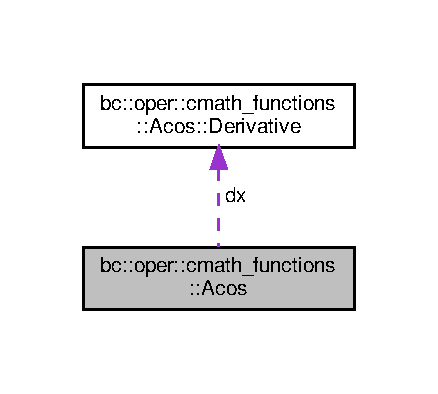
\includegraphics[width=210pt]{structbc_1_1oper_1_1cmath__functions_1_1Acos__coll__graph}
\end{center}
\end{figure}
\subsection*{Classes}
\begin{DoxyCompactItemize}
\item 
struct \hyperlink{structbc_1_1oper_1_1cmath__functions_1_1Acos_1_1Derivative}{Derivative}
\end{DoxyCompactItemize}
\subsection*{Public Member Functions}
\begin{DoxyCompactItemize}
\item 
{\footnotesize template$<$class value\+\_\+type $>$ }\\\hyperlink{common_8h_a6699e8b0449da5c0fafb878e59c1d4b1}{B\+C\+I\+N\+L\+I\+NE} value\+\_\+type \hyperlink{structbc_1_1oper_1_1cmath__functions_1_1Acos_a32904dc6e91d12cb71f427641bc1838d}{operator()} (const value\+\_\+type \&x) const
\item 
{\footnotesize template$<$class Xpr $>$ }\\auto \hyperlink{structbc_1_1oper_1_1cmath__functions_1_1Acos_aa8deed857a666abbe71c4a06efef2469}{operator()} (const \hyperlink{classbc_1_1tensors_1_1Expression__Base}{bc\+::tensors\+::\+Expression\+\_\+\+Base}$<$ Xpr $>$ \&tensor)
\item 
{\footnotesize template$<$class Xpr $>$ }\\auto \hyperlink{structbc_1_1oper_1_1cmath__functions_1_1Acos_a2bd998572a4c0e610fe19e3da9a4941e}{operator()} (const \hyperlink{classbc_1_1tensors_1_1Tensor__Base}{bc\+::tensors\+::\+Tensor\+\_\+\+Base}$<$ Xpr $>$ \&tensor)
\end{DoxyCompactItemize}
\subsection*{Static Public Member Functions}
\begin{DoxyCompactItemize}
\item 
{\footnotesize template$<$class value\+\_\+type $>$ }\\static \hyperlink{common_8h_a6699e8b0449da5c0fafb878e59c1d4b1}{B\+C\+I\+N\+L\+I\+NE} auto \hyperlink{structbc_1_1oper_1_1cmath__functions_1_1Acos_a61ecb6ec260e18bf74d519475debc011}{apply} (const value\+\_\+type \&x)
\end{DoxyCompactItemize}
\subsection*{Public Attributes}
\begin{DoxyCompactItemize}
\item 
struct \hyperlink{structbc_1_1oper_1_1cmath__functions_1_1Acos_1_1Derivative}{bc\+::oper\+::cmath\+\_\+functions\+::\+Acos\+::\+Derivative} \hyperlink{structbc_1_1oper_1_1cmath__functions_1_1Acos_a01f276736a773a9f88e39855163c5998}{dx}
\end{DoxyCompactItemize}


\subsection{Member Function Documentation}
\mbox{\Hypertarget{structbc_1_1oper_1_1cmath__functions_1_1Acos_a61ecb6ec260e18bf74d519475debc011}\label{structbc_1_1oper_1_1cmath__functions_1_1Acos_a61ecb6ec260e18bf74d519475debc011}} 
\index{bc\+::oper\+::cmath\+\_\+functions\+::\+Acos@{bc\+::oper\+::cmath\+\_\+functions\+::\+Acos}!apply@{apply}}
\index{apply@{apply}!bc\+::oper\+::cmath\+\_\+functions\+::\+Acos@{bc\+::oper\+::cmath\+\_\+functions\+::\+Acos}}
\subsubsection{\texorpdfstring{apply()}{apply()}}
{\footnotesize\ttfamily template$<$class value\+\_\+type $>$ \\
static \hyperlink{common_8h_a6699e8b0449da5c0fafb878e59c1d4b1}{B\+C\+I\+N\+L\+I\+NE} auto bc\+::oper\+::cmath\+\_\+functions\+::\+Acos\+::apply (\begin{DoxyParamCaption}\item[{const value\+\_\+type \&}]{x }\end{DoxyParamCaption})\hspace{0.3cm}{\ttfamily [inline]}, {\ttfamily [static]}}

\mbox{\Hypertarget{structbc_1_1oper_1_1cmath__functions_1_1Acos_a2bd998572a4c0e610fe19e3da9a4941e}\label{structbc_1_1oper_1_1cmath__functions_1_1Acos_a2bd998572a4c0e610fe19e3da9a4941e}} 
\index{bc\+::oper\+::cmath\+\_\+functions\+::\+Acos@{bc\+::oper\+::cmath\+\_\+functions\+::\+Acos}!operator()@{operator()}}
\index{operator()@{operator()}!bc\+::oper\+::cmath\+\_\+functions\+::\+Acos@{bc\+::oper\+::cmath\+\_\+functions\+::\+Acos}}
\subsubsection{\texorpdfstring{operator()()}{operator()()}\hspace{0.1cm}{\footnotesize\ttfamily [1/3]}}
{\footnotesize\ttfamily template$<$class Xpr $>$ \\
auto bc\+::oper\+::cmath\+\_\+functions\+::\+Acos\+::operator() (\begin{DoxyParamCaption}\item[{const \hyperlink{classbc_1_1tensors_1_1Tensor__Base}{bc\+::tensors\+::\+Tensor\+\_\+\+Base}$<$ Xpr $>$ \&}]{tensor }\end{DoxyParamCaption})\hspace{0.3cm}{\ttfamily [inline]}}

\mbox{\Hypertarget{structbc_1_1oper_1_1cmath__functions_1_1Acos_aa8deed857a666abbe71c4a06efef2469}\label{structbc_1_1oper_1_1cmath__functions_1_1Acos_aa8deed857a666abbe71c4a06efef2469}} 
\index{bc\+::oper\+::cmath\+\_\+functions\+::\+Acos@{bc\+::oper\+::cmath\+\_\+functions\+::\+Acos}!operator()@{operator()}}
\index{operator()@{operator()}!bc\+::oper\+::cmath\+\_\+functions\+::\+Acos@{bc\+::oper\+::cmath\+\_\+functions\+::\+Acos}}
\subsubsection{\texorpdfstring{operator()()}{operator()()}\hspace{0.1cm}{\footnotesize\ttfamily [2/3]}}
{\footnotesize\ttfamily template$<$class Xpr $>$ \\
auto bc\+::oper\+::cmath\+\_\+functions\+::\+Acos\+::operator() (\begin{DoxyParamCaption}\item[{const \hyperlink{classbc_1_1tensors_1_1Expression__Base}{bc\+::tensors\+::\+Expression\+\_\+\+Base}$<$ Xpr $>$ \&}]{tensor }\end{DoxyParamCaption})\hspace{0.3cm}{\ttfamily [inline]}}

\mbox{\Hypertarget{structbc_1_1oper_1_1cmath__functions_1_1Acos_a32904dc6e91d12cb71f427641bc1838d}\label{structbc_1_1oper_1_1cmath__functions_1_1Acos_a32904dc6e91d12cb71f427641bc1838d}} 
\index{bc\+::oper\+::cmath\+\_\+functions\+::\+Acos@{bc\+::oper\+::cmath\+\_\+functions\+::\+Acos}!operator()@{operator()}}
\index{operator()@{operator()}!bc\+::oper\+::cmath\+\_\+functions\+::\+Acos@{bc\+::oper\+::cmath\+\_\+functions\+::\+Acos}}
\subsubsection{\texorpdfstring{operator()()}{operator()()}\hspace{0.1cm}{\footnotesize\ttfamily [3/3]}}
{\footnotesize\ttfamily template$<$class value\+\_\+type $>$ \\
\hyperlink{common_8h_a6699e8b0449da5c0fafb878e59c1d4b1}{B\+C\+I\+N\+L\+I\+NE} value\+\_\+type bc\+::oper\+::cmath\+\_\+functions\+::\+Acos\+::operator() (\begin{DoxyParamCaption}\item[{const value\+\_\+type \&}]{x }\end{DoxyParamCaption}) const\hspace{0.3cm}{\ttfamily [inline]}}



\subsection{Member Data Documentation}
\mbox{\Hypertarget{structbc_1_1oper_1_1cmath__functions_1_1Acos_a01f276736a773a9f88e39855163c5998}\label{structbc_1_1oper_1_1cmath__functions_1_1Acos_a01f276736a773a9f88e39855163c5998}} 
\index{bc\+::oper\+::cmath\+\_\+functions\+::\+Acos@{bc\+::oper\+::cmath\+\_\+functions\+::\+Acos}!dx@{dx}}
\index{dx@{dx}!bc\+::oper\+::cmath\+\_\+functions\+::\+Acos@{bc\+::oper\+::cmath\+\_\+functions\+::\+Acos}}
\subsubsection{\texorpdfstring{dx}{dx}}
{\footnotesize\ttfamily struct \hyperlink{structbc_1_1oper_1_1cmath__functions_1_1Acos_1_1Derivative}{bc\+::oper\+::cmath\+\_\+functions\+::\+Acos\+::\+Derivative}   bc\+::oper\+::cmath\+\_\+functions\+::\+Acos\+::dx}



The documentation for this struct was generated from the following file\+:\begin{DoxyCompactItemize}
\item 
blackcat/operations/\hyperlink{cmath_8h}{cmath.\+h}\end{DoxyCompactItemize}

\hypertarget{structbc_1_1oper_1_1cmath__functions_1_1Acosh}{}\section{bc\+:\+:oper\+:\+:cmath\+\_\+functions\+:\+:Acosh Struct Reference}
\label{structbc_1_1oper_1_1cmath__functions_1_1Acosh}\index{bc\+::oper\+::cmath\+\_\+functions\+::\+Acosh@{bc\+::oper\+::cmath\+\_\+functions\+::\+Acosh}}


{\ttfamily \#include $<$cmath.\+h$>$}

\subsection*{Public Member Functions}
\begin{DoxyCompactItemize}
\item 
{\footnotesize template$<$class value\+\_\+type $>$ }\\\hyperlink{common_8h_a6699e8b0449da5c0fafb878e59c1d4b1}{B\+C\+I\+N\+L\+I\+NE} value\+\_\+type \hyperlink{structbc_1_1oper_1_1cmath__functions_1_1Acosh_a9dbd67feb47d89029340f4eb6040afdd}{operator()} (const value\+\_\+type \&x) const
\item 
{\footnotesize template$<$class Xpr $>$ }\\auto \hyperlink{structbc_1_1oper_1_1cmath__functions_1_1Acosh_a39b03c26fbdae12f411e9b4cc728259b}{operator()} (const \hyperlink{classbc_1_1tensors_1_1Expression__Base}{bc\+::tensors\+::\+Expression\+\_\+\+Base}$<$ Xpr $>$ \&tensor)
\item 
{\footnotesize template$<$class Xpr $>$ }\\auto \hyperlink{structbc_1_1oper_1_1cmath__functions_1_1Acosh_a4ee5951226fa7602ca79562912f34490}{operator()} (const \hyperlink{classbc_1_1tensors_1_1Tensor__Base}{bc\+::tensors\+::\+Tensor\+\_\+\+Base}$<$ Xpr $>$ \&tensor)
\end{DoxyCompactItemize}
\subsection*{Static Public Member Functions}
\begin{DoxyCompactItemize}
\item 
{\footnotesize template$<$class value\+\_\+type $>$ }\\static \hyperlink{common_8h_a6699e8b0449da5c0fafb878e59c1d4b1}{B\+C\+I\+N\+L\+I\+NE} auto \hyperlink{structbc_1_1oper_1_1cmath__functions_1_1Acosh_ab9fe3a2b62df67f130567a19b54934ca}{apply} (const value\+\_\+type \&x)
\end{DoxyCompactItemize}


\subsection{Member Function Documentation}
\mbox{\Hypertarget{structbc_1_1oper_1_1cmath__functions_1_1Acosh_ab9fe3a2b62df67f130567a19b54934ca}\label{structbc_1_1oper_1_1cmath__functions_1_1Acosh_ab9fe3a2b62df67f130567a19b54934ca}} 
\index{bc\+::oper\+::cmath\+\_\+functions\+::\+Acosh@{bc\+::oper\+::cmath\+\_\+functions\+::\+Acosh}!apply@{apply}}
\index{apply@{apply}!bc\+::oper\+::cmath\+\_\+functions\+::\+Acosh@{bc\+::oper\+::cmath\+\_\+functions\+::\+Acosh}}
\subsubsection{\texorpdfstring{apply()}{apply()}}
{\footnotesize\ttfamily template$<$class value\+\_\+type $>$ \\
static \hyperlink{common_8h_a6699e8b0449da5c0fafb878e59c1d4b1}{B\+C\+I\+N\+L\+I\+NE} auto bc\+::oper\+::cmath\+\_\+functions\+::\+Acosh\+::apply (\begin{DoxyParamCaption}\item[{const value\+\_\+type \&}]{x }\end{DoxyParamCaption})\hspace{0.3cm}{\ttfamily [inline]}, {\ttfamily [static]}}

\mbox{\Hypertarget{structbc_1_1oper_1_1cmath__functions_1_1Acosh_a4ee5951226fa7602ca79562912f34490}\label{structbc_1_1oper_1_1cmath__functions_1_1Acosh_a4ee5951226fa7602ca79562912f34490}} 
\index{bc\+::oper\+::cmath\+\_\+functions\+::\+Acosh@{bc\+::oper\+::cmath\+\_\+functions\+::\+Acosh}!operator()@{operator()}}
\index{operator()@{operator()}!bc\+::oper\+::cmath\+\_\+functions\+::\+Acosh@{bc\+::oper\+::cmath\+\_\+functions\+::\+Acosh}}
\subsubsection{\texorpdfstring{operator()()}{operator()()}\hspace{0.1cm}{\footnotesize\ttfamily [1/3]}}
{\footnotesize\ttfamily template$<$class Xpr $>$ \\
auto bc\+::oper\+::cmath\+\_\+functions\+::\+Acosh\+::operator() (\begin{DoxyParamCaption}\item[{const \hyperlink{classbc_1_1tensors_1_1Tensor__Base}{bc\+::tensors\+::\+Tensor\+\_\+\+Base}$<$ Xpr $>$ \&}]{tensor }\end{DoxyParamCaption})\hspace{0.3cm}{\ttfamily [inline]}}

\mbox{\Hypertarget{structbc_1_1oper_1_1cmath__functions_1_1Acosh_a39b03c26fbdae12f411e9b4cc728259b}\label{structbc_1_1oper_1_1cmath__functions_1_1Acosh_a39b03c26fbdae12f411e9b4cc728259b}} 
\index{bc\+::oper\+::cmath\+\_\+functions\+::\+Acosh@{bc\+::oper\+::cmath\+\_\+functions\+::\+Acosh}!operator()@{operator()}}
\index{operator()@{operator()}!bc\+::oper\+::cmath\+\_\+functions\+::\+Acosh@{bc\+::oper\+::cmath\+\_\+functions\+::\+Acosh}}
\subsubsection{\texorpdfstring{operator()()}{operator()()}\hspace{0.1cm}{\footnotesize\ttfamily [2/3]}}
{\footnotesize\ttfamily template$<$class Xpr $>$ \\
auto bc\+::oper\+::cmath\+\_\+functions\+::\+Acosh\+::operator() (\begin{DoxyParamCaption}\item[{const \hyperlink{classbc_1_1tensors_1_1Expression__Base}{bc\+::tensors\+::\+Expression\+\_\+\+Base}$<$ Xpr $>$ \&}]{tensor }\end{DoxyParamCaption})\hspace{0.3cm}{\ttfamily [inline]}}

\mbox{\Hypertarget{structbc_1_1oper_1_1cmath__functions_1_1Acosh_a9dbd67feb47d89029340f4eb6040afdd}\label{structbc_1_1oper_1_1cmath__functions_1_1Acosh_a9dbd67feb47d89029340f4eb6040afdd}} 
\index{bc\+::oper\+::cmath\+\_\+functions\+::\+Acosh@{bc\+::oper\+::cmath\+\_\+functions\+::\+Acosh}!operator()@{operator()}}
\index{operator()@{operator()}!bc\+::oper\+::cmath\+\_\+functions\+::\+Acosh@{bc\+::oper\+::cmath\+\_\+functions\+::\+Acosh}}
\subsubsection{\texorpdfstring{operator()()}{operator()()}\hspace{0.1cm}{\footnotesize\ttfamily [3/3]}}
{\footnotesize\ttfamily template$<$class value\+\_\+type $>$ \\
\hyperlink{common_8h_a6699e8b0449da5c0fafb878e59c1d4b1}{B\+C\+I\+N\+L\+I\+NE} value\+\_\+type bc\+::oper\+::cmath\+\_\+functions\+::\+Acosh\+::operator() (\begin{DoxyParamCaption}\item[{const value\+\_\+type \&}]{x }\end{DoxyParamCaption}) const\hspace{0.3cm}{\ttfamily [inline]}}



The documentation for this struct was generated from the following file\+:\begin{DoxyCompactItemize}
\item 
blackcat/operations/\hyperlink{cmath_8h}{cmath.\+h}\end{DoxyCompactItemize}

\hypertarget{structbc_1_1nn_1_1Adam}{}\section{bc\+:\+:nn\+:\+:Adam Struct Reference}
\label{structbc_1_1nn_1_1Adam}\index{bc\+::nn\+::\+Adam@{bc\+::nn\+::\+Adam}}


{\ttfamily \#include $<$adam.\+h$>$}

\subsection*{Classes}
\begin{DoxyCompactItemize}
\item 
struct \hyperlink{structbc_1_1nn_1_1Adam_1_1Optimizer}{Optimizer}
\end{DoxyCompactItemize}


The documentation for this struct was generated from the following file\+:\begin{DoxyCompactItemize}
\item 
blackcat/neural\+\_\+networks/optimzers/\hyperlink{adam_8h}{adam.\+h}\end{DoxyCompactItemize}

\hypertarget{structbc_1_1oper_1_1Add}{}\section{bc\+:\+:oper\+:\+:Add Struct Reference}
\label{structbc_1_1oper_1_1Add}\index{bc\+::oper\+::\+Add@{bc\+::oper\+::\+Add}}


{\ttfamily \#include $<$binary.\+h$>$}



Inheritance diagram for bc\+:\+:oper\+:\+:Add\+:\nopagebreak
\begin{figure}[H]
\begin{center}
\leavevmode
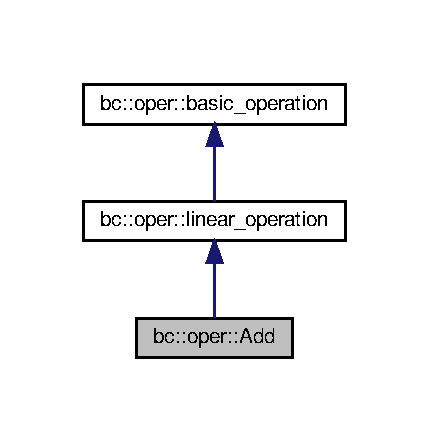
\includegraphics[width=206pt]{structbc_1_1oper_1_1Add__inherit__graph}
\end{center}
\end{figure}


Collaboration diagram for bc\+:\+:oper\+:\+:Add\+:\nopagebreak
\begin{figure}[H]
\begin{center}
\leavevmode
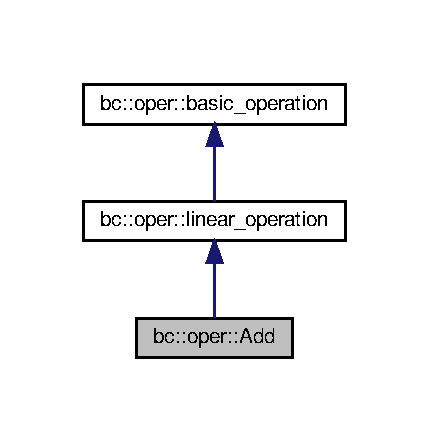
\includegraphics[width=206pt]{structbc_1_1oper_1_1Add__coll__graph}
\end{center}
\end{figure}
\subsection*{Public Types}
\begin{DoxyCompactItemize}
\item 
using \hyperlink{structbc_1_1oper_1_1Add_a72e4a8cfa013493278c180a605f38cb0}{alpha\+\_\+modifier} = \hyperlink{structbc_1_1traits_1_1Integer}{bc\+::traits\+::\+Integer}$<$ 1 $>$
\end{DoxyCompactItemize}
\subsection*{Public Member Functions}
\begin{DoxyCompactItemize}
\item 
{\footnotesize template$<$class Lv , class Rv $>$ }\\\+\_\+\+\_\+host\+\_\+\+\_\+ \+\_\+\+\_\+device\+\_\+\+\_\+ auto \hyperlink{structbc_1_1oper_1_1Add_af3d71f0cd740124171f9a92162125068}{operator()} (Lv \&\&lv, Rv \&\&rv) const -\/$>$ decltype(\hyperlink{structbc_1_1oper_1_1Add_a2cf484e25e4aa7d787f85da0f9807fd4}{apply}(lv, rv))
\end{DoxyCompactItemize}
\subsection*{Static Public Member Functions}
\begin{DoxyCompactItemize}
\item 
{\footnotesize template$<$class Lv , class Rv $>$ }\\\+\_\+\+\_\+host\+\_\+\+\_\+ static \+\_\+\+\_\+device\+\_\+\+\_\+ auto \hyperlink{structbc_1_1oper_1_1Add_a2cf484e25e4aa7d787f85da0f9807fd4}{apply} (Lv \&\&lv, Rv \&\&rv) -\/$>$ decltype(lv+rv)
\end{DoxyCompactItemize}


\subsection{Member Typedef Documentation}
\mbox{\Hypertarget{structbc_1_1oper_1_1Add_a72e4a8cfa013493278c180a605f38cb0}\label{structbc_1_1oper_1_1Add_a72e4a8cfa013493278c180a605f38cb0}} 
\index{bc\+::oper\+::\+Add@{bc\+::oper\+::\+Add}!alpha\+\_\+modifier@{alpha\+\_\+modifier}}
\index{alpha\+\_\+modifier@{alpha\+\_\+modifier}!bc\+::oper\+::\+Add@{bc\+::oper\+::\+Add}}
\subsubsection{\texorpdfstring{alpha\+\_\+modifier}{alpha\_modifier}}
{\footnotesize\ttfamily using \hyperlink{structbc_1_1oper_1_1Add_a72e4a8cfa013493278c180a605f38cb0}{bc\+::oper\+::\+Add\+::alpha\+\_\+modifier} =  \hyperlink{structbc_1_1traits_1_1Integer}{bc\+::traits\+::\+Integer}$<$1$>$}



\subsection{Member Function Documentation}
\mbox{\Hypertarget{structbc_1_1oper_1_1Add_a2cf484e25e4aa7d787f85da0f9807fd4}\label{structbc_1_1oper_1_1Add_a2cf484e25e4aa7d787f85da0f9807fd4}} 
\index{bc\+::oper\+::\+Add@{bc\+::oper\+::\+Add}!apply@{apply}}
\index{apply@{apply}!bc\+::oper\+::\+Add@{bc\+::oper\+::\+Add}}
\subsubsection{\texorpdfstring{apply()}{apply()}}
{\footnotesize\ttfamily template$<$class Lv , class Rv $>$ \\
\+\_\+\+\_\+host\+\_\+\+\_\+ static \+\_\+\+\_\+device\+\_\+\+\_\+ auto bc\+::oper\+::\+Add\+::apply (\begin{DoxyParamCaption}\item[{Lv \&\&}]{lv,  }\item[{Rv \&\&}]{rv }\end{DoxyParamCaption}) -\/$>$ decltype( lv + rv ) \hspace{0.3cm}{\ttfamily [inline]}, {\ttfamily [static]}}

\mbox{\Hypertarget{structbc_1_1oper_1_1Add_af3d71f0cd740124171f9a92162125068}\label{structbc_1_1oper_1_1Add_af3d71f0cd740124171f9a92162125068}} 
\index{bc\+::oper\+::\+Add@{bc\+::oper\+::\+Add}!operator()@{operator()}}
\index{operator()@{operator()}!bc\+::oper\+::\+Add@{bc\+::oper\+::\+Add}}
\subsubsection{\texorpdfstring{operator()()}{operator()()}}
{\footnotesize\ttfamily template$<$class Lv , class Rv $>$ \\
\+\_\+\+\_\+host\+\_\+\+\_\+ \+\_\+\+\_\+device\+\_\+\+\_\+ auto bc\+::oper\+::\+Add\+::operator() (\begin{DoxyParamCaption}\item[{Lv \&\&}]{lv,  }\item[{Rv \&\&}]{rv }\end{DoxyParamCaption}) const -\/$>$ decltype(\hyperlink{structbc_1_1oper_1_1Add_a2cf484e25e4aa7d787f85da0f9807fd4}{apply}(lv, rv)) \hspace{0.3cm}{\ttfamily [inline]}}



The documentation for this struct was generated from the following file\+:\begin{DoxyCompactItemize}
\item 
blackcat/operations/\hyperlink{binary_8h}{binary.\+h}\end{DoxyCompactItemize}

\hypertarget{structbc_1_1oper_1_1Add__Assign}{}\section{bc\+:\+:oper\+:\+:Add\+\_\+\+Assign Struct Reference}
\label{structbc_1_1oper_1_1Add__Assign}\index{bc\+::oper\+::\+Add\+\_\+\+Assign@{bc\+::oper\+::\+Add\+\_\+\+Assign}}


{\ttfamily \#include $<$binary.\+h$>$}



Inheritance diagram for bc\+:\+:oper\+:\+:Add\+\_\+\+Assign\+:\nopagebreak
\begin{figure}[H]
\begin{center}
\leavevmode
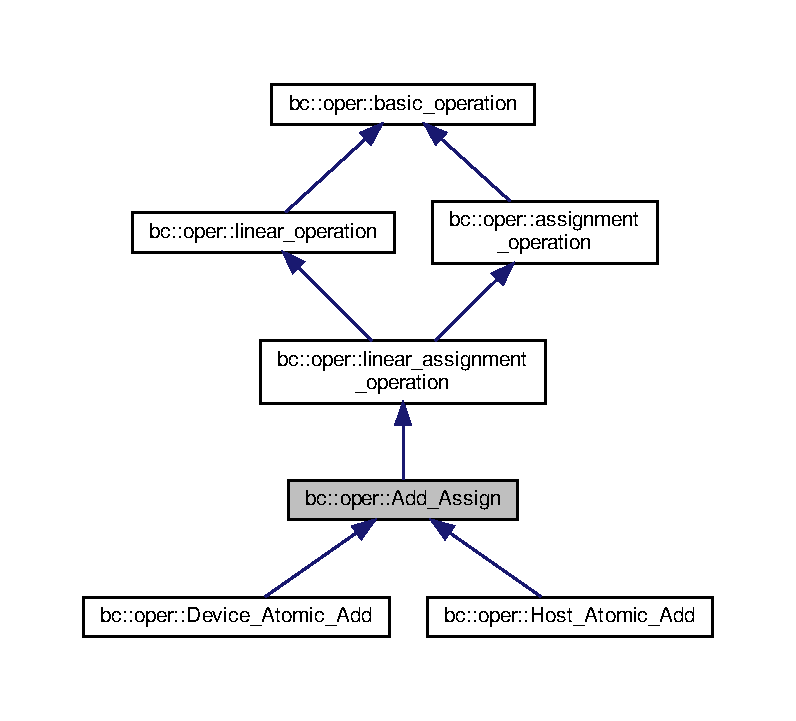
\includegraphics[width=350pt]{structbc_1_1oper_1_1Add__Assign__inherit__graph}
\end{center}
\end{figure}


Collaboration diagram for bc\+:\+:oper\+:\+:Add\+\_\+\+Assign\+:\nopagebreak
\begin{figure}[H]
\begin{center}
\leavevmode
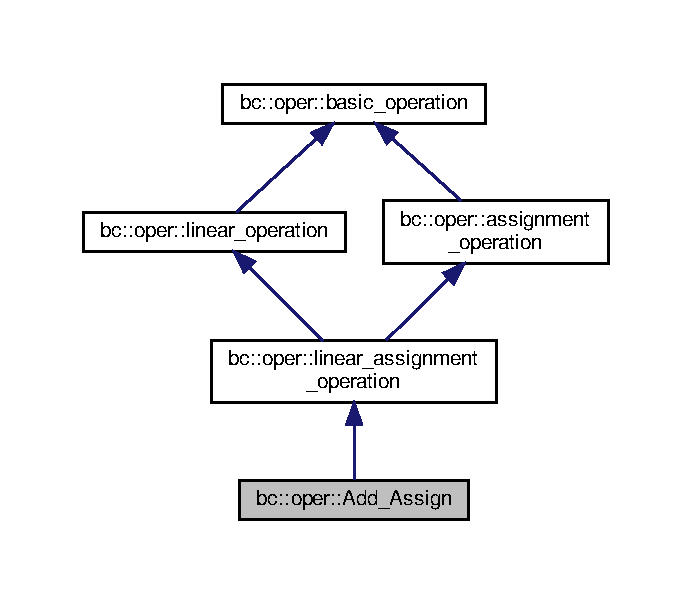
\includegraphics[width=332pt]{structbc_1_1oper_1_1Add__Assign__coll__graph}
\end{center}
\end{figure}
\subsection*{Public Types}
\begin{DoxyCompactItemize}
\item 
using \hyperlink{structbc_1_1oper_1_1Add__Assign_a608f4b132e9a48c01de612acac5af87e}{alpha\+\_\+modifier} = \hyperlink{structbc_1_1traits_1_1Integer}{bc\+::traits\+::\+Integer}$<$ 1 $>$
\item 
using \hyperlink{structbc_1_1oper_1_1Add__Assign_a2ad8892dba37c039d7a82b674c126bf0}{beta\+\_\+modifier} = \hyperlink{structbc_1_1traits_1_1Integer}{bc\+::traits\+::\+Integer}$<$ 1 $>$
\end{DoxyCompactItemize}
\subsection*{Public Member Functions}
\begin{DoxyCompactItemize}
\item 
{\footnotesize template$<$class Lv , class Rv $>$ }\\\+\_\+\+\_\+host\+\_\+\+\_\+ \+\_\+\+\_\+device\+\_\+\+\_\+ auto \hyperlink{structbc_1_1oper_1_1Add__Assign_a40d7c53569de0b79f9548b16b21c0b09}{operator()} (Lv \&\&lv, Rv \&\&rv) const -\/$>$ decltype(\hyperlink{structbc_1_1oper_1_1Add__Assign_ac908f04769926c30ab8763d5748dee4b}{apply}(lv, rv))
\end{DoxyCompactItemize}
\subsection*{Static Public Member Functions}
\begin{DoxyCompactItemize}
\item 
{\footnotesize template$<$class Lv , class Rv $>$ }\\\+\_\+\+\_\+host\+\_\+\+\_\+ static \+\_\+\+\_\+device\+\_\+\+\_\+ auto \hyperlink{structbc_1_1oper_1_1Add__Assign_ac908f04769926c30ab8763d5748dee4b}{apply} (Lv \&\&lv, Rv \&\&rv) -\/$>$ decltype(lv+=rv)
\end{DoxyCompactItemize}


\subsection{Member Typedef Documentation}
\mbox{\Hypertarget{structbc_1_1oper_1_1Add__Assign_a608f4b132e9a48c01de612acac5af87e}\label{structbc_1_1oper_1_1Add__Assign_a608f4b132e9a48c01de612acac5af87e}} 
\index{bc\+::oper\+::\+Add\+\_\+\+Assign@{bc\+::oper\+::\+Add\+\_\+\+Assign}!alpha\+\_\+modifier@{alpha\+\_\+modifier}}
\index{alpha\+\_\+modifier@{alpha\+\_\+modifier}!bc\+::oper\+::\+Add\+\_\+\+Assign@{bc\+::oper\+::\+Add\+\_\+\+Assign}}
\subsubsection{\texorpdfstring{alpha\+\_\+modifier}{alpha\_modifier}}
{\footnotesize\ttfamily using \hyperlink{structbc_1_1oper_1_1Add__Assign_a608f4b132e9a48c01de612acac5af87e}{bc\+::oper\+::\+Add\+\_\+\+Assign\+::alpha\+\_\+modifier} =  \hyperlink{structbc_1_1traits_1_1Integer}{bc\+::traits\+::\+Integer}$<$1$>$}

\mbox{\Hypertarget{structbc_1_1oper_1_1Add__Assign_a2ad8892dba37c039d7a82b674c126bf0}\label{structbc_1_1oper_1_1Add__Assign_a2ad8892dba37c039d7a82b674c126bf0}} 
\index{bc\+::oper\+::\+Add\+\_\+\+Assign@{bc\+::oper\+::\+Add\+\_\+\+Assign}!beta\+\_\+modifier@{beta\+\_\+modifier}}
\index{beta\+\_\+modifier@{beta\+\_\+modifier}!bc\+::oper\+::\+Add\+\_\+\+Assign@{bc\+::oper\+::\+Add\+\_\+\+Assign}}
\subsubsection{\texorpdfstring{beta\+\_\+modifier}{beta\_modifier}}
{\footnotesize\ttfamily using \hyperlink{structbc_1_1oper_1_1Add__Assign_a2ad8892dba37c039d7a82b674c126bf0}{bc\+::oper\+::\+Add\+\_\+\+Assign\+::beta\+\_\+modifier} =  \hyperlink{structbc_1_1traits_1_1Integer}{bc\+::traits\+::\+Integer}$<$1$>$}



\subsection{Member Function Documentation}
\mbox{\Hypertarget{structbc_1_1oper_1_1Add__Assign_ac908f04769926c30ab8763d5748dee4b}\label{structbc_1_1oper_1_1Add__Assign_ac908f04769926c30ab8763d5748dee4b}} 
\index{bc\+::oper\+::\+Add\+\_\+\+Assign@{bc\+::oper\+::\+Add\+\_\+\+Assign}!apply@{apply}}
\index{apply@{apply}!bc\+::oper\+::\+Add\+\_\+\+Assign@{bc\+::oper\+::\+Add\+\_\+\+Assign}}
\subsubsection{\texorpdfstring{apply()}{apply()}}
{\footnotesize\ttfamily template$<$class Lv , class Rv $>$ \\
\+\_\+\+\_\+host\+\_\+\+\_\+ static \+\_\+\+\_\+device\+\_\+\+\_\+ auto bc\+::oper\+::\+Add\+\_\+\+Assign\+::apply (\begin{DoxyParamCaption}\item[{Lv \&\&}]{lv,  }\item[{Rv \&\&}]{rv }\end{DoxyParamCaption}) -\/$>$ decltype( lv += rv ) \hspace{0.3cm}{\ttfamily [inline]}, {\ttfamily [static]}}

\mbox{\Hypertarget{structbc_1_1oper_1_1Add__Assign_a40d7c53569de0b79f9548b16b21c0b09}\label{structbc_1_1oper_1_1Add__Assign_a40d7c53569de0b79f9548b16b21c0b09}} 
\index{bc\+::oper\+::\+Add\+\_\+\+Assign@{bc\+::oper\+::\+Add\+\_\+\+Assign}!operator()@{operator()}}
\index{operator()@{operator()}!bc\+::oper\+::\+Add\+\_\+\+Assign@{bc\+::oper\+::\+Add\+\_\+\+Assign}}
\subsubsection{\texorpdfstring{operator()()}{operator()()}}
{\footnotesize\ttfamily template$<$class Lv , class Rv $>$ \\
\+\_\+\+\_\+host\+\_\+\+\_\+ \+\_\+\+\_\+device\+\_\+\+\_\+ auto bc\+::oper\+::\+Add\+\_\+\+Assign\+::operator() (\begin{DoxyParamCaption}\item[{Lv \&\&}]{lv,  }\item[{Rv \&\&}]{rv }\end{DoxyParamCaption}) const -\/$>$ decltype(\hyperlink{structbc_1_1oper_1_1Add__Assign_ac908f04769926c30ab8763d5748dee4b}{apply}(lv, rv)) \hspace{0.3cm}{\ttfamily [inline]}}



The documentation for this struct was generated from the following file\+:\begin{DoxyCompactItemize}
\item 
blackcat/operations/\hyperlink{binary_8h}{binary.\+h}\end{DoxyCompactItemize}

\hypertarget{structbc_1_1tensors_1_1Tensor__Base_1_1Alias}{}\section{bc\+:\+:tensors\+:\+:Tensor\+\_\+\+Base$<$ Expression\+Template $>$\+:\+:Alias Struct Reference}
\label{structbc_1_1tensors_1_1Tensor__Base_1_1Alias}\index{bc\+::tensors\+::\+Tensor\+\_\+\+Base$<$ Expression\+Template $>$\+::\+Alias@{bc\+::tensors\+::\+Tensor\+\_\+\+Base$<$ Expression\+Template $>$\+::\+Alias}}


{\ttfamily \#include $<$tensor\+\_\+base.\+h$>$}



Collaboration diagram for bc\+:\+:tensors\+:\+:Tensor\+\_\+\+Base$<$ Expression\+Template $>$\+:\+:Alias\+:\nopagebreak
\begin{figure}[H]
\begin{center}
\leavevmode
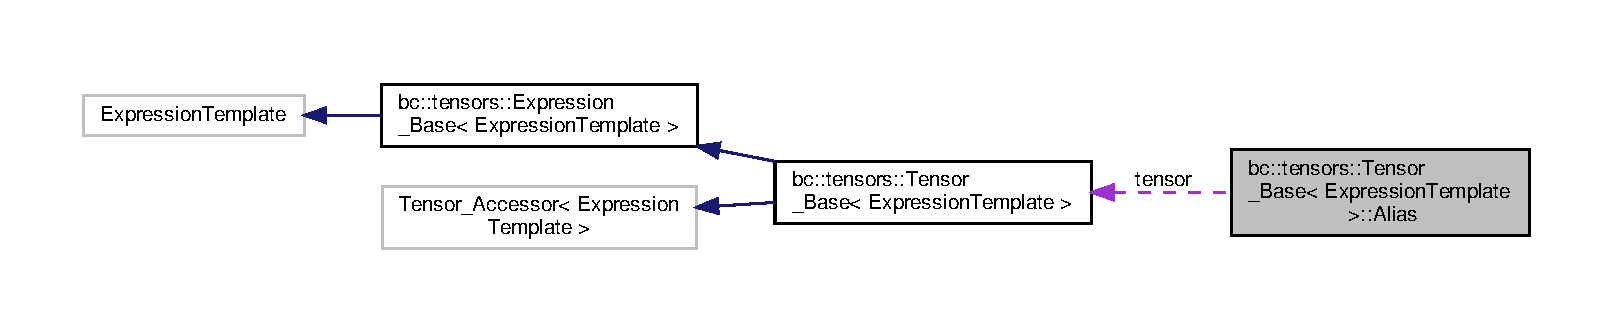
\includegraphics[width=350pt]{structbc_1_1tensors_1_1Tensor__Base_1_1Alias__coll__graph}
\end{center}
\end{figure}
\subsection*{Public Member Functions}
\begin{DoxyCompactItemize}
\item 
{\footnotesize template$<$class Xpr $>$ }\\auto \& \hyperlink{structbc_1_1tensors_1_1Tensor__Base_1_1Alias_aabbc3f738288104c07bfa77fe68de2fe}{operator=} (const \hyperlink{classbc_1_1tensors_1_1Expression__Base}{Expression\+\_\+\+Base}$<$ Xpr $>$ \&param)
\item 
{\footnotesize template$<$class Xpr $>$ }\\auto \& \hyperlink{structbc_1_1tensors_1_1Tensor__Base_1_1Alias_aca7a44a5cd4994ecdbc094b092a50879}{operator+=} (const \hyperlink{classbc_1_1tensors_1_1Expression__Base}{Expression\+\_\+\+Base}$<$ Xpr $>$ \&param)
\item 
{\footnotesize template$<$class Xpr $>$ }\\auto \& \hyperlink{structbc_1_1tensors_1_1Tensor__Base_1_1Alias_ab5c7e5fa42ac5d4dcb1b95325cef5541}{operator-\/=} (const \hyperlink{classbc_1_1tensors_1_1Expression__Base}{Expression\+\_\+\+Base}$<$ Xpr $>$ \&param)
\end{DoxyCompactItemize}
\subsection*{Public Attributes}
\begin{DoxyCompactItemize}
\item 
\hyperlink{classbc_1_1tensors_1_1Expression__Base}{self\+\_\+type} \& \hyperlink{structbc_1_1tensors_1_1Tensor__Base_1_1Alias_ad5750b0c21936ec7e177648a831d06b4}{tensor}
\end{DoxyCompactItemize}


\subsection{Member Function Documentation}
\mbox{\Hypertarget{structbc_1_1tensors_1_1Tensor__Base_1_1Alias_aca7a44a5cd4994ecdbc094b092a50879}\label{structbc_1_1tensors_1_1Tensor__Base_1_1Alias_aca7a44a5cd4994ecdbc094b092a50879}} 
\index{bc\+::tensors\+::\+Tensor\+\_\+\+Base\+::\+Alias@{bc\+::tensors\+::\+Tensor\+\_\+\+Base\+::\+Alias}!operator+=@{operator+=}}
\index{operator+=@{operator+=}!bc\+::tensors\+::\+Tensor\+\_\+\+Base\+::\+Alias@{bc\+::tensors\+::\+Tensor\+\_\+\+Base\+::\+Alias}}
\subsubsection{\texorpdfstring{operator+=()}{operator+=()}}
{\footnotesize\ttfamily template$<$class Expression\+Template$>$ \\
template$<$class Xpr $>$ \\
auto\& \hyperlink{classbc_1_1tensors_1_1Tensor__Base}{bc\+::tensors\+::\+Tensor\+\_\+\+Base}$<$ Expression\+Template $>$\+::Alias\+::operator+= (\begin{DoxyParamCaption}\item[{const \hyperlink{classbc_1_1tensors_1_1Expression__Base}{Expression\+\_\+\+Base}$<$ Xpr $>$ \&}]{param }\end{DoxyParamCaption})\hspace{0.3cm}{\ttfamily [inline]}}

\mbox{\Hypertarget{structbc_1_1tensors_1_1Tensor__Base_1_1Alias_ab5c7e5fa42ac5d4dcb1b95325cef5541}\label{structbc_1_1tensors_1_1Tensor__Base_1_1Alias_ab5c7e5fa42ac5d4dcb1b95325cef5541}} 
\index{bc\+::tensors\+::\+Tensor\+\_\+\+Base\+::\+Alias@{bc\+::tensors\+::\+Tensor\+\_\+\+Base\+::\+Alias}!operator-\/=@{operator-\/=}}
\index{operator-\/=@{operator-\/=}!bc\+::tensors\+::\+Tensor\+\_\+\+Base\+::\+Alias@{bc\+::tensors\+::\+Tensor\+\_\+\+Base\+::\+Alias}}
\subsubsection{\texorpdfstring{operator-\/=()}{operator-=()}}
{\footnotesize\ttfamily template$<$class Expression\+Template$>$ \\
template$<$class Xpr $>$ \\
auto\& \hyperlink{classbc_1_1tensors_1_1Tensor__Base}{bc\+::tensors\+::\+Tensor\+\_\+\+Base}$<$ Expression\+Template $>$\+::Alias\+::operator-\/= (\begin{DoxyParamCaption}\item[{const \hyperlink{classbc_1_1tensors_1_1Expression__Base}{Expression\+\_\+\+Base}$<$ Xpr $>$ \&}]{param }\end{DoxyParamCaption})\hspace{0.3cm}{\ttfamily [inline]}}

\mbox{\Hypertarget{structbc_1_1tensors_1_1Tensor__Base_1_1Alias_aabbc3f738288104c07bfa77fe68de2fe}\label{structbc_1_1tensors_1_1Tensor__Base_1_1Alias_aabbc3f738288104c07bfa77fe68de2fe}} 
\index{bc\+::tensors\+::\+Tensor\+\_\+\+Base\+::\+Alias@{bc\+::tensors\+::\+Tensor\+\_\+\+Base\+::\+Alias}!operator=@{operator=}}
\index{operator=@{operator=}!bc\+::tensors\+::\+Tensor\+\_\+\+Base\+::\+Alias@{bc\+::tensors\+::\+Tensor\+\_\+\+Base\+::\+Alias}}
\subsubsection{\texorpdfstring{operator=()}{operator=()}}
{\footnotesize\ttfamily template$<$class Expression\+Template$>$ \\
template$<$class Xpr $>$ \\
auto\& \hyperlink{classbc_1_1tensors_1_1Tensor__Base}{bc\+::tensors\+::\+Tensor\+\_\+\+Base}$<$ Expression\+Template $>$\+::Alias\+::operator= (\begin{DoxyParamCaption}\item[{const \hyperlink{classbc_1_1tensors_1_1Expression__Base}{Expression\+\_\+\+Base}$<$ Xpr $>$ \&}]{param }\end{DoxyParamCaption})\hspace{0.3cm}{\ttfamily [inline]}}



\subsection{Member Data Documentation}
\mbox{\Hypertarget{structbc_1_1tensors_1_1Tensor__Base_1_1Alias_ad5750b0c21936ec7e177648a831d06b4}\label{structbc_1_1tensors_1_1Tensor__Base_1_1Alias_ad5750b0c21936ec7e177648a831d06b4}} 
\index{bc\+::tensors\+::\+Tensor\+\_\+\+Base\+::\+Alias@{bc\+::tensors\+::\+Tensor\+\_\+\+Base\+::\+Alias}!tensor@{tensor}}
\index{tensor@{tensor}!bc\+::tensors\+::\+Tensor\+\_\+\+Base\+::\+Alias@{bc\+::tensors\+::\+Tensor\+\_\+\+Base\+::\+Alias}}
\subsubsection{\texorpdfstring{tensor}{tensor}}
{\footnotesize\ttfamily template$<$class Expression\+Template$>$ \\
\hyperlink{classbc_1_1tensors_1_1Expression__Base}{self\+\_\+type}\& \hyperlink{classbc_1_1tensors_1_1Tensor__Base}{bc\+::tensors\+::\+Tensor\+\_\+\+Base}$<$ Expression\+Template $>$\+::Alias\+::tensor}



The documentation for this struct was generated from the following file\+:\begin{DoxyCompactItemize}
\item 
blackcat/tensors/\hyperlink{tensor__base_8h}{tensor\+\_\+base.\+h}\end{DoxyCompactItemize}

\hypertarget{structAlias}{}\section{Alias Struct Reference}
\label{structAlias}\index{Alias@{Alias}}


{\ttfamily \#include $<$tensor\+\_\+operations.\+h$>$}

\subsection*{Public Member Functions}
\begin{DoxyCompactItemize}
\item 
{\footnotesize template$<$class Xpr $>$ }\\auto \& \hyperlink{structAlias_a18a1108238e76db0d138ecb26d57aa80}{operator=} (const Expression\+\_\+\+Base$<$ Xpr $>$ \&param)
\item 
{\footnotesize template$<$class Xpr $>$ }\\auto \& \hyperlink{structAlias_ac6d72bf7f3507b3b0cec0858895fd049}{operator+=} (const Expression\+\_\+\+Base$<$ Xpr $>$ \&param)
\item 
{\footnotesize template$<$class Xpr $>$ }\\auto \& \hyperlink{structAlias_a005fd967ffd4094b6598da0280fa3fed}{operator-\/=} (const Expression\+\_\+\+Base$<$ Xpr $>$ \&param)
\end{DoxyCompactItemize}
\subsection*{Public Attributes}
\begin{DoxyCompactItemize}
\item 
self\+\_\+type \& \hyperlink{structAlias_a17791174eae7fd8077e650ed61c668dc}{tensor}
\end{DoxyCompactItemize}


\subsection{Member Function Documentation}
\mbox{\Hypertarget{structAlias_ac6d72bf7f3507b3b0cec0858895fd049}\label{structAlias_ac6d72bf7f3507b3b0cec0858895fd049}} 
\index{Alias@{Alias}!operator+=@{operator+=}}
\index{operator+=@{operator+=}!Alias@{Alias}}
\subsubsection{\texorpdfstring{operator+=()}{operator+=()}}
{\footnotesize\ttfamily template$<$class Xpr $>$ \\
auto\& Alias\+::operator+= (\begin{DoxyParamCaption}\item[{const Expression\+\_\+\+Base$<$ Xpr $>$ \&}]{param }\end{DoxyParamCaption})\hspace{0.3cm}{\ttfamily [inline]}}

\mbox{\Hypertarget{structAlias_a005fd967ffd4094b6598da0280fa3fed}\label{structAlias_a005fd967ffd4094b6598da0280fa3fed}} 
\index{Alias@{Alias}!operator-\/=@{operator-\/=}}
\index{operator-\/=@{operator-\/=}!Alias@{Alias}}
\subsubsection{\texorpdfstring{operator-\/=()}{operator-=()}}
{\footnotesize\ttfamily template$<$class Xpr $>$ \\
auto\& Alias\+::operator-\/= (\begin{DoxyParamCaption}\item[{const Expression\+\_\+\+Base$<$ Xpr $>$ \&}]{param }\end{DoxyParamCaption})\hspace{0.3cm}{\ttfamily [inline]}}

\mbox{\Hypertarget{structAlias_a18a1108238e76db0d138ecb26d57aa80}\label{structAlias_a18a1108238e76db0d138ecb26d57aa80}} 
\index{Alias@{Alias}!operator=@{operator=}}
\index{operator=@{operator=}!Alias@{Alias}}
\subsubsection{\texorpdfstring{operator=()}{operator=()}}
{\footnotesize\ttfamily template$<$class Xpr $>$ \\
auto\& Alias\+::operator= (\begin{DoxyParamCaption}\item[{const Expression\+\_\+\+Base$<$ Xpr $>$ \&}]{param }\end{DoxyParamCaption})\hspace{0.3cm}{\ttfamily [inline]}}



\subsection{Member Data Documentation}
\mbox{\Hypertarget{structAlias_a17791174eae7fd8077e650ed61c668dc}\label{structAlias_a17791174eae7fd8077e650ed61c668dc}} 
\index{Alias@{Alias}!tensor@{tensor}}
\index{tensor@{tensor}!Alias@{Alias}}
\subsubsection{\texorpdfstring{tensor}{tensor}}
{\footnotesize\ttfamily self\+\_\+type\& Alias\+::tensor}



The documentation for this struct was generated from the following file\+:\begin{DoxyCompactItemize}
\item 
blackcat/tensors/\hyperlink{tensor__operations_8h}{tensor\+\_\+operations.\+h}\end{DoxyCompactItemize}

\hypertarget{structbc_1_1oper_1_1Alias__Add__Assign}{}\section{bc\+:\+:oper\+:\+:Alias\+\_\+\+Add\+\_\+\+Assign Struct Reference}
\label{structbc_1_1oper_1_1Alias__Add__Assign}\index{bc\+::oper\+::\+Alias\+\_\+\+Add\+\_\+\+Assign@{bc\+::oper\+::\+Alias\+\_\+\+Add\+\_\+\+Assign}}


{\ttfamily \#include $<$binary.\+h$>$}



Inheritance diagram for bc\+:\+:oper\+:\+:Alias\+\_\+\+Add\+\_\+\+Assign\+:\nopagebreak
\begin{figure}[H]
\begin{center}
\leavevmode
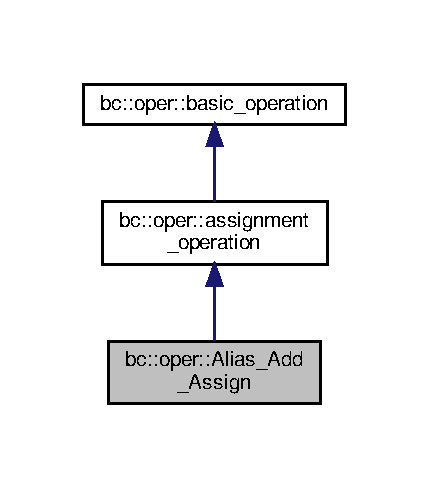
\includegraphics[width=206pt]{structbc_1_1oper_1_1Alias__Add__Assign__inherit__graph}
\end{center}
\end{figure}


Collaboration diagram for bc\+:\+:oper\+:\+:Alias\+\_\+\+Add\+\_\+\+Assign\+:\nopagebreak
\begin{figure}[H]
\begin{center}
\leavevmode
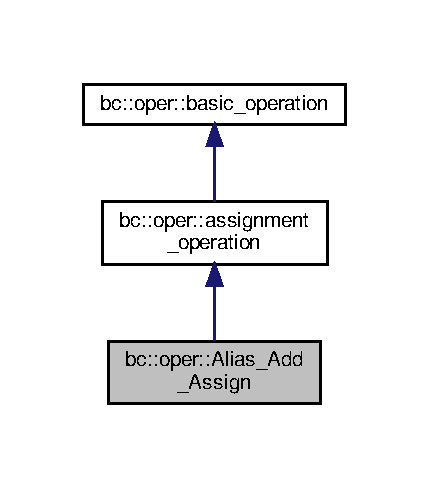
\includegraphics[width=206pt]{structbc_1_1oper_1_1Alias__Add__Assign__coll__graph}
\end{center}
\end{figure}
\subsection*{Public Types}
\begin{DoxyCompactItemize}
\item 
using \hyperlink{structbc_1_1oper_1_1Alias__Add__Assign_a7a509d5fb7acf8ab6d89dd07c7cdb833}{alpha\+\_\+modifier} = \hyperlink{structbc_1_1traits_1_1Integer}{bc\+::traits\+::\+Integer}$<$ 1 $>$
\item 
using \hyperlink{structbc_1_1oper_1_1Alias__Add__Assign_a5eb213fdd8f2e901e50e86157b438c69}{beta\+\_\+modifier} = \hyperlink{structbc_1_1traits_1_1Integer}{bc\+::traits\+::\+Integer}$<$ 1 $>$
\end{DoxyCompactItemize}
\subsection*{Public Member Functions}
\begin{DoxyCompactItemize}
\item 
{\footnotesize template$<$class Lv , class Rv $>$ }\\\+\_\+\+\_\+host\+\_\+\+\_\+ \+\_\+\+\_\+device\+\_\+\+\_\+ auto \hyperlink{structbc_1_1oper_1_1Alias__Add__Assign_a9c4d04d195e67d0954492766740f4774}{operator()} (Lv \&\&lv, Rv \&\&rv) const -\/$>$ decltype(\hyperlink{structbc_1_1oper_1_1Alias__Add__Assign_ada0a058271a4a854408a2eb86c1bb2e1}{apply}(lv, rv))
\end{DoxyCompactItemize}
\subsection*{Static Public Member Functions}
\begin{DoxyCompactItemize}
\item 
{\footnotesize template$<$class Lv , class Rv $>$ }\\\+\_\+\+\_\+host\+\_\+\+\_\+ static \+\_\+\+\_\+device\+\_\+\+\_\+ auto \hyperlink{structbc_1_1oper_1_1Alias__Add__Assign_ada0a058271a4a854408a2eb86c1bb2e1}{apply} (Lv \&\&lv, Rv \&\&rv) -\/$>$ decltype(lv+=rv)
\end{DoxyCompactItemize}


\subsection{Member Typedef Documentation}
\mbox{\Hypertarget{structbc_1_1oper_1_1Alias__Add__Assign_a7a509d5fb7acf8ab6d89dd07c7cdb833}\label{structbc_1_1oper_1_1Alias__Add__Assign_a7a509d5fb7acf8ab6d89dd07c7cdb833}} 
\index{bc\+::oper\+::\+Alias\+\_\+\+Add\+\_\+\+Assign@{bc\+::oper\+::\+Alias\+\_\+\+Add\+\_\+\+Assign}!alpha\+\_\+modifier@{alpha\+\_\+modifier}}
\index{alpha\+\_\+modifier@{alpha\+\_\+modifier}!bc\+::oper\+::\+Alias\+\_\+\+Add\+\_\+\+Assign@{bc\+::oper\+::\+Alias\+\_\+\+Add\+\_\+\+Assign}}
\subsubsection{\texorpdfstring{alpha\+\_\+modifier}{alpha\_modifier}}
{\footnotesize\ttfamily using \hyperlink{structbc_1_1oper_1_1Alias__Add__Assign_a7a509d5fb7acf8ab6d89dd07c7cdb833}{bc\+::oper\+::\+Alias\+\_\+\+Add\+\_\+\+Assign\+::alpha\+\_\+modifier} =  \hyperlink{structbc_1_1traits_1_1Integer}{bc\+::traits\+::\+Integer}$<$1$>$}

\mbox{\Hypertarget{structbc_1_1oper_1_1Alias__Add__Assign_a5eb213fdd8f2e901e50e86157b438c69}\label{structbc_1_1oper_1_1Alias__Add__Assign_a5eb213fdd8f2e901e50e86157b438c69}} 
\index{bc\+::oper\+::\+Alias\+\_\+\+Add\+\_\+\+Assign@{bc\+::oper\+::\+Alias\+\_\+\+Add\+\_\+\+Assign}!beta\+\_\+modifier@{beta\+\_\+modifier}}
\index{beta\+\_\+modifier@{beta\+\_\+modifier}!bc\+::oper\+::\+Alias\+\_\+\+Add\+\_\+\+Assign@{bc\+::oper\+::\+Alias\+\_\+\+Add\+\_\+\+Assign}}
\subsubsection{\texorpdfstring{beta\+\_\+modifier}{beta\_modifier}}
{\footnotesize\ttfamily using \hyperlink{structbc_1_1oper_1_1Alias__Add__Assign_a5eb213fdd8f2e901e50e86157b438c69}{bc\+::oper\+::\+Alias\+\_\+\+Add\+\_\+\+Assign\+::beta\+\_\+modifier} =  \hyperlink{structbc_1_1traits_1_1Integer}{bc\+::traits\+::\+Integer}$<$1$>$}



\subsection{Member Function Documentation}
\mbox{\Hypertarget{structbc_1_1oper_1_1Alias__Add__Assign_ada0a058271a4a854408a2eb86c1bb2e1}\label{structbc_1_1oper_1_1Alias__Add__Assign_ada0a058271a4a854408a2eb86c1bb2e1}} 
\index{bc\+::oper\+::\+Alias\+\_\+\+Add\+\_\+\+Assign@{bc\+::oper\+::\+Alias\+\_\+\+Add\+\_\+\+Assign}!apply@{apply}}
\index{apply@{apply}!bc\+::oper\+::\+Alias\+\_\+\+Add\+\_\+\+Assign@{bc\+::oper\+::\+Alias\+\_\+\+Add\+\_\+\+Assign}}
\subsubsection{\texorpdfstring{apply()}{apply()}}
{\footnotesize\ttfamily template$<$class Lv , class Rv $>$ \\
\+\_\+\+\_\+host\+\_\+\+\_\+ static \+\_\+\+\_\+device\+\_\+\+\_\+ auto bc\+::oper\+::\+Alias\+\_\+\+Add\+\_\+\+Assign\+::apply (\begin{DoxyParamCaption}\item[{Lv \&\&}]{lv,  }\item[{Rv \&\&}]{rv }\end{DoxyParamCaption}) -\/$>$ decltype( lv += rv ) \hspace{0.3cm}{\ttfamily [inline]}, {\ttfamily [static]}}

\mbox{\Hypertarget{structbc_1_1oper_1_1Alias__Add__Assign_a9c4d04d195e67d0954492766740f4774}\label{structbc_1_1oper_1_1Alias__Add__Assign_a9c4d04d195e67d0954492766740f4774}} 
\index{bc\+::oper\+::\+Alias\+\_\+\+Add\+\_\+\+Assign@{bc\+::oper\+::\+Alias\+\_\+\+Add\+\_\+\+Assign}!operator()@{operator()}}
\index{operator()@{operator()}!bc\+::oper\+::\+Alias\+\_\+\+Add\+\_\+\+Assign@{bc\+::oper\+::\+Alias\+\_\+\+Add\+\_\+\+Assign}}
\subsubsection{\texorpdfstring{operator()()}{operator()()}}
{\footnotesize\ttfamily template$<$class Lv , class Rv $>$ \\
\+\_\+\+\_\+host\+\_\+\+\_\+ \+\_\+\+\_\+device\+\_\+\+\_\+ auto bc\+::oper\+::\+Alias\+\_\+\+Add\+\_\+\+Assign\+::operator() (\begin{DoxyParamCaption}\item[{Lv \&\&}]{lv,  }\item[{Rv \&\&}]{rv }\end{DoxyParamCaption}) const -\/$>$ decltype(\hyperlink{structbc_1_1oper_1_1Alias__Add__Assign_ada0a058271a4a854408a2eb86c1bb2e1}{apply}(lv, rv)) \hspace{0.3cm}{\ttfamily [inline]}}



The documentation for this struct was generated from the following file\+:\begin{DoxyCompactItemize}
\item 
blackcat/operations/\hyperlink{binary_8h}{binary.\+h}\end{DoxyCompactItemize}

\hypertarget{structbc_1_1oper_1_1Alias__Assign}{}\section{bc\+:\+:oper\+:\+:Alias\+\_\+\+Assign Struct Reference}
\label{structbc_1_1oper_1_1Alias__Assign}\index{bc\+::oper\+::\+Alias\+\_\+\+Assign@{bc\+::oper\+::\+Alias\+\_\+\+Assign}}


{\ttfamily \#include $<$binary.\+h$>$}



Inheritance diagram for bc\+:\+:oper\+:\+:Alias\+\_\+\+Assign\+:\nopagebreak
\begin{figure}[H]
\begin{center}
\leavevmode
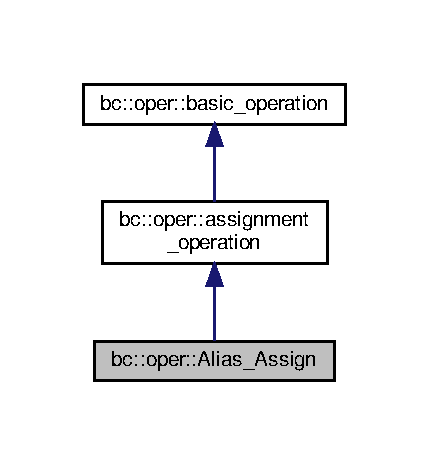
\includegraphics[width=206pt]{structbc_1_1oper_1_1Alias__Assign__inherit__graph}
\end{center}
\end{figure}


Collaboration diagram for bc\+:\+:oper\+:\+:Alias\+\_\+\+Assign\+:\nopagebreak
\begin{figure}[H]
\begin{center}
\leavevmode
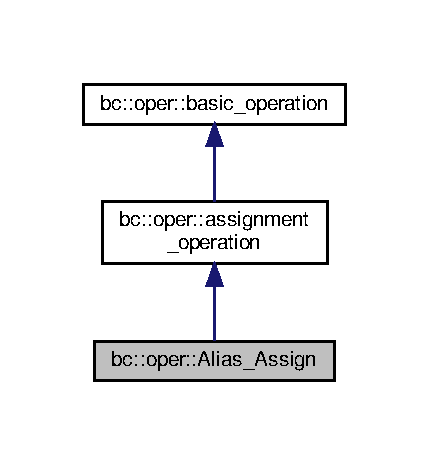
\includegraphics[width=206pt]{structbc_1_1oper_1_1Alias__Assign__coll__graph}
\end{center}
\end{figure}
\subsection*{Public Types}
\begin{DoxyCompactItemize}
\item 
using \hyperlink{structbc_1_1oper_1_1Alias__Assign_a5ae8d352adcc9c79c883b552bce7fb99}{alpha\+\_\+modifier} = \hyperlink{structbc_1_1traits_1_1Integer}{bc\+::traits\+::\+Integer}$<$ 1 $>$
\item 
using \hyperlink{structbc_1_1oper_1_1Alias__Assign_af1e9f3ff11a87bb8275be260d60f99e4}{beta\+\_\+modifier} = \hyperlink{structbc_1_1traits_1_1Integer}{bc\+::traits\+::\+Integer}$<$ 0 $>$
\end{DoxyCompactItemize}
\subsection*{Public Member Functions}
\begin{DoxyCompactItemize}
\item 
{\footnotesize template$<$class Lv , class Rv $>$ }\\\+\_\+\+\_\+host\+\_\+\+\_\+ \+\_\+\+\_\+device\+\_\+\+\_\+ auto \hyperlink{structbc_1_1oper_1_1Alias__Assign_aeb048124a57b7e7ad877cf5abbfc3162}{operator()} (Lv \&\&lv, Rv \&\&rv) const -\/$>$ decltype(\hyperlink{structbc_1_1oper_1_1Alias__Assign_ae64d52d432b301777f6e22cd57eb67b0}{apply}(lv, rv))
\end{DoxyCompactItemize}
\subsection*{Static Public Member Functions}
\begin{DoxyCompactItemize}
\item 
{\footnotesize template$<$class Lv , class Rv $>$ }\\\+\_\+\+\_\+host\+\_\+\+\_\+ static \+\_\+\+\_\+device\+\_\+\+\_\+ auto \hyperlink{structbc_1_1oper_1_1Alias__Assign_ae64d52d432b301777f6e22cd57eb67b0}{apply} (Lv \&\&lv, Rv \&\&rv) -\/$>$ decltype(lv=rv)
\end{DoxyCompactItemize}


\subsection{Member Typedef Documentation}
\mbox{\Hypertarget{structbc_1_1oper_1_1Alias__Assign_a5ae8d352adcc9c79c883b552bce7fb99}\label{structbc_1_1oper_1_1Alias__Assign_a5ae8d352adcc9c79c883b552bce7fb99}} 
\index{bc\+::oper\+::\+Alias\+\_\+\+Assign@{bc\+::oper\+::\+Alias\+\_\+\+Assign}!alpha\+\_\+modifier@{alpha\+\_\+modifier}}
\index{alpha\+\_\+modifier@{alpha\+\_\+modifier}!bc\+::oper\+::\+Alias\+\_\+\+Assign@{bc\+::oper\+::\+Alias\+\_\+\+Assign}}
\subsubsection{\texorpdfstring{alpha\+\_\+modifier}{alpha\_modifier}}
{\footnotesize\ttfamily using \hyperlink{structbc_1_1oper_1_1Alias__Assign_a5ae8d352adcc9c79c883b552bce7fb99}{bc\+::oper\+::\+Alias\+\_\+\+Assign\+::alpha\+\_\+modifier} =  \hyperlink{structbc_1_1traits_1_1Integer}{bc\+::traits\+::\+Integer}$<$1$>$}

\mbox{\Hypertarget{structbc_1_1oper_1_1Alias__Assign_af1e9f3ff11a87bb8275be260d60f99e4}\label{structbc_1_1oper_1_1Alias__Assign_af1e9f3ff11a87bb8275be260d60f99e4}} 
\index{bc\+::oper\+::\+Alias\+\_\+\+Assign@{bc\+::oper\+::\+Alias\+\_\+\+Assign}!beta\+\_\+modifier@{beta\+\_\+modifier}}
\index{beta\+\_\+modifier@{beta\+\_\+modifier}!bc\+::oper\+::\+Alias\+\_\+\+Assign@{bc\+::oper\+::\+Alias\+\_\+\+Assign}}
\subsubsection{\texorpdfstring{beta\+\_\+modifier}{beta\_modifier}}
{\footnotesize\ttfamily using \hyperlink{structbc_1_1oper_1_1Alias__Assign_af1e9f3ff11a87bb8275be260d60f99e4}{bc\+::oper\+::\+Alias\+\_\+\+Assign\+::beta\+\_\+modifier} =  \hyperlink{structbc_1_1traits_1_1Integer}{bc\+::traits\+::\+Integer}$<$0$>$}



\subsection{Member Function Documentation}
\mbox{\Hypertarget{structbc_1_1oper_1_1Alias__Assign_ae64d52d432b301777f6e22cd57eb67b0}\label{structbc_1_1oper_1_1Alias__Assign_ae64d52d432b301777f6e22cd57eb67b0}} 
\index{bc\+::oper\+::\+Alias\+\_\+\+Assign@{bc\+::oper\+::\+Alias\+\_\+\+Assign}!apply@{apply}}
\index{apply@{apply}!bc\+::oper\+::\+Alias\+\_\+\+Assign@{bc\+::oper\+::\+Alias\+\_\+\+Assign}}
\subsubsection{\texorpdfstring{apply()}{apply()}}
{\footnotesize\ttfamily template$<$class Lv , class Rv $>$ \\
\+\_\+\+\_\+host\+\_\+\+\_\+ static \+\_\+\+\_\+device\+\_\+\+\_\+ auto bc\+::oper\+::\+Alias\+\_\+\+Assign\+::apply (\begin{DoxyParamCaption}\item[{Lv \&\&}]{lv,  }\item[{Rv \&\&}]{rv }\end{DoxyParamCaption}) -\/$>$ decltype( lv = rv ) \hspace{0.3cm}{\ttfamily [inline]}, {\ttfamily [static]}}

\mbox{\Hypertarget{structbc_1_1oper_1_1Alias__Assign_aeb048124a57b7e7ad877cf5abbfc3162}\label{structbc_1_1oper_1_1Alias__Assign_aeb048124a57b7e7ad877cf5abbfc3162}} 
\index{bc\+::oper\+::\+Alias\+\_\+\+Assign@{bc\+::oper\+::\+Alias\+\_\+\+Assign}!operator()@{operator()}}
\index{operator()@{operator()}!bc\+::oper\+::\+Alias\+\_\+\+Assign@{bc\+::oper\+::\+Alias\+\_\+\+Assign}}
\subsubsection{\texorpdfstring{operator()()}{operator()()}}
{\footnotesize\ttfamily template$<$class Lv , class Rv $>$ \\
\+\_\+\+\_\+host\+\_\+\+\_\+ \+\_\+\+\_\+device\+\_\+\+\_\+ auto bc\+::oper\+::\+Alias\+\_\+\+Assign\+::operator() (\begin{DoxyParamCaption}\item[{Lv \&\&}]{lv,  }\item[{Rv \&\&}]{rv }\end{DoxyParamCaption}) const -\/$>$ decltype(\hyperlink{structbc_1_1oper_1_1Alias__Assign_ae64d52d432b301777f6e22cd57eb67b0}{apply}(lv, rv)) \hspace{0.3cm}{\ttfamily [inline]}}



The documentation for this struct was generated from the following file\+:\begin{DoxyCompactItemize}
\item 
blackcat/operations/\hyperlink{binary_8h}{binary.\+h}\end{DoxyCompactItemize}

\hypertarget{structbc_1_1oper_1_1Alias__Sub__Assign}{}\section{bc\+:\+:oper\+:\+:Alias\+\_\+\+Sub\+\_\+\+Assign Struct Reference}
\label{structbc_1_1oper_1_1Alias__Sub__Assign}\index{bc\+::oper\+::\+Alias\+\_\+\+Sub\+\_\+\+Assign@{bc\+::oper\+::\+Alias\+\_\+\+Sub\+\_\+\+Assign}}


{\ttfamily \#include $<$binary.\+h$>$}



Inheritance diagram for bc\+:\+:oper\+:\+:Alias\+\_\+\+Sub\+\_\+\+Assign\+:\nopagebreak
\begin{figure}[H]
\begin{center}
\leavevmode
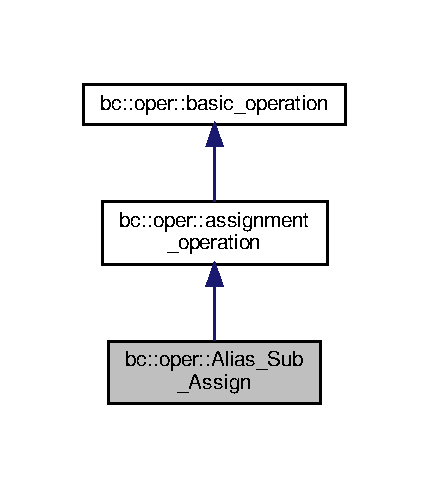
\includegraphics[width=206pt]{structbc_1_1oper_1_1Alias__Sub__Assign__inherit__graph}
\end{center}
\end{figure}


Collaboration diagram for bc\+:\+:oper\+:\+:Alias\+\_\+\+Sub\+\_\+\+Assign\+:\nopagebreak
\begin{figure}[H]
\begin{center}
\leavevmode
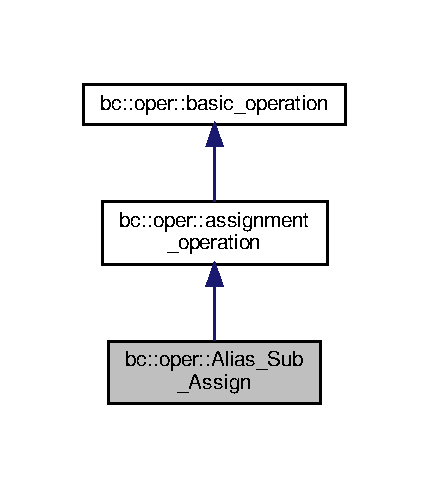
\includegraphics[width=206pt]{structbc_1_1oper_1_1Alias__Sub__Assign__coll__graph}
\end{center}
\end{figure}
\subsection*{Public Types}
\begin{DoxyCompactItemize}
\item 
using \hyperlink{structbc_1_1oper_1_1Alias__Sub__Assign_a5ba31eaac25a5aa2465dbd9693e43886}{alpha\+\_\+modifier} = \hyperlink{structbc_1_1traits_1_1Integer}{bc\+::traits\+::\+Integer}$<$-\/1 $>$
\item 
using \hyperlink{structbc_1_1oper_1_1Alias__Sub__Assign_a6e0907ffcf3b224294ee441a17cbe22c}{beta\+\_\+modifier} = \hyperlink{structbc_1_1traits_1_1Integer}{bc\+::traits\+::\+Integer}$<$ 1 $>$
\end{DoxyCompactItemize}
\subsection*{Public Member Functions}
\begin{DoxyCompactItemize}
\item 
{\footnotesize template$<$class Lv , class Rv $>$ }\\\+\_\+\+\_\+host\+\_\+\+\_\+ \+\_\+\+\_\+device\+\_\+\+\_\+ auto \hyperlink{structbc_1_1oper_1_1Alias__Sub__Assign_a72b32c4a8603270cbe64995b2b4a4b58}{operator()} (Lv \&\&lv, Rv \&\&rv) const -\/$>$ decltype(\hyperlink{structbc_1_1oper_1_1Alias__Sub__Assign_a65827a9261b00d81d8724e623309f380}{apply}(lv, rv))
\end{DoxyCompactItemize}
\subsection*{Static Public Member Functions}
\begin{DoxyCompactItemize}
\item 
{\footnotesize template$<$class Lv , class Rv $>$ }\\\+\_\+\+\_\+host\+\_\+\+\_\+ static \+\_\+\+\_\+device\+\_\+\+\_\+ auto \hyperlink{structbc_1_1oper_1_1Alias__Sub__Assign_a65827a9261b00d81d8724e623309f380}{apply} (Lv \&\&lv, Rv \&\&rv) -\/$>$ decltype(lv -\/=rv)
\end{DoxyCompactItemize}


\subsection{Member Typedef Documentation}
\mbox{\Hypertarget{structbc_1_1oper_1_1Alias__Sub__Assign_a5ba31eaac25a5aa2465dbd9693e43886}\label{structbc_1_1oper_1_1Alias__Sub__Assign_a5ba31eaac25a5aa2465dbd9693e43886}} 
\index{bc\+::oper\+::\+Alias\+\_\+\+Sub\+\_\+\+Assign@{bc\+::oper\+::\+Alias\+\_\+\+Sub\+\_\+\+Assign}!alpha\+\_\+modifier@{alpha\+\_\+modifier}}
\index{alpha\+\_\+modifier@{alpha\+\_\+modifier}!bc\+::oper\+::\+Alias\+\_\+\+Sub\+\_\+\+Assign@{bc\+::oper\+::\+Alias\+\_\+\+Sub\+\_\+\+Assign}}
\subsubsection{\texorpdfstring{alpha\+\_\+modifier}{alpha\_modifier}}
{\footnotesize\ttfamily using \hyperlink{structbc_1_1oper_1_1Alias__Sub__Assign_a5ba31eaac25a5aa2465dbd9693e43886}{bc\+::oper\+::\+Alias\+\_\+\+Sub\+\_\+\+Assign\+::alpha\+\_\+modifier} =  \hyperlink{structbc_1_1traits_1_1Integer}{bc\+::traits\+::\+Integer}$<$-\/1$>$}

\mbox{\Hypertarget{structbc_1_1oper_1_1Alias__Sub__Assign_a6e0907ffcf3b224294ee441a17cbe22c}\label{structbc_1_1oper_1_1Alias__Sub__Assign_a6e0907ffcf3b224294ee441a17cbe22c}} 
\index{bc\+::oper\+::\+Alias\+\_\+\+Sub\+\_\+\+Assign@{bc\+::oper\+::\+Alias\+\_\+\+Sub\+\_\+\+Assign}!beta\+\_\+modifier@{beta\+\_\+modifier}}
\index{beta\+\_\+modifier@{beta\+\_\+modifier}!bc\+::oper\+::\+Alias\+\_\+\+Sub\+\_\+\+Assign@{bc\+::oper\+::\+Alias\+\_\+\+Sub\+\_\+\+Assign}}
\subsubsection{\texorpdfstring{beta\+\_\+modifier}{beta\_modifier}}
{\footnotesize\ttfamily using \hyperlink{structbc_1_1oper_1_1Alias__Sub__Assign_a6e0907ffcf3b224294ee441a17cbe22c}{bc\+::oper\+::\+Alias\+\_\+\+Sub\+\_\+\+Assign\+::beta\+\_\+modifier} =  \hyperlink{structbc_1_1traits_1_1Integer}{bc\+::traits\+::\+Integer}$<$1$>$}



\subsection{Member Function Documentation}
\mbox{\Hypertarget{structbc_1_1oper_1_1Alias__Sub__Assign_a65827a9261b00d81d8724e623309f380}\label{structbc_1_1oper_1_1Alias__Sub__Assign_a65827a9261b00d81d8724e623309f380}} 
\index{bc\+::oper\+::\+Alias\+\_\+\+Sub\+\_\+\+Assign@{bc\+::oper\+::\+Alias\+\_\+\+Sub\+\_\+\+Assign}!apply@{apply}}
\index{apply@{apply}!bc\+::oper\+::\+Alias\+\_\+\+Sub\+\_\+\+Assign@{bc\+::oper\+::\+Alias\+\_\+\+Sub\+\_\+\+Assign}}
\subsubsection{\texorpdfstring{apply()}{apply()}}
{\footnotesize\ttfamily template$<$class Lv , class Rv $>$ \\
\+\_\+\+\_\+host\+\_\+\+\_\+ static \+\_\+\+\_\+device\+\_\+\+\_\+ auto bc\+::oper\+::\+Alias\+\_\+\+Sub\+\_\+\+Assign\+::apply (\begin{DoxyParamCaption}\item[{Lv \&\&}]{lv,  }\item[{Rv \&\&}]{rv }\end{DoxyParamCaption}) -\/$>$ decltype( lv -\/= rv ) \hspace{0.3cm}{\ttfamily [inline]}, {\ttfamily [static]}}

\mbox{\Hypertarget{structbc_1_1oper_1_1Alias__Sub__Assign_a72b32c4a8603270cbe64995b2b4a4b58}\label{structbc_1_1oper_1_1Alias__Sub__Assign_a72b32c4a8603270cbe64995b2b4a4b58}} 
\index{bc\+::oper\+::\+Alias\+\_\+\+Sub\+\_\+\+Assign@{bc\+::oper\+::\+Alias\+\_\+\+Sub\+\_\+\+Assign}!operator()@{operator()}}
\index{operator()@{operator()}!bc\+::oper\+::\+Alias\+\_\+\+Sub\+\_\+\+Assign@{bc\+::oper\+::\+Alias\+\_\+\+Sub\+\_\+\+Assign}}
\subsubsection{\texorpdfstring{operator()()}{operator()()}}
{\footnotesize\ttfamily template$<$class Lv , class Rv $>$ \\
\+\_\+\+\_\+host\+\_\+\+\_\+ \+\_\+\+\_\+device\+\_\+\+\_\+ auto bc\+::oper\+::\+Alias\+\_\+\+Sub\+\_\+\+Assign\+::operator() (\begin{DoxyParamCaption}\item[{Lv \&\&}]{lv,  }\item[{Rv \&\&}]{rv }\end{DoxyParamCaption}) const -\/$>$ decltype(\hyperlink{structbc_1_1oper_1_1Alias__Sub__Assign_a65827a9261b00d81d8724e623309f380}{apply}(lv, rv)) \hspace{0.3cm}{\ttfamily [inline]}}



The documentation for this struct was generated from the following file\+:\begin{DoxyCompactItemize}
\item 
blackcat/operations/\hyperlink{binary_8h}{binary.\+h}\end{DoxyCompactItemize}

\hypertarget{structbc_1_1traits_1_1all}{}\section{bc\+:\+:traits\+:\+:all$<$ Function, Ts $>$ Struct Template Reference}
\label{structbc_1_1traits_1_1all}\index{bc\+::traits\+::all$<$ Function, Ts $>$@{bc\+::traits\+::all$<$ Function, Ts $>$}}


{\ttfamily \#include $<$type\+\_\+traits.\+h$>$}



Inheritance diagram for bc\+:\+:traits\+:\+:all$<$ Function, Ts $>$\+:\nopagebreak
\begin{figure}[H]
\begin{center}
\leavevmode
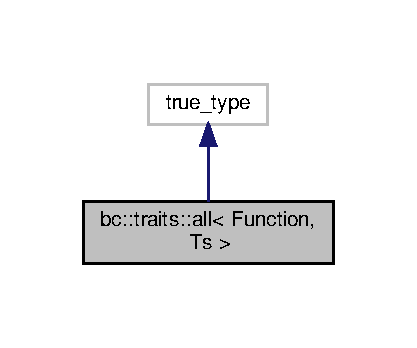
\includegraphics[width=200pt]{structbc_1_1traits_1_1all__inherit__graph}
\end{center}
\end{figure}


Collaboration diagram for bc\+:\+:traits\+:\+:all$<$ Function, Ts $>$\+:\nopagebreak
\begin{figure}[H]
\begin{center}
\leavevmode
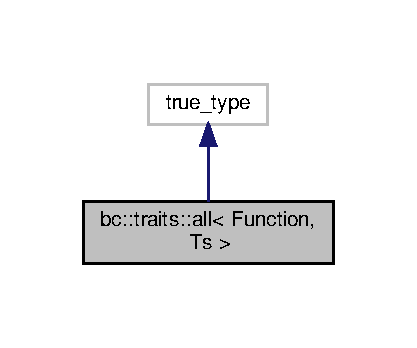
\includegraphics[width=200pt]{structbc_1_1traits_1_1all__coll__graph}
\end{center}
\end{figure}


The documentation for this struct was generated from the following file\+:\begin{DoxyCompactItemize}
\item 
blackcat/type\+\_\+traits/\hyperlink{type__traits_2type__traits_8h}{type\+\_\+traits.\+h}\end{DoxyCompactItemize}

\hypertarget{structbc_1_1traits_1_1all_3_01Function_00_01T_00_01Ts_8_8_8_01_4}{}\section{bc\+:\+:traits\+:\+:all$<$ Function, T, Ts... $>$ Struct Template Reference}
\label{structbc_1_1traits_1_1all_3_01Function_00_01T_00_01Ts_8_8_8_01_4}\index{bc\+::traits\+::all$<$ Function, T, Ts... $>$@{bc\+::traits\+::all$<$ Function, T, Ts... $>$}}


{\ttfamily \#include $<$type\+\_\+traits.\+h$>$}



Inheritance diagram for bc\+:\+:traits\+:\+:all$<$ Function, T, Ts... $>$\+:\nopagebreak
\begin{figure}[H]
\begin{center}
\leavevmode
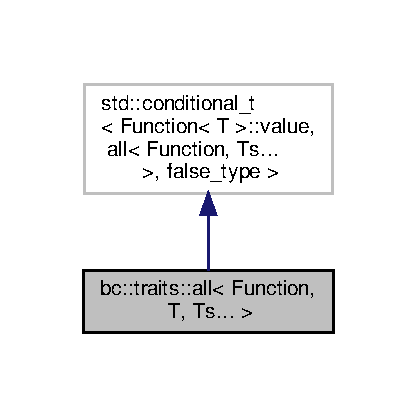
\includegraphics[width=200pt]{structbc_1_1traits_1_1all_3_01Function_00_01T_00_01Ts_8_8_8_01_4__inherit__graph}
\end{center}
\end{figure}


Collaboration diagram for bc\+:\+:traits\+:\+:all$<$ Function, T, Ts... $>$\+:\nopagebreak
\begin{figure}[H]
\begin{center}
\leavevmode
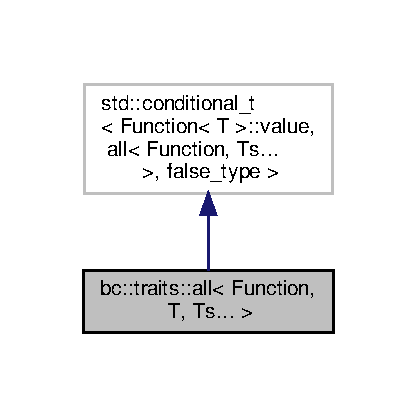
\includegraphics[width=200pt]{structbc_1_1traits_1_1all_3_01Function_00_01T_00_01Ts_8_8_8_01_4__coll__graph}
\end{center}
\end{figure}


The documentation for this struct was generated from the following file\+:\begin{DoxyCompactItemize}
\item 
blackcat/type\+\_\+traits/\hyperlink{type__traits_2type__traits_8h}{type\+\_\+traits.\+h}\end{DoxyCompactItemize}

\hypertarget{classbc_1_1allocators_1_1Allocator}{}\section{bc\+:\+:allocators\+:\+:Allocator$<$ Value\+Type, System\+Tag $>$ Class Template Reference}
\label{classbc_1_1allocators_1_1Allocator}\index{bc\+::allocators\+::\+Allocator$<$ Value\+Type, System\+Tag $>$@{bc\+::allocators\+::\+Allocator$<$ Value\+Type, System\+Tag $>$}}


{\ttfamily \#include $<$allocators.\+h$>$}



Inheritance diagram for bc\+:\+:allocators\+:\+:Allocator$<$ Value\+Type, System\+Tag $>$\+:\nopagebreak
\begin{figure}[H]
\begin{center}
\leavevmode
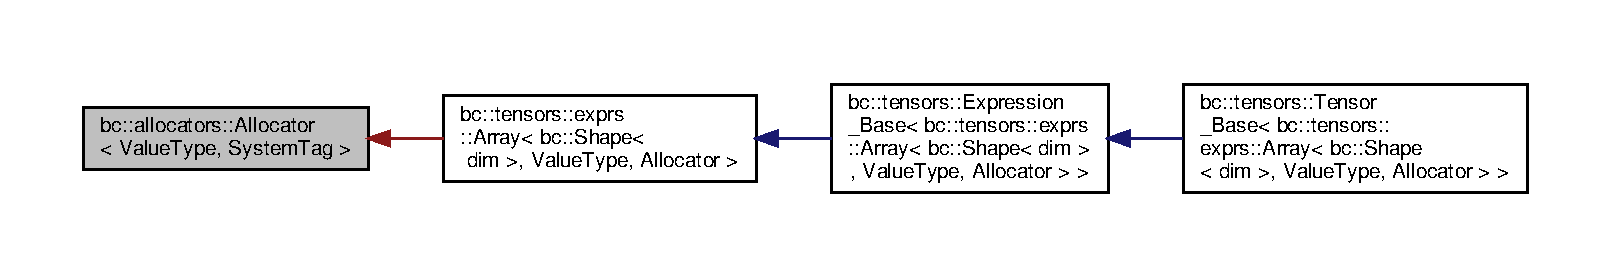
\includegraphics[width=350pt]{classbc_1_1allocators_1_1Allocator__inherit__graph}
\end{center}
\end{figure}


The documentation for this class was generated from the following file\+:\begin{DoxyCompactItemize}
\item 
blackcat/allocators/\hyperlink{allocators_8h}{allocators.\+h}\end{DoxyCompactItemize}

\hypertarget{structbc_1_1allocators_1_1Allocator_3_01T_00_01device__tag_01_4}{}\section{bc\+:\+:allocators\+:\+:Allocator$<$ T, device\+\_\+tag $>$ Struct Template Reference}
\label{structbc_1_1allocators_1_1Allocator_3_01T_00_01device__tag_01_4}\index{bc\+::allocators\+::\+Allocator$<$ T, device\+\_\+tag $>$@{bc\+::allocators\+::\+Allocator$<$ T, device\+\_\+tag $>$}}


The \textquotesingle{}std\+::allocator\textquotesingle{} of G\+P\+U-\/allocators. Memory is allocated via \textquotesingle{}cuda\+Malloc\textquotesingle{}.  




{\ttfamily \#include $<$basic\+\_\+allocators.\+h$>$}



Inheritance diagram for bc\+:\+:allocators\+:\+:Allocator$<$ T, device\+\_\+tag $>$\+:\nopagebreak
\begin{figure}[H]
\begin{center}
\leavevmode
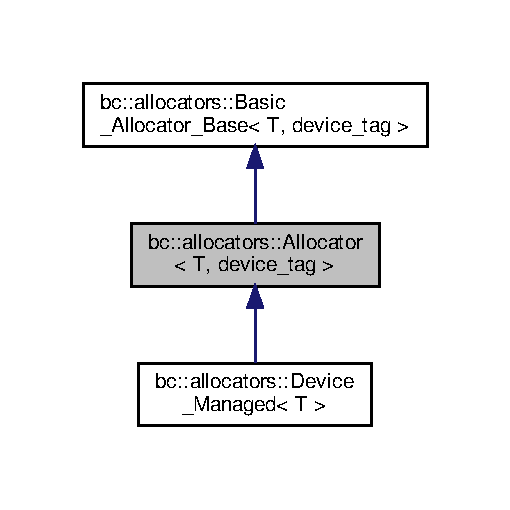
\includegraphics[width=245pt]{structbc_1_1allocators_1_1Allocator_3_01T_00_01device__tag_01_4__inherit__graph}
\end{center}
\end{figure}


Collaboration diagram for bc\+:\+:allocators\+:\+:Allocator$<$ T, device\+\_\+tag $>$\+:\nopagebreak
\begin{figure}[H]
\begin{center}
\leavevmode
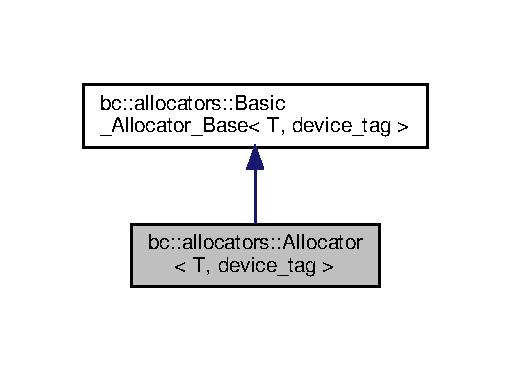
\includegraphics[width=245pt]{structbc_1_1allocators_1_1Allocator_3_01T_00_01device__tag_01_4__coll__graph}
\end{center}
\end{figure}
\subsection*{Classes}
\begin{DoxyCompactItemize}
\item 
struct \hyperlink{structbc_1_1allocators_1_1Allocator_3_01T_00_01device__tag_01_4_1_1rebind}{rebind}
\end{DoxyCompactItemize}
\subsection*{Public Member Functions}
\begin{DoxyCompactItemize}
\item 
{\footnotesize template$<$class U $>$ }\\\hyperlink{structbc_1_1allocators_1_1Allocator_3_01T_00_01device__tag_01_4_a88d0cc2114abb58361cfa739f1e190e7}{Allocator} (const \hyperlink{classbc_1_1allocators_1_1Allocator}{Allocator}$<$ U, \hyperlink{structbc_1_1device__tag}{device\+\_\+tag} $>$ \&)
\item 
\hyperlink{structbc_1_1allocators_1_1Allocator_3_01T_00_01device__tag_01_4_aef910f60bb75fdfc303d99aa779d1de1}{Allocator} ()=default
\item 
T $\ast$ \hyperlink{structbc_1_1allocators_1_1Allocator_3_01T_00_01device__tag_01_4_a140957d76e4b582ca2b85b52a8417cd0}{allocate} (std\+::size\+\_\+t sz) const
\item 
void \hyperlink{structbc_1_1allocators_1_1Allocator_3_01T_00_01device__tag_01_4_a80060f1c76c04adb6f48e4645896ec77}{deallocate} (T $\ast$data\+\_\+ptr, std\+::size\+\_\+t size) const
\end{DoxyCompactItemize}
\subsection*{Additional Inherited Members}


\subsection{Detailed Description}
\subsubsection*{template$<$class T$>$\newline
struct bc\+::allocators\+::\+Allocator$<$ T, device\+\_\+tag $>$}

The \textquotesingle{}std\+::allocator\textquotesingle{} of G\+P\+U-\/allocators. Memory is allocated via \textquotesingle{}cuda\+Malloc\textquotesingle{}. 

\subsection{Constructor \& Destructor Documentation}
\mbox{\Hypertarget{structbc_1_1allocators_1_1Allocator_3_01T_00_01device__tag_01_4_a88d0cc2114abb58361cfa739f1e190e7}\label{structbc_1_1allocators_1_1Allocator_3_01T_00_01device__tag_01_4_a88d0cc2114abb58361cfa739f1e190e7}} 
\index{bc\+::allocators\+::\+Allocator$<$ T, device\+\_\+tag $>$@{bc\+::allocators\+::\+Allocator$<$ T, device\+\_\+tag $>$}!Allocator@{Allocator}}
\index{Allocator@{Allocator}!bc\+::allocators\+::\+Allocator$<$ T, device\+\_\+tag $>$@{bc\+::allocators\+::\+Allocator$<$ T, device\+\_\+tag $>$}}
\subsubsection{\texorpdfstring{Allocator()}{Allocator()}\hspace{0.1cm}{\footnotesize\ttfamily [1/2]}}
{\footnotesize\ttfamily template$<$class T $>$ \\
template$<$class U $>$ \\
\hyperlink{classbc_1_1allocators_1_1Allocator}{bc\+::allocators\+::\+Allocator}$<$ T, \hyperlink{structbc_1_1device__tag}{device\+\_\+tag} $>$\+::\hyperlink{classbc_1_1allocators_1_1Allocator}{Allocator} (\begin{DoxyParamCaption}\item[{const \hyperlink{classbc_1_1allocators_1_1Allocator}{Allocator}$<$ U, \hyperlink{structbc_1_1device__tag}{device\+\_\+tag} $>$ \&}]{ }\end{DoxyParamCaption})\hspace{0.3cm}{\ttfamily [inline]}}

\mbox{\Hypertarget{structbc_1_1allocators_1_1Allocator_3_01T_00_01device__tag_01_4_aef910f60bb75fdfc303d99aa779d1de1}\label{structbc_1_1allocators_1_1Allocator_3_01T_00_01device__tag_01_4_aef910f60bb75fdfc303d99aa779d1de1}} 
\index{bc\+::allocators\+::\+Allocator$<$ T, device\+\_\+tag $>$@{bc\+::allocators\+::\+Allocator$<$ T, device\+\_\+tag $>$}!Allocator@{Allocator}}
\index{Allocator@{Allocator}!bc\+::allocators\+::\+Allocator$<$ T, device\+\_\+tag $>$@{bc\+::allocators\+::\+Allocator$<$ T, device\+\_\+tag $>$}}
\subsubsection{\texorpdfstring{Allocator()}{Allocator()}\hspace{0.1cm}{\footnotesize\ttfamily [2/2]}}
{\footnotesize\ttfamily template$<$class T $>$ \\
\hyperlink{classbc_1_1allocators_1_1Allocator}{bc\+::allocators\+::\+Allocator}$<$ T, \hyperlink{structbc_1_1device__tag}{device\+\_\+tag} $>$\+::\hyperlink{classbc_1_1allocators_1_1Allocator}{Allocator} (\begin{DoxyParamCaption}{ }\end{DoxyParamCaption})\hspace{0.3cm}{\ttfamily [default]}}



\subsection{Member Function Documentation}
\mbox{\Hypertarget{structbc_1_1allocators_1_1Allocator_3_01T_00_01device__tag_01_4_a140957d76e4b582ca2b85b52a8417cd0}\label{structbc_1_1allocators_1_1Allocator_3_01T_00_01device__tag_01_4_a140957d76e4b582ca2b85b52a8417cd0}} 
\index{bc\+::allocators\+::\+Allocator$<$ T, device\+\_\+tag $>$@{bc\+::allocators\+::\+Allocator$<$ T, device\+\_\+tag $>$}!allocate@{allocate}}
\index{allocate@{allocate}!bc\+::allocators\+::\+Allocator$<$ T, device\+\_\+tag $>$@{bc\+::allocators\+::\+Allocator$<$ T, device\+\_\+tag $>$}}
\subsubsection{\texorpdfstring{allocate()}{allocate()}}
{\footnotesize\ttfamily template$<$class T $>$ \\
T$\ast$ \hyperlink{classbc_1_1allocators_1_1Allocator}{bc\+::allocators\+::\+Allocator}$<$ T, \hyperlink{structbc_1_1device__tag}{device\+\_\+tag} $>$\+::allocate (\begin{DoxyParamCaption}\item[{std\+::size\+\_\+t}]{sz }\end{DoxyParamCaption}) const\hspace{0.3cm}{\ttfamily [inline]}}

\mbox{\Hypertarget{structbc_1_1allocators_1_1Allocator_3_01T_00_01device__tag_01_4_a80060f1c76c04adb6f48e4645896ec77}\label{structbc_1_1allocators_1_1Allocator_3_01T_00_01device__tag_01_4_a80060f1c76c04adb6f48e4645896ec77}} 
\index{bc\+::allocators\+::\+Allocator$<$ T, device\+\_\+tag $>$@{bc\+::allocators\+::\+Allocator$<$ T, device\+\_\+tag $>$}!deallocate@{deallocate}}
\index{deallocate@{deallocate}!bc\+::allocators\+::\+Allocator$<$ T, device\+\_\+tag $>$@{bc\+::allocators\+::\+Allocator$<$ T, device\+\_\+tag $>$}}
\subsubsection{\texorpdfstring{deallocate()}{deallocate()}}
{\footnotesize\ttfamily template$<$class T $>$ \\
void \hyperlink{classbc_1_1allocators_1_1Allocator}{bc\+::allocators\+::\+Allocator}$<$ T, \hyperlink{structbc_1_1device__tag}{device\+\_\+tag} $>$\+::deallocate (\begin{DoxyParamCaption}\item[{T $\ast$}]{data\+\_\+ptr,  }\item[{std\+::size\+\_\+t}]{size }\end{DoxyParamCaption}) const\hspace{0.3cm}{\ttfamily [inline]}}



The documentation for this struct was generated from the following file\+:\begin{DoxyCompactItemize}
\item 
blackcat/allocators/\hyperlink{basic__allocators_8h}{basic\+\_\+allocators.\+h}\end{DoxyCompactItemize}

\hypertarget{structbc_1_1allocators_1_1Allocator_3_01T_00_01host__tag_01_4}{}\section{bc\+:\+:allocators\+:\+:Allocator$<$ T, host\+\_\+tag $>$ Struct Template Reference}
\label{structbc_1_1allocators_1_1Allocator_3_01T_00_01host__tag_01_4}\index{bc\+::allocators\+::\+Allocator$<$ T, host\+\_\+tag $>$@{bc\+::allocators\+::\+Allocator$<$ T, host\+\_\+tag $>$}}


Comparable to \textquotesingle{}std\+::allocator.\textquotesingle{}.  




{\ttfamily \#include $<$basic\+\_\+allocators.\+h$>$}



Inheritance diagram for bc\+:\+:allocators\+:\+:Allocator$<$ T, host\+\_\+tag $>$\+:\nopagebreak
\begin{figure}[H]
\begin{center}
\leavevmode
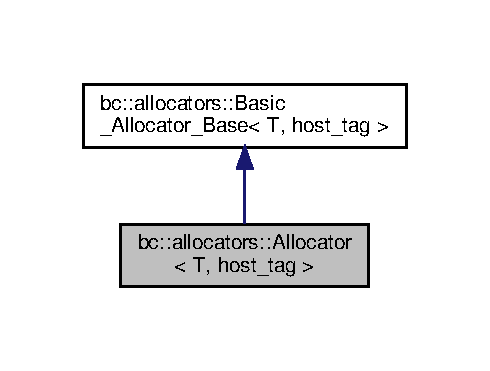
\includegraphics[width=235pt]{structbc_1_1allocators_1_1Allocator_3_01T_00_01host__tag_01_4__inherit__graph}
\end{center}
\end{figure}


Collaboration diagram for bc\+:\+:allocators\+:\+:Allocator$<$ T, host\+\_\+tag $>$\+:\nopagebreak
\begin{figure}[H]
\begin{center}
\leavevmode
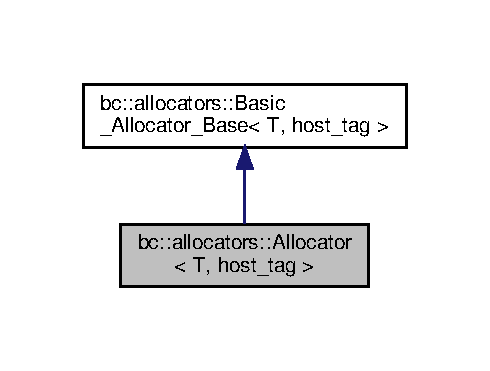
\includegraphics[width=235pt]{structbc_1_1allocators_1_1Allocator_3_01T_00_01host__tag_01_4__coll__graph}
\end{center}
\end{figure}
\subsection*{Classes}
\begin{DoxyCompactItemize}
\item 
struct \hyperlink{structbc_1_1allocators_1_1Allocator_3_01T_00_01host__tag_01_4_1_1rebind}{rebind}
\end{DoxyCompactItemize}
\subsection*{Public Member Functions}
\begin{DoxyCompactItemize}
\item 
{\footnotesize template$<$class U $>$ }\\\hyperlink{structbc_1_1allocators_1_1Allocator_3_01T_00_01host__tag_01_4_ab3c8ab0bb3be8497097288b6164c3549}{Allocator} (const \hyperlink{classbc_1_1allocators_1_1Allocator}{Allocator}$<$ U, \hyperlink{structbc_1_1host__tag}{host\+\_\+tag} $>$ \&)
\item 
\hyperlink{structbc_1_1allocators_1_1Allocator_3_01T_00_01host__tag_01_4_a74632d8f2485cc5fbbc1942674263ecd}{Allocator} ()=default
\item 
T $\ast$ \hyperlink{structbc_1_1allocators_1_1Allocator_3_01T_00_01host__tag_01_4_a7dc1bfcee83cc2986902722308a0a180}{allocate} (int size)
\item 
void \hyperlink{structbc_1_1allocators_1_1Allocator_3_01T_00_01host__tag_01_4_a57811db93d9898bedf13ea7abd9fa1b9}{deallocate} (T $\ast$\hyperlink{expression__operations_8h_aaf23b70530701962855e4abdeea019a2}{t}, \hyperlink{namespacebc_aaf8e3fbf99b04b1b57c4f80c6f55d3c5}{bc\+::size\+\_\+t} size)
\end{DoxyCompactItemize}
\subsection*{Additional Inherited Members}


\subsection{Detailed Description}
\subsubsection*{template$<$class T$>$\newline
struct bc\+::allocators\+::\+Allocator$<$ T, host\+\_\+tag $>$}

Comparable to \textquotesingle{}std\+::allocator.\textquotesingle{}. 

\subsection{Constructor \& Destructor Documentation}
\mbox{\Hypertarget{structbc_1_1allocators_1_1Allocator_3_01T_00_01host__tag_01_4_ab3c8ab0bb3be8497097288b6164c3549}\label{structbc_1_1allocators_1_1Allocator_3_01T_00_01host__tag_01_4_ab3c8ab0bb3be8497097288b6164c3549}} 
\index{bc\+::allocators\+::\+Allocator$<$ T, host\+\_\+tag $>$@{bc\+::allocators\+::\+Allocator$<$ T, host\+\_\+tag $>$}!Allocator@{Allocator}}
\index{Allocator@{Allocator}!bc\+::allocators\+::\+Allocator$<$ T, host\+\_\+tag $>$@{bc\+::allocators\+::\+Allocator$<$ T, host\+\_\+tag $>$}}
\subsubsection{\texorpdfstring{Allocator()}{Allocator()}\hspace{0.1cm}{\footnotesize\ttfamily [1/2]}}
{\footnotesize\ttfamily template$<$class T $>$ \\
template$<$class U $>$ \\
\hyperlink{classbc_1_1allocators_1_1Allocator}{bc\+::allocators\+::\+Allocator}$<$ T, \hyperlink{structbc_1_1host__tag}{host\+\_\+tag} $>$\+::\hyperlink{classbc_1_1allocators_1_1Allocator}{Allocator} (\begin{DoxyParamCaption}\item[{const \hyperlink{classbc_1_1allocators_1_1Allocator}{Allocator}$<$ U, \hyperlink{structbc_1_1host__tag}{host\+\_\+tag} $>$ \&}]{ }\end{DoxyParamCaption})\hspace{0.3cm}{\ttfamily [inline]}}

\mbox{\Hypertarget{structbc_1_1allocators_1_1Allocator_3_01T_00_01host__tag_01_4_a74632d8f2485cc5fbbc1942674263ecd}\label{structbc_1_1allocators_1_1Allocator_3_01T_00_01host__tag_01_4_a74632d8f2485cc5fbbc1942674263ecd}} 
\index{bc\+::allocators\+::\+Allocator$<$ T, host\+\_\+tag $>$@{bc\+::allocators\+::\+Allocator$<$ T, host\+\_\+tag $>$}!Allocator@{Allocator}}
\index{Allocator@{Allocator}!bc\+::allocators\+::\+Allocator$<$ T, host\+\_\+tag $>$@{bc\+::allocators\+::\+Allocator$<$ T, host\+\_\+tag $>$}}
\subsubsection{\texorpdfstring{Allocator()}{Allocator()}\hspace{0.1cm}{\footnotesize\ttfamily [2/2]}}
{\footnotesize\ttfamily template$<$class T $>$ \\
\hyperlink{classbc_1_1allocators_1_1Allocator}{bc\+::allocators\+::\+Allocator}$<$ T, \hyperlink{structbc_1_1host__tag}{host\+\_\+tag} $>$\+::\hyperlink{classbc_1_1allocators_1_1Allocator}{Allocator} (\begin{DoxyParamCaption}{ }\end{DoxyParamCaption})\hspace{0.3cm}{\ttfamily [default]}}



\subsection{Member Function Documentation}
\mbox{\Hypertarget{structbc_1_1allocators_1_1Allocator_3_01T_00_01host__tag_01_4_a7dc1bfcee83cc2986902722308a0a180}\label{structbc_1_1allocators_1_1Allocator_3_01T_00_01host__tag_01_4_a7dc1bfcee83cc2986902722308a0a180}} 
\index{bc\+::allocators\+::\+Allocator$<$ T, host\+\_\+tag $>$@{bc\+::allocators\+::\+Allocator$<$ T, host\+\_\+tag $>$}!allocate@{allocate}}
\index{allocate@{allocate}!bc\+::allocators\+::\+Allocator$<$ T, host\+\_\+tag $>$@{bc\+::allocators\+::\+Allocator$<$ T, host\+\_\+tag $>$}}
\subsubsection{\texorpdfstring{allocate()}{allocate()}}
{\footnotesize\ttfamily template$<$class T $>$ \\
T$\ast$ \hyperlink{classbc_1_1allocators_1_1Allocator}{bc\+::allocators\+::\+Allocator}$<$ T, \hyperlink{structbc_1_1host__tag}{host\+\_\+tag} $>$\+::allocate (\begin{DoxyParamCaption}\item[{int}]{size }\end{DoxyParamCaption})\hspace{0.3cm}{\ttfamily [inline]}}

\mbox{\Hypertarget{structbc_1_1allocators_1_1Allocator_3_01T_00_01host__tag_01_4_a57811db93d9898bedf13ea7abd9fa1b9}\label{structbc_1_1allocators_1_1Allocator_3_01T_00_01host__tag_01_4_a57811db93d9898bedf13ea7abd9fa1b9}} 
\index{bc\+::allocators\+::\+Allocator$<$ T, host\+\_\+tag $>$@{bc\+::allocators\+::\+Allocator$<$ T, host\+\_\+tag $>$}!deallocate@{deallocate}}
\index{deallocate@{deallocate}!bc\+::allocators\+::\+Allocator$<$ T, host\+\_\+tag $>$@{bc\+::allocators\+::\+Allocator$<$ T, host\+\_\+tag $>$}}
\subsubsection{\texorpdfstring{deallocate()}{deallocate()}}
{\footnotesize\ttfamily template$<$class T $>$ \\
void \hyperlink{classbc_1_1allocators_1_1Allocator}{bc\+::allocators\+::\+Allocator}$<$ T, \hyperlink{structbc_1_1host__tag}{host\+\_\+tag} $>$\+::deallocate (\begin{DoxyParamCaption}\item[{T $\ast$}]{t,  }\item[{\hyperlink{namespacebc_aaf8e3fbf99b04b1b57c4f80c6f55d3c5}{bc\+::size\+\_\+t}}]{size }\end{DoxyParamCaption})\hspace{0.3cm}{\ttfamily [inline]}}



The documentation for this struct was generated from the following file\+:\begin{DoxyCompactItemize}
\item 
blackcat/allocators/\hyperlink{basic__allocators_8h}{basic\+\_\+allocators.\+h}\end{DoxyCompactItemize}

\hypertarget{structbc_1_1allocators_1_1pa__detail_1_1Allocator__Base}{}\section{bc\+:\+:allocators\+:\+:pa\+\_\+detail\+:\+:Allocator\+\_\+\+Base$<$ Value\+Type, System\+Tag $>$ Struct Template Reference}
\label{structbc_1_1allocators_1_1pa__detail_1_1Allocator__Base}\index{bc\+::allocators\+::pa\+\_\+detail\+::\+Allocator\+\_\+\+Base$<$ Value\+Type, System\+Tag $>$@{bc\+::allocators\+::pa\+\_\+detail\+::\+Allocator\+\_\+\+Base$<$ Value\+Type, System\+Tag $>$}}


{\ttfamily \#include $<$polymorphic\+\_\+allocator.\+h$>$}

\subsection*{Public Types}
\begin{DoxyCompactItemize}
\item 
using \hyperlink{structbc_1_1allocators_1_1pa__detail_1_1Allocator__Base_ad85cad33901196bc10affe231300c020}{system\+\_\+tag} = System\+Tag
\item 
using \hyperlink{structbc_1_1allocators_1_1pa__detail_1_1Allocator__Base_afb5e955c647a4b6742010e2790398b1c}{value\+\_\+type} = Value\+Type
\end{DoxyCompactItemize}
\subsection*{Public Member Functions}
\begin{DoxyCompactItemize}
\item 
virtual \hyperlink{structbc_1_1allocators_1_1pa__detail_1_1Allocator__Base_afb5e955c647a4b6742010e2790398b1c}{value\+\_\+type} $\ast$ \hyperlink{structbc_1_1allocators_1_1pa__detail_1_1Allocator__Base_aa22794436cb3abefc059bde0eb08a23f}{allocate} (std\+::size\+\_\+t sz)=0
\item 
virtual void \hyperlink{structbc_1_1allocators_1_1pa__detail_1_1Allocator__Base_a02eb1291b28c3d83c53f973df47b9caa}{deallocate} (\hyperlink{structbc_1_1allocators_1_1pa__detail_1_1Allocator__Base_afb5e955c647a4b6742010e2790398b1c}{value\+\_\+type} $\ast$data, std\+::size\+\_\+t sz)=0
\item 
virtual \hyperlink{structbc_1_1allocators_1_1pa__detail_1_1Allocator__Base}{Allocator\+\_\+\+Base} $\ast$ \hyperlink{structbc_1_1allocators_1_1pa__detail_1_1Allocator__Base_abb9ba3168afaead6638e81f618f74b48}{clone} () const =0
\item 
virtual \hyperlink{structbc_1_1allocators_1_1pa__detail_1_1Allocator__Base_af497fc08777a9b271862b5947ebfbaf1}{$\sim$\+Allocator\+\_\+\+Base} ()
\item 
virtual bool \hyperlink{structbc_1_1allocators_1_1pa__detail_1_1Allocator__Base_a044ccf83e8abc449aeba1b6c7cc7355d}{operator==} (const \hyperlink{structbc_1_1allocators_1_1pa__detail_1_1Allocator__Base}{Allocator\+\_\+\+Base} \&other) const =0
\item 
virtual bool \hyperlink{structbc_1_1allocators_1_1pa__detail_1_1Allocator__Base_af752625f3178c2ed57515e0607fbec0e}{operator!=} (const \hyperlink{structbc_1_1allocators_1_1pa__detail_1_1Allocator__Base}{Allocator\+\_\+\+Base} \&other) const
\item 
virtual std\+::string \hyperlink{structbc_1_1allocators_1_1pa__detail_1_1Allocator__Base_a2a90a282042dc49c3c43306b2766ba83}{rebound\+\_\+to\+\_\+byte\+\_\+hash} () const =0
\end{DoxyCompactItemize}


\subsection{Member Typedef Documentation}
\mbox{\Hypertarget{structbc_1_1allocators_1_1pa__detail_1_1Allocator__Base_ad85cad33901196bc10affe231300c020}\label{structbc_1_1allocators_1_1pa__detail_1_1Allocator__Base_ad85cad33901196bc10affe231300c020}} 
\index{bc\+::allocators\+::pa\+\_\+detail\+::\+Allocator\+\_\+\+Base@{bc\+::allocators\+::pa\+\_\+detail\+::\+Allocator\+\_\+\+Base}!system\+\_\+tag@{system\+\_\+tag}}
\index{system\+\_\+tag@{system\+\_\+tag}!bc\+::allocators\+::pa\+\_\+detail\+::\+Allocator\+\_\+\+Base@{bc\+::allocators\+::pa\+\_\+detail\+::\+Allocator\+\_\+\+Base}}
\subsubsection{\texorpdfstring{system\+\_\+tag}{system\_tag}}
{\footnotesize\ttfamily template$<$class Value\+Type, class System\+Tag$>$ \\
using \hyperlink{structbc_1_1allocators_1_1pa__detail_1_1Allocator__Base}{bc\+::allocators\+::pa\+\_\+detail\+::\+Allocator\+\_\+\+Base}$<$ Value\+Type, System\+Tag $>$\+::\hyperlink{structbc_1_1allocators_1_1pa__detail_1_1Allocator__Base_ad85cad33901196bc10affe231300c020}{system\+\_\+tag} =  System\+Tag}

\mbox{\Hypertarget{structbc_1_1allocators_1_1pa__detail_1_1Allocator__Base_afb5e955c647a4b6742010e2790398b1c}\label{structbc_1_1allocators_1_1pa__detail_1_1Allocator__Base_afb5e955c647a4b6742010e2790398b1c}} 
\index{bc\+::allocators\+::pa\+\_\+detail\+::\+Allocator\+\_\+\+Base@{bc\+::allocators\+::pa\+\_\+detail\+::\+Allocator\+\_\+\+Base}!value\+\_\+type@{value\+\_\+type}}
\index{value\+\_\+type@{value\+\_\+type}!bc\+::allocators\+::pa\+\_\+detail\+::\+Allocator\+\_\+\+Base@{bc\+::allocators\+::pa\+\_\+detail\+::\+Allocator\+\_\+\+Base}}
\subsubsection{\texorpdfstring{value\+\_\+type}{value\_type}}
{\footnotesize\ttfamily template$<$class Value\+Type, class System\+Tag$>$ \\
using \hyperlink{structbc_1_1allocators_1_1pa__detail_1_1Allocator__Base}{bc\+::allocators\+::pa\+\_\+detail\+::\+Allocator\+\_\+\+Base}$<$ Value\+Type, System\+Tag $>$\+::\hyperlink{structbc_1_1allocators_1_1pa__detail_1_1Allocator__Base_afb5e955c647a4b6742010e2790398b1c}{value\+\_\+type} =  Value\+Type}



\subsection{Constructor \& Destructor Documentation}
\mbox{\Hypertarget{structbc_1_1allocators_1_1pa__detail_1_1Allocator__Base_af497fc08777a9b271862b5947ebfbaf1}\label{structbc_1_1allocators_1_1pa__detail_1_1Allocator__Base_af497fc08777a9b271862b5947ebfbaf1}} 
\index{bc\+::allocators\+::pa\+\_\+detail\+::\+Allocator\+\_\+\+Base@{bc\+::allocators\+::pa\+\_\+detail\+::\+Allocator\+\_\+\+Base}!````~Allocator\+\_\+\+Base@{$\sim$\+Allocator\+\_\+\+Base}}
\index{````~Allocator\+\_\+\+Base@{$\sim$\+Allocator\+\_\+\+Base}!bc\+::allocators\+::pa\+\_\+detail\+::\+Allocator\+\_\+\+Base@{bc\+::allocators\+::pa\+\_\+detail\+::\+Allocator\+\_\+\+Base}}
\subsubsection{\texorpdfstring{$\sim$\+Allocator\+\_\+\+Base()}{~Allocator\_Base()}}
{\footnotesize\ttfamily template$<$class Value\+Type, class System\+Tag$>$ \\
virtual \hyperlink{structbc_1_1allocators_1_1pa__detail_1_1Allocator__Base}{bc\+::allocators\+::pa\+\_\+detail\+::\+Allocator\+\_\+\+Base}$<$ Value\+Type, System\+Tag $>$\+::$\sim$\hyperlink{structbc_1_1allocators_1_1pa__detail_1_1Allocator__Base}{Allocator\+\_\+\+Base} (\begin{DoxyParamCaption}{ }\end{DoxyParamCaption})\hspace{0.3cm}{\ttfamily [inline]}, {\ttfamily [virtual]}}



\subsection{Member Function Documentation}
\mbox{\Hypertarget{structbc_1_1allocators_1_1pa__detail_1_1Allocator__Base_aa22794436cb3abefc059bde0eb08a23f}\label{structbc_1_1allocators_1_1pa__detail_1_1Allocator__Base_aa22794436cb3abefc059bde0eb08a23f}} 
\index{bc\+::allocators\+::pa\+\_\+detail\+::\+Allocator\+\_\+\+Base@{bc\+::allocators\+::pa\+\_\+detail\+::\+Allocator\+\_\+\+Base}!allocate@{allocate}}
\index{allocate@{allocate}!bc\+::allocators\+::pa\+\_\+detail\+::\+Allocator\+\_\+\+Base@{bc\+::allocators\+::pa\+\_\+detail\+::\+Allocator\+\_\+\+Base}}
\subsubsection{\texorpdfstring{allocate()}{allocate()}}
{\footnotesize\ttfamily template$<$class Value\+Type, class System\+Tag$>$ \\
virtual \hyperlink{structbc_1_1allocators_1_1pa__detail_1_1Allocator__Base_afb5e955c647a4b6742010e2790398b1c}{value\+\_\+type}$\ast$ \hyperlink{structbc_1_1allocators_1_1pa__detail_1_1Allocator__Base}{bc\+::allocators\+::pa\+\_\+detail\+::\+Allocator\+\_\+\+Base}$<$ Value\+Type, System\+Tag $>$\+::allocate (\begin{DoxyParamCaption}\item[{std\+::size\+\_\+t}]{sz }\end{DoxyParamCaption})\hspace{0.3cm}{\ttfamily [pure virtual]}}



Implemented in \hyperlink{structbc_1_1allocators_1_1pa__detail_1_1Derived__Allocator_acbfe2862777bf8810e925d78c9511a66}{bc\+::allocators\+::pa\+\_\+detail\+::\+Derived\+\_\+\+Allocator$<$ Allocator $>$}.

\mbox{\Hypertarget{structbc_1_1allocators_1_1pa__detail_1_1Allocator__Base_abb9ba3168afaead6638e81f618f74b48}\label{structbc_1_1allocators_1_1pa__detail_1_1Allocator__Base_abb9ba3168afaead6638e81f618f74b48}} 
\index{bc\+::allocators\+::pa\+\_\+detail\+::\+Allocator\+\_\+\+Base@{bc\+::allocators\+::pa\+\_\+detail\+::\+Allocator\+\_\+\+Base}!clone@{clone}}
\index{clone@{clone}!bc\+::allocators\+::pa\+\_\+detail\+::\+Allocator\+\_\+\+Base@{bc\+::allocators\+::pa\+\_\+detail\+::\+Allocator\+\_\+\+Base}}
\subsubsection{\texorpdfstring{clone()}{clone()}}
{\footnotesize\ttfamily template$<$class Value\+Type, class System\+Tag$>$ \\
virtual \hyperlink{structbc_1_1allocators_1_1pa__detail_1_1Allocator__Base}{Allocator\+\_\+\+Base}$\ast$ \hyperlink{structbc_1_1allocators_1_1pa__detail_1_1Allocator__Base}{bc\+::allocators\+::pa\+\_\+detail\+::\+Allocator\+\_\+\+Base}$<$ Value\+Type, System\+Tag $>$\+::clone (\begin{DoxyParamCaption}{ }\end{DoxyParamCaption}) const\hspace{0.3cm}{\ttfamily [pure virtual]}}



Implemented in \hyperlink{structbc_1_1allocators_1_1pa__detail_1_1Derived__Allocator_af11b1d876a4b0f7c7eb54231730eb3a8}{bc\+::allocators\+::pa\+\_\+detail\+::\+Derived\+\_\+\+Allocator$<$ Allocator $>$}.

\mbox{\Hypertarget{structbc_1_1allocators_1_1pa__detail_1_1Allocator__Base_a02eb1291b28c3d83c53f973df47b9caa}\label{structbc_1_1allocators_1_1pa__detail_1_1Allocator__Base_a02eb1291b28c3d83c53f973df47b9caa}} 
\index{bc\+::allocators\+::pa\+\_\+detail\+::\+Allocator\+\_\+\+Base@{bc\+::allocators\+::pa\+\_\+detail\+::\+Allocator\+\_\+\+Base}!deallocate@{deallocate}}
\index{deallocate@{deallocate}!bc\+::allocators\+::pa\+\_\+detail\+::\+Allocator\+\_\+\+Base@{bc\+::allocators\+::pa\+\_\+detail\+::\+Allocator\+\_\+\+Base}}
\subsubsection{\texorpdfstring{deallocate()}{deallocate()}}
{\footnotesize\ttfamily template$<$class Value\+Type, class System\+Tag$>$ \\
virtual void \hyperlink{structbc_1_1allocators_1_1pa__detail_1_1Allocator__Base}{bc\+::allocators\+::pa\+\_\+detail\+::\+Allocator\+\_\+\+Base}$<$ Value\+Type, System\+Tag $>$\+::deallocate (\begin{DoxyParamCaption}\item[{\hyperlink{structbc_1_1allocators_1_1pa__detail_1_1Allocator__Base_afb5e955c647a4b6742010e2790398b1c}{value\+\_\+type} $\ast$}]{data,  }\item[{std\+::size\+\_\+t}]{sz }\end{DoxyParamCaption})\hspace{0.3cm}{\ttfamily [pure virtual]}}



Implemented in \hyperlink{structbc_1_1allocators_1_1pa__detail_1_1Derived__Allocator_a14b837c6cc64fe049f9c18d219e13cf5}{bc\+::allocators\+::pa\+\_\+detail\+::\+Derived\+\_\+\+Allocator$<$ Allocator $>$}.

\mbox{\Hypertarget{structbc_1_1allocators_1_1pa__detail_1_1Allocator__Base_af752625f3178c2ed57515e0607fbec0e}\label{structbc_1_1allocators_1_1pa__detail_1_1Allocator__Base_af752625f3178c2ed57515e0607fbec0e}} 
\index{bc\+::allocators\+::pa\+\_\+detail\+::\+Allocator\+\_\+\+Base@{bc\+::allocators\+::pa\+\_\+detail\+::\+Allocator\+\_\+\+Base}!operator"!=@{operator"!=}}
\index{operator"!=@{operator"!=}!bc\+::allocators\+::pa\+\_\+detail\+::\+Allocator\+\_\+\+Base@{bc\+::allocators\+::pa\+\_\+detail\+::\+Allocator\+\_\+\+Base}}
\subsubsection{\texorpdfstring{operator"!=()}{operator!=()}}
{\footnotesize\ttfamily template$<$class Value\+Type, class System\+Tag$>$ \\
virtual bool \hyperlink{structbc_1_1allocators_1_1pa__detail_1_1Allocator__Base}{bc\+::allocators\+::pa\+\_\+detail\+::\+Allocator\+\_\+\+Base}$<$ Value\+Type, System\+Tag $>$\+::operator!= (\begin{DoxyParamCaption}\item[{const \hyperlink{structbc_1_1allocators_1_1pa__detail_1_1Allocator__Base}{Allocator\+\_\+\+Base}$<$ Value\+Type, System\+Tag $>$ \&}]{other }\end{DoxyParamCaption}) const\hspace{0.3cm}{\ttfamily [inline]}, {\ttfamily [virtual]}}

\mbox{\Hypertarget{structbc_1_1allocators_1_1pa__detail_1_1Allocator__Base_a044ccf83e8abc449aeba1b6c7cc7355d}\label{structbc_1_1allocators_1_1pa__detail_1_1Allocator__Base_a044ccf83e8abc449aeba1b6c7cc7355d}} 
\index{bc\+::allocators\+::pa\+\_\+detail\+::\+Allocator\+\_\+\+Base@{bc\+::allocators\+::pa\+\_\+detail\+::\+Allocator\+\_\+\+Base}!operator==@{operator==}}
\index{operator==@{operator==}!bc\+::allocators\+::pa\+\_\+detail\+::\+Allocator\+\_\+\+Base@{bc\+::allocators\+::pa\+\_\+detail\+::\+Allocator\+\_\+\+Base}}
\subsubsection{\texorpdfstring{operator==()}{operator==()}}
{\footnotesize\ttfamily template$<$class Value\+Type, class System\+Tag$>$ \\
virtual bool \hyperlink{structbc_1_1allocators_1_1pa__detail_1_1Allocator__Base}{bc\+::allocators\+::pa\+\_\+detail\+::\+Allocator\+\_\+\+Base}$<$ Value\+Type, System\+Tag $>$\+::operator== (\begin{DoxyParamCaption}\item[{const \hyperlink{structbc_1_1allocators_1_1pa__detail_1_1Allocator__Base}{Allocator\+\_\+\+Base}$<$ Value\+Type, System\+Tag $>$ \&}]{other }\end{DoxyParamCaption}) const\hspace{0.3cm}{\ttfamily [pure virtual]}}

\mbox{\Hypertarget{structbc_1_1allocators_1_1pa__detail_1_1Allocator__Base_a2a90a282042dc49c3c43306b2766ba83}\label{structbc_1_1allocators_1_1pa__detail_1_1Allocator__Base_a2a90a282042dc49c3c43306b2766ba83}} 
\index{bc\+::allocators\+::pa\+\_\+detail\+::\+Allocator\+\_\+\+Base@{bc\+::allocators\+::pa\+\_\+detail\+::\+Allocator\+\_\+\+Base}!rebound\+\_\+to\+\_\+byte\+\_\+hash@{rebound\+\_\+to\+\_\+byte\+\_\+hash}}
\index{rebound\+\_\+to\+\_\+byte\+\_\+hash@{rebound\+\_\+to\+\_\+byte\+\_\+hash}!bc\+::allocators\+::pa\+\_\+detail\+::\+Allocator\+\_\+\+Base@{bc\+::allocators\+::pa\+\_\+detail\+::\+Allocator\+\_\+\+Base}}
\subsubsection{\texorpdfstring{rebound\+\_\+to\+\_\+byte\+\_\+hash()}{rebound\_to\_byte\_hash()}}
{\footnotesize\ttfamily template$<$class Value\+Type, class System\+Tag$>$ \\
virtual std\+::string \hyperlink{structbc_1_1allocators_1_1pa__detail_1_1Allocator__Base}{bc\+::allocators\+::pa\+\_\+detail\+::\+Allocator\+\_\+\+Base}$<$ Value\+Type, System\+Tag $>$\+::rebound\+\_\+to\+\_\+byte\+\_\+hash (\begin{DoxyParamCaption}{ }\end{DoxyParamCaption}) const\hspace{0.3cm}{\ttfamily [pure virtual]}}



Implemented in \hyperlink{structbc_1_1allocators_1_1pa__detail_1_1Derived__Allocator_a167659ce0c822b659fbd6ff3ced83876}{bc\+::allocators\+::pa\+\_\+detail\+::\+Derived\+\_\+\+Allocator$<$ Allocator $>$}.



The documentation for this struct was generated from the following file\+:\begin{DoxyCompactItemize}
\item 
blackcat/allocators/\hyperlink{polymorphic__allocator_8h}{polymorphic\+\_\+allocator.\+h}\end{DoxyCompactItemize}

\hypertarget{structbc_1_1allocators_1_1Allocator__Forwarder}{}\section{bc\+:\+:allocators\+:\+:Allocator\+\_\+\+Forwarder$<$ Allocator $>$ Struct Template Reference}
\label{structbc_1_1allocators_1_1Allocator__Forwarder}\index{bc\+::allocators\+::\+Allocator\+\_\+\+Forwarder$<$ Allocator $>$@{bc\+::allocators\+::\+Allocator\+\_\+\+Forwarder$<$ Allocator $>$}}


{\ttfamily \#include $<$allocator\+\_\+forwarder.\+h$>$}



Inheritance diagram for bc\+:\+:allocators\+:\+:Allocator\+\_\+\+Forwarder$<$ Allocator $>$\+:\nopagebreak
\begin{figure}[H]
\begin{center}
\leavevmode
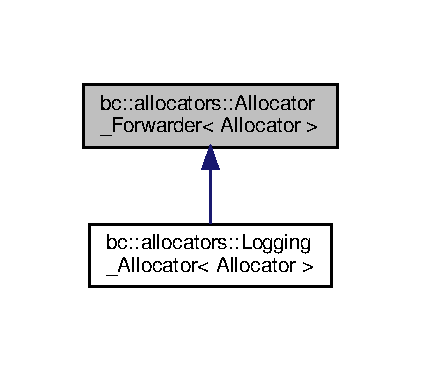
\includegraphics[width=202pt]{structbc_1_1allocators_1_1Allocator__Forwarder__inherit__graph}
\end{center}
\end{figure}
\subsection*{Classes}
\begin{DoxyCompactItemize}
\item 
struct \hyperlink{structbc_1_1allocators_1_1Allocator__Forwarder_1_1rebind}{rebind}
\end{DoxyCompactItemize}
\subsection*{Public Types}
\begin{DoxyCompactItemize}
\item 
using \hyperlink{structbc_1_1allocators_1_1Allocator__Forwarder_a3a50f686c87d96dfba0902fd802088c6}{traits} = \hyperlink{structbc_1_1allocators_1_1allocator__traits}{allocator\+\_\+traits}$<$ \hyperlink{classbc_1_1allocators_1_1Allocator}{Allocator} $>$
\item 
using \hyperlink{structbc_1_1allocators_1_1Allocator__Forwarder_a3ac0b07579279c948a24ee6562510dc5}{value\+\_\+type} = typename traits\+::value\+\_\+type
\item 
using \hyperlink{structbc_1_1allocators_1_1Allocator__Forwarder_a79c1e4e22d9e42518e1195f3583345f5}{system\+\_\+tag} = typename \hyperlink{structbc_1_1allocators_1_1allocator__traits_a527cf77071c45a9dcc2c8213f65f37b3}{traits\+::system\+\_\+tag}
\item 
using \hyperlink{structbc_1_1allocators_1_1Allocator__Forwarder_ae9d48fbeb22a6686ad59128cf309d8bd}{pointer} = typename traits\+::pointer
\item 
using \hyperlink{structbc_1_1allocators_1_1Allocator__Forwarder_a11939ff4b2a42e10b10cd561f5480db2}{const\+\_\+pointer} = typename traits\+::const\+\_\+pointer
\item 
using \hyperlink{structbc_1_1allocators_1_1Allocator__Forwarder_a6829b9ef6af37ad340ab8a81745760b8}{void\+\_\+pointer} = typename traits\+::void\+\_\+pointer
\item 
using \hyperlink{structbc_1_1allocators_1_1Allocator__Forwarder_abe3993f8b29d4a75bb15793f891779fe}{reference} = \hyperlink{structbc_1_1allocators_1_1Allocator__Forwarder_a3ac0b07579279c948a24ee6562510dc5}{value\+\_\+type} \&
\item 
using \hyperlink{structbc_1_1allocators_1_1Allocator__Forwarder_aaa022b1540e4d81d40d9742019c58cc4}{const\+\_\+reference} = const \hyperlink{structbc_1_1allocators_1_1Allocator__Forwarder_a3ac0b07579279c948a24ee6562510dc5}{value\+\_\+type} \&
\item 
using \hyperlink{structbc_1_1allocators_1_1Allocator__Forwarder_a672771feb1a146a20d28d59651d7a3f4}{difference\+\_\+type} = typename traits\+::difference\+\_\+type
\item 
using \hyperlink{structbc_1_1allocators_1_1Allocator__Forwarder_a254a9a5b0ac8837f64c107db7067e985}{size\+\_\+type} = typename traits\+::size\+\_\+type
\item 
using \hyperlink{structbc_1_1allocators_1_1Allocator__Forwarder_abb86157d20c1e651a750e548a69471b1}{is\+\_\+always\+\_\+equal} = typename traits\+::is\+\_\+always\+\_\+equal
\item 
using \hyperlink{structbc_1_1allocators_1_1Allocator__Forwarder_a3264aaf2ed5a7a49c1f48928e876b447}{propagate\+\_\+on\+\_\+container\+\_\+copy\+\_\+assignment} = typename traits\+::propagate\+\_\+on\+\_\+container\+\_\+copy\+\_\+assignment
\item 
using \hyperlink{structbc_1_1allocators_1_1Allocator__Forwarder_ab20c8fa36659a5ca6702192fdb4bde4e}{propagate\+\_\+on\+\_\+container\+\_\+move\+\_\+assignment} = typename traits\+::propagate\+\_\+on\+\_\+container\+\_\+move\+\_\+assignment
\item 
using \hyperlink{structbc_1_1allocators_1_1Allocator__Forwarder_a243203b0477fbb815757f5267c56da92}{propagate\+\_\+on\+\_\+container\+\_\+swap} = typename traits\+::propagate\+\_\+on\+\_\+container\+\_\+swap
\end{DoxyCompactItemize}
\subsection*{Public Member Functions}
\begin{DoxyCompactItemize}
\item 
{\footnotesize template$<$class... Args$>$ }\\\hyperlink{structbc_1_1allocators_1_1Allocator__Forwarder_a2fb4070e5a39213c55350e8f60f02b70}{Allocator\+\_\+\+Forwarder} (Args \&\&... args)
\item 
{\footnotesize template$<$class Alt\+Allocator $>$ }\\\hyperlink{structbc_1_1allocators_1_1Allocator__Forwarder_afaf9973cd1c540a087d2867e1761b5f9}{Allocator\+\_\+\+Forwarder} (const \hyperlink{structbc_1_1allocators_1_1Allocator__Forwarder}{Allocator\+\_\+\+Forwarder}$<$ Alt\+Allocator $>$ \&other)
\item 
auto \hyperlink{structbc_1_1allocators_1_1Allocator__Forwarder_ae3b8cb6895bbbfa4a733a5ab786ae603}{select\+\_\+on\+\_\+container\+\_\+copy\+\_\+construction} ()
\item 
\hyperlink{structbc_1_1allocators_1_1Allocator__Forwarder_ae9d48fbeb22a6686ad59128cf309d8bd}{pointer} \hyperlink{structbc_1_1allocators_1_1Allocator__Forwarder_ae4cfe7f365197fa85632a9bb2c585af8}{allocate} (\hyperlink{structbc_1_1allocators_1_1Allocator__Forwarder_a254a9a5b0ac8837f64c107db7067e985}{size\+\_\+type} size)
\item 
void \hyperlink{structbc_1_1allocators_1_1Allocator__Forwarder_aefc326251206590325061d8db5b580e7}{deallocate} (\hyperlink{structbc_1_1allocators_1_1Allocator__Forwarder_ae9d48fbeb22a6686ad59128cf309d8bd}{pointer} ptr, \hyperlink{structbc_1_1allocators_1_1Allocator__Forwarder_a254a9a5b0ac8837f64c107db7067e985}{size\+\_\+type} size)
\item 
{\footnotesize template$<$class... Args$>$ }\\void \hyperlink{structbc_1_1allocators_1_1Allocator__Forwarder_ae1f168c0dd9d8ad36dd346acbd3828ee}{construct} (\hyperlink{structbc_1_1allocators_1_1Allocator__Forwarder_ae9d48fbeb22a6686ad59128cf309d8bd}{pointer} ptr, Args \&\&... args)
\item 
void \hyperlink{structbc_1_1allocators_1_1Allocator__Forwarder_ac1850fadacf28cda7171fde065fbf9ca}{destroy} (\hyperlink{structbc_1_1allocators_1_1Allocator__Forwarder_ae9d48fbeb22a6686ad59128cf309d8bd}{pointer} ptr)
\item 
{\footnotesize template$<$class Alt\+Allocator $>$ }\\bool \hyperlink{structbc_1_1allocators_1_1Allocator__Forwarder_a2babb5f67db242f472698faa7b35d904}{operator==} (const Alt\+Allocator \&other)
\item 
{\footnotesize template$<$class Alt\+Allocator $>$ }\\bool \hyperlink{structbc_1_1allocators_1_1Allocator__Forwarder_a40b22dcdc0fdb388389bac905bf2aec7}{operator!=} (const Alt\+Allocator \&other)
\end{DoxyCompactItemize}


\subsection{Member Typedef Documentation}
\mbox{\Hypertarget{structbc_1_1allocators_1_1Allocator__Forwarder_a11939ff4b2a42e10b10cd561f5480db2}\label{structbc_1_1allocators_1_1Allocator__Forwarder_a11939ff4b2a42e10b10cd561f5480db2}} 
\index{bc\+::allocators\+::\+Allocator\+\_\+\+Forwarder@{bc\+::allocators\+::\+Allocator\+\_\+\+Forwarder}!const\+\_\+pointer@{const\+\_\+pointer}}
\index{const\+\_\+pointer@{const\+\_\+pointer}!bc\+::allocators\+::\+Allocator\+\_\+\+Forwarder@{bc\+::allocators\+::\+Allocator\+\_\+\+Forwarder}}
\subsubsection{\texorpdfstring{const\+\_\+pointer}{const\_pointer}}
{\footnotesize\ttfamily template$<$class Allocator$>$ \\
using \hyperlink{structbc_1_1allocators_1_1Allocator__Forwarder}{bc\+::allocators\+::\+Allocator\+\_\+\+Forwarder}$<$ \hyperlink{classbc_1_1allocators_1_1Allocator}{Allocator} $>$\+::\hyperlink{structbc_1_1allocators_1_1Allocator__Forwarder_a11939ff4b2a42e10b10cd561f5480db2}{const\+\_\+pointer} =  typename traits\+::const\+\_\+pointer}

\mbox{\Hypertarget{structbc_1_1allocators_1_1Allocator__Forwarder_aaa022b1540e4d81d40d9742019c58cc4}\label{structbc_1_1allocators_1_1Allocator__Forwarder_aaa022b1540e4d81d40d9742019c58cc4}} 
\index{bc\+::allocators\+::\+Allocator\+\_\+\+Forwarder@{bc\+::allocators\+::\+Allocator\+\_\+\+Forwarder}!const\+\_\+reference@{const\+\_\+reference}}
\index{const\+\_\+reference@{const\+\_\+reference}!bc\+::allocators\+::\+Allocator\+\_\+\+Forwarder@{bc\+::allocators\+::\+Allocator\+\_\+\+Forwarder}}
\subsubsection{\texorpdfstring{const\+\_\+reference}{const\_reference}}
{\footnotesize\ttfamily template$<$class Allocator$>$ \\
using \hyperlink{structbc_1_1allocators_1_1Allocator__Forwarder}{bc\+::allocators\+::\+Allocator\+\_\+\+Forwarder}$<$ \hyperlink{classbc_1_1allocators_1_1Allocator}{Allocator} $>$\+::\hyperlink{structbc_1_1allocators_1_1Allocator__Forwarder_aaa022b1540e4d81d40d9742019c58cc4}{const\+\_\+reference} =  const \hyperlink{structbc_1_1allocators_1_1Allocator__Forwarder_a3ac0b07579279c948a24ee6562510dc5}{value\+\_\+type}\&}

\mbox{\Hypertarget{structbc_1_1allocators_1_1Allocator__Forwarder_a672771feb1a146a20d28d59651d7a3f4}\label{structbc_1_1allocators_1_1Allocator__Forwarder_a672771feb1a146a20d28d59651d7a3f4}} 
\index{bc\+::allocators\+::\+Allocator\+\_\+\+Forwarder@{bc\+::allocators\+::\+Allocator\+\_\+\+Forwarder}!difference\+\_\+type@{difference\+\_\+type}}
\index{difference\+\_\+type@{difference\+\_\+type}!bc\+::allocators\+::\+Allocator\+\_\+\+Forwarder@{bc\+::allocators\+::\+Allocator\+\_\+\+Forwarder}}
\subsubsection{\texorpdfstring{difference\+\_\+type}{difference\_type}}
{\footnotesize\ttfamily template$<$class Allocator$>$ \\
using \hyperlink{structbc_1_1allocators_1_1Allocator__Forwarder}{bc\+::allocators\+::\+Allocator\+\_\+\+Forwarder}$<$ \hyperlink{classbc_1_1allocators_1_1Allocator}{Allocator} $>$\+::\hyperlink{structbc_1_1allocators_1_1Allocator__Forwarder_a672771feb1a146a20d28d59651d7a3f4}{difference\+\_\+type} =  typename traits\+::difference\+\_\+type}

\mbox{\Hypertarget{structbc_1_1allocators_1_1Allocator__Forwarder_abb86157d20c1e651a750e548a69471b1}\label{structbc_1_1allocators_1_1Allocator__Forwarder_abb86157d20c1e651a750e548a69471b1}} 
\index{bc\+::allocators\+::\+Allocator\+\_\+\+Forwarder@{bc\+::allocators\+::\+Allocator\+\_\+\+Forwarder}!is\+\_\+always\+\_\+equal@{is\+\_\+always\+\_\+equal}}
\index{is\+\_\+always\+\_\+equal@{is\+\_\+always\+\_\+equal}!bc\+::allocators\+::\+Allocator\+\_\+\+Forwarder@{bc\+::allocators\+::\+Allocator\+\_\+\+Forwarder}}
\subsubsection{\texorpdfstring{is\+\_\+always\+\_\+equal}{is\_always\_equal}}
{\footnotesize\ttfamily template$<$class Allocator$>$ \\
using \hyperlink{structbc_1_1allocators_1_1Allocator__Forwarder}{bc\+::allocators\+::\+Allocator\+\_\+\+Forwarder}$<$ \hyperlink{classbc_1_1allocators_1_1Allocator}{Allocator} $>$\+::\hyperlink{structbc_1_1allocators_1_1Allocator__Forwarder_abb86157d20c1e651a750e548a69471b1}{is\+\_\+always\+\_\+equal} =  typename traits\+::is\+\_\+always\+\_\+equal}

\mbox{\Hypertarget{structbc_1_1allocators_1_1Allocator__Forwarder_ae9d48fbeb22a6686ad59128cf309d8bd}\label{structbc_1_1allocators_1_1Allocator__Forwarder_ae9d48fbeb22a6686ad59128cf309d8bd}} 
\index{bc\+::allocators\+::\+Allocator\+\_\+\+Forwarder@{bc\+::allocators\+::\+Allocator\+\_\+\+Forwarder}!pointer@{pointer}}
\index{pointer@{pointer}!bc\+::allocators\+::\+Allocator\+\_\+\+Forwarder@{bc\+::allocators\+::\+Allocator\+\_\+\+Forwarder}}
\subsubsection{\texorpdfstring{pointer}{pointer}}
{\footnotesize\ttfamily template$<$class Allocator$>$ \\
using \hyperlink{structbc_1_1allocators_1_1Allocator__Forwarder}{bc\+::allocators\+::\+Allocator\+\_\+\+Forwarder}$<$ \hyperlink{classbc_1_1allocators_1_1Allocator}{Allocator} $>$\+::\hyperlink{structbc_1_1allocators_1_1Allocator__Forwarder_ae9d48fbeb22a6686ad59128cf309d8bd}{pointer} =  typename traits\+::pointer}

\mbox{\Hypertarget{structbc_1_1allocators_1_1Allocator__Forwarder_a3264aaf2ed5a7a49c1f48928e876b447}\label{structbc_1_1allocators_1_1Allocator__Forwarder_a3264aaf2ed5a7a49c1f48928e876b447}} 
\index{bc\+::allocators\+::\+Allocator\+\_\+\+Forwarder@{bc\+::allocators\+::\+Allocator\+\_\+\+Forwarder}!propagate\+\_\+on\+\_\+container\+\_\+copy\+\_\+assignment@{propagate\+\_\+on\+\_\+container\+\_\+copy\+\_\+assignment}}
\index{propagate\+\_\+on\+\_\+container\+\_\+copy\+\_\+assignment@{propagate\+\_\+on\+\_\+container\+\_\+copy\+\_\+assignment}!bc\+::allocators\+::\+Allocator\+\_\+\+Forwarder@{bc\+::allocators\+::\+Allocator\+\_\+\+Forwarder}}
\subsubsection{\texorpdfstring{propagate\+\_\+on\+\_\+container\+\_\+copy\+\_\+assignment}{propagate\_on\_container\_copy\_assignment}}
{\footnotesize\ttfamily template$<$class Allocator$>$ \\
using \hyperlink{structbc_1_1allocators_1_1Allocator__Forwarder}{bc\+::allocators\+::\+Allocator\+\_\+\+Forwarder}$<$ \hyperlink{classbc_1_1allocators_1_1Allocator}{Allocator} $>$\+::\hyperlink{structbc_1_1allocators_1_1Allocator__Forwarder_a3264aaf2ed5a7a49c1f48928e876b447}{propagate\+\_\+on\+\_\+container\+\_\+copy\+\_\+assignment} =  typename traits\+::propagate\+\_\+on\+\_\+container\+\_\+copy\+\_\+assignment}

\mbox{\Hypertarget{structbc_1_1allocators_1_1Allocator__Forwarder_ab20c8fa36659a5ca6702192fdb4bde4e}\label{structbc_1_1allocators_1_1Allocator__Forwarder_ab20c8fa36659a5ca6702192fdb4bde4e}} 
\index{bc\+::allocators\+::\+Allocator\+\_\+\+Forwarder@{bc\+::allocators\+::\+Allocator\+\_\+\+Forwarder}!propagate\+\_\+on\+\_\+container\+\_\+move\+\_\+assignment@{propagate\+\_\+on\+\_\+container\+\_\+move\+\_\+assignment}}
\index{propagate\+\_\+on\+\_\+container\+\_\+move\+\_\+assignment@{propagate\+\_\+on\+\_\+container\+\_\+move\+\_\+assignment}!bc\+::allocators\+::\+Allocator\+\_\+\+Forwarder@{bc\+::allocators\+::\+Allocator\+\_\+\+Forwarder}}
\subsubsection{\texorpdfstring{propagate\+\_\+on\+\_\+container\+\_\+move\+\_\+assignment}{propagate\_on\_container\_move\_assignment}}
{\footnotesize\ttfamily template$<$class Allocator$>$ \\
using \hyperlink{structbc_1_1allocators_1_1Allocator__Forwarder}{bc\+::allocators\+::\+Allocator\+\_\+\+Forwarder}$<$ \hyperlink{classbc_1_1allocators_1_1Allocator}{Allocator} $>$\+::\hyperlink{structbc_1_1allocators_1_1Allocator__Forwarder_ab20c8fa36659a5ca6702192fdb4bde4e}{propagate\+\_\+on\+\_\+container\+\_\+move\+\_\+assignment} =  typename traits\+::propagate\+\_\+on\+\_\+container\+\_\+move\+\_\+assignment}

\mbox{\Hypertarget{structbc_1_1allocators_1_1Allocator__Forwarder_a243203b0477fbb815757f5267c56da92}\label{structbc_1_1allocators_1_1Allocator__Forwarder_a243203b0477fbb815757f5267c56da92}} 
\index{bc\+::allocators\+::\+Allocator\+\_\+\+Forwarder@{bc\+::allocators\+::\+Allocator\+\_\+\+Forwarder}!propagate\+\_\+on\+\_\+container\+\_\+swap@{propagate\+\_\+on\+\_\+container\+\_\+swap}}
\index{propagate\+\_\+on\+\_\+container\+\_\+swap@{propagate\+\_\+on\+\_\+container\+\_\+swap}!bc\+::allocators\+::\+Allocator\+\_\+\+Forwarder@{bc\+::allocators\+::\+Allocator\+\_\+\+Forwarder}}
\subsubsection{\texorpdfstring{propagate\+\_\+on\+\_\+container\+\_\+swap}{propagate\_on\_container\_swap}}
{\footnotesize\ttfamily template$<$class Allocator$>$ \\
using \hyperlink{structbc_1_1allocators_1_1Allocator__Forwarder}{bc\+::allocators\+::\+Allocator\+\_\+\+Forwarder}$<$ \hyperlink{classbc_1_1allocators_1_1Allocator}{Allocator} $>$\+::\hyperlink{structbc_1_1allocators_1_1Allocator__Forwarder_a243203b0477fbb815757f5267c56da92}{propagate\+\_\+on\+\_\+container\+\_\+swap} =  typename traits\+::propagate\+\_\+on\+\_\+container\+\_\+swap}

\mbox{\Hypertarget{structbc_1_1allocators_1_1Allocator__Forwarder_abe3993f8b29d4a75bb15793f891779fe}\label{structbc_1_1allocators_1_1Allocator__Forwarder_abe3993f8b29d4a75bb15793f891779fe}} 
\index{bc\+::allocators\+::\+Allocator\+\_\+\+Forwarder@{bc\+::allocators\+::\+Allocator\+\_\+\+Forwarder}!reference@{reference}}
\index{reference@{reference}!bc\+::allocators\+::\+Allocator\+\_\+\+Forwarder@{bc\+::allocators\+::\+Allocator\+\_\+\+Forwarder}}
\subsubsection{\texorpdfstring{reference}{reference}}
{\footnotesize\ttfamily template$<$class Allocator$>$ \\
using \hyperlink{structbc_1_1allocators_1_1Allocator__Forwarder}{bc\+::allocators\+::\+Allocator\+\_\+\+Forwarder}$<$ \hyperlink{classbc_1_1allocators_1_1Allocator}{Allocator} $>$\+::\hyperlink{structbc_1_1allocators_1_1Allocator__Forwarder_abe3993f8b29d4a75bb15793f891779fe}{reference} =  \hyperlink{structbc_1_1allocators_1_1Allocator__Forwarder_a3ac0b07579279c948a24ee6562510dc5}{value\+\_\+type}\&}

\mbox{\Hypertarget{structbc_1_1allocators_1_1Allocator__Forwarder_a254a9a5b0ac8837f64c107db7067e985}\label{structbc_1_1allocators_1_1Allocator__Forwarder_a254a9a5b0ac8837f64c107db7067e985}} 
\index{bc\+::allocators\+::\+Allocator\+\_\+\+Forwarder@{bc\+::allocators\+::\+Allocator\+\_\+\+Forwarder}!size\+\_\+type@{size\+\_\+type}}
\index{size\+\_\+type@{size\+\_\+type}!bc\+::allocators\+::\+Allocator\+\_\+\+Forwarder@{bc\+::allocators\+::\+Allocator\+\_\+\+Forwarder}}
\subsubsection{\texorpdfstring{size\+\_\+type}{size\_type}}
{\footnotesize\ttfamily template$<$class Allocator$>$ \\
using \hyperlink{structbc_1_1allocators_1_1Allocator__Forwarder}{bc\+::allocators\+::\+Allocator\+\_\+\+Forwarder}$<$ \hyperlink{classbc_1_1allocators_1_1Allocator}{Allocator} $>$\+::\hyperlink{structbc_1_1allocators_1_1Allocator__Forwarder_a254a9a5b0ac8837f64c107db7067e985}{size\+\_\+type} =  typename traits\+::size\+\_\+type}

\mbox{\Hypertarget{structbc_1_1allocators_1_1Allocator__Forwarder_a79c1e4e22d9e42518e1195f3583345f5}\label{structbc_1_1allocators_1_1Allocator__Forwarder_a79c1e4e22d9e42518e1195f3583345f5}} 
\index{bc\+::allocators\+::\+Allocator\+\_\+\+Forwarder@{bc\+::allocators\+::\+Allocator\+\_\+\+Forwarder}!system\+\_\+tag@{system\+\_\+tag}}
\index{system\+\_\+tag@{system\+\_\+tag}!bc\+::allocators\+::\+Allocator\+\_\+\+Forwarder@{bc\+::allocators\+::\+Allocator\+\_\+\+Forwarder}}
\subsubsection{\texorpdfstring{system\+\_\+tag}{system\_tag}}
{\footnotesize\ttfamily template$<$class Allocator$>$ \\
using \hyperlink{structbc_1_1allocators_1_1Allocator__Forwarder}{bc\+::allocators\+::\+Allocator\+\_\+\+Forwarder}$<$ \hyperlink{classbc_1_1allocators_1_1Allocator}{Allocator} $>$\+::\hyperlink{structbc_1_1allocators_1_1Allocator__Forwarder_a79c1e4e22d9e42518e1195f3583345f5}{system\+\_\+tag} =  typename \hyperlink{structbc_1_1allocators_1_1allocator__traits_a527cf77071c45a9dcc2c8213f65f37b3}{traits\+::system\+\_\+tag}}

\mbox{\Hypertarget{structbc_1_1allocators_1_1Allocator__Forwarder_a3a50f686c87d96dfba0902fd802088c6}\label{structbc_1_1allocators_1_1Allocator__Forwarder_a3a50f686c87d96dfba0902fd802088c6}} 
\index{bc\+::allocators\+::\+Allocator\+\_\+\+Forwarder@{bc\+::allocators\+::\+Allocator\+\_\+\+Forwarder}!traits@{traits}}
\index{traits@{traits}!bc\+::allocators\+::\+Allocator\+\_\+\+Forwarder@{bc\+::allocators\+::\+Allocator\+\_\+\+Forwarder}}
\subsubsection{\texorpdfstring{traits}{traits}}
{\footnotesize\ttfamily template$<$class Allocator$>$ \\
using \hyperlink{structbc_1_1allocators_1_1Allocator__Forwarder}{bc\+::allocators\+::\+Allocator\+\_\+\+Forwarder}$<$ \hyperlink{classbc_1_1allocators_1_1Allocator}{Allocator} $>$\+::\hyperlink{structbc_1_1allocators_1_1Allocator__Forwarder_a3a50f686c87d96dfba0902fd802088c6}{traits} =  \hyperlink{structbc_1_1allocators_1_1allocator__traits}{allocator\+\_\+traits}$<$\hyperlink{classbc_1_1allocators_1_1Allocator}{Allocator}$>$}

\mbox{\Hypertarget{structbc_1_1allocators_1_1Allocator__Forwarder_a3ac0b07579279c948a24ee6562510dc5}\label{structbc_1_1allocators_1_1Allocator__Forwarder_a3ac0b07579279c948a24ee6562510dc5}} 
\index{bc\+::allocators\+::\+Allocator\+\_\+\+Forwarder@{bc\+::allocators\+::\+Allocator\+\_\+\+Forwarder}!value\+\_\+type@{value\+\_\+type}}
\index{value\+\_\+type@{value\+\_\+type}!bc\+::allocators\+::\+Allocator\+\_\+\+Forwarder@{bc\+::allocators\+::\+Allocator\+\_\+\+Forwarder}}
\subsubsection{\texorpdfstring{value\+\_\+type}{value\_type}}
{\footnotesize\ttfamily template$<$class Allocator$>$ \\
using \hyperlink{structbc_1_1allocators_1_1Allocator__Forwarder}{bc\+::allocators\+::\+Allocator\+\_\+\+Forwarder}$<$ \hyperlink{classbc_1_1allocators_1_1Allocator}{Allocator} $>$\+::\hyperlink{structbc_1_1allocators_1_1Allocator__Forwarder_a3ac0b07579279c948a24ee6562510dc5}{value\+\_\+type} =  typename traits\+::value\+\_\+type}

\mbox{\Hypertarget{structbc_1_1allocators_1_1Allocator__Forwarder_a6829b9ef6af37ad340ab8a81745760b8}\label{structbc_1_1allocators_1_1Allocator__Forwarder_a6829b9ef6af37ad340ab8a81745760b8}} 
\index{bc\+::allocators\+::\+Allocator\+\_\+\+Forwarder@{bc\+::allocators\+::\+Allocator\+\_\+\+Forwarder}!void\+\_\+pointer@{void\+\_\+pointer}}
\index{void\+\_\+pointer@{void\+\_\+pointer}!bc\+::allocators\+::\+Allocator\+\_\+\+Forwarder@{bc\+::allocators\+::\+Allocator\+\_\+\+Forwarder}}
\subsubsection{\texorpdfstring{void\+\_\+pointer}{void\_pointer}}
{\footnotesize\ttfamily template$<$class Allocator$>$ \\
using \hyperlink{structbc_1_1allocators_1_1Allocator__Forwarder}{bc\+::allocators\+::\+Allocator\+\_\+\+Forwarder}$<$ \hyperlink{classbc_1_1allocators_1_1Allocator}{Allocator} $>$\+::\hyperlink{structbc_1_1allocators_1_1Allocator__Forwarder_a6829b9ef6af37ad340ab8a81745760b8}{void\+\_\+pointer} =  typename traits\+::void\+\_\+pointer}



\subsection{Constructor \& Destructor Documentation}
\mbox{\Hypertarget{structbc_1_1allocators_1_1Allocator__Forwarder_a2fb4070e5a39213c55350e8f60f02b70}\label{structbc_1_1allocators_1_1Allocator__Forwarder_a2fb4070e5a39213c55350e8f60f02b70}} 
\index{bc\+::allocators\+::\+Allocator\+\_\+\+Forwarder@{bc\+::allocators\+::\+Allocator\+\_\+\+Forwarder}!Allocator\+\_\+\+Forwarder@{Allocator\+\_\+\+Forwarder}}
\index{Allocator\+\_\+\+Forwarder@{Allocator\+\_\+\+Forwarder}!bc\+::allocators\+::\+Allocator\+\_\+\+Forwarder@{bc\+::allocators\+::\+Allocator\+\_\+\+Forwarder}}
\subsubsection{\texorpdfstring{Allocator\+\_\+\+Forwarder()}{Allocator\_Forwarder()}\hspace{0.1cm}{\footnotesize\ttfamily [1/2]}}
{\footnotesize\ttfamily template$<$class Allocator$>$ \\
template$<$class... Args$>$ \\
\hyperlink{structbc_1_1allocators_1_1Allocator__Forwarder}{bc\+::allocators\+::\+Allocator\+\_\+\+Forwarder}$<$ \hyperlink{classbc_1_1allocators_1_1Allocator}{Allocator} $>$\+::\hyperlink{structbc_1_1allocators_1_1Allocator__Forwarder}{Allocator\+\_\+\+Forwarder} (\begin{DoxyParamCaption}\item[{Args \&\&...}]{args }\end{DoxyParamCaption})\hspace{0.3cm}{\ttfamily [inline]}}

\mbox{\Hypertarget{structbc_1_1allocators_1_1Allocator__Forwarder_afaf9973cd1c540a087d2867e1761b5f9}\label{structbc_1_1allocators_1_1Allocator__Forwarder_afaf9973cd1c540a087d2867e1761b5f9}} 
\index{bc\+::allocators\+::\+Allocator\+\_\+\+Forwarder@{bc\+::allocators\+::\+Allocator\+\_\+\+Forwarder}!Allocator\+\_\+\+Forwarder@{Allocator\+\_\+\+Forwarder}}
\index{Allocator\+\_\+\+Forwarder@{Allocator\+\_\+\+Forwarder}!bc\+::allocators\+::\+Allocator\+\_\+\+Forwarder@{bc\+::allocators\+::\+Allocator\+\_\+\+Forwarder}}
\subsubsection{\texorpdfstring{Allocator\+\_\+\+Forwarder()}{Allocator\_Forwarder()}\hspace{0.1cm}{\footnotesize\ttfamily [2/2]}}
{\footnotesize\ttfamily template$<$class Allocator$>$ \\
template$<$class Alt\+Allocator $>$ \\
\hyperlink{structbc_1_1allocators_1_1Allocator__Forwarder}{bc\+::allocators\+::\+Allocator\+\_\+\+Forwarder}$<$ \hyperlink{classbc_1_1allocators_1_1Allocator}{Allocator} $>$\+::\hyperlink{structbc_1_1allocators_1_1Allocator__Forwarder}{Allocator\+\_\+\+Forwarder} (\begin{DoxyParamCaption}\item[{const \hyperlink{structbc_1_1allocators_1_1Allocator__Forwarder}{Allocator\+\_\+\+Forwarder}$<$ Alt\+Allocator $>$ \&}]{other }\end{DoxyParamCaption})\hspace{0.3cm}{\ttfamily [inline]}}



\subsection{Member Function Documentation}
\mbox{\Hypertarget{structbc_1_1allocators_1_1Allocator__Forwarder_ae4cfe7f365197fa85632a9bb2c585af8}\label{structbc_1_1allocators_1_1Allocator__Forwarder_ae4cfe7f365197fa85632a9bb2c585af8}} 
\index{bc\+::allocators\+::\+Allocator\+\_\+\+Forwarder@{bc\+::allocators\+::\+Allocator\+\_\+\+Forwarder}!allocate@{allocate}}
\index{allocate@{allocate}!bc\+::allocators\+::\+Allocator\+\_\+\+Forwarder@{bc\+::allocators\+::\+Allocator\+\_\+\+Forwarder}}
\subsubsection{\texorpdfstring{allocate()}{allocate()}}
{\footnotesize\ttfamily template$<$class Allocator$>$ \\
\hyperlink{structbc_1_1allocators_1_1Allocator__Forwarder_ae9d48fbeb22a6686ad59128cf309d8bd}{pointer} \hyperlink{structbc_1_1allocators_1_1Allocator__Forwarder}{bc\+::allocators\+::\+Allocator\+\_\+\+Forwarder}$<$ \hyperlink{classbc_1_1allocators_1_1Allocator}{Allocator} $>$\+::allocate (\begin{DoxyParamCaption}\item[{\hyperlink{structbc_1_1allocators_1_1Allocator__Forwarder_a254a9a5b0ac8837f64c107db7067e985}{size\+\_\+type}}]{size }\end{DoxyParamCaption})\hspace{0.3cm}{\ttfamily [inline]}}

\mbox{\Hypertarget{structbc_1_1allocators_1_1Allocator__Forwarder_ae1f168c0dd9d8ad36dd346acbd3828ee}\label{structbc_1_1allocators_1_1Allocator__Forwarder_ae1f168c0dd9d8ad36dd346acbd3828ee}} 
\index{bc\+::allocators\+::\+Allocator\+\_\+\+Forwarder@{bc\+::allocators\+::\+Allocator\+\_\+\+Forwarder}!construct@{construct}}
\index{construct@{construct}!bc\+::allocators\+::\+Allocator\+\_\+\+Forwarder@{bc\+::allocators\+::\+Allocator\+\_\+\+Forwarder}}
\subsubsection{\texorpdfstring{construct()}{construct()}}
{\footnotesize\ttfamily template$<$class Allocator$>$ \\
template$<$class... Args$>$ \\
void \hyperlink{structbc_1_1allocators_1_1Allocator__Forwarder}{bc\+::allocators\+::\+Allocator\+\_\+\+Forwarder}$<$ \hyperlink{classbc_1_1allocators_1_1Allocator}{Allocator} $>$\+::construct (\begin{DoxyParamCaption}\item[{\hyperlink{structbc_1_1allocators_1_1Allocator__Forwarder_ae9d48fbeb22a6686ad59128cf309d8bd}{pointer}}]{ptr,  }\item[{Args \&\&...}]{args }\end{DoxyParamCaption})\hspace{0.3cm}{\ttfamily [inline]}}

\mbox{\Hypertarget{structbc_1_1allocators_1_1Allocator__Forwarder_aefc326251206590325061d8db5b580e7}\label{structbc_1_1allocators_1_1Allocator__Forwarder_aefc326251206590325061d8db5b580e7}} 
\index{bc\+::allocators\+::\+Allocator\+\_\+\+Forwarder@{bc\+::allocators\+::\+Allocator\+\_\+\+Forwarder}!deallocate@{deallocate}}
\index{deallocate@{deallocate}!bc\+::allocators\+::\+Allocator\+\_\+\+Forwarder@{bc\+::allocators\+::\+Allocator\+\_\+\+Forwarder}}
\subsubsection{\texorpdfstring{deallocate()}{deallocate()}}
{\footnotesize\ttfamily template$<$class Allocator$>$ \\
void \hyperlink{structbc_1_1allocators_1_1Allocator__Forwarder}{bc\+::allocators\+::\+Allocator\+\_\+\+Forwarder}$<$ \hyperlink{classbc_1_1allocators_1_1Allocator}{Allocator} $>$\+::deallocate (\begin{DoxyParamCaption}\item[{\hyperlink{structbc_1_1allocators_1_1Allocator__Forwarder_ae9d48fbeb22a6686ad59128cf309d8bd}{pointer}}]{ptr,  }\item[{\hyperlink{structbc_1_1allocators_1_1Allocator__Forwarder_a254a9a5b0ac8837f64c107db7067e985}{size\+\_\+type}}]{size }\end{DoxyParamCaption})\hspace{0.3cm}{\ttfamily [inline]}}

\mbox{\Hypertarget{structbc_1_1allocators_1_1Allocator__Forwarder_ac1850fadacf28cda7171fde065fbf9ca}\label{structbc_1_1allocators_1_1Allocator__Forwarder_ac1850fadacf28cda7171fde065fbf9ca}} 
\index{bc\+::allocators\+::\+Allocator\+\_\+\+Forwarder@{bc\+::allocators\+::\+Allocator\+\_\+\+Forwarder}!destroy@{destroy}}
\index{destroy@{destroy}!bc\+::allocators\+::\+Allocator\+\_\+\+Forwarder@{bc\+::allocators\+::\+Allocator\+\_\+\+Forwarder}}
\subsubsection{\texorpdfstring{destroy()}{destroy()}}
{\footnotesize\ttfamily template$<$class Allocator$>$ \\
void \hyperlink{structbc_1_1allocators_1_1Allocator__Forwarder}{bc\+::allocators\+::\+Allocator\+\_\+\+Forwarder}$<$ \hyperlink{classbc_1_1allocators_1_1Allocator}{Allocator} $>$\+::destroy (\begin{DoxyParamCaption}\item[{\hyperlink{structbc_1_1allocators_1_1Allocator__Forwarder_ae9d48fbeb22a6686ad59128cf309d8bd}{pointer}}]{ptr }\end{DoxyParamCaption})\hspace{0.3cm}{\ttfamily [inline]}}

\mbox{\Hypertarget{structbc_1_1allocators_1_1Allocator__Forwarder_a40b22dcdc0fdb388389bac905bf2aec7}\label{structbc_1_1allocators_1_1Allocator__Forwarder_a40b22dcdc0fdb388389bac905bf2aec7}} 
\index{bc\+::allocators\+::\+Allocator\+\_\+\+Forwarder@{bc\+::allocators\+::\+Allocator\+\_\+\+Forwarder}!operator"!=@{operator"!=}}
\index{operator"!=@{operator"!=}!bc\+::allocators\+::\+Allocator\+\_\+\+Forwarder@{bc\+::allocators\+::\+Allocator\+\_\+\+Forwarder}}
\subsubsection{\texorpdfstring{operator"!=()}{operator!=()}}
{\footnotesize\ttfamily template$<$class Allocator$>$ \\
template$<$class Alt\+Allocator $>$ \\
bool \hyperlink{structbc_1_1allocators_1_1Allocator__Forwarder}{bc\+::allocators\+::\+Allocator\+\_\+\+Forwarder}$<$ \hyperlink{classbc_1_1allocators_1_1Allocator}{Allocator} $>$\+::operator!= (\begin{DoxyParamCaption}\item[{const Alt\+Allocator \&}]{other }\end{DoxyParamCaption})\hspace{0.3cm}{\ttfamily [inline]}}

\mbox{\Hypertarget{structbc_1_1allocators_1_1Allocator__Forwarder_a2babb5f67db242f472698faa7b35d904}\label{structbc_1_1allocators_1_1Allocator__Forwarder_a2babb5f67db242f472698faa7b35d904}} 
\index{bc\+::allocators\+::\+Allocator\+\_\+\+Forwarder@{bc\+::allocators\+::\+Allocator\+\_\+\+Forwarder}!operator==@{operator==}}
\index{operator==@{operator==}!bc\+::allocators\+::\+Allocator\+\_\+\+Forwarder@{bc\+::allocators\+::\+Allocator\+\_\+\+Forwarder}}
\subsubsection{\texorpdfstring{operator==()}{operator==()}}
{\footnotesize\ttfamily template$<$class Allocator$>$ \\
template$<$class Alt\+Allocator $>$ \\
bool \hyperlink{structbc_1_1allocators_1_1Allocator__Forwarder}{bc\+::allocators\+::\+Allocator\+\_\+\+Forwarder}$<$ \hyperlink{classbc_1_1allocators_1_1Allocator}{Allocator} $>$\+::operator== (\begin{DoxyParamCaption}\item[{const Alt\+Allocator \&}]{other }\end{DoxyParamCaption})\hspace{0.3cm}{\ttfamily [inline]}}

\mbox{\Hypertarget{structbc_1_1allocators_1_1Allocator__Forwarder_ae3b8cb6895bbbfa4a733a5ab786ae603}\label{structbc_1_1allocators_1_1Allocator__Forwarder_ae3b8cb6895bbbfa4a733a5ab786ae603}} 
\index{bc\+::allocators\+::\+Allocator\+\_\+\+Forwarder@{bc\+::allocators\+::\+Allocator\+\_\+\+Forwarder}!select\+\_\+on\+\_\+container\+\_\+copy\+\_\+construction@{select\+\_\+on\+\_\+container\+\_\+copy\+\_\+construction}}
\index{select\+\_\+on\+\_\+container\+\_\+copy\+\_\+construction@{select\+\_\+on\+\_\+container\+\_\+copy\+\_\+construction}!bc\+::allocators\+::\+Allocator\+\_\+\+Forwarder@{bc\+::allocators\+::\+Allocator\+\_\+\+Forwarder}}
\subsubsection{\texorpdfstring{select\+\_\+on\+\_\+container\+\_\+copy\+\_\+construction()}{select\_on\_container\_copy\_construction()}}
{\footnotesize\ttfamily template$<$class Allocator$>$ \\
auto \hyperlink{structbc_1_1allocators_1_1Allocator__Forwarder}{bc\+::allocators\+::\+Allocator\+\_\+\+Forwarder}$<$ \hyperlink{classbc_1_1allocators_1_1Allocator}{Allocator} $>$\+::select\+\_\+on\+\_\+container\+\_\+copy\+\_\+construction (\begin{DoxyParamCaption}{ }\end{DoxyParamCaption})\hspace{0.3cm}{\ttfamily [inline]}}



The documentation for this struct was generated from the following file\+:\begin{DoxyCompactItemize}
\item 
blackcat/allocators/\hyperlink{allocator__forwarder_8h}{allocator\+\_\+forwarder.\+h}\end{DoxyCompactItemize}

\hypertarget{structbc_1_1allocators_1_1allocator__to__thrust__allocator}{}\section{bc\+:\+:allocators\+:\+:allocator\+\_\+to\+\_\+thrust\+\_\+allocator$<$ Allocator $>$ Struct Template Reference}
\label{structbc_1_1allocators_1_1allocator__to__thrust__allocator}\index{bc\+::allocators\+::allocator\+\_\+to\+\_\+thrust\+\_\+allocator$<$ Allocator $>$@{bc\+::allocators\+::allocator\+\_\+to\+\_\+thrust\+\_\+allocator$<$ Allocator $>$}}


{\ttfamily \#include $<$allocator\+\_\+forwarder.\+h$>$}

\subsection*{Public Types}
\begin{DoxyCompactItemize}
\item 
using \hyperlink{structbc_1_1allocators_1_1allocator__to__thrust__allocator_a3d6121959fbf5322c74a82a473d21492}{value\+\_\+type} = typename \hyperlink{structbc_1_1allocators_1_1allocator__traits}{bc\+::allocator\+\_\+traits}$<$ \hyperlink{classbc_1_1allocators_1_1Allocator}{Allocator} $>$\+::\hyperlink{structbc_1_1allocators_1_1allocator__to__thrust__allocator_a3d6121959fbf5322c74a82a473d21492}{value\+\_\+type}
\item 
using \hyperlink{structbc_1_1allocators_1_1allocator__to__thrust__allocator_a6825abb5bb34ca66088ca65b7dcd0ebc}{type} = \hyperlink{structbc_1_1allocators_1_1Thrust__Allocator__Forwarder}{Thrust\+\_\+\+Allocator\+\_\+\+Forwarder}$<$ \hyperlink{structbc_1_1allocators_1_1allocator__to__thrust__allocator_a3d6121959fbf5322c74a82a473d21492}{value\+\_\+type}, \hyperlink{classbc_1_1allocators_1_1Allocator}{Allocator} $>$
\end{DoxyCompactItemize}


\subsection{Member Typedef Documentation}
\mbox{\Hypertarget{structbc_1_1allocators_1_1allocator__to__thrust__allocator_a6825abb5bb34ca66088ca65b7dcd0ebc}\label{structbc_1_1allocators_1_1allocator__to__thrust__allocator_a6825abb5bb34ca66088ca65b7dcd0ebc}} 
\index{bc\+::allocators\+::allocator\+\_\+to\+\_\+thrust\+\_\+allocator@{bc\+::allocators\+::allocator\+\_\+to\+\_\+thrust\+\_\+allocator}!type@{type}}
\index{type@{type}!bc\+::allocators\+::allocator\+\_\+to\+\_\+thrust\+\_\+allocator@{bc\+::allocators\+::allocator\+\_\+to\+\_\+thrust\+\_\+allocator}}
\subsubsection{\texorpdfstring{type}{type}}
{\footnotesize\ttfamily template$<$class Allocator $>$ \\
using \hyperlink{structbc_1_1allocators_1_1allocator__to__thrust__allocator}{bc\+::allocators\+::allocator\+\_\+to\+\_\+thrust\+\_\+allocator}$<$ \hyperlink{classbc_1_1allocators_1_1Allocator}{Allocator} $>$\+::\hyperlink{structbc_1_1allocators_1_1allocator__to__thrust__allocator_a6825abb5bb34ca66088ca65b7dcd0ebc}{type} =  \hyperlink{structbc_1_1allocators_1_1Thrust__Allocator__Forwarder}{Thrust\+\_\+\+Allocator\+\_\+\+Forwarder}$<$\hyperlink{structbc_1_1allocators_1_1allocator__to__thrust__allocator_a3d6121959fbf5322c74a82a473d21492}{value\+\_\+type}, \hyperlink{classbc_1_1allocators_1_1Allocator}{Allocator}$>$}

\mbox{\Hypertarget{structbc_1_1allocators_1_1allocator__to__thrust__allocator_a3d6121959fbf5322c74a82a473d21492}\label{structbc_1_1allocators_1_1allocator__to__thrust__allocator_a3d6121959fbf5322c74a82a473d21492}} 
\index{bc\+::allocators\+::allocator\+\_\+to\+\_\+thrust\+\_\+allocator@{bc\+::allocators\+::allocator\+\_\+to\+\_\+thrust\+\_\+allocator}!value\+\_\+type@{value\+\_\+type}}
\index{value\+\_\+type@{value\+\_\+type}!bc\+::allocators\+::allocator\+\_\+to\+\_\+thrust\+\_\+allocator@{bc\+::allocators\+::allocator\+\_\+to\+\_\+thrust\+\_\+allocator}}
\subsubsection{\texorpdfstring{value\+\_\+type}{value\_type}}
{\footnotesize\ttfamily template$<$class Allocator $>$ \\
using \hyperlink{structbc_1_1allocators_1_1allocator__to__thrust__allocator}{bc\+::allocators\+::allocator\+\_\+to\+\_\+thrust\+\_\+allocator}$<$ \hyperlink{classbc_1_1allocators_1_1Allocator}{Allocator} $>$\+::\hyperlink{structbc_1_1allocators_1_1allocator__to__thrust__allocator_a3d6121959fbf5322c74a82a473d21492}{value\+\_\+type} =  typename \hyperlink{structbc_1_1allocators_1_1allocator__traits}{bc\+::allocator\+\_\+traits}$<$\hyperlink{classbc_1_1allocators_1_1Allocator}{Allocator}$>$\+::\hyperlink{structbc_1_1allocators_1_1allocator__to__thrust__allocator_a3d6121959fbf5322c74a82a473d21492}{value\+\_\+type}}



The documentation for this struct was generated from the following file\+:\begin{DoxyCompactItemize}
\item 
blackcat/allocators/\hyperlink{allocator__forwarder_8h}{allocator\+\_\+forwarder.\+h}\end{DoxyCompactItemize}

\hypertarget{structbc_1_1allocators_1_1allocator__to__thrust__allocator_3_01Thrust__Allocator__Forwarder_3_01Vt_00_01Allocator_01_4_01_4}{}\section{bc\+:\+:allocators\+:\+:allocator\+\_\+to\+\_\+thrust\+\_\+allocator$<$ Thrust\+\_\+\+Allocator\+\_\+\+Forwarder$<$ Vt, Allocator $>$ $>$ Struct Template Reference}
\label{structbc_1_1allocators_1_1allocator__to__thrust__allocator_3_01Thrust__Allocator__Forwarder_3_01Vt_00_01Allocator_01_4_01_4}\index{bc\+::allocators\+::allocator\+\_\+to\+\_\+thrust\+\_\+allocator$<$ Thrust\+\_\+\+Allocator\+\_\+\+Forwarder$<$ Vt, Allocator $>$ $>$@{bc\+::allocators\+::allocator\+\_\+to\+\_\+thrust\+\_\+allocator$<$ Thrust\+\_\+\+Allocator\+\_\+\+Forwarder$<$ Vt, Allocator $>$ $>$}}


{\ttfamily \#include $<$allocator\+\_\+forwarder.\+h$>$}

\subsection*{Public Types}
\begin{DoxyCompactItemize}
\item 
using \hyperlink{structbc_1_1allocators_1_1allocator__to__thrust__allocator_3_01Thrust__Allocator__Forwarder_3_01Vt_00_01Allocator_01_4_01_4_ab69955d1422c491409858fb5dc9076cb}{value\+\_\+type} = Vt
\item 
using \hyperlink{structbc_1_1allocators_1_1allocator__to__thrust__allocator_3_01Thrust__Allocator__Forwarder_3_01Vt_00_01Allocator_01_4_01_4_aab258637b8cbf8780f151b30be13bcbe}{type} = \hyperlink{structbc_1_1allocators_1_1Thrust__Allocator__Forwarder}{Thrust\+\_\+\+Allocator\+\_\+\+Forwarder}$<$ \hyperlink{structbc_1_1allocators_1_1allocator__to__thrust__allocator_3_01Thrust__Allocator__Forwarder_3_01Vt_00_01Allocator_01_4_01_4_ab69955d1422c491409858fb5dc9076cb}{value\+\_\+type}, \hyperlink{classbc_1_1allocators_1_1Allocator}{Allocator} $>$
\end{DoxyCompactItemize}


\subsection{Member Typedef Documentation}
\mbox{\Hypertarget{structbc_1_1allocators_1_1allocator__to__thrust__allocator_3_01Thrust__Allocator__Forwarder_3_01Vt_00_01Allocator_01_4_01_4_aab258637b8cbf8780f151b30be13bcbe}\label{structbc_1_1allocators_1_1allocator__to__thrust__allocator_3_01Thrust__Allocator__Forwarder_3_01Vt_00_01Allocator_01_4_01_4_aab258637b8cbf8780f151b30be13bcbe}} 
\index{bc\+::allocators\+::allocator\+\_\+to\+\_\+thrust\+\_\+allocator$<$ Thrust\+\_\+\+Allocator\+\_\+\+Forwarder$<$ Vt, Allocator $>$ $>$@{bc\+::allocators\+::allocator\+\_\+to\+\_\+thrust\+\_\+allocator$<$ Thrust\+\_\+\+Allocator\+\_\+\+Forwarder$<$ Vt, Allocator $>$ $>$}!type@{type}}
\index{type@{type}!bc\+::allocators\+::allocator\+\_\+to\+\_\+thrust\+\_\+allocator$<$ Thrust\+\_\+\+Allocator\+\_\+\+Forwarder$<$ Vt, Allocator $>$ $>$@{bc\+::allocators\+::allocator\+\_\+to\+\_\+thrust\+\_\+allocator$<$ Thrust\+\_\+\+Allocator\+\_\+\+Forwarder$<$ Vt, Allocator $>$ $>$}}
\subsubsection{\texorpdfstring{type}{type}}
{\footnotesize\ttfamily template$<$class Vt , class Allocator $>$ \\
using \hyperlink{structbc_1_1allocators_1_1allocator__to__thrust__allocator}{bc\+::allocators\+::allocator\+\_\+to\+\_\+thrust\+\_\+allocator}$<$ \hyperlink{structbc_1_1allocators_1_1Thrust__Allocator__Forwarder}{Thrust\+\_\+\+Allocator\+\_\+\+Forwarder}$<$ Vt, \hyperlink{classbc_1_1allocators_1_1Allocator}{Allocator} $>$ $>$\+::\hyperlink{structbc_1_1allocators_1_1allocator__to__thrust__allocator_3_01Thrust__Allocator__Forwarder_3_01Vt_00_01Allocator_01_4_01_4_aab258637b8cbf8780f151b30be13bcbe}{type} =  \hyperlink{structbc_1_1allocators_1_1Thrust__Allocator__Forwarder}{Thrust\+\_\+\+Allocator\+\_\+\+Forwarder}$<$\hyperlink{structbc_1_1allocators_1_1allocator__to__thrust__allocator_3_01Thrust__Allocator__Forwarder_3_01Vt_00_01Allocator_01_4_01_4_ab69955d1422c491409858fb5dc9076cb}{value\+\_\+type}, \hyperlink{classbc_1_1allocators_1_1Allocator}{Allocator}$>$}

\mbox{\Hypertarget{structbc_1_1allocators_1_1allocator__to__thrust__allocator_3_01Thrust__Allocator__Forwarder_3_01Vt_00_01Allocator_01_4_01_4_ab69955d1422c491409858fb5dc9076cb}\label{structbc_1_1allocators_1_1allocator__to__thrust__allocator_3_01Thrust__Allocator__Forwarder_3_01Vt_00_01Allocator_01_4_01_4_ab69955d1422c491409858fb5dc9076cb}} 
\index{bc\+::allocators\+::allocator\+\_\+to\+\_\+thrust\+\_\+allocator$<$ Thrust\+\_\+\+Allocator\+\_\+\+Forwarder$<$ Vt, Allocator $>$ $>$@{bc\+::allocators\+::allocator\+\_\+to\+\_\+thrust\+\_\+allocator$<$ Thrust\+\_\+\+Allocator\+\_\+\+Forwarder$<$ Vt, Allocator $>$ $>$}!value\+\_\+type@{value\+\_\+type}}
\index{value\+\_\+type@{value\+\_\+type}!bc\+::allocators\+::allocator\+\_\+to\+\_\+thrust\+\_\+allocator$<$ Thrust\+\_\+\+Allocator\+\_\+\+Forwarder$<$ Vt, Allocator $>$ $>$@{bc\+::allocators\+::allocator\+\_\+to\+\_\+thrust\+\_\+allocator$<$ Thrust\+\_\+\+Allocator\+\_\+\+Forwarder$<$ Vt, Allocator $>$ $>$}}
\subsubsection{\texorpdfstring{value\+\_\+type}{value\_type}}
{\footnotesize\ttfamily template$<$class Vt , class Allocator $>$ \\
using \hyperlink{structbc_1_1allocators_1_1allocator__to__thrust__allocator}{bc\+::allocators\+::allocator\+\_\+to\+\_\+thrust\+\_\+allocator}$<$ \hyperlink{structbc_1_1allocators_1_1Thrust__Allocator__Forwarder}{Thrust\+\_\+\+Allocator\+\_\+\+Forwarder}$<$ Vt, \hyperlink{classbc_1_1allocators_1_1Allocator}{Allocator} $>$ $>$\+::\hyperlink{structbc_1_1allocators_1_1allocator__to__thrust__allocator_3_01Thrust__Allocator__Forwarder_3_01Vt_00_01Allocator_01_4_01_4_ab69955d1422c491409858fb5dc9076cb}{value\+\_\+type} =  Vt}



The documentation for this struct was generated from the following file\+:\begin{DoxyCompactItemize}
\item 
blackcat/allocators/\hyperlink{allocator__forwarder_8h}{allocator\+\_\+forwarder.\+h}\end{DoxyCompactItemize}

\hypertarget{structbc_1_1allocators_1_1allocator__traits}{}\section{bc\+:\+:allocators\+:\+:allocator\+\_\+traits$<$ Allocator $>$ Struct Template Reference}
\label{structbc_1_1allocators_1_1allocator__traits}\index{bc\+::allocators\+::allocator\+\_\+traits$<$ Allocator $>$@{bc\+::allocators\+::allocator\+\_\+traits$<$ Allocator $>$}}


{\ttfamily \#include $<$allocator\+\_\+traits.\+h$>$}



Inheritance diagram for bc\+:\+:allocators\+:\+:allocator\+\_\+traits$<$ Allocator $>$\+:\nopagebreak
\begin{figure}[H]
\begin{center}
\leavevmode
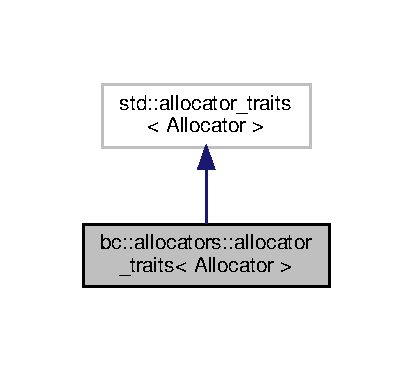
\includegraphics[width=198pt]{structbc_1_1allocators_1_1allocator__traits__inherit__graph}
\end{center}
\end{figure}


Collaboration diagram for bc\+:\+:allocators\+:\+:allocator\+\_\+traits$<$ Allocator $>$\+:\nopagebreak
\begin{figure}[H]
\begin{center}
\leavevmode
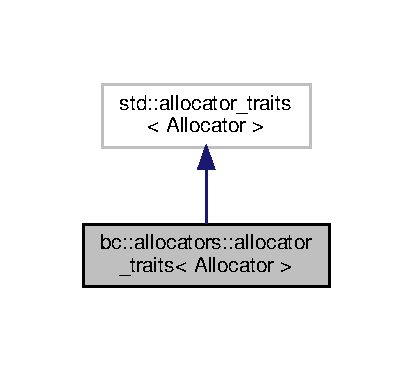
\includegraphics[width=198pt]{structbc_1_1allocators_1_1allocator__traits__coll__graph}
\end{center}
\end{figure}
\subsection*{Public Types}
\begin{DoxyCompactItemize}
\item 
using \hyperlink{structbc_1_1allocators_1_1allocator__traits_a527cf77071c45a9dcc2c8213f65f37b3}{system\+\_\+tag} = \hyperlink{namespacebc_1_1traits_a1a6d378947ec32acd457890854bcd592}{bc\+::traits\+::conditional\+\_\+detected\+\_\+t}$<$ \hyperlink{namespacebc_1_1traits_acfa34d40f06d5122586d7adefdfeb42f}{bc\+::traits\+::query\+\_\+system\+\_\+tag}, \hyperlink{classbc_1_1allocators_1_1Allocator}{Allocator}, \hyperlink{structbc_1_1host__tag}{host\+\_\+tag} $>$
\end{DoxyCompactItemize}


\subsection{Member Typedef Documentation}
\mbox{\Hypertarget{structbc_1_1allocators_1_1allocator__traits_a527cf77071c45a9dcc2c8213f65f37b3}\label{structbc_1_1allocators_1_1allocator__traits_a527cf77071c45a9dcc2c8213f65f37b3}} 
\index{bc\+::allocators\+::allocator\+\_\+traits@{bc\+::allocators\+::allocator\+\_\+traits}!system\+\_\+tag@{system\+\_\+tag}}
\index{system\+\_\+tag@{system\+\_\+tag}!bc\+::allocators\+::allocator\+\_\+traits@{bc\+::allocators\+::allocator\+\_\+traits}}
\subsubsection{\texorpdfstring{system\+\_\+tag}{system\_tag}}
{\footnotesize\ttfamily template$<$class Allocator$>$ \\
using \hyperlink{structbc_1_1allocators_1_1allocator__traits}{bc\+::allocators\+::allocator\+\_\+traits}$<$ \hyperlink{classbc_1_1allocators_1_1Allocator}{Allocator} $>$\+::\hyperlink{structbc_1_1allocators_1_1allocator__traits_a527cf77071c45a9dcc2c8213f65f37b3}{system\+\_\+tag} =  \hyperlink{namespacebc_1_1traits_a1a6d378947ec32acd457890854bcd592}{bc\+::traits\+::conditional\+\_\+detected\+\_\+t}$<$ \hyperlink{namespacebc_1_1traits_acfa34d40f06d5122586d7adefdfeb42f}{bc\+::traits\+::query\+\_\+system\+\_\+tag}, \hyperlink{classbc_1_1allocators_1_1Allocator}{Allocator}, \hyperlink{structbc_1_1host__tag}{host\+\_\+tag}$>$}



The documentation for this struct was generated from the following file\+:\begin{DoxyCompactItemize}
\item 
blackcat/allocators/\hyperlink{allocator__traits_8h}{allocator\+\_\+traits.\+h}\end{DoxyCompactItemize}

\hypertarget{structbc_1_1oper_1_1And}{}\section{bc\+:\+:oper\+:\+:And Struct Reference}
\label{structbc_1_1oper_1_1And}\index{bc\+::oper\+::\+And@{bc\+::oper\+::\+And}}


{\ttfamily \#include $<$binary.\+h$>$}

\subsection*{Public Member Functions}
\begin{DoxyCompactItemize}
\item 
{\footnotesize template$<$class Lv , class Rv $>$ }\\\+\_\+\+\_\+host\+\_\+\+\_\+ \+\_\+\+\_\+device\+\_\+\+\_\+ auto \hyperlink{structbc_1_1oper_1_1And_a0ee520ea8d55191ad9862d9b13bb5519}{operator()} (Lv \&\&lv, Rv \&\&rv) const -\/$>$ decltype(\hyperlink{structbc_1_1oper_1_1And_a1766c036547f8a41b966b06b6decb812}{apply}(lv, rv))
\end{DoxyCompactItemize}
\subsection*{Static Public Member Functions}
\begin{DoxyCompactItemize}
\item 
{\footnotesize template$<$class Lv , class Rv $>$ }\\\+\_\+\+\_\+host\+\_\+\+\_\+ static \+\_\+\+\_\+device\+\_\+\+\_\+ auto \hyperlink{structbc_1_1oper_1_1And_a1766c036547f8a41b966b06b6decb812}{apply} (Lv \&\&lv, Rv \&\&rv) -\/$>$ decltype(lv \&\&rv)
\end{DoxyCompactItemize}


\subsection{Member Function Documentation}
\mbox{\Hypertarget{structbc_1_1oper_1_1And_a1766c036547f8a41b966b06b6decb812}\label{structbc_1_1oper_1_1And_a1766c036547f8a41b966b06b6decb812}} 
\index{bc\+::oper\+::\+And@{bc\+::oper\+::\+And}!apply@{apply}}
\index{apply@{apply}!bc\+::oper\+::\+And@{bc\+::oper\+::\+And}}
\subsubsection{\texorpdfstring{apply()}{apply()}}
{\footnotesize\ttfamily template$<$class Lv , class Rv $>$ \\
\+\_\+\+\_\+host\+\_\+\+\_\+ static \+\_\+\+\_\+device\+\_\+\+\_\+ auto bc\+::oper\+::\+And\+::apply (\begin{DoxyParamCaption}\item[{Lv \&\&}]{lv,  }\item[{Rv \&\&}]{rv }\end{DoxyParamCaption}) -\/$>$ decltype( lv \&\& rv ) \hspace{0.3cm}{\ttfamily [inline]}, {\ttfamily [static]}}

\mbox{\Hypertarget{structbc_1_1oper_1_1And_a0ee520ea8d55191ad9862d9b13bb5519}\label{structbc_1_1oper_1_1And_a0ee520ea8d55191ad9862d9b13bb5519}} 
\index{bc\+::oper\+::\+And@{bc\+::oper\+::\+And}!operator()@{operator()}}
\index{operator()@{operator()}!bc\+::oper\+::\+And@{bc\+::oper\+::\+And}}
\subsubsection{\texorpdfstring{operator()()}{operator()()}}
{\footnotesize\ttfamily template$<$class Lv , class Rv $>$ \\
\+\_\+\+\_\+host\+\_\+\+\_\+ \+\_\+\+\_\+device\+\_\+\+\_\+ auto bc\+::oper\+::\+And\+::operator() (\begin{DoxyParamCaption}\item[{Lv \&\&}]{lv,  }\item[{Rv \&\&}]{rv }\end{DoxyParamCaption}) const -\/$>$ decltype(\hyperlink{structbc_1_1oper_1_1And_a1766c036547f8a41b966b06b6decb812}{apply}(lv, rv)) \hspace{0.3cm}{\ttfamily [inline]}}



The documentation for this struct was generated from the following file\+:\begin{DoxyCompactItemize}
\item 
blackcat/operations/\hyperlink{binary_8h}{binary.\+h}\end{DoxyCompactItemize}

\hypertarget{structbc_1_1traits_1_1any}{}\section{bc\+:\+:traits\+:\+:any$<$ Function, Ts $>$ Struct Template Reference}
\label{structbc_1_1traits_1_1any}\index{bc\+::traits\+::any$<$ Function, Ts $>$@{bc\+::traits\+::any$<$ Function, Ts $>$}}


{\ttfamily \#include $<$type\+\_\+traits.\+h$>$}



Inheritance diagram for bc\+:\+:traits\+:\+:any$<$ Function, Ts $>$\+:\nopagebreak
\begin{figure}[H]
\begin{center}
\leavevmode
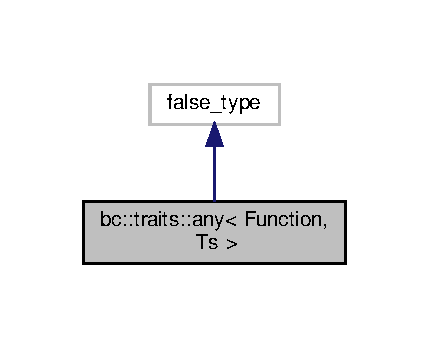
\includegraphics[width=206pt]{structbc_1_1traits_1_1any__inherit__graph}
\end{center}
\end{figure}


Collaboration diagram for bc\+:\+:traits\+:\+:any$<$ Function, Ts $>$\+:\nopagebreak
\begin{figure}[H]
\begin{center}
\leavevmode
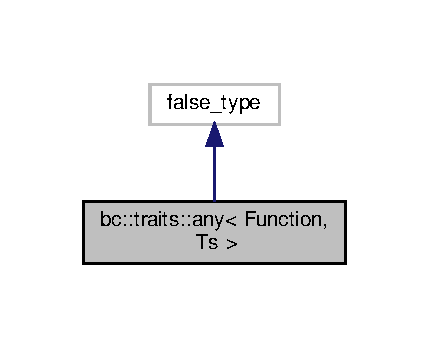
\includegraphics[width=206pt]{structbc_1_1traits_1_1any__coll__graph}
\end{center}
\end{figure}


The documentation for this struct was generated from the following file\+:\begin{DoxyCompactItemize}
\item 
blackcat/type\+\_\+traits/\hyperlink{type__traits_2type__traits_8h}{type\+\_\+traits.\+h}\end{DoxyCompactItemize}

\hypertarget{structbc_1_1traits_1_1any_3_01Function_00_01T_00_01Ts_8_8_8_01_4}{}\section{bc\+:\+:traits\+:\+:any$<$ Function, T, Ts... $>$ Struct Template Reference}
\label{structbc_1_1traits_1_1any_3_01Function_00_01T_00_01Ts_8_8_8_01_4}\index{bc\+::traits\+::any$<$ Function, T, Ts... $>$@{bc\+::traits\+::any$<$ Function, T, Ts... $>$}}


{\ttfamily \#include $<$type\+\_\+traits.\+h$>$}



Inheritance diagram for bc\+:\+:traits\+:\+:any$<$ Function, T, Ts... $>$\+:\nopagebreak
\begin{figure}[H]
\begin{center}
\leavevmode
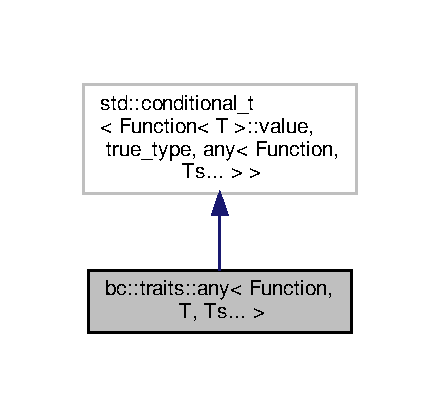
\includegraphics[width=211pt]{structbc_1_1traits_1_1any_3_01Function_00_01T_00_01Ts_8_8_8_01_4__inherit__graph}
\end{center}
\end{figure}


Collaboration diagram for bc\+:\+:traits\+:\+:any$<$ Function, T, Ts... $>$\+:\nopagebreak
\begin{figure}[H]
\begin{center}
\leavevmode
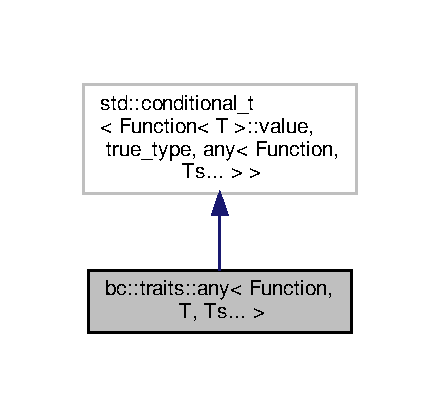
\includegraphics[width=211pt]{structbc_1_1traits_1_1any_3_01Function_00_01T_00_01Ts_8_8_8_01_4__coll__graph}
\end{center}
\end{figure}


The documentation for this struct was generated from the following file\+:\begin{DoxyCompactItemize}
\item 
blackcat/type\+\_\+traits/\hyperlink{type__traits_2type__traits_8h}{type\+\_\+traits.\+h}\end{DoxyCompactItemize}

\hypertarget{structbc_1_1utility_1_1Any__Key}{}\section{bc\+:\+:utility\+:\+:Any\+\_\+\+Key$<$ Key, Value $>$ Struct Template Reference}
\label{structbc_1_1utility_1_1Any__Key}\index{bc\+::utility\+::\+Any\+\_\+\+Key$<$ Key, Value $>$@{bc\+::utility\+::\+Any\+\_\+\+Key$<$ Key, Value $>$}}


{\ttfamily \#include $<$any\+\_\+map.\+h$>$}

\subsection*{Public Types}
\begin{DoxyCompactItemize}
\item 
using \hyperlink{structbc_1_1utility_1_1Any__Key_ae03da9e72e3dae70a87df8dfff64ed5c}{key\+\_\+type} = Key
\item 
using \hyperlink{structbc_1_1utility_1_1Any__Key_ae37f44db013d6698a17f5c095f32e36b}{value\+\_\+type} = Value
\end{DoxyCompactItemize}


\subsection{Member Typedef Documentation}
\mbox{\Hypertarget{structbc_1_1utility_1_1Any__Key_ae03da9e72e3dae70a87df8dfff64ed5c}\label{structbc_1_1utility_1_1Any__Key_ae03da9e72e3dae70a87df8dfff64ed5c}} 
\index{bc\+::utility\+::\+Any\+\_\+\+Key@{bc\+::utility\+::\+Any\+\_\+\+Key}!key\+\_\+type@{key\+\_\+type}}
\index{key\+\_\+type@{key\+\_\+type}!bc\+::utility\+::\+Any\+\_\+\+Key@{bc\+::utility\+::\+Any\+\_\+\+Key}}
\subsubsection{\texorpdfstring{key\+\_\+type}{key\_type}}
{\footnotesize\ttfamily template$<$class Key, class Value$>$ \\
using \hyperlink{structbc_1_1utility_1_1Any__Key}{bc\+::utility\+::\+Any\+\_\+\+Key}$<$ Key, Value $>$\+::\hyperlink{structbc_1_1utility_1_1Any__Key_ae03da9e72e3dae70a87df8dfff64ed5c}{key\+\_\+type} =  Key}

\mbox{\Hypertarget{structbc_1_1utility_1_1Any__Key_ae37f44db013d6698a17f5c095f32e36b}\label{structbc_1_1utility_1_1Any__Key_ae37f44db013d6698a17f5c095f32e36b}} 
\index{bc\+::utility\+::\+Any\+\_\+\+Key@{bc\+::utility\+::\+Any\+\_\+\+Key}!value\+\_\+type@{value\+\_\+type}}
\index{value\+\_\+type@{value\+\_\+type}!bc\+::utility\+::\+Any\+\_\+\+Key@{bc\+::utility\+::\+Any\+\_\+\+Key}}
\subsubsection{\texorpdfstring{value\+\_\+type}{value\_type}}
{\footnotesize\ttfamily template$<$class Key, class Value$>$ \\
using \hyperlink{structbc_1_1utility_1_1Any__Key}{bc\+::utility\+::\+Any\+\_\+\+Key}$<$ Key, Value $>$\+::\hyperlink{structbc_1_1utility_1_1Any__Key_ae37f44db013d6698a17f5c095f32e36b}{value\+\_\+type} =  Value}



The documentation for this struct was generated from the following file\+:\begin{DoxyCompactItemize}
\item 
blackcat/utility/\hyperlink{any__map_8h}{any\+\_\+map.\+h}\end{DoxyCompactItemize}

\hypertarget{classbc_1_1utility_1_1Any__Map}{}\section{bc\+:\+:utility\+:\+:Any\+\_\+\+Map Class Reference}
\label{classbc_1_1utility_1_1Any__Map}\index{bc\+::utility\+::\+Any\+\_\+\+Map@{bc\+::utility\+::\+Any\+\_\+\+Map}}


\hyperlink{classbc_1_1utility_1_1Any__Map}{Any\+\_\+\+Map} stores a buck of std\+::shared\+\_\+ptr$<$void$>$.  




{\ttfamily \#include $<$any\+\_\+map.\+h$>$}

\subsection*{Public Member Functions}
\begin{DoxyCompactItemize}
\item 
{\footnotesize template$<$class K , class V $>$ }\\bool \hyperlink{classbc_1_1utility_1_1Any__Map_a63086bc45ee54ef2ca5ebc4dc0989332}{contains} (\hyperlink{structbc_1_1utility_1_1Any__Key}{Any\+\_\+\+Key}$<$ K, V $>$ key) const
\item 
{\footnotesize template$<$class K , class V $>$ }\\auto \& \hyperlink{classbc_1_1utility_1_1Any__Map_a8898f0b7810c617631176e8bafbd156d}{operator\mbox{[}$\,$\mbox{]}} (\hyperlink{structbc_1_1utility_1_1Any__Key}{Any\+\_\+\+Key}$<$ K, V $>$ key)
\item 
{\footnotesize template$<$class K , class V $>$ }\\auto \& \hyperlink{classbc_1_1utility_1_1Any__Map_aedde6d40e8c81b80d9f4f16a55c0fab2}{at} (\hyperlink{structbc_1_1utility_1_1Any__Key}{Any\+\_\+\+Key}$<$ K, V $>$ key)
\item 
{\footnotesize template$<$class K , class V , class... Default\+Args$>$ }\\auto \& \hyperlink{classbc_1_1utility_1_1Any__Map_a45119ffc4e78ca50dc4790c63cc42590}{get} (\hyperlink{structbc_1_1utility_1_1Any__Key}{Any\+\_\+\+Key}$<$ K, V $>$ key, Default\+Args \&\&... args)
\item 
{\footnotesize template$<$class K , class V $>$ }\\auto \& \hyperlink{classbc_1_1utility_1_1Any__Map_a14d3fe8ca3fc98def4e9b61d7aa082fa}{get} (\hyperlink{structbc_1_1utility_1_1Any__Key}{Any\+\_\+\+Key}$<$ K, V $>$ key, V \&\&value)
\item 
{\footnotesize template$<$class K , class V , class... Args$>$ }\\auto \hyperlink{classbc_1_1utility_1_1Any__Map_a3e953570d8899b5fdcc0d17a86df085d}{emplace} (\hyperlink{structbc_1_1utility_1_1Any__Key}{Any\+\_\+\+Key}$<$ K, V $>$ key, Args \&\&... args)
\item 
int \hyperlink{classbc_1_1utility_1_1Any__Map_a3ec5e27b12955483d9c44ac6ae3b657a}{empty} () const
\item 
int \hyperlink{classbc_1_1utility_1_1Any__Map_afb04f91ca1a089ac61df93cb86d9b9f8}{size} () const
\item 
int \hyperlink{classbc_1_1utility_1_1Any__Map_a69eeee0adc8cb8cdaeac754a7f81438c}{max\+\_\+size} () const
\item 
auto \hyperlink{classbc_1_1utility_1_1Any__Map_a2140500f599708a2eac39a6736df0c40}{begin} () const
\item 
auto \hyperlink{classbc_1_1utility_1_1Any__Map_ae0f081d0501c3d8edcd68174fdd49ba5}{end} () const
\item 
auto \hyperlink{classbc_1_1utility_1_1Any__Map_a10ee269a7bb8dc9ddf1476042a2b3eab}{begin} ()
\item 
auto \hyperlink{classbc_1_1utility_1_1Any__Map_ad4e665fb716c5fbaedd9e7146d79e991}{end} ()
\item 
auto \hyperlink{classbc_1_1utility_1_1Any__Map_a92726117ebfa4b927d17eb45215a3c01}{cbegin} ()
\item 
auto \hyperlink{classbc_1_1utility_1_1Any__Map_a34df567594568b3cf78190e4469e6491}{cend} ()
\end{DoxyCompactItemize}


\subsection{Detailed Description}
\hyperlink{classbc_1_1utility_1_1Any__Map}{Any\+\_\+\+Map} stores a buck of std\+::shared\+\_\+ptr$<$void$>$. 

Elements are retrieved through\+:

my\+Map\mbox{[}\hyperlink{structbc_1_1utility_1_1Any__Key}{Any\+\_\+\+Key$<$\+K, V$>$()}\mbox{]}

It is recommended to use \char`\"{}\+Name\char`\"{} with \hyperlink{structbc_1_1utility_1_1Any__Key}{Any\+\_\+\+Key} to emulate constexpr-\/strings

my\+Map\mbox{[}\hyperlink{structbc_1_1utility_1_1Any__Key}{Any\+\_\+\+Key}$<$\hyperlink{structbc_1_1utility_1_1Name}{Name}$<$\textquotesingle{}K\textquotesingle{},\textquotesingle{}E\textquotesingle{},\textquotesingle{}Y\textquotesingle{}$>$, Value\+Type$>$\mbox{]}

Once C\+U\+DA supporst C++17 (which supports constexpr strings as template args) we will switch \hyperlink{structbc_1_1utility_1_1Any__Key}{Any\+\_\+\+Key} to simply being a $<$String, Value\+Type$>$.

The operator\mbox{[}\mbox{]} is a template argument, which enables casting to the correct type without any dynamic checks. This results in efficient access to \textquotesingle{}any\textquotesingle{} type within a pseudo-\/heterogeneous container. 

\subsection{Member Function Documentation}
\mbox{\Hypertarget{classbc_1_1utility_1_1Any__Map_aedde6d40e8c81b80d9f4f16a55c0fab2}\label{classbc_1_1utility_1_1Any__Map_aedde6d40e8c81b80d9f4f16a55c0fab2}} 
\index{bc\+::utility\+::\+Any\+\_\+\+Map@{bc\+::utility\+::\+Any\+\_\+\+Map}!at@{at}}
\index{at@{at}!bc\+::utility\+::\+Any\+\_\+\+Map@{bc\+::utility\+::\+Any\+\_\+\+Map}}
\subsubsection{\texorpdfstring{at()}{at()}}
{\footnotesize\ttfamily template$<$class K , class V $>$ \\
auto\& bc\+::utility\+::\+Any\+\_\+\+Map\+::at (\begin{DoxyParamCaption}\item[{\hyperlink{structbc_1_1utility_1_1Any__Key}{Any\+\_\+\+Key}$<$ K, V $>$}]{key }\end{DoxyParamCaption})\hspace{0.3cm}{\ttfamily [inline]}}

\mbox{\Hypertarget{classbc_1_1utility_1_1Any__Map_a2140500f599708a2eac39a6736df0c40}\label{classbc_1_1utility_1_1Any__Map_a2140500f599708a2eac39a6736df0c40}} 
\index{bc\+::utility\+::\+Any\+\_\+\+Map@{bc\+::utility\+::\+Any\+\_\+\+Map}!begin@{begin}}
\index{begin@{begin}!bc\+::utility\+::\+Any\+\_\+\+Map@{bc\+::utility\+::\+Any\+\_\+\+Map}}
\subsubsection{\texorpdfstring{begin()}{begin()}\hspace{0.1cm}{\footnotesize\ttfamily [1/2]}}
{\footnotesize\ttfamily auto bc\+::utility\+::\+Any\+\_\+\+Map\+::begin (\begin{DoxyParamCaption}{ }\end{DoxyParamCaption}) const\hspace{0.3cm}{\ttfamily [inline]}}

\mbox{\Hypertarget{classbc_1_1utility_1_1Any__Map_a10ee269a7bb8dc9ddf1476042a2b3eab}\label{classbc_1_1utility_1_1Any__Map_a10ee269a7bb8dc9ddf1476042a2b3eab}} 
\index{bc\+::utility\+::\+Any\+\_\+\+Map@{bc\+::utility\+::\+Any\+\_\+\+Map}!begin@{begin}}
\index{begin@{begin}!bc\+::utility\+::\+Any\+\_\+\+Map@{bc\+::utility\+::\+Any\+\_\+\+Map}}
\subsubsection{\texorpdfstring{begin()}{begin()}\hspace{0.1cm}{\footnotesize\ttfamily [2/2]}}
{\footnotesize\ttfamily auto bc\+::utility\+::\+Any\+\_\+\+Map\+::begin (\begin{DoxyParamCaption}{ }\end{DoxyParamCaption})\hspace{0.3cm}{\ttfamily [inline]}}

\mbox{\Hypertarget{classbc_1_1utility_1_1Any__Map_a92726117ebfa4b927d17eb45215a3c01}\label{classbc_1_1utility_1_1Any__Map_a92726117ebfa4b927d17eb45215a3c01}} 
\index{bc\+::utility\+::\+Any\+\_\+\+Map@{bc\+::utility\+::\+Any\+\_\+\+Map}!cbegin@{cbegin}}
\index{cbegin@{cbegin}!bc\+::utility\+::\+Any\+\_\+\+Map@{bc\+::utility\+::\+Any\+\_\+\+Map}}
\subsubsection{\texorpdfstring{cbegin()}{cbegin()}}
{\footnotesize\ttfamily auto bc\+::utility\+::\+Any\+\_\+\+Map\+::cbegin (\begin{DoxyParamCaption}{ }\end{DoxyParamCaption})\hspace{0.3cm}{\ttfamily [inline]}}

\mbox{\Hypertarget{classbc_1_1utility_1_1Any__Map_a34df567594568b3cf78190e4469e6491}\label{classbc_1_1utility_1_1Any__Map_a34df567594568b3cf78190e4469e6491}} 
\index{bc\+::utility\+::\+Any\+\_\+\+Map@{bc\+::utility\+::\+Any\+\_\+\+Map}!cend@{cend}}
\index{cend@{cend}!bc\+::utility\+::\+Any\+\_\+\+Map@{bc\+::utility\+::\+Any\+\_\+\+Map}}
\subsubsection{\texorpdfstring{cend()}{cend()}}
{\footnotesize\ttfamily auto bc\+::utility\+::\+Any\+\_\+\+Map\+::cend (\begin{DoxyParamCaption}{ }\end{DoxyParamCaption})\hspace{0.3cm}{\ttfamily [inline]}}

\mbox{\Hypertarget{classbc_1_1utility_1_1Any__Map_a63086bc45ee54ef2ca5ebc4dc0989332}\label{classbc_1_1utility_1_1Any__Map_a63086bc45ee54ef2ca5ebc4dc0989332}} 
\index{bc\+::utility\+::\+Any\+\_\+\+Map@{bc\+::utility\+::\+Any\+\_\+\+Map}!contains@{contains}}
\index{contains@{contains}!bc\+::utility\+::\+Any\+\_\+\+Map@{bc\+::utility\+::\+Any\+\_\+\+Map}}
\subsubsection{\texorpdfstring{contains()}{contains()}}
{\footnotesize\ttfamily template$<$class K , class V $>$ \\
bool bc\+::utility\+::\+Any\+\_\+\+Map\+::contains (\begin{DoxyParamCaption}\item[{\hyperlink{structbc_1_1utility_1_1Any__Key}{Any\+\_\+\+Key}$<$ K, V $>$}]{key }\end{DoxyParamCaption}) const\hspace{0.3cm}{\ttfamily [inline]}}

\mbox{\Hypertarget{classbc_1_1utility_1_1Any__Map_a3e953570d8899b5fdcc0d17a86df085d}\label{classbc_1_1utility_1_1Any__Map_a3e953570d8899b5fdcc0d17a86df085d}} 
\index{bc\+::utility\+::\+Any\+\_\+\+Map@{bc\+::utility\+::\+Any\+\_\+\+Map}!emplace@{emplace}}
\index{emplace@{emplace}!bc\+::utility\+::\+Any\+\_\+\+Map@{bc\+::utility\+::\+Any\+\_\+\+Map}}
\subsubsection{\texorpdfstring{emplace()}{emplace()}}
{\footnotesize\ttfamily template$<$class K , class V , class... Args$>$ \\
auto bc\+::utility\+::\+Any\+\_\+\+Map\+::emplace (\begin{DoxyParamCaption}\item[{\hyperlink{structbc_1_1utility_1_1Any__Key}{Any\+\_\+\+Key}$<$ K, V $>$}]{key,  }\item[{Args \&\&...}]{args }\end{DoxyParamCaption})\hspace{0.3cm}{\ttfamily [inline]}}

\mbox{\Hypertarget{classbc_1_1utility_1_1Any__Map_a3ec5e27b12955483d9c44ac6ae3b657a}\label{classbc_1_1utility_1_1Any__Map_a3ec5e27b12955483d9c44ac6ae3b657a}} 
\index{bc\+::utility\+::\+Any\+\_\+\+Map@{bc\+::utility\+::\+Any\+\_\+\+Map}!empty@{empty}}
\index{empty@{empty}!bc\+::utility\+::\+Any\+\_\+\+Map@{bc\+::utility\+::\+Any\+\_\+\+Map}}
\subsubsection{\texorpdfstring{empty()}{empty()}}
{\footnotesize\ttfamily int bc\+::utility\+::\+Any\+\_\+\+Map\+::empty (\begin{DoxyParamCaption}{ }\end{DoxyParamCaption}) const\hspace{0.3cm}{\ttfamily [inline]}}

\mbox{\Hypertarget{classbc_1_1utility_1_1Any__Map_ae0f081d0501c3d8edcd68174fdd49ba5}\label{classbc_1_1utility_1_1Any__Map_ae0f081d0501c3d8edcd68174fdd49ba5}} 
\index{bc\+::utility\+::\+Any\+\_\+\+Map@{bc\+::utility\+::\+Any\+\_\+\+Map}!end@{end}}
\index{end@{end}!bc\+::utility\+::\+Any\+\_\+\+Map@{bc\+::utility\+::\+Any\+\_\+\+Map}}
\subsubsection{\texorpdfstring{end()}{end()}\hspace{0.1cm}{\footnotesize\ttfamily [1/2]}}
{\footnotesize\ttfamily auto bc\+::utility\+::\+Any\+\_\+\+Map\+::end (\begin{DoxyParamCaption}{ }\end{DoxyParamCaption}) const\hspace{0.3cm}{\ttfamily [inline]}}

\mbox{\Hypertarget{classbc_1_1utility_1_1Any__Map_ad4e665fb716c5fbaedd9e7146d79e991}\label{classbc_1_1utility_1_1Any__Map_ad4e665fb716c5fbaedd9e7146d79e991}} 
\index{bc\+::utility\+::\+Any\+\_\+\+Map@{bc\+::utility\+::\+Any\+\_\+\+Map}!end@{end}}
\index{end@{end}!bc\+::utility\+::\+Any\+\_\+\+Map@{bc\+::utility\+::\+Any\+\_\+\+Map}}
\subsubsection{\texorpdfstring{end()}{end()}\hspace{0.1cm}{\footnotesize\ttfamily [2/2]}}
{\footnotesize\ttfamily auto bc\+::utility\+::\+Any\+\_\+\+Map\+::end (\begin{DoxyParamCaption}{ }\end{DoxyParamCaption})\hspace{0.3cm}{\ttfamily [inline]}}

\mbox{\Hypertarget{classbc_1_1utility_1_1Any__Map_a45119ffc4e78ca50dc4790c63cc42590}\label{classbc_1_1utility_1_1Any__Map_a45119ffc4e78ca50dc4790c63cc42590}} 
\index{bc\+::utility\+::\+Any\+\_\+\+Map@{bc\+::utility\+::\+Any\+\_\+\+Map}!get@{get}}
\index{get@{get}!bc\+::utility\+::\+Any\+\_\+\+Map@{bc\+::utility\+::\+Any\+\_\+\+Map}}
\subsubsection{\texorpdfstring{get()}{get()}\hspace{0.1cm}{\footnotesize\ttfamily [1/2]}}
{\footnotesize\ttfamily template$<$class K , class V , class... Default\+Args$>$ \\
auto\& bc\+::utility\+::\+Any\+\_\+\+Map\+::get (\begin{DoxyParamCaption}\item[{\hyperlink{structbc_1_1utility_1_1Any__Key}{Any\+\_\+\+Key}$<$ K, V $>$}]{key,  }\item[{Default\+Args \&\&...}]{args }\end{DoxyParamCaption})\hspace{0.3cm}{\ttfamily [inline]}}

\mbox{\Hypertarget{classbc_1_1utility_1_1Any__Map_a14d3fe8ca3fc98def4e9b61d7aa082fa}\label{classbc_1_1utility_1_1Any__Map_a14d3fe8ca3fc98def4e9b61d7aa082fa}} 
\index{bc\+::utility\+::\+Any\+\_\+\+Map@{bc\+::utility\+::\+Any\+\_\+\+Map}!get@{get}}
\index{get@{get}!bc\+::utility\+::\+Any\+\_\+\+Map@{bc\+::utility\+::\+Any\+\_\+\+Map}}
\subsubsection{\texorpdfstring{get()}{get()}\hspace{0.1cm}{\footnotesize\ttfamily [2/2]}}
{\footnotesize\ttfamily template$<$class K , class V $>$ \\
auto\& bc\+::utility\+::\+Any\+\_\+\+Map\+::get (\begin{DoxyParamCaption}\item[{\hyperlink{structbc_1_1utility_1_1Any__Key}{Any\+\_\+\+Key}$<$ K, V $>$}]{key,  }\item[{V \&\&}]{value }\end{DoxyParamCaption})\hspace{0.3cm}{\ttfamily [inline]}}

\mbox{\Hypertarget{classbc_1_1utility_1_1Any__Map_a69eeee0adc8cb8cdaeac754a7f81438c}\label{classbc_1_1utility_1_1Any__Map_a69eeee0adc8cb8cdaeac754a7f81438c}} 
\index{bc\+::utility\+::\+Any\+\_\+\+Map@{bc\+::utility\+::\+Any\+\_\+\+Map}!max\+\_\+size@{max\+\_\+size}}
\index{max\+\_\+size@{max\+\_\+size}!bc\+::utility\+::\+Any\+\_\+\+Map@{bc\+::utility\+::\+Any\+\_\+\+Map}}
\subsubsection{\texorpdfstring{max\+\_\+size()}{max\_size()}}
{\footnotesize\ttfamily int bc\+::utility\+::\+Any\+\_\+\+Map\+::max\+\_\+size (\begin{DoxyParamCaption}{ }\end{DoxyParamCaption}) const\hspace{0.3cm}{\ttfamily [inline]}}

\mbox{\Hypertarget{classbc_1_1utility_1_1Any__Map_a8898f0b7810c617631176e8bafbd156d}\label{classbc_1_1utility_1_1Any__Map_a8898f0b7810c617631176e8bafbd156d}} 
\index{bc\+::utility\+::\+Any\+\_\+\+Map@{bc\+::utility\+::\+Any\+\_\+\+Map}!operator\mbox{[}\mbox{]}@{operator[]}}
\index{operator\mbox{[}\mbox{]}@{operator[]}!bc\+::utility\+::\+Any\+\_\+\+Map@{bc\+::utility\+::\+Any\+\_\+\+Map}}
\subsubsection{\texorpdfstring{operator[]()}{operator[]()}}
{\footnotesize\ttfamily template$<$class K , class V $>$ \\
auto\& bc\+::utility\+::\+Any\+\_\+\+Map\+::operator\mbox{[}$\,$\mbox{]} (\begin{DoxyParamCaption}\item[{\hyperlink{structbc_1_1utility_1_1Any__Key}{Any\+\_\+\+Key}$<$ K, V $>$}]{key }\end{DoxyParamCaption})\hspace{0.3cm}{\ttfamily [inline]}}

\mbox{\Hypertarget{classbc_1_1utility_1_1Any__Map_afb04f91ca1a089ac61df93cb86d9b9f8}\label{classbc_1_1utility_1_1Any__Map_afb04f91ca1a089ac61df93cb86d9b9f8}} 
\index{bc\+::utility\+::\+Any\+\_\+\+Map@{bc\+::utility\+::\+Any\+\_\+\+Map}!size@{size}}
\index{size@{size}!bc\+::utility\+::\+Any\+\_\+\+Map@{bc\+::utility\+::\+Any\+\_\+\+Map}}
\subsubsection{\texorpdfstring{size()}{size()}}
{\footnotesize\ttfamily int bc\+::utility\+::\+Any\+\_\+\+Map\+::size (\begin{DoxyParamCaption}{ }\end{DoxyParamCaption}) const\hspace{0.3cm}{\ttfamily [inline]}}



The documentation for this class was generated from the following file\+:\begin{DoxyCompactItemize}
\item 
blackcat/utility/\hyperlink{any__map_8h}{any\+\_\+map.\+h}\end{DoxyCompactItemize}

\hypertarget{structbc_1_1oper_1_1Approx__Equal}{}\section{bc\+:\+:oper\+:\+:Approx\+\_\+\+Equal Struct Reference}
\label{structbc_1_1oper_1_1Approx__Equal}\index{bc\+::oper\+::\+Approx\+\_\+\+Equal@{bc\+::oper\+::\+Approx\+\_\+\+Equal}}


{\ttfamily \#include $<$binary.\+h$>$}

\subsection*{Public Member Functions}
\begin{DoxyCompactItemize}
\item 
{\footnotesize template$<$class Lv , class Rv $>$ }\\\+\_\+\+\_\+host\+\_\+\+\_\+ \+\_\+\+\_\+device\+\_\+\+\_\+ auto \hyperlink{structbc_1_1oper_1_1Approx__Equal_ad46ea264a8158c151ae0d159a3d0ed52}{operator()} (Lv \&\&lv, Rv \&\&rv) const -\/$>$ decltype(\hyperlink{structbc_1_1oper_1_1Approx__Equal_a7eaf517f3b69b5171d7bc4cc863cfd9c}{apply}(lv, rv))
\end{DoxyCompactItemize}
\subsection*{Static Public Member Functions}
\begin{DoxyCompactItemize}
\item 
{\footnotesize template$<$class Lv , class Rv $>$ }\\\+\_\+\+\_\+host\+\_\+\+\_\+ static \+\_\+\+\_\+device\+\_\+\+\_\+ auto \hyperlink{structbc_1_1oper_1_1Approx__Equal_a7eaf517f3b69b5171d7bc4cc863cfd9c}{apply} (Lv \&\&lv, Rv \&\&rv) -\/$>$ decltype(std\+::abs(lv -\/ rv)$<$ .\+01)
\end{DoxyCompactItemize}


\subsection{Member Function Documentation}
\mbox{\Hypertarget{structbc_1_1oper_1_1Approx__Equal_a7eaf517f3b69b5171d7bc4cc863cfd9c}\label{structbc_1_1oper_1_1Approx__Equal_a7eaf517f3b69b5171d7bc4cc863cfd9c}} 
\index{bc\+::oper\+::\+Approx\+\_\+\+Equal@{bc\+::oper\+::\+Approx\+\_\+\+Equal}!apply@{apply}}
\index{apply@{apply}!bc\+::oper\+::\+Approx\+\_\+\+Equal@{bc\+::oper\+::\+Approx\+\_\+\+Equal}}
\subsubsection{\texorpdfstring{apply()}{apply()}}
{\footnotesize\ttfamily template$<$class Lv , class Rv $>$ \\
\+\_\+\+\_\+host\+\_\+\+\_\+ static \+\_\+\+\_\+device\+\_\+\+\_\+ auto bc\+::oper\+::\+Approx\+\_\+\+Equal\+::apply (\begin{DoxyParamCaption}\item[{Lv \&\&}]{lv,  }\item[{Rv \&\&}]{rv }\end{DoxyParamCaption}) -\/$>$ decltype( std\+::abs(lv -\/ rv) $<$ .\+01 ) \hspace{0.3cm}{\ttfamily [inline]}, {\ttfamily [static]}}

\mbox{\Hypertarget{structbc_1_1oper_1_1Approx__Equal_ad46ea264a8158c151ae0d159a3d0ed52}\label{structbc_1_1oper_1_1Approx__Equal_ad46ea264a8158c151ae0d159a3d0ed52}} 
\index{bc\+::oper\+::\+Approx\+\_\+\+Equal@{bc\+::oper\+::\+Approx\+\_\+\+Equal}!operator()@{operator()}}
\index{operator()@{operator()}!bc\+::oper\+::\+Approx\+\_\+\+Equal@{bc\+::oper\+::\+Approx\+\_\+\+Equal}}
\subsubsection{\texorpdfstring{operator()()}{operator()()}}
{\footnotesize\ttfamily template$<$class Lv , class Rv $>$ \\
\+\_\+\+\_\+host\+\_\+\+\_\+ \+\_\+\+\_\+device\+\_\+\+\_\+ auto bc\+::oper\+::\+Approx\+\_\+\+Equal\+::operator() (\begin{DoxyParamCaption}\item[{Lv \&\&}]{lv,  }\item[{Rv \&\&}]{rv }\end{DoxyParamCaption}) const -\/$>$ decltype(\hyperlink{structbc_1_1oper_1_1Approx__Equal_a7eaf517f3b69b5171d7bc4cc863cfd9c}{apply}(lv, rv)) \hspace{0.3cm}{\ttfamily [inline]}}



The documentation for this struct was generated from the following file\+:\begin{DoxyCompactItemize}
\item 
blackcat/operations/\hyperlink{binary_8h}{binary.\+h}\end{DoxyCompactItemize}

\hypertarget{structbc_1_1tensors_1_1exprs_1_1Array}{}\section{bc\+:\+:tensors\+:\+:exprs\+:\+:Array$<$ Shape, Scalar, Allocator\+Type, Tags $>$ Struct Template Reference}
\label{structbc_1_1tensors_1_1exprs_1_1Array}\index{bc\+::tensors\+::exprs\+::\+Array$<$ Shape, Scalar, Allocator\+Type, Tags $>$@{bc\+::tensors\+::exprs\+::\+Array$<$ Shape, Scalar, Allocator\+Type, Tags $>$}}


{\ttfamily \#include $<$array.\+h$>$}



Inheritance diagram for bc\+:\+:tensors\+:\+:exprs\+:\+:Array$<$ Shape, Scalar, Allocator\+Type, Tags $>$\+:\nopagebreak
\begin{figure}[H]
\begin{center}
\leavevmode
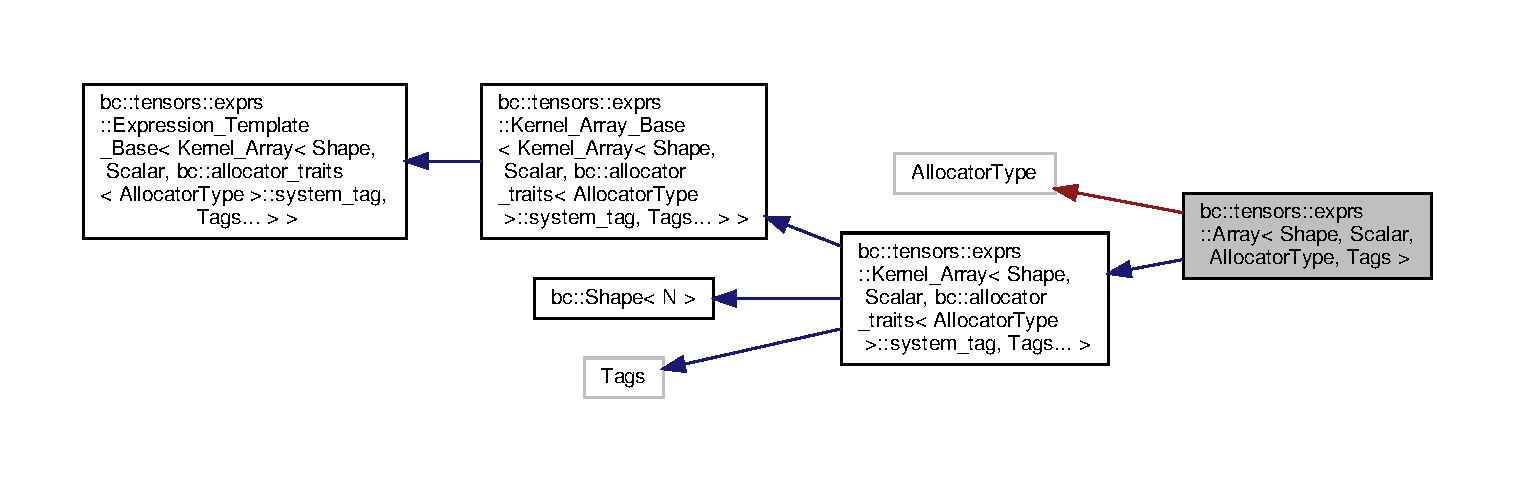
\includegraphics[width=350pt]{structbc_1_1tensors_1_1exprs_1_1Array__inherit__graph}
\end{center}
\end{figure}


Collaboration diagram for bc\+:\+:tensors\+:\+:exprs\+:\+:Array$<$ Shape, Scalar, Allocator\+Type, Tags $>$\+:\nopagebreak
\begin{figure}[H]
\begin{center}
\leavevmode
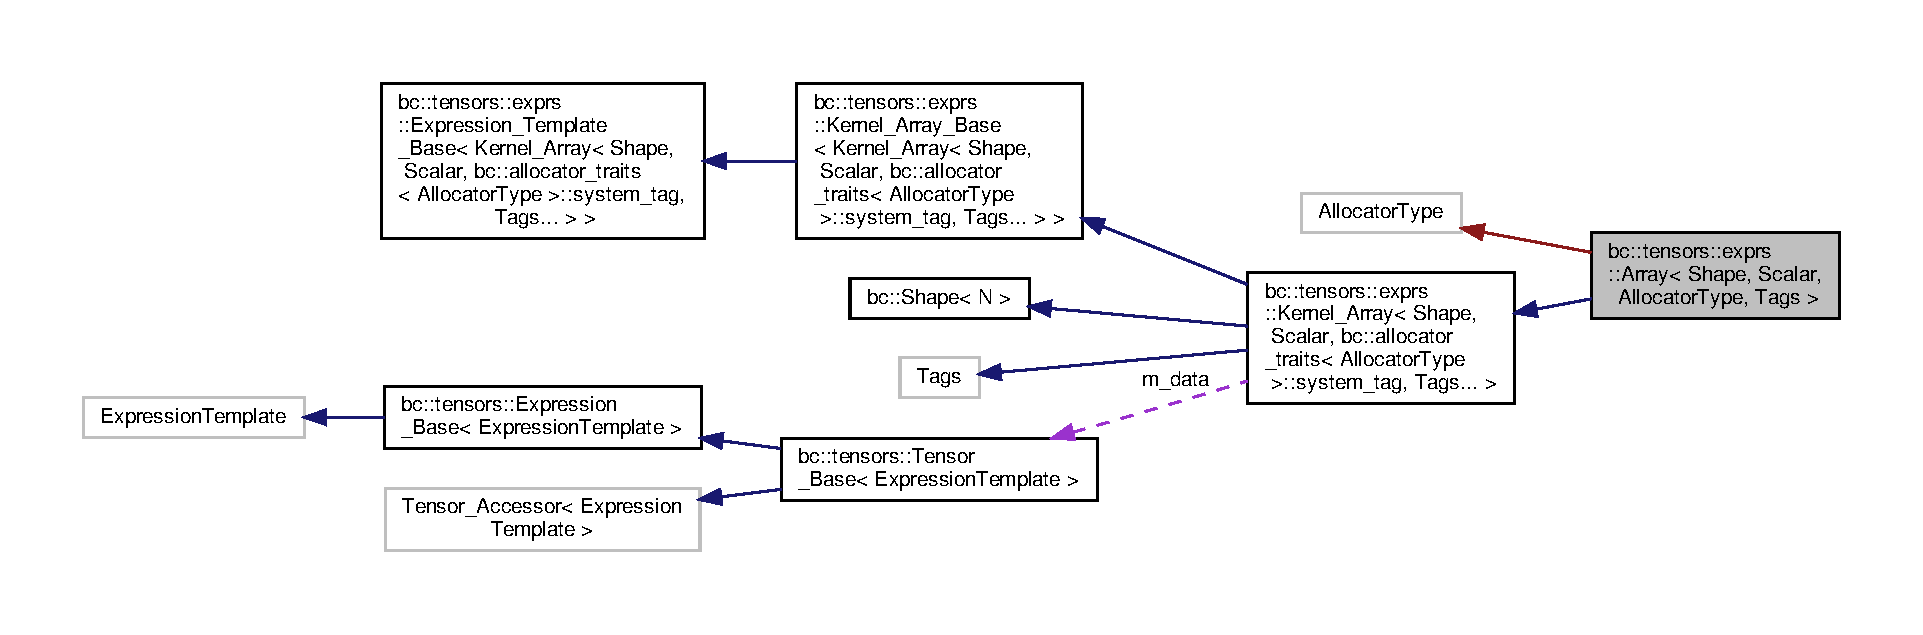
\includegraphics[width=350pt]{structbc_1_1tensors_1_1exprs_1_1Array__coll__graph}
\end{center}
\end{figure}
\subsection*{Public Types}
\begin{DoxyCompactItemize}
\item 
using \hyperlink{structbc_1_1tensors_1_1exprs_1_1Array_a116ffe7734f63cf0ca63b32b7cfb0506}{system\+\_\+tag} = typename \hyperlink{structbc_1_1allocators_1_1allocator__traits}{bc\+::allocator\+\_\+traits}$<$ Allocator\+Type $>$\+::\hyperlink{structbc_1_1tensors_1_1exprs_1_1Array_a116ffe7734f63cf0ca63b32b7cfb0506}{system\+\_\+tag}
\item 
using \hyperlink{structbc_1_1tensors_1_1exprs_1_1Array_a28b34dfcad3f0d35770d64a38f7187a0}{value\+\_\+type} = \hyperlink{namespacebc_aa12ac55ee2c43dc082894dd3859daee1}{Scalar}
\item 
using \hyperlink{structbc_1_1tensors_1_1exprs_1_1Array_a990afcebe8817075d427f2653d197140}{allocator\+\_\+type} = Allocator\+Type
\item 
using \hyperlink{structbc_1_1tensors_1_1exprs_1_1Array_aba97273ba94fb140763e7db5da630ea0}{stream\+\_\+type} = \hyperlink{classbc_1_1streams_1_1Stream}{Stream}$<$ \hyperlink{structbc_1_1tensors_1_1exprs_1_1Array_a116ffe7734f63cf0ca63b32b7cfb0506}{system\+\_\+tag} $>$
\item 
using \hyperlink{structbc_1_1tensors_1_1exprs_1_1Array_a67c96ea64a2899ba0593a6b81aa0868e}{shape\+\_\+type} = \hyperlink{structbc_1_1Shape}{Shape}
\end{DoxyCompactItemize}
\subsection*{Public Member Functions}
\begin{DoxyCompactItemize}
\item 
const \hyperlink{structbc_1_1tensors_1_1exprs_1_1Array_aba97273ba94fb140763e7db5da630ea0}{stream\+\_\+type} \& \hyperlink{structbc_1_1tensors_1_1exprs_1_1Array_a1d6e547e956f8f7bbd2a94ad10bd64fa}{get\+\_\+stream} () const
\item 
\hyperlink{structbc_1_1tensors_1_1exprs_1_1Array_aba97273ba94fb140763e7db5da630ea0}{stream\+\_\+type} \& \hyperlink{structbc_1_1tensors_1_1exprs_1_1Array_adde068372455f066865b2395634f407b}{get\+\_\+stream} ()
\item 
\hyperlink{structbc_1_1tensors_1_1exprs_1_1Array_a990afcebe8817075d427f2653d197140}{allocator\+\_\+type} \hyperlink{structbc_1_1tensors_1_1exprs_1_1Array_a23512d49fbc3734005e92d64ad31a3f8}{get\+\_\+allocator} () const
\item 
\hyperlink{structbc_1_1tensors_1_1exprs_1_1Array_aee4d34e0da545cb3463a2359a2daf6d4}{Array} ()
\item 
\hyperlink{structbc_1_1tensors_1_1exprs_1_1Array_a404b48bf95a86c8cb6978a3bf0107ffe}{Array} (const \hyperlink{structbc_1_1tensors_1_1exprs_1_1Array}{Array} \&array)
\item 
\hyperlink{structbc_1_1tensors_1_1exprs_1_1Array_a36469db9812dc419d20e87171a019998}{Array} (\hyperlink{structbc_1_1tensors_1_1exprs_1_1Array}{Array} \&\&array)
\item 
\hyperlink{structbc_1_1tensors_1_1exprs_1_1Array_a86801946a99e3d104ee7d6569c97072c}{Array} (\hyperlink{structbc_1_1Dim}{bc\+::\+Dim}$<$ \hyperlink{structbc_1_1Shape_a1f75fffa8b4aec4405025de308adb169}{shape\+\_\+type\+::tensor\+\_\+dim} $>$ \hyperlink{namespacebc_a1bc6dec532973ac024c738c0fd32cca3}{shape})
\item 
\hyperlink{structbc_1_1tensors_1_1exprs_1_1Array_afdc66d4d061f95a91831044776e619a3}{Array} (\hyperlink{structbc_1_1Dim}{bc\+::\+Dim}$<$ \hyperlink{structbc_1_1Shape_a1f75fffa8b4aec4405025de308adb169}{shape\+\_\+type\+::tensor\+\_\+dim} $>$ \hyperlink{namespacebc_a1bc6dec532973ac024c738c0fd32cca3}{shape}, \hyperlink{structbc_1_1tensors_1_1exprs_1_1Array_a990afcebe8817075d427f2653d197140}{allocator\+\_\+type} allocator)
\item 
\hyperlink{structbc_1_1tensors_1_1exprs_1_1Array_a5fa294dbb5d9eccea7201c507c6f7004}{Array} (\hyperlink{structbc_1_1tensors_1_1exprs_1_1Array_a67c96ea64a2899ba0593a6b81aa0868e}{shape\+\_\+type} \hyperlink{namespacebc_a1bc6dec532973ac024c738c0fd32cca3}{shape})
\item 
{\footnotesize template$<$class... Shape\+Dims, class  = std\+::enable\+\_\+if\+\_\+t$<$			traits\+::sequence\+\_\+of\+\_\+v$<$bc\+::size\+\_\+t, Shape\+Dims...$>$ \&\&			sizeof...(\+Shape\+Dims) == Shape\+::tensor\+\_\+dim$>$$>$ }\\\hyperlink{structbc_1_1tensors_1_1exprs_1_1Array_a0bdfc60f9711f7334ed0850fd417109c}{Array} (const Shape\+Dims \&... shape\+\_\+dims)
\item 
{\footnotesize template$<$class Expression , class  = std\+::enable\+\_\+if\+\_\+t$<$			expression\+\_\+traits$<$\+Expression$>$\+::is\+\_\+array\+::value $\vert$$\vert$			expression\+\_\+traits$<$\+Expression$>$\+::is\+\_\+expr\+::value$>$$>$ }\\\hyperlink{structbc_1_1tensors_1_1exprs_1_1Array_a33daff032fc7d980dc4c9e336570a718}{Array} (const Expression \&expression, \hyperlink{structbc_1_1tensors_1_1exprs_1_1Array_a990afcebe8817075d427f2653d197140}{allocator\+\_\+type} allocator=\hyperlink{structbc_1_1tensors_1_1exprs_1_1Array_a990afcebe8817075d427f2653d197140}{allocator\+\_\+type}())
\item 
{\footnotesize template$<$class Alt\+Shape , class... Slice\+Tags$>$ }\\\hyperlink{structbc_1_1tensors_1_1exprs_1_1Array_a7cc7a7eb294c67d96f66c52598382991}{Array} (const \hyperlink{classbc_1_1tensors_1_1exprs_1_1Array__Slice}{Array\+\_\+\+Slice}$<$ Alt\+Shape, \hyperlink{structbc_1_1Shape_a52aafd6585a5eae8a3b82f650d3afc1c}{value\+\_\+type}, \hyperlink{structbc_1_1tensors_1_1exprs_1_1Array_a990afcebe8817075d427f2653d197140}{allocator\+\_\+type}, Slice\+Tags... $>$ \&expression)
\item 
\hyperlink{structbc_1_1tensors_1_1exprs_1_1Array}{Array} \& \hyperlink{structbc_1_1tensors_1_1exprs_1_1Array_ad5b1cbbee83ed001d18012df27ebdef8}{operator=} (\hyperlink{structbc_1_1tensors_1_1exprs_1_1Array}{Array} \&\&array)
\end{DoxyCompactItemize}
\subsection*{Protected Member Functions}
\begin{DoxyCompactItemize}
\item 
void \hyperlink{structbc_1_1tensors_1_1exprs_1_1Array_a3123e9466102d458b8bcf48bd926559c}{deallocate} ()
\end{DoxyCompactItemize}
\subsection*{Additional Inherited Members}


\subsection{Member Typedef Documentation}
\mbox{\Hypertarget{structbc_1_1tensors_1_1exprs_1_1Array_a990afcebe8817075d427f2653d197140}\label{structbc_1_1tensors_1_1exprs_1_1Array_a990afcebe8817075d427f2653d197140}} 
\index{bc\+::tensors\+::exprs\+::\+Array@{bc\+::tensors\+::exprs\+::\+Array}!allocator\+\_\+type@{allocator\+\_\+type}}
\index{allocator\+\_\+type@{allocator\+\_\+type}!bc\+::tensors\+::exprs\+::\+Array@{bc\+::tensors\+::exprs\+::\+Array}}
\subsubsection{\texorpdfstring{allocator\+\_\+type}{allocator\_type}}
{\footnotesize\ttfamily template$<$class Shape, class Scalar, class Allocator\+Type, class... Tags$>$ \\
using \hyperlink{structbc_1_1tensors_1_1exprs_1_1Array}{bc\+::tensors\+::exprs\+::\+Array}$<$ \hyperlink{structbc_1_1Shape}{Shape}, \hyperlink{namespacebc_aa12ac55ee2c43dc082894dd3859daee1}{Scalar}, Allocator\+Type, Tags $>$\+::\hyperlink{structbc_1_1tensors_1_1exprs_1_1Array_a990afcebe8817075d427f2653d197140}{allocator\+\_\+type} =  Allocator\+Type}

\mbox{\Hypertarget{structbc_1_1tensors_1_1exprs_1_1Array_a67c96ea64a2899ba0593a6b81aa0868e}\label{structbc_1_1tensors_1_1exprs_1_1Array_a67c96ea64a2899ba0593a6b81aa0868e}} 
\index{bc\+::tensors\+::exprs\+::\+Array@{bc\+::tensors\+::exprs\+::\+Array}!shape\+\_\+type@{shape\+\_\+type}}
\index{shape\+\_\+type@{shape\+\_\+type}!bc\+::tensors\+::exprs\+::\+Array@{bc\+::tensors\+::exprs\+::\+Array}}
\subsubsection{\texorpdfstring{shape\+\_\+type}{shape\_type}}
{\footnotesize\ttfamily template$<$class Shape, class Scalar, class Allocator\+Type, class... Tags$>$ \\
using \hyperlink{structbc_1_1tensors_1_1exprs_1_1Array}{bc\+::tensors\+::exprs\+::\+Array}$<$ \hyperlink{structbc_1_1Shape}{Shape}, \hyperlink{namespacebc_aa12ac55ee2c43dc082894dd3859daee1}{Scalar}, Allocator\+Type, Tags $>$\+::\hyperlink{structbc_1_1tensors_1_1exprs_1_1Array_a67c96ea64a2899ba0593a6b81aa0868e}{shape\+\_\+type} =  \hyperlink{structbc_1_1Shape}{Shape}}

\mbox{\Hypertarget{structbc_1_1tensors_1_1exprs_1_1Array_aba97273ba94fb140763e7db5da630ea0}\label{structbc_1_1tensors_1_1exprs_1_1Array_aba97273ba94fb140763e7db5da630ea0}} 
\index{bc\+::tensors\+::exprs\+::\+Array@{bc\+::tensors\+::exprs\+::\+Array}!stream\+\_\+type@{stream\+\_\+type}}
\index{stream\+\_\+type@{stream\+\_\+type}!bc\+::tensors\+::exprs\+::\+Array@{bc\+::tensors\+::exprs\+::\+Array}}
\subsubsection{\texorpdfstring{stream\+\_\+type}{stream\_type}}
{\footnotesize\ttfamily template$<$class Shape, class Scalar, class Allocator\+Type, class... Tags$>$ \\
using \hyperlink{structbc_1_1tensors_1_1exprs_1_1Array}{bc\+::tensors\+::exprs\+::\+Array}$<$ \hyperlink{structbc_1_1Shape}{Shape}, \hyperlink{namespacebc_aa12ac55ee2c43dc082894dd3859daee1}{Scalar}, Allocator\+Type, Tags $>$\+::\hyperlink{structbc_1_1tensors_1_1exprs_1_1Array_aba97273ba94fb140763e7db5da630ea0}{stream\+\_\+type} =  \hyperlink{classbc_1_1streams_1_1Stream}{Stream}$<$\hyperlink{structbc_1_1tensors_1_1exprs_1_1Array_a116ffe7734f63cf0ca63b32b7cfb0506}{system\+\_\+tag}$>$}

\mbox{\Hypertarget{structbc_1_1tensors_1_1exprs_1_1Array_a116ffe7734f63cf0ca63b32b7cfb0506}\label{structbc_1_1tensors_1_1exprs_1_1Array_a116ffe7734f63cf0ca63b32b7cfb0506}} 
\index{bc\+::tensors\+::exprs\+::\+Array@{bc\+::tensors\+::exprs\+::\+Array}!system\+\_\+tag@{system\+\_\+tag}}
\index{system\+\_\+tag@{system\+\_\+tag}!bc\+::tensors\+::exprs\+::\+Array@{bc\+::tensors\+::exprs\+::\+Array}}
\subsubsection{\texorpdfstring{system\+\_\+tag}{system\_tag}}
{\footnotesize\ttfamily template$<$class Shape, class Scalar, class Allocator\+Type, class... Tags$>$ \\
using \hyperlink{structbc_1_1tensors_1_1exprs_1_1Array}{bc\+::tensors\+::exprs\+::\+Array}$<$ \hyperlink{structbc_1_1Shape}{Shape}, \hyperlink{namespacebc_aa12ac55ee2c43dc082894dd3859daee1}{Scalar}, Allocator\+Type, Tags $>$\+::\hyperlink{structbc_1_1tensors_1_1exprs_1_1Array_a116ffe7734f63cf0ca63b32b7cfb0506}{system\+\_\+tag} =  typename \hyperlink{structbc_1_1allocators_1_1allocator__traits}{bc\+::allocator\+\_\+traits}$<$Allocator\+Type$>$\+::\hyperlink{structbc_1_1tensors_1_1exprs_1_1Array_a116ffe7734f63cf0ca63b32b7cfb0506}{system\+\_\+tag}}

\mbox{\Hypertarget{structbc_1_1tensors_1_1exprs_1_1Array_a28b34dfcad3f0d35770d64a38f7187a0}\label{structbc_1_1tensors_1_1exprs_1_1Array_a28b34dfcad3f0d35770d64a38f7187a0}} 
\index{bc\+::tensors\+::exprs\+::\+Array@{bc\+::tensors\+::exprs\+::\+Array}!value\+\_\+type@{value\+\_\+type}}
\index{value\+\_\+type@{value\+\_\+type}!bc\+::tensors\+::exprs\+::\+Array@{bc\+::tensors\+::exprs\+::\+Array}}
\subsubsection{\texorpdfstring{value\+\_\+type}{value\_type}}
{\footnotesize\ttfamily template$<$class Shape, class Scalar, class Allocator\+Type, class... Tags$>$ \\
using \hyperlink{structbc_1_1tensors_1_1exprs_1_1Array}{bc\+::tensors\+::exprs\+::\+Array}$<$ \hyperlink{structbc_1_1Shape}{Shape}, \hyperlink{namespacebc_aa12ac55ee2c43dc082894dd3859daee1}{Scalar}, Allocator\+Type, Tags $>$\+::\hyperlink{structbc_1_1Shape_a52aafd6585a5eae8a3b82f650d3afc1c}{value\+\_\+type} =  \hyperlink{namespacebc_aa12ac55ee2c43dc082894dd3859daee1}{Scalar}}



\subsection{Constructor \& Destructor Documentation}
\mbox{\Hypertarget{structbc_1_1tensors_1_1exprs_1_1Array_aee4d34e0da545cb3463a2359a2daf6d4}\label{structbc_1_1tensors_1_1exprs_1_1Array_aee4d34e0da545cb3463a2359a2daf6d4}} 
\index{bc\+::tensors\+::exprs\+::\+Array@{bc\+::tensors\+::exprs\+::\+Array}!Array@{Array}}
\index{Array@{Array}!bc\+::tensors\+::exprs\+::\+Array@{bc\+::tensors\+::exprs\+::\+Array}}
\subsubsection{\texorpdfstring{Array()}{Array()}\hspace{0.1cm}{\footnotesize\ttfamily [1/9]}}
{\footnotesize\ttfamily template$<$class Shape, class Scalar, class Allocator\+Type, class... Tags$>$ \\
\hyperlink{structbc_1_1tensors_1_1exprs_1_1Array}{bc\+::tensors\+::exprs\+::\+Array}$<$ \hyperlink{structbc_1_1Shape}{Shape}, \hyperlink{namespacebc_aa12ac55ee2c43dc082894dd3859daee1}{Scalar}, Allocator\+Type, Tags $>$\+::\hyperlink{structbc_1_1tensors_1_1exprs_1_1Array}{Array} (\begin{DoxyParamCaption}{ }\end{DoxyParamCaption})\hspace{0.3cm}{\ttfamily [inline]}}

\mbox{\Hypertarget{structbc_1_1tensors_1_1exprs_1_1Array_a404b48bf95a86c8cb6978a3bf0107ffe}\label{structbc_1_1tensors_1_1exprs_1_1Array_a404b48bf95a86c8cb6978a3bf0107ffe}} 
\index{bc\+::tensors\+::exprs\+::\+Array@{bc\+::tensors\+::exprs\+::\+Array}!Array@{Array}}
\index{Array@{Array}!bc\+::tensors\+::exprs\+::\+Array@{bc\+::tensors\+::exprs\+::\+Array}}
\subsubsection{\texorpdfstring{Array()}{Array()}\hspace{0.1cm}{\footnotesize\ttfamily [2/9]}}
{\footnotesize\ttfamily template$<$class Shape, class Scalar, class Allocator\+Type, class... Tags$>$ \\
\hyperlink{structbc_1_1tensors_1_1exprs_1_1Array}{bc\+::tensors\+::exprs\+::\+Array}$<$ \hyperlink{structbc_1_1Shape}{Shape}, \hyperlink{namespacebc_aa12ac55ee2c43dc082894dd3859daee1}{Scalar}, Allocator\+Type, Tags $>$\+::\hyperlink{structbc_1_1tensors_1_1exprs_1_1Array}{Array} (\begin{DoxyParamCaption}\item[{const \hyperlink{structbc_1_1tensors_1_1exprs_1_1Array}{Array}$<$ \hyperlink{structbc_1_1Shape}{Shape}, \hyperlink{namespacebc_aa12ac55ee2c43dc082894dd3859daee1}{Scalar}, Allocator\+Type, Tags $>$ \&}]{array }\end{DoxyParamCaption})\hspace{0.3cm}{\ttfamily [inline]}}

\mbox{\Hypertarget{structbc_1_1tensors_1_1exprs_1_1Array_a36469db9812dc419d20e87171a019998}\label{structbc_1_1tensors_1_1exprs_1_1Array_a36469db9812dc419d20e87171a019998}} 
\index{bc\+::tensors\+::exprs\+::\+Array@{bc\+::tensors\+::exprs\+::\+Array}!Array@{Array}}
\index{Array@{Array}!bc\+::tensors\+::exprs\+::\+Array@{bc\+::tensors\+::exprs\+::\+Array}}
\subsubsection{\texorpdfstring{Array()}{Array()}\hspace{0.1cm}{\footnotesize\ttfamily [3/9]}}
{\footnotesize\ttfamily template$<$class Shape, class Scalar, class Allocator\+Type, class... Tags$>$ \\
\hyperlink{structbc_1_1tensors_1_1exprs_1_1Array}{bc\+::tensors\+::exprs\+::\+Array}$<$ \hyperlink{structbc_1_1Shape}{Shape}, \hyperlink{namespacebc_aa12ac55ee2c43dc082894dd3859daee1}{Scalar}, Allocator\+Type, Tags $>$\+::\hyperlink{structbc_1_1tensors_1_1exprs_1_1Array}{Array} (\begin{DoxyParamCaption}\item[{\hyperlink{structbc_1_1tensors_1_1exprs_1_1Array}{Array}$<$ \hyperlink{structbc_1_1Shape}{Shape}, \hyperlink{namespacebc_aa12ac55ee2c43dc082894dd3859daee1}{Scalar}, Allocator\+Type, Tags $>$ \&\&}]{array }\end{DoxyParamCaption})\hspace{0.3cm}{\ttfamily [inline]}}

\mbox{\Hypertarget{structbc_1_1tensors_1_1exprs_1_1Array_a86801946a99e3d104ee7d6569c97072c}\label{structbc_1_1tensors_1_1exprs_1_1Array_a86801946a99e3d104ee7d6569c97072c}} 
\index{bc\+::tensors\+::exprs\+::\+Array@{bc\+::tensors\+::exprs\+::\+Array}!Array@{Array}}
\index{Array@{Array}!bc\+::tensors\+::exprs\+::\+Array@{bc\+::tensors\+::exprs\+::\+Array}}
\subsubsection{\texorpdfstring{Array()}{Array()}\hspace{0.1cm}{\footnotesize\ttfamily [4/9]}}
{\footnotesize\ttfamily template$<$class Shape, class Scalar, class Allocator\+Type, class... Tags$>$ \\
\hyperlink{structbc_1_1tensors_1_1exprs_1_1Array}{bc\+::tensors\+::exprs\+::\+Array}$<$ \hyperlink{structbc_1_1Shape}{Shape}, \hyperlink{namespacebc_aa12ac55ee2c43dc082894dd3859daee1}{Scalar}, Allocator\+Type, Tags $>$\+::\hyperlink{structbc_1_1tensors_1_1exprs_1_1Array}{Array} (\begin{DoxyParamCaption}\item[{\hyperlink{structbc_1_1Dim}{bc\+::\+Dim}$<$ \hyperlink{structbc_1_1Shape_a1f75fffa8b4aec4405025de308adb169}{shape\+\_\+type\+::tensor\+\_\+dim} $>$}]{shape }\end{DoxyParamCaption})\hspace{0.3cm}{\ttfamily [inline]}}

\mbox{\Hypertarget{structbc_1_1tensors_1_1exprs_1_1Array_afdc66d4d061f95a91831044776e619a3}\label{structbc_1_1tensors_1_1exprs_1_1Array_afdc66d4d061f95a91831044776e619a3}} 
\index{bc\+::tensors\+::exprs\+::\+Array@{bc\+::tensors\+::exprs\+::\+Array}!Array@{Array}}
\index{Array@{Array}!bc\+::tensors\+::exprs\+::\+Array@{bc\+::tensors\+::exprs\+::\+Array}}
\subsubsection{\texorpdfstring{Array()}{Array()}\hspace{0.1cm}{\footnotesize\ttfamily [5/9]}}
{\footnotesize\ttfamily template$<$class Shape, class Scalar, class Allocator\+Type, class... Tags$>$ \\
\hyperlink{structbc_1_1tensors_1_1exprs_1_1Array}{bc\+::tensors\+::exprs\+::\+Array}$<$ \hyperlink{structbc_1_1Shape}{Shape}, \hyperlink{namespacebc_aa12ac55ee2c43dc082894dd3859daee1}{Scalar}, Allocator\+Type, Tags $>$\+::\hyperlink{structbc_1_1tensors_1_1exprs_1_1Array}{Array} (\begin{DoxyParamCaption}\item[{\hyperlink{structbc_1_1Dim}{bc\+::\+Dim}$<$ \hyperlink{structbc_1_1Shape_a1f75fffa8b4aec4405025de308adb169}{shape\+\_\+type\+::tensor\+\_\+dim} $>$}]{shape,  }\item[{\hyperlink{structbc_1_1tensors_1_1exprs_1_1Array_a990afcebe8817075d427f2653d197140}{allocator\+\_\+type}}]{allocator }\end{DoxyParamCaption})\hspace{0.3cm}{\ttfamily [inline]}}

\mbox{\Hypertarget{structbc_1_1tensors_1_1exprs_1_1Array_a5fa294dbb5d9eccea7201c507c6f7004}\label{structbc_1_1tensors_1_1exprs_1_1Array_a5fa294dbb5d9eccea7201c507c6f7004}} 
\index{bc\+::tensors\+::exprs\+::\+Array@{bc\+::tensors\+::exprs\+::\+Array}!Array@{Array}}
\index{Array@{Array}!bc\+::tensors\+::exprs\+::\+Array@{bc\+::tensors\+::exprs\+::\+Array}}
\subsubsection{\texorpdfstring{Array()}{Array()}\hspace{0.1cm}{\footnotesize\ttfamily [6/9]}}
{\footnotesize\ttfamily template$<$class Shape, class Scalar, class Allocator\+Type, class... Tags$>$ \\
\hyperlink{structbc_1_1tensors_1_1exprs_1_1Array}{bc\+::tensors\+::exprs\+::\+Array}$<$ \hyperlink{structbc_1_1Shape}{Shape}, \hyperlink{namespacebc_aa12ac55ee2c43dc082894dd3859daee1}{Scalar}, Allocator\+Type, Tags $>$\+::\hyperlink{structbc_1_1tensors_1_1exprs_1_1Array}{Array} (\begin{DoxyParamCaption}\item[{\hyperlink{structbc_1_1tensors_1_1exprs_1_1Array_a67c96ea64a2899ba0593a6b81aa0868e}{shape\+\_\+type}}]{shape }\end{DoxyParamCaption})\hspace{0.3cm}{\ttfamily [inline]}}

\mbox{\Hypertarget{structbc_1_1tensors_1_1exprs_1_1Array_a0bdfc60f9711f7334ed0850fd417109c}\label{structbc_1_1tensors_1_1exprs_1_1Array_a0bdfc60f9711f7334ed0850fd417109c}} 
\index{bc\+::tensors\+::exprs\+::\+Array@{bc\+::tensors\+::exprs\+::\+Array}!Array@{Array}}
\index{Array@{Array}!bc\+::tensors\+::exprs\+::\+Array@{bc\+::tensors\+::exprs\+::\+Array}}
\subsubsection{\texorpdfstring{Array()}{Array()}\hspace{0.1cm}{\footnotesize\ttfamily [7/9]}}
{\footnotesize\ttfamily template$<$class Shape, class Scalar, class Allocator\+Type, class... Tags$>$ \\
template$<$class... Shape\+Dims, class  = std\+::enable\+\_\+if\+\_\+t$<$			traits\+::sequence\+\_\+of\+\_\+v$<$bc\+::size\+\_\+t, Shape\+Dims...$>$ \&\&			sizeof...(\+Shape\+Dims) == Shape\+::tensor\+\_\+dim$>$$>$ \\
\hyperlink{structbc_1_1tensors_1_1exprs_1_1Array}{bc\+::tensors\+::exprs\+::\+Array}$<$ \hyperlink{structbc_1_1Shape}{Shape}, \hyperlink{namespacebc_aa12ac55ee2c43dc082894dd3859daee1}{Scalar}, Allocator\+Type, Tags $>$\+::\hyperlink{structbc_1_1tensors_1_1exprs_1_1Array}{Array} (\begin{DoxyParamCaption}\item[{const Shape\+Dims \&...}]{shape\+\_\+dims }\end{DoxyParamCaption})\hspace{0.3cm}{\ttfamily [inline]}}

\mbox{\Hypertarget{structbc_1_1tensors_1_1exprs_1_1Array_a33daff032fc7d980dc4c9e336570a718}\label{structbc_1_1tensors_1_1exprs_1_1Array_a33daff032fc7d980dc4c9e336570a718}} 
\index{bc\+::tensors\+::exprs\+::\+Array@{bc\+::tensors\+::exprs\+::\+Array}!Array@{Array}}
\index{Array@{Array}!bc\+::tensors\+::exprs\+::\+Array@{bc\+::tensors\+::exprs\+::\+Array}}
\subsubsection{\texorpdfstring{Array()}{Array()}\hspace{0.1cm}{\footnotesize\ttfamily [8/9]}}
{\footnotesize\ttfamily template$<$class Shape, class Scalar, class Allocator\+Type, class... Tags$>$ \\
template$<$class Expression , class  = std\+::enable\+\_\+if\+\_\+t$<$			expression\+\_\+traits$<$\+Expression$>$\+::is\+\_\+array\+::value $\vert$$\vert$			expression\+\_\+traits$<$\+Expression$>$\+::is\+\_\+expr\+::value$>$$>$ \\
\hyperlink{structbc_1_1tensors_1_1exprs_1_1Array}{bc\+::tensors\+::exprs\+::\+Array}$<$ \hyperlink{structbc_1_1Shape}{Shape}, \hyperlink{namespacebc_aa12ac55ee2c43dc082894dd3859daee1}{Scalar}, Allocator\+Type, Tags $>$\+::\hyperlink{structbc_1_1tensors_1_1exprs_1_1Array}{Array} (\begin{DoxyParamCaption}\item[{const Expression \&}]{expression,  }\item[{\hyperlink{structbc_1_1tensors_1_1exprs_1_1Array_a990afcebe8817075d427f2653d197140}{allocator\+\_\+type}}]{allocator = {\ttfamily \hyperlink{structbc_1_1tensors_1_1exprs_1_1Array_a990afcebe8817075d427f2653d197140}{allocator\+\_\+type}()} }\end{DoxyParamCaption})\hspace{0.3cm}{\ttfamily [inline]}}

\mbox{\Hypertarget{structbc_1_1tensors_1_1exprs_1_1Array_a7cc7a7eb294c67d96f66c52598382991}\label{structbc_1_1tensors_1_1exprs_1_1Array_a7cc7a7eb294c67d96f66c52598382991}} 
\index{bc\+::tensors\+::exprs\+::\+Array@{bc\+::tensors\+::exprs\+::\+Array}!Array@{Array}}
\index{Array@{Array}!bc\+::tensors\+::exprs\+::\+Array@{bc\+::tensors\+::exprs\+::\+Array}}
\subsubsection{\texorpdfstring{Array()}{Array()}\hspace{0.1cm}{\footnotesize\ttfamily [9/9]}}
{\footnotesize\ttfamily template$<$class Shape, class Scalar, class Allocator\+Type, class... Tags$>$ \\
template$<$class Alt\+Shape , class... Slice\+Tags$>$ \\
\hyperlink{structbc_1_1tensors_1_1exprs_1_1Array}{bc\+::tensors\+::exprs\+::\+Array}$<$ \hyperlink{structbc_1_1Shape}{Shape}, \hyperlink{namespacebc_aa12ac55ee2c43dc082894dd3859daee1}{Scalar}, Allocator\+Type, Tags $>$\+::\hyperlink{structbc_1_1tensors_1_1exprs_1_1Array}{Array} (\begin{DoxyParamCaption}\item[{const \hyperlink{classbc_1_1tensors_1_1exprs_1_1Array__Slice}{Array\+\_\+\+Slice}$<$ Alt\+Shape, \hyperlink{structbc_1_1Shape_a52aafd6585a5eae8a3b82f650d3afc1c}{value\+\_\+type}, \hyperlink{structbc_1_1tensors_1_1exprs_1_1Array_a990afcebe8817075d427f2653d197140}{allocator\+\_\+type}, Slice\+Tags... $>$ \&}]{expression }\end{DoxyParamCaption})\hspace{0.3cm}{\ttfamily [inline]}}



\subsection{Member Function Documentation}
\mbox{\Hypertarget{structbc_1_1tensors_1_1exprs_1_1Array_a3123e9466102d458b8bcf48bd926559c}\label{structbc_1_1tensors_1_1exprs_1_1Array_a3123e9466102d458b8bcf48bd926559c}} 
\index{bc\+::tensors\+::exprs\+::\+Array@{bc\+::tensors\+::exprs\+::\+Array}!deallocate@{deallocate}}
\index{deallocate@{deallocate}!bc\+::tensors\+::exprs\+::\+Array@{bc\+::tensors\+::exprs\+::\+Array}}
\subsubsection{\texorpdfstring{deallocate()}{deallocate()}}
{\footnotesize\ttfamily template$<$class Shape, class Scalar, class Allocator\+Type, class... Tags$>$ \\
void \hyperlink{structbc_1_1tensors_1_1exprs_1_1Array}{bc\+::tensors\+::exprs\+::\+Array}$<$ \hyperlink{structbc_1_1Shape}{Shape}, \hyperlink{namespacebc_aa12ac55ee2c43dc082894dd3859daee1}{Scalar}, Allocator\+Type, Tags $>$\+::deallocate (\begin{DoxyParamCaption}{ }\end{DoxyParamCaption})\hspace{0.3cm}{\ttfamily [inline]}, {\ttfamily [protected]}}

\mbox{\Hypertarget{structbc_1_1tensors_1_1exprs_1_1Array_a23512d49fbc3734005e92d64ad31a3f8}\label{structbc_1_1tensors_1_1exprs_1_1Array_a23512d49fbc3734005e92d64ad31a3f8}} 
\index{bc\+::tensors\+::exprs\+::\+Array@{bc\+::tensors\+::exprs\+::\+Array}!get\+\_\+allocator@{get\+\_\+allocator}}
\index{get\+\_\+allocator@{get\+\_\+allocator}!bc\+::tensors\+::exprs\+::\+Array@{bc\+::tensors\+::exprs\+::\+Array}}
\subsubsection{\texorpdfstring{get\+\_\+allocator()}{get\_allocator()}}
{\footnotesize\ttfamily template$<$class Shape, class Scalar, class Allocator\+Type, class... Tags$>$ \\
\hyperlink{structbc_1_1tensors_1_1exprs_1_1Array_a990afcebe8817075d427f2653d197140}{allocator\+\_\+type} \hyperlink{structbc_1_1tensors_1_1exprs_1_1Array}{bc\+::tensors\+::exprs\+::\+Array}$<$ \hyperlink{structbc_1_1Shape}{Shape}, \hyperlink{namespacebc_aa12ac55ee2c43dc082894dd3859daee1}{Scalar}, Allocator\+Type, Tags $>$\+::get\+\_\+allocator (\begin{DoxyParamCaption}{ }\end{DoxyParamCaption}) const\hspace{0.3cm}{\ttfamily [inline]}}

\mbox{\Hypertarget{structbc_1_1tensors_1_1exprs_1_1Array_a1d6e547e956f8f7bbd2a94ad10bd64fa}\label{structbc_1_1tensors_1_1exprs_1_1Array_a1d6e547e956f8f7bbd2a94ad10bd64fa}} 
\index{bc\+::tensors\+::exprs\+::\+Array@{bc\+::tensors\+::exprs\+::\+Array}!get\+\_\+stream@{get\+\_\+stream}}
\index{get\+\_\+stream@{get\+\_\+stream}!bc\+::tensors\+::exprs\+::\+Array@{bc\+::tensors\+::exprs\+::\+Array}}
\subsubsection{\texorpdfstring{get\+\_\+stream()}{get\_stream()}\hspace{0.1cm}{\footnotesize\ttfamily [1/2]}}
{\footnotesize\ttfamily template$<$class Shape, class Scalar, class Allocator\+Type, class... Tags$>$ \\
const \hyperlink{structbc_1_1tensors_1_1exprs_1_1Array_aba97273ba94fb140763e7db5da630ea0}{stream\+\_\+type}\& \hyperlink{structbc_1_1tensors_1_1exprs_1_1Array}{bc\+::tensors\+::exprs\+::\+Array}$<$ \hyperlink{structbc_1_1Shape}{Shape}, \hyperlink{namespacebc_aa12ac55ee2c43dc082894dd3859daee1}{Scalar}, Allocator\+Type, Tags $>$\+::get\+\_\+stream (\begin{DoxyParamCaption}{ }\end{DoxyParamCaption}) const\hspace{0.3cm}{\ttfamily [inline]}}

\mbox{\Hypertarget{structbc_1_1tensors_1_1exprs_1_1Array_adde068372455f066865b2395634f407b}\label{structbc_1_1tensors_1_1exprs_1_1Array_adde068372455f066865b2395634f407b}} 
\index{bc\+::tensors\+::exprs\+::\+Array@{bc\+::tensors\+::exprs\+::\+Array}!get\+\_\+stream@{get\+\_\+stream}}
\index{get\+\_\+stream@{get\+\_\+stream}!bc\+::tensors\+::exprs\+::\+Array@{bc\+::tensors\+::exprs\+::\+Array}}
\subsubsection{\texorpdfstring{get\+\_\+stream()}{get\_stream()}\hspace{0.1cm}{\footnotesize\ttfamily [2/2]}}
{\footnotesize\ttfamily template$<$class Shape, class Scalar, class Allocator\+Type, class... Tags$>$ \\
\hyperlink{structbc_1_1tensors_1_1exprs_1_1Array_aba97273ba94fb140763e7db5da630ea0}{stream\+\_\+type}\& \hyperlink{structbc_1_1tensors_1_1exprs_1_1Array}{bc\+::tensors\+::exprs\+::\+Array}$<$ \hyperlink{structbc_1_1Shape}{Shape}, \hyperlink{namespacebc_aa12ac55ee2c43dc082894dd3859daee1}{Scalar}, Allocator\+Type, Tags $>$\+::get\+\_\+stream (\begin{DoxyParamCaption}{ }\end{DoxyParamCaption})\hspace{0.3cm}{\ttfamily [inline]}}

\mbox{\Hypertarget{structbc_1_1tensors_1_1exprs_1_1Array_ad5b1cbbee83ed001d18012df27ebdef8}\label{structbc_1_1tensors_1_1exprs_1_1Array_ad5b1cbbee83ed001d18012df27ebdef8}} 
\index{bc\+::tensors\+::exprs\+::\+Array@{bc\+::tensors\+::exprs\+::\+Array}!operator=@{operator=}}
\index{operator=@{operator=}!bc\+::tensors\+::exprs\+::\+Array@{bc\+::tensors\+::exprs\+::\+Array}}
\subsubsection{\texorpdfstring{operator=()}{operator=()}}
{\footnotesize\ttfamily template$<$class Shape, class Scalar, class Allocator\+Type, class... Tags$>$ \\
\hyperlink{structbc_1_1tensors_1_1exprs_1_1Array}{Array}\& \hyperlink{structbc_1_1tensors_1_1exprs_1_1Array}{bc\+::tensors\+::exprs\+::\+Array}$<$ \hyperlink{structbc_1_1Shape}{Shape}, \hyperlink{namespacebc_aa12ac55ee2c43dc082894dd3859daee1}{Scalar}, Allocator\+Type, Tags $>$\+::operator= (\begin{DoxyParamCaption}\item[{\hyperlink{structbc_1_1tensors_1_1exprs_1_1Array}{Array}$<$ \hyperlink{structbc_1_1Shape}{Shape}, \hyperlink{namespacebc_aa12ac55ee2c43dc082894dd3859daee1}{Scalar}, Allocator\+Type, Tags $>$ \&\&}]{array }\end{DoxyParamCaption})\hspace{0.3cm}{\ttfamily [inline]}}



The documentation for this struct was generated from the following file\+:\begin{DoxyCompactItemize}
\item 
blackcat/tensors/expression\+\_\+templates/\hyperlink{array_8h}{array.\+h}\end{DoxyCompactItemize}

\hypertarget{classbc_1_1tensors_1_1exprs_1_1Array__Slice}{}\section{bc\+:\+:tensors\+:\+:exprs\+:\+:Array\+\_\+\+Slice$<$ Shape, Value\+Type, Allocator, Tags $>$ Struct Template Reference}
\label{classbc_1_1tensors_1_1exprs_1_1Array__Slice}\index{bc\+::tensors\+::exprs\+::\+Array\+\_\+\+Slice$<$ Shape, Value\+Type, Allocator, Tags $>$@{bc\+::tensors\+::exprs\+::\+Array\+\_\+\+Slice$<$ Shape, Value\+Type, Allocator, Tags $>$}}


{\ttfamily \#include $<$array.\+h$>$}



Inheritance diagram for bc\+:\+:tensors\+:\+:exprs\+:\+:Array\+\_\+\+Slice$<$ Shape, Value\+Type, Allocator, Tags $>$\+:\nopagebreak
\begin{figure}[H]
\begin{center}
\leavevmode
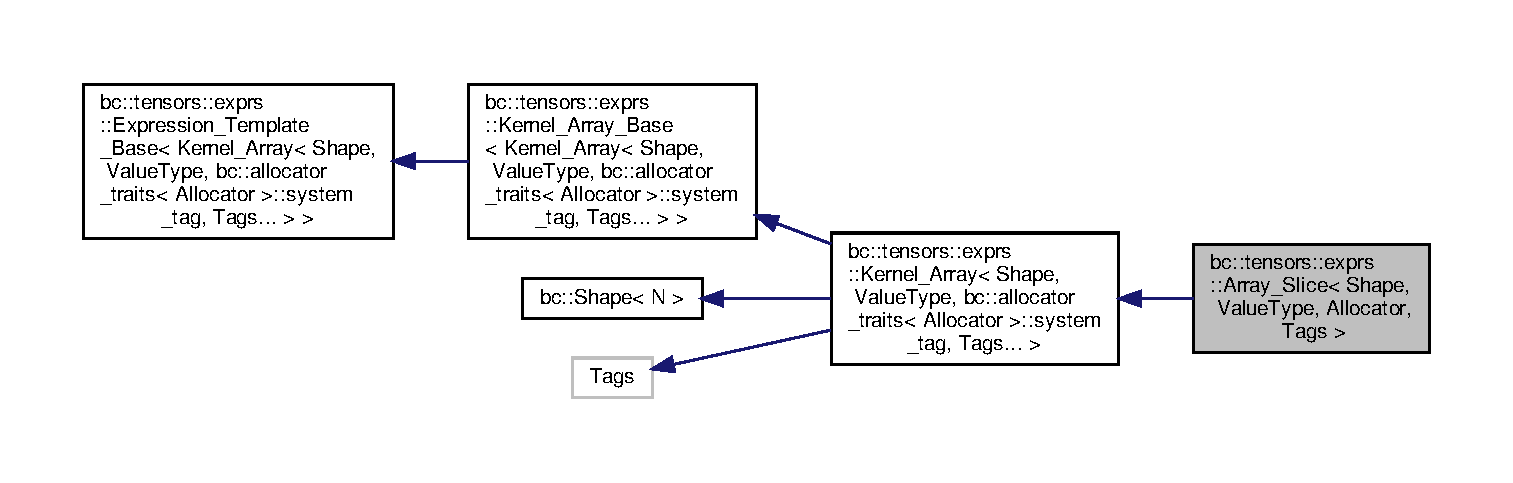
\includegraphics[width=350pt]{classbc_1_1tensors_1_1exprs_1_1Array__Slice__inherit__graph}
\end{center}
\end{figure}


Collaboration diagram for bc\+:\+:tensors\+:\+:exprs\+:\+:Array\+\_\+\+Slice$<$ Shape, Value\+Type, Allocator, Tags $>$\+:\nopagebreak
\begin{figure}[H]
\begin{center}
\leavevmode
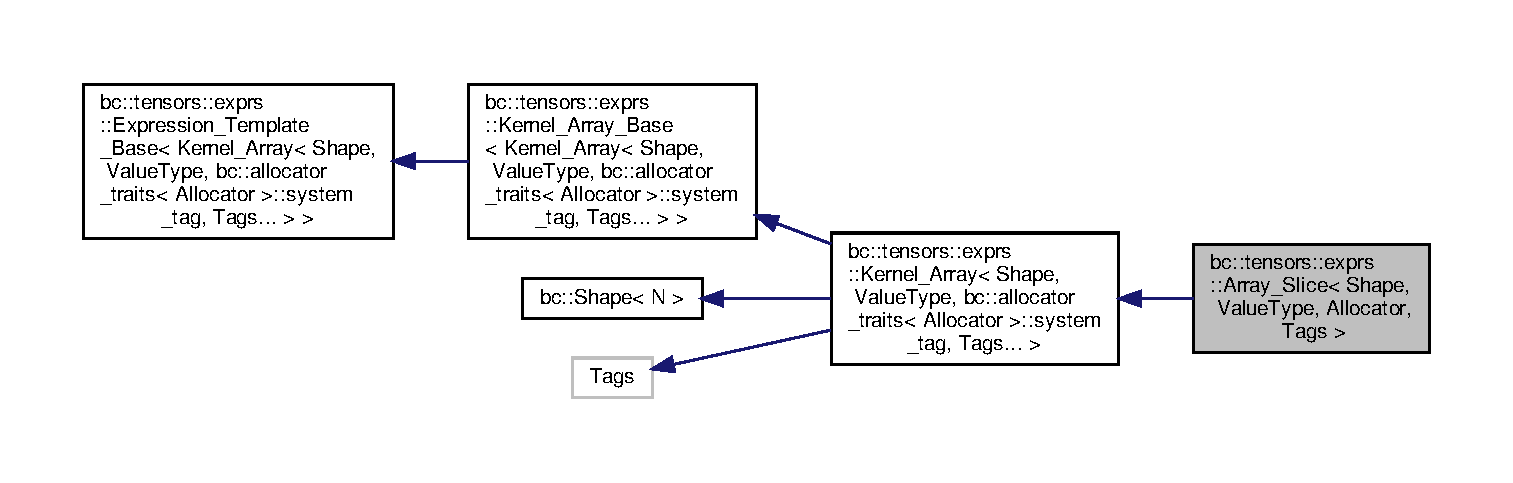
\includegraphics[width=350pt]{classbc_1_1tensors_1_1exprs_1_1Array__Slice__coll__graph}
\end{center}
\end{figure}
\subsection*{Public Types}
\begin{DoxyCompactItemize}
\item 
using \hyperlink{classbc_1_1tensors_1_1exprs_1_1Array__Slice_a24a53456bc1a4bf93b7d37df3fb053fb}{system\+\_\+tag} = typename \hyperlink{structbc_1_1allocators_1_1allocator__traits}{bc\+::allocator\+\_\+traits}$<$ \hyperlink{classbc_1_1allocators_1_1Allocator}{Allocator} $>$\+::\hyperlink{classbc_1_1tensors_1_1exprs_1_1Array__Slice_a24a53456bc1a4bf93b7d37df3fb053fb}{system\+\_\+tag}
\item 
using \hyperlink{classbc_1_1tensors_1_1exprs_1_1Array__Slice_a36743c3a0824cf194998da96bbb95e47}{value\+\_\+type} = Value\+Type
\item 
using \hyperlink{classbc_1_1tensors_1_1exprs_1_1Array__Slice_a54761123998b091676d1b0deef26d376}{allocator\+\_\+type} = \hyperlink{classbc_1_1allocators_1_1Allocator}{Allocator}
\item 
using \hyperlink{classbc_1_1tensors_1_1exprs_1_1Array__Slice_a73ab693dcce17b3bf37747b2e91a2fb2}{stream\+\_\+type} = \hyperlink{classbc_1_1streams_1_1Stream}{bc\+::\+Stream}$<$ \hyperlink{classbc_1_1tensors_1_1exprs_1_1Array__Slice_a24a53456bc1a4bf93b7d37df3fb053fb}{system\+\_\+tag} $>$
\item 
using \hyperlink{classbc_1_1tensors_1_1exprs_1_1Array__Slice_a32cb548eb3216c642a3a1f45e8b44919}{shape\+\_\+type} = \hyperlink{structbc_1_1Shape}{Shape}
\item 
using \hyperlink{classbc_1_1tensors_1_1exprs_1_1Array__Slice_a3cf7241b4d83d7821c9e11ee5c22e570}{move\+\_\+assignable} = std\+::false\+\_\+type
\item 
using \hyperlink{classbc_1_1tensors_1_1exprs_1_1Array__Slice_a508429be1379f64010846460aef9a4bc}{copy\+\_\+assignable} = \hyperlink{namespacebc_1_1traits_a27454511d91930df60d099d9afdf46ff}{bc\+::traits\+::not\+\_\+type}$<$ bc\+::traits\+::sequence\+\_\+contains\+\_\+v$<$ \hyperlink{classbc_1_1tensors_1_1exprs_1_1BC__Const__View}{B\+C\+\_\+\+Const\+\_\+\+View}, Tags... $>$ $>$
\end{DoxyCompactItemize}
\subsection*{Public Member Functions}
\begin{DoxyCompactItemize}
\item 
{\footnotesize template$<$class... Args$>$ }\\\hyperlink{classbc_1_1tensors_1_1exprs_1_1Array__Slice_a3e7c54724b0e53e00ad3f4ece4ead243}{Array\+\_\+\+Slice} (\hyperlink{classbc_1_1tensors_1_1exprs_1_1Array__Slice_a73ab693dcce17b3bf37747b2e91a2fb2}{stream\+\_\+type} stream, \hyperlink{classbc_1_1tensors_1_1exprs_1_1Array__Slice_a54761123998b091676d1b0deef26d376}{allocator\+\_\+type} allocator, Args... args)
\item 
const \hyperlink{classbc_1_1tensors_1_1exprs_1_1Array__Slice_a54761123998b091676d1b0deef26d376}{allocator\+\_\+type} \& \hyperlink{classbc_1_1tensors_1_1exprs_1_1Array__Slice_ab520f10a439cba864b29a6a230533e91}{get\+\_\+allocator} () const
\item 
\hyperlink{classbc_1_1tensors_1_1exprs_1_1Array__Slice_a54761123998b091676d1b0deef26d376}{allocator\+\_\+type} \& \hyperlink{classbc_1_1tensors_1_1exprs_1_1Array__Slice_ac933425cbd4d31a5a717603af289fe70}{get\+\_\+allocator} ()
\item 
const \hyperlink{classbc_1_1tensors_1_1exprs_1_1Array__Slice_a73ab693dcce17b3bf37747b2e91a2fb2}{stream\+\_\+type} \& \hyperlink{classbc_1_1tensors_1_1exprs_1_1Array__Slice_a739a989a4218cc756e1cc60ea9560ecf}{get\+\_\+stream} () const
\item 
\hyperlink{classbc_1_1tensors_1_1exprs_1_1Array__Slice_a73ab693dcce17b3bf37747b2e91a2fb2}{stream\+\_\+type} \& \hyperlink{classbc_1_1tensors_1_1exprs_1_1Array__Slice_a9dda2d0d35e3dbee9d56883ace9256df}{get\+\_\+stream} ()
\end{DoxyCompactItemize}
\subsection*{Additional Inherited Members}


\subsection{Member Typedef Documentation}
\mbox{\Hypertarget{classbc_1_1tensors_1_1exprs_1_1Array__Slice_a54761123998b091676d1b0deef26d376}\label{classbc_1_1tensors_1_1exprs_1_1Array__Slice_a54761123998b091676d1b0deef26d376}} 
\index{bc\+::tensors\+::exprs\+::\+Array\+\_\+\+Slice@{bc\+::tensors\+::exprs\+::\+Array\+\_\+\+Slice}!allocator\+\_\+type@{allocator\+\_\+type}}
\index{allocator\+\_\+type@{allocator\+\_\+type}!bc\+::tensors\+::exprs\+::\+Array\+\_\+\+Slice@{bc\+::tensors\+::exprs\+::\+Array\+\_\+\+Slice}}
\subsubsection{\texorpdfstring{allocator\+\_\+type}{allocator\_type}}
{\footnotesize\ttfamily template$<$class Shape , class Value\+Type , class Allocator , class... Tags$>$ \\
using \hyperlink{classbc_1_1tensors_1_1exprs_1_1Array__Slice}{bc\+::tensors\+::exprs\+::\+Array\+\_\+\+Slice}$<$ \hyperlink{structbc_1_1Shape}{Shape}, Value\+Type, \hyperlink{classbc_1_1allocators_1_1Allocator}{Allocator}, Tags $>$\+::\hyperlink{classbc_1_1tensors_1_1exprs_1_1Array__Slice_a54761123998b091676d1b0deef26d376}{allocator\+\_\+type} =  \hyperlink{classbc_1_1allocators_1_1Allocator}{Allocator}}

\mbox{\Hypertarget{classbc_1_1tensors_1_1exprs_1_1Array__Slice_a508429be1379f64010846460aef9a4bc}\label{classbc_1_1tensors_1_1exprs_1_1Array__Slice_a508429be1379f64010846460aef9a4bc}} 
\index{bc\+::tensors\+::exprs\+::\+Array\+\_\+\+Slice@{bc\+::tensors\+::exprs\+::\+Array\+\_\+\+Slice}!copy\+\_\+assignable@{copy\+\_\+assignable}}
\index{copy\+\_\+assignable@{copy\+\_\+assignable}!bc\+::tensors\+::exprs\+::\+Array\+\_\+\+Slice@{bc\+::tensors\+::exprs\+::\+Array\+\_\+\+Slice}}
\subsubsection{\texorpdfstring{copy\+\_\+assignable}{copy\_assignable}}
{\footnotesize\ttfamily template$<$class Shape , class Value\+Type , class Allocator , class... Tags$>$ \\
using \hyperlink{classbc_1_1tensors_1_1exprs_1_1Array__Slice}{bc\+::tensors\+::exprs\+::\+Array\+\_\+\+Slice}$<$ \hyperlink{structbc_1_1Shape}{Shape}, Value\+Type, \hyperlink{classbc_1_1allocators_1_1Allocator}{Allocator}, Tags $>$\+::\hyperlink{classbc_1_1tensors_1_1exprs_1_1Array__Slice_a508429be1379f64010846460aef9a4bc}{copy\+\_\+assignable} =  \hyperlink{namespacebc_1_1traits_a27454511d91930df60d099d9afdf46ff}{bc\+::traits\+::not\+\_\+type}$<$bc\+::traits\+::sequence\+\_\+contains\+\_\+v$<$\hyperlink{classbc_1_1tensors_1_1exprs_1_1BC__Const__View}{B\+C\+\_\+\+Const\+\_\+\+View}, Tags...$>$ $>$}

\mbox{\Hypertarget{classbc_1_1tensors_1_1exprs_1_1Array__Slice_a3cf7241b4d83d7821c9e11ee5c22e570}\label{classbc_1_1tensors_1_1exprs_1_1Array__Slice_a3cf7241b4d83d7821c9e11ee5c22e570}} 
\index{bc\+::tensors\+::exprs\+::\+Array\+\_\+\+Slice@{bc\+::tensors\+::exprs\+::\+Array\+\_\+\+Slice}!move\+\_\+assignable@{move\+\_\+assignable}}
\index{move\+\_\+assignable@{move\+\_\+assignable}!bc\+::tensors\+::exprs\+::\+Array\+\_\+\+Slice@{bc\+::tensors\+::exprs\+::\+Array\+\_\+\+Slice}}
\subsubsection{\texorpdfstring{move\+\_\+assignable}{move\_assignable}}
{\footnotesize\ttfamily template$<$class Shape , class Value\+Type , class Allocator , class... Tags$>$ \\
using \hyperlink{classbc_1_1tensors_1_1exprs_1_1Array__Slice}{bc\+::tensors\+::exprs\+::\+Array\+\_\+\+Slice}$<$ \hyperlink{structbc_1_1Shape}{Shape}, Value\+Type, \hyperlink{classbc_1_1allocators_1_1Allocator}{Allocator}, Tags $>$\+::\hyperlink{classbc_1_1tensors_1_1exprs_1_1Array__Slice_a3cf7241b4d83d7821c9e11ee5c22e570}{move\+\_\+assignable} =  std\+::false\+\_\+type}

\mbox{\Hypertarget{classbc_1_1tensors_1_1exprs_1_1Array__Slice_a32cb548eb3216c642a3a1f45e8b44919}\label{classbc_1_1tensors_1_1exprs_1_1Array__Slice_a32cb548eb3216c642a3a1f45e8b44919}} 
\index{bc\+::tensors\+::exprs\+::\+Array\+\_\+\+Slice@{bc\+::tensors\+::exprs\+::\+Array\+\_\+\+Slice}!shape\+\_\+type@{shape\+\_\+type}}
\index{shape\+\_\+type@{shape\+\_\+type}!bc\+::tensors\+::exprs\+::\+Array\+\_\+\+Slice@{bc\+::tensors\+::exprs\+::\+Array\+\_\+\+Slice}}
\subsubsection{\texorpdfstring{shape\+\_\+type}{shape\_type}}
{\footnotesize\ttfamily template$<$class Shape , class Value\+Type , class Allocator , class... Tags$>$ \\
using \hyperlink{classbc_1_1tensors_1_1exprs_1_1Array__Slice}{bc\+::tensors\+::exprs\+::\+Array\+\_\+\+Slice}$<$ \hyperlink{structbc_1_1Shape}{Shape}, Value\+Type, \hyperlink{classbc_1_1allocators_1_1Allocator}{Allocator}, Tags $>$\+::\hyperlink{classbc_1_1tensors_1_1exprs_1_1Array__Slice_a32cb548eb3216c642a3a1f45e8b44919}{shape\+\_\+type} =  \hyperlink{structbc_1_1Shape}{Shape}}

\mbox{\Hypertarget{classbc_1_1tensors_1_1exprs_1_1Array__Slice_a73ab693dcce17b3bf37747b2e91a2fb2}\label{classbc_1_1tensors_1_1exprs_1_1Array__Slice_a73ab693dcce17b3bf37747b2e91a2fb2}} 
\index{bc\+::tensors\+::exprs\+::\+Array\+\_\+\+Slice@{bc\+::tensors\+::exprs\+::\+Array\+\_\+\+Slice}!stream\+\_\+type@{stream\+\_\+type}}
\index{stream\+\_\+type@{stream\+\_\+type}!bc\+::tensors\+::exprs\+::\+Array\+\_\+\+Slice@{bc\+::tensors\+::exprs\+::\+Array\+\_\+\+Slice}}
\subsubsection{\texorpdfstring{stream\+\_\+type}{stream\_type}}
{\footnotesize\ttfamily template$<$class Shape , class Value\+Type , class Allocator , class... Tags$>$ \\
using \hyperlink{classbc_1_1tensors_1_1exprs_1_1Array__Slice}{bc\+::tensors\+::exprs\+::\+Array\+\_\+\+Slice}$<$ \hyperlink{structbc_1_1Shape}{Shape}, Value\+Type, \hyperlink{classbc_1_1allocators_1_1Allocator}{Allocator}, Tags $>$\+::\hyperlink{classbc_1_1tensors_1_1exprs_1_1Array__Slice_a73ab693dcce17b3bf37747b2e91a2fb2}{stream\+\_\+type} =  \hyperlink{classbc_1_1streams_1_1Stream}{bc\+::\+Stream}$<$\hyperlink{classbc_1_1tensors_1_1exprs_1_1Array__Slice_a24a53456bc1a4bf93b7d37df3fb053fb}{system\+\_\+tag}$>$}

\mbox{\Hypertarget{classbc_1_1tensors_1_1exprs_1_1Array__Slice_a24a53456bc1a4bf93b7d37df3fb053fb}\label{classbc_1_1tensors_1_1exprs_1_1Array__Slice_a24a53456bc1a4bf93b7d37df3fb053fb}} 
\index{bc\+::tensors\+::exprs\+::\+Array\+\_\+\+Slice@{bc\+::tensors\+::exprs\+::\+Array\+\_\+\+Slice}!system\+\_\+tag@{system\+\_\+tag}}
\index{system\+\_\+tag@{system\+\_\+tag}!bc\+::tensors\+::exprs\+::\+Array\+\_\+\+Slice@{bc\+::tensors\+::exprs\+::\+Array\+\_\+\+Slice}}
\subsubsection{\texorpdfstring{system\+\_\+tag}{system\_tag}}
{\footnotesize\ttfamily template$<$class Shape , class Value\+Type , class Allocator , class... Tags$>$ \\
using \hyperlink{classbc_1_1tensors_1_1exprs_1_1Array__Slice}{bc\+::tensors\+::exprs\+::\+Array\+\_\+\+Slice}$<$ \hyperlink{structbc_1_1Shape}{Shape}, Value\+Type, \hyperlink{classbc_1_1allocators_1_1Allocator}{Allocator}, Tags $>$\+::\hyperlink{classbc_1_1tensors_1_1exprs_1_1Array__Slice_a24a53456bc1a4bf93b7d37df3fb053fb}{system\+\_\+tag} =  typename \hyperlink{structbc_1_1allocators_1_1allocator__traits}{bc\+::allocator\+\_\+traits}$<$\hyperlink{classbc_1_1allocators_1_1Allocator}{Allocator}$>$\+::\hyperlink{classbc_1_1tensors_1_1exprs_1_1Array__Slice_a24a53456bc1a4bf93b7d37df3fb053fb}{system\+\_\+tag}}

\mbox{\Hypertarget{classbc_1_1tensors_1_1exprs_1_1Array__Slice_a36743c3a0824cf194998da96bbb95e47}\label{classbc_1_1tensors_1_1exprs_1_1Array__Slice_a36743c3a0824cf194998da96bbb95e47}} 
\index{bc\+::tensors\+::exprs\+::\+Array\+\_\+\+Slice@{bc\+::tensors\+::exprs\+::\+Array\+\_\+\+Slice}!value\+\_\+type@{value\+\_\+type}}
\index{value\+\_\+type@{value\+\_\+type}!bc\+::tensors\+::exprs\+::\+Array\+\_\+\+Slice@{bc\+::tensors\+::exprs\+::\+Array\+\_\+\+Slice}}
\subsubsection{\texorpdfstring{value\+\_\+type}{value\_type}}
{\footnotesize\ttfamily template$<$class Shape , class Value\+Type , class Allocator , class... Tags$>$ \\
using \hyperlink{classbc_1_1tensors_1_1exprs_1_1Array__Slice}{bc\+::tensors\+::exprs\+::\+Array\+\_\+\+Slice}$<$ \hyperlink{structbc_1_1Shape}{Shape}, Value\+Type, \hyperlink{classbc_1_1allocators_1_1Allocator}{Allocator}, Tags $>$\+::\hyperlink{classbc_1_1tensors_1_1exprs_1_1Array__Slice_a36743c3a0824cf194998da96bbb95e47}{value\+\_\+type} =  Value\+Type}



\subsection{Constructor \& Destructor Documentation}
\mbox{\Hypertarget{classbc_1_1tensors_1_1exprs_1_1Array__Slice_a3e7c54724b0e53e00ad3f4ece4ead243}\label{classbc_1_1tensors_1_1exprs_1_1Array__Slice_a3e7c54724b0e53e00ad3f4ece4ead243}} 
\index{bc\+::tensors\+::exprs\+::\+Array\+\_\+\+Slice@{bc\+::tensors\+::exprs\+::\+Array\+\_\+\+Slice}!Array\+\_\+\+Slice@{Array\+\_\+\+Slice}}
\index{Array\+\_\+\+Slice@{Array\+\_\+\+Slice}!bc\+::tensors\+::exprs\+::\+Array\+\_\+\+Slice@{bc\+::tensors\+::exprs\+::\+Array\+\_\+\+Slice}}
\subsubsection{\texorpdfstring{Array\+\_\+\+Slice()}{Array\_Slice()}}
{\footnotesize\ttfamily template$<$class Shape , class Value\+Type , class Allocator , class... Tags$>$ \\
template$<$class... Args$>$ \\
\hyperlink{classbc_1_1tensors_1_1exprs_1_1Array__Slice}{bc\+::tensors\+::exprs\+::\+Array\+\_\+\+Slice}$<$ \hyperlink{structbc_1_1Shape}{Shape}, Value\+Type, \hyperlink{classbc_1_1allocators_1_1Allocator}{Allocator}, Tags $>$\+::\hyperlink{classbc_1_1tensors_1_1exprs_1_1Array__Slice}{Array\+\_\+\+Slice} (\begin{DoxyParamCaption}\item[{\hyperlink{classbc_1_1tensors_1_1exprs_1_1Array__Slice_a73ab693dcce17b3bf37747b2e91a2fb2}{stream\+\_\+type}}]{stream,  }\item[{\hyperlink{classbc_1_1tensors_1_1exprs_1_1Array__Slice_a54761123998b091676d1b0deef26d376}{allocator\+\_\+type}}]{allocator,  }\item[{Args...}]{args }\end{DoxyParamCaption})\hspace{0.3cm}{\ttfamily [inline]}}



\subsection{Member Function Documentation}
\mbox{\Hypertarget{classbc_1_1tensors_1_1exprs_1_1Array__Slice_ab520f10a439cba864b29a6a230533e91}\label{classbc_1_1tensors_1_1exprs_1_1Array__Slice_ab520f10a439cba864b29a6a230533e91}} 
\index{bc\+::tensors\+::exprs\+::\+Array\+\_\+\+Slice@{bc\+::tensors\+::exprs\+::\+Array\+\_\+\+Slice}!get\+\_\+allocator@{get\+\_\+allocator}}
\index{get\+\_\+allocator@{get\+\_\+allocator}!bc\+::tensors\+::exprs\+::\+Array\+\_\+\+Slice@{bc\+::tensors\+::exprs\+::\+Array\+\_\+\+Slice}}
\subsubsection{\texorpdfstring{get\+\_\+allocator()}{get\_allocator()}\hspace{0.1cm}{\footnotesize\ttfamily [1/2]}}
{\footnotesize\ttfamily template$<$class Shape , class Value\+Type , class Allocator , class... Tags$>$ \\
const \hyperlink{classbc_1_1tensors_1_1exprs_1_1Array__Slice_a54761123998b091676d1b0deef26d376}{allocator\+\_\+type}\& \hyperlink{classbc_1_1tensors_1_1exprs_1_1Array__Slice}{bc\+::tensors\+::exprs\+::\+Array\+\_\+\+Slice}$<$ \hyperlink{structbc_1_1Shape}{Shape}, Value\+Type, \hyperlink{classbc_1_1allocators_1_1Allocator}{Allocator}, Tags $>$\+::get\+\_\+allocator (\begin{DoxyParamCaption}{ }\end{DoxyParamCaption}) const\hspace{0.3cm}{\ttfamily [inline]}}

\mbox{\Hypertarget{classbc_1_1tensors_1_1exprs_1_1Array__Slice_ac933425cbd4d31a5a717603af289fe70}\label{classbc_1_1tensors_1_1exprs_1_1Array__Slice_ac933425cbd4d31a5a717603af289fe70}} 
\index{bc\+::tensors\+::exprs\+::\+Array\+\_\+\+Slice@{bc\+::tensors\+::exprs\+::\+Array\+\_\+\+Slice}!get\+\_\+allocator@{get\+\_\+allocator}}
\index{get\+\_\+allocator@{get\+\_\+allocator}!bc\+::tensors\+::exprs\+::\+Array\+\_\+\+Slice@{bc\+::tensors\+::exprs\+::\+Array\+\_\+\+Slice}}
\subsubsection{\texorpdfstring{get\+\_\+allocator()}{get\_allocator()}\hspace{0.1cm}{\footnotesize\ttfamily [2/2]}}
{\footnotesize\ttfamily template$<$class Shape , class Value\+Type , class Allocator , class... Tags$>$ \\
\hyperlink{classbc_1_1tensors_1_1exprs_1_1Array__Slice_a54761123998b091676d1b0deef26d376}{allocator\+\_\+type}\& \hyperlink{classbc_1_1tensors_1_1exprs_1_1Array__Slice}{bc\+::tensors\+::exprs\+::\+Array\+\_\+\+Slice}$<$ \hyperlink{structbc_1_1Shape}{Shape}, Value\+Type, \hyperlink{classbc_1_1allocators_1_1Allocator}{Allocator}, Tags $>$\+::get\+\_\+allocator (\begin{DoxyParamCaption}{ }\end{DoxyParamCaption})\hspace{0.3cm}{\ttfamily [inline]}}

\mbox{\Hypertarget{classbc_1_1tensors_1_1exprs_1_1Array__Slice_a739a989a4218cc756e1cc60ea9560ecf}\label{classbc_1_1tensors_1_1exprs_1_1Array__Slice_a739a989a4218cc756e1cc60ea9560ecf}} 
\index{bc\+::tensors\+::exprs\+::\+Array\+\_\+\+Slice@{bc\+::tensors\+::exprs\+::\+Array\+\_\+\+Slice}!get\+\_\+stream@{get\+\_\+stream}}
\index{get\+\_\+stream@{get\+\_\+stream}!bc\+::tensors\+::exprs\+::\+Array\+\_\+\+Slice@{bc\+::tensors\+::exprs\+::\+Array\+\_\+\+Slice}}
\subsubsection{\texorpdfstring{get\+\_\+stream()}{get\_stream()}\hspace{0.1cm}{\footnotesize\ttfamily [1/2]}}
{\footnotesize\ttfamily template$<$class Shape , class Value\+Type , class Allocator , class... Tags$>$ \\
const \hyperlink{classbc_1_1tensors_1_1exprs_1_1Array__Slice_a73ab693dcce17b3bf37747b2e91a2fb2}{stream\+\_\+type}\& \hyperlink{classbc_1_1tensors_1_1exprs_1_1Array__Slice}{bc\+::tensors\+::exprs\+::\+Array\+\_\+\+Slice}$<$ \hyperlink{structbc_1_1Shape}{Shape}, Value\+Type, \hyperlink{classbc_1_1allocators_1_1Allocator}{Allocator}, Tags $>$\+::get\+\_\+stream (\begin{DoxyParamCaption}{ }\end{DoxyParamCaption}) const\hspace{0.3cm}{\ttfamily [inline]}}

\mbox{\Hypertarget{classbc_1_1tensors_1_1exprs_1_1Array__Slice_a9dda2d0d35e3dbee9d56883ace9256df}\label{classbc_1_1tensors_1_1exprs_1_1Array__Slice_a9dda2d0d35e3dbee9d56883ace9256df}} 
\index{bc\+::tensors\+::exprs\+::\+Array\+\_\+\+Slice@{bc\+::tensors\+::exprs\+::\+Array\+\_\+\+Slice}!get\+\_\+stream@{get\+\_\+stream}}
\index{get\+\_\+stream@{get\+\_\+stream}!bc\+::tensors\+::exprs\+::\+Array\+\_\+\+Slice@{bc\+::tensors\+::exprs\+::\+Array\+\_\+\+Slice}}
\subsubsection{\texorpdfstring{get\+\_\+stream()}{get\_stream()}\hspace{0.1cm}{\footnotesize\ttfamily [2/2]}}
{\footnotesize\ttfamily template$<$class Shape , class Value\+Type , class Allocator , class... Tags$>$ \\
\hyperlink{classbc_1_1tensors_1_1exprs_1_1Array__Slice_a73ab693dcce17b3bf37747b2e91a2fb2}{stream\+\_\+type}\& \hyperlink{classbc_1_1tensors_1_1exprs_1_1Array__Slice}{bc\+::tensors\+::exprs\+::\+Array\+\_\+\+Slice}$<$ \hyperlink{structbc_1_1Shape}{Shape}, Value\+Type, \hyperlink{classbc_1_1allocators_1_1Allocator}{Allocator}, Tags $>$\+::get\+\_\+stream (\begin{DoxyParamCaption}{ }\end{DoxyParamCaption})\hspace{0.3cm}{\ttfamily [inline]}}



The documentation for this struct was generated from the following files\+:\begin{DoxyCompactItemize}
\item 
blackcat/tensors/expression\+\_\+templates/\hyperlink{array_8h}{array.\+h}\item 
blackcat/tensors/expression\+\_\+templates/\hyperlink{array__slice_8h}{array\+\_\+slice.\+h}\end{DoxyCompactItemize}

\hypertarget{structbc_1_1oper_1_1cmath__functions_1_1Asin}{}\section{bc\+:\+:oper\+:\+:cmath\+\_\+functions\+:\+:Asin Struct Reference}
\label{structbc_1_1oper_1_1cmath__functions_1_1Asin}\index{bc\+::oper\+::cmath\+\_\+functions\+::\+Asin@{bc\+::oper\+::cmath\+\_\+functions\+::\+Asin}}


{\ttfamily \#include $<$cmath.\+h$>$}



Collaboration diagram for bc\+:\+:oper\+:\+:cmath\+\_\+functions\+:\+:Asin\+:\nopagebreak
\begin{figure}[H]
\begin{center}
\leavevmode
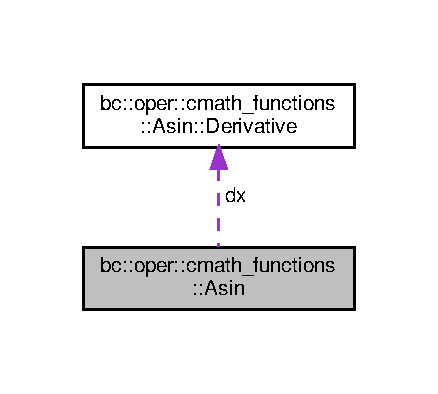
\includegraphics[width=210pt]{structbc_1_1oper_1_1cmath__functions_1_1Asin__coll__graph}
\end{center}
\end{figure}
\subsection*{Classes}
\begin{DoxyCompactItemize}
\item 
struct \hyperlink{structbc_1_1oper_1_1cmath__functions_1_1Asin_1_1Derivative}{Derivative}
\end{DoxyCompactItemize}
\subsection*{Public Member Functions}
\begin{DoxyCompactItemize}
\item 
{\footnotesize template$<$class value\+\_\+type $>$ }\\\hyperlink{common_8h_a6699e8b0449da5c0fafb878e59c1d4b1}{B\+C\+I\+N\+L\+I\+NE} value\+\_\+type \hyperlink{structbc_1_1oper_1_1cmath__functions_1_1Asin_af8ec5551f6ea246e1803a729d3310f0c}{operator()} (const value\+\_\+type \&x) const
\item 
{\footnotesize template$<$class Xpr $>$ }\\auto \hyperlink{structbc_1_1oper_1_1cmath__functions_1_1Asin_a2f20510e74c4dd76adf0c75d86689517}{operator()} (const \hyperlink{classbc_1_1tensors_1_1Expression__Base}{bc\+::tensors\+::\+Expression\+\_\+\+Base}$<$ Xpr $>$ \&tensor)
\item 
{\footnotesize template$<$class Xpr $>$ }\\auto \hyperlink{structbc_1_1oper_1_1cmath__functions_1_1Asin_afcfcf86668a54b5dc378476750c9f0da}{operator()} (const \hyperlink{classbc_1_1tensors_1_1Tensor__Base}{bc\+::tensors\+::\+Tensor\+\_\+\+Base}$<$ Xpr $>$ \&tensor)
\end{DoxyCompactItemize}
\subsection*{Static Public Member Functions}
\begin{DoxyCompactItemize}
\item 
{\footnotesize template$<$class value\+\_\+type $>$ }\\static \hyperlink{common_8h_a6699e8b0449da5c0fafb878e59c1d4b1}{B\+C\+I\+N\+L\+I\+NE} auto \hyperlink{structbc_1_1oper_1_1cmath__functions_1_1Asin_adca0c674125baa73bb2445c35b353e45}{apply} (const value\+\_\+type \&x)
\end{DoxyCompactItemize}
\subsection*{Public Attributes}
\begin{DoxyCompactItemize}
\item 
struct \hyperlink{structbc_1_1oper_1_1cmath__functions_1_1Asin_1_1Derivative}{bc\+::oper\+::cmath\+\_\+functions\+::\+Asin\+::\+Derivative} \hyperlink{structbc_1_1oper_1_1cmath__functions_1_1Asin_abcdbbb996217835499d48d5c64ea5a06}{dx}
\end{DoxyCompactItemize}


\subsection{Member Function Documentation}
\mbox{\Hypertarget{structbc_1_1oper_1_1cmath__functions_1_1Asin_adca0c674125baa73bb2445c35b353e45}\label{structbc_1_1oper_1_1cmath__functions_1_1Asin_adca0c674125baa73bb2445c35b353e45}} 
\index{bc\+::oper\+::cmath\+\_\+functions\+::\+Asin@{bc\+::oper\+::cmath\+\_\+functions\+::\+Asin}!apply@{apply}}
\index{apply@{apply}!bc\+::oper\+::cmath\+\_\+functions\+::\+Asin@{bc\+::oper\+::cmath\+\_\+functions\+::\+Asin}}
\subsubsection{\texorpdfstring{apply()}{apply()}}
{\footnotesize\ttfamily template$<$class value\+\_\+type $>$ \\
static \hyperlink{common_8h_a6699e8b0449da5c0fafb878e59c1d4b1}{B\+C\+I\+N\+L\+I\+NE} auto bc\+::oper\+::cmath\+\_\+functions\+::\+Asin\+::apply (\begin{DoxyParamCaption}\item[{const value\+\_\+type \&}]{x }\end{DoxyParamCaption})\hspace{0.3cm}{\ttfamily [inline]}, {\ttfamily [static]}}

\mbox{\Hypertarget{structbc_1_1oper_1_1cmath__functions_1_1Asin_afcfcf86668a54b5dc378476750c9f0da}\label{structbc_1_1oper_1_1cmath__functions_1_1Asin_afcfcf86668a54b5dc378476750c9f0da}} 
\index{bc\+::oper\+::cmath\+\_\+functions\+::\+Asin@{bc\+::oper\+::cmath\+\_\+functions\+::\+Asin}!operator()@{operator()}}
\index{operator()@{operator()}!bc\+::oper\+::cmath\+\_\+functions\+::\+Asin@{bc\+::oper\+::cmath\+\_\+functions\+::\+Asin}}
\subsubsection{\texorpdfstring{operator()()}{operator()()}\hspace{0.1cm}{\footnotesize\ttfamily [1/3]}}
{\footnotesize\ttfamily template$<$class Xpr $>$ \\
auto bc\+::oper\+::cmath\+\_\+functions\+::\+Asin\+::operator() (\begin{DoxyParamCaption}\item[{const \hyperlink{classbc_1_1tensors_1_1Tensor__Base}{bc\+::tensors\+::\+Tensor\+\_\+\+Base}$<$ Xpr $>$ \&}]{tensor }\end{DoxyParamCaption})\hspace{0.3cm}{\ttfamily [inline]}}

\mbox{\Hypertarget{structbc_1_1oper_1_1cmath__functions_1_1Asin_a2f20510e74c4dd76adf0c75d86689517}\label{structbc_1_1oper_1_1cmath__functions_1_1Asin_a2f20510e74c4dd76adf0c75d86689517}} 
\index{bc\+::oper\+::cmath\+\_\+functions\+::\+Asin@{bc\+::oper\+::cmath\+\_\+functions\+::\+Asin}!operator()@{operator()}}
\index{operator()@{operator()}!bc\+::oper\+::cmath\+\_\+functions\+::\+Asin@{bc\+::oper\+::cmath\+\_\+functions\+::\+Asin}}
\subsubsection{\texorpdfstring{operator()()}{operator()()}\hspace{0.1cm}{\footnotesize\ttfamily [2/3]}}
{\footnotesize\ttfamily template$<$class Xpr $>$ \\
auto bc\+::oper\+::cmath\+\_\+functions\+::\+Asin\+::operator() (\begin{DoxyParamCaption}\item[{const \hyperlink{classbc_1_1tensors_1_1Expression__Base}{bc\+::tensors\+::\+Expression\+\_\+\+Base}$<$ Xpr $>$ \&}]{tensor }\end{DoxyParamCaption})\hspace{0.3cm}{\ttfamily [inline]}}

\mbox{\Hypertarget{structbc_1_1oper_1_1cmath__functions_1_1Asin_af8ec5551f6ea246e1803a729d3310f0c}\label{structbc_1_1oper_1_1cmath__functions_1_1Asin_af8ec5551f6ea246e1803a729d3310f0c}} 
\index{bc\+::oper\+::cmath\+\_\+functions\+::\+Asin@{bc\+::oper\+::cmath\+\_\+functions\+::\+Asin}!operator()@{operator()}}
\index{operator()@{operator()}!bc\+::oper\+::cmath\+\_\+functions\+::\+Asin@{bc\+::oper\+::cmath\+\_\+functions\+::\+Asin}}
\subsubsection{\texorpdfstring{operator()()}{operator()()}\hspace{0.1cm}{\footnotesize\ttfamily [3/3]}}
{\footnotesize\ttfamily template$<$class value\+\_\+type $>$ \\
\hyperlink{common_8h_a6699e8b0449da5c0fafb878e59c1d4b1}{B\+C\+I\+N\+L\+I\+NE} value\+\_\+type bc\+::oper\+::cmath\+\_\+functions\+::\+Asin\+::operator() (\begin{DoxyParamCaption}\item[{const value\+\_\+type \&}]{x }\end{DoxyParamCaption}) const\hspace{0.3cm}{\ttfamily [inline]}}



\subsection{Member Data Documentation}
\mbox{\Hypertarget{structbc_1_1oper_1_1cmath__functions_1_1Asin_abcdbbb996217835499d48d5c64ea5a06}\label{structbc_1_1oper_1_1cmath__functions_1_1Asin_abcdbbb996217835499d48d5c64ea5a06}} 
\index{bc\+::oper\+::cmath\+\_\+functions\+::\+Asin@{bc\+::oper\+::cmath\+\_\+functions\+::\+Asin}!dx@{dx}}
\index{dx@{dx}!bc\+::oper\+::cmath\+\_\+functions\+::\+Asin@{bc\+::oper\+::cmath\+\_\+functions\+::\+Asin}}
\subsubsection{\texorpdfstring{dx}{dx}}
{\footnotesize\ttfamily struct \hyperlink{structbc_1_1oper_1_1cmath__functions_1_1Asin_1_1Derivative}{bc\+::oper\+::cmath\+\_\+functions\+::\+Asin\+::\+Derivative}   bc\+::oper\+::cmath\+\_\+functions\+::\+Asin\+::dx}



The documentation for this struct was generated from the following file\+:\begin{DoxyCompactItemize}
\item 
blackcat/operations/\hyperlink{cmath_8h}{cmath.\+h}\end{DoxyCompactItemize}

\hypertarget{structbc_1_1oper_1_1cmath__functions_1_1Asinh}{}\section{bc\+:\+:oper\+:\+:cmath\+\_\+functions\+:\+:Asinh Struct Reference}
\label{structbc_1_1oper_1_1cmath__functions_1_1Asinh}\index{bc\+::oper\+::cmath\+\_\+functions\+::\+Asinh@{bc\+::oper\+::cmath\+\_\+functions\+::\+Asinh}}


{\ttfamily \#include $<$cmath.\+h$>$}

\subsection*{Public Member Functions}
\begin{DoxyCompactItemize}
\item 
{\footnotesize template$<$class value\+\_\+type $>$ }\\\hyperlink{common_8h_a6699e8b0449da5c0fafb878e59c1d4b1}{B\+C\+I\+N\+L\+I\+NE} value\+\_\+type \hyperlink{structbc_1_1oper_1_1cmath__functions_1_1Asinh_ab6227d0033e0c9c447e17e8bfa4093d5}{operator()} (const value\+\_\+type \&x) const
\item 
{\footnotesize template$<$class Xpr $>$ }\\auto \hyperlink{structbc_1_1oper_1_1cmath__functions_1_1Asinh_af1edd2d7145261551a34401ec4a6c14d}{operator()} (const \hyperlink{classbc_1_1tensors_1_1Expression__Base}{bc\+::tensors\+::\+Expression\+\_\+\+Base}$<$ Xpr $>$ \&tensor)
\item 
{\footnotesize template$<$class Xpr $>$ }\\auto \hyperlink{structbc_1_1oper_1_1cmath__functions_1_1Asinh_aa88f33581a4f1bc627091ff9e06fbc02}{operator()} (const \hyperlink{classbc_1_1tensors_1_1Tensor__Base}{bc\+::tensors\+::\+Tensor\+\_\+\+Base}$<$ Xpr $>$ \&tensor)
\end{DoxyCompactItemize}
\subsection*{Static Public Member Functions}
\begin{DoxyCompactItemize}
\item 
{\footnotesize template$<$class value\+\_\+type $>$ }\\static \hyperlink{common_8h_a6699e8b0449da5c0fafb878e59c1d4b1}{B\+C\+I\+N\+L\+I\+NE} auto \hyperlink{structbc_1_1oper_1_1cmath__functions_1_1Asinh_ab65c46cf8a69539fff1a71b9ec1f4e8a}{apply} (const value\+\_\+type \&x)
\end{DoxyCompactItemize}


\subsection{Member Function Documentation}
\mbox{\Hypertarget{structbc_1_1oper_1_1cmath__functions_1_1Asinh_ab65c46cf8a69539fff1a71b9ec1f4e8a}\label{structbc_1_1oper_1_1cmath__functions_1_1Asinh_ab65c46cf8a69539fff1a71b9ec1f4e8a}} 
\index{bc\+::oper\+::cmath\+\_\+functions\+::\+Asinh@{bc\+::oper\+::cmath\+\_\+functions\+::\+Asinh}!apply@{apply}}
\index{apply@{apply}!bc\+::oper\+::cmath\+\_\+functions\+::\+Asinh@{bc\+::oper\+::cmath\+\_\+functions\+::\+Asinh}}
\subsubsection{\texorpdfstring{apply()}{apply()}}
{\footnotesize\ttfamily template$<$class value\+\_\+type $>$ \\
static \hyperlink{common_8h_a6699e8b0449da5c0fafb878e59c1d4b1}{B\+C\+I\+N\+L\+I\+NE} auto bc\+::oper\+::cmath\+\_\+functions\+::\+Asinh\+::apply (\begin{DoxyParamCaption}\item[{const value\+\_\+type \&}]{x }\end{DoxyParamCaption})\hspace{0.3cm}{\ttfamily [inline]}, {\ttfamily [static]}}

\mbox{\Hypertarget{structbc_1_1oper_1_1cmath__functions_1_1Asinh_aa88f33581a4f1bc627091ff9e06fbc02}\label{structbc_1_1oper_1_1cmath__functions_1_1Asinh_aa88f33581a4f1bc627091ff9e06fbc02}} 
\index{bc\+::oper\+::cmath\+\_\+functions\+::\+Asinh@{bc\+::oper\+::cmath\+\_\+functions\+::\+Asinh}!operator()@{operator()}}
\index{operator()@{operator()}!bc\+::oper\+::cmath\+\_\+functions\+::\+Asinh@{bc\+::oper\+::cmath\+\_\+functions\+::\+Asinh}}
\subsubsection{\texorpdfstring{operator()()}{operator()()}\hspace{0.1cm}{\footnotesize\ttfamily [1/3]}}
{\footnotesize\ttfamily template$<$class Xpr $>$ \\
auto bc\+::oper\+::cmath\+\_\+functions\+::\+Asinh\+::operator() (\begin{DoxyParamCaption}\item[{const \hyperlink{classbc_1_1tensors_1_1Tensor__Base}{bc\+::tensors\+::\+Tensor\+\_\+\+Base}$<$ Xpr $>$ \&}]{tensor }\end{DoxyParamCaption})\hspace{0.3cm}{\ttfamily [inline]}}

\mbox{\Hypertarget{structbc_1_1oper_1_1cmath__functions_1_1Asinh_af1edd2d7145261551a34401ec4a6c14d}\label{structbc_1_1oper_1_1cmath__functions_1_1Asinh_af1edd2d7145261551a34401ec4a6c14d}} 
\index{bc\+::oper\+::cmath\+\_\+functions\+::\+Asinh@{bc\+::oper\+::cmath\+\_\+functions\+::\+Asinh}!operator()@{operator()}}
\index{operator()@{operator()}!bc\+::oper\+::cmath\+\_\+functions\+::\+Asinh@{bc\+::oper\+::cmath\+\_\+functions\+::\+Asinh}}
\subsubsection{\texorpdfstring{operator()()}{operator()()}\hspace{0.1cm}{\footnotesize\ttfamily [2/3]}}
{\footnotesize\ttfamily template$<$class Xpr $>$ \\
auto bc\+::oper\+::cmath\+\_\+functions\+::\+Asinh\+::operator() (\begin{DoxyParamCaption}\item[{const \hyperlink{classbc_1_1tensors_1_1Expression__Base}{bc\+::tensors\+::\+Expression\+\_\+\+Base}$<$ Xpr $>$ \&}]{tensor }\end{DoxyParamCaption})\hspace{0.3cm}{\ttfamily [inline]}}

\mbox{\Hypertarget{structbc_1_1oper_1_1cmath__functions_1_1Asinh_ab6227d0033e0c9c447e17e8bfa4093d5}\label{structbc_1_1oper_1_1cmath__functions_1_1Asinh_ab6227d0033e0c9c447e17e8bfa4093d5}} 
\index{bc\+::oper\+::cmath\+\_\+functions\+::\+Asinh@{bc\+::oper\+::cmath\+\_\+functions\+::\+Asinh}!operator()@{operator()}}
\index{operator()@{operator()}!bc\+::oper\+::cmath\+\_\+functions\+::\+Asinh@{bc\+::oper\+::cmath\+\_\+functions\+::\+Asinh}}
\subsubsection{\texorpdfstring{operator()()}{operator()()}\hspace{0.1cm}{\footnotesize\ttfamily [3/3]}}
{\footnotesize\ttfamily template$<$class value\+\_\+type $>$ \\
\hyperlink{common_8h_a6699e8b0449da5c0fafb878e59c1d4b1}{B\+C\+I\+N\+L\+I\+NE} value\+\_\+type bc\+::oper\+::cmath\+\_\+functions\+::\+Asinh\+::operator() (\begin{DoxyParamCaption}\item[{const value\+\_\+type \&}]{x }\end{DoxyParamCaption}) const\hspace{0.3cm}{\ttfamily [inline]}}



The documentation for this struct was generated from the following file\+:\begin{DoxyCompactItemize}
\item 
blackcat/operations/\hyperlink{cmath_8h}{cmath.\+h}\end{DoxyCompactItemize}

\hypertarget{structbc_1_1oper_1_1Assign}{}\section{bc\+:\+:oper\+:\+:Assign Struct Reference}
\label{structbc_1_1oper_1_1Assign}\index{bc\+::oper\+::\+Assign@{bc\+::oper\+::\+Assign}}


{\ttfamily \#include $<$binary.\+h$>$}



Inheritance diagram for bc\+:\+:oper\+:\+:Assign\+:\nopagebreak
\begin{figure}[H]
\begin{center}
\leavevmode
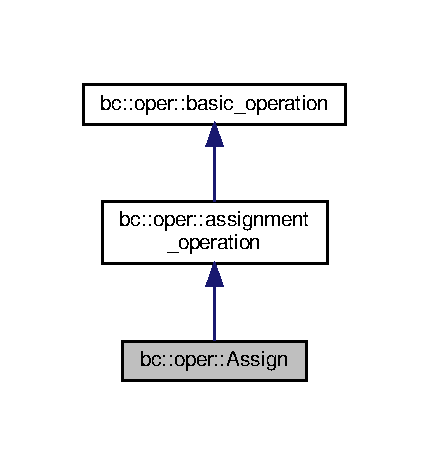
\includegraphics[width=206pt]{structbc_1_1oper_1_1Assign__inherit__graph}
\end{center}
\end{figure}


Collaboration diagram for bc\+:\+:oper\+:\+:Assign\+:\nopagebreak
\begin{figure}[H]
\begin{center}
\leavevmode
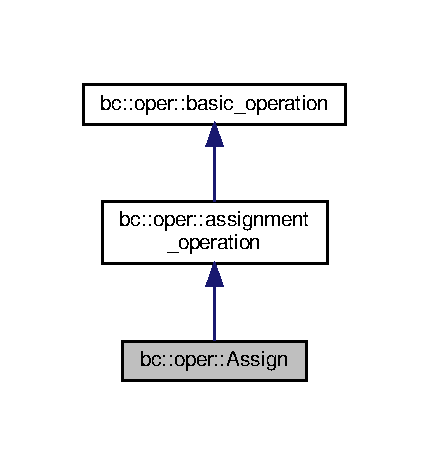
\includegraphics[width=206pt]{structbc_1_1oper_1_1Assign__coll__graph}
\end{center}
\end{figure}
\subsection*{Public Types}
\begin{DoxyCompactItemize}
\item 
using \hyperlink{structbc_1_1oper_1_1Assign_a7a864b827a77baa288df5e5a6b812b16}{alpha\+\_\+modifier} = \hyperlink{structbc_1_1traits_1_1Integer}{bc\+::traits\+::\+Integer}$<$ 1 $>$
\item 
using \hyperlink{structbc_1_1oper_1_1Assign_ae78c3dadc298a7f88f922cc7d1d2c961}{beta\+\_\+modifier} = \hyperlink{structbc_1_1traits_1_1Integer}{bc\+::traits\+::\+Integer}$<$ 0 $>$
\end{DoxyCompactItemize}
\subsection*{Public Member Functions}
\begin{DoxyCompactItemize}
\item 
{\footnotesize template$<$class Lv , class Rv $>$ }\\\+\_\+\+\_\+host\+\_\+\+\_\+ \+\_\+\+\_\+device\+\_\+\+\_\+ auto \hyperlink{structbc_1_1oper_1_1Assign_a8cb1c55dee85e0040c9c6130656ac2c3}{operator()} (Lv \&\&lv, Rv \&\&rv) const -\/$>$ decltype(\hyperlink{structbc_1_1oper_1_1Assign_a1e478dc4379526354bb93cb91a2cb9a8}{apply}(lv, rv))
\end{DoxyCompactItemize}
\subsection*{Static Public Member Functions}
\begin{DoxyCompactItemize}
\item 
{\footnotesize template$<$class Lv , class Rv $>$ }\\\+\_\+\+\_\+host\+\_\+\+\_\+ static \+\_\+\+\_\+device\+\_\+\+\_\+ auto \hyperlink{structbc_1_1oper_1_1Assign_a1e478dc4379526354bb93cb91a2cb9a8}{apply} (Lv \&\&lv, Rv \&\&rv) -\/$>$ decltype(lv=rv)
\end{DoxyCompactItemize}


\subsection{Member Typedef Documentation}
\mbox{\Hypertarget{structbc_1_1oper_1_1Assign_a7a864b827a77baa288df5e5a6b812b16}\label{structbc_1_1oper_1_1Assign_a7a864b827a77baa288df5e5a6b812b16}} 
\index{bc\+::oper\+::\+Assign@{bc\+::oper\+::\+Assign}!alpha\+\_\+modifier@{alpha\+\_\+modifier}}
\index{alpha\+\_\+modifier@{alpha\+\_\+modifier}!bc\+::oper\+::\+Assign@{bc\+::oper\+::\+Assign}}
\subsubsection{\texorpdfstring{alpha\+\_\+modifier}{alpha\_modifier}}
{\footnotesize\ttfamily using \hyperlink{structbc_1_1oper_1_1Assign_a7a864b827a77baa288df5e5a6b812b16}{bc\+::oper\+::\+Assign\+::alpha\+\_\+modifier} =  \hyperlink{structbc_1_1traits_1_1Integer}{bc\+::traits\+::\+Integer}$<$1$>$}

\mbox{\Hypertarget{structbc_1_1oper_1_1Assign_ae78c3dadc298a7f88f922cc7d1d2c961}\label{structbc_1_1oper_1_1Assign_ae78c3dadc298a7f88f922cc7d1d2c961}} 
\index{bc\+::oper\+::\+Assign@{bc\+::oper\+::\+Assign}!beta\+\_\+modifier@{beta\+\_\+modifier}}
\index{beta\+\_\+modifier@{beta\+\_\+modifier}!bc\+::oper\+::\+Assign@{bc\+::oper\+::\+Assign}}
\subsubsection{\texorpdfstring{beta\+\_\+modifier}{beta\_modifier}}
{\footnotesize\ttfamily using \hyperlink{structbc_1_1oper_1_1Assign_ae78c3dadc298a7f88f922cc7d1d2c961}{bc\+::oper\+::\+Assign\+::beta\+\_\+modifier} =  \hyperlink{structbc_1_1traits_1_1Integer}{bc\+::traits\+::\+Integer}$<$0$>$}



\subsection{Member Function Documentation}
\mbox{\Hypertarget{structbc_1_1oper_1_1Assign_a1e478dc4379526354bb93cb91a2cb9a8}\label{structbc_1_1oper_1_1Assign_a1e478dc4379526354bb93cb91a2cb9a8}} 
\index{bc\+::oper\+::\+Assign@{bc\+::oper\+::\+Assign}!apply@{apply}}
\index{apply@{apply}!bc\+::oper\+::\+Assign@{bc\+::oper\+::\+Assign}}
\subsubsection{\texorpdfstring{apply()}{apply()}}
{\footnotesize\ttfamily template$<$class Lv , class Rv $>$ \\
\+\_\+\+\_\+host\+\_\+\+\_\+ static \+\_\+\+\_\+device\+\_\+\+\_\+ auto bc\+::oper\+::\+Assign\+::apply (\begin{DoxyParamCaption}\item[{Lv \&\&}]{lv,  }\item[{Rv \&\&}]{rv }\end{DoxyParamCaption}) -\/$>$ decltype( lv = rv ) \hspace{0.3cm}{\ttfamily [inline]}, {\ttfamily [static]}}

\mbox{\Hypertarget{structbc_1_1oper_1_1Assign_a8cb1c55dee85e0040c9c6130656ac2c3}\label{structbc_1_1oper_1_1Assign_a8cb1c55dee85e0040c9c6130656ac2c3}} 
\index{bc\+::oper\+::\+Assign@{bc\+::oper\+::\+Assign}!operator()@{operator()}}
\index{operator()@{operator()}!bc\+::oper\+::\+Assign@{bc\+::oper\+::\+Assign}}
\subsubsection{\texorpdfstring{operator()()}{operator()()}}
{\footnotesize\ttfamily template$<$class Lv , class Rv $>$ \\
\+\_\+\+\_\+host\+\_\+\+\_\+ \+\_\+\+\_\+device\+\_\+\+\_\+ auto bc\+::oper\+::\+Assign\+::operator() (\begin{DoxyParamCaption}\item[{Lv \&\&}]{lv,  }\item[{Rv \&\&}]{rv }\end{DoxyParamCaption}) const -\/$>$ decltype(\hyperlink{structbc_1_1oper_1_1Assign_a1e478dc4379526354bb93cb91a2cb9a8}{apply}(lv, rv)) \hspace{0.3cm}{\ttfamily [inline]}}



The documentation for this struct was generated from the following file\+:\begin{DoxyCompactItemize}
\item 
blackcat/operations/\hyperlink{binary_8h}{binary.\+h}\end{DoxyCompactItemize}

\hypertarget{structbc_1_1oper_1_1assignment__operation}{}\section{bc\+:\+:oper\+:\+:assignment\+\_\+operation Struct Reference}
\label{structbc_1_1oper_1_1assignment__operation}\index{bc\+::oper\+::assignment\+\_\+operation@{bc\+::oper\+::assignment\+\_\+operation}}


{\ttfamily \#include $<$tags.\+h$>$}



Inheritance diagram for bc\+:\+:oper\+:\+:assignment\+\_\+operation\+:\nopagebreak
\begin{figure}[H]
\begin{center}
\leavevmode
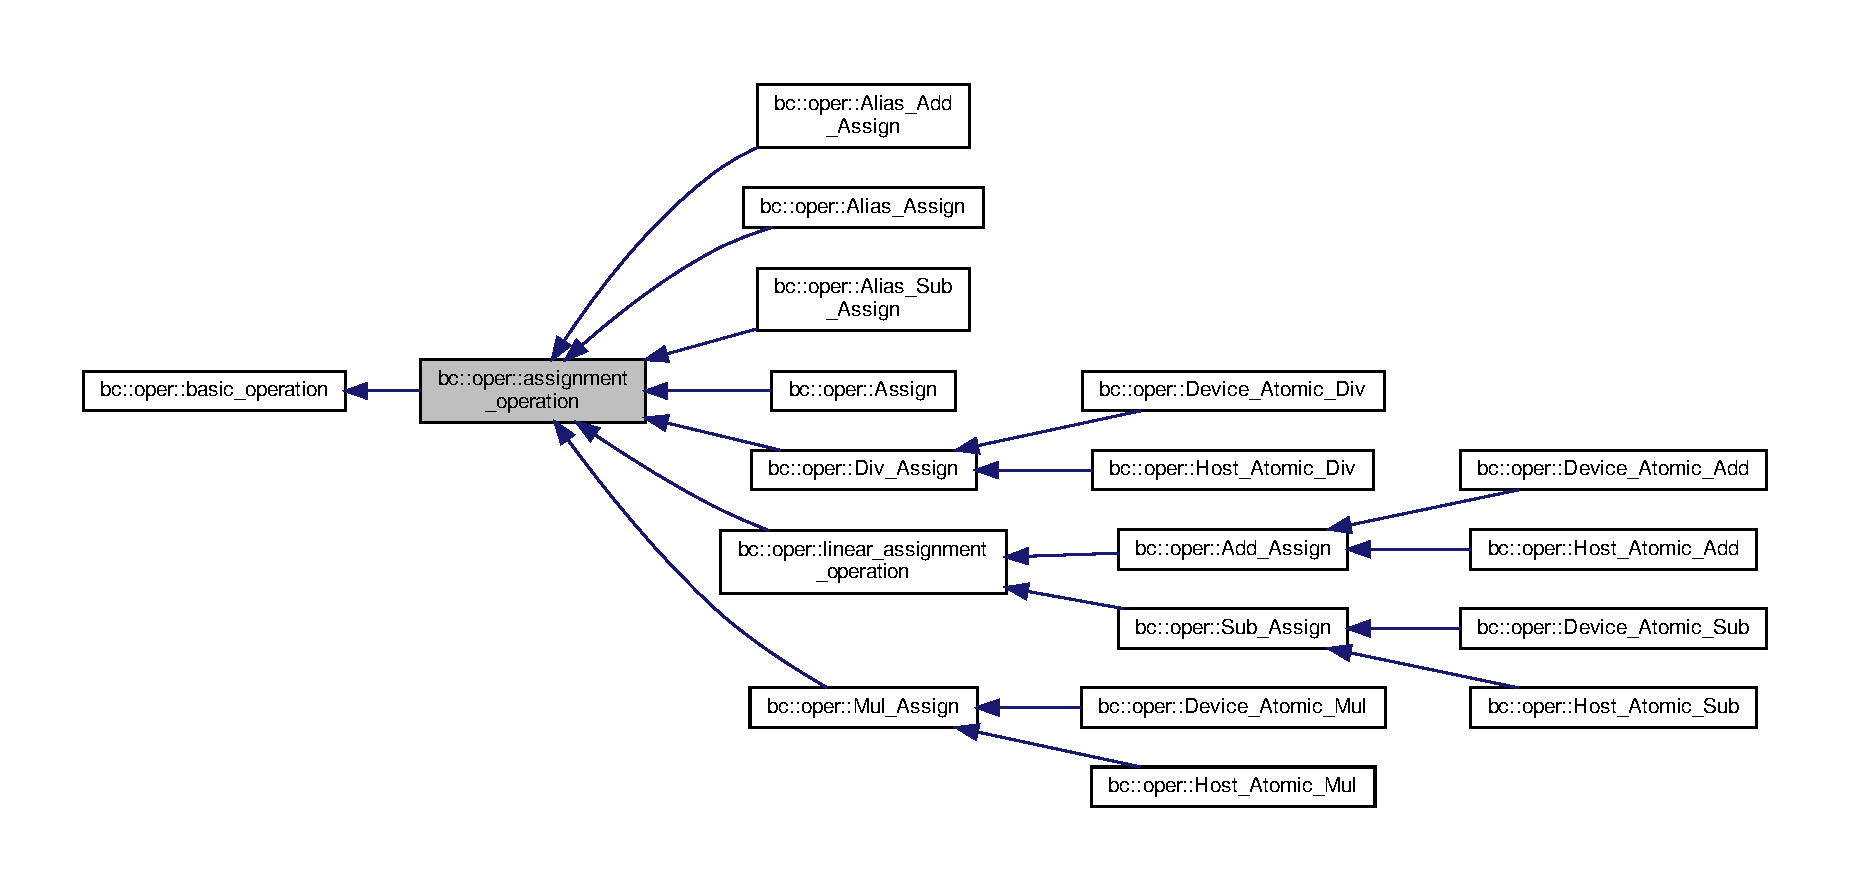
\includegraphics[width=350pt]{structbc_1_1oper_1_1assignment__operation__inherit__graph}
\end{center}
\end{figure}


Collaboration diagram for bc\+:\+:oper\+:\+:assignment\+\_\+operation\+:\nopagebreak
\begin{figure}[H]
\begin{center}
\leavevmode
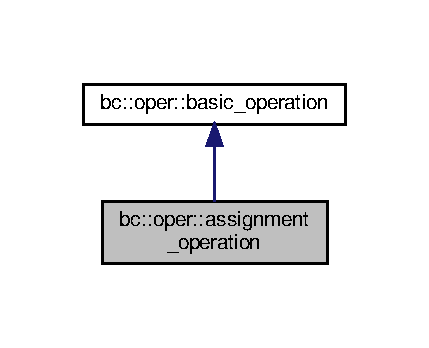
\includegraphics[width=206pt]{structbc_1_1oper_1_1assignment__operation__coll__graph}
\end{center}
\end{figure}


The documentation for this struct was generated from the following file\+:\begin{DoxyCompactItemize}
\item 
blackcat/operations/\hyperlink{tags_8h}{tags.\+h}\end{DoxyCompactItemize}

\hypertarget{structbc_1_1oper_1_1cmath__functions_1_1Atan}{}\section{bc\+:\+:oper\+:\+:cmath\+\_\+functions\+:\+:Atan Struct Reference}
\label{structbc_1_1oper_1_1cmath__functions_1_1Atan}\index{bc\+::oper\+::cmath\+\_\+functions\+::\+Atan@{bc\+::oper\+::cmath\+\_\+functions\+::\+Atan}}


{\ttfamily \#include $<$cmath.\+h$>$}



Collaboration diagram for bc\+:\+:oper\+:\+:cmath\+\_\+functions\+:\+:Atan\+:\nopagebreak
\begin{figure}[H]
\begin{center}
\leavevmode
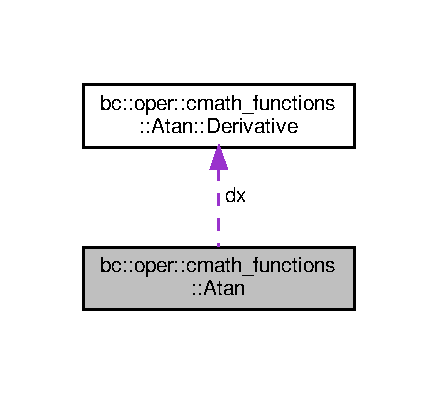
\includegraphics[width=210pt]{structbc_1_1oper_1_1cmath__functions_1_1Atan__coll__graph}
\end{center}
\end{figure}
\subsection*{Classes}
\begin{DoxyCompactItemize}
\item 
struct \hyperlink{structbc_1_1oper_1_1cmath__functions_1_1Atan_1_1Derivative}{Derivative}
\end{DoxyCompactItemize}
\subsection*{Public Member Functions}
\begin{DoxyCompactItemize}
\item 
{\footnotesize template$<$class value\+\_\+type $>$ }\\\hyperlink{common_8h_a6699e8b0449da5c0fafb878e59c1d4b1}{B\+C\+I\+N\+L\+I\+NE} value\+\_\+type \hyperlink{structbc_1_1oper_1_1cmath__functions_1_1Atan_a1282c1530ebf9628cd6c95a158787c2c}{operator()} (const value\+\_\+type \&x) const
\item 
{\footnotesize template$<$class Xpr $>$ }\\auto \hyperlink{structbc_1_1oper_1_1cmath__functions_1_1Atan_a8df17012bbd853264f0220706adb637a}{operator()} (const \hyperlink{classbc_1_1tensors_1_1Expression__Base}{bc\+::tensors\+::\+Expression\+\_\+\+Base}$<$ Xpr $>$ \&tensor)
\item 
{\footnotesize template$<$class Xpr $>$ }\\auto \hyperlink{structbc_1_1oper_1_1cmath__functions_1_1Atan_a8886ec51e68cc92caba84b031d3acdf9}{operator()} (const \hyperlink{classbc_1_1tensors_1_1Tensor__Base}{bc\+::tensors\+::\+Tensor\+\_\+\+Base}$<$ Xpr $>$ \&tensor)
\end{DoxyCompactItemize}
\subsection*{Static Public Member Functions}
\begin{DoxyCompactItemize}
\item 
{\footnotesize template$<$class value\+\_\+type $>$ }\\static \hyperlink{common_8h_a6699e8b0449da5c0fafb878e59c1d4b1}{B\+C\+I\+N\+L\+I\+NE} auto \hyperlink{structbc_1_1oper_1_1cmath__functions_1_1Atan_a8ee1b987b30be5bd14dfd71f6f112fbe}{apply} (const value\+\_\+type \&x)
\end{DoxyCompactItemize}
\subsection*{Public Attributes}
\begin{DoxyCompactItemize}
\item 
struct \hyperlink{structbc_1_1oper_1_1cmath__functions_1_1Atan_1_1Derivative}{bc\+::oper\+::cmath\+\_\+functions\+::\+Atan\+::\+Derivative} \hyperlink{structbc_1_1oper_1_1cmath__functions_1_1Atan_a6298e19488a3e83b2012798de1f8406a}{dx}
\end{DoxyCompactItemize}


\subsection{Member Function Documentation}
\mbox{\Hypertarget{structbc_1_1oper_1_1cmath__functions_1_1Atan_a8ee1b987b30be5bd14dfd71f6f112fbe}\label{structbc_1_1oper_1_1cmath__functions_1_1Atan_a8ee1b987b30be5bd14dfd71f6f112fbe}} 
\index{bc\+::oper\+::cmath\+\_\+functions\+::\+Atan@{bc\+::oper\+::cmath\+\_\+functions\+::\+Atan}!apply@{apply}}
\index{apply@{apply}!bc\+::oper\+::cmath\+\_\+functions\+::\+Atan@{bc\+::oper\+::cmath\+\_\+functions\+::\+Atan}}
\subsubsection{\texorpdfstring{apply()}{apply()}}
{\footnotesize\ttfamily template$<$class value\+\_\+type $>$ \\
static \hyperlink{common_8h_a6699e8b0449da5c0fafb878e59c1d4b1}{B\+C\+I\+N\+L\+I\+NE} auto bc\+::oper\+::cmath\+\_\+functions\+::\+Atan\+::apply (\begin{DoxyParamCaption}\item[{const value\+\_\+type \&}]{x }\end{DoxyParamCaption})\hspace{0.3cm}{\ttfamily [inline]}, {\ttfamily [static]}}

\mbox{\Hypertarget{structbc_1_1oper_1_1cmath__functions_1_1Atan_a8886ec51e68cc92caba84b031d3acdf9}\label{structbc_1_1oper_1_1cmath__functions_1_1Atan_a8886ec51e68cc92caba84b031d3acdf9}} 
\index{bc\+::oper\+::cmath\+\_\+functions\+::\+Atan@{bc\+::oper\+::cmath\+\_\+functions\+::\+Atan}!operator()@{operator()}}
\index{operator()@{operator()}!bc\+::oper\+::cmath\+\_\+functions\+::\+Atan@{bc\+::oper\+::cmath\+\_\+functions\+::\+Atan}}
\subsubsection{\texorpdfstring{operator()()}{operator()()}\hspace{0.1cm}{\footnotesize\ttfamily [1/3]}}
{\footnotesize\ttfamily template$<$class Xpr $>$ \\
auto bc\+::oper\+::cmath\+\_\+functions\+::\+Atan\+::operator() (\begin{DoxyParamCaption}\item[{const \hyperlink{classbc_1_1tensors_1_1Tensor__Base}{bc\+::tensors\+::\+Tensor\+\_\+\+Base}$<$ Xpr $>$ \&}]{tensor }\end{DoxyParamCaption})\hspace{0.3cm}{\ttfamily [inline]}}

\mbox{\Hypertarget{structbc_1_1oper_1_1cmath__functions_1_1Atan_a8df17012bbd853264f0220706adb637a}\label{structbc_1_1oper_1_1cmath__functions_1_1Atan_a8df17012bbd853264f0220706adb637a}} 
\index{bc\+::oper\+::cmath\+\_\+functions\+::\+Atan@{bc\+::oper\+::cmath\+\_\+functions\+::\+Atan}!operator()@{operator()}}
\index{operator()@{operator()}!bc\+::oper\+::cmath\+\_\+functions\+::\+Atan@{bc\+::oper\+::cmath\+\_\+functions\+::\+Atan}}
\subsubsection{\texorpdfstring{operator()()}{operator()()}\hspace{0.1cm}{\footnotesize\ttfamily [2/3]}}
{\footnotesize\ttfamily template$<$class Xpr $>$ \\
auto bc\+::oper\+::cmath\+\_\+functions\+::\+Atan\+::operator() (\begin{DoxyParamCaption}\item[{const \hyperlink{classbc_1_1tensors_1_1Expression__Base}{bc\+::tensors\+::\+Expression\+\_\+\+Base}$<$ Xpr $>$ \&}]{tensor }\end{DoxyParamCaption})\hspace{0.3cm}{\ttfamily [inline]}}

\mbox{\Hypertarget{structbc_1_1oper_1_1cmath__functions_1_1Atan_a1282c1530ebf9628cd6c95a158787c2c}\label{structbc_1_1oper_1_1cmath__functions_1_1Atan_a1282c1530ebf9628cd6c95a158787c2c}} 
\index{bc\+::oper\+::cmath\+\_\+functions\+::\+Atan@{bc\+::oper\+::cmath\+\_\+functions\+::\+Atan}!operator()@{operator()}}
\index{operator()@{operator()}!bc\+::oper\+::cmath\+\_\+functions\+::\+Atan@{bc\+::oper\+::cmath\+\_\+functions\+::\+Atan}}
\subsubsection{\texorpdfstring{operator()()}{operator()()}\hspace{0.1cm}{\footnotesize\ttfamily [3/3]}}
{\footnotesize\ttfamily template$<$class value\+\_\+type $>$ \\
\hyperlink{common_8h_a6699e8b0449da5c0fafb878e59c1d4b1}{B\+C\+I\+N\+L\+I\+NE} value\+\_\+type bc\+::oper\+::cmath\+\_\+functions\+::\+Atan\+::operator() (\begin{DoxyParamCaption}\item[{const value\+\_\+type \&}]{x }\end{DoxyParamCaption}) const\hspace{0.3cm}{\ttfamily [inline]}}



\subsection{Member Data Documentation}
\mbox{\Hypertarget{structbc_1_1oper_1_1cmath__functions_1_1Atan_a6298e19488a3e83b2012798de1f8406a}\label{structbc_1_1oper_1_1cmath__functions_1_1Atan_a6298e19488a3e83b2012798de1f8406a}} 
\index{bc\+::oper\+::cmath\+\_\+functions\+::\+Atan@{bc\+::oper\+::cmath\+\_\+functions\+::\+Atan}!dx@{dx}}
\index{dx@{dx}!bc\+::oper\+::cmath\+\_\+functions\+::\+Atan@{bc\+::oper\+::cmath\+\_\+functions\+::\+Atan}}
\subsubsection{\texorpdfstring{dx}{dx}}
{\footnotesize\ttfamily struct \hyperlink{structbc_1_1oper_1_1cmath__functions_1_1Atan_1_1Derivative}{bc\+::oper\+::cmath\+\_\+functions\+::\+Atan\+::\+Derivative}   bc\+::oper\+::cmath\+\_\+functions\+::\+Atan\+::dx}



The documentation for this struct was generated from the following file\+:\begin{DoxyCompactItemize}
\item 
blackcat/operations/\hyperlink{cmath_8h}{cmath.\+h}\end{DoxyCompactItemize}

\hypertarget{structbc_1_1oper_1_1cmath__functions_1_1Atan2}{}\section{bc\+:\+:oper\+:\+:cmath\+\_\+functions\+:\+:Atan2 Struct Reference}
\label{structbc_1_1oper_1_1cmath__functions_1_1Atan2}\index{bc\+::oper\+::cmath\+\_\+functions\+::\+Atan2@{bc\+::oper\+::cmath\+\_\+functions\+::\+Atan2}}


{\ttfamily \#include $<$cmath.\+h$>$}

\subsection*{Public Member Functions}
\begin{DoxyCompactItemize}
\item 
{\footnotesize template$<$class value\+\_\+type $>$ }\\\hyperlink{common_8h_a6699e8b0449da5c0fafb878e59c1d4b1}{B\+C\+I\+N\+L\+I\+NE} value\+\_\+type \hyperlink{structbc_1_1oper_1_1cmath__functions_1_1Atan2_aa088c1a3f9aaa67f66bf0c49f1e61a1e}{operator()} (const value\+\_\+type \&x) const
\item 
{\footnotesize template$<$class Xpr $>$ }\\auto \hyperlink{structbc_1_1oper_1_1cmath__functions_1_1Atan2_afc4658ef4e3d6291e49a357a37071fa8}{operator()} (const \hyperlink{classbc_1_1tensors_1_1Expression__Base}{bc\+::tensors\+::\+Expression\+\_\+\+Base}$<$ Xpr $>$ \&tensor)
\item 
{\footnotesize template$<$class Xpr $>$ }\\auto \hyperlink{structbc_1_1oper_1_1cmath__functions_1_1Atan2_a03ed6789a0a864f1034ffd6c90e1237c}{operator()} (const \hyperlink{classbc_1_1tensors_1_1Tensor__Base}{bc\+::tensors\+::\+Tensor\+\_\+\+Base}$<$ Xpr $>$ \&tensor)
\end{DoxyCompactItemize}
\subsection*{Static Public Member Functions}
\begin{DoxyCompactItemize}
\item 
{\footnotesize template$<$class value\+\_\+type $>$ }\\static \hyperlink{common_8h_a6699e8b0449da5c0fafb878e59c1d4b1}{B\+C\+I\+N\+L\+I\+NE} auto \hyperlink{structbc_1_1oper_1_1cmath__functions_1_1Atan2_ac24c9f40bb5bf2ff82f22efaf458d43d}{apply} (const value\+\_\+type \&x)
\end{DoxyCompactItemize}


\subsection{Member Function Documentation}
\mbox{\Hypertarget{structbc_1_1oper_1_1cmath__functions_1_1Atan2_ac24c9f40bb5bf2ff82f22efaf458d43d}\label{structbc_1_1oper_1_1cmath__functions_1_1Atan2_ac24c9f40bb5bf2ff82f22efaf458d43d}} 
\index{bc\+::oper\+::cmath\+\_\+functions\+::\+Atan2@{bc\+::oper\+::cmath\+\_\+functions\+::\+Atan2}!apply@{apply}}
\index{apply@{apply}!bc\+::oper\+::cmath\+\_\+functions\+::\+Atan2@{bc\+::oper\+::cmath\+\_\+functions\+::\+Atan2}}
\subsubsection{\texorpdfstring{apply()}{apply()}}
{\footnotesize\ttfamily template$<$class value\+\_\+type $>$ \\
static \hyperlink{common_8h_a6699e8b0449da5c0fafb878e59c1d4b1}{B\+C\+I\+N\+L\+I\+NE} auto bc\+::oper\+::cmath\+\_\+functions\+::\+Atan2\+::apply (\begin{DoxyParamCaption}\item[{const value\+\_\+type \&}]{x }\end{DoxyParamCaption})\hspace{0.3cm}{\ttfamily [inline]}, {\ttfamily [static]}}

\mbox{\Hypertarget{structbc_1_1oper_1_1cmath__functions_1_1Atan2_a03ed6789a0a864f1034ffd6c90e1237c}\label{structbc_1_1oper_1_1cmath__functions_1_1Atan2_a03ed6789a0a864f1034ffd6c90e1237c}} 
\index{bc\+::oper\+::cmath\+\_\+functions\+::\+Atan2@{bc\+::oper\+::cmath\+\_\+functions\+::\+Atan2}!operator()@{operator()}}
\index{operator()@{operator()}!bc\+::oper\+::cmath\+\_\+functions\+::\+Atan2@{bc\+::oper\+::cmath\+\_\+functions\+::\+Atan2}}
\subsubsection{\texorpdfstring{operator()()}{operator()()}\hspace{0.1cm}{\footnotesize\ttfamily [1/3]}}
{\footnotesize\ttfamily template$<$class Xpr $>$ \\
auto bc\+::oper\+::cmath\+\_\+functions\+::\+Atan2\+::operator() (\begin{DoxyParamCaption}\item[{const \hyperlink{classbc_1_1tensors_1_1Tensor__Base}{bc\+::tensors\+::\+Tensor\+\_\+\+Base}$<$ Xpr $>$ \&}]{tensor }\end{DoxyParamCaption})\hspace{0.3cm}{\ttfamily [inline]}}

\mbox{\Hypertarget{structbc_1_1oper_1_1cmath__functions_1_1Atan2_afc4658ef4e3d6291e49a357a37071fa8}\label{structbc_1_1oper_1_1cmath__functions_1_1Atan2_afc4658ef4e3d6291e49a357a37071fa8}} 
\index{bc\+::oper\+::cmath\+\_\+functions\+::\+Atan2@{bc\+::oper\+::cmath\+\_\+functions\+::\+Atan2}!operator()@{operator()}}
\index{operator()@{operator()}!bc\+::oper\+::cmath\+\_\+functions\+::\+Atan2@{bc\+::oper\+::cmath\+\_\+functions\+::\+Atan2}}
\subsubsection{\texorpdfstring{operator()()}{operator()()}\hspace{0.1cm}{\footnotesize\ttfamily [2/3]}}
{\footnotesize\ttfamily template$<$class Xpr $>$ \\
auto bc\+::oper\+::cmath\+\_\+functions\+::\+Atan2\+::operator() (\begin{DoxyParamCaption}\item[{const \hyperlink{classbc_1_1tensors_1_1Expression__Base}{bc\+::tensors\+::\+Expression\+\_\+\+Base}$<$ Xpr $>$ \&}]{tensor }\end{DoxyParamCaption})\hspace{0.3cm}{\ttfamily [inline]}}

\mbox{\Hypertarget{structbc_1_1oper_1_1cmath__functions_1_1Atan2_aa088c1a3f9aaa67f66bf0c49f1e61a1e}\label{structbc_1_1oper_1_1cmath__functions_1_1Atan2_aa088c1a3f9aaa67f66bf0c49f1e61a1e}} 
\index{bc\+::oper\+::cmath\+\_\+functions\+::\+Atan2@{bc\+::oper\+::cmath\+\_\+functions\+::\+Atan2}!operator()@{operator()}}
\index{operator()@{operator()}!bc\+::oper\+::cmath\+\_\+functions\+::\+Atan2@{bc\+::oper\+::cmath\+\_\+functions\+::\+Atan2}}
\subsubsection{\texorpdfstring{operator()()}{operator()()}\hspace{0.1cm}{\footnotesize\ttfamily [3/3]}}
{\footnotesize\ttfamily template$<$class value\+\_\+type $>$ \\
\hyperlink{common_8h_a6699e8b0449da5c0fafb878e59c1d4b1}{B\+C\+I\+N\+L\+I\+NE} value\+\_\+type bc\+::oper\+::cmath\+\_\+functions\+::\+Atan2\+::operator() (\begin{DoxyParamCaption}\item[{const value\+\_\+type \&}]{x }\end{DoxyParamCaption}) const\hspace{0.3cm}{\ttfamily [inline]}}



The documentation for this struct was generated from the following file\+:\begin{DoxyCompactItemize}
\item 
blackcat/operations/\hyperlink{cmath_8h}{cmath.\+h}\end{DoxyCompactItemize}

\hypertarget{structbc_1_1oper_1_1cmath__functions_1_1Atanh}{}\section{bc\+:\+:oper\+:\+:cmath\+\_\+functions\+:\+:Atanh Struct Reference}
\label{structbc_1_1oper_1_1cmath__functions_1_1Atanh}\index{bc\+::oper\+::cmath\+\_\+functions\+::\+Atanh@{bc\+::oper\+::cmath\+\_\+functions\+::\+Atanh}}


{\ttfamily \#include $<$cmath.\+h$>$}

\subsection*{Public Member Functions}
\begin{DoxyCompactItemize}
\item 
{\footnotesize template$<$class value\+\_\+type $>$ }\\\hyperlink{common_8h_a6699e8b0449da5c0fafb878e59c1d4b1}{B\+C\+I\+N\+L\+I\+NE} value\+\_\+type \hyperlink{structbc_1_1oper_1_1cmath__functions_1_1Atanh_a945737670a9851de8649a39f545c9a3d}{operator()} (const value\+\_\+type \&x) const
\item 
{\footnotesize template$<$class Xpr $>$ }\\auto \hyperlink{structbc_1_1oper_1_1cmath__functions_1_1Atanh_af695ef95e7047389ff28c7685bee22d2}{operator()} (const \hyperlink{classbc_1_1tensors_1_1Expression__Base}{bc\+::tensors\+::\+Expression\+\_\+\+Base}$<$ Xpr $>$ \&tensor)
\item 
{\footnotesize template$<$class Xpr $>$ }\\auto \hyperlink{structbc_1_1oper_1_1cmath__functions_1_1Atanh_a54634c8570f9e603628ad005899d6391}{operator()} (const \hyperlink{classbc_1_1tensors_1_1Tensor__Base}{bc\+::tensors\+::\+Tensor\+\_\+\+Base}$<$ Xpr $>$ \&tensor)
\end{DoxyCompactItemize}
\subsection*{Static Public Member Functions}
\begin{DoxyCompactItemize}
\item 
{\footnotesize template$<$class value\+\_\+type $>$ }\\static \hyperlink{common_8h_a6699e8b0449da5c0fafb878e59c1d4b1}{B\+C\+I\+N\+L\+I\+NE} auto \hyperlink{structbc_1_1oper_1_1cmath__functions_1_1Atanh_a863d6d8418c2073776d4c85e5516ede4}{apply} (const value\+\_\+type \&x)
\end{DoxyCompactItemize}


\subsection{Member Function Documentation}
\mbox{\Hypertarget{structbc_1_1oper_1_1cmath__functions_1_1Atanh_a863d6d8418c2073776d4c85e5516ede4}\label{structbc_1_1oper_1_1cmath__functions_1_1Atanh_a863d6d8418c2073776d4c85e5516ede4}} 
\index{bc\+::oper\+::cmath\+\_\+functions\+::\+Atanh@{bc\+::oper\+::cmath\+\_\+functions\+::\+Atanh}!apply@{apply}}
\index{apply@{apply}!bc\+::oper\+::cmath\+\_\+functions\+::\+Atanh@{bc\+::oper\+::cmath\+\_\+functions\+::\+Atanh}}
\subsubsection{\texorpdfstring{apply()}{apply()}}
{\footnotesize\ttfamily template$<$class value\+\_\+type $>$ \\
static \hyperlink{common_8h_a6699e8b0449da5c0fafb878e59c1d4b1}{B\+C\+I\+N\+L\+I\+NE} auto bc\+::oper\+::cmath\+\_\+functions\+::\+Atanh\+::apply (\begin{DoxyParamCaption}\item[{const value\+\_\+type \&}]{x }\end{DoxyParamCaption})\hspace{0.3cm}{\ttfamily [inline]}, {\ttfamily [static]}}

\mbox{\Hypertarget{structbc_1_1oper_1_1cmath__functions_1_1Atanh_a54634c8570f9e603628ad005899d6391}\label{structbc_1_1oper_1_1cmath__functions_1_1Atanh_a54634c8570f9e603628ad005899d6391}} 
\index{bc\+::oper\+::cmath\+\_\+functions\+::\+Atanh@{bc\+::oper\+::cmath\+\_\+functions\+::\+Atanh}!operator()@{operator()}}
\index{operator()@{operator()}!bc\+::oper\+::cmath\+\_\+functions\+::\+Atanh@{bc\+::oper\+::cmath\+\_\+functions\+::\+Atanh}}
\subsubsection{\texorpdfstring{operator()()}{operator()()}\hspace{0.1cm}{\footnotesize\ttfamily [1/3]}}
{\footnotesize\ttfamily template$<$class Xpr $>$ \\
auto bc\+::oper\+::cmath\+\_\+functions\+::\+Atanh\+::operator() (\begin{DoxyParamCaption}\item[{const \hyperlink{classbc_1_1tensors_1_1Tensor__Base}{bc\+::tensors\+::\+Tensor\+\_\+\+Base}$<$ Xpr $>$ \&}]{tensor }\end{DoxyParamCaption})\hspace{0.3cm}{\ttfamily [inline]}}

\mbox{\Hypertarget{structbc_1_1oper_1_1cmath__functions_1_1Atanh_af695ef95e7047389ff28c7685bee22d2}\label{structbc_1_1oper_1_1cmath__functions_1_1Atanh_af695ef95e7047389ff28c7685bee22d2}} 
\index{bc\+::oper\+::cmath\+\_\+functions\+::\+Atanh@{bc\+::oper\+::cmath\+\_\+functions\+::\+Atanh}!operator()@{operator()}}
\index{operator()@{operator()}!bc\+::oper\+::cmath\+\_\+functions\+::\+Atanh@{bc\+::oper\+::cmath\+\_\+functions\+::\+Atanh}}
\subsubsection{\texorpdfstring{operator()()}{operator()()}\hspace{0.1cm}{\footnotesize\ttfamily [2/3]}}
{\footnotesize\ttfamily template$<$class Xpr $>$ \\
auto bc\+::oper\+::cmath\+\_\+functions\+::\+Atanh\+::operator() (\begin{DoxyParamCaption}\item[{const \hyperlink{classbc_1_1tensors_1_1Expression__Base}{bc\+::tensors\+::\+Expression\+\_\+\+Base}$<$ Xpr $>$ \&}]{tensor }\end{DoxyParamCaption})\hspace{0.3cm}{\ttfamily [inline]}}

\mbox{\Hypertarget{structbc_1_1oper_1_1cmath__functions_1_1Atanh_a945737670a9851de8649a39f545c9a3d}\label{structbc_1_1oper_1_1cmath__functions_1_1Atanh_a945737670a9851de8649a39f545c9a3d}} 
\index{bc\+::oper\+::cmath\+\_\+functions\+::\+Atanh@{bc\+::oper\+::cmath\+\_\+functions\+::\+Atanh}!operator()@{operator()}}
\index{operator()@{operator()}!bc\+::oper\+::cmath\+\_\+functions\+::\+Atanh@{bc\+::oper\+::cmath\+\_\+functions\+::\+Atanh}}
\subsubsection{\texorpdfstring{operator()()}{operator()()}\hspace{0.1cm}{\footnotesize\ttfamily [3/3]}}
{\footnotesize\ttfamily template$<$class value\+\_\+type $>$ \\
\hyperlink{common_8h_a6699e8b0449da5c0fafb878e59c1d4b1}{B\+C\+I\+N\+L\+I\+NE} value\+\_\+type bc\+::oper\+::cmath\+\_\+functions\+::\+Atanh\+::operator() (\begin{DoxyParamCaption}\item[{const value\+\_\+type \&}]{x }\end{DoxyParamCaption}) const\hspace{0.3cm}{\ttfamily [inline]}}



The documentation for this struct was generated from the following file\+:\begin{DoxyCompactItemize}
\item 
blackcat/operations/\hyperlink{cmath_8h}{cmath.\+h}\end{DoxyCompactItemize}

\hypertarget{structbc_1_1allocators_1_1Basic__Allocator__Base}{}\section{bc\+:\+:allocators\+:\+:Basic\+\_\+\+Allocator\+\_\+\+Base$<$ Value\+Type, System\+Tag $>$ Struct Template Reference}
\label{structbc_1_1allocators_1_1Basic__Allocator__Base}\index{bc\+::allocators\+::\+Basic\+\_\+\+Allocator\+\_\+\+Base$<$ Value\+Type, System\+Tag $>$@{bc\+::allocators\+::\+Basic\+\_\+\+Allocator\+\_\+\+Base$<$ Value\+Type, System\+Tag $>$}}


{\ttfamily \#include $<$basic\+\_\+allocators.\+h$>$}

\subsection*{Public Types}
\begin{DoxyCompactItemize}
\item 
using \hyperlink{structbc_1_1allocators_1_1Basic__Allocator__Base_a625be36f2aedbec274f8524ac72c8d28}{system\+\_\+tag} = System\+Tag
\item 
using \hyperlink{structbc_1_1allocators_1_1Basic__Allocator__Base_a7d9eca7878880a820908b57bdcb94501}{value\+\_\+type} = Value\+Type
\item 
using \hyperlink{structbc_1_1allocators_1_1Basic__Allocator__Base_aa91ec01a2520836062d1c21eb710a3cc}{pointer} = \hyperlink{structbc_1_1allocators_1_1Basic__Allocator__Base_a7d9eca7878880a820908b57bdcb94501}{value\+\_\+type} $\ast$
\item 
using \hyperlink{structbc_1_1allocators_1_1Basic__Allocator__Base_ac6e458ef842011190bc702a5e373850a}{const\+\_\+pointer} = \hyperlink{structbc_1_1allocators_1_1Basic__Allocator__Base_a7d9eca7878880a820908b57bdcb94501}{value\+\_\+type} $\ast$
\item 
using \hyperlink{structbc_1_1allocators_1_1Basic__Allocator__Base_ad7fe7255772b954d581c75ae2ee0d959}{size\+\_\+type} = std\+::size\+\_\+t
\item 
using \hyperlink{structbc_1_1allocators_1_1Basic__Allocator__Base_a9900b1de8ba282c40f6b5c3576f39b35}{reference} = \hyperlink{structbc_1_1allocators_1_1Basic__Allocator__Base_a7d9eca7878880a820908b57bdcb94501}{value\+\_\+type} \&
\item 
using \hyperlink{structbc_1_1allocators_1_1Basic__Allocator__Base_a5b5edb3ecfd3e5e210f95a9349ed4676}{const\+\_\+reference} = const \hyperlink{structbc_1_1allocators_1_1Basic__Allocator__Base_a7d9eca7878880a820908b57bdcb94501}{value\+\_\+type} \&
\item 
using \hyperlink{structbc_1_1allocators_1_1Basic__Allocator__Base_ae33a042e54a5257608e3e354a6890edc}{propagate\+\_\+on\+\_\+container\+\_\+copy\+\_\+assignment} = std\+::false\+\_\+type
\item 
using \hyperlink{structbc_1_1allocators_1_1Basic__Allocator__Base_a7c726fe1953f8dcb66e515edcf0d52ef}{propagate\+\_\+on\+\_\+container\+\_\+move\+\_\+assignment} = std\+::false\+\_\+type
\item 
using \hyperlink{structbc_1_1allocators_1_1Basic__Allocator__Base_a43d9999061677b23d0d03a56427e39f5}{propagate\+\_\+on\+\_\+container\+\_\+swap} = std\+::false\+\_\+type
\item 
using \hyperlink{structbc_1_1allocators_1_1Basic__Allocator__Base_a93df6b95cdc21c0d35bd34450d260a62}{is\+\_\+always\+\_\+equal} = std\+::true\+\_\+type
\end{DoxyCompactItemize}
\subsection*{Public Member Functions}
\begin{DoxyCompactItemize}
\item 
{\footnotesize template$<$class U $>$ }\\bool \hyperlink{structbc_1_1allocators_1_1Basic__Allocator__Base_ab70dcd6aa078ce7b3d5a43c36397d8e9}{operator==} (const \hyperlink{structbc_1_1allocators_1_1Basic__Allocator__Base}{Basic\+\_\+\+Allocator\+\_\+\+Base}$<$ U, System\+Tag $>$ \&) const
\item 
{\footnotesize template$<$class U $>$ }\\bool \hyperlink{structbc_1_1allocators_1_1Basic__Allocator__Base_a595df39ca6edee505366ff39ab6d2a4f}{operator!=} (const \hyperlink{structbc_1_1allocators_1_1Basic__Allocator__Base}{Basic\+\_\+\+Allocator\+\_\+\+Base}$<$ U, System\+Tag $>$ \&) const
\end{DoxyCompactItemize}


\subsection{Member Typedef Documentation}
\mbox{\Hypertarget{structbc_1_1allocators_1_1Basic__Allocator__Base_ac6e458ef842011190bc702a5e373850a}\label{structbc_1_1allocators_1_1Basic__Allocator__Base_ac6e458ef842011190bc702a5e373850a}} 
\index{bc\+::allocators\+::\+Basic\+\_\+\+Allocator\+\_\+\+Base@{bc\+::allocators\+::\+Basic\+\_\+\+Allocator\+\_\+\+Base}!const\+\_\+pointer@{const\+\_\+pointer}}
\index{const\+\_\+pointer@{const\+\_\+pointer}!bc\+::allocators\+::\+Basic\+\_\+\+Allocator\+\_\+\+Base@{bc\+::allocators\+::\+Basic\+\_\+\+Allocator\+\_\+\+Base}}
\subsubsection{\texorpdfstring{const\+\_\+pointer}{const\_pointer}}
{\footnotesize\ttfamily template$<$class Value\+Type, class System\+Tag$>$ \\
using \hyperlink{structbc_1_1allocators_1_1Basic__Allocator__Base}{bc\+::allocators\+::\+Basic\+\_\+\+Allocator\+\_\+\+Base}$<$ Value\+Type, System\+Tag $>$\+::\hyperlink{structbc_1_1allocators_1_1Basic__Allocator__Base_ac6e458ef842011190bc702a5e373850a}{const\+\_\+pointer} =  \hyperlink{structbc_1_1allocators_1_1Basic__Allocator__Base_a7d9eca7878880a820908b57bdcb94501}{value\+\_\+type}$\ast$}

\mbox{\Hypertarget{structbc_1_1allocators_1_1Basic__Allocator__Base_a5b5edb3ecfd3e5e210f95a9349ed4676}\label{structbc_1_1allocators_1_1Basic__Allocator__Base_a5b5edb3ecfd3e5e210f95a9349ed4676}} 
\index{bc\+::allocators\+::\+Basic\+\_\+\+Allocator\+\_\+\+Base@{bc\+::allocators\+::\+Basic\+\_\+\+Allocator\+\_\+\+Base}!const\+\_\+reference@{const\+\_\+reference}}
\index{const\+\_\+reference@{const\+\_\+reference}!bc\+::allocators\+::\+Basic\+\_\+\+Allocator\+\_\+\+Base@{bc\+::allocators\+::\+Basic\+\_\+\+Allocator\+\_\+\+Base}}
\subsubsection{\texorpdfstring{const\+\_\+reference}{const\_reference}}
{\footnotesize\ttfamily template$<$class Value\+Type, class System\+Tag$>$ \\
using \hyperlink{structbc_1_1allocators_1_1Basic__Allocator__Base}{bc\+::allocators\+::\+Basic\+\_\+\+Allocator\+\_\+\+Base}$<$ Value\+Type, System\+Tag $>$\+::\hyperlink{structbc_1_1allocators_1_1Basic__Allocator__Base_a5b5edb3ecfd3e5e210f95a9349ed4676}{const\+\_\+reference} =  const \hyperlink{structbc_1_1allocators_1_1Basic__Allocator__Base_a7d9eca7878880a820908b57bdcb94501}{value\+\_\+type}\&}

\mbox{\Hypertarget{structbc_1_1allocators_1_1Basic__Allocator__Base_a93df6b95cdc21c0d35bd34450d260a62}\label{structbc_1_1allocators_1_1Basic__Allocator__Base_a93df6b95cdc21c0d35bd34450d260a62}} 
\index{bc\+::allocators\+::\+Basic\+\_\+\+Allocator\+\_\+\+Base@{bc\+::allocators\+::\+Basic\+\_\+\+Allocator\+\_\+\+Base}!is\+\_\+always\+\_\+equal@{is\+\_\+always\+\_\+equal}}
\index{is\+\_\+always\+\_\+equal@{is\+\_\+always\+\_\+equal}!bc\+::allocators\+::\+Basic\+\_\+\+Allocator\+\_\+\+Base@{bc\+::allocators\+::\+Basic\+\_\+\+Allocator\+\_\+\+Base}}
\subsubsection{\texorpdfstring{is\+\_\+always\+\_\+equal}{is\_always\_equal}}
{\footnotesize\ttfamily template$<$class Value\+Type, class System\+Tag$>$ \\
using \hyperlink{structbc_1_1allocators_1_1Basic__Allocator__Base}{bc\+::allocators\+::\+Basic\+\_\+\+Allocator\+\_\+\+Base}$<$ Value\+Type, System\+Tag $>$\+::\hyperlink{structbc_1_1allocators_1_1Basic__Allocator__Base_a93df6b95cdc21c0d35bd34450d260a62}{is\+\_\+always\+\_\+equal} =  std\+::true\+\_\+type}

\mbox{\Hypertarget{structbc_1_1allocators_1_1Basic__Allocator__Base_aa91ec01a2520836062d1c21eb710a3cc}\label{structbc_1_1allocators_1_1Basic__Allocator__Base_aa91ec01a2520836062d1c21eb710a3cc}} 
\index{bc\+::allocators\+::\+Basic\+\_\+\+Allocator\+\_\+\+Base@{bc\+::allocators\+::\+Basic\+\_\+\+Allocator\+\_\+\+Base}!pointer@{pointer}}
\index{pointer@{pointer}!bc\+::allocators\+::\+Basic\+\_\+\+Allocator\+\_\+\+Base@{bc\+::allocators\+::\+Basic\+\_\+\+Allocator\+\_\+\+Base}}
\subsubsection{\texorpdfstring{pointer}{pointer}}
{\footnotesize\ttfamily template$<$class Value\+Type, class System\+Tag$>$ \\
using \hyperlink{structbc_1_1allocators_1_1Basic__Allocator__Base}{bc\+::allocators\+::\+Basic\+\_\+\+Allocator\+\_\+\+Base}$<$ Value\+Type, System\+Tag $>$\+::\hyperlink{structbc_1_1allocators_1_1Basic__Allocator__Base_aa91ec01a2520836062d1c21eb710a3cc}{pointer} =  \hyperlink{structbc_1_1allocators_1_1Basic__Allocator__Base_a7d9eca7878880a820908b57bdcb94501}{value\+\_\+type}$\ast$}

\mbox{\Hypertarget{structbc_1_1allocators_1_1Basic__Allocator__Base_ae33a042e54a5257608e3e354a6890edc}\label{structbc_1_1allocators_1_1Basic__Allocator__Base_ae33a042e54a5257608e3e354a6890edc}} 
\index{bc\+::allocators\+::\+Basic\+\_\+\+Allocator\+\_\+\+Base@{bc\+::allocators\+::\+Basic\+\_\+\+Allocator\+\_\+\+Base}!propagate\+\_\+on\+\_\+container\+\_\+copy\+\_\+assignment@{propagate\+\_\+on\+\_\+container\+\_\+copy\+\_\+assignment}}
\index{propagate\+\_\+on\+\_\+container\+\_\+copy\+\_\+assignment@{propagate\+\_\+on\+\_\+container\+\_\+copy\+\_\+assignment}!bc\+::allocators\+::\+Basic\+\_\+\+Allocator\+\_\+\+Base@{bc\+::allocators\+::\+Basic\+\_\+\+Allocator\+\_\+\+Base}}
\subsubsection{\texorpdfstring{propagate\+\_\+on\+\_\+container\+\_\+copy\+\_\+assignment}{propagate\_on\_container\_copy\_assignment}}
{\footnotesize\ttfamily template$<$class Value\+Type, class System\+Tag$>$ \\
using \hyperlink{structbc_1_1allocators_1_1Basic__Allocator__Base}{bc\+::allocators\+::\+Basic\+\_\+\+Allocator\+\_\+\+Base}$<$ Value\+Type, System\+Tag $>$\+::\hyperlink{structbc_1_1allocators_1_1Basic__Allocator__Base_ae33a042e54a5257608e3e354a6890edc}{propagate\+\_\+on\+\_\+container\+\_\+copy\+\_\+assignment} =  std\+::false\+\_\+type}

\mbox{\Hypertarget{structbc_1_1allocators_1_1Basic__Allocator__Base_a7c726fe1953f8dcb66e515edcf0d52ef}\label{structbc_1_1allocators_1_1Basic__Allocator__Base_a7c726fe1953f8dcb66e515edcf0d52ef}} 
\index{bc\+::allocators\+::\+Basic\+\_\+\+Allocator\+\_\+\+Base@{bc\+::allocators\+::\+Basic\+\_\+\+Allocator\+\_\+\+Base}!propagate\+\_\+on\+\_\+container\+\_\+move\+\_\+assignment@{propagate\+\_\+on\+\_\+container\+\_\+move\+\_\+assignment}}
\index{propagate\+\_\+on\+\_\+container\+\_\+move\+\_\+assignment@{propagate\+\_\+on\+\_\+container\+\_\+move\+\_\+assignment}!bc\+::allocators\+::\+Basic\+\_\+\+Allocator\+\_\+\+Base@{bc\+::allocators\+::\+Basic\+\_\+\+Allocator\+\_\+\+Base}}
\subsubsection{\texorpdfstring{propagate\+\_\+on\+\_\+container\+\_\+move\+\_\+assignment}{propagate\_on\_container\_move\_assignment}}
{\footnotesize\ttfamily template$<$class Value\+Type, class System\+Tag$>$ \\
using \hyperlink{structbc_1_1allocators_1_1Basic__Allocator__Base}{bc\+::allocators\+::\+Basic\+\_\+\+Allocator\+\_\+\+Base}$<$ Value\+Type, System\+Tag $>$\+::\hyperlink{structbc_1_1allocators_1_1Basic__Allocator__Base_a7c726fe1953f8dcb66e515edcf0d52ef}{propagate\+\_\+on\+\_\+container\+\_\+move\+\_\+assignment} =  std\+::false\+\_\+type}

\mbox{\Hypertarget{structbc_1_1allocators_1_1Basic__Allocator__Base_a43d9999061677b23d0d03a56427e39f5}\label{structbc_1_1allocators_1_1Basic__Allocator__Base_a43d9999061677b23d0d03a56427e39f5}} 
\index{bc\+::allocators\+::\+Basic\+\_\+\+Allocator\+\_\+\+Base@{bc\+::allocators\+::\+Basic\+\_\+\+Allocator\+\_\+\+Base}!propagate\+\_\+on\+\_\+container\+\_\+swap@{propagate\+\_\+on\+\_\+container\+\_\+swap}}
\index{propagate\+\_\+on\+\_\+container\+\_\+swap@{propagate\+\_\+on\+\_\+container\+\_\+swap}!bc\+::allocators\+::\+Basic\+\_\+\+Allocator\+\_\+\+Base@{bc\+::allocators\+::\+Basic\+\_\+\+Allocator\+\_\+\+Base}}
\subsubsection{\texorpdfstring{propagate\+\_\+on\+\_\+container\+\_\+swap}{propagate\_on\_container\_swap}}
{\footnotesize\ttfamily template$<$class Value\+Type, class System\+Tag$>$ \\
using \hyperlink{structbc_1_1allocators_1_1Basic__Allocator__Base}{bc\+::allocators\+::\+Basic\+\_\+\+Allocator\+\_\+\+Base}$<$ Value\+Type, System\+Tag $>$\+::\hyperlink{structbc_1_1allocators_1_1Basic__Allocator__Base_a43d9999061677b23d0d03a56427e39f5}{propagate\+\_\+on\+\_\+container\+\_\+swap} =  std\+::false\+\_\+type}

\mbox{\Hypertarget{structbc_1_1allocators_1_1Basic__Allocator__Base_a9900b1de8ba282c40f6b5c3576f39b35}\label{structbc_1_1allocators_1_1Basic__Allocator__Base_a9900b1de8ba282c40f6b5c3576f39b35}} 
\index{bc\+::allocators\+::\+Basic\+\_\+\+Allocator\+\_\+\+Base@{bc\+::allocators\+::\+Basic\+\_\+\+Allocator\+\_\+\+Base}!reference@{reference}}
\index{reference@{reference}!bc\+::allocators\+::\+Basic\+\_\+\+Allocator\+\_\+\+Base@{bc\+::allocators\+::\+Basic\+\_\+\+Allocator\+\_\+\+Base}}
\subsubsection{\texorpdfstring{reference}{reference}}
{\footnotesize\ttfamily template$<$class Value\+Type, class System\+Tag$>$ \\
using \hyperlink{structbc_1_1allocators_1_1Basic__Allocator__Base}{bc\+::allocators\+::\+Basic\+\_\+\+Allocator\+\_\+\+Base}$<$ Value\+Type, System\+Tag $>$\+::\hyperlink{structbc_1_1allocators_1_1Basic__Allocator__Base_a9900b1de8ba282c40f6b5c3576f39b35}{reference} =  \hyperlink{structbc_1_1allocators_1_1Basic__Allocator__Base_a7d9eca7878880a820908b57bdcb94501}{value\+\_\+type}\&}

\mbox{\Hypertarget{structbc_1_1allocators_1_1Basic__Allocator__Base_ad7fe7255772b954d581c75ae2ee0d959}\label{structbc_1_1allocators_1_1Basic__Allocator__Base_ad7fe7255772b954d581c75ae2ee0d959}} 
\index{bc\+::allocators\+::\+Basic\+\_\+\+Allocator\+\_\+\+Base@{bc\+::allocators\+::\+Basic\+\_\+\+Allocator\+\_\+\+Base}!size\+\_\+type@{size\+\_\+type}}
\index{size\+\_\+type@{size\+\_\+type}!bc\+::allocators\+::\+Basic\+\_\+\+Allocator\+\_\+\+Base@{bc\+::allocators\+::\+Basic\+\_\+\+Allocator\+\_\+\+Base}}
\subsubsection{\texorpdfstring{size\+\_\+type}{size\_type}}
{\footnotesize\ttfamily template$<$class Value\+Type, class System\+Tag$>$ \\
using \hyperlink{structbc_1_1allocators_1_1Basic__Allocator__Base}{bc\+::allocators\+::\+Basic\+\_\+\+Allocator\+\_\+\+Base}$<$ Value\+Type, System\+Tag $>$\+::\hyperlink{structbc_1_1allocators_1_1Basic__Allocator__Base_ad7fe7255772b954d581c75ae2ee0d959}{size\+\_\+type} =  std\+::size\+\_\+t}

\mbox{\Hypertarget{structbc_1_1allocators_1_1Basic__Allocator__Base_a625be36f2aedbec274f8524ac72c8d28}\label{structbc_1_1allocators_1_1Basic__Allocator__Base_a625be36f2aedbec274f8524ac72c8d28}} 
\index{bc\+::allocators\+::\+Basic\+\_\+\+Allocator\+\_\+\+Base@{bc\+::allocators\+::\+Basic\+\_\+\+Allocator\+\_\+\+Base}!system\+\_\+tag@{system\+\_\+tag}}
\index{system\+\_\+tag@{system\+\_\+tag}!bc\+::allocators\+::\+Basic\+\_\+\+Allocator\+\_\+\+Base@{bc\+::allocators\+::\+Basic\+\_\+\+Allocator\+\_\+\+Base}}
\subsubsection{\texorpdfstring{system\+\_\+tag}{system\_tag}}
{\footnotesize\ttfamily template$<$class Value\+Type, class System\+Tag$>$ \\
using \hyperlink{structbc_1_1allocators_1_1Basic__Allocator__Base}{bc\+::allocators\+::\+Basic\+\_\+\+Allocator\+\_\+\+Base}$<$ Value\+Type, System\+Tag $>$\+::\hyperlink{structbc_1_1allocators_1_1Basic__Allocator__Base_a625be36f2aedbec274f8524ac72c8d28}{system\+\_\+tag} =  System\+Tag}

\mbox{\Hypertarget{structbc_1_1allocators_1_1Basic__Allocator__Base_a7d9eca7878880a820908b57bdcb94501}\label{structbc_1_1allocators_1_1Basic__Allocator__Base_a7d9eca7878880a820908b57bdcb94501}} 
\index{bc\+::allocators\+::\+Basic\+\_\+\+Allocator\+\_\+\+Base@{bc\+::allocators\+::\+Basic\+\_\+\+Allocator\+\_\+\+Base}!value\+\_\+type@{value\+\_\+type}}
\index{value\+\_\+type@{value\+\_\+type}!bc\+::allocators\+::\+Basic\+\_\+\+Allocator\+\_\+\+Base@{bc\+::allocators\+::\+Basic\+\_\+\+Allocator\+\_\+\+Base}}
\subsubsection{\texorpdfstring{value\+\_\+type}{value\_type}}
{\footnotesize\ttfamily template$<$class Value\+Type, class System\+Tag$>$ \\
using \hyperlink{structbc_1_1allocators_1_1Basic__Allocator__Base}{bc\+::allocators\+::\+Basic\+\_\+\+Allocator\+\_\+\+Base}$<$ Value\+Type, System\+Tag $>$\+::\hyperlink{structbc_1_1allocators_1_1Basic__Allocator__Base_a7d9eca7878880a820908b57bdcb94501}{value\+\_\+type} =  Value\+Type}



\subsection{Member Function Documentation}
\mbox{\Hypertarget{structbc_1_1allocators_1_1Basic__Allocator__Base_a595df39ca6edee505366ff39ab6d2a4f}\label{structbc_1_1allocators_1_1Basic__Allocator__Base_a595df39ca6edee505366ff39ab6d2a4f}} 
\index{bc\+::allocators\+::\+Basic\+\_\+\+Allocator\+\_\+\+Base@{bc\+::allocators\+::\+Basic\+\_\+\+Allocator\+\_\+\+Base}!operator"!=@{operator"!=}}
\index{operator"!=@{operator"!=}!bc\+::allocators\+::\+Basic\+\_\+\+Allocator\+\_\+\+Base@{bc\+::allocators\+::\+Basic\+\_\+\+Allocator\+\_\+\+Base}}
\subsubsection{\texorpdfstring{operator"!=()}{operator!=()}}
{\footnotesize\ttfamily template$<$class Value\+Type, class System\+Tag$>$ \\
template$<$class U $>$ \\
bool \hyperlink{structbc_1_1allocators_1_1Basic__Allocator__Base}{bc\+::allocators\+::\+Basic\+\_\+\+Allocator\+\_\+\+Base}$<$ Value\+Type, System\+Tag $>$\+::operator!= (\begin{DoxyParamCaption}\item[{const \hyperlink{structbc_1_1allocators_1_1Basic__Allocator__Base}{Basic\+\_\+\+Allocator\+\_\+\+Base}$<$ U, System\+Tag $>$ \&}]{ }\end{DoxyParamCaption}) const\hspace{0.3cm}{\ttfamily [inline]}}

\mbox{\Hypertarget{structbc_1_1allocators_1_1Basic__Allocator__Base_ab70dcd6aa078ce7b3d5a43c36397d8e9}\label{structbc_1_1allocators_1_1Basic__Allocator__Base_ab70dcd6aa078ce7b3d5a43c36397d8e9}} 
\index{bc\+::allocators\+::\+Basic\+\_\+\+Allocator\+\_\+\+Base@{bc\+::allocators\+::\+Basic\+\_\+\+Allocator\+\_\+\+Base}!operator==@{operator==}}
\index{operator==@{operator==}!bc\+::allocators\+::\+Basic\+\_\+\+Allocator\+\_\+\+Base@{bc\+::allocators\+::\+Basic\+\_\+\+Allocator\+\_\+\+Base}}
\subsubsection{\texorpdfstring{operator==()}{operator==()}}
{\footnotesize\ttfamily template$<$class Value\+Type, class System\+Tag$>$ \\
template$<$class U $>$ \\
bool \hyperlink{structbc_1_1allocators_1_1Basic__Allocator__Base}{bc\+::allocators\+::\+Basic\+\_\+\+Allocator\+\_\+\+Base}$<$ Value\+Type, System\+Tag $>$\+::operator== (\begin{DoxyParamCaption}\item[{const \hyperlink{structbc_1_1allocators_1_1Basic__Allocator__Base}{Basic\+\_\+\+Allocator\+\_\+\+Base}$<$ U, System\+Tag $>$ \&}]{ }\end{DoxyParamCaption}) const\hspace{0.3cm}{\ttfamily [inline]}}



The documentation for this struct was generated from the following file\+:\begin{DoxyCompactItemize}
\item 
blackcat/allocators/\hyperlink{basic__allocators_8h}{basic\+\_\+allocators.\+h}\end{DoxyCompactItemize}

\hypertarget{structbc_1_1oper_1_1basic__operation}{}\section{bc\+:\+:oper\+:\+:basic\+\_\+operation Struct Reference}
\label{structbc_1_1oper_1_1basic__operation}\index{bc\+::oper\+::basic\+\_\+operation@{bc\+::oper\+::basic\+\_\+operation}}


{\ttfamily \#include $<$tags.\+h$>$}



Inheritance diagram for bc\+:\+:oper\+:\+:basic\+\_\+operation\+:\nopagebreak
\begin{figure}[H]
\begin{center}
\leavevmode
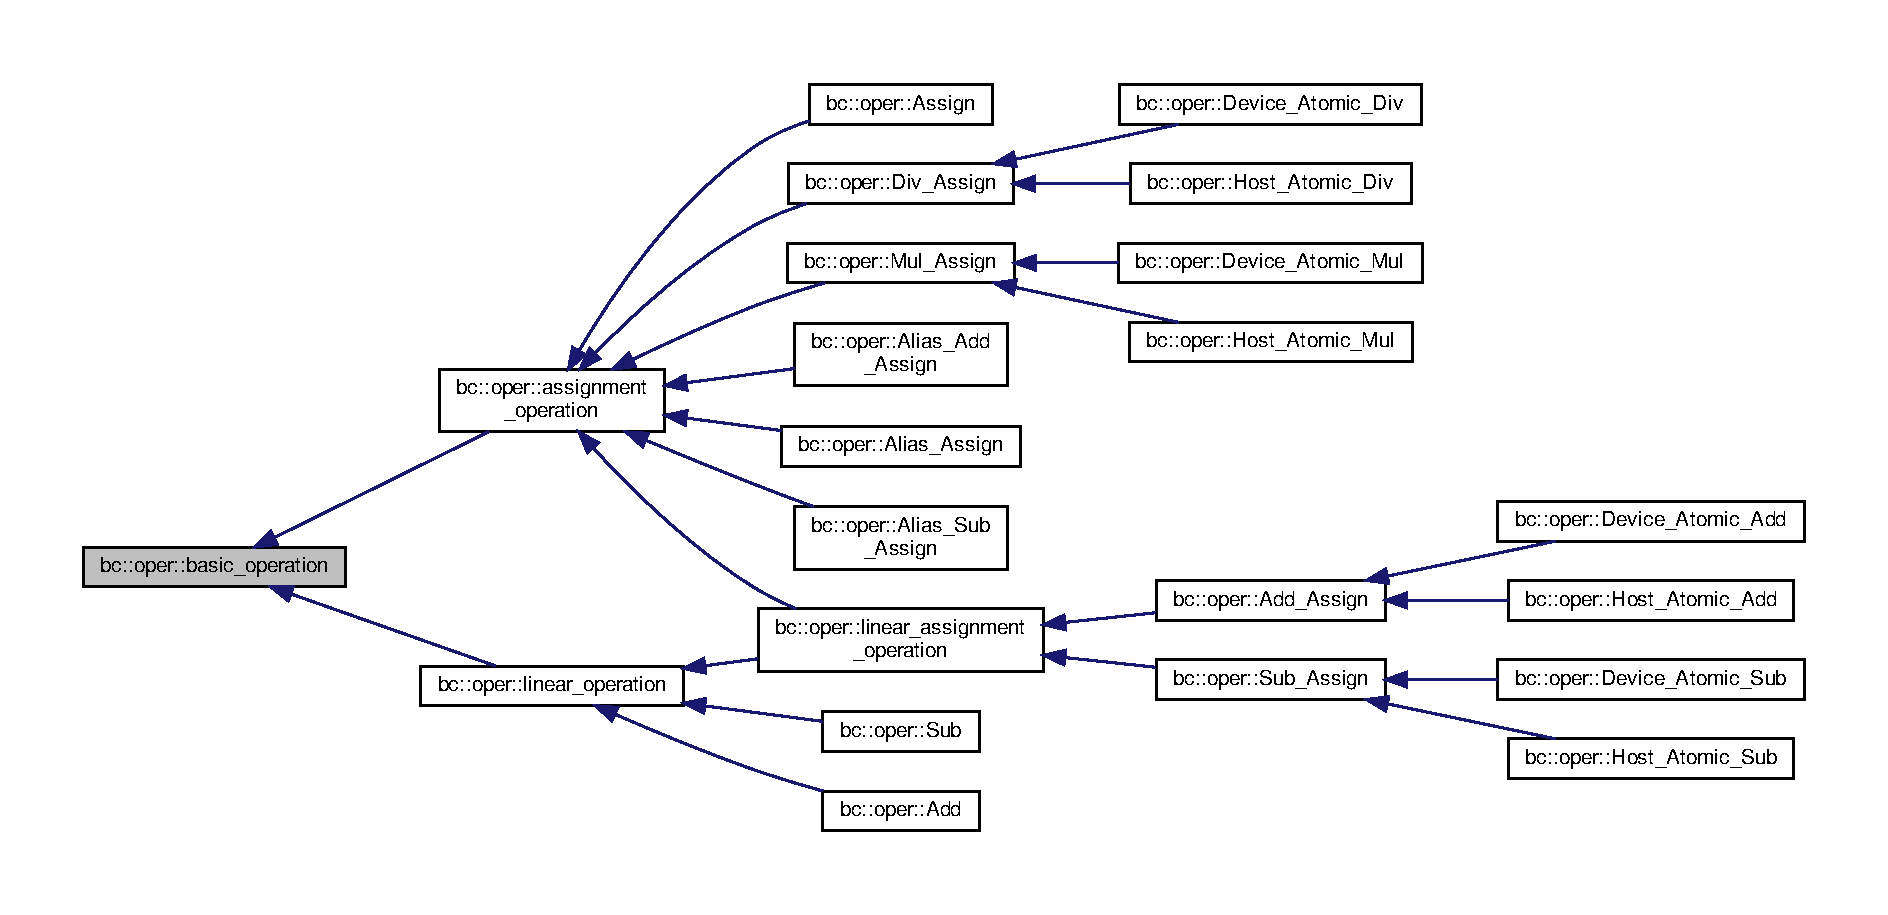
\includegraphics[width=350pt]{structbc_1_1oper_1_1basic__operation__inherit__graph}
\end{center}
\end{figure}


The documentation for this struct was generated from the following file\+:\begin{DoxyCompactItemize}
\item 
blackcat/operations/\hyperlink{tags_8h}{tags.\+h}\end{DoxyCompactItemize}

\hypertarget{classbc_1_1tensors_1_1exprs_1_1BC__Const__View}{}\section{bc\+:\+:tensors\+:\+:exprs\+:\+:B\+C\+\_\+\+Const\+\_\+\+View Class Reference}
\label{classbc_1_1tensors_1_1exprs_1_1BC__Const__View}\index{bc\+::tensors\+::exprs\+::\+B\+C\+\_\+\+Const\+\_\+\+View@{bc\+::tensors\+::exprs\+::\+B\+C\+\_\+\+Const\+\_\+\+View}}


{\ttfamily \#include $<$expression\+\_\+template\+\_\+traits.\+h$>$}



The documentation for this class was generated from the following file\+:\begin{DoxyCompactItemize}
\item 
blackcat/tensors/expression\+\_\+templates/\hyperlink{expression__template__traits_8h}{expression\+\_\+template\+\_\+traits.\+h}\end{DoxyCompactItemize}

\hypertarget{classbc_1_1tensors_1_1exprs_1_1BC__View}{}\section{bc\+:\+:tensors\+:\+:exprs\+:\+:B\+C\+\_\+\+View Class Reference}
\label{classbc_1_1tensors_1_1exprs_1_1BC__View}\index{bc\+::tensors\+::exprs\+::\+B\+C\+\_\+\+View@{bc\+::tensors\+::exprs\+::\+B\+C\+\_\+\+View}}


{\ttfamily \#include $<$expression\+\_\+template\+\_\+traits.\+h$>$}



The documentation for this class was generated from the following file\+:\begin{DoxyCompactItemize}
\item 
blackcat/tensors/expression\+\_\+templates/\hyperlink{expression__template__traits_8h}{expression\+\_\+template\+\_\+traits.\+h}\end{DoxyCompactItemize}

\hypertarget{structbc_1_1tensors_1_1exprs_1_1detail_1_1bin__expr__factory}{}\section{bc\+:\+:tensors\+:\+:exprs\+:\+:detail\+:\+:bin\+\_\+expr\+\_\+factory$<$ Op, Lv, Rv, class $>$ Struct Template Reference}
\label{structbc_1_1tensors_1_1exprs_1_1detail_1_1bin__expr__factory}\index{bc\+::tensors\+::exprs\+::detail\+::bin\+\_\+expr\+\_\+factory$<$ Op, Lv, Rv, class $>$@{bc\+::tensors\+::exprs\+::detail\+::bin\+\_\+expr\+\_\+factory$<$ Op, Lv, Rv, class $>$}}


{\ttfamily \#include $<$expression\+\_\+binary.\+h$>$}

\subsection*{Static Public Member Functions}
\begin{DoxyCompactItemize}
\item 
{\footnotesize template$<$class... Args$>$ }\\static auto \hyperlink{structbc_1_1tensors_1_1exprs_1_1detail_1_1bin__expr__factory_a64c4b332e8688677ff904c7fb7d6e7a1}{make} (Lv lv, Rv rv, Args \&\&... args)
\end{DoxyCompactItemize}


\subsection{Member Function Documentation}
\mbox{\Hypertarget{structbc_1_1tensors_1_1exprs_1_1detail_1_1bin__expr__factory_a64c4b332e8688677ff904c7fb7d6e7a1}\label{structbc_1_1tensors_1_1exprs_1_1detail_1_1bin__expr__factory_a64c4b332e8688677ff904c7fb7d6e7a1}} 
\index{bc\+::tensors\+::exprs\+::detail\+::bin\+\_\+expr\+\_\+factory@{bc\+::tensors\+::exprs\+::detail\+::bin\+\_\+expr\+\_\+factory}!make@{make}}
\index{make@{make}!bc\+::tensors\+::exprs\+::detail\+::bin\+\_\+expr\+\_\+factory@{bc\+::tensors\+::exprs\+::detail\+::bin\+\_\+expr\+\_\+factory}}
\subsubsection{\texorpdfstring{make()}{make()}}
{\footnotesize\ttfamily template$<$class Op , class Lv , class Rv , class  = void$>$ \\
template$<$class... Args$>$ \\
static auto \hyperlink{structbc_1_1tensors_1_1exprs_1_1detail_1_1bin__expr__factory}{bc\+::tensors\+::exprs\+::detail\+::bin\+\_\+expr\+\_\+factory}$<$ Op, Lv, Rv, class $>$\+::make (\begin{DoxyParamCaption}\item[{Lv}]{lv,  }\item[{Rv}]{rv,  }\item[{Args \&\&...}]{args }\end{DoxyParamCaption})\hspace{0.3cm}{\ttfamily [inline]}, {\ttfamily [static]}}



The documentation for this struct was generated from the following file\+:\begin{DoxyCompactItemize}
\item 
blackcat/tensors/expression\+\_\+templates/\hyperlink{expression__binary_8h}{expression\+\_\+binary.\+h}\end{DoxyCompactItemize}

\hypertarget{structbc_1_1tensors_1_1exprs_1_1detail_1_1bin__expr__factory_3_01Add_00_01Lv_00_01Un__Op_3_01Negation_00_01Rv_01_4_01_4}{}\section{bc\+:\+:tensors\+:\+:exprs\+:\+:detail\+:\+:bin\+\_\+expr\+\_\+factory$<$ Add, Lv, Un\+\_\+\+Op$<$ Negation, Rv $>$ $>$ Struct Template Reference}
\label{structbc_1_1tensors_1_1exprs_1_1detail_1_1bin__expr__factory_3_01Add_00_01Lv_00_01Un__Op_3_01Negation_00_01Rv_01_4_01_4}\index{bc\+::tensors\+::exprs\+::detail\+::bin\+\_\+expr\+\_\+factory$<$ Add, Lv, Un\+\_\+\+Op$<$ Negation, Rv $>$ $>$@{bc\+::tensors\+::exprs\+::detail\+::bin\+\_\+expr\+\_\+factory$<$ Add, Lv, Un\+\_\+\+Op$<$ Negation, Rv $>$ $>$}}


y + (-\/x) -\/$>$ y -\/ x  




{\ttfamily \#include $<$expression\+\_\+binary.\+h$>$}

\subsection*{Static Public Member Functions}
\begin{DoxyCompactItemize}
\item 
{\footnotesize template$<$class... Args$>$ }\\static auto \hyperlink{structbc_1_1tensors_1_1exprs_1_1detail_1_1bin__expr__factory_3_01Add_00_01Lv_00_01Un__Op_3_01Negation_00_01Rv_01_4_01_4_a944b39251590d4173c2b26fb485863e2}{make} (Lv lv, \hyperlink{structbc_1_1tensors_1_1exprs_1_1Un__Op}{Un\+\_\+\+Op}$<$ \hyperlink{structbc_1_1oper_1_1Negation}{Negation}, Rv $>$ rv, Args \&\&... args)
\end{DoxyCompactItemize}


\subsection{Detailed Description}
\subsubsection*{template$<$class Lv, class Rv$>$\newline
struct bc\+::tensors\+::exprs\+::detail\+::bin\+\_\+expr\+\_\+factory$<$ Add, Lv, Un\+\_\+\+Op$<$ Negation, Rv $>$ $>$}

y + (-\/x) -\/$>$ y -\/ x 

\subsection{Member Function Documentation}
\mbox{\Hypertarget{structbc_1_1tensors_1_1exprs_1_1detail_1_1bin__expr__factory_3_01Add_00_01Lv_00_01Un__Op_3_01Negation_00_01Rv_01_4_01_4_a944b39251590d4173c2b26fb485863e2}\label{structbc_1_1tensors_1_1exprs_1_1detail_1_1bin__expr__factory_3_01Add_00_01Lv_00_01Un__Op_3_01Negation_00_01Rv_01_4_01_4_a944b39251590d4173c2b26fb485863e2}} 
\index{bc\+::tensors\+::exprs\+::detail\+::bin\+\_\+expr\+\_\+factory$<$ Add, Lv, Un\+\_\+\+Op$<$ Negation, Rv $>$ $>$@{bc\+::tensors\+::exprs\+::detail\+::bin\+\_\+expr\+\_\+factory$<$ Add, Lv, Un\+\_\+\+Op$<$ Negation, Rv $>$ $>$}!make@{make}}
\index{make@{make}!bc\+::tensors\+::exprs\+::detail\+::bin\+\_\+expr\+\_\+factory$<$ Add, Lv, Un\+\_\+\+Op$<$ Negation, Rv $>$ $>$@{bc\+::tensors\+::exprs\+::detail\+::bin\+\_\+expr\+\_\+factory$<$ Add, Lv, Un\+\_\+\+Op$<$ Negation, Rv $>$ $>$}}
\subsubsection{\texorpdfstring{make()}{make()}}
{\footnotesize\ttfamily template$<$class Lv , class Rv $>$ \\
template$<$class... Args$>$ \\
static auto \hyperlink{structbc_1_1tensors_1_1exprs_1_1detail_1_1bin__expr__factory}{bc\+::tensors\+::exprs\+::detail\+::bin\+\_\+expr\+\_\+factory}$<$ \hyperlink{structbc_1_1oper_1_1Add}{Add}, Lv, \hyperlink{structbc_1_1tensors_1_1exprs_1_1Un__Op}{Un\+\_\+\+Op}$<$ \hyperlink{structbc_1_1oper_1_1Negation}{Negation}, Rv $>$ $>$\+::make (\begin{DoxyParamCaption}\item[{Lv}]{lv,  }\item[{\hyperlink{structbc_1_1tensors_1_1exprs_1_1Un__Op}{Un\+\_\+\+Op}$<$ \hyperlink{structbc_1_1oper_1_1Negation}{Negation}, Rv $>$}]{rv,  }\item[{Args \&\&...}]{args }\end{DoxyParamCaption})\hspace{0.3cm}{\ttfamily [inline]}, {\ttfamily [static]}}



The documentation for this struct was generated from the following file\+:\begin{DoxyCompactItemize}
\item 
blackcat/tensors/expression\+\_\+templates/\hyperlink{expression__binary_8h}{expression\+\_\+binary.\+h}\end{DoxyCompactItemize}

\hypertarget{structbc_1_1tensors_1_1exprs_1_1detail_1_1bin__expr__factory_3_01Add_00_01Un__Op_3_01Negation_00d86892bae805f04f4b10908e626a3cb5}{}\section{bc\+:\+:tensors\+:\+:exprs\+:\+:detail\+:\+:bin\+\_\+expr\+\_\+factory$<$ Add, Un\+\_\+\+Op$<$ Negation, Lv $>$, Un\+\_\+\+Op$<$ Negation, Rv $>$ $>$ Struct Template Reference}
\label{structbc_1_1tensors_1_1exprs_1_1detail_1_1bin__expr__factory_3_01Add_00_01Un__Op_3_01Negation_00d86892bae805f04f4b10908e626a3cb5}\index{bc\+::tensors\+::exprs\+::detail\+::bin\+\_\+expr\+\_\+factory$<$ Add, Un\+\_\+\+Op$<$ Negation, Lv $>$, Un\+\_\+\+Op$<$ Negation, Rv $>$ $>$@{bc\+::tensors\+::exprs\+::detail\+::bin\+\_\+expr\+\_\+factory$<$ Add, Un\+\_\+\+Op$<$ Negation, Lv $>$, Un\+\_\+\+Op$<$ Negation, Rv $>$ $>$}}


(-\/y) + (-\/x) -\/$>$ (-\/y) -\/ x //specialized to handle ambiguous overload  




{\ttfamily \#include $<$expression\+\_\+binary.\+h$>$}

\subsection*{Static Public Member Functions}
\begin{DoxyCompactItemize}
\item 
{\footnotesize template$<$class... Args$>$ }\\static auto \hyperlink{structbc_1_1tensors_1_1exprs_1_1detail_1_1bin__expr__factory_3_01Add_00_01Un__Op_3_01Negation_00d86892bae805f04f4b10908e626a3cb5_a4fbf9c3516c874ac3aaa77d22a167694}{make} (\hyperlink{structbc_1_1tensors_1_1exprs_1_1Un__Op}{Un\+\_\+\+Op}$<$ \hyperlink{structbc_1_1oper_1_1Negation}{Negation}, Lv $>$ lv, \hyperlink{structbc_1_1tensors_1_1exprs_1_1Un__Op}{Un\+\_\+\+Op}$<$ \hyperlink{structbc_1_1oper_1_1Negation}{Negation}, Rv $>$ rv, Args \&\&... args)
\end{DoxyCompactItemize}


\subsection{Detailed Description}
\subsubsection*{template$<$class Lv, class Rv$>$\newline
struct bc\+::tensors\+::exprs\+::detail\+::bin\+\_\+expr\+\_\+factory$<$ Add, Un\+\_\+\+Op$<$ Negation, Lv $>$, Un\+\_\+\+Op$<$ Negation, Rv $>$ $>$}

(-\/y) + (-\/x) -\/$>$ (-\/y) -\/ x //specialized to handle ambiguous overload 

\subsection{Member Function Documentation}
\mbox{\Hypertarget{structbc_1_1tensors_1_1exprs_1_1detail_1_1bin__expr__factory_3_01Add_00_01Un__Op_3_01Negation_00d86892bae805f04f4b10908e626a3cb5_a4fbf9c3516c874ac3aaa77d22a167694}\label{structbc_1_1tensors_1_1exprs_1_1detail_1_1bin__expr__factory_3_01Add_00_01Un__Op_3_01Negation_00d86892bae805f04f4b10908e626a3cb5_a4fbf9c3516c874ac3aaa77d22a167694}} 
\index{bc\+::tensors\+::exprs\+::detail\+::bin\+\_\+expr\+\_\+factory$<$ Add, Un\+\_\+\+Op$<$ Negation, Lv $>$, Un\+\_\+\+Op$<$ Negation, Rv $>$ $>$@{bc\+::tensors\+::exprs\+::detail\+::bin\+\_\+expr\+\_\+factory$<$ Add, Un\+\_\+\+Op$<$ Negation, Lv $>$, Un\+\_\+\+Op$<$ Negation, Rv $>$ $>$}!make@{make}}
\index{make@{make}!bc\+::tensors\+::exprs\+::detail\+::bin\+\_\+expr\+\_\+factory$<$ Add, Un\+\_\+\+Op$<$ Negation, Lv $>$, Un\+\_\+\+Op$<$ Negation, Rv $>$ $>$@{bc\+::tensors\+::exprs\+::detail\+::bin\+\_\+expr\+\_\+factory$<$ Add, Un\+\_\+\+Op$<$ Negation, Lv $>$, Un\+\_\+\+Op$<$ Negation, Rv $>$ $>$}}
\subsubsection{\texorpdfstring{make()}{make()}}
{\footnotesize\ttfamily template$<$class Lv , class Rv $>$ \\
template$<$class... Args$>$ \\
static auto \hyperlink{structbc_1_1tensors_1_1exprs_1_1detail_1_1bin__expr__factory}{bc\+::tensors\+::exprs\+::detail\+::bin\+\_\+expr\+\_\+factory}$<$ \hyperlink{structbc_1_1oper_1_1Add}{Add}, \hyperlink{structbc_1_1tensors_1_1exprs_1_1Un__Op}{Un\+\_\+\+Op}$<$ \hyperlink{structbc_1_1oper_1_1Negation}{Negation}, Lv $>$, \hyperlink{structbc_1_1tensors_1_1exprs_1_1Un__Op}{Un\+\_\+\+Op}$<$ \hyperlink{structbc_1_1oper_1_1Negation}{Negation}, Rv $>$ $>$\+::make (\begin{DoxyParamCaption}\item[{\hyperlink{structbc_1_1tensors_1_1exprs_1_1Un__Op}{Un\+\_\+\+Op}$<$ \hyperlink{structbc_1_1oper_1_1Negation}{Negation}, Lv $>$}]{lv,  }\item[{\hyperlink{structbc_1_1tensors_1_1exprs_1_1Un__Op}{Un\+\_\+\+Op}$<$ \hyperlink{structbc_1_1oper_1_1Negation}{Negation}, Rv $>$}]{rv,  }\item[{Args \&\&...}]{args }\end{DoxyParamCaption})\hspace{0.3cm}{\ttfamily [inline]}, {\ttfamily [static]}}



The documentation for this struct was generated from the following file\+:\begin{DoxyCompactItemize}
\item 
blackcat/tensors/expression\+\_\+templates/\hyperlink{expression__binary_8h}{expression\+\_\+binary.\+h}\end{DoxyCompactItemize}

\hypertarget{structbc_1_1tensors_1_1exprs_1_1detail_1_1bin__expr__factory_3_01Add__Assign_00_01Lv_00_01Un__Op_3_01Negation_00_01Rv_01_4_01_4}{}\section{bc\+:\+:tensors\+:\+:exprs\+:\+:detail\+:\+:bin\+\_\+expr\+\_\+factory$<$ Add\+\_\+\+Assign, Lv, Un\+\_\+\+Op$<$ Negation, Rv $>$ $>$ Struct Template Reference}
\label{structbc_1_1tensors_1_1exprs_1_1detail_1_1bin__expr__factory_3_01Add__Assign_00_01Lv_00_01Un__Op_3_01Negation_00_01Rv_01_4_01_4}\index{bc\+::tensors\+::exprs\+::detail\+::bin\+\_\+expr\+\_\+factory$<$ Add\+\_\+\+Assign, Lv, Un\+\_\+\+Op$<$ Negation, Rv $>$ $>$@{bc\+::tensors\+::exprs\+::detail\+::bin\+\_\+expr\+\_\+factory$<$ Add\+\_\+\+Assign, Lv, Un\+\_\+\+Op$<$ Negation, Rv $>$ $>$}}


y += (-\/x) -\/$>$ y -\/= x  




{\ttfamily \#include $<$expression\+\_\+binary.\+h$>$}

\subsection*{Static Public Member Functions}
\begin{DoxyCompactItemize}
\item 
{\footnotesize template$<$class... Args$>$ }\\static auto \hyperlink{structbc_1_1tensors_1_1exprs_1_1detail_1_1bin__expr__factory_3_01Add__Assign_00_01Lv_00_01Un__Op_3_01Negation_00_01Rv_01_4_01_4_a9a226059ff726a8da6c8508ab621bb4f}{make} (Lv lv, \hyperlink{structbc_1_1tensors_1_1exprs_1_1Un__Op}{Un\+\_\+\+Op}$<$ \hyperlink{structbc_1_1oper_1_1Negation}{Negation}, Rv $>$ rv, Args \&\&... args)
\end{DoxyCompactItemize}


\subsection{Detailed Description}
\subsubsection*{template$<$class Lv, class Rv$>$\newline
struct bc\+::tensors\+::exprs\+::detail\+::bin\+\_\+expr\+\_\+factory$<$ Add\+\_\+\+Assign, Lv, Un\+\_\+\+Op$<$ Negation, Rv $>$ $>$}

y += (-\/x) -\/$>$ y -\/= x 

\subsection{Member Function Documentation}
\mbox{\Hypertarget{structbc_1_1tensors_1_1exprs_1_1detail_1_1bin__expr__factory_3_01Add__Assign_00_01Lv_00_01Un__Op_3_01Negation_00_01Rv_01_4_01_4_a9a226059ff726a8da6c8508ab621bb4f}\label{structbc_1_1tensors_1_1exprs_1_1detail_1_1bin__expr__factory_3_01Add__Assign_00_01Lv_00_01Un__Op_3_01Negation_00_01Rv_01_4_01_4_a9a226059ff726a8da6c8508ab621bb4f}} 
\index{bc\+::tensors\+::exprs\+::detail\+::bin\+\_\+expr\+\_\+factory$<$ Add\+\_\+\+Assign, Lv, Un\+\_\+\+Op$<$ Negation, Rv $>$ $>$@{bc\+::tensors\+::exprs\+::detail\+::bin\+\_\+expr\+\_\+factory$<$ Add\+\_\+\+Assign, Lv, Un\+\_\+\+Op$<$ Negation, Rv $>$ $>$}!make@{make}}
\index{make@{make}!bc\+::tensors\+::exprs\+::detail\+::bin\+\_\+expr\+\_\+factory$<$ Add\+\_\+\+Assign, Lv, Un\+\_\+\+Op$<$ Negation, Rv $>$ $>$@{bc\+::tensors\+::exprs\+::detail\+::bin\+\_\+expr\+\_\+factory$<$ Add\+\_\+\+Assign, Lv, Un\+\_\+\+Op$<$ Negation, Rv $>$ $>$}}
\subsubsection{\texorpdfstring{make()}{make()}}
{\footnotesize\ttfamily template$<$class Lv , class Rv $>$ \\
template$<$class... Args$>$ \\
static auto \hyperlink{structbc_1_1tensors_1_1exprs_1_1detail_1_1bin__expr__factory}{bc\+::tensors\+::exprs\+::detail\+::bin\+\_\+expr\+\_\+factory}$<$ \hyperlink{structbc_1_1oper_1_1Add__Assign}{Add\+\_\+\+Assign}, Lv, \hyperlink{structbc_1_1tensors_1_1exprs_1_1Un__Op}{Un\+\_\+\+Op}$<$ \hyperlink{structbc_1_1oper_1_1Negation}{Negation}, Rv $>$ $>$\+::make (\begin{DoxyParamCaption}\item[{Lv}]{lv,  }\item[{\hyperlink{structbc_1_1tensors_1_1exprs_1_1Un__Op}{Un\+\_\+\+Op}$<$ \hyperlink{structbc_1_1oper_1_1Negation}{Negation}, Rv $>$}]{rv,  }\item[{Args \&\&...}]{args }\end{DoxyParamCaption})\hspace{0.3cm}{\ttfamily [inline]}, {\ttfamily [static]}}



The documentation for this struct was generated from the following file\+:\begin{DoxyCompactItemize}
\item 
blackcat/tensors/expression\+\_\+templates/\hyperlink{expression__binary_8h}{expression\+\_\+binary.\+h}\end{DoxyCompactItemize}

\hypertarget{structbc_1_1tensors_1_1exprs_1_1detail_1_1bin__expr__factory_3_01bc_1_1oper_1_1Scalar__Mul_00_0179bec0862a78086fe62692cba7b203b3}{}\section{bc\+:\+:tensors\+:\+:exprs\+:\+:detail\+:\+:bin\+\_\+expr\+\_\+factory$<$ bc\+:\+:oper\+:\+:Scalar\+\_\+\+Mul, Lv, Rv, std\+:\+:enable\+\_\+if\+\_\+t$<$ expression\+\_\+traits$<$ Lv $>$\+:\+:is\+\_\+blas\+\_\+expression\+:\+:value !=expression\+\_\+traits$<$ Rv $>$\+:\+:is\+\_\+blas\+\_\+expression\+:\+:value $>$ $>$ Struct Template Reference}
\label{structbc_1_1tensors_1_1exprs_1_1detail_1_1bin__expr__factory_3_01bc_1_1oper_1_1Scalar__Mul_00_0179bec0862a78086fe62692cba7b203b3}\index{bc\+::tensors\+::exprs\+::detail\+::bin\+\_\+expr\+\_\+factory$<$ bc\+::oper\+::\+Scalar\+\_\+\+Mul, Lv, Rv, std\+::enable\+\_\+if\+\_\+t$<$ expression\+\_\+traits$<$ Lv $>$\+::is\+\_\+blas\+\_\+expression\+::value "!=expression\+\_\+traits$<$ Rv $>$\+::is\+\_\+blas\+\_\+expression\+::value $>$ $>$@{bc\+::tensors\+::exprs\+::detail\+::bin\+\_\+expr\+\_\+factory$<$ bc\+::oper\+::\+Scalar\+\_\+\+Mul, Lv, Rv, std\+::enable\+\_\+if\+\_\+t$<$ expression\+\_\+traits$<$ Lv $>$\+::is\+\_\+blas\+\_\+expression\+::value "!=expression\+\_\+traits$<$ Rv $>$\+::is\+\_\+blas\+\_\+expression\+::value $>$ $>$}}


scalar $\ast$ blas\+\_\+op(a, b) -\/$>$ blas\+\_\+op(a $\ast$ scalar, b) $\vert$$\vert$ blas\+\_\+op(a, b $\ast$ scalar)  




{\ttfamily \#include $<$expression\+\_\+binary.\+h$>$}

\subsection*{Static Public Member Functions}
\begin{DoxyCompactItemize}
\item 
static auto \hyperlink{structbc_1_1tensors_1_1exprs_1_1detail_1_1bin__expr__factory_3_01bc_1_1oper_1_1Scalar__Mul_00_0179bec0862a78086fe62692cba7b203b3_abca15f77a3ff6aa85ba17a94e4eb5a28}{make} (Lv lv, Rv rv, \hyperlink{structbc_1_1oper_1_1Scalar__Mul}{Scalar\+\_\+\+Mul} op=\hyperlink{structbc_1_1oper_1_1Scalar__Mul}{Scalar\+\_\+\+Mul}())
\end{DoxyCompactItemize}


\subsection{Detailed Description}
\subsubsection*{template$<$class Lv, class Rv$>$\newline
struct bc\+::tensors\+::exprs\+::detail\+::bin\+\_\+expr\+\_\+factory$<$ bc\+::oper\+::\+Scalar\+\_\+\+Mul, Lv, Rv, std\+::enable\+\_\+if\+\_\+t$<$ expression\+\_\+traits$<$ Lv $>$\+::is\+\_\+blas\+\_\+expression\+::value !=expression\+\_\+traits$<$ Rv $>$\+::is\+\_\+blas\+\_\+expression\+::value $>$ $>$}

scalar $\ast$ blas\+\_\+op(a, b) -\/$>$ blas\+\_\+op(a $\ast$ scalar, b) $\vert$$\vert$ blas\+\_\+op(a, b $\ast$ scalar) 

\subsection{Member Function Documentation}
\mbox{\Hypertarget{structbc_1_1tensors_1_1exprs_1_1detail_1_1bin__expr__factory_3_01bc_1_1oper_1_1Scalar__Mul_00_0179bec0862a78086fe62692cba7b203b3_abca15f77a3ff6aa85ba17a94e4eb5a28}\label{structbc_1_1tensors_1_1exprs_1_1detail_1_1bin__expr__factory_3_01bc_1_1oper_1_1Scalar__Mul_00_0179bec0862a78086fe62692cba7b203b3_abca15f77a3ff6aa85ba17a94e4eb5a28}} 
\index{bc\+::tensors\+::exprs\+::detail\+::bin\+\_\+expr\+\_\+factory$<$ bc\+::oper\+::\+Scalar\+\_\+\+Mul, Lv, Rv, std\+::enable\+\_\+if\+\_\+t$<$ expression\+\_\+traits$<$ Lv $>$\+::is\+\_\+blas\+\_\+expression\+::value "!=expression\+\_\+traits$<$ Rv $>$\+::is\+\_\+blas\+\_\+expression\+::value $>$ $>$@{bc\+::tensors\+::exprs\+::detail\+::bin\+\_\+expr\+\_\+factory$<$ bc\+::oper\+::\+Scalar\+\_\+\+Mul, Lv, Rv, std\+::enable\+\_\+if\+\_\+t$<$ expression\+\_\+traits$<$ Lv $>$\+::is\+\_\+blas\+\_\+expression\+::value "!=expression\+\_\+traits$<$ Rv $>$\+::is\+\_\+blas\+\_\+expression\+::value $>$ $>$}!make@{make}}
\index{make@{make}!bc\+::tensors\+::exprs\+::detail\+::bin\+\_\+expr\+\_\+factory$<$ bc\+::oper\+::\+Scalar\+\_\+\+Mul, Lv, Rv, std\+::enable\+\_\+if\+\_\+t$<$ expression\+\_\+traits$<$ Lv $>$\+::is\+\_\+blas\+\_\+expression\+::value "!=expression\+\_\+traits$<$ Rv $>$\+::is\+\_\+blas\+\_\+expression\+::value $>$ $>$@{bc\+::tensors\+::exprs\+::detail\+::bin\+\_\+expr\+\_\+factory$<$ bc\+::oper\+::\+Scalar\+\_\+\+Mul, Lv, Rv, std\+::enable\+\_\+if\+\_\+t$<$ expression\+\_\+traits$<$ Lv $>$\+::is\+\_\+blas\+\_\+expression\+::value "!=expression\+\_\+traits$<$ Rv $>$\+::is\+\_\+blas\+\_\+expression\+::value $>$ $>$}}
\subsubsection{\texorpdfstring{make()}{make()}}
{\footnotesize\ttfamily template$<$class Lv , class Rv $>$ \\
static auto \hyperlink{structbc_1_1tensors_1_1exprs_1_1detail_1_1bin__expr__factory}{bc\+::tensors\+::exprs\+::detail\+::bin\+\_\+expr\+\_\+factory}$<$ \hyperlink{structbc_1_1oper_1_1Scalar__Mul}{bc\+::oper\+::\+Scalar\+\_\+\+Mul}, Lv, Rv, std\+::enable\+\_\+if\+\_\+t$<$ \hyperlink{structbc_1_1tensors_1_1exprs_1_1expression__traits}{expression\+\_\+traits}$<$ Lv $>$\+::is\+\_\+blas\+\_\+expression\+::value !=\hyperlink{structbc_1_1tensors_1_1exprs_1_1expression__traits}{expression\+\_\+traits}$<$ Rv $>$\+::is\+\_\+blas\+\_\+expression\+::value $>$ $>$\+::make (\begin{DoxyParamCaption}\item[{Lv}]{lv,  }\item[{Rv}]{rv,  }\item[{\hyperlink{structbc_1_1oper_1_1Scalar__Mul}{Scalar\+\_\+\+Mul}}]{op = {\ttfamily \hyperlink{structbc_1_1oper_1_1Scalar__Mul}{Scalar\+\_\+\+Mul}()} }\end{DoxyParamCaption})\hspace{0.3cm}{\ttfamily [inline]}, {\ttfamily [static]}}



The documentation for this struct was generated from the following file\+:\begin{DoxyCompactItemize}
\item 
blackcat/tensors/expression\+\_\+templates/\hyperlink{expression__binary_8h}{expression\+\_\+binary.\+h}\end{DoxyCompactItemize}

\hypertarget{structbc_1_1tensors_1_1exprs_1_1detail_1_1bin__expr__factory_3_01Sub_00_01Lv_00_01Un__Op_3_01Negation_00_01Rv_01_4_01_4}{}\section{bc\+:\+:tensors\+:\+:exprs\+:\+:detail\+:\+:bin\+\_\+expr\+\_\+factory$<$ Sub, Lv, Un\+\_\+\+Op$<$ Negation, Rv $>$ $>$ Struct Template Reference}
\label{structbc_1_1tensors_1_1exprs_1_1detail_1_1bin__expr__factory_3_01Sub_00_01Lv_00_01Un__Op_3_01Negation_00_01Rv_01_4_01_4}\index{bc\+::tensors\+::exprs\+::detail\+::bin\+\_\+expr\+\_\+factory$<$ Sub, Lv, Un\+\_\+\+Op$<$ Negation, Rv $>$ $>$@{bc\+::tensors\+::exprs\+::detail\+::bin\+\_\+expr\+\_\+factory$<$ Sub, Lv, Un\+\_\+\+Op$<$ Negation, Rv $>$ $>$}}


y -\/ (-\/x) -\/$>$ y + x  




{\ttfamily \#include $<$expression\+\_\+binary.\+h$>$}

\subsection*{Static Public Member Functions}
\begin{DoxyCompactItemize}
\item 
{\footnotesize template$<$class... Args$>$ }\\static auto \hyperlink{structbc_1_1tensors_1_1exprs_1_1detail_1_1bin__expr__factory_3_01Sub_00_01Lv_00_01Un__Op_3_01Negation_00_01Rv_01_4_01_4_af5b947051f47ac53f36b8b0e07708c50}{make} (Lv lv, \hyperlink{structbc_1_1tensors_1_1exprs_1_1Un__Op}{Un\+\_\+\+Op}$<$ \hyperlink{structbc_1_1oper_1_1Negation}{Negation}, Rv $>$ rv, Args \&\&... args)
\end{DoxyCompactItemize}


\subsection{Detailed Description}
\subsubsection*{template$<$class Lv, class Rv$>$\newline
struct bc\+::tensors\+::exprs\+::detail\+::bin\+\_\+expr\+\_\+factory$<$ Sub, Lv, Un\+\_\+\+Op$<$ Negation, Rv $>$ $>$}

y -\/ (-\/x) -\/$>$ y + x 

\subsection{Member Function Documentation}
\mbox{\Hypertarget{structbc_1_1tensors_1_1exprs_1_1detail_1_1bin__expr__factory_3_01Sub_00_01Lv_00_01Un__Op_3_01Negation_00_01Rv_01_4_01_4_af5b947051f47ac53f36b8b0e07708c50}\label{structbc_1_1tensors_1_1exprs_1_1detail_1_1bin__expr__factory_3_01Sub_00_01Lv_00_01Un__Op_3_01Negation_00_01Rv_01_4_01_4_af5b947051f47ac53f36b8b0e07708c50}} 
\index{bc\+::tensors\+::exprs\+::detail\+::bin\+\_\+expr\+\_\+factory$<$ Sub, Lv, Un\+\_\+\+Op$<$ Negation, Rv $>$ $>$@{bc\+::tensors\+::exprs\+::detail\+::bin\+\_\+expr\+\_\+factory$<$ Sub, Lv, Un\+\_\+\+Op$<$ Negation, Rv $>$ $>$}!make@{make}}
\index{make@{make}!bc\+::tensors\+::exprs\+::detail\+::bin\+\_\+expr\+\_\+factory$<$ Sub, Lv, Un\+\_\+\+Op$<$ Negation, Rv $>$ $>$@{bc\+::tensors\+::exprs\+::detail\+::bin\+\_\+expr\+\_\+factory$<$ Sub, Lv, Un\+\_\+\+Op$<$ Negation, Rv $>$ $>$}}
\subsubsection{\texorpdfstring{make()}{make()}}
{\footnotesize\ttfamily template$<$class Lv , class Rv $>$ \\
template$<$class... Args$>$ \\
static auto \hyperlink{structbc_1_1tensors_1_1exprs_1_1detail_1_1bin__expr__factory}{bc\+::tensors\+::exprs\+::detail\+::bin\+\_\+expr\+\_\+factory}$<$ \hyperlink{structbc_1_1oper_1_1Sub}{Sub}, Lv, \hyperlink{structbc_1_1tensors_1_1exprs_1_1Un__Op}{Un\+\_\+\+Op}$<$ \hyperlink{structbc_1_1oper_1_1Negation}{Negation}, Rv $>$ $>$\+::make (\begin{DoxyParamCaption}\item[{Lv}]{lv,  }\item[{\hyperlink{structbc_1_1tensors_1_1exprs_1_1Un__Op}{Un\+\_\+\+Op}$<$ \hyperlink{structbc_1_1oper_1_1Negation}{Negation}, Rv $>$}]{rv,  }\item[{Args \&\&...}]{args }\end{DoxyParamCaption})\hspace{0.3cm}{\ttfamily [inline]}, {\ttfamily [static]}}



The documentation for this struct was generated from the following file\+:\begin{DoxyCompactItemize}
\item 
blackcat/tensors/expression\+\_\+templates/\hyperlink{expression__binary_8h}{expression\+\_\+binary.\+h}\end{DoxyCompactItemize}

\hypertarget{structbc_1_1tensors_1_1exprs_1_1detail_1_1bin__expr__factory_3_01Sub_00_01Un__Op_3_01Negation_00_01Lv_01_4_00_01Rv_01_4}{}\section{bc\+:\+:tensors\+:\+:exprs\+:\+:detail\+:\+:bin\+\_\+expr\+\_\+factory$<$ Sub, Un\+\_\+\+Op$<$ Negation, Lv $>$, Rv $>$ Struct Template Reference}
\label{structbc_1_1tensors_1_1exprs_1_1detail_1_1bin__expr__factory_3_01Sub_00_01Un__Op_3_01Negation_00_01Lv_01_4_00_01Rv_01_4}\index{bc\+::tensors\+::exprs\+::detail\+::bin\+\_\+expr\+\_\+factory$<$ Sub, Un\+\_\+\+Op$<$ Negation, Lv $>$, Rv $>$@{bc\+::tensors\+::exprs\+::detail\+::bin\+\_\+expr\+\_\+factory$<$ Sub, Un\+\_\+\+Op$<$ Negation, Lv $>$, Rv $>$}}


(-\/y) + x -\/$>$ x -\/ y  




{\ttfamily \#include $<$expression\+\_\+binary.\+h$>$}

\subsection*{Static Public Member Functions}
\begin{DoxyCompactItemize}
\item 
{\footnotesize template$<$class... Args$>$ }\\static auto \hyperlink{structbc_1_1tensors_1_1exprs_1_1detail_1_1bin__expr__factory_3_01Sub_00_01Un__Op_3_01Negation_00_01Lv_01_4_00_01Rv_01_4_aaf27f4570867ee57ce9f2ef8c6e11170}{make} (\hyperlink{structbc_1_1tensors_1_1exprs_1_1Un__Op}{Un\+\_\+\+Op}$<$ \hyperlink{structbc_1_1oper_1_1Negation}{Negation}, Lv $>$ lv, Rv rv, Args \&\&... args)
\end{DoxyCompactItemize}


\subsection{Detailed Description}
\subsubsection*{template$<$class Lv, class Rv$>$\newline
struct bc\+::tensors\+::exprs\+::detail\+::bin\+\_\+expr\+\_\+factory$<$ Sub, Un\+\_\+\+Op$<$ Negation, Lv $>$, Rv $>$}

(-\/y) + x -\/$>$ x -\/ y 

\subsection{Member Function Documentation}
\mbox{\Hypertarget{structbc_1_1tensors_1_1exprs_1_1detail_1_1bin__expr__factory_3_01Sub_00_01Un__Op_3_01Negation_00_01Lv_01_4_00_01Rv_01_4_aaf27f4570867ee57ce9f2ef8c6e11170}\label{structbc_1_1tensors_1_1exprs_1_1detail_1_1bin__expr__factory_3_01Sub_00_01Un__Op_3_01Negation_00_01Lv_01_4_00_01Rv_01_4_aaf27f4570867ee57ce9f2ef8c6e11170}} 
\index{bc\+::tensors\+::exprs\+::detail\+::bin\+\_\+expr\+\_\+factory$<$ Sub, Un\+\_\+\+Op$<$ Negation, Lv $>$, Rv $>$@{bc\+::tensors\+::exprs\+::detail\+::bin\+\_\+expr\+\_\+factory$<$ Sub, Un\+\_\+\+Op$<$ Negation, Lv $>$, Rv $>$}!make@{make}}
\index{make@{make}!bc\+::tensors\+::exprs\+::detail\+::bin\+\_\+expr\+\_\+factory$<$ Sub, Un\+\_\+\+Op$<$ Negation, Lv $>$, Rv $>$@{bc\+::tensors\+::exprs\+::detail\+::bin\+\_\+expr\+\_\+factory$<$ Sub, Un\+\_\+\+Op$<$ Negation, Lv $>$, Rv $>$}}
\subsubsection{\texorpdfstring{make()}{make()}}
{\footnotesize\ttfamily template$<$class Lv , class Rv $>$ \\
template$<$class... Args$>$ \\
static auto \hyperlink{structbc_1_1tensors_1_1exprs_1_1detail_1_1bin__expr__factory}{bc\+::tensors\+::exprs\+::detail\+::bin\+\_\+expr\+\_\+factory}$<$ \hyperlink{structbc_1_1oper_1_1Sub}{Sub}, \hyperlink{structbc_1_1tensors_1_1exprs_1_1Un__Op}{Un\+\_\+\+Op}$<$ \hyperlink{structbc_1_1oper_1_1Negation}{Negation}, Lv $>$, Rv $>$\+::make (\begin{DoxyParamCaption}\item[{\hyperlink{structbc_1_1tensors_1_1exprs_1_1Un__Op}{Un\+\_\+\+Op}$<$ \hyperlink{structbc_1_1oper_1_1Negation}{Negation}, Lv $>$}]{lv,  }\item[{Rv}]{rv,  }\item[{Args \&\&...}]{args }\end{DoxyParamCaption})\hspace{0.3cm}{\ttfamily [inline]}, {\ttfamily [static]}}



The documentation for this struct was generated from the following file\+:\begin{DoxyCompactItemize}
\item 
blackcat/tensors/expression\+\_\+templates/\hyperlink{expression__binary_8h}{expression\+\_\+binary.\+h}\end{DoxyCompactItemize}

\hypertarget{structbc_1_1tensors_1_1exprs_1_1detail_1_1bin__expr__factory_3_01Sub_00_01Un__Op_3_01Negation_004b0c12d341e754dc0e6fb842519b678e}{}\section{bc\+:\+:tensors\+:\+:exprs\+:\+:detail\+:\+:bin\+\_\+expr\+\_\+factory$<$ Sub, Un\+\_\+\+Op$<$ Negation, Lv $>$, Un\+\_\+\+Op$<$ Negation, Rv $>$ $>$ Struct Template Reference}
\label{structbc_1_1tensors_1_1exprs_1_1detail_1_1bin__expr__factory_3_01Sub_00_01Un__Op_3_01Negation_004b0c12d341e754dc0e6fb842519b678e}\index{bc\+::tensors\+::exprs\+::detail\+::bin\+\_\+expr\+\_\+factory$<$ Sub, Un\+\_\+\+Op$<$ Negation, Lv $>$, Un\+\_\+\+Op$<$ Negation, Rv $>$ $>$@{bc\+::tensors\+::exprs\+::detail\+::bin\+\_\+expr\+\_\+factory$<$ Sub, Un\+\_\+\+Op$<$ Negation, Lv $>$, Un\+\_\+\+Op$<$ Negation, Rv $>$ $>$}}


(-\/y) -\/ (-\/x) -\/$>$ x -\/ y //specialized to handle ambiguous overload  




{\ttfamily \#include $<$expression\+\_\+binary.\+h$>$}

\subsection*{Static Public Member Functions}
\begin{DoxyCompactItemize}
\item 
{\footnotesize template$<$class... Args$>$ }\\static auto \hyperlink{structbc_1_1tensors_1_1exprs_1_1detail_1_1bin__expr__factory_3_01Sub_00_01Un__Op_3_01Negation_004b0c12d341e754dc0e6fb842519b678e_a8a07d7a099fa54d9326ec02b21f30d4e}{make} (\hyperlink{structbc_1_1tensors_1_1exprs_1_1Un__Op}{Un\+\_\+\+Op}$<$ \hyperlink{structbc_1_1oper_1_1Negation}{Negation}, Lv $>$ lv, \hyperlink{structbc_1_1tensors_1_1exprs_1_1Un__Op}{Un\+\_\+\+Op}$<$ \hyperlink{structbc_1_1oper_1_1Negation}{Negation}, Rv $>$ rv, Args \&\&... args)
\end{DoxyCompactItemize}


\subsection{Detailed Description}
\subsubsection*{template$<$class Lv, class Rv$>$\newline
struct bc\+::tensors\+::exprs\+::detail\+::bin\+\_\+expr\+\_\+factory$<$ Sub, Un\+\_\+\+Op$<$ Negation, Lv $>$, Un\+\_\+\+Op$<$ Negation, Rv $>$ $>$}

(-\/y) -\/ (-\/x) -\/$>$ x -\/ y //specialized to handle ambiguous overload 

\subsection{Member Function Documentation}
\mbox{\Hypertarget{structbc_1_1tensors_1_1exprs_1_1detail_1_1bin__expr__factory_3_01Sub_00_01Un__Op_3_01Negation_004b0c12d341e754dc0e6fb842519b678e_a8a07d7a099fa54d9326ec02b21f30d4e}\label{structbc_1_1tensors_1_1exprs_1_1detail_1_1bin__expr__factory_3_01Sub_00_01Un__Op_3_01Negation_004b0c12d341e754dc0e6fb842519b678e_a8a07d7a099fa54d9326ec02b21f30d4e}} 
\index{bc\+::tensors\+::exprs\+::detail\+::bin\+\_\+expr\+\_\+factory$<$ Sub, Un\+\_\+\+Op$<$ Negation, Lv $>$, Un\+\_\+\+Op$<$ Negation, Rv $>$ $>$@{bc\+::tensors\+::exprs\+::detail\+::bin\+\_\+expr\+\_\+factory$<$ Sub, Un\+\_\+\+Op$<$ Negation, Lv $>$, Un\+\_\+\+Op$<$ Negation, Rv $>$ $>$}!make@{make}}
\index{make@{make}!bc\+::tensors\+::exprs\+::detail\+::bin\+\_\+expr\+\_\+factory$<$ Sub, Un\+\_\+\+Op$<$ Negation, Lv $>$, Un\+\_\+\+Op$<$ Negation, Rv $>$ $>$@{bc\+::tensors\+::exprs\+::detail\+::bin\+\_\+expr\+\_\+factory$<$ Sub, Un\+\_\+\+Op$<$ Negation, Lv $>$, Un\+\_\+\+Op$<$ Negation, Rv $>$ $>$}}
\subsubsection{\texorpdfstring{make()}{make()}}
{\footnotesize\ttfamily template$<$class Lv , class Rv $>$ \\
template$<$class... Args$>$ \\
static auto \hyperlink{structbc_1_1tensors_1_1exprs_1_1detail_1_1bin__expr__factory}{bc\+::tensors\+::exprs\+::detail\+::bin\+\_\+expr\+\_\+factory}$<$ \hyperlink{structbc_1_1oper_1_1Sub}{Sub}, \hyperlink{structbc_1_1tensors_1_1exprs_1_1Un__Op}{Un\+\_\+\+Op}$<$ \hyperlink{structbc_1_1oper_1_1Negation}{Negation}, Lv $>$, \hyperlink{structbc_1_1tensors_1_1exprs_1_1Un__Op}{Un\+\_\+\+Op}$<$ \hyperlink{structbc_1_1oper_1_1Negation}{Negation}, Rv $>$ $>$\+::make (\begin{DoxyParamCaption}\item[{\hyperlink{structbc_1_1tensors_1_1exprs_1_1Un__Op}{Un\+\_\+\+Op}$<$ \hyperlink{structbc_1_1oper_1_1Negation}{Negation}, Lv $>$}]{lv,  }\item[{\hyperlink{structbc_1_1tensors_1_1exprs_1_1Un__Op}{Un\+\_\+\+Op}$<$ \hyperlink{structbc_1_1oper_1_1Negation}{Negation}, Rv $>$}]{rv,  }\item[{Args \&\&...}]{args }\end{DoxyParamCaption})\hspace{0.3cm}{\ttfamily [inline]}, {\ttfamily [static]}}



The documentation for this struct was generated from the following file\+:\begin{DoxyCompactItemize}
\item 
blackcat/tensors/expression\+\_\+templates/\hyperlink{expression__binary_8h}{expression\+\_\+binary.\+h}\end{DoxyCompactItemize}

\hypertarget{structbc_1_1tensors_1_1exprs_1_1detail_1_1bin__expr__factory_3_01Sub__Assign_00_01Lv_00_01Un__Op_3_01Negation_00_01Rv_01_4_01_4}{}\section{bc\+:\+:tensors\+:\+:exprs\+:\+:detail\+:\+:bin\+\_\+expr\+\_\+factory$<$ Sub\+\_\+\+Assign, Lv, Un\+\_\+\+Op$<$ Negation, Rv $>$ $>$ Struct Template Reference}
\label{structbc_1_1tensors_1_1exprs_1_1detail_1_1bin__expr__factory_3_01Sub__Assign_00_01Lv_00_01Un__Op_3_01Negation_00_01Rv_01_4_01_4}\index{bc\+::tensors\+::exprs\+::detail\+::bin\+\_\+expr\+\_\+factory$<$ Sub\+\_\+\+Assign, Lv, Un\+\_\+\+Op$<$ Negation, Rv $>$ $>$@{bc\+::tensors\+::exprs\+::detail\+::bin\+\_\+expr\+\_\+factory$<$ Sub\+\_\+\+Assign, Lv, Un\+\_\+\+Op$<$ Negation, Rv $>$ $>$}}


y -\/= (-\/x) -\/$>$ y += x  




{\ttfamily \#include $<$expression\+\_\+binary.\+h$>$}

\subsection*{Static Public Member Functions}
\begin{DoxyCompactItemize}
\item 
{\footnotesize template$<$class... Args$>$ }\\static auto \hyperlink{structbc_1_1tensors_1_1exprs_1_1detail_1_1bin__expr__factory_3_01Sub__Assign_00_01Lv_00_01Un__Op_3_01Negation_00_01Rv_01_4_01_4_a382f87237b09eaf4701c09bcafa3633e}{make} (Lv lv, \hyperlink{structbc_1_1tensors_1_1exprs_1_1Un__Op}{Un\+\_\+\+Op}$<$ \hyperlink{structbc_1_1oper_1_1Negation}{Negation}, Rv $>$ rv, Args \&\&... args)
\end{DoxyCompactItemize}


\subsection{Detailed Description}
\subsubsection*{template$<$class Lv, class Rv$>$\newline
struct bc\+::tensors\+::exprs\+::detail\+::bin\+\_\+expr\+\_\+factory$<$ Sub\+\_\+\+Assign, Lv, Un\+\_\+\+Op$<$ Negation, Rv $>$ $>$}

y -\/= (-\/x) -\/$>$ y += x 

\subsection{Member Function Documentation}
\mbox{\Hypertarget{structbc_1_1tensors_1_1exprs_1_1detail_1_1bin__expr__factory_3_01Sub__Assign_00_01Lv_00_01Un__Op_3_01Negation_00_01Rv_01_4_01_4_a382f87237b09eaf4701c09bcafa3633e}\label{structbc_1_1tensors_1_1exprs_1_1detail_1_1bin__expr__factory_3_01Sub__Assign_00_01Lv_00_01Un__Op_3_01Negation_00_01Rv_01_4_01_4_a382f87237b09eaf4701c09bcafa3633e}} 
\index{bc\+::tensors\+::exprs\+::detail\+::bin\+\_\+expr\+\_\+factory$<$ Sub\+\_\+\+Assign, Lv, Un\+\_\+\+Op$<$ Negation, Rv $>$ $>$@{bc\+::tensors\+::exprs\+::detail\+::bin\+\_\+expr\+\_\+factory$<$ Sub\+\_\+\+Assign, Lv, Un\+\_\+\+Op$<$ Negation, Rv $>$ $>$}!make@{make}}
\index{make@{make}!bc\+::tensors\+::exprs\+::detail\+::bin\+\_\+expr\+\_\+factory$<$ Sub\+\_\+\+Assign, Lv, Un\+\_\+\+Op$<$ Negation, Rv $>$ $>$@{bc\+::tensors\+::exprs\+::detail\+::bin\+\_\+expr\+\_\+factory$<$ Sub\+\_\+\+Assign, Lv, Un\+\_\+\+Op$<$ Negation, Rv $>$ $>$}}
\subsubsection{\texorpdfstring{make()}{make()}}
{\footnotesize\ttfamily template$<$class Lv , class Rv $>$ \\
template$<$class... Args$>$ \\
static auto \hyperlink{structbc_1_1tensors_1_1exprs_1_1detail_1_1bin__expr__factory}{bc\+::tensors\+::exprs\+::detail\+::bin\+\_\+expr\+\_\+factory}$<$ \hyperlink{structbc_1_1oper_1_1Sub__Assign}{Sub\+\_\+\+Assign}, Lv, \hyperlink{structbc_1_1tensors_1_1exprs_1_1Un__Op}{Un\+\_\+\+Op}$<$ \hyperlink{structbc_1_1oper_1_1Negation}{Negation}, Rv $>$ $>$\+::make (\begin{DoxyParamCaption}\item[{Lv}]{lv,  }\item[{\hyperlink{structbc_1_1tensors_1_1exprs_1_1Un__Op}{Un\+\_\+\+Op}$<$ \hyperlink{structbc_1_1oper_1_1Negation}{Negation}, Rv $>$}]{rv,  }\item[{Args \&\&...}]{args }\end{DoxyParamCaption})\hspace{0.3cm}{\ttfamily [inline]}, {\ttfamily [static]}}



The documentation for this struct was generated from the following file\+:\begin{DoxyCompactItemize}
\item 
blackcat/tensors/expression\+\_\+templates/\hyperlink{expression__binary_8h}{expression\+\_\+binary.\+h}\end{DoxyCompactItemize}

\hypertarget{structbc_1_1tensors_1_1exprs_1_1Bin__Op}{}\section{bc\+:\+:tensors\+:\+:exprs\+:\+:Bin\+\_\+\+Op$<$ Operation, Lv, Rv $>$ Struct Template Reference}
\label{structbc_1_1tensors_1_1exprs_1_1Bin__Op}\index{bc\+::tensors\+::exprs\+::\+Bin\+\_\+\+Op$<$ Operation, Lv, Rv $>$@{bc\+::tensors\+::exprs\+::\+Bin\+\_\+\+Op$<$ Operation, Lv, Rv $>$}}


{\ttfamily \#include $<$common.\+h$>$}



Inheritance diagram for bc\+:\+:tensors\+:\+:exprs\+:\+:Bin\+\_\+\+Op$<$ Operation, Lv, Rv $>$\+:\nopagebreak
\begin{figure}[H]
\begin{center}
\leavevmode
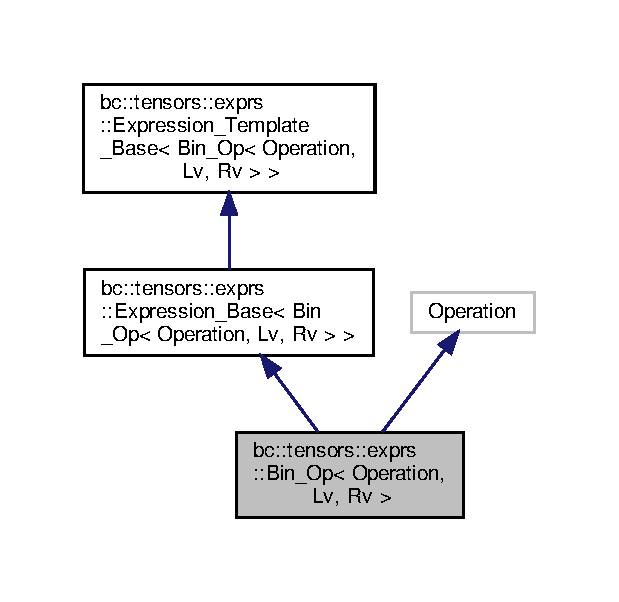
\includegraphics[width=297pt]{structbc_1_1tensors_1_1exprs_1_1Bin__Op__inherit__graph}
\end{center}
\end{figure}


Collaboration diagram for bc\+:\+:tensors\+:\+:exprs\+:\+:Bin\+\_\+\+Op$<$ Operation, Lv, Rv $>$\+:\nopagebreak
\begin{figure}[H]
\begin{center}
\leavevmode
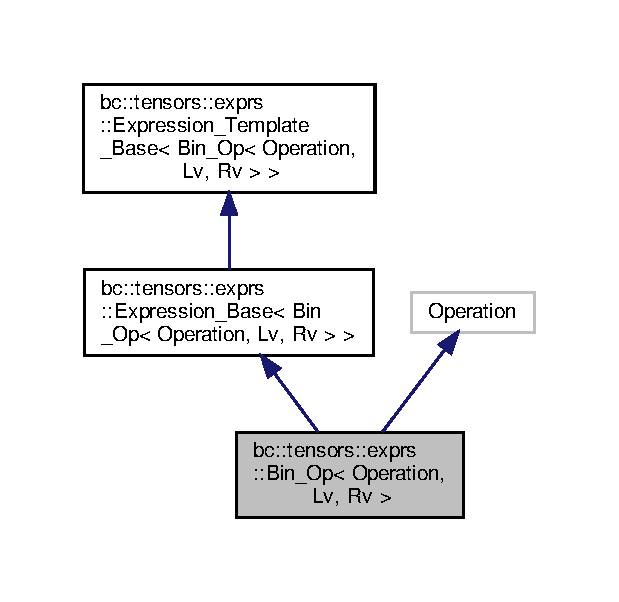
\includegraphics[width=297pt]{structbc_1_1tensors_1_1exprs_1_1Bin__Op__coll__graph}
\end{center}
\end{figure}
\subsection*{Public Types}
\begin{DoxyCompactItemize}
\item 
using \hyperlink{structbc_1_1tensors_1_1exprs_1_1Bin__Op_a5e39aa2bb60266199be2fc701b0edaaf}{system\+\_\+tag} = typename Lv\+::system\+\_\+tag
\item 
using \hyperlink{structbc_1_1tensors_1_1exprs_1_1Bin__Op_a3928519ff927c73f5dd82ed3d4d00d6c}{value\+\_\+type} = std\+::decay\+\_\+t$<$ decltype(std\+::declval$<$ Operation $>$().operator()(std\+::declval$<$ typename Lv\+::value\+\_\+type $>$(), std\+::declval$<$ typename Rv\+::value\+\_\+type $>$()))$>$
\end{DoxyCompactItemize}
\subsection*{Public Member Functions}
\begin{DoxyCompactItemize}
\item 
Operation \hyperlink{structbc_1_1tensors_1_1exprs_1_1Bin__Op_a767518d5bd0acf986a00f69d044994f8}{get\+\_\+operation} () const
\item 
{\footnotesize template$<$class... Args$>$ }\\\hyperlink{common_8h_ac085f07cc309e3aac24aa3fc0a40f6d2}{B\+C\+H\+OT} \hyperlink{structbc_1_1tensors_1_1exprs_1_1Bin__Op_a573cf3bb0dda167af2e6ca585c584fd9}{Bin\+\_\+\+Op} (Lv lv, Rv rv, const Args \&... args)
\item 
\hyperlink{common_8h_a6699e8b0449da5c0fafb878e59c1d4b1}{B\+C\+I\+N\+L\+I\+NE} auto \hyperlink{structbc_1_1tensors_1_1exprs_1_1Bin__Op_a0034e76e2f2b0f48de36f38055336e4e}{operator\mbox{[}$\,$\mbox{]}} (\hyperlink{namespacebc_aaf8e3fbf99b04b1b57c4f80c6f55d3c5}{bc\+::size\+\_\+t} index) const
\item 
\hyperlink{common_8h_a6699e8b0449da5c0fafb878e59c1d4b1}{B\+C\+I\+N\+L\+I\+NE} auto \hyperlink{structbc_1_1tensors_1_1exprs_1_1Bin__Op_a4f15e91266888a28f787ed18ecbffe00}{operator\mbox{[}$\,$\mbox{]}} (\hyperlink{namespacebc_aaf8e3fbf99b04b1b57c4f80c6f55d3c5}{bc\+::size\+\_\+t} index)
\item 
{\footnotesize template$<$class... Integers, class  = std\+::enable\+\_\+if\+\_\+t$<$				(sizeof...(\+Integers)$>$=tensor\+\_\+iterator\+\_\+dim$>$ }\\\hyperlink{common_8h_a6699e8b0449da5c0fafb878e59c1d4b1}{B\+C\+I\+N\+L\+I\+NE} auto \hyperlink{structbc_1_1tensors_1_1exprs_1_1Bin__Op_a56599cd99d7f1dac59cada714a03018f}{operator()} (Integers... ints) const
\item 
{\footnotesize template$<$class... Integers, class  = std\+::enable\+\_\+if\+\_\+t$<$(				sizeof...(\+Integers)$>$=tensor\+\_\+iterator\+\_\+dim$>$ }\\\hyperlink{common_8h_a6699e8b0449da5c0fafb878e59c1d4b1}{B\+C\+I\+N\+L\+I\+NE} auto \hyperlink{structbc_1_1tensors_1_1exprs_1_1Bin__Op_a8465e6a42066c4ab94d564fedf33b475}{operator()} (Integers... ints)
\item 
\hyperlink{common_8h_a6699e8b0449da5c0fafb878e59c1d4b1}{B\+C\+I\+N\+L\+I\+NE} \hyperlink{namespacebc_aaf8e3fbf99b04b1b57c4f80c6f55d3c5}{bc\+::size\+\_\+t} \hyperlink{structbc_1_1tensors_1_1exprs_1_1Bin__Op_a78c087617de82b25b275e80d4171d096}{size} () const
\item 
\hyperlink{common_8h_a6699e8b0449da5c0fafb878e59c1d4b1}{B\+C\+I\+N\+L\+I\+NE} \hyperlink{namespacebc_aaf8e3fbf99b04b1b57c4f80c6f55d3c5}{bc\+::size\+\_\+t} \hyperlink{structbc_1_1tensors_1_1exprs_1_1Bin__Op_a64a12bb5bea6788976aa13eb55dbde67}{rows} () const
\item 
\hyperlink{common_8h_a6699e8b0449da5c0fafb878e59c1d4b1}{B\+C\+I\+N\+L\+I\+NE} \hyperlink{namespacebc_aaf8e3fbf99b04b1b57c4f80c6f55d3c5}{bc\+::size\+\_\+t} \hyperlink{structbc_1_1tensors_1_1exprs_1_1Bin__Op_ae90cf0485e63626093ebbb6a6abf8f12}{cols} () const
\item 
\hyperlink{common_8h_a6699e8b0449da5c0fafb878e59c1d4b1}{B\+C\+I\+N\+L\+I\+NE} \hyperlink{namespacebc_aaf8e3fbf99b04b1b57c4f80c6f55d3c5}{bc\+::size\+\_\+t} \hyperlink{structbc_1_1tensors_1_1exprs_1_1Bin__Op_ae9ba3f351d29fa9852e90f35890127d6}{dim} (int i) const
\item 
\hyperlink{common_8h_a6699e8b0449da5c0fafb878e59c1d4b1}{B\+C\+I\+N\+L\+I\+NE} auto \hyperlink{structbc_1_1tensors_1_1exprs_1_1Bin__Op_a6d38ff7ba2dabc884373d141a0a2e924}{inner\+\_\+shape} () const
\end{DoxyCompactItemize}
\subsection*{Public Attributes}
\begin{DoxyCompactItemize}
\item 
Lv \hyperlink{structbc_1_1tensors_1_1exprs_1_1Bin__Op_a0fcb386ccdf770056af498257790126a}{left}
\item 
Rv \hyperlink{structbc_1_1tensors_1_1exprs_1_1Bin__Op_a28b81329d59ce09f0260a76e5e0bd215}{right}
\end{DoxyCompactItemize}
\subsection*{Static Public Attributes}
\begin{DoxyCompactItemize}
\item 
static constexpr int \hyperlink{structbc_1_1tensors_1_1exprs_1_1Bin__Op_a36cea8ca02ccaecc1b8ce221b93a865a}{tensor\+\_\+dim}
\item 
static constexpr int \hyperlink{structbc_1_1tensors_1_1exprs_1_1Bin__Op_aec48bb277f9e8b990c6dbe790f13b782}{tensor\+\_\+iterator\+\_\+dim}
\end{DoxyCompactItemize}


\subsection{Member Typedef Documentation}
\mbox{\Hypertarget{structbc_1_1tensors_1_1exprs_1_1Bin__Op_a5e39aa2bb60266199be2fc701b0edaaf}\label{structbc_1_1tensors_1_1exprs_1_1Bin__Op_a5e39aa2bb60266199be2fc701b0edaaf}} 
\index{bc\+::tensors\+::exprs\+::\+Bin\+\_\+\+Op@{bc\+::tensors\+::exprs\+::\+Bin\+\_\+\+Op}!system\+\_\+tag@{system\+\_\+tag}}
\index{system\+\_\+tag@{system\+\_\+tag}!bc\+::tensors\+::exprs\+::\+Bin\+\_\+\+Op@{bc\+::tensors\+::exprs\+::\+Bin\+\_\+\+Op}}
\subsubsection{\texorpdfstring{system\+\_\+tag}{system\_tag}}
{\footnotesize\ttfamily template$<$class Operation, class Lv, class Rv$>$ \\
using \hyperlink{structbc_1_1tensors_1_1exprs_1_1Bin__Op}{bc\+::tensors\+::exprs\+::\+Bin\+\_\+\+Op}$<$ Operation, Lv, Rv $>$\+::\hyperlink{structbc_1_1tensors_1_1exprs_1_1Bin__Op_a5e39aa2bb60266199be2fc701b0edaaf}{system\+\_\+tag} =  typename Lv\+::system\+\_\+tag}

\mbox{\Hypertarget{structbc_1_1tensors_1_1exprs_1_1Bin__Op_a3928519ff927c73f5dd82ed3d4d00d6c}\label{structbc_1_1tensors_1_1exprs_1_1Bin__Op_a3928519ff927c73f5dd82ed3d4d00d6c}} 
\index{bc\+::tensors\+::exprs\+::\+Bin\+\_\+\+Op@{bc\+::tensors\+::exprs\+::\+Bin\+\_\+\+Op}!value\+\_\+type@{value\+\_\+type}}
\index{value\+\_\+type@{value\+\_\+type}!bc\+::tensors\+::exprs\+::\+Bin\+\_\+\+Op@{bc\+::tensors\+::exprs\+::\+Bin\+\_\+\+Op}}
\subsubsection{\texorpdfstring{value\+\_\+type}{value\_type}}
{\footnotesize\ttfamily template$<$class Operation, class Lv, class Rv$>$ \\
using \hyperlink{structbc_1_1tensors_1_1exprs_1_1Bin__Op}{bc\+::tensors\+::exprs\+::\+Bin\+\_\+\+Op}$<$ Operation, Lv, Rv $>$\+::\hyperlink{structbc_1_1tensors_1_1exprs_1_1Bin__Op_a3928519ff927c73f5dd82ed3d4d00d6c}{value\+\_\+type} =  std\+::decay\+\_\+t$<$decltype( std\+::declval$<$Operation$>$().operator()( std\+::declval$<$typename Lv\+::value\+\_\+type$>$(), std\+::declval$<$typename Rv\+::value\+\_\+type$>$()))$>$}



\subsection{Constructor \& Destructor Documentation}
\mbox{\Hypertarget{structbc_1_1tensors_1_1exprs_1_1Bin__Op_a573cf3bb0dda167af2e6ca585c584fd9}\label{structbc_1_1tensors_1_1exprs_1_1Bin__Op_a573cf3bb0dda167af2e6ca585c584fd9}} 
\index{bc\+::tensors\+::exprs\+::\+Bin\+\_\+\+Op@{bc\+::tensors\+::exprs\+::\+Bin\+\_\+\+Op}!Bin\+\_\+\+Op@{Bin\+\_\+\+Op}}
\index{Bin\+\_\+\+Op@{Bin\+\_\+\+Op}!bc\+::tensors\+::exprs\+::\+Bin\+\_\+\+Op@{bc\+::tensors\+::exprs\+::\+Bin\+\_\+\+Op}}
\subsubsection{\texorpdfstring{Bin\+\_\+\+Op()}{Bin\_Op()}}
{\footnotesize\ttfamily template$<$class Operation, class Lv, class Rv$>$ \\
template$<$class... Args$>$ \\
\hyperlink{common_8h_ac085f07cc309e3aac24aa3fc0a40f6d2}{B\+C\+H\+OT} \hyperlink{structbc_1_1tensors_1_1exprs_1_1Bin__Op}{bc\+::tensors\+::exprs\+::\+Bin\+\_\+\+Op}$<$ Operation, Lv, Rv $>$\+::\hyperlink{structbc_1_1tensors_1_1exprs_1_1Bin__Op}{Bin\+\_\+\+Op} (\begin{DoxyParamCaption}\item[{Lv}]{lv,  }\item[{Rv}]{rv,  }\item[{const Args \&...}]{args }\end{DoxyParamCaption})\hspace{0.3cm}{\ttfamily [inline]}}



\subsection{Member Function Documentation}
\mbox{\Hypertarget{structbc_1_1tensors_1_1exprs_1_1Bin__Op_ae90cf0485e63626093ebbb6a6abf8f12}\label{structbc_1_1tensors_1_1exprs_1_1Bin__Op_ae90cf0485e63626093ebbb6a6abf8f12}} 
\index{bc\+::tensors\+::exprs\+::\+Bin\+\_\+\+Op@{bc\+::tensors\+::exprs\+::\+Bin\+\_\+\+Op}!cols@{cols}}
\index{cols@{cols}!bc\+::tensors\+::exprs\+::\+Bin\+\_\+\+Op@{bc\+::tensors\+::exprs\+::\+Bin\+\_\+\+Op}}
\subsubsection{\texorpdfstring{cols()}{cols()}}
{\footnotesize\ttfamily template$<$class Operation, class Lv, class Rv$>$ \\
\hyperlink{common_8h_a6699e8b0449da5c0fafb878e59c1d4b1}{B\+C\+I\+N\+L\+I\+NE} \hyperlink{namespacebc_aaf8e3fbf99b04b1b57c4f80c6f55d3c5}{bc\+::size\+\_\+t} \hyperlink{structbc_1_1tensors_1_1exprs_1_1Bin__Op}{bc\+::tensors\+::exprs\+::\+Bin\+\_\+\+Op}$<$ Operation, Lv, Rv $>$\+::cols (\begin{DoxyParamCaption}{ }\end{DoxyParamCaption}) const\hspace{0.3cm}{\ttfamily [inline]}}

\mbox{\Hypertarget{structbc_1_1tensors_1_1exprs_1_1Bin__Op_ae9ba3f351d29fa9852e90f35890127d6}\label{structbc_1_1tensors_1_1exprs_1_1Bin__Op_ae9ba3f351d29fa9852e90f35890127d6}} 
\index{bc\+::tensors\+::exprs\+::\+Bin\+\_\+\+Op@{bc\+::tensors\+::exprs\+::\+Bin\+\_\+\+Op}!dim@{dim}}
\index{dim@{dim}!bc\+::tensors\+::exprs\+::\+Bin\+\_\+\+Op@{bc\+::tensors\+::exprs\+::\+Bin\+\_\+\+Op}}
\subsubsection{\texorpdfstring{dim()}{dim()}}
{\footnotesize\ttfamily template$<$class Operation, class Lv, class Rv$>$ \\
\hyperlink{common_8h_a6699e8b0449da5c0fafb878e59c1d4b1}{B\+C\+I\+N\+L\+I\+NE} \hyperlink{namespacebc_aaf8e3fbf99b04b1b57c4f80c6f55d3c5}{bc\+::size\+\_\+t} \hyperlink{structbc_1_1tensors_1_1exprs_1_1Bin__Op}{bc\+::tensors\+::exprs\+::\+Bin\+\_\+\+Op}$<$ Operation, Lv, Rv $>$\+::dim (\begin{DoxyParamCaption}\item[{int}]{i }\end{DoxyParamCaption}) const\hspace{0.3cm}{\ttfamily [inline]}}

\mbox{\Hypertarget{structbc_1_1tensors_1_1exprs_1_1Bin__Op_a767518d5bd0acf986a00f69d044994f8}\label{structbc_1_1tensors_1_1exprs_1_1Bin__Op_a767518d5bd0acf986a00f69d044994f8}} 
\index{bc\+::tensors\+::exprs\+::\+Bin\+\_\+\+Op@{bc\+::tensors\+::exprs\+::\+Bin\+\_\+\+Op}!get\+\_\+operation@{get\+\_\+operation}}
\index{get\+\_\+operation@{get\+\_\+operation}!bc\+::tensors\+::exprs\+::\+Bin\+\_\+\+Op@{bc\+::tensors\+::exprs\+::\+Bin\+\_\+\+Op}}
\subsubsection{\texorpdfstring{get\+\_\+operation()}{get\_operation()}}
{\footnotesize\ttfamily template$<$class Operation, class Lv, class Rv$>$ \\
Operation \hyperlink{structbc_1_1tensors_1_1exprs_1_1Bin__Op}{bc\+::tensors\+::exprs\+::\+Bin\+\_\+\+Op}$<$ Operation, Lv, Rv $>$\+::get\+\_\+operation (\begin{DoxyParamCaption}{ }\end{DoxyParamCaption}) const\hspace{0.3cm}{\ttfamily [inline]}}

\mbox{\Hypertarget{structbc_1_1tensors_1_1exprs_1_1Bin__Op_a6d38ff7ba2dabc884373d141a0a2e924}\label{structbc_1_1tensors_1_1exprs_1_1Bin__Op_a6d38ff7ba2dabc884373d141a0a2e924}} 
\index{bc\+::tensors\+::exprs\+::\+Bin\+\_\+\+Op@{bc\+::tensors\+::exprs\+::\+Bin\+\_\+\+Op}!inner\+\_\+shape@{inner\+\_\+shape}}
\index{inner\+\_\+shape@{inner\+\_\+shape}!bc\+::tensors\+::exprs\+::\+Bin\+\_\+\+Op@{bc\+::tensors\+::exprs\+::\+Bin\+\_\+\+Op}}
\subsubsection{\texorpdfstring{inner\+\_\+shape()}{inner\_shape()}}
{\footnotesize\ttfamily template$<$class Operation, class Lv, class Rv$>$ \\
\hyperlink{common_8h_a6699e8b0449da5c0fafb878e59c1d4b1}{B\+C\+I\+N\+L\+I\+NE} auto \hyperlink{structbc_1_1tensors_1_1exprs_1_1Bin__Op}{bc\+::tensors\+::exprs\+::\+Bin\+\_\+\+Op}$<$ Operation, Lv, Rv $>$\+::inner\+\_\+shape (\begin{DoxyParamCaption}{ }\end{DoxyParamCaption}) const\hspace{0.3cm}{\ttfamily [inline]}}

\mbox{\Hypertarget{structbc_1_1tensors_1_1exprs_1_1Bin__Op_a56599cd99d7f1dac59cada714a03018f}\label{structbc_1_1tensors_1_1exprs_1_1Bin__Op_a56599cd99d7f1dac59cada714a03018f}} 
\index{bc\+::tensors\+::exprs\+::\+Bin\+\_\+\+Op@{bc\+::tensors\+::exprs\+::\+Bin\+\_\+\+Op}!operator()@{operator()}}
\index{operator()@{operator()}!bc\+::tensors\+::exprs\+::\+Bin\+\_\+\+Op@{bc\+::tensors\+::exprs\+::\+Bin\+\_\+\+Op}}
\subsubsection{\texorpdfstring{operator()()}{operator()()}\hspace{0.1cm}{\footnotesize\ttfamily [1/2]}}
{\footnotesize\ttfamily template$<$class Operation, class Lv, class Rv$>$ \\
template$<$class... Integers, class  = std\+::enable\+\_\+if\+\_\+t$<$				(sizeof...(\+Integers)$>$=tensor\+\_\+iterator\+\_\+dim$>$ \\
\hyperlink{common_8h_a6699e8b0449da5c0fafb878e59c1d4b1}{B\+C\+I\+N\+L\+I\+NE} auto \hyperlink{structbc_1_1tensors_1_1exprs_1_1Bin__Op}{bc\+::tensors\+::exprs\+::\+Bin\+\_\+\+Op}$<$ Operation, Lv, Rv $>$\+::operator() (\begin{DoxyParamCaption}\item[{Integers...}]{ints }\end{DoxyParamCaption}) const\hspace{0.3cm}{\ttfamily [inline]}}

\mbox{\Hypertarget{structbc_1_1tensors_1_1exprs_1_1Bin__Op_a8465e6a42066c4ab94d564fedf33b475}\label{structbc_1_1tensors_1_1exprs_1_1Bin__Op_a8465e6a42066c4ab94d564fedf33b475}} 
\index{bc\+::tensors\+::exprs\+::\+Bin\+\_\+\+Op@{bc\+::tensors\+::exprs\+::\+Bin\+\_\+\+Op}!operator()@{operator()}}
\index{operator()@{operator()}!bc\+::tensors\+::exprs\+::\+Bin\+\_\+\+Op@{bc\+::tensors\+::exprs\+::\+Bin\+\_\+\+Op}}
\subsubsection{\texorpdfstring{operator()()}{operator()()}\hspace{0.1cm}{\footnotesize\ttfamily [2/2]}}
{\footnotesize\ttfamily template$<$class Operation, class Lv, class Rv$>$ \\
template$<$class... Integers, class  = std\+::enable\+\_\+if\+\_\+t$<$(				sizeof...(\+Integers)$>$=tensor\+\_\+iterator\+\_\+dim$>$ \\
\hyperlink{common_8h_a6699e8b0449da5c0fafb878e59c1d4b1}{B\+C\+I\+N\+L\+I\+NE} auto \hyperlink{structbc_1_1tensors_1_1exprs_1_1Bin__Op}{bc\+::tensors\+::exprs\+::\+Bin\+\_\+\+Op}$<$ Operation, Lv, Rv $>$\+::operator() (\begin{DoxyParamCaption}\item[{Integers...}]{ints }\end{DoxyParamCaption})\hspace{0.3cm}{\ttfamily [inline]}}

\mbox{\Hypertarget{structbc_1_1tensors_1_1exprs_1_1Bin__Op_a0034e76e2f2b0f48de36f38055336e4e}\label{structbc_1_1tensors_1_1exprs_1_1Bin__Op_a0034e76e2f2b0f48de36f38055336e4e}} 
\index{bc\+::tensors\+::exprs\+::\+Bin\+\_\+\+Op@{bc\+::tensors\+::exprs\+::\+Bin\+\_\+\+Op}!operator\mbox{[}\mbox{]}@{operator[]}}
\index{operator\mbox{[}\mbox{]}@{operator[]}!bc\+::tensors\+::exprs\+::\+Bin\+\_\+\+Op@{bc\+::tensors\+::exprs\+::\+Bin\+\_\+\+Op}}
\subsubsection{\texorpdfstring{operator[]()}{operator[]()}\hspace{0.1cm}{\footnotesize\ttfamily [1/2]}}
{\footnotesize\ttfamily template$<$class Operation, class Lv, class Rv$>$ \\
\hyperlink{common_8h_a6699e8b0449da5c0fafb878e59c1d4b1}{B\+C\+I\+N\+L\+I\+NE} auto \hyperlink{structbc_1_1tensors_1_1exprs_1_1Bin__Op}{bc\+::tensors\+::exprs\+::\+Bin\+\_\+\+Op}$<$ Operation, Lv, Rv $>$\+::operator\mbox{[}$\,$\mbox{]} (\begin{DoxyParamCaption}\item[{\hyperlink{namespacebc_aaf8e3fbf99b04b1b57c4f80c6f55d3c5}{bc\+::size\+\_\+t}}]{index }\end{DoxyParamCaption}) const\hspace{0.3cm}{\ttfamily [inline]}}

\mbox{\Hypertarget{structbc_1_1tensors_1_1exprs_1_1Bin__Op_a4f15e91266888a28f787ed18ecbffe00}\label{structbc_1_1tensors_1_1exprs_1_1Bin__Op_a4f15e91266888a28f787ed18ecbffe00}} 
\index{bc\+::tensors\+::exprs\+::\+Bin\+\_\+\+Op@{bc\+::tensors\+::exprs\+::\+Bin\+\_\+\+Op}!operator\mbox{[}\mbox{]}@{operator[]}}
\index{operator\mbox{[}\mbox{]}@{operator[]}!bc\+::tensors\+::exprs\+::\+Bin\+\_\+\+Op@{bc\+::tensors\+::exprs\+::\+Bin\+\_\+\+Op}}
\subsubsection{\texorpdfstring{operator[]()}{operator[]()}\hspace{0.1cm}{\footnotesize\ttfamily [2/2]}}
{\footnotesize\ttfamily template$<$class Operation, class Lv, class Rv$>$ \\
\hyperlink{common_8h_a6699e8b0449da5c0fafb878e59c1d4b1}{B\+C\+I\+N\+L\+I\+NE} auto \hyperlink{structbc_1_1tensors_1_1exprs_1_1Bin__Op}{bc\+::tensors\+::exprs\+::\+Bin\+\_\+\+Op}$<$ Operation, Lv, Rv $>$\+::operator\mbox{[}$\,$\mbox{]} (\begin{DoxyParamCaption}\item[{\hyperlink{namespacebc_aaf8e3fbf99b04b1b57c4f80c6f55d3c5}{bc\+::size\+\_\+t}}]{index }\end{DoxyParamCaption})\hspace{0.3cm}{\ttfamily [inline]}}

\mbox{\Hypertarget{structbc_1_1tensors_1_1exprs_1_1Bin__Op_a64a12bb5bea6788976aa13eb55dbde67}\label{structbc_1_1tensors_1_1exprs_1_1Bin__Op_a64a12bb5bea6788976aa13eb55dbde67}} 
\index{bc\+::tensors\+::exprs\+::\+Bin\+\_\+\+Op@{bc\+::tensors\+::exprs\+::\+Bin\+\_\+\+Op}!rows@{rows}}
\index{rows@{rows}!bc\+::tensors\+::exprs\+::\+Bin\+\_\+\+Op@{bc\+::tensors\+::exprs\+::\+Bin\+\_\+\+Op}}
\subsubsection{\texorpdfstring{rows()}{rows()}}
{\footnotesize\ttfamily template$<$class Operation, class Lv, class Rv$>$ \\
\hyperlink{common_8h_a6699e8b0449da5c0fafb878e59c1d4b1}{B\+C\+I\+N\+L\+I\+NE} \hyperlink{namespacebc_aaf8e3fbf99b04b1b57c4f80c6f55d3c5}{bc\+::size\+\_\+t} \hyperlink{structbc_1_1tensors_1_1exprs_1_1Bin__Op}{bc\+::tensors\+::exprs\+::\+Bin\+\_\+\+Op}$<$ Operation, Lv, Rv $>$\+::rows (\begin{DoxyParamCaption}{ }\end{DoxyParamCaption}) const\hspace{0.3cm}{\ttfamily [inline]}}

\mbox{\Hypertarget{structbc_1_1tensors_1_1exprs_1_1Bin__Op_a78c087617de82b25b275e80d4171d096}\label{structbc_1_1tensors_1_1exprs_1_1Bin__Op_a78c087617de82b25b275e80d4171d096}} 
\index{bc\+::tensors\+::exprs\+::\+Bin\+\_\+\+Op@{bc\+::tensors\+::exprs\+::\+Bin\+\_\+\+Op}!size@{size}}
\index{size@{size}!bc\+::tensors\+::exprs\+::\+Bin\+\_\+\+Op@{bc\+::tensors\+::exprs\+::\+Bin\+\_\+\+Op}}
\subsubsection{\texorpdfstring{size()}{size()}}
{\footnotesize\ttfamily template$<$class Operation, class Lv, class Rv$>$ \\
\hyperlink{common_8h_a6699e8b0449da5c0fafb878e59c1d4b1}{B\+C\+I\+N\+L\+I\+NE} \hyperlink{namespacebc_aaf8e3fbf99b04b1b57c4f80c6f55d3c5}{bc\+::size\+\_\+t} \hyperlink{structbc_1_1tensors_1_1exprs_1_1Bin__Op}{bc\+::tensors\+::exprs\+::\+Bin\+\_\+\+Op}$<$ Operation, Lv, Rv $>$\+::size (\begin{DoxyParamCaption}{ }\end{DoxyParamCaption}) const\hspace{0.3cm}{\ttfamily [inline]}}



\subsection{Member Data Documentation}
\mbox{\Hypertarget{structbc_1_1tensors_1_1exprs_1_1Bin__Op_a0fcb386ccdf770056af498257790126a}\label{structbc_1_1tensors_1_1exprs_1_1Bin__Op_a0fcb386ccdf770056af498257790126a}} 
\index{bc\+::tensors\+::exprs\+::\+Bin\+\_\+\+Op@{bc\+::tensors\+::exprs\+::\+Bin\+\_\+\+Op}!left@{left}}
\index{left@{left}!bc\+::tensors\+::exprs\+::\+Bin\+\_\+\+Op@{bc\+::tensors\+::exprs\+::\+Bin\+\_\+\+Op}}
\subsubsection{\texorpdfstring{left}{left}}
{\footnotesize\ttfamily template$<$class Operation, class Lv, class Rv$>$ \\
Lv \hyperlink{structbc_1_1tensors_1_1exprs_1_1Bin__Op}{bc\+::tensors\+::exprs\+::\+Bin\+\_\+\+Op}$<$ Operation, Lv, Rv $>$\+::left}

\mbox{\Hypertarget{structbc_1_1tensors_1_1exprs_1_1Bin__Op_a28b81329d59ce09f0260a76e5e0bd215}\label{structbc_1_1tensors_1_1exprs_1_1Bin__Op_a28b81329d59ce09f0260a76e5e0bd215}} 
\index{bc\+::tensors\+::exprs\+::\+Bin\+\_\+\+Op@{bc\+::tensors\+::exprs\+::\+Bin\+\_\+\+Op}!right@{right}}
\index{right@{right}!bc\+::tensors\+::exprs\+::\+Bin\+\_\+\+Op@{bc\+::tensors\+::exprs\+::\+Bin\+\_\+\+Op}}
\subsubsection{\texorpdfstring{right}{right}}
{\footnotesize\ttfamily template$<$class Operation, class Lv, class Rv$>$ \\
Rv \hyperlink{structbc_1_1tensors_1_1exprs_1_1Bin__Op}{bc\+::tensors\+::exprs\+::\+Bin\+\_\+\+Op}$<$ Operation, Lv, Rv $>$\+::right}

\mbox{\Hypertarget{structbc_1_1tensors_1_1exprs_1_1Bin__Op_a36cea8ca02ccaecc1b8ce221b93a865a}\label{structbc_1_1tensors_1_1exprs_1_1Bin__Op_a36cea8ca02ccaecc1b8ce221b93a865a}} 
\index{bc\+::tensors\+::exprs\+::\+Bin\+\_\+\+Op@{bc\+::tensors\+::exprs\+::\+Bin\+\_\+\+Op}!tensor\+\_\+dim@{tensor\+\_\+dim}}
\index{tensor\+\_\+dim@{tensor\+\_\+dim}!bc\+::tensors\+::exprs\+::\+Bin\+\_\+\+Op@{bc\+::tensors\+::exprs\+::\+Bin\+\_\+\+Op}}
\subsubsection{\texorpdfstring{tensor\+\_\+dim}{tensor\_dim}}
{\footnotesize\ttfamily template$<$class Operation, class Lv, class Rv$>$ \\
constexpr int \hyperlink{structbc_1_1tensors_1_1exprs_1_1Bin__Op}{bc\+::tensors\+::exprs\+::\+Bin\+\_\+\+Op}$<$ Operation, Lv, Rv $>$\+::tensor\+\_\+dim\hspace{0.3cm}{\ttfamily [static]}}

{\bfseries Initial value\+:}
\begin{DoxyCode}
=
            bc::traits::max(Lv::tensor\_dim, Rv::tensor\_dim)
\end{DoxyCode}
\mbox{\Hypertarget{structbc_1_1tensors_1_1exprs_1_1Bin__Op_aec48bb277f9e8b990c6dbe790f13b782}\label{structbc_1_1tensors_1_1exprs_1_1Bin__Op_aec48bb277f9e8b990c6dbe790f13b782}} 
\index{bc\+::tensors\+::exprs\+::\+Bin\+\_\+\+Op@{bc\+::tensors\+::exprs\+::\+Bin\+\_\+\+Op}!tensor\+\_\+iterator\+\_\+dim@{tensor\+\_\+iterator\+\_\+dim}}
\index{tensor\+\_\+iterator\+\_\+dim@{tensor\+\_\+iterator\+\_\+dim}!bc\+::tensors\+::exprs\+::\+Bin\+\_\+\+Op@{bc\+::tensors\+::exprs\+::\+Bin\+\_\+\+Op}}
\subsubsection{\texorpdfstring{tensor\+\_\+iterator\+\_\+dim}{tensor\_iterator\_dim}}
{\footnotesize\ttfamily template$<$class Operation, class Lv, class Rv$>$ \\
constexpr int \hyperlink{structbc_1_1tensors_1_1exprs_1_1Bin__Op}{bc\+::tensors\+::exprs\+::\+Bin\+\_\+\+Op}$<$ Operation, Lv, Rv $>$\+::tensor\+\_\+iterator\+\_\+dim\hspace{0.3cm}{\ttfamily [static]}}

{\bfseries Initial value\+:}
\begin{DoxyCode}
=
        is\_broadcast\_expression || !continuous\_mem\_layout ?
            max\_dim :
            max\_iterator
\end{DoxyCode}


The documentation for this struct was generated from the following files\+:\begin{DoxyCompactItemize}
\item 
blackcat/tensors/expression\+\_\+templates/blas\+\_\+expression\+\_\+parser/\hyperlink{tensors_2expression__templates_2blas__expression__parser_2common_8h}{common.\+h}\item 
blackcat/tensors/expression\+\_\+templates/\hyperlink{expression__binary_8h}{expression\+\_\+binary.\+h}\end{DoxyCompactItemize}

\hypertarget{structbc_1_1tensors_1_1exprs_1_1Bin__Op_3_01oper_1_1dot_3_01SystemTag_01_4_00_01lv_00_01rv_01_4}{}\section{bc\+:\+:tensors\+:\+:exprs\+:\+:Bin\+\_\+\+Op$<$ oper\+:\+:dot$<$ System\+Tag $>$, lv, rv $>$ Struct Template Reference}
\label{structbc_1_1tensors_1_1exprs_1_1Bin__Op_3_01oper_1_1dot_3_01SystemTag_01_4_00_01lv_00_01rv_01_4}\index{bc\+::tensors\+::exprs\+::\+Bin\+\_\+\+Op$<$ oper\+::dot$<$ System\+Tag $>$, lv, rv $>$@{bc\+::tensors\+::exprs\+::\+Bin\+\_\+\+Op$<$ oper\+::dot$<$ System\+Tag $>$, lv, rv $>$}}


{\ttfamily \#include $<$function\+\_\+dot.\+h$>$}



Inheritance diagram for bc\+:\+:tensors\+:\+:exprs\+:\+:Bin\+\_\+\+Op$<$ oper\+:\+:dot$<$ System\+Tag $>$, lv, rv $>$\+:\nopagebreak
\begin{figure}[H]
\begin{center}
\leavevmode
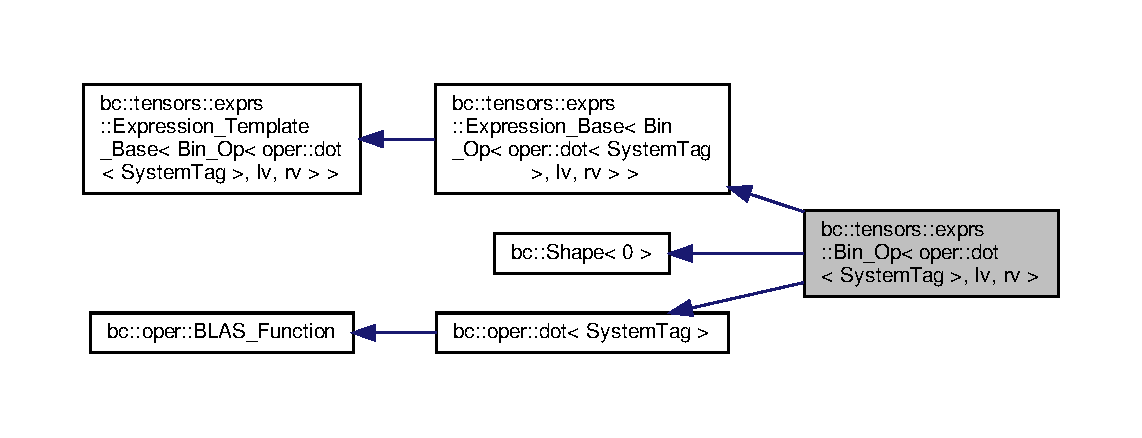
\includegraphics[width=350pt]{structbc_1_1tensors_1_1exprs_1_1Bin__Op_3_01oper_1_1dot_3_01SystemTag_01_4_00_01lv_00_01rv_01_4__inherit__graph}
\end{center}
\end{figure}


Collaboration diagram for bc\+:\+:tensors\+:\+:exprs\+:\+:Bin\+\_\+\+Op$<$ oper\+:\+:dot$<$ System\+Tag $>$, lv, rv $>$\+:\nopagebreak
\begin{figure}[H]
\begin{center}
\leavevmode
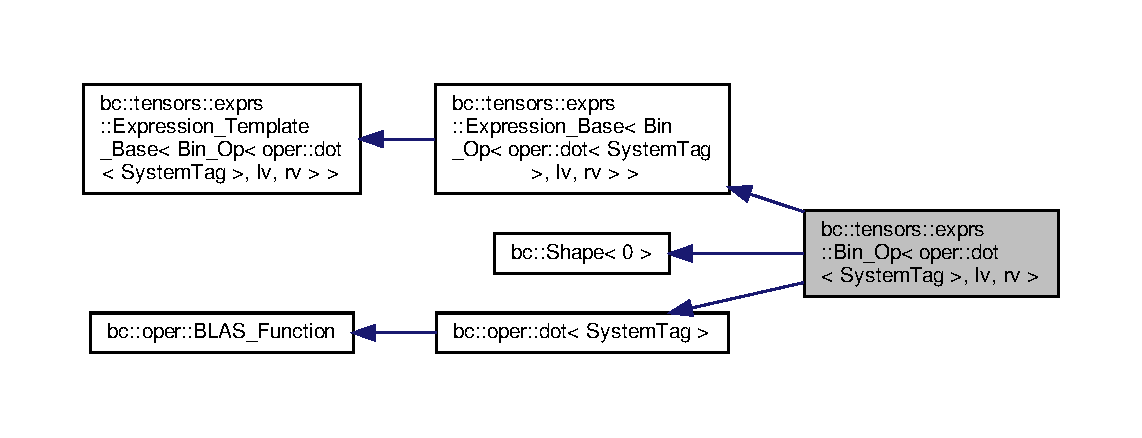
\includegraphics[width=350pt]{structbc_1_1tensors_1_1exprs_1_1Bin__Op_3_01oper_1_1dot_3_01SystemTag_01_4_00_01lv_00_01rv_01_4__coll__graph}
\end{center}
\end{figure}
\subsection*{Public Types}
\begin{DoxyCompactItemize}
\item 
using \hyperlink{structbc_1_1tensors_1_1exprs_1_1Bin__Op_3_01oper_1_1dot_3_01SystemTag_01_4_00_01lv_00_01rv_01_4_a6e196b34e6c3c318929830ed01156927}{value\+\_\+type} = typename lv\+::value\+\_\+type
\item 
using \hyperlink{structbc_1_1tensors_1_1exprs_1_1Bin__Op_3_01oper_1_1dot_3_01SystemTag_01_4_00_01lv_00_01rv_01_4_aac42309fcd782d98f3d908ce98defba8}{system\+\_\+tag} = System\+Tag
\end{DoxyCompactItemize}
\subsection*{Public Member Functions}
\begin{DoxyCompactItemize}
\item 
\hyperlink{structbc_1_1tensors_1_1exprs_1_1Bin__Op_3_01oper_1_1dot_3_01SystemTag_01_4_00_01lv_00_01rv_01_4_a9078278be7946d741f995f564ef3885e}{Bin\+\_\+\+Op} (lv \hyperlink{structbc_1_1tensors_1_1exprs_1_1Bin__Op_3_01oper_1_1dot_3_01SystemTag_01_4_00_01lv_00_01rv_01_4_a1a5f4155953dd6833d49faf2ca2d0b38}{left}, rv \hyperlink{structbc_1_1tensors_1_1exprs_1_1Bin__Op_3_01oper_1_1dot_3_01SystemTag_01_4_00_01lv_00_01rv_01_4_a9aca1e09b777dd5ca1edbbc27f59f01d}{right}, \hyperlink{structbc_1_1oper_1_1dot}{oper\+::dot}$<$ \hyperlink{structbc_1_1tensors_1_1exprs_1_1Bin__Op_3_01oper_1_1dot_3_01SystemTag_01_4_00_01lv_00_01rv_01_4_aac42309fcd782d98f3d908ce98defba8}{system\+\_\+tag} $>$ op=\hyperlink{structbc_1_1oper_1_1dot}{oper\+::dot}$<$ \hyperlink{structbc_1_1tensors_1_1exprs_1_1Bin__Op_3_01oper_1_1dot_3_01SystemTag_01_4_00_01lv_00_01rv_01_4_aac42309fcd782d98f3d908ce98defba8}{system\+\_\+tag} $>$())
\item 
{\footnotesize template$<$class Core , int Alpha, int Beta, class Stream $>$ }\\void \hyperlink{structbc_1_1tensors_1_1exprs_1_1Bin__Op_3_01oper_1_1dot_3_01SystemTag_01_4_00_01lv_00_01rv_01_4_afbee15d8347800bab6db511df9ea245b}{eval} (\hyperlink{structbc_1_1tensors_1_1exprs_1_1Output__Data}{Output\+\_\+\+Data}$<$ Core, Alpha, Beta $>$ output, \hyperlink{classbc_1_1streams_1_1Stream}{Stream} stream) const
\end{DoxyCompactItemize}
\subsection*{Static Public Member Functions}
\begin{DoxyCompactItemize}
\item 
static \hyperlink{structbc_1_1oper_1_1dot}{oper\+::dot}$<$ \hyperlink{structbc_1_1tensors_1_1exprs_1_1Bin__Op_3_01oper_1_1dot_3_01SystemTag_01_4_00_01lv_00_01rv_01_4_aac42309fcd782d98f3d908ce98defba8}{system\+\_\+tag} $>$ \hyperlink{structbc_1_1tensors_1_1exprs_1_1Bin__Op_3_01oper_1_1dot_3_01SystemTag_01_4_00_01lv_00_01rv_01_4_a75d2463548379d223cd1c3e6133f5bd2}{get\+\_\+operation} ()
\end{DoxyCompactItemize}
\subsection*{Public Attributes}
\begin{DoxyCompactItemize}
\item 
lv \hyperlink{structbc_1_1tensors_1_1exprs_1_1Bin__Op_3_01oper_1_1dot_3_01SystemTag_01_4_00_01lv_00_01rv_01_4_a1a5f4155953dd6833d49faf2ca2d0b38}{left}
\item 
rv \hyperlink{structbc_1_1tensors_1_1exprs_1_1Bin__Op_3_01oper_1_1dot_3_01SystemTag_01_4_00_01lv_00_01rv_01_4_a9aca1e09b777dd5ca1edbbc27f59f01d}{right}
\end{DoxyCompactItemize}
\subsection*{Static Public Attributes}
\begin{DoxyCompactItemize}
\item 
static constexpr int \hyperlink{structbc_1_1tensors_1_1exprs_1_1Bin__Op_3_01oper_1_1dot_3_01SystemTag_01_4_00_01lv_00_01rv_01_4_ade712cc7a704d3aaca20f7261bcde3b6}{tensor\+\_\+dim} = 0
\item 
static constexpr int \hyperlink{structbc_1_1tensors_1_1exprs_1_1Bin__Op_3_01oper_1_1dot_3_01SystemTag_01_4_00_01lv_00_01rv_01_4_a1423485a1a24fc868a210a74349d365e}{tensor\+\_\+iterator\+\_\+dim} = 0
\end{DoxyCompactItemize}


\subsection{Member Typedef Documentation}
\mbox{\Hypertarget{structbc_1_1tensors_1_1exprs_1_1Bin__Op_3_01oper_1_1dot_3_01SystemTag_01_4_00_01lv_00_01rv_01_4_aac42309fcd782d98f3d908ce98defba8}\label{structbc_1_1tensors_1_1exprs_1_1Bin__Op_3_01oper_1_1dot_3_01SystemTag_01_4_00_01lv_00_01rv_01_4_aac42309fcd782d98f3d908ce98defba8}} 
\index{bc\+::tensors\+::exprs\+::\+Bin\+\_\+\+Op$<$ oper\+::dot$<$ System\+Tag $>$, lv, rv $>$@{bc\+::tensors\+::exprs\+::\+Bin\+\_\+\+Op$<$ oper\+::dot$<$ System\+Tag $>$, lv, rv $>$}!system\+\_\+tag@{system\+\_\+tag}}
\index{system\+\_\+tag@{system\+\_\+tag}!bc\+::tensors\+::exprs\+::\+Bin\+\_\+\+Op$<$ oper\+::dot$<$ System\+Tag $>$, lv, rv $>$@{bc\+::tensors\+::exprs\+::\+Bin\+\_\+\+Op$<$ oper\+::dot$<$ System\+Tag $>$, lv, rv $>$}}
\subsubsection{\texorpdfstring{system\+\_\+tag}{system\_tag}}
{\footnotesize\ttfamily template$<$class lv , class rv , class System\+Tag $>$ \\
using \hyperlink{structbc_1_1tensors_1_1exprs_1_1Bin__Op}{bc\+::tensors\+::exprs\+::\+Bin\+\_\+\+Op}$<$ \hyperlink{structbc_1_1oper_1_1dot}{oper\+::dot}$<$ System\+Tag $>$, lv, rv $>$\+::\hyperlink{structbc_1_1tensors_1_1exprs_1_1Bin__Op_3_01oper_1_1dot_3_01SystemTag_01_4_00_01lv_00_01rv_01_4_aac42309fcd782d98f3d908ce98defba8}{system\+\_\+tag} =  System\+Tag}

\mbox{\Hypertarget{structbc_1_1tensors_1_1exprs_1_1Bin__Op_3_01oper_1_1dot_3_01SystemTag_01_4_00_01lv_00_01rv_01_4_a6e196b34e6c3c318929830ed01156927}\label{structbc_1_1tensors_1_1exprs_1_1Bin__Op_3_01oper_1_1dot_3_01SystemTag_01_4_00_01lv_00_01rv_01_4_a6e196b34e6c3c318929830ed01156927}} 
\index{bc\+::tensors\+::exprs\+::\+Bin\+\_\+\+Op$<$ oper\+::dot$<$ System\+Tag $>$, lv, rv $>$@{bc\+::tensors\+::exprs\+::\+Bin\+\_\+\+Op$<$ oper\+::dot$<$ System\+Tag $>$, lv, rv $>$}!value\+\_\+type@{value\+\_\+type}}
\index{value\+\_\+type@{value\+\_\+type}!bc\+::tensors\+::exprs\+::\+Bin\+\_\+\+Op$<$ oper\+::dot$<$ System\+Tag $>$, lv, rv $>$@{bc\+::tensors\+::exprs\+::\+Bin\+\_\+\+Op$<$ oper\+::dot$<$ System\+Tag $>$, lv, rv $>$}}
\subsubsection{\texorpdfstring{value\+\_\+type}{value\_type}}
{\footnotesize\ttfamily template$<$class lv , class rv , class System\+Tag $>$ \\
using \hyperlink{structbc_1_1tensors_1_1exprs_1_1Bin__Op}{bc\+::tensors\+::exprs\+::\+Bin\+\_\+\+Op}$<$ \hyperlink{structbc_1_1oper_1_1dot}{oper\+::dot}$<$ System\+Tag $>$, lv, rv $>$\+::\hyperlink{structbc_1_1Shape_3_010_01_4_a342cb50fc2de91d730a07750321bf986}{value\+\_\+type} =  typename lv\+::value\+\_\+type}



\subsection{Constructor \& Destructor Documentation}
\mbox{\Hypertarget{structbc_1_1tensors_1_1exprs_1_1Bin__Op_3_01oper_1_1dot_3_01SystemTag_01_4_00_01lv_00_01rv_01_4_a9078278be7946d741f995f564ef3885e}\label{structbc_1_1tensors_1_1exprs_1_1Bin__Op_3_01oper_1_1dot_3_01SystemTag_01_4_00_01lv_00_01rv_01_4_a9078278be7946d741f995f564ef3885e}} 
\index{bc\+::tensors\+::exprs\+::\+Bin\+\_\+\+Op$<$ oper\+::dot$<$ System\+Tag $>$, lv, rv $>$@{bc\+::tensors\+::exprs\+::\+Bin\+\_\+\+Op$<$ oper\+::dot$<$ System\+Tag $>$, lv, rv $>$}!Bin\+\_\+\+Op@{Bin\+\_\+\+Op}}
\index{Bin\+\_\+\+Op@{Bin\+\_\+\+Op}!bc\+::tensors\+::exprs\+::\+Bin\+\_\+\+Op$<$ oper\+::dot$<$ System\+Tag $>$, lv, rv $>$@{bc\+::tensors\+::exprs\+::\+Bin\+\_\+\+Op$<$ oper\+::dot$<$ System\+Tag $>$, lv, rv $>$}}
\subsubsection{\texorpdfstring{Bin\+\_\+\+Op()}{Bin\_Op()}}
{\footnotesize\ttfamily template$<$class lv , class rv , class System\+Tag $>$ \\
\hyperlink{structbc_1_1tensors_1_1exprs_1_1Bin__Op}{bc\+::tensors\+::exprs\+::\+Bin\+\_\+\+Op}$<$ \hyperlink{structbc_1_1oper_1_1dot}{oper\+::dot}$<$ System\+Tag $>$, lv, rv $>$\+::\hyperlink{structbc_1_1tensors_1_1exprs_1_1Bin__Op}{Bin\+\_\+\+Op} (\begin{DoxyParamCaption}\item[{lv}]{left,  }\item[{rv}]{right,  }\item[{\hyperlink{structbc_1_1oper_1_1dot}{oper\+::dot}$<$ \hyperlink{structbc_1_1tensors_1_1exprs_1_1Bin__Op_3_01oper_1_1dot_3_01SystemTag_01_4_00_01lv_00_01rv_01_4_aac42309fcd782d98f3d908ce98defba8}{system\+\_\+tag} $>$}]{op = {\ttfamily \hyperlink{structbc_1_1oper_1_1dot}{oper\+::dot}$<$\hyperlink{structbc_1_1tensors_1_1exprs_1_1Bin__Op_3_01oper_1_1dot_3_01SystemTag_01_4_00_01lv_00_01rv_01_4_aac42309fcd782d98f3d908ce98defba8}{system\+\_\+tag}$>$()} }\end{DoxyParamCaption})\hspace{0.3cm}{\ttfamily [inline]}}



\subsection{Member Function Documentation}
\mbox{\Hypertarget{structbc_1_1tensors_1_1exprs_1_1Bin__Op_3_01oper_1_1dot_3_01SystemTag_01_4_00_01lv_00_01rv_01_4_afbee15d8347800bab6db511df9ea245b}\label{structbc_1_1tensors_1_1exprs_1_1Bin__Op_3_01oper_1_1dot_3_01SystemTag_01_4_00_01lv_00_01rv_01_4_afbee15d8347800bab6db511df9ea245b}} 
\index{bc\+::tensors\+::exprs\+::\+Bin\+\_\+\+Op$<$ oper\+::dot$<$ System\+Tag $>$, lv, rv $>$@{bc\+::tensors\+::exprs\+::\+Bin\+\_\+\+Op$<$ oper\+::dot$<$ System\+Tag $>$, lv, rv $>$}!eval@{eval}}
\index{eval@{eval}!bc\+::tensors\+::exprs\+::\+Bin\+\_\+\+Op$<$ oper\+::dot$<$ System\+Tag $>$, lv, rv $>$@{bc\+::tensors\+::exprs\+::\+Bin\+\_\+\+Op$<$ oper\+::dot$<$ System\+Tag $>$, lv, rv $>$}}
\subsubsection{\texorpdfstring{eval()}{eval()}}
{\footnotesize\ttfamily template$<$class lv , class rv , class System\+Tag $>$ \\
template$<$class Core , int Alpha, int Beta, class Stream $>$ \\
void \hyperlink{structbc_1_1tensors_1_1exprs_1_1Bin__Op}{bc\+::tensors\+::exprs\+::\+Bin\+\_\+\+Op}$<$ \hyperlink{structbc_1_1oper_1_1dot}{oper\+::dot}$<$ System\+Tag $>$, lv, rv $>$\+::eval (\begin{DoxyParamCaption}\item[{\hyperlink{structbc_1_1tensors_1_1exprs_1_1Output__Data}{Output\+\_\+\+Data}$<$ Core, Alpha, Beta $>$}]{output,  }\item[{\hyperlink{classbc_1_1streams_1_1Stream}{Stream}}]{stream }\end{DoxyParamCaption}) const\hspace{0.3cm}{\ttfamily [inline]}}

\mbox{\Hypertarget{structbc_1_1tensors_1_1exprs_1_1Bin__Op_3_01oper_1_1dot_3_01SystemTag_01_4_00_01lv_00_01rv_01_4_a75d2463548379d223cd1c3e6133f5bd2}\label{structbc_1_1tensors_1_1exprs_1_1Bin__Op_3_01oper_1_1dot_3_01SystemTag_01_4_00_01lv_00_01rv_01_4_a75d2463548379d223cd1c3e6133f5bd2}} 
\index{bc\+::tensors\+::exprs\+::\+Bin\+\_\+\+Op$<$ oper\+::dot$<$ System\+Tag $>$, lv, rv $>$@{bc\+::tensors\+::exprs\+::\+Bin\+\_\+\+Op$<$ oper\+::dot$<$ System\+Tag $>$, lv, rv $>$}!get\+\_\+operation@{get\+\_\+operation}}
\index{get\+\_\+operation@{get\+\_\+operation}!bc\+::tensors\+::exprs\+::\+Bin\+\_\+\+Op$<$ oper\+::dot$<$ System\+Tag $>$, lv, rv $>$@{bc\+::tensors\+::exprs\+::\+Bin\+\_\+\+Op$<$ oper\+::dot$<$ System\+Tag $>$, lv, rv $>$}}
\subsubsection{\texorpdfstring{get\+\_\+operation()}{get\_operation()}}
{\footnotesize\ttfamily template$<$class lv , class rv , class System\+Tag $>$ \\
static \hyperlink{structbc_1_1oper_1_1dot}{oper\+::dot}$<$\hyperlink{structbc_1_1tensors_1_1exprs_1_1Bin__Op_3_01oper_1_1dot_3_01SystemTag_01_4_00_01lv_00_01rv_01_4_aac42309fcd782d98f3d908ce98defba8}{system\+\_\+tag}$>$ \hyperlink{structbc_1_1tensors_1_1exprs_1_1Bin__Op}{bc\+::tensors\+::exprs\+::\+Bin\+\_\+\+Op}$<$ \hyperlink{structbc_1_1oper_1_1dot}{oper\+::dot}$<$ System\+Tag $>$, lv, rv $>$\+::get\+\_\+operation (\begin{DoxyParamCaption}{ }\end{DoxyParamCaption})\hspace{0.3cm}{\ttfamily [inline]}, {\ttfamily [static]}}



\subsection{Member Data Documentation}
\mbox{\Hypertarget{structbc_1_1tensors_1_1exprs_1_1Bin__Op_3_01oper_1_1dot_3_01SystemTag_01_4_00_01lv_00_01rv_01_4_a1a5f4155953dd6833d49faf2ca2d0b38}\label{structbc_1_1tensors_1_1exprs_1_1Bin__Op_3_01oper_1_1dot_3_01SystemTag_01_4_00_01lv_00_01rv_01_4_a1a5f4155953dd6833d49faf2ca2d0b38}} 
\index{bc\+::tensors\+::exprs\+::\+Bin\+\_\+\+Op$<$ oper\+::dot$<$ System\+Tag $>$, lv, rv $>$@{bc\+::tensors\+::exprs\+::\+Bin\+\_\+\+Op$<$ oper\+::dot$<$ System\+Tag $>$, lv, rv $>$}!left@{left}}
\index{left@{left}!bc\+::tensors\+::exprs\+::\+Bin\+\_\+\+Op$<$ oper\+::dot$<$ System\+Tag $>$, lv, rv $>$@{bc\+::tensors\+::exprs\+::\+Bin\+\_\+\+Op$<$ oper\+::dot$<$ System\+Tag $>$, lv, rv $>$}}
\subsubsection{\texorpdfstring{left}{left}}
{\footnotesize\ttfamily template$<$class lv , class rv , class System\+Tag $>$ \\
lv \hyperlink{structbc_1_1tensors_1_1exprs_1_1Bin__Op}{bc\+::tensors\+::exprs\+::\+Bin\+\_\+\+Op}$<$ \hyperlink{structbc_1_1oper_1_1dot}{oper\+::dot}$<$ System\+Tag $>$, lv, rv $>$\+::left}

\mbox{\Hypertarget{structbc_1_1tensors_1_1exprs_1_1Bin__Op_3_01oper_1_1dot_3_01SystemTag_01_4_00_01lv_00_01rv_01_4_a9aca1e09b777dd5ca1edbbc27f59f01d}\label{structbc_1_1tensors_1_1exprs_1_1Bin__Op_3_01oper_1_1dot_3_01SystemTag_01_4_00_01lv_00_01rv_01_4_a9aca1e09b777dd5ca1edbbc27f59f01d}} 
\index{bc\+::tensors\+::exprs\+::\+Bin\+\_\+\+Op$<$ oper\+::dot$<$ System\+Tag $>$, lv, rv $>$@{bc\+::tensors\+::exprs\+::\+Bin\+\_\+\+Op$<$ oper\+::dot$<$ System\+Tag $>$, lv, rv $>$}!right@{right}}
\index{right@{right}!bc\+::tensors\+::exprs\+::\+Bin\+\_\+\+Op$<$ oper\+::dot$<$ System\+Tag $>$, lv, rv $>$@{bc\+::tensors\+::exprs\+::\+Bin\+\_\+\+Op$<$ oper\+::dot$<$ System\+Tag $>$, lv, rv $>$}}
\subsubsection{\texorpdfstring{right}{right}}
{\footnotesize\ttfamily template$<$class lv , class rv , class System\+Tag $>$ \\
rv \hyperlink{structbc_1_1tensors_1_1exprs_1_1Bin__Op}{bc\+::tensors\+::exprs\+::\+Bin\+\_\+\+Op}$<$ \hyperlink{structbc_1_1oper_1_1dot}{oper\+::dot}$<$ System\+Tag $>$, lv, rv $>$\+::right}

\mbox{\Hypertarget{structbc_1_1tensors_1_1exprs_1_1Bin__Op_3_01oper_1_1dot_3_01SystemTag_01_4_00_01lv_00_01rv_01_4_ade712cc7a704d3aaca20f7261bcde3b6}\label{structbc_1_1tensors_1_1exprs_1_1Bin__Op_3_01oper_1_1dot_3_01SystemTag_01_4_00_01lv_00_01rv_01_4_ade712cc7a704d3aaca20f7261bcde3b6}} 
\index{bc\+::tensors\+::exprs\+::\+Bin\+\_\+\+Op$<$ oper\+::dot$<$ System\+Tag $>$, lv, rv $>$@{bc\+::tensors\+::exprs\+::\+Bin\+\_\+\+Op$<$ oper\+::dot$<$ System\+Tag $>$, lv, rv $>$}!tensor\+\_\+dim@{tensor\+\_\+dim}}
\index{tensor\+\_\+dim@{tensor\+\_\+dim}!bc\+::tensors\+::exprs\+::\+Bin\+\_\+\+Op$<$ oper\+::dot$<$ System\+Tag $>$, lv, rv $>$@{bc\+::tensors\+::exprs\+::\+Bin\+\_\+\+Op$<$ oper\+::dot$<$ System\+Tag $>$, lv, rv $>$}}
\subsubsection{\texorpdfstring{tensor\+\_\+dim}{tensor\_dim}}
{\footnotesize\ttfamily template$<$class lv , class rv , class System\+Tag $>$ \\
constexpr int \hyperlink{structbc_1_1tensors_1_1exprs_1_1Bin__Op}{bc\+::tensors\+::exprs\+::\+Bin\+\_\+\+Op}$<$ \hyperlink{structbc_1_1oper_1_1dot}{oper\+::dot}$<$ System\+Tag $>$, lv, rv $>$\+::tensor\+\_\+dim = 0\hspace{0.3cm}{\ttfamily [static]}}

\mbox{\Hypertarget{structbc_1_1tensors_1_1exprs_1_1Bin__Op_3_01oper_1_1dot_3_01SystemTag_01_4_00_01lv_00_01rv_01_4_a1423485a1a24fc868a210a74349d365e}\label{structbc_1_1tensors_1_1exprs_1_1Bin__Op_3_01oper_1_1dot_3_01SystemTag_01_4_00_01lv_00_01rv_01_4_a1423485a1a24fc868a210a74349d365e}} 
\index{bc\+::tensors\+::exprs\+::\+Bin\+\_\+\+Op$<$ oper\+::dot$<$ System\+Tag $>$, lv, rv $>$@{bc\+::tensors\+::exprs\+::\+Bin\+\_\+\+Op$<$ oper\+::dot$<$ System\+Tag $>$, lv, rv $>$}!tensor\+\_\+iterator\+\_\+dim@{tensor\+\_\+iterator\+\_\+dim}}
\index{tensor\+\_\+iterator\+\_\+dim@{tensor\+\_\+iterator\+\_\+dim}!bc\+::tensors\+::exprs\+::\+Bin\+\_\+\+Op$<$ oper\+::dot$<$ System\+Tag $>$, lv, rv $>$@{bc\+::tensors\+::exprs\+::\+Bin\+\_\+\+Op$<$ oper\+::dot$<$ System\+Tag $>$, lv, rv $>$}}
\subsubsection{\texorpdfstring{tensor\+\_\+iterator\+\_\+dim}{tensor\_iterator\_dim}}
{\footnotesize\ttfamily template$<$class lv , class rv , class System\+Tag $>$ \\
constexpr int \hyperlink{structbc_1_1tensors_1_1exprs_1_1Bin__Op}{bc\+::tensors\+::exprs\+::\+Bin\+\_\+\+Op}$<$ \hyperlink{structbc_1_1oper_1_1dot}{oper\+::dot}$<$ System\+Tag $>$, lv, rv $>$\+::tensor\+\_\+iterator\+\_\+dim = 0\hspace{0.3cm}{\ttfamily [static]}}



The documentation for this struct was generated from the following file\+:\begin{DoxyCompactItemize}
\item 
blackcat/tensors/expression\+\_\+templates/\hyperlink{function__dot_8h}{function\+\_\+dot.\+h}\end{DoxyCompactItemize}

\hypertarget{structbc_1_1tensors_1_1exprs_1_1Bin__Op_3_01oper_1_1gemm_3_01SystemTag_01_4_00_01lv_00_01rv_01_4}{}\section{bc\+:\+:tensors\+:\+:exprs\+:\+:Bin\+\_\+\+Op$<$ oper\+:\+:gemm$<$ System\+Tag $>$, lv, rv $>$ Struct Template Reference}
\label{structbc_1_1tensors_1_1exprs_1_1Bin__Op_3_01oper_1_1gemm_3_01SystemTag_01_4_00_01lv_00_01rv_01_4}\index{bc\+::tensors\+::exprs\+::\+Bin\+\_\+\+Op$<$ oper\+::gemm$<$ System\+Tag $>$, lv, rv $>$@{bc\+::tensors\+::exprs\+::\+Bin\+\_\+\+Op$<$ oper\+::gemm$<$ System\+Tag $>$, lv, rv $>$}}


{\ttfamily \#include $<$function\+\_\+gemm.\+h$>$}



Inheritance diagram for bc\+:\+:tensors\+:\+:exprs\+:\+:Bin\+\_\+\+Op$<$ oper\+:\+:gemm$<$ System\+Tag $>$, lv, rv $>$\+:\nopagebreak
\begin{figure}[H]
\begin{center}
\leavevmode
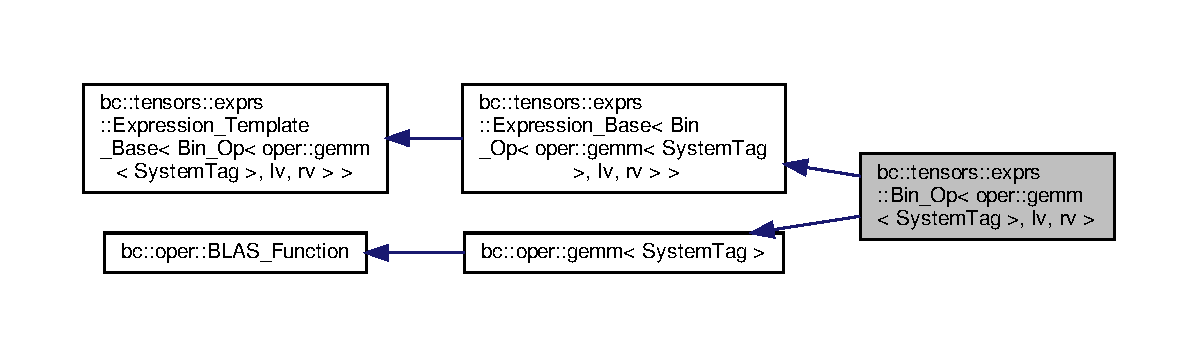
\includegraphics[width=350pt]{structbc_1_1tensors_1_1exprs_1_1Bin__Op_3_01oper_1_1gemm_3_01SystemTag_01_4_00_01lv_00_01rv_01_4__inherit__graph}
\end{center}
\end{figure}


Collaboration diagram for bc\+:\+:tensors\+:\+:exprs\+:\+:Bin\+\_\+\+Op$<$ oper\+:\+:gemm$<$ System\+Tag $>$, lv, rv $>$\+:\nopagebreak
\begin{figure}[H]
\begin{center}
\leavevmode
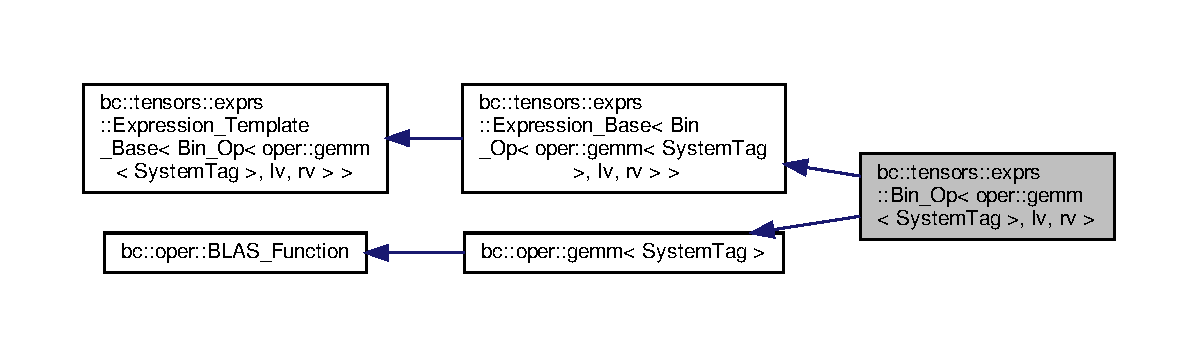
\includegraphics[width=350pt]{structbc_1_1tensors_1_1exprs_1_1Bin__Op_3_01oper_1_1gemm_3_01SystemTag_01_4_00_01lv_00_01rv_01_4__coll__graph}
\end{center}
\end{figure}
\subsection*{Public Types}
\begin{DoxyCompactItemize}
\item 
using \hyperlink{structbc_1_1tensors_1_1exprs_1_1Bin__Op_3_01oper_1_1gemm_3_01SystemTag_01_4_00_01lv_00_01rv_01_4_abec313441ee9136354af1e196d186c92}{value\+\_\+type} = typename lv\+::value\+\_\+type
\item 
using \hyperlink{structbc_1_1tensors_1_1exprs_1_1Bin__Op_3_01oper_1_1gemm_3_01SystemTag_01_4_00_01lv_00_01rv_01_4_a5779bf3375f157aac9c1493c560cfcd0}{system\+\_\+tag} = System\+Tag
\end{DoxyCompactItemize}
\subsection*{Public Member Functions}
\begin{DoxyCompactItemize}
\item 
\hyperlink{structbc_1_1tensors_1_1exprs_1_1Bin__Op_3_01oper_1_1gemm_3_01SystemTag_01_4_00_01lv_00_01rv_01_4_a14fe919a96786af35cc1e9b4bcf59d7c}{Bin\+\_\+\+Op} (lv \hyperlink{structbc_1_1tensors_1_1exprs_1_1Bin__Op_3_01oper_1_1gemm_3_01SystemTag_01_4_00_01lv_00_01rv_01_4_ae9d1e883b267b8e0c1d927ca6b26f8c6}{left}, rv \hyperlink{structbc_1_1tensors_1_1exprs_1_1Bin__Op_3_01oper_1_1gemm_3_01SystemTag_01_4_00_01lv_00_01rv_01_4_a20739a433b1fe788085657c8f35259e7}{right}, \hyperlink{structbc_1_1oper_1_1gemm}{oper\+::gemm}$<$ \hyperlink{structbc_1_1tensors_1_1exprs_1_1Bin__Op_3_01oper_1_1gemm_3_01SystemTag_01_4_00_01lv_00_01rv_01_4_a5779bf3375f157aac9c1493c560cfcd0}{system\+\_\+tag} $>$ op=\hyperlink{structbc_1_1oper_1_1gemm}{oper\+::gemm}$<$ \hyperlink{structbc_1_1tensors_1_1exprs_1_1Bin__Op_3_01oper_1_1gemm_3_01SystemTag_01_4_00_01lv_00_01rv_01_4_a5779bf3375f157aac9c1493c560cfcd0}{system\+\_\+tag} $>$())
\item 
\+\_\+\+\_\+host\+\_\+\+\_\+ \+\_\+\+\_\+device\+\_\+\+\_\+ \hyperlink{namespacebc_aaf8e3fbf99b04b1b57c4f80c6f55d3c5}{bc\+::size\+\_\+t} \hyperlink{structbc_1_1tensors_1_1exprs_1_1Bin__Op_3_01oper_1_1gemm_3_01SystemTag_01_4_00_01lv_00_01rv_01_4_aecf37031cfc3f6a08fa671c466e531a4}{size} () const
\item 
\+\_\+\+\_\+host\+\_\+\+\_\+ \+\_\+\+\_\+device\+\_\+\+\_\+ \hyperlink{namespacebc_aaf8e3fbf99b04b1b57c4f80c6f55d3c5}{bc\+::size\+\_\+t} \hyperlink{structbc_1_1tensors_1_1exprs_1_1Bin__Op_3_01oper_1_1gemm_3_01SystemTag_01_4_00_01lv_00_01rv_01_4_a92df1ce195219c63a88af91018ea3df7}{dim} (int i) const
\item 
\+\_\+\+\_\+host\+\_\+\+\_\+ \+\_\+\+\_\+device\+\_\+\+\_\+ \hyperlink{namespacebc_aaf8e3fbf99b04b1b57c4f80c6f55d3c5}{bc\+::size\+\_\+t} \hyperlink{structbc_1_1tensors_1_1exprs_1_1Bin__Op_3_01oper_1_1gemm_3_01SystemTag_01_4_00_01lv_00_01rv_01_4_a7e5714eaf186f58b2eddc42fcbbdd139}{rows} () const
\item 
\+\_\+\+\_\+host\+\_\+\+\_\+ \+\_\+\+\_\+device\+\_\+\+\_\+ \hyperlink{namespacebc_aaf8e3fbf99b04b1b57c4f80c6f55d3c5}{bc\+::size\+\_\+t} \hyperlink{structbc_1_1tensors_1_1exprs_1_1Bin__Op_3_01oper_1_1gemm_3_01SystemTag_01_4_00_01lv_00_01rv_01_4_a587627e80c6dce908bad02d5fbdf5546}{cols} () const
\item 
{\footnotesize template$<$class Core , int Alpha, int Beta, class Stream $>$ }\\void \hyperlink{structbc_1_1tensors_1_1exprs_1_1Bin__Op_3_01oper_1_1gemm_3_01SystemTag_01_4_00_01lv_00_01rv_01_4_ae98f2dfd8575358e314eed3725cab9bb}{eval} (\hyperlink{structbc_1_1tensors_1_1exprs_1_1Output__Data}{Output\+\_\+\+Data}$<$ Core, Alpha, Beta $>$ output, \hyperlink{classbc_1_1streams_1_1Stream}{Stream} stream) const
\end{DoxyCompactItemize}
\subsection*{Static Public Member Functions}
\begin{DoxyCompactItemize}
\item 
static \hyperlink{structbc_1_1oper_1_1gemm}{oper\+::gemm}$<$ System\+Tag $>$ \hyperlink{structbc_1_1tensors_1_1exprs_1_1Bin__Op_3_01oper_1_1gemm_3_01SystemTag_01_4_00_01lv_00_01rv_01_4_a96432eb485b1d23f90638920f296ae1b}{get\+\_\+operation} ()
\end{DoxyCompactItemize}
\subsection*{Public Attributes}
\begin{DoxyCompactItemize}
\item 
lv \hyperlink{structbc_1_1tensors_1_1exprs_1_1Bin__Op_3_01oper_1_1gemm_3_01SystemTag_01_4_00_01lv_00_01rv_01_4_ae9d1e883b267b8e0c1d927ca6b26f8c6}{left}
\item 
rv \hyperlink{structbc_1_1tensors_1_1exprs_1_1Bin__Op_3_01oper_1_1gemm_3_01SystemTag_01_4_00_01lv_00_01rv_01_4_a20739a433b1fe788085657c8f35259e7}{right}
\end{DoxyCompactItemize}
\subsection*{Static Public Attributes}
\begin{DoxyCompactItemize}
\item 
static constexpr int \hyperlink{structbc_1_1tensors_1_1exprs_1_1Bin__Op_3_01oper_1_1gemm_3_01SystemTag_01_4_00_01lv_00_01rv_01_4_ac3279ba20c5ec0f6ce97feea4c2d9ac8}{tensor\+\_\+dim} = rv\+::tensor\+\_\+dim
\item 
static constexpr int \hyperlink{structbc_1_1tensors_1_1exprs_1_1Bin__Op_3_01oper_1_1gemm_3_01SystemTag_01_4_00_01lv_00_01rv_01_4_a11116818fa08dda822689fd64bb2b5c9}{tensor\+\_\+iterator\+\_\+dim} = 1
\end{DoxyCompactItemize}


\subsection{Member Typedef Documentation}
\mbox{\Hypertarget{structbc_1_1tensors_1_1exprs_1_1Bin__Op_3_01oper_1_1gemm_3_01SystemTag_01_4_00_01lv_00_01rv_01_4_a5779bf3375f157aac9c1493c560cfcd0}\label{structbc_1_1tensors_1_1exprs_1_1Bin__Op_3_01oper_1_1gemm_3_01SystemTag_01_4_00_01lv_00_01rv_01_4_a5779bf3375f157aac9c1493c560cfcd0}} 
\index{bc\+::tensors\+::exprs\+::\+Bin\+\_\+\+Op$<$ oper\+::gemm$<$ System\+Tag $>$, lv, rv $>$@{bc\+::tensors\+::exprs\+::\+Bin\+\_\+\+Op$<$ oper\+::gemm$<$ System\+Tag $>$, lv, rv $>$}!system\+\_\+tag@{system\+\_\+tag}}
\index{system\+\_\+tag@{system\+\_\+tag}!bc\+::tensors\+::exprs\+::\+Bin\+\_\+\+Op$<$ oper\+::gemm$<$ System\+Tag $>$, lv, rv $>$@{bc\+::tensors\+::exprs\+::\+Bin\+\_\+\+Op$<$ oper\+::gemm$<$ System\+Tag $>$, lv, rv $>$}}
\subsubsection{\texorpdfstring{system\+\_\+tag}{system\_tag}}
{\footnotesize\ttfamily template$<$class lv , class rv , class System\+Tag $>$ \\
using \hyperlink{structbc_1_1tensors_1_1exprs_1_1Bin__Op}{bc\+::tensors\+::exprs\+::\+Bin\+\_\+\+Op}$<$ \hyperlink{structbc_1_1oper_1_1gemm}{oper\+::gemm}$<$ System\+Tag $>$, lv, rv $>$\+::\hyperlink{structbc_1_1tensors_1_1exprs_1_1Bin__Op_3_01oper_1_1gemm_3_01SystemTag_01_4_00_01lv_00_01rv_01_4_a5779bf3375f157aac9c1493c560cfcd0}{system\+\_\+tag} =  System\+Tag}

\mbox{\Hypertarget{structbc_1_1tensors_1_1exprs_1_1Bin__Op_3_01oper_1_1gemm_3_01SystemTag_01_4_00_01lv_00_01rv_01_4_abec313441ee9136354af1e196d186c92}\label{structbc_1_1tensors_1_1exprs_1_1Bin__Op_3_01oper_1_1gemm_3_01SystemTag_01_4_00_01lv_00_01rv_01_4_abec313441ee9136354af1e196d186c92}} 
\index{bc\+::tensors\+::exprs\+::\+Bin\+\_\+\+Op$<$ oper\+::gemm$<$ System\+Tag $>$, lv, rv $>$@{bc\+::tensors\+::exprs\+::\+Bin\+\_\+\+Op$<$ oper\+::gemm$<$ System\+Tag $>$, lv, rv $>$}!value\+\_\+type@{value\+\_\+type}}
\index{value\+\_\+type@{value\+\_\+type}!bc\+::tensors\+::exprs\+::\+Bin\+\_\+\+Op$<$ oper\+::gemm$<$ System\+Tag $>$, lv, rv $>$@{bc\+::tensors\+::exprs\+::\+Bin\+\_\+\+Op$<$ oper\+::gemm$<$ System\+Tag $>$, lv, rv $>$}}
\subsubsection{\texorpdfstring{value\+\_\+type}{value\_type}}
{\footnotesize\ttfamily template$<$class lv , class rv , class System\+Tag $>$ \\
using \hyperlink{structbc_1_1tensors_1_1exprs_1_1Bin__Op}{bc\+::tensors\+::exprs\+::\+Bin\+\_\+\+Op}$<$ \hyperlink{structbc_1_1oper_1_1gemm}{oper\+::gemm}$<$ System\+Tag $>$, lv, rv $>$\+::\hyperlink{structbc_1_1tensors_1_1exprs_1_1Bin__Op_3_01oper_1_1gemm_3_01SystemTag_01_4_00_01lv_00_01rv_01_4_abec313441ee9136354af1e196d186c92}{value\+\_\+type} =  typename lv\+::value\+\_\+type}



\subsection{Constructor \& Destructor Documentation}
\mbox{\Hypertarget{structbc_1_1tensors_1_1exprs_1_1Bin__Op_3_01oper_1_1gemm_3_01SystemTag_01_4_00_01lv_00_01rv_01_4_a14fe919a96786af35cc1e9b4bcf59d7c}\label{structbc_1_1tensors_1_1exprs_1_1Bin__Op_3_01oper_1_1gemm_3_01SystemTag_01_4_00_01lv_00_01rv_01_4_a14fe919a96786af35cc1e9b4bcf59d7c}} 
\index{bc\+::tensors\+::exprs\+::\+Bin\+\_\+\+Op$<$ oper\+::gemm$<$ System\+Tag $>$, lv, rv $>$@{bc\+::tensors\+::exprs\+::\+Bin\+\_\+\+Op$<$ oper\+::gemm$<$ System\+Tag $>$, lv, rv $>$}!Bin\+\_\+\+Op@{Bin\+\_\+\+Op}}
\index{Bin\+\_\+\+Op@{Bin\+\_\+\+Op}!bc\+::tensors\+::exprs\+::\+Bin\+\_\+\+Op$<$ oper\+::gemm$<$ System\+Tag $>$, lv, rv $>$@{bc\+::tensors\+::exprs\+::\+Bin\+\_\+\+Op$<$ oper\+::gemm$<$ System\+Tag $>$, lv, rv $>$}}
\subsubsection{\texorpdfstring{Bin\+\_\+\+Op()}{Bin\_Op()}}
{\footnotesize\ttfamily template$<$class lv , class rv , class System\+Tag $>$ \\
\hyperlink{structbc_1_1tensors_1_1exprs_1_1Bin__Op}{bc\+::tensors\+::exprs\+::\+Bin\+\_\+\+Op}$<$ \hyperlink{structbc_1_1oper_1_1gemm}{oper\+::gemm}$<$ System\+Tag $>$, lv, rv $>$\+::\hyperlink{structbc_1_1tensors_1_1exprs_1_1Bin__Op}{Bin\+\_\+\+Op} (\begin{DoxyParamCaption}\item[{lv}]{left,  }\item[{rv}]{right,  }\item[{\hyperlink{structbc_1_1oper_1_1gemm}{oper\+::gemm}$<$ \hyperlink{structbc_1_1tensors_1_1exprs_1_1Bin__Op_3_01oper_1_1gemm_3_01SystemTag_01_4_00_01lv_00_01rv_01_4_a5779bf3375f157aac9c1493c560cfcd0}{system\+\_\+tag} $>$}]{op = {\ttfamily \hyperlink{structbc_1_1oper_1_1gemm}{oper\+::gemm}$<$\hyperlink{structbc_1_1tensors_1_1exprs_1_1Bin__Op_3_01oper_1_1gemm_3_01SystemTag_01_4_00_01lv_00_01rv_01_4_a5779bf3375f157aac9c1493c560cfcd0}{system\+\_\+tag}$>$()} }\end{DoxyParamCaption})\hspace{0.3cm}{\ttfamily [inline]}}



\subsection{Member Function Documentation}
\mbox{\Hypertarget{structbc_1_1tensors_1_1exprs_1_1Bin__Op_3_01oper_1_1gemm_3_01SystemTag_01_4_00_01lv_00_01rv_01_4_a587627e80c6dce908bad02d5fbdf5546}\label{structbc_1_1tensors_1_1exprs_1_1Bin__Op_3_01oper_1_1gemm_3_01SystemTag_01_4_00_01lv_00_01rv_01_4_a587627e80c6dce908bad02d5fbdf5546}} 
\index{bc\+::tensors\+::exprs\+::\+Bin\+\_\+\+Op$<$ oper\+::gemm$<$ System\+Tag $>$, lv, rv $>$@{bc\+::tensors\+::exprs\+::\+Bin\+\_\+\+Op$<$ oper\+::gemm$<$ System\+Tag $>$, lv, rv $>$}!cols@{cols}}
\index{cols@{cols}!bc\+::tensors\+::exprs\+::\+Bin\+\_\+\+Op$<$ oper\+::gemm$<$ System\+Tag $>$, lv, rv $>$@{bc\+::tensors\+::exprs\+::\+Bin\+\_\+\+Op$<$ oper\+::gemm$<$ System\+Tag $>$, lv, rv $>$}}
\subsubsection{\texorpdfstring{cols()}{cols()}}
{\footnotesize\ttfamily template$<$class lv , class rv , class System\+Tag $>$ \\
\+\_\+\+\_\+host\+\_\+\+\_\+ \+\_\+\+\_\+device\+\_\+\+\_\+ \hyperlink{namespacebc_aaf8e3fbf99b04b1b57c4f80c6f55d3c5}{bc\+::size\+\_\+t} \hyperlink{structbc_1_1tensors_1_1exprs_1_1Bin__Op}{bc\+::tensors\+::exprs\+::\+Bin\+\_\+\+Op}$<$ \hyperlink{structbc_1_1oper_1_1gemm}{oper\+::gemm}$<$ System\+Tag $>$, lv, rv $>$\+::cols (\begin{DoxyParamCaption}{ }\end{DoxyParamCaption}) const\hspace{0.3cm}{\ttfamily [inline]}}

\mbox{\Hypertarget{structbc_1_1tensors_1_1exprs_1_1Bin__Op_3_01oper_1_1gemm_3_01SystemTag_01_4_00_01lv_00_01rv_01_4_a92df1ce195219c63a88af91018ea3df7}\label{structbc_1_1tensors_1_1exprs_1_1Bin__Op_3_01oper_1_1gemm_3_01SystemTag_01_4_00_01lv_00_01rv_01_4_a92df1ce195219c63a88af91018ea3df7}} 
\index{bc\+::tensors\+::exprs\+::\+Bin\+\_\+\+Op$<$ oper\+::gemm$<$ System\+Tag $>$, lv, rv $>$@{bc\+::tensors\+::exprs\+::\+Bin\+\_\+\+Op$<$ oper\+::gemm$<$ System\+Tag $>$, lv, rv $>$}!dim@{dim}}
\index{dim@{dim}!bc\+::tensors\+::exprs\+::\+Bin\+\_\+\+Op$<$ oper\+::gemm$<$ System\+Tag $>$, lv, rv $>$@{bc\+::tensors\+::exprs\+::\+Bin\+\_\+\+Op$<$ oper\+::gemm$<$ System\+Tag $>$, lv, rv $>$}}
\subsubsection{\texorpdfstring{dim()}{dim()}}
{\footnotesize\ttfamily template$<$class lv , class rv , class System\+Tag $>$ \\
\+\_\+\+\_\+host\+\_\+\+\_\+ \+\_\+\+\_\+device\+\_\+\+\_\+ \hyperlink{namespacebc_aaf8e3fbf99b04b1b57c4f80c6f55d3c5}{bc\+::size\+\_\+t} \hyperlink{structbc_1_1tensors_1_1exprs_1_1Bin__Op}{bc\+::tensors\+::exprs\+::\+Bin\+\_\+\+Op}$<$ \hyperlink{structbc_1_1oper_1_1gemm}{oper\+::gemm}$<$ System\+Tag $>$, lv, rv $>$\+::dim (\begin{DoxyParamCaption}\item[{int}]{i }\end{DoxyParamCaption}) const\hspace{0.3cm}{\ttfamily [inline]}}

\mbox{\Hypertarget{structbc_1_1tensors_1_1exprs_1_1Bin__Op_3_01oper_1_1gemm_3_01SystemTag_01_4_00_01lv_00_01rv_01_4_ae98f2dfd8575358e314eed3725cab9bb}\label{structbc_1_1tensors_1_1exprs_1_1Bin__Op_3_01oper_1_1gemm_3_01SystemTag_01_4_00_01lv_00_01rv_01_4_ae98f2dfd8575358e314eed3725cab9bb}} 
\index{bc\+::tensors\+::exprs\+::\+Bin\+\_\+\+Op$<$ oper\+::gemm$<$ System\+Tag $>$, lv, rv $>$@{bc\+::tensors\+::exprs\+::\+Bin\+\_\+\+Op$<$ oper\+::gemm$<$ System\+Tag $>$, lv, rv $>$}!eval@{eval}}
\index{eval@{eval}!bc\+::tensors\+::exprs\+::\+Bin\+\_\+\+Op$<$ oper\+::gemm$<$ System\+Tag $>$, lv, rv $>$@{bc\+::tensors\+::exprs\+::\+Bin\+\_\+\+Op$<$ oper\+::gemm$<$ System\+Tag $>$, lv, rv $>$}}
\subsubsection{\texorpdfstring{eval()}{eval()}}
{\footnotesize\ttfamily template$<$class lv , class rv , class System\+Tag $>$ \\
template$<$class Core , int Alpha, int Beta, class Stream $>$ \\
void \hyperlink{structbc_1_1tensors_1_1exprs_1_1Bin__Op}{bc\+::tensors\+::exprs\+::\+Bin\+\_\+\+Op}$<$ \hyperlink{structbc_1_1oper_1_1gemm}{oper\+::gemm}$<$ System\+Tag $>$, lv, rv $>$\+::eval (\begin{DoxyParamCaption}\item[{\hyperlink{structbc_1_1tensors_1_1exprs_1_1Output__Data}{Output\+\_\+\+Data}$<$ Core, Alpha, Beta $>$}]{output,  }\item[{\hyperlink{classbc_1_1streams_1_1Stream}{Stream}}]{stream }\end{DoxyParamCaption}) const\hspace{0.3cm}{\ttfamily [inline]}}

\mbox{\Hypertarget{structbc_1_1tensors_1_1exprs_1_1Bin__Op_3_01oper_1_1gemm_3_01SystemTag_01_4_00_01lv_00_01rv_01_4_a96432eb485b1d23f90638920f296ae1b}\label{structbc_1_1tensors_1_1exprs_1_1Bin__Op_3_01oper_1_1gemm_3_01SystemTag_01_4_00_01lv_00_01rv_01_4_a96432eb485b1d23f90638920f296ae1b}} 
\index{bc\+::tensors\+::exprs\+::\+Bin\+\_\+\+Op$<$ oper\+::gemm$<$ System\+Tag $>$, lv, rv $>$@{bc\+::tensors\+::exprs\+::\+Bin\+\_\+\+Op$<$ oper\+::gemm$<$ System\+Tag $>$, lv, rv $>$}!get\+\_\+operation@{get\+\_\+operation}}
\index{get\+\_\+operation@{get\+\_\+operation}!bc\+::tensors\+::exprs\+::\+Bin\+\_\+\+Op$<$ oper\+::gemm$<$ System\+Tag $>$, lv, rv $>$@{bc\+::tensors\+::exprs\+::\+Bin\+\_\+\+Op$<$ oper\+::gemm$<$ System\+Tag $>$, lv, rv $>$}}
\subsubsection{\texorpdfstring{get\+\_\+operation()}{get\_operation()}}
{\footnotesize\ttfamily template$<$class lv , class rv , class System\+Tag $>$ \\
static \hyperlink{structbc_1_1oper_1_1gemm}{oper\+::gemm}$<$System\+Tag$>$ \hyperlink{structbc_1_1tensors_1_1exprs_1_1Bin__Op}{bc\+::tensors\+::exprs\+::\+Bin\+\_\+\+Op}$<$ \hyperlink{structbc_1_1oper_1_1gemm}{oper\+::gemm}$<$ System\+Tag $>$, lv, rv $>$\+::get\+\_\+operation (\begin{DoxyParamCaption}{ }\end{DoxyParamCaption})\hspace{0.3cm}{\ttfamily [inline]}, {\ttfamily [static]}}

\mbox{\Hypertarget{structbc_1_1tensors_1_1exprs_1_1Bin__Op_3_01oper_1_1gemm_3_01SystemTag_01_4_00_01lv_00_01rv_01_4_a7e5714eaf186f58b2eddc42fcbbdd139}\label{structbc_1_1tensors_1_1exprs_1_1Bin__Op_3_01oper_1_1gemm_3_01SystemTag_01_4_00_01lv_00_01rv_01_4_a7e5714eaf186f58b2eddc42fcbbdd139}} 
\index{bc\+::tensors\+::exprs\+::\+Bin\+\_\+\+Op$<$ oper\+::gemm$<$ System\+Tag $>$, lv, rv $>$@{bc\+::tensors\+::exprs\+::\+Bin\+\_\+\+Op$<$ oper\+::gemm$<$ System\+Tag $>$, lv, rv $>$}!rows@{rows}}
\index{rows@{rows}!bc\+::tensors\+::exprs\+::\+Bin\+\_\+\+Op$<$ oper\+::gemm$<$ System\+Tag $>$, lv, rv $>$@{bc\+::tensors\+::exprs\+::\+Bin\+\_\+\+Op$<$ oper\+::gemm$<$ System\+Tag $>$, lv, rv $>$}}
\subsubsection{\texorpdfstring{rows()}{rows()}}
{\footnotesize\ttfamily template$<$class lv , class rv , class System\+Tag $>$ \\
\+\_\+\+\_\+host\+\_\+\+\_\+ \+\_\+\+\_\+device\+\_\+\+\_\+ \hyperlink{namespacebc_aaf8e3fbf99b04b1b57c4f80c6f55d3c5}{bc\+::size\+\_\+t} \hyperlink{structbc_1_1tensors_1_1exprs_1_1Bin__Op}{bc\+::tensors\+::exprs\+::\+Bin\+\_\+\+Op}$<$ \hyperlink{structbc_1_1oper_1_1gemm}{oper\+::gemm}$<$ System\+Tag $>$, lv, rv $>$\+::rows (\begin{DoxyParamCaption}{ }\end{DoxyParamCaption}) const\hspace{0.3cm}{\ttfamily [inline]}}

\mbox{\Hypertarget{structbc_1_1tensors_1_1exprs_1_1Bin__Op_3_01oper_1_1gemm_3_01SystemTag_01_4_00_01lv_00_01rv_01_4_aecf37031cfc3f6a08fa671c466e531a4}\label{structbc_1_1tensors_1_1exprs_1_1Bin__Op_3_01oper_1_1gemm_3_01SystemTag_01_4_00_01lv_00_01rv_01_4_aecf37031cfc3f6a08fa671c466e531a4}} 
\index{bc\+::tensors\+::exprs\+::\+Bin\+\_\+\+Op$<$ oper\+::gemm$<$ System\+Tag $>$, lv, rv $>$@{bc\+::tensors\+::exprs\+::\+Bin\+\_\+\+Op$<$ oper\+::gemm$<$ System\+Tag $>$, lv, rv $>$}!size@{size}}
\index{size@{size}!bc\+::tensors\+::exprs\+::\+Bin\+\_\+\+Op$<$ oper\+::gemm$<$ System\+Tag $>$, lv, rv $>$@{bc\+::tensors\+::exprs\+::\+Bin\+\_\+\+Op$<$ oper\+::gemm$<$ System\+Tag $>$, lv, rv $>$}}
\subsubsection{\texorpdfstring{size()}{size()}}
{\footnotesize\ttfamily template$<$class lv , class rv , class System\+Tag $>$ \\
\+\_\+\+\_\+host\+\_\+\+\_\+ \+\_\+\+\_\+device\+\_\+\+\_\+ \hyperlink{namespacebc_aaf8e3fbf99b04b1b57c4f80c6f55d3c5}{bc\+::size\+\_\+t} \hyperlink{structbc_1_1tensors_1_1exprs_1_1Bin__Op}{bc\+::tensors\+::exprs\+::\+Bin\+\_\+\+Op}$<$ \hyperlink{structbc_1_1oper_1_1gemm}{oper\+::gemm}$<$ System\+Tag $>$, lv, rv $>$\+::size (\begin{DoxyParamCaption}{ }\end{DoxyParamCaption}) const\hspace{0.3cm}{\ttfamily [inline]}}



\subsection{Member Data Documentation}
\mbox{\Hypertarget{structbc_1_1tensors_1_1exprs_1_1Bin__Op_3_01oper_1_1gemm_3_01SystemTag_01_4_00_01lv_00_01rv_01_4_ae9d1e883b267b8e0c1d927ca6b26f8c6}\label{structbc_1_1tensors_1_1exprs_1_1Bin__Op_3_01oper_1_1gemm_3_01SystemTag_01_4_00_01lv_00_01rv_01_4_ae9d1e883b267b8e0c1d927ca6b26f8c6}} 
\index{bc\+::tensors\+::exprs\+::\+Bin\+\_\+\+Op$<$ oper\+::gemm$<$ System\+Tag $>$, lv, rv $>$@{bc\+::tensors\+::exprs\+::\+Bin\+\_\+\+Op$<$ oper\+::gemm$<$ System\+Tag $>$, lv, rv $>$}!left@{left}}
\index{left@{left}!bc\+::tensors\+::exprs\+::\+Bin\+\_\+\+Op$<$ oper\+::gemm$<$ System\+Tag $>$, lv, rv $>$@{bc\+::tensors\+::exprs\+::\+Bin\+\_\+\+Op$<$ oper\+::gemm$<$ System\+Tag $>$, lv, rv $>$}}
\subsubsection{\texorpdfstring{left}{left}}
{\footnotesize\ttfamily template$<$class lv , class rv , class System\+Tag $>$ \\
lv \hyperlink{structbc_1_1tensors_1_1exprs_1_1Bin__Op}{bc\+::tensors\+::exprs\+::\+Bin\+\_\+\+Op}$<$ \hyperlink{structbc_1_1oper_1_1gemm}{oper\+::gemm}$<$ System\+Tag $>$, lv, rv $>$\+::left}

\mbox{\Hypertarget{structbc_1_1tensors_1_1exprs_1_1Bin__Op_3_01oper_1_1gemm_3_01SystemTag_01_4_00_01lv_00_01rv_01_4_a20739a433b1fe788085657c8f35259e7}\label{structbc_1_1tensors_1_1exprs_1_1Bin__Op_3_01oper_1_1gemm_3_01SystemTag_01_4_00_01lv_00_01rv_01_4_a20739a433b1fe788085657c8f35259e7}} 
\index{bc\+::tensors\+::exprs\+::\+Bin\+\_\+\+Op$<$ oper\+::gemm$<$ System\+Tag $>$, lv, rv $>$@{bc\+::tensors\+::exprs\+::\+Bin\+\_\+\+Op$<$ oper\+::gemm$<$ System\+Tag $>$, lv, rv $>$}!right@{right}}
\index{right@{right}!bc\+::tensors\+::exprs\+::\+Bin\+\_\+\+Op$<$ oper\+::gemm$<$ System\+Tag $>$, lv, rv $>$@{bc\+::tensors\+::exprs\+::\+Bin\+\_\+\+Op$<$ oper\+::gemm$<$ System\+Tag $>$, lv, rv $>$}}
\subsubsection{\texorpdfstring{right}{right}}
{\footnotesize\ttfamily template$<$class lv , class rv , class System\+Tag $>$ \\
rv \hyperlink{structbc_1_1tensors_1_1exprs_1_1Bin__Op}{bc\+::tensors\+::exprs\+::\+Bin\+\_\+\+Op}$<$ \hyperlink{structbc_1_1oper_1_1gemm}{oper\+::gemm}$<$ System\+Tag $>$, lv, rv $>$\+::right}

\mbox{\Hypertarget{structbc_1_1tensors_1_1exprs_1_1Bin__Op_3_01oper_1_1gemm_3_01SystemTag_01_4_00_01lv_00_01rv_01_4_ac3279ba20c5ec0f6ce97feea4c2d9ac8}\label{structbc_1_1tensors_1_1exprs_1_1Bin__Op_3_01oper_1_1gemm_3_01SystemTag_01_4_00_01lv_00_01rv_01_4_ac3279ba20c5ec0f6ce97feea4c2d9ac8}} 
\index{bc\+::tensors\+::exprs\+::\+Bin\+\_\+\+Op$<$ oper\+::gemm$<$ System\+Tag $>$, lv, rv $>$@{bc\+::tensors\+::exprs\+::\+Bin\+\_\+\+Op$<$ oper\+::gemm$<$ System\+Tag $>$, lv, rv $>$}!tensor\+\_\+dim@{tensor\+\_\+dim}}
\index{tensor\+\_\+dim@{tensor\+\_\+dim}!bc\+::tensors\+::exprs\+::\+Bin\+\_\+\+Op$<$ oper\+::gemm$<$ System\+Tag $>$, lv, rv $>$@{bc\+::tensors\+::exprs\+::\+Bin\+\_\+\+Op$<$ oper\+::gemm$<$ System\+Tag $>$, lv, rv $>$}}
\subsubsection{\texorpdfstring{tensor\+\_\+dim}{tensor\_dim}}
{\footnotesize\ttfamily template$<$class lv , class rv , class System\+Tag $>$ \\
constexpr int \hyperlink{structbc_1_1tensors_1_1exprs_1_1Bin__Op}{bc\+::tensors\+::exprs\+::\+Bin\+\_\+\+Op}$<$ \hyperlink{structbc_1_1oper_1_1gemm}{oper\+::gemm}$<$ System\+Tag $>$, lv, rv $>$\+::tensor\+\_\+dim = rv\+::tensor\+\_\+dim\hspace{0.3cm}{\ttfamily [static]}}

\mbox{\Hypertarget{structbc_1_1tensors_1_1exprs_1_1Bin__Op_3_01oper_1_1gemm_3_01SystemTag_01_4_00_01lv_00_01rv_01_4_a11116818fa08dda822689fd64bb2b5c9}\label{structbc_1_1tensors_1_1exprs_1_1Bin__Op_3_01oper_1_1gemm_3_01SystemTag_01_4_00_01lv_00_01rv_01_4_a11116818fa08dda822689fd64bb2b5c9}} 
\index{bc\+::tensors\+::exprs\+::\+Bin\+\_\+\+Op$<$ oper\+::gemm$<$ System\+Tag $>$, lv, rv $>$@{bc\+::tensors\+::exprs\+::\+Bin\+\_\+\+Op$<$ oper\+::gemm$<$ System\+Tag $>$, lv, rv $>$}!tensor\+\_\+iterator\+\_\+dim@{tensor\+\_\+iterator\+\_\+dim}}
\index{tensor\+\_\+iterator\+\_\+dim@{tensor\+\_\+iterator\+\_\+dim}!bc\+::tensors\+::exprs\+::\+Bin\+\_\+\+Op$<$ oper\+::gemm$<$ System\+Tag $>$, lv, rv $>$@{bc\+::tensors\+::exprs\+::\+Bin\+\_\+\+Op$<$ oper\+::gemm$<$ System\+Tag $>$, lv, rv $>$}}
\subsubsection{\texorpdfstring{tensor\+\_\+iterator\+\_\+dim}{tensor\_iterator\_dim}}
{\footnotesize\ttfamily template$<$class lv , class rv , class System\+Tag $>$ \\
constexpr int \hyperlink{structbc_1_1tensors_1_1exprs_1_1Bin__Op}{bc\+::tensors\+::exprs\+::\+Bin\+\_\+\+Op}$<$ \hyperlink{structbc_1_1oper_1_1gemm}{oper\+::gemm}$<$ System\+Tag $>$, lv, rv $>$\+::tensor\+\_\+iterator\+\_\+dim = 1\hspace{0.3cm}{\ttfamily [static]}}



The documentation for this struct was generated from the following file\+:\begin{DoxyCompactItemize}
\item 
blackcat/tensors/expression\+\_\+templates/\hyperlink{function__gemm_8h}{function\+\_\+gemm.\+h}\end{DoxyCompactItemize}

\hypertarget{structbc_1_1tensors_1_1exprs_1_1Bin__Op_3_01oper_1_1gemv_3_01SystemTag_01_4_00_01lv_00_01rv_01_4}{}\section{bc\+:\+:tensors\+:\+:exprs\+:\+:Bin\+\_\+\+Op$<$ oper\+:\+:gemv$<$ System\+Tag $>$, lv, rv $>$ Struct Template Reference}
\label{structbc_1_1tensors_1_1exprs_1_1Bin__Op_3_01oper_1_1gemv_3_01SystemTag_01_4_00_01lv_00_01rv_01_4}\index{bc\+::tensors\+::exprs\+::\+Bin\+\_\+\+Op$<$ oper\+::gemv$<$ System\+Tag $>$, lv, rv $>$@{bc\+::tensors\+::exprs\+::\+Bin\+\_\+\+Op$<$ oper\+::gemv$<$ System\+Tag $>$, lv, rv $>$}}


{\ttfamily \#include $<$function\+\_\+gemv.\+h$>$}



Inheritance diagram for bc\+:\+:tensors\+:\+:exprs\+:\+:Bin\+\_\+\+Op$<$ oper\+:\+:gemv$<$ System\+Tag $>$, lv, rv $>$\+:\nopagebreak
\begin{figure}[H]
\begin{center}
\leavevmode
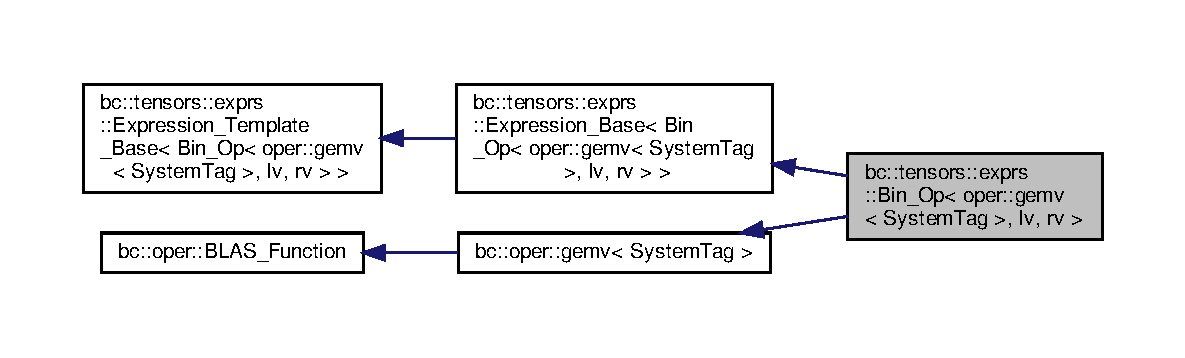
\includegraphics[width=350pt]{structbc_1_1tensors_1_1exprs_1_1Bin__Op_3_01oper_1_1gemv_3_01SystemTag_01_4_00_01lv_00_01rv_01_4__inherit__graph}
\end{center}
\end{figure}


Collaboration diagram for bc\+:\+:tensors\+:\+:exprs\+:\+:Bin\+\_\+\+Op$<$ oper\+:\+:gemv$<$ System\+Tag $>$, lv, rv $>$\+:\nopagebreak
\begin{figure}[H]
\begin{center}
\leavevmode
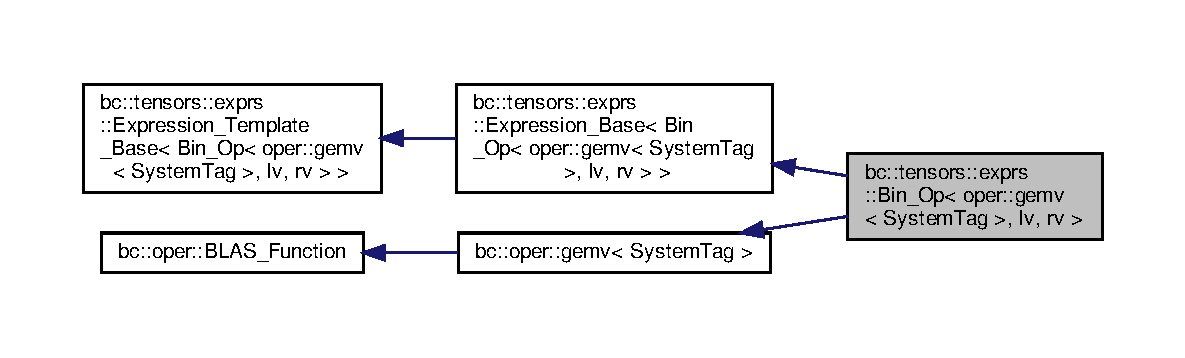
\includegraphics[width=350pt]{structbc_1_1tensors_1_1exprs_1_1Bin__Op_3_01oper_1_1gemv_3_01SystemTag_01_4_00_01lv_00_01rv_01_4__coll__graph}
\end{center}
\end{figure}
\subsection*{Public Types}
\begin{DoxyCompactItemize}
\item 
using \hyperlink{structbc_1_1tensors_1_1exprs_1_1Bin__Op_3_01oper_1_1gemv_3_01SystemTag_01_4_00_01lv_00_01rv_01_4_a1fc7a37a4a658815b1d29c9bc473dbe1}{value\+\_\+type} = typename lv\+::value\+\_\+type
\item 
using \hyperlink{structbc_1_1tensors_1_1exprs_1_1Bin__Op_3_01oper_1_1gemv_3_01SystemTag_01_4_00_01lv_00_01rv_01_4_a18ec8659904c80f74cf3c865349e0785}{system\+\_\+tag} = System\+Tag
\end{DoxyCompactItemize}
\subsection*{Public Member Functions}
\begin{DoxyCompactItemize}
\item 
\hyperlink{structbc_1_1tensors_1_1exprs_1_1Bin__Op_3_01oper_1_1gemv_3_01SystemTag_01_4_00_01lv_00_01rv_01_4_adc4a8b309f32fb758e2463600050d462}{Bin\+\_\+\+Op} (lv \hyperlink{structbc_1_1tensors_1_1exprs_1_1Bin__Op_3_01oper_1_1gemv_3_01SystemTag_01_4_00_01lv_00_01rv_01_4_acf8a343150aa94e049e4256aa2e543d8}{left}, rv \hyperlink{structbc_1_1tensors_1_1exprs_1_1Bin__Op_3_01oper_1_1gemv_3_01SystemTag_01_4_00_01lv_00_01rv_01_4_a03a8bea78fcc4829df216da0e407a634}{right}, \hyperlink{structbc_1_1oper_1_1gemv}{oper\+::gemv}$<$ \hyperlink{structbc_1_1tensors_1_1exprs_1_1Bin__Op_3_01oper_1_1gemv_3_01SystemTag_01_4_00_01lv_00_01rv_01_4_a18ec8659904c80f74cf3c865349e0785}{system\+\_\+tag} $>$ op=\hyperlink{structbc_1_1oper_1_1gemv}{oper\+::gemv}$<$ \hyperlink{structbc_1_1tensors_1_1exprs_1_1Bin__Op_3_01oper_1_1gemv_3_01SystemTag_01_4_00_01lv_00_01rv_01_4_a18ec8659904c80f74cf3c865349e0785}{system\+\_\+tag} $>$())
\item 
\+\_\+\+\_\+host\+\_\+\+\_\+ \+\_\+\+\_\+device\+\_\+\+\_\+ \hyperlink{namespacebc_aaf8e3fbf99b04b1b57c4f80c6f55d3c5}{bc\+::size\+\_\+t} \hyperlink{structbc_1_1tensors_1_1exprs_1_1Bin__Op_3_01oper_1_1gemv_3_01SystemTag_01_4_00_01lv_00_01rv_01_4_a5db95ed8e64d067c19453d0dae84f3f8}{size} () const
\item 
\+\_\+\+\_\+host\+\_\+\+\_\+ \+\_\+\+\_\+device\+\_\+\+\_\+ \hyperlink{namespacebc_aaf8e3fbf99b04b1b57c4f80c6f55d3c5}{bc\+::size\+\_\+t} \hyperlink{structbc_1_1tensors_1_1exprs_1_1Bin__Op_3_01oper_1_1gemv_3_01SystemTag_01_4_00_01lv_00_01rv_01_4_aa7303752c7568668f6c6bbe6990317e8}{dim} (int i) const
\item 
\+\_\+\+\_\+host\+\_\+\+\_\+ \+\_\+\+\_\+device\+\_\+\+\_\+ \hyperlink{namespacebc_aaf8e3fbf99b04b1b57c4f80c6f55d3c5}{bc\+::size\+\_\+t} \hyperlink{structbc_1_1tensors_1_1exprs_1_1Bin__Op_3_01oper_1_1gemv_3_01SystemTag_01_4_00_01lv_00_01rv_01_4_a787bc0a383dc1a56057fc7a740416b38}{rows} () const
\item 
\+\_\+\+\_\+host\+\_\+\+\_\+ \+\_\+\+\_\+device\+\_\+\+\_\+ \hyperlink{namespacebc_aaf8e3fbf99b04b1b57c4f80c6f55d3c5}{bc\+::size\+\_\+t} \hyperlink{structbc_1_1tensors_1_1exprs_1_1Bin__Op_3_01oper_1_1gemv_3_01SystemTag_01_4_00_01lv_00_01rv_01_4_abc6cc62330889d1d2128d17bb44dde05}{cols} () const
\item 
{\footnotesize template$<$class core , int Alpha, int Beta, class Stream $>$ }\\void \hyperlink{structbc_1_1tensors_1_1exprs_1_1Bin__Op_3_01oper_1_1gemv_3_01SystemTag_01_4_00_01lv_00_01rv_01_4_a7476be9dd29986e2e4f52c16a1e45b2d}{eval} (\hyperlink{structbc_1_1tensors_1_1exprs_1_1Output__Data}{Output\+\_\+\+Data}$<$ core, Alpha, Beta $>$ output, \hyperlink{classbc_1_1streams_1_1Stream}{Stream} stream) const
\end{DoxyCompactItemize}
\subsection*{Static Public Member Functions}
\begin{DoxyCompactItemize}
\item 
static \hyperlink{structbc_1_1oper_1_1gemv}{oper\+::gemv}$<$ \hyperlink{structbc_1_1tensors_1_1exprs_1_1Bin__Op_3_01oper_1_1gemv_3_01SystemTag_01_4_00_01lv_00_01rv_01_4_a18ec8659904c80f74cf3c865349e0785}{system\+\_\+tag} $>$ \hyperlink{structbc_1_1tensors_1_1exprs_1_1Bin__Op_3_01oper_1_1gemv_3_01SystemTag_01_4_00_01lv_00_01rv_01_4_aa6172a36f7b36dc1889faf5e48709234}{get\+\_\+operation} ()
\end{DoxyCompactItemize}
\subsection*{Public Attributes}
\begin{DoxyCompactItemize}
\item 
lv \hyperlink{structbc_1_1tensors_1_1exprs_1_1Bin__Op_3_01oper_1_1gemv_3_01SystemTag_01_4_00_01lv_00_01rv_01_4_acf8a343150aa94e049e4256aa2e543d8}{left}
\item 
rv \hyperlink{structbc_1_1tensors_1_1exprs_1_1Bin__Op_3_01oper_1_1gemv_3_01SystemTag_01_4_00_01lv_00_01rv_01_4_a03a8bea78fcc4829df216da0e407a634}{right}
\end{DoxyCompactItemize}
\subsection*{Static Public Attributes}
\begin{DoxyCompactItemize}
\item 
static constexpr int \hyperlink{structbc_1_1tensors_1_1exprs_1_1Bin__Op_3_01oper_1_1gemv_3_01SystemTag_01_4_00_01lv_00_01rv_01_4_a5ee5c04316c9a6a67248e7920aaf07bd}{tensor\+\_\+dim} = 1
\item 
static constexpr int \hyperlink{structbc_1_1tensors_1_1exprs_1_1Bin__Op_3_01oper_1_1gemv_3_01SystemTag_01_4_00_01lv_00_01rv_01_4_af30c95fbafd6a6d93707f45f3028beb9}{tensor\+\_\+iterator\+\_\+dim} = 1
\end{DoxyCompactItemize}


\subsection{Member Typedef Documentation}
\mbox{\Hypertarget{structbc_1_1tensors_1_1exprs_1_1Bin__Op_3_01oper_1_1gemv_3_01SystemTag_01_4_00_01lv_00_01rv_01_4_a18ec8659904c80f74cf3c865349e0785}\label{structbc_1_1tensors_1_1exprs_1_1Bin__Op_3_01oper_1_1gemv_3_01SystemTag_01_4_00_01lv_00_01rv_01_4_a18ec8659904c80f74cf3c865349e0785}} 
\index{bc\+::tensors\+::exprs\+::\+Bin\+\_\+\+Op$<$ oper\+::gemv$<$ System\+Tag $>$, lv, rv $>$@{bc\+::tensors\+::exprs\+::\+Bin\+\_\+\+Op$<$ oper\+::gemv$<$ System\+Tag $>$, lv, rv $>$}!system\+\_\+tag@{system\+\_\+tag}}
\index{system\+\_\+tag@{system\+\_\+tag}!bc\+::tensors\+::exprs\+::\+Bin\+\_\+\+Op$<$ oper\+::gemv$<$ System\+Tag $>$, lv, rv $>$@{bc\+::tensors\+::exprs\+::\+Bin\+\_\+\+Op$<$ oper\+::gemv$<$ System\+Tag $>$, lv, rv $>$}}
\subsubsection{\texorpdfstring{system\+\_\+tag}{system\_tag}}
{\footnotesize\ttfamily template$<$class lv , class rv , class System\+Tag $>$ \\
using \hyperlink{structbc_1_1tensors_1_1exprs_1_1Bin__Op}{bc\+::tensors\+::exprs\+::\+Bin\+\_\+\+Op}$<$ \hyperlink{structbc_1_1oper_1_1gemv}{oper\+::gemv}$<$ System\+Tag $>$, lv, rv $>$\+::\hyperlink{structbc_1_1tensors_1_1exprs_1_1Bin__Op_3_01oper_1_1gemv_3_01SystemTag_01_4_00_01lv_00_01rv_01_4_a18ec8659904c80f74cf3c865349e0785}{system\+\_\+tag} =  System\+Tag}

\mbox{\Hypertarget{structbc_1_1tensors_1_1exprs_1_1Bin__Op_3_01oper_1_1gemv_3_01SystemTag_01_4_00_01lv_00_01rv_01_4_a1fc7a37a4a658815b1d29c9bc473dbe1}\label{structbc_1_1tensors_1_1exprs_1_1Bin__Op_3_01oper_1_1gemv_3_01SystemTag_01_4_00_01lv_00_01rv_01_4_a1fc7a37a4a658815b1d29c9bc473dbe1}} 
\index{bc\+::tensors\+::exprs\+::\+Bin\+\_\+\+Op$<$ oper\+::gemv$<$ System\+Tag $>$, lv, rv $>$@{bc\+::tensors\+::exprs\+::\+Bin\+\_\+\+Op$<$ oper\+::gemv$<$ System\+Tag $>$, lv, rv $>$}!value\+\_\+type@{value\+\_\+type}}
\index{value\+\_\+type@{value\+\_\+type}!bc\+::tensors\+::exprs\+::\+Bin\+\_\+\+Op$<$ oper\+::gemv$<$ System\+Tag $>$, lv, rv $>$@{bc\+::tensors\+::exprs\+::\+Bin\+\_\+\+Op$<$ oper\+::gemv$<$ System\+Tag $>$, lv, rv $>$}}
\subsubsection{\texorpdfstring{value\+\_\+type}{value\_type}}
{\footnotesize\ttfamily template$<$class lv , class rv , class System\+Tag $>$ \\
using \hyperlink{structbc_1_1tensors_1_1exprs_1_1Bin__Op}{bc\+::tensors\+::exprs\+::\+Bin\+\_\+\+Op}$<$ \hyperlink{structbc_1_1oper_1_1gemv}{oper\+::gemv}$<$ System\+Tag $>$, lv, rv $>$\+::\hyperlink{structbc_1_1tensors_1_1exprs_1_1Bin__Op_3_01oper_1_1gemv_3_01SystemTag_01_4_00_01lv_00_01rv_01_4_a1fc7a37a4a658815b1d29c9bc473dbe1}{value\+\_\+type} =  typename lv\+::value\+\_\+type}



\subsection{Constructor \& Destructor Documentation}
\mbox{\Hypertarget{structbc_1_1tensors_1_1exprs_1_1Bin__Op_3_01oper_1_1gemv_3_01SystemTag_01_4_00_01lv_00_01rv_01_4_adc4a8b309f32fb758e2463600050d462}\label{structbc_1_1tensors_1_1exprs_1_1Bin__Op_3_01oper_1_1gemv_3_01SystemTag_01_4_00_01lv_00_01rv_01_4_adc4a8b309f32fb758e2463600050d462}} 
\index{bc\+::tensors\+::exprs\+::\+Bin\+\_\+\+Op$<$ oper\+::gemv$<$ System\+Tag $>$, lv, rv $>$@{bc\+::tensors\+::exprs\+::\+Bin\+\_\+\+Op$<$ oper\+::gemv$<$ System\+Tag $>$, lv, rv $>$}!Bin\+\_\+\+Op@{Bin\+\_\+\+Op}}
\index{Bin\+\_\+\+Op@{Bin\+\_\+\+Op}!bc\+::tensors\+::exprs\+::\+Bin\+\_\+\+Op$<$ oper\+::gemv$<$ System\+Tag $>$, lv, rv $>$@{bc\+::tensors\+::exprs\+::\+Bin\+\_\+\+Op$<$ oper\+::gemv$<$ System\+Tag $>$, lv, rv $>$}}
\subsubsection{\texorpdfstring{Bin\+\_\+\+Op()}{Bin\_Op()}}
{\footnotesize\ttfamily template$<$class lv , class rv , class System\+Tag $>$ \\
\hyperlink{structbc_1_1tensors_1_1exprs_1_1Bin__Op}{bc\+::tensors\+::exprs\+::\+Bin\+\_\+\+Op}$<$ \hyperlink{structbc_1_1oper_1_1gemv}{oper\+::gemv}$<$ System\+Tag $>$, lv, rv $>$\+::\hyperlink{structbc_1_1tensors_1_1exprs_1_1Bin__Op}{Bin\+\_\+\+Op} (\begin{DoxyParamCaption}\item[{lv}]{left,  }\item[{rv}]{right,  }\item[{\hyperlink{structbc_1_1oper_1_1gemv}{oper\+::gemv}$<$ \hyperlink{structbc_1_1tensors_1_1exprs_1_1Bin__Op_3_01oper_1_1gemv_3_01SystemTag_01_4_00_01lv_00_01rv_01_4_a18ec8659904c80f74cf3c865349e0785}{system\+\_\+tag} $>$}]{op = {\ttfamily \hyperlink{structbc_1_1oper_1_1gemv}{oper\+::gemv}$<$\hyperlink{structbc_1_1tensors_1_1exprs_1_1Bin__Op_3_01oper_1_1gemv_3_01SystemTag_01_4_00_01lv_00_01rv_01_4_a18ec8659904c80f74cf3c865349e0785}{system\+\_\+tag}$>$()} }\end{DoxyParamCaption})\hspace{0.3cm}{\ttfamily [inline]}}



\subsection{Member Function Documentation}
\mbox{\Hypertarget{structbc_1_1tensors_1_1exprs_1_1Bin__Op_3_01oper_1_1gemv_3_01SystemTag_01_4_00_01lv_00_01rv_01_4_abc6cc62330889d1d2128d17bb44dde05}\label{structbc_1_1tensors_1_1exprs_1_1Bin__Op_3_01oper_1_1gemv_3_01SystemTag_01_4_00_01lv_00_01rv_01_4_abc6cc62330889d1d2128d17bb44dde05}} 
\index{bc\+::tensors\+::exprs\+::\+Bin\+\_\+\+Op$<$ oper\+::gemv$<$ System\+Tag $>$, lv, rv $>$@{bc\+::tensors\+::exprs\+::\+Bin\+\_\+\+Op$<$ oper\+::gemv$<$ System\+Tag $>$, lv, rv $>$}!cols@{cols}}
\index{cols@{cols}!bc\+::tensors\+::exprs\+::\+Bin\+\_\+\+Op$<$ oper\+::gemv$<$ System\+Tag $>$, lv, rv $>$@{bc\+::tensors\+::exprs\+::\+Bin\+\_\+\+Op$<$ oper\+::gemv$<$ System\+Tag $>$, lv, rv $>$}}
\subsubsection{\texorpdfstring{cols()}{cols()}}
{\footnotesize\ttfamily template$<$class lv , class rv , class System\+Tag $>$ \\
\+\_\+\+\_\+host\+\_\+\+\_\+ \+\_\+\+\_\+device\+\_\+\+\_\+ \hyperlink{namespacebc_aaf8e3fbf99b04b1b57c4f80c6f55d3c5}{bc\+::size\+\_\+t} \hyperlink{structbc_1_1tensors_1_1exprs_1_1Bin__Op}{bc\+::tensors\+::exprs\+::\+Bin\+\_\+\+Op}$<$ \hyperlink{structbc_1_1oper_1_1gemv}{oper\+::gemv}$<$ System\+Tag $>$, lv, rv $>$\+::cols (\begin{DoxyParamCaption}{ }\end{DoxyParamCaption}) const\hspace{0.3cm}{\ttfamily [inline]}}

\mbox{\Hypertarget{structbc_1_1tensors_1_1exprs_1_1Bin__Op_3_01oper_1_1gemv_3_01SystemTag_01_4_00_01lv_00_01rv_01_4_aa7303752c7568668f6c6bbe6990317e8}\label{structbc_1_1tensors_1_1exprs_1_1Bin__Op_3_01oper_1_1gemv_3_01SystemTag_01_4_00_01lv_00_01rv_01_4_aa7303752c7568668f6c6bbe6990317e8}} 
\index{bc\+::tensors\+::exprs\+::\+Bin\+\_\+\+Op$<$ oper\+::gemv$<$ System\+Tag $>$, lv, rv $>$@{bc\+::tensors\+::exprs\+::\+Bin\+\_\+\+Op$<$ oper\+::gemv$<$ System\+Tag $>$, lv, rv $>$}!dim@{dim}}
\index{dim@{dim}!bc\+::tensors\+::exprs\+::\+Bin\+\_\+\+Op$<$ oper\+::gemv$<$ System\+Tag $>$, lv, rv $>$@{bc\+::tensors\+::exprs\+::\+Bin\+\_\+\+Op$<$ oper\+::gemv$<$ System\+Tag $>$, lv, rv $>$}}
\subsubsection{\texorpdfstring{dim()}{dim()}}
{\footnotesize\ttfamily template$<$class lv , class rv , class System\+Tag $>$ \\
\+\_\+\+\_\+host\+\_\+\+\_\+ \+\_\+\+\_\+device\+\_\+\+\_\+ \hyperlink{namespacebc_aaf8e3fbf99b04b1b57c4f80c6f55d3c5}{bc\+::size\+\_\+t} \hyperlink{structbc_1_1tensors_1_1exprs_1_1Bin__Op}{bc\+::tensors\+::exprs\+::\+Bin\+\_\+\+Op}$<$ \hyperlink{structbc_1_1oper_1_1gemv}{oper\+::gemv}$<$ System\+Tag $>$, lv, rv $>$\+::dim (\begin{DoxyParamCaption}\item[{int}]{i }\end{DoxyParamCaption}) const\hspace{0.3cm}{\ttfamily [inline]}}

\mbox{\Hypertarget{structbc_1_1tensors_1_1exprs_1_1Bin__Op_3_01oper_1_1gemv_3_01SystemTag_01_4_00_01lv_00_01rv_01_4_a7476be9dd29986e2e4f52c16a1e45b2d}\label{structbc_1_1tensors_1_1exprs_1_1Bin__Op_3_01oper_1_1gemv_3_01SystemTag_01_4_00_01lv_00_01rv_01_4_a7476be9dd29986e2e4f52c16a1e45b2d}} 
\index{bc\+::tensors\+::exprs\+::\+Bin\+\_\+\+Op$<$ oper\+::gemv$<$ System\+Tag $>$, lv, rv $>$@{bc\+::tensors\+::exprs\+::\+Bin\+\_\+\+Op$<$ oper\+::gemv$<$ System\+Tag $>$, lv, rv $>$}!eval@{eval}}
\index{eval@{eval}!bc\+::tensors\+::exprs\+::\+Bin\+\_\+\+Op$<$ oper\+::gemv$<$ System\+Tag $>$, lv, rv $>$@{bc\+::tensors\+::exprs\+::\+Bin\+\_\+\+Op$<$ oper\+::gemv$<$ System\+Tag $>$, lv, rv $>$}}
\subsubsection{\texorpdfstring{eval()}{eval()}}
{\footnotesize\ttfamily template$<$class lv , class rv , class System\+Tag $>$ \\
template$<$class core , int Alpha, int Beta, class Stream $>$ \\
void \hyperlink{structbc_1_1tensors_1_1exprs_1_1Bin__Op}{bc\+::tensors\+::exprs\+::\+Bin\+\_\+\+Op}$<$ \hyperlink{structbc_1_1oper_1_1gemv}{oper\+::gemv}$<$ System\+Tag $>$, lv, rv $>$\+::eval (\begin{DoxyParamCaption}\item[{\hyperlink{structbc_1_1tensors_1_1exprs_1_1Output__Data}{Output\+\_\+\+Data}$<$ core, Alpha, Beta $>$}]{output,  }\item[{\hyperlink{classbc_1_1streams_1_1Stream}{Stream}}]{stream }\end{DoxyParamCaption}) const\hspace{0.3cm}{\ttfamily [inline]}}

\mbox{\Hypertarget{structbc_1_1tensors_1_1exprs_1_1Bin__Op_3_01oper_1_1gemv_3_01SystemTag_01_4_00_01lv_00_01rv_01_4_aa6172a36f7b36dc1889faf5e48709234}\label{structbc_1_1tensors_1_1exprs_1_1Bin__Op_3_01oper_1_1gemv_3_01SystemTag_01_4_00_01lv_00_01rv_01_4_aa6172a36f7b36dc1889faf5e48709234}} 
\index{bc\+::tensors\+::exprs\+::\+Bin\+\_\+\+Op$<$ oper\+::gemv$<$ System\+Tag $>$, lv, rv $>$@{bc\+::tensors\+::exprs\+::\+Bin\+\_\+\+Op$<$ oper\+::gemv$<$ System\+Tag $>$, lv, rv $>$}!get\+\_\+operation@{get\+\_\+operation}}
\index{get\+\_\+operation@{get\+\_\+operation}!bc\+::tensors\+::exprs\+::\+Bin\+\_\+\+Op$<$ oper\+::gemv$<$ System\+Tag $>$, lv, rv $>$@{bc\+::tensors\+::exprs\+::\+Bin\+\_\+\+Op$<$ oper\+::gemv$<$ System\+Tag $>$, lv, rv $>$}}
\subsubsection{\texorpdfstring{get\+\_\+operation()}{get\_operation()}}
{\footnotesize\ttfamily template$<$class lv , class rv , class System\+Tag $>$ \\
static \hyperlink{structbc_1_1oper_1_1gemv}{oper\+::gemv}$<$\hyperlink{structbc_1_1tensors_1_1exprs_1_1Bin__Op_3_01oper_1_1gemv_3_01SystemTag_01_4_00_01lv_00_01rv_01_4_a18ec8659904c80f74cf3c865349e0785}{system\+\_\+tag}$>$ \hyperlink{structbc_1_1tensors_1_1exprs_1_1Bin__Op}{bc\+::tensors\+::exprs\+::\+Bin\+\_\+\+Op}$<$ \hyperlink{structbc_1_1oper_1_1gemv}{oper\+::gemv}$<$ System\+Tag $>$, lv, rv $>$\+::get\+\_\+operation (\begin{DoxyParamCaption}{ }\end{DoxyParamCaption})\hspace{0.3cm}{\ttfamily [inline]}, {\ttfamily [static]}}

\mbox{\Hypertarget{structbc_1_1tensors_1_1exprs_1_1Bin__Op_3_01oper_1_1gemv_3_01SystemTag_01_4_00_01lv_00_01rv_01_4_a787bc0a383dc1a56057fc7a740416b38}\label{structbc_1_1tensors_1_1exprs_1_1Bin__Op_3_01oper_1_1gemv_3_01SystemTag_01_4_00_01lv_00_01rv_01_4_a787bc0a383dc1a56057fc7a740416b38}} 
\index{bc\+::tensors\+::exprs\+::\+Bin\+\_\+\+Op$<$ oper\+::gemv$<$ System\+Tag $>$, lv, rv $>$@{bc\+::tensors\+::exprs\+::\+Bin\+\_\+\+Op$<$ oper\+::gemv$<$ System\+Tag $>$, lv, rv $>$}!rows@{rows}}
\index{rows@{rows}!bc\+::tensors\+::exprs\+::\+Bin\+\_\+\+Op$<$ oper\+::gemv$<$ System\+Tag $>$, lv, rv $>$@{bc\+::tensors\+::exprs\+::\+Bin\+\_\+\+Op$<$ oper\+::gemv$<$ System\+Tag $>$, lv, rv $>$}}
\subsubsection{\texorpdfstring{rows()}{rows()}}
{\footnotesize\ttfamily template$<$class lv , class rv , class System\+Tag $>$ \\
\+\_\+\+\_\+host\+\_\+\+\_\+ \+\_\+\+\_\+device\+\_\+\+\_\+ \hyperlink{namespacebc_aaf8e3fbf99b04b1b57c4f80c6f55d3c5}{bc\+::size\+\_\+t} \hyperlink{structbc_1_1tensors_1_1exprs_1_1Bin__Op}{bc\+::tensors\+::exprs\+::\+Bin\+\_\+\+Op}$<$ \hyperlink{structbc_1_1oper_1_1gemv}{oper\+::gemv}$<$ System\+Tag $>$, lv, rv $>$\+::rows (\begin{DoxyParamCaption}{ }\end{DoxyParamCaption}) const\hspace{0.3cm}{\ttfamily [inline]}}

\mbox{\Hypertarget{structbc_1_1tensors_1_1exprs_1_1Bin__Op_3_01oper_1_1gemv_3_01SystemTag_01_4_00_01lv_00_01rv_01_4_a5db95ed8e64d067c19453d0dae84f3f8}\label{structbc_1_1tensors_1_1exprs_1_1Bin__Op_3_01oper_1_1gemv_3_01SystemTag_01_4_00_01lv_00_01rv_01_4_a5db95ed8e64d067c19453d0dae84f3f8}} 
\index{bc\+::tensors\+::exprs\+::\+Bin\+\_\+\+Op$<$ oper\+::gemv$<$ System\+Tag $>$, lv, rv $>$@{bc\+::tensors\+::exprs\+::\+Bin\+\_\+\+Op$<$ oper\+::gemv$<$ System\+Tag $>$, lv, rv $>$}!size@{size}}
\index{size@{size}!bc\+::tensors\+::exprs\+::\+Bin\+\_\+\+Op$<$ oper\+::gemv$<$ System\+Tag $>$, lv, rv $>$@{bc\+::tensors\+::exprs\+::\+Bin\+\_\+\+Op$<$ oper\+::gemv$<$ System\+Tag $>$, lv, rv $>$}}
\subsubsection{\texorpdfstring{size()}{size()}}
{\footnotesize\ttfamily template$<$class lv , class rv , class System\+Tag $>$ \\
\+\_\+\+\_\+host\+\_\+\+\_\+ \+\_\+\+\_\+device\+\_\+\+\_\+ \hyperlink{namespacebc_aaf8e3fbf99b04b1b57c4f80c6f55d3c5}{bc\+::size\+\_\+t} \hyperlink{structbc_1_1tensors_1_1exprs_1_1Bin__Op}{bc\+::tensors\+::exprs\+::\+Bin\+\_\+\+Op}$<$ \hyperlink{structbc_1_1oper_1_1gemv}{oper\+::gemv}$<$ System\+Tag $>$, lv, rv $>$\+::size (\begin{DoxyParamCaption}{ }\end{DoxyParamCaption}) const\hspace{0.3cm}{\ttfamily [inline]}}



\subsection{Member Data Documentation}
\mbox{\Hypertarget{structbc_1_1tensors_1_1exprs_1_1Bin__Op_3_01oper_1_1gemv_3_01SystemTag_01_4_00_01lv_00_01rv_01_4_acf8a343150aa94e049e4256aa2e543d8}\label{structbc_1_1tensors_1_1exprs_1_1Bin__Op_3_01oper_1_1gemv_3_01SystemTag_01_4_00_01lv_00_01rv_01_4_acf8a343150aa94e049e4256aa2e543d8}} 
\index{bc\+::tensors\+::exprs\+::\+Bin\+\_\+\+Op$<$ oper\+::gemv$<$ System\+Tag $>$, lv, rv $>$@{bc\+::tensors\+::exprs\+::\+Bin\+\_\+\+Op$<$ oper\+::gemv$<$ System\+Tag $>$, lv, rv $>$}!left@{left}}
\index{left@{left}!bc\+::tensors\+::exprs\+::\+Bin\+\_\+\+Op$<$ oper\+::gemv$<$ System\+Tag $>$, lv, rv $>$@{bc\+::tensors\+::exprs\+::\+Bin\+\_\+\+Op$<$ oper\+::gemv$<$ System\+Tag $>$, lv, rv $>$}}
\subsubsection{\texorpdfstring{left}{left}}
{\footnotesize\ttfamily template$<$class lv , class rv , class System\+Tag $>$ \\
lv \hyperlink{structbc_1_1tensors_1_1exprs_1_1Bin__Op}{bc\+::tensors\+::exprs\+::\+Bin\+\_\+\+Op}$<$ \hyperlink{structbc_1_1oper_1_1gemv}{oper\+::gemv}$<$ System\+Tag $>$, lv, rv $>$\+::left}

\mbox{\Hypertarget{structbc_1_1tensors_1_1exprs_1_1Bin__Op_3_01oper_1_1gemv_3_01SystemTag_01_4_00_01lv_00_01rv_01_4_a03a8bea78fcc4829df216da0e407a634}\label{structbc_1_1tensors_1_1exprs_1_1Bin__Op_3_01oper_1_1gemv_3_01SystemTag_01_4_00_01lv_00_01rv_01_4_a03a8bea78fcc4829df216da0e407a634}} 
\index{bc\+::tensors\+::exprs\+::\+Bin\+\_\+\+Op$<$ oper\+::gemv$<$ System\+Tag $>$, lv, rv $>$@{bc\+::tensors\+::exprs\+::\+Bin\+\_\+\+Op$<$ oper\+::gemv$<$ System\+Tag $>$, lv, rv $>$}!right@{right}}
\index{right@{right}!bc\+::tensors\+::exprs\+::\+Bin\+\_\+\+Op$<$ oper\+::gemv$<$ System\+Tag $>$, lv, rv $>$@{bc\+::tensors\+::exprs\+::\+Bin\+\_\+\+Op$<$ oper\+::gemv$<$ System\+Tag $>$, lv, rv $>$}}
\subsubsection{\texorpdfstring{right}{right}}
{\footnotesize\ttfamily template$<$class lv , class rv , class System\+Tag $>$ \\
rv \hyperlink{structbc_1_1tensors_1_1exprs_1_1Bin__Op}{bc\+::tensors\+::exprs\+::\+Bin\+\_\+\+Op}$<$ \hyperlink{structbc_1_1oper_1_1gemv}{oper\+::gemv}$<$ System\+Tag $>$, lv, rv $>$\+::right}

\mbox{\Hypertarget{structbc_1_1tensors_1_1exprs_1_1Bin__Op_3_01oper_1_1gemv_3_01SystemTag_01_4_00_01lv_00_01rv_01_4_a5ee5c04316c9a6a67248e7920aaf07bd}\label{structbc_1_1tensors_1_1exprs_1_1Bin__Op_3_01oper_1_1gemv_3_01SystemTag_01_4_00_01lv_00_01rv_01_4_a5ee5c04316c9a6a67248e7920aaf07bd}} 
\index{bc\+::tensors\+::exprs\+::\+Bin\+\_\+\+Op$<$ oper\+::gemv$<$ System\+Tag $>$, lv, rv $>$@{bc\+::tensors\+::exprs\+::\+Bin\+\_\+\+Op$<$ oper\+::gemv$<$ System\+Tag $>$, lv, rv $>$}!tensor\+\_\+dim@{tensor\+\_\+dim}}
\index{tensor\+\_\+dim@{tensor\+\_\+dim}!bc\+::tensors\+::exprs\+::\+Bin\+\_\+\+Op$<$ oper\+::gemv$<$ System\+Tag $>$, lv, rv $>$@{bc\+::tensors\+::exprs\+::\+Bin\+\_\+\+Op$<$ oper\+::gemv$<$ System\+Tag $>$, lv, rv $>$}}
\subsubsection{\texorpdfstring{tensor\+\_\+dim}{tensor\_dim}}
{\footnotesize\ttfamily template$<$class lv , class rv , class System\+Tag $>$ \\
constexpr int \hyperlink{structbc_1_1tensors_1_1exprs_1_1Bin__Op}{bc\+::tensors\+::exprs\+::\+Bin\+\_\+\+Op}$<$ \hyperlink{structbc_1_1oper_1_1gemv}{oper\+::gemv}$<$ System\+Tag $>$, lv, rv $>$\+::tensor\+\_\+dim = 1\hspace{0.3cm}{\ttfamily [static]}}

\mbox{\Hypertarget{structbc_1_1tensors_1_1exprs_1_1Bin__Op_3_01oper_1_1gemv_3_01SystemTag_01_4_00_01lv_00_01rv_01_4_af30c95fbafd6a6d93707f45f3028beb9}\label{structbc_1_1tensors_1_1exprs_1_1Bin__Op_3_01oper_1_1gemv_3_01SystemTag_01_4_00_01lv_00_01rv_01_4_af30c95fbafd6a6d93707f45f3028beb9}} 
\index{bc\+::tensors\+::exprs\+::\+Bin\+\_\+\+Op$<$ oper\+::gemv$<$ System\+Tag $>$, lv, rv $>$@{bc\+::tensors\+::exprs\+::\+Bin\+\_\+\+Op$<$ oper\+::gemv$<$ System\+Tag $>$, lv, rv $>$}!tensor\+\_\+iterator\+\_\+dim@{tensor\+\_\+iterator\+\_\+dim}}
\index{tensor\+\_\+iterator\+\_\+dim@{tensor\+\_\+iterator\+\_\+dim}!bc\+::tensors\+::exprs\+::\+Bin\+\_\+\+Op$<$ oper\+::gemv$<$ System\+Tag $>$, lv, rv $>$@{bc\+::tensors\+::exprs\+::\+Bin\+\_\+\+Op$<$ oper\+::gemv$<$ System\+Tag $>$, lv, rv $>$}}
\subsubsection{\texorpdfstring{tensor\+\_\+iterator\+\_\+dim}{tensor\_iterator\_dim}}
{\footnotesize\ttfamily template$<$class lv , class rv , class System\+Tag $>$ \\
constexpr int \hyperlink{structbc_1_1tensors_1_1exprs_1_1Bin__Op}{bc\+::tensors\+::exprs\+::\+Bin\+\_\+\+Op}$<$ \hyperlink{structbc_1_1oper_1_1gemv}{oper\+::gemv}$<$ System\+Tag $>$, lv, rv $>$\+::tensor\+\_\+iterator\+\_\+dim = 1\hspace{0.3cm}{\ttfamily [static]}}



The documentation for this struct was generated from the following file\+:\begin{DoxyCompactItemize}
\item 
blackcat/tensors/expression\+\_\+templates/\hyperlink{function__gemv_8h}{function\+\_\+gemv.\+h}\end{DoxyCompactItemize}

\hypertarget{structbc_1_1tensors_1_1exprs_1_1Bin__Op_3_01oper_1_1ger_3_01SystemTag_01_4_00_01lv_00_01rv_01_4}{}\section{bc\+:\+:tensors\+:\+:exprs\+:\+:Bin\+\_\+\+Op$<$ oper\+:\+:ger$<$ System\+Tag $>$, lv, rv $>$ Struct Template Reference}
\label{structbc_1_1tensors_1_1exprs_1_1Bin__Op_3_01oper_1_1ger_3_01SystemTag_01_4_00_01lv_00_01rv_01_4}\index{bc\+::tensors\+::exprs\+::\+Bin\+\_\+\+Op$<$ oper\+::ger$<$ System\+Tag $>$, lv, rv $>$@{bc\+::tensors\+::exprs\+::\+Bin\+\_\+\+Op$<$ oper\+::ger$<$ System\+Tag $>$, lv, rv $>$}}


{\ttfamily \#include $<$function\+\_\+ger.\+h$>$}



Inheritance diagram for bc\+:\+:tensors\+:\+:exprs\+:\+:Bin\+\_\+\+Op$<$ oper\+:\+:ger$<$ System\+Tag $>$, lv, rv $>$\+:\nopagebreak
\begin{figure}[H]
\begin{center}
\leavevmode
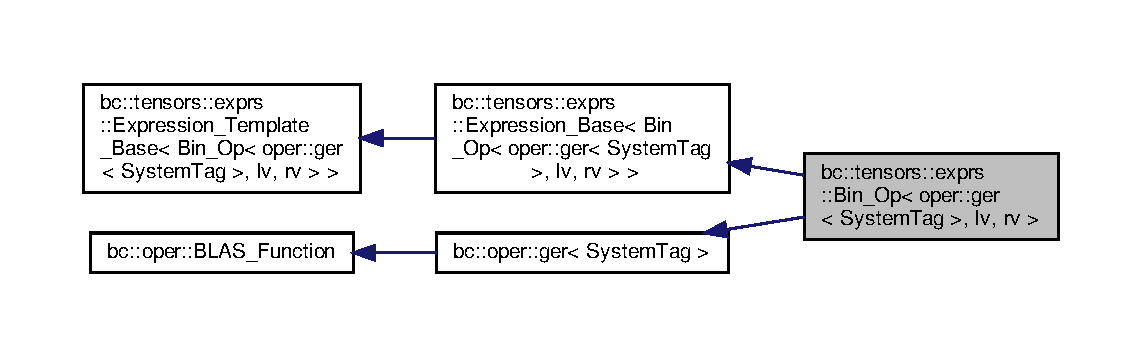
\includegraphics[width=350pt]{structbc_1_1tensors_1_1exprs_1_1Bin__Op_3_01oper_1_1ger_3_01SystemTag_01_4_00_01lv_00_01rv_01_4__inherit__graph}
\end{center}
\end{figure}


Collaboration diagram for bc\+:\+:tensors\+:\+:exprs\+:\+:Bin\+\_\+\+Op$<$ oper\+:\+:ger$<$ System\+Tag $>$, lv, rv $>$\+:\nopagebreak
\begin{figure}[H]
\begin{center}
\leavevmode
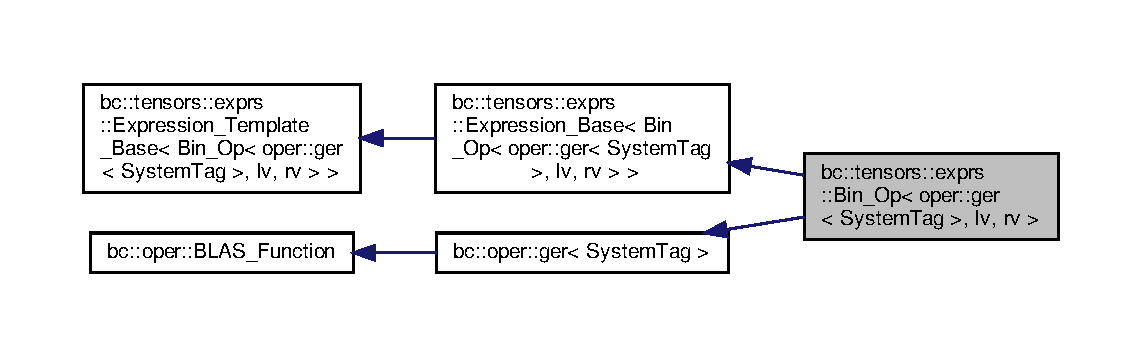
\includegraphics[width=350pt]{structbc_1_1tensors_1_1exprs_1_1Bin__Op_3_01oper_1_1ger_3_01SystemTag_01_4_00_01lv_00_01rv_01_4__coll__graph}
\end{center}
\end{figure}
\subsection*{Public Types}
\begin{DoxyCompactItemize}
\item 
using \hyperlink{structbc_1_1tensors_1_1exprs_1_1Bin__Op_3_01oper_1_1ger_3_01SystemTag_01_4_00_01lv_00_01rv_01_4_a1e724bc99333d1b22f1ce67c3559620b}{value\+\_\+type} = typename lv\+::value\+\_\+type
\item 
using \hyperlink{structbc_1_1tensors_1_1exprs_1_1Bin__Op_3_01oper_1_1ger_3_01SystemTag_01_4_00_01lv_00_01rv_01_4_abcd305e8f31931d98bc3cbd42833b73d}{system\+\_\+tag} = System\+Tag
\end{DoxyCompactItemize}
\subsection*{Public Member Functions}
\begin{DoxyCompactItemize}
\item 
\hyperlink{structbc_1_1tensors_1_1exprs_1_1Bin__Op_3_01oper_1_1ger_3_01SystemTag_01_4_00_01lv_00_01rv_01_4_ad3441252cab02823f05fad5bc2731ee2}{Bin\+\_\+\+Op} (lv \hyperlink{structbc_1_1tensors_1_1exprs_1_1Bin__Op_3_01oper_1_1ger_3_01SystemTag_01_4_00_01lv_00_01rv_01_4_a2d533a67c204fc5ae4fbc1e0ee20007a}{left}, rv \hyperlink{structbc_1_1tensors_1_1exprs_1_1Bin__Op_3_01oper_1_1ger_3_01SystemTag_01_4_00_01lv_00_01rv_01_4_ade316a4230d01aef20028ae075532341}{right}, \hyperlink{structbc_1_1oper_1_1ger}{oper\+::ger}$<$ \hyperlink{structbc_1_1tensors_1_1exprs_1_1Bin__Op_3_01oper_1_1ger_3_01SystemTag_01_4_00_01lv_00_01rv_01_4_abcd305e8f31931d98bc3cbd42833b73d}{system\+\_\+tag} $>$ op=\hyperlink{structbc_1_1oper_1_1ger}{oper\+::ger}$<$ \hyperlink{structbc_1_1tensors_1_1exprs_1_1Bin__Op_3_01oper_1_1ger_3_01SystemTag_01_4_00_01lv_00_01rv_01_4_abcd305e8f31931d98bc3cbd42833b73d}{system\+\_\+tag} $>$())
\item 
\+\_\+\+\_\+host\+\_\+\+\_\+ \+\_\+\+\_\+device\+\_\+\+\_\+ \hyperlink{namespacebc_aaf8e3fbf99b04b1b57c4f80c6f55d3c5}{bc\+::size\+\_\+t} \hyperlink{structbc_1_1tensors_1_1exprs_1_1Bin__Op_3_01oper_1_1ger_3_01SystemTag_01_4_00_01lv_00_01rv_01_4_a3af1ea07a743b02a22dc46455c385954}{size} () const
\item 
\+\_\+\+\_\+host\+\_\+\+\_\+ \+\_\+\+\_\+device\+\_\+\+\_\+ \hyperlink{namespacebc_aaf8e3fbf99b04b1b57c4f80c6f55d3c5}{bc\+::size\+\_\+t} \hyperlink{structbc_1_1tensors_1_1exprs_1_1Bin__Op_3_01oper_1_1ger_3_01SystemTag_01_4_00_01lv_00_01rv_01_4_a83f752ac248f86c1ef0fd823f9585d51}{dim} (int i) const
\item 
\+\_\+\+\_\+host\+\_\+\+\_\+ \+\_\+\+\_\+device\+\_\+\+\_\+ \hyperlink{namespacebc_aaf8e3fbf99b04b1b57c4f80c6f55d3c5}{bc\+::size\+\_\+t} \hyperlink{structbc_1_1tensors_1_1exprs_1_1Bin__Op_3_01oper_1_1ger_3_01SystemTag_01_4_00_01lv_00_01rv_01_4_a3cb2641a629ff716a3581ea4e9cd074e}{rows} () const
\item 
\+\_\+\+\_\+host\+\_\+\+\_\+ \+\_\+\+\_\+device\+\_\+\+\_\+ \hyperlink{namespacebc_aaf8e3fbf99b04b1b57c4f80c6f55d3c5}{bc\+::size\+\_\+t} \hyperlink{structbc_1_1tensors_1_1exprs_1_1Bin__Op_3_01oper_1_1ger_3_01SystemTag_01_4_00_01lv_00_01rv_01_4_ae036dc67e7d6de3d247d93706c1da12d}{cols} () const
\item 
{\footnotesize template$<$class core , int Alpha, int Beta, class Stream $>$ }\\void \hyperlink{structbc_1_1tensors_1_1exprs_1_1Bin__Op_3_01oper_1_1ger_3_01SystemTag_01_4_00_01lv_00_01rv_01_4_a3f0cc13f22ee0f0a382c47f9441c8ce2}{eval} (\hyperlink{structbc_1_1tensors_1_1exprs_1_1Output__Data}{Output\+\_\+\+Data}$<$ core, Alpha, Beta $>$ output, \hyperlink{classbc_1_1streams_1_1Stream}{Stream} stream) const
\end{DoxyCompactItemize}
\subsection*{Static Public Member Functions}
\begin{DoxyCompactItemize}
\item 
static \hyperlink{structbc_1_1oper_1_1ger}{oper\+::ger}$<$ \hyperlink{structbc_1_1tensors_1_1exprs_1_1Bin__Op_3_01oper_1_1ger_3_01SystemTag_01_4_00_01lv_00_01rv_01_4_abcd305e8f31931d98bc3cbd42833b73d}{system\+\_\+tag} $>$ \hyperlink{structbc_1_1tensors_1_1exprs_1_1Bin__Op_3_01oper_1_1ger_3_01SystemTag_01_4_00_01lv_00_01rv_01_4_a662c70bc8aec8c6ccfde818e119970f9}{get\+\_\+operation} ()
\end{DoxyCompactItemize}
\subsection*{Public Attributes}
\begin{DoxyCompactItemize}
\item 
lv \hyperlink{structbc_1_1tensors_1_1exprs_1_1Bin__Op_3_01oper_1_1ger_3_01SystemTag_01_4_00_01lv_00_01rv_01_4_a2d533a67c204fc5ae4fbc1e0ee20007a}{left}
\item 
rv \hyperlink{structbc_1_1tensors_1_1exprs_1_1Bin__Op_3_01oper_1_1ger_3_01SystemTag_01_4_00_01lv_00_01rv_01_4_ade316a4230d01aef20028ae075532341}{right}
\end{DoxyCompactItemize}
\subsection*{Static Public Attributes}
\begin{DoxyCompactItemize}
\item 
static constexpr int \hyperlink{structbc_1_1tensors_1_1exprs_1_1Bin__Op_3_01oper_1_1ger_3_01SystemTag_01_4_00_01lv_00_01rv_01_4_ab6f71ecc8a5b1136018082fb87fefa3c}{tensor\+\_\+dim} = 2
\item 
static constexpr int \hyperlink{structbc_1_1tensors_1_1exprs_1_1Bin__Op_3_01oper_1_1ger_3_01SystemTag_01_4_00_01lv_00_01rv_01_4_adc98e4bb70c5743aadbbd5e83b332875}{tensor\+\_\+iterator\+\_\+dim} = 1
\end{DoxyCompactItemize}


\subsection{Member Typedef Documentation}
\mbox{\Hypertarget{structbc_1_1tensors_1_1exprs_1_1Bin__Op_3_01oper_1_1ger_3_01SystemTag_01_4_00_01lv_00_01rv_01_4_abcd305e8f31931d98bc3cbd42833b73d}\label{structbc_1_1tensors_1_1exprs_1_1Bin__Op_3_01oper_1_1ger_3_01SystemTag_01_4_00_01lv_00_01rv_01_4_abcd305e8f31931d98bc3cbd42833b73d}} 
\index{bc\+::tensors\+::exprs\+::\+Bin\+\_\+\+Op$<$ oper\+::ger$<$ System\+Tag $>$, lv, rv $>$@{bc\+::tensors\+::exprs\+::\+Bin\+\_\+\+Op$<$ oper\+::ger$<$ System\+Tag $>$, lv, rv $>$}!system\+\_\+tag@{system\+\_\+tag}}
\index{system\+\_\+tag@{system\+\_\+tag}!bc\+::tensors\+::exprs\+::\+Bin\+\_\+\+Op$<$ oper\+::ger$<$ System\+Tag $>$, lv, rv $>$@{bc\+::tensors\+::exprs\+::\+Bin\+\_\+\+Op$<$ oper\+::ger$<$ System\+Tag $>$, lv, rv $>$}}
\subsubsection{\texorpdfstring{system\+\_\+tag}{system\_tag}}
{\footnotesize\ttfamily template$<$class lv , class rv , class System\+Tag $>$ \\
using \hyperlink{structbc_1_1tensors_1_1exprs_1_1Bin__Op}{bc\+::tensors\+::exprs\+::\+Bin\+\_\+\+Op}$<$ \hyperlink{structbc_1_1oper_1_1ger}{oper\+::ger}$<$ System\+Tag $>$, lv, rv $>$\+::\hyperlink{structbc_1_1tensors_1_1exprs_1_1Bin__Op_3_01oper_1_1ger_3_01SystemTag_01_4_00_01lv_00_01rv_01_4_abcd305e8f31931d98bc3cbd42833b73d}{system\+\_\+tag} =  System\+Tag}

\mbox{\Hypertarget{structbc_1_1tensors_1_1exprs_1_1Bin__Op_3_01oper_1_1ger_3_01SystemTag_01_4_00_01lv_00_01rv_01_4_a1e724bc99333d1b22f1ce67c3559620b}\label{structbc_1_1tensors_1_1exprs_1_1Bin__Op_3_01oper_1_1ger_3_01SystemTag_01_4_00_01lv_00_01rv_01_4_a1e724bc99333d1b22f1ce67c3559620b}} 
\index{bc\+::tensors\+::exprs\+::\+Bin\+\_\+\+Op$<$ oper\+::ger$<$ System\+Tag $>$, lv, rv $>$@{bc\+::tensors\+::exprs\+::\+Bin\+\_\+\+Op$<$ oper\+::ger$<$ System\+Tag $>$, lv, rv $>$}!value\+\_\+type@{value\+\_\+type}}
\index{value\+\_\+type@{value\+\_\+type}!bc\+::tensors\+::exprs\+::\+Bin\+\_\+\+Op$<$ oper\+::ger$<$ System\+Tag $>$, lv, rv $>$@{bc\+::tensors\+::exprs\+::\+Bin\+\_\+\+Op$<$ oper\+::ger$<$ System\+Tag $>$, lv, rv $>$}}
\subsubsection{\texorpdfstring{value\+\_\+type}{value\_type}}
{\footnotesize\ttfamily template$<$class lv , class rv , class System\+Tag $>$ \\
using \hyperlink{structbc_1_1tensors_1_1exprs_1_1Bin__Op}{bc\+::tensors\+::exprs\+::\+Bin\+\_\+\+Op}$<$ \hyperlink{structbc_1_1oper_1_1ger}{oper\+::ger}$<$ System\+Tag $>$, lv, rv $>$\+::\hyperlink{structbc_1_1tensors_1_1exprs_1_1Bin__Op_3_01oper_1_1ger_3_01SystemTag_01_4_00_01lv_00_01rv_01_4_a1e724bc99333d1b22f1ce67c3559620b}{value\+\_\+type} =  typename lv\+::value\+\_\+type}



\subsection{Constructor \& Destructor Documentation}
\mbox{\Hypertarget{structbc_1_1tensors_1_1exprs_1_1Bin__Op_3_01oper_1_1ger_3_01SystemTag_01_4_00_01lv_00_01rv_01_4_ad3441252cab02823f05fad5bc2731ee2}\label{structbc_1_1tensors_1_1exprs_1_1Bin__Op_3_01oper_1_1ger_3_01SystemTag_01_4_00_01lv_00_01rv_01_4_ad3441252cab02823f05fad5bc2731ee2}} 
\index{bc\+::tensors\+::exprs\+::\+Bin\+\_\+\+Op$<$ oper\+::ger$<$ System\+Tag $>$, lv, rv $>$@{bc\+::tensors\+::exprs\+::\+Bin\+\_\+\+Op$<$ oper\+::ger$<$ System\+Tag $>$, lv, rv $>$}!Bin\+\_\+\+Op@{Bin\+\_\+\+Op}}
\index{Bin\+\_\+\+Op@{Bin\+\_\+\+Op}!bc\+::tensors\+::exprs\+::\+Bin\+\_\+\+Op$<$ oper\+::ger$<$ System\+Tag $>$, lv, rv $>$@{bc\+::tensors\+::exprs\+::\+Bin\+\_\+\+Op$<$ oper\+::ger$<$ System\+Tag $>$, lv, rv $>$}}
\subsubsection{\texorpdfstring{Bin\+\_\+\+Op()}{Bin\_Op()}}
{\footnotesize\ttfamily template$<$class lv , class rv , class System\+Tag $>$ \\
\hyperlink{structbc_1_1tensors_1_1exprs_1_1Bin__Op}{bc\+::tensors\+::exprs\+::\+Bin\+\_\+\+Op}$<$ \hyperlink{structbc_1_1oper_1_1ger}{oper\+::ger}$<$ System\+Tag $>$, lv, rv $>$\+::\hyperlink{structbc_1_1tensors_1_1exprs_1_1Bin__Op}{Bin\+\_\+\+Op} (\begin{DoxyParamCaption}\item[{lv}]{left,  }\item[{rv}]{right,  }\item[{\hyperlink{structbc_1_1oper_1_1ger}{oper\+::ger}$<$ \hyperlink{structbc_1_1tensors_1_1exprs_1_1Bin__Op_3_01oper_1_1ger_3_01SystemTag_01_4_00_01lv_00_01rv_01_4_abcd305e8f31931d98bc3cbd42833b73d}{system\+\_\+tag} $>$}]{op = {\ttfamily \hyperlink{structbc_1_1oper_1_1ger}{oper\+::ger}$<$\hyperlink{structbc_1_1tensors_1_1exprs_1_1Bin__Op_3_01oper_1_1ger_3_01SystemTag_01_4_00_01lv_00_01rv_01_4_abcd305e8f31931d98bc3cbd42833b73d}{system\+\_\+tag}$>$()} }\end{DoxyParamCaption})\hspace{0.3cm}{\ttfamily [inline]}}



\subsection{Member Function Documentation}
\mbox{\Hypertarget{structbc_1_1tensors_1_1exprs_1_1Bin__Op_3_01oper_1_1ger_3_01SystemTag_01_4_00_01lv_00_01rv_01_4_ae036dc67e7d6de3d247d93706c1da12d}\label{structbc_1_1tensors_1_1exprs_1_1Bin__Op_3_01oper_1_1ger_3_01SystemTag_01_4_00_01lv_00_01rv_01_4_ae036dc67e7d6de3d247d93706c1da12d}} 
\index{bc\+::tensors\+::exprs\+::\+Bin\+\_\+\+Op$<$ oper\+::ger$<$ System\+Tag $>$, lv, rv $>$@{bc\+::tensors\+::exprs\+::\+Bin\+\_\+\+Op$<$ oper\+::ger$<$ System\+Tag $>$, lv, rv $>$}!cols@{cols}}
\index{cols@{cols}!bc\+::tensors\+::exprs\+::\+Bin\+\_\+\+Op$<$ oper\+::ger$<$ System\+Tag $>$, lv, rv $>$@{bc\+::tensors\+::exprs\+::\+Bin\+\_\+\+Op$<$ oper\+::ger$<$ System\+Tag $>$, lv, rv $>$}}
\subsubsection{\texorpdfstring{cols()}{cols()}}
{\footnotesize\ttfamily template$<$class lv , class rv , class System\+Tag $>$ \\
\+\_\+\+\_\+host\+\_\+\+\_\+ \+\_\+\+\_\+device\+\_\+\+\_\+ \hyperlink{namespacebc_aaf8e3fbf99b04b1b57c4f80c6f55d3c5}{bc\+::size\+\_\+t} \hyperlink{structbc_1_1tensors_1_1exprs_1_1Bin__Op}{bc\+::tensors\+::exprs\+::\+Bin\+\_\+\+Op}$<$ \hyperlink{structbc_1_1oper_1_1ger}{oper\+::ger}$<$ System\+Tag $>$, lv, rv $>$\+::cols (\begin{DoxyParamCaption}{ }\end{DoxyParamCaption}) const\hspace{0.3cm}{\ttfamily [inline]}}

\mbox{\Hypertarget{structbc_1_1tensors_1_1exprs_1_1Bin__Op_3_01oper_1_1ger_3_01SystemTag_01_4_00_01lv_00_01rv_01_4_a83f752ac248f86c1ef0fd823f9585d51}\label{structbc_1_1tensors_1_1exprs_1_1Bin__Op_3_01oper_1_1ger_3_01SystemTag_01_4_00_01lv_00_01rv_01_4_a83f752ac248f86c1ef0fd823f9585d51}} 
\index{bc\+::tensors\+::exprs\+::\+Bin\+\_\+\+Op$<$ oper\+::ger$<$ System\+Tag $>$, lv, rv $>$@{bc\+::tensors\+::exprs\+::\+Bin\+\_\+\+Op$<$ oper\+::ger$<$ System\+Tag $>$, lv, rv $>$}!dim@{dim}}
\index{dim@{dim}!bc\+::tensors\+::exprs\+::\+Bin\+\_\+\+Op$<$ oper\+::ger$<$ System\+Tag $>$, lv, rv $>$@{bc\+::tensors\+::exprs\+::\+Bin\+\_\+\+Op$<$ oper\+::ger$<$ System\+Tag $>$, lv, rv $>$}}
\subsubsection{\texorpdfstring{dim()}{dim()}}
{\footnotesize\ttfamily template$<$class lv , class rv , class System\+Tag $>$ \\
\+\_\+\+\_\+host\+\_\+\+\_\+ \+\_\+\+\_\+device\+\_\+\+\_\+ \hyperlink{namespacebc_aaf8e3fbf99b04b1b57c4f80c6f55d3c5}{bc\+::size\+\_\+t} \hyperlink{structbc_1_1tensors_1_1exprs_1_1Bin__Op}{bc\+::tensors\+::exprs\+::\+Bin\+\_\+\+Op}$<$ \hyperlink{structbc_1_1oper_1_1ger}{oper\+::ger}$<$ System\+Tag $>$, lv, rv $>$\+::dim (\begin{DoxyParamCaption}\item[{int}]{i }\end{DoxyParamCaption}) const\hspace{0.3cm}{\ttfamily [inline]}}

\mbox{\Hypertarget{structbc_1_1tensors_1_1exprs_1_1Bin__Op_3_01oper_1_1ger_3_01SystemTag_01_4_00_01lv_00_01rv_01_4_a3f0cc13f22ee0f0a382c47f9441c8ce2}\label{structbc_1_1tensors_1_1exprs_1_1Bin__Op_3_01oper_1_1ger_3_01SystemTag_01_4_00_01lv_00_01rv_01_4_a3f0cc13f22ee0f0a382c47f9441c8ce2}} 
\index{bc\+::tensors\+::exprs\+::\+Bin\+\_\+\+Op$<$ oper\+::ger$<$ System\+Tag $>$, lv, rv $>$@{bc\+::tensors\+::exprs\+::\+Bin\+\_\+\+Op$<$ oper\+::ger$<$ System\+Tag $>$, lv, rv $>$}!eval@{eval}}
\index{eval@{eval}!bc\+::tensors\+::exprs\+::\+Bin\+\_\+\+Op$<$ oper\+::ger$<$ System\+Tag $>$, lv, rv $>$@{bc\+::tensors\+::exprs\+::\+Bin\+\_\+\+Op$<$ oper\+::ger$<$ System\+Tag $>$, lv, rv $>$}}
\subsubsection{\texorpdfstring{eval()}{eval()}}
{\footnotesize\ttfamily template$<$class lv , class rv , class System\+Tag $>$ \\
template$<$class core , int Alpha, int Beta, class Stream $>$ \\
void \hyperlink{structbc_1_1tensors_1_1exprs_1_1Bin__Op}{bc\+::tensors\+::exprs\+::\+Bin\+\_\+\+Op}$<$ \hyperlink{structbc_1_1oper_1_1ger}{oper\+::ger}$<$ System\+Tag $>$, lv, rv $>$\+::eval (\begin{DoxyParamCaption}\item[{\hyperlink{structbc_1_1tensors_1_1exprs_1_1Output__Data}{Output\+\_\+\+Data}$<$ core, Alpha, Beta $>$}]{output,  }\item[{\hyperlink{classbc_1_1streams_1_1Stream}{Stream}}]{stream }\end{DoxyParamCaption}) const\hspace{0.3cm}{\ttfamily [inline]}}

\mbox{\Hypertarget{structbc_1_1tensors_1_1exprs_1_1Bin__Op_3_01oper_1_1ger_3_01SystemTag_01_4_00_01lv_00_01rv_01_4_a662c70bc8aec8c6ccfde818e119970f9}\label{structbc_1_1tensors_1_1exprs_1_1Bin__Op_3_01oper_1_1ger_3_01SystemTag_01_4_00_01lv_00_01rv_01_4_a662c70bc8aec8c6ccfde818e119970f9}} 
\index{bc\+::tensors\+::exprs\+::\+Bin\+\_\+\+Op$<$ oper\+::ger$<$ System\+Tag $>$, lv, rv $>$@{bc\+::tensors\+::exprs\+::\+Bin\+\_\+\+Op$<$ oper\+::ger$<$ System\+Tag $>$, lv, rv $>$}!get\+\_\+operation@{get\+\_\+operation}}
\index{get\+\_\+operation@{get\+\_\+operation}!bc\+::tensors\+::exprs\+::\+Bin\+\_\+\+Op$<$ oper\+::ger$<$ System\+Tag $>$, lv, rv $>$@{bc\+::tensors\+::exprs\+::\+Bin\+\_\+\+Op$<$ oper\+::ger$<$ System\+Tag $>$, lv, rv $>$}}
\subsubsection{\texorpdfstring{get\+\_\+operation()}{get\_operation()}}
{\footnotesize\ttfamily template$<$class lv , class rv , class System\+Tag $>$ \\
static \hyperlink{structbc_1_1oper_1_1ger}{oper\+::ger}$<$\hyperlink{structbc_1_1tensors_1_1exprs_1_1Bin__Op_3_01oper_1_1ger_3_01SystemTag_01_4_00_01lv_00_01rv_01_4_abcd305e8f31931d98bc3cbd42833b73d}{system\+\_\+tag}$>$ \hyperlink{structbc_1_1tensors_1_1exprs_1_1Bin__Op}{bc\+::tensors\+::exprs\+::\+Bin\+\_\+\+Op}$<$ \hyperlink{structbc_1_1oper_1_1ger}{oper\+::ger}$<$ System\+Tag $>$, lv, rv $>$\+::get\+\_\+operation (\begin{DoxyParamCaption}{ }\end{DoxyParamCaption})\hspace{0.3cm}{\ttfamily [inline]}, {\ttfamily [static]}}

\mbox{\Hypertarget{structbc_1_1tensors_1_1exprs_1_1Bin__Op_3_01oper_1_1ger_3_01SystemTag_01_4_00_01lv_00_01rv_01_4_a3cb2641a629ff716a3581ea4e9cd074e}\label{structbc_1_1tensors_1_1exprs_1_1Bin__Op_3_01oper_1_1ger_3_01SystemTag_01_4_00_01lv_00_01rv_01_4_a3cb2641a629ff716a3581ea4e9cd074e}} 
\index{bc\+::tensors\+::exprs\+::\+Bin\+\_\+\+Op$<$ oper\+::ger$<$ System\+Tag $>$, lv, rv $>$@{bc\+::tensors\+::exprs\+::\+Bin\+\_\+\+Op$<$ oper\+::ger$<$ System\+Tag $>$, lv, rv $>$}!rows@{rows}}
\index{rows@{rows}!bc\+::tensors\+::exprs\+::\+Bin\+\_\+\+Op$<$ oper\+::ger$<$ System\+Tag $>$, lv, rv $>$@{bc\+::tensors\+::exprs\+::\+Bin\+\_\+\+Op$<$ oper\+::ger$<$ System\+Tag $>$, lv, rv $>$}}
\subsubsection{\texorpdfstring{rows()}{rows()}}
{\footnotesize\ttfamily template$<$class lv , class rv , class System\+Tag $>$ \\
\+\_\+\+\_\+host\+\_\+\+\_\+ \+\_\+\+\_\+device\+\_\+\+\_\+ \hyperlink{namespacebc_aaf8e3fbf99b04b1b57c4f80c6f55d3c5}{bc\+::size\+\_\+t} \hyperlink{structbc_1_1tensors_1_1exprs_1_1Bin__Op}{bc\+::tensors\+::exprs\+::\+Bin\+\_\+\+Op}$<$ \hyperlink{structbc_1_1oper_1_1ger}{oper\+::ger}$<$ System\+Tag $>$, lv, rv $>$\+::rows (\begin{DoxyParamCaption}{ }\end{DoxyParamCaption}) const\hspace{0.3cm}{\ttfamily [inline]}}

\mbox{\Hypertarget{structbc_1_1tensors_1_1exprs_1_1Bin__Op_3_01oper_1_1ger_3_01SystemTag_01_4_00_01lv_00_01rv_01_4_a3af1ea07a743b02a22dc46455c385954}\label{structbc_1_1tensors_1_1exprs_1_1Bin__Op_3_01oper_1_1ger_3_01SystemTag_01_4_00_01lv_00_01rv_01_4_a3af1ea07a743b02a22dc46455c385954}} 
\index{bc\+::tensors\+::exprs\+::\+Bin\+\_\+\+Op$<$ oper\+::ger$<$ System\+Tag $>$, lv, rv $>$@{bc\+::tensors\+::exprs\+::\+Bin\+\_\+\+Op$<$ oper\+::ger$<$ System\+Tag $>$, lv, rv $>$}!size@{size}}
\index{size@{size}!bc\+::tensors\+::exprs\+::\+Bin\+\_\+\+Op$<$ oper\+::ger$<$ System\+Tag $>$, lv, rv $>$@{bc\+::tensors\+::exprs\+::\+Bin\+\_\+\+Op$<$ oper\+::ger$<$ System\+Tag $>$, lv, rv $>$}}
\subsubsection{\texorpdfstring{size()}{size()}}
{\footnotesize\ttfamily template$<$class lv , class rv , class System\+Tag $>$ \\
\+\_\+\+\_\+host\+\_\+\+\_\+ \+\_\+\+\_\+device\+\_\+\+\_\+ \hyperlink{namespacebc_aaf8e3fbf99b04b1b57c4f80c6f55d3c5}{bc\+::size\+\_\+t} \hyperlink{structbc_1_1tensors_1_1exprs_1_1Bin__Op}{bc\+::tensors\+::exprs\+::\+Bin\+\_\+\+Op}$<$ \hyperlink{structbc_1_1oper_1_1ger}{oper\+::ger}$<$ System\+Tag $>$, lv, rv $>$\+::size (\begin{DoxyParamCaption}{ }\end{DoxyParamCaption}) const\hspace{0.3cm}{\ttfamily [inline]}}



\subsection{Member Data Documentation}
\mbox{\Hypertarget{structbc_1_1tensors_1_1exprs_1_1Bin__Op_3_01oper_1_1ger_3_01SystemTag_01_4_00_01lv_00_01rv_01_4_a2d533a67c204fc5ae4fbc1e0ee20007a}\label{structbc_1_1tensors_1_1exprs_1_1Bin__Op_3_01oper_1_1ger_3_01SystemTag_01_4_00_01lv_00_01rv_01_4_a2d533a67c204fc5ae4fbc1e0ee20007a}} 
\index{bc\+::tensors\+::exprs\+::\+Bin\+\_\+\+Op$<$ oper\+::ger$<$ System\+Tag $>$, lv, rv $>$@{bc\+::tensors\+::exprs\+::\+Bin\+\_\+\+Op$<$ oper\+::ger$<$ System\+Tag $>$, lv, rv $>$}!left@{left}}
\index{left@{left}!bc\+::tensors\+::exprs\+::\+Bin\+\_\+\+Op$<$ oper\+::ger$<$ System\+Tag $>$, lv, rv $>$@{bc\+::tensors\+::exprs\+::\+Bin\+\_\+\+Op$<$ oper\+::ger$<$ System\+Tag $>$, lv, rv $>$}}
\subsubsection{\texorpdfstring{left}{left}}
{\footnotesize\ttfamily template$<$class lv , class rv , class System\+Tag $>$ \\
lv \hyperlink{structbc_1_1tensors_1_1exprs_1_1Bin__Op}{bc\+::tensors\+::exprs\+::\+Bin\+\_\+\+Op}$<$ \hyperlink{structbc_1_1oper_1_1ger}{oper\+::ger}$<$ System\+Tag $>$, lv, rv $>$\+::left}

\mbox{\Hypertarget{structbc_1_1tensors_1_1exprs_1_1Bin__Op_3_01oper_1_1ger_3_01SystemTag_01_4_00_01lv_00_01rv_01_4_ade316a4230d01aef20028ae075532341}\label{structbc_1_1tensors_1_1exprs_1_1Bin__Op_3_01oper_1_1ger_3_01SystemTag_01_4_00_01lv_00_01rv_01_4_ade316a4230d01aef20028ae075532341}} 
\index{bc\+::tensors\+::exprs\+::\+Bin\+\_\+\+Op$<$ oper\+::ger$<$ System\+Tag $>$, lv, rv $>$@{bc\+::tensors\+::exprs\+::\+Bin\+\_\+\+Op$<$ oper\+::ger$<$ System\+Tag $>$, lv, rv $>$}!right@{right}}
\index{right@{right}!bc\+::tensors\+::exprs\+::\+Bin\+\_\+\+Op$<$ oper\+::ger$<$ System\+Tag $>$, lv, rv $>$@{bc\+::tensors\+::exprs\+::\+Bin\+\_\+\+Op$<$ oper\+::ger$<$ System\+Tag $>$, lv, rv $>$}}
\subsubsection{\texorpdfstring{right}{right}}
{\footnotesize\ttfamily template$<$class lv , class rv , class System\+Tag $>$ \\
rv \hyperlink{structbc_1_1tensors_1_1exprs_1_1Bin__Op}{bc\+::tensors\+::exprs\+::\+Bin\+\_\+\+Op}$<$ \hyperlink{structbc_1_1oper_1_1ger}{oper\+::ger}$<$ System\+Tag $>$, lv, rv $>$\+::right}

\mbox{\Hypertarget{structbc_1_1tensors_1_1exprs_1_1Bin__Op_3_01oper_1_1ger_3_01SystemTag_01_4_00_01lv_00_01rv_01_4_ab6f71ecc8a5b1136018082fb87fefa3c}\label{structbc_1_1tensors_1_1exprs_1_1Bin__Op_3_01oper_1_1ger_3_01SystemTag_01_4_00_01lv_00_01rv_01_4_ab6f71ecc8a5b1136018082fb87fefa3c}} 
\index{bc\+::tensors\+::exprs\+::\+Bin\+\_\+\+Op$<$ oper\+::ger$<$ System\+Tag $>$, lv, rv $>$@{bc\+::tensors\+::exprs\+::\+Bin\+\_\+\+Op$<$ oper\+::ger$<$ System\+Tag $>$, lv, rv $>$}!tensor\+\_\+dim@{tensor\+\_\+dim}}
\index{tensor\+\_\+dim@{tensor\+\_\+dim}!bc\+::tensors\+::exprs\+::\+Bin\+\_\+\+Op$<$ oper\+::ger$<$ System\+Tag $>$, lv, rv $>$@{bc\+::tensors\+::exprs\+::\+Bin\+\_\+\+Op$<$ oper\+::ger$<$ System\+Tag $>$, lv, rv $>$}}
\subsubsection{\texorpdfstring{tensor\+\_\+dim}{tensor\_dim}}
{\footnotesize\ttfamily template$<$class lv , class rv , class System\+Tag $>$ \\
constexpr int \hyperlink{structbc_1_1tensors_1_1exprs_1_1Bin__Op}{bc\+::tensors\+::exprs\+::\+Bin\+\_\+\+Op}$<$ \hyperlink{structbc_1_1oper_1_1ger}{oper\+::ger}$<$ System\+Tag $>$, lv, rv $>$\+::tensor\+\_\+dim = 2\hspace{0.3cm}{\ttfamily [static]}}

\mbox{\Hypertarget{structbc_1_1tensors_1_1exprs_1_1Bin__Op_3_01oper_1_1ger_3_01SystemTag_01_4_00_01lv_00_01rv_01_4_adc98e4bb70c5743aadbbd5e83b332875}\label{structbc_1_1tensors_1_1exprs_1_1Bin__Op_3_01oper_1_1ger_3_01SystemTag_01_4_00_01lv_00_01rv_01_4_adc98e4bb70c5743aadbbd5e83b332875}} 
\index{bc\+::tensors\+::exprs\+::\+Bin\+\_\+\+Op$<$ oper\+::ger$<$ System\+Tag $>$, lv, rv $>$@{bc\+::tensors\+::exprs\+::\+Bin\+\_\+\+Op$<$ oper\+::ger$<$ System\+Tag $>$, lv, rv $>$}!tensor\+\_\+iterator\+\_\+dim@{tensor\+\_\+iterator\+\_\+dim}}
\index{tensor\+\_\+iterator\+\_\+dim@{tensor\+\_\+iterator\+\_\+dim}!bc\+::tensors\+::exprs\+::\+Bin\+\_\+\+Op$<$ oper\+::ger$<$ System\+Tag $>$, lv, rv $>$@{bc\+::tensors\+::exprs\+::\+Bin\+\_\+\+Op$<$ oper\+::ger$<$ System\+Tag $>$, lv, rv $>$}}
\subsubsection{\texorpdfstring{tensor\+\_\+iterator\+\_\+dim}{tensor\_iterator\_dim}}
{\footnotesize\ttfamily template$<$class lv , class rv , class System\+Tag $>$ \\
constexpr int \hyperlink{structbc_1_1tensors_1_1exprs_1_1Bin__Op}{bc\+::tensors\+::exprs\+::\+Bin\+\_\+\+Op}$<$ \hyperlink{structbc_1_1oper_1_1ger}{oper\+::ger}$<$ System\+Tag $>$, lv, rv $>$\+::tensor\+\_\+iterator\+\_\+dim = 1\hspace{0.3cm}{\ttfamily [static]}}



The documentation for this struct was generated from the following file\+:\begin{DoxyCompactItemize}
\item 
blackcat/tensors/expression\+\_\+templates/\hyperlink{function__ger_8h}{function\+\_\+ger.\+h}\end{DoxyCompactItemize}

\hypertarget{structbc_1_1tensors_1_1exprs_1_1binary__optimizer__default}{}\section{bc\+:\+:tensors\+:\+:exprs\+:\+:binary\+\_\+optimizer\+\_\+default$<$ op, lv, rv $>$ Struct Template Reference}
\label{structbc_1_1tensors_1_1exprs_1_1binary__optimizer__default}\index{bc\+::tensors\+::exprs\+::binary\+\_\+optimizer\+\_\+default$<$ op, lv, rv $>$@{bc\+::tensors\+::exprs\+::binary\+\_\+optimizer\+\_\+default$<$ op, lv, rv $>$}}


{\ttfamily \#include $<$tree\+\_\+evaluator\+\_\+optimizer.\+h$>$}



Inheritance diagram for bc\+:\+:tensors\+:\+:exprs\+:\+:binary\+\_\+optimizer\+\_\+default$<$ op, lv, rv $>$\+:\nopagebreak
\begin{figure}[H]
\begin{center}
\leavevmode
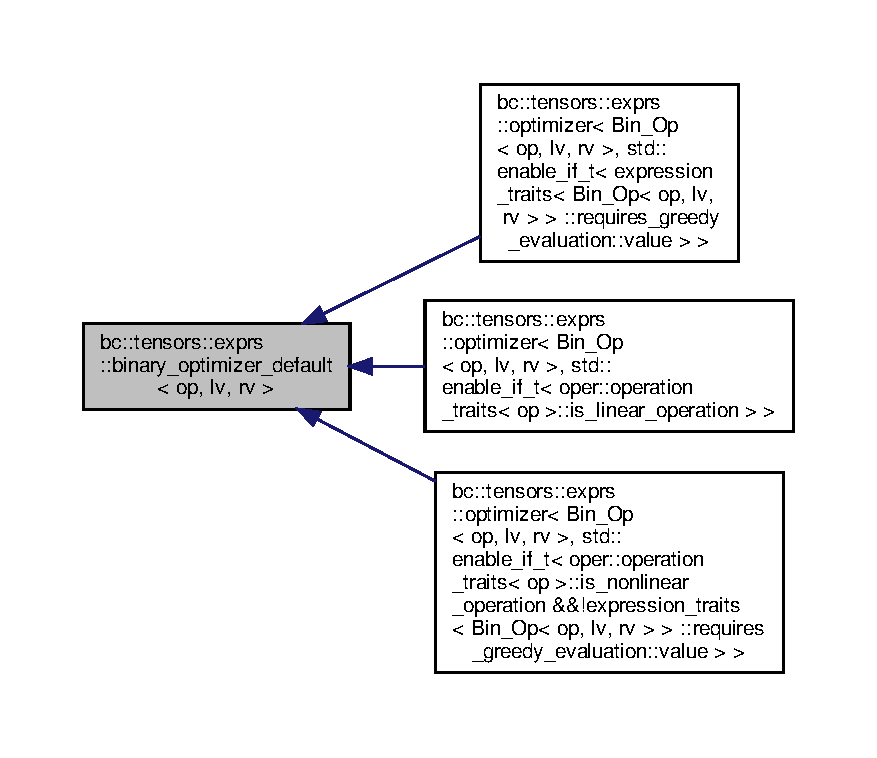
\includegraphics[width=350pt]{structbc_1_1tensors_1_1exprs_1_1binary__optimizer__default__inherit__graph}
\end{center}
\end{figure}
\subsection*{Static Public Member Functions}
\begin{DoxyCompactItemize}
\item 
{\footnotesize template$<$class Stream $>$ }\\static auto \hyperlink{structbc_1_1tensors_1_1exprs_1_1binary__optimizer__default_a3ed135706adb417fe480b8618c96dbee}{temporary\+\_\+injection} (\hyperlink{structbc_1_1tensors_1_1exprs_1_1Bin__Op}{Bin\+\_\+\+Op}$<$ op, lv, rv $>$ branch, \hyperlink{classbc_1_1streams_1_1Stream}{Stream} stream)
\item 
{\footnotesize template$<$class Stream $>$ }\\static void \hyperlink{structbc_1_1tensors_1_1exprs_1_1binary__optimizer__default_a02ba1ba9a7885877477eb602f2ef230b}{deallocate\+\_\+temporaries} (\hyperlink{structbc_1_1tensors_1_1exprs_1_1Bin__Op}{Bin\+\_\+\+Op}$<$ op, lv, rv $>$ branch, \hyperlink{classbc_1_1streams_1_1Stream}{Stream} stream)
\end{DoxyCompactItemize}


\subsection{Member Function Documentation}
\mbox{\Hypertarget{structbc_1_1tensors_1_1exprs_1_1binary__optimizer__default_a02ba1ba9a7885877477eb602f2ef230b}\label{structbc_1_1tensors_1_1exprs_1_1binary__optimizer__default_a02ba1ba9a7885877477eb602f2ef230b}} 
\index{bc\+::tensors\+::exprs\+::binary\+\_\+optimizer\+\_\+default@{bc\+::tensors\+::exprs\+::binary\+\_\+optimizer\+\_\+default}!deallocate\+\_\+temporaries@{deallocate\+\_\+temporaries}}
\index{deallocate\+\_\+temporaries@{deallocate\+\_\+temporaries}!bc\+::tensors\+::exprs\+::binary\+\_\+optimizer\+\_\+default@{bc\+::tensors\+::exprs\+::binary\+\_\+optimizer\+\_\+default}}
\subsubsection{\texorpdfstring{deallocate\+\_\+temporaries()}{deallocate\_temporaries()}}
{\footnotesize\ttfamily template$<$class op , class lv , class rv $>$ \\
template$<$class Stream $>$ \\
static void \hyperlink{structbc_1_1tensors_1_1exprs_1_1binary__optimizer__default}{bc\+::tensors\+::exprs\+::binary\+\_\+optimizer\+\_\+default}$<$ op, lv, rv $>$\+::deallocate\+\_\+temporaries (\begin{DoxyParamCaption}\item[{\hyperlink{structbc_1_1tensors_1_1exprs_1_1Bin__Op}{Bin\+\_\+\+Op}$<$ op, lv, rv $>$}]{branch,  }\item[{\hyperlink{classbc_1_1streams_1_1Stream}{Stream}}]{stream }\end{DoxyParamCaption})\hspace{0.3cm}{\ttfamily [inline]}, {\ttfamily [static]}}

\mbox{\Hypertarget{structbc_1_1tensors_1_1exprs_1_1binary__optimizer__default_a3ed135706adb417fe480b8618c96dbee}\label{structbc_1_1tensors_1_1exprs_1_1binary__optimizer__default_a3ed135706adb417fe480b8618c96dbee}} 
\index{bc\+::tensors\+::exprs\+::binary\+\_\+optimizer\+\_\+default@{bc\+::tensors\+::exprs\+::binary\+\_\+optimizer\+\_\+default}!temporary\+\_\+injection@{temporary\+\_\+injection}}
\index{temporary\+\_\+injection@{temporary\+\_\+injection}!bc\+::tensors\+::exprs\+::binary\+\_\+optimizer\+\_\+default@{bc\+::tensors\+::exprs\+::binary\+\_\+optimizer\+\_\+default}}
\subsubsection{\texorpdfstring{temporary\+\_\+injection()}{temporary\_injection()}}
{\footnotesize\ttfamily template$<$class op , class lv , class rv $>$ \\
template$<$class Stream $>$ \\
static auto \hyperlink{structbc_1_1tensors_1_1exprs_1_1binary__optimizer__default}{bc\+::tensors\+::exprs\+::binary\+\_\+optimizer\+\_\+default}$<$ op, lv, rv $>$\+::temporary\+\_\+injection (\begin{DoxyParamCaption}\item[{\hyperlink{structbc_1_1tensors_1_1exprs_1_1Bin__Op}{Bin\+\_\+\+Op}$<$ op, lv, rv $>$}]{branch,  }\item[{\hyperlink{classbc_1_1streams_1_1Stream}{Stream}}]{stream }\end{DoxyParamCaption})\hspace{0.3cm}{\ttfamily [inline]}, {\ttfamily [static]}}



The documentation for this struct was generated from the following file\+:\begin{DoxyCompactItemize}
\item 
blackcat/tensors/expression\+\_\+templates/\hyperlink{tree__evaluator__optimizer_8h}{tree\+\_\+evaluator\+\_\+optimizer.\+h}\end{DoxyCompactItemize}

\hypertarget{structbc_1_1traits_1_1Bind}{}\section{bc\+:\+:traits\+:\+:Bind$<$ Function, Args $>$ Struct Template Reference}
\label{structbc_1_1traits_1_1Bind}\index{bc\+::traits\+::\+Bind$<$ Function, Args $>$@{bc\+::traits\+::\+Bind$<$ Function, Args $>$}}


Similar to std\+::bind but the evaluation of the function in respect to its bound arguments are deduced if and only if the function is called.  




{\ttfamily \#include $<$bind.\+h$>$}



Inheritance diagram for bc\+:\+:traits\+:\+:Bind$<$ Function, Args $>$\+:\nopagebreak
\begin{figure}[H]
\begin{center}
\leavevmode
\includegraphics[width=210pt]{structbc_1_1traits_1_1Bind__inherit__graph}
\end{center}
\end{figure}


Collaboration diagram for bc\+:\+:traits\+:\+:Bind$<$ Function, Args $>$\+:\nopagebreak
\begin{figure}[H]
\begin{center}
\leavevmode
\includegraphics[width=210pt]{structbc_1_1traits_1_1Bind__coll__graph}
\end{center}
\end{figure}
\subsection*{Public Member Functions}
\begin{DoxyCompactItemize}
\item 
\hyperlink{structbc_1_1traits_1_1Bind_a1969900854a26d59661d5b9c159d7fc4}{Bind} (Function \hyperlink{structbc_1_1traits_1_1Bind_ac7c74786597ebc607ba416eb842a184d}{func}, Args... Additional\+Args)
\end{DoxyCompactItemize}
\subsection*{Public Attributes}
\begin{DoxyCompactItemize}
\item 
Function \hyperlink{structbc_1_1traits_1_1Bind_ac7c74786597ebc607ba416eb842a184d}{func}
\end{DoxyCompactItemize}
\subsection*{Static Public Attributes}
\begin{DoxyCompactItemize}
\item 
static constexpr int \hyperlink{structbc_1_1traits_1_1Bind_a77891c8bf25f4fc19e2b226cf906a7a8}{num\+\_\+args} = sizeof...(Args)
\end{DoxyCompactItemize}


\subsection{Detailed Description}
\subsubsection*{template$<$class Function, class... Args$>$\newline
struct bc\+::traits\+::\+Bind$<$ Function, Args $>$}

Similar to std\+::bind but the evaluation of the function in respect to its bound arguments are deduced if and only if the function is called. 

IE \begin{DoxyVerb}auto func = bc::traits::bind([](int x) {}, std::vector<double>());

will compile, even though a std::vector is not a valid argument
for the given lambda.\end{DoxyVerb}
 

\subsection{Constructor \& Destructor Documentation}
\mbox{\Hypertarget{structbc_1_1traits_1_1Bind_a1969900854a26d59661d5b9c159d7fc4}\label{structbc_1_1traits_1_1Bind_a1969900854a26d59661d5b9c159d7fc4}} 
\index{bc\+::traits\+::\+Bind@{bc\+::traits\+::\+Bind}!Bind@{Bind}}
\index{Bind@{Bind}!bc\+::traits\+::\+Bind@{bc\+::traits\+::\+Bind}}
\subsubsection{\texorpdfstring{Bind()}{Bind()}}
{\footnotesize\ttfamily template$<$class Function , class... Args$>$ \\
\hyperlink{structbc_1_1traits_1_1Bind}{bc\+::traits\+::\+Bind}$<$ Function, Args $>$\+::\hyperlink{structbc_1_1traits_1_1Bind}{Bind} (\begin{DoxyParamCaption}\item[{Function}]{func,  }\item[{Args...}]{Additional\+Args }\end{DoxyParamCaption})\hspace{0.3cm}{\ttfamily [inline]}}



\subsection{Member Data Documentation}
\mbox{\Hypertarget{structbc_1_1traits_1_1Bind_ac7c74786597ebc607ba416eb842a184d}\label{structbc_1_1traits_1_1Bind_ac7c74786597ebc607ba416eb842a184d}} 
\index{bc\+::traits\+::\+Bind@{bc\+::traits\+::\+Bind}!func@{func}}
\index{func@{func}!bc\+::traits\+::\+Bind@{bc\+::traits\+::\+Bind}}
\subsubsection{\texorpdfstring{func}{func}}
{\footnotesize\ttfamily template$<$class Function , class... Args$>$ \\
Function \hyperlink{structbc_1_1traits_1_1Bind}{bc\+::traits\+::\+Bind}$<$ Function, Args $>$\+::func}

\mbox{\Hypertarget{structbc_1_1traits_1_1Bind_a77891c8bf25f4fc19e2b226cf906a7a8}\label{structbc_1_1traits_1_1Bind_a77891c8bf25f4fc19e2b226cf906a7a8}} 
\index{bc\+::traits\+::\+Bind@{bc\+::traits\+::\+Bind}!num\+\_\+args@{num\+\_\+args}}
\index{num\+\_\+args@{num\+\_\+args}!bc\+::traits\+::\+Bind@{bc\+::traits\+::\+Bind}}
\subsubsection{\texorpdfstring{num\+\_\+args}{num\_args}}
{\footnotesize\ttfamily template$<$class Function , class... Args$>$ \\
constexpr int \hyperlink{structbc_1_1traits_1_1Bind}{bc\+::traits\+::\+Bind}$<$ Function, Args $>$\+::num\+\_\+args = sizeof...(Args)\hspace{0.3cm}{\ttfamily [static]}}



The documentation for this struct was generated from the following file\+:\begin{DoxyCompactItemize}
\item 
blackcat/type\+\_\+traits/\hyperlink{bind_8h}{bind.\+h}\end{DoxyCompactItemize}

\hypertarget{structbc_1_1blas_1_1BLAS}{}\section{bc\+:\+:blas\+:\+:B\+L\+AS$<$ System\+Tag $>$ Struct Template Reference}
\label{structbc_1_1blas_1_1BLAS}\index{bc\+::blas\+::\+B\+L\+A\+S$<$ System\+Tag $>$@{bc\+::blas\+::\+B\+L\+A\+S$<$ System\+Tag $>$}}


{\ttfamily \#include $<$device.\+h$>$}



The documentation for this struct was generated from the following file\+:\begin{DoxyCompactItemize}
\item 
blackcat/blas/\hyperlink{blas_2device_8h}{device.\+h}\end{DoxyCompactItemize}

\hypertarget{structbc_1_1blas_1_1BLAS_3_01device__tag_01_4}{}\section{bc\+:\+:blas\+:\+:B\+L\+AS$<$ device\+\_\+tag $>$ Struct Template Reference}
\label{structbc_1_1blas_1_1BLAS_3_01device__tag_01_4}\index{bc\+::blas\+::\+B\+L\+A\+S$<$ device\+\_\+tag $>$@{bc\+::blas\+::\+B\+L\+A\+S$<$ device\+\_\+tag $>$}}


{\ttfamily \#include $<$device.\+h$>$}

\subsection*{Static Public Member Functions}
\begin{DoxyCompactItemize}
\item 
{\footnotesize template$<$class Stream $>$ }\\static void \hyperlink{structbc_1_1blas_1_1BLAS_3_01device__tag_01_4_a60cfd2b05fbdfcd2d96e9c321c127c36}{gemm} (\hyperlink{classbc_1_1streams_1_1Stream}{Stream} stream, bool transA, bool transB, \hyperlink{namespacebc_aaf8e3fbf99b04b1b57c4f80c6f55d3c5}{bc\+::size\+\_\+t} m, \hyperlink{namespacebc_aaf8e3fbf99b04b1b57c4f80c6f55d3c5}{bc\+::size\+\_\+t} n, \hyperlink{namespacebc_aaf8e3fbf99b04b1b57c4f80c6f55d3c5}{bc\+::size\+\_\+t} k, const float $\ast$alpha, const float $\ast$A, \hyperlink{namespacebc_aaf8e3fbf99b04b1b57c4f80c6f55d3c5}{bc\+::size\+\_\+t} lda, const float $\ast$B, \hyperlink{namespacebc_aaf8e3fbf99b04b1b57c4f80c6f55d3c5}{bc\+::size\+\_\+t} ldb, const float $\ast$beta, float $\ast$C, \hyperlink{namespacebc_aaf8e3fbf99b04b1b57c4f80c6f55d3c5}{bc\+::size\+\_\+t} ldc)
\item 
{\footnotesize template$<$class Stream $>$ }\\static void \hyperlink{structbc_1_1blas_1_1BLAS_3_01device__tag_01_4_a5fe75f9885e4b40249c5e624cf9fe335}{gemv} (\hyperlink{classbc_1_1streams_1_1Stream}{Stream} stream, bool transA, \hyperlink{namespacebc_aaf8e3fbf99b04b1b57c4f80c6f55d3c5}{bc\+::size\+\_\+t} m, \hyperlink{namespacebc_aaf8e3fbf99b04b1b57c4f80c6f55d3c5}{bc\+::size\+\_\+t} n, const float $\ast$alpha, const float $\ast$A, \hyperlink{namespacebc_aaf8e3fbf99b04b1b57c4f80c6f55d3c5}{bc\+::size\+\_\+t} lda, const float $\ast$X, \hyperlink{namespacebc_aaf8e3fbf99b04b1b57c4f80c6f55d3c5}{bc\+::size\+\_\+t} incX, const float $\ast$beta, float $\ast$Y, \hyperlink{namespacebc_aaf8e3fbf99b04b1b57c4f80c6f55d3c5}{bc\+::size\+\_\+t} incY)
\item 
{\footnotesize template$<$class Stream $>$ }\\static void \hyperlink{structbc_1_1blas_1_1BLAS_3_01device__tag_01_4_aebaf3d1509c53d5eff0d9670cd0de23d}{ger} (\hyperlink{classbc_1_1streams_1_1Stream}{Stream} stream, int m, \hyperlink{namespacebc_aaf8e3fbf99b04b1b57c4f80c6f55d3c5}{bc\+::size\+\_\+t} n, const float $\ast$alpha, const float $\ast$X, \hyperlink{namespacebc_aaf8e3fbf99b04b1b57c4f80c6f55d3c5}{bc\+::size\+\_\+t} incX, const float $\ast$Y, \hyperlink{namespacebc_aaf8e3fbf99b04b1b57c4f80c6f55d3c5}{bc\+::size\+\_\+t} incY, float $\ast$A, \hyperlink{namespacebc_aaf8e3fbf99b04b1b57c4f80c6f55d3c5}{bc\+::size\+\_\+t} lda)
\item 
{\footnotesize template$<$class Stream $>$ }\\static void \hyperlink{structbc_1_1blas_1_1BLAS_3_01device__tag_01_4_a8cd7b3bf4300f025bb9ac8781bb5e043}{dot} (\hyperlink{classbc_1_1streams_1_1Stream}{Stream} stream, int n, float $\ast$A, const float $\ast$x, \hyperlink{namespacebc_aaf8e3fbf99b04b1b57c4f80c6f55d3c5}{bc\+::size\+\_\+t} incX, const float $\ast$y, \hyperlink{namespacebc_aaf8e3fbf99b04b1b57c4f80c6f55d3c5}{bc\+::size\+\_\+t} incY)
\end{DoxyCompactItemize}


\subsection{Member Function Documentation}
\mbox{\Hypertarget{structbc_1_1blas_1_1BLAS_3_01device__tag_01_4_a8cd7b3bf4300f025bb9ac8781bb5e043}\label{structbc_1_1blas_1_1BLAS_3_01device__tag_01_4_a8cd7b3bf4300f025bb9ac8781bb5e043}} 
\index{bc\+::blas\+::\+B\+L\+A\+S$<$ device\+\_\+tag $>$@{bc\+::blas\+::\+B\+L\+A\+S$<$ device\+\_\+tag $>$}!dot@{dot}}
\index{dot@{dot}!bc\+::blas\+::\+B\+L\+A\+S$<$ device\+\_\+tag $>$@{bc\+::blas\+::\+B\+L\+A\+S$<$ device\+\_\+tag $>$}}
\subsubsection{\texorpdfstring{dot()}{dot()}}
{\footnotesize\ttfamily template$<$class Stream $>$ \\
static void \hyperlink{structbc_1_1blas_1_1BLAS}{bc\+::blas\+::\+B\+L\+AS}$<$ \hyperlink{structbc_1_1device__tag}{device\+\_\+tag} $>$\+::dot (\begin{DoxyParamCaption}\item[{\hyperlink{classbc_1_1streams_1_1Stream}{Stream}}]{stream,  }\item[{int}]{n,  }\item[{float $\ast$}]{A,  }\item[{const float $\ast$}]{x,  }\item[{\hyperlink{namespacebc_aaf8e3fbf99b04b1b57c4f80c6f55d3c5}{bc\+::size\+\_\+t}}]{incX,  }\item[{const float $\ast$}]{y,  }\item[{\hyperlink{namespacebc_aaf8e3fbf99b04b1b57c4f80c6f55d3c5}{bc\+::size\+\_\+t}}]{incY }\end{DoxyParamCaption})\hspace{0.3cm}{\ttfamily [inline]}, {\ttfamily [static]}}

\mbox{\Hypertarget{structbc_1_1blas_1_1BLAS_3_01device__tag_01_4_a60cfd2b05fbdfcd2d96e9c321c127c36}\label{structbc_1_1blas_1_1BLAS_3_01device__tag_01_4_a60cfd2b05fbdfcd2d96e9c321c127c36}} 
\index{bc\+::blas\+::\+B\+L\+A\+S$<$ device\+\_\+tag $>$@{bc\+::blas\+::\+B\+L\+A\+S$<$ device\+\_\+tag $>$}!gemm@{gemm}}
\index{gemm@{gemm}!bc\+::blas\+::\+B\+L\+A\+S$<$ device\+\_\+tag $>$@{bc\+::blas\+::\+B\+L\+A\+S$<$ device\+\_\+tag $>$}}
\subsubsection{\texorpdfstring{gemm()}{gemm()}}
{\footnotesize\ttfamily template$<$class Stream $>$ \\
static void \hyperlink{structbc_1_1blas_1_1BLAS}{bc\+::blas\+::\+B\+L\+AS}$<$ \hyperlink{structbc_1_1device__tag}{device\+\_\+tag} $>$\+::gemm (\begin{DoxyParamCaption}\item[{\hyperlink{classbc_1_1streams_1_1Stream}{Stream}}]{stream,  }\item[{bool}]{transA,  }\item[{bool}]{transB,  }\item[{\hyperlink{namespacebc_aaf8e3fbf99b04b1b57c4f80c6f55d3c5}{bc\+::size\+\_\+t}}]{m,  }\item[{\hyperlink{namespacebc_aaf8e3fbf99b04b1b57c4f80c6f55d3c5}{bc\+::size\+\_\+t}}]{n,  }\item[{\hyperlink{namespacebc_aaf8e3fbf99b04b1b57c4f80c6f55d3c5}{bc\+::size\+\_\+t}}]{k,  }\item[{const float $\ast$}]{alpha,  }\item[{const float $\ast$}]{A,  }\item[{\hyperlink{namespacebc_aaf8e3fbf99b04b1b57c4f80c6f55d3c5}{bc\+::size\+\_\+t}}]{lda,  }\item[{const float $\ast$}]{B,  }\item[{\hyperlink{namespacebc_aaf8e3fbf99b04b1b57c4f80c6f55d3c5}{bc\+::size\+\_\+t}}]{ldb,  }\item[{const float $\ast$}]{beta,  }\item[{float $\ast$}]{C,  }\item[{\hyperlink{namespacebc_aaf8e3fbf99b04b1b57c4f80c6f55d3c5}{bc\+::size\+\_\+t}}]{ldc }\end{DoxyParamCaption})\hspace{0.3cm}{\ttfamily [inline]}, {\ttfamily [static]}}

\mbox{\Hypertarget{structbc_1_1blas_1_1BLAS_3_01device__tag_01_4_a5fe75f9885e4b40249c5e624cf9fe335}\label{structbc_1_1blas_1_1BLAS_3_01device__tag_01_4_a5fe75f9885e4b40249c5e624cf9fe335}} 
\index{bc\+::blas\+::\+B\+L\+A\+S$<$ device\+\_\+tag $>$@{bc\+::blas\+::\+B\+L\+A\+S$<$ device\+\_\+tag $>$}!gemv@{gemv}}
\index{gemv@{gemv}!bc\+::blas\+::\+B\+L\+A\+S$<$ device\+\_\+tag $>$@{bc\+::blas\+::\+B\+L\+A\+S$<$ device\+\_\+tag $>$}}
\subsubsection{\texorpdfstring{gemv()}{gemv()}}
{\footnotesize\ttfamily template$<$class Stream $>$ \\
static void \hyperlink{structbc_1_1blas_1_1BLAS}{bc\+::blas\+::\+B\+L\+AS}$<$ \hyperlink{structbc_1_1device__tag}{device\+\_\+tag} $>$\+::gemv (\begin{DoxyParamCaption}\item[{\hyperlink{classbc_1_1streams_1_1Stream}{Stream}}]{stream,  }\item[{bool}]{transA,  }\item[{\hyperlink{namespacebc_aaf8e3fbf99b04b1b57c4f80c6f55d3c5}{bc\+::size\+\_\+t}}]{m,  }\item[{\hyperlink{namespacebc_aaf8e3fbf99b04b1b57c4f80c6f55d3c5}{bc\+::size\+\_\+t}}]{n,  }\item[{const float $\ast$}]{alpha,  }\item[{const float $\ast$}]{A,  }\item[{\hyperlink{namespacebc_aaf8e3fbf99b04b1b57c4f80c6f55d3c5}{bc\+::size\+\_\+t}}]{lda,  }\item[{const float $\ast$}]{X,  }\item[{\hyperlink{namespacebc_aaf8e3fbf99b04b1b57c4f80c6f55d3c5}{bc\+::size\+\_\+t}}]{incX,  }\item[{const float $\ast$}]{beta,  }\item[{float $\ast$}]{Y,  }\item[{\hyperlink{namespacebc_aaf8e3fbf99b04b1b57c4f80c6f55d3c5}{bc\+::size\+\_\+t}}]{incY }\end{DoxyParamCaption})\hspace{0.3cm}{\ttfamily [inline]}, {\ttfamily [static]}}

\mbox{\Hypertarget{structbc_1_1blas_1_1BLAS_3_01device__tag_01_4_aebaf3d1509c53d5eff0d9670cd0de23d}\label{structbc_1_1blas_1_1BLAS_3_01device__tag_01_4_aebaf3d1509c53d5eff0d9670cd0de23d}} 
\index{bc\+::blas\+::\+B\+L\+A\+S$<$ device\+\_\+tag $>$@{bc\+::blas\+::\+B\+L\+A\+S$<$ device\+\_\+tag $>$}!ger@{ger}}
\index{ger@{ger}!bc\+::blas\+::\+B\+L\+A\+S$<$ device\+\_\+tag $>$@{bc\+::blas\+::\+B\+L\+A\+S$<$ device\+\_\+tag $>$}}
\subsubsection{\texorpdfstring{ger()}{ger()}}
{\footnotesize\ttfamily template$<$class Stream $>$ \\
static void \hyperlink{structbc_1_1blas_1_1BLAS}{bc\+::blas\+::\+B\+L\+AS}$<$ \hyperlink{structbc_1_1device__tag}{device\+\_\+tag} $>$\+::ger (\begin{DoxyParamCaption}\item[{\hyperlink{classbc_1_1streams_1_1Stream}{Stream}}]{stream,  }\item[{int}]{m,  }\item[{\hyperlink{namespacebc_aaf8e3fbf99b04b1b57c4f80c6f55d3c5}{bc\+::size\+\_\+t}}]{n,  }\item[{const float $\ast$}]{alpha,  }\item[{const float $\ast$}]{X,  }\item[{\hyperlink{namespacebc_aaf8e3fbf99b04b1b57c4f80c6f55d3c5}{bc\+::size\+\_\+t}}]{incX,  }\item[{const float $\ast$}]{Y,  }\item[{\hyperlink{namespacebc_aaf8e3fbf99b04b1b57c4f80c6f55d3c5}{bc\+::size\+\_\+t}}]{incY,  }\item[{float $\ast$}]{A,  }\item[{\hyperlink{namespacebc_aaf8e3fbf99b04b1b57c4f80c6f55d3c5}{bc\+::size\+\_\+t}}]{lda }\end{DoxyParamCaption})\hspace{0.3cm}{\ttfamily [inline]}, {\ttfamily [static]}}



The documentation for this struct was generated from the following file\+:\begin{DoxyCompactItemize}
\item 
blackcat/blas/\hyperlink{blas_2device_8h}{device.\+h}\end{DoxyCompactItemize}

\hypertarget{structbc_1_1blas_1_1BLAS_3_01host__tag_01_4}{}\section{bc\+:\+:blas\+:\+:B\+L\+AS$<$ host\+\_\+tag $>$ Struct Template Reference}
\label{structbc_1_1blas_1_1BLAS_3_01host__tag_01_4}\index{bc\+::blas\+::\+B\+L\+A\+S$<$ host\+\_\+tag $>$@{bc\+::blas\+::\+B\+L\+A\+S$<$ host\+\_\+tag $>$}}


{\ttfamily \#include $<$host.\+h$>$}

\subsection*{Static Public Member Functions}
\begin{DoxyCompactItemize}
\item 
{\footnotesize template$<$class Stream $>$ }\\static void \hyperlink{structbc_1_1blas_1_1BLAS_3_01host__tag_01_4_a3a1d3f4f95612d92c0b9887df3afb3f4}{gemm} (\hyperlink{classbc_1_1streams_1_1Stream}{Stream} stream, bool transA, bool transB, \hyperlink{namespacebc_aaf8e3fbf99b04b1b57c4f80c6f55d3c5}{bc\+::size\+\_\+t} m, \hyperlink{namespacebc_aaf8e3fbf99b04b1b57c4f80c6f55d3c5}{bc\+::size\+\_\+t} n, \hyperlink{namespacebc_aaf8e3fbf99b04b1b57c4f80c6f55d3c5}{bc\+::size\+\_\+t} k, const float $\ast$alpha, const float $\ast$A, \hyperlink{namespacebc_aaf8e3fbf99b04b1b57c4f80c6f55d3c5}{bc\+::size\+\_\+t} lda, const float $\ast$B, \hyperlink{namespacebc_aaf8e3fbf99b04b1b57c4f80c6f55d3c5}{bc\+::size\+\_\+t} ldb, const float $\ast$beta, float $\ast$C, \hyperlink{namespacebc_aaf8e3fbf99b04b1b57c4f80c6f55d3c5}{bc\+::size\+\_\+t} ldc)
\item 
{\footnotesize template$<$class Stream $>$ }\\static void \hyperlink{structbc_1_1blas_1_1BLAS_3_01host__tag_01_4_ad7ae94c23655e40a8f32f3c14bc54c86}{gemm} (\hyperlink{classbc_1_1streams_1_1Stream}{Stream} stream, bool transA, bool transB, \hyperlink{namespacebc_aaf8e3fbf99b04b1b57c4f80c6f55d3c5}{bc\+::size\+\_\+t} m, \hyperlink{namespacebc_aaf8e3fbf99b04b1b57c4f80c6f55d3c5}{bc\+::size\+\_\+t} n, \hyperlink{namespacebc_aaf8e3fbf99b04b1b57c4f80c6f55d3c5}{bc\+::size\+\_\+t} k, const double $\ast$alpha, const double $\ast$A, \hyperlink{namespacebc_aaf8e3fbf99b04b1b57c4f80c6f55d3c5}{bc\+::size\+\_\+t} lda, const double $\ast$B, \hyperlink{namespacebc_aaf8e3fbf99b04b1b57c4f80c6f55d3c5}{bc\+::size\+\_\+t} ldb, const double $\ast$beta, double $\ast$C, \hyperlink{namespacebc_aaf8e3fbf99b04b1b57c4f80c6f55d3c5}{bc\+::size\+\_\+t} ldc)
\item 
{\footnotesize template$<$class Stream $>$ }\\static void \hyperlink{structbc_1_1blas_1_1BLAS_3_01host__tag_01_4_a19e15b20d59f7b6aa132be3afba78a88}{gemv} (\hyperlink{classbc_1_1streams_1_1Stream}{Stream} stream, bool transA, \hyperlink{namespacebc_aaf8e3fbf99b04b1b57c4f80c6f55d3c5}{bc\+::size\+\_\+t} m, \hyperlink{namespacebc_aaf8e3fbf99b04b1b57c4f80c6f55d3c5}{bc\+::size\+\_\+t} n, const double $\ast$alpha, const double $\ast$A, \hyperlink{namespacebc_aaf8e3fbf99b04b1b57c4f80c6f55d3c5}{bc\+::size\+\_\+t} lda, const double $\ast$X, \hyperlink{namespacebc_aaf8e3fbf99b04b1b57c4f80c6f55d3c5}{bc\+::size\+\_\+t} incX, const double $\ast$beta, double $\ast$Y, \hyperlink{namespacebc_aaf8e3fbf99b04b1b57c4f80c6f55d3c5}{bc\+::size\+\_\+t} incY)
\item 
{\footnotesize template$<$class Stream $>$ }\\static void \hyperlink{structbc_1_1blas_1_1BLAS_3_01host__tag_01_4_abbac6084a0a50374a81fe79e3ad303c4}{gemv} (\hyperlink{classbc_1_1streams_1_1Stream}{Stream} stream, bool transA, \hyperlink{namespacebc_aaf8e3fbf99b04b1b57c4f80c6f55d3c5}{bc\+::size\+\_\+t} m, \hyperlink{namespacebc_aaf8e3fbf99b04b1b57c4f80c6f55d3c5}{bc\+::size\+\_\+t} n, const float $\ast$alpha, const float $\ast$A, \hyperlink{namespacebc_aaf8e3fbf99b04b1b57c4f80c6f55d3c5}{bc\+::size\+\_\+t} lda, const float $\ast$X, \hyperlink{namespacebc_aaf8e3fbf99b04b1b57c4f80c6f55d3c5}{bc\+::size\+\_\+t} incX, const float $\ast$beta, float $\ast$Y, \hyperlink{namespacebc_aaf8e3fbf99b04b1b57c4f80c6f55d3c5}{bc\+::size\+\_\+t} incY)
\item 
{\footnotesize template$<$class Stream $>$ }\\static void \hyperlink{structbc_1_1blas_1_1BLAS_3_01host__tag_01_4_a19490f63f183da7d30a2e6bf5cf03a5e}{ger} (\hyperlink{classbc_1_1streams_1_1Stream}{Stream} stream, int m, \hyperlink{namespacebc_aaf8e3fbf99b04b1b57c4f80c6f55d3c5}{bc\+::size\+\_\+t} n, const double $\ast$alpha, const double $\ast$X, \hyperlink{namespacebc_aaf8e3fbf99b04b1b57c4f80c6f55d3c5}{bc\+::size\+\_\+t} incX, const double $\ast$Y, \hyperlink{namespacebc_aaf8e3fbf99b04b1b57c4f80c6f55d3c5}{bc\+::size\+\_\+t} incY, double $\ast$A, \hyperlink{namespacebc_aaf8e3fbf99b04b1b57c4f80c6f55d3c5}{bc\+::size\+\_\+t} lda)
\item 
{\footnotesize template$<$class Stream $>$ }\\static void \hyperlink{structbc_1_1blas_1_1BLAS_3_01host__tag_01_4_ace9dcdd952c9215795acd4fda5188636}{ger} (\hyperlink{classbc_1_1streams_1_1Stream}{Stream} stream, int m, \hyperlink{namespacebc_aaf8e3fbf99b04b1b57c4f80c6f55d3c5}{bc\+::size\+\_\+t} n, const float $\ast$alpha, const float $\ast$X, \hyperlink{namespacebc_aaf8e3fbf99b04b1b57c4f80c6f55d3c5}{bc\+::size\+\_\+t} incX, const float $\ast$Y, \hyperlink{namespacebc_aaf8e3fbf99b04b1b57c4f80c6f55d3c5}{bc\+::size\+\_\+t} incY, float $\ast$A, \hyperlink{namespacebc_aaf8e3fbf99b04b1b57c4f80c6f55d3c5}{bc\+::size\+\_\+t} lda)
\item 
{\footnotesize template$<$class Stream $>$ }\\static void \hyperlink{structbc_1_1blas_1_1BLAS_3_01host__tag_01_4_a2b190ef7608a582f3c99275db0347c9d}{dot} (\hyperlink{classbc_1_1streams_1_1Stream}{Stream} stream, int n, double $\ast$A, const double $\ast$x, \hyperlink{namespacebc_aaf8e3fbf99b04b1b57c4f80c6f55d3c5}{bc\+::size\+\_\+t} incX, const double $\ast$y, \hyperlink{namespacebc_aaf8e3fbf99b04b1b57c4f80c6f55d3c5}{bc\+::size\+\_\+t} incY)
\item 
{\footnotesize template$<$class Stream $>$ }\\static void \hyperlink{structbc_1_1blas_1_1BLAS_3_01host__tag_01_4_a9e497c6a7b2588a5451c5f2492282392}{dot} (\hyperlink{classbc_1_1streams_1_1Stream}{Stream} stream, int n, float $\ast$A, const float $\ast$x, \hyperlink{namespacebc_aaf8e3fbf99b04b1b57c4f80c6f55d3c5}{bc\+::size\+\_\+t} incX, const float $\ast$y, \hyperlink{namespacebc_aaf8e3fbf99b04b1b57c4f80c6f55d3c5}{bc\+::size\+\_\+t} incY)
\end{DoxyCompactItemize}


\subsection{Member Function Documentation}
\mbox{\Hypertarget{structbc_1_1blas_1_1BLAS_3_01host__tag_01_4_a2b190ef7608a582f3c99275db0347c9d}\label{structbc_1_1blas_1_1BLAS_3_01host__tag_01_4_a2b190ef7608a582f3c99275db0347c9d}} 
\index{bc\+::blas\+::\+B\+L\+A\+S$<$ host\+\_\+tag $>$@{bc\+::blas\+::\+B\+L\+A\+S$<$ host\+\_\+tag $>$}!dot@{dot}}
\index{dot@{dot}!bc\+::blas\+::\+B\+L\+A\+S$<$ host\+\_\+tag $>$@{bc\+::blas\+::\+B\+L\+A\+S$<$ host\+\_\+tag $>$}}
\subsubsection{\texorpdfstring{dot()}{dot()}\hspace{0.1cm}{\footnotesize\ttfamily [1/2]}}
{\footnotesize\ttfamily template$<$class Stream $>$ \\
static void \hyperlink{structbc_1_1blas_1_1BLAS}{bc\+::blas\+::\+B\+L\+AS}$<$ \hyperlink{structbc_1_1host__tag}{host\+\_\+tag} $>$\+::dot (\begin{DoxyParamCaption}\item[{\hyperlink{classbc_1_1streams_1_1Stream}{Stream}}]{stream,  }\item[{int}]{n,  }\item[{double $\ast$}]{A,  }\item[{const double $\ast$}]{x,  }\item[{\hyperlink{namespacebc_aaf8e3fbf99b04b1b57c4f80c6f55d3c5}{bc\+::size\+\_\+t}}]{incX,  }\item[{const double $\ast$}]{y,  }\item[{\hyperlink{namespacebc_aaf8e3fbf99b04b1b57c4f80c6f55d3c5}{bc\+::size\+\_\+t}}]{incY }\end{DoxyParamCaption})\hspace{0.3cm}{\ttfamily [inline]}, {\ttfamily [static]}}

\mbox{\Hypertarget{structbc_1_1blas_1_1BLAS_3_01host__tag_01_4_a9e497c6a7b2588a5451c5f2492282392}\label{structbc_1_1blas_1_1BLAS_3_01host__tag_01_4_a9e497c6a7b2588a5451c5f2492282392}} 
\index{bc\+::blas\+::\+B\+L\+A\+S$<$ host\+\_\+tag $>$@{bc\+::blas\+::\+B\+L\+A\+S$<$ host\+\_\+tag $>$}!dot@{dot}}
\index{dot@{dot}!bc\+::blas\+::\+B\+L\+A\+S$<$ host\+\_\+tag $>$@{bc\+::blas\+::\+B\+L\+A\+S$<$ host\+\_\+tag $>$}}
\subsubsection{\texorpdfstring{dot()}{dot()}\hspace{0.1cm}{\footnotesize\ttfamily [2/2]}}
{\footnotesize\ttfamily template$<$class Stream $>$ \\
static void \hyperlink{structbc_1_1blas_1_1BLAS}{bc\+::blas\+::\+B\+L\+AS}$<$ \hyperlink{structbc_1_1host__tag}{host\+\_\+tag} $>$\+::dot (\begin{DoxyParamCaption}\item[{\hyperlink{classbc_1_1streams_1_1Stream}{Stream}}]{stream,  }\item[{int}]{n,  }\item[{float $\ast$}]{A,  }\item[{const float $\ast$}]{x,  }\item[{\hyperlink{namespacebc_aaf8e3fbf99b04b1b57c4f80c6f55d3c5}{bc\+::size\+\_\+t}}]{incX,  }\item[{const float $\ast$}]{y,  }\item[{\hyperlink{namespacebc_aaf8e3fbf99b04b1b57c4f80c6f55d3c5}{bc\+::size\+\_\+t}}]{incY }\end{DoxyParamCaption})\hspace{0.3cm}{\ttfamily [inline]}, {\ttfamily [static]}}

\mbox{\Hypertarget{structbc_1_1blas_1_1BLAS_3_01host__tag_01_4_a3a1d3f4f95612d92c0b9887df3afb3f4}\label{structbc_1_1blas_1_1BLAS_3_01host__tag_01_4_a3a1d3f4f95612d92c0b9887df3afb3f4}} 
\index{bc\+::blas\+::\+B\+L\+A\+S$<$ host\+\_\+tag $>$@{bc\+::blas\+::\+B\+L\+A\+S$<$ host\+\_\+tag $>$}!gemm@{gemm}}
\index{gemm@{gemm}!bc\+::blas\+::\+B\+L\+A\+S$<$ host\+\_\+tag $>$@{bc\+::blas\+::\+B\+L\+A\+S$<$ host\+\_\+tag $>$}}
\subsubsection{\texorpdfstring{gemm()}{gemm()}\hspace{0.1cm}{\footnotesize\ttfamily [1/2]}}
{\footnotesize\ttfamily template$<$class Stream $>$ \\
static void \hyperlink{structbc_1_1blas_1_1BLAS}{bc\+::blas\+::\+B\+L\+AS}$<$ \hyperlink{structbc_1_1host__tag}{host\+\_\+tag} $>$\+::gemm (\begin{DoxyParamCaption}\item[{\hyperlink{classbc_1_1streams_1_1Stream}{Stream}}]{stream,  }\item[{bool}]{transA,  }\item[{bool}]{transB,  }\item[{\hyperlink{namespacebc_aaf8e3fbf99b04b1b57c4f80c6f55d3c5}{bc\+::size\+\_\+t}}]{m,  }\item[{\hyperlink{namespacebc_aaf8e3fbf99b04b1b57c4f80c6f55d3c5}{bc\+::size\+\_\+t}}]{n,  }\item[{\hyperlink{namespacebc_aaf8e3fbf99b04b1b57c4f80c6f55d3c5}{bc\+::size\+\_\+t}}]{k,  }\item[{const float $\ast$}]{alpha,  }\item[{const float $\ast$}]{A,  }\item[{\hyperlink{namespacebc_aaf8e3fbf99b04b1b57c4f80c6f55d3c5}{bc\+::size\+\_\+t}}]{lda,  }\item[{const float $\ast$}]{B,  }\item[{\hyperlink{namespacebc_aaf8e3fbf99b04b1b57c4f80c6f55d3c5}{bc\+::size\+\_\+t}}]{ldb,  }\item[{const float $\ast$}]{beta,  }\item[{float $\ast$}]{C,  }\item[{\hyperlink{namespacebc_aaf8e3fbf99b04b1b57c4f80c6f55d3c5}{bc\+::size\+\_\+t}}]{ldc }\end{DoxyParamCaption})\hspace{0.3cm}{\ttfamily [inline]}, {\ttfamily [static]}}

\mbox{\Hypertarget{structbc_1_1blas_1_1BLAS_3_01host__tag_01_4_ad7ae94c23655e40a8f32f3c14bc54c86}\label{structbc_1_1blas_1_1BLAS_3_01host__tag_01_4_ad7ae94c23655e40a8f32f3c14bc54c86}} 
\index{bc\+::blas\+::\+B\+L\+A\+S$<$ host\+\_\+tag $>$@{bc\+::blas\+::\+B\+L\+A\+S$<$ host\+\_\+tag $>$}!gemm@{gemm}}
\index{gemm@{gemm}!bc\+::blas\+::\+B\+L\+A\+S$<$ host\+\_\+tag $>$@{bc\+::blas\+::\+B\+L\+A\+S$<$ host\+\_\+tag $>$}}
\subsubsection{\texorpdfstring{gemm()}{gemm()}\hspace{0.1cm}{\footnotesize\ttfamily [2/2]}}
{\footnotesize\ttfamily template$<$class Stream $>$ \\
static void \hyperlink{structbc_1_1blas_1_1BLAS}{bc\+::blas\+::\+B\+L\+AS}$<$ \hyperlink{structbc_1_1host__tag}{host\+\_\+tag} $>$\+::gemm (\begin{DoxyParamCaption}\item[{\hyperlink{classbc_1_1streams_1_1Stream}{Stream}}]{stream,  }\item[{bool}]{transA,  }\item[{bool}]{transB,  }\item[{\hyperlink{namespacebc_aaf8e3fbf99b04b1b57c4f80c6f55d3c5}{bc\+::size\+\_\+t}}]{m,  }\item[{\hyperlink{namespacebc_aaf8e3fbf99b04b1b57c4f80c6f55d3c5}{bc\+::size\+\_\+t}}]{n,  }\item[{\hyperlink{namespacebc_aaf8e3fbf99b04b1b57c4f80c6f55d3c5}{bc\+::size\+\_\+t}}]{k,  }\item[{const double $\ast$}]{alpha,  }\item[{const double $\ast$}]{A,  }\item[{\hyperlink{namespacebc_aaf8e3fbf99b04b1b57c4f80c6f55d3c5}{bc\+::size\+\_\+t}}]{lda,  }\item[{const double $\ast$}]{B,  }\item[{\hyperlink{namespacebc_aaf8e3fbf99b04b1b57c4f80c6f55d3c5}{bc\+::size\+\_\+t}}]{ldb,  }\item[{const double $\ast$}]{beta,  }\item[{double $\ast$}]{C,  }\item[{\hyperlink{namespacebc_aaf8e3fbf99b04b1b57c4f80c6f55d3c5}{bc\+::size\+\_\+t}}]{ldc }\end{DoxyParamCaption})\hspace{0.3cm}{\ttfamily [inline]}, {\ttfamily [static]}}

\mbox{\Hypertarget{structbc_1_1blas_1_1BLAS_3_01host__tag_01_4_a19e15b20d59f7b6aa132be3afba78a88}\label{structbc_1_1blas_1_1BLAS_3_01host__tag_01_4_a19e15b20d59f7b6aa132be3afba78a88}} 
\index{bc\+::blas\+::\+B\+L\+A\+S$<$ host\+\_\+tag $>$@{bc\+::blas\+::\+B\+L\+A\+S$<$ host\+\_\+tag $>$}!gemv@{gemv}}
\index{gemv@{gemv}!bc\+::blas\+::\+B\+L\+A\+S$<$ host\+\_\+tag $>$@{bc\+::blas\+::\+B\+L\+A\+S$<$ host\+\_\+tag $>$}}
\subsubsection{\texorpdfstring{gemv()}{gemv()}\hspace{0.1cm}{\footnotesize\ttfamily [1/2]}}
{\footnotesize\ttfamily template$<$class Stream $>$ \\
static void \hyperlink{structbc_1_1blas_1_1BLAS}{bc\+::blas\+::\+B\+L\+AS}$<$ \hyperlink{structbc_1_1host__tag}{host\+\_\+tag} $>$\+::gemv (\begin{DoxyParamCaption}\item[{\hyperlink{classbc_1_1streams_1_1Stream}{Stream}}]{stream,  }\item[{bool}]{transA,  }\item[{\hyperlink{namespacebc_aaf8e3fbf99b04b1b57c4f80c6f55d3c5}{bc\+::size\+\_\+t}}]{m,  }\item[{\hyperlink{namespacebc_aaf8e3fbf99b04b1b57c4f80c6f55d3c5}{bc\+::size\+\_\+t}}]{n,  }\item[{const double $\ast$}]{alpha,  }\item[{const double $\ast$}]{A,  }\item[{\hyperlink{namespacebc_aaf8e3fbf99b04b1b57c4f80c6f55d3c5}{bc\+::size\+\_\+t}}]{lda,  }\item[{const double $\ast$}]{X,  }\item[{\hyperlink{namespacebc_aaf8e3fbf99b04b1b57c4f80c6f55d3c5}{bc\+::size\+\_\+t}}]{incX,  }\item[{const double $\ast$}]{beta,  }\item[{double $\ast$}]{Y,  }\item[{\hyperlink{namespacebc_aaf8e3fbf99b04b1b57c4f80c6f55d3c5}{bc\+::size\+\_\+t}}]{incY }\end{DoxyParamCaption})\hspace{0.3cm}{\ttfamily [inline]}, {\ttfamily [static]}}

\mbox{\Hypertarget{structbc_1_1blas_1_1BLAS_3_01host__tag_01_4_abbac6084a0a50374a81fe79e3ad303c4}\label{structbc_1_1blas_1_1BLAS_3_01host__tag_01_4_abbac6084a0a50374a81fe79e3ad303c4}} 
\index{bc\+::blas\+::\+B\+L\+A\+S$<$ host\+\_\+tag $>$@{bc\+::blas\+::\+B\+L\+A\+S$<$ host\+\_\+tag $>$}!gemv@{gemv}}
\index{gemv@{gemv}!bc\+::blas\+::\+B\+L\+A\+S$<$ host\+\_\+tag $>$@{bc\+::blas\+::\+B\+L\+A\+S$<$ host\+\_\+tag $>$}}
\subsubsection{\texorpdfstring{gemv()}{gemv()}\hspace{0.1cm}{\footnotesize\ttfamily [2/2]}}
{\footnotesize\ttfamily template$<$class Stream $>$ \\
static void \hyperlink{structbc_1_1blas_1_1BLAS}{bc\+::blas\+::\+B\+L\+AS}$<$ \hyperlink{structbc_1_1host__tag}{host\+\_\+tag} $>$\+::gemv (\begin{DoxyParamCaption}\item[{\hyperlink{classbc_1_1streams_1_1Stream}{Stream}}]{stream,  }\item[{bool}]{transA,  }\item[{\hyperlink{namespacebc_aaf8e3fbf99b04b1b57c4f80c6f55d3c5}{bc\+::size\+\_\+t}}]{m,  }\item[{\hyperlink{namespacebc_aaf8e3fbf99b04b1b57c4f80c6f55d3c5}{bc\+::size\+\_\+t}}]{n,  }\item[{const float $\ast$}]{alpha,  }\item[{const float $\ast$}]{A,  }\item[{\hyperlink{namespacebc_aaf8e3fbf99b04b1b57c4f80c6f55d3c5}{bc\+::size\+\_\+t}}]{lda,  }\item[{const float $\ast$}]{X,  }\item[{\hyperlink{namespacebc_aaf8e3fbf99b04b1b57c4f80c6f55d3c5}{bc\+::size\+\_\+t}}]{incX,  }\item[{const float $\ast$}]{beta,  }\item[{float $\ast$}]{Y,  }\item[{\hyperlink{namespacebc_aaf8e3fbf99b04b1b57c4f80c6f55d3c5}{bc\+::size\+\_\+t}}]{incY }\end{DoxyParamCaption})\hspace{0.3cm}{\ttfamily [inline]}, {\ttfamily [static]}}

\mbox{\Hypertarget{structbc_1_1blas_1_1BLAS_3_01host__tag_01_4_a19490f63f183da7d30a2e6bf5cf03a5e}\label{structbc_1_1blas_1_1BLAS_3_01host__tag_01_4_a19490f63f183da7d30a2e6bf5cf03a5e}} 
\index{bc\+::blas\+::\+B\+L\+A\+S$<$ host\+\_\+tag $>$@{bc\+::blas\+::\+B\+L\+A\+S$<$ host\+\_\+tag $>$}!ger@{ger}}
\index{ger@{ger}!bc\+::blas\+::\+B\+L\+A\+S$<$ host\+\_\+tag $>$@{bc\+::blas\+::\+B\+L\+A\+S$<$ host\+\_\+tag $>$}}
\subsubsection{\texorpdfstring{ger()}{ger()}\hspace{0.1cm}{\footnotesize\ttfamily [1/2]}}
{\footnotesize\ttfamily template$<$class Stream $>$ \\
static void \hyperlink{structbc_1_1blas_1_1BLAS}{bc\+::blas\+::\+B\+L\+AS}$<$ \hyperlink{structbc_1_1host__tag}{host\+\_\+tag} $>$\+::ger (\begin{DoxyParamCaption}\item[{\hyperlink{classbc_1_1streams_1_1Stream}{Stream}}]{stream,  }\item[{int}]{m,  }\item[{\hyperlink{namespacebc_aaf8e3fbf99b04b1b57c4f80c6f55d3c5}{bc\+::size\+\_\+t}}]{n,  }\item[{const double $\ast$}]{alpha,  }\item[{const double $\ast$}]{X,  }\item[{\hyperlink{namespacebc_aaf8e3fbf99b04b1b57c4f80c6f55d3c5}{bc\+::size\+\_\+t}}]{incX,  }\item[{const double $\ast$}]{Y,  }\item[{\hyperlink{namespacebc_aaf8e3fbf99b04b1b57c4f80c6f55d3c5}{bc\+::size\+\_\+t}}]{incY,  }\item[{double $\ast$}]{A,  }\item[{\hyperlink{namespacebc_aaf8e3fbf99b04b1b57c4f80c6f55d3c5}{bc\+::size\+\_\+t}}]{lda }\end{DoxyParamCaption})\hspace{0.3cm}{\ttfamily [inline]}, {\ttfamily [static]}}

\mbox{\Hypertarget{structbc_1_1blas_1_1BLAS_3_01host__tag_01_4_ace9dcdd952c9215795acd4fda5188636}\label{structbc_1_1blas_1_1BLAS_3_01host__tag_01_4_ace9dcdd952c9215795acd4fda5188636}} 
\index{bc\+::blas\+::\+B\+L\+A\+S$<$ host\+\_\+tag $>$@{bc\+::blas\+::\+B\+L\+A\+S$<$ host\+\_\+tag $>$}!ger@{ger}}
\index{ger@{ger}!bc\+::blas\+::\+B\+L\+A\+S$<$ host\+\_\+tag $>$@{bc\+::blas\+::\+B\+L\+A\+S$<$ host\+\_\+tag $>$}}
\subsubsection{\texorpdfstring{ger()}{ger()}\hspace{0.1cm}{\footnotesize\ttfamily [2/2]}}
{\footnotesize\ttfamily template$<$class Stream $>$ \\
static void \hyperlink{structbc_1_1blas_1_1BLAS}{bc\+::blas\+::\+B\+L\+AS}$<$ \hyperlink{structbc_1_1host__tag}{host\+\_\+tag} $>$\+::ger (\begin{DoxyParamCaption}\item[{\hyperlink{classbc_1_1streams_1_1Stream}{Stream}}]{stream,  }\item[{int}]{m,  }\item[{\hyperlink{namespacebc_aaf8e3fbf99b04b1b57c4f80c6f55d3c5}{bc\+::size\+\_\+t}}]{n,  }\item[{const float $\ast$}]{alpha,  }\item[{const float $\ast$}]{X,  }\item[{\hyperlink{namespacebc_aaf8e3fbf99b04b1b57c4f80c6f55d3c5}{bc\+::size\+\_\+t}}]{incX,  }\item[{const float $\ast$}]{Y,  }\item[{\hyperlink{namespacebc_aaf8e3fbf99b04b1b57c4f80c6f55d3c5}{bc\+::size\+\_\+t}}]{incY,  }\item[{float $\ast$}]{A,  }\item[{\hyperlink{namespacebc_aaf8e3fbf99b04b1b57c4f80c6f55d3c5}{bc\+::size\+\_\+t}}]{lda }\end{DoxyParamCaption})\hspace{0.3cm}{\ttfamily [inline]}, {\ttfamily [static]}}



The documentation for this struct was generated from the following file\+:\begin{DoxyCompactItemize}
\item 
blackcat/blas/\hyperlink{blas_2host_8h}{host.\+h}\end{DoxyCompactItemize}

\hypertarget{structbc_1_1tensors_1_1exprs_1_1blas__expression__parser_1_1Blas__Expression__Parser}{}\section{bc\+:\+:tensors\+:\+:exprs\+:\+:blas\+\_\+expression\+\_\+parser\+:\+:Blas\+\_\+\+Expression\+\_\+\+Parser$<$ System\+Tag $>$ Struct Template Reference}
\label{structbc_1_1tensors_1_1exprs_1_1blas__expression__parser_1_1Blas__Expression__Parser}\index{bc\+::tensors\+::exprs\+::blas\+\_\+expression\+\_\+parser\+::\+Blas\+\_\+\+Expression\+\_\+\+Parser$<$ System\+Tag $>$@{bc\+::tensors\+::exprs\+::blas\+\_\+expression\+\_\+parser\+::\+Blas\+\_\+\+Expression\+\_\+\+Parser$<$ System\+Tag $>$}}


{\ttfamily \#include $<$blas\+\_\+expression\+\_\+parser.\+h$>$}



The documentation for this struct was generated from the following file\+:\begin{DoxyCompactItemize}
\item 
blackcat/tensors/expression\+\_\+templates/blas\+\_\+expression\+\_\+parser/\hyperlink{blas__expression__parser_8h}{blas\+\_\+expression\+\_\+parser.\+h}\end{DoxyCompactItemize}

\hypertarget{structbc_1_1tensors_1_1exprs_1_1blas__expression__parser_1_1Blas__Expression__Parser_3_01device__tag_01_4}{}\section{bc\+:\+:tensors\+:\+:exprs\+:\+:blas\+\_\+expression\+\_\+parser\+:\+:Blas\+\_\+\+Expression\+\_\+\+Parser$<$ device\+\_\+tag $>$ Struct Template Reference}
\label{structbc_1_1tensors_1_1exprs_1_1blas__expression__parser_1_1Blas__Expression__Parser_3_01device__tag_01_4}\index{bc\+::tensors\+::exprs\+::blas\+\_\+expression\+\_\+parser\+::\+Blas\+\_\+\+Expression\+\_\+\+Parser$<$ device\+\_\+tag $>$@{bc\+::tensors\+::exprs\+::blas\+\_\+expression\+\_\+parser\+::\+Blas\+\_\+\+Expression\+\_\+\+Parser$<$ device\+\_\+tag $>$}}


{\ttfamily \#include $<$device.\+h$>$}



Inheritance diagram for bc\+:\+:tensors\+:\+:exprs\+:\+:blas\+\_\+expression\+\_\+parser\+:\+:Blas\+\_\+\+Expression\+\_\+\+Parser$<$ device\+\_\+tag $>$\+:\nopagebreak
\begin{figure}[H]
\begin{center}
\leavevmode
\includegraphics[width=350pt]{structbc_1_1tensors_1_1exprs_1_1blas__expression__parser_1_1Blas__Expression__Parser_3_01device__tag_01_4__inherit__graph}
\end{center}
\end{figure}


Collaboration diagram for bc\+:\+:tensors\+:\+:exprs\+:\+:blas\+\_\+expression\+\_\+parser\+:\+:Blas\+\_\+\+Expression\+\_\+\+Parser$<$ device\+\_\+tag $>$\+:\nopagebreak
\begin{figure}[H]
\begin{center}
\leavevmode
\includegraphics[width=350pt]{structbc_1_1tensors_1_1exprs_1_1blas__expression__parser_1_1Blas__Expression__Parser_3_01device__tag_01_4__coll__graph}
\end{center}
\end{figure}
\subsection*{Static Public Member Functions}
\begin{DoxyCompactItemize}
\item 
{\footnotesize template$<$class Stream , class Scalar , class... Scalars$>$ }\\static void \hyperlink{structbc_1_1tensors_1_1exprs_1_1blas__expression__parser_1_1Blas__Expression__Parser_3_01device__tag_01_4_accba509d7e3189856b27fc711429c58b}{scalar\+\_\+multiply} (\hyperlink{classbc_1_1streams_1_1Stream}{Stream} stream, \hyperlink{namespacebc_aa12ac55ee2c43dc082894dd3859daee1}{Scalar} output, Scalars... vals)
\item 
{\footnotesize template$<$class Value\+Type , int Value$>$ }\\static const Value\+Type $\ast$ \hyperlink{structbc_1_1tensors_1_1exprs_1_1blas__expression__parser_1_1Blas__Expression__Parser_3_01device__tag_01_4_a1ec8f12e99d192ad8fbf1eb19dbf3a84}{scalar\+\_\+constant} ()
\end{DoxyCompactItemize}


\subsection{Member Function Documentation}
\mbox{\Hypertarget{structbc_1_1tensors_1_1exprs_1_1blas__expression__parser_1_1Blas__Expression__Parser_3_01device__tag_01_4_a1ec8f12e99d192ad8fbf1eb19dbf3a84}\label{structbc_1_1tensors_1_1exprs_1_1blas__expression__parser_1_1Blas__Expression__Parser_3_01device__tag_01_4_a1ec8f12e99d192ad8fbf1eb19dbf3a84}} 
\index{bc\+::tensors\+::exprs\+::blas\+\_\+expression\+\_\+parser\+::\+Blas\+\_\+\+Expression\+\_\+\+Parser$<$ device\+\_\+tag $>$@{bc\+::tensors\+::exprs\+::blas\+\_\+expression\+\_\+parser\+::\+Blas\+\_\+\+Expression\+\_\+\+Parser$<$ device\+\_\+tag $>$}!scalar\+\_\+constant@{scalar\+\_\+constant}}
\index{scalar\+\_\+constant@{scalar\+\_\+constant}!bc\+::tensors\+::exprs\+::blas\+\_\+expression\+\_\+parser\+::\+Blas\+\_\+\+Expression\+\_\+\+Parser$<$ device\+\_\+tag $>$@{bc\+::tensors\+::exprs\+::blas\+\_\+expression\+\_\+parser\+::\+Blas\+\_\+\+Expression\+\_\+\+Parser$<$ device\+\_\+tag $>$}}
\subsubsection{\texorpdfstring{scalar\+\_\+constant()}{scalar\_constant()}}
{\footnotesize\ttfamily template$<$class Value\+Type , int Value$>$ \\
static const Value\+Type$\ast$ \hyperlink{structbc_1_1tensors_1_1exprs_1_1blas__expression__parser_1_1Blas__Expression__Parser}{bc\+::tensors\+::exprs\+::blas\+\_\+expression\+\_\+parser\+::\+Blas\+\_\+\+Expression\+\_\+\+Parser}$<$ \hyperlink{structbc_1_1device__tag}{device\+\_\+tag} $>$\+::scalar\+\_\+constant (\begin{DoxyParamCaption}{ }\end{DoxyParamCaption})\hspace{0.3cm}{\ttfamily [inline]}, {\ttfamily [static]}}

\mbox{\Hypertarget{structbc_1_1tensors_1_1exprs_1_1blas__expression__parser_1_1Blas__Expression__Parser_3_01device__tag_01_4_accba509d7e3189856b27fc711429c58b}\label{structbc_1_1tensors_1_1exprs_1_1blas__expression__parser_1_1Blas__Expression__Parser_3_01device__tag_01_4_accba509d7e3189856b27fc711429c58b}} 
\index{bc\+::tensors\+::exprs\+::blas\+\_\+expression\+\_\+parser\+::\+Blas\+\_\+\+Expression\+\_\+\+Parser$<$ device\+\_\+tag $>$@{bc\+::tensors\+::exprs\+::blas\+\_\+expression\+\_\+parser\+::\+Blas\+\_\+\+Expression\+\_\+\+Parser$<$ device\+\_\+tag $>$}!scalar\+\_\+multiply@{scalar\+\_\+multiply}}
\index{scalar\+\_\+multiply@{scalar\+\_\+multiply}!bc\+::tensors\+::exprs\+::blas\+\_\+expression\+\_\+parser\+::\+Blas\+\_\+\+Expression\+\_\+\+Parser$<$ device\+\_\+tag $>$@{bc\+::tensors\+::exprs\+::blas\+\_\+expression\+\_\+parser\+::\+Blas\+\_\+\+Expression\+\_\+\+Parser$<$ device\+\_\+tag $>$}}
\subsubsection{\texorpdfstring{scalar\+\_\+multiply()}{scalar\_multiply()}}
{\footnotesize\ttfamily template$<$class Stream , class Scalar , class... Scalars$>$ \\
static void \hyperlink{structbc_1_1tensors_1_1exprs_1_1blas__expression__parser_1_1Blas__Expression__Parser}{bc\+::tensors\+::exprs\+::blas\+\_\+expression\+\_\+parser\+::\+Blas\+\_\+\+Expression\+\_\+\+Parser}$<$ \hyperlink{structbc_1_1device__tag}{device\+\_\+tag} $>$\+::scalar\+\_\+multiply (\begin{DoxyParamCaption}\item[{\hyperlink{classbc_1_1streams_1_1Stream}{Stream}}]{stream,  }\item[{\hyperlink{namespacebc_aa12ac55ee2c43dc082894dd3859daee1}{Scalar}}]{output,  }\item[{Scalars...}]{vals }\end{DoxyParamCaption})\hspace{0.3cm}{\ttfamily [inline]}, {\ttfamily [static]}}



The documentation for this struct was generated from the following file\+:\begin{DoxyCompactItemize}
\item 
blackcat/tensors/expression\+\_\+templates/blas\+\_\+expression\+\_\+parser/\hyperlink{tensors_2expression__templates_2blas__expression__parser_2device_8h}{device.\+h}\end{DoxyCompactItemize}

\hypertarget{structbc_1_1tensors_1_1exprs_1_1blas__expression__parser_1_1Blas__Expression__Parser_3_01host__tag_01_4}{}\section{bc\+:\+:tensors\+:\+:exprs\+:\+:blas\+\_\+expression\+\_\+parser\+:\+:Blas\+\_\+\+Expression\+\_\+\+Parser$<$ host\+\_\+tag $>$ Struct Template Reference}
\label{structbc_1_1tensors_1_1exprs_1_1blas__expression__parser_1_1Blas__Expression__Parser_3_01host__tag_01_4}\index{bc\+::tensors\+::exprs\+::blas\+\_\+expression\+\_\+parser\+::\+Blas\+\_\+\+Expression\+\_\+\+Parser$<$ host\+\_\+tag $>$@{bc\+::tensors\+::exprs\+::blas\+\_\+expression\+\_\+parser\+::\+Blas\+\_\+\+Expression\+\_\+\+Parser$<$ host\+\_\+tag $>$}}


{\ttfamily \#include $<$host.\+h$>$}



Inheritance diagram for bc\+:\+:tensors\+:\+:exprs\+:\+:blas\+\_\+expression\+\_\+parser\+:\+:Blas\+\_\+\+Expression\+\_\+\+Parser$<$ host\+\_\+tag $>$\+:\nopagebreak
\begin{figure}[H]
\begin{center}
\leavevmode
\includegraphics[width=350pt]{structbc_1_1tensors_1_1exprs_1_1blas__expression__parser_1_1Blas__Expression__Parser_3_01host__tag_01_4__inherit__graph}
\end{center}
\end{figure}


Collaboration diagram for bc\+:\+:tensors\+:\+:exprs\+:\+:blas\+\_\+expression\+\_\+parser\+:\+:Blas\+\_\+\+Expression\+\_\+\+Parser$<$ host\+\_\+tag $>$\+:\nopagebreak
\begin{figure}[H]
\begin{center}
\leavevmode
\includegraphics[width=350pt]{structbc_1_1tensors_1_1exprs_1_1blas__expression__parser_1_1Blas__Expression__Parser_3_01host__tag_01_4__coll__graph}
\end{center}
\end{figure}
\subsection*{Static Public Member Functions}
\begin{DoxyCompactItemize}
\item 
{\footnotesize template$<$class Stream , class Output\+Scalar , class... Scalars$>$ }\\static void \hyperlink{structbc_1_1tensors_1_1exprs_1_1blas__expression__parser_1_1Blas__Expression__Parser_3_01host__tag_01_4_a56ca3d5a1112006826bd9dad1315ae93}{scalar\+\_\+multiply} (\hyperlink{classbc_1_1streams_1_1Stream}{Stream}, Output\+Scalar \&eval, Scalars... scalars)
\item 
{\footnotesize template$<$class Stream , class Output\+Scalar , class... Scalars$>$ }\\static void \hyperlink{structbc_1_1tensors_1_1exprs_1_1blas__expression__parser_1_1Blas__Expression__Parser_3_01host__tag_01_4_a2481598673f239189642a2f3a7c33c68}{scalar\+\_\+multiply} (\hyperlink{classbc_1_1streams_1_1Stream}{Stream}, Output\+Scalar $\ast$eval, Scalars... scalars)
\item 
{\footnotesize template$<$class value\+\_\+type , int value$>$ }\\static auto \hyperlink{structbc_1_1tensors_1_1exprs_1_1blas__expression__parser_1_1Blas__Expression__Parser_3_01host__tag_01_4_a6ee7eaa8f7fa0387acede1b7ac124eb6}{scalar\+\_\+constant} ()
\end{DoxyCompactItemize}


\subsection{Member Function Documentation}
\mbox{\Hypertarget{structbc_1_1tensors_1_1exprs_1_1blas__expression__parser_1_1Blas__Expression__Parser_3_01host__tag_01_4_a6ee7eaa8f7fa0387acede1b7ac124eb6}\label{structbc_1_1tensors_1_1exprs_1_1blas__expression__parser_1_1Blas__Expression__Parser_3_01host__tag_01_4_a6ee7eaa8f7fa0387acede1b7ac124eb6}} 
\index{bc\+::tensors\+::exprs\+::blas\+\_\+expression\+\_\+parser\+::\+Blas\+\_\+\+Expression\+\_\+\+Parser$<$ host\+\_\+tag $>$@{bc\+::tensors\+::exprs\+::blas\+\_\+expression\+\_\+parser\+::\+Blas\+\_\+\+Expression\+\_\+\+Parser$<$ host\+\_\+tag $>$}!scalar\+\_\+constant@{scalar\+\_\+constant}}
\index{scalar\+\_\+constant@{scalar\+\_\+constant}!bc\+::tensors\+::exprs\+::blas\+\_\+expression\+\_\+parser\+::\+Blas\+\_\+\+Expression\+\_\+\+Parser$<$ host\+\_\+tag $>$@{bc\+::tensors\+::exprs\+::blas\+\_\+expression\+\_\+parser\+::\+Blas\+\_\+\+Expression\+\_\+\+Parser$<$ host\+\_\+tag $>$}}
\subsubsection{\texorpdfstring{scalar\+\_\+constant()}{scalar\_constant()}}
{\footnotesize\ttfamily template$<$class value\+\_\+type , int value$>$ \\
static auto \hyperlink{structbc_1_1tensors_1_1exprs_1_1blas__expression__parser_1_1Blas__Expression__Parser}{bc\+::tensors\+::exprs\+::blas\+\_\+expression\+\_\+parser\+::\+Blas\+\_\+\+Expression\+\_\+\+Parser}$<$ \hyperlink{structbc_1_1host__tag}{host\+\_\+tag} $>$\+::scalar\+\_\+constant (\begin{DoxyParamCaption}{ }\end{DoxyParamCaption})\hspace{0.3cm}{\ttfamily [inline]}, {\ttfamily [static]}}

\mbox{\Hypertarget{structbc_1_1tensors_1_1exprs_1_1blas__expression__parser_1_1Blas__Expression__Parser_3_01host__tag_01_4_a56ca3d5a1112006826bd9dad1315ae93}\label{structbc_1_1tensors_1_1exprs_1_1blas__expression__parser_1_1Blas__Expression__Parser_3_01host__tag_01_4_a56ca3d5a1112006826bd9dad1315ae93}} 
\index{bc\+::tensors\+::exprs\+::blas\+\_\+expression\+\_\+parser\+::\+Blas\+\_\+\+Expression\+\_\+\+Parser$<$ host\+\_\+tag $>$@{bc\+::tensors\+::exprs\+::blas\+\_\+expression\+\_\+parser\+::\+Blas\+\_\+\+Expression\+\_\+\+Parser$<$ host\+\_\+tag $>$}!scalar\+\_\+multiply@{scalar\+\_\+multiply}}
\index{scalar\+\_\+multiply@{scalar\+\_\+multiply}!bc\+::tensors\+::exprs\+::blas\+\_\+expression\+\_\+parser\+::\+Blas\+\_\+\+Expression\+\_\+\+Parser$<$ host\+\_\+tag $>$@{bc\+::tensors\+::exprs\+::blas\+\_\+expression\+\_\+parser\+::\+Blas\+\_\+\+Expression\+\_\+\+Parser$<$ host\+\_\+tag $>$}}
\subsubsection{\texorpdfstring{scalar\+\_\+multiply()}{scalar\_multiply()}\hspace{0.1cm}{\footnotesize\ttfamily [1/2]}}
{\footnotesize\ttfamily template$<$class Stream , class Output\+Scalar , class... Scalars$>$ \\
static void \hyperlink{structbc_1_1tensors_1_1exprs_1_1blas__expression__parser_1_1Blas__Expression__Parser}{bc\+::tensors\+::exprs\+::blas\+\_\+expression\+\_\+parser\+::\+Blas\+\_\+\+Expression\+\_\+\+Parser}$<$ \hyperlink{structbc_1_1host__tag}{host\+\_\+tag} $>$\+::scalar\+\_\+multiply (\begin{DoxyParamCaption}\item[{\hyperlink{classbc_1_1streams_1_1Stream}{Stream}}]{,  }\item[{Output\+Scalar \&}]{eval,  }\item[{Scalars...}]{scalars }\end{DoxyParamCaption})\hspace{0.3cm}{\ttfamily [inline]}, {\ttfamily [static]}}

\mbox{\Hypertarget{structbc_1_1tensors_1_1exprs_1_1blas__expression__parser_1_1Blas__Expression__Parser_3_01host__tag_01_4_a2481598673f239189642a2f3a7c33c68}\label{structbc_1_1tensors_1_1exprs_1_1blas__expression__parser_1_1Blas__Expression__Parser_3_01host__tag_01_4_a2481598673f239189642a2f3a7c33c68}} 
\index{bc\+::tensors\+::exprs\+::blas\+\_\+expression\+\_\+parser\+::\+Blas\+\_\+\+Expression\+\_\+\+Parser$<$ host\+\_\+tag $>$@{bc\+::tensors\+::exprs\+::blas\+\_\+expression\+\_\+parser\+::\+Blas\+\_\+\+Expression\+\_\+\+Parser$<$ host\+\_\+tag $>$}!scalar\+\_\+multiply@{scalar\+\_\+multiply}}
\index{scalar\+\_\+multiply@{scalar\+\_\+multiply}!bc\+::tensors\+::exprs\+::blas\+\_\+expression\+\_\+parser\+::\+Blas\+\_\+\+Expression\+\_\+\+Parser$<$ host\+\_\+tag $>$@{bc\+::tensors\+::exprs\+::blas\+\_\+expression\+\_\+parser\+::\+Blas\+\_\+\+Expression\+\_\+\+Parser$<$ host\+\_\+tag $>$}}
\subsubsection{\texorpdfstring{scalar\+\_\+multiply()}{scalar\_multiply()}\hspace{0.1cm}{\footnotesize\ttfamily [2/2]}}
{\footnotesize\ttfamily template$<$class Stream , class Output\+Scalar , class... Scalars$>$ \\
static void \hyperlink{structbc_1_1tensors_1_1exprs_1_1blas__expression__parser_1_1Blas__Expression__Parser}{bc\+::tensors\+::exprs\+::blas\+\_\+expression\+\_\+parser\+::\+Blas\+\_\+\+Expression\+\_\+\+Parser}$<$ \hyperlink{structbc_1_1host__tag}{host\+\_\+tag} $>$\+::scalar\+\_\+multiply (\begin{DoxyParamCaption}\item[{\hyperlink{classbc_1_1streams_1_1Stream}{Stream}}]{,  }\item[{Output\+Scalar $\ast$}]{eval,  }\item[{Scalars...}]{scalars }\end{DoxyParamCaption})\hspace{0.3cm}{\ttfamily [inline]}, {\ttfamily [static]}}



The documentation for this struct was generated from the following file\+:\begin{DoxyCompactItemize}
\item 
blackcat/tensors/expression\+\_\+templates/blas\+\_\+expression\+\_\+parser/\hyperlink{tensors_2expression__templates_2blas__expression__parser_2host_8h}{host.\+h}\end{DoxyCompactItemize}

\hypertarget{structbc_1_1tensors_1_1exprs_1_1blas__expression__traits}{}\section{bc\+:\+:tensors\+:\+:exprs\+:\+:blas\+\_\+expression\+\_\+traits$<$ T $>$ Struct Template Reference}
\label{structbc_1_1tensors_1_1exprs_1_1blas__expression__traits}\index{bc\+::tensors\+::exprs\+::blas\+\_\+expression\+\_\+traits$<$ T $>$@{bc\+::tensors\+::exprs\+::blas\+\_\+expression\+\_\+traits$<$ T $>$}}


{\ttfamily \#include $<$blas\+\_\+expression\+\_\+template\+\_\+traits.\+h$>$}



Inheritance diagram for bc\+:\+:tensors\+:\+:exprs\+:\+:blas\+\_\+expression\+\_\+traits$<$ T $>$\+:\nopagebreak
\begin{figure}[H]
\begin{center}
\leavevmode
\includegraphics[width=224pt]{structbc_1_1tensors_1_1exprs_1_1blas__expression__traits__inherit__graph}
\end{center}
\end{figure}


Collaboration diagram for bc\+:\+:tensors\+:\+:exprs\+:\+:blas\+\_\+expression\+\_\+traits$<$ T $>$\+:\nopagebreak
\begin{figure}[H]
\begin{center}
\leavevmode
\includegraphics[width=224pt]{structbc_1_1tensors_1_1exprs_1_1blas__expression__traits__coll__graph}
\end{center}
\end{figure}
\subsection*{Public Types}
\begin{DoxyCompactItemize}
\item 
using \hyperlink{structbc_1_1tensors_1_1exprs_1_1blas__expression__traits_aa509762c89c44ab6036d4a067c52c714}{requires\+\_\+greedy\+\_\+evaluation} = \hyperlink{namespacebc_1_1traits_a1a6d378947ec32acd457890854bcd592}{bc\+::traits\+::conditional\+\_\+detected\+\_\+t}$<$ \hyperlink{namespacebc_1_1tensors_1_1exprs_1_1detail_a0e9b0b3486b5ec529b2c622f14b688f9}{detail\+::query\+\_\+requires\+\_\+greedy\+\_\+evaluation}, T, std\+::false\+\_\+type $>$
\item 
using \hyperlink{structbc_1_1tensors_1_1exprs_1_1blas__expression__traits_a69dacf887c1ca2cf443865bd4668ccfe}{remove\+\_\+scalar\+\_\+mul\+\_\+type} = typename \hyperlink{structbc_1_1tensors_1_1exprs_1_1detail_1_1remove__scalar__mul}{detail\+::remove\+\_\+scalar\+\_\+mul}$<$ T $>$\+::type
\item 
using \hyperlink{structbc_1_1tensors_1_1exprs_1_1blas__expression__traits_afb08d790861ec86e53b6c53f46fbb826}{remove\+\_\+transpose\+\_\+type} = typename \hyperlink{structbc_1_1tensors_1_1exprs_1_1detail_1_1remove__transpose}{detail\+::remove\+\_\+transpose}$<$ T $>$\+::type
\item 
using \hyperlink{structbc_1_1tensors_1_1exprs_1_1blas__expression__traits_afa81b694f7f66b5974416f37e90b148f}{remove\+\_\+blas\+\_\+features\+\_\+type} = typename \hyperlink{structbc_1_1tensors_1_1exprs_1_1detail_1_1remove__transpose}{detail\+::remove\+\_\+transpose}$<$ \hyperlink{structbc_1_1tensors_1_1exprs_1_1blas__expression__traits_a69dacf887c1ca2cf443865bd4668ccfe}{remove\+\_\+scalar\+\_\+mul\+\_\+type} $>$\+::type
\item 
using \hyperlink{structbc_1_1tensors_1_1exprs_1_1blas__expression__traits_aa755439956950b30c1f850ade614ef72}{scalar\+\_\+multiplier\+\_\+type} = typename \hyperlink{structbc_1_1tensors_1_1exprs_1_1detail_1_1remove__scalar__mul}{detail\+::remove\+\_\+scalar\+\_\+mul}$<$ T $>$\+::scalar\+\_\+type
\item 
using \hyperlink{structbc_1_1tensors_1_1exprs_1_1blas__expression__traits_a9de7efe501aa96461f4ae6185762cad9}{value\+\_\+type} = typename T\+::value\+\_\+type
\item 
using \hyperlink{structbc_1_1tensors_1_1exprs_1_1blas__expression__traits_a3222d695a5681e697ad05e73fd765be9}{is\+\_\+scalar\+\_\+multiplied} = \hyperlink{namespacebc_1_1traits_ac91a9795000ae7f483efbaf74c9872e8}{bc\+::traits\+::truth\+\_\+type}$<$ !std\+::is\+\_\+same$<$ \hyperlink{structbc_1_1tensors_1_1exprs_1_1blas__expression__traits_a69dacf887c1ca2cf443865bd4668ccfe}{remove\+\_\+scalar\+\_\+mul\+\_\+type}, T $>$\+::value $>$
\item 
using \hyperlink{structbc_1_1tensors_1_1exprs_1_1blas__expression__traits_ad944ad00fbdc044e06e7f90771514e3c}{is\+\_\+transposed} = \hyperlink{namespacebc_1_1traits_ac91a9795000ae7f483efbaf74c9872e8}{bc\+::traits\+::truth\+\_\+type}$<$ !std\+::is\+\_\+same$<$ \hyperlink{structbc_1_1tensors_1_1exprs_1_1blas__expression__traits_afb08d790861ec86e53b6c53f46fbb826}{remove\+\_\+transpose\+\_\+type}, T $>$\+::value $>$
\end{DoxyCompactItemize}
\subsection*{Static Public Member Functions}
\begin{DoxyCompactItemize}
\item 
static \hyperlink{structbc_1_1tensors_1_1exprs_1_1blas__expression__traits_afb08d790861ec86e53b6c53f46fbb826}{remove\+\_\+transpose\+\_\+type} \hyperlink{structbc_1_1tensors_1_1exprs_1_1blas__expression__traits_ad14f680b6e3afb078d6d2211ced2e53f}{remove\+\_\+transpose} (T expression)
\item 
static \hyperlink{structbc_1_1tensors_1_1exprs_1_1blas__expression__traits_a69dacf887c1ca2cf443865bd4668ccfe}{remove\+\_\+scalar\+\_\+mul\+\_\+type} \hyperlink{structbc_1_1tensors_1_1exprs_1_1blas__expression__traits_aaa1e5450c4103607193f591f900dbf68}{remove\+\_\+scalar\+\_\+mul} (T expression)
\item 
static \hyperlink{structbc_1_1tensors_1_1exprs_1_1blas__expression__traits_afa81b694f7f66b5974416f37e90b148f}{remove\+\_\+blas\+\_\+features\+\_\+type} \hyperlink{structbc_1_1tensors_1_1exprs_1_1blas__expression__traits_a5c0da9d80709a4e1b3a408b9617e1d46}{remove\+\_\+blas\+\_\+modifiers} (T expression)
\item 
static auto \hyperlink{structbc_1_1tensors_1_1exprs_1_1blas__expression__traits_a0e9c6280e2c88c35604999b3bc717e99}{get\+\_\+scalar} (const T \&expression) -\/$>$ decltype(\hyperlink{structbc_1_1tensors_1_1exprs_1_1detail_1_1remove__scalar__mul}{detail\+::remove\+\_\+scalar\+\_\+mul}$<$ T $>$\+::get\+\_\+scalar(expression))
\item 
{\footnotesize template$<$int Alpha, int Beta, class Stream $>$ }\\static auto \hyperlink{structbc_1_1tensors_1_1exprs_1_1blas__expression__traits_ad6f0da96452eb001b28b15f5f17b38a3}{parse\+\_\+expression} (\hyperlink{classbc_1_1streams_1_1Stream}{Stream} stream, T expression)
\item 
{\footnotesize template$<$class Stream , class Contents $>$ }\\static void \hyperlink{structbc_1_1tensors_1_1exprs_1_1blas__expression__traits_a19657281871c89a178a6e47a7589acb4}{post\+\_\+parse\+\_\+expression\+\_\+evaluation} (\hyperlink{classbc_1_1streams_1_1Stream}{Stream} stream, Contents contents)
\end{DoxyCompactItemize}


\subsection{Member Typedef Documentation}
\mbox{\Hypertarget{structbc_1_1tensors_1_1exprs_1_1blas__expression__traits_a3222d695a5681e697ad05e73fd765be9}\label{structbc_1_1tensors_1_1exprs_1_1blas__expression__traits_a3222d695a5681e697ad05e73fd765be9}} 
\index{bc\+::tensors\+::exprs\+::blas\+\_\+expression\+\_\+traits@{bc\+::tensors\+::exprs\+::blas\+\_\+expression\+\_\+traits}!is\+\_\+scalar\+\_\+multiplied@{is\+\_\+scalar\+\_\+multiplied}}
\index{is\+\_\+scalar\+\_\+multiplied@{is\+\_\+scalar\+\_\+multiplied}!bc\+::tensors\+::exprs\+::blas\+\_\+expression\+\_\+traits@{bc\+::tensors\+::exprs\+::blas\+\_\+expression\+\_\+traits}}
\subsubsection{\texorpdfstring{is\+\_\+scalar\+\_\+multiplied}{is\_scalar\_multiplied}}
{\footnotesize\ttfamily template$<$class T $>$ \\
using \hyperlink{structbc_1_1tensors_1_1exprs_1_1blas__expression__traits}{bc\+::tensors\+::exprs\+::blas\+\_\+expression\+\_\+traits}$<$ T $>$\+::\hyperlink{structbc_1_1tensors_1_1exprs_1_1blas__expression__traits_a3222d695a5681e697ad05e73fd765be9}{is\+\_\+scalar\+\_\+multiplied} =  \hyperlink{namespacebc_1_1traits_ac91a9795000ae7f483efbaf74c9872e8}{bc\+::traits\+::truth\+\_\+type}$<$ !std\+::is\+\_\+same$<$\hyperlink{structbc_1_1tensors_1_1exprs_1_1blas__expression__traits_a69dacf887c1ca2cf443865bd4668ccfe}{remove\+\_\+scalar\+\_\+mul\+\_\+type}, T$>$\+::value$>$}

\mbox{\Hypertarget{structbc_1_1tensors_1_1exprs_1_1blas__expression__traits_ad944ad00fbdc044e06e7f90771514e3c}\label{structbc_1_1tensors_1_1exprs_1_1blas__expression__traits_ad944ad00fbdc044e06e7f90771514e3c}} 
\index{bc\+::tensors\+::exprs\+::blas\+\_\+expression\+\_\+traits@{bc\+::tensors\+::exprs\+::blas\+\_\+expression\+\_\+traits}!is\+\_\+transposed@{is\+\_\+transposed}}
\index{is\+\_\+transposed@{is\+\_\+transposed}!bc\+::tensors\+::exprs\+::blas\+\_\+expression\+\_\+traits@{bc\+::tensors\+::exprs\+::blas\+\_\+expression\+\_\+traits}}
\subsubsection{\texorpdfstring{is\+\_\+transposed}{is\_transposed}}
{\footnotesize\ttfamily template$<$class T $>$ \\
using \hyperlink{structbc_1_1tensors_1_1exprs_1_1blas__expression__traits}{bc\+::tensors\+::exprs\+::blas\+\_\+expression\+\_\+traits}$<$ T $>$\+::\hyperlink{structbc_1_1tensors_1_1exprs_1_1blas__expression__traits_ad944ad00fbdc044e06e7f90771514e3c}{is\+\_\+transposed} =  \hyperlink{namespacebc_1_1traits_ac91a9795000ae7f483efbaf74c9872e8}{bc\+::traits\+::truth\+\_\+type}$<$ !std\+::is\+\_\+same$<$\hyperlink{structbc_1_1tensors_1_1exprs_1_1blas__expression__traits_afb08d790861ec86e53b6c53f46fbb826}{remove\+\_\+transpose\+\_\+type}, T$>$\+::value$>$}

\mbox{\Hypertarget{structbc_1_1tensors_1_1exprs_1_1blas__expression__traits_afa81b694f7f66b5974416f37e90b148f}\label{structbc_1_1tensors_1_1exprs_1_1blas__expression__traits_afa81b694f7f66b5974416f37e90b148f}} 
\index{bc\+::tensors\+::exprs\+::blas\+\_\+expression\+\_\+traits@{bc\+::tensors\+::exprs\+::blas\+\_\+expression\+\_\+traits}!remove\+\_\+blas\+\_\+features\+\_\+type@{remove\+\_\+blas\+\_\+features\+\_\+type}}
\index{remove\+\_\+blas\+\_\+features\+\_\+type@{remove\+\_\+blas\+\_\+features\+\_\+type}!bc\+::tensors\+::exprs\+::blas\+\_\+expression\+\_\+traits@{bc\+::tensors\+::exprs\+::blas\+\_\+expression\+\_\+traits}}
\subsubsection{\texorpdfstring{remove\+\_\+blas\+\_\+features\+\_\+type}{remove\_blas\_features\_type}}
{\footnotesize\ttfamily template$<$class T $>$ \\
using \hyperlink{structbc_1_1tensors_1_1exprs_1_1blas__expression__traits}{bc\+::tensors\+::exprs\+::blas\+\_\+expression\+\_\+traits}$<$ T $>$\+::\hyperlink{structbc_1_1tensors_1_1exprs_1_1blas__expression__traits_afa81b694f7f66b5974416f37e90b148f}{remove\+\_\+blas\+\_\+features\+\_\+type} =  typename \hyperlink{structbc_1_1tensors_1_1exprs_1_1detail_1_1remove__transpose}{detail\+::remove\+\_\+transpose}$<$\hyperlink{structbc_1_1tensors_1_1exprs_1_1blas__expression__traits_a69dacf887c1ca2cf443865bd4668ccfe}{remove\+\_\+scalar\+\_\+mul\+\_\+type}$>$\+::type}

\mbox{\Hypertarget{structbc_1_1tensors_1_1exprs_1_1blas__expression__traits_a69dacf887c1ca2cf443865bd4668ccfe}\label{structbc_1_1tensors_1_1exprs_1_1blas__expression__traits_a69dacf887c1ca2cf443865bd4668ccfe}} 
\index{bc\+::tensors\+::exprs\+::blas\+\_\+expression\+\_\+traits@{bc\+::tensors\+::exprs\+::blas\+\_\+expression\+\_\+traits}!remove\+\_\+scalar\+\_\+mul\+\_\+type@{remove\+\_\+scalar\+\_\+mul\+\_\+type}}
\index{remove\+\_\+scalar\+\_\+mul\+\_\+type@{remove\+\_\+scalar\+\_\+mul\+\_\+type}!bc\+::tensors\+::exprs\+::blas\+\_\+expression\+\_\+traits@{bc\+::tensors\+::exprs\+::blas\+\_\+expression\+\_\+traits}}
\subsubsection{\texorpdfstring{remove\+\_\+scalar\+\_\+mul\+\_\+type}{remove\_scalar\_mul\_type}}
{\footnotesize\ttfamily template$<$class T $>$ \\
using \hyperlink{structbc_1_1tensors_1_1exprs_1_1blas__expression__traits}{bc\+::tensors\+::exprs\+::blas\+\_\+expression\+\_\+traits}$<$ T $>$\+::\hyperlink{structbc_1_1tensors_1_1exprs_1_1blas__expression__traits_a69dacf887c1ca2cf443865bd4668ccfe}{remove\+\_\+scalar\+\_\+mul\+\_\+type} =  typename \hyperlink{structbc_1_1tensors_1_1exprs_1_1detail_1_1remove__scalar__mul}{detail\+::remove\+\_\+scalar\+\_\+mul}$<$T$>$\+::type}

\mbox{\Hypertarget{structbc_1_1tensors_1_1exprs_1_1blas__expression__traits_afb08d790861ec86e53b6c53f46fbb826}\label{structbc_1_1tensors_1_1exprs_1_1blas__expression__traits_afb08d790861ec86e53b6c53f46fbb826}} 
\index{bc\+::tensors\+::exprs\+::blas\+\_\+expression\+\_\+traits@{bc\+::tensors\+::exprs\+::blas\+\_\+expression\+\_\+traits}!remove\+\_\+transpose\+\_\+type@{remove\+\_\+transpose\+\_\+type}}
\index{remove\+\_\+transpose\+\_\+type@{remove\+\_\+transpose\+\_\+type}!bc\+::tensors\+::exprs\+::blas\+\_\+expression\+\_\+traits@{bc\+::tensors\+::exprs\+::blas\+\_\+expression\+\_\+traits}}
\subsubsection{\texorpdfstring{remove\+\_\+transpose\+\_\+type}{remove\_transpose\_type}}
{\footnotesize\ttfamily template$<$class T $>$ \\
using \hyperlink{structbc_1_1tensors_1_1exprs_1_1blas__expression__traits}{bc\+::tensors\+::exprs\+::blas\+\_\+expression\+\_\+traits}$<$ T $>$\+::\hyperlink{structbc_1_1tensors_1_1exprs_1_1blas__expression__traits_afb08d790861ec86e53b6c53f46fbb826}{remove\+\_\+transpose\+\_\+type} =  typename \hyperlink{structbc_1_1tensors_1_1exprs_1_1detail_1_1remove__transpose}{detail\+::remove\+\_\+transpose}$<$T$>$\+::type}

\mbox{\Hypertarget{structbc_1_1tensors_1_1exprs_1_1blas__expression__traits_aa509762c89c44ab6036d4a067c52c714}\label{structbc_1_1tensors_1_1exprs_1_1blas__expression__traits_aa509762c89c44ab6036d4a067c52c714}} 
\index{bc\+::tensors\+::exprs\+::blas\+\_\+expression\+\_\+traits@{bc\+::tensors\+::exprs\+::blas\+\_\+expression\+\_\+traits}!requires\+\_\+greedy\+\_\+evaluation@{requires\+\_\+greedy\+\_\+evaluation}}
\index{requires\+\_\+greedy\+\_\+evaluation@{requires\+\_\+greedy\+\_\+evaluation}!bc\+::tensors\+::exprs\+::blas\+\_\+expression\+\_\+traits@{bc\+::tensors\+::exprs\+::blas\+\_\+expression\+\_\+traits}}
\subsubsection{\texorpdfstring{requires\+\_\+greedy\+\_\+evaluation}{requires\_greedy\_evaluation}}
{\footnotesize\ttfamily template$<$class T $>$ \\
using \hyperlink{structbc_1_1tensors_1_1exprs_1_1blas__expression__traits}{bc\+::tensors\+::exprs\+::blas\+\_\+expression\+\_\+traits}$<$ T $>$\+::\hyperlink{structbc_1_1tensors_1_1exprs_1_1blas__expression__traits_aa509762c89c44ab6036d4a067c52c714}{requires\+\_\+greedy\+\_\+evaluation} =  \hyperlink{namespacebc_1_1traits_a1a6d378947ec32acd457890854bcd592}{bc\+::traits\+::conditional\+\_\+detected\+\_\+t}$<$ \hyperlink{namespacebc_1_1tensors_1_1exprs_1_1detail_a0e9b0b3486b5ec529b2c622f14b688f9}{detail\+::query\+\_\+requires\+\_\+greedy\+\_\+evaluation}, T, std\+::false\+\_\+type$>$}

\mbox{\Hypertarget{structbc_1_1tensors_1_1exprs_1_1blas__expression__traits_aa755439956950b30c1f850ade614ef72}\label{structbc_1_1tensors_1_1exprs_1_1blas__expression__traits_aa755439956950b30c1f850ade614ef72}} 
\index{bc\+::tensors\+::exprs\+::blas\+\_\+expression\+\_\+traits@{bc\+::tensors\+::exprs\+::blas\+\_\+expression\+\_\+traits}!scalar\+\_\+multiplier\+\_\+type@{scalar\+\_\+multiplier\+\_\+type}}
\index{scalar\+\_\+multiplier\+\_\+type@{scalar\+\_\+multiplier\+\_\+type}!bc\+::tensors\+::exprs\+::blas\+\_\+expression\+\_\+traits@{bc\+::tensors\+::exprs\+::blas\+\_\+expression\+\_\+traits}}
\subsubsection{\texorpdfstring{scalar\+\_\+multiplier\+\_\+type}{scalar\_multiplier\_type}}
{\footnotesize\ttfamily template$<$class T $>$ \\
using \hyperlink{structbc_1_1tensors_1_1exprs_1_1blas__expression__traits}{bc\+::tensors\+::exprs\+::blas\+\_\+expression\+\_\+traits}$<$ T $>$\+::\hyperlink{structbc_1_1tensors_1_1exprs_1_1blas__expression__traits_aa755439956950b30c1f850ade614ef72}{scalar\+\_\+multiplier\+\_\+type} =  typename \hyperlink{structbc_1_1tensors_1_1exprs_1_1detail_1_1remove__scalar__mul}{detail\+::remove\+\_\+scalar\+\_\+mul}$<$T$>$\+::scalar\+\_\+type}

\mbox{\Hypertarget{structbc_1_1tensors_1_1exprs_1_1blas__expression__traits_a9de7efe501aa96461f4ae6185762cad9}\label{structbc_1_1tensors_1_1exprs_1_1blas__expression__traits_a9de7efe501aa96461f4ae6185762cad9}} 
\index{bc\+::tensors\+::exprs\+::blas\+\_\+expression\+\_\+traits@{bc\+::tensors\+::exprs\+::blas\+\_\+expression\+\_\+traits}!value\+\_\+type@{value\+\_\+type}}
\index{value\+\_\+type@{value\+\_\+type}!bc\+::tensors\+::exprs\+::blas\+\_\+expression\+\_\+traits@{bc\+::tensors\+::exprs\+::blas\+\_\+expression\+\_\+traits}}
\subsubsection{\texorpdfstring{value\+\_\+type}{value\_type}}
{\footnotesize\ttfamily template$<$class T $>$ \\
using \hyperlink{structbc_1_1tensors_1_1exprs_1_1blas__expression__traits}{bc\+::tensors\+::exprs\+::blas\+\_\+expression\+\_\+traits}$<$ T $>$\+::\hyperlink{structbc_1_1tensors_1_1exprs_1_1blas__expression__traits_a9de7efe501aa96461f4ae6185762cad9}{value\+\_\+type} =  typename T\+::value\+\_\+type}



\subsection{Member Function Documentation}
\mbox{\Hypertarget{structbc_1_1tensors_1_1exprs_1_1blas__expression__traits_a0e9c6280e2c88c35604999b3bc717e99}\label{structbc_1_1tensors_1_1exprs_1_1blas__expression__traits_a0e9c6280e2c88c35604999b3bc717e99}} 
\index{bc\+::tensors\+::exprs\+::blas\+\_\+expression\+\_\+traits@{bc\+::tensors\+::exprs\+::blas\+\_\+expression\+\_\+traits}!get\+\_\+scalar@{get\+\_\+scalar}}
\index{get\+\_\+scalar@{get\+\_\+scalar}!bc\+::tensors\+::exprs\+::blas\+\_\+expression\+\_\+traits@{bc\+::tensors\+::exprs\+::blas\+\_\+expression\+\_\+traits}}
\subsubsection{\texorpdfstring{get\+\_\+scalar()}{get\_scalar()}}
{\footnotesize\ttfamily template$<$class T $>$ \\
static auto \hyperlink{structbc_1_1tensors_1_1exprs_1_1blas__expression__traits}{bc\+::tensors\+::exprs\+::blas\+\_\+expression\+\_\+traits}$<$ T $>$\+::get\+\_\+scalar (\begin{DoxyParamCaption}\item[{const T \&}]{expression }\end{DoxyParamCaption}) -\/$>$ decltype(\hyperlink{structbc_1_1tensors_1_1exprs_1_1detail_1_1remove__scalar__mul}{detail\+::remove\+\_\+scalar\+\_\+mul}$<$T$>$\+::get\+\_\+scalar(expression)) \hspace{0.3cm}{\ttfamily [inline]}, {\ttfamily [static]}}

\mbox{\Hypertarget{structbc_1_1tensors_1_1exprs_1_1blas__expression__traits_ad6f0da96452eb001b28b15f5f17b38a3}\label{structbc_1_1tensors_1_1exprs_1_1blas__expression__traits_ad6f0da96452eb001b28b15f5f17b38a3}} 
\index{bc\+::tensors\+::exprs\+::blas\+\_\+expression\+\_\+traits@{bc\+::tensors\+::exprs\+::blas\+\_\+expression\+\_\+traits}!parse\+\_\+expression@{parse\+\_\+expression}}
\index{parse\+\_\+expression@{parse\+\_\+expression}!bc\+::tensors\+::exprs\+::blas\+\_\+expression\+\_\+traits@{bc\+::tensors\+::exprs\+::blas\+\_\+expression\+\_\+traits}}
\subsubsection{\texorpdfstring{parse\+\_\+expression()}{parse\_expression()}}
{\footnotesize\ttfamily template$<$class T $>$ \\
template$<$int Alpha, int Beta, class Stream $>$ \\
static auto \hyperlink{structbc_1_1tensors_1_1exprs_1_1blas__expression__traits}{bc\+::tensors\+::exprs\+::blas\+\_\+expression\+\_\+traits}$<$ T $>$\+::parse\+\_\+expression (\begin{DoxyParamCaption}\item[{\hyperlink{classbc_1_1streams_1_1Stream}{Stream}}]{stream,  }\item[{T}]{expression }\end{DoxyParamCaption})\hspace{0.3cm}{\ttfamily [inline]}, {\ttfamily [static]}}

\mbox{\Hypertarget{structbc_1_1tensors_1_1exprs_1_1blas__expression__traits_a19657281871c89a178a6e47a7589acb4}\label{structbc_1_1tensors_1_1exprs_1_1blas__expression__traits_a19657281871c89a178a6e47a7589acb4}} 
\index{bc\+::tensors\+::exprs\+::blas\+\_\+expression\+\_\+traits@{bc\+::tensors\+::exprs\+::blas\+\_\+expression\+\_\+traits}!post\+\_\+parse\+\_\+expression\+\_\+evaluation@{post\+\_\+parse\+\_\+expression\+\_\+evaluation}}
\index{post\+\_\+parse\+\_\+expression\+\_\+evaluation@{post\+\_\+parse\+\_\+expression\+\_\+evaluation}!bc\+::tensors\+::exprs\+::blas\+\_\+expression\+\_\+traits@{bc\+::tensors\+::exprs\+::blas\+\_\+expression\+\_\+traits}}
\subsubsection{\texorpdfstring{post\+\_\+parse\+\_\+expression\+\_\+evaluation()}{post\_parse\_expression\_evaluation()}}
{\footnotesize\ttfamily template$<$class T $>$ \\
template$<$class Stream , class Contents $>$ \\
static void \hyperlink{structbc_1_1tensors_1_1exprs_1_1blas__expression__traits}{bc\+::tensors\+::exprs\+::blas\+\_\+expression\+\_\+traits}$<$ T $>$\+::post\+\_\+parse\+\_\+expression\+\_\+evaluation (\begin{DoxyParamCaption}\item[{\hyperlink{classbc_1_1streams_1_1Stream}{Stream}}]{stream,  }\item[{Contents}]{contents }\end{DoxyParamCaption})\hspace{0.3cm}{\ttfamily [inline]}, {\ttfamily [static]}}

\mbox{\Hypertarget{structbc_1_1tensors_1_1exprs_1_1blas__expression__traits_a5c0da9d80709a4e1b3a408b9617e1d46}\label{structbc_1_1tensors_1_1exprs_1_1blas__expression__traits_a5c0da9d80709a4e1b3a408b9617e1d46}} 
\index{bc\+::tensors\+::exprs\+::blas\+\_\+expression\+\_\+traits@{bc\+::tensors\+::exprs\+::blas\+\_\+expression\+\_\+traits}!remove\+\_\+blas\+\_\+modifiers@{remove\+\_\+blas\+\_\+modifiers}}
\index{remove\+\_\+blas\+\_\+modifiers@{remove\+\_\+blas\+\_\+modifiers}!bc\+::tensors\+::exprs\+::blas\+\_\+expression\+\_\+traits@{bc\+::tensors\+::exprs\+::blas\+\_\+expression\+\_\+traits}}
\subsubsection{\texorpdfstring{remove\+\_\+blas\+\_\+modifiers()}{remove\_blas\_modifiers()}}
{\footnotesize\ttfamily template$<$class T $>$ \\
static \hyperlink{structbc_1_1tensors_1_1exprs_1_1blas__expression__traits_afa81b694f7f66b5974416f37e90b148f}{remove\+\_\+blas\+\_\+features\+\_\+type} \hyperlink{structbc_1_1tensors_1_1exprs_1_1blas__expression__traits}{bc\+::tensors\+::exprs\+::blas\+\_\+expression\+\_\+traits}$<$ T $>$\+::remove\+\_\+blas\+\_\+modifiers (\begin{DoxyParamCaption}\item[{T}]{expression }\end{DoxyParamCaption})\hspace{0.3cm}{\ttfamily [inline]}, {\ttfamily [static]}}

\mbox{\Hypertarget{structbc_1_1tensors_1_1exprs_1_1blas__expression__traits_aaa1e5450c4103607193f591f900dbf68}\label{structbc_1_1tensors_1_1exprs_1_1blas__expression__traits_aaa1e5450c4103607193f591f900dbf68}} 
\index{bc\+::tensors\+::exprs\+::blas\+\_\+expression\+\_\+traits@{bc\+::tensors\+::exprs\+::blas\+\_\+expression\+\_\+traits}!remove\+\_\+scalar\+\_\+mul@{remove\+\_\+scalar\+\_\+mul}}
\index{remove\+\_\+scalar\+\_\+mul@{remove\+\_\+scalar\+\_\+mul}!bc\+::tensors\+::exprs\+::blas\+\_\+expression\+\_\+traits@{bc\+::tensors\+::exprs\+::blas\+\_\+expression\+\_\+traits}}
\subsubsection{\texorpdfstring{remove\+\_\+scalar\+\_\+mul()}{remove\_scalar\_mul()}}
{\footnotesize\ttfamily template$<$class T $>$ \\
static \hyperlink{structbc_1_1tensors_1_1exprs_1_1blas__expression__traits_a69dacf887c1ca2cf443865bd4668ccfe}{remove\+\_\+scalar\+\_\+mul\+\_\+type} \hyperlink{structbc_1_1tensors_1_1exprs_1_1blas__expression__traits}{bc\+::tensors\+::exprs\+::blas\+\_\+expression\+\_\+traits}$<$ T $>$\+::remove\+\_\+scalar\+\_\+mul (\begin{DoxyParamCaption}\item[{T}]{expression }\end{DoxyParamCaption})\hspace{0.3cm}{\ttfamily [inline]}, {\ttfamily [static]}}

\mbox{\Hypertarget{structbc_1_1tensors_1_1exprs_1_1blas__expression__traits_ad14f680b6e3afb078d6d2211ced2e53f}\label{structbc_1_1tensors_1_1exprs_1_1blas__expression__traits_ad14f680b6e3afb078d6d2211ced2e53f}} 
\index{bc\+::tensors\+::exprs\+::blas\+\_\+expression\+\_\+traits@{bc\+::tensors\+::exprs\+::blas\+\_\+expression\+\_\+traits}!remove\+\_\+transpose@{remove\+\_\+transpose}}
\index{remove\+\_\+transpose@{remove\+\_\+transpose}!bc\+::tensors\+::exprs\+::blas\+\_\+expression\+\_\+traits@{bc\+::tensors\+::exprs\+::blas\+\_\+expression\+\_\+traits}}
\subsubsection{\texorpdfstring{remove\+\_\+transpose()}{remove\_transpose()}}
{\footnotesize\ttfamily template$<$class T $>$ \\
static \hyperlink{structbc_1_1tensors_1_1exprs_1_1blas__expression__traits_afb08d790861ec86e53b6c53f46fbb826}{remove\+\_\+transpose\+\_\+type} \hyperlink{structbc_1_1tensors_1_1exprs_1_1blas__expression__traits}{bc\+::tensors\+::exprs\+::blas\+\_\+expression\+\_\+traits}$<$ T $>$\+::remove\+\_\+transpose (\begin{DoxyParamCaption}\item[{T}]{expression }\end{DoxyParamCaption})\hspace{0.3cm}{\ttfamily [inline]}, {\ttfamily [static]}}



The documentation for this struct was generated from the following file\+:\begin{DoxyCompactItemize}
\item 
blackcat/tensors/expression\+\_\+templates/\hyperlink{blas__expression__template__traits_8h}{blas\+\_\+expression\+\_\+template\+\_\+traits.\+h}\end{DoxyCompactItemize}

\hypertarget{structbc_1_1oper_1_1BLAS__Function}{}\section{bc\+:\+:oper\+:\+:B\+L\+A\+S\+\_\+\+Function Struct Reference}
\label{structbc_1_1oper_1_1BLAS__Function}\index{bc\+::oper\+::\+B\+L\+A\+S\+\_\+\+Function@{bc\+::oper\+::\+B\+L\+A\+S\+\_\+\+Function}}


{\ttfamily \#include $<$tags.\+h$>$}



Inheritance diagram for bc\+:\+:oper\+:\+:B\+L\+A\+S\+\_\+\+Function\+:\nopagebreak
\begin{figure}[H]
\begin{center}
\leavevmode
\includegraphics[width=350pt]{structbc_1_1oper_1_1BLAS__Function__inherit__graph}
\end{center}
\end{figure}
\subsection*{Public Types}
\begin{DoxyCompactItemize}
\item 
using \hyperlink{structbc_1_1oper_1_1BLAS__Function_ad4e5dabb543b1971a20884c4c1a68443}{requires\+\_\+greedy\+\_\+evaluation} = std\+::true\+\_\+type
\end{DoxyCompactItemize}


\subsection{Member Typedef Documentation}
\mbox{\Hypertarget{structbc_1_1oper_1_1BLAS__Function_ad4e5dabb543b1971a20884c4c1a68443}\label{structbc_1_1oper_1_1BLAS__Function_ad4e5dabb543b1971a20884c4c1a68443}} 
\index{bc\+::oper\+::\+B\+L\+A\+S\+\_\+\+Function@{bc\+::oper\+::\+B\+L\+A\+S\+\_\+\+Function}!requires\+\_\+greedy\+\_\+evaluation@{requires\+\_\+greedy\+\_\+evaluation}}
\index{requires\+\_\+greedy\+\_\+evaluation@{requires\+\_\+greedy\+\_\+evaluation}!bc\+::oper\+::\+B\+L\+A\+S\+\_\+\+Function@{bc\+::oper\+::\+B\+L\+A\+S\+\_\+\+Function}}
\subsubsection{\texorpdfstring{requires\+\_\+greedy\+\_\+evaluation}{requires\_greedy\_evaluation}}
{\footnotesize\ttfamily using \hyperlink{structbc_1_1oper_1_1BLAS__Function_ad4e5dabb543b1971a20884c4c1a68443}{bc\+::oper\+::\+B\+L\+A\+S\+\_\+\+Function\+::requires\+\_\+greedy\+\_\+evaluation} =  std\+::true\+\_\+type}



The documentation for this struct was generated from the following file\+:\begin{DoxyCompactItemize}
\item 
blackcat/operations/\hyperlink{tags_8h}{tags.\+h}\end{DoxyCompactItemize}

\hypertarget{classbc_1_1allocators_1_1Byte}{}\section{bc\+:\+:allocators\+:\+:Byte Class Reference}
\label{classbc_1_1allocators_1_1Byte}\index{bc\+::allocators\+::\+Byte@{bc\+::allocators\+::\+Byte}}


{\ttfamily \#include $<$allocators.\+h$>$}



The documentation for this class was generated from the following file\+:\begin{DoxyCompactItemize}
\item 
blackcat/allocators/\hyperlink{allocators_8h}{allocators.\+h}\end{DoxyCompactItemize}

\hypertarget{structbc_1_1nn_1_1Cache}{}\section{bc\+:\+:nn\+:\+:Cache Struct Reference}
\label{structbc_1_1nn_1_1Cache}\index{bc\+::nn\+::\+Cache@{bc\+::nn\+::\+Cache}}


A Dictionary designed to store any type using the \textquotesingle{}store\textquotesingle{} and \textquotesingle{}load\textquotesingle{} functions.  




{\ttfamily \#include $<$layer\+\_\+cache.\+h$>$}

\subsection*{Public Types}
\begin{DoxyCompactItemize}
\item 
{\footnotesize template$<$class K , class V , cache\+\_\+key\+\_\+type R$>$ }\\using \hyperlink{structbc_1_1nn_1_1Cache_aedd77c5710dcb5f9edd8ecb3c3041048}{key\+\_\+type} = \hyperlink{structbc_1_1nn_1_1cache__key}{cache\+\_\+key}$<$ K, V, R $>$
\end{DoxyCompactItemize}
\subsection*{Public Member Functions}
\begin{DoxyCompactItemize}
\item 
void \hyperlink{structbc_1_1nn_1_1Cache_a9fcf5a41d0e0a818ab29db438db392f0}{enable\+\_\+recurrent\+\_\+caching} (bool enable=true)
\item 
{\footnotesize template$<$class K , class V , cache\+\_\+key\+\_\+type R$>$ }\\bool \hyperlink{structbc_1_1nn_1_1Cache_a7aa132ff36acd0bff790e4c68f60b40b}{contains} (\hyperlink{structbc_1_1nn_1_1Cache_aedd77c5710dcb5f9edd8ecb3c3041048}{key\+\_\+type}$<$ K, V, R $>$ key) const
\item 
{\footnotesize template$<$class K , class V $>$ }\\auto \& \hyperlink{structbc_1_1nn_1_1Cache_a0234b2950dfb3bd7152090ce6ee4c521}{load} (\hyperlink{structbc_1_1nn_1_1Cache_aedd77c5710dcb5f9edd8ecb3c3041048}{key\+\_\+type}$<$ K, V, cache\+\_\+key\+\_\+type\+::inherit $>$ key, int t\+\_\+modifier=0) const
\item 
{\footnotesize template$<$class K , class V , class Factory $>$ }\\auto \& \hyperlink{structbc_1_1nn_1_1Cache_ae86e94f09dad94f95ed404493bf276b1}{load} (\hyperlink{structbc_1_1nn_1_1Cache_aedd77c5710dcb5f9edd8ecb3c3041048}{key\+\_\+type}$<$ K, V, cache\+\_\+key\+\_\+type\+::inherit $>$ key, int t\+\_\+modifier, Factory factory) const
\item 
{\footnotesize template$<$class K , class V , class Factory $>$ }\\auto \& \hyperlink{structbc_1_1nn_1_1Cache_a1e82cb0f2285c277b716f5509b785b76}{load} (\hyperlink{structbc_1_1nn_1_1Cache_aedd77c5710dcb5f9edd8ecb3c3041048}{key\+\_\+type}$<$ K, V, cache\+\_\+key\+\_\+type\+::inherit $>$ key, Factory factory) const
\item 
{\footnotesize template$<$class K , class V , class U $>$ }\\auto \& \hyperlink{structbc_1_1nn_1_1Cache_a69df8779e44138168af98b688af9c0d1}{store} (\hyperlink{structbc_1_1nn_1_1Cache_aedd77c5710dcb5f9edd8ecb3c3041048}{key\+\_\+type}$<$ K, V, cache\+\_\+key\+\_\+type\+::inherit $>$ key, U \&\&expression)
\item 
{\footnotesize template$<$class K , class V $>$ }\\auto \& \hyperlink{structbc_1_1nn_1_1Cache_acbee3bebd817f7bfebe16311a6e1f091}{load} (\hyperlink{structbc_1_1nn_1_1Cache_aedd77c5710dcb5f9edd8ecb3c3041048}{key\+\_\+type}$<$ K, V, cache\+\_\+key\+\_\+type\+::always\+\_\+recurrent $>$ key, int t\+\_\+modifier=0) const
\begin{DoxyCompactList}\small\item\em Loads the current value at the current time\+\_\+index. \end{DoxyCompactList}\item 
{\footnotesize template$<$class K , class V $>$ }\\auto \& \hyperlink{structbc_1_1nn_1_1Cache_a0147ffcacb937b2477aff74a40f8884c}{load} (\hyperlink{structbc_1_1nn_1_1Cache_aedd77c5710dcb5f9edd8ecb3c3041048}{key\+\_\+type}$<$ K, V, cache\+\_\+key\+\_\+type\+::always\+\_\+forward $>$ key, int t\+\_\+modifier=0) const
\item 
{\footnotesize template$<$class K , class V , class Default\+Factory $>$ }\\auto \& \hyperlink{structbc_1_1nn_1_1Cache_ae0d930bedea24e5afc933c2ddb361770}{load} (\hyperlink{structbc_1_1nn_1_1Cache_aedd77c5710dcb5f9edd8ecb3c3041048}{key\+\_\+type}$<$ K, V, cache\+\_\+key\+\_\+type\+::always\+\_\+recurrent $>$ key, int t\+\_\+modifier, Default\+Factory \hyperlink{namespacebc_1_1nn_a0fef36d0002a6d7c7cb619d7e27d5c1e}{function}) const
\item 
{\footnotesize template$<$class K , class V , class Default\+Factory $>$ }\\auto \& \hyperlink{structbc_1_1nn_1_1Cache_a8cddd3d99d6e5b2a8999aed78159e83e}{load} (\hyperlink{structbc_1_1nn_1_1Cache_aedd77c5710dcb5f9edd8ecb3c3041048}{key\+\_\+type}$<$ K, V, cache\+\_\+key\+\_\+type\+::always\+\_\+recurrent $>$ key, Default\+Factory \hyperlink{namespacebc_1_1nn_a0fef36d0002a6d7c7cb619d7e27d5c1e}{function}) const
\item 
{\footnotesize template$<$class K , class V , class Default\+Factory $>$ }\\auto \& \hyperlink{structbc_1_1nn_1_1Cache_a62ccfaf7cce58a593c3793b187380a46}{load} (\hyperlink{structbc_1_1nn_1_1Cache_aedd77c5710dcb5f9edd8ecb3c3041048}{key\+\_\+type}$<$ K, V, cache\+\_\+key\+\_\+type\+::always\+\_\+forward $>$ key, Default\+Factory \hyperlink{namespacebc_1_1nn_a0fef36d0002a6d7c7cb619d7e27d5c1e}{function}) const
\item 
{\footnotesize template$<$class K , class V , class U $>$ }\\auto \& \hyperlink{structbc_1_1nn_1_1Cache_a8bab29fabb515c53dd65b1c82f91df96}{store} (\hyperlink{structbc_1_1nn_1_1Cache_aedd77c5710dcb5f9edd8ecb3c3041048}{key\+\_\+type}$<$ K, V, cache\+\_\+key\+\_\+type\+::always\+\_\+recurrent $>$ key, U \&\&expression)
\item 
{\footnotesize template$<$class K , class V , class U $>$ }\\auto \& \hyperlink{structbc_1_1nn_1_1Cache_af86f0bbe8821b5671b2ffa34ab9443d9}{store} (\hyperlink{structbc_1_1nn_1_1Cache_aedd77c5710dcb5f9edd8ecb3c3041048}{key\+\_\+type}$<$ K, V, cache\+\_\+key\+\_\+type\+::always\+\_\+forward $>$ key, U \&\&expression)
\item 
int \hyperlink{structbc_1_1nn_1_1Cache_a39b3c45a4c4f14c02c190957329bd6dc}{get\+\_\+time\+\_\+index} () const
\item 
void \hyperlink{structbc_1_1nn_1_1Cache_ae2fcde96a0ef66f8c3aa31e6f3125804}{increment\+\_\+time\+\_\+index} ()
\item 
void \hyperlink{structbc_1_1nn_1_1Cache_ae67689af283aadf9ccc5f05a68959bbe}{decrement\+\_\+time\+\_\+index} ()
\item 
void \hyperlink{structbc_1_1nn_1_1Cache_ad2ffef3741713197af3149c0f4356572}{zero\+\_\+time\+\_\+index} ()
\item 
void \hyperlink{structbc_1_1nn_1_1Cache_a696ba8a7e1c35c243d37cce7e87aed58}{set\+\_\+time\+\_\+index} (int idx)
\item 
{\footnotesize template$<$class K , class V $>$ }\\void \hyperlink{structbc_1_1nn_1_1Cache_a94b464a2aadc62eacc8e3c38898d6f41}{clear\+\_\+bp\+\_\+storage} (\hyperlink{structbc_1_1nn_1_1Cache_aedd77c5710dcb5f9edd8ecb3c3041048}{key\+\_\+type}$<$ K, V, cache\+\_\+key\+\_\+type\+::always\+\_\+forward $>$ key)
\item 
{\footnotesize template$<$class K , class V $>$ }\\void \hyperlink{structbc_1_1nn_1_1Cache_a254786e78b5e6b65f98d9c76a8038431}{clear\+\_\+bp\+\_\+storage} (\hyperlink{structbc_1_1nn_1_1Cache_aedd77c5710dcb5f9edd8ecb3c3041048}{key\+\_\+type}$<$ K, V, cache\+\_\+key\+\_\+type\+::inherit $>$ key)
\item 
{\footnotesize template$<$class K , class V $>$ }\\void \hyperlink{structbc_1_1nn_1_1Cache_a8717570a6da7f67b192894f44ffb5c32}{clear\+\_\+bp\+\_\+storage} (\hyperlink{structbc_1_1nn_1_1Cache_aedd77c5710dcb5f9edd8ecb3c3041048}{key\+\_\+type}$<$ K, V, cache\+\_\+key\+\_\+type\+::always\+\_\+recurrent $>$ key)
\end{DoxyCompactItemize}


\subsection{Detailed Description}
A Dictionary designed to store any type using the \textquotesingle{}store\textquotesingle{} and \textquotesingle{}load\textquotesingle{} functions. 

The cache object stores any object that can be mapped from a unique \hyperlink{structbc_1_1nn_1_1cache__key}{cache\+\_\+key}. Additionally the \hyperlink{structbc_1_1nn_1_1Cache}{Cache} object stores an integer time-\/index which determines the current \textquotesingle{}time\textquotesingle{} to return when loading a Value from a \hyperlink{structbc_1_1nn_1_1Recurrent}{Recurrent} key.

The time\+\_\+index is only relevant with recurrent keys. 

\subsection{Member Typedef Documentation}
\mbox{\Hypertarget{structbc_1_1nn_1_1Cache_aedd77c5710dcb5f9edd8ecb3c3041048}\label{structbc_1_1nn_1_1Cache_aedd77c5710dcb5f9edd8ecb3c3041048}} 
\index{bc\+::nn\+::\+Cache@{bc\+::nn\+::\+Cache}!key\+\_\+type@{key\+\_\+type}}
\index{key\+\_\+type@{key\+\_\+type}!bc\+::nn\+::\+Cache@{bc\+::nn\+::\+Cache}}
\subsubsection{\texorpdfstring{key\+\_\+type}{key\_type}}
{\footnotesize\ttfamily template$<$class K , class V , cache\+\_\+key\+\_\+type R$>$ \\
using \hyperlink{structbc_1_1nn_1_1Cache_aedd77c5710dcb5f9edd8ecb3c3041048}{bc\+::nn\+::\+Cache\+::key\+\_\+type} =  \hyperlink{structbc_1_1nn_1_1cache__key}{cache\+\_\+key}$<$K, V, R$>$}



\subsection{Member Function Documentation}
\mbox{\Hypertarget{structbc_1_1nn_1_1Cache_a94b464a2aadc62eacc8e3c38898d6f41}\label{structbc_1_1nn_1_1Cache_a94b464a2aadc62eacc8e3c38898d6f41}} 
\index{bc\+::nn\+::\+Cache@{bc\+::nn\+::\+Cache}!clear\+\_\+bp\+\_\+storage@{clear\+\_\+bp\+\_\+storage}}
\index{clear\+\_\+bp\+\_\+storage@{clear\+\_\+bp\+\_\+storage}!bc\+::nn\+::\+Cache@{bc\+::nn\+::\+Cache}}
\subsubsection{\texorpdfstring{clear\+\_\+bp\+\_\+storage()}{clear\_bp\_storage()}\hspace{0.1cm}{\footnotesize\ttfamily [1/3]}}
{\footnotesize\ttfamily template$<$class K , class V $>$ \\
void bc\+::nn\+::\+Cache\+::clear\+\_\+bp\+\_\+storage (\begin{DoxyParamCaption}\item[{\hyperlink{structbc_1_1nn_1_1Cache_aedd77c5710dcb5f9edd8ecb3c3041048}{key\+\_\+type}$<$ K, V, cache\+\_\+key\+\_\+type\+::always\+\_\+forward $>$}]{key }\end{DoxyParamCaption})\hspace{0.3cm}{\ttfamily [inline]}}

\mbox{\Hypertarget{structbc_1_1nn_1_1Cache_a254786e78b5e6b65f98d9c76a8038431}\label{structbc_1_1nn_1_1Cache_a254786e78b5e6b65f98d9c76a8038431}} 
\index{bc\+::nn\+::\+Cache@{bc\+::nn\+::\+Cache}!clear\+\_\+bp\+\_\+storage@{clear\+\_\+bp\+\_\+storage}}
\index{clear\+\_\+bp\+\_\+storage@{clear\+\_\+bp\+\_\+storage}!bc\+::nn\+::\+Cache@{bc\+::nn\+::\+Cache}}
\subsubsection{\texorpdfstring{clear\+\_\+bp\+\_\+storage()}{clear\_bp\_storage()}\hspace{0.1cm}{\footnotesize\ttfamily [2/3]}}
{\footnotesize\ttfamily template$<$class K , class V $>$ \\
void bc\+::nn\+::\+Cache\+::clear\+\_\+bp\+\_\+storage (\begin{DoxyParamCaption}\item[{\hyperlink{structbc_1_1nn_1_1Cache_aedd77c5710dcb5f9edd8ecb3c3041048}{key\+\_\+type}$<$ K, V, cache\+\_\+key\+\_\+type\+::inherit $>$}]{key }\end{DoxyParamCaption})\hspace{0.3cm}{\ttfamily [inline]}}

\mbox{\Hypertarget{structbc_1_1nn_1_1Cache_a8717570a6da7f67b192894f44ffb5c32}\label{structbc_1_1nn_1_1Cache_a8717570a6da7f67b192894f44ffb5c32}} 
\index{bc\+::nn\+::\+Cache@{bc\+::nn\+::\+Cache}!clear\+\_\+bp\+\_\+storage@{clear\+\_\+bp\+\_\+storage}}
\index{clear\+\_\+bp\+\_\+storage@{clear\+\_\+bp\+\_\+storage}!bc\+::nn\+::\+Cache@{bc\+::nn\+::\+Cache}}
\subsubsection{\texorpdfstring{clear\+\_\+bp\+\_\+storage()}{clear\_bp\_storage()}\hspace{0.1cm}{\footnotesize\ttfamily [3/3]}}
{\footnotesize\ttfamily template$<$class K , class V $>$ \\
void bc\+::nn\+::\+Cache\+::clear\+\_\+bp\+\_\+storage (\begin{DoxyParamCaption}\item[{\hyperlink{structbc_1_1nn_1_1Cache_aedd77c5710dcb5f9edd8ecb3c3041048}{key\+\_\+type}$<$ K, V, cache\+\_\+key\+\_\+type\+::always\+\_\+recurrent $>$}]{key }\end{DoxyParamCaption})\hspace{0.3cm}{\ttfamily [inline]}}

\mbox{\Hypertarget{structbc_1_1nn_1_1Cache_a7aa132ff36acd0bff790e4c68f60b40b}\label{structbc_1_1nn_1_1Cache_a7aa132ff36acd0bff790e4c68f60b40b}} 
\index{bc\+::nn\+::\+Cache@{bc\+::nn\+::\+Cache}!contains@{contains}}
\index{contains@{contains}!bc\+::nn\+::\+Cache@{bc\+::nn\+::\+Cache}}
\subsubsection{\texorpdfstring{contains()}{contains()}}
{\footnotesize\ttfamily template$<$class K , class V , cache\+\_\+key\+\_\+type R$>$ \\
bool bc\+::nn\+::\+Cache\+::contains (\begin{DoxyParamCaption}\item[{\hyperlink{structbc_1_1nn_1_1Cache_aedd77c5710dcb5f9edd8ecb3c3041048}{key\+\_\+type}$<$ K, V, R $>$}]{key }\end{DoxyParamCaption}) const\hspace{0.3cm}{\ttfamily [inline]}}

\mbox{\Hypertarget{structbc_1_1nn_1_1Cache_ae67689af283aadf9ccc5f05a68959bbe}\label{structbc_1_1nn_1_1Cache_ae67689af283aadf9ccc5f05a68959bbe}} 
\index{bc\+::nn\+::\+Cache@{bc\+::nn\+::\+Cache}!decrement\+\_\+time\+\_\+index@{decrement\+\_\+time\+\_\+index}}
\index{decrement\+\_\+time\+\_\+index@{decrement\+\_\+time\+\_\+index}!bc\+::nn\+::\+Cache@{bc\+::nn\+::\+Cache}}
\subsubsection{\texorpdfstring{decrement\+\_\+time\+\_\+index()}{decrement\_time\_index()}}
{\footnotesize\ttfamily void bc\+::nn\+::\+Cache\+::decrement\+\_\+time\+\_\+index (\begin{DoxyParamCaption}{ }\end{DoxyParamCaption})\hspace{0.3cm}{\ttfamily [inline]}}

\mbox{\Hypertarget{structbc_1_1nn_1_1Cache_a9fcf5a41d0e0a818ab29db438db392f0}\label{structbc_1_1nn_1_1Cache_a9fcf5a41d0e0a818ab29db438db392f0}} 
\index{bc\+::nn\+::\+Cache@{bc\+::nn\+::\+Cache}!enable\+\_\+recurrent\+\_\+caching@{enable\+\_\+recurrent\+\_\+caching}}
\index{enable\+\_\+recurrent\+\_\+caching@{enable\+\_\+recurrent\+\_\+caching}!bc\+::nn\+::\+Cache@{bc\+::nn\+::\+Cache}}
\subsubsection{\texorpdfstring{enable\+\_\+recurrent\+\_\+caching()}{enable\_recurrent\_caching()}}
{\footnotesize\ttfamily void bc\+::nn\+::\+Cache\+::enable\+\_\+recurrent\+\_\+caching (\begin{DoxyParamCaption}\item[{bool}]{enable = {\ttfamily true} }\end{DoxyParamCaption})\hspace{0.3cm}{\ttfamily [inline]}}

\mbox{\Hypertarget{structbc_1_1nn_1_1Cache_a39b3c45a4c4f14c02c190957329bd6dc}\label{structbc_1_1nn_1_1Cache_a39b3c45a4c4f14c02c190957329bd6dc}} 
\index{bc\+::nn\+::\+Cache@{bc\+::nn\+::\+Cache}!get\+\_\+time\+\_\+index@{get\+\_\+time\+\_\+index}}
\index{get\+\_\+time\+\_\+index@{get\+\_\+time\+\_\+index}!bc\+::nn\+::\+Cache@{bc\+::nn\+::\+Cache}}
\subsubsection{\texorpdfstring{get\+\_\+time\+\_\+index()}{get\_time\_index()}}
{\footnotesize\ttfamily int bc\+::nn\+::\+Cache\+::get\+\_\+time\+\_\+index (\begin{DoxyParamCaption}{ }\end{DoxyParamCaption}) const\hspace{0.3cm}{\ttfamily [inline]}}

\mbox{\Hypertarget{structbc_1_1nn_1_1Cache_ae2fcde96a0ef66f8c3aa31e6f3125804}\label{structbc_1_1nn_1_1Cache_ae2fcde96a0ef66f8c3aa31e6f3125804}} 
\index{bc\+::nn\+::\+Cache@{bc\+::nn\+::\+Cache}!increment\+\_\+time\+\_\+index@{increment\+\_\+time\+\_\+index}}
\index{increment\+\_\+time\+\_\+index@{increment\+\_\+time\+\_\+index}!bc\+::nn\+::\+Cache@{bc\+::nn\+::\+Cache}}
\subsubsection{\texorpdfstring{increment\+\_\+time\+\_\+index()}{increment\_time\_index()}}
{\footnotesize\ttfamily void bc\+::nn\+::\+Cache\+::increment\+\_\+time\+\_\+index (\begin{DoxyParamCaption}{ }\end{DoxyParamCaption})\hspace{0.3cm}{\ttfamily [inline]}}

\mbox{\Hypertarget{structbc_1_1nn_1_1Cache_a0234b2950dfb3bd7152090ce6ee4c521}\label{structbc_1_1nn_1_1Cache_a0234b2950dfb3bd7152090ce6ee4c521}} 
\index{bc\+::nn\+::\+Cache@{bc\+::nn\+::\+Cache}!load@{load}}
\index{load@{load}!bc\+::nn\+::\+Cache@{bc\+::nn\+::\+Cache}}
\subsubsection{\texorpdfstring{load()}{load()}\hspace{0.1cm}{\footnotesize\ttfamily [1/8]}}
{\footnotesize\ttfamily template$<$class K , class V $>$ \\
auto\& bc\+::nn\+::\+Cache\+::load (\begin{DoxyParamCaption}\item[{\hyperlink{structbc_1_1nn_1_1Cache_aedd77c5710dcb5f9edd8ecb3c3041048}{key\+\_\+type}$<$ K, V, cache\+\_\+key\+\_\+type\+::inherit $>$}]{key,  }\item[{int}]{t\+\_\+modifier = {\ttfamily 0} }\end{DoxyParamCaption}) const\hspace{0.3cm}{\ttfamily [inline]}}

\mbox{\Hypertarget{structbc_1_1nn_1_1Cache_ae86e94f09dad94f95ed404493bf276b1}\label{structbc_1_1nn_1_1Cache_ae86e94f09dad94f95ed404493bf276b1}} 
\index{bc\+::nn\+::\+Cache@{bc\+::nn\+::\+Cache}!load@{load}}
\index{load@{load}!bc\+::nn\+::\+Cache@{bc\+::nn\+::\+Cache}}
\subsubsection{\texorpdfstring{load()}{load()}\hspace{0.1cm}{\footnotesize\ttfamily [2/8]}}
{\footnotesize\ttfamily template$<$class K , class V , class Factory $>$ \\
auto\& bc\+::nn\+::\+Cache\+::load (\begin{DoxyParamCaption}\item[{\hyperlink{structbc_1_1nn_1_1Cache_aedd77c5710dcb5f9edd8ecb3c3041048}{key\+\_\+type}$<$ K, V, cache\+\_\+key\+\_\+type\+::inherit $>$}]{key,  }\item[{int}]{t\+\_\+modifier,  }\item[{Factory}]{factory }\end{DoxyParamCaption}) const\hspace{0.3cm}{\ttfamily [inline]}}

\mbox{\Hypertarget{structbc_1_1nn_1_1Cache_a1e82cb0f2285c277b716f5509b785b76}\label{structbc_1_1nn_1_1Cache_a1e82cb0f2285c277b716f5509b785b76}} 
\index{bc\+::nn\+::\+Cache@{bc\+::nn\+::\+Cache}!load@{load}}
\index{load@{load}!bc\+::nn\+::\+Cache@{bc\+::nn\+::\+Cache}}
\subsubsection{\texorpdfstring{load()}{load()}\hspace{0.1cm}{\footnotesize\ttfamily [3/8]}}
{\footnotesize\ttfamily template$<$class K , class V , class Factory $>$ \\
auto\& bc\+::nn\+::\+Cache\+::load (\begin{DoxyParamCaption}\item[{\hyperlink{structbc_1_1nn_1_1Cache_aedd77c5710dcb5f9edd8ecb3c3041048}{key\+\_\+type}$<$ K, V, cache\+\_\+key\+\_\+type\+::inherit $>$}]{key,  }\item[{Factory}]{factory }\end{DoxyParamCaption}) const\hspace{0.3cm}{\ttfamily [inline]}}

\mbox{\Hypertarget{structbc_1_1nn_1_1Cache_acbee3bebd817f7bfebe16311a6e1f091}\label{structbc_1_1nn_1_1Cache_acbee3bebd817f7bfebe16311a6e1f091}} 
\index{bc\+::nn\+::\+Cache@{bc\+::nn\+::\+Cache}!load@{load}}
\index{load@{load}!bc\+::nn\+::\+Cache@{bc\+::nn\+::\+Cache}}
\subsubsection{\texorpdfstring{load()}{load()}\hspace{0.1cm}{\footnotesize\ttfamily [4/8]}}
{\footnotesize\ttfamily template$<$class K , class V $>$ \\
auto\& bc\+::nn\+::\+Cache\+::load (\begin{DoxyParamCaption}\item[{\hyperlink{structbc_1_1nn_1_1Cache_aedd77c5710dcb5f9edd8ecb3c3041048}{key\+\_\+type}$<$ K, V, cache\+\_\+key\+\_\+type\+::always\+\_\+recurrent $>$}]{key,  }\item[{int}]{t\+\_\+modifier = {\ttfamily 0} }\end{DoxyParamCaption}) const\hspace{0.3cm}{\ttfamily [inline]}}



Loads the current value at the current time\+\_\+index. 

\mbox{\Hypertarget{structbc_1_1nn_1_1Cache_a0147ffcacb937b2477aff74a40f8884c}\label{structbc_1_1nn_1_1Cache_a0147ffcacb937b2477aff74a40f8884c}} 
\index{bc\+::nn\+::\+Cache@{bc\+::nn\+::\+Cache}!load@{load}}
\index{load@{load}!bc\+::nn\+::\+Cache@{bc\+::nn\+::\+Cache}}
\subsubsection{\texorpdfstring{load()}{load()}\hspace{0.1cm}{\footnotesize\ttfamily [5/8]}}
{\footnotesize\ttfamily template$<$class K , class V $>$ \\
auto\& bc\+::nn\+::\+Cache\+::load (\begin{DoxyParamCaption}\item[{\hyperlink{structbc_1_1nn_1_1Cache_aedd77c5710dcb5f9edd8ecb3c3041048}{key\+\_\+type}$<$ K, V, cache\+\_\+key\+\_\+type\+::always\+\_\+forward $>$}]{key,  }\item[{int}]{t\+\_\+modifier = {\ttfamily 0} }\end{DoxyParamCaption}) const\hspace{0.3cm}{\ttfamily [inline]}}

\mbox{\Hypertarget{structbc_1_1nn_1_1Cache_ae0d930bedea24e5afc933c2ddb361770}\label{structbc_1_1nn_1_1Cache_ae0d930bedea24e5afc933c2ddb361770}} 
\index{bc\+::nn\+::\+Cache@{bc\+::nn\+::\+Cache}!load@{load}}
\index{load@{load}!bc\+::nn\+::\+Cache@{bc\+::nn\+::\+Cache}}
\subsubsection{\texorpdfstring{load()}{load()}\hspace{0.1cm}{\footnotesize\ttfamily [6/8]}}
{\footnotesize\ttfamily template$<$class K , class V , class Default\+Factory $>$ \\
auto\& bc\+::nn\+::\+Cache\+::load (\begin{DoxyParamCaption}\item[{\hyperlink{structbc_1_1nn_1_1Cache_aedd77c5710dcb5f9edd8ecb3c3041048}{key\+\_\+type}$<$ K, V, cache\+\_\+key\+\_\+type\+::always\+\_\+recurrent $>$}]{key,  }\item[{int}]{t\+\_\+modifier,  }\item[{Default\+Factory}]{function }\end{DoxyParamCaption}) const\hspace{0.3cm}{\ttfamily [inline]}}

\mbox{\Hypertarget{structbc_1_1nn_1_1Cache_a8cddd3d99d6e5b2a8999aed78159e83e}\label{structbc_1_1nn_1_1Cache_a8cddd3d99d6e5b2a8999aed78159e83e}} 
\index{bc\+::nn\+::\+Cache@{bc\+::nn\+::\+Cache}!load@{load}}
\index{load@{load}!bc\+::nn\+::\+Cache@{bc\+::nn\+::\+Cache}}
\subsubsection{\texorpdfstring{load()}{load()}\hspace{0.1cm}{\footnotesize\ttfamily [7/8]}}
{\footnotesize\ttfamily template$<$class K , class V , class Default\+Factory $>$ \\
auto\& bc\+::nn\+::\+Cache\+::load (\begin{DoxyParamCaption}\item[{\hyperlink{structbc_1_1nn_1_1Cache_aedd77c5710dcb5f9edd8ecb3c3041048}{key\+\_\+type}$<$ K, V, cache\+\_\+key\+\_\+type\+::always\+\_\+recurrent $>$}]{key,  }\item[{Default\+Factory}]{function }\end{DoxyParamCaption}) const\hspace{0.3cm}{\ttfamily [inline]}}

\mbox{\Hypertarget{structbc_1_1nn_1_1Cache_a62ccfaf7cce58a593c3793b187380a46}\label{structbc_1_1nn_1_1Cache_a62ccfaf7cce58a593c3793b187380a46}} 
\index{bc\+::nn\+::\+Cache@{bc\+::nn\+::\+Cache}!load@{load}}
\index{load@{load}!bc\+::nn\+::\+Cache@{bc\+::nn\+::\+Cache}}
\subsubsection{\texorpdfstring{load()}{load()}\hspace{0.1cm}{\footnotesize\ttfamily [8/8]}}
{\footnotesize\ttfamily template$<$class K , class V , class Default\+Factory $>$ \\
auto\& bc\+::nn\+::\+Cache\+::load (\begin{DoxyParamCaption}\item[{\hyperlink{structbc_1_1nn_1_1Cache_aedd77c5710dcb5f9edd8ecb3c3041048}{key\+\_\+type}$<$ K, V, cache\+\_\+key\+\_\+type\+::always\+\_\+forward $>$}]{key,  }\item[{Default\+Factory}]{function }\end{DoxyParamCaption}) const\hspace{0.3cm}{\ttfamily [inline]}}

\mbox{\Hypertarget{structbc_1_1nn_1_1Cache_a696ba8a7e1c35c243d37cce7e87aed58}\label{structbc_1_1nn_1_1Cache_a696ba8a7e1c35c243d37cce7e87aed58}} 
\index{bc\+::nn\+::\+Cache@{bc\+::nn\+::\+Cache}!set\+\_\+time\+\_\+index@{set\+\_\+time\+\_\+index}}
\index{set\+\_\+time\+\_\+index@{set\+\_\+time\+\_\+index}!bc\+::nn\+::\+Cache@{bc\+::nn\+::\+Cache}}
\subsubsection{\texorpdfstring{set\+\_\+time\+\_\+index()}{set\_time\_index()}}
{\footnotesize\ttfamily void bc\+::nn\+::\+Cache\+::set\+\_\+time\+\_\+index (\begin{DoxyParamCaption}\item[{int}]{idx }\end{DoxyParamCaption})\hspace{0.3cm}{\ttfamily [inline]}}

\mbox{\Hypertarget{structbc_1_1nn_1_1Cache_a69df8779e44138168af98b688af9c0d1}\label{structbc_1_1nn_1_1Cache_a69df8779e44138168af98b688af9c0d1}} 
\index{bc\+::nn\+::\+Cache@{bc\+::nn\+::\+Cache}!store@{store}}
\index{store@{store}!bc\+::nn\+::\+Cache@{bc\+::nn\+::\+Cache}}
\subsubsection{\texorpdfstring{store()}{store()}\hspace{0.1cm}{\footnotesize\ttfamily [1/3]}}
{\footnotesize\ttfamily template$<$class K , class V , class U $>$ \\
auto\& bc\+::nn\+::\+Cache\+::store (\begin{DoxyParamCaption}\item[{\hyperlink{structbc_1_1nn_1_1Cache_aedd77c5710dcb5f9edd8ecb3c3041048}{key\+\_\+type}$<$ K, V, cache\+\_\+key\+\_\+type\+::inherit $>$}]{key,  }\item[{U \&\&}]{expression }\end{DoxyParamCaption})\hspace{0.3cm}{\ttfamily [inline]}}

\mbox{\Hypertarget{structbc_1_1nn_1_1Cache_a8bab29fabb515c53dd65b1c82f91df96}\label{structbc_1_1nn_1_1Cache_a8bab29fabb515c53dd65b1c82f91df96}} 
\index{bc\+::nn\+::\+Cache@{bc\+::nn\+::\+Cache}!store@{store}}
\index{store@{store}!bc\+::nn\+::\+Cache@{bc\+::nn\+::\+Cache}}
\subsubsection{\texorpdfstring{store()}{store()}\hspace{0.1cm}{\footnotesize\ttfamily [2/3]}}
{\footnotesize\ttfamily template$<$class K , class V , class U $>$ \\
auto\& bc\+::nn\+::\+Cache\+::store (\begin{DoxyParamCaption}\item[{\hyperlink{structbc_1_1nn_1_1Cache_aedd77c5710dcb5f9edd8ecb3c3041048}{key\+\_\+type}$<$ K, V, cache\+\_\+key\+\_\+type\+::always\+\_\+recurrent $>$}]{key,  }\item[{U \&\&}]{expression }\end{DoxyParamCaption})\hspace{0.3cm}{\ttfamily [inline]}}

\mbox{\Hypertarget{structbc_1_1nn_1_1Cache_af86f0bbe8821b5671b2ffa34ab9443d9}\label{structbc_1_1nn_1_1Cache_af86f0bbe8821b5671b2ffa34ab9443d9}} 
\index{bc\+::nn\+::\+Cache@{bc\+::nn\+::\+Cache}!store@{store}}
\index{store@{store}!bc\+::nn\+::\+Cache@{bc\+::nn\+::\+Cache}}
\subsubsection{\texorpdfstring{store()}{store()}\hspace{0.1cm}{\footnotesize\ttfamily [3/3]}}
{\footnotesize\ttfamily template$<$class K , class V , class U $>$ \\
auto\& bc\+::nn\+::\+Cache\+::store (\begin{DoxyParamCaption}\item[{\hyperlink{structbc_1_1nn_1_1Cache_aedd77c5710dcb5f9edd8ecb3c3041048}{key\+\_\+type}$<$ K, V, cache\+\_\+key\+\_\+type\+::always\+\_\+forward $>$}]{key,  }\item[{U \&\&}]{expression }\end{DoxyParamCaption})\hspace{0.3cm}{\ttfamily [inline]}}

\mbox{\Hypertarget{structbc_1_1nn_1_1Cache_ad2ffef3741713197af3149c0f4356572}\label{structbc_1_1nn_1_1Cache_ad2ffef3741713197af3149c0f4356572}} 
\index{bc\+::nn\+::\+Cache@{bc\+::nn\+::\+Cache}!zero\+\_\+time\+\_\+index@{zero\+\_\+time\+\_\+index}}
\index{zero\+\_\+time\+\_\+index@{zero\+\_\+time\+\_\+index}!bc\+::nn\+::\+Cache@{bc\+::nn\+::\+Cache}}
\subsubsection{\texorpdfstring{zero\+\_\+time\+\_\+index()}{zero\_time\_index()}}
{\footnotesize\ttfamily void bc\+::nn\+::\+Cache\+::zero\+\_\+time\+\_\+index (\begin{DoxyParamCaption}{ }\end{DoxyParamCaption})\hspace{0.3cm}{\ttfamily [inline]}}



The documentation for this struct was generated from the following file\+:\begin{DoxyCompactItemize}
\item 
blackcat/neural\+\_\+networks/\hyperlink{layer__cache_8h}{layer\+\_\+cache.\+h}\end{DoxyCompactItemize}

\hypertarget{structbc_1_1nn_1_1cache__key}{}\section{bc\+:\+:nn\+:\+:cache\+\_\+key$<$ K, V, Cache\+Key\+Overrider $>$ Struct Template Reference}
\label{structbc_1_1nn_1_1cache__key}\index{bc\+::nn\+::cache\+\_\+key$<$ K, V, Cache\+Key\+Overrider $>$@{bc\+::nn\+::cache\+\_\+key$<$ K, V, Cache\+Key\+Overrider $>$}}


{\ttfamily \#include $<$layer\+\_\+cache.\+h$>$}



Inheritance diagram for bc\+:\+:nn\+:\+:cache\+\_\+key$<$ K, V, Cache\+Key\+Overrider $>$\+:\nopagebreak
\begin{figure}[H]
\begin{center}
\leavevmode
\includegraphics[width=220pt]{structbc_1_1nn_1_1cache__key__inherit__graph}
\end{center}
\end{figure}


Collaboration diagram for bc\+:\+:nn\+:\+:cache\+\_\+key$<$ K, V, Cache\+Key\+Overrider $>$\+:\nopagebreak
\begin{figure}[H]
\begin{center}
\leavevmode
\includegraphics[width=220pt]{structbc_1_1nn_1_1cache__key__coll__graph}
\end{center}
\end{figure}
\subsection*{Static Public Attributes}
\begin{DoxyCompactItemize}
\item 
static constexpr \hyperlink{namespacebc_1_1nn_a6973f1eb052448a0a62bae16c2ffd227}{cache\+\_\+key\+\_\+type} \hyperlink{structbc_1_1nn_1_1cache__key_a8bcfeee208a3c80a137792698bc398fb}{cache\+\_\+override\+\_\+type} = Cache\+Key\+Overrider
\end{DoxyCompactItemize}
\subsection*{Additional Inherited Members}


\subsection{Member Data Documentation}
\mbox{\Hypertarget{structbc_1_1nn_1_1cache__key_a8bcfeee208a3c80a137792698bc398fb}\label{structbc_1_1nn_1_1cache__key_a8bcfeee208a3c80a137792698bc398fb}} 
\index{bc\+::nn\+::cache\+\_\+key@{bc\+::nn\+::cache\+\_\+key}!cache\+\_\+override\+\_\+type@{cache\+\_\+override\+\_\+type}}
\index{cache\+\_\+override\+\_\+type@{cache\+\_\+override\+\_\+type}!bc\+::nn\+::cache\+\_\+key@{bc\+::nn\+::cache\+\_\+key}}
\subsubsection{\texorpdfstring{cache\+\_\+override\+\_\+type}{cache\_override\_type}}
{\footnotesize\ttfamily template$<$class K, class V, cache\+\_\+key\+\_\+type Cache\+Key\+Overrider = inherit$>$ \\
constexpr \hyperlink{namespacebc_1_1nn_a6973f1eb052448a0a62bae16c2ffd227}{cache\+\_\+key\+\_\+type} \hyperlink{structbc_1_1nn_1_1cache__key}{bc\+::nn\+::cache\+\_\+key}$<$ K, V, Cache\+Key\+Overrider $>$\+::cache\+\_\+override\+\_\+type = Cache\+Key\+Overrider\hspace{0.3cm}{\ttfamily [static]}}



The documentation for this struct was generated from the following file\+:\begin{DoxyCompactItemize}
\item 
blackcat/neural\+\_\+networks/\hyperlink{layer__cache_8h}{layer\+\_\+cache.\+h}\end{DoxyCompactItemize}

\hypertarget{structbc_1_1oper_1_1cmath__functions_1_1Tanh_1_1Cached__Derivative}{}\section{bc\+:\+:oper\+:\+:cmath\+\_\+functions\+:\+:Tanh\+:\+:Cached\+\_\+\+Derivative Struct Reference}
\label{structbc_1_1oper_1_1cmath__functions_1_1Tanh_1_1Cached__Derivative}\index{bc\+::oper\+::cmath\+\_\+functions\+::\+Tanh\+::\+Cached\+\_\+\+Derivative@{bc\+::oper\+::cmath\+\_\+functions\+::\+Tanh\+::\+Cached\+\_\+\+Derivative}}


{\ttfamily \#include $<$cmath.\+h$>$}

\subsection*{Public Member Functions}
\begin{DoxyCompactItemize}
\item 
{\footnotesize template$<$class value\+\_\+type $>$ }\\\hyperlink{common_8h_a6699e8b0449da5c0fafb878e59c1d4b1}{B\+C\+I\+N\+L\+I\+NE} value\+\_\+type \hyperlink{structbc_1_1oper_1_1cmath__functions_1_1Tanh_1_1Cached__Derivative_a5a22a30e73b5ba04e71ee01f60b8977e}{operator()} (const value\+\_\+type \&x) const
\item 
{\footnotesize template$<$class Xpr $>$ }\\auto \hyperlink{structbc_1_1oper_1_1cmath__functions_1_1Tanh_1_1Cached__Derivative_a901008fa7bc9e1ce64a2e6e79bf5eb7f}{operator()} (const \hyperlink{classbc_1_1tensors_1_1Expression__Base}{bc\+::tensors\+::\+Expression\+\_\+\+Base}$<$ Xpr $>$ \&tensor)
\item 
{\footnotesize template$<$class Xpr $>$ }\\auto \hyperlink{structbc_1_1oper_1_1cmath__functions_1_1Tanh_1_1Cached__Derivative_aafdc9c73f6b6d5a4cc85b3e3f35bfeea}{operator()} (const \hyperlink{classbc_1_1tensors_1_1Tensor__Base}{bc\+::tensors\+::\+Tensor\+\_\+\+Base}$<$ Xpr $>$ \&tensor)
\end{DoxyCompactItemize}
\subsection*{Static Public Member Functions}
\begin{DoxyCompactItemize}
\item 
{\footnotesize template$<$class value\+\_\+type $>$ }\\static \hyperlink{common_8h_a6699e8b0449da5c0fafb878e59c1d4b1}{B\+C\+I\+N\+L\+I\+NE} auto \hyperlink{structbc_1_1oper_1_1cmath__functions_1_1Tanh_1_1Cached__Derivative_a0d04dd0c1aee366e95a0c10c2d990a29}{apply} (const value\+\_\+type \&x)
\end{DoxyCompactItemize}


\subsection{Member Function Documentation}
\mbox{\Hypertarget{structbc_1_1oper_1_1cmath__functions_1_1Tanh_1_1Cached__Derivative_a0d04dd0c1aee366e95a0c10c2d990a29}\label{structbc_1_1oper_1_1cmath__functions_1_1Tanh_1_1Cached__Derivative_a0d04dd0c1aee366e95a0c10c2d990a29}} 
\index{bc\+::oper\+::cmath\+\_\+functions\+::\+Tanh\+::\+Cached\+\_\+\+Derivative@{bc\+::oper\+::cmath\+\_\+functions\+::\+Tanh\+::\+Cached\+\_\+\+Derivative}!apply@{apply}}
\index{apply@{apply}!bc\+::oper\+::cmath\+\_\+functions\+::\+Tanh\+::\+Cached\+\_\+\+Derivative@{bc\+::oper\+::cmath\+\_\+functions\+::\+Tanh\+::\+Cached\+\_\+\+Derivative}}
\subsubsection{\texorpdfstring{apply()}{apply()}}
{\footnotesize\ttfamily template$<$class value\+\_\+type $>$ \\
static \hyperlink{common_8h_a6699e8b0449da5c0fafb878e59c1d4b1}{B\+C\+I\+N\+L\+I\+NE} auto bc\+::oper\+::cmath\+\_\+functions\+::\+Tanh\+::\+Cached\+\_\+\+Derivative\+::apply (\begin{DoxyParamCaption}\item[{const value\+\_\+type \&}]{x }\end{DoxyParamCaption})\hspace{0.3cm}{\ttfamily [inline]}, {\ttfamily [static]}}

\mbox{\Hypertarget{structbc_1_1oper_1_1cmath__functions_1_1Tanh_1_1Cached__Derivative_aafdc9c73f6b6d5a4cc85b3e3f35bfeea}\label{structbc_1_1oper_1_1cmath__functions_1_1Tanh_1_1Cached__Derivative_aafdc9c73f6b6d5a4cc85b3e3f35bfeea}} 
\index{bc\+::oper\+::cmath\+\_\+functions\+::\+Tanh\+::\+Cached\+\_\+\+Derivative@{bc\+::oper\+::cmath\+\_\+functions\+::\+Tanh\+::\+Cached\+\_\+\+Derivative}!operator()@{operator()}}
\index{operator()@{operator()}!bc\+::oper\+::cmath\+\_\+functions\+::\+Tanh\+::\+Cached\+\_\+\+Derivative@{bc\+::oper\+::cmath\+\_\+functions\+::\+Tanh\+::\+Cached\+\_\+\+Derivative}}
\subsubsection{\texorpdfstring{operator()()}{operator()()}\hspace{0.1cm}{\footnotesize\ttfamily [1/3]}}
{\footnotesize\ttfamily template$<$class Xpr $>$ \\
auto bc\+::oper\+::cmath\+\_\+functions\+::\+Tanh\+::\+Cached\+\_\+\+Derivative\+::operator() (\begin{DoxyParamCaption}\item[{const \hyperlink{classbc_1_1tensors_1_1Tensor__Base}{bc\+::tensors\+::\+Tensor\+\_\+\+Base}$<$ Xpr $>$ \&}]{tensor }\end{DoxyParamCaption})\hspace{0.3cm}{\ttfamily [inline]}}

\mbox{\Hypertarget{structbc_1_1oper_1_1cmath__functions_1_1Tanh_1_1Cached__Derivative_a901008fa7bc9e1ce64a2e6e79bf5eb7f}\label{structbc_1_1oper_1_1cmath__functions_1_1Tanh_1_1Cached__Derivative_a901008fa7bc9e1ce64a2e6e79bf5eb7f}} 
\index{bc\+::oper\+::cmath\+\_\+functions\+::\+Tanh\+::\+Cached\+\_\+\+Derivative@{bc\+::oper\+::cmath\+\_\+functions\+::\+Tanh\+::\+Cached\+\_\+\+Derivative}!operator()@{operator()}}
\index{operator()@{operator()}!bc\+::oper\+::cmath\+\_\+functions\+::\+Tanh\+::\+Cached\+\_\+\+Derivative@{bc\+::oper\+::cmath\+\_\+functions\+::\+Tanh\+::\+Cached\+\_\+\+Derivative}}
\subsubsection{\texorpdfstring{operator()()}{operator()()}\hspace{0.1cm}{\footnotesize\ttfamily [2/3]}}
{\footnotesize\ttfamily template$<$class Xpr $>$ \\
auto bc\+::oper\+::cmath\+\_\+functions\+::\+Tanh\+::\+Cached\+\_\+\+Derivative\+::operator() (\begin{DoxyParamCaption}\item[{const \hyperlink{classbc_1_1tensors_1_1Expression__Base}{bc\+::tensors\+::\+Expression\+\_\+\+Base}$<$ Xpr $>$ \&}]{tensor }\end{DoxyParamCaption})\hspace{0.3cm}{\ttfamily [inline]}}

\mbox{\Hypertarget{structbc_1_1oper_1_1cmath__functions_1_1Tanh_1_1Cached__Derivative_a5a22a30e73b5ba04e71ee01f60b8977e}\label{structbc_1_1oper_1_1cmath__functions_1_1Tanh_1_1Cached__Derivative_a5a22a30e73b5ba04e71ee01f60b8977e}} 
\index{bc\+::oper\+::cmath\+\_\+functions\+::\+Tanh\+::\+Cached\+\_\+\+Derivative@{bc\+::oper\+::cmath\+\_\+functions\+::\+Tanh\+::\+Cached\+\_\+\+Derivative}!operator()@{operator()}}
\index{operator()@{operator()}!bc\+::oper\+::cmath\+\_\+functions\+::\+Tanh\+::\+Cached\+\_\+\+Derivative@{bc\+::oper\+::cmath\+\_\+functions\+::\+Tanh\+::\+Cached\+\_\+\+Derivative}}
\subsubsection{\texorpdfstring{operator()()}{operator()()}\hspace{0.1cm}{\footnotesize\ttfamily [3/3]}}
{\footnotesize\ttfamily template$<$class value\+\_\+type $>$ \\
\hyperlink{common_8h_a6699e8b0449da5c0fafb878e59c1d4b1}{B\+C\+I\+N\+L\+I\+NE} value\+\_\+type bc\+::oper\+::cmath\+\_\+functions\+::\+Tanh\+::\+Cached\+\_\+\+Derivative\+::operator() (\begin{DoxyParamCaption}\item[{const value\+\_\+type \&}]{x }\end{DoxyParamCaption}) const\hspace{0.3cm}{\ttfamily [inline]}}



The documentation for this struct was generated from the following file\+:\begin{DoxyCompactItemize}
\item 
blackcat/operations/\hyperlink{cmath_8h}{cmath.\+h}\end{DoxyCompactItemize}

\hypertarget{structbc_1_1oper_1_1cmath__functions_1_1Logistic_1_1Cached__Derivative}{}\section{bc\+:\+:oper\+:\+:cmath\+\_\+functions\+:\+:Logistic\+:\+:Cached\+\_\+\+Derivative Struct Reference}
\label{structbc_1_1oper_1_1cmath__functions_1_1Logistic_1_1Cached__Derivative}\index{bc\+::oper\+::cmath\+\_\+functions\+::\+Logistic\+::\+Cached\+\_\+\+Derivative@{bc\+::oper\+::cmath\+\_\+functions\+::\+Logistic\+::\+Cached\+\_\+\+Derivative}}


{\ttfamily \#include $<$cmath.\+h$>$}

\subsection*{Public Member Functions}
\begin{DoxyCompactItemize}
\item 
{\footnotesize template$<$class value\+\_\+type $>$ }\\\hyperlink{common_8h_a6699e8b0449da5c0fafb878e59c1d4b1}{B\+C\+I\+N\+L\+I\+NE} value\+\_\+type \hyperlink{structbc_1_1oper_1_1cmath__functions_1_1Logistic_1_1Cached__Derivative_a4eefeca31bb977d74e7a8c7c515cba41}{operator()} (const value\+\_\+type \&x) const
\item 
{\footnotesize template$<$class Xpr $>$ }\\auto \hyperlink{structbc_1_1oper_1_1cmath__functions_1_1Logistic_1_1Cached__Derivative_a50b958d405f20f93c48b24d893725639}{operator()} (const \hyperlink{classbc_1_1tensors_1_1Expression__Base}{bc\+::tensors\+::\+Expression\+\_\+\+Base}$<$ Xpr $>$ \&tensor)
\item 
{\footnotesize template$<$class Xpr $>$ }\\auto \hyperlink{structbc_1_1oper_1_1cmath__functions_1_1Logistic_1_1Cached__Derivative_a9d66d8acd91df67473c99ffd1ef81dd7}{operator()} (const \hyperlink{classbc_1_1tensors_1_1Tensor__Base}{bc\+::tensors\+::\+Tensor\+\_\+\+Base}$<$ Xpr $>$ \&tensor)
\end{DoxyCompactItemize}
\subsection*{Static Public Member Functions}
\begin{DoxyCompactItemize}
\item 
{\footnotesize template$<$class value\+\_\+type $>$ }\\static \hyperlink{common_8h_a6699e8b0449da5c0fafb878e59c1d4b1}{B\+C\+I\+N\+L\+I\+NE} auto \hyperlink{structbc_1_1oper_1_1cmath__functions_1_1Logistic_1_1Cached__Derivative_ac33704aefa055646291073a511968a48}{apply} (const value\+\_\+type \&x)
\end{DoxyCompactItemize}


\subsection{Member Function Documentation}
\mbox{\Hypertarget{structbc_1_1oper_1_1cmath__functions_1_1Logistic_1_1Cached__Derivative_ac33704aefa055646291073a511968a48}\label{structbc_1_1oper_1_1cmath__functions_1_1Logistic_1_1Cached__Derivative_ac33704aefa055646291073a511968a48}} 
\index{bc\+::oper\+::cmath\+\_\+functions\+::\+Logistic\+::\+Cached\+\_\+\+Derivative@{bc\+::oper\+::cmath\+\_\+functions\+::\+Logistic\+::\+Cached\+\_\+\+Derivative}!apply@{apply}}
\index{apply@{apply}!bc\+::oper\+::cmath\+\_\+functions\+::\+Logistic\+::\+Cached\+\_\+\+Derivative@{bc\+::oper\+::cmath\+\_\+functions\+::\+Logistic\+::\+Cached\+\_\+\+Derivative}}
\subsubsection{\texorpdfstring{apply()}{apply()}}
{\footnotesize\ttfamily template$<$class value\+\_\+type $>$ \\
static \hyperlink{common_8h_a6699e8b0449da5c0fafb878e59c1d4b1}{B\+C\+I\+N\+L\+I\+NE} auto bc\+::oper\+::cmath\+\_\+functions\+::\+Logistic\+::\+Cached\+\_\+\+Derivative\+::apply (\begin{DoxyParamCaption}\item[{const value\+\_\+type \&}]{x }\end{DoxyParamCaption})\hspace{0.3cm}{\ttfamily [inline]}, {\ttfamily [static]}}

\mbox{\Hypertarget{structbc_1_1oper_1_1cmath__functions_1_1Logistic_1_1Cached__Derivative_a9d66d8acd91df67473c99ffd1ef81dd7}\label{structbc_1_1oper_1_1cmath__functions_1_1Logistic_1_1Cached__Derivative_a9d66d8acd91df67473c99ffd1ef81dd7}} 
\index{bc\+::oper\+::cmath\+\_\+functions\+::\+Logistic\+::\+Cached\+\_\+\+Derivative@{bc\+::oper\+::cmath\+\_\+functions\+::\+Logistic\+::\+Cached\+\_\+\+Derivative}!operator()@{operator()}}
\index{operator()@{operator()}!bc\+::oper\+::cmath\+\_\+functions\+::\+Logistic\+::\+Cached\+\_\+\+Derivative@{bc\+::oper\+::cmath\+\_\+functions\+::\+Logistic\+::\+Cached\+\_\+\+Derivative}}
\subsubsection{\texorpdfstring{operator()()}{operator()()}\hspace{0.1cm}{\footnotesize\ttfamily [1/3]}}
{\footnotesize\ttfamily template$<$class Xpr $>$ \\
auto bc\+::oper\+::cmath\+\_\+functions\+::\+Logistic\+::\+Cached\+\_\+\+Derivative\+::operator() (\begin{DoxyParamCaption}\item[{const \hyperlink{classbc_1_1tensors_1_1Tensor__Base}{bc\+::tensors\+::\+Tensor\+\_\+\+Base}$<$ Xpr $>$ \&}]{tensor }\end{DoxyParamCaption})\hspace{0.3cm}{\ttfamily [inline]}}

\mbox{\Hypertarget{structbc_1_1oper_1_1cmath__functions_1_1Logistic_1_1Cached__Derivative_a50b958d405f20f93c48b24d893725639}\label{structbc_1_1oper_1_1cmath__functions_1_1Logistic_1_1Cached__Derivative_a50b958d405f20f93c48b24d893725639}} 
\index{bc\+::oper\+::cmath\+\_\+functions\+::\+Logistic\+::\+Cached\+\_\+\+Derivative@{bc\+::oper\+::cmath\+\_\+functions\+::\+Logistic\+::\+Cached\+\_\+\+Derivative}!operator()@{operator()}}
\index{operator()@{operator()}!bc\+::oper\+::cmath\+\_\+functions\+::\+Logistic\+::\+Cached\+\_\+\+Derivative@{bc\+::oper\+::cmath\+\_\+functions\+::\+Logistic\+::\+Cached\+\_\+\+Derivative}}
\subsubsection{\texorpdfstring{operator()()}{operator()()}\hspace{0.1cm}{\footnotesize\ttfamily [2/3]}}
{\footnotesize\ttfamily template$<$class Xpr $>$ \\
auto bc\+::oper\+::cmath\+\_\+functions\+::\+Logistic\+::\+Cached\+\_\+\+Derivative\+::operator() (\begin{DoxyParamCaption}\item[{const \hyperlink{classbc_1_1tensors_1_1Expression__Base}{bc\+::tensors\+::\+Expression\+\_\+\+Base}$<$ Xpr $>$ \&}]{tensor }\end{DoxyParamCaption})\hspace{0.3cm}{\ttfamily [inline]}}

\mbox{\Hypertarget{structbc_1_1oper_1_1cmath__functions_1_1Logistic_1_1Cached__Derivative_a4eefeca31bb977d74e7a8c7c515cba41}\label{structbc_1_1oper_1_1cmath__functions_1_1Logistic_1_1Cached__Derivative_a4eefeca31bb977d74e7a8c7c515cba41}} 
\index{bc\+::oper\+::cmath\+\_\+functions\+::\+Logistic\+::\+Cached\+\_\+\+Derivative@{bc\+::oper\+::cmath\+\_\+functions\+::\+Logistic\+::\+Cached\+\_\+\+Derivative}!operator()@{operator()}}
\index{operator()@{operator()}!bc\+::oper\+::cmath\+\_\+functions\+::\+Logistic\+::\+Cached\+\_\+\+Derivative@{bc\+::oper\+::cmath\+\_\+functions\+::\+Logistic\+::\+Cached\+\_\+\+Derivative}}
\subsubsection{\texorpdfstring{operator()()}{operator()()}\hspace{0.1cm}{\footnotesize\ttfamily [3/3]}}
{\footnotesize\ttfamily template$<$class value\+\_\+type $>$ \\
\hyperlink{common_8h_a6699e8b0449da5c0fafb878e59c1d4b1}{B\+C\+I\+N\+L\+I\+NE} value\+\_\+type bc\+::oper\+::cmath\+\_\+functions\+::\+Logistic\+::\+Cached\+\_\+\+Derivative\+::operator() (\begin{DoxyParamCaption}\item[{const value\+\_\+type \&}]{x }\end{DoxyParamCaption}) const\hspace{0.3cm}{\ttfamily [inline]}}



The documentation for this struct was generated from the following file\+:\begin{DoxyCompactItemize}
\item 
blackcat/operations/\hyperlink{cmath_8h}{cmath.\+h}\end{DoxyCompactItemize}

\hypertarget{structbc_1_1oper_1_1cmath__functions_1_1Relu_1_1Cached__Derivative}{}\section{bc\+:\+:oper\+:\+:cmath\+\_\+functions\+:\+:Relu\+:\+:Cached\+\_\+\+Derivative Struct Reference}
\label{structbc_1_1oper_1_1cmath__functions_1_1Relu_1_1Cached__Derivative}\index{bc\+::oper\+::cmath\+\_\+functions\+::\+Relu\+::\+Cached\+\_\+\+Derivative@{bc\+::oper\+::cmath\+\_\+functions\+::\+Relu\+::\+Cached\+\_\+\+Derivative}}


{\ttfamily \#include $<$cmath.\+h$>$}

\subsection*{Public Member Functions}
\begin{DoxyCompactItemize}
\item 
{\footnotesize template$<$class value\+\_\+type $>$ }\\\hyperlink{common_8h_a6699e8b0449da5c0fafb878e59c1d4b1}{B\+C\+I\+N\+L\+I\+NE} value\+\_\+type \hyperlink{structbc_1_1oper_1_1cmath__functions_1_1Relu_1_1Cached__Derivative_a17a54018106bffd63419d088cee64512}{operator()} (const value\+\_\+type \&x) const
\item 
{\footnotesize template$<$class Xpr $>$ }\\auto \hyperlink{structbc_1_1oper_1_1cmath__functions_1_1Relu_1_1Cached__Derivative_ace2c47bc47db309b6d2a2808e2b084b3}{operator()} (const \hyperlink{classbc_1_1tensors_1_1Expression__Base}{bc\+::tensors\+::\+Expression\+\_\+\+Base}$<$ Xpr $>$ \&tensor)
\item 
{\footnotesize template$<$class Xpr $>$ }\\auto \hyperlink{structbc_1_1oper_1_1cmath__functions_1_1Relu_1_1Cached__Derivative_a70bede1f6a02497b40ae02f04b576c70}{operator()} (const \hyperlink{classbc_1_1tensors_1_1Tensor__Base}{bc\+::tensors\+::\+Tensor\+\_\+\+Base}$<$ Xpr $>$ \&tensor)
\end{DoxyCompactItemize}
\subsection*{Static Public Member Functions}
\begin{DoxyCompactItemize}
\item 
{\footnotesize template$<$class value\+\_\+type $>$ }\\static \hyperlink{common_8h_a6699e8b0449da5c0fafb878e59c1d4b1}{B\+C\+I\+N\+L\+I\+NE} auto \hyperlink{structbc_1_1oper_1_1cmath__functions_1_1Relu_1_1Cached__Derivative_a7686b7734196c992d9444b2a30de959e}{apply} (const value\+\_\+type \&x)
\end{DoxyCompactItemize}


\subsection{Member Function Documentation}
\mbox{\Hypertarget{structbc_1_1oper_1_1cmath__functions_1_1Relu_1_1Cached__Derivative_a7686b7734196c992d9444b2a30de959e}\label{structbc_1_1oper_1_1cmath__functions_1_1Relu_1_1Cached__Derivative_a7686b7734196c992d9444b2a30de959e}} 
\index{bc\+::oper\+::cmath\+\_\+functions\+::\+Relu\+::\+Cached\+\_\+\+Derivative@{bc\+::oper\+::cmath\+\_\+functions\+::\+Relu\+::\+Cached\+\_\+\+Derivative}!apply@{apply}}
\index{apply@{apply}!bc\+::oper\+::cmath\+\_\+functions\+::\+Relu\+::\+Cached\+\_\+\+Derivative@{bc\+::oper\+::cmath\+\_\+functions\+::\+Relu\+::\+Cached\+\_\+\+Derivative}}
\subsubsection{\texorpdfstring{apply()}{apply()}}
{\footnotesize\ttfamily template$<$class value\+\_\+type $>$ \\
static \hyperlink{common_8h_a6699e8b0449da5c0fafb878e59c1d4b1}{B\+C\+I\+N\+L\+I\+NE} auto bc\+::oper\+::cmath\+\_\+functions\+::\+Relu\+::\+Cached\+\_\+\+Derivative\+::apply (\begin{DoxyParamCaption}\item[{const value\+\_\+type \&}]{x }\end{DoxyParamCaption})\hspace{0.3cm}{\ttfamily [inline]}, {\ttfamily [static]}}

\mbox{\Hypertarget{structbc_1_1oper_1_1cmath__functions_1_1Relu_1_1Cached__Derivative_a70bede1f6a02497b40ae02f04b576c70}\label{structbc_1_1oper_1_1cmath__functions_1_1Relu_1_1Cached__Derivative_a70bede1f6a02497b40ae02f04b576c70}} 
\index{bc\+::oper\+::cmath\+\_\+functions\+::\+Relu\+::\+Cached\+\_\+\+Derivative@{bc\+::oper\+::cmath\+\_\+functions\+::\+Relu\+::\+Cached\+\_\+\+Derivative}!operator()@{operator()}}
\index{operator()@{operator()}!bc\+::oper\+::cmath\+\_\+functions\+::\+Relu\+::\+Cached\+\_\+\+Derivative@{bc\+::oper\+::cmath\+\_\+functions\+::\+Relu\+::\+Cached\+\_\+\+Derivative}}
\subsubsection{\texorpdfstring{operator()()}{operator()()}\hspace{0.1cm}{\footnotesize\ttfamily [1/3]}}
{\footnotesize\ttfamily template$<$class Xpr $>$ \\
auto bc\+::oper\+::cmath\+\_\+functions\+::\+Relu\+::\+Cached\+\_\+\+Derivative\+::operator() (\begin{DoxyParamCaption}\item[{const \hyperlink{classbc_1_1tensors_1_1Tensor__Base}{bc\+::tensors\+::\+Tensor\+\_\+\+Base}$<$ Xpr $>$ \&}]{tensor }\end{DoxyParamCaption})\hspace{0.3cm}{\ttfamily [inline]}}

\mbox{\Hypertarget{structbc_1_1oper_1_1cmath__functions_1_1Relu_1_1Cached__Derivative_ace2c47bc47db309b6d2a2808e2b084b3}\label{structbc_1_1oper_1_1cmath__functions_1_1Relu_1_1Cached__Derivative_ace2c47bc47db309b6d2a2808e2b084b3}} 
\index{bc\+::oper\+::cmath\+\_\+functions\+::\+Relu\+::\+Cached\+\_\+\+Derivative@{bc\+::oper\+::cmath\+\_\+functions\+::\+Relu\+::\+Cached\+\_\+\+Derivative}!operator()@{operator()}}
\index{operator()@{operator()}!bc\+::oper\+::cmath\+\_\+functions\+::\+Relu\+::\+Cached\+\_\+\+Derivative@{bc\+::oper\+::cmath\+\_\+functions\+::\+Relu\+::\+Cached\+\_\+\+Derivative}}
\subsubsection{\texorpdfstring{operator()()}{operator()()}\hspace{0.1cm}{\footnotesize\ttfamily [2/3]}}
{\footnotesize\ttfamily template$<$class Xpr $>$ \\
auto bc\+::oper\+::cmath\+\_\+functions\+::\+Relu\+::\+Cached\+\_\+\+Derivative\+::operator() (\begin{DoxyParamCaption}\item[{const \hyperlink{classbc_1_1tensors_1_1Expression__Base}{bc\+::tensors\+::\+Expression\+\_\+\+Base}$<$ Xpr $>$ \&}]{tensor }\end{DoxyParamCaption})\hspace{0.3cm}{\ttfamily [inline]}}

\mbox{\Hypertarget{structbc_1_1oper_1_1cmath__functions_1_1Relu_1_1Cached__Derivative_a17a54018106bffd63419d088cee64512}\label{structbc_1_1oper_1_1cmath__functions_1_1Relu_1_1Cached__Derivative_a17a54018106bffd63419d088cee64512}} 
\index{bc\+::oper\+::cmath\+\_\+functions\+::\+Relu\+::\+Cached\+\_\+\+Derivative@{bc\+::oper\+::cmath\+\_\+functions\+::\+Relu\+::\+Cached\+\_\+\+Derivative}!operator()@{operator()}}
\index{operator()@{operator()}!bc\+::oper\+::cmath\+\_\+functions\+::\+Relu\+::\+Cached\+\_\+\+Derivative@{bc\+::oper\+::cmath\+\_\+functions\+::\+Relu\+::\+Cached\+\_\+\+Derivative}}
\subsubsection{\texorpdfstring{operator()()}{operator()()}\hspace{0.1cm}{\footnotesize\ttfamily [3/3]}}
{\footnotesize\ttfamily template$<$class value\+\_\+type $>$ \\
\hyperlink{common_8h_a6699e8b0449da5c0fafb878e59c1d4b1}{B\+C\+I\+N\+L\+I\+NE} value\+\_\+type bc\+::oper\+::cmath\+\_\+functions\+::\+Relu\+::\+Cached\+\_\+\+Derivative\+::operator() (\begin{DoxyParamCaption}\item[{const value\+\_\+type \&}]{x }\end{DoxyParamCaption}) const\hspace{0.3cm}{\ttfamily [inline]}}



The documentation for this struct was generated from the following file\+:\begin{DoxyCompactItemize}
\item 
blackcat/operations/\hyperlink{cmath_8h}{cmath.\+h}\end{DoxyCompactItemize}

\hypertarget{structbc_1_1oper_1_1cmath__functions_1_1Cbrt}{}\section{bc\+:\+:oper\+:\+:cmath\+\_\+functions\+:\+:Cbrt Struct Reference}
\label{structbc_1_1oper_1_1cmath__functions_1_1Cbrt}\index{bc\+::oper\+::cmath\+\_\+functions\+::\+Cbrt@{bc\+::oper\+::cmath\+\_\+functions\+::\+Cbrt}}


{\ttfamily \#include $<$cmath.\+h$>$}

\subsection*{Public Member Functions}
\begin{DoxyCompactItemize}
\item 
{\footnotesize template$<$class value\+\_\+type $>$ }\\\hyperlink{common_8h_a6699e8b0449da5c0fafb878e59c1d4b1}{B\+C\+I\+N\+L\+I\+NE} value\+\_\+type \hyperlink{structbc_1_1oper_1_1cmath__functions_1_1Cbrt_ac3bc8f628fe41ca465719771da7d1f2d}{operator()} (const value\+\_\+type \&x) const
\item 
{\footnotesize template$<$class Xpr $>$ }\\auto \hyperlink{structbc_1_1oper_1_1cmath__functions_1_1Cbrt_a7c1542de49f36c0c3a53ad2fd790073b}{operator()} (const \hyperlink{classbc_1_1tensors_1_1Expression__Base}{bc\+::tensors\+::\+Expression\+\_\+\+Base}$<$ Xpr $>$ \&tensor)
\item 
{\footnotesize template$<$class Xpr $>$ }\\auto \hyperlink{structbc_1_1oper_1_1cmath__functions_1_1Cbrt_a7ed05c07cf4bb16022e48b3245645b04}{operator()} (const \hyperlink{classbc_1_1tensors_1_1Tensor__Base}{bc\+::tensors\+::\+Tensor\+\_\+\+Base}$<$ Xpr $>$ \&tensor)
\end{DoxyCompactItemize}
\subsection*{Static Public Member Functions}
\begin{DoxyCompactItemize}
\item 
{\footnotesize template$<$class value\+\_\+type $>$ }\\static \hyperlink{common_8h_a6699e8b0449da5c0fafb878e59c1d4b1}{B\+C\+I\+N\+L\+I\+NE} auto \hyperlink{structbc_1_1oper_1_1cmath__functions_1_1Cbrt_a95a73ba5b5e9ab8f90782e7bea728e59}{apply} (const value\+\_\+type \&x)
\end{DoxyCompactItemize}


\subsection{Member Function Documentation}
\mbox{\Hypertarget{structbc_1_1oper_1_1cmath__functions_1_1Cbrt_a95a73ba5b5e9ab8f90782e7bea728e59}\label{structbc_1_1oper_1_1cmath__functions_1_1Cbrt_a95a73ba5b5e9ab8f90782e7bea728e59}} 
\index{bc\+::oper\+::cmath\+\_\+functions\+::\+Cbrt@{bc\+::oper\+::cmath\+\_\+functions\+::\+Cbrt}!apply@{apply}}
\index{apply@{apply}!bc\+::oper\+::cmath\+\_\+functions\+::\+Cbrt@{bc\+::oper\+::cmath\+\_\+functions\+::\+Cbrt}}
\subsubsection{\texorpdfstring{apply()}{apply()}}
{\footnotesize\ttfamily template$<$class value\+\_\+type $>$ \\
static \hyperlink{common_8h_a6699e8b0449da5c0fafb878e59c1d4b1}{B\+C\+I\+N\+L\+I\+NE} auto bc\+::oper\+::cmath\+\_\+functions\+::\+Cbrt\+::apply (\begin{DoxyParamCaption}\item[{const value\+\_\+type \&}]{x }\end{DoxyParamCaption})\hspace{0.3cm}{\ttfamily [inline]}, {\ttfamily [static]}}

\mbox{\Hypertarget{structbc_1_1oper_1_1cmath__functions_1_1Cbrt_a7ed05c07cf4bb16022e48b3245645b04}\label{structbc_1_1oper_1_1cmath__functions_1_1Cbrt_a7ed05c07cf4bb16022e48b3245645b04}} 
\index{bc\+::oper\+::cmath\+\_\+functions\+::\+Cbrt@{bc\+::oper\+::cmath\+\_\+functions\+::\+Cbrt}!operator()@{operator()}}
\index{operator()@{operator()}!bc\+::oper\+::cmath\+\_\+functions\+::\+Cbrt@{bc\+::oper\+::cmath\+\_\+functions\+::\+Cbrt}}
\subsubsection{\texorpdfstring{operator()()}{operator()()}\hspace{0.1cm}{\footnotesize\ttfamily [1/3]}}
{\footnotesize\ttfamily template$<$class Xpr $>$ \\
auto bc\+::oper\+::cmath\+\_\+functions\+::\+Cbrt\+::operator() (\begin{DoxyParamCaption}\item[{const \hyperlink{classbc_1_1tensors_1_1Tensor__Base}{bc\+::tensors\+::\+Tensor\+\_\+\+Base}$<$ Xpr $>$ \&}]{tensor }\end{DoxyParamCaption})\hspace{0.3cm}{\ttfamily [inline]}}

\mbox{\Hypertarget{structbc_1_1oper_1_1cmath__functions_1_1Cbrt_a7c1542de49f36c0c3a53ad2fd790073b}\label{structbc_1_1oper_1_1cmath__functions_1_1Cbrt_a7c1542de49f36c0c3a53ad2fd790073b}} 
\index{bc\+::oper\+::cmath\+\_\+functions\+::\+Cbrt@{bc\+::oper\+::cmath\+\_\+functions\+::\+Cbrt}!operator()@{operator()}}
\index{operator()@{operator()}!bc\+::oper\+::cmath\+\_\+functions\+::\+Cbrt@{bc\+::oper\+::cmath\+\_\+functions\+::\+Cbrt}}
\subsubsection{\texorpdfstring{operator()()}{operator()()}\hspace{0.1cm}{\footnotesize\ttfamily [2/3]}}
{\footnotesize\ttfamily template$<$class Xpr $>$ \\
auto bc\+::oper\+::cmath\+\_\+functions\+::\+Cbrt\+::operator() (\begin{DoxyParamCaption}\item[{const \hyperlink{classbc_1_1tensors_1_1Expression__Base}{bc\+::tensors\+::\+Expression\+\_\+\+Base}$<$ Xpr $>$ \&}]{tensor }\end{DoxyParamCaption})\hspace{0.3cm}{\ttfamily [inline]}}

\mbox{\Hypertarget{structbc_1_1oper_1_1cmath__functions_1_1Cbrt_ac3bc8f628fe41ca465719771da7d1f2d}\label{structbc_1_1oper_1_1cmath__functions_1_1Cbrt_ac3bc8f628fe41ca465719771da7d1f2d}} 
\index{bc\+::oper\+::cmath\+\_\+functions\+::\+Cbrt@{bc\+::oper\+::cmath\+\_\+functions\+::\+Cbrt}!operator()@{operator()}}
\index{operator()@{operator()}!bc\+::oper\+::cmath\+\_\+functions\+::\+Cbrt@{bc\+::oper\+::cmath\+\_\+functions\+::\+Cbrt}}
\subsubsection{\texorpdfstring{operator()()}{operator()()}\hspace{0.1cm}{\footnotesize\ttfamily [3/3]}}
{\footnotesize\ttfamily template$<$class value\+\_\+type $>$ \\
\hyperlink{common_8h_a6699e8b0449da5c0fafb878e59c1d4b1}{B\+C\+I\+N\+L\+I\+NE} value\+\_\+type bc\+::oper\+::cmath\+\_\+functions\+::\+Cbrt\+::operator() (\begin{DoxyParamCaption}\item[{const value\+\_\+type \&}]{x }\end{DoxyParamCaption}) const\hspace{0.3cm}{\ttfamily [inline]}}



The documentation for this struct was generated from the following file\+:\begin{DoxyCompactItemize}
\item 
blackcat/operations/\hyperlink{cmath_8h}{cmath.\+h}\end{DoxyCompactItemize}

\hypertarget{structbc_1_1oper_1_1cmath__functions_1_1Ceil}{}\section{bc\+:\+:oper\+:\+:cmath\+\_\+functions\+:\+:Ceil Struct Reference}
\label{structbc_1_1oper_1_1cmath__functions_1_1Ceil}\index{bc\+::oper\+::cmath\+\_\+functions\+::\+Ceil@{bc\+::oper\+::cmath\+\_\+functions\+::\+Ceil}}


{\ttfamily \#include $<$cmath.\+h$>$}

\subsection*{Public Member Functions}
\begin{DoxyCompactItemize}
\item 
{\footnotesize template$<$class value\+\_\+type $>$ }\\\hyperlink{common_8h_a6699e8b0449da5c0fafb878e59c1d4b1}{B\+C\+I\+N\+L\+I\+NE} value\+\_\+type \hyperlink{structbc_1_1oper_1_1cmath__functions_1_1Ceil_a32f628d13c73057bbe5f554981bf8e87}{operator()} (const value\+\_\+type \&x) const
\item 
{\footnotesize template$<$class Xpr $>$ }\\auto \hyperlink{structbc_1_1oper_1_1cmath__functions_1_1Ceil_ab4487a71061a0b560d0cfc571232ad8e}{operator()} (const \hyperlink{classbc_1_1tensors_1_1Expression__Base}{bc\+::tensors\+::\+Expression\+\_\+\+Base}$<$ Xpr $>$ \&tensor)
\item 
{\footnotesize template$<$class Xpr $>$ }\\auto \hyperlink{structbc_1_1oper_1_1cmath__functions_1_1Ceil_a76594ed82676bc601f2c293c2872b095}{operator()} (const \hyperlink{classbc_1_1tensors_1_1Tensor__Base}{bc\+::tensors\+::\+Tensor\+\_\+\+Base}$<$ Xpr $>$ \&tensor)
\end{DoxyCompactItemize}
\subsection*{Static Public Member Functions}
\begin{DoxyCompactItemize}
\item 
{\footnotesize template$<$class value\+\_\+type $>$ }\\static \hyperlink{common_8h_a6699e8b0449da5c0fafb878e59c1d4b1}{B\+C\+I\+N\+L\+I\+NE} auto \hyperlink{structbc_1_1oper_1_1cmath__functions_1_1Ceil_ae7414a021751685ffe1acd8a3f4f89f5}{apply} (const value\+\_\+type \&x)
\end{DoxyCompactItemize}


\subsection{Member Function Documentation}
\mbox{\Hypertarget{structbc_1_1oper_1_1cmath__functions_1_1Ceil_ae7414a021751685ffe1acd8a3f4f89f5}\label{structbc_1_1oper_1_1cmath__functions_1_1Ceil_ae7414a021751685ffe1acd8a3f4f89f5}} 
\index{bc\+::oper\+::cmath\+\_\+functions\+::\+Ceil@{bc\+::oper\+::cmath\+\_\+functions\+::\+Ceil}!apply@{apply}}
\index{apply@{apply}!bc\+::oper\+::cmath\+\_\+functions\+::\+Ceil@{bc\+::oper\+::cmath\+\_\+functions\+::\+Ceil}}
\subsubsection{\texorpdfstring{apply()}{apply()}}
{\footnotesize\ttfamily template$<$class value\+\_\+type $>$ \\
static \hyperlink{common_8h_a6699e8b0449da5c0fafb878e59c1d4b1}{B\+C\+I\+N\+L\+I\+NE} auto bc\+::oper\+::cmath\+\_\+functions\+::\+Ceil\+::apply (\begin{DoxyParamCaption}\item[{const value\+\_\+type \&}]{x }\end{DoxyParamCaption})\hspace{0.3cm}{\ttfamily [inline]}, {\ttfamily [static]}}

\mbox{\Hypertarget{structbc_1_1oper_1_1cmath__functions_1_1Ceil_a76594ed82676bc601f2c293c2872b095}\label{structbc_1_1oper_1_1cmath__functions_1_1Ceil_a76594ed82676bc601f2c293c2872b095}} 
\index{bc\+::oper\+::cmath\+\_\+functions\+::\+Ceil@{bc\+::oper\+::cmath\+\_\+functions\+::\+Ceil}!operator()@{operator()}}
\index{operator()@{operator()}!bc\+::oper\+::cmath\+\_\+functions\+::\+Ceil@{bc\+::oper\+::cmath\+\_\+functions\+::\+Ceil}}
\subsubsection{\texorpdfstring{operator()()}{operator()()}\hspace{0.1cm}{\footnotesize\ttfamily [1/3]}}
{\footnotesize\ttfamily template$<$class Xpr $>$ \\
auto bc\+::oper\+::cmath\+\_\+functions\+::\+Ceil\+::operator() (\begin{DoxyParamCaption}\item[{const \hyperlink{classbc_1_1tensors_1_1Tensor__Base}{bc\+::tensors\+::\+Tensor\+\_\+\+Base}$<$ Xpr $>$ \&}]{tensor }\end{DoxyParamCaption})\hspace{0.3cm}{\ttfamily [inline]}}

\mbox{\Hypertarget{structbc_1_1oper_1_1cmath__functions_1_1Ceil_ab4487a71061a0b560d0cfc571232ad8e}\label{structbc_1_1oper_1_1cmath__functions_1_1Ceil_ab4487a71061a0b560d0cfc571232ad8e}} 
\index{bc\+::oper\+::cmath\+\_\+functions\+::\+Ceil@{bc\+::oper\+::cmath\+\_\+functions\+::\+Ceil}!operator()@{operator()}}
\index{operator()@{operator()}!bc\+::oper\+::cmath\+\_\+functions\+::\+Ceil@{bc\+::oper\+::cmath\+\_\+functions\+::\+Ceil}}
\subsubsection{\texorpdfstring{operator()()}{operator()()}\hspace{0.1cm}{\footnotesize\ttfamily [2/3]}}
{\footnotesize\ttfamily template$<$class Xpr $>$ \\
auto bc\+::oper\+::cmath\+\_\+functions\+::\+Ceil\+::operator() (\begin{DoxyParamCaption}\item[{const \hyperlink{classbc_1_1tensors_1_1Expression__Base}{bc\+::tensors\+::\+Expression\+\_\+\+Base}$<$ Xpr $>$ \&}]{tensor }\end{DoxyParamCaption})\hspace{0.3cm}{\ttfamily [inline]}}

\mbox{\Hypertarget{structbc_1_1oper_1_1cmath__functions_1_1Ceil_a32f628d13c73057bbe5f554981bf8e87}\label{structbc_1_1oper_1_1cmath__functions_1_1Ceil_a32f628d13c73057bbe5f554981bf8e87}} 
\index{bc\+::oper\+::cmath\+\_\+functions\+::\+Ceil@{bc\+::oper\+::cmath\+\_\+functions\+::\+Ceil}!operator()@{operator()}}
\index{operator()@{operator()}!bc\+::oper\+::cmath\+\_\+functions\+::\+Ceil@{bc\+::oper\+::cmath\+\_\+functions\+::\+Ceil}}
\subsubsection{\texorpdfstring{operator()()}{operator()()}\hspace{0.1cm}{\footnotesize\ttfamily [3/3]}}
{\footnotesize\ttfamily template$<$class value\+\_\+type $>$ \\
\hyperlink{common_8h_a6699e8b0449da5c0fafb878e59c1d4b1}{B\+C\+I\+N\+L\+I\+NE} value\+\_\+type bc\+::oper\+::cmath\+\_\+functions\+::\+Ceil\+::operator() (\begin{DoxyParamCaption}\item[{const value\+\_\+type \&}]{x }\end{DoxyParamCaption}) const\hspace{0.3cm}{\ttfamily [inline]}}



The documentation for this struct was generated from the following file\+:\begin{DoxyCompactItemize}
\item 
blackcat/operations/\hyperlink{cmath_8h}{cmath.\+h}\end{DoxyCompactItemize}

\hypertarget{structbc_1_1tensors_1_1iterators_1_1Coefficientwise__Iterator}{}\section{bc\+:\+:tensors\+:\+:iterators\+:\+:Coefficientwise\+\_\+\+Iterator$<$ Direction, Tensor, enabler $>$ Struct Template Reference}
\label{structbc_1_1tensors_1_1iterators_1_1Coefficientwise__Iterator}\index{bc\+::tensors\+::iterators\+::\+Coefficientwise\+\_\+\+Iterator$<$ Direction, Tensor, enabler $>$@{bc\+::tensors\+::iterators\+::\+Coefficientwise\+\_\+\+Iterator$<$ Direction, Tensor, enabler $>$}}


{\ttfamily \#include $<$coefficientwise\+\_\+iterator.\+h$>$}



Collaboration diagram for bc\+:\+:tensors\+:\+:iterators\+:\+:Coefficientwise\+\_\+\+Iterator$<$ Direction, Tensor, enabler $>$\+:\nopagebreak
\begin{figure}[H]
\begin{center}
\leavevmode
\includegraphics[width=350pt]{structbc_1_1tensors_1_1iterators_1_1Coefficientwise__Iterator__coll__graph}
\end{center}
\end{figure}
\subsection*{Public Types}
\begin{DoxyCompactItemize}
\item 
using \hyperlink{structbc_1_1tensors_1_1iterators_1_1Coefficientwise__Iterator_a313f76f47e60a806035279a36a84f835}{Iterator} = \hyperlink{structbc_1_1tensors_1_1iterators_1_1Coefficientwise__Iterator}{Coefficientwise\+\_\+\+Iterator}$<$ Direction, \hyperlink{namespacebc_a659391e47ab612be3ba6c18cf9c89159}{Tensor} $>$
\item 
using \hyperlink{structbc_1_1tensors_1_1iterators_1_1Coefficientwise__Iterator_ab2b61b8aa5dd97ce857a0988e640d74e}{iterator\+\_\+category} = std\+::random\+\_\+access\+\_\+iterator\+\_\+tag
\item 
using \hyperlink{structbc_1_1tensors_1_1iterators_1_1Coefficientwise__Iterator_a84e737fc2a829453cf0c7bb5997a487a}{value\+\_\+type} = typename \hyperlink{classbc_1_1tensors_1_1Tensor__Base_ae7e5c0119f62f43ef74c5a463d3eaf13}{Tensor\+::value\+\_\+type}
\item 
using \hyperlink{structbc_1_1tensors_1_1iterators_1_1Coefficientwise__Iterator_ae14251c51e153d27da01687742e1e7b0}{difference\+\_\+type} = \hyperlink{namespacebc_aaf8e3fbf99b04b1b57c4f80c6f55d3c5}{bc\+::size\+\_\+t}
\item 
using \hyperlink{structbc_1_1tensors_1_1iterators_1_1Coefficientwise__Iterator_a03f4d14739b564e4052b6f6de3fd7749}{reference} = \hyperlink{structbc_1_1tensors_1_1iterators_1_1Coefficientwise__Iterator_a84e737fc2a829453cf0c7bb5997a487a}{value\+\_\+type} \&
\item 
using \hyperlink{structbc_1_1tensors_1_1iterators_1_1Coefficientwise__Iterator_abad3e3527997ec4cfe787bcf062595ee}{pointer} = \hyperlink{structbc_1_1tensors_1_1iterators_1_1Coefficientwise__Iterator_a84e737fc2a829453cf0c7bb5997a487a}{value\+\_\+type} $\ast$
\end{DoxyCompactItemize}
\subsection*{Public Member Functions}
\begin{DoxyCompactItemize}
\item 
\hyperlink{common_8h_a6699e8b0449da5c0fafb878e59c1d4b1}{B\+C\+I\+N\+L\+I\+NE} \hyperlink{structbc_1_1tensors_1_1iterators_1_1Coefficientwise__Iterator_ab65b21459892c1371d3b48c822d4d4f2}{Coefficientwise\+\_\+\+Iterator} (\hyperlink{namespacebc_a659391e47ab612be3ba6c18cf9c89159}{Tensor} \hyperlink{structbc_1_1tensors_1_1iterators_1_1Coefficientwise__Iterator_a57cc6a9c7df0597c90d03309e367cbd2}{tensor}, \hyperlink{namespacebc_aaf8e3fbf99b04b1b57c4f80c6f55d3c5}{bc\+::size\+\_\+t} \hyperlink{structbc_1_1tensors_1_1iterators_1_1Coefficientwise__Iterator_a746b74f8681813da3829e96e0e9b8273}{index}=0)
\item 
\hyperlink{common_8h_a6699e8b0449da5c0fafb878e59c1d4b1}{B\+C\+I\+N\+L\+I\+NE} \hyperlink{structbc_1_1tensors_1_1iterators_1_1Coefficientwise__Iterator}{Coefficientwise\+\_\+\+Iterator} \& \hyperlink{structbc_1_1tensors_1_1iterators_1_1Coefficientwise__Iterator_a81e6dd1d06f313dff3889c290f2ba6f9}{operator=} (const \hyperlink{structbc_1_1tensors_1_1iterators_1_1Coefficientwise__Iterator}{Coefficientwise\+\_\+\+Iterator} \&iter)
\item 
\hyperlink{common_8h_a6699e8b0449da5c0fafb878e59c1d4b1}{B\+C\+I\+N\+L\+I\+NE} bool \hyperlink{structbc_1_1tensors_1_1iterators_1_1Coefficientwise__Iterator_a5ae9fb82012fb8cb602b6554b943ce6d}{operator$<$} (const \hyperlink{structbc_1_1tensors_1_1iterators_1_1Coefficientwise__Iterator_a313f76f47e60a806035279a36a84f835}{Iterator} \&iter)
\item 
\hyperlink{common_8h_a6699e8b0449da5c0fafb878e59c1d4b1}{B\+C\+I\+N\+L\+I\+NE} bool \hyperlink{structbc_1_1tensors_1_1iterators_1_1Coefficientwise__Iterator_a1096597a2e6d99b6cb7b3a85caf15e5b}{operator$<$} (int p\+\_\+index)
\item 
\hyperlink{common_8h_a6699e8b0449da5c0fafb878e59c1d4b1}{B\+C\+I\+N\+L\+I\+NE} bool \hyperlink{structbc_1_1tensors_1_1iterators_1_1Coefficientwise__Iterator_abc7a6543da031f9748a774966557ae0d}{operator$>$} (const \hyperlink{structbc_1_1tensors_1_1iterators_1_1Coefficientwise__Iterator_a313f76f47e60a806035279a36a84f835}{Iterator} \&iter)
\item 
\hyperlink{common_8h_a6699e8b0449da5c0fafb878e59c1d4b1}{B\+C\+I\+N\+L\+I\+NE} bool \hyperlink{structbc_1_1tensors_1_1iterators_1_1Coefficientwise__Iterator_a22b4586524af2b25fae962b9e3c26e72}{operator$>$} (int p\+\_\+index)
\item 
\hyperlink{common_8h_a6699e8b0449da5c0fafb878e59c1d4b1}{B\+C\+I\+N\+L\+I\+NE} bool \hyperlink{structbc_1_1tensors_1_1iterators_1_1Coefficientwise__Iterator_ad5f83683471c6a514c19054952410b51}{operator$<$=} (const \hyperlink{structbc_1_1tensors_1_1iterators_1_1Coefficientwise__Iterator_a313f76f47e60a806035279a36a84f835}{Iterator} \&iter)
\item 
\hyperlink{common_8h_a6699e8b0449da5c0fafb878e59c1d4b1}{B\+C\+I\+N\+L\+I\+NE} bool \hyperlink{structbc_1_1tensors_1_1iterators_1_1Coefficientwise__Iterator_aff0446837dda90526bddb24d9d6b7a9a}{operator$<$=} (int p\+\_\+index)
\item 
\hyperlink{common_8h_a6699e8b0449da5c0fafb878e59c1d4b1}{B\+C\+I\+N\+L\+I\+NE} bool \hyperlink{structbc_1_1tensors_1_1iterators_1_1Coefficientwise__Iterator_a0030f0c39f8c92d9853d5ca7ea48d41d}{operator$>$=} (const \hyperlink{structbc_1_1tensors_1_1iterators_1_1Coefficientwise__Iterator_a313f76f47e60a806035279a36a84f835}{Iterator} \&iter)
\item 
\hyperlink{common_8h_a6699e8b0449da5c0fafb878e59c1d4b1}{B\+C\+I\+N\+L\+I\+NE} bool \hyperlink{structbc_1_1tensors_1_1iterators_1_1Coefficientwise__Iterator_a895442b6aa0ea75aa9a48fb3a8e76e73}{operator$>$=} (int p\+\_\+index)
\item 
\hyperlink{common_8h_a6699e8b0449da5c0fafb878e59c1d4b1}{B\+C\+I\+N\+L\+I\+NE} \hyperlink{structbc_1_1tensors_1_1iterators_1_1Coefficientwise__Iterator_ab0653f42585a433a4b4da90e89cb651c}{operator bc\+::size\+\_\+t} () const
\item 
\hyperlink{common_8h_a6699e8b0449da5c0fafb878e59c1d4b1}{B\+C\+I\+N\+L\+I\+NE} bool \hyperlink{structbc_1_1tensors_1_1iterators_1_1Coefficientwise__Iterator_a5482024588a281ed6f0cd499243a4c87}{operator==} (const \hyperlink{structbc_1_1tensors_1_1iterators_1_1Coefficientwise__Iterator_a313f76f47e60a806035279a36a84f835}{Iterator} \&iter)
\item 
\hyperlink{common_8h_a6699e8b0449da5c0fafb878e59c1d4b1}{B\+C\+I\+N\+L\+I\+NE} bool \hyperlink{structbc_1_1tensors_1_1iterators_1_1Coefficientwise__Iterator_a5e2cd966c7ba239235f041ac5a13b147}{operator!=} (const \hyperlink{structbc_1_1tensors_1_1iterators_1_1Coefficientwise__Iterator_a313f76f47e60a806035279a36a84f835}{Iterator} \&iter)
\item 
\hyperlink{common_8h_a6699e8b0449da5c0fafb878e59c1d4b1}{B\+C\+I\+N\+L\+I\+NE} \hyperlink{structbc_1_1tensors_1_1iterators_1_1Coefficientwise__Iterator_a313f76f47e60a806035279a36a84f835}{Iterator} \& \hyperlink{structbc_1_1tensors_1_1iterators_1_1Coefficientwise__Iterator_a11c75860fdf2c9b0ddcb56c12365d7f8}{operator=} (int index\+\_\+)
\item 
\hyperlink{common_8h_a6699e8b0449da5c0fafb878e59c1d4b1}{B\+C\+I\+N\+L\+I\+NE} \hyperlink{structbc_1_1tensors_1_1iterators_1_1Coefficientwise__Iterator_a313f76f47e60a806035279a36a84f835}{Iterator} \& \hyperlink{structbc_1_1tensors_1_1iterators_1_1Coefficientwise__Iterator_a947dae462bfcfc1da03237218b42d7ea}{operator++} ()
\item 
\hyperlink{common_8h_a6699e8b0449da5c0fafb878e59c1d4b1}{B\+C\+I\+N\+L\+I\+NE} \hyperlink{structbc_1_1tensors_1_1iterators_1_1Coefficientwise__Iterator_a313f76f47e60a806035279a36a84f835}{Iterator} \& \hyperlink{structbc_1_1tensors_1_1iterators_1_1Coefficientwise__Iterator_a1cb9dc7f2eef7b65539d6672c1841ae4}{operator-\/-\/} ()
\item 
\hyperlink{common_8h_a6699e8b0449da5c0fafb878e59c1d4b1}{B\+C\+I\+N\+L\+I\+NE} \hyperlink{structbc_1_1tensors_1_1iterators_1_1Coefficientwise__Iterator_a313f76f47e60a806035279a36a84f835}{Iterator} \hyperlink{structbc_1_1tensors_1_1iterators_1_1Coefficientwise__Iterator_a1128553de4ca2ca1cc6ed0daf704fe77}{operator++} (int)
\item 
\hyperlink{common_8h_a6699e8b0449da5c0fafb878e59c1d4b1}{B\+C\+I\+N\+L\+I\+NE} \hyperlink{structbc_1_1tensors_1_1iterators_1_1Coefficientwise__Iterator_a313f76f47e60a806035279a36a84f835}{Iterator} \hyperlink{structbc_1_1tensors_1_1iterators_1_1Coefficientwise__Iterator_a6718bb97a66d11d4c3c69236232dfe33}{operator-\/-\/} (int)
\item 
\hyperlink{common_8h_a6699e8b0449da5c0fafb878e59c1d4b1}{B\+C\+I\+N\+L\+I\+NE} \hyperlink{structbc_1_1tensors_1_1iterators_1_1Coefficientwise__Iterator_a313f76f47e60a806035279a36a84f835}{Iterator} \& \hyperlink{structbc_1_1tensors_1_1iterators_1_1Coefficientwise__Iterator_ac8891a968b79f49cdedad41a794bc281}{operator+=} (int dist)
\item 
\hyperlink{common_8h_a6699e8b0449da5c0fafb878e59c1d4b1}{B\+C\+I\+N\+L\+I\+NE} \hyperlink{structbc_1_1tensors_1_1iterators_1_1Coefficientwise__Iterator_a313f76f47e60a806035279a36a84f835}{Iterator} \& \hyperlink{structbc_1_1tensors_1_1iterators_1_1Coefficientwise__Iterator_a579a4cd29c3de67d0d4e5056e610de7f}{operator-\/=} (int dist)
\item 
\hyperlink{common_8h_a6699e8b0449da5c0fafb878e59c1d4b1}{B\+C\+I\+N\+L\+I\+NE} \hyperlink{structbc_1_1tensors_1_1iterators_1_1Coefficientwise__Iterator_a313f76f47e60a806035279a36a84f835}{Iterator} \hyperlink{structbc_1_1tensors_1_1iterators_1_1Coefficientwise__Iterator_ac264ed170ebf14793249a844e533bace}{operator+} (int dist) const
\item 
\hyperlink{common_8h_a6699e8b0449da5c0fafb878e59c1d4b1}{B\+C\+I\+N\+L\+I\+NE} \hyperlink{structbc_1_1tensors_1_1iterators_1_1Coefficientwise__Iterator_a313f76f47e60a806035279a36a84f835}{Iterator} \hyperlink{structbc_1_1tensors_1_1iterators_1_1Coefficientwise__Iterator_ae777ff965501b65efd84d08a686800e7}{operator-\/} (int dist) const
\item 
\hyperlink{common_8h_a6699e8b0449da5c0fafb878e59c1d4b1}{B\+C\+I\+N\+L\+I\+NE} \hyperlink{structbc_1_1tensors_1_1iterators_1_1Coefficientwise__Iterator_a313f76f47e60a806035279a36a84f835}{Iterator} \& \hyperlink{structbc_1_1tensors_1_1iterators_1_1Coefficientwise__Iterator_a5f12767577562cbd019996c695a60b22}{operator+=} (const \hyperlink{structbc_1_1tensors_1_1iterators_1_1Coefficientwise__Iterator_a313f76f47e60a806035279a36a84f835}{Iterator} \&dist)
\item 
\hyperlink{common_8h_a6699e8b0449da5c0fafb878e59c1d4b1}{B\+C\+I\+N\+L\+I\+NE} \hyperlink{structbc_1_1tensors_1_1iterators_1_1Coefficientwise__Iterator_a313f76f47e60a806035279a36a84f835}{Iterator} \& \hyperlink{structbc_1_1tensors_1_1iterators_1_1Coefficientwise__Iterator_a7e2d3b20e178c55d9de5806fe8b4bbc7}{operator-\/=} (const \hyperlink{structbc_1_1tensors_1_1iterators_1_1Coefficientwise__Iterator_a313f76f47e60a806035279a36a84f835}{Iterator} \&dist)
\item 
\hyperlink{common_8h_a6699e8b0449da5c0fafb878e59c1d4b1}{B\+C\+I\+N\+L\+I\+NE} \hyperlink{structbc_1_1tensors_1_1iterators_1_1Coefficientwise__Iterator_a313f76f47e60a806035279a36a84f835}{Iterator} \hyperlink{structbc_1_1tensors_1_1iterators_1_1Coefficientwise__Iterator_ac7e5cc478ff9a0bb6df3498634dc2a55}{operator+} (const \hyperlink{structbc_1_1tensors_1_1iterators_1_1Coefficientwise__Iterator_a313f76f47e60a806035279a36a84f835}{Iterator} \&dist) const
\item 
\hyperlink{common_8h_a6699e8b0449da5c0fafb878e59c1d4b1}{B\+C\+I\+N\+L\+I\+NE} \hyperlink{structbc_1_1tensors_1_1iterators_1_1Coefficientwise__Iterator_a313f76f47e60a806035279a36a84f835}{Iterator} \hyperlink{structbc_1_1tensors_1_1iterators_1_1Coefficientwise__Iterator_a6f3888545967312204ea364c77db25fd}{operator-\/} (const \hyperlink{structbc_1_1tensors_1_1iterators_1_1Coefficientwise__Iterator_a313f76f47e60a806035279a36a84f835}{Iterator} \&dist) const
\item 
\hyperlink{common_8h_a6699e8b0449da5c0fafb878e59c1d4b1}{B\+C\+I\+N\+L\+I\+NE} auto \hyperlink{structbc_1_1tensors_1_1iterators_1_1Coefficientwise__Iterator_a1547cd8dfafe35e02aa96c15205327da}{operator$\ast$} () const -\/$>$ decltype(this-\/$>$\hyperlink{structbc_1_1tensors_1_1iterators_1_1Coefficientwise__Iterator_a57cc6a9c7df0597c90d03309e367cbd2}{tensor}\mbox{[}this-\/$>$\hyperlink{structbc_1_1tensors_1_1iterators_1_1Coefficientwise__Iterator_a746b74f8681813da3829e96e0e9b8273}{index}\mbox{]})
\item 
\hyperlink{common_8h_a6699e8b0449da5c0fafb878e59c1d4b1}{B\+C\+I\+N\+L\+I\+NE} auto \hyperlink{structbc_1_1tensors_1_1iterators_1_1Coefficientwise__Iterator_a38e2d0a36ab0f30cc7e827dbc9977b31}{operator$\ast$} () -\/$>$ decltype(this-\/$>$\hyperlink{structbc_1_1tensors_1_1iterators_1_1Coefficientwise__Iterator_a57cc6a9c7df0597c90d03309e367cbd2}{tensor}\mbox{[}this-\/$>$\hyperlink{structbc_1_1tensors_1_1iterators_1_1Coefficientwise__Iterator_a746b74f8681813da3829e96e0e9b8273}{index}\mbox{]})
\item 
\hyperlink{common_8h_a6699e8b0449da5c0fafb878e59c1d4b1}{B\+C\+I\+N\+L\+I\+NE} auto \hyperlink{structbc_1_1tensors_1_1iterators_1_1Coefficientwise__Iterator_a1d1ebbe672ef4fd995d70f5530537dab}{operator\mbox{[}$\,$\mbox{]}} (int i) const -\/$>$ decltype(this-\/$>$\hyperlink{structbc_1_1tensors_1_1iterators_1_1Coefficientwise__Iterator_a57cc6a9c7df0597c90d03309e367cbd2}{tensor}\mbox{[}i\mbox{]})
\item 
\hyperlink{common_8h_a6699e8b0449da5c0fafb878e59c1d4b1}{B\+C\+I\+N\+L\+I\+NE} auto \hyperlink{structbc_1_1tensors_1_1iterators_1_1Coefficientwise__Iterator_aa83865144da81c74772107784b20a307}{operator\mbox{[}$\,$\mbox{]}} (int i) -\/$>$ decltype(this-\/$>$\hyperlink{structbc_1_1tensors_1_1iterators_1_1Coefficientwise__Iterator_a57cc6a9c7df0597c90d03309e367cbd2}{tensor}\mbox{[}i\mbox{]})
\end{DoxyCompactItemize}
\subsection*{Public Attributes}
\begin{DoxyCompactItemize}
\item 
\hyperlink{namespacebc_a659391e47ab612be3ba6c18cf9c89159}{Tensor} \hyperlink{structbc_1_1tensors_1_1iterators_1_1Coefficientwise__Iterator_a57cc6a9c7df0597c90d03309e367cbd2}{tensor}
\item 
\hyperlink{namespacebc_aaf8e3fbf99b04b1b57c4f80c6f55d3c5}{bc\+::size\+\_\+t} \hyperlink{structbc_1_1tensors_1_1iterators_1_1Coefficientwise__Iterator_a746b74f8681813da3829e96e0e9b8273}{index}
\end{DoxyCompactItemize}


\subsection{Member Typedef Documentation}
\mbox{\Hypertarget{structbc_1_1tensors_1_1iterators_1_1Coefficientwise__Iterator_ae14251c51e153d27da01687742e1e7b0}\label{structbc_1_1tensors_1_1iterators_1_1Coefficientwise__Iterator_ae14251c51e153d27da01687742e1e7b0}} 
\index{bc\+::tensors\+::iterators\+::\+Coefficientwise\+\_\+\+Iterator@{bc\+::tensors\+::iterators\+::\+Coefficientwise\+\_\+\+Iterator}!difference\+\_\+type@{difference\+\_\+type}}
\index{difference\+\_\+type@{difference\+\_\+type}!bc\+::tensors\+::iterators\+::\+Coefficientwise\+\_\+\+Iterator@{bc\+::tensors\+::iterators\+::\+Coefficientwise\+\_\+\+Iterator}}
\subsubsection{\texorpdfstring{difference\+\_\+type}{difference\_type}}
{\footnotesize\ttfamily template$<$direction Direction, class Tensor, class enabler = void$>$ \\
using \hyperlink{structbc_1_1tensors_1_1iterators_1_1Coefficientwise__Iterator}{bc\+::tensors\+::iterators\+::\+Coefficientwise\+\_\+\+Iterator}$<$ Direction, \hyperlink{namespacebc_a659391e47ab612be3ba6c18cf9c89159}{Tensor}, enabler $>$\+::\hyperlink{structbc_1_1tensors_1_1iterators_1_1Coefficientwise__Iterator_ae14251c51e153d27da01687742e1e7b0}{difference\+\_\+type} =  \hyperlink{namespacebc_aaf8e3fbf99b04b1b57c4f80c6f55d3c5}{bc\+::size\+\_\+t}}

\mbox{\Hypertarget{structbc_1_1tensors_1_1iterators_1_1Coefficientwise__Iterator_a313f76f47e60a806035279a36a84f835}\label{structbc_1_1tensors_1_1iterators_1_1Coefficientwise__Iterator_a313f76f47e60a806035279a36a84f835}} 
\index{bc\+::tensors\+::iterators\+::\+Coefficientwise\+\_\+\+Iterator@{bc\+::tensors\+::iterators\+::\+Coefficientwise\+\_\+\+Iterator}!Iterator@{Iterator}}
\index{Iterator@{Iterator}!bc\+::tensors\+::iterators\+::\+Coefficientwise\+\_\+\+Iterator@{bc\+::tensors\+::iterators\+::\+Coefficientwise\+\_\+\+Iterator}}
\subsubsection{\texorpdfstring{Iterator}{Iterator}}
{\footnotesize\ttfamily template$<$direction Direction, class Tensor, class enabler = void$>$ \\
using \hyperlink{structbc_1_1tensors_1_1iterators_1_1Coefficientwise__Iterator}{bc\+::tensors\+::iterators\+::\+Coefficientwise\+\_\+\+Iterator}$<$ Direction, \hyperlink{namespacebc_a659391e47ab612be3ba6c18cf9c89159}{Tensor}, enabler $>$\+::\hyperlink{structbc_1_1tensors_1_1iterators_1_1Coefficientwise__Iterator_a313f76f47e60a806035279a36a84f835}{Iterator} =  \hyperlink{structbc_1_1tensors_1_1iterators_1_1Coefficientwise__Iterator}{Coefficientwise\+\_\+\+Iterator}$<$Direction, \hyperlink{namespacebc_a659391e47ab612be3ba6c18cf9c89159}{Tensor}$>$}

\mbox{\Hypertarget{structbc_1_1tensors_1_1iterators_1_1Coefficientwise__Iterator_ab2b61b8aa5dd97ce857a0988e640d74e}\label{structbc_1_1tensors_1_1iterators_1_1Coefficientwise__Iterator_ab2b61b8aa5dd97ce857a0988e640d74e}} 
\index{bc\+::tensors\+::iterators\+::\+Coefficientwise\+\_\+\+Iterator@{bc\+::tensors\+::iterators\+::\+Coefficientwise\+\_\+\+Iterator}!iterator\+\_\+category@{iterator\+\_\+category}}
\index{iterator\+\_\+category@{iterator\+\_\+category}!bc\+::tensors\+::iterators\+::\+Coefficientwise\+\_\+\+Iterator@{bc\+::tensors\+::iterators\+::\+Coefficientwise\+\_\+\+Iterator}}
\subsubsection{\texorpdfstring{iterator\+\_\+category}{iterator\_category}}
{\footnotesize\ttfamily template$<$direction Direction, class Tensor, class enabler = void$>$ \\
using \hyperlink{structbc_1_1tensors_1_1iterators_1_1Coefficientwise__Iterator}{bc\+::tensors\+::iterators\+::\+Coefficientwise\+\_\+\+Iterator}$<$ Direction, \hyperlink{namespacebc_a659391e47ab612be3ba6c18cf9c89159}{Tensor}, enabler $>$\+::\hyperlink{structbc_1_1tensors_1_1iterators_1_1Coefficientwise__Iterator_ab2b61b8aa5dd97ce857a0988e640d74e}{iterator\+\_\+category} =  std\+::random\+\_\+access\+\_\+iterator\+\_\+tag}

\mbox{\Hypertarget{structbc_1_1tensors_1_1iterators_1_1Coefficientwise__Iterator_abad3e3527997ec4cfe787bcf062595ee}\label{structbc_1_1tensors_1_1iterators_1_1Coefficientwise__Iterator_abad3e3527997ec4cfe787bcf062595ee}} 
\index{bc\+::tensors\+::iterators\+::\+Coefficientwise\+\_\+\+Iterator@{bc\+::tensors\+::iterators\+::\+Coefficientwise\+\_\+\+Iterator}!pointer@{pointer}}
\index{pointer@{pointer}!bc\+::tensors\+::iterators\+::\+Coefficientwise\+\_\+\+Iterator@{bc\+::tensors\+::iterators\+::\+Coefficientwise\+\_\+\+Iterator}}
\subsubsection{\texorpdfstring{pointer}{pointer}}
{\footnotesize\ttfamily template$<$direction Direction, class Tensor, class enabler = void$>$ \\
using \hyperlink{structbc_1_1tensors_1_1iterators_1_1Coefficientwise__Iterator}{bc\+::tensors\+::iterators\+::\+Coefficientwise\+\_\+\+Iterator}$<$ Direction, \hyperlink{namespacebc_a659391e47ab612be3ba6c18cf9c89159}{Tensor}, enabler $>$\+::\hyperlink{structbc_1_1tensors_1_1iterators_1_1Coefficientwise__Iterator_abad3e3527997ec4cfe787bcf062595ee}{pointer} =  \hyperlink{structbc_1_1tensors_1_1iterators_1_1Coefficientwise__Iterator_a84e737fc2a829453cf0c7bb5997a487a}{value\+\_\+type}$\ast$}

\mbox{\Hypertarget{structbc_1_1tensors_1_1iterators_1_1Coefficientwise__Iterator_a03f4d14739b564e4052b6f6de3fd7749}\label{structbc_1_1tensors_1_1iterators_1_1Coefficientwise__Iterator_a03f4d14739b564e4052b6f6de3fd7749}} 
\index{bc\+::tensors\+::iterators\+::\+Coefficientwise\+\_\+\+Iterator@{bc\+::tensors\+::iterators\+::\+Coefficientwise\+\_\+\+Iterator}!reference@{reference}}
\index{reference@{reference}!bc\+::tensors\+::iterators\+::\+Coefficientwise\+\_\+\+Iterator@{bc\+::tensors\+::iterators\+::\+Coefficientwise\+\_\+\+Iterator}}
\subsubsection{\texorpdfstring{reference}{reference}}
{\footnotesize\ttfamily template$<$direction Direction, class Tensor, class enabler = void$>$ \\
using \hyperlink{structbc_1_1tensors_1_1iterators_1_1Coefficientwise__Iterator}{bc\+::tensors\+::iterators\+::\+Coefficientwise\+\_\+\+Iterator}$<$ Direction, \hyperlink{namespacebc_a659391e47ab612be3ba6c18cf9c89159}{Tensor}, enabler $>$\+::\hyperlink{structbc_1_1tensors_1_1iterators_1_1Coefficientwise__Iterator_a03f4d14739b564e4052b6f6de3fd7749}{reference} =  \hyperlink{structbc_1_1tensors_1_1iterators_1_1Coefficientwise__Iterator_a84e737fc2a829453cf0c7bb5997a487a}{value\+\_\+type}\&}

\mbox{\Hypertarget{structbc_1_1tensors_1_1iterators_1_1Coefficientwise__Iterator_a84e737fc2a829453cf0c7bb5997a487a}\label{structbc_1_1tensors_1_1iterators_1_1Coefficientwise__Iterator_a84e737fc2a829453cf0c7bb5997a487a}} 
\index{bc\+::tensors\+::iterators\+::\+Coefficientwise\+\_\+\+Iterator@{bc\+::tensors\+::iterators\+::\+Coefficientwise\+\_\+\+Iterator}!value\+\_\+type@{value\+\_\+type}}
\index{value\+\_\+type@{value\+\_\+type}!bc\+::tensors\+::iterators\+::\+Coefficientwise\+\_\+\+Iterator@{bc\+::tensors\+::iterators\+::\+Coefficientwise\+\_\+\+Iterator}}
\subsubsection{\texorpdfstring{value\+\_\+type}{value\_type}}
{\footnotesize\ttfamily template$<$direction Direction, class Tensor, class enabler = void$>$ \\
using \hyperlink{structbc_1_1tensors_1_1iterators_1_1Coefficientwise__Iterator}{bc\+::tensors\+::iterators\+::\+Coefficientwise\+\_\+\+Iterator}$<$ Direction, \hyperlink{namespacebc_a659391e47ab612be3ba6c18cf9c89159}{Tensor}, enabler $>$\+::\hyperlink{structbc_1_1tensors_1_1iterators_1_1Coefficientwise__Iterator_a84e737fc2a829453cf0c7bb5997a487a}{value\+\_\+type} =  typename \hyperlink{classbc_1_1tensors_1_1Tensor__Base_ae7e5c0119f62f43ef74c5a463d3eaf13}{Tensor\+::value\+\_\+type}}



\subsection{Constructor \& Destructor Documentation}
\mbox{\Hypertarget{structbc_1_1tensors_1_1iterators_1_1Coefficientwise__Iterator_ab65b21459892c1371d3b48c822d4d4f2}\label{structbc_1_1tensors_1_1iterators_1_1Coefficientwise__Iterator_ab65b21459892c1371d3b48c822d4d4f2}} 
\index{bc\+::tensors\+::iterators\+::\+Coefficientwise\+\_\+\+Iterator@{bc\+::tensors\+::iterators\+::\+Coefficientwise\+\_\+\+Iterator}!Coefficientwise\+\_\+\+Iterator@{Coefficientwise\+\_\+\+Iterator}}
\index{Coefficientwise\+\_\+\+Iterator@{Coefficientwise\+\_\+\+Iterator}!bc\+::tensors\+::iterators\+::\+Coefficientwise\+\_\+\+Iterator@{bc\+::tensors\+::iterators\+::\+Coefficientwise\+\_\+\+Iterator}}
\subsubsection{\texorpdfstring{Coefficientwise\+\_\+\+Iterator()}{Coefficientwise\_Iterator()}}
{\footnotesize\ttfamily template$<$direction Direction, class Tensor, class enabler = void$>$ \\
\hyperlink{common_8h_a6699e8b0449da5c0fafb878e59c1d4b1}{B\+C\+I\+N\+L\+I\+NE} \hyperlink{structbc_1_1tensors_1_1iterators_1_1Coefficientwise__Iterator}{bc\+::tensors\+::iterators\+::\+Coefficientwise\+\_\+\+Iterator}$<$ Direction, \hyperlink{namespacebc_a659391e47ab612be3ba6c18cf9c89159}{Tensor}, enabler $>$\+::\hyperlink{structbc_1_1tensors_1_1iterators_1_1Coefficientwise__Iterator}{Coefficientwise\+\_\+\+Iterator} (\begin{DoxyParamCaption}\item[{\hyperlink{namespacebc_a659391e47ab612be3ba6c18cf9c89159}{Tensor}}]{tensor,  }\item[{\hyperlink{namespacebc_aaf8e3fbf99b04b1b57c4f80c6f55d3c5}{bc\+::size\+\_\+t}}]{index = {\ttfamily 0} }\end{DoxyParamCaption})\hspace{0.3cm}{\ttfamily [inline]}}



\subsection{Member Function Documentation}
\mbox{\Hypertarget{structbc_1_1tensors_1_1iterators_1_1Coefficientwise__Iterator_ab0653f42585a433a4b4da90e89cb651c}\label{structbc_1_1tensors_1_1iterators_1_1Coefficientwise__Iterator_ab0653f42585a433a4b4da90e89cb651c}} 
\index{bc\+::tensors\+::iterators\+::\+Coefficientwise\+\_\+\+Iterator@{bc\+::tensors\+::iterators\+::\+Coefficientwise\+\_\+\+Iterator}!operator bc\+::size\+\_\+t@{operator bc\+::size\+\_\+t}}
\index{operator bc\+::size\+\_\+t@{operator bc\+::size\+\_\+t}!bc\+::tensors\+::iterators\+::\+Coefficientwise\+\_\+\+Iterator@{bc\+::tensors\+::iterators\+::\+Coefficientwise\+\_\+\+Iterator}}
\subsubsection{\texorpdfstring{operator bc\+::size\+\_\+t()}{operator bc::size\_t()}}
{\footnotesize\ttfamily template$<$direction Direction, class Tensor, class enabler = void$>$ \\
\hyperlink{common_8h_a6699e8b0449da5c0fafb878e59c1d4b1}{B\+C\+I\+N\+L\+I\+NE} \hyperlink{structbc_1_1tensors_1_1iterators_1_1Coefficientwise__Iterator}{bc\+::tensors\+::iterators\+::\+Coefficientwise\+\_\+\+Iterator}$<$ Direction, \hyperlink{namespacebc_a659391e47ab612be3ba6c18cf9c89159}{Tensor}, enabler $>$\+::operator \hyperlink{namespacebc_aaf8e3fbf99b04b1b57c4f80c6f55d3c5}{bc\+::size\+\_\+t} (\begin{DoxyParamCaption}{ }\end{DoxyParamCaption}) const\hspace{0.3cm}{\ttfamily [inline]}}

\mbox{\Hypertarget{structbc_1_1tensors_1_1iterators_1_1Coefficientwise__Iterator_a5e2cd966c7ba239235f041ac5a13b147}\label{structbc_1_1tensors_1_1iterators_1_1Coefficientwise__Iterator_a5e2cd966c7ba239235f041ac5a13b147}} 
\index{bc\+::tensors\+::iterators\+::\+Coefficientwise\+\_\+\+Iterator@{bc\+::tensors\+::iterators\+::\+Coefficientwise\+\_\+\+Iterator}!operator"!=@{operator"!=}}
\index{operator"!=@{operator"!=}!bc\+::tensors\+::iterators\+::\+Coefficientwise\+\_\+\+Iterator@{bc\+::tensors\+::iterators\+::\+Coefficientwise\+\_\+\+Iterator}}
\subsubsection{\texorpdfstring{operator"!=()}{operator!=()}}
{\footnotesize\ttfamily template$<$direction Direction, class Tensor, class enabler = void$>$ \\
\hyperlink{common_8h_a6699e8b0449da5c0fafb878e59c1d4b1}{B\+C\+I\+N\+L\+I\+NE} bool \hyperlink{structbc_1_1tensors_1_1iterators_1_1Coefficientwise__Iterator}{bc\+::tensors\+::iterators\+::\+Coefficientwise\+\_\+\+Iterator}$<$ Direction, \hyperlink{namespacebc_a659391e47ab612be3ba6c18cf9c89159}{Tensor}, enabler $>$\+::operator!= (\begin{DoxyParamCaption}\item[{const \hyperlink{structbc_1_1tensors_1_1iterators_1_1Coefficientwise__Iterator_a313f76f47e60a806035279a36a84f835}{Iterator} \&}]{iter }\end{DoxyParamCaption})\hspace{0.3cm}{\ttfamily [inline]}}

\mbox{\Hypertarget{structbc_1_1tensors_1_1iterators_1_1Coefficientwise__Iterator_a1547cd8dfafe35e02aa96c15205327da}\label{structbc_1_1tensors_1_1iterators_1_1Coefficientwise__Iterator_a1547cd8dfafe35e02aa96c15205327da}} 
\index{bc\+::tensors\+::iterators\+::\+Coefficientwise\+\_\+\+Iterator@{bc\+::tensors\+::iterators\+::\+Coefficientwise\+\_\+\+Iterator}!operator$\ast$@{operator$\ast$}}
\index{operator$\ast$@{operator$\ast$}!bc\+::tensors\+::iterators\+::\+Coefficientwise\+\_\+\+Iterator@{bc\+::tensors\+::iterators\+::\+Coefficientwise\+\_\+\+Iterator}}
\subsubsection{\texorpdfstring{operator$\ast$()}{operator*()}\hspace{0.1cm}{\footnotesize\ttfamily [1/2]}}
{\footnotesize\ttfamily template$<$direction Direction, class Tensor, class enabler = void$>$ \\
\hyperlink{common_8h_a6699e8b0449da5c0fafb878e59c1d4b1}{B\+C\+I\+N\+L\+I\+NE} auto \hyperlink{structbc_1_1tensors_1_1iterators_1_1Coefficientwise__Iterator}{bc\+::tensors\+::iterators\+::\+Coefficientwise\+\_\+\+Iterator}$<$ Direction, \hyperlink{namespacebc_a659391e47ab612be3ba6c18cf9c89159}{Tensor}, enabler $>$\+::operator$\ast$ (\begin{DoxyParamCaption}{ }\end{DoxyParamCaption}) const -\/$>$ decltype(this-\/$>$\hyperlink{structbc_1_1tensors_1_1iterators_1_1Coefficientwise__Iterator_a57cc6a9c7df0597c90d03309e367cbd2}{tensor}\mbox{[}this-\/$>$\hyperlink{structbc_1_1tensors_1_1iterators_1_1Coefficientwise__Iterator_a746b74f8681813da3829e96e0e9b8273}{index}\mbox{]}) \hspace{0.3cm}{\ttfamily [inline]}}

\mbox{\Hypertarget{structbc_1_1tensors_1_1iterators_1_1Coefficientwise__Iterator_a38e2d0a36ab0f30cc7e827dbc9977b31}\label{structbc_1_1tensors_1_1iterators_1_1Coefficientwise__Iterator_a38e2d0a36ab0f30cc7e827dbc9977b31}} 
\index{bc\+::tensors\+::iterators\+::\+Coefficientwise\+\_\+\+Iterator@{bc\+::tensors\+::iterators\+::\+Coefficientwise\+\_\+\+Iterator}!operator$\ast$@{operator$\ast$}}
\index{operator$\ast$@{operator$\ast$}!bc\+::tensors\+::iterators\+::\+Coefficientwise\+\_\+\+Iterator@{bc\+::tensors\+::iterators\+::\+Coefficientwise\+\_\+\+Iterator}}
\subsubsection{\texorpdfstring{operator$\ast$()}{operator*()}\hspace{0.1cm}{\footnotesize\ttfamily [2/2]}}
{\footnotesize\ttfamily template$<$direction Direction, class Tensor, class enabler = void$>$ \\
\hyperlink{common_8h_a6699e8b0449da5c0fafb878e59c1d4b1}{B\+C\+I\+N\+L\+I\+NE} auto \hyperlink{structbc_1_1tensors_1_1iterators_1_1Coefficientwise__Iterator}{bc\+::tensors\+::iterators\+::\+Coefficientwise\+\_\+\+Iterator}$<$ Direction, \hyperlink{namespacebc_a659391e47ab612be3ba6c18cf9c89159}{Tensor}, enabler $>$\+::operator$\ast$ (\begin{DoxyParamCaption}{ }\end{DoxyParamCaption}) -\/$>$ decltype(this-\/$>$\hyperlink{structbc_1_1tensors_1_1iterators_1_1Coefficientwise__Iterator_a57cc6a9c7df0597c90d03309e367cbd2}{tensor}\mbox{[}this-\/$>$\hyperlink{structbc_1_1tensors_1_1iterators_1_1Coefficientwise__Iterator_a746b74f8681813da3829e96e0e9b8273}{index}\mbox{]}) \hspace{0.3cm}{\ttfamily [inline]}}

\mbox{\Hypertarget{structbc_1_1tensors_1_1iterators_1_1Coefficientwise__Iterator_ac264ed170ebf14793249a844e533bace}\label{structbc_1_1tensors_1_1iterators_1_1Coefficientwise__Iterator_ac264ed170ebf14793249a844e533bace}} 
\index{bc\+::tensors\+::iterators\+::\+Coefficientwise\+\_\+\+Iterator@{bc\+::tensors\+::iterators\+::\+Coefficientwise\+\_\+\+Iterator}!operator+@{operator+}}
\index{operator+@{operator+}!bc\+::tensors\+::iterators\+::\+Coefficientwise\+\_\+\+Iterator@{bc\+::tensors\+::iterators\+::\+Coefficientwise\+\_\+\+Iterator}}
\subsubsection{\texorpdfstring{operator+()}{operator+()}\hspace{0.1cm}{\footnotesize\ttfamily [1/2]}}
{\footnotesize\ttfamily template$<$direction Direction, class Tensor, class enabler = void$>$ \\
\hyperlink{common_8h_a6699e8b0449da5c0fafb878e59c1d4b1}{B\+C\+I\+N\+L\+I\+NE} \hyperlink{structbc_1_1tensors_1_1iterators_1_1Coefficientwise__Iterator_a313f76f47e60a806035279a36a84f835}{Iterator} \hyperlink{structbc_1_1tensors_1_1iterators_1_1Coefficientwise__Iterator}{bc\+::tensors\+::iterators\+::\+Coefficientwise\+\_\+\+Iterator}$<$ Direction, \hyperlink{namespacebc_a659391e47ab612be3ba6c18cf9c89159}{Tensor}, enabler $>$\+::operator+ (\begin{DoxyParamCaption}\item[{int}]{dist }\end{DoxyParamCaption}) const\hspace{0.3cm}{\ttfamily [inline]}}

\mbox{\Hypertarget{structbc_1_1tensors_1_1iterators_1_1Coefficientwise__Iterator_ac7e5cc478ff9a0bb6df3498634dc2a55}\label{structbc_1_1tensors_1_1iterators_1_1Coefficientwise__Iterator_ac7e5cc478ff9a0bb6df3498634dc2a55}} 
\index{bc\+::tensors\+::iterators\+::\+Coefficientwise\+\_\+\+Iterator@{bc\+::tensors\+::iterators\+::\+Coefficientwise\+\_\+\+Iterator}!operator+@{operator+}}
\index{operator+@{operator+}!bc\+::tensors\+::iterators\+::\+Coefficientwise\+\_\+\+Iterator@{bc\+::tensors\+::iterators\+::\+Coefficientwise\+\_\+\+Iterator}}
\subsubsection{\texorpdfstring{operator+()}{operator+()}\hspace{0.1cm}{\footnotesize\ttfamily [2/2]}}
{\footnotesize\ttfamily template$<$direction Direction, class Tensor, class enabler = void$>$ \\
\hyperlink{common_8h_a6699e8b0449da5c0fafb878e59c1d4b1}{B\+C\+I\+N\+L\+I\+NE} \hyperlink{structbc_1_1tensors_1_1iterators_1_1Coefficientwise__Iterator_a313f76f47e60a806035279a36a84f835}{Iterator} \hyperlink{structbc_1_1tensors_1_1iterators_1_1Coefficientwise__Iterator}{bc\+::tensors\+::iterators\+::\+Coefficientwise\+\_\+\+Iterator}$<$ Direction, \hyperlink{namespacebc_a659391e47ab612be3ba6c18cf9c89159}{Tensor}, enabler $>$\+::operator+ (\begin{DoxyParamCaption}\item[{const \hyperlink{structbc_1_1tensors_1_1iterators_1_1Coefficientwise__Iterator_a313f76f47e60a806035279a36a84f835}{Iterator} \&}]{dist }\end{DoxyParamCaption}) const\hspace{0.3cm}{\ttfamily [inline]}}

\mbox{\Hypertarget{structbc_1_1tensors_1_1iterators_1_1Coefficientwise__Iterator_a947dae462bfcfc1da03237218b42d7ea}\label{structbc_1_1tensors_1_1iterators_1_1Coefficientwise__Iterator_a947dae462bfcfc1da03237218b42d7ea}} 
\index{bc\+::tensors\+::iterators\+::\+Coefficientwise\+\_\+\+Iterator@{bc\+::tensors\+::iterators\+::\+Coefficientwise\+\_\+\+Iterator}!operator++@{operator++}}
\index{operator++@{operator++}!bc\+::tensors\+::iterators\+::\+Coefficientwise\+\_\+\+Iterator@{bc\+::tensors\+::iterators\+::\+Coefficientwise\+\_\+\+Iterator}}
\subsubsection{\texorpdfstring{operator++()}{operator++()}\hspace{0.1cm}{\footnotesize\ttfamily [1/2]}}
{\footnotesize\ttfamily template$<$direction Direction, class Tensor, class enabler = void$>$ \\
\hyperlink{common_8h_a6699e8b0449da5c0fafb878e59c1d4b1}{B\+C\+I\+N\+L\+I\+NE} \hyperlink{structbc_1_1tensors_1_1iterators_1_1Coefficientwise__Iterator_a313f76f47e60a806035279a36a84f835}{Iterator}\& \hyperlink{structbc_1_1tensors_1_1iterators_1_1Coefficientwise__Iterator}{bc\+::tensors\+::iterators\+::\+Coefficientwise\+\_\+\+Iterator}$<$ Direction, \hyperlink{namespacebc_a659391e47ab612be3ba6c18cf9c89159}{Tensor}, enabler $>$\+::operator++ (\begin{DoxyParamCaption}{ }\end{DoxyParamCaption})\hspace{0.3cm}{\ttfamily [inline]}}

\mbox{\Hypertarget{structbc_1_1tensors_1_1iterators_1_1Coefficientwise__Iterator_a1128553de4ca2ca1cc6ed0daf704fe77}\label{structbc_1_1tensors_1_1iterators_1_1Coefficientwise__Iterator_a1128553de4ca2ca1cc6ed0daf704fe77}} 
\index{bc\+::tensors\+::iterators\+::\+Coefficientwise\+\_\+\+Iterator@{bc\+::tensors\+::iterators\+::\+Coefficientwise\+\_\+\+Iterator}!operator++@{operator++}}
\index{operator++@{operator++}!bc\+::tensors\+::iterators\+::\+Coefficientwise\+\_\+\+Iterator@{bc\+::tensors\+::iterators\+::\+Coefficientwise\+\_\+\+Iterator}}
\subsubsection{\texorpdfstring{operator++()}{operator++()}\hspace{0.1cm}{\footnotesize\ttfamily [2/2]}}
{\footnotesize\ttfamily template$<$direction Direction, class Tensor, class enabler = void$>$ \\
\hyperlink{common_8h_a6699e8b0449da5c0fafb878e59c1d4b1}{B\+C\+I\+N\+L\+I\+NE} \hyperlink{structbc_1_1tensors_1_1iterators_1_1Coefficientwise__Iterator_a313f76f47e60a806035279a36a84f835}{Iterator} \hyperlink{structbc_1_1tensors_1_1iterators_1_1Coefficientwise__Iterator}{bc\+::tensors\+::iterators\+::\+Coefficientwise\+\_\+\+Iterator}$<$ Direction, \hyperlink{namespacebc_a659391e47ab612be3ba6c18cf9c89159}{Tensor}, enabler $>$\+::operator++ (\begin{DoxyParamCaption}\item[{int}]{ }\end{DoxyParamCaption})\hspace{0.3cm}{\ttfamily [inline]}}

\mbox{\Hypertarget{structbc_1_1tensors_1_1iterators_1_1Coefficientwise__Iterator_ac8891a968b79f49cdedad41a794bc281}\label{structbc_1_1tensors_1_1iterators_1_1Coefficientwise__Iterator_ac8891a968b79f49cdedad41a794bc281}} 
\index{bc\+::tensors\+::iterators\+::\+Coefficientwise\+\_\+\+Iterator@{bc\+::tensors\+::iterators\+::\+Coefficientwise\+\_\+\+Iterator}!operator+=@{operator+=}}
\index{operator+=@{operator+=}!bc\+::tensors\+::iterators\+::\+Coefficientwise\+\_\+\+Iterator@{bc\+::tensors\+::iterators\+::\+Coefficientwise\+\_\+\+Iterator}}
\subsubsection{\texorpdfstring{operator+=()}{operator+=()}\hspace{0.1cm}{\footnotesize\ttfamily [1/2]}}
{\footnotesize\ttfamily template$<$direction Direction, class Tensor, class enabler = void$>$ \\
\hyperlink{common_8h_a6699e8b0449da5c0fafb878e59c1d4b1}{B\+C\+I\+N\+L\+I\+NE} \hyperlink{structbc_1_1tensors_1_1iterators_1_1Coefficientwise__Iterator_a313f76f47e60a806035279a36a84f835}{Iterator}\& \hyperlink{structbc_1_1tensors_1_1iterators_1_1Coefficientwise__Iterator}{bc\+::tensors\+::iterators\+::\+Coefficientwise\+\_\+\+Iterator}$<$ Direction, \hyperlink{namespacebc_a659391e47ab612be3ba6c18cf9c89159}{Tensor}, enabler $>$\+::operator+= (\begin{DoxyParamCaption}\item[{int}]{dist }\end{DoxyParamCaption})\hspace{0.3cm}{\ttfamily [inline]}}

\mbox{\Hypertarget{structbc_1_1tensors_1_1iterators_1_1Coefficientwise__Iterator_a5f12767577562cbd019996c695a60b22}\label{structbc_1_1tensors_1_1iterators_1_1Coefficientwise__Iterator_a5f12767577562cbd019996c695a60b22}} 
\index{bc\+::tensors\+::iterators\+::\+Coefficientwise\+\_\+\+Iterator@{bc\+::tensors\+::iterators\+::\+Coefficientwise\+\_\+\+Iterator}!operator+=@{operator+=}}
\index{operator+=@{operator+=}!bc\+::tensors\+::iterators\+::\+Coefficientwise\+\_\+\+Iterator@{bc\+::tensors\+::iterators\+::\+Coefficientwise\+\_\+\+Iterator}}
\subsubsection{\texorpdfstring{operator+=()}{operator+=()}\hspace{0.1cm}{\footnotesize\ttfamily [2/2]}}
{\footnotesize\ttfamily template$<$direction Direction, class Tensor, class enabler = void$>$ \\
\hyperlink{common_8h_a6699e8b0449da5c0fafb878e59c1d4b1}{B\+C\+I\+N\+L\+I\+NE} \hyperlink{structbc_1_1tensors_1_1iterators_1_1Coefficientwise__Iterator_a313f76f47e60a806035279a36a84f835}{Iterator}\& \hyperlink{structbc_1_1tensors_1_1iterators_1_1Coefficientwise__Iterator}{bc\+::tensors\+::iterators\+::\+Coefficientwise\+\_\+\+Iterator}$<$ Direction, \hyperlink{namespacebc_a659391e47ab612be3ba6c18cf9c89159}{Tensor}, enabler $>$\+::operator+= (\begin{DoxyParamCaption}\item[{const \hyperlink{structbc_1_1tensors_1_1iterators_1_1Coefficientwise__Iterator_a313f76f47e60a806035279a36a84f835}{Iterator} \&}]{dist }\end{DoxyParamCaption})\hspace{0.3cm}{\ttfamily [inline]}}

\mbox{\Hypertarget{structbc_1_1tensors_1_1iterators_1_1Coefficientwise__Iterator_ae777ff965501b65efd84d08a686800e7}\label{structbc_1_1tensors_1_1iterators_1_1Coefficientwise__Iterator_ae777ff965501b65efd84d08a686800e7}} 
\index{bc\+::tensors\+::iterators\+::\+Coefficientwise\+\_\+\+Iterator@{bc\+::tensors\+::iterators\+::\+Coefficientwise\+\_\+\+Iterator}!operator-\/@{operator-\/}}
\index{operator-\/@{operator-\/}!bc\+::tensors\+::iterators\+::\+Coefficientwise\+\_\+\+Iterator@{bc\+::tensors\+::iterators\+::\+Coefficientwise\+\_\+\+Iterator}}
\subsubsection{\texorpdfstring{operator-\/()}{operator-()}\hspace{0.1cm}{\footnotesize\ttfamily [1/2]}}
{\footnotesize\ttfamily template$<$direction Direction, class Tensor, class enabler = void$>$ \\
\hyperlink{common_8h_a6699e8b0449da5c0fafb878e59c1d4b1}{B\+C\+I\+N\+L\+I\+NE} \hyperlink{structbc_1_1tensors_1_1iterators_1_1Coefficientwise__Iterator_a313f76f47e60a806035279a36a84f835}{Iterator} \hyperlink{structbc_1_1tensors_1_1iterators_1_1Coefficientwise__Iterator}{bc\+::tensors\+::iterators\+::\+Coefficientwise\+\_\+\+Iterator}$<$ Direction, \hyperlink{namespacebc_a659391e47ab612be3ba6c18cf9c89159}{Tensor}, enabler $>$\+::operator-\/ (\begin{DoxyParamCaption}\item[{int}]{dist }\end{DoxyParamCaption}) const\hspace{0.3cm}{\ttfamily [inline]}}

\mbox{\Hypertarget{structbc_1_1tensors_1_1iterators_1_1Coefficientwise__Iterator_a6f3888545967312204ea364c77db25fd}\label{structbc_1_1tensors_1_1iterators_1_1Coefficientwise__Iterator_a6f3888545967312204ea364c77db25fd}} 
\index{bc\+::tensors\+::iterators\+::\+Coefficientwise\+\_\+\+Iterator@{bc\+::tensors\+::iterators\+::\+Coefficientwise\+\_\+\+Iterator}!operator-\/@{operator-\/}}
\index{operator-\/@{operator-\/}!bc\+::tensors\+::iterators\+::\+Coefficientwise\+\_\+\+Iterator@{bc\+::tensors\+::iterators\+::\+Coefficientwise\+\_\+\+Iterator}}
\subsubsection{\texorpdfstring{operator-\/()}{operator-()}\hspace{0.1cm}{\footnotesize\ttfamily [2/2]}}
{\footnotesize\ttfamily template$<$direction Direction, class Tensor, class enabler = void$>$ \\
\hyperlink{common_8h_a6699e8b0449da5c0fafb878e59c1d4b1}{B\+C\+I\+N\+L\+I\+NE} \hyperlink{structbc_1_1tensors_1_1iterators_1_1Coefficientwise__Iterator_a313f76f47e60a806035279a36a84f835}{Iterator} \hyperlink{structbc_1_1tensors_1_1iterators_1_1Coefficientwise__Iterator}{bc\+::tensors\+::iterators\+::\+Coefficientwise\+\_\+\+Iterator}$<$ Direction, \hyperlink{namespacebc_a659391e47ab612be3ba6c18cf9c89159}{Tensor}, enabler $>$\+::operator-\/ (\begin{DoxyParamCaption}\item[{const \hyperlink{structbc_1_1tensors_1_1iterators_1_1Coefficientwise__Iterator_a313f76f47e60a806035279a36a84f835}{Iterator} \&}]{dist }\end{DoxyParamCaption}) const\hspace{0.3cm}{\ttfamily [inline]}}

\mbox{\Hypertarget{structbc_1_1tensors_1_1iterators_1_1Coefficientwise__Iterator_a1cb9dc7f2eef7b65539d6672c1841ae4}\label{structbc_1_1tensors_1_1iterators_1_1Coefficientwise__Iterator_a1cb9dc7f2eef7b65539d6672c1841ae4}} 
\index{bc\+::tensors\+::iterators\+::\+Coefficientwise\+\_\+\+Iterator@{bc\+::tensors\+::iterators\+::\+Coefficientwise\+\_\+\+Iterator}!operator-\/-\/@{operator-\/-\/}}
\index{operator-\/-\/@{operator-\/-\/}!bc\+::tensors\+::iterators\+::\+Coefficientwise\+\_\+\+Iterator@{bc\+::tensors\+::iterators\+::\+Coefficientwise\+\_\+\+Iterator}}
\subsubsection{\texorpdfstring{operator-\/-\/()}{operator--()}\hspace{0.1cm}{\footnotesize\ttfamily [1/2]}}
{\footnotesize\ttfamily template$<$direction Direction, class Tensor, class enabler = void$>$ \\
\hyperlink{common_8h_a6699e8b0449da5c0fafb878e59c1d4b1}{B\+C\+I\+N\+L\+I\+NE} \hyperlink{structbc_1_1tensors_1_1iterators_1_1Coefficientwise__Iterator_a313f76f47e60a806035279a36a84f835}{Iterator}\& \hyperlink{structbc_1_1tensors_1_1iterators_1_1Coefficientwise__Iterator}{bc\+::tensors\+::iterators\+::\+Coefficientwise\+\_\+\+Iterator}$<$ Direction, \hyperlink{namespacebc_a659391e47ab612be3ba6c18cf9c89159}{Tensor}, enabler $>$\+::operator-\/-\/ (\begin{DoxyParamCaption}{ }\end{DoxyParamCaption})\hspace{0.3cm}{\ttfamily [inline]}}

\mbox{\Hypertarget{structbc_1_1tensors_1_1iterators_1_1Coefficientwise__Iterator_a6718bb97a66d11d4c3c69236232dfe33}\label{structbc_1_1tensors_1_1iterators_1_1Coefficientwise__Iterator_a6718bb97a66d11d4c3c69236232dfe33}} 
\index{bc\+::tensors\+::iterators\+::\+Coefficientwise\+\_\+\+Iterator@{bc\+::tensors\+::iterators\+::\+Coefficientwise\+\_\+\+Iterator}!operator-\/-\/@{operator-\/-\/}}
\index{operator-\/-\/@{operator-\/-\/}!bc\+::tensors\+::iterators\+::\+Coefficientwise\+\_\+\+Iterator@{bc\+::tensors\+::iterators\+::\+Coefficientwise\+\_\+\+Iterator}}
\subsubsection{\texorpdfstring{operator-\/-\/()}{operator--()}\hspace{0.1cm}{\footnotesize\ttfamily [2/2]}}
{\footnotesize\ttfamily template$<$direction Direction, class Tensor, class enabler = void$>$ \\
\hyperlink{common_8h_a6699e8b0449da5c0fafb878e59c1d4b1}{B\+C\+I\+N\+L\+I\+NE} \hyperlink{structbc_1_1tensors_1_1iterators_1_1Coefficientwise__Iterator_a313f76f47e60a806035279a36a84f835}{Iterator} \hyperlink{structbc_1_1tensors_1_1iterators_1_1Coefficientwise__Iterator}{bc\+::tensors\+::iterators\+::\+Coefficientwise\+\_\+\+Iterator}$<$ Direction, \hyperlink{namespacebc_a659391e47ab612be3ba6c18cf9c89159}{Tensor}, enabler $>$\+::operator-\/-\/ (\begin{DoxyParamCaption}\item[{int}]{ }\end{DoxyParamCaption})\hspace{0.3cm}{\ttfamily [inline]}}

\mbox{\Hypertarget{structbc_1_1tensors_1_1iterators_1_1Coefficientwise__Iterator_a579a4cd29c3de67d0d4e5056e610de7f}\label{structbc_1_1tensors_1_1iterators_1_1Coefficientwise__Iterator_a579a4cd29c3de67d0d4e5056e610de7f}} 
\index{bc\+::tensors\+::iterators\+::\+Coefficientwise\+\_\+\+Iterator@{bc\+::tensors\+::iterators\+::\+Coefficientwise\+\_\+\+Iterator}!operator-\/=@{operator-\/=}}
\index{operator-\/=@{operator-\/=}!bc\+::tensors\+::iterators\+::\+Coefficientwise\+\_\+\+Iterator@{bc\+::tensors\+::iterators\+::\+Coefficientwise\+\_\+\+Iterator}}
\subsubsection{\texorpdfstring{operator-\/=()}{operator-=()}\hspace{0.1cm}{\footnotesize\ttfamily [1/2]}}
{\footnotesize\ttfamily template$<$direction Direction, class Tensor, class enabler = void$>$ \\
\hyperlink{common_8h_a6699e8b0449da5c0fafb878e59c1d4b1}{B\+C\+I\+N\+L\+I\+NE} \hyperlink{structbc_1_1tensors_1_1iterators_1_1Coefficientwise__Iterator_a313f76f47e60a806035279a36a84f835}{Iterator}\& \hyperlink{structbc_1_1tensors_1_1iterators_1_1Coefficientwise__Iterator}{bc\+::tensors\+::iterators\+::\+Coefficientwise\+\_\+\+Iterator}$<$ Direction, \hyperlink{namespacebc_a659391e47ab612be3ba6c18cf9c89159}{Tensor}, enabler $>$\+::operator-\/= (\begin{DoxyParamCaption}\item[{int}]{dist }\end{DoxyParamCaption})\hspace{0.3cm}{\ttfamily [inline]}}

\mbox{\Hypertarget{structbc_1_1tensors_1_1iterators_1_1Coefficientwise__Iterator_a7e2d3b20e178c55d9de5806fe8b4bbc7}\label{structbc_1_1tensors_1_1iterators_1_1Coefficientwise__Iterator_a7e2d3b20e178c55d9de5806fe8b4bbc7}} 
\index{bc\+::tensors\+::iterators\+::\+Coefficientwise\+\_\+\+Iterator@{bc\+::tensors\+::iterators\+::\+Coefficientwise\+\_\+\+Iterator}!operator-\/=@{operator-\/=}}
\index{operator-\/=@{operator-\/=}!bc\+::tensors\+::iterators\+::\+Coefficientwise\+\_\+\+Iterator@{bc\+::tensors\+::iterators\+::\+Coefficientwise\+\_\+\+Iterator}}
\subsubsection{\texorpdfstring{operator-\/=()}{operator-=()}\hspace{0.1cm}{\footnotesize\ttfamily [2/2]}}
{\footnotesize\ttfamily template$<$direction Direction, class Tensor, class enabler = void$>$ \\
\hyperlink{common_8h_a6699e8b0449da5c0fafb878e59c1d4b1}{B\+C\+I\+N\+L\+I\+NE} \hyperlink{structbc_1_1tensors_1_1iterators_1_1Coefficientwise__Iterator_a313f76f47e60a806035279a36a84f835}{Iterator}\& \hyperlink{structbc_1_1tensors_1_1iterators_1_1Coefficientwise__Iterator}{bc\+::tensors\+::iterators\+::\+Coefficientwise\+\_\+\+Iterator}$<$ Direction, \hyperlink{namespacebc_a659391e47ab612be3ba6c18cf9c89159}{Tensor}, enabler $>$\+::operator-\/= (\begin{DoxyParamCaption}\item[{const \hyperlink{structbc_1_1tensors_1_1iterators_1_1Coefficientwise__Iterator_a313f76f47e60a806035279a36a84f835}{Iterator} \&}]{dist }\end{DoxyParamCaption})\hspace{0.3cm}{\ttfamily [inline]}}

\mbox{\Hypertarget{structbc_1_1tensors_1_1iterators_1_1Coefficientwise__Iterator_a5ae9fb82012fb8cb602b6554b943ce6d}\label{structbc_1_1tensors_1_1iterators_1_1Coefficientwise__Iterator_a5ae9fb82012fb8cb602b6554b943ce6d}} 
\index{bc\+::tensors\+::iterators\+::\+Coefficientwise\+\_\+\+Iterator@{bc\+::tensors\+::iterators\+::\+Coefficientwise\+\_\+\+Iterator}!operator$<$@{operator$<$}}
\index{operator$<$@{operator$<$}!bc\+::tensors\+::iterators\+::\+Coefficientwise\+\_\+\+Iterator@{bc\+::tensors\+::iterators\+::\+Coefficientwise\+\_\+\+Iterator}}
\subsubsection{\texorpdfstring{operator$<$()}{operator<()}\hspace{0.1cm}{\footnotesize\ttfamily [1/2]}}
{\footnotesize\ttfamily template$<$direction Direction, class Tensor, class enabler = void$>$ \\
\hyperlink{common_8h_a6699e8b0449da5c0fafb878e59c1d4b1}{B\+C\+I\+N\+L\+I\+NE} bool \hyperlink{structbc_1_1tensors_1_1iterators_1_1Coefficientwise__Iterator}{bc\+::tensors\+::iterators\+::\+Coefficientwise\+\_\+\+Iterator}$<$ Direction, \hyperlink{namespacebc_a659391e47ab612be3ba6c18cf9c89159}{Tensor}, enabler $>$\+::operator$<$ (\begin{DoxyParamCaption}\item[{const \hyperlink{structbc_1_1tensors_1_1iterators_1_1Coefficientwise__Iterator_a313f76f47e60a806035279a36a84f835}{Iterator} \&}]{iter }\end{DoxyParamCaption})\hspace{0.3cm}{\ttfamily [inline]}}

\mbox{\Hypertarget{structbc_1_1tensors_1_1iterators_1_1Coefficientwise__Iterator_a1096597a2e6d99b6cb7b3a85caf15e5b}\label{structbc_1_1tensors_1_1iterators_1_1Coefficientwise__Iterator_a1096597a2e6d99b6cb7b3a85caf15e5b}} 
\index{bc\+::tensors\+::iterators\+::\+Coefficientwise\+\_\+\+Iterator@{bc\+::tensors\+::iterators\+::\+Coefficientwise\+\_\+\+Iterator}!operator$<$@{operator$<$}}
\index{operator$<$@{operator$<$}!bc\+::tensors\+::iterators\+::\+Coefficientwise\+\_\+\+Iterator@{bc\+::tensors\+::iterators\+::\+Coefficientwise\+\_\+\+Iterator}}
\subsubsection{\texorpdfstring{operator$<$()}{operator<()}\hspace{0.1cm}{\footnotesize\ttfamily [2/2]}}
{\footnotesize\ttfamily template$<$direction Direction, class Tensor, class enabler = void$>$ \\
\hyperlink{common_8h_a6699e8b0449da5c0fafb878e59c1d4b1}{B\+C\+I\+N\+L\+I\+NE} bool \hyperlink{structbc_1_1tensors_1_1iterators_1_1Coefficientwise__Iterator}{bc\+::tensors\+::iterators\+::\+Coefficientwise\+\_\+\+Iterator}$<$ Direction, \hyperlink{namespacebc_a659391e47ab612be3ba6c18cf9c89159}{Tensor}, enabler $>$\+::operator$<$ (\begin{DoxyParamCaption}\item[{int}]{p\+\_\+index }\end{DoxyParamCaption})\hspace{0.3cm}{\ttfamily [inline]}}

\mbox{\Hypertarget{structbc_1_1tensors_1_1iterators_1_1Coefficientwise__Iterator_ad5f83683471c6a514c19054952410b51}\label{structbc_1_1tensors_1_1iterators_1_1Coefficientwise__Iterator_ad5f83683471c6a514c19054952410b51}} 
\index{bc\+::tensors\+::iterators\+::\+Coefficientwise\+\_\+\+Iterator@{bc\+::tensors\+::iterators\+::\+Coefficientwise\+\_\+\+Iterator}!operator$<$=@{operator$<$=}}
\index{operator$<$=@{operator$<$=}!bc\+::tensors\+::iterators\+::\+Coefficientwise\+\_\+\+Iterator@{bc\+::tensors\+::iterators\+::\+Coefficientwise\+\_\+\+Iterator}}
\subsubsection{\texorpdfstring{operator$<$=()}{operator<=()}\hspace{0.1cm}{\footnotesize\ttfamily [1/2]}}
{\footnotesize\ttfamily template$<$direction Direction, class Tensor, class enabler = void$>$ \\
\hyperlink{common_8h_a6699e8b0449da5c0fafb878e59c1d4b1}{B\+C\+I\+N\+L\+I\+NE} bool \hyperlink{structbc_1_1tensors_1_1iterators_1_1Coefficientwise__Iterator}{bc\+::tensors\+::iterators\+::\+Coefficientwise\+\_\+\+Iterator}$<$ Direction, \hyperlink{namespacebc_a659391e47ab612be3ba6c18cf9c89159}{Tensor}, enabler $>$\+::operator$<$= (\begin{DoxyParamCaption}\item[{const \hyperlink{structbc_1_1tensors_1_1iterators_1_1Coefficientwise__Iterator_a313f76f47e60a806035279a36a84f835}{Iterator} \&}]{iter }\end{DoxyParamCaption})\hspace{0.3cm}{\ttfamily [inline]}}

\mbox{\Hypertarget{structbc_1_1tensors_1_1iterators_1_1Coefficientwise__Iterator_aff0446837dda90526bddb24d9d6b7a9a}\label{structbc_1_1tensors_1_1iterators_1_1Coefficientwise__Iterator_aff0446837dda90526bddb24d9d6b7a9a}} 
\index{bc\+::tensors\+::iterators\+::\+Coefficientwise\+\_\+\+Iterator@{bc\+::tensors\+::iterators\+::\+Coefficientwise\+\_\+\+Iterator}!operator$<$=@{operator$<$=}}
\index{operator$<$=@{operator$<$=}!bc\+::tensors\+::iterators\+::\+Coefficientwise\+\_\+\+Iterator@{bc\+::tensors\+::iterators\+::\+Coefficientwise\+\_\+\+Iterator}}
\subsubsection{\texorpdfstring{operator$<$=()}{operator<=()}\hspace{0.1cm}{\footnotesize\ttfamily [2/2]}}
{\footnotesize\ttfamily template$<$direction Direction, class Tensor, class enabler = void$>$ \\
\hyperlink{common_8h_a6699e8b0449da5c0fafb878e59c1d4b1}{B\+C\+I\+N\+L\+I\+NE} bool \hyperlink{structbc_1_1tensors_1_1iterators_1_1Coefficientwise__Iterator}{bc\+::tensors\+::iterators\+::\+Coefficientwise\+\_\+\+Iterator}$<$ Direction, \hyperlink{namespacebc_a659391e47ab612be3ba6c18cf9c89159}{Tensor}, enabler $>$\+::operator$<$= (\begin{DoxyParamCaption}\item[{int}]{p\+\_\+index }\end{DoxyParamCaption})\hspace{0.3cm}{\ttfamily [inline]}}

\mbox{\Hypertarget{structbc_1_1tensors_1_1iterators_1_1Coefficientwise__Iterator_a81e6dd1d06f313dff3889c290f2ba6f9}\label{structbc_1_1tensors_1_1iterators_1_1Coefficientwise__Iterator_a81e6dd1d06f313dff3889c290f2ba6f9}} 
\index{bc\+::tensors\+::iterators\+::\+Coefficientwise\+\_\+\+Iterator@{bc\+::tensors\+::iterators\+::\+Coefficientwise\+\_\+\+Iterator}!operator=@{operator=}}
\index{operator=@{operator=}!bc\+::tensors\+::iterators\+::\+Coefficientwise\+\_\+\+Iterator@{bc\+::tensors\+::iterators\+::\+Coefficientwise\+\_\+\+Iterator}}
\subsubsection{\texorpdfstring{operator=()}{operator=()}\hspace{0.1cm}{\footnotesize\ttfamily [1/2]}}
{\footnotesize\ttfamily template$<$direction Direction, class Tensor, class enabler = void$>$ \\
\hyperlink{common_8h_a6699e8b0449da5c0fafb878e59c1d4b1}{B\+C\+I\+N\+L\+I\+NE} \hyperlink{structbc_1_1tensors_1_1iterators_1_1Coefficientwise__Iterator}{Coefficientwise\+\_\+\+Iterator}\& \hyperlink{structbc_1_1tensors_1_1iterators_1_1Coefficientwise__Iterator}{bc\+::tensors\+::iterators\+::\+Coefficientwise\+\_\+\+Iterator}$<$ Direction, \hyperlink{namespacebc_a659391e47ab612be3ba6c18cf9c89159}{Tensor}, enabler $>$\+::operator= (\begin{DoxyParamCaption}\item[{const \hyperlink{structbc_1_1tensors_1_1iterators_1_1Coefficientwise__Iterator}{Coefficientwise\+\_\+\+Iterator}$<$ Direction, \hyperlink{namespacebc_a659391e47ab612be3ba6c18cf9c89159}{Tensor}, enabler $>$ \&}]{iter }\end{DoxyParamCaption})\hspace{0.3cm}{\ttfamily [inline]}}

\mbox{\Hypertarget{structbc_1_1tensors_1_1iterators_1_1Coefficientwise__Iterator_a11c75860fdf2c9b0ddcb56c12365d7f8}\label{structbc_1_1tensors_1_1iterators_1_1Coefficientwise__Iterator_a11c75860fdf2c9b0ddcb56c12365d7f8}} 
\index{bc\+::tensors\+::iterators\+::\+Coefficientwise\+\_\+\+Iterator@{bc\+::tensors\+::iterators\+::\+Coefficientwise\+\_\+\+Iterator}!operator=@{operator=}}
\index{operator=@{operator=}!bc\+::tensors\+::iterators\+::\+Coefficientwise\+\_\+\+Iterator@{bc\+::tensors\+::iterators\+::\+Coefficientwise\+\_\+\+Iterator}}
\subsubsection{\texorpdfstring{operator=()}{operator=()}\hspace{0.1cm}{\footnotesize\ttfamily [2/2]}}
{\footnotesize\ttfamily template$<$direction Direction, class Tensor, class enabler = void$>$ \\
\hyperlink{common_8h_a6699e8b0449da5c0fafb878e59c1d4b1}{B\+C\+I\+N\+L\+I\+NE} \hyperlink{structbc_1_1tensors_1_1iterators_1_1Coefficientwise__Iterator_a313f76f47e60a806035279a36a84f835}{Iterator}\& \hyperlink{structbc_1_1tensors_1_1iterators_1_1Coefficientwise__Iterator}{bc\+::tensors\+::iterators\+::\+Coefficientwise\+\_\+\+Iterator}$<$ Direction, \hyperlink{namespacebc_a659391e47ab612be3ba6c18cf9c89159}{Tensor}, enabler $>$\+::operator= (\begin{DoxyParamCaption}\item[{int}]{index\+\_\+ }\end{DoxyParamCaption})\hspace{0.3cm}{\ttfamily [inline]}}

\mbox{\Hypertarget{structbc_1_1tensors_1_1iterators_1_1Coefficientwise__Iterator_a5482024588a281ed6f0cd499243a4c87}\label{structbc_1_1tensors_1_1iterators_1_1Coefficientwise__Iterator_a5482024588a281ed6f0cd499243a4c87}} 
\index{bc\+::tensors\+::iterators\+::\+Coefficientwise\+\_\+\+Iterator@{bc\+::tensors\+::iterators\+::\+Coefficientwise\+\_\+\+Iterator}!operator==@{operator==}}
\index{operator==@{operator==}!bc\+::tensors\+::iterators\+::\+Coefficientwise\+\_\+\+Iterator@{bc\+::tensors\+::iterators\+::\+Coefficientwise\+\_\+\+Iterator}}
\subsubsection{\texorpdfstring{operator==()}{operator==()}}
{\footnotesize\ttfamily template$<$direction Direction, class Tensor, class enabler = void$>$ \\
\hyperlink{common_8h_a6699e8b0449da5c0fafb878e59c1d4b1}{B\+C\+I\+N\+L\+I\+NE} bool \hyperlink{structbc_1_1tensors_1_1iterators_1_1Coefficientwise__Iterator}{bc\+::tensors\+::iterators\+::\+Coefficientwise\+\_\+\+Iterator}$<$ Direction, \hyperlink{namespacebc_a659391e47ab612be3ba6c18cf9c89159}{Tensor}, enabler $>$\+::operator== (\begin{DoxyParamCaption}\item[{const \hyperlink{structbc_1_1tensors_1_1iterators_1_1Coefficientwise__Iterator_a313f76f47e60a806035279a36a84f835}{Iterator} \&}]{iter }\end{DoxyParamCaption})\hspace{0.3cm}{\ttfamily [inline]}}

\mbox{\Hypertarget{structbc_1_1tensors_1_1iterators_1_1Coefficientwise__Iterator_abc7a6543da031f9748a774966557ae0d}\label{structbc_1_1tensors_1_1iterators_1_1Coefficientwise__Iterator_abc7a6543da031f9748a774966557ae0d}} 
\index{bc\+::tensors\+::iterators\+::\+Coefficientwise\+\_\+\+Iterator@{bc\+::tensors\+::iterators\+::\+Coefficientwise\+\_\+\+Iterator}!operator$>$@{operator$>$}}
\index{operator$>$@{operator$>$}!bc\+::tensors\+::iterators\+::\+Coefficientwise\+\_\+\+Iterator@{bc\+::tensors\+::iterators\+::\+Coefficientwise\+\_\+\+Iterator}}
\subsubsection{\texorpdfstring{operator$>$()}{operator>()}\hspace{0.1cm}{\footnotesize\ttfamily [1/2]}}
{\footnotesize\ttfamily template$<$direction Direction, class Tensor, class enabler = void$>$ \\
\hyperlink{common_8h_a6699e8b0449da5c0fafb878e59c1d4b1}{B\+C\+I\+N\+L\+I\+NE} bool \hyperlink{structbc_1_1tensors_1_1iterators_1_1Coefficientwise__Iterator}{bc\+::tensors\+::iterators\+::\+Coefficientwise\+\_\+\+Iterator}$<$ Direction, \hyperlink{namespacebc_a659391e47ab612be3ba6c18cf9c89159}{Tensor}, enabler $>$\+::operator$>$ (\begin{DoxyParamCaption}\item[{const \hyperlink{structbc_1_1tensors_1_1iterators_1_1Coefficientwise__Iterator_a313f76f47e60a806035279a36a84f835}{Iterator} \&}]{iter }\end{DoxyParamCaption})\hspace{0.3cm}{\ttfamily [inline]}}

\mbox{\Hypertarget{structbc_1_1tensors_1_1iterators_1_1Coefficientwise__Iterator_a22b4586524af2b25fae962b9e3c26e72}\label{structbc_1_1tensors_1_1iterators_1_1Coefficientwise__Iterator_a22b4586524af2b25fae962b9e3c26e72}} 
\index{bc\+::tensors\+::iterators\+::\+Coefficientwise\+\_\+\+Iterator@{bc\+::tensors\+::iterators\+::\+Coefficientwise\+\_\+\+Iterator}!operator$>$@{operator$>$}}
\index{operator$>$@{operator$>$}!bc\+::tensors\+::iterators\+::\+Coefficientwise\+\_\+\+Iterator@{bc\+::tensors\+::iterators\+::\+Coefficientwise\+\_\+\+Iterator}}
\subsubsection{\texorpdfstring{operator$>$()}{operator>()}\hspace{0.1cm}{\footnotesize\ttfamily [2/2]}}
{\footnotesize\ttfamily template$<$direction Direction, class Tensor, class enabler = void$>$ \\
\hyperlink{common_8h_a6699e8b0449da5c0fafb878e59c1d4b1}{B\+C\+I\+N\+L\+I\+NE} bool \hyperlink{structbc_1_1tensors_1_1iterators_1_1Coefficientwise__Iterator}{bc\+::tensors\+::iterators\+::\+Coefficientwise\+\_\+\+Iterator}$<$ Direction, \hyperlink{namespacebc_a659391e47ab612be3ba6c18cf9c89159}{Tensor}, enabler $>$\+::operator$>$ (\begin{DoxyParamCaption}\item[{int}]{p\+\_\+index }\end{DoxyParamCaption})\hspace{0.3cm}{\ttfamily [inline]}}

\mbox{\Hypertarget{structbc_1_1tensors_1_1iterators_1_1Coefficientwise__Iterator_a0030f0c39f8c92d9853d5ca7ea48d41d}\label{structbc_1_1tensors_1_1iterators_1_1Coefficientwise__Iterator_a0030f0c39f8c92d9853d5ca7ea48d41d}} 
\index{bc\+::tensors\+::iterators\+::\+Coefficientwise\+\_\+\+Iterator@{bc\+::tensors\+::iterators\+::\+Coefficientwise\+\_\+\+Iterator}!operator$>$=@{operator$>$=}}
\index{operator$>$=@{operator$>$=}!bc\+::tensors\+::iterators\+::\+Coefficientwise\+\_\+\+Iterator@{bc\+::tensors\+::iterators\+::\+Coefficientwise\+\_\+\+Iterator}}
\subsubsection{\texorpdfstring{operator$>$=()}{operator>=()}\hspace{0.1cm}{\footnotesize\ttfamily [1/2]}}
{\footnotesize\ttfamily template$<$direction Direction, class Tensor, class enabler = void$>$ \\
\hyperlink{common_8h_a6699e8b0449da5c0fafb878e59c1d4b1}{B\+C\+I\+N\+L\+I\+NE} bool \hyperlink{structbc_1_1tensors_1_1iterators_1_1Coefficientwise__Iterator}{bc\+::tensors\+::iterators\+::\+Coefficientwise\+\_\+\+Iterator}$<$ Direction, \hyperlink{namespacebc_a659391e47ab612be3ba6c18cf9c89159}{Tensor}, enabler $>$\+::operator$>$= (\begin{DoxyParamCaption}\item[{const \hyperlink{structbc_1_1tensors_1_1iterators_1_1Coefficientwise__Iterator_a313f76f47e60a806035279a36a84f835}{Iterator} \&}]{iter }\end{DoxyParamCaption})\hspace{0.3cm}{\ttfamily [inline]}}

\mbox{\Hypertarget{structbc_1_1tensors_1_1iterators_1_1Coefficientwise__Iterator_a895442b6aa0ea75aa9a48fb3a8e76e73}\label{structbc_1_1tensors_1_1iterators_1_1Coefficientwise__Iterator_a895442b6aa0ea75aa9a48fb3a8e76e73}} 
\index{bc\+::tensors\+::iterators\+::\+Coefficientwise\+\_\+\+Iterator@{bc\+::tensors\+::iterators\+::\+Coefficientwise\+\_\+\+Iterator}!operator$>$=@{operator$>$=}}
\index{operator$>$=@{operator$>$=}!bc\+::tensors\+::iterators\+::\+Coefficientwise\+\_\+\+Iterator@{bc\+::tensors\+::iterators\+::\+Coefficientwise\+\_\+\+Iterator}}
\subsubsection{\texorpdfstring{operator$>$=()}{operator>=()}\hspace{0.1cm}{\footnotesize\ttfamily [2/2]}}
{\footnotesize\ttfamily template$<$direction Direction, class Tensor, class enabler = void$>$ \\
\hyperlink{common_8h_a6699e8b0449da5c0fafb878e59c1d4b1}{B\+C\+I\+N\+L\+I\+NE} bool \hyperlink{structbc_1_1tensors_1_1iterators_1_1Coefficientwise__Iterator}{bc\+::tensors\+::iterators\+::\+Coefficientwise\+\_\+\+Iterator}$<$ Direction, \hyperlink{namespacebc_a659391e47ab612be3ba6c18cf9c89159}{Tensor}, enabler $>$\+::operator$>$= (\begin{DoxyParamCaption}\item[{int}]{p\+\_\+index }\end{DoxyParamCaption})\hspace{0.3cm}{\ttfamily [inline]}}

\mbox{\Hypertarget{structbc_1_1tensors_1_1iterators_1_1Coefficientwise__Iterator_a1d1ebbe672ef4fd995d70f5530537dab}\label{structbc_1_1tensors_1_1iterators_1_1Coefficientwise__Iterator_a1d1ebbe672ef4fd995d70f5530537dab}} 
\index{bc\+::tensors\+::iterators\+::\+Coefficientwise\+\_\+\+Iterator@{bc\+::tensors\+::iterators\+::\+Coefficientwise\+\_\+\+Iterator}!operator\mbox{[}\mbox{]}@{operator[]}}
\index{operator\mbox{[}\mbox{]}@{operator[]}!bc\+::tensors\+::iterators\+::\+Coefficientwise\+\_\+\+Iterator@{bc\+::tensors\+::iterators\+::\+Coefficientwise\+\_\+\+Iterator}}
\subsubsection{\texorpdfstring{operator[]()}{operator[]()}\hspace{0.1cm}{\footnotesize\ttfamily [1/2]}}
{\footnotesize\ttfamily template$<$direction Direction, class Tensor, class enabler = void$>$ \\
\hyperlink{common_8h_a6699e8b0449da5c0fafb878e59c1d4b1}{B\+C\+I\+N\+L\+I\+NE} auto \hyperlink{structbc_1_1tensors_1_1iterators_1_1Coefficientwise__Iterator}{bc\+::tensors\+::iterators\+::\+Coefficientwise\+\_\+\+Iterator}$<$ Direction, \hyperlink{namespacebc_a659391e47ab612be3ba6c18cf9c89159}{Tensor}, enabler $>$\+::operator\mbox{[}$\,$\mbox{]} (\begin{DoxyParamCaption}\item[{int}]{i }\end{DoxyParamCaption}) const -\/$>$ decltype(this-\/$>$\hyperlink{structbc_1_1tensors_1_1iterators_1_1Coefficientwise__Iterator_a57cc6a9c7df0597c90d03309e367cbd2}{tensor}\mbox{[}i\mbox{]}) \hspace{0.3cm}{\ttfamily [inline]}}

\mbox{\Hypertarget{structbc_1_1tensors_1_1iterators_1_1Coefficientwise__Iterator_aa83865144da81c74772107784b20a307}\label{structbc_1_1tensors_1_1iterators_1_1Coefficientwise__Iterator_aa83865144da81c74772107784b20a307}} 
\index{bc\+::tensors\+::iterators\+::\+Coefficientwise\+\_\+\+Iterator@{bc\+::tensors\+::iterators\+::\+Coefficientwise\+\_\+\+Iterator}!operator\mbox{[}\mbox{]}@{operator[]}}
\index{operator\mbox{[}\mbox{]}@{operator[]}!bc\+::tensors\+::iterators\+::\+Coefficientwise\+\_\+\+Iterator@{bc\+::tensors\+::iterators\+::\+Coefficientwise\+\_\+\+Iterator}}
\subsubsection{\texorpdfstring{operator[]()}{operator[]()}\hspace{0.1cm}{\footnotesize\ttfamily [2/2]}}
{\footnotesize\ttfamily template$<$direction Direction, class Tensor, class enabler = void$>$ \\
\hyperlink{common_8h_a6699e8b0449da5c0fafb878e59c1d4b1}{B\+C\+I\+N\+L\+I\+NE} auto \hyperlink{structbc_1_1tensors_1_1iterators_1_1Coefficientwise__Iterator}{bc\+::tensors\+::iterators\+::\+Coefficientwise\+\_\+\+Iterator}$<$ Direction, \hyperlink{namespacebc_a659391e47ab612be3ba6c18cf9c89159}{Tensor}, enabler $>$\+::operator\mbox{[}$\,$\mbox{]} (\begin{DoxyParamCaption}\item[{int}]{i }\end{DoxyParamCaption}) -\/$>$ decltype(this-\/$>$\hyperlink{structbc_1_1tensors_1_1iterators_1_1Coefficientwise__Iterator_a57cc6a9c7df0597c90d03309e367cbd2}{tensor}\mbox{[}i\mbox{]}) \hspace{0.3cm}{\ttfamily [inline]}}



\subsection{Member Data Documentation}
\mbox{\Hypertarget{structbc_1_1tensors_1_1iterators_1_1Coefficientwise__Iterator_a746b74f8681813da3829e96e0e9b8273}\label{structbc_1_1tensors_1_1iterators_1_1Coefficientwise__Iterator_a746b74f8681813da3829e96e0e9b8273}} 
\index{bc\+::tensors\+::iterators\+::\+Coefficientwise\+\_\+\+Iterator@{bc\+::tensors\+::iterators\+::\+Coefficientwise\+\_\+\+Iterator}!index@{index}}
\index{index@{index}!bc\+::tensors\+::iterators\+::\+Coefficientwise\+\_\+\+Iterator@{bc\+::tensors\+::iterators\+::\+Coefficientwise\+\_\+\+Iterator}}
\subsubsection{\texorpdfstring{index}{index}}
{\footnotesize\ttfamily template$<$direction Direction, class Tensor, class enabler = void$>$ \\
\hyperlink{namespacebc_aaf8e3fbf99b04b1b57c4f80c6f55d3c5}{bc\+::size\+\_\+t} \hyperlink{structbc_1_1tensors_1_1iterators_1_1Coefficientwise__Iterator}{bc\+::tensors\+::iterators\+::\+Coefficientwise\+\_\+\+Iterator}$<$ Direction, \hyperlink{namespacebc_a659391e47ab612be3ba6c18cf9c89159}{Tensor}, enabler $>$\+::index}

\mbox{\Hypertarget{structbc_1_1tensors_1_1iterators_1_1Coefficientwise__Iterator_a57cc6a9c7df0597c90d03309e367cbd2}\label{structbc_1_1tensors_1_1iterators_1_1Coefficientwise__Iterator_a57cc6a9c7df0597c90d03309e367cbd2}} 
\index{bc\+::tensors\+::iterators\+::\+Coefficientwise\+\_\+\+Iterator@{bc\+::tensors\+::iterators\+::\+Coefficientwise\+\_\+\+Iterator}!tensor@{tensor}}
\index{tensor@{tensor}!bc\+::tensors\+::iterators\+::\+Coefficientwise\+\_\+\+Iterator@{bc\+::tensors\+::iterators\+::\+Coefficientwise\+\_\+\+Iterator}}
\subsubsection{\texorpdfstring{tensor}{tensor}}
{\footnotesize\ttfamily template$<$direction Direction, class Tensor, class enabler = void$>$ \\
\hyperlink{namespacebc_a659391e47ab612be3ba6c18cf9c89159}{Tensor} \hyperlink{structbc_1_1tensors_1_1iterators_1_1Coefficientwise__Iterator}{bc\+::tensors\+::iterators\+::\+Coefficientwise\+\_\+\+Iterator}$<$ Direction, \hyperlink{namespacebc_a659391e47ab612be3ba6c18cf9c89159}{Tensor}, enabler $>$\+::tensor}



The documentation for this struct was generated from the following file\+:\begin{DoxyCompactItemize}
\item 
blackcat/tensors/iterators/\hyperlink{coefficientwise__iterator_8h}{coefficientwise\+\_\+iterator.\+h}\end{DoxyCompactItemize}

\hypertarget{structbc_1_1tensors_1_1exprs_1_1blas__expression__parser_1_1Common__Tools}{}\section{bc\+:\+:tensors\+:\+:exprs\+:\+:blas\+\_\+expression\+\_\+parser\+:\+:Common\+\_\+\+Tools$<$ derived $>$ Struct Template Reference}
\label{structbc_1_1tensors_1_1exprs_1_1blas__expression__parser_1_1Common__Tools}\index{bc\+::tensors\+::exprs\+::blas\+\_\+expression\+\_\+parser\+::\+Common\+\_\+\+Tools$<$ derived $>$@{bc\+::tensors\+::exprs\+::blas\+\_\+expression\+\_\+parser\+::\+Common\+\_\+\+Tools$<$ derived $>$}}


{\ttfamily \#include $<$common.\+h$>$}

\subsection*{Classes}
\begin{DoxyCompactItemize}
\item 
struct \hyperlink{structbc_1_1tensors_1_1exprs_1_1blas__expression__parser_1_1Common__Tools_1_1contents}{contents}
\end{DoxyCompactItemize}
\subsection*{Static Public Member Functions}
\begin{DoxyCompactItemize}
\item 
{\footnotesize template$<$class Value\+Type , int alpha\+\_\+mod, bool lv\+\_\+scalar, bool rv\+\_\+scalar, class Stream , class lv\+\_\+scalar\+\_\+t , class rv\+\_\+scalar\+\_\+t $>$ }\\static auto \hyperlink{structbc_1_1tensors_1_1exprs_1_1blas__expression__parser_1_1Common__Tools_a72c9b6ac05d3885bbfb394b4222e2319}{calculate\+\_\+alpha} (\hyperlink{classbc_1_1streams_1_1Stream}{Stream} stream, lv\+\_\+scalar\+\_\+t lv, rv\+\_\+scalar\+\_\+t rv)
\item 
{\footnotesize template$<$int alpha\+\_\+mod, int beta\+\_\+mod, class Stream , class Lv , class Rv $>$ }\\static auto \hyperlink{structbc_1_1tensors_1_1exprs_1_1blas__expression__parser_1_1Common__Tools_ace5f107f3c541ccecad89f19a6035660}{parse\+\_\+expression} (\hyperlink{classbc_1_1streams_1_1Stream}{Stream} stream, Lv left, Rv right)
\item 
{\footnotesize template$<$class Stream , class Contents $>$ }\\static void \hyperlink{structbc_1_1tensors_1_1exprs_1_1blas__expression__parser_1_1Common__Tools_a1656ea49b54cbd6eae7f418093c7892a}{post\+\_\+parse\+\_\+expression\+\_\+evaluation} (\hyperlink{classbc_1_1streams_1_1Stream}{Stream} stream, Contents \hyperlink{structbc_1_1tensors_1_1exprs_1_1blas__expression__parser_1_1Common__Tools_1_1contents}{contents})
\end{DoxyCompactItemize}


\subsection{Member Function Documentation}
\mbox{\Hypertarget{structbc_1_1tensors_1_1exprs_1_1blas__expression__parser_1_1Common__Tools_a72c9b6ac05d3885bbfb394b4222e2319}\label{structbc_1_1tensors_1_1exprs_1_1blas__expression__parser_1_1Common__Tools_a72c9b6ac05d3885bbfb394b4222e2319}} 
\index{bc\+::tensors\+::exprs\+::blas\+\_\+expression\+\_\+parser\+::\+Common\+\_\+\+Tools@{bc\+::tensors\+::exprs\+::blas\+\_\+expression\+\_\+parser\+::\+Common\+\_\+\+Tools}!calculate\+\_\+alpha@{calculate\+\_\+alpha}}
\index{calculate\+\_\+alpha@{calculate\+\_\+alpha}!bc\+::tensors\+::exprs\+::blas\+\_\+expression\+\_\+parser\+::\+Common\+\_\+\+Tools@{bc\+::tensors\+::exprs\+::blas\+\_\+expression\+\_\+parser\+::\+Common\+\_\+\+Tools}}
\subsubsection{\texorpdfstring{calculate\+\_\+alpha()}{calculate\_alpha()}}
{\footnotesize\ttfamily template$<$class derived$>$ \\
template$<$class Value\+Type , int alpha\+\_\+mod, bool lv\+\_\+scalar, bool rv\+\_\+scalar, class Stream , class lv\+\_\+scalar\+\_\+t , class rv\+\_\+scalar\+\_\+t $>$ \\
static auto \hyperlink{structbc_1_1tensors_1_1exprs_1_1blas__expression__parser_1_1Common__Tools}{bc\+::tensors\+::exprs\+::blas\+\_\+expression\+\_\+parser\+::\+Common\+\_\+\+Tools}$<$ derived $>$\+::calculate\+\_\+alpha (\begin{DoxyParamCaption}\item[{\hyperlink{classbc_1_1streams_1_1Stream}{Stream}}]{stream,  }\item[{lv\+\_\+scalar\+\_\+t}]{lv,  }\item[{rv\+\_\+scalar\+\_\+t}]{rv }\end{DoxyParamCaption})\hspace{0.3cm}{\ttfamily [inline]}, {\ttfamily [static]}}

\mbox{\Hypertarget{structbc_1_1tensors_1_1exprs_1_1blas__expression__parser_1_1Common__Tools_ace5f107f3c541ccecad89f19a6035660}\label{structbc_1_1tensors_1_1exprs_1_1blas__expression__parser_1_1Common__Tools_ace5f107f3c541ccecad89f19a6035660}} 
\index{bc\+::tensors\+::exprs\+::blas\+\_\+expression\+\_\+parser\+::\+Common\+\_\+\+Tools@{bc\+::tensors\+::exprs\+::blas\+\_\+expression\+\_\+parser\+::\+Common\+\_\+\+Tools}!parse\+\_\+expression@{parse\+\_\+expression}}
\index{parse\+\_\+expression@{parse\+\_\+expression}!bc\+::tensors\+::exprs\+::blas\+\_\+expression\+\_\+parser\+::\+Common\+\_\+\+Tools@{bc\+::tensors\+::exprs\+::blas\+\_\+expression\+\_\+parser\+::\+Common\+\_\+\+Tools}}
\subsubsection{\texorpdfstring{parse\+\_\+expression()}{parse\_expression()}}
{\footnotesize\ttfamily template$<$class derived$>$ \\
template$<$int alpha\+\_\+mod, int beta\+\_\+mod, class Stream , class Lv , class Rv $>$ \\
static auto \hyperlink{structbc_1_1tensors_1_1exprs_1_1blas__expression__parser_1_1Common__Tools}{bc\+::tensors\+::exprs\+::blas\+\_\+expression\+\_\+parser\+::\+Common\+\_\+\+Tools}$<$ derived $>$\+::parse\+\_\+expression (\begin{DoxyParamCaption}\item[{\hyperlink{classbc_1_1streams_1_1Stream}{Stream}}]{stream,  }\item[{Lv}]{left,  }\item[{Rv}]{right }\end{DoxyParamCaption})\hspace{0.3cm}{\ttfamily [inline]}, {\ttfamily [static]}}

\mbox{\Hypertarget{structbc_1_1tensors_1_1exprs_1_1blas__expression__parser_1_1Common__Tools_a1656ea49b54cbd6eae7f418093c7892a}\label{structbc_1_1tensors_1_1exprs_1_1blas__expression__parser_1_1Common__Tools_a1656ea49b54cbd6eae7f418093c7892a}} 
\index{bc\+::tensors\+::exprs\+::blas\+\_\+expression\+\_\+parser\+::\+Common\+\_\+\+Tools@{bc\+::tensors\+::exprs\+::blas\+\_\+expression\+\_\+parser\+::\+Common\+\_\+\+Tools}!post\+\_\+parse\+\_\+expression\+\_\+evaluation@{post\+\_\+parse\+\_\+expression\+\_\+evaluation}}
\index{post\+\_\+parse\+\_\+expression\+\_\+evaluation@{post\+\_\+parse\+\_\+expression\+\_\+evaluation}!bc\+::tensors\+::exprs\+::blas\+\_\+expression\+\_\+parser\+::\+Common\+\_\+\+Tools@{bc\+::tensors\+::exprs\+::blas\+\_\+expression\+\_\+parser\+::\+Common\+\_\+\+Tools}}
\subsubsection{\texorpdfstring{post\+\_\+parse\+\_\+expression\+\_\+evaluation()}{post\_parse\_expression\_evaluation()}}
{\footnotesize\ttfamily template$<$class derived$>$ \\
template$<$class Stream , class Contents $>$ \\
static void \hyperlink{structbc_1_1tensors_1_1exprs_1_1blas__expression__parser_1_1Common__Tools}{bc\+::tensors\+::exprs\+::blas\+\_\+expression\+\_\+parser\+::\+Common\+\_\+\+Tools}$<$ derived $>$\+::post\+\_\+parse\+\_\+expression\+\_\+evaluation (\begin{DoxyParamCaption}\item[{\hyperlink{classbc_1_1streams_1_1Stream}{Stream}}]{stream,  }\item[{Contents}]{contents }\end{DoxyParamCaption})\hspace{0.3cm}{\ttfamily [inline]}, {\ttfamily [static]}}



The documentation for this struct was generated from the following file\+:\begin{DoxyCompactItemize}
\item 
blackcat/tensors/expression\+\_\+templates/blas\+\_\+expression\+\_\+parser/\hyperlink{tensors_2expression__templates_2blas__expression__parser_2common_8h}{common.\+h}\end{DoxyCompactItemize}

\hypertarget{structbc_1_1traits_1_1common__traits}{}\section{bc\+:\+:traits\+:\+:common\+\_\+traits$<$ T $>$ Struct Template Reference}
\label{structbc_1_1traits_1_1common__traits}\index{bc\+::traits\+::common\+\_\+traits$<$ T $>$@{bc\+::traits\+::common\+\_\+traits$<$ T $>$}}


{\ttfamily \#include $<$type\+\_\+traits.\+h$>$}



Inheritance diagram for bc\+:\+:traits\+:\+:common\+\_\+traits$<$ T $>$\+:\nopagebreak
\begin{figure}[H]
\begin{center}
\leavevmode
\includegraphics[width=328pt]{structbc_1_1traits_1_1common__traits__inherit__graph}
\end{center}
\end{figure}
\subsection*{Public Types}
\begin{DoxyCompactItemize}
\item 
using \hyperlink{structbc_1_1traits_1_1common__traits_ae7549f5bfa9a9b046fa6441cc27c1d2b}{type} = T
\item 
using \hyperlink{structbc_1_1traits_1_1common__traits_ab2572a37cb2db47047767e1d4ea2def0}{defines\+\_\+value\+\_\+type} = \hyperlink{namespacebc_1_1traits_ac91a9795000ae7f483efbaf74c9872e8}{truth\+\_\+type}$<$ is\+\_\+detected\+\_\+v$<$ \hyperlink{namespacebc_1_1traits_a40b9437a2ec1bb34ee7d506c8053f906}{query\+\_\+value\+\_\+type}, T $>$ $>$
\item 
using \hyperlink{structbc_1_1traits_1_1common__traits_a34ec53adbbda52eb2f30cb3ea1e07aac}{defines\+\_\+allocator\+\_\+type} = \hyperlink{namespacebc_1_1traits_ac91a9795000ae7f483efbaf74c9872e8}{truth\+\_\+type}$<$ is\+\_\+detected\+\_\+v$<$ \hyperlink{namespacebc_1_1traits_ab141f0cc8348b4b7ebcb48e6bbb50d09}{query\+\_\+allocator\+\_\+type}, T $>$ $>$
\item 
using \hyperlink{structbc_1_1traits_1_1common__traits_a4d07315e9b67c49aa0d8271645975616}{defines\+\_\+system\+\_\+tag} = \hyperlink{namespacebc_1_1traits_ac91a9795000ae7f483efbaf74c9872e8}{truth\+\_\+type}$<$ is\+\_\+detected\+\_\+v$<$ \hyperlink{namespacebc_1_1traits_acfa34d40f06d5122586d7adefdfeb42f}{query\+\_\+system\+\_\+tag}, T $>$ $>$
\item 
using \hyperlink{structbc_1_1traits_1_1common__traits_a4446bc2c0010c6a2a4062fff4970a7e1}{defines\+\_\+get\+\_\+stream} = \hyperlink{namespacebc_1_1traits_ac91a9795000ae7f483efbaf74c9872e8}{truth\+\_\+type}$<$ is\+\_\+detected\+\_\+v$<$ \hyperlink{namespacebc_1_1traits_ae56dfced2583c1fbec104bcbdc2f1b44}{query\+\_\+get\+\_\+stream}, T $>$ $>$
\item 
using \hyperlink{structbc_1_1traits_1_1common__traits_a411e56449816c80e601cd7b0a177d274}{defines\+\_\+get\+\_\+allocator} = \hyperlink{namespacebc_1_1traits_ac91a9795000ae7f483efbaf74c9872e8}{truth\+\_\+type}$<$ is\+\_\+detected\+\_\+v$<$ \hyperlink{namespacebc_1_1traits_a7843a6596fe24415ac9e5eb4d804726a}{query\+\_\+get\+\_\+allocator}, T $>$ $>$
\item 
using \hyperlink{structbc_1_1traits_1_1common__traits_aa9c4393dd536fe43e9b5c09fc02c534b}{value\+\_\+type} = \hyperlink{namespacebc_1_1traits_a1a6d378947ec32acd457890854bcd592}{conditional\+\_\+detected\+\_\+t}$<$ \hyperlink{namespacebc_1_1traits_a40b9437a2ec1bb34ee7d506c8053f906}{query\+\_\+value\+\_\+type}, T, \hyperlink{classbc_1_1traits_1_1None}{None} $>$
\item 
using \hyperlink{structbc_1_1traits_1_1common__traits_af4d9ac2b53be674f74c465c2c09ac332}{allocator\+\_\+type} = \hyperlink{namespacebc_1_1traits_a1a6d378947ec32acd457890854bcd592}{conditional\+\_\+detected\+\_\+t}$<$ \hyperlink{namespacebc_1_1traits_ab141f0cc8348b4b7ebcb48e6bbb50d09}{query\+\_\+allocator\+\_\+type}, T, \hyperlink{classbc_1_1traits_1_1None}{None} $>$
\item 
using \hyperlink{structbc_1_1traits_1_1common__traits_a630fda1311989a031781f6e228dc0523}{system\+\_\+tag} = \hyperlink{namespacebc_1_1traits_a1a6d378947ec32acd457890854bcd592}{conditional\+\_\+detected\+\_\+t}$<$ \hyperlink{namespacebc_1_1traits_acfa34d40f06d5122586d7adefdfeb42f}{query\+\_\+system\+\_\+tag}, T, \hyperlink{structbc_1_1host__tag}{host\+\_\+tag} $>$
\end{DoxyCompactItemize}


\subsection{Member Typedef Documentation}
\mbox{\Hypertarget{structbc_1_1traits_1_1common__traits_af4d9ac2b53be674f74c465c2c09ac332}\label{structbc_1_1traits_1_1common__traits_af4d9ac2b53be674f74c465c2c09ac332}} 
\index{bc\+::traits\+::common\+\_\+traits@{bc\+::traits\+::common\+\_\+traits}!allocator\+\_\+type@{allocator\+\_\+type}}
\index{allocator\+\_\+type@{allocator\+\_\+type}!bc\+::traits\+::common\+\_\+traits@{bc\+::traits\+::common\+\_\+traits}}
\subsubsection{\texorpdfstring{allocator\+\_\+type}{allocator\_type}}
{\footnotesize\ttfamily template$<$class T $>$ \\
using \hyperlink{structbc_1_1traits_1_1common__traits}{bc\+::traits\+::common\+\_\+traits}$<$ T $>$\+::\hyperlink{structbc_1_1traits_1_1common__traits_af4d9ac2b53be674f74c465c2c09ac332}{allocator\+\_\+type} =  \hyperlink{namespacebc_1_1traits_a1a6d378947ec32acd457890854bcd592}{conditional\+\_\+detected\+\_\+t}$<$\hyperlink{namespacebc_1_1traits_ab141f0cc8348b4b7ebcb48e6bbb50d09}{query\+\_\+allocator\+\_\+type}, T, \hyperlink{classbc_1_1traits_1_1None}{None}$>$}

\mbox{\Hypertarget{structbc_1_1traits_1_1common__traits_a34ec53adbbda52eb2f30cb3ea1e07aac}\label{structbc_1_1traits_1_1common__traits_a34ec53adbbda52eb2f30cb3ea1e07aac}} 
\index{bc\+::traits\+::common\+\_\+traits@{bc\+::traits\+::common\+\_\+traits}!defines\+\_\+allocator\+\_\+type@{defines\+\_\+allocator\+\_\+type}}
\index{defines\+\_\+allocator\+\_\+type@{defines\+\_\+allocator\+\_\+type}!bc\+::traits\+::common\+\_\+traits@{bc\+::traits\+::common\+\_\+traits}}
\subsubsection{\texorpdfstring{defines\+\_\+allocator\+\_\+type}{defines\_allocator\_type}}
{\footnotesize\ttfamily template$<$class T $>$ \\
using \hyperlink{structbc_1_1traits_1_1common__traits}{bc\+::traits\+::common\+\_\+traits}$<$ T $>$\+::\hyperlink{structbc_1_1traits_1_1common__traits_a34ec53adbbda52eb2f30cb3ea1e07aac}{defines\+\_\+allocator\+\_\+type} =  \hyperlink{namespacebc_1_1traits_ac91a9795000ae7f483efbaf74c9872e8}{truth\+\_\+type}$<$is\+\_\+detected\+\_\+v$<$\hyperlink{namespacebc_1_1traits_ab141f0cc8348b4b7ebcb48e6bbb50d09}{query\+\_\+allocator\+\_\+type}, T$>$ $>$}

\mbox{\Hypertarget{structbc_1_1traits_1_1common__traits_a411e56449816c80e601cd7b0a177d274}\label{structbc_1_1traits_1_1common__traits_a411e56449816c80e601cd7b0a177d274}} 
\index{bc\+::traits\+::common\+\_\+traits@{bc\+::traits\+::common\+\_\+traits}!defines\+\_\+get\+\_\+allocator@{defines\+\_\+get\+\_\+allocator}}
\index{defines\+\_\+get\+\_\+allocator@{defines\+\_\+get\+\_\+allocator}!bc\+::traits\+::common\+\_\+traits@{bc\+::traits\+::common\+\_\+traits}}
\subsubsection{\texorpdfstring{defines\+\_\+get\+\_\+allocator}{defines\_get\_allocator}}
{\footnotesize\ttfamily template$<$class T $>$ \\
using \hyperlink{structbc_1_1traits_1_1common__traits}{bc\+::traits\+::common\+\_\+traits}$<$ T $>$\+::\hyperlink{structbc_1_1traits_1_1common__traits_a411e56449816c80e601cd7b0a177d274}{defines\+\_\+get\+\_\+allocator} =  \hyperlink{namespacebc_1_1traits_ac91a9795000ae7f483efbaf74c9872e8}{truth\+\_\+type}$<$is\+\_\+detected\+\_\+v$<$\hyperlink{namespacebc_1_1traits_a7843a6596fe24415ac9e5eb4d804726a}{query\+\_\+get\+\_\+allocator}, T$>$ $>$}

\mbox{\Hypertarget{structbc_1_1traits_1_1common__traits_a4446bc2c0010c6a2a4062fff4970a7e1}\label{structbc_1_1traits_1_1common__traits_a4446bc2c0010c6a2a4062fff4970a7e1}} 
\index{bc\+::traits\+::common\+\_\+traits@{bc\+::traits\+::common\+\_\+traits}!defines\+\_\+get\+\_\+stream@{defines\+\_\+get\+\_\+stream}}
\index{defines\+\_\+get\+\_\+stream@{defines\+\_\+get\+\_\+stream}!bc\+::traits\+::common\+\_\+traits@{bc\+::traits\+::common\+\_\+traits}}
\subsubsection{\texorpdfstring{defines\+\_\+get\+\_\+stream}{defines\_get\_stream}}
{\footnotesize\ttfamily template$<$class T $>$ \\
using \hyperlink{structbc_1_1traits_1_1common__traits}{bc\+::traits\+::common\+\_\+traits}$<$ T $>$\+::\hyperlink{structbc_1_1traits_1_1common__traits_a4446bc2c0010c6a2a4062fff4970a7e1}{defines\+\_\+get\+\_\+stream} =  \hyperlink{namespacebc_1_1traits_ac91a9795000ae7f483efbaf74c9872e8}{truth\+\_\+type}$<$is\+\_\+detected\+\_\+v$<$\hyperlink{namespacebc_1_1traits_ae56dfced2583c1fbec104bcbdc2f1b44}{query\+\_\+get\+\_\+stream}, T$>$ $>$}

\mbox{\Hypertarget{structbc_1_1traits_1_1common__traits_a4d07315e9b67c49aa0d8271645975616}\label{structbc_1_1traits_1_1common__traits_a4d07315e9b67c49aa0d8271645975616}} 
\index{bc\+::traits\+::common\+\_\+traits@{bc\+::traits\+::common\+\_\+traits}!defines\+\_\+system\+\_\+tag@{defines\+\_\+system\+\_\+tag}}
\index{defines\+\_\+system\+\_\+tag@{defines\+\_\+system\+\_\+tag}!bc\+::traits\+::common\+\_\+traits@{bc\+::traits\+::common\+\_\+traits}}
\subsubsection{\texorpdfstring{defines\+\_\+system\+\_\+tag}{defines\_system\_tag}}
{\footnotesize\ttfamily template$<$class T $>$ \\
using \hyperlink{structbc_1_1traits_1_1common__traits}{bc\+::traits\+::common\+\_\+traits}$<$ T $>$\+::\hyperlink{structbc_1_1traits_1_1common__traits_a4d07315e9b67c49aa0d8271645975616}{defines\+\_\+system\+\_\+tag} =  \hyperlink{namespacebc_1_1traits_ac91a9795000ae7f483efbaf74c9872e8}{truth\+\_\+type}$<$is\+\_\+detected\+\_\+v$<$\hyperlink{namespacebc_1_1traits_acfa34d40f06d5122586d7adefdfeb42f}{query\+\_\+system\+\_\+tag}, T$>$ $>$}

\mbox{\Hypertarget{structbc_1_1traits_1_1common__traits_ab2572a37cb2db47047767e1d4ea2def0}\label{structbc_1_1traits_1_1common__traits_ab2572a37cb2db47047767e1d4ea2def0}} 
\index{bc\+::traits\+::common\+\_\+traits@{bc\+::traits\+::common\+\_\+traits}!defines\+\_\+value\+\_\+type@{defines\+\_\+value\+\_\+type}}
\index{defines\+\_\+value\+\_\+type@{defines\+\_\+value\+\_\+type}!bc\+::traits\+::common\+\_\+traits@{bc\+::traits\+::common\+\_\+traits}}
\subsubsection{\texorpdfstring{defines\+\_\+value\+\_\+type}{defines\_value\_type}}
{\footnotesize\ttfamily template$<$class T $>$ \\
using \hyperlink{structbc_1_1traits_1_1common__traits}{bc\+::traits\+::common\+\_\+traits}$<$ T $>$\+::\hyperlink{structbc_1_1traits_1_1common__traits_ab2572a37cb2db47047767e1d4ea2def0}{defines\+\_\+value\+\_\+type} =  \hyperlink{namespacebc_1_1traits_ac91a9795000ae7f483efbaf74c9872e8}{truth\+\_\+type}$<$is\+\_\+detected\+\_\+v$<$\hyperlink{namespacebc_1_1traits_a40b9437a2ec1bb34ee7d506c8053f906}{query\+\_\+value\+\_\+type}, T$>$ $>$}

\mbox{\Hypertarget{structbc_1_1traits_1_1common__traits_a630fda1311989a031781f6e228dc0523}\label{structbc_1_1traits_1_1common__traits_a630fda1311989a031781f6e228dc0523}} 
\index{bc\+::traits\+::common\+\_\+traits@{bc\+::traits\+::common\+\_\+traits}!system\+\_\+tag@{system\+\_\+tag}}
\index{system\+\_\+tag@{system\+\_\+tag}!bc\+::traits\+::common\+\_\+traits@{bc\+::traits\+::common\+\_\+traits}}
\subsubsection{\texorpdfstring{system\+\_\+tag}{system\_tag}}
{\footnotesize\ttfamily template$<$class T $>$ \\
using \hyperlink{structbc_1_1traits_1_1common__traits}{bc\+::traits\+::common\+\_\+traits}$<$ T $>$\+::\hyperlink{structbc_1_1traits_1_1common__traits_a630fda1311989a031781f6e228dc0523}{system\+\_\+tag} =  \hyperlink{namespacebc_1_1traits_a1a6d378947ec32acd457890854bcd592}{conditional\+\_\+detected\+\_\+t}$<$\hyperlink{namespacebc_1_1traits_acfa34d40f06d5122586d7adefdfeb42f}{query\+\_\+system\+\_\+tag}, T, \hyperlink{structbc_1_1host__tag}{host\+\_\+tag}$>$}

\mbox{\Hypertarget{structbc_1_1traits_1_1common__traits_ae7549f5bfa9a9b046fa6441cc27c1d2b}\label{structbc_1_1traits_1_1common__traits_ae7549f5bfa9a9b046fa6441cc27c1d2b}} 
\index{bc\+::traits\+::common\+\_\+traits@{bc\+::traits\+::common\+\_\+traits}!type@{type}}
\index{type@{type}!bc\+::traits\+::common\+\_\+traits@{bc\+::traits\+::common\+\_\+traits}}
\subsubsection{\texorpdfstring{type}{type}}
{\footnotesize\ttfamily template$<$class T $>$ \\
using \hyperlink{structbc_1_1traits_1_1common__traits}{bc\+::traits\+::common\+\_\+traits}$<$ T $>$\+::\hyperlink{structbc_1_1traits_1_1common__traits_ae7549f5bfa9a9b046fa6441cc27c1d2b}{type} =  T}

\mbox{\Hypertarget{structbc_1_1traits_1_1common__traits_aa9c4393dd536fe43e9b5c09fc02c534b}\label{structbc_1_1traits_1_1common__traits_aa9c4393dd536fe43e9b5c09fc02c534b}} 
\index{bc\+::traits\+::common\+\_\+traits@{bc\+::traits\+::common\+\_\+traits}!value\+\_\+type@{value\+\_\+type}}
\index{value\+\_\+type@{value\+\_\+type}!bc\+::traits\+::common\+\_\+traits@{bc\+::traits\+::common\+\_\+traits}}
\subsubsection{\texorpdfstring{value\+\_\+type}{value\_type}}
{\footnotesize\ttfamily template$<$class T $>$ \\
using \hyperlink{structbc_1_1traits_1_1common__traits}{bc\+::traits\+::common\+\_\+traits}$<$ T $>$\+::\hyperlink{structbc_1_1traits_1_1common__traits_aa9c4393dd536fe43e9b5c09fc02c534b}{value\+\_\+type} =  \hyperlink{namespacebc_1_1traits_a1a6d378947ec32acd457890854bcd592}{conditional\+\_\+detected\+\_\+t}$<$\hyperlink{namespacebc_1_1traits_a40b9437a2ec1bb34ee7d506c8053f906}{query\+\_\+value\+\_\+type}, T, \hyperlink{classbc_1_1traits_1_1None}{None}$>$}



The documentation for this struct was generated from the following file\+:\begin{DoxyCompactItemize}
\item 
blackcat/type\+\_\+traits/\hyperlink{type__traits_2type__traits_8h}{type\+\_\+traits.\+h}\end{DoxyCompactItemize}

\hypertarget{structbc_1_1traits_1_1conditional__detected}{}\section{bc\+:\+:traits\+:\+:conditional\+\_\+detected$<$ func, Test\+Type, Default\+Type, enabler $>$ Struct Template Reference}
\label{structbc_1_1traits_1_1conditional__detected}\index{bc\+::traits\+::conditional\+\_\+detected$<$ func, Test\+Type, Default\+Type, enabler $>$@{bc\+::traits\+::conditional\+\_\+detected$<$ func, Test\+Type, Default\+Type, enabler $>$}}


{\ttfamily \#include $<$type\+\_\+traits.\+h$>$}



Inheritance diagram for bc\+:\+:traits\+:\+:conditional\+\_\+detected$<$ func, Test\+Type, Default\+Type, enabler $>$\+:\nopagebreak
\begin{figure}[H]
\begin{center}
\leavevmode
\includegraphics[width=217pt]{structbc_1_1traits_1_1conditional__detected__inherit__graph}
\end{center}
\end{figure}


Collaboration diagram for bc\+:\+:traits\+:\+:conditional\+\_\+detected$<$ func, Test\+Type, Default\+Type, enabler $>$\+:\nopagebreak
\begin{figure}[H]
\begin{center}
\leavevmode
\includegraphics[width=217pt]{structbc_1_1traits_1_1conditional__detected__coll__graph}
\end{center}
\end{figure}
\subsection*{Additional Inherited Members}


The documentation for this struct was generated from the following file\+:\begin{DoxyCompactItemize}
\item 
blackcat/type\+\_\+traits/\hyperlink{type__traits_2type__traits_8h}{type\+\_\+traits.\+h}\end{DoxyCompactItemize}

\hypertarget{structbc_1_1traits_1_1conditional__detected_3_01func_00_01TestType_00_01DefaultType_00_01enable_bd91878b3704fd95a7d312facc7e7c31}{}\section{bc\+:\+:traits\+:\+:conditional\+\_\+detected$<$ func, Test\+Type, Default\+Type, enable\+\_\+if\+\_\+t$<$ is\+\_\+detected\+\_\+v$<$ func, Test\+Type $>$ $>$ $>$ Struct Template Reference}
\label{structbc_1_1traits_1_1conditional__detected_3_01func_00_01TestType_00_01DefaultType_00_01enable_bd91878b3704fd95a7d312facc7e7c31}\index{bc\+::traits\+::conditional\+\_\+detected$<$ func, Test\+Type, Default\+Type, enable\+\_\+if\+\_\+t$<$ is\+\_\+detected\+\_\+v$<$ func, Test\+Type $>$ $>$ $>$@{bc\+::traits\+::conditional\+\_\+detected$<$ func, Test\+Type, Default\+Type, enable\+\_\+if\+\_\+t$<$ is\+\_\+detected\+\_\+v$<$ func, Test\+Type $>$ $>$ $>$}}


{\ttfamily \#include $<$type\+\_\+traits.\+h$>$}



Inheritance diagram for bc\+:\+:traits\+:\+:conditional\+\_\+detected$<$ func, Test\+Type, Default\+Type, enable\+\_\+if\+\_\+t$<$ is\+\_\+detected\+\_\+v$<$ func, Test\+Type $>$ $>$ $>$\+:\nopagebreak
\begin{figure}[H]
\begin{center}
\leavevmode
\includegraphics[width=268pt]{structbc_1_1traits_1_1conditional__detected_3_01func_00_01TestType_00_01DefaultType_00_01enable_537f73168fb7e7256146e60f8055e20b}
\end{center}
\end{figure}


Collaboration diagram for bc\+:\+:traits\+:\+:conditional\+\_\+detected$<$ func, Test\+Type, Default\+Type, enable\+\_\+if\+\_\+t$<$ is\+\_\+detected\+\_\+v$<$ func, Test\+Type $>$ $>$ $>$\+:\nopagebreak
\begin{figure}[H]
\begin{center}
\leavevmode
\includegraphics[width=268pt]{structbc_1_1traits_1_1conditional__detected_3_01func_00_01TestType_00_01DefaultType_00_01enable_e3630b19b40b4da06d9d16f3dbb498e9}
\end{center}
\end{figure}
\subsection*{Additional Inherited Members}


The documentation for this struct was generated from the following file\+:\begin{DoxyCompactItemize}
\item 
blackcat/type\+\_\+traits/\hyperlink{type__traits_2type__traits_8h}{type\+\_\+traits.\+h}\end{DoxyCompactItemize}

\hypertarget{structbc_1_1tensors_1_1exprs_1_1Constexpr__Scalar__Constant}{}\section{bc\+:\+:tensors\+:\+:exprs\+:\+:Constexpr\+\_\+\+Scalar\+\_\+\+Constant$<$ Value, Scalar, System\+Tag $>$ Struct Template Reference}
\label{structbc_1_1tensors_1_1exprs_1_1Constexpr__Scalar__Constant}\index{bc\+::tensors\+::exprs\+::\+Constexpr\+\_\+\+Scalar\+\_\+\+Constant$<$ Value, Scalar, System\+Tag $>$@{bc\+::tensors\+::exprs\+::\+Constexpr\+\_\+\+Scalar\+\_\+\+Constant$<$ Value, Scalar, System\+Tag $>$}}


{\ttfamily \#include $<$array\+\_\+scalar\+\_\+constant.\+h$>$}



The documentation for this struct was generated from the following file\+:\begin{DoxyCompactItemize}
\item 
blackcat/tensors/expression\+\_\+templates/\hyperlink{array__scalar__constant_8h}{array\+\_\+scalar\+\_\+constant.\+h}\end{DoxyCompactItemize}

\hypertarget{structbc_1_1tensors_1_1exprs_1_1Constexpr__Scalar__Constant_3_01Value_00_01Scalar_00_01bc_1_1device__tag_01_4}{}\section{bc\+:\+:tensors\+:\+:exprs\+:\+:Constexpr\+\_\+\+Scalar\+\_\+\+Constant$<$ Value, Scalar, bc\+:\+:device\+\_\+tag $>$ Struct Template Reference}
\label{structbc_1_1tensors_1_1exprs_1_1Constexpr__Scalar__Constant_3_01Value_00_01Scalar_00_01bc_1_1device__tag_01_4}\index{bc\+::tensors\+::exprs\+::\+Constexpr\+\_\+\+Scalar\+\_\+\+Constant$<$ Value, Scalar, bc\+::device\+\_\+tag $>$@{bc\+::tensors\+::exprs\+::\+Constexpr\+\_\+\+Scalar\+\_\+\+Constant$<$ Value, Scalar, bc\+::device\+\_\+tag $>$}}


{\ttfamily \#include $<$array\+\_\+scalar\+\_\+constant.\+h$>$}



Inheritance diagram for bc\+:\+:tensors\+:\+:exprs\+:\+:Constexpr\+\_\+\+Scalar\+\_\+\+Constant$<$ Value, Scalar, bc\+:\+:device\+\_\+tag $>$\+:\nopagebreak
\begin{figure}[H]
\begin{center}
\leavevmode
\includegraphics[width=350pt]{structbc_1_1tensors_1_1exprs_1_1Constexpr__Scalar__Constant_3_01Value_00_01Scalar_00_01bc_1_1device__tag_01_4__inherit__graph}
\end{center}
\end{figure}


Collaboration diagram for bc\+:\+:tensors\+:\+:exprs\+:\+:Constexpr\+\_\+\+Scalar\+\_\+\+Constant$<$ Value, Scalar, bc\+:\+:device\+\_\+tag $>$\+:\nopagebreak
\begin{figure}[H]
\begin{center}
\leavevmode
\includegraphics[width=350pt]{structbc_1_1tensors_1_1exprs_1_1Constexpr__Scalar__Constant_3_01Value_00_01Scalar_00_01bc_1_1device__tag_01_4__coll__graph}
\end{center}
\end{figure}
\subsection*{Public Types}
\begin{DoxyCompactItemize}
\item 
using \hyperlink{structbc_1_1tensors_1_1exprs_1_1Constexpr__Scalar__Constant_3_01Value_00_01Scalar_00_01bc_1_1device__tag_01_4_a610f17071cb3c94a8d9d0d175f2490cd}{value\+\_\+type} = \hyperlink{namespacebc_aa12ac55ee2c43dc082894dd3859daee1}{Scalar}
\item 
using \hyperlink{structbc_1_1tensors_1_1exprs_1_1Constexpr__Scalar__Constant_3_01Value_00_01Scalar_00_01bc_1_1device__tag_01_4_aabe77e73ee218b216a353a44220c572d}{system\+\_\+tag} = \hyperlink{structbc_1_1host__tag}{bc\+::host\+\_\+tag}
\item 
using \hyperlink{structbc_1_1tensors_1_1exprs_1_1Constexpr__Scalar__Constant_3_01Value_00_01Scalar_00_01bc_1_1device__tag_01_4_ae30cc6d15fe72585a06d08f7e6dae128}{allocation\+\_\+tag} = \hyperlink{structbc_1_1host__tag}{bc\+::host\+\_\+tag}
\end{DoxyCompactItemize}
\subsection*{Public Member Functions}
\begin{DoxyCompactItemize}
\item 
{\footnotesize template$<$class... integers$>$ }\\\hyperlink{common_8h_a6699e8b0449da5c0fafb878e59c1d4b1}{B\+C\+I\+N\+L\+I\+NE} auto \hyperlink{structbc_1_1tensors_1_1exprs_1_1Constexpr__Scalar__Constant_3_01Value_00_01Scalar_00_01bc_1_1device__tag_01_4_acc664067494b2986b0cee68195abfa71}{operator()} (const integers \&...) const
\item 
{\footnotesize template$<$class... integers$>$ }\\\hyperlink{common_8h_a6699e8b0449da5c0fafb878e59c1d4b1}{B\+C\+I\+N\+L\+I\+NE} auto \hyperlink{structbc_1_1tensors_1_1exprs_1_1Constexpr__Scalar__Constant_3_01Value_00_01Scalar_00_01bc_1_1device__tag_01_4_a2ff38bf33d75f4facdaab5ae01da0e9a}{operator()} (const integers \&...)
\item 
\hyperlink{common_8h_a6699e8b0449da5c0fafb878e59c1d4b1}{B\+C\+I\+N\+L\+I\+NE} auto \hyperlink{structbc_1_1tensors_1_1exprs_1_1Constexpr__Scalar__Constant_3_01Value_00_01Scalar_00_01bc_1_1device__tag_01_4_ab838f9e102c917edcfb4d514616ccf3e}{operator\mbox{[}$\,$\mbox{]}} (int i) const
\item 
\hyperlink{common_8h_a6699e8b0449da5c0fafb878e59c1d4b1}{B\+C\+I\+N\+L\+I\+NE} auto \hyperlink{structbc_1_1tensors_1_1exprs_1_1Constexpr__Scalar__Constant_3_01Value_00_01Scalar_00_01bc_1_1device__tag_01_4_a5f5f2feffd2613468fca17702e76d90a}{operator\mbox{[}$\,$\mbox{]}} (int i)
\item 
\hyperlink{common_8h_ac085f07cc309e3aac24aa3fc0a40f6d2}{B\+C\+H\+OT} const \hyperlink{namespacebc_aa12ac55ee2c43dc082894dd3859daee1}{Scalar} $\ast$ \hyperlink{structbc_1_1tensors_1_1exprs_1_1Constexpr__Scalar__Constant_3_01Value_00_01Scalar_00_01bc_1_1device__tag_01_4_a6b1ff84b9b0a07da0a8ae86314c7c732}{data} () const
\end{DoxyCompactItemize}
\subsection*{Public Attributes}
\begin{DoxyCompactItemize}
\item 
const \hyperlink{namespacebc_aa12ac55ee2c43dc082894dd3859daee1}{Scalar} $\ast$ \hyperlink{structbc_1_1tensors_1_1exprs_1_1Constexpr__Scalar__Constant_3_01Value_00_01Scalar_00_01bc_1_1device__tag_01_4_aea23e94b5df6da8f57a6743fba40c72c}{value} = cuda\+\_\+constexpr\+\_\+scalar\+\_\+ptr()
\end{DoxyCompactItemize}
\subsection*{Additional Inherited Members}


\subsection{Member Typedef Documentation}
\mbox{\Hypertarget{structbc_1_1tensors_1_1exprs_1_1Constexpr__Scalar__Constant_3_01Value_00_01Scalar_00_01bc_1_1device__tag_01_4_ae30cc6d15fe72585a06d08f7e6dae128}\label{structbc_1_1tensors_1_1exprs_1_1Constexpr__Scalar__Constant_3_01Value_00_01Scalar_00_01bc_1_1device__tag_01_4_ae30cc6d15fe72585a06d08f7e6dae128}} 
\index{bc\+::tensors\+::exprs\+::\+Constexpr\+\_\+\+Scalar\+\_\+\+Constant$<$ Value, Scalar, bc\+::device\+\_\+tag $>$@{bc\+::tensors\+::exprs\+::\+Constexpr\+\_\+\+Scalar\+\_\+\+Constant$<$ Value, Scalar, bc\+::device\+\_\+tag $>$}!allocation\+\_\+tag@{allocation\+\_\+tag}}
\index{allocation\+\_\+tag@{allocation\+\_\+tag}!bc\+::tensors\+::exprs\+::\+Constexpr\+\_\+\+Scalar\+\_\+\+Constant$<$ Value, Scalar, bc\+::device\+\_\+tag $>$@{bc\+::tensors\+::exprs\+::\+Constexpr\+\_\+\+Scalar\+\_\+\+Constant$<$ Value, Scalar, bc\+::device\+\_\+tag $>$}}
\subsubsection{\texorpdfstring{allocation\+\_\+tag}{allocation\_tag}}
{\footnotesize\ttfamily template$<$int Value, class Scalar $>$ \\
using \hyperlink{structbc_1_1tensors_1_1exprs_1_1Constexpr__Scalar__Constant}{bc\+::tensors\+::exprs\+::\+Constexpr\+\_\+\+Scalar\+\_\+\+Constant}$<$ Value, \hyperlink{namespacebc_aa12ac55ee2c43dc082894dd3859daee1}{Scalar}, \hyperlink{structbc_1_1device__tag}{bc\+::device\+\_\+tag} $>$\+::\hyperlink{structbc_1_1tensors_1_1exprs_1_1Constexpr__Scalar__Constant_3_01Value_00_01Scalar_00_01bc_1_1device__tag_01_4_ae30cc6d15fe72585a06d08f7e6dae128}{allocation\+\_\+tag} =  \hyperlink{structbc_1_1host__tag}{bc\+::host\+\_\+tag}}

\mbox{\Hypertarget{structbc_1_1tensors_1_1exprs_1_1Constexpr__Scalar__Constant_3_01Value_00_01Scalar_00_01bc_1_1device__tag_01_4_aabe77e73ee218b216a353a44220c572d}\label{structbc_1_1tensors_1_1exprs_1_1Constexpr__Scalar__Constant_3_01Value_00_01Scalar_00_01bc_1_1device__tag_01_4_aabe77e73ee218b216a353a44220c572d}} 
\index{bc\+::tensors\+::exprs\+::\+Constexpr\+\_\+\+Scalar\+\_\+\+Constant$<$ Value, Scalar, bc\+::device\+\_\+tag $>$@{bc\+::tensors\+::exprs\+::\+Constexpr\+\_\+\+Scalar\+\_\+\+Constant$<$ Value, Scalar, bc\+::device\+\_\+tag $>$}!system\+\_\+tag@{system\+\_\+tag}}
\index{system\+\_\+tag@{system\+\_\+tag}!bc\+::tensors\+::exprs\+::\+Constexpr\+\_\+\+Scalar\+\_\+\+Constant$<$ Value, Scalar, bc\+::device\+\_\+tag $>$@{bc\+::tensors\+::exprs\+::\+Constexpr\+\_\+\+Scalar\+\_\+\+Constant$<$ Value, Scalar, bc\+::device\+\_\+tag $>$}}
\subsubsection{\texorpdfstring{system\+\_\+tag}{system\_tag}}
{\footnotesize\ttfamily template$<$int Value, class Scalar $>$ \\
using \hyperlink{structbc_1_1tensors_1_1exprs_1_1Constexpr__Scalar__Constant}{bc\+::tensors\+::exprs\+::\+Constexpr\+\_\+\+Scalar\+\_\+\+Constant}$<$ Value, \hyperlink{namespacebc_aa12ac55ee2c43dc082894dd3859daee1}{Scalar}, \hyperlink{structbc_1_1device__tag}{bc\+::device\+\_\+tag} $>$\+::\hyperlink{structbc_1_1tensors_1_1exprs_1_1Constexpr__Scalar__Constant_3_01Value_00_01Scalar_00_01bc_1_1device__tag_01_4_aabe77e73ee218b216a353a44220c572d}{system\+\_\+tag} =  \hyperlink{structbc_1_1host__tag}{bc\+::host\+\_\+tag}}

\mbox{\Hypertarget{structbc_1_1tensors_1_1exprs_1_1Constexpr__Scalar__Constant_3_01Value_00_01Scalar_00_01bc_1_1device__tag_01_4_a610f17071cb3c94a8d9d0d175f2490cd}\label{structbc_1_1tensors_1_1exprs_1_1Constexpr__Scalar__Constant_3_01Value_00_01Scalar_00_01bc_1_1device__tag_01_4_a610f17071cb3c94a8d9d0d175f2490cd}} 
\index{bc\+::tensors\+::exprs\+::\+Constexpr\+\_\+\+Scalar\+\_\+\+Constant$<$ Value, Scalar, bc\+::device\+\_\+tag $>$@{bc\+::tensors\+::exprs\+::\+Constexpr\+\_\+\+Scalar\+\_\+\+Constant$<$ Value, Scalar, bc\+::device\+\_\+tag $>$}!value\+\_\+type@{value\+\_\+type}}
\index{value\+\_\+type@{value\+\_\+type}!bc\+::tensors\+::exprs\+::\+Constexpr\+\_\+\+Scalar\+\_\+\+Constant$<$ Value, Scalar, bc\+::device\+\_\+tag $>$@{bc\+::tensors\+::exprs\+::\+Constexpr\+\_\+\+Scalar\+\_\+\+Constant$<$ Value, Scalar, bc\+::device\+\_\+tag $>$}}
\subsubsection{\texorpdfstring{value\+\_\+type}{value\_type}}
{\footnotesize\ttfamily template$<$int Value, class Scalar $>$ \\
using \hyperlink{structbc_1_1tensors_1_1exprs_1_1Constexpr__Scalar__Constant}{bc\+::tensors\+::exprs\+::\+Constexpr\+\_\+\+Scalar\+\_\+\+Constant}$<$ Value, \hyperlink{namespacebc_aa12ac55ee2c43dc082894dd3859daee1}{Scalar}, \hyperlink{structbc_1_1device__tag}{bc\+::device\+\_\+tag} $>$\+::\hyperlink{structbc_1_1Shape_3_010_01_4_a342cb50fc2de91d730a07750321bf986}{value\+\_\+type} =  \hyperlink{namespacebc_aa12ac55ee2c43dc082894dd3859daee1}{Scalar}}



\subsection{Member Function Documentation}
\mbox{\Hypertarget{structbc_1_1tensors_1_1exprs_1_1Constexpr__Scalar__Constant_3_01Value_00_01Scalar_00_01bc_1_1device__tag_01_4_a6b1ff84b9b0a07da0a8ae86314c7c732}\label{structbc_1_1tensors_1_1exprs_1_1Constexpr__Scalar__Constant_3_01Value_00_01Scalar_00_01bc_1_1device__tag_01_4_a6b1ff84b9b0a07da0a8ae86314c7c732}} 
\index{bc\+::tensors\+::exprs\+::\+Constexpr\+\_\+\+Scalar\+\_\+\+Constant$<$ Value, Scalar, bc\+::device\+\_\+tag $>$@{bc\+::tensors\+::exprs\+::\+Constexpr\+\_\+\+Scalar\+\_\+\+Constant$<$ Value, Scalar, bc\+::device\+\_\+tag $>$}!data@{data}}
\index{data@{data}!bc\+::tensors\+::exprs\+::\+Constexpr\+\_\+\+Scalar\+\_\+\+Constant$<$ Value, Scalar, bc\+::device\+\_\+tag $>$@{bc\+::tensors\+::exprs\+::\+Constexpr\+\_\+\+Scalar\+\_\+\+Constant$<$ Value, Scalar, bc\+::device\+\_\+tag $>$}}
\subsubsection{\texorpdfstring{data()}{data()}}
{\footnotesize\ttfamily template$<$int Value, class Scalar $>$ \\
\hyperlink{common_8h_ac085f07cc309e3aac24aa3fc0a40f6d2}{B\+C\+H\+OT} const \hyperlink{namespacebc_aa12ac55ee2c43dc082894dd3859daee1}{Scalar}$\ast$ \hyperlink{structbc_1_1tensors_1_1exprs_1_1Constexpr__Scalar__Constant}{bc\+::tensors\+::exprs\+::\+Constexpr\+\_\+\+Scalar\+\_\+\+Constant}$<$ Value, \hyperlink{namespacebc_aa12ac55ee2c43dc082894dd3859daee1}{Scalar}, \hyperlink{structbc_1_1device__tag}{bc\+::device\+\_\+tag} $>$\+::data (\begin{DoxyParamCaption}{ }\end{DoxyParamCaption}) const\hspace{0.3cm}{\ttfamily [inline]}}

\mbox{\Hypertarget{structbc_1_1tensors_1_1exprs_1_1Constexpr__Scalar__Constant_3_01Value_00_01Scalar_00_01bc_1_1device__tag_01_4_acc664067494b2986b0cee68195abfa71}\label{structbc_1_1tensors_1_1exprs_1_1Constexpr__Scalar__Constant_3_01Value_00_01Scalar_00_01bc_1_1device__tag_01_4_acc664067494b2986b0cee68195abfa71}} 
\index{bc\+::tensors\+::exprs\+::\+Constexpr\+\_\+\+Scalar\+\_\+\+Constant$<$ Value, Scalar, bc\+::device\+\_\+tag $>$@{bc\+::tensors\+::exprs\+::\+Constexpr\+\_\+\+Scalar\+\_\+\+Constant$<$ Value, Scalar, bc\+::device\+\_\+tag $>$}!operator()@{operator()}}
\index{operator()@{operator()}!bc\+::tensors\+::exprs\+::\+Constexpr\+\_\+\+Scalar\+\_\+\+Constant$<$ Value, Scalar, bc\+::device\+\_\+tag $>$@{bc\+::tensors\+::exprs\+::\+Constexpr\+\_\+\+Scalar\+\_\+\+Constant$<$ Value, Scalar, bc\+::device\+\_\+tag $>$}}
\subsubsection{\texorpdfstring{operator()()}{operator()()}\hspace{0.1cm}{\footnotesize\ttfamily [1/2]}}
{\footnotesize\ttfamily template$<$int Value, class Scalar $>$ \\
template$<$class... integers$>$ \\
\hyperlink{common_8h_a6699e8b0449da5c0fafb878e59c1d4b1}{B\+C\+I\+N\+L\+I\+NE} auto \hyperlink{structbc_1_1tensors_1_1exprs_1_1Constexpr__Scalar__Constant}{bc\+::tensors\+::exprs\+::\+Constexpr\+\_\+\+Scalar\+\_\+\+Constant}$<$ Value, \hyperlink{namespacebc_aa12ac55ee2c43dc082894dd3859daee1}{Scalar}, \hyperlink{structbc_1_1device__tag}{bc\+::device\+\_\+tag} $>$\+::operator() (\begin{DoxyParamCaption}\item[{const integers \&}]{... }\end{DoxyParamCaption}) const\hspace{0.3cm}{\ttfamily [inline]}}

\mbox{\Hypertarget{structbc_1_1tensors_1_1exprs_1_1Constexpr__Scalar__Constant_3_01Value_00_01Scalar_00_01bc_1_1device__tag_01_4_a2ff38bf33d75f4facdaab5ae01da0e9a}\label{structbc_1_1tensors_1_1exprs_1_1Constexpr__Scalar__Constant_3_01Value_00_01Scalar_00_01bc_1_1device__tag_01_4_a2ff38bf33d75f4facdaab5ae01da0e9a}} 
\index{bc\+::tensors\+::exprs\+::\+Constexpr\+\_\+\+Scalar\+\_\+\+Constant$<$ Value, Scalar, bc\+::device\+\_\+tag $>$@{bc\+::tensors\+::exprs\+::\+Constexpr\+\_\+\+Scalar\+\_\+\+Constant$<$ Value, Scalar, bc\+::device\+\_\+tag $>$}!operator()@{operator()}}
\index{operator()@{operator()}!bc\+::tensors\+::exprs\+::\+Constexpr\+\_\+\+Scalar\+\_\+\+Constant$<$ Value, Scalar, bc\+::device\+\_\+tag $>$@{bc\+::tensors\+::exprs\+::\+Constexpr\+\_\+\+Scalar\+\_\+\+Constant$<$ Value, Scalar, bc\+::device\+\_\+tag $>$}}
\subsubsection{\texorpdfstring{operator()()}{operator()()}\hspace{0.1cm}{\footnotesize\ttfamily [2/2]}}
{\footnotesize\ttfamily template$<$int Value, class Scalar $>$ \\
template$<$class... integers$>$ \\
\hyperlink{common_8h_a6699e8b0449da5c0fafb878e59c1d4b1}{B\+C\+I\+N\+L\+I\+NE} auto \hyperlink{structbc_1_1tensors_1_1exprs_1_1Constexpr__Scalar__Constant}{bc\+::tensors\+::exprs\+::\+Constexpr\+\_\+\+Scalar\+\_\+\+Constant}$<$ Value, \hyperlink{namespacebc_aa12ac55ee2c43dc082894dd3859daee1}{Scalar}, \hyperlink{structbc_1_1device__tag}{bc\+::device\+\_\+tag} $>$\+::operator() (\begin{DoxyParamCaption}\item[{const integers \&}]{... }\end{DoxyParamCaption})\hspace{0.3cm}{\ttfamily [inline]}}

\mbox{\Hypertarget{structbc_1_1tensors_1_1exprs_1_1Constexpr__Scalar__Constant_3_01Value_00_01Scalar_00_01bc_1_1device__tag_01_4_ab838f9e102c917edcfb4d514616ccf3e}\label{structbc_1_1tensors_1_1exprs_1_1Constexpr__Scalar__Constant_3_01Value_00_01Scalar_00_01bc_1_1device__tag_01_4_ab838f9e102c917edcfb4d514616ccf3e}} 
\index{bc\+::tensors\+::exprs\+::\+Constexpr\+\_\+\+Scalar\+\_\+\+Constant$<$ Value, Scalar, bc\+::device\+\_\+tag $>$@{bc\+::tensors\+::exprs\+::\+Constexpr\+\_\+\+Scalar\+\_\+\+Constant$<$ Value, Scalar, bc\+::device\+\_\+tag $>$}!operator\mbox{[}\mbox{]}@{operator[]}}
\index{operator\mbox{[}\mbox{]}@{operator[]}!bc\+::tensors\+::exprs\+::\+Constexpr\+\_\+\+Scalar\+\_\+\+Constant$<$ Value, Scalar, bc\+::device\+\_\+tag $>$@{bc\+::tensors\+::exprs\+::\+Constexpr\+\_\+\+Scalar\+\_\+\+Constant$<$ Value, Scalar, bc\+::device\+\_\+tag $>$}}
\subsubsection{\texorpdfstring{operator[]()}{operator[]()}\hspace{0.1cm}{\footnotesize\ttfamily [1/2]}}
{\footnotesize\ttfamily template$<$int Value, class Scalar $>$ \\
\hyperlink{common_8h_a6699e8b0449da5c0fafb878e59c1d4b1}{B\+C\+I\+N\+L\+I\+NE} auto \hyperlink{structbc_1_1tensors_1_1exprs_1_1Constexpr__Scalar__Constant}{bc\+::tensors\+::exprs\+::\+Constexpr\+\_\+\+Scalar\+\_\+\+Constant}$<$ Value, \hyperlink{namespacebc_aa12ac55ee2c43dc082894dd3859daee1}{Scalar}, \hyperlink{structbc_1_1device__tag}{bc\+::device\+\_\+tag} $>$\+::operator\mbox{[}$\,$\mbox{]} (\begin{DoxyParamCaption}\item[{int}]{i }\end{DoxyParamCaption}) const\hspace{0.3cm}{\ttfamily [inline]}}

\mbox{\Hypertarget{structbc_1_1tensors_1_1exprs_1_1Constexpr__Scalar__Constant_3_01Value_00_01Scalar_00_01bc_1_1device__tag_01_4_a5f5f2feffd2613468fca17702e76d90a}\label{structbc_1_1tensors_1_1exprs_1_1Constexpr__Scalar__Constant_3_01Value_00_01Scalar_00_01bc_1_1device__tag_01_4_a5f5f2feffd2613468fca17702e76d90a}} 
\index{bc\+::tensors\+::exprs\+::\+Constexpr\+\_\+\+Scalar\+\_\+\+Constant$<$ Value, Scalar, bc\+::device\+\_\+tag $>$@{bc\+::tensors\+::exprs\+::\+Constexpr\+\_\+\+Scalar\+\_\+\+Constant$<$ Value, Scalar, bc\+::device\+\_\+tag $>$}!operator\mbox{[}\mbox{]}@{operator[]}}
\index{operator\mbox{[}\mbox{]}@{operator[]}!bc\+::tensors\+::exprs\+::\+Constexpr\+\_\+\+Scalar\+\_\+\+Constant$<$ Value, Scalar, bc\+::device\+\_\+tag $>$@{bc\+::tensors\+::exprs\+::\+Constexpr\+\_\+\+Scalar\+\_\+\+Constant$<$ Value, Scalar, bc\+::device\+\_\+tag $>$}}
\subsubsection{\texorpdfstring{operator[]()}{operator[]()}\hspace{0.1cm}{\footnotesize\ttfamily [2/2]}}
{\footnotesize\ttfamily template$<$int Value, class Scalar $>$ \\
\hyperlink{common_8h_a6699e8b0449da5c0fafb878e59c1d4b1}{B\+C\+I\+N\+L\+I\+NE} auto \hyperlink{structbc_1_1tensors_1_1exprs_1_1Constexpr__Scalar__Constant}{bc\+::tensors\+::exprs\+::\+Constexpr\+\_\+\+Scalar\+\_\+\+Constant}$<$ Value, \hyperlink{namespacebc_aa12ac55ee2c43dc082894dd3859daee1}{Scalar}, \hyperlink{structbc_1_1device__tag}{bc\+::device\+\_\+tag} $>$\+::operator\mbox{[}$\,$\mbox{]} (\begin{DoxyParamCaption}\item[{int}]{i }\end{DoxyParamCaption})\hspace{0.3cm}{\ttfamily [inline]}}



\subsection{Member Data Documentation}
\mbox{\Hypertarget{structbc_1_1tensors_1_1exprs_1_1Constexpr__Scalar__Constant_3_01Value_00_01Scalar_00_01bc_1_1device__tag_01_4_aea23e94b5df6da8f57a6743fba40c72c}\label{structbc_1_1tensors_1_1exprs_1_1Constexpr__Scalar__Constant_3_01Value_00_01Scalar_00_01bc_1_1device__tag_01_4_aea23e94b5df6da8f57a6743fba40c72c}} 
\index{bc\+::tensors\+::exprs\+::\+Constexpr\+\_\+\+Scalar\+\_\+\+Constant$<$ Value, Scalar, bc\+::device\+\_\+tag $>$@{bc\+::tensors\+::exprs\+::\+Constexpr\+\_\+\+Scalar\+\_\+\+Constant$<$ Value, Scalar, bc\+::device\+\_\+tag $>$}!value@{value}}
\index{value@{value}!bc\+::tensors\+::exprs\+::\+Constexpr\+\_\+\+Scalar\+\_\+\+Constant$<$ Value, Scalar, bc\+::device\+\_\+tag $>$@{bc\+::tensors\+::exprs\+::\+Constexpr\+\_\+\+Scalar\+\_\+\+Constant$<$ Value, Scalar, bc\+::device\+\_\+tag $>$}}
\subsubsection{\texorpdfstring{value}{value}}
{\footnotesize\ttfamily template$<$int Value, class Scalar $>$ \\
const \hyperlink{namespacebc_aa12ac55ee2c43dc082894dd3859daee1}{Scalar}$\ast$ \hyperlink{structbc_1_1tensors_1_1exprs_1_1Constexpr__Scalar__Constant}{bc\+::tensors\+::exprs\+::\+Constexpr\+\_\+\+Scalar\+\_\+\+Constant}$<$ Value, \hyperlink{namespacebc_aa12ac55ee2c43dc082894dd3859daee1}{Scalar}, \hyperlink{structbc_1_1device__tag}{bc\+::device\+\_\+tag} $>$\+::value = cuda\+\_\+constexpr\+\_\+scalar\+\_\+ptr()}



The documentation for this struct was generated from the following file\+:\begin{DoxyCompactItemize}
\item 
blackcat/tensors/expression\+\_\+templates/\hyperlink{array__scalar__constant_8h}{array\+\_\+scalar\+\_\+constant.\+h}\end{DoxyCompactItemize}

\hypertarget{structbc_1_1tensors_1_1exprs_1_1Constexpr__Scalar__Constant_3_01Value_00_01Scalar_00_01bc_1_1host__tag_01_4}{}\section{bc\+:\+:tensors\+:\+:exprs\+:\+:Constexpr\+\_\+\+Scalar\+\_\+\+Constant$<$ Value, Scalar, bc\+:\+:host\+\_\+tag $>$ Struct Template Reference}
\label{structbc_1_1tensors_1_1exprs_1_1Constexpr__Scalar__Constant_3_01Value_00_01Scalar_00_01bc_1_1host__tag_01_4}\index{bc\+::tensors\+::exprs\+::\+Constexpr\+\_\+\+Scalar\+\_\+\+Constant$<$ Value, Scalar, bc\+::host\+\_\+tag $>$@{bc\+::tensors\+::exprs\+::\+Constexpr\+\_\+\+Scalar\+\_\+\+Constant$<$ Value, Scalar, bc\+::host\+\_\+tag $>$}}


{\ttfamily \#include $<$array\+\_\+scalar\+\_\+constant.\+h$>$}



Inheritance diagram for bc\+:\+:tensors\+:\+:exprs\+:\+:Constexpr\+\_\+\+Scalar\+\_\+\+Constant$<$ Value, Scalar, bc\+:\+:host\+\_\+tag $>$\+:\nopagebreak
\begin{figure}[H]
\begin{center}
\leavevmode
\includegraphics[width=350pt]{structbc_1_1tensors_1_1exprs_1_1Constexpr__Scalar__Constant_3_01Value_00_01Scalar_00_01bc_1_1host__tag_01_4__inherit__graph}
\end{center}
\end{figure}


Collaboration diagram for bc\+:\+:tensors\+:\+:exprs\+:\+:Constexpr\+\_\+\+Scalar\+\_\+\+Constant$<$ Value, Scalar, bc\+:\+:host\+\_\+tag $>$\+:\nopagebreak
\begin{figure}[H]
\begin{center}
\leavevmode
\includegraphics[width=350pt]{structbc_1_1tensors_1_1exprs_1_1Constexpr__Scalar__Constant_3_01Value_00_01Scalar_00_01bc_1_1host__tag_01_4__coll__graph}
\end{center}
\end{figure}
\subsection*{Public Types}
\begin{DoxyCompactItemize}
\item 
using \hyperlink{structbc_1_1tensors_1_1exprs_1_1Constexpr__Scalar__Constant_3_01Value_00_01Scalar_00_01bc_1_1host__tag_01_4_a12dbfc4ed91541d096589fb838c88725}{value\+\_\+type} = \hyperlink{namespacebc_aa12ac55ee2c43dc082894dd3859daee1}{Scalar}
\item 
using \hyperlink{structbc_1_1tensors_1_1exprs_1_1Constexpr__Scalar__Constant_3_01Value_00_01Scalar_00_01bc_1_1host__tag_01_4_a18d93d053a5c8a800d3797018f0d5e06}{system\+\_\+tag} = \hyperlink{structbc_1_1host__tag}{bc\+::host\+\_\+tag}
\item 
using \hyperlink{structbc_1_1tensors_1_1exprs_1_1Constexpr__Scalar__Constant_3_01Value_00_01Scalar_00_01bc_1_1host__tag_01_4_aa81e090c91ed93bd4cd48557ad82c2d9}{allocation\+\_\+tag} = \hyperlink{structbc_1_1host__tag}{bc\+::host\+\_\+tag}
\end{DoxyCompactItemize}
\subsection*{Public Member Functions}
\begin{DoxyCompactItemize}
\item 
{\footnotesize template$<$class... integers$>$ }\\\hyperlink{common_8h_a6699e8b0449da5c0fafb878e59c1d4b1}{B\+C\+I\+N\+L\+I\+NE} auto \hyperlink{structbc_1_1tensors_1_1exprs_1_1Constexpr__Scalar__Constant_3_01Value_00_01Scalar_00_01bc_1_1host__tag_01_4_a0d61254c0525560e62797530a233d7fd}{operator()} (const integers \&...) const
\item 
{\footnotesize template$<$class... integers$>$ }\\\hyperlink{common_8h_a6699e8b0449da5c0fafb878e59c1d4b1}{B\+C\+I\+N\+L\+I\+NE} auto \hyperlink{structbc_1_1tensors_1_1exprs_1_1Constexpr__Scalar__Constant_3_01Value_00_01Scalar_00_01bc_1_1host__tag_01_4_a0fb55d5e80600e9119f125f3af018c5b}{operator()} (const integers \&...)
\item 
\hyperlink{common_8h_a6699e8b0449da5c0fafb878e59c1d4b1}{B\+C\+I\+N\+L\+I\+NE} auto \hyperlink{structbc_1_1tensors_1_1exprs_1_1Constexpr__Scalar__Constant_3_01Value_00_01Scalar_00_01bc_1_1host__tag_01_4_ad6abb1d18d59b8cfebd2fae1c8d3455e}{operator\mbox{[}$\,$\mbox{]}} (int i) const
\item 
\hyperlink{common_8h_a6699e8b0449da5c0fafb878e59c1d4b1}{B\+C\+I\+N\+L\+I\+NE} auto \hyperlink{structbc_1_1tensors_1_1exprs_1_1Constexpr__Scalar__Constant_3_01Value_00_01Scalar_00_01bc_1_1host__tag_01_4_a0ccf017ef3e4376c1a67fbafa8e09ce2}{operator\mbox{[}$\,$\mbox{]}} (int i)
\item 
\hyperlink{common_8h_ac085f07cc309e3aac24aa3fc0a40f6d2}{B\+C\+H\+OT} const \hyperlink{namespacebc_aa12ac55ee2c43dc082894dd3859daee1}{Scalar} $\ast$ \hyperlink{structbc_1_1tensors_1_1exprs_1_1Constexpr__Scalar__Constant_3_01Value_00_01Scalar_00_01bc_1_1host__tag_01_4_aa54b1a93add44c100995a0facca70cf9}{data} () const
\end{DoxyCompactItemize}
\subsection*{Public Attributes}
\begin{DoxyCompactItemize}
\item 
\hyperlink{namespacebc_aa12ac55ee2c43dc082894dd3859daee1}{Scalar} \hyperlink{structbc_1_1tensors_1_1exprs_1_1Constexpr__Scalar__Constant_3_01Value_00_01Scalar_00_01bc_1_1host__tag_01_4_a4668c5ae53ab89e7051525b4182ee008}{value} = \hyperlink{namespacebc_aa12ac55ee2c43dc082894dd3859daee1}{Scalar}(Value)
\end{DoxyCompactItemize}
\subsection*{Additional Inherited Members}


\subsection{Member Typedef Documentation}
\mbox{\Hypertarget{structbc_1_1tensors_1_1exprs_1_1Constexpr__Scalar__Constant_3_01Value_00_01Scalar_00_01bc_1_1host__tag_01_4_aa81e090c91ed93bd4cd48557ad82c2d9}\label{structbc_1_1tensors_1_1exprs_1_1Constexpr__Scalar__Constant_3_01Value_00_01Scalar_00_01bc_1_1host__tag_01_4_aa81e090c91ed93bd4cd48557ad82c2d9}} 
\index{bc\+::tensors\+::exprs\+::\+Constexpr\+\_\+\+Scalar\+\_\+\+Constant$<$ Value, Scalar, bc\+::host\+\_\+tag $>$@{bc\+::tensors\+::exprs\+::\+Constexpr\+\_\+\+Scalar\+\_\+\+Constant$<$ Value, Scalar, bc\+::host\+\_\+tag $>$}!allocation\+\_\+tag@{allocation\+\_\+tag}}
\index{allocation\+\_\+tag@{allocation\+\_\+tag}!bc\+::tensors\+::exprs\+::\+Constexpr\+\_\+\+Scalar\+\_\+\+Constant$<$ Value, Scalar, bc\+::host\+\_\+tag $>$@{bc\+::tensors\+::exprs\+::\+Constexpr\+\_\+\+Scalar\+\_\+\+Constant$<$ Value, Scalar, bc\+::host\+\_\+tag $>$}}
\subsubsection{\texorpdfstring{allocation\+\_\+tag}{allocation\_tag}}
{\footnotesize\ttfamily template$<$int Value, class Scalar $>$ \\
using \hyperlink{structbc_1_1tensors_1_1exprs_1_1Constexpr__Scalar__Constant}{bc\+::tensors\+::exprs\+::\+Constexpr\+\_\+\+Scalar\+\_\+\+Constant}$<$ Value, \hyperlink{namespacebc_aa12ac55ee2c43dc082894dd3859daee1}{Scalar}, \hyperlink{structbc_1_1host__tag}{bc\+::host\+\_\+tag} $>$\+::\hyperlink{structbc_1_1tensors_1_1exprs_1_1Constexpr__Scalar__Constant_3_01Value_00_01Scalar_00_01bc_1_1host__tag_01_4_aa81e090c91ed93bd4cd48557ad82c2d9}{allocation\+\_\+tag} =  \hyperlink{structbc_1_1host__tag}{bc\+::host\+\_\+tag}}

\mbox{\Hypertarget{structbc_1_1tensors_1_1exprs_1_1Constexpr__Scalar__Constant_3_01Value_00_01Scalar_00_01bc_1_1host__tag_01_4_a18d93d053a5c8a800d3797018f0d5e06}\label{structbc_1_1tensors_1_1exprs_1_1Constexpr__Scalar__Constant_3_01Value_00_01Scalar_00_01bc_1_1host__tag_01_4_a18d93d053a5c8a800d3797018f0d5e06}} 
\index{bc\+::tensors\+::exprs\+::\+Constexpr\+\_\+\+Scalar\+\_\+\+Constant$<$ Value, Scalar, bc\+::host\+\_\+tag $>$@{bc\+::tensors\+::exprs\+::\+Constexpr\+\_\+\+Scalar\+\_\+\+Constant$<$ Value, Scalar, bc\+::host\+\_\+tag $>$}!system\+\_\+tag@{system\+\_\+tag}}
\index{system\+\_\+tag@{system\+\_\+tag}!bc\+::tensors\+::exprs\+::\+Constexpr\+\_\+\+Scalar\+\_\+\+Constant$<$ Value, Scalar, bc\+::host\+\_\+tag $>$@{bc\+::tensors\+::exprs\+::\+Constexpr\+\_\+\+Scalar\+\_\+\+Constant$<$ Value, Scalar, bc\+::host\+\_\+tag $>$}}
\subsubsection{\texorpdfstring{system\+\_\+tag}{system\_tag}}
{\footnotesize\ttfamily template$<$int Value, class Scalar $>$ \\
using \hyperlink{structbc_1_1tensors_1_1exprs_1_1Constexpr__Scalar__Constant}{bc\+::tensors\+::exprs\+::\+Constexpr\+\_\+\+Scalar\+\_\+\+Constant}$<$ Value, \hyperlink{namespacebc_aa12ac55ee2c43dc082894dd3859daee1}{Scalar}, \hyperlink{structbc_1_1host__tag}{bc\+::host\+\_\+tag} $>$\+::\hyperlink{structbc_1_1tensors_1_1exprs_1_1Constexpr__Scalar__Constant_3_01Value_00_01Scalar_00_01bc_1_1host__tag_01_4_a18d93d053a5c8a800d3797018f0d5e06}{system\+\_\+tag} =  \hyperlink{structbc_1_1host__tag}{bc\+::host\+\_\+tag}}

\mbox{\Hypertarget{structbc_1_1tensors_1_1exprs_1_1Constexpr__Scalar__Constant_3_01Value_00_01Scalar_00_01bc_1_1host__tag_01_4_a12dbfc4ed91541d096589fb838c88725}\label{structbc_1_1tensors_1_1exprs_1_1Constexpr__Scalar__Constant_3_01Value_00_01Scalar_00_01bc_1_1host__tag_01_4_a12dbfc4ed91541d096589fb838c88725}} 
\index{bc\+::tensors\+::exprs\+::\+Constexpr\+\_\+\+Scalar\+\_\+\+Constant$<$ Value, Scalar, bc\+::host\+\_\+tag $>$@{bc\+::tensors\+::exprs\+::\+Constexpr\+\_\+\+Scalar\+\_\+\+Constant$<$ Value, Scalar, bc\+::host\+\_\+tag $>$}!value\+\_\+type@{value\+\_\+type}}
\index{value\+\_\+type@{value\+\_\+type}!bc\+::tensors\+::exprs\+::\+Constexpr\+\_\+\+Scalar\+\_\+\+Constant$<$ Value, Scalar, bc\+::host\+\_\+tag $>$@{bc\+::tensors\+::exprs\+::\+Constexpr\+\_\+\+Scalar\+\_\+\+Constant$<$ Value, Scalar, bc\+::host\+\_\+tag $>$}}
\subsubsection{\texorpdfstring{value\+\_\+type}{value\_type}}
{\footnotesize\ttfamily template$<$int Value, class Scalar $>$ \\
using \hyperlink{structbc_1_1tensors_1_1exprs_1_1Constexpr__Scalar__Constant}{bc\+::tensors\+::exprs\+::\+Constexpr\+\_\+\+Scalar\+\_\+\+Constant}$<$ Value, \hyperlink{namespacebc_aa12ac55ee2c43dc082894dd3859daee1}{Scalar}, \hyperlink{structbc_1_1host__tag}{bc\+::host\+\_\+tag} $>$\+::\hyperlink{structbc_1_1Shape_3_010_01_4_a342cb50fc2de91d730a07750321bf986}{value\+\_\+type} =  \hyperlink{namespacebc_aa12ac55ee2c43dc082894dd3859daee1}{Scalar}}



\subsection{Member Function Documentation}
\mbox{\Hypertarget{structbc_1_1tensors_1_1exprs_1_1Constexpr__Scalar__Constant_3_01Value_00_01Scalar_00_01bc_1_1host__tag_01_4_aa54b1a93add44c100995a0facca70cf9}\label{structbc_1_1tensors_1_1exprs_1_1Constexpr__Scalar__Constant_3_01Value_00_01Scalar_00_01bc_1_1host__tag_01_4_aa54b1a93add44c100995a0facca70cf9}} 
\index{bc\+::tensors\+::exprs\+::\+Constexpr\+\_\+\+Scalar\+\_\+\+Constant$<$ Value, Scalar, bc\+::host\+\_\+tag $>$@{bc\+::tensors\+::exprs\+::\+Constexpr\+\_\+\+Scalar\+\_\+\+Constant$<$ Value, Scalar, bc\+::host\+\_\+tag $>$}!data@{data}}
\index{data@{data}!bc\+::tensors\+::exprs\+::\+Constexpr\+\_\+\+Scalar\+\_\+\+Constant$<$ Value, Scalar, bc\+::host\+\_\+tag $>$@{bc\+::tensors\+::exprs\+::\+Constexpr\+\_\+\+Scalar\+\_\+\+Constant$<$ Value, Scalar, bc\+::host\+\_\+tag $>$}}
\subsubsection{\texorpdfstring{data()}{data()}}
{\footnotesize\ttfamily template$<$int Value, class Scalar $>$ \\
\hyperlink{common_8h_ac085f07cc309e3aac24aa3fc0a40f6d2}{B\+C\+H\+OT} const \hyperlink{namespacebc_aa12ac55ee2c43dc082894dd3859daee1}{Scalar}$\ast$ \hyperlink{structbc_1_1tensors_1_1exprs_1_1Constexpr__Scalar__Constant}{bc\+::tensors\+::exprs\+::\+Constexpr\+\_\+\+Scalar\+\_\+\+Constant}$<$ Value, \hyperlink{namespacebc_aa12ac55ee2c43dc082894dd3859daee1}{Scalar}, \hyperlink{structbc_1_1host__tag}{bc\+::host\+\_\+tag} $>$\+::data (\begin{DoxyParamCaption}{ }\end{DoxyParamCaption}) const\hspace{0.3cm}{\ttfamily [inline]}}

\mbox{\Hypertarget{structbc_1_1tensors_1_1exprs_1_1Constexpr__Scalar__Constant_3_01Value_00_01Scalar_00_01bc_1_1host__tag_01_4_a0d61254c0525560e62797530a233d7fd}\label{structbc_1_1tensors_1_1exprs_1_1Constexpr__Scalar__Constant_3_01Value_00_01Scalar_00_01bc_1_1host__tag_01_4_a0d61254c0525560e62797530a233d7fd}} 
\index{bc\+::tensors\+::exprs\+::\+Constexpr\+\_\+\+Scalar\+\_\+\+Constant$<$ Value, Scalar, bc\+::host\+\_\+tag $>$@{bc\+::tensors\+::exprs\+::\+Constexpr\+\_\+\+Scalar\+\_\+\+Constant$<$ Value, Scalar, bc\+::host\+\_\+tag $>$}!operator()@{operator()}}
\index{operator()@{operator()}!bc\+::tensors\+::exprs\+::\+Constexpr\+\_\+\+Scalar\+\_\+\+Constant$<$ Value, Scalar, bc\+::host\+\_\+tag $>$@{bc\+::tensors\+::exprs\+::\+Constexpr\+\_\+\+Scalar\+\_\+\+Constant$<$ Value, Scalar, bc\+::host\+\_\+tag $>$}}
\subsubsection{\texorpdfstring{operator()()}{operator()()}\hspace{0.1cm}{\footnotesize\ttfamily [1/2]}}
{\footnotesize\ttfamily template$<$int Value, class Scalar $>$ \\
template$<$class... integers$>$ \\
\hyperlink{common_8h_a6699e8b0449da5c0fafb878e59c1d4b1}{B\+C\+I\+N\+L\+I\+NE} auto \hyperlink{structbc_1_1tensors_1_1exprs_1_1Constexpr__Scalar__Constant}{bc\+::tensors\+::exprs\+::\+Constexpr\+\_\+\+Scalar\+\_\+\+Constant}$<$ Value, \hyperlink{namespacebc_aa12ac55ee2c43dc082894dd3859daee1}{Scalar}, \hyperlink{structbc_1_1host__tag}{bc\+::host\+\_\+tag} $>$\+::operator() (\begin{DoxyParamCaption}\item[{const integers \&}]{... }\end{DoxyParamCaption}) const\hspace{0.3cm}{\ttfamily [inline]}}

\mbox{\Hypertarget{structbc_1_1tensors_1_1exprs_1_1Constexpr__Scalar__Constant_3_01Value_00_01Scalar_00_01bc_1_1host__tag_01_4_a0fb55d5e80600e9119f125f3af018c5b}\label{structbc_1_1tensors_1_1exprs_1_1Constexpr__Scalar__Constant_3_01Value_00_01Scalar_00_01bc_1_1host__tag_01_4_a0fb55d5e80600e9119f125f3af018c5b}} 
\index{bc\+::tensors\+::exprs\+::\+Constexpr\+\_\+\+Scalar\+\_\+\+Constant$<$ Value, Scalar, bc\+::host\+\_\+tag $>$@{bc\+::tensors\+::exprs\+::\+Constexpr\+\_\+\+Scalar\+\_\+\+Constant$<$ Value, Scalar, bc\+::host\+\_\+tag $>$}!operator()@{operator()}}
\index{operator()@{operator()}!bc\+::tensors\+::exprs\+::\+Constexpr\+\_\+\+Scalar\+\_\+\+Constant$<$ Value, Scalar, bc\+::host\+\_\+tag $>$@{bc\+::tensors\+::exprs\+::\+Constexpr\+\_\+\+Scalar\+\_\+\+Constant$<$ Value, Scalar, bc\+::host\+\_\+tag $>$}}
\subsubsection{\texorpdfstring{operator()()}{operator()()}\hspace{0.1cm}{\footnotesize\ttfamily [2/2]}}
{\footnotesize\ttfamily template$<$int Value, class Scalar $>$ \\
template$<$class... integers$>$ \\
\hyperlink{common_8h_a6699e8b0449da5c0fafb878e59c1d4b1}{B\+C\+I\+N\+L\+I\+NE} auto \hyperlink{structbc_1_1tensors_1_1exprs_1_1Constexpr__Scalar__Constant}{bc\+::tensors\+::exprs\+::\+Constexpr\+\_\+\+Scalar\+\_\+\+Constant}$<$ Value, \hyperlink{namespacebc_aa12ac55ee2c43dc082894dd3859daee1}{Scalar}, \hyperlink{structbc_1_1host__tag}{bc\+::host\+\_\+tag} $>$\+::operator() (\begin{DoxyParamCaption}\item[{const integers \&}]{... }\end{DoxyParamCaption})\hspace{0.3cm}{\ttfamily [inline]}}

\mbox{\Hypertarget{structbc_1_1tensors_1_1exprs_1_1Constexpr__Scalar__Constant_3_01Value_00_01Scalar_00_01bc_1_1host__tag_01_4_ad6abb1d18d59b8cfebd2fae1c8d3455e}\label{structbc_1_1tensors_1_1exprs_1_1Constexpr__Scalar__Constant_3_01Value_00_01Scalar_00_01bc_1_1host__tag_01_4_ad6abb1d18d59b8cfebd2fae1c8d3455e}} 
\index{bc\+::tensors\+::exprs\+::\+Constexpr\+\_\+\+Scalar\+\_\+\+Constant$<$ Value, Scalar, bc\+::host\+\_\+tag $>$@{bc\+::tensors\+::exprs\+::\+Constexpr\+\_\+\+Scalar\+\_\+\+Constant$<$ Value, Scalar, bc\+::host\+\_\+tag $>$}!operator\mbox{[}\mbox{]}@{operator[]}}
\index{operator\mbox{[}\mbox{]}@{operator[]}!bc\+::tensors\+::exprs\+::\+Constexpr\+\_\+\+Scalar\+\_\+\+Constant$<$ Value, Scalar, bc\+::host\+\_\+tag $>$@{bc\+::tensors\+::exprs\+::\+Constexpr\+\_\+\+Scalar\+\_\+\+Constant$<$ Value, Scalar, bc\+::host\+\_\+tag $>$}}
\subsubsection{\texorpdfstring{operator[]()}{operator[]()}\hspace{0.1cm}{\footnotesize\ttfamily [1/2]}}
{\footnotesize\ttfamily template$<$int Value, class Scalar $>$ \\
\hyperlink{common_8h_a6699e8b0449da5c0fafb878e59c1d4b1}{B\+C\+I\+N\+L\+I\+NE} auto \hyperlink{structbc_1_1tensors_1_1exprs_1_1Constexpr__Scalar__Constant}{bc\+::tensors\+::exprs\+::\+Constexpr\+\_\+\+Scalar\+\_\+\+Constant}$<$ Value, \hyperlink{namespacebc_aa12ac55ee2c43dc082894dd3859daee1}{Scalar}, \hyperlink{structbc_1_1host__tag}{bc\+::host\+\_\+tag} $>$\+::operator\mbox{[}$\,$\mbox{]} (\begin{DoxyParamCaption}\item[{int}]{i }\end{DoxyParamCaption}) const\hspace{0.3cm}{\ttfamily [inline]}}

\mbox{\Hypertarget{structbc_1_1tensors_1_1exprs_1_1Constexpr__Scalar__Constant_3_01Value_00_01Scalar_00_01bc_1_1host__tag_01_4_a0ccf017ef3e4376c1a67fbafa8e09ce2}\label{structbc_1_1tensors_1_1exprs_1_1Constexpr__Scalar__Constant_3_01Value_00_01Scalar_00_01bc_1_1host__tag_01_4_a0ccf017ef3e4376c1a67fbafa8e09ce2}} 
\index{bc\+::tensors\+::exprs\+::\+Constexpr\+\_\+\+Scalar\+\_\+\+Constant$<$ Value, Scalar, bc\+::host\+\_\+tag $>$@{bc\+::tensors\+::exprs\+::\+Constexpr\+\_\+\+Scalar\+\_\+\+Constant$<$ Value, Scalar, bc\+::host\+\_\+tag $>$}!operator\mbox{[}\mbox{]}@{operator[]}}
\index{operator\mbox{[}\mbox{]}@{operator[]}!bc\+::tensors\+::exprs\+::\+Constexpr\+\_\+\+Scalar\+\_\+\+Constant$<$ Value, Scalar, bc\+::host\+\_\+tag $>$@{bc\+::tensors\+::exprs\+::\+Constexpr\+\_\+\+Scalar\+\_\+\+Constant$<$ Value, Scalar, bc\+::host\+\_\+tag $>$}}
\subsubsection{\texorpdfstring{operator[]()}{operator[]()}\hspace{0.1cm}{\footnotesize\ttfamily [2/2]}}
{\footnotesize\ttfamily template$<$int Value, class Scalar $>$ \\
\hyperlink{common_8h_a6699e8b0449da5c0fafb878e59c1d4b1}{B\+C\+I\+N\+L\+I\+NE} auto \hyperlink{structbc_1_1tensors_1_1exprs_1_1Constexpr__Scalar__Constant}{bc\+::tensors\+::exprs\+::\+Constexpr\+\_\+\+Scalar\+\_\+\+Constant}$<$ Value, \hyperlink{namespacebc_aa12ac55ee2c43dc082894dd3859daee1}{Scalar}, \hyperlink{structbc_1_1host__tag}{bc\+::host\+\_\+tag} $>$\+::operator\mbox{[}$\,$\mbox{]} (\begin{DoxyParamCaption}\item[{int}]{i }\end{DoxyParamCaption})\hspace{0.3cm}{\ttfamily [inline]}}



\subsection{Member Data Documentation}
\mbox{\Hypertarget{structbc_1_1tensors_1_1exprs_1_1Constexpr__Scalar__Constant_3_01Value_00_01Scalar_00_01bc_1_1host__tag_01_4_a4668c5ae53ab89e7051525b4182ee008}\label{structbc_1_1tensors_1_1exprs_1_1Constexpr__Scalar__Constant_3_01Value_00_01Scalar_00_01bc_1_1host__tag_01_4_a4668c5ae53ab89e7051525b4182ee008}} 
\index{bc\+::tensors\+::exprs\+::\+Constexpr\+\_\+\+Scalar\+\_\+\+Constant$<$ Value, Scalar, bc\+::host\+\_\+tag $>$@{bc\+::tensors\+::exprs\+::\+Constexpr\+\_\+\+Scalar\+\_\+\+Constant$<$ Value, Scalar, bc\+::host\+\_\+tag $>$}!value@{value}}
\index{value@{value}!bc\+::tensors\+::exprs\+::\+Constexpr\+\_\+\+Scalar\+\_\+\+Constant$<$ Value, Scalar, bc\+::host\+\_\+tag $>$@{bc\+::tensors\+::exprs\+::\+Constexpr\+\_\+\+Scalar\+\_\+\+Constant$<$ Value, Scalar, bc\+::host\+\_\+tag $>$}}
\subsubsection{\texorpdfstring{value}{value}}
{\footnotesize\ttfamily template$<$int Value, class Scalar $>$ \\
\hyperlink{namespacebc_aa12ac55ee2c43dc082894dd3859daee1}{Scalar} \hyperlink{structbc_1_1tensors_1_1exprs_1_1Constexpr__Scalar__Constant}{bc\+::tensors\+::exprs\+::\+Constexpr\+\_\+\+Scalar\+\_\+\+Constant}$<$ Value, \hyperlink{namespacebc_aa12ac55ee2c43dc082894dd3859daee1}{Scalar}, \hyperlink{structbc_1_1host__tag}{bc\+::host\+\_\+tag} $>$\+::value = \hyperlink{namespacebc_aa12ac55ee2c43dc082894dd3859daee1}{Scalar}(Value)}



The documentation for this struct was generated from the following file\+:\begin{DoxyCompactItemize}
\item 
blackcat/tensors/expression\+\_\+templates/\hyperlink{array__scalar__constant_8h}{array\+\_\+scalar\+\_\+constant.\+h}\end{DoxyCompactItemize}

\hypertarget{structbc_1_1tensors_1_1exprs_1_1blas__expression__parser_1_1Common__Tools_1_1contents}{}\section{bc\+:\+:tensors\+:\+:exprs\+:\+:blas\+\_\+expression\+\_\+parser\+:\+:Common\+\_\+\+Tools$<$ derived $>$\+:\+:contents$<$ Lv, Rv, Alpha, Beta, Lv\+Trans, Rv\+Trans, Lv\+Scalar, Rv\+Scalar $>$ Struct Template Reference}
\label{structbc_1_1tensors_1_1exprs_1_1blas__expression__parser_1_1Common__Tools_1_1contents}\index{bc\+::tensors\+::exprs\+::blas\+\_\+expression\+\_\+parser\+::\+Common\+\_\+\+Tools$<$ derived $>$\+::contents$<$ Lv, Rv, Alpha, Beta, Lv\+Trans, Rv\+Trans, Lv\+Scalar, Rv\+Scalar $>$@{bc\+::tensors\+::exprs\+::blas\+\_\+expression\+\_\+parser\+::\+Common\+\_\+\+Tools$<$ derived $>$\+::contents$<$ Lv, Rv, Alpha, Beta, Lv\+Trans, Rv\+Trans, Lv\+Scalar, Rv\+Scalar $>$}}


{\ttfamily \#include $<$common.\+h$>$}

\subsection*{Public Types}
\begin{DoxyCompactItemize}
\item 
using \hyperlink{structbc_1_1tensors_1_1exprs_1_1blas__expression__parser_1_1Common__Tools_1_1contents_aa4989645904d8e8c40de6f22d57d517c}{left\+\_\+value\+\_\+type} = Lv
\item 
using \hyperlink{structbc_1_1tensors_1_1exprs_1_1blas__expression__parser_1_1Common__Tools_1_1contents_a4b548e01cf31be2394fd35aca4bd2596}{right\+\_\+value\+\_\+type} = Rv
\item 
using \hyperlink{structbc_1_1tensors_1_1exprs_1_1blas__expression__parser_1_1Common__Tools_1_1contents_a75868f11a9cd4889bad56732956fa26e}{alpha\+\_\+type} = Alpha
\item 
using \hyperlink{structbc_1_1tensors_1_1exprs_1_1blas__expression__parser_1_1Common__Tools_1_1contents_aafb3eef2938d2bea8bf0fc90ef9de7bc}{beta\+\_\+type} = Beta
\end{DoxyCompactItemize}
\subsection*{Public Attributes}
\begin{DoxyCompactItemize}
\item 
Lv \hyperlink{structbc_1_1tensors_1_1exprs_1_1blas__expression__parser_1_1Common__Tools_1_1contents_a7a944c4b77b7884168eaf293bc1942b8}{left}
\item 
Rv \hyperlink{structbc_1_1tensors_1_1exprs_1_1blas__expression__parser_1_1Common__Tools_1_1contents_ac6de593eb6ac9b2c6da0cacb7babf348}{right}
\item 
Alpha \hyperlink{structbc_1_1tensors_1_1exprs_1_1blas__expression__parser_1_1Common__Tools_1_1contents_af312ac58c9704b1df5552e2884e163c7}{alpha}
\item 
Beta \hyperlink{structbc_1_1tensors_1_1exprs_1_1blas__expression__parser_1_1Common__Tools_1_1contents_abdbb20da7426295ede058497a1999566}{beta}
\end{DoxyCompactItemize}
\subsection*{Static Public Attributes}
\begin{DoxyCompactItemize}
\item 
static constexpr bool \hyperlink{structbc_1_1tensors_1_1exprs_1_1blas__expression__parser_1_1Common__Tools_1_1contents_a70834b5071003cd8b6992a2304e4fb9d}{lv\+\_\+is\+\_\+transposed} = Lv\+Trans
\item 
static constexpr bool \hyperlink{structbc_1_1tensors_1_1exprs_1_1blas__expression__parser_1_1Common__Tools_1_1contents_a51b226f3f78726dec6c1258666413ace}{rv\+\_\+is\+\_\+transposed} = Rv\+Trans
\item 
static constexpr bool \hyperlink{structbc_1_1tensors_1_1exprs_1_1blas__expression__parser_1_1Common__Tools_1_1contents_a9f90c8ea703abb0df65351cc7aac9d85}{lv\+\_\+is\+\_\+scalar\+\_\+multiplied} = Lv\+Scalar
\item 
static constexpr bool \hyperlink{structbc_1_1tensors_1_1exprs_1_1blas__expression__parser_1_1Common__Tools_1_1contents_aa3582413ebfd55000dff65b816b7d40a}{rv\+\_\+is\+\_\+scalar\+\_\+multiplied} = Rv\+Scalar
\end{DoxyCompactItemize}


\subsection{Member Typedef Documentation}
\mbox{\Hypertarget{structbc_1_1tensors_1_1exprs_1_1blas__expression__parser_1_1Common__Tools_1_1contents_a75868f11a9cd4889bad56732956fa26e}\label{structbc_1_1tensors_1_1exprs_1_1blas__expression__parser_1_1Common__Tools_1_1contents_a75868f11a9cd4889bad56732956fa26e}} 
\index{bc\+::tensors\+::exprs\+::blas\+\_\+expression\+\_\+parser\+::\+Common\+\_\+\+Tools\+::contents@{bc\+::tensors\+::exprs\+::blas\+\_\+expression\+\_\+parser\+::\+Common\+\_\+\+Tools\+::contents}!alpha\+\_\+type@{alpha\+\_\+type}}
\index{alpha\+\_\+type@{alpha\+\_\+type}!bc\+::tensors\+::exprs\+::blas\+\_\+expression\+\_\+parser\+::\+Common\+\_\+\+Tools\+::contents@{bc\+::tensors\+::exprs\+::blas\+\_\+expression\+\_\+parser\+::\+Common\+\_\+\+Tools\+::contents}}
\subsubsection{\texorpdfstring{alpha\+\_\+type}{alpha\_type}}
{\footnotesize\ttfamily template$<$class derived$>$ \\
template$<$class Lv , class Rv , class Alpha , class Beta , bool Lv\+Trans, bool Rv\+Trans, bool Lv\+Scalar, bool Rv\+Scalar$>$ \\
using \hyperlink{structbc_1_1tensors_1_1exprs_1_1blas__expression__parser_1_1Common__Tools}{bc\+::tensors\+::exprs\+::blas\+\_\+expression\+\_\+parser\+::\+Common\+\_\+\+Tools}$<$ derived $>$\+::\hyperlink{structbc_1_1tensors_1_1exprs_1_1blas__expression__parser_1_1Common__Tools_1_1contents}{contents}$<$ Lv, Rv, Alpha, Beta, Lv\+Trans, Rv\+Trans, Lv\+Scalar, Rv\+Scalar $>$\+::\hyperlink{structbc_1_1tensors_1_1exprs_1_1blas__expression__parser_1_1Common__Tools_1_1contents_a75868f11a9cd4889bad56732956fa26e}{alpha\+\_\+type} =  Alpha}

\mbox{\Hypertarget{structbc_1_1tensors_1_1exprs_1_1blas__expression__parser_1_1Common__Tools_1_1contents_aafb3eef2938d2bea8bf0fc90ef9de7bc}\label{structbc_1_1tensors_1_1exprs_1_1blas__expression__parser_1_1Common__Tools_1_1contents_aafb3eef2938d2bea8bf0fc90ef9de7bc}} 
\index{bc\+::tensors\+::exprs\+::blas\+\_\+expression\+\_\+parser\+::\+Common\+\_\+\+Tools\+::contents@{bc\+::tensors\+::exprs\+::blas\+\_\+expression\+\_\+parser\+::\+Common\+\_\+\+Tools\+::contents}!beta\+\_\+type@{beta\+\_\+type}}
\index{beta\+\_\+type@{beta\+\_\+type}!bc\+::tensors\+::exprs\+::blas\+\_\+expression\+\_\+parser\+::\+Common\+\_\+\+Tools\+::contents@{bc\+::tensors\+::exprs\+::blas\+\_\+expression\+\_\+parser\+::\+Common\+\_\+\+Tools\+::contents}}
\subsubsection{\texorpdfstring{beta\+\_\+type}{beta\_type}}
{\footnotesize\ttfamily template$<$class derived$>$ \\
template$<$class Lv , class Rv , class Alpha , class Beta , bool Lv\+Trans, bool Rv\+Trans, bool Lv\+Scalar, bool Rv\+Scalar$>$ \\
using \hyperlink{structbc_1_1tensors_1_1exprs_1_1blas__expression__parser_1_1Common__Tools}{bc\+::tensors\+::exprs\+::blas\+\_\+expression\+\_\+parser\+::\+Common\+\_\+\+Tools}$<$ derived $>$\+::\hyperlink{structbc_1_1tensors_1_1exprs_1_1blas__expression__parser_1_1Common__Tools_1_1contents}{contents}$<$ Lv, Rv, Alpha, Beta, Lv\+Trans, Rv\+Trans, Lv\+Scalar, Rv\+Scalar $>$\+::\hyperlink{structbc_1_1tensors_1_1exprs_1_1blas__expression__parser_1_1Common__Tools_1_1contents_aafb3eef2938d2bea8bf0fc90ef9de7bc}{beta\+\_\+type} =  Beta}

\mbox{\Hypertarget{structbc_1_1tensors_1_1exprs_1_1blas__expression__parser_1_1Common__Tools_1_1contents_aa4989645904d8e8c40de6f22d57d517c}\label{structbc_1_1tensors_1_1exprs_1_1blas__expression__parser_1_1Common__Tools_1_1contents_aa4989645904d8e8c40de6f22d57d517c}} 
\index{bc\+::tensors\+::exprs\+::blas\+\_\+expression\+\_\+parser\+::\+Common\+\_\+\+Tools\+::contents@{bc\+::tensors\+::exprs\+::blas\+\_\+expression\+\_\+parser\+::\+Common\+\_\+\+Tools\+::contents}!left\+\_\+value\+\_\+type@{left\+\_\+value\+\_\+type}}
\index{left\+\_\+value\+\_\+type@{left\+\_\+value\+\_\+type}!bc\+::tensors\+::exprs\+::blas\+\_\+expression\+\_\+parser\+::\+Common\+\_\+\+Tools\+::contents@{bc\+::tensors\+::exprs\+::blas\+\_\+expression\+\_\+parser\+::\+Common\+\_\+\+Tools\+::contents}}
\subsubsection{\texorpdfstring{left\+\_\+value\+\_\+type}{left\_value\_type}}
{\footnotesize\ttfamily template$<$class derived$>$ \\
template$<$class Lv , class Rv , class Alpha , class Beta , bool Lv\+Trans, bool Rv\+Trans, bool Lv\+Scalar, bool Rv\+Scalar$>$ \\
using \hyperlink{structbc_1_1tensors_1_1exprs_1_1blas__expression__parser_1_1Common__Tools}{bc\+::tensors\+::exprs\+::blas\+\_\+expression\+\_\+parser\+::\+Common\+\_\+\+Tools}$<$ derived $>$\+::\hyperlink{structbc_1_1tensors_1_1exprs_1_1blas__expression__parser_1_1Common__Tools_1_1contents}{contents}$<$ Lv, Rv, Alpha, Beta, Lv\+Trans, Rv\+Trans, Lv\+Scalar, Rv\+Scalar $>$\+::\hyperlink{structbc_1_1tensors_1_1exprs_1_1blas__expression__parser_1_1Common__Tools_1_1contents_aa4989645904d8e8c40de6f22d57d517c}{left\+\_\+value\+\_\+type} =  Lv}

\mbox{\Hypertarget{structbc_1_1tensors_1_1exprs_1_1blas__expression__parser_1_1Common__Tools_1_1contents_a4b548e01cf31be2394fd35aca4bd2596}\label{structbc_1_1tensors_1_1exprs_1_1blas__expression__parser_1_1Common__Tools_1_1contents_a4b548e01cf31be2394fd35aca4bd2596}} 
\index{bc\+::tensors\+::exprs\+::blas\+\_\+expression\+\_\+parser\+::\+Common\+\_\+\+Tools\+::contents@{bc\+::tensors\+::exprs\+::blas\+\_\+expression\+\_\+parser\+::\+Common\+\_\+\+Tools\+::contents}!right\+\_\+value\+\_\+type@{right\+\_\+value\+\_\+type}}
\index{right\+\_\+value\+\_\+type@{right\+\_\+value\+\_\+type}!bc\+::tensors\+::exprs\+::blas\+\_\+expression\+\_\+parser\+::\+Common\+\_\+\+Tools\+::contents@{bc\+::tensors\+::exprs\+::blas\+\_\+expression\+\_\+parser\+::\+Common\+\_\+\+Tools\+::contents}}
\subsubsection{\texorpdfstring{right\+\_\+value\+\_\+type}{right\_value\_type}}
{\footnotesize\ttfamily template$<$class derived$>$ \\
template$<$class Lv , class Rv , class Alpha , class Beta , bool Lv\+Trans, bool Rv\+Trans, bool Lv\+Scalar, bool Rv\+Scalar$>$ \\
using \hyperlink{structbc_1_1tensors_1_1exprs_1_1blas__expression__parser_1_1Common__Tools}{bc\+::tensors\+::exprs\+::blas\+\_\+expression\+\_\+parser\+::\+Common\+\_\+\+Tools}$<$ derived $>$\+::\hyperlink{structbc_1_1tensors_1_1exprs_1_1blas__expression__parser_1_1Common__Tools_1_1contents}{contents}$<$ Lv, Rv, Alpha, Beta, Lv\+Trans, Rv\+Trans, Lv\+Scalar, Rv\+Scalar $>$\+::\hyperlink{structbc_1_1tensors_1_1exprs_1_1blas__expression__parser_1_1Common__Tools_1_1contents_a4b548e01cf31be2394fd35aca4bd2596}{right\+\_\+value\+\_\+type} =  Rv}



\subsection{Member Data Documentation}
\mbox{\Hypertarget{structbc_1_1tensors_1_1exprs_1_1blas__expression__parser_1_1Common__Tools_1_1contents_af312ac58c9704b1df5552e2884e163c7}\label{structbc_1_1tensors_1_1exprs_1_1blas__expression__parser_1_1Common__Tools_1_1contents_af312ac58c9704b1df5552e2884e163c7}} 
\index{bc\+::tensors\+::exprs\+::blas\+\_\+expression\+\_\+parser\+::\+Common\+\_\+\+Tools\+::contents@{bc\+::tensors\+::exprs\+::blas\+\_\+expression\+\_\+parser\+::\+Common\+\_\+\+Tools\+::contents}!alpha@{alpha}}
\index{alpha@{alpha}!bc\+::tensors\+::exprs\+::blas\+\_\+expression\+\_\+parser\+::\+Common\+\_\+\+Tools\+::contents@{bc\+::tensors\+::exprs\+::blas\+\_\+expression\+\_\+parser\+::\+Common\+\_\+\+Tools\+::contents}}
\subsubsection{\texorpdfstring{alpha}{alpha}}
{\footnotesize\ttfamily template$<$class derived$>$ \\
template$<$class Lv , class Rv , class Alpha , class Beta , bool Lv\+Trans, bool Rv\+Trans, bool Lv\+Scalar, bool Rv\+Scalar$>$ \\
Alpha \hyperlink{structbc_1_1tensors_1_1exprs_1_1blas__expression__parser_1_1Common__Tools}{bc\+::tensors\+::exprs\+::blas\+\_\+expression\+\_\+parser\+::\+Common\+\_\+\+Tools}$<$ derived $>$\+::\hyperlink{structbc_1_1tensors_1_1exprs_1_1blas__expression__parser_1_1Common__Tools_1_1contents}{contents}$<$ Lv, Rv, Alpha, Beta, Lv\+Trans, Rv\+Trans, Lv\+Scalar, Rv\+Scalar $>$\+::alpha}

\mbox{\Hypertarget{structbc_1_1tensors_1_1exprs_1_1blas__expression__parser_1_1Common__Tools_1_1contents_abdbb20da7426295ede058497a1999566}\label{structbc_1_1tensors_1_1exprs_1_1blas__expression__parser_1_1Common__Tools_1_1contents_abdbb20da7426295ede058497a1999566}} 
\index{bc\+::tensors\+::exprs\+::blas\+\_\+expression\+\_\+parser\+::\+Common\+\_\+\+Tools\+::contents@{bc\+::tensors\+::exprs\+::blas\+\_\+expression\+\_\+parser\+::\+Common\+\_\+\+Tools\+::contents}!beta@{beta}}
\index{beta@{beta}!bc\+::tensors\+::exprs\+::blas\+\_\+expression\+\_\+parser\+::\+Common\+\_\+\+Tools\+::contents@{bc\+::tensors\+::exprs\+::blas\+\_\+expression\+\_\+parser\+::\+Common\+\_\+\+Tools\+::contents}}
\subsubsection{\texorpdfstring{beta}{beta}}
{\footnotesize\ttfamily template$<$class derived$>$ \\
template$<$class Lv , class Rv , class Alpha , class Beta , bool Lv\+Trans, bool Rv\+Trans, bool Lv\+Scalar, bool Rv\+Scalar$>$ \\
Beta \hyperlink{structbc_1_1tensors_1_1exprs_1_1blas__expression__parser_1_1Common__Tools}{bc\+::tensors\+::exprs\+::blas\+\_\+expression\+\_\+parser\+::\+Common\+\_\+\+Tools}$<$ derived $>$\+::\hyperlink{structbc_1_1tensors_1_1exprs_1_1blas__expression__parser_1_1Common__Tools_1_1contents}{contents}$<$ Lv, Rv, Alpha, Beta, Lv\+Trans, Rv\+Trans, Lv\+Scalar, Rv\+Scalar $>$\+::beta}

\mbox{\Hypertarget{structbc_1_1tensors_1_1exprs_1_1blas__expression__parser_1_1Common__Tools_1_1contents_a7a944c4b77b7884168eaf293bc1942b8}\label{structbc_1_1tensors_1_1exprs_1_1blas__expression__parser_1_1Common__Tools_1_1contents_a7a944c4b77b7884168eaf293bc1942b8}} 
\index{bc\+::tensors\+::exprs\+::blas\+\_\+expression\+\_\+parser\+::\+Common\+\_\+\+Tools\+::contents@{bc\+::tensors\+::exprs\+::blas\+\_\+expression\+\_\+parser\+::\+Common\+\_\+\+Tools\+::contents}!left@{left}}
\index{left@{left}!bc\+::tensors\+::exprs\+::blas\+\_\+expression\+\_\+parser\+::\+Common\+\_\+\+Tools\+::contents@{bc\+::tensors\+::exprs\+::blas\+\_\+expression\+\_\+parser\+::\+Common\+\_\+\+Tools\+::contents}}
\subsubsection{\texorpdfstring{left}{left}}
{\footnotesize\ttfamily template$<$class derived$>$ \\
template$<$class Lv , class Rv , class Alpha , class Beta , bool Lv\+Trans, bool Rv\+Trans, bool Lv\+Scalar, bool Rv\+Scalar$>$ \\
Lv \hyperlink{structbc_1_1tensors_1_1exprs_1_1blas__expression__parser_1_1Common__Tools}{bc\+::tensors\+::exprs\+::blas\+\_\+expression\+\_\+parser\+::\+Common\+\_\+\+Tools}$<$ derived $>$\+::\hyperlink{structbc_1_1tensors_1_1exprs_1_1blas__expression__parser_1_1Common__Tools_1_1contents}{contents}$<$ Lv, Rv, Alpha, Beta, Lv\+Trans, Rv\+Trans, Lv\+Scalar, Rv\+Scalar $>$\+::left}

\mbox{\Hypertarget{structbc_1_1tensors_1_1exprs_1_1blas__expression__parser_1_1Common__Tools_1_1contents_a9f90c8ea703abb0df65351cc7aac9d85}\label{structbc_1_1tensors_1_1exprs_1_1blas__expression__parser_1_1Common__Tools_1_1contents_a9f90c8ea703abb0df65351cc7aac9d85}} 
\index{bc\+::tensors\+::exprs\+::blas\+\_\+expression\+\_\+parser\+::\+Common\+\_\+\+Tools\+::contents@{bc\+::tensors\+::exprs\+::blas\+\_\+expression\+\_\+parser\+::\+Common\+\_\+\+Tools\+::contents}!lv\+\_\+is\+\_\+scalar\+\_\+multiplied@{lv\+\_\+is\+\_\+scalar\+\_\+multiplied}}
\index{lv\+\_\+is\+\_\+scalar\+\_\+multiplied@{lv\+\_\+is\+\_\+scalar\+\_\+multiplied}!bc\+::tensors\+::exprs\+::blas\+\_\+expression\+\_\+parser\+::\+Common\+\_\+\+Tools\+::contents@{bc\+::tensors\+::exprs\+::blas\+\_\+expression\+\_\+parser\+::\+Common\+\_\+\+Tools\+::contents}}
\subsubsection{\texorpdfstring{lv\+\_\+is\+\_\+scalar\+\_\+multiplied}{lv\_is\_scalar\_multiplied}}
{\footnotesize\ttfamily template$<$class derived$>$ \\
template$<$class Lv , class Rv , class Alpha , class Beta , bool Lv\+Trans, bool Rv\+Trans, bool Lv\+Scalar, bool Rv\+Scalar$>$ \\
constexpr bool \hyperlink{structbc_1_1tensors_1_1exprs_1_1blas__expression__parser_1_1Common__Tools}{bc\+::tensors\+::exprs\+::blas\+\_\+expression\+\_\+parser\+::\+Common\+\_\+\+Tools}$<$ derived $>$\+::\hyperlink{structbc_1_1tensors_1_1exprs_1_1blas__expression__parser_1_1Common__Tools_1_1contents}{contents}$<$ Lv, Rv, Alpha, Beta, Lv\+Trans, Rv\+Trans, Lv\+Scalar, Rv\+Scalar $>$\+::lv\+\_\+is\+\_\+scalar\+\_\+multiplied = Lv\+Scalar\hspace{0.3cm}{\ttfamily [static]}}

\mbox{\Hypertarget{structbc_1_1tensors_1_1exprs_1_1blas__expression__parser_1_1Common__Tools_1_1contents_a70834b5071003cd8b6992a2304e4fb9d}\label{structbc_1_1tensors_1_1exprs_1_1blas__expression__parser_1_1Common__Tools_1_1contents_a70834b5071003cd8b6992a2304e4fb9d}} 
\index{bc\+::tensors\+::exprs\+::blas\+\_\+expression\+\_\+parser\+::\+Common\+\_\+\+Tools\+::contents@{bc\+::tensors\+::exprs\+::blas\+\_\+expression\+\_\+parser\+::\+Common\+\_\+\+Tools\+::contents}!lv\+\_\+is\+\_\+transposed@{lv\+\_\+is\+\_\+transposed}}
\index{lv\+\_\+is\+\_\+transposed@{lv\+\_\+is\+\_\+transposed}!bc\+::tensors\+::exprs\+::blas\+\_\+expression\+\_\+parser\+::\+Common\+\_\+\+Tools\+::contents@{bc\+::tensors\+::exprs\+::blas\+\_\+expression\+\_\+parser\+::\+Common\+\_\+\+Tools\+::contents}}
\subsubsection{\texorpdfstring{lv\+\_\+is\+\_\+transposed}{lv\_is\_transposed}}
{\footnotesize\ttfamily template$<$class derived$>$ \\
template$<$class Lv , class Rv , class Alpha , class Beta , bool Lv\+Trans, bool Rv\+Trans, bool Lv\+Scalar, bool Rv\+Scalar$>$ \\
constexpr bool \hyperlink{structbc_1_1tensors_1_1exprs_1_1blas__expression__parser_1_1Common__Tools}{bc\+::tensors\+::exprs\+::blas\+\_\+expression\+\_\+parser\+::\+Common\+\_\+\+Tools}$<$ derived $>$\+::\hyperlink{structbc_1_1tensors_1_1exprs_1_1blas__expression__parser_1_1Common__Tools_1_1contents}{contents}$<$ Lv, Rv, Alpha, Beta, Lv\+Trans, Rv\+Trans, Lv\+Scalar, Rv\+Scalar $>$\+::lv\+\_\+is\+\_\+transposed = Lv\+Trans\hspace{0.3cm}{\ttfamily [static]}}

\mbox{\Hypertarget{structbc_1_1tensors_1_1exprs_1_1blas__expression__parser_1_1Common__Tools_1_1contents_ac6de593eb6ac9b2c6da0cacb7babf348}\label{structbc_1_1tensors_1_1exprs_1_1blas__expression__parser_1_1Common__Tools_1_1contents_ac6de593eb6ac9b2c6da0cacb7babf348}} 
\index{bc\+::tensors\+::exprs\+::blas\+\_\+expression\+\_\+parser\+::\+Common\+\_\+\+Tools\+::contents@{bc\+::tensors\+::exprs\+::blas\+\_\+expression\+\_\+parser\+::\+Common\+\_\+\+Tools\+::contents}!right@{right}}
\index{right@{right}!bc\+::tensors\+::exprs\+::blas\+\_\+expression\+\_\+parser\+::\+Common\+\_\+\+Tools\+::contents@{bc\+::tensors\+::exprs\+::blas\+\_\+expression\+\_\+parser\+::\+Common\+\_\+\+Tools\+::contents}}
\subsubsection{\texorpdfstring{right}{right}}
{\footnotesize\ttfamily template$<$class derived$>$ \\
template$<$class Lv , class Rv , class Alpha , class Beta , bool Lv\+Trans, bool Rv\+Trans, bool Lv\+Scalar, bool Rv\+Scalar$>$ \\
Rv \hyperlink{structbc_1_1tensors_1_1exprs_1_1blas__expression__parser_1_1Common__Tools}{bc\+::tensors\+::exprs\+::blas\+\_\+expression\+\_\+parser\+::\+Common\+\_\+\+Tools}$<$ derived $>$\+::\hyperlink{structbc_1_1tensors_1_1exprs_1_1blas__expression__parser_1_1Common__Tools_1_1contents}{contents}$<$ Lv, Rv, Alpha, Beta, Lv\+Trans, Rv\+Trans, Lv\+Scalar, Rv\+Scalar $>$\+::right}

\mbox{\Hypertarget{structbc_1_1tensors_1_1exprs_1_1blas__expression__parser_1_1Common__Tools_1_1contents_aa3582413ebfd55000dff65b816b7d40a}\label{structbc_1_1tensors_1_1exprs_1_1blas__expression__parser_1_1Common__Tools_1_1contents_aa3582413ebfd55000dff65b816b7d40a}} 
\index{bc\+::tensors\+::exprs\+::blas\+\_\+expression\+\_\+parser\+::\+Common\+\_\+\+Tools\+::contents@{bc\+::tensors\+::exprs\+::blas\+\_\+expression\+\_\+parser\+::\+Common\+\_\+\+Tools\+::contents}!rv\+\_\+is\+\_\+scalar\+\_\+multiplied@{rv\+\_\+is\+\_\+scalar\+\_\+multiplied}}
\index{rv\+\_\+is\+\_\+scalar\+\_\+multiplied@{rv\+\_\+is\+\_\+scalar\+\_\+multiplied}!bc\+::tensors\+::exprs\+::blas\+\_\+expression\+\_\+parser\+::\+Common\+\_\+\+Tools\+::contents@{bc\+::tensors\+::exprs\+::blas\+\_\+expression\+\_\+parser\+::\+Common\+\_\+\+Tools\+::contents}}
\subsubsection{\texorpdfstring{rv\+\_\+is\+\_\+scalar\+\_\+multiplied}{rv\_is\_scalar\_multiplied}}
{\footnotesize\ttfamily template$<$class derived$>$ \\
template$<$class Lv , class Rv , class Alpha , class Beta , bool Lv\+Trans, bool Rv\+Trans, bool Lv\+Scalar, bool Rv\+Scalar$>$ \\
constexpr bool \hyperlink{structbc_1_1tensors_1_1exprs_1_1blas__expression__parser_1_1Common__Tools}{bc\+::tensors\+::exprs\+::blas\+\_\+expression\+\_\+parser\+::\+Common\+\_\+\+Tools}$<$ derived $>$\+::\hyperlink{structbc_1_1tensors_1_1exprs_1_1blas__expression__parser_1_1Common__Tools_1_1contents}{contents}$<$ Lv, Rv, Alpha, Beta, Lv\+Trans, Rv\+Trans, Lv\+Scalar, Rv\+Scalar $>$\+::rv\+\_\+is\+\_\+scalar\+\_\+multiplied = Rv\+Scalar\hspace{0.3cm}{\ttfamily [static]}}

\mbox{\Hypertarget{structbc_1_1tensors_1_1exprs_1_1blas__expression__parser_1_1Common__Tools_1_1contents_a51b226f3f78726dec6c1258666413ace}\label{structbc_1_1tensors_1_1exprs_1_1blas__expression__parser_1_1Common__Tools_1_1contents_a51b226f3f78726dec6c1258666413ace}} 
\index{bc\+::tensors\+::exprs\+::blas\+\_\+expression\+\_\+parser\+::\+Common\+\_\+\+Tools\+::contents@{bc\+::tensors\+::exprs\+::blas\+\_\+expression\+\_\+parser\+::\+Common\+\_\+\+Tools\+::contents}!rv\+\_\+is\+\_\+transposed@{rv\+\_\+is\+\_\+transposed}}
\index{rv\+\_\+is\+\_\+transposed@{rv\+\_\+is\+\_\+transposed}!bc\+::tensors\+::exprs\+::blas\+\_\+expression\+\_\+parser\+::\+Common\+\_\+\+Tools\+::contents@{bc\+::tensors\+::exprs\+::blas\+\_\+expression\+\_\+parser\+::\+Common\+\_\+\+Tools\+::contents}}
\subsubsection{\texorpdfstring{rv\+\_\+is\+\_\+transposed}{rv\_is\_transposed}}
{\footnotesize\ttfamily template$<$class derived$>$ \\
template$<$class Lv , class Rv , class Alpha , class Beta , bool Lv\+Trans, bool Rv\+Trans, bool Lv\+Scalar, bool Rv\+Scalar$>$ \\
constexpr bool \hyperlink{structbc_1_1tensors_1_1exprs_1_1blas__expression__parser_1_1Common__Tools}{bc\+::tensors\+::exprs\+::blas\+\_\+expression\+\_\+parser\+::\+Common\+\_\+\+Tools}$<$ derived $>$\+::\hyperlink{structbc_1_1tensors_1_1exprs_1_1blas__expression__parser_1_1Common__Tools_1_1contents}{contents}$<$ Lv, Rv, Alpha, Beta, Lv\+Trans, Rv\+Trans, Lv\+Scalar, Rv\+Scalar $>$\+::rv\+\_\+is\+\_\+transposed = Rv\+Trans\hspace{0.3cm}{\ttfamily [static]}}



The documentation for this struct was generated from the following file\+:\begin{DoxyCompactItemize}
\item 
blackcat/tensors/expression\+\_\+templates/blas\+\_\+expression\+\_\+parser/\hyperlink{tensors_2expression__templates_2blas__expression__parser_2common_8h}{common.\+h}\end{DoxyCompactItemize}

\hypertarget{structbc_1_1nn_1_1Convolution}{}\section{bc\+:\+:nn\+:\+:Convolution$<$ System\+Tag, Value\+Type, Optimizer $>$ Struct Template Reference}
\label{structbc_1_1nn_1_1Convolution}\index{bc\+::nn\+::\+Convolution$<$ System\+Tag, Value\+Type, Optimizer $>$@{bc\+::nn\+::\+Convolution$<$ System\+Tag, Value\+Type, Optimizer $>$}}


{\ttfamily \#include $<$convolution.\+h$>$}



Inheritance diagram for bc\+:\+:nn\+:\+:Convolution$<$ System\+Tag, Value\+Type, Optimizer $>$\+:\nopagebreak
\begin{figure}[H]
\begin{center}
\leavevmode
\includegraphics[width=350pt]{structbc_1_1nn_1_1Convolution__inherit__graph}
\end{center}
\end{figure}


Collaboration diagram for bc\+:\+:nn\+:\+:Convolution$<$ System\+Tag, Value\+Type, Optimizer $>$\+:\nopagebreak
\begin{figure}[H]
\begin{center}
\leavevmode
\includegraphics[width=350pt]{structbc_1_1nn_1_1Convolution__coll__graph}
\end{center}
\end{figure}
\subsection*{Public Types}
\begin{DoxyCompactItemize}
\item 
using \hyperlink{structbc_1_1nn_1_1Convolution_aa4228d722aee390c2288f87ff676ee63}{system\+\_\+tag} = System\+Tag
\item 
using \hyperlink{structbc_1_1nn_1_1Convolution_ad57a7bb1413ba889d475bfafac3c8461}{value\+\_\+type} = Value\+Type
\item 
using \hyperlink{structbc_1_1nn_1_1Convolution_a5d5ef8c34e8495442aafdb752ae0b8b5}{allocator\+\_\+type} = \hyperlink{namespacebc_1_1nn_a0025752fc3f47f988b3fae106c825860}{nn\+\_\+default\+\_\+allocator\+\_\+type}$<$ Value\+Type, System\+Tag $>$
\item 
using \hyperlink{structbc_1_1nn_1_1Convolution_a32c8282bec07115a029de6a8c6a34edf}{optimizer\+\_\+type} = Optimizer
\item 
using \hyperlink{structbc_1_1nn_1_1Convolution_a53ebb74b7fab047c1ad45a1f03fc8dd9}{self\+\_\+type} = \hyperlink{structbc_1_1nn_1_1Convolution}{Convolution}$<$ System\+Tag, Value\+Type, Optimizer $>$
\item 
using \hyperlink{structbc_1_1nn_1_1Convolution_a01dcd0bf8ae2c1d94118a4f410b3e568}{input\+\_\+descriptor\+\_\+t} = \hyperlink{structbc_1_1nn_1_1Tensor__Descriptor}{Tensor\+\_\+\+Descriptor}$<$ Value\+Type, System\+Tag, \hyperlink{structbc_1_1traits_1_1Integer}{bc\+::traits\+::\+Integer}$<$ 3 $>$ $>$
\item 
using \hyperlink{structbc_1_1nn_1_1Convolution_a3a308c5508fc0aafdac299e87e87206c}{parent\+\_\+type} = \hyperlink{structbc_1_1nn_1_1Layer__Base}{Layer\+\_\+\+Base}$<$ \hyperlink{structbc_1_1nn_1_1Convolution_a53ebb74b7fab047c1ad45a1f03fc8dd9}{self\+\_\+type}, \hyperlink{structbc_1_1nn_1_1Convolution_a01dcd0bf8ae2c1d94118a4f410b3e568}{input\+\_\+descriptor\+\_\+t} $>$
\item 
using \hyperlink{structbc_1_1nn_1_1Convolution_a4b9d52a3c24e2e44ae51e0e06819bf45}{input\+\_\+tensor\+\_\+dim} = \hyperlink{structbc_1_1traits_1_1Integer}{bc\+::traits\+::\+Integer}$<$ 3 $>$
\item 
using \hyperlink{structbc_1_1nn_1_1Convolution_a20d103087eb0fa4c47e9640eae02e401}{output\+\_\+tensor\+\_\+dim} = \hyperlink{structbc_1_1traits_1_1Integer}{bc\+::traits\+::\+Integer}$<$ 3 $>$
\item 
using \hyperlink{structbc_1_1nn_1_1Convolution_a5e9292df10095f5c69ef52837f523290}{greedy\+\_\+evaluate\+\_\+delta} = std\+::true\+\_\+type
\item 
using \hyperlink{structbc_1_1nn_1_1Convolution_a084b2b7a45329f1a70aab1a9333829a6}{requires\+\_\+extra\+\_\+cache} = std\+::true\+\_\+type
\item 
using \hyperlink{structbc_1_1nn_1_1Convolution_a10d2913efe2df593fd0491fc1cc39dc6}{defines\+\_\+single\+\_\+predict} = std\+::true\+\_\+type
\end{DoxyCompactItemize}
\subsection*{Public Member Functions}
\begin{DoxyCompactItemize}
\item 
\hyperlink{structbc_1_1nn_1_1Convolution_a597f57342a57ee7a76e48e2d55f8ec00}{Convolution} (\hyperlink{structbc_1_1Dim}{Dim}$<$ 3 $>$ img\+\_\+dims, \hyperlink{structbc_1_1Dim}{Dim}$<$ 3 $>$ krnl\+\_\+dims, \hyperlink{structbc_1_1Dim}{Dim}$<$ 2 $>$ padding=\hyperlink{structbc_1_1Dim}{Dim}$<$ 2 $>$().\hyperlink{tensor__iteralgos_8h_afd10a40f252abd24d1faa2752becdd53}{fill}(0), \hyperlink{structbc_1_1Dim}{Dim}$<$ 2 $>$ strides=\hyperlink{structbc_1_1Dim}{Dim}$<$ 2 $>$().\hyperlink{tensor__iteralgos_8h_afd10a40f252abd24d1faa2752becdd53}{fill}(1), \hyperlink{structbc_1_1Dim}{Dim}$<$ 2 $>$ dilation=\hyperlink{structbc_1_1Dim}{Dim}$<$ 2 $>$().\hyperlink{tensor__iteralgos_8h_afd10a40f252abd24d1faa2752becdd53}{fill}(1))
\item 
{\footnotesize template$<$class X $>$ }\\auto \hyperlink{structbc_1_1nn_1_1Convolution_a99ff4923bc1f445a1497bfb11914930f}{forward\+\_\+propagation} (const X \&x, \hyperlink{structbc_1_1nn_1_1Cache}{Cache} \&cache)
\item 
{\footnotesize template$<$class X $>$ }\\auto \hyperlink{structbc_1_1nn_1_1Convolution_abad1b5837d3b22637c254d7dafecbb8c}{single\+\_\+predict} (const X \&x, \hyperlink{structbc_1_1nn_1_1Cache}{Cache} \&cache)
\item 
{\footnotesize template$<$class X , class Delta $>$ }\\auto \hyperlink{structbc_1_1nn_1_1Convolution_afc07b8db150a19ecd72ad285009f6232}{back\+\_\+propagation} (const X \&x, const Delta \&dy, \hyperlink{structbc_1_1nn_1_1Cache}{Cache} \&cache)
\item 
\hyperlink{structbc_1_1Dim}{Dim}$<$ 3 $>$ \hyperlink{structbc_1_1nn_1_1Convolution_a2ea23e12ab647c85966cb8f86f85e8bf}{get\+\_\+batched\+\_\+column\+\_\+image\+\_\+shape} () const
\item 
\hyperlink{structbc_1_1Dim}{Dim}$<$ 4 $>$ \hyperlink{structbc_1_1nn_1_1Convolution_a881a726a100f7494eb190f7b24295c18}{get\+\_\+kernel\+\_\+shape} () const
\item 
void \hyperlink{structbc_1_1nn_1_1Convolution_a867b470dc738fb6b533d7c0065a858b9}{update\+\_\+weights} ()
\item 
void \hyperlink{structbc_1_1nn_1_1Convolution_a023bbc5d98a0a005a092b07353bd608a}{set\+\_\+learning\+\_\+rate} (\hyperlink{structbc_1_1nn_1_1Convolution_ad57a7bb1413ba889d475bfafac3c8461}{value\+\_\+type} lr)
\item 
virtual void \hyperlink{structbc_1_1nn_1_1Convolution_adf118eb4b92ed6f2df1ba31a0ce9e6e0}{save} (\hyperlink{structbc_1_1nn_1_1Layer__Loader}{Layer\+\_\+\+Loader} \&loader) const override
\item 
virtual void \hyperlink{structbc_1_1nn_1_1Convolution_afb8adcb9bfa9854fba8b609987ff8809}{load} (\hyperlink{structbc_1_1nn_1_1Layer__Loader}{Layer\+\_\+\+Loader} \&loader) override
\item 
auto \& \hyperlink{structbc_1_1nn_1_1Convolution_ae0b5315e9e47fe132ac6873fcc74bcb7}{get\+\_\+weights} () const
\item 
auto \& \hyperlink{structbc_1_1nn_1_1Convolution_ab289909aceb1a72033c611db85282688}{get\+\_\+weights} ()
\end{DoxyCompactItemize}
\subsection*{Additional Inherited Members}


\subsection{Member Typedef Documentation}
\mbox{\Hypertarget{structbc_1_1nn_1_1Convolution_a5d5ef8c34e8495442aafdb752ae0b8b5}\label{structbc_1_1nn_1_1Convolution_a5d5ef8c34e8495442aafdb752ae0b8b5}} 
\index{bc\+::nn\+::\+Convolution@{bc\+::nn\+::\+Convolution}!allocator\+\_\+type@{allocator\+\_\+type}}
\index{allocator\+\_\+type@{allocator\+\_\+type}!bc\+::nn\+::\+Convolution@{bc\+::nn\+::\+Convolution}}
\subsubsection{\texorpdfstring{allocator\+\_\+type}{allocator\_type}}
{\footnotesize\ttfamily template$<$class System\+Tag , class Value\+Type , class Optimizer  = Stochastic\+\_\+\+Gradient\+\_\+\+Descent$>$ \\
using \hyperlink{structbc_1_1nn_1_1Convolution}{bc\+::nn\+::\+Convolution}$<$ System\+Tag, Value\+Type, Optimizer $>$\+::\hyperlink{structbc_1_1nn_1_1Convolution_a5d5ef8c34e8495442aafdb752ae0b8b5}{allocator\+\_\+type} =  \hyperlink{namespacebc_1_1nn_a0025752fc3f47f988b3fae106c825860}{nn\+\_\+default\+\_\+allocator\+\_\+type}$<$Value\+Type, System\+Tag$>$}

\mbox{\Hypertarget{structbc_1_1nn_1_1Convolution_a10d2913efe2df593fd0491fc1cc39dc6}\label{structbc_1_1nn_1_1Convolution_a10d2913efe2df593fd0491fc1cc39dc6}} 
\index{bc\+::nn\+::\+Convolution@{bc\+::nn\+::\+Convolution}!defines\+\_\+single\+\_\+predict@{defines\+\_\+single\+\_\+predict}}
\index{defines\+\_\+single\+\_\+predict@{defines\+\_\+single\+\_\+predict}!bc\+::nn\+::\+Convolution@{bc\+::nn\+::\+Convolution}}
\subsubsection{\texorpdfstring{defines\+\_\+single\+\_\+predict}{defines\_single\_predict}}
{\footnotesize\ttfamily template$<$class System\+Tag , class Value\+Type , class Optimizer  = Stochastic\+\_\+\+Gradient\+\_\+\+Descent$>$ \\
using \hyperlink{structbc_1_1nn_1_1Convolution}{bc\+::nn\+::\+Convolution}$<$ System\+Tag, Value\+Type, Optimizer $>$\+::\hyperlink{structbc_1_1nn_1_1Convolution_a10d2913efe2df593fd0491fc1cc39dc6}{defines\+\_\+single\+\_\+predict} =  std\+::true\+\_\+type}

\mbox{\Hypertarget{structbc_1_1nn_1_1Convolution_a5e9292df10095f5c69ef52837f523290}\label{structbc_1_1nn_1_1Convolution_a5e9292df10095f5c69ef52837f523290}} 
\index{bc\+::nn\+::\+Convolution@{bc\+::nn\+::\+Convolution}!greedy\+\_\+evaluate\+\_\+delta@{greedy\+\_\+evaluate\+\_\+delta}}
\index{greedy\+\_\+evaluate\+\_\+delta@{greedy\+\_\+evaluate\+\_\+delta}!bc\+::nn\+::\+Convolution@{bc\+::nn\+::\+Convolution}}
\subsubsection{\texorpdfstring{greedy\+\_\+evaluate\+\_\+delta}{greedy\_evaluate\_delta}}
{\footnotesize\ttfamily template$<$class System\+Tag , class Value\+Type , class Optimizer  = Stochastic\+\_\+\+Gradient\+\_\+\+Descent$>$ \\
using \hyperlink{structbc_1_1nn_1_1Convolution}{bc\+::nn\+::\+Convolution}$<$ System\+Tag, Value\+Type, Optimizer $>$\+::\hyperlink{structbc_1_1nn_1_1Convolution_a5e9292df10095f5c69ef52837f523290}{greedy\+\_\+evaluate\+\_\+delta} =  std\+::true\+\_\+type}

\mbox{\Hypertarget{structbc_1_1nn_1_1Convolution_a01dcd0bf8ae2c1d94118a4f410b3e568}\label{structbc_1_1nn_1_1Convolution_a01dcd0bf8ae2c1d94118a4f410b3e568}} 
\index{bc\+::nn\+::\+Convolution@{bc\+::nn\+::\+Convolution}!input\+\_\+descriptor\+\_\+t@{input\+\_\+descriptor\+\_\+t}}
\index{input\+\_\+descriptor\+\_\+t@{input\+\_\+descriptor\+\_\+t}!bc\+::nn\+::\+Convolution@{bc\+::nn\+::\+Convolution}}
\subsubsection{\texorpdfstring{input\+\_\+descriptor\+\_\+t}{input\_descriptor\_t}}
{\footnotesize\ttfamily template$<$class System\+Tag , class Value\+Type , class Optimizer  = Stochastic\+\_\+\+Gradient\+\_\+\+Descent$>$ \\
using \hyperlink{structbc_1_1nn_1_1Convolution}{bc\+::nn\+::\+Convolution}$<$ System\+Tag, Value\+Type, Optimizer $>$\+::\hyperlink{structbc_1_1nn_1_1Convolution_a01dcd0bf8ae2c1d94118a4f410b3e568}{input\+\_\+descriptor\+\_\+t} =  \hyperlink{structbc_1_1nn_1_1Tensor__Descriptor}{Tensor\+\_\+\+Descriptor}$<$Value\+Type, System\+Tag, \hyperlink{structbc_1_1traits_1_1Integer}{bc\+::traits\+::\+Integer}$<$3$>$ $>$}

\mbox{\Hypertarget{structbc_1_1nn_1_1Convolution_a4b9d52a3c24e2e44ae51e0e06819bf45}\label{structbc_1_1nn_1_1Convolution_a4b9d52a3c24e2e44ae51e0e06819bf45}} 
\index{bc\+::nn\+::\+Convolution@{bc\+::nn\+::\+Convolution}!input\+\_\+tensor\+\_\+dim@{input\+\_\+tensor\+\_\+dim}}
\index{input\+\_\+tensor\+\_\+dim@{input\+\_\+tensor\+\_\+dim}!bc\+::nn\+::\+Convolution@{bc\+::nn\+::\+Convolution}}
\subsubsection{\texorpdfstring{input\+\_\+tensor\+\_\+dim}{input\_tensor\_dim}}
{\footnotesize\ttfamily template$<$class System\+Tag , class Value\+Type , class Optimizer  = Stochastic\+\_\+\+Gradient\+\_\+\+Descent$>$ \\
using \hyperlink{structbc_1_1nn_1_1Convolution}{bc\+::nn\+::\+Convolution}$<$ System\+Tag, Value\+Type, Optimizer $>$\+::\hyperlink{structbc_1_1nn_1_1Convolution_a4b9d52a3c24e2e44ae51e0e06819bf45}{input\+\_\+tensor\+\_\+dim} =  \hyperlink{structbc_1_1traits_1_1Integer}{bc\+::traits\+::\+Integer}$<$3$>$}

\mbox{\Hypertarget{structbc_1_1nn_1_1Convolution_a32c8282bec07115a029de6a8c6a34edf}\label{structbc_1_1nn_1_1Convolution_a32c8282bec07115a029de6a8c6a34edf}} 
\index{bc\+::nn\+::\+Convolution@{bc\+::nn\+::\+Convolution}!optimizer\+\_\+type@{optimizer\+\_\+type}}
\index{optimizer\+\_\+type@{optimizer\+\_\+type}!bc\+::nn\+::\+Convolution@{bc\+::nn\+::\+Convolution}}
\subsubsection{\texorpdfstring{optimizer\+\_\+type}{optimizer\_type}}
{\footnotesize\ttfamily template$<$class System\+Tag , class Value\+Type , class Optimizer  = Stochastic\+\_\+\+Gradient\+\_\+\+Descent$>$ \\
using \hyperlink{structbc_1_1nn_1_1Convolution}{bc\+::nn\+::\+Convolution}$<$ System\+Tag, Value\+Type, Optimizer $>$\+::\hyperlink{structbc_1_1nn_1_1Convolution_a32c8282bec07115a029de6a8c6a34edf}{optimizer\+\_\+type} =  Optimizer}

\mbox{\Hypertarget{structbc_1_1nn_1_1Convolution_a20d103087eb0fa4c47e9640eae02e401}\label{structbc_1_1nn_1_1Convolution_a20d103087eb0fa4c47e9640eae02e401}} 
\index{bc\+::nn\+::\+Convolution@{bc\+::nn\+::\+Convolution}!output\+\_\+tensor\+\_\+dim@{output\+\_\+tensor\+\_\+dim}}
\index{output\+\_\+tensor\+\_\+dim@{output\+\_\+tensor\+\_\+dim}!bc\+::nn\+::\+Convolution@{bc\+::nn\+::\+Convolution}}
\subsubsection{\texorpdfstring{output\+\_\+tensor\+\_\+dim}{output\_tensor\_dim}}
{\footnotesize\ttfamily template$<$class System\+Tag , class Value\+Type , class Optimizer  = Stochastic\+\_\+\+Gradient\+\_\+\+Descent$>$ \\
using \hyperlink{structbc_1_1nn_1_1Convolution}{bc\+::nn\+::\+Convolution}$<$ System\+Tag, Value\+Type, Optimizer $>$\+::\hyperlink{structbc_1_1nn_1_1Convolution_a20d103087eb0fa4c47e9640eae02e401}{output\+\_\+tensor\+\_\+dim} =  \hyperlink{structbc_1_1traits_1_1Integer}{bc\+::traits\+::\+Integer}$<$3$>$}

\mbox{\Hypertarget{structbc_1_1nn_1_1Convolution_a3a308c5508fc0aafdac299e87e87206c}\label{structbc_1_1nn_1_1Convolution_a3a308c5508fc0aafdac299e87e87206c}} 
\index{bc\+::nn\+::\+Convolution@{bc\+::nn\+::\+Convolution}!parent\+\_\+type@{parent\+\_\+type}}
\index{parent\+\_\+type@{parent\+\_\+type}!bc\+::nn\+::\+Convolution@{bc\+::nn\+::\+Convolution}}
\subsubsection{\texorpdfstring{parent\+\_\+type}{parent\_type}}
{\footnotesize\ttfamily template$<$class System\+Tag , class Value\+Type , class Optimizer  = Stochastic\+\_\+\+Gradient\+\_\+\+Descent$>$ \\
using \hyperlink{structbc_1_1nn_1_1Convolution}{bc\+::nn\+::\+Convolution}$<$ System\+Tag, Value\+Type, Optimizer $>$\+::\hyperlink{structbc_1_1nn_1_1Convolution_a3a308c5508fc0aafdac299e87e87206c}{parent\+\_\+type} =  \hyperlink{structbc_1_1nn_1_1Layer__Base}{Layer\+\_\+\+Base}$<$\hyperlink{structbc_1_1nn_1_1Convolution_a53ebb74b7fab047c1ad45a1f03fc8dd9}{self\+\_\+type}, \hyperlink{structbc_1_1nn_1_1Convolution_a01dcd0bf8ae2c1d94118a4f410b3e568}{input\+\_\+descriptor\+\_\+t}$>$}

\mbox{\Hypertarget{structbc_1_1nn_1_1Convolution_a084b2b7a45329f1a70aab1a9333829a6}\label{structbc_1_1nn_1_1Convolution_a084b2b7a45329f1a70aab1a9333829a6}} 
\index{bc\+::nn\+::\+Convolution@{bc\+::nn\+::\+Convolution}!requires\+\_\+extra\+\_\+cache@{requires\+\_\+extra\+\_\+cache}}
\index{requires\+\_\+extra\+\_\+cache@{requires\+\_\+extra\+\_\+cache}!bc\+::nn\+::\+Convolution@{bc\+::nn\+::\+Convolution}}
\subsubsection{\texorpdfstring{requires\+\_\+extra\+\_\+cache}{requires\_extra\_cache}}
{\footnotesize\ttfamily template$<$class System\+Tag , class Value\+Type , class Optimizer  = Stochastic\+\_\+\+Gradient\+\_\+\+Descent$>$ \\
using \hyperlink{structbc_1_1nn_1_1Convolution}{bc\+::nn\+::\+Convolution}$<$ System\+Tag, Value\+Type, Optimizer $>$\+::\hyperlink{structbc_1_1nn_1_1Convolution_a084b2b7a45329f1a70aab1a9333829a6}{requires\+\_\+extra\+\_\+cache} =  std\+::true\+\_\+type}

\mbox{\Hypertarget{structbc_1_1nn_1_1Convolution_a53ebb74b7fab047c1ad45a1f03fc8dd9}\label{structbc_1_1nn_1_1Convolution_a53ebb74b7fab047c1ad45a1f03fc8dd9}} 
\index{bc\+::nn\+::\+Convolution@{bc\+::nn\+::\+Convolution}!self\+\_\+type@{self\+\_\+type}}
\index{self\+\_\+type@{self\+\_\+type}!bc\+::nn\+::\+Convolution@{bc\+::nn\+::\+Convolution}}
\subsubsection{\texorpdfstring{self\+\_\+type}{self\_type}}
{\footnotesize\ttfamily template$<$class System\+Tag , class Value\+Type , class Optimizer  = Stochastic\+\_\+\+Gradient\+\_\+\+Descent$>$ \\
using \hyperlink{structbc_1_1nn_1_1Convolution}{bc\+::nn\+::\+Convolution}$<$ System\+Tag, Value\+Type, Optimizer $>$\+::\hyperlink{structbc_1_1nn_1_1Convolution_a53ebb74b7fab047c1ad45a1f03fc8dd9}{self\+\_\+type} =  \hyperlink{structbc_1_1nn_1_1Convolution}{Convolution}$<$System\+Tag, Value\+Type, Optimizer$>$}

\mbox{\Hypertarget{structbc_1_1nn_1_1Convolution_aa4228d722aee390c2288f87ff676ee63}\label{structbc_1_1nn_1_1Convolution_aa4228d722aee390c2288f87ff676ee63}} 
\index{bc\+::nn\+::\+Convolution@{bc\+::nn\+::\+Convolution}!system\+\_\+tag@{system\+\_\+tag}}
\index{system\+\_\+tag@{system\+\_\+tag}!bc\+::nn\+::\+Convolution@{bc\+::nn\+::\+Convolution}}
\subsubsection{\texorpdfstring{system\+\_\+tag}{system\_tag}}
{\footnotesize\ttfamily template$<$class System\+Tag , class Value\+Type , class Optimizer  = Stochastic\+\_\+\+Gradient\+\_\+\+Descent$>$ \\
using \hyperlink{structbc_1_1nn_1_1Convolution}{bc\+::nn\+::\+Convolution}$<$ System\+Tag, Value\+Type, Optimizer $>$\+::\hyperlink{structbc_1_1nn_1_1Convolution_aa4228d722aee390c2288f87ff676ee63}{system\+\_\+tag} =  System\+Tag}

\mbox{\Hypertarget{structbc_1_1nn_1_1Convolution_ad57a7bb1413ba889d475bfafac3c8461}\label{structbc_1_1nn_1_1Convolution_ad57a7bb1413ba889d475bfafac3c8461}} 
\index{bc\+::nn\+::\+Convolution@{bc\+::nn\+::\+Convolution}!value\+\_\+type@{value\+\_\+type}}
\index{value\+\_\+type@{value\+\_\+type}!bc\+::nn\+::\+Convolution@{bc\+::nn\+::\+Convolution}}
\subsubsection{\texorpdfstring{value\+\_\+type}{value\_type}}
{\footnotesize\ttfamily template$<$class System\+Tag , class Value\+Type , class Optimizer  = Stochastic\+\_\+\+Gradient\+\_\+\+Descent$>$ \\
using \hyperlink{structbc_1_1nn_1_1Convolution}{bc\+::nn\+::\+Convolution}$<$ System\+Tag, Value\+Type, Optimizer $>$\+::\hyperlink{structbc_1_1nn_1_1Convolution_ad57a7bb1413ba889d475bfafac3c8461}{value\+\_\+type} =  Value\+Type}



\subsection{Constructor \& Destructor Documentation}
\mbox{\Hypertarget{structbc_1_1nn_1_1Convolution_a597f57342a57ee7a76e48e2d55f8ec00}\label{structbc_1_1nn_1_1Convolution_a597f57342a57ee7a76e48e2d55f8ec00}} 
\index{bc\+::nn\+::\+Convolution@{bc\+::nn\+::\+Convolution}!Convolution@{Convolution}}
\index{Convolution@{Convolution}!bc\+::nn\+::\+Convolution@{bc\+::nn\+::\+Convolution}}
\subsubsection{\texorpdfstring{Convolution()}{Convolution()}}
{\footnotesize\ttfamily template$<$class System\+Tag , class Value\+Type , class Optimizer  = Stochastic\+\_\+\+Gradient\+\_\+\+Descent$>$ \\
\hyperlink{structbc_1_1nn_1_1Convolution}{bc\+::nn\+::\+Convolution}$<$ System\+Tag, Value\+Type, Optimizer $>$\+::\hyperlink{structbc_1_1nn_1_1Convolution}{Convolution} (\begin{DoxyParamCaption}\item[{\hyperlink{structbc_1_1Dim}{Dim}$<$ 3 $>$}]{img\+\_\+dims,  }\item[{\hyperlink{structbc_1_1Dim}{Dim}$<$ 3 $>$}]{krnl\+\_\+dims,  }\item[{\hyperlink{structbc_1_1Dim}{Dim}$<$ 2 $>$}]{padding = {\ttfamily \hyperlink{structbc_1_1Dim}{Dim}$<$2$>$().\hyperlink{tensor__iteralgos_8h_afd10a40f252abd24d1faa2752becdd53}{fill}(0)},  }\item[{\hyperlink{structbc_1_1Dim}{Dim}$<$ 2 $>$}]{strides = {\ttfamily \hyperlink{structbc_1_1Dim}{Dim}$<$2$>$().\hyperlink{tensor__iteralgos_8h_afd10a40f252abd24d1faa2752becdd53}{fill}(1)},  }\item[{\hyperlink{structbc_1_1Dim}{Dim}$<$ 2 $>$}]{dilation = {\ttfamily \hyperlink{structbc_1_1Dim}{Dim}$<$2$>$().\hyperlink{tensor__iteralgos_8h_afd10a40f252abd24d1faa2752becdd53}{fill}(1)} }\end{DoxyParamCaption})\hspace{0.3cm}{\ttfamily [inline]}}



\subsection{Member Function Documentation}
\mbox{\Hypertarget{structbc_1_1nn_1_1Convolution_afc07b8db150a19ecd72ad285009f6232}\label{structbc_1_1nn_1_1Convolution_afc07b8db150a19ecd72ad285009f6232}} 
\index{bc\+::nn\+::\+Convolution@{bc\+::nn\+::\+Convolution}!back\+\_\+propagation@{back\+\_\+propagation}}
\index{back\+\_\+propagation@{back\+\_\+propagation}!bc\+::nn\+::\+Convolution@{bc\+::nn\+::\+Convolution}}
\subsubsection{\texorpdfstring{back\+\_\+propagation()}{back\_propagation()}}
{\footnotesize\ttfamily template$<$class System\+Tag , class Value\+Type , class Optimizer  = Stochastic\+\_\+\+Gradient\+\_\+\+Descent$>$ \\
template$<$class X , class Delta $>$ \\
auto \hyperlink{structbc_1_1nn_1_1Convolution}{bc\+::nn\+::\+Convolution}$<$ System\+Tag, Value\+Type, Optimizer $>$\+::back\+\_\+propagation (\begin{DoxyParamCaption}\item[{const X \&}]{x,  }\item[{const Delta \&}]{dy,  }\item[{\hyperlink{structbc_1_1nn_1_1Cache}{Cache} \&}]{cache }\end{DoxyParamCaption})\hspace{0.3cm}{\ttfamily [inline]}}

\mbox{\Hypertarget{structbc_1_1nn_1_1Convolution_a99ff4923bc1f445a1497bfb11914930f}\label{structbc_1_1nn_1_1Convolution_a99ff4923bc1f445a1497bfb11914930f}} 
\index{bc\+::nn\+::\+Convolution@{bc\+::nn\+::\+Convolution}!forward\+\_\+propagation@{forward\+\_\+propagation}}
\index{forward\+\_\+propagation@{forward\+\_\+propagation}!bc\+::nn\+::\+Convolution@{bc\+::nn\+::\+Convolution}}
\subsubsection{\texorpdfstring{forward\+\_\+propagation()}{forward\_propagation()}}
{\footnotesize\ttfamily template$<$class System\+Tag , class Value\+Type , class Optimizer  = Stochastic\+\_\+\+Gradient\+\_\+\+Descent$>$ \\
template$<$class X $>$ \\
auto \hyperlink{structbc_1_1nn_1_1Convolution}{bc\+::nn\+::\+Convolution}$<$ System\+Tag, Value\+Type, Optimizer $>$\+::forward\+\_\+propagation (\begin{DoxyParamCaption}\item[{const X \&}]{x,  }\item[{\hyperlink{structbc_1_1nn_1_1Cache}{Cache} \&}]{cache }\end{DoxyParamCaption})\hspace{0.3cm}{\ttfamily [inline]}}

\mbox{\Hypertarget{structbc_1_1nn_1_1Convolution_a2ea23e12ab647c85966cb8f86f85e8bf}\label{structbc_1_1nn_1_1Convolution_a2ea23e12ab647c85966cb8f86f85e8bf}} 
\index{bc\+::nn\+::\+Convolution@{bc\+::nn\+::\+Convolution}!get\+\_\+batched\+\_\+column\+\_\+image\+\_\+shape@{get\+\_\+batched\+\_\+column\+\_\+image\+\_\+shape}}
\index{get\+\_\+batched\+\_\+column\+\_\+image\+\_\+shape@{get\+\_\+batched\+\_\+column\+\_\+image\+\_\+shape}!bc\+::nn\+::\+Convolution@{bc\+::nn\+::\+Convolution}}
\subsubsection{\texorpdfstring{get\+\_\+batched\+\_\+column\+\_\+image\+\_\+shape()}{get\_batched\_column\_image\_shape()}}
{\footnotesize\ttfamily template$<$class System\+Tag , class Value\+Type , class Optimizer  = Stochastic\+\_\+\+Gradient\+\_\+\+Descent$>$ \\
\hyperlink{structbc_1_1Dim}{Dim}$<$3$>$ \hyperlink{structbc_1_1nn_1_1Convolution}{bc\+::nn\+::\+Convolution}$<$ System\+Tag, Value\+Type, Optimizer $>$\+::get\+\_\+batched\+\_\+column\+\_\+image\+\_\+shape (\begin{DoxyParamCaption}{ }\end{DoxyParamCaption}) const\hspace{0.3cm}{\ttfamily [inline]}}

\mbox{\Hypertarget{structbc_1_1nn_1_1Convolution_a881a726a100f7494eb190f7b24295c18}\label{structbc_1_1nn_1_1Convolution_a881a726a100f7494eb190f7b24295c18}} 
\index{bc\+::nn\+::\+Convolution@{bc\+::nn\+::\+Convolution}!get\+\_\+kernel\+\_\+shape@{get\+\_\+kernel\+\_\+shape}}
\index{get\+\_\+kernel\+\_\+shape@{get\+\_\+kernel\+\_\+shape}!bc\+::nn\+::\+Convolution@{bc\+::nn\+::\+Convolution}}
\subsubsection{\texorpdfstring{get\+\_\+kernel\+\_\+shape()}{get\_kernel\_shape()}}
{\footnotesize\ttfamily template$<$class System\+Tag , class Value\+Type , class Optimizer  = Stochastic\+\_\+\+Gradient\+\_\+\+Descent$>$ \\
\hyperlink{structbc_1_1Dim}{Dim}$<$4$>$ \hyperlink{structbc_1_1nn_1_1Convolution}{bc\+::nn\+::\+Convolution}$<$ System\+Tag, Value\+Type, Optimizer $>$\+::get\+\_\+kernel\+\_\+shape (\begin{DoxyParamCaption}{ }\end{DoxyParamCaption}) const\hspace{0.3cm}{\ttfamily [inline]}}

\mbox{\Hypertarget{structbc_1_1nn_1_1Convolution_ae0b5315e9e47fe132ac6873fcc74bcb7}\label{structbc_1_1nn_1_1Convolution_ae0b5315e9e47fe132ac6873fcc74bcb7}} 
\index{bc\+::nn\+::\+Convolution@{bc\+::nn\+::\+Convolution}!get\+\_\+weights@{get\+\_\+weights}}
\index{get\+\_\+weights@{get\+\_\+weights}!bc\+::nn\+::\+Convolution@{bc\+::nn\+::\+Convolution}}
\subsubsection{\texorpdfstring{get\+\_\+weights()}{get\_weights()}\hspace{0.1cm}{\footnotesize\ttfamily [1/2]}}
{\footnotesize\ttfamily template$<$class System\+Tag , class Value\+Type , class Optimizer  = Stochastic\+\_\+\+Gradient\+\_\+\+Descent$>$ \\
auto\& \hyperlink{structbc_1_1nn_1_1Convolution}{bc\+::nn\+::\+Convolution}$<$ System\+Tag, Value\+Type, Optimizer $>$\+::get\+\_\+weights (\begin{DoxyParamCaption}{ }\end{DoxyParamCaption}) const\hspace{0.3cm}{\ttfamily [inline]}}

\mbox{\Hypertarget{structbc_1_1nn_1_1Convolution_ab289909aceb1a72033c611db85282688}\label{structbc_1_1nn_1_1Convolution_ab289909aceb1a72033c611db85282688}} 
\index{bc\+::nn\+::\+Convolution@{bc\+::nn\+::\+Convolution}!get\+\_\+weights@{get\+\_\+weights}}
\index{get\+\_\+weights@{get\+\_\+weights}!bc\+::nn\+::\+Convolution@{bc\+::nn\+::\+Convolution}}
\subsubsection{\texorpdfstring{get\+\_\+weights()}{get\_weights()}\hspace{0.1cm}{\footnotesize\ttfamily [2/2]}}
{\footnotesize\ttfamily template$<$class System\+Tag , class Value\+Type , class Optimizer  = Stochastic\+\_\+\+Gradient\+\_\+\+Descent$>$ \\
auto\& \hyperlink{structbc_1_1nn_1_1Convolution}{bc\+::nn\+::\+Convolution}$<$ System\+Tag, Value\+Type, Optimizer $>$\+::get\+\_\+weights (\begin{DoxyParamCaption}{ }\end{DoxyParamCaption})\hspace{0.3cm}{\ttfamily [inline]}}

\mbox{\Hypertarget{structbc_1_1nn_1_1Convolution_afb8adcb9bfa9854fba8b609987ff8809}\label{structbc_1_1nn_1_1Convolution_afb8adcb9bfa9854fba8b609987ff8809}} 
\index{bc\+::nn\+::\+Convolution@{bc\+::nn\+::\+Convolution}!load@{load}}
\index{load@{load}!bc\+::nn\+::\+Convolution@{bc\+::nn\+::\+Convolution}}
\subsubsection{\texorpdfstring{load()}{load()}}
{\footnotesize\ttfamily template$<$class System\+Tag , class Value\+Type , class Optimizer  = Stochastic\+\_\+\+Gradient\+\_\+\+Descent$>$ \\
virtual void \hyperlink{structbc_1_1nn_1_1Convolution}{bc\+::nn\+::\+Convolution}$<$ System\+Tag, Value\+Type, Optimizer $>$\+::load (\begin{DoxyParamCaption}\item[{\hyperlink{structbc_1_1nn_1_1Layer__Loader}{Layer\+\_\+\+Loader} \&}]{loader }\end{DoxyParamCaption})\hspace{0.3cm}{\ttfamily [inline]}, {\ttfamily [override]}, {\ttfamily [virtual]}}



Reimplemented from \hyperlink{structbc_1_1nn_1_1Layer__Base_a5b3a9854215815f810bef4922b74efaf}{bc\+::nn\+::\+Layer\+\_\+\+Base$<$ Convolution$<$ System\+Tag, Value\+Type, Optimizer $>$, Tensor\+\_\+\+Descriptor$<$ Value\+Type, System\+Tag, bc\+::traits\+::\+Integer$<$ 3 $>$ $>$ $>$}.

\mbox{\Hypertarget{structbc_1_1nn_1_1Convolution_adf118eb4b92ed6f2df1ba31a0ce9e6e0}\label{structbc_1_1nn_1_1Convolution_adf118eb4b92ed6f2df1ba31a0ce9e6e0}} 
\index{bc\+::nn\+::\+Convolution@{bc\+::nn\+::\+Convolution}!save@{save}}
\index{save@{save}!bc\+::nn\+::\+Convolution@{bc\+::nn\+::\+Convolution}}
\subsubsection{\texorpdfstring{save()}{save()}}
{\footnotesize\ttfamily template$<$class System\+Tag , class Value\+Type , class Optimizer  = Stochastic\+\_\+\+Gradient\+\_\+\+Descent$>$ \\
virtual void \hyperlink{structbc_1_1nn_1_1Convolution}{bc\+::nn\+::\+Convolution}$<$ System\+Tag, Value\+Type, Optimizer $>$\+::save (\begin{DoxyParamCaption}\item[{\hyperlink{structbc_1_1nn_1_1Layer__Loader}{Layer\+\_\+\+Loader} \&}]{loader }\end{DoxyParamCaption}) const\hspace{0.3cm}{\ttfamily [inline]}, {\ttfamily [override]}, {\ttfamily [virtual]}}



Reimplemented from \hyperlink{structbc_1_1nn_1_1Layer__Base_a9613e51db3c27e64ced09e41d2e7f15c}{bc\+::nn\+::\+Layer\+\_\+\+Base$<$ Convolution$<$ System\+Tag, Value\+Type, Optimizer $>$, Tensor\+\_\+\+Descriptor$<$ Value\+Type, System\+Tag, bc\+::traits\+::\+Integer$<$ 3 $>$ $>$ $>$}.

\mbox{\Hypertarget{structbc_1_1nn_1_1Convolution_a023bbc5d98a0a005a092b07353bd608a}\label{structbc_1_1nn_1_1Convolution_a023bbc5d98a0a005a092b07353bd608a}} 
\index{bc\+::nn\+::\+Convolution@{bc\+::nn\+::\+Convolution}!set\+\_\+learning\+\_\+rate@{set\+\_\+learning\+\_\+rate}}
\index{set\+\_\+learning\+\_\+rate@{set\+\_\+learning\+\_\+rate}!bc\+::nn\+::\+Convolution@{bc\+::nn\+::\+Convolution}}
\subsubsection{\texorpdfstring{set\+\_\+learning\+\_\+rate()}{set\_learning\_rate()}}
{\footnotesize\ttfamily template$<$class System\+Tag , class Value\+Type , class Optimizer  = Stochastic\+\_\+\+Gradient\+\_\+\+Descent$>$ \\
void \hyperlink{structbc_1_1nn_1_1Convolution}{bc\+::nn\+::\+Convolution}$<$ System\+Tag, Value\+Type, Optimizer $>$\+::set\+\_\+learning\+\_\+rate (\begin{DoxyParamCaption}\item[{\hyperlink{structbc_1_1nn_1_1Convolution_ad57a7bb1413ba889d475bfafac3c8461}{value\+\_\+type}}]{lr }\end{DoxyParamCaption})\hspace{0.3cm}{\ttfamily [inline]}}

\mbox{\Hypertarget{structbc_1_1nn_1_1Convolution_abad1b5837d3b22637c254d7dafecbb8c}\label{structbc_1_1nn_1_1Convolution_abad1b5837d3b22637c254d7dafecbb8c}} 
\index{bc\+::nn\+::\+Convolution@{bc\+::nn\+::\+Convolution}!single\+\_\+predict@{single\+\_\+predict}}
\index{single\+\_\+predict@{single\+\_\+predict}!bc\+::nn\+::\+Convolution@{bc\+::nn\+::\+Convolution}}
\subsubsection{\texorpdfstring{single\+\_\+predict()}{single\_predict()}}
{\footnotesize\ttfamily template$<$class System\+Tag , class Value\+Type , class Optimizer  = Stochastic\+\_\+\+Gradient\+\_\+\+Descent$>$ \\
template$<$class X $>$ \\
auto \hyperlink{structbc_1_1nn_1_1Convolution}{bc\+::nn\+::\+Convolution}$<$ System\+Tag, Value\+Type, Optimizer $>$\+::single\+\_\+predict (\begin{DoxyParamCaption}\item[{const X \&}]{x,  }\item[{\hyperlink{structbc_1_1nn_1_1Cache}{Cache} \&}]{cache }\end{DoxyParamCaption})\hspace{0.3cm}{\ttfamily [inline]}}

\mbox{\Hypertarget{structbc_1_1nn_1_1Convolution_a867b470dc738fb6b533d7c0065a858b9}\label{structbc_1_1nn_1_1Convolution_a867b470dc738fb6b533d7c0065a858b9}} 
\index{bc\+::nn\+::\+Convolution@{bc\+::nn\+::\+Convolution}!update\+\_\+weights@{update\+\_\+weights}}
\index{update\+\_\+weights@{update\+\_\+weights}!bc\+::nn\+::\+Convolution@{bc\+::nn\+::\+Convolution}}
\subsubsection{\texorpdfstring{update\+\_\+weights()}{update\_weights()}}
{\footnotesize\ttfamily template$<$class System\+Tag , class Value\+Type , class Optimizer  = Stochastic\+\_\+\+Gradient\+\_\+\+Descent$>$ \\
void \hyperlink{structbc_1_1nn_1_1Convolution}{bc\+::nn\+::\+Convolution}$<$ System\+Tag, Value\+Type, Optimizer $>$\+::update\+\_\+weights (\begin{DoxyParamCaption}{ }\end{DoxyParamCaption})\hspace{0.3cm}{\ttfamily [inline]}}



The documentation for this struct was generated from the following file\+:\begin{DoxyCompactItemize}
\item 
blackcat/neural\+\_\+networks/layers/\hyperlink{convolution_8h}{convolution.\+h}\end{DoxyCompactItemize}

\hypertarget{structbc_1_1oper_1_1cmath__functions_1_1Copysign}{}\section{bc\+:\+:oper\+:\+:cmath\+\_\+functions\+:\+:Copysign Struct Reference}
\label{structbc_1_1oper_1_1cmath__functions_1_1Copysign}\index{bc\+::oper\+::cmath\+\_\+functions\+::\+Copysign@{bc\+::oper\+::cmath\+\_\+functions\+::\+Copysign}}


{\ttfamily \#include $<$cmath.\+h$>$}

\subsection*{Public Member Functions}
\begin{DoxyCompactItemize}
\item 
{\footnotesize template$<$class value\+\_\+type $>$ }\\\hyperlink{common_8h_a6699e8b0449da5c0fafb878e59c1d4b1}{B\+C\+I\+N\+L\+I\+NE} value\+\_\+type \hyperlink{structbc_1_1oper_1_1cmath__functions_1_1Copysign_a07ad3634954a0cade8de41554b4b5a3b}{operator()} (const value\+\_\+type \&x) const
\item 
{\footnotesize template$<$class Xpr $>$ }\\auto \hyperlink{structbc_1_1oper_1_1cmath__functions_1_1Copysign_a7890274550d1904541a414597d5fecb2}{operator()} (const \hyperlink{classbc_1_1tensors_1_1Expression__Base}{bc\+::tensors\+::\+Expression\+\_\+\+Base}$<$ Xpr $>$ \&tensor)
\item 
{\footnotesize template$<$class Xpr $>$ }\\auto \hyperlink{structbc_1_1oper_1_1cmath__functions_1_1Copysign_aedd1cbd4c0e2b1a021b899ecf3a0964b}{operator()} (const \hyperlink{classbc_1_1tensors_1_1Tensor__Base}{bc\+::tensors\+::\+Tensor\+\_\+\+Base}$<$ Xpr $>$ \&tensor)
\end{DoxyCompactItemize}
\subsection*{Static Public Member Functions}
\begin{DoxyCompactItemize}
\item 
{\footnotesize template$<$class value\+\_\+type $>$ }\\static \hyperlink{common_8h_a6699e8b0449da5c0fafb878e59c1d4b1}{B\+C\+I\+N\+L\+I\+NE} auto \hyperlink{structbc_1_1oper_1_1cmath__functions_1_1Copysign_a0070bf204b95e6eabc100a53592bbd36}{apply} (const value\+\_\+type \&x)
\end{DoxyCompactItemize}


\subsection{Member Function Documentation}
\mbox{\Hypertarget{structbc_1_1oper_1_1cmath__functions_1_1Copysign_a0070bf204b95e6eabc100a53592bbd36}\label{structbc_1_1oper_1_1cmath__functions_1_1Copysign_a0070bf204b95e6eabc100a53592bbd36}} 
\index{bc\+::oper\+::cmath\+\_\+functions\+::\+Copysign@{bc\+::oper\+::cmath\+\_\+functions\+::\+Copysign}!apply@{apply}}
\index{apply@{apply}!bc\+::oper\+::cmath\+\_\+functions\+::\+Copysign@{bc\+::oper\+::cmath\+\_\+functions\+::\+Copysign}}
\subsubsection{\texorpdfstring{apply()}{apply()}}
{\footnotesize\ttfamily template$<$class value\+\_\+type $>$ \\
static \hyperlink{common_8h_a6699e8b0449da5c0fafb878e59c1d4b1}{B\+C\+I\+N\+L\+I\+NE} auto bc\+::oper\+::cmath\+\_\+functions\+::\+Copysign\+::apply (\begin{DoxyParamCaption}\item[{const value\+\_\+type \&}]{x }\end{DoxyParamCaption})\hspace{0.3cm}{\ttfamily [inline]}, {\ttfamily [static]}}

\mbox{\Hypertarget{structbc_1_1oper_1_1cmath__functions_1_1Copysign_aedd1cbd4c0e2b1a021b899ecf3a0964b}\label{structbc_1_1oper_1_1cmath__functions_1_1Copysign_aedd1cbd4c0e2b1a021b899ecf3a0964b}} 
\index{bc\+::oper\+::cmath\+\_\+functions\+::\+Copysign@{bc\+::oper\+::cmath\+\_\+functions\+::\+Copysign}!operator()@{operator()}}
\index{operator()@{operator()}!bc\+::oper\+::cmath\+\_\+functions\+::\+Copysign@{bc\+::oper\+::cmath\+\_\+functions\+::\+Copysign}}
\subsubsection{\texorpdfstring{operator()()}{operator()()}\hspace{0.1cm}{\footnotesize\ttfamily [1/3]}}
{\footnotesize\ttfamily template$<$class Xpr $>$ \\
auto bc\+::oper\+::cmath\+\_\+functions\+::\+Copysign\+::operator() (\begin{DoxyParamCaption}\item[{const \hyperlink{classbc_1_1tensors_1_1Tensor__Base}{bc\+::tensors\+::\+Tensor\+\_\+\+Base}$<$ Xpr $>$ \&}]{tensor }\end{DoxyParamCaption})\hspace{0.3cm}{\ttfamily [inline]}}

\mbox{\Hypertarget{structbc_1_1oper_1_1cmath__functions_1_1Copysign_a7890274550d1904541a414597d5fecb2}\label{structbc_1_1oper_1_1cmath__functions_1_1Copysign_a7890274550d1904541a414597d5fecb2}} 
\index{bc\+::oper\+::cmath\+\_\+functions\+::\+Copysign@{bc\+::oper\+::cmath\+\_\+functions\+::\+Copysign}!operator()@{operator()}}
\index{operator()@{operator()}!bc\+::oper\+::cmath\+\_\+functions\+::\+Copysign@{bc\+::oper\+::cmath\+\_\+functions\+::\+Copysign}}
\subsubsection{\texorpdfstring{operator()()}{operator()()}\hspace{0.1cm}{\footnotesize\ttfamily [2/3]}}
{\footnotesize\ttfamily template$<$class Xpr $>$ \\
auto bc\+::oper\+::cmath\+\_\+functions\+::\+Copysign\+::operator() (\begin{DoxyParamCaption}\item[{const \hyperlink{classbc_1_1tensors_1_1Expression__Base}{bc\+::tensors\+::\+Expression\+\_\+\+Base}$<$ Xpr $>$ \&}]{tensor }\end{DoxyParamCaption})\hspace{0.3cm}{\ttfamily [inline]}}

\mbox{\Hypertarget{structbc_1_1oper_1_1cmath__functions_1_1Copysign_a07ad3634954a0cade8de41554b4b5a3b}\label{structbc_1_1oper_1_1cmath__functions_1_1Copysign_a07ad3634954a0cade8de41554b4b5a3b}} 
\index{bc\+::oper\+::cmath\+\_\+functions\+::\+Copysign@{bc\+::oper\+::cmath\+\_\+functions\+::\+Copysign}!operator()@{operator()}}
\index{operator()@{operator()}!bc\+::oper\+::cmath\+\_\+functions\+::\+Copysign@{bc\+::oper\+::cmath\+\_\+functions\+::\+Copysign}}
\subsubsection{\texorpdfstring{operator()()}{operator()()}\hspace{0.1cm}{\footnotesize\ttfamily [3/3]}}
{\footnotesize\ttfamily template$<$class value\+\_\+type $>$ \\
\hyperlink{common_8h_a6699e8b0449da5c0fafb878e59c1d4b1}{B\+C\+I\+N\+L\+I\+NE} value\+\_\+type bc\+::oper\+::cmath\+\_\+functions\+::\+Copysign\+::operator() (\begin{DoxyParamCaption}\item[{const value\+\_\+type \&}]{x }\end{DoxyParamCaption}) const\hspace{0.3cm}{\ttfamily [inline]}}



The documentation for this struct was generated from the following file\+:\begin{DoxyCompactItemize}
\item 
blackcat/operations/\hyperlink{cmath_8h}{cmath.\+h}\end{DoxyCompactItemize}

\hypertarget{structbc_1_1oper_1_1cmath__functions_1_1Cos}{}\section{bc\+:\+:oper\+:\+:cmath\+\_\+functions\+:\+:Cos Struct Reference}
\label{structbc_1_1oper_1_1cmath__functions_1_1Cos}\index{bc\+::oper\+::cmath\+\_\+functions\+::\+Cos@{bc\+::oper\+::cmath\+\_\+functions\+::\+Cos}}


{\ttfamily \#include $<$cmath.\+h$>$}



Collaboration diagram for bc\+:\+:oper\+:\+:cmath\+\_\+functions\+:\+:Cos\+:\nopagebreak
\begin{figure}[H]
\begin{center}
\leavevmode
\includegraphics[width=234pt]{structbc_1_1oper_1_1cmath__functions_1_1Cos__coll__graph}
\end{center}
\end{figure}
\subsection*{Classes}
\begin{DoxyCompactItemize}
\item 
struct \hyperlink{structbc_1_1oper_1_1cmath__functions_1_1Cos_1_1Derivative}{Derivative}
\end{DoxyCompactItemize}
\subsection*{Public Member Functions}
\begin{DoxyCompactItemize}
\item 
{\footnotesize template$<$class value\+\_\+type $>$ }\\\hyperlink{common_8h_a6699e8b0449da5c0fafb878e59c1d4b1}{B\+C\+I\+N\+L\+I\+NE} value\+\_\+type \hyperlink{structbc_1_1oper_1_1cmath__functions_1_1Cos_a2c0c9df694d1eff1f0834ed3efa98cde}{operator()} (const value\+\_\+type \&x) const
\item 
{\footnotesize template$<$class Xpr $>$ }\\auto \hyperlink{structbc_1_1oper_1_1cmath__functions_1_1Cos_a1afeea7e4d021e7f74d997a9ab41d4ea}{operator()} (const \hyperlink{classbc_1_1tensors_1_1Expression__Base}{bc\+::tensors\+::\+Expression\+\_\+\+Base}$<$ Xpr $>$ \&tensor)
\item 
{\footnotesize template$<$class Xpr $>$ }\\auto \hyperlink{structbc_1_1oper_1_1cmath__functions_1_1Cos_adc694e9ccf2b6fc5e1578ee65b07e0e6}{operator()} (const \hyperlink{classbc_1_1tensors_1_1Tensor__Base}{bc\+::tensors\+::\+Tensor\+\_\+\+Base}$<$ Xpr $>$ \&tensor)
\end{DoxyCompactItemize}
\subsection*{Static Public Member Functions}
\begin{DoxyCompactItemize}
\item 
{\footnotesize template$<$class value\+\_\+type $>$ }\\static \hyperlink{common_8h_a6699e8b0449da5c0fafb878e59c1d4b1}{B\+C\+I\+N\+L\+I\+NE} auto \hyperlink{structbc_1_1oper_1_1cmath__functions_1_1Cos_a68eaf94baf5d541506612f3c15898497}{apply} (const value\+\_\+type \&x)
\end{DoxyCompactItemize}
\subsection*{Public Attributes}
\begin{DoxyCompactItemize}
\item 
struct \hyperlink{structbc_1_1oper_1_1cmath__functions_1_1Cos_1_1Derivative}{bc\+::oper\+::cmath\+\_\+functions\+::\+Cos\+::\+Derivative} \hyperlink{structbc_1_1oper_1_1cmath__functions_1_1Cos_a062dd5e1b8667637520840ebe3b05ba5}{dx}
\end{DoxyCompactItemize}


\subsection{Member Function Documentation}
\mbox{\Hypertarget{structbc_1_1oper_1_1cmath__functions_1_1Cos_a68eaf94baf5d541506612f3c15898497}\label{structbc_1_1oper_1_1cmath__functions_1_1Cos_a68eaf94baf5d541506612f3c15898497}} 
\index{bc\+::oper\+::cmath\+\_\+functions\+::\+Cos@{bc\+::oper\+::cmath\+\_\+functions\+::\+Cos}!apply@{apply}}
\index{apply@{apply}!bc\+::oper\+::cmath\+\_\+functions\+::\+Cos@{bc\+::oper\+::cmath\+\_\+functions\+::\+Cos}}
\subsubsection{\texorpdfstring{apply()}{apply()}}
{\footnotesize\ttfamily template$<$class value\+\_\+type $>$ \\
static \hyperlink{common_8h_a6699e8b0449da5c0fafb878e59c1d4b1}{B\+C\+I\+N\+L\+I\+NE} auto bc\+::oper\+::cmath\+\_\+functions\+::\+Cos\+::apply (\begin{DoxyParamCaption}\item[{const value\+\_\+type \&}]{x }\end{DoxyParamCaption})\hspace{0.3cm}{\ttfamily [inline]}, {\ttfamily [static]}}

\mbox{\Hypertarget{structbc_1_1oper_1_1cmath__functions_1_1Cos_adc694e9ccf2b6fc5e1578ee65b07e0e6}\label{structbc_1_1oper_1_1cmath__functions_1_1Cos_adc694e9ccf2b6fc5e1578ee65b07e0e6}} 
\index{bc\+::oper\+::cmath\+\_\+functions\+::\+Cos@{bc\+::oper\+::cmath\+\_\+functions\+::\+Cos}!operator()@{operator()}}
\index{operator()@{operator()}!bc\+::oper\+::cmath\+\_\+functions\+::\+Cos@{bc\+::oper\+::cmath\+\_\+functions\+::\+Cos}}
\subsubsection{\texorpdfstring{operator()()}{operator()()}\hspace{0.1cm}{\footnotesize\ttfamily [1/3]}}
{\footnotesize\ttfamily template$<$class Xpr $>$ \\
auto bc\+::oper\+::cmath\+\_\+functions\+::\+Cos\+::operator() (\begin{DoxyParamCaption}\item[{const \hyperlink{classbc_1_1tensors_1_1Tensor__Base}{bc\+::tensors\+::\+Tensor\+\_\+\+Base}$<$ Xpr $>$ \&}]{tensor }\end{DoxyParamCaption})\hspace{0.3cm}{\ttfamily [inline]}}

\mbox{\Hypertarget{structbc_1_1oper_1_1cmath__functions_1_1Cos_a1afeea7e4d021e7f74d997a9ab41d4ea}\label{structbc_1_1oper_1_1cmath__functions_1_1Cos_a1afeea7e4d021e7f74d997a9ab41d4ea}} 
\index{bc\+::oper\+::cmath\+\_\+functions\+::\+Cos@{bc\+::oper\+::cmath\+\_\+functions\+::\+Cos}!operator()@{operator()}}
\index{operator()@{operator()}!bc\+::oper\+::cmath\+\_\+functions\+::\+Cos@{bc\+::oper\+::cmath\+\_\+functions\+::\+Cos}}
\subsubsection{\texorpdfstring{operator()()}{operator()()}\hspace{0.1cm}{\footnotesize\ttfamily [2/3]}}
{\footnotesize\ttfamily template$<$class Xpr $>$ \\
auto bc\+::oper\+::cmath\+\_\+functions\+::\+Cos\+::operator() (\begin{DoxyParamCaption}\item[{const \hyperlink{classbc_1_1tensors_1_1Expression__Base}{bc\+::tensors\+::\+Expression\+\_\+\+Base}$<$ Xpr $>$ \&}]{tensor }\end{DoxyParamCaption})\hspace{0.3cm}{\ttfamily [inline]}}

\mbox{\Hypertarget{structbc_1_1oper_1_1cmath__functions_1_1Cos_a2c0c9df694d1eff1f0834ed3efa98cde}\label{structbc_1_1oper_1_1cmath__functions_1_1Cos_a2c0c9df694d1eff1f0834ed3efa98cde}} 
\index{bc\+::oper\+::cmath\+\_\+functions\+::\+Cos@{bc\+::oper\+::cmath\+\_\+functions\+::\+Cos}!operator()@{operator()}}
\index{operator()@{operator()}!bc\+::oper\+::cmath\+\_\+functions\+::\+Cos@{bc\+::oper\+::cmath\+\_\+functions\+::\+Cos}}
\subsubsection{\texorpdfstring{operator()()}{operator()()}\hspace{0.1cm}{\footnotesize\ttfamily [3/3]}}
{\footnotesize\ttfamily template$<$class value\+\_\+type $>$ \\
\hyperlink{common_8h_a6699e8b0449da5c0fafb878e59c1d4b1}{B\+C\+I\+N\+L\+I\+NE} value\+\_\+type bc\+::oper\+::cmath\+\_\+functions\+::\+Cos\+::operator() (\begin{DoxyParamCaption}\item[{const value\+\_\+type \&}]{x }\end{DoxyParamCaption}) const\hspace{0.3cm}{\ttfamily [inline]}}



\subsection{Member Data Documentation}
\mbox{\Hypertarget{structbc_1_1oper_1_1cmath__functions_1_1Cos_a062dd5e1b8667637520840ebe3b05ba5}\label{structbc_1_1oper_1_1cmath__functions_1_1Cos_a062dd5e1b8667637520840ebe3b05ba5}} 
\index{bc\+::oper\+::cmath\+\_\+functions\+::\+Cos@{bc\+::oper\+::cmath\+\_\+functions\+::\+Cos}!dx@{dx}}
\index{dx@{dx}!bc\+::oper\+::cmath\+\_\+functions\+::\+Cos@{bc\+::oper\+::cmath\+\_\+functions\+::\+Cos}}
\subsubsection{\texorpdfstring{dx}{dx}}
{\footnotesize\ttfamily struct \hyperlink{structbc_1_1oper_1_1cmath__functions_1_1Cos_1_1Derivative}{bc\+::oper\+::cmath\+\_\+functions\+::\+Cos\+::\+Derivative}   bc\+::oper\+::cmath\+\_\+functions\+::\+Cos\+::dx}



The documentation for this struct was generated from the following file\+:\begin{DoxyCompactItemize}
\item 
blackcat/operations/\hyperlink{cmath_8h}{cmath.\+h}\end{DoxyCompactItemize}

\hypertarget{structbc_1_1oper_1_1cmath__functions_1_1Cosh}{}\section{bc\+:\+:oper\+:\+:cmath\+\_\+functions\+:\+:Cosh Struct Reference}
\label{structbc_1_1oper_1_1cmath__functions_1_1Cosh}\index{bc\+::oper\+::cmath\+\_\+functions\+::\+Cosh@{bc\+::oper\+::cmath\+\_\+functions\+::\+Cosh}}


{\ttfamily \#include $<$cmath.\+h$>$}



Collaboration diagram for bc\+:\+:oper\+:\+:cmath\+\_\+functions\+:\+:Cosh\+:\nopagebreak
\begin{figure}[H]
\begin{center}
\leavevmode
\includegraphics[width=210pt]{structbc_1_1oper_1_1cmath__functions_1_1Cosh__coll__graph}
\end{center}
\end{figure}
\subsection*{Classes}
\begin{DoxyCompactItemize}
\item 
struct \hyperlink{structbc_1_1oper_1_1cmath__functions_1_1Cosh_1_1Derivative}{Derivative}
\end{DoxyCompactItemize}
\subsection*{Public Member Functions}
\begin{DoxyCompactItemize}
\item 
{\footnotesize template$<$class value\+\_\+type $>$ }\\\hyperlink{common_8h_a6699e8b0449da5c0fafb878e59c1d4b1}{B\+C\+I\+N\+L\+I\+NE} value\+\_\+type \hyperlink{structbc_1_1oper_1_1cmath__functions_1_1Cosh_a19d08ca6266658ed8d966d1821e2805a}{operator()} (const value\+\_\+type \&x) const
\item 
{\footnotesize template$<$class Xpr $>$ }\\auto \hyperlink{structbc_1_1oper_1_1cmath__functions_1_1Cosh_ad4b0090c0b5ca522f98d84bac682e9c1}{operator()} (const \hyperlink{classbc_1_1tensors_1_1Expression__Base}{bc\+::tensors\+::\+Expression\+\_\+\+Base}$<$ Xpr $>$ \&tensor)
\item 
{\footnotesize template$<$class Xpr $>$ }\\auto \hyperlink{structbc_1_1oper_1_1cmath__functions_1_1Cosh_a066aafb9f888c258f5354b2174d265e9}{operator()} (const \hyperlink{classbc_1_1tensors_1_1Tensor__Base}{bc\+::tensors\+::\+Tensor\+\_\+\+Base}$<$ Xpr $>$ \&tensor)
\end{DoxyCompactItemize}
\subsection*{Static Public Member Functions}
\begin{DoxyCompactItemize}
\item 
{\footnotesize template$<$class value\+\_\+type $>$ }\\static \hyperlink{common_8h_a6699e8b0449da5c0fafb878e59c1d4b1}{B\+C\+I\+N\+L\+I\+NE} auto \hyperlink{structbc_1_1oper_1_1cmath__functions_1_1Cosh_ae815ee9b5af8faa207069f3c8aeff772}{apply} (const value\+\_\+type \&x)
\end{DoxyCompactItemize}
\subsection*{Public Attributes}
\begin{DoxyCompactItemize}
\item 
struct \hyperlink{structbc_1_1oper_1_1cmath__functions_1_1Cosh_1_1Derivative}{bc\+::oper\+::cmath\+\_\+functions\+::\+Cosh\+::\+Derivative} \hyperlink{structbc_1_1oper_1_1cmath__functions_1_1Cosh_aaed626a7155e6df3c7ea226793f8b0e7}{dx}
\end{DoxyCompactItemize}


\subsection{Member Function Documentation}
\mbox{\Hypertarget{structbc_1_1oper_1_1cmath__functions_1_1Cosh_ae815ee9b5af8faa207069f3c8aeff772}\label{structbc_1_1oper_1_1cmath__functions_1_1Cosh_ae815ee9b5af8faa207069f3c8aeff772}} 
\index{bc\+::oper\+::cmath\+\_\+functions\+::\+Cosh@{bc\+::oper\+::cmath\+\_\+functions\+::\+Cosh}!apply@{apply}}
\index{apply@{apply}!bc\+::oper\+::cmath\+\_\+functions\+::\+Cosh@{bc\+::oper\+::cmath\+\_\+functions\+::\+Cosh}}
\subsubsection{\texorpdfstring{apply()}{apply()}}
{\footnotesize\ttfamily template$<$class value\+\_\+type $>$ \\
static \hyperlink{common_8h_a6699e8b0449da5c0fafb878e59c1d4b1}{B\+C\+I\+N\+L\+I\+NE} auto bc\+::oper\+::cmath\+\_\+functions\+::\+Cosh\+::apply (\begin{DoxyParamCaption}\item[{const value\+\_\+type \&}]{x }\end{DoxyParamCaption})\hspace{0.3cm}{\ttfamily [inline]}, {\ttfamily [static]}}

\mbox{\Hypertarget{structbc_1_1oper_1_1cmath__functions_1_1Cosh_a066aafb9f888c258f5354b2174d265e9}\label{structbc_1_1oper_1_1cmath__functions_1_1Cosh_a066aafb9f888c258f5354b2174d265e9}} 
\index{bc\+::oper\+::cmath\+\_\+functions\+::\+Cosh@{bc\+::oper\+::cmath\+\_\+functions\+::\+Cosh}!operator()@{operator()}}
\index{operator()@{operator()}!bc\+::oper\+::cmath\+\_\+functions\+::\+Cosh@{bc\+::oper\+::cmath\+\_\+functions\+::\+Cosh}}
\subsubsection{\texorpdfstring{operator()()}{operator()()}\hspace{0.1cm}{\footnotesize\ttfamily [1/3]}}
{\footnotesize\ttfamily template$<$class Xpr $>$ \\
auto bc\+::oper\+::cmath\+\_\+functions\+::\+Cosh\+::operator() (\begin{DoxyParamCaption}\item[{const \hyperlink{classbc_1_1tensors_1_1Tensor__Base}{bc\+::tensors\+::\+Tensor\+\_\+\+Base}$<$ Xpr $>$ \&}]{tensor }\end{DoxyParamCaption})\hspace{0.3cm}{\ttfamily [inline]}}

\mbox{\Hypertarget{structbc_1_1oper_1_1cmath__functions_1_1Cosh_ad4b0090c0b5ca522f98d84bac682e9c1}\label{structbc_1_1oper_1_1cmath__functions_1_1Cosh_ad4b0090c0b5ca522f98d84bac682e9c1}} 
\index{bc\+::oper\+::cmath\+\_\+functions\+::\+Cosh@{bc\+::oper\+::cmath\+\_\+functions\+::\+Cosh}!operator()@{operator()}}
\index{operator()@{operator()}!bc\+::oper\+::cmath\+\_\+functions\+::\+Cosh@{bc\+::oper\+::cmath\+\_\+functions\+::\+Cosh}}
\subsubsection{\texorpdfstring{operator()()}{operator()()}\hspace{0.1cm}{\footnotesize\ttfamily [2/3]}}
{\footnotesize\ttfamily template$<$class Xpr $>$ \\
auto bc\+::oper\+::cmath\+\_\+functions\+::\+Cosh\+::operator() (\begin{DoxyParamCaption}\item[{const \hyperlink{classbc_1_1tensors_1_1Expression__Base}{bc\+::tensors\+::\+Expression\+\_\+\+Base}$<$ Xpr $>$ \&}]{tensor }\end{DoxyParamCaption})\hspace{0.3cm}{\ttfamily [inline]}}

\mbox{\Hypertarget{structbc_1_1oper_1_1cmath__functions_1_1Cosh_a19d08ca6266658ed8d966d1821e2805a}\label{structbc_1_1oper_1_1cmath__functions_1_1Cosh_a19d08ca6266658ed8d966d1821e2805a}} 
\index{bc\+::oper\+::cmath\+\_\+functions\+::\+Cosh@{bc\+::oper\+::cmath\+\_\+functions\+::\+Cosh}!operator()@{operator()}}
\index{operator()@{operator()}!bc\+::oper\+::cmath\+\_\+functions\+::\+Cosh@{bc\+::oper\+::cmath\+\_\+functions\+::\+Cosh}}
\subsubsection{\texorpdfstring{operator()()}{operator()()}\hspace{0.1cm}{\footnotesize\ttfamily [3/3]}}
{\footnotesize\ttfamily template$<$class value\+\_\+type $>$ \\
\hyperlink{common_8h_a6699e8b0449da5c0fafb878e59c1d4b1}{B\+C\+I\+N\+L\+I\+NE} value\+\_\+type bc\+::oper\+::cmath\+\_\+functions\+::\+Cosh\+::operator() (\begin{DoxyParamCaption}\item[{const value\+\_\+type \&}]{x }\end{DoxyParamCaption}) const\hspace{0.3cm}{\ttfamily [inline]}}



\subsection{Member Data Documentation}
\mbox{\Hypertarget{structbc_1_1oper_1_1cmath__functions_1_1Cosh_aaed626a7155e6df3c7ea226793f8b0e7}\label{structbc_1_1oper_1_1cmath__functions_1_1Cosh_aaed626a7155e6df3c7ea226793f8b0e7}} 
\index{bc\+::oper\+::cmath\+\_\+functions\+::\+Cosh@{bc\+::oper\+::cmath\+\_\+functions\+::\+Cosh}!dx@{dx}}
\index{dx@{dx}!bc\+::oper\+::cmath\+\_\+functions\+::\+Cosh@{bc\+::oper\+::cmath\+\_\+functions\+::\+Cosh}}
\subsubsection{\texorpdfstring{dx}{dx}}
{\footnotesize\ttfamily struct \hyperlink{structbc_1_1oper_1_1cmath__functions_1_1Cosh_1_1Derivative}{bc\+::oper\+::cmath\+\_\+functions\+::\+Cosh\+::\+Derivative}   bc\+::oper\+::cmath\+\_\+functions\+::\+Cosh\+::dx}



The documentation for this struct was generated from the following file\+:\begin{DoxyCompactItemize}
\item 
blackcat/operations/\hyperlink{cmath_8h}{cmath.\+h}\end{DoxyCompactItemize}

\hypertarget{structbc_1_1io_1_1csv__descriptor}{}\section{bc\+:\+:io\+:\+:csv\+\_\+descriptor Struct Reference}
\label{structbc_1_1io_1_1csv__descriptor}\index{bc\+::io\+::csv\+\_\+descriptor@{bc\+::io\+::csv\+\_\+descriptor}}


{\ttfamily \#include $<$io.\+h$>$}

\subsection*{Public Member Functions}
\begin{DoxyCompactItemize}
\item 
\hyperlink{structbc_1_1io_1_1csv__descriptor_a4236072c562553bc0ea3a929794fe76e}{csv\+\_\+descriptor} (std\+::string fname)
\item 
\hyperlink{structbc_1_1io_1_1csv__descriptor}{csv\+\_\+descriptor} \& \hyperlink{structbc_1_1io_1_1csv__descriptor_a566d2a747ee455666a07bca2ee33db43}{filename} (std\+::string filename)
\item 
const std\+::string \& \hyperlink{structbc_1_1io_1_1csv__descriptor_a907ba7bab8412e3f5b92ba045cff066f}{filename} () const
\item 
\hyperlink{structbc_1_1io_1_1csv__descriptor}{csv\+\_\+descriptor} \& \hyperlink{structbc_1_1io_1_1csv__descriptor_a7828f15a2c88af2a14e63f4fa77f749a}{header} (bool header)
\item 
const bool \& \hyperlink{structbc_1_1io_1_1csv__descriptor_a1ee1515fcd0f50fded9649b6d4220012}{header} () const
\item 
\hyperlink{structbc_1_1io_1_1csv__descriptor}{csv\+\_\+descriptor} \& \hyperlink{structbc_1_1io_1_1csv__descriptor_ab2abdedbf6c131afa7e3f9baad41be4e}{index} (bool index)
\item 
const bool \& \hyperlink{structbc_1_1io_1_1csv__descriptor_a79c9769d6e81f46649984f27d163a1c6}{index} () const
\item 
\hyperlink{structbc_1_1io_1_1csv__descriptor}{csv\+\_\+descriptor} \& \hyperlink{structbc_1_1io_1_1csv__descriptor_a0a33aef278a5c4c985a7a041ceead68a}{mode} (char mode)
\item 
const char \& \hyperlink{structbc_1_1io_1_1csv__descriptor_aa094dc63b92d73c1cc25e68b42e1d06c}{mode} () const
\item 
\hyperlink{structbc_1_1io_1_1csv__descriptor}{csv\+\_\+descriptor} \& \hyperlink{structbc_1_1io_1_1csv__descriptor_a98b3bb3cf4b1370e21bea8ab13759958}{delim} (char delim)
\item 
const char \& \hyperlink{structbc_1_1io_1_1csv__descriptor_a693f3a649a00a0df5262b8b017916ad4}{delim} () const
\item 
\hyperlink{structbc_1_1io_1_1csv__descriptor}{csv\+\_\+descriptor} \& \hyperlink{structbc_1_1io_1_1csv__descriptor_a137cc2b12a568abaa751c2f7dc1090a7}{row\+\_\+delim} (char row\+\_\+delim)
\item 
const char \& \hyperlink{structbc_1_1io_1_1csv__descriptor_afede07d16aecc7012ef19bacd49325a6}{row\+\_\+delim} () const
\item 
\hyperlink{structbc_1_1io_1_1csv__descriptor}{csv\+\_\+descriptor} \& \hyperlink{structbc_1_1io_1_1csv__descriptor_a75efaac77205a2ced3f9bf3d1193bbc5}{transpose} (bool transpose)
\item 
const bool \& \hyperlink{structbc_1_1io_1_1csv__descriptor_a7345e71753d61286d5703ea67006a92a}{transpose} () const
\item 
\hyperlink{structbc_1_1io_1_1csv__descriptor}{csv\+\_\+descriptor} \& \hyperlink{structbc_1_1io_1_1csv__descriptor_aee7eba21b2d7bd430dbb8b48c1f3f0e1}{skip\+\_\+rows} (std\+::vector$<$ int $>$ skip\+\_\+rows)
\item 
const std\+::vector$<$ int $>$ \& \hyperlink{structbc_1_1io_1_1csv__descriptor_a1f40717ae361ae4266b7efbcef43284a}{skip\+\_\+rows} () const
\item 
\hyperlink{structbc_1_1io_1_1csv__descriptor}{csv\+\_\+descriptor} \& \hyperlink{structbc_1_1io_1_1csv__descriptor_a9a9760b38f7cacf93ac115773000967e}{skip\+\_\+cols} (std\+::vector$<$ int $>$ skip\+\_\+cols)
\item 
const std\+::vector$<$ int $>$ \& \hyperlink{structbc_1_1io_1_1csv__descriptor_ae24040d7bca8074a721153c3e98625cb}{skip\+\_\+cols} () const
\item 
{\footnotesize template$<$class... Integers$>$ }\\\hyperlink{structbc_1_1io_1_1csv__descriptor}{csv\+\_\+descriptor} \& \hyperlink{structbc_1_1io_1_1csv__descriptor_a2063f9b38324152bdfab1bb8e127f6a5}{skip\+\_\+rows} (int x, Integers... args\+\_\+)
\item 
{\footnotesize template$<$class... Integers$>$ }\\\hyperlink{structbc_1_1io_1_1csv__descriptor}{csv\+\_\+descriptor} \& \hyperlink{structbc_1_1io_1_1csv__descriptor_a759525e5245a06e31e710ac09983b385}{skip\+\_\+cols} (int x, Integers... args\+\_\+)
\end{DoxyCompactItemize}
\subsection*{Public Attributes}
\begin{DoxyCompactItemize}
\item 
std\+::string \hyperlink{structbc_1_1io_1_1csv__descriptor_a7a37ddce4708bb3a42647606a1e2942f}{filename\+\_\+} = \char`\"{}\char`\"{}
\item 
bool \hyperlink{structbc_1_1io_1_1csv__descriptor_a827d9bab2e7e9362e8cddf455e79a90d}{header\+\_\+} = true
\item 
bool \hyperlink{structbc_1_1io_1_1csv__descriptor_ac96b71536e00a8858526c06dc4a8df3b}{index\+\_\+} = false
\item 
char \hyperlink{structbc_1_1io_1_1csv__descriptor_afba2c0ad4cfa55f987072118d96dc866}{mode\+\_\+} = \textquotesingle{}r\textquotesingle{}
\item 
char \hyperlink{structbc_1_1io_1_1csv__descriptor_a869a10ddb0ace41f1e9c3fe14dc7af3a}{delim\+\_\+} = \textquotesingle{},\textquotesingle{}
\item 
char \hyperlink{structbc_1_1io_1_1csv__descriptor_a0f5e5e96432c137295e0ccc8796727a4}{row\+\_\+delim\+\_\+} = \textquotesingle{}\textbackslash{}n\textquotesingle{}
\item 
bool \hyperlink{structbc_1_1io_1_1csv__descriptor_a5c41734db6ce83b824c67370f08070bb}{transpose\+\_\+} = false
\item 
std\+::vector$<$ int $>$ \hyperlink{structbc_1_1io_1_1csv__descriptor_ac5cac888e83985fa43b67ae927ce9fc5}{skip\+\_\+rows\+\_\+} = \{\}
\item 
std\+::vector$<$ int $>$ \hyperlink{structbc_1_1io_1_1csv__descriptor_afd7cf1029e002d3f0cad76366c576737}{skip\+\_\+cols\+\_\+} = \{\}
\end{DoxyCompactItemize}


\subsection{Constructor \& Destructor Documentation}
\mbox{\Hypertarget{structbc_1_1io_1_1csv__descriptor_a4236072c562553bc0ea3a929794fe76e}\label{structbc_1_1io_1_1csv__descriptor_a4236072c562553bc0ea3a929794fe76e}} 
\index{bc\+::io\+::csv\+\_\+descriptor@{bc\+::io\+::csv\+\_\+descriptor}!csv\+\_\+descriptor@{csv\+\_\+descriptor}}
\index{csv\+\_\+descriptor@{csv\+\_\+descriptor}!bc\+::io\+::csv\+\_\+descriptor@{bc\+::io\+::csv\+\_\+descriptor}}
\subsubsection{\texorpdfstring{csv\+\_\+descriptor()}{csv\_descriptor()}}
{\footnotesize\ttfamily bc\+::io\+::csv\+\_\+descriptor\+::csv\+\_\+descriptor (\begin{DoxyParamCaption}\item[{std\+::string}]{fname }\end{DoxyParamCaption})\hspace{0.3cm}{\ttfamily [inline]}}



\subsection{Member Function Documentation}
\mbox{\Hypertarget{structbc_1_1io_1_1csv__descriptor_a98b3bb3cf4b1370e21bea8ab13759958}\label{structbc_1_1io_1_1csv__descriptor_a98b3bb3cf4b1370e21bea8ab13759958}} 
\index{bc\+::io\+::csv\+\_\+descriptor@{bc\+::io\+::csv\+\_\+descriptor}!delim@{delim}}
\index{delim@{delim}!bc\+::io\+::csv\+\_\+descriptor@{bc\+::io\+::csv\+\_\+descriptor}}
\subsubsection{\texorpdfstring{delim()}{delim()}\hspace{0.1cm}{\footnotesize\ttfamily [1/2]}}
{\footnotesize\ttfamily \hyperlink{structbc_1_1io_1_1csv__descriptor}{csv\+\_\+descriptor}\& bc\+::io\+::csv\+\_\+descriptor\+::delim (\begin{DoxyParamCaption}\item[{char}]{delim }\end{DoxyParamCaption})\hspace{0.3cm}{\ttfamily [inline]}}

\mbox{\Hypertarget{structbc_1_1io_1_1csv__descriptor_a693f3a649a00a0df5262b8b017916ad4}\label{structbc_1_1io_1_1csv__descriptor_a693f3a649a00a0df5262b8b017916ad4}} 
\index{bc\+::io\+::csv\+\_\+descriptor@{bc\+::io\+::csv\+\_\+descriptor}!delim@{delim}}
\index{delim@{delim}!bc\+::io\+::csv\+\_\+descriptor@{bc\+::io\+::csv\+\_\+descriptor}}
\subsubsection{\texorpdfstring{delim()}{delim()}\hspace{0.1cm}{\footnotesize\ttfamily [2/2]}}
{\footnotesize\ttfamily const char\& bc\+::io\+::csv\+\_\+descriptor\+::delim (\begin{DoxyParamCaption}{ }\end{DoxyParamCaption}) const\hspace{0.3cm}{\ttfamily [inline]}}

\mbox{\Hypertarget{structbc_1_1io_1_1csv__descriptor_a907ba7bab8412e3f5b92ba045cff066f}\label{structbc_1_1io_1_1csv__descriptor_a907ba7bab8412e3f5b92ba045cff066f}} 
\index{bc\+::io\+::csv\+\_\+descriptor@{bc\+::io\+::csv\+\_\+descriptor}!filename@{filename}}
\index{filename@{filename}!bc\+::io\+::csv\+\_\+descriptor@{bc\+::io\+::csv\+\_\+descriptor}}
\subsubsection{\texorpdfstring{filename()}{filename()}\hspace{0.1cm}{\footnotesize\ttfamily [1/2]}}
{\footnotesize\ttfamily const std\+::string\& bc\+::io\+::csv\+\_\+descriptor\+::filename (\begin{DoxyParamCaption}{ }\end{DoxyParamCaption}) const\hspace{0.3cm}{\ttfamily [inline]}}

\mbox{\Hypertarget{structbc_1_1io_1_1csv__descriptor_a566d2a747ee455666a07bca2ee33db43}\label{structbc_1_1io_1_1csv__descriptor_a566d2a747ee455666a07bca2ee33db43}} 
\index{bc\+::io\+::csv\+\_\+descriptor@{bc\+::io\+::csv\+\_\+descriptor}!filename@{filename}}
\index{filename@{filename}!bc\+::io\+::csv\+\_\+descriptor@{bc\+::io\+::csv\+\_\+descriptor}}
\subsubsection{\texorpdfstring{filename()}{filename()}\hspace{0.1cm}{\footnotesize\ttfamily [2/2]}}
{\footnotesize\ttfamily \hyperlink{structbc_1_1io_1_1csv__descriptor}{csv\+\_\+descriptor}\& bc\+::io\+::csv\+\_\+descriptor\+::filename (\begin{DoxyParamCaption}\item[{std\+::string}]{filename }\end{DoxyParamCaption})\hspace{0.3cm}{\ttfamily [inline]}}

\mbox{\Hypertarget{structbc_1_1io_1_1csv__descriptor_a1ee1515fcd0f50fded9649b6d4220012}\label{structbc_1_1io_1_1csv__descriptor_a1ee1515fcd0f50fded9649b6d4220012}} 
\index{bc\+::io\+::csv\+\_\+descriptor@{bc\+::io\+::csv\+\_\+descriptor}!header@{header}}
\index{header@{header}!bc\+::io\+::csv\+\_\+descriptor@{bc\+::io\+::csv\+\_\+descriptor}}
\subsubsection{\texorpdfstring{header()}{header()}\hspace{0.1cm}{\footnotesize\ttfamily [1/2]}}
{\footnotesize\ttfamily const bool\& bc\+::io\+::csv\+\_\+descriptor\+::header (\begin{DoxyParamCaption}{ }\end{DoxyParamCaption}) const\hspace{0.3cm}{\ttfamily [inline]}}

\mbox{\Hypertarget{structbc_1_1io_1_1csv__descriptor_a7828f15a2c88af2a14e63f4fa77f749a}\label{structbc_1_1io_1_1csv__descriptor_a7828f15a2c88af2a14e63f4fa77f749a}} 
\index{bc\+::io\+::csv\+\_\+descriptor@{bc\+::io\+::csv\+\_\+descriptor}!header@{header}}
\index{header@{header}!bc\+::io\+::csv\+\_\+descriptor@{bc\+::io\+::csv\+\_\+descriptor}}
\subsubsection{\texorpdfstring{header()}{header()}\hspace{0.1cm}{\footnotesize\ttfamily [2/2]}}
{\footnotesize\ttfamily \hyperlink{structbc_1_1io_1_1csv__descriptor}{csv\+\_\+descriptor}\& bc\+::io\+::csv\+\_\+descriptor\+::header (\begin{DoxyParamCaption}\item[{bool}]{header }\end{DoxyParamCaption})\hspace{0.3cm}{\ttfamily [inline]}}

\mbox{\Hypertarget{structbc_1_1io_1_1csv__descriptor_ab2abdedbf6c131afa7e3f9baad41be4e}\label{structbc_1_1io_1_1csv__descriptor_ab2abdedbf6c131afa7e3f9baad41be4e}} 
\index{bc\+::io\+::csv\+\_\+descriptor@{bc\+::io\+::csv\+\_\+descriptor}!index@{index}}
\index{index@{index}!bc\+::io\+::csv\+\_\+descriptor@{bc\+::io\+::csv\+\_\+descriptor}}
\subsubsection{\texorpdfstring{index()}{index()}\hspace{0.1cm}{\footnotesize\ttfamily [1/2]}}
{\footnotesize\ttfamily \hyperlink{structbc_1_1io_1_1csv__descriptor}{csv\+\_\+descriptor}\& bc\+::io\+::csv\+\_\+descriptor\+::index (\begin{DoxyParamCaption}\item[{bool}]{index }\end{DoxyParamCaption})\hspace{0.3cm}{\ttfamily [inline]}}

\mbox{\Hypertarget{structbc_1_1io_1_1csv__descriptor_a79c9769d6e81f46649984f27d163a1c6}\label{structbc_1_1io_1_1csv__descriptor_a79c9769d6e81f46649984f27d163a1c6}} 
\index{bc\+::io\+::csv\+\_\+descriptor@{bc\+::io\+::csv\+\_\+descriptor}!index@{index}}
\index{index@{index}!bc\+::io\+::csv\+\_\+descriptor@{bc\+::io\+::csv\+\_\+descriptor}}
\subsubsection{\texorpdfstring{index()}{index()}\hspace{0.1cm}{\footnotesize\ttfamily [2/2]}}
{\footnotesize\ttfamily const bool\& bc\+::io\+::csv\+\_\+descriptor\+::index (\begin{DoxyParamCaption}{ }\end{DoxyParamCaption}) const\hspace{0.3cm}{\ttfamily [inline]}}

\mbox{\Hypertarget{structbc_1_1io_1_1csv__descriptor_aa094dc63b92d73c1cc25e68b42e1d06c}\label{structbc_1_1io_1_1csv__descriptor_aa094dc63b92d73c1cc25e68b42e1d06c}} 
\index{bc\+::io\+::csv\+\_\+descriptor@{bc\+::io\+::csv\+\_\+descriptor}!mode@{mode}}
\index{mode@{mode}!bc\+::io\+::csv\+\_\+descriptor@{bc\+::io\+::csv\+\_\+descriptor}}
\subsubsection{\texorpdfstring{mode()}{mode()}\hspace{0.1cm}{\footnotesize\ttfamily [1/2]}}
{\footnotesize\ttfamily const char\& bc\+::io\+::csv\+\_\+descriptor\+::mode (\begin{DoxyParamCaption}{ }\end{DoxyParamCaption}) const\hspace{0.3cm}{\ttfamily [inline]}}

\mbox{\Hypertarget{structbc_1_1io_1_1csv__descriptor_a0a33aef278a5c4c985a7a041ceead68a}\label{structbc_1_1io_1_1csv__descriptor_a0a33aef278a5c4c985a7a041ceead68a}} 
\index{bc\+::io\+::csv\+\_\+descriptor@{bc\+::io\+::csv\+\_\+descriptor}!mode@{mode}}
\index{mode@{mode}!bc\+::io\+::csv\+\_\+descriptor@{bc\+::io\+::csv\+\_\+descriptor}}
\subsubsection{\texorpdfstring{mode()}{mode()}\hspace{0.1cm}{\footnotesize\ttfamily [2/2]}}
{\footnotesize\ttfamily \hyperlink{structbc_1_1io_1_1csv__descriptor}{csv\+\_\+descriptor}\& bc\+::io\+::csv\+\_\+descriptor\+::mode (\begin{DoxyParamCaption}\item[{char}]{mode }\end{DoxyParamCaption})\hspace{0.3cm}{\ttfamily [inline]}}

\mbox{\Hypertarget{structbc_1_1io_1_1csv__descriptor_a137cc2b12a568abaa751c2f7dc1090a7}\label{structbc_1_1io_1_1csv__descriptor_a137cc2b12a568abaa751c2f7dc1090a7}} 
\index{bc\+::io\+::csv\+\_\+descriptor@{bc\+::io\+::csv\+\_\+descriptor}!row\+\_\+delim@{row\+\_\+delim}}
\index{row\+\_\+delim@{row\+\_\+delim}!bc\+::io\+::csv\+\_\+descriptor@{bc\+::io\+::csv\+\_\+descriptor}}
\subsubsection{\texorpdfstring{row\+\_\+delim()}{row\_delim()}\hspace{0.1cm}{\footnotesize\ttfamily [1/2]}}
{\footnotesize\ttfamily \hyperlink{structbc_1_1io_1_1csv__descriptor}{csv\+\_\+descriptor}\& bc\+::io\+::csv\+\_\+descriptor\+::row\+\_\+delim (\begin{DoxyParamCaption}\item[{char}]{row\+\_\+delim }\end{DoxyParamCaption})\hspace{0.3cm}{\ttfamily [inline]}}

\mbox{\Hypertarget{structbc_1_1io_1_1csv__descriptor_afede07d16aecc7012ef19bacd49325a6}\label{structbc_1_1io_1_1csv__descriptor_afede07d16aecc7012ef19bacd49325a6}} 
\index{bc\+::io\+::csv\+\_\+descriptor@{bc\+::io\+::csv\+\_\+descriptor}!row\+\_\+delim@{row\+\_\+delim}}
\index{row\+\_\+delim@{row\+\_\+delim}!bc\+::io\+::csv\+\_\+descriptor@{bc\+::io\+::csv\+\_\+descriptor}}
\subsubsection{\texorpdfstring{row\+\_\+delim()}{row\_delim()}\hspace{0.1cm}{\footnotesize\ttfamily [2/2]}}
{\footnotesize\ttfamily const char\& bc\+::io\+::csv\+\_\+descriptor\+::row\+\_\+delim (\begin{DoxyParamCaption}{ }\end{DoxyParamCaption}) const\hspace{0.3cm}{\ttfamily [inline]}}

\mbox{\Hypertarget{structbc_1_1io_1_1csv__descriptor_a9a9760b38f7cacf93ac115773000967e}\label{structbc_1_1io_1_1csv__descriptor_a9a9760b38f7cacf93ac115773000967e}} 
\index{bc\+::io\+::csv\+\_\+descriptor@{bc\+::io\+::csv\+\_\+descriptor}!skip\+\_\+cols@{skip\+\_\+cols}}
\index{skip\+\_\+cols@{skip\+\_\+cols}!bc\+::io\+::csv\+\_\+descriptor@{bc\+::io\+::csv\+\_\+descriptor}}
\subsubsection{\texorpdfstring{skip\+\_\+cols()}{skip\_cols()}\hspace{0.1cm}{\footnotesize\ttfamily [1/3]}}
{\footnotesize\ttfamily \hyperlink{structbc_1_1io_1_1csv__descriptor}{csv\+\_\+descriptor}\& bc\+::io\+::csv\+\_\+descriptor\+::skip\+\_\+cols (\begin{DoxyParamCaption}\item[{std\+::vector$<$ int $>$}]{skip\+\_\+cols }\end{DoxyParamCaption})\hspace{0.3cm}{\ttfamily [inline]}}

\mbox{\Hypertarget{structbc_1_1io_1_1csv__descriptor_ae24040d7bca8074a721153c3e98625cb}\label{structbc_1_1io_1_1csv__descriptor_ae24040d7bca8074a721153c3e98625cb}} 
\index{bc\+::io\+::csv\+\_\+descriptor@{bc\+::io\+::csv\+\_\+descriptor}!skip\+\_\+cols@{skip\+\_\+cols}}
\index{skip\+\_\+cols@{skip\+\_\+cols}!bc\+::io\+::csv\+\_\+descriptor@{bc\+::io\+::csv\+\_\+descriptor}}
\subsubsection{\texorpdfstring{skip\+\_\+cols()}{skip\_cols()}\hspace{0.1cm}{\footnotesize\ttfamily [2/3]}}
{\footnotesize\ttfamily const std\+::vector$<$int$>$\& bc\+::io\+::csv\+\_\+descriptor\+::skip\+\_\+cols (\begin{DoxyParamCaption}{ }\end{DoxyParamCaption}) const\hspace{0.3cm}{\ttfamily [inline]}}

\mbox{\Hypertarget{structbc_1_1io_1_1csv__descriptor_a759525e5245a06e31e710ac09983b385}\label{structbc_1_1io_1_1csv__descriptor_a759525e5245a06e31e710ac09983b385}} 
\index{bc\+::io\+::csv\+\_\+descriptor@{bc\+::io\+::csv\+\_\+descriptor}!skip\+\_\+cols@{skip\+\_\+cols}}
\index{skip\+\_\+cols@{skip\+\_\+cols}!bc\+::io\+::csv\+\_\+descriptor@{bc\+::io\+::csv\+\_\+descriptor}}
\subsubsection{\texorpdfstring{skip\+\_\+cols()}{skip\_cols()}\hspace{0.1cm}{\footnotesize\ttfamily [3/3]}}
{\footnotesize\ttfamily template$<$class... Integers$>$ \\
\hyperlink{structbc_1_1io_1_1csv__descriptor}{csv\+\_\+descriptor}\& bc\+::io\+::csv\+\_\+descriptor\+::skip\+\_\+cols (\begin{DoxyParamCaption}\item[{int}]{x,  }\item[{Integers...}]{args\+\_\+ }\end{DoxyParamCaption})\hspace{0.3cm}{\ttfamily [inline]}}

\mbox{\Hypertarget{structbc_1_1io_1_1csv__descriptor_aee7eba21b2d7bd430dbb8b48c1f3f0e1}\label{structbc_1_1io_1_1csv__descriptor_aee7eba21b2d7bd430dbb8b48c1f3f0e1}} 
\index{bc\+::io\+::csv\+\_\+descriptor@{bc\+::io\+::csv\+\_\+descriptor}!skip\+\_\+rows@{skip\+\_\+rows}}
\index{skip\+\_\+rows@{skip\+\_\+rows}!bc\+::io\+::csv\+\_\+descriptor@{bc\+::io\+::csv\+\_\+descriptor}}
\subsubsection{\texorpdfstring{skip\+\_\+rows()}{skip\_rows()}\hspace{0.1cm}{\footnotesize\ttfamily [1/3]}}
{\footnotesize\ttfamily \hyperlink{structbc_1_1io_1_1csv__descriptor}{csv\+\_\+descriptor}\& bc\+::io\+::csv\+\_\+descriptor\+::skip\+\_\+rows (\begin{DoxyParamCaption}\item[{std\+::vector$<$ int $>$}]{skip\+\_\+rows }\end{DoxyParamCaption})\hspace{0.3cm}{\ttfamily [inline]}}

\mbox{\Hypertarget{structbc_1_1io_1_1csv__descriptor_a1f40717ae361ae4266b7efbcef43284a}\label{structbc_1_1io_1_1csv__descriptor_a1f40717ae361ae4266b7efbcef43284a}} 
\index{bc\+::io\+::csv\+\_\+descriptor@{bc\+::io\+::csv\+\_\+descriptor}!skip\+\_\+rows@{skip\+\_\+rows}}
\index{skip\+\_\+rows@{skip\+\_\+rows}!bc\+::io\+::csv\+\_\+descriptor@{bc\+::io\+::csv\+\_\+descriptor}}
\subsubsection{\texorpdfstring{skip\+\_\+rows()}{skip\_rows()}\hspace{0.1cm}{\footnotesize\ttfamily [2/3]}}
{\footnotesize\ttfamily const std\+::vector$<$int$>$\& bc\+::io\+::csv\+\_\+descriptor\+::skip\+\_\+rows (\begin{DoxyParamCaption}{ }\end{DoxyParamCaption}) const\hspace{0.3cm}{\ttfamily [inline]}}

\mbox{\Hypertarget{structbc_1_1io_1_1csv__descriptor_a2063f9b38324152bdfab1bb8e127f6a5}\label{structbc_1_1io_1_1csv__descriptor_a2063f9b38324152bdfab1bb8e127f6a5}} 
\index{bc\+::io\+::csv\+\_\+descriptor@{bc\+::io\+::csv\+\_\+descriptor}!skip\+\_\+rows@{skip\+\_\+rows}}
\index{skip\+\_\+rows@{skip\+\_\+rows}!bc\+::io\+::csv\+\_\+descriptor@{bc\+::io\+::csv\+\_\+descriptor}}
\subsubsection{\texorpdfstring{skip\+\_\+rows()}{skip\_rows()}\hspace{0.1cm}{\footnotesize\ttfamily [3/3]}}
{\footnotesize\ttfamily template$<$class... Integers$>$ \\
\hyperlink{structbc_1_1io_1_1csv__descriptor}{csv\+\_\+descriptor}\& bc\+::io\+::csv\+\_\+descriptor\+::skip\+\_\+rows (\begin{DoxyParamCaption}\item[{int}]{x,  }\item[{Integers...}]{args\+\_\+ }\end{DoxyParamCaption})\hspace{0.3cm}{\ttfamily [inline]}}

\mbox{\Hypertarget{structbc_1_1io_1_1csv__descriptor_a75efaac77205a2ced3f9bf3d1193bbc5}\label{structbc_1_1io_1_1csv__descriptor_a75efaac77205a2ced3f9bf3d1193bbc5}} 
\index{bc\+::io\+::csv\+\_\+descriptor@{bc\+::io\+::csv\+\_\+descriptor}!transpose@{transpose}}
\index{transpose@{transpose}!bc\+::io\+::csv\+\_\+descriptor@{bc\+::io\+::csv\+\_\+descriptor}}
\subsubsection{\texorpdfstring{transpose()}{transpose()}\hspace{0.1cm}{\footnotesize\ttfamily [1/2]}}
{\footnotesize\ttfamily \hyperlink{structbc_1_1io_1_1csv__descriptor}{csv\+\_\+descriptor}\& bc\+::io\+::csv\+\_\+descriptor\+::transpose (\begin{DoxyParamCaption}\item[{bool}]{transpose }\end{DoxyParamCaption})\hspace{0.3cm}{\ttfamily [inline]}}

\mbox{\Hypertarget{structbc_1_1io_1_1csv__descriptor_a7345e71753d61286d5703ea67006a92a}\label{structbc_1_1io_1_1csv__descriptor_a7345e71753d61286d5703ea67006a92a}} 
\index{bc\+::io\+::csv\+\_\+descriptor@{bc\+::io\+::csv\+\_\+descriptor}!transpose@{transpose}}
\index{transpose@{transpose}!bc\+::io\+::csv\+\_\+descriptor@{bc\+::io\+::csv\+\_\+descriptor}}
\subsubsection{\texorpdfstring{transpose()}{transpose()}\hspace{0.1cm}{\footnotesize\ttfamily [2/2]}}
{\footnotesize\ttfamily const bool\& bc\+::io\+::csv\+\_\+descriptor\+::transpose (\begin{DoxyParamCaption}{ }\end{DoxyParamCaption}) const\hspace{0.3cm}{\ttfamily [inline]}}



\subsection{Member Data Documentation}
\mbox{\Hypertarget{structbc_1_1io_1_1csv__descriptor_a869a10ddb0ace41f1e9c3fe14dc7af3a}\label{structbc_1_1io_1_1csv__descriptor_a869a10ddb0ace41f1e9c3fe14dc7af3a}} 
\index{bc\+::io\+::csv\+\_\+descriptor@{bc\+::io\+::csv\+\_\+descriptor}!delim\+\_\+@{delim\+\_\+}}
\index{delim\+\_\+@{delim\+\_\+}!bc\+::io\+::csv\+\_\+descriptor@{bc\+::io\+::csv\+\_\+descriptor}}
\subsubsection{\texorpdfstring{delim\+\_\+}{delim\_}}
{\footnotesize\ttfamily char bc\+::io\+::csv\+\_\+descriptor\+::delim\+\_\+ = \textquotesingle{},\textquotesingle{}}

\mbox{\Hypertarget{structbc_1_1io_1_1csv__descriptor_a7a37ddce4708bb3a42647606a1e2942f}\label{structbc_1_1io_1_1csv__descriptor_a7a37ddce4708bb3a42647606a1e2942f}} 
\index{bc\+::io\+::csv\+\_\+descriptor@{bc\+::io\+::csv\+\_\+descriptor}!filename\+\_\+@{filename\+\_\+}}
\index{filename\+\_\+@{filename\+\_\+}!bc\+::io\+::csv\+\_\+descriptor@{bc\+::io\+::csv\+\_\+descriptor}}
\subsubsection{\texorpdfstring{filename\+\_\+}{filename\_}}
{\footnotesize\ttfamily std\+::string bc\+::io\+::csv\+\_\+descriptor\+::filename\+\_\+ = \char`\"{}\char`\"{}}

\mbox{\Hypertarget{structbc_1_1io_1_1csv__descriptor_a827d9bab2e7e9362e8cddf455e79a90d}\label{structbc_1_1io_1_1csv__descriptor_a827d9bab2e7e9362e8cddf455e79a90d}} 
\index{bc\+::io\+::csv\+\_\+descriptor@{bc\+::io\+::csv\+\_\+descriptor}!header\+\_\+@{header\+\_\+}}
\index{header\+\_\+@{header\+\_\+}!bc\+::io\+::csv\+\_\+descriptor@{bc\+::io\+::csv\+\_\+descriptor}}
\subsubsection{\texorpdfstring{header\+\_\+}{header\_}}
{\footnotesize\ttfamily bool bc\+::io\+::csv\+\_\+descriptor\+::header\+\_\+ = true}

\mbox{\Hypertarget{structbc_1_1io_1_1csv__descriptor_ac96b71536e00a8858526c06dc4a8df3b}\label{structbc_1_1io_1_1csv__descriptor_ac96b71536e00a8858526c06dc4a8df3b}} 
\index{bc\+::io\+::csv\+\_\+descriptor@{bc\+::io\+::csv\+\_\+descriptor}!index\+\_\+@{index\+\_\+}}
\index{index\+\_\+@{index\+\_\+}!bc\+::io\+::csv\+\_\+descriptor@{bc\+::io\+::csv\+\_\+descriptor}}
\subsubsection{\texorpdfstring{index\+\_\+}{index\_}}
{\footnotesize\ttfamily bool bc\+::io\+::csv\+\_\+descriptor\+::index\+\_\+ = false}

\mbox{\Hypertarget{structbc_1_1io_1_1csv__descriptor_afba2c0ad4cfa55f987072118d96dc866}\label{structbc_1_1io_1_1csv__descriptor_afba2c0ad4cfa55f987072118d96dc866}} 
\index{bc\+::io\+::csv\+\_\+descriptor@{bc\+::io\+::csv\+\_\+descriptor}!mode\+\_\+@{mode\+\_\+}}
\index{mode\+\_\+@{mode\+\_\+}!bc\+::io\+::csv\+\_\+descriptor@{bc\+::io\+::csv\+\_\+descriptor}}
\subsubsection{\texorpdfstring{mode\+\_\+}{mode\_}}
{\footnotesize\ttfamily char bc\+::io\+::csv\+\_\+descriptor\+::mode\+\_\+ = \textquotesingle{}r\textquotesingle{}}

\mbox{\Hypertarget{structbc_1_1io_1_1csv__descriptor_a0f5e5e96432c137295e0ccc8796727a4}\label{structbc_1_1io_1_1csv__descriptor_a0f5e5e96432c137295e0ccc8796727a4}} 
\index{bc\+::io\+::csv\+\_\+descriptor@{bc\+::io\+::csv\+\_\+descriptor}!row\+\_\+delim\+\_\+@{row\+\_\+delim\+\_\+}}
\index{row\+\_\+delim\+\_\+@{row\+\_\+delim\+\_\+}!bc\+::io\+::csv\+\_\+descriptor@{bc\+::io\+::csv\+\_\+descriptor}}
\subsubsection{\texorpdfstring{row\+\_\+delim\+\_\+}{row\_delim\_}}
{\footnotesize\ttfamily char bc\+::io\+::csv\+\_\+descriptor\+::row\+\_\+delim\+\_\+ = \textquotesingle{}\textbackslash{}n\textquotesingle{}}

\mbox{\Hypertarget{structbc_1_1io_1_1csv__descriptor_afd7cf1029e002d3f0cad76366c576737}\label{structbc_1_1io_1_1csv__descriptor_afd7cf1029e002d3f0cad76366c576737}} 
\index{bc\+::io\+::csv\+\_\+descriptor@{bc\+::io\+::csv\+\_\+descriptor}!skip\+\_\+cols\+\_\+@{skip\+\_\+cols\+\_\+}}
\index{skip\+\_\+cols\+\_\+@{skip\+\_\+cols\+\_\+}!bc\+::io\+::csv\+\_\+descriptor@{bc\+::io\+::csv\+\_\+descriptor}}
\subsubsection{\texorpdfstring{skip\+\_\+cols\+\_\+}{skip\_cols\_}}
{\footnotesize\ttfamily std\+::vector$<$int$>$ bc\+::io\+::csv\+\_\+descriptor\+::skip\+\_\+cols\+\_\+ = \{\}}

\mbox{\Hypertarget{structbc_1_1io_1_1csv__descriptor_ac5cac888e83985fa43b67ae927ce9fc5}\label{structbc_1_1io_1_1csv__descriptor_ac5cac888e83985fa43b67ae927ce9fc5}} 
\index{bc\+::io\+::csv\+\_\+descriptor@{bc\+::io\+::csv\+\_\+descriptor}!skip\+\_\+rows\+\_\+@{skip\+\_\+rows\+\_\+}}
\index{skip\+\_\+rows\+\_\+@{skip\+\_\+rows\+\_\+}!bc\+::io\+::csv\+\_\+descriptor@{bc\+::io\+::csv\+\_\+descriptor}}
\subsubsection{\texorpdfstring{skip\+\_\+rows\+\_\+}{skip\_rows\_}}
{\footnotesize\ttfamily std\+::vector$<$int$>$ bc\+::io\+::csv\+\_\+descriptor\+::skip\+\_\+rows\+\_\+ = \{\}}

\mbox{\Hypertarget{structbc_1_1io_1_1csv__descriptor_a5c41734db6ce83b824c67370f08070bb}\label{structbc_1_1io_1_1csv__descriptor_a5c41734db6ce83b824c67370f08070bb}} 
\index{bc\+::io\+::csv\+\_\+descriptor@{bc\+::io\+::csv\+\_\+descriptor}!transpose\+\_\+@{transpose\+\_\+}}
\index{transpose\+\_\+@{transpose\+\_\+}!bc\+::io\+::csv\+\_\+descriptor@{bc\+::io\+::csv\+\_\+descriptor}}
\subsubsection{\texorpdfstring{transpose\+\_\+}{transpose\_}}
{\footnotesize\ttfamily bool bc\+::io\+::csv\+\_\+descriptor\+::transpose\+\_\+ = false}



The documentation for this struct was generated from the following file\+:\begin{DoxyCompactItemize}
\item 
blackcat/\hyperlink{io_8h}{io.\+h}\end{DoxyCompactItemize}

\hypertarget{structbc_1_1tensors_1_1Expression__Base_1_1cw__iterator__type}{}\section{bc\+:\+:tensors\+:\+:Expression\+\_\+\+Base$<$ Expression\+Template $>$\+:\+:cw\+\_\+iterator\+\_\+type$<$ Tensor $>$ Struct Template Reference}
\label{structbc_1_1tensors_1_1Expression__Base_1_1cw__iterator__type}\index{bc\+::tensors\+::\+Expression\+\_\+\+Base$<$ Expression\+Template $>$\+::cw\+\_\+iterator\+\_\+type$<$ Tensor $>$@{bc\+::tensors\+::\+Expression\+\_\+\+Base$<$ Expression\+Template $>$\+::cw\+\_\+iterator\+\_\+type$<$ Tensor $>$}}


{\ttfamily \#include $<$expression\+\_\+base.\+h$>$}



Collaboration diagram for bc\+:\+:tensors\+:\+:Expression\+\_\+\+Base$<$ Expression\+Template $>$\+:\+:cw\+\_\+iterator\+\_\+type$<$ Tensor $>$\+:\nopagebreak
\begin{figure}[H]
\begin{center}
\leavevmode
\includegraphics[width=350pt]{structbc_1_1tensors_1_1Expression__Base_1_1cw__iterator__type__coll__graph}
\end{center}
\end{figure}
\subsection*{Public Types}
\begin{DoxyCompactItemize}
\item 
using \hyperlink{structbc_1_1tensors_1_1Expression__Base_1_1cw__iterator__type_a1423458dda5ab2bd7c7ade4f69fbf081}{size\+\_\+t} = \hyperlink{namespacebc_aaf8e3fbf99b04b1b57c4f80c6f55d3c5}{bc\+::size\+\_\+t}
\item 
using \hyperlink{structbc_1_1tensors_1_1Expression__Base_1_1cw__iterator__type_a61e8ad264dbd2dc886a84e03cd45867e}{begin\+\_\+t} = decltype(tensor. \hyperlink{classbc_1_1tensors_1_1Expression__Base_ab7254a15d10156123aec300006eb1c9d}{cw\+\_\+begin}())
\item 
using \hyperlink{structbc_1_1tensors_1_1Expression__Base_1_1cw__iterator__type_aa4dec4d7233266282d8243b49a101174}{end\+\_\+t} = decltype(tensor. \hyperlink{classbc_1_1tensors_1_1Expression__Base_a4ca9ee5e831fdfa6575e34071927cc1e}{cw\+\_\+end}())
\end{DoxyCompactItemize}
\subsection*{Public Member Functions}
\begin{DoxyCompactItemize}
\item 
\hyperlink{structbc_1_1tensors_1_1Expression__Base_1_1cw__iterator__type_a793213503a7145f96d105a6754c608c1}{cw\+\_\+iterator\+\_\+type} (\hyperlink{namespacebc_a659391e47ab612be3ba6c18cf9c89159}{Tensor} \&\hyperlink{structbc_1_1tensors_1_1Expression__Base_1_1cw__iterator__type_a111bae1235814e66049506ccc1371809}{tensor})
\item 
\hyperlink{structbc_1_1tensors_1_1Expression__Base_1_1cw__iterator__type_ad9c49d34c460255ba51b0d0b8a8ab312}{cw\+\_\+iterator\+\_\+type} (\hyperlink{namespacebc_a659391e47ab612be3ba6c18cf9c89159}{Tensor} \&\hyperlink{structbc_1_1tensors_1_1Expression__Base_1_1cw__iterator__type_a111bae1235814e66049506ccc1371809}{tensor}, \hyperlink{structbc_1_1tensors_1_1Expression__Base_1_1cw__iterator__type_a1423458dda5ab2bd7c7ade4f69fbf081}{size\+\_\+t} start)
\item 
\hyperlink{structbc_1_1tensors_1_1Expression__Base_1_1cw__iterator__type_a9e5529e64ebd1d2ebe4f6e6702d26855}{cw\+\_\+iterator\+\_\+type} (\hyperlink{namespacebc_a659391e47ab612be3ba6c18cf9c89159}{Tensor} \&\hyperlink{structbc_1_1tensors_1_1Expression__Base_1_1cw__iterator__type_a111bae1235814e66049506ccc1371809}{tensor}, \hyperlink{structbc_1_1tensors_1_1Expression__Base_1_1cw__iterator__type_a1423458dda5ab2bd7c7ade4f69fbf081}{size\+\_\+t} start, \hyperlink{structbc_1_1tensors_1_1Expression__Base_1_1cw__iterator__type_a1423458dda5ab2bd7c7ade4f69fbf081}{size\+\_\+t} \hyperlink{structbc_1_1tensors_1_1Expression__Base_1_1cw__iterator__type_a86cb0e59aaf51e9bb3676f9c5760a70b}{end})
\item 
auto \hyperlink{structbc_1_1tensors_1_1Expression__Base_1_1cw__iterator__type_a7303de5723b603749a3080c432d0c822}{begin} ()
\item 
const \hyperlink{structbc_1_1tensors_1_1Expression__Base_1_1cw__iterator__type_a61e8ad264dbd2dc886a84e03cd45867e}{begin\+\_\+t} \& \hyperlink{structbc_1_1tensors_1_1Expression__Base_1_1cw__iterator__type_acda6d70c43f3f1af348fa64e1070355c}{cbegin} () const
\item 
const \hyperlink{structbc_1_1tensors_1_1Expression__Base_1_1cw__iterator__type_aa4dec4d7233266282d8243b49a101174}{end\+\_\+t} \& \hyperlink{structbc_1_1tensors_1_1Expression__Base_1_1cw__iterator__type_a86cb0e59aaf51e9bb3676f9c5760a70b}{end} () const
\end{DoxyCompactItemize}
\subsection*{Public Attributes}
\begin{DoxyCompactItemize}
\item 
\hyperlink{namespacebc_a659391e47ab612be3ba6c18cf9c89159}{Tensor} \& \hyperlink{structbc_1_1tensors_1_1Expression__Base_1_1cw__iterator__type_a111bae1235814e66049506ccc1371809}{tensor}
\item 
\hyperlink{structbc_1_1tensors_1_1Expression__Base_1_1cw__iterator__type_a61e8ad264dbd2dc886a84e03cd45867e}{begin\+\_\+t} \hyperlink{structbc_1_1tensors_1_1Expression__Base_1_1cw__iterator__type_a5043d6948601397e5e0516bf18ffac31}{m\+\_\+begin} = tensor. \hyperlink{classbc_1_1tensors_1_1Expression__Base_ab7254a15d10156123aec300006eb1c9d}{cw\+\_\+begin} ()
\item 
\hyperlink{structbc_1_1tensors_1_1Expression__Base_1_1cw__iterator__type_aa4dec4d7233266282d8243b49a101174}{end\+\_\+t} \hyperlink{structbc_1_1tensors_1_1Expression__Base_1_1cw__iterator__type_a646e686646c888998069d4b67468f2ef}{m\+\_\+end} = tensor. \hyperlink{classbc_1_1tensors_1_1Expression__Base_a4ca9ee5e831fdfa6575e34071927cc1e}{cw\+\_\+end} ()
\end{DoxyCompactItemize}


\subsection{Member Typedef Documentation}
\mbox{\Hypertarget{structbc_1_1tensors_1_1Expression__Base_1_1cw__iterator__type_a61e8ad264dbd2dc886a84e03cd45867e}\label{structbc_1_1tensors_1_1Expression__Base_1_1cw__iterator__type_a61e8ad264dbd2dc886a84e03cd45867e}} 
\index{bc\+::tensors\+::\+Expression\+\_\+\+Base\+::cw\+\_\+iterator\+\_\+type@{bc\+::tensors\+::\+Expression\+\_\+\+Base\+::cw\+\_\+iterator\+\_\+type}!begin\+\_\+t@{begin\+\_\+t}}
\index{begin\+\_\+t@{begin\+\_\+t}!bc\+::tensors\+::\+Expression\+\_\+\+Base\+::cw\+\_\+iterator\+\_\+type@{bc\+::tensors\+::\+Expression\+\_\+\+Base\+::cw\+\_\+iterator\+\_\+type}}
\subsubsection{\texorpdfstring{begin\+\_\+t}{begin\_t}}
{\footnotesize\ttfamily template$<$class Expression\+Template$>$ \\
template$<$class Tensor $>$ \\
using \hyperlink{classbc_1_1tensors_1_1Expression__Base}{bc\+::tensors\+::\+Expression\+\_\+\+Base}$<$ Expression\+Template $>$\+::\hyperlink{structbc_1_1tensors_1_1Expression__Base_1_1cw__iterator__type}{cw\+\_\+iterator\+\_\+type}$<$ \hyperlink{namespacebc_a659391e47ab612be3ba6c18cf9c89159}{Tensor} $>$\+::\hyperlink{structbc_1_1tensors_1_1Expression__Base_1_1cw__iterator__type_a61e8ad264dbd2dc886a84e03cd45867e}{begin\+\_\+t} =  decltype(tensor. \hyperlink{classbc_1_1tensors_1_1Expression__Base_ab7254a15d10156123aec300006eb1c9d}{cw\+\_\+begin} ())}

\mbox{\Hypertarget{structbc_1_1tensors_1_1Expression__Base_1_1cw__iterator__type_aa4dec4d7233266282d8243b49a101174}\label{structbc_1_1tensors_1_1Expression__Base_1_1cw__iterator__type_aa4dec4d7233266282d8243b49a101174}} 
\index{bc\+::tensors\+::\+Expression\+\_\+\+Base\+::cw\+\_\+iterator\+\_\+type@{bc\+::tensors\+::\+Expression\+\_\+\+Base\+::cw\+\_\+iterator\+\_\+type}!end\+\_\+t@{end\+\_\+t}}
\index{end\+\_\+t@{end\+\_\+t}!bc\+::tensors\+::\+Expression\+\_\+\+Base\+::cw\+\_\+iterator\+\_\+type@{bc\+::tensors\+::\+Expression\+\_\+\+Base\+::cw\+\_\+iterator\+\_\+type}}
\subsubsection{\texorpdfstring{end\+\_\+t}{end\_t}}
{\footnotesize\ttfamily template$<$class Expression\+Template$>$ \\
template$<$class Tensor $>$ \\
using \hyperlink{classbc_1_1tensors_1_1Expression__Base}{bc\+::tensors\+::\+Expression\+\_\+\+Base}$<$ Expression\+Template $>$\+::\hyperlink{structbc_1_1tensors_1_1Expression__Base_1_1cw__iterator__type}{cw\+\_\+iterator\+\_\+type}$<$ \hyperlink{namespacebc_a659391e47ab612be3ba6c18cf9c89159}{Tensor} $>$\+::\hyperlink{structbc_1_1tensors_1_1Expression__Base_1_1cw__iterator__type_aa4dec4d7233266282d8243b49a101174}{end\+\_\+t} =  decltype(tensor. \hyperlink{classbc_1_1tensors_1_1Expression__Base_a4ca9ee5e831fdfa6575e34071927cc1e}{cw\+\_\+end} ())}

\mbox{\Hypertarget{structbc_1_1tensors_1_1Expression__Base_1_1cw__iterator__type_a1423458dda5ab2bd7c7ade4f69fbf081}\label{structbc_1_1tensors_1_1Expression__Base_1_1cw__iterator__type_a1423458dda5ab2bd7c7ade4f69fbf081}} 
\index{bc\+::tensors\+::\+Expression\+\_\+\+Base\+::cw\+\_\+iterator\+\_\+type@{bc\+::tensors\+::\+Expression\+\_\+\+Base\+::cw\+\_\+iterator\+\_\+type}!size\+\_\+t@{size\+\_\+t}}
\index{size\+\_\+t@{size\+\_\+t}!bc\+::tensors\+::\+Expression\+\_\+\+Base\+::cw\+\_\+iterator\+\_\+type@{bc\+::tensors\+::\+Expression\+\_\+\+Base\+::cw\+\_\+iterator\+\_\+type}}
\subsubsection{\texorpdfstring{size\+\_\+t}{size\_t}}
{\footnotesize\ttfamily template$<$class Expression\+Template$>$ \\
template$<$class Tensor $>$ \\
using \hyperlink{classbc_1_1tensors_1_1Expression__Base}{bc\+::tensors\+::\+Expression\+\_\+\+Base}$<$ Expression\+Template $>$\+::\hyperlink{structbc_1_1tensors_1_1Expression__Base_1_1cw__iterator__type}{cw\+\_\+iterator\+\_\+type}$<$ \hyperlink{namespacebc_a659391e47ab612be3ba6c18cf9c89159}{Tensor} $>$\+::\hyperlink{structbc_1_1tensors_1_1Expression__Base_1_1cw__iterator__type_a1423458dda5ab2bd7c7ade4f69fbf081}{size\+\_\+t} =  \hyperlink{namespacebc_aaf8e3fbf99b04b1b57c4f80c6f55d3c5}{bc\+::size\+\_\+t}}



\subsection{Constructor \& Destructor Documentation}
\mbox{\Hypertarget{structbc_1_1tensors_1_1Expression__Base_1_1cw__iterator__type_a793213503a7145f96d105a6754c608c1}\label{structbc_1_1tensors_1_1Expression__Base_1_1cw__iterator__type_a793213503a7145f96d105a6754c608c1}} 
\index{bc\+::tensors\+::\+Expression\+\_\+\+Base\+::cw\+\_\+iterator\+\_\+type@{bc\+::tensors\+::\+Expression\+\_\+\+Base\+::cw\+\_\+iterator\+\_\+type}!cw\+\_\+iterator\+\_\+type@{cw\+\_\+iterator\+\_\+type}}
\index{cw\+\_\+iterator\+\_\+type@{cw\+\_\+iterator\+\_\+type}!bc\+::tensors\+::\+Expression\+\_\+\+Base\+::cw\+\_\+iterator\+\_\+type@{bc\+::tensors\+::\+Expression\+\_\+\+Base\+::cw\+\_\+iterator\+\_\+type}}
\subsubsection{\texorpdfstring{cw\+\_\+iterator\+\_\+type()}{cw\_iterator\_type()}\hspace{0.1cm}{\footnotesize\ttfamily [1/3]}}
{\footnotesize\ttfamily template$<$class Expression\+Template$>$ \\
template$<$class Tensor $>$ \\
\hyperlink{classbc_1_1tensors_1_1Expression__Base}{bc\+::tensors\+::\+Expression\+\_\+\+Base}$<$ Expression\+Template $>$\+::\hyperlink{structbc_1_1tensors_1_1Expression__Base_1_1cw__iterator__type}{cw\+\_\+iterator\+\_\+type}$<$ \hyperlink{namespacebc_a659391e47ab612be3ba6c18cf9c89159}{Tensor} $>$\+::\hyperlink{structbc_1_1tensors_1_1Expression__Base_1_1cw__iterator__type}{cw\+\_\+iterator\+\_\+type} (\begin{DoxyParamCaption}\item[{\hyperlink{namespacebc_a659391e47ab612be3ba6c18cf9c89159}{Tensor} \&}]{tensor }\end{DoxyParamCaption})\hspace{0.3cm}{\ttfamily [inline]}}

\mbox{\Hypertarget{structbc_1_1tensors_1_1Expression__Base_1_1cw__iterator__type_ad9c49d34c460255ba51b0d0b8a8ab312}\label{structbc_1_1tensors_1_1Expression__Base_1_1cw__iterator__type_ad9c49d34c460255ba51b0d0b8a8ab312}} 
\index{bc\+::tensors\+::\+Expression\+\_\+\+Base\+::cw\+\_\+iterator\+\_\+type@{bc\+::tensors\+::\+Expression\+\_\+\+Base\+::cw\+\_\+iterator\+\_\+type}!cw\+\_\+iterator\+\_\+type@{cw\+\_\+iterator\+\_\+type}}
\index{cw\+\_\+iterator\+\_\+type@{cw\+\_\+iterator\+\_\+type}!bc\+::tensors\+::\+Expression\+\_\+\+Base\+::cw\+\_\+iterator\+\_\+type@{bc\+::tensors\+::\+Expression\+\_\+\+Base\+::cw\+\_\+iterator\+\_\+type}}
\subsubsection{\texorpdfstring{cw\+\_\+iterator\+\_\+type()}{cw\_iterator\_type()}\hspace{0.1cm}{\footnotesize\ttfamily [2/3]}}
{\footnotesize\ttfamily template$<$class Expression\+Template$>$ \\
template$<$class Tensor $>$ \\
\hyperlink{classbc_1_1tensors_1_1Expression__Base}{bc\+::tensors\+::\+Expression\+\_\+\+Base}$<$ Expression\+Template $>$\+::\hyperlink{structbc_1_1tensors_1_1Expression__Base_1_1cw__iterator__type}{cw\+\_\+iterator\+\_\+type}$<$ \hyperlink{namespacebc_a659391e47ab612be3ba6c18cf9c89159}{Tensor} $>$\+::\hyperlink{structbc_1_1tensors_1_1Expression__Base_1_1cw__iterator__type}{cw\+\_\+iterator\+\_\+type} (\begin{DoxyParamCaption}\item[{\hyperlink{namespacebc_a659391e47ab612be3ba6c18cf9c89159}{Tensor} \&}]{tensor,  }\item[{\hyperlink{structbc_1_1tensors_1_1Expression__Base_1_1cw__iterator__type_a1423458dda5ab2bd7c7ade4f69fbf081}{size\+\_\+t}}]{start }\end{DoxyParamCaption})\hspace{0.3cm}{\ttfamily [inline]}}

\mbox{\Hypertarget{structbc_1_1tensors_1_1Expression__Base_1_1cw__iterator__type_a9e5529e64ebd1d2ebe4f6e6702d26855}\label{structbc_1_1tensors_1_1Expression__Base_1_1cw__iterator__type_a9e5529e64ebd1d2ebe4f6e6702d26855}} 
\index{bc\+::tensors\+::\+Expression\+\_\+\+Base\+::cw\+\_\+iterator\+\_\+type@{bc\+::tensors\+::\+Expression\+\_\+\+Base\+::cw\+\_\+iterator\+\_\+type}!cw\+\_\+iterator\+\_\+type@{cw\+\_\+iterator\+\_\+type}}
\index{cw\+\_\+iterator\+\_\+type@{cw\+\_\+iterator\+\_\+type}!bc\+::tensors\+::\+Expression\+\_\+\+Base\+::cw\+\_\+iterator\+\_\+type@{bc\+::tensors\+::\+Expression\+\_\+\+Base\+::cw\+\_\+iterator\+\_\+type}}
\subsubsection{\texorpdfstring{cw\+\_\+iterator\+\_\+type()}{cw\_iterator\_type()}\hspace{0.1cm}{\footnotesize\ttfamily [3/3]}}
{\footnotesize\ttfamily template$<$class Expression\+Template$>$ \\
template$<$class Tensor $>$ \\
\hyperlink{classbc_1_1tensors_1_1Expression__Base}{bc\+::tensors\+::\+Expression\+\_\+\+Base}$<$ Expression\+Template $>$\+::\hyperlink{structbc_1_1tensors_1_1Expression__Base_1_1cw__iterator__type}{cw\+\_\+iterator\+\_\+type}$<$ \hyperlink{namespacebc_a659391e47ab612be3ba6c18cf9c89159}{Tensor} $>$\+::\hyperlink{structbc_1_1tensors_1_1Expression__Base_1_1cw__iterator__type}{cw\+\_\+iterator\+\_\+type} (\begin{DoxyParamCaption}\item[{\hyperlink{namespacebc_a659391e47ab612be3ba6c18cf9c89159}{Tensor} \&}]{tensor,  }\item[{\hyperlink{structbc_1_1tensors_1_1Expression__Base_1_1cw__iterator__type_a1423458dda5ab2bd7c7ade4f69fbf081}{size\+\_\+t}}]{start,  }\item[{\hyperlink{structbc_1_1tensors_1_1Expression__Base_1_1cw__iterator__type_a1423458dda5ab2bd7c7ade4f69fbf081}{size\+\_\+t}}]{end }\end{DoxyParamCaption})\hspace{0.3cm}{\ttfamily [inline]}}



\subsection{Member Function Documentation}
\mbox{\Hypertarget{structbc_1_1tensors_1_1Expression__Base_1_1cw__iterator__type_a7303de5723b603749a3080c432d0c822}\label{structbc_1_1tensors_1_1Expression__Base_1_1cw__iterator__type_a7303de5723b603749a3080c432d0c822}} 
\index{bc\+::tensors\+::\+Expression\+\_\+\+Base\+::cw\+\_\+iterator\+\_\+type@{bc\+::tensors\+::\+Expression\+\_\+\+Base\+::cw\+\_\+iterator\+\_\+type}!begin@{begin}}
\index{begin@{begin}!bc\+::tensors\+::\+Expression\+\_\+\+Base\+::cw\+\_\+iterator\+\_\+type@{bc\+::tensors\+::\+Expression\+\_\+\+Base\+::cw\+\_\+iterator\+\_\+type}}
\subsubsection{\texorpdfstring{begin()}{begin()}}
{\footnotesize\ttfamily template$<$class Expression\+Template$>$ \\
template$<$class Tensor $>$ \\
auto \hyperlink{classbc_1_1tensors_1_1Expression__Base}{bc\+::tensors\+::\+Expression\+\_\+\+Base}$<$ Expression\+Template $>$\+::\hyperlink{structbc_1_1tensors_1_1Expression__Base_1_1cw__iterator__type}{cw\+\_\+iterator\+\_\+type}$<$ \hyperlink{namespacebc_a659391e47ab612be3ba6c18cf9c89159}{Tensor} $>$\+::begin (\begin{DoxyParamCaption}{ }\end{DoxyParamCaption})\hspace{0.3cm}{\ttfamily [inline]}}

\mbox{\Hypertarget{structbc_1_1tensors_1_1Expression__Base_1_1cw__iterator__type_acda6d70c43f3f1af348fa64e1070355c}\label{structbc_1_1tensors_1_1Expression__Base_1_1cw__iterator__type_acda6d70c43f3f1af348fa64e1070355c}} 
\index{bc\+::tensors\+::\+Expression\+\_\+\+Base\+::cw\+\_\+iterator\+\_\+type@{bc\+::tensors\+::\+Expression\+\_\+\+Base\+::cw\+\_\+iterator\+\_\+type}!cbegin@{cbegin}}
\index{cbegin@{cbegin}!bc\+::tensors\+::\+Expression\+\_\+\+Base\+::cw\+\_\+iterator\+\_\+type@{bc\+::tensors\+::\+Expression\+\_\+\+Base\+::cw\+\_\+iterator\+\_\+type}}
\subsubsection{\texorpdfstring{cbegin()}{cbegin()}}
{\footnotesize\ttfamily template$<$class Expression\+Template$>$ \\
template$<$class Tensor $>$ \\
const \hyperlink{structbc_1_1tensors_1_1Expression__Base_1_1cw__iterator__type_a61e8ad264dbd2dc886a84e03cd45867e}{begin\+\_\+t}\& \hyperlink{classbc_1_1tensors_1_1Expression__Base}{bc\+::tensors\+::\+Expression\+\_\+\+Base}$<$ Expression\+Template $>$\+::\hyperlink{structbc_1_1tensors_1_1Expression__Base_1_1cw__iterator__type}{cw\+\_\+iterator\+\_\+type}$<$ \hyperlink{namespacebc_a659391e47ab612be3ba6c18cf9c89159}{Tensor} $>$\+::cbegin (\begin{DoxyParamCaption}{ }\end{DoxyParamCaption}) const\hspace{0.3cm}{\ttfamily [inline]}}

\mbox{\Hypertarget{structbc_1_1tensors_1_1Expression__Base_1_1cw__iterator__type_a86cb0e59aaf51e9bb3676f9c5760a70b}\label{structbc_1_1tensors_1_1Expression__Base_1_1cw__iterator__type_a86cb0e59aaf51e9bb3676f9c5760a70b}} 
\index{bc\+::tensors\+::\+Expression\+\_\+\+Base\+::cw\+\_\+iterator\+\_\+type@{bc\+::tensors\+::\+Expression\+\_\+\+Base\+::cw\+\_\+iterator\+\_\+type}!end@{end}}
\index{end@{end}!bc\+::tensors\+::\+Expression\+\_\+\+Base\+::cw\+\_\+iterator\+\_\+type@{bc\+::tensors\+::\+Expression\+\_\+\+Base\+::cw\+\_\+iterator\+\_\+type}}
\subsubsection{\texorpdfstring{end()}{end()}}
{\footnotesize\ttfamily template$<$class Expression\+Template$>$ \\
template$<$class Tensor $>$ \\
const \hyperlink{structbc_1_1tensors_1_1Expression__Base_1_1cw__iterator__type_aa4dec4d7233266282d8243b49a101174}{end\+\_\+t}\& \hyperlink{classbc_1_1tensors_1_1Expression__Base}{bc\+::tensors\+::\+Expression\+\_\+\+Base}$<$ Expression\+Template $>$\+::\hyperlink{structbc_1_1tensors_1_1Expression__Base_1_1cw__iterator__type}{cw\+\_\+iterator\+\_\+type}$<$ \hyperlink{namespacebc_a659391e47ab612be3ba6c18cf9c89159}{Tensor} $>$\+::end (\begin{DoxyParamCaption}{ }\end{DoxyParamCaption}) const\hspace{0.3cm}{\ttfamily [inline]}}



\subsection{Member Data Documentation}
\mbox{\Hypertarget{structbc_1_1tensors_1_1Expression__Base_1_1cw__iterator__type_a5043d6948601397e5e0516bf18ffac31}\label{structbc_1_1tensors_1_1Expression__Base_1_1cw__iterator__type_a5043d6948601397e5e0516bf18ffac31}} 
\index{bc\+::tensors\+::\+Expression\+\_\+\+Base\+::cw\+\_\+iterator\+\_\+type@{bc\+::tensors\+::\+Expression\+\_\+\+Base\+::cw\+\_\+iterator\+\_\+type}!m\+\_\+begin@{m\+\_\+begin}}
\index{m\+\_\+begin@{m\+\_\+begin}!bc\+::tensors\+::\+Expression\+\_\+\+Base\+::cw\+\_\+iterator\+\_\+type@{bc\+::tensors\+::\+Expression\+\_\+\+Base\+::cw\+\_\+iterator\+\_\+type}}
\subsubsection{\texorpdfstring{m\+\_\+begin}{m\_begin}}
{\footnotesize\ttfamily template$<$class Expression\+Template$>$ \\
template$<$class Tensor $>$ \\
\hyperlink{structbc_1_1tensors_1_1Expression__Base_1_1cw__iterator__type_a61e8ad264dbd2dc886a84e03cd45867e}{begin\+\_\+t} \hyperlink{classbc_1_1tensors_1_1Expression__Base}{bc\+::tensors\+::\+Expression\+\_\+\+Base}$<$ Expression\+Template $>$\+::\hyperlink{structbc_1_1tensors_1_1Expression__Base_1_1cw__iterator__type}{cw\+\_\+iterator\+\_\+type}$<$ \hyperlink{namespacebc_a659391e47ab612be3ba6c18cf9c89159}{Tensor} $>$\+::m\+\_\+begin = tensor. \hyperlink{classbc_1_1tensors_1_1Expression__Base_ab7254a15d10156123aec300006eb1c9d}{cw\+\_\+begin} ()}

\mbox{\Hypertarget{structbc_1_1tensors_1_1Expression__Base_1_1cw__iterator__type_a646e686646c888998069d4b67468f2ef}\label{structbc_1_1tensors_1_1Expression__Base_1_1cw__iterator__type_a646e686646c888998069d4b67468f2ef}} 
\index{bc\+::tensors\+::\+Expression\+\_\+\+Base\+::cw\+\_\+iterator\+\_\+type@{bc\+::tensors\+::\+Expression\+\_\+\+Base\+::cw\+\_\+iterator\+\_\+type}!m\+\_\+end@{m\+\_\+end}}
\index{m\+\_\+end@{m\+\_\+end}!bc\+::tensors\+::\+Expression\+\_\+\+Base\+::cw\+\_\+iterator\+\_\+type@{bc\+::tensors\+::\+Expression\+\_\+\+Base\+::cw\+\_\+iterator\+\_\+type}}
\subsubsection{\texorpdfstring{m\+\_\+end}{m\_end}}
{\footnotesize\ttfamily template$<$class Expression\+Template$>$ \\
template$<$class Tensor $>$ \\
\hyperlink{structbc_1_1tensors_1_1Expression__Base_1_1cw__iterator__type_aa4dec4d7233266282d8243b49a101174}{end\+\_\+t} \hyperlink{classbc_1_1tensors_1_1Expression__Base}{bc\+::tensors\+::\+Expression\+\_\+\+Base}$<$ Expression\+Template $>$\+::\hyperlink{structbc_1_1tensors_1_1Expression__Base_1_1cw__iterator__type}{cw\+\_\+iterator\+\_\+type}$<$ \hyperlink{namespacebc_a659391e47ab612be3ba6c18cf9c89159}{Tensor} $>$\+::m\+\_\+end = tensor. \hyperlink{classbc_1_1tensors_1_1Expression__Base_a4ca9ee5e831fdfa6575e34071927cc1e}{cw\+\_\+end} ()}

\mbox{\Hypertarget{structbc_1_1tensors_1_1Expression__Base_1_1cw__iterator__type_a111bae1235814e66049506ccc1371809}\label{structbc_1_1tensors_1_1Expression__Base_1_1cw__iterator__type_a111bae1235814e66049506ccc1371809}} 
\index{bc\+::tensors\+::\+Expression\+\_\+\+Base\+::cw\+\_\+iterator\+\_\+type@{bc\+::tensors\+::\+Expression\+\_\+\+Base\+::cw\+\_\+iterator\+\_\+type}!tensor@{tensor}}
\index{tensor@{tensor}!bc\+::tensors\+::\+Expression\+\_\+\+Base\+::cw\+\_\+iterator\+\_\+type@{bc\+::tensors\+::\+Expression\+\_\+\+Base\+::cw\+\_\+iterator\+\_\+type}}
\subsubsection{\texorpdfstring{tensor}{tensor}}
{\footnotesize\ttfamily template$<$class Expression\+Template$>$ \\
template$<$class Tensor $>$ \\
\hyperlink{namespacebc_a659391e47ab612be3ba6c18cf9c89159}{Tensor}\& \hyperlink{classbc_1_1tensors_1_1Expression__Base}{bc\+::tensors\+::\+Expression\+\_\+\+Base}$<$ Expression\+Template $>$\+::\hyperlink{structbc_1_1tensors_1_1Expression__Base_1_1cw__iterator__type}{cw\+\_\+iterator\+\_\+type}$<$ \hyperlink{namespacebc_a659391e47ab612be3ba6c18cf9c89159}{Tensor} $>$\+::tensor}



The documentation for this struct was generated from the following file\+:\begin{DoxyCompactItemize}
\item 
blackcat/tensors/\hyperlink{expression__base_8h}{expression\+\_\+base.\+h}\end{DoxyCompactItemize}

\hypertarget{structbc_1_1tensors_1_1Expression__Base_1_1cw__reverse__iterator__type}{}\section{bc\+:\+:tensors\+:\+:Expression\+\_\+\+Base$<$ Expression\+Template $>$\+:\+:cw\+\_\+reverse\+\_\+iterator\+\_\+type$<$ Tensor $>$ Struct Template Reference}
\label{structbc_1_1tensors_1_1Expression__Base_1_1cw__reverse__iterator__type}\index{bc\+::tensors\+::\+Expression\+\_\+\+Base$<$ Expression\+Template $>$\+::cw\+\_\+reverse\+\_\+iterator\+\_\+type$<$ Tensor $>$@{bc\+::tensors\+::\+Expression\+\_\+\+Base$<$ Expression\+Template $>$\+::cw\+\_\+reverse\+\_\+iterator\+\_\+type$<$ Tensor $>$}}


{\ttfamily \#include $<$expression\+\_\+base.\+h$>$}



Collaboration diagram for bc\+:\+:tensors\+:\+:Expression\+\_\+\+Base$<$ Expression\+Template $>$\+:\+:cw\+\_\+reverse\+\_\+iterator\+\_\+type$<$ Tensor $>$\+:\nopagebreak
\begin{figure}[H]
\begin{center}
\leavevmode
\includegraphics[width=350pt]{structbc_1_1tensors_1_1Expression__Base_1_1cw__reverse__iterator__type__coll__graph}
\end{center}
\end{figure}
\subsection*{Public Types}
\begin{DoxyCompactItemize}
\item 
using \hyperlink{structbc_1_1tensors_1_1Expression__Base_1_1cw__reverse__iterator__type_a0d2537ccece5626aeb1feef58980f3b6}{size\+\_\+t} = \hyperlink{namespacebc_aaf8e3fbf99b04b1b57c4f80c6f55d3c5}{bc\+::size\+\_\+t}
\item 
using \hyperlink{structbc_1_1tensors_1_1Expression__Base_1_1cw__reverse__iterator__type_a63231d68ab487d4d24996e7a538fc427}{begin\+\_\+t} = decltype(tensor. \hyperlink{classbc_1_1tensors_1_1Expression__Base_a82c194b3f8c9e934caf0ac5e5380042a}{cw\+\_\+rbegin}())
\item 
using \hyperlink{structbc_1_1tensors_1_1Expression__Base_1_1cw__reverse__iterator__type_aff1a4ff5ef38cc11c629243ef23d6155}{end\+\_\+t} = decltype(tensor. \hyperlink{classbc_1_1tensors_1_1Expression__Base_acd8f45445f2245cf879680274cc89d7f}{cw\+\_\+rend}())
\end{DoxyCompactItemize}
\subsection*{Public Member Functions}
\begin{DoxyCompactItemize}
\item 
\hyperlink{structbc_1_1tensors_1_1Expression__Base_1_1cw__reverse__iterator__type_aa28b4413dc0da85afade6bccb556403e}{cw\+\_\+reverse\+\_\+iterator\+\_\+type} (\hyperlink{namespacebc_a659391e47ab612be3ba6c18cf9c89159}{Tensor} \&\hyperlink{structbc_1_1tensors_1_1Expression__Base_1_1cw__reverse__iterator__type_a2fc2eb2b5fe257af76392b1843d6fafe}{tensor})
\item 
\hyperlink{structbc_1_1tensors_1_1Expression__Base_1_1cw__reverse__iterator__type_aa13161921b0fd1df196727812e1c1546}{cw\+\_\+reverse\+\_\+iterator\+\_\+type} (\hyperlink{namespacebc_a659391e47ab612be3ba6c18cf9c89159}{Tensor} \&\hyperlink{structbc_1_1tensors_1_1Expression__Base_1_1cw__reverse__iterator__type_a2fc2eb2b5fe257af76392b1843d6fafe}{tensor}, \hyperlink{structbc_1_1tensors_1_1Expression__Base_1_1cw__reverse__iterator__type_a0d2537ccece5626aeb1feef58980f3b6}{size\+\_\+t} start)
\item 
\hyperlink{structbc_1_1tensors_1_1Expression__Base_1_1cw__reverse__iterator__type_a0772d11b363975f6dbe1ff627efd347a}{cw\+\_\+reverse\+\_\+iterator\+\_\+type} (\hyperlink{namespacebc_a659391e47ab612be3ba6c18cf9c89159}{Tensor} \&\hyperlink{structbc_1_1tensors_1_1Expression__Base_1_1cw__reverse__iterator__type_a2fc2eb2b5fe257af76392b1843d6fafe}{tensor}, \hyperlink{structbc_1_1tensors_1_1Expression__Base_1_1cw__reverse__iterator__type_a0d2537ccece5626aeb1feef58980f3b6}{size\+\_\+t} start, \hyperlink{structbc_1_1tensors_1_1Expression__Base_1_1cw__reverse__iterator__type_a0d2537ccece5626aeb1feef58980f3b6}{size\+\_\+t} \hyperlink{structbc_1_1tensors_1_1Expression__Base_1_1cw__reverse__iterator__type_a5823e32c5f45ba2a80fc5ec708a67c6f}{end})
\item 
auto \hyperlink{structbc_1_1tensors_1_1Expression__Base_1_1cw__reverse__iterator__type_a71888e4e6761b480dd6e69a95914bd5e}{begin} ()
\item 
const \hyperlink{structbc_1_1tensors_1_1Expression__Base_1_1cw__reverse__iterator__type_a63231d68ab487d4d24996e7a538fc427}{begin\+\_\+t} \& \hyperlink{structbc_1_1tensors_1_1Expression__Base_1_1cw__reverse__iterator__type_ae1cff1d94bd1fdb55b8a926d896a0030}{cbegin} () const
\item 
const \hyperlink{structbc_1_1tensors_1_1Expression__Base_1_1cw__reverse__iterator__type_aff1a4ff5ef38cc11c629243ef23d6155}{end\+\_\+t} \& \hyperlink{structbc_1_1tensors_1_1Expression__Base_1_1cw__reverse__iterator__type_a5823e32c5f45ba2a80fc5ec708a67c6f}{end} () const
\end{DoxyCompactItemize}
\subsection*{Public Attributes}
\begin{DoxyCompactItemize}
\item 
\hyperlink{namespacebc_a659391e47ab612be3ba6c18cf9c89159}{Tensor} \& \hyperlink{structbc_1_1tensors_1_1Expression__Base_1_1cw__reverse__iterator__type_a2fc2eb2b5fe257af76392b1843d6fafe}{tensor}
\item 
\hyperlink{structbc_1_1tensors_1_1Expression__Base_1_1cw__reverse__iterator__type_a63231d68ab487d4d24996e7a538fc427}{begin\+\_\+t} \hyperlink{structbc_1_1tensors_1_1Expression__Base_1_1cw__reverse__iterator__type_a61ec19c79a2a769ff46a8d43d57a8ff9}{m\+\_\+begin} = tensor. \hyperlink{classbc_1_1tensors_1_1Expression__Base_a82c194b3f8c9e934caf0ac5e5380042a}{cw\+\_\+rbegin} ()
\item 
\hyperlink{structbc_1_1tensors_1_1Expression__Base_1_1cw__reverse__iterator__type_aff1a4ff5ef38cc11c629243ef23d6155}{end\+\_\+t} \hyperlink{structbc_1_1tensors_1_1Expression__Base_1_1cw__reverse__iterator__type_a2bae8ccab838df6ec27e701f9e28e0be}{m\+\_\+end} = tensor. \hyperlink{classbc_1_1tensors_1_1Expression__Base_acd8f45445f2245cf879680274cc89d7f}{cw\+\_\+rend} ()
\end{DoxyCompactItemize}


\subsection{Member Typedef Documentation}
\mbox{\Hypertarget{structbc_1_1tensors_1_1Expression__Base_1_1cw__reverse__iterator__type_a63231d68ab487d4d24996e7a538fc427}\label{structbc_1_1tensors_1_1Expression__Base_1_1cw__reverse__iterator__type_a63231d68ab487d4d24996e7a538fc427}} 
\index{bc\+::tensors\+::\+Expression\+\_\+\+Base\+::cw\+\_\+reverse\+\_\+iterator\+\_\+type@{bc\+::tensors\+::\+Expression\+\_\+\+Base\+::cw\+\_\+reverse\+\_\+iterator\+\_\+type}!begin\+\_\+t@{begin\+\_\+t}}
\index{begin\+\_\+t@{begin\+\_\+t}!bc\+::tensors\+::\+Expression\+\_\+\+Base\+::cw\+\_\+reverse\+\_\+iterator\+\_\+type@{bc\+::tensors\+::\+Expression\+\_\+\+Base\+::cw\+\_\+reverse\+\_\+iterator\+\_\+type}}
\subsubsection{\texorpdfstring{begin\+\_\+t}{begin\_t}}
{\footnotesize\ttfamily template$<$class Expression\+Template$>$ \\
template$<$class Tensor $>$ \\
using \hyperlink{classbc_1_1tensors_1_1Expression__Base}{bc\+::tensors\+::\+Expression\+\_\+\+Base}$<$ Expression\+Template $>$\+::\hyperlink{structbc_1_1tensors_1_1Expression__Base_1_1cw__reverse__iterator__type}{cw\+\_\+reverse\+\_\+iterator\+\_\+type}$<$ \hyperlink{namespacebc_a659391e47ab612be3ba6c18cf9c89159}{Tensor} $>$\+::\hyperlink{structbc_1_1tensors_1_1Expression__Base_1_1cw__reverse__iterator__type_a63231d68ab487d4d24996e7a538fc427}{begin\+\_\+t} =  decltype(tensor. \hyperlink{classbc_1_1tensors_1_1Expression__Base_a82c194b3f8c9e934caf0ac5e5380042a}{cw\+\_\+rbegin} ())}

\mbox{\Hypertarget{structbc_1_1tensors_1_1Expression__Base_1_1cw__reverse__iterator__type_aff1a4ff5ef38cc11c629243ef23d6155}\label{structbc_1_1tensors_1_1Expression__Base_1_1cw__reverse__iterator__type_aff1a4ff5ef38cc11c629243ef23d6155}} 
\index{bc\+::tensors\+::\+Expression\+\_\+\+Base\+::cw\+\_\+reverse\+\_\+iterator\+\_\+type@{bc\+::tensors\+::\+Expression\+\_\+\+Base\+::cw\+\_\+reverse\+\_\+iterator\+\_\+type}!end\+\_\+t@{end\+\_\+t}}
\index{end\+\_\+t@{end\+\_\+t}!bc\+::tensors\+::\+Expression\+\_\+\+Base\+::cw\+\_\+reverse\+\_\+iterator\+\_\+type@{bc\+::tensors\+::\+Expression\+\_\+\+Base\+::cw\+\_\+reverse\+\_\+iterator\+\_\+type}}
\subsubsection{\texorpdfstring{end\+\_\+t}{end\_t}}
{\footnotesize\ttfamily template$<$class Expression\+Template$>$ \\
template$<$class Tensor $>$ \\
using \hyperlink{classbc_1_1tensors_1_1Expression__Base}{bc\+::tensors\+::\+Expression\+\_\+\+Base}$<$ Expression\+Template $>$\+::\hyperlink{structbc_1_1tensors_1_1Expression__Base_1_1cw__reverse__iterator__type}{cw\+\_\+reverse\+\_\+iterator\+\_\+type}$<$ \hyperlink{namespacebc_a659391e47ab612be3ba6c18cf9c89159}{Tensor} $>$\+::\hyperlink{structbc_1_1tensors_1_1Expression__Base_1_1cw__reverse__iterator__type_aff1a4ff5ef38cc11c629243ef23d6155}{end\+\_\+t} =  decltype(tensor. \hyperlink{classbc_1_1tensors_1_1Expression__Base_acd8f45445f2245cf879680274cc89d7f}{cw\+\_\+rend} ())}

\mbox{\Hypertarget{structbc_1_1tensors_1_1Expression__Base_1_1cw__reverse__iterator__type_a0d2537ccece5626aeb1feef58980f3b6}\label{structbc_1_1tensors_1_1Expression__Base_1_1cw__reverse__iterator__type_a0d2537ccece5626aeb1feef58980f3b6}} 
\index{bc\+::tensors\+::\+Expression\+\_\+\+Base\+::cw\+\_\+reverse\+\_\+iterator\+\_\+type@{bc\+::tensors\+::\+Expression\+\_\+\+Base\+::cw\+\_\+reverse\+\_\+iterator\+\_\+type}!size\+\_\+t@{size\+\_\+t}}
\index{size\+\_\+t@{size\+\_\+t}!bc\+::tensors\+::\+Expression\+\_\+\+Base\+::cw\+\_\+reverse\+\_\+iterator\+\_\+type@{bc\+::tensors\+::\+Expression\+\_\+\+Base\+::cw\+\_\+reverse\+\_\+iterator\+\_\+type}}
\subsubsection{\texorpdfstring{size\+\_\+t}{size\_t}}
{\footnotesize\ttfamily template$<$class Expression\+Template$>$ \\
template$<$class Tensor $>$ \\
using \hyperlink{classbc_1_1tensors_1_1Expression__Base}{bc\+::tensors\+::\+Expression\+\_\+\+Base}$<$ Expression\+Template $>$\+::\hyperlink{structbc_1_1tensors_1_1Expression__Base_1_1cw__reverse__iterator__type}{cw\+\_\+reverse\+\_\+iterator\+\_\+type}$<$ \hyperlink{namespacebc_a659391e47ab612be3ba6c18cf9c89159}{Tensor} $>$\+::\hyperlink{structbc_1_1tensors_1_1Expression__Base_1_1cw__reverse__iterator__type_a0d2537ccece5626aeb1feef58980f3b6}{size\+\_\+t} =  \hyperlink{namespacebc_aaf8e3fbf99b04b1b57c4f80c6f55d3c5}{bc\+::size\+\_\+t}}



\subsection{Constructor \& Destructor Documentation}
\mbox{\Hypertarget{structbc_1_1tensors_1_1Expression__Base_1_1cw__reverse__iterator__type_aa28b4413dc0da85afade6bccb556403e}\label{structbc_1_1tensors_1_1Expression__Base_1_1cw__reverse__iterator__type_aa28b4413dc0da85afade6bccb556403e}} 
\index{bc\+::tensors\+::\+Expression\+\_\+\+Base\+::cw\+\_\+reverse\+\_\+iterator\+\_\+type@{bc\+::tensors\+::\+Expression\+\_\+\+Base\+::cw\+\_\+reverse\+\_\+iterator\+\_\+type}!cw\+\_\+reverse\+\_\+iterator\+\_\+type@{cw\+\_\+reverse\+\_\+iterator\+\_\+type}}
\index{cw\+\_\+reverse\+\_\+iterator\+\_\+type@{cw\+\_\+reverse\+\_\+iterator\+\_\+type}!bc\+::tensors\+::\+Expression\+\_\+\+Base\+::cw\+\_\+reverse\+\_\+iterator\+\_\+type@{bc\+::tensors\+::\+Expression\+\_\+\+Base\+::cw\+\_\+reverse\+\_\+iterator\+\_\+type}}
\subsubsection{\texorpdfstring{cw\+\_\+reverse\+\_\+iterator\+\_\+type()}{cw\_reverse\_iterator\_type()}\hspace{0.1cm}{\footnotesize\ttfamily [1/3]}}
{\footnotesize\ttfamily template$<$class Expression\+Template$>$ \\
template$<$class Tensor $>$ \\
\hyperlink{classbc_1_1tensors_1_1Expression__Base}{bc\+::tensors\+::\+Expression\+\_\+\+Base}$<$ Expression\+Template $>$\+::\hyperlink{structbc_1_1tensors_1_1Expression__Base_1_1cw__reverse__iterator__type}{cw\+\_\+reverse\+\_\+iterator\+\_\+type}$<$ \hyperlink{namespacebc_a659391e47ab612be3ba6c18cf9c89159}{Tensor} $>$\+::\hyperlink{structbc_1_1tensors_1_1Expression__Base_1_1cw__reverse__iterator__type}{cw\+\_\+reverse\+\_\+iterator\+\_\+type} (\begin{DoxyParamCaption}\item[{\hyperlink{namespacebc_a659391e47ab612be3ba6c18cf9c89159}{Tensor} \&}]{tensor }\end{DoxyParamCaption})\hspace{0.3cm}{\ttfamily [inline]}}

\mbox{\Hypertarget{structbc_1_1tensors_1_1Expression__Base_1_1cw__reverse__iterator__type_aa13161921b0fd1df196727812e1c1546}\label{structbc_1_1tensors_1_1Expression__Base_1_1cw__reverse__iterator__type_aa13161921b0fd1df196727812e1c1546}} 
\index{bc\+::tensors\+::\+Expression\+\_\+\+Base\+::cw\+\_\+reverse\+\_\+iterator\+\_\+type@{bc\+::tensors\+::\+Expression\+\_\+\+Base\+::cw\+\_\+reverse\+\_\+iterator\+\_\+type}!cw\+\_\+reverse\+\_\+iterator\+\_\+type@{cw\+\_\+reverse\+\_\+iterator\+\_\+type}}
\index{cw\+\_\+reverse\+\_\+iterator\+\_\+type@{cw\+\_\+reverse\+\_\+iterator\+\_\+type}!bc\+::tensors\+::\+Expression\+\_\+\+Base\+::cw\+\_\+reverse\+\_\+iterator\+\_\+type@{bc\+::tensors\+::\+Expression\+\_\+\+Base\+::cw\+\_\+reverse\+\_\+iterator\+\_\+type}}
\subsubsection{\texorpdfstring{cw\+\_\+reverse\+\_\+iterator\+\_\+type()}{cw\_reverse\_iterator\_type()}\hspace{0.1cm}{\footnotesize\ttfamily [2/3]}}
{\footnotesize\ttfamily template$<$class Expression\+Template$>$ \\
template$<$class Tensor $>$ \\
\hyperlink{classbc_1_1tensors_1_1Expression__Base}{bc\+::tensors\+::\+Expression\+\_\+\+Base}$<$ Expression\+Template $>$\+::\hyperlink{structbc_1_1tensors_1_1Expression__Base_1_1cw__reverse__iterator__type}{cw\+\_\+reverse\+\_\+iterator\+\_\+type}$<$ \hyperlink{namespacebc_a659391e47ab612be3ba6c18cf9c89159}{Tensor} $>$\+::\hyperlink{structbc_1_1tensors_1_1Expression__Base_1_1cw__reverse__iterator__type}{cw\+\_\+reverse\+\_\+iterator\+\_\+type} (\begin{DoxyParamCaption}\item[{\hyperlink{namespacebc_a659391e47ab612be3ba6c18cf9c89159}{Tensor} \&}]{tensor,  }\item[{\hyperlink{structbc_1_1tensors_1_1Expression__Base_1_1cw__reverse__iterator__type_a0d2537ccece5626aeb1feef58980f3b6}{size\+\_\+t}}]{start }\end{DoxyParamCaption})\hspace{0.3cm}{\ttfamily [inline]}}

\mbox{\Hypertarget{structbc_1_1tensors_1_1Expression__Base_1_1cw__reverse__iterator__type_a0772d11b363975f6dbe1ff627efd347a}\label{structbc_1_1tensors_1_1Expression__Base_1_1cw__reverse__iterator__type_a0772d11b363975f6dbe1ff627efd347a}} 
\index{bc\+::tensors\+::\+Expression\+\_\+\+Base\+::cw\+\_\+reverse\+\_\+iterator\+\_\+type@{bc\+::tensors\+::\+Expression\+\_\+\+Base\+::cw\+\_\+reverse\+\_\+iterator\+\_\+type}!cw\+\_\+reverse\+\_\+iterator\+\_\+type@{cw\+\_\+reverse\+\_\+iterator\+\_\+type}}
\index{cw\+\_\+reverse\+\_\+iterator\+\_\+type@{cw\+\_\+reverse\+\_\+iterator\+\_\+type}!bc\+::tensors\+::\+Expression\+\_\+\+Base\+::cw\+\_\+reverse\+\_\+iterator\+\_\+type@{bc\+::tensors\+::\+Expression\+\_\+\+Base\+::cw\+\_\+reverse\+\_\+iterator\+\_\+type}}
\subsubsection{\texorpdfstring{cw\+\_\+reverse\+\_\+iterator\+\_\+type()}{cw\_reverse\_iterator\_type()}\hspace{0.1cm}{\footnotesize\ttfamily [3/3]}}
{\footnotesize\ttfamily template$<$class Expression\+Template$>$ \\
template$<$class Tensor $>$ \\
\hyperlink{classbc_1_1tensors_1_1Expression__Base}{bc\+::tensors\+::\+Expression\+\_\+\+Base}$<$ Expression\+Template $>$\+::\hyperlink{structbc_1_1tensors_1_1Expression__Base_1_1cw__reverse__iterator__type}{cw\+\_\+reverse\+\_\+iterator\+\_\+type}$<$ \hyperlink{namespacebc_a659391e47ab612be3ba6c18cf9c89159}{Tensor} $>$\+::\hyperlink{structbc_1_1tensors_1_1Expression__Base_1_1cw__reverse__iterator__type}{cw\+\_\+reverse\+\_\+iterator\+\_\+type} (\begin{DoxyParamCaption}\item[{\hyperlink{namespacebc_a659391e47ab612be3ba6c18cf9c89159}{Tensor} \&}]{tensor,  }\item[{\hyperlink{structbc_1_1tensors_1_1Expression__Base_1_1cw__reverse__iterator__type_a0d2537ccece5626aeb1feef58980f3b6}{size\+\_\+t}}]{start,  }\item[{\hyperlink{structbc_1_1tensors_1_1Expression__Base_1_1cw__reverse__iterator__type_a0d2537ccece5626aeb1feef58980f3b6}{size\+\_\+t}}]{end }\end{DoxyParamCaption})\hspace{0.3cm}{\ttfamily [inline]}}



\subsection{Member Function Documentation}
\mbox{\Hypertarget{structbc_1_1tensors_1_1Expression__Base_1_1cw__reverse__iterator__type_a71888e4e6761b480dd6e69a95914bd5e}\label{structbc_1_1tensors_1_1Expression__Base_1_1cw__reverse__iterator__type_a71888e4e6761b480dd6e69a95914bd5e}} 
\index{bc\+::tensors\+::\+Expression\+\_\+\+Base\+::cw\+\_\+reverse\+\_\+iterator\+\_\+type@{bc\+::tensors\+::\+Expression\+\_\+\+Base\+::cw\+\_\+reverse\+\_\+iterator\+\_\+type}!begin@{begin}}
\index{begin@{begin}!bc\+::tensors\+::\+Expression\+\_\+\+Base\+::cw\+\_\+reverse\+\_\+iterator\+\_\+type@{bc\+::tensors\+::\+Expression\+\_\+\+Base\+::cw\+\_\+reverse\+\_\+iterator\+\_\+type}}
\subsubsection{\texorpdfstring{begin()}{begin()}}
{\footnotesize\ttfamily template$<$class Expression\+Template$>$ \\
template$<$class Tensor $>$ \\
auto \hyperlink{classbc_1_1tensors_1_1Expression__Base}{bc\+::tensors\+::\+Expression\+\_\+\+Base}$<$ Expression\+Template $>$\+::\hyperlink{structbc_1_1tensors_1_1Expression__Base_1_1cw__reverse__iterator__type}{cw\+\_\+reverse\+\_\+iterator\+\_\+type}$<$ \hyperlink{namespacebc_a659391e47ab612be3ba6c18cf9c89159}{Tensor} $>$\+::begin (\begin{DoxyParamCaption}{ }\end{DoxyParamCaption})\hspace{0.3cm}{\ttfamily [inline]}}

\mbox{\Hypertarget{structbc_1_1tensors_1_1Expression__Base_1_1cw__reverse__iterator__type_ae1cff1d94bd1fdb55b8a926d896a0030}\label{structbc_1_1tensors_1_1Expression__Base_1_1cw__reverse__iterator__type_ae1cff1d94bd1fdb55b8a926d896a0030}} 
\index{bc\+::tensors\+::\+Expression\+\_\+\+Base\+::cw\+\_\+reverse\+\_\+iterator\+\_\+type@{bc\+::tensors\+::\+Expression\+\_\+\+Base\+::cw\+\_\+reverse\+\_\+iterator\+\_\+type}!cbegin@{cbegin}}
\index{cbegin@{cbegin}!bc\+::tensors\+::\+Expression\+\_\+\+Base\+::cw\+\_\+reverse\+\_\+iterator\+\_\+type@{bc\+::tensors\+::\+Expression\+\_\+\+Base\+::cw\+\_\+reverse\+\_\+iterator\+\_\+type}}
\subsubsection{\texorpdfstring{cbegin()}{cbegin()}}
{\footnotesize\ttfamily template$<$class Expression\+Template$>$ \\
template$<$class Tensor $>$ \\
const \hyperlink{structbc_1_1tensors_1_1Expression__Base_1_1cw__reverse__iterator__type_a63231d68ab487d4d24996e7a538fc427}{begin\+\_\+t}\& \hyperlink{classbc_1_1tensors_1_1Expression__Base}{bc\+::tensors\+::\+Expression\+\_\+\+Base}$<$ Expression\+Template $>$\+::\hyperlink{structbc_1_1tensors_1_1Expression__Base_1_1cw__reverse__iterator__type}{cw\+\_\+reverse\+\_\+iterator\+\_\+type}$<$ \hyperlink{namespacebc_a659391e47ab612be3ba6c18cf9c89159}{Tensor} $>$\+::cbegin (\begin{DoxyParamCaption}{ }\end{DoxyParamCaption}) const\hspace{0.3cm}{\ttfamily [inline]}}

\mbox{\Hypertarget{structbc_1_1tensors_1_1Expression__Base_1_1cw__reverse__iterator__type_a5823e32c5f45ba2a80fc5ec708a67c6f}\label{structbc_1_1tensors_1_1Expression__Base_1_1cw__reverse__iterator__type_a5823e32c5f45ba2a80fc5ec708a67c6f}} 
\index{bc\+::tensors\+::\+Expression\+\_\+\+Base\+::cw\+\_\+reverse\+\_\+iterator\+\_\+type@{bc\+::tensors\+::\+Expression\+\_\+\+Base\+::cw\+\_\+reverse\+\_\+iterator\+\_\+type}!end@{end}}
\index{end@{end}!bc\+::tensors\+::\+Expression\+\_\+\+Base\+::cw\+\_\+reverse\+\_\+iterator\+\_\+type@{bc\+::tensors\+::\+Expression\+\_\+\+Base\+::cw\+\_\+reverse\+\_\+iterator\+\_\+type}}
\subsubsection{\texorpdfstring{end()}{end()}}
{\footnotesize\ttfamily template$<$class Expression\+Template$>$ \\
template$<$class Tensor $>$ \\
const \hyperlink{structbc_1_1tensors_1_1Expression__Base_1_1cw__reverse__iterator__type_aff1a4ff5ef38cc11c629243ef23d6155}{end\+\_\+t}\& \hyperlink{classbc_1_1tensors_1_1Expression__Base}{bc\+::tensors\+::\+Expression\+\_\+\+Base}$<$ Expression\+Template $>$\+::\hyperlink{structbc_1_1tensors_1_1Expression__Base_1_1cw__reverse__iterator__type}{cw\+\_\+reverse\+\_\+iterator\+\_\+type}$<$ \hyperlink{namespacebc_a659391e47ab612be3ba6c18cf9c89159}{Tensor} $>$\+::end (\begin{DoxyParamCaption}{ }\end{DoxyParamCaption}) const\hspace{0.3cm}{\ttfamily [inline]}}



\subsection{Member Data Documentation}
\mbox{\Hypertarget{structbc_1_1tensors_1_1Expression__Base_1_1cw__reverse__iterator__type_a61ec19c79a2a769ff46a8d43d57a8ff9}\label{structbc_1_1tensors_1_1Expression__Base_1_1cw__reverse__iterator__type_a61ec19c79a2a769ff46a8d43d57a8ff9}} 
\index{bc\+::tensors\+::\+Expression\+\_\+\+Base\+::cw\+\_\+reverse\+\_\+iterator\+\_\+type@{bc\+::tensors\+::\+Expression\+\_\+\+Base\+::cw\+\_\+reverse\+\_\+iterator\+\_\+type}!m\+\_\+begin@{m\+\_\+begin}}
\index{m\+\_\+begin@{m\+\_\+begin}!bc\+::tensors\+::\+Expression\+\_\+\+Base\+::cw\+\_\+reverse\+\_\+iterator\+\_\+type@{bc\+::tensors\+::\+Expression\+\_\+\+Base\+::cw\+\_\+reverse\+\_\+iterator\+\_\+type}}
\subsubsection{\texorpdfstring{m\+\_\+begin}{m\_begin}}
{\footnotesize\ttfamily template$<$class Expression\+Template$>$ \\
template$<$class Tensor $>$ \\
\hyperlink{structbc_1_1tensors_1_1Expression__Base_1_1cw__reverse__iterator__type_a63231d68ab487d4d24996e7a538fc427}{begin\+\_\+t} \hyperlink{classbc_1_1tensors_1_1Expression__Base}{bc\+::tensors\+::\+Expression\+\_\+\+Base}$<$ Expression\+Template $>$\+::\hyperlink{structbc_1_1tensors_1_1Expression__Base_1_1cw__reverse__iterator__type}{cw\+\_\+reverse\+\_\+iterator\+\_\+type}$<$ \hyperlink{namespacebc_a659391e47ab612be3ba6c18cf9c89159}{Tensor} $>$\+::m\+\_\+begin = tensor. \hyperlink{classbc_1_1tensors_1_1Expression__Base_a82c194b3f8c9e934caf0ac5e5380042a}{cw\+\_\+rbegin} ()}

\mbox{\Hypertarget{structbc_1_1tensors_1_1Expression__Base_1_1cw__reverse__iterator__type_a2bae8ccab838df6ec27e701f9e28e0be}\label{structbc_1_1tensors_1_1Expression__Base_1_1cw__reverse__iterator__type_a2bae8ccab838df6ec27e701f9e28e0be}} 
\index{bc\+::tensors\+::\+Expression\+\_\+\+Base\+::cw\+\_\+reverse\+\_\+iterator\+\_\+type@{bc\+::tensors\+::\+Expression\+\_\+\+Base\+::cw\+\_\+reverse\+\_\+iterator\+\_\+type}!m\+\_\+end@{m\+\_\+end}}
\index{m\+\_\+end@{m\+\_\+end}!bc\+::tensors\+::\+Expression\+\_\+\+Base\+::cw\+\_\+reverse\+\_\+iterator\+\_\+type@{bc\+::tensors\+::\+Expression\+\_\+\+Base\+::cw\+\_\+reverse\+\_\+iterator\+\_\+type}}
\subsubsection{\texorpdfstring{m\+\_\+end}{m\_end}}
{\footnotesize\ttfamily template$<$class Expression\+Template$>$ \\
template$<$class Tensor $>$ \\
\hyperlink{structbc_1_1tensors_1_1Expression__Base_1_1cw__reverse__iterator__type_aff1a4ff5ef38cc11c629243ef23d6155}{end\+\_\+t} \hyperlink{classbc_1_1tensors_1_1Expression__Base}{bc\+::tensors\+::\+Expression\+\_\+\+Base}$<$ Expression\+Template $>$\+::\hyperlink{structbc_1_1tensors_1_1Expression__Base_1_1cw__reverse__iterator__type}{cw\+\_\+reverse\+\_\+iterator\+\_\+type}$<$ \hyperlink{namespacebc_a659391e47ab612be3ba6c18cf9c89159}{Tensor} $>$\+::m\+\_\+end = tensor. \hyperlink{classbc_1_1tensors_1_1Expression__Base_acd8f45445f2245cf879680274cc89d7f}{cw\+\_\+rend} ()}

\mbox{\Hypertarget{structbc_1_1tensors_1_1Expression__Base_1_1cw__reverse__iterator__type_a2fc2eb2b5fe257af76392b1843d6fafe}\label{structbc_1_1tensors_1_1Expression__Base_1_1cw__reverse__iterator__type_a2fc2eb2b5fe257af76392b1843d6fafe}} 
\index{bc\+::tensors\+::\+Expression\+\_\+\+Base\+::cw\+\_\+reverse\+\_\+iterator\+\_\+type@{bc\+::tensors\+::\+Expression\+\_\+\+Base\+::cw\+\_\+reverse\+\_\+iterator\+\_\+type}!tensor@{tensor}}
\index{tensor@{tensor}!bc\+::tensors\+::\+Expression\+\_\+\+Base\+::cw\+\_\+reverse\+\_\+iterator\+\_\+type@{bc\+::tensors\+::\+Expression\+\_\+\+Base\+::cw\+\_\+reverse\+\_\+iterator\+\_\+type}}
\subsubsection{\texorpdfstring{tensor}{tensor}}
{\footnotesize\ttfamily template$<$class Expression\+Template$>$ \\
template$<$class Tensor $>$ \\
\hyperlink{namespacebc_a659391e47ab612be3ba6c18cf9c89159}{Tensor}\& \hyperlink{classbc_1_1tensors_1_1Expression__Base}{bc\+::tensors\+::\+Expression\+\_\+\+Base}$<$ Expression\+Template $>$\+::\hyperlink{structbc_1_1tensors_1_1Expression__Base_1_1cw__reverse__iterator__type}{cw\+\_\+reverse\+\_\+iterator\+\_\+type}$<$ \hyperlink{namespacebc_a659391e47ab612be3ba6c18cf9c89159}{Tensor} $>$\+::tensor}



The documentation for this struct was generated from the following file\+:\begin{DoxyCompactItemize}
\item 
blackcat/tensors/\hyperlink{expression__base_8h}{expression\+\_\+base.\+h}\end{DoxyCompactItemize}

\hypertarget{structbc_1_1oper_1_1cmath__functions_1_1Tan_1_1Derivative}{}\section{bc\+:\+:oper\+:\+:cmath\+\_\+functions\+:\+:Tan\+:\+:Derivative Struct Reference}
\label{structbc_1_1oper_1_1cmath__functions_1_1Tan_1_1Derivative}\index{bc\+::oper\+::cmath\+\_\+functions\+::\+Tan\+::\+Derivative@{bc\+::oper\+::cmath\+\_\+functions\+::\+Tan\+::\+Derivative}}


{\ttfamily \#include $<$cmath.\+h$>$}

\subsection*{Public Member Functions}
\begin{DoxyCompactItemize}
\item 
{\footnotesize template$<$class value\+\_\+type $>$ }\\\hyperlink{common_8h_a6699e8b0449da5c0fafb878e59c1d4b1}{B\+C\+I\+N\+L\+I\+NE} value\+\_\+type \hyperlink{structbc_1_1oper_1_1cmath__functions_1_1Tan_1_1Derivative_a8e76b3dfad2198162015ef6fce1f45ba}{operator()} (const value\+\_\+type \&x) const
\item 
{\footnotesize template$<$class Xpr $>$ }\\auto \hyperlink{structbc_1_1oper_1_1cmath__functions_1_1Tan_1_1Derivative_a478c88100e74977f873306bbe1271908}{operator()} (const \hyperlink{classbc_1_1tensors_1_1Expression__Base}{bc\+::tensors\+::\+Expression\+\_\+\+Base}$<$ Xpr $>$ \&tensor)
\item 
{\footnotesize template$<$class Xpr $>$ }\\auto \hyperlink{structbc_1_1oper_1_1cmath__functions_1_1Tan_1_1Derivative_a0bab0c1cfe691bc96287224fb2305edf}{operator()} (const \hyperlink{classbc_1_1tensors_1_1Tensor__Base}{bc\+::tensors\+::\+Tensor\+\_\+\+Base}$<$ Xpr $>$ \&tensor)
\end{DoxyCompactItemize}
\subsection*{Static Public Member Functions}
\begin{DoxyCompactItemize}
\item 
{\footnotesize template$<$class value\+\_\+type $>$ }\\static \hyperlink{common_8h_a6699e8b0449da5c0fafb878e59c1d4b1}{B\+C\+I\+N\+L\+I\+NE} auto \hyperlink{structbc_1_1oper_1_1cmath__functions_1_1Tan_1_1Derivative_a8f71ba1cfb93556643b85d459be00fc1}{apply} (const value\+\_\+type \&x)
\end{DoxyCompactItemize}


\subsection{Member Function Documentation}
\mbox{\Hypertarget{structbc_1_1oper_1_1cmath__functions_1_1Tan_1_1Derivative_a8f71ba1cfb93556643b85d459be00fc1}\label{structbc_1_1oper_1_1cmath__functions_1_1Tan_1_1Derivative_a8f71ba1cfb93556643b85d459be00fc1}} 
\index{bc\+::oper\+::cmath\+\_\+functions\+::\+Tan\+::\+Derivative@{bc\+::oper\+::cmath\+\_\+functions\+::\+Tan\+::\+Derivative}!apply@{apply}}
\index{apply@{apply}!bc\+::oper\+::cmath\+\_\+functions\+::\+Tan\+::\+Derivative@{bc\+::oper\+::cmath\+\_\+functions\+::\+Tan\+::\+Derivative}}
\subsubsection{\texorpdfstring{apply()}{apply()}}
{\footnotesize\ttfamily template$<$class value\+\_\+type $>$ \\
static \hyperlink{common_8h_a6699e8b0449da5c0fafb878e59c1d4b1}{B\+C\+I\+N\+L\+I\+NE} auto bc\+::oper\+::cmath\+\_\+functions\+::\+Tan\+::\+Derivative\+::apply (\begin{DoxyParamCaption}\item[{const value\+\_\+type \&}]{x }\end{DoxyParamCaption})\hspace{0.3cm}{\ttfamily [inline]}, {\ttfamily [static]}}

\mbox{\Hypertarget{structbc_1_1oper_1_1cmath__functions_1_1Tan_1_1Derivative_a0bab0c1cfe691bc96287224fb2305edf}\label{structbc_1_1oper_1_1cmath__functions_1_1Tan_1_1Derivative_a0bab0c1cfe691bc96287224fb2305edf}} 
\index{bc\+::oper\+::cmath\+\_\+functions\+::\+Tan\+::\+Derivative@{bc\+::oper\+::cmath\+\_\+functions\+::\+Tan\+::\+Derivative}!operator()@{operator()}}
\index{operator()@{operator()}!bc\+::oper\+::cmath\+\_\+functions\+::\+Tan\+::\+Derivative@{bc\+::oper\+::cmath\+\_\+functions\+::\+Tan\+::\+Derivative}}
\subsubsection{\texorpdfstring{operator()()}{operator()()}\hspace{0.1cm}{\footnotesize\ttfamily [1/3]}}
{\footnotesize\ttfamily template$<$class Xpr $>$ \\
auto bc\+::oper\+::cmath\+\_\+functions\+::\+Tan\+::\+Derivative\+::operator() (\begin{DoxyParamCaption}\item[{const \hyperlink{classbc_1_1tensors_1_1Tensor__Base}{bc\+::tensors\+::\+Tensor\+\_\+\+Base}$<$ Xpr $>$ \&}]{tensor }\end{DoxyParamCaption})\hspace{0.3cm}{\ttfamily [inline]}}

\mbox{\Hypertarget{structbc_1_1oper_1_1cmath__functions_1_1Tan_1_1Derivative_a478c88100e74977f873306bbe1271908}\label{structbc_1_1oper_1_1cmath__functions_1_1Tan_1_1Derivative_a478c88100e74977f873306bbe1271908}} 
\index{bc\+::oper\+::cmath\+\_\+functions\+::\+Tan\+::\+Derivative@{bc\+::oper\+::cmath\+\_\+functions\+::\+Tan\+::\+Derivative}!operator()@{operator()}}
\index{operator()@{operator()}!bc\+::oper\+::cmath\+\_\+functions\+::\+Tan\+::\+Derivative@{bc\+::oper\+::cmath\+\_\+functions\+::\+Tan\+::\+Derivative}}
\subsubsection{\texorpdfstring{operator()()}{operator()()}\hspace{0.1cm}{\footnotesize\ttfamily [2/3]}}
{\footnotesize\ttfamily template$<$class Xpr $>$ \\
auto bc\+::oper\+::cmath\+\_\+functions\+::\+Tan\+::\+Derivative\+::operator() (\begin{DoxyParamCaption}\item[{const \hyperlink{classbc_1_1tensors_1_1Expression__Base}{bc\+::tensors\+::\+Expression\+\_\+\+Base}$<$ Xpr $>$ \&}]{tensor }\end{DoxyParamCaption})\hspace{0.3cm}{\ttfamily [inline]}}

\mbox{\Hypertarget{structbc_1_1oper_1_1cmath__functions_1_1Tan_1_1Derivative_a8e76b3dfad2198162015ef6fce1f45ba}\label{structbc_1_1oper_1_1cmath__functions_1_1Tan_1_1Derivative_a8e76b3dfad2198162015ef6fce1f45ba}} 
\index{bc\+::oper\+::cmath\+\_\+functions\+::\+Tan\+::\+Derivative@{bc\+::oper\+::cmath\+\_\+functions\+::\+Tan\+::\+Derivative}!operator()@{operator()}}
\index{operator()@{operator()}!bc\+::oper\+::cmath\+\_\+functions\+::\+Tan\+::\+Derivative@{bc\+::oper\+::cmath\+\_\+functions\+::\+Tan\+::\+Derivative}}
\subsubsection{\texorpdfstring{operator()()}{operator()()}\hspace{0.1cm}{\footnotesize\ttfamily [3/3]}}
{\footnotesize\ttfamily template$<$class value\+\_\+type $>$ \\
\hyperlink{common_8h_a6699e8b0449da5c0fafb878e59c1d4b1}{B\+C\+I\+N\+L\+I\+NE} value\+\_\+type bc\+::oper\+::cmath\+\_\+functions\+::\+Tan\+::\+Derivative\+::operator() (\begin{DoxyParamCaption}\item[{const value\+\_\+type \&}]{x }\end{DoxyParamCaption}) const\hspace{0.3cm}{\ttfamily [inline]}}



The documentation for this struct was generated from the following file\+:\begin{DoxyCompactItemize}
\item 
blackcat/operations/\hyperlink{cmath_8h}{cmath.\+h}\end{DoxyCompactItemize}

\hypertarget{structbc_1_1oper_1_1cmath__functions_1_1Cos_1_1Derivative}{}\section{bc\+:\+:oper\+:\+:cmath\+\_\+functions\+:\+:Cos\+:\+:Derivative Struct Reference}
\label{structbc_1_1oper_1_1cmath__functions_1_1Cos_1_1Derivative}\index{bc\+::oper\+::cmath\+\_\+functions\+::\+Cos\+::\+Derivative@{bc\+::oper\+::cmath\+\_\+functions\+::\+Cos\+::\+Derivative}}


{\ttfamily \#include $<$cmath.\+h$>$}

\subsection*{Public Member Functions}
\begin{DoxyCompactItemize}
\item 
{\footnotesize template$<$class value\+\_\+type $>$ }\\\hyperlink{common_8h_a6699e8b0449da5c0fafb878e59c1d4b1}{B\+C\+I\+N\+L\+I\+NE} value\+\_\+type \hyperlink{structbc_1_1oper_1_1cmath__functions_1_1Cos_1_1Derivative_a50b68714264376c97f257c339c994fbe}{operator()} (const value\+\_\+type \&x) const
\item 
{\footnotesize template$<$class Xpr $>$ }\\auto \hyperlink{structbc_1_1oper_1_1cmath__functions_1_1Cos_1_1Derivative_a5a9d6f6ab7a0dd71443573bbd4f87ba5}{operator()} (const \hyperlink{classbc_1_1tensors_1_1Expression__Base}{bc\+::tensors\+::\+Expression\+\_\+\+Base}$<$ Xpr $>$ \&tensor)
\item 
{\footnotesize template$<$class Xpr $>$ }\\auto \hyperlink{structbc_1_1oper_1_1cmath__functions_1_1Cos_1_1Derivative_ab3e46c7f5e3d790744cd8a6bdb5b5a96}{operator()} (const \hyperlink{classbc_1_1tensors_1_1Tensor__Base}{bc\+::tensors\+::\+Tensor\+\_\+\+Base}$<$ Xpr $>$ \&tensor)
\end{DoxyCompactItemize}
\subsection*{Static Public Member Functions}
\begin{DoxyCompactItemize}
\item 
{\footnotesize template$<$class value\+\_\+type $>$ }\\static \hyperlink{common_8h_a6699e8b0449da5c0fafb878e59c1d4b1}{B\+C\+I\+N\+L\+I\+NE} auto \hyperlink{structbc_1_1oper_1_1cmath__functions_1_1Cos_1_1Derivative_a8a9df4a7a59b72550bed4e23ad91a1a3}{apply} (const value\+\_\+type \&x)
\end{DoxyCompactItemize}


\subsection{Member Function Documentation}
\mbox{\Hypertarget{structbc_1_1oper_1_1cmath__functions_1_1Cos_1_1Derivative_a8a9df4a7a59b72550bed4e23ad91a1a3}\label{structbc_1_1oper_1_1cmath__functions_1_1Cos_1_1Derivative_a8a9df4a7a59b72550bed4e23ad91a1a3}} 
\index{bc\+::oper\+::cmath\+\_\+functions\+::\+Cos\+::\+Derivative@{bc\+::oper\+::cmath\+\_\+functions\+::\+Cos\+::\+Derivative}!apply@{apply}}
\index{apply@{apply}!bc\+::oper\+::cmath\+\_\+functions\+::\+Cos\+::\+Derivative@{bc\+::oper\+::cmath\+\_\+functions\+::\+Cos\+::\+Derivative}}
\subsubsection{\texorpdfstring{apply()}{apply()}}
{\footnotesize\ttfamily template$<$class value\+\_\+type $>$ \\
static \hyperlink{common_8h_a6699e8b0449da5c0fafb878e59c1d4b1}{B\+C\+I\+N\+L\+I\+NE} auto bc\+::oper\+::cmath\+\_\+functions\+::\+Cos\+::\+Derivative\+::apply (\begin{DoxyParamCaption}\item[{const value\+\_\+type \&}]{x }\end{DoxyParamCaption})\hspace{0.3cm}{\ttfamily [inline]}, {\ttfamily [static]}}

\mbox{\Hypertarget{structbc_1_1oper_1_1cmath__functions_1_1Cos_1_1Derivative_ab3e46c7f5e3d790744cd8a6bdb5b5a96}\label{structbc_1_1oper_1_1cmath__functions_1_1Cos_1_1Derivative_ab3e46c7f5e3d790744cd8a6bdb5b5a96}} 
\index{bc\+::oper\+::cmath\+\_\+functions\+::\+Cos\+::\+Derivative@{bc\+::oper\+::cmath\+\_\+functions\+::\+Cos\+::\+Derivative}!operator()@{operator()}}
\index{operator()@{operator()}!bc\+::oper\+::cmath\+\_\+functions\+::\+Cos\+::\+Derivative@{bc\+::oper\+::cmath\+\_\+functions\+::\+Cos\+::\+Derivative}}
\subsubsection{\texorpdfstring{operator()()}{operator()()}\hspace{0.1cm}{\footnotesize\ttfamily [1/3]}}
{\footnotesize\ttfamily template$<$class Xpr $>$ \\
auto bc\+::oper\+::cmath\+\_\+functions\+::\+Cos\+::\+Derivative\+::operator() (\begin{DoxyParamCaption}\item[{const \hyperlink{classbc_1_1tensors_1_1Tensor__Base}{bc\+::tensors\+::\+Tensor\+\_\+\+Base}$<$ Xpr $>$ \&}]{tensor }\end{DoxyParamCaption})\hspace{0.3cm}{\ttfamily [inline]}}

\mbox{\Hypertarget{structbc_1_1oper_1_1cmath__functions_1_1Cos_1_1Derivative_a5a9d6f6ab7a0dd71443573bbd4f87ba5}\label{structbc_1_1oper_1_1cmath__functions_1_1Cos_1_1Derivative_a5a9d6f6ab7a0dd71443573bbd4f87ba5}} 
\index{bc\+::oper\+::cmath\+\_\+functions\+::\+Cos\+::\+Derivative@{bc\+::oper\+::cmath\+\_\+functions\+::\+Cos\+::\+Derivative}!operator()@{operator()}}
\index{operator()@{operator()}!bc\+::oper\+::cmath\+\_\+functions\+::\+Cos\+::\+Derivative@{bc\+::oper\+::cmath\+\_\+functions\+::\+Cos\+::\+Derivative}}
\subsubsection{\texorpdfstring{operator()()}{operator()()}\hspace{0.1cm}{\footnotesize\ttfamily [2/3]}}
{\footnotesize\ttfamily template$<$class Xpr $>$ \\
auto bc\+::oper\+::cmath\+\_\+functions\+::\+Cos\+::\+Derivative\+::operator() (\begin{DoxyParamCaption}\item[{const \hyperlink{classbc_1_1tensors_1_1Expression__Base}{bc\+::tensors\+::\+Expression\+\_\+\+Base}$<$ Xpr $>$ \&}]{tensor }\end{DoxyParamCaption})\hspace{0.3cm}{\ttfamily [inline]}}

\mbox{\Hypertarget{structbc_1_1oper_1_1cmath__functions_1_1Cos_1_1Derivative_a50b68714264376c97f257c339c994fbe}\label{structbc_1_1oper_1_1cmath__functions_1_1Cos_1_1Derivative_a50b68714264376c97f257c339c994fbe}} 
\index{bc\+::oper\+::cmath\+\_\+functions\+::\+Cos\+::\+Derivative@{bc\+::oper\+::cmath\+\_\+functions\+::\+Cos\+::\+Derivative}!operator()@{operator()}}
\index{operator()@{operator()}!bc\+::oper\+::cmath\+\_\+functions\+::\+Cos\+::\+Derivative@{bc\+::oper\+::cmath\+\_\+functions\+::\+Cos\+::\+Derivative}}
\subsubsection{\texorpdfstring{operator()()}{operator()()}\hspace{0.1cm}{\footnotesize\ttfamily [3/3]}}
{\footnotesize\ttfamily template$<$class value\+\_\+type $>$ \\
\hyperlink{common_8h_a6699e8b0449da5c0fafb878e59c1d4b1}{B\+C\+I\+N\+L\+I\+NE} value\+\_\+type bc\+::oper\+::cmath\+\_\+functions\+::\+Cos\+::\+Derivative\+::operator() (\begin{DoxyParamCaption}\item[{const value\+\_\+type \&}]{x }\end{DoxyParamCaption}) const\hspace{0.3cm}{\ttfamily [inline]}}



The documentation for this struct was generated from the following file\+:\begin{DoxyCompactItemize}
\item 
blackcat/operations/\hyperlink{cmath_8h}{cmath.\+h}\end{DoxyCompactItemize}

\hypertarget{structbc_1_1oper_1_1cmath__functions_1_1Sinh_1_1Derivative}{}\section{bc\+:\+:oper\+:\+:cmath\+\_\+functions\+:\+:Sinh\+:\+:Derivative Struct Reference}
\label{structbc_1_1oper_1_1cmath__functions_1_1Sinh_1_1Derivative}\index{bc\+::oper\+::cmath\+\_\+functions\+::\+Sinh\+::\+Derivative@{bc\+::oper\+::cmath\+\_\+functions\+::\+Sinh\+::\+Derivative}}


{\ttfamily \#include $<$cmath.\+h$>$}

\subsection*{Public Member Functions}
\begin{DoxyCompactItemize}
\item 
{\footnotesize template$<$class value\+\_\+type $>$ }\\\hyperlink{common_8h_a6699e8b0449da5c0fafb878e59c1d4b1}{B\+C\+I\+N\+L\+I\+NE} value\+\_\+type \hyperlink{structbc_1_1oper_1_1cmath__functions_1_1Sinh_1_1Derivative_acc9c17432d2565c46f5a958c4fcfe827}{operator()} (const value\+\_\+type \&x) const
\item 
{\footnotesize template$<$class Xpr $>$ }\\auto \hyperlink{structbc_1_1oper_1_1cmath__functions_1_1Sinh_1_1Derivative_aabf900f144c91b36808c453c7cb44e50}{operator()} (const \hyperlink{classbc_1_1tensors_1_1Expression__Base}{bc\+::tensors\+::\+Expression\+\_\+\+Base}$<$ Xpr $>$ \&tensor)
\item 
{\footnotesize template$<$class Xpr $>$ }\\auto \hyperlink{structbc_1_1oper_1_1cmath__functions_1_1Sinh_1_1Derivative_a1399f9b23abe88ff7d445be18d26538c}{operator()} (const \hyperlink{classbc_1_1tensors_1_1Tensor__Base}{bc\+::tensors\+::\+Tensor\+\_\+\+Base}$<$ Xpr $>$ \&tensor)
\end{DoxyCompactItemize}
\subsection*{Static Public Member Functions}
\begin{DoxyCompactItemize}
\item 
{\footnotesize template$<$class value\+\_\+type $>$ }\\static \hyperlink{common_8h_a6699e8b0449da5c0fafb878e59c1d4b1}{B\+C\+I\+N\+L\+I\+NE} auto \hyperlink{structbc_1_1oper_1_1cmath__functions_1_1Sinh_1_1Derivative_a6cafb53934c2e5be3d54519ee2f95b0e}{apply} (const value\+\_\+type \&x)
\end{DoxyCompactItemize}


\subsection{Member Function Documentation}
\mbox{\Hypertarget{structbc_1_1oper_1_1cmath__functions_1_1Sinh_1_1Derivative_a6cafb53934c2e5be3d54519ee2f95b0e}\label{structbc_1_1oper_1_1cmath__functions_1_1Sinh_1_1Derivative_a6cafb53934c2e5be3d54519ee2f95b0e}} 
\index{bc\+::oper\+::cmath\+\_\+functions\+::\+Sinh\+::\+Derivative@{bc\+::oper\+::cmath\+\_\+functions\+::\+Sinh\+::\+Derivative}!apply@{apply}}
\index{apply@{apply}!bc\+::oper\+::cmath\+\_\+functions\+::\+Sinh\+::\+Derivative@{bc\+::oper\+::cmath\+\_\+functions\+::\+Sinh\+::\+Derivative}}
\subsubsection{\texorpdfstring{apply()}{apply()}}
{\footnotesize\ttfamily template$<$class value\+\_\+type $>$ \\
static \hyperlink{common_8h_a6699e8b0449da5c0fafb878e59c1d4b1}{B\+C\+I\+N\+L\+I\+NE} auto bc\+::oper\+::cmath\+\_\+functions\+::\+Sinh\+::\+Derivative\+::apply (\begin{DoxyParamCaption}\item[{const value\+\_\+type \&}]{x }\end{DoxyParamCaption})\hspace{0.3cm}{\ttfamily [inline]}, {\ttfamily [static]}}

\mbox{\Hypertarget{structbc_1_1oper_1_1cmath__functions_1_1Sinh_1_1Derivative_a1399f9b23abe88ff7d445be18d26538c}\label{structbc_1_1oper_1_1cmath__functions_1_1Sinh_1_1Derivative_a1399f9b23abe88ff7d445be18d26538c}} 
\index{bc\+::oper\+::cmath\+\_\+functions\+::\+Sinh\+::\+Derivative@{bc\+::oper\+::cmath\+\_\+functions\+::\+Sinh\+::\+Derivative}!operator()@{operator()}}
\index{operator()@{operator()}!bc\+::oper\+::cmath\+\_\+functions\+::\+Sinh\+::\+Derivative@{bc\+::oper\+::cmath\+\_\+functions\+::\+Sinh\+::\+Derivative}}
\subsubsection{\texorpdfstring{operator()()}{operator()()}\hspace{0.1cm}{\footnotesize\ttfamily [1/3]}}
{\footnotesize\ttfamily template$<$class Xpr $>$ \\
auto bc\+::oper\+::cmath\+\_\+functions\+::\+Sinh\+::\+Derivative\+::operator() (\begin{DoxyParamCaption}\item[{const \hyperlink{classbc_1_1tensors_1_1Tensor__Base}{bc\+::tensors\+::\+Tensor\+\_\+\+Base}$<$ Xpr $>$ \&}]{tensor }\end{DoxyParamCaption})\hspace{0.3cm}{\ttfamily [inline]}}

\mbox{\Hypertarget{structbc_1_1oper_1_1cmath__functions_1_1Sinh_1_1Derivative_aabf900f144c91b36808c453c7cb44e50}\label{structbc_1_1oper_1_1cmath__functions_1_1Sinh_1_1Derivative_aabf900f144c91b36808c453c7cb44e50}} 
\index{bc\+::oper\+::cmath\+\_\+functions\+::\+Sinh\+::\+Derivative@{bc\+::oper\+::cmath\+\_\+functions\+::\+Sinh\+::\+Derivative}!operator()@{operator()}}
\index{operator()@{operator()}!bc\+::oper\+::cmath\+\_\+functions\+::\+Sinh\+::\+Derivative@{bc\+::oper\+::cmath\+\_\+functions\+::\+Sinh\+::\+Derivative}}
\subsubsection{\texorpdfstring{operator()()}{operator()()}\hspace{0.1cm}{\footnotesize\ttfamily [2/3]}}
{\footnotesize\ttfamily template$<$class Xpr $>$ \\
auto bc\+::oper\+::cmath\+\_\+functions\+::\+Sinh\+::\+Derivative\+::operator() (\begin{DoxyParamCaption}\item[{const \hyperlink{classbc_1_1tensors_1_1Expression__Base}{bc\+::tensors\+::\+Expression\+\_\+\+Base}$<$ Xpr $>$ \&}]{tensor }\end{DoxyParamCaption})\hspace{0.3cm}{\ttfamily [inline]}}

\mbox{\Hypertarget{structbc_1_1oper_1_1cmath__functions_1_1Sinh_1_1Derivative_acc9c17432d2565c46f5a958c4fcfe827}\label{structbc_1_1oper_1_1cmath__functions_1_1Sinh_1_1Derivative_acc9c17432d2565c46f5a958c4fcfe827}} 
\index{bc\+::oper\+::cmath\+\_\+functions\+::\+Sinh\+::\+Derivative@{bc\+::oper\+::cmath\+\_\+functions\+::\+Sinh\+::\+Derivative}!operator()@{operator()}}
\index{operator()@{operator()}!bc\+::oper\+::cmath\+\_\+functions\+::\+Sinh\+::\+Derivative@{bc\+::oper\+::cmath\+\_\+functions\+::\+Sinh\+::\+Derivative}}
\subsubsection{\texorpdfstring{operator()()}{operator()()}\hspace{0.1cm}{\footnotesize\ttfamily [3/3]}}
{\footnotesize\ttfamily template$<$class value\+\_\+type $>$ \\
\hyperlink{common_8h_a6699e8b0449da5c0fafb878e59c1d4b1}{B\+C\+I\+N\+L\+I\+NE} value\+\_\+type bc\+::oper\+::cmath\+\_\+functions\+::\+Sinh\+::\+Derivative\+::operator() (\begin{DoxyParamCaption}\item[{const value\+\_\+type \&}]{x }\end{DoxyParamCaption}) const\hspace{0.3cm}{\ttfamily [inline]}}



The documentation for this struct was generated from the following file\+:\begin{DoxyCompactItemize}
\item 
blackcat/operations/\hyperlink{cmath_8h}{cmath.\+h}\end{DoxyCompactItemize}

\hypertarget{structbc_1_1oper_1_1cmath__functions_1_1Cosh_1_1Derivative}{}\section{bc\+:\+:oper\+:\+:cmath\+\_\+functions\+:\+:Cosh\+:\+:Derivative Struct Reference}
\label{structbc_1_1oper_1_1cmath__functions_1_1Cosh_1_1Derivative}\index{bc\+::oper\+::cmath\+\_\+functions\+::\+Cosh\+::\+Derivative@{bc\+::oper\+::cmath\+\_\+functions\+::\+Cosh\+::\+Derivative}}


{\ttfamily \#include $<$cmath.\+h$>$}

\subsection*{Public Member Functions}
\begin{DoxyCompactItemize}
\item 
{\footnotesize template$<$class value\+\_\+type $>$ }\\\hyperlink{common_8h_a6699e8b0449da5c0fafb878e59c1d4b1}{B\+C\+I\+N\+L\+I\+NE} value\+\_\+type \hyperlink{structbc_1_1oper_1_1cmath__functions_1_1Cosh_1_1Derivative_ac2b5e4f159c2cea667615d96d4cb32db}{operator()} (const value\+\_\+type \&x) const
\item 
{\footnotesize template$<$class Xpr $>$ }\\auto \hyperlink{structbc_1_1oper_1_1cmath__functions_1_1Cosh_1_1Derivative_add5b5b9092ee2bb86cdb991807b3639a}{operator()} (const \hyperlink{classbc_1_1tensors_1_1Expression__Base}{bc\+::tensors\+::\+Expression\+\_\+\+Base}$<$ Xpr $>$ \&tensor)
\item 
{\footnotesize template$<$class Xpr $>$ }\\auto \hyperlink{structbc_1_1oper_1_1cmath__functions_1_1Cosh_1_1Derivative_a0ee0147408616167b295599904b17c3a}{operator()} (const \hyperlink{classbc_1_1tensors_1_1Tensor__Base}{bc\+::tensors\+::\+Tensor\+\_\+\+Base}$<$ Xpr $>$ \&tensor)
\end{DoxyCompactItemize}
\subsection*{Static Public Member Functions}
\begin{DoxyCompactItemize}
\item 
{\footnotesize template$<$class value\+\_\+type $>$ }\\static \hyperlink{common_8h_a6699e8b0449da5c0fafb878e59c1d4b1}{B\+C\+I\+N\+L\+I\+NE} auto \hyperlink{structbc_1_1oper_1_1cmath__functions_1_1Cosh_1_1Derivative_a9234276066e29ca51e40c39542fe0f75}{apply} (const value\+\_\+type \&x)
\end{DoxyCompactItemize}


\subsection{Member Function Documentation}
\mbox{\Hypertarget{structbc_1_1oper_1_1cmath__functions_1_1Cosh_1_1Derivative_a9234276066e29ca51e40c39542fe0f75}\label{structbc_1_1oper_1_1cmath__functions_1_1Cosh_1_1Derivative_a9234276066e29ca51e40c39542fe0f75}} 
\index{bc\+::oper\+::cmath\+\_\+functions\+::\+Cosh\+::\+Derivative@{bc\+::oper\+::cmath\+\_\+functions\+::\+Cosh\+::\+Derivative}!apply@{apply}}
\index{apply@{apply}!bc\+::oper\+::cmath\+\_\+functions\+::\+Cosh\+::\+Derivative@{bc\+::oper\+::cmath\+\_\+functions\+::\+Cosh\+::\+Derivative}}
\subsubsection{\texorpdfstring{apply()}{apply()}}
{\footnotesize\ttfamily template$<$class value\+\_\+type $>$ \\
static \hyperlink{common_8h_a6699e8b0449da5c0fafb878e59c1d4b1}{B\+C\+I\+N\+L\+I\+NE} auto bc\+::oper\+::cmath\+\_\+functions\+::\+Cosh\+::\+Derivative\+::apply (\begin{DoxyParamCaption}\item[{const value\+\_\+type \&}]{x }\end{DoxyParamCaption})\hspace{0.3cm}{\ttfamily [inline]}, {\ttfamily [static]}}

\mbox{\Hypertarget{structbc_1_1oper_1_1cmath__functions_1_1Cosh_1_1Derivative_a0ee0147408616167b295599904b17c3a}\label{structbc_1_1oper_1_1cmath__functions_1_1Cosh_1_1Derivative_a0ee0147408616167b295599904b17c3a}} 
\index{bc\+::oper\+::cmath\+\_\+functions\+::\+Cosh\+::\+Derivative@{bc\+::oper\+::cmath\+\_\+functions\+::\+Cosh\+::\+Derivative}!operator()@{operator()}}
\index{operator()@{operator()}!bc\+::oper\+::cmath\+\_\+functions\+::\+Cosh\+::\+Derivative@{bc\+::oper\+::cmath\+\_\+functions\+::\+Cosh\+::\+Derivative}}
\subsubsection{\texorpdfstring{operator()()}{operator()()}\hspace{0.1cm}{\footnotesize\ttfamily [1/3]}}
{\footnotesize\ttfamily template$<$class Xpr $>$ \\
auto bc\+::oper\+::cmath\+\_\+functions\+::\+Cosh\+::\+Derivative\+::operator() (\begin{DoxyParamCaption}\item[{const \hyperlink{classbc_1_1tensors_1_1Tensor__Base}{bc\+::tensors\+::\+Tensor\+\_\+\+Base}$<$ Xpr $>$ \&}]{tensor }\end{DoxyParamCaption})\hspace{0.3cm}{\ttfamily [inline]}}

\mbox{\Hypertarget{structbc_1_1oper_1_1cmath__functions_1_1Cosh_1_1Derivative_add5b5b9092ee2bb86cdb991807b3639a}\label{structbc_1_1oper_1_1cmath__functions_1_1Cosh_1_1Derivative_add5b5b9092ee2bb86cdb991807b3639a}} 
\index{bc\+::oper\+::cmath\+\_\+functions\+::\+Cosh\+::\+Derivative@{bc\+::oper\+::cmath\+\_\+functions\+::\+Cosh\+::\+Derivative}!operator()@{operator()}}
\index{operator()@{operator()}!bc\+::oper\+::cmath\+\_\+functions\+::\+Cosh\+::\+Derivative@{bc\+::oper\+::cmath\+\_\+functions\+::\+Cosh\+::\+Derivative}}
\subsubsection{\texorpdfstring{operator()()}{operator()()}\hspace{0.1cm}{\footnotesize\ttfamily [2/3]}}
{\footnotesize\ttfamily template$<$class Xpr $>$ \\
auto bc\+::oper\+::cmath\+\_\+functions\+::\+Cosh\+::\+Derivative\+::operator() (\begin{DoxyParamCaption}\item[{const \hyperlink{classbc_1_1tensors_1_1Expression__Base}{bc\+::tensors\+::\+Expression\+\_\+\+Base}$<$ Xpr $>$ \&}]{tensor }\end{DoxyParamCaption})\hspace{0.3cm}{\ttfamily [inline]}}

\mbox{\Hypertarget{structbc_1_1oper_1_1cmath__functions_1_1Cosh_1_1Derivative_ac2b5e4f159c2cea667615d96d4cb32db}\label{structbc_1_1oper_1_1cmath__functions_1_1Cosh_1_1Derivative_ac2b5e4f159c2cea667615d96d4cb32db}} 
\index{bc\+::oper\+::cmath\+\_\+functions\+::\+Cosh\+::\+Derivative@{bc\+::oper\+::cmath\+\_\+functions\+::\+Cosh\+::\+Derivative}!operator()@{operator()}}
\index{operator()@{operator()}!bc\+::oper\+::cmath\+\_\+functions\+::\+Cosh\+::\+Derivative@{bc\+::oper\+::cmath\+\_\+functions\+::\+Cosh\+::\+Derivative}}
\subsubsection{\texorpdfstring{operator()()}{operator()()}\hspace{0.1cm}{\footnotesize\ttfamily [3/3]}}
{\footnotesize\ttfamily template$<$class value\+\_\+type $>$ \\
\hyperlink{common_8h_a6699e8b0449da5c0fafb878e59c1d4b1}{B\+C\+I\+N\+L\+I\+NE} value\+\_\+type bc\+::oper\+::cmath\+\_\+functions\+::\+Cosh\+::\+Derivative\+::operator() (\begin{DoxyParamCaption}\item[{const value\+\_\+type \&}]{x }\end{DoxyParamCaption}) const\hspace{0.3cm}{\ttfamily [inline]}}



The documentation for this struct was generated from the following file\+:\begin{DoxyCompactItemize}
\item 
blackcat/operations/\hyperlink{cmath_8h}{cmath.\+h}\end{DoxyCompactItemize}

\hypertarget{structbc_1_1oper_1_1cmath__functions_1_1Tanh_1_1Derivative}{}\section{bc\+:\+:oper\+:\+:cmath\+\_\+functions\+:\+:Tanh\+:\+:Derivative Struct Reference}
\label{structbc_1_1oper_1_1cmath__functions_1_1Tanh_1_1Derivative}\index{bc\+::oper\+::cmath\+\_\+functions\+::\+Tanh\+::\+Derivative@{bc\+::oper\+::cmath\+\_\+functions\+::\+Tanh\+::\+Derivative}}


{\ttfamily \#include $<$cmath.\+h$>$}

\subsection*{Public Member Functions}
\begin{DoxyCompactItemize}
\item 
{\footnotesize template$<$class value\+\_\+type $>$ }\\\hyperlink{common_8h_a6699e8b0449da5c0fafb878e59c1d4b1}{B\+C\+I\+N\+L\+I\+NE} value\+\_\+type \hyperlink{structbc_1_1oper_1_1cmath__functions_1_1Tanh_1_1Derivative_a03eec0c845330cda9e982670e524e792}{operator()} (const value\+\_\+type \&x) const
\item 
{\footnotesize template$<$class Xpr $>$ }\\auto \hyperlink{structbc_1_1oper_1_1cmath__functions_1_1Tanh_1_1Derivative_ab756fc9613207ed446b956ff42539d2b}{operator()} (const \hyperlink{classbc_1_1tensors_1_1Expression__Base}{bc\+::tensors\+::\+Expression\+\_\+\+Base}$<$ Xpr $>$ \&tensor)
\item 
{\footnotesize template$<$class Xpr $>$ }\\auto \hyperlink{structbc_1_1oper_1_1cmath__functions_1_1Tanh_1_1Derivative_aef14206605ecc307fa84042de0a3a1b1}{operator()} (const \hyperlink{classbc_1_1tensors_1_1Tensor__Base}{bc\+::tensors\+::\+Tensor\+\_\+\+Base}$<$ Xpr $>$ \&tensor)
\end{DoxyCompactItemize}
\subsection*{Static Public Member Functions}
\begin{DoxyCompactItemize}
\item 
{\footnotesize template$<$class value\+\_\+type $>$ }\\static \hyperlink{common_8h_a6699e8b0449da5c0fafb878e59c1d4b1}{B\+C\+I\+N\+L\+I\+NE} auto \hyperlink{structbc_1_1oper_1_1cmath__functions_1_1Tanh_1_1Derivative_a5e0b4def05ea53f0dd527581227402a7}{apply} (const value\+\_\+type \&x)
\end{DoxyCompactItemize}


\subsection{Member Function Documentation}
\mbox{\Hypertarget{structbc_1_1oper_1_1cmath__functions_1_1Tanh_1_1Derivative_a5e0b4def05ea53f0dd527581227402a7}\label{structbc_1_1oper_1_1cmath__functions_1_1Tanh_1_1Derivative_a5e0b4def05ea53f0dd527581227402a7}} 
\index{bc\+::oper\+::cmath\+\_\+functions\+::\+Tanh\+::\+Derivative@{bc\+::oper\+::cmath\+\_\+functions\+::\+Tanh\+::\+Derivative}!apply@{apply}}
\index{apply@{apply}!bc\+::oper\+::cmath\+\_\+functions\+::\+Tanh\+::\+Derivative@{bc\+::oper\+::cmath\+\_\+functions\+::\+Tanh\+::\+Derivative}}
\subsubsection{\texorpdfstring{apply()}{apply()}}
{\footnotesize\ttfamily template$<$class value\+\_\+type $>$ \\
static \hyperlink{common_8h_a6699e8b0449da5c0fafb878e59c1d4b1}{B\+C\+I\+N\+L\+I\+NE} auto bc\+::oper\+::cmath\+\_\+functions\+::\+Tanh\+::\+Derivative\+::apply (\begin{DoxyParamCaption}\item[{const value\+\_\+type \&}]{x }\end{DoxyParamCaption})\hspace{0.3cm}{\ttfamily [inline]}, {\ttfamily [static]}}

\mbox{\Hypertarget{structbc_1_1oper_1_1cmath__functions_1_1Tanh_1_1Derivative_aef14206605ecc307fa84042de0a3a1b1}\label{structbc_1_1oper_1_1cmath__functions_1_1Tanh_1_1Derivative_aef14206605ecc307fa84042de0a3a1b1}} 
\index{bc\+::oper\+::cmath\+\_\+functions\+::\+Tanh\+::\+Derivative@{bc\+::oper\+::cmath\+\_\+functions\+::\+Tanh\+::\+Derivative}!operator()@{operator()}}
\index{operator()@{operator()}!bc\+::oper\+::cmath\+\_\+functions\+::\+Tanh\+::\+Derivative@{bc\+::oper\+::cmath\+\_\+functions\+::\+Tanh\+::\+Derivative}}
\subsubsection{\texorpdfstring{operator()()}{operator()()}\hspace{0.1cm}{\footnotesize\ttfamily [1/3]}}
{\footnotesize\ttfamily template$<$class Xpr $>$ \\
auto bc\+::oper\+::cmath\+\_\+functions\+::\+Tanh\+::\+Derivative\+::operator() (\begin{DoxyParamCaption}\item[{const \hyperlink{classbc_1_1tensors_1_1Tensor__Base}{bc\+::tensors\+::\+Tensor\+\_\+\+Base}$<$ Xpr $>$ \&}]{tensor }\end{DoxyParamCaption})\hspace{0.3cm}{\ttfamily [inline]}}

\mbox{\Hypertarget{structbc_1_1oper_1_1cmath__functions_1_1Tanh_1_1Derivative_ab756fc9613207ed446b956ff42539d2b}\label{structbc_1_1oper_1_1cmath__functions_1_1Tanh_1_1Derivative_ab756fc9613207ed446b956ff42539d2b}} 
\index{bc\+::oper\+::cmath\+\_\+functions\+::\+Tanh\+::\+Derivative@{bc\+::oper\+::cmath\+\_\+functions\+::\+Tanh\+::\+Derivative}!operator()@{operator()}}
\index{operator()@{operator()}!bc\+::oper\+::cmath\+\_\+functions\+::\+Tanh\+::\+Derivative@{bc\+::oper\+::cmath\+\_\+functions\+::\+Tanh\+::\+Derivative}}
\subsubsection{\texorpdfstring{operator()()}{operator()()}\hspace{0.1cm}{\footnotesize\ttfamily [2/3]}}
{\footnotesize\ttfamily template$<$class Xpr $>$ \\
auto bc\+::oper\+::cmath\+\_\+functions\+::\+Tanh\+::\+Derivative\+::operator() (\begin{DoxyParamCaption}\item[{const \hyperlink{classbc_1_1tensors_1_1Expression__Base}{bc\+::tensors\+::\+Expression\+\_\+\+Base}$<$ Xpr $>$ \&}]{tensor }\end{DoxyParamCaption})\hspace{0.3cm}{\ttfamily [inline]}}

\mbox{\Hypertarget{structbc_1_1oper_1_1cmath__functions_1_1Tanh_1_1Derivative_a03eec0c845330cda9e982670e524e792}\label{structbc_1_1oper_1_1cmath__functions_1_1Tanh_1_1Derivative_a03eec0c845330cda9e982670e524e792}} 
\index{bc\+::oper\+::cmath\+\_\+functions\+::\+Tanh\+::\+Derivative@{bc\+::oper\+::cmath\+\_\+functions\+::\+Tanh\+::\+Derivative}!operator()@{operator()}}
\index{operator()@{operator()}!bc\+::oper\+::cmath\+\_\+functions\+::\+Tanh\+::\+Derivative@{bc\+::oper\+::cmath\+\_\+functions\+::\+Tanh\+::\+Derivative}}
\subsubsection{\texorpdfstring{operator()()}{operator()()}\hspace{0.1cm}{\footnotesize\ttfamily [3/3]}}
{\footnotesize\ttfamily template$<$class value\+\_\+type $>$ \\
\hyperlink{common_8h_a6699e8b0449da5c0fafb878e59c1d4b1}{B\+C\+I\+N\+L\+I\+NE} value\+\_\+type bc\+::oper\+::cmath\+\_\+functions\+::\+Tanh\+::\+Derivative\+::operator() (\begin{DoxyParamCaption}\item[{const value\+\_\+type \&}]{x }\end{DoxyParamCaption}) const\hspace{0.3cm}{\ttfamily [inline]}}



The documentation for this struct was generated from the following file\+:\begin{DoxyCompactItemize}
\item 
blackcat/operations/\hyperlink{cmath_8h}{cmath.\+h}\end{DoxyCompactItemize}

\hypertarget{structbc_1_1oper_1_1cmath__functions_1_1Asin_1_1Derivative}{}\section{bc\+:\+:oper\+:\+:cmath\+\_\+functions\+:\+:Asin\+:\+:Derivative Struct Reference}
\label{structbc_1_1oper_1_1cmath__functions_1_1Asin_1_1Derivative}\index{bc\+::oper\+::cmath\+\_\+functions\+::\+Asin\+::\+Derivative@{bc\+::oper\+::cmath\+\_\+functions\+::\+Asin\+::\+Derivative}}


{\ttfamily \#include $<$cmath.\+h$>$}

\subsection*{Public Member Functions}
\begin{DoxyCompactItemize}
\item 
{\footnotesize template$<$class value\+\_\+type $>$ }\\\hyperlink{common_8h_a6699e8b0449da5c0fafb878e59c1d4b1}{B\+C\+I\+N\+L\+I\+NE} value\+\_\+type \hyperlink{structbc_1_1oper_1_1cmath__functions_1_1Asin_1_1Derivative_a73b61a0892ca2ba608401806ef8f465e}{operator()} (const value\+\_\+type \&x) const
\item 
{\footnotesize template$<$class Xpr $>$ }\\auto \hyperlink{structbc_1_1oper_1_1cmath__functions_1_1Asin_1_1Derivative_a4b4bcc90055288853fa4d0501fe0f732}{operator()} (const \hyperlink{classbc_1_1tensors_1_1Expression__Base}{bc\+::tensors\+::\+Expression\+\_\+\+Base}$<$ Xpr $>$ \&tensor)
\item 
{\footnotesize template$<$class Xpr $>$ }\\auto \hyperlink{structbc_1_1oper_1_1cmath__functions_1_1Asin_1_1Derivative_af304ff860cc0c210b9c60e95a1d9d3d3}{operator()} (const \hyperlink{classbc_1_1tensors_1_1Tensor__Base}{bc\+::tensors\+::\+Tensor\+\_\+\+Base}$<$ Xpr $>$ \&tensor)
\end{DoxyCompactItemize}
\subsection*{Static Public Member Functions}
\begin{DoxyCompactItemize}
\item 
{\footnotesize template$<$class value\+\_\+type $>$ }\\static \hyperlink{common_8h_a6699e8b0449da5c0fafb878e59c1d4b1}{B\+C\+I\+N\+L\+I\+NE} auto \hyperlink{structbc_1_1oper_1_1cmath__functions_1_1Asin_1_1Derivative_ac30a0c646ab5f494fdc026fdffaad300}{apply} (const value\+\_\+type \&x)
\end{DoxyCompactItemize}


\subsection{Member Function Documentation}
\mbox{\Hypertarget{structbc_1_1oper_1_1cmath__functions_1_1Asin_1_1Derivative_ac30a0c646ab5f494fdc026fdffaad300}\label{structbc_1_1oper_1_1cmath__functions_1_1Asin_1_1Derivative_ac30a0c646ab5f494fdc026fdffaad300}} 
\index{bc\+::oper\+::cmath\+\_\+functions\+::\+Asin\+::\+Derivative@{bc\+::oper\+::cmath\+\_\+functions\+::\+Asin\+::\+Derivative}!apply@{apply}}
\index{apply@{apply}!bc\+::oper\+::cmath\+\_\+functions\+::\+Asin\+::\+Derivative@{bc\+::oper\+::cmath\+\_\+functions\+::\+Asin\+::\+Derivative}}
\subsubsection{\texorpdfstring{apply()}{apply()}}
{\footnotesize\ttfamily template$<$class value\+\_\+type $>$ \\
static \hyperlink{common_8h_a6699e8b0449da5c0fafb878e59c1d4b1}{B\+C\+I\+N\+L\+I\+NE} auto bc\+::oper\+::cmath\+\_\+functions\+::\+Asin\+::\+Derivative\+::apply (\begin{DoxyParamCaption}\item[{const value\+\_\+type \&}]{x }\end{DoxyParamCaption})\hspace{0.3cm}{\ttfamily [inline]}, {\ttfamily [static]}}

\mbox{\Hypertarget{structbc_1_1oper_1_1cmath__functions_1_1Asin_1_1Derivative_af304ff860cc0c210b9c60e95a1d9d3d3}\label{structbc_1_1oper_1_1cmath__functions_1_1Asin_1_1Derivative_af304ff860cc0c210b9c60e95a1d9d3d3}} 
\index{bc\+::oper\+::cmath\+\_\+functions\+::\+Asin\+::\+Derivative@{bc\+::oper\+::cmath\+\_\+functions\+::\+Asin\+::\+Derivative}!operator()@{operator()}}
\index{operator()@{operator()}!bc\+::oper\+::cmath\+\_\+functions\+::\+Asin\+::\+Derivative@{bc\+::oper\+::cmath\+\_\+functions\+::\+Asin\+::\+Derivative}}
\subsubsection{\texorpdfstring{operator()()}{operator()()}\hspace{0.1cm}{\footnotesize\ttfamily [1/3]}}
{\footnotesize\ttfamily template$<$class Xpr $>$ \\
auto bc\+::oper\+::cmath\+\_\+functions\+::\+Asin\+::\+Derivative\+::operator() (\begin{DoxyParamCaption}\item[{const \hyperlink{classbc_1_1tensors_1_1Tensor__Base}{bc\+::tensors\+::\+Tensor\+\_\+\+Base}$<$ Xpr $>$ \&}]{tensor }\end{DoxyParamCaption})\hspace{0.3cm}{\ttfamily [inline]}}

\mbox{\Hypertarget{structbc_1_1oper_1_1cmath__functions_1_1Asin_1_1Derivative_a4b4bcc90055288853fa4d0501fe0f732}\label{structbc_1_1oper_1_1cmath__functions_1_1Asin_1_1Derivative_a4b4bcc90055288853fa4d0501fe0f732}} 
\index{bc\+::oper\+::cmath\+\_\+functions\+::\+Asin\+::\+Derivative@{bc\+::oper\+::cmath\+\_\+functions\+::\+Asin\+::\+Derivative}!operator()@{operator()}}
\index{operator()@{operator()}!bc\+::oper\+::cmath\+\_\+functions\+::\+Asin\+::\+Derivative@{bc\+::oper\+::cmath\+\_\+functions\+::\+Asin\+::\+Derivative}}
\subsubsection{\texorpdfstring{operator()()}{operator()()}\hspace{0.1cm}{\footnotesize\ttfamily [2/3]}}
{\footnotesize\ttfamily template$<$class Xpr $>$ \\
auto bc\+::oper\+::cmath\+\_\+functions\+::\+Asin\+::\+Derivative\+::operator() (\begin{DoxyParamCaption}\item[{const \hyperlink{classbc_1_1tensors_1_1Expression__Base}{bc\+::tensors\+::\+Expression\+\_\+\+Base}$<$ Xpr $>$ \&}]{tensor }\end{DoxyParamCaption})\hspace{0.3cm}{\ttfamily [inline]}}

\mbox{\Hypertarget{structbc_1_1oper_1_1cmath__functions_1_1Asin_1_1Derivative_a73b61a0892ca2ba608401806ef8f465e}\label{structbc_1_1oper_1_1cmath__functions_1_1Asin_1_1Derivative_a73b61a0892ca2ba608401806ef8f465e}} 
\index{bc\+::oper\+::cmath\+\_\+functions\+::\+Asin\+::\+Derivative@{bc\+::oper\+::cmath\+\_\+functions\+::\+Asin\+::\+Derivative}!operator()@{operator()}}
\index{operator()@{operator()}!bc\+::oper\+::cmath\+\_\+functions\+::\+Asin\+::\+Derivative@{bc\+::oper\+::cmath\+\_\+functions\+::\+Asin\+::\+Derivative}}
\subsubsection{\texorpdfstring{operator()()}{operator()()}\hspace{0.1cm}{\footnotesize\ttfamily [3/3]}}
{\footnotesize\ttfamily template$<$class value\+\_\+type $>$ \\
\hyperlink{common_8h_a6699e8b0449da5c0fafb878e59c1d4b1}{B\+C\+I\+N\+L\+I\+NE} value\+\_\+type bc\+::oper\+::cmath\+\_\+functions\+::\+Asin\+::\+Derivative\+::operator() (\begin{DoxyParamCaption}\item[{const value\+\_\+type \&}]{x }\end{DoxyParamCaption}) const\hspace{0.3cm}{\ttfamily [inline]}}



The documentation for this struct was generated from the following file\+:\begin{DoxyCompactItemize}
\item 
blackcat/operations/\hyperlink{cmath_8h}{cmath.\+h}\end{DoxyCompactItemize}

\hypertarget{structbc_1_1oper_1_1cmath__functions_1_1Acos_1_1Derivative}{}\section{bc\+:\+:oper\+:\+:cmath\+\_\+functions\+:\+:Acos\+:\+:Derivative Struct Reference}
\label{structbc_1_1oper_1_1cmath__functions_1_1Acos_1_1Derivative}\index{bc\+::oper\+::cmath\+\_\+functions\+::\+Acos\+::\+Derivative@{bc\+::oper\+::cmath\+\_\+functions\+::\+Acos\+::\+Derivative}}


{\ttfamily \#include $<$cmath.\+h$>$}

\subsection*{Public Member Functions}
\begin{DoxyCompactItemize}
\item 
{\footnotesize template$<$class value\+\_\+type $>$ }\\\hyperlink{common_8h_a6699e8b0449da5c0fafb878e59c1d4b1}{B\+C\+I\+N\+L\+I\+NE} value\+\_\+type \hyperlink{structbc_1_1oper_1_1cmath__functions_1_1Acos_1_1Derivative_a8d0cacc5929d927d1b24c583b4f35b25}{operator()} (const value\+\_\+type \&x) const
\item 
{\footnotesize template$<$class Xpr $>$ }\\auto \hyperlink{structbc_1_1oper_1_1cmath__functions_1_1Acos_1_1Derivative_a65ab425c53962ae36c86093278cf701e}{operator()} (const \hyperlink{classbc_1_1tensors_1_1Expression__Base}{bc\+::tensors\+::\+Expression\+\_\+\+Base}$<$ Xpr $>$ \&tensor)
\item 
{\footnotesize template$<$class Xpr $>$ }\\auto \hyperlink{structbc_1_1oper_1_1cmath__functions_1_1Acos_1_1Derivative_a4f8f6a12dbb42e6008ff7e14d9b48784}{operator()} (const \hyperlink{classbc_1_1tensors_1_1Tensor__Base}{bc\+::tensors\+::\+Tensor\+\_\+\+Base}$<$ Xpr $>$ \&tensor)
\end{DoxyCompactItemize}
\subsection*{Static Public Member Functions}
\begin{DoxyCompactItemize}
\item 
{\footnotesize template$<$class value\+\_\+type $>$ }\\static \hyperlink{common_8h_a6699e8b0449da5c0fafb878e59c1d4b1}{B\+C\+I\+N\+L\+I\+NE} auto \hyperlink{structbc_1_1oper_1_1cmath__functions_1_1Acos_1_1Derivative_abf85426b7cb575d603e14665e4b70cd6}{apply} (const value\+\_\+type \&x)
\end{DoxyCompactItemize}


\subsection{Member Function Documentation}
\mbox{\Hypertarget{structbc_1_1oper_1_1cmath__functions_1_1Acos_1_1Derivative_abf85426b7cb575d603e14665e4b70cd6}\label{structbc_1_1oper_1_1cmath__functions_1_1Acos_1_1Derivative_abf85426b7cb575d603e14665e4b70cd6}} 
\index{bc\+::oper\+::cmath\+\_\+functions\+::\+Acos\+::\+Derivative@{bc\+::oper\+::cmath\+\_\+functions\+::\+Acos\+::\+Derivative}!apply@{apply}}
\index{apply@{apply}!bc\+::oper\+::cmath\+\_\+functions\+::\+Acos\+::\+Derivative@{bc\+::oper\+::cmath\+\_\+functions\+::\+Acos\+::\+Derivative}}
\subsubsection{\texorpdfstring{apply()}{apply()}}
{\footnotesize\ttfamily template$<$class value\+\_\+type $>$ \\
static \hyperlink{common_8h_a6699e8b0449da5c0fafb878e59c1d4b1}{B\+C\+I\+N\+L\+I\+NE} auto bc\+::oper\+::cmath\+\_\+functions\+::\+Acos\+::\+Derivative\+::apply (\begin{DoxyParamCaption}\item[{const value\+\_\+type \&}]{x }\end{DoxyParamCaption})\hspace{0.3cm}{\ttfamily [inline]}, {\ttfamily [static]}}

\mbox{\Hypertarget{structbc_1_1oper_1_1cmath__functions_1_1Acos_1_1Derivative_a4f8f6a12dbb42e6008ff7e14d9b48784}\label{structbc_1_1oper_1_1cmath__functions_1_1Acos_1_1Derivative_a4f8f6a12dbb42e6008ff7e14d9b48784}} 
\index{bc\+::oper\+::cmath\+\_\+functions\+::\+Acos\+::\+Derivative@{bc\+::oper\+::cmath\+\_\+functions\+::\+Acos\+::\+Derivative}!operator()@{operator()}}
\index{operator()@{operator()}!bc\+::oper\+::cmath\+\_\+functions\+::\+Acos\+::\+Derivative@{bc\+::oper\+::cmath\+\_\+functions\+::\+Acos\+::\+Derivative}}
\subsubsection{\texorpdfstring{operator()()}{operator()()}\hspace{0.1cm}{\footnotesize\ttfamily [1/3]}}
{\footnotesize\ttfamily template$<$class Xpr $>$ \\
auto bc\+::oper\+::cmath\+\_\+functions\+::\+Acos\+::\+Derivative\+::operator() (\begin{DoxyParamCaption}\item[{const \hyperlink{classbc_1_1tensors_1_1Tensor__Base}{bc\+::tensors\+::\+Tensor\+\_\+\+Base}$<$ Xpr $>$ \&}]{tensor }\end{DoxyParamCaption})\hspace{0.3cm}{\ttfamily [inline]}}

\mbox{\Hypertarget{structbc_1_1oper_1_1cmath__functions_1_1Acos_1_1Derivative_a65ab425c53962ae36c86093278cf701e}\label{structbc_1_1oper_1_1cmath__functions_1_1Acos_1_1Derivative_a65ab425c53962ae36c86093278cf701e}} 
\index{bc\+::oper\+::cmath\+\_\+functions\+::\+Acos\+::\+Derivative@{bc\+::oper\+::cmath\+\_\+functions\+::\+Acos\+::\+Derivative}!operator()@{operator()}}
\index{operator()@{operator()}!bc\+::oper\+::cmath\+\_\+functions\+::\+Acos\+::\+Derivative@{bc\+::oper\+::cmath\+\_\+functions\+::\+Acos\+::\+Derivative}}
\subsubsection{\texorpdfstring{operator()()}{operator()()}\hspace{0.1cm}{\footnotesize\ttfamily [2/3]}}
{\footnotesize\ttfamily template$<$class Xpr $>$ \\
auto bc\+::oper\+::cmath\+\_\+functions\+::\+Acos\+::\+Derivative\+::operator() (\begin{DoxyParamCaption}\item[{const \hyperlink{classbc_1_1tensors_1_1Expression__Base}{bc\+::tensors\+::\+Expression\+\_\+\+Base}$<$ Xpr $>$ \&}]{tensor }\end{DoxyParamCaption})\hspace{0.3cm}{\ttfamily [inline]}}

\mbox{\Hypertarget{structbc_1_1oper_1_1cmath__functions_1_1Acos_1_1Derivative_a8d0cacc5929d927d1b24c583b4f35b25}\label{structbc_1_1oper_1_1cmath__functions_1_1Acos_1_1Derivative_a8d0cacc5929d927d1b24c583b4f35b25}} 
\index{bc\+::oper\+::cmath\+\_\+functions\+::\+Acos\+::\+Derivative@{bc\+::oper\+::cmath\+\_\+functions\+::\+Acos\+::\+Derivative}!operator()@{operator()}}
\index{operator()@{operator()}!bc\+::oper\+::cmath\+\_\+functions\+::\+Acos\+::\+Derivative@{bc\+::oper\+::cmath\+\_\+functions\+::\+Acos\+::\+Derivative}}
\subsubsection{\texorpdfstring{operator()()}{operator()()}\hspace{0.1cm}{\footnotesize\ttfamily [3/3]}}
{\footnotesize\ttfamily template$<$class value\+\_\+type $>$ \\
\hyperlink{common_8h_a6699e8b0449da5c0fafb878e59c1d4b1}{B\+C\+I\+N\+L\+I\+NE} value\+\_\+type bc\+::oper\+::cmath\+\_\+functions\+::\+Acos\+::\+Derivative\+::operator() (\begin{DoxyParamCaption}\item[{const value\+\_\+type \&}]{x }\end{DoxyParamCaption}) const\hspace{0.3cm}{\ttfamily [inline]}}



The documentation for this struct was generated from the following file\+:\begin{DoxyCompactItemize}
\item 
blackcat/operations/\hyperlink{cmath_8h}{cmath.\+h}\end{DoxyCompactItemize}

\hypertarget{structbc_1_1oper_1_1cmath__functions_1_1Atan_1_1Derivative}{}\section{bc\+:\+:oper\+:\+:cmath\+\_\+functions\+:\+:Atan\+:\+:Derivative Struct Reference}
\label{structbc_1_1oper_1_1cmath__functions_1_1Atan_1_1Derivative}\index{bc\+::oper\+::cmath\+\_\+functions\+::\+Atan\+::\+Derivative@{bc\+::oper\+::cmath\+\_\+functions\+::\+Atan\+::\+Derivative}}


{\ttfamily \#include $<$cmath.\+h$>$}

\subsection*{Public Member Functions}
\begin{DoxyCompactItemize}
\item 
{\footnotesize template$<$class value\+\_\+type $>$ }\\\hyperlink{common_8h_a6699e8b0449da5c0fafb878e59c1d4b1}{B\+C\+I\+N\+L\+I\+NE} value\+\_\+type \hyperlink{structbc_1_1oper_1_1cmath__functions_1_1Atan_1_1Derivative_a881e1794e99048dd6430aa031dc9bccf}{operator()} (const value\+\_\+type \&x) const
\item 
{\footnotesize template$<$class Xpr $>$ }\\auto \hyperlink{structbc_1_1oper_1_1cmath__functions_1_1Atan_1_1Derivative_adfe95224645b4ad69c44f7da5a145fea}{operator()} (const \hyperlink{classbc_1_1tensors_1_1Expression__Base}{bc\+::tensors\+::\+Expression\+\_\+\+Base}$<$ Xpr $>$ \&tensor)
\item 
{\footnotesize template$<$class Xpr $>$ }\\auto \hyperlink{structbc_1_1oper_1_1cmath__functions_1_1Atan_1_1Derivative_a73fbecc62bf6a639f0c94806fb6bc2d6}{operator()} (const \hyperlink{classbc_1_1tensors_1_1Tensor__Base}{bc\+::tensors\+::\+Tensor\+\_\+\+Base}$<$ Xpr $>$ \&tensor)
\end{DoxyCompactItemize}
\subsection*{Static Public Member Functions}
\begin{DoxyCompactItemize}
\item 
{\footnotesize template$<$class value\+\_\+type $>$ }\\static \hyperlink{common_8h_a6699e8b0449da5c0fafb878e59c1d4b1}{B\+C\+I\+N\+L\+I\+NE} auto \hyperlink{structbc_1_1oper_1_1cmath__functions_1_1Atan_1_1Derivative_ab5330d5f48b25bc604f9cfc75f77040e}{apply} (const value\+\_\+type \&x)
\end{DoxyCompactItemize}


\subsection{Member Function Documentation}
\mbox{\Hypertarget{structbc_1_1oper_1_1cmath__functions_1_1Atan_1_1Derivative_ab5330d5f48b25bc604f9cfc75f77040e}\label{structbc_1_1oper_1_1cmath__functions_1_1Atan_1_1Derivative_ab5330d5f48b25bc604f9cfc75f77040e}} 
\index{bc\+::oper\+::cmath\+\_\+functions\+::\+Atan\+::\+Derivative@{bc\+::oper\+::cmath\+\_\+functions\+::\+Atan\+::\+Derivative}!apply@{apply}}
\index{apply@{apply}!bc\+::oper\+::cmath\+\_\+functions\+::\+Atan\+::\+Derivative@{bc\+::oper\+::cmath\+\_\+functions\+::\+Atan\+::\+Derivative}}
\subsubsection{\texorpdfstring{apply()}{apply()}}
{\footnotesize\ttfamily template$<$class value\+\_\+type $>$ \\
static \hyperlink{common_8h_a6699e8b0449da5c0fafb878e59c1d4b1}{B\+C\+I\+N\+L\+I\+NE} auto bc\+::oper\+::cmath\+\_\+functions\+::\+Atan\+::\+Derivative\+::apply (\begin{DoxyParamCaption}\item[{const value\+\_\+type \&}]{x }\end{DoxyParamCaption})\hspace{0.3cm}{\ttfamily [inline]}, {\ttfamily [static]}}

\mbox{\Hypertarget{structbc_1_1oper_1_1cmath__functions_1_1Atan_1_1Derivative_a73fbecc62bf6a639f0c94806fb6bc2d6}\label{structbc_1_1oper_1_1cmath__functions_1_1Atan_1_1Derivative_a73fbecc62bf6a639f0c94806fb6bc2d6}} 
\index{bc\+::oper\+::cmath\+\_\+functions\+::\+Atan\+::\+Derivative@{bc\+::oper\+::cmath\+\_\+functions\+::\+Atan\+::\+Derivative}!operator()@{operator()}}
\index{operator()@{operator()}!bc\+::oper\+::cmath\+\_\+functions\+::\+Atan\+::\+Derivative@{bc\+::oper\+::cmath\+\_\+functions\+::\+Atan\+::\+Derivative}}
\subsubsection{\texorpdfstring{operator()()}{operator()()}\hspace{0.1cm}{\footnotesize\ttfamily [1/3]}}
{\footnotesize\ttfamily template$<$class Xpr $>$ \\
auto bc\+::oper\+::cmath\+\_\+functions\+::\+Atan\+::\+Derivative\+::operator() (\begin{DoxyParamCaption}\item[{const \hyperlink{classbc_1_1tensors_1_1Tensor__Base}{bc\+::tensors\+::\+Tensor\+\_\+\+Base}$<$ Xpr $>$ \&}]{tensor }\end{DoxyParamCaption})\hspace{0.3cm}{\ttfamily [inline]}}

\mbox{\Hypertarget{structbc_1_1oper_1_1cmath__functions_1_1Atan_1_1Derivative_adfe95224645b4ad69c44f7da5a145fea}\label{structbc_1_1oper_1_1cmath__functions_1_1Atan_1_1Derivative_adfe95224645b4ad69c44f7da5a145fea}} 
\index{bc\+::oper\+::cmath\+\_\+functions\+::\+Atan\+::\+Derivative@{bc\+::oper\+::cmath\+\_\+functions\+::\+Atan\+::\+Derivative}!operator()@{operator()}}
\index{operator()@{operator()}!bc\+::oper\+::cmath\+\_\+functions\+::\+Atan\+::\+Derivative@{bc\+::oper\+::cmath\+\_\+functions\+::\+Atan\+::\+Derivative}}
\subsubsection{\texorpdfstring{operator()()}{operator()()}\hspace{0.1cm}{\footnotesize\ttfamily [2/3]}}
{\footnotesize\ttfamily template$<$class Xpr $>$ \\
auto bc\+::oper\+::cmath\+\_\+functions\+::\+Atan\+::\+Derivative\+::operator() (\begin{DoxyParamCaption}\item[{const \hyperlink{classbc_1_1tensors_1_1Expression__Base}{bc\+::tensors\+::\+Expression\+\_\+\+Base}$<$ Xpr $>$ \&}]{tensor }\end{DoxyParamCaption})\hspace{0.3cm}{\ttfamily [inline]}}

\mbox{\Hypertarget{structbc_1_1oper_1_1cmath__functions_1_1Atan_1_1Derivative_a881e1794e99048dd6430aa031dc9bccf}\label{structbc_1_1oper_1_1cmath__functions_1_1Atan_1_1Derivative_a881e1794e99048dd6430aa031dc9bccf}} 
\index{bc\+::oper\+::cmath\+\_\+functions\+::\+Atan\+::\+Derivative@{bc\+::oper\+::cmath\+\_\+functions\+::\+Atan\+::\+Derivative}!operator()@{operator()}}
\index{operator()@{operator()}!bc\+::oper\+::cmath\+\_\+functions\+::\+Atan\+::\+Derivative@{bc\+::oper\+::cmath\+\_\+functions\+::\+Atan\+::\+Derivative}}
\subsubsection{\texorpdfstring{operator()()}{operator()()}\hspace{0.1cm}{\footnotesize\ttfamily [3/3]}}
{\footnotesize\ttfamily template$<$class value\+\_\+type $>$ \\
\hyperlink{common_8h_a6699e8b0449da5c0fafb878e59c1d4b1}{B\+C\+I\+N\+L\+I\+NE} value\+\_\+type bc\+::oper\+::cmath\+\_\+functions\+::\+Atan\+::\+Derivative\+::operator() (\begin{DoxyParamCaption}\item[{const value\+\_\+type \&}]{x }\end{DoxyParamCaption}) const\hspace{0.3cm}{\ttfamily [inline]}}



The documentation for this struct was generated from the following file\+:\begin{DoxyCompactItemize}
\item 
blackcat/operations/\hyperlink{cmath_8h}{cmath.\+h}\end{DoxyCompactItemize}

\hypertarget{structbc_1_1oper_1_1cmath__functions_1_1Log_1_1Derivative}{}\section{bc\+:\+:oper\+:\+:cmath\+\_\+functions\+:\+:Log\+:\+:Derivative Struct Reference}
\label{structbc_1_1oper_1_1cmath__functions_1_1Log_1_1Derivative}\index{bc\+::oper\+::cmath\+\_\+functions\+::\+Log\+::\+Derivative@{bc\+::oper\+::cmath\+\_\+functions\+::\+Log\+::\+Derivative}}


{\ttfamily \#include $<$cmath.\+h$>$}

\subsection*{Public Member Functions}
\begin{DoxyCompactItemize}
\item 
{\footnotesize template$<$class value\+\_\+type $>$ }\\\hyperlink{common_8h_a6699e8b0449da5c0fafb878e59c1d4b1}{B\+C\+I\+N\+L\+I\+NE} value\+\_\+type \hyperlink{structbc_1_1oper_1_1cmath__functions_1_1Log_1_1Derivative_ab7b29a662723175f581562b726584f92}{operator()} (const value\+\_\+type \&x) const
\item 
{\footnotesize template$<$class Xpr $>$ }\\auto \hyperlink{structbc_1_1oper_1_1cmath__functions_1_1Log_1_1Derivative_a25c7f3e1f0343d4bd510de5deb4243cb}{operator()} (const \hyperlink{classbc_1_1tensors_1_1Expression__Base}{bc\+::tensors\+::\+Expression\+\_\+\+Base}$<$ Xpr $>$ \&tensor)
\item 
{\footnotesize template$<$class Xpr $>$ }\\auto \hyperlink{structbc_1_1oper_1_1cmath__functions_1_1Log_1_1Derivative_a38331d7deefb0dddb93ade53de03b048}{operator()} (const \hyperlink{classbc_1_1tensors_1_1Tensor__Base}{bc\+::tensors\+::\+Tensor\+\_\+\+Base}$<$ Xpr $>$ \&tensor)
\end{DoxyCompactItemize}
\subsection*{Static Public Member Functions}
\begin{DoxyCompactItemize}
\item 
{\footnotesize template$<$class value\+\_\+type $>$ }\\static \hyperlink{common_8h_a6699e8b0449da5c0fafb878e59c1d4b1}{B\+C\+I\+N\+L\+I\+NE} auto \hyperlink{structbc_1_1oper_1_1cmath__functions_1_1Log_1_1Derivative_ab8e3622674b071ab0f69b13f8a5cfe02}{apply} (const value\+\_\+type \&x)
\end{DoxyCompactItemize}


\subsection{Member Function Documentation}
\mbox{\Hypertarget{structbc_1_1oper_1_1cmath__functions_1_1Log_1_1Derivative_ab8e3622674b071ab0f69b13f8a5cfe02}\label{structbc_1_1oper_1_1cmath__functions_1_1Log_1_1Derivative_ab8e3622674b071ab0f69b13f8a5cfe02}} 
\index{bc\+::oper\+::cmath\+\_\+functions\+::\+Log\+::\+Derivative@{bc\+::oper\+::cmath\+\_\+functions\+::\+Log\+::\+Derivative}!apply@{apply}}
\index{apply@{apply}!bc\+::oper\+::cmath\+\_\+functions\+::\+Log\+::\+Derivative@{bc\+::oper\+::cmath\+\_\+functions\+::\+Log\+::\+Derivative}}
\subsubsection{\texorpdfstring{apply()}{apply()}}
{\footnotesize\ttfamily template$<$class value\+\_\+type $>$ \\
static \hyperlink{common_8h_a6699e8b0449da5c0fafb878e59c1d4b1}{B\+C\+I\+N\+L\+I\+NE} auto bc\+::oper\+::cmath\+\_\+functions\+::\+Log\+::\+Derivative\+::apply (\begin{DoxyParamCaption}\item[{const value\+\_\+type \&}]{x }\end{DoxyParamCaption})\hspace{0.3cm}{\ttfamily [inline]}, {\ttfamily [static]}}

\mbox{\Hypertarget{structbc_1_1oper_1_1cmath__functions_1_1Log_1_1Derivative_a38331d7deefb0dddb93ade53de03b048}\label{structbc_1_1oper_1_1cmath__functions_1_1Log_1_1Derivative_a38331d7deefb0dddb93ade53de03b048}} 
\index{bc\+::oper\+::cmath\+\_\+functions\+::\+Log\+::\+Derivative@{bc\+::oper\+::cmath\+\_\+functions\+::\+Log\+::\+Derivative}!operator()@{operator()}}
\index{operator()@{operator()}!bc\+::oper\+::cmath\+\_\+functions\+::\+Log\+::\+Derivative@{bc\+::oper\+::cmath\+\_\+functions\+::\+Log\+::\+Derivative}}
\subsubsection{\texorpdfstring{operator()()}{operator()()}\hspace{0.1cm}{\footnotesize\ttfamily [1/3]}}
{\footnotesize\ttfamily template$<$class Xpr $>$ \\
auto bc\+::oper\+::cmath\+\_\+functions\+::\+Log\+::\+Derivative\+::operator() (\begin{DoxyParamCaption}\item[{const \hyperlink{classbc_1_1tensors_1_1Tensor__Base}{bc\+::tensors\+::\+Tensor\+\_\+\+Base}$<$ Xpr $>$ \&}]{tensor }\end{DoxyParamCaption})\hspace{0.3cm}{\ttfamily [inline]}}

\mbox{\Hypertarget{structbc_1_1oper_1_1cmath__functions_1_1Log_1_1Derivative_a25c7f3e1f0343d4bd510de5deb4243cb}\label{structbc_1_1oper_1_1cmath__functions_1_1Log_1_1Derivative_a25c7f3e1f0343d4bd510de5deb4243cb}} 
\index{bc\+::oper\+::cmath\+\_\+functions\+::\+Log\+::\+Derivative@{bc\+::oper\+::cmath\+\_\+functions\+::\+Log\+::\+Derivative}!operator()@{operator()}}
\index{operator()@{operator()}!bc\+::oper\+::cmath\+\_\+functions\+::\+Log\+::\+Derivative@{bc\+::oper\+::cmath\+\_\+functions\+::\+Log\+::\+Derivative}}
\subsubsection{\texorpdfstring{operator()()}{operator()()}\hspace{0.1cm}{\footnotesize\ttfamily [2/3]}}
{\footnotesize\ttfamily template$<$class Xpr $>$ \\
auto bc\+::oper\+::cmath\+\_\+functions\+::\+Log\+::\+Derivative\+::operator() (\begin{DoxyParamCaption}\item[{const \hyperlink{classbc_1_1tensors_1_1Expression__Base}{bc\+::tensors\+::\+Expression\+\_\+\+Base}$<$ Xpr $>$ \&}]{tensor }\end{DoxyParamCaption})\hspace{0.3cm}{\ttfamily [inline]}}

\mbox{\Hypertarget{structbc_1_1oper_1_1cmath__functions_1_1Log_1_1Derivative_ab7b29a662723175f581562b726584f92}\label{structbc_1_1oper_1_1cmath__functions_1_1Log_1_1Derivative_ab7b29a662723175f581562b726584f92}} 
\index{bc\+::oper\+::cmath\+\_\+functions\+::\+Log\+::\+Derivative@{bc\+::oper\+::cmath\+\_\+functions\+::\+Log\+::\+Derivative}!operator()@{operator()}}
\index{operator()@{operator()}!bc\+::oper\+::cmath\+\_\+functions\+::\+Log\+::\+Derivative@{bc\+::oper\+::cmath\+\_\+functions\+::\+Log\+::\+Derivative}}
\subsubsection{\texorpdfstring{operator()()}{operator()()}\hspace{0.1cm}{\footnotesize\ttfamily [3/3]}}
{\footnotesize\ttfamily template$<$class value\+\_\+type $>$ \\
\hyperlink{common_8h_a6699e8b0449da5c0fafb878e59c1d4b1}{B\+C\+I\+N\+L\+I\+NE} value\+\_\+type bc\+::oper\+::cmath\+\_\+functions\+::\+Log\+::\+Derivative\+::operator() (\begin{DoxyParamCaption}\item[{const value\+\_\+type \&}]{x }\end{DoxyParamCaption}) const\hspace{0.3cm}{\ttfamily [inline]}}



The documentation for this struct was generated from the following file\+:\begin{DoxyCompactItemize}
\item 
blackcat/operations/\hyperlink{cmath_8h}{cmath.\+h}\end{DoxyCompactItemize}

\hypertarget{structbc_1_1oper_1_1cmath__functions_1_1Pow2_1_1Derivative}{}\section{bc\+:\+:oper\+:\+:cmath\+\_\+functions\+:\+:Pow2\+:\+:Derivative Struct Reference}
\label{structbc_1_1oper_1_1cmath__functions_1_1Pow2_1_1Derivative}\index{bc\+::oper\+::cmath\+\_\+functions\+::\+Pow2\+::\+Derivative@{bc\+::oper\+::cmath\+\_\+functions\+::\+Pow2\+::\+Derivative}}


{\ttfamily \#include $<$cmath.\+h$>$}

\subsection*{Public Member Functions}
\begin{DoxyCompactItemize}
\item 
{\footnotesize template$<$class value\+\_\+type $>$ }\\\hyperlink{common_8h_a6699e8b0449da5c0fafb878e59c1d4b1}{B\+C\+I\+N\+L\+I\+NE} value\+\_\+type \hyperlink{structbc_1_1oper_1_1cmath__functions_1_1Pow2_1_1Derivative_a3036033ca42cc0df4a146f952b4c1242}{operator()} (const value\+\_\+type \&x) const
\item 
{\footnotesize template$<$class Xpr $>$ }\\auto \hyperlink{structbc_1_1oper_1_1cmath__functions_1_1Pow2_1_1Derivative_a15aa4eb35d040fe95351135943ccc66c}{operator()} (const \hyperlink{classbc_1_1tensors_1_1Expression__Base}{bc\+::tensors\+::\+Expression\+\_\+\+Base}$<$ Xpr $>$ \&tensor)
\item 
{\footnotesize template$<$class Xpr $>$ }\\auto \hyperlink{structbc_1_1oper_1_1cmath__functions_1_1Pow2_1_1Derivative_a4b2e79ada431200fd6ff1783fbab59bb}{operator()} (const \hyperlink{classbc_1_1tensors_1_1Tensor__Base}{bc\+::tensors\+::\+Tensor\+\_\+\+Base}$<$ Xpr $>$ \&tensor)
\end{DoxyCompactItemize}
\subsection*{Static Public Member Functions}
\begin{DoxyCompactItemize}
\item 
{\footnotesize template$<$class value\+\_\+type $>$ }\\static \hyperlink{common_8h_a6699e8b0449da5c0fafb878e59c1d4b1}{B\+C\+I\+N\+L\+I\+NE} auto \hyperlink{structbc_1_1oper_1_1cmath__functions_1_1Pow2_1_1Derivative_a379a4de61b1fd93601a570d0da2d2bac}{apply} (const value\+\_\+type \&x)
\end{DoxyCompactItemize}


\subsection{Member Function Documentation}
\mbox{\Hypertarget{structbc_1_1oper_1_1cmath__functions_1_1Pow2_1_1Derivative_a379a4de61b1fd93601a570d0da2d2bac}\label{structbc_1_1oper_1_1cmath__functions_1_1Pow2_1_1Derivative_a379a4de61b1fd93601a570d0da2d2bac}} 
\index{bc\+::oper\+::cmath\+\_\+functions\+::\+Pow2\+::\+Derivative@{bc\+::oper\+::cmath\+\_\+functions\+::\+Pow2\+::\+Derivative}!apply@{apply}}
\index{apply@{apply}!bc\+::oper\+::cmath\+\_\+functions\+::\+Pow2\+::\+Derivative@{bc\+::oper\+::cmath\+\_\+functions\+::\+Pow2\+::\+Derivative}}
\subsubsection{\texorpdfstring{apply()}{apply()}}
{\footnotesize\ttfamily template$<$class value\+\_\+type $>$ \\
static \hyperlink{common_8h_a6699e8b0449da5c0fafb878e59c1d4b1}{B\+C\+I\+N\+L\+I\+NE} auto bc\+::oper\+::cmath\+\_\+functions\+::\+Pow2\+::\+Derivative\+::apply (\begin{DoxyParamCaption}\item[{const value\+\_\+type \&}]{x }\end{DoxyParamCaption})\hspace{0.3cm}{\ttfamily [inline]}, {\ttfamily [static]}}

\mbox{\Hypertarget{structbc_1_1oper_1_1cmath__functions_1_1Pow2_1_1Derivative_a4b2e79ada431200fd6ff1783fbab59bb}\label{structbc_1_1oper_1_1cmath__functions_1_1Pow2_1_1Derivative_a4b2e79ada431200fd6ff1783fbab59bb}} 
\index{bc\+::oper\+::cmath\+\_\+functions\+::\+Pow2\+::\+Derivative@{bc\+::oper\+::cmath\+\_\+functions\+::\+Pow2\+::\+Derivative}!operator()@{operator()}}
\index{operator()@{operator()}!bc\+::oper\+::cmath\+\_\+functions\+::\+Pow2\+::\+Derivative@{bc\+::oper\+::cmath\+\_\+functions\+::\+Pow2\+::\+Derivative}}
\subsubsection{\texorpdfstring{operator()()}{operator()()}\hspace{0.1cm}{\footnotesize\ttfamily [1/3]}}
{\footnotesize\ttfamily template$<$class Xpr $>$ \\
auto bc\+::oper\+::cmath\+\_\+functions\+::\+Pow2\+::\+Derivative\+::operator() (\begin{DoxyParamCaption}\item[{const \hyperlink{classbc_1_1tensors_1_1Tensor__Base}{bc\+::tensors\+::\+Tensor\+\_\+\+Base}$<$ Xpr $>$ \&}]{tensor }\end{DoxyParamCaption})\hspace{0.3cm}{\ttfamily [inline]}}

\mbox{\Hypertarget{structbc_1_1oper_1_1cmath__functions_1_1Pow2_1_1Derivative_a15aa4eb35d040fe95351135943ccc66c}\label{structbc_1_1oper_1_1cmath__functions_1_1Pow2_1_1Derivative_a15aa4eb35d040fe95351135943ccc66c}} 
\index{bc\+::oper\+::cmath\+\_\+functions\+::\+Pow2\+::\+Derivative@{bc\+::oper\+::cmath\+\_\+functions\+::\+Pow2\+::\+Derivative}!operator()@{operator()}}
\index{operator()@{operator()}!bc\+::oper\+::cmath\+\_\+functions\+::\+Pow2\+::\+Derivative@{bc\+::oper\+::cmath\+\_\+functions\+::\+Pow2\+::\+Derivative}}
\subsubsection{\texorpdfstring{operator()()}{operator()()}\hspace{0.1cm}{\footnotesize\ttfamily [2/3]}}
{\footnotesize\ttfamily template$<$class Xpr $>$ \\
auto bc\+::oper\+::cmath\+\_\+functions\+::\+Pow2\+::\+Derivative\+::operator() (\begin{DoxyParamCaption}\item[{const \hyperlink{classbc_1_1tensors_1_1Expression__Base}{bc\+::tensors\+::\+Expression\+\_\+\+Base}$<$ Xpr $>$ \&}]{tensor }\end{DoxyParamCaption})\hspace{0.3cm}{\ttfamily [inline]}}

\mbox{\Hypertarget{structbc_1_1oper_1_1cmath__functions_1_1Pow2_1_1Derivative_a3036033ca42cc0df4a146f952b4c1242}\label{structbc_1_1oper_1_1cmath__functions_1_1Pow2_1_1Derivative_a3036033ca42cc0df4a146f952b4c1242}} 
\index{bc\+::oper\+::cmath\+\_\+functions\+::\+Pow2\+::\+Derivative@{bc\+::oper\+::cmath\+\_\+functions\+::\+Pow2\+::\+Derivative}!operator()@{operator()}}
\index{operator()@{operator()}!bc\+::oper\+::cmath\+\_\+functions\+::\+Pow2\+::\+Derivative@{bc\+::oper\+::cmath\+\_\+functions\+::\+Pow2\+::\+Derivative}}
\subsubsection{\texorpdfstring{operator()()}{operator()()}\hspace{0.1cm}{\footnotesize\ttfamily [3/3]}}
{\footnotesize\ttfamily template$<$class value\+\_\+type $>$ \\
\hyperlink{common_8h_a6699e8b0449da5c0fafb878e59c1d4b1}{B\+C\+I\+N\+L\+I\+NE} value\+\_\+type bc\+::oper\+::cmath\+\_\+functions\+::\+Pow2\+::\+Derivative\+::operator() (\begin{DoxyParamCaption}\item[{const value\+\_\+type \&}]{x }\end{DoxyParamCaption}) const\hspace{0.3cm}{\ttfamily [inline]}}



The documentation for this struct was generated from the following file\+:\begin{DoxyCompactItemize}
\item 
blackcat/operations/\hyperlink{cmath_8h}{cmath.\+h}\end{DoxyCompactItemize}

\hypertarget{structbc_1_1oper_1_1cmath__functions_1_1Logistic_1_1Derivative}{}\section{bc\+:\+:oper\+:\+:cmath\+\_\+functions\+:\+:Logistic\+:\+:Derivative Struct Reference}
\label{structbc_1_1oper_1_1cmath__functions_1_1Logistic_1_1Derivative}\index{bc\+::oper\+::cmath\+\_\+functions\+::\+Logistic\+::\+Derivative@{bc\+::oper\+::cmath\+\_\+functions\+::\+Logistic\+::\+Derivative}}


{\ttfamily \#include $<$cmath.\+h$>$}

\subsection*{Public Member Functions}
\begin{DoxyCompactItemize}
\item 
{\footnotesize template$<$class value\+\_\+type $>$ }\\\hyperlink{common_8h_a6699e8b0449da5c0fafb878e59c1d4b1}{B\+C\+I\+N\+L\+I\+NE} value\+\_\+type \hyperlink{structbc_1_1oper_1_1cmath__functions_1_1Logistic_1_1Derivative_a2b3b2693acf6288837c45fdbde6a44f4}{operator()} (const value\+\_\+type \&x) const
\item 
{\footnotesize template$<$class Xpr $>$ }\\auto \hyperlink{structbc_1_1oper_1_1cmath__functions_1_1Logistic_1_1Derivative_aaec7e71698782070dd4409aba9f55120}{operator()} (const \hyperlink{classbc_1_1tensors_1_1Expression__Base}{bc\+::tensors\+::\+Expression\+\_\+\+Base}$<$ Xpr $>$ \&tensor)
\item 
{\footnotesize template$<$class Xpr $>$ }\\auto \hyperlink{structbc_1_1oper_1_1cmath__functions_1_1Logistic_1_1Derivative_a35d896370c03caaca82a347e3498906c}{operator()} (const \hyperlink{classbc_1_1tensors_1_1Tensor__Base}{bc\+::tensors\+::\+Tensor\+\_\+\+Base}$<$ Xpr $>$ \&tensor)
\end{DoxyCompactItemize}
\subsection*{Static Public Member Functions}
\begin{DoxyCompactItemize}
\item 
{\footnotesize template$<$class value\+\_\+type $>$ }\\static \hyperlink{common_8h_a6699e8b0449da5c0fafb878e59c1d4b1}{B\+C\+I\+N\+L\+I\+NE} auto \hyperlink{structbc_1_1oper_1_1cmath__functions_1_1Logistic_1_1Derivative_a3a6678070d972fe6d211fe0c6785d718}{apply} (const value\+\_\+type \&x)
\end{DoxyCompactItemize}


\subsection{Member Function Documentation}
\mbox{\Hypertarget{structbc_1_1oper_1_1cmath__functions_1_1Logistic_1_1Derivative_a3a6678070d972fe6d211fe0c6785d718}\label{structbc_1_1oper_1_1cmath__functions_1_1Logistic_1_1Derivative_a3a6678070d972fe6d211fe0c6785d718}} 
\index{bc\+::oper\+::cmath\+\_\+functions\+::\+Logistic\+::\+Derivative@{bc\+::oper\+::cmath\+\_\+functions\+::\+Logistic\+::\+Derivative}!apply@{apply}}
\index{apply@{apply}!bc\+::oper\+::cmath\+\_\+functions\+::\+Logistic\+::\+Derivative@{bc\+::oper\+::cmath\+\_\+functions\+::\+Logistic\+::\+Derivative}}
\subsubsection{\texorpdfstring{apply()}{apply()}}
{\footnotesize\ttfamily template$<$class value\+\_\+type $>$ \\
static \hyperlink{common_8h_a6699e8b0449da5c0fafb878e59c1d4b1}{B\+C\+I\+N\+L\+I\+NE} auto bc\+::oper\+::cmath\+\_\+functions\+::\+Logistic\+::\+Derivative\+::apply (\begin{DoxyParamCaption}\item[{const value\+\_\+type \&}]{x }\end{DoxyParamCaption})\hspace{0.3cm}{\ttfamily [inline]}, {\ttfamily [static]}}

\mbox{\Hypertarget{structbc_1_1oper_1_1cmath__functions_1_1Logistic_1_1Derivative_a35d896370c03caaca82a347e3498906c}\label{structbc_1_1oper_1_1cmath__functions_1_1Logistic_1_1Derivative_a35d896370c03caaca82a347e3498906c}} 
\index{bc\+::oper\+::cmath\+\_\+functions\+::\+Logistic\+::\+Derivative@{bc\+::oper\+::cmath\+\_\+functions\+::\+Logistic\+::\+Derivative}!operator()@{operator()}}
\index{operator()@{operator()}!bc\+::oper\+::cmath\+\_\+functions\+::\+Logistic\+::\+Derivative@{bc\+::oper\+::cmath\+\_\+functions\+::\+Logistic\+::\+Derivative}}
\subsubsection{\texorpdfstring{operator()()}{operator()()}\hspace{0.1cm}{\footnotesize\ttfamily [1/3]}}
{\footnotesize\ttfamily template$<$class Xpr $>$ \\
auto bc\+::oper\+::cmath\+\_\+functions\+::\+Logistic\+::\+Derivative\+::operator() (\begin{DoxyParamCaption}\item[{const \hyperlink{classbc_1_1tensors_1_1Tensor__Base}{bc\+::tensors\+::\+Tensor\+\_\+\+Base}$<$ Xpr $>$ \&}]{tensor }\end{DoxyParamCaption})\hspace{0.3cm}{\ttfamily [inline]}}

\mbox{\Hypertarget{structbc_1_1oper_1_1cmath__functions_1_1Logistic_1_1Derivative_aaec7e71698782070dd4409aba9f55120}\label{structbc_1_1oper_1_1cmath__functions_1_1Logistic_1_1Derivative_aaec7e71698782070dd4409aba9f55120}} 
\index{bc\+::oper\+::cmath\+\_\+functions\+::\+Logistic\+::\+Derivative@{bc\+::oper\+::cmath\+\_\+functions\+::\+Logistic\+::\+Derivative}!operator()@{operator()}}
\index{operator()@{operator()}!bc\+::oper\+::cmath\+\_\+functions\+::\+Logistic\+::\+Derivative@{bc\+::oper\+::cmath\+\_\+functions\+::\+Logistic\+::\+Derivative}}
\subsubsection{\texorpdfstring{operator()()}{operator()()}\hspace{0.1cm}{\footnotesize\ttfamily [2/3]}}
{\footnotesize\ttfamily template$<$class Xpr $>$ \\
auto bc\+::oper\+::cmath\+\_\+functions\+::\+Logistic\+::\+Derivative\+::operator() (\begin{DoxyParamCaption}\item[{const \hyperlink{classbc_1_1tensors_1_1Expression__Base}{bc\+::tensors\+::\+Expression\+\_\+\+Base}$<$ Xpr $>$ \&}]{tensor }\end{DoxyParamCaption})\hspace{0.3cm}{\ttfamily [inline]}}

\mbox{\Hypertarget{structbc_1_1oper_1_1cmath__functions_1_1Logistic_1_1Derivative_a2b3b2693acf6288837c45fdbde6a44f4}\label{structbc_1_1oper_1_1cmath__functions_1_1Logistic_1_1Derivative_a2b3b2693acf6288837c45fdbde6a44f4}} 
\index{bc\+::oper\+::cmath\+\_\+functions\+::\+Logistic\+::\+Derivative@{bc\+::oper\+::cmath\+\_\+functions\+::\+Logistic\+::\+Derivative}!operator()@{operator()}}
\index{operator()@{operator()}!bc\+::oper\+::cmath\+\_\+functions\+::\+Logistic\+::\+Derivative@{bc\+::oper\+::cmath\+\_\+functions\+::\+Logistic\+::\+Derivative}}
\subsubsection{\texorpdfstring{operator()()}{operator()()}\hspace{0.1cm}{\footnotesize\ttfamily [3/3]}}
{\footnotesize\ttfamily template$<$class value\+\_\+type $>$ \\
\hyperlink{common_8h_a6699e8b0449da5c0fafb878e59c1d4b1}{B\+C\+I\+N\+L\+I\+NE} value\+\_\+type bc\+::oper\+::cmath\+\_\+functions\+::\+Logistic\+::\+Derivative\+::operator() (\begin{DoxyParamCaption}\item[{const value\+\_\+type \&}]{x }\end{DoxyParamCaption}) const\hspace{0.3cm}{\ttfamily [inline]}}



The documentation for this struct was generated from the following file\+:\begin{DoxyCompactItemize}
\item 
blackcat/operations/\hyperlink{cmath_8h}{cmath.\+h}\end{DoxyCompactItemize}

\hypertarget{structbc_1_1oper_1_1cmath__functions_1_1Pow3_1_1Derivative}{}\section{bc\+:\+:oper\+:\+:cmath\+\_\+functions\+:\+:Pow3\+:\+:Derivative Struct Reference}
\label{structbc_1_1oper_1_1cmath__functions_1_1Pow3_1_1Derivative}\index{bc\+::oper\+::cmath\+\_\+functions\+::\+Pow3\+::\+Derivative@{bc\+::oper\+::cmath\+\_\+functions\+::\+Pow3\+::\+Derivative}}


{\ttfamily \#include $<$cmath.\+h$>$}

\subsection*{Public Member Functions}
\begin{DoxyCompactItemize}
\item 
{\footnotesize template$<$class value\+\_\+type $>$ }\\\hyperlink{common_8h_a6699e8b0449da5c0fafb878e59c1d4b1}{B\+C\+I\+N\+L\+I\+NE} value\+\_\+type \hyperlink{structbc_1_1oper_1_1cmath__functions_1_1Pow3_1_1Derivative_a63a4cfd6c32048239ec22205f97ab7b4}{operator()} (const value\+\_\+type \&x) const
\item 
{\footnotesize template$<$class Xpr $>$ }\\auto \hyperlink{structbc_1_1oper_1_1cmath__functions_1_1Pow3_1_1Derivative_a80b154cd4453de7540bfa11ef7b46a75}{operator()} (const \hyperlink{classbc_1_1tensors_1_1Expression__Base}{bc\+::tensors\+::\+Expression\+\_\+\+Base}$<$ Xpr $>$ \&tensor)
\item 
{\footnotesize template$<$class Xpr $>$ }\\auto \hyperlink{structbc_1_1oper_1_1cmath__functions_1_1Pow3_1_1Derivative_a034abd8ad3c8c38c3e29287e56401393}{operator()} (const \hyperlink{classbc_1_1tensors_1_1Tensor__Base}{bc\+::tensors\+::\+Tensor\+\_\+\+Base}$<$ Xpr $>$ \&tensor)
\end{DoxyCompactItemize}
\subsection*{Static Public Member Functions}
\begin{DoxyCompactItemize}
\item 
{\footnotesize template$<$class value\+\_\+type $>$ }\\static \hyperlink{common_8h_a6699e8b0449da5c0fafb878e59c1d4b1}{B\+C\+I\+N\+L\+I\+NE} auto \hyperlink{structbc_1_1oper_1_1cmath__functions_1_1Pow3_1_1Derivative_a8fd066cde3c7b6f7784b03d585d1ac1d}{apply} (const value\+\_\+type \&x)
\end{DoxyCompactItemize}


\subsection{Member Function Documentation}
\mbox{\Hypertarget{structbc_1_1oper_1_1cmath__functions_1_1Pow3_1_1Derivative_a8fd066cde3c7b6f7784b03d585d1ac1d}\label{structbc_1_1oper_1_1cmath__functions_1_1Pow3_1_1Derivative_a8fd066cde3c7b6f7784b03d585d1ac1d}} 
\index{bc\+::oper\+::cmath\+\_\+functions\+::\+Pow3\+::\+Derivative@{bc\+::oper\+::cmath\+\_\+functions\+::\+Pow3\+::\+Derivative}!apply@{apply}}
\index{apply@{apply}!bc\+::oper\+::cmath\+\_\+functions\+::\+Pow3\+::\+Derivative@{bc\+::oper\+::cmath\+\_\+functions\+::\+Pow3\+::\+Derivative}}
\subsubsection{\texorpdfstring{apply()}{apply()}}
{\footnotesize\ttfamily template$<$class value\+\_\+type $>$ \\
static \hyperlink{common_8h_a6699e8b0449da5c0fafb878e59c1d4b1}{B\+C\+I\+N\+L\+I\+NE} auto bc\+::oper\+::cmath\+\_\+functions\+::\+Pow3\+::\+Derivative\+::apply (\begin{DoxyParamCaption}\item[{const value\+\_\+type \&}]{x }\end{DoxyParamCaption})\hspace{0.3cm}{\ttfamily [inline]}, {\ttfamily [static]}}

\mbox{\Hypertarget{structbc_1_1oper_1_1cmath__functions_1_1Pow3_1_1Derivative_a034abd8ad3c8c38c3e29287e56401393}\label{structbc_1_1oper_1_1cmath__functions_1_1Pow3_1_1Derivative_a034abd8ad3c8c38c3e29287e56401393}} 
\index{bc\+::oper\+::cmath\+\_\+functions\+::\+Pow3\+::\+Derivative@{bc\+::oper\+::cmath\+\_\+functions\+::\+Pow3\+::\+Derivative}!operator()@{operator()}}
\index{operator()@{operator()}!bc\+::oper\+::cmath\+\_\+functions\+::\+Pow3\+::\+Derivative@{bc\+::oper\+::cmath\+\_\+functions\+::\+Pow3\+::\+Derivative}}
\subsubsection{\texorpdfstring{operator()()}{operator()()}\hspace{0.1cm}{\footnotesize\ttfamily [1/3]}}
{\footnotesize\ttfamily template$<$class Xpr $>$ \\
auto bc\+::oper\+::cmath\+\_\+functions\+::\+Pow3\+::\+Derivative\+::operator() (\begin{DoxyParamCaption}\item[{const \hyperlink{classbc_1_1tensors_1_1Tensor__Base}{bc\+::tensors\+::\+Tensor\+\_\+\+Base}$<$ Xpr $>$ \&}]{tensor }\end{DoxyParamCaption})\hspace{0.3cm}{\ttfamily [inline]}}

\mbox{\Hypertarget{structbc_1_1oper_1_1cmath__functions_1_1Pow3_1_1Derivative_a80b154cd4453de7540bfa11ef7b46a75}\label{structbc_1_1oper_1_1cmath__functions_1_1Pow3_1_1Derivative_a80b154cd4453de7540bfa11ef7b46a75}} 
\index{bc\+::oper\+::cmath\+\_\+functions\+::\+Pow3\+::\+Derivative@{bc\+::oper\+::cmath\+\_\+functions\+::\+Pow3\+::\+Derivative}!operator()@{operator()}}
\index{operator()@{operator()}!bc\+::oper\+::cmath\+\_\+functions\+::\+Pow3\+::\+Derivative@{bc\+::oper\+::cmath\+\_\+functions\+::\+Pow3\+::\+Derivative}}
\subsubsection{\texorpdfstring{operator()()}{operator()()}\hspace{0.1cm}{\footnotesize\ttfamily [2/3]}}
{\footnotesize\ttfamily template$<$class Xpr $>$ \\
auto bc\+::oper\+::cmath\+\_\+functions\+::\+Pow3\+::\+Derivative\+::operator() (\begin{DoxyParamCaption}\item[{const \hyperlink{classbc_1_1tensors_1_1Expression__Base}{bc\+::tensors\+::\+Expression\+\_\+\+Base}$<$ Xpr $>$ \&}]{tensor }\end{DoxyParamCaption})\hspace{0.3cm}{\ttfamily [inline]}}

\mbox{\Hypertarget{structbc_1_1oper_1_1cmath__functions_1_1Pow3_1_1Derivative_a63a4cfd6c32048239ec22205f97ab7b4}\label{structbc_1_1oper_1_1cmath__functions_1_1Pow3_1_1Derivative_a63a4cfd6c32048239ec22205f97ab7b4}} 
\index{bc\+::oper\+::cmath\+\_\+functions\+::\+Pow3\+::\+Derivative@{bc\+::oper\+::cmath\+\_\+functions\+::\+Pow3\+::\+Derivative}!operator()@{operator()}}
\index{operator()@{operator()}!bc\+::oper\+::cmath\+\_\+functions\+::\+Pow3\+::\+Derivative@{bc\+::oper\+::cmath\+\_\+functions\+::\+Pow3\+::\+Derivative}}
\subsubsection{\texorpdfstring{operator()()}{operator()()}\hspace{0.1cm}{\footnotesize\ttfamily [3/3]}}
{\footnotesize\ttfamily template$<$class value\+\_\+type $>$ \\
\hyperlink{common_8h_a6699e8b0449da5c0fafb878e59c1d4b1}{B\+C\+I\+N\+L\+I\+NE} value\+\_\+type bc\+::oper\+::cmath\+\_\+functions\+::\+Pow3\+::\+Derivative\+::operator() (\begin{DoxyParamCaption}\item[{const value\+\_\+type \&}]{x }\end{DoxyParamCaption}) const\hspace{0.3cm}{\ttfamily [inline]}}



The documentation for this struct was generated from the following file\+:\begin{DoxyCompactItemize}
\item 
blackcat/operations/\hyperlink{cmath_8h}{cmath.\+h}\end{DoxyCompactItemize}

\hypertarget{structbc_1_1oper_1_1cmath__functions_1_1Relu_1_1Derivative}{}\section{bc\+:\+:oper\+:\+:cmath\+\_\+functions\+:\+:Relu\+:\+:Derivative Struct Reference}
\label{structbc_1_1oper_1_1cmath__functions_1_1Relu_1_1Derivative}\index{bc\+::oper\+::cmath\+\_\+functions\+::\+Relu\+::\+Derivative@{bc\+::oper\+::cmath\+\_\+functions\+::\+Relu\+::\+Derivative}}


{\ttfamily \#include $<$cmath.\+h$>$}

\subsection*{Public Member Functions}
\begin{DoxyCompactItemize}
\item 
{\footnotesize template$<$class value\+\_\+type $>$ }\\\hyperlink{common_8h_a6699e8b0449da5c0fafb878e59c1d4b1}{B\+C\+I\+N\+L\+I\+NE} value\+\_\+type \hyperlink{structbc_1_1oper_1_1cmath__functions_1_1Relu_1_1Derivative_a712d32c1263ad15951d8eff665e15cac}{operator()} (const value\+\_\+type \&x) const
\item 
{\footnotesize template$<$class Xpr $>$ }\\auto \hyperlink{structbc_1_1oper_1_1cmath__functions_1_1Relu_1_1Derivative_a3338bc87cd35a4ed1922dde76bcdea04}{operator()} (const \hyperlink{classbc_1_1tensors_1_1Expression__Base}{bc\+::tensors\+::\+Expression\+\_\+\+Base}$<$ Xpr $>$ \&tensor)
\item 
{\footnotesize template$<$class Xpr $>$ }\\auto \hyperlink{structbc_1_1oper_1_1cmath__functions_1_1Relu_1_1Derivative_a6fd4b76361355497003a1907045f52c3}{operator()} (const \hyperlink{classbc_1_1tensors_1_1Tensor__Base}{bc\+::tensors\+::\+Tensor\+\_\+\+Base}$<$ Xpr $>$ \&tensor)
\end{DoxyCompactItemize}
\subsection*{Static Public Member Functions}
\begin{DoxyCompactItemize}
\item 
{\footnotesize template$<$class value\+\_\+type $>$ }\\static \hyperlink{common_8h_a6699e8b0449da5c0fafb878e59c1d4b1}{B\+C\+I\+N\+L\+I\+NE} auto \hyperlink{structbc_1_1oper_1_1cmath__functions_1_1Relu_1_1Derivative_a53c68a9a63868f899cae5a314515babf}{apply} (const value\+\_\+type \&x)
\end{DoxyCompactItemize}


\subsection{Member Function Documentation}
\mbox{\Hypertarget{structbc_1_1oper_1_1cmath__functions_1_1Relu_1_1Derivative_a53c68a9a63868f899cae5a314515babf}\label{structbc_1_1oper_1_1cmath__functions_1_1Relu_1_1Derivative_a53c68a9a63868f899cae5a314515babf}} 
\index{bc\+::oper\+::cmath\+\_\+functions\+::\+Relu\+::\+Derivative@{bc\+::oper\+::cmath\+\_\+functions\+::\+Relu\+::\+Derivative}!apply@{apply}}
\index{apply@{apply}!bc\+::oper\+::cmath\+\_\+functions\+::\+Relu\+::\+Derivative@{bc\+::oper\+::cmath\+\_\+functions\+::\+Relu\+::\+Derivative}}
\subsubsection{\texorpdfstring{apply()}{apply()}}
{\footnotesize\ttfamily template$<$class value\+\_\+type $>$ \\
static \hyperlink{common_8h_a6699e8b0449da5c0fafb878e59c1d4b1}{B\+C\+I\+N\+L\+I\+NE} auto bc\+::oper\+::cmath\+\_\+functions\+::\+Relu\+::\+Derivative\+::apply (\begin{DoxyParamCaption}\item[{const value\+\_\+type \&}]{x }\end{DoxyParamCaption})\hspace{0.3cm}{\ttfamily [inline]}, {\ttfamily [static]}}

\mbox{\Hypertarget{structbc_1_1oper_1_1cmath__functions_1_1Relu_1_1Derivative_a6fd4b76361355497003a1907045f52c3}\label{structbc_1_1oper_1_1cmath__functions_1_1Relu_1_1Derivative_a6fd4b76361355497003a1907045f52c3}} 
\index{bc\+::oper\+::cmath\+\_\+functions\+::\+Relu\+::\+Derivative@{bc\+::oper\+::cmath\+\_\+functions\+::\+Relu\+::\+Derivative}!operator()@{operator()}}
\index{operator()@{operator()}!bc\+::oper\+::cmath\+\_\+functions\+::\+Relu\+::\+Derivative@{bc\+::oper\+::cmath\+\_\+functions\+::\+Relu\+::\+Derivative}}
\subsubsection{\texorpdfstring{operator()()}{operator()()}\hspace{0.1cm}{\footnotesize\ttfamily [1/3]}}
{\footnotesize\ttfamily template$<$class Xpr $>$ \\
auto bc\+::oper\+::cmath\+\_\+functions\+::\+Relu\+::\+Derivative\+::operator() (\begin{DoxyParamCaption}\item[{const \hyperlink{classbc_1_1tensors_1_1Tensor__Base}{bc\+::tensors\+::\+Tensor\+\_\+\+Base}$<$ Xpr $>$ \&}]{tensor }\end{DoxyParamCaption})\hspace{0.3cm}{\ttfamily [inline]}}

\mbox{\Hypertarget{structbc_1_1oper_1_1cmath__functions_1_1Relu_1_1Derivative_a3338bc87cd35a4ed1922dde76bcdea04}\label{structbc_1_1oper_1_1cmath__functions_1_1Relu_1_1Derivative_a3338bc87cd35a4ed1922dde76bcdea04}} 
\index{bc\+::oper\+::cmath\+\_\+functions\+::\+Relu\+::\+Derivative@{bc\+::oper\+::cmath\+\_\+functions\+::\+Relu\+::\+Derivative}!operator()@{operator()}}
\index{operator()@{operator()}!bc\+::oper\+::cmath\+\_\+functions\+::\+Relu\+::\+Derivative@{bc\+::oper\+::cmath\+\_\+functions\+::\+Relu\+::\+Derivative}}
\subsubsection{\texorpdfstring{operator()()}{operator()()}\hspace{0.1cm}{\footnotesize\ttfamily [2/3]}}
{\footnotesize\ttfamily template$<$class Xpr $>$ \\
auto bc\+::oper\+::cmath\+\_\+functions\+::\+Relu\+::\+Derivative\+::operator() (\begin{DoxyParamCaption}\item[{const \hyperlink{classbc_1_1tensors_1_1Expression__Base}{bc\+::tensors\+::\+Expression\+\_\+\+Base}$<$ Xpr $>$ \&}]{tensor }\end{DoxyParamCaption})\hspace{0.3cm}{\ttfamily [inline]}}

\mbox{\Hypertarget{structbc_1_1oper_1_1cmath__functions_1_1Relu_1_1Derivative_a712d32c1263ad15951d8eff665e15cac}\label{structbc_1_1oper_1_1cmath__functions_1_1Relu_1_1Derivative_a712d32c1263ad15951d8eff665e15cac}} 
\index{bc\+::oper\+::cmath\+\_\+functions\+::\+Relu\+::\+Derivative@{bc\+::oper\+::cmath\+\_\+functions\+::\+Relu\+::\+Derivative}!operator()@{operator()}}
\index{operator()@{operator()}!bc\+::oper\+::cmath\+\_\+functions\+::\+Relu\+::\+Derivative@{bc\+::oper\+::cmath\+\_\+functions\+::\+Relu\+::\+Derivative}}
\subsubsection{\texorpdfstring{operator()()}{operator()()}\hspace{0.1cm}{\footnotesize\ttfamily [3/3]}}
{\footnotesize\ttfamily template$<$class value\+\_\+type $>$ \\
\hyperlink{common_8h_a6699e8b0449da5c0fafb878e59c1d4b1}{B\+C\+I\+N\+L\+I\+NE} value\+\_\+type bc\+::oper\+::cmath\+\_\+functions\+::\+Relu\+::\+Derivative\+::operator() (\begin{DoxyParamCaption}\item[{const value\+\_\+type \&}]{x }\end{DoxyParamCaption}) const\hspace{0.3cm}{\ttfamily [inline]}}



The documentation for this struct was generated from the following file\+:\begin{DoxyCompactItemize}
\item 
blackcat/operations/\hyperlink{cmath_8h}{cmath.\+h}\end{DoxyCompactItemize}

\hypertarget{structbc_1_1oper_1_1cmath__functions_1_1SoftPlus_1_1Derivative}{}\section{bc\+:\+:oper\+:\+:cmath\+\_\+functions\+:\+:Soft\+Plus\+:\+:Derivative Struct Reference}
\label{structbc_1_1oper_1_1cmath__functions_1_1SoftPlus_1_1Derivative}\index{bc\+::oper\+::cmath\+\_\+functions\+::\+Soft\+Plus\+::\+Derivative@{bc\+::oper\+::cmath\+\_\+functions\+::\+Soft\+Plus\+::\+Derivative}}


{\ttfamily \#include $<$cmath.\+h$>$}

\subsection*{Public Member Functions}
\begin{DoxyCompactItemize}
\item 
{\footnotesize template$<$class value\+\_\+type $>$ }\\\hyperlink{common_8h_a6699e8b0449da5c0fafb878e59c1d4b1}{B\+C\+I\+N\+L\+I\+NE} value\+\_\+type \hyperlink{structbc_1_1oper_1_1cmath__functions_1_1SoftPlus_1_1Derivative_a449bbe8797b2c7ab3ae4ee3bec439fdb}{operator()} (const value\+\_\+type \&x) const
\item 
{\footnotesize template$<$class Xpr $>$ }\\auto \hyperlink{structbc_1_1oper_1_1cmath__functions_1_1SoftPlus_1_1Derivative_a4643ee554049029c87d97ca5a4a98493}{operator()} (const \hyperlink{classbc_1_1tensors_1_1Expression__Base}{bc\+::tensors\+::\+Expression\+\_\+\+Base}$<$ Xpr $>$ \&tensor)
\item 
{\footnotesize template$<$class Xpr $>$ }\\auto \hyperlink{structbc_1_1oper_1_1cmath__functions_1_1SoftPlus_1_1Derivative_a54cab9bf8df0dbaf0a14b85b163a6cc5}{operator()} (const \hyperlink{classbc_1_1tensors_1_1Tensor__Base}{bc\+::tensors\+::\+Tensor\+\_\+\+Base}$<$ Xpr $>$ \&tensor)
\end{DoxyCompactItemize}
\subsection*{Static Public Member Functions}
\begin{DoxyCompactItemize}
\item 
{\footnotesize template$<$class value\+\_\+type $>$ }\\static \hyperlink{common_8h_a6699e8b0449da5c0fafb878e59c1d4b1}{B\+C\+I\+N\+L\+I\+NE} auto \hyperlink{structbc_1_1oper_1_1cmath__functions_1_1SoftPlus_1_1Derivative_a8f89af03961d09dd8d22d9c42a2ed922}{apply} (const value\+\_\+type \&x)
\end{DoxyCompactItemize}


\subsection{Member Function Documentation}
\mbox{\Hypertarget{structbc_1_1oper_1_1cmath__functions_1_1SoftPlus_1_1Derivative_a8f89af03961d09dd8d22d9c42a2ed922}\label{structbc_1_1oper_1_1cmath__functions_1_1SoftPlus_1_1Derivative_a8f89af03961d09dd8d22d9c42a2ed922}} 
\index{bc\+::oper\+::cmath\+\_\+functions\+::\+Soft\+Plus\+::\+Derivative@{bc\+::oper\+::cmath\+\_\+functions\+::\+Soft\+Plus\+::\+Derivative}!apply@{apply}}
\index{apply@{apply}!bc\+::oper\+::cmath\+\_\+functions\+::\+Soft\+Plus\+::\+Derivative@{bc\+::oper\+::cmath\+\_\+functions\+::\+Soft\+Plus\+::\+Derivative}}
\subsubsection{\texorpdfstring{apply()}{apply()}}
{\footnotesize\ttfamily template$<$class value\+\_\+type $>$ \\
static \hyperlink{common_8h_a6699e8b0449da5c0fafb878e59c1d4b1}{B\+C\+I\+N\+L\+I\+NE} auto bc\+::oper\+::cmath\+\_\+functions\+::\+Soft\+Plus\+::\+Derivative\+::apply (\begin{DoxyParamCaption}\item[{const value\+\_\+type \&}]{x }\end{DoxyParamCaption})\hspace{0.3cm}{\ttfamily [inline]}, {\ttfamily [static]}}

\mbox{\Hypertarget{structbc_1_1oper_1_1cmath__functions_1_1SoftPlus_1_1Derivative_a54cab9bf8df0dbaf0a14b85b163a6cc5}\label{structbc_1_1oper_1_1cmath__functions_1_1SoftPlus_1_1Derivative_a54cab9bf8df0dbaf0a14b85b163a6cc5}} 
\index{bc\+::oper\+::cmath\+\_\+functions\+::\+Soft\+Plus\+::\+Derivative@{bc\+::oper\+::cmath\+\_\+functions\+::\+Soft\+Plus\+::\+Derivative}!operator()@{operator()}}
\index{operator()@{operator()}!bc\+::oper\+::cmath\+\_\+functions\+::\+Soft\+Plus\+::\+Derivative@{bc\+::oper\+::cmath\+\_\+functions\+::\+Soft\+Plus\+::\+Derivative}}
\subsubsection{\texorpdfstring{operator()()}{operator()()}\hspace{0.1cm}{\footnotesize\ttfamily [1/3]}}
{\footnotesize\ttfamily template$<$class Xpr $>$ \\
auto bc\+::oper\+::cmath\+\_\+functions\+::\+Soft\+Plus\+::\+Derivative\+::operator() (\begin{DoxyParamCaption}\item[{const \hyperlink{classbc_1_1tensors_1_1Tensor__Base}{bc\+::tensors\+::\+Tensor\+\_\+\+Base}$<$ Xpr $>$ \&}]{tensor }\end{DoxyParamCaption})\hspace{0.3cm}{\ttfamily [inline]}}

\mbox{\Hypertarget{structbc_1_1oper_1_1cmath__functions_1_1SoftPlus_1_1Derivative_a4643ee554049029c87d97ca5a4a98493}\label{structbc_1_1oper_1_1cmath__functions_1_1SoftPlus_1_1Derivative_a4643ee554049029c87d97ca5a4a98493}} 
\index{bc\+::oper\+::cmath\+\_\+functions\+::\+Soft\+Plus\+::\+Derivative@{bc\+::oper\+::cmath\+\_\+functions\+::\+Soft\+Plus\+::\+Derivative}!operator()@{operator()}}
\index{operator()@{operator()}!bc\+::oper\+::cmath\+\_\+functions\+::\+Soft\+Plus\+::\+Derivative@{bc\+::oper\+::cmath\+\_\+functions\+::\+Soft\+Plus\+::\+Derivative}}
\subsubsection{\texorpdfstring{operator()()}{operator()()}\hspace{0.1cm}{\footnotesize\ttfamily [2/3]}}
{\footnotesize\ttfamily template$<$class Xpr $>$ \\
auto bc\+::oper\+::cmath\+\_\+functions\+::\+Soft\+Plus\+::\+Derivative\+::operator() (\begin{DoxyParamCaption}\item[{const \hyperlink{classbc_1_1tensors_1_1Expression__Base}{bc\+::tensors\+::\+Expression\+\_\+\+Base}$<$ Xpr $>$ \&}]{tensor }\end{DoxyParamCaption})\hspace{0.3cm}{\ttfamily [inline]}}

\mbox{\Hypertarget{structbc_1_1oper_1_1cmath__functions_1_1SoftPlus_1_1Derivative_a449bbe8797b2c7ab3ae4ee3bec439fdb}\label{structbc_1_1oper_1_1cmath__functions_1_1SoftPlus_1_1Derivative_a449bbe8797b2c7ab3ae4ee3bec439fdb}} 
\index{bc\+::oper\+::cmath\+\_\+functions\+::\+Soft\+Plus\+::\+Derivative@{bc\+::oper\+::cmath\+\_\+functions\+::\+Soft\+Plus\+::\+Derivative}!operator()@{operator()}}
\index{operator()@{operator()}!bc\+::oper\+::cmath\+\_\+functions\+::\+Soft\+Plus\+::\+Derivative@{bc\+::oper\+::cmath\+\_\+functions\+::\+Soft\+Plus\+::\+Derivative}}
\subsubsection{\texorpdfstring{operator()()}{operator()()}\hspace{0.1cm}{\footnotesize\ttfamily [3/3]}}
{\footnotesize\ttfamily template$<$class value\+\_\+type $>$ \\
\hyperlink{common_8h_a6699e8b0449da5c0fafb878e59c1d4b1}{B\+C\+I\+N\+L\+I\+NE} value\+\_\+type bc\+::oper\+::cmath\+\_\+functions\+::\+Soft\+Plus\+::\+Derivative\+::operator() (\begin{DoxyParamCaption}\item[{const value\+\_\+type \&}]{x }\end{DoxyParamCaption}) const\hspace{0.3cm}{\ttfamily [inline]}}



The documentation for this struct was generated from the following file\+:\begin{DoxyCompactItemize}
\item 
blackcat/operations/\hyperlink{cmath_8h}{cmath.\+h}\end{DoxyCompactItemize}

\hypertarget{structbc_1_1oper_1_1cmath__functions_1_1Mish_1_1Derivative}{}\section{bc\+:\+:oper\+:\+:cmath\+\_\+functions\+:\+:Mish\+:\+:Derivative Struct Reference}
\label{structbc_1_1oper_1_1cmath__functions_1_1Mish_1_1Derivative}\index{bc\+::oper\+::cmath\+\_\+functions\+::\+Mish\+::\+Derivative@{bc\+::oper\+::cmath\+\_\+functions\+::\+Mish\+::\+Derivative}}


{\ttfamily \#include $<$cmath.\+h$>$}

\subsection*{Public Member Functions}
\begin{DoxyCompactItemize}
\item 
{\footnotesize template$<$class value\+\_\+type $>$ }\\\hyperlink{common_8h_a6699e8b0449da5c0fafb878e59c1d4b1}{B\+C\+I\+N\+L\+I\+NE} value\+\_\+type \hyperlink{structbc_1_1oper_1_1cmath__functions_1_1Mish_1_1Derivative_a3b861c6da9893fa730f8a04bcece5d4d}{operator()} (const value\+\_\+type \&x) const
\item 
{\footnotesize template$<$class Xpr $>$ }\\auto \hyperlink{structbc_1_1oper_1_1cmath__functions_1_1Mish_1_1Derivative_a211093825ea4c5a909ed07844444f437}{operator()} (const \hyperlink{classbc_1_1tensors_1_1Expression__Base}{bc\+::tensors\+::\+Expression\+\_\+\+Base}$<$ Xpr $>$ \&tensor)
\item 
{\footnotesize template$<$class Xpr $>$ }\\auto \hyperlink{structbc_1_1oper_1_1cmath__functions_1_1Mish_1_1Derivative_aa2b523c008afa4685da6b5dc618eb11d}{operator()} (const \hyperlink{classbc_1_1tensors_1_1Tensor__Base}{bc\+::tensors\+::\+Tensor\+\_\+\+Base}$<$ Xpr $>$ \&tensor)
\end{DoxyCompactItemize}
\subsection*{Static Public Member Functions}
\begin{DoxyCompactItemize}
\item 
{\footnotesize template$<$class value\+\_\+type $>$ }\\static \hyperlink{common_8h_a6699e8b0449da5c0fafb878e59c1d4b1}{B\+C\+I\+N\+L\+I\+NE} auto \hyperlink{structbc_1_1oper_1_1cmath__functions_1_1Mish_1_1Derivative_ab3d8cade31c400d0596d145a1e895395}{apply} (const value\+\_\+type \&x)
\end{DoxyCompactItemize}


\subsection{Member Function Documentation}
\mbox{\Hypertarget{structbc_1_1oper_1_1cmath__functions_1_1Mish_1_1Derivative_ab3d8cade31c400d0596d145a1e895395}\label{structbc_1_1oper_1_1cmath__functions_1_1Mish_1_1Derivative_ab3d8cade31c400d0596d145a1e895395}} 
\index{bc\+::oper\+::cmath\+\_\+functions\+::\+Mish\+::\+Derivative@{bc\+::oper\+::cmath\+\_\+functions\+::\+Mish\+::\+Derivative}!apply@{apply}}
\index{apply@{apply}!bc\+::oper\+::cmath\+\_\+functions\+::\+Mish\+::\+Derivative@{bc\+::oper\+::cmath\+\_\+functions\+::\+Mish\+::\+Derivative}}
\subsubsection{\texorpdfstring{apply()}{apply()}}
{\footnotesize\ttfamily template$<$class value\+\_\+type $>$ \\
static \hyperlink{common_8h_a6699e8b0449da5c0fafb878e59c1d4b1}{B\+C\+I\+N\+L\+I\+NE} auto bc\+::oper\+::cmath\+\_\+functions\+::\+Mish\+::\+Derivative\+::apply (\begin{DoxyParamCaption}\item[{const value\+\_\+type \&}]{x }\end{DoxyParamCaption})\hspace{0.3cm}{\ttfamily [inline]}, {\ttfamily [static]}}

\mbox{\Hypertarget{structbc_1_1oper_1_1cmath__functions_1_1Mish_1_1Derivative_aa2b523c008afa4685da6b5dc618eb11d}\label{structbc_1_1oper_1_1cmath__functions_1_1Mish_1_1Derivative_aa2b523c008afa4685da6b5dc618eb11d}} 
\index{bc\+::oper\+::cmath\+\_\+functions\+::\+Mish\+::\+Derivative@{bc\+::oper\+::cmath\+\_\+functions\+::\+Mish\+::\+Derivative}!operator()@{operator()}}
\index{operator()@{operator()}!bc\+::oper\+::cmath\+\_\+functions\+::\+Mish\+::\+Derivative@{bc\+::oper\+::cmath\+\_\+functions\+::\+Mish\+::\+Derivative}}
\subsubsection{\texorpdfstring{operator()()}{operator()()}\hspace{0.1cm}{\footnotesize\ttfamily [1/3]}}
{\footnotesize\ttfamily template$<$class Xpr $>$ \\
auto bc\+::oper\+::cmath\+\_\+functions\+::\+Mish\+::\+Derivative\+::operator() (\begin{DoxyParamCaption}\item[{const \hyperlink{classbc_1_1tensors_1_1Tensor__Base}{bc\+::tensors\+::\+Tensor\+\_\+\+Base}$<$ Xpr $>$ \&}]{tensor }\end{DoxyParamCaption})\hspace{0.3cm}{\ttfamily [inline]}}

\mbox{\Hypertarget{structbc_1_1oper_1_1cmath__functions_1_1Mish_1_1Derivative_a211093825ea4c5a909ed07844444f437}\label{structbc_1_1oper_1_1cmath__functions_1_1Mish_1_1Derivative_a211093825ea4c5a909ed07844444f437}} 
\index{bc\+::oper\+::cmath\+\_\+functions\+::\+Mish\+::\+Derivative@{bc\+::oper\+::cmath\+\_\+functions\+::\+Mish\+::\+Derivative}!operator()@{operator()}}
\index{operator()@{operator()}!bc\+::oper\+::cmath\+\_\+functions\+::\+Mish\+::\+Derivative@{bc\+::oper\+::cmath\+\_\+functions\+::\+Mish\+::\+Derivative}}
\subsubsection{\texorpdfstring{operator()()}{operator()()}\hspace{0.1cm}{\footnotesize\ttfamily [2/3]}}
{\footnotesize\ttfamily template$<$class Xpr $>$ \\
auto bc\+::oper\+::cmath\+\_\+functions\+::\+Mish\+::\+Derivative\+::operator() (\begin{DoxyParamCaption}\item[{const \hyperlink{classbc_1_1tensors_1_1Expression__Base}{bc\+::tensors\+::\+Expression\+\_\+\+Base}$<$ Xpr $>$ \&}]{tensor }\end{DoxyParamCaption})\hspace{0.3cm}{\ttfamily [inline]}}

\mbox{\Hypertarget{structbc_1_1oper_1_1cmath__functions_1_1Mish_1_1Derivative_a3b861c6da9893fa730f8a04bcece5d4d}\label{structbc_1_1oper_1_1cmath__functions_1_1Mish_1_1Derivative_a3b861c6da9893fa730f8a04bcece5d4d}} 
\index{bc\+::oper\+::cmath\+\_\+functions\+::\+Mish\+::\+Derivative@{bc\+::oper\+::cmath\+\_\+functions\+::\+Mish\+::\+Derivative}!operator()@{operator()}}
\index{operator()@{operator()}!bc\+::oper\+::cmath\+\_\+functions\+::\+Mish\+::\+Derivative@{bc\+::oper\+::cmath\+\_\+functions\+::\+Mish\+::\+Derivative}}
\subsubsection{\texorpdfstring{operator()()}{operator()()}\hspace{0.1cm}{\footnotesize\ttfamily [3/3]}}
{\footnotesize\ttfamily template$<$class value\+\_\+type $>$ \\
\hyperlink{common_8h_a6699e8b0449da5c0fafb878e59c1d4b1}{B\+C\+I\+N\+L\+I\+NE} value\+\_\+type bc\+::oper\+::cmath\+\_\+functions\+::\+Mish\+::\+Derivative\+::operator() (\begin{DoxyParamCaption}\item[{const value\+\_\+type \&}]{x }\end{DoxyParamCaption}) const\hspace{0.3cm}{\ttfamily [inline]}}



The documentation for this struct was generated from the following file\+:\begin{DoxyCompactItemize}
\item 
blackcat/operations/\hyperlink{cmath_8h}{cmath.\+h}\end{DoxyCompactItemize}

\hypertarget{structbc_1_1oper_1_1cmath__functions_1_1Pass_1_1Derivative}{}\section{bc\+:\+:oper\+:\+:cmath\+\_\+functions\+:\+:Pass\+:\+:Derivative Struct Reference}
\label{structbc_1_1oper_1_1cmath__functions_1_1Pass_1_1Derivative}\index{bc\+::oper\+::cmath\+\_\+functions\+::\+Pass\+::\+Derivative@{bc\+::oper\+::cmath\+\_\+functions\+::\+Pass\+::\+Derivative}}


{\ttfamily \#include $<$cmath.\+h$>$}

\subsection*{Public Member Functions}
\begin{DoxyCompactItemize}
\item 
{\footnotesize template$<$class value\+\_\+type $>$ }\\\hyperlink{common_8h_a6699e8b0449da5c0fafb878e59c1d4b1}{B\+C\+I\+N\+L\+I\+NE} value\+\_\+type \hyperlink{structbc_1_1oper_1_1cmath__functions_1_1Pass_1_1Derivative_a66d0b05bb7e41bb8db196e3713e6e10e}{operator()} (const value\+\_\+type \&x) const
\item 
{\footnotesize template$<$class Xpr $>$ }\\auto \hyperlink{structbc_1_1oper_1_1cmath__functions_1_1Pass_1_1Derivative_a6ce657f75aa3d81ce23cd3cfe93d0a21}{operator()} (const \hyperlink{classbc_1_1tensors_1_1Expression__Base}{bc\+::tensors\+::\+Expression\+\_\+\+Base}$<$ Xpr $>$ \&tensor)
\item 
{\footnotesize template$<$class Xpr $>$ }\\auto \hyperlink{structbc_1_1oper_1_1cmath__functions_1_1Pass_1_1Derivative_a22be1df2b3a307d8709d4ed1da2fb681}{operator()} (const \hyperlink{classbc_1_1tensors_1_1Tensor__Base}{bc\+::tensors\+::\+Tensor\+\_\+\+Base}$<$ Xpr $>$ \&tensor)
\end{DoxyCompactItemize}
\subsection*{Static Public Member Functions}
\begin{DoxyCompactItemize}
\item 
{\footnotesize template$<$class value\+\_\+type $>$ }\\static \hyperlink{common_8h_a6699e8b0449da5c0fafb878e59c1d4b1}{B\+C\+I\+N\+L\+I\+NE} auto \hyperlink{structbc_1_1oper_1_1cmath__functions_1_1Pass_1_1Derivative_aed35a8cf24e66c1386bce3960d565106}{apply} (const value\+\_\+type \&x)
\end{DoxyCompactItemize}


\subsection{Member Function Documentation}
\mbox{\Hypertarget{structbc_1_1oper_1_1cmath__functions_1_1Pass_1_1Derivative_aed35a8cf24e66c1386bce3960d565106}\label{structbc_1_1oper_1_1cmath__functions_1_1Pass_1_1Derivative_aed35a8cf24e66c1386bce3960d565106}} 
\index{bc\+::oper\+::cmath\+\_\+functions\+::\+Pass\+::\+Derivative@{bc\+::oper\+::cmath\+\_\+functions\+::\+Pass\+::\+Derivative}!apply@{apply}}
\index{apply@{apply}!bc\+::oper\+::cmath\+\_\+functions\+::\+Pass\+::\+Derivative@{bc\+::oper\+::cmath\+\_\+functions\+::\+Pass\+::\+Derivative}}
\subsubsection{\texorpdfstring{apply()}{apply()}}
{\footnotesize\ttfamily template$<$class value\+\_\+type $>$ \\
static \hyperlink{common_8h_a6699e8b0449da5c0fafb878e59c1d4b1}{B\+C\+I\+N\+L\+I\+NE} auto bc\+::oper\+::cmath\+\_\+functions\+::\+Pass\+::\+Derivative\+::apply (\begin{DoxyParamCaption}\item[{const value\+\_\+type \&}]{x }\end{DoxyParamCaption})\hspace{0.3cm}{\ttfamily [inline]}, {\ttfamily [static]}}

\mbox{\Hypertarget{structbc_1_1oper_1_1cmath__functions_1_1Pass_1_1Derivative_a22be1df2b3a307d8709d4ed1da2fb681}\label{structbc_1_1oper_1_1cmath__functions_1_1Pass_1_1Derivative_a22be1df2b3a307d8709d4ed1da2fb681}} 
\index{bc\+::oper\+::cmath\+\_\+functions\+::\+Pass\+::\+Derivative@{bc\+::oper\+::cmath\+\_\+functions\+::\+Pass\+::\+Derivative}!operator()@{operator()}}
\index{operator()@{operator()}!bc\+::oper\+::cmath\+\_\+functions\+::\+Pass\+::\+Derivative@{bc\+::oper\+::cmath\+\_\+functions\+::\+Pass\+::\+Derivative}}
\subsubsection{\texorpdfstring{operator()()}{operator()()}\hspace{0.1cm}{\footnotesize\ttfamily [1/3]}}
{\footnotesize\ttfamily template$<$class Xpr $>$ \\
auto bc\+::oper\+::cmath\+\_\+functions\+::\+Pass\+::\+Derivative\+::operator() (\begin{DoxyParamCaption}\item[{const \hyperlink{classbc_1_1tensors_1_1Tensor__Base}{bc\+::tensors\+::\+Tensor\+\_\+\+Base}$<$ Xpr $>$ \&}]{tensor }\end{DoxyParamCaption})\hspace{0.3cm}{\ttfamily [inline]}}

\mbox{\Hypertarget{structbc_1_1oper_1_1cmath__functions_1_1Pass_1_1Derivative_a6ce657f75aa3d81ce23cd3cfe93d0a21}\label{structbc_1_1oper_1_1cmath__functions_1_1Pass_1_1Derivative_a6ce657f75aa3d81ce23cd3cfe93d0a21}} 
\index{bc\+::oper\+::cmath\+\_\+functions\+::\+Pass\+::\+Derivative@{bc\+::oper\+::cmath\+\_\+functions\+::\+Pass\+::\+Derivative}!operator()@{operator()}}
\index{operator()@{operator()}!bc\+::oper\+::cmath\+\_\+functions\+::\+Pass\+::\+Derivative@{bc\+::oper\+::cmath\+\_\+functions\+::\+Pass\+::\+Derivative}}
\subsubsection{\texorpdfstring{operator()()}{operator()()}\hspace{0.1cm}{\footnotesize\ttfamily [2/3]}}
{\footnotesize\ttfamily template$<$class Xpr $>$ \\
auto bc\+::oper\+::cmath\+\_\+functions\+::\+Pass\+::\+Derivative\+::operator() (\begin{DoxyParamCaption}\item[{const \hyperlink{classbc_1_1tensors_1_1Expression__Base}{bc\+::tensors\+::\+Expression\+\_\+\+Base}$<$ Xpr $>$ \&}]{tensor }\end{DoxyParamCaption})\hspace{0.3cm}{\ttfamily [inline]}}

\mbox{\Hypertarget{structbc_1_1oper_1_1cmath__functions_1_1Pass_1_1Derivative_a66d0b05bb7e41bb8db196e3713e6e10e}\label{structbc_1_1oper_1_1cmath__functions_1_1Pass_1_1Derivative_a66d0b05bb7e41bb8db196e3713e6e10e}} 
\index{bc\+::oper\+::cmath\+\_\+functions\+::\+Pass\+::\+Derivative@{bc\+::oper\+::cmath\+\_\+functions\+::\+Pass\+::\+Derivative}!operator()@{operator()}}
\index{operator()@{operator()}!bc\+::oper\+::cmath\+\_\+functions\+::\+Pass\+::\+Derivative@{bc\+::oper\+::cmath\+\_\+functions\+::\+Pass\+::\+Derivative}}
\subsubsection{\texorpdfstring{operator()()}{operator()()}\hspace{0.1cm}{\footnotesize\ttfamily [3/3]}}
{\footnotesize\ttfamily template$<$class value\+\_\+type $>$ \\
\hyperlink{common_8h_a6699e8b0449da5c0fafb878e59c1d4b1}{B\+C\+I\+N\+L\+I\+NE} value\+\_\+type bc\+::oper\+::cmath\+\_\+functions\+::\+Pass\+::\+Derivative\+::operator() (\begin{DoxyParamCaption}\item[{const value\+\_\+type \&}]{x }\end{DoxyParamCaption}) const\hspace{0.3cm}{\ttfamily [inline]}}



The documentation for this struct was generated from the following file\+:\begin{DoxyCompactItemize}
\item 
blackcat/operations/\hyperlink{cmath_8h}{cmath.\+h}\end{DoxyCompactItemize}

\hypertarget{structbc_1_1oper_1_1cmath__functions_1_1Exp_1_1Derivative}{}\section{bc\+:\+:oper\+:\+:cmath\+\_\+functions\+:\+:Exp\+:\+:Derivative Struct Reference}
\label{structbc_1_1oper_1_1cmath__functions_1_1Exp_1_1Derivative}\index{bc\+::oper\+::cmath\+\_\+functions\+::\+Exp\+::\+Derivative@{bc\+::oper\+::cmath\+\_\+functions\+::\+Exp\+::\+Derivative}}


{\ttfamily \#include $<$cmath.\+h$>$}

\subsection*{Public Member Functions}
\begin{DoxyCompactItemize}
\item 
{\footnotesize template$<$class value\+\_\+type $>$ }\\\hyperlink{common_8h_a6699e8b0449da5c0fafb878e59c1d4b1}{B\+C\+I\+N\+L\+I\+NE} value\+\_\+type \hyperlink{structbc_1_1oper_1_1cmath__functions_1_1Exp_1_1Derivative_ad53636fc2e9440baf0b2932f344ee96c}{operator()} (const value\+\_\+type \&x) const
\item 
{\footnotesize template$<$class Xpr $>$ }\\auto \hyperlink{structbc_1_1oper_1_1cmath__functions_1_1Exp_1_1Derivative_a44293d4d220f817edcce619f54fc7c19}{operator()} (const \hyperlink{classbc_1_1tensors_1_1Expression__Base}{bc\+::tensors\+::\+Expression\+\_\+\+Base}$<$ Xpr $>$ \&tensor)
\item 
{\footnotesize template$<$class Xpr $>$ }\\auto \hyperlink{structbc_1_1oper_1_1cmath__functions_1_1Exp_1_1Derivative_a14143c65f4bd4859e9fcce8df1617c81}{operator()} (const \hyperlink{classbc_1_1tensors_1_1Tensor__Base}{bc\+::tensors\+::\+Tensor\+\_\+\+Base}$<$ Xpr $>$ \&tensor)
\end{DoxyCompactItemize}
\subsection*{Static Public Member Functions}
\begin{DoxyCompactItemize}
\item 
{\footnotesize template$<$class value\+\_\+type $>$ }\\static \hyperlink{common_8h_a6699e8b0449da5c0fafb878e59c1d4b1}{B\+C\+I\+N\+L\+I\+NE} auto \hyperlink{structbc_1_1oper_1_1cmath__functions_1_1Exp_1_1Derivative_a3926311757bc6e42978c53557a41e021}{apply} (const value\+\_\+type \&x)
\end{DoxyCompactItemize}


\subsection{Member Function Documentation}
\mbox{\Hypertarget{structbc_1_1oper_1_1cmath__functions_1_1Exp_1_1Derivative_a3926311757bc6e42978c53557a41e021}\label{structbc_1_1oper_1_1cmath__functions_1_1Exp_1_1Derivative_a3926311757bc6e42978c53557a41e021}} 
\index{bc\+::oper\+::cmath\+\_\+functions\+::\+Exp\+::\+Derivative@{bc\+::oper\+::cmath\+\_\+functions\+::\+Exp\+::\+Derivative}!apply@{apply}}
\index{apply@{apply}!bc\+::oper\+::cmath\+\_\+functions\+::\+Exp\+::\+Derivative@{bc\+::oper\+::cmath\+\_\+functions\+::\+Exp\+::\+Derivative}}
\subsubsection{\texorpdfstring{apply()}{apply()}}
{\footnotesize\ttfamily template$<$class value\+\_\+type $>$ \\
static \hyperlink{common_8h_a6699e8b0449da5c0fafb878e59c1d4b1}{B\+C\+I\+N\+L\+I\+NE} auto bc\+::oper\+::cmath\+\_\+functions\+::\+Exp\+::\+Derivative\+::apply (\begin{DoxyParamCaption}\item[{const value\+\_\+type \&}]{x }\end{DoxyParamCaption})\hspace{0.3cm}{\ttfamily [inline]}, {\ttfamily [static]}}

\mbox{\Hypertarget{structbc_1_1oper_1_1cmath__functions_1_1Exp_1_1Derivative_a14143c65f4bd4859e9fcce8df1617c81}\label{structbc_1_1oper_1_1cmath__functions_1_1Exp_1_1Derivative_a14143c65f4bd4859e9fcce8df1617c81}} 
\index{bc\+::oper\+::cmath\+\_\+functions\+::\+Exp\+::\+Derivative@{bc\+::oper\+::cmath\+\_\+functions\+::\+Exp\+::\+Derivative}!operator()@{operator()}}
\index{operator()@{operator()}!bc\+::oper\+::cmath\+\_\+functions\+::\+Exp\+::\+Derivative@{bc\+::oper\+::cmath\+\_\+functions\+::\+Exp\+::\+Derivative}}
\subsubsection{\texorpdfstring{operator()()}{operator()()}\hspace{0.1cm}{\footnotesize\ttfamily [1/3]}}
{\footnotesize\ttfamily template$<$class Xpr $>$ \\
auto bc\+::oper\+::cmath\+\_\+functions\+::\+Exp\+::\+Derivative\+::operator() (\begin{DoxyParamCaption}\item[{const \hyperlink{classbc_1_1tensors_1_1Tensor__Base}{bc\+::tensors\+::\+Tensor\+\_\+\+Base}$<$ Xpr $>$ \&}]{tensor }\end{DoxyParamCaption})\hspace{0.3cm}{\ttfamily [inline]}}

\mbox{\Hypertarget{structbc_1_1oper_1_1cmath__functions_1_1Exp_1_1Derivative_a44293d4d220f817edcce619f54fc7c19}\label{structbc_1_1oper_1_1cmath__functions_1_1Exp_1_1Derivative_a44293d4d220f817edcce619f54fc7c19}} 
\index{bc\+::oper\+::cmath\+\_\+functions\+::\+Exp\+::\+Derivative@{bc\+::oper\+::cmath\+\_\+functions\+::\+Exp\+::\+Derivative}!operator()@{operator()}}
\index{operator()@{operator()}!bc\+::oper\+::cmath\+\_\+functions\+::\+Exp\+::\+Derivative@{bc\+::oper\+::cmath\+\_\+functions\+::\+Exp\+::\+Derivative}}
\subsubsection{\texorpdfstring{operator()()}{operator()()}\hspace{0.1cm}{\footnotesize\ttfamily [2/3]}}
{\footnotesize\ttfamily template$<$class Xpr $>$ \\
auto bc\+::oper\+::cmath\+\_\+functions\+::\+Exp\+::\+Derivative\+::operator() (\begin{DoxyParamCaption}\item[{const \hyperlink{classbc_1_1tensors_1_1Expression__Base}{bc\+::tensors\+::\+Expression\+\_\+\+Base}$<$ Xpr $>$ \&}]{tensor }\end{DoxyParamCaption})\hspace{0.3cm}{\ttfamily [inline]}}

\mbox{\Hypertarget{structbc_1_1oper_1_1cmath__functions_1_1Exp_1_1Derivative_ad53636fc2e9440baf0b2932f344ee96c}\label{structbc_1_1oper_1_1cmath__functions_1_1Exp_1_1Derivative_ad53636fc2e9440baf0b2932f344ee96c}} 
\index{bc\+::oper\+::cmath\+\_\+functions\+::\+Exp\+::\+Derivative@{bc\+::oper\+::cmath\+\_\+functions\+::\+Exp\+::\+Derivative}!operator()@{operator()}}
\index{operator()@{operator()}!bc\+::oper\+::cmath\+\_\+functions\+::\+Exp\+::\+Derivative@{bc\+::oper\+::cmath\+\_\+functions\+::\+Exp\+::\+Derivative}}
\subsubsection{\texorpdfstring{operator()()}{operator()()}\hspace{0.1cm}{\footnotesize\ttfamily [3/3]}}
{\footnotesize\ttfamily template$<$class value\+\_\+type $>$ \\
\hyperlink{common_8h_a6699e8b0449da5c0fafb878e59c1d4b1}{B\+C\+I\+N\+L\+I\+NE} value\+\_\+type bc\+::oper\+::cmath\+\_\+functions\+::\+Exp\+::\+Derivative\+::operator() (\begin{DoxyParamCaption}\item[{const value\+\_\+type \&}]{x }\end{DoxyParamCaption}) const\hspace{0.3cm}{\ttfamily [inline]}}



The documentation for this struct was generated from the following file\+:\begin{DoxyCompactItemize}
\item 
blackcat/operations/\hyperlink{cmath_8h}{cmath.\+h}\end{DoxyCompactItemize}

\hypertarget{structbc_1_1oper_1_1cmath__functions_1_1Sqrt_1_1Derivative}{}\section{bc\+:\+:oper\+:\+:cmath\+\_\+functions\+:\+:Sqrt\+:\+:Derivative Struct Reference}
\label{structbc_1_1oper_1_1cmath__functions_1_1Sqrt_1_1Derivative}\index{bc\+::oper\+::cmath\+\_\+functions\+::\+Sqrt\+::\+Derivative@{bc\+::oper\+::cmath\+\_\+functions\+::\+Sqrt\+::\+Derivative}}


{\ttfamily \#include $<$cmath.\+h$>$}

\subsection*{Public Member Functions}
\begin{DoxyCompactItemize}
\item 
{\footnotesize template$<$class value\+\_\+type $>$ }\\\hyperlink{common_8h_a6699e8b0449da5c0fafb878e59c1d4b1}{B\+C\+I\+N\+L\+I\+NE} value\+\_\+type \hyperlink{structbc_1_1oper_1_1cmath__functions_1_1Sqrt_1_1Derivative_af367bf217161dea016fa8d70ed74bc48}{operator()} (const value\+\_\+type \&x) const
\item 
{\footnotesize template$<$class Xpr $>$ }\\auto \hyperlink{structbc_1_1oper_1_1cmath__functions_1_1Sqrt_1_1Derivative_aaeb593258823b5a70e4290e17836eaf6}{operator()} (const \hyperlink{classbc_1_1tensors_1_1Expression__Base}{bc\+::tensors\+::\+Expression\+\_\+\+Base}$<$ Xpr $>$ \&tensor)
\item 
{\footnotesize template$<$class Xpr $>$ }\\auto \hyperlink{structbc_1_1oper_1_1cmath__functions_1_1Sqrt_1_1Derivative_a0eb9954a0375433c76a1ad7f508648ad}{operator()} (const \hyperlink{classbc_1_1tensors_1_1Tensor__Base}{bc\+::tensors\+::\+Tensor\+\_\+\+Base}$<$ Xpr $>$ \&tensor)
\end{DoxyCompactItemize}
\subsection*{Static Public Member Functions}
\begin{DoxyCompactItemize}
\item 
{\footnotesize template$<$class value\+\_\+type $>$ }\\static \hyperlink{common_8h_a6699e8b0449da5c0fafb878e59c1d4b1}{B\+C\+I\+N\+L\+I\+NE} auto \hyperlink{structbc_1_1oper_1_1cmath__functions_1_1Sqrt_1_1Derivative_ae64799ba4f1ff436699f082ca8fba1c2}{apply} (const value\+\_\+type \&x)
\end{DoxyCompactItemize}


\subsection{Member Function Documentation}
\mbox{\Hypertarget{structbc_1_1oper_1_1cmath__functions_1_1Sqrt_1_1Derivative_ae64799ba4f1ff436699f082ca8fba1c2}\label{structbc_1_1oper_1_1cmath__functions_1_1Sqrt_1_1Derivative_ae64799ba4f1ff436699f082ca8fba1c2}} 
\index{bc\+::oper\+::cmath\+\_\+functions\+::\+Sqrt\+::\+Derivative@{bc\+::oper\+::cmath\+\_\+functions\+::\+Sqrt\+::\+Derivative}!apply@{apply}}
\index{apply@{apply}!bc\+::oper\+::cmath\+\_\+functions\+::\+Sqrt\+::\+Derivative@{bc\+::oper\+::cmath\+\_\+functions\+::\+Sqrt\+::\+Derivative}}
\subsubsection{\texorpdfstring{apply()}{apply()}}
{\footnotesize\ttfamily template$<$class value\+\_\+type $>$ \\
static \hyperlink{common_8h_a6699e8b0449da5c0fafb878e59c1d4b1}{B\+C\+I\+N\+L\+I\+NE} auto bc\+::oper\+::cmath\+\_\+functions\+::\+Sqrt\+::\+Derivative\+::apply (\begin{DoxyParamCaption}\item[{const value\+\_\+type \&}]{x }\end{DoxyParamCaption})\hspace{0.3cm}{\ttfamily [inline]}, {\ttfamily [static]}}

\mbox{\Hypertarget{structbc_1_1oper_1_1cmath__functions_1_1Sqrt_1_1Derivative_a0eb9954a0375433c76a1ad7f508648ad}\label{structbc_1_1oper_1_1cmath__functions_1_1Sqrt_1_1Derivative_a0eb9954a0375433c76a1ad7f508648ad}} 
\index{bc\+::oper\+::cmath\+\_\+functions\+::\+Sqrt\+::\+Derivative@{bc\+::oper\+::cmath\+\_\+functions\+::\+Sqrt\+::\+Derivative}!operator()@{operator()}}
\index{operator()@{operator()}!bc\+::oper\+::cmath\+\_\+functions\+::\+Sqrt\+::\+Derivative@{bc\+::oper\+::cmath\+\_\+functions\+::\+Sqrt\+::\+Derivative}}
\subsubsection{\texorpdfstring{operator()()}{operator()()}\hspace{0.1cm}{\footnotesize\ttfamily [1/3]}}
{\footnotesize\ttfamily template$<$class Xpr $>$ \\
auto bc\+::oper\+::cmath\+\_\+functions\+::\+Sqrt\+::\+Derivative\+::operator() (\begin{DoxyParamCaption}\item[{const \hyperlink{classbc_1_1tensors_1_1Tensor__Base}{bc\+::tensors\+::\+Tensor\+\_\+\+Base}$<$ Xpr $>$ \&}]{tensor }\end{DoxyParamCaption})\hspace{0.3cm}{\ttfamily [inline]}}

\mbox{\Hypertarget{structbc_1_1oper_1_1cmath__functions_1_1Sqrt_1_1Derivative_aaeb593258823b5a70e4290e17836eaf6}\label{structbc_1_1oper_1_1cmath__functions_1_1Sqrt_1_1Derivative_aaeb593258823b5a70e4290e17836eaf6}} 
\index{bc\+::oper\+::cmath\+\_\+functions\+::\+Sqrt\+::\+Derivative@{bc\+::oper\+::cmath\+\_\+functions\+::\+Sqrt\+::\+Derivative}!operator()@{operator()}}
\index{operator()@{operator()}!bc\+::oper\+::cmath\+\_\+functions\+::\+Sqrt\+::\+Derivative@{bc\+::oper\+::cmath\+\_\+functions\+::\+Sqrt\+::\+Derivative}}
\subsubsection{\texorpdfstring{operator()()}{operator()()}\hspace{0.1cm}{\footnotesize\ttfamily [2/3]}}
{\footnotesize\ttfamily template$<$class Xpr $>$ \\
auto bc\+::oper\+::cmath\+\_\+functions\+::\+Sqrt\+::\+Derivative\+::operator() (\begin{DoxyParamCaption}\item[{const \hyperlink{classbc_1_1tensors_1_1Expression__Base}{bc\+::tensors\+::\+Expression\+\_\+\+Base}$<$ Xpr $>$ \&}]{tensor }\end{DoxyParamCaption})\hspace{0.3cm}{\ttfamily [inline]}}

\mbox{\Hypertarget{structbc_1_1oper_1_1cmath__functions_1_1Sqrt_1_1Derivative_af367bf217161dea016fa8d70ed74bc48}\label{structbc_1_1oper_1_1cmath__functions_1_1Sqrt_1_1Derivative_af367bf217161dea016fa8d70ed74bc48}} 
\index{bc\+::oper\+::cmath\+\_\+functions\+::\+Sqrt\+::\+Derivative@{bc\+::oper\+::cmath\+\_\+functions\+::\+Sqrt\+::\+Derivative}!operator()@{operator()}}
\index{operator()@{operator()}!bc\+::oper\+::cmath\+\_\+functions\+::\+Sqrt\+::\+Derivative@{bc\+::oper\+::cmath\+\_\+functions\+::\+Sqrt\+::\+Derivative}}
\subsubsection{\texorpdfstring{operator()()}{operator()()}\hspace{0.1cm}{\footnotesize\ttfamily [3/3]}}
{\footnotesize\ttfamily template$<$class value\+\_\+type $>$ \\
\hyperlink{common_8h_a6699e8b0449da5c0fafb878e59c1d4b1}{B\+C\+I\+N\+L\+I\+NE} value\+\_\+type bc\+::oper\+::cmath\+\_\+functions\+::\+Sqrt\+::\+Derivative\+::operator() (\begin{DoxyParamCaption}\item[{const value\+\_\+type \&}]{x }\end{DoxyParamCaption}) const\hspace{0.3cm}{\ttfamily [inline]}}



The documentation for this struct was generated from the following file\+:\begin{DoxyCompactItemize}
\item 
blackcat/operations/\hyperlink{cmath_8h}{cmath.\+h}\end{DoxyCompactItemize}

\hypertarget{structbc_1_1oper_1_1cmath__functions_1_1Sin_1_1Derivative}{}\section{bc\+:\+:oper\+:\+:cmath\+\_\+functions\+:\+:Sin\+:\+:Derivative Struct Reference}
\label{structbc_1_1oper_1_1cmath__functions_1_1Sin_1_1Derivative}\index{bc\+::oper\+::cmath\+\_\+functions\+::\+Sin\+::\+Derivative@{bc\+::oper\+::cmath\+\_\+functions\+::\+Sin\+::\+Derivative}}


{\ttfamily \#include $<$cmath.\+h$>$}

\subsection*{Public Member Functions}
\begin{DoxyCompactItemize}
\item 
{\footnotesize template$<$class value\+\_\+type $>$ }\\\hyperlink{common_8h_a6699e8b0449da5c0fafb878e59c1d4b1}{B\+C\+I\+N\+L\+I\+NE} value\+\_\+type \hyperlink{structbc_1_1oper_1_1cmath__functions_1_1Sin_1_1Derivative_aad90d5dfce5dd00fc12d850005537091}{operator()} (const value\+\_\+type \&x) const
\item 
{\footnotesize template$<$class Xpr $>$ }\\auto \hyperlink{structbc_1_1oper_1_1cmath__functions_1_1Sin_1_1Derivative_ab6f246984f62b00caa5d481aafd155af}{operator()} (const \hyperlink{classbc_1_1tensors_1_1Expression__Base}{bc\+::tensors\+::\+Expression\+\_\+\+Base}$<$ Xpr $>$ \&tensor)
\item 
{\footnotesize template$<$class Xpr $>$ }\\auto \hyperlink{structbc_1_1oper_1_1cmath__functions_1_1Sin_1_1Derivative_a1f798d963a9dd7e85e9042e4af763034}{operator()} (const \hyperlink{classbc_1_1tensors_1_1Tensor__Base}{bc\+::tensors\+::\+Tensor\+\_\+\+Base}$<$ Xpr $>$ \&tensor)
\end{DoxyCompactItemize}
\subsection*{Static Public Member Functions}
\begin{DoxyCompactItemize}
\item 
{\footnotesize template$<$class value\+\_\+type $>$ }\\static \hyperlink{common_8h_a6699e8b0449da5c0fafb878e59c1d4b1}{B\+C\+I\+N\+L\+I\+NE} auto \hyperlink{structbc_1_1oper_1_1cmath__functions_1_1Sin_1_1Derivative_a589132c61f201310bb97096779e8c9aa}{apply} (const value\+\_\+type \&x)
\end{DoxyCompactItemize}


\subsection{Member Function Documentation}
\mbox{\Hypertarget{structbc_1_1oper_1_1cmath__functions_1_1Sin_1_1Derivative_a589132c61f201310bb97096779e8c9aa}\label{structbc_1_1oper_1_1cmath__functions_1_1Sin_1_1Derivative_a589132c61f201310bb97096779e8c9aa}} 
\index{bc\+::oper\+::cmath\+\_\+functions\+::\+Sin\+::\+Derivative@{bc\+::oper\+::cmath\+\_\+functions\+::\+Sin\+::\+Derivative}!apply@{apply}}
\index{apply@{apply}!bc\+::oper\+::cmath\+\_\+functions\+::\+Sin\+::\+Derivative@{bc\+::oper\+::cmath\+\_\+functions\+::\+Sin\+::\+Derivative}}
\subsubsection{\texorpdfstring{apply()}{apply()}}
{\footnotesize\ttfamily template$<$class value\+\_\+type $>$ \\
static \hyperlink{common_8h_a6699e8b0449da5c0fafb878e59c1d4b1}{B\+C\+I\+N\+L\+I\+NE} auto bc\+::oper\+::cmath\+\_\+functions\+::\+Sin\+::\+Derivative\+::apply (\begin{DoxyParamCaption}\item[{const value\+\_\+type \&}]{x }\end{DoxyParamCaption})\hspace{0.3cm}{\ttfamily [inline]}, {\ttfamily [static]}}

\mbox{\Hypertarget{structbc_1_1oper_1_1cmath__functions_1_1Sin_1_1Derivative_a1f798d963a9dd7e85e9042e4af763034}\label{structbc_1_1oper_1_1cmath__functions_1_1Sin_1_1Derivative_a1f798d963a9dd7e85e9042e4af763034}} 
\index{bc\+::oper\+::cmath\+\_\+functions\+::\+Sin\+::\+Derivative@{bc\+::oper\+::cmath\+\_\+functions\+::\+Sin\+::\+Derivative}!operator()@{operator()}}
\index{operator()@{operator()}!bc\+::oper\+::cmath\+\_\+functions\+::\+Sin\+::\+Derivative@{bc\+::oper\+::cmath\+\_\+functions\+::\+Sin\+::\+Derivative}}
\subsubsection{\texorpdfstring{operator()()}{operator()()}\hspace{0.1cm}{\footnotesize\ttfamily [1/3]}}
{\footnotesize\ttfamily template$<$class Xpr $>$ \\
auto bc\+::oper\+::cmath\+\_\+functions\+::\+Sin\+::\+Derivative\+::operator() (\begin{DoxyParamCaption}\item[{const \hyperlink{classbc_1_1tensors_1_1Tensor__Base}{bc\+::tensors\+::\+Tensor\+\_\+\+Base}$<$ Xpr $>$ \&}]{tensor }\end{DoxyParamCaption})\hspace{0.3cm}{\ttfamily [inline]}}

\mbox{\Hypertarget{structbc_1_1oper_1_1cmath__functions_1_1Sin_1_1Derivative_ab6f246984f62b00caa5d481aafd155af}\label{structbc_1_1oper_1_1cmath__functions_1_1Sin_1_1Derivative_ab6f246984f62b00caa5d481aafd155af}} 
\index{bc\+::oper\+::cmath\+\_\+functions\+::\+Sin\+::\+Derivative@{bc\+::oper\+::cmath\+\_\+functions\+::\+Sin\+::\+Derivative}!operator()@{operator()}}
\index{operator()@{operator()}!bc\+::oper\+::cmath\+\_\+functions\+::\+Sin\+::\+Derivative@{bc\+::oper\+::cmath\+\_\+functions\+::\+Sin\+::\+Derivative}}
\subsubsection{\texorpdfstring{operator()()}{operator()()}\hspace{0.1cm}{\footnotesize\ttfamily [2/3]}}
{\footnotesize\ttfamily template$<$class Xpr $>$ \\
auto bc\+::oper\+::cmath\+\_\+functions\+::\+Sin\+::\+Derivative\+::operator() (\begin{DoxyParamCaption}\item[{const \hyperlink{classbc_1_1tensors_1_1Expression__Base}{bc\+::tensors\+::\+Expression\+\_\+\+Base}$<$ Xpr $>$ \&}]{tensor }\end{DoxyParamCaption})\hspace{0.3cm}{\ttfamily [inline]}}

\mbox{\Hypertarget{structbc_1_1oper_1_1cmath__functions_1_1Sin_1_1Derivative_aad90d5dfce5dd00fc12d850005537091}\label{structbc_1_1oper_1_1cmath__functions_1_1Sin_1_1Derivative_aad90d5dfce5dd00fc12d850005537091}} 
\index{bc\+::oper\+::cmath\+\_\+functions\+::\+Sin\+::\+Derivative@{bc\+::oper\+::cmath\+\_\+functions\+::\+Sin\+::\+Derivative}!operator()@{operator()}}
\index{operator()@{operator()}!bc\+::oper\+::cmath\+\_\+functions\+::\+Sin\+::\+Derivative@{bc\+::oper\+::cmath\+\_\+functions\+::\+Sin\+::\+Derivative}}
\subsubsection{\texorpdfstring{operator()()}{operator()()}\hspace{0.1cm}{\footnotesize\ttfamily [3/3]}}
{\footnotesize\ttfamily template$<$class value\+\_\+type $>$ \\
\hyperlink{common_8h_a6699e8b0449da5c0fafb878e59c1d4b1}{B\+C\+I\+N\+L\+I\+NE} value\+\_\+type bc\+::oper\+::cmath\+\_\+functions\+::\+Sin\+::\+Derivative\+::operator() (\begin{DoxyParamCaption}\item[{const value\+\_\+type \&}]{x }\end{DoxyParamCaption}) const\hspace{0.3cm}{\ttfamily [inline]}}



The documentation for this struct was generated from the following file\+:\begin{DoxyCompactItemize}
\item 
blackcat/operations/\hyperlink{cmath_8h}{cmath.\+h}\end{DoxyCompactItemize}

\hypertarget{structbc_1_1allocators_1_1pa__detail_1_1Derived__Allocator}{}\section{bc\+:\+:allocators\+:\+:pa\+\_\+detail\+:\+:Derived\+\_\+\+Allocator$<$ Allocator $>$ Struct Template Reference}
\label{structbc_1_1allocators_1_1pa__detail_1_1Derived__Allocator}\index{bc\+::allocators\+::pa\+\_\+detail\+::\+Derived\+\_\+\+Allocator$<$ Allocator $>$@{bc\+::allocators\+::pa\+\_\+detail\+::\+Derived\+\_\+\+Allocator$<$ Allocator $>$}}


{\ttfamily \#include $<$polymorphic\+\_\+allocator.\+h$>$}



Inheritance diagram for bc\+:\+:allocators\+:\+:pa\+\_\+detail\+:\+:Derived\+\_\+\+Allocator$<$ Allocator $>$\+:\nopagebreak
\begin{figure}[H]
\begin{center}
\leavevmode
\includegraphics[width=350pt]{structbc_1_1allocators_1_1pa__detail_1_1Derived__Allocator__inherit__graph}
\end{center}
\end{figure}


Collaboration diagram for bc\+:\+:allocators\+:\+:pa\+\_\+detail\+:\+:Derived\+\_\+\+Allocator$<$ Allocator $>$\+:\nopagebreak
\begin{figure}[H]
\begin{center}
\leavevmode
\includegraphics[width=350pt]{structbc_1_1allocators_1_1pa__detail_1_1Derived__Allocator__coll__graph}
\end{center}
\end{figure}
\subsection*{Classes}
\begin{DoxyCompactItemize}
\item 
struct \hyperlink{structbc_1_1allocators_1_1pa__detail_1_1Derived__Allocator_1_1rebind}{rebind}
\end{DoxyCompactItemize}
\subsection*{Public Types}
\begin{DoxyCompactItemize}
\item 
using \hyperlink{structbc_1_1allocators_1_1pa__detail_1_1Derived__Allocator_a99adbba950946cb42cb6f2ad3e18d9ca}{traits\+\_\+type} = \hyperlink{structbc_1_1allocators_1_1allocator__traits}{bc\+::allocator\+\_\+traits}$<$ \hyperlink{classbc_1_1allocators_1_1Allocator}{Allocator} $>$
\item 
using \hyperlink{structbc_1_1allocators_1_1pa__detail_1_1Derived__Allocator_a42f99505929fa39c067d186f5f623045}{system\+\_\+tag} = typename \hyperlink{structbc_1_1allocators_1_1allocator__traits_a527cf77071c45a9dcc2c8213f65f37b3}{traits\+\_\+type\+::system\+\_\+tag}
\item 
using \hyperlink{structbc_1_1allocators_1_1pa__detail_1_1Derived__Allocator_a997c60e64ca7028da4c9eb15b5bf553d}{value\+\_\+type} = typename traits\+\_\+type\+::value\+\_\+type
\end{DoxyCompactItemize}
\subsection*{Public Member Functions}
\begin{DoxyCompactItemize}
\item 
\hyperlink{structbc_1_1allocators_1_1pa__detail_1_1Allocator__Base}{Allocator\+\_\+\+Base}$<$ \hyperlink{structbc_1_1allocators_1_1pa__detail_1_1Derived__Allocator_a997c60e64ca7028da4c9eb15b5bf553d}{value\+\_\+type}, \hyperlink{structbc_1_1allocators_1_1pa__detail_1_1Derived__Allocator_a42f99505929fa39c067d186f5f623045}{system\+\_\+tag} $>$ $\ast$ \hyperlink{structbc_1_1allocators_1_1pa__detail_1_1Derived__Allocator_af11b1d876a4b0f7c7eb54231730eb3a8}{clone} () const override
\item 
\hyperlink{structbc_1_1allocators_1_1pa__detail_1_1Derived__Allocator_ae9f01e2b16db4fc2fec9e69947659bb9}{Derived\+\_\+\+Allocator} ()
\item 
\hyperlink{structbc_1_1allocators_1_1pa__detail_1_1Derived__Allocator_a72853b8b5e37a81c2f766d8dab779153}{Derived\+\_\+\+Allocator} (const \hyperlink{classbc_1_1allocators_1_1Allocator}{Allocator} \&alloc)
\item 
\hyperlink{structbc_1_1allocators_1_1pa__detail_1_1Derived__Allocator_a3b6c03c5af767dd9912c12b7ec8ae18e}{Derived\+\_\+\+Allocator} (\hyperlink{classbc_1_1allocators_1_1Allocator}{Allocator} \&\&alloc)
\item 
virtual \hyperlink{structbc_1_1allocators_1_1pa__detail_1_1Derived__Allocator_a4640d317cab7d3bcd42fe5b975551dc1}{$\sim$\+Derived\+\_\+\+Allocator} () override
\item 
virtual std\+::string \hyperlink{structbc_1_1allocators_1_1pa__detail_1_1Derived__Allocator_a167659ce0c822b659fbd6ff3ced83876}{rebound\+\_\+to\+\_\+byte\+\_\+hash} () const final
\item 
virtual \hyperlink{structbc_1_1allocators_1_1pa__detail_1_1Derived__Allocator_a997c60e64ca7028da4c9eb15b5bf553d}{value\+\_\+type} $\ast$ \hyperlink{structbc_1_1allocators_1_1pa__detail_1_1Derived__Allocator_acbfe2862777bf8810e925d78c9511a66}{allocate} (std\+::size\+\_\+t sz) override final
\item 
virtual void \hyperlink{structbc_1_1allocators_1_1pa__detail_1_1Derived__Allocator_a14b837c6cc64fe049f9c18d219e13cf5}{deallocate} (\hyperlink{structbc_1_1allocators_1_1pa__detail_1_1Derived__Allocator_a997c60e64ca7028da4c9eb15b5bf553d}{value\+\_\+type} $\ast$data, std\+::size\+\_\+t sz) override final
\item 
virtual bool \hyperlink{structbc_1_1allocators_1_1pa__detail_1_1Derived__Allocator_ad4aa49cda67ab382b2e91225dc3d8b36}{operator==} (const \hyperlink{structbc_1_1allocators_1_1pa__detail_1_1Allocator__Base}{Allocator\+\_\+\+Base}$<$ \hyperlink{structbc_1_1allocators_1_1pa__detail_1_1Derived__Allocator_a997c60e64ca7028da4c9eb15b5bf553d}{value\+\_\+type}, \hyperlink{structbc_1_1allocators_1_1pa__detail_1_1Derived__Allocator_a42f99505929fa39c067d186f5f623045}{system\+\_\+tag} $>$ \&other) const override
\end{DoxyCompactItemize}
\subsection*{Static Public Member Functions}
\begin{DoxyCompactItemize}
\item 
static std\+::string \hyperlink{structbc_1_1allocators_1_1pa__detail_1_1Derived__Allocator_ac8b23f4729cf661a1bb874d1ff3fb83e}{static\+\_\+hash} ()
\end{DoxyCompactItemize}


\subsection{Member Typedef Documentation}
\mbox{\Hypertarget{structbc_1_1allocators_1_1pa__detail_1_1Derived__Allocator_a42f99505929fa39c067d186f5f623045}\label{structbc_1_1allocators_1_1pa__detail_1_1Derived__Allocator_a42f99505929fa39c067d186f5f623045}} 
\index{bc\+::allocators\+::pa\+\_\+detail\+::\+Derived\+\_\+\+Allocator@{bc\+::allocators\+::pa\+\_\+detail\+::\+Derived\+\_\+\+Allocator}!system\+\_\+tag@{system\+\_\+tag}}
\index{system\+\_\+tag@{system\+\_\+tag}!bc\+::allocators\+::pa\+\_\+detail\+::\+Derived\+\_\+\+Allocator@{bc\+::allocators\+::pa\+\_\+detail\+::\+Derived\+\_\+\+Allocator}}
\subsubsection{\texorpdfstring{system\+\_\+tag}{system\_tag}}
{\footnotesize\ttfamily template$<$class Allocator $>$ \\
using \hyperlink{structbc_1_1allocators_1_1pa__detail_1_1Derived__Allocator}{bc\+::allocators\+::pa\+\_\+detail\+::\+Derived\+\_\+\+Allocator}$<$ \hyperlink{classbc_1_1allocators_1_1Allocator}{Allocator} $>$\+::\hyperlink{structbc_1_1allocators_1_1pa__detail_1_1Derived__Allocator_a42f99505929fa39c067d186f5f623045}{system\+\_\+tag} =  typename \hyperlink{structbc_1_1allocators_1_1allocator__traits_a527cf77071c45a9dcc2c8213f65f37b3}{traits\+\_\+type\+::system\+\_\+tag}}

\mbox{\Hypertarget{structbc_1_1allocators_1_1pa__detail_1_1Derived__Allocator_a99adbba950946cb42cb6f2ad3e18d9ca}\label{structbc_1_1allocators_1_1pa__detail_1_1Derived__Allocator_a99adbba950946cb42cb6f2ad3e18d9ca}} 
\index{bc\+::allocators\+::pa\+\_\+detail\+::\+Derived\+\_\+\+Allocator@{bc\+::allocators\+::pa\+\_\+detail\+::\+Derived\+\_\+\+Allocator}!traits\+\_\+type@{traits\+\_\+type}}
\index{traits\+\_\+type@{traits\+\_\+type}!bc\+::allocators\+::pa\+\_\+detail\+::\+Derived\+\_\+\+Allocator@{bc\+::allocators\+::pa\+\_\+detail\+::\+Derived\+\_\+\+Allocator}}
\subsubsection{\texorpdfstring{traits\+\_\+type}{traits\_type}}
{\footnotesize\ttfamily template$<$class Allocator $>$ \\
using \hyperlink{structbc_1_1allocators_1_1pa__detail_1_1Derived__Allocator}{bc\+::allocators\+::pa\+\_\+detail\+::\+Derived\+\_\+\+Allocator}$<$ \hyperlink{classbc_1_1allocators_1_1Allocator}{Allocator} $>$\+::\hyperlink{structbc_1_1allocators_1_1pa__detail_1_1Derived__Allocator_a99adbba950946cb42cb6f2ad3e18d9ca}{traits\+\_\+type} =  \hyperlink{structbc_1_1allocators_1_1allocator__traits}{bc\+::allocator\+\_\+traits}$<$\hyperlink{classbc_1_1allocators_1_1Allocator}{Allocator}$>$}

\mbox{\Hypertarget{structbc_1_1allocators_1_1pa__detail_1_1Derived__Allocator_a997c60e64ca7028da4c9eb15b5bf553d}\label{structbc_1_1allocators_1_1pa__detail_1_1Derived__Allocator_a997c60e64ca7028da4c9eb15b5bf553d}} 
\index{bc\+::allocators\+::pa\+\_\+detail\+::\+Derived\+\_\+\+Allocator@{bc\+::allocators\+::pa\+\_\+detail\+::\+Derived\+\_\+\+Allocator}!value\+\_\+type@{value\+\_\+type}}
\index{value\+\_\+type@{value\+\_\+type}!bc\+::allocators\+::pa\+\_\+detail\+::\+Derived\+\_\+\+Allocator@{bc\+::allocators\+::pa\+\_\+detail\+::\+Derived\+\_\+\+Allocator}}
\subsubsection{\texorpdfstring{value\+\_\+type}{value\_type}}
{\footnotesize\ttfamily template$<$class Allocator $>$ \\
using \hyperlink{structbc_1_1allocators_1_1pa__detail_1_1Derived__Allocator}{bc\+::allocators\+::pa\+\_\+detail\+::\+Derived\+\_\+\+Allocator}$<$ \hyperlink{classbc_1_1allocators_1_1Allocator}{Allocator} $>$\+::\hyperlink{structbc_1_1allocators_1_1pa__detail_1_1Derived__Allocator_a997c60e64ca7028da4c9eb15b5bf553d}{value\+\_\+type} =  typename traits\+\_\+type\+::value\+\_\+type}



\subsection{Constructor \& Destructor Documentation}
\mbox{\Hypertarget{structbc_1_1allocators_1_1pa__detail_1_1Derived__Allocator_ae9f01e2b16db4fc2fec9e69947659bb9}\label{structbc_1_1allocators_1_1pa__detail_1_1Derived__Allocator_ae9f01e2b16db4fc2fec9e69947659bb9}} 
\index{bc\+::allocators\+::pa\+\_\+detail\+::\+Derived\+\_\+\+Allocator@{bc\+::allocators\+::pa\+\_\+detail\+::\+Derived\+\_\+\+Allocator}!Derived\+\_\+\+Allocator@{Derived\+\_\+\+Allocator}}
\index{Derived\+\_\+\+Allocator@{Derived\+\_\+\+Allocator}!bc\+::allocators\+::pa\+\_\+detail\+::\+Derived\+\_\+\+Allocator@{bc\+::allocators\+::pa\+\_\+detail\+::\+Derived\+\_\+\+Allocator}}
\subsubsection{\texorpdfstring{Derived\+\_\+\+Allocator()}{Derived\_Allocator()}\hspace{0.1cm}{\footnotesize\ttfamily [1/3]}}
{\footnotesize\ttfamily template$<$class Allocator $>$ \\
\hyperlink{structbc_1_1allocators_1_1pa__detail_1_1Derived__Allocator}{bc\+::allocators\+::pa\+\_\+detail\+::\+Derived\+\_\+\+Allocator}$<$ \hyperlink{classbc_1_1allocators_1_1Allocator}{Allocator} $>$\+::\hyperlink{structbc_1_1allocators_1_1pa__detail_1_1Derived__Allocator}{Derived\+\_\+\+Allocator} (\begin{DoxyParamCaption}{ }\end{DoxyParamCaption})\hspace{0.3cm}{\ttfamily [inline]}}

\mbox{\Hypertarget{structbc_1_1allocators_1_1pa__detail_1_1Derived__Allocator_a72853b8b5e37a81c2f766d8dab779153}\label{structbc_1_1allocators_1_1pa__detail_1_1Derived__Allocator_a72853b8b5e37a81c2f766d8dab779153}} 
\index{bc\+::allocators\+::pa\+\_\+detail\+::\+Derived\+\_\+\+Allocator@{bc\+::allocators\+::pa\+\_\+detail\+::\+Derived\+\_\+\+Allocator}!Derived\+\_\+\+Allocator@{Derived\+\_\+\+Allocator}}
\index{Derived\+\_\+\+Allocator@{Derived\+\_\+\+Allocator}!bc\+::allocators\+::pa\+\_\+detail\+::\+Derived\+\_\+\+Allocator@{bc\+::allocators\+::pa\+\_\+detail\+::\+Derived\+\_\+\+Allocator}}
\subsubsection{\texorpdfstring{Derived\+\_\+\+Allocator()}{Derived\_Allocator()}\hspace{0.1cm}{\footnotesize\ttfamily [2/3]}}
{\footnotesize\ttfamily template$<$class Allocator $>$ \\
\hyperlink{structbc_1_1allocators_1_1pa__detail_1_1Derived__Allocator}{bc\+::allocators\+::pa\+\_\+detail\+::\+Derived\+\_\+\+Allocator}$<$ \hyperlink{classbc_1_1allocators_1_1Allocator}{Allocator} $>$\+::\hyperlink{structbc_1_1allocators_1_1pa__detail_1_1Derived__Allocator}{Derived\+\_\+\+Allocator} (\begin{DoxyParamCaption}\item[{const \hyperlink{classbc_1_1allocators_1_1Allocator}{Allocator} \&}]{alloc }\end{DoxyParamCaption})\hspace{0.3cm}{\ttfamily [inline]}}

\mbox{\Hypertarget{structbc_1_1allocators_1_1pa__detail_1_1Derived__Allocator_a3b6c03c5af767dd9912c12b7ec8ae18e}\label{structbc_1_1allocators_1_1pa__detail_1_1Derived__Allocator_a3b6c03c5af767dd9912c12b7ec8ae18e}} 
\index{bc\+::allocators\+::pa\+\_\+detail\+::\+Derived\+\_\+\+Allocator@{bc\+::allocators\+::pa\+\_\+detail\+::\+Derived\+\_\+\+Allocator}!Derived\+\_\+\+Allocator@{Derived\+\_\+\+Allocator}}
\index{Derived\+\_\+\+Allocator@{Derived\+\_\+\+Allocator}!bc\+::allocators\+::pa\+\_\+detail\+::\+Derived\+\_\+\+Allocator@{bc\+::allocators\+::pa\+\_\+detail\+::\+Derived\+\_\+\+Allocator}}
\subsubsection{\texorpdfstring{Derived\+\_\+\+Allocator()}{Derived\_Allocator()}\hspace{0.1cm}{\footnotesize\ttfamily [3/3]}}
{\footnotesize\ttfamily template$<$class Allocator $>$ \\
\hyperlink{structbc_1_1allocators_1_1pa__detail_1_1Derived__Allocator}{bc\+::allocators\+::pa\+\_\+detail\+::\+Derived\+\_\+\+Allocator}$<$ \hyperlink{classbc_1_1allocators_1_1Allocator}{Allocator} $>$\+::\hyperlink{structbc_1_1allocators_1_1pa__detail_1_1Derived__Allocator}{Derived\+\_\+\+Allocator} (\begin{DoxyParamCaption}\item[{\hyperlink{classbc_1_1allocators_1_1Allocator}{Allocator} \&\&}]{alloc }\end{DoxyParamCaption})\hspace{0.3cm}{\ttfamily [inline]}}

\mbox{\Hypertarget{structbc_1_1allocators_1_1pa__detail_1_1Derived__Allocator_a4640d317cab7d3bcd42fe5b975551dc1}\label{structbc_1_1allocators_1_1pa__detail_1_1Derived__Allocator_a4640d317cab7d3bcd42fe5b975551dc1}} 
\index{bc\+::allocators\+::pa\+\_\+detail\+::\+Derived\+\_\+\+Allocator@{bc\+::allocators\+::pa\+\_\+detail\+::\+Derived\+\_\+\+Allocator}!````~Derived\+\_\+\+Allocator@{$\sim$\+Derived\+\_\+\+Allocator}}
\index{````~Derived\+\_\+\+Allocator@{$\sim$\+Derived\+\_\+\+Allocator}!bc\+::allocators\+::pa\+\_\+detail\+::\+Derived\+\_\+\+Allocator@{bc\+::allocators\+::pa\+\_\+detail\+::\+Derived\+\_\+\+Allocator}}
\subsubsection{\texorpdfstring{$\sim$\+Derived\+\_\+\+Allocator()}{~Derived\_Allocator()}}
{\footnotesize\ttfamily template$<$class Allocator $>$ \\
virtual \hyperlink{structbc_1_1allocators_1_1pa__detail_1_1Derived__Allocator}{bc\+::allocators\+::pa\+\_\+detail\+::\+Derived\+\_\+\+Allocator}$<$ \hyperlink{classbc_1_1allocators_1_1Allocator}{Allocator} $>$\+::$\sim$\hyperlink{structbc_1_1allocators_1_1pa__detail_1_1Derived__Allocator}{Derived\+\_\+\+Allocator} (\begin{DoxyParamCaption}{ }\end{DoxyParamCaption})\hspace{0.3cm}{\ttfamily [inline]}, {\ttfamily [override]}, {\ttfamily [virtual]}}



\subsection{Member Function Documentation}
\mbox{\Hypertarget{structbc_1_1allocators_1_1pa__detail_1_1Derived__Allocator_acbfe2862777bf8810e925d78c9511a66}\label{structbc_1_1allocators_1_1pa__detail_1_1Derived__Allocator_acbfe2862777bf8810e925d78c9511a66}} 
\index{bc\+::allocators\+::pa\+\_\+detail\+::\+Derived\+\_\+\+Allocator@{bc\+::allocators\+::pa\+\_\+detail\+::\+Derived\+\_\+\+Allocator}!allocate@{allocate}}
\index{allocate@{allocate}!bc\+::allocators\+::pa\+\_\+detail\+::\+Derived\+\_\+\+Allocator@{bc\+::allocators\+::pa\+\_\+detail\+::\+Derived\+\_\+\+Allocator}}
\subsubsection{\texorpdfstring{allocate()}{allocate()}}
{\footnotesize\ttfamily template$<$class Allocator $>$ \\
virtual \hyperlink{structbc_1_1allocators_1_1pa__detail_1_1Derived__Allocator_a997c60e64ca7028da4c9eb15b5bf553d}{value\+\_\+type}$\ast$ \hyperlink{structbc_1_1allocators_1_1pa__detail_1_1Derived__Allocator}{bc\+::allocators\+::pa\+\_\+detail\+::\+Derived\+\_\+\+Allocator}$<$ \hyperlink{classbc_1_1allocators_1_1Allocator}{Allocator} $>$\+::allocate (\begin{DoxyParamCaption}\item[{std\+::size\+\_\+t}]{sz }\end{DoxyParamCaption})\hspace{0.3cm}{\ttfamily [inline]}, {\ttfamily [final]}, {\ttfamily [override]}, {\ttfamily [virtual]}}



Implements \hyperlink{structbc_1_1allocators_1_1pa__detail_1_1Allocator__Base_aa22794436cb3abefc059bde0eb08a23f}{bc\+::allocators\+::pa\+\_\+detail\+::\+Allocator\+\_\+\+Base$<$ bc\+::allocator\+\_\+traits$<$ Allocator $>$\+::value\+\_\+type, bc\+::allocator\+\_\+traits$<$ Allocator $>$\+::system\+\_\+tag $>$}.

\mbox{\Hypertarget{structbc_1_1allocators_1_1pa__detail_1_1Derived__Allocator_af11b1d876a4b0f7c7eb54231730eb3a8}\label{structbc_1_1allocators_1_1pa__detail_1_1Derived__Allocator_af11b1d876a4b0f7c7eb54231730eb3a8}} 
\index{bc\+::allocators\+::pa\+\_\+detail\+::\+Derived\+\_\+\+Allocator@{bc\+::allocators\+::pa\+\_\+detail\+::\+Derived\+\_\+\+Allocator}!clone@{clone}}
\index{clone@{clone}!bc\+::allocators\+::pa\+\_\+detail\+::\+Derived\+\_\+\+Allocator@{bc\+::allocators\+::pa\+\_\+detail\+::\+Derived\+\_\+\+Allocator}}
\subsubsection{\texorpdfstring{clone()}{clone()}}
{\footnotesize\ttfamily template$<$class Allocator $>$ \\
\hyperlink{structbc_1_1allocators_1_1pa__detail_1_1Allocator__Base}{Allocator\+\_\+\+Base}$<$\hyperlink{structbc_1_1allocators_1_1pa__detail_1_1Derived__Allocator_a997c60e64ca7028da4c9eb15b5bf553d}{value\+\_\+type}, \hyperlink{structbc_1_1allocators_1_1pa__detail_1_1Derived__Allocator_a42f99505929fa39c067d186f5f623045}{system\+\_\+tag}$>$$\ast$ \hyperlink{structbc_1_1allocators_1_1pa__detail_1_1Derived__Allocator}{bc\+::allocators\+::pa\+\_\+detail\+::\+Derived\+\_\+\+Allocator}$<$ \hyperlink{classbc_1_1allocators_1_1Allocator}{Allocator} $>$\+::clone (\begin{DoxyParamCaption}{ }\end{DoxyParamCaption}) const\hspace{0.3cm}{\ttfamily [inline]}, {\ttfamily [override]}, {\ttfamily [virtual]}}



Implements \hyperlink{structbc_1_1allocators_1_1pa__detail_1_1Allocator__Base_abb9ba3168afaead6638e81f618f74b48}{bc\+::allocators\+::pa\+\_\+detail\+::\+Allocator\+\_\+\+Base$<$ bc\+::allocator\+\_\+traits$<$ Allocator $>$\+::value\+\_\+type, bc\+::allocator\+\_\+traits$<$ Allocator $>$\+::system\+\_\+tag $>$}.

\mbox{\Hypertarget{structbc_1_1allocators_1_1pa__detail_1_1Derived__Allocator_a14b837c6cc64fe049f9c18d219e13cf5}\label{structbc_1_1allocators_1_1pa__detail_1_1Derived__Allocator_a14b837c6cc64fe049f9c18d219e13cf5}} 
\index{bc\+::allocators\+::pa\+\_\+detail\+::\+Derived\+\_\+\+Allocator@{bc\+::allocators\+::pa\+\_\+detail\+::\+Derived\+\_\+\+Allocator}!deallocate@{deallocate}}
\index{deallocate@{deallocate}!bc\+::allocators\+::pa\+\_\+detail\+::\+Derived\+\_\+\+Allocator@{bc\+::allocators\+::pa\+\_\+detail\+::\+Derived\+\_\+\+Allocator}}
\subsubsection{\texorpdfstring{deallocate()}{deallocate()}}
{\footnotesize\ttfamily template$<$class Allocator $>$ \\
virtual void \hyperlink{structbc_1_1allocators_1_1pa__detail_1_1Derived__Allocator}{bc\+::allocators\+::pa\+\_\+detail\+::\+Derived\+\_\+\+Allocator}$<$ \hyperlink{classbc_1_1allocators_1_1Allocator}{Allocator} $>$\+::deallocate (\begin{DoxyParamCaption}\item[{\hyperlink{structbc_1_1allocators_1_1pa__detail_1_1Derived__Allocator_a997c60e64ca7028da4c9eb15b5bf553d}{value\+\_\+type} $\ast$}]{data,  }\item[{std\+::size\+\_\+t}]{sz }\end{DoxyParamCaption})\hspace{0.3cm}{\ttfamily [inline]}, {\ttfamily [final]}, {\ttfamily [override]}, {\ttfamily [virtual]}}



Implements \hyperlink{structbc_1_1allocators_1_1pa__detail_1_1Allocator__Base_a02eb1291b28c3d83c53f973df47b9caa}{bc\+::allocators\+::pa\+\_\+detail\+::\+Allocator\+\_\+\+Base$<$ bc\+::allocator\+\_\+traits$<$ Allocator $>$\+::value\+\_\+type, bc\+::allocator\+\_\+traits$<$ Allocator $>$\+::system\+\_\+tag $>$}.

\mbox{\Hypertarget{structbc_1_1allocators_1_1pa__detail_1_1Derived__Allocator_ad4aa49cda67ab382b2e91225dc3d8b36}\label{structbc_1_1allocators_1_1pa__detail_1_1Derived__Allocator_ad4aa49cda67ab382b2e91225dc3d8b36}} 
\index{bc\+::allocators\+::pa\+\_\+detail\+::\+Derived\+\_\+\+Allocator@{bc\+::allocators\+::pa\+\_\+detail\+::\+Derived\+\_\+\+Allocator}!operator==@{operator==}}
\index{operator==@{operator==}!bc\+::allocators\+::pa\+\_\+detail\+::\+Derived\+\_\+\+Allocator@{bc\+::allocators\+::pa\+\_\+detail\+::\+Derived\+\_\+\+Allocator}}
\subsubsection{\texorpdfstring{operator==()}{operator==()}}
{\footnotesize\ttfamily template$<$class Allocator $>$ \\
virtual bool \hyperlink{structbc_1_1allocators_1_1pa__detail_1_1Derived__Allocator}{bc\+::allocators\+::pa\+\_\+detail\+::\+Derived\+\_\+\+Allocator}$<$ \hyperlink{classbc_1_1allocators_1_1Allocator}{Allocator} $>$\+::operator== (\begin{DoxyParamCaption}\item[{const \hyperlink{structbc_1_1allocators_1_1pa__detail_1_1Allocator__Base}{Allocator\+\_\+\+Base}$<$ \hyperlink{structbc_1_1allocators_1_1pa__detail_1_1Derived__Allocator_a997c60e64ca7028da4c9eb15b5bf553d}{value\+\_\+type}, \hyperlink{structbc_1_1allocators_1_1pa__detail_1_1Derived__Allocator_a42f99505929fa39c067d186f5f623045}{system\+\_\+tag} $>$ \&}]{other }\end{DoxyParamCaption}) const\hspace{0.3cm}{\ttfamily [inline]}, {\ttfamily [override]}, {\ttfamily [virtual]}}

\mbox{\Hypertarget{structbc_1_1allocators_1_1pa__detail_1_1Derived__Allocator_a167659ce0c822b659fbd6ff3ced83876}\label{structbc_1_1allocators_1_1pa__detail_1_1Derived__Allocator_a167659ce0c822b659fbd6ff3ced83876}} 
\index{bc\+::allocators\+::pa\+\_\+detail\+::\+Derived\+\_\+\+Allocator@{bc\+::allocators\+::pa\+\_\+detail\+::\+Derived\+\_\+\+Allocator}!rebound\+\_\+to\+\_\+byte\+\_\+hash@{rebound\+\_\+to\+\_\+byte\+\_\+hash}}
\index{rebound\+\_\+to\+\_\+byte\+\_\+hash@{rebound\+\_\+to\+\_\+byte\+\_\+hash}!bc\+::allocators\+::pa\+\_\+detail\+::\+Derived\+\_\+\+Allocator@{bc\+::allocators\+::pa\+\_\+detail\+::\+Derived\+\_\+\+Allocator}}
\subsubsection{\texorpdfstring{rebound\+\_\+to\+\_\+byte\+\_\+hash()}{rebound\_to\_byte\_hash()}}
{\footnotesize\ttfamily template$<$class Allocator $>$ \\
virtual std\+::string \hyperlink{structbc_1_1allocators_1_1pa__detail_1_1Derived__Allocator}{bc\+::allocators\+::pa\+\_\+detail\+::\+Derived\+\_\+\+Allocator}$<$ \hyperlink{classbc_1_1allocators_1_1Allocator}{Allocator} $>$\+::rebound\+\_\+to\+\_\+byte\+\_\+hash (\begin{DoxyParamCaption}{ }\end{DoxyParamCaption}) const\hspace{0.3cm}{\ttfamily [inline]}, {\ttfamily [final]}, {\ttfamily [virtual]}}



Implements \hyperlink{structbc_1_1allocators_1_1pa__detail_1_1Allocator__Base_a2a90a282042dc49c3c43306b2766ba83}{bc\+::allocators\+::pa\+\_\+detail\+::\+Allocator\+\_\+\+Base$<$ bc\+::allocator\+\_\+traits$<$ Allocator $>$\+::value\+\_\+type, bc\+::allocator\+\_\+traits$<$ Allocator $>$\+::system\+\_\+tag $>$}.

\mbox{\Hypertarget{structbc_1_1allocators_1_1pa__detail_1_1Derived__Allocator_ac8b23f4729cf661a1bb874d1ff3fb83e}\label{structbc_1_1allocators_1_1pa__detail_1_1Derived__Allocator_ac8b23f4729cf661a1bb874d1ff3fb83e}} 
\index{bc\+::allocators\+::pa\+\_\+detail\+::\+Derived\+\_\+\+Allocator@{bc\+::allocators\+::pa\+\_\+detail\+::\+Derived\+\_\+\+Allocator}!static\+\_\+hash@{static\+\_\+hash}}
\index{static\+\_\+hash@{static\+\_\+hash}!bc\+::allocators\+::pa\+\_\+detail\+::\+Derived\+\_\+\+Allocator@{bc\+::allocators\+::pa\+\_\+detail\+::\+Derived\+\_\+\+Allocator}}
\subsubsection{\texorpdfstring{static\+\_\+hash()}{static\_hash()}}
{\footnotesize\ttfamily template$<$class Allocator $>$ \\
static std\+::string \hyperlink{structbc_1_1allocators_1_1pa__detail_1_1Derived__Allocator}{bc\+::allocators\+::pa\+\_\+detail\+::\+Derived\+\_\+\+Allocator}$<$ \hyperlink{classbc_1_1allocators_1_1Allocator}{Allocator} $>$\+::static\+\_\+hash (\begin{DoxyParamCaption}{ }\end{DoxyParamCaption})\hspace{0.3cm}{\ttfamily [inline]}, {\ttfamily [static]}}



The documentation for this struct was generated from the following file\+:\begin{DoxyCompactItemize}
\item 
blackcat/allocators/\hyperlink{polymorphic__allocator_8h}{polymorphic\+\_\+allocator.\+h}\end{DoxyCompactItemize}

\hypertarget{structbc_1_1oper_1_1Device__Atomic__Add}{}\section{bc\+:\+:oper\+:\+:Device\+\_\+\+Atomic\+\_\+\+Add Struct Reference}
\label{structbc_1_1oper_1_1Device__Atomic__Add}\index{bc\+::oper\+::\+Device\+\_\+\+Atomic\+\_\+\+Add@{bc\+::oper\+::\+Device\+\_\+\+Atomic\+\_\+\+Add}}


{\ttfamily \#include $<$binary.\+h$>$}



Inheritance diagram for bc\+:\+:oper\+:\+:Device\+\_\+\+Atomic\+\_\+\+Add\+:\nopagebreak
\begin{figure}[H]
\begin{center}
\leavevmode
\includegraphics[width=332pt]{structbc_1_1oper_1_1Device__Atomic__Add__inherit__graph}
\end{center}
\end{figure}


Collaboration diagram for bc\+:\+:oper\+:\+:Device\+\_\+\+Atomic\+\_\+\+Add\+:\nopagebreak
\begin{figure}[H]
\begin{center}
\leavevmode
\includegraphics[width=332pt]{structbc_1_1oper_1_1Device__Atomic__Add__coll__graph}
\end{center}
\end{figure}
\subsection*{Public Member Functions}
\begin{DoxyCompactItemize}
\item 
{\footnotesize template$<$class Lv , class Rv $>$ }\\\+\_\+\+\_\+host\+\_\+\+\_\+ \+\_\+\+\_\+device\+\_\+\+\_\+ auto \hyperlink{structbc_1_1oper_1_1Device__Atomic__Add_a2013e78b39eb8092985d3462835ea7f9}{operator()} (Lv \&\&lv, Rv \&\&rv) const -\/$>$ decltype(\hyperlink{structbc_1_1oper_1_1Device__Atomic__Add_a8b5d52f08c719fcc876fd6627a865f8d}{apply}(lv, rv))
\end{DoxyCompactItemize}
\subsection*{Static Public Member Functions}
\begin{DoxyCompactItemize}
\item 
{\footnotesize template$<$class Lv , class Rv $>$ }\\\+\_\+\+\_\+host\+\_\+\+\_\+ static \+\_\+\+\_\+device\+\_\+\+\_\+ auto \hyperlink{structbc_1_1oper_1_1Device__Atomic__Add_a8b5d52f08c719fcc876fd6627a865f8d}{apply} (Lv \&\&lv, Rv \&\&rv)
\end{DoxyCompactItemize}
\subsection*{Additional Inherited Members}


\subsection{Member Function Documentation}
\mbox{\Hypertarget{structbc_1_1oper_1_1Device__Atomic__Add_a8b5d52f08c719fcc876fd6627a865f8d}\label{structbc_1_1oper_1_1Device__Atomic__Add_a8b5d52f08c719fcc876fd6627a865f8d}} 
\index{bc\+::oper\+::\+Device\+\_\+\+Atomic\+\_\+\+Add@{bc\+::oper\+::\+Device\+\_\+\+Atomic\+\_\+\+Add}!apply@{apply}}
\index{apply@{apply}!bc\+::oper\+::\+Device\+\_\+\+Atomic\+\_\+\+Add@{bc\+::oper\+::\+Device\+\_\+\+Atomic\+\_\+\+Add}}
\subsubsection{\texorpdfstring{apply()}{apply()}}
{\footnotesize\ttfamily template$<$class Lv , class Rv $>$ \\
\+\_\+\+\_\+host\+\_\+\+\_\+ static \+\_\+\+\_\+device\+\_\+\+\_\+ auto bc\+::oper\+::\+Device\+\_\+\+Atomic\+\_\+\+Add\+::apply (\begin{DoxyParamCaption}\item[{Lv \&\&}]{lv,  }\item[{Rv \&\&}]{rv }\end{DoxyParamCaption})\hspace{0.3cm}{\ttfamily [inline]}, {\ttfamily [static]}}

\mbox{\Hypertarget{structbc_1_1oper_1_1Device__Atomic__Add_a2013e78b39eb8092985d3462835ea7f9}\label{structbc_1_1oper_1_1Device__Atomic__Add_a2013e78b39eb8092985d3462835ea7f9}} 
\index{bc\+::oper\+::\+Device\+\_\+\+Atomic\+\_\+\+Add@{bc\+::oper\+::\+Device\+\_\+\+Atomic\+\_\+\+Add}!operator()@{operator()}}
\index{operator()@{operator()}!bc\+::oper\+::\+Device\+\_\+\+Atomic\+\_\+\+Add@{bc\+::oper\+::\+Device\+\_\+\+Atomic\+\_\+\+Add}}
\subsubsection{\texorpdfstring{operator()()}{operator()()}}
{\footnotesize\ttfamily template$<$class Lv , class Rv $>$ \\
\+\_\+\+\_\+host\+\_\+\+\_\+ \+\_\+\+\_\+device\+\_\+\+\_\+ auto bc\+::oper\+::\+Device\+\_\+\+Atomic\+\_\+\+Add\+::operator() (\begin{DoxyParamCaption}\item[{Lv \&\&}]{lv,  }\item[{Rv \&\&}]{rv }\end{DoxyParamCaption}) const -\/$>$ decltype(\hyperlink{structbc_1_1oper_1_1Device__Atomic__Add_a8b5d52f08c719fcc876fd6627a865f8d}{apply}(lv, rv)) \hspace{0.3cm}{\ttfamily [inline]}}



The documentation for this struct was generated from the following file\+:\begin{DoxyCompactItemize}
\item 
blackcat/operations/\hyperlink{binary_8h}{binary.\+h}\end{DoxyCompactItemize}

\hypertarget{structbc_1_1oper_1_1Device__Atomic__Div}{}\section{bc\+:\+:oper\+:\+:Device\+\_\+\+Atomic\+\_\+\+Div Struct Reference}
\label{structbc_1_1oper_1_1Device__Atomic__Div}\index{bc\+::oper\+::\+Device\+\_\+\+Atomic\+\_\+\+Div@{bc\+::oper\+::\+Device\+\_\+\+Atomic\+\_\+\+Div}}


{\ttfamily \#include $<$binary.\+h$>$}



Inheritance diagram for bc\+:\+:oper\+:\+:Device\+\_\+\+Atomic\+\_\+\+Div\+:\nopagebreak
\begin{figure}[H]
\begin{center}
\leavevmode
\includegraphics[width=225pt]{structbc_1_1oper_1_1Device__Atomic__Div__inherit__graph}
\end{center}
\end{figure}


Collaboration diagram for bc\+:\+:oper\+:\+:Device\+\_\+\+Atomic\+\_\+\+Div\+:\nopagebreak
\begin{figure}[H]
\begin{center}
\leavevmode
\includegraphics[width=225pt]{structbc_1_1oper_1_1Device__Atomic__Div__coll__graph}
\end{center}
\end{figure}
\subsection*{Public Member Functions}
\begin{DoxyCompactItemize}
\item 
{\footnotesize template$<$class Lv , class Rv $>$ }\\\+\_\+\+\_\+host\+\_\+\+\_\+ \+\_\+\+\_\+device\+\_\+\+\_\+ auto \hyperlink{structbc_1_1oper_1_1Device__Atomic__Div_a66864c43f3c616c7e01de23316e91ced}{operator()} (Lv \&\&lv, Rv \&\&rv) const -\/$>$ decltype(\hyperlink{structbc_1_1oper_1_1Device__Atomic__Div_a0cc2573258790f557f37f80bd3a95133}{apply}(lv, rv))
\end{DoxyCompactItemize}
\subsection*{Static Public Member Functions}
\begin{DoxyCompactItemize}
\item 
{\footnotesize template$<$class Lv , class Rv $>$ }\\\+\_\+\+\_\+host\+\_\+\+\_\+ static \+\_\+\+\_\+device\+\_\+\+\_\+ auto \hyperlink{structbc_1_1oper_1_1Device__Atomic__Div_a0cc2573258790f557f37f80bd3a95133}{apply} (Lv \&\&lv, Rv \&\&rv)
\end{DoxyCompactItemize}
\subsection*{Additional Inherited Members}


\subsection{Member Function Documentation}
\mbox{\Hypertarget{structbc_1_1oper_1_1Device__Atomic__Div_a0cc2573258790f557f37f80bd3a95133}\label{structbc_1_1oper_1_1Device__Atomic__Div_a0cc2573258790f557f37f80bd3a95133}} 
\index{bc\+::oper\+::\+Device\+\_\+\+Atomic\+\_\+\+Div@{bc\+::oper\+::\+Device\+\_\+\+Atomic\+\_\+\+Div}!apply@{apply}}
\index{apply@{apply}!bc\+::oper\+::\+Device\+\_\+\+Atomic\+\_\+\+Div@{bc\+::oper\+::\+Device\+\_\+\+Atomic\+\_\+\+Div}}
\subsubsection{\texorpdfstring{apply()}{apply()}}
{\footnotesize\ttfamily template$<$class Lv , class Rv $>$ \\
\+\_\+\+\_\+host\+\_\+\+\_\+ static \+\_\+\+\_\+device\+\_\+\+\_\+ auto bc\+::oper\+::\+Device\+\_\+\+Atomic\+\_\+\+Div\+::apply (\begin{DoxyParamCaption}\item[{Lv \&\&}]{lv,  }\item[{Rv \&\&}]{rv }\end{DoxyParamCaption})\hspace{0.3cm}{\ttfamily [inline]}, {\ttfamily [static]}}

\mbox{\Hypertarget{structbc_1_1oper_1_1Device__Atomic__Div_a66864c43f3c616c7e01de23316e91ced}\label{structbc_1_1oper_1_1Device__Atomic__Div_a66864c43f3c616c7e01de23316e91ced}} 
\index{bc\+::oper\+::\+Device\+\_\+\+Atomic\+\_\+\+Div@{bc\+::oper\+::\+Device\+\_\+\+Atomic\+\_\+\+Div}!operator()@{operator()}}
\index{operator()@{operator()}!bc\+::oper\+::\+Device\+\_\+\+Atomic\+\_\+\+Div@{bc\+::oper\+::\+Device\+\_\+\+Atomic\+\_\+\+Div}}
\subsubsection{\texorpdfstring{operator()()}{operator()()}}
{\footnotesize\ttfamily template$<$class Lv , class Rv $>$ \\
\+\_\+\+\_\+host\+\_\+\+\_\+ \+\_\+\+\_\+device\+\_\+\+\_\+ auto bc\+::oper\+::\+Device\+\_\+\+Atomic\+\_\+\+Div\+::operator() (\begin{DoxyParamCaption}\item[{Lv \&\&}]{lv,  }\item[{Rv \&\&}]{rv }\end{DoxyParamCaption}) const -\/$>$ decltype(\hyperlink{structbc_1_1oper_1_1Device__Atomic__Div_a0cc2573258790f557f37f80bd3a95133}{apply}(lv, rv)) \hspace{0.3cm}{\ttfamily [inline]}}



The documentation for this struct was generated from the following file\+:\begin{DoxyCompactItemize}
\item 
blackcat/operations/\hyperlink{binary_8h}{binary.\+h}\end{DoxyCompactItemize}

\hypertarget{structbc_1_1oper_1_1Device__Atomic__Mul}{}\section{bc\+:\+:oper\+:\+:Device\+\_\+\+Atomic\+\_\+\+Mul Struct Reference}
\label{structbc_1_1oper_1_1Device__Atomic__Mul}\index{bc\+::oper\+::\+Device\+\_\+\+Atomic\+\_\+\+Mul@{bc\+::oper\+::\+Device\+\_\+\+Atomic\+\_\+\+Mul}}


{\ttfamily \#include $<$binary.\+h$>$}



Inheritance diagram for bc\+:\+:oper\+:\+:Device\+\_\+\+Atomic\+\_\+\+Mul\+:\nopagebreak
\begin{figure}[H]
\begin{center}
\leavevmode
\includegraphics[width=226pt]{structbc_1_1oper_1_1Device__Atomic__Mul__inherit__graph}
\end{center}
\end{figure}


Collaboration diagram for bc\+:\+:oper\+:\+:Device\+\_\+\+Atomic\+\_\+\+Mul\+:\nopagebreak
\begin{figure}[H]
\begin{center}
\leavevmode
\includegraphics[width=226pt]{structbc_1_1oper_1_1Device__Atomic__Mul__coll__graph}
\end{center}
\end{figure}
\subsection*{Public Member Functions}
\begin{DoxyCompactItemize}
\item 
{\footnotesize template$<$class Lv , class Rv $>$ }\\\+\_\+\+\_\+host\+\_\+\+\_\+ \+\_\+\+\_\+device\+\_\+\+\_\+ auto \hyperlink{structbc_1_1oper_1_1Device__Atomic__Mul_a570bce5f63941d93f759c4426713d849}{operator()} (Lv \&\&lv, Rv \&\&rv) const -\/$>$ decltype(\hyperlink{structbc_1_1oper_1_1Device__Atomic__Mul_a6706742cf823f213808395c4449e62d8}{apply}(lv, rv))
\end{DoxyCompactItemize}
\subsection*{Static Public Member Functions}
\begin{DoxyCompactItemize}
\item 
{\footnotesize template$<$class Lv , class Rv $>$ }\\\+\_\+\+\_\+host\+\_\+\+\_\+ static \+\_\+\+\_\+device\+\_\+\+\_\+ auto \hyperlink{structbc_1_1oper_1_1Device__Atomic__Mul_a6706742cf823f213808395c4449e62d8}{apply} (Lv \&\&lv, Rv \&\&rv)
\end{DoxyCompactItemize}
\subsection*{Additional Inherited Members}


\subsection{Member Function Documentation}
\mbox{\Hypertarget{structbc_1_1oper_1_1Device__Atomic__Mul_a6706742cf823f213808395c4449e62d8}\label{structbc_1_1oper_1_1Device__Atomic__Mul_a6706742cf823f213808395c4449e62d8}} 
\index{bc\+::oper\+::\+Device\+\_\+\+Atomic\+\_\+\+Mul@{bc\+::oper\+::\+Device\+\_\+\+Atomic\+\_\+\+Mul}!apply@{apply}}
\index{apply@{apply}!bc\+::oper\+::\+Device\+\_\+\+Atomic\+\_\+\+Mul@{bc\+::oper\+::\+Device\+\_\+\+Atomic\+\_\+\+Mul}}
\subsubsection{\texorpdfstring{apply()}{apply()}}
{\footnotesize\ttfamily template$<$class Lv , class Rv $>$ \\
\+\_\+\+\_\+host\+\_\+\+\_\+ static \+\_\+\+\_\+device\+\_\+\+\_\+ auto bc\+::oper\+::\+Device\+\_\+\+Atomic\+\_\+\+Mul\+::apply (\begin{DoxyParamCaption}\item[{Lv \&\&}]{lv,  }\item[{Rv \&\&}]{rv }\end{DoxyParamCaption})\hspace{0.3cm}{\ttfamily [inline]}, {\ttfamily [static]}}

\mbox{\Hypertarget{structbc_1_1oper_1_1Device__Atomic__Mul_a570bce5f63941d93f759c4426713d849}\label{structbc_1_1oper_1_1Device__Atomic__Mul_a570bce5f63941d93f759c4426713d849}} 
\index{bc\+::oper\+::\+Device\+\_\+\+Atomic\+\_\+\+Mul@{bc\+::oper\+::\+Device\+\_\+\+Atomic\+\_\+\+Mul}!operator()@{operator()}}
\index{operator()@{operator()}!bc\+::oper\+::\+Device\+\_\+\+Atomic\+\_\+\+Mul@{bc\+::oper\+::\+Device\+\_\+\+Atomic\+\_\+\+Mul}}
\subsubsection{\texorpdfstring{operator()()}{operator()()}}
{\footnotesize\ttfamily template$<$class Lv , class Rv $>$ \\
\+\_\+\+\_\+host\+\_\+\+\_\+ \+\_\+\+\_\+device\+\_\+\+\_\+ auto bc\+::oper\+::\+Device\+\_\+\+Atomic\+\_\+\+Mul\+::operator() (\begin{DoxyParamCaption}\item[{Lv \&\&}]{lv,  }\item[{Rv \&\&}]{rv }\end{DoxyParamCaption}) const -\/$>$ decltype(\hyperlink{structbc_1_1oper_1_1Device__Atomic__Mul_a6706742cf823f213808395c4449e62d8}{apply}(lv, rv)) \hspace{0.3cm}{\ttfamily [inline]}}



The documentation for this struct was generated from the following file\+:\begin{DoxyCompactItemize}
\item 
blackcat/operations/\hyperlink{binary_8h}{binary.\+h}\end{DoxyCompactItemize}

\hypertarget{structbc_1_1oper_1_1Device__Atomic__Sub}{}\section{bc\+:\+:oper\+:\+:Device\+\_\+\+Atomic\+\_\+\+Sub Struct Reference}
\label{structbc_1_1oper_1_1Device__Atomic__Sub}\index{bc\+::oper\+::\+Device\+\_\+\+Atomic\+\_\+\+Sub@{bc\+::oper\+::\+Device\+\_\+\+Atomic\+\_\+\+Sub}}


{\ttfamily \#include $<$binary.\+h$>$}



Inheritance diagram for bc\+:\+:oper\+:\+:Device\+\_\+\+Atomic\+\_\+\+Sub\+:\nopagebreak
\begin{figure}[H]
\begin{center}
\leavevmode
\includegraphics[width=332pt]{structbc_1_1oper_1_1Device__Atomic__Sub__inherit__graph}
\end{center}
\end{figure}


Collaboration diagram for bc\+:\+:oper\+:\+:Device\+\_\+\+Atomic\+\_\+\+Sub\+:\nopagebreak
\begin{figure}[H]
\begin{center}
\leavevmode
\includegraphics[width=332pt]{structbc_1_1oper_1_1Device__Atomic__Sub__coll__graph}
\end{center}
\end{figure}
\subsection*{Public Member Functions}
\begin{DoxyCompactItemize}
\item 
{\footnotesize template$<$class Lv , class Rv $>$ }\\\+\_\+\+\_\+host\+\_\+\+\_\+ \+\_\+\+\_\+device\+\_\+\+\_\+ auto \hyperlink{structbc_1_1oper_1_1Device__Atomic__Sub_aaa195e850de4b712330f4623039c4f56}{operator()} (Lv \&\&lv, Rv \&\&rv) const -\/$>$ decltype(\hyperlink{structbc_1_1oper_1_1Device__Atomic__Sub_a1aa00894377d8ff531e5b7a991632d20}{apply}(lv, rv))
\end{DoxyCompactItemize}
\subsection*{Static Public Member Functions}
\begin{DoxyCompactItemize}
\item 
{\footnotesize template$<$class Lv , class Rv $>$ }\\\+\_\+\+\_\+host\+\_\+\+\_\+ static \+\_\+\+\_\+device\+\_\+\+\_\+ auto \hyperlink{structbc_1_1oper_1_1Device__Atomic__Sub_a1aa00894377d8ff531e5b7a991632d20}{apply} (Lv \&\&lv, Rv \&\&rv)
\end{DoxyCompactItemize}
\subsection*{Additional Inherited Members}


\subsection{Member Function Documentation}
\mbox{\Hypertarget{structbc_1_1oper_1_1Device__Atomic__Sub_a1aa00894377d8ff531e5b7a991632d20}\label{structbc_1_1oper_1_1Device__Atomic__Sub_a1aa00894377d8ff531e5b7a991632d20}} 
\index{bc\+::oper\+::\+Device\+\_\+\+Atomic\+\_\+\+Sub@{bc\+::oper\+::\+Device\+\_\+\+Atomic\+\_\+\+Sub}!apply@{apply}}
\index{apply@{apply}!bc\+::oper\+::\+Device\+\_\+\+Atomic\+\_\+\+Sub@{bc\+::oper\+::\+Device\+\_\+\+Atomic\+\_\+\+Sub}}
\subsubsection{\texorpdfstring{apply()}{apply()}}
{\footnotesize\ttfamily template$<$class Lv , class Rv $>$ \\
\+\_\+\+\_\+host\+\_\+\+\_\+ static \+\_\+\+\_\+device\+\_\+\+\_\+ auto bc\+::oper\+::\+Device\+\_\+\+Atomic\+\_\+\+Sub\+::apply (\begin{DoxyParamCaption}\item[{Lv \&\&}]{lv,  }\item[{Rv \&\&}]{rv }\end{DoxyParamCaption})\hspace{0.3cm}{\ttfamily [inline]}, {\ttfamily [static]}}

\mbox{\Hypertarget{structbc_1_1oper_1_1Device__Atomic__Sub_aaa195e850de4b712330f4623039c4f56}\label{structbc_1_1oper_1_1Device__Atomic__Sub_aaa195e850de4b712330f4623039c4f56}} 
\index{bc\+::oper\+::\+Device\+\_\+\+Atomic\+\_\+\+Sub@{bc\+::oper\+::\+Device\+\_\+\+Atomic\+\_\+\+Sub}!operator()@{operator()}}
\index{operator()@{operator()}!bc\+::oper\+::\+Device\+\_\+\+Atomic\+\_\+\+Sub@{bc\+::oper\+::\+Device\+\_\+\+Atomic\+\_\+\+Sub}}
\subsubsection{\texorpdfstring{operator()()}{operator()()}}
{\footnotesize\ttfamily template$<$class Lv , class Rv $>$ \\
\+\_\+\+\_\+host\+\_\+\+\_\+ \+\_\+\+\_\+device\+\_\+\+\_\+ auto bc\+::oper\+::\+Device\+\_\+\+Atomic\+\_\+\+Sub\+::operator() (\begin{DoxyParamCaption}\item[{Lv \&\&}]{lv,  }\item[{Rv \&\&}]{rv }\end{DoxyParamCaption}) const -\/$>$ decltype(\hyperlink{structbc_1_1oper_1_1Device__Atomic__Sub_a1aa00894377d8ff531e5b7a991632d20}{apply}(lv, rv)) \hspace{0.3cm}{\ttfamily [inline]}}



The documentation for this struct was generated from the following file\+:\begin{DoxyCompactItemize}
\item 
blackcat/operations/\hyperlink{binary_8h}{binary.\+h}\end{DoxyCompactItemize}

\hypertarget{structbc_1_1allocators_1_1Device__Managed}{}\section{bc\+:\+:allocators\+:\+:Device\+\_\+\+Managed$<$ T $>$ Struct Template Reference}
\label{structbc_1_1allocators_1_1Device__Managed}\index{bc\+::allocators\+::\+Device\+\_\+\+Managed$<$ T $>$@{bc\+::allocators\+::\+Device\+\_\+\+Managed$<$ T $>$}}


{\ttfamily \#include $<$basic\+\_\+allocators.\+h$>$}



Inheritance diagram for bc\+:\+:allocators\+:\+:Device\+\_\+\+Managed$<$ T $>$\+:\nopagebreak
\begin{figure}[H]
\begin{center}
\leavevmode
\includegraphics[width=245pt]{structbc_1_1allocators_1_1Device__Managed__inherit__graph}
\end{center}
\end{figure}


Collaboration diagram for bc\+:\+:allocators\+:\+:Device\+\_\+\+Managed$<$ T $>$\+:\nopagebreak
\begin{figure}[H]
\begin{center}
\leavevmode
\includegraphics[width=245pt]{structbc_1_1allocators_1_1Device__Managed__coll__graph}
\end{center}
\end{figure}
\subsection*{Classes}
\begin{DoxyCompactItemize}
\item 
struct \hyperlink{structbc_1_1allocators_1_1Device__Managed_1_1rebind}{rebind}
\end{DoxyCompactItemize}
\subsection*{Public Member Functions}
\begin{DoxyCompactItemize}
\item 
T $\ast$ \hyperlink{structbc_1_1allocators_1_1Device__Managed_a2388ef048941011079762066791b4a38}{allocate} (\hyperlink{namespacebc_aaf8e3fbf99b04b1b57c4f80c6f55d3c5}{bc\+::size\+\_\+t} sz)
\end{DoxyCompactItemize}
\subsection*{Static Public Attributes}
\begin{DoxyCompactItemize}
\item 
static constexpr bool \hyperlink{structbc_1_1allocators_1_1Device__Managed_a76f220b78bda7fc2f3c3f50645c35753}{managed\+\_\+memory} = true
\end{DoxyCompactItemize}
\subsection*{Additional Inherited Members}


\subsection{Member Function Documentation}
\mbox{\Hypertarget{structbc_1_1allocators_1_1Device__Managed_a2388ef048941011079762066791b4a38}\label{structbc_1_1allocators_1_1Device__Managed_a2388ef048941011079762066791b4a38}} 
\index{bc\+::allocators\+::\+Device\+\_\+\+Managed@{bc\+::allocators\+::\+Device\+\_\+\+Managed}!allocate@{allocate}}
\index{allocate@{allocate}!bc\+::allocators\+::\+Device\+\_\+\+Managed@{bc\+::allocators\+::\+Device\+\_\+\+Managed}}
\subsubsection{\texorpdfstring{allocate()}{allocate()}}
{\footnotesize\ttfamily template$<$class T $>$ \\
T$\ast$ \hyperlink{structbc_1_1allocators_1_1Device__Managed}{bc\+::allocators\+::\+Device\+\_\+\+Managed}$<$ T $>$\+::allocate (\begin{DoxyParamCaption}\item[{\hyperlink{namespacebc_aaf8e3fbf99b04b1b57c4f80c6f55d3c5}{bc\+::size\+\_\+t}}]{sz }\end{DoxyParamCaption})\hspace{0.3cm}{\ttfamily [inline]}}



\subsection{Member Data Documentation}
\mbox{\Hypertarget{structbc_1_1allocators_1_1Device__Managed_a76f220b78bda7fc2f3c3f50645c35753}\label{structbc_1_1allocators_1_1Device__Managed_a76f220b78bda7fc2f3c3f50645c35753}} 
\index{bc\+::allocators\+::\+Device\+\_\+\+Managed@{bc\+::allocators\+::\+Device\+\_\+\+Managed}!managed\+\_\+memory@{managed\+\_\+memory}}
\index{managed\+\_\+memory@{managed\+\_\+memory}!bc\+::allocators\+::\+Device\+\_\+\+Managed@{bc\+::allocators\+::\+Device\+\_\+\+Managed}}
\subsubsection{\texorpdfstring{managed\+\_\+memory}{managed\_memory}}
{\footnotesize\ttfamily template$<$class T $>$ \\
constexpr bool \hyperlink{structbc_1_1allocators_1_1Device__Managed}{bc\+::allocators\+::\+Device\+\_\+\+Managed}$<$ T $>$\+::managed\+\_\+memory = true\hspace{0.3cm}{\ttfamily [static]}}



The documentation for this struct was generated from the following file\+:\begin{DoxyCompactItemize}
\item 
blackcat/allocators/\hyperlink{basic__allocators_8h}{basic\+\_\+allocators.\+h}\end{DoxyCompactItemize}

\hypertarget{structbc_1_1device__tag}{}\section{bc\+:\+:device\+\_\+tag Struct Reference}
\label{structbc_1_1device__tag}\index{bc\+::device\+\_\+tag@{bc\+::device\+\_\+tag}}


{\ttfamily \#include $<$common.\+h$>$}



Inheritance diagram for bc\+:\+:device\+\_\+tag\+:\nopagebreak
\begin{figure}[H]
\begin{center}
\leavevmode
\includegraphics[width=190pt]{structbc_1_1device__tag__inherit__graph}
\end{center}
\end{figure}


Collaboration diagram for bc\+:\+:device\+\_\+tag\+:\nopagebreak
\begin{figure}[H]
\begin{center}
\leavevmode
\includegraphics[width=190pt]{structbc_1_1device__tag__coll__graph}
\end{center}
\end{figure}
\subsection*{Public Types}
\begin{DoxyCompactItemize}
\item 
using \hyperlink{structbc_1_1device__tag_a7062e9d6db16c17b5291154ef5955ce8}{default\+\_\+floating\+\_\+point\+\_\+type} = float
\item 
using \hyperlink{structbc_1_1device__tag_a84c33f280498abc2a0f6441cead04d71}{default\+\_\+integer\+\_\+type} = int
\end{DoxyCompactItemize}


\subsection{Member Typedef Documentation}
\mbox{\Hypertarget{structbc_1_1device__tag_a7062e9d6db16c17b5291154ef5955ce8}\label{structbc_1_1device__tag_a7062e9d6db16c17b5291154ef5955ce8}} 
\index{bc\+::device\+\_\+tag@{bc\+::device\+\_\+tag}!default\+\_\+floating\+\_\+point\+\_\+type@{default\+\_\+floating\+\_\+point\+\_\+type}}
\index{default\+\_\+floating\+\_\+point\+\_\+type@{default\+\_\+floating\+\_\+point\+\_\+type}!bc\+::device\+\_\+tag@{bc\+::device\+\_\+tag}}
\subsubsection{\texorpdfstring{default\+\_\+floating\+\_\+point\+\_\+type}{default\_floating\_point\_type}}
{\footnotesize\ttfamily using \hyperlink{structbc_1_1device__tag_a7062e9d6db16c17b5291154ef5955ce8}{bc\+::device\+\_\+tag\+::default\+\_\+floating\+\_\+point\+\_\+type} =  float}

\mbox{\Hypertarget{structbc_1_1device__tag_a84c33f280498abc2a0f6441cead04d71}\label{structbc_1_1device__tag_a84c33f280498abc2a0f6441cead04d71}} 
\index{bc\+::device\+\_\+tag@{bc\+::device\+\_\+tag}!default\+\_\+integer\+\_\+type@{default\+\_\+integer\+\_\+type}}
\index{default\+\_\+integer\+\_\+type@{default\+\_\+integer\+\_\+type}!bc\+::device\+\_\+tag@{bc\+::device\+\_\+tag}}
\subsubsection{\texorpdfstring{default\+\_\+integer\+\_\+type}{default\_integer\_type}}
{\footnotesize\ttfamily using \hyperlink{structbc_1_1device__tag_a84c33f280498abc2a0f6441cead04d71}{bc\+::device\+\_\+tag\+::default\+\_\+integer\+\_\+type} =  int}



The documentation for this struct was generated from the following file\+:\begin{DoxyCompactItemize}
\item 
blackcat/\hyperlink{common_8h}{common.\+h}\end{DoxyCompactItemize}

\hypertarget{structbc_1_1Dim}{}\section{bc\+:\+:Dim$<$ N $>$ Struct Template Reference}
\label{structbc_1_1Dim}\index{bc\+::\+Dim$<$ N $>$@{bc\+::\+Dim$<$ N $>$}}


{\ttfamily \#include $<$dim.\+h$>$}

\subsection*{Public Types}
\begin{DoxyCompactItemize}
\item 
using \hyperlink{structbc_1_1Dim_af59ff554825273cf6bd9619b2c78c196}{value\+\_\+type} = \hyperlink{namespacebc_aaf8e3fbf99b04b1b57c4f80c6f55d3c5}{bc\+::size\+\_\+t}
\item 
using \hyperlink{structbc_1_1Dim_a8c7c7ae0cd96c3923e76097089747290}{size\+\_\+t} = \hyperlink{namespacebc_aaf8e3fbf99b04b1b57c4f80c6f55d3c5}{bc\+::size\+\_\+t}
\end{DoxyCompactItemize}
\subsection*{Public Member Functions}
\begin{DoxyCompactItemize}
\item 
\hyperlink{common_8h_a6699e8b0449da5c0fafb878e59c1d4b1}{B\+C\+I\+N\+L\+I\+NE} \hyperlink{structbc_1_1Dim_af59ff554825273cf6bd9619b2c78c196}{value\+\_\+type} \hyperlink{structbc_1_1Dim_ab7d16a8f97fa578782efd3ffe9390da4}{size} () const
\item 
\hyperlink{common_8h_a6699e8b0449da5c0fafb878e59c1d4b1}{B\+C\+I\+N\+L\+I\+NE} \hyperlink{structbc_1_1Dim}{Dim} \& \hyperlink{structbc_1_1Dim_ad93f3cc2e0ab0d1ee9554d203e89d9fa}{fill} (\hyperlink{namespacebc_aaf8e3fbf99b04b1b57c4f80c6f55d3c5}{bc\+::size\+\_\+t} value)
\item 
\hyperlink{common_8h_a6699e8b0449da5c0fafb878e59c1d4b1}{B\+C\+I\+N\+L\+I\+NE} const \hyperlink{structbc_1_1Dim_af59ff554825273cf6bd9619b2c78c196}{value\+\_\+type} $\ast$ \hyperlink{structbc_1_1Dim_ad0ddd6e6602ada9f8a5060cc0962b7dc}{data} () const
\item 
\hyperlink{common_8h_a6699e8b0449da5c0fafb878e59c1d4b1}{B\+C\+I\+N\+L\+I\+NE} \hyperlink{structbc_1_1Dim_af59ff554825273cf6bd9619b2c78c196}{value\+\_\+type} $\ast$ \hyperlink{structbc_1_1Dim_a45d1cefd214716eb389287d89209e584}{data} ()
\item 
\hyperlink{common_8h_a6699e8b0449da5c0fafb878e59c1d4b1}{B\+C\+I\+N\+L\+I\+NE} const \hyperlink{structbc_1_1Dim_af59ff554825273cf6bd9619b2c78c196}{value\+\_\+type} \& \hyperlink{structbc_1_1Dim_a2652546104d572e4dc15ad67034f3f96}{operator\mbox{[}$\,$\mbox{]}} (int i) const
\begin{DoxyCompactList}\small\item\em unchecked version of dim \end{DoxyCompactList}\item 
\hyperlink{common_8h_a6699e8b0449da5c0fafb878e59c1d4b1}{B\+C\+I\+N\+L\+I\+NE} \hyperlink{structbc_1_1Dim_af59ff554825273cf6bd9619b2c78c196}{value\+\_\+type} \& \hyperlink{structbc_1_1Dim_adbc11f0e5716ec016a452922afeb64a9}{operator\mbox{[}$\,$\mbox{]}} (int i)
\item 
\hyperlink{common_8h_a6699e8b0449da5c0fafb878e59c1d4b1}{B\+C\+I\+N\+L\+I\+NE} \hyperlink{structbc_1_1Dim_af59ff554825273cf6bd9619b2c78c196}{value\+\_\+type} \hyperlink{structbc_1_1Dim_adccb44583ec5a299e67b3f780dda7efc}{dim} (\hyperlink{structbc_1_1Dim_a8c7c7ae0cd96c3923e76097089747290}{size\+\_\+t} i, \hyperlink{structbc_1_1Dim_a8c7c7ae0cd96c3923e76097089747290}{size\+\_\+t} default\+\_\+value=1) const
\item 
\hyperlink{common_8h_a6699e8b0449da5c0fafb878e59c1d4b1}{B\+C\+I\+N\+L\+I\+NE} \hyperlink{structbc_1_1Dim_af59ff554825273cf6bd9619b2c78c196}{value\+\_\+type} \hyperlink{structbc_1_1Dim_a5d5e00f81269d265ae0095f4833f9cea}{outer\+\_\+dim} () const
\item 
\hyperlink{common_8h_a6699e8b0449da5c0fafb878e59c1d4b1}{B\+C\+I\+N\+L\+I\+NE} bool \hyperlink{structbc_1_1Dim_a67f98070634cf6f6b7bc1dfdd37cf63f}{operator==} (const \hyperlink{structbc_1_1Dim}{Dim} \&other) const
\item 
\hyperlink{common_8h_a6699e8b0449da5c0fafb878e59c1d4b1}{B\+C\+I\+N\+L\+I\+NE} bool \hyperlink{structbc_1_1Dim_a2f7c00b2f4bf452d357e36e4bf93e68f}{operator!=} (const \hyperlink{structbc_1_1Dim}{Dim} \&other) const
\item 
{\footnotesize template$<$int X$>$ }\\\hyperlink{common_8h_a6699e8b0449da5c0fafb878e59c1d4b1}{B\+C\+I\+N\+L\+I\+NE} bool \hyperlink{structbc_1_1Dim_a98ff3a660021beef1a5e0326a7704f94}{operator==} (const \hyperlink{structbc_1_1Dim}{Dim}$<$ X $>$ \&other) const
\item 
{\footnotesize template$<$int X$>$ }\\\hyperlink{common_8h_a6699e8b0449da5c0fafb878e59c1d4b1}{B\+C\+I\+N\+L\+I\+NE} bool \hyperlink{structbc_1_1Dim_a360349fe764e5681d79ec97bf7603107}{operator!=} (const \hyperlink{structbc_1_1Dim}{Dim}$<$ X $>$ \&other) const
\item 
{\footnotesize template$<$class... Ints, class  = std\+::enable\+\_\+if\+\_\+t$<$				bc\+::traits\+::sequence\+\_\+of\+\_\+v$<$bc\+::size\+\_\+t, Ints...$>$$>$$>$ }\\\hyperlink{common_8h_a6699e8b0449da5c0fafb878e59c1d4b1}{B\+C\+I\+N\+L\+I\+NE} auto \hyperlink{structbc_1_1Dim_a6e620bc0bff98d7a0ef71492dc7ef86a}{concat} (Ints... value) const
\item 
{\footnotesize template$<$int X$>$ }\\\hyperlink{common_8h_a6699e8b0449da5c0fafb878e59c1d4b1}{B\+C\+I\+N\+L\+I\+NE} \hyperlink{structbc_1_1Dim}{Dim}$<$ N+X $>$ \hyperlink{structbc_1_1Dim_af323953baa9138b64b4e703b1366f31a}{concat} (const \hyperlink{structbc_1_1Dim}{Dim}$<$ X $>$ \&other) const
\item 
\hyperlink{common_8h_a6699e8b0449da5c0fafb878e59c1d4b1}{B\+C\+I\+N\+L\+I\+NE} auto \hyperlink{structbc_1_1Dim_ad382835256ceedd117733b1676a6bd3e}{begin} () const
\item 
\hyperlink{common_8h_a6699e8b0449da5c0fafb878e59c1d4b1}{B\+C\+I\+N\+L\+I\+NE} auto \hyperlink{structbc_1_1Dim_ae4ac30383a187b53ca218e7fe15fcc5d}{end} () const
\item 
\hyperlink{common_8h_a6699e8b0449da5c0fafb878e59c1d4b1}{B\+C\+I\+N\+L\+I\+NE} auto \hyperlink{structbc_1_1Dim_a6bb6f0694071dbb84f9f65d419a55b01}{begin} ()
\item 
\hyperlink{common_8h_a6699e8b0449da5c0fafb878e59c1d4b1}{B\+C\+I\+N\+L\+I\+NE} auto \hyperlink{structbc_1_1Dim_a1b236eb5f815625005ff5aded55b1465}{end} ()
\item 
\hyperlink{structbc_1_1Dim}{Dim} \hyperlink{structbc_1_1Dim_aea1cd55bade7411d37e9ad615c1d357e}{operator+} (const \hyperlink{structbc_1_1Dim}{Dim} \&other) const
\item 
\hyperlink{structbc_1_1Dim}{Dim} \hyperlink{structbc_1_1Dim_aa81e58af5e2bd8d6967bafc0d83210a4}{operator+=} (const \hyperlink{structbc_1_1Dim}{Dim} \&other)
\item 
\hyperlink{structbc_1_1Dim}{Dim} \hyperlink{structbc_1_1Dim_a5f72a7916d7bf666e2569dccef8277a8}{operator-\/} (const \hyperlink{structbc_1_1Dim}{Dim} \&other) const
\item 
\hyperlink{structbc_1_1Dim}{Dim} \hyperlink{structbc_1_1Dim_aebac2ecf4a2575ae37f3f95f1ebe3140}{operator-\/=} (const \hyperlink{structbc_1_1Dim}{Dim} \&other)
\item 
\hyperlink{structbc_1_1Dim}{Dim} \hyperlink{structbc_1_1Dim_a4726afdb4e1f21b759b16ef07bd0f60f}{operator/} (const \hyperlink{structbc_1_1Dim}{Dim} \&other) const
\item 
\hyperlink{structbc_1_1Dim}{Dim} \hyperlink{structbc_1_1Dim_a9bf1f0f74354070f8927a15f96faf158}{operator/=} (const \hyperlink{structbc_1_1Dim}{Dim} \&other)
\item 
\hyperlink{structbc_1_1Dim}{Dim} \hyperlink{structbc_1_1Dim_adfeffe31c92089b7bc7447415b95fc10}{operator$\ast$} (const \hyperlink{structbc_1_1Dim}{Dim} \&other) const
\item 
\hyperlink{structbc_1_1Dim}{Dim} \hyperlink{structbc_1_1Dim_afa8a30c0b12665058da861c31df813cd}{operator$\ast$=} (const \hyperlink{structbc_1_1Dim}{Dim} \&other)
\item 
\hyperlink{structbc_1_1Dim}{Dim} \hyperlink{structbc_1_1Dim_a8ae92350cf75b23f2845e4c708081798}{operator$<$} (const \hyperlink{structbc_1_1Dim}{Dim} \&other) const
\item 
\hyperlink{structbc_1_1Dim}{Dim} \hyperlink{structbc_1_1Dim_a04297e95814d27fee5009eac3ed82082}{operator$<$=} (const \hyperlink{structbc_1_1Dim}{Dim} \&other) const
\item 
\hyperlink{structbc_1_1Dim}{Dim} \hyperlink{structbc_1_1Dim_a2b626d552fe3b4a486b4f5456ba0acc1}{operator$>$} (const \hyperlink{structbc_1_1Dim}{Dim} \&other) const
\item 
\hyperlink{structbc_1_1Dim}{Dim} \hyperlink{structbc_1_1Dim_a12b2ad4fd09771c51eca578e80e12ab1}{operator$>$=} (const \hyperlink{structbc_1_1Dim}{Dim} \&other) const
\item 
\hyperlink{common_8h_a6699e8b0449da5c0fafb878e59c1d4b1}{B\+C\+I\+N\+L\+I\+NE} bool \hyperlink{structbc_1_1Dim_a196ebadfaf384a49d423fe75be5447d1}{all} (\hyperlink{structbc_1_1Dim_a8c7c7ae0cd96c3923e76097089747290}{size\+\_\+t} start, \hyperlink{structbc_1_1Dim_a8c7c7ae0cd96c3923e76097089747290}{size\+\_\+t} \hyperlink{structbc_1_1Dim_ae4ac30383a187b53ca218e7fe15fcc5d}{end}) const
\item 
\hyperlink{common_8h_a6699e8b0449da5c0fafb878e59c1d4b1}{B\+C\+I\+N\+L\+I\+NE} bool \hyperlink{structbc_1_1Dim_aa380b2a7110b827a3813bdfe50151c5f}{all} (\hyperlink{structbc_1_1Dim_a8c7c7ae0cd96c3923e76097089747290}{size\+\_\+t} \hyperlink{structbc_1_1Dim_ae4ac30383a187b53ca218e7fe15fcc5d}{end}=N) const
\item 
\hyperlink{common_8h_a6699e8b0449da5c0fafb878e59c1d4b1}{B\+C\+I\+N\+L\+I\+NE} \hyperlink{structbc_1_1Dim_af59ff554825273cf6bd9619b2c78c196}{value\+\_\+type} \hyperlink{structbc_1_1Dim_af29ea90988a60052b9d1892ca517f634}{sum} (\hyperlink{structbc_1_1Dim_a8c7c7ae0cd96c3923e76097089747290}{size\+\_\+t} start, \hyperlink{structbc_1_1Dim_a8c7c7ae0cd96c3923e76097089747290}{size\+\_\+t} \hyperlink{structbc_1_1Dim_ae4ac30383a187b53ca218e7fe15fcc5d}{end}) const
\item 
\hyperlink{common_8h_a6699e8b0449da5c0fafb878e59c1d4b1}{B\+C\+I\+N\+L\+I\+NE} \hyperlink{structbc_1_1Dim_af59ff554825273cf6bd9619b2c78c196}{value\+\_\+type} \hyperlink{structbc_1_1Dim_a82c57cd962cde9065f817d444b7e7211}{sum} (\hyperlink{structbc_1_1Dim_a8c7c7ae0cd96c3923e76097089747290}{size\+\_\+t} \hyperlink{structbc_1_1Dim_ae4ac30383a187b53ca218e7fe15fcc5d}{end}=N) const
\item 
\hyperlink{common_8h_a6699e8b0449da5c0fafb878e59c1d4b1}{B\+C\+I\+N\+L\+I\+NE} \hyperlink{structbc_1_1Dim_af59ff554825273cf6bd9619b2c78c196}{value\+\_\+type} \hyperlink{structbc_1_1Dim_a2a7edc4db3cda7562914c30b5ca7b85b}{prod} (\hyperlink{structbc_1_1Dim_a8c7c7ae0cd96c3923e76097089747290}{size\+\_\+t} start, \hyperlink{structbc_1_1Dim_a8c7c7ae0cd96c3923e76097089747290}{size\+\_\+t} \hyperlink{structbc_1_1Dim_ae4ac30383a187b53ca218e7fe15fcc5d}{end}) const
\item 
\hyperlink{common_8h_a6699e8b0449da5c0fafb878e59c1d4b1}{B\+C\+I\+N\+L\+I\+NE} \hyperlink{structbc_1_1Dim_af59ff554825273cf6bd9619b2c78c196}{value\+\_\+type} \hyperlink{structbc_1_1Dim_a58b06a4867efa038e0f08cc43d154123}{prod} (\hyperlink{structbc_1_1Dim_a8c7c7ae0cd96c3923e76097089747290}{size\+\_\+t} \hyperlink{structbc_1_1Dim_ae4ac30383a187b53ca218e7fe15fcc5d}{end}=N) const
\item 
\hyperlink{common_8h_a6699e8b0449da5c0fafb878e59c1d4b1}{B\+C\+I\+N\+L\+I\+NE} \hyperlink{structbc_1_1Dim}{Dim} \hyperlink{structbc_1_1Dim_aab0559a558d0b7188beb2f8c811f150d}{reversed} () const
\item 
{\footnotesize template$<$int Start, int End = N$>$ }\\\hyperlink{common_8h_a6699e8b0449da5c0fafb878e59c1d4b1}{B\+C\+I\+N\+L\+I\+NE} \hyperlink{structbc_1_1Dim}{Dim}$<$ End-\/Start $>$ \hyperlink{structbc_1_1Dim_a3f58e386c1ed1adf4b1a23ba35f7ac7f}{subdim} () const
\item 
std\+::string \hyperlink{structbc_1_1Dim_abd0f93efda4f8a22e86c236e7d4baa1b}{to\+\_\+string} (int \hyperlink{structbc_1_1Dim_ad382835256ceedd117733b1676a6bd3e}{begin}, int \hyperlink{structbc_1_1Dim_ae4ac30383a187b53ca218e7fe15fcc5d}{end}) const
\item 
std\+::string \hyperlink{structbc_1_1Dim_a3e4e7c09e50367be33dd2efb5eaedf52}{to\+\_\+string} (int \hyperlink{structbc_1_1Dim_ae4ac30383a187b53ca218e7fe15fcc5d}{end}=N) const
\end{DoxyCompactItemize}
\subsection*{Public Attributes}
\begin{DoxyCompactItemize}
\item 
\hyperlink{namespacebc_aaf8e3fbf99b04b1b57c4f80c6f55d3c5}{bc\+::size\+\_\+t} \hyperlink{structbc_1_1Dim_aae2f270b732a93eb573ecba26afc26e4}{m\+\_\+index} \mbox{[}N\mbox{]} = \{ 0 \}
\end{DoxyCompactItemize}
\subsection*{Static Public Attributes}
\begin{DoxyCompactItemize}
\item 
static constexpr int \hyperlink{structbc_1_1Dim_a455eafab67c78cbb89905397f50c6824}{tensor\+\_\+dim} = N
\end{DoxyCompactItemize}
\subsection*{Friends}
\begin{DoxyCompactItemize}
\item 
\hyperlink{structbc_1_1Dim}{Dim} \hyperlink{structbc_1_1Dim_ab350b29535281835935cc1c076868570}{operator+} (const \hyperlink{structbc_1_1Dim}{Dim} \&\hyperlink{structbc_1_1Dim_adccb44583ec5a299e67b3f780dda7efc}{dim}, const \hyperlink{structbc_1_1Dim_af59ff554825273cf6bd9619b2c78c196}{value\+\_\+type} \&scalar)
\item 
\hyperlink{structbc_1_1Dim}{Dim} \hyperlink{structbc_1_1Dim_ad75ed91dc1dc2e8b1329a448d7cf4f9c}{operator+} (const \hyperlink{structbc_1_1Dim_af59ff554825273cf6bd9619b2c78c196}{value\+\_\+type} \&scalar, const \hyperlink{structbc_1_1Dim}{Dim} \&\hyperlink{structbc_1_1Dim_adccb44583ec5a299e67b3f780dda7efc}{dim})
\item 
\hyperlink{structbc_1_1Dim}{Dim} \hyperlink{structbc_1_1Dim_a345b8e602323e9ce3ef7d88c6a46fb5e}{operator+=} (\hyperlink{structbc_1_1Dim}{Dim} \&\hyperlink{structbc_1_1Dim_adccb44583ec5a299e67b3f780dda7efc}{dim}, const \hyperlink{structbc_1_1Dim_af59ff554825273cf6bd9619b2c78c196}{value\+\_\+type} \&scalar)
\item 
\hyperlink{structbc_1_1Dim}{Dim} \hyperlink{structbc_1_1Dim_a1ceba4a9efdf1efe5986aaea6bc32e39}{operator-\/} (const \hyperlink{structbc_1_1Dim}{Dim} \&\hyperlink{structbc_1_1Dim_adccb44583ec5a299e67b3f780dda7efc}{dim}, const \hyperlink{structbc_1_1Dim_af59ff554825273cf6bd9619b2c78c196}{value\+\_\+type} \&scalar)
\item 
\hyperlink{structbc_1_1Dim}{Dim} \hyperlink{structbc_1_1Dim_aeec20ddee837bae3c689cb4ddab3a0cd}{operator-\/} (const \hyperlink{structbc_1_1Dim_af59ff554825273cf6bd9619b2c78c196}{value\+\_\+type} \&scalar, const \hyperlink{structbc_1_1Dim}{Dim} \&\hyperlink{structbc_1_1Dim_adccb44583ec5a299e67b3f780dda7efc}{dim})
\item 
\hyperlink{structbc_1_1Dim}{Dim} \hyperlink{structbc_1_1Dim_add38db9cb6c5ca7444b9e4421d29ee3a}{operator-\/=} (\hyperlink{structbc_1_1Dim}{Dim} \&\hyperlink{structbc_1_1Dim_adccb44583ec5a299e67b3f780dda7efc}{dim}, const \hyperlink{structbc_1_1Dim_af59ff554825273cf6bd9619b2c78c196}{value\+\_\+type} \&scalar)
\item 
\hyperlink{structbc_1_1Dim}{Dim} \hyperlink{structbc_1_1Dim_a38d02d15facc9607991c417bdb5a1e70}{operator/} (const \hyperlink{structbc_1_1Dim}{Dim} \&\hyperlink{structbc_1_1Dim_adccb44583ec5a299e67b3f780dda7efc}{dim}, const \hyperlink{structbc_1_1Dim_af59ff554825273cf6bd9619b2c78c196}{value\+\_\+type} \&scalar)
\item 
\hyperlink{structbc_1_1Dim}{Dim} \hyperlink{structbc_1_1Dim_a8cf828f73e8b1910beeb17db9fe76776}{operator/} (const \hyperlink{structbc_1_1Dim_af59ff554825273cf6bd9619b2c78c196}{value\+\_\+type} \&scalar, const \hyperlink{structbc_1_1Dim}{Dim} \&\hyperlink{structbc_1_1Dim_adccb44583ec5a299e67b3f780dda7efc}{dim})
\item 
\hyperlink{structbc_1_1Dim}{Dim} \hyperlink{structbc_1_1Dim_a8875d84b4104943a96ce02c262120b15}{operator/=} (\hyperlink{structbc_1_1Dim}{Dim} \&\hyperlink{structbc_1_1Dim_adccb44583ec5a299e67b3f780dda7efc}{dim}, const \hyperlink{structbc_1_1Dim_af59ff554825273cf6bd9619b2c78c196}{value\+\_\+type} \&scalar)
\item 
\hyperlink{structbc_1_1Dim}{Dim} \hyperlink{structbc_1_1Dim_aeb1b6346b70a44bb31ea8fd24e2df421}{operator$\ast$} (const \hyperlink{structbc_1_1Dim}{Dim} \&\hyperlink{structbc_1_1Dim_adccb44583ec5a299e67b3f780dda7efc}{dim}, const \hyperlink{structbc_1_1Dim_af59ff554825273cf6bd9619b2c78c196}{value\+\_\+type} \&scalar)
\item 
\hyperlink{structbc_1_1Dim}{Dim} \hyperlink{structbc_1_1Dim_afef48b7e321245da75b424908e79f0f1}{operator$\ast$} (const \hyperlink{structbc_1_1Dim_af59ff554825273cf6bd9619b2c78c196}{value\+\_\+type} \&scalar, const \hyperlink{structbc_1_1Dim}{Dim} \&\hyperlink{structbc_1_1Dim_adccb44583ec5a299e67b3f780dda7efc}{dim})
\item 
\hyperlink{structbc_1_1Dim}{Dim} \hyperlink{structbc_1_1Dim_a94764e1d867db961979f0edf57544011}{operator$\ast$=} (\hyperlink{structbc_1_1Dim}{Dim} \&\hyperlink{structbc_1_1Dim_adccb44583ec5a299e67b3f780dda7efc}{dim}, const \hyperlink{structbc_1_1Dim_af59ff554825273cf6bd9619b2c78c196}{value\+\_\+type} \&scalar)
\item 
\hyperlink{structbc_1_1Dim}{Dim} \hyperlink{structbc_1_1Dim_afac3cc12ef632a20ac478a7b3fd9d06d}{operator$<$} (const \hyperlink{structbc_1_1Dim}{Dim} \&\hyperlink{structbc_1_1Dim_adccb44583ec5a299e67b3f780dda7efc}{dim}, const \hyperlink{structbc_1_1Dim_af59ff554825273cf6bd9619b2c78c196}{value\+\_\+type} \&scalar)
\item 
\hyperlink{structbc_1_1Dim}{Dim} \hyperlink{structbc_1_1Dim_aee5974efe89f586c7206f0b6a72f365b}{operator$<$} (const \hyperlink{structbc_1_1Dim_af59ff554825273cf6bd9619b2c78c196}{value\+\_\+type} \&scalar, const \hyperlink{structbc_1_1Dim}{Dim} \&\hyperlink{structbc_1_1Dim_adccb44583ec5a299e67b3f780dda7efc}{dim})
\item 
\hyperlink{structbc_1_1Dim}{Dim} \hyperlink{structbc_1_1Dim_a71114f0154057b13a18a54ab937c4468}{operator$<$=} (const \hyperlink{structbc_1_1Dim}{Dim} \&\hyperlink{structbc_1_1Dim_adccb44583ec5a299e67b3f780dda7efc}{dim}, const \hyperlink{structbc_1_1Dim_af59ff554825273cf6bd9619b2c78c196}{value\+\_\+type} \&scalar)
\item 
\hyperlink{structbc_1_1Dim}{Dim} \hyperlink{structbc_1_1Dim_a618b61edf2f4a1214b92c258e402db2f}{operator$<$=} (const \hyperlink{structbc_1_1Dim_af59ff554825273cf6bd9619b2c78c196}{value\+\_\+type} \&scalar, const \hyperlink{structbc_1_1Dim}{Dim} \&\hyperlink{structbc_1_1Dim_adccb44583ec5a299e67b3f780dda7efc}{dim})
\item 
\hyperlink{structbc_1_1Dim}{Dim} \hyperlink{structbc_1_1Dim_a4d49593eb2ea8e5740b3a8c62385e84e}{operator$>$} (const \hyperlink{structbc_1_1Dim}{Dim} \&\hyperlink{structbc_1_1Dim_adccb44583ec5a299e67b3f780dda7efc}{dim}, const \hyperlink{structbc_1_1Dim_af59ff554825273cf6bd9619b2c78c196}{value\+\_\+type} \&scalar)
\item 
\hyperlink{structbc_1_1Dim}{Dim} \hyperlink{structbc_1_1Dim_a6d3c8956b541ffc74263b19009790829}{operator$>$} (const \hyperlink{structbc_1_1Dim_af59ff554825273cf6bd9619b2c78c196}{value\+\_\+type} \&scalar, const \hyperlink{structbc_1_1Dim}{Dim} \&\hyperlink{structbc_1_1Dim_adccb44583ec5a299e67b3f780dda7efc}{dim})
\item 
\hyperlink{structbc_1_1Dim}{Dim} \hyperlink{structbc_1_1Dim_ad522ba0026531e57284e6b93e7b494d5}{operator$>$=} (const \hyperlink{structbc_1_1Dim}{Dim} \&\hyperlink{structbc_1_1Dim_adccb44583ec5a299e67b3f780dda7efc}{dim}, const \hyperlink{structbc_1_1Dim_af59ff554825273cf6bd9619b2c78c196}{value\+\_\+type} \&scalar)
\item 
\hyperlink{structbc_1_1Dim}{Dim} \hyperlink{structbc_1_1Dim_a8e4a784d05e1b7fb4afc012d78ac23a5}{operator$>$=} (const \hyperlink{structbc_1_1Dim_af59ff554825273cf6bd9619b2c78c196}{value\+\_\+type} \&scalar, const \hyperlink{structbc_1_1Dim}{Dim} \&\hyperlink{structbc_1_1Dim_adccb44583ec5a299e67b3f780dda7efc}{dim})
\item 
std\+::ostream \& \hyperlink{structbc_1_1Dim_afaa96bc6b1e916ec02928e3dcae05ad6}{operator$<$$<$} (std\+::ostream \&os, const \hyperlink{structbc_1_1Dim}{Dim} \&self)
\end{DoxyCompactItemize}


\subsection{Member Typedef Documentation}
\mbox{\Hypertarget{structbc_1_1Dim_a8c7c7ae0cd96c3923e76097089747290}\label{structbc_1_1Dim_a8c7c7ae0cd96c3923e76097089747290}} 
\index{bc\+::\+Dim@{bc\+::\+Dim}!size\+\_\+t@{size\+\_\+t}}
\index{size\+\_\+t@{size\+\_\+t}!bc\+::\+Dim@{bc\+::\+Dim}}
\subsubsection{\texorpdfstring{size\+\_\+t}{size\_t}}
{\footnotesize\ttfamily template$<$int N$>$ \\
using \hyperlink{structbc_1_1Dim}{bc\+::\+Dim}$<$ N $>$\+::\hyperlink{structbc_1_1Dim_a8c7c7ae0cd96c3923e76097089747290}{size\+\_\+t} =  \hyperlink{namespacebc_aaf8e3fbf99b04b1b57c4f80c6f55d3c5}{bc\+::size\+\_\+t}}

\mbox{\Hypertarget{structbc_1_1Dim_af59ff554825273cf6bd9619b2c78c196}\label{structbc_1_1Dim_af59ff554825273cf6bd9619b2c78c196}} 
\index{bc\+::\+Dim@{bc\+::\+Dim}!value\+\_\+type@{value\+\_\+type}}
\index{value\+\_\+type@{value\+\_\+type}!bc\+::\+Dim@{bc\+::\+Dim}}
\subsubsection{\texorpdfstring{value\+\_\+type}{value\_type}}
{\footnotesize\ttfamily template$<$int N$>$ \\
using \hyperlink{structbc_1_1Dim}{bc\+::\+Dim}$<$ N $>$\+::\hyperlink{structbc_1_1Dim_af59ff554825273cf6bd9619b2c78c196}{value\+\_\+type} =  \hyperlink{namespacebc_aaf8e3fbf99b04b1b57c4f80c6f55d3c5}{bc\+::size\+\_\+t}}



\subsection{Member Function Documentation}
\mbox{\Hypertarget{structbc_1_1Dim_a196ebadfaf384a49d423fe75be5447d1}\label{structbc_1_1Dim_a196ebadfaf384a49d423fe75be5447d1}} 
\index{bc\+::\+Dim@{bc\+::\+Dim}!all@{all}}
\index{all@{all}!bc\+::\+Dim@{bc\+::\+Dim}}
\subsubsection{\texorpdfstring{all()}{all()}\hspace{0.1cm}{\footnotesize\ttfamily [1/2]}}
{\footnotesize\ttfamily template$<$int N$>$ \\
\hyperlink{common_8h_a6699e8b0449da5c0fafb878e59c1d4b1}{B\+C\+I\+N\+L\+I\+NE} bool \hyperlink{structbc_1_1Dim}{bc\+::\+Dim}$<$ N $>$\+::all (\begin{DoxyParamCaption}\item[{\hyperlink{structbc_1_1Dim_a8c7c7ae0cd96c3923e76097089747290}{size\+\_\+t}}]{start,  }\item[{\hyperlink{structbc_1_1Dim_a8c7c7ae0cd96c3923e76097089747290}{size\+\_\+t}}]{end }\end{DoxyParamCaption}) const\hspace{0.3cm}{\ttfamily [inline]}}

\mbox{\Hypertarget{structbc_1_1Dim_aa380b2a7110b827a3813bdfe50151c5f}\label{structbc_1_1Dim_aa380b2a7110b827a3813bdfe50151c5f}} 
\index{bc\+::\+Dim@{bc\+::\+Dim}!all@{all}}
\index{all@{all}!bc\+::\+Dim@{bc\+::\+Dim}}
\subsubsection{\texorpdfstring{all()}{all()}\hspace{0.1cm}{\footnotesize\ttfamily [2/2]}}
{\footnotesize\ttfamily template$<$int N$>$ \\
\hyperlink{common_8h_a6699e8b0449da5c0fafb878e59c1d4b1}{B\+C\+I\+N\+L\+I\+NE} bool \hyperlink{structbc_1_1Dim}{bc\+::\+Dim}$<$ N $>$\+::all (\begin{DoxyParamCaption}\item[{\hyperlink{structbc_1_1Dim_a8c7c7ae0cd96c3923e76097089747290}{size\+\_\+t}}]{end = {\ttfamily N} }\end{DoxyParamCaption}) const\hspace{0.3cm}{\ttfamily [inline]}}

\mbox{\Hypertarget{structbc_1_1Dim_ad382835256ceedd117733b1676a6bd3e}\label{structbc_1_1Dim_ad382835256ceedd117733b1676a6bd3e}} 
\index{bc\+::\+Dim@{bc\+::\+Dim}!begin@{begin}}
\index{begin@{begin}!bc\+::\+Dim@{bc\+::\+Dim}}
\subsubsection{\texorpdfstring{begin()}{begin()}\hspace{0.1cm}{\footnotesize\ttfamily [1/2]}}
{\footnotesize\ttfamily template$<$int N$>$ \\
\hyperlink{common_8h_a6699e8b0449da5c0fafb878e59c1d4b1}{B\+C\+I\+N\+L\+I\+NE} auto \hyperlink{structbc_1_1Dim}{bc\+::\+Dim}$<$ N $>$\+::begin (\begin{DoxyParamCaption}{ }\end{DoxyParamCaption}) const\hspace{0.3cm}{\ttfamily [inline]}}

\mbox{\Hypertarget{structbc_1_1Dim_a6bb6f0694071dbb84f9f65d419a55b01}\label{structbc_1_1Dim_a6bb6f0694071dbb84f9f65d419a55b01}} 
\index{bc\+::\+Dim@{bc\+::\+Dim}!begin@{begin}}
\index{begin@{begin}!bc\+::\+Dim@{bc\+::\+Dim}}
\subsubsection{\texorpdfstring{begin()}{begin()}\hspace{0.1cm}{\footnotesize\ttfamily [2/2]}}
{\footnotesize\ttfamily template$<$int N$>$ \\
\hyperlink{common_8h_a6699e8b0449da5c0fafb878e59c1d4b1}{B\+C\+I\+N\+L\+I\+NE} auto \hyperlink{structbc_1_1Dim}{bc\+::\+Dim}$<$ N $>$\+::begin (\begin{DoxyParamCaption}{ }\end{DoxyParamCaption})\hspace{0.3cm}{\ttfamily [inline]}}

\mbox{\Hypertarget{structbc_1_1Dim_a6e620bc0bff98d7a0ef71492dc7ef86a}\label{structbc_1_1Dim_a6e620bc0bff98d7a0ef71492dc7ef86a}} 
\index{bc\+::\+Dim@{bc\+::\+Dim}!concat@{concat}}
\index{concat@{concat}!bc\+::\+Dim@{bc\+::\+Dim}}
\subsubsection{\texorpdfstring{concat()}{concat()}\hspace{0.1cm}{\footnotesize\ttfamily [1/2]}}
{\footnotesize\ttfamily template$<$int N$>$ \\
template$<$class... Ints, class  = std\+::enable\+\_\+if\+\_\+t$<$				bc\+::traits\+::sequence\+\_\+of\+\_\+v$<$bc\+::size\+\_\+t, Ints...$>$$>$$>$ \\
\hyperlink{common_8h_a6699e8b0449da5c0fafb878e59c1d4b1}{B\+C\+I\+N\+L\+I\+NE} auto \hyperlink{structbc_1_1Dim}{bc\+::\+Dim}$<$ N $>$\+::concat (\begin{DoxyParamCaption}\item[{Ints...}]{value }\end{DoxyParamCaption}) const\hspace{0.3cm}{\ttfamily [inline]}}

\mbox{\Hypertarget{structbc_1_1Dim_af323953baa9138b64b4e703b1366f31a}\label{structbc_1_1Dim_af323953baa9138b64b4e703b1366f31a}} 
\index{bc\+::\+Dim@{bc\+::\+Dim}!concat@{concat}}
\index{concat@{concat}!bc\+::\+Dim@{bc\+::\+Dim}}
\subsubsection{\texorpdfstring{concat()}{concat()}\hspace{0.1cm}{\footnotesize\ttfamily [2/2]}}
{\footnotesize\ttfamily template$<$int N$>$ \\
template$<$int X$>$ \\
\hyperlink{common_8h_a6699e8b0449da5c0fafb878e59c1d4b1}{B\+C\+I\+N\+L\+I\+NE} \hyperlink{structbc_1_1Dim}{Dim}$<$N+X$>$ \hyperlink{structbc_1_1Dim}{bc\+::\+Dim}$<$ N $>$\+::concat (\begin{DoxyParamCaption}\item[{const \hyperlink{structbc_1_1Dim}{Dim}$<$ X $>$ \&}]{other }\end{DoxyParamCaption}) const\hspace{0.3cm}{\ttfamily [inline]}}

\mbox{\Hypertarget{structbc_1_1Dim_ad0ddd6e6602ada9f8a5060cc0962b7dc}\label{structbc_1_1Dim_ad0ddd6e6602ada9f8a5060cc0962b7dc}} 
\index{bc\+::\+Dim@{bc\+::\+Dim}!data@{data}}
\index{data@{data}!bc\+::\+Dim@{bc\+::\+Dim}}
\subsubsection{\texorpdfstring{data()}{data()}\hspace{0.1cm}{\footnotesize\ttfamily [1/2]}}
{\footnotesize\ttfamily template$<$int N$>$ \\
\hyperlink{common_8h_a6699e8b0449da5c0fafb878e59c1d4b1}{B\+C\+I\+N\+L\+I\+NE} const \hyperlink{structbc_1_1Dim_af59ff554825273cf6bd9619b2c78c196}{value\+\_\+type}$\ast$ \hyperlink{structbc_1_1Dim}{bc\+::\+Dim}$<$ N $>$\+::data (\begin{DoxyParamCaption}{ }\end{DoxyParamCaption}) const\hspace{0.3cm}{\ttfamily [inline]}}

\mbox{\Hypertarget{structbc_1_1Dim_a45d1cefd214716eb389287d89209e584}\label{structbc_1_1Dim_a45d1cefd214716eb389287d89209e584}} 
\index{bc\+::\+Dim@{bc\+::\+Dim}!data@{data}}
\index{data@{data}!bc\+::\+Dim@{bc\+::\+Dim}}
\subsubsection{\texorpdfstring{data()}{data()}\hspace{0.1cm}{\footnotesize\ttfamily [2/2]}}
{\footnotesize\ttfamily template$<$int N$>$ \\
\hyperlink{common_8h_a6699e8b0449da5c0fafb878e59c1d4b1}{B\+C\+I\+N\+L\+I\+NE} \hyperlink{structbc_1_1Dim_af59ff554825273cf6bd9619b2c78c196}{value\+\_\+type}$\ast$ \hyperlink{structbc_1_1Dim}{bc\+::\+Dim}$<$ N $>$\+::data (\begin{DoxyParamCaption}{ }\end{DoxyParamCaption})\hspace{0.3cm}{\ttfamily [inline]}}

\mbox{\Hypertarget{structbc_1_1Dim_adccb44583ec5a299e67b3f780dda7efc}\label{structbc_1_1Dim_adccb44583ec5a299e67b3f780dda7efc}} 
\index{bc\+::\+Dim@{bc\+::\+Dim}!dim@{dim}}
\index{dim@{dim}!bc\+::\+Dim@{bc\+::\+Dim}}
\subsubsection{\texorpdfstring{dim()}{dim()}}
{\footnotesize\ttfamily template$<$int N$>$ \\
\hyperlink{common_8h_a6699e8b0449da5c0fafb878e59c1d4b1}{B\+C\+I\+N\+L\+I\+NE} \hyperlink{structbc_1_1Dim_af59ff554825273cf6bd9619b2c78c196}{value\+\_\+type} \hyperlink{structbc_1_1Dim}{bc\+::\+Dim}$<$ N $>$\+::dim (\begin{DoxyParamCaption}\item[{\hyperlink{structbc_1_1Dim_a8c7c7ae0cd96c3923e76097089747290}{size\+\_\+t}}]{i,  }\item[{\hyperlink{structbc_1_1Dim_a8c7c7ae0cd96c3923e76097089747290}{size\+\_\+t}}]{default\+\_\+value = {\ttfamily 1} }\end{DoxyParamCaption}) const\hspace{0.3cm}{\ttfamily [inline]}}

\mbox{\Hypertarget{structbc_1_1Dim_ae4ac30383a187b53ca218e7fe15fcc5d}\label{structbc_1_1Dim_ae4ac30383a187b53ca218e7fe15fcc5d}} 
\index{bc\+::\+Dim@{bc\+::\+Dim}!end@{end}}
\index{end@{end}!bc\+::\+Dim@{bc\+::\+Dim}}
\subsubsection{\texorpdfstring{end()}{end()}\hspace{0.1cm}{\footnotesize\ttfamily [1/2]}}
{\footnotesize\ttfamily template$<$int N$>$ \\
\hyperlink{common_8h_a6699e8b0449da5c0fafb878e59c1d4b1}{B\+C\+I\+N\+L\+I\+NE} auto \hyperlink{structbc_1_1Dim}{bc\+::\+Dim}$<$ N $>$\+::end (\begin{DoxyParamCaption}{ }\end{DoxyParamCaption}) const\hspace{0.3cm}{\ttfamily [inline]}}

\mbox{\Hypertarget{structbc_1_1Dim_a1b236eb5f815625005ff5aded55b1465}\label{structbc_1_1Dim_a1b236eb5f815625005ff5aded55b1465}} 
\index{bc\+::\+Dim@{bc\+::\+Dim}!end@{end}}
\index{end@{end}!bc\+::\+Dim@{bc\+::\+Dim}}
\subsubsection{\texorpdfstring{end()}{end()}\hspace{0.1cm}{\footnotesize\ttfamily [2/2]}}
{\footnotesize\ttfamily template$<$int N$>$ \\
\hyperlink{common_8h_a6699e8b0449da5c0fafb878e59c1d4b1}{B\+C\+I\+N\+L\+I\+NE} auto \hyperlink{structbc_1_1Dim}{bc\+::\+Dim}$<$ N $>$\+::end (\begin{DoxyParamCaption}{ }\end{DoxyParamCaption})\hspace{0.3cm}{\ttfamily [inline]}}

\mbox{\Hypertarget{structbc_1_1Dim_ad93f3cc2e0ab0d1ee9554d203e89d9fa}\label{structbc_1_1Dim_ad93f3cc2e0ab0d1ee9554d203e89d9fa}} 
\index{bc\+::\+Dim@{bc\+::\+Dim}!fill@{fill}}
\index{fill@{fill}!bc\+::\+Dim@{bc\+::\+Dim}}
\subsubsection{\texorpdfstring{fill()}{fill()}}
{\footnotesize\ttfamily template$<$int N$>$ \\
\hyperlink{common_8h_a6699e8b0449da5c0fafb878e59c1d4b1}{B\+C\+I\+N\+L\+I\+NE} \hyperlink{structbc_1_1Dim}{Dim}\& \hyperlink{structbc_1_1Dim}{bc\+::\+Dim}$<$ N $>$\+::fill (\begin{DoxyParamCaption}\item[{\hyperlink{namespacebc_aaf8e3fbf99b04b1b57c4f80c6f55d3c5}{bc\+::size\+\_\+t}}]{value }\end{DoxyParamCaption})\hspace{0.3cm}{\ttfamily [inline]}}

\mbox{\Hypertarget{structbc_1_1Dim_a2f7c00b2f4bf452d357e36e4bf93e68f}\label{structbc_1_1Dim_a2f7c00b2f4bf452d357e36e4bf93e68f}} 
\index{bc\+::\+Dim@{bc\+::\+Dim}!operator"!=@{operator"!=}}
\index{operator"!=@{operator"!=}!bc\+::\+Dim@{bc\+::\+Dim}}
\subsubsection{\texorpdfstring{operator"!=()}{operator!=()}\hspace{0.1cm}{\footnotesize\ttfamily [1/2]}}
{\footnotesize\ttfamily template$<$int N$>$ \\
\hyperlink{common_8h_a6699e8b0449da5c0fafb878e59c1d4b1}{B\+C\+I\+N\+L\+I\+NE} bool \hyperlink{structbc_1_1Dim}{bc\+::\+Dim}$<$ N $>$\+::operator!= (\begin{DoxyParamCaption}\item[{const \hyperlink{structbc_1_1Dim}{Dim}$<$ N $>$ \&}]{other }\end{DoxyParamCaption}) const\hspace{0.3cm}{\ttfamily [inline]}}

\mbox{\Hypertarget{structbc_1_1Dim_a360349fe764e5681d79ec97bf7603107}\label{structbc_1_1Dim_a360349fe764e5681d79ec97bf7603107}} 
\index{bc\+::\+Dim@{bc\+::\+Dim}!operator"!=@{operator"!=}}
\index{operator"!=@{operator"!=}!bc\+::\+Dim@{bc\+::\+Dim}}
\subsubsection{\texorpdfstring{operator"!=()}{operator!=()}\hspace{0.1cm}{\footnotesize\ttfamily [2/2]}}
{\footnotesize\ttfamily template$<$int N$>$ \\
template$<$int X$>$ \\
\hyperlink{common_8h_a6699e8b0449da5c0fafb878e59c1d4b1}{B\+C\+I\+N\+L\+I\+NE} bool \hyperlink{structbc_1_1Dim}{bc\+::\+Dim}$<$ N $>$\+::operator!= (\begin{DoxyParamCaption}\item[{const \hyperlink{structbc_1_1Dim}{Dim}$<$ X $>$ \&}]{other }\end{DoxyParamCaption}) const\hspace{0.3cm}{\ttfamily [inline]}}

\mbox{\Hypertarget{structbc_1_1Dim_adfeffe31c92089b7bc7447415b95fc10}\label{structbc_1_1Dim_adfeffe31c92089b7bc7447415b95fc10}} 
\index{bc\+::\+Dim@{bc\+::\+Dim}!operator$\ast$@{operator$\ast$}}
\index{operator$\ast$@{operator$\ast$}!bc\+::\+Dim@{bc\+::\+Dim}}
\subsubsection{\texorpdfstring{operator$\ast$()}{operator*()}}
{\footnotesize\ttfamily template$<$int N$>$ \\
\hyperlink{structbc_1_1Dim}{Dim} \hyperlink{structbc_1_1Dim}{bc\+::\+Dim}$<$ N $>$\+::operator$\ast$ (\begin{DoxyParamCaption}\item[{const \hyperlink{structbc_1_1Dim}{Dim}$<$ N $>$ \&}]{other }\end{DoxyParamCaption}) const\hspace{0.3cm}{\ttfamily [inline]}}

\mbox{\Hypertarget{structbc_1_1Dim_afa8a30c0b12665058da861c31df813cd}\label{structbc_1_1Dim_afa8a30c0b12665058da861c31df813cd}} 
\index{bc\+::\+Dim@{bc\+::\+Dim}!operator$\ast$=@{operator$\ast$=}}
\index{operator$\ast$=@{operator$\ast$=}!bc\+::\+Dim@{bc\+::\+Dim}}
\subsubsection{\texorpdfstring{operator$\ast$=()}{operator*=()}}
{\footnotesize\ttfamily template$<$int N$>$ \\
\hyperlink{structbc_1_1Dim}{Dim} \hyperlink{structbc_1_1Dim}{bc\+::\+Dim}$<$ N $>$\+::operator$\ast$= (\begin{DoxyParamCaption}\item[{const \hyperlink{structbc_1_1Dim}{Dim}$<$ N $>$ \&}]{other }\end{DoxyParamCaption})\hspace{0.3cm}{\ttfamily [inline]}}

\mbox{\Hypertarget{structbc_1_1Dim_aea1cd55bade7411d37e9ad615c1d357e}\label{structbc_1_1Dim_aea1cd55bade7411d37e9ad615c1d357e}} 
\index{bc\+::\+Dim@{bc\+::\+Dim}!operator+@{operator+}}
\index{operator+@{operator+}!bc\+::\+Dim@{bc\+::\+Dim}}
\subsubsection{\texorpdfstring{operator+()}{operator+()}}
{\footnotesize\ttfamily template$<$int N$>$ \\
\hyperlink{structbc_1_1Dim}{Dim} \hyperlink{structbc_1_1Dim}{bc\+::\+Dim}$<$ N $>$\+::operator+ (\begin{DoxyParamCaption}\item[{const \hyperlink{structbc_1_1Dim}{Dim}$<$ N $>$ \&}]{other }\end{DoxyParamCaption}) const\hspace{0.3cm}{\ttfamily [inline]}}

\mbox{\Hypertarget{structbc_1_1Dim_aa81e58af5e2bd8d6967bafc0d83210a4}\label{structbc_1_1Dim_aa81e58af5e2bd8d6967bafc0d83210a4}} 
\index{bc\+::\+Dim@{bc\+::\+Dim}!operator+=@{operator+=}}
\index{operator+=@{operator+=}!bc\+::\+Dim@{bc\+::\+Dim}}
\subsubsection{\texorpdfstring{operator+=()}{operator+=()}}
{\footnotesize\ttfamily template$<$int N$>$ \\
\hyperlink{structbc_1_1Dim}{Dim} \hyperlink{structbc_1_1Dim}{bc\+::\+Dim}$<$ N $>$\+::operator+= (\begin{DoxyParamCaption}\item[{const \hyperlink{structbc_1_1Dim}{Dim}$<$ N $>$ \&}]{other }\end{DoxyParamCaption})\hspace{0.3cm}{\ttfamily [inline]}}

\mbox{\Hypertarget{structbc_1_1Dim_a5f72a7916d7bf666e2569dccef8277a8}\label{structbc_1_1Dim_a5f72a7916d7bf666e2569dccef8277a8}} 
\index{bc\+::\+Dim@{bc\+::\+Dim}!operator-\/@{operator-\/}}
\index{operator-\/@{operator-\/}!bc\+::\+Dim@{bc\+::\+Dim}}
\subsubsection{\texorpdfstring{operator-\/()}{operator-()}}
{\footnotesize\ttfamily template$<$int N$>$ \\
\hyperlink{structbc_1_1Dim}{Dim} \hyperlink{structbc_1_1Dim}{bc\+::\+Dim}$<$ N $>$\+::operator-\/ (\begin{DoxyParamCaption}\item[{const \hyperlink{structbc_1_1Dim}{Dim}$<$ N $>$ \&}]{other }\end{DoxyParamCaption}) const\hspace{0.3cm}{\ttfamily [inline]}}

\mbox{\Hypertarget{structbc_1_1Dim_aebac2ecf4a2575ae37f3f95f1ebe3140}\label{structbc_1_1Dim_aebac2ecf4a2575ae37f3f95f1ebe3140}} 
\index{bc\+::\+Dim@{bc\+::\+Dim}!operator-\/=@{operator-\/=}}
\index{operator-\/=@{operator-\/=}!bc\+::\+Dim@{bc\+::\+Dim}}
\subsubsection{\texorpdfstring{operator-\/=()}{operator-=()}}
{\footnotesize\ttfamily template$<$int N$>$ \\
\hyperlink{structbc_1_1Dim}{Dim} \hyperlink{structbc_1_1Dim}{bc\+::\+Dim}$<$ N $>$\+::operator-\/= (\begin{DoxyParamCaption}\item[{const \hyperlink{structbc_1_1Dim}{Dim}$<$ N $>$ \&}]{other }\end{DoxyParamCaption})\hspace{0.3cm}{\ttfamily [inline]}}

\mbox{\Hypertarget{structbc_1_1Dim_a4726afdb4e1f21b759b16ef07bd0f60f}\label{structbc_1_1Dim_a4726afdb4e1f21b759b16ef07bd0f60f}} 
\index{bc\+::\+Dim@{bc\+::\+Dim}!operator/@{operator/}}
\index{operator/@{operator/}!bc\+::\+Dim@{bc\+::\+Dim}}
\subsubsection{\texorpdfstring{operator/()}{operator/()}}
{\footnotesize\ttfamily template$<$int N$>$ \\
\hyperlink{structbc_1_1Dim}{Dim} \hyperlink{structbc_1_1Dim}{bc\+::\+Dim}$<$ N $>$\+::operator/ (\begin{DoxyParamCaption}\item[{const \hyperlink{structbc_1_1Dim}{Dim}$<$ N $>$ \&}]{other }\end{DoxyParamCaption}) const\hspace{0.3cm}{\ttfamily [inline]}}

\mbox{\Hypertarget{structbc_1_1Dim_a9bf1f0f74354070f8927a15f96faf158}\label{structbc_1_1Dim_a9bf1f0f74354070f8927a15f96faf158}} 
\index{bc\+::\+Dim@{bc\+::\+Dim}!operator/=@{operator/=}}
\index{operator/=@{operator/=}!bc\+::\+Dim@{bc\+::\+Dim}}
\subsubsection{\texorpdfstring{operator/=()}{operator/=()}}
{\footnotesize\ttfamily template$<$int N$>$ \\
\hyperlink{structbc_1_1Dim}{Dim} \hyperlink{structbc_1_1Dim}{bc\+::\+Dim}$<$ N $>$\+::operator/= (\begin{DoxyParamCaption}\item[{const \hyperlink{structbc_1_1Dim}{Dim}$<$ N $>$ \&}]{other }\end{DoxyParamCaption})\hspace{0.3cm}{\ttfamily [inline]}}

\mbox{\Hypertarget{structbc_1_1Dim_a8ae92350cf75b23f2845e4c708081798}\label{structbc_1_1Dim_a8ae92350cf75b23f2845e4c708081798}} 
\index{bc\+::\+Dim@{bc\+::\+Dim}!operator$<$@{operator$<$}}
\index{operator$<$@{operator$<$}!bc\+::\+Dim@{bc\+::\+Dim}}
\subsubsection{\texorpdfstring{operator$<$()}{operator<()}}
{\footnotesize\ttfamily template$<$int N$>$ \\
\hyperlink{structbc_1_1Dim}{Dim} \hyperlink{structbc_1_1Dim}{bc\+::\+Dim}$<$ N $>$\+::operator$<$ (\begin{DoxyParamCaption}\item[{const \hyperlink{structbc_1_1Dim}{Dim}$<$ N $>$ \&}]{other }\end{DoxyParamCaption}) const\hspace{0.3cm}{\ttfamily [inline]}}

\mbox{\Hypertarget{structbc_1_1Dim_a04297e95814d27fee5009eac3ed82082}\label{structbc_1_1Dim_a04297e95814d27fee5009eac3ed82082}} 
\index{bc\+::\+Dim@{bc\+::\+Dim}!operator$<$=@{operator$<$=}}
\index{operator$<$=@{operator$<$=}!bc\+::\+Dim@{bc\+::\+Dim}}
\subsubsection{\texorpdfstring{operator$<$=()}{operator<=()}}
{\footnotesize\ttfamily template$<$int N$>$ \\
\hyperlink{structbc_1_1Dim}{Dim} \hyperlink{structbc_1_1Dim}{bc\+::\+Dim}$<$ N $>$\+::operator$<$= (\begin{DoxyParamCaption}\item[{const \hyperlink{structbc_1_1Dim}{Dim}$<$ N $>$ \&}]{other }\end{DoxyParamCaption}) const\hspace{0.3cm}{\ttfamily [inline]}}

\mbox{\Hypertarget{structbc_1_1Dim_a67f98070634cf6f6b7bc1dfdd37cf63f}\label{structbc_1_1Dim_a67f98070634cf6f6b7bc1dfdd37cf63f}} 
\index{bc\+::\+Dim@{bc\+::\+Dim}!operator==@{operator==}}
\index{operator==@{operator==}!bc\+::\+Dim@{bc\+::\+Dim}}
\subsubsection{\texorpdfstring{operator==()}{operator==()}\hspace{0.1cm}{\footnotesize\ttfamily [1/2]}}
{\footnotesize\ttfamily template$<$int N$>$ \\
\hyperlink{common_8h_a6699e8b0449da5c0fafb878e59c1d4b1}{B\+C\+I\+N\+L\+I\+NE} bool \hyperlink{structbc_1_1Dim}{bc\+::\+Dim}$<$ N $>$\+::operator== (\begin{DoxyParamCaption}\item[{const \hyperlink{structbc_1_1Dim}{Dim}$<$ N $>$ \&}]{other }\end{DoxyParamCaption}) const\hspace{0.3cm}{\ttfamily [inline]}}

\mbox{\Hypertarget{structbc_1_1Dim_a98ff3a660021beef1a5e0326a7704f94}\label{structbc_1_1Dim_a98ff3a660021beef1a5e0326a7704f94}} 
\index{bc\+::\+Dim@{bc\+::\+Dim}!operator==@{operator==}}
\index{operator==@{operator==}!bc\+::\+Dim@{bc\+::\+Dim}}
\subsubsection{\texorpdfstring{operator==()}{operator==()}\hspace{0.1cm}{\footnotesize\ttfamily [2/2]}}
{\footnotesize\ttfamily template$<$int N$>$ \\
template$<$int X$>$ \\
\hyperlink{common_8h_a6699e8b0449da5c0fafb878e59c1d4b1}{B\+C\+I\+N\+L\+I\+NE} bool \hyperlink{structbc_1_1Dim}{bc\+::\+Dim}$<$ N $>$\+::operator== (\begin{DoxyParamCaption}\item[{const \hyperlink{structbc_1_1Dim}{Dim}$<$ X $>$ \&}]{other }\end{DoxyParamCaption}) const\hspace{0.3cm}{\ttfamily [inline]}}

\mbox{\Hypertarget{structbc_1_1Dim_a2b626d552fe3b4a486b4f5456ba0acc1}\label{structbc_1_1Dim_a2b626d552fe3b4a486b4f5456ba0acc1}} 
\index{bc\+::\+Dim@{bc\+::\+Dim}!operator$>$@{operator$>$}}
\index{operator$>$@{operator$>$}!bc\+::\+Dim@{bc\+::\+Dim}}
\subsubsection{\texorpdfstring{operator$>$()}{operator>()}}
{\footnotesize\ttfamily template$<$int N$>$ \\
\hyperlink{structbc_1_1Dim}{Dim} \hyperlink{structbc_1_1Dim}{bc\+::\+Dim}$<$ N $>$\+::operator$>$ (\begin{DoxyParamCaption}\item[{const \hyperlink{structbc_1_1Dim}{Dim}$<$ N $>$ \&}]{other }\end{DoxyParamCaption}) const\hspace{0.3cm}{\ttfamily [inline]}}

\mbox{\Hypertarget{structbc_1_1Dim_a12b2ad4fd09771c51eca578e80e12ab1}\label{structbc_1_1Dim_a12b2ad4fd09771c51eca578e80e12ab1}} 
\index{bc\+::\+Dim@{bc\+::\+Dim}!operator$>$=@{operator$>$=}}
\index{operator$>$=@{operator$>$=}!bc\+::\+Dim@{bc\+::\+Dim}}
\subsubsection{\texorpdfstring{operator$>$=()}{operator>=()}}
{\footnotesize\ttfamily template$<$int N$>$ \\
\hyperlink{structbc_1_1Dim}{Dim} \hyperlink{structbc_1_1Dim}{bc\+::\+Dim}$<$ N $>$\+::operator$>$= (\begin{DoxyParamCaption}\item[{const \hyperlink{structbc_1_1Dim}{Dim}$<$ N $>$ \&}]{other }\end{DoxyParamCaption}) const\hspace{0.3cm}{\ttfamily [inline]}}

\mbox{\Hypertarget{structbc_1_1Dim_a2652546104d572e4dc15ad67034f3f96}\label{structbc_1_1Dim_a2652546104d572e4dc15ad67034f3f96}} 
\index{bc\+::\+Dim@{bc\+::\+Dim}!operator\mbox{[}\mbox{]}@{operator[]}}
\index{operator\mbox{[}\mbox{]}@{operator[]}!bc\+::\+Dim@{bc\+::\+Dim}}
\subsubsection{\texorpdfstring{operator[]()}{operator[]()}\hspace{0.1cm}{\footnotesize\ttfamily [1/2]}}
{\footnotesize\ttfamily template$<$int N$>$ \\
\hyperlink{common_8h_a6699e8b0449da5c0fafb878e59c1d4b1}{B\+C\+I\+N\+L\+I\+NE} const \hyperlink{structbc_1_1Dim_af59ff554825273cf6bd9619b2c78c196}{value\+\_\+type}\& \hyperlink{structbc_1_1Dim}{bc\+::\+Dim}$<$ N $>$\+::operator\mbox{[}$\,$\mbox{]} (\begin{DoxyParamCaption}\item[{int}]{i }\end{DoxyParamCaption}) const\hspace{0.3cm}{\ttfamily [inline]}}



unchecked version of dim 

\mbox{\Hypertarget{structbc_1_1Dim_adbc11f0e5716ec016a452922afeb64a9}\label{structbc_1_1Dim_adbc11f0e5716ec016a452922afeb64a9}} 
\index{bc\+::\+Dim@{bc\+::\+Dim}!operator\mbox{[}\mbox{]}@{operator[]}}
\index{operator\mbox{[}\mbox{]}@{operator[]}!bc\+::\+Dim@{bc\+::\+Dim}}
\subsubsection{\texorpdfstring{operator[]()}{operator[]()}\hspace{0.1cm}{\footnotesize\ttfamily [2/2]}}
{\footnotesize\ttfamily template$<$int N$>$ \\
\hyperlink{common_8h_a6699e8b0449da5c0fafb878e59c1d4b1}{B\+C\+I\+N\+L\+I\+NE} \hyperlink{structbc_1_1Dim_af59ff554825273cf6bd9619b2c78c196}{value\+\_\+type}\& \hyperlink{structbc_1_1Dim}{bc\+::\+Dim}$<$ N $>$\+::operator\mbox{[}$\,$\mbox{]} (\begin{DoxyParamCaption}\item[{int}]{i }\end{DoxyParamCaption})\hspace{0.3cm}{\ttfamily [inline]}}

\mbox{\Hypertarget{structbc_1_1Dim_a5d5e00f81269d265ae0095f4833f9cea}\label{structbc_1_1Dim_a5d5e00f81269d265ae0095f4833f9cea}} 
\index{bc\+::\+Dim@{bc\+::\+Dim}!outer\+\_\+dim@{outer\+\_\+dim}}
\index{outer\+\_\+dim@{outer\+\_\+dim}!bc\+::\+Dim@{bc\+::\+Dim}}
\subsubsection{\texorpdfstring{outer\+\_\+dim()}{outer\_dim()}}
{\footnotesize\ttfamily template$<$int N$>$ \\
\hyperlink{common_8h_a6699e8b0449da5c0fafb878e59c1d4b1}{B\+C\+I\+N\+L\+I\+NE} \hyperlink{structbc_1_1Dim_af59ff554825273cf6bd9619b2c78c196}{value\+\_\+type} \hyperlink{structbc_1_1Dim}{bc\+::\+Dim}$<$ N $>$\+::outer\+\_\+dim (\begin{DoxyParamCaption}{ }\end{DoxyParamCaption}) const\hspace{0.3cm}{\ttfamily [inline]}}

\mbox{\Hypertarget{structbc_1_1Dim_a2a7edc4db3cda7562914c30b5ca7b85b}\label{structbc_1_1Dim_a2a7edc4db3cda7562914c30b5ca7b85b}} 
\index{bc\+::\+Dim@{bc\+::\+Dim}!prod@{prod}}
\index{prod@{prod}!bc\+::\+Dim@{bc\+::\+Dim}}
\subsubsection{\texorpdfstring{prod()}{prod()}\hspace{0.1cm}{\footnotesize\ttfamily [1/2]}}
{\footnotesize\ttfamily template$<$int N$>$ \\
\hyperlink{common_8h_a6699e8b0449da5c0fafb878e59c1d4b1}{B\+C\+I\+N\+L\+I\+NE} \hyperlink{structbc_1_1Dim_af59ff554825273cf6bd9619b2c78c196}{value\+\_\+type} \hyperlink{structbc_1_1Dim}{bc\+::\+Dim}$<$ N $>$\+::prod (\begin{DoxyParamCaption}\item[{\hyperlink{structbc_1_1Dim_a8c7c7ae0cd96c3923e76097089747290}{size\+\_\+t}}]{start,  }\item[{\hyperlink{structbc_1_1Dim_a8c7c7ae0cd96c3923e76097089747290}{size\+\_\+t}}]{end }\end{DoxyParamCaption}) const\hspace{0.3cm}{\ttfamily [inline]}}

\mbox{\Hypertarget{structbc_1_1Dim_a58b06a4867efa038e0f08cc43d154123}\label{structbc_1_1Dim_a58b06a4867efa038e0f08cc43d154123}} 
\index{bc\+::\+Dim@{bc\+::\+Dim}!prod@{prod}}
\index{prod@{prod}!bc\+::\+Dim@{bc\+::\+Dim}}
\subsubsection{\texorpdfstring{prod()}{prod()}\hspace{0.1cm}{\footnotesize\ttfamily [2/2]}}
{\footnotesize\ttfamily template$<$int N$>$ \\
\hyperlink{common_8h_a6699e8b0449da5c0fafb878e59c1d4b1}{B\+C\+I\+N\+L\+I\+NE} \hyperlink{structbc_1_1Dim_af59ff554825273cf6bd9619b2c78c196}{value\+\_\+type} \hyperlink{structbc_1_1Dim}{bc\+::\+Dim}$<$ N $>$\+::prod (\begin{DoxyParamCaption}\item[{\hyperlink{structbc_1_1Dim_a8c7c7ae0cd96c3923e76097089747290}{size\+\_\+t}}]{end = {\ttfamily N} }\end{DoxyParamCaption}) const\hspace{0.3cm}{\ttfamily [inline]}}

\mbox{\Hypertarget{structbc_1_1Dim_aab0559a558d0b7188beb2f8c811f150d}\label{structbc_1_1Dim_aab0559a558d0b7188beb2f8c811f150d}} 
\index{bc\+::\+Dim@{bc\+::\+Dim}!reversed@{reversed}}
\index{reversed@{reversed}!bc\+::\+Dim@{bc\+::\+Dim}}
\subsubsection{\texorpdfstring{reversed()}{reversed()}}
{\footnotesize\ttfamily template$<$int N$>$ \\
\hyperlink{common_8h_a6699e8b0449da5c0fafb878e59c1d4b1}{B\+C\+I\+N\+L\+I\+NE} \hyperlink{structbc_1_1Dim}{Dim} \hyperlink{structbc_1_1Dim}{bc\+::\+Dim}$<$ N $>$\+::reversed (\begin{DoxyParamCaption}{ }\end{DoxyParamCaption}) const\hspace{0.3cm}{\ttfamily [inline]}}

\mbox{\Hypertarget{structbc_1_1Dim_ab7d16a8f97fa578782efd3ffe9390da4}\label{structbc_1_1Dim_ab7d16a8f97fa578782efd3ffe9390da4}} 
\index{bc\+::\+Dim@{bc\+::\+Dim}!size@{size}}
\index{size@{size}!bc\+::\+Dim@{bc\+::\+Dim}}
\subsubsection{\texorpdfstring{size()}{size()}}
{\footnotesize\ttfamily template$<$int N$>$ \\
\hyperlink{common_8h_a6699e8b0449da5c0fafb878e59c1d4b1}{B\+C\+I\+N\+L\+I\+NE} \hyperlink{structbc_1_1Dim_af59ff554825273cf6bd9619b2c78c196}{value\+\_\+type} \hyperlink{structbc_1_1Dim}{bc\+::\+Dim}$<$ N $>$\+::size (\begin{DoxyParamCaption}{ }\end{DoxyParamCaption}) const\hspace{0.3cm}{\ttfamily [inline]}}

\mbox{\Hypertarget{structbc_1_1Dim_a3f58e386c1ed1adf4b1a23ba35f7ac7f}\label{structbc_1_1Dim_a3f58e386c1ed1adf4b1a23ba35f7ac7f}} 
\index{bc\+::\+Dim@{bc\+::\+Dim}!subdim@{subdim}}
\index{subdim@{subdim}!bc\+::\+Dim@{bc\+::\+Dim}}
\subsubsection{\texorpdfstring{subdim()}{subdim()}}
{\footnotesize\ttfamily template$<$int N$>$ \\
template$<$int Start, int End = N$>$ \\
\hyperlink{common_8h_a6699e8b0449da5c0fafb878e59c1d4b1}{B\+C\+I\+N\+L\+I\+NE} \hyperlink{structbc_1_1Dim}{Dim}$<$End-\/Start$>$ \hyperlink{structbc_1_1Dim}{bc\+::\+Dim}$<$ N $>$\+::subdim (\begin{DoxyParamCaption}{ }\end{DoxyParamCaption}) const\hspace{0.3cm}{\ttfamily [inline]}}

\mbox{\Hypertarget{structbc_1_1Dim_af29ea90988a60052b9d1892ca517f634}\label{structbc_1_1Dim_af29ea90988a60052b9d1892ca517f634}} 
\index{bc\+::\+Dim@{bc\+::\+Dim}!sum@{sum}}
\index{sum@{sum}!bc\+::\+Dim@{bc\+::\+Dim}}
\subsubsection{\texorpdfstring{sum()}{sum()}\hspace{0.1cm}{\footnotesize\ttfamily [1/2]}}
{\footnotesize\ttfamily template$<$int N$>$ \\
\hyperlink{common_8h_a6699e8b0449da5c0fafb878e59c1d4b1}{B\+C\+I\+N\+L\+I\+NE} \hyperlink{structbc_1_1Dim_af59ff554825273cf6bd9619b2c78c196}{value\+\_\+type} \hyperlink{structbc_1_1Dim}{bc\+::\+Dim}$<$ N $>$\+::sum (\begin{DoxyParamCaption}\item[{\hyperlink{structbc_1_1Dim_a8c7c7ae0cd96c3923e76097089747290}{size\+\_\+t}}]{start,  }\item[{\hyperlink{structbc_1_1Dim_a8c7c7ae0cd96c3923e76097089747290}{size\+\_\+t}}]{end }\end{DoxyParamCaption}) const\hspace{0.3cm}{\ttfamily [inline]}}

\mbox{\Hypertarget{structbc_1_1Dim_a82c57cd962cde9065f817d444b7e7211}\label{structbc_1_1Dim_a82c57cd962cde9065f817d444b7e7211}} 
\index{bc\+::\+Dim@{bc\+::\+Dim}!sum@{sum}}
\index{sum@{sum}!bc\+::\+Dim@{bc\+::\+Dim}}
\subsubsection{\texorpdfstring{sum()}{sum()}\hspace{0.1cm}{\footnotesize\ttfamily [2/2]}}
{\footnotesize\ttfamily template$<$int N$>$ \\
\hyperlink{common_8h_a6699e8b0449da5c0fafb878e59c1d4b1}{B\+C\+I\+N\+L\+I\+NE} \hyperlink{structbc_1_1Dim_af59ff554825273cf6bd9619b2c78c196}{value\+\_\+type} \hyperlink{structbc_1_1Dim}{bc\+::\+Dim}$<$ N $>$\+::sum (\begin{DoxyParamCaption}\item[{\hyperlink{structbc_1_1Dim_a8c7c7ae0cd96c3923e76097089747290}{size\+\_\+t}}]{end = {\ttfamily N} }\end{DoxyParamCaption}) const\hspace{0.3cm}{\ttfamily [inline]}}

\mbox{\Hypertarget{structbc_1_1Dim_abd0f93efda4f8a22e86c236e7d4baa1b}\label{structbc_1_1Dim_abd0f93efda4f8a22e86c236e7d4baa1b}} 
\index{bc\+::\+Dim@{bc\+::\+Dim}!to\+\_\+string@{to\+\_\+string}}
\index{to\+\_\+string@{to\+\_\+string}!bc\+::\+Dim@{bc\+::\+Dim}}
\subsubsection{\texorpdfstring{to\+\_\+string()}{to\_string()}\hspace{0.1cm}{\footnotesize\ttfamily [1/2]}}
{\footnotesize\ttfamily template$<$int N$>$ \\
std\+::string \hyperlink{structbc_1_1Dim}{bc\+::\+Dim}$<$ N $>$\+::to\+\_\+string (\begin{DoxyParamCaption}\item[{int}]{begin,  }\item[{int}]{end }\end{DoxyParamCaption}) const\hspace{0.3cm}{\ttfamily [inline]}}

\mbox{\Hypertarget{structbc_1_1Dim_a3e4e7c09e50367be33dd2efb5eaedf52}\label{structbc_1_1Dim_a3e4e7c09e50367be33dd2efb5eaedf52}} 
\index{bc\+::\+Dim@{bc\+::\+Dim}!to\+\_\+string@{to\+\_\+string}}
\index{to\+\_\+string@{to\+\_\+string}!bc\+::\+Dim@{bc\+::\+Dim}}
\subsubsection{\texorpdfstring{to\+\_\+string()}{to\_string()}\hspace{0.1cm}{\footnotesize\ttfamily [2/2]}}
{\footnotesize\ttfamily template$<$int N$>$ \\
std\+::string \hyperlink{structbc_1_1Dim}{bc\+::\+Dim}$<$ N $>$\+::to\+\_\+string (\begin{DoxyParamCaption}\item[{int}]{end = {\ttfamily N} }\end{DoxyParamCaption}) const\hspace{0.3cm}{\ttfamily [inline]}}



\subsection{Friends And Related Function Documentation}
\mbox{\Hypertarget{structbc_1_1Dim_aeb1b6346b70a44bb31ea8fd24e2df421}\label{structbc_1_1Dim_aeb1b6346b70a44bb31ea8fd24e2df421}} 
\index{bc\+::\+Dim@{bc\+::\+Dim}!operator$\ast$@{operator$\ast$}}
\index{operator$\ast$@{operator$\ast$}!bc\+::\+Dim@{bc\+::\+Dim}}
\subsubsection{\texorpdfstring{operator$\ast$}{operator*}\hspace{0.1cm}{\footnotesize\ttfamily [1/2]}}
{\footnotesize\ttfamily template$<$int N$>$ \\
\hyperlink{structbc_1_1Dim}{Dim} operator$\ast$ (\begin{DoxyParamCaption}\item[{const \hyperlink{structbc_1_1Dim}{Dim}$<$ N $>$ \&}]{dim,  }\item[{const \hyperlink{structbc_1_1Dim_af59ff554825273cf6bd9619b2c78c196}{value\+\_\+type} \&}]{scalar }\end{DoxyParamCaption})\hspace{0.3cm}{\ttfamily [friend]}}

\mbox{\Hypertarget{structbc_1_1Dim_afef48b7e321245da75b424908e79f0f1}\label{structbc_1_1Dim_afef48b7e321245da75b424908e79f0f1}} 
\index{bc\+::\+Dim@{bc\+::\+Dim}!operator$\ast$@{operator$\ast$}}
\index{operator$\ast$@{operator$\ast$}!bc\+::\+Dim@{bc\+::\+Dim}}
\subsubsection{\texorpdfstring{operator$\ast$}{operator*}\hspace{0.1cm}{\footnotesize\ttfamily [2/2]}}
{\footnotesize\ttfamily template$<$int N$>$ \\
\hyperlink{structbc_1_1Dim}{Dim} operator$\ast$ (\begin{DoxyParamCaption}\item[{const \hyperlink{structbc_1_1Dim_af59ff554825273cf6bd9619b2c78c196}{value\+\_\+type} \&}]{scalar,  }\item[{const \hyperlink{structbc_1_1Dim}{Dim}$<$ N $>$ \&}]{dim }\end{DoxyParamCaption})\hspace{0.3cm}{\ttfamily [friend]}}

\mbox{\Hypertarget{structbc_1_1Dim_a94764e1d867db961979f0edf57544011}\label{structbc_1_1Dim_a94764e1d867db961979f0edf57544011}} 
\index{bc\+::\+Dim@{bc\+::\+Dim}!operator$\ast$=@{operator$\ast$=}}
\index{operator$\ast$=@{operator$\ast$=}!bc\+::\+Dim@{bc\+::\+Dim}}
\subsubsection{\texorpdfstring{operator$\ast$=}{operator*=}}
{\footnotesize\ttfamily template$<$int N$>$ \\
\hyperlink{structbc_1_1Dim}{Dim} operator$\ast$= (\begin{DoxyParamCaption}\item[{\hyperlink{structbc_1_1Dim}{Dim}$<$ N $>$ \&}]{dim,  }\item[{const \hyperlink{structbc_1_1Dim_af59ff554825273cf6bd9619b2c78c196}{value\+\_\+type} \&}]{scalar }\end{DoxyParamCaption})\hspace{0.3cm}{\ttfamily [friend]}}

\mbox{\Hypertarget{structbc_1_1Dim_ab350b29535281835935cc1c076868570}\label{structbc_1_1Dim_ab350b29535281835935cc1c076868570}} 
\index{bc\+::\+Dim@{bc\+::\+Dim}!operator+@{operator+}}
\index{operator+@{operator+}!bc\+::\+Dim@{bc\+::\+Dim}}
\subsubsection{\texorpdfstring{operator+}{operator+}\hspace{0.1cm}{\footnotesize\ttfamily [1/2]}}
{\footnotesize\ttfamily template$<$int N$>$ \\
\hyperlink{structbc_1_1Dim}{Dim} operator+ (\begin{DoxyParamCaption}\item[{const \hyperlink{structbc_1_1Dim}{Dim}$<$ N $>$ \&}]{dim,  }\item[{const \hyperlink{structbc_1_1Dim_af59ff554825273cf6bd9619b2c78c196}{value\+\_\+type} \&}]{scalar }\end{DoxyParamCaption})\hspace{0.3cm}{\ttfamily [friend]}}

\mbox{\Hypertarget{structbc_1_1Dim_ad75ed91dc1dc2e8b1329a448d7cf4f9c}\label{structbc_1_1Dim_ad75ed91dc1dc2e8b1329a448d7cf4f9c}} 
\index{bc\+::\+Dim@{bc\+::\+Dim}!operator+@{operator+}}
\index{operator+@{operator+}!bc\+::\+Dim@{bc\+::\+Dim}}
\subsubsection{\texorpdfstring{operator+}{operator+}\hspace{0.1cm}{\footnotesize\ttfamily [2/2]}}
{\footnotesize\ttfamily template$<$int N$>$ \\
\hyperlink{structbc_1_1Dim}{Dim} operator+ (\begin{DoxyParamCaption}\item[{const \hyperlink{structbc_1_1Dim_af59ff554825273cf6bd9619b2c78c196}{value\+\_\+type} \&}]{scalar,  }\item[{const \hyperlink{structbc_1_1Dim}{Dim}$<$ N $>$ \&}]{dim }\end{DoxyParamCaption})\hspace{0.3cm}{\ttfamily [friend]}}

\mbox{\Hypertarget{structbc_1_1Dim_a345b8e602323e9ce3ef7d88c6a46fb5e}\label{structbc_1_1Dim_a345b8e602323e9ce3ef7d88c6a46fb5e}} 
\index{bc\+::\+Dim@{bc\+::\+Dim}!operator+=@{operator+=}}
\index{operator+=@{operator+=}!bc\+::\+Dim@{bc\+::\+Dim}}
\subsubsection{\texorpdfstring{operator+=}{operator+=}}
{\footnotesize\ttfamily template$<$int N$>$ \\
\hyperlink{structbc_1_1Dim}{Dim} operator+= (\begin{DoxyParamCaption}\item[{\hyperlink{structbc_1_1Dim}{Dim}$<$ N $>$ \&}]{dim,  }\item[{const \hyperlink{structbc_1_1Dim_af59ff554825273cf6bd9619b2c78c196}{value\+\_\+type} \&}]{scalar }\end{DoxyParamCaption})\hspace{0.3cm}{\ttfamily [friend]}}

\mbox{\Hypertarget{structbc_1_1Dim_a1ceba4a9efdf1efe5986aaea6bc32e39}\label{structbc_1_1Dim_a1ceba4a9efdf1efe5986aaea6bc32e39}} 
\index{bc\+::\+Dim@{bc\+::\+Dim}!operator-\/@{operator-\/}}
\index{operator-\/@{operator-\/}!bc\+::\+Dim@{bc\+::\+Dim}}
\subsubsection{\texorpdfstring{operator-\/}{operator-}\hspace{0.1cm}{\footnotesize\ttfamily [1/2]}}
{\footnotesize\ttfamily template$<$int N$>$ \\
\hyperlink{structbc_1_1Dim}{Dim} operator-\/ (\begin{DoxyParamCaption}\item[{const \hyperlink{structbc_1_1Dim}{Dim}$<$ N $>$ \&}]{dim,  }\item[{const \hyperlink{structbc_1_1Dim_af59ff554825273cf6bd9619b2c78c196}{value\+\_\+type} \&}]{scalar }\end{DoxyParamCaption})\hspace{0.3cm}{\ttfamily [friend]}}

\mbox{\Hypertarget{structbc_1_1Dim_aeec20ddee837bae3c689cb4ddab3a0cd}\label{structbc_1_1Dim_aeec20ddee837bae3c689cb4ddab3a0cd}} 
\index{bc\+::\+Dim@{bc\+::\+Dim}!operator-\/@{operator-\/}}
\index{operator-\/@{operator-\/}!bc\+::\+Dim@{bc\+::\+Dim}}
\subsubsection{\texorpdfstring{operator-\/}{operator-}\hspace{0.1cm}{\footnotesize\ttfamily [2/2]}}
{\footnotesize\ttfamily template$<$int N$>$ \\
\hyperlink{structbc_1_1Dim}{Dim} operator-\/ (\begin{DoxyParamCaption}\item[{const \hyperlink{structbc_1_1Dim_af59ff554825273cf6bd9619b2c78c196}{value\+\_\+type} \&}]{scalar,  }\item[{const \hyperlink{structbc_1_1Dim}{Dim}$<$ N $>$ \&}]{dim }\end{DoxyParamCaption})\hspace{0.3cm}{\ttfamily [friend]}}

\mbox{\Hypertarget{structbc_1_1Dim_add38db9cb6c5ca7444b9e4421d29ee3a}\label{structbc_1_1Dim_add38db9cb6c5ca7444b9e4421d29ee3a}} 
\index{bc\+::\+Dim@{bc\+::\+Dim}!operator-\/=@{operator-\/=}}
\index{operator-\/=@{operator-\/=}!bc\+::\+Dim@{bc\+::\+Dim}}
\subsubsection{\texorpdfstring{operator-\/=}{operator-=}}
{\footnotesize\ttfamily template$<$int N$>$ \\
\hyperlink{structbc_1_1Dim}{Dim} operator-\/= (\begin{DoxyParamCaption}\item[{\hyperlink{structbc_1_1Dim}{Dim}$<$ N $>$ \&}]{dim,  }\item[{const \hyperlink{structbc_1_1Dim_af59ff554825273cf6bd9619b2c78c196}{value\+\_\+type} \&}]{scalar }\end{DoxyParamCaption})\hspace{0.3cm}{\ttfamily [friend]}}

\mbox{\Hypertarget{structbc_1_1Dim_a8cf828f73e8b1910beeb17db9fe76776}\label{structbc_1_1Dim_a8cf828f73e8b1910beeb17db9fe76776}} 
\index{bc\+::\+Dim@{bc\+::\+Dim}!operator/@{operator/}}
\index{operator/@{operator/}!bc\+::\+Dim@{bc\+::\+Dim}}
\subsubsection{\texorpdfstring{operator/}{operator/}\hspace{0.1cm}{\footnotesize\ttfamily [1/2]}}
{\footnotesize\ttfamily template$<$int N$>$ \\
\hyperlink{structbc_1_1Dim}{Dim} operator/ (\begin{DoxyParamCaption}\item[{const \hyperlink{structbc_1_1Dim_af59ff554825273cf6bd9619b2c78c196}{value\+\_\+type} \&}]{scalar,  }\item[{const \hyperlink{structbc_1_1Dim}{Dim}$<$ N $>$ \&}]{dim }\end{DoxyParamCaption})\hspace{0.3cm}{\ttfamily [friend]}}

\mbox{\Hypertarget{structbc_1_1Dim_a38d02d15facc9607991c417bdb5a1e70}\label{structbc_1_1Dim_a38d02d15facc9607991c417bdb5a1e70}} 
\index{bc\+::\+Dim@{bc\+::\+Dim}!operator/@{operator/}}
\index{operator/@{operator/}!bc\+::\+Dim@{bc\+::\+Dim}}
\subsubsection{\texorpdfstring{operator/}{operator/}\hspace{0.1cm}{\footnotesize\ttfamily [2/2]}}
{\footnotesize\ttfamily template$<$int N$>$ \\
\hyperlink{structbc_1_1Dim}{Dim} operator/ (\begin{DoxyParamCaption}\item[{const \hyperlink{structbc_1_1Dim}{Dim}$<$ N $>$ \&}]{dim,  }\item[{const \hyperlink{structbc_1_1Dim_af59ff554825273cf6bd9619b2c78c196}{value\+\_\+type} \&}]{scalar }\end{DoxyParamCaption})\hspace{0.3cm}{\ttfamily [friend]}}

\mbox{\Hypertarget{structbc_1_1Dim_a8875d84b4104943a96ce02c262120b15}\label{structbc_1_1Dim_a8875d84b4104943a96ce02c262120b15}} 
\index{bc\+::\+Dim@{bc\+::\+Dim}!operator/=@{operator/=}}
\index{operator/=@{operator/=}!bc\+::\+Dim@{bc\+::\+Dim}}
\subsubsection{\texorpdfstring{operator/=}{operator/=}}
{\footnotesize\ttfamily template$<$int N$>$ \\
\hyperlink{structbc_1_1Dim}{Dim} operator/= (\begin{DoxyParamCaption}\item[{\hyperlink{structbc_1_1Dim}{Dim}$<$ N $>$ \&}]{dim,  }\item[{const \hyperlink{structbc_1_1Dim_af59ff554825273cf6bd9619b2c78c196}{value\+\_\+type} \&}]{scalar }\end{DoxyParamCaption})\hspace{0.3cm}{\ttfamily [friend]}}

\mbox{\Hypertarget{structbc_1_1Dim_afac3cc12ef632a20ac478a7b3fd9d06d}\label{structbc_1_1Dim_afac3cc12ef632a20ac478a7b3fd9d06d}} 
\index{bc\+::\+Dim@{bc\+::\+Dim}!operator$<$@{operator$<$}}
\index{operator$<$@{operator$<$}!bc\+::\+Dim@{bc\+::\+Dim}}
\subsubsection{\texorpdfstring{operator$<$}{operator<}\hspace{0.1cm}{\footnotesize\ttfamily [1/2]}}
{\footnotesize\ttfamily template$<$int N$>$ \\
\hyperlink{structbc_1_1Dim}{Dim} operator$<$ (\begin{DoxyParamCaption}\item[{const \hyperlink{structbc_1_1Dim}{Dim}$<$ N $>$ \&}]{dim,  }\item[{const \hyperlink{structbc_1_1Dim_af59ff554825273cf6bd9619b2c78c196}{value\+\_\+type} \&}]{scalar }\end{DoxyParamCaption})\hspace{0.3cm}{\ttfamily [friend]}}

\mbox{\Hypertarget{structbc_1_1Dim_aee5974efe89f586c7206f0b6a72f365b}\label{structbc_1_1Dim_aee5974efe89f586c7206f0b6a72f365b}} 
\index{bc\+::\+Dim@{bc\+::\+Dim}!operator$<$@{operator$<$}}
\index{operator$<$@{operator$<$}!bc\+::\+Dim@{bc\+::\+Dim}}
\subsubsection{\texorpdfstring{operator$<$}{operator<}\hspace{0.1cm}{\footnotesize\ttfamily [2/2]}}
{\footnotesize\ttfamily template$<$int N$>$ \\
\hyperlink{structbc_1_1Dim}{Dim} operator$<$ (\begin{DoxyParamCaption}\item[{const \hyperlink{structbc_1_1Dim_af59ff554825273cf6bd9619b2c78c196}{value\+\_\+type} \&}]{scalar,  }\item[{const \hyperlink{structbc_1_1Dim}{Dim}$<$ N $>$ \&}]{dim }\end{DoxyParamCaption})\hspace{0.3cm}{\ttfamily [friend]}}

\mbox{\Hypertarget{structbc_1_1Dim_afaa96bc6b1e916ec02928e3dcae05ad6}\label{structbc_1_1Dim_afaa96bc6b1e916ec02928e3dcae05ad6}} 
\index{bc\+::\+Dim@{bc\+::\+Dim}!operator$<$$<$@{operator$<$$<$}}
\index{operator$<$$<$@{operator$<$$<$}!bc\+::\+Dim@{bc\+::\+Dim}}
\subsubsection{\texorpdfstring{operator$<$$<$}{operator<<}}
{\footnotesize\ttfamily template$<$int N$>$ \\
std\+::ostream\& operator$<$$<$ (\begin{DoxyParamCaption}\item[{std\+::ostream \&}]{os,  }\item[{const \hyperlink{structbc_1_1Dim}{Dim}$<$ N $>$ \&}]{self }\end{DoxyParamCaption})\hspace{0.3cm}{\ttfamily [friend]}}

\mbox{\Hypertarget{structbc_1_1Dim_a618b61edf2f4a1214b92c258e402db2f}\label{structbc_1_1Dim_a618b61edf2f4a1214b92c258e402db2f}} 
\index{bc\+::\+Dim@{bc\+::\+Dim}!operator$<$=@{operator$<$=}}
\index{operator$<$=@{operator$<$=}!bc\+::\+Dim@{bc\+::\+Dim}}
\subsubsection{\texorpdfstring{operator$<$=}{operator<=}\hspace{0.1cm}{\footnotesize\ttfamily [1/2]}}
{\footnotesize\ttfamily template$<$int N$>$ \\
\hyperlink{structbc_1_1Dim}{Dim} operator$<$= (\begin{DoxyParamCaption}\item[{const \hyperlink{structbc_1_1Dim_af59ff554825273cf6bd9619b2c78c196}{value\+\_\+type} \&}]{scalar,  }\item[{const \hyperlink{structbc_1_1Dim}{Dim}$<$ N $>$ \&}]{dim }\end{DoxyParamCaption})\hspace{0.3cm}{\ttfamily [friend]}}

\mbox{\Hypertarget{structbc_1_1Dim_a71114f0154057b13a18a54ab937c4468}\label{structbc_1_1Dim_a71114f0154057b13a18a54ab937c4468}} 
\index{bc\+::\+Dim@{bc\+::\+Dim}!operator$<$=@{operator$<$=}}
\index{operator$<$=@{operator$<$=}!bc\+::\+Dim@{bc\+::\+Dim}}
\subsubsection{\texorpdfstring{operator$<$=}{operator<=}\hspace{0.1cm}{\footnotesize\ttfamily [2/2]}}
{\footnotesize\ttfamily template$<$int N$>$ \\
\hyperlink{structbc_1_1Dim}{Dim} operator$<$= (\begin{DoxyParamCaption}\item[{const \hyperlink{structbc_1_1Dim}{Dim}$<$ N $>$ \&}]{dim,  }\item[{const \hyperlink{structbc_1_1Dim_af59ff554825273cf6bd9619b2c78c196}{value\+\_\+type} \&}]{scalar }\end{DoxyParamCaption})\hspace{0.3cm}{\ttfamily [friend]}}

\mbox{\Hypertarget{structbc_1_1Dim_a6d3c8956b541ffc74263b19009790829}\label{structbc_1_1Dim_a6d3c8956b541ffc74263b19009790829}} 
\index{bc\+::\+Dim@{bc\+::\+Dim}!operator$>$@{operator$>$}}
\index{operator$>$@{operator$>$}!bc\+::\+Dim@{bc\+::\+Dim}}
\subsubsection{\texorpdfstring{operator$>$}{operator>}\hspace{0.1cm}{\footnotesize\ttfamily [1/2]}}
{\footnotesize\ttfamily template$<$int N$>$ \\
\hyperlink{structbc_1_1Dim}{Dim} operator$>$ (\begin{DoxyParamCaption}\item[{const \hyperlink{structbc_1_1Dim_af59ff554825273cf6bd9619b2c78c196}{value\+\_\+type} \&}]{scalar,  }\item[{const \hyperlink{structbc_1_1Dim}{Dim}$<$ N $>$ \&}]{dim }\end{DoxyParamCaption})\hspace{0.3cm}{\ttfamily [friend]}}

\mbox{\Hypertarget{structbc_1_1Dim_a4d49593eb2ea8e5740b3a8c62385e84e}\label{structbc_1_1Dim_a4d49593eb2ea8e5740b3a8c62385e84e}} 
\index{bc\+::\+Dim@{bc\+::\+Dim}!operator$>$@{operator$>$}}
\index{operator$>$@{operator$>$}!bc\+::\+Dim@{bc\+::\+Dim}}
\subsubsection{\texorpdfstring{operator$>$}{operator>}\hspace{0.1cm}{\footnotesize\ttfamily [2/2]}}
{\footnotesize\ttfamily template$<$int N$>$ \\
\hyperlink{structbc_1_1Dim}{Dim} operator$>$ (\begin{DoxyParamCaption}\item[{const \hyperlink{structbc_1_1Dim}{Dim}$<$ N $>$ \&}]{dim,  }\item[{const \hyperlink{structbc_1_1Dim_af59ff554825273cf6bd9619b2c78c196}{value\+\_\+type} \&}]{scalar }\end{DoxyParamCaption})\hspace{0.3cm}{\ttfamily [friend]}}

\mbox{\Hypertarget{structbc_1_1Dim_a8e4a784d05e1b7fb4afc012d78ac23a5}\label{structbc_1_1Dim_a8e4a784d05e1b7fb4afc012d78ac23a5}} 
\index{bc\+::\+Dim@{bc\+::\+Dim}!operator$>$=@{operator$>$=}}
\index{operator$>$=@{operator$>$=}!bc\+::\+Dim@{bc\+::\+Dim}}
\subsubsection{\texorpdfstring{operator$>$=}{operator>=}\hspace{0.1cm}{\footnotesize\ttfamily [1/2]}}
{\footnotesize\ttfamily template$<$int N$>$ \\
\hyperlink{structbc_1_1Dim}{Dim} operator$>$= (\begin{DoxyParamCaption}\item[{const \hyperlink{structbc_1_1Dim_af59ff554825273cf6bd9619b2c78c196}{value\+\_\+type} \&}]{scalar,  }\item[{const \hyperlink{structbc_1_1Dim}{Dim}$<$ N $>$ \&}]{dim }\end{DoxyParamCaption})\hspace{0.3cm}{\ttfamily [friend]}}

\mbox{\Hypertarget{structbc_1_1Dim_ad522ba0026531e57284e6b93e7b494d5}\label{structbc_1_1Dim_ad522ba0026531e57284e6b93e7b494d5}} 
\index{bc\+::\+Dim@{bc\+::\+Dim}!operator$>$=@{operator$>$=}}
\index{operator$>$=@{operator$>$=}!bc\+::\+Dim@{bc\+::\+Dim}}
\subsubsection{\texorpdfstring{operator$>$=}{operator>=}\hspace{0.1cm}{\footnotesize\ttfamily [2/2]}}
{\footnotesize\ttfamily template$<$int N$>$ \\
\hyperlink{structbc_1_1Dim}{Dim} operator$>$= (\begin{DoxyParamCaption}\item[{const \hyperlink{structbc_1_1Dim}{Dim}$<$ N $>$ \&}]{dim,  }\item[{const \hyperlink{structbc_1_1Dim_af59ff554825273cf6bd9619b2c78c196}{value\+\_\+type} \&}]{scalar }\end{DoxyParamCaption})\hspace{0.3cm}{\ttfamily [friend]}}



\subsection{Member Data Documentation}
\mbox{\Hypertarget{structbc_1_1Dim_aae2f270b732a93eb573ecba26afc26e4}\label{structbc_1_1Dim_aae2f270b732a93eb573ecba26afc26e4}} 
\index{bc\+::\+Dim@{bc\+::\+Dim}!m\+\_\+index@{m\+\_\+index}}
\index{m\+\_\+index@{m\+\_\+index}!bc\+::\+Dim@{bc\+::\+Dim}}
\subsubsection{\texorpdfstring{m\+\_\+index}{m\_index}}
{\footnotesize\ttfamily template$<$int N$>$ \\
\hyperlink{namespacebc_aaf8e3fbf99b04b1b57c4f80c6f55d3c5}{bc\+::size\+\_\+t} \hyperlink{structbc_1_1Dim}{bc\+::\+Dim}$<$ N $>$\+::m\+\_\+index\mbox{[}N\mbox{]} = \{ 0 \}}

\mbox{\Hypertarget{structbc_1_1Dim_a455eafab67c78cbb89905397f50c6824}\label{structbc_1_1Dim_a455eafab67c78cbb89905397f50c6824}} 
\index{bc\+::\+Dim@{bc\+::\+Dim}!tensor\+\_\+dim@{tensor\+\_\+dim}}
\index{tensor\+\_\+dim@{tensor\+\_\+dim}!bc\+::\+Dim@{bc\+::\+Dim}}
\subsubsection{\texorpdfstring{tensor\+\_\+dim}{tensor\_dim}}
{\footnotesize\ttfamily template$<$int N$>$ \\
constexpr int \hyperlink{structbc_1_1Dim}{bc\+::\+Dim}$<$ N $>$\+::tensor\+\_\+dim = N\hspace{0.3cm}{\ttfamily [static]}}



The documentation for this struct was generated from the following file\+:\begin{DoxyCompactItemize}
\item 
blackcat/shape/\hyperlink{dim_8h}{dim.\+h}\end{DoxyCompactItemize}

\hypertarget{structbc_1_1Dim_3_010_01_4}{}\section{bc\+:\+:Dim$<$ 0 $>$ Struct Template Reference}
\label{structbc_1_1Dim_3_010_01_4}\index{bc\+::\+Dim$<$ 0 $>$@{bc\+::\+Dim$<$ 0 $>$}}


{\ttfamily \#include $<$dim.\+h$>$}

\subsection*{Public Types}
\begin{DoxyCompactItemize}
\item 
using \hyperlink{structbc_1_1Dim_3_010_01_4_a561dbc6acbf3e9fe5c4a06aba2f8b968}{value\+\_\+type} = \hyperlink{namespacebc_aaf8e3fbf99b04b1b57c4f80c6f55d3c5}{bc\+::size\+\_\+t}
\end{DoxyCompactItemize}
\subsection*{Public Member Functions}
\begin{DoxyCompactItemize}
\item 
\hyperlink{common_8h_a6699e8b0449da5c0fafb878e59c1d4b1}{B\+C\+I\+N\+L\+I\+NE} \hyperlink{structbc_1_1Dim_3_010_01_4_a561dbc6acbf3e9fe5c4a06aba2f8b968}{value\+\_\+type} \hyperlink{structbc_1_1Dim_3_010_01_4_af26f741bb82cbe0b1426a112cfebdb0b}{size} (\hyperlink{structbc_1_1Dim_3_010_01_4_a561dbc6acbf3e9fe5c4a06aba2f8b968}{value\+\_\+type} base\+\_\+sz=1, \hyperlink{structbc_1_1Dim_3_010_01_4_a561dbc6acbf3e9fe5c4a06aba2f8b968}{value\+\_\+type} base\+\_\+index=0) const
\item 
\hyperlink{common_8h_a6699e8b0449da5c0fafb878e59c1d4b1}{B\+C\+I\+N\+L\+I\+NE} \hyperlink{structbc_1_1Dim_3_010_01_4_a561dbc6acbf3e9fe5c4a06aba2f8b968}{value\+\_\+type} \hyperlink{structbc_1_1Dim_3_010_01_4_a09d031edb6d229770e3fd8f5f684e7d6}{operator\mbox{[}$\,$\mbox{]}} (int i) const
\begin{DoxyCompactList}\small\item\em unchecked version of dim \end{DoxyCompactList}\item 
\hyperlink{common_8h_a6699e8b0449da5c0fafb878e59c1d4b1}{B\+C\+I\+N\+L\+I\+NE} \hyperlink{structbc_1_1Dim_3_010_01_4_a561dbc6acbf3e9fe5c4a06aba2f8b968}{value\+\_\+type} \hyperlink{structbc_1_1Dim_3_010_01_4_abae6a7f5cca642f12146b3b7a1de8af4}{dim} (\hyperlink{namespacebc_aaf8e3fbf99b04b1b57c4f80c6f55d3c5}{bc\+::size\+\_\+t} i) const
\item 
\hyperlink{common_8h_a6699e8b0449da5c0fafb878e59c1d4b1}{B\+C\+I\+N\+L\+I\+NE} \hyperlink{structbc_1_1Dim_3_010_01_4_a561dbc6acbf3e9fe5c4a06aba2f8b968}{value\+\_\+type} \hyperlink{structbc_1_1Dim_3_010_01_4_a39e33cb36054efdd6cb8474a6a93c0fc}{outer\+\_\+dim} () const
\item 
\hyperlink{common_8h_a6699e8b0449da5c0fafb878e59c1d4b1}{B\+C\+I\+N\+L\+I\+NE} bool \hyperlink{structbc_1_1Dim_3_010_01_4_a096ffa430a674f7cb389ac9058ecb11b}{operator==} (const \hyperlink{structbc_1_1Dim}{Dim} \&other) const
\item 
\hyperlink{common_8h_a6699e8b0449da5c0fafb878e59c1d4b1}{B\+C\+I\+N\+L\+I\+NE} bool \hyperlink{structbc_1_1Dim_3_010_01_4_a288aa95e03c09bae5cffcbbc6885138f}{operator!=} (const \hyperlink{structbc_1_1Dim}{Dim} \&other) const
\item 
std\+::string \hyperlink{structbc_1_1Dim_3_010_01_4_a6a6aac045f9a73453c21ee9263ad049c}{to\+\_\+string} () const
\end{DoxyCompactItemize}
\subsection*{Static Public Attributes}
\begin{DoxyCompactItemize}
\item 
static constexpr int \hyperlink{structbc_1_1Dim_3_010_01_4_a3896dc5bb858574ede513c58afe1a7ce}{tensor\+\_\+dim} = 0
\end{DoxyCompactItemize}
\subsection*{Friends}
\begin{DoxyCompactItemize}
\item 
std\+::ostream \& \hyperlink{structbc_1_1Dim_3_010_01_4_afaa96bc6b1e916ec02928e3dcae05ad6}{operator$<$$<$} (std\+::ostream \&os, const \hyperlink{structbc_1_1Dim}{Dim} \&self)
\end{DoxyCompactItemize}


\subsection{Member Typedef Documentation}
\mbox{\Hypertarget{structbc_1_1Dim_3_010_01_4_a561dbc6acbf3e9fe5c4a06aba2f8b968}\label{structbc_1_1Dim_3_010_01_4_a561dbc6acbf3e9fe5c4a06aba2f8b968}} 
\index{bc\+::\+Dim$<$ 0 $>$@{bc\+::\+Dim$<$ 0 $>$}!value\+\_\+type@{value\+\_\+type}}
\index{value\+\_\+type@{value\+\_\+type}!bc\+::\+Dim$<$ 0 $>$@{bc\+::\+Dim$<$ 0 $>$}}
\subsubsection{\texorpdfstring{value\+\_\+type}{value\_type}}
{\footnotesize\ttfamily using \hyperlink{structbc_1_1Dim}{bc\+::\+Dim}$<$ 0 $>$\+::\hyperlink{structbc_1_1Dim_3_010_01_4_a561dbc6acbf3e9fe5c4a06aba2f8b968}{value\+\_\+type} =  \hyperlink{namespacebc_aaf8e3fbf99b04b1b57c4f80c6f55d3c5}{bc\+::size\+\_\+t}}



\subsection{Member Function Documentation}
\mbox{\Hypertarget{structbc_1_1Dim_3_010_01_4_abae6a7f5cca642f12146b3b7a1de8af4}\label{structbc_1_1Dim_3_010_01_4_abae6a7f5cca642f12146b3b7a1de8af4}} 
\index{bc\+::\+Dim$<$ 0 $>$@{bc\+::\+Dim$<$ 0 $>$}!dim@{dim}}
\index{dim@{dim}!bc\+::\+Dim$<$ 0 $>$@{bc\+::\+Dim$<$ 0 $>$}}
\subsubsection{\texorpdfstring{dim()}{dim()}}
{\footnotesize\ttfamily \hyperlink{common_8h_a6699e8b0449da5c0fafb878e59c1d4b1}{B\+C\+I\+N\+L\+I\+NE} \hyperlink{structbc_1_1Dim_3_010_01_4_a561dbc6acbf3e9fe5c4a06aba2f8b968}{value\+\_\+type} \hyperlink{structbc_1_1Dim}{bc\+::\+Dim}$<$ 0 $>$\+::dim (\begin{DoxyParamCaption}\item[{\hyperlink{namespacebc_aaf8e3fbf99b04b1b57c4f80c6f55d3c5}{bc\+::size\+\_\+t}}]{i }\end{DoxyParamCaption}) const\hspace{0.3cm}{\ttfamily [inline]}}

\mbox{\Hypertarget{structbc_1_1Dim_3_010_01_4_a288aa95e03c09bae5cffcbbc6885138f}\label{structbc_1_1Dim_3_010_01_4_a288aa95e03c09bae5cffcbbc6885138f}} 
\index{bc\+::\+Dim$<$ 0 $>$@{bc\+::\+Dim$<$ 0 $>$}!operator"!=@{operator"!=}}
\index{operator"!=@{operator"!=}!bc\+::\+Dim$<$ 0 $>$@{bc\+::\+Dim$<$ 0 $>$}}
\subsubsection{\texorpdfstring{operator"!=()}{operator!=()}}
{\footnotesize\ttfamily \hyperlink{common_8h_a6699e8b0449da5c0fafb878e59c1d4b1}{B\+C\+I\+N\+L\+I\+NE} bool \hyperlink{structbc_1_1Dim}{bc\+::\+Dim}$<$ 0 $>$\+::operator!= (\begin{DoxyParamCaption}\item[{const \hyperlink{structbc_1_1Dim}{Dim}$<$ 0 $>$ \&}]{other }\end{DoxyParamCaption}) const\hspace{0.3cm}{\ttfamily [inline]}}

\mbox{\Hypertarget{structbc_1_1Dim_3_010_01_4_a096ffa430a674f7cb389ac9058ecb11b}\label{structbc_1_1Dim_3_010_01_4_a096ffa430a674f7cb389ac9058ecb11b}} 
\index{bc\+::\+Dim$<$ 0 $>$@{bc\+::\+Dim$<$ 0 $>$}!operator==@{operator==}}
\index{operator==@{operator==}!bc\+::\+Dim$<$ 0 $>$@{bc\+::\+Dim$<$ 0 $>$}}
\subsubsection{\texorpdfstring{operator==()}{operator==()}}
{\footnotesize\ttfamily \hyperlink{common_8h_a6699e8b0449da5c0fafb878e59c1d4b1}{B\+C\+I\+N\+L\+I\+NE} bool \hyperlink{structbc_1_1Dim}{bc\+::\+Dim}$<$ 0 $>$\+::operator== (\begin{DoxyParamCaption}\item[{const \hyperlink{structbc_1_1Dim}{Dim}$<$ 0 $>$ \&}]{other }\end{DoxyParamCaption}) const\hspace{0.3cm}{\ttfamily [inline]}}

\mbox{\Hypertarget{structbc_1_1Dim_3_010_01_4_a09d031edb6d229770e3fd8f5f684e7d6}\label{structbc_1_1Dim_3_010_01_4_a09d031edb6d229770e3fd8f5f684e7d6}} 
\index{bc\+::\+Dim$<$ 0 $>$@{bc\+::\+Dim$<$ 0 $>$}!operator\mbox{[}\mbox{]}@{operator[]}}
\index{operator\mbox{[}\mbox{]}@{operator[]}!bc\+::\+Dim$<$ 0 $>$@{bc\+::\+Dim$<$ 0 $>$}}
\subsubsection{\texorpdfstring{operator[]()}{operator[]()}}
{\footnotesize\ttfamily \hyperlink{common_8h_a6699e8b0449da5c0fafb878e59c1d4b1}{B\+C\+I\+N\+L\+I\+NE} \hyperlink{structbc_1_1Dim_3_010_01_4_a561dbc6acbf3e9fe5c4a06aba2f8b968}{value\+\_\+type} \hyperlink{structbc_1_1Dim}{bc\+::\+Dim}$<$ 0 $>$\+::operator\mbox{[}$\,$\mbox{]} (\begin{DoxyParamCaption}\item[{int}]{i }\end{DoxyParamCaption}) const\hspace{0.3cm}{\ttfamily [inline]}}



unchecked version of dim 

\mbox{\Hypertarget{structbc_1_1Dim_3_010_01_4_a39e33cb36054efdd6cb8474a6a93c0fc}\label{structbc_1_1Dim_3_010_01_4_a39e33cb36054efdd6cb8474a6a93c0fc}} 
\index{bc\+::\+Dim$<$ 0 $>$@{bc\+::\+Dim$<$ 0 $>$}!outer\+\_\+dim@{outer\+\_\+dim}}
\index{outer\+\_\+dim@{outer\+\_\+dim}!bc\+::\+Dim$<$ 0 $>$@{bc\+::\+Dim$<$ 0 $>$}}
\subsubsection{\texorpdfstring{outer\+\_\+dim()}{outer\_dim()}}
{\footnotesize\ttfamily \hyperlink{common_8h_a6699e8b0449da5c0fafb878e59c1d4b1}{B\+C\+I\+N\+L\+I\+NE} \hyperlink{structbc_1_1Dim_3_010_01_4_a561dbc6acbf3e9fe5c4a06aba2f8b968}{value\+\_\+type} \hyperlink{structbc_1_1Dim}{bc\+::\+Dim}$<$ 0 $>$\+::outer\+\_\+dim (\begin{DoxyParamCaption}{ }\end{DoxyParamCaption}) const\hspace{0.3cm}{\ttfamily [inline]}}

\mbox{\Hypertarget{structbc_1_1Dim_3_010_01_4_af26f741bb82cbe0b1426a112cfebdb0b}\label{structbc_1_1Dim_3_010_01_4_af26f741bb82cbe0b1426a112cfebdb0b}} 
\index{bc\+::\+Dim$<$ 0 $>$@{bc\+::\+Dim$<$ 0 $>$}!size@{size}}
\index{size@{size}!bc\+::\+Dim$<$ 0 $>$@{bc\+::\+Dim$<$ 0 $>$}}
\subsubsection{\texorpdfstring{size()}{size()}}
{\footnotesize\ttfamily \hyperlink{common_8h_a6699e8b0449da5c0fafb878e59c1d4b1}{B\+C\+I\+N\+L\+I\+NE} \hyperlink{structbc_1_1Dim_3_010_01_4_a561dbc6acbf3e9fe5c4a06aba2f8b968}{value\+\_\+type} \hyperlink{structbc_1_1Dim}{bc\+::\+Dim}$<$ 0 $>$\+::size (\begin{DoxyParamCaption}\item[{\hyperlink{structbc_1_1Dim_3_010_01_4_a561dbc6acbf3e9fe5c4a06aba2f8b968}{value\+\_\+type}}]{base\+\_\+sz = {\ttfamily 1},  }\item[{\hyperlink{structbc_1_1Dim_3_010_01_4_a561dbc6acbf3e9fe5c4a06aba2f8b968}{value\+\_\+type}}]{base\+\_\+index = {\ttfamily 0} }\end{DoxyParamCaption}) const\hspace{0.3cm}{\ttfamily [inline]}}

\mbox{\Hypertarget{structbc_1_1Dim_3_010_01_4_a6a6aac045f9a73453c21ee9263ad049c}\label{structbc_1_1Dim_3_010_01_4_a6a6aac045f9a73453c21ee9263ad049c}} 
\index{bc\+::\+Dim$<$ 0 $>$@{bc\+::\+Dim$<$ 0 $>$}!to\+\_\+string@{to\+\_\+string}}
\index{to\+\_\+string@{to\+\_\+string}!bc\+::\+Dim$<$ 0 $>$@{bc\+::\+Dim$<$ 0 $>$}}
\subsubsection{\texorpdfstring{to\+\_\+string()}{to\_string()}}
{\footnotesize\ttfamily std\+::string \hyperlink{structbc_1_1Dim}{bc\+::\+Dim}$<$ 0 $>$\+::to\+\_\+string (\begin{DoxyParamCaption}{ }\end{DoxyParamCaption}) const\hspace{0.3cm}{\ttfamily [inline]}}



\subsection{Friends And Related Function Documentation}
\mbox{\Hypertarget{structbc_1_1Dim_3_010_01_4_afaa96bc6b1e916ec02928e3dcae05ad6}\label{structbc_1_1Dim_3_010_01_4_afaa96bc6b1e916ec02928e3dcae05ad6}} 
\index{bc\+::\+Dim$<$ 0 $>$@{bc\+::\+Dim$<$ 0 $>$}!operator$<$$<$@{operator$<$$<$}}
\index{operator$<$$<$@{operator$<$$<$}!bc\+::\+Dim$<$ 0 $>$@{bc\+::\+Dim$<$ 0 $>$}}
\subsubsection{\texorpdfstring{operator$<$$<$}{operator<<}}
{\footnotesize\ttfamily std\+::ostream\& operator$<$$<$ (\begin{DoxyParamCaption}\item[{std\+::ostream \&}]{os,  }\item[{const \hyperlink{structbc_1_1Dim}{Dim}$<$ 0 $>$ \&}]{self }\end{DoxyParamCaption})\hspace{0.3cm}{\ttfamily [friend]}}



\subsection{Member Data Documentation}
\mbox{\Hypertarget{structbc_1_1Dim_3_010_01_4_a3896dc5bb858574ede513c58afe1a7ce}\label{structbc_1_1Dim_3_010_01_4_a3896dc5bb858574ede513c58afe1a7ce}} 
\index{bc\+::\+Dim$<$ 0 $>$@{bc\+::\+Dim$<$ 0 $>$}!tensor\+\_\+dim@{tensor\+\_\+dim}}
\index{tensor\+\_\+dim@{tensor\+\_\+dim}!bc\+::\+Dim$<$ 0 $>$@{bc\+::\+Dim$<$ 0 $>$}}
\subsubsection{\texorpdfstring{tensor\+\_\+dim}{tensor\_dim}}
{\footnotesize\ttfamily constexpr int \hyperlink{structbc_1_1Dim}{bc\+::\+Dim}$<$ 0 $>$\+::tensor\+\_\+dim = 0\hspace{0.3cm}{\ttfamily [static]}}



The documentation for this struct was generated from the following file\+:\begin{DoxyCompactItemize}
\item 
blackcat/shape/\hyperlink{dim_8h}{dim.\+h}\end{DoxyCompactItemize}

\hypertarget{structbc_1_1traits_1_1detail_1_1DISABLE}{}\section{bc\+:\+:traits\+:\+:detail\+:\+:D\+I\+S\+A\+B\+LE$<$ class $>$ Struct Template Reference}
\label{structbc_1_1traits_1_1detail_1_1DISABLE}\index{bc\+::traits\+::detail\+::\+D\+I\+S\+A\+B\+L\+E$<$ class $>$@{bc\+::traits\+::detail\+::\+D\+I\+S\+A\+B\+L\+E$<$ class $>$}}


{\ttfamily \#include $<$type\+\_\+traits.\+h$>$}



The documentation for this struct was generated from the following file\+:\begin{DoxyCompactItemize}
\item 
blackcat/type\+\_\+traits/\hyperlink{type__traits_2type__traits_8h}{type\+\_\+traits.\+h}\end{DoxyCompactItemize}

\hypertarget{structbc_1_1oper_1_1Div}{}\section{bc\+:\+:oper\+:\+:Div Struct Reference}
\label{structbc_1_1oper_1_1Div}\index{bc\+::oper\+::\+Div@{bc\+::oper\+::\+Div}}


{\ttfamily \#include $<$binary.\+h$>$}

\subsection*{Public Member Functions}
\begin{DoxyCompactItemize}
\item 
{\footnotesize template$<$class Lv , class Rv $>$ }\\\+\_\+\+\_\+host\+\_\+\+\_\+ \+\_\+\+\_\+device\+\_\+\+\_\+ auto \hyperlink{structbc_1_1oper_1_1Div_ad2f58ef903e222b4046352e9c948efab}{operator()} (Lv \&\&lv, Rv \&\&rv) const -\/$>$ decltype(\hyperlink{structbc_1_1oper_1_1Div_a1a74024477b64871a072d6861a3a0c44}{apply}(lv, rv))
\end{DoxyCompactItemize}
\subsection*{Static Public Member Functions}
\begin{DoxyCompactItemize}
\item 
{\footnotesize template$<$class Lv , class Rv $>$ }\\\+\_\+\+\_\+host\+\_\+\+\_\+ static \+\_\+\+\_\+device\+\_\+\+\_\+ auto \hyperlink{structbc_1_1oper_1_1Div_a1a74024477b64871a072d6861a3a0c44}{apply} (Lv \&\&lv, Rv \&\&rv) -\/$>$ decltype(lv/rv)
\end{DoxyCompactItemize}


\subsection{Member Function Documentation}
\mbox{\Hypertarget{structbc_1_1oper_1_1Div_a1a74024477b64871a072d6861a3a0c44}\label{structbc_1_1oper_1_1Div_a1a74024477b64871a072d6861a3a0c44}} 
\index{bc\+::oper\+::\+Div@{bc\+::oper\+::\+Div}!apply@{apply}}
\index{apply@{apply}!bc\+::oper\+::\+Div@{bc\+::oper\+::\+Div}}
\subsubsection{\texorpdfstring{apply()}{apply()}}
{\footnotesize\ttfamily template$<$class Lv , class Rv $>$ \\
\+\_\+\+\_\+host\+\_\+\+\_\+ static \+\_\+\+\_\+device\+\_\+\+\_\+ auto bc\+::oper\+::\+Div\+::apply (\begin{DoxyParamCaption}\item[{Lv \&\&}]{lv,  }\item[{Rv \&\&}]{rv }\end{DoxyParamCaption}) -\/$>$ decltype( lv / rv ) \hspace{0.3cm}{\ttfamily [inline]}, {\ttfamily [static]}}

\mbox{\Hypertarget{structbc_1_1oper_1_1Div_ad2f58ef903e222b4046352e9c948efab}\label{structbc_1_1oper_1_1Div_ad2f58ef903e222b4046352e9c948efab}} 
\index{bc\+::oper\+::\+Div@{bc\+::oper\+::\+Div}!operator()@{operator()}}
\index{operator()@{operator()}!bc\+::oper\+::\+Div@{bc\+::oper\+::\+Div}}
\subsubsection{\texorpdfstring{operator()()}{operator()()}}
{\footnotesize\ttfamily template$<$class Lv , class Rv $>$ \\
\+\_\+\+\_\+host\+\_\+\+\_\+ \+\_\+\+\_\+device\+\_\+\+\_\+ auto bc\+::oper\+::\+Div\+::operator() (\begin{DoxyParamCaption}\item[{Lv \&\&}]{lv,  }\item[{Rv \&\&}]{rv }\end{DoxyParamCaption}) const -\/$>$ decltype(\hyperlink{structbc_1_1oper_1_1Div_a1a74024477b64871a072d6861a3a0c44}{apply}(lv, rv)) \hspace{0.3cm}{\ttfamily [inline]}}



The documentation for this struct was generated from the following file\+:\begin{DoxyCompactItemize}
\item 
blackcat/operations/\hyperlink{binary_8h}{binary.\+h}\end{DoxyCompactItemize}

\hypertarget{structbc_1_1oper_1_1Div__Assign}{}\section{bc\+:\+:oper\+:\+:Div\+\_\+\+Assign Struct Reference}
\label{structbc_1_1oper_1_1Div__Assign}\index{bc\+::oper\+::\+Div\+\_\+\+Assign@{bc\+::oper\+::\+Div\+\_\+\+Assign}}


{\ttfamily \#include $<$binary.\+h$>$}



Inheritance diagram for bc\+:\+:oper\+:\+:Div\+\_\+\+Assign\+:\nopagebreak
\begin{figure}[H]
\begin{center}
\leavevmode
\includegraphics[width=350pt]{structbc_1_1oper_1_1Div__Assign__inherit__graph}
\end{center}
\end{figure}


Collaboration diagram for bc\+:\+:oper\+:\+:Div\+\_\+\+Assign\+:\nopagebreak
\begin{figure}[H]
\begin{center}
\leavevmode
\includegraphics[width=206pt]{structbc_1_1oper_1_1Div__Assign__coll__graph}
\end{center}
\end{figure}
\subsection*{Public Types}
\begin{DoxyCompactItemize}
\item 
using \hyperlink{structbc_1_1oper_1_1Div__Assign_a3ee36b5ca9c50bbaa7cedf38da7dae7e}{alpha\+\_\+modifier} = \hyperlink{structbc_1_1traits_1_1Integer}{bc\+::traits\+::\+Integer}$<$ 1 $>$
\item 
using \hyperlink{structbc_1_1oper_1_1Div__Assign_a90bbb13282a3f046385a9b92a02ee446}{beta\+\_\+modifier} = \hyperlink{structbc_1_1traits_1_1Integer}{bc\+::traits\+::\+Integer}$<$ 1 $>$
\end{DoxyCompactItemize}
\subsection*{Public Member Functions}
\begin{DoxyCompactItemize}
\item 
{\footnotesize template$<$class Lv , class Rv $>$ }\\\+\_\+\+\_\+host\+\_\+\+\_\+ \+\_\+\+\_\+device\+\_\+\+\_\+ auto \hyperlink{structbc_1_1oper_1_1Div__Assign_a7c0a7d535ddd10949839fad279d746af}{operator()} (Lv \&\&lv, Rv \&\&rv) const -\/$>$ decltype(\hyperlink{structbc_1_1oper_1_1Div__Assign_a0baa46adbdde01c10dd58ce3d02bc62f}{apply}(lv, rv))
\end{DoxyCompactItemize}
\subsection*{Static Public Member Functions}
\begin{DoxyCompactItemize}
\item 
{\footnotesize template$<$class Lv , class Rv $>$ }\\\+\_\+\+\_\+host\+\_\+\+\_\+ static \+\_\+\+\_\+device\+\_\+\+\_\+ auto \hyperlink{structbc_1_1oper_1_1Div__Assign_a0baa46adbdde01c10dd58ce3d02bc62f}{apply} (Lv \&\&lv, Rv \&\&rv) -\/$>$ decltype(lv/=rv)
\end{DoxyCompactItemize}


\subsection{Member Typedef Documentation}
\mbox{\Hypertarget{structbc_1_1oper_1_1Div__Assign_a3ee36b5ca9c50bbaa7cedf38da7dae7e}\label{structbc_1_1oper_1_1Div__Assign_a3ee36b5ca9c50bbaa7cedf38da7dae7e}} 
\index{bc\+::oper\+::\+Div\+\_\+\+Assign@{bc\+::oper\+::\+Div\+\_\+\+Assign}!alpha\+\_\+modifier@{alpha\+\_\+modifier}}
\index{alpha\+\_\+modifier@{alpha\+\_\+modifier}!bc\+::oper\+::\+Div\+\_\+\+Assign@{bc\+::oper\+::\+Div\+\_\+\+Assign}}
\subsubsection{\texorpdfstring{alpha\+\_\+modifier}{alpha\_modifier}}
{\footnotesize\ttfamily using \hyperlink{structbc_1_1oper_1_1Div__Assign_a3ee36b5ca9c50bbaa7cedf38da7dae7e}{bc\+::oper\+::\+Div\+\_\+\+Assign\+::alpha\+\_\+modifier} =  \hyperlink{structbc_1_1traits_1_1Integer}{bc\+::traits\+::\+Integer}$<$1$>$}

\mbox{\Hypertarget{structbc_1_1oper_1_1Div__Assign_a90bbb13282a3f046385a9b92a02ee446}\label{structbc_1_1oper_1_1Div__Assign_a90bbb13282a3f046385a9b92a02ee446}} 
\index{bc\+::oper\+::\+Div\+\_\+\+Assign@{bc\+::oper\+::\+Div\+\_\+\+Assign}!beta\+\_\+modifier@{beta\+\_\+modifier}}
\index{beta\+\_\+modifier@{beta\+\_\+modifier}!bc\+::oper\+::\+Div\+\_\+\+Assign@{bc\+::oper\+::\+Div\+\_\+\+Assign}}
\subsubsection{\texorpdfstring{beta\+\_\+modifier}{beta\_modifier}}
{\footnotesize\ttfamily using \hyperlink{structbc_1_1oper_1_1Div__Assign_a90bbb13282a3f046385a9b92a02ee446}{bc\+::oper\+::\+Div\+\_\+\+Assign\+::beta\+\_\+modifier} =  \hyperlink{structbc_1_1traits_1_1Integer}{bc\+::traits\+::\+Integer}$<$1$>$}



\subsection{Member Function Documentation}
\mbox{\Hypertarget{structbc_1_1oper_1_1Div__Assign_a0baa46adbdde01c10dd58ce3d02bc62f}\label{structbc_1_1oper_1_1Div__Assign_a0baa46adbdde01c10dd58ce3d02bc62f}} 
\index{bc\+::oper\+::\+Div\+\_\+\+Assign@{bc\+::oper\+::\+Div\+\_\+\+Assign}!apply@{apply}}
\index{apply@{apply}!bc\+::oper\+::\+Div\+\_\+\+Assign@{bc\+::oper\+::\+Div\+\_\+\+Assign}}
\subsubsection{\texorpdfstring{apply()}{apply()}}
{\footnotesize\ttfamily template$<$class Lv , class Rv $>$ \\
\+\_\+\+\_\+host\+\_\+\+\_\+ static \+\_\+\+\_\+device\+\_\+\+\_\+ auto bc\+::oper\+::\+Div\+\_\+\+Assign\+::apply (\begin{DoxyParamCaption}\item[{Lv \&\&}]{lv,  }\item[{Rv \&\&}]{rv }\end{DoxyParamCaption}) -\/$>$ decltype( lv /= rv ) \hspace{0.3cm}{\ttfamily [inline]}, {\ttfamily [static]}}

\mbox{\Hypertarget{structbc_1_1oper_1_1Div__Assign_a7c0a7d535ddd10949839fad279d746af}\label{structbc_1_1oper_1_1Div__Assign_a7c0a7d535ddd10949839fad279d746af}} 
\index{bc\+::oper\+::\+Div\+\_\+\+Assign@{bc\+::oper\+::\+Div\+\_\+\+Assign}!operator()@{operator()}}
\index{operator()@{operator()}!bc\+::oper\+::\+Div\+\_\+\+Assign@{bc\+::oper\+::\+Div\+\_\+\+Assign}}
\subsubsection{\texorpdfstring{operator()()}{operator()()}}
{\footnotesize\ttfamily template$<$class Lv , class Rv $>$ \\
\+\_\+\+\_\+host\+\_\+\+\_\+ \+\_\+\+\_\+device\+\_\+\+\_\+ auto bc\+::oper\+::\+Div\+\_\+\+Assign\+::operator() (\begin{DoxyParamCaption}\item[{Lv \&\&}]{lv,  }\item[{Rv \&\&}]{rv }\end{DoxyParamCaption}) const -\/$>$ decltype(\hyperlink{structbc_1_1oper_1_1Div__Assign_a0baa46adbdde01c10dd58ce3d02bc62f}{apply}(lv, rv)) \hspace{0.3cm}{\ttfamily [inline]}}



The documentation for this struct was generated from the following file\+:\begin{DoxyCompactItemize}
\item 
blackcat/operations/\hyperlink{binary_8h}{binary.\+h}\end{DoxyCompactItemize}

\hypertarget{structbc_1_1oper_1_1dot}{}\section{bc\+:\+:oper\+:\+:dot$<$ system\+\_\+tag $>$ Struct Template Reference}
\label{structbc_1_1oper_1_1dot}\index{bc\+::oper\+::dot$<$ system\+\_\+tag $>$@{bc\+::oper\+::dot$<$ system\+\_\+tag $>$}}


{\ttfamily \#include $<$blas.\+h$>$}



Inheritance diagram for bc\+:\+:oper\+:\+:dot$<$ system\+\_\+tag $>$\+:\nopagebreak
\begin{figure}[H]
\begin{center}
\leavevmode
\includegraphics[width=206pt]{structbc_1_1oper_1_1dot__inherit__graph}
\end{center}
\end{figure}


Collaboration diagram for bc\+:\+:oper\+:\+:dot$<$ system\+\_\+tag $>$\+:\nopagebreak
\begin{figure}[H]
\begin{center}
\leavevmode
\includegraphics[width=206pt]{structbc_1_1oper_1_1dot__coll__graph}
\end{center}
\end{figure}
\subsection*{Static Public Attributes}
\begin{DoxyCompactItemize}
\item 
static constexpr int \hyperlink{structbc_1_1oper_1_1dot_aedafe970f0b974b7ef44c445bca5d710}{tensor\+\_\+dim} = 0
\end{DoxyCompactItemize}
\subsection*{Additional Inherited Members}


\subsection{Member Data Documentation}
\mbox{\Hypertarget{structbc_1_1oper_1_1dot_aedafe970f0b974b7ef44c445bca5d710}\label{structbc_1_1oper_1_1dot_aedafe970f0b974b7ef44c445bca5d710}} 
\index{bc\+::oper\+::dot@{bc\+::oper\+::dot}!tensor\+\_\+dim@{tensor\+\_\+dim}}
\index{tensor\+\_\+dim@{tensor\+\_\+dim}!bc\+::oper\+::dot@{bc\+::oper\+::dot}}
\subsubsection{\texorpdfstring{tensor\+\_\+dim}{tensor\_dim}}
{\footnotesize\ttfamily template$<$class system\+\_\+tag$>$ \\
constexpr int \hyperlink{structbc_1_1oper_1_1dot}{bc\+::oper\+::dot}$<$ system\+\_\+tag $>$\+::tensor\+\_\+dim = 0\hspace{0.3cm}{\ttfamily [static]}}



The documentation for this struct was generated from the following file\+:\begin{DoxyCompactItemize}
\item 
blackcat/operations/\hyperlink{operations_2blas_8h}{blas.\+h}\end{DoxyCompactItemize}

\hypertarget{structbc_1_1oper_1_1Equal}{}\section{bc\+:\+:oper\+:\+:Equal Struct Reference}
\label{structbc_1_1oper_1_1Equal}\index{bc\+::oper\+::\+Equal@{bc\+::oper\+::\+Equal}}


{\ttfamily \#include $<$binary.\+h$>$}

\subsection*{Public Member Functions}
\begin{DoxyCompactItemize}
\item 
{\footnotesize template$<$class Lv , class Rv $>$ }\\\+\_\+\+\_\+host\+\_\+\+\_\+ \+\_\+\+\_\+device\+\_\+\+\_\+ auto \hyperlink{structbc_1_1oper_1_1Equal_acd42caec9e367215f0f3bbc224d8528d}{operator()} (Lv \&\&lv, Rv \&\&rv) const -\/$>$ decltype(\hyperlink{structbc_1_1oper_1_1Equal_a7802e80388c013e0af1436d6273914f4}{apply}(lv, rv))
\end{DoxyCompactItemize}
\subsection*{Static Public Member Functions}
\begin{DoxyCompactItemize}
\item 
{\footnotesize template$<$class Lv , class Rv $>$ }\\\+\_\+\+\_\+host\+\_\+\+\_\+ static \+\_\+\+\_\+device\+\_\+\+\_\+ auto \hyperlink{structbc_1_1oper_1_1Equal_a7802e80388c013e0af1436d6273914f4}{apply} (Lv \&\&lv, Rv \&\&rv) -\/$>$ decltype(lv==rv)
\end{DoxyCompactItemize}


\subsection{Member Function Documentation}
\mbox{\Hypertarget{structbc_1_1oper_1_1Equal_a7802e80388c013e0af1436d6273914f4}\label{structbc_1_1oper_1_1Equal_a7802e80388c013e0af1436d6273914f4}} 
\index{bc\+::oper\+::\+Equal@{bc\+::oper\+::\+Equal}!apply@{apply}}
\index{apply@{apply}!bc\+::oper\+::\+Equal@{bc\+::oper\+::\+Equal}}
\subsubsection{\texorpdfstring{apply()}{apply()}}
{\footnotesize\ttfamily template$<$class Lv , class Rv $>$ \\
\+\_\+\+\_\+host\+\_\+\+\_\+ static \+\_\+\+\_\+device\+\_\+\+\_\+ auto bc\+::oper\+::\+Equal\+::apply (\begin{DoxyParamCaption}\item[{Lv \&\&}]{lv,  }\item[{Rv \&\&}]{rv }\end{DoxyParamCaption}) -\/$>$ decltype( lv == rv ) \hspace{0.3cm}{\ttfamily [inline]}, {\ttfamily [static]}}

\mbox{\Hypertarget{structbc_1_1oper_1_1Equal_acd42caec9e367215f0f3bbc224d8528d}\label{structbc_1_1oper_1_1Equal_acd42caec9e367215f0f3bbc224d8528d}} 
\index{bc\+::oper\+::\+Equal@{bc\+::oper\+::\+Equal}!operator()@{operator()}}
\index{operator()@{operator()}!bc\+::oper\+::\+Equal@{bc\+::oper\+::\+Equal}}
\subsubsection{\texorpdfstring{operator()()}{operator()()}}
{\footnotesize\ttfamily template$<$class Lv , class Rv $>$ \\
\+\_\+\+\_\+host\+\_\+\+\_\+ \+\_\+\+\_\+device\+\_\+\+\_\+ auto bc\+::oper\+::\+Equal\+::operator() (\begin{DoxyParamCaption}\item[{Lv \&\&}]{lv,  }\item[{Rv \&\&}]{rv }\end{DoxyParamCaption}) const -\/$>$ decltype(\hyperlink{structbc_1_1oper_1_1Equal_a7802e80388c013e0af1436d6273914f4}{apply}(lv, rv)) \hspace{0.3cm}{\ttfamily [inline]}}



The documentation for this struct was generated from the following file\+:\begin{DoxyCompactItemize}
\item 
blackcat/operations/\hyperlink{binary_8h}{binary.\+h}\end{DoxyCompactItemize}

\hypertarget{structbc_1_1tensors_1_1exprs_1_1evaluator_1_1Evaluator}{}\section{bc\+:\+:tensors\+:\+:exprs\+:\+:evaluator\+:\+:Evaluator$<$ System\+Tag $>$ Struct Template Reference}
\label{structbc_1_1tensors_1_1exprs_1_1evaluator_1_1Evaluator}\index{bc\+::tensors\+::exprs\+::evaluator\+::\+Evaluator$<$ System\+Tag $>$@{bc\+::tensors\+::exprs\+::evaluator\+::\+Evaluator$<$ System\+Tag $>$}}


{\ttfamily \#include $<$host.\+h$>$}



The documentation for this struct was generated from the following file\+:\begin{DoxyCompactItemize}
\item 
blackcat/tensors/expression\+\_\+templates/nd\+\_\+evaluator/\hyperlink{tensors_2expression__templates_2nd__evaluator_2host_8h}{host.\+h}\end{DoxyCompactItemize}

\hypertarget{classbc_1_1tensors_1_1exprs_1_1Evaluator}{}\section{bc\+:\+:tensors\+:\+:exprs\+:\+:Evaluator$<$ Is\+\_\+\+Sub\+Xpr $>$ Class Template Reference}
\label{classbc_1_1tensors_1_1exprs_1_1Evaluator}\index{bc\+::tensors\+::exprs\+::\+Evaluator$<$ Is\+\_\+\+Sub\+Xpr $>$@{bc\+::tensors\+::exprs\+::\+Evaluator$<$ Is\+\_\+\+Sub\+Xpr $>$}}


{\ttfamily \#include $<$tree\+\_\+evaluator.\+h$>$}

\subsection*{Static Public Member Functions}
\begin{DoxyCompactItemize}
\item 
{\footnotesize template$<$class lv , class rv , class Stream , class Op $>$ }\\static std\+::enable\+\_\+if\+\_\+t$<$ \hyperlink{structbc_1_1tensors_1_1exprs_1_1optimizer}{optimizer}$<$ \hyperlink{structbc_1_1tensors_1_1exprs_1_1Bin__Op}{Bin\+\_\+\+Op}$<$ Op, lv, rv $>$ $>$\+::requires\+\_\+greedy\+\_\+eval \&\&\hyperlink{structbc_1_1oper_1_1operation__traits}{bc\+::oper\+::operation\+\_\+traits}$<$ Op $>$\+::is\+\_\+linear\+\_\+assignment\+\_\+operation $>$ \hyperlink{classbc_1_1tensors_1_1exprs_1_1Evaluator_a9a43e40f6f00a9e055b9d136a3120cab}{evaluate} (\hyperlink{structbc_1_1tensors_1_1exprs_1_1Bin__Op}{Bin\+\_\+\+Op}$<$ Op, lv, rv $>$ expression, \hyperlink{classbc_1_1streams_1_1Stream}{Stream} stream)
\item 
{\footnotesize template$<$class lv , class rv , class Stream $>$ }\\static std\+::enable\+\_\+if\+\_\+t$<$ \hyperlink{structbc_1_1tensors_1_1exprs_1_1optimizer}{optimizer}$<$ \hyperlink{structbc_1_1tensors_1_1exprs_1_1Bin__Op}{Bin\+\_\+\+Op}$<$ \hyperlink{structbc_1_1oper_1_1Assign}{bc\+::oper\+::\+Assign}, lv, rv $>$ $>$\+::requires\+\_\+greedy\+\_\+eval $>$ \hyperlink{classbc_1_1tensors_1_1exprs_1_1Evaluator_abe5caeeb4304b39785a5bb0b9af8d4e2}{evaluate} (\hyperlink{structbc_1_1tensors_1_1exprs_1_1Bin__Op}{Bin\+\_\+\+Op}$<$ \hyperlink{structbc_1_1oper_1_1Assign}{oper\+::\+Assign}, lv, rv $>$ expression, \hyperlink{classbc_1_1streams_1_1Stream}{Stream} stream)
\item 
{\footnotesize template$<$class lv , class rv , class Stream , class Op $>$ }\\static std\+::enable\+\_\+if\+\_\+t$<$ \hyperlink{structbc_1_1tensors_1_1exprs_1_1optimizer}{optimizer}$<$ \hyperlink{structbc_1_1tensors_1_1exprs_1_1Bin__Op}{Bin\+\_\+\+Op}$<$ Op, lv, rv $>$ $>$\+::requires\+\_\+greedy\+\_\+eval \&\&!\hyperlink{structbc_1_1oper_1_1operation__traits}{bc\+::oper\+::operation\+\_\+traits}$<$ Op $>$\+::is\+\_\+linear\+\_\+assignment\+\_\+operation $>$ \hyperlink{classbc_1_1tensors_1_1exprs_1_1Evaluator_a6e25e55959c4a3e33cc50116872c19da}{evaluate} (\hyperlink{structbc_1_1tensors_1_1exprs_1_1Bin__Op}{Bin\+\_\+\+Op}$<$ Op, lv, rv $>$ expression, \hyperlink{classbc_1_1streams_1_1Stream}{Stream} stream)
\item 
{\footnotesize template$<$class Xpr , class Stream $>$ }\\static std\+::enable\+\_\+if\+\_\+t$<$!\hyperlink{structbc_1_1tensors_1_1exprs_1_1optimizer}{optimizer}$<$ Xpr $>$\+::requires\+\_\+greedy\+\_\+eval $>$ \hyperlink{classbc_1_1tensors_1_1exprs_1_1Evaluator_aff9a73b45c8d614326f1675e86970312}{evaluate} (Xpr expression, \hyperlink{classbc_1_1streams_1_1Stream}{Stream} stream)
\end{DoxyCompactItemize}


\subsection{Member Function Documentation}
\mbox{\Hypertarget{classbc_1_1tensors_1_1exprs_1_1Evaluator_a9a43e40f6f00a9e055b9d136a3120cab}\label{classbc_1_1tensors_1_1exprs_1_1Evaluator_a9a43e40f6f00a9e055b9d136a3120cab}} 
\index{bc\+::tensors\+::exprs\+::\+Evaluator@{bc\+::tensors\+::exprs\+::\+Evaluator}!evaluate@{evaluate}}
\index{evaluate@{evaluate}!bc\+::tensors\+::exprs\+::\+Evaluator@{bc\+::tensors\+::exprs\+::\+Evaluator}}
\subsubsection{\texorpdfstring{evaluate()}{evaluate()}\hspace{0.1cm}{\footnotesize\ttfamily [1/4]}}
{\footnotesize\ttfamily template$<$class Is\+\_\+\+Sub\+Xpr  = std\+::false\+\_\+type$>$ \\
template$<$class lv , class rv , class Stream , class Op $>$ \\
static std\+::enable\+\_\+if\+\_\+t$<$ \hyperlink{structbc_1_1tensors_1_1exprs_1_1optimizer}{optimizer}$<$\hyperlink{structbc_1_1tensors_1_1exprs_1_1Bin__Op}{Bin\+\_\+\+Op}$<$Op, lv, rv$>$ $>$\+::requires\+\_\+greedy\+\_\+eval \&\& \hyperlink{structbc_1_1oper_1_1operation__traits}{bc\+::oper\+::operation\+\_\+traits}$<$Op$>$\+::is\+\_\+linear\+\_\+assignment\+\_\+operation$>$ \hyperlink{classbc_1_1tensors_1_1exprs_1_1Evaluator}{bc\+::tensors\+::exprs\+::\+Evaluator}$<$ Is\+\_\+\+Sub\+Xpr $>$\+::evaluate (\begin{DoxyParamCaption}\item[{\hyperlink{structbc_1_1tensors_1_1exprs_1_1Bin__Op}{Bin\+\_\+\+Op}$<$ Op, lv, rv $>$}]{expression,  }\item[{\hyperlink{classbc_1_1streams_1_1Stream}{Stream}}]{stream }\end{DoxyParamCaption})\hspace{0.3cm}{\ttfamily [inline]}, {\ttfamily [static]}}

\mbox{\Hypertarget{classbc_1_1tensors_1_1exprs_1_1Evaluator_abe5caeeb4304b39785a5bb0b9af8d4e2}\label{classbc_1_1tensors_1_1exprs_1_1Evaluator_abe5caeeb4304b39785a5bb0b9af8d4e2}} 
\index{bc\+::tensors\+::exprs\+::\+Evaluator@{bc\+::tensors\+::exprs\+::\+Evaluator}!evaluate@{evaluate}}
\index{evaluate@{evaluate}!bc\+::tensors\+::exprs\+::\+Evaluator@{bc\+::tensors\+::exprs\+::\+Evaluator}}
\subsubsection{\texorpdfstring{evaluate()}{evaluate()}\hspace{0.1cm}{\footnotesize\ttfamily [2/4]}}
{\footnotesize\ttfamily template$<$class Is\+\_\+\+Sub\+Xpr  = std\+::false\+\_\+type$>$ \\
template$<$class lv , class rv , class Stream $>$ \\
static std\+::enable\+\_\+if\+\_\+t$<$ \hyperlink{structbc_1_1tensors_1_1exprs_1_1optimizer}{optimizer}$<$\hyperlink{structbc_1_1tensors_1_1exprs_1_1Bin__Op}{Bin\+\_\+\+Op}$<$\hyperlink{structbc_1_1oper_1_1Assign}{bc\+::oper\+::\+Assign}, lv, rv$>$ $>$\+::requires\+\_\+greedy\+\_\+eval$>$ \hyperlink{classbc_1_1tensors_1_1exprs_1_1Evaluator}{bc\+::tensors\+::exprs\+::\+Evaluator}$<$ Is\+\_\+\+Sub\+Xpr $>$\+::evaluate (\begin{DoxyParamCaption}\item[{\hyperlink{structbc_1_1tensors_1_1exprs_1_1Bin__Op}{Bin\+\_\+\+Op}$<$ \hyperlink{structbc_1_1oper_1_1Assign}{oper\+::\+Assign}, lv, rv $>$}]{expression,  }\item[{\hyperlink{classbc_1_1streams_1_1Stream}{Stream}}]{stream }\end{DoxyParamCaption})\hspace{0.3cm}{\ttfamily [inline]}, {\ttfamily [static]}}

\mbox{\Hypertarget{classbc_1_1tensors_1_1exprs_1_1Evaluator_a6e25e55959c4a3e33cc50116872c19da}\label{classbc_1_1tensors_1_1exprs_1_1Evaluator_a6e25e55959c4a3e33cc50116872c19da}} 
\index{bc\+::tensors\+::exprs\+::\+Evaluator@{bc\+::tensors\+::exprs\+::\+Evaluator}!evaluate@{evaluate}}
\index{evaluate@{evaluate}!bc\+::tensors\+::exprs\+::\+Evaluator@{bc\+::tensors\+::exprs\+::\+Evaluator}}
\subsubsection{\texorpdfstring{evaluate()}{evaluate()}\hspace{0.1cm}{\footnotesize\ttfamily [3/4]}}
{\footnotesize\ttfamily template$<$class Is\+\_\+\+Sub\+Xpr  = std\+::false\+\_\+type$>$ \\
template$<$class lv , class rv , class Stream , class Op $>$ \\
static std\+::enable\+\_\+if\+\_\+t$<$ \hyperlink{structbc_1_1tensors_1_1exprs_1_1optimizer}{optimizer}$<$\hyperlink{structbc_1_1tensors_1_1exprs_1_1Bin__Op}{Bin\+\_\+\+Op}$<$Op, lv, rv$>$ $>$\+::requires\+\_\+greedy\+\_\+eval \&\& !\hyperlink{structbc_1_1oper_1_1operation__traits}{bc\+::oper\+::operation\+\_\+traits}$<$Op$>$\+::is\+\_\+linear\+\_\+assignment\+\_\+operation$>$ \hyperlink{classbc_1_1tensors_1_1exprs_1_1Evaluator}{bc\+::tensors\+::exprs\+::\+Evaluator}$<$ Is\+\_\+\+Sub\+Xpr $>$\+::evaluate (\begin{DoxyParamCaption}\item[{\hyperlink{structbc_1_1tensors_1_1exprs_1_1Bin__Op}{Bin\+\_\+\+Op}$<$ Op, lv, rv $>$}]{expression,  }\item[{\hyperlink{classbc_1_1streams_1_1Stream}{Stream}}]{stream }\end{DoxyParamCaption})\hspace{0.3cm}{\ttfamily [inline]}, {\ttfamily [static]}}

\mbox{\Hypertarget{classbc_1_1tensors_1_1exprs_1_1Evaluator_aff9a73b45c8d614326f1675e86970312}\label{classbc_1_1tensors_1_1exprs_1_1Evaluator_aff9a73b45c8d614326f1675e86970312}} 
\index{bc\+::tensors\+::exprs\+::\+Evaluator@{bc\+::tensors\+::exprs\+::\+Evaluator}!evaluate@{evaluate}}
\index{evaluate@{evaluate}!bc\+::tensors\+::exprs\+::\+Evaluator@{bc\+::tensors\+::exprs\+::\+Evaluator}}
\subsubsection{\texorpdfstring{evaluate()}{evaluate()}\hspace{0.1cm}{\footnotesize\ttfamily [4/4]}}
{\footnotesize\ttfamily template$<$class Is\+\_\+\+Sub\+Xpr  = std\+::false\+\_\+type$>$ \\
template$<$class Xpr , class Stream $>$ \\
static std\+::enable\+\_\+if\+\_\+t$<$!\hyperlink{structbc_1_1tensors_1_1exprs_1_1optimizer}{optimizer}$<$Xpr$>$\+::requires\+\_\+greedy\+\_\+eval$>$ \hyperlink{classbc_1_1tensors_1_1exprs_1_1Evaluator}{bc\+::tensors\+::exprs\+::\+Evaluator}$<$ Is\+\_\+\+Sub\+Xpr $>$\+::evaluate (\begin{DoxyParamCaption}\item[{Xpr}]{expression,  }\item[{\hyperlink{classbc_1_1streams_1_1Stream}{Stream}}]{stream }\end{DoxyParamCaption})\hspace{0.3cm}{\ttfamily [inline]}, {\ttfamily [static]}}



The documentation for this class was generated from the following file\+:\begin{DoxyCompactItemize}
\item 
blackcat/tensors/expression\+\_\+templates/\hyperlink{tree__evaluator_8h}{tree\+\_\+evaluator.\+h}\end{DoxyCompactItemize}

\hypertarget{structbc_1_1tensors_1_1exprs_1_1evaluator_1_1Evaluator_3_01host__tag_01_4}{}\section{bc\+:\+:tensors\+:\+:exprs\+:\+:evaluator\+:\+:Evaluator$<$ host\+\_\+tag $>$ Struct Template Reference}
\label{structbc_1_1tensors_1_1exprs_1_1evaluator_1_1Evaluator_3_01host__tag_01_4}\index{bc\+::tensors\+::exprs\+::evaluator\+::\+Evaluator$<$ host\+\_\+tag $>$@{bc\+::tensors\+::exprs\+::evaluator\+::\+Evaluator$<$ host\+\_\+tag $>$}}


{\ttfamily \#include $<$host.\+h$>$}

\subsection*{Static Public Member Functions}
\begin{DoxyCompactItemize}
\item 
{\footnotesize template$<$int Dimension, class Expression , class Stream $>$ }\\static void \hyperlink{structbc_1_1tensors_1_1exprs_1_1evaluator_1_1Evaluator_3_01host__tag_01_4_a2ce2ca9438311b975f1a5ae19e29e020}{nd\+\_\+evaluate} (Expression expression, \hyperlink{classbc_1_1streams_1_1Stream}{Stream} stream)
\end{DoxyCompactItemize}


\subsection{Member Function Documentation}
\mbox{\Hypertarget{structbc_1_1tensors_1_1exprs_1_1evaluator_1_1Evaluator_3_01host__tag_01_4_a2ce2ca9438311b975f1a5ae19e29e020}\label{structbc_1_1tensors_1_1exprs_1_1evaluator_1_1Evaluator_3_01host__tag_01_4_a2ce2ca9438311b975f1a5ae19e29e020}} 
\index{bc\+::tensors\+::exprs\+::evaluator\+::\+Evaluator$<$ host\+\_\+tag $>$@{bc\+::tensors\+::exprs\+::evaluator\+::\+Evaluator$<$ host\+\_\+tag $>$}!nd\+\_\+evaluate@{nd\+\_\+evaluate}}
\index{nd\+\_\+evaluate@{nd\+\_\+evaluate}!bc\+::tensors\+::exprs\+::evaluator\+::\+Evaluator$<$ host\+\_\+tag $>$@{bc\+::tensors\+::exprs\+::evaluator\+::\+Evaluator$<$ host\+\_\+tag $>$}}
\subsubsection{\texorpdfstring{nd\+\_\+evaluate()}{nd\_evaluate()}}
{\footnotesize\ttfamily template$<$int Dimension, class Expression , class Stream $>$ \\
static void \hyperlink{structbc_1_1tensors_1_1exprs_1_1evaluator_1_1Evaluator}{bc\+::tensors\+::exprs\+::evaluator\+::\+Evaluator}$<$ \hyperlink{structbc_1_1host__tag}{host\+\_\+tag} $>$\+::nd\+\_\+evaluate (\begin{DoxyParamCaption}\item[{Expression}]{expression,  }\item[{\hyperlink{classbc_1_1streams_1_1Stream}{Stream}}]{stream }\end{DoxyParamCaption})\hspace{0.3cm}{\ttfamily [inline]}, {\ttfamily [static]}}



The documentation for this struct was generated from the following file\+:\begin{DoxyCompactItemize}
\item 
blackcat/tensors/expression\+\_\+templates/nd\+\_\+evaluator/\hyperlink{tensors_2expression__templates_2nd__evaluator_2host_8h}{host.\+h}\end{DoxyCompactItemize}

\hypertarget{structbc_1_1tensors_1_1exprs_1_1evaluator_1_1evaluator__impl}{}\section{bc\+:\+:tensors\+:\+:exprs\+:\+:evaluator\+:\+:evaluator\+\_\+impl$<$ Dimension $>$ Struct Template Reference}
\label{structbc_1_1tensors_1_1exprs_1_1evaluator_1_1evaluator__impl}\index{bc\+::tensors\+::exprs\+::evaluator\+::evaluator\+\_\+impl$<$ Dimension $>$@{bc\+::tensors\+::exprs\+::evaluator\+::evaluator\+\_\+impl$<$ Dimension $>$}}


{\ttfamily \#include $<$host.\+h$>$}

\subsection*{Static Public Member Functions}
\begin{DoxyCompactItemize}
\item 
{\footnotesize template$<$class Expression , class... indexes$>$ }\\static void \hyperlink{structbc_1_1tensors_1_1exprs_1_1evaluator_1_1evaluator__impl_a508144e14c82c035774382a50cec2a4e}{impl} (Expression \&expression, indexes... indicies)
\item 
{\footnotesize template$<$class Expression , class... indexes$>$ }\\static void \hyperlink{structbc_1_1tensors_1_1exprs_1_1evaluator_1_1evaluator__impl_a794270759debe1314fd54aa58972fffc}{endpoint\+\_\+call} (Expression expression, indexes... indicies)
\end{DoxyCompactItemize}


\subsection{Member Function Documentation}
\mbox{\Hypertarget{structbc_1_1tensors_1_1exprs_1_1evaluator_1_1evaluator__impl_a794270759debe1314fd54aa58972fffc}\label{structbc_1_1tensors_1_1exprs_1_1evaluator_1_1evaluator__impl_a794270759debe1314fd54aa58972fffc}} 
\index{bc\+::tensors\+::exprs\+::evaluator\+::evaluator\+\_\+impl@{bc\+::tensors\+::exprs\+::evaluator\+::evaluator\+\_\+impl}!endpoint\+\_\+call@{endpoint\+\_\+call}}
\index{endpoint\+\_\+call@{endpoint\+\_\+call}!bc\+::tensors\+::exprs\+::evaluator\+::evaluator\+\_\+impl@{bc\+::tensors\+::exprs\+::evaluator\+::evaluator\+\_\+impl}}
\subsubsection{\texorpdfstring{endpoint\+\_\+call()}{endpoint\_call()}}
{\footnotesize\ttfamily template$<$int Dimension$>$ \\
template$<$class Expression , class... indexes$>$ \\
static void \hyperlink{structbc_1_1tensors_1_1exprs_1_1evaluator_1_1evaluator__impl}{bc\+::tensors\+::exprs\+::evaluator\+::evaluator\+\_\+impl}$<$ Dimension $>$\+::endpoint\+\_\+call (\begin{DoxyParamCaption}\item[{Expression}]{expression,  }\item[{indexes...}]{indicies }\end{DoxyParamCaption})\hspace{0.3cm}{\ttfamily [inline]}, {\ttfamily [static]}}

\mbox{\Hypertarget{structbc_1_1tensors_1_1exprs_1_1evaluator_1_1evaluator__impl_a508144e14c82c035774382a50cec2a4e}\label{structbc_1_1tensors_1_1exprs_1_1evaluator_1_1evaluator__impl_a508144e14c82c035774382a50cec2a4e}} 
\index{bc\+::tensors\+::exprs\+::evaluator\+::evaluator\+\_\+impl@{bc\+::tensors\+::exprs\+::evaluator\+::evaluator\+\_\+impl}!impl@{impl}}
\index{impl@{impl}!bc\+::tensors\+::exprs\+::evaluator\+::evaluator\+\_\+impl@{bc\+::tensors\+::exprs\+::evaluator\+::evaluator\+\_\+impl}}
\subsubsection{\texorpdfstring{impl()}{impl()}}
{\footnotesize\ttfamily template$<$int Dimension$>$ \\
template$<$class Expression , class... indexes$>$ \\
static void \hyperlink{structbc_1_1tensors_1_1exprs_1_1evaluator_1_1evaluator__impl}{bc\+::tensors\+::exprs\+::evaluator\+::evaluator\+\_\+impl}$<$ Dimension $>$\+::impl (\begin{DoxyParamCaption}\item[{Expression \&}]{expression,  }\item[{indexes...}]{indicies }\end{DoxyParamCaption})\hspace{0.3cm}{\ttfamily [inline]}, {\ttfamily [static]}}



The documentation for this struct was generated from the following file\+:\begin{DoxyCompactItemize}
\item 
blackcat/tensors/expression\+\_\+templates/nd\+\_\+evaluator/\hyperlink{tensors_2expression__templates_2nd__evaluator_2host_8h}{host.\+h}\end{DoxyCompactItemize}

\hypertarget{structbc_1_1tensors_1_1exprs_1_1evaluator_1_1evaluator__impl_3_010_01_4}{}\section{bc\+:\+:tensors\+:\+:exprs\+:\+:evaluator\+:\+:evaluator\+\_\+impl$<$ 0 $>$ Struct Template Reference}
\label{structbc_1_1tensors_1_1exprs_1_1evaluator_1_1evaluator__impl_3_010_01_4}\index{bc\+::tensors\+::exprs\+::evaluator\+::evaluator\+\_\+impl$<$ 0 $>$@{bc\+::tensors\+::exprs\+::evaluator\+::evaluator\+\_\+impl$<$ 0 $>$}}


{\ttfamily \#include $<$host.\+h$>$}

\subsection*{Static Public Member Functions}
\begin{DoxyCompactItemize}
\item 
{\footnotesize template$<$class Expression $>$ }\\static void \hyperlink{structbc_1_1tensors_1_1exprs_1_1evaluator_1_1evaluator__impl_3_010_01_4_a95d9a136f6a1861e0c17170f159cffb6}{impl} (Expression \&expression)
\item 
{\footnotesize template$<$class Expression $>$ }\\static void \hyperlink{structbc_1_1tensors_1_1exprs_1_1evaluator_1_1evaluator__impl_3_010_01_4_ac7bb644179e44383998cda7f07341191}{endpoint\+\_\+call} (Expression expression)
\end{DoxyCompactItemize}


\subsection{Member Function Documentation}
\mbox{\Hypertarget{structbc_1_1tensors_1_1exprs_1_1evaluator_1_1evaluator__impl_3_010_01_4_ac7bb644179e44383998cda7f07341191}\label{structbc_1_1tensors_1_1exprs_1_1evaluator_1_1evaluator__impl_3_010_01_4_ac7bb644179e44383998cda7f07341191}} 
\index{bc\+::tensors\+::exprs\+::evaluator\+::evaluator\+\_\+impl$<$ 0 $>$@{bc\+::tensors\+::exprs\+::evaluator\+::evaluator\+\_\+impl$<$ 0 $>$}!endpoint\+\_\+call@{endpoint\+\_\+call}}
\index{endpoint\+\_\+call@{endpoint\+\_\+call}!bc\+::tensors\+::exprs\+::evaluator\+::evaluator\+\_\+impl$<$ 0 $>$@{bc\+::tensors\+::exprs\+::evaluator\+::evaluator\+\_\+impl$<$ 0 $>$}}
\subsubsection{\texorpdfstring{endpoint\+\_\+call()}{endpoint\_call()}}
{\footnotesize\ttfamily template$<$class Expression $>$ \\
static void \hyperlink{structbc_1_1tensors_1_1exprs_1_1evaluator_1_1evaluator__impl}{bc\+::tensors\+::exprs\+::evaluator\+::evaluator\+\_\+impl}$<$ 0 $>$\+::endpoint\+\_\+call (\begin{DoxyParamCaption}\item[{Expression}]{expression }\end{DoxyParamCaption})\hspace{0.3cm}{\ttfamily [inline]}, {\ttfamily [static]}}

\mbox{\Hypertarget{structbc_1_1tensors_1_1exprs_1_1evaluator_1_1evaluator__impl_3_010_01_4_a95d9a136f6a1861e0c17170f159cffb6}\label{structbc_1_1tensors_1_1exprs_1_1evaluator_1_1evaluator__impl_3_010_01_4_a95d9a136f6a1861e0c17170f159cffb6}} 
\index{bc\+::tensors\+::exprs\+::evaluator\+::evaluator\+\_\+impl$<$ 0 $>$@{bc\+::tensors\+::exprs\+::evaluator\+::evaluator\+\_\+impl$<$ 0 $>$}!impl@{impl}}
\index{impl@{impl}!bc\+::tensors\+::exprs\+::evaluator\+::evaluator\+\_\+impl$<$ 0 $>$@{bc\+::tensors\+::exprs\+::evaluator\+::evaluator\+\_\+impl$<$ 0 $>$}}
\subsubsection{\texorpdfstring{impl()}{impl()}}
{\footnotesize\ttfamily template$<$class Expression $>$ \\
static void \hyperlink{structbc_1_1tensors_1_1exprs_1_1evaluator_1_1evaluator__impl}{bc\+::tensors\+::exprs\+::evaluator\+::evaluator\+\_\+impl}$<$ 0 $>$\+::impl (\begin{DoxyParamCaption}\item[{Expression \&}]{expression }\end{DoxyParamCaption})\hspace{0.3cm}{\ttfamily [inline]}, {\ttfamily [static]}}



The documentation for this struct was generated from the following file\+:\begin{DoxyCompactItemize}
\item 
blackcat/tensors/expression\+\_\+templates/nd\+\_\+evaluator/\hyperlink{tensors_2expression__templates_2nd__evaluator_2host_8h}{host.\+h}\end{DoxyCompactItemize}

\hypertarget{structbc_1_1tensors_1_1exprs_1_1evaluator_1_1evaluator__impl_3_011_01_4}{}\section{bc\+:\+:tensors\+:\+:exprs\+:\+:evaluator\+:\+:evaluator\+\_\+impl$<$ 1 $>$ Struct Template Reference}
\label{structbc_1_1tensors_1_1exprs_1_1evaluator_1_1evaluator__impl_3_011_01_4}\index{bc\+::tensors\+::exprs\+::evaluator\+::evaluator\+\_\+impl$<$ 1 $>$@{bc\+::tensors\+::exprs\+::evaluator\+::evaluator\+\_\+impl$<$ 1 $>$}}


{\ttfamily \#include $<$host.\+h$>$}

\subsection*{Static Public Member Functions}
\begin{DoxyCompactItemize}
\item 
{\footnotesize template$<$class Expression , class... indexes$>$ }\\static void \hyperlink{structbc_1_1tensors_1_1exprs_1_1evaluator_1_1evaluator__impl_3_011_01_4_a3bc9b997d12db98fd689c6e620a22860}{impl} (Expression \&expression, indexes... indicies)
\item 
{\footnotesize template$<$class Expression $>$ }\\static void \hyperlink{structbc_1_1tensors_1_1exprs_1_1evaluator_1_1evaluator__impl_3_011_01_4_ae5cc9c326c201aefa9d1dafa077b5dc9}{impl} (Expression \&expression)
\item 
{\footnotesize template$<$class Expression , class... indexes$>$ }\\static void \hyperlink{structbc_1_1tensors_1_1exprs_1_1evaluator_1_1evaluator__impl_3_011_01_4_a1be6f6988dfc111b3d1afa394299ef4f}{endpoint\+\_\+call} (Expression expression, indexes... indicies)
\item 
{\footnotesize template$<$class Expression $>$ }\\static void \hyperlink{structbc_1_1tensors_1_1exprs_1_1evaluator_1_1evaluator__impl_3_011_01_4_aa4c040a0e81aae56e4a3a4cbd7670f7a}{endpoint\+\_\+call} (Expression expression)
\end{DoxyCompactItemize}


\subsection{Member Function Documentation}
\mbox{\Hypertarget{structbc_1_1tensors_1_1exprs_1_1evaluator_1_1evaluator__impl_3_011_01_4_a1be6f6988dfc111b3d1afa394299ef4f}\label{structbc_1_1tensors_1_1exprs_1_1evaluator_1_1evaluator__impl_3_011_01_4_a1be6f6988dfc111b3d1afa394299ef4f}} 
\index{bc\+::tensors\+::exprs\+::evaluator\+::evaluator\+\_\+impl$<$ 1 $>$@{bc\+::tensors\+::exprs\+::evaluator\+::evaluator\+\_\+impl$<$ 1 $>$}!endpoint\+\_\+call@{endpoint\+\_\+call}}
\index{endpoint\+\_\+call@{endpoint\+\_\+call}!bc\+::tensors\+::exprs\+::evaluator\+::evaluator\+\_\+impl$<$ 1 $>$@{bc\+::tensors\+::exprs\+::evaluator\+::evaluator\+\_\+impl$<$ 1 $>$}}
\subsubsection{\texorpdfstring{endpoint\+\_\+call()}{endpoint\_call()}\hspace{0.1cm}{\footnotesize\ttfamily [1/2]}}
{\footnotesize\ttfamily template$<$class Expression , class... indexes$>$ \\
static void \hyperlink{structbc_1_1tensors_1_1exprs_1_1evaluator_1_1evaluator__impl}{bc\+::tensors\+::exprs\+::evaluator\+::evaluator\+\_\+impl}$<$ 1 $>$\+::endpoint\+\_\+call (\begin{DoxyParamCaption}\item[{Expression}]{expression,  }\item[{indexes...}]{indicies }\end{DoxyParamCaption})\hspace{0.3cm}{\ttfamily [inline]}, {\ttfamily [static]}}

\mbox{\Hypertarget{structbc_1_1tensors_1_1exprs_1_1evaluator_1_1evaluator__impl_3_011_01_4_aa4c040a0e81aae56e4a3a4cbd7670f7a}\label{structbc_1_1tensors_1_1exprs_1_1evaluator_1_1evaluator__impl_3_011_01_4_aa4c040a0e81aae56e4a3a4cbd7670f7a}} 
\index{bc\+::tensors\+::exprs\+::evaluator\+::evaluator\+\_\+impl$<$ 1 $>$@{bc\+::tensors\+::exprs\+::evaluator\+::evaluator\+\_\+impl$<$ 1 $>$}!endpoint\+\_\+call@{endpoint\+\_\+call}}
\index{endpoint\+\_\+call@{endpoint\+\_\+call}!bc\+::tensors\+::exprs\+::evaluator\+::evaluator\+\_\+impl$<$ 1 $>$@{bc\+::tensors\+::exprs\+::evaluator\+::evaluator\+\_\+impl$<$ 1 $>$}}
\subsubsection{\texorpdfstring{endpoint\+\_\+call()}{endpoint\_call()}\hspace{0.1cm}{\footnotesize\ttfamily [2/2]}}
{\footnotesize\ttfamily template$<$class Expression $>$ \\
static void \hyperlink{structbc_1_1tensors_1_1exprs_1_1evaluator_1_1evaluator__impl}{bc\+::tensors\+::exprs\+::evaluator\+::evaluator\+\_\+impl}$<$ 1 $>$\+::endpoint\+\_\+call (\begin{DoxyParamCaption}\item[{Expression}]{expression }\end{DoxyParamCaption})\hspace{0.3cm}{\ttfamily [inline]}, {\ttfamily [static]}}

\mbox{\Hypertarget{structbc_1_1tensors_1_1exprs_1_1evaluator_1_1evaluator__impl_3_011_01_4_a3bc9b997d12db98fd689c6e620a22860}\label{structbc_1_1tensors_1_1exprs_1_1evaluator_1_1evaluator__impl_3_011_01_4_a3bc9b997d12db98fd689c6e620a22860}} 
\index{bc\+::tensors\+::exprs\+::evaluator\+::evaluator\+\_\+impl$<$ 1 $>$@{bc\+::tensors\+::exprs\+::evaluator\+::evaluator\+\_\+impl$<$ 1 $>$}!impl@{impl}}
\index{impl@{impl}!bc\+::tensors\+::exprs\+::evaluator\+::evaluator\+\_\+impl$<$ 1 $>$@{bc\+::tensors\+::exprs\+::evaluator\+::evaluator\+\_\+impl$<$ 1 $>$}}
\subsubsection{\texorpdfstring{impl()}{impl()}\hspace{0.1cm}{\footnotesize\ttfamily [1/2]}}
{\footnotesize\ttfamily template$<$class Expression , class... indexes$>$ \\
static void \hyperlink{structbc_1_1tensors_1_1exprs_1_1evaluator_1_1evaluator__impl}{bc\+::tensors\+::exprs\+::evaluator\+::evaluator\+\_\+impl}$<$ 1 $>$\+::impl (\begin{DoxyParamCaption}\item[{Expression \&}]{expression,  }\item[{indexes...}]{indicies }\end{DoxyParamCaption})\hspace{0.3cm}{\ttfamily [inline]}, {\ttfamily [static]}}

\mbox{\Hypertarget{structbc_1_1tensors_1_1exprs_1_1evaluator_1_1evaluator__impl_3_011_01_4_ae5cc9c326c201aefa9d1dafa077b5dc9}\label{structbc_1_1tensors_1_1exprs_1_1evaluator_1_1evaluator__impl_3_011_01_4_ae5cc9c326c201aefa9d1dafa077b5dc9}} 
\index{bc\+::tensors\+::exprs\+::evaluator\+::evaluator\+\_\+impl$<$ 1 $>$@{bc\+::tensors\+::exprs\+::evaluator\+::evaluator\+\_\+impl$<$ 1 $>$}!impl@{impl}}
\index{impl@{impl}!bc\+::tensors\+::exprs\+::evaluator\+::evaluator\+\_\+impl$<$ 1 $>$@{bc\+::tensors\+::exprs\+::evaluator\+::evaluator\+\_\+impl$<$ 1 $>$}}
\subsubsection{\texorpdfstring{impl()}{impl()}\hspace{0.1cm}{\footnotesize\ttfamily [2/2]}}
{\footnotesize\ttfamily template$<$class Expression $>$ \\
static void \hyperlink{structbc_1_1tensors_1_1exprs_1_1evaluator_1_1evaluator__impl}{bc\+::tensors\+::exprs\+::evaluator\+::evaluator\+\_\+impl}$<$ 1 $>$\+::impl (\begin{DoxyParamCaption}\item[{Expression \&}]{expression }\end{DoxyParamCaption})\hspace{0.3cm}{\ttfamily [inline]}, {\ttfamily [static]}}



The documentation for this struct was generated from the following file\+:\begin{DoxyCompactItemize}
\item 
blackcat/tensors/expression\+\_\+templates/nd\+\_\+evaluator/\hyperlink{tensors_2expression__templates_2nd__evaluator_2host_8h}{host.\+h}\end{DoxyCompactItemize}

\hypertarget{structbc_1_1oper_1_1cmath__functions_1_1Exp}{}\section{bc\+:\+:oper\+:\+:cmath\+\_\+functions\+:\+:Exp Struct Reference}
\label{structbc_1_1oper_1_1cmath__functions_1_1Exp}\index{bc\+::oper\+::cmath\+\_\+functions\+::\+Exp@{bc\+::oper\+::cmath\+\_\+functions\+::\+Exp}}


{\ttfamily \#include $<$cmath.\+h$>$}



Collaboration diagram for bc\+:\+:oper\+:\+:cmath\+\_\+functions\+:\+:Exp\+:\nopagebreak
\begin{figure}[H]
\begin{center}
\leavevmode
\includegraphics[width=233pt]{structbc_1_1oper_1_1cmath__functions_1_1Exp__coll__graph}
\end{center}
\end{figure}
\subsection*{Classes}
\begin{DoxyCompactItemize}
\item 
struct \hyperlink{structbc_1_1oper_1_1cmath__functions_1_1Exp_1_1Derivative}{Derivative}
\end{DoxyCompactItemize}
\subsection*{Public Member Functions}
\begin{DoxyCompactItemize}
\item 
{\footnotesize template$<$class value\+\_\+type $>$ }\\\hyperlink{common_8h_a6699e8b0449da5c0fafb878e59c1d4b1}{B\+C\+I\+N\+L\+I\+NE} value\+\_\+type \hyperlink{structbc_1_1oper_1_1cmath__functions_1_1Exp_a5df0815aae9d0b9185d3a54b2915f848}{operator()} (const value\+\_\+type \&x) const
\item 
{\footnotesize template$<$class Xpr $>$ }\\auto \hyperlink{structbc_1_1oper_1_1cmath__functions_1_1Exp_a9570cb79f760e9422dfff9c6c4bd01e1}{operator()} (const \hyperlink{classbc_1_1tensors_1_1Expression__Base}{bc\+::tensors\+::\+Expression\+\_\+\+Base}$<$ Xpr $>$ \&tensor)
\item 
{\footnotesize template$<$class Xpr $>$ }\\auto \hyperlink{structbc_1_1oper_1_1cmath__functions_1_1Exp_adfe01648f4169859035259f89e5d5286}{operator()} (const \hyperlink{classbc_1_1tensors_1_1Tensor__Base}{bc\+::tensors\+::\+Tensor\+\_\+\+Base}$<$ Xpr $>$ \&tensor)
\end{DoxyCompactItemize}
\subsection*{Static Public Member Functions}
\begin{DoxyCompactItemize}
\item 
{\footnotesize template$<$class value\+\_\+type $>$ }\\static \hyperlink{common_8h_a6699e8b0449da5c0fafb878e59c1d4b1}{B\+C\+I\+N\+L\+I\+NE} auto \hyperlink{structbc_1_1oper_1_1cmath__functions_1_1Exp_a327342717e1893787a1a339e85c397a7}{apply} (const value\+\_\+type \&x)
\end{DoxyCompactItemize}
\subsection*{Public Attributes}
\begin{DoxyCompactItemize}
\item 
struct \hyperlink{structbc_1_1oper_1_1cmath__functions_1_1Exp_1_1Derivative}{bc\+::oper\+::cmath\+\_\+functions\+::\+Exp\+::\+Derivative} \hyperlink{structbc_1_1oper_1_1cmath__functions_1_1Exp_aae67a1886b7fcd438ab94746e57f4b7d}{dx}
\end{DoxyCompactItemize}


\subsection{Member Function Documentation}
\mbox{\Hypertarget{structbc_1_1oper_1_1cmath__functions_1_1Exp_a327342717e1893787a1a339e85c397a7}\label{structbc_1_1oper_1_1cmath__functions_1_1Exp_a327342717e1893787a1a339e85c397a7}} 
\index{bc\+::oper\+::cmath\+\_\+functions\+::\+Exp@{bc\+::oper\+::cmath\+\_\+functions\+::\+Exp}!apply@{apply}}
\index{apply@{apply}!bc\+::oper\+::cmath\+\_\+functions\+::\+Exp@{bc\+::oper\+::cmath\+\_\+functions\+::\+Exp}}
\subsubsection{\texorpdfstring{apply()}{apply()}}
{\footnotesize\ttfamily template$<$class value\+\_\+type $>$ \\
static \hyperlink{common_8h_a6699e8b0449da5c0fafb878e59c1d4b1}{B\+C\+I\+N\+L\+I\+NE} auto bc\+::oper\+::cmath\+\_\+functions\+::\+Exp\+::apply (\begin{DoxyParamCaption}\item[{const value\+\_\+type \&}]{x }\end{DoxyParamCaption})\hspace{0.3cm}{\ttfamily [inline]}, {\ttfamily [static]}}

\mbox{\Hypertarget{structbc_1_1oper_1_1cmath__functions_1_1Exp_adfe01648f4169859035259f89e5d5286}\label{structbc_1_1oper_1_1cmath__functions_1_1Exp_adfe01648f4169859035259f89e5d5286}} 
\index{bc\+::oper\+::cmath\+\_\+functions\+::\+Exp@{bc\+::oper\+::cmath\+\_\+functions\+::\+Exp}!operator()@{operator()}}
\index{operator()@{operator()}!bc\+::oper\+::cmath\+\_\+functions\+::\+Exp@{bc\+::oper\+::cmath\+\_\+functions\+::\+Exp}}
\subsubsection{\texorpdfstring{operator()()}{operator()()}\hspace{0.1cm}{\footnotesize\ttfamily [1/3]}}
{\footnotesize\ttfamily template$<$class Xpr $>$ \\
auto bc\+::oper\+::cmath\+\_\+functions\+::\+Exp\+::operator() (\begin{DoxyParamCaption}\item[{const \hyperlink{classbc_1_1tensors_1_1Tensor__Base}{bc\+::tensors\+::\+Tensor\+\_\+\+Base}$<$ Xpr $>$ \&}]{tensor }\end{DoxyParamCaption})\hspace{0.3cm}{\ttfamily [inline]}}

\mbox{\Hypertarget{structbc_1_1oper_1_1cmath__functions_1_1Exp_a9570cb79f760e9422dfff9c6c4bd01e1}\label{structbc_1_1oper_1_1cmath__functions_1_1Exp_a9570cb79f760e9422dfff9c6c4bd01e1}} 
\index{bc\+::oper\+::cmath\+\_\+functions\+::\+Exp@{bc\+::oper\+::cmath\+\_\+functions\+::\+Exp}!operator()@{operator()}}
\index{operator()@{operator()}!bc\+::oper\+::cmath\+\_\+functions\+::\+Exp@{bc\+::oper\+::cmath\+\_\+functions\+::\+Exp}}
\subsubsection{\texorpdfstring{operator()()}{operator()()}\hspace{0.1cm}{\footnotesize\ttfamily [2/3]}}
{\footnotesize\ttfamily template$<$class Xpr $>$ \\
auto bc\+::oper\+::cmath\+\_\+functions\+::\+Exp\+::operator() (\begin{DoxyParamCaption}\item[{const \hyperlink{classbc_1_1tensors_1_1Expression__Base}{bc\+::tensors\+::\+Expression\+\_\+\+Base}$<$ Xpr $>$ \&}]{tensor }\end{DoxyParamCaption})\hspace{0.3cm}{\ttfamily [inline]}}

\mbox{\Hypertarget{structbc_1_1oper_1_1cmath__functions_1_1Exp_a5df0815aae9d0b9185d3a54b2915f848}\label{structbc_1_1oper_1_1cmath__functions_1_1Exp_a5df0815aae9d0b9185d3a54b2915f848}} 
\index{bc\+::oper\+::cmath\+\_\+functions\+::\+Exp@{bc\+::oper\+::cmath\+\_\+functions\+::\+Exp}!operator()@{operator()}}
\index{operator()@{operator()}!bc\+::oper\+::cmath\+\_\+functions\+::\+Exp@{bc\+::oper\+::cmath\+\_\+functions\+::\+Exp}}
\subsubsection{\texorpdfstring{operator()()}{operator()()}\hspace{0.1cm}{\footnotesize\ttfamily [3/3]}}
{\footnotesize\ttfamily template$<$class value\+\_\+type $>$ \\
\hyperlink{common_8h_a6699e8b0449da5c0fafb878e59c1d4b1}{B\+C\+I\+N\+L\+I\+NE} value\+\_\+type bc\+::oper\+::cmath\+\_\+functions\+::\+Exp\+::operator() (\begin{DoxyParamCaption}\item[{const value\+\_\+type \&}]{x }\end{DoxyParamCaption}) const\hspace{0.3cm}{\ttfamily [inline]}}



\subsection{Member Data Documentation}
\mbox{\Hypertarget{structbc_1_1oper_1_1cmath__functions_1_1Exp_aae67a1886b7fcd438ab94746e57f4b7d}\label{structbc_1_1oper_1_1cmath__functions_1_1Exp_aae67a1886b7fcd438ab94746e57f4b7d}} 
\index{bc\+::oper\+::cmath\+\_\+functions\+::\+Exp@{bc\+::oper\+::cmath\+\_\+functions\+::\+Exp}!dx@{dx}}
\index{dx@{dx}!bc\+::oper\+::cmath\+\_\+functions\+::\+Exp@{bc\+::oper\+::cmath\+\_\+functions\+::\+Exp}}
\subsubsection{\texorpdfstring{dx}{dx}}
{\footnotesize\ttfamily struct \hyperlink{structbc_1_1oper_1_1cmath__functions_1_1Exp_1_1Derivative}{bc\+::oper\+::cmath\+\_\+functions\+::\+Exp\+::\+Derivative}   bc\+::oper\+::cmath\+\_\+functions\+::\+Exp\+::dx}



The documentation for this struct was generated from the following file\+:\begin{DoxyCompactItemize}
\item 
blackcat/operations/\hyperlink{cmath_8h}{cmath.\+h}\end{DoxyCompactItemize}

\hypertarget{structbc_1_1oper_1_1cmath__functions_1_1Exp2}{}\section{bc\+:\+:oper\+:\+:cmath\+\_\+functions\+:\+:Exp2 Struct Reference}
\label{structbc_1_1oper_1_1cmath__functions_1_1Exp2}\index{bc\+::oper\+::cmath\+\_\+functions\+::\+Exp2@{bc\+::oper\+::cmath\+\_\+functions\+::\+Exp2}}


{\ttfamily \#include $<$cmath.\+h$>$}

\subsection*{Public Member Functions}
\begin{DoxyCompactItemize}
\item 
{\footnotesize template$<$class value\+\_\+type $>$ }\\\hyperlink{common_8h_a6699e8b0449da5c0fafb878e59c1d4b1}{B\+C\+I\+N\+L\+I\+NE} value\+\_\+type \hyperlink{structbc_1_1oper_1_1cmath__functions_1_1Exp2_a4598fc4ff3324735593095d360c802d1}{operator()} (const value\+\_\+type \&x) const
\item 
{\footnotesize template$<$class Xpr $>$ }\\auto \hyperlink{structbc_1_1oper_1_1cmath__functions_1_1Exp2_a70896393943a5aff6211e50e2f97ed01}{operator()} (const \hyperlink{classbc_1_1tensors_1_1Expression__Base}{bc\+::tensors\+::\+Expression\+\_\+\+Base}$<$ Xpr $>$ \&tensor)
\item 
{\footnotesize template$<$class Xpr $>$ }\\auto \hyperlink{structbc_1_1oper_1_1cmath__functions_1_1Exp2_aeaa7aadbace6cde23d28de7bebc53d87}{operator()} (const \hyperlink{classbc_1_1tensors_1_1Tensor__Base}{bc\+::tensors\+::\+Tensor\+\_\+\+Base}$<$ Xpr $>$ \&tensor)
\end{DoxyCompactItemize}
\subsection*{Static Public Member Functions}
\begin{DoxyCompactItemize}
\item 
{\footnotesize template$<$class value\+\_\+type $>$ }\\static \hyperlink{common_8h_a6699e8b0449da5c0fafb878e59c1d4b1}{B\+C\+I\+N\+L\+I\+NE} auto \hyperlink{structbc_1_1oper_1_1cmath__functions_1_1Exp2_a06df73a79b1c6e4e74adf06ad6393f12}{apply} (const value\+\_\+type \&x)
\end{DoxyCompactItemize}


\subsection{Member Function Documentation}
\mbox{\Hypertarget{structbc_1_1oper_1_1cmath__functions_1_1Exp2_a06df73a79b1c6e4e74adf06ad6393f12}\label{structbc_1_1oper_1_1cmath__functions_1_1Exp2_a06df73a79b1c6e4e74adf06ad6393f12}} 
\index{bc\+::oper\+::cmath\+\_\+functions\+::\+Exp2@{bc\+::oper\+::cmath\+\_\+functions\+::\+Exp2}!apply@{apply}}
\index{apply@{apply}!bc\+::oper\+::cmath\+\_\+functions\+::\+Exp2@{bc\+::oper\+::cmath\+\_\+functions\+::\+Exp2}}
\subsubsection{\texorpdfstring{apply()}{apply()}}
{\footnotesize\ttfamily template$<$class value\+\_\+type $>$ \\
static \hyperlink{common_8h_a6699e8b0449da5c0fafb878e59c1d4b1}{B\+C\+I\+N\+L\+I\+NE} auto bc\+::oper\+::cmath\+\_\+functions\+::\+Exp2\+::apply (\begin{DoxyParamCaption}\item[{const value\+\_\+type \&}]{x }\end{DoxyParamCaption})\hspace{0.3cm}{\ttfamily [inline]}, {\ttfamily [static]}}

\mbox{\Hypertarget{structbc_1_1oper_1_1cmath__functions_1_1Exp2_aeaa7aadbace6cde23d28de7bebc53d87}\label{structbc_1_1oper_1_1cmath__functions_1_1Exp2_aeaa7aadbace6cde23d28de7bebc53d87}} 
\index{bc\+::oper\+::cmath\+\_\+functions\+::\+Exp2@{bc\+::oper\+::cmath\+\_\+functions\+::\+Exp2}!operator()@{operator()}}
\index{operator()@{operator()}!bc\+::oper\+::cmath\+\_\+functions\+::\+Exp2@{bc\+::oper\+::cmath\+\_\+functions\+::\+Exp2}}
\subsubsection{\texorpdfstring{operator()()}{operator()()}\hspace{0.1cm}{\footnotesize\ttfamily [1/3]}}
{\footnotesize\ttfamily template$<$class Xpr $>$ \\
auto bc\+::oper\+::cmath\+\_\+functions\+::\+Exp2\+::operator() (\begin{DoxyParamCaption}\item[{const \hyperlink{classbc_1_1tensors_1_1Tensor__Base}{bc\+::tensors\+::\+Tensor\+\_\+\+Base}$<$ Xpr $>$ \&}]{tensor }\end{DoxyParamCaption})\hspace{0.3cm}{\ttfamily [inline]}}

\mbox{\Hypertarget{structbc_1_1oper_1_1cmath__functions_1_1Exp2_a70896393943a5aff6211e50e2f97ed01}\label{structbc_1_1oper_1_1cmath__functions_1_1Exp2_a70896393943a5aff6211e50e2f97ed01}} 
\index{bc\+::oper\+::cmath\+\_\+functions\+::\+Exp2@{bc\+::oper\+::cmath\+\_\+functions\+::\+Exp2}!operator()@{operator()}}
\index{operator()@{operator()}!bc\+::oper\+::cmath\+\_\+functions\+::\+Exp2@{bc\+::oper\+::cmath\+\_\+functions\+::\+Exp2}}
\subsubsection{\texorpdfstring{operator()()}{operator()()}\hspace{0.1cm}{\footnotesize\ttfamily [2/3]}}
{\footnotesize\ttfamily template$<$class Xpr $>$ \\
auto bc\+::oper\+::cmath\+\_\+functions\+::\+Exp2\+::operator() (\begin{DoxyParamCaption}\item[{const \hyperlink{classbc_1_1tensors_1_1Expression__Base}{bc\+::tensors\+::\+Expression\+\_\+\+Base}$<$ Xpr $>$ \&}]{tensor }\end{DoxyParamCaption})\hspace{0.3cm}{\ttfamily [inline]}}

\mbox{\Hypertarget{structbc_1_1oper_1_1cmath__functions_1_1Exp2_a4598fc4ff3324735593095d360c802d1}\label{structbc_1_1oper_1_1cmath__functions_1_1Exp2_a4598fc4ff3324735593095d360c802d1}} 
\index{bc\+::oper\+::cmath\+\_\+functions\+::\+Exp2@{bc\+::oper\+::cmath\+\_\+functions\+::\+Exp2}!operator()@{operator()}}
\index{operator()@{operator()}!bc\+::oper\+::cmath\+\_\+functions\+::\+Exp2@{bc\+::oper\+::cmath\+\_\+functions\+::\+Exp2}}
\subsubsection{\texorpdfstring{operator()()}{operator()()}\hspace{0.1cm}{\footnotesize\ttfamily [3/3]}}
{\footnotesize\ttfamily template$<$class value\+\_\+type $>$ \\
\hyperlink{common_8h_a6699e8b0449da5c0fafb878e59c1d4b1}{B\+C\+I\+N\+L\+I\+NE} value\+\_\+type bc\+::oper\+::cmath\+\_\+functions\+::\+Exp2\+::operator() (\begin{DoxyParamCaption}\item[{const value\+\_\+type \&}]{x }\end{DoxyParamCaption}) const\hspace{0.3cm}{\ttfamily [inline]}}



The documentation for this struct was generated from the following file\+:\begin{DoxyCompactItemize}
\item 
blackcat/operations/\hyperlink{cmath_8h}{cmath.\+h}\end{DoxyCompactItemize}

\hypertarget{structbc_1_1oper_1_1cmath__functions_1_1Expm1}{}\section{bc\+:\+:oper\+:\+:cmath\+\_\+functions\+:\+:Expm1 Struct Reference}
\label{structbc_1_1oper_1_1cmath__functions_1_1Expm1}\index{bc\+::oper\+::cmath\+\_\+functions\+::\+Expm1@{bc\+::oper\+::cmath\+\_\+functions\+::\+Expm1}}


{\ttfamily \#include $<$cmath.\+h$>$}

\subsection*{Public Member Functions}
\begin{DoxyCompactItemize}
\item 
{\footnotesize template$<$class value\+\_\+type $>$ }\\\hyperlink{common_8h_a6699e8b0449da5c0fafb878e59c1d4b1}{B\+C\+I\+N\+L\+I\+NE} value\+\_\+type \hyperlink{structbc_1_1oper_1_1cmath__functions_1_1Expm1_a5698a1a90d722073f67b59c5382a4c8f}{operator()} (const value\+\_\+type \&x) const
\item 
{\footnotesize template$<$class Xpr $>$ }\\auto \hyperlink{structbc_1_1oper_1_1cmath__functions_1_1Expm1_a49b235857c7d3620212b02066a98781b}{operator()} (const \hyperlink{classbc_1_1tensors_1_1Expression__Base}{bc\+::tensors\+::\+Expression\+\_\+\+Base}$<$ Xpr $>$ \&tensor)
\item 
{\footnotesize template$<$class Xpr $>$ }\\auto \hyperlink{structbc_1_1oper_1_1cmath__functions_1_1Expm1_ab32c22d765675d58c6291a6716231d41}{operator()} (const \hyperlink{classbc_1_1tensors_1_1Tensor__Base}{bc\+::tensors\+::\+Tensor\+\_\+\+Base}$<$ Xpr $>$ \&tensor)
\end{DoxyCompactItemize}
\subsection*{Static Public Member Functions}
\begin{DoxyCompactItemize}
\item 
{\footnotesize template$<$class value\+\_\+type $>$ }\\static \hyperlink{common_8h_a6699e8b0449da5c0fafb878e59c1d4b1}{B\+C\+I\+N\+L\+I\+NE} auto \hyperlink{structbc_1_1oper_1_1cmath__functions_1_1Expm1_a37bd32c7eb051fab0f756f02b1b5dcd4}{apply} (const value\+\_\+type \&x)
\end{DoxyCompactItemize}


\subsection{Member Function Documentation}
\mbox{\Hypertarget{structbc_1_1oper_1_1cmath__functions_1_1Expm1_a37bd32c7eb051fab0f756f02b1b5dcd4}\label{structbc_1_1oper_1_1cmath__functions_1_1Expm1_a37bd32c7eb051fab0f756f02b1b5dcd4}} 
\index{bc\+::oper\+::cmath\+\_\+functions\+::\+Expm1@{bc\+::oper\+::cmath\+\_\+functions\+::\+Expm1}!apply@{apply}}
\index{apply@{apply}!bc\+::oper\+::cmath\+\_\+functions\+::\+Expm1@{bc\+::oper\+::cmath\+\_\+functions\+::\+Expm1}}
\subsubsection{\texorpdfstring{apply()}{apply()}}
{\footnotesize\ttfamily template$<$class value\+\_\+type $>$ \\
static \hyperlink{common_8h_a6699e8b0449da5c0fafb878e59c1d4b1}{B\+C\+I\+N\+L\+I\+NE} auto bc\+::oper\+::cmath\+\_\+functions\+::\+Expm1\+::apply (\begin{DoxyParamCaption}\item[{const value\+\_\+type \&}]{x }\end{DoxyParamCaption})\hspace{0.3cm}{\ttfamily [inline]}, {\ttfamily [static]}}

\mbox{\Hypertarget{structbc_1_1oper_1_1cmath__functions_1_1Expm1_ab32c22d765675d58c6291a6716231d41}\label{structbc_1_1oper_1_1cmath__functions_1_1Expm1_ab32c22d765675d58c6291a6716231d41}} 
\index{bc\+::oper\+::cmath\+\_\+functions\+::\+Expm1@{bc\+::oper\+::cmath\+\_\+functions\+::\+Expm1}!operator()@{operator()}}
\index{operator()@{operator()}!bc\+::oper\+::cmath\+\_\+functions\+::\+Expm1@{bc\+::oper\+::cmath\+\_\+functions\+::\+Expm1}}
\subsubsection{\texorpdfstring{operator()()}{operator()()}\hspace{0.1cm}{\footnotesize\ttfamily [1/3]}}
{\footnotesize\ttfamily template$<$class Xpr $>$ \\
auto bc\+::oper\+::cmath\+\_\+functions\+::\+Expm1\+::operator() (\begin{DoxyParamCaption}\item[{const \hyperlink{classbc_1_1tensors_1_1Tensor__Base}{bc\+::tensors\+::\+Tensor\+\_\+\+Base}$<$ Xpr $>$ \&}]{tensor }\end{DoxyParamCaption})\hspace{0.3cm}{\ttfamily [inline]}}

\mbox{\Hypertarget{structbc_1_1oper_1_1cmath__functions_1_1Expm1_a49b235857c7d3620212b02066a98781b}\label{structbc_1_1oper_1_1cmath__functions_1_1Expm1_a49b235857c7d3620212b02066a98781b}} 
\index{bc\+::oper\+::cmath\+\_\+functions\+::\+Expm1@{bc\+::oper\+::cmath\+\_\+functions\+::\+Expm1}!operator()@{operator()}}
\index{operator()@{operator()}!bc\+::oper\+::cmath\+\_\+functions\+::\+Expm1@{bc\+::oper\+::cmath\+\_\+functions\+::\+Expm1}}
\subsubsection{\texorpdfstring{operator()()}{operator()()}\hspace{0.1cm}{\footnotesize\ttfamily [2/3]}}
{\footnotesize\ttfamily template$<$class Xpr $>$ \\
auto bc\+::oper\+::cmath\+\_\+functions\+::\+Expm1\+::operator() (\begin{DoxyParamCaption}\item[{const \hyperlink{classbc_1_1tensors_1_1Expression__Base}{bc\+::tensors\+::\+Expression\+\_\+\+Base}$<$ Xpr $>$ \&}]{tensor }\end{DoxyParamCaption})\hspace{0.3cm}{\ttfamily [inline]}}

\mbox{\Hypertarget{structbc_1_1oper_1_1cmath__functions_1_1Expm1_a5698a1a90d722073f67b59c5382a4c8f}\label{structbc_1_1oper_1_1cmath__functions_1_1Expm1_a5698a1a90d722073f67b59c5382a4c8f}} 
\index{bc\+::oper\+::cmath\+\_\+functions\+::\+Expm1@{bc\+::oper\+::cmath\+\_\+functions\+::\+Expm1}!operator()@{operator()}}
\index{operator()@{operator()}!bc\+::oper\+::cmath\+\_\+functions\+::\+Expm1@{bc\+::oper\+::cmath\+\_\+functions\+::\+Expm1}}
\subsubsection{\texorpdfstring{operator()()}{operator()()}\hspace{0.1cm}{\footnotesize\ttfamily [3/3]}}
{\footnotesize\ttfamily template$<$class value\+\_\+type $>$ \\
\hyperlink{common_8h_a6699e8b0449da5c0fafb878e59c1d4b1}{B\+C\+I\+N\+L\+I\+NE} value\+\_\+type bc\+::oper\+::cmath\+\_\+functions\+::\+Expm1\+::operator() (\begin{DoxyParamCaption}\item[{const value\+\_\+type \&}]{x }\end{DoxyParamCaption}) const\hspace{0.3cm}{\ttfamily [inline]}}



The documentation for this struct was generated from the following file\+:\begin{DoxyCompactItemize}
\item 
blackcat/operations/\hyperlink{cmath_8h}{cmath.\+h}\end{DoxyCompactItemize}

\hypertarget{structbc_1_1tensors_1_1exprs_1_1Expression__Base}{}\section{bc\+:\+:tensors\+:\+:exprs\+:\+:Expression\+\_\+\+Base$<$ Derived $>$ Struct Template Reference}
\label{structbc_1_1tensors_1_1exprs_1_1Expression__Base}\index{bc\+::tensors\+::exprs\+::\+Expression\+\_\+\+Base$<$ Derived $>$@{bc\+::tensors\+::exprs\+::\+Expression\+\_\+\+Base$<$ Derived $>$}}


{\ttfamily \#include $<$expression\+\_\+template\+\_\+base.\+h$>$}



Inheritance diagram for bc\+:\+:tensors\+:\+:exprs\+:\+:Expression\+\_\+\+Base$<$ Derived $>$\+:\nopagebreak
\begin{figure}[H]
\begin{center}
\leavevmode
\includegraphics[width=231pt]{structbc_1_1tensors_1_1exprs_1_1Expression__Base__inherit__graph}
\end{center}
\end{figure}


Collaboration diagram for bc\+:\+:tensors\+:\+:exprs\+:\+:Expression\+\_\+\+Base$<$ Derived $>$\+:\nopagebreak
\begin{figure}[H]
\begin{center}
\leavevmode
\includegraphics[width=231pt]{structbc_1_1tensors_1_1exprs_1_1Expression__Base__coll__graph}
\end{center}
\end{figure}
\subsection*{Public Types}
\begin{DoxyCompactItemize}
\item 
using \hyperlink{structbc_1_1tensors_1_1exprs_1_1Expression__Base_a4e341022b3423c4310eda3891188cc30}{copy\+\_\+constructible} = std\+::false\+\_\+type
\item 
using \hyperlink{structbc_1_1tensors_1_1exprs_1_1Expression__Base_a9619522344f7a6c75d4a7aa04abb2464}{move\+\_\+constructible} = std\+::false\+\_\+type
\item 
using \hyperlink{structbc_1_1tensors_1_1exprs_1_1Expression__Base_ab1be0cb2dd12cb2f0b3686481e0395ff}{copy\+\_\+assignable} = std\+::false\+\_\+type
\item 
using \hyperlink{structbc_1_1tensors_1_1exprs_1_1Expression__Base_a2950540845a4338b7427f2414d825212}{move\+\_\+assignable} = std\+::false\+\_\+type
\item 
using \hyperlink{structbc_1_1tensors_1_1exprs_1_1Expression__Base_a3bd6a40f779c4054057f6de222e7148e}{expression\+\_\+template\+\_\+expression\+\_\+type} = std\+::true\+\_\+type
\end{DoxyCompactItemize}
\subsection*{Public Member Functions}
\begin{DoxyCompactItemize}
\item 
\hyperlink{common_8h_a6699e8b0449da5c0fafb878e59c1d4b1}{B\+C\+I\+N\+L\+I\+NE} const auto \hyperlink{structbc_1_1tensors_1_1exprs_1_1Expression__Base_a8680e24e460343891b21b8f2f39e3631}{inner\+\_\+shape} () const
\item 
\hyperlink{common_8h_a6699e8b0449da5c0fafb878e59c1d4b1}{B\+C\+I\+N\+L\+I\+NE} const auto \hyperlink{structbc_1_1tensors_1_1exprs_1_1Expression__Base_a318d8ac150ba7fa474747413d9b7e066}{get\+\_\+shape} () const
\item 
\hyperlink{common_8h_a6699e8b0449da5c0fafb878e59c1d4b1}{B\+C\+I\+N\+L\+I\+NE} \hyperlink{namespacebc_aaf8e3fbf99b04b1b57c4f80c6f55d3c5}{bc\+::size\+\_\+t} \hyperlink{structbc_1_1tensors_1_1exprs_1_1Expression__Base_a2b2142965f6912051f87956e00e0fd1a}{outer\+\_\+dim} () const
\end{DoxyCompactItemize}


\subsection{Member Typedef Documentation}
\mbox{\Hypertarget{structbc_1_1tensors_1_1exprs_1_1Expression__Base_ab1be0cb2dd12cb2f0b3686481e0395ff}\label{structbc_1_1tensors_1_1exprs_1_1Expression__Base_ab1be0cb2dd12cb2f0b3686481e0395ff}} 
\index{bc\+::tensors\+::exprs\+::\+Expression\+\_\+\+Base@{bc\+::tensors\+::exprs\+::\+Expression\+\_\+\+Base}!copy\+\_\+assignable@{copy\+\_\+assignable}}
\index{copy\+\_\+assignable@{copy\+\_\+assignable}!bc\+::tensors\+::exprs\+::\+Expression\+\_\+\+Base@{bc\+::tensors\+::exprs\+::\+Expression\+\_\+\+Base}}
\subsubsection{\texorpdfstring{copy\+\_\+assignable}{copy\_assignable}}
{\footnotesize\ttfamily template$<$class Derived$>$ \\
using \hyperlink{structbc_1_1tensors_1_1exprs_1_1Expression__Base}{bc\+::tensors\+::exprs\+::\+Expression\+\_\+\+Base}$<$ Derived $>$\+::\hyperlink{structbc_1_1tensors_1_1exprs_1_1Expression__Base_ab1be0cb2dd12cb2f0b3686481e0395ff}{copy\+\_\+assignable} =  std\+::false\+\_\+type}

\mbox{\Hypertarget{structbc_1_1tensors_1_1exprs_1_1Expression__Base_a4e341022b3423c4310eda3891188cc30}\label{structbc_1_1tensors_1_1exprs_1_1Expression__Base_a4e341022b3423c4310eda3891188cc30}} 
\index{bc\+::tensors\+::exprs\+::\+Expression\+\_\+\+Base@{bc\+::tensors\+::exprs\+::\+Expression\+\_\+\+Base}!copy\+\_\+constructible@{copy\+\_\+constructible}}
\index{copy\+\_\+constructible@{copy\+\_\+constructible}!bc\+::tensors\+::exprs\+::\+Expression\+\_\+\+Base@{bc\+::tensors\+::exprs\+::\+Expression\+\_\+\+Base}}
\subsubsection{\texorpdfstring{copy\+\_\+constructible}{copy\_constructible}}
{\footnotesize\ttfamily template$<$class Derived$>$ \\
using \hyperlink{structbc_1_1tensors_1_1exprs_1_1Expression__Base}{bc\+::tensors\+::exprs\+::\+Expression\+\_\+\+Base}$<$ Derived $>$\+::\hyperlink{structbc_1_1tensors_1_1exprs_1_1Expression__Base_a4e341022b3423c4310eda3891188cc30}{copy\+\_\+constructible} =  std\+::false\+\_\+type}

\mbox{\Hypertarget{structbc_1_1tensors_1_1exprs_1_1Expression__Base_a3bd6a40f779c4054057f6de222e7148e}\label{structbc_1_1tensors_1_1exprs_1_1Expression__Base_a3bd6a40f779c4054057f6de222e7148e}} 
\index{bc\+::tensors\+::exprs\+::\+Expression\+\_\+\+Base@{bc\+::tensors\+::exprs\+::\+Expression\+\_\+\+Base}!expression\+\_\+template\+\_\+expression\+\_\+type@{expression\+\_\+template\+\_\+expression\+\_\+type}}
\index{expression\+\_\+template\+\_\+expression\+\_\+type@{expression\+\_\+template\+\_\+expression\+\_\+type}!bc\+::tensors\+::exprs\+::\+Expression\+\_\+\+Base@{bc\+::tensors\+::exprs\+::\+Expression\+\_\+\+Base}}
\subsubsection{\texorpdfstring{expression\+\_\+template\+\_\+expression\+\_\+type}{expression\_template\_expression\_type}}
{\footnotesize\ttfamily template$<$class Derived$>$ \\
using \hyperlink{structbc_1_1tensors_1_1exprs_1_1Expression__Base}{bc\+::tensors\+::exprs\+::\+Expression\+\_\+\+Base}$<$ Derived $>$\+::\hyperlink{structbc_1_1tensors_1_1exprs_1_1Expression__Base_a3bd6a40f779c4054057f6de222e7148e}{expression\+\_\+template\+\_\+expression\+\_\+type} =  std\+::true\+\_\+type}

\mbox{\Hypertarget{structbc_1_1tensors_1_1exprs_1_1Expression__Base_a2950540845a4338b7427f2414d825212}\label{structbc_1_1tensors_1_1exprs_1_1Expression__Base_a2950540845a4338b7427f2414d825212}} 
\index{bc\+::tensors\+::exprs\+::\+Expression\+\_\+\+Base@{bc\+::tensors\+::exprs\+::\+Expression\+\_\+\+Base}!move\+\_\+assignable@{move\+\_\+assignable}}
\index{move\+\_\+assignable@{move\+\_\+assignable}!bc\+::tensors\+::exprs\+::\+Expression\+\_\+\+Base@{bc\+::tensors\+::exprs\+::\+Expression\+\_\+\+Base}}
\subsubsection{\texorpdfstring{move\+\_\+assignable}{move\_assignable}}
{\footnotesize\ttfamily template$<$class Derived$>$ \\
using \hyperlink{structbc_1_1tensors_1_1exprs_1_1Expression__Base}{bc\+::tensors\+::exprs\+::\+Expression\+\_\+\+Base}$<$ Derived $>$\+::\hyperlink{structbc_1_1tensors_1_1exprs_1_1Expression__Base_a2950540845a4338b7427f2414d825212}{move\+\_\+assignable} =  std\+::false\+\_\+type}

\mbox{\Hypertarget{structbc_1_1tensors_1_1exprs_1_1Expression__Base_a9619522344f7a6c75d4a7aa04abb2464}\label{structbc_1_1tensors_1_1exprs_1_1Expression__Base_a9619522344f7a6c75d4a7aa04abb2464}} 
\index{bc\+::tensors\+::exprs\+::\+Expression\+\_\+\+Base@{bc\+::tensors\+::exprs\+::\+Expression\+\_\+\+Base}!move\+\_\+constructible@{move\+\_\+constructible}}
\index{move\+\_\+constructible@{move\+\_\+constructible}!bc\+::tensors\+::exprs\+::\+Expression\+\_\+\+Base@{bc\+::tensors\+::exprs\+::\+Expression\+\_\+\+Base}}
\subsubsection{\texorpdfstring{move\+\_\+constructible}{move\_constructible}}
{\footnotesize\ttfamily template$<$class Derived$>$ \\
using \hyperlink{structbc_1_1tensors_1_1exprs_1_1Expression__Base}{bc\+::tensors\+::exprs\+::\+Expression\+\_\+\+Base}$<$ Derived $>$\+::\hyperlink{structbc_1_1tensors_1_1exprs_1_1Expression__Base_a9619522344f7a6c75d4a7aa04abb2464}{move\+\_\+constructible} =  std\+::false\+\_\+type}



\subsection{Member Function Documentation}
\mbox{\Hypertarget{structbc_1_1tensors_1_1exprs_1_1Expression__Base_a318d8ac150ba7fa474747413d9b7e066}\label{structbc_1_1tensors_1_1exprs_1_1Expression__Base_a318d8ac150ba7fa474747413d9b7e066}} 
\index{bc\+::tensors\+::exprs\+::\+Expression\+\_\+\+Base@{bc\+::tensors\+::exprs\+::\+Expression\+\_\+\+Base}!get\+\_\+shape@{get\+\_\+shape}}
\index{get\+\_\+shape@{get\+\_\+shape}!bc\+::tensors\+::exprs\+::\+Expression\+\_\+\+Base@{bc\+::tensors\+::exprs\+::\+Expression\+\_\+\+Base}}
\subsubsection{\texorpdfstring{get\+\_\+shape()}{get\_shape()}}
{\footnotesize\ttfamily template$<$class Derived$>$ \\
\hyperlink{common_8h_a6699e8b0449da5c0fafb878e59c1d4b1}{B\+C\+I\+N\+L\+I\+NE} const auto \hyperlink{structbc_1_1tensors_1_1exprs_1_1Expression__Base}{bc\+::tensors\+::exprs\+::\+Expression\+\_\+\+Base}$<$ Derived $>$\+::get\+\_\+shape (\begin{DoxyParamCaption}{ }\end{DoxyParamCaption}) const\hspace{0.3cm}{\ttfamily [inline]}}

\mbox{\Hypertarget{structbc_1_1tensors_1_1exprs_1_1Expression__Base_a8680e24e460343891b21b8f2f39e3631}\label{structbc_1_1tensors_1_1exprs_1_1Expression__Base_a8680e24e460343891b21b8f2f39e3631}} 
\index{bc\+::tensors\+::exprs\+::\+Expression\+\_\+\+Base@{bc\+::tensors\+::exprs\+::\+Expression\+\_\+\+Base}!inner\+\_\+shape@{inner\+\_\+shape}}
\index{inner\+\_\+shape@{inner\+\_\+shape}!bc\+::tensors\+::exprs\+::\+Expression\+\_\+\+Base@{bc\+::tensors\+::exprs\+::\+Expression\+\_\+\+Base}}
\subsubsection{\texorpdfstring{inner\+\_\+shape()}{inner\_shape()}}
{\footnotesize\ttfamily template$<$class Derived$>$ \\
\hyperlink{common_8h_a6699e8b0449da5c0fafb878e59c1d4b1}{B\+C\+I\+N\+L\+I\+NE} const auto \hyperlink{structbc_1_1tensors_1_1exprs_1_1Expression__Base}{bc\+::tensors\+::exprs\+::\+Expression\+\_\+\+Base}$<$ Derived $>$\+::inner\+\_\+shape (\begin{DoxyParamCaption}{ }\end{DoxyParamCaption}) const\hspace{0.3cm}{\ttfamily [inline]}}

\mbox{\Hypertarget{structbc_1_1tensors_1_1exprs_1_1Expression__Base_a2b2142965f6912051f87956e00e0fd1a}\label{structbc_1_1tensors_1_1exprs_1_1Expression__Base_a2b2142965f6912051f87956e00e0fd1a}} 
\index{bc\+::tensors\+::exprs\+::\+Expression\+\_\+\+Base@{bc\+::tensors\+::exprs\+::\+Expression\+\_\+\+Base}!outer\+\_\+dim@{outer\+\_\+dim}}
\index{outer\+\_\+dim@{outer\+\_\+dim}!bc\+::tensors\+::exprs\+::\+Expression\+\_\+\+Base@{bc\+::tensors\+::exprs\+::\+Expression\+\_\+\+Base}}
\subsubsection{\texorpdfstring{outer\+\_\+dim()}{outer\_dim()}}
{\footnotesize\ttfamily template$<$class Derived$>$ \\
\hyperlink{common_8h_a6699e8b0449da5c0fafb878e59c1d4b1}{B\+C\+I\+N\+L\+I\+NE} \hyperlink{namespacebc_aaf8e3fbf99b04b1b57c4f80c6f55d3c5}{bc\+::size\+\_\+t} \hyperlink{structbc_1_1tensors_1_1exprs_1_1Expression__Base}{bc\+::tensors\+::exprs\+::\+Expression\+\_\+\+Base}$<$ Derived $>$\+::outer\+\_\+dim (\begin{DoxyParamCaption}{ }\end{DoxyParamCaption}) const\hspace{0.3cm}{\ttfamily [inline]}}



The documentation for this struct was generated from the following file\+:\begin{DoxyCompactItemize}
\item 
blackcat/tensors/expression\+\_\+templates/\hyperlink{expression__template__base_8h}{expression\+\_\+template\+\_\+base.\+h}\end{DoxyCompactItemize}

\hypertarget{classbc_1_1tensors_1_1Expression__Base}{}\section{bc\+:\+:tensors\+:\+:Expression\+\_\+\+Base$<$ Expression\+Template $>$ Class Template Reference}
\label{classbc_1_1tensors_1_1Expression__Base}\index{bc\+::tensors\+::\+Expression\+\_\+\+Base$<$ Expression\+Template $>$@{bc\+::tensors\+::\+Expression\+\_\+\+Base$<$ Expression\+Template $>$}}


{\ttfamily \#include $<$cmath.\+h$>$}



Inheritance diagram for bc\+:\+:tensors\+:\+:Expression\+\_\+\+Base$<$ Expression\+Template $>$\+:\nopagebreak
\begin{figure}[H]
\begin{center}
\leavevmode
\includegraphics[width=232pt]{classbc_1_1tensors_1_1Expression__Base__inherit__graph}
\end{center}
\end{figure}


Collaboration diagram for bc\+:\+:tensors\+:\+:Expression\+\_\+\+Base$<$ Expression\+Template $>$\+:\nopagebreak
\begin{figure}[H]
\begin{center}
\leavevmode
\includegraphics[width=232pt]{classbc_1_1tensors_1_1Expression__Base__coll__graph}
\end{center}
\end{figure}
\subsection*{Classes}
\begin{DoxyCompactItemize}
\item 
struct \hyperlink{structbc_1_1tensors_1_1Expression__Base_1_1cw__iterator__type}{cw\+\_\+iterator\+\_\+type}
\item 
struct \hyperlink{structbc_1_1tensors_1_1Expression__Base_1_1cw__reverse__iterator__type}{cw\+\_\+reverse\+\_\+iterator\+\_\+type}
\end{DoxyCompactItemize}
\subsection*{Public Types}
\begin{DoxyCompactItemize}
\item 
using \hyperlink{classbc_1_1tensors_1_1Expression__Base_acda5b4e228c9b3cb9174258d5caf860a}{value\+\_\+type} = typename Expression\+Template\+::value\+\_\+type
\item 
using \hyperlink{classbc_1_1tensors_1_1Expression__Base_a7c54328db22f61f881e7607b5a69b8e5}{system\+\_\+tag} = typename Expression\+Template\+::system\+\_\+tag
\end{DoxyCompactItemize}
\subsection*{Public Member Functions}
\begin{DoxyCompactItemize}
\item 
\hyperlink{classbc_1_1tensors_1_1Expression__Base_aa0eeffb8b5d42ef4cdaee3e1bf9a9041}{Expression\+\_\+\+Base} ()
\item 
\hyperlink{classbc_1_1tensors_1_1Expression__Base_ab0fcc3b4649746176439c14feed65561}{Expression\+\_\+\+Base} (const Expression\+Template \&et)
\item 
\hyperlink{classbc_1_1tensors_1_1Expression__Base_a164f00ae9eb693d16d4707cd51cf9248}{Expression\+\_\+\+Base} (Expression\+Template \&\&et)
\item 
{\footnotesize template$<$class... params$>$ }\\auto \hyperlink{classbc_1_1tensors_1_1Expression__Base_abfdc8d0379441d705afd5747a26a031d}{cw\+\_\+iter} (params... ps) const
\item 
{\footnotesize template$<$class... params$>$ }\\auto \hyperlink{classbc_1_1tensors_1_1Expression__Base_ae5037e9e9f9aa3805f33300656aca202}{cw\+\_\+iter} (params... ps)
\item 
{\footnotesize template$<$class... params$>$ }\\auto \hyperlink{classbc_1_1tensors_1_1Expression__Base_af99fae801adc324ca99c2473813fc992}{cw\+\_\+const\+\_\+iter} (params... ps) const
\item 
{\footnotesize template$<$class... params$>$ }\\auto \hyperlink{classbc_1_1tensors_1_1Expression__Base_a224d31840c832a28299cc60e3a6030fd}{cw\+\_\+reverse\+\_\+iter} (params... ps) const
\item 
{\footnotesize template$<$class... params$>$ }\\auto \hyperlink{classbc_1_1tensors_1_1Expression__Base_aef6156b25763eda80184e7d94d118842}{cw\+\_\+reverse\+\_\+iter} (params... ps)
\item 
{\footnotesize template$<$class... params$>$ }\\auto \hyperlink{classbc_1_1tensors_1_1Expression__Base_a5a5e85ef9d8f70ba7d6ec61779aa5d48}{cw\+\_\+reverse\+\_\+const\+\_\+iter} (params... ps) const
\item 
auto \hyperlink{classbc_1_1tensors_1_1Expression__Base_ab7254a15d10156123aec300006eb1c9d}{cw\+\_\+begin} () const
\item 
auto \hyperlink{classbc_1_1tensors_1_1Expression__Base_ae9129183e4abdaa3950568143b9deb24}{cw\+\_\+begin} ()
\item 
auto \hyperlink{classbc_1_1tensors_1_1Expression__Base_a6246c6f8d1915a71f73856965d2ed742}{cw\+\_\+cbegin} () const
\item 
auto \hyperlink{classbc_1_1tensors_1_1Expression__Base_a82c194b3f8c9e934caf0ac5e5380042a}{cw\+\_\+rbegin} () const
\item 
auto \hyperlink{classbc_1_1tensors_1_1Expression__Base_a7d23bd41c27b1a0b922a293c9bafbd50}{cw\+\_\+rbegin} ()
\item 
auto \hyperlink{classbc_1_1tensors_1_1Expression__Base_a1511fc89d5f0e43a24bbb2488193395d}{cw\+\_\+crbegin} () const
\item 
auto \hyperlink{classbc_1_1tensors_1_1Expression__Base_a4ca9ee5e831fdfa6575e34071927cc1e}{cw\+\_\+end} () const
\item 
auto \hyperlink{classbc_1_1tensors_1_1Expression__Base_a744749a4bfd3082ad2f99c8a296b4397}{cw\+\_\+end} ()
\item 
auto \hyperlink{classbc_1_1tensors_1_1Expression__Base_a7773a1dfda9698eb96513117fd55032d}{cw\+\_\+cend} () const
\item 
auto \hyperlink{classbc_1_1tensors_1_1Expression__Base_acd8f45445f2245cf879680274cc89d7f}{cw\+\_\+rend} () const
\item 
auto \hyperlink{classbc_1_1tensors_1_1Expression__Base_abcd8fcb1c7f1307fa69d59b8df34bfa3}{cw\+\_\+rend} ()
\item 
auto \hyperlink{classbc_1_1tensors_1_1Expression__Base_a787946d698c80b1a4233f64c27afbd26}{cw\+\_\+crend} () const
\item 
{\footnotesize template$<$class Xpr $>$ }\\auto \hyperlink{classbc_1_1tensors_1_1Expression__Base_a3188044d69774275c9ba53b3cd6affc8}{operator+} (const \hyperlink{classbc_1_1tensors_1_1Expression__Base}{Expression\+\_\+\+Base}$<$ Xpr $>$ \&param) const
\item 
{\footnotesize template$<$class Scalar\+Type , class  = std\+::enable\+\_\+if\+\_\+t$<$   std\+::is\+\_\+convertible$<$\+Scalar\+Type, value\+\_\+type$>$\+::value$>$$>$ }\\auto \hyperlink{classbc_1_1tensors_1_1Expression__Base_a2b29585ec1eab54f5406da087ba5565c}{operator+} (const Scalar\+Type \&param) const
\item 
{\footnotesize template$<$class Xpr $>$ }\\auto \hyperlink{classbc_1_1tensors_1_1Expression__Base_a2d0ab75e1b0693e484741721309731a6}{operator-\/} (const \hyperlink{classbc_1_1tensors_1_1Expression__Base}{Expression\+\_\+\+Base}$<$ Xpr $>$ \&param) const
\item 
{\footnotesize template$<$class Scalar\+Type , class  = std\+::enable\+\_\+if\+\_\+t$<$   std\+::is\+\_\+convertible$<$\+Scalar\+Type, value\+\_\+type$>$\+::value$>$$>$ }\\auto \hyperlink{classbc_1_1tensors_1_1Expression__Base_a602ef44919b1d284261041b65f6cda5f}{operator-\/} (const Scalar\+Type \&param) const
\item 
{\footnotesize template$<$class Xpr $>$ }\\auto \hyperlink{classbc_1_1tensors_1_1Expression__Base_ade41bf172c635b1320b304ec06e7eb97}{operator\%} (const \hyperlink{classbc_1_1tensors_1_1Expression__Base}{Expression\+\_\+\+Base}$<$ Xpr $>$ \&param) const
\item 
{\footnotesize template$<$class Scalar\+Type , class  = std\+::enable\+\_\+if\+\_\+t$<$   std\+::is\+\_\+convertible$<$\+Scalar\+Type, value\+\_\+type$>$\+::value$>$$>$ }\\auto \hyperlink{classbc_1_1tensors_1_1Expression__Base_a35bbc1902bc3234e6cb7a906302cae55}{operator\%} (const Scalar\+Type \&param) const
\item 
{\footnotesize template$<$class Xpr $>$ }\\auto \hyperlink{classbc_1_1tensors_1_1Expression__Base_aac23544543276824f91378096f4ca501}{operator/} (const \hyperlink{classbc_1_1tensors_1_1Expression__Base}{Expression\+\_\+\+Base}$<$ Xpr $>$ \&param) const
\item 
{\footnotesize template$<$class Scalar\+Type , class  = std\+::enable\+\_\+if\+\_\+t$<$   std\+::is\+\_\+convertible$<$\+Scalar\+Type, value\+\_\+type$>$\+::value$>$$>$ }\\auto \hyperlink{classbc_1_1tensors_1_1Expression__Base_ac948776e4b1e6b24da25dc61ee1614a4}{operator/} (const Scalar\+Type \&param) const
\item 
{\footnotesize template$<$class Xpr $>$ }\\auto \hyperlink{classbc_1_1tensors_1_1Expression__Base_a72826942e66345ca8dbf50e892b2743b}{operator==} (const \hyperlink{classbc_1_1tensors_1_1Expression__Base}{Expression\+\_\+\+Base}$<$ Xpr $>$ \&param) const
\item 
{\footnotesize template$<$class Scalar\+Type , class  = std\+::enable\+\_\+if\+\_\+t$<$   std\+::is\+\_\+convertible$<$\+Scalar\+Type, value\+\_\+type$>$\+::value$>$$>$ }\\auto \hyperlink{classbc_1_1tensors_1_1Expression__Base_ad532a22ae94a81d39e6f33f21745dacb}{operator==} (const Scalar\+Type \&param) const
\item 
{\footnotesize template$<$class Xpr $>$ }\\auto \hyperlink{classbc_1_1tensors_1_1Expression__Base_a0c12d27fd662e84850eb583d132c5b61}{operator$>$} (const \hyperlink{classbc_1_1tensors_1_1Expression__Base}{Expression\+\_\+\+Base}$<$ Xpr $>$ \&param) const
\item 
{\footnotesize template$<$class Scalar\+Type , class  = std\+::enable\+\_\+if\+\_\+t$<$   std\+::is\+\_\+convertible$<$\+Scalar\+Type, value\+\_\+type$>$\+::value$>$$>$ }\\auto \hyperlink{classbc_1_1tensors_1_1Expression__Base_ad4464ed8be86c2097b8aea7381a7ee51}{operator$>$} (const Scalar\+Type \&param) const
\item 
{\footnotesize template$<$class Xpr $>$ }\\auto \hyperlink{classbc_1_1tensors_1_1Expression__Base_ae95070c9fc89fdaf4cc7e8c8e70023b4}{operator$<$} (const \hyperlink{classbc_1_1tensors_1_1Expression__Base}{Expression\+\_\+\+Base}$<$ Xpr $>$ \&param) const
\item 
{\footnotesize template$<$class Scalar\+Type , class  = std\+::enable\+\_\+if\+\_\+t$<$   std\+::is\+\_\+convertible$<$\+Scalar\+Type, value\+\_\+type$>$\+::value$>$$>$ }\\auto \hyperlink{classbc_1_1tensors_1_1Expression__Base_aed7de0633c020ce8e663ac2bc97340d3}{operator$<$} (const Scalar\+Type \&param) const
\item 
{\footnotesize template$<$class Xpr $>$ }\\auto \hyperlink{classbc_1_1tensors_1_1Expression__Base_a1a503a1127bc1cbaa98e7310dd1475e9}{operator$>$=} (const \hyperlink{classbc_1_1tensors_1_1Expression__Base}{Expression\+\_\+\+Base}$<$ Xpr $>$ \&param) const
\item 
{\footnotesize template$<$class Scalar\+Type , class  = std\+::enable\+\_\+if\+\_\+t$<$   std\+::is\+\_\+convertible$<$\+Scalar\+Type, value\+\_\+type$>$\+::value$>$$>$ }\\auto \hyperlink{classbc_1_1tensors_1_1Expression__Base_a1959fe63f787e816c691c770675ba8c5}{operator$>$=} (const Scalar\+Type \&param) const
\item 
{\footnotesize template$<$class Xpr $>$ }\\auto \hyperlink{classbc_1_1tensors_1_1Expression__Base_a4bd234d71327653d4aa3b9fd7db21acd}{operator$<$=} (const \hyperlink{classbc_1_1tensors_1_1Expression__Base}{Expression\+\_\+\+Base}$<$ Xpr $>$ \&param) const
\item 
{\footnotesize template$<$class Scalar\+Type , class  = std\+::enable\+\_\+if\+\_\+t$<$   std\+::is\+\_\+convertible$<$\+Scalar\+Type, value\+\_\+type$>$\+::value$>$$>$ }\\auto \hyperlink{classbc_1_1tensors_1_1Expression__Base_aaf4129a28684c570bb02aea6c108097b}{operator$<$=} (const Scalar\+Type \&param) const
\item 
{\footnotesize template$<$class Xpr $>$ }\\auto \hyperlink{classbc_1_1tensors_1_1Expression__Base_a1c0058cc6f1c132001e4c1afb9582066}{operator\&\&} (const \hyperlink{classbc_1_1tensors_1_1Expression__Base}{Expression\+\_\+\+Base}$<$ Xpr $>$ \&param) const
\item 
{\footnotesize template$<$class Scalar\+Type , class  = std\+::enable\+\_\+if\+\_\+t$<$   std\+::is\+\_\+convertible$<$\+Scalar\+Type, value\+\_\+type$>$\+::value$>$$>$ }\\auto \hyperlink{classbc_1_1tensors_1_1Expression__Base_ace1c4e866356e784b42e4db76dd1cb04}{operator\&\&} (const Scalar\+Type \&param) const
\item 
{\footnotesize template$<$class Xpr $>$ }\\auto \hyperlink{classbc_1_1tensors_1_1Expression__Base_a336dc9c51a5a8a9a501b2c9ac23da203}{operator$\vert$$\vert$} (const \hyperlink{classbc_1_1tensors_1_1Expression__Base}{Expression\+\_\+\+Base}$<$ Xpr $>$ \&param) const
\item 
{\footnotesize template$<$class Scalar\+Type , class  = std\+::enable\+\_\+if\+\_\+t$<$   std\+::is\+\_\+convertible$<$\+Scalar\+Type, value\+\_\+type$>$\+::value$>$$>$ }\\auto \hyperlink{classbc_1_1tensors_1_1Expression__Base_adddbf56e355b10bb782f250fd5207659}{operator$\vert$$\vert$} (const Scalar\+Type \&param) const
\item 
{\footnotesize template$<$class Xpr $>$ }\\auto \hyperlink{classbc_1_1tensors_1_1Expression__Base_a50abb76e45904ee220fda2986c479faa}{approx\+\_\+equal} (const \hyperlink{classbc_1_1tensors_1_1Expression__Base}{Expression\+\_\+\+Base}$<$ Xpr $>$ \&param) const
\item 
{\footnotesize template$<$class Scalar\+Type , class  = std\+::enable\+\_\+if\+\_\+t$<$   std\+::is\+\_\+convertible$<$\+Scalar\+Type, value\+\_\+type$>$\+::value$>$$>$ }\\auto \hyperlink{classbc_1_1tensors_1_1Expression__Base_afa5557035b5b4021c14b688ac93cbe75}{approx\+\_\+equal} (const Scalar\+Type \&param) const
\item 
{\footnotesize template$<$class Xpr $>$ }\\auto \hyperlink{classbc_1_1tensors_1_1Expression__Base_a216a776614af590add5560a1a690cc54}{max\+\_\+value} (const \hyperlink{classbc_1_1tensors_1_1Expression__Base}{Expression\+\_\+\+Base}$<$ Xpr $>$ \&param) const
\item 
{\footnotesize template$<$class Scalar\+Type , class  = std\+::enable\+\_\+if\+\_\+t$<$   std\+::is\+\_\+convertible$<$\+Scalar\+Type, value\+\_\+type$>$\+::value$>$$>$ }\\auto \hyperlink{classbc_1_1tensors_1_1Expression__Base_a8e5cab713b7b12c9988a1e1f52e127c1}{max\+\_\+value} (const Scalar\+Type \&param) const
\item 
{\footnotesize template$<$class Xpr $>$ }\\auto \hyperlink{classbc_1_1tensors_1_1Expression__Base_afd86e2e5c075edbe37958a1c10273b2e}{min\+\_\+value} (const \hyperlink{classbc_1_1tensors_1_1Expression__Base}{Expression\+\_\+\+Base}$<$ Xpr $>$ \&param) const
\item 
{\footnotesize template$<$class Scalar\+Type , class  = std\+::enable\+\_\+if\+\_\+t$<$   std\+::is\+\_\+convertible$<$\+Scalar\+Type, value\+\_\+type$>$\+::value$>$$>$ }\\auto \hyperlink{classbc_1_1tensors_1_1Expression__Base_a551cca2012d1b33ad23d6250d24edec9}{min\+\_\+value} (const Scalar\+Type \&param) const
\item 
{\footnotesize template$<$class Scalar\+Type , class  = std\+::enable\+\_\+if\+\_\+t$<$   std\+::is\+\_\+convertible$<$\+Scalar\+Type, value\+\_\+type$>$\+::value$>$$>$ }\\auto \hyperlink{classbc_1_1tensors_1_1Expression__Base_a3dc58dc46cbf3ab826af02f801a4a6d6}{operator$\ast$} (const Scalar\+Type \&param) const
\item 
{\footnotesize template$<$class Xpr $>$ }\\auto \hyperlink{classbc_1_1tensors_1_1Expression__Base_a302938993699cd893b2d88cb6d570451}{operator$\ast$} (const \hyperlink{classbc_1_1tensors_1_1Expression__Base}{Expression\+\_\+\+Base}$<$ Xpr $>$ \&param) const
\item 
const auto \hyperlink{classbc_1_1tensors_1_1Expression__Base_a3420de27f4c595e94648e8d9cbb2afcc}{transpose} () const
\item 
auto \hyperlink{classbc_1_1tensors_1_1Expression__Base_a31d4692717463cd15e43f0bc9c49f3ca}{transpose} ()
\item 
const auto \hyperlink{classbc_1_1tensors_1_1Expression__Base_a9d0a28c277828fc43cc3b352bd73ec00}{t} () const
\item 
auto \hyperlink{classbc_1_1tensors_1_1Expression__Base_a7a4f07ae4a8afb306705c5a1663ffc91}{t} ()
\item 
auto \hyperlink{classbc_1_1tensors_1_1Expression__Base_afde819cdc43552c581d600dbe07eaa89}{operator-\/} () const
\item 
{\footnotesize template$<$class functor $>$ }\\auto \hyperlink{classbc_1_1tensors_1_1Expression__Base_aa4f92403ae1d1586280abb0b19da73db}{un\+\_\+expr} (functor f) const
\item 
{\footnotesize template$<$class Functor , class Xpr , class  = std\+::enable\+\_\+if\+\_\+t$<$			exprs\+::expression\+\_\+traits$<$\+Xpr$>$\+::is\+\_\+expression\+\_\+template\+::value$>$$>$ }\\auto \hyperlink{classbc_1_1tensors_1_1Expression__Base_a0e70418adb3e28d3f7ec5e8059d0fdbe}{bi\+\_\+expr} (Functor func, const Xpr \&rv) const
\item 
{\footnotesize template$<$class Xpr $>$ }\\void \hyperlink{classbc_1_1tensors_1_1Expression__Base_a317eb91c2bfb04b05cae4c9b37243068}{assert\+\_\+valid} (const \hyperlink{classbc_1_1tensors_1_1Expression__Base}{Expression\+\_\+\+Base}$<$ Xpr $>$ \&tensor) const
\item 
{\footnotesize template$<$class Xpr $>$ }\\bool \hyperlink{classbc_1_1tensors_1_1Expression__Base_a08bd44d9139a11ecab3935267b6557ec}{valid\+\_\+slice} (const \hyperlink{classbc_1_1tensors_1_1Expression__Base}{Expression\+\_\+\+Base}$<$ Xpr $>$ \&tensor) const
\end{DoxyCompactItemize}
\subsection*{Static Public Attributes}
\begin{DoxyCompactItemize}
\item 
static constexpr int \hyperlink{classbc_1_1tensors_1_1Expression__Base_a0789f86dc205c51a86b687600167ec9b}{tensor\+\_\+dim} = expression\+\_\+type\+::tensor\+\_\+dim
\item 
static constexpr int \hyperlink{classbc_1_1tensors_1_1Expression__Base_af5d26cd5600617a002cec1aa9fc4ad05}{tensor\+\_\+iterator\+\_\+dim} = expression\+\_\+type\+::tensor\+\_\+iterator\+\_\+dim
\end{DoxyCompactItemize}
\subsection*{Friends}
\begin{DoxyCompactItemize}
\item 
{\footnotesize template$<$class $>$ }\\class \hyperlink{classbc_1_1tensors_1_1Expression__Base_a794d203bce037da65d945527a3fe4837}{Tensor\+\_\+\+Base}
\item 
{\footnotesize template$<$class Scalar\+Type , class  = std\+::enable\+\_\+if\+\_\+t$<$   std\+::is\+\_\+convertible$<$\+Scalar\+Type, value\+\_\+type$>$\+::value$>$$>$ }\\auto \hyperlink{classbc_1_1tensors_1_1Expression__Base_aca6a969e8c10f3e2d08c61d0d6f8358c}{operator+} (const Scalar\+Type \&param, const \hyperlink{classbc_1_1tensors_1_1Expression__Base}{Expression\+\_\+\+Base} \&tensor)
\item 
{\footnotesize template$<$class Scalar\+Type , class  = std\+::enable\+\_\+if\+\_\+t$<$   std\+::is\+\_\+convertible$<$\+Scalar\+Type, value\+\_\+type$>$\+::value$>$$>$ }\\auto \hyperlink{classbc_1_1tensors_1_1Expression__Base_a0b24e407f0e9159f71948e51590e13ee}{operator-\/} (const Scalar\+Type \&param, const \hyperlink{classbc_1_1tensors_1_1Expression__Base}{Expression\+\_\+\+Base} \&tensor)
\item 
{\footnotesize template$<$class Scalar\+Type , class  = std\+::enable\+\_\+if\+\_\+t$<$   std\+::is\+\_\+convertible$<$\+Scalar\+Type, value\+\_\+type$>$\+::value$>$$>$ }\\auto \hyperlink{classbc_1_1tensors_1_1Expression__Base_ad6b9d5f43e904cd9c7e61a897644ecd4}{operator\%} (const Scalar\+Type \&param, const \hyperlink{classbc_1_1tensors_1_1Expression__Base}{Expression\+\_\+\+Base} \&tensor)
\item 
{\footnotesize template$<$class Scalar\+Type , class  = std\+::enable\+\_\+if\+\_\+t$<$   std\+::is\+\_\+convertible$<$\+Scalar\+Type, value\+\_\+type$>$\+::value$>$$>$ }\\auto \hyperlink{classbc_1_1tensors_1_1Expression__Base_af8670bbeb905e7727156970ec95604df}{operator/} (const Scalar\+Type \&param, const \hyperlink{classbc_1_1tensors_1_1Expression__Base}{Expression\+\_\+\+Base} \&tensor)
\item 
{\footnotesize template$<$class Scalar\+Type , class  = std\+::enable\+\_\+if\+\_\+t$<$   std\+::is\+\_\+convertible$<$\+Scalar\+Type, value\+\_\+type$>$\+::value$>$$>$ }\\auto \hyperlink{classbc_1_1tensors_1_1Expression__Base_a40bd65b31a908496df2f3be539ca4dc0}{operator==} (const Scalar\+Type \&param, const \hyperlink{classbc_1_1tensors_1_1Expression__Base}{Expression\+\_\+\+Base} \&tensor)
\item 
{\footnotesize template$<$class Scalar\+Type , class  = std\+::enable\+\_\+if\+\_\+t$<$   std\+::is\+\_\+convertible$<$\+Scalar\+Type, value\+\_\+type$>$\+::value$>$$>$ }\\auto \hyperlink{classbc_1_1tensors_1_1Expression__Base_a423aa9cadcd7aced726017de5d273830}{operator$>$} (const Scalar\+Type \&param, const \hyperlink{classbc_1_1tensors_1_1Expression__Base}{Expression\+\_\+\+Base} \&tensor)
\item 
{\footnotesize template$<$class Scalar\+Type , class  = std\+::enable\+\_\+if\+\_\+t$<$   std\+::is\+\_\+convertible$<$\+Scalar\+Type, value\+\_\+type$>$\+::value$>$$>$ }\\auto \hyperlink{classbc_1_1tensors_1_1Expression__Base_a63cf71d0a07f2a81ac7ae1d1b1d29a83}{operator$<$} (const Scalar\+Type \&param, const \hyperlink{classbc_1_1tensors_1_1Expression__Base}{Expression\+\_\+\+Base} \&tensor)
\item 
{\footnotesize template$<$class Scalar\+Type , class  = std\+::enable\+\_\+if\+\_\+t$<$   std\+::is\+\_\+convertible$<$\+Scalar\+Type, value\+\_\+type$>$\+::value$>$$>$ }\\auto \hyperlink{classbc_1_1tensors_1_1Expression__Base_a991bb7ae9ea02aa3147e1fcf959e566e}{operator$>$=} (const Scalar\+Type \&param, const \hyperlink{classbc_1_1tensors_1_1Expression__Base}{Expression\+\_\+\+Base} \&tensor)
\item 
{\footnotesize template$<$class Scalar\+Type , class  = std\+::enable\+\_\+if\+\_\+t$<$   std\+::is\+\_\+convertible$<$\+Scalar\+Type, value\+\_\+type$>$\+::value$>$$>$ }\\auto \hyperlink{classbc_1_1tensors_1_1Expression__Base_a44ffee6bfc307f5eb90b79dd2598f196}{operator$<$=} (const Scalar\+Type \&param, const \hyperlink{classbc_1_1tensors_1_1Expression__Base}{Expression\+\_\+\+Base} \&tensor)
\item 
{\footnotesize template$<$class Scalar\+Type , class  = std\+::enable\+\_\+if\+\_\+t$<$   std\+::is\+\_\+convertible$<$\+Scalar\+Type, value\+\_\+type$>$\+::value$>$$>$ }\\auto \hyperlink{classbc_1_1tensors_1_1Expression__Base_ad7e1f92a9e331758dc8d3dd4b644dff7}{operator\&\&} (const Scalar\+Type \&param, const \hyperlink{classbc_1_1tensors_1_1Expression__Base}{Expression\+\_\+\+Base} \&tensor)
\item 
{\footnotesize template$<$class Scalar\+Type , class  = std\+::enable\+\_\+if\+\_\+t$<$   std\+::is\+\_\+convertible$<$\+Scalar\+Type, value\+\_\+type$>$\+::value$>$$>$ }\\auto \hyperlink{classbc_1_1tensors_1_1Expression__Base_a366931f8562cdb9f421a0296b44cb0ac}{operator$\vert$$\vert$} (const Scalar\+Type \&param, const \hyperlink{classbc_1_1tensors_1_1Expression__Base}{Expression\+\_\+\+Base} \&tensor)
\item 
{\footnotesize template$<$class Scalar\+Type , class  = std\+::enable\+\_\+if\+\_\+t$<$   std\+::is\+\_\+convertible$<$\+Scalar\+Type, value\+\_\+type$>$\+::value$>$$>$ }\\auto \hyperlink{classbc_1_1tensors_1_1Expression__Base_ac085082a371f111c69a4354961232029}{approx\+\_\+equal} (const Scalar\+Type \&param, const \hyperlink{classbc_1_1tensors_1_1Expression__Base}{Expression\+\_\+\+Base} \&tensor)
\item 
{\footnotesize template$<$class Scalar\+Type , class  = std\+::enable\+\_\+if\+\_\+t$<$   std\+::is\+\_\+convertible$<$\+Scalar\+Type, value\+\_\+type$>$\+::value$>$$>$ }\\auto \hyperlink{classbc_1_1tensors_1_1Expression__Base_a134cc79c65e313ff471ccbd1c4cff50f}{max\+\_\+value} (const Scalar\+Type \&param, const \hyperlink{classbc_1_1tensors_1_1Expression__Base}{Expression\+\_\+\+Base} \&tensor)
\item 
{\footnotesize template$<$class Scalar\+Type , class  = std\+::enable\+\_\+if\+\_\+t$<$   std\+::is\+\_\+convertible$<$\+Scalar\+Type, value\+\_\+type$>$\+::value$>$$>$ }\\auto \hyperlink{classbc_1_1tensors_1_1Expression__Base_ad0cc0e8e0904d59a9e73538bf0c680d2}{min\+\_\+value} (const Scalar\+Type \&param, const \hyperlink{classbc_1_1tensors_1_1Expression__Base}{Expression\+\_\+\+Base} \&tensor)
\item 
{\footnotesize template$<$class Scalar\+Type , class  = std\+::enable\+\_\+if\+\_\+t$<$   std\+::is\+\_\+convertible$<$\+Scalar\+Type, value\+\_\+type$>$\+::value$>$$>$ }\\auto \hyperlink{classbc_1_1tensors_1_1Expression__Base_ad924afa898e9dd9f51d1677a334b0152}{operator$\ast$} (const Scalar\+Type \&param, const \hyperlink{classbc_1_1tensors_1_1Expression__Base}{Expression\+\_\+\+Base} \&tensor)
\end{DoxyCompactItemize}


\subsection{Member Typedef Documentation}
\mbox{\Hypertarget{classbc_1_1tensors_1_1Expression__Base_a7c54328db22f61f881e7607b5a69b8e5}\label{classbc_1_1tensors_1_1Expression__Base_a7c54328db22f61f881e7607b5a69b8e5}} 
\index{bc\+::tensors\+::\+Expression\+\_\+\+Base@{bc\+::tensors\+::\+Expression\+\_\+\+Base}!system\+\_\+tag@{system\+\_\+tag}}
\index{system\+\_\+tag@{system\+\_\+tag}!bc\+::tensors\+::\+Expression\+\_\+\+Base@{bc\+::tensors\+::\+Expression\+\_\+\+Base}}
\subsubsection{\texorpdfstring{system\+\_\+tag}{system\_tag}}
{\footnotesize\ttfamily template$<$class Expression\+Template$>$ \\
using \hyperlink{classbc_1_1tensors_1_1Expression__Base}{bc\+::tensors\+::\+Expression\+\_\+\+Base}$<$ Expression\+Template $>$\+::\hyperlink{classbc_1_1tensors_1_1Expression__Base_a7c54328db22f61f881e7607b5a69b8e5}{system\+\_\+tag} =  typename Expression\+Template\+::system\+\_\+tag}

\mbox{\Hypertarget{classbc_1_1tensors_1_1Expression__Base_acda5b4e228c9b3cb9174258d5caf860a}\label{classbc_1_1tensors_1_1Expression__Base_acda5b4e228c9b3cb9174258d5caf860a}} 
\index{bc\+::tensors\+::\+Expression\+\_\+\+Base@{bc\+::tensors\+::\+Expression\+\_\+\+Base}!value\+\_\+type@{value\+\_\+type}}
\index{value\+\_\+type@{value\+\_\+type}!bc\+::tensors\+::\+Expression\+\_\+\+Base@{bc\+::tensors\+::\+Expression\+\_\+\+Base}}
\subsubsection{\texorpdfstring{value\+\_\+type}{value\_type}}
{\footnotesize\ttfamily template$<$class Expression\+Template$>$ \\
using \hyperlink{classbc_1_1tensors_1_1Expression__Base}{bc\+::tensors\+::\+Expression\+\_\+\+Base}$<$ Expression\+Template $>$\+::\hyperlink{classbc_1_1tensors_1_1Expression__Base_acda5b4e228c9b3cb9174258d5caf860a}{value\+\_\+type} =  typename Expression\+Template\+::value\+\_\+type}



\subsection{Constructor \& Destructor Documentation}
\mbox{\Hypertarget{classbc_1_1tensors_1_1Expression__Base_aa0eeffb8b5d42ef4cdaee3e1bf9a9041}\label{classbc_1_1tensors_1_1Expression__Base_aa0eeffb8b5d42ef4cdaee3e1bf9a9041}} 
\index{bc\+::tensors\+::\+Expression\+\_\+\+Base@{bc\+::tensors\+::\+Expression\+\_\+\+Base}!Expression\+\_\+\+Base@{Expression\+\_\+\+Base}}
\index{Expression\+\_\+\+Base@{Expression\+\_\+\+Base}!bc\+::tensors\+::\+Expression\+\_\+\+Base@{bc\+::tensors\+::\+Expression\+\_\+\+Base}}
\subsubsection{\texorpdfstring{Expression\+\_\+\+Base()}{Expression\_Base()}\hspace{0.1cm}{\footnotesize\ttfamily [1/3]}}
{\footnotesize\ttfamily template$<$class Expression\+Template$>$ \\
\hyperlink{classbc_1_1tensors_1_1Expression__Base}{bc\+::tensors\+::\+Expression\+\_\+\+Base}$<$ Expression\+Template $>$\+::\hyperlink{classbc_1_1tensors_1_1Expression__Base}{Expression\+\_\+\+Base} (\begin{DoxyParamCaption}{ }\end{DoxyParamCaption})\hspace{0.3cm}{\ttfamily [inline]}}

\mbox{\Hypertarget{classbc_1_1tensors_1_1Expression__Base_ab0fcc3b4649746176439c14feed65561}\label{classbc_1_1tensors_1_1Expression__Base_ab0fcc3b4649746176439c14feed65561}} 
\index{bc\+::tensors\+::\+Expression\+\_\+\+Base@{bc\+::tensors\+::\+Expression\+\_\+\+Base}!Expression\+\_\+\+Base@{Expression\+\_\+\+Base}}
\index{Expression\+\_\+\+Base@{Expression\+\_\+\+Base}!bc\+::tensors\+::\+Expression\+\_\+\+Base@{bc\+::tensors\+::\+Expression\+\_\+\+Base}}
\subsubsection{\texorpdfstring{Expression\+\_\+\+Base()}{Expression\_Base()}\hspace{0.1cm}{\footnotesize\ttfamily [2/3]}}
{\footnotesize\ttfamily template$<$class Expression\+Template$>$ \\
\hyperlink{classbc_1_1tensors_1_1Expression__Base}{bc\+::tensors\+::\+Expression\+\_\+\+Base}$<$ Expression\+Template $>$\+::\hyperlink{classbc_1_1tensors_1_1Expression__Base}{Expression\+\_\+\+Base} (\begin{DoxyParamCaption}\item[{const Expression\+Template \&}]{et }\end{DoxyParamCaption})\hspace{0.3cm}{\ttfamily [inline]}}

\mbox{\Hypertarget{classbc_1_1tensors_1_1Expression__Base_a164f00ae9eb693d16d4707cd51cf9248}\label{classbc_1_1tensors_1_1Expression__Base_a164f00ae9eb693d16d4707cd51cf9248}} 
\index{bc\+::tensors\+::\+Expression\+\_\+\+Base@{bc\+::tensors\+::\+Expression\+\_\+\+Base}!Expression\+\_\+\+Base@{Expression\+\_\+\+Base}}
\index{Expression\+\_\+\+Base@{Expression\+\_\+\+Base}!bc\+::tensors\+::\+Expression\+\_\+\+Base@{bc\+::tensors\+::\+Expression\+\_\+\+Base}}
\subsubsection{\texorpdfstring{Expression\+\_\+\+Base()}{Expression\_Base()}\hspace{0.1cm}{\footnotesize\ttfamily [3/3]}}
{\footnotesize\ttfamily template$<$class Expression\+Template$>$ \\
\hyperlink{classbc_1_1tensors_1_1Expression__Base}{bc\+::tensors\+::\+Expression\+\_\+\+Base}$<$ Expression\+Template $>$\+::\hyperlink{classbc_1_1tensors_1_1Expression__Base}{Expression\+\_\+\+Base} (\begin{DoxyParamCaption}\item[{Expression\+Template \&\&}]{et }\end{DoxyParamCaption})\hspace{0.3cm}{\ttfamily [inline]}}



\subsection{Member Function Documentation}
\mbox{\Hypertarget{classbc_1_1tensors_1_1Expression__Base_a50abb76e45904ee220fda2986c479faa}\label{classbc_1_1tensors_1_1Expression__Base_a50abb76e45904ee220fda2986c479faa}} 
\index{bc\+::tensors\+::\+Expression\+\_\+\+Base@{bc\+::tensors\+::\+Expression\+\_\+\+Base}!approx\+\_\+equal@{approx\+\_\+equal}}
\index{approx\+\_\+equal@{approx\+\_\+equal}!bc\+::tensors\+::\+Expression\+\_\+\+Base@{bc\+::tensors\+::\+Expression\+\_\+\+Base}}
\subsubsection{\texorpdfstring{approx\+\_\+equal()}{approx\_equal()}\hspace{0.1cm}{\footnotesize\ttfamily [1/2]}}
{\footnotesize\ttfamily template$<$class Expression\+Template$>$ \\
template$<$class Xpr $>$ \\
auto \hyperlink{classbc_1_1tensors_1_1Expression__Base}{bc\+::tensors\+::\+Expression\+\_\+\+Base}$<$ Expression\+Template $>$\+::approx\+\_\+equal (\begin{DoxyParamCaption}\item[{const \hyperlink{classbc_1_1tensors_1_1Expression__Base}{Expression\+\_\+\+Base}$<$ Xpr $>$ \&}]{param }\end{DoxyParamCaption}) const\hspace{0.3cm}{\ttfamily [inline]}}

\mbox{\Hypertarget{classbc_1_1tensors_1_1Expression__Base_afa5557035b5b4021c14b688ac93cbe75}\label{classbc_1_1tensors_1_1Expression__Base_afa5557035b5b4021c14b688ac93cbe75}} 
\index{bc\+::tensors\+::\+Expression\+\_\+\+Base@{bc\+::tensors\+::\+Expression\+\_\+\+Base}!approx\+\_\+equal@{approx\+\_\+equal}}
\index{approx\+\_\+equal@{approx\+\_\+equal}!bc\+::tensors\+::\+Expression\+\_\+\+Base@{bc\+::tensors\+::\+Expression\+\_\+\+Base}}
\subsubsection{\texorpdfstring{approx\+\_\+equal()}{approx\_equal()}\hspace{0.1cm}{\footnotesize\ttfamily [2/2]}}
{\footnotesize\ttfamily template$<$class Expression\+Template$>$ \\
template$<$class Scalar\+Type , class  = std\+::enable\+\_\+if\+\_\+t$<$   std\+::is\+\_\+convertible$<$\+Scalar\+Type, value\+\_\+type$>$\+::value$>$$>$ \\
auto \hyperlink{classbc_1_1tensors_1_1Expression__Base}{bc\+::tensors\+::\+Expression\+\_\+\+Base}$<$ Expression\+Template $>$\+::approx\+\_\+equal (\begin{DoxyParamCaption}\item[{const Scalar\+Type \&}]{param }\end{DoxyParamCaption}) const\hspace{0.3cm}{\ttfamily [inline]}}

\mbox{\Hypertarget{classbc_1_1tensors_1_1Expression__Base_a317eb91c2bfb04b05cae4c9b37243068}\label{classbc_1_1tensors_1_1Expression__Base_a317eb91c2bfb04b05cae4c9b37243068}} 
\index{bc\+::tensors\+::\+Expression\+\_\+\+Base@{bc\+::tensors\+::\+Expression\+\_\+\+Base}!assert\+\_\+valid@{assert\+\_\+valid}}
\index{assert\+\_\+valid@{assert\+\_\+valid}!bc\+::tensors\+::\+Expression\+\_\+\+Base@{bc\+::tensors\+::\+Expression\+\_\+\+Base}}
\subsubsection{\texorpdfstring{assert\+\_\+valid()}{assert\_valid()}}
{\footnotesize\ttfamily template$<$class Expression\+Template$>$ \\
template$<$class Xpr $>$ \\
void \hyperlink{classbc_1_1tensors_1_1Expression__Base}{bc\+::tensors\+::\+Expression\+\_\+\+Base}$<$ Expression\+Template $>$\+::assert\+\_\+valid (\begin{DoxyParamCaption}\item[{const \hyperlink{classbc_1_1tensors_1_1Expression__Base}{Expression\+\_\+\+Base}$<$ Xpr $>$ \&}]{tensor }\end{DoxyParamCaption}) const\hspace{0.3cm}{\ttfamily [inline]}}

\mbox{\Hypertarget{classbc_1_1tensors_1_1Expression__Base_a0e70418adb3e28d3f7ec5e8059d0fdbe}\label{classbc_1_1tensors_1_1Expression__Base_a0e70418adb3e28d3f7ec5e8059d0fdbe}} 
\index{bc\+::tensors\+::\+Expression\+\_\+\+Base@{bc\+::tensors\+::\+Expression\+\_\+\+Base}!bi\+\_\+expr@{bi\+\_\+expr}}
\index{bi\+\_\+expr@{bi\+\_\+expr}!bc\+::tensors\+::\+Expression\+\_\+\+Base@{bc\+::tensors\+::\+Expression\+\_\+\+Base}}
\subsubsection{\texorpdfstring{bi\+\_\+expr()}{bi\_expr()}}
{\footnotesize\ttfamily template$<$class Expression\+Template$>$ \\
template$<$class Functor , class Xpr , class  = std\+::enable\+\_\+if\+\_\+t$<$			exprs\+::expression\+\_\+traits$<$\+Xpr$>$\+::is\+\_\+expression\+\_\+template\+::value$>$$>$ \\
auto \hyperlink{classbc_1_1tensors_1_1Expression__Base}{bc\+::tensors\+::\+Expression\+\_\+\+Base}$<$ Expression\+Template $>$\+::bi\+\_\+expr (\begin{DoxyParamCaption}\item[{Functor}]{func,  }\item[{const Xpr \&}]{rv }\end{DoxyParamCaption}) const\hspace{0.3cm}{\ttfamily [inline]}}

\mbox{\Hypertarget{classbc_1_1tensors_1_1Expression__Base_ab7254a15d10156123aec300006eb1c9d}\label{classbc_1_1tensors_1_1Expression__Base_ab7254a15d10156123aec300006eb1c9d}} 
\index{bc\+::tensors\+::\+Expression\+\_\+\+Base@{bc\+::tensors\+::\+Expression\+\_\+\+Base}!cw\+\_\+begin@{cw\+\_\+begin}}
\index{cw\+\_\+begin@{cw\+\_\+begin}!bc\+::tensors\+::\+Expression\+\_\+\+Base@{bc\+::tensors\+::\+Expression\+\_\+\+Base}}
\subsubsection{\texorpdfstring{cw\+\_\+begin()}{cw\_begin()}\hspace{0.1cm}{\footnotesize\ttfamily [1/2]}}
{\footnotesize\ttfamily template$<$class Expression\+Template$>$ \\
auto \hyperlink{classbc_1_1tensors_1_1Expression__Base}{bc\+::tensors\+::\+Expression\+\_\+\+Base}$<$ Expression\+Template $>$\+::cw\+\_\+begin (\begin{DoxyParamCaption}{ }\end{DoxyParamCaption}) const\hspace{0.3cm}{\ttfamily [inline]}}

\mbox{\Hypertarget{classbc_1_1tensors_1_1Expression__Base_ae9129183e4abdaa3950568143b9deb24}\label{classbc_1_1tensors_1_1Expression__Base_ae9129183e4abdaa3950568143b9deb24}} 
\index{bc\+::tensors\+::\+Expression\+\_\+\+Base@{bc\+::tensors\+::\+Expression\+\_\+\+Base}!cw\+\_\+begin@{cw\+\_\+begin}}
\index{cw\+\_\+begin@{cw\+\_\+begin}!bc\+::tensors\+::\+Expression\+\_\+\+Base@{bc\+::tensors\+::\+Expression\+\_\+\+Base}}
\subsubsection{\texorpdfstring{cw\+\_\+begin()}{cw\_begin()}\hspace{0.1cm}{\footnotesize\ttfamily [2/2]}}
{\footnotesize\ttfamily template$<$class Expression\+Template$>$ \\
auto \hyperlink{classbc_1_1tensors_1_1Expression__Base}{bc\+::tensors\+::\+Expression\+\_\+\+Base}$<$ Expression\+Template $>$\+::cw\+\_\+begin (\begin{DoxyParamCaption}{ }\end{DoxyParamCaption})\hspace{0.3cm}{\ttfamily [inline]}}

\mbox{\Hypertarget{classbc_1_1tensors_1_1Expression__Base_a6246c6f8d1915a71f73856965d2ed742}\label{classbc_1_1tensors_1_1Expression__Base_a6246c6f8d1915a71f73856965d2ed742}} 
\index{bc\+::tensors\+::\+Expression\+\_\+\+Base@{bc\+::tensors\+::\+Expression\+\_\+\+Base}!cw\+\_\+cbegin@{cw\+\_\+cbegin}}
\index{cw\+\_\+cbegin@{cw\+\_\+cbegin}!bc\+::tensors\+::\+Expression\+\_\+\+Base@{bc\+::tensors\+::\+Expression\+\_\+\+Base}}
\subsubsection{\texorpdfstring{cw\+\_\+cbegin()}{cw\_cbegin()}}
{\footnotesize\ttfamily template$<$class Expression\+Template$>$ \\
auto \hyperlink{classbc_1_1tensors_1_1Expression__Base}{bc\+::tensors\+::\+Expression\+\_\+\+Base}$<$ Expression\+Template $>$\+::cw\+\_\+cbegin (\begin{DoxyParamCaption}{ }\end{DoxyParamCaption}) const\hspace{0.3cm}{\ttfamily [inline]}}

\mbox{\Hypertarget{classbc_1_1tensors_1_1Expression__Base_a7773a1dfda9698eb96513117fd55032d}\label{classbc_1_1tensors_1_1Expression__Base_a7773a1dfda9698eb96513117fd55032d}} 
\index{bc\+::tensors\+::\+Expression\+\_\+\+Base@{bc\+::tensors\+::\+Expression\+\_\+\+Base}!cw\+\_\+cend@{cw\+\_\+cend}}
\index{cw\+\_\+cend@{cw\+\_\+cend}!bc\+::tensors\+::\+Expression\+\_\+\+Base@{bc\+::tensors\+::\+Expression\+\_\+\+Base}}
\subsubsection{\texorpdfstring{cw\+\_\+cend()}{cw\_cend()}}
{\footnotesize\ttfamily template$<$class Expression\+Template$>$ \\
auto \hyperlink{classbc_1_1tensors_1_1Expression__Base}{bc\+::tensors\+::\+Expression\+\_\+\+Base}$<$ Expression\+Template $>$\+::cw\+\_\+cend (\begin{DoxyParamCaption}{ }\end{DoxyParamCaption}) const\hspace{0.3cm}{\ttfamily [inline]}}

\mbox{\Hypertarget{classbc_1_1tensors_1_1Expression__Base_af99fae801adc324ca99c2473813fc992}\label{classbc_1_1tensors_1_1Expression__Base_af99fae801adc324ca99c2473813fc992}} 
\index{bc\+::tensors\+::\+Expression\+\_\+\+Base@{bc\+::tensors\+::\+Expression\+\_\+\+Base}!cw\+\_\+const\+\_\+iter@{cw\+\_\+const\+\_\+iter}}
\index{cw\+\_\+const\+\_\+iter@{cw\+\_\+const\+\_\+iter}!bc\+::tensors\+::\+Expression\+\_\+\+Base@{bc\+::tensors\+::\+Expression\+\_\+\+Base}}
\subsubsection{\texorpdfstring{cw\+\_\+const\+\_\+iter()}{cw\_const\_iter()}}
{\footnotesize\ttfamily template$<$class Expression\+Template$>$ \\
template$<$class... params$>$ \\
auto \hyperlink{classbc_1_1tensors_1_1Expression__Base}{bc\+::tensors\+::\+Expression\+\_\+\+Base}$<$ Expression\+Template $>$\+::cw\+\_\+const\+\_\+iter (\begin{DoxyParamCaption}\item[{params...}]{ps }\end{DoxyParamCaption}) const\hspace{0.3cm}{\ttfamily [inline]}}

\mbox{\Hypertarget{classbc_1_1tensors_1_1Expression__Base_a1511fc89d5f0e43a24bbb2488193395d}\label{classbc_1_1tensors_1_1Expression__Base_a1511fc89d5f0e43a24bbb2488193395d}} 
\index{bc\+::tensors\+::\+Expression\+\_\+\+Base@{bc\+::tensors\+::\+Expression\+\_\+\+Base}!cw\+\_\+crbegin@{cw\+\_\+crbegin}}
\index{cw\+\_\+crbegin@{cw\+\_\+crbegin}!bc\+::tensors\+::\+Expression\+\_\+\+Base@{bc\+::tensors\+::\+Expression\+\_\+\+Base}}
\subsubsection{\texorpdfstring{cw\+\_\+crbegin()}{cw\_crbegin()}}
{\footnotesize\ttfamily template$<$class Expression\+Template$>$ \\
auto \hyperlink{classbc_1_1tensors_1_1Expression__Base}{bc\+::tensors\+::\+Expression\+\_\+\+Base}$<$ Expression\+Template $>$\+::cw\+\_\+crbegin (\begin{DoxyParamCaption}{ }\end{DoxyParamCaption}) const\hspace{0.3cm}{\ttfamily [inline]}}

\mbox{\Hypertarget{classbc_1_1tensors_1_1Expression__Base_a787946d698c80b1a4233f64c27afbd26}\label{classbc_1_1tensors_1_1Expression__Base_a787946d698c80b1a4233f64c27afbd26}} 
\index{bc\+::tensors\+::\+Expression\+\_\+\+Base@{bc\+::tensors\+::\+Expression\+\_\+\+Base}!cw\+\_\+crend@{cw\+\_\+crend}}
\index{cw\+\_\+crend@{cw\+\_\+crend}!bc\+::tensors\+::\+Expression\+\_\+\+Base@{bc\+::tensors\+::\+Expression\+\_\+\+Base}}
\subsubsection{\texorpdfstring{cw\+\_\+crend()}{cw\_crend()}}
{\footnotesize\ttfamily template$<$class Expression\+Template$>$ \\
auto \hyperlink{classbc_1_1tensors_1_1Expression__Base}{bc\+::tensors\+::\+Expression\+\_\+\+Base}$<$ Expression\+Template $>$\+::cw\+\_\+crend (\begin{DoxyParamCaption}{ }\end{DoxyParamCaption}) const\hspace{0.3cm}{\ttfamily [inline]}}

\mbox{\Hypertarget{classbc_1_1tensors_1_1Expression__Base_a4ca9ee5e831fdfa6575e34071927cc1e}\label{classbc_1_1tensors_1_1Expression__Base_a4ca9ee5e831fdfa6575e34071927cc1e}} 
\index{bc\+::tensors\+::\+Expression\+\_\+\+Base@{bc\+::tensors\+::\+Expression\+\_\+\+Base}!cw\+\_\+end@{cw\+\_\+end}}
\index{cw\+\_\+end@{cw\+\_\+end}!bc\+::tensors\+::\+Expression\+\_\+\+Base@{bc\+::tensors\+::\+Expression\+\_\+\+Base}}
\subsubsection{\texorpdfstring{cw\+\_\+end()}{cw\_end()}\hspace{0.1cm}{\footnotesize\ttfamily [1/2]}}
{\footnotesize\ttfamily template$<$class Expression\+Template$>$ \\
auto \hyperlink{classbc_1_1tensors_1_1Expression__Base}{bc\+::tensors\+::\+Expression\+\_\+\+Base}$<$ Expression\+Template $>$\+::cw\+\_\+end (\begin{DoxyParamCaption}{ }\end{DoxyParamCaption}) const\hspace{0.3cm}{\ttfamily [inline]}}

\mbox{\Hypertarget{classbc_1_1tensors_1_1Expression__Base_a744749a4bfd3082ad2f99c8a296b4397}\label{classbc_1_1tensors_1_1Expression__Base_a744749a4bfd3082ad2f99c8a296b4397}} 
\index{bc\+::tensors\+::\+Expression\+\_\+\+Base@{bc\+::tensors\+::\+Expression\+\_\+\+Base}!cw\+\_\+end@{cw\+\_\+end}}
\index{cw\+\_\+end@{cw\+\_\+end}!bc\+::tensors\+::\+Expression\+\_\+\+Base@{bc\+::tensors\+::\+Expression\+\_\+\+Base}}
\subsubsection{\texorpdfstring{cw\+\_\+end()}{cw\_end()}\hspace{0.1cm}{\footnotesize\ttfamily [2/2]}}
{\footnotesize\ttfamily template$<$class Expression\+Template$>$ \\
auto \hyperlink{classbc_1_1tensors_1_1Expression__Base}{bc\+::tensors\+::\+Expression\+\_\+\+Base}$<$ Expression\+Template $>$\+::cw\+\_\+end (\begin{DoxyParamCaption}{ }\end{DoxyParamCaption})\hspace{0.3cm}{\ttfamily [inline]}}

\mbox{\Hypertarget{classbc_1_1tensors_1_1Expression__Base_ae5037e9e9f9aa3805f33300656aca202}\label{classbc_1_1tensors_1_1Expression__Base_ae5037e9e9f9aa3805f33300656aca202}} 
\index{bc\+::tensors\+::\+Expression\+\_\+\+Base@{bc\+::tensors\+::\+Expression\+\_\+\+Base}!cw\+\_\+iter@{cw\+\_\+iter}}
\index{cw\+\_\+iter@{cw\+\_\+iter}!bc\+::tensors\+::\+Expression\+\_\+\+Base@{bc\+::tensors\+::\+Expression\+\_\+\+Base}}
\subsubsection{\texorpdfstring{cw\+\_\+iter()}{cw\_iter()}\hspace{0.1cm}{\footnotesize\ttfamily [1/2]}}
{\footnotesize\ttfamily template$<$class Expression\+Template$>$ \\
template$<$class... params$>$ \\
auto \hyperlink{classbc_1_1tensors_1_1Expression__Base}{bc\+::tensors\+::\+Expression\+\_\+\+Base}$<$ Expression\+Template $>$\+::cw\+\_\+iter (\begin{DoxyParamCaption}\item[{params...}]{ps }\end{DoxyParamCaption})\hspace{0.3cm}{\ttfamily [inline]}}

\mbox{\Hypertarget{classbc_1_1tensors_1_1Expression__Base_abfdc8d0379441d705afd5747a26a031d}\label{classbc_1_1tensors_1_1Expression__Base_abfdc8d0379441d705afd5747a26a031d}} 
\index{bc\+::tensors\+::\+Expression\+\_\+\+Base@{bc\+::tensors\+::\+Expression\+\_\+\+Base}!cw\+\_\+iter@{cw\+\_\+iter}}
\index{cw\+\_\+iter@{cw\+\_\+iter}!bc\+::tensors\+::\+Expression\+\_\+\+Base@{bc\+::tensors\+::\+Expression\+\_\+\+Base}}
\subsubsection{\texorpdfstring{cw\+\_\+iter()}{cw\_iter()}\hspace{0.1cm}{\footnotesize\ttfamily [2/2]}}
{\footnotesize\ttfamily template$<$class Expression\+Template$>$ \\
template$<$class... params$>$ \\
auto \hyperlink{classbc_1_1tensors_1_1Expression__Base}{bc\+::tensors\+::\+Expression\+\_\+\+Base}$<$ Expression\+Template $>$\+::cw\+\_\+iter (\begin{DoxyParamCaption}\item[{params...}]{ps }\end{DoxyParamCaption}) const\hspace{0.3cm}{\ttfamily [inline]}}

\mbox{\Hypertarget{classbc_1_1tensors_1_1Expression__Base_a82c194b3f8c9e934caf0ac5e5380042a}\label{classbc_1_1tensors_1_1Expression__Base_a82c194b3f8c9e934caf0ac5e5380042a}} 
\index{bc\+::tensors\+::\+Expression\+\_\+\+Base@{bc\+::tensors\+::\+Expression\+\_\+\+Base}!cw\+\_\+rbegin@{cw\+\_\+rbegin}}
\index{cw\+\_\+rbegin@{cw\+\_\+rbegin}!bc\+::tensors\+::\+Expression\+\_\+\+Base@{bc\+::tensors\+::\+Expression\+\_\+\+Base}}
\subsubsection{\texorpdfstring{cw\+\_\+rbegin()}{cw\_rbegin()}\hspace{0.1cm}{\footnotesize\ttfamily [1/2]}}
{\footnotesize\ttfamily template$<$class Expression\+Template$>$ \\
auto \hyperlink{classbc_1_1tensors_1_1Expression__Base}{bc\+::tensors\+::\+Expression\+\_\+\+Base}$<$ Expression\+Template $>$\+::cw\+\_\+rbegin (\begin{DoxyParamCaption}{ }\end{DoxyParamCaption}) const\hspace{0.3cm}{\ttfamily [inline]}}

\mbox{\Hypertarget{classbc_1_1tensors_1_1Expression__Base_a7d23bd41c27b1a0b922a293c9bafbd50}\label{classbc_1_1tensors_1_1Expression__Base_a7d23bd41c27b1a0b922a293c9bafbd50}} 
\index{bc\+::tensors\+::\+Expression\+\_\+\+Base@{bc\+::tensors\+::\+Expression\+\_\+\+Base}!cw\+\_\+rbegin@{cw\+\_\+rbegin}}
\index{cw\+\_\+rbegin@{cw\+\_\+rbegin}!bc\+::tensors\+::\+Expression\+\_\+\+Base@{bc\+::tensors\+::\+Expression\+\_\+\+Base}}
\subsubsection{\texorpdfstring{cw\+\_\+rbegin()}{cw\_rbegin()}\hspace{0.1cm}{\footnotesize\ttfamily [2/2]}}
{\footnotesize\ttfamily template$<$class Expression\+Template$>$ \\
auto \hyperlink{classbc_1_1tensors_1_1Expression__Base}{bc\+::tensors\+::\+Expression\+\_\+\+Base}$<$ Expression\+Template $>$\+::cw\+\_\+rbegin (\begin{DoxyParamCaption}{ }\end{DoxyParamCaption})\hspace{0.3cm}{\ttfamily [inline]}}

\mbox{\Hypertarget{classbc_1_1tensors_1_1Expression__Base_acd8f45445f2245cf879680274cc89d7f}\label{classbc_1_1tensors_1_1Expression__Base_acd8f45445f2245cf879680274cc89d7f}} 
\index{bc\+::tensors\+::\+Expression\+\_\+\+Base@{bc\+::tensors\+::\+Expression\+\_\+\+Base}!cw\+\_\+rend@{cw\+\_\+rend}}
\index{cw\+\_\+rend@{cw\+\_\+rend}!bc\+::tensors\+::\+Expression\+\_\+\+Base@{bc\+::tensors\+::\+Expression\+\_\+\+Base}}
\subsubsection{\texorpdfstring{cw\+\_\+rend()}{cw\_rend()}\hspace{0.1cm}{\footnotesize\ttfamily [1/2]}}
{\footnotesize\ttfamily template$<$class Expression\+Template$>$ \\
auto \hyperlink{classbc_1_1tensors_1_1Expression__Base}{bc\+::tensors\+::\+Expression\+\_\+\+Base}$<$ Expression\+Template $>$\+::cw\+\_\+rend (\begin{DoxyParamCaption}{ }\end{DoxyParamCaption}) const\hspace{0.3cm}{\ttfamily [inline]}}

\mbox{\Hypertarget{classbc_1_1tensors_1_1Expression__Base_abcd8fcb1c7f1307fa69d59b8df34bfa3}\label{classbc_1_1tensors_1_1Expression__Base_abcd8fcb1c7f1307fa69d59b8df34bfa3}} 
\index{bc\+::tensors\+::\+Expression\+\_\+\+Base@{bc\+::tensors\+::\+Expression\+\_\+\+Base}!cw\+\_\+rend@{cw\+\_\+rend}}
\index{cw\+\_\+rend@{cw\+\_\+rend}!bc\+::tensors\+::\+Expression\+\_\+\+Base@{bc\+::tensors\+::\+Expression\+\_\+\+Base}}
\subsubsection{\texorpdfstring{cw\+\_\+rend()}{cw\_rend()}\hspace{0.1cm}{\footnotesize\ttfamily [2/2]}}
{\footnotesize\ttfamily template$<$class Expression\+Template$>$ \\
auto \hyperlink{classbc_1_1tensors_1_1Expression__Base}{bc\+::tensors\+::\+Expression\+\_\+\+Base}$<$ Expression\+Template $>$\+::cw\+\_\+rend (\begin{DoxyParamCaption}{ }\end{DoxyParamCaption})\hspace{0.3cm}{\ttfamily [inline]}}

\mbox{\Hypertarget{classbc_1_1tensors_1_1Expression__Base_a5a5e85ef9d8f70ba7d6ec61779aa5d48}\label{classbc_1_1tensors_1_1Expression__Base_a5a5e85ef9d8f70ba7d6ec61779aa5d48}} 
\index{bc\+::tensors\+::\+Expression\+\_\+\+Base@{bc\+::tensors\+::\+Expression\+\_\+\+Base}!cw\+\_\+reverse\+\_\+const\+\_\+iter@{cw\+\_\+reverse\+\_\+const\+\_\+iter}}
\index{cw\+\_\+reverse\+\_\+const\+\_\+iter@{cw\+\_\+reverse\+\_\+const\+\_\+iter}!bc\+::tensors\+::\+Expression\+\_\+\+Base@{bc\+::tensors\+::\+Expression\+\_\+\+Base}}
\subsubsection{\texorpdfstring{cw\+\_\+reverse\+\_\+const\+\_\+iter()}{cw\_reverse\_const\_iter()}}
{\footnotesize\ttfamily template$<$class Expression\+Template$>$ \\
template$<$class... params$>$ \\
auto \hyperlink{classbc_1_1tensors_1_1Expression__Base}{bc\+::tensors\+::\+Expression\+\_\+\+Base}$<$ Expression\+Template $>$\+::cw\+\_\+reverse\+\_\+const\+\_\+iter (\begin{DoxyParamCaption}\item[{params...}]{ps }\end{DoxyParamCaption}) const\hspace{0.3cm}{\ttfamily [inline]}}

\mbox{\Hypertarget{classbc_1_1tensors_1_1Expression__Base_a224d31840c832a28299cc60e3a6030fd}\label{classbc_1_1tensors_1_1Expression__Base_a224d31840c832a28299cc60e3a6030fd}} 
\index{bc\+::tensors\+::\+Expression\+\_\+\+Base@{bc\+::tensors\+::\+Expression\+\_\+\+Base}!cw\+\_\+reverse\+\_\+iter@{cw\+\_\+reverse\+\_\+iter}}
\index{cw\+\_\+reverse\+\_\+iter@{cw\+\_\+reverse\+\_\+iter}!bc\+::tensors\+::\+Expression\+\_\+\+Base@{bc\+::tensors\+::\+Expression\+\_\+\+Base}}
\subsubsection{\texorpdfstring{cw\+\_\+reverse\+\_\+iter()}{cw\_reverse\_iter()}\hspace{0.1cm}{\footnotesize\ttfamily [1/2]}}
{\footnotesize\ttfamily template$<$class Expression\+Template$>$ \\
template$<$class... params$>$ \\
auto \hyperlink{classbc_1_1tensors_1_1Expression__Base}{bc\+::tensors\+::\+Expression\+\_\+\+Base}$<$ Expression\+Template $>$\+::cw\+\_\+reverse\+\_\+iter (\begin{DoxyParamCaption}\item[{params...}]{ps }\end{DoxyParamCaption}) const\hspace{0.3cm}{\ttfamily [inline]}}

\mbox{\Hypertarget{classbc_1_1tensors_1_1Expression__Base_aef6156b25763eda80184e7d94d118842}\label{classbc_1_1tensors_1_1Expression__Base_aef6156b25763eda80184e7d94d118842}} 
\index{bc\+::tensors\+::\+Expression\+\_\+\+Base@{bc\+::tensors\+::\+Expression\+\_\+\+Base}!cw\+\_\+reverse\+\_\+iter@{cw\+\_\+reverse\+\_\+iter}}
\index{cw\+\_\+reverse\+\_\+iter@{cw\+\_\+reverse\+\_\+iter}!bc\+::tensors\+::\+Expression\+\_\+\+Base@{bc\+::tensors\+::\+Expression\+\_\+\+Base}}
\subsubsection{\texorpdfstring{cw\+\_\+reverse\+\_\+iter()}{cw\_reverse\_iter()}\hspace{0.1cm}{\footnotesize\ttfamily [2/2]}}
{\footnotesize\ttfamily template$<$class Expression\+Template$>$ \\
template$<$class... params$>$ \\
auto \hyperlink{classbc_1_1tensors_1_1Expression__Base}{bc\+::tensors\+::\+Expression\+\_\+\+Base}$<$ Expression\+Template $>$\+::cw\+\_\+reverse\+\_\+iter (\begin{DoxyParamCaption}\item[{params...}]{ps }\end{DoxyParamCaption})\hspace{0.3cm}{\ttfamily [inline]}}

\mbox{\Hypertarget{classbc_1_1tensors_1_1Expression__Base_a216a776614af590add5560a1a690cc54}\label{classbc_1_1tensors_1_1Expression__Base_a216a776614af590add5560a1a690cc54}} 
\index{bc\+::tensors\+::\+Expression\+\_\+\+Base@{bc\+::tensors\+::\+Expression\+\_\+\+Base}!max\+\_\+value@{max\+\_\+value}}
\index{max\+\_\+value@{max\+\_\+value}!bc\+::tensors\+::\+Expression\+\_\+\+Base@{bc\+::tensors\+::\+Expression\+\_\+\+Base}}
\subsubsection{\texorpdfstring{max\+\_\+value()}{max\_value()}\hspace{0.1cm}{\footnotesize\ttfamily [1/2]}}
{\footnotesize\ttfamily template$<$class Expression\+Template$>$ \\
template$<$class Xpr $>$ \\
auto \hyperlink{classbc_1_1tensors_1_1Expression__Base}{bc\+::tensors\+::\+Expression\+\_\+\+Base}$<$ Expression\+Template $>$\+::max\+\_\+value (\begin{DoxyParamCaption}\item[{const \hyperlink{classbc_1_1tensors_1_1Expression__Base}{Expression\+\_\+\+Base}$<$ Xpr $>$ \&}]{param }\end{DoxyParamCaption}) const\hspace{0.3cm}{\ttfamily [inline]}}

\mbox{\Hypertarget{classbc_1_1tensors_1_1Expression__Base_a8e5cab713b7b12c9988a1e1f52e127c1}\label{classbc_1_1tensors_1_1Expression__Base_a8e5cab713b7b12c9988a1e1f52e127c1}} 
\index{bc\+::tensors\+::\+Expression\+\_\+\+Base@{bc\+::tensors\+::\+Expression\+\_\+\+Base}!max\+\_\+value@{max\+\_\+value}}
\index{max\+\_\+value@{max\+\_\+value}!bc\+::tensors\+::\+Expression\+\_\+\+Base@{bc\+::tensors\+::\+Expression\+\_\+\+Base}}
\subsubsection{\texorpdfstring{max\+\_\+value()}{max\_value()}\hspace{0.1cm}{\footnotesize\ttfamily [2/2]}}
{\footnotesize\ttfamily template$<$class Expression\+Template$>$ \\
template$<$class Scalar\+Type , class  = std\+::enable\+\_\+if\+\_\+t$<$   std\+::is\+\_\+convertible$<$\+Scalar\+Type, value\+\_\+type$>$\+::value$>$$>$ \\
auto \hyperlink{classbc_1_1tensors_1_1Expression__Base}{bc\+::tensors\+::\+Expression\+\_\+\+Base}$<$ Expression\+Template $>$\+::max\+\_\+value (\begin{DoxyParamCaption}\item[{const Scalar\+Type \&}]{param }\end{DoxyParamCaption}) const\hspace{0.3cm}{\ttfamily [inline]}}

\mbox{\Hypertarget{classbc_1_1tensors_1_1Expression__Base_afd86e2e5c075edbe37958a1c10273b2e}\label{classbc_1_1tensors_1_1Expression__Base_afd86e2e5c075edbe37958a1c10273b2e}} 
\index{bc\+::tensors\+::\+Expression\+\_\+\+Base@{bc\+::tensors\+::\+Expression\+\_\+\+Base}!min\+\_\+value@{min\+\_\+value}}
\index{min\+\_\+value@{min\+\_\+value}!bc\+::tensors\+::\+Expression\+\_\+\+Base@{bc\+::tensors\+::\+Expression\+\_\+\+Base}}
\subsubsection{\texorpdfstring{min\+\_\+value()}{min\_value()}\hspace{0.1cm}{\footnotesize\ttfamily [1/2]}}
{\footnotesize\ttfamily template$<$class Expression\+Template$>$ \\
template$<$class Xpr $>$ \\
auto \hyperlink{classbc_1_1tensors_1_1Expression__Base}{bc\+::tensors\+::\+Expression\+\_\+\+Base}$<$ Expression\+Template $>$\+::min\+\_\+value (\begin{DoxyParamCaption}\item[{const \hyperlink{classbc_1_1tensors_1_1Expression__Base}{Expression\+\_\+\+Base}$<$ Xpr $>$ \&}]{param }\end{DoxyParamCaption}) const\hspace{0.3cm}{\ttfamily [inline]}}

\mbox{\Hypertarget{classbc_1_1tensors_1_1Expression__Base_a551cca2012d1b33ad23d6250d24edec9}\label{classbc_1_1tensors_1_1Expression__Base_a551cca2012d1b33ad23d6250d24edec9}} 
\index{bc\+::tensors\+::\+Expression\+\_\+\+Base@{bc\+::tensors\+::\+Expression\+\_\+\+Base}!min\+\_\+value@{min\+\_\+value}}
\index{min\+\_\+value@{min\+\_\+value}!bc\+::tensors\+::\+Expression\+\_\+\+Base@{bc\+::tensors\+::\+Expression\+\_\+\+Base}}
\subsubsection{\texorpdfstring{min\+\_\+value()}{min\_value()}\hspace{0.1cm}{\footnotesize\ttfamily [2/2]}}
{\footnotesize\ttfamily template$<$class Expression\+Template$>$ \\
template$<$class Scalar\+Type , class  = std\+::enable\+\_\+if\+\_\+t$<$   std\+::is\+\_\+convertible$<$\+Scalar\+Type, value\+\_\+type$>$\+::value$>$$>$ \\
auto \hyperlink{classbc_1_1tensors_1_1Expression__Base}{bc\+::tensors\+::\+Expression\+\_\+\+Base}$<$ Expression\+Template $>$\+::min\+\_\+value (\begin{DoxyParamCaption}\item[{const Scalar\+Type \&}]{param }\end{DoxyParamCaption}) const\hspace{0.3cm}{\ttfamily [inline]}}

\mbox{\Hypertarget{classbc_1_1tensors_1_1Expression__Base_a35bbc1902bc3234e6cb7a906302cae55}\label{classbc_1_1tensors_1_1Expression__Base_a35bbc1902bc3234e6cb7a906302cae55}} 
\index{bc\+::tensors\+::\+Expression\+\_\+\+Base@{bc\+::tensors\+::\+Expression\+\_\+\+Base}!operator\%@{operator\%}}
\index{operator\%@{operator\%}!bc\+::tensors\+::\+Expression\+\_\+\+Base@{bc\+::tensors\+::\+Expression\+\_\+\+Base}}
\subsubsection{\texorpdfstring{operator\%()}{operator\%()}\hspace{0.1cm}{\footnotesize\ttfamily [1/2]}}
{\footnotesize\ttfamily template$<$class Expression\+Template$>$ \\
template$<$class Scalar\+Type , class  = std\+::enable\+\_\+if\+\_\+t$<$   std\+::is\+\_\+convertible$<$\+Scalar\+Type, value\+\_\+type$>$\+::value$>$$>$ \\
auto \hyperlink{classbc_1_1tensors_1_1Expression__Base}{bc\+::tensors\+::\+Expression\+\_\+\+Base}$<$ Expression\+Template $>$\+::operator\% (\begin{DoxyParamCaption}\item[{const Scalar\+Type \&}]{param }\end{DoxyParamCaption}) const\hspace{0.3cm}{\ttfamily [inline]}}

\mbox{\Hypertarget{classbc_1_1tensors_1_1Expression__Base_ade41bf172c635b1320b304ec06e7eb97}\label{classbc_1_1tensors_1_1Expression__Base_ade41bf172c635b1320b304ec06e7eb97}} 
\index{bc\+::tensors\+::\+Expression\+\_\+\+Base@{bc\+::tensors\+::\+Expression\+\_\+\+Base}!operator\%@{operator\%}}
\index{operator\%@{operator\%}!bc\+::tensors\+::\+Expression\+\_\+\+Base@{bc\+::tensors\+::\+Expression\+\_\+\+Base}}
\subsubsection{\texorpdfstring{operator\%()}{operator\%()}\hspace{0.1cm}{\footnotesize\ttfamily [2/2]}}
{\footnotesize\ttfamily template$<$class Expression\+Template$>$ \\
template$<$class Xpr $>$ \\
auto \hyperlink{classbc_1_1tensors_1_1Expression__Base}{bc\+::tensors\+::\+Expression\+\_\+\+Base}$<$ Expression\+Template $>$\+::operator\% (\begin{DoxyParamCaption}\item[{const \hyperlink{classbc_1_1tensors_1_1Expression__Base}{Expression\+\_\+\+Base}$<$ Xpr $>$ \&}]{param }\end{DoxyParamCaption}) const\hspace{0.3cm}{\ttfamily [inline]}}

\mbox{\Hypertarget{classbc_1_1tensors_1_1Expression__Base_a1c0058cc6f1c132001e4c1afb9582066}\label{classbc_1_1tensors_1_1Expression__Base_a1c0058cc6f1c132001e4c1afb9582066}} 
\index{bc\+::tensors\+::\+Expression\+\_\+\+Base@{bc\+::tensors\+::\+Expression\+\_\+\+Base}!operator\&\&@{operator\&\&}}
\index{operator\&\&@{operator\&\&}!bc\+::tensors\+::\+Expression\+\_\+\+Base@{bc\+::tensors\+::\+Expression\+\_\+\+Base}}
\subsubsection{\texorpdfstring{operator\&\&()}{operator\&\&()}\hspace{0.1cm}{\footnotesize\ttfamily [1/2]}}
{\footnotesize\ttfamily template$<$class Expression\+Template$>$ \\
template$<$class Xpr $>$ \\
auto \hyperlink{classbc_1_1tensors_1_1Expression__Base}{bc\+::tensors\+::\+Expression\+\_\+\+Base}$<$ Expression\+Template $>$\+::operator \&\& (\begin{DoxyParamCaption}\item[{const \hyperlink{classbc_1_1tensors_1_1Expression__Base}{Expression\+\_\+\+Base}$<$ Xpr $>$ \&}]{param }\end{DoxyParamCaption}) const\hspace{0.3cm}{\ttfamily [inline]}}

\mbox{\Hypertarget{classbc_1_1tensors_1_1Expression__Base_ace1c4e866356e784b42e4db76dd1cb04}\label{classbc_1_1tensors_1_1Expression__Base_ace1c4e866356e784b42e4db76dd1cb04}} 
\index{bc\+::tensors\+::\+Expression\+\_\+\+Base@{bc\+::tensors\+::\+Expression\+\_\+\+Base}!operator\&\&@{operator\&\&}}
\index{operator\&\&@{operator\&\&}!bc\+::tensors\+::\+Expression\+\_\+\+Base@{bc\+::tensors\+::\+Expression\+\_\+\+Base}}
\subsubsection{\texorpdfstring{operator\&\&()}{operator\&\&()}\hspace{0.1cm}{\footnotesize\ttfamily [2/2]}}
{\footnotesize\ttfamily template$<$class Expression\+Template$>$ \\
template$<$class Scalar\+Type , class  = std\+::enable\+\_\+if\+\_\+t$<$   std\+::is\+\_\+convertible$<$\+Scalar\+Type, value\+\_\+type$>$\+::value$>$$>$ \\
auto \hyperlink{classbc_1_1tensors_1_1Expression__Base}{bc\+::tensors\+::\+Expression\+\_\+\+Base}$<$ Expression\+Template $>$\+::operator \&\& (\begin{DoxyParamCaption}\item[{const Scalar\+Type \&}]{param }\end{DoxyParamCaption}) const\hspace{0.3cm}{\ttfamily [inline]}}

\mbox{\Hypertarget{classbc_1_1tensors_1_1Expression__Base_a3dc58dc46cbf3ab826af02f801a4a6d6}\label{classbc_1_1tensors_1_1Expression__Base_a3dc58dc46cbf3ab826af02f801a4a6d6}} 
\index{bc\+::tensors\+::\+Expression\+\_\+\+Base@{bc\+::tensors\+::\+Expression\+\_\+\+Base}!operator$\ast$@{operator$\ast$}}
\index{operator$\ast$@{operator$\ast$}!bc\+::tensors\+::\+Expression\+\_\+\+Base@{bc\+::tensors\+::\+Expression\+\_\+\+Base}}
\subsubsection{\texorpdfstring{operator$\ast$()}{operator*()}\hspace{0.1cm}{\footnotesize\ttfamily [1/2]}}
{\footnotesize\ttfamily template$<$class Expression\+Template$>$ \\
template$<$class Scalar\+Type , class  = std\+::enable\+\_\+if\+\_\+t$<$   std\+::is\+\_\+convertible$<$\+Scalar\+Type, value\+\_\+type$>$\+::value$>$$>$ \\
auto \hyperlink{classbc_1_1tensors_1_1Expression__Base}{bc\+::tensors\+::\+Expression\+\_\+\+Base}$<$ Expression\+Template $>$\+::operator$\ast$ (\begin{DoxyParamCaption}\item[{const Scalar\+Type \&}]{param }\end{DoxyParamCaption}) const\hspace{0.3cm}{\ttfamily [inline]}}

\mbox{\Hypertarget{classbc_1_1tensors_1_1Expression__Base_a302938993699cd893b2d88cb6d570451}\label{classbc_1_1tensors_1_1Expression__Base_a302938993699cd893b2d88cb6d570451}} 
\index{bc\+::tensors\+::\+Expression\+\_\+\+Base@{bc\+::tensors\+::\+Expression\+\_\+\+Base}!operator$\ast$@{operator$\ast$}}
\index{operator$\ast$@{operator$\ast$}!bc\+::tensors\+::\+Expression\+\_\+\+Base@{bc\+::tensors\+::\+Expression\+\_\+\+Base}}
\subsubsection{\texorpdfstring{operator$\ast$()}{operator*()}\hspace{0.1cm}{\footnotesize\ttfamily [2/2]}}
{\footnotesize\ttfamily template$<$class Expression\+Template$>$ \\
template$<$class Xpr $>$ \\
auto \hyperlink{classbc_1_1tensors_1_1Expression__Base}{bc\+::tensors\+::\+Expression\+\_\+\+Base}$<$ Expression\+Template $>$\+::operator$\ast$ (\begin{DoxyParamCaption}\item[{const \hyperlink{classbc_1_1tensors_1_1Expression__Base}{Expression\+\_\+\+Base}$<$ Xpr $>$ \&}]{param }\end{DoxyParamCaption}) const\hspace{0.3cm}{\ttfamily [inline]}}

\mbox{\Hypertarget{classbc_1_1tensors_1_1Expression__Base_a3188044d69774275c9ba53b3cd6affc8}\label{classbc_1_1tensors_1_1Expression__Base_a3188044d69774275c9ba53b3cd6affc8}} 
\index{bc\+::tensors\+::\+Expression\+\_\+\+Base@{bc\+::tensors\+::\+Expression\+\_\+\+Base}!operator+@{operator+}}
\index{operator+@{operator+}!bc\+::tensors\+::\+Expression\+\_\+\+Base@{bc\+::tensors\+::\+Expression\+\_\+\+Base}}
\subsubsection{\texorpdfstring{operator+()}{operator+()}\hspace{0.1cm}{\footnotesize\ttfamily [1/2]}}
{\footnotesize\ttfamily template$<$class Expression\+Template$>$ \\
template$<$class Xpr $>$ \\
auto \hyperlink{classbc_1_1tensors_1_1Expression__Base}{bc\+::tensors\+::\+Expression\+\_\+\+Base}$<$ Expression\+Template $>$\+::operator+ (\begin{DoxyParamCaption}\item[{const \hyperlink{classbc_1_1tensors_1_1Expression__Base}{Expression\+\_\+\+Base}$<$ Xpr $>$ \&}]{param }\end{DoxyParamCaption}) const\hspace{0.3cm}{\ttfamily [inline]}}

\mbox{\Hypertarget{classbc_1_1tensors_1_1Expression__Base_a2b29585ec1eab54f5406da087ba5565c}\label{classbc_1_1tensors_1_1Expression__Base_a2b29585ec1eab54f5406da087ba5565c}} 
\index{bc\+::tensors\+::\+Expression\+\_\+\+Base@{bc\+::tensors\+::\+Expression\+\_\+\+Base}!operator+@{operator+}}
\index{operator+@{operator+}!bc\+::tensors\+::\+Expression\+\_\+\+Base@{bc\+::tensors\+::\+Expression\+\_\+\+Base}}
\subsubsection{\texorpdfstring{operator+()}{operator+()}\hspace{0.1cm}{\footnotesize\ttfamily [2/2]}}
{\footnotesize\ttfamily template$<$class Expression\+Template$>$ \\
template$<$class Scalar\+Type , class  = std\+::enable\+\_\+if\+\_\+t$<$   std\+::is\+\_\+convertible$<$\+Scalar\+Type, value\+\_\+type$>$\+::value$>$$>$ \\
auto \hyperlink{classbc_1_1tensors_1_1Expression__Base}{bc\+::tensors\+::\+Expression\+\_\+\+Base}$<$ Expression\+Template $>$\+::operator+ (\begin{DoxyParamCaption}\item[{const Scalar\+Type \&}]{param }\end{DoxyParamCaption}) const\hspace{0.3cm}{\ttfamily [inline]}}

\mbox{\Hypertarget{classbc_1_1tensors_1_1Expression__Base_a2d0ab75e1b0693e484741721309731a6}\label{classbc_1_1tensors_1_1Expression__Base_a2d0ab75e1b0693e484741721309731a6}} 
\index{bc\+::tensors\+::\+Expression\+\_\+\+Base@{bc\+::tensors\+::\+Expression\+\_\+\+Base}!operator-\/@{operator-\/}}
\index{operator-\/@{operator-\/}!bc\+::tensors\+::\+Expression\+\_\+\+Base@{bc\+::tensors\+::\+Expression\+\_\+\+Base}}
\subsubsection{\texorpdfstring{operator-\/()}{operator-()}\hspace{0.1cm}{\footnotesize\ttfamily [1/3]}}
{\footnotesize\ttfamily template$<$class Expression\+Template$>$ \\
template$<$class Xpr $>$ \\
auto \hyperlink{classbc_1_1tensors_1_1Expression__Base}{bc\+::tensors\+::\+Expression\+\_\+\+Base}$<$ Expression\+Template $>$\+::operator-\/ (\begin{DoxyParamCaption}\item[{const \hyperlink{classbc_1_1tensors_1_1Expression__Base}{Expression\+\_\+\+Base}$<$ Xpr $>$ \&}]{param }\end{DoxyParamCaption}) const\hspace{0.3cm}{\ttfamily [inline]}}

\mbox{\Hypertarget{classbc_1_1tensors_1_1Expression__Base_a602ef44919b1d284261041b65f6cda5f}\label{classbc_1_1tensors_1_1Expression__Base_a602ef44919b1d284261041b65f6cda5f}} 
\index{bc\+::tensors\+::\+Expression\+\_\+\+Base@{bc\+::tensors\+::\+Expression\+\_\+\+Base}!operator-\/@{operator-\/}}
\index{operator-\/@{operator-\/}!bc\+::tensors\+::\+Expression\+\_\+\+Base@{bc\+::tensors\+::\+Expression\+\_\+\+Base}}
\subsubsection{\texorpdfstring{operator-\/()}{operator-()}\hspace{0.1cm}{\footnotesize\ttfamily [2/3]}}
{\footnotesize\ttfamily template$<$class Expression\+Template$>$ \\
template$<$class Scalar\+Type , class  = std\+::enable\+\_\+if\+\_\+t$<$   std\+::is\+\_\+convertible$<$\+Scalar\+Type, value\+\_\+type$>$\+::value$>$$>$ \\
auto \hyperlink{classbc_1_1tensors_1_1Expression__Base}{bc\+::tensors\+::\+Expression\+\_\+\+Base}$<$ Expression\+Template $>$\+::operator-\/ (\begin{DoxyParamCaption}\item[{const Scalar\+Type \&}]{param }\end{DoxyParamCaption}) const\hspace{0.3cm}{\ttfamily [inline]}}

\mbox{\Hypertarget{classbc_1_1tensors_1_1Expression__Base_afde819cdc43552c581d600dbe07eaa89}\label{classbc_1_1tensors_1_1Expression__Base_afde819cdc43552c581d600dbe07eaa89}} 
\index{bc\+::tensors\+::\+Expression\+\_\+\+Base@{bc\+::tensors\+::\+Expression\+\_\+\+Base}!operator-\/@{operator-\/}}
\index{operator-\/@{operator-\/}!bc\+::tensors\+::\+Expression\+\_\+\+Base@{bc\+::tensors\+::\+Expression\+\_\+\+Base}}
\subsubsection{\texorpdfstring{operator-\/()}{operator-()}\hspace{0.1cm}{\footnotesize\ttfamily [3/3]}}
{\footnotesize\ttfamily template$<$class Expression\+Template$>$ \\
auto \hyperlink{classbc_1_1tensors_1_1Expression__Base}{bc\+::tensors\+::\+Expression\+\_\+\+Base}$<$ Expression\+Template $>$\+::operator-\/ (\begin{DoxyParamCaption}{ }\end{DoxyParamCaption}) const\hspace{0.3cm}{\ttfamily [inline]}}

\mbox{\Hypertarget{classbc_1_1tensors_1_1Expression__Base_ac948776e4b1e6b24da25dc61ee1614a4}\label{classbc_1_1tensors_1_1Expression__Base_ac948776e4b1e6b24da25dc61ee1614a4}} 
\index{bc\+::tensors\+::\+Expression\+\_\+\+Base@{bc\+::tensors\+::\+Expression\+\_\+\+Base}!operator/@{operator/}}
\index{operator/@{operator/}!bc\+::tensors\+::\+Expression\+\_\+\+Base@{bc\+::tensors\+::\+Expression\+\_\+\+Base}}
\subsubsection{\texorpdfstring{operator/()}{operator/()}\hspace{0.1cm}{\footnotesize\ttfamily [1/2]}}
{\footnotesize\ttfamily template$<$class Expression\+Template$>$ \\
template$<$class Scalar\+Type , class  = std\+::enable\+\_\+if\+\_\+t$<$   std\+::is\+\_\+convertible$<$\+Scalar\+Type, value\+\_\+type$>$\+::value$>$$>$ \\
auto \hyperlink{classbc_1_1tensors_1_1Expression__Base}{bc\+::tensors\+::\+Expression\+\_\+\+Base}$<$ Expression\+Template $>$\+::operator/ (\begin{DoxyParamCaption}\item[{const Scalar\+Type \&}]{param }\end{DoxyParamCaption}) const\hspace{0.3cm}{\ttfamily [inline]}}

\mbox{\Hypertarget{classbc_1_1tensors_1_1Expression__Base_aac23544543276824f91378096f4ca501}\label{classbc_1_1tensors_1_1Expression__Base_aac23544543276824f91378096f4ca501}} 
\index{bc\+::tensors\+::\+Expression\+\_\+\+Base@{bc\+::tensors\+::\+Expression\+\_\+\+Base}!operator/@{operator/}}
\index{operator/@{operator/}!bc\+::tensors\+::\+Expression\+\_\+\+Base@{bc\+::tensors\+::\+Expression\+\_\+\+Base}}
\subsubsection{\texorpdfstring{operator/()}{operator/()}\hspace{0.1cm}{\footnotesize\ttfamily [2/2]}}
{\footnotesize\ttfamily template$<$class Expression\+Template$>$ \\
template$<$class Xpr $>$ \\
auto \hyperlink{classbc_1_1tensors_1_1Expression__Base}{bc\+::tensors\+::\+Expression\+\_\+\+Base}$<$ Expression\+Template $>$\+::operator/ (\begin{DoxyParamCaption}\item[{const \hyperlink{classbc_1_1tensors_1_1Expression__Base}{Expression\+\_\+\+Base}$<$ Xpr $>$ \&}]{param }\end{DoxyParamCaption}) const\hspace{0.3cm}{\ttfamily [inline]}}

\mbox{\Hypertarget{classbc_1_1tensors_1_1Expression__Base_aed7de0633c020ce8e663ac2bc97340d3}\label{classbc_1_1tensors_1_1Expression__Base_aed7de0633c020ce8e663ac2bc97340d3}} 
\index{bc\+::tensors\+::\+Expression\+\_\+\+Base@{bc\+::tensors\+::\+Expression\+\_\+\+Base}!operator$<$@{operator$<$}}
\index{operator$<$@{operator$<$}!bc\+::tensors\+::\+Expression\+\_\+\+Base@{bc\+::tensors\+::\+Expression\+\_\+\+Base}}
\subsubsection{\texorpdfstring{operator$<$()}{operator<()}\hspace{0.1cm}{\footnotesize\ttfamily [1/2]}}
{\footnotesize\ttfamily template$<$class Expression\+Template$>$ \\
template$<$class Scalar\+Type , class  = std\+::enable\+\_\+if\+\_\+t$<$   std\+::is\+\_\+convertible$<$\+Scalar\+Type, value\+\_\+type$>$\+::value$>$$>$ \\
auto \hyperlink{classbc_1_1tensors_1_1Expression__Base}{bc\+::tensors\+::\+Expression\+\_\+\+Base}$<$ Expression\+Template $>$\+::operator$<$ (\begin{DoxyParamCaption}\item[{const Scalar\+Type \&}]{param }\end{DoxyParamCaption}) const\hspace{0.3cm}{\ttfamily [inline]}}

\mbox{\Hypertarget{classbc_1_1tensors_1_1Expression__Base_ae95070c9fc89fdaf4cc7e8c8e70023b4}\label{classbc_1_1tensors_1_1Expression__Base_ae95070c9fc89fdaf4cc7e8c8e70023b4}} 
\index{bc\+::tensors\+::\+Expression\+\_\+\+Base@{bc\+::tensors\+::\+Expression\+\_\+\+Base}!operator$<$@{operator$<$}}
\index{operator$<$@{operator$<$}!bc\+::tensors\+::\+Expression\+\_\+\+Base@{bc\+::tensors\+::\+Expression\+\_\+\+Base}}
\subsubsection{\texorpdfstring{operator$<$()}{operator<()}\hspace{0.1cm}{\footnotesize\ttfamily [2/2]}}
{\footnotesize\ttfamily template$<$class Expression\+Template$>$ \\
template$<$class Xpr $>$ \\
auto \hyperlink{classbc_1_1tensors_1_1Expression__Base}{bc\+::tensors\+::\+Expression\+\_\+\+Base}$<$ Expression\+Template $>$\+::operator$<$ (\begin{DoxyParamCaption}\item[{const \hyperlink{classbc_1_1tensors_1_1Expression__Base}{Expression\+\_\+\+Base}$<$ Xpr $>$ \&}]{param }\end{DoxyParamCaption}) const\hspace{0.3cm}{\ttfamily [inline]}}

\mbox{\Hypertarget{classbc_1_1tensors_1_1Expression__Base_a4bd234d71327653d4aa3b9fd7db21acd}\label{classbc_1_1tensors_1_1Expression__Base_a4bd234d71327653d4aa3b9fd7db21acd}} 
\index{bc\+::tensors\+::\+Expression\+\_\+\+Base@{bc\+::tensors\+::\+Expression\+\_\+\+Base}!operator$<$=@{operator$<$=}}
\index{operator$<$=@{operator$<$=}!bc\+::tensors\+::\+Expression\+\_\+\+Base@{bc\+::tensors\+::\+Expression\+\_\+\+Base}}
\subsubsection{\texorpdfstring{operator$<$=()}{operator<=()}\hspace{0.1cm}{\footnotesize\ttfamily [1/2]}}
{\footnotesize\ttfamily template$<$class Expression\+Template$>$ \\
template$<$class Xpr $>$ \\
auto \hyperlink{classbc_1_1tensors_1_1Expression__Base}{bc\+::tensors\+::\+Expression\+\_\+\+Base}$<$ Expression\+Template $>$\+::operator$<$= (\begin{DoxyParamCaption}\item[{const \hyperlink{classbc_1_1tensors_1_1Expression__Base}{Expression\+\_\+\+Base}$<$ Xpr $>$ \&}]{param }\end{DoxyParamCaption}) const\hspace{0.3cm}{\ttfamily [inline]}}

\mbox{\Hypertarget{classbc_1_1tensors_1_1Expression__Base_aaf4129a28684c570bb02aea6c108097b}\label{classbc_1_1tensors_1_1Expression__Base_aaf4129a28684c570bb02aea6c108097b}} 
\index{bc\+::tensors\+::\+Expression\+\_\+\+Base@{bc\+::tensors\+::\+Expression\+\_\+\+Base}!operator$<$=@{operator$<$=}}
\index{operator$<$=@{operator$<$=}!bc\+::tensors\+::\+Expression\+\_\+\+Base@{bc\+::tensors\+::\+Expression\+\_\+\+Base}}
\subsubsection{\texorpdfstring{operator$<$=()}{operator<=()}\hspace{0.1cm}{\footnotesize\ttfamily [2/2]}}
{\footnotesize\ttfamily template$<$class Expression\+Template$>$ \\
template$<$class Scalar\+Type , class  = std\+::enable\+\_\+if\+\_\+t$<$   std\+::is\+\_\+convertible$<$\+Scalar\+Type, value\+\_\+type$>$\+::value$>$$>$ \\
auto \hyperlink{classbc_1_1tensors_1_1Expression__Base}{bc\+::tensors\+::\+Expression\+\_\+\+Base}$<$ Expression\+Template $>$\+::operator$<$= (\begin{DoxyParamCaption}\item[{const Scalar\+Type \&}]{param }\end{DoxyParamCaption}) const\hspace{0.3cm}{\ttfamily [inline]}}

\mbox{\Hypertarget{classbc_1_1tensors_1_1Expression__Base_a72826942e66345ca8dbf50e892b2743b}\label{classbc_1_1tensors_1_1Expression__Base_a72826942e66345ca8dbf50e892b2743b}} 
\index{bc\+::tensors\+::\+Expression\+\_\+\+Base@{bc\+::tensors\+::\+Expression\+\_\+\+Base}!operator==@{operator==}}
\index{operator==@{operator==}!bc\+::tensors\+::\+Expression\+\_\+\+Base@{bc\+::tensors\+::\+Expression\+\_\+\+Base}}
\subsubsection{\texorpdfstring{operator==()}{operator==()}\hspace{0.1cm}{\footnotesize\ttfamily [1/2]}}
{\footnotesize\ttfamily template$<$class Expression\+Template$>$ \\
template$<$class Xpr $>$ \\
auto \hyperlink{classbc_1_1tensors_1_1Expression__Base}{bc\+::tensors\+::\+Expression\+\_\+\+Base}$<$ Expression\+Template $>$\+::operator== (\begin{DoxyParamCaption}\item[{const \hyperlink{classbc_1_1tensors_1_1Expression__Base}{Expression\+\_\+\+Base}$<$ Xpr $>$ \&}]{param }\end{DoxyParamCaption}) const\hspace{0.3cm}{\ttfamily [inline]}}

\mbox{\Hypertarget{classbc_1_1tensors_1_1Expression__Base_ad532a22ae94a81d39e6f33f21745dacb}\label{classbc_1_1tensors_1_1Expression__Base_ad532a22ae94a81d39e6f33f21745dacb}} 
\index{bc\+::tensors\+::\+Expression\+\_\+\+Base@{bc\+::tensors\+::\+Expression\+\_\+\+Base}!operator==@{operator==}}
\index{operator==@{operator==}!bc\+::tensors\+::\+Expression\+\_\+\+Base@{bc\+::tensors\+::\+Expression\+\_\+\+Base}}
\subsubsection{\texorpdfstring{operator==()}{operator==()}\hspace{0.1cm}{\footnotesize\ttfamily [2/2]}}
{\footnotesize\ttfamily template$<$class Expression\+Template$>$ \\
template$<$class Scalar\+Type , class  = std\+::enable\+\_\+if\+\_\+t$<$   std\+::is\+\_\+convertible$<$\+Scalar\+Type, value\+\_\+type$>$\+::value$>$$>$ \\
auto \hyperlink{classbc_1_1tensors_1_1Expression__Base}{bc\+::tensors\+::\+Expression\+\_\+\+Base}$<$ Expression\+Template $>$\+::operator== (\begin{DoxyParamCaption}\item[{const Scalar\+Type \&}]{param }\end{DoxyParamCaption}) const\hspace{0.3cm}{\ttfamily [inline]}}

\mbox{\Hypertarget{classbc_1_1tensors_1_1Expression__Base_a0c12d27fd662e84850eb583d132c5b61}\label{classbc_1_1tensors_1_1Expression__Base_a0c12d27fd662e84850eb583d132c5b61}} 
\index{bc\+::tensors\+::\+Expression\+\_\+\+Base@{bc\+::tensors\+::\+Expression\+\_\+\+Base}!operator$>$@{operator$>$}}
\index{operator$>$@{operator$>$}!bc\+::tensors\+::\+Expression\+\_\+\+Base@{bc\+::tensors\+::\+Expression\+\_\+\+Base}}
\subsubsection{\texorpdfstring{operator$>$()}{operator>()}\hspace{0.1cm}{\footnotesize\ttfamily [1/2]}}
{\footnotesize\ttfamily template$<$class Expression\+Template$>$ \\
template$<$class Xpr $>$ \\
auto \hyperlink{classbc_1_1tensors_1_1Expression__Base}{bc\+::tensors\+::\+Expression\+\_\+\+Base}$<$ Expression\+Template $>$\+::operator$>$ (\begin{DoxyParamCaption}\item[{const \hyperlink{classbc_1_1tensors_1_1Expression__Base}{Expression\+\_\+\+Base}$<$ Xpr $>$ \&}]{param }\end{DoxyParamCaption}) const\hspace{0.3cm}{\ttfamily [inline]}}

\mbox{\Hypertarget{classbc_1_1tensors_1_1Expression__Base_ad4464ed8be86c2097b8aea7381a7ee51}\label{classbc_1_1tensors_1_1Expression__Base_ad4464ed8be86c2097b8aea7381a7ee51}} 
\index{bc\+::tensors\+::\+Expression\+\_\+\+Base@{bc\+::tensors\+::\+Expression\+\_\+\+Base}!operator$>$@{operator$>$}}
\index{operator$>$@{operator$>$}!bc\+::tensors\+::\+Expression\+\_\+\+Base@{bc\+::tensors\+::\+Expression\+\_\+\+Base}}
\subsubsection{\texorpdfstring{operator$>$()}{operator>()}\hspace{0.1cm}{\footnotesize\ttfamily [2/2]}}
{\footnotesize\ttfamily template$<$class Expression\+Template$>$ \\
template$<$class Scalar\+Type , class  = std\+::enable\+\_\+if\+\_\+t$<$   std\+::is\+\_\+convertible$<$\+Scalar\+Type, value\+\_\+type$>$\+::value$>$$>$ \\
auto \hyperlink{classbc_1_1tensors_1_1Expression__Base}{bc\+::tensors\+::\+Expression\+\_\+\+Base}$<$ Expression\+Template $>$\+::operator$>$ (\begin{DoxyParamCaption}\item[{const Scalar\+Type \&}]{param }\end{DoxyParamCaption}) const\hspace{0.3cm}{\ttfamily [inline]}}

\mbox{\Hypertarget{classbc_1_1tensors_1_1Expression__Base_a1a503a1127bc1cbaa98e7310dd1475e9}\label{classbc_1_1tensors_1_1Expression__Base_a1a503a1127bc1cbaa98e7310dd1475e9}} 
\index{bc\+::tensors\+::\+Expression\+\_\+\+Base@{bc\+::tensors\+::\+Expression\+\_\+\+Base}!operator$>$=@{operator$>$=}}
\index{operator$>$=@{operator$>$=}!bc\+::tensors\+::\+Expression\+\_\+\+Base@{bc\+::tensors\+::\+Expression\+\_\+\+Base}}
\subsubsection{\texorpdfstring{operator$>$=()}{operator>=()}\hspace{0.1cm}{\footnotesize\ttfamily [1/2]}}
{\footnotesize\ttfamily template$<$class Expression\+Template$>$ \\
template$<$class Xpr $>$ \\
auto \hyperlink{classbc_1_1tensors_1_1Expression__Base}{bc\+::tensors\+::\+Expression\+\_\+\+Base}$<$ Expression\+Template $>$\+::operator$>$= (\begin{DoxyParamCaption}\item[{const \hyperlink{classbc_1_1tensors_1_1Expression__Base}{Expression\+\_\+\+Base}$<$ Xpr $>$ \&}]{param }\end{DoxyParamCaption}) const\hspace{0.3cm}{\ttfamily [inline]}}

\mbox{\Hypertarget{classbc_1_1tensors_1_1Expression__Base_a1959fe63f787e816c691c770675ba8c5}\label{classbc_1_1tensors_1_1Expression__Base_a1959fe63f787e816c691c770675ba8c5}} 
\index{bc\+::tensors\+::\+Expression\+\_\+\+Base@{bc\+::tensors\+::\+Expression\+\_\+\+Base}!operator$>$=@{operator$>$=}}
\index{operator$>$=@{operator$>$=}!bc\+::tensors\+::\+Expression\+\_\+\+Base@{bc\+::tensors\+::\+Expression\+\_\+\+Base}}
\subsubsection{\texorpdfstring{operator$>$=()}{operator>=()}\hspace{0.1cm}{\footnotesize\ttfamily [2/2]}}
{\footnotesize\ttfamily template$<$class Expression\+Template$>$ \\
template$<$class Scalar\+Type , class  = std\+::enable\+\_\+if\+\_\+t$<$   std\+::is\+\_\+convertible$<$\+Scalar\+Type, value\+\_\+type$>$\+::value$>$$>$ \\
auto \hyperlink{classbc_1_1tensors_1_1Expression__Base}{bc\+::tensors\+::\+Expression\+\_\+\+Base}$<$ Expression\+Template $>$\+::operator$>$= (\begin{DoxyParamCaption}\item[{const Scalar\+Type \&}]{param }\end{DoxyParamCaption}) const\hspace{0.3cm}{\ttfamily [inline]}}

\mbox{\Hypertarget{classbc_1_1tensors_1_1Expression__Base_a336dc9c51a5a8a9a501b2c9ac23da203}\label{classbc_1_1tensors_1_1Expression__Base_a336dc9c51a5a8a9a501b2c9ac23da203}} 
\index{bc\+::tensors\+::\+Expression\+\_\+\+Base@{bc\+::tensors\+::\+Expression\+\_\+\+Base}!operator\texttt{"|}\texttt{"|}@{operator\texttt{"|}\texttt{"|}}}
\index{operator\texttt{"|}\texttt{"|}@{operator\texttt{"|}\texttt{"|}}!bc\+::tensors\+::\+Expression\+\_\+\+Base@{bc\+::tensors\+::\+Expression\+\_\+\+Base}}
\subsubsection{\texorpdfstring{operator\texttt{"|}\texttt{"|}()}{operator||()}\hspace{0.1cm}{\footnotesize\ttfamily [1/2]}}
{\footnotesize\ttfamily template$<$class Expression\+Template$>$ \\
template$<$class Xpr $>$ \\
auto \hyperlink{classbc_1_1tensors_1_1Expression__Base}{bc\+::tensors\+::\+Expression\+\_\+\+Base}$<$ Expression\+Template $>$\+::operator$\vert$$\vert$ (\begin{DoxyParamCaption}\item[{const \hyperlink{classbc_1_1tensors_1_1Expression__Base}{Expression\+\_\+\+Base}$<$ Xpr $>$ \&}]{param }\end{DoxyParamCaption}) const\hspace{0.3cm}{\ttfamily [inline]}}

\mbox{\Hypertarget{classbc_1_1tensors_1_1Expression__Base_adddbf56e355b10bb782f250fd5207659}\label{classbc_1_1tensors_1_1Expression__Base_adddbf56e355b10bb782f250fd5207659}} 
\index{bc\+::tensors\+::\+Expression\+\_\+\+Base@{bc\+::tensors\+::\+Expression\+\_\+\+Base}!operator\texttt{"|}\texttt{"|}@{operator\texttt{"|}\texttt{"|}}}
\index{operator\texttt{"|}\texttt{"|}@{operator\texttt{"|}\texttt{"|}}!bc\+::tensors\+::\+Expression\+\_\+\+Base@{bc\+::tensors\+::\+Expression\+\_\+\+Base}}
\subsubsection{\texorpdfstring{operator\texttt{"|}\texttt{"|}()}{operator||()}\hspace{0.1cm}{\footnotesize\ttfamily [2/2]}}
{\footnotesize\ttfamily template$<$class Expression\+Template$>$ \\
template$<$class Scalar\+Type , class  = std\+::enable\+\_\+if\+\_\+t$<$   std\+::is\+\_\+convertible$<$\+Scalar\+Type, value\+\_\+type$>$\+::value$>$$>$ \\
auto \hyperlink{classbc_1_1tensors_1_1Expression__Base}{bc\+::tensors\+::\+Expression\+\_\+\+Base}$<$ Expression\+Template $>$\+::operator$\vert$$\vert$ (\begin{DoxyParamCaption}\item[{const Scalar\+Type \&}]{param }\end{DoxyParamCaption}) const\hspace{0.3cm}{\ttfamily [inline]}}

\mbox{\Hypertarget{classbc_1_1tensors_1_1Expression__Base_a9d0a28c277828fc43cc3b352bd73ec00}\label{classbc_1_1tensors_1_1Expression__Base_a9d0a28c277828fc43cc3b352bd73ec00}} 
\index{bc\+::tensors\+::\+Expression\+\_\+\+Base@{bc\+::tensors\+::\+Expression\+\_\+\+Base}!t@{t}}
\index{t@{t}!bc\+::tensors\+::\+Expression\+\_\+\+Base@{bc\+::tensors\+::\+Expression\+\_\+\+Base}}
\subsubsection{\texorpdfstring{t()}{t()}\hspace{0.1cm}{\footnotesize\ttfamily [1/2]}}
{\footnotesize\ttfamily template$<$class Expression\+Template$>$ \\
const auto \hyperlink{classbc_1_1tensors_1_1Expression__Base}{bc\+::tensors\+::\+Expression\+\_\+\+Base}$<$ Expression\+Template $>$\+::t (\begin{DoxyParamCaption}{ }\end{DoxyParamCaption}) const\hspace{0.3cm}{\ttfamily [inline]}}

\mbox{\Hypertarget{classbc_1_1tensors_1_1Expression__Base_a7a4f07ae4a8afb306705c5a1663ffc91}\label{classbc_1_1tensors_1_1Expression__Base_a7a4f07ae4a8afb306705c5a1663ffc91}} 
\index{bc\+::tensors\+::\+Expression\+\_\+\+Base@{bc\+::tensors\+::\+Expression\+\_\+\+Base}!t@{t}}
\index{t@{t}!bc\+::tensors\+::\+Expression\+\_\+\+Base@{bc\+::tensors\+::\+Expression\+\_\+\+Base}}
\subsubsection{\texorpdfstring{t()}{t()}\hspace{0.1cm}{\footnotesize\ttfamily [2/2]}}
{\footnotesize\ttfamily template$<$class Expression\+Template$>$ \\
auto \hyperlink{classbc_1_1tensors_1_1Expression__Base}{bc\+::tensors\+::\+Expression\+\_\+\+Base}$<$ Expression\+Template $>$\+::t (\begin{DoxyParamCaption}{ }\end{DoxyParamCaption})\hspace{0.3cm}{\ttfamily [inline]}}

\mbox{\Hypertarget{classbc_1_1tensors_1_1Expression__Base_a3420de27f4c595e94648e8d9cbb2afcc}\label{classbc_1_1tensors_1_1Expression__Base_a3420de27f4c595e94648e8d9cbb2afcc}} 
\index{bc\+::tensors\+::\+Expression\+\_\+\+Base@{bc\+::tensors\+::\+Expression\+\_\+\+Base}!transpose@{transpose}}
\index{transpose@{transpose}!bc\+::tensors\+::\+Expression\+\_\+\+Base@{bc\+::tensors\+::\+Expression\+\_\+\+Base}}
\subsubsection{\texorpdfstring{transpose()}{transpose()}\hspace{0.1cm}{\footnotesize\ttfamily [1/2]}}
{\footnotesize\ttfamily template$<$class Expression\+Template$>$ \\
const auto \hyperlink{classbc_1_1tensors_1_1Expression__Base}{bc\+::tensors\+::\+Expression\+\_\+\+Base}$<$ Expression\+Template $>$\+::transpose (\begin{DoxyParamCaption}{ }\end{DoxyParamCaption}) const\hspace{0.3cm}{\ttfamily [inline]}}

\mbox{\Hypertarget{classbc_1_1tensors_1_1Expression__Base_a31d4692717463cd15e43f0bc9c49f3ca}\label{classbc_1_1tensors_1_1Expression__Base_a31d4692717463cd15e43f0bc9c49f3ca}} 
\index{bc\+::tensors\+::\+Expression\+\_\+\+Base@{bc\+::tensors\+::\+Expression\+\_\+\+Base}!transpose@{transpose}}
\index{transpose@{transpose}!bc\+::tensors\+::\+Expression\+\_\+\+Base@{bc\+::tensors\+::\+Expression\+\_\+\+Base}}
\subsubsection{\texorpdfstring{transpose()}{transpose()}\hspace{0.1cm}{\footnotesize\ttfamily [2/2]}}
{\footnotesize\ttfamily template$<$class Expression\+Template$>$ \\
auto \hyperlink{classbc_1_1tensors_1_1Expression__Base}{bc\+::tensors\+::\+Expression\+\_\+\+Base}$<$ Expression\+Template $>$\+::transpose (\begin{DoxyParamCaption}{ }\end{DoxyParamCaption})\hspace{0.3cm}{\ttfamily [inline]}}

\mbox{\Hypertarget{classbc_1_1tensors_1_1Expression__Base_aa4f92403ae1d1586280abb0b19da73db}\label{classbc_1_1tensors_1_1Expression__Base_aa4f92403ae1d1586280abb0b19da73db}} 
\index{bc\+::tensors\+::\+Expression\+\_\+\+Base@{bc\+::tensors\+::\+Expression\+\_\+\+Base}!un\+\_\+expr@{un\+\_\+expr}}
\index{un\+\_\+expr@{un\+\_\+expr}!bc\+::tensors\+::\+Expression\+\_\+\+Base@{bc\+::tensors\+::\+Expression\+\_\+\+Base}}
\subsubsection{\texorpdfstring{un\+\_\+expr()}{un\_expr()}}
{\footnotesize\ttfamily template$<$class Expression\+Template$>$ \\
template$<$class functor $>$ \\
auto \hyperlink{classbc_1_1tensors_1_1Expression__Base}{bc\+::tensors\+::\+Expression\+\_\+\+Base}$<$ Expression\+Template $>$\+::un\+\_\+expr (\begin{DoxyParamCaption}\item[{functor}]{f }\end{DoxyParamCaption}) const\hspace{0.3cm}{\ttfamily [inline]}}

\mbox{\Hypertarget{classbc_1_1tensors_1_1Expression__Base_a08bd44d9139a11ecab3935267b6557ec}\label{classbc_1_1tensors_1_1Expression__Base_a08bd44d9139a11ecab3935267b6557ec}} 
\index{bc\+::tensors\+::\+Expression\+\_\+\+Base@{bc\+::tensors\+::\+Expression\+\_\+\+Base}!valid\+\_\+slice@{valid\+\_\+slice}}
\index{valid\+\_\+slice@{valid\+\_\+slice}!bc\+::tensors\+::\+Expression\+\_\+\+Base@{bc\+::tensors\+::\+Expression\+\_\+\+Base}}
\subsubsection{\texorpdfstring{valid\+\_\+slice()}{valid\_slice()}}
{\footnotesize\ttfamily template$<$class Expression\+Template$>$ \\
template$<$class Xpr $>$ \\
bool \hyperlink{classbc_1_1tensors_1_1Expression__Base}{bc\+::tensors\+::\+Expression\+\_\+\+Base}$<$ Expression\+Template $>$\+::valid\+\_\+slice (\begin{DoxyParamCaption}\item[{const \hyperlink{classbc_1_1tensors_1_1Expression__Base}{Expression\+\_\+\+Base}$<$ Xpr $>$ \&}]{tensor }\end{DoxyParamCaption}) const\hspace{0.3cm}{\ttfamily [inline]}}



\subsection{Friends And Related Function Documentation}
\mbox{\Hypertarget{classbc_1_1tensors_1_1Expression__Base_ac085082a371f111c69a4354961232029}\label{classbc_1_1tensors_1_1Expression__Base_ac085082a371f111c69a4354961232029}} 
\index{bc\+::tensors\+::\+Expression\+\_\+\+Base@{bc\+::tensors\+::\+Expression\+\_\+\+Base}!approx\+\_\+equal@{approx\+\_\+equal}}
\index{approx\+\_\+equal@{approx\+\_\+equal}!bc\+::tensors\+::\+Expression\+\_\+\+Base@{bc\+::tensors\+::\+Expression\+\_\+\+Base}}
\subsubsection{\texorpdfstring{approx\+\_\+equal}{approx\_equal}}
{\footnotesize\ttfamily template$<$class Expression\+Template$>$ \\
template$<$class Scalar\+Type , class  = std\+::enable\+\_\+if\+\_\+t$<$   std\+::is\+\_\+convertible$<$\+Scalar\+Type, value\+\_\+type$>$\+::value$>$$>$ \\
auto approx\+\_\+equal (\begin{DoxyParamCaption}\item[{const Scalar\+Type \&}]{param,  }\item[{const \hyperlink{classbc_1_1tensors_1_1Expression__Base}{Expression\+\_\+\+Base}$<$ Expression\+Template $>$ \&}]{tensor }\end{DoxyParamCaption})\hspace{0.3cm}{\ttfamily [friend]}}

\mbox{\Hypertarget{classbc_1_1tensors_1_1Expression__Base_a134cc79c65e313ff471ccbd1c4cff50f}\label{classbc_1_1tensors_1_1Expression__Base_a134cc79c65e313ff471ccbd1c4cff50f}} 
\index{bc\+::tensors\+::\+Expression\+\_\+\+Base@{bc\+::tensors\+::\+Expression\+\_\+\+Base}!max\+\_\+value@{max\+\_\+value}}
\index{max\+\_\+value@{max\+\_\+value}!bc\+::tensors\+::\+Expression\+\_\+\+Base@{bc\+::tensors\+::\+Expression\+\_\+\+Base}}
\subsubsection{\texorpdfstring{max\+\_\+value}{max\_value}}
{\footnotesize\ttfamily template$<$class Expression\+Template$>$ \\
template$<$class Scalar\+Type , class  = std\+::enable\+\_\+if\+\_\+t$<$   std\+::is\+\_\+convertible$<$\+Scalar\+Type, value\+\_\+type$>$\+::value$>$$>$ \\
auto max\+\_\+value (\begin{DoxyParamCaption}\item[{const Scalar\+Type \&}]{param,  }\item[{const \hyperlink{classbc_1_1tensors_1_1Expression__Base}{Expression\+\_\+\+Base}$<$ Expression\+Template $>$ \&}]{tensor }\end{DoxyParamCaption})\hspace{0.3cm}{\ttfamily [friend]}}

\mbox{\Hypertarget{classbc_1_1tensors_1_1Expression__Base_ad0cc0e8e0904d59a9e73538bf0c680d2}\label{classbc_1_1tensors_1_1Expression__Base_ad0cc0e8e0904d59a9e73538bf0c680d2}} 
\index{bc\+::tensors\+::\+Expression\+\_\+\+Base@{bc\+::tensors\+::\+Expression\+\_\+\+Base}!min\+\_\+value@{min\+\_\+value}}
\index{min\+\_\+value@{min\+\_\+value}!bc\+::tensors\+::\+Expression\+\_\+\+Base@{bc\+::tensors\+::\+Expression\+\_\+\+Base}}
\subsubsection{\texorpdfstring{min\+\_\+value}{min\_value}}
{\footnotesize\ttfamily template$<$class Expression\+Template$>$ \\
template$<$class Scalar\+Type , class  = std\+::enable\+\_\+if\+\_\+t$<$   std\+::is\+\_\+convertible$<$\+Scalar\+Type, value\+\_\+type$>$\+::value$>$$>$ \\
auto min\+\_\+value (\begin{DoxyParamCaption}\item[{const Scalar\+Type \&}]{param,  }\item[{const \hyperlink{classbc_1_1tensors_1_1Expression__Base}{Expression\+\_\+\+Base}$<$ Expression\+Template $>$ \&}]{tensor }\end{DoxyParamCaption})\hspace{0.3cm}{\ttfamily [friend]}}

\mbox{\Hypertarget{classbc_1_1tensors_1_1Expression__Base_ad6b9d5f43e904cd9c7e61a897644ecd4}\label{classbc_1_1tensors_1_1Expression__Base_ad6b9d5f43e904cd9c7e61a897644ecd4}} 
\index{bc\+::tensors\+::\+Expression\+\_\+\+Base@{bc\+::tensors\+::\+Expression\+\_\+\+Base}!operator\%@{operator\%}}
\index{operator\%@{operator\%}!bc\+::tensors\+::\+Expression\+\_\+\+Base@{bc\+::tensors\+::\+Expression\+\_\+\+Base}}
\subsubsection{\texorpdfstring{operator\%}{operator\%}}
{\footnotesize\ttfamily template$<$class Expression\+Template$>$ \\
template$<$class Scalar\+Type , class  = std\+::enable\+\_\+if\+\_\+t$<$   std\+::is\+\_\+convertible$<$\+Scalar\+Type, value\+\_\+type$>$\+::value$>$$>$ \\
auto operator\% (\begin{DoxyParamCaption}\item[{const Scalar\+Type \&}]{param,  }\item[{const \hyperlink{classbc_1_1tensors_1_1Expression__Base}{Expression\+\_\+\+Base}$<$ Expression\+Template $>$ \&}]{tensor }\end{DoxyParamCaption})\hspace{0.3cm}{\ttfamily [friend]}}

\mbox{\Hypertarget{classbc_1_1tensors_1_1Expression__Base_ad7e1f92a9e331758dc8d3dd4b644dff7}\label{classbc_1_1tensors_1_1Expression__Base_ad7e1f92a9e331758dc8d3dd4b644dff7}} 
\index{bc\+::tensors\+::\+Expression\+\_\+\+Base@{bc\+::tensors\+::\+Expression\+\_\+\+Base}!operator\&\&@{operator\&\&}}
\index{operator\&\&@{operator\&\&}!bc\+::tensors\+::\+Expression\+\_\+\+Base@{bc\+::tensors\+::\+Expression\+\_\+\+Base}}
\subsubsection{\texorpdfstring{operator\&\&}{operator\&\&}}
{\footnotesize\ttfamily template$<$class Expression\+Template$>$ \\
template$<$class Scalar\+Type , class  = std\+::enable\+\_\+if\+\_\+t$<$   std\+::is\+\_\+convertible$<$\+Scalar\+Type, value\+\_\+type$>$\+::value$>$$>$ \\
auto operator \&\& (\begin{DoxyParamCaption}\item[{const Scalar\+Type \&}]{param,  }\item[{const \hyperlink{classbc_1_1tensors_1_1Expression__Base}{Expression\+\_\+\+Base}$<$ Expression\+Template $>$ \&}]{tensor }\end{DoxyParamCaption})\hspace{0.3cm}{\ttfamily [friend]}}

\mbox{\Hypertarget{classbc_1_1tensors_1_1Expression__Base_ad924afa898e9dd9f51d1677a334b0152}\label{classbc_1_1tensors_1_1Expression__Base_ad924afa898e9dd9f51d1677a334b0152}} 
\index{bc\+::tensors\+::\+Expression\+\_\+\+Base@{bc\+::tensors\+::\+Expression\+\_\+\+Base}!operator$\ast$@{operator$\ast$}}
\index{operator$\ast$@{operator$\ast$}!bc\+::tensors\+::\+Expression\+\_\+\+Base@{bc\+::tensors\+::\+Expression\+\_\+\+Base}}
\subsubsection{\texorpdfstring{operator$\ast$}{operator*}}
{\footnotesize\ttfamily template$<$class Expression\+Template$>$ \\
template$<$class Scalar\+Type , class  = std\+::enable\+\_\+if\+\_\+t$<$   std\+::is\+\_\+convertible$<$\+Scalar\+Type, value\+\_\+type$>$\+::value$>$$>$ \\
auto operator$\ast$ (\begin{DoxyParamCaption}\item[{const Scalar\+Type \&}]{param,  }\item[{const \hyperlink{classbc_1_1tensors_1_1Expression__Base}{Expression\+\_\+\+Base}$<$ Expression\+Template $>$ \&}]{tensor }\end{DoxyParamCaption})\hspace{0.3cm}{\ttfamily [friend]}}

\mbox{\Hypertarget{classbc_1_1tensors_1_1Expression__Base_aca6a969e8c10f3e2d08c61d0d6f8358c}\label{classbc_1_1tensors_1_1Expression__Base_aca6a969e8c10f3e2d08c61d0d6f8358c}} 
\index{bc\+::tensors\+::\+Expression\+\_\+\+Base@{bc\+::tensors\+::\+Expression\+\_\+\+Base}!operator+@{operator+}}
\index{operator+@{operator+}!bc\+::tensors\+::\+Expression\+\_\+\+Base@{bc\+::tensors\+::\+Expression\+\_\+\+Base}}
\subsubsection{\texorpdfstring{operator+}{operator+}}
{\footnotesize\ttfamily template$<$class Expression\+Template$>$ \\
template$<$class Scalar\+Type , class  = std\+::enable\+\_\+if\+\_\+t$<$   std\+::is\+\_\+convertible$<$\+Scalar\+Type, value\+\_\+type$>$\+::value$>$$>$ \\
auto operator+ (\begin{DoxyParamCaption}\item[{const Scalar\+Type \&}]{param,  }\item[{const \hyperlink{classbc_1_1tensors_1_1Expression__Base}{Expression\+\_\+\+Base}$<$ Expression\+Template $>$ \&}]{tensor }\end{DoxyParamCaption})\hspace{0.3cm}{\ttfamily [friend]}}

\mbox{\Hypertarget{classbc_1_1tensors_1_1Expression__Base_a0b24e407f0e9159f71948e51590e13ee}\label{classbc_1_1tensors_1_1Expression__Base_a0b24e407f0e9159f71948e51590e13ee}} 
\index{bc\+::tensors\+::\+Expression\+\_\+\+Base@{bc\+::tensors\+::\+Expression\+\_\+\+Base}!operator-\/@{operator-\/}}
\index{operator-\/@{operator-\/}!bc\+::tensors\+::\+Expression\+\_\+\+Base@{bc\+::tensors\+::\+Expression\+\_\+\+Base}}
\subsubsection{\texorpdfstring{operator-\/}{operator-}}
{\footnotesize\ttfamily template$<$class Expression\+Template$>$ \\
template$<$class Scalar\+Type , class  = std\+::enable\+\_\+if\+\_\+t$<$   std\+::is\+\_\+convertible$<$\+Scalar\+Type, value\+\_\+type$>$\+::value$>$$>$ \\
auto operator-\/ (\begin{DoxyParamCaption}\item[{const Scalar\+Type \&}]{param,  }\item[{const \hyperlink{classbc_1_1tensors_1_1Expression__Base}{Expression\+\_\+\+Base}$<$ Expression\+Template $>$ \&}]{tensor }\end{DoxyParamCaption})\hspace{0.3cm}{\ttfamily [friend]}}

\mbox{\Hypertarget{classbc_1_1tensors_1_1Expression__Base_af8670bbeb905e7727156970ec95604df}\label{classbc_1_1tensors_1_1Expression__Base_af8670bbeb905e7727156970ec95604df}} 
\index{bc\+::tensors\+::\+Expression\+\_\+\+Base@{bc\+::tensors\+::\+Expression\+\_\+\+Base}!operator/@{operator/}}
\index{operator/@{operator/}!bc\+::tensors\+::\+Expression\+\_\+\+Base@{bc\+::tensors\+::\+Expression\+\_\+\+Base}}
\subsubsection{\texorpdfstring{operator/}{operator/}}
{\footnotesize\ttfamily template$<$class Expression\+Template$>$ \\
template$<$class Scalar\+Type , class  = std\+::enable\+\_\+if\+\_\+t$<$   std\+::is\+\_\+convertible$<$\+Scalar\+Type, value\+\_\+type$>$\+::value$>$$>$ \\
auto operator/ (\begin{DoxyParamCaption}\item[{const Scalar\+Type \&}]{param,  }\item[{const \hyperlink{classbc_1_1tensors_1_1Expression__Base}{Expression\+\_\+\+Base}$<$ Expression\+Template $>$ \&}]{tensor }\end{DoxyParamCaption})\hspace{0.3cm}{\ttfamily [friend]}}

\mbox{\Hypertarget{classbc_1_1tensors_1_1Expression__Base_a63cf71d0a07f2a81ac7ae1d1b1d29a83}\label{classbc_1_1tensors_1_1Expression__Base_a63cf71d0a07f2a81ac7ae1d1b1d29a83}} 
\index{bc\+::tensors\+::\+Expression\+\_\+\+Base@{bc\+::tensors\+::\+Expression\+\_\+\+Base}!operator$<$@{operator$<$}}
\index{operator$<$@{operator$<$}!bc\+::tensors\+::\+Expression\+\_\+\+Base@{bc\+::tensors\+::\+Expression\+\_\+\+Base}}
\subsubsection{\texorpdfstring{operator$<$}{operator<}}
{\footnotesize\ttfamily template$<$class Expression\+Template$>$ \\
template$<$class Scalar\+Type , class  = std\+::enable\+\_\+if\+\_\+t$<$   std\+::is\+\_\+convertible$<$\+Scalar\+Type, value\+\_\+type$>$\+::value$>$$>$ \\
auto operator$<$ (\begin{DoxyParamCaption}\item[{const Scalar\+Type \&}]{param,  }\item[{const \hyperlink{classbc_1_1tensors_1_1Expression__Base}{Expression\+\_\+\+Base}$<$ Expression\+Template $>$ \&}]{tensor }\end{DoxyParamCaption})\hspace{0.3cm}{\ttfamily [friend]}}

\mbox{\Hypertarget{classbc_1_1tensors_1_1Expression__Base_a44ffee6bfc307f5eb90b79dd2598f196}\label{classbc_1_1tensors_1_1Expression__Base_a44ffee6bfc307f5eb90b79dd2598f196}} 
\index{bc\+::tensors\+::\+Expression\+\_\+\+Base@{bc\+::tensors\+::\+Expression\+\_\+\+Base}!operator$<$=@{operator$<$=}}
\index{operator$<$=@{operator$<$=}!bc\+::tensors\+::\+Expression\+\_\+\+Base@{bc\+::tensors\+::\+Expression\+\_\+\+Base}}
\subsubsection{\texorpdfstring{operator$<$=}{operator<=}}
{\footnotesize\ttfamily template$<$class Expression\+Template$>$ \\
template$<$class Scalar\+Type , class  = std\+::enable\+\_\+if\+\_\+t$<$   std\+::is\+\_\+convertible$<$\+Scalar\+Type, value\+\_\+type$>$\+::value$>$$>$ \\
auto operator$<$= (\begin{DoxyParamCaption}\item[{const Scalar\+Type \&}]{param,  }\item[{const \hyperlink{classbc_1_1tensors_1_1Expression__Base}{Expression\+\_\+\+Base}$<$ Expression\+Template $>$ \&}]{tensor }\end{DoxyParamCaption})\hspace{0.3cm}{\ttfamily [friend]}}

\mbox{\Hypertarget{classbc_1_1tensors_1_1Expression__Base_a40bd65b31a908496df2f3be539ca4dc0}\label{classbc_1_1tensors_1_1Expression__Base_a40bd65b31a908496df2f3be539ca4dc0}} 
\index{bc\+::tensors\+::\+Expression\+\_\+\+Base@{bc\+::tensors\+::\+Expression\+\_\+\+Base}!operator==@{operator==}}
\index{operator==@{operator==}!bc\+::tensors\+::\+Expression\+\_\+\+Base@{bc\+::tensors\+::\+Expression\+\_\+\+Base}}
\subsubsection{\texorpdfstring{operator==}{operator==}}
{\footnotesize\ttfamily template$<$class Expression\+Template$>$ \\
template$<$class Scalar\+Type , class  = std\+::enable\+\_\+if\+\_\+t$<$   std\+::is\+\_\+convertible$<$\+Scalar\+Type, value\+\_\+type$>$\+::value$>$$>$ \\
auto operator== (\begin{DoxyParamCaption}\item[{const Scalar\+Type \&}]{param,  }\item[{const \hyperlink{classbc_1_1tensors_1_1Expression__Base}{Expression\+\_\+\+Base}$<$ Expression\+Template $>$ \&}]{tensor }\end{DoxyParamCaption})\hspace{0.3cm}{\ttfamily [friend]}}

\mbox{\Hypertarget{classbc_1_1tensors_1_1Expression__Base_a423aa9cadcd7aced726017de5d273830}\label{classbc_1_1tensors_1_1Expression__Base_a423aa9cadcd7aced726017de5d273830}} 
\index{bc\+::tensors\+::\+Expression\+\_\+\+Base@{bc\+::tensors\+::\+Expression\+\_\+\+Base}!operator$>$@{operator$>$}}
\index{operator$>$@{operator$>$}!bc\+::tensors\+::\+Expression\+\_\+\+Base@{bc\+::tensors\+::\+Expression\+\_\+\+Base}}
\subsubsection{\texorpdfstring{operator$>$}{operator>}}
{\footnotesize\ttfamily template$<$class Expression\+Template$>$ \\
template$<$class Scalar\+Type , class  = std\+::enable\+\_\+if\+\_\+t$<$   std\+::is\+\_\+convertible$<$\+Scalar\+Type, value\+\_\+type$>$\+::value$>$$>$ \\
auto operator$>$ (\begin{DoxyParamCaption}\item[{const Scalar\+Type \&}]{param,  }\item[{const \hyperlink{classbc_1_1tensors_1_1Expression__Base}{Expression\+\_\+\+Base}$<$ Expression\+Template $>$ \&}]{tensor }\end{DoxyParamCaption})\hspace{0.3cm}{\ttfamily [friend]}}

\mbox{\Hypertarget{classbc_1_1tensors_1_1Expression__Base_a991bb7ae9ea02aa3147e1fcf959e566e}\label{classbc_1_1tensors_1_1Expression__Base_a991bb7ae9ea02aa3147e1fcf959e566e}} 
\index{bc\+::tensors\+::\+Expression\+\_\+\+Base@{bc\+::tensors\+::\+Expression\+\_\+\+Base}!operator$>$=@{operator$>$=}}
\index{operator$>$=@{operator$>$=}!bc\+::tensors\+::\+Expression\+\_\+\+Base@{bc\+::tensors\+::\+Expression\+\_\+\+Base}}
\subsubsection{\texorpdfstring{operator$>$=}{operator>=}}
{\footnotesize\ttfamily template$<$class Expression\+Template$>$ \\
template$<$class Scalar\+Type , class  = std\+::enable\+\_\+if\+\_\+t$<$   std\+::is\+\_\+convertible$<$\+Scalar\+Type, value\+\_\+type$>$\+::value$>$$>$ \\
auto operator$>$= (\begin{DoxyParamCaption}\item[{const Scalar\+Type \&}]{param,  }\item[{const \hyperlink{classbc_1_1tensors_1_1Expression__Base}{Expression\+\_\+\+Base}$<$ Expression\+Template $>$ \&}]{tensor }\end{DoxyParamCaption})\hspace{0.3cm}{\ttfamily [friend]}}

\mbox{\Hypertarget{classbc_1_1tensors_1_1Expression__Base_a366931f8562cdb9f421a0296b44cb0ac}\label{classbc_1_1tensors_1_1Expression__Base_a366931f8562cdb9f421a0296b44cb0ac}} 
\index{bc\+::tensors\+::\+Expression\+\_\+\+Base@{bc\+::tensors\+::\+Expression\+\_\+\+Base}!operator\texttt{"|}\texttt{"|}@{operator\texttt{"|}\texttt{"|}}}
\index{operator\texttt{"|}\texttt{"|}@{operator\texttt{"|}\texttt{"|}}!bc\+::tensors\+::\+Expression\+\_\+\+Base@{bc\+::tensors\+::\+Expression\+\_\+\+Base}}
\subsubsection{\texorpdfstring{operator\texttt{"|}\texttt{"|}}{operator||}}
{\footnotesize\ttfamily template$<$class Expression\+Template$>$ \\
template$<$class Scalar\+Type , class  = std\+::enable\+\_\+if\+\_\+t$<$   std\+::is\+\_\+convertible$<$\+Scalar\+Type, value\+\_\+type$>$\+::value$>$$>$ \\
auto operator$\vert$$\vert$ (\begin{DoxyParamCaption}\item[{const Scalar\+Type \&}]{param,  }\item[{const \hyperlink{classbc_1_1tensors_1_1Expression__Base}{Expression\+\_\+\+Base}$<$ Expression\+Template $>$ \&}]{tensor }\end{DoxyParamCaption})\hspace{0.3cm}{\ttfamily [friend]}}

\mbox{\Hypertarget{classbc_1_1tensors_1_1Expression__Base_a794d203bce037da65d945527a3fe4837}\label{classbc_1_1tensors_1_1Expression__Base_a794d203bce037da65d945527a3fe4837}} 
\index{bc\+::tensors\+::\+Expression\+\_\+\+Base@{bc\+::tensors\+::\+Expression\+\_\+\+Base}!Tensor\+\_\+\+Base@{Tensor\+\_\+\+Base}}
\index{Tensor\+\_\+\+Base@{Tensor\+\_\+\+Base}!bc\+::tensors\+::\+Expression\+\_\+\+Base@{bc\+::tensors\+::\+Expression\+\_\+\+Base}}
\subsubsection{\texorpdfstring{Tensor\+\_\+\+Base}{Tensor\_Base}}
{\footnotesize\ttfamily template$<$class Expression\+Template$>$ \\
template$<$class $>$ \\
friend class \hyperlink{classbc_1_1tensors_1_1Tensor__Base}{Tensor\+\_\+\+Base}\hspace{0.3cm}{\ttfamily [friend]}}



\subsection{Member Data Documentation}
\mbox{\Hypertarget{classbc_1_1tensors_1_1Expression__Base_a0789f86dc205c51a86b687600167ec9b}\label{classbc_1_1tensors_1_1Expression__Base_a0789f86dc205c51a86b687600167ec9b}} 
\index{bc\+::tensors\+::\+Expression\+\_\+\+Base@{bc\+::tensors\+::\+Expression\+\_\+\+Base}!tensor\+\_\+dim@{tensor\+\_\+dim}}
\index{tensor\+\_\+dim@{tensor\+\_\+dim}!bc\+::tensors\+::\+Expression\+\_\+\+Base@{bc\+::tensors\+::\+Expression\+\_\+\+Base}}
\subsubsection{\texorpdfstring{tensor\+\_\+dim}{tensor\_dim}}
{\footnotesize\ttfamily template$<$class Expression\+Template$>$ \\
constexpr int \hyperlink{classbc_1_1tensors_1_1Expression__Base}{bc\+::tensors\+::\+Expression\+\_\+\+Base}$<$ Expression\+Template $>$\+::tensor\+\_\+dim = expression\+\_\+type\+::tensor\+\_\+dim\hspace{0.3cm}{\ttfamily [static]}}

\mbox{\Hypertarget{classbc_1_1tensors_1_1Expression__Base_af5d26cd5600617a002cec1aa9fc4ad05}\label{classbc_1_1tensors_1_1Expression__Base_af5d26cd5600617a002cec1aa9fc4ad05}} 
\index{bc\+::tensors\+::\+Expression\+\_\+\+Base@{bc\+::tensors\+::\+Expression\+\_\+\+Base}!tensor\+\_\+iterator\+\_\+dim@{tensor\+\_\+iterator\+\_\+dim}}
\index{tensor\+\_\+iterator\+\_\+dim@{tensor\+\_\+iterator\+\_\+dim}!bc\+::tensors\+::\+Expression\+\_\+\+Base@{bc\+::tensors\+::\+Expression\+\_\+\+Base}}
\subsubsection{\texorpdfstring{tensor\+\_\+iterator\+\_\+dim}{tensor\_iterator\_dim}}
{\footnotesize\ttfamily template$<$class Expression\+Template$>$ \\
constexpr int \hyperlink{classbc_1_1tensors_1_1Expression__Base}{bc\+::tensors\+::\+Expression\+\_\+\+Base}$<$ Expression\+Template $>$\+::tensor\+\_\+iterator\+\_\+dim = expression\+\_\+type\+::tensor\+\_\+iterator\+\_\+dim\hspace{0.3cm}{\ttfamily [static]}}



The documentation for this class was generated from the following files\+:\begin{DoxyCompactItemize}
\item 
blackcat/operations/\hyperlink{cmath_8h}{cmath.\+h}\item 
blackcat/tensors/\hyperlink{expression__base_8h}{expression\+\_\+base.\+h}\end{DoxyCompactItemize}

\hypertarget{structbc_1_1tensors_1_1exprs_1_1Expression__Template__Base}{}\section{bc\+:\+:tensors\+:\+:exprs\+:\+:Expression\+\_\+\+Template\+\_\+\+Base$<$ Derived $>$ Struct Template Reference}
\label{structbc_1_1tensors_1_1exprs_1_1Expression__Template__Base}\index{bc\+::tensors\+::exprs\+::\+Expression\+\_\+\+Template\+\_\+\+Base$<$ Derived $>$@{bc\+::tensors\+::exprs\+::\+Expression\+\_\+\+Template\+\_\+\+Base$<$ Derived $>$}}


{\ttfamily \#include $<$expression\+\_\+template\+\_\+base.\+h$>$}



Inheritance diagram for bc\+:\+:tensors\+:\+:exprs\+:\+:Expression\+\_\+\+Template\+\_\+\+Base$<$ Derived $>$\+:\nopagebreak
\begin{figure}[H]
\begin{center}
\leavevmode
\includegraphics[width=350pt]{structbc_1_1tensors_1_1exprs_1_1Expression__Template__Base__inherit__graph}
\end{center}
\end{figure}
\subsection*{Public Member Functions}
\begin{DoxyCompactItemize}
\item 
\hyperlink{common_8h_a6699e8b0449da5c0fafb878e59c1d4b1}{B\+C\+I\+N\+L\+I\+NE} const Derived \& \hyperlink{structbc_1_1tensors_1_1exprs_1_1Expression__Template__Base_a9c8ce38a75c495a814c475e4a4a32bb2}{expression\+\_\+template} () const
\item 
\hyperlink{common_8h_a6699e8b0449da5c0fafb878e59c1d4b1}{B\+C\+I\+N\+L\+I\+NE} Derived \& \hyperlink{structbc_1_1tensors_1_1exprs_1_1Expression__Template__Base_ae8db5acbe138f3e4f1da7b7ee45425e2}{expression\+\_\+template} ()
\item 
\hyperlink{common_8h_a6699e8b0449da5c0fafb878e59c1d4b1}{B\+C\+I\+N\+L\+I\+NE} \hyperlink{structbc_1_1tensors_1_1exprs_1_1Expression__Template__Base_a01bd54191d7105143bf41ae87dd3a6d7}{Expression\+\_\+\+Template\+\_\+\+Base} ()
\item 
void \hyperlink{structbc_1_1tensors_1_1exprs_1_1Expression__Template__Base_a84ea347f23d712ab43ce175839153a5a}{deallocate} () const
\end{DoxyCompactItemize}


\subsection{Constructor \& Destructor Documentation}
\mbox{\Hypertarget{structbc_1_1tensors_1_1exprs_1_1Expression__Template__Base_a01bd54191d7105143bf41ae87dd3a6d7}\label{structbc_1_1tensors_1_1exprs_1_1Expression__Template__Base_a01bd54191d7105143bf41ae87dd3a6d7}} 
\index{bc\+::tensors\+::exprs\+::\+Expression\+\_\+\+Template\+\_\+\+Base@{bc\+::tensors\+::exprs\+::\+Expression\+\_\+\+Template\+\_\+\+Base}!Expression\+\_\+\+Template\+\_\+\+Base@{Expression\+\_\+\+Template\+\_\+\+Base}}
\index{Expression\+\_\+\+Template\+\_\+\+Base@{Expression\+\_\+\+Template\+\_\+\+Base}!bc\+::tensors\+::exprs\+::\+Expression\+\_\+\+Template\+\_\+\+Base@{bc\+::tensors\+::exprs\+::\+Expression\+\_\+\+Template\+\_\+\+Base}}
\subsubsection{\texorpdfstring{Expression\+\_\+\+Template\+\_\+\+Base()}{Expression\_Template\_Base()}}
{\footnotesize\ttfamily template$<$class Derived$>$ \\
\hyperlink{common_8h_a6699e8b0449da5c0fafb878e59c1d4b1}{B\+C\+I\+N\+L\+I\+NE} \hyperlink{structbc_1_1tensors_1_1exprs_1_1Expression__Template__Base}{bc\+::tensors\+::exprs\+::\+Expression\+\_\+\+Template\+\_\+\+Base}$<$ Derived $>$\+::\hyperlink{structbc_1_1tensors_1_1exprs_1_1Expression__Template__Base}{Expression\+\_\+\+Template\+\_\+\+Base} (\begin{DoxyParamCaption}{ }\end{DoxyParamCaption})\hspace{0.3cm}{\ttfamily [inline]}}



\subsection{Member Function Documentation}
\mbox{\Hypertarget{structbc_1_1tensors_1_1exprs_1_1Expression__Template__Base_a84ea347f23d712ab43ce175839153a5a}\label{structbc_1_1tensors_1_1exprs_1_1Expression__Template__Base_a84ea347f23d712ab43ce175839153a5a}} 
\index{bc\+::tensors\+::exprs\+::\+Expression\+\_\+\+Template\+\_\+\+Base@{bc\+::tensors\+::exprs\+::\+Expression\+\_\+\+Template\+\_\+\+Base}!deallocate@{deallocate}}
\index{deallocate@{deallocate}!bc\+::tensors\+::exprs\+::\+Expression\+\_\+\+Template\+\_\+\+Base@{bc\+::tensors\+::exprs\+::\+Expression\+\_\+\+Template\+\_\+\+Base}}
\subsubsection{\texorpdfstring{deallocate()}{deallocate()}}
{\footnotesize\ttfamily template$<$class Derived$>$ \\
void \hyperlink{structbc_1_1tensors_1_1exprs_1_1Expression__Template__Base}{bc\+::tensors\+::exprs\+::\+Expression\+\_\+\+Template\+\_\+\+Base}$<$ Derived $>$\+::deallocate (\begin{DoxyParamCaption}{ }\end{DoxyParamCaption}) const\hspace{0.3cm}{\ttfamily [inline]}}

\mbox{\Hypertarget{structbc_1_1tensors_1_1exprs_1_1Expression__Template__Base_a9c8ce38a75c495a814c475e4a4a32bb2}\label{structbc_1_1tensors_1_1exprs_1_1Expression__Template__Base_a9c8ce38a75c495a814c475e4a4a32bb2}} 
\index{bc\+::tensors\+::exprs\+::\+Expression\+\_\+\+Template\+\_\+\+Base@{bc\+::tensors\+::exprs\+::\+Expression\+\_\+\+Template\+\_\+\+Base}!expression\+\_\+template@{expression\+\_\+template}}
\index{expression\+\_\+template@{expression\+\_\+template}!bc\+::tensors\+::exprs\+::\+Expression\+\_\+\+Template\+\_\+\+Base@{bc\+::tensors\+::exprs\+::\+Expression\+\_\+\+Template\+\_\+\+Base}}
\subsubsection{\texorpdfstring{expression\+\_\+template()}{expression\_template()}\hspace{0.1cm}{\footnotesize\ttfamily [1/2]}}
{\footnotesize\ttfamily template$<$class Derived$>$ \\
\hyperlink{common_8h_a6699e8b0449da5c0fafb878e59c1d4b1}{B\+C\+I\+N\+L\+I\+NE} const Derived\& \hyperlink{structbc_1_1tensors_1_1exprs_1_1Expression__Template__Base}{bc\+::tensors\+::exprs\+::\+Expression\+\_\+\+Template\+\_\+\+Base}$<$ Derived $>$\+::expression\+\_\+template (\begin{DoxyParamCaption}{ }\end{DoxyParamCaption}) const\hspace{0.3cm}{\ttfamily [inline]}}

\mbox{\Hypertarget{structbc_1_1tensors_1_1exprs_1_1Expression__Template__Base_ae8db5acbe138f3e4f1da7b7ee45425e2}\label{structbc_1_1tensors_1_1exprs_1_1Expression__Template__Base_ae8db5acbe138f3e4f1da7b7ee45425e2}} 
\index{bc\+::tensors\+::exprs\+::\+Expression\+\_\+\+Template\+\_\+\+Base@{bc\+::tensors\+::exprs\+::\+Expression\+\_\+\+Template\+\_\+\+Base}!expression\+\_\+template@{expression\+\_\+template}}
\index{expression\+\_\+template@{expression\+\_\+template}!bc\+::tensors\+::exprs\+::\+Expression\+\_\+\+Template\+\_\+\+Base@{bc\+::tensors\+::exprs\+::\+Expression\+\_\+\+Template\+\_\+\+Base}}
\subsubsection{\texorpdfstring{expression\+\_\+template()}{expression\_template()}\hspace{0.1cm}{\footnotesize\ttfamily [2/2]}}
{\footnotesize\ttfamily template$<$class Derived$>$ \\
\hyperlink{common_8h_a6699e8b0449da5c0fafb878e59c1d4b1}{B\+C\+I\+N\+L\+I\+NE} Derived\& \hyperlink{structbc_1_1tensors_1_1exprs_1_1Expression__Template__Base}{bc\+::tensors\+::exprs\+::\+Expression\+\_\+\+Template\+\_\+\+Base}$<$ Derived $>$\+::expression\+\_\+template (\begin{DoxyParamCaption}{ }\end{DoxyParamCaption})\hspace{0.3cm}{\ttfamily [inline]}}



The documentation for this struct was generated from the following file\+:\begin{DoxyCompactItemize}
\item 
blackcat/tensors/expression\+\_\+templates/\hyperlink{expression__template__base_8h}{expression\+\_\+template\+\_\+base.\+h}\end{DoxyCompactItemize}

\hypertarget{structbc_1_1tensors_1_1exprs_1_1expression__traits}{}\section{bc\+:\+:tensors\+:\+:exprs\+:\+:expression\+\_\+traits$<$ T $>$ Struct Template Reference}
\label{structbc_1_1tensors_1_1exprs_1_1expression__traits}\index{bc\+::tensors\+::exprs\+::expression\+\_\+traits$<$ T $>$@{bc\+::tensors\+::exprs\+::expression\+\_\+traits$<$ T $>$}}


{\ttfamily \#include $<$expression\+\_\+template\+\_\+traits.\+h$>$}



Inheritance diagram for bc\+:\+:tensors\+:\+:exprs\+:\+:expression\+\_\+traits$<$ T $>$\+:\nopagebreak
\begin{figure}[H]
\begin{center}
\leavevmode
\includegraphics[width=224pt]{structbc_1_1tensors_1_1exprs_1_1expression__traits__inherit__graph}
\end{center}
\end{figure}
\subsection*{Public Types}
\begin{DoxyCompactItemize}
\item 
using \hyperlink{structbc_1_1tensors_1_1exprs_1_1expression__traits_a13a9bbc7ab291f35143c611ff93f69de}{system\+\_\+tag} = \hyperlink{namespacebc_1_1traits_a1a6d378947ec32acd457890854bcd592}{bc\+::traits\+::conditional\+\_\+detected\+\_\+t}$<$ \hyperlink{namespacebc_1_1tensors_1_1exprs_1_1detail_aa067b2ce78c8e7218f47bded8aec80a8}{detail\+::query\+\_\+system\+\_\+tag}, T, \hyperlink{structbc_1_1host__tag}{host\+\_\+tag} $>$
\item 
using \hyperlink{structbc_1_1tensors_1_1exprs_1_1expression__traits_ac3601870cb49bcd8048d3321b833a733}{allocation\+\_\+tag} = \hyperlink{namespacebc_1_1traits_a1a6d378947ec32acd457890854bcd592}{bc\+::traits\+::conditional\+\_\+detected\+\_\+t}$<$ \hyperlink{namespacebc_1_1tensors_1_1exprs_1_1detail_aa48f3a00816d9b230e5f0ce720323f57}{detail\+::query\+\_\+allocation\+\_\+type}, T, \hyperlink{structbc_1_1tensors_1_1exprs_1_1expression__traits_a13a9bbc7ab291f35143c611ff93f69de}{system\+\_\+tag} $>$
\item 
using \hyperlink{structbc_1_1tensors_1_1exprs_1_1expression__traits_ab4830d8c42c308632e269d6a8de49e83}{value\+\_\+type} = \hyperlink{namespacebc_1_1traits_a1a6d378947ec32acd457890854bcd592}{bc\+::traits\+::conditional\+\_\+detected\+\_\+t}$<$ \hyperlink{namespacebc_1_1tensors_1_1exprs_1_1detail_aa60e0a71bcf8048661b38b904c620fb0}{detail\+::query\+\_\+value\+\_\+type}, T, void $>$
\item 
using \hyperlink{structbc_1_1tensors_1_1exprs_1_1expression__traits_a9542c99877b734bea43fe8e42b3d3c04}{is\+\_\+const\+\_\+view} = \hyperlink{namespacebc_1_1traits_a1a6d378947ec32acd457890854bcd592}{bc\+::traits\+::conditional\+\_\+detected\+\_\+t}$<$ \hyperlink{namespacebc_1_1tensors_1_1exprs_1_1detail_a701fb55d84ce81a94fc5552092b64138}{detail\+::query\+\_\+is\+\_\+const\+\_\+view}, T, std\+::false\+\_\+type $>$
\item 
using \hyperlink{structbc_1_1tensors_1_1exprs_1_1expression__traits_ab6593beaa9f6774c56756001287176d9}{is\+\_\+view} = \hyperlink{namespacebc_1_1traits_a1a6d378947ec32acd457890854bcd592}{bc\+::traits\+::conditional\+\_\+detected\+\_\+t}$<$ \hyperlink{namespacebc_1_1tensors_1_1exprs_1_1detail_a6ed62ca06012f06dc8f6143998de1e9f}{detail\+::query\+\_\+is\+\_\+view}, T, \hyperlink{structbc_1_1tensors_1_1exprs_1_1expression__traits_a9542c99877b734bea43fe8e42b3d3c04}{is\+\_\+const\+\_\+view} $>$
\item 
using \hyperlink{structbc_1_1tensors_1_1exprs_1_1expression__traits_a79f84851dcb50d4b56daa25301a3f9fb}{is\+\_\+move\+\_\+constructible} = \hyperlink{namespacebc_1_1traits_a1a6d378947ec32acd457890854bcd592}{bc\+::traits\+::conditional\+\_\+detected\+\_\+t}$<$ \hyperlink{namespacebc_1_1tensors_1_1exprs_1_1detail_a19fd04baa3f6d8fcce66c01e51b7399d}{detail\+::query\+\_\+move\+\_\+constructible}, T, std\+::true\+\_\+type $>$
\item 
using \hyperlink{structbc_1_1tensors_1_1exprs_1_1expression__traits_a1d26ea54c18b367ffb22646e46ad2872}{is\+\_\+copy\+\_\+constructible} = \hyperlink{namespacebc_1_1traits_a1a6d378947ec32acd457890854bcd592}{bc\+::traits\+::conditional\+\_\+detected\+\_\+t}$<$ \hyperlink{namespacebc_1_1tensors_1_1exprs_1_1detail_abac935bf36b4924c73532023e11f75c2}{detail\+::query\+\_\+copy\+\_\+constructible}, T, std\+::true\+\_\+type $>$
\item 
using \hyperlink{structbc_1_1tensors_1_1exprs_1_1expression__traits_ae32e2d333f9a7eed4baee44455cf7b46}{is\+\_\+move\+\_\+assignable} = \hyperlink{namespacebc_1_1traits_a1a6d378947ec32acd457890854bcd592}{bc\+::traits\+::conditional\+\_\+detected\+\_\+t}$<$ \hyperlink{namespacebc_1_1tensors_1_1exprs_1_1detail_ac325e0e2cef5518953db86853d9780fc}{detail\+::query\+\_\+move\+\_\+assignable}, T, std\+::true\+\_\+type $>$
\item 
using \hyperlink{structbc_1_1tensors_1_1exprs_1_1expression__traits_ae5b90ffbe5ee242543685ac0905d8aec}{is\+\_\+copy\+\_\+assignable} = \hyperlink{namespacebc_1_1traits_a1a6d378947ec32acd457890854bcd592}{bc\+::traits\+::conditional\+\_\+detected\+\_\+t}$<$ \hyperlink{namespacebc_1_1tensors_1_1exprs_1_1detail_a48ce13185316802e0ca8ad8cee7d5870}{detail\+::query\+\_\+copy\+\_\+assignable}, T, std\+::true\+\_\+type $>$
\item 
using \hyperlink{structbc_1_1tensors_1_1exprs_1_1expression__traits_a09c158f1e3caf8a09be668795c294aed}{is\+\_\+blas\+\_\+expression} = std\+::is\+\_\+base\+\_\+of$<$ \hyperlink{structbc_1_1oper_1_1BLAS__Function}{bc\+::oper\+::\+B\+L\+A\+S\+\_\+\+Function}, T $>$
\item 
using \hyperlink{structbc_1_1tensors_1_1exprs_1_1expression__traits_a0e96f494a14aad16cc6c65195fa325a6}{requires\+\_\+greedy\+\_\+evaluation} = \hyperlink{namespacebc_1_1traits_a1a6d378947ec32acd457890854bcd592}{bc\+::traits\+::conditional\+\_\+detected\+\_\+t}$<$ \hyperlink{namespacebc_1_1tensors_1_1exprs_1_1detail_a0e9b0b3486b5ec529b2c622f14b688f9}{detail\+::query\+\_\+requires\+\_\+greedy\+\_\+evaluation}, T, std\+::false\+\_\+type $>$
\item 
using \hyperlink{structbc_1_1tensors_1_1exprs_1_1expression__traits_a625cfb1838e83a8551e197b56b2ef2e4}{is\+\_\+array} = \hyperlink{namespacebc_1_1traits_a1a6d378947ec32acd457890854bcd592}{bc\+::traits\+::conditional\+\_\+detected\+\_\+t}$<$ \hyperlink{namespacebc_1_1tensors_1_1exprs_1_1detail_a4f6ef9491d82383737761491907159ae}{detail\+::query\+\_\+expression\+\_\+template\+\_\+array\+\_\+type}, T, std\+::false\+\_\+type $>$
\item 
using \hyperlink{structbc_1_1tensors_1_1exprs_1_1expression__traits_aa6285131817b13ba8776a246b318cff4}{is\+\_\+expr} = \hyperlink{namespacebc_1_1traits_a1a6d378947ec32acd457890854bcd592}{bc\+::traits\+::conditional\+\_\+detected\+\_\+t}$<$ \hyperlink{namespacebc_1_1tensors_1_1exprs_1_1detail_a8daec353fcf1440e3e610f412a2228d8}{detail\+::query\+\_\+expression\+\_\+template\+\_\+expression\+\_\+type}, T, std\+::false\+\_\+type $>$
\item 
using \hyperlink{structbc_1_1tensors_1_1exprs_1_1expression__traits_a0495b9445a4aaec1596b5b0c4a05c4c4}{is\+\_\+expression\+\_\+template} = \hyperlink{namespacebc_1_1traits_ac91a9795000ae7f483efbaf74c9872e8}{bc\+::traits\+::truth\+\_\+type}$<$ is\+\_\+array\+::value$\vert$$\vert$is\+\_\+expr\+::value $>$
\item 
using \hyperlink{structbc_1_1tensors_1_1exprs_1_1expression__traits_ab5b69e55697b1e78cf9272ac1e9214a0}{is\+\_\+temporary} = \hyperlink{namespacebc_1_1traits_a1a6d378947ec32acd457890854bcd592}{bc\+::traits\+::conditional\+\_\+detected\+\_\+t}$<$ \hyperlink{namespacebc_1_1tensors_1_1exprs_1_1detail_a78329f6a449e413ac38baeaf0574e64d}{detail\+::query\+\_\+is\+\_\+temporary\+\_\+value}, T, std\+::false\+\_\+type $>$
\item 
using \hyperlink{structbc_1_1tensors_1_1exprs_1_1expression__traits_aab101a01178cf1ed824cb15709429055}{is\+\_\+stack\+\_\+allocated} = \hyperlink{namespacebc_1_1traits_a1a6d378947ec32acd457890854bcd592}{bc\+::traits\+::conditional\+\_\+detected\+\_\+t}$<$ \hyperlink{namespacebc_1_1tensors_1_1exprs_1_1detail_a35543bad82197de0bb8d50c079e7cbaf}{detail\+::query\+\_\+stack\+\_\+allocated}, T, std\+::false\+\_\+type $>$
\item 
using \hyperlink{structbc_1_1tensors_1_1exprs_1_1expression__traits_a2c5c0695ef22b12b53db910f40ff32a4}{is\+\_\+noncontinuous} = \hyperlink{namespacebc_1_1traits_a1a6d378947ec32acd457890854bcd592}{bc\+::traits\+::conditional\+\_\+detected\+\_\+t}$<$ \hyperlink{namespacebc_1_1tensors_1_1exprs_1_1detail_aa6d73fadec8691f52ebcd7254c6ec9bb}{detail\+::query\+\_\+is\+\_\+noncontinuous\+\_\+in\+\_\+memory}, T, std\+::false\+\_\+type $>$
\item 
using \hyperlink{structbc_1_1tensors_1_1exprs_1_1expression__traits_af63d98e5f071259f2b90677629991c2a}{is\+\_\+continuous} = \hyperlink{namespacebc_1_1traits_ac91a9795000ae7f483efbaf74c9872e8}{bc\+::traits\+::truth\+\_\+type}$<$!is\+\_\+noncontinuous\+::value $>$
\end{DoxyCompactItemize}


\subsection{Member Typedef Documentation}
\mbox{\Hypertarget{structbc_1_1tensors_1_1exprs_1_1expression__traits_ac3601870cb49bcd8048d3321b833a733}\label{structbc_1_1tensors_1_1exprs_1_1expression__traits_ac3601870cb49bcd8048d3321b833a733}} 
\index{bc\+::tensors\+::exprs\+::expression\+\_\+traits@{bc\+::tensors\+::exprs\+::expression\+\_\+traits}!allocation\+\_\+tag@{allocation\+\_\+tag}}
\index{allocation\+\_\+tag@{allocation\+\_\+tag}!bc\+::tensors\+::exprs\+::expression\+\_\+traits@{bc\+::tensors\+::exprs\+::expression\+\_\+traits}}
\subsubsection{\texorpdfstring{allocation\+\_\+tag}{allocation\_tag}}
{\footnotesize\ttfamily template$<$class T$>$ \\
using \hyperlink{structbc_1_1tensors_1_1exprs_1_1expression__traits}{bc\+::tensors\+::exprs\+::expression\+\_\+traits}$<$ T $>$\+::\hyperlink{structbc_1_1tensors_1_1exprs_1_1expression__traits_ac3601870cb49bcd8048d3321b833a733}{allocation\+\_\+tag} =  \hyperlink{namespacebc_1_1traits_a1a6d378947ec32acd457890854bcd592}{bc\+::traits\+::conditional\+\_\+detected\+\_\+t}$<$ \hyperlink{namespacebc_1_1tensors_1_1exprs_1_1detail_aa48f3a00816d9b230e5f0ce720323f57}{detail\+::query\+\_\+allocation\+\_\+type}, T, \hyperlink{structbc_1_1tensors_1_1exprs_1_1expression__traits_a13a9bbc7ab291f35143c611ff93f69de}{system\+\_\+tag}$>$}

\mbox{\Hypertarget{structbc_1_1tensors_1_1exprs_1_1expression__traits_a625cfb1838e83a8551e197b56b2ef2e4}\label{structbc_1_1tensors_1_1exprs_1_1expression__traits_a625cfb1838e83a8551e197b56b2ef2e4}} 
\index{bc\+::tensors\+::exprs\+::expression\+\_\+traits@{bc\+::tensors\+::exprs\+::expression\+\_\+traits}!is\+\_\+array@{is\+\_\+array}}
\index{is\+\_\+array@{is\+\_\+array}!bc\+::tensors\+::exprs\+::expression\+\_\+traits@{bc\+::tensors\+::exprs\+::expression\+\_\+traits}}
\subsubsection{\texorpdfstring{is\+\_\+array}{is\_array}}
{\footnotesize\ttfamily template$<$class T$>$ \\
using \hyperlink{structbc_1_1tensors_1_1exprs_1_1expression__traits}{bc\+::tensors\+::exprs\+::expression\+\_\+traits}$<$ T $>$\+::\hyperlink{structbc_1_1tensors_1_1exprs_1_1expression__traits_a625cfb1838e83a8551e197b56b2ef2e4}{is\+\_\+array} =  \hyperlink{namespacebc_1_1traits_a1a6d378947ec32acd457890854bcd592}{bc\+::traits\+::conditional\+\_\+detected\+\_\+t}$<$ \hyperlink{namespacebc_1_1tensors_1_1exprs_1_1detail_a4f6ef9491d82383737761491907159ae}{detail\+::query\+\_\+expression\+\_\+template\+\_\+array\+\_\+type}, T, std\+::false\+\_\+type$>$}

\mbox{\Hypertarget{structbc_1_1tensors_1_1exprs_1_1expression__traits_a09c158f1e3caf8a09be668795c294aed}\label{structbc_1_1tensors_1_1exprs_1_1expression__traits_a09c158f1e3caf8a09be668795c294aed}} 
\index{bc\+::tensors\+::exprs\+::expression\+\_\+traits@{bc\+::tensors\+::exprs\+::expression\+\_\+traits}!is\+\_\+blas\+\_\+expression@{is\+\_\+blas\+\_\+expression}}
\index{is\+\_\+blas\+\_\+expression@{is\+\_\+blas\+\_\+expression}!bc\+::tensors\+::exprs\+::expression\+\_\+traits@{bc\+::tensors\+::exprs\+::expression\+\_\+traits}}
\subsubsection{\texorpdfstring{is\+\_\+blas\+\_\+expression}{is\_blas\_expression}}
{\footnotesize\ttfamily template$<$class T$>$ \\
using \hyperlink{structbc_1_1tensors_1_1exprs_1_1expression__traits}{bc\+::tensors\+::exprs\+::expression\+\_\+traits}$<$ T $>$\+::\hyperlink{structbc_1_1tensors_1_1exprs_1_1expression__traits_a09c158f1e3caf8a09be668795c294aed}{is\+\_\+blas\+\_\+expression} =  std\+::is\+\_\+base\+\_\+of$<$\hyperlink{structbc_1_1oper_1_1BLAS__Function}{bc\+::oper\+::\+B\+L\+A\+S\+\_\+\+Function}, T$>$}

\mbox{\Hypertarget{structbc_1_1tensors_1_1exprs_1_1expression__traits_a9542c99877b734bea43fe8e42b3d3c04}\label{structbc_1_1tensors_1_1exprs_1_1expression__traits_a9542c99877b734bea43fe8e42b3d3c04}} 
\index{bc\+::tensors\+::exprs\+::expression\+\_\+traits@{bc\+::tensors\+::exprs\+::expression\+\_\+traits}!is\+\_\+const\+\_\+view@{is\+\_\+const\+\_\+view}}
\index{is\+\_\+const\+\_\+view@{is\+\_\+const\+\_\+view}!bc\+::tensors\+::exprs\+::expression\+\_\+traits@{bc\+::tensors\+::exprs\+::expression\+\_\+traits}}
\subsubsection{\texorpdfstring{is\+\_\+const\+\_\+view}{is\_const\_view}}
{\footnotesize\ttfamily template$<$class T$>$ \\
using \hyperlink{structbc_1_1tensors_1_1exprs_1_1expression__traits}{bc\+::tensors\+::exprs\+::expression\+\_\+traits}$<$ T $>$\+::\hyperlink{structbc_1_1tensors_1_1exprs_1_1expression__traits_a9542c99877b734bea43fe8e42b3d3c04}{is\+\_\+const\+\_\+view} =  \hyperlink{namespacebc_1_1traits_a1a6d378947ec32acd457890854bcd592}{bc\+::traits\+::conditional\+\_\+detected\+\_\+t}$<$ \hyperlink{namespacebc_1_1tensors_1_1exprs_1_1detail_a701fb55d84ce81a94fc5552092b64138}{detail\+::query\+\_\+is\+\_\+const\+\_\+view}, T, std\+::false\+\_\+type$>$}

\mbox{\Hypertarget{structbc_1_1tensors_1_1exprs_1_1expression__traits_af63d98e5f071259f2b90677629991c2a}\label{structbc_1_1tensors_1_1exprs_1_1expression__traits_af63d98e5f071259f2b90677629991c2a}} 
\index{bc\+::tensors\+::exprs\+::expression\+\_\+traits@{bc\+::tensors\+::exprs\+::expression\+\_\+traits}!is\+\_\+continuous@{is\+\_\+continuous}}
\index{is\+\_\+continuous@{is\+\_\+continuous}!bc\+::tensors\+::exprs\+::expression\+\_\+traits@{bc\+::tensors\+::exprs\+::expression\+\_\+traits}}
\subsubsection{\texorpdfstring{is\+\_\+continuous}{is\_continuous}}
{\footnotesize\ttfamily template$<$class T$>$ \\
using \hyperlink{structbc_1_1tensors_1_1exprs_1_1expression__traits}{bc\+::tensors\+::exprs\+::expression\+\_\+traits}$<$ T $>$\+::\hyperlink{structbc_1_1tensors_1_1exprs_1_1expression__traits_af63d98e5f071259f2b90677629991c2a}{is\+\_\+continuous} =  \hyperlink{namespacebc_1_1traits_ac91a9795000ae7f483efbaf74c9872e8}{bc\+::traits\+::truth\+\_\+type}$<$!is\+\_\+noncontinuous\+::value$>$}

\mbox{\Hypertarget{structbc_1_1tensors_1_1exprs_1_1expression__traits_ae5b90ffbe5ee242543685ac0905d8aec}\label{structbc_1_1tensors_1_1exprs_1_1expression__traits_ae5b90ffbe5ee242543685ac0905d8aec}} 
\index{bc\+::tensors\+::exprs\+::expression\+\_\+traits@{bc\+::tensors\+::exprs\+::expression\+\_\+traits}!is\+\_\+copy\+\_\+assignable@{is\+\_\+copy\+\_\+assignable}}
\index{is\+\_\+copy\+\_\+assignable@{is\+\_\+copy\+\_\+assignable}!bc\+::tensors\+::exprs\+::expression\+\_\+traits@{bc\+::tensors\+::exprs\+::expression\+\_\+traits}}
\subsubsection{\texorpdfstring{is\+\_\+copy\+\_\+assignable}{is\_copy\_assignable}}
{\footnotesize\ttfamily template$<$class T$>$ \\
using \hyperlink{structbc_1_1tensors_1_1exprs_1_1expression__traits}{bc\+::tensors\+::exprs\+::expression\+\_\+traits}$<$ T $>$\+::\hyperlink{structbc_1_1tensors_1_1exprs_1_1expression__traits_ae5b90ffbe5ee242543685ac0905d8aec}{is\+\_\+copy\+\_\+assignable} =  \hyperlink{namespacebc_1_1traits_a1a6d378947ec32acd457890854bcd592}{bc\+::traits\+::conditional\+\_\+detected\+\_\+t}$<$ \hyperlink{namespacebc_1_1tensors_1_1exprs_1_1detail_a48ce13185316802e0ca8ad8cee7d5870}{detail\+::query\+\_\+copy\+\_\+assignable}, T, std\+::true\+\_\+type$>$}

\mbox{\Hypertarget{structbc_1_1tensors_1_1exprs_1_1expression__traits_a1d26ea54c18b367ffb22646e46ad2872}\label{structbc_1_1tensors_1_1exprs_1_1expression__traits_a1d26ea54c18b367ffb22646e46ad2872}} 
\index{bc\+::tensors\+::exprs\+::expression\+\_\+traits@{bc\+::tensors\+::exprs\+::expression\+\_\+traits}!is\+\_\+copy\+\_\+constructible@{is\+\_\+copy\+\_\+constructible}}
\index{is\+\_\+copy\+\_\+constructible@{is\+\_\+copy\+\_\+constructible}!bc\+::tensors\+::exprs\+::expression\+\_\+traits@{bc\+::tensors\+::exprs\+::expression\+\_\+traits}}
\subsubsection{\texorpdfstring{is\+\_\+copy\+\_\+constructible}{is\_copy\_constructible}}
{\footnotesize\ttfamily template$<$class T$>$ \\
using \hyperlink{structbc_1_1tensors_1_1exprs_1_1expression__traits}{bc\+::tensors\+::exprs\+::expression\+\_\+traits}$<$ T $>$\+::\hyperlink{structbc_1_1tensors_1_1exprs_1_1expression__traits_a1d26ea54c18b367ffb22646e46ad2872}{is\+\_\+copy\+\_\+constructible} =  \hyperlink{namespacebc_1_1traits_a1a6d378947ec32acd457890854bcd592}{bc\+::traits\+::conditional\+\_\+detected\+\_\+t}$<$ \hyperlink{namespacebc_1_1tensors_1_1exprs_1_1detail_abac935bf36b4924c73532023e11f75c2}{detail\+::query\+\_\+copy\+\_\+constructible}, T, std\+::true\+\_\+type$>$}

\mbox{\Hypertarget{structbc_1_1tensors_1_1exprs_1_1expression__traits_aa6285131817b13ba8776a246b318cff4}\label{structbc_1_1tensors_1_1exprs_1_1expression__traits_aa6285131817b13ba8776a246b318cff4}} 
\index{bc\+::tensors\+::exprs\+::expression\+\_\+traits@{bc\+::tensors\+::exprs\+::expression\+\_\+traits}!is\+\_\+expr@{is\+\_\+expr}}
\index{is\+\_\+expr@{is\+\_\+expr}!bc\+::tensors\+::exprs\+::expression\+\_\+traits@{bc\+::tensors\+::exprs\+::expression\+\_\+traits}}
\subsubsection{\texorpdfstring{is\+\_\+expr}{is\_expr}}
{\footnotesize\ttfamily template$<$class T$>$ \\
using \hyperlink{structbc_1_1tensors_1_1exprs_1_1expression__traits}{bc\+::tensors\+::exprs\+::expression\+\_\+traits}$<$ T $>$\+::\hyperlink{structbc_1_1tensors_1_1exprs_1_1expression__traits_aa6285131817b13ba8776a246b318cff4}{is\+\_\+expr} =  \hyperlink{namespacebc_1_1traits_a1a6d378947ec32acd457890854bcd592}{bc\+::traits\+::conditional\+\_\+detected\+\_\+t}$<$ \hyperlink{namespacebc_1_1tensors_1_1exprs_1_1detail_a8daec353fcf1440e3e610f412a2228d8}{detail\+::query\+\_\+expression\+\_\+template\+\_\+expression\+\_\+type}, T, std\+::false\+\_\+type$>$}

\mbox{\Hypertarget{structbc_1_1tensors_1_1exprs_1_1expression__traits_a0495b9445a4aaec1596b5b0c4a05c4c4}\label{structbc_1_1tensors_1_1exprs_1_1expression__traits_a0495b9445a4aaec1596b5b0c4a05c4c4}} 
\index{bc\+::tensors\+::exprs\+::expression\+\_\+traits@{bc\+::tensors\+::exprs\+::expression\+\_\+traits}!is\+\_\+expression\+\_\+template@{is\+\_\+expression\+\_\+template}}
\index{is\+\_\+expression\+\_\+template@{is\+\_\+expression\+\_\+template}!bc\+::tensors\+::exprs\+::expression\+\_\+traits@{bc\+::tensors\+::exprs\+::expression\+\_\+traits}}
\subsubsection{\texorpdfstring{is\+\_\+expression\+\_\+template}{is\_expression\_template}}
{\footnotesize\ttfamily template$<$class T$>$ \\
using \hyperlink{structbc_1_1tensors_1_1exprs_1_1expression__traits}{bc\+::tensors\+::exprs\+::expression\+\_\+traits}$<$ T $>$\+::\hyperlink{structbc_1_1tensors_1_1exprs_1_1expression__traits_a0495b9445a4aaec1596b5b0c4a05c4c4}{is\+\_\+expression\+\_\+template} =  \hyperlink{namespacebc_1_1traits_ac91a9795000ae7f483efbaf74c9872e8}{bc\+::traits\+::truth\+\_\+type}$<$is\+\_\+array\+::value $\vert$$\vert$ is\+\_\+expr\+::value$>$}

\mbox{\Hypertarget{structbc_1_1tensors_1_1exprs_1_1expression__traits_ae32e2d333f9a7eed4baee44455cf7b46}\label{structbc_1_1tensors_1_1exprs_1_1expression__traits_ae32e2d333f9a7eed4baee44455cf7b46}} 
\index{bc\+::tensors\+::exprs\+::expression\+\_\+traits@{bc\+::tensors\+::exprs\+::expression\+\_\+traits}!is\+\_\+move\+\_\+assignable@{is\+\_\+move\+\_\+assignable}}
\index{is\+\_\+move\+\_\+assignable@{is\+\_\+move\+\_\+assignable}!bc\+::tensors\+::exprs\+::expression\+\_\+traits@{bc\+::tensors\+::exprs\+::expression\+\_\+traits}}
\subsubsection{\texorpdfstring{is\+\_\+move\+\_\+assignable}{is\_move\_assignable}}
{\footnotesize\ttfamily template$<$class T$>$ \\
using \hyperlink{structbc_1_1tensors_1_1exprs_1_1expression__traits}{bc\+::tensors\+::exprs\+::expression\+\_\+traits}$<$ T $>$\+::\hyperlink{structbc_1_1tensors_1_1exprs_1_1expression__traits_ae32e2d333f9a7eed4baee44455cf7b46}{is\+\_\+move\+\_\+assignable} =  \hyperlink{namespacebc_1_1traits_a1a6d378947ec32acd457890854bcd592}{bc\+::traits\+::conditional\+\_\+detected\+\_\+t}$<$ \hyperlink{namespacebc_1_1tensors_1_1exprs_1_1detail_ac325e0e2cef5518953db86853d9780fc}{detail\+::query\+\_\+move\+\_\+assignable}, T, std\+::true\+\_\+type$>$}

\mbox{\Hypertarget{structbc_1_1tensors_1_1exprs_1_1expression__traits_a79f84851dcb50d4b56daa25301a3f9fb}\label{structbc_1_1tensors_1_1exprs_1_1expression__traits_a79f84851dcb50d4b56daa25301a3f9fb}} 
\index{bc\+::tensors\+::exprs\+::expression\+\_\+traits@{bc\+::tensors\+::exprs\+::expression\+\_\+traits}!is\+\_\+move\+\_\+constructible@{is\+\_\+move\+\_\+constructible}}
\index{is\+\_\+move\+\_\+constructible@{is\+\_\+move\+\_\+constructible}!bc\+::tensors\+::exprs\+::expression\+\_\+traits@{bc\+::tensors\+::exprs\+::expression\+\_\+traits}}
\subsubsection{\texorpdfstring{is\+\_\+move\+\_\+constructible}{is\_move\_constructible}}
{\footnotesize\ttfamily template$<$class T$>$ \\
using \hyperlink{structbc_1_1tensors_1_1exprs_1_1expression__traits}{bc\+::tensors\+::exprs\+::expression\+\_\+traits}$<$ T $>$\+::\hyperlink{structbc_1_1tensors_1_1exprs_1_1expression__traits_a79f84851dcb50d4b56daa25301a3f9fb}{is\+\_\+move\+\_\+constructible} =  \hyperlink{namespacebc_1_1traits_a1a6d378947ec32acd457890854bcd592}{bc\+::traits\+::conditional\+\_\+detected\+\_\+t}$<$ \hyperlink{namespacebc_1_1tensors_1_1exprs_1_1detail_a19fd04baa3f6d8fcce66c01e51b7399d}{detail\+::query\+\_\+move\+\_\+constructible}, T, std\+::true\+\_\+type$>$}

\mbox{\Hypertarget{structbc_1_1tensors_1_1exprs_1_1expression__traits_a2c5c0695ef22b12b53db910f40ff32a4}\label{structbc_1_1tensors_1_1exprs_1_1expression__traits_a2c5c0695ef22b12b53db910f40ff32a4}} 
\index{bc\+::tensors\+::exprs\+::expression\+\_\+traits@{bc\+::tensors\+::exprs\+::expression\+\_\+traits}!is\+\_\+noncontinuous@{is\+\_\+noncontinuous}}
\index{is\+\_\+noncontinuous@{is\+\_\+noncontinuous}!bc\+::tensors\+::exprs\+::expression\+\_\+traits@{bc\+::tensors\+::exprs\+::expression\+\_\+traits}}
\subsubsection{\texorpdfstring{is\+\_\+noncontinuous}{is\_noncontinuous}}
{\footnotesize\ttfamily template$<$class T$>$ \\
using \hyperlink{structbc_1_1tensors_1_1exprs_1_1expression__traits}{bc\+::tensors\+::exprs\+::expression\+\_\+traits}$<$ T $>$\+::\hyperlink{structbc_1_1tensors_1_1exprs_1_1expression__traits_a2c5c0695ef22b12b53db910f40ff32a4}{is\+\_\+noncontinuous} =  \hyperlink{namespacebc_1_1traits_a1a6d378947ec32acd457890854bcd592}{bc\+::traits\+::conditional\+\_\+detected\+\_\+t}$<$ \hyperlink{namespacebc_1_1tensors_1_1exprs_1_1detail_aa6d73fadec8691f52ebcd7254c6ec9bb}{detail\+::query\+\_\+is\+\_\+noncontinuous\+\_\+in\+\_\+memory}, T, std\+::false\+\_\+type$>$}

\mbox{\Hypertarget{structbc_1_1tensors_1_1exprs_1_1expression__traits_aab101a01178cf1ed824cb15709429055}\label{structbc_1_1tensors_1_1exprs_1_1expression__traits_aab101a01178cf1ed824cb15709429055}} 
\index{bc\+::tensors\+::exprs\+::expression\+\_\+traits@{bc\+::tensors\+::exprs\+::expression\+\_\+traits}!is\+\_\+stack\+\_\+allocated@{is\+\_\+stack\+\_\+allocated}}
\index{is\+\_\+stack\+\_\+allocated@{is\+\_\+stack\+\_\+allocated}!bc\+::tensors\+::exprs\+::expression\+\_\+traits@{bc\+::tensors\+::exprs\+::expression\+\_\+traits}}
\subsubsection{\texorpdfstring{is\+\_\+stack\+\_\+allocated}{is\_stack\_allocated}}
{\footnotesize\ttfamily template$<$class T$>$ \\
using \hyperlink{structbc_1_1tensors_1_1exprs_1_1expression__traits}{bc\+::tensors\+::exprs\+::expression\+\_\+traits}$<$ T $>$\+::\hyperlink{structbc_1_1tensors_1_1exprs_1_1expression__traits_aab101a01178cf1ed824cb15709429055}{is\+\_\+stack\+\_\+allocated} =  \hyperlink{namespacebc_1_1traits_a1a6d378947ec32acd457890854bcd592}{bc\+::traits\+::conditional\+\_\+detected\+\_\+t}$<$ \hyperlink{namespacebc_1_1tensors_1_1exprs_1_1detail_a35543bad82197de0bb8d50c079e7cbaf}{detail\+::query\+\_\+stack\+\_\+allocated}, T, std\+::false\+\_\+type$>$}

\mbox{\Hypertarget{structbc_1_1tensors_1_1exprs_1_1expression__traits_ab5b69e55697b1e78cf9272ac1e9214a0}\label{structbc_1_1tensors_1_1exprs_1_1expression__traits_ab5b69e55697b1e78cf9272ac1e9214a0}} 
\index{bc\+::tensors\+::exprs\+::expression\+\_\+traits@{bc\+::tensors\+::exprs\+::expression\+\_\+traits}!is\+\_\+temporary@{is\+\_\+temporary}}
\index{is\+\_\+temporary@{is\+\_\+temporary}!bc\+::tensors\+::exprs\+::expression\+\_\+traits@{bc\+::tensors\+::exprs\+::expression\+\_\+traits}}
\subsubsection{\texorpdfstring{is\+\_\+temporary}{is\_temporary}}
{\footnotesize\ttfamily template$<$class T$>$ \\
using \hyperlink{structbc_1_1tensors_1_1exprs_1_1expression__traits}{bc\+::tensors\+::exprs\+::expression\+\_\+traits}$<$ T $>$\+::\hyperlink{structbc_1_1tensors_1_1exprs_1_1expression__traits_ab5b69e55697b1e78cf9272ac1e9214a0}{is\+\_\+temporary} =  \hyperlink{namespacebc_1_1traits_a1a6d378947ec32acd457890854bcd592}{bc\+::traits\+::conditional\+\_\+detected\+\_\+t}$<$ \hyperlink{namespacebc_1_1tensors_1_1exprs_1_1detail_a78329f6a449e413ac38baeaf0574e64d}{detail\+::query\+\_\+is\+\_\+temporary\+\_\+value}, T, std\+::false\+\_\+type$>$}

\mbox{\Hypertarget{structbc_1_1tensors_1_1exprs_1_1expression__traits_ab6593beaa9f6774c56756001287176d9}\label{structbc_1_1tensors_1_1exprs_1_1expression__traits_ab6593beaa9f6774c56756001287176d9}} 
\index{bc\+::tensors\+::exprs\+::expression\+\_\+traits@{bc\+::tensors\+::exprs\+::expression\+\_\+traits}!is\+\_\+view@{is\+\_\+view}}
\index{is\+\_\+view@{is\+\_\+view}!bc\+::tensors\+::exprs\+::expression\+\_\+traits@{bc\+::tensors\+::exprs\+::expression\+\_\+traits}}
\subsubsection{\texorpdfstring{is\+\_\+view}{is\_view}}
{\footnotesize\ttfamily template$<$class T$>$ \\
using \hyperlink{structbc_1_1tensors_1_1exprs_1_1expression__traits}{bc\+::tensors\+::exprs\+::expression\+\_\+traits}$<$ T $>$\+::\hyperlink{structbc_1_1tensors_1_1exprs_1_1expression__traits_ab6593beaa9f6774c56756001287176d9}{is\+\_\+view} =  \hyperlink{namespacebc_1_1traits_a1a6d378947ec32acd457890854bcd592}{bc\+::traits\+::conditional\+\_\+detected\+\_\+t}$<$ \hyperlink{namespacebc_1_1tensors_1_1exprs_1_1detail_a6ed62ca06012f06dc8f6143998de1e9f}{detail\+::query\+\_\+is\+\_\+view}, T, \hyperlink{structbc_1_1tensors_1_1exprs_1_1expression__traits_a9542c99877b734bea43fe8e42b3d3c04}{is\+\_\+const\+\_\+view}$>$}

\mbox{\Hypertarget{structbc_1_1tensors_1_1exprs_1_1expression__traits_a0e96f494a14aad16cc6c65195fa325a6}\label{structbc_1_1tensors_1_1exprs_1_1expression__traits_a0e96f494a14aad16cc6c65195fa325a6}} 
\index{bc\+::tensors\+::exprs\+::expression\+\_\+traits@{bc\+::tensors\+::exprs\+::expression\+\_\+traits}!requires\+\_\+greedy\+\_\+evaluation@{requires\+\_\+greedy\+\_\+evaluation}}
\index{requires\+\_\+greedy\+\_\+evaluation@{requires\+\_\+greedy\+\_\+evaluation}!bc\+::tensors\+::exprs\+::expression\+\_\+traits@{bc\+::tensors\+::exprs\+::expression\+\_\+traits}}
\subsubsection{\texorpdfstring{requires\+\_\+greedy\+\_\+evaluation}{requires\_greedy\_evaluation}}
{\footnotesize\ttfamily template$<$class T$>$ \\
using \hyperlink{structbc_1_1tensors_1_1exprs_1_1expression__traits}{bc\+::tensors\+::exprs\+::expression\+\_\+traits}$<$ T $>$\+::\hyperlink{structbc_1_1tensors_1_1exprs_1_1expression__traits_a0e96f494a14aad16cc6c65195fa325a6}{requires\+\_\+greedy\+\_\+evaluation} =  \hyperlink{namespacebc_1_1traits_a1a6d378947ec32acd457890854bcd592}{bc\+::traits\+::conditional\+\_\+detected\+\_\+t}$<$ \hyperlink{namespacebc_1_1tensors_1_1exprs_1_1detail_a0e9b0b3486b5ec529b2c622f14b688f9}{detail\+::query\+\_\+requires\+\_\+greedy\+\_\+evaluation},T, std\+::false\+\_\+type$>$}

\mbox{\Hypertarget{structbc_1_1tensors_1_1exprs_1_1expression__traits_a13a9bbc7ab291f35143c611ff93f69de}\label{structbc_1_1tensors_1_1exprs_1_1expression__traits_a13a9bbc7ab291f35143c611ff93f69de}} 
\index{bc\+::tensors\+::exprs\+::expression\+\_\+traits@{bc\+::tensors\+::exprs\+::expression\+\_\+traits}!system\+\_\+tag@{system\+\_\+tag}}
\index{system\+\_\+tag@{system\+\_\+tag}!bc\+::tensors\+::exprs\+::expression\+\_\+traits@{bc\+::tensors\+::exprs\+::expression\+\_\+traits}}
\subsubsection{\texorpdfstring{system\+\_\+tag}{system\_tag}}
{\footnotesize\ttfamily template$<$class T$>$ \\
using \hyperlink{structbc_1_1tensors_1_1exprs_1_1expression__traits}{bc\+::tensors\+::exprs\+::expression\+\_\+traits}$<$ T $>$\+::\hyperlink{structbc_1_1tensors_1_1exprs_1_1expression__traits_a13a9bbc7ab291f35143c611ff93f69de}{system\+\_\+tag} =  \hyperlink{namespacebc_1_1traits_a1a6d378947ec32acd457890854bcd592}{bc\+::traits\+::conditional\+\_\+detected\+\_\+t}$<$ \hyperlink{namespacebc_1_1tensors_1_1exprs_1_1detail_aa067b2ce78c8e7218f47bded8aec80a8}{detail\+::query\+\_\+system\+\_\+tag}, T, \hyperlink{structbc_1_1host__tag}{host\+\_\+tag}$>$}

\mbox{\Hypertarget{structbc_1_1tensors_1_1exprs_1_1expression__traits_ab4830d8c42c308632e269d6a8de49e83}\label{structbc_1_1tensors_1_1exprs_1_1expression__traits_ab4830d8c42c308632e269d6a8de49e83}} 
\index{bc\+::tensors\+::exprs\+::expression\+\_\+traits@{bc\+::tensors\+::exprs\+::expression\+\_\+traits}!value\+\_\+type@{value\+\_\+type}}
\index{value\+\_\+type@{value\+\_\+type}!bc\+::tensors\+::exprs\+::expression\+\_\+traits@{bc\+::tensors\+::exprs\+::expression\+\_\+traits}}
\subsubsection{\texorpdfstring{value\+\_\+type}{value\_type}}
{\footnotesize\ttfamily template$<$class T$>$ \\
using \hyperlink{structbc_1_1tensors_1_1exprs_1_1expression__traits}{bc\+::tensors\+::exprs\+::expression\+\_\+traits}$<$ T $>$\+::\hyperlink{structbc_1_1tensors_1_1exprs_1_1expression__traits_ab4830d8c42c308632e269d6a8de49e83}{value\+\_\+type} =  \hyperlink{namespacebc_1_1traits_a1a6d378947ec32acd457890854bcd592}{bc\+::traits\+::conditional\+\_\+detected\+\_\+t}$<$ \hyperlink{namespacebc_1_1tensors_1_1exprs_1_1detail_aa60e0a71bcf8048661b38b904c620fb0}{detail\+::query\+\_\+value\+\_\+type}, T, void$>$}



The documentation for this struct was generated from the following file\+:\begin{DoxyCompactItemize}
\item 
blackcat/tensors/expression\+\_\+templates/\hyperlink{expression__template__traits_8h}{expression\+\_\+template\+\_\+traits.\+h}\end{DoxyCompactItemize}

\hypertarget{structbc_1_1oper_1_1cmath__functions_1_1Fabs}{}\section{bc\+:\+:oper\+:\+:cmath\+\_\+functions\+:\+:Fabs Struct Reference}
\label{structbc_1_1oper_1_1cmath__functions_1_1Fabs}\index{bc\+::oper\+::cmath\+\_\+functions\+::\+Fabs@{bc\+::oper\+::cmath\+\_\+functions\+::\+Fabs}}


{\ttfamily \#include $<$cmath.\+h$>$}

\subsection*{Public Member Functions}
\begin{DoxyCompactItemize}
\item 
{\footnotesize template$<$class value\+\_\+type $>$ }\\\hyperlink{common_8h_a6699e8b0449da5c0fafb878e59c1d4b1}{B\+C\+I\+N\+L\+I\+NE} value\+\_\+type \hyperlink{structbc_1_1oper_1_1cmath__functions_1_1Fabs_a5872f68d1c2865969966205909b3ecd6}{operator()} (const value\+\_\+type \&x) const
\item 
{\footnotesize template$<$class Xpr $>$ }\\auto \hyperlink{structbc_1_1oper_1_1cmath__functions_1_1Fabs_a7d193d08ea5a6be88ef55f78fe3d5113}{operator()} (const \hyperlink{classbc_1_1tensors_1_1Expression__Base}{bc\+::tensors\+::\+Expression\+\_\+\+Base}$<$ Xpr $>$ \&tensor)
\item 
{\footnotesize template$<$class Xpr $>$ }\\auto \hyperlink{structbc_1_1oper_1_1cmath__functions_1_1Fabs_a039ff734277c7c78123daaf5bb19bcba}{operator()} (const \hyperlink{classbc_1_1tensors_1_1Tensor__Base}{bc\+::tensors\+::\+Tensor\+\_\+\+Base}$<$ Xpr $>$ \&tensor)
\end{DoxyCompactItemize}
\subsection*{Static Public Member Functions}
\begin{DoxyCompactItemize}
\item 
{\footnotesize template$<$class value\+\_\+type $>$ }\\static \hyperlink{common_8h_a6699e8b0449da5c0fafb878e59c1d4b1}{B\+C\+I\+N\+L\+I\+NE} auto \hyperlink{structbc_1_1oper_1_1cmath__functions_1_1Fabs_a1416b22883953e408e08d2c2f46e2018}{apply} (const value\+\_\+type \&x)
\end{DoxyCompactItemize}


\subsection{Member Function Documentation}
\mbox{\Hypertarget{structbc_1_1oper_1_1cmath__functions_1_1Fabs_a1416b22883953e408e08d2c2f46e2018}\label{structbc_1_1oper_1_1cmath__functions_1_1Fabs_a1416b22883953e408e08d2c2f46e2018}} 
\index{bc\+::oper\+::cmath\+\_\+functions\+::\+Fabs@{bc\+::oper\+::cmath\+\_\+functions\+::\+Fabs}!apply@{apply}}
\index{apply@{apply}!bc\+::oper\+::cmath\+\_\+functions\+::\+Fabs@{bc\+::oper\+::cmath\+\_\+functions\+::\+Fabs}}
\subsubsection{\texorpdfstring{apply()}{apply()}}
{\footnotesize\ttfamily template$<$class value\+\_\+type $>$ \\
static \hyperlink{common_8h_a6699e8b0449da5c0fafb878e59c1d4b1}{B\+C\+I\+N\+L\+I\+NE} auto bc\+::oper\+::cmath\+\_\+functions\+::\+Fabs\+::apply (\begin{DoxyParamCaption}\item[{const value\+\_\+type \&}]{x }\end{DoxyParamCaption})\hspace{0.3cm}{\ttfamily [inline]}, {\ttfamily [static]}}

\mbox{\Hypertarget{structbc_1_1oper_1_1cmath__functions_1_1Fabs_a039ff734277c7c78123daaf5bb19bcba}\label{structbc_1_1oper_1_1cmath__functions_1_1Fabs_a039ff734277c7c78123daaf5bb19bcba}} 
\index{bc\+::oper\+::cmath\+\_\+functions\+::\+Fabs@{bc\+::oper\+::cmath\+\_\+functions\+::\+Fabs}!operator()@{operator()}}
\index{operator()@{operator()}!bc\+::oper\+::cmath\+\_\+functions\+::\+Fabs@{bc\+::oper\+::cmath\+\_\+functions\+::\+Fabs}}
\subsubsection{\texorpdfstring{operator()()}{operator()()}\hspace{0.1cm}{\footnotesize\ttfamily [1/3]}}
{\footnotesize\ttfamily template$<$class Xpr $>$ \\
auto bc\+::oper\+::cmath\+\_\+functions\+::\+Fabs\+::operator() (\begin{DoxyParamCaption}\item[{const \hyperlink{classbc_1_1tensors_1_1Tensor__Base}{bc\+::tensors\+::\+Tensor\+\_\+\+Base}$<$ Xpr $>$ \&}]{tensor }\end{DoxyParamCaption})\hspace{0.3cm}{\ttfamily [inline]}}

\mbox{\Hypertarget{structbc_1_1oper_1_1cmath__functions_1_1Fabs_a7d193d08ea5a6be88ef55f78fe3d5113}\label{structbc_1_1oper_1_1cmath__functions_1_1Fabs_a7d193d08ea5a6be88ef55f78fe3d5113}} 
\index{bc\+::oper\+::cmath\+\_\+functions\+::\+Fabs@{bc\+::oper\+::cmath\+\_\+functions\+::\+Fabs}!operator()@{operator()}}
\index{operator()@{operator()}!bc\+::oper\+::cmath\+\_\+functions\+::\+Fabs@{bc\+::oper\+::cmath\+\_\+functions\+::\+Fabs}}
\subsubsection{\texorpdfstring{operator()()}{operator()()}\hspace{0.1cm}{\footnotesize\ttfamily [2/3]}}
{\footnotesize\ttfamily template$<$class Xpr $>$ \\
auto bc\+::oper\+::cmath\+\_\+functions\+::\+Fabs\+::operator() (\begin{DoxyParamCaption}\item[{const \hyperlink{classbc_1_1tensors_1_1Expression__Base}{bc\+::tensors\+::\+Expression\+\_\+\+Base}$<$ Xpr $>$ \&}]{tensor }\end{DoxyParamCaption})\hspace{0.3cm}{\ttfamily [inline]}}

\mbox{\Hypertarget{structbc_1_1oper_1_1cmath__functions_1_1Fabs_a5872f68d1c2865969966205909b3ecd6}\label{structbc_1_1oper_1_1cmath__functions_1_1Fabs_a5872f68d1c2865969966205909b3ecd6}} 
\index{bc\+::oper\+::cmath\+\_\+functions\+::\+Fabs@{bc\+::oper\+::cmath\+\_\+functions\+::\+Fabs}!operator()@{operator()}}
\index{operator()@{operator()}!bc\+::oper\+::cmath\+\_\+functions\+::\+Fabs@{bc\+::oper\+::cmath\+\_\+functions\+::\+Fabs}}
\subsubsection{\texorpdfstring{operator()()}{operator()()}\hspace{0.1cm}{\footnotesize\ttfamily [3/3]}}
{\footnotesize\ttfamily template$<$class value\+\_\+type $>$ \\
\hyperlink{common_8h_a6699e8b0449da5c0fafb878e59c1d4b1}{B\+C\+I\+N\+L\+I\+NE} value\+\_\+type bc\+::oper\+::cmath\+\_\+functions\+::\+Fabs\+::operator() (\begin{DoxyParamCaption}\item[{const value\+\_\+type \&}]{x }\end{DoxyParamCaption}) const\hspace{0.3cm}{\ttfamily [inline]}}



The documentation for this struct was generated from the following file\+:\begin{DoxyCompactItemize}
\item 
blackcat/operations/\hyperlink{cmath_8h}{cmath.\+h}\end{DoxyCompactItemize}

\hypertarget{structbc_1_1oper_1_1cmath__functions_1_1Fdim}{}\section{bc\+:\+:oper\+:\+:cmath\+\_\+functions\+:\+:Fdim Struct Reference}
\label{structbc_1_1oper_1_1cmath__functions_1_1Fdim}\index{bc\+::oper\+::cmath\+\_\+functions\+::\+Fdim@{bc\+::oper\+::cmath\+\_\+functions\+::\+Fdim}}


{\ttfamily \#include $<$cmath.\+h$>$}

\subsection*{Public Member Functions}
\begin{DoxyCompactItemize}
\item 
{\footnotesize template$<$class value\+\_\+type $>$ }\\\hyperlink{common_8h_a6699e8b0449da5c0fafb878e59c1d4b1}{B\+C\+I\+N\+L\+I\+NE} value\+\_\+type \hyperlink{structbc_1_1oper_1_1cmath__functions_1_1Fdim_a6a922f40e1936a467e3a2ae930694531}{operator()} (const value\+\_\+type \&x) const
\item 
{\footnotesize template$<$class Xpr $>$ }\\auto \hyperlink{structbc_1_1oper_1_1cmath__functions_1_1Fdim_a6bd57f1fc71ee8b68a0770c57cb06abf}{operator()} (const \hyperlink{classbc_1_1tensors_1_1Expression__Base}{bc\+::tensors\+::\+Expression\+\_\+\+Base}$<$ Xpr $>$ \&tensor)
\item 
{\footnotesize template$<$class Xpr $>$ }\\auto \hyperlink{structbc_1_1oper_1_1cmath__functions_1_1Fdim_a2e847f55d7f0dccf008fb967e71de633}{operator()} (const \hyperlink{classbc_1_1tensors_1_1Tensor__Base}{bc\+::tensors\+::\+Tensor\+\_\+\+Base}$<$ Xpr $>$ \&tensor)
\end{DoxyCompactItemize}
\subsection*{Static Public Member Functions}
\begin{DoxyCompactItemize}
\item 
{\footnotesize template$<$class value\+\_\+type $>$ }\\static \hyperlink{common_8h_a6699e8b0449da5c0fafb878e59c1d4b1}{B\+C\+I\+N\+L\+I\+NE} auto \hyperlink{structbc_1_1oper_1_1cmath__functions_1_1Fdim_ac4cbe6082c1f6d0be40a40b1259a1092}{apply} (const value\+\_\+type \&x)
\end{DoxyCompactItemize}


\subsection{Member Function Documentation}
\mbox{\Hypertarget{structbc_1_1oper_1_1cmath__functions_1_1Fdim_ac4cbe6082c1f6d0be40a40b1259a1092}\label{structbc_1_1oper_1_1cmath__functions_1_1Fdim_ac4cbe6082c1f6d0be40a40b1259a1092}} 
\index{bc\+::oper\+::cmath\+\_\+functions\+::\+Fdim@{bc\+::oper\+::cmath\+\_\+functions\+::\+Fdim}!apply@{apply}}
\index{apply@{apply}!bc\+::oper\+::cmath\+\_\+functions\+::\+Fdim@{bc\+::oper\+::cmath\+\_\+functions\+::\+Fdim}}
\subsubsection{\texorpdfstring{apply()}{apply()}}
{\footnotesize\ttfamily template$<$class value\+\_\+type $>$ \\
static \hyperlink{common_8h_a6699e8b0449da5c0fafb878e59c1d4b1}{B\+C\+I\+N\+L\+I\+NE} auto bc\+::oper\+::cmath\+\_\+functions\+::\+Fdim\+::apply (\begin{DoxyParamCaption}\item[{const value\+\_\+type \&}]{x }\end{DoxyParamCaption})\hspace{0.3cm}{\ttfamily [inline]}, {\ttfamily [static]}}

\mbox{\Hypertarget{structbc_1_1oper_1_1cmath__functions_1_1Fdim_a2e847f55d7f0dccf008fb967e71de633}\label{structbc_1_1oper_1_1cmath__functions_1_1Fdim_a2e847f55d7f0dccf008fb967e71de633}} 
\index{bc\+::oper\+::cmath\+\_\+functions\+::\+Fdim@{bc\+::oper\+::cmath\+\_\+functions\+::\+Fdim}!operator()@{operator()}}
\index{operator()@{operator()}!bc\+::oper\+::cmath\+\_\+functions\+::\+Fdim@{bc\+::oper\+::cmath\+\_\+functions\+::\+Fdim}}
\subsubsection{\texorpdfstring{operator()()}{operator()()}\hspace{0.1cm}{\footnotesize\ttfamily [1/3]}}
{\footnotesize\ttfamily template$<$class Xpr $>$ \\
auto bc\+::oper\+::cmath\+\_\+functions\+::\+Fdim\+::operator() (\begin{DoxyParamCaption}\item[{const \hyperlink{classbc_1_1tensors_1_1Tensor__Base}{bc\+::tensors\+::\+Tensor\+\_\+\+Base}$<$ Xpr $>$ \&}]{tensor }\end{DoxyParamCaption})\hspace{0.3cm}{\ttfamily [inline]}}

\mbox{\Hypertarget{structbc_1_1oper_1_1cmath__functions_1_1Fdim_a6bd57f1fc71ee8b68a0770c57cb06abf}\label{structbc_1_1oper_1_1cmath__functions_1_1Fdim_a6bd57f1fc71ee8b68a0770c57cb06abf}} 
\index{bc\+::oper\+::cmath\+\_\+functions\+::\+Fdim@{bc\+::oper\+::cmath\+\_\+functions\+::\+Fdim}!operator()@{operator()}}
\index{operator()@{operator()}!bc\+::oper\+::cmath\+\_\+functions\+::\+Fdim@{bc\+::oper\+::cmath\+\_\+functions\+::\+Fdim}}
\subsubsection{\texorpdfstring{operator()()}{operator()()}\hspace{0.1cm}{\footnotesize\ttfamily [2/3]}}
{\footnotesize\ttfamily template$<$class Xpr $>$ \\
auto bc\+::oper\+::cmath\+\_\+functions\+::\+Fdim\+::operator() (\begin{DoxyParamCaption}\item[{const \hyperlink{classbc_1_1tensors_1_1Expression__Base}{bc\+::tensors\+::\+Expression\+\_\+\+Base}$<$ Xpr $>$ \&}]{tensor }\end{DoxyParamCaption})\hspace{0.3cm}{\ttfamily [inline]}}

\mbox{\Hypertarget{structbc_1_1oper_1_1cmath__functions_1_1Fdim_a6a922f40e1936a467e3a2ae930694531}\label{structbc_1_1oper_1_1cmath__functions_1_1Fdim_a6a922f40e1936a467e3a2ae930694531}} 
\index{bc\+::oper\+::cmath\+\_\+functions\+::\+Fdim@{bc\+::oper\+::cmath\+\_\+functions\+::\+Fdim}!operator()@{operator()}}
\index{operator()@{operator()}!bc\+::oper\+::cmath\+\_\+functions\+::\+Fdim@{bc\+::oper\+::cmath\+\_\+functions\+::\+Fdim}}
\subsubsection{\texorpdfstring{operator()()}{operator()()}\hspace{0.1cm}{\footnotesize\ttfamily [3/3]}}
{\footnotesize\ttfamily template$<$class value\+\_\+type $>$ \\
\hyperlink{common_8h_a6699e8b0449da5c0fafb878e59c1d4b1}{B\+C\+I\+N\+L\+I\+NE} value\+\_\+type bc\+::oper\+::cmath\+\_\+functions\+::\+Fdim\+::operator() (\begin{DoxyParamCaption}\item[{const value\+\_\+type \&}]{x }\end{DoxyParamCaption}) const\hspace{0.3cm}{\ttfamily [inline]}}



The documentation for this struct was generated from the following file\+:\begin{DoxyCompactItemize}
\item 
blackcat/operations/\hyperlink{cmath_8h}{cmath.\+h}\end{DoxyCompactItemize}

\hypertarget{structbc_1_1tensors_1_1io_1_1features}{}\section{bc\+:\+:tensors\+:\+:io\+:\+:features Struct Reference}
\label{structbc_1_1tensors_1_1io_1_1features}\index{bc\+::tensors\+::io\+::features@{bc\+::tensors\+::io\+::features}}


{\ttfamily \#include $<$print.\+h$>$}

\subsection*{Public Member Functions}
\begin{DoxyCompactItemize}
\item 
\hyperlink{structbc_1_1tensors_1_1io_1_1features_ad5adb7defbf361fc9f2270469f119c88}{features} (std\+::size\+\_\+t precision\+\_\+, bool pretty\+\_\+=true, bool sparse\+\_\+=true)
\item 
\hyperlink{structbc_1_1tensors_1_1io_1_1features}{features} \hyperlink{structbc_1_1tensors_1_1io_1_1features_ad72783b0f74a117b9417f2c667313b75}{inc\+\_\+indent} () const
\item 
std\+::string \hyperlink{structbc_1_1tensors_1_1io_1_1features_ac44e9b475fbc9d1ce5b02ecea49bcf5e}{indent} () const
\item 
std\+::string \hyperlink{structbc_1_1tensors_1_1io_1_1features_a95d5d59f0e760068f8bb0845677659f8}{bracket\+\_\+wrap} (const std\+::string \&str) const
\end{DoxyCompactItemize}
\subsection*{Public Attributes}
\begin{DoxyCompactItemize}
\item 
std\+::size\+\_\+t \hyperlink{structbc_1_1tensors_1_1io_1_1features_a9de0ca4106f7f1741ee14f8049e325fd}{precision} = 5
\item 
bool \hyperlink{structbc_1_1tensors_1_1io_1_1features_a09ae621f44c62e74b9f1601ea6b87ab6}{pretty} = false
\item 
bool \hyperlink{structbc_1_1tensors_1_1io_1_1features_a4527bedd42d68b3e3668e0de5c05bfa8}{sparse} = false
\item 
int \hyperlink{structbc_1_1tensors_1_1io_1_1features_a85866a46a3ed21a959a455160744756d}{indent\+\_\+lvl} = 1
\item 
const char \hyperlink{structbc_1_1tensors_1_1io_1_1features_a068197a93c51030df9b2f0027aa46a0f}{indent\+\_\+delim} = \textquotesingle{} \textquotesingle{}
\end{DoxyCompactItemize}


\subsection{Constructor \& Destructor Documentation}
\mbox{\Hypertarget{structbc_1_1tensors_1_1io_1_1features_ad5adb7defbf361fc9f2270469f119c88}\label{structbc_1_1tensors_1_1io_1_1features_ad5adb7defbf361fc9f2270469f119c88}} 
\index{bc\+::tensors\+::io\+::features@{bc\+::tensors\+::io\+::features}!features@{features}}
\index{features@{features}!bc\+::tensors\+::io\+::features@{bc\+::tensors\+::io\+::features}}
\subsubsection{\texorpdfstring{features()}{features()}}
{\footnotesize\ttfamily bc\+::tensors\+::io\+::features\+::features (\begin{DoxyParamCaption}\item[{std\+::size\+\_\+t}]{precision\+\_\+,  }\item[{bool}]{pretty\+\_\+ = {\ttfamily true},  }\item[{bool}]{sparse\+\_\+ = {\ttfamily true} }\end{DoxyParamCaption})\hspace{0.3cm}{\ttfamily [inline]}}



\subsection{Member Function Documentation}
\mbox{\Hypertarget{structbc_1_1tensors_1_1io_1_1features_a95d5d59f0e760068f8bb0845677659f8}\label{structbc_1_1tensors_1_1io_1_1features_a95d5d59f0e760068f8bb0845677659f8}} 
\index{bc\+::tensors\+::io\+::features@{bc\+::tensors\+::io\+::features}!bracket\+\_\+wrap@{bracket\+\_\+wrap}}
\index{bracket\+\_\+wrap@{bracket\+\_\+wrap}!bc\+::tensors\+::io\+::features@{bc\+::tensors\+::io\+::features}}
\subsubsection{\texorpdfstring{bracket\+\_\+wrap()}{bracket\_wrap()}}
{\footnotesize\ttfamily std\+::string bc\+::tensors\+::io\+::features\+::bracket\+\_\+wrap (\begin{DoxyParamCaption}\item[{const std\+::string \&}]{str }\end{DoxyParamCaption}) const\hspace{0.3cm}{\ttfamily [inline]}}

\mbox{\Hypertarget{structbc_1_1tensors_1_1io_1_1features_ad72783b0f74a117b9417f2c667313b75}\label{structbc_1_1tensors_1_1io_1_1features_ad72783b0f74a117b9417f2c667313b75}} 
\index{bc\+::tensors\+::io\+::features@{bc\+::tensors\+::io\+::features}!inc\+\_\+indent@{inc\+\_\+indent}}
\index{inc\+\_\+indent@{inc\+\_\+indent}!bc\+::tensors\+::io\+::features@{bc\+::tensors\+::io\+::features}}
\subsubsection{\texorpdfstring{inc\+\_\+indent()}{inc\_indent()}}
{\footnotesize\ttfamily \hyperlink{structbc_1_1tensors_1_1io_1_1features}{features} bc\+::tensors\+::io\+::features\+::inc\+\_\+indent (\begin{DoxyParamCaption}{ }\end{DoxyParamCaption}) const\hspace{0.3cm}{\ttfamily [inline]}}

\mbox{\Hypertarget{structbc_1_1tensors_1_1io_1_1features_ac44e9b475fbc9d1ce5b02ecea49bcf5e}\label{structbc_1_1tensors_1_1io_1_1features_ac44e9b475fbc9d1ce5b02ecea49bcf5e}} 
\index{bc\+::tensors\+::io\+::features@{bc\+::tensors\+::io\+::features}!indent@{indent}}
\index{indent@{indent}!bc\+::tensors\+::io\+::features@{bc\+::tensors\+::io\+::features}}
\subsubsection{\texorpdfstring{indent()}{indent()}}
{\footnotesize\ttfamily std\+::string bc\+::tensors\+::io\+::features\+::indent (\begin{DoxyParamCaption}{ }\end{DoxyParamCaption}) const\hspace{0.3cm}{\ttfamily [inline]}}



\subsection{Member Data Documentation}
\mbox{\Hypertarget{structbc_1_1tensors_1_1io_1_1features_a068197a93c51030df9b2f0027aa46a0f}\label{structbc_1_1tensors_1_1io_1_1features_a068197a93c51030df9b2f0027aa46a0f}} 
\index{bc\+::tensors\+::io\+::features@{bc\+::tensors\+::io\+::features}!indent\+\_\+delim@{indent\+\_\+delim}}
\index{indent\+\_\+delim@{indent\+\_\+delim}!bc\+::tensors\+::io\+::features@{bc\+::tensors\+::io\+::features}}
\subsubsection{\texorpdfstring{indent\+\_\+delim}{indent\_delim}}
{\footnotesize\ttfamily const char bc\+::tensors\+::io\+::features\+::indent\+\_\+delim = \textquotesingle{} \textquotesingle{}}

\mbox{\Hypertarget{structbc_1_1tensors_1_1io_1_1features_a85866a46a3ed21a959a455160744756d}\label{structbc_1_1tensors_1_1io_1_1features_a85866a46a3ed21a959a455160744756d}} 
\index{bc\+::tensors\+::io\+::features@{bc\+::tensors\+::io\+::features}!indent\+\_\+lvl@{indent\+\_\+lvl}}
\index{indent\+\_\+lvl@{indent\+\_\+lvl}!bc\+::tensors\+::io\+::features@{bc\+::tensors\+::io\+::features}}
\subsubsection{\texorpdfstring{indent\+\_\+lvl}{indent\_lvl}}
{\footnotesize\ttfamily int bc\+::tensors\+::io\+::features\+::indent\+\_\+lvl = 1}

\mbox{\Hypertarget{structbc_1_1tensors_1_1io_1_1features_a9de0ca4106f7f1741ee14f8049e325fd}\label{structbc_1_1tensors_1_1io_1_1features_a9de0ca4106f7f1741ee14f8049e325fd}} 
\index{bc\+::tensors\+::io\+::features@{bc\+::tensors\+::io\+::features}!precision@{precision}}
\index{precision@{precision}!bc\+::tensors\+::io\+::features@{bc\+::tensors\+::io\+::features}}
\subsubsection{\texorpdfstring{precision}{precision}}
{\footnotesize\ttfamily std\+::size\+\_\+t bc\+::tensors\+::io\+::features\+::precision = 5}

\mbox{\Hypertarget{structbc_1_1tensors_1_1io_1_1features_a09ae621f44c62e74b9f1601ea6b87ab6}\label{structbc_1_1tensors_1_1io_1_1features_a09ae621f44c62e74b9f1601ea6b87ab6}} 
\index{bc\+::tensors\+::io\+::features@{bc\+::tensors\+::io\+::features}!pretty@{pretty}}
\index{pretty@{pretty}!bc\+::tensors\+::io\+::features@{bc\+::tensors\+::io\+::features}}
\subsubsection{\texorpdfstring{pretty}{pretty}}
{\footnotesize\ttfamily bool bc\+::tensors\+::io\+::features\+::pretty = false}

\mbox{\Hypertarget{structbc_1_1tensors_1_1io_1_1features_a4527bedd42d68b3e3668e0de5c05bfa8}\label{structbc_1_1tensors_1_1io_1_1features_a4527bedd42d68b3e3668e0de5c05bfa8}} 
\index{bc\+::tensors\+::io\+::features@{bc\+::tensors\+::io\+::features}!sparse@{sparse}}
\index{sparse@{sparse}!bc\+::tensors\+::io\+::features@{bc\+::tensors\+::io\+::features}}
\subsubsection{\texorpdfstring{sparse}{sparse}}
{\footnotesize\ttfamily bool bc\+::tensors\+::io\+::features\+::sparse = false}



The documentation for this struct was generated from the following file\+:\begin{DoxyCompactItemize}
\item 
blackcat/tensors/io/\hyperlink{print_8h}{print.\+h}\end{DoxyCompactItemize}

\hypertarget{structbc_1_1nn_1_1FeedForward}{}\section{bc\+:\+:nn\+:\+:Feed\+Forward$<$ System\+Tag, Value\+Type, Optimizer $>$ Struct Template Reference}
\label{structbc_1_1nn_1_1FeedForward}\index{bc\+::nn\+::\+Feed\+Forward$<$ System\+Tag, Value\+Type, Optimizer $>$@{bc\+::nn\+::\+Feed\+Forward$<$ System\+Tag, Value\+Type, Optimizer $>$}}


{\ttfamily \#include $<$feedforward.\+h$>$}



Inheritance diagram for bc\+:\+:nn\+:\+:Feed\+Forward$<$ System\+Tag, Value\+Type, Optimizer $>$\+:\nopagebreak
\begin{figure}[H]
\begin{center}
\leavevmode
\includegraphics[width=350pt]{structbc_1_1nn_1_1FeedForward__inherit__graph}
\end{center}
\end{figure}


Collaboration diagram for bc\+:\+:nn\+:\+:Feed\+Forward$<$ System\+Tag, Value\+Type, Optimizer $>$\+:\nopagebreak
\begin{figure}[H]
\begin{center}
\leavevmode
\includegraphics[width=350pt]{structbc_1_1nn_1_1FeedForward__coll__graph}
\end{center}
\end{figure}
\subsection*{Public Types}
\begin{DoxyCompactItemize}
\item 
using \hyperlink{structbc_1_1nn_1_1FeedForward_ab1ef75eb0a5da610e739f11a29a2cc37}{system\+\_\+tag} = System\+Tag
\item 
using \hyperlink{structbc_1_1nn_1_1FeedForward_ac5c2aca3fbe5dc0274874f302ad027fd}{value\+\_\+type} = Value\+Type
\item 
using \hyperlink{structbc_1_1nn_1_1FeedForward_aed5e64ba066faee4ed589d71a5d8dd56}{self\+\_\+type} = \hyperlink{structbc_1_1nn_1_1FeedForward}{Feed\+Forward}$<$ System\+Tag, Value\+Type, Optimizer $>$
\item 
using \hyperlink{structbc_1_1nn_1_1FeedForward_ab2b920592729859e37b474e4b0356c63}{input\+\_\+descriptor\+\_\+t} = \hyperlink{structbc_1_1nn_1_1Tensor__Descriptor}{Tensor\+\_\+\+Descriptor}$<$ Value\+Type, System\+Tag, \hyperlink{structbc_1_1traits_1_1Integer}{Integer}$<$ 1 $>$ $>$
\item 
using \hyperlink{structbc_1_1nn_1_1FeedForward_add1247c27cdb81aaec0082593d27250d}{parent\+\_\+type} = \hyperlink{structbc_1_1nn_1_1Layer__Base}{Layer\+\_\+\+Base}$<$ \hyperlink{structbc_1_1nn_1_1FeedForward_aed5e64ba066faee4ed589d71a5d8dd56}{self\+\_\+type}, \hyperlink{structbc_1_1nn_1_1FeedForward_ab2b920592729859e37b474e4b0356c63}{input\+\_\+descriptor\+\_\+t} $>$
\item 
using \hyperlink{structbc_1_1nn_1_1FeedForward_abacb25e939f5f9ac89fb49c88dd13043}{allocator\+\_\+type} = \hyperlink{namespacebc_1_1nn_a0025752fc3f47f988b3fae106c825860}{nn\+\_\+default\+\_\+allocator\+\_\+type}$<$ Value\+Type, System\+Tag $>$
\item 
using \hyperlink{structbc_1_1nn_1_1FeedForward_a133dfeb1b5d39d9226c1a45489d71e17}{optimizer\+\_\+type} = Optimizer
\item 
using \hyperlink{structbc_1_1nn_1_1FeedForward_a88c28010efe8e3b192bf94c57d26affe}{greedy\+\_\+evaluate\+\_\+delta} = std\+::true\+\_\+type
\end{DoxyCompactItemize}
\subsection*{Public Member Functions}
\begin{DoxyCompactItemize}
\item 
\hyperlink{structbc_1_1nn_1_1FeedForward_a98c53bf9790896a468efff3e8c4ac651}{Feed\+Forward} (\hyperlink{namespacebc_aaf8e3fbf99b04b1b57c4f80c6f55d3c5}{bc\+::size\+\_\+t} inputs, \hyperlink{namespacebc_aaf8e3fbf99b04b1b57c4f80c6f55d3c5}{bc\+::size\+\_\+t} outputs)
\item 
{\footnotesize template$<$class Matrix $>$ }\\auto \hyperlink{structbc_1_1nn_1_1FeedForward_a8606a0a356a01693127e34ab3483b5d1}{forward\+\_\+propagation} (const \hyperlink{namespacebc_a92dd1e243183b382432a5fac3ed8b89f}{Matrix} \&x)
\item 
{\footnotesize template$<$class X , class Delta $>$ }\\auto \hyperlink{structbc_1_1nn_1_1FeedForward_a3f712a67e12f12634ecd6ff40d7d0727}{back\+\_\+propagation} (const X \&x, const Delta \&dy)
\item 
virtual void \hyperlink{structbc_1_1nn_1_1FeedForward_a9a3f78006d1796787166bd1bc278b13f}{set\+\_\+learning\+\_\+rate\+\_\+hook} (\hyperlink{structbc_1_1nn_1_1FeedForward_ac5c2aca3fbe5dc0274874f302ad027fd}{value\+\_\+type} lr) override
\item 
void \hyperlink{structbc_1_1nn_1_1FeedForward_a2583b7f6eb69867ba439e63524ed7dfa}{update\+\_\+weights} ()
\item 
virtual void \hyperlink{structbc_1_1nn_1_1FeedForward_afd962933712eacd56880bbba0fb5948b}{save} (\hyperlink{structbc_1_1nn_1_1Layer__Loader}{Layer\+\_\+\+Loader} \&loader) const override
\item 
virtual void \hyperlink{structbc_1_1nn_1_1FeedForward_a8fccd9e87dda10e01e74732ad8c71f3d}{load} (\hyperlink{structbc_1_1nn_1_1Layer__Loader}{Layer\+\_\+\+Loader} \&loader) override
\end{DoxyCompactItemize}
\subsection*{Additional Inherited Members}


\subsection{Member Typedef Documentation}
\mbox{\Hypertarget{structbc_1_1nn_1_1FeedForward_abacb25e939f5f9ac89fb49c88dd13043}\label{structbc_1_1nn_1_1FeedForward_abacb25e939f5f9ac89fb49c88dd13043}} 
\index{bc\+::nn\+::\+Feed\+Forward@{bc\+::nn\+::\+Feed\+Forward}!allocator\+\_\+type@{allocator\+\_\+type}}
\index{allocator\+\_\+type@{allocator\+\_\+type}!bc\+::nn\+::\+Feed\+Forward@{bc\+::nn\+::\+Feed\+Forward}}
\subsubsection{\texorpdfstring{allocator\+\_\+type}{allocator\_type}}
{\footnotesize\ttfamily template$<$class System\+Tag, class Value\+Type, class Optimizer = Stochastic\+\_\+\+Gradient\+\_\+\+Descent$>$ \\
using \hyperlink{structbc_1_1nn_1_1FeedForward}{bc\+::nn\+::\+Feed\+Forward}$<$ System\+Tag, Value\+Type, Optimizer $>$\+::\hyperlink{structbc_1_1nn_1_1FeedForward_abacb25e939f5f9ac89fb49c88dd13043}{allocator\+\_\+type} =  \hyperlink{namespacebc_1_1nn_a0025752fc3f47f988b3fae106c825860}{nn\+\_\+default\+\_\+allocator\+\_\+type}$<$Value\+Type, System\+Tag$>$}

\mbox{\Hypertarget{structbc_1_1nn_1_1FeedForward_a88c28010efe8e3b192bf94c57d26affe}\label{structbc_1_1nn_1_1FeedForward_a88c28010efe8e3b192bf94c57d26affe}} 
\index{bc\+::nn\+::\+Feed\+Forward@{bc\+::nn\+::\+Feed\+Forward}!greedy\+\_\+evaluate\+\_\+delta@{greedy\+\_\+evaluate\+\_\+delta}}
\index{greedy\+\_\+evaluate\+\_\+delta@{greedy\+\_\+evaluate\+\_\+delta}!bc\+::nn\+::\+Feed\+Forward@{bc\+::nn\+::\+Feed\+Forward}}
\subsubsection{\texorpdfstring{greedy\+\_\+evaluate\+\_\+delta}{greedy\_evaluate\_delta}}
{\footnotesize\ttfamily template$<$class System\+Tag, class Value\+Type, class Optimizer = Stochastic\+\_\+\+Gradient\+\_\+\+Descent$>$ \\
using \hyperlink{structbc_1_1nn_1_1FeedForward}{bc\+::nn\+::\+Feed\+Forward}$<$ System\+Tag, Value\+Type, Optimizer $>$\+::\hyperlink{structbc_1_1nn_1_1FeedForward_a88c28010efe8e3b192bf94c57d26affe}{greedy\+\_\+evaluate\+\_\+delta} =  std\+::true\+\_\+type}

\mbox{\Hypertarget{structbc_1_1nn_1_1FeedForward_ab2b920592729859e37b474e4b0356c63}\label{structbc_1_1nn_1_1FeedForward_ab2b920592729859e37b474e4b0356c63}} 
\index{bc\+::nn\+::\+Feed\+Forward@{bc\+::nn\+::\+Feed\+Forward}!input\+\_\+descriptor\+\_\+t@{input\+\_\+descriptor\+\_\+t}}
\index{input\+\_\+descriptor\+\_\+t@{input\+\_\+descriptor\+\_\+t}!bc\+::nn\+::\+Feed\+Forward@{bc\+::nn\+::\+Feed\+Forward}}
\subsubsection{\texorpdfstring{input\+\_\+descriptor\+\_\+t}{input\_descriptor\_t}}
{\footnotesize\ttfamily template$<$class System\+Tag, class Value\+Type, class Optimizer = Stochastic\+\_\+\+Gradient\+\_\+\+Descent$>$ \\
using \hyperlink{structbc_1_1nn_1_1FeedForward}{bc\+::nn\+::\+Feed\+Forward}$<$ System\+Tag, Value\+Type, Optimizer $>$\+::\hyperlink{structbc_1_1nn_1_1FeedForward_ab2b920592729859e37b474e4b0356c63}{input\+\_\+descriptor\+\_\+t} =  \hyperlink{structbc_1_1nn_1_1Tensor__Descriptor}{Tensor\+\_\+\+Descriptor}$<$Value\+Type, System\+Tag, \hyperlink{structbc_1_1traits_1_1Integer}{Integer}$<$1$>$ $>$}

\mbox{\Hypertarget{structbc_1_1nn_1_1FeedForward_a133dfeb1b5d39d9226c1a45489d71e17}\label{structbc_1_1nn_1_1FeedForward_a133dfeb1b5d39d9226c1a45489d71e17}} 
\index{bc\+::nn\+::\+Feed\+Forward@{bc\+::nn\+::\+Feed\+Forward}!optimizer\+\_\+type@{optimizer\+\_\+type}}
\index{optimizer\+\_\+type@{optimizer\+\_\+type}!bc\+::nn\+::\+Feed\+Forward@{bc\+::nn\+::\+Feed\+Forward}}
\subsubsection{\texorpdfstring{optimizer\+\_\+type}{optimizer\_type}}
{\footnotesize\ttfamily template$<$class System\+Tag, class Value\+Type, class Optimizer = Stochastic\+\_\+\+Gradient\+\_\+\+Descent$>$ \\
using \hyperlink{structbc_1_1nn_1_1FeedForward}{bc\+::nn\+::\+Feed\+Forward}$<$ System\+Tag, Value\+Type, Optimizer $>$\+::\hyperlink{structbc_1_1nn_1_1FeedForward_a133dfeb1b5d39d9226c1a45489d71e17}{optimizer\+\_\+type} =  Optimizer}

\mbox{\Hypertarget{structbc_1_1nn_1_1FeedForward_add1247c27cdb81aaec0082593d27250d}\label{structbc_1_1nn_1_1FeedForward_add1247c27cdb81aaec0082593d27250d}} 
\index{bc\+::nn\+::\+Feed\+Forward@{bc\+::nn\+::\+Feed\+Forward}!parent\+\_\+type@{parent\+\_\+type}}
\index{parent\+\_\+type@{parent\+\_\+type}!bc\+::nn\+::\+Feed\+Forward@{bc\+::nn\+::\+Feed\+Forward}}
\subsubsection{\texorpdfstring{parent\+\_\+type}{parent\_type}}
{\footnotesize\ttfamily template$<$class System\+Tag, class Value\+Type, class Optimizer = Stochastic\+\_\+\+Gradient\+\_\+\+Descent$>$ \\
using \hyperlink{structbc_1_1nn_1_1FeedForward}{bc\+::nn\+::\+Feed\+Forward}$<$ System\+Tag, Value\+Type, Optimizer $>$\+::\hyperlink{structbc_1_1nn_1_1FeedForward_add1247c27cdb81aaec0082593d27250d}{parent\+\_\+type} =  \hyperlink{structbc_1_1nn_1_1Layer__Base}{Layer\+\_\+\+Base}$<$\hyperlink{structbc_1_1nn_1_1FeedForward_aed5e64ba066faee4ed589d71a5d8dd56}{self\+\_\+type}, \hyperlink{structbc_1_1nn_1_1FeedForward_ab2b920592729859e37b474e4b0356c63}{input\+\_\+descriptor\+\_\+t}$>$}

\mbox{\Hypertarget{structbc_1_1nn_1_1FeedForward_aed5e64ba066faee4ed589d71a5d8dd56}\label{structbc_1_1nn_1_1FeedForward_aed5e64ba066faee4ed589d71a5d8dd56}} 
\index{bc\+::nn\+::\+Feed\+Forward@{bc\+::nn\+::\+Feed\+Forward}!self\+\_\+type@{self\+\_\+type}}
\index{self\+\_\+type@{self\+\_\+type}!bc\+::nn\+::\+Feed\+Forward@{bc\+::nn\+::\+Feed\+Forward}}
\subsubsection{\texorpdfstring{self\+\_\+type}{self\_type}}
{\footnotesize\ttfamily template$<$class System\+Tag, class Value\+Type, class Optimizer = Stochastic\+\_\+\+Gradient\+\_\+\+Descent$>$ \\
using \hyperlink{structbc_1_1nn_1_1FeedForward}{bc\+::nn\+::\+Feed\+Forward}$<$ System\+Tag, Value\+Type, Optimizer $>$\+::\hyperlink{structbc_1_1nn_1_1FeedForward_aed5e64ba066faee4ed589d71a5d8dd56}{self\+\_\+type} =  \hyperlink{structbc_1_1nn_1_1FeedForward}{Feed\+Forward}$<$System\+Tag, Value\+Type, Optimizer$>$}

\mbox{\Hypertarget{structbc_1_1nn_1_1FeedForward_ab1ef75eb0a5da610e739f11a29a2cc37}\label{structbc_1_1nn_1_1FeedForward_ab1ef75eb0a5da610e739f11a29a2cc37}} 
\index{bc\+::nn\+::\+Feed\+Forward@{bc\+::nn\+::\+Feed\+Forward}!system\+\_\+tag@{system\+\_\+tag}}
\index{system\+\_\+tag@{system\+\_\+tag}!bc\+::nn\+::\+Feed\+Forward@{bc\+::nn\+::\+Feed\+Forward}}
\subsubsection{\texorpdfstring{system\+\_\+tag}{system\_tag}}
{\footnotesize\ttfamily template$<$class System\+Tag, class Value\+Type, class Optimizer = Stochastic\+\_\+\+Gradient\+\_\+\+Descent$>$ \\
using \hyperlink{structbc_1_1nn_1_1FeedForward}{bc\+::nn\+::\+Feed\+Forward}$<$ System\+Tag, Value\+Type, Optimizer $>$\+::\hyperlink{structbc_1_1nn_1_1FeedForward_ab1ef75eb0a5da610e739f11a29a2cc37}{system\+\_\+tag} =  System\+Tag}

\mbox{\Hypertarget{structbc_1_1nn_1_1FeedForward_ac5c2aca3fbe5dc0274874f302ad027fd}\label{structbc_1_1nn_1_1FeedForward_ac5c2aca3fbe5dc0274874f302ad027fd}} 
\index{bc\+::nn\+::\+Feed\+Forward@{bc\+::nn\+::\+Feed\+Forward}!value\+\_\+type@{value\+\_\+type}}
\index{value\+\_\+type@{value\+\_\+type}!bc\+::nn\+::\+Feed\+Forward@{bc\+::nn\+::\+Feed\+Forward}}
\subsubsection{\texorpdfstring{value\+\_\+type}{value\_type}}
{\footnotesize\ttfamily template$<$class System\+Tag, class Value\+Type, class Optimizer = Stochastic\+\_\+\+Gradient\+\_\+\+Descent$>$ \\
using \hyperlink{structbc_1_1nn_1_1FeedForward}{bc\+::nn\+::\+Feed\+Forward}$<$ System\+Tag, Value\+Type, Optimizer $>$\+::\hyperlink{structbc_1_1nn_1_1FeedForward_ac5c2aca3fbe5dc0274874f302ad027fd}{value\+\_\+type} =  Value\+Type}



\subsection{Constructor \& Destructor Documentation}
\mbox{\Hypertarget{structbc_1_1nn_1_1FeedForward_a98c53bf9790896a468efff3e8c4ac651}\label{structbc_1_1nn_1_1FeedForward_a98c53bf9790896a468efff3e8c4ac651}} 
\index{bc\+::nn\+::\+Feed\+Forward@{bc\+::nn\+::\+Feed\+Forward}!Feed\+Forward@{Feed\+Forward}}
\index{Feed\+Forward@{Feed\+Forward}!bc\+::nn\+::\+Feed\+Forward@{bc\+::nn\+::\+Feed\+Forward}}
\subsubsection{\texorpdfstring{Feed\+Forward()}{FeedForward()}}
{\footnotesize\ttfamily template$<$class System\+Tag, class Value\+Type, class Optimizer = Stochastic\+\_\+\+Gradient\+\_\+\+Descent$>$ \\
\hyperlink{structbc_1_1nn_1_1FeedForward}{bc\+::nn\+::\+Feed\+Forward}$<$ System\+Tag, Value\+Type, Optimizer $>$\+::\hyperlink{structbc_1_1nn_1_1FeedForward}{Feed\+Forward} (\begin{DoxyParamCaption}\item[{\hyperlink{namespacebc_aaf8e3fbf99b04b1b57c4f80c6f55d3c5}{bc\+::size\+\_\+t}}]{inputs,  }\item[{\hyperlink{namespacebc_aaf8e3fbf99b04b1b57c4f80c6f55d3c5}{bc\+::size\+\_\+t}}]{outputs }\end{DoxyParamCaption})\hspace{0.3cm}{\ttfamily [inline]}}



\subsection{Member Function Documentation}
\mbox{\Hypertarget{structbc_1_1nn_1_1FeedForward_a3f712a67e12f12634ecd6ff40d7d0727}\label{structbc_1_1nn_1_1FeedForward_a3f712a67e12f12634ecd6ff40d7d0727}} 
\index{bc\+::nn\+::\+Feed\+Forward@{bc\+::nn\+::\+Feed\+Forward}!back\+\_\+propagation@{back\+\_\+propagation}}
\index{back\+\_\+propagation@{back\+\_\+propagation}!bc\+::nn\+::\+Feed\+Forward@{bc\+::nn\+::\+Feed\+Forward}}
\subsubsection{\texorpdfstring{back\+\_\+propagation()}{back\_propagation()}}
{\footnotesize\ttfamily template$<$class System\+Tag, class Value\+Type, class Optimizer = Stochastic\+\_\+\+Gradient\+\_\+\+Descent$>$ \\
template$<$class X , class Delta $>$ \\
auto \hyperlink{structbc_1_1nn_1_1FeedForward}{bc\+::nn\+::\+Feed\+Forward}$<$ System\+Tag, Value\+Type, Optimizer $>$\+::back\+\_\+propagation (\begin{DoxyParamCaption}\item[{const X \&}]{x,  }\item[{const Delta \&}]{dy }\end{DoxyParamCaption})\hspace{0.3cm}{\ttfamily [inline]}}

\mbox{\Hypertarget{structbc_1_1nn_1_1FeedForward_a8606a0a356a01693127e34ab3483b5d1}\label{structbc_1_1nn_1_1FeedForward_a8606a0a356a01693127e34ab3483b5d1}} 
\index{bc\+::nn\+::\+Feed\+Forward@{bc\+::nn\+::\+Feed\+Forward}!forward\+\_\+propagation@{forward\+\_\+propagation}}
\index{forward\+\_\+propagation@{forward\+\_\+propagation}!bc\+::nn\+::\+Feed\+Forward@{bc\+::nn\+::\+Feed\+Forward}}
\subsubsection{\texorpdfstring{forward\+\_\+propagation()}{forward\_propagation()}}
{\footnotesize\ttfamily template$<$class System\+Tag, class Value\+Type, class Optimizer = Stochastic\+\_\+\+Gradient\+\_\+\+Descent$>$ \\
template$<$class Matrix $>$ \\
auto \hyperlink{structbc_1_1nn_1_1FeedForward}{bc\+::nn\+::\+Feed\+Forward}$<$ System\+Tag, Value\+Type, Optimizer $>$\+::forward\+\_\+propagation (\begin{DoxyParamCaption}\item[{const \hyperlink{namespacebc_a92dd1e243183b382432a5fac3ed8b89f}{Matrix} \&}]{x }\end{DoxyParamCaption})\hspace{0.3cm}{\ttfamily [inline]}}

\mbox{\Hypertarget{structbc_1_1nn_1_1FeedForward_a8fccd9e87dda10e01e74732ad8c71f3d}\label{structbc_1_1nn_1_1FeedForward_a8fccd9e87dda10e01e74732ad8c71f3d}} 
\index{bc\+::nn\+::\+Feed\+Forward@{bc\+::nn\+::\+Feed\+Forward}!load@{load}}
\index{load@{load}!bc\+::nn\+::\+Feed\+Forward@{bc\+::nn\+::\+Feed\+Forward}}
\subsubsection{\texorpdfstring{load()}{load()}}
{\footnotesize\ttfamily template$<$class System\+Tag, class Value\+Type, class Optimizer = Stochastic\+\_\+\+Gradient\+\_\+\+Descent$>$ \\
virtual void \hyperlink{structbc_1_1nn_1_1FeedForward}{bc\+::nn\+::\+Feed\+Forward}$<$ System\+Tag, Value\+Type, Optimizer $>$\+::load (\begin{DoxyParamCaption}\item[{\hyperlink{structbc_1_1nn_1_1Layer__Loader}{Layer\+\_\+\+Loader} \&}]{loader }\end{DoxyParamCaption})\hspace{0.3cm}{\ttfamily [inline]}, {\ttfamily [override]}, {\ttfamily [virtual]}}



Reimplemented from \hyperlink{structbc_1_1nn_1_1Layer__Base_a5b3a9854215815f810bef4922b74efaf}{bc\+::nn\+::\+Layer\+\_\+\+Base$<$ Feed\+Forward$<$ System\+Tag, Value\+Type, Optimizer $>$, Tensor\+\_\+\+Descriptor$<$ Value\+Type, System\+Tag, Integer$<$ 1 $>$ $>$ $>$}.

\mbox{\Hypertarget{structbc_1_1nn_1_1FeedForward_afd962933712eacd56880bbba0fb5948b}\label{structbc_1_1nn_1_1FeedForward_afd962933712eacd56880bbba0fb5948b}} 
\index{bc\+::nn\+::\+Feed\+Forward@{bc\+::nn\+::\+Feed\+Forward}!save@{save}}
\index{save@{save}!bc\+::nn\+::\+Feed\+Forward@{bc\+::nn\+::\+Feed\+Forward}}
\subsubsection{\texorpdfstring{save()}{save()}}
{\footnotesize\ttfamily template$<$class System\+Tag, class Value\+Type, class Optimizer = Stochastic\+\_\+\+Gradient\+\_\+\+Descent$>$ \\
virtual void \hyperlink{structbc_1_1nn_1_1FeedForward}{bc\+::nn\+::\+Feed\+Forward}$<$ System\+Tag, Value\+Type, Optimizer $>$\+::save (\begin{DoxyParamCaption}\item[{\hyperlink{structbc_1_1nn_1_1Layer__Loader}{Layer\+\_\+\+Loader} \&}]{loader }\end{DoxyParamCaption}) const\hspace{0.3cm}{\ttfamily [inline]}, {\ttfamily [override]}, {\ttfamily [virtual]}}



Reimplemented from \hyperlink{structbc_1_1nn_1_1Layer__Base_a9613e51db3c27e64ced09e41d2e7f15c}{bc\+::nn\+::\+Layer\+\_\+\+Base$<$ Feed\+Forward$<$ System\+Tag, Value\+Type, Optimizer $>$, Tensor\+\_\+\+Descriptor$<$ Value\+Type, System\+Tag, Integer$<$ 1 $>$ $>$ $>$}.

\mbox{\Hypertarget{structbc_1_1nn_1_1FeedForward_a9a3f78006d1796787166bd1bc278b13f}\label{structbc_1_1nn_1_1FeedForward_a9a3f78006d1796787166bd1bc278b13f}} 
\index{bc\+::nn\+::\+Feed\+Forward@{bc\+::nn\+::\+Feed\+Forward}!set\+\_\+learning\+\_\+rate\+\_\+hook@{set\+\_\+learning\+\_\+rate\+\_\+hook}}
\index{set\+\_\+learning\+\_\+rate\+\_\+hook@{set\+\_\+learning\+\_\+rate\+\_\+hook}!bc\+::nn\+::\+Feed\+Forward@{bc\+::nn\+::\+Feed\+Forward}}
\subsubsection{\texorpdfstring{set\+\_\+learning\+\_\+rate\+\_\+hook()}{set\_learning\_rate\_hook()}}
{\footnotesize\ttfamily template$<$class System\+Tag, class Value\+Type, class Optimizer = Stochastic\+\_\+\+Gradient\+\_\+\+Descent$>$ \\
virtual void \hyperlink{structbc_1_1nn_1_1FeedForward}{bc\+::nn\+::\+Feed\+Forward}$<$ System\+Tag, Value\+Type, Optimizer $>$\+::set\+\_\+learning\+\_\+rate\+\_\+hook (\begin{DoxyParamCaption}\item[{\hyperlink{structbc_1_1nn_1_1FeedForward_ac5c2aca3fbe5dc0274874f302ad027fd}{value\+\_\+type}}]{lr }\end{DoxyParamCaption})\hspace{0.3cm}{\ttfamily [inline]}, {\ttfamily [override]}, {\ttfamily [virtual]}}



Reimplemented from \hyperlink{structbc_1_1nn_1_1Layer__Base_a126da3cf45e1b4a24deeff82c93772ce}{bc\+::nn\+::\+Layer\+\_\+\+Base$<$ Feed\+Forward$<$ System\+Tag, Value\+Type, Optimizer $>$, Tensor\+\_\+\+Descriptor$<$ Value\+Type, System\+Tag, Integer$<$ 1 $>$ $>$ $>$}.

\mbox{\Hypertarget{structbc_1_1nn_1_1FeedForward_a2583b7f6eb69867ba439e63524ed7dfa}\label{structbc_1_1nn_1_1FeedForward_a2583b7f6eb69867ba439e63524ed7dfa}} 
\index{bc\+::nn\+::\+Feed\+Forward@{bc\+::nn\+::\+Feed\+Forward}!update\+\_\+weights@{update\+\_\+weights}}
\index{update\+\_\+weights@{update\+\_\+weights}!bc\+::nn\+::\+Feed\+Forward@{bc\+::nn\+::\+Feed\+Forward}}
\subsubsection{\texorpdfstring{update\+\_\+weights()}{update\_weights()}}
{\footnotesize\ttfamily template$<$class System\+Tag, class Value\+Type, class Optimizer = Stochastic\+\_\+\+Gradient\+\_\+\+Descent$>$ \\
void \hyperlink{structbc_1_1nn_1_1FeedForward}{bc\+::nn\+::\+Feed\+Forward}$<$ System\+Tag, Value\+Type, Optimizer $>$\+::update\+\_\+weights (\begin{DoxyParamCaption}{ }\end{DoxyParamCaption})\hspace{0.3cm}{\ttfamily [inline]}}



The documentation for this struct was generated from the following file\+:\begin{DoxyCompactItemize}
\item 
blackcat/neural\+\_\+networks/layers/\hyperlink{feedforward_8h}{feedforward.\+h}\end{DoxyCompactItemize}

\hypertarget{structbc_1_1nn_1_1Flatten}{}\section{bc\+:\+:nn\+:\+:Flatten$<$ System\+Tag, Value\+Type, Input\+Tensor\+Dimension, Input\+Descriptor, Output\+Descriptor $>$ Struct Template Reference}
\label{structbc_1_1nn_1_1Flatten}\index{bc\+::nn\+::\+Flatten$<$ System\+Tag, Value\+Type, Input\+Tensor\+Dimension, Input\+Descriptor, Output\+Descriptor $>$@{bc\+::nn\+::\+Flatten$<$ System\+Tag, Value\+Type, Input\+Tensor\+Dimension, Input\+Descriptor, Output\+Descriptor $>$}}


{\ttfamily \#include $<$flatten.\+h$>$}



Inheritance diagram for bc\+:\+:nn\+:\+:Flatten$<$ System\+Tag, Value\+Type, Input\+Tensor\+Dimension, Input\+Descriptor, Output\+Descriptor $>$\+:\nopagebreak
\begin{figure}[H]
\begin{center}
\leavevmode
\includegraphics[width=350pt]{structbc_1_1nn_1_1Flatten__inherit__graph}
\end{center}
\end{figure}


Collaboration diagram for bc\+:\+:nn\+:\+:Flatten$<$ System\+Tag, Value\+Type, Input\+Tensor\+Dimension, Input\+Descriptor, Output\+Descriptor $>$\+:\nopagebreak
\begin{figure}[H]
\begin{center}
\leavevmode
\includegraphics[width=350pt]{structbc_1_1nn_1_1Flatten__coll__graph}
\end{center}
\end{figure}
\subsection*{Public Types}
\begin{DoxyCompactItemize}
\item 
using \hyperlink{structbc_1_1nn_1_1Flatten_a3691e26f7d05a76e7c84f86930e4a5ed}{system\+\_\+tag} = System\+Tag
\item 
using \hyperlink{structbc_1_1nn_1_1Flatten_af6a4f22abc0a8e8f8bb1624abd97b500}{value\+\_\+type} = Value\+Type
\item 
using \hyperlink{structbc_1_1nn_1_1Flatten_aac419d81dc54ef6d11b042a0ad05cc11}{allocator\+\_\+type} = \hyperlink{namespacebc_1_1nn_a0025752fc3f47f988b3fae106c825860}{nn\+\_\+default\+\_\+allocator\+\_\+type}$<$ Value\+Type, System\+Tag $>$
\item 
using \hyperlink{structbc_1_1nn_1_1Flatten_a8bf8c3ab507fae549695110b4c1d4762}{self\+\_\+type} = \hyperlink{structbc_1_1nn_1_1Flatten}{Flatten}$<$ System\+Tag, Value\+Type, Input\+Tensor\+Dimension $>$
\item 
using \hyperlink{structbc_1_1nn_1_1Flatten_adad203394f78c9d3bd9b0962c8ca195e}{parent\+\_\+type} = \hyperlink{structbc_1_1nn_1_1Layer__Base}{Layer\+\_\+\+Base}$<$ \hyperlink{structbc_1_1nn_1_1Flatten_a8bf8c3ab507fae549695110b4c1d4762}{self\+\_\+type}, Input\+Descriptor, Output\+Descriptor $>$
\item 
using \hyperlink{structbc_1_1nn_1_1Flatten_afd38f0f24bbf98d7f5ecb70198a16b16}{greedy\+\_\+evaluate\+\_\+delta} = std\+::true\+\_\+type
\item 
using \hyperlink{structbc_1_1nn_1_1Flatten_a33099a8688031a672bd911871d9ae0d2}{input\+\_\+tensor\+\_\+dim} = Input\+Tensor\+Dimension
\item 
using \hyperlink{structbc_1_1nn_1_1Flatten_a15ddd4e65597ff56624b08d498a47c6d}{output\+\_\+tensor\+\_\+dim} = \hyperlink{structbc_1_1traits_1_1Integer}{bc\+::traits\+::\+Integer}$<$ 1 $>$
\item 
using \hyperlink{structbc_1_1nn_1_1Flatten_a09f418b2c69a0675443ea4f86d94dffc}{defines\+\_\+single\+\_\+predict} = std\+::true\+\_\+type
\end{DoxyCompactItemize}
\subsection*{Public Member Functions}
\begin{DoxyCompactItemize}
\item 
\hyperlink{structbc_1_1nn_1_1Flatten_a89db66a90f1de37dce20b230c631199c}{Flatten} (\hyperlink{structbc_1_1Dim}{bc\+::\+Dim}$<$ input\+\_\+tensor\+\_\+dim\+::value $>$ \hyperlink{classbc_1_1nn_1_1Layer__Input__Base_ab7d41ba8f59817a76ceecd13b47f101a}{input\+\_\+shape})
\item 
{\footnotesize template$<$class Matrix $>$ }\\auto \hyperlink{structbc_1_1nn_1_1Flatten_af1e268a0fbb0cd6a6ccd7bfc5f9ca234}{forward\+\_\+propagation} (const \hyperlink{namespacebc_a92dd1e243183b382432a5fac3ed8b89f}{Matrix} \&x)
\item 
{\footnotesize template$<$class Vector $>$ }\\auto \hyperlink{structbc_1_1nn_1_1Flatten_a0d46bfe5ed2d540c9f9ef355c1704585}{single\+\_\+predict} (const \hyperlink{namespacebc_a14d40e8e95957f92a57853921837a15d}{Vector} \&x)
\item 
{\footnotesize template$<$class X , class Delta $>$ }\\auto \hyperlink{structbc_1_1nn_1_1Flatten_aec50c8f60d24fbac0cbd9fe98d4a3d1d}{back\+\_\+propagation} (const X \&x, const Delta \&dy)
\end{DoxyCompactItemize}
\subsection*{Additional Inherited Members}


\subsection{Member Typedef Documentation}
\mbox{\Hypertarget{structbc_1_1nn_1_1Flatten_aac419d81dc54ef6d11b042a0ad05cc11}\label{structbc_1_1nn_1_1Flatten_aac419d81dc54ef6d11b042a0ad05cc11}} 
\index{bc\+::nn\+::\+Flatten@{bc\+::nn\+::\+Flatten}!allocator\+\_\+type@{allocator\+\_\+type}}
\index{allocator\+\_\+type@{allocator\+\_\+type}!bc\+::nn\+::\+Flatten@{bc\+::nn\+::\+Flatten}}
\subsubsection{\texorpdfstring{allocator\+\_\+type}{allocator\_type}}
{\footnotesize\ttfamily template$<$class System\+Tag , class Value\+Type , class Input\+Tensor\+Dimension  = bc\+::traits\+::\+Integer$<$3$>$, class Input\+Descriptor  = Tensor\+\_\+\+Descriptor$<$\+Value\+Type, System\+Tag, Input\+Tensor\+Dimension$>$, class Output\+Descriptor  = Tensor\+\_\+\+Descriptor$<$\+Value\+Type, System\+Tag, Integer$<$1$>$$>$$>$ \\
using \hyperlink{structbc_1_1nn_1_1Flatten}{bc\+::nn\+::\+Flatten}$<$ System\+Tag, Value\+Type, Input\+Tensor\+Dimension, Input\+Descriptor, Output\+Descriptor $>$\+::\hyperlink{structbc_1_1nn_1_1Flatten_aac419d81dc54ef6d11b042a0ad05cc11}{allocator\+\_\+type} =  \hyperlink{namespacebc_1_1nn_a0025752fc3f47f988b3fae106c825860}{nn\+\_\+default\+\_\+allocator\+\_\+type}$<$Value\+Type, System\+Tag$>$}

\mbox{\Hypertarget{structbc_1_1nn_1_1Flatten_a09f418b2c69a0675443ea4f86d94dffc}\label{structbc_1_1nn_1_1Flatten_a09f418b2c69a0675443ea4f86d94dffc}} 
\index{bc\+::nn\+::\+Flatten@{bc\+::nn\+::\+Flatten}!defines\+\_\+single\+\_\+predict@{defines\+\_\+single\+\_\+predict}}
\index{defines\+\_\+single\+\_\+predict@{defines\+\_\+single\+\_\+predict}!bc\+::nn\+::\+Flatten@{bc\+::nn\+::\+Flatten}}
\subsubsection{\texorpdfstring{defines\+\_\+single\+\_\+predict}{defines\_single\_predict}}
{\footnotesize\ttfamily template$<$class System\+Tag , class Value\+Type , class Input\+Tensor\+Dimension  = bc\+::traits\+::\+Integer$<$3$>$, class Input\+Descriptor  = Tensor\+\_\+\+Descriptor$<$\+Value\+Type, System\+Tag, Input\+Tensor\+Dimension$>$, class Output\+Descriptor  = Tensor\+\_\+\+Descriptor$<$\+Value\+Type, System\+Tag, Integer$<$1$>$$>$$>$ \\
using \hyperlink{structbc_1_1nn_1_1Flatten}{bc\+::nn\+::\+Flatten}$<$ System\+Tag, Value\+Type, Input\+Tensor\+Dimension, Input\+Descriptor, Output\+Descriptor $>$\+::\hyperlink{structbc_1_1nn_1_1Flatten_a09f418b2c69a0675443ea4f86d94dffc}{defines\+\_\+single\+\_\+predict} =  std\+::true\+\_\+type}

\mbox{\Hypertarget{structbc_1_1nn_1_1Flatten_afd38f0f24bbf98d7f5ecb70198a16b16}\label{structbc_1_1nn_1_1Flatten_afd38f0f24bbf98d7f5ecb70198a16b16}} 
\index{bc\+::nn\+::\+Flatten@{bc\+::nn\+::\+Flatten}!greedy\+\_\+evaluate\+\_\+delta@{greedy\+\_\+evaluate\+\_\+delta}}
\index{greedy\+\_\+evaluate\+\_\+delta@{greedy\+\_\+evaluate\+\_\+delta}!bc\+::nn\+::\+Flatten@{bc\+::nn\+::\+Flatten}}
\subsubsection{\texorpdfstring{greedy\+\_\+evaluate\+\_\+delta}{greedy\_evaluate\_delta}}
{\footnotesize\ttfamily template$<$class System\+Tag , class Value\+Type , class Input\+Tensor\+Dimension  = bc\+::traits\+::\+Integer$<$3$>$, class Input\+Descriptor  = Tensor\+\_\+\+Descriptor$<$\+Value\+Type, System\+Tag, Input\+Tensor\+Dimension$>$, class Output\+Descriptor  = Tensor\+\_\+\+Descriptor$<$\+Value\+Type, System\+Tag, Integer$<$1$>$$>$$>$ \\
using \hyperlink{structbc_1_1nn_1_1Flatten}{bc\+::nn\+::\+Flatten}$<$ System\+Tag, Value\+Type, Input\+Tensor\+Dimension, Input\+Descriptor, Output\+Descriptor $>$\+::\hyperlink{structbc_1_1nn_1_1Flatten_afd38f0f24bbf98d7f5ecb70198a16b16}{greedy\+\_\+evaluate\+\_\+delta} =  std\+::true\+\_\+type}

\mbox{\Hypertarget{structbc_1_1nn_1_1Flatten_a33099a8688031a672bd911871d9ae0d2}\label{structbc_1_1nn_1_1Flatten_a33099a8688031a672bd911871d9ae0d2}} 
\index{bc\+::nn\+::\+Flatten@{bc\+::nn\+::\+Flatten}!input\+\_\+tensor\+\_\+dim@{input\+\_\+tensor\+\_\+dim}}
\index{input\+\_\+tensor\+\_\+dim@{input\+\_\+tensor\+\_\+dim}!bc\+::nn\+::\+Flatten@{bc\+::nn\+::\+Flatten}}
\subsubsection{\texorpdfstring{input\+\_\+tensor\+\_\+dim}{input\_tensor\_dim}}
{\footnotesize\ttfamily template$<$class System\+Tag , class Value\+Type , class Input\+Tensor\+Dimension  = bc\+::traits\+::\+Integer$<$3$>$, class Input\+Descriptor  = Tensor\+\_\+\+Descriptor$<$\+Value\+Type, System\+Tag, Input\+Tensor\+Dimension$>$, class Output\+Descriptor  = Tensor\+\_\+\+Descriptor$<$\+Value\+Type, System\+Tag, Integer$<$1$>$$>$$>$ \\
using \hyperlink{structbc_1_1nn_1_1Flatten}{bc\+::nn\+::\+Flatten}$<$ System\+Tag, Value\+Type, Input\+Tensor\+Dimension, Input\+Descriptor, Output\+Descriptor $>$\+::\hyperlink{structbc_1_1nn_1_1Flatten_a33099a8688031a672bd911871d9ae0d2}{input\+\_\+tensor\+\_\+dim} =  Input\+Tensor\+Dimension}

\mbox{\Hypertarget{structbc_1_1nn_1_1Flatten_a15ddd4e65597ff56624b08d498a47c6d}\label{structbc_1_1nn_1_1Flatten_a15ddd4e65597ff56624b08d498a47c6d}} 
\index{bc\+::nn\+::\+Flatten@{bc\+::nn\+::\+Flatten}!output\+\_\+tensor\+\_\+dim@{output\+\_\+tensor\+\_\+dim}}
\index{output\+\_\+tensor\+\_\+dim@{output\+\_\+tensor\+\_\+dim}!bc\+::nn\+::\+Flatten@{bc\+::nn\+::\+Flatten}}
\subsubsection{\texorpdfstring{output\+\_\+tensor\+\_\+dim}{output\_tensor\_dim}}
{\footnotesize\ttfamily template$<$class System\+Tag , class Value\+Type , class Input\+Tensor\+Dimension  = bc\+::traits\+::\+Integer$<$3$>$, class Input\+Descriptor  = Tensor\+\_\+\+Descriptor$<$\+Value\+Type, System\+Tag, Input\+Tensor\+Dimension$>$, class Output\+Descriptor  = Tensor\+\_\+\+Descriptor$<$\+Value\+Type, System\+Tag, Integer$<$1$>$$>$$>$ \\
using \hyperlink{structbc_1_1nn_1_1Flatten}{bc\+::nn\+::\+Flatten}$<$ System\+Tag, Value\+Type, Input\+Tensor\+Dimension, Input\+Descriptor, Output\+Descriptor $>$\+::\hyperlink{structbc_1_1nn_1_1Flatten_a15ddd4e65597ff56624b08d498a47c6d}{output\+\_\+tensor\+\_\+dim} =  \hyperlink{structbc_1_1traits_1_1Integer}{bc\+::traits\+::\+Integer}$<$1$>$}

\mbox{\Hypertarget{structbc_1_1nn_1_1Flatten_adad203394f78c9d3bd9b0962c8ca195e}\label{structbc_1_1nn_1_1Flatten_adad203394f78c9d3bd9b0962c8ca195e}} 
\index{bc\+::nn\+::\+Flatten@{bc\+::nn\+::\+Flatten}!parent\+\_\+type@{parent\+\_\+type}}
\index{parent\+\_\+type@{parent\+\_\+type}!bc\+::nn\+::\+Flatten@{bc\+::nn\+::\+Flatten}}
\subsubsection{\texorpdfstring{parent\+\_\+type}{parent\_type}}
{\footnotesize\ttfamily template$<$class System\+Tag , class Value\+Type , class Input\+Tensor\+Dimension  = bc\+::traits\+::\+Integer$<$3$>$, class Input\+Descriptor  = Tensor\+\_\+\+Descriptor$<$\+Value\+Type, System\+Tag, Input\+Tensor\+Dimension$>$, class Output\+Descriptor  = Tensor\+\_\+\+Descriptor$<$\+Value\+Type, System\+Tag, Integer$<$1$>$$>$$>$ \\
using \hyperlink{structbc_1_1nn_1_1Flatten}{bc\+::nn\+::\+Flatten}$<$ System\+Tag, Value\+Type, Input\+Tensor\+Dimension, Input\+Descriptor, Output\+Descriptor $>$\+::\hyperlink{structbc_1_1nn_1_1Flatten_adad203394f78c9d3bd9b0962c8ca195e}{parent\+\_\+type} =  \hyperlink{structbc_1_1nn_1_1Layer__Base}{Layer\+\_\+\+Base}$<$\hyperlink{structbc_1_1nn_1_1Flatten_a8bf8c3ab507fae549695110b4c1d4762}{self\+\_\+type}, Input\+Descriptor, Output\+Descriptor$>$}

\mbox{\Hypertarget{structbc_1_1nn_1_1Flatten_a8bf8c3ab507fae549695110b4c1d4762}\label{structbc_1_1nn_1_1Flatten_a8bf8c3ab507fae549695110b4c1d4762}} 
\index{bc\+::nn\+::\+Flatten@{bc\+::nn\+::\+Flatten}!self\+\_\+type@{self\+\_\+type}}
\index{self\+\_\+type@{self\+\_\+type}!bc\+::nn\+::\+Flatten@{bc\+::nn\+::\+Flatten}}
\subsubsection{\texorpdfstring{self\+\_\+type}{self\_type}}
{\footnotesize\ttfamily template$<$class System\+Tag , class Value\+Type , class Input\+Tensor\+Dimension  = bc\+::traits\+::\+Integer$<$3$>$, class Input\+Descriptor  = Tensor\+\_\+\+Descriptor$<$\+Value\+Type, System\+Tag, Input\+Tensor\+Dimension$>$, class Output\+Descriptor  = Tensor\+\_\+\+Descriptor$<$\+Value\+Type, System\+Tag, Integer$<$1$>$$>$$>$ \\
using \hyperlink{structbc_1_1nn_1_1Flatten}{bc\+::nn\+::\+Flatten}$<$ System\+Tag, Value\+Type, Input\+Tensor\+Dimension, Input\+Descriptor, Output\+Descriptor $>$\+::\hyperlink{structbc_1_1nn_1_1Flatten_a8bf8c3ab507fae549695110b4c1d4762}{self\+\_\+type} =  \hyperlink{structbc_1_1nn_1_1Flatten}{Flatten}$<$System\+Tag, Value\+Type, Input\+Tensor\+Dimension$>$}

\mbox{\Hypertarget{structbc_1_1nn_1_1Flatten_a3691e26f7d05a76e7c84f86930e4a5ed}\label{structbc_1_1nn_1_1Flatten_a3691e26f7d05a76e7c84f86930e4a5ed}} 
\index{bc\+::nn\+::\+Flatten@{bc\+::nn\+::\+Flatten}!system\+\_\+tag@{system\+\_\+tag}}
\index{system\+\_\+tag@{system\+\_\+tag}!bc\+::nn\+::\+Flatten@{bc\+::nn\+::\+Flatten}}
\subsubsection{\texorpdfstring{system\+\_\+tag}{system\_tag}}
{\footnotesize\ttfamily template$<$class System\+Tag , class Value\+Type , class Input\+Tensor\+Dimension  = bc\+::traits\+::\+Integer$<$3$>$, class Input\+Descriptor  = Tensor\+\_\+\+Descriptor$<$\+Value\+Type, System\+Tag, Input\+Tensor\+Dimension$>$, class Output\+Descriptor  = Tensor\+\_\+\+Descriptor$<$\+Value\+Type, System\+Tag, Integer$<$1$>$$>$$>$ \\
using \hyperlink{structbc_1_1nn_1_1Flatten}{bc\+::nn\+::\+Flatten}$<$ System\+Tag, Value\+Type, Input\+Tensor\+Dimension, Input\+Descriptor, Output\+Descriptor $>$\+::\hyperlink{structbc_1_1nn_1_1Flatten_a3691e26f7d05a76e7c84f86930e4a5ed}{system\+\_\+tag} =  System\+Tag}

\mbox{\Hypertarget{structbc_1_1nn_1_1Flatten_af6a4f22abc0a8e8f8bb1624abd97b500}\label{structbc_1_1nn_1_1Flatten_af6a4f22abc0a8e8f8bb1624abd97b500}} 
\index{bc\+::nn\+::\+Flatten@{bc\+::nn\+::\+Flatten}!value\+\_\+type@{value\+\_\+type}}
\index{value\+\_\+type@{value\+\_\+type}!bc\+::nn\+::\+Flatten@{bc\+::nn\+::\+Flatten}}
\subsubsection{\texorpdfstring{value\+\_\+type}{value\_type}}
{\footnotesize\ttfamily template$<$class System\+Tag , class Value\+Type , class Input\+Tensor\+Dimension  = bc\+::traits\+::\+Integer$<$3$>$, class Input\+Descriptor  = Tensor\+\_\+\+Descriptor$<$\+Value\+Type, System\+Tag, Input\+Tensor\+Dimension$>$, class Output\+Descriptor  = Tensor\+\_\+\+Descriptor$<$\+Value\+Type, System\+Tag, Integer$<$1$>$$>$$>$ \\
using \hyperlink{structbc_1_1nn_1_1Flatten}{bc\+::nn\+::\+Flatten}$<$ System\+Tag, Value\+Type, Input\+Tensor\+Dimension, Input\+Descriptor, Output\+Descriptor $>$\+::\hyperlink{structbc_1_1nn_1_1Flatten_af6a4f22abc0a8e8f8bb1624abd97b500}{value\+\_\+type} =  Value\+Type}



\subsection{Constructor \& Destructor Documentation}
\mbox{\Hypertarget{structbc_1_1nn_1_1Flatten_a89db66a90f1de37dce20b230c631199c}\label{structbc_1_1nn_1_1Flatten_a89db66a90f1de37dce20b230c631199c}} 
\index{bc\+::nn\+::\+Flatten@{bc\+::nn\+::\+Flatten}!Flatten@{Flatten}}
\index{Flatten@{Flatten}!bc\+::nn\+::\+Flatten@{bc\+::nn\+::\+Flatten}}
\subsubsection{\texorpdfstring{Flatten()}{Flatten()}}
{\footnotesize\ttfamily template$<$class System\+Tag , class Value\+Type , class Input\+Tensor\+Dimension  = bc\+::traits\+::\+Integer$<$3$>$, class Input\+Descriptor  = Tensor\+\_\+\+Descriptor$<$\+Value\+Type, System\+Tag, Input\+Tensor\+Dimension$>$, class Output\+Descriptor  = Tensor\+\_\+\+Descriptor$<$\+Value\+Type, System\+Tag, Integer$<$1$>$$>$$>$ \\
\hyperlink{structbc_1_1nn_1_1Flatten}{bc\+::nn\+::\+Flatten}$<$ System\+Tag, Value\+Type, Input\+Tensor\+Dimension, Input\+Descriptor, Output\+Descriptor $>$\+::\hyperlink{structbc_1_1nn_1_1Flatten}{Flatten} (\begin{DoxyParamCaption}\item[{\hyperlink{structbc_1_1Dim}{bc\+::\+Dim}$<$ input\+\_\+tensor\+\_\+dim\+::value $>$}]{input\+\_\+shape }\end{DoxyParamCaption})\hspace{0.3cm}{\ttfamily [inline]}}



\subsection{Member Function Documentation}
\mbox{\Hypertarget{structbc_1_1nn_1_1Flatten_aec50c8f60d24fbac0cbd9fe98d4a3d1d}\label{structbc_1_1nn_1_1Flatten_aec50c8f60d24fbac0cbd9fe98d4a3d1d}} 
\index{bc\+::nn\+::\+Flatten@{bc\+::nn\+::\+Flatten}!back\+\_\+propagation@{back\+\_\+propagation}}
\index{back\+\_\+propagation@{back\+\_\+propagation}!bc\+::nn\+::\+Flatten@{bc\+::nn\+::\+Flatten}}
\subsubsection{\texorpdfstring{back\+\_\+propagation()}{back\_propagation()}}
{\footnotesize\ttfamily template$<$class System\+Tag , class Value\+Type , class Input\+Tensor\+Dimension  = bc\+::traits\+::\+Integer$<$3$>$, class Input\+Descriptor  = Tensor\+\_\+\+Descriptor$<$\+Value\+Type, System\+Tag, Input\+Tensor\+Dimension$>$, class Output\+Descriptor  = Tensor\+\_\+\+Descriptor$<$\+Value\+Type, System\+Tag, Integer$<$1$>$$>$$>$ \\
template$<$class X , class Delta $>$ \\
auto \hyperlink{structbc_1_1nn_1_1Flatten}{bc\+::nn\+::\+Flatten}$<$ System\+Tag, Value\+Type, Input\+Tensor\+Dimension, Input\+Descriptor, Output\+Descriptor $>$\+::back\+\_\+propagation (\begin{DoxyParamCaption}\item[{const X \&}]{x,  }\item[{const Delta \&}]{dy }\end{DoxyParamCaption})\hspace{0.3cm}{\ttfamily [inline]}}

\mbox{\Hypertarget{structbc_1_1nn_1_1Flatten_af1e268a0fbb0cd6a6ccd7bfc5f9ca234}\label{structbc_1_1nn_1_1Flatten_af1e268a0fbb0cd6a6ccd7bfc5f9ca234}} 
\index{bc\+::nn\+::\+Flatten@{bc\+::nn\+::\+Flatten}!forward\+\_\+propagation@{forward\+\_\+propagation}}
\index{forward\+\_\+propagation@{forward\+\_\+propagation}!bc\+::nn\+::\+Flatten@{bc\+::nn\+::\+Flatten}}
\subsubsection{\texorpdfstring{forward\+\_\+propagation()}{forward\_propagation()}}
{\footnotesize\ttfamily template$<$class System\+Tag , class Value\+Type , class Input\+Tensor\+Dimension  = bc\+::traits\+::\+Integer$<$3$>$, class Input\+Descriptor  = Tensor\+\_\+\+Descriptor$<$\+Value\+Type, System\+Tag, Input\+Tensor\+Dimension$>$, class Output\+Descriptor  = Tensor\+\_\+\+Descriptor$<$\+Value\+Type, System\+Tag, Integer$<$1$>$$>$$>$ \\
template$<$class Matrix $>$ \\
auto \hyperlink{structbc_1_1nn_1_1Flatten}{bc\+::nn\+::\+Flatten}$<$ System\+Tag, Value\+Type, Input\+Tensor\+Dimension, Input\+Descriptor, Output\+Descriptor $>$\+::forward\+\_\+propagation (\begin{DoxyParamCaption}\item[{const \hyperlink{namespacebc_a92dd1e243183b382432a5fac3ed8b89f}{Matrix} \&}]{x }\end{DoxyParamCaption})\hspace{0.3cm}{\ttfamily [inline]}}

\mbox{\Hypertarget{structbc_1_1nn_1_1Flatten_a0d46bfe5ed2d540c9f9ef355c1704585}\label{structbc_1_1nn_1_1Flatten_a0d46bfe5ed2d540c9f9ef355c1704585}} 
\index{bc\+::nn\+::\+Flatten@{bc\+::nn\+::\+Flatten}!single\+\_\+predict@{single\+\_\+predict}}
\index{single\+\_\+predict@{single\+\_\+predict}!bc\+::nn\+::\+Flatten@{bc\+::nn\+::\+Flatten}}
\subsubsection{\texorpdfstring{single\+\_\+predict()}{single\_predict()}}
{\footnotesize\ttfamily template$<$class System\+Tag , class Value\+Type , class Input\+Tensor\+Dimension  = bc\+::traits\+::\+Integer$<$3$>$, class Input\+Descriptor  = Tensor\+\_\+\+Descriptor$<$\+Value\+Type, System\+Tag, Input\+Tensor\+Dimension$>$, class Output\+Descriptor  = Tensor\+\_\+\+Descriptor$<$\+Value\+Type, System\+Tag, Integer$<$1$>$$>$$>$ \\
template$<$class Vector $>$ \\
auto \hyperlink{structbc_1_1nn_1_1Flatten}{bc\+::nn\+::\+Flatten}$<$ System\+Tag, Value\+Type, Input\+Tensor\+Dimension, Input\+Descriptor, Output\+Descriptor $>$\+::single\+\_\+predict (\begin{DoxyParamCaption}\item[{const \hyperlink{namespacebc_a14d40e8e95957f92a57853921837a15d}{Vector} \&}]{x }\end{DoxyParamCaption})\hspace{0.3cm}{\ttfamily [inline]}}



The documentation for this struct was generated from the following file\+:\begin{DoxyCompactItemize}
\item 
blackcat/neural\+\_\+networks/layers/\hyperlink{flatten_8h}{flatten.\+h}\end{DoxyCompactItemize}

\hypertarget{structbc_1_1oper_1_1cmath__functions_1_1Floor}{}\section{bc\+:\+:oper\+:\+:cmath\+\_\+functions\+:\+:Floor Struct Reference}
\label{structbc_1_1oper_1_1cmath__functions_1_1Floor}\index{bc\+::oper\+::cmath\+\_\+functions\+::\+Floor@{bc\+::oper\+::cmath\+\_\+functions\+::\+Floor}}


{\ttfamily \#include $<$cmath.\+h$>$}

\subsection*{Public Member Functions}
\begin{DoxyCompactItemize}
\item 
{\footnotesize template$<$class value\+\_\+type $>$ }\\\hyperlink{common_8h_a6699e8b0449da5c0fafb878e59c1d4b1}{B\+C\+I\+N\+L\+I\+NE} value\+\_\+type \hyperlink{structbc_1_1oper_1_1cmath__functions_1_1Floor_a2723a0e43d0c54aafc95862154ac01fd}{operator()} (const value\+\_\+type \&x) const
\item 
{\footnotesize template$<$class Xpr $>$ }\\auto \hyperlink{structbc_1_1oper_1_1cmath__functions_1_1Floor_ac5fae14bd1b3ce422cd36191111c1493}{operator()} (const \hyperlink{classbc_1_1tensors_1_1Expression__Base}{bc\+::tensors\+::\+Expression\+\_\+\+Base}$<$ Xpr $>$ \&tensor)
\item 
{\footnotesize template$<$class Xpr $>$ }\\auto \hyperlink{structbc_1_1oper_1_1cmath__functions_1_1Floor_ae9fa29787d4f548261ab87da847e5805}{operator()} (const \hyperlink{classbc_1_1tensors_1_1Tensor__Base}{bc\+::tensors\+::\+Tensor\+\_\+\+Base}$<$ Xpr $>$ \&tensor)
\end{DoxyCompactItemize}
\subsection*{Static Public Member Functions}
\begin{DoxyCompactItemize}
\item 
{\footnotesize template$<$class value\+\_\+type $>$ }\\static \hyperlink{common_8h_a6699e8b0449da5c0fafb878e59c1d4b1}{B\+C\+I\+N\+L\+I\+NE} auto \hyperlink{structbc_1_1oper_1_1cmath__functions_1_1Floor_ae537e1a340d23a7fbfcee255344bd190}{apply} (const value\+\_\+type \&x)
\end{DoxyCompactItemize}


\subsection{Member Function Documentation}
\mbox{\Hypertarget{structbc_1_1oper_1_1cmath__functions_1_1Floor_ae537e1a340d23a7fbfcee255344bd190}\label{structbc_1_1oper_1_1cmath__functions_1_1Floor_ae537e1a340d23a7fbfcee255344bd190}} 
\index{bc\+::oper\+::cmath\+\_\+functions\+::\+Floor@{bc\+::oper\+::cmath\+\_\+functions\+::\+Floor}!apply@{apply}}
\index{apply@{apply}!bc\+::oper\+::cmath\+\_\+functions\+::\+Floor@{bc\+::oper\+::cmath\+\_\+functions\+::\+Floor}}
\subsubsection{\texorpdfstring{apply()}{apply()}}
{\footnotesize\ttfamily template$<$class value\+\_\+type $>$ \\
static \hyperlink{common_8h_a6699e8b0449da5c0fafb878e59c1d4b1}{B\+C\+I\+N\+L\+I\+NE} auto bc\+::oper\+::cmath\+\_\+functions\+::\+Floor\+::apply (\begin{DoxyParamCaption}\item[{const value\+\_\+type \&}]{x }\end{DoxyParamCaption})\hspace{0.3cm}{\ttfamily [inline]}, {\ttfamily [static]}}

\mbox{\Hypertarget{structbc_1_1oper_1_1cmath__functions_1_1Floor_ae9fa29787d4f548261ab87da847e5805}\label{structbc_1_1oper_1_1cmath__functions_1_1Floor_ae9fa29787d4f548261ab87da847e5805}} 
\index{bc\+::oper\+::cmath\+\_\+functions\+::\+Floor@{bc\+::oper\+::cmath\+\_\+functions\+::\+Floor}!operator()@{operator()}}
\index{operator()@{operator()}!bc\+::oper\+::cmath\+\_\+functions\+::\+Floor@{bc\+::oper\+::cmath\+\_\+functions\+::\+Floor}}
\subsubsection{\texorpdfstring{operator()()}{operator()()}\hspace{0.1cm}{\footnotesize\ttfamily [1/3]}}
{\footnotesize\ttfamily template$<$class Xpr $>$ \\
auto bc\+::oper\+::cmath\+\_\+functions\+::\+Floor\+::operator() (\begin{DoxyParamCaption}\item[{const \hyperlink{classbc_1_1tensors_1_1Tensor__Base}{bc\+::tensors\+::\+Tensor\+\_\+\+Base}$<$ Xpr $>$ \&}]{tensor }\end{DoxyParamCaption})\hspace{0.3cm}{\ttfamily [inline]}}

\mbox{\Hypertarget{structbc_1_1oper_1_1cmath__functions_1_1Floor_ac5fae14bd1b3ce422cd36191111c1493}\label{structbc_1_1oper_1_1cmath__functions_1_1Floor_ac5fae14bd1b3ce422cd36191111c1493}} 
\index{bc\+::oper\+::cmath\+\_\+functions\+::\+Floor@{bc\+::oper\+::cmath\+\_\+functions\+::\+Floor}!operator()@{operator()}}
\index{operator()@{operator()}!bc\+::oper\+::cmath\+\_\+functions\+::\+Floor@{bc\+::oper\+::cmath\+\_\+functions\+::\+Floor}}
\subsubsection{\texorpdfstring{operator()()}{operator()()}\hspace{0.1cm}{\footnotesize\ttfamily [2/3]}}
{\footnotesize\ttfamily template$<$class Xpr $>$ \\
auto bc\+::oper\+::cmath\+\_\+functions\+::\+Floor\+::operator() (\begin{DoxyParamCaption}\item[{const \hyperlink{classbc_1_1tensors_1_1Expression__Base}{bc\+::tensors\+::\+Expression\+\_\+\+Base}$<$ Xpr $>$ \&}]{tensor }\end{DoxyParamCaption})\hspace{0.3cm}{\ttfamily [inline]}}

\mbox{\Hypertarget{structbc_1_1oper_1_1cmath__functions_1_1Floor_a2723a0e43d0c54aafc95862154ac01fd}\label{structbc_1_1oper_1_1cmath__functions_1_1Floor_a2723a0e43d0c54aafc95862154ac01fd}} 
\index{bc\+::oper\+::cmath\+\_\+functions\+::\+Floor@{bc\+::oper\+::cmath\+\_\+functions\+::\+Floor}!operator()@{operator()}}
\index{operator()@{operator()}!bc\+::oper\+::cmath\+\_\+functions\+::\+Floor@{bc\+::oper\+::cmath\+\_\+functions\+::\+Floor}}
\subsubsection{\texorpdfstring{operator()()}{operator()()}\hspace{0.1cm}{\footnotesize\ttfamily [3/3]}}
{\footnotesize\ttfamily template$<$class value\+\_\+type $>$ \\
\hyperlink{common_8h_a6699e8b0449da5c0fafb878e59c1d4b1}{B\+C\+I\+N\+L\+I\+NE} value\+\_\+type bc\+::oper\+::cmath\+\_\+functions\+::\+Floor\+::operator() (\begin{DoxyParamCaption}\item[{const value\+\_\+type \&}]{x }\end{DoxyParamCaption}) const\hspace{0.3cm}{\ttfamily [inline]}}



The documentation for this struct was generated from the following file\+:\begin{DoxyCompactItemize}
\item 
blackcat/operations/\hyperlink{cmath_8h}{cmath.\+h}\end{DoxyCompactItemize}

\hypertarget{structbc_1_1oper_1_1cmath__functions_1_1Fma}{}\section{bc\+:\+:oper\+:\+:cmath\+\_\+functions\+:\+:Fma Struct Reference}
\label{structbc_1_1oper_1_1cmath__functions_1_1Fma}\index{bc\+::oper\+::cmath\+\_\+functions\+::\+Fma@{bc\+::oper\+::cmath\+\_\+functions\+::\+Fma}}


{\ttfamily \#include $<$cmath.\+h$>$}

\subsection*{Public Member Functions}
\begin{DoxyCompactItemize}
\item 
{\footnotesize template$<$class value\+\_\+type $>$ }\\\hyperlink{common_8h_a6699e8b0449da5c0fafb878e59c1d4b1}{B\+C\+I\+N\+L\+I\+NE} value\+\_\+type \hyperlink{structbc_1_1oper_1_1cmath__functions_1_1Fma_a827d850bf5eecfbb901ba1e9722b1b18}{operator()} (const value\+\_\+type \&x) const
\item 
{\footnotesize template$<$class Xpr $>$ }\\auto \hyperlink{structbc_1_1oper_1_1cmath__functions_1_1Fma_ad542c1c3cdbeee19a82cc58768dafb51}{operator()} (const \hyperlink{classbc_1_1tensors_1_1Expression__Base}{bc\+::tensors\+::\+Expression\+\_\+\+Base}$<$ Xpr $>$ \&tensor)
\item 
{\footnotesize template$<$class Xpr $>$ }\\auto \hyperlink{structbc_1_1oper_1_1cmath__functions_1_1Fma_a24c07a2d716c633a7ef22ac804d806fd}{operator()} (const \hyperlink{classbc_1_1tensors_1_1Tensor__Base}{bc\+::tensors\+::\+Tensor\+\_\+\+Base}$<$ Xpr $>$ \&tensor)
\end{DoxyCompactItemize}
\subsection*{Static Public Member Functions}
\begin{DoxyCompactItemize}
\item 
{\footnotesize template$<$class value\+\_\+type $>$ }\\static \hyperlink{common_8h_a6699e8b0449da5c0fafb878e59c1d4b1}{B\+C\+I\+N\+L\+I\+NE} auto \hyperlink{structbc_1_1oper_1_1cmath__functions_1_1Fma_aa1cd252de7fcdcc34a5f915522562711}{apply} (const value\+\_\+type \&x)
\end{DoxyCompactItemize}


\subsection{Member Function Documentation}
\mbox{\Hypertarget{structbc_1_1oper_1_1cmath__functions_1_1Fma_aa1cd252de7fcdcc34a5f915522562711}\label{structbc_1_1oper_1_1cmath__functions_1_1Fma_aa1cd252de7fcdcc34a5f915522562711}} 
\index{bc\+::oper\+::cmath\+\_\+functions\+::\+Fma@{bc\+::oper\+::cmath\+\_\+functions\+::\+Fma}!apply@{apply}}
\index{apply@{apply}!bc\+::oper\+::cmath\+\_\+functions\+::\+Fma@{bc\+::oper\+::cmath\+\_\+functions\+::\+Fma}}
\subsubsection{\texorpdfstring{apply()}{apply()}}
{\footnotesize\ttfamily template$<$class value\+\_\+type $>$ \\
static \hyperlink{common_8h_a6699e8b0449da5c0fafb878e59c1d4b1}{B\+C\+I\+N\+L\+I\+NE} auto bc\+::oper\+::cmath\+\_\+functions\+::\+Fma\+::apply (\begin{DoxyParamCaption}\item[{const value\+\_\+type \&}]{x }\end{DoxyParamCaption})\hspace{0.3cm}{\ttfamily [inline]}, {\ttfamily [static]}}

\mbox{\Hypertarget{structbc_1_1oper_1_1cmath__functions_1_1Fma_a24c07a2d716c633a7ef22ac804d806fd}\label{structbc_1_1oper_1_1cmath__functions_1_1Fma_a24c07a2d716c633a7ef22ac804d806fd}} 
\index{bc\+::oper\+::cmath\+\_\+functions\+::\+Fma@{bc\+::oper\+::cmath\+\_\+functions\+::\+Fma}!operator()@{operator()}}
\index{operator()@{operator()}!bc\+::oper\+::cmath\+\_\+functions\+::\+Fma@{bc\+::oper\+::cmath\+\_\+functions\+::\+Fma}}
\subsubsection{\texorpdfstring{operator()()}{operator()()}\hspace{0.1cm}{\footnotesize\ttfamily [1/3]}}
{\footnotesize\ttfamily template$<$class Xpr $>$ \\
auto bc\+::oper\+::cmath\+\_\+functions\+::\+Fma\+::operator() (\begin{DoxyParamCaption}\item[{const \hyperlink{classbc_1_1tensors_1_1Tensor__Base}{bc\+::tensors\+::\+Tensor\+\_\+\+Base}$<$ Xpr $>$ \&}]{tensor }\end{DoxyParamCaption})\hspace{0.3cm}{\ttfamily [inline]}}

\mbox{\Hypertarget{structbc_1_1oper_1_1cmath__functions_1_1Fma_ad542c1c3cdbeee19a82cc58768dafb51}\label{structbc_1_1oper_1_1cmath__functions_1_1Fma_ad542c1c3cdbeee19a82cc58768dafb51}} 
\index{bc\+::oper\+::cmath\+\_\+functions\+::\+Fma@{bc\+::oper\+::cmath\+\_\+functions\+::\+Fma}!operator()@{operator()}}
\index{operator()@{operator()}!bc\+::oper\+::cmath\+\_\+functions\+::\+Fma@{bc\+::oper\+::cmath\+\_\+functions\+::\+Fma}}
\subsubsection{\texorpdfstring{operator()()}{operator()()}\hspace{0.1cm}{\footnotesize\ttfamily [2/3]}}
{\footnotesize\ttfamily template$<$class Xpr $>$ \\
auto bc\+::oper\+::cmath\+\_\+functions\+::\+Fma\+::operator() (\begin{DoxyParamCaption}\item[{const \hyperlink{classbc_1_1tensors_1_1Expression__Base}{bc\+::tensors\+::\+Expression\+\_\+\+Base}$<$ Xpr $>$ \&}]{tensor }\end{DoxyParamCaption})\hspace{0.3cm}{\ttfamily [inline]}}

\mbox{\Hypertarget{structbc_1_1oper_1_1cmath__functions_1_1Fma_a827d850bf5eecfbb901ba1e9722b1b18}\label{structbc_1_1oper_1_1cmath__functions_1_1Fma_a827d850bf5eecfbb901ba1e9722b1b18}} 
\index{bc\+::oper\+::cmath\+\_\+functions\+::\+Fma@{bc\+::oper\+::cmath\+\_\+functions\+::\+Fma}!operator()@{operator()}}
\index{operator()@{operator()}!bc\+::oper\+::cmath\+\_\+functions\+::\+Fma@{bc\+::oper\+::cmath\+\_\+functions\+::\+Fma}}
\subsubsection{\texorpdfstring{operator()()}{operator()()}\hspace{0.1cm}{\footnotesize\ttfamily [3/3]}}
{\footnotesize\ttfamily template$<$class value\+\_\+type $>$ \\
\hyperlink{common_8h_a6699e8b0449da5c0fafb878e59c1d4b1}{B\+C\+I\+N\+L\+I\+NE} value\+\_\+type bc\+::oper\+::cmath\+\_\+functions\+::\+Fma\+::operator() (\begin{DoxyParamCaption}\item[{const value\+\_\+type \&}]{x }\end{DoxyParamCaption}) const\hspace{0.3cm}{\ttfamily [inline]}}



The documentation for this struct was generated from the following file\+:\begin{DoxyCompactItemize}
\item 
blackcat/operations/\hyperlink{cmath_8h}{cmath.\+h}\end{DoxyCompactItemize}

\hypertarget{structbc_1_1oper_1_1cmath__functions_1_1Fmax}{}\section{bc\+:\+:oper\+:\+:cmath\+\_\+functions\+:\+:Fmax Struct Reference}
\label{structbc_1_1oper_1_1cmath__functions_1_1Fmax}\index{bc\+::oper\+::cmath\+\_\+functions\+::\+Fmax@{bc\+::oper\+::cmath\+\_\+functions\+::\+Fmax}}


{\ttfamily \#include $<$cmath.\+h$>$}

\subsection*{Public Member Functions}
\begin{DoxyCompactItemize}
\item 
{\footnotesize template$<$class value\+\_\+type $>$ }\\\hyperlink{common_8h_a6699e8b0449da5c0fafb878e59c1d4b1}{B\+C\+I\+N\+L\+I\+NE} value\+\_\+type \hyperlink{structbc_1_1oper_1_1cmath__functions_1_1Fmax_aa76ab05e03975a0c42a3abcf50db4ed3}{operator()} (const value\+\_\+type \&x) const
\item 
{\footnotesize template$<$class Xpr $>$ }\\auto \hyperlink{structbc_1_1oper_1_1cmath__functions_1_1Fmax_af40c7a7b82d87f89fcfd4dfecfff4ce7}{operator()} (const \hyperlink{classbc_1_1tensors_1_1Expression__Base}{bc\+::tensors\+::\+Expression\+\_\+\+Base}$<$ Xpr $>$ \&tensor)
\item 
{\footnotesize template$<$class Xpr $>$ }\\auto \hyperlink{structbc_1_1oper_1_1cmath__functions_1_1Fmax_a1e2ee21217bf179f7a55191d300c1ef6}{operator()} (const \hyperlink{classbc_1_1tensors_1_1Tensor__Base}{bc\+::tensors\+::\+Tensor\+\_\+\+Base}$<$ Xpr $>$ \&tensor)
\end{DoxyCompactItemize}
\subsection*{Static Public Member Functions}
\begin{DoxyCompactItemize}
\item 
{\footnotesize template$<$class value\+\_\+type $>$ }\\static \hyperlink{common_8h_a6699e8b0449da5c0fafb878e59c1d4b1}{B\+C\+I\+N\+L\+I\+NE} auto \hyperlink{structbc_1_1oper_1_1cmath__functions_1_1Fmax_ab1f5d45b0298d150a017085e26852c59}{apply} (const value\+\_\+type \&x)
\end{DoxyCompactItemize}


\subsection{Member Function Documentation}
\mbox{\Hypertarget{structbc_1_1oper_1_1cmath__functions_1_1Fmax_ab1f5d45b0298d150a017085e26852c59}\label{structbc_1_1oper_1_1cmath__functions_1_1Fmax_ab1f5d45b0298d150a017085e26852c59}} 
\index{bc\+::oper\+::cmath\+\_\+functions\+::\+Fmax@{bc\+::oper\+::cmath\+\_\+functions\+::\+Fmax}!apply@{apply}}
\index{apply@{apply}!bc\+::oper\+::cmath\+\_\+functions\+::\+Fmax@{bc\+::oper\+::cmath\+\_\+functions\+::\+Fmax}}
\subsubsection{\texorpdfstring{apply()}{apply()}}
{\footnotesize\ttfamily template$<$class value\+\_\+type $>$ \\
static \hyperlink{common_8h_a6699e8b0449da5c0fafb878e59c1d4b1}{B\+C\+I\+N\+L\+I\+NE} auto bc\+::oper\+::cmath\+\_\+functions\+::\+Fmax\+::apply (\begin{DoxyParamCaption}\item[{const value\+\_\+type \&}]{x }\end{DoxyParamCaption})\hspace{0.3cm}{\ttfamily [inline]}, {\ttfamily [static]}}

\mbox{\Hypertarget{structbc_1_1oper_1_1cmath__functions_1_1Fmax_a1e2ee21217bf179f7a55191d300c1ef6}\label{structbc_1_1oper_1_1cmath__functions_1_1Fmax_a1e2ee21217bf179f7a55191d300c1ef6}} 
\index{bc\+::oper\+::cmath\+\_\+functions\+::\+Fmax@{bc\+::oper\+::cmath\+\_\+functions\+::\+Fmax}!operator()@{operator()}}
\index{operator()@{operator()}!bc\+::oper\+::cmath\+\_\+functions\+::\+Fmax@{bc\+::oper\+::cmath\+\_\+functions\+::\+Fmax}}
\subsubsection{\texorpdfstring{operator()()}{operator()()}\hspace{0.1cm}{\footnotesize\ttfamily [1/3]}}
{\footnotesize\ttfamily template$<$class Xpr $>$ \\
auto bc\+::oper\+::cmath\+\_\+functions\+::\+Fmax\+::operator() (\begin{DoxyParamCaption}\item[{const \hyperlink{classbc_1_1tensors_1_1Tensor__Base}{bc\+::tensors\+::\+Tensor\+\_\+\+Base}$<$ Xpr $>$ \&}]{tensor }\end{DoxyParamCaption})\hspace{0.3cm}{\ttfamily [inline]}}

\mbox{\Hypertarget{structbc_1_1oper_1_1cmath__functions_1_1Fmax_af40c7a7b82d87f89fcfd4dfecfff4ce7}\label{structbc_1_1oper_1_1cmath__functions_1_1Fmax_af40c7a7b82d87f89fcfd4dfecfff4ce7}} 
\index{bc\+::oper\+::cmath\+\_\+functions\+::\+Fmax@{bc\+::oper\+::cmath\+\_\+functions\+::\+Fmax}!operator()@{operator()}}
\index{operator()@{operator()}!bc\+::oper\+::cmath\+\_\+functions\+::\+Fmax@{bc\+::oper\+::cmath\+\_\+functions\+::\+Fmax}}
\subsubsection{\texorpdfstring{operator()()}{operator()()}\hspace{0.1cm}{\footnotesize\ttfamily [2/3]}}
{\footnotesize\ttfamily template$<$class Xpr $>$ \\
auto bc\+::oper\+::cmath\+\_\+functions\+::\+Fmax\+::operator() (\begin{DoxyParamCaption}\item[{const \hyperlink{classbc_1_1tensors_1_1Expression__Base}{bc\+::tensors\+::\+Expression\+\_\+\+Base}$<$ Xpr $>$ \&}]{tensor }\end{DoxyParamCaption})\hspace{0.3cm}{\ttfamily [inline]}}

\mbox{\Hypertarget{structbc_1_1oper_1_1cmath__functions_1_1Fmax_aa76ab05e03975a0c42a3abcf50db4ed3}\label{structbc_1_1oper_1_1cmath__functions_1_1Fmax_aa76ab05e03975a0c42a3abcf50db4ed3}} 
\index{bc\+::oper\+::cmath\+\_\+functions\+::\+Fmax@{bc\+::oper\+::cmath\+\_\+functions\+::\+Fmax}!operator()@{operator()}}
\index{operator()@{operator()}!bc\+::oper\+::cmath\+\_\+functions\+::\+Fmax@{bc\+::oper\+::cmath\+\_\+functions\+::\+Fmax}}
\subsubsection{\texorpdfstring{operator()()}{operator()()}\hspace{0.1cm}{\footnotesize\ttfamily [3/3]}}
{\footnotesize\ttfamily template$<$class value\+\_\+type $>$ \\
\hyperlink{common_8h_a6699e8b0449da5c0fafb878e59c1d4b1}{B\+C\+I\+N\+L\+I\+NE} value\+\_\+type bc\+::oper\+::cmath\+\_\+functions\+::\+Fmax\+::operator() (\begin{DoxyParamCaption}\item[{const value\+\_\+type \&}]{x }\end{DoxyParamCaption}) const\hspace{0.3cm}{\ttfamily [inline]}}



The documentation for this struct was generated from the following file\+:\begin{DoxyCompactItemize}
\item 
blackcat/operations/\hyperlink{cmath_8h}{cmath.\+h}\end{DoxyCompactItemize}

\hypertarget{structbc_1_1oper_1_1cmath__functions_1_1Fmin}{}\section{bc\+:\+:oper\+:\+:cmath\+\_\+functions\+:\+:Fmin Struct Reference}
\label{structbc_1_1oper_1_1cmath__functions_1_1Fmin}\index{bc\+::oper\+::cmath\+\_\+functions\+::\+Fmin@{bc\+::oper\+::cmath\+\_\+functions\+::\+Fmin}}


{\ttfamily \#include $<$cmath.\+h$>$}

\subsection*{Public Member Functions}
\begin{DoxyCompactItemize}
\item 
{\footnotesize template$<$class value\+\_\+type $>$ }\\\hyperlink{common_8h_a6699e8b0449da5c0fafb878e59c1d4b1}{B\+C\+I\+N\+L\+I\+NE} value\+\_\+type \hyperlink{structbc_1_1oper_1_1cmath__functions_1_1Fmin_af12aa0b02156524b71a0b5661ba90a25}{operator()} (const value\+\_\+type \&x) const
\item 
{\footnotesize template$<$class Xpr $>$ }\\auto \hyperlink{structbc_1_1oper_1_1cmath__functions_1_1Fmin_af0d78498cbe0a60da3786c4d25c42f9b}{operator()} (const \hyperlink{classbc_1_1tensors_1_1Expression__Base}{bc\+::tensors\+::\+Expression\+\_\+\+Base}$<$ Xpr $>$ \&tensor)
\item 
{\footnotesize template$<$class Xpr $>$ }\\auto \hyperlink{structbc_1_1oper_1_1cmath__functions_1_1Fmin_a5e68a36c4e28a4a19b78cbe58c0e7fc4}{operator()} (const \hyperlink{classbc_1_1tensors_1_1Tensor__Base}{bc\+::tensors\+::\+Tensor\+\_\+\+Base}$<$ Xpr $>$ \&tensor)
\end{DoxyCompactItemize}
\subsection*{Static Public Member Functions}
\begin{DoxyCompactItemize}
\item 
{\footnotesize template$<$class value\+\_\+type $>$ }\\static \hyperlink{common_8h_a6699e8b0449da5c0fafb878e59c1d4b1}{B\+C\+I\+N\+L\+I\+NE} auto \hyperlink{structbc_1_1oper_1_1cmath__functions_1_1Fmin_a73820f69aafe5a65c82036c81730de35}{apply} (const value\+\_\+type \&x)
\end{DoxyCompactItemize}


\subsection{Member Function Documentation}
\mbox{\Hypertarget{structbc_1_1oper_1_1cmath__functions_1_1Fmin_a73820f69aafe5a65c82036c81730de35}\label{structbc_1_1oper_1_1cmath__functions_1_1Fmin_a73820f69aafe5a65c82036c81730de35}} 
\index{bc\+::oper\+::cmath\+\_\+functions\+::\+Fmin@{bc\+::oper\+::cmath\+\_\+functions\+::\+Fmin}!apply@{apply}}
\index{apply@{apply}!bc\+::oper\+::cmath\+\_\+functions\+::\+Fmin@{bc\+::oper\+::cmath\+\_\+functions\+::\+Fmin}}
\subsubsection{\texorpdfstring{apply()}{apply()}}
{\footnotesize\ttfamily template$<$class value\+\_\+type $>$ \\
static \hyperlink{common_8h_a6699e8b0449da5c0fafb878e59c1d4b1}{B\+C\+I\+N\+L\+I\+NE} auto bc\+::oper\+::cmath\+\_\+functions\+::\+Fmin\+::apply (\begin{DoxyParamCaption}\item[{const value\+\_\+type \&}]{x }\end{DoxyParamCaption})\hspace{0.3cm}{\ttfamily [inline]}, {\ttfamily [static]}}

\mbox{\Hypertarget{structbc_1_1oper_1_1cmath__functions_1_1Fmin_a5e68a36c4e28a4a19b78cbe58c0e7fc4}\label{structbc_1_1oper_1_1cmath__functions_1_1Fmin_a5e68a36c4e28a4a19b78cbe58c0e7fc4}} 
\index{bc\+::oper\+::cmath\+\_\+functions\+::\+Fmin@{bc\+::oper\+::cmath\+\_\+functions\+::\+Fmin}!operator()@{operator()}}
\index{operator()@{operator()}!bc\+::oper\+::cmath\+\_\+functions\+::\+Fmin@{bc\+::oper\+::cmath\+\_\+functions\+::\+Fmin}}
\subsubsection{\texorpdfstring{operator()()}{operator()()}\hspace{0.1cm}{\footnotesize\ttfamily [1/3]}}
{\footnotesize\ttfamily template$<$class Xpr $>$ \\
auto bc\+::oper\+::cmath\+\_\+functions\+::\+Fmin\+::operator() (\begin{DoxyParamCaption}\item[{const \hyperlink{classbc_1_1tensors_1_1Tensor__Base}{bc\+::tensors\+::\+Tensor\+\_\+\+Base}$<$ Xpr $>$ \&}]{tensor }\end{DoxyParamCaption})\hspace{0.3cm}{\ttfamily [inline]}}

\mbox{\Hypertarget{structbc_1_1oper_1_1cmath__functions_1_1Fmin_af0d78498cbe0a60da3786c4d25c42f9b}\label{structbc_1_1oper_1_1cmath__functions_1_1Fmin_af0d78498cbe0a60da3786c4d25c42f9b}} 
\index{bc\+::oper\+::cmath\+\_\+functions\+::\+Fmin@{bc\+::oper\+::cmath\+\_\+functions\+::\+Fmin}!operator()@{operator()}}
\index{operator()@{operator()}!bc\+::oper\+::cmath\+\_\+functions\+::\+Fmin@{bc\+::oper\+::cmath\+\_\+functions\+::\+Fmin}}
\subsubsection{\texorpdfstring{operator()()}{operator()()}\hspace{0.1cm}{\footnotesize\ttfamily [2/3]}}
{\footnotesize\ttfamily template$<$class Xpr $>$ \\
auto bc\+::oper\+::cmath\+\_\+functions\+::\+Fmin\+::operator() (\begin{DoxyParamCaption}\item[{const \hyperlink{classbc_1_1tensors_1_1Expression__Base}{bc\+::tensors\+::\+Expression\+\_\+\+Base}$<$ Xpr $>$ \&}]{tensor }\end{DoxyParamCaption})\hspace{0.3cm}{\ttfamily [inline]}}

\mbox{\Hypertarget{structbc_1_1oper_1_1cmath__functions_1_1Fmin_af12aa0b02156524b71a0b5661ba90a25}\label{structbc_1_1oper_1_1cmath__functions_1_1Fmin_af12aa0b02156524b71a0b5661ba90a25}} 
\index{bc\+::oper\+::cmath\+\_\+functions\+::\+Fmin@{bc\+::oper\+::cmath\+\_\+functions\+::\+Fmin}!operator()@{operator()}}
\index{operator()@{operator()}!bc\+::oper\+::cmath\+\_\+functions\+::\+Fmin@{bc\+::oper\+::cmath\+\_\+functions\+::\+Fmin}}
\subsubsection{\texorpdfstring{operator()()}{operator()()}\hspace{0.1cm}{\footnotesize\ttfamily [3/3]}}
{\footnotesize\ttfamily template$<$class value\+\_\+type $>$ \\
\hyperlink{common_8h_a6699e8b0449da5c0fafb878e59c1d4b1}{B\+C\+I\+N\+L\+I\+NE} value\+\_\+type bc\+::oper\+::cmath\+\_\+functions\+::\+Fmin\+::operator() (\begin{DoxyParamCaption}\item[{const value\+\_\+type \&}]{x }\end{DoxyParamCaption}) const\hspace{0.3cm}{\ttfamily [inline]}}



The documentation for this struct was generated from the following file\+:\begin{DoxyCompactItemize}
\item 
blackcat/operations/\hyperlink{cmath_8h}{cmath.\+h}\end{DoxyCompactItemize}

\hypertarget{structbc_1_1oper_1_1cmath__functions_1_1Fmod}{}\section{bc\+:\+:oper\+:\+:cmath\+\_\+functions\+:\+:Fmod Struct Reference}
\label{structbc_1_1oper_1_1cmath__functions_1_1Fmod}\index{bc\+::oper\+::cmath\+\_\+functions\+::\+Fmod@{bc\+::oper\+::cmath\+\_\+functions\+::\+Fmod}}


{\ttfamily \#include $<$cmath.\+h$>$}

\subsection*{Public Member Functions}
\begin{DoxyCompactItemize}
\item 
{\footnotesize template$<$class value\+\_\+type $>$ }\\\hyperlink{common_8h_a6699e8b0449da5c0fafb878e59c1d4b1}{B\+C\+I\+N\+L\+I\+NE} value\+\_\+type \hyperlink{structbc_1_1oper_1_1cmath__functions_1_1Fmod_a8aae440a5e7ac70ec7a1e9883a2bd11d}{operator()} (const value\+\_\+type \&x) const
\item 
{\footnotesize template$<$class Xpr $>$ }\\auto \hyperlink{structbc_1_1oper_1_1cmath__functions_1_1Fmod_a2c3c5f9bc0566e90fe25f65658e655a2}{operator()} (const \hyperlink{classbc_1_1tensors_1_1Expression__Base}{bc\+::tensors\+::\+Expression\+\_\+\+Base}$<$ Xpr $>$ \&tensor)
\item 
{\footnotesize template$<$class Xpr $>$ }\\auto \hyperlink{structbc_1_1oper_1_1cmath__functions_1_1Fmod_ad554887748de9eb02a6225b5067c38c9}{operator()} (const \hyperlink{classbc_1_1tensors_1_1Tensor__Base}{bc\+::tensors\+::\+Tensor\+\_\+\+Base}$<$ Xpr $>$ \&tensor)
\end{DoxyCompactItemize}
\subsection*{Static Public Member Functions}
\begin{DoxyCompactItemize}
\item 
{\footnotesize template$<$class value\+\_\+type $>$ }\\static \hyperlink{common_8h_a6699e8b0449da5c0fafb878e59c1d4b1}{B\+C\+I\+N\+L\+I\+NE} auto \hyperlink{structbc_1_1oper_1_1cmath__functions_1_1Fmod_a7fe6b5622b43559c87e80a7e9059e5cc}{apply} (const value\+\_\+type \&x)
\end{DoxyCompactItemize}


\subsection{Member Function Documentation}
\mbox{\Hypertarget{structbc_1_1oper_1_1cmath__functions_1_1Fmod_a7fe6b5622b43559c87e80a7e9059e5cc}\label{structbc_1_1oper_1_1cmath__functions_1_1Fmod_a7fe6b5622b43559c87e80a7e9059e5cc}} 
\index{bc\+::oper\+::cmath\+\_\+functions\+::\+Fmod@{bc\+::oper\+::cmath\+\_\+functions\+::\+Fmod}!apply@{apply}}
\index{apply@{apply}!bc\+::oper\+::cmath\+\_\+functions\+::\+Fmod@{bc\+::oper\+::cmath\+\_\+functions\+::\+Fmod}}
\subsubsection{\texorpdfstring{apply()}{apply()}}
{\footnotesize\ttfamily template$<$class value\+\_\+type $>$ \\
static \hyperlink{common_8h_a6699e8b0449da5c0fafb878e59c1d4b1}{B\+C\+I\+N\+L\+I\+NE} auto bc\+::oper\+::cmath\+\_\+functions\+::\+Fmod\+::apply (\begin{DoxyParamCaption}\item[{const value\+\_\+type \&}]{x }\end{DoxyParamCaption})\hspace{0.3cm}{\ttfamily [inline]}, {\ttfamily [static]}}

\mbox{\Hypertarget{structbc_1_1oper_1_1cmath__functions_1_1Fmod_ad554887748de9eb02a6225b5067c38c9}\label{structbc_1_1oper_1_1cmath__functions_1_1Fmod_ad554887748de9eb02a6225b5067c38c9}} 
\index{bc\+::oper\+::cmath\+\_\+functions\+::\+Fmod@{bc\+::oper\+::cmath\+\_\+functions\+::\+Fmod}!operator()@{operator()}}
\index{operator()@{operator()}!bc\+::oper\+::cmath\+\_\+functions\+::\+Fmod@{bc\+::oper\+::cmath\+\_\+functions\+::\+Fmod}}
\subsubsection{\texorpdfstring{operator()()}{operator()()}\hspace{0.1cm}{\footnotesize\ttfamily [1/3]}}
{\footnotesize\ttfamily template$<$class Xpr $>$ \\
auto bc\+::oper\+::cmath\+\_\+functions\+::\+Fmod\+::operator() (\begin{DoxyParamCaption}\item[{const \hyperlink{classbc_1_1tensors_1_1Tensor__Base}{bc\+::tensors\+::\+Tensor\+\_\+\+Base}$<$ Xpr $>$ \&}]{tensor }\end{DoxyParamCaption})\hspace{0.3cm}{\ttfamily [inline]}}

\mbox{\Hypertarget{structbc_1_1oper_1_1cmath__functions_1_1Fmod_a2c3c5f9bc0566e90fe25f65658e655a2}\label{structbc_1_1oper_1_1cmath__functions_1_1Fmod_a2c3c5f9bc0566e90fe25f65658e655a2}} 
\index{bc\+::oper\+::cmath\+\_\+functions\+::\+Fmod@{bc\+::oper\+::cmath\+\_\+functions\+::\+Fmod}!operator()@{operator()}}
\index{operator()@{operator()}!bc\+::oper\+::cmath\+\_\+functions\+::\+Fmod@{bc\+::oper\+::cmath\+\_\+functions\+::\+Fmod}}
\subsubsection{\texorpdfstring{operator()()}{operator()()}\hspace{0.1cm}{\footnotesize\ttfamily [2/3]}}
{\footnotesize\ttfamily template$<$class Xpr $>$ \\
auto bc\+::oper\+::cmath\+\_\+functions\+::\+Fmod\+::operator() (\begin{DoxyParamCaption}\item[{const \hyperlink{classbc_1_1tensors_1_1Expression__Base}{bc\+::tensors\+::\+Expression\+\_\+\+Base}$<$ Xpr $>$ \&}]{tensor }\end{DoxyParamCaption})\hspace{0.3cm}{\ttfamily [inline]}}

\mbox{\Hypertarget{structbc_1_1oper_1_1cmath__functions_1_1Fmod_a8aae440a5e7ac70ec7a1e9883a2bd11d}\label{structbc_1_1oper_1_1cmath__functions_1_1Fmod_a8aae440a5e7ac70ec7a1e9883a2bd11d}} 
\index{bc\+::oper\+::cmath\+\_\+functions\+::\+Fmod@{bc\+::oper\+::cmath\+\_\+functions\+::\+Fmod}!operator()@{operator()}}
\index{operator()@{operator()}!bc\+::oper\+::cmath\+\_\+functions\+::\+Fmod@{bc\+::oper\+::cmath\+\_\+functions\+::\+Fmod}}
\subsubsection{\texorpdfstring{operator()()}{operator()()}\hspace{0.1cm}{\footnotesize\ttfamily [3/3]}}
{\footnotesize\ttfamily template$<$class value\+\_\+type $>$ \\
\hyperlink{common_8h_a6699e8b0449da5c0fafb878e59c1d4b1}{B\+C\+I\+N\+L\+I\+NE} value\+\_\+type bc\+::oper\+::cmath\+\_\+functions\+::\+Fmod\+::operator() (\begin{DoxyParamCaption}\item[{const value\+\_\+type \&}]{x }\end{DoxyParamCaption}) const\hspace{0.3cm}{\ttfamily [inline]}}



The documentation for this struct was generated from the following file\+:\begin{DoxyCompactItemize}
\item 
blackcat/operations/\hyperlink{cmath_8h}{cmath.\+h}\end{DoxyCompactItemize}

\hypertarget{structbc_1_1oper_1_1cmath__functions_1_1Frexp}{}\section{bc\+:\+:oper\+:\+:cmath\+\_\+functions\+:\+:Frexp Struct Reference}
\label{structbc_1_1oper_1_1cmath__functions_1_1Frexp}\index{bc\+::oper\+::cmath\+\_\+functions\+::\+Frexp@{bc\+::oper\+::cmath\+\_\+functions\+::\+Frexp}}


{\ttfamily \#include $<$cmath.\+h$>$}

\subsection*{Public Member Functions}
\begin{DoxyCompactItemize}
\item 
{\footnotesize template$<$class value\+\_\+type $>$ }\\\hyperlink{common_8h_a6699e8b0449da5c0fafb878e59c1d4b1}{B\+C\+I\+N\+L\+I\+NE} value\+\_\+type \hyperlink{structbc_1_1oper_1_1cmath__functions_1_1Frexp_abc5bb0ebd00be03e1047030e0668ce18}{operator()} (const value\+\_\+type \&x) const
\item 
{\footnotesize template$<$class Xpr $>$ }\\auto \hyperlink{structbc_1_1oper_1_1cmath__functions_1_1Frexp_aaba2f5528d6ad335863154f6976d800a}{operator()} (const \hyperlink{classbc_1_1tensors_1_1Expression__Base}{bc\+::tensors\+::\+Expression\+\_\+\+Base}$<$ Xpr $>$ \&tensor)
\item 
{\footnotesize template$<$class Xpr $>$ }\\auto \hyperlink{structbc_1_1oper_1_1cmath__functions_1_1Frexp_a4b62761222a4a64a1238068a62f51868}{operator()} (const \hyperlink{classbc_1_1tensors_1_1Tensor__Base}{bc\+::tensors\+::\+Tensor\+\_\+\+Base}$<$ Xpr $>$ \&tensor)
\end{DoxyCompactItemize}
\subsection*{Static Public Member Functions}
\begin{DoxyCompactItemize}
\item 
{\footnotesize template$<$class value\+\_\+type $>$ }\\static \hyperlink{common_8h_a6699e8b0449da5c0fafb878e59c1d4b1}{B\+C\+I\+N\+L\+I\+NE} auto \hyperlink{structbc_1_1oper_1_1cmath__functions_1_1Frexp_a2cfad9ef9e2182294e091caa963cf721}{apply} (const value\+\_\+type \&x)
\end{DoxyCompactItemize}


\subsection{Member Function Documentation}
\mbox{\Hypertarget{structbc_1_1oper_1_1cmath__functions_1_1Frexp_a2cfad9ef9e2182294e091caa963cf721}\label{structbc_1_1oper_1_1cmath__functions_1_1Frexp_a2cfad9ef9e2182294e091caa963cf721}} 
\index{bc\+::oper\+::cmath\+\_\+functions\+::\+Frexp@{bc\+::oper\+::cmath\+\_\+functions\+::\+Frexp}!apply@{apply}}
\index{apply@{apply}!bc\+::oper\+::cmath\+\_\+functions\+::\+Frexp@{bc\+::oper\+::cmath\+\_\+functions\+::\+Frexp}}
\subsubsection{\texorpdfstring{apply()}{apply()}}
{\footnotesize\ttfamily template$<$class value\+\_\+type $>$ \\
static \hyperlink{common_8h_a6699e8b0449da5c0fafb878e59c1d4b1}{B\+C\+I\+N\+L\+I\+NE} auto bc\+::oper\+::cmath\+\_\+functions\+::\+Frexp\+::apply (\begin{DoxyParamCaption}\item[{const value\+\_\+type \&}]{x }\end{DoxyParamCaption})\hspace{0.3cm}{\ttfamily [inline]}, {\ttfamily [static]}}

\mbox{\Hypertarget{structbc_1_1oper_1_1cmath__functions_1_1Frexp_a4b62761222a4a64a1238068a62f51868}\label{structbc_1_1oper_1_1cmath__functions_1_1Frexp_a4b62761222a4a64a1238068a62f51868}} 
\index{bc\+::oper\+::cmath\+\_\+functions\+::\+Frexp@{bc\+::oper\+::cmath\+\_\+functions\+::\+Frexp}!operator()@{operator()}}
\index{operator()@{operator()}!bc\+::oper\+::cmath\+\_\+functions\+::\+Frexp@{bc\+::oper\+::cmath\+\_\+functions\+::\+Frexp}}
\subsubsection{\texorpdfstring{operator()()}{operator()()}\hspace{0.1cm}{\footnotesize\ttfamily [1/3]}}
{\footnotesize\ttfamily template$<$class Xpr $>$ \\
auto bc\+::oper\+::cmath\+\_\+functions\+::\+Frexp\+::operator() (\begin{DoxyParamCaption}\item[{const \hyperlink{classbc_1_1tensors_1_1Tensor__Base}{bc\+::tensors\+::\+Tensor\+\_\+\+Base}$<$ Xpr $>$ \&}]{tensor }\end{DoxyParamCaption})\hspace{0.3cm}{\ttfamily [inline]}}

\mbox{\Hypertarget{structbc_1_1oper_1_1cmath__functions_1_1Frexp_aaba2f5528d6ad335863154f6976d800a}\label{structbc_1_1oper_1_1cmath__functions_1_1Frexp_aaba2f5528d6ad335863154f6976d800a}} 
\index{bc\+::oper\+::cmath\+\_\+functions\+::\+Frexp@{bc\+::oper\+::cmath\+\_\+functions\+::\+Frexp}!operator()@{operator()}}
\index{operator()@{operator()}!bc\+::oper\+::cmath\+\_\+functions\+::\+Frexp@{bc\+::oper\+::cmath\+\_\+functions\+::\+Frexp}}
\subsubsection{\texorpdfstring{operator()()}{operator()()}\hspace{0.1cm}{\footnotesize\ttfamily [2/3]}}
{\footnotesize\ttfamily template$<$class Xpr $>$ \\
auto bc\+::oper\+::cmath\+\_\+functions\+::\+Frexp\+::operator() (\begin{DoxyParamCaption}\item[{const \hyperlink{classbc_1_1tensors_1_1Expression__Base}{bc\+::tensors\+::\+Expression\+\_\+\+Base}$<$ Xpr $>$ \&}]{tensor }\end{DoxyParamCaption})\hspace{0.3cm}{\ttfamily [inline]}}

\mbox{\Hypertarget{structbc_1_1oper_1_1cmath__functions_1_1Frexp_abc5bb0ebd00be03e1047030e0668ce18}\label{structbc_1_1oper_1_1cmath__functions_1_1Frexp_abc5bb0ebd00be03e1047030e0668ce18}} 
\index{bc\+::oper\+::cmath\+\_\+functions\+::\+Frexp@{bc\+::oper\+::cmath\+\_\+functions\+::\+Frexp}!operator()@{operator()}}
\index{operator()@{operator()}!bc\+::oper\+::cmath\+\_\+functions\+::\+Frexp@{bc\+::oper\+::cmath\+\_\+functions\+::\+Frexp}}
\subsubsection{\texorpdfstring{operator()()}{operator()()}\hspace{0.1cm}{\footnotesize\ttfamily [3/3]}}
{\footnotesize\ttfamily template$<$class value\+\_\+type $>$ \\
\hyperlink{common_8h_a6699e8b0449da5c0fafb878e59c1d4b1}{B\+C\+I\+N\+L\+I\+NE} value\+\_\+type bc\+::oper\+::cmath\+\_\+functions\+::\+Frexp\+::operator() (\begin{DoxyParamCaption}\item[{const value\+\_\+type \&}]{x }\end{DoxyParamCaption}) const\hspace{0.3cm}{\ttfamily [inline]}}



The documentation for this struct was generated from the following file\+:\begin{DoxyCompactItemize}
\item 
blackcat/operations/\hyperlink{cmath_8h}{cmath.\+h}\end{DoxyCompactItemize}

\hypertarget{structbc_1_1nn_1_1Function}{}\section{bc\+:\+:nn\+:\+:Function$<$ System\+Tag, Value\+Type, Functor, Input\+Dimension $>$ Struct Template Reference}
\label{structbc_1_1nn_1_1Function}\index{bc\+::nn\+::\+Function$<$ System\+Tag, Value\+Type, Functor, Input\+Dimension $>$@{bc\+::nn\+::\+Function$<$ System\+Tag, Value\+Type, Functor, Input\+Dimension $>$}}


{\ttfamily \#include $<$unaryfunction.\+h$>$}



Inheritance diagram for bc\+:\+:nn\+:\+:Function$<$ System\+Tag, Value\+Type, Functor, Input\+Dimension $>$\+:\nopagebreak
\begin{figure}[H]
\begin{center}
\leavevmode
\includegraphics[width=350pt]{structbc_1_1nn_1_1Function__inherit__graph}
\end{center}
\end{figure}


Collaboration diagram for bc\+:\+:nn\+:\+:Function$<$ System\+Tag, Value\+Type, Functor, Input\+Dimension $>$\+:\nopagebreak
\begin{figure}[H]
\begin{center}
\leavevmode
\includegraphics[width=350pt]{structbc_1_1nn_1_1Function__coll__graph}
\end{center}
\end{figure}
\subsection*{Public Types}
\begin{DoxyCompactItemize}
\item 
using \hyperlink{structbc_1_1nn_1_1Function_a7882db6732a438adaa9724bd80f57c13}{system\+\_\+tag} = System\+Tag
\item 
using \hyperlink{structbc_1_1nn_1_1Function_a960ffb695c734f905e72c911ee6f8b88}{value\+\_\+type} = Value\+Type
\item 
using \hyperlink{structbc_1_1nn_1_1Function_aeb0024acff31772fe200f6c609b17ff4}{allocator\+\_\+type} = \hyperlink{namespacebc_1_1nn_a0025752fc3f47f988b3fae106c825860}{nn\+\_\+default\+\_\+allocator\+\_\+type}$<$ Value\+Type, System\+Tag $>$
\item 
using \hyperlink{structbc_1_1nn_1_1Function_adece619f4fd89384525c9a38bfbb6446}{self\+\_\+type} = \hyperlink{structbc_1_1nn_1_1Function}{Function}$<$ System\+Tag, Value\+Type, Functor, Input\+Dimension $>$
\item 
using \hyperlink{structbc_1_1nn_1_1Function_a4851b2a44e4e723b04bc0fa85b5230e7}{input\+\_\+descriptor\+\_\+t} = \hyperlink{structbc_1_1nn_1_1Tensor__Descriptor}{Tensor\+\_\+\+Descriptor}$<$ Value\+Type, System\+Tag, Input\+Dimension $>$
\item 
using \hyperlink{structbc_1_1nn_1_1Function_aac15eb912eb37278467558226f71fe65}{parent\+\_\+type} = \hyperlink{structbc_1_1nn_1_1Layer__Base}{Layer\+\_\+\+Base}$<$ \hyperlink{structbc_1_1nn_1_1Function_adece619f4fd89384525c9a38bfbb6446}{self\+\_\+type}, \hyperlink{structbc_1_1nn_1_1Function_a4851b2a44e4e723b04bc0fa85b5230e7}{input\+\_\+descriptor\+\_\+t} $>$
\item 
using \hyperlink{structbc_1_1nn_1_1Function_a77caf4997c1a02816179a2c3773f487e}{input\+\_\+tensor\+\_\+dim} = Input\+Dimension
\item 
using \hyperlink{structbc_1_1nn_1_1Function_ab3450a09e41881b85f3f37112245b4f4}{output\+\_\+tensor\+\_\+dim} = Input\+Dimension
\item 
using \hyperlink{structbc_1_1nn_1_1Function_ab8cbdaad20a0270b2555a91676a79932}{shape\+\_\+type} = \hyperlink{structbc_1_1Dim}{bc\+::\+Dim}$<$ input\+\_\+tensor\+\_\+dim\+::value $>$
\end{DoxyCompactItemize}
\subsection*{Public Member Functions}
\begin{DoxyCompactItemize}
\item 
\hyperlink{structbc_1_1nn_1_1Function_a276e54e414ef1b95297d04bb1881b054}{Function} (\hyperlink{structbc_1_1nn_1_1Function_ab8cbdaad20a0270b2555a91676a79932}{shape\+\_\+type} inputs, Functor \hyperlink{structbc_1_1nn_1_1Function_a5fd3a0023d9abfe4ce4dc513863a6d06}{function}=Functor())
\item 
{\footnotesize template$<$class Matrix $>$ }\\auto \hyperlink{structbc_1_1nn_1_1Function_a516b68e5ff7077887e30a2a6df73a64b}{forward\+\_\+propagation} (const \hyperlink{namespacebc_a92dd1e243183b382432a5fac3ed8b89f}{Matrix} \&x)
\item 
{\footnotesize template$<$class X , class Delta $>$ }\\auto \hyperlink{structbc_1_1nn_1_1Function_a3e07048b3c63a0625f447d37002e49b2}{back\+\_\+propagation} (const X \&x, const Delta \&dy)
\end{DoxyCompactItemize}
\subsection*{Public Attributes}
\begin{DoxyCompactItemize}
\item 
Functor \hyperlink{structbc_1_1nn_1_1Function_a5fd3a0023d9abfe4ce4dc513863a6d06}{function}
\end{DoxyCompactItemize}
\subsection*{Additional Inherited Members}


\subsection{Member Typedef Documentation}
\mbox{\Hypertarget{structbc_1_1nn_1_1Function_aeb0024acff31772fe200f6c609b17ff4}\label{structbc_1_1nn_1_1Function_aeb0024acff31772fe200f6c609b17ff4}} 
\index{bc\+::nn\+::\+Function@{bc\+::nn\+::\+Function}!allocator\+\_\+type@{allocator\+\_\+type}}
\index{allocator\+\_\+type@{allocator\+\_\+type}!bc\+::nn\+::\+Function@{bc\+::nn\+::\+Function}}
\subsubsection{\texorpdfstring{allocator\+\_\+type}{allocator\_type}}
{\footnotesize\ttfamily template$<$class System\+Tag, class Value\+Type, class Functor, class Input\+Dimension = bc\+::traits\+::\+Integer$<$1$>$$>$ \\
using \hyperlink{structbc_1_1nn_1_1Function}{bc\+::nn\+::\+Function}$<$ System\+Tag, Value\+Type, Functor, Input\+Dimension $>$\+::\hyperlink{structbc_1_1nn_1_1Function_aeb0024acff31772fe200f6c609b17ff4}{allocator\+\_\+type} =  \hyperlink{namespacebc_1_1nn_a0025752fc3f47f988b3fae106c825860}{nn\+\_\+default\+\_\+allocator\+\_\+type}$<$Value\+Type, System\+Tag$>$}

\mbox{\Hypertarget{structbc_1_1nn_1_1Function_a4851b2a44e4e723b04bc0fa85b5230e7}\label{structbc_1_1nn_1_1Function_a4851b2a44e4e723b04bc0fa85b5230e7}} 
\index{bc\+::nn\+::\+Function@{bc\+::nn\+::\+Function}!input\+\_\+descriptor\+\_\+t@{input\+\_\+descriptor\+\_\+t}}
\index{input\+\_\+descriptor\+\_\+t@{input\+\_\+descriptor\+\_\+t}!bc\+::nn\+::\+Function@{bc\+::nn\+::\+Function}}
\subsubsection{\texorpdfstring{input\+\_\+descriptor\+\_\+t}{input\_descriptor\_t}}
{\footnotesize\ttfamily template$<$class System\+Tag, class Value\+Type, class Functor, class Input\+Dimension = bc\+::traits\+::\+Integer$<$1$>$$>$ \\
using \hyperlink{structbc_1_1nn_1_1Function}{bc\+::nn\+::\+Function}$<$ System\+Tag, Value\+Type, Functor, Input\+Dimension $>$\+::\hyperlink{structbc_1_1nn_1_1Function_a4851b2a44e4e723b04bc0fa85b5230e7}{input\+\_\+descriptor\+\_\+t} =  \hyperlink{structbc_1_1nn_1_1Tensor__Descriptor}{Tensor\+\_\+\+Descriptor}$<$Value\+Type, System\+Tag, Input\+Dimension$>$}

\mbox{\Hypertarget{structbc_1_1nn_1_1Function_a77caf4997c1a02816179a2c3773f487e}\label{structbc_1_1nn_1_1Function_a77caf4997c1a02816179a2c3773f487e}} 
\index{bc\+::nn\+::\+Function@{bc\+::nn\+::\+Function}!input\+\_\+tensor\+\_\+dim@{input\+\_\+tensor\+\_\+dim}}
\index{input\+\_\+tensor\+\_\+dim@{input\+\_\+tensor\+\_\+dim}!bc\+::nn\+::\+Function@{bc\+::nn\+::\+Function}}
\subsubsection{\texorpdfstring{input\+\_\+tensor\+\_\+dim}{input\_tensor\_dim}}
{\footnotesize\ttfamily template$<$class System\+Tag, class Value\+Type, class Functor, class Input\+Dimension = bc\+::traits\+::\+Integer$<$1$>$$>$ \\
using \hyperlink{structbc_1_1nn_1_1Function}{bc\+::nn\+::\+Function}$<$ System\+Tag, Value\+Type, Functor, Input\+Dimension $>$\+::\hyperlink{structbc_1_1nn_1_1Function_a77caf4997c1a02816179a2c3773f487e}{input\+\_\+tensor\+\_\+dim} =  Input\+Dimension}

\mbox{\Hypertarget{structbc_1_1nn_1_1Function_ab3450a09e41881b85f3f37112245b4f4}\label{structbc_1_1nn_1_1Function_ab3450a09e41881b85f3f37112245b4f4}} 
\index{bc\+::nn\+::\+Function@{bc\+::nn\+::\+Function}!output\+\_\+tensor\+\_\+dim@{output\+\_\+tensor\+\_\+dim}}
\index{output\+\_\+tensor\+\_\+dim@{output\+\_\+tensor\+\_\+dim}!bc\+::nn\+::\+Function@{bc\+::nn\+::\+Function}}
\subsubsection{\texorpdfstring{output\+\_\+tensor\+\_\+dim}{output\_tensor\_dim}}
{\footnotesize\ttfamily template$<$class System\+Tag, class Value\+Type, class Functor, class Input\+Dimension = bc\+::traits\+::\+Integer$<$1$>$$>$ \\
using \hyperlink{structbc_1_1nn_1_1Function}{bc\+::nn\+::\+Function}$<$ System\+Tag, Value\+Type, Functor, Input\+Dimension $>$\+::\hyperlink{structbc_1_1nn_1_1Function_ab3450a09e41881b85f3f37112245b4f4}{output\+\_\+tensor\+\_\+dim} =  Input\+Dimension}

\mbox{\Hypertarget{structbc_1_1nn_1_1Function_aac15eb912eb37278467558226f71fe65}\label{structbc_1_1nn_1_1Function_aac15eb912eb37278467558226f71fe65}} 
\index{bc\+::nn\+::\+Function@{bc\+::nn\+::\+Function}!parent\+\_\+type@{parent\+\_\+type}}
\index{parent\+\_\+type@{parent\+\_\+type}!bc\+::nn\+::\+Function@{bc\+::nn\+::\+Function}}
\subsubsection{\texorpdfstring{parent\+\_\+type}{parent\_type}}
{\footnotesize\ttfamily template$<$class System\+Tag, class Value\+Type, class Functor, class Input\+Dimension = bc\+::traits\+::\+Integer$<$1$>$$>$ \\
using \hyperlink{structbc_1_1nn_1_1Function}{bc\+::nn\+::\+Function}$<$ System\+Tag, Value\+Type, Functor, Input\+Dimension $>$\+::\hyperlink{structbc_1_1nn_1_1Function_aac15eb912eb37278467558226f71fe65}{parent\+\_\+type} =  \hyperlink{structbc_1_1nn_1_1Layer__Base}{Layer\+\_\+\+Base}$<$\hyperlink{structbc_1_1nn_1_1Function_adece619f4fd89384525c9a38bfbb6446}{self\+\_\+type}, \hyperlink{structbc_1_1nn_1_1Function_a4851b2a44e4e723b04bc0fa85b5230e7}{input\+\_\+descriptor\+\_\+t}$>$}

\mbox{\Hypertarget{structbc_1_1nn_1_1Function_adece619f4fd89384525c9a38bfbb6446}\label{structbc_1_1nn_1_1Function_adece619f4fd89384525c9a38bfbb6446}} 
\index{bc\+::nn\+::\+Function@{bc\+::nn\+::\+Function}!self\+\_\+type@{self\+\_\+type}}
\index{self\+\_\+type@{self\+\_\+type}!bc\+::nn\+::\+Function@{bc\+::nn\+::\+Function}}
\subsubsection{\texorpdfstring{self\+\_\+type}{self\_type}}
{\footnotesize\ttfamily template$<$class System\+Tag, class Value\+Type, class Functor, class Input\+Dimension = bc\+::traits\+::\+Integer$<$1$>$$>$ \\
using \hyperlink{structbc_1_1nn_1_1Function}{bc\+::nn\+::\+Function}$<$ System\+Tag, Value\+Type, Functor, Input\+Dimension $>$\+::\hyperlink{structbc_1_1nn_1_1Function_adece619f4fd89384525c9a38bfbb6446}{self\+\_\+type} =  \hyperlink{structbc_1_1nn_1_1Function}{Function}$<$System\+Tag, Value\+Type, Functor,Input\+Dimension$>$}

\mbox{\Hypertarget{structbc_1_1nn_1_1Function_ab8cbdaad20a0270b2555a91676a79932}\label{structbc_1_1nn_1_1Function_ab8cbdaad20a0270b2555a91676a79932}} 
\index{bc\+::nn\+::\+Function@{bc\+::nn\+::\+Function}!shape\+\_\+type@{shape\+\_\+type}}
\index{shape\+\_\+type@{shape\+\_\+type}!bc\+::nn\+::\+Function@{bc\+::nn\+::\+Function}}
\subsubsection{\texorpdfstring{shape\+\_\+type}{shape\_type}}
{\footnotesize\ttfamily template$<$class System\+Tag, class Value\+Type, class Functor, class Input\+Dimension = bc\+::traits\+::\+Integer$<$1$>$$>$ \\
using \hyperlink{structbc_1_1nn_1_1Layer__Base}{bc\+::nn\+::\+Layer\+\_\+\+Base}$<$ Derived\+Layer, Input\+Tensor\+Descriptor, Output\+Tensor\+Descriptor $>$\+::\hyperlink{structbc_1_1nn_1_1Function_ab8cbdaad20a0270b2555a91676a79932}{shape\+\_\+type} =  \hyperlink{structbc_1_1Dim}{bc\+::\+Dim}$<$input\+\_\+tensor\+\_\+dim\+::value$>$}

\mbox{\Hypertarget{structbc_1_1nn_1_1Function_a7882db6732a438adaa9724bd80f57c13}\label{structbc_1_1nn_1_1Function_a7882db6732a438adaa9724bd80f57c13}} 
\index{bc\+::nn\+::\+Function@{bc\+::nn\+::\+Function}!system\+\_\+tag@{system\+\_\+tag}}
\index{system\+\_\+tag@{system\+\_\+tag}!bc\+::nn\+::\+Function@{bc\+::nn\+::\+Function}}
\subsubsection{\texorpdfstring{system\+\_\+tag}{system\_tag}}
{\footnotesize\ttfamily template$<$class System\+Tag, class Value\+Type, class Functor, class Input\+Dimension = bc\+::traits\+::\+Integer$<$1$>$$>$ \\
using \hyperlink{structbc_1_1nn_1_1Function}{bc\+::nn\+::\+Function}$<$ System\+Tag, Value\+Type, Functor, Input\+Dimension $>$\+::\hyperlink{structbc_1_1nn_1_1Function_a7882db6732a438adaa9724bd80f57c13}{system\+\_\+tag} =  System\+Tag}

\mbox{\Hypertarget{structbc_1_1nn_1_1Function_a960ffb695c734f905e72c911ee6f8b88}\label{structbc_1_1nn_1_1Function_a960ffb695c734f905e72c911ee6f8b88}} 
\index{bc\+::nn\+::\+Function@{bc\+::nn\+::\+Function}!value\+\_\+type@{value\+\_\+type}}
\index{value\+\_\+type@{value\+\_\+type}!bc\+::nn\+::\+Function@{bc\+::nn\+::\+Function}}
\subsubsection{\texorpdfstring{value\+\_\+type}{value\_type}}
{\footnotesize\ttfamily template$<$class System\+Tag, class Value\+Type, class Functor, class Input\+Dimension = bc\+::traits\+::\+Integer$<$1$>$$>$ \\
using \hyperlink{structbc_1_1nn_1_1Function}{bc\+::nn\+::\+Function}$<$ System\+Tag, Value\+Type, Functor, Input\+Dimension $>$\+::\hyperlink{structbc_1_1nn_1_1Function_a960ffb695c734f905e72c911ee6f8b88}{value\+\_\+type} =  Value\+Type}



\subsection{Constructor \& Destructor Documentation}
\mbox{\Hypertarget{structbc_1_1nn_1_1Function_a276e54e414ef1b95297d04bb1881b054}\label{structbc_1_1nn_1_1Function_a276e54e414ef1b95297d04bb1881b054}} 
\index{bc\+::nn\+::\+Function@{bc\+::nn\+::\+Function}!Function@{Function}}
\index{Function@{Function}!bc\+::nn\+::\+Function@{bc\+::nn\+::\+Function}}
\subsubsection{\texorpdfstring{Function()}{Function()}}
{\footnotesize\ttfamily template$<$class System\+Tag, class Value\+Type, class Functor, class Input\+Dimension = bc\+::traits\+::\+Integer$<$1$>$$>$ \\
\hyperlink{structbc_1_1nn_1_1Function}{bc\+::nn\+::\+Function}$<$ System\+Tag, Value\+Type, Functor, Input\+Dimension $>$\+::\hyperlink{structbc_1_1nn_1_1Function}{Function} (\begin{DoxyParamCaption}\item[{\hyperlink{structbc_1_1nn_1_1Function_ab8cbdaad20a0270b2555a91676a79932}{shape\+\_\+type}}]{inputs,  }\item[{Functor}]{function = {\ttfamily Functor()} }\end{DoxyParamCaption})\hspace{0.3cm}{\ttfamily [inline]}}



\subsection{Member Function Documentation}
\mbox{\Hypertarget{structbc_1_1nn_1_1Function_a3e07048b3c63a0625f447d37002e49b2}\label{structbc_1_1nn_1_1Function_a3e07048b3c63a0625f447d37002e49b2}} 
\index{bc\+::nn\+::\+Function@{bc\+::nn\+::\+Function}!back\+\_\+propagation@{back\+\_\+propagation}}
\index{back\+\_\+propagation@{back\+\_\+propagation}!bc\+::nn\+::\+Function@{bc\+::nn\+::\+Function}}
\subsubsection{\texorpdfstring{back\+\_\+propagation()}{back\_propagation()}}
{\footnotesize\ttfamily template$<$class System\+Tag, class Value\+Type, class Functor, class Input\+Dimension = bc\+::traits\+::\+Integer$<$1$>$$>$ \\
template$<$class X , class Delta $>$ \\
auto \hyperlink{structbc_1_1nn_1_1Function}{bc\+::nn\+::\+Function}$<$ System\+Tag, Value\+Type, Functor, Input\+Dimension $>$\+::back\+\_\+propagation (\begin{DoxyParamCaption}\item[{const X \&}]{x,  }\item[{const Delta \&}]{dy }\end{DoxyParamCaption})\hspace{0.3cm}{\ttfamily [inline]}}

\mbox{\Hypertarget{structbc_1_1nn_1_1Function_a516b68e5ff7077887e30a2a6df73a64b}\label{structbc_1_1nn_1_1Function_a516b68e5ff7077887e30a2a6df73a64b}} 
\index{bc\+::nn\+::\+Function@{bc\+::nn\+::\+Function}!forward\+\_\+propagation@{forward\+\_\+propagation}}
\index{forward\+\_\+propagation@{forward\+\_\+propagation}!bc\+::nn\+::\+Function@{bc\+::nn\+::\+Function}}
\subsubsection{\texorpdfstring{forward\+\_\+propagation()}{forward\_propagation()}}
{\footnotesize\ttfamily template$<$class System\+Tag, class Value\+Type, class Functor, class Input\+Dimension = bc\+::traits\+::\+Integer$<$1$>$$>$ \\
template$<$class Matrix $>$ \\
auto \hyperlink{structbc_1_1nn_1_1Function}{bc\+::nn\+::\+Function}$<$ System\+Tag, Value\+Type, Functor, Input\+Dimension $>$\+::forward\+\_\+propagation (\begin{DoxyParamCaption}\item[{const \hyperlink{namespacebc_a92dd1e243183b382432a5fac3ed8b89f}{Matrix} \&}]{x }\end{DoxyParamCaption})\hspace{0.3cm}{\ttfamily [inline]}}



\subsection{Member Data Documentation}
\mbox{\Hypertarget{structbc_1_1nn_1_1Function_a5fd3a0023d9abfe4ce4dc513863a6d06}\label{structbc_1_1nn_1_1Function_a5fd3a0023d9abfe4ce4dc513863a6d06}} 
\index{bc\+::nn\+::\+Function@{bc\+::nn\+::\+Function}!function@{function}}
\index{function@{function}!bc\+::nn\+::\+Function@{bc\+::nn\+::\+Function}}
\subsubsection{\texorpdfstring{function}{function}}
{\footnotesize\ttfamily template$<$class System\+Tag, class Value\+Type, class Functor, class Input\+Dimension = bc\+::traits\+::\+Integer$<$1$>$$>$ \\
Functor \hyperlink{structbc_1_1nn_1_1Function}{bc\+::nn\+::\+Function}$<$ System\+Tag, Value\+Type, Functor, Input\+Dimension $>$\+::function}



The documentation for this struct was generated from the following file\+:\begin{DoxyCompactItemize}
\item 
blackcat/neural\+\_\+networks/layers/\hyperlink{unaryfunction_8h}{unaryfunction.\+h}\end{DoxyCompactItemize}

\hypertarget{structbc_1_1oper_1_1gemm}{}\section{bc\+:\+:oper\+:\+:gemm$<$ system\+\_\+tag $>$ Struct Template Reference}
\label{structbc_1_1oper_1_1gemm}\index{bc\+::oper\+::gemm$<$ system\+\_\+tag $>$@{bc\+::oper\+::gemm$<$ system\+\_\+tag $>$}}


{\ttfamily \#include $<$blas.\+h$>$}



Inheritance diagram for bc\+:\+:oper\+:\+:gemm$<$ system\+\_\+tag $>$\+:\nopagebreak
\begin{figure}[H]
\begin{center}
\leavevmode
\includegraphics[width=206pt]{structbc_1_1oper_1_1gemm__inherit__graph}
\end{center}
\end{figure}


Collaboration diagram for bc\+:\+:oper\+:\+:gemm$<$ system\+\_\+tag $>$\+:\nopagebreak
\begin{figure}[H]
\begin{center}
\leavevmode
\includegraphics[width=206pt]{structbc_1_1oper_1_1gemm__coll__graph}
\end{center}
\end{figure}
\subsection*{Static Public Attributes}
\begin{DoxyCompactItemize}
\item 
static constexpr int \hyperlink{structbc_1_1oper_1_1gemm_a7dc7c0c3945826526a6c77bd680bd0c1}{tensor\+\_\+dim} = 2
\end{DoxyCompactItemize}
\subsection*{Additional Inherited Members}


\subsection{Member Data Documentation}
\mbox{\Hypertarget{structbc_1_1oper_1_1gemm_a7dc7c0c3945826526a6c77bd680bd0c1}\label{structbc_1_1oper_1_1gemm_a7dc7c0c3945826526a6c77bd680bd0c1}} 
\index{bc\+::oper\+::gemm@{bc\+::oper\+::gemm}!tensor\+\_\+dim@{tensor\+\_\+dim}}
\index{tensor\+\_\+dim@{tensor\+\_\+dim}!bc\+::oper\+::gemm@{bc\+::oper\+::gemm}}
\subsubsection{\texorpdfstring{tensor\+\_\+dim}{tensor\_dim}}
{\footnotesize\ttfamily template$<$class system\+\_\+tag$>$ \\
constexpr int \hyperlink{structbc_1_1oper_1_1gemm}{bc\+::oper\+::gemm}$<$ system\+\_\+tag $>$\+::tensor\+\_\+dim = 2\hspace{0.3cm}{\ttfamily [static]}}



The documentation for this struct was generated from the following file\+:\begin{DoxyCompactItemize}
\item 
blackcat/operations/\hyperlink{operations_2blas_8h}{blas.\+h}\end{DoxyCompactItemize}

\hypertarget{structbc_1_1oper_1_1gemv}{}\section{bc\+:\+:oper\+:\+:gemv$<$ system\+\_\+tag $>$ Struct Template Reference}
\label{structbc_1_1oper_1_1gemv}\index{bc\+::oper\+::gemv$<$ system\+\_\+tag $>$@{bc\+::oper\+::gemv$<$ system\+\_\+tag $>$}}


{\ttfamily \#include $<$blas.\+h$>$}



Inheritance diagram for bc\+:\+:oper\+:\+:gemv$<$ system\+\_\+tag $>$\+:\nopagebreak
\begin{figure}[H]
\begin{center}
\leavevmode
\includegraphics[width=206pt]{structbc_1_1oper_1_1gemv__inherit__graph}
\end{center}
\end{figure}


Collaboration diagram for bc\+:\+:oper\+:\+:gemv$<$ system\+\_\+tag $>$\+:\nopagebreak
\begin{figure}[H]
\begin{center}
\leavevmode
\includegraphics[width=206pt]{structbc_1_1oper_1_1gemv__coll__graph}
\end{center}
\end{figure}
\subsection*{Static Public Attributes}
\begin{DoxyCompactItemize}
\item 
static constexpr int \hyperlink{structbc_1_1oper_1_1gemv_a0d6a305d67924dfb796996252a18eedc}{tensor\+\_\+dim} = 1
\end{DoxyCompactItemize}
\subsection*{Additional Inherited Members}


\subsection{Member Data Documentation}
\mbox{\Hypertarget{structbc_1_1oper_1_1gemv_a0d6a305d67924dfb796996252a18eedc}\label{structbc_1_1oper_1_1gemv_a0d6a305d67924dfb796996252a18eedc}} 
\index{bc\+::oper\+::gemv@{bc\+::oper\+::gemv}!tensor\+\_\+dim@{tensor\+\_\+dim}}
\index{tensor\+\_\+dim@{tensor\+\_\+dim}!bc\+::oper\+::gemv@{bc\+::oper\+::gemv}}
\subsubsection{\texorpdfstring{tensor\+\_\+dim}{tensor\_dim}}
{\footnotesize\ttfamily template$<$class system\+\_\+tag$>$ \\
constexpr int \hyperlink{structbc_1_1oper_1_1gemv}{bc\+::oper\+::gemv}$<$ system\+\_\+tag $>$\+::tensor\+\_\+dim = 1\hspace{0.3cm}{\ttfamily [static]}}



The documentation for this struct was generated from the following file\+:\begin{DoxyCompactItemize}
\item 
blackcat/operations/\hyperlink{operations_2blas_8h}{blas.\+h}\end{DoxyCompactItemize}

\hypertarget{structbc_1_1oper_1_1ger}{}\section{bc\+:\+:oper\+:\+:ger$<$ system\+\_\+tag $>$ Struct Template Reference}
\label{structbc_1_1oper_1_1ger}\index{bc\+::oper\+::ger$<$ system\+\_\+tag $>$@{bc\+::oper\+::ger$<$ system\+\_\+tag $>$}}


{\ttfamily \#include $<$blas.\+h$>$}



Inheritance diagram for bc\+:\+:oper\+:\+:ger$<$ system\+\_\+tag $>$\+:\nopagebreak
\begin{figure}[H]
\begin{center}
\leavevmode
\includegraphics[width=206pt]{structbc_1_1oper_1_1ger__inherit__graph}
\end{center}
\end{figure}


Collaboration diagram for bc\+:\+:oper\+:\+:ger$<$ system\+\_\+tag $>$\+:\nopagebreak
\begin{figure}[H]
\begin{center}
\leavevmode
\includegraphics[width=206pt]{structbc_1_1oper_1_1ger__coll__graph}
\end{center}
\end{figure}
\subsection*{Static Public Attributes}
\begin{DoxyCompactItemize}
\item 
static constexpr int \hyperlink{structbc_1_1oper_1_1ger_a83b7b2f9097d8ada13047fa19de36f1a}{tensor\+\_\+dim} = 2
\end{DoxyCompactItemize}
\subsection*{Additional Inherited Members}


\subsection{Member Data Documentation}
\mbox{\Hypertarget{structbc_1_1oper_1_1ger_a83b7b2f9097d8ada13047fa19de36f1a}\label{structbc_1_1oper_1_1ger_a83b7b2f9097d8ada13047fa19de36f1a}} 
\index{bc\+::oper\+::ger@{bc\+::oper\+::ger}!tensor\+\_\+dim@{tensor\+\_\+dim}}
\index{tensor\+\_\+dim@{tensor\+\_\+dim}!bc\+::oper\+::ger@{bc\+::oper\+::ger}}
\subsubsection{\texorpdfstring{tensor\+\_\+dim}{tensor\_dim}}
{\footnotesize\ttfamily template$<$class system\+\_\+tag$>$ \\
constexpr int \hyperlink{structbc_1_1oper_1_1ger}{bc\+::oper\+::ger}$<$ system\+\_\+tag $>$\+::tensor\+\_\+dim = 2\hspace{0.3cm}{\ttfamily [static]}}



The documentation for this struct was generated from the following file\+:\begin{DoxyCompactItemize}
\item 
blackcat/operations/\hyperlink{operations_2blas_8h}{blas.\+h}\end{DoxyCompactItemize}

\hypertarget{structbc_1_1tensors_1_1exprs_1_1blas__expression__parser_1_1host__detail_1_1get__value__impl}{}\section{bc\+:\+:tensors\+:\+:exprs\+:\+:blas\+\_\+expression\+\_\+parser\+:\+:host\+\_\+detail\+:\+:get\+\_\+value\+\_\+impl$<$ T, enabler $>$ Struct Template Reference}
\label{structbc_1_1tensors_1_1exprs_1_1blas__expression__parser_1_1host__detail_1_1get__value__impl}\index{bc\+::tensors\+::exprs\+::blas\+\_\+expression\+\_\+parser\+::host\+\_\+detail\+::get\+\_\+value\+\_\+impl$<$ T, enabler $>$@{bc\+::tensors\+::exprs\+::blas\+\_\+expression\+\_\+parser\+::host\+\_\+detail\+::get\+\_\+value\+\_\+impl$<$ T, enabler $>$}}


{\ttfamily \#include $<$host.\+h$>$}

\subsection*{Static Public Member Functions}
\begin{DoxyCompactItemize}
\item 
static T \& \hyperlink{structbc_1_1tensors_1_1exprs_1_1blas__expression__parser_1_1host__detail_1_1get__value__impl_aa5af678c6bb5537d5680e8ee41b7a9e8}{impl} (T \&scalar)
\item 
static const T \& \hyperlink{structbc_1_1tensors_1_1exprs_1_1blas__expression__parser_1_1host__detail_1_1get__value__impl_ab561bce3439da0fa2385b239e6c8651a}{impl} (const T \&scalar)
\end{DoxyCompactItemize}


\subsection{Member Function Documentation}
\mbox{\Hypertarget{structbc_1_1tensors_1_1exprs_1_1blas__expression__parser_1_1host__detail_1_1get__value__impl_aa5af678c6bb5537d5680e8ee41b7a9e8}\label{structbc_1_1tensors_1_1exprs_1_1blas__expression__parser_1_1host__detail_1_1get__value__impl_aa5af678c6bb5537d5680e8ee41b7a9e8}} 
\index{bc\+::tensors\+::exprs\+::blas\+\_\+expression\+\_\+parser\+::host\+\_\+detail\+::get\+\_\+value\+\_\+impl@{bc\+::tensors\+::exprs\+::blas\+\_\+expression\+\_\+parser\+::host\+\_\+detail\+::get\+\_\+value\+\_\+impl}!impl@{impl}}
\index{impl@{impl}!bc\+::tensors\+::exprs\+::blas\+\_\+expression\+\_\+parser\+::host\+\_\+detail\+::get\+\_\+value\+\_\+impl@{bc\+::tensors\+::exprs\+::blas\+\_\+expression\+\_\+parser\+::host\+\_\+detail\+::get\+\_\+value\+\_\+impl}}
\subsubsection{\texorpdfstring{impl()}{impl()}\hspace{0.1cm}{\footnotesize\ttfamily [1/2]}}
{\footnotesize\ttfamily template$<$class T , class enabler  = void$>$ \\
static T\& \hyperlink{structbc_1_1tensors_1_1exprs_1_1blas__expression__parser_1_1host__detail_1_1get__value__impl}{bc\+::tensors\+::exprs\+::blas\+\_\+expression\+\_\+parser\+::host\+\_\+detail\+::get\+\_\+value\+\_\+impl}$<$ T, enabler $>$\+::impl (\begin{DoxyParamCaption}\item[{T \&}]{scalar }\end{DoxyParamCaption})\hspace{0.3cm}{\ttfamily [inline]}, {\ttfamily [static]}}

\mbox{\Hypertarget{structbc_1_1tensors_1_1exprs_1_1blas__expression__parser_1_1host__detail_1_1get__value__impl_ab561bce3439da0fa2385b239e6c8651a}\label{structbc_1_1tensors_1_1exprs_1_1blas__expression__parser_1_1host__detail_1_1get__value__impl_ab561bce3439da0fa2385b239e6c8651a}} 
\index{bc\+::tensors\+::exprs\+::blas\+\_\+expression\+\_\+parser\+::host\+\_\+detail\+::get\+\_\+value\+\_\+impl@{bc\+::tensors\+::exprs\+::blas\+\_\+expression\+\_\+parser\+::host\+\_\+detail\+::get\+\_\+value\+\_\+impl}!impl@{impl}}
\index{impl@{impl}!bc\+::tensors\+::exprs\+::blas\+\_\+expression\+\_\+parser\+::host\+\_\+detail\+::get\+\_\+value\+\_\+impl@{bc\+::tensors\+::exprs\+::blas\+\_\+expression\+\_\+parser\+::host\+\_\+detail\+::get\+\_\+value\+\_\+impl}}
\subsubsection{\texorpdfstring{impl()}{impl()}\hspace{0.1cm}{\footnotesize\ttfamily [2/2]}}
{\footnotesize\ttfamily template$<$class T , class enabler  = void$>$ \\
static const T\& \hyperlink{structbc_1_1tensors_1_1exprs_1_1blas__expression__parser_1_1host__detail_1_1get__value__impl}{bc\+::tensors\+::exprs\+::blas\+\_\+expression\+\_\+parser\+::host\+\_\+detail\+::get\+\_\+value\+\_\+impl}$<$ T, enabler $>$\+::impl (\begin{DoxyParamCaption}\item[{const T \&}]{scalar }\end{DoxyParamCaption})\hspace{0.3cm}{\ttfamily [inline]}, {\ttfamily [static]}}



The documentation for this struct was generated from the following file\+:\begin{DoxyCompactItemize}
\item 
blackcat/tensors/expression\+\_\+templates/blas\+\_\+expression\+\_\+parser/\hyperlink{tensors_2expression__templates_2blas__expression__parser_2host_8h}{host.\+h}\end{DoxyCompactItemize}

\hypertarget{structbc_1_1tensors_1_1exprs_1_1blas__expression__parser_1_1host__detail_1_1get__value__impl_3_01T_01_5_00_01void_01_4}{}\section{bc\+:\+:tensors\+:\+:exprs\+:\+:blas\+\_\+expression\+\_\+parser\+:\+:host\+\_\+detail\+:\+:get\+\_\+value\+\_\+impl$<$ T $\ast$, void $>$ Struct Template Reference}
\label{structbc_1_1tensors_1_1exprs_1_1blas__expression__parser_1_1host__detail_1_1get__value__impl_3_01T_01_5_00_01void_01_4}\index{bc\+::tensors\+::exprs\+::blas\+\_\+expression\+\_\+parser\+::host\+\_\+detail\+::get\+\_\+value\+\_\+impl$<$ T $\ast$, void $>$@{bc\+::tensors\+::exprs\+::blas\+\_\+expression\+\_\+parser\+::host\+\_\+detail\+::get\+\_\+value\+\_\+impl$<$ T $\ast$, void $>$}}


{\ttfamily \#include $<$host.\+h$>$}

\subsection*{Static Public Member Functions}
\begin{DoxyCompactItemize}
\item 
static auto \hyperlink{structbc_1_1tensors_1_1exprs_1_1blas__expression__parser_1_1host__detail_1_1get__value__impl_3_01T_01_5_00_01void_01_4_a8c0872e0b8b48fb8a3dd133631e341fa}{impl} (const T $\ast$scalar) -\/$>$ decltype(scalar\mbox{[}0\mbox{]})
\end{DoxyCompactItemize}


\subsection{Member Function Documentation}
\mbox{\Hypertarget{structbc_1_1tensors_1_1exprs_1_1blas__expression__parser_1_1host__detail_1_1get__value__impl_3_01T_01_5_00_01void_01_4_a8c0872e0b8b48fb8a3dd133631e341fa}\label{structbc_1_1tensors_1_1exprs_1_1blas__expression__parser_1_1host__detail_1_1get__value__impl_3_01T_01_5_00_01void_01_4_a8c0872e0b8b48fb8a3dd133631e341fa}} 
\index{bc\+::tensors\+::exprs\+::blas\+\_\+expression\+\_\+parser\+::host\+\_\+detail\+::get\+\_\+value\+\_\+impl$<$ T $\ast$, void $>$@{bc\+::tensors\+::exprs\+::blas\+\_\+expression\+\_\+parser\+::host\+\_\+detail\+::get\+\_\+value\+\_\+impl$<$ T $\ast$, void $>$}!impl@{impl}}
\index{impl@{impl}!bc\+::tensors\+::exprs\+::blas\+\_\+expression\+\_\+parser\+::host\+\_\+detail\+::get\+\_\+value\+\_\+impl$<$ T $\ast$, void $>$@{bc\+::tensors\+::exprs\+::blas\+\_\+expression\+\_\+parser\+::host\+\_\+detail\+::get\+\_\+value\+\_\+impl$<$ T $\ast$, void $>$}}
\subsubsection{\texorpdfstring{impl()}{impl()}}
{\footnotesize\ttfamily template$<$class T $>$ \\
static auto \hyperlink{structbc_1_1tensors_1_1exprs_1_1blas__expression__parser_1_1host__detail_1_1get__value__impl}{bc\+::tensors\+::exprs\+::blas\+\_\+expression\+\_\+parser\+::host\+\_\+detail\+::get\+\_\+value\+\_\+impl}$<$ T $\ast$, void $>$\+::impl (\begin{DoxyParamCaption}\item[{const T $\ast$}]{scalar }\end{DoxyParamCaption}) -\/$>$ decltype(scalar\mbox{[}0\mbox{]})  \hspace{0.3cm}{\ttfamily [inline]}, {\ttfamily [static]}}



The documentation for this struct was generated from the following file\+:\begin{DoxyCompactItemize}
\item 
blackcat/tensors/expression\+\_\+templates/blas\+\_\+expression\+\_\+parser/\hyperlink{tensors_2expression__templates_2blas__expression__parser_2host_8h}{host.\+h}\end{DoxyCompactItemize}

\hypertarget{structbc_1_1tensors_1_1exprs_1_1blas__expression__parser_1_1host__detail_1_1get__value__impl_3_07516853a14565d1be7ad17f674a5228e}{}\section{bc\+:\+:tensors\+:\+:exprs\+:\+:blas\+\_\+expression\+\_\+parser\+:\+:host\+\_\+detail\+:\+:get\+\_\+value\+\_\+impl$<$ T, std\+:\+:enable\+\_\+if\+\_\+t$<$ T\+:\+:tensor\+\_\+dim==0 $>$ $>$ Struct Template Reference}
\label{structbc_1_1tensors_1_1exprs_1_1blas__expression__parser_1_1host__detail_1_1get__value__impl_3_07516853a14565d1be7ad17f674a5228e}\index{bc\+::tensors\+::exprs\+::blas\+\_\+expression\+\_\+parser\+::host\+\_\+detail\+::get\+\_\+value\+\_\+impl$<$ T, std\+::enable\+\_\+if\+\_\+t$<$ T\+::tensor\+\_\+dim==0 $>$ $>$@{bc\+::tensors\+::exprs\+::blas\+\_\+expression\+\_\+parser\+::host\+\_\+detail\+::get\+\_\+value\+\_\+impl$<$ T, std\+::enable\+\_\+if\+\_\+t$<$ T\+::tensor\+\_\+dim==0 $>$ $>$}}


{\ttfamily \#include $<$host.\+h$>$}

\subsection*{Static Public Member Functions}
\begin{DoxyCompactItemize}
\item 
static auto \hyperlink{structbc_1_1tensors_1_1exprs_1_1blas__expression__parser_1_1host__detail_1_1get__value__impl_3_07516853a14565d1be7ad17f674a5228e_adead687fdb16b5b467e040928070b936}{impl} (T scalar) -\/$>$ decltype(scalar\mbox{[}0\mbox{]})
\end{DoxyCompactItemize}


\subsection{Member Function Documentation}
\mbox{\Hypertarget{structbc_1_1tensors_1_1exprs_1_1blas__expression__parser_1_1host__detail_1_1get__value__impl_3_07516853a14565d1be7ad17f674a5228e_adead687fdb16b5b467e040928070b936}\label{structbc_1_1tensors_1_1exprs_1_1blas__expression__parser_1_1host__detail_1_1get__value__impl_3_07516853a14565d1be7ad17f674a5228e_adead687fdb16b5b467e040928070b936}} 
\index{bc\+::tensors\+::exprs\+::blas\+\_\+expression\+\_\+parser\+::host\+\_\+detail\+::get\+\_\+value\+\_\+impl$<$ T, std\+::enable\+\_\+if\+\_\+t$<$ T\+::tensor\+\_\+dim==0 $>$ $>$@{bc\+::tensors\+::exprs\+::blas\+\_\+expression\+\_\+parser\+::host\+\_\+detail\+::get\+\_\+value\+\_\+impl$<$ T, std\+::enable\+\_\+if\+\_\+t$<$ T\+::tensor\+\_\+dim==0 $>$ $>$}!impl@{impl}}
\index{impl@{impl}!bc\+::tensors\+::exprs\+::blas\+\_\+expression\+\_\+parser\+::host\+\_\+detail\+::get\+\_\+value\+\_\+impl$<$ T, std\+::enable\+\_\+if\+\_\+t$<$ T\+::tensor\+\_\+dim==0 $>$ $>$@{bc\+::tensors\+::exprs\+::blas\+\_\+expression\+\_\+parser\+::host\+\_\+detail\+::get\+\_\+value\+\_\+impl$<$ T, std\+::enable\+\_\+if\+\_\+t$<$ T\+::tensor\+\_\+dim==0 $>$ $>$}}
\subsubsection{\texorpdfstring{impl()}{impl()}}
{\footnotesize\ttfamily template$<$class T $>$ \\
static auto \hyperlink{structbc_1_1tensors_1_1exprs_1_1blas__expression__parser_1_1host__detail_1_1get__value__impl}{bc\+::tensors\+::exprs\+::blas\+\_\+expression\+\_\+parser\+::host\+\_\+detail\+::get\+\_\+value\+\_\+impl}$<$ T, std\+::enable\+\_\+if\+\_\+t$<$ T\+::tensor\+\_\+dim==0 $>$ $>$\+::impl (\begin{DoxyParamCaption}\item[{T}]{scalar }\end{DoxyParamCaption}) -\/$>$ decltype(scalar\mbox{[}0\mbox{]}) \hspace{0.3cm}{\ttfamily [inline]}, {\ttfamily [static]}}



The documentation for this struct was generated from the following file\+:\begin{DoxyCompactItemize}
\item 
blackcat/tensors/expression\+\_\+templates/blas\+\_\+expression\+\_\+parser/\hyperlink{tensors_2expression__templates_2blas__expression__parser_2host_8h}{host.\+h}\end{DoxyCompactItemize}

\hypertarget{structbc_1_1oper_1_1Greater}{}\section{bc\+:\+:oper\+:\+:Greater Struct Reference}
\label{structbc_1_1oper_1_1Greater}\index{bc\+::oper\+::\+Greater@{bc\+::oper\+::\+Greater}}


{\ttfamily \#include $<$binary.\+h$>$}

\subsection*{Public Member Functions}
\begin{DoxyCompactItemize}
\item 
{\footnotesize template$<$class Lv , class Rv $>$ }\\\+\_\+\+\_\+host\+\_\+\+\_\+ \+\_\+\+\_\+device\+\_\+\+\_\+ auto \hyperlink{structbc_1_1oper_1_1Greater_a4da11daf25c285a0bb900c20cc586f2d}{operator()} (Lv \&\&lv, Rv \&\&rv) const -\/$>$ decltype(\hyperlink{structbc_1_1oper_1_1Greater_af110c0e66f662db92a4aa14e27b94876}{apply}(lv, rv))
\end{DoxyCompactItemize}
\subsection*{Static Public Member Functions}
\begin{DoxyCompactItemize}
\item 
{\footnotesize template$<$class Lv , class Rv $>$ }\\\+\_\+\+\_\+host\+\_\+\+\_\+ static \+\_\+\+\_\+device\+\_\+\+\_\+ auto \hyperlink{structbc_1_1oper_1_1Greater_af110c0e66f662db92a4aa14e27b94876}{apply} (Lv \&\&lv, Rv \&\&rv) -\/$>$ decltype(lv $>$ rv)
\end{DoxyCompactItemize}


\subsection{Member Function Documentation}
\mbox{\Hypertarget{structbc_1_1oper_1_1Greater_af110c0e66f662db92a4aa14e27b94876}\label{structbc_1_1oper_1_1Greater_af110c0e66f662db92a4aa14e27b94876}} 
\index{bc\+::oper\+::\+Greater@{bc\+::oper\+::\+Greater}!apply@{apply}}
\index{apply@{apply}!bc\+::oper\+::\+Greater@{bc\+::oper\+::\+Greater}}
\subsubsection{\texorpdfstring{apply()}{apply()}}
{\footnotesize\ttfamily template$<$class Lv , class Rv $>$ \\
\+\_\+\+\_\+host\+\_\+\+\_\+ static \+\_\+\+\_\+device\+\_\+\+\_\+ auto bc\+::oper\+::\+Greater\+::apply (\begin{DoxyParamCaption}\item[{Lv \&\&}]{lv,  }\item[{Rv \&\&}]{rv }\end{DoxyParamCaption}) -\/$>$ decltype( lv $>$ rv ) \hspace{0.3cm}{\ttfamily [inline]}, {\ttfamily [static]}}

\mbox{\Hypertarget{structbc_1_1oper_1_1Greater_a4da11daf25c285a0bb900c20cc586f2d}\label{structbc_1_1oper_1_1Greater_a4da11daf25c285a0bb900c20cc586f2d}} 
\index{bc\+::oper\+::\+Greater@{bc\+::oper\+::\+Greater}!operator()@{operator()}}
\index{operator()@{operator()}!bc\+::oper\+::\+Greater@{bc\+::oper\+::\+Greater}}
\subsubsection{\texorpdfstring{operator()()}{operator()()}}
{\footnotesize\ttfamily template$<$class Lv , class Rv $>$ \\
\+\_\+\+\_\+host\+\_\+\+\_\+ \+\_\+\+\_\+device\+\_\+\+\_\+ auto bc\+::oper\+::\+Greater\+::operator() (\begin{DoxyParamCaption}\item[{Lv \&\&}]{lv,  }\item[{Rv \&\&}]{rv }\end{DoxyParamCaption}) const -\/$>$ decltype(\hyperlink{structbc_1_1oper_1_1Greater_af110c0e66f662db92a4aa14e27b94876}{apply}(lv, rv)) \hspace{0.3cm}{\ttfamily [inline]}}



The documentation for this struct was generated from the following file\+:\begin{DoxyCompactItemize}
\item 
blackcat/operations/\hyperlink{binary_8h}{binary.\+h}\end{DoxyCompactItemize}

\hypertarget{structbc_1_1oper_1_1Greater__Equal}{}\section{bc\+:\+:oper\+:\+:Greater\+\_\+\+Equal Struct Reference}
\label{structbc_1_1oper_1_1Greater__Equal}\index{bc\+::oper\+::\+Greater\+\_\+\+Equal@{bc\+::oper\+::\+Greater\+\_\+\+Equal}}


{\ttfamily \#include $<$binary.\+h$>$}

\subsection*{Public Member Functions}
\begin{DoxyCompactItemize}
\item 
{\footnotesize template$<$class Lv , class Rv $>$ }\\\+\_\+\+\_\+host\+\_\+\+\_\+ \+\_\+\+\_\+device\+\_\+\+\_\+ auto \hyperlink{structbc_1_1oper_1_1Greater__Equal_a6b756064469789a4413c5f114c4b20a1}{operator()} (Lv \&\&lv, Rv \&\&rv) const -\/$>$ decltype(\hyperlink{structbc_1_1oper_1_1Greater__Equal_aad0b6466718adb499ff41255b9e1b1fa}{apply}(lv, rv))
\end{DoxyCompactItemize}
\subsection*{Static Public Member Functions}
\begin{DoxyCompactItemize}
\item 
{\footnotesize template$<$class Lv , class Rv $>$ }\\\+\_\+\+\_\+host\+\_\+\+\_\+ static \+\_\+\+\_\+device\+\_\+\+\_\+ auto \hyperlink{structbc_1_1oper_1_1Greater__Equal_aad0b6466718adb499ff41255b9e1b1fa}{apply} (Lv \&\&lv, Rv \&\&rv) -\/$>$ decltype(lv $>$=rv)
\end{DoxyCompactItemize}


\subsection{Member Function Documentation}
\mbox{\Hypertarget{structbc_1_1oper_1_1Greater__Equal_aad0b6466718adb499ff41255b9e1b1fa}\label{structbc_1_1oper_1_1Greater__Equal_aad0b6466718adb499ff41255b9e1b1fa}} 
\index{bc\+::oper\+::\+Greater\+\_\+\+Equal@{bc\+::oper\+::\+Greater\+\_\+\+Equal}!apply@{apply}}
\index{apply@{apply}!bc\+::oper\+::\+Greater\+\_\+\+Equal@{bc\+::oper\+::\+Greater\+\_\+\+Equal}}
\subsubsection{\texorpdfstring{apply()}{apply()}}
{\footnotesize\ttfamily template$<$class Lv , class Rv $>$ \\
\+\_\+\+\_\+host\+\_\+\+\_\+ static \+\_\+\+\_\+device\+\_\+\+\_\+ auto bc\+::oper\+::\+Greater\+\_\+\+Equal\+::apply (\begin{DoxyParamCaption}\item[{Lv \&\&}]{lv,  }\item[{Rv \&\&}]{rv }\end{DoxyParamCaption}) -\/$>$ decltype( lv $>$= rv ) \hspace{0.3cm}{\ttfamily [inline]}, {\ttfamily [static]}}

\mbox{\Hypertarget{structbc_1_1oper_1_1Greater__Equal_a6b756064469789a4413c5f114c4b20a1}\label{structbc_1_1oper_1_1Greater__Equal_a6b756064469789a4413c5f114c4b20a1}} 
\index{bc\+::oper\+::\+Greater\+\_\+\+Equal@{bc\+::oper\+::\+Greater\+\_\+\+Equal}!operator()@{operator()}}
\index{operator()@{operator()}!bc\+::oper\+::\+Greater\+\_\+\+Equal@{bc\+::oper\+::\+Greater\+\_\+\+Equal}}
\subsubsection{\texorpdfstring{operator()()}{operator()()}}
{\footnotesize\ttfamily template$<$class Lv , class Rv $>$ \\
\+\_\+\+\_\+host\+\_\+\+\_\+ \+\_\+\+\_\+device\+\_\+\+\_\+ auto bc\+::oper\+::\+Greater\+\_\+\+Equal\+::operator() (\begin{DoxyParamCaption}\item[{Lv \&\&}]{lv,  }\item[{Rv \&\&}]{rv }\end{DoxyParamCaption}) const -\/$>$ decltype(\hyperlink{structbc_1_1oper_1_1Greater__Equal_aad0b6466718adb499ff41255b9e1b1fa}{apply}(lv, rv)) \hspace{0.3cm}{\ttfamily [inline]}}



The documentation for this struct was generated from the following file\+:\begin{DoxyCompactItemize}
\item 
blackcat/operations/\hyperlink{binary_8h}{binary.\+h}\end{DoxyCompactItemize}

\hypertarget{structbc_1_1tensors_1_1exprs_1_1GreedyEvaluator}{}\section{bc\+:\+:tensors\+:\+:exprs\+:\+:Greedy\+Evaluator Struct Reference}
\label{structbc_1_1tensors_1_1exprs_1_1GreedyEvaluator}\index{bc\+::tensors\+::exprs\+::\+Greedy\+Evaluator@{bc\+::tensors\+::exprs\+::\+Greedy\+Evaluator}}


{\ttfamily \#include $<$tree\+\_\+evaluator.\+h$>$}

\subsection*{Static Public Member Functions}
\begin{DoxyCompactItemize}
\item 
{\footnotesize template$<$class Xpr , class Stream , class  = std\+::enable\+\_\+if\+\_\+t$<$expression\+\_\+traits$<$\+Xpr$>$\+::is\+\_\+array\+::value$>$$>$ }\\static auto \hyperlink{structbc_1_1tensors_1_1exprs_1_1GreedyEvaluator_af36e3e7c9b14bade7ef511d25e9a534f}{evaluate} (Xpr expression, \hyperlink{classbc_1_1streams_1_1Stream}{Stream} stream)
\item 
{\footnotesize template$<$class Xpr , class Stream , class  = std\+::enable\+\_\+if\+\_\+t$<$expression\+\_\+traits$<$\+Xpr$>$\+::is\+\_\+expr\+::value$>$, int  = 0$>$ }\\static auto \hyperlink{structbc_1_1tensors_1_1exprs_1_1GreedyEvaluator_aac54457c2b42be3206a7c666e2acad51}{evaluate} (Xpr expression, \hyperlink{classbc_1_1streams_1_1Stream}{Stream} stream)
\begin{DoxyCompactList}\small\item\em Returns a kernel\+\_\+array containing the tag \hyperlink{structbc_1_1tensors_1_1exprs_1_1temporary__tag}{temporary\+\_\+tag}, the caller of the function is responsible for its deallocation. \end{DoxyCompactList}\end{DoxyCompactItemize}


\subsection{Member Function Documentation}
\mbox{\Hypertarget{structbc_1_1tensors_1_1exprs_1_1GreedyEvaluator_af36e3e7c9b14bade7ef511d25e9a534f}\label{structbc_1_1tensors_1_1exprs_1_1GreedyEvaluator_af36e3e7c9b14bade7ef511d25e9a534f}} 
\index{bc\+::tensors\+::exprs\+::\+Greedy\+Evaluator@{bc\+::tensors\+::exprs\+::\+Greedy\+Evaluator}!evaluate@{evaluate}}
\index{evaluate@{evaluate}!bc\+::tensors\+::exprs\+::\+Greedy\+Evaluator@{bc\+::tensors\+::exprs\+::\+Greedy\+Evaluator}}
\subsubsection{\texorpdfstring{evaluate()}{evaluate()}\hspace{0.1cm}{\footnotesize\ttfamily [1/2]}}
{\footnotesize\ttfamily template$<$class Xpr , class Stream , class  = std\+::enable\+\_\+if\+\_\+t$<$expression\+\_\+traits$<$\+Xpr$>$\+::is\+\_\+array\+::value$>$$>$ \\
static auto bc\+::tensors\+::exprs\+::\+Greedy\+Evaluator\+::evaluate (\begin{DoxyParamCaption}\item[{Xpr}]{expression,  }\item[{\hyperlink{classbc_1_1streams_1_1Stream}{Stream}}]{stream }\end{DoxyParamCaption})\hspace{0.3cm}{\ttfamily [inline]}, {\ttfamily [static]}}

\mbox{\Hypertarget{structbc_1_1tensors_1_1exprs_1_1GreedyEvaluator_aac54457c2b42be3206a7c666e2acad51}\label{structbc_1_1tensors_1_1exprs_1_1GreedyEvaluator_aac54457c2b42be3206a7c666e2acad51}} 
\index{bc\+::tensors\+::exprs\+::\+Greedy\+Evaluator@{bc\+::tensors\+::exprs\+::\+Greedy\+Evaluator}!evaluate@{evaluate}}
\index{evaluate@{evaluate}!bc\+::tensors\+::exprs\+::\+Greedy\+Evaluator@{bc\+::tensors\+::exprs\+::\+Greedy\+Evaluator}}
\subsubsection{\texorpdfstring{evaluate()}{evaluate()}\hspace{0.1cm}{\footnotesize\ttfamily [2/2]}}
{\footnotesize\ttfamily template$<$class Xpr , class Stream , class  = std\+::enable\+\_\+if\+\_\+t$<$expression\+\_\+traits$<$\+Xpr$>$\+::is\+\_\+expr\+::value$>$, int  = 0$>$ \\
static auto bc\+::tensors\+::exprs\+::\+Greedy\+Evaluator\+::evaluate (\begin{DoxyParamCaption}\item[{Xpr}]{expression,  }\item[{\hyperlink{classbc_1_1streams_1_1Stream}{Stream}}]{stream }\end{DoxyParamCaption})\hspace{0.3cm}{\ttfamily [inline]}, {\ttfamily [static]}}



Returns a kernel\+\_\+array containing the tag \hyperlink{structbc_1_1tensors_1_1exprs_1_1temporary__tag}{temporary\+\_\+tag}, the caller of the function is responsible for its deallocation. 

query this tag via \textquotesingle{}\hyperlink{structbc_1_1tensors_1_1exprs_1_1expression__traits_ab5b69e55697b1e78cf9272ac1e9214a0}{exprs\+::expression\+\_\+traits$<$\+Xpr$>$\+::is\+\_\+temporary}\textquotesingle{} 

The documentation for this struct was generated from the following file\+:\begin{DoxyCompactItemize}
\item 
blackcat/tensors/expression\+\_\+templates/\hyperlink{tree__evaluator_8h}{tree\+\_\+evaluator.\+h}\end{DoxyCompactItemize}

\hypertarget{structbc_1_1oper_1_1Host__Atomic__Add}{}\section{bc\+:\+:oper\+:\+:Host\+\_\+\+Atomic\+\_\+\+Add Struct Reference}
\label{structbc_1_1oper_1_1Host__Atomic__Add}\index{bc\+::oper\+::\+Host\+\_\+\+Atomic\+\_\+\+Add@{bc\+::oper\+::\+Host\+\_\+\+Atomic\+\_\+\+Add}}


{\ttfamily \#include $<$binary.\+h$>$}



Inheritance diagram for bc\+:\+:oper\+:\+:Host\+\_\+\+Atomic\+\_\+\+Add\+:\nopagebreak
\begin{figure}[H]
\begin{center}
\leavevmode
\includegraphics[width=332pt]{structbc_1_1oper_1_1Host__Atomic__Add__inherit__graph}
\end{center}
\end{figure}


Collaboration diagram for bc\+:\+:oper\+:\+:Host\+\_\+\+Atomic\+\_\+\+Add\+:\nopagebreak
\begin{figure}[H]
\begin{center}
\leavevmode
\includegraphics[width=332pt]{structbc_1_1oper_1_1Host__Atomic__Add__coll__graph}
\end{center}
\end{figure}
\subsection*{Public Member Functions}
\begin{DoxyCompactItemize}
\item 
{\footnotesize template$<$class Lv , class Rv $>$ }\\\+\_\+\+\_\+host\+\_\+\+\_\+ \+\_\+\+\_\+device\+\_\+\+\_\+ auto \hyperlink{structbc_1_1oper_1_1Host__Atomic__Add_a8d52bfde9f8437b8b36a87e8b7831557}{operator()} (Lv \&\&lv, Rv \&\&rv) const -\/$>$ decltype(\hyperlink{structbc_1_1oper_1_1Host__Atomic__Add_a95e2db6c170aec5d0eb6066cf74f32c2}{apply}(lv, rv))
\end{DoxyCompactItemize}
\subsection*{Static Public Member Functions}
\begin{DoxyCompactItemize}
\item 
{\footnotesize template$<$class Lv , class Rv $>$ }\\\+\_\+\+\_\+host\+\_\+\+\_\+ static \+\_\+\+\_\+device\+\_\+\+\_\+ auto \hyperlink{structbc_1_1oper_1_1Host__Atomic__Add_a95e2db6c170aec5d0eb6066cf74f32c2}{apply} (Lv \&\&lv, Rv \&\&rv)
\end{DoxyCompactItemize}
\subsection*{Additional Inherited Members}


\subsection{Member Function Documentation}
\mbox{\Hypertarget{structbc_1_1oper_1_1Host__Atomic__Add_a95e2db6c170aec5d0eb6066cf74f32c2}\label{structbc_1_1oper_1_1Host__Atomic__Add_a95e2db6c170aec5d0eb6066cf74f32c2}} 
\index{bc\+::oper\+::\+Host\+\_\+\+Atomic\+\_\+\+Add@{bc\+::oper\+::\+Host\+\_\+\+Atomic\+\_\+\+Add}!apply@{apply}}
\index{apply@{apply}!bc\+::oper\+::\+Host\+\_\+\+Atomic\+\_\+\+Add@{bc\+::oper\+::\+Host\+\_\+\+Atomic\+\_\+\+Add}}
\subsubsection{\texorpdfstring{apply()}{apply()}}
{\footnotesize\ttfamily template$<$class Lv , class Rv $>$ \\
\+\_\+\+\_\+host\+\_\+\+\_\+ static \+\_\+\+\_\+device\+\_\+\+\_\+ auto bc\+::oper\+::\+Host\+\_\+\+Atomic\+\_\+\+Add\+::apply (\begin{DoxyParamCaption}\item[{Lv \&\&}]{lv,  }\item[{Rv \&\&}]{rv }\end{DoxyParamCaption})\hspace{0.3cm}{\ttfamily [inline]}, {\ttfamily [static]}}

\mbox{\Hypertarget{structbc_1_1oper_1_1Host__Atomic__Add_a8d52bfde9f8437b8b36a87e8b7831557}\label{structbc_1_1oper_1_1Host__Atomic__Add_a8d52bfde9f8437b8b36a87e8b7831557}} 
\index{bc\+::oper\+::\+Host\+\_\+\+Atomic\+\_\+\+Add@{bc\+::oper\+::\+Host\+\_\+\+Atomic\+\_\+\+Add}!operator()@{operator()}}
\index{operator()@{operator()}!bc\+::oper\+::\+Host\+\_\+\+Atomic\+\_\+\+Add@{bc\+::oper\+::\+Host\+\_\+\+Atomic\+\_\+\+Add}}
\subsubsection{\texorpdfstring{operator()()}{operator()()}}
{\footnotesize\ttfamily template$<$class Lv , class Rv $>$ \\
\+\_\+\+\_\+host\+\_\+\+\_\+ \+\_\+\+\_\+device\+\_\+\+\_\+ auto bc\+::oper\+::\+Host\+\_\+\+Atomic\+\_\+\+Add\+::operator() (\begin{DoxyParamCaption}\item[{Lv \&\&}]{lv,  }\item[{Rv \&\&}]{rv }\end{DoxyParamCaption}) const -\/$>$ decltype(\hyperlink{structbc_1_1oper_1_1Host__Atomic__Add_a95e2db6c170aec5d0eb6066cf74f32c2}{apply}(lv, rv)) \hspace{0.3cm}{\ttfamily [inline]}}



The documentation for this struct was generated from the following file\+:\begin{DoxyCompactItemize}
\item 
blackcat/operations/\hyperlink{binary_8h}{binary.\+h}\end{DoxyCompactItemize}

\hypertarget{structbc_1_1oper_1_1Host__Atomic__Div}{}\section{bc\+:\+:oper\+:\+:Host\+\_\+\+Atomic\+\_\+\+Div Struct Reference}
\label{structbc_1_1oper_1_1Host__Atomic__Div}\index{bc\+::oper\+::\+Host\+\_\+\+Atomic\+\_\+\+Div@{bc\+::oper\+::\+Host\+\_\+\+Atomic\+\_\+\+Div}}


{\ttfamily \#include $<$binary.\+h$>$}



Inheritance diagram for bc\+:\+:oper\+:\+:Host\+\_\+\+Atomic\+\_\+\+Div\+:\nopagebreak
\begin{figure}[H]
\begin{center}
\leavevmode
\includegraphics[width=215pt]{structbc_1_1oper_1_1Host__Atomic__Div__inherit__graph}
\end{center}
\end{figure}


Collaboration diagram for bc\+:\+:oper\+:\+:Host\+\_\+\+Atomic\+\_\+\+Div\+:\nopagebreak
\begin{figure}[H]
\begin{center}
\leavevmode
\includegraphics[width=215pt]{structbc_1_1oper_1_1Host__Atomic__Div__coll__graph}
\end{center}
\end{figure}
\subsection*{Public Member Functions}
\begin{DoxyCompactItemize}
\item 
{\footnotesize template$<$class Lv , class Rv $>$ }\\\+\_\+\+\_\+host\+\_\+\+\_\+ \+\_\+\+\_\+device\+\_\+\+\_\+ auto \hyperlink{structbc_1_1oper_1_1Host__Atomic__Div_a8ab2b70501a83617ef88b3ca3a4afd4c}{operator()} (Lv \&\&lv, Rv \&\&rv) const -\/$>$ decltype(\hyperlink{structbc_1_1oper_1_1Host__Atomic__Div_a5557f236a09a53011fe52e888c83d4fa}{apply}(lv, rv))
\end{DoxyCompactItemize}
\subsection*{Static Public Member Functions}
\begin{DoxyCompactItemize}
\item 
{\footnotesize template$<$class Lv , class Rv $>$ }\\\+\_\+\+\_\+host\+\_\+\+\_\+ static \+\_\+\+\_\+device\+\_\+\+\_\+ auto \hyperlink{structbc_1_1oper_1_1Host__Atomic__Div_a5557f236a09a53011fe52e888c83d4fa}{apply} (Lv \&\&lv, Rv \&\&rv)
\end{DoxyCompactItemize}
\subsection*{Additional Inherited Members}


\subsection{Member Function Documentation}
\mbox{\Hypertarget{structbc_1_1oper_1_1Host__Atomic__Div_a5557f236a09a53011fe52e888c83d4fa}\label{structbc_1_1oper_1_1Host__Atomic__Div_a5557f236a09a53011fe52e888c83d4fa}} 
\index{bc\+::oper\+::\+Host\+\_\+\+Atomic\+\_\+\+Div@{bc\+::oper\+::\+Host\+\_\+\+Atomic\+\_\+\+Div}!apply@{apply}}
\index{apply@{apply}!bc\+::oper\+::\+Host\+\_\+\+Atomic\+\_\+\+Div@{bc\+::oper\+::\+Host\+\_\+\+Atomic\+\_\+\+Div}}
\subsubsection{\texorpdfstring{apply()}{apply()}}
{\footnotesize\ttfamily template$<$class Lv , class Rv $>$ \\
\+\_\+\+\_\+host\+\_\+\+\_\+ static \+\_\+\+\_\+device\+\_\+\+\_\+ auto bc\+::oper\+::\+Host\+\_\+\+Atomic\+\_\+\+Div\+::apply (\begin{DoxyParamCaption}\item[{Lv \&\&}]{lv,  }\item[{Rv \&\&}]{rv }\end{DoxyParamCaption})\hspace{0.3cm}{\ttfamily [inline]}, {\ttfamily [static]}}

\mbox{\Hypertarget{structbc_1_1oper_1_1Host__Atomic__Div_a8ab2b70501a83617ef88b3ca3a4afd4c}\label{structbc_1_1oper_1_1Host__Atomic__Div_a8ab2b70501a83617ef88b3ca3a4afd4c}} 
\index{bc\+::oper\+::\+Host\+\_\+\+Atomic\+\_\+\+Div@{bc\+::oper\+::\+Host\+\_\+\+Atomic\+\_\+\+Div}!operator()@{operator()}}
\index{operator()@{operator()}!bc\+::oper\+::\+Host\+\_\+\+Atomic\+\_\+\+Div@{bc\+::oper\+::\+Host\+\_\+\+Atomic\+\_\+\+Div}}
\subsubsection{\texorpdfstring{operator()()}{operator()()}}
{\footnotesize\ttfamily template$<$class Lv , class Rv $>$ \\
\+\_\+\+\_\+host\+\_\+\+\_\+ \+\_\+\+\_\+device\+\_\+\+\_\+ auto bc\+::oper\+::\+Host\+\_\+\+Atomic\+\_\+\+Div\+::operator() (\begin{DoxyParamCaption}\item[{Lv \&\&}]{lv,  }\item[{Rv \&\&}]{rv }\end{DoxyParamCaption}) const -\/$>$ decltype(\hyperlink{structbc_1_1oper_1_1Host__Atomic__Div_a5557f236a09a53011fe52e888c83d4fa}{apply}(lv, rv)) \hspace{0.3cm}{\ttfamily [inline]}}



The documentation for this struct was generated from the following file\+:\begin{DoxyCompactItemize}
\item 
blackcat/operations/\hyperlink{binary_8h}{binary.\+h}\end{DoxyCompactItemize}

\hypertarget{structbc_1_1oper_1_1Host__Atomic__Mul}{}\section{bc\+:\+:oper\+:\+:Host\+\_\+\+Atomic\+\_\+\+Mul Struct Reference}
\label{structbc_1_1oper_1_1Host__Atomic__Mul}\index{bc\+::oper\+::\+Host\+\_\+\+Atomic\+\_\+\+Mul@{bc\+::oper\+::\+Host\+\_\+\+Atomic\+\_\+\+Mul}}


{\ttfamily \#include $<$binary.\+h$>$}



Inheritance diagram for bc\+:\+:oper\+:\+:Host\+\_\+\+Atomic\+\_\+\+Mul\+:\nopagebreak
\begin{figure}[H]
\begin{center}
\leavevmode
\includegraphics[width=216pt]{structbc_1_1oper_1_1Host__Atomic__Mul__inherit__graph}
\end{center}
\end{figure}


Collaboration diagram for bc\+:\+:oper\+:\+:Host\+\_\+\+Atomic\+\_\+\+Mul\+:\nopagebreak
\begin{figure}[H]
\begin{center}
\leavevmode
\includegraphics[width=216pt]{structbc_1_1oper_1_1Host__Atomic__Mul__coll__graph}
\end{center}
\end{figure}
\subsection*{Public Member Functions}
\begin{DoxyCompactItemize}
\item 
{\footnotesize template$<$class Lv , class Rv $>$ }\\\+\_\+\+\_\+host\+\_\+\+\_\+ \+\_\+\+\_\+device\+\_\+\+\_\+ auto \hyperlink{structbc_1_1oper_1_1Host__Atomic__Mul_ae130231ab99206064ad16e2008e9ac6b}{operator()} (Lv \&\&lv, Rv \&\&rv) const -\/$>$ decltype(\hyperlink{structbc_1_1oper_1_1Host__Atomic__Mul_aebf2a0c5db43312f9a9882a43823540c}{apply}(lv, rv))
\end{DoxyCompactItemize}
\subsection*{Static Public Member Functions}
\begin{DoxyCompactItemize}
\item 
{\footnotesize template$<$class Lv , class Rv $>$ }\\\+\_\+\+\_\+host\+\_\+\+\_\+ static \+\_\+\+\_\+device\+\_\+\+\_\+ auto \hyperlink{structbc_1_1oper_1_1Host__Atomic__Mul_aebf2a0c5db43312f9a9882a43823540c}{apply} (Lv \&\&lv, Rv \&\&rv)
\end{DoxyCompactItemize}
\subsection*{Additional Inherited Members}


\subsection{Member Function Documentation}
\mbox{\Hypertarget{structbc_1_1oper_1_1Host__Atomic__Mul_aebf2a0c5db43312f9a9882a43823540c}\label{structbc_1_1oper_1_1Host__Atomic__Mul_aebf2a0c5db43312f9a9882a43823540c}} 
\index{bc\+::oper\+::\+Host\+\_\+\+Atomic\+\_\+\+Mul@{bc\+::oper\+::\+Host\+\_\+\+Atomic\+\_\+\+Mul}!apply@{apply}}
\index{apply@{apply}!bc\+::oper\+::\+Host\+\_\+\+Atomic\+\_\+\+Mul@{bc\+::oper\+::\+Host\+\_\+\+Atomic\+\_\+\+Mul}}
\subsubsection{\texorpdfstring{apply()}{apply()}}
{\footnotesize\ttfamily template$<$class Lv , class Rv $>$ \\
\+\_\+\+\_\+host\+\_\+\+\_\+ static \+\_\+\+\_\+device\+\_\+\+\_\+ auto bc\+::oper\+::\+Host\+\_\+\+Atomic\+\_\+\+Mul\+::apply (\begin{DoxyParamCaption}\item[{Lv \&\&}]{lv,  }\item[{Rv \&\&}]{rv }\end{DoxyParamCaption})\hspace{0.3cm}{\ttfamily [inline]}, {\ttfamily [static]}}

\mbox{\Hypertarget{structbc_1_1oper_1_1Host__Atomic__Mul_ae130231ab99206064ad16e2008e9ac6b}\label{structbc_1_1oper_1_1Host__Atomic__Mul_ae130231ab99206064ad16e2008e9ac6b}} 
\index{bc\+::oper\+::\+Host\+\_\+\+Atomic\+\_\+\+Mul@{bc\+::oper\+::\+Host\+\_\+\+Atomic\+\_\+\+Mul}!operator()@{operator()}}
\index{operator()@{operator()}!bc\+::oper\+::\+Host\+\_\+\+Atomic\+\_\+\+Mul@{bc\+::oper\+::\+Host\+\_\+\+Atomic\+\_\+\+Mul}}
\subsubsection{\texorpdfstring{operator()()}{operator()()}}
{\footnotesize\ttfamily template$<$class Lv , class Rv $>$ \\
\+\_\+\+\_\+host\+\_\+\+\_\+ \+\_\+\+\_\+device\+\_\+\+\_\+ auto bc\+::oper\+::\+Host\+\_\+\+Atomic\+\_\+\+Mul\+::operator() (\begin{DoxyParamCaption}\item[{Lv \&\&}]{lv,  }\item[{Rv \&\&}]{rv }\end{DoxyParamCaption}) const -\/$>$ decltype(\hyperlink{structbc_1_1oper_1_1Host__Atomic__Mul_aebf2a0c5db43312f9a9882a43823540c}{apply}(lv, rv)) \hspace{0.3cm}{\ttfamily [inline]}}



The documentation for this struct was generated from the following file\+:\begin{DoxyCompactItemize}
\item 
blackcat/operations/\hyperlink{binary_8h}{binary.\+h}\end{DoxyCompactItemize}

\hypertarget{structbc_1_1oper_1_1Host__Atomic__Sub}{}\section{bc\+:\+:oper\+:\+:Host\+\_\+\+Atomic\+\_\+\+Sub Struct Reference}
\label{structbc_1_1oper_1_1Host__Atomic__Sub}\index{bc\+::oper\+::\+Host\+\_\+\+Atomic\+\_\+\+Sub@{bc\+::oper\+::\+Host\+\_\+\+Atomic\+\_\+\+Sub}}


{\ttfamily \#include $<$binary.\+h$>$}



Inheritance diagram for bc\+:\+:oper\+:\+:Host\+\_\+\+Atomic\+\_\+\+Sub\+:\nopagebreak
\begin{figure}[H]
\begin{center}
\leavevmode
\includegraphics[width=332pt]{structbc_1_1oper_1_1Host__Atomic__Sub__inherit__graph}
\end{center}
\end{figure}


Collaboration diagram for bc\+:\+:oper\+:\+:Host\+\_\+\+Atomic\+\_\+\+Sub\+:\nopagebreak
\begin{figure}[H]
\begin{center}
\leavevmode
\includegraphics[width=332pt]{structbc_1_1oper_1_1Host__Atomic__Sub__coll__graph}
\end{center}
\end{figure}
\subsection*{Public Member Functions}
\begin{DoxyCompactItemize}
\item 
{\footnotesize template$<$class Lv , class Rv $>$ }\\\+\_\+\+\_\+host\+\_\+\+\_\+ \+\_\+\+\_\+device\+\_\+\+\_\+ auto \hyperlink{structbc_1_1oper_1_1Host__Atomic__Sub_aab139f096f99c175ba23dc05024dc35f}{operator()} (Lv \&\&lv, Rv \&\&rv) const -\/$>$ decltype(\hyperlink{structbc_1_1oper_1_1Host__Atomic__Sub_aed14d14ed0dbcbdda4a64147cc3d1409}{apply}(lv, rv))
\end{DoxyCompactItemize}
\subsection*{Static Public Member Functions}
\begin{DoxyCompactItemize}
\item 
{\footnotesize template$<$class Lv , class Rv $>$ }\\\+\_\+\+\_\+host\+\_\+\+\_\+ static \+\_\+\+\_\+device\+\_\+\+\_\+ auto \hyperlink{structbc_1_1oper_1_1Host__Atomic__Sub_aed14d14ed0dbcbdda4a64147cc3d1409}{apply} (Lv \&\&lv, Rv \&\&rv)
\end{DoxyCompactItemize}
\subsection*{Additional Inherited Members}


\subsection{Member Function Documentation}
\mbox{\Hypertarget{structbc_1_1oper_1_1Host__Atomic__Sub_aed14d14ed0dbcbdda4a64147cc3d1409}\label{structbc_1_1oper_1_1Host__Atomic__Sub_aed14d14ed0dbcbdda4a64147cc3d1409}} 
\index{bc\+::oper\+::\+Host\+\_\+\+Atomic\+\_\+\+Sub@{bc\+::oper\+::\+Host\+\_\+\+Atomic\+\_\+\+Sub}!apply@{apply}}
\index{apply@{apply}!bc\+::oper\+::\+Host\+\_\+\+Atomic\+\_\+\+Sub@{bc\+::oper\+::\+Host\+\_\+\+Atomic\+\_\+\+Sub}}
\subsubsection{\texorpdfstring{apply()}{apply()}}
{\footnotesize\ttfamily template$<$class Lv , class Rv $>$ \\
\+\_\+\+\_\+host\+\_\+\+\_\+ static \+\_\+\+\_\+device\+\_\+\+\_\+ auto bc\+::oper\+::\+Host\+\_\+\+Atomic\+\_\+\+Sub\+::apply (\begin{DoxyParamCaption}\item[{Lv \&\&}]{lv,  }\item[{Rv \&\&}]{rv }\end{DoxyParamCaption})\hspace{0.3cm}{\ttfamily [inline]}, {\ttfamily [static]}}

\mbox{\Hypertarget{structbc_1_1oper_1_1Host__Atomic__Sub_aab139f096f99c175ba23dc05024dc35f}\label{structbc_1_1oper_1_1Host__Atomic__Sub_aab139f096f99c175ba23dc05024dc35f}} 
\index{bc\+::oper\+::\+Host\+\_\+\+Atomic\+\_\+\+Sub@{bc\+::oper\+::\+Host\+\_\+\+Atomic\+\_\+\+Sub}!operator()@{operator()}}
\index{operator()@{operator()}!bc\+::oper\+::\+Host\+\_\+\+Atomic\+\_\+\+Sub@{bc\+::oper\+::\+Host\+\_\+\+Atomic\+\_\+\+Sub}}
\subsubsection{\texorpdfstring{operator()()}{operator()()}}
{\footnotesize\ttfamily template$<$class Lv , class Rv $>$ \\
\+\_\+\+\_\+host\+\_\+\+\_\+ \+\_\+\+\_\+device\+\_\+\+\_\+ auto bc\+::oper\+::\+Host\+\_\+\+Atomic\+\_\+\+Sub\+::operator() (\begin{DoxyParamCaption}\item[{Lv \&\&}]{lv,  }\item[{Rv \&\&}]{rv }\end{DoxyParamCaption}) const -\/$>$ decltype(\hyperlink{structbc_1_1oper_1_1Host__Atomic__Sub_aed14d14ed0dbcbdda4a64147cc3d1409}{apply}(lv, rv)) \hspace{0.3cm}{\ttfamily [inline]}}



The documentation for this struct was generated from the following file\+:\begin{DoxyCompactItemize}
\item 
blackcat/operations/\hyperlink{binary_8h}{binary.\+h}\end{DoxyCompactItemize}

\hypertarget{structbc_1_1host__tag}{}\section{bc\+:\+:host\+\_\+tag Struct Reference}
\label{structbc_1_1host__tag}\index{bc\+::host\+\_\+tag@{bc\+::host\+\_\+tag}}


{\ttfamily \#include $<$common.\+h$>$}



Inheritance diagram for bc\+:\+:host\+\_\+tag\+:\nopagebreak
\begin{figure}[H]
\begin{center}
\leavevmode
\includegraphics[width=190pt]{structbc_1_1host__tag__inherit__graph}
\end{center}
\end{figure}


Collaboration diagram for bc\+:\+:host\+\_\+tag\+:\nopagebreak
\begin{figure}[H]
\begin{center}
\leavevmode
\includegraphics[width=190pt]{structbc_1_1host__tag__coll__graph}
\end{center}
\end{figure}
\subsection*{Public Types}
\begin{DoxyCompactItemize}
\item 
using \hyperlink{structbc_1_1host__tag_a3a077e5d182f39ce0ec5348e87f8a3b4}{default\+\_\+floating\+\_\+point\+\_\+type} = double
\item 
using \hyperlink{structbc_1_1host__tag_a6fef6c33463875f632625a010660582c}{default\+\_\+integer\+\_\+type} = int
\end{DoxyCompactItemize}


\subsection{Member Typedef Documentation}
\mbox{\Hypertarget{structbc_1_1host__tag_a3a077e5d182f39ce0ec5348e87f8a3b4}\label{structbc_1_1host__tag_a3a077e5d182f39ce0ec5348e87f8a3b4}} 
\index{bc\+::host\+\_\+tag@{bc\+::host\+\_\+tag}!default\+\_\+floating\+\_\+point\+\_\+type@{default\+\_\+floating\+\_\+point\+\_\+type}}
\index{default\+\_\+floating\+\_\+point\+\_\+type@{default\+\_\+floating\+\_\+point\+\_\+type}!bc\+::host\+\_\+tag@{bc\+::host\+\_\+tag}}
\subsubsection{\texorpdfstring{default\+\_\+floating\+\_\+point\+\_\+type}{default\_floating\_point\_type}}
{\footnotesize\ttfamily using \hyperlink{structbc_1_1host__tag_a3a077e5d182f39ce0ec5348e87f8a3b4}{bc\+::host\+\_\+tag\+::default\+\_\+floating\+\_\+point\+\_\+type} =  double}

\mbox{\Hypertarget{structbc_1_1host__tag_a6fef6c33463875f632625a010660582c}\label{structbc_1_1host__tag_a6fef6c33463875f632625a010660582c}} 
\index{bc\+::host\+\_\+tag@{bc\+::host\+\_\+tag}!default\+\_\+integer\+\_\+type@{default\+\_\+integer\+\_\+type}}
\index{default\+\_\+integer\+\_\+type@{default\+\_\+integer\+\_\+type}!bc\+::host\+\_\+tag@{bc\+::host\+\_\+tag}}
\subsubsection{\texorpdfstring{default\+\_\+integer\+\_\+type}{default\_integer\_type}}
{\footnotesize\ttfamily using \hyperlink{structbc_1_1host__tag_a6fef6c33463875f632625a010660582c}{bc\+::host\+\_\+tag\+::default\+\_\+integer\+\_\+type} =  int}



The documentation for this struct was generated from the following file\+:\begin{DoxyCompactItemize}
\item 
blackcat/\hyperlink{common_8h}{common.\+h}\end{DoxyCompactItemize}

\hypertarget{classbc_1_1streams_1_1HostEvent}{}\section{bc\+:\+:streams\+:\+:Host\+Event Class Reference}
\label{classbc_1_1streams_1_1HostEvent}\index{bc\+::streams\+::\+Host\+Event@{bc\+::streams\+::\+Host\+Event}}


{\ttfamily \#include $<$host\+\_\+stream.\+h$>$}

\subsection*{Public Member Functions}
\begin{DoxyCompactItemize}
\item 
recording\+\_\+functor \hyperlink{classbc_1_1streams_1_1HostEvent_a134ca97cbcda8da5ecb55ebc74583ef4}{get\+\_\+recorder} ()
\item 
waiting\+\_\+functor \hyperlink{classbc_1_1streams_1_1HostEvent_acfc55b050f4c288236676d325ce1cba3}{get\+\_\+waiter} ()
\end{DoxyCompactItemize}


\subsection{Member Function Documentation}
\mbox{\Hypertarget{classbc_1_1streams_1_1HostEvent_a134ca97cbcda8da5ecb55ebc74583ef4}\label{classbc_1_1streams_1_1HostEvent_a134ca97cbcda8da5ecb55ebc74583ef4}} 
\index{bc\+::streams\+::\+Host\+Event@{bc\+::streams\+::\+Host\+Event}!get\+\_\+recorder@{get\+\_\+recorder}}
\index{get\+\_\+recorder@{get\+\_\+recorder}!bc\+::streams\+::\+Host\+Event@{bc\+::streams\+::\+Host\+Event}}
\subsubsection{\texorpdfstring{get\+\_\+recorder()}{get\_recorder()}}
{\footnotesize\ttfamily recording\+\_\+functor bc\+::streams\+::\+Host\+Event\+::get\+\_\+recorder (\begin{DoxyParamCaption}{ }\end{DoxyParamCaption})\hspace{0.3cm}{\ttfamily [inline]}}

\mbox{\Hypertarget{classbc_1_1streams_1_1HostEvent_acfc55b050f4c288236676d325ce1cba3}\label{classbc_1_1streams_1_1HostEvent_acfc55b050f4c288236676d325ce1cba3}} 
\index{bc\+::streams\+::\+Host\+Event@{bc\+::streams\+::\+Host\+Event}!get\+\_\+waiter@{get\+\_\+waiter}}
\index{get\+\_\+waiter@{get\+\_\+waiter}!bc\+::streams\+::\+Host\+Event@{bc\+::streams\+::\+Host\+Event}}
\subsubsection{\texorpdfstring{get\+\_\+waiter()}{get\_waiter()}}
{\footnotesize\ttfamily waiting\+\_\+functor bc\+::streams\+::\+Host\+Event\+::get\+\_\+waiter (\begin{DoxyParamCaption}{ }\end{DoxyParamCaption})\hspace{0.3cm}{\ttfamily [inline]}}



The documentation for this class was generated from the following file\+:\begin{DoxyCompactItemize}
\item 
blackcat/streams/\hyperlink{host__stream_8h}{host\+\_\+stream.\+h}\end{DoxyCompactItemize}

\hypertarget{classbc_1_1streams_1_1HostStream}{}\section{bc\+:\+:streams\+:\+:Host\+Stream Class Reference}
\label{classbc_1_1streams_1_1HostStream}\index{bc\+::streams\+::\+Host\+Stream@{bc\+::streams\+::\+Host\+Stream}}


{\ttfamily \#include $<$host\+\_\+stream.\+h$>$}

\subsection*{Public Member Functions}
\begin{DoxyCompactItemize}
\item 
{\footnotesize template$<$class function $>$ }\\void \hyperlink{classbc_1_1streams_1_1HostStream_a719b8268cb8171b6800a36eda3b8e511}{push} (function functor)
\item 
bool \hyperlink{classbc_1_1streams_1_1HostStream_ad57d2b514e8a2208a42b801da9865806}{empty} () const
\item 
bool \hyperlink{classbc_1_1streams_1_1HostStream_a7276c60b3a20e5e6811d58003f738a45}{active} () const
\end{DoxyCompactItemize}


\subsection{Member Function Documentation}
\mbox{\Hypertarget{classbc_1_1streams_1_1HostStream_a7276c60b3a20e5e6811d58003f738a45}\label{classbc_1_1streams_1_1HostStream_a7276c60b3a20e5e6811d58003f738a45}} 
\index{bc\+::streams\+::\+Host\+Stream@{bc\+::streams\+::\+Host\+Stream}!active@{active}}
\index{active@{active}!bc\+::streams\+::\+Host\+Stream@{bc\+::streams\+::\+Host\+Stream}}
\subsubsection{\texorpdfstring{active()}{active()}}
{\footnotesize\ttfamily bool bc\+::streams\+::\+Host\+Stream\+::active (\begin{DoxyParamCaption}{ }\end{DoxyParamCaption}) const\hspace{0.3cm}{\ttfamily [inline]}}

\mbox{\Hypertarget{classbc_1_1streams_1_1HostStream_ad57d2b514e8a2208a42b801da9865806}\label{classbc_1_1streams_1_1HostStream_ad57d2b514e8a2208a42b801da9865806}} 
\index{bc\+::streams\+::\+Host\+Stream@{bc\+::streams\+::\+Host\+Stream}!empty@{empty}}
\index{empty@{empty}!bc\+::streams\+::\+Host\+Stream@{bc\+::streams\+::\+Host\+Stream}}
\subsubsection{\texorpdfstring{empty()}{empty()}}
{\footnotesize\ttfamily bool bc\+::streams\+::\+Host\+Stream\+::empty (\begin{DoxyParamCaption}{ }\end{DoxyParamCaption}) const\hspace{0.3cm}{\ttfamily [inline]}}

\mbox{\Hypertarget{classbc_1_1streams_1_1HostStream_a719b8268cb8171b6800a36eda3b8e511}\label{classbc_1_1streams_1_1HostStream_a719b8268cb8171b6800a36eda3b8e511}} 
\index{bc\+::streams\+::\+Host\+Stream@{bc\+::streams\+::\+Host\+Stream}!push@{push}}
\index{push@{push}!bc\+::streams\+::\+Host\+Stream@{bc\+::streams\+::\+Host\+Stream}}
\subsubsection{\texorpdfstring{push()}{push()}}
{\footnotesize\ttfamily template$<$class function $>$ \\
void bc\+::streams\+::\+Host\+Stream\+::push (\begin{DoxyParamCaption}\item[{function}]{functor }\end{DoxyParamCaption})\hspace{0.3cm}{\ttfamily [inline]}}



The documentation for this class was generated from the following file\+:\begin{DoxyCompactItemize}
\item 
blackcat/streams/\hyperlink{host__stream_8h}{host\+\_\+stream.\+h}\end{DoxyCompactItemize}

\hypertarget{structbc_1_1oper_1_1cmath__functions_1_1Hypot}{}\section{bc\+:\+:oper\+:\+:cmath\+\_\+functions\+:\+:Hypot Struct Reference}
\label{structbc_1_1oper_1_1cmath__functions_1_1Hypot}\index{bc\+::oper\+::cmath\+\_\+functions\+::\+Hypot@{bc\+::oper\+::cmath\+\_\+functions\+::\+Hypot}}


{\ttfamily \#include $<$cmath.\+h$>$}

\subsection*{Public Member Functions}
\begin{DoxyCompactItemize}
\item 
{\footnotesize template$<$class value\+\_\+type $>$ }\\\hyperlink{common_8h_a6699e8b0449da5c0fafb878e59c1d4b1}{B\+C\+I\+N\+L\+I\+NE} value\+\_\+type \hyperlink{structbc_1_1oper_1_1cmath__functions_1_1Hypot_ab8fa7883972ed34d4b34fd6610b6feac}{operator()} (const value\+\_\+type \&x) const
\item 
{\footnotesize template$<$class Xpr $>$ }\\auto \hyperlink{structbc_1_1oper_1_1cmath__functions_1_1Hypot_a435b7ec817e16b7f43c59925d558ef16}{operator()} (const \hyperlink{classbc_1_1tensors_1_1Expression__Base}{bc\+::tensors\+::\+Expression\+\_\+\+Base}$<$ Xpr $>$ \&tensor)
\item 
{\footnotesize template$<$class Xpr $>$ }\\auto \hyperlink{structbc_1_1oper_1_1cmath__functions_1_1Hypot_a6f7105f02ef66de5ef4ccdeac3a1e83c}{operator()} (const \hyperlink{classbc_1_1tensors_1_1Tensor__Base}{bc\+::tensors\+::\+Tensor\+\_\+\+Base}$<$ Xpr $>$ \&tensor)
\end{DoxyCompactItemize}
\subsection*{Static Public Member Functions}
\begin{DoxyCompactItemize}
\item 
{\footnotesize template$<$class value\+\_\+type $>$ }\\static \hyperlink{common_8h_a6699e8b0449da5c0fafb878e59c1d4b1}{B\+C\+I\+N\+L\+I\+NE} auto \hyperlink{structbc_1_1oper_1_1cmath__functions_1_1Hypot_a4f4b179ec9192cf36931c84abc3e3f5c}{apply} (const value\+\_\+type \&x)
\end{DoxyCompactItemize}


\subsection{Member Function Documentation}
\mbox{\Hypertarget{structbc_1_1oper_1_1cmath__functions_1_1Hypot_a4f4b179ec9192cf36931c84abc3e3f5c}\label{structbc_1_1oper_1_1cmath__functions_1_1Hypot_a4f4b179ec9192cf36931c84abc3e3f5c}} 
\index{bc\+::oper\+::cmath\+\_\+functions\+::\+Hypot@{bc\+::oper\+::cmath\+\_\+functions\+::\+Hypot}!apply@{apply}}
\index{apply@{apply}!bc\+::oper\+::cmath\+\_\+functions\+::\+Hypot@{bc\+::oper\+::cmath\+\_\+functions\+::\+Hypot}}
\subsubsection{\texorpdfstring{apply()}{apply()}}
{\footnotesize\ttfamily template$<$class value\+\_\+type $>$ \\
static \hyperlink{common_8h_a6699e8b0449da5c0fafb878e59c1d4b1}{B\+C\+I\+N\+L\+I\+NE} auto bc\+::oper\+::cmath\+\_\+functions\+::\+Hypot\+::apply (\begin{DoxyParamCaption}\item[{const value\+\_\+type \&}]{x }\end{DoxyParamCaption})\hspace{0.3cm}{\ttfamily [inline]}, {\ttfamily [static]}}

\mbox{\Hypertarget{structbc_1_1oper_1_1cmath__functions_1_1Hypot_a6f7105f02ef66de5ef4ccdeac3a1e83c}\label{structbc_1_1oper_1_1cmath__functions_1_1Hypot_a6f7105f02ef66de5ef4ccdeac3a1e83c}} 
\index{bc\+::oper\+::cmath\+\_\+functions\+::\+Hypot@{bc\+::oper\+::cmath\+\_\+functions\+::\+Hypot}!operator()@{operator()}}
\index{operator()@{operator()}!bc\+::oper\+::cmath\+\_\+functions\+::\+Hypot@{bc\+::oper\+::cmath\+\_\+functions\+::\+Hypot}}
\subsubsection{\texorpdfstring{operator()()}{operator()()}\hspace{0.1cm}{\footnotesize\ttfamily [1/3]}}
{\footnotesize\ttfamily template$<$class Xpr $>$ \\
auto bc\+::oper\+::cmath\+\_\+functions\+::\+Hypot\+::operator() (\begin{DoxyParamCaption}\item[{const \hyperlink{classbc_1_1tensors_1_1Tensor__Base}{bc\+::tensors\+::\+Tensor\+\_\+\+Base}$<$ Xpr $>$ \&}]{tensor }\end{DoxyParamCaption})\hspace{0.3cm}{\ttfamily [inline]}}

\mbox{\Hypertarget{structbc_1_1oper_1_1cmath__functions_1_1Hypot_a435b7ec817e16b7f43c59925d558ef16}\label{structbc_1_1oper_1_1cmath__functions_1_1Hypot_a435b7ec817e16b7f43c59925d558ef16}} 
\index{bc\+::oper\+::cmath\+\_\+functions\+::\+Hypot@{bc\+::oper\+::cmath\+\_\+functions\+::\+Hypot}!operator()@{operator()}}
\index{operator()@{operator()}!bc\+::oper\+::cmath\+\_\+functions\+::\+Hypot@{bc\+::oper\+::cmath\+\_\+functions\+::\+Hypot}}
\subsubsection{\texorpdfstring{operator()()}{operator()()}\hspace{0.1cm}{\footnotesize\ttfamily [2/3]}}
{\footnotesize\ttfamily template$<$class Xpr $>$ \\
auto bc\+::oper\+::cmath\+\_\+functions\+::\+Hypot\+::operator() (\begin{DoxyParamCaption}\item[{const \hyperlink{classbc_1_1tensors_1_1Expression__Base}{bc\+::tensors\+::\+Expression\+\_\+\+Base}$<$ Xpr $>$ \&}]{tensor }\end{DoxyParamCaption})\hspace{0.3cm}{\ttfamily [inline]}}

\mbox{\Hypertarget{structbc_1_1oper_1_1cmath__functions_1_1Hypot_ab8fa7883972ed34d4b34fd6610b6feac}\label{structbc_1_1oper_1_1cmath__functions_1_1Hypot_ab8fa7883972ed34d4b34fd6610b6feac}} 
\index{bc\+::oper\+::cmath\+\_\+functions\+::\+Hypot@{bc\+::oper\+::cmath\+\_\+functions\+::\+Hypot}!operator()@{operator()}}
\index{operator()@{operator()}!bc\+::oper\+::cmath\+\_\+functions\+::\+Hypot@{bc\+::oper\+::cmath\+\_\+functions\+::\+Hypot}}
\subsubsection{\texorpdfstring{operator()()}{operator()()}\hspace{0.1cm}{\footnotesize\ttfamily [3/3]}}
{\footnotesize\ttfamily template$<$class value\+\_\+type $>$ \\
\hyperlink{common_8h_a6699e8b0449da5c0fafb878e59c1d4b1}{B\+C\+I\+N\+L\+I\+NE} value\+\_\+type bc\+::oper\+::cmath\+\_\+functions\+::\+Hypot\+::operator() (\begin{DoxyParamCaption}\item[{const value\+\_\+type \&}]{x }\end{DoxyParamCaption}) const\hspace{0.3cm}{\ttfamily [inline]}}



The documentation for this struct was generated from the following file\+:\begin{DoxyCompactItemize}
\item 
blackcat/operations/\hyperlink{cmath_8h}{cmath.\+h}\end{DoxyCompactItemize}

\hypertarget{structbc_1_1oper_1_1cmath__functions_1_1Ilogb}{}\section{bc\+:\+:oper\+:\+:cmath\+\_\+functions\+:\+:Ilogb Struct Reference}
\label{structbc_1_1oper_1_1cmath__functions_1_1Ilogb}\index{bc\+::oper\+::cmath\+\_\+functions\+::\+Ilogb@{bc\+::oper\+::cmath\+\_\+functions\+::\+Ilogb}}


{\ttfamily \#include $<$cmath.\+h$>$}

\subsection*{Public Member Functions}
\begin{DoxyCompactItemize}
\item 
{\footnotesize template$<$class value\+\_\+type $>$ }\\\hyperlink{common_8h_a6699e8b0449da5c0fafb878e59c1d4b1}{B\+C\+I\+N\+L\+I\+NE} value\+\_\+type \hyperlink{structbc_1_1oper_1_1cmath__functions_1_1Ilogb_a30fcdda2aa70dddb9f5e6e1eac57c571}{operator()} (const value\+\_\+type \&x) const
\item 
{\footnotesize template$<$class Xpr $>$ }\\auto \hyperlink{structbc_1_1oper_1_1cmath__functions_1_1Ilogb_a3c8c4f715782e316ad71f9c15ca02758}{operator()} (const \hyperlink{classbc_1_1tensors_1_1Expression__Base}{bc\+::tensors\+::\+Expression\+\_\+\+Base}$<$ Xpr $>$ \&tensor)
\item 
{\footnotesize template$<$class Xpr $>$ }\\auto \hyperlink{structbc_1_1oper_1_1cmath__functions_1_1Ilogb_a0623495e2121f786fc57146e03fc034b}{operator()} (const \hyperlink{classbc_1_1tensors_1_1Tensor__Base}{bc\+::tensors\+::\+Tensor\+\_\+\+Base}$<$ Xpr $>$ \&tensor)
\end{DoxyCompactItemize}
\subsection*{Static Public Member Functions}
\begin{DoxyCompactItemize}
\item 
{\footnotesize template$<$class value\+\_\+type $>$ }\\static \hyperlink{common_8h_a6699e8b0449da5c0fafb878e59c1d4b1}{B\+C\+I\+N\+L\+I\+NE} auto \hyperlink{structbc_1_1oper_1_1cmath__functions_1_1Ilogb_a16529d8d6cba575c1d87d1f3f3ffec40}{apply} (const value\+\_\+type \&x)
\end{DoxyCompactItemize}


\subsection{Member Function Documentation}
\mbox{\Hypertarget{structbc_1_1oper_1_1cmath__functions_1_1Ilogb_a16529d8d6cba575c1d87d1f3f3ffec40}\label{structbc_1_1oper_1_1cmath__functions_1_1Ilogb_a16529d8d6cba575c1d87d1f3f3ffec40}} 
\index{bc\+::oper\+::cmath\+\_\+functions\+::\+Ilogb@{bc\+::oper\+::cmath\+\_\+functions\+::\+Ilogb}!apply@{apply}}
\index{apply@{apply}!bc\+::oper\+::cmath\+\_\+functions\+::\+Ilogb@{bc\+::oper\+::cmath\+\_\+functions\+::\+Ilogb}}
\subsubsection{\texorpdfstring{apply()}{apply()}}
{\footnotesize\ttfamily template$<$class value\+\_\+type $>$ \\
static \hyperlink{common_8h_a6699e8b0449da5c0fafb878e59c1d4b1}{B\+C\+I\+N\+L\+I\+NE} auto bc\+::oper\+::cmath\+\_\+functions\+::\+Ilogb\+::apply (\begin{DoxyParamCaption}\item[{const value\+\_\+type \&}]{x }\end{DoxyParamCaption})\hspace{0.3cm}{\ttfamily [inline]}, {\ttfamily [static]}}

\mbox{\Hypertarget{structbc_1_1oper_1_1cmath__functions_1_1Ilogb_a0623495e2121f786fc57146e03fc034b}\label{structbc_1_1oper_1_1cmath__functions_1_1Ilogb_a0623495e2121f786fc57146e03fc034b}} 
\index{bc\+::oper\+::cmath\+\_\+functions\+::\+Ilogb@{bc\+::oper\+::cmath\+\_\+functions\+::\+Ilogb}!operator()@{operator()}}
\index{operator()@{operator()}!bc\+::oper\+::cmath\+\_\+functions\+::\+Ilogb@{bc\+::oper\+::cmath\+\_\+functions\+::\+Ilogb}}
\subsubsection{\texorpdfstring{operator()()}{operator()()}\hspace{0.1cm}{\footnotesize\ttfamily [1/3]}}
{\footnotesize\ttfamily template$<$class Xpr $>$ \\
auto bc\+::oper\+::cmath\+\_\+functions\+::\+Ilogb\+::operator() (\begin{DoxyParamCaption}\item[{const \hyperlink{classbc_1_1tensors_1_1Tensor__Base}{bc\+::tensors\+::\+Tensor\+\_\+\+Base}$<$ Xpr $>$ \&}]{tensor }\end{DoxyParamCaption})\hspace{0.3cm}{\ttfamily [inline]}}

\mbox{\Hypertarget{structbc_1_1oper_1_1cmath__functions_1_1Ilogb_a3c8c4f715782e316ad71f9c15ca02758}\label{structbc_1_1oper_1_1cmath__functions_1_1Ilogb_a3c8c4f715782e316ad71f9c15ca02758}} 
\index{bc\+::oper\+::cmath\+\_\+functions\+::\+Ilogb@{bc\+::oper\+::cmath\+\_\+functions\+::\+Ilogb}!operator()@{operator()}}
\index{operator()@{operator()}!bc\+::oper\+::cmath\+\_\+functions\+::\+Ilogb@{bc\+::oper\+::cmath\+\_\+functions\+::\+Ilogb}}
\subsubsection{\texorpdfstring{operator()()}{operator()()}\hspace{0.1cm}{\footnotesize\ttfamily [2/3]}}
{\footnotesize\ttfamily template$<$class Xpr $>$ \\
auto bc\+::oper\+::cmath\+\_\+functions\+::\+Ilogb\+::operator() (\begin{DoxyParamCaption}\item[{const \hyperlink{classbc_1_1tensors_1_1Expression__Base}{bc\+::tensors\+::\+Expression\+\_\+\+Base}$<$ Xpr $>$ \&}]{tensor }\end{DoxyParamCaption})\hspace{0.3cm}{\ttfamily [inline]}}

\mbox{\Hypertarget{structbc_1_1oper_1_1cmath__functions_1_1Ilogb_a30fcdda2aa70dddb9f5e6e1eac57c571}\label{structbc_1_1oper_1_1cmath__functions_1_1Ilogb_a30fcdda2aa70dddb9f5e6e1eac57c571}} 
\index{bc\+::oper\+::cmath\+\_\+functions\+::\+Ilogb@{bc\+::oper\+::cmath\+\_\+functions\+::\+Ilogb}!operator()@{operator()}}
\index{operator()@{operator()}!bc\+::oper\+::cmath\+\_\+functions\+::\+Ilogb@{bc\+::oper\+::cmath\+\_\+functions\+::\+Ilogb}}
\subsubsection{\texorpdfstring{operator()()}{operator()()}\hspace{0.1cm}{\footnotesize\ttfamily [3/3]}}
{\footnotesize\ttfamily template$<$class value\+\_\+type $>$ \\
\hyperlink{common_8h_a6699e8b0449da5c0fafb878e59c1d4b1}{B\+C\+I\+N\+L\+I\+NE} value\+\_\+type bc\+::oper\+::cmath\+\_\+functions\+::\+Ilogb\+::operator() (\begin{DoxyParamCaption}\item[{const value\+\_\+type \&}]{x }\end{DoxyParamCaption}) const\hspace{0.3cm}{\ttfamily [inline]}}



The documentation for this struct was generated from the following file\+:\begin{DoxyCompactItemize}
\item 
blackcat/operations/\hyperlink{cmath_8h}{cmath.\+h}\end{DoxyCompactItemize}

\hypertarget{structbc_1_1traits_1_1Integer}{}\section{bc\+:\+:traits\+:\+:Integer$<$ X $>$ Struct Template Reference}
\label{structbc_1_1traits_1_1Integer}\index{bc\+::traits\+::\+Integer$<$ X $>$@{bc\+::traits\+::\+Integer$<$ X $>$}}


{\ttfamily \#include $<$constexpr\+\_\+int.\+h$>$}



Inheritance diagram for bc\+:\+:traits\+:\+:Integer$<$ X $>$\+:\nopagebreak
\begin{figure}[H]
\begin{center}
\leavevmode
\includegraphics[width=196pt]{structbc_1_1traits_1_1Integer__inherit__graph}
\end{center}
\end{figure}
\subsection*{Public Member Functions}
\begin{DoxyCompactItemize}
\item 
{\footnotesize template$<$int Y$>$ }\\auto \hyperlink{structbc_1_1traits_1_1Integer_adf0914fdfb886dae697c578fda4fd4a3}{operator+} (const \hyperlink{structbc_1_1traits_1_1Integer}{Integer}$<$ Y $>$ \&other) const
\item 
{\footnotesize template$<$int Y$>$ }\\auto \hyperlink{structbc_1_1traits_1_1Integer_aa240f8d636f107e7acf4682855bc377e}{operator-\/} (const \hyperlink{structbc_1_1traits_1_1Integer}{Integer}$<$ Y $>$ \&other) const
\item 
{\footnotesize template$<$int Y$>$ }\\auto \hyperlink{structbc_1_1traits_1_1Integer_a8358e03217a8556e1b9094641fec4d3a}{operator/} (const \hyperlink{structbc_1_1traits_1_1Integer}{Integer}$<$ Y $>$ \&other) const
\item 
{\footnotesize template$<$int Y$>$ }\\auto \hyperlink{structbc_1_1traits_1_1Integer_a44718761db2de064ee58fb8b0da41468}{operator$\ast$} (const \hyperlink{structbc_1_1traits_1_1Integer}{Integer}$<$ Y $>$ \&other) const
\end{DoxyCompactItemize}
\subsection*{Static Public Attributes}
\begin{DoxyCompactItemize}
\item 
static constexpr int \hyperlink{structbc_1_1traits_1_1Integer_a853b05936b98e64c79163395c3624e32}{value} = X
\end{DoxyCompactItemize}


\subsection{Member Function Documentation}
\mbox{\Hypertarget{structbc_1_1traits_1_1Integer_a44718761db2de064ee58fb8b0da41468}\label{structbc_1_1traits_1_1Integer_a44718761db2de064ee58fb8b0da41468}} 
\index{bc\+::traits\+::\+Integer@{bc\+::traits\+::\+Integer}!operator$\ast$@{operator$\ast$}}
\index{operator$\ast$@{operator$\ast$}!bc\+::traits\+::\+Integer@{bc\+::traits\+::\+Integer}}
\subsubsection{\texorpdfstring{operator$\ast$()}{operator*()}}
{\footnotesize\ttfamily template$<$int X$>$ \\
template$<$int Y$>$ \\
auto \hyperlink{structbc_1_1traits_1_1Integer}{bc\+::traits\+::\+Integer}$<$ X $>$\+::operator$\ast$ (\begin{DoxyParamCaption}\item[{const \hyperlink{structbc_1_1traits_1_1Integer}{Integer}$<$ Y $>$ \&}]{other }\end{DoxyParamCaption}) const\hspace{0.3cm}{\ttfamily [inline]}}

\mbox{\Hypertarget{structbc_1_1traits_1_1Integer_adf0914fdfb886dae697c578fda4fd4a3}\label{structbc_1_1traits_1_1Integer_adf0914fdfb886dae697c578fda4fd4a3}} 
\index{bc\+::traits\+::\+Integer@{bc\+::traits\+::\+Integer}!operator+@{operator+}}
\index{operator+@{operator+}!bc\+::traits\+::\+Integer@{bc\+::traits\+::\+Integer}}
\subsubsection{\texorpdfstring{operator+()}{operator+()}}
{\footnotesize\ttfamily template$<$int X$>$ \\
template$<$int Y$>$ \\
auto \hyperlink{structbc_1_1traits_1_1Integer}{bc\+::traits\+::\+Integer}$<$ X $>$\+::operator+ (\begin{DoxyParamCaption}\item[{const \hyperlink{structbc_1_1traits_1_1Integer}{Integer}$<$ Y $>$ \&}]{other }\end{DoxyParamCaption}) const\hspace{0.3cm}{\ttfamily [inline]}}

\mbox{\Hypertarget{structbc_1_1traits_1_1Integer_aa240f8d636f107e7acf4682855bc377e}\label{structbc_1_1traits_1_1Integer_aa240f8d636f107e7acf4682855bc377e}} 
\index{bc\+::traits\+::\+Integer@{bc\+::traits\+::\+Integer}!operator-\/@{operator-\/}}
\index{operator-\/@{operator-\/}!bc\+::traits\+::\+Integer@{bc\+::traits\+::\+Integer}}
\subsubsection{\texorpdfstring{operator-\/()}{operator-()}}
{\footnotesize\ttfamily template$<$int X$>$ \\
template$<$int Y$>$ \\
auto \hyperlink{structbc_1_1traits_1_1Integer}{bc\+::traits\+::\+Integer}$<$ X $>$\+::operator-\/ (\begin{DoxyParamCaption}\item[{const \hyperlink{structbc_1_1traits_1_1Integer}{Integer}$<$ Y $>$ \&}]{other }\end{DoxyParamCaption}) const\hspace{0.3cm}{\ttfamily [inline]}}

\mbox{\Hypertarget{structbc_1_1traits_1_1Integer_a8358e03217a8556e1b9094641fec4d3a}\label{structbc_1_1traits_1_1Integer_a8358e03217a8556e1b9094641fec4d3a}} 
\index{bc\+::traits\+::\+Integer@{bc\+::traits\+::\+Integer}!operator/@{operator/}}
\index{operator/@{operator/}!bc\+::traits\+::\+Integer@{bc\+::traits\+::\+Integer}}
\subsubsection{\texorpdfstring{operator/()}{operator/()}}
{\footnotesize\ttfamily template$<$int X$>$ \\
template$<$int Y$>$ \\
auto \hyperlink{structbc_1_1traits_1_1Integer}{bc\+::traits\+::\+Integer}$<$ X $>$\+::operator/ (\begin{DoxyParamCaption}\item[{const \hyperlink{structbc_1_1traits_1_1Integer}{Integer}$<$ Y $>$ \&}]{other }\end{DoxyParamCaption}) const\hspace{0.3cm}{\ttfamily [inline]}}



\subsection{Member Data Documentation}
\mbox{\Hypertarget{structbc_1_1traits_1_1Integer_a853b05936b98e64c79163395c3624e32}\label{structbc_1_1traits_1_1Integer_a853b05936b98e64c79163395c3624e32}} 
\index{bc\+::traits\+::\+Integer@{bc\+::traits\+::\+Integer}!value@{value}}
\index{value@{value}!bc\+::traits\+::\+Integer@{bc\+::traits\+::\+Integer}}
\subsubsection{\texorpdfstring{value}{value}}
{\footnotesize\ttfamily template$<$int X$>$ \\
constexpr int \hyperlink{structbc_1_1traits_1_1Integer}{bc\+::traits\+::\+Integer}$<$ X $>$\+::value = X\hspace{0.3cm}{\ttfamily [static]}}



The documentation for this struct was generated from the following file\+:\begin{DoxyCompactItemize}
\item 
blackcat/type\+\_\+traits/\hyperlink{constexpr__int_8h}{constexpr\+\_\+int.\+h}\end{DoxyCompactItemize}

\hypertarget{structbc_1_1traits_1_1is__detected}{}\section{bc\+:\+:traits\+:\+:is\+\_\+detected$<$ func, T, voider $>$ Struct Template Reference}
\label{structbc_1_1traits_1_1is__detected}\index{bc\+::traits\+::is\+\_\+detected$<$ func, T, voider $>$@{bc\+::traits\+::is\+\_\+detected$<$ func, T, voider $>$}}


{\ttfamily \#include $<$type\+\_\+traits.\+h$>$}



Inheritance diagram for bc\+:\+:traits\+:\+:is\+\_\+detected$<$ func, T, voider $>$\+:\nopagebreak
\begin{figure}[H]
\begin{center}
\leavevmode
\includegraphics[width=191pt]{structbc_1_1traits_1_1is__detected__inherit__graph}
\end{center}
\end{figure}


Collaboration diagram for bc\+:\+:traits\+:\+:is\+\_\+detected$<$ func, T, voider $>$\+:\nopagebreak
\begin{figure}[H]
\begin{center}
\leavevmode
\includegraphics[width=191pt]{structbc_1_1traits_1_1is__detected__coll__graph}
\end{center}
\end{figure}


The documentation for this struct was generated from the following file\+:\begin{DoxyCompactItemize}
\item 
blackcat/type\+\_\+traits/\hyperlink{type__traits_2type__traits_8h}{type\+\_\+traits.\+h}\end{DoxyCompactItemize}

\hypertarget{structbc_1_1traits_1_1is__detected_3_01func_00_01T_00_01enable__if__t_3_01true__v_3_01func_3_01T_01_4_01_4_01_4_01_4}{}\section{bc\+:\+:traits\+:\+:is\+\_\+detected$<$ func, T, enable\+\_\+if\+\_\+t$<$ true\+\_\+v$<$ func$<$ T $>$ $>$ $>$ $>$ Struct Template Reference}
\label{structbc_1_1traits_1_1is__detected_3_01func_00_01T_00_01enable__if__t_3_01true__v_3_01func_3_01T_01_4_01_4_01_4_01_4}\index{bc\+::traits\+::is\+\_\+detected$<$ func, T, enable\+\_\+if\+\_\+t$<$ true\+\_\+v$<$ func$<$ T $>$ $>$ $>$ $>$@{bc\+::traits\+::is\+\_\+detected$<$ func, T, enable\+\_\+if\+\_\+t$<$ true\+\_\+v$<$ func$<$ T $>$ $>$ $>$ $>$}}


{\ttfamily \#include $<$type\+\_\+traits.\+h$>$}



Inheritance diagram for bc\+:\+:traits\+:\+:is\+\_\+detected$<$ func, T, enable\+\_\+if\+\_\+t$<$ true\+\_\+v$<$ func$<$ T $>$ $>$ $>$ $>$\+:\nopagebreak
\begin{figure}[H]
\begin{center}
\leavevmode
\includegraphics[width=211pt]{structbc_1_1traits_1_1is__detected_3_01func_00_01T_00_01enable__if__t_3_01true__v_3_01func_3_01Tf35d12c4f72a6a75ab5eeac2a33fdd7e}
\end{center}
\end{figure}


Collaboration diagram for bc\+:\+:traits\+:\+:is\+\_\+detected$<$ func, T, enable\+\_\+if\+\_\+t$<$ true\+\_\+v$<$ func$<$ T $>$ $>$ $>$ $>$\+:\nopagebreak
\begin{figure}[H]
\begin{center}
\leavevmode
\includegraphics[width=211pt]{structbc_1_1traits_1_1is__detected_3_01func_00_01T_00_01enable__if__t_3_01true__v_3_01func_3_01T69d8fbea2b4eb58ec55a65745f871f61}
\end{center}
\end{figure}


The documentation for this struct was generated from the following file\+:\begin{DoxyCompactItemize}
\item 
blackcat/type\+\_\+traits/\hyperlink{type__traits_2type__traits_8h}{type\+\_\+traits.\+h}\end{DoxyCompactItemize}

\hypertarget{structbc_1_1is__system__tag}{}\section{bc\+:\+:is\+\_\+system\+\_\+tag$<$ T $>$ Struct Template Reference}
\label{structbc_1_1is__system__tag}\index{bc\+::is\+\_\+system\+\_\+tag$<$ T $>$@{bc\+::is\+\_\+system\+\_\+tag$<$ T $>$}}


{\ttfamily \#include $<$common.\+h$>$}

\subsection*{Static Public Attributes}
\begin{DoxyCompactItemize}
\item 
static constexpr bool \hyperlink{structbc_1_1is__system__tag_a09c277f4d0115742dbaf6cb4c6e305a8}{value} = std\+::is\+\_\+base\+\_\+of$<$\hyperlink{classbc_1_1system__tag__base}{system\+\_\+tag\+\_\+base}, T$>$\+::value
\end{DoxyCompactItemize}


\subsection{Member Data Documentation}
\mbox{\Hypertarget{structbc_1_1is__system__tag_a09c277f4d0115742dbaf6cb4c6e305a8}\label{structbc_1_1is__system__tag_a09c277f4d0115742dbaf6cb4c6e305a8}} 
\index{bc\+::is\+\_\+system\+\_\+tag@{bc\+::is\+\_\+system\+\_\+tag}!value@{value}}
\index{value@{value}!bc\+::is\+\_\+system\+\_\+tag@{bc\+::is\+\_\+system\+\_\+tag}}
\subsubsection{\texorpdfstring{value}{value}}
{\footnotesize\ttfamily template$<$class T $>$ \\
constexpr bool \hyperlink{structbc_1_1is__system__tag}{bc\+::is\+\_\+system\+\_\+tag}$<$ T $>$\+::value = std\+::is\+\_\+base\+\_\+of$<$\hyperlink{classbc_1_1system__tag__base}{system\+\_\+tag\+\_\+base}, T$>$\+::value\hspace{0.3cm}{\ttfamily [static]}}



The documentation for this struct was generated from the following file\+:\begin{DoxyCompactItemize}
\item 
blackcat/\hyperlink{common_8h}{common.\+h}\end{DoxyCompactItemize}

\hypertarget{structbc_1_1traits_1_1is__template__same}{}\section{bc\+:\+:traits\+:\+:is\+\_\+template\+\_\+same$<$ T, U $>$ Struct Template Reference}
\label{structbc_1_1traits_1_1is__template__same}\index{bc\+::traits\+::is\+\_\+template\+\_\+same$<$ T, U $>$@{bc\+::traits\+::is\+\_\+template\+\_\+same$<$ T, U $>$}}


{\ttfamily \#include $<$type\+\_\+traits.\+h$>$}



Inheritance diagram for bc\+:\+:traits\+:\+:is\+\_\+template\+\_\+same$<$ T, U $>$\+:\nopagebreak
\begin{figure}[H]
\begin{center}
\leavevmode
\includegraphics[width=191pt]{structbc_1_1traits_1_1is__template__same__inherit__graph}
\end{center}
\end{figure}


Collaboration diagram for bc\+:\+:traits\+:\+:is\+\_\+template\+\_\+same$<$ T, U $>$\+:\nopagebreak
\begin{figure}[H]
\begin{center}
\leavevmode
\includegraphics[width=191pt]{structbc_1_1traits_1_1is__template__same__coll__graph}
\end{center}
\end{figure}


The documentation for this struct was generated from the following file\+:\begin{DoxyCompactItemize}
\item 
blackcat/type\+\_\+traits/\hyperlink{type__traits_2type__traits_8h}{type\+\_\+traits.\+h}\end{DoxyCompactItemize}

\hypertarget{structbc_1_1traits_1_1is__template__same_3_01T_3_01Args1_8_8_8_01_4_00_01T_3_01Args2_8_8_8_01_4_01_4}{}\section{bc\+:\+:traits\+:\+:is\+\_\+template\+\_\+same$<$ T$<$ Args1... $>$, T$<$ Args2... $>$ $>$ Struct Template Reference}
\label{structbc_1_1traits_1_1is__template__same_3_01T_3_01Args1_8_8_8_01_4_00_01T_3_01Args2_8_8_8_01_4_01_4}\index{bc\+::traits\+::is\+\_\+template\+\_\+same$<$ T$<$ Args1... $>$, T$<$ Args2... $>$ $>$@{bc\+::traits\+::is\+\_\+template\+\_\+same$<$ T$<$ Args1... $>$, T$<$ Args2... $>$ $>$}}


{\ttfamily \#include $<$type\+\_\+traits.\+h$>$}



Inheritance diagram for bc\+:\+:traits\+:\+:is\+\_\+template\+\_\+same$<$ T$<$ Args1... $>$, T$<$ Args2... $>$ $>$\+:\nopagebreak
\begin{figure}[H]
\begin{center}
\leavevmode
\includegraphics[width=196pt]{structbc_1_1traits_1_1is__template__same_3_01T_3_01Args1_8_8_8_01_4_00_01T_3_01Args2_8_8_8_01_4_01_4__inherit__graph}
\end{center}
\end{figure}


Collaboration diagram for bc\+:\+:traits\+:\+:is\+\_\+template\+\_\+same$<$ T$<$ Args1... $>$, T$<$ Args2... $>$ $>$\+:\nopagebreak
\begin{figure}[H]
\begin{center}
\leavevmode
\includegraphics[width=196pt]{structbc_1_1traits_1_1is__template__same_3_01T_3_01Args1_8_8_8_01_4_00_01T_3_01Args2_8_8_8_01_4_01_4__coll__graph}
\end{center}
\end{figure}


The documentation for this struct was generated from the following file\+:\begin{DoxyCompactItemize}
\item 
blackcat/type\+\_\+traits/\hyperlink{type__traits_2type__traits_8h}{type\+\_\+traits.\+h}\end{DoxyCompactItemize}

\hypertarget{structbc_1_1oper_1_1cmath__functions_1_1Isinf}{}\section{bc\+:\+:oper\+:\+:cmath\+\_\+functions\+:\+:Isinf Struct Reference}
\label{structbc_1_1oper_1_1cmath__functions_1_1Isinf}\index{bc\+::oper\+::cmath\+\_\+functions\+::\+Isinf@{bc\+::oper\+::cmath\+\_\+functions\+::\+Isinf}}


{\ttfamily \#include $<$cmath.\+h$>$}

\subsection*{Public Member Functions}
\begin{DoxyCompactItemize}
\item 
{\footnotesize template$<$class value\+\_\+type $>$ }\\\hyperlink{common_8h_a6699e8b0449da5c0fafb878e59c1d4b1}{B\+C\+I\+N\+L\+I\+NE} value\+\_\+type \hyperlink{structbc_1_1oper_1_1cmath__functions_1_1Isinf_a665230e22bbb36c3ab950833d8388512}{operator()} (const value\+\_\+type \&x) const
\item 
{\footnotesize template$<$class Xpr $>$ }\\auto \hyperlink{structbc_1_1oper_1_1cmath__functions_1_1Isinf_aa23ead2c5eacba5034712fa484a78aa7}{operator()} (const \hyperlink{classbc_1_1tensors_1_1Expression__Base}{bc\+::tensors\+::\+Expression\+\_\+\+Base}$<$ Xpr $>$ \&tensor)
\item 
{\footnotesize template$<$class Xpr $>$ }\\auto \hyperlink{structbc_1_1oper_1_1cmath__functions_1_1Isinf_a8cb67e39763bf4baee5bca48cde09219}{operator()} (const \hyperlink{classbc_1_1tensors_1_1Tensor__Base}{bc\+::tensors\+::\+Tensor\+\_\+\+Base}$<$ Xpr $>$ \&tensor)
\end{DoxyCompactItemize}
\subsection*{Static Public Member Functions}
\begin{DoxyCompactItemize}
\item 
{\footnotesize template$<$class value\+\_\+type $>$ }\\static \hyperlink{common_8h_a6699e8b0449da5c0fafb878e59c1d4b1}{B\+C\+I\+N\+L\+I\+NE} auto \hyperlink{structbc_1_1oper_1_1cmath__functions_1_1Isinf_ae04f60545b7c574bea771a87b62757b6}{apply} (const value\+\_\+type \&x)
\end{DoxyCompactItemize}


\subsection{Member Function Documentation}
\mbox{\Hypertarget{structbc_1_1oper_1_1cmath__functions_1_1Isinf_ae04f60545b7c574bea771a87b62757b6}\label{structbc_1_1oper_1_1cmath__functions_1_1Isinf_ae04f60545b7c574bea771a87b62757b6}} 
\index{bc\+::oper\+::cmath\+\_\+functions\+::\+Isinf@{bc\+::oper\+::cmath\+\_\+functions\+::\+Isinf}!apply@{apply}}
\index{apply@{apply}!bc\+::oper\+::cmath\+\_\+functions\+::\+Isinf@{bc\+::oper\+::cmath\+\_\+functions\+::\+Isinf}}
\subsubsection{\texorpdfstring{apply()}{apply()}}
{\footnotesize\ttfamily template$<$class value\+\_\+type $>$ \\
static \hyperlink{common_8h_a6699e8b0449da5c0fafb878e59c1d4b1}{B\+C\+I\+N\+L\+I\+NE} auto bc\+::oper\+::cmath\+\_\+functions\+::\+Isinf\+::apply (\begin{DoxyParamCaption}\item[{const value\+\_\+type \&}]{x }\end{DoxyParamCaption})\hspace{0.3cm}{\ttfamily [inline]}, {\ttfamily [static]}}

\mbox{\Hypertarget{structbc_1_1oper_1_1cmath__functions_1_1Isinf_a8cb67e39763bf4baee5bca48cde09219}\label{structbc_1_1oper_1_1cmath__functions_1_1Isinf_a8cb67e39763bf4baee5bca48cde09219}} 
\index{bc\+::oper\+::cmath\+\_\+functions\+::\+Isinf@{bc\+::oper\+::cmath\+\_\+functions\+::\+Isinf}!operator()@{operator()}}
\index{operator()@{operator()}!bc\+::oper\+::cmath\+\_\+functions\+::\+Isinf@{bc\+::oper\+::cmath\+\_\+functions\+::\+Isinf}}
\subsubsection{\texorpdfstring{operator()()}{operator()()}\hspace{0.1cm}{\footnotesize\ttfamily [1/3]}}
{\footnotesize\ttfamily template$<$class Xpr $>$ \\
auto bc\+::oper\+::cmath\+\_\+functions\+::\+Isinf\+::operator() (\begin{DoxyParamCaption}\item[{const \hyperlink{classbc_1_1tensors_1_1Tensor__Base}{bc\+::tensors\+::\+Tensor\+\_\+\+Base}$<$ Xpr $>$ \&}]{tensor }\end{DoxyParamCaption})\hspace{0.3cm}{\ttfamily [inline]}}

\mbox{\Hypertarget{structbc_1_1oper_1_1cmath__functions_1_1Isinf_aa23ead2c5eacba5034712fa484a78aa7}\label{structbc_1_1oper_1_1cmath__functions_1_1Isinf_aa23ead2c5eacba5034712fa484a78aa7}} 
\index{bc\+::oper\+::cmath\+\_\+functions\+::\+Isinf@{bc\+::oper\+::cmath\+\_\+functions\+::\+Isinf}!operator()@{operator()}}
\index{operator()@{operator()}!bc\+::oper\+::cmath\+\_\+functions\+::\+Isinf@{bc\+::oper\+::cmath\+\_\+functions\+::\+Isinf}}
\subsubsection{\texorpdfstring{operator()()}{operator()()}\hspace{0.1cm}{\footnotesize\ttfamily [2/3]}}
{\footnotesize\ttfamily template$<$class Xpr $>$ \\
auto bc\+::oper\+::cmath\+\_\+functions\+::\+Isinf\+::operator() (\begin{DoxyParamCaption}\item[{const \hyperlink{classbc_1_1tensors_1_1Expression__Base}{bc\+::tensors\+::\+Expression\+\_\+\+Base}$<$ Xpr $>$ \&}]{tensor }\end{DoxyParamCaption})\hspace{0.3cm}{\ttfamily [inline]}}

\mbox{\Hypertarget{structbc_1_1oper_1_1cmath__functions_1_1Isinf_a665230e22bbb36c3ab950833d8388512}\label{structbc_1_1oper_1_1cmath__functions_1_1Isinf_a665230e22bbb36c3ab950833d8388512}} 
\index{bc\+::oper\+::cmath\+\_\+functions\+::\+Isinf@{bc\+::oper\+::cmath\+\_\+functions\+::\+Isinf}!operator()@{operator()}}
\index{operator()@{operator()}!bc\+::oper\+::cmath\+\_\+functions\+::\+Isinf@{bc\+::oper\+::cmath\+\_\+functions\+::\+Isinf}}
\subsubsection{\texorpdfstring{operator()()}{operator()()}\hspace{0.1cm}{\footnotesize\ttfamily [3/3]}}
{\footnotesize\ttfamily template$<$class value\+\_\+type $>$ \\
\hyperlink{common_8h_a6699e8b0449da5c0fafb878e59c1d4b1}{B\+C\+I\+N\+L\+I\+NE} value\+\_\+type bc\+::oper\+::cmath\+\_\+functions\+::\+Isinf\+::operator() (\begin{DoxyParamCaption}\item[{const value\+\_\+type \&}]{x }\end{DoxyParamCaption}) const\hspace{0.3cm}{\ttfamily [inline]}}



The documentation for this struct was generated from the following file\+:\begin{DoxyCompactItemize}
\item 
blackcat/operations/\hyperlink{cmath_8h}{cmath.\+h}\end{DoxyCompactItemize}

\hypertarget{structbc_1_1oper_1_1cmath__functions_1_1Isnan}{}\section{bc\+:\+:oper\+:\+:cmath\+\_\+functions\+:\+:Isnan Struct Reference}
\label{structbc_1_1oper_1_1cmath__functions_1_1Isnan}\index{bc\+::oper\+::cmath\+\_\+functions\+::\+Isnan@{bc\+::oper\+::cmath\+\_\+functions\+::\+Isnan}}


{\ttfamily \#include $<$cmath.\+h$>$}

\subsection*{Public Member Functions}
\begin{DoxyCompactItemize}
\item 
{\footnotesize template$<$class value\+\_\+type $>$ }\\\hyperlink{common_8h_a6699e8b0449da5c0fafb878e59c1d4b1}{B\+C\+I\+N\+L\+I\+NE} value\+\_\+type \hyperlink{structbc_1_1oper_1_1cmath__functions_1_1Isnan_a3adb92aae01e1f19c5809a3431d4f7af}{operator()} (const value\+\_\+type \&x) const
\item 
{\footnotesize template$<$class Xpr $>$ }\\auto \hyperlink{structbc_1_1oper_1_1cmath__functions_1_1Isnan_a904a87a5d5700019a8cd54c513e333c5}{operator()} (const \hyperlink{classbc_1_1tensors_1_1Expression__Base}{bc\+::tensors\+::\+Expression\+\_\+\+Base}$<$ Xpr $>$ \&tensor)
\item 
{\footnotesize template$<$class Xpr $>$ }\\auto \hyperlink{structbc_1_1oper_1_1cmath__functions_1_1Isnan_a37eb8c5f0effa015649267708915cbd6}{operator()} (const \hyperlink{classbc_1_1tensors_1_1Tensor__Base}{bc\+::tensors\+::\+Tensor\+\_\+\+Base}$<$ Xpr $>$ \&tensor)
\end{DoxyCompactItemize}
\subsection*{Static Public Member Functions}
\begin{DoxyCompactItemize}
\item 
{\footnotesize template$<$class value\+\_\+type $>$ }\\static \hyperlink{common_8h_a6699e8b0449da5c0fafb878e59c1d4b1}{B\+C\+I\+N\+L\+I\+NE} auto \hyperlink{structbc_1_1oper_1_1cmath__functions_1_1Isnan_a3849d715381c4e3be0e246a25ea7ff75}{apply} (const value\+\_\+type \&x)
\end{DoxyCompactItemize}


\subsection{Member Function Documentation}
\mbox{\Hypertarget{structbc_1_1oper_1_1cmath__functions_1_1Isnan_a3849d715381c4e3be0e246a25ea7ff75}\label{structbc_1_1oper_1_1cmath__functions_1_1Isnan_a3849d715381c4e3be0e246a25ea7ff75}} 
\index{bc\+::oper\+::cmath\+\_\+functions\+::\+Isnan@{bc\+::oper\+::cmath\+\_\+functions\+::\+Isnan}!apply@{apply}}
\index{apply@{apply}!bc\+::oper\+::cmath\+\_\+functions\+::\+Isnan@{bc\+::oper\+::cmath\+\_\+functions\+::\+Isnan}}
\subsubsection{\texorpdfstring{apply()}{apply()}}
{\footnotesize\ttfamily template$<$class value\+\_\+type $>$ \\
static \hyperlink{common_8h_a6699e8b0449da5c0fafb878e59c1d4b1}{B\+C\+I\+N\+L\+I\+NE} auto bc\+::oper\+::cmath\+\_\+functions\+::\+Isnan\+::apply (\begin{DoxyParamCaption}\item[{const value\+\_\+type \&}]{x }\end{DoxyParamCaption})\hspace{0.3cm}{\ttfamily [inline]}, {\ttfamily [static]}}

\mbox{\Hypertarget{structbc_1_1oper_1_1cmath__functions_1_1Isnan_a37eb8c5f0effa015649267708915cbd6}\label{structbc_1_1oper_1_1cmath__functions_1_1Isnan_a37eb8c5f0effa015649267708915cbd6}} 
\index{bc\+::oper\+::cmath\+\_\+functions\+::\+Isnan@{bc\+::oper\+::cmath\+\_\+functions\+::\+Isnan}!operator()@{operator()}}
\index{operator()@{operator()}!bc\+::oper\+::cmath\+\_\+functions\+::\+Isnan@{bc\+::oper\+::cmath\+\_\+functions\+::\+Isnan}}
\subsubsection{\texorpdfstring{operator()()}{operator()()}\hspace{0.1cm}{\footnotesize\ttfamily [1/3]}}
{\footnotesize\ttfamily template$<$class Xpr $>$ \\
auto bc\+::oper\+::cmath\+\_\+functions\+::\+Isnan\+::operator() (\begin{DoxyParamCaption}\item[{const \hyperlink{classbc_1_1tensors_1_1Tensor__Base}{bc\+::tensors\+::\+Tensor\+\_\+\+Base}$<$ Xpr $>$ \&}]{tensor }\end{DoxyParamCaption})\hspace{0.3cm}{\ttfamily [inline]}}

\mbox{\Hypertarget{structbc_1_1oper_1_1cmath__functions_1_1Isnan_a904a87a5d5700019a8cd54c513e333c5}\label{structbc_1_1oper_1_1cmath__functions_1_1Isnan_a904a87a5d5700019a8cd54c513e333c5}} 
\index{bc\+::oper\+::cmath\+\_\+functions\+::\+Isnan@{bc\+::oper\+::cmath\+\_\+functions\+::\+Isnan}!operator()@{operator()}}
\index{operator()@{operator()}!bc\+::oper\+::cmath\+\_\+functions\+::\+Isnan@{bc\+::oper\+::cmath\+\_\+functions\+::\+Isnan}}
\subsubsection{\texorpdfstring{operator()()}{operator()()}\hspace{0.1cm}{\footnotesize\ttfamily [2/3]}}
{\footnotesize\ttfamily template$<$class Xpr $>$ \\
auto bc\+::oper\+::cmath\+\_\+functions\+::\+Isnan\+::operator() (\begin{DoxyParamCaption}\item[{const \hyperlink{classbc_1_1tensors_1_1Expression__Base}{bc\+::tensors\+::\+Expression\+\_\+\+Base}$<$ Xpr $>$ \&}]{tensor }\end{DoxyParamCaption})\hspace{0.3cm}{\ttfamily [inline]}}

\mbox{\Hypertarget{structbc_1_1oper_1_1cmath__functions_1_1Isnan_a3adb92aae01e1f19c5809a3431d4f7af}\label{structbc_1_1oper_1_1cmath__functions_1_1Isnan_a3adb92aae01e1f19c5809a3431d4f7af}} 
\index{bc\+::oper\+::cmath\+\_\+functions\+::\+Isnan@{bc\+::oper\+::cmath\+\_\+functions\+::\+Isnan}!operator()@{operator()}}
\index{operator()@{operator()}!bc\+::oper\+::cmath\+\_\+functions\+::\+Isnan@{bc\+::oper\+::cmath\+\_\+functions\+::\+Isnan}}
\subsubsection{\texorpdfstring{operator()()}{operator()()}\hspace{0.1cm}{\footnotesize\ttfamily [3/3]}}
{\footnotesize\ttfamily template$<$class value\+\_\+type $>$ \\
\hyperlink{common_8h_a6699e8b0449da5c0fafb878e59c1d4b1}{B\+C\+I\+N\+L\+I\+NE} value\+\_\+type bc\+::oper\+::cmath\+\_\+functions\+::\+Isnan\+::operator() (\begin{DoxyParamCaption}\item[{const value\+\_\+type \&}]{x }\end{DoxyParamCaption}) const\hspace{0.3cm}{\ttfamily [inline]}}



The documentation for this struct was generated from the following file\+:\begin{DoxyCompactItemize}
\item 
blackcat/operations/\hyperlink{cmath_8h}{cmath.\+h}\end{DoxyCompactItemize}

\hypertarget{structbc_1_1tensors_1_1iterators_1_1iterator__traits}{}\section{bc\+:\+:tensors\+:\+:iterators\+:\+:iterator\+\_\+traits$<$ T $>$ Struct Template Reference}
\label{structbc_1_1tensors_1_1iterators_1_1iterator__traits}\index{bc\+::tensors\+::iterators\+::iterator\+\_\+traits$<$ T $>$@{bc\+::tensors\+::iterators\+::iterator\+\_\+traits$<$ T $>$}}


{\ttfamily \#include $<$common.\+h$>$}



Inheritance diagram for bc\+:\+:tensors\+:\+:iterators\+:\+:iterator\+\_\+traits$<$ T $>$\+:\nopagebreak
\begin{figure}[H]
\begin{center}
\leavevmode
\includegraphics[width=197pt]{structbc_1_1tensors_1_1iterators_1_1iterator__traits__inherit__graph}
\end{center}
\end{figure}


Collaboration diagram for bc\+:\+:tensors\+:\+:iterators\+:\+:iterator\+\_\+traits$<$ T $>$\+:\nopagebreak
\begin{figure}[H]
\begin{center}
\leavevmode
\includegraphics[width=197pt]{structbc_1_1tensors_1_1iterators_1_1iterator__traits__coll__graph}
\end{center}
\end{figure}
\subsection*{Public Types}
\begin{DoxyCompactItemize}
\item 
using \hyperlink{structbc_1_1tensors_1_1iterators_1_1iterator__traits_a43076dd36e9b6ed3ca49249faeb849fb}{system\+\_\+tag} = \hyperlink{namespacebc_1_1traits_a1a6d378947ec32acd457890854bcd592}{bc\+::traits\+::conditional\+\_\+detected\+\_\+t}$<$ \hyperlink{namespacebc_1_1traits_acfa34d40f06d5122586d7adefdfeb42f}{bc\+::traits\+::query\+\_\+system\+\_\+tag}, T, \hyperlink{structbc_1_1host__tag}{host\+\_\+tag} $>$
\end{DoxyCompactItemize}


\subsection{Member Typedef Documentation}
\mbox{\Hypertarget{structbc_1_1tensors_1_1iterators_1_1iterator__traits_a43076dd36e9b6ed3ca49249faeb849fb}\label{structbc_1_1tensors_1_1iterators_1_1iterator__traits_a43076dd36e9b6ed3ca49249faeb849fb}} 
\index{bc\+::tensors\+::iterators\+::iterator\+\_\+traits@{bc\+::tensors\+::iterators\+::iterator\+\_\+traits}!system\+\_\+tag@{system\+\_\+tag}}
\index{system\+\_\+tag@{system\+\_\+tag}!bc\+::tensors\+::iterators\+::iterator\+\_\+traits@{bc\+::tensors\+::iterators\+::iterator\+\_\+traits}}
\subsubsection{\texorpdfstring{system\+\_\+tag}{system\_tag}}
{\footnotesize\ttfamily template$<$class T $>$ \\
using \hyperlink{structbc_1_1tensors_1_1iterators_1_1iterator__traits}{bc\+::tensors\+::iterators\+::iterator\+\_\+traits}$<$ T $>$\+::\hyperlink{structbc_1_1tensors_1_1iterators_1_1iterator__traits_a43076dd36e9b6ed3ca49249faeb849fb}{system\+\_\+tag} =  \hyperlink{namespacebc_1_1traits_a1a6d378947ec32acd457890854bcd592}{bc\+::traits\+::conditional\+\_\+detected\+\_\+t}$<$ \hyperlink{namespacebc_1_1traits_acfa34d40f06d5122586d7adefdfeb42f}{bc\+::traits\+::query\+\_\+system\+\_\+tag}, T, \hyperlink{structbc_1_1host__tag}{host\+\_\+tag}$>$}



The documentation for this struct was generated from the following file\+:\begin{DoxyCompactItemize}
\item 
blackcat/tensors/iterators/\hyperlink{tensors_2iterators_2common_8h}{common.\+h}\end{DoxyCompactItemize}

\hypertarget{structbc_1_1tensors_1_1exprs_1_1Kernel__Array}{}\section{bc\+:\+:tensors\+:\+:exprs\+:\+:Kernel\+\_\+\+Array$<$ Shape, Value\+Type, System\+Tag, Tags $>$ Struct Template Reference}
\label{structbc_1_1tensors_1_1exprs_1_1Kernel__Array}\index{bc\+::tensors\+::exprs\+::\+Kernel\+\_\+\+Array$<$ Shape, Value\+Type, System\+Tag, Tags $>$@{bc\+::tensors\+::exprs\+::\+Kernel\+\_\+\+Array$<$ Shape, Value\+Type, System\+Tag, Tags $>$}}


{\ttfamily \#include $<$array\+\_\+kernel\+\_\+array.\+h$>$}



Inheritance diagram for bc\+:\+:tensors\+:\+:exprs\+:\+:Kernel\+\_\+\+Array$<$ Shape, Value\+Type, System\+Tag, Tags $>$\+:\nopagebreak
\begin{figure}[H]
\begin{center}
\leavevmode
\includegraphics[width=350pt]{structbc_1_1tensors_1_1exprs_1_1Kernel__Array__inherit__graph}
\end{center}
\end{figure}


Collaboration diagram for bc\+:\+:tensors\+:\+:exprs\+:\+:Kernel\+\_\+\+Array$<$ Shape, Value\+Type, System\+Tag, Tags $>$\+:\nopagebreak
\begin{figure}[H]
\begin{center}
\leavevmode
\includegraphics[width=350pt]{structbc_1_1tensors_1_1exprs_1_1Kernel__Array__coll__graph}
\end{center}
\end{figure}
\subsection*{Public Types}
\begin{DoxyCompactItemize}
\item 
using \hyperlink{structbc_1_1tensors_1_1exprs_1_1Kernel__Array_ae8195ebc960dd40b6c731a269c00e37b}{value\+\_\+type} = Value\+Type
\item 
using \hyperlink{structbc_1_1tensors_1_1exprs_1_1Kernel__Array_a3e7ac04624aaeb892ed9f2cf2f51c051}{system\+\_\+tag} = System\+Tag
\item 
using \hyperlink{structbc_1_1tensors_1_1exprs_1_1Kernel__Array_ae6a4db456a47818cda06bb76d05a3b6e}{shape\+\_\+type} = \hyperlink{structbc_1_1Shape}{Shape}
\end{DoxyCompactItemize}
\subsection*{Public Member Functions}
\begin{DoxyCompactItemize}
\item 
\hyperlink{common_8h_a6699e8b0449da5c0fafb878e59c1d4b1}{B\+C\+I\+N\+L\+I\+NE} \hyperlink{structbc_1_1tensors_1_1exprs_1_1Kernel__Array_aa95e24993611ac81660689a5f95529e4}{Kernel\+\_\+\+Array} ()
\item 
\hyperlink{common_8h_a6699e8b0449da5c0fafb878e59c1d4b1}{B\+C\+I\+N\+L\+I\+NE} \hyperlink{structbc_1_1tensors_1_1exprs_1_1Kernel__Array_aabd83677fd69cc08ffdc444335bcfee5}{Kernel\+\_\+\+Array} (\hyperlink{structbc_1_1tensors_1_1exprs_1_1Kernel__Array_ae6a4db456a47818cda06bb76d05a3b6e}{shape\+\_\+type} \hyperlink{namespacebc_a1bc6dec532973ac024c738c0fd32cca3}{shape}, \hyperlink{structbc_1_1tensors_1_1exprs_1_1Kernel__Array_ae8195ebc960dd40b6c731a269c00e37b}{value\+\_\+type} $\ast$ptr)
\item 
{\footnotesize template$<$class Allocator\+Type , class  = std\+::enable\+\_\+if\+\_\+t$<$				bc\+::traits\+::true\+\_\+v$<$						decltype(std\+::declval$<$\+Allocator\+Type$>$().\+allocate(0))$>$$>$$>$ }\\\hyperlink{structbc_1_1tensors_1_1exprs_1_1Kernel__Array_a07ea2391c45d7a07913bcf361e4ecc22}{Kernel\+\_\+\+Array} (\hyperlink{structbc_1_1tensors_1_1exprs_1_1Kernel__Array_ae6a4db456a47818cda06bb76d05a3b6e}{shape\+\_\+type} \hyperlink{namespacebc_a1bc6dec532973ac024c738c0fd32cca3}{shape}, Allocator\+Type allocator)
\item 
\hyperlink{common_8h_a6699e8b0449da5c0fafb878e59c1d4b1}{B\+C\+I\+N\+L\+I\+NE} \hyperlink{structbc_1_1tensors_1_1exprs_1_1Kernel__Array_ae8195ebc960dd40b6c731a269c00e37b}{value\+\_\+type} $\ast$ \hyperlink{structbc_1_1tensors_1_1exprs_1_1Kernel__Array_a6d9defe5c32be9ebd98ea024e7b748a7}{data} () const
\item 
\hyperlink{common_8h_a6699e8b0449da5c0fafb878e59c1d4b1}{B\+C\+I\+N\+L\+I\+NE} \hyperlink{structbc_1_1tensors_1_1exprs_1_1Kernel__Array_ae6a4db456a47818cda06bb76d05a3b6e}{shape\+\_\+type} \hyperlink{structbc_1_1tensors_1_1exprs_1_1Kernel__Array_ade157280b1466add51cecfeca946549a}{get\+\_\+shape} () const
\item 
\hyperlink{common_8h_a6699e8b0449da5c0fafb878e59c1d4b1}{B\+C\+I\+N\+L\+I\+NE} const return\+\_\+type \& \hyperlink{structbc_1_1tensors_1_1exprs_1_1Kernel__Array_a29d6f89a439f2abef2236e9552c07e62}{operator\mbox{[}$\,$\mbox{]}} (\hyperlink{namespacebc_aaf8e3fbf99b04b1b57c4f80c6f55d3c5}{bc\+::size\+\_\+t} index) const
\item 
\hyperlink{common_8h_a6699e8b0449da5c0fafb878e59c1d4b1}{B\+C\+I\+N\+L\+I\+NE} return\+\_\+type \& \hyperlink{structbc_1_1tensors_1_1exprs_1_1Kernel__Array_a4189673aa2016bbf745afdb38eaaa4bd}{operator\mbox{[}$\,$\mbox{]}} (\hyperlink{namespacebc_aaf8e3fbf99b04b1b57c4f80c6f55d3c5}{bc\+::size\+\_\+t} index)
\item 
{\footnotesize template$<$class ... Integers$>$ }\\\hyperlink{common_8h_a6699e8b0449da5c0fafb878e59c1d4b1}{B\+C\+I\+N\+L\+I\+NE} const return\+\_\+type \& \hyperlink{structbc_1_1tensors_1_1exprs_1_1Kernel__Array_aaa2ea8d4e5aea0c8969833c2dc2ed0fb}{operator()} (Integers ... ints) const
\item 
{\footnotesize template$<$class ... Integers$>$ }\\\hyperlink{common_8h_a6699e8b0449da5c0fafb878e59c1d4b1}{B\+C\+I\+N\+L\+I\+NE} return\+\_\+type \& \hyperlink{structbc_1_1tensors_1_1exprs_1_1Kernel__Array_a53f0cee4dd8a9775ef56b19b9498072d}{operator()} (Integers ... ints)
\item 
{\footnotesize template$<$class Allocator $>$ }\\\hyperlink{common_8h_ac085f07cc309e3aac24aa3fc0a40f6d2}{B\+C\+H\+OT} void \hyperlink{structbc_1_1tensors_1_1exprs_1_1Kernel__Array_a60aebb03b7b8f71975e0d71d43c37087}{deallocate} (\hyperlink{classbc_1_1allocators_1_1Allocator}{Allocator} allocator)
\item 
void \hyperlink{structbc_1_1tensors_1_1exprs_1_1Kernel__Array_aaa57ddd4b0a9f13a27c80d2ecaf38781}{deallocate} () const
\item 
{\footnotesize template$<$class Allocator $>$ }\\\hyperlink{common_8h_ac085f07cc309e3aac24aa3fc0a40f6d2}{B\+C\+H\+OT} void \hyperlink{structbc_1_1tensors_1_1exprs_1_1Kernel__Array_ae551c5aebb87e199c1473a1c9cfa6605}{reset} (\hyperlink{classbc_1_1allocators_1_1Allocator}{Allocator} allocator)
\end{DoxyCompactItemize}
\subsection*{Static Public Attributes}
\begin{DoxyCompactItemize}
\item 
static constexpr int \hyperlink{structbc_1_1tensors_1_1exprs_1_1Kernel__Array_ae5d17962cb9d81c7e0d205bb8f454d68}{tensor\+\_\+dim} = Shape\+::tensor\+\_\+dim
\item 
static constexpr int \hyperlink{structbc_1_1tensors_1_1exprs_1_1Kernel__Array_ab9c51a920183d5e5a99cd642c76d368f}{tensor\+\_\+iterator\+\_\+dim}
\end{DoxyCompactItemize}
\subsection*{Protected Attributes}
\begin{DoxyCompactItemize}
\item 
\hyperlink{structbc_1_1tensors_1_1exprs_1_1Kernel__Array_ae8195ebc960dd40b6c731a269c00e37b}{value\+\_\+type} $\ast$ \hyperlink{structbc_1_1tensors_1_1exprs_1_1Kernel__Array_a945c43b3cb6c54f6b982c84ea93cfae5}{m\+\_\+data} = nullptr
\end{DoxyCompactItemize}


\subsection{Member Typedef Documentation}
\mbox{\Hypertarget{structbc_1_1tensors_1_1exprs_1_1Kernel__Array_ae6a4db456a47818cda06bb76d05a3b6e}\label{structbc_1_1tensors_1_1exprs_1_1Kernel__Array_ae6a4db456a47818cda06bb76d05a3b6e}} 
\index{bc\+::tensors\+::exprs\+::\+Kernel\+\_\+\+Array@{bc\+::tensors\+::exprs\+::\+Kernel\+\_\+\+Array}!shape\+\_\+type@{shape\+\_\+type}}
\index{shape\+\_\+type@{shape\+\_\+type}!bc\+::tensors\+::exprs\+::\+Kernel\+\_\+\+Array@{bc\+::tensors\+::exprs\+::\+Kernel\+\_\+\+Array}}
\subsubsection{\texorpdfstring{shape\+\_\+type}{shape\_type}}
{\footnotesize\ttfamily template$<$class Shape, class Value\+Type, class System\+Tag, class... Tags$>$ \\
using \hyperlink{structbc_1_1tensors_1_1exprs_1_1Kernel__Array}{bc\+::tensors\+::exprs\+::\+Kernel\+\_\+\+Array}$<$ \hyperlink{structbc_1_1Shape}{Shape}, Value\+Type, System\+Tag, Tags $>$\+::\hyperlink{structbc_1_1tensors_1_1exprs_1_1Kernel__Array_ae6a4db456a47818cda06bb76d05a3b6e}{shape\+\_\+type} =  \hyperlink{structbc_1_1Shape}{Shape}}

\mbox{\Hypertarget{structbc_1_1tensors_1_1exprs_1_1Kernel__Array_a3e7ac04624aaeb892ed9f2cf2f51c051}\label{structbc_1_1tensors_1_1exprs_1_1Kernel__Array_a3e7ac04624aaeb892ed9f2cf2f51c051}} 
\index{bc\+::tensors\+::exprs\+::\+Kernel\+\_\+\+Array@{bc\+::tensors\+::exprs\+::\+Kernel\+\_\+\+Array}!system\+\_\+tag@{system\+\_\+tag}}
\index{system\+\_\+tag@{system\+\_\+tag}!bc\+::tensors\+::exprs\+::\+Kernel\+\_\+\+Array@{bc\+::tensors\+::exprs\+::\+Kernel\+\_\+\+Array}}
\subsubsection{\texorpdfstring{system\+\_\+tag}{system\_tag}}
{\footnotesize\ttfamily template$<$class Shape, class Value\+Type, class System\+Tag, class... Tags$>$ \\
using \hyperlink{structbc_1_1tensors_1_1exprs_1_1Kernel__Array}{bc\+::tensors\+::exprs\+::\+Kernel\+\_\+\+Array}$<$ \hyperlink{structbc_1_1Shape}{Shape}, Value\+Type, System\+Tag, Tags $>$\+::\hyperlink{structbc_1_1tensors_1_1exprs_1_1Kernel__Array_a3e7ac04624aaeb892ed9f2cf2f51c051}{system\+\_\+tag} =  System\+Tag}

\mbox{\Hypertarget{structbc_1_1tensors_1_1exprs_1_1Kernel__Array_ae8195ebc960dd40b6c731a269c00e37b}\label{structbc_1_1tensors_1_1exprs_1_1Kernel__Array_ae8195ebc960dd40b6c731a269c00e37b}} 
\index{bc\+::tensors\+::exprs\+::\+Kernel\+\_\+\+Array@{bc\+::tensors\+::exprs\+::\+Kernel\+\_\+\+Array}!value\+\_\+type@{value\+\_\+type}}
\index{value\+\_\+type@{value\+\_\+type}!bc\+::tensors\+::exprs\+::\+Kernel\+\_\+\+Array@{bc\+::tensors\+::exprs\+::\+Kernel\+\_\+\+Array}}
\subsubsection{\texorpdfstring{value\+\_\+type}{value\_type}}
{\footnotesize\ttfamily template$<$class Shape, class Value\+Type, class System\+Tag, class... Tags$>$ \\
using \hyperlink{structbc_1_1tensors_1_1exprs_1_1Kernel__Array}{bc\+::tensors\+::exprs\+::\+Kernel\+\_\+\+Array}$<$ \hyperlink{structbc_1_1Shape}{Shape}, Value\+Type, System\+Tag, Tags $>$\+::\hyperlink{structbc_1_1tensors_1_1exprs_1_1Kernel__Array_ae8195ebc960dd40b6c731a269c00e37b}{value\+\_\+type} =  Value\+Type}



\subsection{Constructor \& Destructor Documentation}
\mbox{\Hypertarget{structbc_1_1tensors_1_1exprs_1_1Kernel__Array_aa95e24993611ac81660689a5f95529e4}\label{structbc_1_1tensors_1_1exprs_1_1Kernel__Array_aa95e24993611ac81660689a5f95529e4}} 
\index{bc\+::tensors\+::exprs\+::\+Kernel\+\_\+\+Array@{bc\+::tensors\+::exprs\+::\+Kernel\+\_\+\+Array}!Kernel\+\_\+\+Array@{Kernel\+\_\+\+Array}}
\index{Kernel\+\_\+\+Array@{Kernel\+\_\+\+Array}!bc\+::tensors\+::exprs\+::\+Kernel\+\_\+\+Array@{bc\+::tensors\+::exprs\+::\+Kernel\+\_\+\+Array}}
\subsubsection{\texorpdfstring{Kernel\+\_\+\+Array()}{Kernel\_Array()}\hspace{0.1cm}{\footnotesize\ttfamily [1/3]}}
{\footnotesize\ttfamily template$<$class Shape, class Value\+Type, class System\+Tag, class... Tags$>$ \\
\hyperlink{common_8h_a6699e8b0449da5c0fafb878e59c1d4b1}{B\+C\+I\+N\+L\+I\+NE} \hyperlink{structbc_1_1tensors_1_1exprs_1_1Kernel__Array}{bc\+::tensors\+::exprs\+::\+Kernel\+\_\+\+Array}$<$ \hyperlink{structbc_1_1Shape}{Shape}, Value\+Type, System\+Tag, Tags $>$\+::\hyperlink{structbc_1_1tensors_1_1exprs_1_1Kernel__Array}{Kernel\+\_\+\+Array} (\begin{DoxyParamCaption}{ }\end{DoxyParamCaption})\hspace{0.3cm}{\ttfamily [inline]}}

\mbox{\Hypertarget{structbc_1_1tensors_1_1exprs_1_1Kernel__Array_aabd83677fd69cc08ffdc444335bcfee5}\label{structbc_1_1tensors_1_1exprs_1_1Kernel__Array_aabd83677fd69cc08ffdc444335bcfee5}} 
\index{bc\+::tensors\+::exprs\+::\+Kernel\+\_\+\+Array@{bc\+::tensors\+::exprs\+::\+Kernel\+\_\+\+Array}!Kernel\+\_\+\+Array@{Kernel\+\_\+\+Array}}
\index{Kernel\+\_\+\+Array@{Kernel\+\_\+\+Array}!bc\+::tensors\+::exprs\+::\+Kernel\+\_\+\+Array@{bc\+::tensors\+::exprs\+::\+Kernel\+\_\+\+Array}}
\subsubsection{\texorpdfstring{Kernel\+\_\+\+Array()}{Kernel\_Array()}\hspace{0.1cm}{\footnotesize\ttfamily [2/3]}}
{\footnotesize\ttfamily template$<$class Shape, class Value\+Type, class System\+Tag, class... Tags$>$ \\
\hyperlink{common_8h_a6699e8b0449da5c0fafb878e59c1d4b1}{B\+C\+I\+N\+L\+I\+NE} \hyperlink{structbc_1_1tensors_1_1exprs_1_1Kernel__Array}{bc\+::tensors\+::exprs\+::\+Kernel\+\_\+\+Array}$<$ \hyperlink{structbc_1_1Shape}{Shape}, Value\+Type, System\+Tag, Tags $>$\+::\hyperlink{structbc_1_1tensors_1_1exprs_1_1Kernel__Array}{Kernel\+\_\+\+Array} (\begin{DoxyParamCaption}\item[{\hyperlink{structbc_1_1tensors_1_1exprs_1_1Kernel__Array_ae6a4db456a47818cda06bb76d05a3b6e}{shape\+\_\+type}}]{shape,  }\item[{\hyperlink{structbc_1_1tensors_1_1exprs_1_1Kernel__Array_ae8195ebc960dd40b6c731a269c00e37b}{value\+\_\+type} $\ast$}]{ptr }\end{DoxyParamCaption})\hspace{0.3cm}{\ttfamily [inline]}}

\mbox{\Hypertarget{structbc_1_1tensors_1_1exprs_1_1Kernel__Array_a07ea2391c45d7a07913bcf361e4ecc22}\label{structbc_1_1tensors_1_1exprs_1_1Kernel__Array_a07ea2391c45d7a07913bcf361e4ecc22}} 
\index{bc\+::tensors\+::exprs\+::\+Kernel\+\_\+\+Array@{bc\+::tensors\+::exprs\+::\+Kernel\+\_\+\+Array}!Kernel\+\_\+\+Array@{Kernel\+\_\+\+Array}}
\index{Kernel\+\_\+\+Array@{Kernel\+\_\+\+Array}!bc\+::tensors\+::exprs\+::\+Kernel\+\_\+\+Array@{bc\+::tensors\+::exprs\+::\+Kernel\+\_\+\+Array}}
\subsubsection{\texorpdfstring{Kernel\+\_\+\+Array()}{Kernel\_Array()}\hspace{0.1cm}{\footnotesize\ttfamily [3/3]}}
{\footnotesize\ttfamily template$<$class Shape, class Value\+Type, class System\+Tag, class... Tags$>$ \\
template$<$class Allocator\+Type , class  = std\+::enable\+\_\+if\+\_\+t$<$				bc\+::traits\+::true\+\_\+v$<$						decltype(std\+::declval$<$\+Allocator\+Type$>$().\+allocate(0))$>$$>$$>$ \\
\hyperlink{structbc_1_1tensors_1_1exprs_1_1Kernel__Array}{bc\+::tensors\+::exprs\+::\+Kernel\+\_\+\+Array}$<$ \hyperlink{structbc_1_1Shape}{Shape}, Value\+Type, System\+Tag, Tags $>$\+::\hyperlink{structbc_1_1tensors_1_1exprs_1_1Kernel__Array}{Kernel\+\_\+\+Array} (\begin{DoxyParamCaption}\item[{\hyperlink{structbc_1_1tensors_1_1exprs_1_1Kernel__Array_ae6a4db456a47818cda06bb76d05a3b6e}{shape\+\_\+type}}]{shape,  }\item[{Allocator\+Type}]{allocator }\end{DoxyParamCaption})\hspace{0.3cm}{\ttfamily [inline]}}



\subsection{Member Function Documentation}
\mbox{\Hypertarget{structbc_1_1tensors_1_1exprs_1_1Kernel__Array_a6d9defe5c32be9ebd98ea024e7b748a7}\label{structbc_1_1tensors_1_1exprs_1_1Kernel__Array_a6d9defe5c32be9ebd98ea024e7b748a7}} 
\index{bc\+::tensors\+::exprs\+::\+Kernel\+\_\+\+Array@{bc\+::tensors\+::exprs\+::\+Kernel\+\_\+\+Array}!data@{data}}
\index{data@{data}!bc\+::tensors\+::exprs\+::\+Kernel\+\_\+\+Array@{bc\+::tensors\+::exprs\+::\+Kernel\+\_\+\+Array}}
\subsubsection{\texorpdfstring{data()}{data()}}
{\footnotesize\ttfamily template$<$class Shape, class Value\+Type, class System\+Tag, class... Tags$>$ \\
\hyperlink{common_8h_a6699e8b0449da5c0fafb878e59c1d4b1}{B\+C\+I\+N\+L\+I\+NE} \hyperlink{structbc_1_1tensors_1_1exprs_1_1Kernel__Array_ae8195ebc960dd40b6c731a269c00e37b}{value\+\_\+type}$\ast$ \hyperlink{structbc_1_1tensors_1_1exprs_1_1Kernel__Array}{bc\+::tensors\+::exprs\+::\+Kernel\+\_\+\+Array}$<$ \hyperlink{structbc_1_1Shape}{Shape}, Value\+Type, System\+Tag, Tags $>$\+::data (\begin{DoxyParamCaption}{ }\end{DoxyParamCaption}) const\hspace{0.3cm}{\ttfamily [inline]}}

\mbox{\Hypertarget{structbc_1_1tensors_1_1exprs_1_1Kernel__Array_a60aebb03b7b8f71975e0d71d43c37087}\label{structbc_1_1tensors_1_1exprs_1_1Kernel__Array_a60aebb03b7b8f71975e0d71d43c37087}} 
\index{bc\+::tensors\+::exprs\+::\+Kernel\+\_\+\+Array@{bc\+::tensors\+::exprs\+::\+Kernel\+\_\+\+Array}!deallocate@{deallocate}}
\index{deallocate@{deallocate}!bc\+::tensors\+::exprs\+::\+Kernel\+\_\+\+Array@{bc\+::tensors\+::exprs\+::\+Kernel\+\_\+\+Array}}
\subsubsection{\texorpdfstring{deallocate()}{deallocate()}\hspace{0.1cm}{\footnotesize\ttfamily [1/2]}}
{\footnotesize\ttfamily template$<$class Shape, class Value\+Type, class System\+Tag, class... Tags$>$ \\
template$<$class Allocator $>$ \\
\hyperlink{common_8h_ac085f07cc309e3aac24aa3fc0a40f6d2}{B\+C\+H\+OT} void \hyperlink{structbc_1_1tensors_1_1exprs_1_1Kernel__Array}{bc\+::tensors\+::exprs\+::\+Kernel\+\_\+\+Array}$<$ \hyperlink{structbc_1_1Shape}{Shape}, Value\+Type, System\+Tag, Tags $>$\+::deallocate (\begin{DoxyParamCaption}\item[{\hyperlink{classbc_1_1allocators_1_1Allocator}{Allocator}}]{allocator }\end{DoxyParamCaption})\hspace{0.3cm}{\ttfamily [inline]}}

\mbox{\Hypertarget{structbc_1_1tensors_1_1exprs_1_1Kernel__Array_aaa57ddd4b0a9f13a27c80d2ecaf38781}\label{structbc_1_1tensors_1_1exprs_1_1Kernel__Array_aaa57ddd4b0a9f13a27c80d2ecaf38781}} 
\index{bc\+::tensors\+::exprs\+::\+Kernel\+\_\+\+Array@{bc\+::tensors\+::exprs\+::\+Kernel\+\_\+\+Array}!deallocate@{deallocate}}
\index{deallocate@{deallocate}!bc\+::tensors\+::exprs\+::\+Kernel\+\_\+\+Array@{bc\+::tensors\+::exprs\+::\+Kernel\+\_\+\+Array}}
\subsubsection{\texorpdfstring{deallocate()}{deallocate()}\hspace{0.1cm}{\footnotesize\ttfamily [2/2]}}
{\footnotesize\ttfamily template$<$class Shape, class Value\+Type, class System\+Tag, class... Tags$>$ \\
void \hyperlink{structbc_1_1tensors_1_1exprs_1_1Kernel__Array}{bc\+::tensors\+::exprs\+::\+Kernel\+\_\+\+Array}$<$ \hyperlink{structbc_1_1Shape}{Shape}, Value\+Type, System\+Tag, Tags $>$\+::deallocate (\begin{DoxyParamCaption}{ }\end{DoxyParamCaption}) const\hspace{0.3cm}{\ttfamily [inline]}}

\mbox{\Hypertarget{structbc_1_1tensors_1_1exprs_1_1Kernel__Array_ade157280b1466add51cecfeca946549a}\label{structbc_1_1tensors_1_1exprs_1_1Kernel__Array_ade157280b1466add51cecfeca946549a}} 
\index{bc\+::tensors\+::exprs\+::\+Kernel\+\_\+\+Array@{bc\+::tensors\+::exprs\+::\+Kernel\+\_\+\+Array}!get\+\_\+shape@{get\+\_\+shape}}
\index{get\+\_\+shape@{get\+\_\+shape}!bc\+::tensors\+::exprs\+::\+Kernel\+\_\+\+Array@{bc\+::tensors\+::exprs\+::\+Kernel\+\_\+\+Array}}
\subsubsection{\texorpdfstring{get\+\_\+shape()}{get\_shape()}}
{\footnotesize\ttfamily template$<$class Shape, class Value\+Type, class System\+Tag, class... Tags$>$ \\
\hyperlink{common_8h_a6699e8b0449da5c0fafb878e59c1d4b1}{B\+C\+I\+N\+L\+I\+NE} \hyperlink{structbc_1_1tensors_1_1exprs_1_1Kernel__Array_ae6a4db456a47818cda06bb76d05a3b6e}{shape\+\_\+type} \hyperlink{structbc_1_1tensors_1_1exprs_1_1Kernel__Array}{bc\+::tensors\+::exprs\+::\+Kernel\+\_\+\+Array}$<$ \hyperlink{structbc_1_1Shape}{Shape}, Value\+Type, System\+Tag, Tags $>$\+::get\+\_\+shape (\begin{DoxyParamCaption}{ }\end{DoxyParamCaption}) const\hspace{0.3cm}{\ttfamily [inline]}}

\mbox{\Hypertarget{structbc_1_1tensors_1_1exprs_1_1Kernel__Array_aaa2ea8d4e5aea0c8969833c2dc2ed0fb}\label{structbc_1_1tensors_1_1exprs_1_1Kernel__Array_aaa2ea8d4e5aea0c8969833c2dc2ed0fb}} 
\index{bc\+::tensors\+::exprs\+::\+Kernel\+\_\+\+Array@{bc\+::tensors\+::exprs\+::\+Kernel\+\_\+\+Array}!operator()@{operator()}}
\index{operator()@{operator()}!bc\+::tensors\+::exprs\+::\+Kernel\+\_\+\+Array@{bc\+::tensors\+::exprs\+::\+Kernel\+\_\+\+Array}}
\subsubsection{\texorpdfstring{operator()()}{operator()()}\hspace{0.1cm}{\footnotesize\ttfamily [1/2]}}
{\footnotesize\ttfamily template$<$class Shape, class Value\+Type, class System\+Tag, class... Tags$>$ \\
template$<$class ... Integers$>$ \\
\hyperlink{common_8h_a6699e8b0449da5c0fafb878e59c1d4b1}{B\+C\+I\+N\+L\+I\+NE} const return\+\_\+type\& \hyperlink{structbc_1_1tensors_1_1exprs_1_1Kernel__Array}{bc\+::tensors\+::exprs\+::\+Kernel\+\_\+\+Array}$<$ \hyperlink{structbc_1_1Shape}{Shape}, Value\+Type, System\+Tag, Tags $>$\+::operator() (\begin{DoxyParamCaption}\item[{Integers ...}]{ints }\end{DoxyParamCaption}) const\hspace{0.3cm}{\ttfamily [inline]}}

\mbox{\Hypertarget{structbc_1_1tensors_1_1exprs_1_1Kernel__Array_a53f0cee4dd8a9775ef56b19b9498072d}\label{structbc_1_1tensors_1_1exprs_1_1Kernel__Array_a53f0cee4dd8a9775ef56b19b9498072d}} 
\index{bc\+::tensors\+::exprs\+::\+Kernel\+\_\+\+Array@{bc\+::tensors\+::exprs\+::\+Kernel\+\_\+\+Array}!operator()@{operator()}}
\index{operator()@{operator()}!bc\+::tensors\+::exprs\+::\+Kernel\+\_\+\+Array@{bc\+::tensors\+::exprs\+::\+Kernel\+\_\+\+Array}}
\subsubsection{\texorpdfstring{operator()()}{operator()()}\hspace{0.1cm}{\footnotesize\ttfamily [2/2]}}
{\footnotesize\ttfamily template$<$class Shape, class Value\+Type, class System\+Tag, class... Tags$>$ \\
template$<$class ... Integers$>$ \\
\hyperlink{common_8h_a6699e8b0449da5c0fafb878e59c1d4b1}{B\+C\+I\+N\+L\+I\+NE} return\+\_\+type\& \hyperlink{structbc_1_1tensors_1_1exprs_1_1Kernel__Array}{bc\+::tensors\+::exprs\+::\+Kernel\+\_\+\+Array}$<$ \hyperlink{structbc_1_1Shape}{Shape}, Value\+Type, System\+Tag, Tags $>$\+::operator() (\begin{DoxyParamCaption}\item[{Integers ...}]{ints }\end{DoxyParamCaption})\hspace{0.3cm}{\ttfamily [inline]}}

\mbox{\Hypertarget{structbc_1_1tensors_1_1exprs_1_1Kernel__Array_a29d6f89a439f2abef2236e9552c07e62}\label{structbc_1_1tensors_1_1exprs_1_1Kernel__Array_a29d6f89a439f2abef2236e9552c07e62}} 
\index{bc\+::tensors\+::exprs\+::\+Kernel\+\_\+\+Array@{bc\+::tensors\+::exprs\+::\+Kernel\+\_\+\+Array}!operator\mbox{[}\mbox{]}@{operator[]}}
\index{operator\mbox{[}\mbox{]}@{operator[]}!bc\+::tensors\+::exprs\+::\+Kernel\+\_\+\+Array@{bc\+::tensors\+::exprs\+::\+Kernel\+\_\+\+Array}}
\subsubsection{\texorpdfstring{operator[]()}{operator[]()}\hspace{0.1cm}{\footnotesize\ttfamily [1/2]}}
{\footnotesize\ttfamily template$<$class Shape, class Value\+Type, class System\+Tag, class... Tags$>$ \\
\hyperlink{common_8h_a6699e8b0449da5c0fafb878e59c1d4b1}{B\+C\+I\+N\+L\+I\+NE} const return\+\_\+type\& \hyperlink{structbc_1_1tensors_1_1exprs_1_1Kernel__Array}{bc\+::tensors\+::exprs\+::\+Kernel\+\_\+\+Array}$<$ \hyperlink{structbc_1_1Shape}{Shape}, Value\+Type, System\+Tag, Tags $>$\+::operator\mbox{[}$\,$\mbox{]} (\begin{DoxyParamCaption}\item[{\hyperlink{namespacebc_aaf8e3fbf99b04b1b57c4f80c6f55d3c5}{bc\+::size\+\_\+t}}]{index }\end{DoxyParamCaption}) const\hspace{0.3cm}{\ttfamily [inline]}}

\mbox{\Hypertarget{structbc_1_1tensors_1_1exprs_1_1Kernel__Array_a4189673aa2016bbf745afdb38eaaa4bd}\label{structbc_1_1tensors_1_1exprs_1_1Kernel__Array_a4189673aa2016bbf745afdb38eaaa4bd}} 
\index{bc\+::tensors\+::exprs\+::\+Kernel\+\_\+\+Array@{bc\+::tensors\+::exprs\+::\+Kernel\+\_\+\+Array}!operator\mbox{[}\mbox{]}@{operator[]}}
\index{operator\mbox{[}\mbox{]}@{operator[]}!bc\+::tensors\+::exprs\+::\+Kernel\+\_\+\+Array@{bc\+::tensors\+::exprs\+::\+Kernel\+\_\+\+Array}}
\subsubsection{\texorpdfstring{operator[]()}{operator[]()}\hspace{0.1cm}{\footnotesize\ttfamily [2/2]}}
{\footnotesize\ttfamily template$<$class Shape, class Value\+Type, class System\+Tag, class... Tags$>$ \\
\hyperlink{common_8h_a6699e8b0449da5c0fafb878e59c1d4b1}{B\+C\+I\+N\+L\+I\+NE} return\+\_\+type\& \hyperlink{structbc_1_1tensors_1_1exprs_1_1Kernel__Array}{bc\+::tensors\+::exprs\+::\+Kernel\+\_\+\+Array}$<$ \hyperlink{structbc_1_1Shape}{Shape}, Value\+Type, System\+Tag, Tags $>$\+::operator\mbox{[}$\,$\mbox{]} (\begin{DoxyParamCaption}\item[{\hyperlink{namespacebc_aaf8e3fbf99b04b1b57c4f80c6f55d3c5}{bc\+::size\+\_\+t}}]{index }\end{DoxyParamCaption})\hspace{0.3cm}{\ttfamily [inline]}}

\mbox{\Hypertarget{structbc_1_1tensors_1_1exprs_1_1Kernel__Array_ae551c5aebb87e199c1473a1c9cfa6605}\label{structbc_1_1tensors_1_1exprs_1_1Kernel__Array_ae551c5aebb87e199c1473a1c9cfa6605}} 
\index{bc\+::tensors\+::exprs\+::\+Kernel\+\_\+\+Array@{bc\+::tensors\+::exprs\+::\+Kernel\+\_\+\+Array}!reset@{reset}}
\index{reset@{reset}!bc\+::tensors\+::exprs\+::\+Kernel\+\_\+\+Array@{bc\+::tensors\+::exprs\+::\+Kernel\+\_\+\+Array}}
\subsubsection{\texorpdfstring{reset()}{reset()}}
{\footnotesize\ttfamily template$<$class Shape, class Value\+Type, class System\+Tag, class... Tags$>$ \\
template$<$class Allocator $>$ \\
\hyperlink{common_8h_ac085f07cc309e3aac24aa3fc0a40f6d2}{B\+C\+H\+OT} void \hyperlink{structbc_1_1tensors_1_1exprs_1_1Kernel__Array}{bc\+::tensors\+::exprs\+::\+Kernel\+\_\+\+Array}$<$ \hyperlink{structbc_1_1Shape}{Shape}, Value\+Type, System\+Tag, Tags $>$\+::reset (\begin{DoxyParamCaption}\item[{\hyperlink{classbc_1_1allocators_1_1Allocator}{Allocator}}]{allocator }\end{DoxyParamCaption})\hspace{0.3cm}{\ttfamily [inline]}}



\subsection{Member Data Documentation}
\mbox{\Hypertarget{structbc_1_1tensors_1_1exprs_1_1Kernel__Array_a945c43b3cb6c54f6b982c84ea93cfae5}\label{structbc_1_1tensors_1_1exprs_1_1Kernel__Array_a945c43b3cb6c54f6b982c84ea93cfae5}} 
\index{bc\+::tensors\+::exprs\+::\+Kernel\+\_\+\+Array@{bc\+::tensors\+::exprs\+::\+Kernel\+\_\+\+Array}!m\+\_\+data@{m\+\_\+data}}
\index{m\+\_\+data@{m\+\_\+data}!bc\+::tensors\+::exprs\+::\+Kernel\+\_\+\+Array@{bc\+::tensors\+::exprs\+::\+Kernel\+\_\+\+Array}}
\subsubsection{\texorpdfstring{m\+\_\+data}{m\_data}}
{\footnotesize\ttfamily template$<$class Shape, class Value\+Type, class System\+Tag, class... Tags$>$ \\
\hyperlink{structbc_1_1tensors_1_1exprs_1_1Kernel__Array_ae8195ebc960dd40b6c731a269c00e37b}{value\+\_\+type}$\ast$ \hyperlink{structbc_1_1tensors_1_1exprs_1_1Kernel__Array}{bc\+::tensors\+::exprs\+::\+Kernel\+\_\+\+Array}$<$ \hyperlink{structbc_1_1Shape}{Shape}, Value\+Type, System\+Tag, Tags $>$\+::m\+\_\+data = nullptr\hspace{0.3cm}{\ttfamily [protected]}}

\mbox{\Hypertarget{structbc_1_1tensors_1_1exprs_1_1Kernel__Array_ae5d17962cb9d81c7e0d205bb8f454d68}\label{structbc_1_1tensors_1_1exprs_1_1Kernel__Array_ae5d17962cb9d81c7e0d205bb8f454d68}} 
\index{bc\+::tensors\+::exprs\+::\+Kernel\+\_\+\+Array@{bc\+::tensors\+::exprs\+::\+Kernel\+\_\+\+Array}!tensor\+\_\+dim@{tensor\+\_\+dim}}
\index{tensor\+\_\+dim@{tensor\+\_\+dim}!bc\+::tensors\+::exprs\+::\+Kernel\+\_\+\+Array@{bc\+::tensors\+::exprs\+::\+Kernel\+\_\+\+Array}}
\subsubsection{\texorpdfstring{tensor\+\_\+dim}{tensor\_dim}}
{\footnotesize\ttfamily template$<$class Shape, class Value\+Type, class System\+Tag, class... Tags$>$ \\
constexpr int \hyperlink{structbc_1_1tensors_1_1exprs_1_1Kernel__Array}{bc\+::tensors\+::exprs\+::\+Kernel\+\_\+\+Array}$<$ \hyperlink{structbc_1_1Shape}{Shape}, Value\+Type, System\+Tag, Tags $>$\+::tensor\+\_\+dim = Shape\+::tensor\+\_\+dim\hspace{0.3cm}{\ttfamily [static]}}

\mbox{\Hypertarget{structbc_1_1tensors_1_1exprs_1_1Kernel__Array_ab9c51a920183d5e5a99cd642c76d368f}\label{structbc_1_1tensors_1_1exprs_1_1Kernel__Array_ab9c51a920183d5e5a99cd642c76d368f}} 
\index{bc\+::tensors\+::exprs\+::\+Kernel\+\_\+\+Array@{bc\+::tensors\+::exprs\+::\+Kernel\+\_\+\+Array}!tensor\+\_\+iterator\+\_\+dim@{tensor\+\_\+iterator\+\_\+dim}}
\index{tensor\+\_\+iterator\+\_\+dim@{tensor\+\_\+iterator\+\_\+dim}!bc\+::tensors\+::exprs\+::\+Kernel\+\_\+\+Array@{bc\+::tensors\+::exprs\+::\+Kernel\+\_\+\+Array}}
\subsubsection{\texorpdfstring{tensor\+\_\+iterator\+\_\+dim}{tensor\_iterator\_dim}}
{\footnotesize\ttfamily template$<$class Shape, class Value\+Type, class System\+Tag, class... Tags$>$ \\
constexpr int \hyperlink{structbc_1_1tensors_1_1exprs_1_1Kernel__Array}{bc\+::tensors\+::exprs\+::\+Kernel\+\_\+\+Array}$<$ \hyperlink{structbc_1_1Shape}{Shape}, Value\+Type, System\+Tag, Tags $>$\+::tensor\+\_\+iterator\+\_\+dim\hspace{0.3cm}{\ttfamily [static]}}

{\bfseries Initial value\+:}
\begin{DoxyCode}
=
        bc::traits::sequence\_contains\_v<noncontinuous\_memory\_tag, Tags...> ?
                \hyperlink{structbc_1_1tensors_1_1exprs_1_1Kernel__Array_ae5d17962cb9d81c7e0d205bb8f454d68}{tensor\_dim} : 1
\end{DoxyCode}


The documentation for this struct was generated from the following file\+:\begin{DoxyCompactItemize}
\item 
blackcat/tensors/expression\+\_\+templates/\hyperlink{array__kernel__array_8h}{array\+\_\+kernel\+\_\+array.\+h}\end{DoxyCompactItemize}

\hypertarget{structbc_1_1tensors_1_1exprs_1_1Kernel__Array__Base}{}\section{bc\+:\+:tensors\+:\+:exprs\+:\+:Kernel\+\_\+\+Array\+\_\+\+Base$<$ Derived $>$ Struct Template Reference}
\label{structbc_1_1tensors_1_1exprs_1_1Kernel__Array__Base}\index{bc\+::tensors\+::exprs\+::\+Kernel\+\_\+\+Array\+\_\+\+Base$<$ Derived $>$@{bc\+::tensors\+::exprs\+::\+Kernel\+\_\+\+Array\+\_\+\+Base$<$ Derived $>$}}


{\ttfamily \#include $<$expression\+\_\+template\+\_\+base.\+h$>$}



Inheritance diagram for bc\+:\+:tensors\+:\+:exprs\+:\+:Kernel\+\_\+\+Array\+\_\+\+Base$<$ Derived $>$\+:\nopagebreak
\begin{figure}[H]
\begin{center}
\leavevmode
\includegraphics[width=203pt]{structbc_1_1tensors_1_1exprs_1_1Kernel__Array__Base__inherit__graph}
\end{center}
\end{figure}


Collaboration diagram for bc\+:\+:tensors\+:\+:exprs\+:\+:Kernel\+\_\+\+Array\+\_\+\+Base$<$ Derived $>$\+:\nopagebreak
\begin{figure}[H]
\begin{center}
\leavevmode
\includegraphics[width=197pt]{structbc_1_1tensors_1_1exprs_1_1Kernel__Array__Base__coll__graph}
\end{center}
\end{figure}
\subsection*{Public Types}
\begin{DoxyCompactItemize}
\item 
using \hyperlink{structbc_1_1tensors_1_1exprs_1_1Kernel__Array__Base_ae62c36fd1de3835ad300b04cf81e87c9}{expression\+\_\+template\+\_\+array\+\_\+type} = std\+::true\+\_\+type
\end{DoxyCompactItemize}
\subsection*{Public Member Functions}
\begin{DoxyCompactItemize}
\item 
\hyperlink{common_8h_a6699e8b0449da5c0fafb878e59c1d4b1}{B\+C\+I\+N\+L\+I\+NE} \hyperlink{structbc_1_1tensors_1_1exprs_1_1Kernel__Array__Base_a2f8191bf06d41edf9181dc6e0692e3ce}{Kernel\+\_\+\+Array\+\_\+\+Base} ()
\end{DoxyCompactItemize}


\subsection{Member Typedef Documentation}
\mbox{\Hypertarget{structbc_1_1tensors_1_1exprs_1_1Kernel__Array__Base_ae62c36fd1de3835ad300b04cf81e87c9}\label{structbc_1_1tensors_1_1exprs_1_1Kernel__Array__Base_ae62c36fd1de3835ad300b04cf81e87c9}} 
\index{bc\+::tensors\+::exprs\+::\+Kernel\+\_\+\+Array\+\_\+\+Base@{bc\+::tensors\+::exprs\+::\+Kernel\+\_\+\+Array\+\_\+\+Base}!expression\+\_\+template\+\_\+array\+\_\+type@{expression\+\_\+template\+\_\+array\+\_\+type}}
\index{expression\+\_\+template\+\_\+array\+\_\+type@{expression\+\_\+template\+\_\+array\+\_\+type}!bc\+::tensors\+::exprs\+::\+Kernel\+\_\+\+Array\+\_\+\+Base@{bc\+::tensors\+::exprs\+::\+Kernel\+\_\+\+Array\+\_\+\+Base}}
\subsubsection{\texorpdfstring{expression\+\_\+template\+\_\+array\+\_\+type}{expression\_template\_array\_type}}
{\footnotesize\ttfamily template$<$class Derived$>$ \\
using \hyperlink{structbc_1_1tensors_1_1exprs_1_1Kernel__Array__Base}{bc\+::tensors\+::exprs\+::\+Kernel\+\_\+\+Array\+\_\+\+Base}$<$ Derived $>$\+::\hyperlink{structbc_1_1tensors_1_1exprs_1_1Kernel__Array__Base_ae62c36fd1de3835ad300b04cf81e87c9}{expression\+\_\+template\+\_\+array\+\_\+type} =  std\+::true\+\_\+type}



\subsection{Constructor \& Destructor Documentation}
\mbox{\Hypertarget{structbc_1_1tensors_1_1exprs_1_1Kernel__Array__Base_a2f8191bf06d41edf9181dc6e0692e3ce}\label{structbc_1_1tensors_1_1exprs_1_1Kernel__Array__Base_a2f8191bf06d41edf9181dc6e0692e3ce}} 
\index{bc\+::tensors\+::exprs\+::\+Kernel\+\_\+\+Array\+\_\+\+Base@{bc\+::tensors\+::exprs\+::\+Kernel\+\_\+\+Array\+\_\+\+Base}!Kernel\+\_\+\+Array\+\_\+\+Base@{Kernel\+\_\+\+Array\+\_\+\+Base}}
\index{Kernel\+\_\+\+Array\+\_\+\+Base@{Kernel\+\_\+\+Array\+\_\+\+Base}!bc\+::tensors\+::exprs\+::\+Kernel\+\_\+\+Array\+\_\+\+Base@{bc\+::tensors\+::exprs\+::\+Kernel\+\_\+\+Array\+\_\+\+Base}}
\subsubsection{\texorpdfstring{Kernel\+\_\+\+Array\+\_\+\+Base()}{Kernel\_Array\_Base()}}
{\footnotesize\ttfamily template$<$class Derived$>$ \\
\hyperlink{common_8h_a6699e8b0449da5c0fafb878e59c1d4b1}{B\+C\+I\+N\+L\+I\+NE} \hyperlink{structbc_1_1tensors_1_1exprs_1_1Kernel__Array__Base}{bc\+::tensors\+::exprs\+::\+Kernel\+\_\+\+Array\+\_\+\+Base}$<$ Derived $>$\+::\hyperlink{structbc_1_1tensors_1_1exprs_1_1Kernel__Array__Base}{Kernel\+\_\+\+Array\+\_\+\+Base} (\begin{DoxyParamCaption}{ }\end{DoxyParamCaption})\hspace{0.3cm}{\ttfamily [inline]}}



The documentation for this struct was generated from the following file\+:\begin{DoxyCompactItemize}
\item 
blackcat/tensors/expression\+\_\+templates/\hyperlink{expression__template__base_8h}{expression\+\_\+template\+\_\+base.\+h}\end{DoxyCompactItemize}

\hypertarget{structbc_1_1nn_1_1Layer__Base}{}\section{bc\+:\+:nn\+:\+:Layer\+\_\+\+Base$<$ Derived\+Layer, Input\+Tensor\+Descriptor, Output\+Tensor\+Descriptor $>$ Struct Template Reference}
\label{structbc_1_1nn_1_1Layer__Base}\index{bc\+::nn\+::\+Layer\+\_\+\+Base$<$ Derived\+Layer, Input\+Tensor\+Descriptor, Output\+Tensor\+Descriptor $>$@{bc\+::nn\+::\+Layer\+\_\+\+Base$<$ Derived\+Layer, Input\+Tensor\+Descriptor, Output\+Tensor\+Descriptor $>$}}


{\ttfamily \#include $<$layer\+\_\+base.\+h$>$}



Inheritance diagram for bc\+:\+:nn\+:\+:Layer\+\_\+\+Base$<$ Derived\+Layer, Input\+Tensor\+Descriptor, Output\+Tensor\+Descriptor $>$\+:\nopagebreak
\begin{figure}[H]
\begin{center}
\leavevmode
\includegraphics[width=350pt]{structbc_1_1nn_1_1Layer__Base__inherit__graph}
\end{center}
\end{figure}


Collaboration diagram for bc\+:\+:nn\+:\+:Layer\+\_\+\+Base$<$ Derived\+Layer, Input\+Tensor\+Descriptor, Output\+Tensor\+Descriptor $>$\+:\nopagebreak
\begin{figure}[H]
\begin{center}
\leavevmode
\includegraphics[width=350pt]{structbc_1_1nn_1_1Layer__Base__coll__graph}
\end{center}
\end{figure}
\subsection*{Public Types}
\begin{DoxyCompactItemize}
\item 
using \hyperlink{structbc_1_1nn_1_1Layer__Base_a64df0ea9c50a4d6dcf59483cc797c393}{value\+\_\+type} = typename Input\+Tensor\+Descriptor\+::value\+\_\+type
\item 
using \hyperlink{structbc_1_1nn_1_1Layer__Base_a17374088839df88dbc0c4b16fb678711}{system\+\_\+tag} = typename Input\+Tensor\+Descriptor\+::system\+\_\+tag
\item 
using \hyperlink{structbc_1_1nn_1_1Layer__Base_ab5858d575f0bddc2ef5fc1f9af287866}{allocator\+\_\+type} = typename Input\+Tensor\+Descriptor\+::allocator\+\_\+type
\item 
using \hyperlink{structbc_1_1nn_1_1Layer__Base_a12d1f8cb3fac0409305a38b37ba1ccd2}{input\+\_\+tensor\+\_\+dim} = typename Input\+Tensor\+Descriptor\+::tensor\+\_\+dim
\item 
using \hyperlink{structbc_1_1nn_1_1Layer__Base_ab8cbdaad20a0270b2555a91676a79932}{shape\+\_\+type} = \hyperlink{structbc_1_1Dim}{bc\+::\+Dim}$<$ input\+\_\+tensor\+\_\+dim\+::value $>$
\item 
using \hyperlink{structbc_1_1nn_1_1Layer__Base_a0f7ef852a6ab48c732c099eb4108b43d}{input\+\_\+tensor\+\_\+type} = typename Input\+Tensor\+Descriptor\+::type
\item 
using \hyperlink{structbc_1_1nn_1_1Layer__Base_abec4d65c97cd813612fc8e86657e1b81}{batched\+\_\+input\+\_\+tensor\+\_\+type} = typename Input\+Tensor\+Descriptor\+::batched\+\_\+type
\item 
using \hyperlink{structbc_1_1nn_1_1Layer__Base_a599bd6711b2c80475d912ab4c4638170}{output\+\_\+value\+\_\+type} = typename Output\+Tensor\+Descriptor\+::value\+\_\+type
\item 
using \hyperlink{structbc_1_1nn_1_1Layer__Base_a0a8227e1026be7581efc05cdc52fa052}{output\+\_\+system\+\_\+tag} = typename Output\+Tensor\+Descriptor\+::system\+\_\+tag
\item 
using \hyperlink{structbc_1_1nn_1_1Layer__Base_aca74d834a3499b69d2aa7f596a76a9c4}{output\+\_\+allocator\+\_\+type} = typename Output\+Tensor\+Descriptor\+::allocator\+\_\+type
\item 
using \hyperlink{structbc_1_1nn_1_1Layer__Base_ad855e04b19ef691641857a3e03f9c171}{output\+\_\+tensor\+\_\+dim} = typename Output\+Tensor\+Descriptor\+::tensor\+\_\+dim
\item 
using \hyperlink{structbc_1_1nn_1_1Layer__Base_a09221e8c188d9635fdaf6bfb21ed2026}{output\+\_\+shape\+\_\+type} = \hyperlink{structbc_1_1Dim}{bc\+::\+Dim}$<$ output\+\_\+tensor\+\_\+dim\+::value $>$
\item 
using \hyperlink{structbc_1_1nn_1_1Layer__Base_a5e6970042ccdf89ae26040f527550314}{output\+\_\+tensor\+\_\+type} = typename Output\+Tensor\+Descriptor\+::type
\item 
using \hyperlink{structbc_1_1nn_1_1Layer__Base_a5dbb24a3cc7949d33ca9f4edbfbe871a}{batched\+\_\+output\+\_\+tensor\+\_\+type} = typename Output\+Tensor\+Descriptor\+::batched\+\_\+type
\end{DoxyCompactItemize}
\subsection*{Public Member Functions}
\begin{DoxyCompactItemize}
\item 
\hyperlink{structbc_1_1nn_1_1Layer__Base_a7f39c80e492c9b0bd4bc5ebbeb629599}{Layer\+\_\+\+Base} (std\+::string \hyperlink{structbc_1_1nn_1_1Layer__Base_a3cae4e4c7061a12bb494886dc809c33b}{classname}, \hyperlink{structbc_1_1nn_1_1Layer__Base_ab8cbdaad20a0270b2555a91676a79932}{shape\+\_\+type} \hyperlink{classbc_1_1nn_1_1Layer__Input__Base_ab7d41ba8f59817a76ceecd13b47f101a}{input\+\_\+shape}, \hyperlink{structbc_1_1nn_1_1Layer__Output__Base_aa627047014ee5dff2b9cc1804c791815}{output\+\_\+shape\+\_\+type} \hyperlink{structbc_1_1nn_1_1Layer__Output__Base_a68e2547ad75da9ef3a3410a9aec85a5e}{output\+\_\+shape})
\begin{DoxyCompactList}\small\item\em m\+\_\+classname should be initialized by supplying {\ttfamily \+\_\+\+\_\+func\+\_\+\+\_\+} to the first argument of the \hyperlink{structbc_1_1nn_1_1Layer__Base}{Layer\+\_\+\+Base}. \end{DoxyCompactList}\item 
\hyperlink{structbc_1_1nn_1_1Layer__Base_ae44170fd034038dcd6246a8726d2e109}{Layer\+\_\+\+Base} (std\+::string \hyperlink{structbc_1_1nn_1_1Layer__Base_a3cae4e4c7061a12bb494886dc809c33b}{classname}, \hyperlink{structbc_1_1nn_1_1Layer__Base_ab8cbdaad20a0270b2555a91676a79932}{shape\+\_\+type} \hyperlink{classbc_1_1nn_1_1Layer__Input__Base_ab7d41ba8f59817a76ceecd13b47f101a}{input\+\_\+shape})
\item 
virtual \hyperlink{structbc_1_1nn_1_1Layer__Base_a619861aa2a749d3eac142713765f1ead}{$\sim$\+Layer\+\_\+\+Base} ()
\item 
virtual \hyperlink{structbc_1_1nn_1_1Layer__Output__Base_aa627047014ee5dff2b9cc1804c791815}{output\+\_\+shape\+\_\+type} \hyperlink{structbc_1_1nn_1_1Layer__Base_aff66487c94bed067367631b29106a6d9}{get\+\_\+output\+\_\+shape} () const
\item 
virtual \hyperlink{structbc_1_1nn_1_1Layer__Base_ab8cbdaad20a0270b2555a91676a79932}{shape\+\_\+type} \hyperlink{structbc_1_1nn_1_1Layer__Base_a11ccc81c1df4b81149e2329e5b5c708a}{get\+\_\+input\+\_\+shape} () const
\item 
auto \hyperlink{structbc_1_1nn_1_1Layer__Base_ae9e5a56e554fe06a071429670f6109dd}{get\+\_\+batched\+\_\+input\+\_\+shape} () const
\item 
auto \hyperlink{structbc_1_1nn_1_1Layer__Base_ac202a8a70bb824497ad2be74b959e2a7}{get\+\_\+batched\+\_\+output\+\_\+shape} () const
\item 
\hyperlink{namespacebc_aaf8e3fbf99b04b1b57c4f80c6f55d3c5}{bc\+::size\+\_\+t} \hyperlink{structbc_1_1nn_1_1Layer__Base_a215129f56ab675fb8249b82f8f859ac4}{input\+\_\+size} () const
\item 
\hyperlink{namespacebc_aaf8e3fbf99b04b1b57c4f80c6f55d3c5}{bc\+::size\+\_\+t} \hyperlink{structbc_1_1nn_1_1Layer__Base_a1f5d7b9b3096649c0f2149c5917aec16}{output\+\_\+size} () const
\item 
\hyperlink{namespacebc_aaf8e3fbf99b04b1b57c4f80c6f55d3c5}{bc\+::size\+\_\+t} \hyperlink{structbc_1_1nn_1_1Layer__Base_a2602afd12a449c9d1200254b9fce14f7}{batch\+\_\+size} () const
\item 
\hyperlink{namespacebc_aaf8e3fbf99b04b1b57c4f80c6f55d3c5}{bc\+::size\+\_\+t} \hyperlink{structbc_1_1nn_1_1Layer__Base_a8beff5b62d525ca28e67d0c852e8a341}{batched\+\_\+input\+\_\+size} () const
\item 
\hyperlink{namespacebc_aaf8e3fbf99b04b1b57c4f80c6f55d3c5}{bc\+::size\+\_\+t} \hyperlink{structbc_1_1nn_1_1Layer__Base_ac4e28faccc21e1d9510821bcde89ed42}{batched\+\_\+output\+\_\+size} () const
\item 
void \hyperlink{structbc_1_1nn_1_1Layer__Base_a5a58881f4a7ffd91afea404227c2673c}{set\+\_\+batch\+\_\+size} (int \hyperlink{structbc_1_1nn_1_1Layer__Base_a2602afd12a449c9d1200254b9fce14f7}{batch\+\_\+size})
\item 
virtual void \hyperlink{structbc_1_1nn_1_1Layer__Base_a8365fc3fc656aadeb0513d8e02b5fba0}{set\+\_\+batch\+\_\+size\+\_\+hook} (int \hyperlink{structbc_1_1nn_1_1Layer__Base_a2602afd12a449c9d1200254b9fce14f7}{batch\+\_\+size})
\item 
void \hyperlink{structbc_1_1nn_1_1Layer__Base_ae755158e9666fd592e1bdf419828ded1}{set\+\_\+learning\+\_\+rate} (\hyperlink{structbc_1_1nn_1_1Layer__Base_a64df0ea9c50a4d6dcf59483cc797c393}{value\+\_\+type} learning\+\_\+rate)
\item 
virtual void \hyperlink{structbc_1_1nn_1_1Layer__Base_a126da3cf45e1b4a24deeff82c93772ce}{set\+\_\+learning\+\_\+rate\+\_\+hook} (\hyperlink{structbc_1_1nn_1_1Layer__Base_a64df0ea9c50a4d6dcf59483cc797c393}{value\+\_\+type} learning\+\_\+rate)
\item 
auto \hyperlink{structbc_1_1nn_1_1Layer__Base_a50dc1d02ae682257012f1ad5633f7d48}{get\+\_\+learning\+\_\+rate} () const
\item 
auto \hyperlink{structbc_1_1nn_1_1Layer__Base_ae5fa2f2b97ec87c82cd98691dcb1ea91}{get\+\_\+batched\+\_\+learning\+\_\+rate} () const
\item 
virtual void \hyperlink{structbc_1_1nn_1_1Layer__Base_a9613e51db3c27e64ced09e41d2e7f15c}{save} (\hyperlink{structbc_1_1nn_1_1Layer__Loader}{Layer\+\_\+\+Loader} \&) const
\item 
virtual void \hyperlink{structbc_1_1nn_1_1Layer__Base_a7bcba1c84802ca8410ba4156c9bac64a}{save\+\_\+from\+\_\+cache} (\hyperlink{structbc_1_1nn_1_1Layer__Loader}{Layer\+\_\+\+Loader} \&, const \hyperlink{structbc_1_1nn_1_1Cache}{Cache} \&) const
\item 
virtual void \hyperlink{structbc_1_1nn_1_1Layer__Base_a5b3a9854215815f810bef4922b74efaf}{load} (\hyperlink{structbc_1_1nn_1_1Layer__Loader}{Layer\+\_\+\+Loader} \&)
\item 
virtual void \hyperlink{structbc_1_1nn_1_1Layer__Base_a6f479e0d594eca051dff122cdb3fe2a1}{load\+\_\+to\+\_\+cache} (\hyperlink{structbc_1_1nn_1_1Layer__Loader}{Layer\+\_\+\+Loader} \&, const \hyperlink{structbc_1_1nn_1_1Cache}{Cache} \&)
\item 
void \hyperlink{structbc_1_1nn_1_1Layer__Base_a2c4d5de71c469f678f929a9c02ee32a2}{copy\+\_\+training\+\_\+data\+\_\+to\+\_\+single\+\_\+predict} (\hyperlink{structbc_1_1nn_1_1Cache}{Cache} \&, int batch\+\_\+index)
\item 
void \hyperlink{structbc_1_1nn_1_1Layer__Base_a301f77da633513064795475c390a07e7}{update\+\_\+weights} ()
\item 
void \hyperlink{structbc_1_1nn_1_1Layer__Base_a17fbc289c15125d52550d011d076149c}{clear\+\_\+bp\+\_\+storage} (\hyperlink{structbc_1_1nn_1_1Cache}{Cache} \&)
\item 
const std\+::string \& \hyperlink{structbc_1_1nn_1_1Layer__Base_a3cae4e4c7061a12bb494886dc809c33b}{classname} () const
\begin{DoxyCompactList}\small\item\em Returns the derived\+\_\+classes class namepse. \end{DoxyCompactList}\item 
{\footnotesize template$<$int A\+DL = 0$>$ }\\std\+::string \hyperlink{structbc_1_1nn_1_1Layer__Base_ac29ced9ec2212afd843d87b8b661c036}{get\+\_\+string\+\_\+architecture} () const
\item 
virtual std\+::string \hyperlink{structbc_1_1nn_1_1Layer__Base_a0a1ff093d24d00868bc42419f75f181a}{get\+\_\+string\+\_\+architecture\+\_\+hook} () const
\item 
auto \hyperlink{structbc_1_1nn_1_1Layer__Base_a93722bcd7c45ba6957645585fabab1f0}{default\+\_\+input\+\_\+tensor\+\_\+factory} () const
\item 
auto \hyperlink{structbc_1_1nn_1_1Layer__Base_ad68e49c1f7a7b81c0ba5ac3537126414}{default\+\_\+output\+\_\+tensor\+\_\+factory} () const
\item 
auto \hyperlink{structbc_1_1nn_1_1Layer__Base_a08bbf8b1b22ebc0e0f7e848a87b5d2db}{default\+\_\+batched\+\_\+input\+\_\+tensor\+\_\+factory} () const
\item 
auto \hyperlink{structbc_1_1nn_1_1Layer__Base_a5d2f35ca3f66bc5606751c9c4e45f3df}{default\+\_\+batched\+\_\+output\+\_\+tensor\+\_\+factory} () const
\end{DoxyCompactItemize}
\subsection*{Static Public Member Functions}
\begin{DoxyCompactItemize}
\item 
static std\+::string \hyperlink{structbc_1_1nn_1_1Layer__Base_a1a046bb75106966abd0e0d02bfec7e16}{parse\+\_\+classname} (std\+::string \hyperlink{structbc_1_1nn_1_1Layer__Base_a3cae4e4c7061a12bb494886dc809c33b}{classname})
\end{DoxyCompactItemize}
\subsection*{Static Public Attributes}
\begin{DoxyCompactItemize}
\item 
static constexpr \hyperlink{structbc_1_1nn_1_1Layer__Base_a64df0ea9c50a4d6dcf59483cc797c393}{value\+\_\+type} \hyperlink{structbc_1_1nn_1_1Layer__Base_ac881324fe78f193bad68502be3640aa7}{default\+\_\+learning\+\_\+rate} = .\+01
\end{DoxyCompactItemize}
\subsection*{Protected Attributes}
\begin{DoxyCompactItemize}
\item 
\hyperlink{structbc_1_1nn_1_1Layer__Base_ab8cbdaad20a0270b2555a91676a79932}{shape\+\_\+type} \hyperlink{structbc_1_1nn_1_1Layer__Base_a177f9c08a4c38718cbfca7aac0df6d3f}{m\+\_\+input\+\_\+shape}
\item 
\hyperlink{structbc_1_1nn_1_1Layer__Output__Base_aa627047014ee5dff2b9cc1804c791815}{output\+\_\+shape\+\_\+type} \hyperlink{structbc_1_1nn_1_1Layer__Base_a01fc8358f70fd47ac93f87b437156da0}{m\+\_\+output\+\_\+shape}
\end{DoxyCompactItemize}


\subsection{Member Typedef Documentation}
\mbox{\Hypertarget{structbc_1_1nn_1_1Layer__Base_ab5858d575f0bddc2ef5fc1f9af287866}\label{structbc_1_1nn_1_1Layer__Base_ab5858d575f0bddc2ef5fc1f9af287866}} 
\index{bc\+::nn\+::\+Layer\+\_\+\+Base@{bc\+::nn\+::\+Layer\+\_\+\+Base}!allocator\+\_\+type@{allocator\+\_\+type}}
\index{allocator\+\_\+type@{allocator\+\_\+type}!bc\+::nn\+::\+Layer\+\_\+\+Base@{bc\+::nn\+::\+Layer\+\_\+\+Base}}
\subsubsection{\texorpdfstring{allocator\+\_\+type}{allocator\_type}}
{\footnotesize\ttfamily template$<$class Derived\+Layer, class Input\+Tensor\+Descriptor, class Output\+Tensor\+Descriptor = Input\+Tensor\+Descriptor$>$ \\
using \hyperlink{structbc_1_1nn_1_1Layer__Base}{bc\+::nn\+::\+Layer\+\_\+\+Base}$<$ Derived\+Layer, Input\+Tensor\+Descriptor, Output\+Tensor\+Descriptor $>$\+::\hyperlink{structbc_1_1nn_1_1Layer__Base_ab5858d575f0bddc2ef5fc1f9af287866}{allocator\+\_\+type} =  typename Input\+Tensor\+Descriptor\+::allocator\+\_\+type}

\mbox{\Hypertarget{structbc_1_1nn_1_1Layer__Base_abec4d65c97cd813612fc8e86657e1b81}\label{structbc_1_1nn_1_1Layer__Base_abec4d65c97cd813612fc8e86657e1b81}} 
\index{bc\+::nn\+::\+Layer\+\_\+\+Base@{bc\+::nn\+::\+Layer\+\_\+\+Base}!batched\+\_\+input\+\_\+tensor\+\_\+type@{batched\+\_\+input\+\_\+tensor\+\_\+type}}
\index{batched\+\_\+input\+\_\+tensor\+\_\+type@{batched\+\_\+input\+\_\+tensor\+\_\+type}!bc\+::nn\+::\+Layer\+\_\+\+Base@{bc\+::nn\+::\+Layer\+\_\+\+Base}}
\subsubsection{\texorpdfstring{batched\+\_\+input\+\_\+tensor\+\_\+type}{batched\_input\_tensor\_type}}
{\footnotesize\ttfamily template$<$class Derived\+Layer, class Input\+Tensor\+Descriptor, class Output\+Tensor\+Descriptor = Input\+Tensor\+Descriptor$>$ \\
using \hyperlink{structbc_1_1nn_1_1Layer__Base}{bc\+::nn\+::\+Layer\+\_\+\+Base}$<$ Derived\+Layer, Input\+Tensor\+Descriptor, Output\+Tensor\+Descriptor $>$\+::batched\+\_\+input\+\_\+tensor\+\_\+type =  typename Input\+Tensor\+Descriptor\+::batched\+\_\+type}

\mbox{\Hypertarget{structbc_1_1nn_1_1Layer__Base_a5dbb24a3cc7949d33ca9f4edbfbe871a}\label{structbc_1_1nn_1_1Layer__Base_a5dbb24a3cc7949d33ca9f4edbfbe871a}} 
\index{bc\+::nn\+::\+Layer\+\_\+\+Base@{bc\+::nn\+::\+Layer\+\_\+\+Base}!batched\+\_\+output\+\_\+tensor\+\_\+type@{batched\+\_\+output\+\_\+tensor\+\_\+type}}
\index{batched\+\_\+output\+\_\+tensor\+\_\+type@{batched\+\_\+output\+\_\+tensor\+\_\+type}!bc\+::nn\+::\+Layer\+\_\+\+Base@{bc\+::nn\+::\+Layer\+\_\+\+Base}}
\subsubsection{\texorpdfstring{batched\+\_\+output\+\_\+tensor\+\_\+type}{batched\_output\_tensor\_type}}
{\footnotesize\ttfamily template$<$class Derived\+Layer, class Input\+Tensor\+Descriptor, class Output\+Tensor\+Descriptor = Input\+Tensor\+Descriptor$>$ \\
using \hyperlink{structbc_1_1nn_1_1Layer__Base}{bc\+::nn\+::\+Layer\+\_\+\+Base}$<$ Derived\+Layer, Input\+Tensor\+Descriptor, Output\+Tensor\+Descriptor $>$\+::\hyperlink{structbc_1_1nn_1_1Layer__Output__Base_a1de6ba739a49078d6cc6d169e85e8d4f}{batched\+\_\+output\+\_\+tensor\+\_\+type} =  typename Output\+Tensor\+Descriptor\+::batched\+\_\+type}

\mbox{\Hypertarget{structbc_1_1nn_1_1Layer__Base_a12d1f8cb3fac0409305a38b37ba1ccd2}\label{structbc_1_1nn_1_1Layer__Base_a12d1f8cb3fac0409305a38b37ba1ccd2}} 
\index{bc\+::nn\+::\+Layer\+\_\+\+Base@{bc\+::nn\+::\+Layer\+\_\+\+Base}!input\+\_\+tensor\+\_\+dim@{input\+\_\+tensor\+\_\+dim}}
\index{input\+\_\+tensor\+\_\+dim@{input\+\_\+tensor\+\_\+dim}!bc\+::nn\+::\+Layer\+\_\+\+Base@{bc\+::nn\+::\+Layer\+\_\+\+Base}}
\subsubsection{\texorpdfstring{input\+\_\+tensor\+\_\+dim}{input\_tensor\_dim}}
{\footnotesize\ttfamily template$<$class Derived\+Layer, class Input\+Tensor\+Descriptor, class Output\+Tensor\+Descriptor = Input\+Tensor\+Descriptor$>$ \\
using \hyperlink{structbc_1_1nn_1_1Layer__Base}{bc\+::nn\+::\+Layer\+\_\+\+Base}$<$ Derived\+Layer, Input\+Tensor\+Descriptor, Output\+Tensor\+Descriptor $>$\+::input\+\_\+tensor\+\_\+dim =  typename Input\+Tensor\+Descriptor\+::tensor\+\_\+dim}

\mbox{\Hypertarget{structbc_1_1nn_1_1Layer__Base_a0f7ef852a6ab48c732c099eb4108b43d}\label{structbc_1_1nn_1_1Layer__Base_a0f7ef852a6ab48c732c099eb4108b43d}} 
\index{bc\+::nn\+::\+Layer\+\_\+\+Base@{bc\+::nn\+::\+Layer\+\_\+\+Base}!input\+\_\+tensor\+\_\+type@{input\+\_\+tensor\+\_\+type}}
\index{input\+\_\+tensor\+\_\+type@{input\+\_\+tensor\+\_\+type}!bc\+::nn\+::\+Layer\+\_\+\+Base@{bc\+::nn\+::\+Layer\+\_\+\+Base}}
\subsubsection{\texorpdfstring{input\+\_\+tensor\+\_\+type}{input\_tensor\_type}}
{\footnotesize\ttfamily template$<$class Derived\+Layer, class Input\+Tensor\+Descriptor, class Output\+Tensor\+Descriptor = Input\+Tensor\+Descriptor$>$ \\
using \hyperlink{structbc_1_1nn_1_1Layer__Base}{bc\+::nn\+::\+Layer\+\_\+\+Base}$<$ Derived\+Layer, Input\+Tensor\+Descriptor, Output\+Tensor\+Descriptor $>$\+::input\+\_\+tensor\+\_\+type =  typename Input\+Tensor\+Descriptor\+::type}

\mbox{\Hypertarget{structbc_1_1nn_1_1Layer__Base_aca74d834a3499b69d2aa7f596a76a9c4}\label{structbc_1_1nn_1_1Layer__Base_aca74d834a3499b69d2aa7f596a76a9c4}} 
\index{bc\+::nn\+::\+Layer\+\_\+\+Base@{bc\+::nn\+::\+Layer\+\_\+\+Base}!output\+\_\+allocator\+\_\+type@{output\+\_\+allocator\+\_\+type}}
\index{output\+\_\+allocator\+\_\+type@{output\+\_\+allocator\+\_\+type}!bc\+::nn\+::\+Layer\+\_\+\+Base@{bc\+::nn\+::\+Layer\+\_\+\+Base}}
\subsubsection{\texorpdfstring{output\+\_\+allocator\+\_\+type}{output\_allocator\_type}}
{\footnotesize\ttfamily template$<$class Derived\+Layer, class Input\+Tensor\+Descriptor, class Output\+Tensor\+Descriptor = Input\+Tensor\+Descriptor$>$ \\
using \hyperlink{structbc_1_1nn_1_1Layer__Base}{bc\+::nn\+::\+Layer\+\_\+\+Base}$<$ Derived\+Layer, Input\+Tensor\+Descriptor, Output\+Tensor\+Descriptor $>$\+::\hyperlink{structbc_1_1nn_1_1Layer__Output__Base_a7cde98d6bf97cd5bc4aef4039ee26536}{output\+\_\+allocator\+\_\+type} =  typename Output\+Tensor\+Descriptor\+::allocator\+\_\+type}

\mbox{\Hypertarget{structbc_1_1nn_1_1Layer__Base_a09221e8c188d9635fdaf6bfb21ed2026}\label{structbc_1_1nn_1_1Layer__Base_a09221e8c188d9635fdaf6bfb21ed2026}} 
\index{bc\+::nn\+::\+Layer\+\_\+\+Base@{bc\+::nn\+::\+Layer\+\_\+\+Base}!output\+\_\+shape\+\_\+type@{output\+\_\+shape\+\_\+type}}
\index{output\+\_\+shape\+\_\+type@{output\+\_\+shape\+\_\+type}!bc\+::nn\+::\+Layer\+\_\+\+Base@{bc\+::nn\+::\+Layer\+\_\+\+Base}}
\subsubsection{\texorpdfstring{output\+\_\+shape\+\_\+type}{output\_shape\_type}}
{\footnotesize\ttfamily template$<$class Derived\+Layer, class Input\+Tensor\+Descriptor, class Output\+Tensor\+Descriptor = Input\+Tensor\+Descriptor$>$ \\
using \hyperlink{structbc_1_1nn_1_1Layer__Base}{bc\+::nn\+::\+Layer\+\_\+\+Base}$<$ Derived\+Layer, Input\+Tensor\+Descriptor, Output\+Tensor\+Descriptor $>$\+::\hyperlink{structbc_1_1nn_1_1Layer__Output__Base_aa627047014ee5dff2b9cc1804c791815}{output\+\_\+shape\+\_\+type} =  \hyperlink{structbc_1_1Dim}{bc\+::\+Dim}$<$output\+\_\+tensor\+\_\+dim\+::value$>$}

\mbox{\Hypertarget{structbc_1_1nn_1_1Layer__Base_a0a8227e1026be7581efc05cdc52fa052}\label{structbc_1_1nn_1_1Layer__Base_a0a8227e1026be7581efc05cdc52fa052}} 
\index{bc\+::nn\+::\+Layer\+\_\+\+Base@{bc\+::nn\+::\+Layer\+\_\+\+Base}!output\+\_\+system\+\_\+tag@{output\+\_\+system\+\_\+tag}}
\index{output\+\_\+system\+\_\+tag@{output\+\_\+system\+\_\+tag}!bc\+::nn\+::\+Layer\+\_\+\+Base@{bc\+::nn\+::\+Layer\+\_\+\+Base}}
\subsubsection{\texorpdfstring{output\+\_\+system\+\_\+tag}{output\_system\_tag}}
{\footnotesize\ttfamily template$<$class Derived\+Layer, class Input\+Tensor\+Descriptor, class Output\+Tensor\+Descriptor = Input\+Tensor\+Descriptor$>$ \\
using \hyperlink{structbc_1_1nn_1_1Layer__Base}{bc\+::nn\+::\+Layer\+\_\+\+Base}$<$ Derived\+Layer, Input\+Tensor\+Descriptor, Output\+Tensor\+Descriptor $>$\+::\hyperlink{structbc_1_1nn_1_1Layer__Output__Base_ab95900f0cbd689cd1d2c187ac8d4ddd0}{output\+\_\+system\+\_\+tag} =  typename Output\+Tensor\+Descriptor\+::system\+\_\+tag}

\mbox{\Hypertarget{structbc_1_1nn_1_1Layer__Base_ad855e04b19ef691641857a3e03f9c171}\label{structbc_1_1nn_1_1Layer__Base_ad855e04b19ef691641857a3e03f9c171}} 
\index{bc\+::nn\+::\+Layer\+\_\+\+Base@{bc\+::nn\+::\+Layer\+\_\+\+Base}!output\+\_\+tensor\+\_\+dim@{output\+\_\+tensor\+\_\+dim}}
\index{output\+\_\+tensor\+\_\+dim@{output\+\_\+tensor\+\_\+dim}!bc\+::nn\+::\+Layer\+\_\+\+Base@{bc\+::nn\+::\+Layer\+\_\+\+Base}}
\subsubsection{\texorpdfstring{output\+\_\+tensor\+\_\+dim}{output\_tensor\_dim}}
{\footnotesize\ttfamily template$<$class Derived\+Layer, class Input\+Tensor\+Descriptor, class Output\+Tensor\+Descriptor = Input\+Tensor\+Descriptor$>$ \\
using \hyperlink{structbc_1_1nn_1_1Layer__Base}{bc\+::nn\+::\+Layer\+\_\+\+Base}$<$ Derived\+Layer, Input\+Tensor\+Descriptor, Output\+Tensor\+Descriptor $>$\+::\hyperlink{structbc_1_1nn_1_1Layer__Output__Base_a52a461f65c3b8ae04ae445723a334e13}{output\+\_\+tensor\+\_\+dim} =  typename Output\+Tensor\+Descriptor\+::tensor\+\_\+dim}

\mbox{\Hypertarget{structbc_1_1nn_1_1Layer__Base_a5e6970042ccdf89ae26040f527550314}\label{structbc_1_1nn_1_1Layer__Base_a5e6970042ccdf89ae26040f527550314}} 
\index{bc\+::nn\+::\+Layer\+\_\+\+Base@{bc\+::nn\+::\+Layer\+\_\+\+Base}!output\+\_\+tensor\+\_\+type@{output\+\_\+tensor\+\_\+type}}
\index{output\+\_\+tensor\+\_\+type@{output\+\_\+tensor\+\_\+type}!bc\+::nn\+::\+Layer\+\_\+\+Base@{bc\+::nn\+::\+Layer\+\_\+\+Base}}
\subsubsection{\texorpdfstring{output\+\_\+tensor\+\_\+type}{output\_tensor\_type}}
{\footnotesize\ttfamily template$<$class Derived\+Layer, class Input\+Tensor\+Descriptor, class Output\+Tensor\+Descriptor = Input\+Tensor\+Descriptor$>$ \\
using \hyperlink{structbc_1_1nn_1_1Layer__Base}{bc\+::nn\+::\+Layer\+\_\+\+Base}$<$ Derived\+Layer, Input\+Tensor\+Descriptor, Output\+Tensor\+Descriptor $>$\+::\hyperlink{structbc_1_1nn_1_1Layer__Output__Base_a57be15759728568401b4e551f8a8613b}{output\+\_\+tensor\+\_\+type} =  typename Output\+Tensor\+Descriptor\+::type}

\mbox{\Hypertarget{structbc_1_1nn_1_1Layer__Base_a599bd6711b2c80475d912ab4c4638170}\label{structbc_1_1nn_1_1Layer__Base_a599bd6711b2c80475d912ab4c4638170}} 
\index{bc\+::nn\+::\+Layer\+\_\+\+Base@{bc\+::nn\+::\+Layer\+\_\+\+Base}!output\+\_\+value\+\_\+type@{output\+\_\+value\+\_\+type}}
\index{output\+\_\+value\+\_\+type@{output\+\_\+value\+\_\+type}!bc\+::nn\+::\+Layer\+\_\+\+Base@{bc\+::nn\+::\+Layer\+\_\+\+Base}}
\subsubsection{\texorpdfstring{output\+\_\+value\+\_\+type}{output\_value\_type}}
{\footnotesize\ttfamily template$<$class Derived\+Layer, class Input\+Tensor\+Descriptor, class Output\+Tensor\+Descriptor = Input\+Tensor\+Descriptor$>$ \\
using \hyperlink{structbc_1_1nn_1_1Layer__Base}{bc\+::nn\+::\+Layer\+\_\+\+Base}$<$ Derived\+Layer, Input\+Tensor\+Descriptor, Output\+Tensor\+Descriptor $>$\+::\hyperlink{structbc_1_1nn_1_1Layer__Output__Base_acbef11226ebb0a194a319630a4f3c871}{output\+\_\+value\+\_\+type} =  typename Output\+Tensor\+Descriptor\+::value\+\_\+type}

\mbox{\Hypertarget{structbc_1_1nn_1_1Layer__Base_ab8cbdaad20a0270b2555a91676a79932}\label{structbc_1_1nn_1_1Layer__Base_ab8cbdaad20a0270b2555a91676a79932}} 
\index{bc\+::nn\+::\+Layer\+\_\+\+Base@{bc\+::nn\+::\+Layer\+\_\+\+Base}!shape\+\_\+type@{shape\+\_\+type}}
\index{shape\+\_\+type@{shape\+\_\+type}!bc\+::nn\+::\+Layer\+\_\+\+Base@{bc\+::nn\+::\+Layer\+\_\+\+Base}}
\subsubsection{\texorpdfstring{shape\+\_\+type}{shape\_type}}
{\footnotesize\ttfamily template$<$class Derived\+Layer, class Input\+Tensor\+Descriptor, class Output\+Tensor\+Descriptor = Input\+Tensor\+Descriptor$>$ \\
using \hyperlink{structbc_1_1nn_1_1Layer__Base}{bc\+::nn\+::\+Layer\+\_\+\+Base}$<$ Derived\+Layer, Input\+Tensor\+Descriptor, Output\+Tensor\+Descriptor $>$\+::\hyperlink{structbc_1_1nn_1_1Layer__Base_ab8cbdaad20a0270b2555a91676a79932}{shape\+\_\+type} =  \hyperlink{structbc_1_1Dim}{bc\+::\+Dim}$<$input\+\_\+tensor\+\_\+dim\+::value$>$}

\mbox{\Hypertarget{structbc_1_1nn_1_1Layer__Base_a17374088839df88dbc0c4b16fb678711}\label{structbc_1_1nn_1_1Layer__Base_a17374088839df88dbc0c4b16fb678711}} 
\index{bc\+::nn\+::\+Layer\+\_\+\+Base@{bc\+::nn\+::\+Layer\+\_\+\+Base}!system\+\_\+tag@{system\+\_\+tag}}
\index{system\+\_\+tag@{system\+\_\+tag}!bc\+::nn\+::\+Layer\+\_\+\+Base@{bc\+::nn\+::\+Layer\+\_\+\+Base}}
\subsubsection{\texorpdfstring{system\+\_\+tag}{system\_tag}}
{\footnotesize\ttfamily template$<$class Derived\+Layer, class Input\+Tensor\+Descriptor, class Output\+Tensor\+Descriptor = Input\+Tensor\+Descriptor$>$ \\
using \hyperlink{structbc_1_1nn_1_1Layer__Base}{bc\+::nn\+::\+Layer\+\_\+\+Base}$<$ Derived\+Layer, Input\+Tensor\+Descriptor, Output\+Tensor\+Descriptor $>$\+::\hyperlink{structbc_1_1nn_1_1Layer__Base_a17374088839df88dbc0c4b16fb678711}{system\+\_\+tag} =  typename Input\+Tensor\+Descriptor\+::system\+\_\+tag}

\mbox{\Hypertarget{structbc_1_1nn_1_1Layer__Base_a64df0ea9c50a4d6dcf59483cc797c393}\label{structbc_1_1nn_1_1Layer__Base_a64df0ea9c50a4d6dcf59483cc797c393}} 
\index{bc\+::nn\+::\+Layer\+\_\+\+Base@{bc\+::nn\+::\+Layer\+\_\+\+Base}!value\+\_\+type@{value\+\_\+type}}
\index{value\+\_\+type@{value\+\_\+type}!bc\+::nn\+::\+Layer\+\_\+\+Base@{bc\+::nn\+::\+Layer\+\_\+\+Base}}
\subsubsection{\texorpdfstring{value\+\_\+type}{value\_type}}
{\footnotesize\ttfamily template$<$class Derived\+Layer, class Input\+Tensor\+Descriptor, class Output\+Tensor\+Descriptor = Input\+Tensor\+Descriptor$>$ \\
using \hyperlink{structbc_1_1nn_1_1Layer__Base}{bc\+::nn\+::\+Layer\+\_\+\+Base}$<$ Derived\+Layer, Input\+Tensor\+Descriptor, Output\+Tensor\+Descriptor $>$\+::\hyperlink{structbc_1_1nn_1_1Layer__Base_a64df0ea9c50a4d6dcf59483cc797c393}{value\+\_\+type} =  typename Input\+Tensor\+Descriptor\+::value\+\_\+type}



\subsection{Constructor \& Destructor Documentation}
\mbox{\Hypertarget{structbc_1_1nn_1_1Layer__Base_a7f39c80e492c9b0bd4bc5ebbeb629599}\label{structbc_1_1nn_1_1Layer__Base_a7f39c80e492c9b0bd4bc5ebbeb629599}} 
\index{bc\+::nn\+::\+Layer\+\_\+\+Base@{bc\+::nn\+::\+Layer\+\_\+\+Base}!Layer\+\_\+\+Base@{Layer\+\_\+\+Base}}
\index{Layer\+\_\+\+Base@{Layer\+\_\+\+Base}!bc\+::nn\+::\+Layer\+\_\+\+Base@{bc\+::nn\+::\+Layer\+\_\+\+Base}}
\subsubsection{\texorpdfstring{Layer\+\_\+\+Base()}{Layer\_Base()}\hspace{0.1cm}{\footnotesize\ttfamily [1/2]}}
{\footnotesize\ttfamily template$<$class Derived\+Layer, class Input\+Tensor\+Descriptor, class Output\+Tensor\+Descriptor = Input\+Tensor\+Descriptor$>$ \\
\hyperlink{structbc_1_1nn_1_1Layer__Base}{bc\+::nn\+::\+Layer\+\_\+\+Base}$<$ Derived\+Layer, Input\+Tensor\+Descriptor, Output\+Tensor\+Descriptor $>$\+::\hyperlink{structbc_1_1nn_1_1Layer__Base}{Layer\+\_\+\+Base} (\begin{DoxyParamCaption}\item[{std\+::string}]{classname,  }\item[{\hyperlink{structbc_1_1nn_1_1Layer__Base_ab8cbdaad20a0270b2555a91676a79932}{shape\+\_\+type}}]{input\+\_\+shape,  }\item[{\hyperlink{structbc_1_1nn_1_1Layer__Output__Base_aa627047014ee5dff2b9cc1804c791815}{output\+\_\+shape\+\_\+type}}]{output\+\_\+shape }\end{DoxyParamCaption})\hspace{0.3cm}{\ttfamily [inline]}}



m\+\_\+classname should be initialized by supplying {\ttfamily \+\_\+\+\_\+func\+\_\+\+\_\+} to the first argument of the \hyperlink{structbc_1_1nn_1_1Layer__Base}{Layer\+\_\+\+Base}. 

{\ttfamily \hyperlink{structbc_1_1nn_1_1Layer__Base_a1a046bb75106966abd0e0d02bfec7e16}{parse\+\_\+classname()}} will normalize the string as {\ttfamily \+\_\+\+\_\+func\+\_\+\+\_\+} is compiler dependent. \mbox{\Hypertarget{structbc_1_1nn_1_1Layer__Base_ae44170fd034038dcd6246a8726d2e109}\label{structbc_1_1nn_1_1Layer__Base_ae44170fd034038dcd6246a8726d2e109}} 
\index{bc\+::nn\+::\+Layer\+\_\+\+Base@{bc\+::nn\+::\+Layer\+\_\+\+Base}!Layer\+\_\+\+Base@{Layer\+\_\+\+Base}}
\index{Layer\+\_\+\+Base@{Layer\+\_\+\+Base}!bc\+::nn\+::\+Layer\+\_\+\+Base@{bc\+::nn\+::\+Layer\+\_\+\+Base}}
\subsubsection{\texorpdfstring{Layer\+\_\+\+Base()}{Layer\_Base()}\hspace{0.1cm}{\footnotesize\ttfamily [2/2]}}
{\footnotesize\ttfamily template$<$class Derived\+Layer, class Input\+Tensor\+Descriptor, class Output\+Tensor\+Descriptor = Input\+Tensor\+Descriptor$>$ \\
\hyperlink{structbc_1_1nn_1_1Layer__Base}{bc\+::nn\+::\+Layer\+\_\+\+Base}$<$ Derived\+Layer, Input\+Tensor\+Descriptor, Output\+Tensor\+Descriptor $>$\+::\hyperlink{structbc_1_1nn_1_1Layer__Base}{Layer\+\_\+\+Base} (\begin{DoxyParamCaption}\item[{std\+::string}]{classname,  }\item[{\hyperlink{structbc_1_1nn_1_1Layer__Base_ab8cbdaad20a0270b2555a91676a79932}{shape\+\_\+type}}]{input\+\_\+shape }\end{DoxyParamCaption})\hspace{0.3cm}{\ttfamily [inline]}}

\mbox{\Hypertarget{structbc_1_1nn_1_1Layer__Base_a619861aa2a749d3eac142713765f1ead}\label{structbc_1_1nn_1_1Layer__Base_a619861aa2a749d3eac142713765f1ead}} 
\index{bc\+::nn\+::\+Layer\+\_\+\+Base@{bc\+::nn\+::\+Layer\+\_\+\+Base}!````~Layer\+\_\+\+Base@{$\sim$\+Layer\+\_\+\+Base}}
\index{````~Layer\+\_\+\+Base@{$\sim$\+Layer\+\_\+\+Base}!bc\+::nn\+::\+Layer\+\_\+\+Base@{bc\+::nn\+::\+Layer\+\_\+\+Base}}
\subsubsection{\texorpdfstring{$\sim$\+Layer\+\_\+\+Base()}{~Layer\_Base()}}
{\footnotesize\ttfamily template$<$class Derived\+Layer, class Input\+Tensor\+Descriptor, class Output\+Tensor\+Descriptor = Input\+Tensor\+Descriptor$>$ \\
virtual \hyperlink{structbc_1_1nn_1_1Layer__Base}{bc\+::nn\+::\+Layer\+\_\+\+Base}$<$ Derived\+Layer, Input\+Tensor\+Descriptor, Output\+Tensor\+Descriptor $>$\+::$\sim$\hyperlink{structbc_1_1nn_1_1Layer__Base}{Layer\+\_\+\+Base} (\begin{DoxyParamCaption}{ }\end{DoxyParamCaption})\hspace{0.3cm}{\ttfamily [inline]}, {\ttfamily [virtual]}}



\subsection{Member Function Documentation}
\mbox{\Hypertarget{structbc_1_1nn_1_1Layer__Base_a2602afd12a449c9d1200254b9fce14f7}\label{structbc_1_1nn_1_1Layer__Base_a2602afd12a449c9d1200254b9fce14f7}} 
\index{bc\+::nn\+::\+Layer\+\_\+\+Base@{bc\+::nn\+::\+Layer\+\_\+\+Base}!batch\+\_\+size@{batch\+\_\+size}}
\index{batch\+\_\+size@{batch\+\_\+size}!bc\+::nn\+::\+Layer\+\_\+\+Base@{bc\+::nn\+::\+Layer\+\_\+\+Base}}
\subsubsection{\texorpdfstring{batch\+\_\+size()}{batch\_size()}}
{\footnotesize\ttfamily template$<$class Derived\+Layer, class Input\+Tensor\+Descriptor, class Output\+Tensor\+Descriptor = Input\+Tensor\+Descriptor$>$ \\
\hyperlink{namespacebc_aaf8e3fbf99b04b1b57c4f80c6f55d3c5}{bc\+::size\+\_\+t} \hyperlink{structbc_1_1nn_1_1Layer__Base}{bc\+::nn\+::\+Layer\+\_\+\+Base}$<$ Derived\+Layer, Input\+Tensor\+Descriptor, Output\+Tensor\+Descriptor $>$\+::batch\+\_\+size (\begin{DoxyParamCaption}{ }\end{DoxyParamCaption}) const\hspace{0.3cm}{\ttfamily [inline]}}

\mbox{\Hypertarget{structbc_1_1nn_1_1Layer__Base_a8beff5b62d525ca28e67d0c852e8a341}\label{structbc_1_1nn_1_1Layer__Base_a8beff5b62d525ca28e67d0c852e8a341}} 
\index{bc\+::nn\+::\+Layer\+\_\+\+Base@{bc\+::nn\+::\+Layer\+\_\+\+Base}!batched\+\_\+input\+\_\+size@{batched\+\_\+input\+\_\+size}}
\index{batched\+\_\+input\+\_\+size@{batched\+\_\+input\+\_\+size}!bc\+::nn\+::\+Layer\+\_\+\+Base@{bc\+::nn\+::\+Layer\+\_\+\+Base}}
\subsubsection{\texorpdfstring{batched\+\_\+input\+\_\+size()}{batched\_input\_size()}}
{\footnotesize\ttfamily template$<$class Derived\+Layer, class Input\+Tensor\+Descriptor, class Output\+Tensor\+Descriptor = Input\+Tensor\+Descriptor$>$ \\
\hyperlink{namespacebc_aaf8e3fbf99b04b1b57c4f80c6f55d3c5}{bc\+::size\+\_\+t} \hyperlink{structbc_1_1nn_1_1Layer__Base}{bc\+::nn\+::\+Layer\+\_\+\+Base}$<$ Derived\+Layer, Input\+Tensor\+Descriptor, Output\+Tensor\+Descriptor $>$\+::batched\+\_\+input\+\_\+size (\begin{DoxyParamCaption}{ }\end{DoxyParamCaption}) const\hspace{0.3cm}{\ttfamily [inline]}}

\mbox{\Hypertarget{structbc_1_1nn_1_1Layer__Base_ac4e28faccc21e1d9510821bcde89ed42}\label{structbc_1_1nn_1_1Layer__Base_ac4e28faccc21e1d9510821bcde89ed42}} 
\index{bc\+::nn\+::\+Layer\+\_\+\+Base@{bc\+::nn\+::\+Layer\+\_\+\+Base}!batched\+\_\+output\+\_\+size@{batched\+\_\+output\+\_\+size}}
\index{batched\+\_\+output\+\_\+size@{batched\+\_\+output\+\_\+size}!bc\+::nn\+::\+Layer\+\_\+\+Base@{bc\+::nn\+::\+Layer\+\_\+\+Base}}
\subsubsection{\texorpdfstring{batched\+\_\+output\+\_\+size()}{batched\_output\_size()}}
{\footnotesize\ttfamily template$<$class Derived\+Layer, class Input\+Tensor\+Descriptor, class Output\+Tensor\+Descriptor = Input\+Tensor\+Descriptor$>$ \\
\hyperlink{namespacebc_aaf8e3fbf99b04b1b57c4f80c6f55d3c5}{bc\+::size\+\_\+t} \hyperlink{structbc_1_1nn_1_1Layer__Base}{bc\+::nn\+::\+Layer\+\_\+\+Base}$<$ Derived\+Layer, Input\+Tensor\+Descriptor, Output\+Tensor\+Descriptor $>$\+::batched\+\_\+output\+\_\+size (\begin{DoxyParamCaption}{ }\end{DoxyParamCaption}) const\hspace{0.3cm}{\ttfamily [inline]}}

\mbox{\Hypertarget{structbc_1_1nn_1_1Layer__Base_a3cae4e4c7061a12bb494886dc809c33b}\label{structbc_1_1nn_1_1Layer__Base_a3cae4e4c7061a12bb494886dc809c33b}} 
\index{bc\+::nn\+::\+Layer\+\_\+\+Base@{bc\+::nn\+::\+Layer\+\_\+\+Base}!classname@{classname}}
\index{classname@{classname}!bc\+::nn\+::\+Layer\+\_\+\+Base@{bc\+::nn\+::\+Layer\+\_\+\+Base}}
\subsubsection{\texorpdfstring{classname()}{classname()}}
{\footnotesize\ttfamily template$<$class Derived\+Layer, class Input\+Tensor\+Descriptor, class Output\+Tensor\+Descriptor = Input\+Tensor\+Descriptor$>$ \\
const std\+::string\& \hyperlink{structbc_1_1nn_1_1Layer__Base}{bc\+::nn\+::\+Layer\+\_\+\+Base}$<$ Derived\+Layer, Input\+Tensor\+Descriptor, Output\+Tensor\+Descriptor $>$\+::classname (\begin{DoxyParamCaption}{ }\end{DoxyParamCaption}) const\hspace{0.3cm}{\ttfamily [inline]}}



Returns the derived\+\_\+classes class namepse. 

Note\+: Architecture dependent \mbox{\Hypertarget{structbc_1_1nn_1_1Layer__Base_a17fbc289c15125d52550d011d076149c}\label{structbc_1_1nn_1_1Layer__Base_a17fbc289c15125d52550d011d076149c}} 
\index{bc\+::nn\+::\+Layer\+\_\+\+Base@{bc\+::nn\+::\+Layer\+\_\+\+Base}!clear\+\_\+bp\+\_\+storage@{clear\+\_\+bp\+\_\+storage}}
\index{clear\+\_\+bp\+\_\+storage@{clear\+\_\+bp\+\_\+storage}!bc\+::nn\+::\+Layer\+\_\+\+Base@{bc\+::nn\+::\+Layer\+\_\+\+Base}}
\subsubsection{\texorpdfstring{clear\+\_\+bp\+\_\+storage()}{clear\_bp\_storage()}}
{\footnotesize\ttfamily template$<$class Derived\+Layer, class Input\+Tensor\+Descriptor, class Output\+Tensor\+Descriptor = Input\+Tensor\+Descriptor$>$ \\
void \hyperlink{structbc_1_1nn_1_1Layer__Base}{bc\+::nn\+::\+Layer\+\_\+\+Base}$<$ Derived\+Layer, Input\+Tensor\+Descriptor, Output\+Tensor\+Descriptor $>$\+::clear\+\_\+bp\+\_\+storage (\begin{DoxyParamCaption}\item[{\hyperlink{structbc_1_1nn_1_1Cache}{Cache} \&}]{ }\end{DoxyParamCaption})\hspace{0.3cm}{\ttfamily [inline]}}

\mbox{\Hypertarget{structbc_1_1nn_1_1Layer__Base_a2c4d5de71c469f678f929a9c02ee32a2}\label{structbc_1_1nn_1_1Layer__Base_a2c4d5de71c469f678f929a9c02ee32a2}} 
\index{bc\+::nn\+::\+Layer\+\_\+\+Base@{bc\+::nn\+::\+Layer\+\_\+\+Base}!copy\+\_\+training\+\_\+data\+\_\+to\+\_\+single\+\_\+predict@{copy\+\_\+training\+\_\+data\+\_\+to\+\_\+single\+\_\+predict}}
\index{copy\+\_\+training\+\_\+data\+\_\+to\+\_\+single\+\_\+predict@{copy\+\_\+training\+\_\+data\+\_\+to\+\_\+single\+\_\+predict}!bc\+::nn\+::\+Layer\+\_\+\+Base@{bc\+::nn\+::\+Layer\+\_\+\+Base}}
\subsubsection{\texorpdfstring{copy\+\_\+training\+\_\+data\+\_\+to\+\_\+single\+\_\+predict()}{copy\_training\_data\_to\_single\_predict()}}
{\footnotesize\ttfamily template$<$class Derived\+Layer, class Input\+Tensor\+Descriptor, class Output\+Tensor\+Descriptor = Input\+Tensor\+Descriptor$>$ \\
void \hyperlink{structbc_1_1nn_1_1Layer__Base}{bc\+::nn\+::\+Layer\+\_\+\+Base}$<$ Derived\+Layer, Input\+Tensor\+Descriptor, Output\+Tensor\+Descriptor $>$\+::copy\+\_\+training\+\_\+data\+\_\+to\+\_\+single\+\_\+predict (\begin{DoxyParamCaption}\item[{\hyperlink{structbc_1_1nn_1_1Cache}{Cache} \&}]{,  }\item[{int}]{batch\+\_\+index }\end{DoxyParamCaption})\hspace{0.3cm}{\ttfamily [inline]}}

\mbox{\Hypertarget{structbc_1_1nn_1_1Layer__Base_a08bbf8b1b22ebc0e0f7e848a87b5d2db}\label{structbc_1_1nn_1_1Layer__Base_a08bbf8b1b22ebc0e0f7e848a87b5d2db}} 
\index{bc\+::nn\+::\+Layer\+\_\+\+Base@{bc\+::nn\+::\+Layer\+\_\+\+Base}!default\+\_\+batched\+\_\+input\+\_\+tensor\+\_\+factory@{default\+\_\+batched\+\_\+input\+\_\+tensor\+\_\+factory}}
\index{default\+\_\+batched\+\_\+input\+\_\+tensor\+\_\+factory@{default\+\_\+batched\+\_\+input\+\_\+tensor\+\_\+factory}!bc\+::nn\+::\+Layer\+\_\+\+Base@{bc\+::nn\+::\+Layer\+\_\+\+Base}}
\subsubsection{\texorpdfstring{default\+\_\+batched\+\_\+input\+\_\+tensor\+\_\+factory()}{default\_batched\_input\_tensor\_factory()}}
{\footnotesize\ttfamily template$<$class Derived\+Layer, class Input\+Tensor\+Descriptor, class Output\+Tensor\+Descriptor = Input\+Tensor\+Descriptor$>$ \\
auto \hyperlink{structbc_1_1nn_1_1Layer__Base}{bc\+::nn\+::\+Layer\+\_\+\+Base}$<$ Derived\+Layer, Input\+Tensor\+Descriptor, Output\+Tensor\+Descriptor $>$\+::default\+\_\+batched\+\_\+input\+\_\+tensor\+\_\+factory (\begin{DoxyParamCaption}{ }\end{DoxyParamCaption}) const\hspace{0.3cm}{\ttfamily [inline]}}

\mbox{\Hypertarget{structbc_1_1nn_1_1Layer__Base_a5d2f35ca3f66bc5606751c9c4e45f3df}\label{structbc_1_1nn_1_1Layer__Base_a5d2f35ca3f66bc5606751c9c4e45f3df}} 
\index{bc\+::nn\+::\+Layer\+\_\+\+Base@{bc\+::nn\+::\+Layer\+\_\+\+Base}!default\+\_\+batched\+\_\+output\+\_\+tensor\+\_\+factory@{default\+\_\+batched\+\_\+output\+\_\+tensor\+\_\+factory}}
\index{default\+\_\+batched\+\_\+output\+\_\+tensor\+\_\+factory@{default\+\_\+batched\+\_\+output\+\_\+tensor\+\_\+factory}!bc\+::nn\+::\+Layer\+\_\+\+Base@{bc\+::nn\+::\+Layer\+\_\+\+Base}}
\subsubsection{\texorpdfstring{default\+\_\+batched\+\_\+output\+\_\+tensor\+\_\+factory()}{default\_batched\_output\_tensor\_factory()}}
{\footnotesize\ttfamily template$<$class Derived\+Layer, class Input\+Tensor\+Descriptor, class Output\+Tensor\+Descriptor = Input\+Tensor\+Descriptor$>$ \\
auto \hyperlink{structbc_1_1nn_1_1Layer__Base}{bc\+::nn\+::\+Layer\+\_\+\+Base}$<$ Derived\+Layer, Input\+Tensor\+Descriptor, Output\+Tensor\+Descriptor $>$\+::default\+\_\+batched\+\_\+output\+\_\+tensor\+\_\+factory (\begin{DoxyParamCaption}{ }\end{DoxyParamCaption}) const\hspace{0.3cm}{\ttfamily [inline]}}

\mbox{\Hypertarget{structbc_1_1nn_1_1Layer__Base_a93722bcd7c45ba6957645585fabab1f0}\label{structbc_1_1nn_1_1Layer__Base_a93722bcd7c45ba6957645585fabab1f0}} 
\index{bc\+::nn\+::\+Layer\+\_\+\+Base@{bc\+::nn\+::\+Layer\+\_\+\+Base}!default\+\_\+input\+\_\+tensor\+\_\+factory@{default\+\_\+input\+\_\+tensor\+\_\+factory}}
\index{default\+\_\+input\+\_\+tensor\+\_\+factory@{default\+\_\+input\+\_\+tensor\+\_\+factory}!bc\+::nn\+::\+Layer\+\_\+\+Base@{bc\+::nn\+::\+Layer\+\_\+\+Base}}
\subsubsection{\texorpdfstring{default\+\_\+input\+\_\+tensor\+\_\+factory()}{default\_input\_tensor\_factory()}}
{\footnotesize\ttfamily template$<$class Derived\+Layer, class Input\+Tensor\+Descriptor, class Output\+Tensor\+Descriptor = Input\+Tensor\+Descriptor$>$ \\
auto \hyperlink{structbc_1_1nn_1_1Layer__Base}{bc\+::nn\+::\+Layer\+\_\+\+Base}$<$ Derived\+Layer, Input\+Tensor\+Descriptor, Output\+Tensor\+Descriptor $>$\+::default\+\_\+input\+\_\+tensor\+\_\+factory (\begin{DoxyParamCaption}{ }\end{DoxyParamCaption}) const\hspace{0.3cm}{\ttfamily [inline]}}

\mbox{\Hypertarget{structbc_1_1nn_1_1Layer__Base_ad68e49c1f7a7b81c0ba5ac3537126414}\label{structbc_1_1nn_1_1Layer__Base_ad68e49c1f7a7b81c0ba5ac3537126414}} 
\index{bc\+::nn\+::\+Layer\+\_\+\+Base@{bc\+::nn\+::\+Layer\+\_\+\+Base}!default\+\_\+output\+\_\+tensor\+\_\+factory@{default\+\_\+output\+\_\+tensor\+\_\+factory}}
\index{default\+\_\+output\+\_\+tensor\+\_\+factory@{default\+\_\+output\+\_\+tensor\+\_\+factory}!bc\+::nn\+::\+Layer\+\_\+\+Base@{bc\+::nn\+::\+Layer\+\_\+\+Base}}
\subsubsection{\texorpdfstring{default\+\_\+output\+\_\+tensor\+\_\+factory()}{default\_output\_tensor\_factory()}}
{\footnotesize\ttfamily template$<$class Derived\+Layer, class Input\+Tensor\+Descriptor, class Output\+Tensor\+Descriptor = Input\+Tensor\+Descriptor$>$ \\
auto \hyperlink{structbc_1_1nn_1_1Layer__Base}{bc\+::nn\+::\+Layer\+\_\+\+Base}$<$ Derived\+Layer, Input\+Tensor\+Descriptor, Output\+Tensor\+Descriptor $>$\+::default\+\_\+output\+\_\+tensor\+\_\+factory (\begin{DoxyParamCaption}{ }\end{DoxyParamCaption}) const\hspace{0.3cm}{\ttfamily [inline]}}

\mbox{\Hypertarget{structbc_1_1nn_1_1Layer__Base_ae9e5a56e554fe06a071429670f6109dd}\label{structbc_1_1nn_1_1Layer__Base_ae9e5a56e554fe06a071429670f6109dd}} 
\index{bc\+::nn\+::\+Layer\+\_\+\+Base@{bc\+::nn\+::\+Layer\+\_\+\+Base}!get\+\_\+batched\+\_\+input\+\_\+shape@{get\+\_\+batched\+\_\+input\+\_\+shape}}
\index{get\+\_\+batched\+\_\+input\+\_\+shape@{get\+\_\+batched\+\_\+input\+\_\+shape}!bc\+::nn\+::\+Layer\+\_\+\+Base@{bc\+::nn\+::\+Layer\+\_\+\+Base}}
\subsubsection{\texorpdfstring{get\+\_\+batched\+\_\+input\+\_\+shape()}{get\_batched\_input\_shape()}}
{\footnotesize\ttfamily template$<$class Derived\+Layer, class Input\+Tensor\+Descriptor, class Output\+Tensor\+Descriptor = Input\+Tensor\+Descriptor$>$ \\
auto \hyperlink{structbc_1_1nn_1_1Layer__Base}{bc\+::nn\+::\+Layer\+\_\+\+Base}$<$ Derived\+Layer, Input\+Tensor\+Descriptor, Output\+Tensor\+Descriptor $>$\+::get\+\_\+batched\+\_\+input\+\_\+shape (\begin{DoxyParamCaption}{ }\end{DoxyParamCaption}) const\hspace{0.3cm}{\ttfamily [inline]}}

\mbox{\Hypertarget{structbc_1_1nn_1_1Layer__Base_ae5fa2f2b97ec87c82cd98691dcb1ea91}\label{structbc_1_1nn_1_1Layer__Base_ae5fa2f2b97ec87c82cd98691dcb1ea91}} 
\index{bc\+::nn\+::\+Layer\+\_\+\+Base@{bc\+::nn\+::\+Layer\+\_\+\+Base}!get\+\_\+batched\+\_\+learning\+\_\+rate@{get\+\_\+batched\+\_\+learning\+\_\+rate}}
\index{get\+\_\+batched\+\_\+learning\+\_\+rate@{get\+\_\+batched\+\_\+learning\+\_\+rate}!bc\+::nn\+::\+Layer\+\_\+\+Base@{bc\+::nn\+::\+Layer\+\_\+\+Base}}
\subsubsection{\texorpdfstring{get\+\_\+batched\+\_\+learning\+\_\+rate()}{get\_batched\_learning\_rate()}}
{\footnotesize\ttfamily template$<$class Derived\+Layer, class Input\+Tensor\+Descriptor, class Output\+Tensor\+Descriptor = Input\+Tensor\+Descriptor$>$ \\
auto \hyperlink{structbc_1_1nn_1_1Layer__Base}{bc\+::nn\+::\+Layer\+\_\+\+Base}$<$ Derived\+Layer, Input\+Tensor\+Descriptor, Output\+Tensor\+Descriptor $>$\+::get\+\_\+batched\+\_\+learning\+\_\+rate (\begin{DoxyParamCaption}{ }\end{DoxyParamCaption}) const\hspace{0.3cm}{\ttfamily [inline]}}

\mbox{\Hypertarget{structbc_1_1nn_1_1Layer__Base_ac202a8a70bb824497ad2be74b959e2a7}\label{structbc_1_1nn_1_1Layer__Base_ac202a8a70bb824497ad2be74b959e2a7}} 
\index{bc\+::nn\+::\+Layer\+\_\+\+Base@{bc\+::nn\+::\+Layer\+\_\+\+Base}!get\+\_\+batched\+\_\+output\+\_\+shape@{get\+\_\+batched\+\_\+output\+\_\+shape}}
\index{get\+\_\+batched\+\_\+output\+\_\+shape@{get\+\_\+batched\+\_\+output\+\_\+shape}!bc\+::nn\+::\+Layer\+\_\+\+Base@{bc\+::nn\+::\+Layer\+\_\+\+Base}}
\subsubsection{\texorpdfstring{get\+\_\+batched\+\_\+output\+\_\+shape()}{get\_batched\_output\_shape()}}
{\footnotesize\ttfamily template$<$class Derived\+Layer, class Input\+Tensor\+Descriptor, class Output\+Tensor\+Descriptor = Input\+Tensor\+Descriptor$>$ \\
auto \hyperlink{structbc_1_1nn_1_1Layer__Base}{bc\+::nn\+::\+Layer\+\_\+\+Base}$<$ Derived\+Layer, Input\+Tensor\+Descriptor, Output\+Tensor\+Descriptor $>$\+::get\+\_\+batched\+\_\+output\+\_\+shape (\begin{DoxyParamCaption}{ }\end{DoxyParamCaption}) const\hspace{0.3cm}{\ttfamily [inline]}}

\mbox{\Hypertarget{structbc_1_1nn_1_1Layer__Base_a11ccc81c1df4b81149e2329e5b5c708a}\label{structbc_1_1nn_1_1Layer__Base_a11ccc81c1df4b81149e2329e5b5c708a}} 
\index{bc\+::nn\+::\+Layer\+\_\+\+Base@{bc\+::nn\+::\+Layer\+\_\+\+Base}!get\+\_\+input\+\_\+shape@{get\+\_\+input\+\_\+shape}}
\index{get\+\_\+input\+\_\+shape@{get\+\_\+input\+\_\+shape}!bc\+::nn\+::\+Layer\+\_\+\+Base@{bc\+::nn\+::\+Layer\+\_\+\+Base}}
\subsubsection{\texorpdfstring{get\+\_\+input\+\_\+shape()}{get\_input\_shape()}}
{\footnotesize\ttfamily template$<$class Derived\+Layer, class Input\+Tensor\+Descriptor, class Output\+Tensor\+Descriptor = Input\+Tensor\+Descriptor$>$ \\
virtual \hyperlink{structbc_1_1nn_1_1Layer__Base_ab8cbdaad20a0270b2555a91676a79932}{shape\+\_\+type} \hyperlink{structbc_1_1nn_1_1Layer__Base}{bc\+::nn\+::\+Layer\+\_\+\+Base}$<$ Derived\+Layer, Input\+Tensor\+Descriptor, Output\+Tensor\+Descriptor $>$\+::get\+\_\+input\+\_\+shape (\begin{DoxyParamCaption}{ }\end{DoxyParamCaption}) const\hspace{0.3cm}{\ttfamily [inline]}, {\ttfamily [virtual]}}

\mbox{\Hypertarget{structbc_1_1nn_1_1Layer__Base_a50dc1d02ae682257012f1ad5633f7d48}\label{structbc_1_1nn_1_1Layer__Base_a50dc1d02ae682257012f1ad5633f7d48}} 
\index{bc\+::nn\+::\+Layer\+\_\+\+Base@{bc\+::nn\+::\+Layer\+\_\+\+Base}!get\+\_\+learning\+\_\+rate@{get\+\_\+learning\+\_\+rate}}
\index{get\+\_\+learning\+\_\+rate@{get\+\_\+learning\+\_\+rate}!bc\+::nn\+::\+Layer\+\_\+\+Base@{bc\+::nn\+::\+Layer\+\_\+\+Base}}
\subsubsection{\texorpdfstring{get\+\_\+learning\+\_\+rate()}{get\_learning\_rate()}}
{\footnotesize\ttfamily template$<$class Derived\+Layer, class Input\+Tensor\+Descriptor, class Output\+Tensor\+Descriptor = Input\+Tensor\+Descriptor$>$ \\
auto \hyperlink{structbc_1_1nn_1_1Layer__Base}{bc\+::nn\+::\+Layer\+\_\+\+Base}$<$ Derived\+Layer, Input\+Tensor\+Descriptor, Output\+Tensor\+Descriptor $>$\+::get\+\_\+learning\+\_\+rate (\begin{DoxyParamCaption}{ }\end{DoxyParamCaption}) const\hspace{0.3cm}{\ttfamily [inline]}}

\mbox{\Hypertarget{structbc_1_1nn_1_1Layer__Base_aff66487c94bed067367631b29106a6d9}\label{structbc_1_1nn_1_1Layer__Base_aff66487c94bed067367631b29106a6d9}} 
\index{bc\+::nn\+::\+Layer\+\_\+\+Base@{bc\+::nn\+::\+Layer\+\_\+\+Base}!get\+\_\+output\+\_\+shape@{get\+\_\+output\+\_\+shape}}
\index{get\+\_\+output\+\_\+shape@{get\+\_\+output\+\_\+shape}!bc\+::nn\+::\+Layer\+\_\+\+Base@{bc\+::nn\+::\+Layer\+\_\+\+Base}}
\subsubsection{\texorpdfstring{get\+\_\+output\+\_\+shape()}{get\_output\_shape()}}
{\footnotesize\ttfamily template$<$class Derived\+Layer, class Input\+Tensor\+Descriptor, class Output\+Tensor\+Descriptor = Input\+Tensor\+Descriptor$>$ \\
virtual \hyperlink{structbc_1_1nn_1_1Layer__Output__Base_aa627047014ee5dff2b9cc1804c791815}{output\+\_\+shape\+\_\+type} \hyperlink{structbc_1_1nn_1_1Layer__Base}{bc\+::nn\+::\+Layer\+\_\+\+Base}$<$ Derived\+Layer, Input\+Tensor\+Descriptor, Output\+Tensor\+Descriptor $>$\+::get\+\_\+output\+\_\+shape (\begin{DoxyParamCaption}{ }\end{DoxyParamCaption}) const\hspace{0.3cm}{\ttfamily [inline]}, {\ttfamily [virtual]}}

\mbox{\Hypertarget{structbc_1_1nn_1_1Layer__Base_ac29ced9ec2212afd843d87b8b661c036}\label{structbc_1_1nn_1_1Layer__Base_ac29ced9ec2212afd843d87b8b661c036}} 
\index{bc\+::nn\+::\+Layer\+\_\+\+Base@{bc\+::nn\+::\+Layer\+\_\+\+Base}!get\+\_\+string\+\_\+architecture@{get\+\_\+string\+\_\+architecture}}
\index{get\+\_\+string\+\_\+architecture@{get\+\_\+string\+\_\+architecture}!bc\+::nn\+::\+Layer\+\_\+\+Base@{bc\+::nn\+::\+Layer\+\_\+\+Base}}
\subsubsection{\texorpdfstring{get\+\_\+string\+\_\+architecture()}{get\_string\_architecture()}}
{\footnotesize\ttfamily template$<$class Derived\+Layer, class Input\+Tensor\+Descriptor, class Output\+Tensor\+Descriptor = Input\+Tensor\+Descriptor$>$ \\
template$<$int A\+DL = 0$>$ \\
std\+::string \hyperlink{structbc_1_1nn_1_1Layer__Base}{bc\+::nn\+::\+Layer\+\_\+\+Base}$<$ Derived\+Layer, Input\+Tensor\+Descriptor, Output\+Tensor\+Descriptor $>$\+::get\+\_\+string\+\_\+architecture (\begin{DoxyParamCaption}{ }\end{DoxyParamCaption}) const\hspace{0.3cm}{\ttfamily [inline]}}

\mbox{\Hypertarget{structbc_1_1nn_1_1Layer__Base_a0a1ff093d24d00868bc42419f75f181a}\label{structbc_1_1nn_1_1Layer__Base_a0a1ff093d24d00868bc42419f75f181a}} 
\index{bc\+::nn\+::\+Layer\+\_\+\+Base@{bc\+::nn\+::\+Layer\+\_\+\+Base}!get\+\_\+string\+\_\+architecture\+\_\+hook@{get\+\_\+string\+\_\+architecture\+\_\+hook}}
\index{get\+\_\+string\+\_\+architecture\+\_\+hook@{get\+\_\+string\+\_\+architecture\+\_\+hook}!bc\+::nn\+::\+Layer\+\_\+\+Base@{bc\+::nn\+::\+Layer\+\_\+\+Base}}
\subsubsection{\texorpdfstring{get\+\_\+string\+\_\+architecture\+\_\+hook()}{get\_string\_architecture\_hook()}}
{\footnotesize\ttfamily template$<$class Derived\+Layer, class Input\+Tensor\+Descriptor, class Output\+Tensor\+Descriptor = Input\+Tensor\+Descriptor$>$ \\
virtual std\+::string \hyperlink{structbc_1_1nn_1_1Layer__Base}{bc\+::nn\+::\+Layer\+\_\+\+Base}$<$ Derived\+Layer, Input\+Tensor\+Descriptor, Output\+Tensor\+Descriptor $>$\+::get\+\_\+string\+\_\+architecture\+\_\+hook (\begin{DoxyParamCaption}{ }\end{DoxyParamCaption}) const\hspace{0.3cm}{\ttfamily [inline]}, {\ttfamily [virtual]}}

\mbox{\Hypertarget{structbc_1_1nn_1_1Layer__Base_a215129f56ab675fb8249b82f8f859ac4}\label{structbc_1_1nn_1_1Layer__Base_a215129f56ab675fb8249b82f8f859ac4}} 
\index{bc\+::nn\+::\+Layer\+\_\+\+Base@{bc\+::nn\+::\+Layer\+\_\+\+Base}!input\+\_\+size@{input\+\_\+size}}
\index{input\+\_\+size@{input\+\_\+size}!bc\+::nn\+::\+Layer\+\_\+\+Base@{bc\+::nn\+::\+Layer\+\_\+\+Base}}
\subsubsection{\texorpdfstring{input\+\_\+size()}{input\_size()}}
{\footnotesize\ttfamily template$<$class Derived\+Layer, class Input\+Tensor\+Descriptor, class Output\+Tensor\+Descriptor = Input\+Tensor\+Descriptor$>$ \\
\hyperlink{namespacebc_aaf8e3fbf99b04b1b57c4f80c6f55d3c5}{bc\+::size\+\_\+t} \hyperlink{structbc_1_1nn_1_1Layer__Base}{bc\+::nn\+::\+Layer\+\_\+\+Base}$<$ Derived\+Layer, Input\+Tensor\+Descriptor, Output\+Tensor\+Descriptor $>$\+::input\+\_\+size (\begin{DoxyParamCaption}{ }\end{DoxyParamCaption}) const\hspace{0.3cm}{\ttfamily [inline]}}

\mbox{\Hypertarget{structbc_1_1nn_1_1Layer__Base_a5b3a9854215815f810bef4922b74efaf}\label{structbc_1_1nn_1_1Layer__Base_a5b3a9854215815f810bef4922b74efaf}} 
\index{bc\+::nn\+::\+Layer\+\_\+\+Base@{bc\+::nn\+::\+Layer\+\_\+\+Base}!load@{load}}
\index{load@{load}!bc\+::nn\+::\+Layer\+\_\+\+Base@{bc\+::nn\+::\+Layer\+\_\+\+Base}}
\subsubsection{\texorpdfstring{load()}{load()}}
{\footnotesize\ttfamily template$<$class Derived\+Layer, class Input\+Tensor\+Descriptor, class Output\+Tensor\+Descriptor = Input\+Tensor\+Descriptor$>$ \\
virtual void \hyperlink{structbc_1_1nn_1_1Layer__Base}{bc\+::nn\+::\+Layer\+\_\+\+Base}$<$ Derived\+Layer, Input\+Tensor\+Descriptor, Output\+Tensor\+Descriptor $>$\+::load (\begin{DoxyParamCaption}\item[{\hyperlink{structbc_1_1nn_1_1Layer__Loader}{Layer\+\_\+\+Loader} \&}]{ }\end{DoxyParamCaption})\hspace{0.3cm}{\ttfamily [inline]}, {\ttfamily [virtual]}}



Reimplemented in \hyperlink{structbc_1_1nn_1_1LSTM_ae85ec6a90fe555a1088681159a0af466}{bc\+::nn\+::\+L\+S\+T\+M$<$ System\+Tag, Value\+Type, Optimizer, Forget\+Gate\+Nonlinearity, Write\+Gate\+Nonlinearity, Input\+Gate\+Nonlinearity, Output\+Gate\+Nonlinearity, Cell\+State\+Non\+Linearity $>$}, \hyperlink{structbc_1_1nn_1_1Convolution_afb8adcb9bfa9854fba8b609987ff8809}{bc\+::nn\+::\+Convolution$<$ System\+Tag, Value\+Type, Optimizer $>$}, \hyperlink{structbc_1_1nn_1_1Recurrent_aa2b86788ec2841005afb5209b7eb7282}{bc\+::nn\+::\+Recurrent$<$ System\+Tag, Value\+Type, Recurrent\+Non\+Linearity $>$}, and \hyperlink{structbc_1_1nn_1_1FeedForward_a8fccd9e87dda10e01e74732ad8c71f3d}{bc\+::nn\+::\+Feed\+Forward$<$ System\+Tag, Value\+Type, Optimizer $>$}.

\mbox{\Hypertarget{structbc_1_1nn_1_1Layer__Base_a6f479e0d594eca051dff122cdb3fe2a1}\label{structbc_1_1nn_1_1Layer__Base_a6f479e0d594eca051dff122cdb3fe2a1}} 
\index{bc\+::nn\+::\+Layer\+\_\+\+Base@{bc\+::nn\+::\+Layer\+\_\+\+Base}!load\+\_\+to\+\_\+cache@{load\+\_\+to\+\_\+cache}}
\index{load\+\_\+to\+\_\+cache@{load\+\_\+to\+\_\+cache}!bc\+::nn\+::\+Layer\+\_\+\+Base@{bc\+::nn\+::\+Layer\+\_\+\+Base}}
\subsubsection{\texorpdfstring{load\+\_\+to\+\_\+cache()}{load\_to\_cache()}}
{\footnotesize\ttfamily template$<$class Derived\+Layer, class Input\+Tensor\+Descriptor, class Output\+Tensor\+Descriptor = Input\+Tensor\+Descriptor$>$ \\
virtual void \hyperlink{structbc_1_1nn_1_1Layer__Base}{bc\+::nn\+::\+Layer\+\_\+\+Base}$<$ Derived\+Layer, Input\+Tensor\+Descriptor, Output\+Tensor\+Descriptor $>$\+::load\+\_\+to\+\_\+cache (\begin{DoxyParamCaption}\item[{\hyperlink{structbc_1_1nn_1_1Layer__Loader}{Layer\+\_\+\+Loader} \&}]{,  }\item[{const \hyperlink{structbc_1_1nn_1_1Cache}{Cache} \&}]{ }\end{DoxyParamCaption})\hspace{0.3cm}{\ttfamily [inline]}, {\ttfamily [virtual]}}



Reimplemented in \hyperlink{structbc_1_1nn_1_1LSTM_a145581143a450d11a870b3c59cc1d47f}{bc\+::nn\+::\+L\+S\+T\+M$<$ System\+Tag, Value\+Type, Optimizer, Forget\+Gate\+Nonlinearity, Write\+Gate\+Nonlinearity, Input\+Gate\+Nonlinearity, Output\+Gate\+Nonlinearity, Cell\+State\+Non\+Linearity $>$}.

\mbox{\Hypertarget{structbc_1_1nn_1_1Layer__Base_a1f5d7b9b3096649c0f2149c5917aec16}\label{structbc_1_1nn_1_1Layer__Base_a1f5d7b9b3096649c0f2149c5917aec16}} 
\index{bc\+::nn\+::\+Layer\+\_\+\+Base@{bc\+::nn\+::\+Layer\+\_\+\+Base}!output\+\_\+size@{output\+\_\+size}}
\index{output\+\_\+size@{output\+\_\+size}!bc\+::nn\+::\+Layer\+\_\+\+Base@{bc\+::nn\+::\+Layer\+\_\+\+Base}}
\subsubsection{\texorpdfstring{output\+\_\+size()}{output\_size()}}
{\footnotesize\ttfamily template$<$class Derived\+Layer, class Input\+Tensor\+Descriptor, class Output\+Tensor\+Descriptor = Input\+Tensor\+Descriptor$>$ \\
\hyperlink{namespacebc_aaf8e3fbf99b04b1b57c4f80c6f55d3c5}{bc\+::size\+\_\+t} \hyperlink{structbc_1_1nn_1_1Layer__Base}{bc\+::nn\+::\+Layer\+\_\+\+Base}$<$ Derived\+Layer, Input\+Tensor\+Descriptor, Output\+Tensor\+Descriptor $>$\+::output\+\_\+size (\begin{DoxyParamCaption}{ }\end{DoxyParamCaption}) const\hspace{0.3cm}{\ttfamily [inline]}}

\mbox{\Hypertarget{structbc_1_1nn_1_1Layer__Base_a1a046bb75106966abd0e0d02bfec7e16}\label{structbc_1_1nn_1_1Layer__Base_a1a046bb75106966abd0e0d02bfec7e16}} 
\index{bc\+::nn\+::\+Layer\+\_\+\+Base@{bc\+::nn\+::\+Layer\+\_\+\+Base}!parse\+\_\+classname@{parse\+\_\+classname}}
\index{parse\+\_\+classname@{parse\+\_\+classname}!bc\+::nn\+::\+Layer\+\_\+\+Base@{bc\+::nn\+::\+Layer\+\_\+\+Base}}
\subsubsection{\texorpdfstring{parse\+\_\+classname()}{parse\_classname()}}
{\footnotesize\ttfamily template$<$class Derived\+Layer, class Input\+Tensor\+Descriptor, class Output\+Tensor\+Descriptor = Input\+Tensor\+Descriptor$>$ \\
static std\+::string \hyperlink{structbc_1_1nn_1_1Layer__Base}{bc\+::nn\+::\+Layer\+\_\+\+Base}$<$ Derived\+Layer, Input\+Tensor\+Descriptor, Output\+Tensor\+Descriptor $>$\+::parse\+\_\+classname (\begin{DoxyParamCaption}\item[{std\+::string}]{classname }\end{DoxyParamCaption})\hspace{0.3cm}{\ttfamily [inline]}, {\ttfamily [static]}}

\mbox{\Hypertarget{structbc_1_1nn_1_1Layer__Base_a9613e51db3c27e64ced09e41d2e7f15c}\label{structbc_1_1nn_1_1Layer__Base_a9613e51db3c27e64ced09e41d2e7f15c}} 
\index{bc\+::nn\+::\+Layer\+\_\+\+Base@{bc\+::nn\+::\+Layer\+\_\+\+Base}!save@{save}}
\index{save@{save}!bc\+::nn\+::\+Layer\+\_\+\+Base@{bc\+::nn\+::\+Layer\+\_\+\+Base}}
\subsubsection{\texorpdfstring{save()}{save()}}
{\footnotesize\ttfamily template$<$class Derived\+Layer, class Input\+Tensor\+Descriptor, class Output\+Tensor\+Descriptor = Input\+Tensor\+Descriptor$>$ \\
virtual void \hyperlink{structbc_1_1nn_1_1Layer__Base}{bc\+::nn\+::\+Layer\+\_\+\+Base}$<$ Derived\+Layer, Input\+Tensor\+Descriptor, Output\+Tensor\+Descriptor $>$\+::save (\begin{DoxyParamCaption}\item[{\hyperlink{structbc_1_1nn_1_1Layer__Loader}{Layer\+\_\+\+Loader} \&}]{ }\end{DoxyParamCaption}) const\hspace{0.3cm}{\ttfamily [inline]}, {\ttfamily [virtual]}}



Reimplemented in \hyperlink{structbc_1_1nn_1_1LSTM_ae74b5038cc10d0ad236be07704d2999a}{bc\+::nn\+::\+L\+S\+T\+M$<$ System\+Tag, Value\+Type, Optimizer, Forget\+Gate\+Nonlinearity, Write\+Gate\+Nonlinearity, Input\+Gate\+Nonlinearity, Output\+Gate\+Nonlinearity, Cell\+State\+Non\+Linearity $>$}, \hyperlink{structbc_1_1nn_1_1Convolution_adf118eb4b92ed6f2df1ba31a0ce9e6e0}{bc\+::nn\+::\+Convolution$<$ System\+Tag, Value\+Type, Optimizer $>$}, \hyperlink{structbc_1_1nn_1_1Recurrent_aef30615b19b63bfc5d965a5799b7ad2c}{bc\+::nn\+::\+Recurrent$<$ System\+Tag, Value\+Type, Recurrent\+Non\+Linearity $>$}, and \hyperlink{structbc_1_1nn_1_1FeedForward_afd962933712eacd56880bbba0fb5948b}{bc\+::nn\+::\+Feed\+Forward$<$ System\+Tag, Value\+Type, Optimizer $>$}.

\mbox{\Hypertarget{structbc_1_1nn_1_1Layer__Base_a7bcba1c84802ca8410ba4156c9bac64a}\label{structbc_1_1nn_1_1Layer__Base_a7bcba1c84802ca8410ba4156c9bac64a}} 
\index{bc\+::nn\+::\+Layer\+\_\+\+Base@{bc\+::nn\+::\+Layer\+\_\+\+Base}!save\+\_\+from\+\_\+cache@{save\+\_\+from\+\_\+cache}}
\index{save\+\_\+from\+\_\+cache@{save\+\_\+from\+\_\+cache}!bc\+::nn\+::\+Layer\+\_\+\+Base@{bc\+::nn\+::\+Layer\+\_\+\+Base}}
\subsubsection{\texorpdfstring{save\+\_\+from\+\_\+cache()}{save\_from\_cache()}}
{\footnotesize\ttfamily template$<$class Derived\+Layer, class Input\+Tensor\+Descriptor, class Output\+Tensor\+Descriptor = Input\+Tensor\+Descriptor$>$ \\
virtual void \hyperlink{structbc_1_1nn_1_1Layer__Base}{bc\+::nn\+::\+Layer\+\_\+\+Base}$<$ Derived\+Layer, Input\+Tensor\+Descriptor, Output\+Tensor\+Descriptor $>$\+::save\+\_\+from\+\_\+cache (\begin{DoxyParamCaption}\item[{\hyperlink{structbc_1_1nn_1_1Layer__Loader}{Layer\+\_\+\+Loader} \&}]{,  }\item[{const \hyperlink{structbc_1_1nn_1_1Cache}{Cache} \&}]{ }\end{DoxyParamCaption}) const\hspace{0.3cm}{\ttfamily [inline]}, {\ttfamily [virtual]}}



Reimplemented in \hyperlink{structbc_1_1nn_1_1LSTM_a270951d7af7ffcf061d02bbb046a4dc7}{bc\+::nn\+::\+L\+S\+T\+M$<$ System\+Tag, Value\+Type, Optimizer, Forget\+Gate\+Nonlinearity, Write\+Gate\+Nonlinearity, Input\+Gate\+Nonlinearity, Output\+Gate\+Nonlinearity, Cell\+State\+Non\+Linearity $>$}.

\mbox{\Hypertarget{structbc_1_1nn_1_1Layer__Base_a5a58881f4a7ffd91afea404227c2673c}\label{structbc_1_1nn_1_1Layer__Base_a5a58881f4a7ffd91afea404227c2673c}} 
\index{bc\+::nn\+::\+Layer\+\_\+\+Base@{bc\+::nn\+::\+Layer\+\_\+\+Base}!set\+\_\+batch\+\_\+size@{set\+\_\+batch\+\_\+size}}
\index{set\+\_\+batch\+\_\+size@{set\+\_\+batch\+\_\+size}!bc\+::nn\+::\+Layer\+\_\+\+Base@{bc\+::nn\+::\+Layer\+\_\+\+Base}}
\subsubsection{\texorpdfstring{set\+\_\+batch\+\_\+size()}{set\_batch\_size()}}
{\footnotesize\ttfamily template$<$class Derived\+Layer, class Input\+Tensor\+Descriptor, class Output\+Tensor\+Descriptor = Input\+Tensor\+Descriptor$>$ \\
void \hyperlink{structbc_1_1nn_1_1Layer__Base}{bc\+::nn\+::\+Layer\+\_\+\+Base}$<$ Derived\+Layer, Input\+Tensor\+Descriptor, Output\+Tensor\+Descriptor $>$\+::set\+\_\+batch\+\_\+size (\begin{DoxyParamCaption}\item[{int}]{batch\+\_\+size }\end{DoxyParamCaption})\hspace{0.3cm}{\ttfamily [inline]}}

\mbox{\Hypertarget{structbc_1_1nn_1_1Layer__Base_a8365fc3fc656aadeb0513d8e02b5fba0}\label{structbc_1_1nn_1_1Layer__Base_a8365fc3fc656aadeb0513d8e02b5fba0}} 
\index{bc\+::nn\+::\+Layer\+\_\+\+Base@{bc\+::nn\+::\+Layer\+\_\+\+Base}!set\+\_\+batch\+\_\+size\+\_\+hook@{set\+\_\+batch\+\_\+size\+\_\+hook}}
\index{set\+\_\+batch\+\_\+size\+\_\+hook@{set\+\_\+batch\+\_\+size\+\_\+hook}!bc\+::nn\+::\+Layer\+\_\+\+Base@{bc\+::nn\+::\+Layer\+\_\+\+Base}}
\subsubsection{\texorpdfstring{set\+\_\+batch\+\_\+size\+\_\+hook()}{set\_batch\_size\_hook()}}
{\footnotesize\ttfamily template$<$class Derived\+Layer, class Input\+Tensor\+Descriptor, class Output\+Tensor\+Descriptor = Input\+Tensor\+Descriptor$>$ \\
virtual void \hyperlink{structbc_1_1nn_1_1Layer__Base}{bc\+::nn\+::\+Layer\+\_\+\+Base}$<$ Derived\+Layer, Input\+Tensor\+Descriptor, Output\+Tensor\+Descriptor $>$\+::set\+\_\+batch\+\_\+size\+\_\+hook (\begin{DoxyParamCaption}\item[{int}]{batch\+\_\+size }\end{DoxyParamCaption})\hspace{0.3cm}{\ttfamily [inline]}, {\ttfamily [virtual]}}



Reimplemented in \hyperlink{structbc_1_1nn_1_1LSTM_af58d155c9bf27beb39b9898270515507}{bc\+::nn\+::\+L\+S\+T\+M$<$ System\+Tag, Value\+Type, Optimizer, Forget\+Gate\+Nonlinearity, Write\+Gate\+Nonlinearity, Input\+Gate\+Nonlinearity, Output\+Gate\+Nonlinearity, Cell\+State\+Non\+Linearity $>$}, \hyperlink{structbc_1_1nn_1_1Recurrent_a073803232421cd777c05be0362030630}{bc\+::nn\+::\+Recurrent$<$ System\+Tag, Value\+Type, Recurrent\+Non\+Linearity $>$}, and \hyperlink{structbc_1_1nn_1_1SoftMax_a0c4652a0da9f1d44e23d8856ca7b8278}{bc\+::nn\+::\+Soft\+Max$<$ System\+Tag, Value\+Type $>$}.

\mbox{\Hypertarget{structbc_1_1nn_1_1Layer__Base_ae755158e9666fd592e1bdf419828ded1}\label{structbc_1_1nn_1_1Layer__Base_ae755158e9666fd592e1bdf419828ded1}} 
\index{bc\+::nn\+::\+Layer\+\_\+\+Base@{bc\+::nn\+::\+Layer\+\_\+\+Base}!set\+\_\+learning\+\_\+rate@{set\+\_\+learning\+\_\+rate}}
\index{set\+\_\+learning\+\_\+rate@{set\+\_\+learning\+\_\+rate}!bc\+::nn\+::\+Layer\+\_\+\+Base@{bc\+::nn\+::\+Layer\+\_\+\+Base}}
\subsubsection{\texorpdfstring{set\+\_\+learning\+\_\+rate()}{set\_learning\_rate()}}
{\footnotesize\ttfamily template$<$class Derived\+Layer, class Input\+Tensor\+Descriptor, class Output\+Tensor\+Descriptor = Input\+Tensor\+Descriptor$>$ \\
void \hyperlink{structbc_1_1nn_1_1Layer__Base}{bc\+::nn\+::\+Layer\+\_\+\+Base}$<$ Derived\+Layer, Input\+Tensor\+Descriptor, Output\+Tensor\+Descriptor $>$\+::set\+\_\+learning\+\_\+rate (\begin{DoxyParamCaption}\item[{\hyperlink{structbc_1_1nn_1_1Layer__Base_a64df0ea9c50a4d6dcf59483cc797c393}{value\+\_\+type}}]{learning\+\_\+rate }\end{DoxyParamCaption})\hspace{0.3cm}{\ttfamily [inline]}}

\mbox{\Hypertarget{structbc_1_1nn_1_1Layer__Base_a126da3cf45e1b4a24deeff82c93772ce}\label{structbc_1_1nn_1_1Layer__Base_a126da3cf45e1b4a24deeff82c93772ce}} 
\index{bc\+::nn\+::\+Layer\+\_\+\+Base@{bc\+::nn\+::\+Layer\+\_\+\+Base}!set\+\_\+learning\+\_\+rate\+\_\+hook@{set\+\_\+learning\+\_\+rate\+\_\+hook}}
\index{set\+\_\+learning\+\_\+rate\+\_\+hook@{set\+\_\+learning\+\_\+rate\+\_\+hook}!bc\+::nn\+::\+Layer\+\_\+\+Base@{bc\+::nn\+::\+Layer\+\_\+\+Base}}
\subsubsection{\texorpdfstring{set\+\_\+learning\+\_\+rate\+\_\+hook()}{set\_learning\_rate\_hook()}}
{\footnotesize\ttfamily template$<$class Derived\+Layer, class Input\+Tensor\+Descriptor, class Output\+Tensor\+Descriptor = Input\+Tensor\+Descriptor$>$ \\
virtual void \hyperlink{structbc_1_1nn_1_1Layer__Base}{bc\+::nn\+::\+Layer\+\_\+\+Base}$<$ Derived\+Layer, Input\+Tensor\+Descriptor, Output\+Tensor\+Descriptor $>$\+::set\+\_\+learning\+\_\+rate\+\_\+hook (\begin{DoxyParamCaption}\item[{\hyperlink{structbc_1_1nn_1_1Layer__Base_a64df0ea9c50a4d6dcf59483cc797c393}{value\+\_\+type}}]{learning\+\_\+rate }\end{DoxyParamCaption})\hspace{0.3cm}{\ttfamily [inline]}, {\ttfamily [virtual]}}



Reimplemented in \hyperlink{structbc_1_1nn_1_1LSTM_a772315b1deeaa862a59437d4a1ccf9a8}{bc\+::nn\+::\+L\+S\+T\+M$<$ System\+Tag, Value\+Type, Optimizer, Forget\+Gate\+Nonlinearity, Write\+Gate\+Nonlinearity, Input\+Gate\+Nonlinearity, Output\+Gate\+Nonlinearity, Cell\+State\+Non\+Linearity $>$}, and \hyperlink{structbc_1_1nn_1_1FeedForward_a9a3f78006d1796787166bd1bc278b13f}{bc\+::nn\+::\+Feed\+Forward$<$ System\+Tag, Value\+Type, Optimizer $>$}.

\mbox{\Hypertarget{structbc_1_1nn_1_1Layer__Base_a301f77da633513064795475c390a07e7}\label{structbc_1_1nn_1_1Layer__Base_a301f77da633513064795475c390a07e7}} 
\index{bc\+::nn\+::\+Layer\+\_\+\+Base@{bc\+::nn\+::\+Layer\+\_\+\+Base}!update\+\_\+weights@{update\+\_\+weights}}
\index{update\+\_\+weights@{update\+\_\+weights}!bc\+::nn\+::\+Layer\+\_\+\+Base@{bc\+::nn\+::\+Layer\+\_\+\+Base}}
\subsubsection{\texorpdfstring{update\+\_\+weights()}{update\_weights()}}
{\footnotesize\ttfamily template$<$class Derived\+Layer, class Input\+Tensor\+Descriptor, class Output\+Tensor\+Descriptor = Input\+Tensor\+Descriptor$>$ \\
void \hyperlink{structbc_1_1nn_1_1Layer__Base}{bc\+::nn\+::\+Layer\+\_\+\+Base}$<$ Derived\+Layer, Input\+Tensor\+Descriptor, Output\+Tensor\+Descriptor $>$\+::update\+\_\+weights (\begin{DoxyParamCaption}{ }\end{DoxyParamCaption})\hspace{0.3cm}{\ttfamily [inline]}}



\subsection{Member Data Documentation}
\mbox{\Hypertarget{structbc_1_1nn_1_1Layer__Base_ac881324fe78f193bad68502be3640aa7}\label{structbc_1_1nn_1_1Layer__Base_ac881324fe78f193bad68502be3640aa7}} 
\index{bc\+::nn\+::\+Layer\+\_\+\+Base@{bc\+::nn\+::\+Layer\+\_\+\+Base}!default\+\_\+learning\+\_\+rate@{default\+\_\+learning\+\_\+rate}}
\index{default\+\_\+learning\+\_\+rate@{default\+\_\+learning\+\_\+rate}!bc\+::nn\+::\+Layer\+\_\+\+Base@{bc\+::nn\+::\+Layer\+\_\+\+Base}}
\subsubsection{\texorpdfstring{default\+\_\+learning\+\_\+rate}{default\_learning\_rate}}
{\footnotesize\ttfamily template$<$class Derived\+Layer, class Input\+Tensor\+Descriptor, class Output\+Tensor\+Descriptor = Input\+Tensor\+Descriptor$>$ \\
constexpr \hyperlink{structbc_1_1nn_1_1Layer__Base_a64df0ea9c50a4d6dcf59483cc797c393}{value\+\_\+type} \hyperlink{structbc_1_1nn_1_1Layer__Base}{bc\+::nn\+::\+Layer\+\_\+\+Base}$<$ Derived\+Layer, Input\+Tensor\+Descriptor, Output\+Tensor\+Descriptor $>$\+::default\+\_\+learning\+\_\+rate = .\+01\hspace{0.3cm}{\ttfamily [static]}}

\mbox{\Hypertarget{structbc_1_1nn_1_1Layer__Base_a177f9c08a4c38718cbfca7aac0df6d3f}\label{structbc_1_1nn_1_1Layer__Base_a177f9c08a4c38718cbfca7aac0df6d3f}} 
\index{bc\+::nn\+::\+Layer\+\_\+\+Base@{bc\+::nn\+::\+Layer\+\_\+\+Base}!m\+\_\+input\+\_\+shape@{m\+\_\+input\+\_\+shape}}
\index{m\+\_\+input\+\_\+shape@{m\+\_\+input\+\_\+shape}!bc\+::nn\+::\+Layer\+\_\+\+Base@{bc\+::nn\+::\+Layer\+\_\+\+Base}}
\subsubsection{\texorpdfstring{m\+\_\+input\+\_\+shape}{m\_input\_shape}}
{\footnotesize\ttfamily template$<$class Derived\+Layer, class Input\+Tensor\+Descriptor, class Output\+Tensor\+Descriptor = Input\+Tensor\+Descriptor$>$ \\
\hyperlink{structbc_1_1nn_1_1Layer__Base_ab8cbdaad20a0270b2555a91676a79932}{shape\+\_\+type} \hyperlink{structbc_1_1nn_1_1Layer__Base}{bc\+::nn\+::\+Layer\+\_\+\+Base}$<$ Derived\+Layer, Input\+Tensor\+Descriptor, Output\+Tensor\+Descriptor $>$\+::m\+\_\+input\+\_\+shape\hspace{0.3cm}{\ttfamily [protected]}}

\mbox{\Hypertarget{structbc_1_1nn_1_1Layer__Base_a01fc8358f70fd47ac93f87b437156da0}\label{structbc_1_1nn_1_1Layer__Base_a01fc8358f70fd47ac93f87b437156da0}} 
\index{bc\+::nn\+::\+Layer\+\_\+\+Base@{bc\+::nn\+::\+Layer\+\_\+\+Base}!m\+\_\+output\+\_\+shape@{m\+\_\+output\+\_\+shape}}
\index{m\+\_\+output\+\_\+shape@{m\+\_\+output\+\_\+shape}!bc\+::nn\+::\+Layer\+\_\+\+Base@{bc\+::nn\+::\+Layer\+\_\+\+Base}}
\subsubsection{\texorpdfstring{m\+\_\+output\+\_\+shape}{m\_output\_shape}}
{\footnotesize\ttfamily template$<$class Derived\+Layer, class Input\+Tensor\+Descriptor, class Output\+Tensor\+Descriptor = Input\+Tensor\+Descriptor$>$ \\
\hyperlink{structbc_1_1nn_1_1Layer__Output__Base_aa627047014ee5dff2b9cc1804c791815}{output\+\_\+shape\+\_\+type} \hyperlink{structbc_1_1nn_1_1Layer__Base}{bc\+::nn\+::\+Layer\+\_\+\+Base}$<$ Derived\+Layer, Input\+Tensor\+Descriptor, Output\+Tensor\+Descriptor $>$\+::m\+\_\+output\+\_\+shape\hspace{0.3cm}{\ttfamily [protected]}}



The documentation for this struct was generated from the following file\+:\begin{DoxyCompactItemize}
\item 
blackcat/neural\+\_\+networks/layers/\hyperlink{layer__base_8h}{layer\+\_\+base.\+h}\end{DoxyCompactItemize}

\hypertarget{classbc_1_1nn_1_1Layer__Input__Base}{}\section{bc\+:\+:nn\+:\+:Layer\+\_\+\+Input\+\_\+\+Base$<$ Input\+Tensor\+Descriptor $>$ Class Template Reference}
\label{classbc_1_1nn_1_1Layer__Input__Base}\index{bc\+::nn\+::\+Layer\+\_\+\+Input\+\_\+\+Base$<$ Input\+Tensor\+Descriptor $>$@{bc\+::nn\+::\+Layer\+\_\+\+Input\+\_\+\+Base$<$ Input\+Tensor\+Descriptor $>$}}


{\ttfamily \#include $<$layer\+\_\+base.\+h$>$}



Inheritance diagram for bc\+:\+:nn\+:\+:Layer\+\_\+\+Input\+\_\+\+Base$<$ Input\+Tensor\+Descriptor $>$\+:\nopagebreak
\begin{figure}[H]
\begin{center}
\leavevmode
\includegraphics[width=239pt]{classbc_1_1nn_1_1Layer__Input__Base__inherit__graph}
\end{center}
\end{figure}


Collaboration diagram for bc\+:\+:nn\+:\+:Layer\+\_\+\+Input\+\_\+\+Base$<$ Input\+Tensor\+Descriptor $>$\+:\nopagebreak
\begin{figure}[H]
\begin{center}
\leavevmode
\includegraphics[width=350pt]{classbc_1_1nn_1_1Layer__Input__Base__coll__graph}
\end{center}
\end{figure}
\subsection*{Public Member Functions}
\begin{DoxyCompactItemize}
\item 
void \hyperlink{classbc_1_1nn_1_1Layer__Input__Base_a9d0dcc3e2d392e131642327942ede518}{set\+\_\+prev} (\hyperlink{structbc_1_1nn_1_1Layer__Output__Base}{prev\+\_\+layer\+\_\+type} \&prev)
\item 
\hyperlink{structbc_1_1Dim}{input\+\_\+shape\+\_\+type} \hyperlink{classbc_1_1nn_1_1Layer__Input__Base_ab7d41ba8f59817a76ceecd13b47f101a}{input\+\_\+shape} () const
\item 
const \hyperlink{structbc_1_1nn_1_1Layer__Output__Base}{prev\+\_\+layer\+\_\+type} \& \hyperlink{classbc_1_1nn_1_1Layer__Input__Base_a30fe05002f852c298572f41da7486670}{prev\+\_\+layer} () const
\item 
\hyperlink{structbc_1_1nn_1_1Layer__Output__Base}{prev\+\_\+layer\+\_\+type} \& \hyperlink{classbc_1_1nn_1_1Layer__Input__Base_aa46a9668548a06e6538f485a0200edbc}{prev\+\_\+layer} ()
\item 
virtual \hyperlink{classbc_1_1nn_1_1Layer__Input__Base_a1737e6fdf4def737d1a616ed69cf7f16}{$\sim$\+Layer\+\_\+\+Input\+\_\+\+Base} ()
\item 
void \hyperlink{classbc_1_1nn_1_1Layer__Input__Base_a9d0dcc3e2d392e131642327942ede518}{set\+\_\+prev} (\hyperlink{structbc_1_1nn_1_1Layer__Output__Base}{prev\+\_\+layer\+\_\+type} \&prev)
\item 
\hyperlink{structbc_1_1Dim}{input\+\_\+shape\+\_\+type} \hyperlink{classbc_1_1nn_1_1Layer__Input__Base_ab7d41ba8f59817a76ceecd13b47f101a}{input\+\_\+shape} () const
\item 
const \hyperlink{structbc_1_1nn_1_1Layer__Output__Base}{prev\+\_\+layer\+\_\+type} \& \hyperlink{classbc_1_1nn_1_1Layer__Input__Base_a30fe05002f852c298572f41da7486670}{prev\+\_\+layer} () const
\item 
\hyperlink{structbc_1_1nn_1_1Layer__Output__Base}{prev\+\_\+layer\+\_\+type} \& \hyperlink{classbc_1_1nn_1_1Layer__Input__Base_aa46a9668548a06e6538f485a0200edbc}{prev\+\_\+layer} ()
\item 
virtual \hyperlink{classbc_1_1nn_1_1Layer__Input__Base_a1737e6fdf4def737d1a616ed69cf7f16}{$\sim$\+Layer\+\_\+\+Input\+\_\+\+Base} ()
\end{DoxyCompactItemize}
\subsection*{Protected Attributes}
\begin{DoxyCompactItemize}
\item 
\hyperlink{structbc_1_1nn_1_1Layer__Output__Base}{prev\+\_\+layer\+\_\+type} $\ast$ \hyperlink{classbc_1_1nn_1_1Layer__Input__Base_a7953ac2f759d65d19f514c74b0b36933}{m\+\_\+prev\+\_\+layer}
\item 
\hyperlink{structbc_1_1Dim}{input\+\_\+shape\+\_\+type} \hyperlink{classbc_1_1nn_1_1Layer__Input__Base_a62e4c2be3ab87af2b1e0a963f058241a}{m\+\_\+input\+\_\+shape}
\end{DoxyCompactItemize}


\subsection{Constructor \& Destructor Documentation}
\mbox{\Hypertarget{classbc_1_1nn_1_1Layer__Input__Base_a1737e6fdf4def737d1a616ed69cf7f16}\label{classbc_1_1nn_1_1Layer__Input__Base_a1737e6fdf4def737d1a616ed69cf7f16}} 
\index{bc\+::nn\+::\+Layer\+\_\+\+Input\+\_\+\+Base@{bc\+::nn\+::\+Layer\+\_\+\+Input\+\_\+\+Base}!````~Layer\+\_\+\+Input\+\_\+\+Base@{$\sim$\+Layer\+\_\+\+Input\+\_\+\+Base}}
\index{````~Layer\+\_\+\+Input\+\_\+\+Base@{$\sim$\+Layer\+\_\+\+Input\+\_\+\+Base}!bc\+::nn\+::\+Layer\+\_\+\+Input\+\_\+\+Base@{bc\+::nn\+::\+Layer\+\_\+\+Input\+\_\+\+Base}}
\subsubsection{\texorpdfstring{$\sim$\+Layer\+\_\+\+Input\+\_\+\+Base()}{~Layer\_Input\_Base()}\hspace{0.1cm}{\footnotesize\ttfamily [1/2]}}
{\footnotesize\ttfamily template$<$class Input\+Tensor\+Descriptor$>$ \\
virtual \hyperlink{classbc_1_1nn_1_1Layer__Input__Base}{bc\+::nn\+::\+Layer\+\_\+\+Input\+\_\+\+Base}$<$ Input\+Tensor\+Descriptor $>$\+::$\sim$\hyperlink{classbc_1_1nn_1_1Layer__Input__Base}{Layer\+\_\+\+Input\+\_\+\+Base} (\begin{DoxyParamCaption}{ }\end{DoxyParamCaption})\hspace{0.3cm}{\ttfamily [inline]}, {\ttfamily [virtual]}}

\mbox{\Hypertarget{classbc_1_1nn_1_1Layer__Input__Base_a1737e6fdf4def737d1a616ed69cf7f16}\label{classbc_1_1nn_1_1Layer__Input__Base_a1737e6fdf4def737d1a616ed69cf7f16}} 
\index{bc\+::nn\+::\+Layer\+\_\+\+Input\+\_\+\+Base@{bc\+::nn\+::\+Layer\+\_\+\+Input\+\_\+\+Base}!````~Layer\+\_\+\+Input\+\_\+\+Base@{$\sim$\+Layer\+\_\+\+Input\+\_\+\+Base}}
\index{````~Layer\+\_\+\+Input\+\_\+\+Base@{$\sim$\+Layer\+\_\+\+Input\+\_\+\+Base}!bc\+::nn\+::\+Layer\+\_\+\+Input\+\_\+\+Base@{bc\+::nn\+::\+Layer\+\_\+\+Input\+\_\+\+Base}}
\subsubsection{\texorpdfstring{$\sim$\+Layer\+\_\+\+Input\+\_\+\+Base()}{~Layer\_Input\_Base()}\hspace{0.1cm}{\footnotesize\ttfamily [2/2]}}
{\footnotesize\ttfamily template$<$class Input\+Tensor\+Descriptor$>$ \\
virtual \hyperlink{classbc_1_1nn_1_1Layer__Input__Base}{bc\+::nn\+::\+Layer\+\_\+\+Input\+\_\+\+Base}$<$ Input\+Tensor\+Descriptor $>$\+::$\sim$\hyperlink{classbc_1_1nn_1_1Layer__Input__Base}{Layer\+\_\+\+Input\+\_\+\+Base} (\begin{DoxyParamCaption}{ }\end{DoxyParamCaption})\hspace{0.3cm}{\ttfamily [inline]}, {\ttfamily [virtual]}}



\subsection{Member Function Documentation}
\mbox{\Hypertarget{classbc_1_1nn_1_1Layer__Input__Base_ab7d41ba8f59817a76ceecd13b47f101a}\label{classbc_1_1nn_1_1Layer__Input__Base_ab7d41ba8f59817a76ceecd13b47f101a}} 
\index{bc\+::nn\+::\+Layer\+\_\+\+Input\+\_\+\+Base@{bc\+::nn\+::\+Layer\+\_\+\+Input\+\_\+\+Base}!input\+\_\+shape@{input\+\_\+shape}}
\index{input\+\_\+shape@{input\+\_\+shape}!bc\+::nn\+::\+Layer\+\_\+\+Input\+\_\+\+Base@{bc\+::nn\+::\+Layer\+\_\+\+Input\+\_\+\+Base}}
\subsubsection{\texorpdfstring{input\+\_\+shape()}{input\_shape()}\hspace{0.1cm}{\footnotesize\ttfamily [1/2]}}
{\footnotesize\ttfamily template$<$class Input\+Tensor\+Descriptor$>$ \\
\hyperlink{structbc_1_1Dim}{input\+\_\+shape\+\_\+type} \hyperlink{classbc_1_1nn_1_1Layer__Input__Base}{bc\+::nn\+::\+Layer\+\_\+\+Input\+\_\+\+Base}$<$ Input\+Tensor\+Descriptor $>$\+::input\+\_\+shape (\begin{DoxyParamCaption}{ }\end{DoxyParamCaption}) const\hspace{0.3cm}{\ttfamily [inline]}}

\mbox{\Hypertarget{classbc_1_1nn_1_1Layer__Input__Base_ab7d41ba8f59817a76ceecd13b47f101a}\label{classbc_1_1nn_1_1Layer__Input__Base_ab7d41ba8f59817a76ceecd13b47f101a}} 
\index{bc\+::nn\+::\+Layer\+\_\+\+Input\+\_\+\+Base@{bc\+::nn\+::\+Layer\+\_\+\+Input\+\_\+\+Base}!input\+\_\+shape@{input\+\_\+shape}}
\index{input\+\_\+shape@{input\+\_\+shape}!bc\+::nn\+::\+Layer\+\_\+\+Input\+\_\+\+Base@{bc\+::nn\+::\+Layer\+\_\+\+Input\+\_\+\+Base}}
\subsubsection{\texorpdfstring{input\+\_\+shape()}{input\_shape()}\hspace{0.1cm}{\footnotesize\ttfamily [2/2]}}
{\footnotesize\ttfamily template$<$class Input\+Tensor\+Descriptor$>$ \\
\hyperlink{structbc_1_1Dim}{input\+\_\+shape\+\_\+type} \hyperlink{classbc_1_1nn_1_1Layer__Input__Base}{bc\+::nn\+::\+Layer\+\_\+\+Input\+\_\+\+Base}$<$ Input\+Tensor\+Descriptor $>$\+::input\+\_\+shape (\begin{DoxyParamCaption}{ }\end{DoxyParamCaption}) const\hspace{0.3cm}{\ttfamily [inline]}}

\mbox{\Hypertarget{classbc_1_1nn_1_1Layer__Input__Base_a30fe05002f852c298572f41da7486670}\label{classbc_1_1nn_1_1Layer__Input__Base_a30fe05002f852c298572f41da7486670}} 
\index{bc\+::nn\+::\+Layer\+\_\+\+Input\+\_\+\+Base@{bc\+::nn\+::\+Layer\+\_\+\+Input\+\_\+\+Base}!prev\+\_\+layer@{prev\+\_\+layer}}
\index{prev\+\_\+layer@{prev\+\_\+layer}!bc\+::nn\+::\+Layer\+\_\+\+Input\+\_\+\+Base@{bc\+::nn\+::\+Layer\+\_\+\+Input\+\_\+\+Base}}
\subsubsection{\texorpdfstring{prev\+\_\+layer()}{prev\_layer()}\hspace{0.1cm}{\footnotesize\ttfamily [1/4]}}
{\footnotesize\ttfamily template$<$class Input\+Tensor\+Descriptor$>$ \\
const \hyperlink{structbc_1_1nn_1_1Layer__Output__Base}{prev\+\_\+layer\+\_\+type}\& \hyperlink{classbc_1_1nn_1_1Layer__Input__Base}{bc\+::nn\+::\+Layer\+\_\+\+Input\+\_\+\+Base}$<$ Input\+Tensor\+Descriptor $>$\+::prev\+\_\+layer (\begin{DoxyParamCaption}{ }\end{DoxyParamCaption}) const\hspace{0.3cm}{\ttfamily [inline]}}

\mbox{\Hypertarget{classbc_1_1nn_1_1Layer__Input__Base_aa46a9668548a06e6538f485a0200edbc}\label{classbc_1_1nn_1_1Layer__Input__Base_aa46a9668548a06e6538f485a0200edbc}} 
\index{bc\+::nn\+::\+Layer\+\_\+\+Input\+\_\+\+Base@{bc\+::nn\+::\+Layer\+\_\+\+Input\+\_\+\+Base}!prev\+\_\+layer@{prev\+\_\+layer}}
\index{prev\+\_\+layer@{prev\+\_\+layer}!bc\+::nn\+::\+Layer\+\_\+\+Input\+\_\+\+Base@{bc\+::nn\+::\+Layer\+\_\+\+Input\+\_\+\+Base}}
\subsubsection{\texorpdfstring{prev\+\_\+layer()}{prev\_layer()}\hspace{0.1cm}{\footnotesize\ttfamily [2/4]}}
{\footnotesize\ttfamily template$<$class Input\+Tensor\+Descriptor$>$ \\
\hyperlink{structbc_1_1nn_1_1Layer__Output__Base}{prev\+\_\+layer\+\_\+type}\& \hyperlink{classbc_1_1nn_1_1Layer__Input__Base}{bc\+::nn\+::\+Layer\+\_\+\+Input\+\_\+\+Base}$<$ Input\+Tensor\+Descriptor $>$\+::prev\+\_\+layer (\begin{DoxyParamCaption}{ }\end{DoxyParamCaption})\hspace{0.3cm}{\ttfamily [inline]}}

\mbox{\Hypertarget{classbc_1_1nn_1_1Layer__Input__Base_a30fe05002f852c298572f41da7486670}\label{classbc_1_1nn_1_1Layer__Input__Base_a30fe05002f852c298572f41da7486670}} 
\index{bc\+::nn\+::\+Layer\+\_\+\+Input\+\_\+\+Base@{bc\+::nn\+::\+Layer\+\_\+\+Input\+\_\+\+Base}!prev\+\_\+layer@{prev\+\_\+layer}}
\index{prev\+\_\+layer@{prev\+\_\+layer}!bc\+::nn\+::\+Layer\+\_\+\+Input\+\_\+\+Base@{bc\+::nn\+::\+Layer\+\_\+\+Input\+\_\+\+Base}}
\subsubsection{\texorpdfstring{prev\+\_\+layer()}{prev\_layer()}\hspace{0.1cm}{\footnotesize\ttfamily [3/4]}}
{\footnotesize\ttfamily template$<$class Input\+Tensor\+Descriptor$>$ \\
const \hyperlink{structbc_1_1nn_1_1Layer__Output__Base}{prev\+\_\+layer\+\_\+type}\& \hyperlink{classbc_1_1nn_1_1Layer__Input__Base}{bc\+::nn\+::\+Layer\+\_\+\+Input\+\_\+\+Base}$<$ Input\+Tensor\+Descriptor $>$\+::prev\+\_\+layer (\begin{DoxyParamCaption}{ }\end{DoxyParamCaption}) const\hspace{0.3cm}{\ttfamily [inline]}}

\mbox{\Hypertarget{classbc_1_1nn_1_1Layer__Input__Base_aa46a9668548a06e6538f485a0200edbc}\label{classbc_1_1nn_1_1Layer__Input__Base_aa46a9668548a06e6538f485a0200edbc}} 
\index{bc\+::nn\+::\+Layer\+\_\+\+Input\+\_\+\+Base@{bc\+::nn\+::\+Layer\+\_\+\+Input\+\_\+\+Base}!prev\+\_\+layer@{prev\+\_\+layer}}
\index{prev\+\_\+layer@{prev\+\_\+layer}!bc\+::nn\+::\+Layer\+\_\+\+Input\+\_\+\+Base@{bc\+::nn\+::\+Layer\+\_\+\+Input\+\_\+\+Base}}
\subsubsection{\texorpdfstring{prev\+\_\+layer()}{prev\_layer()}\hspace{0.1cm}{\footnotesize\ttfamily [4/4]}}
{\footnotesize\ttfamily template$<$class Input\+Tensor\+Descriptor$>$ \\
\hyperlink{structbc_1_1nn_1_1Layer__Output__Base}{prev\+\_\+layer\+\_\+type}\& \hyperlink{classbc_1_1nn_1_1Layer__Input__Base}{bc\+::nn\+::\+Layer\+\_\+\+Input\+\_\+\+Base}$<$ Input\+Tensor\+Descriptor $>$\+::prev\+\_\+layer (\begin{DoxyParamCaption}{ }\end{DoxyParamCaption})\hspace{0.3cm}{\ttfamily [inline]}}

\mbox{\Hypertarget{classbc_1_1nn_1_1Layer__Input__Base_a9d0dcc3e2d392e131642327942ede518}\label{classbc_1_1nn_1_1Layer__Input__Base_a9d0dcc3e2d392e131642327942ede518}} 
\index{bc\+::nn\+::\+Layer\+\_\+\+Input\+\_\+\+Base@{bc\+::nn\+::\+Layer\+\_\+\+Input\+\_\+\+Base}!set\+\_\+prev@{set\+\_\+prev}}
\index{set\+\_\+prev@{set\+\_\+prev}!bc\+::nn\+::\+Layer\+\_\+\+Input\+\_\+\+Base@{bc\+::nn\+::\+Layer\+\_\+\+Input\+\_\+\+Base}}
\subsubsection{\texorpdfstring{set\+\_\+prev()}{set\_prev()}\hspace{0.1cm}{\footnotesize\ttfamily [1/2]}}
{\footnotesize\ttfamily template$<$class Input\+Tensor\+Descriptor$>$ \\
void \hyperlink{classbc_1_1nn_1_1Layer__Input__Base}{bc\+::nn\+::\+Layer\+\_\+\+Input\+\_\+\+Base}$<$ Input\+Tensor\+Descriptor $>$\+::set\+\_\+prev (\begin{DoxyParamCaption}\item[{\hyperlink{structbc_1_1nn_1_1Layer__Output__Base}{prev\+\_\+layer\+\_\+type} \&}]{prev }\end{DoxyParamCaption})\hspace{0.3cm}{\ttfamily [inline]}}

\mbox{\Hypertarget{classbc_1_1nn_1_1Layer__Input__Base_a9d0dcc3e2d392e131642327942ede518}\label{classbc_1_1nn_1_1Layer__Input__Base_a9d0dcc3e2d392e131642327942ede518}} 
\index{bc\+::nn\+::\+Layer\+\_\+\+Input\+\_\+\+Base@{bc\+::nn\+::\+Layer\+\_\+\+Input\+\_\+\+Base}!set\+\_\+prev@{set\+\_\+prev}}
\index{set\+\_\+prev@{set\+\_\+prev}!bc\+::nn\+::\+Layer\+\_\+\+Input\+\_\+\+Base@{bc\+::nn\+::\+Layer\+\_\+\+Input\+\_\+\+Base}}
\subsubsection{\texorpdfstring{set\+\_\+prev()}{set\_prev()}\hspace{0.1cm}{\footnotesize\ttfamily [2/2]}}
{\footnotesize\ttfamily template$<$class Input\+Tensor\+Descriptor$>$ \\
void \hyperlink{classbc_1_1nn_1_1Layer__Input__Base}{bc\+::nn\+::\+Layer\+\_\+\+Input\+\_\+\+Base}$<$ Input\+Tensor\+Descriptor $>$\+::set\+\_\+prev (\begin{DoxyParamCaption}\item[{\hyperlink{structbc_1_1nn_1_1Layer__Output__Base}{prev\+\_\+layer\+\_\+type} \&}]{prev }\end{DoxyParamCaption})\hspace{0.3cm}{\ttfamily [inline]}}



\subsection{Member Data Documentation}
\mbox{\Hypertarget{classbc_1_1nn_1_1Layer__Input__Base_a62e4c2be3ab87af2b1e0a963f058241a}\label{classbc_1_1nn_1_1Layer__Input__Base_a62e4c2be3ab87af2b1e0a963f058241a}} 
\index{bc\+::nn\+::\+Layer\+\_\+\+Input\+\_\+\+Base@{bc\+::nn\+::\+Layer\+\_\+\+Input\+\_\+\+Base}!m\+\_\+input\+\_\+shape@{m\+\_\+input\+\_\+shape}}
\index{m\+\_\+input\+\_\+shape@{m\+\_\+input\+\_\+shape}!bc\+::nn\+::\+Layer\+\_\+\+Input\+\_\+\+Base@{bc\+::nn\+::\+Layer\+\_\+\+Input\+\_\+\+Base}}
\subsubsection{\texorpdfstring{m\+\_\+input\+\_\+shape}{m\_input\_shape}}
{\footnotesize\ttfamily template$<$class Input\+Tensor\+Descriptor$>$ \\
\hyperlink{structbc_1_1Dim}{input\+\_\+shape\+\_\+type} \hyperlink{classbc_1_1nn_1_1Layer__Input__Base}{bc\+::nn\+::\+Layer\+\_\+\+Input\+\_\+\+Base}$<$ Input\+Tensor\+Descriptor $>$\+::m\+\_\+input\+\_\+shape\hspace{0.3cm}{\ttfamily [protected]}}

\mbox{\Hypertarget{classbc_1_1nn_1_1Layer__Input__Base_a7953ac2f759d65d19f514c74b0b36933}\label{classbc_1_1nn_1_1Layer__Input__Base_a7953ac2f759d65d19f514c74b0b36933}} 
\index{bc\+::nn\+::\+Layer\+\_\+\+Input\+\_\+\+Base@{bc\+::nn\+::\+Layer\+\_\+\+Input\+\_\+\+Base}!m\+\_\+prev\+\_\+layer@{m\+\_\+prev\+\_\+layer}}
\index{m\+\_\+prev\+\_\+layer@{m\+\_\+prev\+\_\+layer}!bc\+::nn\+::\+Layer\+\_\+\+Input\+\_\+\+Base@{bc\+::nn\+::\+Layer\+\_\+\+Input\+\_\+\+Base}}
\subsubsection{\texorpdfstring{m\+\_\+prev\+\_\+layer}{m\_prev\_layer}}
{\footnotesize\ttfamily template$<$class Input\+Tensor\+Descriptor$>$ \\
\hyperlink{structbc_1_1nn_1_1Layer__Output__Base}{prev\+\_\+layer\+\_\+type} $\ast$ \hyperlink{classbc_1_1nn_1_1Layer__Input__Base}{bc\+::nn\+::\+Layer\+\_\+\+Input\+\_\+\+Base}$<$ Input\+Tensor\+Descriptor $>$\+::m\+\_\+prev\+\_\+layer\hspace{0.3cm}{\ttfamily [protected]}}



The documentation for this class was generated from the following files\+:\begin{DoxyCompactItemize}
\item 
blackcat/neural\+\_\+networks/layers/\hyperlink{layer__base_8h}{layer\+\_\+base.\+h}\item 
blackcat/neural\+\_\+networks/polymorphic\+\_\+layers/\hyperlink{layer__descriptor_8h}{layer\+\_\+descriptor.\+h}\end{DoxyCompactItemize}

\hypertarget{structbc_1_1nn_1_1Layer__Loader}{}\section{bc\+:\+:nn\+:\+:Layer\+\_\+\+Loader Struct Reference}
\label{structbc_1_1nn_1_1Layer__Loader}\index{bc\+::nn\+::\+Layer\+\_\+\+Loader@{bc\+::nn\+::\+Layer\+\_\+\+Loader}}


{\ttfamily \#include $<$layer\+\_\+loader.\+h$>$}



Collaboration diagram for bc\+:\+:nn\+:\+:Layer\+\_\+\+Loader\+:\nopagebreak
\begin{figure}[H]
\begin{center}
\leavevmode
\includegraphics[width=218pt]{structbc_1_1nn_1_1Layer__Loader__coll__graph}
\end{center}
\end{figure}
\subsection*{Public Member Functions}
\begin{DoxyCompactItemize}
\item 
\hyperlink{structbc_1_1nn_1_1Layer__Loader_a6c0c0841d1783a7086914db80c806abd}{Layer\+\_\+\+Loader} (\hyperlink{structbc_1_1string}{string} \hyperlink{structbc_1_1nn_1_1Layer__Loader_a8447f957112de14989e567aab56d847b}{root\+\_\+directory})
\item 
void \hyperlink{structbc_1_1nn_1_1Layer__Loader_af679b0095e96922dfbb9dea7e4e1dcfb}{set\+\_\+current\+\_\+layer\+\_\+name} (\hyperlink{structbc_1_1string}{string} \hyperlink{structbc_1_1nn_1_1Layer__Loader_a51ea68daf7551573c3bd85d805c25da6}{current\+\_\+layername})
\item 
void \hyperlink{structbc_1_1nn_1_1Layer__Loader_a453dfb4c484e36b23c0d5d7c436efba2}{set\+\_\+current\+\_\+layer\+\_\+index} (int layer\+\_\+index)
\item 
\hyperlink{structbc_1_1string}{string} \hyperlink{structbc_1_1nn_1_1Layer__Loader_a16b97a62f8687323772d18f8ff2fb7ec}{current\+\_\+layer\+\_\+subdir} () const
\item 
{\footnotesize template$<$class T $>$ }\\void \hyperlink{structbc_1_1nn_1_1Layer__Loader_a41c022ea61234a753938fcc139a2ae85}{save\+\_\+variable} (const T \&tensor, \hyperlink{structbc_1_1string}{string} variable\+\_\+name)
\item 
{\footnotesize template$<$class T $>$ }\\void \hyperlink{structbc_1_1nn_1_1Layer__Loader_a3ac73abe3a2f8e760cd85a31a6f80e40}{load\+\_\+variable} (T \&tensor, \hyperlink{structbc_1_1string}{string} variable\+\_\+name)
\item 
{\footnotesize template$<$class Tensor $>$ }\\void \hyperlink{structbc_1_1nn_1_1Layer__Loader_ada98829d9ceb58adce067c3e1e99ed9d}{load\+\_\+variable} (\hyperlink{namespacebc_a659391e47ab612be3ba6c18cf9c89159}{Tensor} \&tensor, \hyperlink{structbc_1_1string}{string} variable\+\_\+name, \hyperlink{structbc_1_1traits_1_1Integer}{Integer}$<$ 1 $>$)
\item 
{\footnotesize template$<$class T $>$ }\\void \hyperlink{structbc_1_1nn_1_1Layer__Loader_ac1785de99dd005ba3c5ecc53ec35bb14}{load\+\_\+variable} (T \&tensor, \hyperlink{structbc_1_1string}{string} variable\+\_\+name, \hyperlink{structbc_1_1traits_1_1Integer}{Integer}$<$ 2 $>$)
\item 
{\footnotesize template$<$class T , int X$>$ }\\void \hyperlink{structbc_1_1nn_1_1Layer__Loader_a1f23f8e38f957267f2169281e79b4103}{load\+\_\+variable} (T \&tensor, \hyperlink{structbc_1_1string}{string} variable\+\_\+name, \hyperlink{structbc_1_1traits_1_1Integer}{Integer}$<$ X $>$)
\item 
void \hyperlink{structbc_1_1nn_1_1Layer__Loader_accce0f02309037abf68531b2b9f2c13d}{make\+\_\+current\+\_\+directory} ()
\item 
bool \hyperlink{structbc_1_1nn_1_1Layer__Loader_aa92b4f66ab53cad2bbb3def3303b6d30}{file\+\_\+exists} (int \hyperlink{namespacebc_a28c12b5b6f9955c77a8c4b0cf047cfb6}{dim}, \hyperlink{structbc_1_1string}{string} filename)
\end{DoxyCompactItemize}
\subsection*{Static Public Member Functions}
\begin{DoxyCompactItemize}
\item 
static \hyperlink{structbc_1_1string}{string} \hyperlink{structbc_1_1nn_1_1Layer__Loader_a94752be70d96b1f676a716b220da6075}{dim\+\_\+to\+\_\+extension} (int \hyperlink{namespacebc_a28c12b5b6f9955c77a8c4b0cf047cfb6}{dim})
\end{DoxyCompactItemize}
\subsection*{Public Attributes}
\begin{DoxyCompactItemize}
\item 
\hyperlink{structbc_1_1string}{string} \hyperlink{structbc_1_1nn_1_1Layer__Loader_a8447f957112de14989e567aab56d847b}{root\+\_\+directory}
\item 
\hyperlink{structbc_1_1string}{string} \hyperlink{structbc_1_1nn_1_1Layer__Loader_a51ea68daf7551573c3bd85d805c25da6}{current\+\_\+layername}
\item 
int \hyperlink{structbc_1_1nn_1_1Layer__Loader_a2d5ed0d0fcbe2acb9442861655f6b72d}{current\+\_\+layer\+\_\+index} = -\/1
\end{DoxyCompactItemize}


\subsection{Constructor \& Destructor Documentation}
\mbox{\Hypertarget{structbc_1_1nn_1_1Layer__Loader_a6c0c0841d1783a7086914db80c806abd}\label{structbc_1_1nn_1_1Layer__Loader_a6c0c0841d1783a7086914db80c806abd}} 
\index{bc\+::nn\+::\+Layer\+\_\+\+Loader@{bc\+::nn\+::\+Layer\+\_\+\+Loader}!Layer\+\_\+\+Loader@{Layer\+\_\+\+Loader}}
\index{Layer\+\_\+\+Loader@{Layer\+\_\+\+Loader}!bc\+::nn\+::\+Layer\+\_\+\+Loader@{bc\+::nn\+::\+Layer\+\_\+\+Loader}}
\subsubsection{\texorpdfstring{Layer\+\_\+\+Loader()}{Layer\_Loader()}}
{\footnotesize\ttfamily bc\+::nn\+::\+Layer\+\_\+\+Loader\+::\+Layer\+\_\+\+Loader (\begin{DoxyParamCaption}\item[{\hyperlink{structbc_1_1string}{string}}]{root\+\_\+directory }\end{DoxyParamCaption})\hspace{0.3cm}{\ttfamily [inline]}}



\subsection{Member Function Documentation}
\mbox{\Hypertarget{structbc_1_1nn_1_1Layer__Loader_a16b97a62f8687323772d18f8ff2fb7ec}\label{structbc_1_1nn_1_1Layer__Loader_a16b97a62f8687323772d18f8ff2fb7ec}} 
\index{bc\+::nn\+::\+Layer\+\_\+\+Loader@{bc\+::nn\+::\+Layer\+\_\+\+Loader}!current\+\_\+layer\+\_\+subdir@{current\+\_\+layer\+\_\+subdir}}
\index{current\+\_\+layer\+\_\+subdir@{current\+\_\+layer\+\_\+subdir}!bc\+::nn\+::\+Layer\+\_\+\+Loader@{bc\+::nn\+::\+Layer\+\_\+\+Loader}}
\subsubsection{\texorpdfstring{current\+\_\+layer\+\_\+subdir()}{current\_layer\_subdir()}}
{\footnotesize\ttfamily \hyperlink{structbc_1_1string}{string} bc\+::nn\+::\+Layer\+\_\+\+Loader\+::current\+\_\+layer\+\_\+subdir (\begin{DoxyParamCaption}{ }\end{DoxyParamCaption}) const\hspace{0.3cm}{\ttfamily [inline]}}

\mbox{\Hypertarget{structbc_1_1nn_1_1Layer__Loader_a94752be70d96b1f676a716b220da6075}\label{structbc_1_1nn_1_1Layer__Loader_a94752be70d96b1f676a716b220da6075}} 
\index{bc\+::nn\+::\+Layer\+\_\+\+Loader@{bc\+::nn\+::\+Layer\+\_\+\+Loader}!dim\+\_\+to\+\_\+extension@{dim\+\_\+to\+\_\+extension}}
\index{dim\+\_\+to\+\_\+extension@{dim\+\_\+to\+\_\+extension}!bc\+::nn\+::\+Layer\+\_\+\+Loader@{bc\+::nn\+::\+Layer\+\_\+\+Loader}}
\subsubsection{\texorpdfstring{dim\+\_\+to\+\_\+extension()}{dim\_to\_extension()}}
{\footnotesize\ttfamily static \hyperlink{structbc_1_1string}{string} bc\+::nn\+::\+Layer\+\_\+\+Loader\+::dim\+\_\+to\+\_\+extension (\begin{DoxyParamCaption}\item[{int}]{dim }\end{DoxyParamCaption})\hspace{0.3cm}{\ttfamily [inline]}, {\ttfamily [static]}}

\mbox{\Hypertarget{structbc_1_1nn_1_1Layer__Loader_aa92b4f66ab53cad2bbb3def3303b6d30}\label{structbc_1_1nn_1_1Layer__Loader_aa92b4f66ab53cad2bbb3def3303b6d30}} 
\index{bc\+::nn\+::\+Layer\+\_\+\+Loader@{bc\+::nn\+::\+Layer\+\_\+\+Loader}!file\+\_\+exists@{file\+\_\+exists}}
\index{file\+\_\+exists@{file\+\_\+exists}!bc\+::nn\+::\+Layer\+\_\+\+Loader@{bc\+::nn\+::\+Layer\+\_\+\+Loader}}
\subsubsection{\texorpdfstring{file\+\_\+exists()}{file\_exists()}}
{\footnotesize\ttfamily bool bc\+::nn\+::\+Layer\+\_\+\+Loader\+::file\+\_\+exists (\begin{DoxyParamCaption}\item[{int}]{dim,  }\item[{\hyperlink{structbc_1_1string}{string}}]{filename }\end{DoxyParamCaption})\hspace{0.3cm}{\ttfamily [inline]}}

\mbox{\Hypertarget{structbc_1_1nn_1_1Layer__Loader_a3ac73abe3a2f8e760cd85a31a6f80e40}\label{structbc_1_1nn_1_1Layer__Loader_a3ac73abe3a2f8e760cd85a31a6f80e40}} 
\index{bc\+::nn\+::\+Layer\+\_\+\+Loader@{bc\+::nn\+::\+Layer\+\_\+\+Loader}!load\+\_\+variable@{load\+\_\+variable}}
\index{load\+\_\+variable@{load\+\_\+variable}!bc\+::nn\+::\+Layer\+\_\+\+Loader@{bc\+::nn\+::\+Layer\+\_\+\+Loader}}
\subsubsection{\texorpdfstring{load\+\_\+variable()}{load\_variable()}\hspace{0.1cm}{\footnotesize\ttfamily [1/4]}}
{\footnotesize\ttfamily template$<$class T $>$ \\
void bc\+::nn\+::\+Layer\+\_\+\+Loader\+::load\+\_\+variable (\begin{DoxyParamCaption}\item[{T \&}]{tensor,  }\item[{\hyperlink{structbc_1_1string}{string}}]{variable\+\_\+name }\end{DoxyParamCaption})\hspace{0.3cm}{\ttfamily [inline]}}

\mbox{\Hypertarget{structbc_1_1nn_1_1Layer__Loader_ada98829d9ceb58adce067c3e1e99ed9d}\label{structbc_1_1nn_1_1Layer__Loader_ada98829d9ceb58adce067c3e1e99ed9d}} 
\index{bc\+::nn\+::\+Layer\+\_\+\+Loader@{bc\+::nn\+::\+Layer\+\_\+\+Loader}!load\+\_\+variable@{load\+\_\+variable}}
\index{load\+\_\+variable@{load\+\_\+variable}!bc\+::nn\+::\+Layer\+\_\+\+Loader@{bc\+::nn\+::\+Layer\+\_\+\+Loader}}
\subsubsection{\texorpdfstring{load\+\_\+variable()}{load\_variable()}\hspace{0.1cm}{\footnotesize\ttfamily [2/4]}}
{\footnotesize\ttfamily template$<$class Tensor $>$ \\
void bc\+::nn\+::\+Layer\+\_\+\+Loader\+::load\+\_\+variable (\begin{DoxyParamCaption}\item[{\hyperlink{namespacebc_a659391e47ab612be3ba6c18cf9c89159}{Tensor} \&}]{tensor,  }\item[{\hyperlink{structbc_1_1string}{string}}]{variable\+\_\+name,  }\item[{\hyperlink{structbc_1_1traits_1_1Integer}{Integer}$<$ 1 $>$}]{ }\end{DoxyParamCaption})\hspace{0.3cm}{\ttfamily [inline]}}

\mbox{\Hypertarget{structbc_1_1nn_1_1Layer__Loader_ac1785de99dd005ba3c5ecc53ec35bb14}\label{structbc_1_1nn_1_1Layer__Loader_ac1785de99dd005ba3c5ecc53ec35bb14}} 
\index{bc\+::nn\+::\+Layer\+\_\+\+Loader@{bc\+::nn\+::\+Layer\+\_\+\+Loader}!load\+\_\+variable@{load\+\_\+variable}}
\index{load\+\_\+variable@{load\+\_\+variable}!bc\+::nn\+::\+Layer\+\_\+\+Loader@{bc\+::nn\+::\+Layer\+\_\+\+Loader}}
\subsubsection{\texorpdfstring{load\+\_\+variable()}{load\_variable()}\hspace{0.1cm}{\footnotesize\ttfamily [3/4]}}
{\footnotesize\ttfamily template$<$class T $>$ \\
void bc\+::nn\+::\+Layer\+\_\+\+Loader\+::load\+\_\+variable (\begin{DoxyParamCaption}\item[{T \&}]{tensor,  }\item[{\hyperlink{structbc_1_1string}{string}}]{variable\+\_\+name,  }\item[{\hyperlink{structbc_1_1traits_1_1Integer}{Integer}$<$ 2 $>$}]{ }\end{DoxyParamCaption})\hspace{0.3cm}{\ttfamily [inline]}}

\mbox{\Hypertarget{structbc_1_1nn_1_1Layer__Loader_a1f23f8e38f957267f2169281e79b4103}\label{structbc_1_1nn_1_1Layer__Loader_a1f23f8e38f957267f2169281e79b4103}} 
\index{bc\+::nn\+::\+Layer\+\_\+\+Loader@{bc\+::nn\+::\+Layer\+\_\+\+Loader}!load\+\_\+variable@{load\+\_\+variable}}
\index{load\+\_\+variable@{load\+\_\+variable}!bc\+::nn\+::\+Layer\+\_\+\+Loader@{bc\+::nn\+::\+Layer\+\_\+\+Loader}}
\subsubsection{\texorpdfstring{load\+\_\+variable()}{load\_variable()}\hspace{0.1cm}{\footnotesize\ttfamily [4/4]}}
{\footnotesize\ttfamily template$<$class T , int X$>$ \\
void bc\+::nn\+::\+Layer\+\_\+\+Loader\+::load\+\_\+variable (\begin{DoxyParamCaption}\item[{T \&}]{tensor,  }\item[{\hyperlink{structbc_1_1string}{string}}]{variable\+\_\+name,  }\item[{\hyperlink{structbc_1_1traits_1_1Integer}{Integer}$<$ X $>$}]{ }\end{DoxyParamCaption})\hspace{0.3cm}{\ttfamily [inline]}}

\mbox{\Hypertarget{structbc_1_1nn_1_1Layer__Loader_accce0f02309037abf68531b2b9f2c13d}\label{structbc_1_1nn_1_1Layer__Loader_accce0f02309037abf68531b2b9f2c13d}} 
\index{bc\+::nn\+::\+Layer\+\_\+\+Loader@{bc\+::nn\+::\+Layer\+\_\+\+Loader}!make\+\_\+current\+\_\+directory@{make\+\_\+current\+\_\+directory}}
\index{make\+\_\+current\+\_\+directory@{make\+\_\+current\+\_\+directory}!bc\+::nn\+::\+Layer\+\_\+\+Loader@{bc\+::nn\+::\+Layer\+\_\+\+Loader}}
\subsubsection{\texorpdfstring{make\+\_\+current\+\_\+directory()}{make\_current\_directory()}}
{\footnotesize\ttfamily void bc\+::nn\+::\+Layer\+\_\+\+Loader\+::make\+\_\+current\+\_\+directory (\begin{DoxyParamCaption}{ }\end{DoxyParamCaption})\hspace{0.3cm}{\ttfamily [inline]}}

\mbox{\Hypertarget{structbc_1_1nn_1_1Layer__Loader_a41c022ea61234a753938fcc139a2ae85}\label{structbc_1_1nn_1_1Layer__Loader_a41c022ea61234a753938fcc139a2ae85}} 
\index{bc\+::nn\+::\+Layer\+\_\+\+Loader@{bc\+::nn\+::\+Layer\+\_\+\+Loader}!save\+\_\+variable@{save\+\_\+variable}}
\index{save\+\_\+variable@{save\+\_\+variable}!bc\+::nn\+::\+Layer\+\_\+\+Loader@{bc\+::nn\+::\+Layer\+\_\+\+Loader}}
\subsubsection{\texorpdfstring{save\+\_\+variable()}{save\_variable()}}
{\footnotesize\ttfamily template$<$class T $>$ \\
void bc\+::nn\+::\+Layer\+\_\+\+Loader\+::save\+\_\+variable (\begin{DoxyParamCaption}\item[{const T \&}]{tensor,  }\item[{\hyperlink{structbc_1_1string}{string}}]{variable\+\_\+name }\end{DoxyParamCaption})\hspace{0.3cm}{\ttfamily [inline]}}

\mbox{\Hypertarget{structbc_1_1nn_1_1Layer__Loader_a453dfb4c484e36b23c0d5d7c436efba2}\label{structbc_1_1nn_1_1Layer__Loader_a453dfb4c484e36b23c0d5d7c436efba2}} 
\index{bc\+::nn\+::\+Layer\+\_\+\+Loader@{bc\+::nn\+::\+Layer\+\_\+\+Loader}!set\+\_\+current\+\_\+layer\+\_\+index@{set\+\_\+current\+\_\+layer\+\_\+index}}
\index{set\+\_\+current\+\_\+layer\+\_\+index@{set\+\_\+current\+\_\+layer\+\_\+index}!bc\+::nn\+::\+Layer\+\_\+\+Loader@{bc\+::nn\+::\+Layer\+\_\+\+Loader}}
\subsubsection{\texorpdfstring{set\+\_\+current\+\_\+layer\+\_\+index()}{set\_current\_layer\_index()}}
{\footnotesize\ttfamily void bc\+::nn\+::\+Layer\+\_\+\+Loader\+::set\+\_\+current\+\_\+layer\+\_\+index (\begin{DoxyParamCaption}\item[{int}]{layer\+\_\+index }\end{DoxyParamCaption})\hspace{0.3cm}{\ttfamily [inline]}}

\mbox{\Hypertarget{structbc_1_1nn_1_1Layer__Loader_af679b0095e96922dfbb9dea7e4e1dcfb}\label{structbc_1_1nn_1_1Layer__Loader_af679b0095e96922dfbb9dea7e4e1dcfb}} 
\index{bc\+::nn\+::\+Layer\+\_\+\+Loader@{bc\+::nn\+::\+Layer\+\_\+\+Loader}!set\+\_\+current\+\_\+layer\+\_\+name@{set\+\_\+current\+\_\+layer\+\_\+name}}
\index{set\+\_\+current\+\_\+layer\+\_\+name@{set\+\_\+current\+\_\+layer\+\_\+name}!bc\+::nn\+::\+Layer\+\_\+\+Loader@{bc\+::nn\+::\+Layer\+\_\+\+Loader}}
\subsubsection{\texorpdfstring{set\+\_\+current\+\_\+layer\+\_\+name()}{set\_current\_layer\_name()}}
{\footnotesize\ttfamily void bc\+::nn\+::\+Layer\+\_\+\+Loader\+::set\+\_\+current\+\_\+layer\+\_\+name (\begin{DoxyParamCaption}\item[{\hyperlink{structbc_1_1string}{string}}]{current\+\_\+layername }\end{DoxyParamCaption})\hspace{0.3cm}{\ttfamily [inline]}}



\subsection{Member Data Documentation}
\mbox{\Hypertarget{structbc_1_1nn_1_1Layer__Loader_a2d5ed0d0fcbe2acb9442861655f6b72d}\label{structbc_1_1nn_1_1Layer__Loader_a2d5ed0d0fcbe2acb9442861655f6b72d}} 
\index{bc\+::nn\+::\+Layer\+\_\+\+Loader@{bc\+::nn\+::\+Layer\+\_\+\+Loader}!current\+\_\+layer\+\_\+index@{current\+\_\+layer\+\_\+index}}
\index{current\+\_\+layer\+\_\+index@{current\+\_\+layer\+\_\+index}!bc\+::nn\+::\+Layer\+\_\+\+Loader@{bc\+::nn\+::\+Layer\+\_\+\+Loader}}
\subsubsection{\texorpdfstring{current\+\_\+layer\+\_\+index}{current\_layer\_index}}
{\footnotesize\ttfamily int bc\+::nn\+::\+Layer\+\_\+\+Loader\+::current\+\_\+layer\+\_\+index = -\/1}

\mbox{\Hypertarget{structbc_1_1nn_1_1Layer__Loader_a51ea68daf7551573c3bd85d805c25da6}\label{structbc_1_1nn_1_1Layer__Loader_a51ea68daf7551573c3bd85d805c25da6}} 
\index{bc\+::nn\+::\+Layer\+\_\+\+Loader@{bc\+::nn\+::\+Layer\+\_\+\+Loader}!current\+\_\+layername@{current\+\_\+layername}}
\index{current\+\_\+layername@{current\+\_\+layername}!bc\+::nn\+::\+Layer\+\_\+\+Loader@{bc\+::nn\+::\+Layer\+\_\+\+Loader}}
\subsubsection{\texorpdfstring{current\+\_\+layername}{current\_layername}}
{\footnotesize\ttfamily \hyperlink{structbc_1_1string}{string} bc\+::nn\+::\+Layer\+\_\+\+Loader\+::current\+\_\+layername}

\mbox{\Hypertarget{structbc_1_1nn_1_1Layer__Loader_a8447f957112de14989e567aab56d847b}\label{structbc_1_1nn_1_1Layer__Loader_a8447f957112de14989e567aab56d847b}} 
\index{bc\+::nn\+::\+Layer\+\_\+\+Loader@{bc\+::nn\+::\+Layer\+\_\+\+Loader}!root\+\_\+directory@{root\+\_\+directory}}
\index{root\+\_\+directory@{root\+\_\+directory}!bc\+::nn\+::\+Layer\+\_\+\+Loader@{bc\+::nn\+::\+Layer\+\_\+\+Loader}}
\subsubsection{\texorpdfstring{root\+\_\+directory}{root\_directory}}
{\footnotesize\ttfamily \hyperlink{structbc_1_1string}{string} bc\+::nn\+::\+Layer\+\_\+\+Loader\+::root\+\_\+directory}



The documentation for this struct was generated from the following file\+:\begin{DoxyCompactItemize}
\item 
blackcat/neural\+\_\+networks/\hyperlink{layer__loader_8h}{layer\+\_\+loader.\+h}\end{DoxyCompactItemize}

\hypertarget{structbc_1_1nn_1_1Layer__Manager}{}\section{bc\+:\+:nn\+:\+:Layer\+\_\+\+Manager$<$ Derived, Layer $>$ Struct Template Reference}
\label{structbc_1_1nn_1_1Layer__Manager}\index{bc\+::nn\+::\+Layer\+\_\+\+Manager$<$ Derived, Layer $>$@{bc\+::nn\+::\+Layer\+\_\+\+Manager$<$ Derived, Layer $>$}}


{\ttfamily \#include $<$layer\+\_\+manager.\+h$>$}



Inheritance diagram for bc\+:\+:nn\+:\+:Layer\+\_\+\+Manager$<$ Derived, Layer $>$\+:\nopagebreak
\begin{figure}[H]
\begin{center}
\leavevmode
\includegraphics[width=196pt]{structbc_1_1nn_1_1Layer__Manager__inherit__graph}
\end{center}
\end{figure}


Collaboration diagram for bc\+:\+:nn\+:\+:Layer\+\_\+\+Manager$<$ Derived, Layer $>$\+:\nopagebreak
\begin{figure}[H]
\begin{center}
\leavevmode
\includegraphics[width=196pt]{structbc_1_1nn_1_1Layer__Manager__coll__graph}
\end{center}
\end{figure}
\subsection*{Public Types}
\begin{DoxyCompactItemize}
\item 
using \hyperlink{structbc_1_1nn_1_1Layer__Manager_a2f124b1c1df68e184adf91d16cf0a5c3}{input\+\_\+tensor\+\_\+dim} = typename \hyperlink{structbc_1_1nn_1_1layer__traits}{layer\+\_\+traits}$<$ Layer $>$\+::\hyperlink{structbc_1_1nn_1_1Layer__Manager_a2f124b1c1df68e184adf91d16cf0a5c3}{input\+\_\+tensor\+\_\+dim}
\item 
using \hyperlink{structbc_1_1nn_1_1Layer__Manager_aabdbf2c4a435aa8256a9a7fac4ee3fc2}{output\+\_\+tensor\+\_\+dim} = typename \hyperlink{structbc_1_1nn_1_1layer__traits}{layer\+\_\+traits}$<$ Layer $>$\+::\hyperlink{structbc_1_1nn_1_1Layer__Manager_aabdbf2c4a435aa8256a9a7fac4ee3fc2}{output\+\_\+tensor\+\_\+dim}
\item 
using \hyperlink{structbc_1_1nn_1_1Layer__Manager_a6618b1c4afdad0eafd781b319f27f230}{allocator\+\_\+type} = typename \hyperlink{structbc_1_1nn_1_1layer__traits}{layer\+\_\+traits}$<$ Layer $>$\+::\hyperlink{structbc_1_1nn_1_1Layer__Manager_a6618b1c4afdad0eafd781b319f27f230}{allocator\+\_\+type}
\item 
using \hyperlink{structbc_1_1nn_1_1Layer__Manager_af6edd9edf47c73bfc1b200b3cbf2155f}{value\+\_\+type} = typename \hyperlink{structbc_1_1nn_1_1layer__traits}{layer\+\_\+traits}$<$ Layer $>$\+::\hyperlink{structbc_1_1nn_1_1Layer__Manager_af6edd9edf47c73bfc1b200b3cbf2155f}{value\+\_\+type}
\item 
using \hyperlink{structbc_1_1nn_1_1Layer__Manager_aad655a7315acde4c1ff5530b8d4331d3}{input\+\_\+tensor\+\_\+type} = \hyperlink{namespacebc_a659391e47ab612be3ba6c18cf9c89159}{bc\+::\+Tensor}$<$ input\+\_\+tensor\+\_\+dim\+::value, \hyperlink{structbc_1_1nn_1_1Layer__Manager_af6edd9edf47c73bfc1b200b3cbf2155f}{value\+\_\+type}, \hyperlink{structbc_1_1nn_1_1Layer__Manager_a6618b1c4afdad0eafd781b319f27f230}{allocator\+\_\+type} $>$
\item 
using \hyperlink{structbc_1_1nn_1_1Layer__Manager_a6e6cd6d324cc79ca740eea2f2438eccb}{batched\+\_\+input\+\_\+tensor\+\_\+type} = \hyperlink{namespacebc_a659391e47ab612be3ba6c18cf9c89159}{bc\+::\+Tensor}$<$ input\+\_\+tensor\+\_\+dim\+::value+1, \hyperlink{structbc_1_1nn_1_1Layer__Manager_af6edd9edf47c73bfc1b200b3cbf2155f}{value\+\_\+type}, \hyperlink{structbc_1_1nn_1_1Layer__Manager_a6618b1c4afdad0eafd781b319f27f230}{allocator\+\_\+type} $>$
\item 
using \hyperlink{structbc_1_1nn_1_1Layer__Manager_af930e926669a5c4130511dcddc289539}{batched\+\_\+output\+\_\+tensor\+\_\+type} = \hyperlink{namespacebc_a659391e47ab612be3ba6c18cf9c89159}{bc\+::\+Tensor}$<$ output\+\_\+tensor\+\_\+dim\+::value+1, \hyperlink{structbc_1_1nn_1_1Layer__Manager_af6edd9edf47c73bfc1b200b3cbf2155f}{value\+\_\+type}, \hyperlink{structbc_1_1nn_1_1Layer__Manager_a6618b1c4afdad0eafd781b319f27f230}{allocator\+\_\+type} $>$
\item 
{\footnotesize template$<$char C, class Tensor , cache\+\_\+key\+\_\+type override = cache\+\_\+key\+\_\+type\+::inherit$>$ }\\using \hyperlink{structbc_1_1nn_1_1Layer__Manager_a7b70f92269eee6d1110acf65cc988b67}{key\+\_\+type} = \hyperlink{structbc_1_1nn_1_1cache__key}{cache\+\_\+key}$<$ \hyperlink{structbc_1_1utility_1_1Name}{bc\+::utility\+::\+Name}$<$ C $>$, \hyperlink{namespacebc_a659391e47ab612be3ba6c18cf9c89159}{Tensor}, override $>$
\end{DoxyCompactItemize}
\subsection*{Public Member Functions}
\begin{DoxyCompactItemize}
\item 
{\footnotesize template$<$class... Args$>$ }\\\hyperlink{structbc_1_1nn_1_1Layer__Manager_a6380a6af1c2939a1c8ddb85f7afdc56d}{Layer\+\_\+\+Manager} (Args... args)
\item 
{\footnotesize template$<$class T , class l  = Layer$>$ }\\auto \hyperlink{structbc_1_1nn_1_1Layer__Manager_a92fe4d1139a4e6a06918241e5869dd04}{forward\+\_\+propagation} (const T \&expression)
\item 
{\footnotesize template$<$class T $>$ }\\auto \hyperlink{structbc_1_1nn_1_1Layer__Manager_ae3ce714c4ab44c3b0422e4f496c41467}{back\+\_\+propagation} (const T \&dy)
\item 
{\footnotesize template$<$class T $>$ }\\auto \hyperlink{structbc_1_1nn_1_1Layer__Manager_a1cfda4ed795fa9a5193673f0e62e428a}{predict} (const T \&expression)
\item 
{\footnotesize template$<$class T $>$ }\\auto \hyperlink{structbc_1_1nn_1_1Layer__Manager_a1d600aa19f078f6f922134c87542a5c4}{single\+\_\+predict} (const T \&expression)
\item 
void \hyperlink{structbc_1_1nn_1_1Layer__Manager_a778156e80b4ede0516bb20d11c52cf3c}{update\+\_\+weights} ()
\item 
virtual void \hyperlink{structbc_1_1nn_1_1Layer__Manager_a56a0178f1067476e6891cbee68a0aacc}{save} (\hyperlink{structbc_1_1nn_1_1Layer__Loader}{Layer\+\_\+\+Loader} \&loader) const override
\item 
virtual void \hyperlink{structbc_1_1nn_1_1Layer__Manager_a1802dc0cfb6a4287ff5d45de6446feab}{load} (\hyperlink{structbc_1_1nn_1_1Layer__Loader}{Layer\+\_\+\+Loader} \&loader) override
\item 
void \hyperlink{structbc_1_1nn_1_1Layer__Manager_a3bf74352097075b764c7c5196f4c2218}{copy\+\_\+training\+\_\+data\+\_\+to\+\_\+single\+\_\+predict} (int batch\+\_\+index)
\item 
const \hyperlink{structbc_1_1nn_1_1Cache}{Cache} \& \hyperlink{structbc_1_1nn_1_1Layer__Manager_a4a6ff0e6ae647c1df47183cf17c7ad73}{get\+\_\+cache} () const
\item 
\hyperlink{structbc_1_1nn_1_1Cache}{Cache} \& \hyperlink{structbc_1_1nn_1_1Layer__Manager_a2fb6e5be07e3a0972c1e42ed5675927d}{get\+\_\+cache} ()
\item 
void \hyperlink{structbc_1_1nn_1_1Layer__Manager_ad0b46a663ef46dee13c2dffbd4c8b1f3}{zero\+\_\+time\+\_\+index} ()
\item 
void \hyperlink{structbc_1_1nn_1_1Layer__Manager_aa05263df7411cc3be9384d834eeb5525}{increment\+\_\+time\+\_\+index} ()
\end{DoxyCompactItemize}
\subsection*{Friends}
\begin{DoxyCompactItemize}
\item 
{\footnotesize template$<$class D , class L $>$ }\\class \hyperlink{structbc_1_1nn_1_1Layer__Manager_ad8aa8062ca6d04ccdeff27cf28c1eb4e}{Layer\+\_\+\+Manager}
\end{DoxyCompactItemize}


\subsection{Member Typedef Documentation}
\mbox{\Hypertarget{structbc_1_1nn_1_1Layer__Manager_a6618b1c4afdad0eafd781b319f27f230}\label{structbc_1_1nn_1_1Layer__Manager_a6618b1c4afdad0eafd781b319f27f230}} 
\index{bc\+::nn\+::\+Layer\+\_\+\+Manager@{bc\+::nn\+::\+Layer\+\_\+\+Manager}!allocator\+\_\+type@{allocator\+\_\+type}}
\index{allocator\+\_\+type@{allocator\+\_\+type}!bc\+::nn\+::\+Layer\+\_\+\+Manager@{bc\+::nn\+::\+Layer\+\_\+\+Manager}}
\subsubsection{\texorpdfstring{allocator\+\_\+type}{allocator\_type}}
{\footnotesize\ttfamily template$<$class Derived, class Layer$>$ \\
using \hyperlink{structbc_1_1nn_1_1Layer__Manager}{bc\+::nn\+::\+Layer\+\_\+\+Manager}$<$ Derived, Layer $>$\+::\hyperlink{structbc_1_1nn_1_1Layer__Manager_a6618b1c4afdad0eafd781b319f27f230}{allocator\+\_\+type} =  typename \hyperlink{structbc_1_1nn_1_1layer__traits}{layer\+\_\+traits}$<$Layer$>$\+::\hyperlink{structbc_1_1nn_1_1Layer__Manager_a6618b1c4afdad0eafd781b319f27f230}{allocator\+\_\+type}}

\mbox{\Hypertarget{structbc_1_1nn_1_1Layer__Manager_a6e6cd6d324cc79ca740eea2f2438eccb}\label{structbc_1_1nn_1_1Layer__Manager_a6e6cd6d324cc79ca740eea2f2438eccb}} 
\index{bc\+::nn\+::\+Layer\+\_\+\+Manager@{bc\+::nn\+::\+Layer\+\_\+\+Manager}!batched\+\_\+input\+\_\+tensor\+\_\+type@{batched\+\_\+input\+\_\+tensor\+\_\+type}}
\index{batched\+\_\+input\+\_\+tensor\+\_\+type@{batched\+\_\+input\+\_\+tensor\+\_\+type}!bc\+::nn\+::\+Layer\+\_\+\+Manager@{bc\+::nn\+::\+Layer\+\_\+\+Manager}}
\subsubsection{\texorpdfstring{batched\+\_\+input\+\_\+tensor\+\_\+type}{batched\_input\_tensor\_type}}
{\footnotesize\ttfamily template$<$class Derived, class Layer$>$ \\
using \hyperlink{structbc_1_1nn_1_1Layer__Manager}{bc\+::nn\+::\+Layer\+\_\+\+Manager}$<$ Derived, Layer $>$\+::\hyperlink{structbc_1_1nn_1_1Layer__Manager_a6e6cd6d324cc79ca740eea2f2438eccb}{batched\+\_\+input\+\_\+tensor\+\_\+type} =  \hyperlink{namespacebc_a659391e47ab612be3ba6c18cf9c89159}{bc\+::\+Tensor}$<$input\+\_\+tensor\+\_\+dim\+::value+1, \hyperlink{structbc_1_1nn_1_1Layer__Manager_af6edd9edf47c73bfc1b200b3cbf2155f}{value\+\_\+type}, \hyperlink{structbc_1_1nn_1_1Layer__Manager_a6618b1c4afdad0eafd781b319f27f230}{allocator\+\_\+type}$>$}

\mbox{\Hypertarget{structbc_1_1nn_1_1Layer__Manager_af930e926669a5c4130511dcddc289539}\label{structbc_1_1nn_1_1Layer__Manager_af930e926669a5c4130511dcddc289539}} 
\index{bc\+::nn\+::\+Layer\+\_\+\+Manager@{bc\+::nn\+::\+Layer\+\_\+\+Manager}!batched\+\_\+output\+\_\+tensor\+\_\+type@{batched\+\_\+output\+\_\+tensor\+\_\+type}}
\index{batched\+\_\+output\+\_\+tensor\+\_\+type@{batched\+\_\+output\+\_\+tensor\+\_\+type}!bc\+::nn\+::\+Layer\+\_\+\+Manager@{bc\+::nn\+::\+Layer\+\_\+\+Manager}}
\subsubsection{\texorpdfstring{batched\+\_\+output\+\_\+tensor\+\_\+type}{batched\_output\_tensor\_type}}
{\footnotesize\ttfamily template$<$class Derived, class Layer$>$ \\
using \hyperlink{structbc_1_1nn_1_1Layer__Manager}{bc\+::nn\+::\+Layer\+\_\+\+Manager}$<$ Derived, Layer $>$\+::\hyperlink{structbc_1_1nn_1_1Layer__Manager_af930e926669a5c4130511dcddc289539}{batched\+\_\+output\+\_\+tensor\+\_\+type} =  \hyperlink{namespacebc_a659391e47ab612be3ba6c18cf9c89159}{bc\+::\+Tensor}$<$output\+\_\+tensor\+\_\+dim\+::value+1, \hyperlink{structbc_1_1nn_1_1Layer__Manager_af6edd9edf47c73bfc1b200b3cbf2155f}{value\+\_\+type}, \hyperlink{structbc_1_1nn_1_1Layer__Manager_a6618b1c4afdad0eafd781b319f27f230}{allocator\+\_\+type}$>$}

\mbox{\Hypertarget{structbc_1_1nn_1_1Layer__Manager_a2f124b1c1df68e184adf91d16cf0a5c3}\label{structbc_1_1nn_1_1Layer__Manager_a2f124b1c1df68e184adf91d16cf0a5c3}} 
\index{bc\+::nn\+::\+Layer\+\_\+\+Manager@{bc\+::nn\+::\+Layer\+\_\+\+Manager}!input\+\_\+tensor\+\_\+dim@{input\+\_\+tensor\+\_\+dim}}
\index{input\+\_\+tensor\+\_\+dim@{input\+\_\+tensor\+\_\+dim}!bc\+::nn\+::\+Layer\+\_\+\+Manager@{bc\+::nn\+::\+Layer\+\_\+\+Manager}}
\subsubsection{\texorpdfstring{input\+\_\+tensor\+\_\+dim}{input\_tensor\_dim}}
{\footnotesize\ttfamily template$<$class Derived, class Layer$>$ \\
using \hyperlink{structbc_1_1nn_1_1Layer__Manager}{bc\+::nn\+::\+Layer\+\_\+\+Manager}$<$ Derived, Layer $>$\+::\hyperlink{structbc_1_1nn_1_1Layer__Manager_a2f124b1c1df68e184adf91d16cf0a5c3}{input\+\_\+tensor\+\_\+dim} =  typename \hyperlink{structbc_1_1nn_1_1layer__traits}{layer\+\_\+traits}$<$Layer$>$\+::\hyperlink{structbc_1_1nn_1_1Layer__Manager_a2f124b1c1df68e184adf91d16cf0a5c3}{input\+\_\+tensor\+\_\+dim}}

\mbox{\Hypertarget{structbc_1_1nn_1_1Layer__Manager_aad655a7315acde4c1ff5530b8d4331d3}\label{structbc_1_1nn_1_1Layer__Manager_aad655a7315acde4c1ff5530b8d4331d3}} 
\index{bc\+::nn\+::\+Layer\+\_\+\+Manager@{bc\+::nn\+::\+Layer\+\_\+\+Manager}!input\+\_\+tensor\+\_\+type@{input\+\_\+tensor\+\_\+type}}
\index{input\+\_\+tensor\+\_\+type@{input\+\_\+tensor\+\_\+type}!bc\+::nn\+::\+Layer\+\_\+\+Manager@{bc\+::nn\+::\+Layer\+\_\+\+Manager}}
\subsubsection{\texorpdfstring{input\+\_\+tensor\+\_\+type}{input\_tensor\_type}}
{\footnotesize\ttfamily template$<$class Derived, class Layer$>$ \\
using \hyperlink{structbc_1_1nn_1_1Layer__Manager}{bc\+::nn\+::\+Layer\+\_\+\+Manager}$<$ Derived, Layer $>$\+::\hyperlink{structbc_1_1nn_1_1Layer__Manager_aad655a7315acde4c1ff5530b8d4331d3}{input\+\_\+tensor\+\_\+type} =  \hyperlink{namespacebc_a659391e47ab612be3ba6c18cf9c89159}{bc\+::\+Tensor}$<$input\+\_\+tensor\+\_\+dim\+::value, \hyperlink{structbc_1_1nn_1_1Layer__Manager_af6edd9edf47c73bfc1b200b3cbf2155f}{value\+\_\+type}, \hyperlink{structbc_1_1nn_1_1Layer__Manager_a6618b1c4afdad0eafd781b319f27f230}{allocator\+\_\+type}$>$}

\mbox{\Hypertarget{structbc_1_1nn_1_1Layer__Manager_a7b70f92269eee6d1110acf65cc988b67}\label{structbc_1_1nn_1_1Layer__Manager_a7b70f92269eee6d1110acf65cc988b67}} 
\index{bc\+::nn\+::\+Layer\+\_\+\+Manager@{bc\+::nn\+::\+Layer\+\_\+\+Manager}!key\+\_\+type@{key\+\_\+type}}
\index{key\+\_\+type@{key\+\_\+type}!bc\+::nn\+::\+Layer\+\_\+\+Manager@{bc\+::nn\+::\+Layer\+\_\+\+Manager}}
\subsubsection{\texorpdfstring{key\+\_\+type}{key\_type}}
{\footnotesize\ttfamily template$<$class Derived, class Layer$>$ \\
template$<$char C, class Tensor , cache\+\_\+key\+\_\+type override = cache\+\_\+key\+\_\+type\+::inherit$>$ \\
using \hyperlink{structbc_1_1nn_1_1Layer__Manager}{bc\+::nn\+::\+Layer\+\_\+\+Manager}$<$ Derived, Layer $>$\+::\hyperlink{structbc_1_1nn_1_1Layer__Manager_a7b70f92269eee6d1110acf65cc988b67}{key\+\_\+type} =  \hyperlink{structbc_1_1nn_1_1cache__key}{cache\+\_\+key}$<$\hyperlink{structbc_1_1utility_1_1Name}{bc\+::utility\+::\+Name}$<$C$>$, \hyperlink{namespacebc_a659391e47ab612be3ba6c18cf9c89159}{Tensor}, override$>$}

\mbox{\Hypertarget{structbc_1_1nn_1_1Layer__Manager_aabdbf2c4a435aa8256a9a7fac4ee3fc2}\label{structbc_1_1nn_1_1Layer__Manager_aabdbf2c4a435aa8256a9a7fac4ee3fc2}} 
\index{bc\+::nn\+::\+Layer\+\_\+\+Manager@{bc\+::nn\+::\+Layer\+\_\+\+Manager}!output\+\_\+tensor\+\_\+dim@{output\+\_\+tensor\+\_\+dim}}
\index{output\+\_\+tensor\+\_\+dim@{output\+\_\+tensor\+\_\+dim}!bc\+::nn\+::\+Layer\+\_\+\+Manager@{bc\+::nn\+::\+Layer\+\_\+\+Manager}}
\subsubsection{\texorpdfstring{output\+\_\+tensor\+\_\+dim}{output\_tensor\_dim}}
{\footnotesize\ttfamily template$<$class Derived, class Layer$>$ \\
using \hyperlink{structbc_1_1nn_1_1Layer__Manager}{bc\+::nn\+::\+Layer\+\_\+\+Manager}$<$ Derived, Layer $>$\+::\hyperlink{structbc_1_1nn_1_1Layer__Manager_aabdbf2c4a435aa8256a9a7fac4ee3fc2}{output\+\_\+tensor\+\_\+dim} =  typename \hyperlink{structbc_1_1nn_1_1layer__traits}{layer\+\_\+traits}$<$Layer$>$\+::\hyperlink{structbc_1_1nn_1_1Layer__Manager_aabdbf2c4a435aa8256a9a7fac4ee3fc2}{output\+\_\+tensor\+\_\+dim}}

\mbox{\Hypertarget{structbc_1_1nn_1_1Layer__Manager_af6edd9edf47c73bfc1b200b3cbf2155f}\label{structbc_1_1nn_1_1Layer__Manager_af6edd9edf47c73bfc1b200b3cbf2155f}} 
\index{bc\+::nn\+::\+Layer\+\_\+\+Manager@{bc\+::nn\+::\+Layer\+\_\+\+Manager}!value\+\_\+type@{value\+\_\+type}}
\index{value\+\_\+type@{value\+\_\+type}!bc\+::nn\+::\+Layer\+\_\+\+Manager@{bc\+::nn\+::\+Layer\+\_\+\+Manager}}
\subsubsection{\texorpdfstring{value\+\_\+type}{value\_type}}
{\footnotesize\ttfamily template$<$class Derived, class Layer$>$ \\
using \hyperlink{structbc_1_1nn_1_1Layer__Manager}{bc\+::nn\+::\+Layer\+\_\+\+Manager}$<$ Derived, Layer $>$\+::\hyperlink{structbc_1_1nn_1_1Layer__Manager_af6edd9edf47c73bfc1b200b3cbf2155f}{value\+\_\+type} =  typename \hyperlink{structbc_1_1nn_1_1layer__traits}{layer\+\_\+traits}$<$Layer$>$\+::\hyperlink{structbc_1_1nn_1_1Layer__Manager_af6edd9edf47c73bfc1b200b3cbf2155f}{value\+\_\+type}}



\subsection{Constructor \& Destructor Documentation}
\mbox{\Hypertarget{structbc_1_1nn_1_1Layer__Manager_a6380a6af1c2939a1c8ddb85f7afdc56d}\label{structbc_1_1nn_1_1Layer__Manager_a6380a6af1c2939a1c8ddb85f7afdc56d}} 
\index{bc\+::nn\+::\+Layer\+\_\+\+Manager@{bc\+::nn\+::\+Layer\+\_\+\+Manager}!Layer\+\_\+\+Manager@{Layer\+\_\+\+Manager}}
\index{Layer\+\_\+\+Manager@{Layer\+\_\+\+Manager}!bc\+::nn\+::\+Layer\+\_\+\+Manager@{bc\+::nn\+::\+Layer\+\_\+\+Manager}}
\subsubsection{\texorpdfstring{Layer\+\_\+\+Manager()}{Layer\_Manager()}}
{\footnotesize\ttfamily template$<$class Derived, class Layer$>$ \\
template$<$class... Args$>$ \\
\hyperlink{structbc_1_1nn_1_1Layer__Manager}{bc\+::nn\+::\+Layer\+\_\+\+Manager}$<$ Derived, Layer $>$\+::\hyperlink{structbc_1_1nn_1_1Layer__Manager}{Layer\+\_\+\+Manager} (\begin{DoxyParamCaption}\item[{Args...}]{args }\end{DoxyParamCaption})\hspace{0.3cm}{\ttfamily [inline]}}



\subsection{Member Function Documentation}
\mbox{\Hypertarget{structbc_1_1nn_1_1Layer__Manager_ae3ce714c4ab44c3b0422e4f496c41467}\label{structbc_1_1nn_1_1Layer__Manager_ae3ce714c4ab44c3b0422e4f496c41467}} 
\index{bc\+::nn\+::\+Layer\+\_\+\+Manager@{bc\+::nn\+::\+Layer\+\_\+\+Manager}!back\+\_\+propagation@{back\+\_\+propagation}}
\index{back\+\_\+propagation@{back\+\_\+propagation}!bc\+::nn\+::\+Layer\+\_\+\+Manager@{bc\+::nn\+::\+Layer\+\_\+\+Manager}}
\subsubsection{\texorpdfstring{back\+\_\+propagation()}{back\_propagation()}}
{\footnotesize\ttfamily template$<$class Derived, class Layer$>$ \\
template$<$class T $>$ \\
auto \hyperlink{structbc_1_1nn_1_1Layer__Manager}{bc\+::nn\+::\+Layer\+\_\+\+Manager}$<$ Derived, Layer $>$\+::back\+\_\+propagation (\begin{DoxyParamCaption}\item[{const T \&}]{dy }\end{DoxyParamCaption})\hspace{0.3cm}{\ttfamily [inline]}}

\mbox{\Hypertarget{structbc_1_1nn_1_1Layer__Manager_a3bf74352097075b764c7c5196f4c2218}\label{structbc_1_1nn_1_1Layer__Manager_a3bf74352097075b764c7c5196f4c2218}} 
\index{bc\+::nn\+::\+Layer\+\_\+\+Manager@{bc\+::nn\+::\+Layer\+\_\+\+Manager}!copy\+\_\+training\+\_\+data\+\_\+to\+\_\+single\+\_\+predict@{copy\+\_\+training\+\_\+data\+\_\+to\+\_\+single\+\_\+predict}}
\index{copy\+\_\+training\+\_\+data\+\_\+to\+\_\+single\+\_\+predict@{copy\+\_\+training\+\_\+data\+\_\+to\+\_\+single\+\_\+predict}!bc\+::nn\+::\+Layer\+\_\+\+Manager@{bc\+::nn\+::\+Layer\+\_\+\+Manager}}
\subsubsection{\texorpdfstring{copy\+\_\+training\+\_\+data\+\_\+to\+\_\+single\+\_\+predict()}{copy\_training\_data\_to\_single\_predict()}}
{\footnotesize\ttfamily template$<$class Derived, class Layer$>$ \\
void \hyperlink{structbc_1_1nn_1_1Layer__Manager}{bc\+::nn\+::\+Layer\+\_\+\+Manager}$<$ Derived, Layer $>$\+::copy\+\_\+training\+\_\+data\+\_\+to\+\_\+single\+\_\+predict (\begin{DoxyParamCaption}\item[{int}]{batch\+\_\+index }\end{DoxyParamCaption})\hspace{0.3cm}{\ttfamily [inline]}}

\mbox{\Hypertarget{structbc_1_1nn_1_1Layer__Manager_a92fe4d1139a4e6a06918241e5869dd04}\label{structbc_1_1nn_1_1Layer__Manager_a92fe4d1139a4e6a06918241e5869dd04}} 
\index{bc\+::nn\+::\+Layer\+\_\+\+Manager@{bc\+::nn\+::\+Layer\+\_\+\+Manager}!forward\+\_\+propagation@{forward\+\_\+propagation}}
\index{forward\+\_\+propagation@{forward\+\_\+propagation}!bc\+::nn\+::\+Layer\+\_\+\+Manager@{bc\+::nn\+::\+Layer\+\_\+\+Manager}}
\subsubsection{\texorpdfstring{forward\+\_\+propagation()}{forward\_propagation()}}
{\footnotesize\ttfamily template$<$class Derived, class Layer$>$ \\
template$<$class T , class l  = Layer$>$ \\
auto \hyperlink{structbc_1_1nn_1_1Layer__Manager}{bc\+::nn\+::\+Layer\+\_\+\+Manager}$<$ Derived, Layer $>$\+::forward\+\_\+propagation (\begin{DoxyParamCaption}\item[{const T \&}]{expression }\end{DoxyParamCaption})\hspace{0.3cm}{\ttfamily [inline]}}

\mbox{\Hypertarget{structbc_1_1nn_1_1Layer__Manager_a4a6ff0e6ae647c1df47183cf17c7ad73}\label{structbc_1_1nn_1_1Layer__Manager_a4a6ff0e6ae647c1df47183cf17c7ad73}} 
\index{bc\+::nn\+::\+Layer\+\_\+\+Manager@{bc\+::nn\+::\+Layer\+\_\+\+Manager}!get\+\_\+cache@{get\+\_\+cache}}
\index{get\+\_\+cache@{get\+\_\+cache}!bc\+::nn\+::\+Layer\+\_\+\+Manager@{bc\+::nn\+::\+Layer\+\_\+\+Manager}}
\subsubsection{\texorpdfstring{get\+\_\+cache()}{get\_cache()}\hspace{0.1cm}{\footnotesize\ttfamily [1/2]}}
{\footnotesize\ttfamily template$<$class Derived, class Layer$>$ \\
const \hyperlink{structbc_1_1nn_1_1Cache}{Cache}\& \hyperlink{structbc_1_1nn_1_1Layer__Manager}{bc\+::nn\+::\+Layer\+\_\+\+Manager}$<$ Derived, Layer $>$\+::get\+\_\+cache (\begin{DoxyParamCaption}{ }\end{DoxyParamCaption}) const\hspace{0.3cm}{\ttfamily [inline]}}

\mbox{\Hypertarget{structbc_1_1nn_1_1Layer__Manager_a2fb6e5be07e3a0972c1e42ed5675927d}\label{structbc_1_1nn_1_1Layer__Manager_a2fb6e5be07e3a0972c1e42ed5675927d}} 
\index{bc\+::nn\+::\+Layer\+\_\+\+Manager@{bc\+::nn\+::\+Layer\+\_\+\+Manager}!get\+\_\+cache@{get\+\_\+cache}}
\index{get\+\_\+cache@{get\+\_\+cache}!bc\+::nn\+::\+Layer\+\_\+\+Manager@{bc\+::nn\+::\+Layer\+\_\+\+Manager}}
\subsubsection{\texorpdfstring{get\+\_\+cache()}{get\_cache()}\hspace{0.1cm}{\footnotesize\ttfamily [2/2]}}
{\footnotesize\ttfamily template$<$class Derived, class Layer$>$ \\
\hyperlink{structbc_1_1nn_1_1Cache}{Cache}\& \hyperlink{structbc_1_1nn_1_1Layer__Manager}{bc\+::nn\+::\+Layer\+\_\+\+Manager}$<$ Derived, Layer $>$\+::get\+\_\+cache (\begin{DoxyParamCaption}{ }\end{DoxyParamCaption})\hspace{0.3cm}{\ttfamily [inline]}}

\mbox{\Hypertarget{structbc_1_1nn_1_1Layer__Manager_aa05263df7411cc3be9384d834eeb5525}\label{structbc_1_1nn_1_1Layer__Manager_aa05263df7411cc3be9384d834eeb5525}} 
\index{bc\+::nn\+::\+Layer\+\_\+\+Manager@{bc\+::nn\+::\+Layer\+\_\+\+Manager}!increment\+\_\+time\+\_\+index@{increment\+\_\+time\+\_\+index}}
\index{increment\+\_\+time\+\_\+index@{increment\+\_\+time\+\_\+index}!bc\+::nn\+::\+Layer\+\_\+\+Manager@{bc\+::nn\+::\+Layer\+\_\+\+Manager}}
\subsubsection{\texorpdfstring{increment\+\_\+time\+\_\+index()}{increment\_time\_index()}}
{\footnotesize\ttfamily template$<$class Derived, class Layer$>$ \\
void \hyperlink{structbc_1_1nn_1_1Layer__Manager}{bc\+::nn\+::\+Layer\+\_\+\+Manager}$<$ Derived, Layer $>$\+::increment\+\_\+time\+\_\+index (\begin{DoxyParamCaption}{ }\end{DoxyParamCaption})\hspace{0.3cm}{\ttfamily [inline]}}

\mbox{\Hypertarget{structbc_1_1nn_1_1Layer__Manager_a1802dc0cfb6a4287ff5d45de6446feab}\label{structbc_1_1nn_1_1Layer__Manager_a1802dc0cfb6a4287ff5d45de6446feab}} 
\index{bc\+::nn\+::\+Layer\+\_\+\+Manager@{bc\+::nn\+::\+Layer\+\_\+\+Manager}!load@{load}}
\index{load@{load}!bc\+::nn\+::\+Layer\+\_\+\+Manager@{bc\+::nn\+::\+Layer\+\_\+\+Manager}}
\subsubsection{\texorpdfstring{load()}{load()}}
{\footnotesize\ttfamily template$<$class Derived, class Layer$>$ \\
virtual void \hyperlink{structbc_1_1nn_1_1Layer__Manager}{bc\+::nn\+::\+Layer\+\_\+\+Manager}$<$ Derived, Layer $>$\+::load (\begin{DoxyParamCaption}\item[{\hyperlink{structbc_1_1nn_1_1Layer__Loader}{Layer\+\_\+\+Loader} \&}]{loader }\end{DoxyParamCaption})\hspace{0.3cm}{\ttfamily [inline]}, {\ttfamily [override]}, {\ttfamily [virtual]}}

\mbox{\Hypertarget{structbc_1_1nn_1_1Layer__Manager_a1cfda4ed795fa9a5193673f0e62e428a}\label{structbc_1_1nn_1_1Layer__Manager_a1cfda4ed795fa9a5193673f0e62e428a}} 
\index{bc\+::nn\+::\+Layer\+\_\+\+Manager@{bc\+::nn\+::\+Layer\+\_\+\+Manager}!predict@{predict}}
\index{predict@{predict}!bc\+::nn\+::\+Layer\+\_\+\+Manager@{bc\+::nn\+::\+Layer\+\_\+\+Manager}}
\subsubsection{\texorpdfstring{predict()}{predict()}}
{\footnotesize\ttfamily template$<$class Derived, class Layer$>$ \\
template$<$class T $>$ \\
auto \hyperlink{structbc_1_1nn_1_1Layer__Manager}{bc\+::nn\+::\+Layer\+\_\+\+Manager}$<$ Derived, Layer $>$\+::predict (\begin{DoxyParamCaption}\item[{const T \&}]{expression }\end{DoxyParamCaption})\hspace{0.3cm}{\ttfamily [inline]}}

\mbox{\Hypertarget{structbc_1_1nn_1_1Layer__Manager_a56a0178f1067476e6891cbee68a0aacc}\label{structbc_1_1nn_1_1Layer__Manager_a56a0178f1067476e6891cbee68a0aacc}} 
\index{bc\+::nn\+::\+Layer\+\_\+\+Manager@{bc\+::nn\+::\+Layer\+\_\+\+Manager}!save@{save}}
\index{save@{save}!bc\+::nn\+::\+Layer\+\_\+\+Manager@{bc\+::nn\+::\+Layer\+\_\+\+Manager}}
\subsubsection{\texorpdfstring{save()}{save()}}
{\footnotesize\ttfamily template$<$class Derived, class Layer$>$ \\
virtual void \hyperlink{structbc_1_1nn_1_1Layer__Manager}{bc\+::nn\+::\+Layer\+\_\+\+Manager}$<$ Derived, Layer $>$\+::save (\begin{DoxyParamCaption}\item[{\hyperlink{structbc_1_1nn_1_1Layer__Loader}{Layer\+\_\+\+Loader} \&}]{loader }\end{DoxyParamCaption}) const\hspace{0.3cm}{\ttfamily [inline]}, {\ttfamily [override]}, {\ttfamily [virtual]}}

\mbox{\Hypertarget{structbc_1_1nn_1_1Layer__Manager_a1d600aa19f078f6f922134c87542a5c4}\label{structbc_1_1nn_1_1Layer__Manager_a1d600aa19f078f6f922134c87542a5c4}} 
\index{bc\+::nn\+::\+Layer\+\_\+\+Manager@{bc\+::nn\+::\+Layer\+\_\+\+Manager}!single\+\_\+predict@{single\+\_\+predict}}
\index{single\+\_\+predict@{single\+\_\+predict}!bc\+::nn\+::\+Layer\+\_\+\+Manager@{bc\+::nn\+::\+Layer\+\_\+\+Manager}}
\subsubsection{\texorpdfstring{single\+\_\+predict()}{single\_predict()}}
{\footnotesize\ttfamily template$<$class Derived, class Layer$>$ \\
template$<$class T $>$ \\
auto \hyperlink{structbc_1_1nn_1_1Layer__Manager}{bc\+::nn\+::\+Layer\+\_\+\+Manager}$<$ Derived, Layer $>$\+::single\+\_\+predict (\begin{DoxyParamCaption}\item[{const T \&}]{expression }\end{DoxyParamCaption})\hspace{0.3cm}{\ttfamily [inline]}}

\mbox{\Hypertarget{structbc_1_1nn_1_1Layer__Manager_a778156e80b4ede0516bb20d11c52cf3c}\label{structbc_1_1nn_1_1Layer__Manager_a778156e80b4ede0516bb20d11c52cf3c}} 
\index{bc\+::nn\+::\+Layer\+\_\+\+Manager@{bc\+::nn\+::\+Layer\+\_\+\+Manager}!update\+\_\+weights@{update\+\_\+weights}}
\index{update\+\_\+weights@{update\+\_\+weights}!bc\+::nn\+::\+Layer\+\_\+\+Manager@{bc\+::nn\+::\+Layer\+\_\+\+Manager}}
\subsubsection{\texorpdfstring{update\+\_\+weights()}{update\_weights()}}
{\footnotesize\ttfamily template$<$class Derived, class Layer$>$ \\
void \hyperlink{structbc_1_1nn_1_1Layer__Manager}{bc\+::nn\+::\+Layer\+\_\+\+Manager}$<$ Derived, Layer $>$\+::update\+\_\+weights (\begin{DoxyParamCaption}{ }\end{DoxyParamCaption})\hspace{0.3cm}{\ttfamily [inline]}}

\mbox{\Hypertarget{structbc_1_1nn_1_1Layer__Manager_ad0b46a663ef46dee13c2dffbd4c8b1f3}\label{structbc_1_1nn_1_1Layer__Manager_ad0b46a663ef46dee13c2dffbd4c8b1f3}} 
\index{bc\+::nn\+::\+Layer\+\_\+\+Manager@{bc\+::nn\+::\+Layer\+\_\+\+Manager}!zero\+\_\+time\+\_\+index@{zero\+\_\+time\+\_\+index}}
\index{zero\+\_\+time\+\_\+index@{zero\+\_\+time\+\_\+index}!bc\+::nn\+::\+Layer\+\_\+\+Manager@{bc\+::nn\+::\+Layer\+\_\+\+Manager}}
\subsubsection{\texorpdfstring{zero\+\_\+time\+\_\+index()}{zero\_time\_index()}}
{\footnotesize\ttfamily template$<$class Derived, class Layer$>$ \\
void \hyperlink{structbc_1_1nn_1_1Layer__Manager}{bc\+::nn\+::\+Layer\+\_\+\+Manager}$<$ Derived, Layer $>$\+::zero\+\_\+time\+\_\+index (\begin{DoxyParamCaption}{ }\end{DoxyParamCaption})\hspace{0.3cm}{\ttfamily [inline]}}



\subsection{Friends And Related Function Documentation}
\mbox{\Hypertarget{structbc_1_1nn_1_1Layer__Manager_ad8aa8062ca6d04ccdeff27cf28c1eb4e}\label{structbc_1_1nn_1_1Layer__Manager_ad8aa8062ca6d04ccdeff27cf28c1eb4e}} 
\index{bc\+::nn\+::\+Layer\+\_\+\+Manager@{bc\+::nn\+::\+Layer\+\_\+\+Manager}!Layer\+\_\+\+Manager@{Layer\+\_\+\+Manager}}
\index{Layer\+\_\+\+Manager@{Layer\+\_\+\+Manager}!bc\+::nn\+::\+Layer\+\_\+\+Manager@{bc\+::nn\+::\+Layer\+\_\+\+Manager}}
\subsubsection{\texorpdfstring{Layer\+\_\+\+Manager}{Layer\_Manager}}
{\footnotesize\ttfamily template$<$class Derived, class Layer$>$ \\
template$<$class D , class L $>$ \\
friend class \hyperlink{structbc_1_1nn_1_1Layer__Manager}{Layer\+\_\+\+Manager}\hspace{0.3cm}{\ttfamily [friend]}}



The documentation for this struct was generated from the following file\+:\begin{DoxyCompactItemize}
\item 
blackcat/neural\+\_\+networks/\hyperlink{layer__manager_8h}{layer\+\_\+manager.\+h}\end{DoxyCompactItemize}

\hypertarget{structbc_1_1nn_1_1Layer__Output__Base}{}\section{bc\+:\+:nn\+:\+:Layer\+\_\+\+Output\+\_\+\+Base$<$ Output\+Tensor\+Descriptor $>$ Struct Template Reference}
\label{structbc_1_1nn_1_1Layer__Output__Base}\index{bc\+::nn\+::\+Layer\+\_\+\+Output\+\_\+\+Base$<$ Output\+Tensor\+Descriptor $>$@{bc\+::nn\+::\+Layer\+\_\+\+Output\+\_\+\+Base$<$ Output\+Tensor\+Descriptor $>$}}


{\ttfamily \#include $<$layer\+\_\+base.\+h$>$}



Inheritance diagram for bc\+:\+:nn\+:\+:Layer\+\_\+\+Output\+\_\+\+Base$<$ Output\+Tensor\+Descriptor $>$\+:\nopagebreak
\begin{figure}[H]
\begin{center}
\leavevmode
\includegraphics[width=247pt]{structbc_1_1nn_1_1Layer__Output__Base__inherit__graph}
\end{center}
\end{figure}


Collaboration diagram for bc\+:\+:nn\+:\+:Layer\+\_\+\+Output\+\_\+\+Base$<$ Output\+Tensor\+Descriptor $>$\+:\nopagebreak
\begin{figure}[H]
\begin{center}
\leavevmode
\includegraphics[width=350pt]{structbc_1_1nn_1_1Layer__Output__Base__coll__graph}
\end{center}
\end{figure}
\subsection*{Public Types}
\begin{DoxyCompactItemize}
\item 
using \hyperlink{structbc_1_1nn_1_1Layer__Output__Base_acbef11226ebb0a194a319630a4f3c871}{output\+\_\+value\+\_\+type} = typename Output\+Tensor\+Descriptor\+::value\+\_\+type
\item 
using \hyperlink{structbc_1_1nn_1_1Layer__Output__Base_ab95900f0cbd689cd1d2c187ac8d4ddd0}{output\+\_\+system\+\_\+tag} = typename Output\+Tensor\+Descriptor\+::system\+\_\+tag
\item 
using \hyperlink{structbc_1_1nn_1_1Layer__Output__Base_a7cde98d6bf97cd5bc4aef4039ee26536}{output\+\_\+allocator\+\_\+type} = typename Output\+Tensor\+Descriptor\+::allocator\+\_\+type
\item 
using \hyperlink{structbc_1_1nn_1_1Layer__Output__Base_a52a461f65c3b8ae04ae445723a334e13}{output\+\_\+tensor\+\_\+dim} = typename Output\+Tensor\+Descriptor\+::tensor\+\_\+dim
\item 
using \hyperlink{structbc_1_1nn_1_1Layer__Output__Base_aa627047014ee5dff2b9cc1804c791815}{output\+\_\+shape\+\_\+type} = \hyperlink{structbc_1_1Dim}{bc\+::\+Dim}$<$ output\+\_\+tensor\+\_\+dim\+::value $>$
\item 
using \hyperlink{structbc_1_1nn_1_1Layer__Output__Base_a57be15759728568401b4e551f8a8613b}{output\+\_\+tensor\+\_\+type} = typename Output\+Tensor\+Descriptor\+::type
\item 
using \hyperlink{structbc_1_1nn_1_1Layer__Output__Base_a1de6ba739a49078d6cc6d169e85e8d4f}{batched\+\_\+output\+\_\+tensor\+\_\+type} = typename Output\+Tensor\+Descriptor\+::batched\+\_\+type
\item 
using \hyperlink{structbc_1_1nn_1_1Layer__Output__Base_a0c791bc57bcc78e8d82e8a5375f1c584}{next\+\_\+layer\+\_\+type} = \hyperlink{classbc_1_1nn_1_1Layer__Input__Base}{Layer\+\_\+\+Input\+\_\+\+Base}$<$ Output\+Tensor\+Descriptor $>$
\item 
using \hyperlink{structbc_1_1nn_1_1Layer__Output__Base_acbef11226ebb0a194a319630a4f3c871}{output\+\_\+value\+\_\+type} = typename Output\+Tensor\+Descriptor\+::value\+\_\+type
\item 
using \hyperlink{structbc_1_1nn_1_1Layer__Output__Base_ab95900f0cbd689cd1d2c187ac8d4ddd0}{output\+\_\+system\+\_\+tag} = typename Output\+Tensor\+Descriptor\+::system\+\_\+tag
\item 
using \hyperlink{structbc_1_1nn_1_1Layer__Output__Base_a7cde98d6bf97cd5bc4aef4039ee26536}{output\+\_\+allocator\+\_\+type} = typename Output\+Tensor\+Descriptor\+::allocator\+\_\+type
\item 
using \hyperlink{structbc_1_1nn_1_1Layer__Output__Base_a52a461f65c3b8ae04ae445723a334e13}{output\+\_\+tensor\+\_\+dim} = typename Output\+Tensor\+Descriptor\+::tensor\+\_\+dim
\item 
using \hyperlink{structbc_1_1nn_1_1Layer__Output__Base_a62aab794fb2d836a215498128a7ad9b7}{output\+\_\+shape\+\_\+type} = typename Output\+Tensor\+Descriptor\+::shape\+\_\+type
\item 
using \hyperlink{structbc_1_1nn_1_1Layer__Output__Base_ad5c59df910c120620708a0cf9c90e89a}{output\+\_\+tensor\+\_\+type} = typename Output\+Tensor\+Descriptor\+::tensor\+\_\+type
\item 
using \hyperlink{structbc_1_1nn_1_1Layer__Output__Base_a1de6ba739a49078d6cc6d169e85e8d4f}{batched\+\_\+output\+\_\+tensor\+\_\+type} = typename Output\+Tensor\+Descriptor\+::batched\+\_\+type
\item 
using \hyperlink{structbc_1_1nn_1_1Layer__Output__Base_a0c791bc57bcc78e8d82e8a5375f1c584}{next\+\_\+layer\+\_\+type} = \hyperlink{classbc_1_1nn_1_1Layer__Input__Base}{Layer\+\_\+\+Input\+\_\+\+Base}$<$ Output\+Tensor\+Descriptor $>$
\end{DoxyCompactItemize}
\subsection*{Public Member Functions}
\begin{DoxyCompactItemize}
\item 
void \hyperlink{structbc_1_1nn_1_1Layer__Output__Base_a5a8d62346446d12d82153844b051e555}{set\+\_\+next} (\hyperlink{structbc_1_1nn_1_1Layer__Output__Base_a0c791bc57bcc78e8d82e8a5375f1c584}{next\+\_\+layer\+\_\+type} \&next)
\item 
\hyperlink{structbc_1_1nn_1_1Layer__Output__Base_aa627047014ee5dff2b9cc1804c791815}{output\+\_\+shape\+\_\+type} \hyperlink{structbc_1_1nn_1_1Layer__Output__Base_a68e2547ad75da9ef3a3410a9aec85a5e}{output\+\_\+shape} () const
\item 
const \hyperlink{structbc_1_1nn_1_1Layer__Output__Base_a0c791bc57bcc78e8d82e8a5375f1c584}{next\+\_\+layer\+\_\+type} \& \hyperlink{structbc_1_1nn_1_1Layer__Output__Base_a5f43dd4ad641db100b847d33843ef837}{next\+\_\+layer} () const
\item 
\hyperlink{structbc_1_1nn_1_1Layer__Output__Base_a0c791bc57bcc78e8d82e8a5375f1c584}{next\+\_\+layer\+\_\+type} \& \hyperlink{structbc_1_1nn_1_1Layer__Output__Base_a38b80aba3c1821fbef1f5525e282c36d}{next\+\_\+layer} ()
\item 
virtual \hyperlink{structbc_1_1nn_1_1Layer__Output__Base_a4ac27a579c01108c3ed2a7a95010382b}{$\sim$\+Layer\+\_\+\+Output\+\_\+\+Base} ()
\item 
void \hyperlink{structbc_1_1nn_1_1Layer__Output__Base_a5a8d62346446d12d82153844b051e555}{set\+\_\+next} (\hyperlink{structbc_1_1nn_1_1Layer__Output__Base_a0c791bc57bcc78e8d82e8a5375f1c584}{next\+\_\+layer\+\_\+type} \&next)
\item 
\hyperlink{structbc_1_1nn_1_1Layer__Output__Base_aa627047014ee5dff2b9cc1804c791815}{output\+\_\+shape\+\_\+type} \hyperlink{structbc_1_1nn_1_1Layer__Output__Base_a68e2547ad75da9ef3a3410a9aec85a5e}{output\+\_\+shape} () const
\item 
const \hyperlink{structbc_1_1nn_1_1Layer__Output__Base_a0c791bc57bcc78e8d82e8a5375f1c584}{next\+\_\+layer\+\_\+type} \& \hyperlink{structbc_1_1nn_1_1Layer__Output__Base_a5f43dd4ad641db100b847d33843ef837}{next\+\_\+layer} () const
\item 
\hyperlink{structbc_1_1nn_1_1Layer__Output__Base_a0c791bc57bcc78e8d82e8a5375f1c584}{next\+\_\+layer\+\_\+type} \& \hyperlink{structbc_1_1nn_1_1Layer__Output__Base_a38b80aba3c1821fbef1f5525e282c36d}{next\+\_\+layer} ()
\item 
virtual \hyperlink{structbc_1_1nn_1_1Layer__Output__Base_a4ac27a579c01108c3ed2a7a95010382b}{$\sim$\+Layer\+\_\+\+Output\+\_\+\+Base} ()
\end{DoxyCompactItemize}
\subsection*{Protected Attributes}
\begin{DoxyCompactItemize}
\item 
\hyperlink{structbc_1_1nn_1_1Layer__Output__Base_a0c791bc57bcc78e8d82e8a5375f1c584}{next\+\_\+layer\+\_\+type} $\ast$ \hyperlink{structbc_1_1nn_1_1Layer__Output__Base_a276a95f894d4b93e834a105b3566ebf5}{m\+\_\+next\+\_\+layer} = nullptr
\item 
\hyperlink{structbc_1_1Dim}{bc\+::\+Dim}$<$ output\+\_\+tensor\+\_\+dim\+::value $>$ \hyperlink{structbc_1_1nn_1_1Layer__Output__Base_a3cc4d51833f2a19f4f6dc751727a7a2c}{m\+\_\+output\+\_\+shape}
\end{DoxyCompactItemize}


\subsection{Member Typedef Documentation}
\mbox{\Hypertarget{structbc_1_1nn_1_1Layer__Output__Base_a1de6ba739a49078d6cc6d169e85e8d4f}\label{structbc_1_1nn_1_1Layer__Output__Base_a1de6ba739a49078d6cc6d169e85e8d4f}} 
\index{bc\+::nn\+::\+Layer\+\_\+\+Output\+\_\+\+Base@{bc\+::nn\+::\+Layer\+\_\+\+Output\+\_\+\+Base}!batched\+\_\+output\+\_\+tensor\+\_\+type@{batched\+\_\+output\+\_\+tensor\+\_\+type}}
\index{batched\+\_\+output\+\_\+tensor\+\_\+type@{batched\+\_\+output\+\_\+tensor\+\_\+type}!bc\+::nn\+::\+Layer\+\_\+\+Output\+\_\+\+Base@{bc\+::nn\+::\+Layer\+\_\+\+Output\+\_\+\+Base}}
\subsubsection{\texorpdfstring{batched\+\_\+output\+\_\+tensor\+\_\+type}{batched\_output\_tensor\_type}\hspace{0.1cm}{\footnotesize\ttfamily [1/2]}}
{\footnotesize\ttfamily template$<$class Output\+Tensor\+Descriptor$>$ \\
using \hyperlink{structbc_1_1nn_1_1Layer__Output__Base}{bc\+::nn\+::\+Layer\+\_\+\+Output\+\_\+\+Base}$<$ Output\+Tensor\+Descriptor $>$\+::\hyperlink{structbc_1_1nn_1_1Layer__Output__Base_a1de6ba739a49078d6cc6d169e85e8d4f}{batched\+\_\+output\+\_\+tensor\+\_\+type} =  typename Output\+Tensor\+Descriptor\+::batched\+\_\+type}

\mbox{\Hypertarget{structbc_1_1nn_1_1Layer__Output__Base_a1de6ba739a49078d6cc6d169e85e8d4f}\label{structbc_1_1nn_1_1Layer__Output__Base_a1de6ba739a49078d6cc6d169e85e8d4f}} 
\index{bc\+::nn\+::\+Layer\+\_\+\+Output\+\_\+\+Base@{bc\+::nn\+::\+Layer\+\_\+\+Output\+\_\+\+Base}!batched\+\_\+output\+\_\+tensor\+\_\+type@{batched\+\_\+output\+\_\+tensor\+\_\+type}}
\index{batched\+\_\+output\+\_\+tensor\+\_\+type@{batched\+\_\+output\+\_\+tensor\+\_\+type}!bc\+::nn\+::\+Layer\+\_\+\+Output\+\_\+\+Base@{bc\+::nn\+::\+Layer\+\_\+\+Output\+\_\+\+Base}}
\subsubsection{\texorpdfstring{batched\+\_\+output\+\_\+tensor\+\_\+type}{batched\_output\_tensor\_type}\hspace{0.1cm}{\footnotesize\ttfamily [2/2]}}
{\footnotesize\ttfamily template$<$class Output\+Tensor\+Descriptor$>$ \\
using \hyperlink{structbc_1_1nn_1_1Layer__Output__Base}{bc\+::nn\+::\+Layer\+\_\+\+Output\+\_\+\+Base}$<$ Output\+Tensor\+Descriptor $>$\+::\hyperlink{structbc_1_1nn_1_1Layer__Output__Base_a1de6ba739a49078d6cc6d169e85e8d4f}{batched\+\_\+output\+\_\+tensor\+\_\+type} =  typename Output\+Tensor\+Descriptor\+::batched\+\_\+type}

\mbox{\Hypertarget{structbc_1_1nn_1_1Layer__Output__Base_a0c791bc57bcc78e8d82e8a5375f1c584}\label{structbc_1_1nn_1_1Layer__Output__Base_a0c791bc57bcc78e8d82e8a5375f1c584}} 
\index{bc\+::nn\+::\+Layer\+\_\+\+Output\+\_\+\+Base@{bc\+::nn\+::\+Layer\+\_\+\+Output\+\_\+\+Base}!next\+\_\+layer\+\_\+type@{next\+\_\+layer\+\_\+type}}
\index{next\+\_\+layer\+\_\+type@{next\+\_\+layer\+\_\+type}!bc\+::nn\+::\+Layer\+\_\+\+Output\+\_\+\+Base@{bc\+::nn\+::\+Layer\+\_\+\+Output\+\_\+\+Base}}
\subsubsection{\texorpdfstring{next\+\_\+layer\+\_\+type}{next\_layer\_type}\hspace{0.1cm}{\footnotesize\ttfamily [1/2]}}
{\footnotesize\ttfamily template$<$class Output\+Tensor\+Descriptor$>$ \\
using \hyperlink{structbc_1_1nn_1_1Layer__Output__Base}{bc\+::nn\+::\+Layer\+\_\+\+Output\+\_\+\+Base}$<$ Output\+Tensor\+Descriptor $>$\+::\hyperlink{structbc_1_1nn_1_1Layer__Output__Base_a0c791bc57bcc78e8d82e8a5375f1c584}{next\+\_\+layer\+\_\+type} =  \hyperlink{classbc_1_1nn_1_1Layer__Input__Base}{Layer\+\_\+\+Input\+\_\+\+Base}$<$Output\+Tensor\+Descriptor$>$}

\mbox{\Hypertarget{structbc_1_1nn_1_1Layer__Output__Base_a0c791bc57bcc78e8d82e8a5375f1c584}\label{structbc_1_1nn_1_1Layer__Output__Base_a0c791bc57bcc78e8d82e8a5375f1c584}} 
\index{bc\+::nn\+::\+Layer\+\_\+\+Output\+\_\+\+Base@{bc\+::nn\+::\+Layer\+\_\+\+Output\+\_\+\+Base}!next\+\_\+layer\+\_\+type@{next\+\_\+layer\+\_\+type}}
\index{next\+\_\+layer\+\_\+type@{next\+\_\+layer\+\_\+type}!bc\+::nn\+::\+Layer\+\_\+\+Output\+\_\+\+Base@{bc\+::nn\+::\+Layer\+\_\+\+Output\+\_\+\+Base}}
\subsubsection{\texorpdfstring{next\+\_\+layer\+\_\+type}{next\_layer\_type}\hspace{0.1cm}{\footnotesize\ttfamily [2/2]}}
{\footnotesize\ttfamily template$<$class Output\+Tensor\+Descriptor$>$ \\
using \hyperlink{structbc_1_1nn_1_1Layer__Output__Base}{bc\+::nn\+::\+Layer\+\_\+\+Output\+\_\+\+Base}$<$ Output\+Tensor\+Descriptor $>$\+::\hyperlink{structbc_1_1nn_1_1Layer__Output__Base_a0c791bc57bcc78e8d82e8a5375f1c584}{next\+\_\+layer\+\_\+type} =  \hyperlink{classbc_1_1nn_1_1Layer__Input__Base}{Layer\+\_\+\+Input\+\_\+\+Base}$<$Output\+Tensor\+Descriptor$>$}

\mbox{\Hypertarget{structbc_1_1nn_1_1Layer__Output__Base_a7cde98d6bf97cd5bc4aef4039ee26536}\label{structbc_1_1nn_1_1Layer__Output__Base_a7cde98d6bf97cd5bc4aef4039ee26536}} 
\index{bc\+::nn\+::\+Layer\+\_\+\+Output\+\_\+\+Base@{bc\+::nn\+::\+Layer\+\_\+\+Output\+\_\+\+Base}!output\+\_\+allocator\+\_\+type@{output\+\_\+allocator\+\_\+type}}
\index{output\+\_\+allocator\+\_\+type@{output\+\_\+allocator\+\_\+type}!bc\+::nn\+::\+Layer\+\_\+\+Output\+\_\+\+Base@{bc\+::nn\+::\+Layer\+\_\+\+Output\+\_\+\+Base}}
\subsubsection{\texorpdfstring{output\+\_\+allocator\+\_\+type}{output\_allocator\_type}\hspace{0.1cm}{\footnotesize\ttfamily [1/2]}}
{\footnotesize\ttfamily template$<$class Output\+Tensor\+Descriptor$>$ \\
using \hyperlink{structbc_1_1nn_1_1Layer__Output__Base}{bc\+::nn\+::\+Layer\+\_\+\+Output\+\_\+\+Base}$<$ Output\+Tensor\+Descriptor $>$\+::\hyperlink{structbc_1_1nn_1_1Layer__Output__Base_a7cde98d6bf97cd5bc4aef4039ee26536}{output\+\_\+allocator\+\_\+type} =  typename Output\+Tensor\+Descriptor\+::allocator\+\_\+type}

\mbox{\Hypertarget{structbc_1_1nn_1_1Layer__Output__Base_a7cde98d6bf97cd5bc4aef4039ee26536}\label{structbc_1_1nn_1_1Layer__Output__Base_a7cde98d6bf97cd5bc4aef4039ee26536}} 
\index{bc\+::nn\+::\+Layer\+\_\+\+Output\+\_\+\+Base@{bc\+::nn\+::\+Layer\+\_\+\+Output\+\_\+\+Base}!output\+\_\+allocator\+\_\+type@{output\+\_\+allocator\+\_\+type}}
\index{output\+\_\+allocator\+\_\+type@{output\+\_\+allocator\+\_\+type}!bc\+::nn\+::\+Layer\+\_\+\+Output\+\_\+\+Base@{bc\+::nn\+::\+Layer\+\_\+\+Output\+\_\+\+Base}}
\subsubsection{\texorpdfstring{output\+\_\+allocator\+\_\+type}{output\_allocator\_type}\hspace{0.1cm}{\footnotesize\ttfamily [2/2]}}
{\footnotesize\ttfamily template$<$class Output\+Tensor\+Descriptor$>$ \\
using \hyperlink{structbc_1_1nn_1_1Layer__Output__Base}{bc\+::nn\+::\+Layer\+\_\+\+Output\+\_\+\+Base}$<$ Output\+Tensor\+Descriptor $>$\+::\hyperlink{structbc_1_1nn_1_1Layer__Output__Base_a7cde98d6bf97cd5bc4aef4039ee26536}{output\+\_\+allocator\+\_\+type} =  typename Output\+Tensor\+Descriptor\+::allocator\+\_\+type}

\mbox{\Hypertarget{structbc_1_1nn_1_1Layer__Output__Base_a62aab794fb2d836a215498128a7ad9b7}\label{structbc_1_1nn_1_1Layer__Output__Base_a62aab794fb2d836a215498128a7ad9b7}} 
\index{bc\+::nn\+::\+Layer\+\_\+\+Output\+\_\+\+Base@{bc\+::nn\+::\+Layer\+\_\+\+Output\+\_\+\+Base}!output\+\_\+shape\+\_\+type@{output\+\_\+shape\+\_\+type}}
\index{output\+\_\+shape\+\_\+type@{output\+\_\+shape\+\_\+type}!bc\+::nn\+::\+Layer\+\_\+\+Output\+\_\+\+Base@{bc\+::nn\+::\+Layer\+\_\+\+Output\+\_\+\+Base}}
\subsubsection{\texorpdfstring{output\+\_\+shape\+\_\+type}{output\_shape\_type}\hspace{0.1cm}{\footnotesize\ttfamily [1/2]}}
{\footnotesize\ttfamily template$<$class Output\+Tensor\+Descriptor$>$ \\
using \hyperlink{structbc_1_1nn_1_1Layer__Output__Base}{bc\+::nn\+::\+Layer\+\_\+\+Output\+\_\+\+Base}$<$ Output\+Tensor\+Descriptor $>$\+::\hyperlink{structbc_1_1nn_1_1Layer__Output__Base_aa627047014ee5dff2b9cc1804c791815}{output\+\_\+shape\+\_\+type} =  typename Output\+Tensor\+Descriptor\+::shape\+\_\+type}

\mbox{\Hypertarget{structbc_1_1nn_1_1Layer__Output__Base_aa627047014ee5dff2b9cc1804c791815}\label{structbc_1_1nn_1_1Layer__Output__Base_aa627047014ee5dff2b9cc1804c791815}} 
\index{bc\+::nn\+::\+Layer\+\_\+\+Output\+\_\+\+Base@{bc\+::nn\+::\+Layer\+\_\+\+Output\+\_\+\+Base}!output\+\_\+shape\+\_\+type@{output\+\_\+shape\+\_\+type}}
\index{output\+\_\+shape\+\_\+type@{output\+\_\+shape\+\_\+type}!bc\+::nn\+::\+Layer\+\_\+\+Output\+\_\+\+Base@{bc\+::nn\+::\+Layer\+\_\+\+Output\+\_\+\+Base}}
\subsubsection{\texorpdfstring{output\+\_\+shape\+\_\+type}{output\_shape\_type}\hspace{0.1cm}{\footnotesize\ttfamily [2/2]}}
{\footnotesize\ttfamily template$<$class Output\+Tensor\+Descriptor$>$ \\
using \hyperlink{structbc_1_1nn_1_1Layer__Output__Base}{bc\+::nn\+::\+Layer\+\_\+\+Output\+\_\+\+Base}$<$ Output\+Tensor\+Descriptor $>$\+::\hyperlink{structbc_1_1nn_1_1Layer__Output__Base_aa627047014ee5dff2b9cc1804c791815}{output\+\_\+shape\+\_\+type} =  \hyperlink{structbc_1_1Dim}{bc\+::\+Dim}$<$output\+\_\+tensor\+\_\+dim\+::value$>$}

\mbox{\Hypertarget{structbc_1_1nn_1_1Layer__Output__Base_ab95900f0cbd689cd1d2c187ac8d4ddd0}\label{structbc_1_1nn_1_1Layer__Output__Base_ab95900f0cbd689cd1d2c187ac8d4ddd0}} 
\index{bc\+::nn\+::\+Layer\+\_\+\+Output\+\_\+\+Base@{bc\+::nn\+::\+Layer\+\_\+\+Output\+\_\+\+Base}!output\+\_\+system\+\_\+tag@{output\+\_\+system\+\_\+tag}}
\index{output\+\_\+system\+\_\+tag@{output\+\_\+system\+\_\+tag}!bc\+::nn\+::\+Layer\+\_\+\+Output\+\_\+\+Base@{bc\+::nn\+::\+Layer\+\_\+\+Output\+\_\+\+Base}}
\subsubsection{\texorpdfstring{output\+\_\+system\+\_\+tag}{output\_system\_tag}\hspace{0.1cm}{\footnotesize\ttfamily [1/2]}}
{\footnotesize\ttfamily template$<$class Output\+Tensor\+Descriptor$>$ \\
using \hyperlink{structbc_1_1nn_1_1Layer__Output__Base}{bc\+::nn\+::\+Layer\+\_\+\+Output\+\_\+\+Base}$<$ Output\+Tensor\+Descriptor $>$\+::\hyperlink{structbc_1_1nn_1_1Layer__Output__Base_ab95900f0cbd689cd1d2c187ac8d4ddd0}{output\+\_\+system\+\_\+tag} =  typename Output\+Tensor\+Descriptor\+::system\+\_\+tag}

\mbox{\Hypertarget{structbc_1_1nn_1_1Layer__Output__Base_ab95900f0cbd689cd1d2c187ac8d4ddd0}\label{structbc_1_1nn_1_1Layer__Output__Base_ab95900f0cbd689cd1d2c187ac8d4ddd0}} 
\index{bc\+::nn\+::\+Layer\+\_\+\+Output\+\_\+\+Base@{bc\+::nn\+::\+Layer\+\_\+\+Output\+\_\+\+Base}!output\+\_\+system\+\_\+tag@{output\+\_\+system\+\_\+tag}}
\index{output\+\_\+system\+\_\+tag@{output\+\_\+system\+\_\+tag}!bc\+::nn\+::\+Layer\+\_\+\+Output\+\_\+\+Base@{bc\+::nn\+::\+Layer\+\_\+\+Output\+\_\+\+Base}}
\subsubsection{\texorpdfstring{output\+\_\+system\+\_\+tag}{output\_system\_tag}\hspace{0.1cm}{\footnotesize\ttfamily [2/2]}}
{\footnotesize\ttfamily template$<$class Output\+Tensor\+Descriptor$>$ \\
using \hyperlink{structbc_1_1nn_1_1Layer__Output__Base}{bc\+::nn\+::\+Layer\+\_\+\+Output\+\_\+\+Base}$<$ Output\+Tensor\+Descriptor $>$\+::\hyperlink{structbc_1_1nn_1_1Layer__Output__Base_ab95900f0cbd689cd1d2c187ac8d4ddd0}{output\+\_\+system\+\_\+tag} =  typename Output\+Tensor\+Descriptor\+::system\+\_\+tag}

\mbox{\Hypertarget{structbc_1_1nn_1_1Layer__Output__Base_a52a461f65c3b8ae04ae445723a334e13}\label{structbc_1_1nn_1_1Layer__Output__Base_a52a461f65c3b8ae04ae445723a334e13}} 
\index{bc\+::nn\+::\+Layer\+\_\+\+Output\+\_\+\+Base@{bc\+::nn\+::\+Layer\+\_\+\+Output\+\_\+\+Base}!output\+\_\+tensor\+\_\+dim@{output\+\_\+tensor\+\_\+dim}}
\index{output\+\_\+tensor\+\_\+dim@{output\+\_\+tensor\+\_\+dim}!bc\+::nn\+::\+Layer\+\_\+\+Output\+\_\+\+Base@{bc\+::nn\+::\+Layer\+\_\+\+Output\+\_\+\+Base}}
\subsubsection{\texorpdfstring{output\+\_\+tensor\+\_\+dim}{output\_tensor\_dim}\hspace{0.1cm}{\footnotesize\ttfamily [1/2]}}
{\footnotesize\ttfamily template$<$class Output\+Tensor\+Descriptor$>$ \\
using \hyperlink{structbc_1_1nn_1_1Layer__Output__Base}{bc\+::nn\+::\+Layer\+\_\+\+Output\+\_\+\+Base}$<$ Output\+Tensor\+Descriptor $>$\+::\hyperlink{structbc_1_1nn_1_1Layer__Output__Base_a52a461f65c3b8ae04ae445723a334e13}{output\+\_\+tensor\+\_\+dim} =  typename Output\+Tensor\+Descriptor\+::tensor\+\_\+dim}

\mbox{\Hypertarget{structbc_1_1nn_1_1Layer__Output__Base_a52a461f65c3b8ae04ae445723a334e13}\label{structbc_1_1nn_1_1Layer__Output__Base_a52a461f65c3b8ae04ae445723a334e13}} 
\index{bc\+::nn\+::\+Layer\+\_\+\+Output\+\_\+\+Base@{bc\+::nn\+::\+Layer\+\_\+\+Output\+\_\+\+Base}!output\+\_\+tensor\+\_\+dim@{output\+\_\+tensor\+\_\+dim}}
\index{output\+\_\+tensor\+\_\+dim@{output\+\_\+tensor\+\_\+dim}!bc\+::nn\+::\+Layer\+\_\+\+Output\+\_\+\+Base@{bc\+::nn\+::\+Layer\+\_\+\+Output\+\_\+\+Base}}
\subsubsection{\texorpdfstring{output\+\_\+tensor\+\_\+dim}{output\_tensor\_dim}\hspace{0.1cm}{\footnotesize\ttfamily [2/2]}}
{\footnotesize\ttfamily template$<$class Output\+Tensor\+Descriptor$>$ \\
using \hyperlink{structbc_1_1nn_1_1Layer__Output__Base}{bc\+::nn\+::\+Layer\+\_\+\+Output\+\_\+\+Base}$<$ Output\+Tensor\+Descriptor $>$\+::\hyperlink{structbc_1_1nn_1_1Layer__Output__Base_a52a461f65c3b8ae04ae445723a334e13}{output\+\_\+tensor\+\_\+dim} =  typename Output\+Tensor\+Descriptor\+::tensor\+\_\+dim}

\mbox{\Hypertarget{structbc_1_1nn_1_1Layer__Output__Base_ad5c59df910c120620708a0cf9c90e89a}\label{structbc_1_1nn_1_1Layer__Output__Base_ad5c59df910c120620708a0cf9c90e89a}} 
\index{bc\+::nn\+::\+Layer\+\_\+\+Output\+\_\+\+Base@{bc\+::nn\+::\+Layer\+\_\+\+Output\+\_\+\+Base}!output\+\_\+tensor\+\_\+type@{output\+\_\+tensor\+\_\+type}}
\index{output\+\_\+tensor\+\_\+type@{output\+\_\+tensor\+\_\+type}!bc\+::nn\+::\+Layer\+\_\+\+Output\+\_\+\+Base@{bc\+::nn\+::\+Layer\+\_\+\+Output\+\_\+\+Base}}
\subsubsection{\texorpdfstring{output\+\_\+tensor\+\_\+type}{output\_tensor\_type}\hspace{0.1cm}{\footnotesize\ttfamily [1/2]}}
{\footnotesize\ttfamily template$<$class Output\+Tensor\+Descriptor$>$ \\
using \hyperlink{structbc_1_1nn_1_1Layer__Output__Base}{bc\+::nn\+::\+Layer\+\_\+\+Output\+\_\+\+Base}$<$ Output\+Tensor\+Descriptor $>$\+::\hyperlink{structbc_1_1nn_1_1Layer__Output__Base_a57be15759728568401b4e551f8a8613b}{output\+\_\+tensor\+\_\+type} =  typename Output\+Tensor\+Descriptor\+::tensor\+\_\+type}

\mbox{\Hypertarget{structbc_1_1nn_1_1Layer__Output__Base_a57be15759728568401b4e551f8a8613b}\label{structbc_1_1nn_1_1Layer__Output__Base_a57be15759728568401b4e551f8a8613b}} 
\index{bc\+::nn\+::\+Layer\+\_\+\+Output\+\_\+\+Base@{bc\+::nn\+::\+Layer\+\_\+\+Output\+\_\+\+Base}!output\+\_\+tensor\+\_\+type@{output\+\_\+tensor\+\_\+type}}
\index{output\+\_\+tensor\+\_\+type@{output\+\_\+tensor\+\_\+type}!bc\+::nn\+::\+Layer\+\_\+\+Output\+\_\+\+Base@{bc\+::nn\+::\+Layer\+\_\+\+Output\+\_\+\+Base}}
\subsubsection{\texorpdfstring{output\+\_\+tensor\+\_\+type}{output\_tensor\_type}\hspace{0.1cm}{\footnotesize\ttfamily [2/2]}}
{\footnotesize\ttfamily template$<$class Output\+Tensor\+Descriptor$>$ \\
using \hyperlink{structbc_1_1nn_1_1Layer__Output__Base}{bc\+::nn\+::\+Layer\+\_\+\+Output\+\_\+\+Base}$<$ Output\+Tensor\+Descriptor $>$\+::\hyperlink{structbc_1_1nn_1_1Layer__Output__Base_a57be15759728568401b4e551f8a8613b}{output\+\_\+tensor\+\_\+type} =  typename Output\+Tensor\+Descriptor\+::type}

\mbox{\Hypertarget{structbc_1_1nn_1_1Layer__Output__Base_acbef11226ebb0a194a319630a4f3c871}\label{structbc_1_1nn_1_1Layer__Output__Base_acbef11226ebb0a194a319630a4f3c871}} 
\index{bc\+::nn\+::\+Layer\+\_\+\+Output\+\_\+\+Base@{bc\+::nn\+::\+Layer\+\_\+\+Output\+\_\+\+Base}!output\+\_\+value\+\_\+type@{output\+\_\+value\+\_\+type}}
\index{output\+\_\+value\+\_\+type@{output\+\_\+value\+\_\+type}!bc\+::nn\+::\+Layer\+\_\+\+Output\+\_\+\+Base@{bc\+::nn\+::\+Layer\+\_\+\+Output\+\_\+\+Base}}
\subsubsection{\texorpdfstring{output\+\_\+value\+\_\+type}{output\_value\_type}\hspace{0.1cm}{\footnotesize\ttfamily [1/2]}}
{\footnotesize\ttfamily template$<$class Output\+Tensor\+Descriptor$>$ \\
using \hyperlink{structbc_1_1nn_1_1Layer__Output__Base}{bc\+::nn\+::\+Layer\+\_\+\+Output\+\_\+\+Base}$<$ Output\+Tensor\+Descriptor $>$\+::\hyperlink{structbc_1_1nn_1_1Layer__Output__Base_acbef11226ebb0a194a319630a4f3c871}{output\+\_\+value\+\_\+type} =  typename Output\+Tensor\+Descriptor\+::value\+\_\+type}

\mbox{\Hypertarget{structbc_1_1nn_1_1Layer__Output__Base_acbef11226ebb0a194a319630a4f3c871}\label{structbc_1_1nn_1_1Layer__Output__Base_acbef11226ebb0a194a319630a4f3c871}} 
\index{bc\+::nn\+::\+Layer\+\_\+\+Output\+\_\+\+Base@{bc\+::nn\+::\+Layer\+\_\+\+Output\+\_\+\+Base}!output\+\_\+value\+\_\+type@{output\+\_\+value\+\_\+type}}
\index{output\+\_\+value\+\_\+type@{output\+\_\+value\+\_\+type}!bc\+::nn\+::\+Layer\+\_\+\+Output\+\_\+\+Base@{bc\+::nn\+::\+Layer\+\_\+\+Output\+\_\+\+Base}}
\subsubsection{\texorpdfstring{output\+\_\+value\+\_\+type}{output\_value\_type}\hspace{0.1cm}{\footnotesize\ttfamily [2/2]}}
{\footnotesize\ttfamily template$<$class Output\+Tensor\+Descriptor$>$ \\
using \hyperlink{structbc_1_1nn_1_1Layer__Output__Base}{bc\+::nn\+::\+Layer\+\_\+\+Output\+\_\+\+Base}$<$ Output\+Tensor\+Descriptor $>$\+::\hyperlink{structbc_1_1nn_1_1Layer__Output__Base_acbef11226ebb0a194a319630a4f3c871}{output\+\_\+value\+\_\+type} =  typename Output\+Tensor\+Descriptor\+::value\+\_\+type}



\subsection{Constructor \& Destructor Documentation}
\mbox{\Hypertarget{structbc_1_1nn_1_1Layer__Output__Base_a4ac27a579c01108c3ed2a7a95010382b}\label{structbc_1_1nn_1_1Layer__Output__Base_a4ac27a579c01108c3ed2a7a95010382b}} 
\index{bc\+::nn\+::\+Layer\+\_\+\+Output\+\_\+\+Base@{bc\+::nn\+::\+Layer\+\_\+\+Output\+\_\+\+Base}!````~Layer\+\_\+\+Output\+\_\+\+Base@{$\sim$\+Layer\+\_\+\+Output\+\_\+\+Base}}
\index{````~Layer\+\_\+\+Output\+\_\+\+Base@{$\sim$\+Layer\+\_\+\+Output\+\_\+\+Base}!bc\+::nn\+::\+Layer\+\_\+\+Output\+\_\+\+Base@{bc\+::nn\+::\+Layer\+\_\+\+Output\+\_\+\+Base}}
\subsubsection{\texorpdfstring{$\sim$\+Layer\+\_\+\+Output\+\_\+\+Base()}{~Layer\_Output\_Base()}\hspace{0.1cm}{\footnotesize\ttfamily [1/2]}}
{\footnotesize\ttfamily template$<$class Output\+Tensor\+Descriptor$>$ \\
virtual \hyperlink{structbc_1_1nn_1_1Layer__Output__Base}{bc\+::nn\+::\+Layer\+\_\+\+Output\+\_\+\+Base}$<$ Output\+Tensor\+Descriptor $>$\+::$\sim$\hyperlink{structbc_1_1nn_1_1Layer__Output__Base}{Layer\+\_\+\+Output\+\_\+\+Base} (\begin{DoxyParamCaption}{ }\end{DoxyParamCaption})\hspace{0.3cm}{\ttfamily [inline]}, {\ttfamily [virtual]}}

\mbox{\Hypertarget{structbc_1_1nn_1_1Layer__Output__Base_a4ac27a579c01108c3ed2a7a95010382b}\label{structbc_1_1nn_1_1Layer__Output__Base_a4ac27a579c01108c3ed2a7a95010382b}} 
\index{bc\+::nn\+::\+Layer\+\_\+\+Output\+\_\+\+Base@{bc\+::nn\+::\+Layer\+\_\+\+Output\+\_\+\+Base}!````~Layer\+\_\+\+Output\+\_\+\+Base@{$\sim$\+Layer\+\_\+\+Output\+\_\+\+Base}}
\index{````~Layer\+\_\+\+Output\+\_\+\+Base@{$\sim$\+Layer\+\_\+\+Output\+\_\+\+Base}!bc\+::nn\+::\+Layer\+\_\+\+Output\+\_\+\+Base@{bc\+::nn\+::\+Layer\+\_\+\+Output\+\_\+\+Base}}
\subsubsection{\texorpdfstring{$\sim$\+Layer\+\_\+\+Output\+\_\+\+Base()}{~Layer\_Output\_Base()}\hspace{0.1cm}{\footnotesize\ttfamily [2/2]}}
{\footnotesize\ttfamily template$<$class Output\+Tensor\+Descriptor$>$ \\
virtual \hyperlink{structbc_1_1nn_1_1Layer__Output__Base}{bc\+::nn\+::\+Layer\+\_\+\+Output\+\_\+\+Base}$<$ Output\+Tensor\+Descriptor $>$\+::$\sim$\hyperlink{structbc_1_1nn_1_1Layer__Output__Base}{Layer\+\_\+\+Output\+\_\+\+Base} (\begin{DoxyParamCaption}{ }\end{DoxyParamCaption})\hspace{0.3cm}{\ttfamily [inline]}, {\ttfamily [virtual]}}



\subsection{Member Function Documentation}
\mbox{\Hypertarget{structbc_1_1nn_1_1Layer__Output__Base_a5f43dd4ad641db100b847d33843ef837}\label{structbc_1_1nn_1_1Layer__Output__Base_a5f43dd4ad641db100b847d33843ef837}} 
\index{bc\+::nn\+::\+Layer\+\_\+\+Output\+\_\+\+Base@{bc\+::nn\+::\+Layer\+\_\+\+Output\+\_\+\+Base}!next\+\_\+layer@{next\+\_\+layer}}
\index{next\+\_\+layer@{next\+\_\+layer}!bc\+::nn\+::\+Layer\+\_\+\+Output\+\_\+\+Base@{bc\+::nn\+::\+Layer\+\_\+\+Output\+\_\+\+Base}}
\subsubsection{\texorpdfstring{next\+\_\+layer()}{next\_layer()}\hspace{0.1cm}{\footnotesize\ttfamily [1/4]}}
{\footnotesize\ttfamily template$<$class Output\+Tensor\+Descriptor$>$ \\
const \hyperlink{structbc_1_1nn_1_1Layer__Output__Base_a0c791bc57bcc78e8d82e8a5375f1c584}{next\+\_\+layer\+\_\+type}\& \hyperlink{structbc_1_1nn_1_1Layer__Output__Base}{bc\+::nn\+::\+Layer\+\_\+\+Output\+\_\+\+Base}$<$ Output\+Tensor\+Descriptor $>$\+::next\+\_\+layer (\begin{DoxyParamCaption}{ }\end{DoxyParamCaption}) const\hspace{0.3cm}{\ttfamily [inline]}}

\mbox{\Hypertarget{structbc_1_1nn_1_1Layer__Output__Base_a38b80aba3c1821fbef1f5525e282c36d}\label{structbc_1_1nn_1_1Layer__Output__Base_a38b80aba3c1821fbef1f5525e282c36d}} 
\index{bc\+::nn\+::\+Layer\+\_\+\+Output\+\_\+\+Base@{bc\+::nn\+::\+Layer\+\_\+\+Output\+\_\+\+Base}!next\+\_\+layer@{next\+\_\+layer}}
\index{next\+\_\+layer@{next\+\_\+layer}!bc\+::nn\+::\+Layer\+\_\+\+Output\+\_\+\+Base@{bc\+::nn\+::\+Layer\+\_\+\+Output\+\_\+\+Base}}
\subsubsection{\texorpdfstring{next\+\_\+layer()}{next\_layer()}\hspace{0.1cm}{\footnotesize\ttfamily [2/4]}}
{\footnotesize\ttfamily template$<$class Output\+Tensor\+Descriptor$>$ \\
\hyperlink{structbc_1_1nn_1_1Layer__Output__Base_a0c791bc57bcc78e8d82e8a5375f1c584}{next\+\_\+layer\+\_\+type}\& \hyperlink{structbc_1_1nn_1_1Layer__Output__Base}{bc\+::nn\+::\+Layer\+\_\+\+Output\+\_\+\+Base}$<$ Output\+Tensor\+Descriptor $>$\+::next\+\_\+layer (\begin{DoxyParamCaption}{ }\end{DoxyParamCaption})\hspace{0.3cm}{\ttfamily [inline]}}

\mbox{\Hypertarget{structbc_1_1nn_1_1Layer__Output__Base_a5f43dd4ad641db100b847d33843ef837}\label{structbc_1_1nn_1_1Layer__Output__Base_a5f43dd4ad641db100b847d33843ef837}} 
\index{bc\+::nn\+::\+Layer\+\_\+\+Output\+\_\+\+Base@{bc\+::nn\+::\+Layer\+\_\+\+Output\+\_\+\+Base}!next\+\_\+layer@{next\+\_\+layer}}
\index{next\+\_\+layer@{next\+\_\+layer}!bc\+::nn\+::\+Layer\+\_\+\+Output\+\_\+\+Base@{bc\+::nn\+::\+Layer\+\_\+\+Output\+\_\+\+Base}}
\subsubsection{\texorpdfstring{next\+\_\+layer()}{next\_layer()}\hspace{0.1cm}{\footnotesize\ttfamily [3/4]}}
{\footnotesize\ttfamily template$<$class Output\+Tensor\+Descriptor$>$ \\
const \hyperlink{structbc_1_1nn_1_1Layer__Output__Base_a0c791bc57bcc78e8d82e8a5375f1c584}{next\+\_\+layer\+\_\+type}\& \hyperlink{structbc_1_1nn_1_1Layer__Output__Base}{bc\+::nn\+::\+Layer\+\_\+\+Output\+\_\+\+Base}$<$ Output\+Tensor\+Descriptor $>$\+::next\+\_\+layer (\begin{DoxyParamCaption}{ }\end{DoxyParamCaption}) const\hspace{0.3cm}{\ttfamily [inline]}}

\mbox{\Hypertarget{structbc_1_1nn_1_1Layer__Output__Base_a38b80aba3c1821fbef1f5525e282c36d}\label{structbc_1_1nn_1_1Layer__Output__Base_a38b80aba3c1821fbef1f5525e282c36d}} 
\index{bc\+::nn\+::\+Layer\+\_\+\+Output\+\_\+\+Base@{bc\+::nn\+::\+Layer\+\_\+\+Output\+\_\+\+Base}!next\+\_\+layer@{next\+\_\+layer}}
\index{next\+\_\+layer@{next\+\_\+layer}!bc\+::nn\+::\+Layer\+\_\+\+Output\+\_\+\+Base@{bc\+::nn\+::\+Layer\+\_\+\+Output\+\_\+\+Base}}
\subsubsection{\texorpdfstring{next\+\_\+layer()}{next\_layer()}\hspace{0.1cm}{\footnotesize\ttfamily [4/4]}}
{\footnotesize\ttfamily template$<$class Output\+Tensor\+Descriptor$>$ \\
\hyperlink{structbc_1_1nn_1_1Layer__Output__Base_a0c791bc57bcc78e8d82e8a5375f1c584}{next\+\_\+layer\+\_\+type}\& \hyperlink{structbc_1_1nn_1_1Layer__Output__Base}{bc\+::nn\+::\+Layer\+\_\+\+Output\+\_\+\+Base}$<$ Output\+Tensor\+Descriptor $>$\+::next\+\_\+layer (\begin{DoxyParamCaption}{ }\end{DoxyParamCaption})\hspace{0.3cm}{\ttfamily [inline]}}

\mbox{\Hypertarget{structbc_1_1nn_1_1Layer__Output__Base_a68e2547ad75da9ef3a3410a9aec85a5e}\label{structbc_1_1nn_1_1Layer__Output__Base_a68e2547ad75da9ef3a3410a9aec85a5e}} 
\index{bc\+::nn\+::\+Layer\+\_\+\+Output\+\_\+\+Base@{bc\+::nn\+::\+Layer\+\_\+\+Output\+\_\+\+Base}!output\+\_\+shape@{output\+\_\+shape}}
\index{output\+\_\+shape@{output\+\_\+shape}!bc\+::nn\+::\+Layer\+\_\+\+Output\+\_\+\+Base@{bc\+::nn\+::\+Layer\+\_\+\+Output\+\_\+\+Base}}
\subsubsection{\texorpdfstring{output\+\_\+shape()}{output\_shape()}\hspace{0.1cm}{\footnotesize\ttfamily [1/2]}}
{\footnotesize\ttfamily template$<$class Output\+Tensor\+Descriptor$>$ \\
\hyperlink{structbc_1_1nn_1_1Layer__Output__Base_aa627047014ee5dff2b9cc1804c791815}{output\+\_\+shape\+\_\+type} \hyperlink{structbc_1_1nn_1_1Layer__Output__Base}{bc\+::nn\+::\+Layer\+\_\+\+Output\+\_\+\+Base}$<$ Output\+Tensor\+Descriptor $>$\+::output\+\_\+shape (\begin{DoxyParamCaption}{ }\end{DoxyParamCaption}) const\hspace{0.3cm}{\ttfamily [inline]}}

\mbox{\Hypertarget{structbc_1_1nn_1_1Layer__Output__Base_a68e2547ad75da9ef3a3410a9aec85a5e}\label{structbc_1_1nn_1_1Layer__Output__Base_a68e2547ad75da9ef3a3410a9aec85a5e}} 
\index{bc\+::nn\+::\+Layer\+\_\+\+Output\+\_\+\+Base@{bc\+::nn\+::\+Layer\+\_\+\+Output\+\_\+\+Base}!output\+\_\+shape@{output\+\_\+shape}}
\index{output\+\_\+shape@{output\+\_\+shape}!bc\+::nn\+::\+Layer\+\_\+\+Output\+\_\+\+Base@{bc\+::nn\+::\+Layer\+\_\+\+Output\+\_\+\+Base}}
\subsubsection{\texorpdfstring{output\+\_\+shape()}{output\_shape()}\hspace{0.1cm}{\footnotesize\ttfamily [2/2]}}
{\footnotesize\ttfamily template$<$class Output\+Tensor\+Descriptor$>$ \\
\hyperlink{structbc_1_1nn_1_1Layer__Output__Base_aa627047014ee5dff2b9cc1804c791815}{output\+\_\+shape\+\_\+type} \hyperlink{structbc_1_1nn_1_1Layer__Output__Base}{bc\+::nn\+::\+Layer\+\_\+\+Output\+\_\+\+Base}$<$ Output\+Tensor\+Descriptor $>$\+::output\+\_\+shape (\begin{DoxyParamCaption}{ }\end{DoxyParamCaption}) const\hspace{0.3cm}{\ttfamily [inline]}}

\mbox{\Hypertarget{structbc_1_1nn_1_1Layer__Output__Base_a5a8d62346446d12d82153844b051e555}\label{structbc_1_1nn_1_1Layer__Output__Base_a5a8d62346446d12d82153844b051e555}} 
\index{bc\+::nn\+::\+Layer\+\_\+\+Output\+\_\+\+Base@{bc\+::nn\+::\+Layer\+\_\+\+Output\+\_\+\+Base}!set\+\_\+next@{set\+\_\+next}}
\index{set\+\_\+next@{set\+\_\+next}!bc\+::nn\+::\+Layer\+\_\+\+Output\+\_\+\+Base@{bc\+::nn\+::\+Layer\+\_\+\+Output\+\_\+\+Base}}
\subsubsection{\texorpdfstring{set\+\_\+next()}{set\_next()}\hspace{0.1cm}{\footnotesize\ttfamily [1/2]}}
{\footnotesize\ttfamily template$<$class Output\+Tensor\+Descriptor$>$ \\
void \hyperlink{structbc_1_1nn_1_1Layer__Output__Base}{bc\+::nn\+::\+Layer\+\_\+\+Output\+\_\+\+Base}$<$ Output\+Tensor\+Descriptor $>$\+::set\+\_\+next (\begin{DoxyParamCaption}\item[{\hyperlink{structbc_1_1nn_1_1Layer__Output__Base_a0c791bc57bcc78e8d82e8a5375f1c584}{next\+\_\+layer\+\_\+type} \&}]{next }\end{DoxyParamCaption})\hspace{0.3cm}{\ttfamily [inline]}}

\mbox{\Hypertarget{structbc_1_1nn_1_1Layer__Output__Base_a5a8d62346446d12d82153844b051e555}\label{structbc_1_1nn_1_1Layer__Output__Base_a5a8d62346446d12d82153844b051e555}} 
\index{bc\+::nn\+::\+Layer\+\_\+\+Output\+\_\+\+Base@{bc\+::nn\+::\+Layer\+\_\+\+Output\+\_\+\+Base}!set\+\_\+next@{set\+\_\+next}}
\index{set\+\_\+next@{set\+\_\+next}!bc\+::nn\+::\+Layer\+\_\+\+Output\+\_\+\+Base@{bc\+::nn\+::\+Layer\+\_\+\+Output\+\_\+\+Base}}
\subsubsection{\texorpdfstring{set\+\_\+next()}{set\_next()}\hspace{0.1cm}{\footnotesize\ttfamily [2/2]}}
{\footnotesize\ttfamily template$<$class Output\+Tensor\+Descriptor$>$ \\
void \hyperlink{structbc_1_1nn_1_1Layer__Output__Base}{bc\+::nn\+::\+Layer\+\_\+\+Output\+\_\+\+Base}$<$ Output\+Tensor\+Descriptor $>$\+::set\+\_\+next (\begin{DoxyParamCaption}\item[{\hyperlink{structbc_1_1nn_1_1Layer__Output__Base_a0c791bc57bcc78e8d82e8a5375f1c584}{next\+\_\+layer\+\_\+type} \&}]{next }\end{DoxyParamCaption})\hspace{0.3cm}{\ttfamily [inline]}}



\subsection{Member Data Documentation}
\mbox{\Hypertarget{structbc_1_1nn_1_1Layer__Output__Base_a276a95f894d4b93e834a105b3566ebf5}\label{structbc_1_1nn_1_1Layer__Output__Base_a276a95f894d4b93e834a105b3566ebf5}} 
\index{bc\+::nn\+::\+Layer\+\_\+\+Output\+\_\+\+Base@{bc\+::nn\+::\+Layer\+\_\+\+Output\+\_\+\+Base}!m\+\_\+next\+\_\+layer@{m\+\_\+next\+\_\+layer}}
\index{m\+\_\+next\+\_\+layer@{m\+\_\+next\+\_\+layer}!bc\+::nn\+::\+Layer\+\_\+\+Output\+\_\+\+Base@{bc\+::nn\+::\+Layer\+\_\+\+Output\+\_\+\+Base}}
\subsubsection{\texorpdfstring{m\+\_\+next\+\_\+layer}{m\_next\_layer}}
{\footnotesize\ttfamily template$<$class Output\+Tensor\+Descriptor$>$ \\
\hyperlink{structbc_1_1nn_1_1Layer__Output__Base_a0c791bc57bcc78e8d82e8a5375f1c584}{next\+\_\+layer\+\_\+type} $\ast$ \hyperlink{structbc_1_1nn_1_1Layer__Output__Base}{bc\+::nn\+::\+Layer\+\_\+\+Output\+\_\+\+Base}$<$ Output\+Tensor\+Descriptor $>$\+::m\+\_\+next\+\_\+layer = nullptr\hspace{0.3cm}{\ttfamily [protected]}}

\mbox{\Hypertarget{structbc_1_1nn_1_1Layer__Output__Base_a3cc4d51833f2a19f4f6dc751727a7a2c}\label{structbc_1_1nn_1_1Layer__Output__Base_a3cc4d51833f2a19f4f6dc751727a7a2c}} 
\index{bc\+::nn\+::\+Layer\+\_\+\+Output\+\_\+\+Base@{bc\+::nn\+::\+Layer\+\_\+\+Output\+\_\+\+Base}!m\+\_\+output\+\_\+shape@{m\+\_\+output\+\_\+shape}}
\index{m\+\_\+output\+\_\+shape@{m\+\_\+output\+\_\+shape}!bc\+::nn\+::\+Layer\+\_\+\+Output\+\_\+\+Base@{bc\+::nn\+::\+Layer\+\_\+\+Output\+\_\+\+Base}}
\subsubsection{\texorpdfstring{m\+\_\+output\+\_\+shape}{m\_output\_shape}}
{\footnotesize\ttfamily template$<$class Output\+Tensor\+Descriptor$>$ \\
\hyperlink{structbc_1_1Dim}{bc\+::\+Dim}$<$ output\+\_\+tensor\+\_\+dim\+::value $>$ \hyperlink{structbc_1_1nn_1_1Layer__Output__Base}{bc\+::nn\+::\+Layer\+\_\+\+Output\+\_\+\+Base}$<$ Output\+Tensor\+Descriptor $>$\+::m\+\_\+output\+\_\+shape\hspace{0.3cm}{\ttfamily [protected]}}



The documentation for this struct was generated from the following files\+:\begin{DoxyCompactItemize}
\item 
blackcat/neural\+\_\+networks/layers/\hyperlink{layer__base_8h}{layer\+\_\+base.\+h}\item 
blackcat/neural\+\_\+networks/polymorphic\+\_\+layers/\hyperlink{layer__descriptor_8h}{layer\+\_\+descriptor.\+h}\end{DoxyCompactItemize}

\hypertarget{structbc_1_1nn_1_1layer__traits}{}\section{bc\+:\+:nn\+:\+:layer\+\_\+traits$<$ T $>$ Struct Template Reference}
\label{structbc_1_1nn_1_1layer__traits}\index{bc\+::nn\+::layer\+\_\+traits$<$ T $>$@{bc\+::nn\+::layer\+\_\+traits$<$ T $>$}}


{\ttfamily \#include $<$layer\+\_\+traits.\+h$>$}



Inheritance diagram for bc\+:\+:nn\+:\+:layer\+\_\+traits$<$ T $>$\+:\nopagebreak
\begin{figure}[H]
\begin{center}
\leavevmode
\includegraphics[width=202pt]{structbc_1_1nn_1_1layer__traits__inherit__graph}
\end{center}
\end{figure}


Collaboration diagram for bc\+:\+:nn\+:\+:layer\+\_\+traits$<$ T $>$\+:\nopagebreak
\begin{figure}[H]
\begin{center}
\leavevmode
\includegraphics[width=202pt]{structbc_1_1nn_1_1layer__traits__coll__graph}
\end{center}
\end{figure}
\subsection*{Public Types}
\begin{DoxyCompactItemize}
\item 
using \hyperlink{structbc_1_1nn_1_1layer__traits_a95a88b919abd7c9ebe295a3f5171b31e}{system\+\_\+tag} = typename T\+::system\+\_\+tag
\begin{DoxyCompactList}\small\item\em Layers have the function\+: backward\+\_\+propagate(Args...); -- The arguments supplied are based upon these traits. \end{DoxyCompactList}\item 
using \hyperlink{structbc_1_1nn_1_1layer__traits_a998c8708310306546aa5edb3ad1b46b8}{value\+\_\+type} = \hyperlink{namespacebc_1_1traits_a1a6d378947ec32acd457890854bcd592}{bc\+::traits\+::conditional\+\_\+detected\+\_\+t}$<$ \hyperlink{namespacebc_1_1traits_a40b9437a2ec1bb34ee7d506c8053f906}{bc\+::traits\+::query\+\_\+value\+\_\+type}, T, typename system\+\_\+tag\+::default\+\_\+floating\+\_\+point\+\_\+type $>$
\item 
using \hyperlink{structbc_1_1nn_1_1layer__traits_afbe9ab9133f903efde7f3d307836d489}{allocator\+\_\+type} = \hyperlink{namespacebc_1_1traits_a1a6d378947ec32acd457890854bcd592}{bc\+::traits\+::conditional\+\_\+detected\+\_\+t}$<$ \hyperlink{namespacebc_1_1traits_ab141f0cc8348b4b7ebcb48e6bbb50d09}{bc\+::traits\+::query\+\_\+allocator\+\_\+type}, T, \hyperlink{classbc_1_1allocators_1_1Allocator}{bc\+::\+Allocator}$<$ \hyperlink{structbc_1_1nn_1_1layer__traits_a998c8708310306546aa5edb3ad1b46b8}{value\+\_\+type}, \hyperlink{structbc_1_1nn_1_1layer__traits_a95a88b919abd7c9ebe295a3f5171b31e}{system\+\_\+tag} $>$ $>$
\item 
using \hyperlink{structbc_1_1nn_1_1layer__traits_a7702010ac1dd6f1776bdc089e62c5da4}{requires\+\_\+extra\+\_\+cache} = \hyperlink{namespacebc_1_1traits_a1a6d378947ec32acd457890854bcd592}{bc\+::traits\+::conditional\+\_\+detected\+\_\+t}$<$ \hyperlink{namespacebc_1_1nn_1_1detail_a7cfff1896ea5ef55f6410bb7c6ff3bf3}{detail\+::query\+\_\+requires\+\_\+extra\+\_\+cache}, T, std\+::false\+\_\+type $>$
\item 
using \hyperlink{structbc_1_1nn_1_1layer__traits_ad59c13867670e4e117d657881bc2afe8}{input\+\_\+tensor\+\_\+dim} = \hyperlink{namespacebc_1_1traits_a1a6d378947ec32acd457890854bcd592}{bc\+::traits\+::conditional\+\_\+detected\+\_\+t}$<$ \hyperlink{namespacebc_1_1nn_1_1detail_a4bdf240452d0d96d1f433e7f0f5dd3e7}{detail\+::query\+\_\+input\+\_\+tensor\+\_\+dim}, T, \hyperlink{structbc_1_1traits_1_1Integer}{bc\+::traits\+::\+Integer}$<$ 1 $>$ $>$
\item 
using \hyperlink{structbc_1_1nn_1_1layer__traits_adee5a74fd6b7ae72f1bcfb483f2e3fd4}{output\+\_\+tensor\+\_\+dim} = \hyperlink{namespacebc_1_1traits_a1a6d378947ec32acd457890854bcd592}{bc\+::traits\+::conditional\+\_\+detected\+\_\+t}$<$ \hyperlink{namespacebc_1_1nn_1_1detail_aa16772b430fc14eb1bf4b82ad6f679fd}{detail\+::query\+\_\+output\+\_\+tensor\+\_\+dim}, T, \hyperlink{structbc_1_1nn_1_1layer__traits_ad59c13867670e4e117d657881bc2afe8}{input\+\_\+tensor\+\_\+dim} $>$
\item 
using \hyperlink{structbc_1_1nn_1_1layer__traits_acc45436e4f0539af616a07204eef707b}{forward\+\_\+requires\+\_\+inputs} = \hyperlink{namespacebc_1_1traits_a1a6d378947ec32acd457890854bcd592}{bc\+::traits\+::conditional\+\_\+detected\+\_\+t}$<$ \hyperlink{namespacebc_1_1nn_1_1detail_a93de41b72dd88c58d8f1d74276da87b3}{detail\+::query\+\_\+forward\+\_\+requires\+\_\+inputs}, T, std\+::true\+\_\+type $>$
\item 
using \hyperlink{structbc_1_1nn_1_1layer__traits_ace8ad3b761d12ad18a3b2982389b88d6}{forward\+\_\+requires\+\_\+outputs} = \hyperlink{namespacebc_1_1traits_a1a6d378947ec32acd457890854bcd592}{bc\+::traits\+::conditional\+\_\+detected\+\_\+t}$<$ \hyperlink{namespacebc_1_1nn_1_1detail_a10314a67405b06863c6384de87e36bad}{detail\+::query\+\_\+forward\+\_\+requires\+\_\+outputs}, T, std\+::false\+\_\+type $>$
\item 
using \hyperlink{structbc_1_1nn_1_1layer__traits_ab46948010fcdbbdf2270619d2644d4a8}{forward\+\_\+requires\+\_\+extra\+\_\+cache} = \hyperlink{namespacebc_1_1traits_a1a6d378947ec32acd457890854bcd592}{bc\+::traits\+::conditional\+\_\+detected\+\_\+t}$<$ \hyperlink{namespacebc_1_1nn_1_1detail_a51767bf55cf9cdf8cdff0f2929304390}{detail\+::query\+\_\+forward\+\_\+requires\+\_\+extra\+\_\+cache}, T, std\+::false\+\_\+type $>$
\item 
using \hyperlink{structbc_1_1nn_1_1layer__traits_af530493c93863e1f30a4f8c19fdcfceb}{backward\+\_\+requires\+\_\+inputs} = \hyperlink{namespacebc_1_1traits_a1a6d378947ec32acd457890854bcd592}{bc\+::traits\+::conditional\+\_\+detected\+\_\+t}$<$ \hyperlink{namespacebc_1_1nn_1_1detail_acb9ab0f627cee62dd68d673afc443608}{detail\+::query\+\_\+backward\+\_\+requires\+\_\+inputs}, T, std\+::true\+\_\+type $>$
\item 
using \hyperlink{structbc_1_1nn_1_1layer__traits_adb5ce9f80eb56e874462cf49a02bf2d4}{backward\+\_\+requires\+\_\+outputs} = \hyperlink{namespacebc_1_1traits_a1a6d378947ec32acd457890854bcd592}{bc\+::traits\+::conditional\+\_\+detected\+\_\+t}$<$ \hyperlink{namespacebc_1_1nn_1_1detail_ad187de638865a7fbfe0e3c1db1511e4a}{detail\+::query\+\_\+backward\+\_\+requires\+\_\+outputs}, T, std\+::false\+\_\+type $>$
\item 
using \hyperlink{structbc_1_1nn_1_1layer__traits_a20815b34dc94e460aabd4eba8ad9baec}{backward\+\_\+delta\+\_\+should\+\_\+be\+\_\+cached} = \hyperlink{namespacebc_1_1traits_a1a6d378947ec32acd457890854bcd592}{bc\+::traits\+::conditional\+\_\+detected\+\_\+t}$<$ \hyperlink{namespacebc_1_1nn_1_1detail_ad187de638865a7fbfe0e3c1db1511e4a}{detail\+::query\+\_\+backward\+\_\+requires\+\_\+outputs}, T, std\+::false\+\_\+type $>$
\item 
using \hyperlink{structbc_1_1nn_1_1layer__traits_adb08bd29c79f30ddfbe4cc256ff5c822}{backward\+\_\+requires\+\_\+extra\+\_\+cache} = \hyperlink{namespacebc_1_1traits_a1a6d378947ec32acd457890854bcd592}{bc\+::traits\+::conditional\+\_\+detected\+\_\+t}$<$ \hyperlink{namespacebc_1_1nn_1_1detail_a1599626f3fdc7ffbe459d9abf8325465}{detail\+::query\+\_\+backward\+\_\+requires\+\_\+extra\+\_\+cache}, T, std\+::false\+\_\+type $>$
\item 
using \hyperlink{structbc_1_1nn_1_1layer__traits_a07a975e03a39e8b1c9040f970e5efe1c}{greedy\+\_\+evaluate\+\_\+delta} = \hyperlink{namespacebc_1_1traits_a1a6d378947ec32acd457890854bcd592}{bc\+::traits\+::conditional\+\_\+detected\+\_\+t}$<$ \hyperlink{namespacebc_1_1nn_1_1detail_aee17a95f5bdf1a2903f755a7de7ac632}{detail\+::query\+\_\+greedy\+\_\+evaluate\+\_\+delta}, T, std\+::false\+\_\+type $>$
\end{DoxyCompactItemize}
\subsection*{Static Public Member Functions}
\begin{DoxyCompactItemize}
\item 
{\footnotesize template$<$class... Args$>$ }\\static auto \hyperlink{structbc_1_1nn_1_1layer__traits_abcbd25ae68c8b16363005cee09696142}{select\+\_\+on\+\_\+predict} (T \&layer, Args \&\&... args)
\item 
{\footnotesize template$<$class... Args$>$ }\\static auto \hyperlink{structbc_1_1nn_1_1layer__traits_a5810b5f90ef816acd95955372fe7223f}{select\+\_\+on\+\_\+single\+\_\+predict} (T \&layer, Args \&\&... args)
\end{DoxyCompactItemize}


\subsection{Member Typedef Documentation}
\mbox{\Hypertarget{structbc_1_1nn_1_1layer__traits_afbe9ab9133f903efde7f3d307836d489}\label{structbc_1_1nn_1_1layer__traits_afbe9ab9133f903efde7f3d307836d489}} 
\index{bc\+::nn\+::layer\+\_\+traits@{bc\+::nn\+::layer\+\_\+traits}!allocator\+\_\+type@{allocator\+\_\+type}}
\index{allocator\+\_\+type@{allocator\+\_\+type}!bc\+::nn\+::layer\+\_\+traits@{bc\+::nn\+::layer\+\_\+traits}}
\subsubsection{\texorpdfstring{allocator\+\_\+type}{allocator\_type}}
{\footnotesize\ttfamily template$<$class T$>$ \\
using \hyperlink{structbc_1_1nn_1_1layer__traits}{bc\+::nn\+::layer\+\_\+traits}$<$ T $>$\+::\hyperlink{structbc_1_1nn_1_1layer__traits_afbe9ab9133f903efde7f3d307836d489}{allocator\+\_\+type} =  \hyperlink{namespacebc_1_1traits_a1a6d378947ec32acd457890854bcd592}{bc\+::traits\+::conditional\+\_\+detected\+\_\+t}$<$ \hyperlink{namespacebc_1_1traits_ab141f0cc8348b4b7ebcb48e6bbb50d09}{bc\+::traits\+::query\+\_\+allocator\+\_\+type}, T, \hyperlink{classbc_1_1allocators_1_1Allocator}{bc\+::\+Allocator}$<$\hyperlink{structbc_1_1nn_1_1layer__traits_a998c8708310306546aa5edb3ad1b46b8}{value\+\_\+type}, \hyperlink{structbc_1_1nn_1_1layer__traits_a95a88b919abd7c9ebe295a3f5171b31e}{system\+\_\+tag}$>$ $>$}

\mbox{\Hypertarget{structbc_1_1nn_1_1layer__traits_a20815b34dc94e460aabd4eba8ad9baec}\label{structbc_1_1nn_1_1layer__traits_a20815b34dc94e460aabd4eba8ad9baec}} 
\index{bc\+::nn\+::layer\+\_\+traits@{bc\+::nn\+::layer\+\_\+traits}!backward\+\_\+delta\+\_\+should\+\_\+be\+\_\+cached@{backward\+\_\+delta\+\_\+should\+\_\+be\+\_\+cached}}
\index{backward\+\_\+delta\+\_\+should\+\_\+be\+\_\+cached@{backward\+\_\+delta\+\_\+should\+\_\+be\+\_\+cached}!bc\+::nn\+::layer\+\_\+traits@{bc\+::nn\+::layer\+\_\+traits}}
\subsubsection{\texorpdfstring{backward\+\_\+delta\+\_\+should\+\_\+be\+\_\+cached}{backward\_delta\_should\_be\_cached}}
{\footnotesize\ttfamily template$<$class T$>$ \\
using \hyperlink{structbc_1_1nn_1_1layer__traits}{bc\+::nn\+::layer\+\_\+traits}$<$ T $>$\+::\hyperlink{structbc_1_1nn_1_1layer__traits_a20815b34dc94e460aabd4eba8ad9baec}{backward\+\_\+delta\+\_\+should\+\_\+be\+\_\+cached} =  \hyperlink{namespacebc_1_1traits_a1a6d378947ec32acd457890854bcd592}{bc\+::traits\+::conditional\+\_\+detected\+\_\+t}$<$ \hyperlink{namespacebc_1_1nn_1_1detail_ad187de638865a7fbfe0e3c1db1511e4a}{detail\+::query\+\_\+backward\+\_\+requires\+\_\+outputs}, T, std\+::false\+\_\+type$>$}

\mbox{\Hypertarget{structbc_1_1nn_1_1layer__traits_adb08bd29c79f30ddfbe4cc256ff5c822}\label{structbc_1_1nn_1_1layer__traits_adb08bd29c79f30ddfbe4cc256ff5c822}} 
\index{bc\+::nn\+::layer\+\_\+traits@{bc\+::nn\+::layer\+\_\+traits}!backward\+\_\+requires\+\_\+extra\+\_\+cache@{backward\+\_\+requires\+\_\+extra\+\_\+cache}}
\index{backward\+\_\+requires\+\_\+extra\+\_\+cache@{backward\+\_\+requires\+\_\+extra\+\_\+cache}!bc\+::nn\+::layer\+\_\+traits@{bc\+::nn\+::layer\+\_\+traits}}
\subsubsection{\texorpdfstring{backward\+\_\+requires\+\_\+extra\+\_\+cache}{backward\_requires\_extra\_cache}}
{\footnotesize\ttfamily template$<$class T$>$ \\
using \hyperlink{structbc_1_1nn_1_1layer__traits}{bc\+::nn\+::layer\+\_\+traits}$<$ T $>$\+::\hyperlink{structbc_1_1nn_1_1layer__traits_adb08bd29c79f30ddfbe4cc256ff5c822}{backward\+\_\+requires\+\_\+extra\+\_\+cache} =  \hyperlink{namespacebc_1_1traits_a1a6d378947ec32acd457890854bcd592}{bc\+::traits\+::conditional\+\_\+detected\+\_\+t}$<$ \hyperlink{namespacebc_1_1nn_1_1detail_a1599626f3fdc7ffbe459d9abf8325465}{detail\+::query\+\_\+backward\+\_\+requires\+\_\+extra\+\_\+cache}, T, std\+::false\+\_\+type$>$}

\mbox{\Hypertarget{structbc_1_1nn_1_1layer__traits_af530493c93863e1f30a4f8c19fdcfceb}\label{structbc_1_1nn_1_1layer__traits_af530493c93863e1f30a4f8c19fdcfceb}} 
\index{bc\+::nn\+::layer\+\_\+traits@{bc\+::nn\+::layer\+\_\+traits}!backward\+\_\+requires\+\_\+inputs@{backward\+\_\+requires\+\_\+inputs}}
\index{backward\+\_\+requires\+\_\+inputs@{backward\+\_\+requires\+\_\+inputs}!bc\+::nn\+::layer\+\_\+traits@{bc\+::nn\+::layer\+\_\+traits}}
\subsubsection{\texorpdfstring{backward\+\_\+requires\+\_\+inputs}{backward\_requires\_inputs}}
{\footnotesize\ttfamily template$<$class T$>$ \\
using \hyperlink{structbc_1_1nn_1_1layer__traits}{bc\+::nn\+::layer\+\_\+traits}$<$ T $>$\+::\hyperlink{structbc_1_1nn_1_1layer__traits_af530493c93863e1f30a4f8c19fdcfceb}{backward\+\_\+requires\+\_\+inputs} =  \hyperlink{namespacebc_1_1traits_a1a6d378947ec32acd457890854bcd592}{bc\+::traits\+::conditional\+\_\+detected\+\_\+t}$<$ \hyperlink{namespacebc_1_1nn_1_1detail_acb9ab0f627cee62dd68d673afc443608}{detail\+::query\+\_\+backward\+\_\+requires\+\_\+inputs}, T, std\+::true\+\_\+type$>$}

\mbox{\Hypertarget{structbc_1_1nn_1_1layer__traits_adb5ce9f80eb56e874462cf49a02bf2d4}\label{structbc_1_1nn_1_1layer__traits_adb5ce9f80eb56e874462cf49a02bf2d4}} 
\index{bc\+::nn\+::layer\+\_\+traits@{bc\+::nn\+::layer\+\_\+traits}!backward\+\_\+requires\+\_\+outputs@{backward\+\_\+requires\+\_\+outputs}}
\index{backward\+\_\+requires\+\_\+outputs@{backward\+\_\+requires\+\_\+outputs}!bc\+::nn\+::layer\+\_\+traits@{bc\+::nn\+::layer\+\_\+traits}}
\subsubsection{\texorpdfstring{backward\+\_\+requires\+\_\+outputs}{backward\_requires\_outputs}}
{\footnotesize\ttfamily template$<$class T$>$ \\
using \hyperlink{structbc_1_1nn_1_1layer__traits}{bc\+::nn\+::layer\+\_\+traits}$<$ T $>$\+::\hyperlink{structbc_1_1nn_1_1layer__traits_adb5ce9f80eb56e874462cf49a02bf2d4}{backward\+\_\+requires\+\_\+outputs} =  \hyperlink{namespacebc_1_1traits_a1a6d378947ec32acd457890854bcd592}{bc\+::traits\+::conditional\+\_\+detected\+\_\+t}$<$ \hyperlink{namespacebc_1_1nn_1_1detail_ad187de638865a7fbfe0e3c1db1511e4a}{detail\+::query\+\_\+backward\+\_\+requires\+\_\+outputs}, T, std\+::false\+\_\+type$>$}

\mbox{\Hypertarget{structbc_1_1nn_1_1layer__traits_ab46948010fcdbbdf2270619d2644d4a8}\label{structbc_1_1nn_1_1layer__traits_ab46948010fcdbbdf2270619d2644d4a8}} 
\index{bc\+::nn\+::layer\+\_\+traits@{bc\+::nn\+::layer\+\_\+traits}!forward\+\_\+requires\+\_\+extra\+\_\+cache@{forward\+\_\+requires\+\_\+extra\+\_\+cache}}
\index{forward\+\_\+requires\+\_\+extra\+\_\+cache@{forward\+\_\+requires\+\_\+extra\+\_\+cache}!bc\+::nn\+::layer\+\_\+traits@{bc\+::nn\+::layer\+\_\+traits}}
\subsubsection{\texorpdfstring{forward\+\_\+requires\+\_\+extra\+\_\+cache}{forward\_requires\_extra\_cache}}
{\footnotesize\ttfamily template$<$class T$>$ \\
using \hyperlink{structbc_1_1nn_1_1layer__traits}{bc\+::nn\+::layer\+\_\+traits}$<$ T $>$\+::\hyperlink{structbc_1_1nn_1_1layer__traits_ab46948010fcdbbdf2270619d2644d4a8}{forward\+\_\+requires\+\_\+extra\+\_\+cache} =  \hyperlink{namespacebc_1_1traits_a1a6d378947ec32acd457890854bcd592}{bc\+::traits\+::conditional\+\_\+detected\+\_\+t}$<$ \hyperlink{namespacebc_1_1nn_1_1detail_a51767bf55cf9cdf8cdff0f2929304390}{detail\+::query\+\_\+forward\+\_\+requires\+\_\+extra\+\_\+cache}, T, std\+::false\+\_\+type$>$}

\mbox{\Hypertarget{structbc_1_1nn_1_1layer__traits_acc45436e4f0539af616a07204eef707b}\label{structbc_1_1nn_1_1layer__traits_acc45436e4f0539af616a07204eef707b}} 
\index{bc\+::nn\+::layer\+\_\+traits@{bc\+::nn\+::layer\+\_\+traits}!forward\+\_\+requires\+\_\+inputs@{forward\+\_\+requires\+\_\+inputs}}
\index{forward\+\_\+requires\+\_\+inputs@{forward\+\_\+requires\+\_\+inputs}!bc\+::nn\+::layer\+\_\+traits@{bc\+::nn\+::layer\+\_\+traits}}
\subsubsection{\texorpdfstring{forward\+\_\+requires\+\_\+inputs}{forward\_requires\_inputs}}
{\footnotesize\ttfamily template$<$class T$>$ \\
using \hyperlink{structbc_1_1nn_1_1layer__traits}{bc\+::nn\+::layer\+\_\+traits}$<$ T $>$\+::\hyperlink{structbc_1_1nn_1_1layer__traits_acc45436e4f0539af616a07204eef707b}{forward\+\_\+requires\+\_\+inputs} =  \hyperlink{namespacebc_1_1traits_a1a6d378947ec32acd457890854bcd592}{bc\+::traits\+::conditional\+\_\+detected\+\_\+t}$<$ \hyperlink{namespacebc_1_1nn_1_1detail_a93de41b72dd88c58d8f1d74276da87b3}{detail\+::query\+\_\+forward\+\_\+requires\+\_\+inputs}, T, std\+::true\+\_\+type$>$}

\mbox{\Hypertarget{structbc_1_1nn_1_1layer__traits_ace8ad3b761d12ad18a3b2982389b88d6}\label{structbc_1_1nn_1_1layer__traits_ace8ad3b761d12ad18a3b2982389b88d6}} 
\index{bc\+::nn\+::layer\+\_\+traits@{bc\+::nn\+::layer\+\_\+traits}!forward\+\_\+requires\+\_\+outputs@{forward\+\_\+requires\+\_\+outputs}}
\index{forward\+\_\+requires\+\_\+outputs@{forward\+\_\+requires\+\_\+outputs}!bc\+::nn\+::layer\+\_\+traits@{bc\+::nn\+::layer\+\_\+traits}}
\subsubsection{\texorpdfstring{forward\+\_\+requires\+\_\+outputs}{forward\_requires\_outputs}}
{\footnotesize\ttfamily template$<$class T$>$ \\
using \hyperlink{structbc_1_1nn_1_1layer__traits}{bc\+::nn\+::layer\+\_\+traits}$<$ T $>$\+::\hyperlink{structbc_1_1nn_1_1layer__traits_ace8ad3b761d12ad18a3b2982389b88d6}{forward\+\_\+requires\+\_\+outputs} =  \hyperlink{namespacebc_1_1traits_a1a6d378947ec32acd457890854bcd592}{bc\+::traits\+::conditional\+\_\+detected\+\_\+t}$<$ \hyperlink{namespacebc_1_1nn_1_1detail_a10314a67405b06863c6384de87e36bad}{detail\+::query\+\_\+forward\+\_\+requires\+\_\+outputs}, T, std\+::false\+\_\+type$>$}

\mbox{\Hypertarget{structbc_1_1nn_1_1layer__traits_a07a975e03a39e8b1c9040f970e5efe1c}\label{structbc_1_1nn_1_1layer__traits_a07a975e03a39e8b1c9040f970e5efe1c}} 
\index{bc\+::nn\+::layer\+\_\+traits@{bc\+::nn\+::layer\+\_\+traits}!greedy\+\_\+evaluate\+\_\+delta@{greedy\+\_\+evaluate\+\_\+delta}}
\index{greedy\+\_\+evaluate\+\_\+delta@{greedy\+\_\+evaluate\+\_\+delta}!bc\+::nn\+::layer\+\_\+traits@{bc\+::nn\+::layer\+\_\+traits}}
\subsubsection{\texorpdfstring{greedy\+\_\+evaluate\+\_\+delta}{greedy\_evaluate\_delta}}
{\footnotesize\ttfamily template$<$class T$>$ \\
using \hyperlink{structbc_1_1nn_1_1layer__traits}{bc\+::nn\+::layer\+\_\+traits}$<$ T $>$\+::\hyperlink{structbc_1_1nn_1_1layer__traits_a07a975e03a39e8b1c9040f970e5efe1c}{greedy\+\_\+evaluate\+\_\+delta} =  \hyperlink{namespacebc_1_1traits_a1a6d378947ec32acd457890854bcd592}{bc\+::traits\+::conditional\+\_\+detected\+\_\+t}$<$ \hyperlink{namespacebc_1_1nn_1_1detail_aee17a95f5bdf1a2903f755a7de7ac632}{detail\+::query\+\_\+greedy\+\_\+evaluate\+\_\+delta}, T, std\+::false\+\_\+type$>$}

\mbox{\Hypertarget{structbc_1_1nn_1_1layer__traits_ad59c13867670e4e117d657881bc2afe8}\label{structbc_1_1nn_1_1layer__traits_ad59c13867670e4e117d657881bc2afe8}} 
\index{bc\+::nn\+::layer\+\_\+traits@{bc\+::nn\+::layer\+\_\+traits}!input\+\_\+tensor\+\_\+dim@{input\+\_\+tensor\+\_\+dim}}
\index{input\+\_\+tensor\+\_\+dim@{input\+\_\+tensor\+\_\+dim}!bc\+::nn\+::layer\+\_\+traits@{bc\+::nn\+::layer\+\_\+traits}}
\subsubsection{\texorpdfstring{input\+\_\+tensor\+\_\+dim}{input\_tensor\_dim}}
{\footnotesize\ttfamily template$<$class T$>$ \\
using \hyperlink{structbc_1_1nn_1_1layer__traits}{bc\+::nn\+::layer\+\_\+traits}$<$ T $>$\+::\hyperlink{structbc_1_1nn_1_1layer__traits_ad59c13867670e4e117d657881bc2afe8}{input\+\_\+tensor\+\_\+dim} =  \hyperlink{namespacebc_1_1traits_a1a6d378947ec32acd457890854bcd592}{bc\+::traits\+::conditional\+\_\+detected\+\_\+t}$<$ \hyperlink{namespacebc_1_1nn_1_1detail_a4bdf240452d0d96d1f433e7f0f5dd3e7}{detail\+::query\+\_\+input\+\_\+tensor\+\_\+dim}, T, \hyperlink{structbc_1_1traits_1_1Integer}{bc\+::traits\+::\+Integer}$<$1$>$ $>$}

\mbox{\Hypertarget{structbc_1_1nn_1_1layer__traits_adee5a74fd6b7ae72f1bcfb483f2e3fd4}\label{structbc_1_1nn_1_1layer__traits_adee5a74fd6b7ae72f1bcfb483f2e3fd4}} 
\index{bc\+::nn\+::layer\+\_\+traits@{bc\+::nn\+::layer\+\_\+traits}!output\+\_\+tensor\+\_\+dim@{output\+\_\+tensor\+\_\+dim}}
\index{output\+\_\+tensor\+\_\+dim@{output\+\_\+tensor\+\_\+dim}!bc\+::nn\+::layer\+\_\+traits@{bc\+::nn\+::layer\+\_\+traits}}
\subsubsection{\texorpdfstring{output\+\_\+tensor\+\_\+dim}{output\_tensor\_dim}}
{\footnotesize\ttfamily template$<$class T$>$ \\
using \hyperlink{structbc_1_1nn_1_1layer__traits}{bc\+::nn\+::layer\+\_\+traits}$<$ T $>$\+::\hyperlink{structbc_1_1nn_1_1layer__traits_adee5a74fd6b7ae72f1bcfb483f2e3fd4}{output\+\_\+tensor\+\_\+dim} =  \hyperlink{namespacebc_1_1traits_a1a6d378947ec32acd457890854bcd592}{bc\+::traits\+::conditional\+\_\+detected\+\_\+t}$<$ \hyperlink{namespacebc_1_1nn_1_1detail_aa16772b430fc14eb1bf4b82ad6f679fd}{detail\+::query\+\_\+output\+\_\+tensor\+\_\+dim}, T, \hyperlink{structbc_1_1nn_1_1layer__traits_ad59c13867670e4e117d657881bc2afe8}{input\+\_\+tensor\+\_\+dim}$>$}

\mbox{\Hypertarget{structbc_1_1nn_1_1layer__traits_a7702010ac1dd6f1776bdc089e62c5da4}\label{structbc_1_1nn_1_1layer__traits_a7702010ac1dd6f1776bdc089e62c5da4}} 
\index{bc\+::nn\+::layer\+\_\+traits@{bc\+::nn\+::layer\+\_\+traits}!requires\+\_\+extra\+\_\+cache@{requires\+\_\+extra\+\_\+cache}}
\index{requires\+\_\+extra\+\_\+cache@{requires\+\_\+extra\+\_\+cache}!bc\+::nn\+::layer\+\_\+traits@{bc\+::nn\+::layer\+\_\+traits}}
\subsubsection{\texorpdfstring{requires\+\_\+extra\+\_\+cache}{requires\_extra\_cache}}
{\footnotesize\ttfamily template$<$class T$>$ \\
using \hyperlink{structbc_1_1nn_1_1layer__traits}{bc\+::nn\+::layer\+\_\+traits}$<$ T $>$\+::\hyperlink{structbc_1_1nn_1_1layer__traits_a7702010ac1dd6f1776bdc089e62c5da4}{requires\+\_\+extra\+\_\+cache} =  \hyperlink{namespacebc_1_1traits_a1a6d378947ec32acd457890854bcd592}{bc\+::traits\+::conditional\+\_\+detected\+\_\+t}$<$ \hyperlink{namespacebc_1_1nn_1_1detail_a7cfff1896ea5ef55f6410bb7c6ff3bf3}{detail\+::query\+\_\+requires\+\_\+extra\+\_\+cache}, T, std\+::false\+\_\+type$>$}

\mbox{\Hypertarget{structbc_1_1nn_1_1layer__traits_a95a88b919abd7c9ebe295a3f5171b31e}\label{structbc_1_1nn_1_1layer__traits_a95a88b919abd7c9ebe295a3f5171b31e}} 
\index{bc\+::nn\+::layer\+\_\+traits@{bc\+::nn\+::layer\+\_\+traits}!system\+\_\+tag@{system\+\_\+tag}}
\index{system\+\_\+tag@{system\+\_\+tag}!bc\+::nn\+::layer\+\_\+traits@{bc\+::nn\+::layer\+\_\+traits}}
\subsubsection{\texorpdfstring{system\+\_\+tag}{system\_tag}}
{\footnotesize\ttfamily template$<$class T$>$ \\
using \hyperlink{structbc_1_1nn_1_1layer__traits}{bc\+::nn\+::layer\+\_\+traits}$<$ T $>$\+::\hyperlink{structbc_1_1nn_1_1layer__traits_a95a88b919abd7c9ebe295a3f5171b31e}{system\+\_\+tag} =  typename T\+::system\+\_\+tag}



Layers have the function\+: backward\+\_\+propagate(Args...); -- The arguments supplied are based upon these traits. 

If forwards\+\_\+requires\+\_\+inputs==std\+::true\+\_\+type, inputs will be supplied in forward prop If forwards\+\_\+requires\+\_\+outputs==std\+::true\+\_\+type, outputs will be supplied in forward prop

If backwards\+\_\+requires\+\_\+inputs==std\+::true\+\_\+type, inputs will be supplied in backward prop If backwards\+\_\+requires\+\_\+outputs==std\+::true\+\_\+type, outputs will be supplied in backward prop \mbox{\Hypertarget{structbc_1_1nn_1_1layer__traits_a998c8708310306546aa5edb3ad1b46b8}\label{structbc_1_1nn_1_1layer__traits_a998c8708310306546aa5edb3ad1b46b8}} 
\index{bc\+::nn\+::layer\+\_\+traits@{bc\+::nn\+::layer\+\_\+traits}!value\+\_\+type@{value\+\_\+type}}
\index{value\+\_\+type@{value\+\_\+type}!bc\+::nn\+::layer\+\_\+traits@{bc\+::nn\+::layer\+\_\+traits}}
\subsubsection{\texorpdfstring{value\+\_\+type}{value\_type}}
{\footnotesize\ttfamily template$<$class T$>$ \\
using \hyperlink{structbc_1_1nn_1_1layer__traits}{bc\+::nn\+::layer\+\_\+traits}$<$ T $>$\+::\hyperlink{structbc_1_1nn_1_1layer__traits_a998c8708310306546aa5edb3ad1b46b8}{value\+\_\+type} =  \hyperlink{namespacebc_1_1traits_a1a6d378947ec32acd457890854bcd592}{bc\+::traits\+::conditional\+\_\+detected\+\_\+t}$<$ \hyperlink{namespacebc_1_1traits_a40b9437a2ec1bb34ee7d506c8053f906}{bc\+::traits\+::query\+\_\+value\+\_\+type}, T, typename system\+\_\+tag\+::default\+\_\+floating\+\_\+point\+\_\+type$>$}



\subsection{Member Function Documentation}
\mbox{\Hypertarget{structbc_1_1nn_1_1layer__traits_abcbd25ae68c8b16363005cee09696142}\label{structbc_1_1nn_1_1layer__traits_abcbd25ae68c8b16363005cee09696142}} 
\index{bc\+::nn\+::layer\+\_\+traits@{bc\+::nn\+::layer\+\_\+traits}!select\+\_\+on\+\_\+predict@{select\+\_\+on\+\_\+predict}}
\index{select\+\_\+on\+\_\+predict@{select\+\_\+on\+\_\+predict}!bc\+::nn\+::layer\+\_\+traits@{bc\+::nn\+::layer\+\_\+traits}}
\subsubsection{\texorpdfstring{select\+\_\+on\+\_\+predict()}{select\_on\_predict()}}
{\footnotesize\ttfamily template$<$class T$>$ \\
template$<$class... Args$>$ \\
static auto \hyperlink{structbc_1_1nn_1_1layer__traits}{bc\+::nn\+::layer\+\_\+traits}$<$ T $>$\+::select\+\_\+on\+\_\+predict (\begin{DoxyParamCaption}\item[{T \&}]{layer,  }\item[{Args \&\&...}]{args }\end{DoxyParamCaption})\hspace{0.3cm}{\ttfamily [inline]}, {\ttfamily [static]}}

\mbox{\Hypertarget{structbc_1_1nn_1_1layer__traits_a5810b5f90ef816acd95955372fe7223f}\label{structbc_1_1nn_1_1layer__traits_a5810b5f90ef816acd95955372fe7223f}} 
\index{bc\+::nn\+::layer\+\_\+traits@{bc\+::nn\+::layer\+\_\+traits}!select\+\_\+on\+\_\+single\+\_\+predict@{select\+\_\+on\+\_\+single\+\_\+predict}}
\index{select\+\_\+on\+\_\+single\+\_\+predict@{select\+\_\+on\+\_\+single\+\_\+predict}!bc\+::nn\+::layer\+\_\+traits@{bc\+::nn\+::layer\+\_\+traits}}
\subsubsection{\texorpdfstring{select\+\_\+on\+\_\+single\+\_\+predict()}{select\_on\_single\_predict()}}
{\footnotesize\ttfamily template$<$class T$>$ \\
template$<$class... Args$>$ \\
static auto \hyperlink{structbc_1_1nn_1_1layer__traits}{bc\+::nn\+::layer\+\_\+traits}$<$ T $>$\+::select\+\_\+on\+\_\+single\+\_\+predict (\begin{DoxyParamCaption}\item[{T \&}]{layer,  }\item[{Args \&\&...}]{args }\end{DoxyParamCaption})\hspace{0.3cm}{\ttfamily [inline]}, {\ttfamily [static]}}



The documentation for this struct was generated from the following file\+:\begin{DoxyCompactItemize}
\item 
blackcat/neural\+\_\+networks/layers/\hyperlink{layer__traits_8h}{layer\+\_\+traits.\+h}\end{DoxyCompactItemize}

\hypertarget{structbc_1_1nn_1_1LayerChain}{}\section{bc\+:\+:nn\+:\+:Layer\+Chain$<$ Index, Derived,... $>$ Struct Template Reference}
\label{structbc_1_1nn_1_1LayerChain}\index{bc\+::nn\+::\+Layer\+Chain$<$ Index, Derived,... $>$@{bc\+::nn\+::\+Layer\+Chain$<$ Index, Derived,... $>$}}


Layer\+\_\+\+Chain is an iterator-\/like object that connects different types of neural-\/network layers and defines convenient iterator-\/like methods.  




{\ttfamily \#include $<$layer\+\_\+chain.\+h$>$}



\subsection{Detailed Description}
\subsubsection*{template$<$class Index, class Derived, class...$>$\newline
struct bc\+::nn\+::\+Layer\+Chain$<$ Index, Derived,... $>$}

Layer\+\_\+\+Chain is an iterator-\/like object that connects different types of neural-\/network layers and defines convenient iterator-\/like methods. 

It is tightly coupled with \hyperlink{structbc_1_1nn_1_1Layer__Manager}{Layer\+\_\+\+Manager} \hyperlink{structbc_1_1nn_1_1Layer__Manager}{Layer\+\_\+\+Manager} expects \hyperlink{structbc_1_1nn_1_1LayerChain}{Layer\+Chain} to derive from itself.

This enables \hyperlink{structbc_1_1nn_1_1Layer__Manager}{Layer\+\_\+\+Manager} (which inherits from a neural-\/network layer) to cast-\/itself to the \hyperlink{structbc_1_1nn_1_1LayerChain}{Layer\+Chain} class and than access the other layers of the network.

This enables \hyperlink{structbc_1_1nn_1_1Layer__Manager}{Layer\+\_\+\+Manager}\textquotesingle{}s to have acess to all other layer\textquotesingle{}s of the neural network.

The Layer\+\_\+\+Chain simply acts as an iterator-\/like object. The \hyperlink{structbc_1_1nn_1_1Layer__Manager}{Layer\+\_\+\+Manager} handles memory and time\+\_\+indexes (for recurrent layers) for actual neural-\/network layers. 

The documentation for this struct was generated from the following file\+:\begin{DoxyCompactItemize}
\item 
blackcat/neural\+\_\+networks/\hyperlink{layer__chain_8h}{layer\+\_\+chain.\+h}\end{DoxyCompactItemize}

\hypertarget{structbc_1_1nn_1_1LayerChain_3_01Index_00_01Derived_00_01CurrentLayer_00_01Layers_8_8_8_01_4}{}\section{bc\+:\+:nn\+:\+:Layer\+Chain$<$ Index, Derived, Current\+Layer, Layers... $>$ Struct Template Reference}
\label{structbc_1_1nn_1_1LayerChain_3_01Index_00_01Derived_00_01CurrentLayer_00_01Layers_8_8_8_01_4}\index{bc\+::nn\+::\+Layer\+Chain$<$ Index, Derived, Current\+Layer, Layers... $>$@{bc\+::nn\+::\+Layer\+Chain$<$ Index, Derived, Current\+Layer, Layers... $>$}}


{\ttfamily \#include $<$layer\+\_\+chain.\+h$>$}



Inheritance diagram for bc\+:\+:nn\+:\+:Layer\+Chain$<$ Index, Derived, Current\+Layer, Layers... $>$\+:\nopagebreak
\begin{figure}[H]
\begin{center}
\leavevmode
\includegraphics[width=350pt]{structbc_1_1nn_1_1LayerChain_3_01Index_00_01Derived_00_01CurrentLayer_00_01Layers_8_8_8_01_4__inherit__graph}
\end{center}
\end{figure}


Collaboration diagram for bc\+:\+:nn\+:\+:Layer\+Chain$<$ Index, Derived, Current\+Layer, Layers... $>$\+:\nopagebreak
\begin{figure}[H]
\begin{center}
\leavevmode
\includegraphics[width=350pt]{structbc_1_1nn_1_1LayerChain_3_01Index_00_01Derived_00_01CurrentLayer_00_01Layers_8_8_8_01_4__coll__graph}
\end{center}
\end{figure}
\subsection*{Public Types}
\begin{DoxyCompactItemize}
\item 
using \hyperlink{structbc_1_1nn_1_1LayerChain_3_01Index_00_01Derived_00_01CurrentLayer_00_01Layers_8_8_8_01_4_a52a79083da32941729956859d6d8a0bb}{self\+\_\+type} = \hyperlink{structbc_1_1nn_1_1LayerChain}{Layer\+Chain}$<$ Index, Derived, Current\+Layer, Layers... $>$
\item 
using \hyperlink{structbc_1_1nn_1_1LayerChain_3_01Index_00_01Derived_00_01CurrentLayer_00_01Layers_8_8_8_01_4_afdc5192517541fe3bfe51cc08f934b43}{parent\+\_\+type} = \hyperlink{structbc_1_1nn_1_1LayerChain}{Layer\+Chain}$<$ \hyperlink{structbc_1_1traits_1_1Integer}{bc\+::traits\+::\+Integer}$<$ Index\+::value+1 $>$, \hyperlink{structbc_1_1nn_1_1LayerChain_3_01Index_00_01Derived_00_01CurrentLayer_00_01Layers_8_8_8_01_4_a52a79083da32941729956859d6d8a0bb}{self\+\_\+type}, Layers... $>$
\item 
using \hyperlink{structbc_1_1nn_1_1LayerChain_3_01Index_00_01Derived_00_01CurrentLayer_00_01Layers_8_8_8_01_4_a5e2199a318777bea811c1cb9cbace037}{layer\+\_\+type} = \hyperlink{structbc_1_1nn_1_1Layer__Manager}{Layer\+\_\+\+Manager}$<$ \hyperlink{structbc_1_1nn_1_1LayerChain_3_01Index_00_01Derived_00_01CurrentLayer_00_01Layers_8_8_8_01_4_a52a79083da32941729956859d6d8a0bb}{self\+\_\+type}, Current\+Layer $>$
\item 
using \hyperlink{structbc_1_1nn_1_1LayerChain_3_01Index_00_01Derived_00_01CurrentLayer_00_01Layers_8_8_8_01_4_aeb548ffae880a4c10cc0947895dc76cd}{next\+\_\+layer\+\_\+type} = \hyperlink{structbc_1_1traits_1_1conditional__detected}{bc\+::traits\+::conditional\+\_\+detected}$<$ \hyperlink{namespacebc_1_1nn_1_1detail_a2ce86e248ef50dbd6eefccc1333e7814}{detail\+::query\+\_\+layer\+\_\+type}, \hyperlink{structbc_1_1nn_1_1LayerChain_3_01Index_00_01Derived_00_01CurrentLayer_00_01Layers_8_8_8_01_4_afdc5192517541fe3bfe51cc08f934b43}{parent\+\_\+type}, void $>$
\item 
using \hyperlink{structbc_1_1nn_1_1LayerChain_3_01Index_00_01Derived_00_01CurrentLayer_00_01Layers_8_8_8_01_4_a685cc5029a546253911f3bb31709d541}{type} = Current\+Layer
\item 
using \hyperlink{structbc_1_1nn_1_1LayerChain_3_01Index_00_01Derived_00_01CurrentLayer_00_01Layers_8_8_8_01_4_adbaa11a40f5d5c6c737b4f61cfd4dc1c}{value\+\_\+type} = typename Current\+Layer\+::value\+\_\+type
\item 
using \hyperlink{structbc_1_1nn_1_1LayerChain_3_01Index_00_01Derived_00_01CurrentLayer_00_01Layers_8_8_8_01_4_aa2ed4b8879e570569a19098b367e9f71}{system\+\_\+tag} = typename Current\+Layer\+::system\+\_\+tag
\item 
using \hyperlink{structbc_1_1nn_1_1LayerChain_3_01Index_00_01Derived_00_01CurrentLayer_00_01Layers_8_8_8_01_4_a1adb271b279e22cae29459160e1eea6b}{is\+\_\+input\+\_\+layer} = \hyperlink{namespacebc_1_1traits_ac91a9795000ae7f483efbaf74c9872e8}{bc\+::traits\+::truth\+\_\+type}$<$ Index\+::value==0 $>$
\item 
using \hyperlink{structbc_1_1nn_1_1LayerChain_3_01Index_00_01Derived_00_01CurrentLayer_00_01Layers_8_8_8_01_4_acc9ed5808518bd764d3d73a68be9f13d}{is\+\_\+output\+\_\+layer} = \hyperlink{namespacebc_1_1traits_ac91a9795000ae7f483efbaf74c9872e8}{bc\+::traits\+::truth\+\_\+type}$<$ sizeof...(Layers)==0 $>$
\item 
using \hyperlink{structbc_1_1nn_1_1LayerChain_3_01Index_00_01Derived_00_01CurrentLayer_00_01Layers_8_8_8_01_4_a5085bd4b28b83b7e203f1f1cb069a4df}{is\+\_\+not\+\_\+input\+\_\+layer} = \hyperlink{namespacebc_1_1traits_a27454511d91930df60d099d9afdf46ff}{bc\+::traits\+::not\+\_\+type}$<$ is\+\_\+input\+\_\+layer\+::value $>$
\item 
using \hyperlink{structbc_1_1nn_1_1LayerChain_3_01Index_00_01Derived_00_01CurrentLayer_00_01Layers_8_8_8_01_4_ad83d7d4191587c32c3ea69a3d8a25b53}{is\+\_\+not\+\_\+output\+\_\+layer} = \hyperlink{namespacebc_1_1traits_a27454511d91930df60d099d9afdf46ff}{bc\+::traits\+::not\+\_\+type}$<$ is\+\_\+output\+\_\+layer\+::value $>$
\end{DoxyCompactItemize}
\subsection*{Public Member Functions}
\begin{DoxyCompactItemize}
\item 
\hyperlink{structbc_1_1nn_1_1LayerChain_3_01Index_00_01Derived_00_01CurrentLayer_00_01Layers_8_8_8_01_4_a431c5798ec952b71784d60a312a8ff4b}{Layer\+Chain} (Current\+Layer f, Layers... layers)
\item 
const auto \& \hyperlink{structbc_1_1nn_1_1LayerChain_3_01Index_00_01Derived_00_01CurrentLayer_00_01Layers_8_8_8_01_4_a4815d0846ee12d17808ef573d9e3e339}{layer} () const
\item 
auto \& \hyperlink{structbc_1_1nn_1_1LayerChain_3_01Index_00_01Derived_00_01CurrentLayer_00_01Layers_8_8_8_01_4_adf3ed0dba6a47b138760c73d3d881c6c}{layer} ()
\item 
const auto \& \hyperlink{structbc_1_1nn_1_1LayerChain_3_01Index_00_01Derived_00_01CurrentLayer_00_01Layers_8_8_8_01_4_a8980d10416e62e247bf2f8b24350bb3c}{get} (\hyperlink{structbc_1_1traits_1_1Integer}{bc\+::traits\+::\+Integer}$<$ 0 $>$) const
\item 
auto \& \hyperlink{structbc_1_1nn_1_1LayerChain_3_01Index_00_01Derived_00_01CurrentLayer_00_01Layers_8_8_8_01_4_aeb9d0e9706faf1d713a99b1f7c6d604a}{get} (\hyperlink{structbc_1_1traits_1_1Integer}{bc\+::traits\+::\+Integer}$<$ 0 $>$)
\item 
{\footnotesize template$<$int X$>$ }\\const auto \& \hyperlink{structbc_1_1nn_1_1LayerChain_3_01Index_00_01Derived_00_01CurrentLayer_00_01Layers_8_8_8_01_4_a699e8162b5fbf241e20025a4e04966ce}{get} (\hyperlink{structbc_1_1traits_1_1Integer}{bc\+::traits\+::\+Integer}$<$ X $>$) const
\item 
{\footnotesize template$<$int X$>$ }\\auto \& \hyperlink{structbc_1_1nn_1_1LayerChain_3_01Index_00_01Derived_00_01CurrentLayer_00_01Layers_8_8_8_01_4_aa8654e4508823c73ae2cd6fb38049044}{get} (\hyperlink{structbc_1_1traits_1_1Integer}{bc\+::traits\+::\+Integer}$<$ X $>$)
\item 
const auto \& \hyperlink{structbc_1_1nn_1_1LayerChain_3_01Index_00_01Derived_00_01CurrentLayer_00_01Layers_8_8_8_01_4_a2a2418bc628ec75a0be429f6a984fe57}{head} () const
\item 
auto \& \hyperlink{structbc_1_1nn_1_1LayerChain_3_01Index_00_01Derived_00_01CurrentLayer_00_01Layers_8_8_8_01_4_a98ebd61e4985d5227e4cc09313654e27}{head} ()
\item 
const auto \& \hyperlink{structbc_1_1nn_1_1LayerChain_3_01Index_00_01Derived_00_01CurrentLayer_00_01Layers_8_8_8_01_4_a3a05238fc0d791091e1becb507a20880}{tail} () const
\item 
auto \& \hyperlink{structbc_1_1nn_1_1LayerChain_3_01Index_00_01Derived_00_01CurrentLayer_00_01Layers_8_8_8_01_4_a7b9b92a1c7372cfb57a1631a7352a55a}{tail} ()
\item 
const auto \& \hyperlink{structbc_1_1nn_1_1LayerChain_3_01Index_00_01Derived_00_01CurrentLayer_00_01Layers_8_8_8_01_4_ab74065c94529dadc44641077a88c0a34}{next} () const
\item 
auto \& \hyperlink{structbc_1_1nn_1_1LayerChain_3_01Index_00_01Derived_00_01CurrentLayer_00_01Layers_8_8_8_01_4_aae07e89deefe57369906dfcd07543ef2}{next} ()
\item 
const auto \& \hyperlink{structbc_1_1nn_1_1LayerChain_3_01Index_00_01Derived_00_01CurrentLayer_00_01Layers_8_8_8_01_4_a559993161b9fcdad25f20afb5cc13c01}{prev} () const
\item 
auto \& \hyperlink{structbc_1_1nn_1_1LayerChain_3_01Index_00_01Derived_00_01CurrentLayer_00_01Layers_8_8_8_01_4_a2277855d710ac9d482f1c04ee23e45fd}{prev} ()
\item 
{\footnotesize template$<$class function $>$ }\\void \hyperlink{structbc_1_1nn_1_1LayerChain_3_01Index_00_01Derived_00_01CurrentLayer_00_01Layers_8_8_8_01_4_aa4a17c0b77df5cf1a72ef7da1e8013ad}{for\+\_\+each} (\hyperlink{namespacebc_1_1nn_a0fef36d0002a6d7c7cb619d7e27d5c1e}{function} f)
\item 
{\footnotesize template$<$class function $>$ }\\void \hyperlink{structbc_1_1nn_1_1LayerChain_3_01Index_00_01Derived_00_01CurrentLayer_00_01Layers_8_8_8_01_4_a56180d736fc72f7180fc3532bfa408cc}{for\+\_\+each} (\hyperlink{namespacebc_1_1nn_a0fef36d0002a6d7c7cb619d7e27d5c1e}{function} f) const
\item 
{\footnotesize template$<$class function , class Arg $>$ }\\auto \hyperlink{structbc_1_1nn_1_1LayerChain_3_01Index_00_01Derived_00_01CurrentLayer_00_01Layers_8_8_8_01_4_a6526c948665cccba9ce4079fd25df897}{for\+\_\+each\+\_\+propagate} (\hyperlink{namespacebc_1_1nn_a0fef36d0002a6d7c7cb619d7e27d5c1e}{function} f, Arg \&\&arg)
\item 
{\footnotesize template$<$class function , class Arg $>$ }\\auto \hyperlink{structbc_1_1nn_1_1LayerChain_3_01Index_00_01Derived_00_01CurrentLayer_00_01Layers_8_8_8_01_4_af78dcdf5ccf955f02895885fc6c4b20c}{for\+\_\+each\+\_\+propagate} (\hyperlink{namespacebc_1_1nn_a0fef36d0002a6d7c7cb619d7e27d5c1e}{function} f, Arg \&\&arg) const
\item 
{\footnotesize template$<$class function , class Arg $>$ }\\auto \hyperlink{structbc_1_1nn_1_1LayerChain_3_01Index_00_01Derived_00_01CurrentLayer_00_01Layers_8_8_8_01_4_a9d184e2b7369d4eb0e44ec58c6ded380}{reverse\+\_\+for\+\_\+each\+\_\+propagate} (\hyperlink{namespacebc_1_1nn_a0fef36d0002a6d7c7cb619d7e27d5c1e}{function} f, Arg \&\&arg)
\item 
{\footnotesize template$<$class function , class Arg $>$ }\\auto \hyperlink{structbc_1_1nn_1_1LayerChain_3_01Index_00_01Derived_00_01CurrentLayer_00_01Layers_8_8_8_01_4_a1ab820feb3d7d8d6bea9bb03d2716178}{reverse\+\_\+for\+\_\+each\+\_\+propagate} (\hyperlink{namespacebc_1_1nn_a0fef36d0002a6d7c7cb619d7e27d5c1e}{function} f, Arg \&\&arg) const
\end{DoxyCompactItemize}


\subsection{Member Typedef Documentation}
\mbox{\Hypertarget{structbc_1_1nn_1_1LayerChain_3_01Index_00_01Derived_00_01CurrentLayer_00_01Layers_8_8_8_01_4_a1adb271b279e22cae29459160e1eea6b}\label{structbc_1_1nn_1_1LayerChain_3_01Index_00_01Derived_00_01CurrentLayer_00_01Layers_8_8_8_01_4_a1adb271b279e22cae29459160e1eea6b}} 
\index{bc\+::nn\+::\+Layer\+Chain$<$ Index, Derived, Current\+Layer, Layers... $>$@{bc\+::nn\+::\+Layer\+Chain$<$ Index, Derived, Current\+Layer, Layers... $>$}!is\+\_\+input\+\_\+layer@{is\+\_\+input\+\_\+layer}}
\index{is\+\_\+input\+\_\+layer@{is\+\_\+input\+\_\+layer}!bc\+::nn\+::\+Layer\+Chain$<$ Index, Derived, Current\+Layer, Layers... $>$@{bc\+::nn\+::\+Layer\+Chain$<$ Index, Derived, Current\+Layer, Layers... $>$}}
\subsubsection{\texorpdfstring{is\+\_\+input\+\_\+layer}{is\_input\_layer}}
{\footnotesize\ttfamily template$<$class Index , class Derived , class Current\+Layer , class... Layers$>$ \\
using \hyperlink{structbc_1_1nn_1_1LayerChain}{bc\+::nn\+::\+Layer\+Chain}$<$ Index, Derived, Current\+Layer, Layers... $>$\+::\hyperlink{structbc_1_1nn_1_1LayerChain_3_01Index_00_01Derived_00_01CurrentLayer_00_01Layers_8_8_8_01_4_a1adb271b279e22cae29459160e1eea6b}{is\+\_\+input\+\_\+layer} =  \hyperlink{namespacebc_1_1traits_ac91a9795000ae7f483efbaf74c9872e8}{bc\+::traits\+::truth\+\_\+type}$<$Index\+::value==0$>$}

\mbox{\Hypertarget{structbc_1_1nn_1_1LayerChain_3_01Index_00_01Derived_00_01CurrentLayer_00_01Layers_8_8_8_01_4_a5085bd4b28b83b7e203f1f1cb069a4df}\label{structbc_1_1nn_1_1LayerChain_3_01Index_00_01Derived_00_01CurrentLayer_00_01Layers_8_8_8_01_4_a5085bd4b28b83b7e203f1f1cb069a4df}} 
\index{bc\+::nn\+::\+Layer\+Chain$<$ Index, Derived, Current\+Layer, Layers... $>$@{bc\+::nn\+::\+Layer\+Chain$<$ Index, Derived, Current\+Layer, Layers... $>$}!is\+\_\+not\+\_\+input\+\_\+layer@{is\+\_\+not\+\_\+input\+\_\+layer}}
\index{is\+\_\+not\+\_\+input\+\_\+layer@{is\+\_\+not\+\_\+input\+\_\+layer}!bc\+::nn\+::\+Layer\+Chain$<$ Index, Derived, Current\+Layer, Layers... $>$@{bc\+::nn\+::\+Layer\+Chain$<$ Index, Derived, Current\+Layer, Layers... $>$}}
\subsubsection{\texorpdfstring{is\+\_\+not\+\_\+input\+\_\+layer}{is\_not\_input\_layer}}
{\footnotesize\ttfamily template$<$class Index , class Derived , class Current\+Layer , class... Layers$>$ \\
using \hyperlink{structbc_1_1nn_1_1LayerChain}{bc\+::nn\+::\+Layer\+Chain}$<$ Index, Derived, Current\+Layer, Layers... $>$\+::\hyperlink{structbc_1_1nn_1_1LayerChain_3_01Index_00_01Derived_00_01CurrentLayer_00_01Layers_8_8_8_01_4_a5085bd4b28b83b7e203f1f1cb069a4df}{is\+\_\+not\+\_\+input\+\_\+layer} =  \hyperlink{namespacebc_1_1traits_a27454511d91930df60d099d9afdf46ff}{bc\+::traits\+::not\+\_\+type}$<$is\+\_\+input\+\_\+layer\+::value$>$}

\mbox{\Hypertarget{structbc_1_1nn_1_1LayerChain_3_01Index_00_01Derived_00_01CurrentLayer_00_01Layers_8_8_8_01_4_ad83d7d4191587c32c3ea69a3d8a25b53}\label{structbc_1_1nn_1_1LayerChain_3_01Index_00_01Derived_00_01CurrentLayer_00_01Layers_8_8_8_01_4_ad83d7d4191587c32c3ea69a3d8a25b53}} 
\index{bc\+::nn\+::\+Layer\+Chain$<$ Index, Derived, Current\+Layer, Layers... $>$@{bc\+::nn\+::\+Layer\+Chain$<$ Index, Derived, Current\+Layer, Layers... $>$}!is\+\_\+not\+\_\+output\+\_\+layer@{is\+\_\+not\+\_\+output\+\_\+layer}}
\index{is\+\_\+not\+\_\+output\+\_\+layer@{is\+\_\+not\+\_\+output\+\_\+layer}!bc\+::nn\+::\+Layer\+Chain$<$ Index, Derived, Current\+Layer, Layers... $>$@{bc\+::nn\+::\+Layer\+Chain$<$ Index, Derived, Current\+Layer, Layers... $>$}}
\subsubsection{\texorpdfstring{is\+\_\+not\+\_\+output\+\_\+layer}{is\_not\_output\_layer}}
{\footnotesize\ttfamily template$<$class Index , class Derived , class Current\+Layer , class... Layers$>$ \\
using \hyperlink{structbc_1_1nn_1_1LayerChain}{bc\+::nn\+::\+Layer\+Chain}$<$ Index, Derived, Current\+Layer, Layers... $>$\+::\hyperlink{structbc_1_1nn_1_1LayerChain_3_01Index_00_01Derived_00_01CurrentLayer_00_01Layers_8_8_8_01_4_ad83d7d4191587c32c3ea69a3d8a25b53}{is\+\_\+not\+\_\+output\+\_\+layer} =  \hyperlink{namespacebc_1_1traits_a27454511d91930df60d099d9afdf46ff}{bc\+::traits\+::not\+\_\+type}$<$is\+\_\+output\+\_\+layer\+::value$>$}

\mbox{\Hypertarget{structbc_1_1nn_1_1LayerChain_3_01Index_00_01Derived_00_01CurrentLayer_00_01Layers_8_8_8_01_4_acc9ed5808518bd764d3d73a68be9f13d}\label{structbc_1_1nn_1_1LayerChain_3_01Index_00_01Derived_00_01CurrentLayer_00_01Layers_8_8_8_01_4_acc9ed5808518bd764d3d73a68be9f13d}} 
\index{bc\+::nn\+::\+Layer\+Chain$<$ Index, Derived, Current\+Layer, Layers... $>$@{bc\+::nn\+::\+Layer\+Chain$<$ Index, Derived, Current\+Layer, Layers... $>$}!is\+\_\+output\+\_\+layer@{is\+\_\+output\+\_\+layer}}
\index{is\+\_\+output\+\_\+layer@{is\+\_\+output\+\_\+layer}!bc\+::nn\+::\+Layer\+Chain$<$ Index, Derived, Current\+Layer, Layers... $>$@{bc\+::nn\+::\+Layer\+Chain$<$ Index, Derived, Current\+Layer, Layers... $>$}}
\subsubsection{\texorpdfstring{is\+\_\+output\+\_\+layer}{is\_output\_layer}}
{\footnotesize\ttfamily template$<$class Index , class Derived , class Current\+Layer , class... Layers$>$ \\
using \hyperlink{structbc_1_1nn_1_1LayerChain}{bc\+::nn\+::\+Layer\+Chain}$<$ Index, Derived, Current\+Layer, Layers... $>$\+::\hyperlink{structbc_1_1nn_1_1LayerChain_3_01Index_00_01Derived_00_01CurrentLayer_00_01Layers_8_8_8_01_4_acc9ed5808518bd764d3d73a68be9f13d}{is\+\_\+output\+\_\+layer} =  \hyperlink{namespacebc_1_1traits_ac91a9795000ae7f483efbaf74c9872e8}{bc\+::traits\+::truth\+\_\+type}$<$sizeof...(Layers)==0$>$}

\mbox{\Hypertarget{structbc_1_1nn_1_1LayerChain_3_01Index_00_01Derived_00_01CurrentLayer_00_01Layers_8_8_8_01_4_a5e2199a318777bea811c1cb9cbace037}\label{structbc_1_1nn_1_1LayerChain_3_01Index_00_01Derived_00_01CurrentLayer_00_01Layers_8_8_8_01_4_a5e2199a318777bea811c1cb9cbace037}} 
\index{bc\+::nn\+::\+Layer\+Chain$<$ Index, Derived, Current\+Layer, Layers... $>$@{bc\+::nn\+::\+Layer\+Chain$<$ Index, Derived, Current\+Layer, Layers... $>$}!layer\+\_\+type@{layer\+\_\+type}}
\index{layer\+\_\+type@{layer\+\_\+type}!bc\+::nn\+::\+Layer\+Chain$<$ Index, Derived, Current\+Layer, Layers... $>$@{bc\+::nn\+::\+Layer\+Chain$<$ Index, Derived, Current\+Layer, Layers... $>$}}
\subsubsection{\texorpdfstring{layer\+\_\+type}{layer\_type}}
{\footnotesize\ttfamily template$<$class Index , class Derived , class Current\+Layer , class... Layers$>$ \\
using \hyperlink{structbc_1_1nn_1_1LayerChain}{bc\+::nn\+::\+Layer\+Chain}$<$ Index, Derived, Current\+Layer, Layers... $>$\+::\hyperlink{structbc_1_1nn_1_1LayerChain_3_01Index_00_01Derived_00_01CurrentLayer_00_01Layers_8_8_8_01_4_a5e2199a318777bea811c1cb9cbace037}{layer\+\_\+type} =  \hyperlink{structbc_1_1nn_1_1Layer__Manager}{Layer\+\_\+\+Manager}$<$ \hyperlink{structbc_1_1nn_1_1LayerChain_3_01Index_00_01Derived_00_01CurrentLayer_00_01Layers_8_8_8_01_4_a52a79083da32941729956859d6d8a0bb}{self\+\_\+type}, Current\+Layer$>$}

\mbox{\Hypertarget{structbc_1_1nn_1_1LayerChain_3_01Index_00_01Derived_00_01CurrentLayer_00_01Layers_8_8_8_01_4_aeb548ffae880a4c10cc0947895dc76cd}\label{structbc_1_1nn_1_1LayerChain_3_01Index_00_01Derived_00_01CurrentLayer_00_01Layers_8_8_8_01_4_aeb548ffae880a4c10cc0947895dc76cd}} 
\index{bc\+::nn\+::\+Layer\+Chain$<$ Index, Derived, Current\+Layer, Layers... $>$@{bc\+::nn\+::\+Layer\+Chain$<$ Index, Derived, Current\+Layer, Layers... $>$}!next\+\_\+layer\+\_\+type@{next\+\_\+layer\+\_\+type}}
\index{next\+\_\+layer\+\_\+type@{next\+\_\+layer\+\_\+type}!bc\+::nn\+::\+Layer\+Chain$<$ Index, Derived, Current\+Layer, Layers... $>$@{bc\+::nn\+::\+Layer\+Chain$<$ Index, Derived, Current\+Layer, Layers... $>$}}
\subsubsection{\texorpdfstring{next\+\_\+layer\+\_\+type}{next\_layer\_type}}
{\footnotesize\ttfamily template$<$class Index , class Derived , class Current\+Layer , class... Layers$>$ \\
using \hyperlink{structbc_1_1nn_1_1LayerChain}{bc\+::nn\+::\+Layer\+Chain}$<$ Index, Derived, Current\+Layer, Layers... $>$\+::\hyperlink{structbc_1_1nn_1_1LayerChain_3_01Index_00_01Derived_00_01CurrentLayer_00_01Layers_8_8_8_01_4_aeb548ffae880a4c10cc0947895dc76cd}{next\+\_\+layer\+\_\+type} =  \hyperlink{structbc_1_1traits_1_1conditional__detected}{bc\+::traits\+::conditional\+\_\+detected}$<$ \hyperlink{namespacebc_1_1nn_1_1detail_a2ce86e248ef50dbd6eefccc1333e7814}{detail\+::query\+\_\+layer\+\_\+type}, \hyperlink{structbc_1_1nn_1_1LayerChain_3_01Index_00_01Derived_00_01CurrentLayer_00_01Layers_8_8_8_01_4_afdc5192517541fe3bfe51cc08f934b43}{parent\+\_\+type}, void$>$}

\mbox{\Hypertarget{structbc_1_1nn_1_1LayerChain_3_01Index_00_01Derived_00_01CurrentLayer_00_01Layers_8_8_8_01_4_afdc5192517541fe3bfe51cc08f934b43}\label{structbc_1_1nn_1_1LayerChain_3_01Index_00_01Derived_00_01CurrentLayer_00_01Layers_8_8_8_01_4_afdc5192517541fe3bfe51cc08f934b43}} 
\index{bc\+::nn\+::\+Layer\+Chain$<$ Index, Derived, Current\+Layer, Layers... $>$@{bc\+::nn\+::\+Layer\+Chain$<$ Index, Derived, Current\+Layer, Layers... $>$}!parent\+\_\+type@{parent\+\_\+type}}
\index{parent\+\_\+type@{parent\+\_\+type}!bc\+::nn\+::\+Layer\+Chain$<$ Index, Derived, Current\+Layer, Layers... $>$@{bc\+::nn\+::\+Layer\+Chain$<$ Index, Derived, Current\+Layer, Layers... $>$}}
\subsubsection{\texorpdfstring{parent\+\_\+type}{parent\_type}}
{\footnotesize\ttfamily template$<$class Index , class Derived , class Current\+Layer , class... Layers$>$ \\
using \hyperlink{structbc_1_1nn_1_1LayerChain}{bc\+::nn\+::\+Layer\+Chain}$<$ Index, Derived, Current\+Layer, Layers... $>$\+::\hyperlink{structbc_1_1nn_1_1LayerChain_3_01Index_00_01Derived_00_01CurrentLayer_00_01Layers_8_8_8_01_4_afdc5192517541fe3bfe51cc08f934b43}{parent\+\_\+type} =  \hyperlink{structbc_1_1nn_1_1LayerChain}{Layer\+Chain}$<$ \hyperlink{structbc_1_1traits_1_1Integer}{bc\+::traits\+::\+Integer}$<$Index\+::value + 1$>$, \hyperlink{structbc_1_1nn_1_1LayerChain_3_01Index_00_01Derived_00_01CurrentLayer_00_01Layers_8_8_8_01_4_a52a79083da32941729956859d6d8a0bb}{self\+\_\+type}, Layers...$>$}

\mbox{\Hypertarget{structbc_1_1nn_1_1LayerChain_3_01Index_00_01Derived_00_01CurrentLayer_00_01Layers_8_8_8_01_4_a52a79083da32941729956859d6d8a0bb}\label{structbc_1_1nn_1_1LayerChain_3_01Index_00_01Derived_00_01CurrentLayer_00_01Layers_8_8_8_01_4_a52a79083da32941729956859d6d8a0bb}} 
\index{bc\+::nn\+::\+Layer\+Chain$<$ Index, Derived, Current\+Layer, Layers... $>$@{bc\+::nn\+::\+Layer\+Chain$<$ Index, Derived, Current\+Layer, Layers... $>$}!self\+\_\+type@{self\+\_\+type}}
\index{self\+\_\+type@{self\+\_\+type}!bc\+::nn\+::\+Layer\+Chain$<$ Index, Derived, Current\+Layer, Layers... $>$@{bc\+::nn\+::\+Layer\+Chain$<$ Index, Derived, Current\+Layer, Layers... $>$}}
\subsubsection{\texorpdfstring{self\+\_\+type}{self\_type}}
{\footnotesize\ttfamily template$<$class Index , class Derived , class Current\+Layer , class... Layers$>$ \\
using \hyperlink{structbc_1_1nn_1_1LayerChain}{bc\+::nn\+::\+Layer\+Chain}$<$ Index, Derived, Current\+Layer, Layers... $>$\+::\hyperlink{structbc_1_1nn_1_1LayerChain_3_01Index_00_01Derived_00_01CurrentLayer_00_01Layers_8_8_8_01_4_a52a79083da32941729956859d6d8a0bb}{self\+\_\+type} =  \hyperlink{structbc_1_1nn_1_1LayerChain}{Layer\+Chain}$<$ Index, Derived, Current\+Layer, Layers...$>$}

\mbox{\Hypertarget{structbc_1_1nn_1_1LayerChain_3_01Index_00_01Derived_00_01CurrentLayer_00_01Layers_8_8_8_01_4_aa2ed4b8879e570569a19098b367e9f71}\label{structbc_1_1nn_1_1LayerChain_3_01Index_00_01Derived_00_01CurrentLayer_00_01Layers_8_8_8_01_4_aa2ed4b8879e570569a19098b367e9f71}} 
\index{bc\+::nn\+::\+Layer\+Chain$<$ Index, Derived, Current\+Layer, Layers... $>$@{bc\+::nn\+::\+Layer\+Chain$<$ Index, Derived, Current\+Layer, Layers... $>$}!system\+\_\+tag@{system\+\_\+tag}}
\index{system\+\_\+tag@{system\+\_\+tag}!bc\+::nn\+::\+Layer\+Chain$<$ Index, Derived, Current\+Layer, Layers... $>$@{bc\+::nn\+::\+Layer\+Chain$<$ Index, Derived, Current\+Layer, Layers... $>$}}
\subsubsection{\texorpdfstring{system\+\_\+tag}{system\_tag}}
{\footnotesize\ttfamily template$<$class Index , class Derived , class Current\+Layer , class... Layers$>$ \\
using \hyperlink{structbc_1_1nn_1_1LayerChain}{bc\+::nn\+::\+Layer\+Chain}$<$ Index, Derived, Current\+Layer, Layers... $>$\+::\hyperlink{structbc_1_1nn_1_1LayerChain_3_01Index_00_01Derived_00_01CurrentLayer_00_01Layers_8_8_8_01_4_aa2ed4b8879e570569a19098b367e9f71}{system\+\_\+tag} =  typename Current\+Layer\+::system\+\_\+tag}

\mbox{\Hypertarget{structbc_1_1nn_1_1LayerChain_3_01Index_00_01Derived_00_01CurrentLayer_00_01Layers_8_8_8_01_4_a685cc5029a546253911f3bb31709d541}\label{structbc_1_1nn_1_1LayerChain_3_01Index_00_01Derived_00_01CurrentLayer_00_01Layers_8_8_8_01_4_a685cc5029a546253911f3bb31709d541}} 
\index{bc\+::nn\+::\+Layer\+Chain$<$ Index, Derived, Current\+Layer, Layers... $>$@{bc\+::nn\+::\+Layer\+Chain$<$ Index, Derived, Current\+Layer, Layers... $>$}!type@{type}}
\index{type@{type}!bc\+::nn\+::\+Layer\+Chain$<$ Index, Derived, Current\+Layer, Layers... $>$@{bc\+::nn\+::\+Layer\+Chain$<$ Index, Derived, Current\+Layer, Layers... $>$}}
\subsubsection{\texorpdfstring{type}{type}}
{\footnotesize\ttfamily template$<$class Index , class Derived , class Current\+Layer , class... Layers$>$ \\
using \hyperlink{structbc_1_1nn_1_1LayerChain}{bc\+::nn\+::\+Layer\+Chain}$<$ Index, Derived, Current\+Layer, Layers... $>$\+::\hyperlink{structbc_1_1nn_1_1LayerChain_3_01Index_00_01Derived_00_01CurrentLayer_00_01Layers_8_8_8_01_4_a685cc5029a546253911f3bb31709d541}{type} =  Current\+Layer}

\mbox{\Hypertarget{structbc_1_1nn_1_1LayerChain_3_01Index_00_01Derived_00_01CurrentLayer_00_01Layers_8_8_8_01_4_adbaa11a40f5d5c6c737b4f61cfd4dc1c}\label{structbc_1_1nn_1_1LayerChain_3_01Index_00_01Derived_00_01CurrentLayer_00_01Layers_8_8_8_01_4_adbaa11a40f5d5c6c737b4f61cfd4dc1c}} 
\index{bc\+::nn\+::\+Layer\+Chain$<$ Index, Derived, Current\+Layer, Layers... $>$@{bc\+::nn\+::\+Layer\+Chain$<$ Index, Derived, Current\+Layer, Layers... $>$}!value\+\_\+type@{value\+\_\+type}}
\index{value\+\_\+type@{value\+\_\+type}!bc\+::nn\+::\+Layer\+Chain$<$ Index, Derived, Current\+Layer, Layers... $>$@{bc\+::nn\+::\+Layer\+Chain$<$ Index, Derived, Current\+Layer, Layers... $>$}}
\subsubsection{\texorpdfstring{value\+\_\+type}{value\_type}}
{\footnotesize\ttfamily template$<$class Index , class Derived , class Current\+Layer , class... Layers$>$ \\
using \hyperlink{structbc_1_1nn_1_1LayerChain}{bc\+::nn\+::\+Layer\+Chain}$<$ Index, Derived, Current\+Layer, Layers... $>$\+::\hyperlink{structbc_1_1nn_1_1LayerChain_3_01Index_00_01Derived_00_01CurrentLayer_00_01Layers_8_8_8_01_4_adbaa11a40f5d5c6c737b4f61cfd4dc1c}{value\+\_\+type} =  typename Current\+Layer\+::value\+\_\+type}



\subsection{Constructor \& Destructor Documentation}
\mbox{\Hypertarget{structbc_1_1nn_1_1LayerChain_3_01Index_00_01Derived_00_01CurrentLayer_00_01Layers_8_8_8_01_4_a431c5798ec952b71784d60a312a8ff4b}\label{structbc_1_1nn_1_1LayerChain_3_01Index_00_01Derived_00_01CurrentLayer_00_01Layers_8_8_8_01_4_a431c5798ec952b71784d60a312a8ff4b}} 
\index{bc\+::nn\+::\+Layer\+Chain$<$ Index, Derived, Current\+Layer, Layers... $>$@{bc\+::nn\+::\+Layer\+Chain$<$ Index, Derived, Current\+Layer, Layers... $>$}!Layer\+Chain@{Layer\+Chain}}
\index{Layer\+Chain@{Layer\+Chain}!bc\+::nn\+::\+Layer\+Chain$<$ Index, Derived, Current\+Layer, Layers... $>$@{bc\+::nn\+::\+Layer\+Chain$<$ Index, Derived, Current\+Layer, Layers... $>$}}
\subsubsection{\texorpdfstring{Layer\+Chain()}{LayerChain()}}
{\footnotesize\ttfamily template$<$class Index , class Derived , class Current\+Layer , class... Layers$>$ \\
\hyperlink{structbc_1_1nn_1_1LayerChain}{bc\+::nn\+::\+Layer\+Chain}$<$ Index, Derived, Current\+Layer, Layers... $>$\+::\hyperlink{structbc_1_1nn_1_1LayerChain}{Layer\+Chain} (\begin{DoxyParamCaption}\item[{Current\+Layer}]{f,  }\item[{Layers...}]{layers }\end{DoxyParamCaption})\hspace{0.3cm}{\ttfamily [inline]}}



\subsection{Member Function Documentation}
\mbox{\Hypertarget{structbc_1_1nn_1_1LayerChain_3_01Index_00_01Derived_00_01CurrentLayer_00_01Layers_8_8_8_01_4_aa4a17c0b77df5cf1a72ef7da1e8013ad}\label{structbc_1_1nn_1_1LayerChain_3_01Index_00_01Derived_00_01CurrentLayer_00_01Layers_8_8_8_01_4_aa4a17c0b77df5cf1a72ef7da1e8013ad}} 
\index{bc\+::nn\+::\+Layer\+Chain$<$ Index, Derived, Current\+Layer, Layers... $>$@{bc\+::nn\+::\+Layer\+Chain$<$ Index, Derived, Current\+Layer, Layers... $>$}!for\+\_\+each@{for\+\_\+each}}
\index{for\+\_\+each@{for\+\_\+each}!bc\+::nn\+::\+Layer\+Chain$<$ Index, Derived, Current\+Layer, Layers... $>$@{bc\+::nn\+::\+Layer\+Chain$<$ Index, Derived, Current\+Layer, Layers... $>$}}
\subsubsection{\texorpdfstring{for\+\_\+each()}{for\_each()}\hspace{0.1cm}{\footnotesize\ttfamily [1/2]}}
{\footnotesize\ttfamily template$<$class Index , class Derived , class Current\+Layer , class... Layers$>$ \\
template$<$class function $>$ \\
void \hyperlink{structbc_1_1nn_1_1LayerChain}{bc\+::nn\+::\+Layer\+Chain}$<$ Index, Derived, Current\+Layer, Layers... $>$\+::for\+\_\+each (\begin{DoxyParamCaption}\item[{\hyperlink{namespacebc_1_1nn_a0fef36d0002a6d7c7cb619d7e27d5c1e}{function}}]{f }\end{DoxyParamCaption})\hspace{0.3cm}{\ttfamily [inline]}}

\mbox{\Hypertarget{structbc_1_1nn_1_1LayerChain_3_01Index_00_01Derived_00_01CurrentLayer_00_01Layers_8_8_8_01_4_a56180d736fc72f7180fc3532bfa408cc}\label{structbc_1_1nn_1_1LayerChain_3_01Index_00_01Derived_00_01CurrentLayer_00_01Layers_8_8_8_01_4_a56180d736fc72f7180fc3532bfa408cc}} 
\index{bc\+::nn\+::\+Layer\+Chain$<$ Index, Derived, Current\+Layer, Layers... $>$@{bc\+::nn\+::\+Layer\+Chain$<$ Index, Derived, Current\+Layer, Layers... $>$}!for\+\_\+each@{for\+\_\+each}}
\index{for\+\_\+each@{for\+\_\+each}!bc\+::nn\+::\+Layer\+Chain$<$ Index, Derived, Current\+Layer, Layers... $>$@{bc\+::nn\+::\+Layer\+Chain$<$ Index, Derived, Current\+Layer, Layers... $>$}}
\subsubsection{\texorpdfstring{for\+\_\+each()}{for\_each()}\hspace{0.1cm}{\footnotesize\ttfamily [2/2]}}
{\footnotesize\ttfamily template$<$class Index , class Derived , class Current\+Layer , class... Layers$>$ \\
template$<$class function $>$ \\
void \hyperlink{structbc_1_1nn_1_1LayerChain}{bc\+::nn\+::\+Layer\+Chain}$<$ Index, Derived, Current\+Layer, Layers... $>$\+::for\+\_\+each (\begin{DoxyParamCaption}\item[{\hyperlink{namespacebc_1_1nn_a0fef36d0002a6d7c7cb619d7e27d5c1e}{function}}]{f }\end{DoxyParamCaption}) const\hspace{0.3cm}{\ttfamily [inline]}}

\mbox{\Hypertarget{structbc_1_1nn_1_1LayerChain_3_01Index_00_01Derived_00_01CurrentLayer_00_01Layers_8_8_8_01_4_a6526c948665cccba9ce4079fd25df897}\label{structbc_1_1nn_1_1LayerChain_3_01Index_00_01Derived_00_01CurrentLayer_00_01Layers_8_8_8_01_4_a6526c948665cccba9ce4079fd25df897}} 
\index{bc\+::nn\+::\+Layer\+Chain$<$ Index, Derived, Current\+Layer, Layers... $>$@{bc\+::nn\+::\+Layer\+Chain$<$ Index, Derived, Current\+Layer, Layers... $>$}!for\+\_\+each\+\_\+propagate@{for\+\_\+each\+\_\+propagate}}
\index{for\+\_\+each\+\_\+propagate@{for\+\_\+each\+\_\+propagate}!bc\+::nn\+::\+Layer\+Chain$<$ Index, Derived, Current\+Layer, Layers... $>$@{bc\+::nn\+::\+Layer\+Chain$<$ Index, Derived, Current\+Layer, Layers... $>$}}
\subsubsection{\texorpdfstring{for\+\_\+each\+\_\+propagate()}{for\_each\_propagate()}\hspace{0.1cm}{\footnotesize\ttfamily [1/2]}}
{\footnotesize\ttfamily template$<$class Index , class Derived , class Current\+Layer , class... Layers$>$ \\
template$<$class function , class Arg $>$ \\
auto \hyperlink{structbc_1_1nn_1_1LayerChain}{bc\+::nn\+::\+Layer\+Chain}$<$ Index, Derived, Current\+Layer, Layers... $>$\+::for\+\_\+each\+\_\+propagate (\begin{DoxyParamCaption}\item[{\hyperlink{namespacebc_1_1nn_a0fef36d0002a6d7c7cb619d7e27d5c1e}{function}}]{f,  }\item[{Arg \&\&}]{arg }\end{DoxyParamCaption})\hspace{0.3cm}{\ttfamily [inline]}}

\mbox{\Hypertarget{structbc_1_1nn_1_1LayerChain_3_01Index_00_01Derived_00_01CurrentLayer_00_01Layers_8_8_8_01_4_af78dcdf5ccf955f02895885fc6c4b20c}\label{structbc_1_1nn_1_1LayerChain_3_01Index_00_01Derived_00_01CurrentLayer_00_01Layers_8_8_8_01_4_af78dcdf5ccf955f02895885fc6c4b20c}} 
\index{bc\+::nn\+::\+Layer\+Chain$<$ Index, Derived, Current\+Layer, Layers... $>$@{bc\+::nn\+::\+Layer\+Chain$<$ Index, Derived, Current\+Layer, Layers... $>$}!for\+\_\+each\+\_\+propagate@{for\+\_\+each\+\_\+propagate}}
\index{for\+\_\+each\+\_\+propagate@{for\+\_\+each\+\_\+propagate}!bc\+::nn\+::\+Layer\+Chain$<$ Index, Derived, Current\+Layer, Layers... $>$@{bc\+::nn\+::\+Layer\+Chain$<$ Index, Derived, Current\+Layer, Layers... $>$}}
\subsubsection{\texorpdfstring{for\+\_\+each\+\_\+propagate()}{for\_each\_propagate()}\hspace{0.1cm}{\footnotesize\ttfamily [2/2]}}
{\footnotesize\ttfamily template$<$class Index , class Derived , class Current\+Layer , class... Layers$>$ \\
template$<$class function , class Arg $>$ \\
auto \hyperlink{structbc_1_1nn_1_1LayerChain}{bc\+::nn\+::\+Layer\+Chain}$<$ Index, Derived, Current\+Layer, Layers... $>$\+::for\+\_\+each\+\_\+propagate (\begin{DoxyParamCaption}\item[{\hyperlink{namespacebc_1_1nn_a0fef36d0002a6d7c7cb619d7e27d5c1e}{function}}]{f,  }\item[{Arg \&\&}]{arg }\end{DoxyParamCaption}) const\hspace{0.3cm}{\ttfamily [inline]}}

\mbox{\Hypertarget{structbc_1_1nn_1_1LayerChain_3_01Index_00_01Derived_00_01CurrentLayer_00_01Layers_8_8_8_01_4_a8980d10416e62e247bf2f8b24350bb3c}\label{structbc_1_1nn_1_1LayerChain_3_01Index_00_01Derived_00_01CurrentLayer_00_01Layers_8_8_8_01_4_a8980d10416e62e247bf2f8b24350bb3c}} 
\index{bc\+::nn\+::\+Layer\+Chain$<$ Index, Derived, Current\+Layer, Layers... $>$@{bc\+::nn\+::\+Layer\+Chain$<$ Index, Derived, Current\+Layer, Layers... $>$}!get@{get}}
\index{get@{get}!bc\+::nn\+::\+Layer\+Chain$<$ Index, Derived, Current\+Layer, Layers... $>$@{bc\+::nn\+::\+Layer\+Chain$<$ Index, Derived, Current\+Layer, Layers... $>$}}
\subsubsection{\texorpdfstring{get()}{get()}\hspace{0.1cm}{\footnotesize\ttfamily [1/4]}}
{\footnotesize\ttfamily template$<$class Index , class Derived , class Current\+Layer , class... Layers$>$ \\
const auto\& \hyperlink{structbc_1_1nn_1_1LayerChain}{bc\+::nn\+::\+Layer\+Chain}$<$ Index, Derived, Current\+Layer, Layers... $>$\+::get (\begin{DoxyParamCaption}\item[{\hyperlink{structbc_1_1traits_1_1Integer}{bc\+::traits\+::\+Integer}$<$ 0 $>$}]{ }\end{DoxyParamCaption}) const\hspace{0.3cm}{\ttfamily [inline]}}

\mbox{\Hypertarget{structbc_1_1nn_1_1LayerChain_3_01Index_00_01Derived_00_01CurrentLayer_00_01Layers_8_8_8_01_4_aeb9d0e9706faf1d713a99b1f7c6d604a}\label{structbc_1_1nn_1_1LayerChain_3_01Index_00_01Derived_00_01CurrentLayer_00_01Layers_8_8_8_01_4_aeb9d0e9706faf1d713a99b1f7c6d604a}} 
\index{bc\+::nn\+::\+Layer\+Chain$<$ Index, Derived, Current\+Layer, Layers... $>$@{bc\+::nn\+::\+Layer\+Chain$<$ Index, Derived, Current\+Layer, Layers... $>$}!get@{get}}
\index{get@{get}!bc\+::nn\+::\+Layer\+Chain$<$ Index, Derived, Current\+Layer, Layers... $>$@{bc\+::nn\+::\+Layer\+Chain$<$ Index, Derived, Current\+Layer, Layers... $>$}}
\subsubsection{\texorpdfstring{get()}{get()}\hspace{0.1cm}{\footnotesize\ttfamily [2/4]}}
{\footnotesize\ttfamily template$<$class Index , class Derived , class Current\+Layer , class... Layers$>$ \\
auto\& \hyperlink{structbc_1_1nn_1_1LayerChain}{bc\+::nn\+::\+Layer\+Chain}$<$ Index, Derived, Current\+Layer, Layers... $>$\+::get (\begin{DoxyParamCaption}\item[{\hyperlink{structbc_1_1traits_1_1Integer}{bc\+::traits\+::\+Integer}$<$ 0 $>$}]{ }\end{DoxyParamCaption})\hspace{0.3cm}{\ttfamily [inline]}}

\mbox{\Hypertarget{structbc_1_1nn_1_1LayerChain_3_01Index_00_01Derived_00_01CurrentLayer_00_01Layers_8_8_8_01_4_a699e8162b5fbf241e20025a4e04966ce}\label{structbc_1_1nn_1_1LayerChain_3_01Index_00_01Derived_00_01CurrentLayer_00_01Layers_8_8_8_01_4_a699e8162b5fbf241e20025a4e04966ce}} 
\index{bc\+::nn\+::\+Layer\+Chain$<$ Index, Derived, Current\+Layer, Layers... $>$@{bc\+::nn\+::\+Layer\+Chain$<$ Index, Derived, Current\+Layer, Layers... $>$}!get@{get}}
\index{get@{get}!bc\+::nn\+::\+Layer\+Chain$<$ Index, Derived, Current\+Layer, Layers... $>$@{bc\+::nn\+::\+Layer\+Chain$<$ Index, Derived, Current\+Layer, Layers... $>$}}
\subsubsection{\texorpdfstring{get()}{get()}\hspace{0.1cm}{\footnotesize\ttfamily [3/4]}}
{\footnotesize\ttfamily template$<$class Index , class Derived , class Current\+Layer , class... Layers$>$ \\
template$<$int X$>$ \\
const auto\& \hyperlink{structbc_1_1nn_1_1LayerChain}{bc\+::nn\+::\+Layer\+Chain}$<$ Index, Derived, Current\+Layer, Layers... $>$\+::get (\begin{DoxyParamCaption}\item[{\hyperlink{structbc_1_1traits_1_1Integer}{bc\+::traits\+::\+Integer}$<$ X $>$}]{ }\end{DoxyParamCaption}) const\hspace{0.3cm}{\ttfamily [inline]}}

\mbox{\Hypertarget{structbc_1_1nn_1_1LayerChain_3_01Index_00_01Derived_00_01CurrentLayer_00_01Layers_8_8_8_01_4_aa8654e4508823c73ae2cd6fb38049044}\label{structbc_1_1nn_1_1LayerChain_3_01Index_00_01Derived_00_01CurrentLayer_00_01Layers_8_8_8_01_4_aa8654e4508823c73ae2cd6fb38049044}} 
\index{bc\+::nn\+::\+Layer\+Chain$<$ Index, Derived, Current\+Layer, Layers... $>$@{bc\+::nn\+::\+Layer\+Chain$<$ Index, Derived, Current\+Layer, Layers... $>$}!get@{get}}
\index{get@{get}!bc\+::nn\+::\+Layer\+Chain$<$ Index, Derived, Current\+Layer, Layers... $>$@{bc\+::nn\+::\+Layer\+Chain$<$ Index, Derived, Current\+Layer, Layers... $>$}}
\subsubsection{\texorpdfstring{get()}{get()}\hspace{0.1cm}{\footnotesize\ttfamily [4/4]}}
{\footnotesize\ttfamily template$<$class Index , class Derived , class Current\+Layer , class... Layers$>$ \\
template$<$int X$>$ \\
auto\& \hyperlink{structbc_1_1nn_1_1LayerChain}{bc\+::nn\+::\+Layer\+Chain}$<$ Index, Derived, Current\+Layer, Layers... $>$\+::get (\begin{DoxyParamCaption}\item[{\hyperlink{structbc_1_1traits_1_1Integer}{bc\+::traits\+::\+Integer}$<$ X $>$}]{ }\end{DoxyParamCaption})\hspace{0.3cm}{\ttfamily [inline]}}

\mbox{\Hypertarget{structbc_1_1nn_1_1LayerChain_3_01Index_00_01Derived_00_01CurrentLayer_00_01Layers_8_8_8_01_4_a2a2418bc628ec75a0be429f6a984fe57}\label{structbc_1_1nn_1_1LayerChain_3_01Index_00_01Derived_00_01CurrentLayer_00_01Layers_8_8_8_01_4_a2a2418bc628ec75a0be429f6a984fe57}} 
\index{bc\+::nn\+::\+Layer\+Chain$<$ Index, Derived, Current\+Layer, Layers... $>$@{bc\+::nn\+::\+Layer\+Chain$<$ Index, Derived, Current\+Layer, Layers... $>$}!head@{head}}
\index{head@{head}!bc\+::nn\+::\+Layer\+Chain$<$ Index, Derived, Current\+Layer, Layers... $>$@{bc\+::nn\+::\+Layer\+Chain$<$ Index, Derived, Current\+Layer, Layers... $>$}}
\subsubsection{\texorpdfstring{head()}{head()}\hspace{0.1cm}{\footnotesize\ttfamily [1/2]}}
{\footnotesize\ttfamily template$<$class Index , class Derived , class Current\+Layer , class... Layers$>$ \\
const auto\& \hyperlink{structbc_1_1nn_1_1LayerChain}{bc\+::nn\+::\+Layer\+Chain}$<$ Index, Derived, Current\+Layer, Layers... $>$\+::head (\begin{DoxyParamCaption}{ }\end{DoxyParamCaption}) const\hspace{0.3cm}{\ttfamily [inline]}}

\mbox{\Hypertarget{structbc_1_1nn_1_1LayerChain_3_01Index_00_01Derived_00_01CurrentLayer_00_01Layers_8_8_8_01_4_a98ebd61e4985d5227e4cc09313654e27}\label{structbc_1_1nn_1_1LayerChain_3_01Index_00_01Derived_00_01CurrentLayer_00_01Layers_8_8_8_01_4_a98ebd61e4985d5227e4cc09313654e27}} 
\index{bc\+::nn\+::\+Layer\+Chain$<$ Index, Derived, Current\+Layer, Layers... $>$@{bc\+::nn\+::\+Layer\+Chain$<$ Index, Derived, Current\+Layer, Layers... $>$}!head@{head}}
\index{head@{head}!bc\+::nn\+::\+Layer\+Chain$<$ Index, Derived, Current\+Layer, Layers... $>$@{bc\+::nn\+::\+Layer\+Chain$<$ Index, Derived, Current\+Layer, Layers... $>$}}
\subsubsection{\texorpdfstring{head()}{head()}\hspace{0.1cm}{\footnotesize\ttfamily [2/2]}}
{\footnotesize\ttfamily template$<$class Index , class Derived , class Current\+Layer , class... Layers$>$ \\
auto\& \hyperlink{structbc_1_1nn_1_1LayerChain}{bc\+::nn\+::\+Layer\+Chain}$<$ Index, Derived, Current\+Layer, Layers... $>$\+::head (\begin{DoxyParamCaption}{ }\end{DoxyParamCaption})\hspace{0.3cm}{\ttfamily [inline]}}

\mbox{\Hypertarget{structbc_1_1nn_1_1LayerChain_3_01Index_00_01Derived_00_01CurrentLayer_00_01Layers_8_8_8_01_4_a4815d0846ee12d17808ef573d9e3e339}\label{structbc_1_1nn_1_1LayerChain_3_01Index_00_01Derived_00_01CurrentLayer_00_01Layers_8_8_8_01_4_a4815d0846ee12d17808ef573d9e3e339}} 
\index{bc\+::nn\+::\+Layer\+Chain$<$ Index, Derived, Current\+Layer, Layers... $>$@{bc\+::nn\+::\+Layer\+Chain$<$ Index, Derived, Current\+Layer, Layers... $>$}!layer@{layer}}
\index{layer@{layer}!bc\+::nn\+::\+Layer\+Chain$<$ Index, Derived, Current\+Layer, Layers... $>$@{bc\+::nn\+::\+Layer\+Chain$<$ Index, Derived, Current\+Layer, Layers... $>$}}
\subsubsection{\texorpdfstring{layer()}{layer()}\hspace{0.1cm}{\footnotesize\ttfamily [1/2]}}
{\footnotesize\ttfamily template$<$class Index , class Derived , class Current\+Layer , class... Layers$>$ \\
const auto\& \hyperlink{structbc_1_1nn_1_1LayerChain}{bc\+::nn\+::\+Layer\+Chain}$<$ Index, Derived, Current\+Layer, Layers... $>$\+::layer (\begin{DoxyParamCaption}{ }\end{DoxyParamCaption}) const\hspace{0.3cm}{\ttfamily [inline]}}

\mbox{\Hypertarget{structbc_1_1nn_1_1LayerChain_3_01Index_00_01Derived_00_01CurrentLayer_00_01Layers_8_8_8_01_4_adf3ed0dba6a47b138760c73d3d881c6c}\label{structbc_1_1nn_1_1LayerChain_3_01Index_00_01Derived_00_01CurrentLayer_00_01Layers_8_8_8_01_4_adf3ed0dba6a47b138760c73d3d881c6c}} 
\index{bc\+::nn\+::\+Layer\+Chain$<$ Index, Derived, Current\+Layer, Layers... $>$@{bc\+::nn\+::\+Layer\+Chain$<$ Index, Derived, Current\+Layer, Layers... $>$}!layer@{layer}}
\index{layer@{layer}!bc\+::nn\+::\+Layer\+Chain$<$ Index, Derived, Current\+Layer, Layers... $>$@{bc\+::nn\+::\+Layer\+Chain$<$ Index, Derived, Current\+Layer, Layers... $>$}}
\subsubsection{\texorpdfstring{layer()}{layer()}\hspace{0.1cm}{\footnotesize\ttfamily [2/2]}}
{\footnotesize\ttfamily template$<$class Index , class Derived , class Current\+Layer , class... Layers$>$ \\
auto\& \hyperlink{structbc_1_1nn_1_1LayerChain}{bc\+::nn\+::\+Layer\+Chain}$<$ Index, Derived, Current\+Layer, Layers... $>$\+::layer (\begin{DoxyParamCaption}{ }\end{DoxyParamCaption})\hspace{0.3cm}{\ttfamily [inline]}}

\mbox{\Hypertarget{structbc_1_1nn_1_1LayerChain_3_01Index_00_01Derived_00_01CurrentLayer_00_01Layers_8_8_8_01_4_ab74065c94529dadc44641077a88c0a34}\label{structbc_1_1nn_1_1LayerChain_3_01Index_00_01Derived_00_01CurrentLayer_00_01Layers_8_8_8_01_4_ab74065c94529dadc44641077a88c0a34}} 
\index{bc\+::nn\+::\+Layer\+Chain$<$ Index, Derived, Current\+Layer, Layers... $>$@{bc\+::nn\+::\+Layer\+Chain$<$ Index, Derived, Current\+Layer, Layers... $>$}!next@{next}}
\index{next@{next}!bc\+::nn\+::\+Layer\+Chain$<$ Index, Derived, Current\+Layer, Layers... $>$@{bc\+::nn\+::\+Layer\+Chain$<$ Index, Derived, Current\+Layer, Layers... $>$}}
\subsubsection{\texorpdfstring{next()}{next()}\hspace{0.1cm}{\footnotesize\ttfamily [1/2]}}
{\footnotesize\ttfamily template$<$class Index , class Derived , class Current\+Layer , class... Layers$>$ \\
const auto\& \hyperlink{structbc_1_1nn_1_1LayerChain}{bc\+::nn\+::\+Layer\+Chain}$<$ Index, Derived, Current\+Layer, Layers... $>$\+::next (\begin{DoxyParamCaption}{ }\end{DoxyParamCaption}) const\hspace{0.3cm}{\ttfamily [inline]}}

\mbox{\Hypertarget{structbc_1_1nn_1_1LayerChain_3_01Index_00_01Derived_00_01CurrentLayer_00_01Layers_8_8_8_01_4_aae07e89deefe57369906dfcd07543ef2}\label{structbc_1_1nn_1_1LayerChain_3_01Index_00_01Derived_00_01CurrentLayer_00_01Layers_8_8_8_01_4_aae07e89deefe57369906dfcd07543ef2}} 
\index{bc\+::nn\+::\+Layer\+Chain$<$ Index, Derived, Current\+Layer, Layers... $>$@{bc\+::nn\+::\+Layer\+Chain$<$ Index, Derived, Current\+Layer, Layers... $>$}!next@{next}}
\index{next@{next}!bc\+::nn\+::\+Layer\+Chain$<$ Index, Derived, Current\+Layer, Layers... $>$@{bc\+::nn\+::\+Layer\+Chain$<$ Index, Derived, Current\+Layer, Layers... $>$}}
\subsubsection{\texorpdfstring{next()}{next()}\hspace{0.1cm}{\footnotesize\ttfamily [2/2]}}
{\footnotesize\ttfamily template$<$class Index , class Derived , class Current\+Layer , class... Layers$>$ \\
auto\& \hyperlink{structbc_1_1nn_1_1LayerChain}{bc\+::nn\+::\+Layer\+Chain}$<$ Index, Derived, Current\+Layer, Layers... $>$\+::next (\begin{DoxyParamCaption}{ }\end{DoxyParamCaption})\hspace{0.3cm}{\ttfamily [inline]}}

\mbox{\Hypertarget{structbc_1_1nn_1_1LayerChain_3_01Index_00_01Derived_00_01CurrentLayer_00_01Layers_8_8_8_01_4_a559993161b9fcdad25f20afb5cc13c01}\label{structbc_1_1nn_1_1LayerChain_3_01Index_00_01Derived_00_01CurrentLayer_00_01Layers_8_8_8_01_4_a559993161b9fcdad25f20afb5cc13c01}} 
\index{bc\+::nn\+::\+Layer\+Chain$<$ Index, Derived, Current\+Layer, Layers... $>$@{bc\+::nn\+::\+Layer\+Chain$<$ Index, Derived, Current\+Layer, Layers... $>$}!prev@{prev}}
\index{prev@{prev}!bc\+::nn\+::\+Layer\+Chain$<$ Index, Derived, Current\+Layer, Layers... $>$@{bc\+::nn\+::\+Layer\+Chain$<$ Index, Derived, Current\+Layer, Layers... $>$}}
\subsubsection{\texorpdfstring{prev()}{prev()}\hspace{0.1cm}{\footnotesize\ttfamily [1/2]}}
{\footnotesize\ttfamily template$<$class Index , class Derived , class Current\+Layer , class... Layers$>$ \\
const auto\& \hyperlink{structbc_1_1nn_1_1LayerChain}{bc\+::nn\+::\+Layer\+Chain}$<$ Index, Derived, Current\+Layer, Layers... $>$\+::prev (\begin{DoxyParamCaption}{ }\end{DoxyParamCaption}) const\hspace{0.3cm}{\ttfamily [inline]}}

\mbox{\Hypertarget{structbc_1_1nn_1_1LayerChain_3_01Index_00_01Derived_00_01CurrentLayer_00_01Layers_8_8_8_01_4_a2277855d710ac9d482f1c04ee23e45fd}\label{structbc_1_1nn_1_1LayerChain_3_01Index_00_01Derived_00_01CurrentLayer_00_01Layers_8_8_8_01_4_a2277855d710ac9d482f1c04ee23e45fd}} 
\index{bc\+::nn\+::\+Layer\+Chain$<$ Index, Derived, Current\+Layer, Layers... $>$@{bc\+::nn\+::\+Layer\+Chain$<$ Index, Derived, Current\+Layer, Layers... $>$}!prev@{prev}}
\index{prev@{prev}!bc\+::nn\+::\+Layer\+Chain$<$ Index, Derived, Current\+Layer, Layers... $>$@{bc\+::nn\+::\+Layer\+Chain$<$ Index, Derived, Current\+Layer, Layers... $>$}}
\subsubsection{\texorpdfstring{prev()}{prev()}\hspace{0.1cm}{\footnotesize\ttfamily [2/2]}}
{\footnotesize\ttfamily template$<$class Index , class Derived , class Current\+Layer , class... Layers$>$ \\
auto\& \hyperlink{structbc_1_1nn_1_1LayerChain}{bc\+::nn\+::\+Layer\+Chain}$<$ Index, Derived, Current\+Layer, Layers... $>$\+::prev (\begin{DoxyParamCaption}{ }\end{DoxyParamCaption})\hspace{0.3cm}{\ttfamily [inline]}}

\mbox{\Hypertarget{structbc_1_1nn_1_1LayerChain_3_01Index_00_01Derived_00_01CurrentLayer_00_01Layers_8_8_8_01_4_a9d184e2b7369d4eb0e44ec58c6ded380}\label{structbc_1_1nn_1_1LayerChain_3_01Index_00_01Derived_00_01CurrentLayer_00_01Layers_8_8_8_01_4_a9d184e2b7369d4eb0e44ec58c6ded380}} 
\index{bc\+::nn\+::\+Layer\+Chain$<$ Index, Derived, Current\+Layer, Layers... $>$@{bc\+::nn\+::\+Layer\+Chain$<$ Index, Derived, Current\+Layer, Layers... $>$}!reverse\+\_\+for\+\_\+each\+\_\+propagate@{reverse\+\_\+for\+\_\+each\+\_\+propagate}}
\index{reverse\+\_\+for\+\_\+each\+\_\+propagate@{reverse\+\_\+for\+\_\+each\+\_\+propagate}!bc\+::nn\+::\+Layer\+Chain$<$ Index, Derived, Current\+Layer, Layers... $>$@{bc\+::nn\+::\+Layer\+Chain$<$ Index, Derived, Current\+Layer, Layers... $>$}}
\subsubsection{\texorpdfstring{reverse\+\_\+for\+\_\+each\+\_\+propagate()}{reverse\_for\_each\_propagate()}\hspace{0.1cm}{\footnotesize\ttfamily [1/2]}}
{\footnotesize\ttfamily template$<$class Index , class Derived , class Current\+Layer , class... Layers$>$ \\
template$<$class function , class Arg $>$ \\
auto \hyperlink{structbc_1_1nn_1_1LayerChain}{bc\+::nn\+::\+Layer\+Chain}$<$ Index, Derived, Current\+Layer, Layers... $>$\+::reverse\+\_\+for\+\_\+each\+\_\+propagate (\begin{DoxyParamCaption}\item[{\hyperlink{namespacebc_1_1nn_a0fef36d0002a6d7c7cb619d7e27d5c1e}{function}}]{f,  }\item[{Arg \&\&}]{arg }\end{DoxyParamCaption})\hspace{0.3cm}{\ttfamily [inline]}}

\mbox{\Hypertarget{structbc_1_1nn_1_1LayerChain_3_01Index_00_01Derived_00_01CurrentLayer_00_01Layers_8_8_8_01_4_a1ab820feb3d7d8d6bea9bb03d2716178}\label{structbc_1_1nn_1_1LayerChain_3_01Index_00_01Derived_00_01CurrentLayer_00_01Layers_8_8_8_01_4_a1ab820feb3d7d8d6bea9bb03d2716178}} 
\index{bc\+::nn\+::\+Layer\+Chain$<$ Index, Derived, Current\+Layer, Layers... $>$@{bc\+::nn\+::\+Layer\+Chain$<$ Index, Derived, Current\+Layer, Layers... $>$}!reverse\+\_\+for\+\_\+each\+\_\+propagate@{reverse\+\_\+for\+\_\+each\+\_\+propagate}}
\index{reverse\+\_\+for\+\_\+each\+\_\+propagate@{reverse\+\_\+for\+\_\+each\+\_\+propagate}!bc\+::nn\+::\+Layer\+Chain$<$ Index, Derived, Current\+Layer, Layers... $>$@{bc\+::nn\+::\+Layer\+Chain$<$ Index, Derived, Current\+Layer, Layers... $>$}}
\subsubsection{\texorpdfstring{reverse\+\_\+for\+\_\+each\+\_\+propagate()}{reverse\_for\_each\_propagate()}\hspace{0.1cm}{\footnotesize\ttfamily [2/2]}}
{\footnotesize\ttfamily template$<$class Index , class Derived , class Current\+Layer , class... Layers$>$ \\
template$<$class function , class Arg $>$ \\
auto \hyperlink{structbc_1_1nn_1_1LayerChain}{bc\+::nn\+::\+Layer\+Chain}$<$ Index, Derived, Current\+Layer, Layers... $>$\+::reverse\+\_\+for\+\_\+each\+\_\+propagate (\begin{DoxyParamCaption}\item[{\hyperlink{namespacebc_1_1nn_a0fef36d0002a6d7c7cb619d7e27d5c1e}{function}}]{f,  }\item[{Arg \&\&}]{arg }\end{DoxyParamCaption}) const\hspace{0.3cm}{\ttfamily [inline]}}

\mbox{\Hypertarget{structbc_1_1nn_1_1LayerChain_3_01Index_00_01Derived_00_01CurrentLayer_00_01Layers_8_8_8_01_4_a3a05238fc0d791091e1becb507a20880}\label{structbc_1_1nn_1_1LayerChain_3_01Index_00_01Derived_00_01CurrentLayer_00_01Layers_8_8_8_01_4_a3a05238fc0d791091e1becb507a20880}} 
\index{bc\+::nn\+::\+Layer\+Chain$<$ Index, Derived, Current\+Layer, Layers... $>$@{bc\+::nn\+::\+Layer\+Chain$<$ Index, Derived, Current\+Layer, Layers... $>$}!tail@{tail}}
\index{tail@{tail}!bc\+::nn\+::\+Layer\+Chain$<$ Index, Derived, Current\+Layer, Layers... $>$@{bc\+::nn\+::\+Layer\+Chain$<$ Index, Derived, Current\+Layer, Layers... $>$}}
\subsubsection{\texorpdfstring{tail()}{tail()}\hspace{0.1cm}{\footnotesize\ttfamily [1/2]}}
{\footnotesize\ttfamily template$<$class Index , class Derived , class Current\+Layer , class... Layers$>$ \\
const auto\& \hyperlink{structbc_1_1nn_1_1LayerChain}{bc\+::nn\+::\+Layer\+Chain}$<$ Index, Derived, Current\+Layer, Layers... $>$\+::tail (\begin{DoxyParamCaption}{ }\end{DoxyParamCaption}) const\hspace{0.3cm}{\ttfamily [inline]}}

\mbox{\Hypertarget{structbc_1_1nn_1_1LayerChain_3_01Index_00_01Derived_00_01CurrentLayer_00_01Layers_8_8_8_01_4_a7b9b92a1c7372cfb57a1631a7352a55a}\label{structbc_1_1nn_1_1LayerChain_3_01Index_00_01Derived_00_01CurrentLayer_00_01Layers_8_8_8_01_4_a7b9b92a1c7372cfb57a1631a7352a55a}} 
\index{bc\+::nn\+::\+Layer\+Chain$<$ Index, Derived, Current\+Layer, Layers... $>$@{bc\+::nn\+::\+Layer\+Chain$<$ Index, Derived, Current\+Layer, Layers... $>$}!tail@{tail}}
\index{tail@{tail}!bc\+::nn\+::\+Layer\+Chain$<$ Index, Derived, Current\+Layer, Layers... $>$@{bc\+::nn\+::\+Layer\+Chain$<$ Index, Derived, Current\+Layer, Layers... $>$}}
\subsubsection{\texorpdfstring{tail()}{tail()}\hspace{0.1cm}{\footnotesize\ttfamily [2/2]}}
{\footnotesize\ttfamily template$<$class Index , class Derived , class Current\+Layer , class... Layers$>$ \\
auto\& \hyperlink{structbc_1_1nn_1_1LayerChain}{bc\+::nn\+::\+Layer\+Chain}$<$ Index, Derived, Current\+Layer, Layers... $>$\+::tail (\begin{DoxyParamCaption}{ }\end{DoxyParamCaption})\hspace{0.3cm}{\ttfamily [inline]}}



The documentation for this struct was generated from the following file\+:\begin{DoxyCompactItemize}
\item 
blackcat/neural\+\_\+networks/\hyperlink{layer__chain_8h}{layer\+\_\+chain.\+h}\end{DoxyCompactItemize}

\hypertarget{structbc_1_1oper_1_1cmath__functions_1_1Ldexp}{}\section{bc\+:\+:oper\+:\+:cmath\+\_\+functions\+:\+:Ldexp Struct Reference}
\label{structbc_1_1oper_1_1cmath__functions_1_1Ldexp}\index{bc\+::oper\+::cmath\+\_\+functions\+::\+Ldexp@{bc\+::oper\+::cmath\+\_\+functions\+::\+Ldexp}}


{\ttfamily \#include $<$cmath.\+h$>$}

\subsection*{Public Member Functions}
\begin{DoxyCompactItemize}
\item 
{\footnotesize template$<$class value\+\_\+type $>$ }\\\hyperlink{common_8h_a6699e8b0449da5c0fafb878e59c1d4b1}{B\+C\+I\+N\+L\+I\+NE} value\+\_\+type \hyperlink{structbc_1_1oper_1_1cmath__functions_1_1Ldexp_a1374620cbb92096e6751657f5899ea8c}{operator()} (const value\+\_\+type \&x) const
\item 
{\footnotesize template$<$class Xpr $>$ }\\auto \hyperlink{structbc_1_1oper_1_1cmath__functions_1_1Ldexp_adea82cf404b98ecbb06187f9a4841cea}{operator()} (const \hyperlink{classbc_1_1tensors_1_1Expression__Base}{bc\+::tensors\+::\+Expression\+\_\+\+Base}$<$ Xpr $>$ \&tensor)
\item 
{\footnotesize template$<$class Xpr $>$ }\\auto \hyperlink{structbc_1_1oper_1_1cmath__functions_1_1Ldexp_ad5cbefc8f4e2945e253598329f30911a}{operator()} (const \hyperlink{classbc_1_1tensors_1_1Tensor__Base}{bc\+::tensors\+::\+Tensor\+\_\+\+Base}$<$ Xpr $>$ \&tensor)
\end{DoxyCompactItemize}
\subsection*{Static Public Member Functions}
\begin{DoxyCompactItemize}
\item 
{\footnotesize template$<$class value\+\_\+type $>$ }\\static \hyperlink{common_8h_a6699e8b0449da5c0fafb878e59c1d4b1}{B\+C\+I\+N\+L\+I\+NE} auto \hyperlink{structbc_1_1oper_1_1cmath__functions_1_1Ldexp_a4fd0a2ade9f8d32291421397da4f1ac5}{apply} (const value\+\_\+type \&x)
\end{DoxyCompactItemize}


\subsection{Member Function Documentation}
\mbox{\Hypertarget{structbc_1_1oper_1_1cmath__functions_1_1Ldexp_a4fd0a2ade9f8d32291421397da4f1ac5}\label{structbc_1_1oper_1_1cmath__functions_1_1Ldexp_a4fd0a2ade9f8d32291421397da4f1ac5}} 
\index{bc\+::oper\+::cmath\+\_\+functions\+::\+Ldexp@{bc\+::oper\+::cmath\+\_\+functions\+::\+Ldexp}!apply@{apply}}
\index{apply@{apply}!bc\+::oper\+::cmath\+\_\+functions\+::\+Ldexp@{bc\+::oper\+::cmath\+\_\+functions\+::\+Ldexp}}
\subsubsection{\texorpdfstring{apply()}{apply()}}
{\footnotesize\ttfamily template$<$class value\+\_\+type $>$ \\
static \hyperlink{common_8h_a6699e8b0449da5c0fafb878e59c1d4b1}{B\+C\+I\+N\+L\+I\+NE} auto bc\+::oper\+::cmath\+\_\+functions\+::\+Ldexp\+::apply (\begin{DoxyParamCaption}\item[{const value\+\_\+type \&}]{x }\end{DoxyParamCaption})\hspace{0.3cm}{\ttfamily [inline]}, {\ttfamily [static]}}

\mbox{\Hypertarget{structbc_1_1oper_1_1cmath__functions_1_1Ldexp_ad5cbefc8f4e2945e253598329f30911a}\label{structbc_1_1oper_1_1cmath__functions_1_1Ldexp_ad5cbefc8f4e2945e253598329f30911a}} 
\index{bc\+::oper\+::cmath\+\_\+functions\+::\+Ldexp@{bc\+::oper\+::cmath\+\_\+functions\+::\+Ldexp}!operator()@{operator()}}
\index{operator()@{operator()}!bc\+::oper\+::cmath\+\_\+functions\+::\+Ldexp@{bc\+::oper\+::cmath\+\_\+functions\+::\+Ldexp}}
\subsubsection{\texorpdfstring{operator()()}{operator()()}\hspace{0.1cm}{\footnotesize\ttfamily [1/3]}}
{\footnotesize\ttfamily template$<$class Xpr $>$ \\
auto bc\+::oper\+::cmath\+\_\+functions\+::\+Ldexp\+::operator() (\begin{DoxyParamCaption}\item[{const \hyperlink{classbc_1_1tensors_1_1Tensor__Base}{bc\+::tensors\+::\+Tensor\+\_\+\+Base}$<$ Xpr $>$ \&}]{tensor }\end{DoxyParamCaption})\hspace{0.3cm}{\ttfamily [inline]}}

\mbox{\Hypertarget{structbc_1_1oper_1_1cmath__functions_1_1Ldexp_adea82cf404b98ecbb06187f9a4841cea}\label{structbc_1_1oper_1_1cmath__functions_1_1Ldexp_adea82cf404b98ecbb06187f9a4841cea}} 
\index{bc\+::oper\+::cmath\+\_\+functions\+::\+Ldexp@{bc\+::oper\+::cmath\+\_\+functions\+::\+Ldexp}!operator()@{operator()}}
\index{operator()@{operator()}!bc\+::oper\+::cmath\+\_\+functions\+::\+Ldexp@{bc\+::oper\+::cmath\+\_\+functions\+::\+Ldexp}}
\subsubsection{\texorpdfstring{operator()()}{operator()()}\hspace{0.1cm}{\footnotesize\ttfamily [2/3]}}
{\footnotesize\ttfamily template$<$class Xpr $>$ \\
auto bc\+::oper\+::cmath\+\_\+functions\+::\+Ldexp\+::operator() (\begin{DoxyParamCaption}\item[{const \hyperlink{classbc_1_1tensors_1_1Expression__Base}{bc\+::tensors\+::\+Expression\+\_\+\+Base}$<$ Xpr $>$ \&}]{tensor }\end{DoxyParamCaption})\hspace{0.3cm}{\ttfamily [inline]}}

\mbox{\Hypertarget{structbc_1_1oper_1_1cmath__functions_1_1Ldexp_a1374620cbb92096e6751657f5899ea8c}\label{structbc_1_1oper_1_1cmath__functions_1_1Ldexp_a1374620cbb92096e6751657f5899ea8c}} 
\index{bc\+::oper\+::cmath\+\_\+functions\+::\+Ldexp@{bc\+::oper\+::cmath\+\_\+functions\+::\+Ldexp}!operator()@{operator()}}
\index{operator()@{operator()}!bc\+::oper\+::cmath\+\_\+functions\+::\+Ldexp@{bc\+::oper\+::cmath\+\_\+functions\+::\+Ldexp}}
\subsubsection{\texorpdfstring{operator()()}{operator()()}\hspace{0.1cm}{\footnotesize\ttfamily [3/3]}}
{\footnotesize\ttfamily template$<$class value\+\_\+type $>$ \\
\hyperlink{common_8h_a6699e8b0449da5c0fafb878e59c1d4b1}{B\+C\+I\+N\+L\+I\+NE} value\+\_\+type bc\+::oper\+::cmath\+\_\+functions\+::\+Ldexp\+::operator() (\begin{DoxyParamCaption}\item[{const value\+\_\+type \&}]{x }\end{DoxyParamCaption}) const\hspace{0.3cm}{\ttfamily [inline]}}



The documentation for this struct was generated from the following file\+:\begin{DoxyCompactItemize}
\item 
blackcat/operations/\hyperlink{cmath_8h}{cmath.\+h}\end{DoxyCompactItemize}

\hypertarget{structbc_1_1oper_1_1Lesser}{}\section{bc\+:\+:oper\+:\+:Lesser Struct Reference}
\label{structbc_1_1oper_1_1Lesser}\index{bc\+::oper\+::\+Lesser@{bc\+::oper\+::\+Lesser}}


{\ttfamily \#include $<$binary.\+h$>$}

\subsection*{Public Member Functions}
\begin{DoxyCompactItemize}
\item 
{\footnotesize template$<$class Lv , class Rv $>$ }\\\+\_\+\+\_\+host\+\_\+\+\_\+ \+\_\+\+\_\+device\+\_\+\+\_\+ auto \hyperlink{structbc_1_1oper_1_1Lesser_a721284f1f0fc95248cf7e18c2666f3d9}{operator()} (Lv \&\&lv, Rv \&\&rv) const -\/$>$ decltype(\hyperlink{structbc_1_1oper_1_1Lesser_aac961b96c6338178a9bfef611ce4b794}{apply}(lv, rv))
\end{DoxyCompactItemize}
\subsection*{Static Public Member Functions}
\begin{DoxyCompactItemize}
\item 
{\footnotesize template$<$class Lv , class Rv $>$ }\\\+\_\+\+\_\+host\+\_\+\+\_\+ static \+\_\+\+\_\+device\+\_\+\+\_\+ auto \hyperlink{structbc_1_1oper_1_1Lesser_aac961b96c6338178a9bfef611ce4b794}{apply} (Lv \&\&lv, Rv \&\&rv) -\/$>$ decltype(lv$<$ rv)
\end{DoxyCompactItemize}


\subsection{Member Function Documentation}
\mbox{\Hypertarget{structbc_1_1oper_1_1Lesser_aac961b96c6338178a9bfef611ce4b794}\label{structbc_1_1oper_1_1Lesser_aac961b96c6338178a9bfef611ce4b794}} 
\index{bc\+::oper\+::\+Lesser@{bc\+::oper\+::\+Lesser}!apply@{apply}}
\index{apply@{apply}!bc\+::oper\+::\+Lesser@{bc\+::oper\+::\+Lesser}}
\subsubsection{\texorpdfstring{apply()}{apply()}}
{\footnotesize\ttfamily template$<$class Lv , class Rv $>$ \\
\+\_\+\+\_\+host\+\_\+\+\_\+ static \+\_\+\+\_\+device\+\_\+\+\_\+ auto bc\+::oper\+::\+Lesser\+::apply (\begin{DoxyParamCaption}\item[{Lv \&\&}]{lv,  }\item[{Rv \&\&}]{rv }\end{DoxyParamCaption}) -\/$>$ decltype( lv $<$ rv ) \hspace{0.3cm}{\ttfamily [inline]}, {\ttfamily [static]}}

\mbox{\Hypertarget{structbc_1_1oper_1_1Lesser_a721284f1f0fc95248cf7e18c2666f3d9}\label{structbc_1_1oper_1_1Lesser_a721284f1f0fc95248cf7e18c2666f3d9}} 
\index{bc\+::oper\+::\+Lesser@{bc\+::oper\+::\+Lesser}!operator()@{operator()}}
\index{operator()@{operator()}!bc\+::oper\+::\+Lesser@{bc\+::oper\+::\+Lesser}}
\subsubsection{\texorpdfstring{operator()()}{operator()()}}
{\footnotesize\ttfamily template$<$class Lv , class Rv $>$ \\
\+\_\+\+\_\+host\+\_\+\+\_\+ \+\_\+\+\_\+device\+\_\+\+\_\+ auto bc\+::oper\+::\+Lesser\+::operator() (\begin{DoxyParamCaption}\item[{Lv \&\&}]{lv,  }\item[{Rv \&\&}]{rv }\end{DoxyParamCaption}) const -\/$>$ decltype(\hyperlink{structbc_1_1oper_1_1Lesser_aac961b96c6338178a9bfef611ce4b794}{apply}(lv, rv)) \hspace{0.3cm}{\ttfamily [inline]}}



The documentation for this struct was generated from the following file\+:\begin{DoxyCompactItemize}
\item 
blackcat/operations/\hyperlink{binary_8h}{binary.\+h}\end{DoxyCompactItemize}

\hypertarget{structbc_1_1oper_1_1Lesser__Equal}{}\section{bc\+:\+:oper\+:\+:Lesser\+\_\+\+Equal Struct Reference}
\label{structbc_1_1oper_1_1Lesser__Equal}\index{bc\+::oper\+::\+Lesser\+\_\+\+Equal@{bc\+::oper\+::\+Lesser\+\_\+\+Equal}}


{\ttfamily \#include $<$binary.\+h$>$}

\subsection*{Public Member Functions}
\begin{DoxyCompactItemize}
\item 
{\footnotesize template$<$class Lv , class Rv $>$ }\\\+\_\+\+\_\+host\+\_\+\+\_\+ \+\_\+\+\_\+device\+\_\+\+\_\+ auto \hyperlink{structbc_1_1oper_1_1Lesser__Equal_a53199452a7d5481ee4d6900927204a1c}{operator()} (Lv \&\&lv, Rv \&\&rv) const -\/$>$ decltype(\hyperlink{structbc_1_1oper_1_1Lesser__Equal_a2c49858872ba6a7243b0b645384c958e}{apply}(lv, rv))
\end{DoxyCompactItemize}
\subsection*{Static Public Member Functions}
\begin{DoxyCompactItemize}
\item 
{\footnotesize template$<$class Lv , class Rv $>$ }\\\+\_\+\+\_\+host\+\_\+\+\_\+ static \+\_\+\+\_\+device\+\_\+\+\_\+ auto \hyperlink{structbc_1_1oper_1_1Lesser__Equal_a2c49858872ba6a7243b0b645384c958e}{apply} (Lv \&\&lv, Rv \&\&rv) -\/$>$ decltype(lv$<$=rv)
\end{DoxyCompactItemize}


\subsection{Member Function Documentation}
\mbox{\Hypertarget{structbc_1_1oper_1_1Lesser__Equal_a2c49858872ba6a7243b0b645384c958e}\label{structbc_1_1oper_1_1Lesser__Equal_a2c49858872ba6a7243b0b645384c958e}} 
\index{bc\+::oper\+::\+Lesser\+\_\+\+Equal@{bc\+::oper\+::\+Lesser\+\_\+\+Equal}!apply@{apply}}
\index{apply@{apply}!bc\+::oper\+::\+Lesser\+\_\+\+Equal@{bc\+::oper\+::\+Lesser\+\_\+\+Equal}}
\subsubsection{\texorpdfstring{apply()}{apply()}}
{\footnotesize\ttfamily template$<$class Lv , class Rv $>$ \\
\+\_\+\+\_\+host\+\_\+\+\_\+ static \+\_\+\+\_\+device\+\_\+\+\_\+ auto bc\+::oper\+::\+Lesser\+\_\+\+Equal\+::apply (\begin{DoxyParamCaption}\item[{Lv \&\&}]{lv,  }\item[{Rv \&\&}]{rv }\end{DoxyParamCaption}) -\/$>$ decltype( lv $<$= rv ) \hspace{0.3cm}{\ttfamily [inline]}, {\ttfamily [static]}}

\mbox{\Hypertarget{structbc_1_1oper_1_1Lesser__Equal_a53199452a7d5481ee4d6900927204a1c}\label{structbc_1_1oper_1_1Lesser__Equal_a53199452a7d5481ee4d6900927204a1c}} 
\index{bc\+::oper\+::\+Lesser\+\_\+\+Equal@{bc\+::oper\+::\+Lesser\+\_\+\+Equal}!operator()@{operator()}}
\index{operator()@{operator()}!bc\+::oper\+::\+Lesser\+\_\+\+Equal@{bc\+::oper\+::\+Lesser\+\_\+\+Equal}}
\subsubsection{\texorpdfstring{operator()()}{operator()()}}
{\footnotesize\ttfamily template$<$class Lv , class Rv $>$ \\
\+\_\+\+\_\+host\+\_\+\+\_\+ \+\_\+\+\_\+device\+\_\+\+\_\+ auto bc\+::oper\+::\+Lesser\+\_\+\+Equal\+::operator() (\begin{DoxyParamCaption}\item[{Lv \&\&}]{lv,  }\item[{Rv \&\&}]{rv }\end{DoxyParamCaption}) const -\/$>$ decltype(\hyperlink{structbc_1_1oper_1_1Lesser__Equal_a2c49858872ba6a7243b0b645384c958e}{apply}(lv, rv)) \hspace{0.3cm}{\ttfamily [inline]}}



The documentation for this struct was generated from the following file\+:\begin{DoxyCompactItemize}
\item 
blackcat/operations/\hyperlink{binary_8h}{binary.\+h}\end{DoxyCompactItemize}

\hypertarget{structbc_1_1oper_1_1linear__assignment__operation}{}\section{bc\+:\+:oper\+:\+:linear\+\_\+assignment\+\_\+operation Struct Reference}
\label{structbc_1_1oper_1_1linear__assignment__operation}\index{bc\+::oper\+::linear\+\_\+assignment\+\_\+operation@{bc\+::oper\+::linear\+\_\+assignment\+\_\+operation}}


{\ttfamily \#include $<$tags.\+h$>$}



Inheritance diagram for bc\+:\+:oper\+:\+:linear\+\_\+assignment\+\_\+operation\+:\nopagebreak
\begin{figure}[H]
\begin{center}
\leavevmode
\includegraphics[width=350pt]{structbc_1_1oper_1_1linear__assignment__operation__inherit__graph}
\end{center}
\end{figure}


Collaboration diagram for bc\+:\+:oper\+:\+:linear\+\_\+assignment\+\_\+operation\+:\nopagebreak
\begin{figure}[H]
\begin{center}
\leavevmode
\includegraphics[width=332pt]{structbc_1_1oper_1_1linear__assignment__operation__coll__graph}
\end{center}
\end{figure}


The documentation for this struct was generated from the following file\+:\begin{DoxyCompactItemize}
\item 
blackcat/operations/\hyperlink{tags_8h}{tags.\+h}\end{DoxyCompactItemize}

\hypertarget{structbc_1_1oper_1_1linear__operation}{}\section{bc\+:\+:oper\+:\+:linear\+\_\+operation Struct Reference}
\label{structbc_1_1oper_1_1linear__operation}\index{bc\+::oper\+::linear\+\_\+operation@{bc\+::oper\+::linear\+\_\+operation}}


{\ttfamily \#include $<$tags.\+h$>$}



Inheritance diagram for bc\+:\+:oper\+:\+:linear\+\_\+operation\+:\nopagebreak
\begin{figure}[H]
\begin{center}
\leavevmode
\includegraphics[width=350pt]{structbc_1_1oper_1_1linear__operation__inherit__graph}
\end{center}
\end{figure}


Collaboration diagram for bc\+:\+:oper\+:\+:linear\+\_\+operation\+:\nopagebreak
\begin{figure}[H]
\begin{center}
\leavevmode
\includegraphics[width=206pt]{structbc_1_1oper_1_1linear__operation__coll__graph}
\end{center}
\end{figure}


The documentation for this struct was generated from the following file\+:\begin{DoxyCompactItemize}
\item 
blackcat/operations/\hyperlink{tags_8h}{tags.\+h}\end{DoxyCompactItemize}

\hypertarget{structbc_1_1oper_1_1cmath__functions_1_1Llrint}{}\section{bc\+:\+:oper\+:\+:cmath\+\_\+functions\+:\+:Llrint Struct Reference}
\label{structbc_1_1oper_1_1cmath__functions_1_1Llrint}\index{bc\+::oper\+::cmath\+\_\+functions\+::\+Llrint@{bc\+::oper\+::cmath\+\_\+functions\+::\+Llrint}}


{\ttfamily \#include $<$cmath.\+h$>$}

\subsection*{Public Member Functions}
\begin{DoxyCompactItemize}
\item 
{\footnotesize template$<$class value\+\_\+type $>$ }\\\hyperlink{common_8h_a6699e8b0449da5c0fafb878e59c1d4b1}{B\+C\+I\+N\+L\+I\+NE} value\+\_\+type \hyperlink{structbc_1_1oper_1_1cmath__functions_1_1Llrint_a93cbea72af8261ad2fa49fc11563e82e}{operator()} (const value\+\_\+type \&x) const
\item 
{\footnotesize template$<$class Xpr $>$ }\\auto \hyperlink{structbc_1_1oper_1_1cmath__functions_1_1Llrint_a3af811bd92a65905435e2b5e3fe08d4e}{operator()} (const \hyperlink{classbc_1_1tensors_1_1Expression__Base}{bc\+::tensors\+::\+Expression\+\_\+\+Base}$<$ Xpr $>$ \&tensor)
\item 
{\footnotesize template$<$class Xpr $>$ }\\auto \hyperlink{structbc_1_1oper_1_1cmath__functions_1_1Llrint_afa9b799d3365fbb74fd418b0f1fac805}{operator()} (const \hyperlink{classbc_1_1tensors_1_1Tensor__Base}{bc\+::tensors\+::\+Tensor\+\_\+\+Base}$<$ Xpr $>$ \&tensor)
\end{DoxyCompactItemize}
\subsection*{Static Public Member Functions}
\begin{DoxyCompactItemize}
\item 
{\footnotesize template$<$class value\+\_\+type $>$ }\\static \hyperlink{common_8h_a6699e8b0449da5c0fafb878e59c1d4b1}{B\+C\+I\+N\+L\+I\+NE} auto \hyperlink{structbc_1_1oper_1_1cmath__functions_1_1Llrint_ac81877dcfa9bf717c464597ebacc92ad}{apply} (const value\+\_\+type \&x)
\end{DoxyCompactItemize}


\subsection{Member Function Documentation}
\mbox{\Hypertarget{structbc_1_1oper_1_1cmath__functions_1_1Llrint_ac81877dcfa9bf717c464597ebacc92ad}\label{structbc_1_1oper_1_1cmath__functions_1_1Llrint_ac81877dcfa9bf717c464597ebacc92ad}} 
\index{bc\+::oper\+::cmath\+\_\+functions\+::\+Llrint@{bc\+::oper\+::cmath\+\_\+functions\+::\+Llrint}!apply@{apply}}
\index{apply@{apply}!bc\+::oper\+::cmath\+\_\+functions\+::\+Llrint@{bc\+::oper\+::cmath\+\_\+functions\+::\+Llrint}}
\subsubsection{\texorpdfstring{apply()}{apply()}}
{\footnotesize\ttfamily template$<$class value\+\_\+type $>$ \\
static \hyperlink{common_8h_a6699e8b0449da5c0fafb878e59c1d4b1}{B\+C\+I\+N\+L\+I\+NE} auto bc\+::oper\+::cmath\+\_\+functions\+::\+Llrint\+::apply (\begin{DoxyParamCaption}\item[{const value\+\_\+type \&}]{x }\end{DoxyParamCaption})\hspace{0.3cm}{\ttfamily [inline]}, {\ttfamily [static]}}

\mbox{\Hypertarget{structbc_1_1oper_1_1cmath__functions_1_1Llrint_afa9b799d3365fbb74fd418b0f1fac805}\label{structbc_1_1oper_1_1cmath__functions_1_1Llrint_afa9b799d3365fbb74fd418b0f1fac805}} 
\index{bc\+::oper\+::cmath\+\_\+functions\+::\+Llrint@{bc\+::oper\+::cmath\+\_\+functions\+::\+Llrint}!operator()@{operator()}}
\index{operator()@{operator()}!bc\+::oper\+::cmath\+\_\+functions\+::\+Llrint@{bc\+::oper\+::cmath\+\_\+functions\+::\+Llrint}}
\subsubsection{\texorpdfstring{operator()()}{operator()()}\hspace{0.1cm}{\footnotesize\ttfamily [1/3]}}
{\footnotesize\ttfamily template$<$class Xpr $>$ \\
auto bc\+::oper\+::cmath\+\_\+functions\+::\+Llrint\+::operator() (\begin{DoxyParamCaption}\item[{const \hyperlink{classbc_1_1tensors_1_1Tensor__Base}{bc\+::tensors\+::\+Tensor\+\_\+\+Base}$<$ Xpr $>$ \&}]{tensor }\end{DoxyParamCaption})\hspace{0.3cm}{\ttfamily [inline]}}

\mbox{\Hypertarget{structbc_1_1oper_1_1cmath__functions_1_1Llrint_a3af811bd92a65905435e2b5e3fe08d4e}\label{structbc_1_1oper_1_1cmath__functions_1_1Llrint_a3af811bd92a65905435e2b5e3fe08d4e}} 
\index{bc\+::oper\+::cmath\+\_\+functions\+::\+Llrint@{bc\+::oper\+::cmath\+\_\+functions\+::\+Llrint}!operator()@{operator()}}
\index{operator()@{operator()}!bc\+::oper\+::cmath\+\_\+functions\+::\+Llrint@{bc\+::oper\+::cmath\+\_\+functions\+::\+Llrint}}
\subsubsection{\texorpdfstring{operator()()}{operator()()}\hspace{0.1cm}{\footnotesize\ttfamily [2/3]}}
{\footnotesize\ttfamily template$<$class Xpr $>$ \\
auto bc\+::oper\+::cmath\+\_\+functions\+::\+Llrint\+::operator() (\begin{DoxyParamCaption}\item[{const \hyperlink{classbc_1_1tensors_1_1Expression__Base}{bc\+::tensors\+::\+Expression\+\_\+\+Base}$<$ Xpr $>$ \&}]{tensor }\end{DoxyParamCaption})\hspace{0.3cm}{\ttfamily [inline]}}

\mbox{\Hypertarget{structbc_1_1oper_1_1cmath__functions_1_1Llrint_a93cbea72af8261ad2fa49fc11563e82e}\label{structbc_1_1oper_1_1cmath__functions_1_1Llrint_a93cbea72af8261ad2fa49fc11563e82e}} 
\index{bc\+::oper\+::cmath\+\_\+functions\+::\+Llrint@{bc\+::oper\+::cmath\+\_\+functions\+::\+Llrint}!operator()@{operator()}}
\index{operator()@{operator()}!bc\+::oper\+::cmath\+\_\+functions\+::\+Llrint@{bc\+::oper\+::cmath\+\_\+functions\+::\+Llrint}}
\subsubsection{\texorpdfstring{operator()()}{operator()()}\hspace{0.1cm}{\footnotesize\ttfamily [3/3]}}
{\footnotesize\ttfamily template$<$class value\+\_\+type $>$ \\
\hyperlink{common_8h_a6699e8b0449da5c0fafb878e59c1d4b1}{B\+C\+I\+N\+L\+I\+NE} value\+\_\+type bc\+::oper\+::cmath\+\_\+functions\+::\+Llrint\+::operator() (\begin{DoxyParamCaption}\item[{const value\+\_\+type \&}]{x }\end{DoxyParamCaption}) const\hspace{0.3cm}{\ttfamily [inline]}}



The documentation for this struct was generated from the following file\+:\begin{DoxyCompactItemize}
\item 
blackcat/operations/\hyperlink{cmath_8h}{cmath.\+h}\end{DoxyCompactItemize}

\hypertarget{structbc_1_1oper_1_1cmath__functions_1_1Llround}{}\section{bc\+:\+:oper\+:\+:cmath\+\_\+functions\+:\+:Llround Struct Reference}
\label{structbc_1_1oper_1_1cmath__functions_1_1Llround}\index{bc\+::oper\+::cmath\+\_\+functions\+::\+Llround@{bc\+::oper\+::cmath\+\_\+functions\+::\+Llround}}


{\ttfamily \#include $<$cmath.\+h$>$}

\subsection*{Public Member Functions}
\begin{DoxyCompactItemize}
\item 
{\footnotesize template$<$class value\+\_\+type $>$ }\\\hyperlink{common_8h_a6699e8b0449da5c0fafb878e59c1d4b1}{B\+C\+I\+N\+L\+I\+NE} value\+\_\+type \hyperlink{structbc_1_1oper_1_1cmath__functions_1_1Llround_ac483a61af1b65a6269fae307d5760963}{operator()} (const value\+\_\+type \&x) const
\item 
{\footnotesize template$<$class Xpr $>$ }\\auto \hyperlink{structbc_1_1oper_1_1cmath__functions_1_1Llround_aa39036776459f067146e04ad71159cb1}{operator()} (const \hyperlink{classbc_1_1tensors_1_1Expression__Base}{bc\+::tensors\+::\+Expression\+\_\+\+Base}$<$ Xpr $>$ \&tensor)
\item 
{\footnotesize template$<$class Xpr $>$ }\\auto \hyperlink{structbc_1_1oper_1_1cmath__functions_1_1Llround_a0b6262d9da5c0c9ef39fec5df46326ec}{operator()} (const \hyperlink{classbc_1_1tensors_1_1Tensor__Base}{bc\+::tensors\+::\+Tensor\+\_\+\+Base}$<$ Xpr $>$ \&tensor)
\end{DoxyCompactItemize}
\subsection*{Static Public Member Functions}
\begin{DoxyCompactItemize}
\item 
{\footnotesize template$<$class value\+\_\+type $>$ }\\static \hyperlink{common_8h_a6699e8b0449da5c0fafb878e59c1d4b1}{B\+C\+I\+N\+L\+I\+NE} auto \hyperlink{structbc_1_1oper_1_1cmath__functions_1_1Llround_a24418651286cf92222fe4d08edf78b0b}{apply} (const value\+\_\+type \&x)
\end{DoxyCompactItemize}


\subsection{Member Function Documentation}
\mbox{\Hypertarget{structbc_1_1oper_1_1cmath__functions_1_1Llround_a24418651286cf92222fe4d08edf78b0b}\label{structbc_1_1oper_1_1cmath__functions_1_1Llround_a24418651286cf92222fe4d08edf78b0b}} 
\index{bc\+::oper\+::cmath\+\_\+functions\+::\+Llround@{bc\+::oper\+::cmath\+\_\+functions\+::\+Llround}!apply@{apply}}
\index{apply@{apply}!bc\+::oper\+::cmath\+\_\+functions\+::\+Llround@{bc\+::oper\+::cmath\+\_\+functions\+::\+Llround}}
\subsubsection{\texorpdfstring{apply()}{apply()}}
{\footnotesize\ttfamily template$<$class value\+\_\+type $>$ \\
static \hyperlink{common_8h_a6699e8b0449da5c0fafb878e59c1d4b1}{B\+C\+I\+N\+L\+I\+NE} auto bc\+::oper\+::cmath\+\_\+functions\+::\+Llround\+::apply (\begin{DoxyParamCaption}\item[{const value\+\_\+type \&}]{x }\end{DoxyParamCaption})\hspace{0.3cm}{\ttfamily [inline]}, {\ttfamily [static]}}

\mbox{\Hypertarget{structbc_1_1oper_1_1cmath__functions_1_1Llround_a0b6262d9da5c0c9ef39fec5df46326ec}\label{structbc_1_1oper_1_1cmath__functions_1_1Llround_a0b6262d9da5c0c9ef39fec5df46326ec}} 
\index{bc\+::oper\+::cmath\+\_\+functions\+::\+Llround@{bc\+::oper\+::cmath\+\_\+functions\+::\+Llround}!operator()@{operator()}}
\index{operator()@{operator()}!bc\+::oper\+::cmath\+\_\+functions\+::\+Llround@{bc\+::oper\+::cmath\+\_\+functions\+::\+Llround}}
\subsubsection{\texorpdfstring{operator()()}{operator()()}\hspace{0.1cm}{\footnotesize\ttfamily [1/3]}}
{\footnotesize\ttfamily template$<$class Xpr $>$ \\
auto bc\+::oper\+::cmath\+\_\+functions\+::\+Llround\+::operator() (\begin{DoxyParamCaption}\item[{const \hyperlink{classbc_1_1tensors_1_1Tensor__Base}{bc\+::tensors\+::\+Tensor\+\_\+\+Base}$<$ Xpr $>$ \&}]{tensor }\end{DoxyParamCaption})\hspace{0.3cm}{\ttfamily [inline]}}

\mbox{\Hypertarget{structbc_1_1oper_1_1cmath__functions_1_1Llround_aa39036776459f067146e04ad71159cb1}\label{structbc_1_1oper_1_1cmath__functions_1_1Llround_aa39036776459f067146e04ad71159cb1}} 
\index{bc\+::oper\+::cmath\+\_\+functions\+::\+Llround@{bc\+::oper\+::cmath\+\_\+functions\+::\+Llround}!operator()@{operator()}}
\index{operator()@{operator()}!bc\+::oper\+::cmath\+\_\+functions\+::\+Llround@{bc\+::oper\+::cmath\+\_\+functions\+::\+Llround}}
\subsubsection{\texorpdfstring{operator()()}{operator()()}\hspace{0.1cm}{\footnotesize\ttfamily [2/3]}}
{\footnotesize\ttfamily template$<$class Xpr $>$ \\
auto bc\+::oper\+::cmath\+\_\+functions\+::\+Llround\+::operator() (\begin{DoxyParamCaption}\item[{const \hyperlink{classbc_1_1tensors_1_1Expression__Base}{bc\+::tensors\+::\+Expression\+\_\+\+Base}$<$ Xpr $>$ \&}]{tensor }\end{DoxyParamCaption})\hspace{0.3cm}{\ttfamily [inline]}}

\mbox{\Hypertarget{structbc_1_1oper_1_1cmath__functions_1_1Llround_ac483a61af1b65a6269fae307d5760963}\label{structbc_1_1oper_1_1cmath__functions_1_1Llround_ac483a61af1b65a6269fae307d5760963}} 
\index{bc\+::oper\+::cmath\+\_\+functions\+::\+Llround@{bc\+::oper\+::cmath\+\_\+functions\+::\+Llround}!operator()@{operator()}}
\index{operator()@{operator()}!bc\+::oper\+::cmath\+\_\+functions\+::\+Llround@{bc\+::oper\+::cmath\+\_\+functions\+::\+Llround}}
\subsubsection{\texorpdfstring{operator()()}{operator()()}\hspace{0.1cm}{\footnotesize\ttfamily [3/3]}}
{\footnotesize\ttfamily template$<$class value\+\_\+type $>$ \\
\hyperlink{common_8h_a6699e8b0449da5c0fafb878e59c1d4b1}{B\+C\+I\+N\+L\+I\+NE} value\+\_\+type bc\+::oper\+::cmath\+\_\+functions\+::\+Llround\+::operator() (\begin{DoxyParamCaption}\item[{const value\+\_\+type \&}]{x }\end{DoxyParamCaption}) const\hspace{0.3cm}{\ttfamily [inline]}}



The documentation for this struct was generated from the following file\+:\begin{DoxyCompactItemize}
\item 
blackcat/operations/\hyperlink{cmath_8h}{cmath.\+h}\end{DoxyCompactItemize}

\hypertarget{structbc_1_1oper_1_1cmath__functions_1_1Log}{}\section{bc\+:\+:oper\+:\+:cmath\+\_\+functions\+:\+:Log Struct Reference}
\label{structbc_1_1oper_1_1cmath__functions_1_1Log}\index{bc\+::oper\+::cmath\+\_\+functions\+::\+Log@{bc\+::oper\+::cmath\+\_\+functions\+::\+Log}}


{\ttfamily \#include $<$cmath.\+h$>$}



Collaboration diagram for bc\+:\+:oper\+:\+:cmath\+\_\+functions\+:\+:Log\+:\nopagebreak
\begin{figure}[H]
\begin{center}
\leavevmode
\includegraphics[width=232pt]{structbc_1_1oper_1_1cmath__functions_1_1Log__coll__graph}
\end{center}
\end{figure}
\subsection*{Classes}
\begin{DoxyCompactItemize}
\item 
struct \hyperlink{structbc_1_1oper_1_1cmath__functions_1_1Log_1_1Derivative}{Derivative}
\end{DoxyCompactItemize}
\subsection*{Public Member Functions}
\begin{DoxyCompactItemize}
\item 
{\footnotesize template$<$class value\+\_\+type $>$ }\\\hyperlink{common_8h_a6699e8b0449da5c0fafb878e59c1d4b1}{B\+C\+I\+N\+L\+I\+NE} value\+\_\+type \hyperlink{structbc_1_1oper_1_1cmath__functions_1_1Log_a68d70e7d6eb87fc8fa8e273ff8fdbe07}{operator()} (const value\+\_\+type \&x) const
\item 
{\footnotesize template$<$class Xpr $>$ }\\auto \hyperlink{structbc_1_1oper_1_1cmath__functions_1_1Log_a334a8c690074302aec8657fd3ce08a65}{operator()} (const \hyperlink{classbc_1_1tensors_1_1Expression__Base}{bc\+::tensors\+::\+Expression\+\_\+\+Base}$<$ Xpr $>$ \&tensor)
\item 
{\footnotesize template$<$class Xpr $>$ }\\auto \hyperlink{structbc_1_1oper_1_1cmath__functions_1_1Log_a19ab7083250b6f333610756453b81005}{operator()} (const \hyperlink{classbc_1_1tensors_1_1Tensor__Base}{bc\+::tensors\+::\+Tensor\+\_\+\+Base}$<$ Xpr $>$ \&tensor)
\end{DoxyCompactItemize}
\subsection*{Static Public Member Functions}
\begin{DoxyCompactItemize}
\item 
{\footnotesize template$<$class value\+\_\+type $>$ }\\static \hyperlink{common_8h_a6699e8b0449da5c0fafb878e59c1d4b1}{B\+C\+I\+N\+L\+I\+NE} auto \hyperlink{structbc_1_1oper_1_1cmath__functions_1_1Log_a46e99b2cd4130fad15fe14c5e974f94d}{apply} (const value\+\_\+type \&x)
\end{DoxyCompactItemize}
\subsection*{Public Attributes}
\begin{DoxyCompactItemize}
\item 
struct \hyperlink{structbc_1_1oper_1_1cmath__functions_1_1Log_1_1Derivative}{bc\+::oper\+::cmath\+\_\+functions\+::\+Log\+::\+Derivative} \hyperlink{structbc_1_1oper_1_1cmath__functions_1_1Log_aa46b349732849baddfc44006ecbbec27}{dx}
\end{DoxyCompactItemize}


\subsection{Member Function Documentation}
\mbox{\Hypertarget{structbc_1_1oper_1_1cmath__functions_1_1Log_a46e99b2cd4130fad15fe14c5e974f94d}\label{structbc_1_1oper_1_1cmath__functions_1_1Log_a46e99b2cd4130fad15fe14c5e974f94d}} 
\index{bc\+::oper\+::cmath\+\_\+functions\+::\+Log@{bc\+::oper\+::cmath\+\_\+functions\+::\+Log}!apply@{apply}}
\index{apply@{apply}!bc\+::oper\+::cmath\+\_\+functions\+::\+Log@{bc\+::oper\+::cmath\+\_\+functions\+::\+Log}}
\subsubsection{\texorpdfstring{apply()}{apply()}}
{\footnotesize\ttfamily template$<$class value\+\_\+type $>$ \\
static \hyperlink{common_8h_a6699e8b0449da5c0fafb878e59c1d4b1}{B\+C\+I\+N\+L\+I\+NE} auto bc\+::oper\+::cmath\+\_\+functions\+::\+Log\+::apply (\begin{DoxyParamCaption}\item[{const value\+\_\+type \&}]{x }\end{DoxyParamCaption})\hspace{0.3cm}{\ttfamily [inline]}, {\ttfamily [static]}}

\mbox{\Hypertarget{structbc_1_1oper_1_1cmath__functions_1_1Log_a19ab7083250b6f333610756453b81005}\label{structbc_1_1oper_1_1cmath__functions_1_1Log_a19ab7083250b6f333610756453b81005}} 
\index{bc\+::oper\+::cmath\+\_\+functions\+::\+Log@{bc\+::oper\+::cmath\+\_\+functions\+::\+Log}!operator()@{operator()}}
\index{operator()@{operator()}!bc\+::oper\+::cmath\+\_\+functions\+::\+Log@{bc\+::oper\+::cmath\+\_\+functions\+::\+Log}}
\subsubsection{\texorpdfstring{operator()()}{operator()()}\hspace{0.1cm}{\footnotesize\ttfamily [1/3]}}
{\footnotesize\ttfamily template$<$class Xpr $>$ \\
auto bc\+::oper\+::cmath\+\_\+functions\+::\+Log\+::operator() (\begin{DoxyParamCaption}\item[{const \hyperlink{classbc_1_1tensors_1_1Tensor__Base}{bc\+::tensors\+::\+Tensor\+\_\+\+Base}$<$ Xpr $>$ \&}]{tensor }\end{DoxyParamCaption})\hspace{0.3cm}{\ttfamily [inline]}}

\mbox{\Hypertarget{structbc_1_1oper_1_1cmath__functions_1_1Log_a334a8c690074302aec8657fd3ce08a65}\label{structbc_1_1oper_1_1cmath__functions_1_1Log_a334a8c690074302aec8657fd3ce08a65}} 
\index{bc\+::oper\+::cmath\+\_\+functions\+::\+Log@{bc\+::oper\+::cmath\+\_\+functions\+::\+Log}!operator()@{operator()}}
\index{operator()@{operator()}!bc\+::oper\+::cmath\+\_\+functions\+::\+Log@{bc\+::oper\+::cmath\+\_\+functions\+::\+Log}}
\subsubsection{\texorpdfstring{operator()()}{operator()()}\hspace{0.1cm}{\footnotesize\ttfamily [2/3]}}
{\footnotesize\ttfamily template$<$class Xpr $>$ \\
auto bc\+::oper\+::cmath\+\_\+functions\+::\+Log\+::operator() (\begin{DoxyParamCaption}\item[{const \hyperlink{classbc_1_1tensors_1_1Expression__Base}{bc\+::tensors\+::\+Expression\+\_\+\+Base}$<$ Xpr $>$ \&}]{tensor }\end{DoxyParamCaption})\hspace{0.3cm}{\ttfamily [inline]}}

\mbox{\Hypertarget{structbc_1_1oper_1_1cmath__functions_1_1Log_a68d70e7d6eb87fc8fa8e273ff8fdbe07}\label{structbc_1_1oper_1_1cmath__functions_1_1Log_a68d70e7d6eb87fc8fa8e273ff8fdbe07}} 
\index{bc\+::oper\+::cmath\+\_\+functions\+::\+Log@{bc\+::oper\+::cmath\+\_\+functions\+::\+Log}!operator()@{operator()}}
\index{operator()@{operator()}!bc\+::oper\+::cmath\+\_\+functions\+::\+Log@{bc\+::oper\+::cmath\+\_\+functions\+::\+Log}}
\subsubsection{\texorpdfstring{operator()()}{operator()()}\hspace{0.1cm}{\footnotesize\ttfamily [3/3]}}
{\footnotesize\ttfamily template$<$class value\+\_\+type $>$ \\
\hyperlink{common_8h_a6699e8b0449da5c0fafb878e59c1d4b1}{B\+C\+I\+N\+L\+I\+NE} value\+\_\+type bc\+::oper\+::cmath\+\_\+functions\+::\+Log\+::operator() (\begin{DoxyParamCaption}\item[{const value\+\_\+type \&}]{x }\end{DoxyParamCaption}) const\hspace{0.3cm}{\ttfamily [inline]}}



\subsection{Member Data Documentation}
\mbox{\Hypertarget{structbc_1_1oper_1_1cmath__functions_1_1Log_aa46b349732849baddfc44006ecbbec27}\label{structbc_1_1oper_1_1cmath__functions_1_1Log_aa46b349732849baddfc44006ecbbec27}} 
\index{bc\+::oper\+::cmath\+\_\+functions\+::\+Log@{bc\+::oper\+::cmath\+\_\+functions\+::\+Log}!dx@{dx}}
\index{dx@{dx}!bc\+::oper\+::cmath\+\_\+functions\+::\+Log@{bc\+::oper\+::cmath\+\_\+functions\+::\+Log}}
\subsubsection{\texorpdfstring{dx}{dx}}
{\footnotesize\ttfamily struct \hyperlink{structbc_1_1oper_1_1cmath__functions_1_1Log_1_1Derivative}{bc\+::oper\+::cmath\+\_\+functions\+::\+Log\+::\+Derivative}   bc\+::oper\+::cmath\+\_\+functions\+::\+Log\+::dx}



The documentation for this struct was generated from the following file\+:\begin{DoxyCompactItemize}
\item 
blackcat/operations/\hyperlink{cmath_8h}{cmath.\+h}\end{DoxyCompactItemize}

\hypertarget{structbc_1_1oper_1_1cmath__functions_1_1Log10}{}\section{bc\+:\+:oper\+:\+:cmath\+\_\+functions\+:\+:Log10 Struct Reference}
\label{structbc_1_1oper_1_1cmath__functions_1_1Log10}\index{bc\+::oper\+::cmath\+\_\+functions\+::\+Log10@{bc\+::oper\+::cmath\+\_\+functions\+::\+Log10}}


{\ttfamily \#include $<$cmath.\+h$>$}

\subsection*{Public Member Functions}
\begin{DoxyCompactItemize}
\item 
{\footnotesize template$<$class value\+\_\+type $>$ }\\\hyperlink{common_8h_a6699e8b0449da5c0fafb878e59c1d4b1}{B\+C\+I\+N\+L\+I\+NE} value\+\_\+type \hyperlink{structbc_1_1oper_1_1cmath__functions_1_1Log10_ae07c8e819aa6e8977c29f4a75bfad381}{operator()} (const value\+\_\+type \&x) const
\item 
{\footnotesize template$<$class Xpr $>$ }\\auto \hyperlink{structbc_1_1oper_1_1cmath__functions_1_1Log10_a2ff90defda2fbbd87d4dd4135bd6bfe7}{operator()} (const \hyperlink{classbc_1_1tensors_1_1Expression__Base}{bc\+::tensors\+::\+Expression\+\_\+\+Base}$<$ Xpr $>$ \&tensor)
\item 
{\footnotesize template$<$class Xpr $>$ }\\auto \hyperlink{structbc_1_1oper_1_1cmath__functions_1_1Log10_ae88de77a67b4808b671d96cf1908c0d6}{operator()} (const \hyperlink{classbc_1_1tensors_1_1Tensor__Base}{bc\+::tensors\+::\+Tensor\+\_\+\+Base}$<$ Xpr $>$ \&tensor)
\end{DoxyCompactItemize}
\subsection*{Static Public Member Functions}
\begin{DoxyCompactItemize}
\item 
{\footnotesize template$<$class value\+\_\+type $>$ }\\static \hyperlink{common_8h_a6699e8b0449da5c0fafb878e59c1d4b1}{B\+C\+I\+N\+L\+I\+NE} auto \hyperlink{structbc_1_1oper_1_1cmath__functions_1_1Log10_ac4260f0f515a806d67f7584956614bdf}{apply} (const value\+\_\+type \&x)
\end{DoxyCompactItemize}


\subsection{Member Function Documentation}
\mbox{\Hypertarget{structbc_1_1oper_1_1cmath__functions_1_1Log10_ac4260f0f515a806d67f7584956614bdf}\label{structbc_1_1oper_1_1cmath__functions_1_1Log10_ac4260f0f515a806d67f7584956614bdf}} 
\index{bc\+::oper\+::cmath\+\_\+functions\+::\+Log10@{bc\+::oper\+::cmath\+\_\+functions\+::\+Log10}!apply@{apply}}
\index{apply@{apply}!bc\+::oper\+::cmath\+\_\+functions\+::\+Log10@{bc\+::oper\+::cmath\+\_\+functions\+::\+Log10}}
\subsubsection{\texorpdfstring{apply()}{apply()}}
{\footnotesize\ttfamily template$<$class value\+\_\+type $>$ \\
static \hyperlink{common_8h_a6699e8b0449da5c0fafb878e59c1d4b1}{B\+C\+I\+N\+L\+I\+NE} auto bc\+::oper\+::cmath\+\_\+functions\+::\+Log10\+::apply (\begin{DoxyParamCaption}\item[{const value\+\_\+type \&}]{x }\end{DoxyParamCaption})\hspace{0.3cm}{\ttfamily [inline]}, {\ttfamily [static]}}

\mbox{\Hypertarget{structbc_1_1oper_1_1cmath__functions_1_1Log10_ae88de77a67b4808b671d96cf1908c0d6}\label{structbc_1_1oper_1_1cmath__functions_1_1Log10_ae88de77a67b4808b671d96cf1908c0d6}} 
\index{bc\+::oper\+::cmath\+\_\+functions\+::\+Log10@{bc\+::oper\+::cmath\+\_\+functions\+::\+Log10}!operator()@{operator()}}
\index{operator()@{operator()}!bc\+::oper\+::cmath\+\_\+functions\+::\+Log10@{bc\+::oper\+::cmath\+\_\+functions\+::\+Log10}}
\subsubsection{\texorpdfstring{operator()()}{operator()()}\hspace{0.1cm}{\footnotesize\ttfamily [1/3]}}
{\footnotesize\ttfamily template$<$class Xpr $>$ \\
auto bc\+::oper\+::cmath\+\_\+functions\+::\+Log10\+::operator() (\begin{DoxyParamCaption}\item[{const \hyperlink{classbc_1_1tensors_1_1Tensor__Base}{bc\+::tensors\+::\+Tensor\+\_\+\+Base}$<$ Xpr $>$ \&}]{tensor }\end{DoxyParamCaption})\hspace{0.3cm}{\ttfamily [inline]}}

\mbox{\Hypertarget{structbc_1_1oper_1_1cmath__functions_1_1Log10_a2ff90defda2fbbd87d4dd4135bd6bfe7}\label{structbc_1_1oper_1_1cmath__functions_1_1Log10_a2ff90defda2fbbd87d4dd4135bd6bfe7}} 
\index{bc\+::oper\+::cmath\+\_\+functions\+::\+Log10@{bc\+::oper\+::cmath\+\_\+functions\+::\+Log10}!operator()@{operator()}}
\index{operator()@{operator()}!bc\+::oper\+::cmath\+\_\+functions\+::\+Log10@{bc\+::oper\+::cmath\+\_\+functions\+::\+Log10}}
\subsubsection{\texorpdfstring{operator()()}{operator()()}\hspace{0.1cm}{\footnotesize\ttfamily [2/3]}}
{\footnotesize\ttfamily template$<$class Xpr $>$ \\
auto bc\+::oper\+::cmath\+\_\+functions\+::\+Log10\+::operator() (\begin{DoxyParamCaption}\item[{const \hyperlink{classbc_1_1tensors_1_1Expression__Base}{bc\+::tensors\+::\+Expression\+\_\+\+Base}$<$ Xpr $>$ \&}]{tensor }\end{DoxyParamCaption})\hspace{0.3cm}{\ttfamily [inline]}}

\mbox{\Hypertarget{structbc_1_1oper_1_1cmath__functions_1_1Log10_ae07c8e819aa6e8977c29f4a75bfad381}\label{structbc_1_1oper_1_1cmath__functions_1_1Log10_ae07c8e819aa6e8977c29f4a75bfad381}} 
\index{bc\+::oper\+::cmath\+\_\+functions\+::\+Log10@{bc\+::oper\+::cmath\+\_\+functions\+::\+Log10}!operator()@{operator()}}
\index{operator()@{operator()}!bc\+::oper\+::cmath\+\_\+functions\+::\+Log10@{bc\+::oper\+::cmath\+\_\+functions\+::\+Log10}}
\subsubsection{\texorpdfstring{operator()()}{operator()()}\hspace{0.1cm}{\footnotesize\ttfamily [3/3]}}
{\footnotesize\ttfamily template$<$class value\+\_\+type $>$ \\
\hyperlink{common_8h_a6699e8b0449da5c0fafb878e59c1d4b1}{B\+C\+I\+N\+L\+I\+NE} value\+\_\+type bc\+::oper\+::cmath\+\_\+functions\+::\+Log10\+::operator() (\begin{DoxyParamCaption}\item[{const value\+\_\+type \&}]{x }\end{DoxyParamCaption}) const\hspace{0.3cm}{\ttfamily [inline]}}



The documentation for this struct was generated from the following file\+:\begin{DoxyCompactItemize}
\item 
blackcat/operations/\hyperlink{cmath_8h}{cmath.\+h}\end{DoxyCompactItemize}

\hypertarget{structbc_1_1oper_1_1cmath__functions_1_1Log1P}{}\section{bc\+:\+:oper\+:\+:cmath\+\_\+functions\+:\+:Log1P Struct Reference}
\label{structbc_1_1oper_1_1cmath__functions_1_1Log1P}\index{bc\+::oper\+::cmath\+\_\+functions\+::\+Log1P@{bc\+::oper\+::cmath\+\_\+functions\+::\+Log1P}}


{\ttfamily \#include $<$cmath.\+h$>$}

\subsection*{Public Member Functions}
\begin{DoxyCompactItemize}
\item 
{\footnotesize template$<$class value\+\_\+type $>$ }\\\hyperlink{common_8h_a6699e8b0449da5c0fafb878e59c1d4b1}{B\+C\+I\+N\+L\+I\+NE} value\+\_\+type \hyperlink{structbc_1_1oper_1_1cmath__functions_1_1Log1P_a913edb05459b7644dc8354ef92579c6f}{operator()} (const value\+\_\+type \&x) const
\item 
{\footnotesize template$<$class Xpr $>$ }\\auto \hyperlink{structbc_1_1oper_1_1cmath__functions_1_1Log1P_a62c752e35e066b731f89babc6f456c6f}{operator()} (const \hyperlink{classbc_1_1tensors_1_1Expression__Base}{bc\+::tensors\+::\+Expression\+\_\+\+Base}$<$ Xpr $>$ \&tensor)
\item 
{\footnotesize template$<$class Xpr $>$ }\\auto \hyperlink{structbc_1_1oper_1_1cmath__functions_1_1Log1P_a0f6da7067eb60ebb9efce890a02ecc9b}{operator()} (const \hyperlink{classbc_1_1tensors_1_1Tensor__Base}{bc\+::tensors\+::\+Tensor\+\_\+\+Base}$<$ Xpr $>$ \&tensor)
\end{DoxyCompactItemize}
\subsection*{Static Public Member Functions}
\begin{DoxyCompactItemize}
\item 
{\footnotesize template$<$class value\+\_\+type $>$ }\\static \hyperlink{common_8h_a6699e8b0449da5c0fafb878e59c1d4b1}{B\+C\+I\+N\+L\+I\+NE} auto \hyperlink{structbc_1_1oper_1_1cmath__functions_1_1Log1P_a531afd3e8c84b4fbd946c4a82108f578}{apply} (const value\+\_\+type \&x)
\end{DoxyCompactItemize}


\subsection{Member Function Documentation}
\mbox{\Hypertarget{structbc_1_1oper_1_1cmath__functions_1_1Log1P_a531afd3e8c84b4fbd946c4a82108f578}\label{structbc_1_1oper_1_1cmath__functions_1_1Log1P_a531afd3e8c84b4fbd946c4a82108f578}} 
\index{bc\+::oper\+::cmath\+\_\+functions\+::\+Log1P@{bc\+::oper\+::cmath\+\_\+functions\+::\+Log1P}!apply@{apply}}
\index{apply@{apply}!bc\+::oper\+::cmath\+\_\+functions\+::\+Log1P@{bc\+::oper\+::cmath\+\_\+functions\+::\+Log1P}}
\subsubsection{\texorpdfstring{apply()}{apply()}}
{\footnotesize\ttfamily template$<$class value\+\_\+type $>$ \\
static \hyperlink{common_8h_a6699e8b0449da5c0fafb878e59c1d4b1}{B\+C\+I\+N\+L\+I\+NE} auto bc\+::oper\+::cmath\+\_\+functions\+::\+Log1\+P\+::apply (\begin{DoxyParamCaption}\item[{const value\+\_\+type \&}]{x }\end{DoxyParamCaption})\hspace{0.3cm}{\ttfamily [inline]}, {\ttfamily [static]}}

\mbox{\Hypertarget{structbc_1_1oper_1_1cmath__functions_1_1Log1P_a0f6da7067eb60ebb9efce890a02ecc9b}\label{structbc_1_1oper_1_1cmath__functions_1_1Log1P_a0f6da7067eb60ebb9efce890a02ecc9b}} 
\index{bc\+::oper\+::cmath\+\_\+functions\+::\+Log1P@{bc\+::oper\+::cmath\+\_\+functions\+::\+Log1P}!operator()@{operator()}}
\index{operator()@{operator()}!bc\+::oper\+::cmath\+\_\+functions\+::\+Log1P@{bc\+::oper\+::cmath\+\_\+functions\+::\+Log1P}}
\subsubsection{\texorpdfstring{operator()()}{operator()()}\hspace{0.1cm}{\footnotesize\ttfamily [1/3]}}
{\footnotesize\ttfamily template$<$class Xpr $>$ \\
auto bc\+::oper\+::cmath\+\_\+functions\+::\+Log1\+P\+::operator() (\begin{DoxyParamCaption}\item[{const \hyperlink{classbc_1_1tensors_1_1Tensor__Base}{bc\+::tensors\+::\+Tensor\+\_\+\+Base}$<$ Xpr $>$ \&}]{tensor }\end{DoxyParamCaption})\hspace{0.3cm}{\ttfamily [inline]}}

\mbox{\Hypertarget{structbc_1_1oper_1_1cmath__functions_1_1Log1P_a62c752e35e066b731f89babc6f456c6f}\label{structbc_1_1oper_1_1cmath__functions_1_1Log1P_a62c752e35e066b731f89babc6f456c6f}} 
\index{bc\+::oper\+::cmath\+\_\+functions\+::\+Log1P@{bc\+::oper\+::cmath\+\_\+functions\+::\+Log1P}!operator()@{operator()}}
\index{operator()@{operator()}!bc\+::oper\+::cmath\+\_\+functions\+::\+Log1P@{bc\+::oper\+::cmath\+\_\+functions\+::\+Log1P}}
\subsubsection{\texorpdfstring{operator()()}{operator()()}\hspace{0.1cm}{\footnotesize\ttfamily [2/3]}}
{\footnotesize\ttfamily template$<$class Xpr $>$ \\
auto bc\+::oper\+::cmath\+\_\+functions\+::\+Log1\+P\+::operator() (\begin{DoxyParamCaption}\item[{const \hyperlink{classbc_1_1tensors_1_1Expression__Base}{bc\+::tensors\+::\+Expression\+\_\+\+Base}$<$ Xpr $>$ \&}]{tensor }\end{DoxyParamCaption})\hspace{0.3cm}{\ttfamily [inline]}}

\mbox{\Hypertarget{structbc_1_1oper_1_1cmath__functions_1_1Log1P_a913edb05459b7644dc8354ef92579c6f}\label{structbc_1_1oper_1_1cmath__functions_1_1Log1P_a913edb05459b7644dc8354ef92579c6f}} 
\index{bc\+::oper\+::cmath\+\_\+functions\+::\+Log1P@{bc\+::oper\+::cmath\+\_\+functions\+::\+Log1P}!operator()@{operator()}}
\index{operator()@{operator()}!bc\+::oper\+::cmath\+\_\+functions\+::\+Log1P@{bc\+::oper\+::cmath\+\_\+functions\+::\+Log1P}}
\subsubsection{\texorpdfstring{operator()()}{operator()()}\hspace{0.1cm}{\footnotesize\ttfamily [3/3]}}
{\footnotesize\ttfamily template$<$class value\+\_\+type $>$ \\
\hyperlink{common_8h_a6699e8b0449da5c0fafb878e59c1d4b1}{B\+C\+I\+N\+L\+I\+NE} value\+\_\+type bc\+::oper\+::cmath\+\_\+functions\+::\+Log1\+P\+::operator() (\begin{DoxyParamCaption}\item[{const value\+\_\+type \&}]{x }\end{DoxyParamCaption}) const\hspace{0.3cm}{\ttfamily [inline]}}



The documentation for this struct was generated from the following file\+:\begin{DoxyCompactItemize}
\item 
blackcat/operations/\hyperlink{cmath_8h}{cmath.\+h}\end{DoxyCompactItemize}

\hypertarget{structbc_1_1oper_1_1cmath__functions_1_1Log2}{}\section{bc\+:\+:oper\+:\+:cmath\+\_\+functions\+:\+:Log2 Struct Reference}
\label{structbc_1_1oper_1_1cmath__functions_1_1Log2}\index{bc\+::oper\+::cmath\+\_\+functions\+::\+Log2@{bc\+::oper\+::cmath\+\_\+functions\+::\+Log2}}


{\ttfamily \#include $<$cmath.\+h$>$}

\subsection*{Public Member Functions}
\begin{DoxyCompactItemize}
\item 
{\footnotesize template$<$class value\+\_\+type $>$ }\\\hyperlink{common_8h_a6699e8b0449da5c0fafb878e59c1d4b1}{B\+C\+I\+N\+L\+I\+NE} value\+\_\+type \hyperlink{structbc_1_1oper_1_1cmath__functions_1_1Log2_a12965107880bfa752dfe41e57f7e29c4}{operator()} (const value\+\_\+type \&x) const
\item 
{\footnotesize template$<$class Xpr $>$ }\\auto \hyperlink{structbc_1_1oper_1_1cmath__functions_1_1Log2_a57496f3baae3c207ec16b69391822119}{operator()} (const \hyperlink{classbc_1_1tensors_1_1Expression__Base}{bc\+::tensors\+::\+Expression\+\_\+\+Base}$<$ Xpr $>$ \&tensor)
\item 
{\footnotesize template$<$class Xpr $>$ }\\auto \hyperlink{structbc_1_1oper_1_1cmath__functions_1_1Log2_a8ef24238234bef42522aa9522346c2b9}{operator()} (const \hyperlink{classbc_1_1tensors_1_1Tensor__Base}{bc\+::tensors\+::\+Tensor\+\_\+\+Base}$<$ Xpr $>$ \&tensor)
\end{DoxyCompactItemize}
\subsection*{Static Public Member Functions}
\begin{DoxyCompactItemize}
\item 
{\footnotesize template$<$class value\+\_\+type $>$ }\\static \hyperlink{common_8h_a6699e8b0449da5c0fafb878e59c1d4b1}{B\+C\+I\+N\+L\+I\+NE} auto \hyperlink{structbc_1_1oper_1_1cmath__functions_1_1Log2_a4bbe653b401add993394e3cb60c9de58}{apply} (const value\+\_\+type \&x)
\end{DoxyCompactItemize}


\subsection{Member Function Documentation}
\mbox{\Hypertarget{structbc_1_1oper_1_1cmath__functions_1_1Log2_a4bbe653b401add993394e3cb60c9de58}\label{structbc_1_1oper_1_1cmath__functions_1_1Log2_a4bbe653b401add993394e3cb60c9de58}} 
\index{bc\+::oper\+::cmath\+\_\+functions\+::\+Log2@{bc\+::oper\+::cmath\+\_\+functions\+::\+Log2}!apply@{apply}}
\index{apply@{apply}!bc\+::oper\+::cmath\+\_\+functions\+::\+Log2@{bc\+::oper\+::cmath\+\_\+functions\+::\+Log2}}
\subsubsection{\texorpdfstring{apply()}{apply()}}
{\footnotesize\ttfamily template$<$class value\+\_\+type $>$ \\
static \hyperlink{common_8h_a6699e8b0449da5c0fafb878e59c1d4b1}{B\+C\+I\+N\+L\+I\+NE} auto bc\+::oper\+::cmath\+\_\+functions\+::\+Log2\+::apply (\begin{DoxyParamCaption}\item[{const value\+\_\+type \&}]{x }\end{DoxyParamCaption})\hspace{0.3cm}{\ttfamily [inline]}, {\ttfamily [static]}}

\mbox{\Hypertarget{structbc_1_1oper_1_1cmath__functions_1_1Log2_a8ef24238234bef42522aa9522346c2b9}\label{structbc_1_1oper_1_1cmath__functions_1_1Log2_a8ef24238234bef42522aa9522346c2b9}} 
\index{bc\+::oper\+::cmath\+\_\+functions\+::\+Log2@{bc\+::oper\+::cmath\+\_\+functions\+::\+Log2}!operator()@{operator()}}
\index{operator()@{operator()}!bc\+::oper\+::cmath\+\_\+functions\+::\+Log2@{bc\+::oper\+::cmath\+\_\+functions\+::\+Log2}}
\subsubsection{\texorpdfstring{operator()()}{operator()()}\hspace{0.1cm}{\footnotesize\ttfamily [1/3]}}
{\footnotesize\ttfamily template$<$class Xpr $>$ \\
auto bc\+::oper\+::cmath\+\_\+functions\+::\+Log2\+::operator() (\begin{DoxyParamCaption}\item[{const \hyperlink{classbc_1_1tensors_1_1Tensor__Base}{bc\+::tensors\+::\+Tensor\+\_\+\+Base}$<$ Xpr $>$ \&}]{tensor }\end{DoxyParamCaption})\hspace{0.3cm}{\ttfamily [inline]}}

\mbox{\Hypertarget{structbc_1_1oper_1_1cmath__functions_1_1Log2_a57496f3baae3c207ec16b69391822119}\label{structbc_1_1oper_1_1cmath__functions_1_1Log2_a57496f3baae3c207ec16b69391822119}} 
\index{bc\+::oper\+::cmath\+\_\+functions\+::\+Log2@{bc\+::oper\+::cmath\+\_\+functions\+::\+Log2}!operator()@{operator()}}
\index{operator()@{operator()}!bc\+::oper\+::cmath\+\_\+functions\+::\+Log2@{bc\+::oper\+::cmath\+\_\+functions\+::\+Log2}}
\subsubsection{\texorpdfstring{operator()()}{operator()()}\hspace{0.1cm}{\footnotesize\ttfamily [2/3]}}
{\footnotesize\ttfamily template$<$class Xpr $>$ \\
auto bc\+::oper\+::cmath\+\_\+functions\+::\+Log2\+::operator() (\begin{DoxyParamCaption}\item[{const \hyperlink{classbc_1_1tensors_1_1Expression__Base}{bc\+::tensors\+::\+Expression\+\_\+\+Base}$<$ Xpr $>$ \&}]{tensor }\end{DoxyParamCaption})\hspace{0.3cm}{\ttfamily [inline]}}

\mbox{\Hypertarget{structbc_1_1oper_1_1cmath__functions_1_1Log2_a12965107880bfa752dfe41e57f7e29c4}\label{structbc_1_1oper_1_1cmath__functions_1_1Log2_a12965107880bfa752dfe41e57f7e29c4}} 
\index{bc\+::oper\+::cmath\+\_\+functions\+::\+Log2@{bc\+::oper\+::cmath\+\_\+functions\+::\+Log2}!operator()@{operator()}}
\index{operator()@{operator()}!bc\+::oper\+::cmath\+\_\+functions\+::\+Log2@{bc\+::oper\+::cmath\+\_\+functions\+::\+Log2}}
\subsubsection{\texorpdfstring{operator()()}{operator()()}\hspace{0.1cm}{\footnotesize\ttfamily [3/3]}}
{\footnotesize\ttfamily template$<$class value\+\_\+type $>$ \\
\hyperlink{common_8h_a6699e8b0449da5c0fafb878e59c1d4b1}{B\+C\+I\+N\+L\+I\+NE} value\+\_\+type bc\+::oper\+::cmath\+\_\+functions\+::\+Log2\+::operator() (\begin{DoxyParamCaption}\item[{const value\+\_\+type \&}]{x }\end{DoxyParamCaption}) const\hspace{0.3cm}{\ttfamily [inline]}}



The documentation for this struct was generated from the following file\+:\begin{DoxyCompactItemize}
\item 
blackcat/operations/\hyperlink{cmath_8h}{cmath.\+h}\end{DoxyCompactItemize}

\hypertarget{structbc_1_1allocators_1_1detail_1_1log__info}{}\section{bc\+:\+:allocators\+:\+:detail\+:\+:log\+\_\+info Struct Reference}
\label{structbc_1_1allocators_1_1detail_1_1log__info}\index{bc\+::allocators\+::detail\+::log\+\_\+info@{bc\+::allocators\+::detail\+::log\+\_\+info}}


{\ttfamily \#include $<$logging\+\_\+allocator.\+h$>$}

\subsection*{Public Attributes}
\begin{DoxyCompactItemize}
\item 
unsigned \hyperlink{structbc_1_1allocators_1_1detail_1_1log__info_ad9e8239c446232bd29191b08b48c47c3}{max\+\_\+allocated}
\item 
unsigned \hyperlink{structbc_1_1allocators_1_1detail_1_1log__info_af018a0fef8216b1262e76bc9a92c97c8}{current\+\_\+allocated}
\end{DoxyCompactItemize}


\subsection{Member Data Documentation}
\mbox{\Hypertarget{structbc_1_1allocators_1_1detail_1_1log__info_af018a0fef8216b1262e76bc9a92c97c8}\label{structbc_1_1allocators_1_1detail_1_1log__info_af018a0fef8216b1262e76bc9a92c97c8}} 
\index{bc\+::allocators\+::detail\+::log\+\_\+info@{bc\+::allocators\+::detail\+::log\+\_\+info}!current\+\_\+allocated@{current\+\_\+allocated}}
\index{current\+\_\+allocated@{current\+\_\+allocated}!bc\+::allocators\+::detail\+::log\+\_\+info@{bc\+::allocators\+::detail\+::log\+\_\+info}}
\subsubsection{\texorpdfstring{current\+\_\+allocated}{current\_allocated}}
{\footnotesize\ttfamily unsigned bc\+::allocators\+::detail\+::log\+\_\+info\+::current\+\_\+allocated}

\mbox{\Hypertarget{structbc_1_1allocators_1_1detail_1_1log__info_ad9e8239c446232bd29191b08b48c47c3}\label{structbc_1_1allocators_1_1detail_1_1log__info_ad9e8239c446232bd29191b08b48c47c3}} 
\index{bc\+::allocators\+::detail\+::log\+\_\+info@{bc\+::allocators\+::detail\+::log\+\_\+info}!max\+\_\+allocated@{max\+\_\+allocated}}
\index{max\+\_\+allocated@{max\+\_\+allocated}!bc\+::allocators\+::detail\+::log\+\_\+info@{bc\+::allocators\+::detail\+::log\+\_\+info}}
\subsubsection{\texorpdfstring{max\+\_\+allocated}{max\_allocated}}
{\footnotesize\ttfamily unsigned bc\+::allocators\+::detail\+::log\+\_\+info\+::max\+\_\+allocated}



The documentation for this struct was generated from the following file\+:\begin{DoxyCompactItemize}
\item 
blackcat/allocators/\hyperlink{logging__allocator_8h}{logging\+\_\+allocator.\+h}\end{DoxyCompactItemize}

\hypertarget{structbc_1_1oper_1_1cmath__functions_1_1Logb}{}\section{bc\+:\+:oper\+:\+:cmath\+\_\+functions\+:\+:Logb Struct Reference}
\label{structbc_1_1oper_1_1cmath__functions_1_1Logb}\index{bc\+::oper\+::cmath\+\_\+functions\+::\+Logb@{bc\+::oper\+::cmath\+\_\+functions\+::\+Logb}}


{\ttfamily \#include $<$cmath.\+h$>$}

\subsection*{Public Member Functions}
\begin{DoxyCompactItemize}
\item 
{\footnotesize template$<$class value\+\_\+type $>$ }\\\hyperlink{common_8h_a6699e8b0449da5c0fafb878e59c1d4b1}{B\+C\+I\+N\+L\+I\+NE} value\+\_\+type \hyperlink{structbc_1_1oper_1_1cmath__functions_1_1Logb_ab420a371e8cfaf82ec0c83ba3fd497c1}{operator()} (const value\+\_\+type \&x) const
\item 
{\footnotesize template$<$class Xpr $>$ }\\auto \hyperlink{structbc_1_1oper_1_1cmath__functions_1_1Logb_ad213e9ec5c4ab1410951b509175caa90}{operator()} (const \hyperlink{classbc_1_1tensors_1_1Expression__Base}{bc\+::tensors\+::\+Expression\+\_\+\+Base}$<$ Xpr $>$ \&tensor)
\item 
{\footnotesize template$<$class Xpr $>$ }\\auto \hyperlink{structbc_1_1oper_1_1cmath__functions_1_1Logb_a1649ef9d7fae8c1151c011cc7b836973}{operator()} (const \hyperlink{classbc_1_1tensors_1_1Tensor__Base}{bc\+::tensors\+::\+Tensor\+\_\+\+Base}$<$ Xpr $>$ \&tensor)
\end{DoxyCompactItemize}
\subsection*{Static Public Member Functions}
\begin{DoxyCompactItemize}
\item 
{\footnotesize template$<$class value\+\_\+type $>$ }\\static \hyperlink{common_8h_a6699e8b0449da5c0fafb878e59c1d4b1}{B\+C\+I\+N\+L\+I\+NE} auto \hyperlink{structbc_1_1oper_1_1cmath__functions_1_1Logb_afc919b9959a9e4eb8d154d369a86fc50}{apply} (const value\+\_\+type \&x)
\end{DoxyCompactItemize}


\subsection{Member Function Documentation}
\mbox{\Hypertarget{structbc_1_1oper_1_1cmath__functions_1_1Logb_afc919b9959a9e4eb8d154d369a86fc50}\label{structbc_1_1oper_1_1cmath__functions_1_1Logb_afc919b9959a9e4eb8d154d369a86fc50}} 
\index{bc\+::oper\+::cmath\+\_\+functions\+::\+Logb@{bc\+::oper\+::cmath\+\_\+functions\+::\+Logb}!apply@{apply}}
\index{apply@{apply}!bc\+::oper\+::cmath\+\_\+functions\+::\+Logb@{bc\+::oper\+::cmath\+\_\+functions\+::\+Logb}}
\subsubsection{\texorpdfstring{apply()}{apply()}}
{\footnotesize\ttfamily template$<$class value\+\_\+type $>$ \\
static \hyperlink{common_8h_a6699e8b0449da5c0fafb878e59c1d4b1}{B\+C\+I\+N\+L\+I\+NE} auto bc\+::oper\+::cmath\+\_\+functions\+::\+Logb\+::apply (\begin{DoxyParamCaption}\item[{const value\+\_\+type \&}]{x }\end{DoxyParamCaption})\hspace{0.3cm}{\ttfamily [inline]}, {\ttfamily [static]}}

\mbox{\Hypertarget{structbc_1_1oper_1_1cmath__functions_1_1Logb_a1649ef9d7fae8c1151c011cc7b836973}\label{structbc_1_1oper_1_1cmath__functions_1_1Logb_a1649ef9d7fae8c1151c011cc7b836973}} 
\index{bc\+::oper\+::cmath\+\_\+functions\+::\+Logb@{bc\+::oper\+::cmath\+\_\+functions\+::\+Logb}!operator()@{operator()}}
\index{operator()@{operator()}!bc\+::oper\+::cmath\+\_\+functions\+::\+Logb@{bc\+::oper\+::cmath\+\_\+functions\+::\+Logb}}
\subsubsection{\texorpdfstring{operator()()}{operator()()}\hspace{0.1cm}{\footnotesize\ttfamily [1/3]}}
{\footnotesize\ttfamily template$<$class Xpr $>$ \\
auto bc\+::oper\+::cmath\+\_\+functions\+::\+Logb\+::operator() (\begin{DoxyParamCaption}\item[{const \hyperlink{classbc_1_1tensors_1_1Tensor__Base}{bc\+::tensors\+::\+Tensor\+\_\+\+Base}$<$ Xpr $>$ \&}]{tensor }\end{DoxyParamCaption})\hspace{0.3cm}{\ttfamily [inline]}}

\mbox{\Hypertarget{structbc_1_1oper_1_1cmath__functions_1_1Logb_ad213e9ec5c4ab1410951b509175caa90}\label{structbc_1_1oper_1_1cmath__functions_1_1Logb_ad213e9ec5c4ab1410951b509175caa90}} 
\index{bc\+::oper\+::cmath\+\_\+functions\+::\+Logb@{bc\+::oper\+::cmath\+\_\+functions\+::\+Logb}!operator()@{operator()}}
\index{operator()@{operator()}!bc\+::oper\+::cmath\+\_\+functions\+::\+Logb@{bc\+::oper\+::cmath\+\_\+functions\+::\+Logb}}
\subsubsection{\texorpdfstring{operator()()}{operator()()}\hspace{0.1cm}{\footnotesize\ttfamily [2/3]}}
{\footnotesize\ttfamily template$<$class Xpr $>$ \\
auto bc\+::oper\+::cmath\+\_\+functions\+::\+Logb\+::operator() (\begin{DoxyParamCaption}\item[{const \hyperlink{classbc_1_1tensors_1_1Expression__Base}{bc\+::tensors\+::\+Expression\+\_\+\+Base}$<$ Xpr $>$ \&}]{tensor }\end{DoxyParamCaption})\hspace{0.3cm}{\ttfamily [inline]}}

\mbox{\Hypertarget{structbc_1_1oper_1_1cmath__functions_1_1Logb_ab420a371e8cfaf82ec0c83ba3fd497c1}\label{structbc_1_1oper_1_1cmath__functions_1_1Logb_ab420a371e8cfaf82ec0c83ba3fd497c1}} 
\index{bc\+::oper\+::cmath\+\_\+functions\+::\+Logb@{bc\+::oper\+::cmath\+\_\+functions\+::\+Logb}!operator()@{operator()}}
\index{operator()@{operator()}!bc\+::oper\+::cmath\+\_\+functions\+::\+Logb@{bc\+::oper\+::cmath\+\_\+functions\+::\+Logb}}
\subsubsection{\texorpdfstring{operator()()}{operator()()}\hspace{0.1cm}{\footnotesize\ttfamily [3/3]}}
{\footnotesize\ttfamily template$<$class value\+\_\+type $>$ \\
\hyperlink{common_8h_a6699e8b0449da5c0fafb878e59c1d4b1}{B\+C\+I\+N\+L\+I\+NE} value\+\_\+type bc\+::oper\+::cmath\+\_\+functions\+::\+Logb\+::operator() (\begin{DoxyParamCaption}\item[{const value\+\_\+type \&}]{x }\end{DoxyParamCaption}) const\hspace{0.3cm}{\ttfamily [inline]}}



The documentation for this struct was generated from the following file\+:\begin{DoxyCompactItemize}
\item 
blackcat/operations/\hyperlink{cmath_8h}{cmath.\+h}\end{DoxyCompactItemize}

\hypertarget{structbc_1_1allocators_1_1Logging__Allocator}{}\section{bc\+:\+:allocators\+:\+:Logging\+\_\+\+Allocator$<$ Allocator $>$ Struct Template Reference}
\label{structbc_1_1allocators_1_1Logging__Allocator}\index{bc\+::allocators\+::\+Logging\+\_\+\+Allocator$<$ Allocator $>$@{bc\+::allocators\+::\+Logging\+\_\+\+Allocator$<$ Allocator $>$}}


{\ttfamily \#include $<$logging\+\_\+allocator.\+h$>$}



Inheritance diagram for bc\+:\+:allocators\+:\+:Logging\+\_\+\+Allocator$<$ Allocator $>$\+:\nopagebreak
\begin{figure}[H]
\begin{center}
\leavevmode
\includegraphics[width=202pt]{structbc_1_1allocators_1_1Logging__Allocator__inherit__graph}
\end{center}
\end{figure}


Collaboration diagram for bc\+:\+:allocators\+:\+:Logging\+\_\+\+Allocator$<$ Allocator $>$\+:\nopagebreak
\begin{figure}[H]
\begin{center}
\leavevmode
\includegraphics[width=202pt]{structbc_1_1allocators_1_1Logging__Allocator__coll__graph}
\end{center}
\end{figure}
\subsection*{Classes}
\begin{DoxyCompactItemize}
\item 
struct \hyperlink{structbc_1_1allocators_1_1Logging__Allocator_1_1rebind}{rebind}
\end{DoxyCompactItemize}
\subsection*{Public Types}
\begin{DoxyCompactItemize}
\item 
using \hyperlink{structbc_1_1allocators_1_1Logging__Allocator_a0ba4413e3f0e6957cd5806ae59511d38}{parent\+\_\+type} = \hyperlink{structbc_1_1allocators_1_1Allocator__Forwarder}{Allocator\+\_\+\+Forwarder}$<$ \hyperlink{classbc_1_1allocators_1_1Allocator}{Allocator} $>$
\item 
using \hyperlink{structbc_1_1allocators_1_1Logging__Allocator_af0f639779c1d0d646bca2c077c34d7d3}{value\+\_\+type} = typename \hyperlink{structbc_1_1allocators_1_1Allocator__Forwarder_a3ac0b07579279c948a24ee6562510dc5}{parent\+\_\+type\+::value\+\_\+type}
\item 
using \hyperlink{structbc_1_1allocators_1_1Logging__Allocator_abde1034a802fbcbac68098d8406b490f}{pointer} = typename \hyperlink{structbc_1_1allocators_1_1Allocator__Forwarder_ae9d48fbeb22a6686ad59128cf309d8bd}{parent\+\_\+type\+::pointer}
\end{DoxyCompactItemize}
\subsection*{Public Member Functions}
\begin{DoxyCompactItemize}
\item 
{\footnotesize template$<$class U $>$ }\\\hyperlink{structbc_1_1allocators_1_1Logging__Allocator_a8ac5909883585f7187d60b21cdd870c6}{Logging\+\_\+\+Allocator} (const \hyperlink{structbc_1_1allocators_1_1Logging__Allocator}{Logging\+\_\+\+Allocator}$<$ U $>$ \&other)
\item 
\hyperlink{structbc_1_1allocators_1_1Logging__Allocator_afbb758bbf6a7a81a11958d19bc7c5a43}{Logging\+\_\+\+Allocator} ()=default
\item 
\hyperlink{structbc_1_1allocators_1_1Logging__Allocator_aaa347dff3da29b3410e5d14e1db04d35}{Logging\+\_\+\+Allocator} (const \hyperlink{structbc_1_1allocators_1_1Logging__Allocator}{Logging\+\_\+\+Allocator} \&)=default
\item 
\hyperlink{structbc_1_1allocators_1_1Logging__Allocator_aa10a2fc90f25c0a8c50d3614859d88e0}{Logging\+\_\+\+Allocator} (\hyperlink{structbc_1_1allocators_1_1Logging__Allocator}{Logging\+\_\+\+Allocator} \&\&)=default
\item 
\hyperlink{structbc_1_1allocators_1_1Logging__Allocator}{Logging\+\_\+\+Allocator} \& \hyperlink{structbc_1_1allocators_1_1Logging__Allocator_a94222880c322c2f72483f036692efae8}{operator=} (const \hyperlink{structbc_1_1allocators_1_1Logging__Allocator}{Logging\+\_\+\+Allocator} \&)=default
\item 
\hyperlink{structbc_1_1allocators_1_1Logging__Allocator}{Logging\+\_\+\+Allocator} \& \hyperlink{structbc_1_1allocators_1_1Logging__Allocator_ae9674620f0f49481649359486c765b00}{operator=} (\hyperlink{structbc_1_1allocators_1_1Logging__Allocator}{Logging\+\_\+\+Allocator} \&\&)=default
\item 
\hyperlink{structbc_1_1allocators_1_1Allocator__Forwarder_ae9d48fbeb22a6686ad59128cf309d8bd}{pointer} \hyperlink{structbc_1_1allocators_1_1Logging__Allocator_ad2be32e15a233ea9aa8ea40fbed422f4}{allocate} (int size)
\item 
void \hyperlink{structbc_1_1allocators_1_1Logging__Allocator_a20f40b66932f9e0762a623ebac3415e2}{deallocate} (\hyperlink{structbc_1_1allocators_1_1Allocator__Forwarder_ae9d48fbeb22a6686ad59128cf309d8bd}{pointer} ptr, \hyperlink{namespacebc_aaf8e3fbf99b04b1b57c4f80c6f55d3c5}{bc\+::size\+\_\+t} size)
\end{DoxyCompactItemize}
\subsection*{Public Attributes}
\begin{DoxyCompactItemize}
\item 
std\+::shared\+\_\+ptr$<$ \hyperlink{structbc_1_1allocators_1_1detail_1_1log__info}{detail\+::log\+\_\+info} $>$ \hyperlink{structbc_1_1allocators_1_1Logging__Allocator_ab32f18018ee9b63af924090cbcc949bc}{info}
\end{DoxyCompactItemize}


\subsection{Member Typedef Documentation}
\mbox{\Hypertarget{structbc_1_1allocators_1_1Logging__Allocator_a0ba4413e3f0e6957cd5806ae59511d38}\label{structbc_1_1allocators_1_1Logging__Allocator_a0ba4413e3f0e6957cd5806ae59511d38}} 
\index{bc\+::allocators\+::\+Logging\+\_\+\+Allocator@{bc\+::allocators\+::\+Logging\+\_\+\+Allocator}!parent\+\_\+type@{parent\+\_\+type}}
\index{parent\+\_\+type@{parent\+\_\+type}!bc\+::allocators\+::\+Logging\+\_\+\+Allocator@{bc\+::allocators\+::\+Logging\+\_\+\+Allocator}}
\subsubsection{\texorpdfstring{parent\+\_\+type}{parent\_type}}
{\footnotesize\ttfamily template$<$class Allocator$>$ \\
using \hyperlink{structbc_1_1allocators_1_1Logging__Allocator}{bc\+::allocators\+::\+Logging\+\_\+\+Allocator}$<$ \hyperlink{classbc_1_1allocators_1_1Allocator}{Allocator} $>$\+::\hyperlink{structbc_1_1allocators_1_1Logging__Allocator_a0ba4413e3f0e6957cd5806ae59511d38}{parent\+\_\+type} =  \hyperlink{structbc_1_1allocators_1_1Allocator__Forwarder}{Allocator\+\_\+\+Forwarder}$<$\hyperlink{classbc_1_1allocators_1_1Allocator}{Allocator}$>$}

\mbox{\Hypertarget{structbc_1_1allocators_1_1Logging__Allocator_abde1034a802fbcbac68098d8406b490f}\label{structbc_1_1allocators_1_1Logging__Allocator_abde1034a802fbcbac68098d8406b490f}} 
\index{bc\+::allocators\+::\+Logging\+\_\+\+Allocator@{bc\+::allocators\+::\+Logging\+\_\+\+Allocator}!pointer@{pointer}}
\index{pointer@{pointer}!bc\+::allocators\+::\+Logging\+\_\+\+Allocator@{bc\+::allocators\+::\+Logging\+\_\+\+Allocator}}
\subsubsection{\texorpdfstring{pointer}{pointer}}
{\footnotesize\ttfamily template$<$class Allocator$>$ \\
using \hyperlink{structbc_1_1allocators_1_1Logging__Allocator}{bc\+::allocators\+::\+Logging\+\_\+\+Allocator}$<$ \hyperlink{classbc_1_1allocators_1_1Allocator}{Allocator} $>$\+::\hyperlink{structbc_1_1allocators_1_1Allocator__Forwarder_ae9d48fbeb22a6686ad59128cf309d8bd}{pointer} =  typename \hyperlink{structbc_1_1allocators_1_1Allocator__Forwarder_ae9d48fbeb22a6686ad59128cf309d8bd}{parent\+\_\+type\+::pointer}}

\mbox{\Hypertarget{structbc_1_1allocators_1_1Logging__Allocator_af0f639779c1d0d646bca2c077c34d7d3}\label{structbc_1_1allocators_1_1Logging__Allocator_af0f639779c1d0d646bca2c077c34d7d3}} 
\index{bc\+::allocators\+::\+Logging\+\_\+\+Allocator@{bc\+::allocators\+::\+Logging\+\_\+\+Allocator}!value\+\_\+type@{value\+\_\+type}}
\index{value\+\_\+type@{value\+\_\+type}!bc\+::allocators\+::\+Logging\+\_\+\+Allocator@{bc\+::allocators\+::\+Logging\+\_\+\+Allocator}}
\subsubsection{\texorpdfstring{value\+\_\+type}{value\_type}}
{\footnotesize\ttfamily template$<$class Allocator$>$ \\
using \hyperlink{structbc_1_1allocators_1_1Logging__Allocator}{bc\+::allocators\+::\+Logging\+\_\+\+Allocator}$<$ \hyperlink{classbc_1_1allocators_1_1Allocator}{Allocator} $>$\+::\hyperlink{structbc_1_1allocators_1_1Allocator__Forwarder_a3ac0b07579279c948a24ee6562510dc5}{value\+\_\+type} =  typename \hyperlink{structbc_1_1allocators_1_1Allocator__Forwarder_a3ac0b07579279c948a24ee6562510dc5}{parent\+\_\+type\+::value\+\_\+type}}



\subsection{Constructor \& Destructor Documentation}
\mbox{\Hypertarget{structbc_1_1allocators_1_1Logging__Allocator_a8ac5909883585f7187d60b21cdd870c6}\label{structbc_1_1allocators_1_1Logging__Allocator_a8ac5909883585f7187d60b21cdd870c6}} 
\index{bc\+::allocators\+::\+Logging\+\_\+\+Allocator@{bc\+::allocators\+::\+Logging\+\_\+\+Allocator}!Logging\+\_\+\+Allocator@{Logging\+\_\+\+Allocator}}
\index{Logging\+\_\+\+Allocator@{Logging\+\_\+\+Allocator}!bc\+::allocators\+::\+Logging\+\_\+\+Allocator@{bc\+::allocators\+::\+Logging\+\_\+\+Allocator}}
\subsubsection{\texorpdfstring{Logging\+\_\+\+Allocator()}{Logging\_Allocator()}\hspace{0.1cm}{\footnotesize\ttfamily [1/4]}}
{\footnotesize\ttfamily template$<$class Allocator$>$ \\
template$<$class U $>$ \\
\hyperlink{structbc_1_1allocators_1_1Logging__Allocator}{bc\+::allocators\+::\+Logging\+\_\+\+Allocator}$<$ \hyperlink{classbc_1_1allocators_1_1Allocator}{Allocator} $>$\+::\hyperlink{structbc_1_1allocators_1_1Logging__Allocator}{Logging\+\_\+\+Allocator} (\begin{DoxyParamCaption}\item[{const \hyperlink{structbc_1_1allocators_1_1Logging__Allocator}{Logging\+\_\+\+Allocator}$<$ U $>$ \&}]{other }\end{DoxyParamCaption})\hspace{0.3cm}{\ttfamily [inline]}}

\mbox{\Hypertarget{structbc_1_1allocators_1_1Logging__Allocator_afbb758bbf6a7a81a11958d19bc7c5a43}\label{structbc_1_1allocators_1_1Logging__Allocator_afbb758bbf6a7a81a11958d19bc7c5a43}} 
\index{bc\+::allocators\+::\+Logging\+\_\+\+Allocator@{bc\+::allocators\+::\+Logging\+\_\+\+Allocator}!Logging\+\_\+\+Allocator@{Logging\+\_\+\+Allocator}}
\index{Logging\+\_\+\+Allocator@{Logging\+\_\+\+Allocator}!bc\+::allocators\+::\+Logging\+\_\+\+Allocator@{bc\+::allocators\+::\+Logging\+\_\+\+Allocator}}
\subsubsection{\texorpdfstring{Logging\+\_\+\+Allocator()}{Logging\_Allocator()}\hspace{0.1cm}{\footnotesize\ttfamily [2/4]}}
{\footnotesize\ttfamily template$<$class Allocator$>$ \\
\hyperlink{structbc_1_1allocators_1_1Logging__Allocator}{bc\+::allocators\+::\+Logging\+\_\+\+Allocator}$<$ \hyperlink{classbc_1_1allocators_1_1Allocator}{Allocator} $>$\+::\hyperlink{structbc_1_1allocators_1_1Logging__Allocator}{Logging\+\_\+\+Allocator} (\begin{DoxyParamCaption}{ }\end{DoxyParamCaption})\hspace{0.3cm}{\ttfamily [default]}}

\mbox{\Hypertarget{structbc_1_1allocators_1_1Logging__Allocator_aaa347dff3da29b3410e5d14e1db04d35}\label{structbc_1_1allocators_1_1Logging__Allocator_aaa347dff3da29b3410e5d14e1db04d35}} 
\index{bc\+::allocators\+::\+Logging\+\_\+\+Allocator@{bc\+::allocators\+::\+Logging\+\_\+\+Allocator}!Logging\+\_\+\+Allocator@{Logging\+\_\+\+Allocator}}
\index{Logging\+\_\+\+Allocator@{Logging\+\_\+\+Allocator}!bc\+::allocators\+::\+Logging\+\_\+\+Allocator@{bc\+::allocators\+::\+Logging\+\_\+\+Allocator}}
\subsubsection{\texorpdfstring{Logging\+\_\+\+Allocator()}{Logging\_Allocator()}\hspace{0.1cm}{\footnotesize\ttfamily [3/4]}}
{\footnotesize\ttfamily template$<$class Allocator$>$ \\
\hyperlink{structbc_1_1allocators_1_1Logging__Allocator}{bc\+::allocators\+::\+Logging\+\_\+\+Allocator}$<$ \hyperlink{classbc_1_1allocators_1_1Allocator}{Allocator} $>$\+::\hyperlink{structbc_1_1allocators_1_1Logging__Allocator}{Logging\+\_\+\+Allocator} (\begin{DoxyParamCaption}\item[{const \hyperlink{structbc_1_1allocators_1_1Logging__Allocator}{Logging\+\_\+\+Allocator}$<$ \hyperlink{classbc_1_1allocators_1_1Allocator}{Allocator} $>$ \&}]{ }\end{DoxyParamCaption})\hspace{0.3cm}{\ttfamily [default]}}

\mbox{\Hypertarget{structbc_1_1allocators_1_1Logging__Allocator_aa10a2fc90f25c0a8c50d3614859d88e0}\label{structbc_1_1allocators_1_1Logging__Allocator_aa10a2fc90f25c0a8c50d3614859d88e0}} 
\index{bc\+::allocators\+::\+Logging\+\_\+\+Allocator@{bc\+::allocators\+::\+Logging\+\_\+\+Allocator}!Logging\+\_\+\+Allocator@{Logging\+\_\+\+Allocator}}
\index{Logging\+\_\+\+Allocator@{Logging\+\_\+\+Allocator}!bc\+::allocators\+::\+Logging\+\_\+\+Allocator@{bc\+::allocators\+::\+Logging\+\_\+\+Allocator}}
\subsubsection{\texorpdfstring{Logging\+\_\+\+Allocator()}{Logging\_Allocator()}\hspace{0.1cm}{\footnotesize\ttfamily [4/4]}}
{\footnotesize\ttfamily template$<$class Allocator$>$ \\
\hyperlink{structbc_1_1allocators_1_1Logging__Allocator}{bc\+::allocators\+::\+Logging\+\_\+\+Allocator}$<$ \hyperlink{classbc_1_1allocators_1_1Allocator}{Allocator} $>$\+::\hyperlink{structbc_1_1allocators_1_1Logging__Allocator}{Logging\+\_\+\+Allocator} (\begin{DoxyParamCaption}\item[{\hyperlink{structbc_1_1allocators_1_1Logging__Allocator}{Logging\+\_\+\+Allocator}$<$ \hyperlink{classbc_1_1allocators_1_1Allocator}{Allocator} $>$ \&\&}]{ }\end{DoxyParamCaption})\hspace{0.3cm}{\ttfamily [default]}}



\subsection{Member Function Documentation}
\mbox{\Hypertarget{structbc_1_1allocators_1_1Logging__Allocator_ad2be32e15a233ea9aa8ea40fbed422f4}\label{structbc_1_1allocators_1_1Logging__Allocator_ad2be32e15a233ea9aa8ea40fbed422f4}} 
\index{bc\+::allocators\+::\+Logging\+\_\+\+Allocator@{bc\+::allocators\+::\+Logging\+\_\+\+Allocator}!allocate@{allocate}}
\index{allocate@{allocate}!bc\+::allocators\+::\+Logging\+\_\+\+Allocator@{bc\+::allocators\+::\+Logging\+\_\+\+Allocator}}
\subsubsection{\texorpdfstring{allocate()}{allocate()}}
{\footnotesize\ttfamily template$<$class Allocator$>$ \\
\hyperlink{structbc_1_1allocators_1_1Allocator__Forwarder_ae9d48fbeb22a6686ad59128cf309d8bd}{pointer} \hyperlink{structbc_1_1allocators_1_1Logging__Allocator}{bc\+::allocators\+::\+Logging\+\_\+\+Allocator}$<$ \hyperlink{classbc_1_1allocators_1_1Allocator}{Allocator} $>$\+::allocate (\begin{DoxyParamCaption}\item[{int}]{size }\end{DoxyParamCaption})\hspace{0.3cm}{\ttfamily [inline]}}

\mbox{\Hypertarget{structbc_1_1allocators_1_1Logging__Allocator_a20f40b66932f9e0762a623ebac3415e2}\label{structbc_1_1allocators_1_1Logging__Allocator_a20f40b66932f9e0762a623ebac3415e2}} 
\index{bc\+::allocators\+::\+Logging\+\_\+\+Allocator@{bc\+::allocators\+::\+Logging\+\_\+\+Allocator}!deallocate@{deallocate}}
\index{deallocate@{deallocate}!bc\+::allocators\+::\+Logging\+\_\+\+Allocator@{bc\+::allocators\+::\+Logging\+\_\+\+Allocator}}
\subsubsection{\texorpdfstring{deallocate()}{deallocate()}}
{\footnotesize\ttfamily template$<$class Allocator$>$ \\
void \hyperlink{structbc_1_1allocators_1_1Logging__Allocator}{bc\+::allocators\+::\+Logging\+\_\+\+Allocator}$<$ \hyperlink{classbc_1_1allocators_1_1Allocator}{Allocator} $>$\+::deallocate (\begin{DoxyParamCaption}\item[{\hyperlink{structbc_1_1allocators_1_1Allocator__Forwarder_ae9d48fbeb22a6686ad59128cf309d8bd}{pointer}}]{ptr,  }\item[{\hyperlink{namespacebc_aaf8e3fbf99b04b1b57c4f80c6f55d3c5}{bc\+::size\+\_\+t}}]{size }\end{DoxyParamCaption})\hspace{0.3cm}{\ttfamily [inline]}}

\mbox{\Hypertarget{structbc_1_1allocators_1_1Logging__Allocator_a94222880c322c2f72483f036692efae8}\label{structbc_1_1allocators_1_1Logging__Allocator_a94222880c322c2f72483f036692efae8}} 
\index{bc\+::allocators\+::\+Logging\+\_\+\+Allocator@{bc\+::allocators\+::\+Logging\+\_\+\+Allocator}!operator=@{operator=}}
\index{operator=@{operator=}!bc\+::allocators\+::\+Logging\+\_\+\+Allocator@{bc\+::allocators\+::\+Logging\+\_\+\+Allocator}}
\subsubsection{\texorpdfstring{operator=()}{operator=()}\hspace{0.1cm}{\footnotesize\ttfamily [1/2]}}
{\footnotesize\ttfamily template$<$class Allocator$>$ \\
\hyperlink{structbc_1_1allocators_1_1Logging__Allocator}{Logging\+\_\+\+Allocator}\& \hyperlink{structbc_1_1allocators_1_1Logging__Allocator}{bc\+::allocators\+::\+Logging\+\_\+\+Allocator}$<$ \hyperlink{classbc_1_1allocators_1_1Allocator}{Allocator} $>$\+::operator= (\begin{DoxyParamCaption}\item[{const \hyperlink{structbc_1_1allocators_1_1Logging__Allocator}{Logging\+\_\+\+Allocator}$<$ \hyperlink{classbc_1_1allocators_1_1Allocator}{Allocator} $>$ \&}]{ }\end{DoxyParamCaption})\hspace{0.3cm}{\ttfamily [default]}}

\mbox{\Hypertarget{structbc_1_1allocators_1_1Logging__Allocator_ae9674620f0f49481649359486c765b00}\label{structbc_1_1allocators_1_1Logging__Allocator_ae9674620f0f49481649359486c765b00}} 
\index{bc\+::allocators\+::\+Logging\+\_\+\+Allocator@{bc\+::allocators\+::\+Logging\+\_\+\+Allocator}!operator=@{operator=}}
\index{operator=@{operator=}!bc\+::allocators\+::\+Logging\+\_\+\+Allocator@{bc\+::allocators\+::\+Logging\+\_\+\+Allocator}}
\subsubsection{\texorpdfstring{operator=()}{operator=()}\hspace{0.1cm}{\footnotesize\ttfamily [2/2]}}
{\footnotesize\ttfamily template$<$class Allocator$>$ \\
\hyperlink{structbc_1_1allocators_1_1Logging__Allocator}{Logging\+\_\+\+Allocator}\& \hyperlink{structbc_1_1allocators_1_1Logging__Allocator}{bc\+::allocators\+::\+Logging\+\_\+\+Allocator}$<$ \hyperlink{classbc_1_1allocators_1_1Allocator}{Allocator} $>$\+::operator= (\begin{DoxyParamCaption}\item[{\hyperlink{structbc_1_1allocators_1_1Logging__Allocator}{Logging\+\_\+\+Allocator}$<$ \hyperlink{classbc_1_1allocators_1_1Allocator}{Allocator} $>$ \&\&}]{ }\end{DoxyParamCaption})\hspace{0.3cm}{\ttfamily [default]}}



\subsection{Member Data Documentation}
\mbox{\Hypertarget{structbc_1_1allocators_1_1Logging__Allocator_ab32f18018ee9b63af924090cbcc949bc}\label{structbc_1_1allocators_1_1Logging__Allocator_ab32f18018ee9b63af924090cbcc949bc}} 
\index{bc\+::allocators\+::\+Logging\+\_\+\+Allocator@{bc\+::allocators\+::\+Logging\+\_\+\+Allocator}!info@{info}}
\index{info@{info}!bc\+::allocators\+::\+Logging\+\_\+\+Allocator@{bc\+::allocators\+::\+Logging\+\_\+\+Allocator}}
\subsubsection{\texorpdfstring{info}{info}}
{\footnotesize\ttfamily template$<$class Allocator$>$ \\
std\+::shared\+\_\+ptr$<$\hyperlink{structbc_1_1allocators_1_1detail_1_1log__info}{detail\+::log\+\_\+info}$>$ \hyperlink{structbc_1_1allocators_1_1Logging__Allocator}{bc\+::allocators\+::\+Logging\+\_\+\+Allocator}$<$ \hyperlink{classbc_1_1allocators_1_1Allocator}{Allocator} $>$\+::info}

{\bfseries Initial value\+:}
\begin{DoxyCode}
=
        std::shared\_ptr<detail::log\_info>(\textcolor{keyword}{new} detail::log\_info \{0, 0\})
\end{DoxyCode}


The documentation for this struct was generated from the following file\+:\begin{DoxyCompactItemize}
\item 
blackcat/allocators/\hyperlink{logging__allocator_8h}{logging\+\_\+allocator.\+h}\end{DoxyCompactItemize}

\hypertarget{structbc_1_1nn_1_1Logging__Output__Layer}{}\section{bc\+:\+:nn\+:\+:Logging\+\_\+\+Output\+\_\+\+Layer$<$ System\+Tag, Value\+Type, Error\+Function $>$ Struct Template Reference}
\label{structbc_1_1nn_1_1Logging__Output__Layer}\index{bc\+::nn\+::\+Logging\+\_\+\+Output\+\_\+\+Layer$<$ System\+Tag, Value\+Type, Error\+Function $>$@{bc\+::nn\+::\+Logging\+\_\+\+Output\+\_\+\+Layer$<$ System\+Tag, Value\+Type, Error\+Function $>$}}


{\ttfamily \#include $<$logging\+\_\+output\+\_\+layer.\+h$>$}



Inheritance diagram for bc\+:\+:nn\+:\+:Logging\+\_\+\+Output\+\_\+\+Layer$<$ System\+Tag, Value\+Type, Error\+Function $>$\+:\nopagebreak
\begin{figure}[H]
\begin{center}
\leavevmode
\includegraphics[width=350pt]{structbc_1_1nn_1_1Logging__Output__Layer__inherit__graph}
\end{center}
\end{figure}


Collaboration diagram for bc\+:\+:nn\+:\+:Logging\+\_\+\+Output\+\_\+\+Layer$<$ System\+Tag, Value\+Type, Error\+Function $>$\+:\nopagebreak
\begin{figure}[H]
\begin{center}
\leavevmode
\includegraphics[width=350pt]{structbc_1_1nn_1_1Logging__Output__Layer__coll__graph}
\end{center}
\end{figure}
\subsection*{Public Types}
\begin{DoxyCompactItemize}
\item 
using \hyperlink{structbc_1_1nn_1_1Logging__Output__Layer_a877dc26708c5c343e59500647b73db36}{parent} = \hyperlink{structbc_1_1nn_1_1Output__Layer}{Output\+\_\+\+Layer}$<$ System\+Tag, Value\+Type $>$
\item 
using \hyperlink{structbc_1_1nn_1_1Logging__Output__Layer_abeeff813d295dfb5d7b764a41c6ce557}{system\+\_\+tag} = System\+Tag
\item 
using \hyperlink{structbc_1_1nn_1_1Logging__Output__Layer_afc35d7b8c1f7d2f514a99a16845155ef}{value\+\_\+type} = Value\+Type
\item 
using \hyperlink{structbc_1_1nn_1_1Logging__Output__Layer_a4830f722f2588645f63804b804fe3879}{scalar} = \hyperlink{namespacebc_aa12ac55ee2c43dc082894dd3859daee1}{bc\+::\+Scalar}$<$ \hyperlink{structbc_1_1nn_1_1Logging__Output__Layer_afc35d7b8c1f7d2f514a99a16845155ef}{value\+\_\+type}, \hyperlink{namespacebc_1_1nn_a0025752fc3f47f988b3fae106c825860}{nn\+\_\+default\+\_\+allocator\+\_\+type}$<$ \hyperlink{structbc_1_1nn_1_1Logging__Output__Layer_afc35d7b8c1f7d2f514a99a16845155ef}{value\+\_\+type}, \hyperlink{structbc_1_1nn_1_1Logging__Output__Layer_abeeff813d295dfb5d7b764a41c6ce557}{system\+\_\+tag} $>$ $>$
\end{DoxyCompactItemize}
\subsection*{Public Member Functions}
\begin{DoxyCompactItemize}
\item 
\hyperlink{structbc_1_1nn_1_1Logging__Output__Layer_a340a3b8698be1ed148f9c97e16731753}{Logging\+\_\+\+Output\+\_\+\+Layer} (std\+::ostream \&\hyperlink{structbc_1_1nn_1_1Logging__Output__Layer_acca4ad9c516221a5cc62cedf86e48ad1}{logger}, \hyperlink{namespacebc_aaf8e3fbf99b04b1b57c4f80c6f55d3c5}{bc\+::size\+\_\+t} inputs, Error\+Function error\+\_\+function\+\_\+)
\item 
{\footnotesize template$<$class Tensor $>$ }\\auto \hyperlink{structbc_1_1nn_1_1Logging__Output__Layer_a1462b0431b1b033ebb3e75f6fb90c865}{forward\+\_\+propagation} (const \hyperlink{namespacebc_a659391e47ab612be3ba6c18cf9c89159}{Tensor} \&x)
\item 
\hyperlink{structbc_1_1nn_1_1Logging__Output__Layer}{Logging\+\_\+\+Output\+\_\+\+Layer} \& \hyperlink{structbc_1_1nn_1_1Logging__Output__Layer_ae71754132dbdde7afd6658651140d0ba}{skip\+\_\+every} (unsigned skip\+\_\+every\+\_\+n\+\_\+backprops\+\_\+)
\item 
\hyperlink{structbc_1_1nn_1_1Logging__Output__Layer}{Logging\+\_\+\+Output\+\_\+\+Layer} \& \hyperlink{structbc_1_1nn_1_1Logging__Output__Layer_a7d2a157ebe7f1626cba1e4007828a11a}{enable\+\_\+logging} (bool enable\+\_\+logging=true)
\item 
{\footnotesize template$<$class TensorX , class TensorY $>$ }\\auto \hyperlink{structbc_1_1nn_1_1Logging__Output__Layer_aed0550f4b95ebea0fe4182d316cf58ef}{back\+\_\+propagation} (const TensorX \&x, const TensorY \&y)
\end{DoxyCompactItemize}
\subsection*{Public Attributes}
\begin{DoxyCompactItemize}
\item 
bool \hyperlink{structbc_1_1nn_1_1Logging__Output__Layer_a75fbe8edf25c7acbf1750a79f6beaaf3}{logging\+\_\+enabled} = true
\item 
unsigned \hyperlink{structbc_1_1nn_1_1Logging__Output__Layer_a46ff3180b1082cf438a0d0b8316942cd}{curr\+\_\+index} = 0
\item 
unsigned \hyperlink{structbc_1_1nn_1_1Logging__Output__Layer_a112dfc7bcd55a2e1691ab29c4894ae70}{skip\+\_\+every\+\_\+n\+\_\+backprops} = 10
\item 
Error\+Function \hyperlink{structbc_1_1nn_1_1Logging__Output__Layer_a26d5a94a63c60b17e5c9f96e87976775}{error\+\_\+function}
\item 
std\+::ostream $\ast$ \hyperlink{structbc_1_1nn_1_1Logging__Output__Layer_acca4ad9c516221a5cc62cedf86e48ad1}{logger}
\end{DoxyCompactItemize}
\subsection*{Additional Inherited Members}


\subsection{Member Typedef Documentation}
\mbox{\Hypertarget{structbc_1_1nn_1_1Logging__Output__Layer_a877dc26708c5c343e59500647b73db36}\label{structbc_1_1nn_1_1Logging__Output__Layer_a877dc26708c5c343e59500647b73db36}} 
\index{bc\+::nn\+::\+Logging\+\_\+\+Output\+\_\+\+Layer@{bc\+::nn\+::\+Logging\+\_\+\+Output\+\_\+\+Layer}!parent@{parent}}
\index{parent@{parent}!bc\+::nn\+::\+Logging\+\_\+\+Output\+\_\+\+Layer@{bc\+::nn\+::\+Logging\+\_\+\+Output\+\_\+\+Layer}}
\subsubsection{\texorpdfstring{parent}{parent}}
{\footnotesize\ttfamily template$<$class System\+Tag, class Value\+Type, class Error\+Function = Mean\+\_\+\+Absolute\+\_\+\+Error$>$ \\
using \hyperlink{structbc_1_1nn_1_1Logging__Output__Layer}{bc\+::nn\+::\+Logging\+\_\+\+Output\+\_\+\+Layer}$<$ System\+Tag, Value\+Type, Error\+Function $>$\+::\hyperlink{structbc_1_1nn_1_1Logging__Output__Layer_a877dc26708c5c343e59500647b73db36}{parent} =  \hyperlink{structbc_1_1nn_1_1Output__Layer}{Output\+\_\+\+Layer}$<$System\+Tag,Value\+Type$>$}

\mbox{\Hypertarget{structbc_1_1nn_1_1Logging__Output__Layer_a4830f722f2588645f63804b804fe3879}\label{structbc_1_1nn_1_1Logging__Output__Layer_a4830f722f2588645f63804b804fe3879}} 
\index{bc\+::nn\+::\+Logging\+\_\+\+Output\+\_\+\+Layer@{bc\+::nn\+::\+Logging\+\_\+\+Output\+\_\+\+Layer}!scalar@{scalar}}
\index{scalar@{scalar}!bc\+::nn\+::\+Logging\+\_\+\+Output\+\_\+\+Layer@{bc\+::nn\+::\+Logging\+\_\+\+Output\+\_\+\+Layer}}
\subsubsection{\texorpdfstring{scalar}{scalar}}
{\footnotesize\ttfamily template$<$class System\+Tag, class Value\+Type, class Error\+Function = Mean\+\_\+\+Absolute\+\_\+\+Error$>$ \\
using \hyperlink{structbc_1_1nn_1_1Logging__Output__Layer}{bc\+::nn\+::\+Logging\+\_\+\+Output\+\_\+\+Layer}$<$ System\+Tag, Value\+Type, Error\+Function $>$\+::\hyperlink{structbc_1_1nn_1_1Logging__Output__Layer_a4830f722f2588645f63804b804fe3879}{scalar} =  \hyperlink{namespacebc_aa12ac55ee2c43dc082894dd3859daee1}{bc\+::\+Scalar}$<$\hyperlink{structbc_1_1nn_1_1Logging__Output__Layer_afc35d7b8c1f7d2f514a99a16845155ef}{value\+\_\+type}, \hyperlink{namespacebc_1_1nn_a0025752fc3f47f988b3fae106c825860}{nn\+\_\+default\+\_\+allocator\+\_\+type}$<$\hyperlink{structbc_1_1nn_1_1Logging__Output__Layer_afc35d7b8c1f7d2f514a99a16845155ef}{value\+\_\+type}, \hyperlink{structbc_1_1nn_1_1Logging__Output__Layer_abeeff813d295dfb5d7b764a41c6ce557}{system\+\_\+tag}$>$ $>$}

\mbox{\Hypertarget{structbc_1_1nn_1_1Logging__Output__Layer_abeeff813d295dfb5d7b764a41c6ce557}\label{structbc_1_1nn_1_1Logging__Output__Layer_abeeff813d295dfb5d7b764a41c6ce557}} 
\index{bc\+::nn\+::\+Logging\+\_\+\+Output\+\_\+\+Layer@{bc\+::nn\+::\+Logging\+\_\+\+Output\+\_\+\+Layer}!system\+\_\+tag@{system\+\_\+tag}}
\index{system\+\_\+tag@{system\+\_\+tag}!bc\+::nn\+::\+Logging\+\_\+\+Output\+\_\+\+Layer@{bc\+::nn\+::\+Logging\+\_\+\+Output\+\_\+\+Layer}}
\subsubsection{\texorpdfstring{system\+\_\+tag}{system\_tag}}
{\footnotesize\ttfamily template$<$class System\+Tag, class Value\+Type, class Error\+Function = Mean\+\_\+\+Absolute\+\_\+\+Error$>$ \\
using \hyperlink{structbc_1_1nn_1_1Logging__Output__Layer}{bc\+::nn\+::\+Logging\+\_\+\+Output\+\_\+\+Layer}$<$ System\+Tag, Value\+Type, Error\+Function $>$\+::\hyperlink{structbc_1_1nn_1_1Logging__Output__Layer_abeeff813d295dfb5d7b764a41c6ce557}{system\+\_\+tag} =  System\+Tag}

\mbox{\Hypertarget{structbc_1_1nn_1_1Logging__Output__Layer_afc35d7b8c1f7d2f514a99a16845155ef}\label{structbc_1_1nn_1_1Logging__Output__Layer_afc35d7b8c1f7d2f514a99a16845155ef}} 
\index{bc\+::nn\+::\+Logging\+\_\+\+Output\+\_\+\+Layer@{bc\+::nn\+::\+Logging\+\_\+\+Output\+\_\+\+Layer}!value\+\_\+type@{value\+\_\+type}}
\index{value\+\_\+type@{value\+\_\+type}!bc\+::nn\+::\+Logging\+\_\+\+Output\+\_\+\+Layer@{bc\+::nn\+::\+Logging\+\_\+\+Output\+\_\+\+Layer}}
\subsubsection{\texorpdfstring{value\+\_\+type}{value\_type}}
{\footnotesize\ttfamily template$<$class System\+Tag, class Value\+Type, class Error\+Function = Mean\+\_\+\+Absolute\+\_\+\+Error$>$ \\
using \hyperlink{structbc_1_1nn_1_1Logging__Output__Layer}{bc\+::nn\+::\+Logging\+\_\+\+Output\+\_\+\+Layer}$<$ System\+Tag, Value\+Type, Error\+Function $>$\+::\hyperlink{structbc_1_1nn_1_1Logging__Output__Layer_afc35d7b8c1f7d2f514a99a16845155ef}{value\+\_\+type} =  Value\+Type}



\subsection{Constructor \& Destructor Documentation}
\mbox{\Hypertarget{structbc_1_1nn_1_1Logging__Output__Layer_a340a3b8698be1ed148f9c97e16731753}\label{structbc_1_1nn_1_1Logging__Output__Layer_a340a3b8698be1ed148f9c97e16731753}} 
\index{bc\+::nn\+::\+Logging\+\_\+\+Output\+\_\+\+Layer@{bc\+::nn\+::\+Logging\+\_\+\+Output\+\_\+\+Layer}!Logging\+\_\+\+Output\+\_\+\+Layer@{Logging\+\_\+\+Output\+\_\+\+Layer}}
\index{Logging\+\_\+\+Output\+\_\+\+Layer@{Logging\+\_\+\+Output\+\_\+\+Layer}!bc\+::nn\+::\+Logging\+\_\+\+Output\+\_\+\+Layer@{bc\+::nn\+::\+Logging\+\_\+\+Output\+\_\+\+Layer}}
\subsubsection{\texorpdfstring{Logging\+\_\+\+Output\+\_\+\+Layer()}{Logging\_Output\_Layer()}}
{\footnotesize\ttfamily template$<$class System\+Tag, class Value\+Type, class Error\+Function = Mean\+\_\+\+Absolute\+\_\+\+Error$>$ \\
\hyperlink{structbc_1_1nn_1_1Logging__Output__Layer}{bc\+::nn\+::\+Logging\+\_\+\+Output\+\_\+\+Layer}$<$ System\+Tag, Value\+Type, Error\+Function $>$\+::\hyperlink{structbc_1_1nn_1_1Logging__Output__Layer}{Logging\+\_\+\+Output\+\_\+\+Layer} (\begin{DoxyParamCaption}\item[{std\+::ostream \&}]{logger,  }\item[{\hyperlink{namespacebc_aaf8e3fbf99b04b1b57c4f80c6f55d3c5}{bc\+::size\+\_\+t}}]{inputs,  }\item[{Error\+Function}]{error\+\_\+function\+\_\+ }\end{DoxyParamCaption})\hspace{0.3cm}{\ttfamily [inline]}}



\subsection{Member Function Documentation}
\mbox{\Hypertarget{structbc_1_1nn_1_1Logging__Output__Layer_aed0550f4b95ebea0fe4182d316cf58ef}\label{structbc_1_1nn_1_1Logging__Output__Layer_aed0550f4b95ebea0fe4182d316cf58ef}} 
\index{bc\+::nn\+::\+Logging\+\_\+\+Output\+\_\+\+Layer@{bc\+::nn\+::\+Logging\+\_\+\+Output\+\_\+\+Layer}!back\+\_\+propagation@{back\+\_\+propagation}}
\index{back\+\_\+propagation@{back\+\_\+propagation}!bc\+::nn\+::\+Logging\+\_\+\+Output\+\_\+\+Layer@{bc\+::nn\+::\+Logging\+\_\+\+Output\+\_\+\+Layer}}
\subsubsection{\texorpdfstring{back\+\_\+propagation()}{back\_propagation()}}
{\footnotesize\ttfamily template$<$class System\+Tag, class Value\+Type, class Error\+Function = Mean\+\_\+\+Absolute\+\_\+\+Error$>$ \\
template$<$class TensorX , class TensorY $>$ \\
auto \hyperlink{structbc_1_1nn_1_1Logging__Output__Layer}{bc\+::nn\+::\+Logging\+\_\+\+Output\+\_\+\+Layer}$<$ System\+Tag, Value\+Type, Error\+Function $>$\+::back\+\_\+propagation (\begin{DoxyParamCaption}\item[{const TensorX \&}]{x,  }\item[{const TensorY \&}]{y }\end{DoxyParamCaption})\hspace{0.3cm}{\ttfamily [inline]}}

\mbox{\Hypertarget{structbc_1_1nn_1_1Logging__Output__Layer_a7d2a157ebe7f1626cba1e4007828a11a}\label{structbc_1_1nn_1_1Logging__Output__Layer_a7d2a157ebe7f1626cba1e4007828a11a}} 
\index{bc\+::nn\+::\+Logging\+\_\+\+Output\+\_\+\+Layer@{bc\+::nn\+::\+Logging\+\_\+\+Output\+\_\+\+Layer}!enable\+\_\+logging@{enable\+\_\+logging}}
\index{enable\+\_\+logging@{enable\+\_\+logging}!bc\+::nn\+::\+Logging\+\_\+\+Output\+\_\+\+Layer@{bc\+::nn\+::\+Logging\+\_\+\+Output\+\_\+\+Layer}}
\subsubsection{\texorpdfstring{enable\+\_\+logging()}{enable\_logging()}}
{\footnotesize\ttfamily template$<$class System\+Tag, class Value\+Type, class Error\+Function = Mean\+\_\+\+Absolute\+\_\+\+Error$>$ \\
\hyperlink{structbc_1_1nn_1_1Logging__Output__Layer}{Logging\+\_\+\+Output\+\_\+\+Layer}\& \hyperlink{structbc_1_1nn_1_1Logging__Output__Layer}{bc\+::nn\+::\+Logging\+\_\+\+Output\+\_\+\+Layer}$<$ System\+Tag, Value\+Type, Error\+Function $>$\+::enable\+\_\+logging (\begin{DoxyParamCaption}\item[{bool}]{enable\+\_\+logging = {\ttfamily true} }\end{DoxyParamCaption})\hspace{0.3cm}{\ttfamily [inline]}}

\mbox{\Hypertarget{structbc_1_1nn_1_1Logging__Output__Layer_a1462b0431b1b033ebb3e75f6fb90c865}\label{structbc_1_1nn_1_1Logging__Output__Layer_a1462b0431b1b033ebb3e75f6fb90c865}} 
\index{bc\+::nn\+::\+Logging\+\_\+\+Output\+\_\+\+Layer@{bc\+::nn\+::\+Logging\+\_\+\+Output\+\_\+\+Layer}!forward\+\_\+propagation@{forward\+\_\+propagation}}
\index{forward\+\_\+propagation@{forward\+\_\+propagation}!bc\+::nn\+::\+Logging\+\_\+\+Output\+\_\+\+Layer@{bc\+::nn\+::\+Logging\+\_\+\+Output\+\_\+\+Layer}}
\subsubsection{\texorpdfstring{forward\+\_\+propagation()}{forward\_propagation()}}
{\footnotesize\ttfamily template$<$class System\+Tag, class Value\+Type, class Error\+Function = Mean\+\_\+\+Absolute\+\_\+\+Error$>$ \\
template$<$class Tensor $>$ \\
auto \hyperlink{structbc_1_1nn_1_1Logging__Output__Layer}{bc\+::nn\+::\+Logging\+\_\+\+Output\+\_\+\+Layer}$<$ System\+Tag, Value\+Type, Error\+Function $>$\+::forward\+\_\+propagation (\begin{DoxyParamCaption}\item[{const \hyperlink{namespacebc_a659391e47ab612be3ba6c18cf9c89159}{Tensor} \&}]{x }\end{DoxyParamCaption})\hspace{0.3cm}{\ttfamily [inline]}}

\mbox{\Hypertarget{structbc_1_1nn_1_1Logging__Output__Layer_ae71754132dbdde7afd6658651140d0ba}\label{structbc_1_1nn_1_1Logging__Output__Layer_ae71754132dbdde7afd6658651140d0ba}} 
\index{bc\+::nn\+::\+Logging\+\_\+\+Output\+\_\+\+Layer@{bc\+::nn\+::\+Logging\+\_\+\+Output\+\_\+\+Layer}!skip\+\_\+every@{skip\+\_\+every}}
\index{skip\+\_\+every@{skip\+\_\+every}!bc\+::nn\+::\+Logging\+\_\+\+Output\+\_\+\+Layer@{bc\+::nn\+::\+Logging\+\_\+\+Output\+\_\+\+Layer}}
\subsubsection{\texorpdfstring{skip\+\_\+every()}{skip\_every()}}
{\footnotesize\ttfamily template$<$class System\+Tag, class Value\+Type, class Error\+Function = Mean\+\_\+\+Absolute\+\_\+\+Error$>$ \\
\hyperlink{structbc_1_1nn_1_1Logging__Output__Layer}{Logging\+\_\+\+Output\+\_\+\+Layer}\& \hyperlink{structbc_1_1nn_1_1Logging__Output__Layer}{bc\+::nn\+::\+Logging\+\_\+\+Output\+\_\+\+Layer}$<$ System\+Tag, Value\+Type, Error\+Function $>$\+::skip\+\_\+every (\begin{DoxyParamCaption}\item[{unsigned}]{skip\+\_\+every\+\_\+n\+\_\+backprops\+\_\+ }\end{DoxyParamCaption})\hspace{0.3cm}{\ttfamily [inline]}}



\subsection{Member Data Documentation}
\mbox{\Hypertarget{structbc_1_1nn_1_1Logging__Output__Layer_a46ff3180b1082cf438a0d0b8316942cd}\label{structbc_1_1nn_1_1Logging__Output__Layer_a46ff3180b1082cf438a0d0b8316942cd}} 
\index{bc\+::nn\+::\+Logging\+\_\+\+Output\+\_\+\+Layer@{bc\+::nn\+::\+Logging\+\_\+\+Output\+\_\+\+Layer}!curr\+\_\+index@{curr\+\_\+index}}
\index{curr\+\_\+index@{curr\+\_\+index}!bc\+::nn\+::\+Logging\+\_\+\+Output\+\_\+\+Layer@{bc\+::nn\+::\+Logging\+\_\+\+Output\+\_\+\+Layer}}
\subsubsection{\texorpdfstring{curr\+\_\+index}{curr\_index}}
{\footnotesize\ttfamily template$<$class System\+Tag, class Value\+Type, class Error\+Function = Mean\+\_\+\+Absolute\+\_\+\+Error$>$ \\
unsigned \hyperlink{structbc_1_1nn_1_1Logging__Output__Layer}{bc\+::nn\+::\+Logging\+\_\+\+Output\+\_\+\+Layer}$<$ System\+Tag, Value\+Type, Error\+Function $>$\+::curr\+\_\+index = 0}

\mbox{\Hypertarget{structbc_1_1nn_1_1Logging__Output__Layer_a26d5a94a63c60b17e5c9f96e87976775}\label{structbc_1_1nn_1_1Logging__Output__Layer_a26d5a94a63c60b17e5c9f96e87976775}} 
\index{bc\+::nn\+::\+Logging\+\_\+\+Output\+\_\+\+Layer@{bc\+::nn\+::\+Logging\+\_\+\+Output\+\_\+\+Layer}!error\+\_\+function@{error\+\_\+function}}
\index{error\+\_\+function@{error\+\_\+function}!bc\+::nn\+::\+Logging\+\_\+\+Output\+\_\+\+Layer@{bc\+::nn\+::\+Logging\+\_\+\+Output\+\_\+\+Layer}}
\subsubsection{\texorpdfstring{error\+\_\+function}{error\_function}}
{\footnotesize\ttfamily template$<$class System\+Tag, class Value\+Type, class Error\+Function = Mean\+\_\+\+Absolute\+\_\+\+Error$>$ \\
Error\+Function \hyperlink{structbc_1_1nn_1_1Logging__Output__Layer}{bc\+::nn\+::\+Logging\+\_\+\+Output\+\_\+\+Layer}$<$ System\+Tag, Value\+Type, Error\+Function $>$\+::error\+\_\+function}

\mbox{\Hypertarget{structbc_1_1nn_1_1Logging__Output__Layer_acca4ad9c516221a5cc62cedf86e48ad1}\label{structbc_1_1nn_1_1Logging__Output__Layer_acca4ad9c516221a5cc62cedf86e48ad1}} 
\index{bc\+::nn\+::\+Logging\+\_\+\+Output\+\_\+\+Layer@{bc\+::nn\+::\+Logging\+\_\+\+Output\+\_\+\+Layer}!logger@{logger}}
\index{logger@{logger}!bc\+::nn\+::\+Logging\+\_\+\+Output\+\_\+\+Layer@{bc\+::nn\+::\+Logging\+\_\+\+Output\+\_\+\+Layer}}
\subsubsection{\texorpdfstring{logger}{logger}}
{\footnotesize\ttfamily template$<$class System\+Tag, class Value\+Type, class Error\+Function = Mean\+\_\+\+Absolute\+\_\+\+Error$>$ \\
std\+::ostream$\ast$ \hyperlink{structbc_1_1nn_1_1Logging__Output__Layer}{bc\+::nn\+::\+Logging\+\_\+\+Output\+\_\+\+Layer}$<$ System\+Tag, Value\+Type, Error\+Function $>$\+::logger}

\mbox{\Hypertarget{structbc_1_1nn_1_1Logging__Output__Layer_a75fbe8edf25c7acbf1750a79f6beaaf3}\label{structbc_1_1nn_1_1Logging__Output__Layer_a75fbe8edf25c7acbf1750a79f6beaaf3}} 
\index{bc\+::nn\+::\+Logging\+\_\+\+Output\+\_\+\+Layer@{bc\+::nn\+::\+Logging\+\_\+\+Output\+\_\+\+Layer}!logging\+\_\+enabled@{logging\+\_\+enabled}}
\index{logging\+\_\+enabled@{logging\+\_\+enabled}!bc\+::nn\+::\+Logging\+\_\+\+Output\+\_\+\+Layer@{bc\+::nn\+::\+Logging\+\_\+\+Output\+\_\+\+Layer}}
\subsubsection{\texorpdfstring{logging\+\_\+enabled}{logging\_enabled}}
{\footnotesize\ttfamily template$<$class System\+Tag, class Value\+Type, class Error\+Function = Mean\+\_\+\+Absolute\+\_\+\+Error$>$ \\
bool \hyperlink{structbc_1_1nn_1_1Logging__Output__Layer}{bc\+::nn\+::\+Logging\+\_\+\+Output\+\_\+\+Layer}$<$ System\+Tag, Value\+Type, Error\+Function $>$\+::logging\+\_\+enabled = true}

\mbox{\Hypertarget{structbc_1_1nn_1_1Logging__Output__Layer_a112dfc7bcd55a2e1691ab29c4894ae70}\label{structbc_1_1nn_1_1Logging__Output__Layer_a112dfc7bcd55a2e1691ab29c4894ae70}} 
\index{bc\+::nn\+::\+Logging\+\_\+\+Output\+\_\+\+Layer@{bc\+::nn\+::\+Logging\+\_\+\+Output\+\_\+\+Layer}!skip\+\_\+every\+\_\+n\+\_\+backprops@{skip\+\_\+every\+\_\+n\+\_\+backprops}}
\index{skip\+\_\+every\+\_\+n\+\_\+backprops@{skip\+\_\+every\+\_\+n\+\_\+backprops}!bc\+::nn\+::\+Logging\+\_\+\+Output\+\_\+\+Layer@{bc\+::nn\+::\+Logging\+\_\+\+Output\+\_\+\+Layer}}
\subsubsection{\texorpdfstring{skip\+\_\+every\+\_\+n\+\_\+backprops}{skip\_every\_n\_backprops}}
{\footnotesize\ttfamily template$<$class System\+Tag, class Value\+Type, class Error\+Function = Mean\+\_\+\+Absolute\+\_\+\+Error$>$ \\
unsigned \hyperlink{structbc_1_1nn_1_1Logging__Output__Layer}{bc\+::nn\+::\+Logging\+\_\+\+Output\+\_\+\+Layer}$<$ System\+Tag, Value\+Type, Error\+Function $>$\+::skip\+\_\+every\+\_\+n\+\_\+backprops = 10}



The documentation for this struct was generated from the following file\+:\begin{DoxyCompactItemize}
\item 
blackcat/neural\+\_\+networks/layers/\hyperlink{logging__output__layer_8h}{logging\+\_\+output\+\_\+layer.\+h}\end{DoxyCompactItemize}

\hypertarget{structbc_1_1streams_1_1Logging__Stream}{}\section{bc\+:\+:streams\+:\+:Logging\+\_\+\+Stream$<$ System\+Tag $>$ Struct Template Reference}
\label{structbc_1_1streams_1_1Logging__Stream}\index{bc\+::streams\+::\+Logging\+\_\+\+Stream$<$ System\+Tag $>$@{bc\+::streams\+::\+Logging\+\_\+\+Stream$<$ System\+Tag $>$}}


{\ttfamily \#include $<$logging\+\_\+stream.\+h$>$}



Inheritance diagram for bc\+:\+:streams\+:\+:Logging\+\_\+\+Stream$<$ System\+Tag $>$\+:\nopagebreak
\begin{figure}[H]
\begin{center}
\leavevmode
\includegraphics[width=229pt]{structbc_1_1streams_1_1Logging__Stream__inherit__graph}
\end{center}
\end{figure}


Collaboration diagram for bc\+:\+:streams\+:\+:Logging\+\_\+\+Stream$<$ System\+Tag $>$\+:\nopagebreak
\begin{figure}[H]
\begin{center}
\leavevmode
\includegraphics[width=350pt]{structbc_1_1streams_1_1Logging__Stream__coll__graph}
\end{center}
\end{figure}
\subsection*{Public Types}
\begin{DoxyCompactItemize}
\item 
using \hyperlink{structbc_1_1streams_1_1Logging__Stream_a1bbd6f37cd048ff4bd6f60dd715bca70}{system\+\_\+tag} = System\+Tag
\item 
using \hyperlink{structbc_1_1streams_1_1Logging__Stream_a8f20249b75af292f8b50c8bb09a82b38}{allocator\+\_\+type} = \hyperlink{structbc_1_1allocators_1_1Logging__Allocator}{bc\+::allocators\+::\+Logging\+\_\+\+Allocator}$<$ \hyperlink{structbc_1_1allocators_1_1Null__Allocator}{bc\+::allocators\+::\+Null\+\_\+\+Allocator}$<$ \hyperlink{classbc_1_1allocators_1_1Byte}{bc\+::allocators\+::\+Byte}, \hyperlink{structbc_1_1streams_1_1Logging__Stream_a1bbd6f37cd048ff4bd6f60dd715bca70}{system\+\_\+tag} $>$ $>$
\end{DoxyCompactItemize}
\subsection*{Public Member Functions}
\begin{DoxyCompactItemize}
\item 
\hyperlink{structbc_1_1streams_1_1Logging__Stream_a8f20249b75af292f8b50c8bb09a82b38}{allocator\+\_\+type} \hyperlink{structbc_1_1streams_1_1Logging__Stream_aad1765cc934756cf8070c7dbcbc7a3f5}{get\+\_\+allocator} () const
\item 
{\footnotesize template$<$class Value\+Type $>$ }\\auto \hyperlink{structbc_1_1streams_1_1Logging__Stream_ad589e971e82052785fa3b1750bef1f88}{get\+\_\+allocator\+\_\+rebound} () const
\item 
void \hyperlink{structbc_1_1streams_1_1Logging__Stream_a19102963d3bb6835417334f4c2820d40}{set\+\_\+blas\+\_\+pointer\+\_\+mode\+\_\+device} () const
\item 
void \hyperlink{structbc_1_1streams_1_1Logging__Stream_a0b8dcbea3aa70c6f131f5038bc81d593}{set\+\_\+blas\+\_\+pointer\+\_\+mode\+\_\+host} () const
\item 
unsigned \hyperlink{structbc_1_1streams_1_1Logging__Stream_ab810973b3205fccd805f8a96b7245fa0}{get\+\_\+max\+\_\+allocated} () const
\item 
unsigned \hyperlink{structbc_1_1streams_1_1Logging__Stream_a14436a0b3b7dd144a57260ce98e8fdaf}{get\+\_\+current\+\_\+allocated} () const
\item 
bool \hyperlink{structbc_1_1streams_1_1Logging__Stream_a3e02e28b85328d667b0cc0ff6f27c9c1}{is\+\_\+default} ()
\item 
void \hyperlink{structbc_1_1streams_1_1Logging__Stream_a22847a19126bba1a9eab775c5f6133df}{create} ()
\item 
void \hyperlink{structbc_1_1streams_1_1Logging__Stream_a74ed4c6a60bf32c125c212d2fb07de10}{destroy} ()
\item 
void \hyperlink{structbc_1_1streams_1_1Logging__Stream_a6a045ca3bb0c8b607b8a3d5e7fb350d0}{sync} ()
\item 
{\footnotesize template$<$class T $>$ }\\void \hyperlink{structbc_1_1streams_1_1Logging__Stream_ae0f41d235013dfcd68199f15964320b1}{set\+\_\+stream} (const T \&)
\item 
void \hyperlink{structbc_1_1streams_1_1Logging__Stream_a053b8879f3940a865cfadbc297ff2855}{record\+\_\+event} ()
\item 
{\footnotesize template$<$class T $>$ }\\void \hyperlink{structbc_1_1streams_1_1Logging__Stream_acffaf62d148bb839bb2700351cf8ce66}{wait\+\_\+event} (const T \&)
\item 
{\footnotesize template$<$class T $>$ }\\void \hyperlink{structbc_1_1streams_1_1Logging__Stream_ad42d7d3cc4c947190335dbea13e80fe2}{wait\+\_\+stream} (const T \&)
\item 
{\footnotesize template$<$class Functor $>$ }\\void \hyperlink{structbc_1_1streams_1_1Logging__Stream_a02f3be7b4c71e932a6b948680bf22f35}{enqueue} (const Functor \&functor)
\item 
{\footnotesize template$<$class Functor $>$ }\\void \hyperlink{structbc_1_1streams_1_1Logging__Stream_a3fda59dde0522bc6dc33e340b2e42181}{enqueue\+\_\+callback} (const Functor \&functor)
\item 
bool \hyperlink{structbc_1_1streams_1_1Logging__Stream_a5c6ac3d7be471ef30364664944c7f689}{operator==} (const \hyperlink{structbc_1_1streams_1_1Logging__Stream}{Logging\+\_\+\+Stream}$<$ System\+Tag $>$ \&dev)
\item 
bool \hyperlink{structbc_1_1streams_1_1Logging__Stream_a37020a107e60ec7a684eaacd099b4aca}{operator!=} (const \hyperlink{structbc_1_1streams_1_1Logging__Stream}{Logging\+\_\+\+Stream}$<$ System\+Tag $>$ \&dev)
\end{DoxyCompactItemize}
\subsection*{Public Attributes}
\begin{DoxyCompactItemize}
\item 
\hyperlink{structbc_1_1streams_1_1Logging__Stream_a8f20249b75af292f8b50c8bb09a82b38}{allocator\+\_\+type} \hyperlink{structbc_1_1streams_1_1Logging__Stream_a635c2bdad82fdd1ee9782c761a5c2131}{allocator}
\end{DoxyCompactItemize}


\subsection{Member Typedef Documentation}
\mbox{\Hypertarget{structbc_1_1streams_1_1Logging__Stream_a8f20249b75af292f8b50c8bb09a82b38}\label{structbc_1_1streams_1_1Logging__Stream_a8f20249b75af292f8b50c8bb09a82b38}} 
\index{bc\+::streams\+::\+Logging\+\_\+\+Stream@{bc\+::streams\+::\+Logging\+\_\+\+Stream}!allocator\+\_\+type@{allocator\+\_\+type}}
\index{allocator\+\_\+type@{allocator\+\_\+type}!bc\+::streams\+::\+Logging\+\_\+\+Stream@{bc\+::streams\+::\+Logging\+\_\+\+Stream}}
\subsubsection{\texorpdfstring{allocator\+\_\+type}{allocator\_type}}
{\footnotesize\ttfamily template$<$class System\+Tag$>$ \\
using \hyperlink{structbc_1_1streams_1_1Logging__Stream}{bc\+::streams\+::\+Logging\+\_\+\+Stream}$<$ System\+Tag $>$\+::\hyperlink{structbc_1_1streams_1_1Logging__Stream_a8f20249b75af292f8b50c8bb09a82b38}{allocator\+\_\+type} =  \hyperlink{structbc_1_1allocators_1_1Logging__Allocator}{bc\+::allocators\+::\+Logging\+\_\+\+Allocator}$<$ \hyperlink{structbc_1_1allocators_1_1Null__Allocator}{bc\+::allocators\+::\+Null\+\_\+\+Allocator}$<$ \hyperlink{classbc_1_1allocators_1_1Byte}{bc\+::allocators\+::\+Byte}, \hyperlink{structbc_1_1streams_1_1Logging__Stream_a1bbd6f37cd048ff4bd6f60dd715bca70}{system\+\_\+tag}$>$ $>$}

\mbox{\Hypertarget{structbc_1_1streams_1_1Logging__Stream_a1bbd6f37cd048ff4bd6f60dd715bca70}\label{structbc_1_1streams_1_1Logging__Stream_a1bbd6f37cd048ff4bd6f60dd715bca70}} 
\index{bc\+::streams\+::\+Logging\+\_\+\+Stream@{bc\+::streams\+::\+Logging\+\_\+\+Stream}!system\+\_\+tag@{system\+\_\+tag}}
\index{system\+\_\+tag@{system\+\_\+tag}!bc\+::streams\+::\+Logging\+\_\+\+Stream@{bc\+::streams\+::\+Logging\+\_\+\+Stream}}
\subsubsection{\texorpdfstring{system\+\_\+tag}{system\_tag}}
{\footnotesize\ttfamily template$<$class System\+Tag$>$ \\
using \hyperlink{structbc_1_1streams_1_1Logging__Stream}{bc\+::streams\+::\+Logging\+\_\+\+Stream}$<$ System\+Tag $>$\+::\hyperlink{structbc_1_1streams_1_1Logging__Stream_a1bbd6f37cd048ff4bd6f60dd715bca70}{system\+\_\+tag} =  System\+Tag}



\subsection{Member Function Documentation}
\mbox{\Hypertarget{structbc_1_1streams_1_1Logging__Stream_a22847a19126bba1a9eab775c5f6133df}\label{structbc_1_1streams_1_1Logging__Stream_a22847a19126bba1a9eab775c5f6133df}} 
\index{bc\+::streams\+::\+Logging\+\_\+\+Stream@{bc\+::streams\+::\+Logging\+\_\+\+Stream}!create@{create}}
\index{create@{create}!bc\+::streams\+::\+Logging\+\_\+\+Stream@{bc\+::streams\+::\+Logging\+\_\+\+Stream}}
\subsubsection{\texorpdfstring{create()}{create()}}
{\footnotesize\ttfamily template$<$class System\+Tag$>$ \\
void \hyperlink{structbc_1_1streams_1_1Logging__Stream}{bc\+::streams\+::\+Logging\+\_\+\+Stream}$<$ System\+Tag $>$\+::create (\begin{DoxyParamCaption}{ }\end{DoxyParamCaption})\hspace{0.3cm}{\ttfamily [inline]}}

\mbox{\Hypertarget{structbc_1_1streams_1_1Logging__Stream_a74ed4c6a60bf32c125c212d2fb07de10}\label{structbc_1_1streams_1_1Logging__Stream_a74ed4c6a60bf32c125c212d2fb07de10}} 
\index{bc\+::streams\+::\+Logging\+\_\+\+Stream@{bc\+::streams\+::\+Logging\+\_\+\+Stream}!destroy@{destroy}}
\index{destroy@{destroy}!bc\+::streams\+::\+Logging\+\_\+\+Stream@{bc\+::streams\+::\+Logging\+\_\+\+Stream}}
\subsubsection{\texorpdfstring{destroy()}{destroy()}}
{\footnotesize\ttfamily template$<$class System\+Tag$>$ \\
void \hyperlink{structbc_1_1streams_1_1Logging__Stream}{bc\+::streams\+::\+Logging\+\_\+\+Stream}$<$ System\+Tag $>$\+::destroy (\begin{DoxyParamCaption}{ }\end{DoxyParamCaption})\hspace{0.3cm}{\ttfamily [inline]}}

\mbox{\Hypertarget{structbc_1_1streams_1_1Logging__Stream_a02f3be7b4c71e932a6b948680bf22f35}\label{structbc_1_1streams_1_1Logging__Stream_a02f3be7b4c71e932a6b948680bf22f35}} 
\index{bc\+::streams\+::\+Logging\+\_\+\+Stream@{bc\+::streams\+::\+Logging\+\_\+\+Stream}!enqueue@{enqueue}}
\index{enqueue@{enqueue}!bc\+::streams\+::\+Logging\+\_\+\+Stream@{bc\+::streams\+::\+Logging\+\_\+\+Stream}}
\subsubsection{\texorpdfstring{enqueue()}{enqueue()}}
{\footnotesize\ttfamily template$<$class System\+Tag$>$ \\
template$<$class Functor $>$ \\
void \hyperlink{structbc_1_1streams_1_1Logging__Stream}{bc\+::streams\+::\+Logging\+\_\+\+Stream}$<$ System\+Tag $>$\+::enqueue (\begin{DoxyParamCaption}\item[{const Functor \&}]{functor }\end{DoxyParamCaption})\hspace{0.3cm}{\ttfamily [inline]}}

\mbox{\Hypertarget{structbc_1_1streams_1_1Logging__Stream_a3fda59dde0522bc6dc33e340b2e42181}\label{structbc_1_1streams_1_1Logging__Stream_a3fda59dde0522bc6dc33e340b2e42181}} 
\index{bc\+::streams\+::\+Logging\+\_\+\+Stream@{bc\+::streams\+::\+Logging\+\_\+\+Stream}!enqueue\+\_\+callback@{enqueue\+\_\+callback}}
\index{enqueue\+\_\+callback@{enqueue\+\_\+callback}!bc\+::streams\+::\+Logging\+\_\+\+Stream@{bc\+::streams\+::\+Logging\+\_\+\+Stream}}
\subsubsection{\texorpdfstring{enqueue\+\_\+callback()}{enqueue\_callback()}}
{\footnotesize\ttfamily template$<$class System\+Tag$>$ \\
template$<$class Functor $>$ \\
void \hyperlink{structbc_1_1streams_1_1Logging__Stream}{bc\+::streams\+::\+Logging\+\_\+\+Stream}$<$ System\+Tag $>$\+::enqueue\+\_\+callback (\begin{DoxyParamCaption}\item[{const Functor \&}]{functor }\end{DoxyParamCaption})\hspace{0.3cm}{\ttfamily [inline]}}

\mbox{\Hypertarget{structbc_1_1streams_1_1Logging__Stream_aad1765cc934756cf8070c7dbcbc7a3f5}\label{structbc_1_1streams_1_1Logging__Stream_aad1765cc934756cf8070c7dbcbc7a3f5}} 
\index{bc\+::streams\+::\+Logging\+\_\+\+Stream@{bc\+::streams\+::\+Logging\+\_\+\+Stream}!get\+\_\+allocator@{get\+\_\+allocator}}
\index{get\+\_\+allocator@{get\+\_\+allocator}!bc\+::streams\+::\+Logging\+\_\+\+Stream@{bc\+::streams\+::\+Logging\+\_\+\+Stream}}
\subsubsection{\texorpdfstring{get\+\_\+allocator()}{get\_allocator()}}
{\footnotesize\ttfamily template$<$class System\+Tag$>$ \\
\hyperlink{structbc_1_1streams_1_1Logging__Stream_a8f20249b75af292f8b50c8bb09a82b38}{allocator\+\_\+type} \hyperlink{structbc_1_1streams_1_1Logging__Stream}{bc\+::streams\+::\+Logging\+\_\+\+Stream}$<$ System\+Tag $>$\+::get\+\_\+allocator (\begin{DoxyParamCaption}{ }\end{DoxyParamCaption}) const\hspace{0.3cm}{\ttfamily [inline]}}

\mbox{\Hypertarget{structbc_1_1streams_1_1Logging__Stream_ad589e971e82052785fa3b1750bef1f88}\label{structbc_1_1streams_1_1Logging__Stream_ad589e971e82052785fa3b1750bef1f88}} 
\index{bc\+::streams\+::\+Logging\+\_\+\+Stream@{bc\+::streams\+::\+Logging\+\_\+\+Stream}!get\+\_\+allocator\+\_\+rebound@{get\+\_\+allocator\+\_\+rebound}}
\index{get\+\_\+allocator\+\_\+rebound@{get\+\_\+allocator\+\_\+rebound}!bc\+::streams\+::\+Logging\+\_\+\+Stream@{bc\+::streams\+::\+Logging\+\_\+\+Stream}}
\subsubsection{\texorpdfstring{get\+\_\+allocator\+\_\+rebound()}{get\_allocator\_rebound()}}
{\footnotesize\ttfamily template$<$class System\+Tag$>$ \\
template$<$class Value\+Type $>$ \\
auto \hyperlink{structbc_1_1streams_1_1Logging__Stream}{bc\+::streams\+::\+Logging\+\_\+\+Stream}$<$ System\+Tag $>$\+::get\+\_\+allocator\+\_\+rebound (\begin{DoxyParamCaption}{ }\end{DoxyParamCaption}) const\hspace{0.3cm}{\ttfamily [inline]}}

\mbox{\Hypertarget{structbc_1_1streams_1_1Logging__Stream_a14436a0b3b7dd144a57260ce98e8fdaf}\label{structbc_1_1streams_1_1Logging__Stream_a14436a0b3b7dd144a57260ce98e8fdaf}} 
\index{bc\+::streams\+::\+Logging\+\_\+\+Stream@{bc\+::streams\+::\+Logging\+\_\+\+Stream}!get\+\_\+current\+\_\+allocated@{get\+\_\+current\+\_\+allocated}}
\index{get\+\_\+current\+\_\+allocated@{get\+\_\+current\+\_\+allocated}!bc\+::streams\+::\+Logging\+\_\+\+Stream@{bc\+::streams\+::\+Logging\+\_\+\+Stream}}
\subsubsection{\texorpdfstring{get\+\_\+current\+\_\+allocated()}{get\_current\_allocated()}}
{\footnotesize\ttfamily template$<$class System\+Tag$>$ \\
unsigned \hyperlink{structbc_1_1streams_1_1Logging__Stream}{bc\+::streams\+::\+Logging\+\_\+\+Stream}$<$ System\+Tag $>$\+::get\+\_\+current\+\_\+allocated (\begin{DoxyParamCaption}{ }\end{DoxyParamCaption}) const\hspace{0.3cm}{\ttfamily [inline]}}

\mbox{\Hypertarget{structbc_1_1streams_1_1Logging__Stream_ab810973b3205fccd805f8a96b7245fa0}\label{structbc_1_1streams_1_1Logging__Stream_ab810973b3205fccd805f8a96b7245fa0}} 
\index{bc\+::streams\+::\+Logging\+\_\+\+Stream@{bc\+::streams\+::\+Logging\+\_\+\+Stream}!get\+\_\+max\+\_\+allocated@{get\+\_\+max\+\_\+allocated}}
\index{get\+\_\+max\+\_\+allocated@{get\+\_\+max\+\_\+allocated}!bc\+::streams\+::\+Logging\+\_\+\+Stream@{bc\+::streams\+::\+Logging\+\_\+\+Stream}}
\subsubsection{\texorpdfstring{get\+\_\+max\+\_\+allocated()}{get\_max\_allocated()}}
{\footnotesize\ttfamily template$<$class System\+Tag$>$ \\
unsigned \hyperlink{structbc_1_1streams_1_1Logging__Stream}{bc\+::streams\+::\+Logging\+\_\+\+Stream}$<$ System\+Tag $>$\+::get\+\_\+max\+\_\+allocated (\begin{DoxyParamCaption}{ }\end{DoxyParamCaption}) const\hspace{0.3cm}{\ttfamily [inline]}}

\mbox{\Hypertarget{structbc_1_1streams_1_1Logging__Stream_a3e02e28b85328d667b0cc0ff6f27c9c1}\label{structbc_1_1streams_1_1Logging__Stream_a3e02e28b85328d667b0cc0ff6f27c9c1}} 
\index{bc\+::streams\+::\+Logging\+\_\+\+Stream@{bc\+::streams\+::\+Logging\+\_\+\+Stream}!is\+\_\+default@{is\+\_\+default}}
\index{is\+\_\+default@{is\+\_\+default}!bc\+::streams\+::\+Logging\+\_\+\+Stream@{bc\+::streams\+::\+Logging\+\_\+\+Stream}}
\subsubsection{\texorpdfstring{is\+\_\+default()}{is\_default()}}
{\footnotesize\ttfamily template$<$class System\+Tag$>$ \\
bool \hyperlink{structbc_1_1streams_1_1Logging__Stream}{bc\+::streams\+::\+Logging\+\_\+\+Stream}$<$ System\+Tag $>$\+::is\+\_\+default (\begin{DoxyParamCaption}{ }\end{DoxyParamCaption})\hspace{0.3cm}{\ttfamily [inline]}}

\mbox{\Hypertarget{structbc_1_1streams_1_1Logging__Stream_a37020a107e60ec7a684eaacd099b4aca}\label{structbc_1_1streams_1_1Logging__Stream_a37020a107e60ec7a684eaacd099b4aca}} 
\index{bc\+::streams\+::\+Logging\+\_\+\+Stream@{bc\+::streams\+::\+Logging\+\_\+\+Stream}!operator"!=@{operator"!=}}
\index{operator"!=@{operator"!=}!bc\+::streams\+::\+Logging\+\_\+\+Stream@{bc\+::streams\+::\+Logging\+\_\+\+Stream}}
\subsubsection{\texorpdfstring{operator"!=()}{operator!=()}}
{\footnotesize\ttfamily template$<$class System\+Tag$>$ \\
bool \hyperlink{structbc_1_1streams_1_1Logging__Stream}{bc\+::streams\+::\+Logging\+\_\+\+Stream}$<$ System\+Tag $>$\+::operator!= (\begin{DoxyParamCaption}\item[{const \hyperlink{structbc_1_1streams_1_1Logging__Stream}{Logging\+\_\+\+Stream}$<$ System\+Tag $>$ \&}]{dev }\end{DoxyParamCaption})\hspace{0.3cm}{\ttfamily [inline]}}

\mbox{\Hypertarget{structbc_1_1streams_1_1Logging__Stream_a5c6ac3d7be471ef30364664944c7f689}\label{structbc_1_1streams_1_1Logging__Stream_a5c6ac3d7be471ef30364664944c7f689}} 
\index{bc\+::streams\+::\+Logging\+\_\+\+Stream@{bc\+::streams\+::\+Logging\+\_\+\+Stream}!operator==@{operator==}}
\index{operator==@{operator==}!bc\+::streams\+::\+Logging\+\_\+\+Stream@{bc\+::streams\+::\+Logging\+\_\+\+Stream}}
\subsubsection{\texorpdfstring{operator==()}{operator==()}}
{\footnotesize\ttfamily template$<$class System\+Tag$>$ \\
bool \hyperlink{structbc_1_1streams_1_1Logging__Stream}{bc\+::streams\+::\+Logging\+\_\+\+Stream}$<$ System\+Tag $>$\+::operator== (\begin{DoxyParamCaption}\item[{const \hyperlink{structbc_1_1streams_1_1Logging__Stream}{Logging\+\_\+\+Stream}$<$ System\+Tag $>$ \&}]{dev }\end{DoxyParamCaption})\hspace{0.3cm}{\ttfamily [inline]}}

\mbox{\Hypertarget{structbc_1_1streams_1_1Logging__Stream_a053b8879f3940a865cfadbc297ff2855}\label{structbc_1_1streams_1_1Logging__Stream_a053b8879f3940a865cfadbc297ff2855}} 
\index{bc\+::streams\+::\+Logging\+\_\+\+Stream@{bc\+::streams\+::\+Logging\+\_\+\+Stream}!record\+\_\+event@{record\+\_\+event}}
\index{record\+\_\+event@{record\+\_\+event}!bc\+::streams\+::\+Logging\+\_\+\+Stream@{bc\+::streams\+::\+Logging\+\_\+\+Stream}}
\subsubsection{\texorpdfstring{record\+\_\+event()}{record\_event()}}
{\footnotesize\ttfamily template$<$class System\+Tag$>$ \\
void \hyperlink{structbc_1_1streams_1_1Logging__Stream}{bc\+::streams\+::\+Logging\+\_\+\+Stream}$<$ System\+Tag $>$\+::record\+\_\+event (\begin{DoxyParamCaption}{ }\end{DoxyParamCaption})\hspace{0.3cm}{\ttfamily [inline]}}

\mbox{\Hypertarget{structbc_1_1streams_1_1Logging__Stream_a19102963d3bb6835417334f4c2820d40}\label{structbc_1_1streams_1_1Logging__Stream_a19102963d3bb6835417334f4c2820d40}} 
\index{bc\+::streams\+::\+Logging\+\_\+\+Stream@{bc\+::streams\+::\+Logging\+\_\+\+Stream}!set\+\_\+blas\+\_\+pointer\+\_\+mode\+\_\+device@{set\+\_\+blas\+\_\+pointer\+\_\+mode\+\_\+device}}
\index{set\+\_\+blas\+\_\+pointer\+\_\+mode\+\_\+device@{set\+\_\+blas\+\_\+pointer\+\_\+mode\+\_\+device}!bc\+::streams\+::\+Logging\+\_\+\+Stream@{bc\+::streams\+::\+Logging\+\_\+\+Stream}}
\subsubsection{\texorpdfstring{set\+\_\+blas\+\_\+pointer\+\_\+mode\+\_\+device()}{set\_blas\_pointer\_mode\_device()}}
{\footnotesize\ttfamily template$<$class System\+Tag$>$ \\
void \hyperlink{structbc_1_1streams_1_1Logging__Stream}{bc\+::streams\+::\+Logging\+\_\+\+Stream}$<$ System\+Tag $>$\+::set\+\_\+blas\+\_\+pointer\+\_\+mode\+\_\+device (\begin{DoxyParamCaption}{ }\end{DoxyParamCaption}) const\hspace{0.3cm}{\ttfamily [inline]}}

\mbox{\Hypertarget{structbc_1_1streams_1_1Logging__Stream_a0b8dcbea3aa70c6f131f5038bc81d593}\label{structbc_1_1streams_1_1Logging__Stream_a0b8dcbea3aa70c6f131f5038bc81d593}} 
\index{bc\+::streams\+::\+Logging\+\_\+\+Stream@{bc\+::streams\+::\+Logging\+\_\+\+Stream}!set\+\_\+blas\+\_\+pointer\+\_\+mode\+\_\+host@{set\+\_\+blas\+\_\+pointer\+\_\+mode\+\_\+host}}
\index{set\+\_\+blas\+\_\+pointer\+\_\+mode\+\_\+host@{set\+\_\+blas\+\_\+pointer\+\_\+mode\+\_\+host}!bc\+::streams\+::\+Logging\+\_\+\+Stream@{bc\+::streams\+::\+Logging\+\_\+\+Stream}}
\subsubsection{\texorpdfstring{set\+\_\+blas\+\_\+pointer\+\_\+mode\+\_\+host()}{set\_blas\_pointer\_mode\_host()}}
{\footnotesize\ttfamily template$<$class System\+Tag$>$ \\
void \hyperlink{structbc_1_1streams_1_1Logging__Stream}{bc\+::streams\+::\+Logging\+\_\+\+Stream}$<$ System\+Tag $>$\+::set\+\_\+blas\+\_\+pointer\+\_\+mode\+\_\+host (\begin{DoxyParamCaption}{ }\end{DoxyParamCaption}) const\hspace{0.3cm}{\ttfamily [inline]}}

\mbox{\Hypertarget{structbc_1_1streams_1_1Logging__Stream_ae0f41d235013dfcd68199f15964320b1}\label{structbc_1_1streams_1_1Logging__Stream_ae0f41d235013dfcd68199f15964320b1}} 
\index{bc\+::streams\+::\+Logging\+\_\+\+Stream@{bc\+::streams\+::\+Logging\+\_\+\+Stream}!set\+\_\+stream@{set\+\_\+stream}}
\index{set\+\_\+stream@{set\+\_\+stream}!bc\+::streams\+::\+Logging\+\_\+\+Stream@{bc\+::streams\+::\+Logging\+\_\+\+Stream}}
\subsubsection{\texorpdfstring{set\+\_\+stream()}{set\_stream()}}
{\footnotesize\ttfamily template$<$class System\+Tag$>$ \\
template$<$class T $>$ \\
void \hyperlink{structbc_1_1streams_1_1Logging__Stream}{bc\+::streams\+::\+Logging\+\_\+\+Stream}$<$ System\+Tag $>$\+::set\+\_\+stream (\begin{DoxyParamCaption}\item[{const T \&}]{ }\end{DoxyParamCaption})\hspace{0.3cm}{\ttfamily [inline]}}

\mbox{\Hypertarget{structbc_1_1streams_1_1Logging__Stream_a6a045ca3bb0c8b607b8a3d5e7fb350d0}\label{structbc_1_1streams_1_1Logging__Stream_a6a045ca3bb0c8b607b8a3d5e7fb350d0}} 
\index{bc\+::streams\+::\+Logging\+\_\+\+Stream@{bc\+::streams\+::\+Logging\+\_\+\+Stream}!sync@{sync}}
\index{sync@{sync}!bc\+::streams\+::\+Logging\+\_\+\+Stream@{bc\+::streams\+::\+Logging\+\_\+\+Stream}}
\subsubsection{\texorpdfstring{sync()}{sync()}}
{\footnotesize\ttfamily template$<$class System\+Tag$>$ \\
void \hyperlink{structbc_1_1streams_1_1Logging__Stream}{bc\+::streams\+::\+Logging\+\_\+\+Stream}$<$ System\+Tag $>$\+::sync (\begin{DoxyParamCaption}{ }\end{DoxyParamCaption})\hspace{0.3cm}{\ttfamily [inline]}}

\mbox{\Hypertarget{structbc_1_1streams_1_1Logging__Stream_acffaf62d148bb839bb2700351cf8ce66}\label{structbc_1_1streams_1_1Logging__Stream_acffaf62d148bb839bb2700351cf8ce66}} 
\index{bc\+::streams\+::\+Logging\+\_\+\+Stream@{bc\+::streams\+::\+Logging\+\_\+\+Stream}!wait\+\_\+event@{wait\+\_\+event}}
\index{wait\+\_\+event@{wait\+\_\+event}!bc\+::streams\+::\+Logging\+\_\+\+Stream@{bc\+::streams\+::\+Logging\+\_\+\+Stream}}
\subsubsection{\texorpdfstring{wait\+\_\+event()}{wait\_event()}}
{\footnotesize\ttfamily template$<$class System\+Tag$>$ \\
template$<$class T $>$ \\
void \hyperlink{structbc_1_1streams_1_1Logging__Stream}{bc\+::streams\+::\+Logging\+\_\+\+Stream}$<$ System\+Tag $>$\+::wait\+\_\+event (\begin{DoxyParamCaption}\item[{const T \&}]{ }\end{DoxyParamCaption})\hspace{0.3cm}{\ttfamily [inline]}}

\mbox{\Hypertarget{structbc_1_1streams_1_1Logging__Stream_ad42d7d3cc4c947190335dbea13e80fe2}\label{structbc_1_1streams_1_1Logging__Stream_ad42d7d3cc4c947190335dbea13e80fe2}} 
\index{bc\+::streams\+::\+Logging\+\_\+\+Stream@{bc\+::streams\+::\+Logging\+\_\+\+Stream}!wait\+\_\+stream@{wait\+\_\+stream}}
\index{wait\+\_\+stream@{wait\+\_\+stream}!bc\+::streams\+::\+Logging\+\_\+\+Stream@{bc\+::streams\+::\+Logging\+\_\+\+Stream}}
\subsubsection{\texorpdfstring{wait\+\_\+stream()}{wait\_stream()}}
{\footnotesize\ttfamily template$<$class System\+Tag$>$ \\
template$<$class T $>$ \\
void \hyperlink{structbc_1_1streams_1_1Logging__Stream}{bc\+::streams\+::\+Logging\+\_\+\+Stream}$<$ System\+Tag $>$\+::wait\+\_\+stream (\begin{DoxyParamCaption}\item[{const T \&}]{ }\end{DoxyParamCaption})\hspace{0.3cm}{\ttfamily [inline]}}



\subsection{Member Data Documentation}
\mbox{\Hypertarget{structbc_1_1streams_1_1Logging__Stream_a635c2bdad82fdd1ee9782c761a5c2131}\label{structbc_1_1streams_1_1Logging__Stream_a635c2bdad82fdd1ee9782c761a5c2131}} 
\index{bc\+::streams\+::\+Logging\+\_\+\+Stream@{bc\+::streams\+::\+Logging\+\_\+\+Stream}!allocator@{allocator}}
\index{allocator@{allocator}!bc\+::streams\+::\+Logging\+\_\+\+Stream@{bc\+::streams\+::\+Logging\+\_\+\+Stream}}
\subsubsection{\texorpdfstring{allocator}{allocator}}
{\footnotesize\ttfamily template$<$class System\+Tag$>$ \\
\hyperlink{structbc_1_1streams_1_1Logging__Stream_a8f20249b75af292f8b50c8bb09a82b38}{allocator\+\_\+type} \hyperlink{structbc_1_1streams_1_1Logging__Stream}{bc\+::streams\+::\+Logging\+\_\+\+Stream}$<$ System\+Tag $>$\+::allocator}



The documentation for this struct was generated from the following file\+:\begin{DoxyCompactItemize}
\item 
blackcat/streams/\hyperlink{logging__stream_8h}{logging\+\_\+stream.\+h}\end{DoxyCompactItemize}

\hypertarget{structbc_1_1streams_1_1Logging__Stream__Base}{}\section{bc\+:\+:streams\+:\+:Logging\+\_\+\+Stream\+\_\+\+Base$<$ System\+Tag $>$ Struct Template Reference}
\label{structbc_1_1streams_1_1Logging__Stream__Base}\index{bc\+::streams\+::\+Logging\+\_\+\+Stream\+\_\+\+Base$<$ System\+Tag $>$@{bc\+::streams\+::\+Logging\+\_\+\+Stream\+\_\+\+Base$<$ System\+Tag $>$}}


A \hyperlink{structbc_1_1streams_1_1Logging__Stream}{Logging\+\_\+\+Stream} object does not actually allocate any memory.  




{\ttfamily \#include $<$logging\+\_\+stream.\+h$>$}



Inheritance diagram for bc\+:\+:streams\+:\+:Logging\+\_\+\+Stream\+\_\+\+Base$<$ System\+Tag $>$\+:\nopagebreak
\begin{figure}[H]
\begin{center}
\leavevmode
\includegraphics[width=229pt]{structbc_1_1streams_1_1Logging__Stream__Base__inherit__graph}
\end{center}
\end{figure}


\subsection{Detailed Description}
\subsubsection*{template$<$class System\+Tag$>$\newline
struct bc\+::streams\+::\+Logging\+\_\+\+Stream\+\_\+\+Base$<$ System\+Tag $>$}

A \hyperlink{structbc_1_1streams_1_1Logging__Stream}{Logging\+\_\+\+Stream} object does not actually allocate any memory. 

It simply stores the required amount of memory that is has logged. It is used in conjunction with a stream object when parsing an expression.

Once an entire expression is created, it first attempts to evaluate the expression while skipping all allocations and any of the enqueued functions.

Once it has recorded all memory changes (allocations/deallocations) the logging allocator has calculated the max amount of memory required for this calculation. We than use this max\+\_\+allocated in our Workspace Allocator (inside a stream) to reserve the amount required.

This ensures that the maximum number of allocations required per expression is 1. If the amount of memory reserved exceeds the required amount we do nothing. 

The documentation for this struct was generated from the following file\+:\begin{DoxyCompactItemize}
\item 
blackcat/streams/\hyperlink{logging__stream_8h}{logging\+\_\+stream.\+h}\end{DoxyCompactItemize}

\hypertarget{structbc_1_1streams_1_1Logging__Stream__Base_3_01device__tag_01_4}{}\section{bc\+:\+:streams\+:\+:Logging\+\_\+\+Stream\+\_\+\+Base$<$ device\+\_\+tag $>$ Struct Template Reference}
\label{structbc_1_1streams_1_1Logging__Stream__Base_3_01device__tag_01_4}\index{bc\+::streams\+::\+Logging\+\_\+\+Stream\+\_\+\+Base$<$ device\+\_\+tag $>$@{bc\+::streams\+::\+Logging\+\_\+\+Stream\+\_\+\+Base$<$ device\+\_\+tag $>$}}


{\ttfamily \#include $<$logging\+\_\+stream.\+h$>$}

\subsection*{Public Member Functions}
\begin{DoxyCompactItemize}
\item 
cublas\+Handle\+\_\+t \hyperlink{structbc_1_1streams_1_1Logging__Stream__Base_3_01device__tag_01_4_a27adf08637decdc927d3f201b36afb00}{get\+\_\+cublas\+\_\+handle} () const
\item 
\hyperlink{structbc_1_1streams_1_1Logging__Stream__Base_3_01device__tag_01_4_a1e263882018f98cc9e52df10ade5a3fc}{operator cuda\+Stream\+\_\+t} () const
\end{DoxyCompactItemize}


\subsection{Member Function Documentation}
\mbox{\Hypertarget{structbc_1_1streams_1_1Logging__Stream__Base_3_01device__tag_01_4_a27adf08637decdc927d3f201b36afb00}\label{structbc_1_1streams_1_1Logging__Stream__Base_3_01device__tag_01_4_a27adf08637decdc927d3f201b36afb00}} 
\index{bc\+::streams\+::\+Logging\+\_\+\+Stream\+\_\+\+Base$<$ device\+\_\+tag $>$@{bc\+::streams\+::\+Logging\+\_\+\+Stream\+\_\+\+Base$<$ device\+\_\+tag $>$}!get\+\_\+cublas\+\_\+handle@{get\+\_\+cublas\+\_\+handle}}
\index{get\+\_\+cublas\+\_\+handle@{get\+\_\+cublas\+\_\+handle}!bc\+::streams\+::\+Logging\+\_\+\+Stream\+\_\+\+Base$<$ device\+\_\+tag $>$@{bc\+::streams\+::\+Logging\+\_\+\+Stream\+\_\+\+Base$<$ device\+\_\+tag $>$}}
\subsubsection{\texorpdfstring{get\+\_\+cublas\+\_\+handle()}{get\_cublas\_handle()}}
{\footnotesize\ttfamily cublas\+Handle\+\_\+t \hyperlink{structbc_1_1streams_1_1Logging__Stream__Base}{bc\+::streams\+::\+Logging\+\_\+\+Stream\+\_\+\+Base}$<$ \hyperlink{structbc_1_1device__tag}{device\+\_\+tag} $>$\+::get\+\_\+cublas\+\_\+handle (\begin{DoxyParamCaption}{ }\end{DoxyParamCaption}) const\hspace{0.3cm}{\ttfamily [inline]}}

\mbox{\Hypertarget{structbc_1_1streams_1_1Logging__Stream__Base_3_01device__tag_01_4_a1e263882018f98cc9e52df10ade5a3fc}\label{structbc_1_1streams_1_1Logging__Stream__Base_3_01device__tag_01_4_a1e263882018f98cc9e52df10ade5a3fc}} 
\index{bc\+::streams\+::\+Logging\+\_\+\+Stream\+\_\+\+Base$<$ device\+\_\+tag $>$@{bc\+::streams\+::\+Logging\+\_\+\+Stream\+\_\+\+Base$<$ device\+\_\+tag $>$}!operator cuda\+Stream\+\_\+t@{operator cuda\+Stream\+\_\+t}}
\index{operator cuda\+Stream\+\_\+t@{operator cuda\+Stream\+\_\+t}!bc\+::streams\+::\+Logging\+\_\+\+Stream\+\_\+\+Base$<$ device\+\_\+tag $>$@{bc\+::streams\+::\+Logging\+\_\+\+Stream\+\_\+\+Base$<$ device\+\_\+tag $>$}}
\subsubsection{\texorpdfstring{operator cuda\+Stream\+\_\+t()}{operator cudaStream\_t()}}
{\footnotesize\ttfamily \hyperlink{structbc_1_1streams_1_1Logging__Stream__Base}{bc\+::streams\+::\+Logging\+\_\+\+Stream\+\_\+\+Base}$<$ \hyperlink{structbc_1_1device__tag}{device\+\_\+tag} $>$\+::operator cuda\+Stream\+\_\+t (\begin{DoxyParamCaption}{ }\end{DoxyParamCaption}) const\hspace{0.3cm}{\ttfamily [inline]}}



The documentation for this struct was generated from the following file\+:\begin{DoxyCompactItemize}
\item 
blackcat/streams/\hyperlink{logging__stream_8h}{logging\+\_\+stream.\+h}\end{DoxyCompactItemize}

\hypertarget{structbc_1_1oper_1_1cmath__functions_1_1Logical}{}\section{bc\+:\+:oper\+:\+:cmath\+\_\+functions\+:\+:Logical Struct Reference}
\label{structbc_1_1oper_1_1cmath__functions_1_1Logical}\index{bc\+::oper\+::cmath\+\_\+functions\+::\+Logical@{bc\+::oper\+::cmath\+\_\+functions\+::\+Logical}}


{\ttfamily \#include $<$cmath.\+h$>$}

\subsection*{Public Member Functions}
\begin{DoxyCompactItemize}
\item 
{\footnotesize template$<$class value\+\_\+type $>$ }\\\hyperlink{common_8h_a6699e8b0449da5c0fafb878e59c1d4b1}{B\+C\+I\+N\+L\+I\+NE} value\+\_\+type \hyperlink{structbc_1_1oper_1_1cmath__functions_1_1Logical_ab854d797bd109844cc9ba7d3ce1cfcee}{operator()} (const value\+\_\+type \&x) const
\item 
{\footnotesize template$<$class Xpr $>$ }\\auto \hyperlink{structbc_1_1oper_1_1cmath__functions_1_1Logical_afb666a2d7b3a78aca88015d8c4411729}{operator()} (const \hyperlink{classbc_1_1tensors_1_1Expression__Base}{bc\+::tensors\+::\+Expression\+\_\+\+Base}$<$ Xpr $>$ \&tensor)
\item 
{\footnotesize template$<$class Xpr $>$ }\\auto \hyperlink{structbc_1_1oper_1_1cmath__functions_1_1Logical_afae5f8a5c6a0f87edef4555448e672b0}{operator()} (const \hyperlink{classbc_1_1tensors_1_1Tensor__Base}{bc\+::tensors\+::\+Tensor\+\_\+\+Base}$<$ Xpr $>$ \&tensor)
\end{DoxyCompactItemize}
\subsection*{Static Public Member Functions}
\begin{DoxyCompactItemize}
\item 
{\footnotesize template$<$class value\+\_\+type $>$ }\\static \hyperlink{common_8h_a6699e8b0449da5c0fafb878e59c1d4b1}{B\+C\+I\+N\+L\+I\+NE} auto \hyperlink{structbc_1_1oper_1_1cmath__functions_1_1Logical_ac21786a26721129cf03c06dc5ec85543}{apply} (const value\+\_\+type \&x)
\end{DoxyCompactItemize}


\subsection{Member Function Documentation}
\mbox{\Hypertarget{structbc_1_1oper_1_1cmath__functions_1_1Logical_ac21786a26721129cf03c06dc5ec85543}\label{structbc_1_1oper_1_1cmath__functions_1_1Logical_ac21786a26721129cf03c06dc5ec85543}} 
\index{bc\+::oper\+::cmath\+\_\+functions\+::\+Logical@{bc\+::oper\+::cmath\+\_\+functions\+::\+Logical}!apply@{apply}}
\index{apply@{apply}!bc\+::oper\+::cmath\+\_\+functions\+::\+Logical@{bc\+::oper\+::cmath\+\_\+functions\+::\+Logical}}
\subsubsection{\texorpdfstring{apply()}{apply()}}
{\footnotesize\ttfamily template$<$class value\+\_\+type $>$ \\
static \hyperlink{common_8h_a6699e8b0449da5c0fafb878e59c1d4b1}{B\+C\+I\+N\+L\+I\+NE} auto bc\+::oper\+::cmath\+\_\+functions\+::\+Logical\+::apply (\begin{DoxyParamCaption}\item[{const value\+\_\+type \&}]{x }\end{DoxyParamCaption})\hspace{0.3cm}{\ttfamily [inline]}, {\ttfamily [static]}}

\mbox{\Hypertarget{structbc_1_1oper_1_1cmath__functions_1_1Logical_afae5f8a5c6a0f87edef4555448e672b0}\label{structbc_1_1oper_1_1cmath__functions_1_1Logical_afae5f8a5c6a0f87edef4555448e672b0}} 
\index{bc\+::oper\+::cmath\+\_\+functions\+::\+Logical@{bc\+::oper\+::cmath\+\_\+functions\+::\+Logical}!operator()@{operator()}}
\index{operator()@{operator()}!bc\+::oper\+::cmath\+\_\+functions\+::\+Logical@{bc\+::oper\+::cmath\+\_\+functions\+::\+Logical}}
\subsubsection{\texorpdfstring{operator()()}{operator()()}\hspace{0.1cm}{\footnotesize\ttfamily [1/3]}}
{\footnotesize\ttfamily template$<$class Xpr $>$ \\
auto bc\+::oper\+::cmath\+\_\+functions\+::\+Logical\+::operator() (\begin{DoxyParamCaption}\item[{const \hyperlink{classbc_1_1tensors_1_1Tensor__Base}{bc\+::tensors\+::\+Tensor\+\_\+\+Base}$<$ Xpr $>$ \&}]{tensor }\end{DoxyParamCaption})\hspace{0.3cm}{\ttfamily [inline]}}

\mbox{\Hypertarget{structbc_1_1oper_1_1cmath__functions_1_1Logical_afb666a2d7b3a78aca88015d8c4411729}\label{structbc_1_1oper_1_1cmath__functions_1_1Logical_afb666a2d7b3a78aca88015d8c4411729}} 
\index{bc\+::oper\+::cmath\+\_\+functions\+::\+Logical@{bc\+::oper\+::cmath\+\_\+functions\+::\+Logical}!operator()@{operator()}}
\index{operator()@{operator()}!bc\+::oper\+::cmath\+\_\+functions\+::\+Logical@{bc\+::oper\+::cmath\+\_\+functions\+::\+Logical}}
\subsubsection{\texorpdfstring{operator()()}{operator()()}\hspace{0.1cm}{\footnotesize\ttfamily [2/3]}}
{\footnotesize\ttfamily template$<$class Xpr $>$ \\
auto bc\+::oper\+::cmath\+\_\+functions\+::\+Logical\+::operator() (\begin{DoxyParamCaption}\item[{const \hyperlink{classbc_1_1tensors_1_1Expression__Base}{bc\+::tensors\+::\+Expression\+\_\+\+Base}$<$ Xpr $>$ \&}]{tensor }\end{DoxyParamCaption})\hspace{0.3cm}{\ttfamily [inline]}}

\mbox{\Hypertarget{structbc_1_1oper_1_1cmath__functions_1_1Logical_ab854d797bd109844cc9ba7d3ce1cfcee}\label{structbc_1_1oper_1_1cmath__functions_1_1Logical_ab854d797bd109844cc9ba7d3ce1cfcee}} 
\index{bc\+::oper\+::cmath\+\_\+functions\+::\+Logical@{bc\+::oper\+::cmath\+\_\+functions\+::\+Logical}!operator()@{operator()}}
\index{operator()@{operator()}!bc\+::oper\+::cmath\+\_\+functions\+::\+Logical@{bc\+::oper\+::cmath\+\_\+functions\+::\+Logical}}
\subsubsection{\texorpdfstring{operator()()}{operator()()}\hspace{0.1cm}{\footnotesize\ttfamily [3/3]}}
{\footnotesize\ttfamily template$<$class value\+\_\+type $>$ \\
\hyperlink{common_8h_a6699e8b0449da5c0fafb878e59c1d4b1}{B\+C\+I\+N\+L\+I\+NE} value\+\_\+type bc\+::oper\+::cmath\+\_\+functions\+::\+Logical\+::operator() (\begin{DoxyParamCaption}\item[{const value\+\_\+type \&}]{x }\end{DoxyParamCaption}) const\hspace{0.3cm}{\ttfamily [inline]}}



The documentation for this struct was generated from the following file\+:\begin{DoxyCompactItemize}
\item 
blackcat/operations/\hyperlink{cmath_8h}{cmath.\+h}\end{DoxyCompactItemize}

\hypertarget{structbc_1_1oper_1_1cmath__functions_1_1Logistic}{}\section{bc\+:\+:oper\+:\+:cmath\+\_\+functions\+:\+:Logistic Struct Reference}
\label{structbc_1_1oper_1_1cmath__functions_1_1Logistic}\index{bc\+::oper\+::cmath\+\_\+functions\+::\+Logistic@{bc\+::oper\+::cmath\+\_\+functions\+::\+Logistic}}


{\ttfamily \#include $<$cmath.\+h$>$}



Collaboration diagram for bc\+:\+:oper\+:\+:cmath\+\_\+functions\+:\+:Logistic\+:\nopagebreak
\begin{figure}[H]
\begin{center}
\leavevmode
\includegraphics[width=350pt]{structbc_1_1oper_1_1cmath__functions_1_1Logistic__coll__graph}
\end{center}
\end{figure}
\subsection*{Classes}
\begin{DoxyCompactItemize}
\item 
struct \hyperlink{structbc_1_1oper_1_1cmath__functions_1_1Logistic_1_1Cached__Derivative}{Cached\+\_\+\+Derivative}
\item 
struct \hyperlink{structbc_1_1oper_1_1cmath__functions_1_1Logistic_1_1Derivative}{Derivative}
\end{DoxyCompactItemize}
\subsection*{Public Member Functions}
\begin{DoxyCompactItemize}
\item 
{\footnotesize template$<$class value\+\_\+type $>$ }\\\hyperlink{common_8h_a6699e8b0449da5c0fafb878e59c1d4b1}{B\+C\+I\+N\+L\+I\+NE} value\+\_\+type \hyperlink{structbc_1_1oper_1_1cmath__functions_1_1Logistic_acded51419444f65b49ba2504ac65e034}{operator()} (const value\+\_\+type \&x) const
\item 
{\footnotesize template$<$class Xpr $>$ }\\auto \hyperlink{structbc_1_1oper_1_1cmath__functions_1_1Logistic_a355f0d85fc7515ae5e8b7d804e101117}{operator()} (const \hyperlink{classbc_1_1tensors_1_1Expression__Base}{bc\+::tensors\+::\+Expression\+\_\+\+Base}$<$ Xpr $>$ \&tensor)
\item 
{\footnotesize template$<$class Xpr $>$ }\\auto \hyperlink{structbc_1_1oper_1_1cmath__functions_1_1Logistic_a722ef8ee07bd0966552de7101faddf66}{operator()} (const \hyperlink{classbc_1_1tensors_1_1Tensor__Base}{bc\+::tensors\+::\+Tensor\+\_\+\+Base}$<$ Xpr $>$ \&tensor)
\end{DoxyCompactItemize}
\subsection*{Static Public Member Functions}
\begin{DoxyCompactItemize}
\item 
{\footnotesize template$<$class value\+\_\+type $>$ }\\static \hyperlink{common_8h_a6699e8b0449da5c0fafb878e59c1d4b1}{B\+C\+I\+N\+L\+I\+NE} auto \hyperlink{structbc_1_1oper_1_1cmath__functions_1_1Logistic_ac01c5b86f77828ae7e3d46dd701684a6}{apply} (const value\+\_\+type \&x)
\end{DoxyCompactItemize}
\subsection*{Public Attributes}
\begin{DoxyCompactItemize}
\item 
struct \hyperlink{structbc_1_1oper_1_1cmath__functions_1_1Logistic_1_1Derivative}{bc\+::oper\+::cmath\+\_\+functions\+::\+Logistic\+::\+Derivative} \hyperlink{structbc_1_1oper_1_1cmath__functions_1_1Logistic_adc7232e506cfd2f4302b4e3ef7583f3b}{dx}
\item 
struct \hyperlink{structbc_1_1oper_1_1cmath__functions_1_1Logistic_1_1Cached__Derivative}{bc\+::oper\+::cmath\+\_\+functions\+::\+Logistic\+::\+Cached\+\_\+\+Derivative} \hyperlink{structbc_1_1oper_1_1cmath__functions_1_1Logistic_ac9b57c8b956597be63470e4f679a7cf1}{cached\+\_\+dx}
\end{DoxyCompactItemize}


\subsection{Member Function Documentation}
\mbox{\Hypertarget{structbc_1_1oper_1_1cmath__functions_1_1Logistic_ac01c5b86f77828ae7e3d46dd701684a6}\label{structbc_1_1oper_1_1cmath__functions_1_1Logistic_ac01c5b86f77828ae7e3d46dd701684a6}} 
\index{bc\+::oper\+::cmath\+\_\+functions\+::\+Logistic@{bc\+::oper\+::cmath\+\_\+functions\+::\+Logistic}!apply@{apply}}
\index{apply@{apply}!bc\+::oper\+::cmath\+\_\+functions\+::\+Logistic@{bc\+::oper\+::cmath\+\_\+functions\+::\+Logistic}}
\subsubsection{\texorpdfstring{apply()}{apply()}}
{\footnotesize\ttfamily template$<$class value\+\_\+type $>$ \\
static \hyperlink{common_8h_a6699e8b0449da5c0fafb878e59c1d4b1}{B\+C\+I\+N\+L\+I\+NE} auto bc\+::oper\+::cmath\+\_\+functions\+::\+Logistic\+::apply (\begin{DoxyParamCaption}\item[{const value\+\_\+type \&}]{x }\end{DoxyParamCaption})\hspace{0.3cm}{\ttfamily [inline]}, {\ttfamily [static]}}

\mbox{\Hypertarget{structbc_1_1oper_1_1cmath__functions_1_1Logistic_a722ef8ee07bd0966552de7101faddf66}\label{structbc_1_1oper_1_1cmath__functions_1_1Logistic_a722ef8ee07bd0966552de7101faddf66}} 
\index{bc\+::oper\+::cmath\+\_\+functions\+::\+Logistic@{bc\+::oper\+::cmath\+\_\+functions\+::\+Logistic}!operator()@{operator()}}
\index{operator()@{operator()}!bc\+::oper\+::cmath\+\_\+functions\+::\+Logistic@{bc\+::oper\+::cmath\+\_\+functions\+::\+Logistic}}
\subsubsection{\texorpdfstring{operator()()}{operator()()}\hspace{0.1cm}{\footnotesize\ttfamily [1/3]}}
{\footnotesize\ttfamily template$<$class Xpr $>$ \\
auto bc\+::oper\+::cmath\+\_\+functions\+::\+Logistic\+::operator() (\begin{DoxyParamCaption}\item[{const \hyperlink{classbc_1_1tensors_1_1Tensor__Base}{bc\+::tensors\+::\+Tensor\+\_\+\+Base}$<$ Xpr $>$ \&}]{tensor }\end{DoxyParamCaption})\hspace{0.3cm}{\ttfamily [inline]}}

\mbox{\Hypertarget{structbc_1_1oper_1_1cmath__functions_1_1Logistic_a355f0d85fc7515ae5e8b7d804e101117}\label{structbc_1_1oper_1_1cmath__functions_1_1Logistic_a355f0d85fc7515ae5e8b7d804e101117}} 
\index{bc\+::oper\+::cmath\+\_\+functions\+::\+Logistic@{bc\+::oper\+::cmath\+\_\+functions\+::\+Logistic}!operator()@{operator()}}
\index{operator()@{operator()}!bc\+::oper\+::cmath\+\_\+functions\+::\+Logistic@{bc\+::oper\+::cmath\+\_\+functions\+::\+Logistic}}
\subsubsection{\texorpdfstring{operator()()}{operator()()}\hspace{0.1cm}{\footnotesize\ttfamily [2/3]}}
{\footnotesize\ttfamily template$<$class Xpr $>$ \\
auto bc\+::oper\+::cmath\+\_\+functions\+::\+Logistic\+::operator() (\begin{DoxyParamCaption}\item[{const \hyperlink{classbc_1_1tensors_1_1Expression__Base}{bc\+::tensors\+::\+Expression\+\_\+\+Base}$<$ Xpr $>$ \&}]{tensor }\end{DoxyParamCaption})\hspace{0.3cm}{\ttfamily [inline]}}

\mbox{\Hypertarget{structbc_1_1oper_1_1cmath__functions_1_1Logistic_acded51419444f65b49ba2504ac65e034}\label{structbc_1_1oper_1_1cmath__functions_1_1Logistic_acded51419444f65b49ba2504ac65e034}} 
\index{bc\+::oper\+::cmath\+\_\+functions\+::\+Logistic@{bc\+::oper\+::cmath\+\_\+functions\+::\+Logistic}!operator()@{operator()}}
\index{operator()@{operator()}!bc\+::oper\+::cmath\+\_\+functions\+::\+Logistic@{bc\+::oper\+::cmath\+\_\+functions\+::\+Logistic}}
\subsubsection{\texorpdfstring{operator()()}{operator()()}\hspace{0.1cm}{\footnotesize\ttfamily [3/3]}}
{\footnotesize\ttfamily template$<$class value\+\_\+type $>$ \\
\hyperlink{common_8h_a6699e8b0449da5c0fafb878e59c1d4b1}{B\+C\+I\+N\+L\+I\+NE} value\+\_\+type bc\+::oper\+::cmath\+\_\+functions\+::\+Logistic\+::operator() (\begin{DoxyParamCaption}\item[{const value\+\_\+type \&}]{x }\end{DoxyParamCaption}) const\hspace{0.3cm}{\ttfamily [inline]}}



\subsection{Member Data Documentation}
\mbox{\Hypertarget{structbc_1_1oper_1_1cmath__functions_1_1Logistic_ac9b57c8b956597be63470e4f679a7cf1}\label{structbc_1_1oper_1_1cmath__functions_1_1Logistic_ac9b57c8b956597be63470e4f679a7cf1}} 
\index{bc\+::oper\+::cmath\+\_\+functions\+::\+Logistic@{bc\+::oper\+::cmath\+\_\+functions\+::\+Logistic}!cached\+\_\+dx@{cached\+\_\+dx}}
\index{cached\+\_\+dx@{cached\+\_\+dx}!bc\+::oper\+::cmath\+\_\+functions\+::\+Logistic@{bc\+::oper\+::cmath\+\_\+functions\+::\+Logistic}}
\subsubsection{\texorpdfstring{cached\+\_\+dx}{cached\_dx}}
{\footnotesize\ttfamily struct \hyperlink{structbc_1_1oper_1_1cmath__functions_1_1Logistic_1_1Cached__Derivative}{bc\+::oper\+::cmath\+\_\+functions\+::\+Logistic\+::\+Cached\+\_\+\+Derivative}   bc\+::oper\+::cmath\+\_\+functions\+::\+Logistic\+::cached\+\_\+dx}

\mbox{\Hypertarget{structbc_1_1oper_1_1cmath__functions_1_1Logistic_adc7232e506cfd2f4302b4e3ef7583f3b}\label{structbc_1_1oper_1_1cmath__functions_1_1Logistic_adc7232e506cfd2f4302b4e3ef7583f3b}} 
\index{bc\+::oper\+::cmath\+\_\+functions\+::\+Logistic@{bc\+::oper\+::cmath\+\_\+functions\+::\+Logistic}!dx@{dx}}
\index{dx@{dx}!bc\+::oper\+::cmath\+\_\+functions\+::\+Logistic@{bc\+::oper\+::cmath\+\_\+functions\+::\+Logistic}}
\subsubsection{\texorpdfstring{dx}{dx}}
{\footnotesize\ttfamily struct \hyperlink{structbc_1_1oper_1_1cmath__functions_1_1Logistic_1_1Derivative}{bc\+::oper\+::cmath\+\_\+functions\+::\+Logistic\+::\+Derivative}   bc\+::oper\+::cmath\+\_\+functions\+::\+Logistic\+::dx}



The documentation for this struct was generated from the following file\+:\begin{DoxyCompactItemize}
\item 
blackcat/operations/\hyperlink{cmath_8h}{cmath.\+h}\end{DoxyCompactItemize}

\hypertarget{structbc_1_1oper_1_1cmath__functions_1_1Lrint}{}\section{bc\+:\+:oper\+:\+:cmath\+\_\+functions\+:\+:Lrint Struct Reference}
\label{structbc_1_1oper_1_1cmath__functions_1_1Lrint}\index{bc\+::oper\+::cmath\+\_\+functions\+::\+Lrint@{bc\+::oper\+::cmath\+\_\+functions\+::\+Lrint}}


{\ttfamily \#include $<$cmath.\+h$>$}

\subsection*{Public Member Functions}
\begin{DoxyCompactItemize}
\item 
{\footnotesize template$<$class value\+\_\+type $>$ }\\\hyperlink{common_8h_a6699e8b0449da5c0fafb878e59c1d4b1}{B\+C\+I\+N\+L\+I\+NE} value\+\_\+type \hyperlink{structbc_1_1oper_1_1cmath__functions_1_1Lrint_a6e07d364a44ba2cb660cd8192d1ebe7e}{operator()} (const value\+\_\+type \&x) const
\item 
{\footnotesize template$<$class Xpr $>$ }\\auto \hyperlink{structbc_1_1oper_1_1cmath__functions_1_1Lrint_a812409c293c9b7c2237010a1d3e15154}{operator()} (const \hyperlink{classbc_1_1tensors_1_1Expression__Base}{bc\+::tensors\+::\+Expression\+\_\+\+Base}$<$ Xpr $>$ \&tensor)
\item 
{\footnotesize template$<$class Xpr $>$ }\\auto \hyperlink{structbc_1_1oper_1_1cmath__functions_1_1Lrint_aa4179a65cb6b7b8d926ec8e723de3b61}{operator()} (const \hyperlink{classbc_1_1tensors_1_1Tensor__Base}{bc\+::tensors\+::\+Tensor\+\_\+\+Base}$<$ Xpr $>$ \&tensor)
\end{DoxyCompactItemize}
\subsection*{Static Public Member Functions}
\begin{DoxyCompactItemize}
\item 
{\footnotesize template$<$class value\+\_\+type $>$ }\\static \hyperlink{common_8h_a6699e8b0449da5c0fafb878e59c1d4b1}{B\+C\+I\+N\+L\+I\+NE} auto \hyperlink{structbc_1_1oper_1_1cmath__functions_1_1Lrint_acf7db4c07e221dd4a5d4de0b20b0d024}{apply} (const value\+\_\+type \&x)
\end{DoxyCompactItemize}


\subsection{Member Function Documentation}
\mbox{\Hypertarget{structbc_1_1oper_1_1cmath__functions_1_1Lrint_acf7db4c07e221dd4a5d4de0b20b0d024}\label{structbc_1_1oper_1_1cmath__functions_1_1Lrint_acf7db4c07e221dd4a5d4de0b20b0d024}} 
\index{bc\+::oper\+::cmath\+\_\+functions\+::\+Lrint@{bc\+::oper\+::cmath\+\_\+functions\+::\+Lrint}!apply@{apply}}
\index{apply@{apply}!bc\+::oper\+::cmath\+\_\+functions\+::\+Lrint@{bc\+::oper\+::cmath\+\_\+functions\+::\+Lrint}}
\subsubsection{\texorpdfstring{apply()}{apply()}}
{\footnotesize\ttfamily template$<$class value\+\_\+type $>$ \\
static \hyperlink{common_8h_a6699e8b0449da5c0fafb878e59c1d4b1}{B\+C\+I\+N\+L\+I\+NE} auto bc\+::oper\+::cmath\+\_\+functions\+::\+Lrint\+::apply (\begin{DoxyParamCaption}\item[{const value\+\_\+type \&}]{x }\end{DoxyParamCaption})\hspace{0.3cm}{\ttfamily [inline]}, {\ttfamily [static]}}

\mbox{\Hypertarget{structbc_1_1oper_1_1cmath__functions_1_1Lrint_aa4179a65cb6b7b8d926ec8e723de3b61}\label{structbc_1_1oper_1_1cmath__functions_1_1Lrint_aa4179a65cb6b7b8d926ec8e723de3b61}} 
\index{bc\+::oper\+::cmath\+\_\+functions\+::\+Lrint@{bc\+::oper\+::cmath\+\_\+functions\+::\+Lrint}!operator()@{operator()}}
\index{operator()@{operator()}!bc\+::oper\+::cmath\+\_\+functions\+::\+Lrint@{bc\+::oper\+::cmath\+\_\+functions\+::\+Lrint}}
\subsubsection{\texorpdfstring{operator()()}{operator()()}\hspace{0.1cm}{\footnotesize\ttfamily [1/3]}}
{\footnotesize\ttfamily template$<$class Xpr $>$ \\
auto bc\+::oper\+::cmath\+\_\+functions\+::\+Lrint\+::operator() (\begin{DoxyParamCaption}\item[{const \hyperlink{classbc_1_1tensors_1_1Tensor__Base}{bc\+::tensors\+::\+Tensor\+\_\+\+Base}$<$ Xpr $>$ \&}]{tensor }\end{DoxyParamCaption})\hspace{0.3cm}{\ttfamily [inline]}}

\mbox{\Hypertarget{structbc_1_1oper_1_1cmath__functions_1_1Lrint_a812409c293c9b7c2237010a1d3e15154}\label{structbc_1_1oper_1_1cmath__functions_1_1Lrint_a812409c293c9b7c2237010a1d3e15154}} 
\index{bc\+::oper\+::cmath\+\_\+functions\+::\+Lrint@{bc\+::oper\+::cmath\+\_\+functions\+::\+Lrint}!operator()@{operator()}}
\index{operator()@{operator()}!bc\+::oper\+::cmath\+\_\+functions\+::\+Lrint@{bc\+::oper\+::cmath\+\_\+functions\+::\+Lrint}}
\subsubsection{\texorpdfstring{operator()()}{operator()()}\hspace{0.1cm}{\footnotesize\ttfamily [2/3]}}
{\footnotesize\ttfamily template$<$class Xpr $>$ \\
auto bc\+::oper\+::cmath\+\_\+functions\+::\+Lrint\+::operator() (\begin{DoxyParamCaption}\item[{const \hyperlink{classbc_1_1tensors_1_1Expression__Base}{bc\+::tensors\+::\+Expression\+\_\+\+Base}$<$ Xpr $>$ \&}]{tensor }\end{DoxyParamCaption})\hspace{0.3cm}{\ttfamily [inline]}}

\mbox{\Hypertarget{structbc_1_1oper_1_1cmath__functions_1_1Lrint_a6e07d364a44ba2cb660cd8192d1ebe7e}\label{structbc_1_1oper_1_1cmath__functions_1_1Lrint_a6e07d364a44ba2cb660cd8192d1ebe7e}} 
\index{bc\+::oper\+::cmath\+\_\+functions\+::\+Lrint@{bc\+::oper\+::cmath\+\_\+functions\+::\+Lrint}!operator()@{operator()}}
\index{operator()@{operator()}!bc\+::oper\+::cmath\+\_\+functions\+::\+Lrint@{bc\+::oper\+::cmath\+\_\+functions\+::\+Lrint}}
\subsubsection{\texorpdfstring{operator()()}{operator()()}\hspace{0.1cm}{\footnotesize\ttfamily [3/3]}}
{\footnotesize\ttfamily template$<$class value\+\_\+type $>$ \\
\hyperlink{common_8h_a6699e8b0449da5c0fafb878e59c1d4b1}{B\+C\+I\+N\+L\+I\+NE} value\+\_\+type bc\+::oper\+::cmath\+\_\+functions\+::\+Lrint\+::operator() (\begin{DoxyParamCaption}\item[{const value\+\_\+type \&}]{x }\end{DoxyParamCaption}) const\hspace{0.3cm}{\ttfamily [inline]}}



The documentation for this struct was generated from the following file\+:\begin{DoxyCompactItemize}
\item 
blackcat/operations/\hyperlink{cmath_8h}{cmath.\+h}\end{DoxyCompactItemize}

\hypertarget{structbc_1_1oper_1_1cmath__functions_1_1Lround}{}\section{bc\+:\+:oper\+:\+:cmath\+\_\+functions\+:\+:Lround Struct Reference}
\label{structbc_1_1oper_1_1cmath__functions_1_1Lround}\index{bc\+::oper\+::cmath\+\_\+functions\+::\+Lround@{bc\+::oper\+::cmath\+\_\+functions\+::\+Lround}}


{\ttfamily \#include $<$cmath.\+h$>$}

\subsection*{Public Member Functions}
\begin{DoxyCompactItemize}
\item 
{\footnotesize template$<$class value\+\_\+type $>$ }\\\hyperlink{common_8h_a6699e8b0449da5c0fafb878e59c1d4b1}{B\+C\+I\+N\+L\+I\+NE} value\+\_\+type \hyperlink{structbc_1_1oper_1_1cmath__functions_1_1Lround_a3034b00ef54dc823c2aa96adc59d0f9e}{operator()} (const value\+\_\+type \&x) const
\item 
{\footnotesize template$<$class Xpr $>$ }\\auto \hyperlink{structbc_1_1oper_1_1cmath__functions_1_1Lround_a3ce80332b0dadcd7fd5c6828428d8c7b}{operator()} (const \hyperlink{classbc_1_1tensors_1_1Expression__Base}{bc\+::tensors\+::\+Expression\+\_\+\+Base}$<$ Xpr $>$ \&tensor)
\item 
{\footnotesize template$<$class Xpr $>$ }\\auto \hyperlink{structbc_1_1oper_1_1cmath__functions_1_1Lround_ac8bea6158d356acde6d4e481722205a4}{operator()} (const \hyperlink{classbc_1_1tensors_1_1Tensor__Base}{bc\+::tensors\+::\+Tensor\+\_\+\+Base}$<$ Xpr $>$ \&tensor)
\end{DoxyCompactItemize}
\subsection*{Static Public Member Functions}
\begin{DoxyCompactItemize}
\item 
{\footnotesize template$<$class value\+\_\+type $>$ }\\static \hyperlink{common_8h_a6699e8b0449da5c0fafb878e59c1d4b1}{B\+C\+I\+N\+L\+I\+NE} auto \hyperlink{structbc_1_1oper_1_1cmath__functions_1_1Lround_a038919e263e1a034ca714ebb318a9270}{apply} (const value\+\_\+type \&x)
\end{DoxyCompactItemize}


\subsection{Member Function Documentation}
\mbox{\Hypertarget{structbc_1_1oper_1_1cmath__functions_1_1Lround_a038919e263e1a034ca714ebb318a9270}\label{structbc_1_1oper_1_1cmath__functions_1_1Lround_a038919e263e1a034ca714ebb318a9270}} 
\index{bc\+::oper\+::cmath\+\_\+functions\+::\+Lround@{bc\+::oper\+::cmath\+\_\+functions\+::\+Lround}!apply@{apply}}
\index{apply@{apply}!bc\+::oper\+::cmath\+\_\+functions\+::\+Lround@{bc\+::oper\+::cmath\+\_\+functions\+::\+Lround}}
\subsubsection{\texorpdfstring{apply()}{apply()}}
{\footnotesize\ttfamily template$<$class value\+\_\+type $>$ \\
static \hyperlink{common_8h_a6699e8b0449da5c0fafb878e59c1d4b1}{B\+C\+I\+N\+L\+I\+NE} auto bc\+::oper\+::cmath\+\_\+functions\+::\+Lround\+::apply (\begin{DoxyParamCaption}\item[{const value\+\_\+type \&}]{x }\end{DoxyParamCaption})\hspace{0.3cm}{\ttfamily [inline]}, {\ttfamily [static]}}

\mbox{\Hypertarget{structbc_1_1oper_1_1cmath__functions_1_1Lround_ac8bea6158d356acde6d4e481722205a4}\label{structbc_1_1oper_1_1cmath__functions_1_1Lround_ac8bea6158d356acde6d4e481722205a4}} 
\index{bc\+::oper\+::cmath\+\_\+functions\+::\+Lround@{bc\+::oper\+::cmath\+\_\+functions\+::\+Lround}!operator()@{operator()}}
\index{operator()@{operator()}!bc\+::oper\+::cmath\+\_\+functions\+::\+Lround@{bc\+::oper\+::cmath\+\_\+functions\+::\+Lround}}
\subsubsection{\texorpdfstring{operator()()}{operator()()}\hspace{0.1cm}{\footnotesize\ttfamily [1/3]}}
{\footnotesize\ttfamily template$<$class Xpr $>$ \\
auto bc\+::oper\+::cmath\+\_\+functions\+::\+Lround\+::operator() (\begin{DoxyParamCaption}\item[{const \hyperlink{classbc_1_1tensors_1_1Tensor__Base}{bc\+::tensors\+::\+Tensor\+\_\+\+Base}$<$ Xpr $>$ \&}]{tensor }\end{DoxyParamCaption})\hspace{0.3cm}{\ttfamily [inline]}}

\mbox{\Hypertarget{structbc_1_1oper_1_1cmath__functions_1_1Lround_a3ce80332b0dadcd7fd5c6828428d8c7b}\label{structbc_1_1oper_1_1cmath__functions_1_1Lround_a3ce80332b0dadcd7fd5c6828428d8c7b}} 
\index{bc\+::oper\+::cmath\+\_\+functions\+::\+Lround@{bc\+::oper\+::cmath\+\_\+functions\+::\+Lround}!operator()@{operator()}}
\index{operator()@{operator()}!bc\+::oper\+::cmath\+\_\+functions\+::\+Lround@{bc\+::oper\+::cmath\+\_\+functions\+::\+Lround}}
\subsubsection{\texorpdfstring{operator()()}{operator()()}\hspace{0.1cm}{\footnotesize\ttfamily [2/3]}}
{\footnotesize\ttfamily template$<$class Xpr $>$ \\
auto bc\+::oper\+::cmath\+\_\+functions\+::\+Lround\+::operator() (\begin{DoxyParamCaption}\item[{const \hyperlink{classbc_1_1tensors_1_1Expression__Base}{bc\+::tensors\+::\+Expression\+\_\+\+Base}$<$ Xpr $>$ \&}]{tensor }\end{DoxyParamCaption})\hspace{0.3cm}{\ttfamily [inline]}}

\mbox{\Hypertarget{structbc_1_1oper_1_1cmath__functions_1_1Lround_a3034b00ef54dc823c2aa96adc59d0f9e}\label{structbc_1_1oper_1_1cmath__functions_1_1Lround_a3034b00ef54dc823c2aa96adc59d0f9e}} 
\index{bc\+::oper\+::cmath\+\_\+functions\+::\+Lround@{bc\+::oper\+::cmath\+\_\+functions\+::\+Lround}!operator()@{operator()}}
\index{operator()@{operator()}!bc\+::oper\+::cmath\+\_\+functions\+::\+Lround@{bc\+::oper\+::cmath\+\_\+functions\+::\+Lround}}
\subsubsection{\texorpdfstring{operator()()}{operator()()}\hspace{0.1cm}{\footnotesize\ttfamily [3/3]}}
{\footnotesize\ttfamily template$<$class value\+\_\+type $>$ \\
\hyperlink{common_8h_a6699e8b0449da5c0fafb878e59c1d4b1}{B\+C\+I\+N\+L\+I\+NE} value\+\_\+type bc\+::oper\+::cmath\+\_\+functions\+::\+Lround\+::operator() (\begin{DoxyParamCaption}\item[{const value\+\_\+type \&}]{x }\end{DoxyParamCaption}) const\hspace{0.3cm}{\ttfamily [inline]}}



The documentation for this struct was generated from the following file\+:\begin{DoxyCompactItemize}
\item 
blackcat/operations/\hyperlink{cmath_8h}{cmath.\+h}\end{DoxyCompactItemize}

\hypertarget{structbc_1_1nn_1_1LSTM}{}\section{bc\+:\+:nn\+:\+:L\+S\+TM$<$ System\+Tag, Value\+Type, Optimizer, Forget\+Gate\+Nonlinearity, Write\+Gate\+Nonlinearity, Input\+Gate\+Nonlinearity, Output\+Gate\+Nonlinearity, Cell\+State\+Non\+Linearity $>$ Struct Template Reference}
\label{structbc_1_1nn_1_1LSTM}\index{bc\+::nn\+::\+L\+S\+T\+M$<$ System\+Tag, Value\+Type, Optimizer, Forget\+Gate\+Nonlinearity, Write\+Gate\+Nonlinearity, Input\+Gate\+Nonlinearity, Output\+Gate\+Nonlinearity, Cell\+State\+Non\+Linearity $>$@{bc\+::nn\+::\+L\+S\+T\+M$<$ System\+Tag, Value\+Type, Optimizer, Forget\+Gate\+Nonlinearity, Write\+Gate\+Nonlinearity, Input\+Gate\+Nonlinearity, Output\+Gate\+Nonlinearity, Cell\+State\+Non\+Linearity $>$}}


{\ttfamily \#include $<$lstm.\+h$>$}



Inheritance diagram for bc\+:\+:nn\+:\+:L\+S\+TM$<$ System\+Tag, Value\+Type, Optimizer, Forget\+Gate\+Nonlinearity, Write\+Gate\+Nonlinearity, Input\+Gate\+Nonlinearity, Output\+Gate\+Nonlinearity, Cell\+State\+Non\+Linearity $>$\+:\nopagebreak
\begin{figure}[H]
\begin{center}
\leavevmode
\includegraphics[width=350pt]{structbc_1_1nn_1_1LSTM__inherit__graph}
\end{center}
\end{figure}


Collaboration diagram for bc\+:\+:nn\+:\+:L\+S\+TM$<$ System\+Tag, Value\+Type, Optimizer, Forget\+Gate\+Nonlinearity, Write\+Gate\+Nonlinearity, Input\+Gate\+Nonlinearity, Output\+Gate\+Nonlinearity, Cell\+State\+Non\+Linearity $>$\+:\nopagebreak
\begin{figure}[H]
\begin{center}
\leavevmode
\includegraphics[width=350pt]{structbc_1_1nn_1_1LSTM__coll__graph}
\end{center}
\end{figure}
\subsection*{Public Types}
\begin{DoxyCompactItemize}
\item 
using \hyperlink{structbc_1_1nn_1_1LSTM_a6a485b17d877d63d1fad2698584eb478}{system\+\_\+tag} = System\+Tag
\item 
using \hyperlink{structbc_1_1nn_1_1LSTM_a4f4948a22b62ff7975968bb2d38e79a2}{value\+\_\+type} = Value\+Type
\item 
using \hyperlink{structbc_1_1nn_1_1LSTM_aab44654006b4410cc4a26d2a592776e1}{input\+\_\+descriptor\+\_\+t} = \hyperlink{structbc_1_1nn_1_1Tensor__Descriptor}{Tensor\+\_\+\+Descriptor}$<$ Value\+Type, System\+Tag, \hyperlink{structbc_1_1traits_1_1Integer}{Integer}$<$ 1 $>$ $>$
\item 
using \hyperlink{structbc_1_1nn_1_1LSTM_af5aae30f99bb8b7706a748e660ba2975}{parent\+\_\+type} = \hyperlink{structbc_1_1nn_1_1Layer__Base}{Layer\+\_\+\+Base}$<$ \hyperlink{structbc_1_1nn_1_1LSTM}{L\+S\+TM}$<$ System\+Tag, Value\+Type, Optimizer, Forget\+Gate\+Nonlinearity, Write\+Gate\+Nonlinearity, Input\+Gate\+Nonlinearity, Output\+Gate\+Nonlinearity, Cell\+State\+Non\+Linearity $>$, \hyperlink{structbc_1_1nn_1_1LSTM_aab44654006b4410cc4a26d2a592776e1}{input\+\_\+descriptor\+\_\+t} $>$
\item 
using \hyperlink{structbc_1_1nn_1_1LSTM_a860169e34fe01e7c9faef6186353f856}{allocator\+\_\+type} = \hyperlink{namespacebc_1_1nn_a0025752fc3f47f988b3fae106c825860}{nn\+\_\+default\+\_\+allocator\+\_\+type}$<$ Value\+Type, System\+Tag $>$
\item 
using \hyperlink{structbc_1_1nn_1_1LSTM_adc4d4ca749708bacc70cf57547fd5c08}{optimizer\+\_\+type} = Optimizer
\item 
using \hyperlink{structbc_1_1nn_1_1LSTM_aa147016269d4e28e85e6ecfa224be9e0}{greedy\+\_\+evaluate\+\_\+delta} = std\+::true\+\_\+type
\item 
using \hyperlink{structbc_1_1nn_1_1LSTM_a0ed3ef008dd514399c0ad36e2093a47f}{forward\+\_\+requires\+\_\+outputs} = std\+::true\+\_\+type
\item 
using \hyperlink{structbc_1_1nn_1_1LSTM_aeb7cbe9394df31133663bd53c98650b7}{backward\+\_\+requires\+\_\+outputs} = std\+::true\+\_\+type
\item 
using \hyperlink{structbc_1_1nn_1_1LSTM_af443096fc604c2d9e06122298b9b0c8b}{requires\+\_\+extra\+\_\+cache} = std\+::true\+\_\+type
\item 
using \hyperlink{structbc_1_1nn_1_1LSTM_a55f56b2edacabda8d983e77692c03096}{is\+\_\+recurrent} = std\+::true\+\_\+type
\item 
using \hyperlink{structbc_1_1nn_1_1LSTM_af773cc2ae3cf395af8ce9e921db39ba1}{defines\+\_\+predict} = std\+::true\+\_\+type
\item 
using \hyperlink{structbc_1_1nn_1_1LSTM_adaf632d0c0b59449d7e4c2885abf96a8}{defines\+\_\+single\+\_\+predict} = std\+::true\+\_\+type
\end{DoxyCompactItemize}
\subsection*{Public Member Functions}
\begin{DoxyCompactItemize}
\item 
\hyperlink{structbc_1_1nn_1_1LSTM_acd8abe2e403ae4f8806b2a95d909a62a}{L\+S\+TM} (int inputs, \hyperlink{namespacebc_aaf8e3fbf99b04b1b57c4f80c6f55d3c5}{bc\+::size\+\_\+t} outputs)
\item 
void \hyperlink{structbc_1_1nn_1_1LSTM_a6364991b3bdf2d2364c90fdcd7a63c3a}{randomize\+\_\+weights} ()
\item 
{\footnotesize template$<$class X , class Y $>$ }\\auto \hyperlink{structbc_1_1nn_1_1LSTM_a1b3698141f27e32587a7c1ed367df095}{forward\+\_\+propagation} (const X \&x, const Y \&y, \hyperlink{structbc_1_1nn_1_1Cache}{Cache} \&cache)
\item 
{\footnotesize template$<$class X , class Y $>$ }\\auto \hyperlink{structbc_1_1nn_1_1LSTM_a5351e27bb23773b3daa2376ab525d207}{predict} (const X \&x, const Y \&y, \hyperlink{structbc_1_1nn_1_1Cache}{Cache} \&cache)
\item 
{\footnotesize template$<$class X , class Y $>$ }\\auto \hyperlink{structbc_1_1nn_1_1LSTM_a98237c18f037ecedd25581a11433a476}{single\+\_\+predict} (const X \&x, const Y \&y, \hyperlink{structbc_1_1nn_1_1Cache}{Cache} \&cache)
\item 
{\footnotesize template$<$class X , class Y , class Delta $>$ }\\auto \hyperlink{structbc_1_1nn_1_1LSTM_a15dc1ca2bf577ae2a22c01f1f81771e4}{back\+\_\+propagation} (const X \&x, const Y \&y, const Delta \&delta\+\_\+outputs, class \hyperlink{structbc_1_1nn_1_1Cache}{Cache} \&cache)
\item 
void \hyperlink{structbc_1_1nn_1_1LSTM_a5d295f0329b63593da595a6bbf159959}{update\+\_\+weights} ()
\item 
virtual void \hyperlink{structbc_1_1nn_1_1LSTM_a772315b1deeaa862a59437d4a1ccf9a8}{set\+\_\+learning\+\_\+rate\+\_\+hook} (\hyperlink{structbc_1_1nn_1_1LSTM_a4f4948a22b62ff7975968bb2d38e79a2}{value\+\_\+type} lr) override final
\item 
virtual void \hyperlink{structbc_1_1nn_1_1LSTM_af58d155c9bf27beb39b9898270515507}{set\+\_\+batch\+\_\+size\+\_\+hook} (int bs) override final
\item 
void \hyperlink{structbc_1_1nn_1_1LSTM_a415bda3dd81d13f4e675ad182ab6bc27}{zero\+\_\+deltas} ()
\item 
void \hyperlink{structbc_1_1nn_1_1LSTM_ae8885e5fe317b5c485f64717e9037bb5}{zero\+\_\+gradients} ()
\item 
void \hyperlink{structbc_1_1nn_1_1LSTM_a0590ad585febcdcb70978238920881b2}{clear\+\_\+bp\+\_\+storage} (\hyperlink{structbc_1_1nn_1_1Cache}{Cache} \&m\+\_\+cache)
\item 
virtual void \hyperlink{structbc_1_1nn_1_1LSTM_ae74b5038cc10d0ad236be07704d2999a}{save} (\hyperlink{structbc_1_1nn_1_1Layer__Loader}{Layer\+\_\+\+Loader} \&loader) const
\item 
virtual void \hyperlink{structbc_1_1nn_1_1LSTM_a270951d7af7ffcf061d02bbb046a4dc7}{save\+\_\+from\+\_\+cache} (\hyperlink{structbc_1_1nn_1_1Layer__Loader}{Layer\+\_\+\+Loader} \&loader, const \hyperlink{structbc_1_1nn_1_1Cache}{Cache} \&cache) const override
\item 
virtual void \hyperlink{structbc_1_1nn_1_1LSTM_ae85ec6a90fe555a1088681159a0af466}{load} (\hyperlink{structbc_1_1nn_1_1Layer__Loader}{Layer\+\_\+\+Loader} \&loader) override
\item 
virtual void \hyperlink{structbc_1_1nn_1_1LSTM_a145581143a450d11a870b3c59cc1d47f}{load\+\_\+to\+\_\+cache} (\hyperlink{structbc_1_1nn_1_1Layer__Loader}{Layer\+\_\+\+Loader} \&loader, const \hyperlink{structbc_1_1nn_1_1Cache}{Cache} \&cache) override
\item 
void \hyperlink{structbc_1_1nn_1_1LSTM_a4ee041e97fa17ae5a17f143e4b28c077}{copy\+\_\+training\+\_\+data\+\_\+to\+\_\+single\+\_\+predict} (\hyperlink{structbc_1_1nn_1_1Cache}{Cache} \&cache, int batch\+\_\+index)
\end{DoxyCompactItemize}
\subsection*{Additional Inherited Members}


\subsection{Member Typedef Documentation}
\mbox{\Hypertarget{structbc_1_1nn_1_1LSTM_a860169e34fe01e7c9faef6186353f856}\label{structbc_1_1nn_1_1LSTM_a860169e34fe01e7c9faef6186353f856}} 
\index{bc\+::nn\+::\+L\+S\+TM@{bc\+::nn\+::\+L\+S\+TM}!allocator\+\_\+type@{allocator\+\_\+type}}
\index{allocator\+\_\+type@{allocator\+\_\+type}!bc\+::nn\+::\+L\+S\+TM@{bc\+::nn\+::\+L\+S\+TM}}
\subsubsection{\texorpdfstring{allocator\+\_\+type}{allocator\_type}}
{\footnotesize\ttfamily template$<$class System\+Tag , class Value\+Type , class Optimizer  = Stochastic\+\_\+\+Gradient\+\_\+\+Descent, class Forget\+Gate\+Nonlinearity  = bc\+::\+Logistic, class Write\+Gate\+Nonlinearity  = bc\+::\+Tanh, class Input\+Gate\+Nonlinearity  = bc\+::\+Logistic, class Output\+Gate\+Nonlinearity  = bc\+::\+Logistic, class Cell\+State\+Non\+Linearity  = bc\+::\+Tanh$>$ \\
using \hyperlink{structbc_1_1nn_1_1LSTM}{bc\+::nn\+::\+L\+S\+TM}$<$ System\+Tag, Value\+Type, Optimizer, Forget\+Gate\+Nonlinearity, Write\+Gate\+Nonlinearity, Input\+Gate\+Nonlinearity, Output\+Gate\+Nonlinearity, Cell\+State\+Non\+Linearity $>$\+::\hyperlink{structbc_1_1nn_1_1LSTM_a860169e34fe01e7c9faef6186353f856}{allocator\+\_\+type} =  \hyperlink{namespacebc_1_1nn_a0025752fc3f47f988b3fae106c825860}{nn\+\_\+default\+\_\+allocator\+\_\+type}$<$Value\+Type, System\+Tag$>$}

\mbox{\Hypertarget{structbc_1_1nn_1_1LSTM_aeb7cbe9394df31133663bd53c98650b7}\label{structbc_1_1nn_1_1LSTM_aeb7cbe9394df31133663bd53c98650b7}} 
\index{bc\+::nn\+::\+L\+S\+TM@{bc\+::nn\+::\+L\+S\+TM}!backward\+\_\+requires\+\_\+outputs@{backward\+\_\+requires\+\_\+outputs}}
\index{backward\+\_\+requires\+\_\+outputs@{backward\+\_\+requires\+\_\+outputs}!bc\+::nn\+::\+L\+S\+TM@{bc\+::nn\+::\+L\+S\+TM}}
\subsubsection{\texorpdfstring{backward\+\_\+requires\+\_\+outputs}{backward\_requires\_outputs}}
{\footnotesize\ttfamily template$<$class System\+Tag , class Value\+Type , class Optimizer  = Stochastic\+\_\+\+Gradient\+\_\+\+Descent, class Forget\+Gate\+Nonlinearity  = bc\+::\+Logistic, class Write\+Gate\+Nonlinearity  = bc\+::\+Tanh, class Input\+Gate\+Nonlinearity  = bc\+::\+Logistic, class Output\+Gate\+Nonlinearity  = bc\+::\+Logistic, class Cell\+State\+Non\+Linearity  = bc\+::\+Tanh$>$ \\
using \hyperlink{structbc_1_1nn_1_1LSTM}{bc\+::nn\+::\+L\+S\+TM}$<$ System\+Tag, Value\+Type, Optimizer, Forget\+Gate\+Nonlinearity, Write\+Gate\+Nonlinearity, Input\+Gate\+Nonlinearity, Output\+Gate\+Nonlinearity, Cell\+State\+Non\+Linearity $>$\+::\hyperlink{structbc_1_1nn_1_1LSTM_aeb7cbe9394df31133663bd53c98650b7}{backward\+\_\+requires\+\_\+outputs} =  std\+::true\+\_\+type}

\mbox{\Hypertarget{structbc_1_1nn_1_1LSTM_af773cc2ae3cf395af8ce9e921db39ba1}\label{structbc_1_1nn_1_1LSTM_af773cc2ae3cf395af8ce9e921db39ba1}} 
\index{bc\+::nn\+::\+L\+S\+TM@{bc\+::nn\+::\+L\+S\+TM}!defines\+\_\+predict@{defines\+\_\+predict}}
\index{defines\+\_\+predict@{defines\+\_\+predict}!bc\+::nn\+::\+L\+S\+TM@{bc\+::nn\+::\+L\+S\+TM}}
\subsubsection{\texorpdfstring{defines\+\_\+predict}{defines\_predict}}
{\footnotesize\ttfamily template$<$class System\+Tag , class Value\+Type , class Optimizer  = Stochastic\+\_\+\+Gradient\+\_\+\+Descent, class Forget\+Gate\+Nonlinearity  = bc\+::\+Logistic, class Write\+Gate\+Nonlinearity  = bc\+::\+Tanh, class Input\+Gate\+Nonlinearity  = bc\+::\+Logistic, class Output\+Gate\+Nonlinearity  = bc\+::\+Logistic, class Cell\+State\+Non\+Linearity  = bc\+::\+Tanh$>$ \\
using \hyperlink{structbc_1_1nn_1_1LSTM}{bc\+::nn\+::\+L\+S\+TM}$<$ System\+Tag, Value\+Type, Optimizer, Forget\+Gate\+Nonlinearity, Write\+Gate\+Nonlinearity, Input\+Gate\+Nonlinearity, Output\+Gate\+Nonlinearity, Cell\+State\+Non\+Linearity $>$\+::\hyperlink{structbc_1_1nn_1_1LSTM_af773cc2ae3cf395af8ce9e921db39ba1}{defines\+\_\+predict} =  std\+::true\+\_\+type}

\mbox{\Hypertarget{structbc_1_1nn_1_1LSTM_adaf632d0c0b59449d7e4c2885abf96a8}\label{structbc_1_1nn_1_1LSTM_adaf632d0c0b59449d7e4c2885abf96a8}} 
\index{bc\+::nn\+::\+L\+S\+TM@{bc\+::nn\+::\+L\+S\+TM}!defines\+\_\+single\+\_\+predict@{defines\+\_\+single\+\_\+predict}}
\index{defines\+\_\+single\+\_\+predict@{defines\+\_\+single\+\_\+predict}!bc\+::nn\+::\+L\+S\+TM@{bc\+::nn\+::\+L\+S\+TM}}
\subsubsection{\texorpdfstring{defines\+\_\+single\+\_\+predict}{defines\_single\_predict}}
{\footnotesize\ttfamily template$<$class System\+Tag , class Value\+Type , class Optimizer  = Stochastic\+\_\+\+Gradient\+\_\+\+Descent, class Forget\+Gate\+Nonlinearity  = bc\+::\+Logistic, class Write\+Gate\+Nonlinearity  = bc\+::\+Tanh, class Input\+Gate\+Nonlinearity  = bc\+::\+Logistic, class Output\+Gate\+Nonlinearity  = bc\+::\+Logistic, class Cell\+State\+Non\+Linearity  = bc\+::\+Tanh$>$ \\
using \hyperlink{structbc_1_1nn_1_1LSTM}{bc\+::nn\+::\+L\+S\+TM}$<$ System\+Tag, Value\+Type, Optimizer, Forget\+Gate\+Nonlinearity, Write\+Gate\+Nonlinearity, Input\+Gate\+Nonlinearity, Output\+Gate\+Nonlinearity, Cell\+State\+Non\+Linearity $>$\+::\hyperlink{structbc_1_1nn_1_1LSTM_adaf632d0c0b59449d7e4c2885abf96a8}{defines\+\_\+single\+\_\+predict} =  std\+::true\+\_\+type}

\mbox{\Hypertarget{structbc_1_1nn_1_1LSTM_a0ed3ef008dd514399c0ad36e2093a47f}\label{structbc_1_1nn_1_1LSTM_a0ed3ef008dd514399c0ad36e2093a47f}} 
\index{bc\+::nn\+::\+L\+S\+TM@{bc\+::nn\+::\+L\+S\+TM}!forward\+\_\+requires\+\_\+outputs@{forward\+\_\+requires\+\_\+outputs}}
\index{forward\+\_\+requires\+\_\+outputs@{forward\+\_\+requires\+\_\+outputs}!bc\+::nn\+::\+L\+S\+TM@{bc\+::nn\+::\+L\+S\+TM}}
\subsubsection{\texorpdfstring{forward\+\_\+requires\+\_\+outputs}{forward\_requires\_outputs}}
{\footnotesize\ttfamily template$<$class System\+Tag , class Value\+Type , class Optimizer  = Stochastic\+\_\+\+Gradient\+\_\+\+Descent, class Forget\+Gate\+Nonlinearity  = bc\+::\+Logistic, class Write\+Gate\+Nonlinearity  = bc\+::\+Tanh, class Input\+Gate\+Nonlinearity  = bc\+::\+Logistic, class Output\+Gate\+Nonlinearity  = bc\+::\+Logistic, class Cell\+State\+Non\+Linearity  = bc\+::\+Tanh$>$ \\
using \hyperlink{structbc_1_1nn_1_1LSTM}{bc\+::nn\+::\+L\+S\+TM}$<$ System\+Tag, Value\+Type, Optimizer, Forget\+Gate\+Nonlinearity, Write\+Gate\+Nonlinearity, Input\+Gate\+Nonlinearity, Output\+Gate\+Nonlinearity, Cell\+State\+Non\+Linearity $>$\+::\hyperlink{structbc_1_1nn_1_1LSTM_a0ed3ef008dd514399c0ad36e2093a47f}{forward\+\_\+requires\+\_\+outputs} =  std\+::true\+\_\+type}

\mbox{\Hypertarget{structbc_1_1nn_1_1LSTM_aa147016269d4e28e85e6ecfa224be9e0}\label{structbc_1_1nn_1_1LSTM_aa147016269d4e28e85e6ecfa224be9e0}} 
\index{bc\+::nn\+::\+L\+S\+TM@{bc\+::nn\+::\+L\+S\+TM}!greedy\+\_\+evaluate\+\_\+delta@{greedy\+\_\+evaluate\+\_\+delta}}
\index{greedy\+\_\+evaluate\+\_\+delta@{greedy\+\_\+evaluate\+\_\+delta}!bc\+::nn\+::\+L\+S\+TM@{bc\+::nn\+::\+L\+S\+TM}}
\subsubsection{\texorpdfstring{greedy\+\_\+evaluate\+\_\+delta}{greedy\_evaluate\_delta}}
{\footnotesize\ttfamily template$<$class System\+Tag , class Value\+Type , class Optimizer  = Stochastic\+\_\+\+Gradient\+\_\+\+Descent, class Forget\+Gate\+Nonlinearity  = bc\+::\+Logistic, class Write\+Gate\+Nonlinearity  = bc\+::\+Tanh, class Input\+Gate\+Nonlinearity  = bc\+::\+Logistic, class Output\+Gate\+Nonlinearity  = bc\+::\+Logistic, class Cell\+State\+Non\+Linearity  = bc\+::\+Tanh$>$ \\
using \hyperlink{structbc_1_1nn_1_1LSTM}{bc\+::nn\+::\+L\+S\+TM}$<$ System\+Tag, Value\+Type, Optimizer, Forget\+Gate\+Nonlinearity, Write\+Gate\+Nonlinearity, Input\+Gate\+Nonlinearity, Output\+Gate\+Nonlinearity, Cell\+State\+Non\+Linearity $>$\+::\hyperlink{structbc_1_1nn_1_1LSTM_aa147016269d4e28e85e6ecfa224be9e0}{greedy\+\_\+evaluate\+\_\+delta} =  std\+::true\+\_\+type}

\mbox{\Hypertarget{structbc_1_1nn_1_1LSTM_aab44654006b4410cc4a26d2a592776e1}\label{structbc_1_1nn_1_1LSTM_aab44654006b4410cc4a26d2a592776e1}} 
\index{bc\+::nn\+::\+L\+S\+TM@{bc\+::nn\+::\+L\+S\+TM}!input\+\_\+descriptor\+\_\+t@{input\+\_\+descriptor\+\_\+t}}
\index{input\+\_\+descriptor\+\_\+t@{input\+\_\+descriptor\+\_\+t}!bc\+::nn\+::\+L\+S\+TM@{bc\+::nn\+::\+L\+S\+TM}}
\subsubsection{\texorpdfstring{input\+\_\+descriptor\+\_\+t}{input\_descriptor\_t}}
{\footnotesize\ttfamily template$<$class System\+Tag , class Value\+Type , class Optimizer  = Stochastic\+\_\+\+Gradient\+\_\+\+Descent, class Forget\+Gate\+Nonlinearity  = bc\+::\+Logistic, class Write\+Gate\+Nonlinearity  = bc\+::\+Tanh, class Input\+Gate\+Nonlinearity  = bc\+::\+Logistic, class Output\+Gate\+Nonlinearity  = bc\+::\+Logistic, class Cell\+State\+Non\+Linearity  = bc\+::\+Tanh$>$ \\
using \hyperlink{structbc_1_1nn_1_1LSTM}{bc\+::nn\+::\+L\+S\+TM}$<$ System\+Tag, Value\+Type, Optimizer, Forget\+Gate\+Nonlinearity, Write\+Gate\+Nonlinearity, Input\+Gate\+Nonlinearity, Output\+Gate\+Nonlinearity, Cell\+State\+Non\+Linearity $>$\+::\hyperlink{structbc_1_1nn_1_1LSTM_aab44654006b4410cc4a26d2a592776e1}{input\+\_\+descriptor\+\_\+t} =  \hyperlink{structbc_1_1nn_1_1Tensor__Descriptor}{Tensor\+\_\+\+Descriptor}$<$ Value\+Type, System\+Tag, \hyperlink{structbc_1_1traits_1_1Integer}{Integer}$<$1$>$ $>$}

\mbox{\Hypertarget{structbc_1_1nn_1_1LSTM_a55f56b2edacabda8d983e77692c03096}\label{structbc_1_1nn_1_1LSTM_a55f56b2edacabda8d983e77692c03096}} 
\index{bc\+::nn\+::\+L\+S\+TM@{bc\+::nn\+::\+L\+S\+TM}!is\+\_\+recurrent@{is\+\_\+recurrent}}
\index{is\+\_\+recurrent@{is\+\_\+recurrent}!bc\+::nn\+::\+L\+S\+TM@{bc\+::nn\+::\+L\+S\+TM}}
\subsubsection{\texorpdfstring{is\+\_\+recurrent}{is\_recurrent}}
{\footnotesize\ttfamily template$<$class System\+Tag , class Value\+Type , class Optimizer  = Stochastic\+\_\+\+Gradient\+\_\+\+Descent, class Forget\+Gate\+Nonlinearity  = bc\+::\+Logistic, class Write\+Gate\+Nonlinearity  = bc\+::\+Tanh, class Input\+Gate\+Nonlinearity  = bc\+::\+Logistic, class Output\+Gate\+Nonlinearity  = bc\+::\+Logistic, class Cell\+State\+Non\+Linearity  = bc\+::\+Tanh$>$ \\
using \hyperlink{structbc_1_1nn_1_1LSTM}{bc\+::nn\+::\+L\+S\+TM}$<$ System\+Tag, Value\+Type, Optimizer, Forget\+Gate\+Nonlinearity, Write\+Gate\+Nonlinearity, Input\+Gate\+Nonlinearity, Output\+Gate\+Nonlinearity, Cell\+State\+Non\+Linearity $>$\+::\hyperlink{structbc_1_1nn_1_1LSTM_a55f56b2edacabda8d983e77692c03096}{is\+\_\+recurrent} =  std\+::true\+\_\+type}

\mbox{\Hypertarget{structbc_1_1nn_1_1LSTM_adc4d4ca749708bacc70cf57547fd5c08}\label{structbc_1_1nn_1_1LSTM_adc4d4ca749708bacc70cf57547fd5c08}} 
\index{bc\+::nn\+::\+L\+S\+TM@{bc\+::nn\+::\+L\+S\+TM}!optimizer\+\_\+type@{optimizer\+\_\+type}}
\index{optimizer\+\_\+type@{optimizer\+\_\+type}!bc\+::nn\+::\+L\+S\+TM@{bc\+::nn\+::\+L\+S\+TM}}
\subsubsection{\texorpdfstring{optimizer\+\_\+type}{optimizer\_type}}
{\footnotesize\ttfamily template$<$class System\+Tag , class Value\+Type , class Optimizer  = Stochastic\+\_\+\+Gradient\+\_\+\+Descent, class Forget\+Gate\+Nonlinearity  = bc\+::\+Logistic, class Write\+Gate\+Nonlinearity  = bc\+::\+Tanh, class Input\+Gate\+Nonlinearity  = bc\+::\+Logistic, class Output\+Gate\+Nonlinearity  = bc\+::\+Logistic, class Cell\+State\+Non\+Linearity  = bc\+::\+Tanh$>$ \\
using \hyperlink{structbc_1_1nn_1_1LSTM}{bc\+::nn\+::\+L\+S\+TM}$<$ System\+Tag, Value\+Type, Optimizer, Forget\+Gate\+Nonlinearity, Write\+Gate\+Nonlinearity, Input\+Gate\+Nonlinearity, Output\+Gate\+Nonlinearity, Cell\+State\+Non\+Linearity $>$\+::\hyperlink{structbc_1_1nn_1_1LSTM_adc4d4ca749708bacc70cf57547fd5c08}{optimizer\+\_\+type} =  Optimizer}

\mbox{\Hypertarget{structbc_1_1nn_1_1LSTM_af5aae30f99bb8b7706a748e660ba2975}\label{structbc_1_1nn_1_1LSTM_af5aae30f99bb8b7706a748e660ba2975}} 
\index{bc\+::nn\+::\+L\+S\+TM@{bc\+::nn\+::\+L\+S\+TM}!parent\+\_\+type@{parent\+\_\+type}}
\index{parent\+\_\+type@{parent\+\_\+type}!bc\+::nn\+::\+L\+S\+TM@{bc\+::nn\+::\+L\+S\+TM}}
\subsubsection{\texorpdfstring{parent\+\_\+type}{parent\_type}}
{\footnotesize\ttfamily template$<$class System\+Tag , class Value\+Type , class Optimizer  = Stochastic\+\_\+\+Gradient\+\_\+\+Descent, class Forget\+Gate\+Nonlinearity  = bc\+::\+Logistic, class Write\+Gate\+Nonlinearity  = bc\+::\+Tanh, class Input\+Gate\+Nonlinearity  = bc\+::\+Logistic, class Output\+Gate\+Nonlinearity  = bc\+::\+Logistic, class Cell\+State\+Non\+Linearity  = bc\+::\+Tanh$>$ \\
using \hyperlink{structbc_1_1nn_1_1LSTM}{bc\+::nn\+::\+L\+S\+TM}$<$ System\+Tag, Value\+Type, Optimizer, Forget\+Gate\+Nonlinearity, Write\+Gate\+Nonlinearity, Input\+Gate\+Nonlinearity, Output\+Gate\+Nonlinearity, Cell\+State\+Non\+Linearity $>$\+::\hyperlink{structbc_1_1nn_1_1LSTM_af5aae30f99bb8b7706a748e660ba2975}{parent\+\_\+type} =  \hyperlink{structbc_1_1nn_1_1Layer__Base}{Layer\+\_\+\+Base}$<$ \hyperlink{structbc_1_1nn_1_1LSTM}{L\+S\+TM}$<$ System\+Tag, Value\+Type, Optimizer, Forget\+Gate\+Nonlinearity, Write\+Gate\+Nonlinearity, Input\+Gate\+Nonlinearity, Output\+Gate\+Nonlinearity, Cell\+State\+Non\+Linearity$>$, \hyperlink{structbc_1_1nn_1_1LSTM_aab44654006b4410cc4a26d2a592776e1}{input\+\_\+descriptor\+\_\+t}$>$}

\mbox{\Hypertarget{structbc_1_1nn_1_1LSTM_af443096fc604c2d9e06122298b9b0c8b}\label{structbc_1_1nn_1_1LSTM_af443096fc604c2d9e06122298b9b0c8b}} 
\index{bc\+::nn\+::\+L\+S\+TM@{bc\+::nn\+::\+L\+S\+TM}!requires\+\_\+extra\+\_\+cache@{requires\+\_\+extra\+\_\+cache}}
\index{requires\+\_\+extra\+\_\+cache@{requires\+\_\+extra\+\_\+cache}!bc\+::nn\+::\+L\+S\+TM@{bc\+::nn\+::\+L\+S\+TM}}
\subsubsection{\texorpdfstring{requires\+\_\+extra\+\_\+cache}{requires\_extra\_cache}}
{\footnotesize\ttfamily template$<$class System\+Tag , class Value\+Type , class Optimizer  = Stochastic\+\_\+\+Gradient\+\_\+\+Descent, class Forget\+Gate\+Nonlinearity  = bc\+::\+Logistic, class Write\+Gate\+Nonlinearity  = bc\+::\+Tanh, class Input\+Gate\+Nonlinearity  = bc\+::\+Logistic, class Output\+Gate\+Nonlinearity  = bc\+::\+Logistic, class Cell\+State\+Non\+Linearity  = bc\+::\+Tanh$>$ \\
using \hyperlink{structbc_1_1nn_1_1LSTM}{bc\+::nn\+::\+L\+S\+TM}$<$ System\+Tag, Value\+Type, Optimizer, Forget\+Gate\+Nonlinearity, Write\+Gate\+Nonlinearity, Input\+Gate\+Nonlinearity, Output\+Gate\+Nonlinearity, Cell\+State\+Non\+Linearity $>$\+::\hyperlink{structbc_1_1nn_1_1LSTM_af443096fc604c2d9e06122298b9b0c8b}{requires\+\_\+extra\+\_\+cache} =  std\+::true\+\_\+type}

\mbox{\Hypertarget{structbc_1_1nn_1_1LSTM_a6a485b17d877d63d1fad2698584eb478}\label{structbc_1_1nn_1_1LSTM_a6a485b17d877d63d1fad2698584eb478}} 
\index{bc\+::nn\+::\+L\+S\+TM@{bc\+::nn\+::\+L\+S\+TM}!system\+\_\+tag@{system\+\_\+tag}}
\index{system\+\_\+tag@{system\+\_\+tag}!bc\+::nn\+::\+L\+S\+TM@{bc\+::nn\+::\+L\+S\+TM}}
\subsubsection{\texorpdfstring{system\+\_\+tag}{system\_tag}}
{\footnotesize\ttfamily template$<$class System\+Tag , class Value\+Type , class Optimizer  = Stochastic\+\_\+\+Gradient\+\_\+\+Descent, class Forget\+Gate\+Nonlinearity  = bc\+::\+Logistic, class Write\+Gate\+Nonlinearity  = bc\+::\+Tanh, class Input\+Gate\+Nonlinearity  = bc\+::\+Logistic, class Output\+Gate\+Nonlinearity  = bc\+::\+Logistic, class Cell\+State\+Non\+Linearity  = bc\+::\+Tanh$>$ \\
using \hyperlink{structbc_1_1nn_1_1LSTM}{bc\+::nn\+::\+L\+S\+TM}$<$ System\+Tag, Value\+Type, Optimizer, Forget\+Gate\+Nonlinearity, Write\+Gate\+Nonlinearity, Input\+Gate\+Nonlinearity, Output\+Gate\+Nonlinearity, Cell\+State\+Non\+Linearity $>$\+::\hyperlink{structbc_1_1nn_1_1LSTM_a6a485b17d877d63d1fad2698584eb478}{system\+\_\+tag} =  System\+Tag}

\mbox{\Hypertarget{structbc_1_1nn_1_1LSTM_a4f4948a22b62ff7975968bb2d38e79a2}\label{structbc_1_1nn_1_1LSTM_a4f4948a22b62ff7975968bb2d38e79a2}} 
\index{bc\+::nn\+::\+L\+S\+TM@{bc\+::nn\+::\+L\+S\+TM}!value\+\_\+type@{value\+\_\+type}}
\index{value\+\_\+type@{value\+\_\+type}!bc\+::nn\+::\+L\+S\+TM@{bc\+::nn\+::\+L\+S\+TM}}
\subsubsection{\texorpdfstring{value\+\_\+type}{value\_type}}
{\footnotesize\ttfamily template$<$class System\+Tag , class Value\+Type , class Optimizer  = Stochastic\+\_\+\+Gradient\+\_\+\+Descent, class Forget\+Gate\+Nonlinearity  = bc\+::\+Logistic, class Write\+Gate\+Nonlinearity  = bc\+::\+Tanh, class Input\+Gate\+Nonlinearity  = bc\+::\+Logistic, class Output\+Gate\+Nonlinearity  = bc\+::\+Logistic, class Cell\+State\+Non\+Linearity  = bc\+::\+Tanh$>$ \\
using \hyperlink{structbc_1_1nn_1_1LSTM}{bc\+::nn\+::\+L\+S\+TM}$<$ System\+Tag, Value\+Type, Optimizer, Forget\+Gate\+Nonlinearity, Write\+Gate\+Nonlinearity, Input\+Gate\+Nonlinearity, Output\+Gate\+Nonlinearity, Cell\+State\+Non\+Linearity $>$\+::\hyperlink{structbc_1_1nn_1_1LSTM_a4f4948a22b62ff7975968bb2d38e79a2}{value\+\_\+type} =  Value\+Type}



\subsection{Constructor \& Destructor Documentation}
\mbox{\Hypertarget{structbc_1_1nn_1_1LSTM_acd8abe2e403ae4f8806b2a95d909a62a}\label{structbc_1_1nn_1_1LSTM_acd8abe2e403ae4f8806b2a95d909a62a}} 
\index{bc\+::nn\+::\+L\+S\+TM@{bc\+::nn\+::\+L\+S\+TM}!L\+S\+TM@{L\+S\+TM}}
\index{L\+S\+TM@{L\+S\+TM}!bc\+::nn\+::\+L\+S\+TM@{bc\+::nn\+::\+L\+S\+TM}}
\subsubsection{\texorpdfstring{L\+S\+T\+M()}{LSTM()}}
{\footnotesize\ttfamily template$<$class System\+Tag , class Value\+Type , class Optimizer  = Stochastic\+\_\+\+Gradient\+\_\+\+Descent, class Forget\+Gate\+Nonlinearity  = bc\+::\+Logistic, class Write\+Gate\+Nonlinearity  = bc\+::\+Tanh, class Input\+Gate\+Nonlinearity  = bc\+::\+Logistic, class Output\+Gate\+Nonlinearity  = bc\+::\+Logistic, class Cell\+State\+Non\+Linearity  = bc\+::\+Tanh$>$ \\
\hyperlink{structbc_1_1nn_1_1LSTM}{bc\+::nn\+::\+L\+S\+TM}$<$ System\+Tag, Value\+Type, Optimizer, Forget\+Gate\+Nonlinearity, Write\+Gate\+Nonlinearity, Input\+Gate\+Nonlinearity, Output\+Gate\+Nonlinearity, Cell\+State\+Non\+Linearity $>$\+::\hyperlink{structbc_1_1nn_1_1LSTM}{L\+S\+TM} (\begin{DoxyParamCaption}\item[{int}]{inputs,  }\item[{\hyperlink{namespacebc_aaf8e3fbf99b04b1b57c4f80c6f55d3c5}{bc\+::size\+\_\+t}}]{outputs }\end{DoxyParamCaption})\hspace{0.3cm}{\ttfamily [inline]}}



\subsection{Member Function Documentation}
\mbox{\Hypertarget{structbc_1_1nn_1_1LSTM_a15dc1ca2bf577ae2a22c01f1f81771e4}\label{structbc_1_1nn_1_1LSTM_a15dc1ca2bf577ae2a22c01f1f81771e4}} 
\index{bc\+::nn\+::\+L\+S\+TM@{bc\+::nn\+::\+L\+S\+TM}!back\+\_\+propagation@{back\+\_\+propagation}}
\index{back\+\_\+propagation@{back\+\_\+propagation}!bc\+::nn\+::\+L\+S\+TM@{bc\+::nn\+::\+L\+S\+TM}}
\subsubsection{\texorpdfstring{back\+\_\+propagation()}{back\_propagation()}}
{\footnotesize\ttfamily template$<$class System\+Tag , class Value\+Type , class Optimizer  = Stochastic\+\_\+\+Gradient\+\_\+\+Descent, class Forget\+Gate\+Nonlinearity  = bc\+::\+Logistic, class Write\+Gate\+Nonlinearity  = bc\+::\+Tanh, class Input\+Gate\+Nonlinearity  = bc\+::\+Logistic, class Output\+Gate\+Nonlinearity  = bc\+::\+Logistic, class Cell\+State\+Non\+Linearity  = bc\+::\+Tanh$>$ \\
template$<$class X , class Y , class Delta $>$ \\
auto \hyperlink{structbc_1_1nn_1_1LSTM}{bc\+::nn\+::\+L\+S\+TM}$<$ System\+Tag, Value\+Type, Optimizer, Forget\+Gate\+Nonlinearity, Write\+Gate\+Nonlinearity, Input\+Gate\+Nonlinearity, Output\+Gate\+Nonlinearity, Cell\+State\+Non\+Linearity $>$\+::back\+\_\+propagation (\begin{DoxyParamCaption}\item[{const X \&}]{x,  }\item[{const Y \&}]{y,  }\item[{const Delta \&}]{delta\+\_\+outputs,  }\item[{class \hyperlink{structbc_1_1nn_1_1Cache}{Cache} \&}]{cache }\end{DoxyParamCaption})\hspace{0.3cm}{\ttfamily [inline]}}

\mbox{\Hypertarget{structbc_1_1nn_1_1LSTM_a0590ad585febcdcb70978238920881b2}\label{structbc_1_1nn_1_1LSTM_a0590ad585febcdcb70978238920881b2}} 
\index{bc\+::nn\+::\+L\+S\+TM@{bc\+::nn\+::\+L\+S\+TM}!clear\+\_\+bp\+\_\+storage@{clear\+\_\+bp\+\_\+storage}}
\index{clear\+\_\+bp\+\_\+storage@{clear\+\_\+bp\+\_\+storage}!bc\+::nn\+::\+L\+S\+TM@{bc\+::nn\+::\+L\+S\+TM}}
\subsubsection{\texorpdfstring{clear\+\_\+bp\+\_\+storage()}{clear\_bp\_storage()}}
{\footnotesize\ttfamily template$<$class System\+Tag , class Value\+Type , class Optimizer  = Stochastic\+\_\+\+Gradient\+\_\+\+Descent, class Forget\+Gate\+Nonlinearity  = bc\+::\+Logistic, class Write\+Gate\+Nonlinearity  = bc\+::\+Tanh, class Input\+Gate\+Nonlinearity  = bc\+::\+Logistic, class Output\+Gate\+Nonlinearity  = bc\+::\+Logistic, class Cell\+State\+Non\+Linearity  = bc\+::\+Tanh$>$ \\
void \hyperlink{structbc_1_1nn_1_1LSTM}{bc\+::nn\+::\+L\+S\+TM}$<$ System\+Tag, Value\+Type, Optimizer, Forget\+Gate\+Nonlinearity, Write\+Gate\+Nonlinearity, Input\+Gate\+Nonlinearity, Output\+Gate\+Nonlinearity, Cell\+State\+Non\+Linearity $>$\+::clear\+\_\+bp\+\_\+storage (\begin{DoxyParamCaption}\item[{\hyperlink{structbc_1_1nn_1_1Cache}{Cache} \&}]{m\+\_\+cache }\end{DoxyParamCaption})\hspace{0.3cm}{\ttfamily [inline]}}

\mbox{\Hypertarget{structbc_1_1nn_1_1LSTM_a4ee041e97fa17ae5a17f143e4b28c077}\label{structbc_1_1nn_1_1LSTM_a4ee041e97fa17ae5a17f143e4b28c077}} 
\index{bc\+::nn\+::\+L\+S\+TM@{bc\+::nn\+::\+L\+S\+TM}!copy\+\_\+training\+\_\+data\+\_\+to\+\_\+single\+\_\+predict@{copy\+\_\+training\+\_\+data\+\_\+to\+\_\+single\+\_\+predict}}
\index{copy\+\_\+training\+\_\+data\+\_\+to\+\_\+single\+\_\+predict@{copy\+\_\+training\+\_\+data\+\_\+to\+\_\+single\+\_\+predict}!bc\+::nn\+::\+L\+S\+TM@{bc\+::nn\+::\+L\+S\+TM}}
\subsubsection{\texorpdfstring{copy\+\_\+training\+\_\+data\+\_\+to\+\_\+single\+\_\+predict()}{copy\_training\_data\_to\_single\_predict()}}
{\footnotesize\ttfamily template$<$class System\+Tag , class Value\+Type , class Optimizer  = Stochastic\+\_\+\+Gradient\+\_\+\+Descent, class Forget\+Gate\+Nonlinearity  = bc\+::\+Logistic, class Write\+Gate\+Nonlinearity  = bc\+::\+Tanh, class Input\+Gate\+Nonlinearity  = bc\+::\+Logistic, class Output\+Gate\+Nonlinearity  = bc\+::\+Logistic, class Cell\+State\+Non\+Linearity  = bc\+::\+Tanh$>$ \\
void \hyperlink{structbc_1_1nn_1_1LSTM}{bc\+::nn\+::\+L\+S\+TM}$<$ System\+Tag, Value\+Type, Optimizer, Forget\+Gate\+Nonlinearity, Write\+Gate\+Nonlinearity, Input\+Gate\+Nonlinearity, Output\+Gate\+Nonlinearity, Cell\+State\+Non\+Linearity $>$\+::copy\+\_\+training\+\_\+data\+\_\+to\+\_\+single\+\_\+predict (\begin{DoxyParamCaption}\item[{\hyperlink{structbc_1_1nn_1_1Cache}{Cache} \&}]{cache,  }\item[{int}]{batch\+\_\+index }\end{DoxyParamCaption})\hspace{0.3cm}{\ttfamily [inline]}}

\mbox{\Hypertarget{structbc_1_1nn_1_1LSTM_a1b3698141f27e32587a7c1ed367df095}\label{structbc_1_1nn_1_1LSTM_a1b3698141f27e32587a7c1ed367df095}} 
\index{bc\+::nn\+::\+L\+S\+TM@{bc\+::nn\+::\+L\+S\+TM}!forward\+\_\+propagation@{forward\+\_\+propagation}}
\index{forward\+\_\+propagation@{forward\+\_\+propagation}!bc\+::nn\+::\+L\+S\+TM@{bc\+::nn\+::\+L\+S\+TM}}
\subsubsection{\texorpdfstring{forward\+\_\+propagation()}{forward\_propagation()}}
{\footnotesize\ttfamily template$<$class System\+Tag , class Value\+Type , class Optimizer  = Stochastic\+\_\+\+Gradient\+\_\+\+Descent, class Forget\+Gate\+Nonlinearity  = bc\+::\+Logistic, class Write\+Gate\+Nonlinearity  = bc\+::\+Tanh, class Input\+Gate\+Nonlinearity  = bc\+::\+Logistic, class Output\+Gate\+Nonlinearity  = bc\+::\+Logistic, class Cell\+State\+Non\+Linearity  = bc\+::\+Tanh$>$ \\
template$<$class X , class Y $>$ \\
auto \hyperlink{structbc_1_1nn_1_1LSTM}{bc\+::nn\+::\+L\+S\+TM}$<$ System\+Tag, Value\+Type, Optimizer, Forget\+Gate\+Nonlinearity, Write\+Gate\+Nonlinearity, Input\+Gate\+Nonlinearity, Output\+Gate\+Nonlinearity, Cell\+State\+Non\+Linearity $>$\+::forward\+\_\+propagation (\begin{DoxyParamCaption}\item[{const X \&}]{x,  }\item[{const Y \&}]{y,  }\item[{\hyperlink{structbc_1_1nn_1_1Cache}{Cache} \&}]{cache }\end{DoxyParamCaption})\hspace{0.3cm}{\ttfamily [inline]}}

\mbox{\Hypertarget{structbc_1_1nn_1_1LSTM_ae85ec6a90fe555a1088681159a0af466}\label{structbc_1_1nn_1_1LSTM_ae85ec6a90fe555a1088681159a0af466}} 
\index{bc\+::nn\+::\+L\+S\+TM@{bc\+::nn\+::\+L\+S\+TM}!load@{load}}
\index{load@{load}!bc\+::nn\+::\+L\+S\+TM@{bc\+::nn\+::\+L\+S\+TM}}
\subsubsection{\texorpdfstring{load()}{load()}}
{\footnotesize\ttfamily template$<$class System\+Tag , class Value\+Type , class Optimizer  = Stochastic\+\_\+\+Gradient\+\_\+\+Descent, class Forget\+Gate\+Nonlinearity  = bc\+::\+Logistic, class Write\+Gate\+Nonlinearity  = bc\+::\+Tanh, class Input\+Gate\+Nonlinearity  = bc\+::\+Logistic, class Output\+Gate\+Nonlinearity  = bc\+::\+Logistic, class Cell\+State\+Non\+Linearity  = bc\+::\+Tanh$>$ \\
virtual void \hyperlink{structbc_1_1nn_1_1LSTM}{bc\+::nn\+::\+L\+S\+TM}$<$ System\+Tag, Value\+Type, Optimizer, Forget\+Gate\+Nonlinearity, Write\+Gate\+Nonlinearity, Input\+Gate\+Nonlinearity, Output\+Gate\+Nonlinearity, Cell\+State\+Non\+Linearity $>$\+::load (\begin{DoxyParamCaption}\item[{\hyperlink{structbc_1_1nn_1_1Layer__Loader}{Layer\+\_\+\+Loader} \&}]{loader }\end{DoxyParamCaption})\hspace{0.3cm}{\ttfamily [inline]}, {\ttfamily [override]}, {\ttfamily [virtual]}}



Reimplemented from \hyperlink{structbc_1_1nn_1_1Layer__Base_a5b3a9854215815f810bef4922b74efaf}{bc\+::nn\+::\+Layer\+\_\+\+Base$<$ L\+S\+T\+M$<$ System\+Tag, Value\+Type, Optimizer, Forget\+Gate\+Nonlinearity, Write\+Gate\+Nonlinearity, Input\+Gate\+Nonlinearity, Output\+Gate\+Nonlinearity, Cell\+State\+Non\+Linearity $>$, Tensor\+\_\+\+Descriptor$<$ Value\+Type, System\+Tag, Integer$<$ 1 $>$ $>$ $>$}.

\mbox{\Hypertarget{structbc_1_1nn_1_1LSTM_a145581143a450d11a870b3c59cc1d47f}\label{structbc_1_1nn_1_1LSTM_a145581143a450d11a870b3c59cc1d47f}} 
\index{bc\+::nn\+::\+L\+S\+TM@{bc\+::nn\+::\+L\+S\+TM}!load\+\_\+to\+\_\+cache@{load\+\_\+to\+\_\+cache}}
\index{load\+\_\+to\+\_\+cache@{load\+\_\+to\+\_\+cache}!bc\+::nn\+::\+L\+S\+TM@{bc\+::nn\+::\+L\+S\+TM}}
\subsubsection{\texorpdfstring{load\+\_\+to\+\_\+cache()}{load\_to\_cache()}}
{\footnotesize\ttfamily template$<$class System\+Tag , class Value\+Type , class Optimizer  = Stochastic\+\_\+\+Gradient\+\_\+\+Descent, class Forget\+Gate\+Nonlinearity  = bc\+::\+Logistic, class Write\+Gate\+Nonlinearity  = bc\+::\+Tanh, class Input\+Gate\+Nonlinearity  = bc\+::\+Logistic, class Output\+Gate\+Nonlinearity  = bc\+::\+Logistic, class Cell\+State\+Non\+Linearity  = bc\+::\+Tanh$>$ \\
virtual void \hyperlink{structbc_1_1nn_1_1LSTM}{bc\+::nn\+::\+L\+S\+TM}$<$ System\+Tag, Value\+Type, Optimizer, Forget\+Gate\+Nonlinearity, Write\+Gate\+Nonlinearity, Input\+Gate\+Nonlinearity, Output\+Gate\+Nonlinearity, Cell\+State\+Non\+Linearity $>$\+::load\+\_\+to\+\_\+cache (\begin{DoxyParamCaption}\item[{\hyperlink{structbc_1_1nn_1_1Layer__Loader}{Layer\+\_\+\+Loader} \&}]{loader,  }\item[{const \hyperlink{structbc_1_1nn_1_1Cache}{Cache} \&}]{cache }\end{DoxyParamCaption})\hspace{0.3cm}{\ttfamily [inline]}, {\ttfamily [override]}, {\ttfamily [virtual]}}



Reimplemented from \hyperlink{structbc_1_1nn_1_1Layer__Base_a6f479e0d594eca051dff122cdb3fe2a1}{bc\+::nn\+::\+Layer\+\_\+\+Base$<$ L\+S\+T\+M$<$ System\+Tag, Value\+Type, Optimizer, Forget\+Gate\+Nonlinearity, Write\+Gate\+Nonlinearity, Input\+Gate\+Nonlinearity, Output\+Gate\+Nonlinearity, Cell\+State\+Non\+Linearity $>$, Tensor\+\_\+\+Descriptor$<$ Value\+Type, System\+Tag, Integer$<$ 1 $>$ $>$ $>$}.

\mbox{\Hypertarget{structbc_1_1nn_1_1LSTM_a5351e27bb23773b3daa2376ab525d207}\label{structbc_1_1nn_1_1LSTM_a5351e27bb23773b3daa2376ab525d207}} 
\index{bc\+::nn\+::\+L\+S\+TM@{bc\+::nn\+::\+L\+S\+TM}!predict@{predict}}
\index{predict@{predict}!bc\+::nn\+::\+L\+S\+TM@{bc\+::nn\+::\+L\+S\+TM}}
\subsubsection{\texorpdfstring{predict()}{predict()}}
{\footnotesize\ttfamily template$<$class System\+Tag , class Value\+Type , class Optimizer  = Stochastic\+\_\+\+Gradient\+\_\+\+Descent, class Forget\+Gate\+Nonlinearity  = bc\+::\+Logistic, class Write\+Gate\+Nonlinearity  = bc\+::\+Tanh, class Input\+Gate\+Nonlinearity  = bc\+::\+Logistic, class Output\+Gate\+Nonlinearity  = bc\+::\+Logistic, class Cell\+State\+Non\+Linearity  = bc\+::\+Tanh$>$ \\
template$<$class X , class Y $>$ \\
auto \hyperlink{structbc_1_1nn_1_1LSTM}{bc\+::nn\+::\+L\+S\+TM}$<$ System\+Tag, Value\+Type, Optimizer, Forget\+Gate\+Nonlinearity, Write\+Gate\+Nonlinearity, Input\+Gate\+Nonlinearity, Output\+Gate\+Nonlinearity, Cell\+State\+Non\+Linearity $>$\+::predict (\begin{DoxyParamCaption}\item[{const X \&}]{x,  }\item[{const Y \&}]{y,  }\item[{\hyperlink{structbc_1_1nn_1_1Cache}{Cache} \&}]{cache }\end{DoxyParamCaption})\hspace{0.3cm}{\ttfamily [inline]}}

\mbox{\Hypertarget{structbc_1_1nn_1_1LSTM_a6364991b3bdf2d2364c90fdcd7a63c3a}\label{structbc_1_1nn_1_1LSTM_a6364991b3bdf2d2364c90fdcd7a63c3a}} 
\index{bc\+::nn\+::\+L\+S\+TM@{bc\+::nn\+::\+L\+S\+TM}!randomize\+\_\+weights@{randomize\+\_\+weights}}
\index{randomize\+\_\+weights@{randomize\+\_\+weights}!bc\+::nn\+::\+L\+S\+TM@{bc\+::nn\+::\+L\+S\+TM}}
\subsubsection{\texorpdfstring{randomize\+\_\+weights()}{randomize\_weights()}}
{\footnotesize\ttfamily template$<$class System\+Tag , class Value\+Type , class Optimizer  = Stochastic\+\_\+\+Gradient\+\_\+\+Descent, class Forget\+Gate\+Nonlinearity  = bc\+::\+Logistic, class Write\+Gate\+Nonlinearity  = bc\+::\+Tanh, class Input\+Gate\+Nonlinearity  = bc\+::\+Logistic, class Output\+Gate\+Nonlinearity  = bc\+::\+Logistic, class Cell\+State\+Non\+Linearity  = bc\+::\+Tanh$>$ \\
void \hyperlink{structbc_1_1nn_1_1LSTM}{bc\+::nn\+::\+L\+S\+TM}$<$ System\+Tag, Value\+Type, Optimizer, Forget\+Gate\+Nonlinearity, Write\+Gate\+Nonlinearity, Input\+Gate\+Nonlinearity, Output\+Gate\+Nonlinearity, Cell\+State\+Non\+Linearity $>$\+::randomize\+\_\+weights (\begin{DoxyParamCaption}{ }\end{DoxyParamCaption})\hspace{0.3cm}{\ttfamily [inline]}}

\mbox{\Hypertarget{structbc_1_1nn_1_1LSTM_ae74b5038cc10d0ad236be07704d2999a}\label{structbc_1_1nn_1_1LSTM_ae74b5038cc10d0ad236be07704d2999a}} 
\index{bc\+::nn\+::\+L\+S\+TM@{bc\+::nn\+::\+L\+S\+TM}!save@{save}}
\index{save@{save}!bc\+::nn\+::\+L\+S\+TM@{bc\+::nn\+::\+L\+S\+TM}}
\subsubsection{\texorpdfstring{save()}{save()}}
{\footnotesize\ttfamily template$<$class System\+Tag , class Value\+Type , class Optimizer  = Stochastic\+\_\+\+Gradient\+\_\+\+Descent, class Forget\+Gate\+Nonlinearity  = bc\+::\+Logistic, class Write\+Gate\+Nonlinearity  = bc\+::\+Tanh, class Input\+Gate\+Nonlinearity  = bc\+::\+Logistic, class Output\+Gate\+Nonlinearity  = bc\+::\+Logistic, class Cell\+State\+Non\+Linearity  = bc\+::\+Tanh$>$ \\
virtual void \hyperlink{structbc_1_1nn_1_1LSTM}{bc\+::nn\+::\+L\+S\+TM}$<$ System\+Tag, Value\+Type, Optimizer, Forget\+Gate\+Nonlinearity, Write\+Gate\+Nonlinearity, Input\+Gate\+Nonlinearity, Output\+Gate\+Nonlinearity, Cell\+State\+Non\+Linearity $>$\+::save (\begin{DoxyParamCaption}\item[{\hyperlink{structbc_1_1nn_1_1Layer__Loader}{Layer\+\_\+\+Loader} \&}]{loader }\end{DoxyParamCaption}) const\hspace{0.3cm}{\ttfamily [inline]}, {\ttfamily [virtual]}}



Reimplemented from \hyperlink{structbc_1_1nn_1_1Layer__Base_a9613e51db3c27e64ced09e41d2e7f15c}{bc\+::nn\+::\+Layer\+\_\+\+Base$<$ L\+S\+T\+M$<$ System\+Tag, Value\+Type, Optimizer, Forget\+Gate\+Nonlinearity, Write\+Gate\+Nonlinearity, Input\+Gate\+Nonlinearity, Output\+Gate\+Nonlinearity, Cell\+State\+Non\+Linearity $>$, Tensor\+\_\+\+Descriptor$<$ Value\+Type, System\+Tag, Integer$<$ 1 $>$ $>$ $>$}.

\mbox{\Hypertarget{structbc_1_1nn_1_1LSTM_a270951d7af7ffcf061d02bbb046a4dc7}\label{structbc_1_1nn_1_1LSTM_a270951d7af7ffcf061d02bbb046a4dc7}} 
\index{bc\+::nn\+::\+L\+S\+TM@{bc\+::nn\+::\+L\+S\+TM}!save\+\_\+from\+\_\+cache@{save\+\_\+from\+\_\+cache}}
\index{save\+\_\+from\+\_\+cache@{save\+\_\+from\+\_\+cache}!bc\+::nn\+::\+L\+S\+TM@{bc\+::nn\+::\+L\+S\+TM}}
\subsubsection{\texorpdfstring{save\+\_\+from\+\_\+cache()}{save\_from\_cache()}}
{\footnotesize\ttfamily template$<$class System\+Tag , class Value\+Type , class Optimizer  = Stochastic\+\_\+\+Gradient\+\_\+\+Descent, class Forget\+Gate\+Nonlinearity  = bc\+::\+Logistic, class Write\+Gate\+Nonlinearity  = bc\+::\+Tanh, class Input\+Gate\+Nonlinearity  = bc\+::\+Logistic, class Output\+Gate\+Nonlinearity  = bc\+::\+Logistic, class Cell\+State\+Non\+Linearity  = bc\+::\+Tanh$>$ \\
virtual void \hyperlink{structbc_1_1nn_1_1LSTM}{bc\+::nn\+::\+L\+S\+TM}$<$ System\+Tag, Value\+Type, Optimizer, Forget\+Gate\+Nonlinearity, Write\+Gate\+Nonlinearity, Input\+Gate\+Nonlinearity, Output\+Gate\+Nonlinearity, Cell\+State\+Non\+Linearity $>$\+::save\+\_\+from\+\_\+cache (\begin{DoxyParamCaption}\item[{\hyperlink{structbc_1_1nn_1_1Layer__Loader}{Layer\+\_\+\+Loader} \&}]{loader,  }\item[{const \hyperlink{structbc_1_1nn_1_1Cache}{Cache} \&}]{cache }\end{DoxyParamCaption}) const\hspace{0.3cm}{\ttfamily [inline]}, {\ttfamily [override]}, {\ttfamily [virtual]}}



Reimplemented from \hyperlink{structbc_1_1nn_1_1Layer__Base_a7bcba1c84802ca8410ba4156c9bac64a}{bc\+::nn\+::\+Layer\+\_\+\+Base$<$ L\+S\+T\+M$<$ System\+Tag, Value\+Type, Optimizer, Forget\+Gate\+Nonlinearity, Write\+Gate\+Nonlinearity, Input\+Gate\+Nonlinearity, Output\+Gate\+Nonlinearity, Cell\+State\+Non\+Linearity $>$, Tensor\+\_\+\+Descriptor$<$ Value\+Type, System\+Tag, Integer$<$ 1 $>$ $>$ $>$}.

\mbox{\Hypertarget{structbc_1_1nn_1_1LSTM_af58d155c9bf27beb39b9898270515507}\label{structbc_1_1nn_1_1LSTM_af58d155c9bf27beb39b9898270515507}} 
\index{bc\+::nn\+::\+L\+S\+TM@{bc\+::nn\+::\+L\+S\+TM}!set\+\_\+batch\+\_\+size\+\_\+hook@{set\+\_\+batch\+\_\+size\+\_\+hook}}
\index{set\+\_\+batch\+\_\+size\+\_\+hook@{set\+\_\+batch\+\_\+size\+\_\+hook}!bc\+::nn\+::\+L\+S\+TM@{bc\+::nn\+::\+L\+S\+TM}}
\subsubsection{\texorpdfstring{set\+\_\+batch\+\_\+size\+\_\+hook()}{set\_batch\_size\_hook()}}
{\footnotesize\ttfamily template$<$class System\+Tag , class Value\+Type , class Optimizer  = Stochastic\+\_\+\+Gradient\+\_\+\+Descent, class Forget\+Gate\+Nonlinearity  = bc\+::\+Logistic, class Write\+Gate\+Nonlinearity  = bc\+::\+Tanh, class Input\+Gate\+Nonlinearity  = bc\+::\+Logistic, class Output\+Gate\+Nonlinearity  = bc\+::\+Logistic, class Cell\+State\+Non\+Linearity  = bc\+::\+Tanh$>$ \\
virtual void \hyperlink{structbc_1_1nn_1_1LSTM}{bc\+::nn\+::\+L\+S\+TM}$<$ System\+Tag, Value\+Type, Optimizer, Forget\+Gate\+Nonlinearity, Write\+Gate\+Nonlinearity, Input\+Gate\+Nonlinearity, Output\+Gate\+Nonlinearity, Cell\+State\+Non\+Linearity $>$\+::set\+\_\+batch\+\_\+size\+\_\+hook (\begin{DoxyParamCaption}\item[{int}]{bs }\end{DoxyParamCaption})\hspace{0.3cm}{\ttfamily [inline]}, {\ttfamily [final]}, {\ttfamily [override]}, {\ttfamily [virtual]}}



Reimplemented from \hyperlink{structbc_1_1nn_1_1Layer__Base_a8365fc3fc656aadeb0513d8e02b5fba0}{bc\+::nn\+::\+Layer\+\_\+\+Base$<$ L\+S\+T\+M$<$ System\+Tag, Value\+Type, Optimizer, Forget\+Gate\+Nonlinearity, Write\+Gate\+Nonlinearity, Input\+Gate\+Nonlinearity, Output\+Gate\+Nonlinearity, Cell\+State\+Non\+Linearity $>$, Tensor\+\_\+\+Descriptor$<$ Value\+Type, System\+Tag, Integer$<$ 1 $>$ $>$ $>$}.

\mbox{\Hypertarget{structbc_1_1nn_1_1LSTM_a772315b1deeaa862a59437d4a1ccf9a8}\label{structbc_1_1nn_1_1LSTM_a772315b1deeaa862a59437d4a1ccf9a8}} 
\index{bc\+::nn\+::\+L\+S\+TM@{bc\+::nn\+::\+L\+S\+TM}!set\+\_\+learning\+\_\+rate\+\_\+hook@{set\+\_\+learning\+\_\+rate\+\_\+hook}}
\index{set\+\_\+learning\+\_\+rate\+\_\+hook@{set\+\_\+learning\+\_\+rate\+\_\+hook}!bc\+::nn\+::\+L\+S\+TM@{bc\+::nn\+::\+L\+S\+TM}}
\subsubsection{\texorpdfstring{set\+\_\+learning\+\_\+rate\+\_\+hook()}{set\_learning\_rate\_hook()}}
{\footnotesize\ttfamily template$<$class System\+Tag , class Value\+Type , class Optimizer  = Stochastic\+\_\+\+Gradient\+\_\+\+Descent, class Forget\+Gate\+Nonlinearity  = bc\+::\+Logistic, class Write\+Gate\+Nonlinearity  = bc\+::\+Tanh, class Input\+Gate\+Nonlinearity  = bc\+::\+Logistic, class Output\+Gate\+Nonlinearity  = bc\+::\+Logistic, class Cell\+State\+Non\+Linearity  = bc\+::\+Tanh$>$ \\
virtual void \hyperlink{structbc_1_1nn_1_1LSTM}{bc\+::nn\+::\+L\+S\+TM}$<$ System\+Tag, Value\+Type, Optimizer, Forget\+Gate\+Nonlinearity, Write\+Gate\+Nonlinearity, Input\+Gate\+Nonlinearity, Output\+Gate\+Nonlinearity, Cell\+State\+Non\+Linearity $>$\+::set\+\_\+learning\+\_\+rate\+\_\+hook (\begin{DoxyParamCaption}\item[{\hyperlink{structbc_1_1nn_1_1LSTM_a4f4948a22b62ff7975968bb2d38e79a2}{value\+\_\+type}}]{lr }\end{DoxyParamCaption})\hspace{0.3cm}{\ttfamily [inline]}, {\ttfamily [final]}, {\ttfamily [override]}, {\ttfamily [virtual]}}



Reimplemented from \hyperlink{structbc_1_1nn_1_1Layer__Base_a126da3cf45e1b4a24deeff82c93772ce}{bc\+::nn\+::\+Layer\+\_\+\+Base$<$ L\+S\+T\+M$<$ System\+Tag, Value\+Type, Optimizer, Forget\+Gate\+Nonlinearity, Write\+Gate\+Nonlinearity, Input\+Gate\+Nonlinearity, Output\+Gate\+Nonlinearity, Cell\+State\+Non\+Linearity $>$, Tensor\+\_\+\+Descriptor$<$ Value\+Type, System\+Tag, Integer$<$ 1 $>$ $>$ $>$}.

\mbox{\Hypertarget{structbc_1_1nn_1_1LSTM_a98237c18f037ecedd25581a11433a476}\label{structbc_1_1nn_1_1LSTM_a98237c18f037ecedd25581a11433a476}} 
\index{bc\+::nn\+::\+L\+S\+TM@{bc\+::nn\+::\+L\+S\+TM}!single\+\_\+predict@{single\+\_\+predict}}
\index{single\+\_\+predict@{single\+\_\+predict}!bc\+::nn\+::\+L\+S\+TM@{bc\+::nn\+::\+L\+S\+TM}}
\subsubsection{\texorpdfstring{single\+\_\+predict()}{single\_predict()}}
{\footnotesize\ttfamily template$<$class System\+Tag , class Value\+Type , class Optimizer  = Stochastic\+\_\+\+Gradient\+\_\+\+Descent, class Forget\+Gate\+Nonlinearity  = bc\+::\+Logistic, class Write\+Gate\+Nonlinearity  = bc\+::\+Tanh, class Input\+Gate\+Nonlinearity  = bc\+::\+Logistic, class Output\+Gate\+Nonlinearity  = bc\+::\+Logistic, class Cell\+State\+Non\+Linearity  = bc\+::\+Tanh$>$ \\
template$<$class X , class Y $>$ \\
auto \hyperlink{structbc_1_1nn_1_1LSTM}{bc\+::nn\+::\+L\+S\+TM}$<$ System\+Tag, Value\+Type, Optimizer, Forget\+Gate\+Nonlinearity, Write\+Gate\+Nonlinearity, Input\+Gate\+Nonlinearity, Output\+Gate\+Nonlinearity, Cell\+State\+Non\+Linearity $>$\+::single\+\_\+predict (\begin{DoxyParamCaption}\item[{const X \&}]{x,  }\item[{const Y \&}]{y,  }\item[{\hyperlink{structbc_1_1nn_1_1Cache}{Cache} \&}]{cache }\end{DoxyParamCaption})\hspace{0.3cm}{\ttfamily [inline]}}

\mbox{\Hypertarget{structbc_1_1nn_1_1LSTM_a5d295f0329b63593da595a6bbf159959}\label{structbc_1_1nn_1_1LSTM_a5d295f0329b63593da595a6bbf159959}} 
\index{bc\+::nn\+::\+L\+S\+TM@{bc\+::nn\+::\+L\+S\+TM}!update\+\_\+weights@{update\+\_\+weights}}
\index{update\+\_\+weights@{update\+\_\+weights}!bc\+::nn\+::\+L\+S\+TM@{bc\+::nn\+::\+L\+S\+TM}}
\subsubsection{\texorpdfstring{update\+\_\+weights()}{update\_weights()}}
{\footnotesize\ttfamily template$<$class System\+Tag , class Value\+Type , class Optimizer  = Stochastic\+\_\+\+Gradient\+\_\+\+Descent, class Forget\+Gate\+Nonlinearity  = bc\+::\+Logistic, class Write\+Gate\+Nonlinearity  = bc\+::\+Tanh, class Input\+Gate\+Nonlinearity  = bc\+::\+Logistic, class Output\+Gate\+Nonlinearity  = bc\+::\+Logistic, class Cell\+State\+Non\+Linearity  = bc\+::\+Tanh$>$ \\
void \hyperlink{structbc_1_1nn_1_1LSTM}{bc\+::nn\+::\+L\+S\+TM}$<$ System\+Tag, Value\+Type, Optimizer, Forget\+Gate\+Nonlinearity, Write\+Gate\+Nonlinearity, Input\+Gate\+Nonlinearity, Output\+Gate\+Nonlinearity, Cell\+State\+Non\+Linearity $>$\+::update\+\_\+weights (\begin{DoxyParamCaption}{ }\end{DoxyParamCaption})\hspace{0.3cm}{\ttfamily [inline]}}

\mbox{\Hypertarget{structbc_1_1nn_1_1LSTM_a415bda3dd81d13f4e675ad182ab6bc27}\label{structbc_1_1nn_1_1LSTM_a415bda3dd81d13f4e675ad182ab6bc27}} 
\index{bc\+::nn\+::\+L\+S\+TM@{bc\+::nn\+::\+L\+S\+TM}!zero\+\_\+deltas@{zero\+\_\+deltas}}
\index{zero\+\_\+deltas@{zero\+\_\+deltas}!bc\+::nn\+::\+L\+S\+TM@{bc\+::nn\+::\+L\+S\+TM}}
\subsubsection{\texorpdfstring{zero\+\_\+deltas()}{zero\_deltas()}}
{\footnotesize\ttfamily template$<$class System\+Tag , class Value\+Type , class Optimizer  = Stochastic\+\_\+\+Gradient\+\_\+\+Descent, class Forget\+Gate\+Nonlinearity  = bc\+::\+Logistic, class Write\+Gate\+Nonlinearity  = bc\+::\+Tanh, class Input\+Gate\+Nonlinearity  = bc\+::\+Logistic, class Output\+Gate\+Nonlinearity  = bc\+::\+Logistic, class Cell\+State\+Non\+Linearity  = bc\+::\+Tanh$>$ \\
void \hyperlink{structbc_1_1nn_1_1LSTM}{bc\+::nn\+::\+L\+S\+TM}$<$ System\+Tag, Value\+Type, Optimizer, Forget\+Gate\+Nonlinearity, Write\+Gate\+Nonlinearity, Input\+Gate\+Nonlinearity, Output\+Gate\+Nonlinearity, Cell\+State\+Non\+Linearity $>$\+::zero\+\_\+deltas (\begin{DoxyParamCaption}{ }\end{DoxyParamCaption})\hspace{0.3cm}{\ttfamily [inline]}}

\mbox{\Hypertarget{structbc_1_1nn_1_1LSTM_ae8885e5fe317b5c485f64717e9037bb5}\label{structbc_1_1nn_1_1LSTM_ae8885e5fe317b5c485f64717e9037bb5}} 
\index{bc\+::nn\+::\+L\+S\+TM@{bc\+::nn\+::\+L\+S\+TM}!zero\+\_\+gradients@{zero\+\_\+gradients}}
\index{zero\+\_\+gradients@{zero\+\_\+gradients}!bc\+::nn\+::\+L\+S\+TM@{bc\+::nn\+::\+L\+S\+TM}}
\subsubsection{\texorpdfstring{zero\+\_\+gradients()}{zero\_gradients()}}
{\footnotesize\ttfamily template$<$class System\+Tag , class Value\+Type , class Optimizer  = Stochastic\+\_\+\+Gradient\+\_\+\+Descent, class Forget\+Gate\+Nonlinearity  = bc\+::\+Logistic, class Write\+Gate\+Nonlinearity  = bc\+::\+Tanh, class Input\+Gate\+Nonlinearity  = bc\+::\+Logistic, class Output\+Gate\+Nonlinearity  = bc\+::\+Logistic, class Cell\+State\+Non\+Linearity  = bc\+::\+Tanh$>$ \\
void \hyperlink{structbc_1_1nn_1_1LSTM}{bc\+::nn\+::\+L\+S\+TM}$<$ System\+Tag, Value\+Type, Optimizer, Forget\+Gate\+Nonlinearity, Write\+Gate\+Nonlinearity, Input\+Gate\+Nonlinearity, Output\+Gate\+Nonlinearity, Cell\+State\+Non\+Linearity $>$\+::zero\+\_\+gradients (\begin{DoxyParamCaption}{ }\end{DoxyParamCaption})\hspace{0.3cm}{\ttfamily [inline]}}



The documentation for this struct was generated from the following file\+:\begin{DoxyCompactItemize}
\item 
blackcat/neural\+\_\+networks/layers/\hyperlink{lstm_8h}{lstm.\+h}\end{DoxyCompactItemize}

\hypertarget{structbc_1_1oper_1_1Max}{}\section{bc\+:\+:oper\+:\+:Max Struct Reference}
\label{structbc_1_1oper_1_1Max}\index{bc\+::oper\+::\+Max@{bc\+::oper\+::\+Max}}


{\ttfamily \#include $<$binary.\+h$>$}

\subsection*{Public Member Functions}
\begin{DoxyCompactItemize}
\item 
{\footnotesize template$<$class Lv , class Rv $>$ }\\\+\_\+\+\_\+host\+\_\+\+\_\+ \+\_\+\+\_\+device\+\_\+\+\_\+ auto \hyperlink{structbc_1_1oper_1_1Max_a40217402cdff8b6fc6aabc042c4ccf31}{operator()} (Lv \&\&lv, Rv \&\&rv) const -\/$>$ decltype(\hyperlink{structbc_1_1oper_1_1Max_a5679773915eae039e36b1eee4b9aae18}{apply}(lv, rv))
\end{DoxyCompactItemize}
\subsection*{Static Public Member Functions}
\begin{DoxyCompactItemize}
\item 
{\footnotesize template$<$class Lv , class Rv $>$ }\\\+\_\+\+\_\+host\+\_\+\+\_\+ static \+\_\+\+\_\+device\+\_\+\+\_\+ auto \hyperlink{structbc_1_1oper_1_1Max_a5679773915eae039e36b1eee4b9aae18}{apply} (Lv \&\&lv, Rv \&\&rv) -\/$>$ decltype(lv $>$ rv ? lv \+:rv)
\end{DoxyCompactItemize}


\subsection{Member Function Documentation}
\mbox{\Hypertarget{structbc_1_1oper_1_1Max_a5679773915eae039e36b1eee4b9aae18}\label{structbc_1_1oper_1_1Max_a5679773915eae039e36b1eee4b9aae18}} 
\index{bc\+::oper\+::\+Max@{bc\+::oper\+::\+Max}!apply@{apply}}
\index{apply@{apply}!bc\+::oper\+::\+Max@{bc\+::oper\+::\+Max}}
\subsubsection{\texorpdfstring{apply()}{apply()}}
{\footnotesize\ttfamily template$<$class Lv , class Rv $>$ \\
\+\_\+\+\_\+host\+\_\+\+\_\+ static \+\_\+\+\_\+device\+\_\+\+\_\+ auto bc\+::oper\+::\+Max\+::apply (\begin{DoxyParamCaption}\item[{Lv \&\&}]{lv,  }\item[{Rv \&\&}]{rv }\end{DoxyParamCaption}) -\/$>$ decltype( lv $>$ rv ? lv \+: rv ) \hspace{0.3cm}{\ttfamily [inline]}, {\ttfamily [static]}}

\mbox{\Hypertarget{structbc_1_1oper_1_1Max_a40217402cdff8b6fc6aabc042c4ccf31}\label{structbc_1_1oper_1_1Max_a40217402cdff8b6fc6aabc042c4ccf31}} 
\index{bc\+::oper\+::\+Max@{bc\+::oper\+::\+Max}!operator()@{operator()}}
\index{operator()@{operator()}!bc\+::oper\+::\+Max@{bc\+::oper\+::\+Max}}
\subsubsection{\texorpdfstring{operator()()}{operator()()}}
{\footnotesize\ttfamily template$<$class Lv , class Rv $>$ \\
\+\_\+\+\_\+host\+\_\+\+\_\+ \+\_\+\+\_\+device\+\_\+\+\_\+ auto bc\+::oper\+::\+Max\+::operator() (\begin{DoxyParamCaption}\item[{Lv \&\&}]{lv,  }\item[{Rv \&\&}]{rv }\end{DoxyParamCaption}) const -\/$>$ decltype(\hyperlink{structbc_1_1oper_1_1Max_a5679773915eae039e36b1eee4b9aae18}{apply}(lv, rv)) \hspace{0.3cm}{\ttfamily [inline]}}



The documentation for this struct was generated from the following file\+:\begin{DoxyCompactItemize}
\item 
blackcat/operations/\hyperlink{binary_8h}{binary.\+h}\end{DoxyCompactItemize}

\hypertarget{structbc_1_1nn_1_1Max__Pooling}{}\section{bc\+:\+:nn\+:\+:Max\+\_\+\+Pooling$<$ System\+Tag, Value\+Type $>$ Struct Template Reference}
\label{structbc_1_1nn_1_1Max__Pooling}\index{bc\+::nn\+::\+Max\+\_\+\+Pooling$<$ System\+Tag, Value\+Type $>$@{bc\+::nn\+::\+Max\+\_\+\+Pooling$<$ System\+Tag, Value\+Type $>$}}


{\ttfamily \#include $<$max\+\_\+pooling.\+h$>$}



Inheritance diagram for bc\+:\+:nn\+:\+:Max\+\_\+\+Pooling$<$ System\+Tag, Value\+Type $>$\+:\nopagebreak
\begin{figure}[H]
\begin{center}
\leavevmode
\includegraphics[width=350pt]{structbc_1_1nn_1_1Max__Pooling__inherit__graph}
\end{center}
\end{figure}


Collaboration diagram for bc\+:\+:nn\+:\+:Max\+\_\+\+Pooling$<$ System\+Tag, Value\+Type $>$\+:\nopagebreak
\begin{figure}[H]
\begin{center}
\leavevmode
\includegraphics[width=350pt]{structbc_1_1nn_1_1Max__Pooling__coll__graph}
\end{center}
\end{figure}
\subsection*{Public Types}
\begin{DoxyCompactItemize}
\item 
using \hyperlink{structbc_1_1nn_1_1Max__Pooling_a32c0d4c35a7d36fc7381dd21f40372de}{input\+\_\+tensor\+\_\+dim} = \hyperlink{structbc_1_1traits_1_1Integer}{bc\+::traits\+::\+Integer}$<$ 3 $>$
\item 
using \hyperlink{structbc_1_1nn_1_1Max__Pooling_a2b2694a45b89f4d8d73781817f2fa9b1}{output\+\_\+tensor\+\_\+dim} = \hyperlink{structbc_1_1traits_1_1Integer}{bc\+::traits\+::\+Integer}$<$ 3 $>$
\item 
using \hyperlink{structbc_1_1nn_1_1Max__Pooling_aea291f6353c358b1f851b83f0787d782}{input\+\_\+tensor\+\_\+descriptor\+\_\+t} = \hyperlink{structbc_1_1nn_1_1Tensor__Descriptor}{Tensor\+\_\+\+Descriptor}$<$ Value\+Type, System\+Tag, \hyperlink{structbc_1_1traits_1_1Integer}{Integer}$<$ 3 $>$ $>$
\item 
using \hyperlink{structbc_1_1nn_1_1Max__Pooling_a8051bc815bee4d25c7506dbe870b4fca}{system\+\_\+tag} = System\+Tag
\item 
using \hyperlink{structbc_1_1nn_1_1Max__Pooling_ab25ed5aac84aa22b0278f2b9ece6a163}{value\+\_\+type} = Value\+Type
\item 
using \hyperlink{structbc_1_1nn_1_1Max__Pooling_a4cec43dcbb377793bea061155fbbca52}{self\+\_\+type} = \hyperlink{structbc_1_1nn_1_1Max__Pooling}{Max\+\_\+\+Pooling}$<$ System\+Tag, Value\+Type $>$
\item 
using \hyperlink{structbc_1_1nn_1_1Max__Pooling_aaa69267c6421bc73dea542fdf6617cf0}{parent\+\_\+type} = \hyperlink{structbc_1_1nn_1_1Layer__Base}{Layer\+\_\+\+Base}$<$ \hyperlink{structbc_1_1nn_1_1Max__Pooling_a4cec43dcbb377793bea061155fbbca52}{self\+\_\+type}, \hyperlink{structbc_1_1nn_1_1Max__Pooling_aea291f6353c358b1f851b83f0787d782}{input\+\_\+tensor\+\_\+descriptor\+\_\+t} $>$
\item 
using \hyperlink{structbc_1_1nn_1_1Max__Pooling_a7e0efe21cc4544634801342f08b51a04}{allocator\+\_\+type} = \hyperlink{namespacebc_1_1nn_a0025752fc3f47f988b3fae106c825860}{nn\+\_\+default\+\_\+allocator\+\_\+type}$<$ Value\+Type, System\+Tag $>$
\item 
using \hyperlink{structbc_1_1nn_1_1Max__Pooling_aced0066829bfb298110f9de43ef27b93}{greedy\+\_\+evaluate\+\_\+delta} = std\+::true\+\_\+type
\item 
using \hyperlink{structbc_1_1nn_1_1Max__Pooling_a79b30fd356ececeb223371dbed0fa83e}{requires\+\_\+extra\+\_\+cache} = std\+::true\+\_\+type
\item 
using \hyperlink{structbc_1_1nn_1_1Max__Pooling_a5814b6009b1a7591e2ec281fbcc85e0a}{defines\+\_\+single\+\_\+predict} = std\+::true\+\_\+type
\end{DoxyCompactItemize}
\subsection*{Public Member Functions}
\begin{DoxyCompactItemize}
\item 
\hyperlink{structbc_1_1nn_1_1Max__Pooling_a69393077da5937894221f44aa7e2b2a8}{Max\+\_\+\+Pooling} (\hyperlink{structbc_1_1Dim}{Dim}$<$ 3 $>$ img\+\_\+dims, \hyperlink{structbc_1_1Dim}{Dim}$<$ 2 $>$ krnl\+\_\+dims=\{3, 3\}, \hyperlink{structbc_1_1Dim}{Dim}$<$ 2 $>$ padding=\{0, 0\}, \hyperlink{structbc_1_1Dim}{Dim}$<$ 2 $>$ strides=\{-\/1,-\/1\})
\item 
{\footnotesize template$<$class Image $>$ }\\auto \hyperlink{structbc_1_1nn_1_1Max__Pooling_adb17cec0e6f91755e663c42b74d2ad29}{forward\+\_\+propagation} (const Image \&image, \hyperlink{structbc_1_1nn_1_1Cache}{Cache} \&cache)
\item 
{\footnotesize template$<$class Image $>$ }\\auto \hyperlink{structbc_1_1nn_1_1Max__Pooling_af6cbfd7b406742ea3ae1028497eedd5f}{single\+\_\+predict} (const Image \&image, \hyperlink{structbc_1_1nn_1_1Cache}{Cache} \&cache)
\item 
{\footnotesize template$<$class Image , class Delta $>$ }\\auto \hyperlink{structbc_1_1nn_1_1Max__Pooling_a77c095e97891545afd2a9d8ade1dc2a3}{back\+\_\+propagation} (const Image \&image, const Delta \&pooled\+\_\+delta, \hyperlink{structbc_1_1nn_1_1Cache}{Cache} \&cache)
\end{DoxyCompactItemize}
\subsection*{Additional Inherited Members}


\subsection{Member Typedef Documentation}
\mbox{\Hypertarget{structbc_1_1nn_1_1Max__Pooling_a7e0efe21cc4544634801342f08b51a04}\label{structbc_1_1nn_1_1Max__Pooling_a7e0efe21cc4544634801342f08b51a04}} 
\index{bc\+::nn\+::\+Max\+\_\+\+Pooling@{bc\+::nn\+::\+Max\+\_\+\+Pooling}!allocator\+\_\+type@{allocator\+\_\+type}}
\index{allocator\+\_\+type@{allocator\+\_\+type}!bc\+::nn\+::\+Max\+\_\+\+Pooling@{bc\+::nn\+::\+Max\+\_\+\+Pooling}}
\subsubsection{\texorpdfstring{allocator\+\_\+type}{allocator\_type}}
{\footnotesize\ttfamily template$<$class System\+Tag, class Value\+Type$>$ \\
using \hyperlink{structbc_1_1nn_1_1Max__Pooling}{bc\+::nn\+::\+Max\+\_\+\+Pooling}$<$ System\+Tag, Value\+Type $>$\+::\hyperlink{structbc_1_1nn_1_1Max__Pooling_a7e0efe21cc4544634801342f08b51a04}{allocator\+\_\+type} =  \hyperlink{namespacebc_1_1nn_a0025752fc3f47f988b3fae106c825860}{nn\+\_\+default\+\_\+allocator\+\_\+type}$<$Value\+Type, System\+Tag$>$}

\mbox{\Hypertarget{structbc_1_1nn_1_1Max__Pooling_a5814b6009b1a7591e2ec281fbcc85e0a}\label{structbc_1_1nn_1_1Max__Pooling_a5814b6009b1a7591e2ec281fbcc85e0a}} 
\index{bc\+::nn\+::\+Max\+\_\+\+Pooling@{bc\+::nn\+::\+Max\+\_\+\+Pooling}!defines\+\_\+single\+\_\+predict@{defines\+\_\+single\+\_\+predict}}
\index{defines\+\_\+single\+\_\+predict@{defines\+\_\+single\+\_\+predict}!bc\+::nn\+::\+Max\+\_\+\+Pooling@{bc\+::nn\+::\+Max\+\_\+\+Pooling}}
\subsubsection{\texorpdfstring{defines\+\_\+single\+\_\+predict}{defines\_single\_predict}}
{\footnotesize\ttfamily template$<$class System\+Tag, class Value\+Type$>$ \\
using \hyperlink{structbc_1_1nn_1_1Max__Pooling}{bc\+::nn\+::\+Max\+\_\+\+Pooling}$<$ System\+Tag, Value\+Type $>$\+::\hyperlink{structbc_1_1nn_1_1Max__Pooling_a5814b6009b1a7591e2ec281fbcc85e0a}{defines\+\_\+single\+\_\+predict} =  std\+::true\+\_\+type}

\mbox{\Hypertarget{structbc_1_1nn_1_1Max__Pooling_aced0066829bfb298110f9de43ef27b93}\label{structbc_1_1nn_1_1Max__Pooling_aced0066829bfb298110f9de43ef27b93}} 
\index{bc\+::nn\+::\+Max\+\_\+\+Pooling@{bc\+::nn\+::\+Max\+\_\+\+Pooling}!greedy\+\_\+evaluate\+\_\+delta@{greedy\+\_\+evaluate\+\_\+delta}}
\index{greedy\+\_\+evaluate\+\_\+delta@{greedy\+\_\+evaluate\+\_\+delta}!bc\+::nn\+::\+Max\+\_\+\+Pooling@{bc\+::nn\+::\+Max\+\_\+\+Pooling}}
\subsubsection{\texorpdfstring{greedy\+\_\+evaluate\+\_\+delta}{greedy\_evaluate\_delta}}
{\footnotesize\ttfamily template$<$class System\+Tag, class Value\+Type$>$ \\
using \hyperlink{structbc_1_1nn_1_1Max__Pooling}{bc\+::nn\+::\+Max\+\_\+\+Pooling}$<$ System\+Tag, Value\+Type $>$\+::\hyperlink{structbc_1_1nn_1_1Max__Pooling_aced0066829bfb298110f9de43ef27b93}{greedy\+\_\+evaluate\+\_\+delta} =  std\+::true\+\_\+type}

\mbox{\Hypertarget{structbc_1_1nn_1_1Max__Pooling_aea291f6353c358b1f851b83f0787d782}\label{structbc_1_1nn_1_1Max__Pooling_aea291f6353c358b1f851b83f0787d782}} 
\index{bc\+::nn\+::\+Max\+\_\+\+Pooling@{bc\+::nn\+::\+Max\+\_\+\+Pooling}!input\+\_\+tensor\+\_\+descriptor\+\_\+t@{input\+\_\+tensor\+\_\+descriptor\+\_\+t}}
\index{input\+\_\+tensor\+\_\+descriptor\+\_\+t@{input\+\_\+tensor\+\_\+descriptor\+\_\+t}!bc\+::nn\+::\+Max\+\_\+\+Pooling@{bc\+::nn\+::\+Max\+\_\+\+Pooling}}
\subsubsection{\texorpdfstring{input\+\_\+tensor\+\_\+descriptor\+\_\+t}{input\_tensor\_descriptor\_t}}
{\footnotesize\ttfamily template$<$class System\+Tag, class Value\+Type$>$ \\
using \hyperlink{structbc_1_1nn_1_1Max__Pooling}{bc\+::nn\+::\+Max\+\_\+\+Pooling}$<$ System\+Tag, Value\+Type $>$\+::\hyperlink{structbc_1_1nn_1_1Max__Pooling_aea291f6353c358b1f851b83f0787d782}{input\+\_\+tensor\+\_\+descriptor\+\_\+t} =  \hyperlink{structbc_1_1nn_1_1Tensor__Descriptor}{Tensor\+\_\+\+Descriptor}$<$Value\+Type, System\+Tag, \hyperlink{structbc_1_1traits_1_1Integer}{Integer}$<$3$>$ $>$}

\mbox{\Hypertarget{structbc_1_1nn_1_1Max__Pooling_a32c0d4c35a7d36fc7381dd21f40372de}\label{structbc_1_1nn_1_1Max__Pooling_a32c0d4c35a7d36fc7381dd21f40372de}} 
\index{bc\+::nn\+::\+Max\+\_\+\+Pooling@{bc\+::nn\+::\+Max\+\_\+\+Pooling}!input\+\_\+tensor\+\_\+dim@{input\+\_\+tensor\+\_\+dim}}
\index{input\+\_\+tensor\+\_\+dim@{input\+\_\+tensor\+\_\+dim}!bc\+::nn\+::\+Max\+\_\+\+Pooling@{bc\+::nn\+::\+Max\+\_\+\+Pooling}}
\subsubsection{\texorpdfstring{input\+\_\+tensor\+\_\+dim}{input\_tensor\_dim}}
{\footnotesize\ttfamily template$<$class System\+Tag, class Value\+Type$>$ \\
using \hyperlink{structbc_1_1nn_1_1Max__Pooling}{bc\+::nn\+::\+Max\+\_\+\+Pooling}$<$ System\+Tag, Value\+Type $>$\+::\hyperlink{structbc_1_1nn_1_1Max__Pooling_a32c0d4c35a7d36fc7381dd21f40372de}{input\+\_\+tensor\+\_\+dim} =  \hyperlink{structbc_1_1traits_1_1Integer}{bc\+::traits\+::\+Integer}$<$3$>$}

\mbox{\Hypertarget{structbc_1_1nn_1_1Max__Pooling_a2b2694a45b89f4d8d73781817f2fa9b1}\label{structbc_1_1nn_1_1Max__Pooling_a2b2694a45b89f4d8d73781817f2fa9b1}} 
\index{bc\+::nn\+::\+Max\+\_\+\+Pooling@{bc\+::nn\+::\+Max\+\_\+\+Pooling}!output\+\_\+tensor\+\_\+dim@{output\+\_\+tensor\+\_\+dim}}
\index{output\+\_\+tensor\+\_\+dim@{output\+\_\+tensor\+\_\+dim}!bc\+::nn\+::\+Max\+\_\+\+Pooling@{bc\+::nn\+::\+Max\+\_\+\+Pooling}}
\subsubsection{\texorpdfstring{output\+\_\+tensor\+\_\+dim}{output\_tensor\_dim}}
{\footnotesize\ttfamily template$<$class System\+Tag, class Value\+Type$>$ \\
using \hyperlink{structbc_1_1nn_1_1Max__Pooling}{bc\+::nn\+::\+Max\+\_\+\+Pooling}$<$ System\+Tag, Value\+Type $>$\+::\hyperlink{structbc_1_1nn_1_1Max__Pooling_a2b2694a45b89f4d8d73781817f2fa9b1}{output\+\_\+tensor\+\_\+dim} =  \hyperlink{structbc_1_1traits_1_1Integer}{bc\+::traits\+::\+Integer}$<$3$>$}

\mbox{\Hypertarget{structbc_1_1nn_1_1Max__Pooling_aaa69267c6421bc73dea542fdf6617cf0}\label{structbc_1_1nn_1_1Max__Pooling_aaa69267c6421bc73dea542fdf6617cf0}} 
\index{bc\+::nn\+::\+Max\+\_\+\+Pooling@{bc\+::nn\+::\+Max\+\_\+\+Pooling}!parent\+\_\+type@{parent\+\_\+type}}
\index{parent\+\_\+type@{parent\+\_\+type}!bc\+::nn\+::\+Max\+\_\+\+Pooling@{bc\+::nn\+::\+Max\+\_\+\+Pooling}}
\subsubsection{\texorpdfstring{parent\+\_\+type}{parent\_type}}
{\footnotesize\ttfamily template$<$class System\+Tag, class Value\+Type$>$ \\
using \hyperlink{structbc_1_1nn_1_1Max__Pooling}{bc\+::nn\+::\+Max\+\_\+\+Pooling}$<$ System\+Tag, Value\+Type $>$\+::\hyperlink{structbc_1_1nn_1_1Max__Pooling_aaa69267c6421bc73dea542fdf6617cf0}{parent\+\_\+type} =  \hyperlink{structbc_1_1nn_1_1Layer__Base}{Layer\+\_\+\+Base}$<$\hyperlink{structbc_1_1nn_1_1Max__Pooling_a4cec43dcbb377793bea061155fbbca52}{self\+\_\+type}, \hyperlink{structbc_1_1nn_1_1Max__Pooling_aea291f6353c358b1f851b83f0787d782}{input\+\_\+tensor\+\_\+descriptor\+\_\+t}$>$}

\mbox{\Hypertarget{structbc_1_1nn_1_1Max__Pooling_a79b30fd356ececeb223371dbed0fa83e}\label{structbc_1_1nn_1_1Max__Pooling_a79b30fd356ececeb223371dbed0fa83e}} 
\index{bc\+::nn\+::\+Max\+\_\+\+Pooling@{bc\+::nn\+::\+Max\+\_\+\+Pooling}!requires\+\_\+extra\+\_\+cache@{requires\+\_\+extra\+\_\+cache}}
\index{requires\+\_\+extra\+\_\+cache@{requires\+\_\+extra\+\_\+cache}!bc\+::nn\+::\+Max\+\_\+\+Pooling@{bc\+::nn\+::\+Max\+\_\+\+Pooling}}
\subsubsection{\texorpdfstring{requires\+\_\+extra\+\_\+cache}{requires\_extra\_cache}}
{\footnotesize\ttfamily template$<$class System\+Tag, class Value\+Type$>$ \\
using \hyperlink{structbc_1_1nn_1_1Max__Pooling}{bc\+::nn\+::\+Max\+\_\+\+Pooling}$<$ System\+Tag, Value\+Type $>$\+::\hyperlink{structbc_1_1nn_1_1Max__Pooling_a79b30fd356ececeb223371dbed0fa83e}{requires\+\_\+extra\+\_\+cache} =  std\+::true\+\_\+type}

\mbox{\Hypertarget{structbc_1_1nn_1_1Max__Pooling_a4cec43dcbb377793bea061155fbbca52}\label{structbc_1_1nn_1_1Max__Pooling_a4cec43dcbb377793bea061155fbbca52}} 
\index{bc\+::nn\+::\+Max\+\_\+\+Pooling@{bc\+::nn\+::\+Max\+\_\+\+Pooling}!self\+\_\+type@{self\+\_\+type}}
\index{self\+\_\+type@{self\+\_\+type}!bc\+::nn\+::\+Max\+\_\+\+Pooling@{bc\+::nn\+::\+Max\+\_\+\+Pooling}}
\subsubsection{\texorpdfstring{self\+\_\+type}{self\_type}}
{\footnotesize\ttfamily template$<$class System\+Tag, class Value\+Type$>$ \\
using \hyperlink{structbc_1_1nn_1_1Max__Pooling}{bc\+::nn\+::\+Max\+\_\+\+Pooling}$<$ System\+Tag, Value\+Type $>$\+::\hyperlink{structbc_1_1nn_1_1Max__Pooling_a4cec43dcbb377793bea061155fbbca52}{self\+\_\+type} =  \hyperlink{structbc_1_1nn_1_1Max__Pooling}{Max\+\_\+\+Pooling}$<$System\+Tag, Value\+Type$>$}

\mbox{\Hypertarget{structbc_1_1nn_1_1Max__Pooling_a8051bc815bee4d25c7506dbe870b4fca}\label{structbc_1_1nn_1_1Max__Pooling_a8051bc815bee4d25c7506dbe870b4fca}} 
\index{bc\+::nn\+::\+Max\+\_\+\+Pooling@{bc\+::nn\+::\+Max\+\_\+\+Pooling}!system\+\_\+tag@{system\+\_\+tag}}
\index{system\+\_\+tag@{system\+\_\+tag}!bc\+::nn\+::\+Max\+\_\+\+Pooling@{bc\+::nn\+::\+Max\+\_\+\+Pooling}}
\subsubsection{\texorpdfstring{system\+\_\+tag}{system\_tag}}
{\footnotesize\ttfamily template$<$class System\+Tag, class Value\+Type$>$ \\
using \hyperlink{structbc_1_1nn_1_1Max__Pooling}{bc\+::nn\+::\+Max\+\_\+\+Pooling}$<$ System\+Tag, Value\+Type $>$\+::\hyperlink{structbc_1_1nn_1_1Max__Pooling_a8051bc815bee4d25c7506dbe870b4fca}{system\+\_\+tag} =  System\+Tag}

\mbox{\Hypertarget{structbc_1_1nn_1_1Max__Pooling_ab25ed5aac84aa22b0278f2b9ece6a163}\label{structbc_1_1nn_1_1Max__Pooling_ab25ed5aac84aa22b0278f2b9ece6a163}} 
\index{bc\+::nn\+::\+Max\+\_\+\+Pooling@{bc\+::nn\+::\+Max\+\_\+\+Pooling}!value\+\_\+type@{value\+\_\+type}}
\index{value\+\_\+type@{value\+\_\+type}!bc\+::nn\+::\+Max\+\_\+\+Pooling@{bc\+::nn\+::\+Max\+\_\+\+Pooling}}
\subsubsection{\texorpdfstring{value\+\_\+type}{value\_type}}
{\footnotesize\ttfamily template$<$class System\+Tag, class Value\+Type$>$ \\
using \hyperlink{structbc_1_1nn_1_1Max__Pooling}{bc\+::nn\+::\+Max\+\_\+\+Pooling}$<$ System\+Tag, Value\+Type $>$\+::\hyperlink{structbc_1_1nn_1_1Max__Pooling_ab25ed5aac84aa22b0278f2b9ece6a163}{value\+\_\+type} =  Value\+Type}



\subsection{Constructor \& Destructor Documentation}
\mbox{\Hypertarget{structbc_1_1nn_1_1Max__Pooling_a69393077da5937894221f44aa7e2b2a8}\label{structbc_1_1nn_1_1Max__Pooling_a69393077da5937894221f44aa7e2b2a8}} 
\index{bc\+::nn\+::\+Max\+\_\+\+Pooling@{bc\+::nn\+::\+Max\+\_\+\+Pooling}!Max\+\_\+\+Pooling@{Max\+\_\+\+Pooling}}
\index{Max\+\_\+\+Pooling@{Max\+\_\+\+Pooling}!bc\+::nn\+::\+Max\+\_\+\+Pooling@{bc\+::nn\+::\+Max\+\_\+\+Pooling}}
\subsubsection{\texorpdfstring{Max\+\_\+\+Pooling()}{Max\_Pooling()}}
{\footnotesize\ttfamily template$<$class System\+Tag, class Value\+Type$>$ \\
\hyperlink{structbc_1_1nn_1_1Max__Pooling}{bc\+::nn\+::\+Max\+\_\+\+Pooling}$<$ System\+Tag, Value\+Type $>$\+::\hyperlink{structbc_1_1nn_1_1Max__Pooling}{Max\+\_\+\+Pooling} (\begin{DoxyParamCaption}\item[{\hyperlink{structbc_1_1Dim}{Dim}$<$ 3 $>$}]{img\+\_\+dims,  }\item[{\hyperlink{structbc_1_1Dim}{Dim}$<$ 2 $>$}]{krnl\+\_\+dims = {\ttfamily \{3,3\}},  }\item[{\hyperlink{structbc_1_1Dim}{Dim}$<$ 2 $>$}]{padding = {\ttfamily \{0,0\}},  }\item[{\hyperlink{structbc_1_1Dim}{Dim}$<$ 2 $>$}]{strides = {\ttfamily \{-\/1,-\/1\}} }\end{DoxyParamCaption})\hspace{0.3cm}{\ttfamily [inline]}}



\subsection{Member Function Documentation}
\mbox{\Hypertarget{structbc_1_1nn_1_1Max__Pooling_a77c095e97891545afd2a9d8ade1dc2a3}\label{structbc_1_1nn_1_1Max__Pooling_a77c095e97891545afd2a9d8ade1dc2a3}} 
\index{bc\+::nn\+::\+Max\+\_\+\+Pooling@{bc\+::nn\+::\+Max\+\_\+\+Pooling}!back\+\_\+propagation@{back\+\_\+propagation}}
\index{back\+\_\+propagation@{back\+\_\+propagation}!bc\+::nn\+::\+Max\+\_\+\+Pooling@{bc\+::nn\+::\+Max\+\_\+\+Pooling}}
\subsubsection{\texorpdfstring{back\+\_\+propagation()}{back\_propagation()}}
{\footnotesize\ttfamily template$<$class System\+Tag, class Value\+Type$>$ \\
template$<$class Image , class Delta $>$ \\
auto \hyperlink{structbc_1_1nn_1_1Max__Pooling}{bc\+::nn\+::\+Max\+\_\+\+Pooling}$<$ System\+Tag, Value\+Type $>$\+::back\+\_\+propagation (\begin{DoxyParamCaption}\item[{const Image \&}]{image,  }\item[{const Delta \&}]{pooled\+\_\+delta,  }\item[{\hyperlink{structbc_1_1nn_1_1Cache}{Cache} \&}]{cache }\end{DoxyParamCaption})\hspace{0.3cm}{\ttfamily [inline]}}

\mbox{\Hypertarget{structbc_1_1nn_1_1Max__Pooling_adb17cec0e6f91755e663c42b74d2ad29}\label{structbc_1_1nn_1_1Max__Pooling_adb17cec0e6f91755e663c42b74d2ad29}} 
\index{bc\+::nn\+::\+Max\+\_\+\+Pooling@{bc\+::nn\+::\+Max\+\_\+\+Pooling}!forward\+\_\+propagation@{forward\+\_\+propagation}}
\index{forward\+\_\+propagation@{forward\+\_\+propagation}!bc\+::nn\+::\+Max\+\_\+\+Pooling@{bc\+::nn\+::\+Max\+\_\+\+Pooling}}
\subsubsection{\texorpdfstring{forward\+\_\+propagation()}{forward\_propagation()}}
{\footnotesize\ttfamily template$<$class System\+Tag, class Value\+Type$>$ \\
template$<$class Image $>$ \\
auto \hyperlink{structbc_1_1nn_1_1Max__Pooling}{bc\+::nn\+::\+Max\+\_\+\+Pooling}$<$ System\+Tag, Value\+Type $>$\+::forward\+\_\+propagation (\begin{DoxyParamCaption}\item[{const Image \&}]{image,  }\item[{\hyperlink{structbc_1_1nn_1_1Cache}{Cache} \&}]{cache }\end{DoxyParamCaption})\hspace{0.3cm}{\ttfamily [inline]}}

\mbox{\Hypertarget{structbc_1_1nn_1_1Max__Pooling_af6cbfd7b406742ea3ae1028497eedd5f}\label{structbc_1_1nn_1_1Max__Pooling_af6cbfd7b406742ea3ae1028497eedd5f}} 
\index{bc\+::nn\+::\+Max\+\_\+\+Pooling@{bc\+::nn\+::\+Max\+\_\+\+Pooling}!single\+\_\+predict@{single\+\_\+predict}}
\index{single\+\_\+predict@{single\+\_\+predict}!bc\+::nn\+::\+Max\+\_\+\+Pooling@{bc\+::nn\+::\+Max\+\_\+\+Pooling}}
\subsubsection{\texorpdfstring{single\+\_\+predict()}{single\_predict()}}
{\footnotesize\ttfamily template$<$class System\+Tag, class Value\+Type$>$ \\
template$<$class Image $>$ \\
auto \hyperlink{structbc_1_1nn_1_1Max__Pooling}{bc\+::nn\+::\+Max\+\_\+\+Pooling}$<$ System\+Tag, Value\+Type $>$\+::single\+\_\+predict (\begin{DoxyParamCaption}\item[{const Image \&}]{image,  }\item[{\hyperlink{structbc_1_1nn_1_1Cache}{Cache} \&}]{cache }\end{DoxyParamCaption})\hspace{0.3cm}{\ttfamily [inline]}}



The documentation for this struct was generated from the following file\+:\begin{DoxyCompactItemize}
\item 
blackcat/neural\+\_\+networks/layers/\hyperlink{max__pooling_8h}{max\+\_\+pooling.\+h}\end{DoxyCompactItemize}

\hypertarget{structbc_1_1nn_1_1Mean__Absolute__Error}{}\section{bc\+:\+:nn\+:\+:Mean\+\_\+\+Absolute\+\_\+\+Error Struct Reference}
\label{structbc_1_1nn_1_1Mean__Absolute__Error}\index{bc\+::nn\+::\+Mean\+\_\+\+Absolute\+\_\+\+Error@{bc\+::nn\+::\+Mean\+\_\+\+Absolute\+\_\+\+Error}}


{\ttfamily \#include $<$logging\+\_\+output\+\_\+layer.\+h$>$}

\subsection*{Public Member Functions}
\begin{DoxyCompactItemize}
\item 
{\footnotesize template$<$class Actual , class Expected $>$ }\\auto \hyperlink{structbc_1_1nn_1_1Mean__Absolute__Error_afea9588dbf612f053a07ac56c11a4a94}{operator()} (const Actual \&a, const Expected \&e) const
\end{DoxyCompactItemize}


\subsection{Member Function Documentation}
\mbox{\Hypertarget{structbc_1_1nn_1_1Mean__Absolute__Error_afea9588dbf612f053a07ac56c11a4a94}\label{structbc_1_1nn_1_1Mean__Absolute__Error_afea9588dbf612f053a07ac56c11a4a94}} 
\index{bc\+::nn\+::\+Mean\+\_\+\+Absolute\+\_\+\+Error@{bc\+::nn\+::\+Mean\+\_\+\+Absolute\+\_\+\+Error}!operator()@{operator()}}
\index{operator()@{operator()}!bc\+::nn\+::\+Mean\+\_\+\+Absolute\+\_\+\+Error@{bc\+::nn\+::\+Mean\+\_\+\+Absolute\+\_\+\+Error}}
\subsubsection{\texorpdfstring{operator()()}{operator()()}}
{\footnotesize\ttfamily template$<$class Actual , class Expected $>$ \\
auto bc\+::nn\+::\+Mean\+\_\+\+Absolute\+\_\+\+Error\+::operator() (\begin{DoxyParamCaption}\item[{const Actual \&}]{a,  }\item[{const Expected \&}]{e }\end{DoxyParamCaption}) const\hspace{0.3cm}{\ttfamily [inline]}}



The documentation for this struct was generated from the following file\+:\begin{DoxyCompactItemize}
\item 
blackcat/neural\+\_\+networks/layers/\hyperlink{logging__output__layer_8h}{logging\+\_\+output\+\_\+layer.\+h}\end{DoxyCompactItemize}

\hypertarget{structbc_1_1nn_1_1Mean__Absolute__Percent__Error}{}\section{bc\+:\+:nn\+:\+:Mean\+\_\+\+Absolute\+\_\+\+Percent\+\_\+\+Error Struct Reference}
\label{structbc_1_1nn_1_1Mean__Absolute__Percent__Error}\index{bc\+::nn\+::\+Mean\+\_\+\+Absolute\+\_\+\+Percent\+\_\+\+Error@{bc\+::nn\+::\+Mean\+\_\+\+Absolute\+\_\+\+Percent\+\_\+\+Error}}


{\ttfamily \#include $<$logging\+\_\+output\+\_\+layer.\+h$>$}

\subsection*{Public Member Functions}
\begin{DoxyCompactItemize}
\item 
{\footnotesize template$<$class Actual , class Expected $>$ }\\auto \hyperlink{structbc_1_1nn_1_1Mean__Absolute__Percent__Error_adae95a7167570086dff20d80bd7c5053}{operator()} (const Actual \&a, const Expected \&e) const
\end{DoxyCompactItemize}


\subsection{Member Function Documentation}
\mbox{\Hypertarget{structbc_1_1nn_1_1Mean__Absolute__Percent__Error_adae95a7167570086dff20d80bd7c5053}\label{structbc_1_1nn_1_1Mean__Absolute__Percent__Error_adae95a7167570086dff20d80bd7c5053}} 
\index{bc\+::nn\+::\+Mean\+\_\+\+Absolute\+\_\+\+Percent\+\_\+\+Error@{bc\+::nn\+::\+Mean\+\_\+\+Absolute\+\_\+\+Percent\+\_\+\+Error}!operator()@{operator()}}
\index{operator()@{operator()}!bc\+::nn\+::\+Mean\+\_\+\+Absolute\+\_\+\+Percent\+\_\+\+Error@{bc\+::nn\+::\+Mean\+\_\+\+Absolute\+\_\+\+Percent\+\_\+\+Error}}
\subsubsection{\texorpdfstring{operator()()}{operator()()}}
{\footnotesize\ttfamily template$<$class Actual , class Expected $>$ \\
auto bc\+::nn\+::\+Mean\+\_\+\+Absolute\+\_\+\+Percent\+\_\+\+Error\+::operator() (\begin{DoxyParamCaption}\item[{const Actual \&}]{a,  }\item[{const Expected \&}]{e }\end{DoxyParamCaption}) const\hspace{0.3cm}{\ttfamily [inline]}}



The documentation for this struct was generated from the following file\+:\begin{DoxyCompactItemize}
\item 
blackcat/neural\+\_\+networks/layers/\hyperlink{logging__output__layer_8h}{logging\+\_\+output\+\_\+layer.\+h}\end{DoxyCompactItemize}

\hypertarget{structbc_1_1nn_1_1Mean__Squared__Error}{}\section{bc\+:\+:nn\+:\+:Mean\+\_\+\+Squared\+\_\+\+Error Struct Reference}
\label{structbc_1_1nn_1_1Mean__Squared__Error}\index{bc\+::nn\+::\+Mean\+\_\+\+Squared\+\_\+\+Error@{bc\+::nn\+::\+Mean\+\_\+\+Squared\+\_\+\+Error}}


{\ttfamily \#include $<$logging\+\_\+output\+\_\+layer.\+h$>$}

\subsection*{Public Member Functions}
\begin{DoxyCompactItemize}
\item 
{\footnotesize template$<$class Actual , class Expected $>$ }\\auto \hyperlink{structbc_1_1nn_1_1Mean__Squared__Error_ab1ea1f8c9ecf1eb59cf1119c5cebf43e}{operator()} (const Actual \&a, const Expected \&e) const
\end{DoxyCompactItemize}


\subsection{Member Function Documentation}
\mbox{\Hypertarget{structbc_1_1nn_1_1Mean__Squared__Error_ab1ea1f8c9ecf1eb59cf1119c5cebf43e}\label{structbc_1_1nn_1_1Mean__Squared__Error_ab1ea1f8c9ecf1eb59cf1119c5cebf43e}} 
\index{bc\+::nn\+::\+Mean\+\_\+\+Squared\+\_\+\+Error@{bc\+::nn\+::\+Mean\+\_\+\+Squared\+\_\+\+Error}!operator()@{operator()}}
\index{operator()@{operator()}!bc\+::nn\+::\+Mean\+\_\+\+Squared\+\_\+\+Error@{bc\+::nn\+::\+Mean\+\_\+\+Squared\+\_\+\+Error}}
\subsubsection{\texorpdfstring{operator()()}{operator()()}}
{\footnotesize\ttfamily template$<$class Actual , class Expected $>$ \\
auto bc\+::nn\+::\+Mean\+\_\+\+Squared\+\_\+\+Error\+::operator() (\begin{DoxyParamCaption}\item[{const Actual \&}]{a,  }\item[{const Expected \&}]{e }\end{DoxyParamCaption}) const\hspace{0.3cm}{\ttfamily [inline]}}



The documentation for this struct was generated from the following file\+:\begin{DoxyCompactItemize}
\item 
blackcat/neural\+\_\+networks/layers/\hyperlink{logging__output__layer_8h}{logging\+\_\+output\+\_\+layer.\+h}\end{DoxyCompactItemize}

\hypertarget{structbc_1_1oper_1_1Min}{}\section{bc\+:\+:oper\+:\+:Min Struct Reference}
\label{structbc_1_1oper_1_1Min}\index{bc\+::oper\+::\+Min@{bc\+::oper\+::\+Min}}


{\ttfamily \#include $<$binary.\+h$>$}

\subsection*{Public Member Functions}
\begin{DoxyCompactItemize}
\item 
{\footnotesize template$<$class Lv , class Rv $>$ }\\\+\_\+\+\_\+host\+\_\+\+\_\+ \+\_\+\+\_\+device\+\_\+\+\_\+ auto \hyperlink{structbc_1_1oper_1_1Min_a1cb6ace7faa8b791d3ee2ae40c61dd7b}{operator()} (Lv \&\&lv, Rv \&\&rv) const -\/$>$ decltype(\hyperlink{structbc_1_1oper_1_1Min_abf39f4a93eff4b1a318265f4e9661b02}{apply}(lv, rv))
\end{DoxyCompactItemize}
\subsection*{Static Public Member Functions}
\begin{DoxyCompactItemize}
\item 
{\footnotesize template$<$class Lv , class Rv $>$ }\\\+\_\+\+\_\+host\+\_\+\+\_\+ static \+\_\+\+\_\+device\+\_\+\+\_\+ auto \hyperlink{structbc_1_1oper_1_1Min_abf39f4a93eff4b1a318265f4e9661b02}{apply} (Lv \&\&lv, Rv \&\&rv) -\/$>$ decltype(lv$<$ rv ? lv \+:rv)
\end{DoxyCompactItemize}


\subsection{Member Function Documentation}
\mbox{\Hypertarget{structbc_1_1oper_1_1Min_abf39f4a93eff4b1a318265f4e9661b02}\label{structbc_1_1oper_1_1Min_abf39f4a93eff4b1a318265f4e9661b02}} 
\index{bc\+::oper\+::\+Min@{bc\+::oper\+::\+Min}!apply@{apply}}
\index{apply@{apply}!bc\+::oper\+::\+Min@{bc\+::oper\+::\+Min}}
\subsubsection{\texorpdfstring{apply()}{apply()}}
{\footnotesize\ttfamily template$<$class Lv , class Rv $>$ \\
\+\_\+\+\_\+host\+\_\+\+\_\+ static \+\_\+\+\_\+device\+\_\+\+\_\+ auto bc\+::oper\+::\+Min\+::apply (\begin{DoxyParamCaption}\item[{Lv \&\&}]{lv,  }\item[{Rv \&\&}]{rv }\end{DoxyParamCaption}) -\/$>$ decltype( lv $<$ rv ? lv \+: rv ) \hspace{0.3cm}{\ttfamily [inline]}, {\ttfamily [static]}}

\mbox{\Hypertarget{structbc_1_1oper_1_1Min_a1cb6ace7faa8b791d3ee2ae40c61dd7b}\label{structbc_1_1oper_1_1Min_a1cb6ace7faa8b791d3ee2ae40c61dd7b}} 
\index{bc\+::oper\+::\+Min@{bc\+::oper\+::\+Min}!operator()@{operator()}}
\index{operator()@{operator()}!bc\+::oper\+::\+Min@{bc\+::oper\+::\+Min}}
\subsubsection{\texorpdfstring{operator()()}{operator()()}}
{\footnotesize\ttfamily template$<$class Lv , class Rv $>$ \\
\+\_\+\+\_\+host\+\_\+\+\_\+ \+\_\+\+\_\+device\+\_\+\+\_\+ auto bc\+::oper\+::\+Min\+::operator() (\begin{DoxyParamCaption}\item[{Lv \&\&}]{lv,  }\item[{Rv \&\&}]{rv }\end{DoxyParamCaption}) const -\/$>$ decltype(\hyperlink{structbc_1_1oper_1_1Min_abf39f4a93eff4b1a318265f4e9661b02}{apply}(lv, rv)) \hspace{0.3cm}{\ttfamily [inline]}}



The documentation for this struct was generated from the following file\+:\begin{DoxyCompactItemize}
\item 
blackcat/operations/\hyperlink{binary_8h}{binary.\+h}\end{DoxyCompactItemize}

\hypertarget{structbc_1_1oper_1_1cmath__functions_1_1Mish}{}\section{bc\+:\+:oper\+:\+:cmath\+\_\+functions\+:\+:Mish Struct Reference}
\label{structbc_1_1oper_1_1cmath__functions_1_1Mish}\index{bc\+::oper\+::cmath\+\_\+functions\+::\+Mish@{bc\+::oper\+::cmath\+\_\+functions\+::\+Mish}}


{\ttfamily \#include $<$cmath.\+h$>$}



Collaboration diagram for bc\+:\+:oper\+:\+:cmath\+\_\+functions\+:\+:Mish\+:\nopagebreak
\begin{figure}[H]
\begin{center}
\leavevmode
\includegraphics[width=210pt]{structbc_1_1oper_1_1cmath__functions_1_1Mish__coll__graph}
\end{center}
\end{figure}
\subsection*{Classes}
\begin{DoxyCompactItemize}
\item 
struct \hyperlink{structbc_1_1oper_1_1cmath__functions_1_1Mish_1_1Derivative}{Derivative}
\end{DoxyCompactItemize}
\subsection*{Public Member Functions}
\begin{DoxyCompactItemize}
\item 
{\footnotesize template$<$class value\+\_\+type $>$ }\\\hyperlink{common_8h_a6699e8b0449da5c0fafb878e59c1d4b1}{B\+C\+I\+N\+L\+I\+NE} value\+\_\+type \hyperlink{structbc_1_1oper_1_1cmath__functions_1_1Mish_a13d5c78140216f39a548413fd6bc2705}{operator()} (const value\+\_\+type \&x) const
\item 
{\footnotesize template$<$class Xpr $>$ }\\auto \hyperlink{structbc_1_1oper_1_1cmath__functions_1_1Mish_ac6f8dae1eec1b5292eb14d4032a59f80}{operator()} (const \hyperlink{classbc_1_1tensors_1_1Expression__Base}{bc\+::tensors\+::\+Expression\+\_\+\+Base}$<$ Xpr $>$ \&tensor)
\item 
{\footnotesize template$<$class Xpr $>$ }\\auto \hyperlink{structbc_1_1oper_1_1cmath__functions_1_1Mish_a49f22b21cc155c2031eba78fd7908605}{operator()} (const \hyperlink{classbc_1_1tensors_1_1Tensor__Base}{bc\+::tensors\+::\+Tensor\+\_\+\+Base}$<$ Xpr $>$ \&tensor)
\end{DoxyCompactItemize}
\subsection*{Static Public Member Functions}
\begin{DoxyCompactItemize}
\item 
{\footnotesize template$<$class value\+\_\+type $>$ }\\static \hyperlink{common_8h_a6699e8b0449da5c0fafb878e59c1d4b1}{B\+C\+I\+N\+L\+I\+NE} auto \hyperlink{structbc_1_1oper_1_1cmath__functions_1_1Mish_a19910b3ca202773e3fe06814ac2f9871}{apply} (const value\+\_\+type \&x)
\end{DoxyCompactItemize}
\subsection*{Public Attributes}
\begin{DoxyCompactItemize}
\item 
struct \hyperlink{structbc_1_1oper_1_1cmath__functions_1_1Mish_1_1Derivative}{bc\+::oper\+::cmath\+\_\+functions\+::\+Mish\+::\+Derivative} \hyperlink{structbc_1_1oper_1_1cmath__functions_1_1Mish_a4351fe9f41d7a7d5416435284617e3a6}{dx}
\end{DoxyCompactItemize}


\subsection{Member Function Documentation}
\mbox{\Hypertarget{structbc_1_1oper_1_1cmath__functions_1_1Mish_a19910b3ca202773e3fe06814ac2f9871}\label{structbc_1_1oper_1_1cmath__functions_1_1Mish_a19910b3ca202773e3fe06814ac2f9871}} 
\index{bc\+::oper\+::cmath\+\_\+functions\+::\+Mish@{bc\+::oper\+::cmath\+\_\+functions\+::\+Mish}!apply@{apply}}
\index{apply@{apply}!bc\+::oper\+::cmath\+\_\+functions\+::\+Mish@{bc\+::oper\+::cmath\+\_\+functions\+::\+Mish}}
\subsubsection{\texorpdfstring{apply()}{apply()}}
{\footnotesize\ttfamily template$<$class value\+\_\+type $>$ \\
static \hyperlink{common_8h_a6699e8b0449da5c0fafb878e59c1d4b1}{B\+C\+I\+N\+L\+I\+NE} auto bc\+::oper\+::cmath\+\_\+functions\+::\+Mish\+::apply (\begin{DoxyParamCaption}\item[{const value\+\_\+type \&}]{x }\end{DoxyParamCaption})\hspace{0.3cm}{\ttfamily [inline]}, {\ttfamily [static]}}

\mbox{\Hypertarget{structbc_1_1oper_1_1cmath__functions_1_1Mish_a49f22b21cc155c2031eba78fd7908605}\label{structbc_1_1oper_1_1cmath__functions_1_1Mish_a49f22b21cc155c2031eba78fd7908605}} 
\index{bc\+::oper\+::cmath\+\_\+functions\+::\+Mish@{bc\+::oper\+::cmath\+\_\+functions\+::\+Mish}!operator()@{operator()}}
\index{operator()@{operator()}!bc\+::oper\+::cmath\+\_\+functions\+::\+Mish@{bc\+::oper\+::cmath\+\_\+functions\+::\+Mish}}
\subsubsection{\texorpdfstring{operator()()}{operator()()}\hspace{0.1cm}{\footnotesize\ttfamily [1/3]}}
{\footnotesize\ttfamily template$<$class Xpr $>$ \\
auto bc\+::oper\+::cmath\+\_\+functions\+::\+Mish\+::operator() (\begin{DoxyParamCaption}\item[{const \hyperlink{classbc_1_1tensors_1_1Tensor__Base}{bc\+::tensors\+::\+Tensor\+\_\+\+Base}$<$ Xpr $>$ \&}]{tensor }\end{DoxyParamCaption})\hspace{0.3cm}{\ttfamily [inline]}}

\mbox{\Hypertarget{structbc_1_1oper_1_1cmath__functions_1_1Mish_ac6f8dae1eec1b5292eb14d4032a59f80}\label{structbc_1_1oper_1_1cmath__functions_1_1Mish_ac6f8dae1eec1b5292eb14d4032a59f80}} 
\index{bc\+::oper\+::cmath\+\_\+functions\+::\+Mish@{bc\+::oper\+::cmath\+\_\+functions\+::\+Mish}!operator()@{operator()}}
\index{operator()@{operator()}!bc\+::oper\+::cmath\+\_\+functions\+::\+Mish@{bc\+::oper\+::cmath\+\_\+functions\+::\+Mish}}
\subsubsection{\texorpdfstring{operator()()}{operator()()}\hspace{0.1cm}{\footnotesize\ttfamily [2/3]}}
{\footnotesize\ttfamily template$<$class Xpr $>$ \\
auto bc\+::oper\+::cmath\+\_\+functions\+::\+Mish\+::operator() (\begin{DoxyParamCaption}\item[{const \hyperlink{classbc_1_1tensors_1_1Expression__Base}{bc\+::tensors\+::\+Expression\+\_\+\+Base}$<$ Xpr $>$ \&}]{tensor }\end{DoxyParamCaption})\hspace{0.3cm}{\ttfamily [inline]}}

\mbox{\Hypertarget{structbc_1_1oper_1_1cmath__functions_1_1Mish_a13d5c78140216f39a548413fd6bc2705}\label{structbc_1_1oper_1_1cmath__functions_1_1Mish_a13d5c78140216f39a548413fd6bc2705}} 
\index{bc\+::oper\+::cmath\+\_\+functions\+::\+Mish@{bc\+::oper\+::cmath\+\_\+functions\+::\+Mish}!operator()@{operator()}}
\index{operator()@{operator()}!bc\+::oper\+::cmath\+\_\+functions\+::\+Mish@{bc\+::oper\+::cmath\+\_\+functions\+::\+Mish}}
\subsubsection{\texorpdfstring{operator()()}{operator()()}\hspace{0.1cm}{\footnotesize\ttfamily [3/3]}}
{\footnotesize\ttfamily template$<$class value\+\_\+type $>$ \\
\hyperlink{common_8h_a6699e8b0449da5c0fafb878e59c1d4b1}{B\+C\+I\+N\+L\+I\+NE} value\+\_\+type bc\+::oper\+::cmath\+\_\+functions\+::\+Mish\+::operator() (\begin{DoxyParamCaption}\item[{const value\+\_\+type \&}]{x }\end{DoxyParamCaption}) const\hspace{0.3cm}{\ttfamily [inline]}}



\subsection{Member Data Documentation}
\mbox{\Hypertarget{structbc_1_1oper_1_1cmath__functions_1_1Mish_a4351fe9f41d7a7d5416435284617e3a6}\label{structbc_1_1oper_1_1cmath__functions_1_1Mish_a4351fe9f41d7a7d5416435284617e3a6}} 
\index{bc\+::oper\+::cmath\+\_\+functions\+::\+Mish@{bc\+::oper\+::cmath\+\_\+functions\+::\+Mish}!dx@{dx}}
\index{dx@{dx}!bc\+::oper\+::cmath\+\_\+functions\+::\+Mish@{bc\+::oper\+::cmath\+\_\+functions\+::\+Mish}}
\subsubsection{\texorpdfstring{dx}{dx}}
{\footnotesize\ttfamily struct \hyperlink{structbc_1_1oper_1_1cmath__functions_1_1Mish_1_1Derivative}{bc\+::oper\+::cmath\+\_\+functions\+::\+Mish\+::\+Derivative}   bc\+::oper\+::cmath\+\_\+functions\+::\+Mish\+::dx}



The documentation for this struct was generated from the following file\+:\begin{DoxyCompactItemize}
\item 
blackcat/operations/\hyperlink{cmath_8h}{cmath.\+h}\end{DoxyCompactItemize}

\hypertarget{structbc_1_1oper_1_1cmath__functions_1_1Modf}{}\section{bc\+:\+:oper\+:\+:cmath\+\_\+functions\+:\+:Modf Struct Reference}
\label{structbc_1_1oper_1_1cmath__functions_1_1Modf}\index{bc\+::oper\+::cmath\+\_\+functions\+::\+Modf@{bc\+::oper\+::cmath\+\_\+functions\+::\+Modf}}


{\ttfamily \#include $<$cmath.\+h$>$}

\subsection*{Public Member Functions}
\begin{DoxyCompactItemize}
\item 
{\footnotesize template$<$class value\+\_\+type $>$ }\\\hyperlink{common_8h_a6699e8b0449da5c0fafb878e59c1d4b1}{B\+C\+I\+N\+L\+I\+NE} value\+\_\+type \hyperlink{structbc_1_1oper_1_1cmath__functions_1_1Modf_ad8cf9552e39fffaf031aaf33b1360f77}{operator()} (const value\+\_\+type \&x) const
\item 
{\footnotesize template$<$class Xpr $>$ }\\auto \hyperlink{structbc_1_1oper_1_1cmath__functions_1_1Modf_af142ccee1997e1a25ef160a3549b5d69}{operator()} (const \hyperlink{classbc_1_1tensors_1_1Expression__Base}{bc\+::tensors\+::\+Expression\+\_\+\+Base}$<$ Xpr $>$ \&tensor)
\item 
{\footnotesize template$<$class Xpr $>$ }\\auto \hyperlink{structbc_1_1oper_1_1cmath__functions_1_1Modf_ac8b6f349be7ae4ceff903de832cc59aa}{operator()} (const \hyperlink{classbc_1_1tensors_1_1Tensor__Base}{bc\+::tensors\+::\+Tensor\+\_\+\+Base}$<$ Xpr $>$ \&tensor)
\end{DoxyCompactItemize}
\subsection*{Static Public Member Functions}
\begin{DoxyCompactItemize}
\item 
{\footnotesize template$<$class value\+\_\+type $>$ }\\static \hyperlink{common_8h_a6699e8b0449da5c0fafb878e59c1d4b1}{B\+C\+I\+N\+L\+I\+NE} auto \hyperlink{structbc_1_1oper_1_1cmath__functions_1_1Modf_a8ad5783eb4bbf2ef0cb6327bc7b8ec75}{apply} (const value\+\_\+type \&x)
\end{DoxyCompactItemize}


\subsection{Member Function Documentation}
\mbox{\Hypertarget{structbc_1_1oper_1_1cmath__functions_1_1Modf_a8ad5783eb4bbf2ef0cb6327bc7b8ec75}\label{structbc_1_1oper_1_1cmath__functions_1_1Modf_a8ad5783eb4bbf2ef0cb6327bc7b8ec75}} 
\index{bc\+::oper\+::cmath\+\_\+functions\+::\+Modf@{bc\+::oper\+::cmath\+\_\+functions\+::\+Modf}!apply@{apply}}
\index{apply@{apply}!bc\+::oper\+::cmath\+\_\+functions\+::\+Modf@{bc\+::oper\+::cmath\+\_\+functions\+::\+Modf}}
\subsubsection{\texorpdfstring{apply()}{apply()}}
{\footnotesize\ttfamily template$<$class value\+\_\+type $>$ \\
static \hyperlink{common_8h_a6699e8b0449da5c0fafb878e59c1d4b1}{B\+C\+I\+N\+L\+I\+NE} auto bc\+::oper\+::cmath\+\_\+functions\+::\+Modf\+::apply (\begin{DoxyParamCaption}\item[{const value\+\_\+type \&}]{x }\end{DoxyParamCaption})\hspace{0.3cm}{\ttfamily [inline]}, {\ttfamily [static]}}

\mbox{\Hypertarget{structbc_1_1oper_1_1cmath__functions_1_1Modf_ac8b6f349be7ae4ceff903de832cc59aa}\label{structbc_1_1oper_1_1cmath__functions_1_1Modf_ac8b6f349be7ae4ceff903de832cc59aa}} 
\index{bc\+::oper\+::cmath\+\_\+functions\+::\+Modf@{bc\+::oper\+::cmath\+\_\+functions\+::\+Modf}!operator()@{operator()}}
\index{operator()@{operator()}!bc\+::oper\+::cmath\+\_\+functions\+::\+Modf@{bc\+::oper\+::cmath\+\_\+functions\+::\+Modf}}
\subsubsection{\texorpdfstring{operator()()}{operator()()}\hspace{0.1cm}{\footnotesize\ttfamily [1/3]}}
{\footnotesize\ttfamily template$<$class Xpr $>$ \\
auto bc\+::oper\+::cmath\+\_\+functions\+::\+Modf\+::operator() (\begin{DoxyParamCaption}\item[{const \hyperlink{classbc_1_1tensors_1_1Tensor__Base}{bc\+::tensors\+::\+Tensor\+\_\+\+Base}$<$ Xpr $>$ \&}]{tensor }\end{DoxyParamCaption})\hspace{0.3cm}{\ttfamily [inline]}}

\mbox{\Hypertarget{structbc_1_1oper_1_1cmath__functions_1_1Modf_af142ccee1997e1a25ef160a3549b5d69}\label{structbc_1_1oper_1_1cmath__functions_1_1Modf_af142ccee1997e1a25ef160a3549b5d69}} 
\index{bc\+::oper\+::cmath\+\_\+functions\+::\+Modf@{bc\+::oper\+::cmath\+\_\+functions\+::\+Modf}!operator()@{operator()}}
\index{operator()@{operator()}!bc\+::oper\+::cmath\+\_\+functions\+::\+Modf@{bc\+::oper\+::cmath\+\_\+functions\+::\+Modf}}
\subsubsection{\texorpdfstring{operator()()}{operator()()}\hspace{0.1cm}{\footnotesize\ttfamily [2/3]}}
{\footnotesize\ttfamily template$<$class Xpr $>$ \\
auto bc\+::oper\+::cmath\+\_\+functions\+::\+Modf\+::operator() (\begin{DoxyParamCaption}\item[{const \hyperlink{classbc_1_1tensors_1_1Expression__Base}{bc\+::tensors\+::\+Expression\+\_\+\+Base}$<$ Xpr $>$ \&}]{tensor }\end{DoxyParamCaption})\hspace{0.3cm}{\ttfamily [inline]}}

\mbox{\Hypertarget{structbc_1_1oper_1_1cmath__functions_1_1Modf_ad8cf9552e39fffaf031aaf33b1360f77}\label{structbc_1_1oper_1_1cmath__functions_1_1Modf_ad8cf9552e39fffaf031aaf33b1360f77}} 
\index{bc\+::oper\+::cmath\+\_\+functions\+::\+Modf@{bc\+::oper\+::cmath\+\_\+functions\+::\+Modf}!operator()@{operator()}}
\index{operator()@{operator()}!bc\+::oper\+::cmath\+\_\+functions\+::\+Modf@{bc\+::oper\+::cmath\+\_\+functions\+::\+Modf}}
\subsubsection{\texorpdfstring{operator()()}{operator()()}\hspace{0.1cm}{\footnotesize\ttfamily [3/3]}}
{\footnotesize\ttfamily template$<$class value\+\_\+type $>$ \\
\hyperlink{common_8h_a6699e8b0449da5c0fafb878e59c1d4b1}{B\+C\+I\+N\+L\+I\+NE} value\+\_\+type bc\+::oper\+::cmath\+\_\+functions\+::\+Modf\+::operator() (\begin{DoxyParamCaption}\item[{const value\+\_\+type \&}]{x }\end{DoxyParamCaption}) const\hspace{0.3cm}{\ttfamily [inline]}}



The documentation for this struct was generated from the following file\+:\begin{DoxyCompactItemize}
\item 
blackcat/operations/\hyperlink{cmath_8h}{cmath.\+h}\end{DoxyCompactItemize}

\hypertarget{structbc_1_1nn_1_1Momentum}{}\section{bc\+:\+:nn\+:\+:Momentum Struct Reference}
\label{structbc_1_1nn_1_1Momentum}\index{bc\+::nn\+::\+Momentum@{bc\+::nn\+::\+Momentum}}


{\ttfamily \#include $<$momentum.\+h$>$}

\subsection*{Classes}
\begin{DoxyCompactItemize}
\item 
struct \hyperlink{structbc_1_1nn_1_1Momentum_1_1Optimizer}{Optimizer}
\end{DoxyCompactItemize}


The documentation for this struct was generated from the following file\+:\begin{DoxyCompactItemize}
\item 
blackcat/neural\+\_\+networks/optimzers/\hyperlink{momentum_8h}{momentum.\+h}\end{DoxyCompactItemize}

\hypertarget{structbc_1_1oper_1_1Mul}{}\section{bc\+:\+:oper\+:\+:Mul Struct Reference}
\label{structbc_1_1oper_1_1Mul}\index{bc\+::oper\+::\+Mul@{bc\+::oper\+::\+Mul}}


{\ttfamily \#include $<$binary.\+h$>$}

\subsection*{Public Member Functions}
\begin{DoxyCompactItemize}
\item 
{\footnotesize template$<$class Lv , class Rv $>$ }\\\+\_\+\+\_\+host\+\_\+\+\_\+ \+\_\+\+\_\+device\+\_\+\+\_\+ auto \hyperlink{structbc_1_1oper_1_1Mul_a3d575d27e79a8ae6e3628c2c6853fec0}{operator()} (Lv \&\&lv, Rv \&\&rv) const -\/$>$ decltype(\hyperlink{structbc_1_1oper_1_1Mul_a92227363c70d4c198263cb4d8a3c063c}{apply}(lv, rv))
\end{DoxyCompactItemize}
\subsection*{Static Public Member Functions}
\begin{DoxyCompactItemize}
\item 
{\footnotesize template$<$class Lv , class Rv $>$ }\\\+\_\+\+\_\+host\+\_\+\+\_\+ static \+\_\+\+\_\+device\+\_\+\+\_\+ auto \hyperlink{structbc_1_1oper_1_1Mul_a92227363c70d4c198263cb4d8a3c063c}{apply} (Lv \&\&lv, Rv \&\&rv) -\/$>$ decltype(lv $\ast$rv)
\end{DoxyCompactItemize}


\subsection{Member Function Documentation}
\mbox{\Hypertarget{structbc_1_1oper_1_1Mul_a92227363c70d4c198263cb4d8a3c063c}\label{structbc_1_1oper_1_1Mul_a92227363c70d4c198263cb4d8a3c063c}} 
\index{bc\+::oper\+::\+Mul@{bc\+::oper\+::\+Mul}!apply@{apply}}
\index{apply@{apply}!bc\+::oper\+::\+Mul@{bc\+::oper\+::\+Mul}}
\subsubsection{\texorpdfstring{apply()}{apply()}}
{\footnotesize\ttfamily template$<$class Lv , class Rv $>$ \\
\+\_\+\+\_\+host\+\_\+\+\_\+ static \+\_\+\+\_\+device\+\_\+\+\_\+ auto bc\+::oper\+::\+Mul\+::apply (\begin{DoxyParamCaption}\item[{Lv \&\&}]{lv,  }\item[{Rv \&\&}]{rv }\end{DoxyParamCaption}) -\/$>$ decltype( lv $\ast$ rv ) \hspace{0.3cm}{\ttfamily [inline]}, {\ttfamily [static]}}

\mbox{\Hypertarget{structbc_1_1oper_1_1Mul_a3d575d27e79a8ae6e3628c2c6853fec0}\label{structbc_1_1oper_1_1Mul_a3d575d27e79a8ae6e3628c2c6853fec0}} 
\index{bc\+::oper\+::\+Mul@{bc\+::oper\+::\+Mul}!operator()@{operator()}}
\index{operator()@{operator()}!bc\+::oper\+::\+Mul@{bc\+::oper\+::\+Mul}}
\subsubsection{\texorpdfstring{operator()()}{operator()()}}
{\footnotesize\ttfamily template$<$class Lv , class Rv $>$ \\
\+\_\+\+\_\+host\+\_\+\+\_\+ \+\_\+\+\_\+device\+\_\+\+\_\+ auto bc\+::oper\+::\+Mul\+::operator() (\begin{DoxyParamCaption}\item[{Lv \&\&}]{lv,  }\item[{Rv \&\&}]{rv }\end{DoxyParamCaption}) const -\/$>$ decltype(\hyperlink{structbc_1_1oper_1_1Mul_a92227363c70d4c198263cb4d8a3c063c}{apply}(lv, rv)) \hspace{0.3cm}{\ttfamily [inline]}}



The documentation for this struct was generated from the following file\+:\begin{DoxyCompactItemize}
\item 
blackcat/operations/\hyperlink{binary_8h}{binary.\+h}\end{DoxyCompactItemize}

\hypertarget{structbc_1_1oper_1_1Mul__Assign}{}\section{bc\+:\+:oper\+:\+:Mul\+\_\+\+Assign Struct Reference}
\label{structbc_1_1oper_1_1Mul__Assign}\index{bc\+::oper\+::\+Mul\+\_\+\+Assign@{bc\+::oper\+::\+Mul\+\_\+\+Assign}}


{\ttfamily \#include $<$binary.\+h$>$}



Inheritance diagram for bc\+:\+:oper\+:\+:Mul\+\_\+\+Assign\+:\nopagebreak
\begin{figure}[H]
\begin{center}
\leavevmode
\includegraphics[width=350pt]{structbc_1_1oper_1_1Mul__Assign__inherit__graph}
\end{center}
\end{figure}


Collaboration diagram for bc\+:\+:oper\+:\+:Mul\+\_\+\+Assign\+:\nopagebreak
\begin{figure}[H]
\begin{center}
\leavevmode
\includegraphics[width=206pt]{structbc_1_1oper_1_1Mul__Assign__coll__graph}
\end{center}
\end{figure}
\subsection*{Public Types}
\begin{DoxyCompactItemize}
\item 
using \hyperlink{structbc_1_1oper_1_1Mul__Assign_abf4ebe5753ac6898767c813ef20e213b}{alpha\+\_\+modifier} = \hyperlink{structbc_1_1traits_1_1Integer}{bc\+::traits\+::\+Integer}$<$ 1 $>$
\item 
using \hyperlink{structbc_1_1oper_1_1Mul__Assign_a329696cc706b6b989d80866e2369c8e1}{beta\+\_\+modifier} = \hyperlink{structbc_1_1traits_1_1Integer}{bc\+::traits\+::\+Integer}$<$ 1 $>$
\end{DoxyCompactItemize}
\subsection*{Public Member Functions}
\begin{DoxyCompactItemize}
\item 
{\footnotesize template$<$class Lv , class Rv $>$ }\\\+\_\+\+\_\+host\+\_\+\+\_\+ \+\_\+\+\_\+device\+\_\+\+\_\+ auto \hyperlink{structbc_1_1oper_1_1Mul__Assign_adf0fbc4cbdf93e42b696ab755c3f020d}{operator()} (Lv \&\&lv, Rv \&\&rv) const -\/$>$ decltype(\hyperlink{structbc_1_1oper_1_1Mul__Assign_a978e562d5cf0e2edc19854a626e1d40e}{apply}(lv, rv))
\end{DoxyCompactItemize}
\subsection*{Static Public Member Functions}
\begin{DoxyCompactItemize}
\item 
{\footnotesize template$<$class Lv , class Rv $>$ }\\\+\_\+\+\_\+host\+\_\+\+\_\+ static \+\_\+\+\_\+device\+\_\+\+\_\+ auto \hyperlink{structbc_1_1oper_1_1Mul__Assign_a978e562d5cf0e2edc19854a626e1d40e}{apply} (Lv \&\&lv, Rv \&\&rv) -\/$>$ decltype(lv $\ast$=rv)
\end{DoxyCompactItemize}


\subsection{Member Typedef Documentation}
\mbox{\Hypertarget{structbc_1_1oper_1_1Mul__Assign_abf4ebe5753ac6898767c813ef20e213b}\label{structbc_1_1oper_1_1Mul__Assign_abf4ebe5753ac6898767c813ef20e213b}} 
\index{bc\+::oper\+::\+Mul\+\_\+\+Assign@{bc\+::oper\+::\+Mul\+\_\+\+Assign}!alpha\+\_\+modifier@{alpha\+\_\+modifier}}
\index{alpha\+\_\+modifier@{alpha\+\_\+modifier}!bc\+::oper\+::\+Mul\+\_\+\+Assign@{bc\+::oper\+::\+Mul\+\_\+\+Assign}}
\subsubsection{\texorpdfstring{alpha\+\_\+modifier}{alpha\_modifier}}
{\footnotesize\ttfamily using \hyperlink{structbc_1_1oper_1_1Mul__Assign_abf4ebe5753ac6898767c813ef20e213b}{bc\+::oper\+::\+Mul\+\_\+\+Assign\+::alpha\+\_\+modifier} =  \hyperlink{structbc_1_1traits_1_1Integer}{bc\+::traits\+::\+Integer}$<$1$>$}

\mbox{\Hypertarget{structbc_1_1oper_1_1Mul__Assign_a329696cc706b6b989d80866e2369c8e1}\label{structbc_1_1oper_1_1Mul__Assign_a329696cc706b6b989d80866e2369c8e1}} 
\index{bc\+::oper\+::\+Mul\+\_\+\+Assign@{bc\+::oper\+::\+Mul\+\_\+\+Assign}!beta\+\_\+modifier@{beta\+\_\+modifier}}
\index{beta\+\_\+modifier@{beta\+\_\+modifier}!bc\+::oper\+::\+Mul\+\_\+\+Assign@{bc\+::oper\+::\+Mul\+\_\+\+Assign}}
\subsubsection{\texorpdfstring{beta\+\_\+modifier}{beta\_modifier}}
{\footnotesize\ttfamily using \hyperlink{structbc_1_1oper_1_1Mul__Assign_a329696cc706b6b989d80866e2369c8e1}{bc\+::oper\+::\+Mul\+\_\+\+Assign\+::beta\+\_\+modifier} =  \hyperlink{structbc_1_1traits_1_1Integer}{bc\+::traits\+::\+Integer}$<$1$>$}



\subsection{Member Function Documentation}
\mbox{\Hypertarget{structbc_1_1oper_1_1Mul__Assign_a978e562d5cf0e2edc19854a626e1d40e}\label{structbc_1_1oper_1_1Mul__Assign_a978e562d5cf0e2edc19854a626e1d40e}} 
\index{bc\+::oper\+::\+Mul\+\_\+\+Assign@{bc\+::oper\+::\+Mul\+\_\+\+Assign}!apply@{apply}}
\index{apply@{apply}!bc\+::oper\+::\+Mul\+\_\+\+Assign@{bc\+::oper\+::\+Mul\+\_\+\+Assign}}
\subsubsection{\texorpdfstring{apply()}{apply()}}
{\footnotesize\ttfamily template$<$class Lv , class Rv $>$ \\
\+\_\+\+\_\+host\+\_\+\+\_\+ static \+\_\+\+\_\+device\+\_\+\+\_\+ auto bc\+::oper\+::\+Mul\+\_\+\+Assign\+::apply (\begin{DoxyParamCaption}\item[{Lv \&\&}]{lv,  }\item[{Rv \&\&}]{rv }\end{DoxyParamCaption}) -\/$>$ decltype( lv $\ast$= rv ) \hspace{0.3cm}{\ttfamily [inline]}, {\ttfamily [static]}}

\mbox{\Hypertarget{structbc_1_1oper_1_1Mul__Assign_adf0fbc4cbdf93e42b696ab755c3f020d}\label{structbc_1_1oper_1_1Mul__Assign_adf0fbc4cbdf93e42b696ab755c3f020d}} 
\index{bc\+::oper\+::\+Mul\+\_\+\+Assign@{bc\+::oper\+::\+Mul\+\_\+\+Assign}!operator()@{operator()}}
\index{operator()@{operator()}!bc\+::oper\+::\+Mul\+\_\+\+Assign@{bc\+::oper\+::\+Mul\+\_\+\+Assign}}
\subsubsection{\texorpdfstring{operator()()}{operator()()}}
{\footnotesize\ttfamily template$<$class Lv , class Rv $>$ \\
\+\_\+\+\_\+host\+\_\+\+\_\+ \+\_\+\+\_\+device\+\_\+\+\_\+ auto bc\+::oper\+::\+Mul\+\_\+\+Assign\+::operator() (\begin{DoxyParamCaption}\item[{Lv \&\&}]{lv,  }\item[{Rv \&\&}]{rv }\end{DoxyParamCaption}) const -\/$>$ decltype(\hyperlink{structbc_1_1oper_1_1Mul__Assign_a978e562d5cf0e2edc19854a626e1d40e}{apply}(lv, rv)) \hspace{0.3cm}{\ttfamily [inline]}}



The documentation for this struct was generated from the following file\+:\begin{DoxyCompactItemize}
\item 
blackcat/operations/\hyperlink{binary_8h}{binary.\+h}\end{DoxyCompactItemize}

\hypertarget{structbc_1_1tensors_1_1iterators_1_1Multidimensional__Iterator}{}\section{bc\+:\+:tensors\+:\+:iterators\+:\+:Multidimensional\+\_\+\+Iterator$<$ direction, Tensor $>$ Struct Template Reference}
\label{structbc_1_1tensors_1_1iterators_1_1Multidimensional__Iterator}\index{bc\+::tensors\+::iterators\+::\+Multidimensional\+\_\+\+Iterator$<$ direction, Tensor $>$@{bc\+::tensors\+::iterators\+::\+Multidimensional\+\_\+\+Iterator$<$ direction, Tensor $>$}}


{\ttfamily \#include $<$multidimensional\+\_\+iterator.\+h$>$}



Collaboration diagram for bc\+:\+:tensors\+:\+:iterators\+:\+:Multidimensional\+\_\+\+Iterator$<$ direction, Tensor $>$\+:\nopagebreak
\begin{figure}[H]
\begin{center}
\leavevmode
\includegraphics[width=350pt]{structbc_1_1tensors_1_1iterators_1_1Multidimensional__Iterator__coll__graph}
\end{center}
\end{figure}
\subsection*{Public Types}
\begin{DoxyCompactItemize}
\item 
using \hyperlink{structbc_1_1tensors_1_1iterators_1_1Multidimensional__Iterator_ab6cf67ef1131231cac6c58b7c821dc95}{self} = \hyperlink{structbc_1_1tensors_1_1iterators_1_1Multidimensional__Iterator}{Multidimensional\+\_\+\+Iterator}$<$ \hyperlink{namespacebc_1_1tensors_1_1iterators_ae76efe63fb9cb4985d5e4e6af0ebf296}{direction}, \hyperlink{namespacebc_a659391e47ab612be3ba6c18cf9c89159}{Tensor} $>$
\item 
using \hyperlink{structbc_1_1tensors_1_1iterators_1_1Multidimensional__Iterator_a12d78eb95b3b0fbee7c824f0a79c1513}{Iterator} = \hyperlink{structbc_1_1tensors_1_1iterators_1_1Multidimensional__Iterator}{Multidimensional\+\_\+\+Iterator}$<$ \hyperlink{namespacebc_1_1tensors_1_1iterators_ae76efe63fb9cb4985d5e4e6af0ebf296}{direction}, \hyperlink{namespacebc_a659391e47ab612be3ba6c18cf9c89159}{Tensor} $>$
\item 
using \hyperlink{structbc_1_1tensors_1_1iterators_1_1Multidimensional__Iterator_ad66df67ffb1885221a867f76b99ce4e6}{iterator\+\_\+category} = std\+::random\+\_\+access\+\_\+iterator\+\_\+tag
\item 
using \hyperlink{structbc_1_1tensors_1_1iterators_1_1Multidimensional__Iterator_a7d62a3cfbac2dd345ffcbc854aae0e42}{value\+\_\+type} = decltype(std\+::declval$<$ \hyperlink{namespacebc_a659391e47ab612be3ba6c18cf9c89159}{Tensor} $>$().slice(0))
\item 
using \hyperlink{structbc_1_1tensors_1_1iterators_1_1Multidimensional__Iterator_a040272bdf9c6d98261ebf0f710dbdd49}{difference\+\_\+type} = int
\item 
using \hyperlink{structbc_1_1tensors_1_1iterators_1_1Multidimensional__Iterator_a67c5790d500ffb8719140e7ab9861b51}{reference} = \hyperlink{structbc_1_1tensors_1_1iterators_1_1Multidimensional__Iterator_a7d62a3cfbac2dd345ffcbc854aae0e42}{value\+\_\+type}
\end{DoxyCompactItemize}
\subsection*{Public Member Functions}
\begin{DoxyCompactItemize}
\item 
\hyperlink{common_8h_a6699e8b0449da5c0fafb878e59c1d4b1}{B\+C\+I\+N\+L\+I\+NE} \hyperlink{structbc_1_1tensors_1_1iterators_1_1Multidimensional__Iterator_ad1a73829a7e3eb32ef92915377d0b061}{Multidimensional\+\_\+\+Iterator} (\hyperlink{namespacebc_a659391e47ab612be3ba6c18cf9c89159}{Tensor} \&tensor\+\_\+, \hyperlink{namespacebc_aaf8e3fbf99b04b1b57c4f80c6f55d3c5}{bc\+::size\+\_\+t} index\+\_\+=0)
\item 
\hyperlink{common_8h_a6699e8b0449da5c0fafb878e59c1d4b1}{B\+C\+I\+N\+L\+I\+NE} bool \hyperlink{structbc_1_1tensors_1_1iterators_1_1Multidimensional__Iterator_a3ba7c23b9d6ef1db03005f86577d44a2}{operator$<$} (const \hyperlink{structbc_1_1tensors_1_1iterators_1_1Multidimensional__Iterator_a12d78eb95b3b0fbee7c824f0a79c1513}{Iterator} \&iter)
\item 
\hyperlink{common_8h_a6699e8b0449da5c0fafb878e59c1d4b1}{B\+C\+I\+N\+L\+I\+NE} bool \hyperlink{structbc_1_1tensors_1_1iterators_1_1Multidimensional__Iterator_a69caddf233012cda5fcb564ab705d746}{operator$<$} (int p\+\_\+index)
\item 
\hyperlink{common_8h_a6699e8b0449da5c0fafb878e59c1d4b1}{B\+C\+I\+N\+L\+I\+NE} bool \hyperlink{structbc_1_1tensors_1_1iterators_1_1Multidimensional__Iterator_a8d7f58b99901c4a98a49b556a66284bc}{operator$>$} (const \hyperlink{structbc_1_1tensors_1_1iterators_1_1Multidimensional__Iterator_a12d78eb95b3b0fbee7c824f0a79c1513}{Iterator} \&iter)
\item 
\hyperlink{common_8h_a6699e8b0449da5c0fafb878e59c1d4b1}{B\+C\+I\+N\+L\+I\+NE} bool \hyperlink{structbc_1_1tensors_1_1iterators_1_1Multidimensional__Iterator_af6b26c5e1e7616d5e69ab1ee6bb5eb62}{operator$>$} (int p\+\_\+index)
\item 
\hyperlink{common_8h_a6699e8b0449da5c0fafb878e59c1d4b1}{B\+C\+I\+N\+L\+I\+NE} bool \hyperlink{structbc_1_1tensors_1_1iterators_1_1Multidimensional__Iterator_a24cc26f559cac21831f96621623263f5}{operator$<$=} (const \hyperlink{structbc_1_1tensors_1_1iterators_1_1Multidimensional__Iterator_a12d78eb95b3b0fbee7c824f0a79c1513}{Iterator} \&iter)
\item 
\hyperlink{common_8h_a6699e8b0449da5c0fafb878e59c1d4b1}{B\+C\+I\+N\+L\+I\+NE} bool \hyperlink{structbc_1_1tensors_1_1iterators_1_1Multidimensional__Iterator_a4b18ef5219534e2fa93959c3bb829346}{operator$<$=} (int p\+\_\+index)
\item 
\hyperlink{common_8h_a6699e8b0449da5c0fafb878e59c1d4b1}{B\+C\+I\+N\+L\+I\+NE} bool \hyperlink{structbc_1_1tensors_1_1iterators_1_1Multidimensional__Iterator_a5d28bafcc6d7d5a8d9d639a98cf4d952}{operator$>$=} (const \hyperlink{structbc_1_1tensors_1_1iterators_1_1Multidimensional__Iterator_a12d78eb95b3b0fbee7c824f0a79c1513}{Iterator} \&iter)
\item 
\hyperlink{common_8h_a6699e8b0449da5c0fafb878e59c1d4b1}{B\+C\+I\+N\+L\+I\+NE} bool \hyperlink{structbc_1_1tensors_1_1iterators_1_1Multidimensional__Iterator_ab6e2e24fb380a3a48a92b489e28f22bb}{operator$>$=} (int p\+\_\+index)
\item 
\hyperlink{common_8h_a6699e8b0449da5c0fafb878e59c1d4b1}{B\+C\+I\+N\+L\+I\+NE} \hyperlink{structbc_1_1tensors_1_1iterators_1_1Multidimensional__Iterator_a26f81e587a02821c511c623b7b7072b5}{operator bc\+::size\+\_\+t} () const
\item 
\hyperlink{common_8h_a6699e8b0449da5c0fafb878e59c1d4b1}{B\+C\+I\+N\+L\+I\+NE} bool \hyperlink{structbc_1_1tensors_1_1iterators_1_1Multidimensional__Iterator_a191f9599715f6ef292d22eaab0b5885d}{operator==} (const \hyperlink{structbc_1_1tensors_1_1iterators_1_1Multidimensional__Iterator_a12d78eb95b3b0fbee7c824f0a79c1513}{Iterator} \&iter)
\item 
\hyperlink{common_8h_a6699e8b0449da5c0fafb878e59c1d4b1}{B\+C\+I\+N\+L\+I\+NE} bool \hyperlink{structbc_1_1tensors_1_1iterators_1_1Multidimensional__Iterator_a34232f9cda8098d53b487b96ad560bdc}{operator!=} (const \hyperlink{structbc_1_1tensors_1_1iterators_1_1Multidimensional__Iterator_a12d78eb95b3b0fbee7c824f0a79c1513}{Iterator} \&iter)
\item 
\hyperlink{common_8h_a6699e8b0449da5c0fafb878e59c1d4b1}{B\+C\+I\+N\+L\+I\+NE} \hyperlink{structbc_1_1tensors_1_1iterators_1_1Multidimensional__Iterator_a12d78eb95b3b0fbee7c824f0a79c1513}{Iterator} \& \hyperlink{structbc_1_1tensors_1_1iterators_1_1Multidimensional__Iterator_a33a1f1695bd0c44be32b1b728545b4ff}{operator=} (int index\+\_\+)
\item 
\hyperlink{common_8h_a6699e8b0449da5c0fafb878e59c1d4b1}{B\+C\+I\+N\+L\+I\+NE} \hyperlink{structbc_1_1tensors_1_1iterators_1_1Multidimensional__Iterator_a12d78eb95b3b0fbee7c824f0a79c1513}{Iterator} \& \hyperlink{structbc_1_1tensors_1_1iterators_1_1Multidimensional__Iterator_a989d6ef27f53f889a8f4c98295c233e8}{operator++} ()
\item 
\hyperlink{common_8h_a6699e8b0449da5c0fafb878e59c1d4b1}{B\+C\+I\+N\+L\+I\+NE} \hyperlink{structbc_1_1tensors_1_1iterators_1_1Multidimensional__Iterator_a12d78eb95b3b0fbee7c824f0a79c1513}{Iterator} \& \hyperlink{structbc_1_1tensors_1_1iterators_1_1Multidimensional__Iterator_ac92f227fcbb037ab120156a3bdc327bc}{operator-\/-\/} ()
\item 
\hyperlink{common_8h_a6699e8b0449da5c0fafb878e59c1d4b1}{B\+C\+I\+N\+L\+I\+NE} \hyperlink{structbc_1_1tensors_1_1iterators_1_1Multidimensional__Iterator_a12d78eb95b3b0fbee7c824f0a79c1513}{Iterator} \hyperlink{structbc_1_1tensors_1_1iterators_1_1Multidimensional__Iterator_a1f013db927e7f2d7bf6c029144957ced}{operator++} (int)
\item 
\hyperlink{common_8h_a6699e8b0449da5c0fafb878e59c1d4b1}{B\+C\+I\+N\+L\+I\+NE} \hyperlink{structbc_1_1tensors_1_1iterators_1_1Multidimensional__Iterator_a12d78eb95b3b0fbee7c824f0a79c1513}{Iterator} \hyperlink{structbc_1_1tensors_1_1iterators_1_1Multidimensional__Iterator_a5ed377b6970536b1be3955bde108a815}{operator-\/-\/} (int)
\item 
\hyperlink{common_8h_a6699e8b0449da5c0fafb878e59c1d4b1}{B\+C\+I\+N\+L\+I\+NE} \hyperlink{structbc_1_1tensors_1_1iterators_1_1Multidimensional__Iterator_a12d78eb95b3b0fbee7c824f0a79c1513}{Iterator} \& \hyperlink{structbc_1_1tensors_1_1iterators_1_1Multidimensional__Iterator_a8d5b1343083dce2357a050839c18c6f8}{operator+=} (int dist)
\item 
\hyperlink{common_8h_a6699e8b0449da5c0fafb878e59c1d4b1}{B\+C\+I\+N\+L\+I\+NE} \hyperlink{structbc_1_1tensors_1_1iterators_1_1Multidimensional__Iterator_a12d78eb95b3b0fbee7c824f0a79c1513}{Iterator} \& \hyperlink{structbc_1_1tensors_1_1iterators_1_1Multidimensional__Iterator_a79549af1c847709069ab24b2ea1851b8}{operator-\/=} (int dist)
\item 
\hyperlink{common_8h_a6699e8b0449da5c0fafb878e59c1d4b1}{B\+C\+I\+N\+L\+I\+NE} \hyperlink{structbc_1_1tensors_1_1iterators_1_1Multidimensional__Iterator_a12d78eb95b3b0fbee7c824f0a79c1513}{Iterator} \hyperlink{structbc_1_1tensors_1_1iterators_1_1Multidimensional__Iterator_aef8639021c4a633db864c1cba60ebc21}{operator+} (int dist) const
\item 
\hyperlink{common_8h_a6699e8b0449da5c0fafb878e59c1d4b1}{B\+C\+I\+N\+L\+I\+NE} \hyperlink{structbc_1_1tensors_1_1iterators_1_1Multidimensional__Iterator_a12d78eb95b3b0fbee7c824f0a79c1513}{Iterator} \hyperlink{structbc_1_1tensors_1_1iterators_1_1Multidimensional__Iterator_a7ce1d3be727ba58f15bba8c202dd3fe6}{operator-\/} (int dist) const
\item 
\hyperlink{common_8h_a6699e8b0449da5c0fafb878e59c1d4b1}{B\+C\+I\+N\+L\+I\+NE} \hyperlink{structbc_1_1tensors_1_1iterators_1_1Multidimensional__Iterator_a12d78eb95b3b0fbee7c824f0a79c1513}{Iterator} \& \hyperlink{structbc_1_1tensors_1_1iterators_1_1Multidimensional__Iterator_a9962d996f063f390f82b380095d29667}{operator+=} (const \hyperlink{structbc_1_1tensors_1_1iterators_1_1Multidimensional__Iterator_a12d78eb95b3b0fbee7c824f0a79c1513}{Iterator} \&dist)
\item 
\hyperlink{common_8h_a6699e8b0449da5c0fafb878e59c1d4b1}{B\+C\+I\+N\+L\+I\+NE} \hyperlink{structbc_1_1tensors_1_1iterators_1_1Multidimensional__Iterator_a12d78eb95b3b0fbee7c824f0a79c1513}{Iterator} \& \hyperlink{structbc_1_1tensors_1_1iterators_1_1Multidimensional__Iterator_ae04f5c8ef0d5d7235391565b59ad8946}{operator-\/=} (const \hyperlink{structbc_1_1tensors_1_1iterators_1_1Multidimensional__Iterator_a12d78eb95b3b0fbee7c824f0a79c1513}{Iterator} \&dist)
\item 
\hyperlink{common_8h_a6699e8b0449da5c0fafb878e59c1d4b1}{B\+C\+I\+N\+L\+I\+NE} \hyperlink{structbc_1_1tensors_1_1iterators_1_1Multidimensional__Iterator_a12d78eb95b3b0fbee7c824f0a79c1513}{Iterator} \hyperlink{structbc_1_1tensors_1_1iterators_1_1Multidimensional__Iterator_a36833bd31ecb7f55fecdcf695065ef01}{operator+} (const \hyperlink{structbc_1_1tensors_1_1iterators_1_1Multidimensional__Iterator_a12d78eb95b3b0fbee7c824f0a79c1513}{Iterator} \&dist) const
\item 
\hyperlink{common_8h_a6699e8b0449da5c0fafb878e59c1d4b1}{B\+C\+I\+N\+L\+I\+NE} \hyperlink{structbc_1_1tensors_1_1iterators_1_1Multidimensional__Iterator_a12d78eb95b3b0fbee7c824f0a79c1513}{Iterator} \hyperlink{structbc_1_1tensors_1_1iterators_1_1Multidimensional__Iterator_a5ec0af9612c3053645d447a7cf7c7671}{operator-\/} (const \hyperlink{structbc_1_1tensors_1_1iterators_1_1Multidimensional__Iterator_a12d78eb95b3b0fbee7c824f0a79c1513}{Iterator} \&dist) const
\item 
const \hyperlink{structbc_1_1tensors_1_1iterators_1_1Multidimensional__Iterator_a7d62a3cfbac2dd345ffcbc854aae0e42}{value\+\_\+type} \hyperlink{structbc_1_1tensors_1_1iterators_1_1Multidimensional__Iterator_ac3474f8fdc111d4614d96eef217ab98a}{operator$\ast$} () const
\item 
\hyperlink{structbc_1_1tensors_1_1iterators_1_1Multidimensional__Iterator_a7d62a3cfbac2dd345ffcbc854aae0e42}{value\+\_\+type} \hyperlink{structbc_1_1tensors_1_1iterators_1_1Multidimensional__Iterator_ac89859344d474e76d5f2586492efdbad}{operator$\ast$} ()
\end{DoxyCompactItemize}
\subsection*{Public Attributes}
\begin{DoxyCompactItemize}
\item 
\hyperlink{namespacebc_a659391e47ab612be3ba6c18cf9c89159}{Tensor} \& \hyperlink{structbc_1_1tensors_1_1iterators_1_1Multidimensional__Iterator_ab8b259469874b4ed8e9abfa5d293603e}{tensor}
\item 
\hyperlink{namespacebc_aaf8e3fbf99b04b1b57c4f80c6f55d3c5}{bc\+::size\+\_\+t} \hyperlink{structbc_1_1tensors_1_1iterators_1_1Multidimensional__Iterator_ac11ada5f5f79b107b2c21b5bb947918f}{index}
\end{DoxyCompactItemize}


\subsection{Member Typedef Documentation}
\mbox{\Hypertarget{structbc_1_1tensors_1_1iterators_1_1Multidimensional__Iterator_a040272bdf9c6d98261ebf0f710dbdd49}\label{structbc_1_1tensors_1_1iterators_1_1Multidimensional__Iterator_a040272bdf9c6d98261ebf0f710dbdd49}} 
\index{bc\+::tensors\+::iterators\+::\+Multidimensional\+\_\+\+Iterator@{bc\+::tensors\+::iterators\+::\+Multidimensional\+\_\+\+Iterator}!difference\+\_\+type@{difference\+\_\+type}}
\index{difference\+\_\+type@{difference\+\_\+type}!bc\+::tensors\+::iterators\+::\+Multidimensional\+\_\+\+Iterator@{bc\+::tensors\+::iterators\+::\+Multidimensional\+\_\+\+Iterator}}
\subsubsection{\texorpdfstring{difference\+\_\+type}{difference\_type}}
{\footnotesize\ttfamily template$<$direction direction, class Tensor$>$ \\
using \hyperlink{structbc_1_1tensors_1_1iterators_1_1Multidimensional__Iterator}{bc\+::tensors\+::iterators\+::\+Multidimensional\+\_\+\+Iterator}$<$ \hyperlink{namespacebc_1_1tensors_1_1iterators_ae76efe63fb9cb4985d5e4e6af0ebf296}{direction}, \hyperlink{namespacebc_a659391e47ab612be3ba6c18cf9c89159}{Tensor} $>$\+::\hyperlink{structbc_1_1tensors_1_1iterators_1_1Multidimensional__Iterator_a040272bdf9c6d98261ebf0f710dbdd49}{difference\+\_\+type} =  int}

\mbox{\Hypertarget{structbc_1_1tensors_1_1iterators_1_1Multidimensional__Iterator_a12d78eb95b3b0fbee7c824f0a79c1513}\label{structbc_1_1tensors_1_1iterators_1_1Multidimensional__Iterator_a12d78eb95b3b0fbee7c824f0a79c1513}} 
\index{bc\+::tensors\+::iterators\+::\+Multidimensional\+\_\+\+Iterator@{bc\+::tensors\+::iterators\+::\+Multidimensional\+\_\+\+Iterator}!Iterator@{Iterator}}
\index{Iterator@{Iterator}!bc\+::tensors\+::iterators\+::\+Multidimensional\+\_\+\+Iterator@{bc\+::tensors\+::iterators\+::\+Multidimensional\+\_\+\+Iterator}}
\subsubsection{\texorpdfstring{Iterator}{Iterator}}
{\footnotesize\ttfamily template$<$direction direction, class Tensor$>$ \\
using \hyperlink{structbc_1_1tensors_1_1iterators_1_1Multidimensional__Iterator}{bc\+::tensors\+::iterators\+::\+Multidimensional\+\_\+\+Iterator}$<$ \hyperlink{namespacebc_1_1tensors_1_1iterators_ae76efe63fb9cb4985d5e4e6af0ebf296}{direction}, \hyperlink{namespacebc_a659391e47ab612be3ba6c18cf9c89159}{Tensor} $>$\+::\hyperlink{structbc_1_1tensors_1_1iterators_1_1Multidimensional__Iterator_a12d78eb95b3b0fbee7c824f0a79c1513}{Iterator} =  \hyperlink{structbc_1_1tensors_1_1iterators_1_1Multidimensional__Iterator}{Multidimensional\+\_\+\+Iterator}$<$\hyperlink{namespacebc_1_1tensors_1_1iterators_ae76efe63fb9cb4985d5e4e6af0ebf296}{direction}, \hyperlink{namespacebc_a659391e47ab612be3ba6c18cf9c89159}{Tensor}$>$}

\mbox{\Hypertarget{structbc_1_1tensors_1_1iterators_1_1Multidimensional__Iterator_ad66df67ffb1885221a867f76b99ce4e6}\label{structbc_1_1tensors_1_1iterators_1_1Multidimensional__Iterator_ad66df67ffb1885221a867f76b99ce4e6}} 
\index{bc\+::tensors\+::iterators\+::\+Multidimensional\+\_\+\+Iterator@{bc\+::tensors\+::iterators\+::\+Multidimensional\+\_\+\+Iterator}!iterator\+\_\+category@{iterator\+\_\+category}}
\index{iterator\+\_\+category@{iterator\+\_\+category}!bc\+::tensors\+::iterators\+::\+Multidimensional\+\_\+\+Iterator@{bc\+::tensors\+::iterators\+::\+Multidimensional\+\_\+\+Iterator}}
\subsubsection{\texorpdfstring{iterator\+\_\+category}{iterator\_category}}
{\footnotesize\ttfamily template$<$direction direction, class Tensor$>$ \\
using \hyperlink{structbc_1_1tensors_1_1iterators_1_1Multidimensional__Iterator}{bc\+::tensors\+::iterators\+::\+Multidimensional\+\_\+\+Iterator}$<$ \hyperlink{namespacebc_1_1tensors_1_1iterators_ae76efe63fb9cb4985d5e4e6af0ebf296}{direction}, \hyperlink{namespacebc_a659391e47ab612be3ba6c18cf9c89159}{Tensor} $>$\+::\hyperlink{structbc_1_1tensors_1_1iterators_1_1Multidimensional__Iterator_ad66df67ffb1885221a867f76b99ce4e6}{iterator\+\_\+category} =  std\+::random\+\_\+access\+\_\+iterator\+\_\+tag}

\mbox{\Hypertarget{structbc_1_1tensors_1_1iterators_1_1Multidimensional__Iterator_a67c5790d500ffb8719140e7ab9861b51}\label{structbc_1_1tensors_1_1iterators_1_1Multidimensional__Iterator_a67c5790d500ffb8719140e7ab9861b51}} 
\index{bc\+::tensors\+::iterators\+::\+Multidimensional\+\_\+\+Iterator@{bc\+::tensors\+::iterators\+::\+Multidimensional\+\_\+\+Iterator}!reference@{reference}}
\index{reference@{reference}!bc\+::tensors\+::iterators\+::\+Multidimensional\+\_\+\+Iterator@{bc\+::tensors\+::iterators\+::\+Multidimensional\+\_\+\+Iterator}}
\subsubsection{\texorpdfstring{reference}{reference}}
{\footnotesize\ttfamily template$<$direction direction, class Tensor$>$ \\
using \hyperlink{structbc_1_1tensors_1_1iterators_1_1Multidimensional__Iterator}{bc\+::tensors\+::iterators\+::\+Multidimensional\+\_\+\+Iterator}$<$ \hyperlink{namespacebc_1_1tensors_1_1iterators_ae76efe63fb9cb4985d5e4e6af0ebf296}{direction}, \hyperlink{namespacebc_a659391e47ab612be3ba6c18cf9c89159}{Tensor} $>$\+::\hyperlink{structbc_1_1tensors_1_1iterators_1_1Multidimensional__Iterator_a67c5790d500ffb8719140e7ab9861b51}{reference} =  \hyperlink{structbc_1_1tensors_1_1iterators_1_1Multidimensional__Iterator_a7d62a3cfbac2dd345ffcbc854aae0e42}{value\+\_\+type}}

\mbox{\Hypertarget{structbc_1_1tensors_1_1iterators_1_1Multidimensional__Iterator_ab6cf67ef1131231cac6c58b7c821dc95}\label{structbc_1_1tensors_1_1iterators_1_1Multidimensional__Iterator_ab6cf67ef1131231cac6c58b7c821dc95}} 
\index{bc\+::tensors\+::iterators\+::\+Multidimensional\+\_\+\+Iterator@{bc\+::tensors\+::iterators\+::\+Multidimensional\+\_\+\+Iterator}!self@{self}}
\index{self@{self}!bc\+::tensors\+::iterators\+::\+Multidimensional\+\_\+\+Iterator@{bc\+::tensors\+::iterators\+::\+Multidimensional\+\_\+\+Iterator}}
\subsubsection{\texorpdfstring{self}{self}}
{\footnotesize\ttfamily template$<$direction direction, class Tensor$>$ \\
using \hyperlink{structbc_1_1tensors_1_1iterators_1_1Multidimensional__Iterator}{bc\+::tensors\+::iterators\+::\+Multidimensional\+\_\+\+Iterator}$<$ \hyperlink{namespacebc_1_1tensors_1_1iterators_ae76efe63fb9cb4985d5e4e6af0ebf296}{direction}, \hyperlink{namespacebc_a659391e47ab612be3ba6c18cf9c89159}{Tensor} $>$\+::\hyperlink{structbc_1_1tensors_1_1iterators_1_1Multidimensional__Iterator_ab6cf67ef1131231cac6c58b7c821dc95}{self} =  \hyperlink{structbc_1_1tensors_1_1iterators_1_1Multidimensional__Iterator}{Multidimensional\+\_\+\+Iterator}$<$\hyperlink{namespacebc_1_1tensors_1_1iterators_ae76efe63fb9cb4985d5e4e6af0ebf296}{direction}, \hyperlink{namespacebc_a659391e47ab612be3ba6c18cf9c89159}{Tensor}$>$}

\mbox{\Hypertarget{structbc_1_1tensors_1_1iterators_1_1Multidimensional__Iterator_a7d62a3cfbac2dd345ffcbc854aae0e42}\label{structbc_1_1tensors_1_1iterators_1_1Multidimensional__Iterator_a7d62a3cfbac2dd345ffcbc854aae0e42}} 
\index{bc\+::tensors\+::iterators\+::\+Multidimensional\+\_\+\+Iterator@{bc\+::tensors\+::iterators\+::\+Multidimensional\+\_\+\+Iterator}!value\+\_\+type@{value\+\_\+type}}
\index{value\+\_\+type@{value\+\_\+type}!bc\+::tensors\+::iterators\+::\+Multidimensional\+\_\+\+Iterator@{bc\+::tensors\+::iterators\+::\+Multidimensional\+\_\+\+Iterator}}
\subsubsection{\texorpdfstring{value\+\_\+type}{value\_type}}
{\footnotesize\ttfamily template$<$direction direction, class Tensor$>$ \\
using \hyperlink{structbc_1_1tensors_1_1iterators_1_1Multidimensional__Iterator}{bc\+::tensors\+::iterators\+::\+Multidimensional\+\_\+\+Iterator}$<$ \hyperlink{namespacebc_1_1tensors_1_1iterators_ae76efe63fb9cb4985d5e4e6af0ebf296}{direction}, \hyperlink{namespacebc_a659391e47ab612be3ba6c18cf9c89159}{Tensor} $>$\+::\hyperlink{structbc_1_1tensors_1_1iterators_1_1Multidimensional__Iterator_a7d62a3cfbac2dd345ffcbc854aae0e42}{value\+\_\+type} =  decltype(std\+::declval$<$\hyperlink{namespacebc_a659391e47ab612be3ba6c18cf9c89159}{Tensor}$>$().slice(0))}



\subsection{Constructor \& Destructor Documentation}
\mbox{\Hypertarget{structbc_1_1tensors_1_1iterators_1_1Multidimensional__Iterator_ad1a73829a7e3eb32ef92915377d0b061}\label{structbc_1_1tensors_1_1iterators_1_1Multidimensional__Iterator_ad1a73829a7e3eb32ef92915377d0b061}} 
\index{bc\+::tensors\+::iterators\+::\+Multidimensional\+\_\+\+Iterator@{bc\+::tensors\+::iterators\+::\+Multidimensional\+\_\+\+Iterator}!Multidimensional\+\_\+\+Iterator@{Multidimensional\+\_\+\+Iterator}}
\index{Multidimensional\+\_\+\+Iterator@{Multidimensional\+\_\+\+Iterator}!bc\+::tensors\+::iterators\+::\+Multidimensional\+\_\+\+Iterator@{bc\+::tensors\+::iterators\+::\+Multidimensional\+\_\+\+Iterator}}
\subsubsection{\texorpdfstring{Multidimensional\+\_\+\+Iterator()}{Multidimensional\_Iterator()}}
{\footnotesize\ttfamily template$<$direction direction, class Tensor$>$ \\
\hyperlink{common_8h_a6699e8b0449da5c0fafb878e59c1d4b1}{B\+C\+I\+N\+L\+I\+NE} \hyperlink{structbc_1_1tensors_1_1iterators_1_1Multidimensional__Iterator}{bc\+::tensors\+::iterators\+::\+Multidimensional\+\_\+\+Iterator}$<$ \hyperlink{namespacebc_1_1tensors_1_1iterators_ae76efe63fb9cb4985d5e4e6af0ebf296}{direction}, \hyperlink{namespacebc_a659391e47ab612be3ba6c18cf9c89159}{Tensor} $>$\+::\hyperlink{structbc_1_1tensors_1_1iterators_1_1Multidimensional__Iterator}{Multidimensional\+\_\+\+Iterator} (\begin{DoxyParamCaption}\item[{\hyperlink{namespacebc_a659391e47ab612be3ba6c18cf9c89159}{Tensor} \&}]{tensor\+\_\+,  }\item[{\hyperlink{namespacebc_aaf8e3fbf99b04b1b57c4f80c6f55d3c5}{bc\+::size\+\_\+t}}]{index\+\_\+ = {\ttfamily 0} }\end{DoxyParamCaption})\hspace{0.3cm}{\ttfamily [inline]}}



\subsection{Member Function Documentation}
\mbox{\Hypertarget{structbc_1_1tensors_1_1iterators_1_1Multidimensional__Iterator_a26f81e587a02821c511c623b7b7072b5}\label{structbc_1_1tensors_1_1iterators_1_1Multidimensional__Iterator_a26f81e587a02821c511c623b7b7072b5}} 
\index{bc\+::tensors\+::iterators\+::\+Multidimensional\+\_\+\+Iterator@{bc\+::tensors\+::iterators\+::\+Multidimensional\+\_\+\+Iterator}!operator bc\+::size\+\_\+t@{operator bc\+::size\+\_\+t}}
\index{operator bc\+::size\+\_\+t@{operator bc\+::size\+\_\+t}!bc\+::tensors\+::iterators\+::\+Multidimensional\+\_\+\+Iterator@{bc\+::tensors\+::iterators\+::\+Multidimensional\+\_\+\+Iterator}}
\subsubsection{\texorpdfstring{operator bc\+::size\+\_\+t()}{operator bc::size\_t()}}
{\footnotesize\ttfamily template$<$direction direction, class Tensor$>$ \\
\hyperlink{common_8h_a6699e8b0449da5c0fafb878e59c1d4b1}{B\+C\+I\+N\+L\+I\+NE} \hyperlink{structbc_1_1tensors_1_1iterators_1_1Multidimensional__Iterator}{bc\+::tensors\+::iterators\+::\+Multidimensional\+\_\+\+Iterator}$<$ \hyperlink{namespacebc_1_1tensors_1_1iterators_ae76efe63fb9cb4985d5e4e6af0ebf296}{direction}, \hyperlink{namespacebc_a659391e47ab612be3ba6c18cf9c89159}{Tensor} $>$\+::operator \hyperlink{namespacebc_aaf8e3fbf99b04b1b57c4f80c6f55d3c5}{bc\+::size\+\_\+t} (\begin{DoxyParamCaption}{ }\end{DoxyParamCaption}) const\hspace{0.3cm}{\ttfamily [inline]}}

\mbox{\Hypertarget{structbc_1_1tensors_1_1iterators_1_1Multidimensional__Iterator_a34232f9cda8098d53b487b96ad560bdc}\label{structbc_1_1tensors_1_1iterators_1_1Multidimensional__Iterator_a34232f9cda8098d53b487b96ad560bdc}} 
\index{bc\+::tensors\+::iterators\+::\+Multidimensional\+\_\+\+Iterator@{bc\+::tensors\+::iterators\+::\+Multidimensional\+\_\+\+Iterator}!operator"!=@{operator"!=}}
\index{operator"!=@{operator"!=}!bc\+::tensors\+::iterators\+::\+Multidimensional\+\_\+\+Iterator@{bc\+::tensors\+::iterators\+::\+Multidimensional\+\_\+\+Iterator}}
\subsubsection{\texorpdfstring{operator"!=()}{operator!=()}}
{\footnotesize\ttfamily template$<$direction direction, class Tensor$>$ \\
\hyperlink{common_8h_a6699e8b0449da5c0fafb878e59c1d4b1}{B\+C\+I\+N\+L\+I\+NE} bool \hyperlink{structbc_1_1tensors_1_1iterators_1_1Multidimensional__Iterator}{bc\+::tensors\+::iterators\+::\+Multidimensional\+\_\+\+Iterator}$<$ \hyperlink{namespacebc_1_1tensors_1_1iterators_ae76efe63fb9cb4985d5e4e6af0ebf296}{direction}, \hyperlink{namespacebc_a659391e47ab612be3ba6c18cf9c89159}{Tensor} $>$\+::operator!= (\begin{DoxyParamCaption}\item[{const \hyperlink{structbc_1_1tensors_1_1iterators_1_1Multidimensional__Iterator_a12d78eb95b3b0fbee7c824f0a79c1513}{Iterator} \&}]{iter }\end{DoxyParamCaption})\hspace{0.3cm}{\ttfamily [inline]}}

\mbox{\Hypertarget{structbc_1_1tensors_1_1iterators_1_1Multidimensional__Iterator_ac3474f8fdc111d4614d96eef217ab98a}\label{structbc_1_1tensors_1_1iterators_1_1Multidimensional__Iterator_ac3474f8fdc111d4614d96eef217ab98a}} 
\index{bc\+::tensors\+::iterators\+::\+Multidimensional\+\_\+\+Iterator@{bc\+::tensors\+::iterators\+::\+Multidimensional\+\_\+\+Iterator}!operator$\ast$@{operator$\ast$}}
\index{operator$\ast$@{operator$\ast$}!bc\+::tensors\+::iterators\+::\+Multidimensional\+\_\+\+Iterator@{bc\+::tensors\+::iterators\+::\+Multidimensional\+\_\+\+Iterator}}
\subsubsection{\texorpdfstring{operator$\ast$()}{operator*()}\hspace{0.1cm}{\footnotesize\ttfamily [1/2]}}
{\footnotesize\ttfamily template$<$direction direction, class Tensor$>$ \\
const \hyperlink{structbc_1_1tensors_1_1iterators_1_1Multidimensional__Iterator_a7d62a3cfbac2dd345ffcbc854aae0e42}{value\+\_\+type} \hyperlink{structbc_1_1tensors_1_1iterators_1_1Multidimensional__Iterator}{bc\+::tensors\+::iterators\+::\+Multidimensional\+\_\+\+Iterator}$<$ \hyperlink{namespacebc_1_1tensors_1_1iterators_ae76efe63fb9cb4985d5e4e6af0ebf296}{direction}, \hyperlink{namespacebc_a659391e47ab612be3ba6c18cf9c89159}{Tensor} $>$\+::operator$\ast$ (\begin{DoxyParamCaption}{ }\end{DoxyParamCaption}) const\hspace{0.3cm}{\ttfamily [inline]}}

\mbox{\Hypertarget{structbc_1_1tensors_1_1iterators_1_1Multidimensional__Iterator_ac89859344d474e76d5f2586492efdbad}\label{structbc_1_1tensors_1_1iterators_1_1Multidimensional__Iterator_ac89859344d474e76d5f2586492efdbad}} 
\index{bc\+::tensors\+::iterators\+::\+Multidimensional\+\_\+\+Iterator@{bc\+::tensors\+::iterators\+::\+Multidimensional\+\_\+\+Iterator}!operator$\ast$@{operator$\ast$}}
\index{operator$\ast$@{operator$\ast$}!bc\+::tensors\+::iterators\+::\+Multidimensional\+\_\+\+Iterator@{bc\+::tensors\+::iterators\+::\+Multidimensional\+\_\+\+Iterator}}
\subsubsection{\texorpdfstring{operator$\ast$()}{operator*()}\hspace{0.1cm}{\footnotesize\ttfamily [2/2]}}
{\footnotesize\ttfamily template$<$direction direction, class Tensor$>$ \\
\hyperlink{structbc_1_1tensors_1_1iterators_1_1Multidimensional__Iterator_a7d62a3cfbac2dd345ffcbc854aae0e42}{value\+\_\+type} \hyperlink{structbc_1_1tensors_1_1iterators_1_1Multidimensional__Iterator}{bc\+::tensors\+::iterators\+::\+Multidimensional\+\_\+\+Iterator}$<$ \hyperlink{namespacebc_1_1tensors_1_1iterators_ae76efe63fb9cb4985d5e4e6af0ebf296}{direction}, \hyperlink{namespacebc_a659391e47ab612be3ba6c18cf9c89159}{Tensor} $>$\+::operator$\ast$ (\begin{DoxyParamCaption}{ }\end{DoxyParamCaption})\hspace{0.3cm}{\ttfamily [inline]}}

\mbox{\Hypertarget{structbc_1_1tensors_1_1iterators_1_1Multidimensional__Iterator_aef8639021c4a633db864c1cba60ebc21}\label{structbc_1_1tensors_1_1iterators_1_1Multidimensional__Iterator_aef8639021c4a633db864c1cba60ebc21}} 
\index{bc\+::tensors\+::iterators\+::\+Multidimensional\+\_\+\+Iterator@{bc\+::tensors\+::iterators\+::\+Multidimensional\+\_\+\+Iterator}!operator+@{operator+}}
\index{operator+@{operator+}!bc\+::tensors\+::iterators\+::\+Multidimensional\+\_\+\+Iterator@{bc\+::tensors\+::iterators\+::\+Multidimensional\+\_\+\+Iterator}}
\subsubsection{\texorpdfstring{operator+()}{operator+()}\hspace{0.1cm}{\footnotesize\ttfamily [1/2]}}
{\footnotesize\ttfamily template$<$direction direction, class Tensor$>$ \\
\hyperlink{common_8h_a6699e8b0449da5c0fafb878e59c1d4b1}{B\+C\+I\+N\+L\+I\+NE} \hyperlink{structbc_1_1tensors_1_1iterators_1_1Multidimensional__Iterator_a12d78eb95b3b0fbee7c824f0a79c1513}{Iterator} \hyperlink{structbc_1_1tensors_1_1iterators_1_1Multidimensional__Iterator}{bc\+::tensors\+::iterators\+::\+Multidimensional\+\_\+\+Iterator}$<$ \hyperlink{namespacebc_1_1tensors_1_1iterators_ae76efe63fb9cb4985d5e4e6af0ebf296}{direction}, \hyperlink{namespacebc_a659391e47ab612be3ba6c18cf9c89159}{Tensor} $>$\+::operator+ (\begin{DoxyParamCaption}\item[{int}]{dist }\end{DoxyParamCaption}) const\hspace{0.3cm}{\ttfamily [inline]}}

\mbox{\Hypertarget{structbc_1_1tensors_1_1iterators_1_1Multidimensional__Iterator_a36833bd31ecb7f55fecdcf695065ef01}\label{structbc_1_1tensors_1_1iterators_1_1Multidimensional__Iterator_a36833bd31ecb7f55fecdcf695065ef01}} 
\index{bc\+::tensors\+::iterators\+::\+Multidimensional\+\_\+\+Iterator@{bc\+::tensors\+::iterators\+::\+Multidimensional\+\_\+\+Iterator}!operator+@{operator+}}
\index{operator+@{operator+}!bc\+::tensors\+::iterators\+::\+Multidimensional\+\_\+\+Iterator@{bc\+::tensors\+::iterators\+::\+Multidimensional\+\_\+\+Iterator}}
\subsubsection{\texorpdfstring{operator+()}{operator+()}\hspace{0.1cm}{\footnotesize\ttfamily [2/2]}}
{\footnotesize\ttfamily template$<$direction direction, class Tensor$>$ \\
\hyperlink{common_8h_a6699e8b0449da5c0fafb878e59c1d4b1}{B\+C\+I\+N\+L\+I\+NE} \hyperlink{structbc_1_1tensors_1_1iterators_1_1Multidimensional__Iterator_a12d78eb95b3b0fbee7c824f0a79c1513}{Iterator} \hyperlink{structbc_1_1tensors_1_1iterators_1_1Multidimensional__Iterator}{bc\+::tensors\+::iterators\+::\+Multidimensional\+\_\+\+Iterator}$<$ \hyperlink{namespacebc_1_1tensors_1_1iterators_ae76efe63fb9cb4985d5e4e6af0ebf296}{direction}, \hyperlink{namespacebc_a659391e47ab612be3ba6c18cf9c89159}{Tensor} $>$\+::operator+ (\begin{DoxyParamCaption}\item[{const \hyperlink{structbc_1_1tensors_1_1iterators_1_1Multidimensional__Iterator_a12d78eb95b3b0fbee7c824f0a79c1513}{Iterator} \&}]{dist }\end{DoxyParamCaption}) const\hspace{0.3cm}{\ttfamily [inline]}}

\mbox{\Hypertarget{structbc_1_1tensors_1_1iterators_1_1Multidimensional__Iterator_a989d6ef27f53f889a8f4c98295c233e8}\label{structbc_1_1tensors_1_1iterators_1_1Multidimensional__Iterator_a989d6ef27f53f889a8f4c98295c233e8}} 
\index{bc\+::tensors\+::iterators\+::\+Multidimensional\+\_\+\+Iterator@{bc\+::tensors\+::iterators\+::\+Multidimensional\+\_\+\+Iterator}!operator++@{operator++}}
\index{operator++@{operator++}!bc\+::tensors\+::iterators\+::\+Multidimensional\+\_\+\+Iterator@{bc\+::tensors\+::iterators\+::\+Multidimensional\+\_\+\+Iterator}}
\subsubsection{\texorpdfstring{operator++()}{operator++()}\hspace{0.1cm}{\footnotesize\ttfamily [1/2]}}
{\footnotesize\ttfamily template$<$direction direction, class Tensor$>$ \\
\hyperlink{common_8h_a6699e8b0449da5c0fafb878e59c1d4b1}{B\+C\+I\+N\+L\+I\+NE} \hyperlink{structbc_1_1tensors_1_1iterators_1_1Multidimensional__Iterator_a12d78eb95b3b0fbee7c824f0a79c1513}{Iterator}\& \hyperlink{structbc_1_1tensors_1_1iterators_1_1Multidimensional__Iterator}{bc\+::tensors\+::iterators\+::\+Multidimensional\+\_\+\+Iterator}$<$ \hyperlink{namespacebc_1_1tensors_1_1iterators_ae76efe63fb9cb4985d5e4e6af0ebf296}{direction}, \hyperlink{namespacebc_a659391e47ab612be3ba6c18cf9c89159}{Tensor} $>$\+::operator++ (\begin{DoxyParamCaption}{ }\end{DoxyParamCaption})\hspace{0.3cm}{\ttfamily [inline]}}

\mbox{\Hypertarget{structbc_1_1tensors_1_1iterators_1_1Multidimensional__Iterator_a1f013db927e7f2d7bf6c029144957ced}\label{structbc_1_1tensors_1_1iterators_1_1Multidimensional__Iterator_a1f013db927e7f2d7bf6c029144957ced}} 
\index{bc\+::tensors\+::iterators\+::\+Multidimensional\+\_\+\+Iterator@{bc\+::tensors\+::iterators\+::\+Multidimensional\+\_\+\+Iterator}!operator++@{operator++}}
\index{operator++@{operator++}!bc\+::tensors\+::iterators\+::\+Multidimensional\+\_\+\+Iterator@{bc\+::tensors\+::iterators\+::\+Multidimensional\+\_\+\+Iterator}}
\subsubsection{\texorpdfstring{operator++()}{operator++()}\hspace{0.1cm}{\footnotesize\ttfamily [2/2]}}
{\footnotesize\ttfamily template$<$direction direction, class Tensor$>$ \\
\hyperlink{common_8h_a6699e8b0449da5c0fafb878e59c1d4b1}{B\+C\+I\+N\+L\+I\+NE} \hyperlink{structbc_1_1tensors_1_1iterators_1_1Multidimensional__Iterator_a12d78eb95b3b0fbee7c824f0a79c1513}{Iterator} \hyperlink{structbc_1_1tensors_1_1iterators_1_1Multidimensional__Iterator}{bc\+::tensors\+::iterators\+::\+Multidimensional\+\_\+\+Iterator}$<$ \hyperlink{namespacebc_1_1tensors_1_1iterators_ae76efe63fb9cb4985d5e4e6af0ebf296}{direction}, \hyperlink{namespacebc_a659391e47ab612be3ba6c18cf9c89159}{Tensor} $>$\+::operator++ (\begin{DoxyParamCaption}\item[{int}]{ }\end{DoxyParamCaption})\hspace{0.3cm}{\ttfamily [inline]}}

\mbox{\Hypertarget{structbc_1_1tensors_1_1iterators_1_1Multidimensional__Iterator_a8d5b1343083dce2357a050839c18c6f8}\label{structbc_1_1tensors_1_1iterators_1_1Multidimensional__Iterator_a8d5b1343083dce2357a050839c18c6f8}} 
\index{bc\+::tensors\+::iterators\+::\+Multidimensional\+\_\+\+Iterator@{bc\+::tensors\+::iterators\+::\+Multidimensional\+\_\+\+Iterator}!operator+=@{operator+=}}
\index{operator+=@{operator+=}!bc\+::tensors\+::iterators\+::\+Multidimensional\+\_\+\+Iterator@{bc\+::tensors\+::iterators\+::\+Multidimensional\+\_\+\+Iterator}}
\subsubsection{\texorpdfstring{operator+=()}{operator+=()}\hspace{0.1cm}{\footnotesize\ttfamily [1/2]}}
{\footnotesize\ttfamily template$<$direction direction, class Tensor$>$ \\
\hyperlink{common_8h_a6699e8b0449da5c0fafb878e59c1d4b1}{B\+C\+I\+N\+L\+I\+NE} \hyperlink{structbc_1_1tensors_1_1iterators_1_1Multidimensional__Iterator_a12d78eb95b3b0fbee7c824f0a79c1513}{Iterator}\& \hyperlink{structbc_1_1tensors_1_1iterators_1_1Multidimensional__Iterator}{bc\+::tensors\+::iterators\+::\+Multidimensional\+\_\+\+Iterator}$<$ \hyperlink{namespacebc_1_1tensors_1_1iterators_ae76efe63fb9cb4985d5e4e6af0ebf296}{direction}, \hyperlink{namespacebc_a659391e47ab612be3ba6c18cf9c89159}{Tensor} $>$\+::operator+= (\begin{DoxyParamCaption}\item[{int}]{dist }\end{DoxyParamCaption})\hspace{0.3cm}{\ttfamily [inline]}}

\mbox{\Hypertarget{structbc_1_1tensors_1_1iterators_1_1Multidimensional__Iterator_a9962d996f063f390f82b380095d29667}\label{structbc_1_1tensors_1_1iterators_1_1Multidimensional__Iterator_a9962d996f063f390f82b380095d29667}} 
\index{bc\+::tensors\+::iterators\+::\+Multidimensional\+\_\+\+Iterator@{bc\+::tensors\+::iterators\+::\+Multidimensional\+\_\+\+Iterator}!operator+=@{operator+=}}
\index{operator+=@{operator+=}!bc\+::tensors\+::iterators\+::\+Multidimensional\+\_\+\+Iterator@{bc\+::tensors\+::iterators\+::\+Multidimensional\+\_\+\+Iterator}}
\subsubsection{\texorpdfstring{operator+=()}{operator+=()}\hspace{0.1cm}{\footnotesize\ttfamily [2/2]}}
{\footnotesize\ttfamily template$<$direction direction, class Tensor$>$ \\
\hyperlink{common_8h_a6699e8b0449da5c0fafb878e59c1d4b1}{B\+C\+I\+N\+L\+I\+NE} \hyperlink{structbc_1_1tensors_1_1iterators_1_1Multidimensional__Iterator_a12d78eb95b3b0fbee7c824f0a79c1513}{Iterator}\& \hyperlink{structbc_1_1tensors_1_1iterators_1_1Multidimensional__Iterator}{bc\+::tensors\+::iterators\+::\+Multidimensional\+\_\+\+Iterator}$<$ \hyperlink{namespacebc_1_1tensors_1_1iterators_ae76efe63fb9cb4985d5e4e6af0ebf296}{direction}, \hyperlink{namespacebc_a659391e47ab612be3ba6c18cf9c89159}{Tensor} $>$\+::operator+= (\begin{DoxyParamCaption}\item[{const \hyperlink{structbc_1_1tensors_1_1iterators_1_1Multidimensional__Iterator_a12d78eb95b3b0fbee7c824f0a79c1513}{Iterator} \&}]{dist }\end{DoxyParamCaption})\hspace{0.3cm}{\ttfamily [inline]}}

\mbox{\Hypertarget{structbc_1_1tensors_1_1iterators_1_1Multidimensional__Iterator_a7ce1d3be727ba58f15bba8c202dd3fe6}\label{structbc_1_1tensors_1_1iterators_1_1Multidimensional__Iterator_a7ce1d3be727ba58f15bba8c202dd3fe6}} 
\index{bc\+::tensors\+::iterators\+::\+Multidimensional\+\_\+\+Iterator@{bc\+::tensors\+::iterators\+::\+Multidimensional\+\_\+\+Iterator}!operator-\/@{operator-\/}}
\index{operator-\/@{operator-\/}!bc\+::tensors\+::iterators\+::\+Multidimensional\+\_\+\+Iterator@{bc\+::tensors\+::iterators\+::\+Multidimensional\+\_\+\+Iterator}}
\subsubsection{\texorpdfstring{operator-\/()}{operator-()}\hspace{0.1cm}{\footnotesize\ttfamily [1/2]}}
{\footnotesize\ttfamily template$<$direction direction, class Tensor$>$ \\
\hyperlink{common_8h_a6699e8b0449da5c0fafb878e59c1d4b1}{B\+C\+I\+N\+L\+I\+NE} \hyperlink{structbc_1_1tensors_1_1iterators_1_1Multidimensional__Iterator_a12d78eb95b3b0fbee7c824f0a79c1513}{Iterator} \hyperlink{structbc_1_1tensors_1_1iterators_1_1Multidimensional__Iterator}{bc\+::tensors\+::iterators\+::\+Multidimensional\+\_\+\+Iterator}$<$ \hyperlink{namespacebc_1_1tensors_1_1iterators_ae76efe63fb9cb4985d5e4e6af0ebf296}{direction}, \hyperlink{namespacebc_a659391e47ab612be3ba6c18cf9c89159}{Tensor} $>$\+::operator-\/ (\begin{DoxyParamCaption}\item[{int}]{dist }\end{DoxyParamCaption}) const\hspace{0.3cm}{\ttfamily [inline]}}

\mbox{\Hypertarget{structbc_1_1tensors_1_1iterators_1_1Multidimensional__Iterator_a5ec0af9612c3053645d447a7cf7c7671}\label{structbc_1_1tensors_1_1iterators_1_1Multidimensional__Iterator_a5ec0af9612c3053645d447a7cf7c7671}} 
\index{bc\+::tensors\+::iterators\+::\+Multidimensional\+\_\+\+Iterator@{bc\+::tensors\+::iterators\+::\+Multidimensional\+\_\+\+Iterator}!operator-\/@{operator-\/}}
\index{operator-\/@{operator-\/}!bc\+::tensors\+::iterators\+::\+Multidimensional\+\_\+\+Iterator@{bc\+::tensors\+::iterators\+::\+Multidimensional\+\_\+\+Iterator}}
\subsubsection{\texorpdfstring{operator-\/()}{operator-()}\hspace{0.1cm}{\footnotesize\ttfamily [2/2]}}
{\footnotesize\ttfamily template$<$direction direction, class Tensor$>$ \\
\hyperlink{common_8h_a6699e8b0449da5c0fafb878e59c1d4b1}{B\+C\+I\+N\+L\+I\+NE} \hyperlink{structbc_1_1tensors_1_1iterators_1_1Multidimensional__Iterator_a12d78eb95b3b0fbee7c824f0a79c1513}{Iterator} \hyperlink{structbc_1_1tensors_1_1iterators_1_1Multidimensional__Iterator}{bc\+::tensors\+::iterators\+::\+Multidimensional\+\_\+\+Iterator}$<$ \hyperlink{namespacebc_1_1tensors_1_1iterators_ae76efe63fb9cb4985d5e4e6af0ebf296}{direction}, \hyperlink{namespacebc_a659391e47ab612be3ba6c18cf9c89159}{Tensor} $>$\+::operator-\/ (\begin{DoxyParamCaption}\item[{const \hyperlink{structbc_1_1tensors_1_1iterators_1_1Multidimensional__Iterator_a12d78eb95b3b0fbee7c824f0a79c1513}{Iterator} \&}]{dist }\end{DoxyParamCaption}) const\hspace{0.3cm}{\ttfamily [inline]}}

\mbox{\Hypertarget{structbc_1_1tensors_1_1iterators_1_1Multidimensional__Iterator_ac92f227fcbb037ab120156a3bdc327bc}\label{structbc_1_1tensors_1_1iterators_1_1Multidimensional__Iterator_ac92f227fcbb037ab120156a3bdc327bc}} 
\index{bc\+::tensors\+::iterators\+::\+Multidimensional\+\_\+\+Iterator@{bc\+::tensors\+::iterators\+::\+Multidimensional\+\_\+\+Iterator}!operator-\/-\/@{operator-\/-\/}}
\index{operator-\/-\/@{operator-\/-\/}!bc\+::tensors\+::iterators\+::\+Multidimensional\+\_\+\+Iterator@{bc\+::tensors\+::iterators\+::\+Multidimensional\+\_\+\+Iterator}}
\subsubsection{\texorpdfstring{operator-\/-\/()}{operator--()}\hspace{0.1cm}{\footnotesize\ttfamily [1/2]}}
{\footnotesize\ttfamily template$<$direction direction, class Tensor$>$ \\
\hyperlink{common_8h_a6699e8b0449da5c0fafb878e59c1d4b1}{B\+C\+I\+N\+L\+I\+NE} \hyperlink{structbc_1_1tensors_1_1iterators_1_1Multidimensional__Iterator_a12d78eb95b3b0fbee7c824f0a79c1513}{Iterator}\& \hyperlink{structbc_1_1tensors_1_1iterators_1_1Multidimensional__Iterator}{bc\+::tensors\+::iterators\+::\+Multidimensional\+\_\+\+Iterator}$<$ \hyperlink{namespacebc_1_1tensors_1_1iterators_ae76efe63fb9cb4985d5e4e6af0ebf296}{direction}, \hyperlink{namespacebc_a659391e47ab612be3ba6c18cf9c89159}{Tensor} $>$\+::operator-\/-\/ (\begin{DoxyParamCaption}{ }\end{DoxyParamCaption})\hspace{0.3cm}{\ttfamily [inline]}}

\mbox{\Hypertarget{structbc_1_1tensors_1_1iterators_1_1Multidimensional__Iterator_a5ed377b6970536b1be3955bde108a815}\label{structbc_1_1tensors_1_1iterators_1_1Multidimensional__Iterator_a5ed377b6970536b1be3955bde108a815}} 
\index{bc\+::tensors\+::iterators\+::\+Multidimensional\+\_\+\+Iterator@{bc\+::tensors\+::iterators\+::\+Multidimensional\+\_\+\+Iterator}!operator-\/-\/@{operator-\/-\/}}
\index{operator-\/-\/@{operator-\/-\/}!bc\+::tensors\+::iterators\+::\+Multidimensional\+\_\+\+Iterator@{bc\+::tensors\+::iterators\+::\+Multidimensional\+\_\+\+Iterator}}
\subsubsection{\texorpdfstring{operator-\/-\/()}{operator--()}\hspace{0.1cm}{\footnotesize\ttfamily [2/2]}}
{\footnotesize\ttfamily template$<$direction direction, class Tensor$>$ \\
\hyperlink{common_8h_a6699e8b0449da5c0fafb878e59c1d4b1}{B\+C\+I\+N\+L\+I\+NE} \hyperlink{structbc_1_1tensors_1_1iterators_1_1Multidimensional__Iterator_a12d78eb95b3b0fbee7c824f0a79c1513}{Iterator} \hyperlink{structbc_1_1tensors_1_1iterators_1_1Multidimensional__Iterator}{bc\+::tensors\+::iterators\+::\+Multidimensional\+\_\+\+Iterator}$<$ \hyperlink{namespacebc_1_1tensors_1_1iterators_ae76efe63fb9cb4985d5e4e6af0ebf296}{direction}, \hyperlink{namespacebc_a659391e47ab612be3ba6c18cf9c89159}{Tensor} $>$\+::operator-\/-\/ (\begin{DoxyParamCaption}\item[{int}]{ }\end{DoxyParamCaption})\hspace{0.3cm}{\ttfamily [inline]}}

\mbox{\Hypertarget{structbc_1_1tensors_1_1iterators_1_1Multidimensional__Iterator_a79549af1c847709069ab24b2ea1851b8}\label{structbc_1_1tensors_1_1iterators_1_1Multidimensional__Iterator_a79549af1c847709069ab24b2ea1851b8}} 
\index{bc\+::tensors\+::iterators\+::\+Multidimensional\+\_\+\+Iterator@{bc\+::tensors\+::iterators\+::\+Multidimensional\+\_\+\+Iterator}!operator-\/=@{operator-\/=}}
\index{operator-\/=@{operator-\/=}!bc\+::tensors\+::iterators\+::\+Multidimensional\+\_\+\+Iterator@{bc\+::tensors\+::iterators\+::\+Multidimensional\+\_\+\+Iterator}}
\subsubsection{\texorpdfstring{operator-\/=()}{operator-=()}\hspace{0.1cm}{\footnotesize\ttfamily [1/2]}}
{\footnotesize\ttfamily template$<$direction direction, class Tensor$>$ \\
\hyperlink{common_8h_a6699e8b0449da5c0fafb878e59c1d4b1}{B\+C\+I\+N\+L\+I\+NE} \hyperlink{structbc_1_1tensors_1_1iterators_1_1Multidimensional__Iterator_a12d78eb95b3b0fbee7c824f0a79c1513}{Iterator}\& \hyperlink{structbc_1_1tensors_1_1iterators_1_1Multidimensional__Iterator}{bc\+::tensors\+::iterators\+::\+Multidimensional\+\_\+\+Iterator}$<$ \hyperlink{namespacebc_1_1tensors_1_1iterators_ae76efe63fb9cb4985d5e4e6af0ebf296}{direction}, \hyperlink{namespacebc_a659391e47ab612be3ba6c18cf9c89159}{Tensor} $>$\+::operator-\/= (\begin{DoxyParamCaption}\item[{int}]{dist }\end{DoxyParamCaption})\hspace{0.3cm}{\ttfamily [inline]}}

\mbox{\Hypertarget{structbc_1_1tensors_1_1iterators_1_1Multidimensional__Iterator_ae04f5c8ef0d5d7235391565b59ad8946}\label{structbc_1_1tensors_1_1iterators_1_1Multidimensional__Iterator_ae04f5c8ef0d5d7235391565b59ad8946}} 
\index{bc\+::tensors\+::iterators\+::\+Multidimensional\+\_\+\+Iterator@{bc\+::tensors\+::iterators\+::\+Multidimensional\+\_\+\+Iterator}!operator-\/=@{operator-\/=}}
\index{operator-\/=@{operator-\/=}!bc\+::tensors\+::iterators\+::\+Multidimensional\+\_\+\+Iterator@{bc\+::tensors\+::iterators\+::\+Multidimensional\+\_\+\+Iterator}}
\subsubsection{\texorpdfstring{operator-\/=()}{operator-=()}\hspace{0.1cm}{\footnotesize\ttfamily [2/2]}}
{\footnotesize\ttfamily template$<$direction direction, class Tensor$>$ \\
\hyperlink{common_8h_a6699e8b0449da5c0fafb878e59c1d4b1}{B\+C\+I\+N\+L\+I\+NE} \hyperlink{structbc_1_1tensors_1_1iterators_1_1Multidimensional__Iterator_a12d78eb95b3b0fbee7c824f0a79c1513}{Iterator}\& \hyperlink{structbc_1_1tensors_1_1iterators_1_1Multidimensional__Iterator}{bc\+::tensors\+::iterators\+::\+Multidimensional\+\_\+\+Iterator}$<$ \hyperlink{namespacebc_1_1tensors_1_1iterators_ae76efe63fb9cb4985d5e4e6af0ebf296}{direction}, \hyperlink{namespacebc_a659391e47ab612be3ba6c18cf9c89159}{Tensor} $>$\+::operator-\/= (\begin{DoxyParamCaption}\item[{const \hyperlink{structbc_1_1tensors_1_1iterators_1_1Multidimensional__Iterator_a12d78eb95b3b0fbee7c824f0a79c1513}{Iterator} \&}]{dist }\end{DoxyParamCaption})\hspace{0.3cm}{\ttfamily [inline]}}

\mbox{\Hypertarget{structbc_1_1tensors_1_1iterators_1_1Multidimensional__Iterator_a69caddf233012cda5fcb564ab705d746}\label{structbc_1_1tensors_1_1iterators_1_1Multidimensional__Iterator_a69caddf233012cda5fcb564ab705d746}} 
\index{bc\+::tensors\+::iterators\+::\+Multidimensional\+\_\+\+Iterator@{bc\+::tensors\+::iterators\+::\+Multidimensional\+\_\+\+Iterator}!operator$<$@{operator$<$}}
\index{operator$<$@{operator$<$}!bc\+::tensors\+::iterators\+::\+Multidimensional\+\_\+\+Iterator@{bc\+::tensors\+::iterators\+::\+Multidimensional\+\_\+\+Iterator}}
\subsubsection{\texorpdfstring{operator$<$()}{operator<()}\hspace{0.1cm}{\footnotesize\ttfamily [1/2]}}
{\footnotesize\ttfamily template$<$direction direction, class Tensor$>$ \\
\hyperlink{common_8h_a6699e8b0449da5c0fafb878e59c1d4b1}{B\+C\+I\+N\+L\+I\+NE} bool \hyperlink{structbc_1_1tensors_1_1iterators_1_1Multidimensional__Iterator}{bc\+::tensors\+::iterators\+::\+Multidimensional\+\_\+\+Iterator}$<$ \hyperlink{namespacebc_1_1tensors_1_1iterators_ae76efe63fb9cb4985d5e4e6af0ebf296}{direction}, \hyperlink{namespacebc_a659391e47ab612be3ba6c18cf9c89159}{Tensor} $>$\+::operator$<$ (\begin{DoxyParamCaption}\item[{int}]{p\+\_\+index }\end{DoxyParamCaption})\hspace{0.3cm}{\ttfamily [inline]}}

\mbox{\Hypertarget{structbc_1_1tensors_1_1iterators_1_1Multidimensional__Iterator_a3ba7c23b9d6ef1db03005f86577d44a2}\label{structbc_1_1tensors_1_1iterators_1_1Multidimensional__Iterator_a3ba7c23b9d6ef1db03005f86577d44a2}} 
\index{bc\+::tensors\+::iterators\+::\+Multidimensional\+\_\+\+Iterator@{bc\+::tensors\+::iterators\+::\+Multidimensional\+\_\+\+Iterator}!operator$<$@{operator$<$}}
\index{operator$<$@{operator$<$}!bc\+::tensors\+::iterators\+::\+Multidimensional\+\_\+\+Iterator@{bc\+::tensors\+::iterators\+::\+Multidimensional\+\_\+\+Iterator}}
\subsubsection{\texorpdfstring{operator$<$()}{operator<()}\hspace{0.1cm}{\footnotesize\ttfamily [2/2]}}
{\footnotesize\ttfamily template$<$direction direction, class Tensor$>$ \\
\hyperlink{common_8h_a6699e8b0449da5c0fafb878e59c1d4b1}{B\+C\+I\+N\+L\+I\+NE} bool \hyperlink{structbc_1_1tensors_1_1iterators_1_1Multidimensional__Iterator}{bc\+::tensors\+::iterators\+::\+Multidimensional\+\_\+\+Iterator}$<$ \hyperlink{namespacebc_1_1tensors_1_1iterators_ae76efe63fb9cb4985d5e4e6af0ebf296}{direction}, \hyperlink{namespacebc_a659391e47ab612be3ba6c18cf9c89159}{Tensor} $>$\+::operator$<$ (\begin{DoxyParamCaption}\item[{const \hyperlink{structbc_1_1tensors_1_1iterators_1_1Multidimensional__Iterator_a12d78eb95b3b0fbee7c824f0a79c1513}{Iterator} \&}]{iter }\end{DoxyParamCaption})\hspace{0.3cm}{\ttfamily [inline]}}

\mbox{\Hypertarget{structbc_1_1tensors_1_1iterators_1_1Multidimensional__Iterator_a24cc26f559cac21831f96621623263f5}\label{structbc_1_1tensors_1_1iterators_1_1Multidimensional__Iterator_a24cc26f559cac21831f96621623263f5}} 
\index{bc\+::tensors\+::iterators\+::\+Multidimensional\+\_\+\+Iterator@{bc\+::tensors\+::iterators\+::\+Multidimensional\+\_\+\+Iterator}!operator$<$=@{operator$<$=}}
\index{operator$<$=@{operator$<$=}!bc\+::tensors\+::iterators\+::\+Multidimensional\+\_\+\+Iterator@{bc\+::tensors\+::iterators\+::\+Multidimensional\+\_\+\+Iterator}}
\subsubsection{\texorpdfstring{operator$<$=()}{operator<=()}\hspace{0.1cm}{\footnotesize\ttfamily [1/2]}}
{\footnotesize\ttfamily template$<$direction direction, class Tensor$>$ \\
\hyperlink{common_8h_a6699e8b0449da5c0fafb878e59c1d4b1}{B\+C\+I\+N\+L\+I\+NE} bool \hyperlink{structbc_1_1tensors_1_1iterators_1_1Multidimensional__Iterator}{bc\+::tensors\+::iterators\+::\+Multidimensional\+\_\+\+Iterator}$<$ \hyperlink{namespacebc_1_1tensors_1_1iterators_ae76efe63fb9cb4985d5e4e6af0ebf296}{direction}, \hyperlink{namespacebc_a659391e47ab612be3ba6c18cf9c89159}{Tensor} $>$\+::operator$<$= (\begin{DoxyParamCaption}\item[{const \hyperlink{structbc_1_1tensors_1_1iterators_1_1Multidimensional__Iterator_a12d78eb95b3b0fbee7c824f0a79c1513}{Iterator} \&}]{iter }\end{DoxyParamCaption})\hspace{0.3cm}{\ttfamily [inline]}}

\mbox{\Hypertarget{structbc_1_1tensors_1_1iterators_1_1Multidimensional__Iterator_a4b18ef5219534e2fa93959c3bb829346}\label{structbc_1_1tensors_1_1iterators_1_1Multidimensional__Iterator_a4b18ef5219534e2fa93959c3bb829346}} 
\index{bc\+::tensors\+::iterators\+::\+Multidimensional\+\_\+\+Iterator@{bc\+::tensors\+::iterators\+::\+Multidimensional\+\_\+\+Iterator}!operator$<$=@{operator$<$=}}
\index{operator$<$=@{operator$<$=}!bc\+::tensors\+::iterators\+::\+Multidimensional\+\_\+\+Iterator@{bc\+::tensors\+::iterators\+::\+Multidimensional\+\_\+\+Iterator}}
\subsubsection{\texorpdfstring{operator$<$=()}{operator<=()}\hspace{0.1cm}{\footnotesize\ttfamily [2/2]}}
{\footnotesize\ttfamily template$<$direction direction, class Tensor$>$ \\
\hyperlink{common_8h_a6699e8b0449da5c0fafb878e59c1d4b1}{B\+C\+I\+N\+L\+I\+NE} bool \hyperlink{structbc_1_1tensors_1_1iterators_1_1Multidimensional__Iterator}{bc\+::tensors\+::iterators\+::\+Multidimensional\+\_\+\+Iterator}$<$ \hyperlink{namespacebc_1_1tensors_1_1iterators_ae76efe63fb9cb4985d5e4e6af0ebf296}{direction}, \hyperlink{namespacebc_a659391e47ab612be3ba6c18cf9c89159}{Tensor} $>$\+::operator$<$= (\begin{DoxyParamCaption}\item[{int}]{p\+\_\+index }\end{DoxyParamCaption})\hspace{0.3cm}{\ttfamily [inline]}}

\mbox{\Hypertarget{structbc_1_1tensors_1_1iterators_1_1Multidimensional__Iterator_a33a1f1695bd0c44be32b1b728545b4ff}\label{structbc_1_1tensors_1_1iterators_1_1Multidimensional__Iterator_a33a1f1695bd0c44be32b1b728545b4ff}} 
\index{bc\+::tensors\+::iterators\+::\+Multidimensional\+\_\+\+Iterator@{bc\+::tensors\+::iterators\+::\+Multidimensional\+\_\+\+Iterator}!operator=@{operator=}}
\index{operator=@{operator=}!bc\+::tensors\+::iterators\+::\+Multidimensional\+\_\+\+Iterator@{bc\+::tensors\+::iterators\+::\+Multidimensional\+\_\+\+Iterator}}
\subsubsection{\texorpdfstring{operator=()}{operator=()}}
{\footnotesize\ttfamily template$<$direction direction, class Tensor$>$ \\
\hyperlink{common_8h_a6699e8b0449da5c0fafb878e59c1d4b1}{B\+C\+I\+N\+L\+I\+NE} \hyperlink{structbc_1_1tensors_1_1iterators_1_1Multidimensional__Iterator_a12d78eb95b3b0fbee7c824f0a79c1513}{Iterator}\& \hyperlink{structbc_1_1tensors_1_1iterators_1_1Multidimensional__Iterator}{bc\+::tensors\+::iterators\+::\+Multidimensional\+\_\+\+Iterator}$<$ \hyperlink{namespacebc_1_1tensors_1_1iterators_ae76efe63fb9cb4985d5e4e6af0ebf296}{direction}, \hyperlink{namespacebc_a659391e47ab612be3ba6c18cf9c89159}{Tensor} $>$\+::operator= (\begin{DoxyParamCaption}\item[{int}]{index\+\_\+ }\end{DoxyParamCaption})\hspace{0.3cm}{\ttfamily [inline]}}

\mbox{\Hypertarget{structbc_1_1tensors_1_1iterators_1_1Multidimensional__Iterator_a191f9599715f6ef292d22eaab0b5885d}\label{structbc_1_1tensors_1_1iterators_1_1Multidimensional__Iterator_a191f9599715f6ef292d22eaab0b5885d}} 
\index{bc\+::tensors\+::iterators\+::\+Multidimensional\+\_\+\+Iterator@{bc\+::tensors\+::iterators\+::\+Multidimensional\+\_\+\+Iterator}!operator==@{operator==}}
\index{operator==@{operator==}!bc\+::tensors\+::iterators\+::\+Multidimensional\+\_\+\+Iterator@{bc\+::tensors\+::iterators\+::\+Multidimensional\+\_\+\+Iterator}}
\subsubsection{\texorpdfstring{operator==()}{operator==()}}
{\footnotesize\ttfamily template$<$direction direction, class Tensor$>$ \\
\hyperlink{common_8h_a6699e8b0449da5c0fafb878e59c1d4b1}{B\+C\+I\+N\+L\+I\+NE} bool \hyperlink{structbc_1_1tensors_1_1iterators_1_1Multidimensional__Iterator}{bc\+::tensors\+::iterators\+::\+Multidimensional\+\_\+\+Iterator}$<$ \hyperlink{namespacebc_1_1tensors_1_1iterators_ae76efe63fb9cb4985d5e4e6af0ebf296}{direction}, \hyperlink{namespacebc_a659391e47ab612be3ba6c18cf9c89159}{Tensor} $>$\+::operator== (\begin{DoxyParamCaption}\item[{const \hyperlink{structbc_1_1tensors_1_1iterators_1_1Multidimensional__Iterator_a12d78eb95b3b0fbee7c824f0a79c1513}{Iterator} \&}]{iter }\end{DoxyParamCaption})\hspace{0.3cm}{\ttfamily [inline]}}

\mbox{\Hypertarget{structbc_1_1tensors_1_1iterators_1_1Multidimensional__Iterator_a8d7f58b99901c4a98a49b556a66284bc}\label{structbc_1_1tensors_1_1iterators_1_1Multidimensional__Iterator_a8d7f58b99901c4a98a49b556a66284bc}} 
\index{bc\+::tensors\+::iterators\+::\+Multidimensional\+\_\+\+Iterator@{bc\+::tensors\+::iterators\+::\+Multidimensional\+\_\+\+Iterator}!operator$>$@{operator$>$}}
\index{operator$>$@{operator$>$}!bc\+::tensors\+::iterators\+::\+Multidimensional\+\_\+\+Iterator@{bc\+::tensors\+::iterators\+::\+Multidimensional\+\_\+\+Iterator}}
\subsubsection{\texorpdfstring{operator$>$()}{operator>()}\hspace{0.1cm}{\footnotesize\ttfamily [1/2]}}
{\footnotesize\ttfamily template$<$direction direction, class Tensor$>$ \\
\hyperlink{common_8h_a6699e8b0449da5c0fafb878e59c1d4b1}{B\+C\+I\+N\+L\+I\+NE} bool \hyperlink{structbc_1_1tensors_1_1iterators_1_1Multidimensional__Iterator}{bc\+::tensors\+::iterators\+::\+Multidimensional\+\_\+\+Iterator}$<$ \hyperlink{namespacebc_1_1tensors_1_1iterators_ae76efe63fb9cb4985d5e4e6af0ebf296}{direction}, \hyperlink{namespacebc_a659391e47ab612be3ba6c18cf9c89159}{Tensor} $>$\+::operator$>$ (\begin{DoxyParamCaption}\item[{const \hyperlink{structbc_1_1tensors_1_1iterators_1_1Multidimensional__Iterator_a12d78eb95b3b0fbee7c824f0a79c1513}{Iterator} \&}]{iter }\end{DoxyParamCaption})\hspace{0.3cm}{\ttfamily [inline]}}

\mbox{\Hypertarget{structbc_1_1tensors_1_1iterators_1_1Multidimensional__Iterator_af6b26c5e1e7616d5e69ab1ee6bb5eb62}\label{structbc_1_1tensors_1_1iterators_1_1Multidimensional__Iterator_af6b26c5e1e7616d5e69ab1ee6bb5eb62}} 
\index{bc\+::tensors\+::iterators\+::\+Multidimensional\+\_\+\+Iterator@{bc\+::tensors\+::iterators\+::\+Multidimensional\+\_\+\+Iterator}!operator$>$@{operator$>$}}
\index{operator$>$@{operator$>$}!bc\+::tensors\+::iterators\+::\+Multidimensional\+\_\+\+Iterator@{bc\+::tensors\+::iterators\+::\+Multidimensional\+\_\+\+Iterator}}
\subsubsection{\texorpdfstring{operator$>$()}{operator>()}\hspace{0.1cm}{\footnotesize\ttfamily [2/2]}}
{\footnotesize\ttfamily template$<$direction direction, class Tensor$>$ \\
\hyperlink{common_8h_a6699e8b0449da5c0fafb878e59c1d4b1}{B\+C\+I\+N\+L\+I\+NE} bool \hyperlink{structbc_1_1tensors_1_1iterators_1_1Multidimensional__Iterator}{bc\+::tensors\+::iterators\+::\+Multidimensional\+\_\+\+Iterator}$<$ \hyperlink{namespacebc_1_1tensors_1_1iterators_ae76efe63fb9cb4985d5e4e6af0ebf296}{direction}, \hyperlink{namespacebc_a659391e47ab612be3ba6c18cf9c89159}{Tensor} $>$\+::operator$>$ (\begin{DoxyParamCaption}\item[{int}]{p\+\_\+index }\end{DoxyParamCaption})\hspace{0.3cm}{\ttfamily [inline]}}

\mbox{\Hypertarget{structbc_1_1tensors_1_1iterators_1_1Multidimensional__Iterator_a5d28bafcc6d7d5a8d9d639a98cf4d952}\label{structbc_1_1tensors_1_1iterators_1_1Multidimensional__Iterator_a5d28bafcc6d7d5a8d9d639a98cf4d952}} 
\index{bc\+::tensors\+::iterators\+::\+Multidimensional\+\_\+\+Iterator@{bc\+::tensors\+::iterators\+::\+Multidimensional\+\_\+\+Iterator}!operator$>$=@{operator$>$=}}
\index{operator$>$=@{operator$>$=}!bc\+::tensors\+::iterators\+::\+Multidimensional\+\_\+\+Iterator@{bc\+::tensors\+::iterators\+::\+Multidimensional\+\_\+\+Iterator}}
\subsubsection{\texorpdfstring{operator$>$=()}{operator>=()}\hspace{0.1cm}{\footnotesize\ttfamily [1/2]}}
{\footnotesize\ttfamily template$<$direction direction, class Tensor$>$ \\
\hyperlink{common_8h_a6699e8b0449da5c0fafb878e59c1d4b1}{B\+C\+I\+N\+L\+I\+NE} bool \hyperlink{structbc_1_1tensors_1_1iterators_1_1Multidimensional__Iterator}{bc\+::tensors\+::iterators\+::\+Multidimensional\+\_\+\+Iterator}$<$ \hyperlink{namespacebc_1_1tensors_1_1iterators_ae76efe63fb9cb4985d5e4e6af0ebf296}{direction}, \hyperlink{namespacebc_a659391e47ab612be3ba6c18cf9c89159}{Tensor} $>$\+::operator$>$= (\begin{DoxyParamCaption}\item[{const \hyperlink{structbc_1_1tensors_1_1iterators_1_1Multidimensional__Iterator_a12d78eb95b3b0fbee7c824f0a79c1513}{Iterator} \&}]{iter }\end{DoxyParamCaption})\hspace{0.3cm}{\ttfamily [inline]}}

\mbox{\Hypertarget{structbc_1_1tensors_1_1iterators_1_1Multidimensional__Iterator_ab6e2e24fb380a3a48a92b489e28f22bb}\label{structbc_1_1tensors_1_1iterators_1_1Multidimensional__Iterator_ab6e2e24fb380a3a48a92b489e28f22bb}} 
\index{bc\+::tensors\+::iterators\+::\+Multidimensional\+\_\+\+Iterator@{bc\+::tensors\+::iterators\+::\+Multidimensional\+\_\+\+Iterator}!operator$>$=@{operator$>$=}}
\index{operator$>$=@{operator$>$=}!bc\+::tensors\+::iterators\+::\+Multidimensional\+\_\+\+Iterator@{bc\+::tensors\+::iterators\+::\+Multidimensional\+\_\+\+Iterator}}
\subsubsection{\texorpdfstring{operator$>$=()}{operator>=()}\hspace{0.1cm}{\footnotesize\ttfamily [2/2]}}
{\footnotesize\ttfamily template$<$direction direction, class Tensor$>$ \\
\hyperlink{common_8h_a6699e8b0449da5c0fafb878e59c1d4b1}{B\+C\+I\+N\+L\+I\+NE} bool \hyperlink{structbc_1_1tensors_1_1iterators_1_1Multidimensional__Iterator}{bc\+::tensors\+::iterators\+::\+Multidimensional\+\_\+\+Iterator}$<$ \hyperlink{namespacebc_1_1tensors_1_1iterators_ae76efe63fb9cb4985d5e4e6af0ebf296}{direction}, \hyperlink{namespacebc_a659391e47ab612be3ba6c18cf9c89159}{Tensor} $>$\+::operator$>$= (\begin{DoxyParamCaption}\item[{int}]{p\+\_\+index }\end{DoxyParamCaption})\hspace{0.3cm}{\ttfamily [inline]}}



\subsection{Member Data Documentation}
\mbox{\Hypertarget{structbc_1_1tensors_1_1iterators_1_1Multidimensional__Iterator_ac11ada5f5f79b107b2c21b5bb947918f}\label{structbc_1_1tensors_1_1iterators_1_1Multidimensional__Iterator_ac11ada5f5f79b107b2c21b5bb947918f}} 
\index{bc\+::tensors\+::iterators\+::\+Multidimensional\+\_\+\+Iterator@{bc\+::tensors\+::iterators\+::\+Multidimensional\+\_\+\+Iterator}!index@{index}}
\index{index@{index}!bc\+::tensors\+::iterators\+::\+Multidimensional\+\_\+\+Iterator@{bc\+::tensors\+::iterators\+::\+Multidimensional\+\_\+\+Iterator}}
\subsubsection{\texorpdfstring{index}{index}}
{\footnotesize\ttfamily template$<$direction direction, class Tensor$>$ \\
\hyperlink{namespacebc_aaf8e3fbf99b04b1b57c4f80c6f55d3c5}{bc\+::size\+\_\+t} \hyperlink{structbc_1_1tensors_1_1iterators_1_1Multidimensional__Iterator}{bc\+::tensors\+::iterators\+::\+Multidimensional\+\_\+\+Iterator}$<$ \hyperlink{namespacebc_1_1tensors_1_1iterators_ae76efe63fb9cb4985d5e4e6af0ebf296}{direction}, \hyperlink{namespacebc_a659391e47ab612be3ba6c18cf9c89159}{Tensor} $>$\+::index}

\mbox{\Hypertarget{structbc_1_1tensors_1_1iterators_1_1Multidimensional__Iterator_ab8b259469874b4ed8e9abfa5d293603e}\label{structbc_1_1tensors_1_1iterators_1_1Multidimensional__Iterator_ab8b259469874b4ed8e9abfa5d293603e}} 
\index{bc\+::tensors\+::iterators\+::\+Multidimensional\+\_\+\+Iterator@{bc\+::tensors\+::iterators\+::\+Multidimensional\+\_\+\+Iterator}!tensor@{tensor}}
\index{tensor@{tensor}!bc\+::tensors\+::iterators\+::\+Multidimensional\+\_\+\+Iterator@{bc\+::tensors\+::iterators\+::\+Multidimensional\+\_\+\+Iterator}}
\subsubsection{\texorpdfstring{tensor}{tensor}}
{\footnotesize\ttfamily template$<$direction direction, class Tensor$>$ \\
\hyperlink{namespacebc_a659391e47ab612be3ba6c18cf9c89159}{Tensor}\& \hyperlink{structbc_1_1tensors_1_1iterators_1_1Multidimensional__Iterator}{bc\+::tensors\+::iterators\+::\+Multidimensional\+\_\+\+Iterator}$<$ \hyperlink{namespacebc_1_1tensors_1_1iterators_ae76efe63fb9cb4985d5e4e6af0ebf296}{direction}, \hyperlink{namespacebc_a659391e47ab612be3ba6c18cf9c89159}{Tensor} $>$\+::tensor}



The documentation for this struct was generated from the following file\+:\begin{DoxyCompactItemize}
\item 
blackcat/tensors/iterators/\hyperlink{multidimensional__iterator_8h}{multidimensional\+\_\+iterator.\+h}\end{DoxyCompactItemize}

\hypertarget{structbc_1_1utility_1_1Name}{}\section{bc\+:\+:utility\+:\+:Name$<$ Chars $>$ Struct Template Reference}
\label{structbc_1_1utility_1_1Name}\index{bc\+::utility\+::\+Name$<$ Chars $>$@{bc\+::utility\+::\+Name$<$ Chars $>$}}


{\ttfamily \#include $<$any\+\_\+map.\+h$>$}

\subsection*{Public Member Functions}
\begin{DoxyCompactItemize}
\item 
std\+::string \hyperlink{structbc_1_1utility_1_1Name_a166e2ae29001520b9c414365fa3dce4a}{name} ()
\end{DoxyCompactItemize}


\subsection{Member Function Documentation}
\mbox{\Hypertarget{structbc_1_1utility_1_1Name_a166e2ae29001520b9c414365fa3dce4a}\label{structbc_1_1utility_1_1Name_a166e2ae29001520b9c414365fa3dce4a}} 
\index{bc\+::utility\+::\+Name@{bc\+::utility\+::\+Name}!name@{name}}
\index{name@{name}!bc\+::utility\+::\+Name@{bc\+::utility\+::\+Name}}
\subsubsection{\texorpdfstring{name()}{name()}}
{\footnotesize\ttfamily template$<$char... Chars$>$ \\
std\+::string \hyperlink{structbc_1_1utility_1_1Name}{bc\+::utility\+::\+Name}$<$ Chars $>$\+::name (\begin{DoxyParamCaption}{ }\end{DoxyParamCaption})\hspace{0.3cm}{\ttfamily [inline]}}



The documentation for this struct was generated from the following file\+:\begin{DoxyCompactItemize}
\item 
blackcat/utility/\hyperlink{any__map_8h}{any\+\_\+map.\+h}\end{DoxyCompactItemize}

\hypertarget{structbc_1_1utility_1_1Name_3_01C_00_01Chars_8_8_8_01_4}{}\section{bc\+:\+:utility\+:\+:Name$<$ C, Chars... $>$ Struct Template Reference}
\label{structbc_1_1utility_1_1Name_3_01C_00_01Chars_8_8_8_01_4}\index{bc\+::utility\+::\+Name$<$ C, Chars... $>$@{bc\+::utility\+::\+Name$<$ C, Chars... $>$}}


{\ttfamily \#include $<$any\+\_\+map.\+h$>$}

\subsection*{Static Public Member Functions}
\begin{DoxyCompactItemize}
\item 
static std\+::string \hyperlink{structbc_1_1utility_1_1Name_3_01C_00_01Chars_8_8_8_01_4_add1fffb76ad164f9b3542eb5a46ef2b8}{name} ()
\end{DoxyCompactItemize}


\subsection{Member Function Documentation}
\mbox{\Hypertarget{structbc_1_1utility_1_1Name_3_01C_00_01Chars_8_8_8_01_4_add1fffb76ad164f9b3542eb5a46ef2b8}\label{structbc_1_1utility_1_1Name_3_01C_00_01Chars_8_8_8_01_4_add1fffb76ad164f9b3542eb5a46ef2b8}} 
\index{bc\+::utility\+::\+Name$<$ C, Chars... $>$@{bc\+::utility\+::\+Name$<$ C, Chars... $>$}!name@{name}}
\index{name@{name}!bc\+::utility\+::\+Name$<$ C, Chars... $>$@{bc\+::utility\+::\+Name$<$ C, Chars... $>$}}
\subsubsection{\texorpdfstring{name()}{name()}}
{\footnotesize\ttfamily template$<$char C, char... Chars$>$ \\
static std\+::string \hyperlink{structbc_1_1utility_1_1Name}{bc\+::utility\+::\+Name}$<$ C, Chars... $>$\+::name (\begin{DoxyParamCaption}{ }\end{DoxyParamCaption})\hspace{0.3cm}{\ttfamily [inline]}, {\ttfamily [static]}}



The documentation for this struct was generated from the following file\+:\begin{DoxyCompactItemize}
\item 
blackcat/utility/\hyperlink{any__map_8h}{any\+\_\+map.\+h}\end{DoxyCompactItemize}

\hypertarget{structbc_1_1oper_1_1cmath__functions_1_1Nan}{}\section{bc\+:\+:oper\+:\+:cmath\+\_\+functions\+:\+:Nan Struct Reference}
\label{structbc_1_1oper_1_1cmath__functions_1_1Nan}\index{bc\+::oper\+::cmath\+\_\+functions\+::\+Nan@{bc\+::oper\+::cmath\+\_\+functions\+::\+Nan}}


{\ttfamily \#include $<$cmath.\+h$>$}

\subsection*{Public Member Functions}
\begin{DoxyCompactItemize}
\item 
{\footnotesize template$<$class value\+\_\+type $>$ }\\\hyperlink{common_8h_a6699e8b0449da5c0fafb878e59c1d4b1}{B\+C\+I\+N\+L\+I\+NE} value\+\_\+type \hyperlink{structbc_1_1oper_1_1cmath__functions_1_1Nan_a7679125e1815040c8d037d1c2ae3adad}{operator()} (const value\+\_\+type \&x) const
\item 
{\footnotesize template$<$class Xpr $>$ }\\auto \hyperlink{structbc_1_1oper_1_1cmath__functions_1_1Nan_a662d1e5841e0d6d1da990d5fb4ab940d}{operator()} (const \hyperlink{classbc_1_1tensors_1_1Expression__Base}{bc\+::tensors\+::\+Expression\+\_\+\+Base}$<$ Xpr $>$ \&tensor)
\item 
{\footnotesize template$<$class Xpr $>$ }\\auto \hyperlink{structbc_1_1oper_1_1cmath__functions_1_1Nan_af685e0d0bbc39677f193ed9b6dda10db}{operator()} (const \hyperlink{classbc_1_1tensors_1_1Tensor__Base}{bc\+::tensors\+::\+Tensor\+\_\+\+Base}$<$ Xpr $>$ \&tensor)
\end{DoxyCompactItemize}
\subsection*{Static Public Member Functions}
\begin{DoxyCompactItemize}
\item 
{\footnotesize template$<$class value\+\_\+type $>$ }\\static \hyperlink{common_8h_a6699e8b0449da5c0fafb878e59c1d4b1}{B\+C\+I\+N\+L\+I\+NE} auto \hyperlink{structbc_1_1oper_1_1cmath__functions_1_1Nan_a4bf94c55b7a6b3a77b5d08d5abee00b1}{apply} (const value\+\_\+type \&x)
\end{DoxyCompactItemize}


\subsection{Member Function Documentation}
\mbox{\Hypertarget{structbc_1_1oper_1_1cmath__functions_1_1Nan_a4bf94c55b7a6b3a77b5d08d5abee00b1}\label{structbc_1_1oper_1_1cmath__functions_1_1Nan_a4bf94c55b7a6b3a77b5d08d5abee00b1}} 
\index{bc\+::oper\+::cmath\+\_\+functions\+::\+Nan@{bc\+::oper\+::cmath\+\_\+functions\+::\+Nan}!apply@{apply}}
\index{apply@{apply}!bc\+::oper\+::cmath\+\_\+functions\+::\+Nan@{bc\+::oper\+::cmath\+\_\+functions\+::\+Nan}}
\subsubsection{\texorpdfstring{apply()}{apply()}}
{\footnotesize\ttfamily template$<$class value\+\_\+type $>$ \\
static \hyperlink{common_8h_a6699e8b0449da5c0fafb878e59c1d4b1}{B\+C\+I\+N\+L\+I\+NE} auto bc\+::oper\+::cmath\+\_\+functions\+::\+Nan\+::apply (\begin{DoxyParamCaption}\item[{const value\+\_\+type \&}]{x }\end{DoxyParamCaption})\hspace{0.3cm}{\ttfamily [inline]}, {\ttfamily [static]}}

\mbox{\Hypertarget{structbc_1_1oper_1_1cmath__functions_1_1Nan_af685e0d0bbc39677f193ed9b6dda10db}\label{structbc_1_1oper_1_1cmath__functions_1_1Nan_af685e0d0bbc39677f193ed9b6dda10db}} 
\index{bc\+::oper\+::cmath\+\_\+functions\+::\+Nan@{bc\+::oper\+::cmath\+\_\+functions\+::\+Nan}!operator()@{operator()}}
\index{operator()@{operator()}!bc\+::oper\+::cmath\+\_\+functions\+::\+Nan@{bc\+::oper\+::cmath\+\_\+functions\+::\+Nan}}
\subsubsection{\texorpdfstring{operator()()}{operator()()}\hspace{0.1cm}{\footnotesize\ttfamily [1/3]}}
{\footnotesize\ttfamily template$<$class Xpr $>$ \\
auto bc\+::oper\+::cmath\+\_\+functions\+::\+Nan\+::operator() (\begin{DoxyParamCaption}\item[{const \hyperlink{classbc_1_1tensors_1_1Tensor__Base}{bc\+::tensors\+::\+Tensor\+\_\+\+Base}$<$ Xpr $>$ \&}]{tensor }\end{DoxyParamCaption})\hspace{0.3cm}{\ttfamily [inline]}}

\mbox{\Hypertarget{structbc_1_1oper_1_1cmath__functions_1_1Nan_a662d1e5841e0d6d1da990d5fb4ab940d}\label{structbc_1_1oper_1_1cmath__functions_1_1Nan_a662d1e5841e0d6d1da990d5fb4ab940d}} 
\index{bc\+::oper\+::cmath\+\_\+functions\+::\+Nan@{bc\+::oper\+::cmath\+\_\+functions\+::\+Nan}!operator()@{operator()}}
\index{operator()@{operator()}!bc\+::oper\+::cmath\+\_\+functions\+::\+Nan@{bc\+::oper\+::cmath\+\_\+functions\+::\+Nan}}
\subsubsection{\texorpdfstring{operator()()}{operator()()}\hspace{0.1cm}{\footnotesize\ttfamily [2/3]}}
{\footnotesize\ttfamily template$<$class Xpr $>$ \\
auto bc\+::oper\+::cmath\+\_\+functions\+::\+Nan\+::operator() (\begin{DoxyParamCaption}\item[{const \hyperlink{classbc_1_1tensors_1_1Expression__Base}{bc\+::tensors\+::\+Expression\+\_\+\+Base}$<$ Xpr $>$ \&}]{tensor }\end{DoxyParamCaption})\hspace{0.3cm}{\ttfamily [inline]}}

\mbox{\Hypertarget{structbc_1_1oper_1_1cmath__functions_1_1Nan_a7679125e1815040c8d037d1c2ae3adad}\label{structbc_1_1oper_1_1cmath__functions_1_1Nan_a7679125e1815040c8d037d1c2ae3adad}} 
\index{bc\+::oper\+::cmath\+\_\+functions\+::\+Nan@{bc\+::oper\+::cmath\+\_\+functions\+::\+Nan}!operator()@{operator()}}
\index{operator()@{operator()}!bc\+::oper\+::cmath\+\_\+functions\+::\+Nan@{bc\+::oper\+::cmath\+\_\+functions\+::\+Nan}}
\subsubsection{\texorpdfstring{operator()()}{operator()()}\hspace{0.1cm}{\footnotesize\ttfamily [3/3]}}
{\footnotesize\ttfamily template$<$class value\+\_\+type $>$ \\
\hyperlink{common_8h_a6699e8b0449da5c0fafb878e59c1d4b1}{B\+C\+I\+N\+L\+I\+NE} value\+\_\+type bc\+::oper\+::cmath\+\_\+functions\+::\+Nan\+::operator() (\begin{DoxyParamCaption}\item[{const value\+\_\+type \&}]{x }\end{DoxyParamCaption}) const\hspace{0.3cm}{\ttfamily [inline]}}



The documentation for this struct was generated from the following file\+:\begin{DoxyCompactItemize}
\item 
blackcat/operations/\hyperlink{cmath_8h}{cmath.\+h}\end{DoxyCompactItemize}

\hypertarget{structbc_1_1tensors_1_1Tensor__Base_1_1nd__iterator__type}{}\section{bc\+:\+:tensors\+:\+:Tensor\+\_\+\+Base$<$ Expression\+Template $>$\+:\+:nd\+\_\+iterator\+\_\+type$<$ Tensor $>$ Struct Template Reference}
\label{structbc_1_1tensors_1_1Tensor__Base_1_1nd__iterator__type}\index{bc\+::tensors\+::\+Tensor\+\_\+\+Base$<$ Expression\+Template $>$\+::nd\+\_\+iterator\+\_\+type$<$ Tensor $>$@{bc\+::tensors\+::\+Tensor\+\_\+\+Base$<$ Expression\+Template $>$\+::nd\+\_\+iterator\+\_\+type$<$ Tensor $>$}}


{\ttfamily \#include $<$tensor\+\_\+base.\+h$>$}



Collaboration diagram for bc\+:\+:tensors\+:\+:Tensor\+\_\+\+Base$<$ Expression\+Template $>$\+:\+:nd\+\_\+iterator\+\_\+type$<$ Tensor $>$\+:\nopagebreak
\begin{figure}[H]
\begin{center}
\leavevmode
\includegraphics[width=350pt]{structbc_1_1tensors_1_1Tensor__Base_1_1nd__iterator__type__coll__graph}
\end{center}
\end{figure}
\subsection*{Public Types}
\begin{DoxyCompactItemize}
\item 
using \hyperlink{structbc_1_1tensors_1_1Tensor__Base_1_1nd__iterator__type_a61b9b5bad77746684cc457b24b2cc202}{size\+\_\+t} = \hyperlink{namespacebc_aaf8e3fbf99b04b1b57c4f80c6f55d3c5}{bc\+::size\+\_\+t}
\item 
using \hyperlink{structbc_1_1tensors_1_1Tensor__Base_1_1nd__iterator__type_a9b63eaeda87e319d02d937a5ebcb6cdf}{begin\+\_\+t} = decltype(tensor. \hyperlink{structbc_1_1tensors_1_1Tensor__Base_1_1nd__iterator__type_a430ba9b782f52539459544676f369e36}{begin}())
\item 
using \hyperlink{structbc_1_1tensors_1_1Tensor__Base_1_1nd__iterator__type_a3c6a8833df7b94e13446d929cd57e257}{end\+\_\+t} = decltype(tensor. \hyperlink{structbc_1_1tensors_1_1Tensor__Base_1_1nd__iterator__type_aa4eda31e9f2052dc1c555a5cd1e9b2bc}{end}())
\end{DoxyCompactItemize}
\subsection*{Public Member Functions}
\begin{DoxyCompactItemize}
\item 
\hyperlink{structbc_1_1tensors_1_1Tensor__Base_1_1nd__iterator__type_ae833e89f42764fd0761925e5302e8c06}{nd\+\_\+iterator\+\_\+type} (\hyperlink{namespacebc_a659391e47ab612be3ba6c18cf9c89159}{Tensor} \&\hyperlink{structbc_1_1tensors_1_1Tensor__Base_1_1nd__iterator__type_a939845b78f09f5739c11f9e25f3b42bc}{tensor})
\item 
\hyperlink{structbc_1_1tensors_1_1Tensor__Base_1_1nd__iterator__type_aea0b6dbc844ae1eac6fdfdbe5048d905}{nd\+\_\+iterator\+\_\+type} (\hyperlink{namespacebc_a659391e47ab612be3ba6c18cf9c89159}{Tensor} \&\hyperlink{structbc_1_1tensors_1_1Tensor__Base_1_1nd__iterator__type_a939845b78f09f5739c11f9e25f3b42bc}{tensor}, \hyperlink{structbc_1_1tensors_1_1Tensor__Base_1_1nd__iterator__type_a61b9b5bad77746684cc457b24b2cc202}{size\+\_\+t} start)
\item 
\hyperlink{structbc_1_1tensors_1_1Tensor__Base_1_1nd__iterator__type_ae7e6b50cfff52dafe4a68259120d3ab8}{nd\+\_\+iterator\+\_\+type} (\hyperlink{namespacebc_a659391e47ab612be3ba6c18cf9c89159}{Tensor} \&\hyperlink{structbc_1_1tensors_1_1Tensor__Base_1_1nd__iterator__type_a939845b78f09f5739c11f9e25f3b42bc}{tensor}, \hyperlink{structbc_1_1tensors_1_1Tensor__Base_1_1nd__iterator__type_a61b9b5bad77746684cc457b24b2cc202}{size\+\_\+t} start, \hyperlink{structbc_1_1tensors_1_1Tensor__Base_1_1nd__iterator__type_a61b9b5bad77746684cc457b24b2cc202}{size\+\_\+t} \hyperlink{structbc_1_1tensors_1_1Tensor__Base_1_1nd__iterator__type_aa4eda31e9f2052dc1c555a5cd1e9b2bc}{end})
\item 
auto \hyperlink{structbc_1_1tensors_1_1Tensor__Base_1_1nd__iterator__type_a430ba9b782f52539459544676f369e36}{begin} ()
\item 
const \hyperlink{structbc_1_1tensors_1_1Tensor__Base_1_1nd__iterator__type_a9b63eaeda87e319d02d937a5ebcb6cdf}{begin\+\_\+t} \& \hyperlink{structbc_1_1tensors_1_1Tensor__Base_1_1nd__iterator__type_a47ce60b97e3d8d74890a6cc01ea98630}{cbegin} () const
\item 
const \hyperlink{structbc_1_1tensors_1_1Tensor__Base_1_1nd__iterator__type_a3c6a8833df7b94e13446d929cd57e257}{end\+\_\+t} \& \hyperlink{structbc_1_1tensors_1_1Tensor__Base_1_1nd__iterator__type_aa4eda31e9f2052dc1c555a5cd1e9b2bc}{end} () const
\end{DoxyCompactItemize}
\subsection*{Public Attributes}
\begin{DoxyCompactItemize}
\item 
\hyperlink{namespacebc_a659391e47ab612be3ba6c18cf9c89159}{Tensor} \& \hyperlink{structbc_1_1tensors_1_1Tensor__Base_1_1nd__iterator__type_a939845b78f09f5739c11f9e25f3b42bc}{tensor}
\item 
\hyperlink{structbc_1_1tensors_1_1Tensor__Base_1_1nd__iterator__type_a9b63eaeda87e319d02d937a5ebcb6cdf}{begin\+\_\+t} \hyperlink{structbc_1_1tensors_1_1Tensor__Base_1_1nd__iterator__type_a312d75e12f47abbe404193c95e15189d}{m\+\_\+begin} = tensor. \hyperlink{structbc_1_1tensors_1_1Tensor__Base_1_1nd__iterator__type_a430ba9b782f52539459544676f369e36}{begin} ()
\item 
\hyperlink{structbc_1_1tensors_1_1Tensor__Base_1_1nd__iterator__type_a3c6a8833df7b94e13446d929cd57e257}{end\+\_\+t} \hyperlink{structbc_1_1tensors_1_1Tensor__Base_1_1nd__iterator__type_ac90dbfab4c9da5f3139954951af80756}{m\+\_\+end} = tensor. \hyperlink{structbc_1_1tensors_1_1Tensor__Base_1_1nd__iterator__type_aa4eda31e9f2052dc1c555a5cd1e9b2bc}{end} ()
\end{DoxyCompactItemize}


\subsection{Member Typedef Documentation}
\mbox{\Hypertarget{structbc_1_1tensors_1_1Tensor__Base_1_1nd__iterator__type_a9b63eaeda87e319d02d937a5ebcb6cdf}\label{structbc_1_1tensors_1_1Tensor__Base_1_1nd__iterator__type_a9b63eaeda87e319d02d937a5ebcb6cdf}} 
\index{bc\+::tensors\+::\+Tensor\+\_\+\+Base\+::nd\+\_\+iterator\+\_\+type@{bc\+::tensors\+::\+Tensor\+\_\+\+Base\+::nd\+\_\+iterator\+\_\+type}!begin\+\_\+t@{begin\+\_\+t}}
\index{begin\+\_\+t@{begin\+\_\+t}!bc\+::tensors\+::\+Tensor\+\_\+\+Base\+::nd\+\_\+iterator\+\_\+type@{bc\+::tensors\+::\+Tensor\+\_\+\+Base\+::nd\+\_\+iterator\+\_\+type}}
\subsubsection{\texorpdfstring{begin\+\_\+t}{begin\_t}}
{\footnotesize\ttfamily template$<$class Expression\+Template$>$ \\
template$<$class Tensor $>$ \\
using \hyperlink{classbc_1_1tensors_1_1Tensor__Base}{bc\+::tensors\+::\+Tensor\+\_\+\+Base}$<$ Expression\+Template $>$\+::\hyperlink{structbc_1_1tensors_1_1Tensor__Base_1_1nd__iterator__type}{nd\+\_\+iterator\+\_\+type}$<$ \hyperlink{namespacebc_a659391e47ab612be3ba6c18cf9c89159}{Tensor} $>$\+::\hyperlink{structbc_1_1tensors_1_1Tensor__Base_1_1nd__iterator__type_a9b63eaeda87e319d02d937a5ebcb6cdf}{begin\+\_\+t} =  decltype(tensor. \hyperlink{structbc_1_1tensors_1_1Tensor__Base_1_1nd__iterator__type_a430ba9b782f52539459544676f369e36}{begin} ())}

\mbox{\Hypertarget{structbc_1_1tensors_1_1Tensor__Base_1_1nd__iterator__type_a3c6a8833df7b94e13446d929cd57e257}\label{structbc_1_1tensors_1_1Tensor__Base_1_1nd__iterator__type_a3c6a8833df7b94e13446d929cd57e257}} 
\index{bc\+::tensors\+::\+Tensor\+\_\+\+Base\+::nd\+\_\+iterator\+\_\+type@{bc\+::tensors\+::\+Tensor\+\_\+\+Base\+::nd\+\_\+iterator\+\_\+type}!end\+\_\+t@{end\+\_\+t}}
\index{end\+\_\+t@{end\+\_\+t}!bc\+::tensors\+::\+Tensor\+\_\+\+Base\+::nd\+\_\+iterator\+\_\+type@{bc\+::tensors\+::\+Tensor\+\_\+\+Base\+::nd\+\_\+iterator\+\_\+type}}
\subsubsection{\texorpdfstring{end\+\_\+t}{end\_t}}
{\footnotesize\ttfamily template$<$class Expression\+Template$>$ \\
template$<$class Tensor $>$ \\
using \hyperlink{classbc_1_1tensors_1_1Tensor__Base}{bc\+::tensors\+::\+Tensor\+\_\+\+Base}$<$ Expression\+Template $>$\+::\hyperlink{structbc_1_1tensors_1_1Tensor__Base_1_1nd__iterator__type}{nd\+\_\+iterator\+\_\+type}$<$ \hyperlink{namespacebc_a659391e47ab612be3ba6c18cf9c89159}{Tensor} $>$\+::\hyperlink{structbc_1_1tensors_1_1Tensor__Base_1_1nd__iterator__type_a3c6a8833df7b94e13446d929cd57e257}{end\+\_\+t} =  decltype(tensor. \hyperlink{structbc_1_1tensors_1_1Tensor__Base_1_1nd__iterator__type_aa4eda31e9f2052dc1c555a5cd1e9b2bc}{end} ())}

\mbox{\Hypertarget{structbc_1_1tensors_1_1Tensor__Base_1_1nd__iterator__type_a61b9b5bad77746684cc457b24b2cc202}\label{structbc_1_1tensors_1_1Tensor__Base_1_1nd__iterator__type_a61b9b5bad77746684cc457b24b2cc202}} 
\index{bc\+::tensors\+::\+Tensor\+\_\+\+Base\+::nd\+\_\+iterator\+\_\+type@{bc\+::tensors\+::\+Tensor\+\_\+\+Base\+::nd\+\_\+iterator\+\_\+type}!size\+\_\+t@{size\+\_\+t}}
\index{size\+\_\+t@{size\+\_\+t}!bc\+::tensors\+::\+Tensor\+\_\+\+Base\+::nd\+\_\+iterator\+\_\+type@{bc\+::tensors\+::\+Tensor\+\_\+\+Base\+::nd\+\_\+iterator\+\_\+type}}
\subsubsection{\texorpdfstring{size\+\_\+t}{size\_t}}
{\footnotesize\ttfamily template$<$class Expression\+Template$>$ \\
template$<$class Tensor $>$ \\
using \hyperlink{classbc_1_1tensors_1_1Tensor__Base}{bc\+::tensors\+::\+Tensor\+\_\+\+Base}$<$ Expression\+Template $>$\+::\hyperlink{structbc_1_1tensors_1_1Tensor__Base_1_1nd__iterator__type}{nd\+\_\+iterator\+\_\+type}$<$ \hyperlink{namespacebc_a659391e47ab612be3ba6c18cf9c89159}{Tensor} $>$\+::\hyperlink{structbc_1_1tensors_1_1Tensor__Base_1_1nd__iterator__type_a61b9b5bad77746684cc457b24b2cc202}{size\+\_\+t} =  \hyperlink{namespacebc_aaf8e3fbf99b04b1b57c4f80c6f55d3c5}{bc\+::size\+\_\+t}}



\subsection{Constructor \& Destructor Documentation}
\mbox{\Hypertarget{structbc_1_1tensors_1_1Tensor__Base_1_1nd__iterator__type_ae833e89f42764fd0761925e5302e8c06}\label{structbc_1_1tensors_1_1Tensor__Base_1_1nd__iterator__type_ae833e89f42764fd0761925e5302e8c06}} 
\index{bc\+::tensors\+::\+Tensor\+\_\+\+Base\+::nd\+\_\+iterator\+\_\+type@{bc\+::tensors\+::\+Tensor\+\_\+\+Base\+::nd\+\_\+iterator\+\_\+type}!nd\+\_\+iterator\+\_\+type@{nd\+\_\+iterator\+\_\+type}}
\index{nd\+\_\+iterator\+\_\+type@{nd\+\_\+iterator\+\_\+type}!bc\+::tensors\+::\+Tensor\+\_\+\+Base\+::nd\+\_\+iterator\+\_\+type@{bc\+::tensors\+::\+Tensor\+\_\+\+Base\+::nd\+\_\+iterator\+\_\+type}}
\subsubsection{\texorpdfstring{nd\+\_\+iterator\+\_\+type()}{nd\_iterator\_type()}\hspace{0.1cm}{\footnotesize\ttfamily [1/3]}}
{\footnotesize\ttfamily template$<$class Expression\+Template$>$ \\
template$<$class Tensor $>$ \\
\hyperlink{classbc_1_1tensors_1_1Tensor__Base}{bc\+::tensors\+::\+Tensor\+\_\+\+Base}$<$ Expression\+Template $>$\+::\hyperlink{structbc_1_1tensors_1_1Tensor__Base_1_1nd__iterator__type}{nd\+\_\+iterator\+\_\+type}$<$ \hyperlink{namespacebc_a659391e47ab612be3ba6c18cf9c89159}{Tensor} $>$\+::\hyperlink{structbc_1_1tensors_1_1Tensor__Base_1_1nd__iterator__type}{nd\+\_\+iterator\+\_\+type} (\begin{DoxyParamCaption}\item[{\hyperlink{namespacebc_a659391e47ab612be3ba6c18cf9c89159}{Tensor} \&}]{tensor }\end{DoxyParamCaption})\hspace{0.3cm}{\ttfamily [inline]}}

\mbox{\Hypertarget{structbc_1_1tensors_1_1Tensor__Base_1_1nd__iterator__type_aea0b6dbc844ae1eac6fdfdbe5048d905}\label{structbc_1_1tensors_1_1Tensor__Base_1_1nd__iterator__type_aea0b6dbc844ae1eac6fdfdbe5048d905}} 
\index{bc\+::tensors\+::\+Tensor\+\_\+\+Base\+::nd\+\_\+iterator\+\_\+type@{bc\+::tensors\+::\+Tensor\+\_\+\+Base\+::nd\+\_\+iterator\+\_\+type}!nd\+\_\+iterator\+\_\+type@{nd\+\_\+iterator\+\_\+type}}
\index{nd\+\_\+iterator\+\_\+type@{nd\+\_\+iterator\+\_\+type}!bc\+::tensors\+::\+Tensor\+\_\+\+Base\+::nd\+\_\+iterator\+\_\+type@{bc\+::tensors\+::\+Tensor\+\_\+\+Base\+::nd\+\_\+iterator\+\_\+type}}
\subsubsection{\texorpdfstring{nd\+\_\+iterator\+\_\+type()}{nd\_iterator\_type()}\hspace{0.1cm}{\footnotesize\ttfamily [2/3]}}
{\footnotesize\ttfamily template$<$class Expression\+Template$>$ \\
template$<$class Tensor $>$ \\
\hyperlink{classbc_1_1tensors_1_1Tensor__Base}{bc\+::tensors\+::\+Tensor\+\_\+\+Base}$<$ Expression\+Template $>$\+::\hyperlink{structbc_1_1tensors_1_1Tensor__Base_1_1nd__iterator__type}{nd\+\_\+iterator\+\_\+type}$<$ \hyperlink{namespacebc_a659391e47ab612be3ba6c18cf9c89159}{Tensor} $>$\+::\hyperlink{structbc_1_1tensors_1_1Tensor__Base_1_1nd__iterator__type}{nd\+\_\+iterator\+\_\+type} (\begin{DoxyParamCaption}\item[{\hyperlink{namespacebc_a659391e47ab612be3ba6c18cf9c89159}{Tensor} \&}]{tensor,  }\item[{\hyperlink{structbc_1_1tensors_1_1Tensor__Base_1_1nd__iterator__type_a61b9b5bad77746684cc457b24b2cc202}{size\+\_\+t}}]{start }\end{DoxyParamCaption})\hspace{0.3cm}{\ttfamily [inline]}}

\mbox{\Hypertarget{structbc_1_1tensors_1_1Tensor__Base_1_1nd__iterator__type_ae7e6b50cfff52dafe4a68259120d3ab8}\label{structbc_1_1tensors_1_1Tensor__Base_1_1nd__iterator__type_ae7e6b50cfff52dafe4a68259120d3ab8}} 
\index{bc\+::tensors\+::\+Tensor\+\_\+\+Base\+::nd\+\_\+iterator\+\_\+type@{bc\+::tensors\+::\+Tensor\+\_\+\+Base\+::nd\+\_\+iterator\+\_\+type}!nd\+\_\+iterator\+\_\+type@{nd\+\_\+iterator\+\_\+type}}
\index{nd\+\_\+iterator\+\_\+type@{nd\+\_\+iterator\+\_\+type}!bc\+::tensors\+::\+Tensor\+\_\+\+Base\+::nd\+\_\+iterator\+\_\+type@{bc\+::tensors\+::\+Tensor\+\_\+\+Base\+::nd\+\_\+iterator\+\_\+type}}
\subsubsection{\texorpdfstring{nd\+\_\+iterator\+\_\+type()}{nd\_iterator\_type()}\hspace{0.1cm}{\footnotesize\ttfamily [3/3]}}
{\footnotesize\ttfamily template$<$class Expression\+Template$>$ \\
template$<$class Tensor $>$ \\
\hyperlink{classbc_1_1tensors_1_1Tensor__Base}{bc\+::tensors\+::\+Tensor\+\_\+\+Base}$<$ Expression\+Template $>$\+::\hyperlink{structbc_1_1tensors_1_1Tensor__Base_1_1nd__iterator__type}{nd\+\_\+iterator\+\_\+type}$<$ \hyperlink{namespacebc_a659391e47ab612be3ba6c18cf9c89159}{Tensor} $>$\+::\hyperlink{structbc_1_1tensors_1_1Tensor__Base_1_1nd__iterator__type}{nd\+\_\+iterator\+\_\+type} (\begin{DoxyParamCaption}\item[{\hyperlink{namespacebc_a659391e47ab612be3ba6c18cf9c89159}{Tensor} \&}]{tensor,  }\item[{\hyperlink{structbc_1_1tensors_1_1Tensor__Base_1_1nd__iterator__type_a61b9b5bad77746684cc457b24b2cc202}{size\+\_\+t}}]{start,  }\item[{\hyperlink{structbc_1_1tensors_1_1Tensor__Base_1_1nd__iterator__type_a61b9b5bad77746684cc457b24b2cc202}{size\+\_\+t}}]{end }\end{DoxyParamCaption})\hspace{0.3cm}{\ttfamily [inline]}}



\subsection{Member Function Documentation}
\mbox{\Hypertarget{structbc_1_1tensors_1_1Tensor__Base_1_1nd__iterator__type_a430ba9b782f52539459544676f369e36}\label{structbc_1_1tensors_1_1Tensor__Base_1_1nd__iterator__type_a430ba9b782f52539459544676f369e36}} 
\index{bc\+::tensors\+::\+Tensor\+\_\+\+Base\+::nd\+\_\+iterator\+\_\+type@{bc\+::tensors\+::\+Tensor\+\_\+\+Base\+::nd\+\_\+iterator\+\_\+type}!begin@{begin}}
\index{begin@{begin}!bc\+::tensors\+::\+Tensor\+\_\+\+Base\+::nd\+\_\+iterator\+\_\+type@{bc\+::tensors\+::\+Tensor\+\_\+\+Base\+::nd\+\_\+iterator\+\_\+type}}
\subsubsection{\texorpdfstring{begin()}{begin()}}
{\footnotesize\ttfamily template$<$class Expression\+Template$>$ \\
template$<$class Tensor $>$ \\
auto \hyperlink{classbc_1_1tensors_1_1Tensor__Base}{bc\+::tensors\+::\+Tensor\+\_\+\+Base}$<$ Expression\+Template $>$\+::\hyperlink{structbc_1_1tensors_1_1Tensor__Base_1_1nd__iterator__type}{nd\+\_\+iterator\+\_\+type}$<$ \hyperlink{namespacebc_a659391e47ab612be3ba6c18cf9c89159}{Tensor} $>$\+::begin (\begin{DoxyParamCaption}{ }\end{DoxyParamCaption})\hspace{0.3cm}{\ttfamily [inline]}}

\mbox{\Hypertarget{structbc_1_1tensors_1_1Tensor__Base_1_1nd__iterator__type_a47ce60b97e3d8d74890a6cc01ea98630}\label{structbc_1_1tensors_1_1Tensor__Base_1_1nd__iterator__type_a47ce60b97e3d8d74890a6cc01ea98630}} 
\index{bc\+::tensors\+::\+Tensor\+\_\+\+Base\+::nd\+\_\+iterator\+\_\+type@{bc\+::tensors\+::\+Tensor\+\_\+\+Base\+::nd\+\_\+iterator\+\_\+type}!cbegin@{cbegin}}
\index{cbegin@{cbegin}!bc\+::tensors\+::\+Tensor\+\_\+\+Base\+::nd\+\_\+iterator\+\_\+type@{bc\+::tensors\+::\+Tensor\+\_\+\+Base\+::nd\+\_\+iterator\+\_\+type}}
\subsubsection{\texorpdfstring{cbegin()}{cbegin()}}
{\footnotesize\ttfamily template$<$class Expression\+Template$>$ \\
template$<$class Tensor $>$ \\
const \hyperlink{structbc_1_1tensors_1_1Tensor__Base_1_1nd__iterator__type_a9b63eaeda87e319d02d937a5ebcb6cdf}{begin\+\_\+t}\& \hyperlink{classbc_1_1tensors_1_1Tensor__Base}{bc\+::tensors\+::\+Tensor\+\_\+\+Base}$<$ Expression\+Template $>$\+::\hyperlink{structbc_1_1tensors_1_1Tensor__Base_1_1nd__iterator__type}{nd\+\_\+iterator\+\_\+type}$<$ \hyperlink{namespacebc_a659391e47ab612be3ba6c18cf9c89159}{Tensor} $>$\+::cbegin (\begin{DoxyParamCaption}{ }\end{DoxyParamCaption}) const\hspace{0.3cm}{\ttfamily [inline]}}

\mbox{\Hypertarget{structbc_1_1tensors_1_1Tensor__Base_1_1nd__iterator__type_aa4eda31e9f2052dc1c555a5cd1e9b2bc}\label{structbc_1_1tensors_1_1Tensor__Base_1_1nd__iterator__type_aa4eda31e9f2052dc1c555a5cd1e9b2bc}} 
\index{bc\+::tensors\+::\+Tensor\+\_\+\+Base\+::nd\+\_\+iterator\+\_\+type@{bc\+::tensors\+::\+Tensor\+\_\+\+Base\+::nd\+\_\+iterator\+\_\+type}!end@{end}}
\index{end@{end}!bc\+::tensors\+::\+Tensor\+\_\+\+Base\+::nd\+\_\+iterator\+\_\+type@{bc\+::tensors\+::\+Tensor\+\_\+\+Base\+::nd\+\_\+iterator\+\_\+type}}
\subsubsection{\texorpdfstring{end()}{end()}}
{\footnotesize\ttfamily template$<$class Expression\+Template$>$ \\
template$<$class Tensor $>$ \\
const \hyperlink{structbc_1_1tensors_1_1Tensor__Base_1_1nd__iterator__type_a3c6a8833df7b94e13446d929cd57e257}{end\+\_\+t}\& \hyperlink{classbc_1_1tensors_1_1Tensor__Base}{bc\+::tensors\+::\+Tensor\+\_\+\+Base}$<$ Expression\+Template $>$\+::\hyperlink{structbc_1_1tensors_1_1Tensor__Base_1_1nd__iterator__type}{nd\+\_\+iterator\+\_\+type}$<$ \hyperlink{namespacebc_a659391e47ab612be3ba6c18cf9c89159}{Tensor} $>$\+::end (\begin{DoxyParamCaption}{ }\end{DoxyParamCaption}) const\hspace{0.3cm}{\ttfamily [inline]}}



\subsection{Member Data Documentation}
\mbox{\Hypertarget{structbc_1_1tensors_1_1Tensor__Base_1_1nd__iterator__type_a312d75e12f47abbe404193c95e15189d}\label{structbc_1_1tensors_1_1Tensor__Base_1_1nd__iterator__type_a312d75e12f47abbe404193c95e15189d}} 
\index{bc\+::tensors\+::\+Tensor\+\_\+\+Base\+::nd\+\_\+iterator\+\_\+type@{bc\+::tensors\+::\+Tensor\+\_\+\+Base\+::nd\+\_\+iterator\+\_\+type}!m\+\_\+begin@{m\+\_\+begin}}
\index{m\+\_\+begin@{m\+\_\+begin}!bc\+::tensors\+::\+Tensor\+\_\+\+Base\+::nd\+\_\+iterator\+\_\+type@{bc\+::tensors\+::\+Tensor\+\_\+\+Base\+::nd\+\_\+iterator\+\_\+type}}
\subsubsection{\texorpdfstring{m\+\_\+begin}{m\_begin}}
{\footnotesize\ttfamily template$<$class Expression\+Template$>$ \\
template$<$class Tensor $>$ \\
\hyperlink{structbc_1_1tensors_1_1Tensor__Base_1_1nd__iterator__type_a9b63eaeda87e319d02d937a5ebcb6cdf}{begin\+\_\+t} \hyperlink{classbc_1_1tensors_1_1Tensor__Base}{bc\+::tensors\+::\+Tensor\+\_\+\+Base}$<$ Expression\+Template $>$\+::\hyperlink{structbc_1_1tensors_1_1Tensor__Base_1_1nd__iterator__type}{nd\+\_\+iterator\+\_\+type}$<$ \hyperlink{namespacebc_a659391e47ab612be3ba6c18cf9c89159}{Tensor} $>$\+::m\+\_\+begin = tensor. \hyperlink{structbc_1_1tensors_1_1Tensor__Base_1_1nd__iterator__type_a430ba9b782f52539459544676f369e36}{begin} ()}

\mbox{\Hypertarget{structbc_1_1tensors_1_1Tensor__Base_1_1nd__iterator__type_ac90dbfab4c9da5f3139954951af80756}\label{structbc_1_1tensors_1_1Tensor__Base_1_1nd__iterator__type_ac90dbfab4c9da5f3139954951af80756}} 
\index{bc\+::tensors\+::\+Tensor\+\_\+\+Base\+::nd\+\_\+iterator\+\_\+type@{bc\+::tensors\+::\+Tensor\+\_\+\+Base\+::nd\+\_\+iterator\+\_\+type}!m\+\_\+end@{m\+\_\+end}}
\index{m\+\_\+end@{m\+\_\+end}!bc\+::tensors\+::\+Tensor\+\_\+\+Base\+::nd\+\_\+iterator\+\_\+type@{bc\+::tensors\+::\+Tensor\+\_\+\+Base\+::nd\+\_\+iterator\+\_\+type}}
\subsubsection{\texorpdfstring{m\+\_\+end}{m\_end}}
{\footnotesize\ttfamily template$<$class Expression\+Template$>$ \\
template$<$class Tensor $>$ \\
\hyperlink{structbc_1_1tensors_1_1Tensor__Base_1_1nd__iterator__type_a3c6a8833df7b94e13446d929cd57e257}{end\+\_\+t} \hyperlink{classbc_1_1tensors_1_1Tensor__Base}{bc\+::tensors\+::\+Tensor\+\_\+\+Base}$<$ Expression\+Template $>$\+::\hyperlink{structbc_1_1tensors_1_1Tensor__Base_1_1nd__iterator__type}{nd\+\_\+iterator\+\_\+type}$<$ \hyperlink{namespacebc_a659391e47ab612be3ba6c18cf9c89159}{Tensor} $>$\+::m\+\_\+end = tensor. \hyperlink{structbc_1_1tensors_1_1Tensor__Base_1_1nd__iterator__type_aa4eda31e9f2052dc1c555a5cd1e9b2bc}{end} ()}

\mbox{\Hypertarget{structbc_1_1tensors_1_1Tensor__Base_1_1nd__iterator__type_a939845b78f09f5739c11f9e25f3b42bc}\label{structbc_1_1tensors_1_1Tensor__Base_1_1nd__iterator__type_a939845b78f09f5739c11f9e25f3b42bc}} 
\index{bc\+::tensors\+::\+Tensor\+\_\+\+Base\+::nd\+\_\+iterator\+\_\+type@{bc\+::tensors\+::\+Tensor\+\_\+\+Base\+::nd\+\_\+iterator\+\_\+type}!tensor@{tensor}}
\index{tensor@{tensor}!bc\+::tensors\+::\+Tensor\+\_\+\+Base\+::nd\+\_\+iterator\+\_\+type@{bc\+::tensors\+::\+Tensor\+\_\+\+Base\+::nd\+\_\+iterator\+\_\+type}}
\subsubsection{\texorpdfstring{tensor}{tensor}}
{\footnotesize\ttfamily template$<$class Expression\+Template$>$ \\
template$<$class Tensor $>$ \\
\hyperlink{namespacebc_a659391e47ab612be3ba6c18cf9c89159}{Tensor}\& \hyperlink{classbc_1_1tensors_1_1Tensor__Base}{bc\+::tensors\+::\+Tensor\+\_\+\+Base}$<$ Expression\+Template $>$\+::\hyperlink{structbc_1_1tensors_1_1Tensor__Base_1_1nd__iterator__type}{nd\+\_\+iterator\+\_\+type}$<$ \hyperlink{namespacebc_a659391e47ab612be3ba6c18cf9c89159}{Tensor} $>$\+::tensor}



The documentation for this struct was generated from the following file\+:\begin{DoxyCompactItemize}
\item 
blackcat/tensors/\hyperlink{tensor__base_8h}{tensor\+\_\+base.\+h}\end{DoxyCompactItemize}

\hypertarget{structbc_1_1tensors_1_1Tensor__Base_1_1nd__reverse__iterator__type}{}\section{bc\+:\+:tensors\+:\+:Tensor\+\_\+\+Base$<$ Expression\+Template $>$\+:\+:nd\+\_\+reverse\+\_\+iterator\+\_\+type$<$ Tensor $>$ Struct Template Reference}
\label{structbc_1_1tensors_1_1Tensor__Base_1_1nd__reverse__iterator__type}\index{bc\+::tensors\+::\+Tensor\+\_\+\+Base$<$ Expression\+Template $>$\+::nd\+\_\+reverse\+\_\+iterator\+\_\+type$<$ Tensor $>$@{bc\+::tensors\+::\+Tensor\+\_\+\+Base$<$ Expression\+Template $>$\+::nd\+\_\+reverse\+\_\+iterator\+\_\+type$<$ Tensor $>$}}


{\ttfamily \#include $<$tensor\+\_\+base.\+h$>$}



Collaboration diagram for bc\+:\+:tensors\+:\+:Tensor\+\_\+\+Base$<$ Expression\+Template $>$\+:\+:nd\+\_\+reverse\+\_\+iterator\+\_\+type$<$ Tensor $>$\+:\nopagebreak
\begin{figure}[H]
\begin{center}
\leavevmode
\includegraphics[width=350pt]{structbc_1_1tensors_1_1Tensor__Base_1_1nd__reverse__iterator__type__coll__graph}
\end{center}
\end{figure}
\subsection*{Public Types}
\begin{DoxyCompactItemize}
\item 
using \hyperlink{structbc_1_1tensors_1_1Tensor__Base_1_1nd__reverse__iterator__type_a7d4012a381490c1667a2fc0d6b7c0df4}{size\+\_\+t} = \hyperlink{namespacebc_aaf8e3fbf99b04b1b57c4f80c6f55d3c5}{bc\+::size\+\_\+t}
\item 
using \hyperlink{structbc_1_1tensors_1_1Tensor__Base_1_1nd__reverse__iterator__type_ae1257b60d15e216d87339e89db5df9bc}{begin\+\_\+t} = decltype(tensor. \hyperlink{classbc_1_1tensors_1_1Tensor__Base_ac00d10e279006dbdd13345d73824424c}{rbegin}())
\item 
using \hyperlink{structbc_1_1tensors_1_1Tensor__Base_1_1nd__reverse__iterator__type_a67cf55832f75d57560aa163bdaa89217}{end\+\_\+t} = decltype(tensor. \hyperlink{classbc_1_1tensors_1_1Tensor__Base_a91727f32f3b0182772ebb7968259c5e1}{rend}())
\end{DoxyCompactItemize}
\subsection*{Public Member Functions}
\begin{DoxyCompactItemize}
\item 
\hyperlink{structbc_1_1tensors_1_1Tensor__Base_1_1nd__reverse__iterator__type_a9a70952a3c23fff6a671178665619cd6}{nd\+\_\+reverse\+\_\+iterator\+\_\+type} (\hyperlink{namespacebc_a659391e47ab612be3ba6c18cf9c89159}{Tensor} \&\hyperlink{structbc_1_1tensors_1_1Tensor__Base_1_1nd__reverse__iterator__type_ad5caacf58cdc449c5397914f932cbe12}{tensor})
\item 
\hyperlink{structbc_1_1tensors_1_1Tensor__Base_1_1nd__reverse__iterator__type_a5b111e779c055ab49ff084576fea8dd3}{nd\+\_\+reverse\+\_\+iterator\+\_\+type} (\hyperlink{namespacebc_a659391e47ab612be3ba6c18cf9c89159}{Tensor} \&\hyperlink{structbc_1_1tensors_1_1Tensor__Base_1_1nd__reverse__iterator__type_ad5caacf58cdc449c5397914f932cbe12}{tensor}, \hyperlink{structbc_1_1tensors_1_1Tensor__Base_1_1nd__reverse__iterator__type_a7d4012a381490c1667a2fc0d6b7c0df4}{size\+\_\+t} start)
\item 
\hyperlink{structbc_1_1tensors_1_1Tensor__Base_1_1nd__reverse__iterator__type_aa98255aca96f1cca1bbff6d95a3f4968}{nd\+\_\+reverse\+\_\+iterator\+\_\+type} (\hyperlink{namespacebc_a659391e47ab612be3ba6c18cf9c89159}{Tensor} \&\hyperlink{structbc_1_1tensors_1_1Tensor__Base_1_1nd__reverse__iterator__type_ad5caacf58cdc449c5397914f932cbe12}{tensor}, \hyperlink{structbc_1_1tensors_1_1Tensor__Base_1_1nd__reverse__iterator__type_a7d4012a381490c1667a2fc0d6b7c0df4}{size\+\_\+t} start, \hyperlink{structbc_1_1tensors_1_1Tensor__Base_1_1nd__reverse__iterator__type_a7d4012a381490c1667a2fc0d6b7c0df4}{size\+\_\+t} \hyperlink{structbc_1_1tensors_1_1Tensor__Base_1_1nd__reverse__iterator__type_a4b79668ad0b3a39827607e9c6c9f30ef}{end})
\item 
auto \hyperlink{structbc_1_1tensors_1_1Tensor__Base_1_1nd__reverse__iterator__type_a66af3325cca78f481f612ca6bbae1b05}{begin} ()
\item 
const \hyperlink{structbc_1_1tensors_1_1Tensor__Base_1_1nd__reverse__iterator__type_ae1257b60d15e216d87339e89db5df9bc}{begin\+\_\+t} \& \hyperlink{structbc_1_1tensors_1_1Tensor__Base_1_1nd__reverse__iterator__type_a98763fd850991ae08b248c1eef07f155}{cbegin} () const
\item 
const \hyperlink{structbc_1_1tensors_1_1Tensor__Base_1_1nd__reverse__iterator__type_a67cf55832f75d57560aa163bdaa89217}{end\+\_\+t} \& \hyperlink{structbc_1_1tensors_1_1Tensor__Base_1_1nd__reverse__iterator__type_a4b79668ad0b3a39827607e9c6c9f30ef}{end} () const
\end{DoxyCompactItemize}
\subsection*{Public Attributes}
\begin{DoxyCompactItemize}
\item 
\hyperlink{namespacebc_a659391e47ab612be3ba6c18cf9c89159}{Tensor} \& \hyperlink{structbc_1_1tensors_1_1Tensor__Base_1_1nd__reverse__iterator__type_ad5caacf58cdc449c5397914f932cbe12}{tensor}
\item 
\hyperlink{structbc_1_1tensors_1_1Tensor__Base_1_1nd__reverse__iterator__type_ae1257b60d15e216d87339e89db5df9bc}{begin\+\_\+t} \hyperlink{structbc_1_1tensors_1_1Tensor__Base_1_1nd__reverse__iterator__type_ae7d89c30cdac33719395df2c5d69cd50}{m\+\_\+begin} = tensor. \hyperlink{classbc_1_1tensors_1_1Tensor__Base_ac00d10e279006dbdd13345d73824424c}{rbegin} ()
\item 
\hyperlink{structbc_1_1tensors_1_1Tensor__Base_1_1nd__reverse__iterator__type_a67cf55832f75d57560aa163bdaa89217}{end\+\_\+t} \hyperlink{structbc_1_1tensors_1_1Tensor__Base_1_1nd__reverse__iterator__type_a48e79a63016171ae516e811938d7dc17}{m\+\_\+end} = tensor. \hyperlink{classbc_1_1tensors_1_1Tensor__Base_a91727f32f3b0182772ebb7968259c5e1}{rend} ()
\end{DoxyCompactItemize}


\subsection{Member Typedef Documentation}
\mbox{\Hypertarget{structbc_1_1tensors_1_1Tensor__Base_1_1nd__reverse__iterator__type_ae1257b60d15e216d87339e89db5df9bc}\label{structbc_1_1tensors_1_1Tensor__Base_1_1nd__reverse__iterator__type_ae1257b60d15e216d87339e89db5df9bc}} 
\index{bc\+::tensors\+::\+Tensor\+\_\+\+Base\+::nd\+\_\+reverse\+\_\+iterator\+\_\+type@{bc\+::tensors\+::\+Tensor\+\_\+\+Base\+::nd\+\_\+reverse\+\_\+iterator\+\_\+type}!begin\+\_\+t@{begin\+\_\+t}}
\index{begin\+\_\+t@{begin\+\_\+t}!bc\+::tensors\+::\+Tensor\+\_\+\+Base\+::nd\+\_\+reverse\+\_\+iterator\+\_\+type@{bc\+::tensors\+::\+Tensor\+\_\+\+Base\+::nd\+\_\+reverse\+\_\+iterator\+\_\+type}}
\subsubsection{\texorpdfstring{begin\+\_\+t}{begin\_t}}
{\footnotesize\ttfamily template$<$class Expression\+Template$>$ \\
template$<$class Tensor $>$ \\
using \hyperlink{classbc_1_1tensors_1_1Tensor__Base}{bc\+::tensors\+::\+Tensor\+\_\+\+Base}$<$ Expression\+Template $>$\+::\hyperlink{structbc_1_1tensors_1_1Tensor__Base_1_1nd__reverse__iterator__type}{nd\+\_\+reverse\+\_\+iterator\+\_\+type}$<$ \hyperlink{namespacebc_a659391e47ab612be3ba6c18cf9c89159}{Tensor} $>$\+::\hyperlink{structbc_1_1tensors_1_1Tensor__Base_1_1nd__reverse__iterator__type_ae1257b60d15e216d87339e89db5df9bc}{begin\+\_\+t} =  decltype(tensor. \hyperlink{classbc_1_1tensors_1_1Tensor__Base_ac00d10e279006dbdd13345d73824424c}{rbegin} ())}

\mbox{\Hypertarget{structbc_1_1tensors_1_1Tensor__Base_1_1nd__reverse__iterator__type_a67cf55832f75d57560aa163bdaa89217}\label{structbc_1_1tensors_1_1Tensor__Base_1_1nd__reverse__iterator__type_a67cf55832f75d57560aa163bdaa89217}} 
\index{bc\+::tensors\+::\+Tensor\+\_\+\+Base\+::nd\+\_\+reverse\+\_\+iterator\+\_\+type@{bc\+::tensors\+::\+Tensor\+\_\+\+Base\+::nd\+\_\+reverse\+\_\+iterator\+\_\+type}!end\+\_\+t@{end\+\_\+t}}
\index{end\+\_\+t@{end\+\_\+t}!bc\+::tensors\+::\+Tensor\+\_\+\+Base\+::nd\+\_\+reverse\+\_\+iterator\+\_\+type@{bc\+::tensors\+::\+Tensor\+\_\+\+Base\+::nd\+\_\+reverse\+\_\+iterator\+\_\+type}}
\subsubsection{\texorpdfstring{end\+\_\+t}{end\_t}}
{\footnotesize\ttfamily template$<$class Expression\+Template$>$ \\
template$<$class Tensor $>$ \\
using \hyperlink{classbc_1_1tensors_1_1Tensor__Base}{bc\+::tensors\+::\+Tensor\+\_\+\+Base}$<$ Expression\+Template $>$\+::\hyperlink{structbc_1_1tensors_1_1Tensor__Base_1_1nd__reverse__iterator__type}{nd\+\_\+reverse\+\_\+iterator\+\_\+type}$<$ \hyperlink{namespacebc_a659391e47ab612be3ba6c18cf9c89159}{Tensor} $>$\+::\hyperlink{structbc_1_1tensors_1_1Tensor__Base_1_1nd__reverse__iterator__type_a67cf55832f75d57560aa163bdaa89217}{end\+\_\+t} =  decltype(tensor. \hyperlink{classbc_1_1tensors_1_1Tensor__Base_a91727f32f3b0182772ebb7968259c5e1}{rend} ())}

\mbox{\Hypertarget{structbc_1_1tensors_1_1Tensor__Base_1_1nd__reverse__iterator__type_a7d4012a381490c1667a2fc0d6b7c0df4}\label{structbc_1_1tensors_1_1Tensor__Base_1_1nd__reverse__iterator__type_a7d4012a381490c1667a2fc0d6b7c0df4}} 
\index{bc\+::tensors\+::\+Tensor\+\_\+\+Base\+::nd\+\_\+reverse\+\_\+iterator\+\_\+type@{bc\+::tensors\+::\+Tensor\+\_\+\+Base\+::nd\+\_\+reverse\+\_\+iterator\+\_\+type}!size\+\_\+t@{size\+\_\+t}}
\index{size\+\_\+t@{size\+\_\+t}!bc\+::tensors\+::\+Tensor\+\_\+\+Base\+::nd\+\_\+reverse\+\_\+iterator\+\_\+type@{bc\+::tensors\+::\+Tensor\+\_\+\+Base\+::nd\+\_\+reverse\+\_\+iterator\+\_\+type}}
\subsubsection{\texorpdfstring{size\+\_\+t}{size\_t}}
{\footnotesize\ttfamily template$<$class Expression\+Template$>$ \\
template$<$class Tensor $>$ \\
using \hyperlink{classbc_1_1tensors_1_1Tensor__Base}{bc\+::tensors\+::\+Tensor\+\_\+\+Base}$<$ Expression\+Template $>$\+::\hyperlink{structbc_1_1tensors_1_1Tensor__Base_1_1nd__reverse__iterator__type}{nd\+\_\+reverse\+\_\+iterator\+\_\+type}$<$ \hyperlink{namespacebc_a659391e47ab612be3ba6c18cf9c89159}{Tensor} $>$\+::\hyperlink{structbc_1_1tensors_1_1Tensor__Base_1_1nd__reverse__iterator__type_a7d4012a381490c1667a2fc0d6b7c0df4}{size\+\_\+t} =  \hyperlink{namespacebc_aaf8e3fbf99b04b1b57c4f80c6f55d3c5}{bc\+::size\+\_\+t}}



\subsection{Constructor \& Destructor Documentation}
\mbox{\Hypertarget{structbc_1_1tensors_1_1Tensor__Base_1_1nd__reverse__iterator__type_a9a70952a3c23fff6a671178665619cd6}\label{structbc_1_1tensors_1_1Tensor__Base_1_1nd__reverse__iterator__type_a9a70952a3c23fff6a671178665619cd6}} 
\index{bc\+::tensors\+::\+Tensor\+\_\+\+Base\+::nd\+\_\+reverse\+\_\+iterator\+\_\+type@{bc\+::tensors\+::\+Tensor\+\_\+\+Base\+::nd\+\_\+reverse\+\_\+iterator\+\_\+type}!nd\+\_\+reverse\+\_\+iterator\+\_\+type@{nd\+\_\+reverse\+\_\+iterator\+\_\+type}}
\index{nd\+\_\+reverse\+\_\+iterator\+\_\+type@{nd\+\_\+reverse\+\_\+iterator\+\_\+type}!bc\+::tensors\+::\+Tensor\+\_\+\+Base\+::nd\+\_\+reverse\+\_\+iterator\+\_\+type@{bc\+::tensors\+::\+Tensor\+\_\+\+Base\+::nd\+\_\+reverse\+\_\+iterator\+\_\+type}}
\subsubsection{\texorpdfstring{nd\+\_\+reverse\+\_\+iterator\+\_\+type()}{nd\_reverse\_iterator\_type()}\hspace{0.1cm}{\footnotesize\ttfamily [1/3]}}
{\footnotesize\ttfamily template$<$class Expression\+Template$>$ \\
template$<$class Tensor $>$ \\
\hyperlink{classbc_1_1tensors_1_1Tensor__Base}{bc\+::tensors\+::\+Tensor\+\_\+\+Base}$<$ Expression\+Template $>$\+::\hyperlink{structbc_1_1tensors_1_1Tensor__Base_1_1nd__reverse__iterator__type}{nd\+\_\+reverse\+\_\+iterator\+\_\+type}$<$ \hyperlink{namespacebc_a659391e47ab612be3ba6c18cf9c89159}{Tensor} $>$\+::\hyperlink{structbc_1_1tensors_1_1Tensor__Base_1_1nd__reverse__iterator__type}{nd\+\_\+reverse\+\_\+iterator\+\_\+type} (\begin{DoxyParamCaption}\item[{\hyperlink{namespacebc_a659391e47ab612be3ba6c18cf9c89159}{Tensor} \&}]{tensor }\end{DoxyParamCaption})\hspace{0.3cm}{\ttfamily [inline]}}

\mbox{\Hypertarget{structbc_1_1tensors_1_1Tensor__Base_1_1nd__reverse__iterator__type_a5b111e779c055ab49ff084576fea8dd3}\label{structbc_1_1tensors_1_1Tensor__Base_1_1nd__reverse__iterator__type_a5b111e779c055ab49ff084576fea8dd3}} 
\index{bc\+::tensors\+::\+Tensor\+\_\+\+Base\+::nd\+\_\+reverse\+\_\+iterator\+\_\+type@{bc\+::tensors\+::\+Tensor\+\_\+\+Base\+::nd\+\_\+reverse\+\_\+iterator\+\_\+type}!nd\+\_\+reverse\+\_\+iterator\+\_\+type@{nd\+\_\+reverse\+\_\+iterator\+\_\+type}}
\index{nd\+\_\+reverse\+\_\+iterator\+\_\+type@{nd\+\_\+reverse\+\_\+iterator\+\_\+type}!bc\+::tensors\+::\+Tensor\+\_\+\+Base\+::nd\+\_\+reverse\+\_\+iterator\+\_\+type@{bc\+::tensors\+::\+Tensor\+\_\+\+Base\+::nd\+\_\+reverse\+\_\+iterator\+\_\+type}}
\subsubsection{\texorpdfstring{nd\+\_\+reverse\+\_\+iterator\+\_\+type()}{nd\_reverse\_iterator\_type()}\hspace{0.1cm}{\footnotesize\ttfamily [2/3]}}
{\footnotesize\ttfamily template$<$class Expression\+Template$>$ \\
template$<$class Tensor $>$ \\
\hyperlink{classbc_1_1tensors_1_1Tensor__Base}{bc\+::tensors\+::\+Tensor\+\_\+\+Base}$<$ Expression\+Template $>$\+::\hyperlink{structbc_1_1tensors_1_1Tensor__Base_1_1nd__reverse__iterator__type}{nd\+\_\+reverse\+\_\+iterator\+\_\+type}$<$ \hyperlink{namespacebc_a659391e47ab612be3ba6c18cf9c89159}{Tensor} $>$\+::\hyperlink{structbc_1_1tensors_1_1Tensor__Base_1_1nd__reverse__iterator__type}{nd\+\_\+reverse\+\_\+iterator\+\_\+type} (\begin{DoxyParamCaption}\item[{\hyperlink{namespacebc_a659391e47ab612be3ba6c18cf9c89159}{Tensor} \&}]{tensor,  }\item[{\hyperlink{structbc_1_1tensors_1_1Tensor__Base_1_1nd__reverse__iterator__type_a7d4012a381490c1667a2fc0d6b7c0df4}{size\+\_\+t}}]{start }\end{DoxyParamCaption})\hspace{0.3cm}{\ttfamily [inline]}}

\mbox{\Hypertarget{structbc_1_1tensors_1_1Tensor__Base_1_1nd__reverse__iterator__type_aa98255aca96f1cca1bbff6d95a3f4968}\label{structbc_1_1tensors_1_1Tensor__Base_1_1nd__reverse__iterator__type_aa98255aca96f1cca1bbff6d95a3f4968}} 
\index{bc\+::tensors\+::\+Tensor\+\_\+\+Base\+::nd\+\_\+reverse\+\_\+iterator\+\_\+type@{bc\+::tensors\+::\+Tensor\+\_\+\+Base\+::nd\+\_\+reverse\+\_\+iterator\+\_\+type}!nd\+\_\+reverse\+\_\+iterator\+\_\+type@{nd\+\_\+reverse\+\_\+iterator\+\_\+type}}
\index{nd\+\_\+reverse\+\_\+iterator\+\_\+type@{nd\+\_\+reverse\+\_\+iterator\+\_\+type}!bc\+::tensors\+::\+Tensor\+\_\+\+Base\+::nd\+\_\+reverse\+\_\+iterator\+\_\+type@{bc\+::tensors\+::\+Tensor\+\_\+\+Base\+::nd\+\_\+reverse\+\_\+iterator\+\_\+type}}
\subsubsection{\texorpdfstring{nd\+\_\+reverse\+\_\+iterator\+\_\+type()}{nd\_reverse\_iterator\_type()}\hspace{0.1cm}{\footnotesize\ttfamily [3/3]}}
{\footnotesize\ttfamily template$<$class Expression\+Template$>$ \\
template$<$class Tensor $>$ \\
\hyperlink{classbc_1_1tensors_1_1Tensor__Base}{bc\+::tensors\+::\+Tensor\+\_\+\+Base}$<$ Expression\+Template $>$\+::\hyperlink{structbc_1_1tensors_1_1Tensor__Base_1_1nd__reverse__iterator__type}{nd\+\_\+reverse\+\_\+iterator\+\_\+type}$<$ \hyperlink{namespacebc_a659391e47ab612be3ba6c18cf9c89159}{Tensor} $>$\+::\hyperlink{structbc_1_1tensors_1_1Tensor__Base_1_1nd__reverse__iterator__type}{nd\+\_\+reverse\+\_\+iterator\+\_\+type} (\begin{DoxyParamCaption}\item[{\hyperlink{namespacebc_a659391e47ab612be3ba6c18cf9c89159}{Tensor} \&}]{tensor,  }\item[{\hyperlink{structbc_1_1tensors_1_1Tensor__Base_1_1nd__reverse__iterator__type_a7d4012a381490c1667a2fc0d6b7c0df4}{size\+\_\+t}}]{start,  }\item[{\hyperlink{structbc_1_1tensors_1_1Tensor__Base_1_1nd__reverse__iterator__type_a7d4012a381490c1667a2fc0d6b7c0df4}{size\+\_\+t}}]{end }\end{DoxyParamCaption})\hspace{0.3cm}{\ttfamily [inline]}}



\subsection{Member Function Documentation}
\mbox{\Hypertarget{structbc_1_1tensors_1_1Tensor__Base_1_1nd__reverse__iterator__type_a66af3325cca78f481f612ca6bbae1b05}\label{structbc_1_1tensors_1_1Tensor__Base_1_1nd__reverse__iterator__type_a66af3325cca78f481f612ca6bbae1b05}} 
\index{bc\+::tensors\+::\+Tensor\+\_\+\+Base\+::nd\+\_\+reverse\+\_\+iterator\+\_\+type@{bc\+::tensors\+::\+Tensor\+\_\+\+Base\+::nd\+\_\+reverse\+\_\+iterator\+\_\+type}!begin@{begin}}
\index{begin@{begin}!bc\+::tensors\+::\+Tensor\+\_\+\+Base\+::nd\+\_\+reverse\+\_\+iterator\+\_\+type@{bc\+::tensors\+::\+Tensor\+\_\+\+Base\+::nd\+\_\+reverse\+\_\+iterator\+\_\+type}}
\subsubsection{\texorpdfstring{begin()}{begin()}}
{\footnotesize\ttfamily template$<$class Expression\+Template$>$ \\
template$<$class Tensor $>$ \\
auto \hyperlink{classbc_1_1tensors_1_1Tensor__Base}{bc\+::tensors\+::\+Tensor\+\_\+\+Base}$<$ Expression\+Template $>$\+::\hyperlink{structbc_1_1tensors_1_1Tensor__Base_1_1nd__reverse__iterator__type}{nd\+\_\+reverse\+\_\+iterator\+\_\+type}$<$ \hyperlink{namespacebc_a659391e47ab612be3ba6c18cf9c89159}{Tensor} $>$\+::begin (\begin{DoxyParamCaption}{ }\end{DoxyParamCaption})\hspace{0.3cm}{\ttfamily [inline]}}

\mbox{\Hypertarget{structbc_1_1tensors_1_1Tensor__Base_1_1nd__reverse__iterator__type_a98763fd850991ae08b248c1eef07f155}\label{structbc_1_1tensors_1_1Tensor__Base_1_1nd__reverse__iterator__type_a98763fd850991ae08b248c1eef07f155}} 
\index{bc\+::tensors\+::\+Tensor\+\_\+\+Base\+::nd\+\_\+reverse\+\_\+iterator\+\_\+type@{bc\+::tensors\+::\+Tensor\+\_\+\+Base\+::nd\+\_\+reverse\+\_\+iterator\+\_\+type}!cbegin@{cbegin}}
\index{cbegin@{cbegin}!bc\+::tensors\+::\+Tensor\+\_\+\+Base\+::nd\+\_\+reverse\+\_\+iterator\+\_\+type@{bc\+::tensors\+::\+Tensor\+\_\+\+Base\+::nd\+\_\+reverse\+\_\+iterator\+\_\+type}}
\subsubsection{\texorpdfstring{cbegin()}{cbegin()}}
{\footnotesize\ttfamily template$<$class Expression\+Template$>$ \\
template$<$class Tensor $>$ \\
const \hyperlink{structbc_1_1tensors_1_1Tensor__Base_1_1nd__reverse__iterator__type_ae1257b60d15e216d87339e89db5df9bc}{begin\+\_\+t}\& \hyperlink{classbc_1_1tensors_1_1Tensor__Base}{bc\+::tensors\+::\+Tensor\+\_\+\+Base}$<$ Expression\+Template $>$\+::\hyperlink{structbc_1_1tensors_1_1Tensor__Base_1_1nd__reverse__iterator__type}{nd\+\_\+reverse\+\_\+iterator\+\_\+type}$<$ \hyperlink{namespacebc_a659391e47ab612be3ba6c18cf9c89159}{Tensor} $>$\+::cbegin (\begin{DoxyParamCaption}{ }\end{DoxyParamCaption}) const\hspace{0.3cm}{\ttfamily [inline]}}

\mbox{\Hypertarget{structbc_1_1tensors_1_1Tensor__Base_1_1nd__reverse__iterator__type_a4b79668ad0b3a39827607e9c6c9f30ef}\label{structbc_1_1tensors_1_1Tensor__Base_1_1nd__reverse__iterator__type_a4b79668ad0b3a39827607e9c6c9f30ef}} 
\index{bc\+::tensors\+::\+Tensor\+\_\+\+Base\+::nd\+\_\+reverse\+\_\+iterator\+\_\+type@{bc\+::tensors\+::\+Tensor\+\_\+\+Base\+::nd\+\_\+reverse\+\_\+iterator\+\_\+type}!end@{end}}
\index{end@{end}!bc\+::tensors\+::\+Tensor\+\_\+\+Base\+::nd\+\_\+reverse\+\_\+iterator\+\_\+type@{bc\+::tensors\+::\+Tensor\+\_\+\+Base\+::nd\+\_\+reverse\+\_\+iterator\+\_\+type}}
\subsubsection{\texorpdfstring{end()}{end()}}
{\footnotesize\ttfamily template$<$class Expression\+Template$>$ \\
template$<$class Tensor $>$ \\
const \hyperlink{structbc_1_1tensors_1_1Tensor__Base_1_1nd__reverse__iterator__type_a67cf55832f75d57560aa163bdaa89217}{end\+\_\+t}\& \hyperlink{classbc_1_1tensors_1_1Tensor__Base}{bc\+::tensors\+::\+Tensor\+\_\+\+Base}$<$ Expression\+Template $>$\+::\hyperlink{structbc_1_1tensors_1_1Tensor__Base_1_1nd__reverse__iterator__type}{nd\+\_\+reverse\+\_\+iterator\+\_\+type}$<$ \hyperlink{namespacebc_a659391e47ab612be3ba6c18cf9c89159}{Tensor} $>$\+::end (\begin{DoxyParamCaption}{ }\end{DoxyParamCaption}) const\hspace{0.3cm}{\ttfamily [inline]}}



\subsection{Member Data Documentation}
\mbox{\Hypertarget{structbc_1_1tensors_1_1Tensor__Base_1_1nd__reverse__iterator__type_ae7d89c30cdac33719395df2c5d69cd50}\label{structbc_1_1tensors_1_1Tensor__Base_1_1nd__reverse__iterator__type_ae7d89c30cdac33719395df2c5d69cd50}} 
\index{bc\+::tensors\+::\+Tensor\+\_\+\+Base\+::nd\+\_\+reverse\+\_\+iterator\+\_\+type@{bc\+::tensors\+::\+Tensor\+\_\+\+Base\+::nd\+\_\+reverse\+\_\+iterator\+\_\+type}!m\+\_\+begin@{m\+\_\+begin}}
\index{m\+\_\+begin@{m\+\_\+begin}!bc\+::tensors\+::\+Tensor\+\_\+\+Base\+::nd\+\_\+reverse\+\_\+iterator\+\_\+type@{bc\+::tensors\+::\+Tensor\+\_\+\+Base\+::nd\+\_\+reverse\+\_\+iterator\+\_\+type}}
\subsubsection{\texorpdfstring{m\+\_\+begin}{m\_begin}}
{\footnotesize\ttfamily template$<$class Expression\+Template$>$ \\
template$<$class Tensor $>$ \\
\hyperlink{structbc_1_1tensors_1_1Tensor__Base_1_1nd__reverse__iterator__type_ae1257b60d15e216d87339e89db5df9bc}{begin\+\_\+t} \hyperlink{classbc_1_1tensors_1_1Tensor__Base}{bc\+::tensors\+::\+Tensor\+\_\+\+Base}$<$ Expression\+Template $>$\+::\hyperlink{structbc_1_1tensors_1_1Tensor__Base_1_1nd__reverse__iterator__type}{nd\+\_\+reverse\+\_\+iterator\+\_\+type}$<$ \hyperlink{namespacebc_a659391e47ab612be3ba6c18cf9c89159}{Tensor} $>$\+::m\+\_\+begin = tensor. \hyperlink{classbc_1_1tensors_1_1Tensor__Base_ac00d10e279006dbdd13345d73824424c}{rbegin} ()}

\mbox{\Hypertarget{structbc_1_1tensors_1_1Tensor__Base_1_1nd__reverse__iterator__type_a48e79a63016171ae516e811938d7dc17}\label{structbc_1_1tensors_1_1Tensor__Base_1_1nd__reverse__iterator__type_a48e79a63016171ae516e811938d7dc17}} 
\index{bc\+::tensors\+::\+Tensor\+\_\+\+Base\+::nd\+\_\+reverse\+\_\+iterator\+\_\+type@{bc\+::tensors\+::\+Tensor\+\_\+\+Base\+::nd\+\_\+reverse\+\_\+iterator\+\_\+type}!m\+\_\+end@{m\+\_\+end}}
\index{m\+\_\+end@{m\+\_\+end}!bc\+::tensors\+::\+Tensor\+\_\+\+Base\+::nd\+\_\+reverse\+\_\+iterator\+\_\+type@{bc\+::tensors\+::\+Tensor\+\_\+\+Base\+::nd\+\_\+reverse\+\_\+iterator\+\_\+type}}
\subsubsection{\texorpdfstring{m\+\_\+end}{m\_end}}
{\footnotesize\ttfamily template$<$class Expression\+Template$>$ \\
template$<$class Tensor $>$ \\
\hyperlink{structbc_1_1tensors_1_1Tensor__Base_1_1nd__reverse__iterator__type_a67cf55832f75d57560aa163bdaa89217}{end\+\_\+t} \hyperlink{classbc_1_1tensors_1_1Tensor__Base}{bc\+::tensors\+::\+Tensor\+\_\+\+Base}$<$ Expression\+Template $>$\+::\hyperlink{structbc_1_1tensors_1_1Tensor__Base_1_1nd__reverse__iterator__type}{nd\+\_\+reverse\+\_\+iterator\+\_\+type}$<$ \hyperlink{namespacebc_a659391e47ab612be3ba6c18cf9c89159}{Tensor} $>$\+::m\+\_\+end = tensor. \hyperlink{classbc_1_1tensors_1_1Tensor__Base_a91727f32f3b0182772ebb7968259c5e1}{rend} ()}

\mbox{\Hypertarget{structbc_1_1tensors_1_1Tensor__Base_1_1nd__reverse__iterator__type_ad5caacf58cdc449c5397914f932cbe12}\label{structbc_1_1tensors_1_1Tensor__Base_1_1nd__reverse__iterator__type_ad5caacf58cdc449c5397914f932cbe12}} 
\index{bc\+::tensors\+::\+Tensor\+\_\+\+Base\+::nd\+\_\+reverse\+\_\+iterator\+\_\+type@{bc\+::tensors\+::\+Tensor\+\_\+\+Base\+::nd\+\_\+reverse\+\_\+iterator\+\_\+type}!tensor@{tensor}}
\index{tensor@{tensor}!bc\+::tensors\+::\+Tensor\+\_\+\+Base\+::nd\+\_\+reverse\+\_\+iterator\+\_\+type@{bc\+::tensors\+::\+Tensor\+\_\+\+Base\+::nd\+\_\+reverse\+\_\+iterator\+\_\+type}}
\subsubsection{\texorpdfstring{tensor}{tensor}}
{\footnotesize\ttfamily template$<$class Expression\+Template$>$ \\
template$<$class Tensor $>$ \\
\hyperlink{namespacebc_a659391e47ab612be3ba6c18cf9c89159}{Tensor}\& \hyperlink{classbc_1_1tensors_1_1Tensor__Base}{bc\+::tensors\+::\+Tensor\+\_\+\+Base}$<$ Expression\+Template $>$\+::\hyperlink{structbc_1_1tensors_1_1Tensor__Base_1_1nd__reverse__iterator__type}{nd\+\_\+reverse\+\_\+iterator\+\_\+type}$<$ \hyperlink{namespacebc_a659391e47ab612be3ba6c18cf9c89159}{Tensor} $>$\+::tensor}



The documentation for this struct was generated from the following file\+:\begin{DoxyCompactItemize}
\item 
blackcat/tensors/\hyperlink{tensor__base_8h}{tensor\+\_\+base.\+h}\end{DoxyCompactItemize}

\hypertarget{structbc_1_1oper_1_1cmath__functions_1_1Nearbyint}{}\section{bc\+:\+:oper\+:\+:cmath\+\_\+functions\+:\+:Nearbyint Struct Reference}
\label{structbc_1_1oper_1_1cmath__functions_1_1Nearbyint}\index{bc\+::oper\+::cmath\+\_\+functions\+::\+Nearbyint@{bc\+::oper\+::cmath\+\_\+functions\+::\+Nearbyint}}


{\ttfamily \#include $<$cmath.\+h$>$}

\subsection*{Public Member Functions}
\begin{DoxyCompactItemize}
\item 
{\footnotesize template$<$class value\+\_\+type $>$ }\\\hyperlink{common_8h_a6699e8b0449da5c0fafb878e59c1d4b1}{B\+C\+I\+N\+L\+I\+NE} value\+\_\+type \hyperlink{structbc_1_1oper_1_1cmath__functions_1_1Nearbyint_a4cbeb44a095f0edd07c7abff194ae80f}{operator()} (const value\+\_\+type \&x) const
\item 
{\footnotesize template$<$class Xpr $>$ }\\auto \hyperlink{structbc_1_1oper_1_1cmath__functions_1_1Nearbyint_adf240812ef549116a99c9f3811ec42f3}{operator()} (const \hyperlink{classbc_1_1tensors_1_1Expression__Base}{bc\+::tensors\+::\+Expression\+\_\+\+Base}$<$ Xpr $>$ \&tensor)
\item 
{\footnotesize template$<$class Xpr $>$ }\\auto \hyperlink{structbc_1_1oper_1_1cmath__functions_1_1Nearbyint_a6d94124df0092abf8ada2f0ba11fe3f9}{operator()} (const \hyperlink{classbc_1_1tensors_1_1Tensor__Base}{bc\+::tensors\+::\+Tensor\+\_\+\+Base}$<$ Xpr $>$ \&tensor)
\end{DoxyCompactItemize}
\subsection*{Static Public Member Functions}
\begin{DoxyCompactItemize}
\item 
{\footnotesize template$<$class value\+\_\+type $>$ }\\static \hyperlink{common_8h_a6699e8b0449da5c0fafb878e59c1d4b1}{B\+C\+I\+N\+L\+I\+NE} auto \hyperlink{structbc_1_1oper_1_1cmath__functions_1_1Nearbyint_a6e527c3938ede4699879dfabbc04e52a}{apply} (const value\+\_\+type \&x)
\end{DoxyCompactItemize}


\subsection{Member Function Documentation}
\mbox{\Hypertarget{structbc_1_1oper_1_1cmath__functions_1_1Nearbyint_a6e527c3938ede4699879dfabbc04e52a}\label{structbc_1_1oper_1_1cmath__functions_1_1Nearbyint_a6e527c3938ede4699879dfabbc04e52a}} 
\index{bc\+::oper\+::cmath\+\_\+functions\+::\+Nearbyint@{bc\+::oper\+::cmath\+\_\+functions\+::\+Nearbyint}!apply@{apply}}
\index{apply@{apply}!bc\+::oper\+::cmath\+\_\+functions\+::\+Nearbyint@{bc\+::oper\+::cmath\+\_\+functions\+::\+Nearbyint}}
\subsubsection{\texorpdfstring{apply()}{apply()}}
{\footnotesize\ttfamily template$<$class value\+\_\+type $>$ \\
static \hyperlink{common_8h_a6699e8b0449da5c0fafb878e59c1d4b1}{B\+C\+I\+N\+L\+I\+NE} auto bc\+::oper\+::cmath\+\_\+functions\+::\+Nearbyint\+::apply (\begin{DoxyParamCaption}\item[{const value\+\_\+type \&}]{x }\end{DoxyParamCaption})\hspace{0.3cm}{\ttfamily [inline]}, {\ttfamily [static]}}

\mbox{\Hypertarget{structbc_1_1oper_1_1cmath__functions_1_1Nearbyint_a6d94124df0092abf8ada2f0ba11fe3f9}\label{structbc_1_1oper_1_1cmath__functions_1_1Nearbyint_a6d94124df0092abf8ada2f0ba11fe3f9}} 
\index{bc\+::oper\+::cmath\+\_\+functions\+::\+Nearbyint@{bc\+::oper\+::cmath\+\_\+functions\+::\+Nearbyint}!operator()@{operator()}}
\index{operator()@{operator()}!bc\+::oper\+::cmath\+\_\+functions\+::\+Nearbyint@{bc\+::oper\+::cmath\+\_\+functions\+::\+Nearbyint}}
\subsubsection{\texorpdfstring{operator()()}{operator()()}\hspace{0.1cm}{\footnotesize\ttfamily [1/3]}}
{\footnotesize\ttfamily template$<$class Xpr $>$ \\
auto bc\+::oper\+::cmath\+\_\+functions\+::\+Nearbyint\+::operator() (\begin{DoxyParamCaption}\item[{const \hyperlink{classbc_1_1tensors_1_1Tensor__Base}{bc\+::tensors\+::\+Tensor\+\_\+\+Base}$<$ Xpr $>$ \&}]{tensor }\end{DoxyParamCaption})\hspace{0.3cm}{\ttfamily [inline]}}

\mbox{\Hypertarget{structbc_1_1oper_1_1cmath__functions_1_1Nearbyint_adf240812ef549116a99c9f3811ec42f3}\label{structbc_1_1oper_1_1cmath__functions_1_1Nearbyint_adf240812ef549116a99c9f3811ec42f3}} 
\index{bc\+::oper\+::cmath\+\_\+functions\+::\+Nearbyint@{bc\+::oper\+::cmath\+\_\+functions\+::\+Nearbyint}!operator()@{operator()}}
\index{operator()@{operator()}!bc\+::oper\+::cmath\+\_\+functions\+::\+Nearbyint@{bc\+::oper\+::cmath\+\_\+functions\+::\+Nearbyint}}
\subsubsection{\texorpdfstring{operator()()}{operator()()}\hspace{0.1cm}{\footnotesize\ttfamily [2/3]}}
{\footnotesize\ttfamily template$<$class Xpr $>$ \\
auto bc\+::oper\+::cmath\+\_\+functions\+::\+Nearbyint\+::operator() (\begin{DoxyParamCaption}\item[{const \hyperlink{classbc_1_1tensors_1_1Expression__Base}{bc\+::tensors\+::\+Expression\+\_\+\+Base}$<$ Xpr $>$ \&}]{tensor }\end{DoxyParamCaption})\hspace{0.3cm}{\ttfamily [inline]}}

\mbox{\Hypertarget{structbc_1_1oper_1_1cmath__functions_1_1Nearbyint_a4cbeb44a095f0edd07c7abff194ae80f}\label{structbc_1_1oper_1_1cmath__functions_1_1Nearbyint_a4cbeb44a095f0edd07c7abff194ae80f}} 
\index{bc\+::oper\+::cmath\+\_\+functions\+::\+Nearbyint@{bc\+::oper\+::cmath\+\_\+functions\+::\+Nearbyint}!operator()@{operator()}}
\index{operator()@{operator()}!bc\+::oper\+::cmath\+\_\+functions\+::\+Nearbyint@{bc\+::oper\+::cmath\+\_\+functions\+::\+Nearbyint}}
\subsubsection{\texorpdfstring{operator()()}{operator()()}\hspace{0.1cm}{\footnotesize\ttfamily [3/3]}}
{\footnotesize\ttfamily template$<$class value\+\_\+type $>$ \\
\hyperlink{common_8h_a6699e8b0449da5c0fafb878e59c1d4b1}{B\+C\+I\+N\+L\+I\+NE} value\+\_\+type bc\+::oper\+::cmath\+\_\+functions\+::\+Nearbyint\+::operator() (\begin{DoxyParamCaption}\item[{const value\+\_\+type \&}]{x }\end{DoxyParamCaption}) const\hspace{0.3cm}{\ttfamily [inline]}}



The documentation for this struct was generated from the following file\+:\begin{DoxyCompactItemize}
\item 
blackcat/operations/\hyperlink{cmath_8h}{cmath.\+h}\end{DoxyCompactItemize}

\hypertarget{structbc_1_1oper_1_1Negation}{}\section{bc\+:\+:oper\+:\+:Negation Struct Reference}
\label{structbc_1_1oper_1_1Negation}\index{bc\+::oper\+::\+Negation@{bc\+::oper\+::\+Negation}}


{\ttfamily \#include $<$unary.\+h$>$}

\subsection*{Public Member Functions}
\begin{DoxyCompactItemize}
\item 
{\footnotesize template$<$class Value $>$ }\\\hyperlink{common_8h_a6699e8b0449da5c0fafb878e59c1d4b1}{B\+C\+I\+N\+L\+I\+NE} Value \hyperlink{structbc_1_1oper_1_1Negation_aa1e7024b5a8b85dd21d28118fc4ac40c}{operator()} (Value value) const
\end{DoxyCompactItemize}
\subsection*{Static Public Member Functions}
\begin{DoxyCompactItemize}
\item 
{\footnotesize template$<$class Value $>$ }\\static \hyperlink{common_8h_a6699e8b0449da5c0fafb878e59c1d4b1}{B\+C\+I\+N\+L\+I\+NE} Value \hyperlink{structbc_1_1oper_1_1Negation_add4d8e1b59561490f64209380f9d2549}{apply} (Value value)
\end{DoxyCompactItemize}


\subsection{Member Function Documentation}
\mbox{\Hypertarget{structbc_1_1oper_1_1Negation_add4d8e1b59561490f64209380f9d2549}\label{structbc_1_1oper_1_1Negation_add4d8e1b59561490f64209380f9d2549}} 
\index{bc\+::oper\+::\+Negation@{bc\+::oper\+::\+Negation}!apply@{apply}}
\index{apply@{apply}!bc\+::oper\+::\+Negation@{bc\+::oper\+::\+Negation}}
\subsubsection{\texorpdfstring{apply()}{apply()}}
{\footnotesize\ttfamily template$<$class Value $>$ \\
static \hyperlink{common_8h_a6699e8b0449da5c0fafb878e59c1d4b1}{B\+C\+I\+N\+L\+I\+NE} Value bc\+::oper\+::\+Negation\+::apply (\begin{DoxyParamCaption}\item[{Value}]{value }\end{DoxyParamCaption})\hspace{0.3cm}{\ttfamily [inline]}, {\ttfamily [static]}}

\mbox{\Hypertarget{structbc_1_1oper_1_1Negation_aa1e7024b5a8b85dd21d28118fc4ac40c}\label{structbc_1_1oper_1_1Negation_aa1e7024b5a8b85dd21d28118fc4ac40c}} 
\index{bc\+::oper\+::\+Negation@{bc\+::oper\+::\+Negation}!operator()@{operator()}}
\index{operator()@{operator()}!bc\+::oper\+::\+Negation@{bc\+::oper\+::\+Negation}}
\subsubsection{\texorpdfstring{operator()()}{operator()()}}
{\footnotesize\ttfamily template$<$class Value $>$ \\
\hyperlink{common_8h_a6699e8b0449da5c0fafb878e59c1d4b1}{B\+C\+I\+N\+L\+I\+NE} Value bc\+::oper\+::\+Negation\+::operator() (\begin{DoxyParamCaption}\item[{Value}]{value }\end{DoxyParamCaption}) const\hspace{0.3cm}{\ttfamily [inline]}}



The documentation for this struct was generated from the following file\+:\begin{DoxyCompactItemize}
\item 
blackcat/operations/\hyperlink{unary_8h}{unary.\+h}\end{DoxyCompactItemize}

\hypertarget{structbc_1_1nn_1_1network__runtime__traits}{}\section{bc\+:\+:nn\+:\+:network\+\_\+runtime\+\_\+traits$<$ Learning\+Rate\+Value\+Type $>$ Struct Template Reference}
\label{structbc_1_1nn_1_1network__runtime__traits}\index{bc\+::nn\+::network\+\_\+runtime\+\_\+traits$<$ Learning\+Rate\+Value\+Type $>$@{bc\+::nn\+::network\+\_\+runtime\+\_\+traits$<$ Learning\+Rate\+Value\+Type $>$}}


{\ttfamily \#include $<$polymorphic\+\_\+layer\+\_\+base.\+h$>$}

\subsection*{Public Types}
\begin{DoxyCompactItemize}
\item 
using \hyperlink{structbc_1_1nn_1_1network__runtime__traits_a1321d62a8c691fc6e6d14c8f100d457b}{value\+\_\+type} = Learning\+Rate\+Value\+Type
\item 
using \hyperlink{structbc_1_1nn_1_1network__runtime__traits_a1321d62a8c691fc6e6d14c8f100d457b}{value\+\_\+type} = Learning\+Rate\+Value\+Type
\end{DoxyCompactItemize}
\subsection*{Public Attributes}
\begin{DoxyCompactItemize}
\item 
\hyperlink{structbc_1_1nn_1_1network__runtime__traits_a1321d62a8c691fc6e6d14c8f100d457b}{value\+\_\+type} \hyperlink{structbc_1_1nn_1_1network__runtime__traits_afee9be6763ad03156399d47ffeb363dc}{m\+\_\+learning\+\_\+rate} = .\+03
\item 
int \hyperlink{structbc_1_1nn_1_1network__runtime__traits_a4ae9c3b085d55afab9695e73a7b62565}{m\+\_\+batch\+\_\+size} = 1
\end{DoxyCompactItemize}


\subsection{Member Typedef Documentation}
\mbox{\Hypertarget{structbc_1_1nn_1_1network__runtime__traits_a1321d62a8c691fc6e6d14c8f100d457b}\label{structbc_1_1nn_1_1network__runtime__traits_a1321d62a8c691fc6e6d14c8f100d457b}} 
\index{bc\+::nn\+::network\+\_\+runtime\+\_\+traits@{bc\+::nn\+::network\+\_\+runtime\+\_\+traits}!value\+\_\+type@{value\+\_\+type}}
\index{value\+\_\+type@{value\+\_\+type}!bc\+::nn\+::network\+\_\+runtime\+\_\+traits@{bc\+::nn\+::network\+\_\+runtime\+\_\+traits}}
\subsubsection{\texorpdfstring{value\+\_\+type}{value\_type}\hspace{0.1cm}{\footnotesize\ttfamily [1/2]}}
{\footnotesize\ttfamily template$<$class Learning\+Rate\+Value\+Type $>$ \\
using \hyperlink{structbc_1_1nn_1_1network__runtime__traits}{bc\+::nn\+::network\+\_\+runtime\+\_\+traits}$<$ Learning\+Rate\+Value\+Type $>$\+::\hyperlink{structbc_1_1nn_1_1network__runtime__traits_a1321d62a8c691fc6e6d14c8f100d457b}{value\+\_\+type} =  Learning\+Rate\+Value\+Type}

\mbox{\Hypertarget{structbc_1_1nn_1_1network__runtime__traits_a1321d62a8c691fc6e6d14c8f100d457b}\label{structbc_1_1nn_1_1network__runtime__traits_a1321d62a8c691fc6e6d14c8f100d457b}} 
\index{bc\+::nn\+::network\+\_\+runtime\+\_\+traits@{bc\+::nn\+::network\+\_\+runtime\+\_\+traits}!value\+\_\+type@{value\+\_\+type}}
\index{value\+\_\+type@{value\+\_\+type}!bc\+::nn\+::network\+\_\+runtime\+\_\+traits@{bc\+::nn\+::network\+\_\+runtime\+\_\+traits}}
\subsubsection{\texorpdfstring{value\+\_\+type}{value\_type}\hspace{0.1cm}{\footnotesize\ttfamily [2/2]}}
{\footnotesize\ttfamily template$<$class Learning\+Rate\+Value\+Type $>$ \\
using \hyperlink{structbc_1_1nn_1_1network__runtime__traits}{bc\+::nn\+::network\+\_\+runtime\+\_\+traits}$<$ Learning\+Rate\+Value\+Type $>$\+::\hyperlink{structbc_1_1nn_1_1network__runtime__traits_a1321d62a8c691fc6e6d14c8f100d457b}{value\+\_\+type} =  Learning\+Rate\+Value\+Type}



\subsection{Member Data Documentation}
\mbox{\Hypertarget{structbc_1_1nn_1_1network__runtime__traits_a4ae9c3b085d55afab9695e73a7b62565}\label{structbc_1_1nn_1_1network__runtime__traits_a4ae9c3b085d55afab9695e73a7b62565}} 
\index{bc\+::nn\+::network\+\_\+runtime\+\_\+traits@{bc\+::nn\+::network\+\_\+runtime\+\_\+traits}!m\+\_\+batch\+\_\+size@{m\+\_\+batch\+\_\+size}}
\index{m\+\_\+batch\+\_\+size@{m\+\_\+batch\+\_\+size}!bc\+::nn\+::network\+\_\+runtime\+\_\+traits@{bc\+::nn\+::network\+\_\+runtime\+\_\+traits}}
\subsubsection{\texorpdfstring{m\+\_\+batch\+\_\+size}{m\_batch\_size}}
{\footnotesize\ttfamily template$<$class Learning\+Rate\+Value\+Type $>$ \\
int \hyperlink{structbc_1_1nn_1_1network__runtime__traits}{bc\+::nn\+::network\+\_\+runtime\+\_\+traits}$<$ Learning\+Rate\+Value\+Type $>$\+::m\+\_\+batch\+\_\+size = 1}

\mbox{\Hypertarget{structbc_1_1nn_1_1network__runtime__traits_afee9be6763ad03156399d47ffeb363dc}\label{structbc_1_1nn_1_1network__runtime__traits_afee9be6763ad03156399d47ffeb363dc}} 
\index{bc\+::nn\+::network\+\_\+runtime\+\_\+traits@{bc\+::nn\+::network\+\_\+runtime\+\_\+traits}!m\+\_\+learning\+\_\+rate@{m\+\_\+learning\+\_\+rate}}
\index{m\+\_\+learning\+\_\+rate@{m\+\_\+learning\+\_\+rate}!bc\+::nn\+::network\+\_\+runtime\+\_\+traits@{bc\+::nn\+::network\+\_\+runtime\+\_\+traits}}
\subsubsection{\texorpdfstring{m\+\_\+learning\+\_\+rate}{m\_learning\_rate}}
{\footnotesize\ttfamily template$<$class Learning\+Rate\+Value\+Type $>$ \\
\hyperlink{structbc_1_1nn_1_1network__runtime__traits_a1321d62a8c691fc6e6d14c8f100d457b}{value\+\_\+type} \hyperlink{structbc_1_1nn_1_1network__runtime__traits}{bc\+::nn\+::network\+\_\+runtime\+\_\+traits}$<$ Learning\+Rate\+Value\+Type $>$\+::m\+\_\+learning\+\_\+rate = .\+03}



The documentation for this struct was generated from the following file\+:\begin{DoxyCompactItemize}
\item 
blackcat/neural\+\_\+networks/layers/\hyperlink{layers_2polymorphic__layer__base_8h}{polymorphic\+\_\+layer\+\_\+base.\+h}\end{DoxyCompactItemize}

\hypertarget{structbc_1_1nn_1_1NeuralNetwork}{}\section{bc\+:\+:nn\+:\+:Neural\+Network$<$ Layers $>$ Struct Template Reference}
\label{structbc_1_1nn_1_1NeuralNetwork}\index{bc\+::nn\+::\+Neural\+Network$<$ Layers $>$@{bc\+::nn\+::\+Neural\+Network$<$ Layers $>$}}


the Neural\+\_\+\+Network  




{\ttfamily \#include $<$network.\+h$>$}



Collaboration diagram for bc\+:\+:nn\+:\+:Neural\+Network$<$ Layers $>$\+:\nopagebreak
\begin{figure}[H]
\begin{center}
\leavevmode
\includegraphics[width=206pt]{structbc_1_1nn_1_1NeuralNetwork__coll__graph}
\end{center}
\end{figure}
\subsection*{Public Types}
\begin{DoxyCompactItemize}
\item 
using \hyperlink{structbc_1_1nn_1_1NeuralNetwork_a4d111884489da78dc5143d0a9ea7361b}{self} = \hyperlink{structbc_1_1nn_1_1NeuralNetwork}{Neural\+Network}$<$ Layers... $>$
\item 
using \hyperlink{structbc_1_1nn_1_1NeuralNetwork_a5661d3309e97f88e1fe580a9cc41d867}{is\+\_\+recurrent} = \hyperlink{structbc_1_1traits_1_1any}{bc\+::traits\+::any}$<$ \hyperlink{namespacebc_1_1nn_1_1detail_a05af00abf685410896e4af7ebfdc3929}{detail\+::is\+\_\+recurrent\+\_\+layer}, Layers... $>$
\item 
using \hyperlink{structbc_1_1nn_1_1NeuralNetwork_aa313d17911ed2cfaa9355c2f7a9f6846}{layer\+\_\+chain} = \hyperlink{structbc_1_1nn_1_1LayerChain}{Layer\+Chain}$<$ \hyperlink{structbc_1_1traits_1_1Integer}{bc\+::traits\+::\+Integer}$<$ 0 $>$, void, Layers... $>$
\end{DoxyCompactItemize}
\subsection*{Public Member Functions}
\begin{DoxyCompactItemize}
\item 
\hyperlink{structbc_1_1nn_1_1NeuralNetwork_aecab2b320ed500b2a097210410605a24}{Neural\+Network} (Layers... layers)
\begin{DoxyCompactList}\small\item\em Basic Constructor for Neural Networks. \end{DoxyCompactList}\item 
{\footnotesize template$<$class T $>$ }\\auto \hyperlink{structbc_1_1nn_1_1NeuralNetwork_af9aa894ca348fd7c44ec248416dcac41}{forward\+\_\+propagation} (const T \&tensor)
\begin{DoxyCompactList}\small\item\em Calls forward propagation on each of the neural\+\_\+network\textquotesingle{}s layers The time index will be set to zero prior to each call forward\+\_\+call. \end{DoxyCompactList}\item 
{\footnotesize template$<$class T $>$ }\\auto \hyperlink{structbc_1_1nn_1_1NeuralNetwork_ab1cda131c79efc9b13d87a0f323c1752}{back\+\_\+propagation} (const T \&tensor)
\begin{DoxyCompactList}\small\item\em Calls back-\/propagation on each of the neural\+\_\+network\textquotesingle{}s layers The time index will be incremented after each call to back\+\_\+propagation. \end{DoxyCompactList}\item 
{\footnotesize template$<$class T $>$ }\\auto \hyperlink{structbc_1_1nn_1_1NeuralNetwork_a3781d20ddd5273b475bbe5abb5fc938d}{predict} (const T \&tensor)
\begin{DoxyCompactList}\small\item\em Returns the output of a single batch. \end{DoxyCompactList}\item 
{\footnotesize template$<$class T $>$ }\\auto \hyperlink{structbc_1_1nn_1_1NeuralNetwork_ac2fbb1a8f2d9cf6cd82427bcf84d79ad}{single\+\_\+predict} (const T \&tensor)
\begin{DoxyCompactList}\small\item\em Returns the output of a single input. \end{DoxyCompactList}\item 
{\footnotesize template$<$int X$>$ }\\auto \& \hyperlink{structbc_1_1nn_1_1NeuralNetwork_abac51be609275fbafb7786530f1ffec9}{get\+\_\+layer} () const
\begin{DoxyCompactList}\small\item\em Returns a const reference to the layer specified by the given index. \end{DoxyCompactList}\item 
{\footnotesize template$<$int X$>$ }\\auto \& \hyperlink{structbc_1_1nn_1_1NeuralNetwork_a99f24e40c4a36e62896e27ee84040af2}{get\+\_\+layer} ()
\begin{DoxyCompactList}\small\item\em Returns a reference to the layer specified by the given index. \end{DoxyCompactList}\item 
void \hyperlink{structbc_1_1nn_1_1NeuralNetwork_ab8b712ee3726a715990a22b392e07147}{set\+\_\+learning\+\_\+rate} (double lr)
\begin{DoxyCompactList}\small\item\em Sets the learning for each layer in the Neural\+\_\+\+Network. \end{DoxyCompactList}\item 
double \hyperlink{structbc_1_1nn_1_1NeuralNetwork_a05de79606c5922a8bf12aa4b2f5a00b9}{get\+\_\+learning\+\_\+rate} () const
\begin{DoxyCompactList}\small\item\em Returns the current global learning rate. \end{DoxyCompactList}\item 
void \hyperlink{structbc_1_1nn_1_1NeuralNetwork_a571b56d5df7236d38614b7cedaeb43ab}{set\+\_\+batch\+\_\+size} (int batch\+\_\+sz)
\begin{DoxyCompactList}\small\item\em Sets the batch\+\_\+size of the entire Neural\+\_\+\+Network The intermediate values are discarded when setting the batch\+\_\+size. \end{DoxyCompactList}\item 
void \hyperlink{structbc_1_1nn_1_1NeuralNetwork_acb6527b25dade7c62d27dcddfed04a2c}{copy\+\_\+training\+\_\+data\+\_\+to\+\_\+single\+\_\+predict} (int batch\+\_\+index)
\begin{DoxyCompactList}\small\item\em Copies the given batch\+\_\+index from the training cell\+\_\+state to the inference cell\+\_\+state. \end{DoxyCompactList}\item 
void \hyperlink{structbc_1_1nn_1_1NeuralNetwork_aead05a9cd78bf9f495c0bcd6ea723bd6}{zero\+\_\+time\+\_\+index} ()
\begin{DoxyCompactList}\small\item\em Sets the expression\+\_\+template time\+\_\+index to zero. \end{DoxyCompactList}\item 
void \hyperlink{structbc_1_1nn_1_1NeuralNetwork_a28d1d6cf01f8bf959987cb9bdcd2bf79}{update\+\_\+weights} ()
\begin{DoxyCompactList}\small\item\em Updates the weights of each Layer based upon the current stored gradients. \end{DoxyCompactList}\item 
\hyperlink{namespacebc_aaf8e3fbf99b04b1b57c4f80c6f55d3c5}{bc\+::size\+\_\+t} \hyperlink{structbc_1_1nn_1_1NeuralNetwork_aaefe5c1d79e9ba9ecae822c50bb8e31d}{input\+\_\+size} () const
\begin{DoxyCompactList}\small\item\em returns the input\+\_\+size of the first layer \end{DoxyCompactList}\item 
\hyperlink{namespacebc_aaf8e3fbf99b04b1b57c4f80c6f55d3c5}{bc\+::size\+\_\+t} \hyperlink{structbc_1_1nn_1_1NeuralNetwork_a3721f03999058b98349a68d4e1a697db}{output\+\_\+size} () const
\begin{DoxyCompactList}\small\item\em returns the output\+\_\+size of the last layer \end{DoxyCompactList}\item 
\hyperlink{namespacebc_aaf8e3fbf99b04b1b57c4f80c6f55d3c5}{bc\+::size\+\_\+t} \hyperlink{structbc_1_1nn_1_1NeuralNetwork_a94b394fdf99d41f16ce04585f939927f}{batch\+\_\+size} () const
\begin{DoxyCompactList}\small\item\em returns the batch\+\_\+size of the neural network. \end{DoxyCompactList}\item 
std\+::string \hyperlink{structbc_1_1nn_1_1NeuralNetwork_ae5382a83cc99a5e0ff5e8107b7cca8c3}{get\+\_\+string\+\_\+architecture} () const
\begin{DoxyCompactList}\small\item\em Returns a yaml representation of the neural network. \end{DoxyCompactList}\item 
void \hyperlink{structbc_1_1nn_1_1NeuralNetwork_a533a431c81ec66797f2349d52d316aa3}{save} (std\+::string directory\+\_\+name)
\begin{DoxyCompactList}\small\item\em Creates the directory {\ttfamily directory\+\_\+name} using mkdir. \end{DoxyCompactList}\item 
void \hyperlink{structbc_1_1nn_1_1NeuralNetwork_aa397a644190762a4907668244b46297f}{load} (std\+::string directory\+\_\+name)
\begin{DoxyCompactList}\small\item\em Loads a neural network from a previously saved instance. \end{DoxyCompactList}\end{DoxyCompactItemize}
\subsection*{Public Attributes}
\begin{DoxyCompactItemize}
\item 
\hyperlink{structbc_1_1nn_1_1NeuralNetwork_aa313d17911ed2cfaa9355c2f7a9f6846}{layer\+\_\+chain} \hyperlink{structbc_1_1nn_1_1NeuralNetwork_ac53f5c966286089bcf3944374bcabe03}{m\+\_\+layer\+\_\+chain}
\item 
double \hyperlink{structbc_1_1nn_1_1NeuralNetwork_ac2241797a01d34bca13068d9329fd8fe}{m\+\_\+learning\+\_\+rate} = m\+\_\+layer\+\_\+chain.\+head().layer().\hyperlink{structbc_1_1nn_1_1NeuralNetwork_a05de79606c5922a8bf12aa4b2f5a00b9}{get\+\_\+learning\+\_\+rate}()
\item 
\hyperlink{namespacebc_aaf8e3fbf99b04b1b57c4f80c6f55d3c5}{bc\+::size\+\_\+t} \hyperlink{structbc_1_1nn_1_1NeuralNetwork_a134b5b8e3bd6e52f38801022b3ae36a8}{m\+\_\+batch\+\_\+size} = 1
\end{DoxyCompactItemize}


\subsection{Detailed Description}
\subsubsection*{template$<$class ... Layers$>$\newline
struct bc\+::nn\+::\+Neural\+Network$<$ Layers $>$}

the Neural\+\_\+\+Network 



\subsection{Member Typedef Documentation}
\mbox{\Hypertarget{structbc_1_1nn_1_1NeuralNetwork_a5661d3309e97f88e1fe580a9cc41d867}\label{structbc_1_1nn_1_1NeuralNetwork_a5661d3309e97f88e1fe580a9cc41d867}} 
\index{bc\+::nn\+::\+Neural\+Network@{bc\+::nn\+::\+Neural\+Network}!is\+\_\+recurrent@{is\+\_\+recurrent}}
\index{is\+\_\+recurrent@{is\+\_\+recurrent}!bc\+::nn\+::\+Neural\+Network@{bc\+::nn\+::\+Neural\+Network}}
\subsubsection{\texorpdfstring{is\+\_\+recurrent}{is\_recurrent}}
{\footnotesize\ttfamily template$<$class ... Layers$>$ \\
using \hyperlink{structbc_1_1nn_1_1NeuralNetwork}{bc\+::nn\+::\+Neural\+Network}$<$ Layers $>$\+::\hyperlink{structbc_1_1nn_1_1NeuralNetwork_a5661d3309e97f88e1fe580a9cc41d867}{is\+\_\+recurrent} =  \hyperlink{structbc_1_1traits_1_1any}{bc\+::traits\+::any}$<$\hyperlink{namespacebc_1_1nn_1_1detail_a05af00abf685410896e4af7ebfdc3929}{detail\+::is\+\_\+recurrent\+\_\+layer}, Layers...$>$}

\mbox{\Hypertarget{structbc_1_1nn_1_1NeuralNetwork_aa313d17911ed2cfaa9355c2f7a9f6846}\label{structbc_1_1nn_1_1NeuralNetwork_aa313d17911ed2cfaa9355c2f7a9f6846}} 
\index{bc\+::nn\+::\+Neural\+Network@{bc\+::nn\+::\+Neural\+Network}!layer\+\_\+chain@{layer\+\_\+chain}}
\index{layer\+\_\+chain@{layer\+\_\+chain}!bc\+::nn\+::\+Neural\+Network@{bc\+::nn\+::\+Neural\+Network}}
\subsubsection{\texorpdfstring{layer\+\_\+chain}{layer\_chain}}
{\footnotesize\ttfamily template$<$class ... Layers$>$ \\
using \hyperlink{structbc_1_1nn_1_1NeuralNetwork}{bc\+::nn\+::\+Neural\+Network}$<$ Layers $>$\+::\hyperlink{structbc_1_1nn_1_1NeuralNetwork_aa313d17911ed2cfaa9355c2f7a9f6846}{layer\+\_\+chain} =  \hyperlink{structbc_1_1nn_1_1LayerChain}{Layer\+Chain}$<$ \hyperlink{structbc_1_1traits_1_1Integer}{bc\+::traits\+::\+Integer}$<$0$>$, void, Layers...$>$}

\mbox{\Hypertarget{structbc_1_1nn_1_1NeuralNetwork_a4d111884489da78dc5143d0a9ea7361b}\label{structbc_1_1nn_1_1NeuralNetwork_a4d111884489da78dc5143d0a9ea7361b}} 
\index{bc\+::nn\+::\+Neural\+Network@{bc\+::nn\+::\+Neural\+Network}!self@{self}}
\index{self@{self}!bc\+::nn\+::\+Neural\+Network@{bc\+::nn\+::\+Neural\+Network}}
\subsubsection{\texorpdfstring{self}{self}}
{\footnotesize\ttfamily template$<$class ... Layers$>$ \\
using \hyperlink{structbc_1_1nn_1_1NeuralNetwork}{bc\+::nn\+::\+Neural\+Network}$<$ Layers $>$\+::\hyperlink{structbc_1_1nn_1_1NeuralNetwork_a4d111884489da78dc5143d0a9ea7361b}{self} =  \hyperlink{structbc_1_1nn_1_1NeuralNetwork}{Neural\+Network}$<$Layers...$>$}



\subsection{Constructor \& Destructor Documentation}
\mbox{\Hypertarget{structbc_1_1nn_1_1NeuralNetwork_aecab2b320ed500b2a097210410605a24}\label{structbc_1_1nn_1_1NeuralNetwork_aecab2b320ed500b2a097210410605a24}} 
\index{bc\+::nn\+::\+Neural\+Network@{bc\+::nn\+::\+Neural\+Network}!Neural\+Network@{Neural\+Network}}
\index{Neural\+Network@{Neural\+Network}!bc\+::nn\+::\+Neural\+Network@{bc\+::nn\+::\+Neural\+Network}}
\subsubsection{\texorpdfstring{Neural\+Network()}{NeuralNetwork()}}
{\footnotesize\ttfamily template$<$class ... Layers$>$ \\
\hyperlink{structbc_1_1nn_1_1NeuralNetwork}{bc\+::nn\+::\+Neural\+Network}$<$ Layers $>$\+::\hyperlink{structbc_1_1nn_1_1NeuralNetwork}{Neural\+Network} (\begin{DoxyParamCaption}\item[{Layers...}]{layers }\end{DoxyParamCaption})\hspace{0.3cm}{\ttfamily [inline]}}



Basic Constructor for Neural Networks. 

Accepts a variadic parameter pack of Layer-\/like objects. 

\subsection{Member Function Documentation}
\mbox{\Hypertarget{structbc_1_1nn_1_1NeuralNetwork_ab1cda131c79efc9b13d87a0f323c1752}\label{structbc_1_1nn_1_1NeuralNetwork_ab1cda131c79efc9b13d87a0f323c1752}} 
\index{bc\+::nn\+::\+Neural\+Network@{bc\+::nn\+::\+Neural\+Network}!back\+\_\+propagation@{back\+\_\+propagation}}
\index{back\+\_\+propagation@{back\+\_\+propagation}!bc\+::nn\+::\+Neural\+Network@{bc\+::nn\+::\+Neural\+Network}}
\subsubsection{\texorpdfstring{back\+\_\+propagation()}{back\_propagation()}}
{\footnotesize\ttfamily template$<$class ... Layers$>$ \\
template$<$class T $>$ \\
auto \hyperlink{structbc_1_1nn_1_1NeuralNetwork}{bc\+::nn\+::\+Neural\+Network}$<$ Layers $>$\+::back\+\_\+propagation (\begin{DoxyParamCaption}\item[{const T \&}]{tensor }\end{DoxyParamCaption})\hspace{0.3cm}{\ttfamily [inline]}}



Calls back-\/propagation on each of the neural\+\_\+network\textquotesingle{}s layers The time index will be incremented after each call to back\+\_\+propagation. 

Returns\+: the error of the inputs at the current time\+\_\+index. \mbox{\Hypertarget{structbc_1_1nn_1_1NeuralNetwork_a94b394fdf99d41f16ce04585f939927f}\label{structbc_1_1nn_1_1NeuralNetwork_a94b394fdf99d41f16ce04585f939927f}} 
\index{bc\+::nn\+::\+Neural\+Network@{bc\+::nn\+::\+Neural\+Network}!batch\+\_\+size@{batch\+\_\+size}}
\index{batch\+\_\+size@{batch\+\_\+size}!bc\+::nn\+::\+Neural\+Network@{bc\+::nn\+::\+Neural\+Network}}
\subsubsection{\texorpdfstring{batch\+\_\+size()}{batch\_size()}}
{\footnotesize\ttfamily template$<$class ... Layers$>$ \\
\hyperlink{namespacebc_aaf8e3fbf99b04b1b57c4f80c6f55d3c5}{bc\+::size\+\_\+t} \hyperlink{structbc_1_1nn_1_1NeuralNetwork}{bc\+::nn\+::\+Neural\+Network}$<$ Layers $>$\+::batch\+\_\+size (\begin{DoxyParamCaption}{ }\end{DoxyParamCaption}) const\hspace{0.3cm}{\ttfamily [inline]}}



returns the batch\+\_\+size of the neural network. 

\mbox{\Hypertarget{structbc_1_1nn_1_1NeuralNetwork_acb6527b25dade7c62d27dcddfed04a2c}\label{structbc_1_1nn_1_1NeuralNetwork_acb6527b25dade7c62d27dcddfed04a2c}} 
\index{bc\+::nn\+::\+Neural\+Network@{bc\+::nn\+::\+Neural\+Network}!copy\+\_\+training\+\_\+data\+\_\+to\+\_\+single\+\_\+predict@{copy\+\_\+training\+\_\+data\+\_\+to\+\_\+single\+\_\+predict}}
\index{copy\+\_\+training\+\_\+data\+\_\+to\+\_\+single\+\_\+predict@{copy\+\_\+training\+\_\+data\+\_\+to\+\_\+single\+\_\+predict}!bc\+::nn\+::\+Neural\+Network@{bc\+::nn\+::\+Neural\+Network}}
\subsubsection{\texorpdfstring{copy\+\_\+training\+\_\+data\+\_\+to\+\_\+single\+\_\+predict()}{copy\_training\_data\_to\_single\_predict()}}
{\footnotesize\ttfamily template$<$class ... Layers$>$ \\
void \hyperlink{structbc_1_1nn_1_1NeuralNetwork}{bc\+::nn\+::\+Neural\+Network}$<$ Layers $>$\+::copy\+\_\+training\+\_\+data\+\_\+to\+\_\+single\+\_\+predict (\begin{DoxyParamCaption}\item[{int}]{batch\+\_\+index }\end{DoxyParamCaption})\hspace{0.3cm}{\ttfamily [inline]}}



Copies the given batch\+\_\+index from the training cell\+\_\+state to the inference cell\+\_\+state. 

The time\+\_\+index is set to zero after copying. \mbox{\Hypertarget{structbc_1_1nn_1_1NeuralNetwork_af9aa894ca348fd7c44ec248416dcac41}\label{structbc_1_1nn_1_1NeuralNetwork_af9aa894ca348fd7c44ec248416dcac41}} 
\index{bc\+::nn\+::\+Neural\+Network@{bc\+::nn\+::\+Neural\+Network}!forward\+\_\+propagation@{forward\+\_\+propagation}}
\index{forward\+\_\+propagation@{forward\+\_\+propagation}!bc\+::nn\+::\+Neural\+Network@{bc\+::nn\+::\+Neural\+Network}}
\subsubsection{\texorpdfstring{forward\+\_\+propagation()}{forward\_propagation()}}
{\footnotesize\ttfamily template$<$class ... Layers$>$ \\
template$<$class T $>$ \\
auto \hyperlink{structbc_1_1nn_1_1NeuralNetwork}{bc\+::nn\+::\+Neural\+Network}$<$ Layers $>$\+::forward\+\_\+propagation (\begin{DoxyParamCaption}\item[{const T \&}]{tensor }\end{DoxyParamCaption})\hspace{0.3cm}{\ttfamily [inline]}}



Calls forward propagation on each of the neural\+\_\+network\textquotesingle{}s layers The time index will be set to zero prior to each call forward\+\_\+call. 

Arguments\+: A Tensor type with the same shape as the first layer\textquotesingle{}s return value of \textquotesingle{}get\+\_\+batched\+\_\+input\+\_\+shape()\textquotesingle{}

Returns\+: If the neural-\/network terminates with an \hyperlink{structbc_1_1nn_1_1Output__Layer}{Output\+\_\+\+Layer} forward-\/propagation will return a \textquotesingle{}shallow-\/copy\textquotesingle{} of the output.

A shallow-\/copy will have the behavior of a Tensor class but will act as a handle to the underlying Tensor. (Passing by value will not incur a copy). \mbox{\Hypertarget{structbc_1_1nn_1_1NeuralNetwork_abac51be609275fbafb7786530f1ffec9}\label{structbc_1_1nn_1_1NeuralNetwork_abac51be609275fbafb7786530f1ffec9}} 
\index{bc\+::nn\+::\+Neural\+Network@{bc\+::nn\+::\+Neural\+Network}!get\+\_\+layer@{get\+\_\+layer}}
\index{get\+\_\+layer@{get\+\_\+layer}!bc\+::nn\+::\+Neural\+Network@{bc\+::nn\+::\+Neural\+Network}}
\subsubsection{\texorpdfstring{get\+\_\+layer()}{get\_layer()}\hspace{0.1cm}{\footnotesize\ttfamily [1/2]}}
{\footnotesize\ttfamily template$<$class ... Layers$>$ \\
template$<$int X$>$ \\
auto\& \hyperlink{structbc_1_1nn_1_1NeuralNetwork}{bc\+::nn\+::\+Neural\+Network}$<$ Layers $>$\+::get\+\_\+layer (\begin{DoxyParamCaption}{ }\end{DoxyParamCaption}) const\hspace{0.3cm}{\ttfamily [inline]}}



Returns a const reference to the layer specified by the given index. 

\mbox{\Hypertarget{structbc_1_1nn_1_1NeuralNetwork_a99f24e40c4a36e62896e27ee84040af2}\label{structbc_1_1nn_1_1NeuralNetwork_a99f24e40c4a36e62896e27ee84040af2}} 
\index{bc\+::nn\+::\+Neural\+Network@{bc\+::nn\+::\+Neural\+Network}!get\+\_\+layer@{get\+\_\+layer}}
\index{get\+\_\+layer@{get\+\_\+layer}!bc\+::nn\+::\+Neural\+Network@{bc\+::nn\+::\+Neural\+Network}}
\subsubsection{\texorpdfstring{get\+\_\+layer()}{get\_layer()}\hspace{0.1cm}{\footnotesize\ttfamily [2/2]}}
{\footnotesize\ttfamily template$<$class ... Layers$>$ \\
template$<$int X$>$ \\
auto\& \hyperlink{structbc_1_1nn_1_1NeuralNetwork}{bc\+::nn\+::\+Neural\+Network}$<$ Layers $>$\+::get\+\_\+layer (\begin{DoxyParamCaption}{ }\end{DoxyParamCaption})\hspace{0.3cm}{\ttfamily [inline]}}



Returns a reference to the layer specified by the given index. 

\mbox{\Hypertarget{structbc_1_1nn_1_1NeuralNetwork_a05de79606c5922a8bf12aa4b2f5a00b9}\label{structbc_1_1nn_1_1NeuralNetwork_a05de79606c5922a8bf12aa4b2f5a00b9}} 
\index{bc\+::nn\+::\+Neural\+Network@{bc\+::nn\+::\+Neural\+Network}!get\+\_\+learning\+\_\+rate@{get\+\_\+learning\+\_\+rate}}
\index{get\+\_\+learning\+\_\+rate@{get\+\_\+learning\+\_\+rate}!bc\+::nn\+::\+Neural\+Network@{bc\+::nn\+::\+Neural\+Network}}
\subsubsection{\texorpdfstring{get\+\_\+learning\+\_\+rate()}{get\_learning\_rate()}}
{\footnotesize\ttfamily template$<$class ... Layers$>$ \\
double \hyperlink{structbc_1_1nn_1_1NeuralNetwork}{bc\+::nn\+::\+Neural\+Network}$<$ Layers $>$\+::get\+\_\+learning\+\_\+rate (\begin{DoxyParamCaption}{ }\end{DoxyParamCaption}) const\hspace{0.3cm}{\ttfamily [inline]}}



Returns the current global learning rate. 

\mbox{\Hypertarget{structbc_1_1nn_1_1NeuralNetwork_ae5382a83cc99a5e0ff5e8107b7cca8c3}\label{structbc_1_1nn_1_1NeuralNetwork_ae5382a83cc99a5e0ff5e8107b7cca8c3}} 
\index{bc\+::nn\+::\+Neural\+Network@{bc\+::nn\+::\+Neural\+Network}!get\+\_\+string\+\_\+architecture@{get\+\_\+string\+\_\+architecture}}
\index{get\+\_\+string\+\_\+architecture@{get\+\_\+string\+\_\+architecture}!bc\+::nn\+::\+Neural\+Network@{bc\+::nn\+::\+Neural\+Network}}
\subsubsection{\texorpdfstring{get\+\_\+string\+\_\+architecture()}{get\_string\_architecture()}}
{\footnotesize\ttfamily template$<$class ... Layers$>$ \\
std\+::string \hyperlink{structbc_1_1nn_1_1NeuralNetwork}{bc\+::nn\+::\+Neural\+Network}$<$ Layers $>$\+::get\+\_\+string\+\_\+architecture (\begin{DoxyParamCaption}{ }\end{DoxyParamCaption}) const\hspace{0.3cm}{\ttfamily [inline]}}



Returns a yaml representation of the neural network. 

\mbox{\Hypertarget{structbc_1_1nn_1_1NeuralNetwork_aaefe5c1d79e9ba9ecae822c50bb8e31d}\label{structbc_1_1nn_1_1NeuralNetwork_aaefe5c1d79e9ba9ecae822c50bb8e31d}} 
\index{bc\+::nn\+::\+Neural\+Network@{bc\+::nn\+::\+Neural\+Network}!input\+\_\+size@{input\+\_\+size}}
\index{input\+\_\+size@{input\+\_\+size}!bc\+::nn\+::\+Neural\+Network@{bc\+::nn\+::\+Neural\+Network}}
\subsubsection{\texorpdfstring{input\+\_\+size()}{input\_size()}}
{\footnotesize\ttfamily template$<$class ... Layers$>$ \\
\hyperlink{namespacebc_aaf8e3fbf99b04b1b57c4f80c6f55d3c5}{bc\+::size\+\_\+t} \hyperlink{structbc_1_1nn_1_1NeuralNetwork}{bc\+::nn\+::\+Neural\+Network}$<$ Layers $>$\+::input\+\_\+size (\begin{DoxyParamCaption}{ }\end{DoxyParamCaption}) const\hspace{0.3cm}{\ttfamily [inline]}}



returns the input\+\_\+size of the first layer 

\mbox{\Hypertarget{structbc_1_1nn_1_1NeuralNetwork_aa397a644190762a4907668244b46297f}\label{structbc_1_1nn_1_1NeuralNetwork_aa397a644190762a4907668244b46297f}} 
\index{bc\+::nn\+::\+Neural\+Network@{bc\+::nn\+::\+Neural\+Network}!load@{load}}
\index{load@{load}!bc\+::nn\+::\+Neural\+Network@{bc\+::nn\+::\+Neural\+Network}}
\subsubsection{\texorpdfstring{load()}{load()}}
{\footnotesize\ttfamily template$<$class ... Layers$>$ \\
void \hyperlink{structbc_1_1nn_1_1NeuralNetwork}{bc\+::nn\+::\+Neural\+Network}$<$ Layers $>$\+::load (\begin{DoxyParamCaption}\item[{std\+::string}]{directory\+\_\+name }\end{DoxyParamCaption})\hspace{0.3cm}{\ttfamily [inline]}}



Loads a neural network from a previously saved instance. 

Load expects the neural-\/network to have been unused in the previous state. \mbox{\Hypertarget{structbc_1_1nn_1_1NeuralNetwork_a3721f03999058b98349a68d4e1a697db}\label{structbc_1_1nn_1_1NeuralNetwork_a3721f03999058b98349a68d4e1a697db}} 
\index{bc\+::nn\+::\+Neural\+Network@{bc\+::nn\+::\+Neural\+Network}!output\+\_\+size@{output\+\_\+size}}
\index{output\+\_\+size@{output\+\_\+size}!bc\+::nn\+::\+Neural\+Network@{bc\+::nn\+::\+Neural\+Network}}
\subsubsection{\texorpdfstring{output\+\_\+size()}{output\_size()}}
{\footnotesize\ttfamily template$<$class ... Layers$>$ \\
\hyperlink{namespacebc_aaf8e3fbf99b04b1b57c4f80c6f55d3c5}{bc\+::size\+\_\+t} \hyperlink{structbc_1_1nn_1_1NeuralNetwork}{bc\+::nn\+::\+Neural\+Network}$<$ Layers $>$\+::output\+\_\+size (\begin{DoxyParamCaption}{ }\end{DoxyParamCaption}) const\hspace{0.3cm}{\ttfamily [inline]}}



returns the output\+\_\+size of the last layer 

\mbox{\Hypertarget{structbc_1_1nn_1_1NeuralNetwork_a3781d20ddd5273b475bbe5abb5fc938d}\label{structbc_1_1nn_1_1NeuralNetwork_a3781d20ddd5273b475bbe5abb5fc938d}} 
\index{bc\+::nn\+::\+Neural\+Network@{bc\+::nn\+::\+Neural\+Network}!predict@{predict}}
\index{predict@{predict}!bc\+::nn\+::\+Neural\+Network@{bc\+::nn\+::\+Neural\+Network}}
\subsubsection{\texorpdfstring{predict()}{predict()}}
{\footnotesize\ttfamily template$<$class ... Layers$>$ \\
template$<$class T $>$ \\
auto \hyperlink{structbc_1_1nn_1_1NeuralNetwork}{bc\+::nn\+::\+Neural\+Network}$<$ Layers $>$\+::predict (\begin{DoxyParamCaption}\item[{const T \&}]{tensor }\end{DoxyParamCaption})\hspace{0.3cm}{\ttfamily [inline]}}



Returns the output of a single batch. 

Predict is identical to forward propagation except it does not cache the intermediate values required for back\+\_\+propagation. The inputs and outputs of each layer however are cached, as they are required for most recurrent neural networks. \mbox{\Hypertarget{structbc_1_1nn_1_1NeuralNetwork_a533a431c81ec66797f2349d52d316aa3}\label{structbc_1_1nn_1_1NeuralNetwork_a533a431c81ec66797f2349d52d316aa3}} 
\index{bc\+::nn\+::\+Neural\+Network@{bc\+::nn\+::\+Neural\+Network}!save@{save}}
\index{save@{save}!bc\+::nn\+::\+Neural\+Network@{bc\+::nn\+::\+Neural\+Network}}
\subsubsection{\texorpdfstring{save()}{save()}}
{\footnotesize\ttfamily template$<$class ... Layers$>$ \\
void \hyperlink{structbc_1_1nn_1_1NeuralNetwork}{bc\+::nn\+::\+Neural\+Network}$<$ Layers $>$\+::save (\begin{DoxyParamCaption}\item[{std\+::string}]{directory\+\_\+name }\end{DoxyParamCaption})\hspace{0.3cm}{\ttfamily [inline]}}



Creates the directory {\ttfamily directory\+\_\+name} using mkdir. 

Than outputs an architecture.\+yaml file with a description of the neural network. Than iterates through each layer and calls \textquotesingle{}save(int layer\+\_\+index, std\+::string directory\+\_\+name)\textquotesingle{} \mbox{\Hypertarget{structbc_1_1nn_1_1NeuralNetwork_a571b56d5df7236d38614b7cedaeb43ab}\label{structbc_1_1nn_1_1NeuralNetwork_a571b56d5df7236d38614b7cedaeb43ab}} 
\index{bc\+::nn\+::\+Neural\+Network@{bc\+::nn\+::\+Neural\+Network}!set\+\_\+batch\+\_\+size@{set\+\_\+batch\+\_\+size}}
\index{set\+\_\+batch\+\_\+size@{set\+\_\+batch\+\_\+size}!bc\+::nn\+::\+Neural\+Network@{bc\+::nn\+::\+Neural\+Network}}
\subsubsection{\texorpdfstring{set\+\_\+batch\+\_\+size()}{set\_batch\_size()}}
{\footnotesize\ttfamily template$<$class ... Layers$>$ \\
void \hyperlink{structbc_1_1nn_1_1NeuralNetwork}{bc\+::nn\+::\+Neural\+Network}$<$ Layers $>$\+::set\+\_\+batch\+\_\+size (\begin{DoxyParamCaption}\item[{int}]{batch\+\_\+sz }\end{DoxyParamCaption})\hspace{0.3cm}{\ttfamily [inline]}}



Sets the batch\+\_\+size of the entire Neural\+\_\+\+Network The intermediate values are discarded when setting the batch\+\_\+size. 

\mbox{\Hypertarget{structbc_1_1nn_1_1NeuralNetwork_ab8b712ee3726a715990a22b392e07147}\label{structbc_1_1nn_1_1NeuralNetwork_ab8b712ee3726a715990a22b392e07147}} 
\index{bc\+::nn\+::\+Neural\+Network@{bc\+::nn\+::\+Neural\+Network}!set\+\_\+learning\+\_\+rate@{set\+\_\+learning\+\_\+rate}}
\index{set\+\_\+learning\+\_\+rate@{set\+\_\+learning\+\_\+rate}!bc\+::nn\+::\+Neural\+Network@{bc\+::nn\+::\+Neural\+Network}}
\subsubsection{\texorpdfstring{set\+\_\+learning\+\_\+rate()}{set\_learning\_rate()}}
{\footnotesize\ttfamily template$<$class ... Layers$>$ \\
void \hyperlink{structbc_1_1nn_1_1NeuralNetwork}{bc\+::nn\+::\+Neural\+Network}$<$ Layers $>$\+::set\+\_\+learning\+\_\+rate (\begin{DoxyParamCaption}\item[{double}]{lr }\end{DoxyParamCaption})\hspace{0.3cm}{\ttfamily [inline]}}



Sets the learning for each layer in the Neural\+\_\+\+Network. 

Individual layer\textquotesingle{}s learning rates can be set by accessing them via \textquotesingle{}\hyperlink{structbc_1_1nn_1_1NeuralNetwork_a99f24e40c4a36e62896e27ee84040af2}{get\+\_\+layer$<$int index$>$()}\textquotesingle{} and calling \textquotesingle{}set\+\_\+learning\+\_\+rate\textquotesingle{} \mbox{\Hypertarget{structbc_1_1nn_1_1NeuralNetwork_ac2fbb1a8f2d9cf6cd82427bcf84d79ad}\label{structbc_1_1nn_1_1NeuralNetwork_ac2fbb1a8f2d9cf6cd82427bcf84d79ad}} 
\index{bc\+::nn\+::\+Neural\+Network@{bc\+::nn\+::\+Neural\+Network}!single\+\_\+predict@{single\+\_\+predict}}
\index{single\+\_\+predict@{single\+\_\+predict}!bc\+::nn\+::\+Neural\+Network@{bc\+::nn\+::\+Neural\+Network}}
\subsubsection{\texorpdfstring{single\+\_\+predict()}{single\_predict()}}
{\footnotesize\ttfamily template$<$class ... Layers$>$ \\
template$<$class T $>$ \\
auto \hyperlink{structbc_1_1nn_1_1NeuralNetwork}{bc\+::nn\+::\+Neural\+Network}$<$ Layers $>$\+::single\+\_\+predict (\begin{DoxyParamCaption}\item[{const T \&}]{tensor }\end{DoxyParamCaption})\hspace{0.3cm}{\ttfamily [inline]}}



Returns the output of a single input. 

single\+\_\+predict is identical to predict except it accepts a non-\/batched input to forward-\/propagate on. \mbox{\Hypertarget{structbc_1_1nn_1_1NeuralNetwork_a28d1d6cf01f8bf959987cb9bdcd2bf79}\label{structbc_1_1nn_1_1NeuralNetwork_a28d1d6cf01f8bf959987cb9bdcd2bf79}} 
\index{bc\+::nn\+::\+Neural\+Network@{bc\+::nn\+::\+Neural\+Network}!update\+\_\+weights@{update\+\_\+weights}}
\index{update\+\_\+weights@{update\+\_\+weights}!bc\+::nn\+::\+Neural\+Network@{bc\+::nn\+::\+Neural\+Network}}
\subsubsection{\texorpdfstring{update\+\_\+weights()}{update\_weights()}}
{\footnotesize\ttfamily template$<$class ... Layers$>$ \\
void \hyperlink{structbc_1_1nn_1_1NeuralNetwork}{bc\+::nn\+::\+Neural\+Network}$<$ Layers $>$\+::update\+\_\+weights (\begin{DoxyParamCaption}{ }\end{DoxyParamCaption})\hspace{0.3cm}{\ttfamily [inline]}}



Updates the weights of each Layer based upon the current stored gradients. 

\mbox{\Hypertarget{structbc_1_1nn_1_1NeuralNetwork_aead05a9cd78bf9f495c0bcd6ea723bd6}\label{structbc_1_1nn_1_1NeuralNetwork_aead05a9cd78bf9f495c0bcd6ea723bd6}} 
\index{bc\+::nn\+::\+Neural\+Network@{bc\+::nn\+::\+Neural\+Network}!zero\+\_\+time\+\_\+index@{zero\+\_\+time\+\_\+index}}
\index{zero\+\_\+time\+\_\+index@{zero\+\_\+time\+\_\+index}!bc\+::nn\+::\+Neural\+Network@{bc\+::nn\+::\+Neural\+Network}}
\subsubsection{\texorpdfstring{zero\+\_\+time\+\_\+index()}{zero\_time\_index()}}
{\footnotesize\ttfamily template$<$class ... Layers$>$ \\
void \hyperlink{structbc_1_1nn_1_1NeuralNetwork}{bc\+::nn\+::\+Neural\+Network}$<$ Layers $>$\+::zero\+\_\+time\+\_\+index (\begin{DoxyParamCaption}{ }\end{DoxyParamCaption})\hspace{0.3cm}{\ttfamily [inline]}}



Sets the expression\+\_\+template time\+\_\+index to zero. 

The time\+\_\+index dictates what intermediates to return during back\+\_\+propagation and forward\+\_\+propagation of a recurrent neural network.

This value is not relevant in non-\/recurrent neural networks. 

\subsection{Member Data Documentation}
\mbox{\Hypertarget{structbc_1_1nn_1_1NeuralNetwork_a134b5b8e3bd6e52f38801022b3ae36a8}\label{structbc_1_1nn_1_1NeuralNetwork_a134b5b8e3bd6e52f38801022b3ae36a8}} 
\index{bc\+::nn\+::\+Neural\+Network@{bc\+::nn\+::\+Neural\+Network}!m\+\_\+batch\+\_\+size@{m\+\_\+batch\+\_\+size}}
\index{m\+\_\+batch\+\_\+size@{m\+\_\+batch\+\_\+size}!bc\+::nn\+::\+Neural\+Network@{bc\+::nn\+::\+Neural\+Network}}
\subsubsection{\texorpdfstring{m\+\_\+batch\+\_\+size}{m\_batch\_size}}
{\footnotesize\ttfamily template$<$class ... Layers$>$ \\
\hyperlink{namespacebc_aaf8e3fbf99b04b1b57c4f80c6f55d3c5}{bc\+::size\+\_\+t} \hyperlink{structbc_1_1nn_1_1NeuralNetwork}{bc\+::nn\+::\+Neural\+Network}$<$ Layers $>$\+::m\+\_\+batch\+\_\+size = 1}

\mbox{\Hypertarget{structbc_1_1nn_1_1NeuralNetwork_ac53f5c966286089bcf3944374bcabe03}\label{structbc_1_1nn_1_1NeuralNetwork_ac53f5c966286089bcf3944374bcabe03}} 
\index{bc\+::nn\+::\+Neural\+Network@{bc\+::nn\+::\+Neural\+Network}!m\+\_\+layer\+\_\+chain@{m\+\_\+layer\+\_\+chain}}
\index{m\+\_\+layer\+\_\+chain@{m\+\_\+layer\+\_\+chain}!bc\+::nn\+::\+Neural\+Network@{bc\+::nn\+::\+Neural\+Network}}
\subsubsection{\texorpdfstring{m\+\_\+layer\+\_\+chain}{m\_layer\_chain}}
{\footnotesize\ttfamily template$<$class ... Layers$>$ \\
\hyperlink{structbc_1_1nn_1_1NeuralNetwork_aa313d17911ed2cfaa9355c2f7a9f6846}{layer\+\_\+chain} \hyperlink{structbc_1_1nn_1_1NeuralNetwork}{bc\+::nn\+::\+Neural\+Network}$<$ Layers $>$\+::m\+\_\+layer\+\_\+chain}

\mbox{\Hypertarget{structbc_1_1nn_1_1NeuralNetwork_ac2241797a01d34bca13068d9329fd8fe}\label{structbc_1_1nn_1_1NeuralNetwork_ac2241797a01d34bca13068d9329fd8fe}} 
\index{bc\+::nn\+::\+Neural\+Network@{bc\+::nn\+::\+Neural\+Network}!m\+\_\+learning\+\_\+rate@{m\+\_\+learning\+\_\+rate}}
\index{m\+\_\+learning\+\_\+rate@{m\+\_\+learning\+\_\+rate}!bc\+::nn\+::\+Neural\+Network@{bc\+::nn\+::\+Neural\+Network}}
\subsubsection{\texorpdfstring{m\+\_\+learning\+\_\+rate}{m\_learning\_rate}}
{\footnotesize\ttfamily template$<$class ... Layers$>$ \\
double \hyperlink{structbc_1_1nn_1_1NeuralNetwork}{bc\+::nn\+::\+Neural\+Network}$<$ Layers $>$\+::m\+\_\+learning\+\_\+rate = m\+\_\+layer\+\_\+chain.\+head().layer().\hyperlink{structbc_1_1nn_1_1NeuralNetwork_a05de79606c5922a8bf12aa4b2f5a00b9}{get\+\_\+learning\+\_\+rate}()}



The documentation for this struct was generated from the following file\+:\begin{DoxyCompactItemize}
\item 
blackcat/neural\+\_\+networks/\hyperlink{network_8h}{network.\+h}\end{DoxyCompactItemize}

\hypertarget{structbc_1_1oper_1_1cmath__functions_1_1Nextafter}{}\section{bc\+:\+:oper\+:\+:cmath\+\_\+functions\+:\+:Nextafter Struct Reference}
\label{structbc_1_1oper_1_1cmath__functions_1_1Nextafter}\index{bc\+::oper\+::cmath\+\_\+functions\+::\+Nextafter@{bc\+::oper\+::cmath\+\_\+functions\+::\+Nextafter}}


{\ttfamily \#include $<$cmath.\+h$>$}

\subsection*{Public Member Functions}
\begin{DoxyCompactItemize}
\item 
{\footnotesize template$<$class value\+\_\+type $>$ }\\\hyperlink{common_8h_a6699e8b0449da5c0fafb878e59c1d4b1}{B\+C\+I\+N\+L\+I\+NE} value\+\_\+type \hyperlink{structbc_1_1oper_1_1cmath__functions_1_1Nextafter_a03bc931cde3eed4a7e629b365fe6405d}{operator()} (const value\+\_\+type \&x) const
\item 
{\footnotesize template$<$class Xpr $>$ }\\auto \hyperlink{structbc_1_1oper_1_1cmath__functions_1_1Nextafter_a02a6b7704c68b48836fa4229d2b8b37a}{operator()} (const \hyperlink{classbc_1_1tensors_1_1Expression__Base}{bc\+::tensors\+::\+Expression\+\_\+\+Base}$<$ Xpr $>$ \&tensor)
\item 
{\footnotesize template$<$class Xpr $>$ }\\auto \hyperlink{structbc_1_1oper_1_1cmath__functions_1_1Nextafter_abe670b72eb6f97b3208a16aa3e8ea99e}{operator()} (const \hyperlink{classbc_1_1tensors_1_1Tensor__Base}{bc\+::tensors\+::\+Tensor\+\_\+\+Base}$<$ Xpr $>$ \&tensor)
\end{DoxyCompactItemize}
\subsection*{Static Public Member Functions}
\begin{DoxyCompactItemize}
\item 
{\footnotesize template$<$class value\+\_\+type $>$ }\\static \hyperlink{common_8h_a6699e8b0449da5c0fafb878e59c1d4b1}{B\+C\+I\+N\+L\+I\+NE} auto \hyperlink{structbc_1_1oper_1_1cmath__functions_1_1Nextafter_a9f2fd32054c92927a9c6bb230ca24e31}{apply} (const value\+\_\+type \&x)
\end{DoxyCompactItemize}


\subsection{Member Function Documentation}
\mbox{\Hypertarget{structbc_1_1oper_1_1cmath__functions_1_1Nextafter_a9f2fd32054c92927a9c6bb230ca24e31}\label{structbc_1_1oper_1_1cmath__functions_1_1Nextafter_a9f2fd32054c92927a9c6bb230ca24e31}} 
\index{bc\+::oper\+::cmath\+\_\+functions\+::\+Nextafter@{bc\+::oper\+::cmath\+\_\+functions\+::\+Nextafter}!apply@{apply}}
\index{apply@{apply}!bc\+::oper\+::cmath\+\_\+functions\+::\+Nextafter@{bc\+::oper\+::cmath\+\_\+functions\+::\+Nextafter}}
\subsubsection{\texorpdfstring{apply()}{apply()}}
{\footnotesize\ttfamily template$<$class value\+\_\+type $>$ \\
static \hyperlink{common_8h_a6699e8b0449da5c0fafb878e59c1d4b1}{B\+C\+I\+N\+L\+I\+NE} auto bc\+::oper\+::cmath\+\_\+functions\+::\+Nextafter\+::apply (\begin{DoxyParamCaption}\item[{const value\+\_\+type \&}]{x }\end{DoxyParamCaption})\hspace{0.3cm}{\ttfamily [inline]}, {\ttfamily [static]}}

\mbox{\Hypertarget{structbc_1_1oper_1_1cmath__functions_1_1Nextafter_abe670b72eb6f97b3208a16aa3e8ea99e}\label{structbc_1_1oper_1_1cmath__functions_1_1Nextafter_abe670b72eb6f97b3208a16aa3e8ea99e}} 
\index{bc\+::oper\+::cmath\+\_\+functions\+::\+Nextafter@{bc\+::oper\+::cmath\+\_\+functions\+::\+Nextafter}!operator()@{operator()}}
\index{operator()@{operator()}!bc\+::oper\+::cmath\+\_\+functions\+::\+Nextafter@{bc\+::oper\+::cmath\+\_\+functions\+::\+Nextafter}}
\subsubsection{\texorpdfstring{operator()()}{operator()()}\hspace{0.1cm}{\footnotesize\ttfamily [1/3]}}
{\footnotesize\ttfamily template$<$class Xpr $>$ \\
auto bc\+::oper\+::cmath\+\_\+functions\+::\+Nextafter\+::operator() (\begin{DoxyParamCaption}\item[{const \hyperlink{classbc_1_1tensors_1_1Tensor__Base}{bc\+::tensors\+::\+Tensor\+\_\+\+Base}$<$ Xpr $>$ \&}]{tensor }\end{DoxyParamCaption})\hspace{0.3cm}{\ttfamily [inline]}}

\mbox{\Hypertarget{structbc_1_1oper_1_1cmath__functions_1_1Nextafter_a02a6b7704c68b48836fa4229d2b8b37a}\label{structbc_1_1oper_1_1cmath__functions_1_1Nextafter_a02a6b7704c68b48836fa4229d2b8b37a}} 
\index{bc\+::oper\+::cmath\+\_\+functions\+::\+Nextafter@{bc\+::oper\+::cmath\+\_\+functions\+::\+Nextafter}!operator()@{operator()}}
\index{operator()@{operator()}!bc\+::oper\+::cmath\+\_\+functions\+::\+Nextafter@{bc\+::oper\+::cmath\+\_\+functions\+::\+Nextafter}}
\subsubsection{\texorpdfstring{operator()()}{operator()()}\hspace{0.1cm}{\footnotesize\ttfamily [2/3]}}
{\footnotesize\ttfamily template$<$class Xpr $>$ \\
auto bc\+::oper\+::cmath\+\_\+functions\+::\+Nextafter\+::operator() (\begin{DoxyParamCaption}\item[{const \hyperlink{classbc_1_1tensors_1_1Expression__Base}{bc\+::tensors\+::\+Expression\+\_\+\+Base}$<$ Xpr $>$ \&}]{tensor }\end{DoxyParamCaption})\hspace{0.3cm}{\ttfamily [inline]}}

\mbox{\Hypertarget{structbc_1_1oper_1_1cmath__functions_1_1Nextafter_a03bc931cde3eed4a7e629b365fe6405d}\label{structbc_1_1oper_1_1cmath__functions_1_1Nextafter_a03bc931cde3eed4a7e629b365fe6405d}} 
\index{bc\+::oper\+::cmath\+\_\+functions\+::\+Nextafter@{bc\+::oper\+::cmath\+\_\+functions\+::\+Nextafter}!operator()@{operator()}}
\index{operator()@{operator()}!bc\+::oper\+::cmath\+\_\+functions\+::\+Nextafter@{bc\+::oper\+::cmath\+\_\+functions\+::\+Nextafter}}
\subsubsection{\texorpdfstring{operator()()}{operator()()}\hspace{0.1cm}{\footnotesize\ttfamily [3/3]}}
{\footnotesize\ttfamily template$<$class value\+\_\+type $>$ \\
\hyperlink{common_8h_a6699e8b0449da5c0fafb878e59c1d4b1}{B\+C\+I\+N\+L\+I\+NE} value\+\_\+type bc\+::oper\+::cmath\+\_\+functions\+::\+Nextafter\+::operator() (\begin{DoxyParamCaption}\item[{const value\+\_\+type \&}]{x }\end{DoxyParamCaption}) const\hspace{0.3cm}{\ttfamily [inline]}}



The documentation for this struct was generated from the following file\+:\begin{DoxyCompactItemize}
\item 
blackcat/operations/\hyperlink{cmath_8h}{cmath.\+h}\end{DoxyCompactItemize}

\hypertarget{structbc_1_1oper_1_1cmath__functions_1_1Nexttoward}{}\section{bc\+:\+:oper\+:\+:cmath\+\_\+functions\+:\+:Nexttoward Struct Reference}
\label{structbc_1_1oper_1_1cmath__functions_1_1Nexttoward}\index{bc\+::oper\+::cmath\+\_\+functions\+::\+Nexttoward@{bc\+::oper\+::cmath\+\_\+functions\+::\+Nexttoward}}


{\ttfamily \#include $<$cmath.\+h$>$}

\subsection*{Public Member Functions}
\begin{DoxyCompactItemize}
\item 
{\footnotesize template$<$class value\+\_\+type $>$ }\\\hyperlink{common_8h_a6699e8b0449da5c0fafb878e59c1d4b1}{B\+C\+I\+N\+L\+I\+NE} value\+\_\+type \hyperlink{structbc_1_1oper_1_1cmath__functions_1_1Nexttoward_a328f7b9ee1f514b5a34cb47fb2039232}{operator()} (const value\+\_\+type \&x) const
\item 
{\footnotesize template$<$class Xpr $>$ }\\auto \hyperlink{structbc_1_1oper_1_1cmath__functions_1_1Nexttoward_ae142532842ac9dabed9605a467c4ca22}{operator()} (const \hyperlink{classbc_1_1tensors_1_1Expression__Base}{bc\+::tensors\+::\+Expression\+\_\+\+Base}$<$ Xpr $>$ \&tensor)
\item 
{\footnotesize template$<$class Xpr $>$ }\\auto \hyperlink{structbc_1_1oper_1_1cmath__functions_1_1Nexttoward_a1b5747d5398cdd849b85538f09c56d5f}{operator()} (const \hyperlink{classbc_1_1tensors_1_1Tensor__Base}{bc\+::tensors\+::\+Tensor\+\_\+\+Base}$<$ Xpr $>$ \&tensor)
\end{DoxyCompactItemize}
\subsection*{Static Public Member Functions}
\begin{DoxyCompactItemize}
\item 
{\footnotesize template$<$class value\+\_\+type $>$ }\\static \hyperlink{common_8h_a6699e8b0449da5c0fafb878e59c1d4b1}{B\+C\+I\+N\+L\+I\+NE} auto \hyperlink{structbc_1_1oper_1_1cmath__functions_1_1Nexttoward_adf973a05d9af50a0144b11f26597647b}{apply} (const value\+\_\+type \&x)
\end{DoxyCompactItemize}


\subsection{Member Function Documentation}
\mbox{\Hypertarget{structbc_1_1oper_1_1cmath__functions_1_1Nexttoward_adf973a05d9af50a0144b11f26597647b}\label{structbc_1_1oper_1_1cmath__functions_1_1Nexttoward_adf973a05d9af50a0144b11f26597647b}} 
\index{bc\+::oper\+::cmath\+\_\+functions\+::\+Nexttoward@{bc\+::oper\+::cmath\+\_\+functions\+::\+Nexttoward}!apply@{apply}}
\index{apply@{apply}!bc\+::oper\+::cmath\+\_\+functions\+::\+Nexttoward@{bc\+::oper\+::cmath\+\_\+functions\+::\+Nexttoward}}
\subsubsection{\texorpdfstring{apply()}{apply()}}
{\footnotesize\ttfamily template$<$class value\+\_\+type $>$ \\
static \hyperlink{common_8h_a6699e8b0449da5c0fafb878e59c1d4b1}{B\+C\+I\+N\+L\+I\+NE} auto bc\+::oper\+::cmath\+\_\+functions\+::\+Nexttoward\+::apply (\begin{DoxyParamCaption}\item[{const value\+\_\+type \&}]{x }\end{DoxyParamCaption})\hspace{0.3cm}{\ttfamily [inline]}, {\ttfamily [static]}}

\mbox{\Hypertarget{structbc_1_1oper_1_1cmath__functions_1_1Nexttoward_a1b5747d5398cdd849b85538f09c56d5f}\label{structbc_1_1oper_1_1cmath__functions_1_1Nexttoward_a1b5747d5398cdd849b85538f09c56d5f}} 
\index{bc\+::oper\+::cmath\+\_\+functions\+::\+Nexttoward@{bc\+::oper\+::cmath\+\_\+functions\+::\+Nexttoward}!operator()@{operator()}}
\index{operator()@{operator()}!bc\+::oper\+::cmath\+\_\+functions\+::\+Nexttoward@{bc\+::oper\+::cmath\+\_\+functions\+::\+Nexttoward}}
\subsubsection{\texorpdfstring{operator()()}{operator()()}\hspace{0.1cm}{\footnotesize\ttfamily [1/3]}}
{\footnotesize\ttfamily template$<$class Xpr $>$ \\
auto bc\+::oper\+::cmath\+\_\+functions\+::\+Nexttoward\+::operator() (\begin{DoxyParamCaption}\item[{const \hyperlink{classbc_1_1tensors_1_1Tensor__Base}{bc\+::tensors\+::\+Tensor\+\_\+\+Base}$<$ Xpr $>$ \&}]{tensor }\end{DoxyParamCaption})\hspace{0.3cm}{\ttfamily [inline]}}

\mbox{\Hypertarget{structbc_1_1oper_1_1cmath__functions_1_1Nexttoward_ae142532842ac9dabed9605a467c4ca22}\label{structbc_1_1oper_1_1cmath__functions_1_1Nexttoward_ae142532842ac9dabed9605a467c4ca22}} 
\index{bc\+::oper\+::cmath\+\_\+functions\+::\+Nexttoward@{bc\+::oper\+::cmath\+\_\+functions\+::\+Nexttoward}!operator()@{operator()}}
\index{operator()@{operator()}!bc\+::oper\+::cmath\+\_\+functions\+::\+Nexttoward@{bc\+::oper\+::cmath\+\_\+functions\+::\+Nexttoward}}
\subsubsection{\texorpdfstring{operator()()}{operator()()}\hspace{0.1cm}{\footnotesize\ttfamily [2/3]}}
{\footnotesize\ttfamily template$<$class Xpr $>$ \\
auto bc\+::oper\+::cmath\+\_\+functions\+::\+Nexttoward\+::operator() (\begin{DoxyParamCaption}\item[{const \hyperlink{classbc_1_1tensors_1_1Expression__Base}{bc\+::tensors\+::\+Expression\+\_\+\+Base}$<$ Xpr $>$ \&}]{tensor }\end{DoxyParamCaption})\hspace{0.3cm}{\ttfamily [inline]}}

\mbox{\Hypertarget{structbc_1_1oper_1_1cmath__functions_1_1Nexttoward_a328f7b9ee1f514b5a34cb47fb2039232}\label{structbc_1_1oper_1_1cmath__functions_1_1Nexttoward_a328f7b9ee1f514b5a34cb47fb2039232}} 
\index{bc\+::oper\+::cmath\+\_\+functions\+::\+Nexttoward@{bc\+::oper\+::cmath\+\_\+functions\+::\+Nexttoward}!operator()@{operator()}}
\index{operator()@{operator()}!bc\+::oper\+::cmath\+\_\+functions\+::\+Nexttoward@{bc\+::oper\+::cmath\+\_\+functions\+::\+Nexttoward}}
\subsubsection{\texorpdfstring{operator()()}{operator()()}\hspace{0.1cm}{\footnotesize\ttfamily [3/3]}}
{\footnotesize\ttfamily template$<$class value\+\_\+type $>$ \\
\hyperlink{common_8h_a6699e8b0449da5c0fafb878e59c1d4b1}{B\+C\+I\+N\+L\+I\+NE} value\+\_\+type bc\+::oper\+::cmath\+\_\+functions\+::\+Nexttoward\+::operator() (\begin{DoxyParamCaption}\item[{const value\+\_\+type \&}]{x }\end{DoxyParamCaption}) const\hspace{0.3cm}{\ttfamily [inline]}}



The documentation for this struct was generated from the following file\+:\begin{DoxyCompactItemize}
\item 
blackcat/operations/\hyperlink{cmath_8h}{cmath.\+h}\end{DoxyCompactItemize}

\hypertarget{structbc_1_1tensors_1_1exprs_1_1noncontinuous__memory__tag}{}\section{bc\+:\+:tensors\+:\+:exprs\+:\+:noncontinuous\+\_\+memory\+\_\+tag Struct Reference}
\label{structbc_1_1tensors_1_1exprs_1_1noncontinuous__memory__tag}\index{bc\+::tensors\+::exprs\+::noncontinuous\+\_\+memory\+\_\+tag@{bc\+::tensors\+::exprs\+::noncontinuous\+\_\+memory\+\_\+tag}}


{\ttfamily \#include $<$expression\+\_\+template\+\_\+traits.\+h$>$}

\subsection*{Public Types}
\begin{DoxyCompactItemize}
\item 
using \hyperlink{structbc_1_1tensors_1_1exprs_1_1noncontinuous__memory__tag_a5561ade88d7dec7fef758bb2e8d6a1a1}{is\+\_\+noncontinuous\+\_\+in\+\_\+memory} = std\+::true\+\_\+type
\end{DoxyCompactItemize}


\subsection{Member Typedef Documentation}
\mbox{\Hypertarget{structbc_1_1tensors_1_1exprs_1_1noncontinuous__memory__tag_a5561ade88d7dec7fef758bb2e8d6a1a1}\label{structbc_1_1tensors_1_1exprs_1_1noncontinuous__memory__tag_a5561ade88d7dec7fef758bb2e8d6a1a1}} 
\index{bc\+::tensors\+::exprs\+::noncontinuous\+\_\+memory\+\_\+tag@{bc\+::tensors\+::exprs\+::noncontinuous\+\_\+memory\+\_\+tag}!is\+\_\+noncontinuous\+\_\+in\+\_\+memory@{is\+\_\+noncontinuous\+\_\+in\+\_\+memory}}
\index{is\+\_\+noncontinuous\+\_\+in\+\_\+memory@{is\+\_\+noncontinuous\+\_\+in\+\_\+memory}!bc\+::tensors\+::exprs\+::noncontinuous\+\_\+memory\+\_\+tag@{bc\+::tensors\+::exprs\+::noncontinuous\+\_\+memory\+\_\+tag}}
\subsubsection{\texorpdfstring{is\+\_\+noncontinuous\+\_\+in\+\_\+memory}{is\_noncontinuous\_in\_memory}}
{\footnotesize\ttfamily using \hyperlink{structbc_1_1tensors_1_1exprs_1_1noncontinuous__memory__tag_a5561ade88d7dec7fef758bb2e8d6a1a1}{bc\+::tensors\+::exprs\+::noncontinuous\+\_\+memory\+\_\+tag\+::is\+\_\+noncontinuous\+\_\+in\+\_\+memory} =  std\+::true\+\_\+type}



The documentation for this struct was generated from the following file\+:\begin{DoxyCompactItemize}
\item 
blackcat/tensors/expression\+\_\+templates/\hyperlink{expression__template__traits_8h}{expression\+\_\+template\+\_\+traits.\+h}\end{DoxyCompactItemize}

\hypertarget{classbc_1_1traits_1_1None}{}\section{bc\+:\+:traits\+:\+:None Class Reference}
\label{classbc_1_1traits_1_1None}\index{bc\+::traits\+::\+None@{bc\+::traits\+::\+None}}


{\ttfamily \#include $<$type\+\_\+traits.\+h$>$}



The documentation for this class was generated from the following file\+:\begin{DoxyCompactItemize}
\item 
blackcat/type\+\_\+traits/\hyperlink{type__traits_2type__traits_8h}{type\+\_\+traits.\+h}\end{DoxyCompactItemize}

\hypertarget{structbc_1_1allocators_1_1Null__Allocator}{}\section{bc\+:\+:allocators\+:\+:Null\+\_\+\+Allocator$<$ Value\+Type, System\+Tag $>$ Struct Template Reference}
\label{structbc_1_1allocators_1_1Null__Allocator}\index{bc\+::allocators\+::\+Null\+\_\+\+Allocator$<$ Value\+Type, System\+Tag $>$@{bc\+::allocators\+::\+Null\+\_\+\+Allocator$<$ Value\+Type, System\+Tag $>$}}


{\ttfamily \#include $<$null\+\_\+allocator.\+h$>$}

\subsection*{Public Types}
\begin{DoxyCompactItemize}
\item 
using \hyperlink{structbc_1_1allocators_1_1Null__Allocator_a5accbd7634ecdda0a5dbf54c28815e9e}{system\+\_\+tag} = System\+Tag
\item 
using \hyperlink{structbc_1_1allocators_1_1Null__Allocator_ac6562bbd777fc64599fdc6720f093815}{value\+\_\+type} = Value\+Type
\item 
using \hyperlink{structbc_1_1allocators_1_1Null__Allocator_a24ad862d692b0676b201e15a3d18b53e}{size\+\_\+t} = \hyperlink{namespacebc_aaf8e3fbf99b04b1b57c4f80c6f55d3c5}{bc\+::size\+\_\+t}
\end{DoxyCompactItemize}
\subsection*{Public Member Functions}
\begin{DoxyCompactItemize}
\item 
\hyperlink{structbc_1_1allocators_1_1Null__Allocator_a8598c55919a51313080d6eba7020ecaa}{Null\+\_\+\+Allocator} ()=default
\item 
\hyperlink{structbc_1_1allocators_1_1Null__Allocator_a92db1e5e99f7a57c0dc260a40470ba86}{Null\+\_\+\+Allocator} (const \hyperlink{structbc_1_1allocators_1_1Null__Allocator}{Null\+\_\+\+Allocator} \&)=default
\item 
\hyperlink{structbc_1_1allocators_1_1Null__Allocator_a9e023aa05e3b2737cff40658bac42a34}{Null\+\_\+\+Allocator} (\hyperlink{structbc_1_1allocators_1_1Null__Allocator}{Null\+\_\+\+Allocator} \&\&)=default
\item 
{\footnotesize template$<$class AltT $>$ }\\\hyperlink{structbc_1_1allocators_1_1Null__Allocator_a88355ca3599adc8fa3379b8ebe3eba0d}{Null\+\_\+\+Allocator} (\hyperlink{structbc_1_1allocators_1_1Null__Allocator}{Null\+\_\+\+Allocator}$<$ AltT, System\+Tag $>$ \hyperlink{tensor__utility_8h_aef49432640ea9d0daf2be2cb6e2bd5f7}{copy})
\item 
\hyperlink{structbc_1_1allocators_1_1Null__Allocator_ac6562bbd777fc64599fdc6720f093815}{value\+\_\+type} $\ast$ \hyperlink{structbc_1_1allocators_1_1Null__Allocator_ad893e775d3e098a089d22e818a3bbc50}{allocate} (\hyperlink{structbc_1_1allocators_1_1Null__Allocator_a24ad862d692b0676b201e15a3d18b53e}{size\+\_\+t} sz)
\item 
void \hyperlink{structbc_1_1allocators_1_1Null__Allocator_a2c4a4fa554ab78a37bd18e3b0d85ac7d}{deallocate} (\hyperlink{structbc_1_1allocators_1_1Null__Allocator_ac6562bbd777fc64599fdc6720f093815}{value\+\_\+type} $\ast$ptr, \hyperlink{structbc_1_1allocators_1_1Null__Allocator_a24ad862d692b0676b201e15a3d18b53e}{size\+\_\+t} sz)
\item 
{\footnotesize template$<$class U $>$ }\\constexpr bool \hyperlink{structbc_1_1allocators_1_1Null__Allocator_a4543c27c3430516aa1b27e9c1b5f0601}{operator==} (const \hyperlink{structbc_1_1allocators_1_1Null__Allocator}{Null\+\_\+\+Allocator}$<$ U, \hyperlink{structbc_1_1allocators_1_1Null__Allocator_a5accbd7634ecdda0a5dbf54c28815e9e}{system\+\_\+tag} $>$ \&) const
\item 
{\footnotesize template$<$class U $>$ }\\constexpr bool \hyperlink{structbc_1_1allocators_1_1Null__Allocator_a83c71959a26d79cc9c45715909834c53}{operator!=} (const \hyperlink{structbc_1_1allocators_1_1Null__Allocator}{Null\+\_\+\+Allocator}$<$ U, \hyperlink{structbc_1_1allocators_1_1Null__Allocator_a5accbd7634ecdda0a5dbf54c28815e9e}{system\+\_\+tag} $>$ \&) const
\end{DoxyCompactItemize}


\subsection{Member Typedef Documentation}
\mbox{\Hypertarget{structbc_1_1allocators_1_1Null__Allocator_a24ad862d692b0676b201e15a3d18b53e}\label{structbc_1_1allocators_1_1Null__Allocator_a24ad862d692b0676b201e15a3d18b53e}} 
\index{bc\+::allocators\+::\+Null\+\_\+\+Allocator@{bc\+::allocators\+::\+Null\+\_\+\+Allocator}!size\+\_\+t@{size\+\_\+t}}
\index{size\+\_\+t@{size\+\_\+t}!bc\+::allocators\+::\+Null\+\_\+\+Allocator@{bc\+::allocators\+::\+Null\+\_\+\+Allocator}}
\subsubsection{\texorpdfstring{size\+\_\+t}{size\_t}}
{\footnotesize\ttfamily template$<$class Value\+Type, class System\+Tag$>$ \\
using \hyperlink{structbc_1_1allocators_1_1Null__Allocator}{bc\+::allocators\+::\+Null\+\_\+\+Allocator}$<$ Value\+Type, System\+Tag $>$\+::\hyperlink{structbc_1_1allocators_1_1Null__Allocator_a24ad862d692b0676b201e15a3d18b53e}{size\+\_\+t} =  \hyperlink{namespacebc_aaf8e3fbf99b04b1b57c4f80c6f55d3c5}{bc\+::size\+\_\+t}}

\mbox{\Hypertarget{structbc_1_1allocators_1_1Null__Allocator_a5accbd7634ecdda0a5dbf54c28815e9e}\label{structbc_1_1allocators_1_1Null__Allocator_a5accbd7634ecdda0a5dbf54c28815e9e}} 
\index{bc\+::allocators\+::\+Null\+\_\+\+Allocator@{bc\+::allocators\+::\+Null\+\_\+\+Allocator}!system\+\_\+tag@{system\+\_\+tag}}
\index{system\+\_\+tag@{system\+\_\+tag}!bc\+::allocators\+::\+Null\+\_\+\+Allocator@{bc\+::allocators\+::\+Null\+\_\+\+Allocator}}
\subsubsection{\texorpdfstring{system\+\_\+tag}{system\_tag}}
{\footnotesize\ttfamily template$<$class Value\+Type, class System\+Tag$>$ \\
using \hyperlink{structbc_1_1allocators_1_1Null__Allocator}{bc\+::allocators\+::\+Null\+\_\+\+Allocator}$<$ Value\+Type, System\+Tag $>$\+::\hyperlink{structbc_1_1allocators_1_1Null__Allocator_a5accbd7634ecdda0a5dbf54c28815e9e}{system\+\_\+tag} =  System\+Tag}

\mbox{\Hypertarget{structbc_1_1allocators_1_1Null__Allocator_ac6562bbd777fc64599fdc6720f093815}\label{structbc_1_1allocators_1_1Null__Allocator_ac6562bbd777fc64599fdc6720f093815}} 
\index{bc\+::allocators\+::\+Null\+\_\+\+Allocator@{bc\+::allocators\+::\+Null\+\_\+\+Allocator}!value\+\_\+type@{value\+\_\+type}}
\index{value\+\_\+type@{value\+\_\+type}!bc\+::allocators\+::\+Null\+\_\+\+Allocator@{bc\+::allocators\+::\+Null\+\_\+\+Allocator}}
\subsubsection{\texorpdfstring{value\+\_\+type}{value\_type}}
{\footnotesize\ttfamily template$<$class Value\+Type, class System\+Tag$>$ \\
using \hyperlink{structbc_1_1allocators_1_1Null__Allocator}{bc\+::allocators\+::\+Null\+\_\+\+Allocator}$<$ Value\+Type, System\+Tag $>$\+::\hyperlink{structbc_1_1allocators_1_1Null__Allocator_ac6562bbd777fc64599fdc6720f093815}{value\+\_\+type} =  Value\+Type}



\subsection{Constructor \& Destructor Documentation}
\mbox{\Hypertarget{structbc_1_1allocators_1_1Null__Allocator_a8598c55919a51313080d6eba7020ecaa}\label{structbc_1_1allocators_1_1Null__Allocator_a8598c55919a51313080d6eba7020ecaa}} 
\index{bc\+::allocators\+::\+Null\+\_\+\+Allocator@{bc\+::allocators\+::\+Null\+\_\+\+Allocator}!Null\+\_\+\+Allocator@{Null\+\_\+\+Allocator}}
\index{Null\+\_\+\+Allocator@{Null\+\_\+\+Allocator}!bc\+::allocators\+::\+Null\+\_\+\+Allocator@{bc\+::allocators\+::\+Null\+\_\+\+Allocator}}
\subsubsection{\texorpdfstring{Null\+\_\+\+Allocator()}{Null\_Allocator()}\hspace{0.1cm}{\footnotesize\ttfamily [1/4]}}
{\footnotesize\ttfamily template$<$class Value\+Type, class System\+Tag$>$ \\
\hyperlink{structbc_1_1allocators_1_1Null__Allocator}{bc\+::allocators\+::\+Null\+\_\+\+Allocator}$<$ Value\+Type, System\+Tag $>$\+::\hyperlink{structbc_1_1allocators_1_1Null__Allocator}{Null\+\_\+\+Allocator} (\begin{DoxyParamCaption}{ }\end{DoxyParamCaption})\hspace{0.3cm}{\ttfamily [default]}}

\mbox{\Hypertarget{structbc_1_1allocators_1_1Null__Allocator_a92db1e5e99f7a57c0dc260a40470ba86}\label{structbc_1_1allocators_1_1Null__Allocator_a92db1e5e99f7a57c0dc260a40470ba86}} 
\index{bc\+::allocators\+::\+Null\+\_\+\+Allocator@{bc\+::allocators\+::\+Null\+\_\+\+Allocator}!Null\+\_\+\+Allocator@{Null\+\_\+\+Allocator}}
\index{Null\+\_\+\+Allocator@{Null\+\_\+\+Allocator}!bc\+::allocators\+::\+Null\+\_\+\+Allocator@{bc\+::allocators\+::\+Null\+\_\+\+Allocator}}
\subsubsection{\texorpdfstring{Null\+\_\+\+Allocator()}{Null\_Allocator()}\hspace{0.1cm}{\footnotesize\ttfamily [2/4]}}
{\footnotesize\ttfamily template$<$class Value\+Type, class System\+Tag$>$ \\
\hyperlink{structbc_1_1allocators_1_1Null__Allocator}{bc\+::allocators\+::\+Null\+\_\+\+Allocator}$<$ Value\+Type, System\+Tag $>$\+::\hyperlink{structbc_1_1allocators_1_1Null__Allocator}{Null\+\_\+\+Allocator} (\begin{DoxyParamCaption}\item[{const \hyperlink{structbc_1_1allocators_1_1Null__Allocator}{Null\+\_\+\+Allocator}$<$ Value\+Type, System\+Tag $>$ \&}]{ }\end{DoxyParamCaption})\hspace{0.3cm}{\ttfamily [default]}}

\mbox{\Hypertarget{structbc_1_1allocators_1_1Null__Allocator_a9e023aa05e3b2737cff40658bac42a34}\label{structbc_1_1allocators_1_1Null__Allocator_a9e023aa05e3b2737cff40658bac42a34}} 
\index{bc\+::allocators\+::\+Null\+\_\+\+Allocator@{bc\+::allocators\+::\+Null\+\_\+\+Allocator}!Null\+\_\+\+Allocator@{Null\+\_\+\+Allocator}}
\index{Null\+\_\+\+Allocator@{Null\+\_\+\+Allocator}!bc\+::allocators\+::\+Null\+\_\+\+Allocator@{bc\+::allocators\+::\+Null\+\_\+\+Allocator}}
\subsubsection{\texorpdfstring{Null\+\_\+\+Allocator()}{Null\_Allocator()}\hspace{0.1cm}{\footnotesize\ttfamily [3/4]}}
{\footnotesize\ttfamily template$<$class Value\+Type, class System\+Tag$>$ \\
\hyperlink{structbc_1_1allocators_1_1Null__Allocator}{bc\+::allocators\+::\+Null\+\_\+\+Allocator}$<$ Value\+Type, System\+Tag $>$\+::\hyperlink{structbc_1_1allocators_1_1Null__Allocator}{Null\+\_\+\+Allocator} (\begin{DoxyParamCaption}\item[{\hyperlink{structbc_1_1allocators_1_1Null__Allocator}{Null\+\_\+\+Allocator}$<$ Value\+Type, System\+Tag $>$ \&\&}]{ }\end{DoxyParamCaption})\hspace{0.3cm}{\ttfamily [default]}}

\mbox{\Hypertarget{structbc_1_1allocators_1_1Null__Allocator_a88355ca3599adc8fa3379b8ebe3eba0d}\label{structbc_1_1allocators_1_1Null__Allocator_a88355ca3599adc8fa3379b8ebe3eba0d}} 
\index{bc\+::allocators\+::\+Null\+\_\+\+Allocator@{bc\+::allocators\+::\+Null\+\_\+\+Allocator}!Null\+\_\+\+Allocator@{Null\+\_\+\+Allocator}}
\index{Null\+\_\+\+Allocator@{Null\+\_\+\+Allocator}!bc\+::allocators\+::\+Null\+\_\+\+Allocator@{bc\+::allocators\+::\+Null\+\_\+\+Allocator}}
\subsubsection{\texorpdfstring{Null\+\_\+\+Allocator()}{Null\_Allocator()}\hspace{0.1cm}{\footnotesize\ttfamily [4/4]}}
{\footnotesize\ttfamily template$<$class Value\+Type, class System\+Tag$>$ \\
template$<$class AltT $>$ \\
\hyperlink{structbc_1_1allocators_1_1Null__Allocator}{bc\+::allocators\+::\+Null\+\_\+\+Allocator}$<$ Value\+Type, System\+Tag $>$\+::\hyperlink{structbc_1_1allocators_1_1Null__Allocator}{Null\+\_\+\+Allocator} (\begin{DoxyParamCaption}\item[{\hyperlink{structbc_1_1allocators_1_1Null__Allocator}{Null\+\_\+\+Allocator}$<$ AltT, System\+Tag $>$}]{copy }\end{DoxyParamCaption})\hspace{0.3cm}{\ttfamily [inline]}}



\subsection{Member Function Documentation}
\mbox{\Hypertarget{structbc_1_1allocators_1_1Null__Allocator_ad893e775d3e098a089d22e818a3bbc50}\label{structbc_1_1allocators_1_1Null__Allocator_ad893e775d3e098a089d22e818a3bbc50}} 
\index{bc\+::allocators\+::\+Null\+\_\+\+Allocator@{bc\+::allocators\+::\+Null\+\_\+\+Allocator}!allocate@{allocate}}
\index{allocate@{allocate}!bc\+::allocators\+::\+Null\+\_\+\+Allocator@{bc\+::allocators\+::\+Null\+\_\+\+Allocator}}
\subsubsection{\texorpdfstring{allocate()}{allocate()}}
{\footnotesize\ttfamily template$<$class Value\+Type, class System\+Tag$>$ \\
\hyperlink{structbc_1_1allocators_1_1Null__Allocator_ac6562bbd777fc64599fdc6720f093815}{value\+\_\+type}$\ast$ \hyperlink{structbc_1_1allocators_1_1Null__Allocator}{bc\+::allocators\+::\+Null\+\_\+\+Allocator}$<$ Value\+Type, System\+Tag $>$\+::allocate (\begin{DoxyParamCaption}\item[{\hyperlink{structbc_1_1allocators_1_1Null__Allocator_a24ad862d692b0676b201e15a3d18b53e}{size\+\_\+t}}]{sz }\end{DoxyParamCaption})\hspace{0.3cm}{\ttfamily [inline]}}

\mbox{\Hypertarget{structbc_1_1allocators_1_1Null__Allocator_a2c4a4fa554ab78a37bd18e3b0d85ac7d}\label{structbc_1_1allocators_1_1Null__Allocator_a2c4a4fa554ab78a37bd18e3b0d85ac7d}} 
\index{bc\+::allocators\+::\+Null\+\_\+\+Allocator@{bc\+::allocators\+::\+Null\+\_\+\+Allocator}!deallocate@{deallocate}}
\index{deallocate@{deallocate}!bc\+::allocators\+::\+Null\+\_\+\+Allocator@{bc\+::allocators\+::\+Null\+\_\+\+Allocator}}
\subsubsection{\texorpdfstring{deallocate()}{deallocate()}}
{\footnotesize\ttfamily template$<$class Value\+Type, class System\+Tag$>$ \\
void \hyperlink{structbc_1_1allocators_1_1Null__Allocator}{bc\+::allocators\+::\+Null\+\_\+\+Allocator}$<$ Value\+Type, System\+Tag $>$\+::deallocate (\begin{DoxyParamCaption}\item[{\hyperlink{structbc_1_1allocators_1_1Null__Allocator_ac6562bbd777fc64599fdc6720f093815}{value\+\_\+type} $\ast$}]{ptr,  }\item[{\hyperlink{structbc_1_1allocators_1_1Null__Allocator_a24ad862d692b0676b201e15a3d18b53e}{size\+\_\+t}}]{sz }\end{DoxyParamCaption})\hspace{0.3cm}{\ttfamily [inline]}}

\mbox{\Hypertarget{structbc_1_1allocators_1_1Null__Allocator_a83c71959a26d79cc9c45715909834c53}\label{structbc_1_1allocators_1_1Null__Allocator_a83c71959a26d79cc9c45715909834c53}} 
\index{bc\+::allocators\+::\+Null\+\_\+\+Allocator@{bc\+::allocators\+::\+Null\+\_\+\+Allocator}!operator"!=@{operator"!=}}
\index{operator"!=@{operator"!=}!bc\+::allocators\+::\+Null\+\_\+\+Allocator@{bc\+::allocators\+::\+Null\+\_\+\+Allocator}}
\subsubsection{\texorpdfstring{operator"!=()}{operator!=()}}
{\footnotesize\ttfamily template$<$class Value\+Type, class System\+Tag$>$ \\
template$<$class U $>$ \\
constexpr bool \hyperlink{structbc_1_1allocators_1_1Null__Allocator}{bc\+::allocators\+::\+Null\+\_\+\+Allocator}$<$ Value\+Type, System\+Tag $>$\+::operator!= (\begin{DoxyParamCaption}\item[{const \hyperlink{structbc_1_1allocators_1_1Null__Allocator}{Null\+\_\+\+Allocator}$<$ U, \hyperlink{structbc_1_1allocators_1_1Null__Allocator_a5accbd7634ecdda0a5dbf54c28815e9e}{system\+\_\+tag} $>$ \&}]{ }\end{DoxyParamCaption}) const\hspace{0.3cm}{\ttfamily [inline]}}

\mbox{\Hypertarget{structbc_1_1allocators_1_1Null__Allocator_a4543c27c3430516aa1b27e9c1b5f0601}\label{structbc_1_1allocators_1_1Null__Allocator_a4543c27c3430516aa1b27e9c1b5f0601}} 
\index{bc\+::allocators\+::\+Null\+\_\+\+Allocator@{bc\+::allocators\+::\+Null\+\_\+\+Allocator}!operator==@{operator==}}
\index{operator==@{operator==}!bc\+::allocators\+::\+Null\+\_\+\+Allocator@{bc\+::allocators\+::\+Null\+\_\+\+Allocator}}
\subsubsection{\texorpdfstring{operator==()}{operator==()}}
{\footnotesize\ttfamily template$<$class Value\+Type, class System\+Tag$>$ \\
template$<$class U $>$ \\
constexpr bool \hyperlink{structbc_1_1allocators_1_1Null__Allocator}{bc\+::allocators\+::\+Null\+\_\+\+Allocator}$<$ Value\+Type, System\+Tag $>$\+::operator== (\begin{DoxyParamCaption}\item[{const \hyperlink{structbc_1_1allocators_1_1Null__Allocator}{Null\+\_\+\+Allocator}$<$ U, \hyperlink{structbc_1_1allocators_1_1Null__Allocator_a5accbd7634ecdda0a5dbf54c28815e9e}{system\+\_\+tag} $>$ \&}]{ }\end{DoxyParamCaption}) const\hspace{0.3cm}{\ttfamily [inline]}}



The documentation for this struct was generated from the following file\+:\begin{DoxyCompactItemize}
\item 
blackcat/allocators/\hyperlink{null__allocator_8h}{null\+\_\+allocator.\+h}\end{DoxyCompactItemize}

\hypertarget{structbc_1_1oper_1_1operation__traits}{}\section{bc\+:\+:oper\+:\+:operation\+\_\+traits$<$ T $>$ Struct Template Reference}
\label{structbc_1_1oper_1_1operation__traits}\index{bc\+::oper\+::operation\+\_\+traits$<$ T $>$@{bc\+::oper\+::operation\+\_\+traits$<$ T $>$}}


{\ttfamily \#include $<$operation\+\_\+traits.\+h$>$}

\subsection*{Static Public Attributes}
\begin{DoxyCompactItemize}
\item 
static constexpr int \hyperlink{structbc_1_1oper_1_1operation__traits_acb09b3c89cc154e01c8948a1996e1df2}{alpha\+\_\+modifier}
\item 
static constexpr int \hyperlink{structbc_1_1oper_1_1operation__traits_a18401bbd284e30d4af842462e5a0e49a}{beta\+\_\+modifier}
\item 
static constexpr bool \hyperlink{structbc_1_1oper_1_1operation__traits_a5c6b55625ee7aa6ea197fa8e3ad98ba6}{is\+\_\+linear\+\_\+operation} = std\+::is\+\_\+base\+\_\+of$<$\hyperlink{structbc_1_1oper_1_1linear__operation}{linear\+\_\+operation},T$>$\+::value
\item 
static constexpr bool \hyperlink{structbc_1_1oper_1_1operation__traits_a50978967240801dd4b9ca029e9e003f4}{is\+\_\+linear\+\_\+assignment\+\_\+operation} = std\+::is\+\_\+base\+\_\+of$<$\hyperlink{structbc_1_1oper_1_1linear__assignment__operation}{linear\+\_\+assignment\+\_\+operation}, T$>$\+::value
\item 
static constexpr bool \hyperlink{structbc_1_1oper_1_1operation__traits_a25bdb0c5116cbafc2adfffda6ad5e0e8}{is\+\_\+assignment\+\_\+operation} = std\+::is\+\_\+base\+\_\+of$<$\hyperlink{structbc_1_1oper_1_1assignment__operation}{assignment\+\_\+operation}, T$>$\+::value
\item 
static constexpr bool \hyperlink{structbc_1_1oper_1_1operation__traits_a330c3f46193bcb67fb5c65464ea9c0fa}{is\+\_\+blas\+\_\+function} = std\+::is\+\_\+base\+\_\+of$<$\hyperlink{structbc_1_1oper_1_1BLAS__Function}{B\+L\+A\+S\+\_\+\+Function}, T$>$\+::value
\item 
static constexpr bool \hyperlink{structbc_1_1oper_1_1operation__traits_aa90cc400c5e92fb822069d146df37e23}{is\+\_\+nonlinear\+\_\+operation} = !\hyperlink{structbc_1_1oper_1_1operation__traits_a330c3f46193bcb67fb5c65464ea9c0fa}{is\+\_\+blas\+\_\+function} \&\& !\hyperlink{structbc_1_1oper_1_1operation__traits_a5c6b55625ee7aa6ea197fa8e3ad98ba6}{is\+\_\+linear\+\_\+operation}
\end{DoxyCompactItemize}


\subsection{Member Data Documentation}
\mbox{\Hypertarget{structbc_1_1oper_1_1operation__traits_acb09b3c89cc154e01c8948a1996e1df2}\label{structbc_1_1oper_1_1operation__traits_acb09b3c89cc154e01c8948a1996e1df2}} 
\index{bc\+::oper\+::operation\+\_\+traits@{bc\+::oper\+::operation\+\_\+traits}!alpha\+\_\+modifier@{alpha\+\_\+modifier}}
\index{alpha\+\_\+modifier@{alpha\+\_\+modifier}!bc\+::oper\+::operation\+\_\+traits@{bc\+::oper\+::operation\+\_\+traits}}
\subsubsection{\texorpdfstring{alpha\+\_\+modifier}{alpha\_modifier}}
{\footnotesize\ttfamily template$<$class T $>$ \\
constexpr int \hyperlink{structbc_1_1oper_1_1operation__traits}{bc\+::oper\+::operation\+\_\+traits}$<$ T $>$\+::alpha\+\_\+modifier\hspace{0.3cm}{\ttfamily [static]}}

{\bfseries Initial value\+:}
\begin{DoxyCode}
= \hyperlink{namespacebc_1_1traits_a1a6d378947ec32acd457890854bcd592}{bc::traits::conditional\_detected\_t}<
            \hyperlink{namespacebc_1_1oper_1_1detail_a5fe5a0f1d0c660f34cb4f975ad4d29bf}{detail::query\_alpha\_modifier}, T, 
      \hyperlink{structbc_1_1traits_1_1Integer}{bc::traits::Integer<1>}>::value
\end{DoxyCode}
\mbox{\Hypertarget{structbc_1_1oper_1_1operation__traits_a18401bbd284e30d4af842462e5a0e49a}\label{structbc_1_1oper_1_1operation__traits_a18401bbd284e30d4af842462e5a0e49a}} 
\index{bc\+::oper\+::operation\+\_\+traits@{bc\+::oper\+::operation\+\_\+traits}!beta\+\_\+modifier@{beta\+\_\+modifier}}
\index{beta\+\_\+modifier@{beta\+\_\+modifier}!bc\+::oper\+::operation\+\_\+traits@{bc\+::oper\+::operation\+\_\+traits}}
\subsubsection{\texorpdfstring{beta\+\_\+modifier}{beta\_modifier}}
{\footnotesize\ttfamily template$<$class T $>$ \\
constexpr int \hyperlink{structbc_1_1oper_1_1operation__traits}{bc\+::oper\+::operation\+\_\+traits}$<$ T $>$\+::beta\+\_\+modifier\hspace{0.3cm}{\ttfamily [static]}}

{\bfseries Initial value\+:}
\begin{DoxyCode}
= \hyperlink{namespacebc_1_1traits_a1a6d378947ec32acd457890854bcd592}{bc::traits::conditional\_detected\_t}<
            \hyperlink{namespacebc_1_1oper_1_1detail_abb9645396fc587030351c50ca6b427e2}{detail::query\_beta\_modifier}, T, 
      \hyperlink{structbc_1_1traits_1_1Integer}{bc::traits::Integer<1>}>::value
\end{DoxyCode}
\mbox{\Hypertarget{structbc_1_1oper_1_1operation__traits_a25bdb0c5116cbafc2adfffda6ad5e0e8}\label{structbc_1_1oper_1_1operation__traits_a25bdb0c5116cbafc2adfffda6ad5e0e8}} 
\index{bc\+::oper\+::operation\+\_\+traits@{bc\+::oper\+::operation\+\_\+traits}!is\+\_\+assignment\+\_\+operation@{is\+\_\+assignment\+\_\+operation}}
\index{is\+\_\+assignment\+\_\+operation@{is\+\_\+assignment\+\_\+operation}!bc\+::oper\+::operation\+\_\+traits@{bc\+::oper\+::operation\+\_\+traits}}
\subsubsection{\texorpdfstring{is\+\_\+assignment\+\_\+operation}{is\_assignment\_operation}}
{\footnotesize\ttfamily template$<$class T $>$ \\
constexpr bool \hyperlink{structbc_1_1oper_1_1operation__traits}{bc\+::oper\+::operation\+\_\+traits}$<$ T $>$\+::is\+\_\+assignment\+\_\+operation = std\+::is\+\_\+base\+\_\+of$<$\hyperlink{structbc_1_1oper_1_1assignment__operation}{assignment\+\_\+operation}, T$>$\+::value\hspace{0.3cm}{\ttfamily [static]}}

\mbox{\Hypertarget{structbc_1_1oper_1_1operation__traits_a330c3f46193bcb67fb5c65464ea9c0fa}\label{structbc_1_1oper_1_1operation__traits_a330c3f46193bcb67fb5c65464ea9c0fa}} 
\index{bc\+::oper\+::operation\+\_\+traits@{bc\+::oper\+::operation\+\_\+traits}!is\+\_\+blas\+\_\+function@{is\+\_\+blas\+\_\+function}}
\index{is\+\_\+blas\+\_\+function@{is\+\_\+blas\+\_\+function}!bc\+::oper\+::operation\+\_\+traits@{bc\+::oper\+::operation\+\_\+traits}}
\subsubsection{\texorpdfstring{is\+\_\+blas\+\_\+function}{is\_blas\_function}}
{\footnotesize\ttfamily template$<$class T $>$ \\
constexpr bool \hyperlink{structbc_1_1oper_1_1operation__traits}{bc\+::oper\+::operation\+\_\+traits}$<$ T $>$\+::is\+\_\+blas\+\_\+function = std\+::is\+\_\+base\+\_\+of$<$\hyperlink{structbc_1_1oper_1_1BLAS__Function}{B\+L\+A\+S\+\_\+\+Function}, T$>$\+::value\hspace{0.3cm}{\ttfamily [static]}}

\mbox{\Hypertarget{structbc_1_1oper_1_1operation__traits_a50978967240801dd4b9ca029e9e003f4}\label{structbc_1_1oper_1_1operation__traits_a50978967240801dd4b9ca029e9e003f4}} 
\index{bc\+::oper\+::operation\+\_\+traits@{bc\+::oper\+::operation\+\_\+traits}!is\+\_\+linear\+\_\+assignment\+\_\+operation@{is\+\_\+linear\+\_\+assignment\+\_\+operation}}
\index{is\+\_\+linear\+\_\+assignment\+\_\+operation@{is\+\_\+linear\+\_\+assignment\+\_\+operation}!bc\+::oper\+::operation\+\_\+traits@{bc\+::oper\+::operation\+\_\+traits}}
\subsubsection{\texorpdfstring{is\+\_\+linear\+\_\+assignment\+\_\+operation}{is\_linear\_assignment\_operation}}
{\footnotesize\ttfamily template$<$class T $>$ \\
constexpr bool \hyperlink{structbc_1_1oper_1_1operation__traits}{bc\+::oper\+::operation\+\_\+traits}$<$ T $>$\+::is\+\_\+linear\+\_\+assignment\+\_\+operation = std\+::is\+\_\+base\+\_\+of$<$\hyperlink{structbc_1_1oper_1_1linear__assignment__operation}{linear\+\_\+assignment\+\_\+operation}, T$>$\+::value\hspace{0.3cm}{\ttfamily [static]}}

\mbox{\Hypertarget{structbc_1_1oper_1_1operation__traits_a5c6b55625ee7aa6ea197fa8e3ad98ba6}\label{structbc_1_1oper_1_1operation__traits_a5c6b55625ee7aa6ea197fa8e3ad98ba6}} 
\index{bc\+::oper\+::operation\+\_\+traits@{bc\+::oper\+::operation\+\_\+traits}!is\+\_\+linear\+\_\+operation@{is\+\_\+linear\+\_\+operation}}
\index{is\+\_\+linear\+\_\+operation@{is\+\_\+linear\+\_\+operation}!bc\+::oper\+::operation\+\_\+traits@{bc\+::oper\+::operation\+\_\+traits}}
\subsubsection{\texorpdfstring{is\+\_\+linear\+\_\+operation}{is\_linear\_operation}}
{\footnotesize\ttfamily template$<$class T $>$ \\
constexpr bool \hyperlink{structbc_1_1oper_1_1operation__traits}{bc\+::oper\+::operation\+\_\+traits}$<$ T $>$\+::is\+\_\+linear\+\_\+operation = std\+::is\+\_\+base\+\_\+of$<$\hyperlink{structbc_1_1oper_1_1linear__operation}{linear\+\_\+operation},T$>$\+::value\hspace{0.3cm}{\ttfamily [static]}}

\mbox{\Hypertarget{structbc_1_1oper_1_1operation__traits_aa90cc400c5e92fb822069d146df37e23}\label{structbc_1_1oper_1_1operation__traits_aa90cc400c5e92fb822069d146df37e23}} 
\index{bc\+::oper\+::operation\+\_\+traits@{bc\+::oper\+::operation\+\_\+traits}!is\+\_\+nonlinear\+\_\+operation@{is\+\_\+nonlinear\+\_\+operation}}
\index{is\+\_\+nonlinear\+\_\+operation@{is\+\_\+nonlinear\+\_\+operation}!bc\+::oper\+::operation\+\_\+traits@{bc\+::oper\+::operation\+\_\+traits}}
\subsubsection{\texorpdfstring{is\+\_\+nonlinear\+\_\+operation}{is\_nonlinear\_operation}}
{\footnotesize\ttfamily template$<$class T $>$ \\
constexpr bool \hyperlink{structbc_1_1oper_1_1operation__traits}{bc\+::oper\+::operation\+\_\+traits}$<$ T $>$\+::is\+\_\+nonlinear\+\_\+operation = !\hyperlink{structbc_1_1oper_1_1operation__traits_a330c3f46193bcb67fb5c65464ea9c0fa}{is\+\_\+blas\+\_\+function} \&\& !\hyperlink{structbc_1_1oper_1_1operation__traits_a5c6b55625ee7aa6ea197fa8e3ad98ba6}{is\+\_\+linear\+\_\+operation}\hspace{0.3cm}{\ttfamily [static]}}



The documentation for this struct was generated from the following file\+:\begin{DoxyCompactItemize}
\item 
blackcat/operations/\hyperlink{operation__traits_8h}{operation\+\_\+traits.\+h}\end{DoxyCompactItemize}

\hypertarget{structbc_1_1nn_1_1Adam_1_1Optimizer}{}\section{bc\+:\+:nn\+:\+:Adam\+:\+:Optimizer$<$ Tensor $>$ Struct Template Reference}
\label{structbc_1_1nn_1_1Adam_1_1Optimizer}\index{bc\+::nn\+::\+Adam\+::\+Optimizer$<$ Tensor $>$@{bc\+::nn\+::\+Adam\+::\+Optimizer$<$ Tensor $>$}}


{\ttfamily \#include $<$adam.\+h$>$}



Inheritance diagram for bc\+:\+:nn\+:\+:Adam\+:\+:Optimizer$<$ Tensor $>$\+:\nopagebreak
\begin{figure}[H]
\begin{center}
\leavevmode
\includegraphics[width=203pt]{structbc_1_1nn_1_1Adam_1_1Optimizer__inherit__graph}
\end{center}
\end{figure}


Collaboration diagram for bc\+:\+:nn\+:\+:Adam\+:\+:Optimizer$<$ Tensor $>$\+:\nopagebreak
\begin{figure}[H]
\begin{center}
\leavevmode
\includegraphics[width=350pt]{structbc_1_1nn_1_1Adam_1_1Optimizer__coll__graph}
\end{center}
\end{figure}
\subsection*{Public Types}
\begin{DoxyCompactItemize}
\item 
using \hyperlink{structbc_1_1nn_1_1Adam_1_1Optimizer_a6c0f45fad49cbec9368339576806cb75}{value\+\_\+type} = typename \hyperlink{classbc_1_1tensors_1_1Tensor__Base_ae7e5c0119f62f43ef74c5a463d3eaf13}{Tensor\+::value\+\_\+type}
\item 
using \hyperlink{structbc_1_1nn_1_1Adam_1_1Optimizer_aaa59035413615a398b1a0b8738078a54}{system\+\_\+tag} = typename \hyperlink{classbc_1_1tensors_1_1Tensor__Base_aef100d466be9075c6682ae9a2d2bd66d}{Tensor\+::system\+\_\+tag}
\end{DoxyCompactItemize}
\subsection*{Public Member Functions}
\begin{DoxyCompactItemize}
\item 
{\footnotesize template$<$class... Args$>$ }\\\hyperlink{structbc_1_1nn_1_1Adam_1_1Optimizer_a726192bbb8742fb5b00a7e0107754c14}{Optimizer} (Args \&\&... args)
\item 
{\footnotesize template$<$class TensorX , class Gradients $>$ }\\void \hyperlink{structbc_1_1nn_1_1Adam_1_1Optimizer_a6f24191f989e2ee969535ef87c47ac8c}{update} (TensorX \&tensor, Gradients \&\&delta)
\item 
void \hyperlink{structbc_1_1nn_1_1Adam_1_1Optimizer_a1e31083035a2408d089428cdf48b318c}{set\+\_\+learning\+\_\+rate} (\hyperlink{structbc_1_1nn_1_1Adam_1_1Optimizer_a6c0f45fad49cbec9368339576806cb75}{value\+\_\+type} lr)
\item 
void \hyperlink{structbc_1_1nn_1_1Adam_1_1Optimizer_ae205dfb8c1c21f0885660fcafeeaa4b8}{save} (\hyperlink{structbc_1_1nn_1_1Layer__Loader}{Layer\+\_\+\+Loader} \&loader, std\+::string name) const
\item 
void \hyperlink{structbc_1_1nn_1_1Adam_1_1Optimizer_a6f2a8ae5cbfc888476d90b1edc44d0d8}{load} (\hyperlink{structbc_1_1nn_1_1Layer__Loader}{Layer\+\_\+\+Loader} \&loader, std\+::string name)
\end{DoxyCompactItemize}
\subsection*{Public Attributes}
\begin{DoxyCompactItemize}
\item 
\hyperlink{structbc_1_1nn_1_1Adam_1_1Optimizer_a6c0f45fad49cbec9368339576806cb75}{value\+\_\+type} \hyperlink{structbc_1_1nn_1_1Adam_1_1Optimizer_a243fdeaa31efe0e3dfeec06fa2085c9c}{alpha} = bc\+::nn\+::default\+\_\+learning\+\_\+rate
\item 
\hyperlink{structbc_1_1nn_1_1Adam_1_1Optimizer_a6c0f45fad49cbec9368339576806cb75}{value\+\_\+type} \hyperlink{structbc_1_1nn_1_1Adam_1_1Optimizer_ac4b651475f627b4db5a0976acb2ee065}{beta\+\_\+1} = 0.\+9
\item 
\hyperlink{structbc_1_1nn_1_1Adam_1_1Optimizer_a6c0f45fad49cbec9368339576806cb75}{value\+\_\+type} \hyperlink{structbc_1_1nn_1_1Adam_1_1Optimizer_ace782b7ce94bce70e21bb0d0fa4f8dbd}{beta\+\_\+2} = 0.\+999
\item 
\hyperlink{structbc_1_1nn_1_1Adam_1_1Optimizer_a6c0f45fad49cbec9368339576806cb75}{value\+\_\+type} \hyperlink{structbc_1_1nn_1_1Adam_1_1Optimizer_a33306eaa695d49731f9065593b5aa7da}{epsilon} = 1e-\/8
\item 
\hyperlink{structbc_1_1nn_1_1Adam_1_1Optimizer_a6c0f45fad49cbec9368339576806cb75}{value\+\_\+type} \hyperlink{structbc_1_1nn_1_1Adam_1_1Optimizer_a8cc7829ee8d768436af25b832b58a80b}{time\+\_\+stamp} = 0
\item 
\hyperlink{namespacebc_a659391e47ab612be3ba6c18cf9c89159}{Tensor} \hyperlink{structbc_1_1nn_1_1Adam_1_1Optimizer_aa715d15f98e2b2828e74abab64f3e047}{m\+\_\+t}
\item 
\hyperlink{namespacebc_a659391e47ab612be3ba6c18cf9c89159}{Tensor} \hyperlink{structbc_1_1nn_1_1Adam_1_1Optimizer_aef1485ae35e3bff1f0bc4e26e84b829c}{v\+\_\+t}
\end{DoxyCompactItemize}


\subsection{Member Typedef Documentation}
\mbox{\Hypertarget{structbc_1_1nn_1_1Adam_1_1Optimizer_aaa59035413615a398b1a0b8738078a54}\label{structbc_1_1nn_1_1Adam_1_1Optimizer_aaa59035413615a398b1a0b8738078a54}} 
\index{bc\+::nn\+::\+Adam\+::\+Optimizer@{bc\+::nn\+::\+Adam\+::\+Optimizer}!system\+\_\+tag@{system\+\_\+tag}}
\index{system\+\_\+tag@{system\+\_\+tag}!bc\+::nn\+::\+Adam\+::\+Optimizer@{bc\+::nn\+::\+Adam\+::\+Optimizer}}
\subsubsection{\texorpdfstring{system\+\_\+tag}{system\_tag}}
{\footnotesize\ttfamily template$<$class Tensor $>$ \\
using \hyperlink{structbc_1_1nn_1_1Adam_1_1Optimizer}{bc\+::nn\+::\+Adam\+::\+Optimizer}$<$ \hyperlink{namespacebc_a659391e47ab612be3ba6c18cf9c89159}{Tensor} $>$\+::\hyperlink{structbc_1_1nn_1_1Adam_1_1Optimizer_aaa59035413615a398b1a0b8738078a54}{system\+\_\+tag} =  typename \hyperlink{classbc_1_1tensors_1_1Tensor__Base_aef100d466be9075c6682ae9a2d2bd66d}{Tensor\+::system\+\_\+tag}}

\mbox{\Hypertarget{structbc_1_1nn_1_1Adam_1_1Optimizer_a6c0f45fad49cbec9368339576806cb75}\label{structbc_1_1nn_1_1Adam_1_1Optimizer_a6c0f45fad49cbec9368339576806cb75}} 
\index{bc\+::nn\+::\+Adam\+::\+Optimizer@{bc\+::nn\+::\+Adam\+::\+Optimizer}!value\+\_\+type@{value\+\_\+type}}
\index{value\+\_\+type@{value\+\_\+type}!bc\+::nn\+::\+Adam\+::\+Optimizer@{bc\+::nn\+::\+Adam\+::\+Optimizer}}
\subsubsection{\texorpdfstring{value\+\_\+type}{value\_type}}
{\footnotesize\ttfamily template$<$class Tensor $>$ \\
using \hyperlink{structbc_1_1nn_1_1Adam_1_1Optimizer}{bc\+::nn\+::\+Adam\+::\+Optimizer}$<$ \hyperlink{namespacebc_a659391e47ab612be3ba6c18cf9c89159}{Tensor} $>$\+::\hyperlink{structbc_1_1nn_1_1Adam_1_1Optimizer_a6c0f45fad49cbec9368339576806cb75}{value\+\_\+type} =  typename \hyperlink{classbc_1_1tensors_1_1Tensor__Base_ae7e5c0119f62f43ef74c5a463d3eaf13}{Tensor\+::value\+\_\+type}}



\subsection{Constructor \& Destructor Documentation}
\mbox{\Hypertarget{structbc_1_1nn_1_1Adam_1_1Optimizer_a726192bbb8742fb5b00a7e0107754c14}\label{structbc_1_1nn_1_1Adam_1_1Optimizer_a726192bbb8742fb5b00a7e0107754c14}} 
\index{bc\+::nn\+::\+Adam\+::\+Optimizer@{bc\+::nn\+::\+Adam\+::\+Optimizer}!Optimizer@{Optimizer}}
\index{Optimizer@{Optimizer}!bc\+::nn\+::\+Adam\+::\+Optimizer@{bc\+::nn\+::\+Adam\+::\+Optimizer}}
\subsubsection{\texorpdfstring{Optimizer()}{Optimizer()}}
{\footnotesize\ttfamily template$<$class Tensor $>$ \\
template$<$class... Args$>$ \\
\hyperlink{structbc_1_1nn_1_1Adam_1_1Optimizer}{bc\+::nn\+::\+Adam\+::\+Optimizer}$<$ \hyperlink{namespacebc_a659391e47ab612be3ba6c18cf9c89159}{Tensor} $>$\+::\hyperlink{structbc_1_1nn_1_1Adam_1_1Optimizer}{Optimizer} (\begin{DoxyParamCaption}\item[{Args \&\&...}]{args }\end{DoxyParamCaption})\hspace{0.3cm}{\ttfamily [inline]}}



\subsection{Member Function Documentation}
\mbox{\Hypertarget{structbc_1_1nn_1_1Adam_1_1Optimizer_a6f2a8ae5cbfc888476d90b1edc44d0d8}\label{structbc_1_1nn_1_1Adam_1_1Optimizer_a6f2a8ae5cbfc888476d90b1edc44d0d8}} 
\index{bc\+::nn\+::\+Adam\+::\+Optimizer@{bc\+::nn\+::\+Adam\+::\+Optimizer}!load@{load}}
\index{load@{load}!bc\+::nn\+::\+Adam\+::\+Optimizer@{bc\+::nn\+::\+Adam\+::\+Optimizer}}
\subsubsection{\texorpdfstring{load()}{load()}}
{\footnotesize\ttfamily template$<$class Tensor $>$ \\
void \hyperlink{structbc_1_1nn_1_1Adam_1_1Optimizer}{bc\+::nn\+::\+Adam\+::\+Optimizer}$<$ \hyperlink{namespacebc_a659391e47ab612be3ba6c18cf9c89159}{Tensor} $>$\+::load (\begin{DoxyParamCaption}\item[{\hyperlink{structbc_1_1nn_1_1Layer__Loader}{Layer\+\_\+\+Loader} \&}]{loader,  }\item[{std\+::string}]{name }\end{DoxyParamCaption})\hspace{0.3cm}{\ttfamily [inline]}}

\mbox{\Hypertarget{structbc_1_1nn_1_1Adam_1_1Optimizer_ae205dfb8c1c21f0885660fcafeeaa4b8}\label{structbc_1_1nn_1_1Adam_1_1Optimizer_ae205dfb8c1c21f0885660fcafeeaa4b8}} 
\index{bc\+::nn\+::\+Adam\+::\+Optimizer@{bc\+::nn\+::\+Adam\+::\+Optimizer}!save@{save}}
\index{save@{save}!bc\+::nn\+::\+Adam\+::\+Optimizer@{bc\+::nn\+::\+Adam\+::\+Optimizer}}
\subsubsection{\texorpdfstring{save()}{save()}}
{\footnotesize\ttfamily template$<$class Tensor $>$ \\
void \hyperlink{structbc_1_1nn_1_1Adam_1_1Optimizer}{bc\+::nn\+::\+Adam\+::\+Optimizer}$<$ \hyperlink{namespacebc_a659391e47ab612be3ba6c18cf9c89159}{Tensor} $>$\+::save (\begin{DoxyParamCaption}\item[{\hyperlink{structbc_1_1nn_1_1Layer__Loader}{Layer\+\_\+\+Loader} \&}]{loader,  }\item[{std\+::string}]{name }\end{DoxyParamCaption}) const\hspace{0.3cm}{\ttfamily [inline]}}

\mbox{\Hypertarget{structbc_1_1nn_1_1Adam_1_1Optimizer_a1e31083035a2408d089428cdf48b318c}\label{structbc_1_1nn_1_1Adam_1_1Optimizer_a1e31083035a2408d089428cdf48b318c}} 
\index{bc\+::nn\+::\+Adam\+::\+Optimizer@{bc\+::nn\+::\+Adam\+::\+Optimizer}!set\+\_\+learning\+\_\+rate@{set\+\_\+learning\+\_\+rate}}
\index{set\+\_\+learning\+\_\+rate@{set\+\_\+learning\+\_\+rate}!bc\+::nn\+::\+Adam\+::\+Optimizer@{bc\+::nn\+::\+Adam\+::\+Optimizer}}
\subsubsection{\texorpdfstring{set\+\_\+learning\+\_\+rate()}{set\_learning\_rate()}}
{\footnotesize\ttfamily template$<$class Tensor $>$ \\
void \hyperlink{structbc_1_1nn_1_1Adam_1_1Optimizer}{bc\+::nn\+::\+Adam\+::\+Optimizer}$<$ \hyperlink{namespacebc_a659391e47ab612be3ba6c18cf9c89159}{Tensor} $>$\+::set\+\_\+learning\+\_\+rate (\begin{DoxyParamCaption}\item[{\hyperlink{structbc_1_1nn_1_1Adam_1_1Optimizer_a6c0f45fad49cbec9368339576806cb75}{value\+\_\+type}}]{lr }\end{DoxyParamCaption})\hspace{0.3cm}{\ttfamily [inline]}}

\mbox{\Hypertarget{structbc_1_1nn_1_1Adam_1_1Optimizer_a6f24191f989e2ee969535ef87c47ac8c}\label{structbc_1_1nn_1_1Adam_1_1Optimizer_a6f24191f989e2ee969535ef87c47ac8c}} 
\index{bc\+::nn\+::\+Adam\+::\+Optimizer@{bc\+::nn\+::\+Adam\+::\+Optimizer}!update@{update}}
\index{update@{update}!bc\+::nn\+::\+Adam\+::\+Optimizer@{bc\+::nn\+::\+Adam\+::\+Optimizer}}
\subsubsection{\texorpdfstring{update()}{update()}}
{\footnotesize\ttfamily template$<$class Tensor $>$ \\
template$<$class TensorX , class Gradients $>$ \\
void \hyperlink{structbc_1_1nn_1_1Adam_1_1Optimizer}{bc\+::nn\+::\+Adam\+::\+Optimizer}$<$ \hyperlink{namespacebc_a659391e47ab612be3ba6c18cf9c89159}{Tensor} $>$\+::update (\begin{DoxyParamCaption}\item[{TensorX \&}]{tensor,  }\item[{Gradients \&\&}]{delta }\end{DoxyParamCaption})\hspace{0.3cm}{\ttfamily [inline]}}



\subsection{Member Data Documentation}
\mbox{\Hypertarget{structbc_1_1nn_1_1Adam_1_1Optimizer_a243fdeaa31efe0e3dfeec06fa2085c9c}\label{structbc_1_1nn_1_1Adam_1_1Optimizer_a243fdeaa31efe0e3dfeec06fa2085c9c}} 
\index{bc\+::nn\+::\+Adam\+::\+Optimizer@{bc\+::nn\+::\+Adam\+::\+Optimizer}!alpha@{alpha}}
\index{alpha@{alpha}!bc\+::nn\+::\+Adam\+::\+Optimizer@{bc\+::nn\+::\+Adam\+::\+Optimizer}}
\subsubsection{\texorpdfstring{alpha}{alpha}}
{\footnotesize\ttfamily template$<$class Tensor $>$ \\
\hyperlink{structbc_1_1nn_1_1Adam_1_1Optimizer_a6c0f45fad49cbec9368339576806cb75}{value\+\_\+type} \hyperlink{structbc_1_1nn_1_1Adam_1_1Optimizer}{bc\+::nn\+::\+Adam\+::\+Optimizer}$<$ \hyperlink{namespacebc_a659391e47ab612be3ba6c18cf9c89159}{Tensor} $>$\+::alpha = bc\+::nn\+::default\+\_\+learning\+\_\+rate}

\mbox{\Hypertarget{structbc_1_1nn_1_1Adam_1_1Optimizer_ac4b651475f627b4db5a0976acb2ee065}\label{structbc_1_1nn_1_1Adam_1_1Optimizer_ac4b651475f627b4db5a0976acb2ee065}} 
\index{bc\+::nn\+::\+Adam\+::\+Optimizer@{bc\+::nn\+::\+Adam\+::\+Optimizer}!beta\+\_\+1@{beta\+\_\+1}}
\index{beta\+\_\+1@{beta\+\_\+1}!bc\+::nn\+::\+Adam\+::\+Optimizer@{bc\+::nn\+::\+Adam\+::\+Optimizer}}
\subsubsection{\texorpdfstring{beta\+\_\+1}{beta\_1}}
{\footnotesize\ttfamily template$<$class Tensor $>$ \\
\hyperlink{structbc_1_1nn_1_1Adam_1_1Optimizer_a6c0f45fad49cbec9368339576806cb75}{value\+\_\+type} \hyperlink{structbc_1_1nn_1_1Adam_1_1Optimizer}{bc\+::nn\+::\+Adam\+::\+Optimizer}$<$ \hyperlink{namespacebc_a659391e47ab612be3ba6c18cf9c89159}{Tensor} $>$\+::beta\+\_\+1 = 0.\+9}

\mbox{\Hypertarget{structbc_1_1nn_1_1Adam_1_1Optimizer_ace782b7ce94bce70e21bb0d0fa4f8dbd}\label{structbc_1_1nn_1_1Adam_1_1Optimizer_ace782b7ce94bce70e21bb0d0fa4f8dbd}} 
\index{bc\+::nn\+::\+Adam\+::\+Optimizer@{bc\+::nn\+::\+Adam\+::\+Optimizer}!beta\+\_\+2@{beta\+\_\+2}}
\index{beta\+\_\+2@{beta\+\_\+2}!bc\+::nn\+::\+Adam\+::\+Optimizer@{bc\+::nn\+::\+Adam\+::\+Optimizer}}
\subsubsection{\texorpdfstring{beta\+\_\+2}{beta\_2}}
{\footnotesize\ttfamily template$<$class Tensor $>$ \\
\hyperlink{structbc_1_1nn_1_1Adam_1_1Optimizer_a6c0f45fad49cbec9368339576806cb75}{value\+\_\+type} \hyperlink{structbc_1_1nn_1_1Adam_1_1Optimizer}{bc\+::nn\+::\+Adam\+::\+Optimizer}$<$ \hyperlink{namespacebc_a659391e47ab612be3ba6c18cf9c89159}{Tensor} $>$\+::beta\+\_\+2 = 0.\+999}

\mbox{\Hypertarget{structbc_1_1nn_1_1Adam_1_1Optimizer_a33306eaa695d49731f9065593b5aa7da}\label{structbc_1_1nn_1_1Adam_1_1Optimizer_a33306eaa695d49731f9065593b5aa7da}} 
\index{bc\+::nn\+::\+Adam\+::\+Optimizer@{bc\+::nn\+::\+Adam\+::\+Optimizer}!epsilon@{epsilon}}
\index{epsilon@{epsilon}!bc\+::nn\+::\+Adam\+::\+Optimizer@{bc\+::nn\+::\+Adam\+::\+Optimizer}}
\subsubsection{\texorpdfstring{epsilon}{epsilon}}
{\footnotesize\ttfamily template$<$class Tensor $>$ \\
\hyperlink{structbc_1_1nn_1_1Adam_1_1Optimizer_a6c0f45fad49cbec9368339576806cb75}{value\+\_\+type} \hyperlink{structbc_1_1nn_1_1Adam_1_1Optimizer}{bc\+::nn\+::\+Adam\+::\+Optimizer}$<$ \hyperlink{namespacebc_a659391e47ab612be3ba6c18cf9c89159}{Tensor} $>$\+::epsilon = 1e-\/8}

\mbox{\Hypertarget{structbc_1_1nn_1_1Adam_1_1Optimizer_aa715d15f98e2b2828e74abab64f3e047}\label{structbc_1_1nn_1_1Adam_1_1Optimizer_aa715d15f98e2b2828e74abab64f3e047}} 
\index{bc\+::nn\+::\+Adam\+::\+Optimizer@{bc\+::nn\+::\+Adam\+::\+Optimizer}!m\+\_\+t@{m\+\_\+t}}
\index{m\+\_\+t@{m\+\_\+t}!bc\+::nn\+::\+Adam\+::\+Optimizer@{bc\+::nn\+::\+Adam\+::\+Optimizer}}
\subsubsection{\texorpdfstring{m\+\_\+t}{m\_t}}
{\footnotesize\ttfamily template$<$class Tensor $>$ \\
\hyperlink{namespacebc_a659391e47ab612be3ba6c18cf9c89159}{Tensor} \hyperlink{structbc_1_1nn_1_1Adam_1_1Optimizer}{bc\+::nn\+::\+Adam\+::\+Optimizer}$<$ \hyperlink{namespacebc_a659391e47ab612be3ba6c18cf9c89159}{Tensor} $>$\+::m\+\_\+t}

\mbox{\Hypertarget{structbc_1_1nn_1_1Adam_1_1Optimizer_a8cc7829ee8d768436af25b832b58a80b}\label{structbc_1_1nn_1_1Adam_1_1Optimizer_a8cc7829ee8d768436af25b832b58a80b}} 
\index{bc\+::nn\+::\+Adam\+::\+Optimizer@{bc\+::nn\+::\+Adam\+::\+Optimizer}!time\+\_\+stamp@{time\+\_\+stamp}}
\index{time\+\_\+stamp@{time\+\_\+stamp}!bc\+::nn\+::\+Adam\+::\+Optimizer@{bc\+::nn\+::\+Adam\+::\+Optimizer}}
\subsubsection{\texorpdfstring{time\+\_\+stamp}{time\_stamp}}
{\footnotesize\ttfamily template$<$class Tensor $>$ \\
\hyperlink{structbc_1_1nn_1_1Adam_1_1Optimizer_a6c0f45fad49cbec9368339576806cb75}{value\+\_\+type} \hyperlink{structbc_1_1nn_1_1Adam_1_1Optimizer}{bc\+::nn\+::\+Adam\+::\+Optimizer}$<$ \hyperlink{namespacebc_a659391e47ab612be3ba6c18cf9c89159}{Tensor} $>$\+::time\+\_\+stamp = 0}

\mbox{\Hypertarget{structbc_1_1nn_1_1Adam_1_1Optimizer_aef1485ae35e3bff1f0bc4e26e84b829c}\label{structbc_1_1nn_1_1Adam_1_1Optimizer_aef1485ae35e3bff1f0bc4e26e84b829c}} 
\index{bc\+::nn\+::\+Adam\+::\+Optimizer@{bc\+::nn\+::\+Adam\+::\+Optimizer}!v\+\_\+t@{v\+\_\+t}}
\index{v\+\_\+t@{v\+\_\+t}!bc\+::nn\+::\+Adam\+::\+Optimizer@{bc\+::nn\+::\+Adam\+::\+Optimizer}}
\subsubsection{\texorpdfstring{v\+\_\+t}{v\_t}}
{\footnotesize\ttfamily template$<$class Tensor $>$ \\
\hyperlink{namespacebc_a659391e47ab612be3ba6c18cf9c89159}{Tensor} \hyperlink{structbc_1_1nn_1_1Adam_1_1Optimizer}{bc\+::nn\+::\+Adam\+::\+Optimizer}$<$ \hyperlink{namespacebc_a659391e47ab612be3ba6c18cf9c89159}{Tensor} $>$\+::v\+\_\+t}



The documentation for this struct was generated from the following file\+:\begin{DoxyCompactItemize}
\item 
blackcat/neural\+\_\+networks/optimzers/\hyperlink{adam_8h}{adam.\+h}\end{DoxyCompactItemize}

\hypertarget{structbc_1_1tensors_1_1exprs_1_1optimizer}{}\section{bc\+:\+:tensors\+:\+:exprs\+:\+:optimizer$<$ T, voider $>$ Struct Template Reference}
\label{structbc_1_1tensors_1_1exprs_1_1optimizer}\index{bc\+::tensors\+::exprs\+::optimizer$<$ T, voider $>$@{bc\+::tensors\+::exprs\+::optimizer$<$ T, voider $>$}}


{\ttfamily \#include $<$tree\+\_\+evaluator\+\_\+optimizer.\+h$>$}



The documentation for this struct was generated from the following file\+:\begin{DoxyCompactItemize}
\item 
blackcat/tensors/expression\+\_\+templates/\hyperlink{tree__evaluator__optimizer_8h}{tree\+\_\+evaluator\+\_\+optimizer.\+h}\end{DoxyCompactItemize}

\hypertarget{structbc_1_1nn_1_1Momentum_1_1Optimizer}{}\section{bc\+:\+:nn\+:\+:Momentum\+:\+:Optimizer$<$ Tensor $>$ Struct Template Reference}
\label{structbc_1_1nn_1_1Momentum_1_1Optimizer}\index{bc\+::nn\+::\+Momentum\+::\+Optimizer$<$ Tensor $>$@{bc\+::nn\+::\+Momentum\+::\+Optimizer$<$ Tensor $>$}}


{\ttfamily \#include $<$momentum.\+h$>$}



Inheritance diagram for bc\+:\+:nn\+:\+:Momentum\+:\+:Optimizer$<$ Tensor $>$\+:\nopagebreak
\begin{figure}[H]
\begin{center}
\leavevmode
\includegraphics[width=226pt]{structbc_1_1nn_1_1Momentum_1_1Optimizer__inherit__graph}
\end{center}
\end{figure}


Collaboration diagram for bc\+:\+:nn\+:\+:Momentum\+:\+:Optimizer$<$ Tensor $>$\+:\nopagebreak
\begin{figure}[H]
\begin{center}
\leavevmode
\includegraphics[width=350pt]{structbc_1_1nn_1_1Momentum_1_1Optimizer__coll__graph}
\end{center}
\end{figure}
\subsection*{Public Types}
\begin{DoxyCompactItemize}
\item 
using \hyperlink{structbc_1_1nn_1_1Momentum_1_1Optimizer_a53cb161fe0dd2fa29c1647d36e424d35}{value\+\_\+type} = typename \hyperlink{classbc_1_1tensors_1_1Tensor__Base_ae7e5c0119f62f43ef74c5a463d3eaf13}{Tensor\+::value\+\_\+type}
\end{DoxyCompactItemize}
\subsection*{Public Member Functions}
\begin{DoxyCompactItemize}
\item 
{\footnotesize template$<$class... Args$>$ }\\\hyperlink{structbc_1_1nn_1_1Momentum_1_1Optimizer_a3d02f515c3cc2724dceb35ff0932b173}{Optimizer} (Args \&\&... args)
\item 
{\footnotesize template$<$class TensorX , class Gradients $>$ }\\void \hyperlink{structbc_1_1nn_1_1Momentum_1_1Optimizer_a93b6491d017c68b34a6aa7dcd5ab583f}{update} (TensorX \&tensor, Gradients \&\&delta)
\item 
void \hyperlink{structbc_1_1nn_1_1Momentum_1_1Optimizer_ada29fdc99e684aceb5a15ca458554c22}{set\+\_\+learning\+\_\+rate} (\hyperlink{structbc_1_1nn_1_1Momentum_1_1Optimizer_a53cb161fe0dd2fa29c1647d36e424d35}{value\+\_\+type} lr)
\item 
void \hyperlink{structbc_1_1nn_1_1Momentum_1_1Optimizer_a66b94850c3ddec0abe3186305e3354ba}{save} (\hyperlink{structbc_1_1nn_1_1Layer__Loader}{Layer\+\_\+\+Loader} \&loader, std\+::string name) const
\item 
void \hyperlink{structbc_1_1nn_1_1Momentum_1_1Optimizer_ad33161200f366bc291c9b77b6ca04137}{load} (\hyperlink{structbc_1_1nn_1_1Layer__Loader}{Layer\+\_\+\+Loader} \&loader, std\+::string name)
\end{DoxyCompactItemize}
\subsection*{Public Attributes}
\begin{DoxyCompactItemize}
\item 
\hyperlink{structbc_1_1nn_1_1Momentum_1_1Optimizer_a53cb161fe0dd2fa29c1647d36e424d35}{value\+\_\+type} \hyperlink{structbc_1_1nn_1_1Momentum_1_1Optimizer_adcadc7f2145fd214e70f269849dd4bd6}{alpha} = .\+9
\item 
\hyperlink{structbc_1_1nn_1_1Momentum_1_1Optimizer_a53cb161fe0dd2fa29c1647d36e424d35}{value\+\_\+type} \hyperlink{structbc_1_1nn_1_1Momentum_1_1Optimizer_a1b81320c5220f75b8b6311ff9763cf1e}{learning\+\_\+rate} = 0.\+003
\item 
\hyperlink{namespacebc_a659391e47ab612be3ba6c18cf9c89159}{Tensor} \hyperlink{structbc_1_1nn_1_1Momentum_1_1Optimizer_ab414f9793b1f7b1484fac6c30087ddc0}{momentum}
\end{DoxyCompactItemize}


\subsection{Member Typedef Documentation}
\mbox{\Hypertarget{structbc_1_1nn_1_1Momentum_1_1Optimizer_a53cb161fe0dd2fa29c1647d36e424d35}\label{structbc_1_1nn_1_1Momentum_1_1Optimizer_a53cb161fe0dd2fa29c1647d36e424d35}} 
\index{bc\+::nn\+::\+Momentum\+::\+Optimizer@{bc\+::nn\+::\+Momentum\+::\+Optimizer}!value\+\_\+type@{value\+\_\+type}}
\index{value\+\_\+type@{value\+\_\+type}!bc\+::nn\+::\+Momentum\+::\+Optimizer@{bc\+::nn\+::\+Momentum\+::\+Optimizer}}
\subsubsection{\texorpdfstring{value\+\_\+type}{value\_type}}
{\footnotesize\ttfamily template$<$class Tensor $>$ \\
using \hyperlink{structbc_1_1nn_1_1Momentum_1_1Optimizer}{bc\+::nn\+::\+Momentum\+::\+Optimizer}$<$ \hyperlink{namespacebc_a659391e47ab612be3ba6c18cf9c89159}{Tensor} $>$\+::\hyperlink{structbc_1_1nn_1_1Momentum_1_1Optimizer_a53cb161fe0dd2fa29c1647d36e424d35}{value\+\_\+type} =  typename \hyperlink{classbc_1_1tensors_1_1Tensor__Base_ae7e5c0119f62f43ef74c5a463d3eaf13}{Tensor\+::value\+\_\+type}}



\subsection{Constructor \& Destructor Documentation}
\mbox{\Hypertarget{structbc_1_1nn_1_1Momentum_1_1Optimizer_a3d02f515c3cc2724dceb35ff0932b173}\label{structbc_1_1nn_1_1Momentum_1_1Optimizer_a3d02f515c3cc2724dceb35ff0932b173}} 
\index{bc\+::nn\+::\+Momentum\+::\+Optimizer@{bc\+::nn\+::\+Momentum\+::\+Optimizer}!Optimizer@{Optimizer}}
\index{Optimizer@{Optimizer}!bc\+::nn\+::\+Momentum\+::\+Optimizer@{bc\+::nn\+::\+Momentum\+::\+Optimizer}}
\subsubsection{\texorpdfstring{Optimizer()}{Optimizer()}}
{\footnotesize\ttfamily template$<$class Tensor $>$ \\
template$<$class... Args$>$ \\
\hyperlink{structbc_1_1nn_1_1Momentum_1_1Optimizer}{bc\+::nn\+::\+Momentum\+::\+Optimizer}$<$ \hyperlink{namespacebc_a659391e47ab612be3ba6c18cf9c89159}{Tensor} $>$\+::\hyperlink{structbc_1_1nn_1_1Momentum_1_1Optimizer}{Optimizer} (\begin{DoxyParamCaption}\item[{Args \&\&...}]{args }\end{DoxyParamCaption})\hspace{0.3cm}{\ttfamily [inline]}}



\subsection{Member Function Documentation}
\mbox{\Hypertarget{structbc_1_1nn_1_1Momentum_1_1Optimizer_ad33161200f366bc291c9b77b6ca04137}\label{structbc_1_1nn_1_1Momentum_1_1Optimizer_ad33161200f366bc291c9b77b6ca04137}} 
\index{bc\+::nn\+::\+Momentum\+::\+Optimizer@{bc\+::nn\+::\+Momentum\+::\+Optimizer}!load@{load}}
\index{load@{load}!bc\+::nn\+::\+Momentum\+::\+Optimizer@{bc\+::nn\+::\+Momentum\+::\+Optimizer}}
\subsubsection{\texorpdfstring{load()}{load()}}
{\footnotesize\ttfamily template$<$class Tensor $>$ \\
void \hyperlink{structbc_1_1nn_1_1Momentum_1_1Optimizer}{bc\+::nn\+::\+Momentum\+::\+Optimizer}$<$ \hyperlink{namespacebc_a659391e47ab612be3ba6c18cf9c89159}{Tensor} $>$\+::load (\begin{DoxyParamCaption}\item[{\hyperlink{structbc_1_1nn_1_1Layer__Loader}{Layer\+\_\+\+Loader} \&}]{loader,  }\item[{std\+::string}]{name }\end{DoxyParamCaption})\hspace{0.3cm}{\ttfamily [inline]}}

\mbox{\Hypertarget{structbc_1_1nn_1_1Momentum_1_1Optimizer_a66b94850c3ddec0abe3186305e3354ba}\label{structbc_1_1nn_1_1Momentum_1_1Optimizer_a66b94850c3ddec0abe3186305e3354ba}} 
\index{bc\+::nn\+::\+Momentum\+::\+Optimizer@{bc\+::nn\+::\+Momentum\+::\+Optimizer}!save@{save}}
\index{save@{save}!bc\+::nn\+::\+Momentum\+::\+Optimizer@{bc\+::nn\+::\+Momentum\+::\+Optimizer}}
\subsubsection{\texorpdfstring{save()}{save()}}
{\footnotesize\ttfamily template$<$class Tensor $>$ \\
void \hyperlink{structbc_1_1nn_1_1Momentum_1_1Optimizer}{bc\+::nn\+::\+Momentum\+::\+Optimizer}$<$ \hyperlink{namespacebc_a659391e47ab612be3ba6c18cf9c89159}{Tensor} $>$\+::save (\begin{DoxyParamCaption}\item[{\hyperlink{structbc_1_1nn_1_1Layer__Loader}{Layer\+\_\+\+Loader} \&}]{loader,  }\item[{std\+::string}]{name }\end{DoxyParamCaption}) const\hspace{0.3cm}{\ttfamily [inline]}}

\mbox{\Hypertarget{structbc_1_1nn_1_1Momentum_1_1Optimizer_ada29fdc99e684aceb5a15ca458554c22}\label{structbc_1_1nn_1_1Momentum_1_1Optimizer_ada29fdc99e684aceb5a15ca458554c22}} 
\index{bc\+::nn\+::\+Momentum\+::\+Optimizer@{bc\+::nn\+::\+Momentum\+::\+Optimizer}!set\+\_\+learning\+\_\+rate@{set\+\_\+learning\+\_\+rate}}
\index{set\+\_\+learning\+\_\+rate@{set\+\_\+learning\+\_\+rate}!bc\+::nn\+::\+Momentum\+::\+Optimizer@{bc\+::nn\+::\+Momentum\+::\+Optimizer}}
\subsubsection{\texorpdfstring{set\+\_\+learning\+\_\+rate()}{set\_learning\_rate()}}
{\footnotesize\ttfamily template$<$class Tensor $>$ \\
void \hyperlink{structbc_1_1nn_1_1Momentum_1_1Optimizer}{bc\+::nn\+::\+Momentum\+::\+Optimizer}$<$ \hyperlink{namespacebc_a659391e47ab612be3ba6c18cf9c89159}{Tensor} $>$\+::set\+\_\+learning\+\_\+rate (\begin{DoxyParamCaption}\item[{\hyperlink{structbc_1_1nn_1_1Momentum_1_1Optimizer_a53cb161fe0dd2fa29c1647d36e424d35}{value\+\_\+type}}]{lr }\end{DoxyParamCaption})\hspace{0.3cm}{\ttfamily [inline]}}

\mbox{\Hypertarget{structbc_1_1nn_1_1Momentum_1_1Optimizer_a93b6491d017c68b34a6aa7dcd5ab583f}\label{structbc_1_1nn_1_1Momentum_1_1Optimizer_a93b6491d017c68b34a6aa7dcd5ab583f}} 
\index{bc\+::nn\+::\+Momentum\+::\+Optimizer@{bc\+::nn\+::\+Momentum\+::\+Optimizer}!update@{update}}
\index{update@{update}!bc\+::nn\+::\+Momentum\+::\+Optimizer@{bc\+::nn\+::\+Momentum\+::\+Optimizer}}
\subsubsection{\texorpdfstring{update()}{update()}}
{\footnotesize\ttfamily template$<$class Tensor $>$ \\
template$<$class TensorX , class Gradients $>$ \\
void \hyperlink{structbc_1_1nn_1_1Momentum_1_1Optimizer}{bc\+::nn\+::\+Momentum\+::\+Optimizer}$<$ \hyperlink{namespacebc_a659391e47ab612be3ba6c18cf9c89159}{Tensor} $>$\+::update (\begin{DoxyParamCaption}\item[{TensorX \&}]{tensor,  }\item[{Gradients \&\&}]{delta }\end{DoxyParamCaption})\hspace{0.3cm}{\ttfamily [inline]}}



\subsection{Member Data Documentation}
\mbox{\Hypertarget{structbc_1_1nn_1_1Momentum_1_1Optimizer_adcadc7f2145fd214e70f269849dd4bd6}\label{structbc_1_1nn_1_1Momentum_1_1Optimizer_adcadc7f2145fd214e70f269849dd4bd6}} 
\index{bc\+::nn\+::\+Momentum\+::\+Optimizer@{bc\+::nn\+::\+Momentum\+::\+Optimizer}!alpha@{alpha}}
\index{alpha@{alpha}!bc\+::nn\+::\+Momentum\+::\+Optimizer@{bc\+::nn\+::\+Momentum\+::\+Optimizer}}
\subsubsection{\texorpdfstring{alpha}{alpha}}
{\footnotesize\ttfamily template$<$class Tensor $>$ \\
\hyperlink{structbc_1_1nn_1_1Momentum_1_1Optimizer_a53cb161fe0dd2fa29c1647d36e424d35}{value\+\_\+type} \hyperlink{structbc_1_1nn_1_1Momentum_1_1Optimizer}{bc\+::nn\+::\+Momentum\+::\+Optimizer}$<$ \hyperlink{namespacebc_a659391e47ab612be3ba6c18cf9c89159}{Tensor} $>$\+::alpha = .\+9}

\mbox{\Hypertarget{structbc_1_1nn_1_1Momentum_1_1Optimizer_a1b81320c5220f75b8b6311ff9763cf1e}\label{structbc_1_1nn_1_1Momentum_1_1Optimizer_a1b81320c5220f75b8b6311ff9763cf1e}} 
\index{bc\+::nn\+::\+Momentum\+::\+Optimizer@{bc\+::nn\+::\+Momentum\+::\+Optimizer}!learning\+\_\+rate@{learning\+\_\+rate}}
\index{learning\+\_\+rate@{learning\+\_\+rate}!bc\+::nn\+::\+Momentum\+::\+Optimizer@{bc\+::nn\+::\+Momentum\+::\+Optimizer}}
\subsubsection{\texorpdfstring{learning\+\_\+rate}{learning\_rate}}
{\footnotesize\ttfamily template$<$class Tensor $>$ \\
\hyperlink{structbc_1_1nn_1_1Momentum_1_1Optimizer_a53cb161fe0dd2fa29c1647d36e424d35}{value\+\_\+type} \hyperlink{structbc_1_1nn_1_1Momentum_1_1Optimizer}{bc\+::nn\+::\+Momentum\+::\+Optimizer}$<$ \hyperlink{namespacebc_a659391e47ab612be3ba6c18cf9c89159}{Tensor} $>$\+::learning\+\_\+rate = 0.\+003}

\mbox{\Hypertarget{structbc_1_1nn_1_1Momentum_1_1Optimizer_ab414f9793b1f7b1484fac6c30087ddc0}\label{structbc_1_1nn_1_1Momentum_1_1Optimizer_ab414f9793b1f7b1484fac6c30087ddc0}} 
\index{bc\+::nn\+::\+Momentum\+::\+Optimizer@{bc\+::nn\+::\+Momentum\+::\+Optimizer}!momentum@{momentum}}
\index{momentum@{momentum}!bc\+::nn\+::\+Momentum\+::\+Optimizer@{bc\+::nn\+::\+Momentum\+::\+Optimizer}}
\subsubsection{\texorpdfstring{momentum}{momentum}}
{\footnotesize\ttfamily template$<$class Tensor $>$ \\
\hyperlink{namespacebc_a659391e47ab612be3ba6c18cf9c89159}{Tensor} \hyperlink{structbc_1_1nn_1_1Momentum_1_1Optimizer}{bc\+::nn\+::\+Momentum\+::\+Optimizer}$<$ \hyperlink{namespacebc_a659391e47ab612be3ba6c18cf9c89159}{Tensor} $>$\+::momentum}



The documentation for this struct was generated from the following file\+:\begin{DoxyCompactItemize}
\item 
blackcat/neural\+\_\+networks/optimzers/\hyperlink{momentum_8h}{momentum.\+h}\end{DoxyCompactItemize}

\hypertarget{structbc_1_1nn_1_1Stochastic__Gradient__Descent_1_1Optimizer}{}\section{bc\+:\+:nn\+:\+:Stochastic\+\_\+\+Gradient\+\_\+\+Descent\+:\+:Optimizer$<$ Value\+Type $>$ Struct Template Reference}
\label{structbc_1_1nn_1_1Stochastic__Gradient__Descent_1_1Optimizer}\index{bc\+::nn\+::\+Stochastic\+\_\+\+Gradient\+\_\+\+Descent\+::\+Optimizer$<$ Value\+Type $>$@{bc\+::nn\+::\+Stochastic\+\_\+\+Gradient\+\_\+\+Descent\+::\+Optimizer$<$ Value\+Type $>$}}


{\ttfamily \#include $<$stochastic\+\_\+gradient\+\_\+descent.\+h$>$}



Inheritance diagram for bc\+:\+:nn\+:\+:Stochastic\+\_\+\+Gradient\+\_\+\+Descent\+:\+:Optimizer$<$ Value\+Type $>$\+:\nopagebreak
\begin{figure}[H]
\begin{center}
\leavevmode
\includegraphics[width=229pt]{structbc_1_1nn_1_1Stochastic__Gradient__Descent_1_1Optimizer__inherit__graph}
\end{center}
\end{figure}


Collaboration diagram for bc\+:\+:nn\+:\+:Stochastic\+\_\+\+Gradient\+\_\+\+Descent\+:\+:Optimizer$<$ Value\+Type $>$\+:\nopagebreak
\begin{figure}[H]
\begin{center}
\leavevmode
\includegraphics[width=229pt]{structbc_1_1nn_1_1Stochastic__Gradient__Descent_1_1Optimizer__coll__graph}
\end{center}
\end{figure}
\subsection*{Public Types}
\begin{DoxyCompactItemize}
\item 
using \hyperlink{structbc_1_1nn_1_1Stochastic__Gradient__Descent_1_1Optimizer_a255321a50ffae76f028227a998915bc6}{value\+\_\+type} = \hyperlink{namespacebc_1_1traits_a1a6d378947ec32acd457890854bcd592}{bc\+::traits\+::conditional\+\_\+detected\+\_\+t}$<$ \hyperlink{namespacebc_1_1traits_a40b9437a2ec1bb34ee7d506c8053f906}{bc\+::traits\+::query\+\_\+value\+\_\+type}, Value\+Type, Value\+Type $>$
\end{DoxyCompactItemize}
\subsection*{Public Member Functions}
\begin{DoxyCompactItemize}
\item 
{\footnotesize template$<$class... Args$>$ }\\\hyperlink{structbc_1_1nn_1_1Stochastic__Gradient__Descent_1_1Optimizer_a8476f579e984286acf30835fa63f6909}{Optimizer} (Args \&\&...)
\item 
{\footnotesize template$<$class TensorX , class Gradients $>$ }\\void \hyperlink{structbc_1_1nn_1_1Stochastic__Gradient__Descent_1_1Optimizer_a18dac0703a9fddc5b9edc9f616061fc0}{update} (TensorX \&tensor, Gradients \&\&delta)
\item 
void \hyperlink{structbc_1_1nn_1_1Stochastic__Gradient__Descent_1_1Optimizer_a45fc8904b667c146a202c0a3ed1d5a09}{set\+\_\+learning\+\_\+rate} (\hyperlink{structbc_1_1nn_1_1Stochastic__Gradient__Descent_1_1Optimizer_a255321a50ffae76f028227a998915bc6}{value\+\_\+type} lr)
\end{DoxyCompactItemize}
\subsection*{Public Attributes}
\begin{DoxyCompactItemize}
\item 
\hyperlink{structbc_1_1nn_1_1Stochastic__Gradient__Descent_1_1Optimizer_a255321a50ffae76f028227a998915bc6}{value\+\_\+type} \hyperlink{structbc_1_1nn_1_1Stochastic__Gradient__Descent_1_1Optimizer_a63def0690fc6f712ac037d9354023983}{learning\+\_\+rate} = 0.\+003
\end{DoxyCompactItemize}


\subsection{Member Typedef Documentation}
\mbox{\Hypertarget{structbc_1_1nn_1_1Stochastic__Gradient__Descent_1_1Optimizer_a255321a50ffae76f028227a998915bc6}\label{structbc_1_1nn_1_1Stochastic__Gradient__Descent_1_1Optimizer_a255321a50ffae76f028227a998915bc6}} 
\index{bc\+::nn\+::\+Stochastic\+\_\+\+Gradient\+\_\+\+Descent\+::\+Optimizer@{bc\+::nn\+::\+Stochastic\+\_\+\+Gradient\+\_\+\+Descent\+::\+Optimizer}!value\+\_\+type@{value\+\_\+type}}
\index{value\+\_\+type@{value\+\_\+type}!bc\+::nn\+::\+Stochastic\+\_\+\+Gradient\+\_\+\+Descent\+::\+Optimizer@{bc\+::nn\+::\+Stochastic\+\_\+\+Gradient\+\_\+\+Descent\+::\+Optimizer}}
\subsubsection{\texorpdfstring{value\+\_\+type}{value\_type}}
{\footnotesize\ttfamily template$<$class Value\+Type $>$ \\
using \hyperlink{structbc_1_1nn_1_1Stochastic__Gradient__Descent_1_1Optimizer}{bc\+::nn\+::\+Stochastic\+\_\+\+Gradient\+\_\+\+Descent\+::\+Optimizer}$<$ Value\+Type $>$\+::\hyperlink{structbc_1_1nn_1_1Stochastic__Gradient__Descent_1_1Optimizer_a255321a50ffae76f028227a998915bc6}{value\+\_\+type} =  \hyperlink{namespacebc_1_1traits_a1a6d378947ec32acd457890854bcd592}{bc\+::traits\+::conditional\+\_\+detected\+\_\+t}$<$ \hyperlink{namespacebc_1_1traits_a40b9437a2ec1bb34ee7d506c8053f906}{bc\+::traits\+::query\+\_\+value\+\_\+type}, Value\+Type, Value\+Type$>$}



\subsection{Constructor \& Destructor Documentation}
\mbox{\Hypertarget{structbc_1_1nn_1_1Stochastic__Gradient__Descent_1_1Optimizer_a8476f579e984286acf30835fa63f6909}\label{structbc_1_1nn_1_1Stochastic__Gradient__Descent_1_1Optimizer_a8476f579e984286acf30835fa63f6909}} 
\index{bc\+::nn\+::\+Stochastic\+\_\+\+Gradient\+\_\+\+Descent\+::\+Optimizer@{bc\+::nn\+::\+Stochastic\+\_\+\+Gradient\+\_\+\+Descent\+::\+Optimizer}!Optimizer@{Optimizer}}
\index{Optimizer@{Optimizer}!bc\+::nn\+::\+Stochastic\+\_\+\+Gradient\+\_\+\+Descent\+::\+Optimizer@{bc\+::nn\+::\+Stochastic\+\_\+\+Gradient\+\_\+\+Descent\+::\+Optimizer}}
\subsubsection{\texorpdfstring{Optimizer()}{Optimizer()}}
{\footnotesize\ttfamily template$<$class Value\+Type $>$ \\
template$<$class... Args$>$ \\
\hyperlink{structbc_1_1nn_1_1Stochastic__Gradient__Descent_1_1Optimizer}{bc\+::nn\+::\+Stochastic\+\_\+\+Gradient\+\_\+\+Descent\+::\+Optimizer}$<$ Value\+Type $>$\+::\hyperlink{structbc_1_1nn_1_1Stochastic__Gradient__Descent_1_1Optimizer}{Optimizer} (\begin{DoxyParamCaption}\item[{Args \&\&}]{... }\end{DoxyParamCaption})\hspace{0.3cm}{\ttfamily [inline]}}



\subsection{Member Function Documentation}
\mbox{\Hypertarget{structbc_1_1nn_1_1Stochastic__Gradient__Descent_1_1Optimizer_a45fc8904b667c146a202c0a3ed1d5a09}\label{structbc_1_1nn_1_1Stochastic__Gradient__Descent_1_1Optimizer_a45fc8904b667c146a202c0a3ed1d5a09}} 
\index{bc\+::nn\+::\+Stochastic\+\_\+\+Gradient\+\_\+\+Descent\+::\+Optimizer@{bc\+::nn\+::\+Stochastic\+\_\+\+Gradient\+\_\+\+Descent\+::\+Optimizer}!set\+\_\+learning\+\_\+rate@{set\+\_\+learning\+\_\+rate}}
\index{set\+\_\+learning\+\_\+rate@{set\+\_\+learning\+\_\+rate}!bc\+::nn\+::\+Stochastic\+\_\+\+Gradient\+\_\+\+Descent\+::\+Optimizer@{bc\+::nn\+::\+Stochastic\+\_\+\+Gradient\+\_\+\+Descent\+::\+Optimizer}}
\subsubsection{\texorpdfstring{set\+\_\+learning\+\_\+rate()}{set\_learning\_rate()}}
{\footnotesize\ttfamily template$<$class Value\+Type $>$ \\
void \hyperlink{structbc_1_1nn_1_1Stochastic__Gradient__Descent_1_1Optimizer}{bc\+::nn\+::\+Stochastic\+\_\+\+Gradient\+\_\+\+Descent\+::\+Optimizer}$<$ Value\+Type $>$\+::set\+\_\+learning\+\_\+rate (\begin{DoxyParamCaption}\item[{\hyperlink{structbc_1_1nn_1_1Stochastic__Gradient__Descent_1_1Optimizer_a255321a50ffae76f028227a998915bc6}{value\+\_\+type}}]{lr }\end{DoxyParamCaption})\hspace{0.3cm}{\ttfamily [inline]}}

\mbox{\Hypertarget{structbc_1_1nn_1_1Stochastic__Gradient__Descent_1_1Optimizer_a18dac0703a9fddc5b9edc9f616061fc0}\label{structbc_1_1nn_1_1Stochastic__Gradient__Descent_1_1Optimizer_a18dac0703a9fddc5b9edc9f616061fc0}} 
\index{bc\+::nn\+::\+Stochastic\+\_\+\+Gradient\+\_\+\+Descent\+::\+Optimizer@{bc\+::nn\+::\+Stochastic\+\_\+\+Gradient\+\_\+\+Descent\+::\+Optimizer}!update@{update}}
\index{update@{update}!bc\+::nn\+::\+Stochastic\+\_\+\+Gradient\+\_\+\+Descent\+::\+Optimizer@{bc\+::nn\+::\+Stochastic\+\_\+\+Gradient\+\_\+\+Descent\+::\+Optimizer}}
\subsubsection{\texorpdfstring{update()}{update()}}
{\footnotesize\ttfamily template$<$class Value\+Type $>$ \\
template$<$class TensorX , class Gradients $>$ \\
void \hyperlink{structbc_1_1nn_1_1Stochastic__Gradient__Descent_1_1Optimizer}{bc\+::nn\+::\+Stochastic\+\_\+\+Gradient\+\_\+\+Descent\+::\+Optimizer}$<$ Value\+Type $>$\+::update (\begin{DoxyParamCaption}\item[{TensorX \&}]{tensor,  }\item[{Gradients \&\&}]{delta }\end{DoxyParamCaption})\hspace{0.3cm}{\ttfamily [inline]}}



\subsection{Member Data Documentation}
\mbox{\Hypertarget{structbc_1_1nn_1_1Stochastic__Gradient__Descent_1_1Optimizer_a63def0690fc6f712ac037d9354023983}\label{structbc_1_1nn_1_1Stochastic__Gradient__Descent_1_1Optimizer_a63def0690fc6f712ac037d9354023983}} 
\index{bc\+::nn\+::\+Stochastic\+\_\+\+Gradient\+\_\+\+Descent\+::\+Optimizer@{bc\+::nn\+::\+Stochastic\+\_\+\+Gradient\+\_\+\+Descent\+::\+Optimizer}!learning\+\_\+rate@{learning\+\_\+rate}}
\index{learning\+\_\+rate@{learning\+\_\+rate}!bc\+::nn\+::\+Stochastic\+\_\+\+Gradient\+\_\+\+Descent\+::\+Optimizer@{bc\+::nn\+::\+Stochastic\+\_\+\+Gradient\+\_\+\+Descent\+::\+Optimizer}}
\subsubsection{\texorpdfstring{learning\+\_\+rate}{learning\_rate}}
{\footnotesize\ttfamily template$<$class Value\+Type $>$ \\
\hyperlink{structbc_1_1nn_1_1Stochastic__Gradient__Descent_1_1Optimizer_a255321a50ffae76f028227a998915bc6}{value\+\_\+type} \hyperlink{structbc_1_1nn_1_1Stochastic__Gradient__Descent_1_1Optimizer}{bc\+::nn\+::\+Stochastic\+\_\+\+Gradient\+\_\+\+Descent\+::\+Optimizer}$<$ Value\+Type $>$\+::learning\+\_\+rate = 0.\+003}



The documentation for this struct was generated from the following file\+:\begin{DoxyCompactItemize}
\item 
blackcat/neural\+\_\+networks/optimzers/\hyperlink{stochastic__gradient__descent_8h}{stochastic\+\_\+gradient\+\_\+descent.\+h}\end{DoxyCompactItemize}

\hypertarget{structbc_1_1tensors_1_1exprs_1_1optimizer_3_01Array_00_01std_1_1enable__if__t_3_01expression__tr6f024f979d44d7dd29d94a5b5f9e889b}{}\section{bc\+:\+:tensors\+:\+:exprs\+:\+:optimizer$<$ Array, std\+:\+:enable\+\_\+if\+\_\+t$<$ expression\+\_\+traits$<$ Array $>$\+:\+:is\+\_\+temporary\+:\+:value $>$ $>$ Struct Template Reference}
\label{structbc_1_1tensors_1_1exprs_1_1optimizer_3_01Array_00_01std_1_1enable__if__t_3_01expression__tr6f024f979d44d7dd29d94a5b5f9e889b}\index{bc\+::tensors\+::exprs\+::optimizer$<$ Array, std\+::enable\+\_\+if\+\_\+t$<$ expression\+\_\+traits$<$ Array $>$\+::is\+\_\+temporary\+::value $>$ $>$@{bc\+::tensors\+::exprs\+::optimizer$<$ Array, std\+::enable\+\_\+if\+\_\+t$<$ expression\+\_\+traits$<$ Array $>$\+::is\+\_\+temporary\+::value $>$ $>$}}


{\ttfamily \#include $<$tree\+\_\+evaluator\+\_\+optimizer.\+h$>$}



Inheritance diagram for bc\+:\+:tensors\+:\+:exprs\+:\+:optimizer$<$ Array, std\+:\+:enable\+\_\+if\+\_\+t$<$ expression\+\_\+traits$<$ Array $>$\+:\+:is\+\_\+temporary\+:\+:value $>$ $>$\+:\nopagebreak
\begin{figure}[H]
\begin{center}
\leavevmode
\includegraphics[width=227pt]{structbc_1_1tensors_1_1exprs_1_1optimizer_3_01Array_00_01std_1_1enable__if__t_3_01expression__tr5d3a340d38d35a5084ecd499b360630b}
\end{center}
\end{figure}


Collaboration diagram for bc\+:\+:tensors\+:\+:exprs\+:\+:optimizer$<$ Array, std\+:\+:enable\+\_\+if\+\_\+t$<$ expression\+\_\+traits$<$ Array $>$\+:\+:is\+\_\+temporary\+:\+:value $>$ $>$\+:\nopagebreak
\begin{figure}[H]
\begin{center}
\leavevmode
\includegraphics[width=227pt]{structbc_1_1tensors_1_1exprs_1_1optimizer_3_01Array_00_01std_1_1enable__if__t_3_01expression__trd9e8555322a03035686b027da9769dd3}
\end{center}
\end{figure}
\subsection*{Static Public Member Functions}
\begin{DoxyCompactItemize}
\item 
{\footnotesize template$<$class Stream $>$ }\\static void \hyperlink{structbc_1_1tensors_1_1exprs_1_1optimizer_3_01Array_00_01std_1_1enable__if__t_3_01expression__tr6f024f979d44d7dd29d94a5b5f9e889b_abcf673bed3079a33921f08a1eb084070}{deallocate\+\_\+temporaries} (\hyperlink{structbc_1_1tensors_1_1exprs_1_1Array}{Array} tmp, \hyperlink{classbc_1_1streams_1_1Stream}{Stream} stream)
\end{DoxyCompactItemize}
\subsection*{Additional Inherited Members}


\subsection{Member Function Documentation}
\mbox{\Hypertarget{structbc_1_1tensors_1_1exprs_1_1optimizer_3_01Array_00_01std_1_1enable__if__t_3_01expression__tr6f024f979d44d7dd29d94a5b5f9e889b_abcf673bed3079a33921f08a1eb084070}\label{structbc_1_1tensors_1_1exprs_1_1optimizer_3_01Array_00_01std_1_1enable__if__t_3_01expression__tr6f024f979d44d7dd29d94a5b5f9e889b_abcf673bed3079a33921f08a1eb084070}} 
\index{bc\+::tensors\+::exprs\+::optimizer$<$ Array, std\+::enable\+\_\+if\+\_\+t$<$ expression\+\_\+traits$<$ Array $>$\+::is\+\_\+temporary\+::value $>$ $>$@{bc\+::tensors\+::exprs\+::optimizer$<$ Array, std\+::enable\+\_\+if\+\_\+t$<$ expression\+\_\+traits$<$ Array $>$\+::is\+\_\+temporary\+::value $>$ $>$}!deallocate\+\_\+temporaries@{deallocate\+\_\+temporaries}}
\index{deallocate\+\_\+temporaries@{deallocate\+\_\+temporaries}!bc\+::tensors\+::exprs\+::optimizer$<$ Array, std\+::enable\+\_\+if\+\_\+t$<$ expression\+\_\+traits$<$ Array $>$\+::is\+\_\+temporary\+::value $>$ $>$@{bc\+::tensors\+::exprs\+::optimizer$<$ Array, std\+::enable\+\_\+if\+\_\+t$<$ expression\+\_\+traits$<$ Array $>$\+::is\+\_\+temporary\+::value $>$ $>$}}
\subsubsection{\texorpdfstring{deallocate\+\_\+temporaries()}{deallocate\_temporaries()}}
{\footnotesize\ttfamily template$<$class Array $>$ \\
template$<$class Stream $>$ \\
static void \hyperlink{structbc_1_1tensors_1_1exprs_1_1optimizer}{bc\+::tensors\+::exprs\+::optimizer}$<$ \hyperlink{structbc_1_1tensors_1_1exprs_1_1Array}{Array}, std\+::enable\+\_\+if\+\_\+t$<$ \hyperlink{structbc_1_1tensors_1_1exprs_1_1expression__traits}{expression\+\_\+traits}$<$ \hyperlink{structbc_1_1tensors_1_1exprs_1_1Array}{Array} $>$\+::is\+\_\+temporary\+::value $>$ $>$\+::deallocate\+\_\+temporaries (\begin{DoxyParamCaption}\item[{\hyperlink{structbc_1_1tensors_1_1exprs_1_1Array}{Array}}]{tmp,  }\item[{\hyperlink{classbc_1_1streams_1_1Stream}{Stream}}]{stream }\end{DoxyParamCaption})\hspace{0.3cm}{\ttfamily [inline]}, {\ttfamily [static]}}



The documentation for this struct was generated from the following file\+:\begin{DoxyCompactItemize}
\item 
blackcat/tensors/expression\+\_\+templates/\hyperlink{tree__evaluator__optimizer_8h}{tree\+\_\+evaluator\+\_\+optimizer.\+h}\end{DoxyCompactItemize}

\hypertarget{structbc_1_1tensors_1_1exprs_1_1optimizer_3_01Bin__Op_3_01op_00_01lv_00_01rv_01_4_00_01std_1_1en9f7937e0476e741d2784c5c0f63b3f8d}{}\section{bc\+:\+:tensors\+:\+:exprs\+:\+:optimizer$<$ Bin\+\_\+\+Op$<$ op, lv, rv $>$, std\+:\+:enable\+\_\+if\+\_\+t$<$ expression\+\_\+traits$<$ Bin\+\_\+\+Op$<$ op, lv, rv $>$ $>$ \+:\+:requires\+\_\+greedy\+\_\+evaluation\+:\+:value $>$ $>$ Struct Template Reference}
\label{structbc_1_1tensors_1_1exprs_1_1optimizer_3_01Bin__Op_3_01op_00_01lv_00_01rv_01_4_00_01std_1_1en9f7937e0476e741d2784c5c0f63b3f8d}\index{bc\+::tensors\+::exprs\+::optimizer$<$ Bin\+\_\+\+Op$<$ op, lv, rv $>$, std\+::enable\+\_\+if\+\_\+t$<$ expression\+\_\+traits$<$ Bin\+\_\+\+Op$<$ op, lv, rv $>$ $>$ \+::requires\+\_\+greedy\+\_\+evaluation\+::value $>$ $>$@{bc\+::tensors\+::exprs\+::optimizer$<$ Bin\+\_\+\+Op$<$ op, lv, rv $>$, std\+::enable\+\_\+if\+\_\+t$<$ expression\+\_\+traits$<$ Bin\+\_\+\+Op$<$ op, lv, rv $>$ $>$ \+::requires\+\_\+greedy\+\_\+evaluation\+::value $>$ $>$}}


{\ttfamily \#include $<$tree\+\_\+evaluator\+\_\+optimizer.\+h$>$}



Inheritance diagram for bc\+:\+:tensors\+:\+:exprs\+:\+:optimizer$<$ Bin\+\_\+\+Op$<$ op, lv, rv $>$, std\+:\+:enable\+\_\+if\+\_\+t$<$ expression\+\_\+traits$<$ Bin\+\_\+\+Op$<$ op, lv, rv $>$ $>$ \+:\+:requires\+\_\+greedy\+\_\+evaluation\+:\+:value $>$ $>$\+:\nopagebreak
\begin{figure}[H]
\begin{center}
\leavevmode
\includegraphics[width=350pt]{structbc_1_1tensors_1_1exprs_1_1optimizer_3_01Bin__Op_3_01op_00_01lv_00_01rv_01_4_00_01std_1_1enb5417330c70c5b97ce635e2e168486d8}
\end{center}
\end{figure}


Collaboration diagram for bc\+:\+:tensors\+:\+:exprs\+:\+:optimizer$<$ Bin\+\_\+\+Op$<$ op, lv, rv $>$, std\+:\+:enable\+\_\+if\+\_\+t$<$ expression\+\_\+traits$<$ Bin\+\_\+\+Op$<$ op, lv, rv $>$ $>$ \+:\+:requires\+\_\+greedy\+\_\+evaluation\+:\+:value $>$ $>$\+:\nopagebreak
\begin{figure}[H]
\begin{center}
\leavevmode
\includegraphics[width=350pt]{structbc_1_1tensors_1_1exprs_1_1optimizer_3_01Bin__Op_3_01op_00_01lv_00_01rv_01_4_00_01std_1_1ene9fce802972e5d4521c695ce8ceea2df}
\end{center}
\end{figure}
\subsection*{Additional Inherited Members}


The documentation for this struct was generated from the following file\+:\begin{DoxyCompactItemize}
\item 
blackcat/tensors/expression\+\_\+templates/\hyperlink{tree__evaluator__optimizer_8h}{tree\+\_\+evaluator\+\_\+optimizer.\+h}\end{DoxyCompactItemize}

\hypertarget{structbc_1_1tensors_1_1exprs_1_1optimizer_3_01Bin__Op_3_01op_00_01lv_00_01rv_01_4_00_01std_1_1en0dcf27d7e2238f62469eab81d847c552}{}\section{bc\+:\+:tensors\+:\+:exprs\+:\+:optimizer$<$ Bin\+\_\+\+Op$<$ op, lv, rv $>$, std\+:\+:enable\+\_\+if\+\_\+t$<$ oper\+:\+:operation\+\_\+traits$<$ op $>$\+:\+:is\+\_\+linear\+\_\+operation $>$ $>$ Struct Template Reference}
\label{structbc_1_1tensors_1_1exprs_1_1optimizer_3_01Bin__Op_3_01op_00_01lv_00_01rv_01_4_00_01std_1_1en0dcf27d7e2238f62469eab81d847c552}\index{bc\+::tensors\+::exprs\+::optimizer$<$ Bin\+\_\+\+Op$<$ op, lv, rv $>$, std\+::enable\+\_\+if\+\_\+t$<$ oper\+::operation\+\_\+traits$<$ op $>$\+::is\+\_\+linear\+\_\+operation $>$ $>$@{bc\+::tensors\+::exprs\+::optimizer$<$ Bin\+\_\+\+Op$<$ op, lv, rv $>$, std\+::enable\+\_\+if\+\_\+t$<$ oper\+::operation\+\_\+traits$<$ op $>$\+::is\+\_\+linear\+\_\+operation $>$ $>$}}


{\ttfamily \#include $<$tree\+\_\+evaluator\+\_\+optimizer.\+h$>$}



Inheritance diagram for bc\+:\+:tensors\+:\+:exprs\+:\+:optimizer$<$ Bin\+\_\+\+Op$<$ op, lv, rv $>$, std\+:\+:enable\+\_\+if\+\_\+t$<$ oper\+:\+:operation\+\_\+traits$<$ op $>$\+:\+:is\+\_\+linear\+\_\+operation $>$ $>$\+:\nopagebreak
\begin{figure}[H]
\begin{center}
\leavevmode
\includegraphics[width=257pt]{structbc_1_1tensors_1_1exprs_1_1optimizer_3_01Bin__Op_3_01op_00_01lv_00_01rv_01_4_00_01std_1_1en14e39742730d7086f1051032fc1fcacf}
\end{center}
\end{figure}


Collaboration diagram for bc\+:\+:tensors\+:\+:exprs\+:\+:optimizer$<$ Bin\+\_\+\+Op$<$ op, lv, rv $>$, std\+:\+:enable\+\_\+if\+\_\+t$<$ oper\+:\+:operation\+\_\+traits$<$ op $>$\+:\+:is\+\_\+linear\+\_\+operation $>$ $>$\+:\nopagebreak
\begin{figure}[H]
\begin{center}
\leavevmode
\includegraphics[width=257pt]{structbc_1_1tensors_1_1exprs_1_1optimizer_3_01Bin__Op_3_01op_00_01lv_00_01rv_01_4_00_01std_1_1en22c9cef97977a1c8bb173afae2218ce9}
\end{center}
\end{figure}
\subsection*{Static Public Member Functions}
\begin{DoxyCompactItemize}
\item 
{\footnotesize template$<$class Output\+Data , class Stream $>$ }\\static auto \hyperlink{structbc_1_1tensors_1_1exprs_1_1optimizer_3_01Bin__Op_3_01op_00_01lv_00_01rv_01_4_00_01std_1_1en0dcf27d7e2238f62469eab81d847c552_a9dcfb7151668d93b6e56c911da627e0e}{linear\+\_\+eval} (\hyperlink{structbc_1_1tensors_1_1exprs_1_1Bin__Op}{Bin\+\_\+\+Op}$<$ op, lv, rv $>$ \&branch, Output\+Data tensor, \hyperlink{classbc_1_1streams_1_1Stream}{Stream} stream)
\item 
{\footnotesize template$<$class Output\+Data , class Stream $>$ }\\static auto \hyperlink{structbc_1_1tensors_1_1exprs_1_1optimizer_3_01Bin__Op_3_01op_00_01lv_00_01rv_01_4_00_01std_1_1en0dcf27d7e2238f62469eab81d847c552_a7d326a16e88c41338446fa5e5f80f8b1}{injection} (\hyperlink{structbc_1_1tensors_1_1exprs_1_1Bin__Op}{Bin\+\_\+\+Op}$<$ op, lv, rv $>$ branch, Output\+Data tensor, \hyperlink{classbc_1_1streams_1_1Stream}{Stream} stream)
\end{DoxyCompactItemize}
\subsection*{Static Public Attributes}
\begin{DoxyCompactItemize}
\item 
static constexpr bool \hyperlink{structbc_1_1tensors_1_1exprs_1_1optimizer_3_01Bin__Op_3_01op_00_01lv_00_01rv_01_4_00_01std_1_1en0dcf27d7e2238f62469eab81d847c552_a0907d73a7f7bc922bc8de332954be6fb}{entirely\+\_\+blas\+\_\+expr}
\item 
static constexpr bool \hyperlink{structbc_1_1tensors_1_1exprs_1_1optimizer_3_01Bin__Op_3_01op_00_01lv_00_01rv_01_4_00_01std_1_1en0dcf27d7e2238f62469eab81d847c552_a1b157cf98bb33b5723a90ba1ad7981ef}{partial\+\_\+blas\+\_\+expr}
\item 
static constexpr bool \hyperlink{structbc_1_1tensors_1_1exprs_1_1optimizer_3_01Bin__Op_3_01op_00_01lv_00_01rv_01_4_00_01std_1_1en0dcf27d7e2238f62469eab81d847c552_ada62f3b41168a9944040c721e109beed}{requires\+\_\+greedy\+\_\+eval}
\end{DoxyCompactItemize}


\subsection{Member Function Documentation}
\mbox{\Hypertarget{structbc_1_1tensors_1_1exprs_1_1optimizer_3_01Bin__Op_3_01op_00_01lv_00_01rv_01_4_00_01std_1_1en0dcf27d7e2238f62469eab81d847c552_a7d326a16e88c41338446fa5e5f80f8b1}\label{structbc_1_1tensors_1_1exprs_1_1optimizer_3_01Bin__Op_3_01op_00_01lv_00_01rv_01_4_00_01std_1_1en0dcf27d7e2238f62469eab81d847c552_a7d326a16e88c41338446fa5e5f80f8b1}} 
\index{bc\+::tensors\+::exprs\+::optimizer$<$ Bin\+\_\+\+Op$<$ op, lv, rv $>$, std\+::enable\+\_\+if\+\_\+t$<$ oper\+::operation\+\_\+traits$<$ op $>$\+::is\+\_\+linear\+\_\+operation $>$ $>$@{bc\+::tensors\+::exprs\+::optimizer$<$ Bin\+\_\+\+Op$<$ op, lv, rv $>$, std\+::enable\+\_\+if\+\_\+t$<$ oper\+::operation\+\_\+traits$<$ op $>$\+::is\+\_\+linear\+\_\+operation $>$ $>$}!injection@{injection}}
\index{injection@{injection}!bc\+::tensors\+::exprs\+::optimizer$<$ Bin\+\_\+\+Op$<$ op, lv, rv $>$, std\+::enable\+\_\+if\+\_\+t$<$ oper\+::operation\+\_\+traits$<$ op $>$\+::is\+\_\+linear\+\_\+operation $>$ $>$@{bc\+::tensors\+::exprs\+::optimizer$<$ Bin\+\_\+\+Op$<$ op, lv, rv $>$, std\+::enable\+\_\+if\+\_\+t$<$ oper\+::operation\+\_\+traits$<$ op $>$\+::is\+\_\+linear\+\_\+operation $>$ $>$}}
\subsubsection{\texorpdfstring{injection()}{injection()}}
{\footnotesize\ttfamily template$<$class op , class lv , class rv $>$ \\
template$<$class Output\+Data , class Stream $>$ \\
static auto \hyperlink{structbc_1_1tensors_1_1exprs_1_1optimizer}{bc\+::tensors\+::exprs\+::optimizer}$<$ \hyperlink{structbc_1_1tensors_1_1exprs_1_1Bin__Op}{Bin\+\_\+\+Op}$<$ op, lv, rv $>$, std\+::enable\+\_\+if\+\_\+t$<$ \hyperlink{structbc_1_1oper_1_1operation__traits}{oper\+::operation\+\_\+traits}$<$ op $>$\+::is\+\_\+linear\+\_\+operation $>$ $>$\+::injection (\begin{DoxyParamCaption}\item[{\hyperlink{structbc_1_1tensors_1_1exprs_1_1Bin__Op}{Bin\+\_\+\+Op}$<$ op, lv, rv $>$}]{branch,  }\item[{Output\+Data}]{tensor,  }\item[{\hyperlink{classbc_1_1streams_1_1Stream}{Stream}}]{stream }\end{DoxyParamCaption})\hspace{0.3cm}{\ttfamily [inline]}, {\ttfamily [static]}}

\mbox{\Hypertarget{structbc_1_1tensors_1_1exprs_1_1optimizer_3_01Bin__Op_3_01op_00_01lv_00_01rv_01_4_00_01std_1_1en0dcf27d7e2238f62469eab81d847c552_a9dcfb7151668d93b6e56c911da627e0e}\label{structbc_1_1tensors_1_1exprs_1_1optimizer_3_01Bin__Op_3_01op_00_01lv_00_01rv_01_4_00_01std_1_1en0dcf27d7e2238f62469eab81d847c552_a9dcfb7151668d93b6e56c911da627e0e}} 
\index{bc\+::tensors\+::exprs\+::optimizer$<$ Bin\+\_\+\+Op$<$ op, lv, rv $>$, std\+::enable\+\_\+if\+\_\+t$<$ oper\+::operation\+\_\+traits$<$ op $>$\+::is\+\_\+linear\+\_\+operation $>$ $>$@{bc\+::tensors\+::exprs\+::optimizer$<$ Bin\+\_\+\+Op$<$ op, lv, rv $>$, std\+::enable\+\_\+if\+\_\+t$<$ oper\+::operation\+\_\+traits$<$ op $>$\+::is\+\_\+linear\+\_\+operation $>$ $>$}!linear\+\_\+eval@{linear\+\_\+eval}}
\index{linear\+\_\+eval@{linear\+\_\+eval}!bc\+::tensors\+::exprs\+::optimizer$<$ Bin\+\_\+\+Op$<$ op, lv, rv $>$, std\+::enable\+\_\+if\+\_\+t$<$ oper\+::operation\+\_\+traits$<$ op $>$\+::is\+\_\+linear\+\_\+operation $>$ $>$@{bc\+::tensors\+::exprs\+::optimizer$<$ Bin\+\_\+\+Op$<$ op, lv, rv $>$, std\+::enable\+\_\+if\+\_\+t$<$ oper\+::operation\+\_\+traits$<$ op $>$\+::is\+\_\+linear\+\_\+operation $>$ $>$}}
\subsubsection{\texorpdfstring{linear\+\_\+eval()}{linear\_eval()}}
{\footnotesize\ttfamily template$<$class op , class lv , class rv $>$ \\
template$<$class Output\+Data , class Stream $>$ \\
static auto \hyperlink{structbc_1_1tensors_1_1exprs_1_1optimizer}{bc\+::tensors\+::exprs\+::optimizer}$<$ \hyperlink{structbc_1_1tensors_1_1exprs_1_1Bin__Op}{Bin\+\_\+\+Op}$<$ op, lv, rv $>$, std\+::enable\+\_\+if\+\_\+t$<$ \hyperlink{structbc_1_1oper_1_1operation__traits}{oper\+::operation\+\_\+traits}$<$ op $>$\+::is\+\_\+linear\+\_\+operation $>$ $>$\+::linear\+\_\+eval (\begin{DoxyParamCaption}\item[{\hyperlink{structbc_1_1tensors_1_1exprs_1_1Bin__Op}{Bin\+\_\+\+Op}$<$ op, lv, rv $>$ \&}]{branch,  }\item[{Output\+Data}]{tensor,  }\item[{\hyperlink{classbc_1_1streams_1_1Stream}{Stream}}]{stream }\end{DoxyParamCaption})\hspace{0.3cm}{\ttfamily [inline]}, {\ttfamily [static]}}



\subsection{Member Data Documentation}
\mbox{\Hypertarget{structbc_1_1tensors_1_1exprs_1_1optimizer_3_01Bin__Op_3_01op_00_01lv_00_01rv_01_4_00_01std_1_1en0dcf27d7e2238f62469eab81d847c552_a0907d73a7f7bc922bc8de332954be6fb}\label{structbc_1_1tensors_1_1exprs_1_1optimizer_3_01Bin__Op_3_01op_00_01lv_00_01rv_01_4_00_01std_1_1en0dcf27d7e2238f62469eab81d847c552_a0907d73a7f7bc922bc8de332954be6fb}} 
\index{bc\+::tensors\+::exprs\+::optimizer$<$ Bin\+\_\+\+Op$<$ op, lv, rv $>$, std\+::enable\+\_\+if\+\_\+t$<$ oper\+::operation\+\_\+traits$<$ op $>$\+::is\+\_\+linear\+\_\+operation $>$ $>$@{bc\+::tensors\+::exprs\+::optimizer$<$ Bin\+\_\+\+Op$<$ op, lv, rv $>$, std\+::enable\+\_\+if\+\_\+t$<$ oper\+::operation\+\_\+traits$<$ op $>$\+::is\+\_\+linear\+\_\+operation $>$ $>$}!entirely\+\_\+blas\+\_\+expr@{entirely\+\_\+blas\+\_\+expr}}
\index{entirely\+\_\+blas\+\_\+expr@{entirely\+\_\+blas\+\_\+expr}!bc\+::tensors\+::exprs\+::optimizer$<$ Bin\+\_\+\+Op$<$ op, lv, rv $>$, std\+::enable\+\_\+if\+\_\+t$<$ oper\+::operation\+\_\+traits$<$ op $>$\+::is\+\_\+linear\+\_\+operation $>$ $>$@{bc\+::tensors\+::exprs\+::optimizer$<$ Bin\+\_\+\+Op$<$ op, lv, rv $>$, std\+::enable\+\_\+if\+\_\+t$<$ oper\+::operation\+\_\+traits$<$ op $>$\+::is\+\_\+linear\+\_\+operation $>$ $>$}}
\subsubsection{\texorpdfstring{entirely\+\_\+blas\+\_\+expr}{entirely\_blas\_expr}}
{\footnotesize\ttfamily template$<$class op , class lv , class rv $>$ \\
constexpr bool \hyperlink{structbc_1_1tensors_1_1exprs_1_1optimizer}{bc\+::tensors\+::exprs\+::optimizer}$<$ \hyperlink{structbc_1_1tensors_1_1exprs_1_1Bin__Op}{Bin\+\_\+\+Op}$<$ op, lv, rv $>$, std\+::enable\+\_\+if\+\_\+t$<$ \hyperlink{structbc_1_1oper_1_1operation__traits}{oper\+::operation\+\_\+traits}$<$ op $>$\+::is\+\_\+linear\+\_\+operation $>$ $>$\+::entirely\+\_\+blas\+\_\+expr\hspace{0.3cm}{\ttfamily [static]}}

{\bfseries Initial value\+:}
\begin{DoxyCode}
=
            optimizer<lv>::entirely\_blas\_expr &&
            optimizer<rv>::entirely\_blas\_expr &&
            lv::tensor\_dim == rv::tensor\_dim
\end{DoxyCode}
\mbox{\Hypertarget{structbc_1_1tensors_1_1exprs_1_1optimizer_3_01Bin__Op_3_01op_00_01lv_00_01rv_01_4_00_01std_1_1en0dcf27d7e2238f62469eab81d847c552_a1b157cf98bb33b5723a90ba1ad7981ef}\label{structbc_1_1tensors_1_1exprs_1_1optimizer_3_01Bin__Op_3_01op_00_01lv_00_01rv_01_4_00_01std_1_1en0dcf27d7e2238f62469eab81d847c552_a1b157cf98bb33b5723a90ba1ad7981ef}} 
\index{bc\+::tensors\+::exprs\+::optimizer$<$ Bin\+\_\+\+Op$<$ op, lv, rv $>$, std\+::enable\+\_\+if\+\_\+t$<$ oper\+::operation\+\_\+traits$<$ op $>$\+::is\+\_\+linear\+\_\+operation $>$ $>$@{bc\+::tensors\+::exprs\+::optimizer$<$ Bin\+\_\+\+Op$<$ op, lv, rv $>$, std\+::enable\+\_\+if\+\_\+t$<$ oper\+::operation\+\_\+traits$<$ op $>$\+::is\+\_\+linear\+\_\+operation $>$ $>$}!partial\+\_\+blas\+\_\+expr@{partial\+\_\+blas\+\_\+expr}}
\index{partial\+\_\+blas\+\_\+expr@{partial\+\_\+blas\+\_\+expr}!bc\+::tensors\+::exprs\+::optimizer$<$ Bin\+\_\+\+Op$<$ op, lv, rv $>$, std\+::enable\+\_\+if\+\_\+t$<$ oper\+::operation\+\_\+traits$<$ op $>$\+::is\+\_\+linear\+\_\+operation $>$ $>$@{bc\+::tensors\+::exprs\+::optimizer$<$ Bin\+\_\+\+Op$<$ op, lv, rv $>$, std\+::enable\+\_\+if\+\_\+t$<$ oper\+::operation\+\_\+traits$<$ op $>$\+::is\+\_\+linear\+\_\+operation $>$ $>$}}
\subsubsection{\texorpdfstring{partial\+\_\+blas\+\_\+expr}{partial\_blas\_expr}}
{\footnotesize\ttfamily template$<$class op , class lv , class rv $>$ \\
constexpr bool \hyperlink{structbc_1_1tensors_1_1exprs_1_1optimizer}{bc\+::tensors\+::exprs\+::optimizer}$<$ \hyperlink{structbc_1_1tensors_1_1exprs_1_1Bin__Op}{Bin\+\_\+\+Op}$<$ op, lv, rv $>$, std\+::enable\+\_\+if\+\_\+t$<$ \hyperlink{structbc_1_1oper_1_1operation__traits}{oper\+::operation\+\_\+traits}$<$ op $>$\+::is\+\_\+linear\+\_\+operation $>$ $>$\+::partial\+\_\+blas\+\_\+expr\hspace{0.3cm}{\ttfamily [static]}}

{\bfseries Initial value\+:}
\begin{DoxyCode}
=
            optimizer<lv>::partial\_blas\_expr ||
            optimizer<rv>::partial\_blas\_expr
\end{DoxyCode}
\mbox{\Hypertarget{structbc_1_1tensors_1_1exprs_1_1optimizer_3_01Bin__Op_3_01op_00_01lv_00_01rv_01_4_00_01std_1_1en0dcf27d7e2238f62469eab81d847c552_ada62f3b41168a9944040c721e109beed}\label{structbc_1_1tensors_1_1exprs_1_1optimizer_3_01Bin__Op_3_01op_00_01lv_00_01rv_01_4_00_01std_1_1en0dcf27d7e2238f62469eab81d847c552_ada62f3b41168a9944040c721e109beed}} 
\index{bc\+::tensors\+::exprs\+::optimizer$<$ Bin\+\_\+\+Op$<$ op, lv, rv $>$, std\+::enable\+\_\+if\+\_\+t$<$ oper\+::operation\+\_\+traits$<$ op $>$\+::is\+\_\+linear\+\_\+operation $>$ $>$@{bc\+::tensors\+::exprs\+::optimizer$<$ Bin\+\_\+\+Op$<$ op, lv, rv $>$, std\+::enable\+\_\+if\+\_\+t$<$ oper\+::operation\+\_\+traits$<$ op $>$\+::is\+\_\+linear\+\_\+operation $>$ $>$}!requires\+\_\+greedy\+\_\+eval@{requires\+\_\+greedy\+\_\+eval}}
\index{requires\+\_\+greedy\+\_\+eval@{requires\+\_\+greedy\+\_\+eval}!bc\+::tensors\+::exprs\+::optimizer$<$ Bin\+\_\+\+Op$<$ op, lv, rv $>$, std\+::enable\+\_\+if\+\_\+t$<$ oper\+::operation\+\_\+traits$<$ op $>$\+::is\+\_\+linear\+\_\+operation $>$ $>$@{bc\+::tensors\+::exprs\+::optimizer$<$ Bin\+\_\+\+Op$<$ op, lv, rv $>$, std\+::enable\+\_\+if\+\_\+t$<$ oper\+::operation\+\_\+traits$<$ op $>$\+::is\+\_\+linear\+\_\+operation $>$ $>$}}
\subsubsection{\texorpdfstring{requires\+\_\+greedy\+\_\+eval}{requires\_greedy\_eval}}
{\footnotesize\ttfamily template$<$class op , class lv , class rv $>$ \\
constexpr bool \hyperlink{structbc_1_1tensors_1_1exprs_1_1optimizer}{bc\+::tensors\+::exprs\+::optimizer}$<$ \hyperlink{structbc_1_1tensors_1_1exprs_1_1Bin__Op}{Bin\+\_\+\+Op}$<$ op, lv, rv $>$, std\+::enable\+\_\+if\+\_\+t$<$ \hyperlink{structbc_1_1oper_1_1operation__traits}{oper\+::operation\+\_\+traits}$<$ op $>$\+::is\+\_\+linear\+\_\+operation $>$ $>$\+::requires\+\_\+greedy\+\_\+eval\hspace{0.3cm}{\ttfamily [static]}}

{\bfseries Initial value\+:}
\begin{DoxyCode}
=
            optimizer<lv>::requires\_greedy\_eval ||
            optimizer<rv>::requires\_greedy\_eval
\end{DoxyCode}


The documentation for this struct was generated from the following file\+:\begin{DoxyCompactItemize}
\item 
blackcat/tensors/expression\+\_\+templates/\hyperlink{tree__evaluator__optimizer_8h}{tree\+\_\+evaluator\+\_\+optimizer.\+h}\end{DoxyCompactItemize}

\hypertarget{structbc_1_1tensors_1_1exprs_1_1optimizer_3_01Bin__Op_3_01op_00_01lv_00_01rv_01_4_00_01std_1_1enfb9b185ed6056cdbdfe04ef149dd3f73}{}\section{bc\+:\+:tensors\+:\+:exprs\+:\+:optimizer$<$ Bin\+\_\+\+Op$<$ op, lv, rv $>$, std\+:\+:enable\+\_\+if\+\_\+t$<$ oper\+:\+:operation\+\_\+traits$<$ op $>$\+:\+:is\+\_\+nonlinear\+\_\+operation \&\&!expression\+\_\+traits$<$ Bin\+\_\+\+Op$<$ op, lv, rv $>$ $>$ \+:\+:requires\+\_\+greedy\+\_\+evaluation\+:\+:value $>$ $>$ Struct Template Reference}
\label{structbc_1_1tensors_1_1exprs_1_1optimizer_3_01Bin__Op_3_01op_00_01lv_00_01rv_01_4_00_01std_1_1enfb9b185ed6056cdbdfe04ef149dd3f73}\index{bc\+::tensors\+::exprs\+::optimizer$<$ Bin\+\_\+\+Op$<$ op, lv, rv $>$, std\+::enable\+\_\+if\+\_\+t$<$ oper\+::operation\+\_\+traits$<$ op $>$\+::is\+\_\+nonlinear\+\_\+operation \&\&"!expression\+\_\+traits$<$ Bin\+\_\+\+Op$<$ op, lv, rv $>$ $>$ \+::requires\+\_\+greedy\+\_\+evaluation\+::value $>$ $>$@{bc\+::tensors\+::exprs\+::optimizer$<$ Bin\+\_\+\+Op$<$ op, lv, rv $>$, std\+::enable\+\_\+if\+\_\+t$<$ oper\+::operation\+\_\+traits$<$ op $>$\+::is\+\_\+nonlinear\+\_\+operation \&\&"!expression\+\_\+traits$<$ Bin\+\_\+\+Op$<$ op, lv, rv $>$ $>$ \+::requires\+\_\+greedy\+\_\+evaluation\+::value $>$ $>$}}


{\ttfamily \#include $<$tree\+\_\+evaluator\+\_\+optimizer.\+h$>$}



Inheritance diagram for bc\+:\+:tensors\+:\+:exprs\+:\+:optimizer$<$ Bin\+\_\+\+Op$<$ op, lv, rv $>$, std\+:\+:enable\+\_\+if\+\_\+t$<$ oper\+:\+:operation\+\_\+traits$<$ op $>$\+:\+:is\+\_\+nonlinear\+\_\+operation \&\&!expression\+\_\+traits$<$ Bin\+\_\+\+Op$<$ op, lv, rv $>$ $>$ \+:\+:requires\+\_\+greedy\+\_\+evaluation\+:\+:value $>$ $>$\+:\nopagebreak
\begin{figure}[H]
\begin{center}
\leavevmode
\includegraphics[width=247pt]{structbc_1_1tensors_1_1exprs_1_1optimizer_3_01Bin__Op_3_01op_00_01lv_00_01rv_01_4_00_01std_1_1enfbebef09eab8c4202d07ac39ca4465e4}
\end{center}
\end{figure}


Collaboration diagram for bc\+:\+:tensors\+:\+:exprs\+:\+:optimizer$<$ Bin\+\_\+\+Op$<$ op, lv, rv $>$, std\+:\+:enable\+\_\+if\+\_\+t$<$ oper\+:\+:operation\+\_\+traits$<$ op $>$\+:\+:is\+\_\+nonlinear\+\_\+operation \&\&!expression\+\_\+traits$<$ Bin\+\_\+\+Op$<$ op, lv, rv $>$ $>$ \+:\+:requires\+\_\+greedy\+\_\+evaluation\+:\+:value $>$ $>$\+:\nopagebreak
\begin{figure}[H]
\begin{center}
\leavevmode
\includegraphics[width=247pt]{structbc_1_1tensors_1_1exprs_1_1optimizer_3_01Bin__Op_3_01op_00_01lv_00_01rv_01_4_00_01std_1_1en8ca35632d7df3efb340a86bbba1e4a9b}
\end{center}
\end{figure}
\subsection*{Static Public Member Functions}
\begin{DoxyCompactItemize}
\item 
{\footnotesize template$<$class Output\+Data , class Stream $>$ }\\static auto \hyperlink{structbc_1_1tensors_1_1exprs_1_1optimizer_3_01Bin__Op_3_01op_00_01lv_00_01rv_01_4_00_01std_1_1enfb9b185ed6056cdbdfe04ef149dd3f73_ac1605c9de22c1c0d218c75c10cfa77f0}{linear\+\_\+eval} (\hyperlink{structbc_1_1tensors_1_1exprs_1_1Bin__Op}{Bin\+\_\+\+Op}$<$ op, lv, rv $>$ branch, Output\+Data tensor, \hyperlink{classbc_1_1streams_1_1Stream}{Stream})
\item 
{\footnotesize template$<$class Output\+Data , class Stream $>$ }\\static auto \hyperlink{structbc_1_1tensors_1_1exprs_1_1optimizer_3_01Bin__Op_3_01op_00_01lv_00_01rv_01_4_00_01std_1_1enfb9b185ed6056cdbdfe04ef149dd3f73_af070a02556ed4209581eea2d1760dbaa}{injection} (\hyperlink{structbc_1_1tensors_1_1exprs_1_1Bin__Op}{Bin\+\_\+\+Op}$<$ op, lv, rv $>$ branch, Output\+Data tensor, \hyperlink{classbc_1_1streams_1_1Stream}{Stream} stream)
\end{DoxyCompactItemize}
\subsection*{Static Public Attributes}
\begin{DoxyCompactItemize}
\item 
static constexpr bool \hyperlink{structbc_1_1tensors_1_1exprs_1_1optimizer_3_01Bin__Op_3_01op_00_01lv_00_01rv_01_4_00_01std_1_1enfb9b185ed6056cdbdfe04ef149dd3f73_ab3d7a213bd80864b43f83e415e2d15cc}{entirely\+\_\+blas\+\_\+expr} = false
\item 
static constexpr bool \hyperlink{structbc_1_1tensors_1_1exprs_1_1optimizer_3_01Bin__Op_3_01op_00_01lv_00_01rv_01_4_00_01std_1_1enfb9b185ed6056cdbdfe04ef149dd3f73_a52aae32bcdea6d1bbb1052e9a765c48d}{partial\+\_\+blas\+\_\+expr} = false
\item 
static constexpr bool \hyperlink{structbc_1_1tensors_1_1exprs_1_1optimizer_3_01Bin__Op_3_01op_00_01lv_00_01rv_01_4_00_01std_1_1enfb9b185ed6056cdbdfe04ef149dd3f73_a2b554c2724309cd48767bdceefbc7981}{requires\+\_\+greedy\+\_\+eval}
\end{DoxyCompactItemize}


\subsection{Member Function Documentation}
\mbox{\Hypertarget{structbc_1_1tensors_1_1exprs_1_1optimizer_3_01Bin__Op_3_01op_00_01lv_00_01rv_01_4_00_01std_1_1enfb9b185ed6056cdbdfe04ef149dd3f73_af070a02556ed4209581eea2d1760dbaa}\label{structbc_1_1tensors_1_1exprs_1_1optimizer_3_01Bin__Op_3_01op_00_01lv_00_01rv_01_4_00_01std_1_1enfb9b185ed6056cdbdfe04ef149dd3f73_af070a02556ed4209581eea2d1760dbaa}} 
\index{bc\+::tensors\+::exprs\+::optimizer$<$ Bin\+\_\+\+Op$<$ op, lv, rv $>$, std\+::enable\+\_\+if\+\_\+t$<$ oper\+::operation\+\_\+traits$<$ op $>$\+::is\+\_\+nonlinear\+\_\+operation \&\&"!expression\+\_\+traits$<$ Bin\+\_\+\+Op$<$ op, lv, rv $>$ $>$ \+::requires\+\_\+greedy\+\_\+evaluation\+::value $>$ $>$@{bc\+::tensors\+::exprs\+::optimizer$<$ Bin\+\_\+\+Op$<$ op, lv, rv $>$, std\+::enable\+\_\+if\+\_\+t$<$ oper\+::operation\+\_\+traits$<$ op $>$\+::is\+\_\+nonlinear\+\_\+operation \&\&"!expression\+\_\+traits$<$ Bin\+\_\+\+Op$<$ op, lv, rv $>$ $>$ \+::requires\+\_\+greedy\+\_\+evaluation\+::value $>$ $>$}!injection@{injection}}
\index{injection@{injection}!bc\+::tensors\+::exprs\+::optimizer$<$ Bin\+\_\+\+Op$<$ op, lv, rv $>$, std\+::enable\+\_\+if\+\_\+t$<$ oper\+::operation\+\_\+traits$<$ op $>$\+::is\+\_\+nonlinear\+\_\+operation \&\&"!expression\+\_\+traits$<$ Bin\+\_\+\+Op$<$ op, lv, rv $>$ $>$ \+::requires\+\_\+greedy\+\_\+evaluation\+::value $>$ $>$@{bc\+::tensors\+::exprs\+::optimizer$<$ Bin\+\_\+\+Op$<$ op, lv, rv $>$, std\+::enable\+\_\+if\+\_\+t$<$ oper\+::operation\+\_\+traits$<$ op $>$\+::is\+\_\+nonlinear\+\_\+operation \&\&"!expression\+\_\+traits$<$ Bin\+\_\+\+Op$<$ op, lv, rv $>$ $>$ \+::requires\+\_\+greedy\+\_\+evaluation\+::value $>$ $>$}}
\subsubsection{\texorpdfstring{injection()}{injection()}}
{\footnotesize\ttfamily template$<$class op , class lv , class rv $>$ \\
template$<$class Output\+Data , class Stream $>$ \\
static auto \hyperlink{structbc_1_1tensors_1_1exprs_1_1optimizer}{bc\+::tensors\+::exprs\+::optimizer}$<$ \hyperlink{structbc_1_1tensors_1_1exprs_1_1Bin__Op}{Bin\+\_\+\+Op}$<$ op, lv, rv $>$, std\+::enable\+\_\+if\+\_\+t$<$ \hyperlink{structbc_1_1oper_1_1operation__traits}{oper\+::operation\+\_\+traits}$<$ op $>$\+::is\+\_\+nonlinear\+\_\+operation \&\&!\hyperlink{structbc_1_1tensors_1_1exprs_1_1expression__traits}{expression\+\_\+traits}$<$ \hyperlink{structbc_1_1tensors_1_1exprs_1_1Bin__Op}{Bin\+\_\+\+Op}$<$ op, lv, rv $>$ $>$ \+::requires\+\_\+greedy\+\_\+evaluation\+::value $>$ $>$\+::injection (\begin{DoxyParamCaption}\item[{\hyperlink{structbc_1_1tensors_1_1exprs_1_1Bin__Op}{Bin\+\_\+\+Op}$<$ op, lv, rv $>$}]{branch,  }\item[{Output\+Data}]{tensor,  }\item[{\hyperlink{classbc_1_1streams_1_1Stream}{Stream}}]{stream }\end{DoxyParamCaption})\hspace{0.3cm}{\ttfamily [inline]}, {\ttfamily [static]}}

\mbox{\Hypertarget{structbc_1_1tensors_1_1exprs_1_1optimizer_3_01Bin__Op_3_01op_00_01lv_00_01rv_01_4_00_01std_1_1enfb9b185ed6056cdbdfe04ef149dd3f73_ac1605c9de22c1c0d218c75c10cfa77f0}\label{structbc_1_1tensors_1_1exprs_1_1optimizer_3_01Bin__Op_3_01op_00_01lv_00_01rv_01_4_00_01std_1_1enfb9b185ed6056cdbdfe04ef149dd3f73_ac1605c9de22c1c0d218c75c10cfa77f0}} 
\index{bc\+::tensors\+::exprs\+::optimizer$<$ Bin\+\_\+\+Op$<$ op, lv, rv $>$, std\+::enable\+\_\+if\+\_\+t$<$ oper\+::operation\+\_\+traits$<$ op $>$\+::is\+\_\+nonlinear\+\_\+operation \&\&"!expression\+\_\+traits$<$ Bin\+\_\+\+Op$<$ op, lv, rv $>$ $>$ \+::requires\+\_\+greedy\+\_\+evaluation\+::value $>$ $>$@{bc\+::tensors\+::exprs\+::optimizer$<$ Bin\+\_\+\+Op$<$ op, lv, rv $>$, std\+::enable\+\_\+if\+\_\+t$<$ oper\+::operation\+\_\+traits$<$ op $>$\+::is\+\_\+nonlinear\+\_\+operation \&\&"!expression\+\_\+traits$<$ Bin\+\_\+\+Op$<$ op, lv, rv $>$ $>$ \+::requires\+\_\+greedy\+\_\+evaluation\+::value $>$ $>$}!linear\+\_\+eval@{linear\+\_\+eval}}
\index{linear\+\_\+eval@{linear\+\_\+eval}!bc\+::tensors\+::exprs\+::optimizer$<$ Bin\+\_\+\+Op$<$ op, lv, rv $>$, std\+::enable\+\_\+if\+\_\+t$<$ oper\+::operation\+\_\+traits$<$ op $>$\+::is\+\_\+nonlinear\+\_\+operation \&\&"!expression\+\_\+traits$<$ Bin\+\_\+\+Op$<$ op, lv, rv $>$ $>$ \+::requires\+\_\+greedy\+\_\+evaluation\+::value $>$ $>$@{bc\+::tensors\+::exprs\+::optimizer$<$ Bin\+\_\+\+Op$<$ op, lv, rv $>$, std\+::enable\+\_\+if\+\_\+t$<$ oper\+::operation\+\_\+traits$<$ op $>$\+::is\+\_\+nonlinear\+\_\+operation \&\&"!expression\+\_\+traits$<$ Bin\+\_\+\+Op$<$ op, lv, rv $>$ $>$ \+::requires\+\_\+greedy\+\_\+evaluation\+::value $>$ $>$}}
\subsubsection{\texorpdfstring{linear\+\_\+eval()}{linear\_eval()}}
{\footnotesize\ttfamily template$<$class op , class lv , class rv $>$ \\
template$<$class Output\+Data , class Stream $>$ \\
static auto \hyperlink{structbc_1_1tensors_1_1exprs_1_1optimizer}{bc\+::tensors\+::exprs\+::optimizer}$<$ \hyperlink{structbc_1_1tensors_1_1exprs_1_1Bin__Op}{Bin\+\_\+\+Op}$<$ op, lv, rv $>$, std\+::enable\+\_\+if\+\_\+t$<$ \hyperlink{structbc_1_1oper_1_1operation__traits}{oper\+::operation\+\_\+traits}$<$ op $>$\+::is\+\_\+nonlinear\+\_\+operation \&\&!\hyperlink{structbc_1_1tensors_1_1exprs_1_1expression__traits}{expression\+\_\+traits}$<$ \hyperlink{structbc_1_1tensors_1_1exprs_1_1Bin__Op}{Bin\+\_\+\+Op}$<$ op, lv, rv $>$ $>$ \+::requires\+\_\+greedy\+\_\+evaluation\+::value $>$ $>$\+::linear\+\_\+eval (\begin{DoxyParamCaption}\item[{\hyperlink{structbc_1_1tensors_1_1exprs_1_1Bin__Op}{Bin\+\_\+\+Op}$<$ op, lv, rv $>$}]{branch,  }\item[{Output\+Data}]{tensor,  }\item[{\hyperlink{classbc_1_1streams_1_1Stream}{Stream}}]{ }\end{DoxyParamCaption})\hspace{0.3cm}{\ttfamily [inline]}, {\ttfamily [static]}}



\subsection{Member Data Documentation}
\mbox{\Hypertarget{structbc_1_1tensors_1_1exprs_1_1optimizer_3_01Bin__Op_3_01op_00_01lv_00_01rv_01_4_00_01std_1_1enfb9b185ed6056cdbdfe04ef149dd3f73_ab3d7a213bd80864b43f83e415e2d15cc}\label{structbc_1_1tensors_1_1exprs_1_1optimizer_3_01Bin__Op_3_01op_00_01lv_00_01rv_01_4_00_01std_1_1enfb9b185ed6056cdbdfe04ef149dd3f73_ab3d7a213bd80864b43f83e415e2d15cc}} 
\index{bc\+::tensors\+::exprs\+::optimizer$<$ Bin\+\_\+\+Op$<$ op, lv, rv $>$, std\+::enable\+\_\+if\+\_\+t$<$ oper\+::operation\+\_\+traits$<$ op $>$\+::is\+\_\+nonlinear\+\_\+operation \&\&"!expression\+\_\+traits$<$ Bin\+\_\+\+Op$<$ op, lv, rv $>$ $>$ \+::requires\+\_\+greedy\+\_\+evaluation\+::value $>$ $>$@{bc\+::tensors\+::exprs\+::optimizer$<$ Bin\+\_\+\+Op$<$ op, lv, rv $>$, std\+::enable\+\_\+if\+\_\+t$<$ oper\+::operation\+\_\+traits$<$ op $>$\+::is\+\_\+nonlinear\+\_\+operation \&\&"!expression\+\_\+traits$<$ Bin\+\_\+\+Op$<$ op, lv, rv $>$ $>$ \+::requires\+\_\+greedy\+\_\+evaluation\+::value $>$ $>$}!entirely\+\_\+blas\+\_\+expr@{entirely\+\_\+blas\+\_\+expr}}
\index{entirely\+\_\+blas\+\_\+expr@{entirely\+\_\+blas\+\_\+expr}!bc\+::tensors\+::exprs\+::optimizer$<$ Bin\+\_\+\+Op$<$ op, lv, rv $>$, std\+::enable\+\_\+if\+\_\+t$<$ oper\+::operation\+\_\+traits$<$ op $>$\+::is\+\_\+nonlinear\+\_\+operation \&\&"!expression\+\_\+traits$<$ Bin\+\_\+\+Op$<$ op, lv, rv $>$ $>$ \+::requires\+\_\+greedy\+\_\+evaluation\+::value $>$ $>$@{bc\+::tensors\+::exprs\+::optimizer$<$ Bin\+\_\+\+Op$<$ op, lv, rv $>$, std\+::enable\+\_\+if\+\_\+t$<$ oper\+::operation\+\_\+traits$<$ op $>$\+::is\+\_\+nonlinear\+\_\+operation \&\&"!expression\+\_\+traits$<$ Bin\+\_\+\+Op$<$ op, lv, rv $>$ $>$ \+::requires\+\_\+greedy\+\_\+evaluation\+::value $>$ $>$}}
\subsubsection{\texorpdfstring{entirely\+\_\+blas\+\_\+expr}{entirely\_blas\_expr}}
{\footnotesize\ttfamily template$<$class op , class lv , class rv $>$ \\
constexpr bool \hyperlink{structbc_1_1tensors_1_1exprs_1_1optimizer}{bc\+::tensors\+::exprs\+::optimizer}$<$ \hyperlink{structbc_1_1tensors_1_1exprs_1_1Bin__Op}{Bin\+\_\+\+Op}$<$ op, lv, rv $>$, std\+::enable\+\_\+if\+\_\+t$<$ \hyperlink{structbc_1_1oper_1_1operation__traits}{oper\+::operation\+\_\+traits}$<$ op $>$\+::is\+\_\+nonlinear\+\_\+operation \&\&!\hyperlink{structbc_1_1tensors_1_1exprs_1_1expression__traits}{expression\+\_\+traits}$<$ \hyperlink{structbc_1_1tensors_1_1exprs_1_1Bin__Op}{Bin\+\_\+\+Op}$<$ op, lv, rv $>$ $>$ \+::requires\+\_\+greedy\+\_\+evaluation\+::value $>$ $>$\+::entirely\+\_\+blas\+\_\+expr = false\hspace{0.3cm}{\ttfamily [static]}}

\mbox{\Hypertarget{structbc_1_1tensors_1_1exprs_1_1optimizer_3_01Bin__Op_3_01op_00_01lv_00_01rv_01_4_00_01std_1_1enfb9b185ed6056cdbdfe04ef149dd3f73_a52aae32bcdea6d1bbb1052e9a765c48d}\label{structbc_1_1tensors_1_1exprs_1_1optimizer_3_01Bin__Op_3_01op_00_01lv_00_01rv_01_4_00_01std_1_1enfb9b185ed6056cdbdfe04ef149dd3f73_a52aae32bcdea6d1bbb1052e9a765c48d}} 
\index{bc\+::tensors\+::exprs\+::optimizer$<$ Bin\+\_\+\+Op$<$ op, lv, rv $>$, std\+::enable\+\_\+if\+\_\+t$<$ oper\+::operation\+\_\+traits$<$ op $>$\+::is\+\_\+nonlinear\+\_\+operation \&\&"!expression\+\_\+traits$<$ Bin\+\_\+\+Op$<$ op, lv, rv $>$ $>$ \+::requires\+\_\+greedy\+\_\+evaluation\+::value $>$ $>$@{bc\+::tensors\+::exprs\+::optimizer$<$ Bin\+\_\+\+Op$<$ op, lv, rv $>$, std\+::enable\+\_\+if\+\_\+t$<$ oper\+::operation\+\_\+traits$<$ op $>$\+::is\+\_\+nonlinear\+\_\+operation \&\&"!expression\+\_\+traits$<$ Bin\+\_\+\+Op$<$ op, lv, rv $>$ $>$ \+::requires\+\_\+greedy\+\_\+evaluation\+::value $>$ $>$}!partial\+\_\+blas\+\_\+expr@{partial\+\_\+blas\+\_\+expr}}
\index{partial\+\_\+blas\+\_\+expr@{partial\+\_\+blas\+\_\+expr}!bc\+::tensors\+::exprs\+::optimizer$<$ Bin\+\_\+\+Op$<$ op, lv, rv $>$, std\+::enable\+\_\+if\+\_\+t$<$ oper\+::operation\+\_\+traits$<$ op $>$\+::is\+\_\+nonlinear\+\_\+operation \&\&"!expression\+\_\+traits$<$ Bin\+\_\+\+Op$<$ op, lv, rv $>$ $>$ \+::requires\+\_\+greedy\+\_\+evaluation\+::value $>$ $>$@{bc\+::tensors\+::exprs\+::optimizer$<$ Bin\+\_\+\+Op$<$ op, lv, rv $>$, std\+::enable\+\_\+if\+\_\+t$<$ oper\+::operation\+\_\+traits$<$ op $>$\+::is\+\_\+nonlinear\+\_\+operation \&\&"!expression\+\_\+traits$<$ Bin\+\_\+\+Op$<$ op, lv, rv $>$ $>$ \+::requires\+\_\+greedy\+\_\+evaluation\+::value $>$ $>$}}
\subsubsection{\texorpdfstring{partial\+\_\+blas\+\_\+expr}{partial\_blas\_expr}}
{\footnotesize\ttfamily template$<$class op , class lv , class rv $>$ \\
constexpr bool \hyperlink{structbc_1_1tensors_1_1exprs_1_1optimizer}{bc\+::tensors\+::exprs\+::optimizer}$<$ \hyperlink{structbc_1_1tensors_1_1exprs_1_1Bin__Op}{Bin\+\_\+\+Op}$<$ op, lv, rv $>$, std\+::enable\+\_\+if\+\_\+t$<$ \hyperlink{structbc_1_1oper_1_1operation__traits}{oper\+::operation\+\_\+traits}$<$ op $>$\+::is\+\_\+nonlinear\+\_\+operation \&\&!\hyperlink{structbc_1_1tensors_1_1exprs_1_1expression__traits}{expression\+\_\+traits}$<$ \hyperlink{structbc_1_1tensors_1_1exprs_1_1Bin__Op}{Bin\+\_\+\+Op}$<$ op, lv, rv $>$ $>$ \+::requires\+\_\+greedy\+\_\+evaluation\+::value $>$ $>$\+::partial\+\_\+blas\+\_\+expr = false\hspace{0.3cm}{\ttfamily [static]}}

\mbox{\Hypertarget{structbc_1_1tensors_1_1exprs_1_1optimizer_3_01Bin__Op_3_01op_00_01lv_00_01rv_01_4_00_01std_1_1enfb9b185ed6056cdbdfe04ef149dd3f73_a2b554c2724309cd48767bdceefbc7981}\label{structbc_1_1tensors_1_1exprs_1_1optimizer_3_01Bin__Op_3_01op_00_01lv_00_01rv_01_4_00_01std_1_1enfb9b185ed6056cdbdfe04ef149dd3f73_a2b554c2724309cd48767bdceefbc7981}} 
\index{bc\+::tensors\+::exprs\+::optimizer$<$ Bin\+\_\+\+Op$<$ op, lv, rv $>$, std\+::enable\+\_\+if\+\_\+t$<$ oper\+::operation\+\_\+traits$<$ op $>$\+::is\+\_\+nonlinear\+\_\+operation \&\&"!expression\+\_\+traits$<$ Bin\+\_\+\+Op$<$ op, lv, rv $>$ $>$ \+::requires\+\_\+greedy\+\_\+evaluation\+::value $>$ $>$@{bc\+::tensors\+::exprs\+::optimizer$<$ Bin\+\_\+\+Op$<$ op, lv, rv $>$, std\+::enable\+\_\+if\+\_\+t$<$ oper\+::operation\+\_\+traits$<$ op $>$\+::is\+\_\+nonlinear\+\_\+operation \&\&"!expression\+\_\+traits$<$ Bin\+\_\+\+Op$<$ op, lv, rv $>$ $>$ \+::requires\+\_\+greedy\+\_\+evaluation\+::value $>$ $>$}!requires\+\_\+greedy\+\_\+eval@{requires\+\_\+greedy\+\_\+eval}}
\index{requires\+\_\+greedy\+\_\+eval@{requires\+\_\+greedy\+\_\+eval}!bc\+::tensors\+::exprs\+::optimizer$<$ Bin\+\_\+\+Op$<$ op, lv, rv $>$, std\+::enable\+\_\+if\+\_\+t$<$ oper\+::operation\+\_\+traits$<$ op $>$\+::is\+\_\+nonlinear\+\_\+operation \&\&"!expression\+\_\+traits$<$ Bin\+\_\+\+Op$<$ op, lv, rv $>$ $>$ \+::requires\+\_\+greedy\+\_\+evaluation\+::value $>$ $>$@{bc\+::tensors\+::exprs\+::optimizer$<$ Bin\+\_\+\+Op$<$ op, lv, rv $>$, std\+::enable\+\_\+if\+\_\+t$<$ oper\+::operation\+\_\+traits$<$ op $>$\+::is\+\_\+nonlinear\+\_\+operation \&\&"!expression\+\_\+traits$<$ Bin\+\_\+\+Op$<$ op, lv, rv $>$ $>$ \+::requires\+\_\+greedy\+\_\+evaluation\+::value $>$ $>$}}
\subsubsection{\texorpdfstring{requires\+\_\+greedy\+\_\+eval}{requires\_greedy\_eval}}
{\footnotesize\ttfamily template$<$class op , class lv , class rv $>$ \\
constexpr bool \hyperlink{structbc_1_1tensors_1_1exprs_1_1optimizer}{bc\+::tensors\+::exprs\+::optimizer}$<$ \hyperlink{structbc_1_1tensors_1_1exprs_1_1Bin__Op}{Bin\+\_\+\+Op}$<$ op, lv, rv $>$, std\+::enable\+\_\+if\+\_\+t$<$ \hyperlink{structbc_1_1oper_1_1operation__traits}{oper\+::operation\+\_\+traits}$<$ op $>$\+::is\+\_\+nonlinear\+\_\+operation \&\&!\hyperlink{structbc_1_1tensors_1_1exprs_1_1expression__traits}{expression\+\_\+traits}$<$ \hyperlink{structbc_1_1tensors_1_1exprs_1_1Bin__Op}{Bin\+\_\+\+Op}$<$ op, lv, rv $>$ $>$ \+::requires\+\_\+greedy\+\_\+evaluation\+::value $>$ $>$\+::requires\+\_\+greedy\+\_\+eval\hspace{0.3cm}{\ttfamily [static]}}

{\bfseries Initial value\+:}
\begin{DoxyCode}
=
            optimizer<lv>::requires\_greedy\_eval ||
            optimizer<rv>::requires\_greedy\_eval
\end{DoxyCode}


The documentation for this struct was generated from the following file\+:\begin{DoxyCompactItemize}
\item 
blackcat/tensors/expression\+\_\+templates/\hyperlink{tree__evaluator__optimizer_8h}{tree\+\_\+evaluator\+\_\+optimizer.\+h}\end{DoxyCompactItemize}

\hypertarget{structbc_1_1tensors_1_1exprs_1_1optimizer_3_01T_00_01std_1_1enable__if__t_3_01expression__traits827da0847239e19d0d58ed2226e62750}{}\section{bc\+:\+:tensors\+:\+:exprs\+:\+:optimizer$<$ T, std\+:\+:enable\+\_\+if\+\_\+t$<$ expression\+\_\+traits$<$ T $>$\+:\+:is\+\_\+array\+:\+:value \&\&!expression\+\_\+traits$<$ T $>$\+:\+:is\+\_\+temporary\+:\+:value $>$ $>$ Struct Template Reference}
\label{structbc_1_1tensors_1_1exprs_1_1optimizer_3_01T_00_01std_1_1enable__if__t_3_01expression__traits827da0847239e19d0d58ed2226e62750}\index{bc\+::tensors\+::exprs\+::optimizer$<$ T, std\+::enable\+\_\+if\+\_\+t$<$ expression\+\_\+traits$<$ T $>$\+::is\+\_\+array\+::value \&\&"!expression\+\_\+traits$<$ T $>$\+::is\+\_\+temporary\+::value $>$ $>$@{bc\+::tensors\+::exprs\+::optimizer$<$ T, std\+::enable\+\_\+if\+\_\+t$<$ expression\+\_\+traits$<$ T $>$\+::is\+\_\+array\+::value \&\&"!expression\+\_\+traits$<$ T $>$\+::is\+\_\+temporary\+::value $>$ $>$}}


{\ttfamily \#include $<$tree\+\_\+evaluator\+\_\+optimizer.\+h$>$}



Inheritance diagram for bc\+:\+:tensors\+:\+:exprs\+:\+:optimizer$<$ T, std\+:\+:enable\+\_\+if\+\_\+t$<$ expression\+\_\+traits$<$ T $>$\+:\+:is\+\_\+array\+:\+:value \&\&!expression\+\_\+traits$<$ T $>$\+:\+:is\+\_\+temporary\+:\+:value $>$ $>$\+:\nopagebreak
\begin{figure}[H]
\begin{center}
\leavevmode
\includegraphics[width=230pt]{structbc_1_1tensors_1_1exprs_1_1optimizer_3_01T_00_01std_1_1enable__if__t_3_01expression__traits8e199d56eb02ca69dec9e855d1f3cbb8}
\end{center}
\end{figure}


Collaboration diagram for bc\+:\+:tensors\+:\+:exprs\+:\+:optimizer$<$ T, std\+:\+:enable\+\_\+if\+\_\+t$<$ expression\+\_\+traits$<$ T $>$\+:\+:is\+\_\+array\+:\+:value \&\&!expression\+\_\+traits$<$ T $>$\+:\+:is\+\_\+temporary\+:\+:value $>$ $>$\+:\nopagebreak
\begin{figure}[H]
\begin{center}
\leavevmode
\includegraphics[width=230pt]{structbc_1_1tensors_1_1exprs_1_1optimizer_3_01T_00_01std_1_1enable__if__t_3_01expression__traits4ad13d2e1a35a7d67a8477f27b8b0ae6}
\end{center}
\end{figure}
\subsection*{Additional Inherited Members}


The documentation for this struct was generated from the following file\+:\begin{DoxyCompactItemize}
\item 
blackcat/tensors/expression\+\_\+templates/\hyperlink{tree__evaluator__optimizer_8h}{tree\+\_\+evaluator\+\_\+optimizer.\+h}\end{DoxyCompactItemize}

\hypertarget{structbc_1_1tensors_1_1exprs_1_1optimizer_3_01Un__Op_3_01Op_00_01Array_01_4_00_01std_1_1enable__66b812e276696f18c9c03b5fec72f8f7}{}\section{bc\+:\+:tensors\+:\+:exprs\+:\+:optimizer$<$ Un\+\_\+\+Op$<$ Op, Array $>$, std\+:\+:enable\+\_\+if\+\_\+t$<$!expression\+\_\+traits$<$ Un\+\_\+\+Op$<$ Op, Array $>$ $>$ \+:\+:requires\+\_\+greedy\+\_\+evaluation\+:\+:value $>$ $>$ Struct Template Reference}
\label{structbc_1_1tensors_1_1exprs_1_1optimizer_3_01Un__Op_3_01Op_00_01Array_01_4_00_01std_1_1enable__66b812e276696f18c9c03b5fec72f8f7}\index{bc\+::tensors\+::exprs\+::optimizer$<$ Un\+\_\+\+Op$<$ Op, Array $>$, std\+::enable\+\_\+if\+\_\+t$<$"!expression\+\_\+traits$<$ Un\+\_\+\+Op$<$ Op, Array $>$ $>$ \+::requires\+\_\+greedy\+\_\+evaluation\+::value $>$ $>$@{bc\+::tensors\+::exprs\+::optimizer$<$ Un\+\_\+\+Op$<$ Op, Array $>$, std\+::enable\+\_\+if\+\_\+t$<$"!expression\+\_\+traits$<$ Un\+\_\+\+Op$<$ Op, Array $>$ $>$ \+::requires\+\_\+greedy\+\_\+evaluation\+::value $>$ $>$}}


{\ttfamily \#include $<$tree\+\_\+evaluator\+\_\+optimizer.\+h$>$}



Inheritance diagram for bc\+:\+:tensors\+:\+:exprs\+:\+:optimizer$<$ Un\+\_\+\+Op$<$ Op, Array $>$, std\+:\+:enable\+\_\+if\+\_\+t$<$!expression\+\_\+traits$<$ Un\+\_\+\+Op$<$ Op, Array $>$ $>$ \+:\+:requires\+\_\+greedy\+\_\+evaluation\+:\+:value $>$ $>$\+:\nopagebreak
\begin{figure}[H]
\begin{center}
\leavevmode
\includegraphics[width=215pt]{structbc_1_1tensors_1_1exprs_1_1optimizer_3_01Un__Op_3_01Op_00_01Array_01_4_00_01std_1_1enable__6672a8028d6d68124b6c951160489c7a}
\end{center}
\end{figure}


Collaboration diagram for bc\+:\+:tensors\+:\+:exprs\+:\+:optimizer$<$ Un\+\_\+\+Op$<$ Op, Array $>$, std\+:\+:enable\+\_\+if\+\_\+t$<$!expression\+\_\+traits$<$ Un\+\_\+\+Op$<$ Op, Array $>$ $>$ \+:\+:requires\+\_\+greedy\+\_\+evaluation\+:\+:value $>$ $>$\+:\nopagebreak
\begin{figure}[H]
\begin{center}
\leavevmode
\includegraphics[width=215pt]{structbc_1_1tensors_1_1exprs_1_1optimizer_3_01Un__Op_3_01Op_00_01Array_01_4_00_01std_1_1enable__0d61fcfd2562ce88ad0d25dcb3fe3a4d}
\end{center}
\end{figure}
\subsection*{Static Public Member Functions}
\begin{DoxyCompactItemize}
\item 
{\footnotesize template$<$class Output\+Data , class Stream $>$ }\\static auto \hyperlink{structbc_1_1tensors_1_1exprs_1_1optimizer_3_01Un__Op_3_01Op_00_01Array_01_4_00_01std_1_1enable__66b812e276696f18c9c03b5fec72f8f7_aa492aa30cb645813ab26793cb479f172}{linear\+\_\+eval} (\hyperlink{structbc_1_1tensors_1_1exprs_1_1Un__Op}{Un\+\_\+\+Op}$<$ Op, \hyperlink{structbc_1_1tensors_1_1exprs_1_1Array}{Array} $>$ branch, Output\+Data tensor, \hyperlink{classbc_1_1streams_1_1Stream}{Stream})
\item 
{\footnotesize template$<$class Output\+Data , class Stream $>$ }\\static auto \hyperlink{structbc_1_1tensors_1_1exprs_1_1optimizer_3_01Un__Op_3_01Op_00_01Array_01_4_00_01std_1_1enable__66b812e276696f18c9c03b5fec72f8f7_aff9ac697177a730b232e26c8cc97d86d}{injection} (\hyperlink{structbc_1_1tensors_1_1exprs_1_1Un__Op}{Un\+\_\+\+Op}$<$ Op, \hyperlink{structbc_1_1tensors_1_1exprs_1_1Array}{Array} $>$ branch, Output\+Data tensor, \hyperlink{classbc_1_1streams_1_1Stream}{Stream} stream)
\end{DoxyCompactItemize}
\subsection*{Static Public Attributes}
\begin{DoxyCompactItemize}
\item 
static constexpr bool \hyperlink{structbc_1_1tensors_1_1exprs_1_1optimizer_3_01Un__Op_3_01Op_00_01Array_01_4_00_01std_1_1enable__66b812e276696f18c9c03b5fec72f8f7_a31ad21ac5ab9868636dcfaf14f297dee}{entirely\+\_\+blas\+\_\+expr} = false
\item 
static constexpr bool \hyperlink{structbc_1_1tensors_1_1exprs_1_1optimizer_3_01Un__Op_3_01Op_00_01Array_01_4_00_01std_1_1enable__66b812e276696f18c9c03b5fec72f8f7_a3d2ea9c5c61df8a796df05e580f961f2}{partial\+\_\+blas\+\_\+expr} = false
\item 
static constexpr bool \hyperlink{structbc_1_1tensors_1_1exprs_1_1optimizer_3_01Un__Op_3_01Op_00_01Array_01_4_00_01std_1_1enable__66b812e276696f18c9c03b5fec72f8f7_a08baa8ae132ebeea51f90cf2a32fa54a}{requires\+\_\+greedy\+\_\+eval} = \hyperlink{structbc_1_1tensors_1_1exprs_1_1optimizer}{optimizer}$<$\hyperlink{structbc_1_1tensors_1_1exprs_1_1Array}{Array}$>$\+::requires\+\_\+greedy\+\_\+eval
\end{DoxyCompactItemize}


\subsection{Member Function Documentation}
\mbox{\Hypertarget{structbc_1_1tensors_1_1exprs_1_1optimizer_3_01Un__Op_3_01Op_00_01Array_01_4_00_01std_1_1enable__66b812e276696f18c9c03b5fec72f8f7_aff9ac697177a730b232e26c8cc97d86d}\label{structbc_1_1tensors_1_1exprs_1_1optimizer_3_01Un__Op_3_01Op_00_01Array_01_4_00_01std_1_1enable__66b812e276696f18c9c03b5fec72f8f7_aff9ac697177a730b232e26c8cc97d86d}} 
\index{bc\+::tensors\+::exprs\+::optimizer$<$ Un\+\_\+\+Op$<$ Op, Array $>$, std\+::enable\+\_\+if\+\_\+t$<$"!expression\+\_\+traits$<$ Un\+\_\+\+Op$<$ Op, Array $>$ $>$ \+::requires\+\_\+greedy\+\_\+evaluation\+::value $>$ $>$@{bc\+::tensors\+::exprs\+::optimizer$<$ Un\+\_\+\+Op$<$ Op, Array $>$, std\+::enable\+\_\+if\+\_\+t$<$"!expression\+\_\+traits$<$ Un\+\_\+\+Op$<$ Op, Array $>$ $>$ \+::requires\+\_\+greedy\+\_\+evaluation\+::value $>$ $>$}!injection@{injection}}
\index{injection@{injection}!bc\+::tensors\+::exprs\+::optimizer$<$ Un\+\_\+\+Op$<$ Op, Array $>$, std\+::enable\+\_\+if\+\_\+t$<$"!expression\+\_\+traits$<$ Un\+\_\+\+Op$<$ Op, Array $>$ $>$ \+::requires\+\_\+greedy\+\_\+evaluation\+::value $>$ $>$@{bc\+::tensors\+::exprs\+::optimizer$<$ Un\+\_\+\+Op$<$ Op, Array $>$, std\+::enable\+\_\+if\+\_\+t$<$"!expression\+\_\+traits$<$ Un\+\_\+\+Op$<$ Op, Array $>$ $>$ \+::requires\+\_\+greedy\+\_\+evaluation\+::value $>$ $>$}}
\subsubsection{\texorpdfstring{injection()}{injection()}}
{\footnotesize\ttfamily template$<$class Op , class Array $>$ \\
template$<$class Output\+Data , class Stream $>$ \\
static auto \hyperlink{structbc_1_1tensors_1_1exprs_1_1optimizer}{bc\+::tensors\+::exprs\+::optimizer}$<$ \hyperlink{structbc_1_1tensors_1_1exprs_1_1Un__Op}{Un\+\_\+\+Op}$<$ Op, \hyperlink{structbc_1_1tensors_1_1exprs_1_1Array}{Array} $>$, std\+::enable\+\_\+if\+\_\+t$<$!\hyperlink{structbc_1_1tensors_1_1exprs_1_1expression__traits}{expression\+\_\+traits}$<$ \hyperlink{structbc_1_1tensors_1_1exprs_1_1Un__Op}{Un\+\_\+\+Op}$<$ Op, \hyperlink{structbc_1_1tensors_1_1exprs_1_1Array}{Array} $>$ $>$ \+::requires\+\_\+greedy\+\_\+evaluation\+::value $>$ $>$\+::injection (\begin{DoxyParamCaption}\item[{\hyperlink{structbc_1_1tensors_1_1exprs_1_1Un__Op}{Un\+\_\+\+Op}$<$ Op, \hyperlink{structbc_1_1tensors_1_1exprs_1_1Array}{Array} $>$}]{branch,  }\item[{Output\+Data}]{tensor,  }\item[{\hyperlink{classbc_1_1streams_1_1Stream}{Stream}}]{stream }\end{DoxyParamCaption})\hspace{0.3cm}{\ttfamily [inline]}, {\ttfamily [static]}}

\mbox{\Hypertarget{structbc_1_1tensors_1_1exprs_1_1optimizer_3_01Un__Op_3_01Op_00_01Array_01_4_00_01std_1_1enable__66b812e276696f18c9c03b5fec72f8f7_aa492aa30cb645813ab26793cb479f172}\label{structbc_1_1tensors_1_1exprs_1_1optimizer_3_01Un__Op_3_01Op_00_01Array_01_4_00_01std_1_1enable__66b812e276696f18c9c03b5fec72f8f7_aa492aa30cb645813ab26793cb479f172}} 
\index{bc\+::tensors\+::exprs\+::optimizer$<$ Un\+\_\+\+Op$<$ Op, Array $>$, std\+::enable\+\_\+if\+\_\+t$<$"!expression\+\_\+traits$<$ Un\+\_\+\+Op$<$ Op, Array $>$ $>$ \+::requires\+\_\+greedy\+\_\+evaluation\+::value $>$ $>$@{bc\+::tensors\+::exprs\+::optimizer$<$ Un\+\_\+\+Op$<$ Op, Array $>$, std\+::enable\+\_\+if\+\_\+t$<$"!expression\+\_\+traits$<$ Un\+\_\+\+Op$<$ Op, Array $>$ $>$ \+::requires\+\_\+greedy\+\_\+evaluation\+::value $>$ $>$}!linear\+\_\+eval@{linear\+\_\+eval}}
\index{linear\+\_\+eval@{linear\+\_\+eval}!bc\+::tensors\+::exprs\+::optimizer$<$ Un\+\_\+\+Op$<$ Op, Array $>$, std\+::enable\+\_\+if\+\_\+t$<$"!expression\+\_\+traits$<$ Un\+\_\+\+Op$<$ Op, Array $>$ $>$ \+::requires\+\_\+greedy\+\_\+evaluation\+::value $>$ $>$@{bc\+::tensors\+::exprs\+::optimizer$<$ Un\+\_\+\+Op$<$ Op, Array $>$, std\+::enable\+\_\+if\+\_\+t$<$"!expression\+\_\+traits$<$ Un\+\_\+\+Op$<$ Op, Array $>$ $>$ \+::requires\+\_\+greedy\+\_\+evaluation\+::value $>$ $>$}}
\subsubsection{\texorpdfstring{linear\+\_\+eval()}{linear\_eval()}}
{\footnotesize\ttfamily template$<$class Op , class Array $>$ \\
template$<$class Output\+Data , class Stream $>$ \\
static auto \hyperlink{structbc_1_1tensors_1_1exprs_1_1optimizer}{bc\+::tensors\+::exprs\+::optimizer}$<$ \hyperlink{structbc_1_1tensors_1_1exprs_1_1Un__Op}{Un\+\_\+\+Op}$<$ Op, \hyperlink{structbc_1_1tensors_1_1exprs_1_1Array}{Array} $>$, std\+::enable\+\_\+if\+\_\+t$<$!\hyperlink{structbc_1_1tensors_1_1exprs_1_1expression__traits}{expression\+\_\+traits}$<$ \hyperlink{structbc_1_1tensors_1_1exprs_1_1Un__Op}{Un\+\_\+\+Op}$<$ Op, \hyperlink{structbc_1_1tensors_1_1exprs_1_1Array}{Array} $>$ $>$ \+::requires\+\_\+greedy\+\_\+evaluation\+::value $>$ $>$\+::linear\+\_\+eval (\begin{DoxyParamCaption}\item[{\hyperlink{structbc_1_1tensors_1_1exprs_1_1Un__Op}{Un\+\_\+\+Op}$<$ Op, \hyperlink{structbc_1_1tensors_1_1exprs_1_1Array}{Array} $>$}]{branch,  }\item[{Output\+Data}]{tensor,  }\item[{\hyperlink{classbc_1_1streams_1_1Stream}{Stream}}]{ }\end{DoxyParamCaption})\hspace{0.3cm}{\ttfamily [inline]}, {\ttfamily [static]}}



\subsection{Member Data Documentation}
\mbox{\Hypertarget{structbc_1_1tensors_1_1exprs_1_1optimizer_3_01Un__Op_3_01Op_00_01Array_01_4_00_01std_1_1enable__66b812e276696f18c9c03b5fec72f8f7_a31ad21ac5ab9868636dcfaf14f297dee}\label{structbc_1_1tensors_1_1exprs_1_1optimizer_3_01Un__Op_3_01Op_00_01Array_01_4_00_01std_1_1enable__66b812e276696f18c9c03b5fec72f8f7_a31ad21ac5ab9868636dcfaf14f297dee}} 
\index{bc\+::tensors\+::exprs\+::optimizer$<$ Un\+\_\+\+Op$<$ Op, Array $>$, std\+::enable\+\_\+if\+\_\+t$<$"!expression\+\_\+traits$<$ Un\+\_\+\+Op$<$ Op, Array $>$ $>$ \+::requires\+\_\+greedy\+\_\+evaluation\+::value $>$ $>$@{bc\+::tensors\+::exprs\+::optimizer$<$ Un\+\_\+\+Op$<$ Op, Array $>$, std\+::enable\+\_\+if\+\_\+t$<$"!expression\+\_\+traits$<$ Un\+\_\+\+Op$<$ Op, Array $>$ $>$ \+::requires\+\_\+greedy\+\_\+evaluation\+::value $>$ $>$}!entirely\+\_\+blas\+\_\+expr@{entirely\+\_\+blas\+\_\+expr}}
\index{entirely\+\_\+blas\+\_\+expr@{entirely\+\_\+blas\+\_\+expr}!bc\+::tensors\+::exprs\+::optimizer$<$ Un\+\_\+\+Op$<$ Op, Array $>$, std\+::enable\+\_\+if\+\_\+t$<$"!expression\+\_\+traits$<$ Un\+\_\+\+Op$<$ Op, Array $>$ $>$ \+::requires\+\_\+greedy\+\_\+evaluation\+::value $>$ $>$@{bc\+::tensors\+::exprs\+::optimizer$<$ Un\+\_\+\+Op$<$ Op, Array $>$, std\+::enable\+\_\+if\+\_\+t$<$"!expression\+\_\+traits$<$ Un\+\_\+\+Op$<$ Op, Array $>$ $>$ \+::requires\+\_\+greedy\+\_\+evaluation\+::value $>$ $>$}}
\subsubsection{\texorpdfstring{entirely\+\_\+blas\+\_\+expr}{entirely\_blas\_expr}}
{\footnotesize\ttfamily template$<$class Op , class Array $>$ \\
constexpr bool \hyperlink{structbc_1_1tensors_1_1exprs_1_1optimizer}{bc\+::tensors\+::exprs\+::optimizer}$<$ \hyperlink{structbc_1_1tensors_1_1exprs_1_1Un__Op}{Un\+\_\+\+Op}$<$ Op, \hyperlink{structbc_1_1tensors_1_1exprs_1_1Array}{Array} $>$, std\+::enable\+\_\+if\+\_\+t$<$!\hyperlink{structbc_1_1tensors_1_1exprs_1_1expression__traits}{expression\+\_\+traits}$<$ \hyperlink{structbc_1_1tensors_1_1exprs_1_1Un__Op}{Un\+\_\+\+Op}$<$ Op, \hyperlink{structbc_1_1tensors_1_1exprs_1_1Array}{Array} $>$ $>$ \+::requires\+\_\+greedy\+\_\+evaluation\+::value $>$ $>$\+::entirely\+\_\+blas\+\_\+expr = false\hspace{0.3cm}{\ttfamily [static]}}

\mbox{\Hypertarget{structbc_1_1tensors_1_1exprs_1_1optimizer_3_01Un__Op_3_01Op_00_01Array_01_4_00_01std_1_1enable__66b812e276696f18c9c03b5fec72f8f7_a3d2ea9c5c61df8a796df05e580f961f2}\label{structbc_1_1tensors_1_1exprs_1_1optimizer_3_01Un__Op_3_01Op_00_01Array_01_4_00_01std_1_1enable__66b812e276696f18c9c03b5fec72f8f7_a3d2ea9c5c61df8a796df05e580f961f2}} 
\index{bc\+::tensors\+::exprs\+::optimizer$<$ Un\+\_\+\+Op$<$ Op, Array $>$, std\+::enable\+\_\+if\+\_\+t$<$"!expression\+\_\+traits$<$ Un\+\_\+\+Op$<$ Op, Array $>$ $>$ \+::requires\+\_\+greedy\+\_\+evaluation\+::value $>$ $>$@{bc\+::tensors\+::exprs\+::optimizer$<$ Un\+\_\+\+Op$<$ Op, Array $>$, std\+::enable\+\_\+if\+\_\+t$<$"!expression\+\_\+traits$<$ Un\+\_\+\+Op$<$ Op, Array $>$ $>$ \+::requires\+\_\+greedy\+\_\+evaluation\+::value $>$ $>$}!partial\+\_\+blas\+\_\+expr@{partial\+\_\+blas\+\_\+expr}}
\index{partial\+\_\+blas\+\_\+expr@{partial\+\_\+blas\+\_\+expr}!bc\+::tensors\+::exprs\+::optimizer$<$ Un\+\_\+\+Op$<$ Op, Array $>$, std\+::enable\+\_\+if\+\_\+t$<$"!expression\+\_\+traits$<$ Un\+\_\+\+Op$<$ Op, Array $>$ $>$ \+::requires\+\_\+greedy\+\_\+evaluation\+::value $>$ $>$@{bc\+::tensors\+::exprs\+::optimizer$<$ Un\+\_\+\+Op$<$ Op, Array $>$, std\+::enable\+\_\+if\+\_\+t$<$"!expression\+\_\+traits$<$ Un\+\_\+\+Op$<$ Op, Array $>$ $>$ \+::requires\+\_\+greedy\+\_\+evaluation\+::value $>$ $>$}}
\subsubsection{\texorpdfstring{partial\+\_\+blas\+\_\+expr}{partial\_blas\_expr}}
{\footnotesize\ttfamily template$<$class Op , class Array $>$ \\
constexpr bool \hyperlink{structbc_1_1tensors_1_1exprs_1_1optimizer}{bc\+::tensors\+::exprs\+::optimizer}$<$ \hyperlink{structbc_1_1tensors_1_1exprs_1_1Un__Op}{Un\+\_\+\+Op}$<$ Op, \hyperlink{structbc_1_1tensors_1_1exprs_1_1Array}{Array} $>$, std\+::enable\+\_\+if\+\_\+t$<$!\hyperlink{structbc_1_1tensors_1_1exprs_1_1expression__traits}{expression\+\_\+traits}$<$ \hyperlink{structbc_1_1tensors_1_1exprs_1_1Un__Op}{Un\+\_\+\+Op}$<$ Op, \hyperlink{structbc_1_1tensors_1_1exprs_1_1Array}{Array} $>$ $>$ \+::requires\+\_\+greedy\+\_\+evaluation\+::value $>$ $>$\+::partial\+\_\+blas\+\_\+expr = false\hspace{0.3cm}{\ttfamily [static]}}

\mbox{\Hypertarget{structbc_1_1tensors_1_1exprs_1_1optimizer_3_01Un__Op_3_01Op_00_01Array_01_4_00_01std_1_1enable__66b812e276696f18c9c03b5fec72f8f7_a08baa8ae132ebeea51f90cf2a32fa54a}\label{structbc_1_1tensors_1_1exprs_1_1optimizer_3_01Un__Op_3_01Op_00_01Array_01_4_00_01std_1_1enable__66b812e276696f18c9c03b5fec72f8f7_a08baa8ae132ebeea51f90cf2a32fa54a}} 
\index{bc\+::tensors\+::exprs\+::optimizer$<$ Un\+\_\+\+Op$<$ Op, Array $>$, std\+::enable\+\_\+if\+\_\+t$<$"!expression\+\_\+traits$<$ Un\+\_\+\+Op$<$ Op, Array $>$ $>$ \+::requires\+\_\+greedy\+\_\+evaluation\+::value $>$ $>$@{bc\+::tensors\+::exprs\+::optimizer$<$ Un\+\_\+\+Op$<$ Op, Array $>$, std\+::enable\+\_\+if\+\_\+t$<$"!expression\+\_\+traits$<$ Un\+\_\+\+Op$<$ Op, Array $>$ $>$ \+::requires\+\_\+greedy\+\_\+evaluation\+::value $>$ $>$}!requires\+\_\+greedy\+\_\+eval@{requires\+\_\+greedy\+\_\+eval}}
\index{requires\+\_\+greedy\+\_\+eval@{requires\+\_\+greedy\+\_\+eval}!bc\+::tensors\+::exprs\+::optimizer$<$ Un\+\_\+\+Op$<$ Op, Array $>$, std\+::enable\+\_\+if\+\_\+t$<$"!expression\+\_\+traits$<$ Un\+\_\+\+Op$<$ Op, Array $>$ $>$ \+::requires\+\_\+greedy\+\_\+evaluation\+::value $>$ $>$@{bc\+::tensors\+::exprs\+::optimizer$<$ Un\+\_\+\+Op$<$ Op, Array $>$, std\+::enable\+\_\+if\+\_\+t$<$"!expression\+\_\+traits$<$ Un\+\_\+\+Op$<$ Op, Array $>$ $>$ \+::requires\+\_\+greedy\+\_\+evaluation\+::value $>$ $>$}}
\subsubsection{\texorpdfstring{requires\+\_\+greedy\+\_\+eval}{requires\_greedy\_eval}}
{\footnotesize\ttfamily template$<$class Op , class Array $>$ \\
constexpr bool \hyperlink{structbc_1_1tensors_1_1exprs_1_1optimizer}{bc\+::tensors\+::exprs\+::optimizer}$<$ \hyperlink{structbc_1_1tensors_1_1exprs_1_1Un__Op}{Un\+\_\+\+Op}$<$ Op, \hyperlink{structbc_1_1tensors_1_1exprs_1_1Array}{Array} $>$, std\+::enable\+\_\+if\+\_\+t$<$!\hyperlink{structbc_1_1tensors_1_1exprs_1_1expression__traits}{expression\+\_\+traits}$<$ \hyperlink{structbc_1_1tensors_1_1exprs_1_1Un__Op}{Un\+\_\+\+Op}$<$ Op, \hyperlink{structbc_1_1tensors_1_1exprs_1_1Array}{Array} $>$ $>$ \+::requires\+\_\+greedy\+\_\+evaluation\+::value $>$ $>$\+::requires\+\_\+greedy\+\_\+eval = \hyperlink{structbc_1_1tensors_1_1exprs_1_1optimizer}{optimizer}$<$\hyperlink{structbc_1_1tensors_1_1exprs_1_1Array}{Array}$>$\+::requires\+\_\+greedy\+\_\+eval\hspace{0.3cm}{\ttfamily [static]}}



The documentation for this struct was generated from the following file\+:\begin{DoxyCompactItemize}
\item 
blackcat/tensors/expression\+\_\+templates/\hyperlink{tree__evaluator__optimizer_8h}{tree\+\_\+evaluator\+\_\+optimizer.\+h}\end{DoxyCompactItemize}

\hypertarget{structbc_1_1tensors_1_1exprs_1_1optimizer_3_01Un__Op_3_01op_00_01value_01_4_00_01std_1_1enable__9d73ff143e1f6fbd1ef35f0907cdad0c}{}\section{bc\+:\+:tensors\+:\+:exprs\+:\+:optimizer$<$ Un\+\_\+\+Op$<$ op, value $>$, std\+:\+:enable\+\_\+if\+\_\+t$<$ expression\+\_\+traits$<$ Un\+\_\+\+Op$<$ op, value $>$ $>$ \+:\+:requires\+\_\+greedy\+\_\+evaluation\+:\+:value $>$ $>$ Struct Template Reference}
\label{structbc_1_1tensors_1_1exprs_1_1optimizer_3_01Un__Op_3_01op_00_01value_01_4_00_01std_1_1enable__9d73ff143e1f6fbd1ef35f0907cdad0c}\index{bc\+::tensors\+::exprs\+::optimizer$<$ Un\+\_\+\+Op$<$ op, value $>$, std\+::enable\+\_\+if\+\_\+t$<$ expression\+\_\+traits$<$ Un\+\_\+\+Op$<$ op, value $>$ $>$ \+::requires\+\_\+greedy\+\_\+evaluation\+::value $>$ $>$@{bc\+::tensors\+::exprs\+::optimizer$<$ Un\+\_\+\+Op$<$ op, value $>$, std\+::enable\+\_\+if\+\_\+t$<$ expression\+\_\+traits$<$ Un\+\_\+\+Op$<$ op, value $>$ $>$ \+::requires\+\_\+greedy\+\_\+evaluation\+::value $>$ $>$}}


{\ttfamily \#include $<$tree\+\_\+evaluator\+\_\+optimizer.\+h$>$}



Inheritance diagram for bc\+:\+:tensors\+:\+:exprs\+:\+:optimizer$<$ Un\+\_\+\+Op$<$ op, value $>$, std\+:\+:enable\+\_\+if\+\_\+t$<$ expression\+\_\+traits$<$ Un\+\_\+\+Op$<$ op, value $>$ $>$ \+:\+:requires\+\_\+greedy\+\_\+evaluation\+:\+:value $>$ $>$\+:\nopagebreak
\begin{figure}[H]
\begin{center}
\leavevmode
\includegraphics[width=350pt]{structbc_1_1tensors_1_1exprs_1_1optimizer_3_01Un__Op_3_01op_00_01value_01_4_00_01std_1_1enable__a03a4794fbd7f89632ab1d70dd03eed7}
\end{center}
\end{figure}


Collaboration diagram for bc\+:\+:tensors\+:\+:exprs\+:\+:optimizer$<$ Un\+\_\+\+Op$<$ op, value $>$, std\+:\+:enable\+\_\+if\+\_\+t$<$ expression\+\_\+traits$<$ Un\+\_\+\+Op$<$ op, value $>$ $>$ \+:\+:requires\+\_\+greedy\+\_\+evaluation\+:\+:value $>$ $>$\+:\nopagebreak
\begin{figure}[H]
\begin{center}
\leavevmode
\includegraphics[width=350pt]{structbc_1_1tensors_1_1exprs_1_1optimizer_3_01Un__Op_3_01op_00_01value_01_4_00_01std_1_1enable__a326777cb4644e77f46d1119bad8f56a}
\end{center}
\end{figure}
\subsection*{Additional Inherited Members}


The documentation for this struct was generated from the following file\+:\begin{DoxyCompactItemize}
\item 
blackcat/tensors/expression\+\_\+templates/\hyperlink{tree__evaluator__optimizer_8h}{tree\+\_\+evaluator\+\_\+optimizer.\+h}\end{DoxyCompactItemize}

\hypertarget{structbc_1_1nn_1_1Optimizer__Base}{}\section{bc\+:\+:nn\+:\+:Optimizer\+\_\+\+Base Struct Reference}
\label{structbc_1_1nn_1_1Optimizer__Base}\index{bc\+::nn\+::\+Optimizer\+\_\+\+Base@{bc\+::nn\+::\+Optimizer\+\_\+\+Base}}


{\ttfamily \#include $<$optimizer\+\_\+base.\+h$>$}



Inheritance diagram for bc\+:\+:nn\+:\+:Optimizer\+\_\+\+Base\+:\nopagebreak
\begin{figure}[H]
\begin{center}
\leavevmode
\includegraphics[width=350pt]{structbc_1_1nn_1_1Optimizer__Base__inherit__graph}
\end{center}
\end{figure}
\subsection*{Public Member Functions}
\begin{DoxyCompactItemize}
\item 
void \hyperlink{structbc_1_1nn_1_1Optimizer__Base_a23ebaa008029f146e95c3a0bcbdd91a6}{save} (\hyperlink{structbc_1_1nn_1_1Layer__Loader}{Layer\+\_\+\+Loader} \&loader, std\+::string name) const
\item 
void \hyperlink{structbc_1_1nn_1_1Optimizer__Base_adb0dee8f363e650ff9ecc899b0f30199}{load} (\hyperlink{structbc_1_1nn_1_1Layer__Loader}{Layer\+\_\+\+Loader} \&loader, std\+::string name)
\end{DoxyCompactItemize}


\subsection{Member Function Documentation}
\mbox{\Hypertarget{structbc_1_1nn_1_1Optimizer__Base_adb0dee8f363e650ff9ecc899b0f30199}\label{structbc_1_1nn_1_1Optimizer__Base_adb0dee8f363e650ff9ecc899b0f30199}} 
\index{bc\+::nn\+::\+Optimizer\+\_\+\+Base@{bc\+::nn\+::\+Optimizer\+\_\+\+Base}!load@{load}}
\index{load@{load}!bc\+::nn\+::\+Optimizer\+\_\+\+Base@{bc\+::nn\+::\+Optimizer\+\_\+\+Base}}
\subsubsection{\texorpdfstring{load()}{load()}}
{\footnotesize\ttfamily void bc\+::nn\+::\+Optimizer\+\_\+\+Base\+::load (\begin{DoxyParamCaption}\item[{\hyperlink{structbc_1_1nn_1_1Layer__Loader}{Layer\+\_\+\+Loader} \&}]{loader,  }\item[{std\+::string}]{name }\end{DoxyParamCaption})\hspace{0.3cm}{\ttfamily [inline]}}

\mbox{\Hypertarget{structbc_1_1nn_1_1Optimizer__Base_a23ebaa008029f146e95c3a0bcbdd91a6}\label{structbc_1_1nn_1_1Optimizer__Base_a23ebaa008029f146e95c3a0bcbdd91a6}} 
\index{bc\+::nn\+::\+Optimizer\+\_\+\+Base@{bc\+::nn\+::\+Optimizer\+\_\+\+Base}!save@{save}}
\index{save@{save}!bc\+::nn\+::\+Optimizer\+\_\+\+Base@{bc\+::nn\+::\+Optimizer\+\_\+\+Base}}
\subsubsection{\texorpdfstring{save()}{save()}}
{\footnotesize\ttfamily void bc\+::nn\+::\+Optimizer\+\_\+\+Base\+::save (\begin{DoxyParamCaption}\item[{\hyperlink{structbc_1_1nn_1_1Layer__Loader}{Layer\+\_\+\+Loader} \&}]{loader,  }\item[{std\+::string}]{name }\end{DoxyParamCaption}) const\hspace{0.3cm}{\ttfamily [inline]}}



The documentation for this struct was generated from the following file\+:\begin{DoxyCompactItemize}
\item 
blackcat/neural\+\_\+networks/optimzers/\hyperlink{optimizer__base_8h}{optimizer\+\_\+base.\+h}\end{DoxyCompactItemize}

\hypertarget{structbc_1_1tensors_1_1exprs_1_1optimizer__default}{}\section{bc\+:\+:tensors\+:\+:exprs\+:\+:optimizer\+\_\+default$<$ T $>$ Struct Template Reference}
\label{structbc_1_1tensors_1_1exprs_1_1optimizer__default}\index{bc\+::tensors\+::exprs\+::optimizer\+\_\+default$<$ T $>$@{bc\+::tensors\+::exprs\+::optimizer\+\_\+default$<$ T $>$}}


{\ttfamily \#include $<$tree\+\_\+evaluator\+\_\+optimizer.\+h$>$}



Inheritance diagram for bc\+:\+:tensors\+:\+:exprs\+:\+:optimizer\+\_\+default$<$ T $>$\+:\nopagebreak
\begin{figure}[H]
\begin{center}
\leavevmode
\includegraphics[width=350pt]{structbc_1_1tensors_1_1exprs_1_1optimizer__default__inherit__graph}
\end{center}
\end{figure}
\subsection*{Static Public Member Functions}
\begin{DoxyCompactItemize}
\item 
{\footnotesize template$<$class Output\+Data , class Stream $>$ }\\static auto \hyperlink{structbc_1_1tensors_1_1exprs_1_1optimizer__default_a31880c96689c4d99ddd9fdddb0be1303}{linear\+\_\+eval} (T branch, Output\+Data, \hyperlink{classbc_1_1streams_1_1Stream}{Stream})
\item 
{\footnotesize template$<$class Output\+Data , class Stream $>$ }\\static auto \hyperlink{structbc_1_1tensors_1_1exprs_1_1optimizer__default_a9669bd5127ec6b48422735ce8e881005}{injection} (T branch, Output\+Data, \hyperlink{classbc_1_1streams_1_1Stream}{Stream})
\item 
{\footnotesize template$<$class Stream $>$ }\\static auto \hyperlink{structbc_1_1tensors_1_1exprs_1_1optimizer__default_ac88b821b4dd3acfdb3032a93a4023c1f}{temporary\+\_\+injection} (T branch, \hyperlink{classbc_1_1streams_1_1Stream}{Stream})
\item 
{\footnotesize template$<$class Stream $>$ }\\static void \hyperlink{structbc_1_1tensors_1_1exprs_1_1optimizer__default_a24f690395a20095018e132d15e18ee30}{deallocate\+\_\+temporaries} (T, \hyperlink{classbc_1_1streams_1_1Stream}{Stream})
\end{DoxyCompactItemize}
\subsection*{Static Public Attributes}
\begin{DoxyCompactItemize}
\item 
static constexpr bool \hyperlink{structbc_1_1tensors_1_1exprs_1_1optimizer__default_ad6506251b58e383a7c9b50d04d4fb634}{entirely\+\_\+blas\+\_\+expr} = false
\begin{DoxyCompactList}\small\item\em entirely\+\_\+blas\+\_\+expr if we may replace this branch entirely with a temporary/cache expression is +/-\/ ops and B\+L\+AS functions Example -\/$>$ w$\ast$x + y$\ast$z \end{DoxyCompactList}\item 
static constexpr bool \hyperlink{structbc_1_1tensors_1_1exprs_1_1optimizer__default_aeab6375db3b27ee379b081b67bd62cf4}{partial\+\_\+blas\+\_\+expr} = false
\item 
static constexpr bool \hyperlink{structbc_1_1tensors_1_1exprs_1_1optimizer__default_af5e1f7d26972ce361a83e4b61319c1e4}{requires\+\_\+greedy\+\_\+eval} = false
\end{DoxyCompactItemize}


\subsection{Member Function Documentation}
\mbox{\Hypertarget{structbc_1_1tensors_1_1exprs_1_1optimizer__default_a24f690395a20095018e132d15e18ee30}\label{structbc_1_1tensors_1_1exprs_1_1optimizer__default_a24f690395a20095018e132d15e18ee30}} 
\index{bc\+::tensors\+::exprs\+::optimizer\+\_\+default@{bc\+::tensors\+::exprs\+::optimizer\+\_\+default}!deallocate\+\_\+temporaries@{deallocate\+\_\+temporaries}}
\index{deallocate\+\_\+temporaries@{deallocate\+\_\+temporaries}!bc\+::tensors\+::exprs\+::optimizer\+\_\+default@{bc\+::tensors\+::exprs\+::optimizer\+\_\+default}}
\subsubsection{\texorpdfstring{deallocate\+\_\+temporaries()}{deallocate\_temporaries()}}
{\footnotesize\ttfamily template$<$class T$>$ \\
template$<$class Stream $>$ \\
static void \hyperlink{structbc_1_1tensors_1_1exprs_1_1optimizer__default}{bc\+::tensors\+::exprs\+::optimizer\+\_\+default}$<$ T $>$\+::deallocate\+\_\+temporaries (\begin{DoxyParamCaption}\item[{T}]{,  }\item[{\hyperlink{classbc_1_1streams_1_1Stream}{Stream}}]{ }\end{DoxyParamCaption})\hspace{0.3cm}{\ttfamily [inline]}, {\ttfamily [static]}}

\mbox{\Hypertarget{structbc_1_1tensors_1_1exprs_1_1optimizer__default_a9669bd5127ec6b48422735ce8e881005}\label{structbc_1_1tensors_1_1exprs_1_1optimizer__default_a9669bd5127ec6b48422735ce8e881005}} 
\index{bc\+::tensors\+::exprs\+::optimizer\+\_\+default@{bc\+::tensors\+::exprs\+::optimizer\+\_\+default}!injection@{injection}}
\index{injection@{injection}!bc\+::tensors\+::exprs\+::optimizer\+\_\+default@{bc\+::tensors\+::exprs\+::optimizer\+\_\+default}}
\subsubsection{\texorpdfstring{injection()}{injection()}}
{\footnotesize\ttfamily template$<$class T$>$ \\
template$<$class Output\+Data , class Stream $>$ \\
static auto \hyperlink{structbc_1_1tensors_1_1exprs_1_1optimizer__default}{bc\+::tensors\+::exprs\+::optimizer\+\_\+default}$<$ T $>$\+::injection (\begin{DoxyParamCaption}\item[{T}]{branch,  }\item[{Output\+Data}]{,  }\item[{\hyperlink{classbc_1_1streams_1_1Stream}{Stream}}]{ }\end{DoxyParamCaption})\hspace{0.3cm}{\ttfamily [inline]}, {\ttfamily [static]}}

\mbox{\Hypertarget{structbc_1_1tensors_1_1exprs_1_1optimizer__default_a31880c96689c4d99ddd9fdddb0be1303}\label{structbc_1_1tensors_1_1exprs_1_1optimizer__default_a31880c96689c4d99ddd9fdddb0be1303}} 
\index{bc\+::tensors\+::exprs\+::optimizer\+\_\+default@{bc\+::tensors\+::exprs\+::optimizer\+\_\+default}!linear\+\_\+eval@{linear\+\_\+eval}}
\index{linear\+\_\+eval@{linear\+\_\+eval}!bc\+::tensors\+::exprs\+::optimizer\+\_\+default@{bc\+::tensors\+::exprs\+::optimizer\+\_\+default}}
\subsubsection{\texorpdfstring{linear\+\_\+eval()}{linear\_eval()}}
{\footnotesize\ttfamily template$<$class T$>$ \\
template$<$class Output\+Data , class Stream $>$ \\
static auto \hyperlink{structbc_1_1tensors_1_1exprs_1_1optimizer__default}{bc\+::tensors\+::exprs\+::optimizer\+\_\+default}$<$ T $>$\+::linear\+\_\+eval (\begin{DoxyParamCaption}\item[{T}]{branch,  }\item[{Output\+Data}]{,  }\item[{\hyperlink{classbc_1_1streams_1_1Stream}{Stream}}]{ }\end{DoxyParamCaption})\hspace{0.3cm}{\ttfamily [inline]}, {\ttfamily [static]}}

\mbox{\Hypertarget{structbc_1_1tensors_1_1exprs_1_1optimizer__default_ac88b821b4dd3acfdb3032a93a4023c1f}\label{structbc_1_1tensors_1_1exprs_1_1optimizer__default_ac88b821b4dd3acfdb3032a93a4023c1f}} 
\index{bc\+::tensors\+::exprs\+::optimizer\+\_\+default@{bc\+::tensors\+::exprs\+::optimizer\+\_\+default}!temporary\+\_\+injection@{temporary\+\_\+injection}}
\index{temporary\+\_\+injection@{temporary\+\_\+injection}!bc\+::tensors\+::exprs\+::optimizer\+\_\+default@{bc\+::tensors\+::exprs\+::optimizer\+\_\+default}}
\subsubsection{\texorpdfstring{temporary\+\_\+injection()}{temporary\_injection()}}
{\footnotesize\ttfamily template$<$class T$>$ \\
template$<$class Stream $>$ \\
static auto \hyperlink{structbc_1_1tensors_1_1exprs_1_1optimizer__default}{bc\+::tensors\+::exprs\+::optimizer\+\_\+default}$<$ T $>$\+::temporary\+\_\+injection (\begin{DoxyParamCaption}\item[{T}]{branch,  }\item[{\hyperlink{classbc_1_1streams_1_1Stream}{Stream}}]{ }\end{DoxyParamCaption})\hspace{0.3cm}{\ttfamily [inline]}, {\ttfamily [static]}}



\subsection{Member Data Documentation}
\mbox{\Hypertarget{structbc_1_1tensors_1_1exprs_1_1optimizer__default_ad6506251b58e383a7c9b50d04d4fb634}\label{structbc_1_1tensors_1_1exprs_1_1optimizer__default_ad6506251b58e383a7c9b50d04d4fb634}} 
\index{bc\+::tensors\+::exprs\+::optimizer\+\_\+default@{bc\+::tensors\+::exprs\+::optimizer\+\_\+default}!entirely\+\_\+blas\+\_\+expr@{entirely\+\_\+blas\+\_\+expr}}
\index{entirely\+\_\+blas\+\_\+expr@{entirely\+\_\+blas\+\_\+expr}!bc\+::tensors\+::exprs\+::optimizer\+\_\+default@{bc\+::tensors\+::exprs\+::optimizer\+\_\+default}}
\subsubsection{\texorpdfstring{entirely\+\_\+blas\+\_\+expr}{entirely\_blas\_expr}}
{\footnotesize\ttfamily template$<$class T$>$ \\
constexpr bool \hyperlink{structbc_1_1tensors_1_1exprs_1_1optimizer__default}{bc\+::tensors\+::exprs\+::optimizer\+\_\+default}$<$ T $>$\+::entirely\+\_\+blas\+\_\+expr = false\hspace{0.3cm}{\ttfamily [static]}}



entirely\+\_\+blas\+\_\+expr if we may replace this branch entirely with a temporary/cache expression is +/-\/ ops and B\+L\+AS functions Example -\/$>$ w$\ast$x + y$\ast$z 

partial\+\_\+blas\+\_\+expr if part of this branch contains a replaceable branch nested inside it expression is +/-\/ ops and B\+L\+AS functions OR simple cwisefunctions Example -\/$>$ w + x$\ast$y

requires\+\_\+greedy\+\_\+eval does any non-\/lazy functions exist in the expression \mbox{\Hypertarget{structbc_1_1tensors_1_1exprs_1_1optimizer__default_aeab6375db3b27ee379b081b67bd62cf4}\label{structbc_1_1tensors_1_1exprs_1_1optimizer__default_aeab6375db3b27ee379b081b67bd62cf4}} 
\index{bc\+::tensors\+::exprs\+::optimizer\+\_\+default@{bc\+::tensors\+::exprs\+::optimizer\+\_\+default}!partial\+\_\+blas\+\_\+expr@{partial\+\_\+blas\+\_\+expr}}
\index{partial\+\_\+blas\+\_\+expr@{partial\+\_\+blas\+\_\+expr}!bc\+::tensors\+::exprs\+::optimizer\+\_\+default@{bc\+::tensors\+::exprs\+::optimizer\+\_\+default}}
\subsubsection{\texorpdfstring{partial\+\_\+blas\+\_\+expr}{partial\_blas\_expr}}
{\footnotesize\ttfamily template$<$class T$>$ \\
constexpr bool \hyperlink{structbc_1_1tensors_1_1exprs_1_1optimizer__default}{bc\+::tensors\+::exprs\+::optimizer\+\_\+default}$<$ T $>$\+::partial\+\_\+blas\+\_\+expr = false\hspace{0.3cm}{\ttfamily [static]}}

\mbox{\Hypertarget{structbc_1_1tensors_1_1exprs_1_1optimizer__default_af5e1f7d26972ce361a83e4b61319c1e4}\label{structbc_1_1tensors_1_1exprs_1_1optimizer__default_af5e1f7d26972ce361a83e4b61319c1e4}} 
\index{bc\+::tensors\+::exprs\+::optimizer\+\_\+default@{bc\+::tensors\+::exprs\+::optimizer\+\_\+default}!requires\+\_\+greedy\+\_\+eval@{requires\+\_\+greedy\+\_\+eval}}
\index{requires\+\_\+greedy\+\_\+eval@{requires\+\_\+greedy\+\_\+eval}!bc\+::tensors\+::exprs\+::optimizer\+\_\+default@{bc\+::tensors\+::exprs\+::optimizer\+\_\+default}}
\subsubsection{\texorpdfstring{requires\+\_\+greedy\+\_\+eval}{requires\_greedy\_eval}}
{\footnotesize\ttfamily template$<$class T$>$ \\
constexpr bool \hyperlink{structbc_1_1tensors_1_1exprs_1_1optimizer__default}{bc\+::tensors\+::exprs\+::optimizer\+\_\+default}$<$ T $>$\+::requires\+\_\+greedy\+\_\+eval = false\hspace{0.3cm}{\ttfamily [static]}}



The documentation for this struct was generated from the following file\+:\begin{DoxyCompactItemize}
\item 
blackcat/tensors/expression\+\_\+templates/\hyperlink{tree__evaluator__optimizer_8h}{tree\+\_\+evaluator\+\_\+optimizer.\+h}\end{DoxyCompactItemize}

\hypertarget{structbc_1_1tensors_1_1exprs_1_1optimizer__greedy__evaluations}{}\section{bc\+:\+:tensors\+:\+:exprs\+:\+:optimizer\+\_\+greedy\+\_\+evaluations$<$ Xpr $>$ Struct Template Reference}
\label{structbc_1_1tensors_1_1exprs_1_1optimizer__greedy__evaluations}\index{bc\+::tensors\+::exprs\+::optimizer\+\_\+greedy\+\_\+evaluations$<$ Xpr $>$@{bc\+::tensors\+::exprs\+::optimizer\+\_\+greedy\+\_\+evaluations$<$ Xpr $>$}}


{\ttfamily \#include $<$tree\+\_\+evaluator\+\_\+optimizer.\+h$>$}

\subsection*{Static Public Member Functions}
\begin{DoxyCompactItemize}
\item 
{\footnotesize template$<$class Output\+Data , class Stream $>$ }\\static auto \hyperlink{structbc_1_1tensors_1_1exprs_1_1optimizer__greedy__evaluations_a75679d36ba105127df81bd50017b1525}{linear\+\_\+eval} (Xpr branch, Output\+Data tensor, \hyperlink{classbc_1_1streams_1_1Stream}{Stream} stream)
\item 
{\footnotesize template$<$class Output\+Data , class Stream $>$ }\\static auto \hyperlink{structbc_1_1tensors_1_1exprs_1_1optimizer__greedy__evaluations_a67fe3167e037fd1debbae090bfa09225}{injection} (Xpr branch, Output\+Data tensor, \hyperlink{classbc_1_1streams_1_1Stream}{Stream} stream)
\item 
{\footnotesize template$<$class Stream $>$ }\\static auto \hyperlink{structbc_1_1tensors_1_1exprs_1_1optimizer__greedy__evaluations_a1ebd1740233b1fd7aef179c9334d8919}{temporary\+\_\+injection} (Xpr branch, \hyperlink{classbc_1_1streams_1_1Stream}{Stream} stream)
\end{DoxyCompactItemize}
\subsection*{Static Public Attributes}
\begin{DoxyCompactItemize}
\item 
static constexpr bool \hyperlink{structbc_1_1tensors_1_1exprs_1_1optimizer__greedy__evaluations_abfc88f3d551ba6ba93a1a4bca2abe973}{entirely\+\_\+blas\+\_\+expr} = true
\item 
static constexpr bool \hyperlink{structbc_1_1tensors_1_1exprs_1_1optimizer__greedy__evaluations_a6b46128faa1df0b7e1d6446f951ebf26}{partial\+\_\+blas\+\_\+expr} = true
\item 
static constexpr bool \hyperlink{structbc_1_1tensors_1_1exprs_1_1optimizer__greedy__evaluations_a064599222d4c50a96a709aca49632108}{requires\+\_\+greedy\+\_\+eval} = true
\end{DoxyCompactItemize}


\subsection{Member Function Documentation}
\mbox{\Hypertarget{structbc_1_1tensors_1_1exprs_1_1optimizer__greedy__evaluations_a67fe3167e037fd1debbae090bfa09225}\label{structbc_1_1tensors_1_1exprs_1_1optimizer__greedy__evaluations_a67fe3167e037fd1debbae090bfa09225}} 
\index{bc\+::tensors\+::exprs\+::optimizer\+\_\+greedy\+\_\+evaluations@{bc\+::tensors\+::exprs\+::optimizer\+\_\+greedy\+\_\+evaluations}!injection@{injection}}
\index{injection@{injection}!bc\+::tensors\+::exprs\+::optimizer\+\_\+greedy\+\_\+evaluations@{bc\+::tensors\+::exprs\+::optimizer\+\_\+greedy\+\_\+evaluations}}
\subsubsection{\texorpdfstring{injection()}{injection()}}
{\footnotesize\ttfamily template$<$class Xpr$>$ \\
template$<$class Output\+Data , class Stream $>$ \\
static auto \hyperlink{structbc_1_1tensors_1_1exprs_1_1optimizer__greedy__evaluations}{bc\+::tensors\+::exprs\+::optimizer\+\_\+greedy\+\_\+evaluations}$<$ Xpr $>$\+::injection (\begin{DoxyParamCaption}\item[{Xpr}]{branch,  }\item[{Output\+Data}]{tensor,  }\item[{\hyperlink{classbc_1_1streams_1_1Stream}{Stream}}]{stream }\end{DoxyParamCaption})\hspace{0.3cm}{\ttfamily [inline]}, {\ttfamily [static]}}

\mbox{\Hypertarget{structbc_1_1tensors_1_1exprs_1_1optimizer__greedy__evaluations_a75679d36ba105127df81bd50017b1525}\label{structbc_1_1tensors_1_1exprs_1_1optimizer__greedy__evaluations_a75679d36ba105127df81bd50017b1525}} 
\index{bc\+::tensors\+::exprs\+::optimizer\+\_\+greedy\+\_\+evaluations@{bc\+::tensors\+::exprs\+::optimizer\+\_\+greedy\+\_\+evaluations}!linear\+\_\+eval@{linear\+\_\+eval}}
\index{linear\+\_\+eval@{linear\+\_\+eval}!bc\+::tensors\+::exprs\+::optimizer\+\_\+greedy\+\_\+evaluations@{bc\+::tensors\+::exprs\+::optimizer\+\_\+greedy\+\_\+evaluations}}
\subsubsection{\texorpdfstring{linear\+\_\+eval()}{linear\_eval()}}
{\footnotesize\ttfamily template$<$class Xpr$>$ \\
template$<$class Output\+Data , class Stream $>$ \\
static auto \hyperlink{structbc_1_1tensors_1_1exprs_1_1optimizer__greedy__evaluations}{bc\+::tensors\+::exprs\+::optimizer\+\_\+greedy\+\_\+evaluations}$<$ Xpr $>$\+::linear\+\_\+eval (\begin{DoxyParamCaption}\item[{Xpr}]{branch,  }\item[{Output\+Data}]{tensor,  }\item[{\hyperlink{classbc_1_1streams_1_1Stream}{Stream}}]{stream }\end{DoxyParamCaption})\hspace{0.3cm}{\ttfamily [inline]}, {\ttfamily [static]}}

\mbox{\Hypertarget{structbc_1_1tensors_1_1exprs_1_1optimizer__greedy__evaluations_a1ebd1740233b1fd7aef179c9334d8919}\label{structbc_1_1tensors_1_1exprs_1_1optimizer__greedy__evaluations_a1ebd1740233b1fd7aef179c9334d8919}} 
\index{bc\+::tensors\+::exprs\+::optimizer\+\_\+greedy\+\_\+evaluations@{bc\+::tensors\+::exprs\+::optimizer\+\_\+greedy\+\_\+evaluations}!temporary\+\_\+injection@{temporary\+\_\+injection}}
\index{temporary\+\_\+injection@{temporary\+\_\+injection}!bc\+::tensors\+::exprs\+::optimizer\+\_\+greedy\+\_\+evaluations@{bc\+::tensors\+::exprs\+::optimizer\+\_\+greedy\+\_\+evaluations}}
\subsubsection{\texorpdfstring{temporary\+\_\+injection()}{temporary\_injection()}}
{\footnotesize\ttfamily template$<$class Xpr$>$ \\
template$<$class Stream $>$ \\
static auto \hyperlink{structbc_1_1tensors_1_1exprs_1_1optimizer__greedy__evaluations}{bc\+::tensors\+::exprs\+::optimizer\+\_\+greedy\+\_\+evaluations}$<$ Xpr $>$\+::temporary\+\_\+injection (\begin{DoxyParamCaption}\item[{Xpr}]{branch,  }\item[{\hyperlink{classbc_1_1streams_1_1Stream}{Stream}}]{stream }\end{DoxyParamCaption})\hspace{0.3cm}{\ttfamily [inline]}, {\ttfamily [static]}}



\subsection{Member Data Documentation}
\mbox{\Hypertarget{structbc_1_1tensors_1_1exprs_1_1optimizer__greedy__evaluations_abfc88f3d551ba6ba93a1a4bca2abe973}\label{structbc_1_1tensors_1_1exprs_1_1optimizer__greedy__evaluations_abfc88f3d551ba6ba93a1a4bca2abe973}} 
\index{bc\+::tensors\+::exprs\+::optimizer\+\_\+greedy\+\_\+evaluations@{bc\+::tensors\+::exprs\+::optimizer\+\_\+greedy\+\_\+evaluations}!entirely\+\_\+blas\+\_\+expr@{entirely\+\_\+blas\+\_\+expr}}
\index{entirely\+\_\+blas\+\_\+expr@{entirely\+\_\+blas\+\_\+expr}!bc\+::tensors\+::exprs\+::optimizer\+\_\+greedy\+\_\+evaluations@{bc\+::tensors\+::exprs\+::optimizer\+\_\+greedy\+\_\+evaluations}}
\subsubsection{\texorpdfstring{entirely\+\_\+blas\+\_\+expr}{entirely\_blas\_expr}}
{\footnotesize\ttfamily template$<$class Xpr$>$ \\
constexpr bool \hyperlink{structbc_1_1tensors_1_1exprs_1_1optimizer__greedy__evaluations}{bc\+::tensors\+::exprs\+::optimizer\+\_\+greedy\+\_\+evaluations}$<$ Xpr $>$\+::entirely\+\_\+blas\+\_\+expr = true\hspace{0.3cm}{\ttfamily [static]}}

\mbox{\Hypertarget{structbc_1_1tensors_1_1exprs_1_1optimizer__greedy__evaluations_a6b46128faa1df0b7e1d6446f951ebf26}\label{structbc_1_1tensors_1_1exprs_1_1optimizer__greedy__evaluations_a6b46128faa1df0b7e1d6446f951ebf26}} 
\index{bc\+::tensors\+::exprs\+::optimizer\+\_\+greedy\+\_\+evaluations@{bc\+::tensors\+::exprs\+::optimizer\+\_\+greedy\+\_\+evaluations}!partial\+\_\+blas\+\_\+expr@{partial\+\_\+blas\+\_\+expr}}
\index{partial\+\_\+blas\+\_\+expr@{partial\+\_\+blas\+\_\+expr}!bc\+::tensors\+::exprs\+::optimizer\+\_\+greedy\+\_\+evaluations@{bc\+::tensors\+::exprs\+::optimizer\+\_\+greedy\+\_\+evaluations}}
\subsubsection{\texorpdfstring{partial\+\_\+blas\+\_\+expr}{partial\_blas\_expr}}
{\footnotesize\ttfamily template$<$class Xpr$>$ \\
constexpr bool \hyperlink{structbc_1_1tensors_1_1exprs_1_1optimizer__greedy__evaluations}{bc\+::tensors\+::exprs\+::optimizer\+\_\+greedy\+\_\+evaluations}$<$ Xpr $>$\+::partial\+\_\+blas\+\_\+expr = true\hspace{0.3cm}{\ttfamily [static]}}

\mbox{\Hypertarget{structbc_1_1tensors_1_1exprs_1_1optimizer__greedy__evaluations_a064599222d4c50a96a709aca49632108}\label{structbc_1_1tensors_1_1exprs_1_1optimizer__greedy__evaluations_a064599222d4c50a96a709aca49632108}} 
\index{bc\+::tensors\+::exprs\+::optimizer\+\_\+greedy\+\_\+evaluations@{bc\+::tensors\+::exprs\+::optimizer\+\_\+greedy\+\_\+evaluations}!requires\+\_\+greedy\+\_\+eval@{requires\+\_\+greedy\+\_\+eval}}
\index{requires\+\_\+greedy\+\_\+eval@{requires\+\_\+greedy\+\_\+eval}!bc\+::tensors\+::exprs\+::optimizer\+\_\+greedy\+\_\+evaluations@{bc\+::tensors\+::exprs\+::optimizer\+\_\+greedy\+\_\+evaluations}}
\subsubsection{\texorpdfstring{requires\+\_\+greedy\+\_\+eval}{requires\_greedy\_eval}}
{\footnotesize\ttfamily template$<$class Xpr$>$ \\
constexpr bool \hyperlink{structbc_1_1tensors_1_1exprs_1_1optimizer__greedy__evaluations}{bc\+::tensors\+::exprs\+::optimizer\+\_\+greedy\+\_\+evaluations}$<$ Xpr $>$\+::requires\+\_\+greedy\+\_\+eval = true\hspace{0.3cm}{\ttfamily [static]}}



The documentation for this struct was generated from the following file\+:\begin{DoxyCompactItemize}
\item 
blackcat/tensors/expression\+\_\+templates/\hyperlink{tree__evaluator__optimizer_8h}{tree\+\_\+evaluator\+\_\+optimizer.\+h}\end{DoxyCompactItemize}

\hypertarget{structbc_1_1oper_1_1Or}{}\section{bc\+:\+:oper\+:\+:Or Struct Reference}
\label{structbc_1_1oper_1_1Or}\index{bc\+::oper\+::\+Or@{bc\+::oper\+::\+Or}}


{\ttfamily \#include $<$binary.\+h$>$}

\subsection*{Public Member Functions}
\begin{DoxyCompactItemize}
\item 
{\footnotesize template$<$class Lv , class Rv $>$ }\\\+\_\+\+\_\+host\+\_\+\+\_\+ \+\_\+\+\_\+device\+\_\+\+\_\+ auto \hyperlink{structbc_1_1oper_1_1Or_a135387badff87724b2e866c193b98d60}{operator()} (Lv \&\&lv, Rv \&\&rv) const -\/$>$ decltype(\hyperlink{structbc_1_1oper_1_1Or_a1453c9a745d14b50790518c691646e3b}{apply}(lv, rv))
\end{DoxyCompactItemize}
\subsection*{Static Public Member Functions}
\begin{DoxyCompactItemize}
\item 
{\footnotesize template$<$class Lv , class Rv $>$ }\\\+\_\+\+\_\+host\+\_\+\+\_\+ static \+\_\+\+\_\+device\+\_\+\+\_\+ auto \hyperlink{structbc_1_1oper_1_1Or_a1453c9a745d14b50790518c691646e3b}{apply} (Lv \&\&lv, Rv \&\&rv) -\/$>$ decltype(lv$\vert$$\vert$rv)
\end{DoxyCompactItemize}


\subsection{Member Function Documentation}
\mbox{\Hypertarget{structbc_1_1oper_1_1Or_a1453c9a745d14b50790518c691646e3b}\label{structbc_1_1oper_1_1Or_a1453c9a745d14b50790518c691646e3b}} 
\index{bc\+::oper\+::\+Or@{bc\+::oper\+::\+Or}!apply@{apply}}
\index{apply@{apply}!bc\+::oper\+::\+Or@{bc\+::oper\+::\+Or}}
\subsubsection{\texorpdfstring{apply()}{apply()}}
{\footnotesize\ttfamily template$<$class Lv , class Rv $>$ \\
\+\_\+\+\_\+host\+\_\+\+\_\+ static \+\_\+\+\_\+device\+\_\+\+\_\+ auto bc\+::oper\+::\+Or\+::apply (\begin{DoxyParamCaption}\item[{Lv \&\&}]{lv,  }\item[{Rv \&\&}]{rv }\end{DoxyParamCaption}) -\/$>$ decltype( lv $\vert$$\vert$ rv ) \hspace{0.3cm}{\ttfamily [inline]}, {\ttfamily [static]}}

\mbox{\Hypertarget{structbc_1_1oper_1_1Or_a135387badff87724b2e866c193b98d60}\label{structbc_1_1oper_1_1Or_a135387badff87724b2e866c193b98d60}} 
\index{bc\+::oper\+::\+Or@{bc\+::oper\+::\+Or}!operator()@{operator()}}
\index{operator()@{operator()}!bc\+::oper\+::\+Or@{bc\+::oper\+::\+Or}}
\subsubsection{\texorpdfstring{operator()()}{operator()()}}
{\footnotesize\ttfamily template$<$class Lv , class Rv $>$ \\
\+\_\+\+\_\+host\+\_\+\+\_\+ \+\_\+\+\_\+device\+\_\+\+\_\+ auto bc\+::oper\+::\+Or\+::operator() (\begin{DoxyParamCaption}\item[{Lv \&\&}]{lv,  }\item[{Rv \&\&}]{rv }\end{DoxyParamCaption}) const -\/$>$ decltype(\hyperlink{structbc_1_1oper_1_1Or_a1453c9a745d14b50790518c691646e3b}{apply}(lv, rv)) \hspace{0.3cm}{\ttfamily [inline]}}



The documentation for this struct was generated from the following file\+:\begin{DoxyCompactItemize}
\item 
blackcat/operations/\hyperlink{binary_8h}{binary.\+h}\end{DoxyCompactItemize}

\hypertarget{structbc_1_1tensors_1_1exprs_1_1Output__Data}{}\section{bc\+:\+:tensors\+:\+:exprs\+:\+:Output\+\_\+\+Data$<$ Tensor, Alpha\+Modifer, Beta\+Modifer $>$ Struct Template Reference}
\label{structbc_1_1tensors_1_1exprs_1_1Output__Data}\index{bc\+::tensors\+::exprs\+::\+Output\+\_\+\+Data$<$ Tensor, Alpha\+Modifer, Beta\+Modifer $>$@{bc\+::tensors\+::exprs\+::\+Output\+\_\+\+Data$<$ Tensor, Alpha\+Modifer, Beta\+Modifer $>$}}


{\ttfamily \#include $<$tree\+\_\+output\+\_\+data.\+h$>$}



Collaboration diagram for bc\+:\+:tensors\+:\+:exprs\+:\+:Output\+\_\+\+Data$<$ Tensor, Alpha\+Modifer, Beta\+Modifer $>$\+:\nopagebreak
\begin{figure}[H]
\begin{center}
\leavevmode
\includegraphics[width=350pt]{structbc_1_1tensors_1_1exprs_1_1Output__Data__coll__graph}
\end{center}
\end{figure}
\subsection*{Public Member Functions}
\begin{DoxyCompactItemize}
\item 
const \hyperlink{namespacebc_a659391e47ab612be3ba6c18cf9c89159}{Tensor} \& \hyperlink{structbc_1_1tensors_1_1exprs_1_1Output__Data_a78e4c65ec0092212f48fefa843f3e9bf}{data} () const
\item 
\hyperlink{namespacebc_a659391e47ab612be3ba6c18cf9c89159}{Tensor} \& \hyperlink{structbc_1_1tensors_1_1exprs_1_1Output__Data_a45a7ad6d58afcf0219836c49123f9fbf}{data} ()
\end{DoxyCompactItemize}
\subsection*{Public Attributes}
\begin{DoxyCompactItemize}
\item 
\hyperlink{namespacebc_a659391e47ab612be3ba6c18cf9c89159}{Tensor} \hyperlink{structbc_1_1tensors_1_1exprs_1_1Output__Data_ab5d07d4d17f739b0dc4b63ab87921bb7}{array}
\end{DoxyCompactItemize}
\subsection*{Static Public Attributes}
\begin{DoxyCompactItemize}
\item 
static constexpr int \hyperlink{structbc_1_1tensors_1_1exprs_1_1Output__Data_a94a1df11454a60c39b2cefd6e22f4077}{tensor\+\_\+dim} = Tensor\+::tensor\+\_\+dim
\item 
static constexpr \hyperlink{namespacebc_aaf8e3fbf99b04b1b57c4f80c6f55d3c5}{size\+\_\+t} \hyperlink{structbc_1_1tensors_1_1exprs_1_1Output__Data_a8180bfc8cd47bd07e617da232baca625}{A\+L\+P\+HA} = Alpha\+Modifer
\item 
static constexpr \hyperlink{namespacebc_aaf8e3fbf99b04b1b57c4f80c6f55d3c5}{size\+\_\+t} \hyperlink{structbc_1_1tensors_1_1exprs_1_1Output__Data_a0de394d92d40090e01a31039ae473791}{B\+E\+TA} = Beta\+Modifer
\end{DoxyCompactItemize}


\subsection{Member Function Documentation}
\mbox{\Hypertarget{structbc_1_1tensors_1_1exprs_1_1Output__Data_a78e4c65ec0092212f48fefa843f3e9bf}\label{structbc_1_1tensors_1_1exprs_1_1Output__Data_a78e4c65ec0092212f48fefa843f3e9bf}} 
\index{bc\+::tensors\+::exprs\+::\+Output\+\_\+\+Data@{bc\+::tensors\+::exprs\+::\+Output\+\_\+\+Data}!data@{data}}
\index{data@{data}!bc\+::tensors\+::exprs\+::\+Output\+\_\+\+Data@{bc\+::tensors\+::exprs\+::\+Output\+\_\+\+Data}}
\subsubsection{\texorpdfstring{data()}{data()}\hspace{0.1cm}{\footnotesize\ttfamily [1/2]}}
{\footnotesize\ttfamily template$<$class Tensor, int Alpha\+Modifer = 1, int Beta\+Modifer = 0$>$ \\
const \hyperlink{namespacebc_a659391e47ab612be3ba6c18cf9c89159}{Tensor}\& \hyperlink{structbc_1_1tensors_1_1exprs_1_1Output__Data}{bc\+::tensors\+::exprs\+::\+Output\+\_\+\+Data}$<$ \hyperlink{namespacebc_a659391e47ab612be3ba6c18cf9c89159}{Tensor}, Alpha\+Modifer, Beta\+Modifer $>$\+::data (\begin{DoxyParamCaption}{ }\end{DoxyParamCaption}) const\hspace{0.3cm}{\ttfamily [inline]}}

\mbox{\Hypertarget{structbc_1_1tensors_1_1exprs_1_1Output__Data_a45a7ad6d58afcf0219836c49123f9fbf}\label{structbc_1_1tensors_1_1exprs_1_1Output__Data_a45a7ad6d58afcf0219836c49123f9fbf}} 
\index{bc\+::tensors\+::exprs\+::\+Output\+\_\+\+Data@{bc\+::tensors\+::exprs\+::\+Output\+\_\+\+Data}!data@{data}}
\index{data@{data}!bc\+::tensors\+::exprs\+::\+Output\+\_\+\+Data@{bc\+::tensors\+::exprs\+::\+Output\+\_\+\+Data}}
\subsubsection{\texorpdfstring{data()}{data()}\hspace{0.1cm}{\footnotesize\ttfamily [2/2]}}
{\footnotesize\ttfamily template$<$class Tensor, int Alpha\+Modifer = 1, int Beta\+Modifer = 0$>$ \\
\hyperlink{namespacebc_a659391e47ab612be3ba6c18cf9c89159}{Tensor}\& \hyperlink{structbc_1_1tensors_1_1exprs_1_1Output__Data}{bc\+::tensors\+::exprs\+::\+Output\+\_\+\+Data}$<$ \hyperlink{namespacebc_a659391e47ab612be3ba6c18cf9c89159}{Tensor}, Alpha\+Modifer, Beta\+Modifer $>$\+::data (\begin{DoxyParamCaption}{ }\end{DoxyParamCaption})\hspace{0.3cm}{\ttfamily [inline]}}



\subsection{Member Data Documentation}
\mbox{\Hypertarget{structbc_1_1tensors_1_1exprs_1_1Output__Data_a8180bfc8cd47bd07e617da232baca625}\label{structbc_1_1tensors_1_1exprs_1_1Output__Data_a8180bfc8cd47bd07e617da232baca625}} 
\index{bc\+::tensors\+::exprs\+::\+Output\+\_\+\+Data@{bc\+::tensors\+::exprs\+::\+Output\+\_\+\+Data}!A\+L\+P\+HA@{A\+L\+P\+HA}}
\index{A\+L\+P\+HA@{A\+L\+P\+HA}!bc\+::tensors\+::exprs\+::\+Output\+\_\+\+Data@{bc\+::tensors\+::exprs\+::\+Output\+\_\+\+Data}}
\subsubsection{\texorpdfstring{A\+L\+P\+HA}{ALPHA}}
{\footnotesize\ttfamily template$<$class Tensor, int Alpha\+Modifer = 1, int Beta\+Modifer = 0$>$ \\
constexpr \hyperlink{namespacebc_aaf8e3fbf99b04b1b57c4f80c6f55d3c5}{size\+\_\+t} \hyperlink{structbc_1_1tensors_1_1exprs_1_1Output__Data}{bc\+::tensors\+::exprs\+::\+Output\+\_\+\+Data}$<$ \hyperlink{namespacebc_a659391e47ab612be3ba6c18cf9c89159}{Tensor}, Alpha\+Modifer, Beta\+Modifer $>$\+::A\+L\+P\+HA = Alpha\+Modifer\hspace{0.3cm}{\ttfamily [static]}}

\mbox{\Hypertarget{structbc_1_1tensors_1_1exprs_1_1Output__Data_ab5d07d4d17f739b0dc4b63ab87921bb7}\label{structbc_1_1tensors_1_1exprs_1_1Output__Data_ab5d07d4d17f739b0dc4b63ab87921bb7}} 
\index{bc\+::tensors\+::exprs\+::\+Output\+\_\+\+Data@{bc\+::tensors\+::exprs\+::\+Output\+\_\+\+Data}!array@{array}}
\index{array@{array}!bc\+::tensors\+::exprs\+::\+Output\+\_\+\+Data@{bc\+::tensors\+::exprs\+::\+Output\+\_\+\+Data}}
\subsubsection{\texorpdfstring{array}{array}}
{\footnotesize\ttfamily template$<$class Tensor, int Alpha\+Modifer = 1, int Beta\+Modifer = 0$>$ \\
\hyperlink{namespacebc_a659391e47ab612be3ba6c18cf9c89159}{Tensor} \hyperlink{structbc_1_1tensors_1_1exprs_1_1Output__Data}{bc\+::tensors\+::exprs\+::\+Output\+\_\+\+Data}$<$ \hyperlink{namespacebc_a659391e47ab612be3ba6c18cf9c89159}{Tensor}, Alpha\+Modifer, Beta\+Modifer $>$\+::array}

\mbox{\Hypertarget{structbc_1_1tensors_1_1exprs_1_1Output__Data_a0de394d92d40090e01a31039ae473791}\label{structbc_1_1tensors_1_1exprs_1_1Output__Data_a0de394d92d40090e01a31039ae473791}} 
\index{bc\+::tensors\+::exprs\+::\+Output\+\_\+\+Data@{bc\+::tensors\+::exprs\+::\+Output\+\_\+\+Data}!B\+E\+TA@{B\+E\+TA}}
\index{B\+E\+TA@{B\+E\+TA}!bc\+::tensors\+::exprs\+::\+Output\+\_\+\+Data@{bc\+::tensors\+::exprs\+::\+Output\+\_\+\+Data}}
\subsubsection{\texorpdfstring{B\+E\+TA}{BETA}}
{\footnotesize\ttfamily template$<$class Tensor, int Alpha\+Modifer = 1, int Beta\+Modifer = 0$>$ \\
constexpr \hyperlink{namespacebc_aaf8e3fbf99b04b1b57c4f80c6f55d3c5}{size\+\_\+t} \hyperlink{structbc_1_1tensors_1_1exprs_1_1Output__Data}{bc\+::tensors\+::exprs\+::\+Output\+\_\+\+Data}$<$ \hyperlink{namespacebc_a659391e47ab612be3ba6c18cf9c89159}{Tensor}, Alpha\+Modifer, Beta\+Modifer $>$\+::B\+E\+TA = Beta\+Modifer\hspace{0.3cm}{\ttfamily [static]}}

\mbox{\Hypertarget{structbc_1_1tensors_1_1exprs_1_1Output__Data_a94a1df11454a60c39b2cefd6e22f4077}\label{structbc_1_1tensors_1_1exprs_1_1Output__Data_a94a1df11454a60c39b2cefd6e22f4077}} 
\index{bc\+::tensors\+::exprs\+::\+Output\+\_\+\+Data@{bc\+::tensors\+::exprs\+::\+Output\+\_\+\+Data}!tensor\+\_\+dim@{tensor\+\_\+dim}}
\index{tensor\+\_\+dim@{tensor\+\_\+dim}!bc\+::tensors\+::exprs\+::\+Output\+\_\+\+Data@{bc\+::tensors\+::exprs\+::\+Output\+\_\+\+Data}}
\subsubsection{\texorpdfstring{tensor\+\_\+dim}{tensor\_dim}}
{\footnotesize\ttfamily template$<$class Tensor, int Alpha\+Modifer = 1, int Beta\+Modifer = 0$>$ \\
constexpr int \hyperlink{structbc_1_1tensors_1_1exprs_1_1Output__Data}{bc\+::tensors\+::exprs\+::\+Output\+\_\+\+Data}$<$ \hyperlink{namespacebc_a659391e47ab612be3ba6c18cf9c89159}{Tensor}, Alpha\+Modifer, Beta\+Modifer $>$\+::tensor\+\_\+dim = Tensor\+::tensor\+\_\+dim\hspace{0.3cm}{\ttfamily [static]}}



The documentation for this struct was generated from the following file\+:\begin{DoxyCompactItemize}
\item 
blackcat/tensors/expression\+\_\+templates/\hyperlink{tree__output__data_8h}{tree\+\_\+output\+\_\+data.\+h}\end{DoxyCompactItemize}

\hypertarget{structbc_1_1nn_1_1Output__Layer}{}\section{bc\+:\+:nn\+:\+:Output\+\_\+\+Layer$<$ System\+Tag, Value\+Type $>$ Struct Template Reference}
\label{structbc_1_1nn_1_1Output__Layer}\index{bc\+::nn\+::\+Output\+\_\+\+Layer$<$ System\+Tag, Value\+Type $>$@{bc\+::nn\+::\+Output\+\_\+\+Layer$<$ System\+Tag, Value\+Type $>$}}


{\ttfamily \#include $<$output\+\_\+layer.\+h$>$}



Inheritance diagram for bc\+:\+:nn\+:\+:Output\+\_\+\+Layer$<$ System\+Tag, Value\+Type $>$\+:\nopagebreak
\begin{figure}[H]
\begin{center}
\leavevmode
\includegraphics[width=350pt]{structbc_1_1nn_1_1Output__Layer__inherit__graph}
\end{center}
\end{figure}


Collaboration diagram for bc\+:\+:nn\+:\+:Output\+\_\+\+Layer$<$ System\+Tag, Value\+Type $>$\+:\nopagebreak
\begin{figure}[H]
\begin{center}
\leavevmode
\includegraphics[width=350pt]{structbc_1_1nn_1_1Output__Layer__coll__graph}
\end{center}
\end{figure}
\subsection*{Public Types}
\begin{DoxyCompactItemize}
\item 
using \hyperlink{structbc_1_1nn_1_1Output__Layer_ab5c2079fa05605177c4d9e1553fe1f59}{system\+\_\+tag} = System\+Tag
\item 
using \hyperlink{structbc_1_1nn_1_1Output__Layer_a042986d141dc7ddda55273c8b50320c4}{value\+\_\+type} = Value\+Type
\item 
using \hyperlink{structbc_1_1nn_1_1Output__Layer_ab795d02d54671c4235286a01e6bca7b9}{self\+\_\+type} = \hyperlink{structbc_1_1nn_1_1Output__Layer}{Output\+\_\+\+Layer}$<$ System\+Tag, Value\+Type $>$
\item 
using \hyperlink{structbc_1_1nn_1_1Output__Layer_adbc7c287b6f4b0dda68801784a6c6ca9}{input\+\_\+descriptor\+\_\+t} = \hyperlink{structbc_1_1nn_1_1Tensor__Descriptor}{Tensor\+\_\+\+Descriptor}$<$ Value\+Type, System\+Tag, \hyperlink{structbc_1_1traits_1_1Integer}{Integer}$<$ 1 $>$ $>$
\item 
using \hyperlink{structbc_1_1nn_1_1Output__Layer_ad625d63978c4e6b396d4ef52062515d0}{parent\+\_\+type} = \hyperlink{structbc_1_1nn_1_1Layer__Base}{Layer\+\_\+\+Base}$<$ \hyperlink{structbc_1_1nn_1_1Output__Layer_ab795d02d54671c4235286a01e6bca7b9}{self\+\_\+type}, \hyperlink{structbc_1_1nn_1_1Output__Layer_adbc7c287b6f4b0dda68801784a6c6ca9}{input\+\_\+descriptor\+\_\+t} $>$
\end{DoxyCompactItemize}
\subsection*{Public Member Functions}
\begin{DoxyCompactItemize}
\item 
\hyperlink{structbc_1_1nn_1_1Output__Layer_af2ea2ff4ed24a9ec365c80728b9eb0e0}{Output\+\_\+\+Layer} (int inputs)
\item 
{\footnotesize template$<$class Tensor $>$ }\\const auto \hyperlink{structbc_1_1nn_1_1Output__Layer_ab55ef92dd44d2319b84776a9edf9da9a}{forward\+\_\+propagation} (const \hyperlink{namespacebc_a659391e47ab612be3ba6c18cf9c89159}{Tensor} \&x)
\item 
{\footnotesize template$<$class TensorX , class TensorY $>$ }\\auto \hyperlink{structbc_1_1nn_1_1Output__Layer_ae17199c4928823b57fea1f9549dc9c9b}{back\+\_\+propagation} (const TensorX \&x, const TensorY \&y)
\end{DoxyCompactItemize}
\subsection*{Additional Inherited Members}


\subsection{Member Typedef Documentation}
\mbox{\Hypertarget{structbc_1_1nn_1_1Output__Layer_adbc7c287b6f4b0dda68801784a6c6ca9}\label{structbc_1_1nn_1_1Output__Layer_adbc7c287b6f4b0dda68801784a6c6ca9}} 
\index{bc\+::nn\+::\+Output\+\_\+\+Layer@{bc\+::nn\+::\+Output\+\_\+\+Layer}!input\+\_\+descriptor\+\_\+t@{input\+\_\+descriptor\+\_\+t}}
\index{input\+\_\+descriptor\+\_\+t@{input\+\_\+descriptor\+\_\+t}!bc\+::nn\+::\+Output\+\_\+\+Layer@{bc\+::nn\+::\+Output\+\_\+\+Layer}}
\subsubsection{\texorpdfstring{input\+\_\+descriptor\+\_\+t}{input\_descriptor\_t}}
{\footnotesize\ttfamily template$<$class System\+Tag , class Value\+Type $>$ \\
using \hyperlink{structbc_1_1nn_1_1Output__Layer}{bc\+::nn\+::\+Output\+\_\+\+Layer}$<$ System\+Tag, Value\+Type $>$\+::\hyperlink{structbc_1_1nn_1_1Output__Layer_adbc7c287b6f4b0dda68801784a6c6ca9}{input\+\_\+descriptor\+\_\+t} =  \hyperlink{structbc_1_1nn_1_1Tensor__Descriptor}{Tensor\+\_\+\+Descriptor}$<$Value\+Type, System\+Tag, \hyperlink{structbc_1_1traits_1_1Integer}{Integer}$<$1$>$ $>$}

\mbox{\Hypertarget{structbc_1_1nn_1_1Output__Layer_ad625d63978c4e6b396d4ef52062515d0}\label{structbc_1_1nn_1_1Output__Layer_ad625d63978c4e6b396d4ef52062515d0}} 
\index{bc\+::nn\+::\+Output\+\_\+\+Layer@{bc\+::nn\+::\+Output\+\_\+\+Layer}!parent\+\_\+type@{parent\+\_\+type}}
\index{parent\+\_\+type@{parent\+\_\+type}!bc\+::nn\+::\+Output\+\_\+\+Layer@{bc\+::nn\+::\+Output\+\_\+\+Layer}}
\subsubsection{\texorpdfstring{parent\+\_\+type}{parent\_type}}
{\footnotesize\ttfamily template$<$class System\+Tag , class Value\+Type $>$ \\
using \hyperlink{structbc_1_1nn_1_1Output__Layer}{bc\+::nn\+::\+Output\+\_\+\+Layer}$<$ System\+Tag, Value\+Type $>$\+::\hyperlink{structbc_1_1nn_1_1Output__Layer_ad625d63978c4e6b396d4ef52062515d0}{parent\+\_\+type} =  \hyperlink{structbc_1_1nn_1_1Layer__Base}{Layer\+\_\+\+Base}$<$\hyperlink{structbc_1_1nn_1_1Output__Layer_ab795d02d54671c4235286a01e6bca7b9}{self\+\_\+type}, \hyperlink{structbc_1_1nn_1_1Output__Layer_adbc7c287b6f4b0dda68801784a6c6ca9}{input\+\_\+descriptor\+\_\+t}$>$}

\mbox{\Hypertarget{structbc_1_1nn_1_1Output__Layer_ab795d02d54671c4235286a01e6bca7b9}\label{structbc_1_1nn_1_1Output__Layer_ab795d02d54671c4235286a01e6bca7b9}} 
\index{bc\+::nn\+::\+Output\+\_\+\+Layer@{bc\+::nn\+::\+Output\+\_\+\+Layer}!self\+\_\+type@{self\+\_\+type}}
\index{self\+\_\+type@{self\+\_\+type}!bc\+::nn\+::\+Output\+\_\+\+Layer@{bc\+::nn\+::\+Output\+\_\+\+Layer}}
\subsubsection{\texorpdfstring{self\+\_\+type}{self\_type}}
{\footnotesize\ttfamily template$<$class System\+Tag , class Value\+Type $>$ \\
using \hyperlink{structbc_1_1nn_1_1Output__Layer}{bc\+::nn\+::\+Output\+\_\+\+Layer}$<$ System\+Tag, Value\+Type $>$\+::\hyperlink{structbc_1_1nn_1_1Output__Layer_ab795d02d54671c4235286a01e6bca7b9}{self\+\_\+type} =  \hyperlink{structbc_1_1nn_1_1Output__Layer}{Output\+\_\+\+Layer}$<$System\+Tag, Value\+Type$>$}

\mbox{\Hypertarget{structbc_1_1nn_1_1Output__Layer_ab5c2079fa05605177c4d9e1553fe1f59}\label{structbc_1_1nn_1_1Output__Layer_ab5c2079fa05605177c4d9e1553fe1f59}} 
\index{bc\+::nn\+::\+Output\+\_\+\+Layer@{bc\+::nn\+::\+Output\+\_\+\+Layer}!system\+\_\+tag@{system\+\_\+tag}}
\index{system\+\_\+tag@{system\+\_\+tag}!bc\+::nn\+::\+Output\+\_\+\+Layer@{bc\+::nn\+::\+Output\+\_\+\+Layer}}
\subsubsection{\texorpdfstring{system\+\_\+tag}{system\_tag}}
{\footnotesize\ttfamily template$<$class System\+Tag , class Value\+Type $>$ \\
using \hyperlink{structbc_1_1nn_1_1Output__Layer}{bc\+::nn\+::\+Output\+\_\+\+Layer}$<$ System\+Tag, Value\+Type $>$\+::\hyperlink{structbc_1_1nn_1_1Output__Layer_ab5c2079fa05605177c4d9e1553fe1f59}{system\+\_\+tag} =  System\+Tag}

\mbox{\Hypertarget{structbc_1_1nn_1_1Output__Layer_a042986d141dc7ddda55273c8b50320c4}\label{structbc_1_1nn_1_1Output__Layer_a042986d141dc7ddda55273c8b50320c4}} 
\index{bc\+::nn\+::\+Output\+\_\+\+Layer@{bc\+::nn\+::\+Output\+\_\+\+Layer}!value\+\_\+type@{value\+\_\+type}}
\index{value\+\_\+type@{value\+\_\+type}!bc\+::nn\+::\+Output\+\_\+\+Layer@{bc\+::nn\+::\+Output\+\_\+\+Layer}}
\subsubsection{\texorpdfstring{value\+\_\+type}{value\_type}}
{\footnotesize\ttfamily template$<$class System\+Tag , class Value\+Type $>$ \\
using \hyperlink{structbc_1_1nn_1_1Output__Layer}{bc\+::nn\+::\+Output\+\_\+\+Layer}$<$ System\+Tag, Value\+Type $>$\+::\hyperlink{structbc_1_1nn_1_1Output__Layer_a042986d141dc7ddda55273c8b50320c4}{value\+\_\+type} =  Value\+Type}



\subsection{Constructor \& Destructor Documentation}
\mbox{\Hypertarget{structbc_1_1nn_1_1Output__Layer_af2ea2ff4ed24a9ec365c80728b9eb0e0}\label{structbc_1_1nn_1_1Output__Layer_af2ea2ff4ed24a9ec365c80728b9eb0e0}} 
\index{bc\+::nn\+::\+Output\+\_\+\+Layer@{bc\+::nn\+::\+Output\+\_\+\+Layer}!Output\+\_\+\+Layer@{Output\+\_\+\+Layer}}
\index{Output\+\_\+\+Layer@{Output\+\_\+\+Layer}!bc\+::nn\+::\+Output\+\_\+\+Layer@{bc\+::nn\+::\+Output\+\_\+\+Layer}}
\subsubsection{\texorpdfstring{Output\+\_\+\+Layer()}{Output\_Layer()}}
{\footnotesize\ttfamily template$<$class System\+Tag , class Value\+Type $>$ \\
\hyperlink{structbc_1_1nn_1_1Output__Layer}{bc\+::nn\+::\+Output\+\_\+\+Layer}$<$ System\+Tag, Value\+Type $>$\+::\hyperlink{structbc_1_1nn_1_1Output__Layer}{Output\+\_\+\+Layer} (\begin{DoxyParamCaption}\item[{int}]{inputs }\end{DoxyParamCaption})\hspace{0.3cm}{\ttfamily [inline]}}



\subsection{Member Function Documentation}
\mbox{\Hypertarget{structbc_1_1nn_1_1Output__Layer_ae17199c4928823b57fea1f9549dc9c9b}\label{structbc_1_1nn_1_1Output__Layer_ae17199c4928823b57fea1f9549dc9c9b}} 
\index{bc\+::nn\+::\+Output\+\_\+\+Layer@{bc\+::nn\+::\+Output\+\_\+\+Layer}!back\+\_\+propagation@{back\+\_\+propagation}}
\index{back\+\_\+propagation@{back\+\_\+propagation}!bc\+::nn\+::\+Output\+\_\+\+Layer@{bc\+::nn\+::\+Output\+\_\+\+Layer}}
\subsubsection{\texorpdfstring{back\+\_\+propagation()}{back\_propagation()}}
{\footnotesize\ttfamily template$<$class System\+Tag , class Value\+Type $>$ \\
template$<$class TensorX , class TensorY $>$ \\
auto \hyperlink{structbc_1_1nn_1_1Output__Layer}{bc\+::nn\+::\+Output\+\_\+\+Layer}$<$ System\+Tag, Value\+Type $>$\+::back\+\_\+propagation (\begin{DoxyParamCaption}\item[{const TensorX \&}]{x,  }\item[{const TensorY \&}]{y }\end{DoxyParamCaption})\hspace{0.3cm}{\ttfamily [inline]}}

\mbox{\Hypertarget{structbc_1_1nn_1_1Output__Layer_ab55ef92dd44d2319b84776a9edf9da9a}\label{structbc_1_1nn_1_1Output__Layer_ab55ef92dd44d2319b84776a9edf9da9a}} 
\index{bc\+::nn\+::\+Output\+\_\+\+Layer@{bc\+::nn\+::\+Output\+\_\+\+Layer}!forward\+\_\+propagation@{forward\+\_\+propagation}}
\index{forward\+\_\+propagation@{forward\+\_\+propagation}!bc\+::nn\+::\+Output\+\_\+\+Layer@{bc\+::nn\+::\+Output\+\_\+\+Layer}}
\subsubsection{\texorpdfstring{forward\+\_\+propagation()}{forward\_propagation()}}
{\footnotesize\ttfamily template$<$class System\+Tag , class Value\+Type $>$ \\
template$<$class Tensor $>$ \\
const auto \hyperlink{structbc_1_1nn_1_1Output__Layer}{bc\+::nn\+::\+Output\+\_\+\+Layer}$<$ System\+Tag, Value\+Type $>$\+::forward\+\_\+propagation (\begin{DoxyParamCaption}\item[{const \hyperlink{namespacebc_a659391e47ab612be3ba6c18cf9c89159}{Tensor} \&}]{x }\end{DoxyParamCaption})\hspace{0.3cm}{\ttfamily [inline]}}



The documentation for this struct was generated from the following file\+:\begin{DoxyCompactItemize}
\item 
blackcat/neural\+\_\+networks/layers/\hyperlink{output__layer_8h}{output\+\_\+layer.\+h}\end{DoxyCompactItemize}

\hypertarget{structbc_1_1oper_1_1cmath__functions_1_1Pass}{}\section{bc\+:\+:oper\+:\+:cmath\+\_\+functions\+:\+:Pass Struct Reference}
\label{structbc_1_1oper_1_1cmath__functions_1_1Pass}\index{bc\+::oper\+::cmath\+\_\+functions\+::\+Pass@{bc\+::oper\+::cmath\+\_\+functions\+::\+Pass}}


{\ttfamily \#include $<$cmath.\+h$>$}



Collaboration diagram for bc\+:\+:oper\+:\+:cmath\+\_\+functions\+:\+:Pass\+:\nopagebreak
\begin{figure}[H]
\begin{center}
\leavevmode
\includegraphics[width=210pt]{structbc_1_1oper_1_1cmath__functions_1_1Pass__coll__graph}
\end{center}
\end{figure}
\subsection*{Classes}
\begin{DoxyCompactItemize}
\item 
struct \hyperlink{structbc_1_1oper_1_1cmath__functions_1_1Pass_1_1Derivative}{Derivative}
\end{DoxyCompactItemize}
\subsection*{Public Member Functions}
\begin{DoxyCompactItemize}
\item 
{\footnotesize template$<$class value\+\_\+type $>$ }\\\hyperlink{common_8h_a6699e8b0449da5c0fafb878e59c1d4b1}{B\+C\+I\+N\+L\+I\+NE} value\+\_\+type \hyperlink{structbc_1_1oper_1_1cmath__functions_1_1Pass_ae36754a7d9f80cd8c6abbcc098e73d0c}{operator()} (const value\+\_\+type \&x) const
\item 
{\footnotesize template$<$class Xpr $>$ }\\auto \hyperlink{structbc_1_1oper_1_1cmath__functions_1_1Pass_a081139c35d90e67100436fab28c93f7f}{operator()} (const \hyperlink{classbc_1_1tensors_1_1Expression__Base}{bc\+::tensors\+::\+Expression\+\_\+\+Base}$<$ Xpr $>$ \&tensor)
\item 
{\footnotesize template$<$class Xpr $>$ }\\auto \hyperlink{structbc_1_1oper_1_1cmath__functions_1_1Pass_a6ca72e94621958eb0ec2cd43062e98f3}{operator()} (const \hyperlink{classbc_1_1tensors_1_1Tensor__Base}{bc\+::tensors\+::\+Tensor\+\_\+\+Base}$<$ Xpr $>$ \&tensor)
\end{DoxyCompactItemize}
\subsection*{Static Public Member Functions}
\begin{DoxyCompactItemize}
\item 
{\footnotesize template$<$class value\+\_\+type $>$ }\\static \hyperlink{common_8h_a6699e8b0449da5c0fafb878e59c1d4b1}{B\+C\+I\+N\+L\+I\+NE} auto \hyperlink{structbc_1_1oper_1_1cmath__functions_1_1Pass_a1b13fc225f6bb39d6d51b30878a3e16e}{apply} (const value\+\_\+type \&x)
\end{DoxyCompactItemize}
\subsection*{Public Attributes}
\begin{DoxyCompactItemize}
\item 
struct \hyperlink{structbc_1_1oper_1_1cmath__functions_1_1Pass_1_1Derivative}{bc\+::oper\+::cmath\+\_\+functions\+::\+Pass\+::\+Derivative} \hyperlink{structbc_1_1oper_1_1cmath__functions_1_1Pass_a0c0edf33f98149fe35116563ecb3ca52}{dx}
\end{DoxyCompactItemize}


\subsection{Member Function Documentation}
\mbox{\Hypertarget{structbc_1_1oper_1_1cmath__functions_1_1Pass_a1b13fc225f6bb39d6d51b30878a3e16e}\label{structbc_1_1oper_1_1cmath__functions_1_1Pass_a1b13fc225f6bb39d6d51b30878a3e16e}} 
\index{bc\+::oper\+::cmath\+\_\+functions\+::\+Pass@{bc\+::oper\+::cmath\+\_\+functions\+::\+Pass}!apply@{apply}}
\index{apply@{apply}!bc\+::oper\+::cmath\+\_\+functions\+::\+Pass@{bc\+::oper\+::cmath\+\_\+functions\+::\+Pass}}
\subsubsection{\texorpdfstring{apply()}{apply()}}
{\footnotesize\ttfamily template$<$class value\+\_\+type $>$ \\
static \hyperlink{common_8h_a6699e8b0449da5c0fafb878e59c1d4b1}{B\+C\+I\+N\+L\+I\+NE} auto bc\+::oper\+::cmath\+\_\+functions\+::\+Pass\+::apply (\begin{DoxyParamCaption}\item[{const value\+\_\+type \&}]{x }\end{DoxyParamCaption})\hspace{0.3cm}{\ttfamily [inline]}, {\ttfamily [static]}}

\mbox{\Hypertarget{structbc_1_1oper_1_1cmath__functions_1_1Pass_a6ca72e94621958eb0ec2cd43062e98f3}\label{structbc_1_1oper_1_1cmath__functions_1_1Pass_a6ca72e94621958eb0ec2cd43062e98f3}} 
\index{bc\+::oper\+::cmath\+\_\+functions\+::\+Pass@{bc\+::oper\+::cmath\+\_\+functions\+::\+Pass}!operator()@{operator()}}
\index{operator()@{operator()}!bc\+::oper\+::cmath\+\_\+functions\+::\+Pass@{bc\+::oper\+::cmath\+\_\+functions\+::\+Pass}}
\subsubsection{\texorpdfstring{operator()()}{operator()()}\hspace{0.1cm}{\footnotesize\ttfamily [1/3]}}
{\footnotesize\ttfamily template$<$class Xpr $>$ \\
auto bc\+::oper\+::cmath\+\_\+functions\+::\+Pass\+::operator() (\begin{DoxyParamCaption}\item[{const \hyperlink{classbc_1_1tensors_1_1Tensor__Base}{bc\+::tensors\+::\+Tensor\+\_\+\+Base}$<$ Xpr $>$ \&}]{tensor }\end{DoxyParamCaption})\hspace{0.3cm}{\ttfamily [inline]}}

\mbox{\Hypertarget{structbc_1_1oper_1_1cmath__functions_1_1Pass_a081139c35d90e67100436fab28c93f7f}\label{structbc_1_1oper_1_1cmath__functions_1_1Pass_a081139c35d90e67100436fab28c93f7f}} 
\index{bc\+::oper\+::cmath\+\_\+functions\+::\+Pass@{bc\+::oper\+::cmath\+\_\+functions\+::\+Pass}!operator()@{operator()}}
\index{operator()@{operator()}!bc\+::oper\+::cmath\+\_\+functions\+::\+Pass@{bc\+::oper\+::cmath\+\_\+functions\+::\+Pass}}
\subsubsection{\texorpdfstring{operator()()}{operator()()}\hspace{0.1cm}{\footnotesize\ttfamily [2/3]}}
{\footnotesize\ttfamily template$<$class Xpr $>$ \\
auto bc\+::oper\+::cmath\+\_\+functions\+::\+Pass\+::operator() (\begin{DoxyParamCaption}\item[{const \hyperlink{classbc_1_1tensors_1_1Expression__Base}{bc\+::tensors\+::\+Expression\+\_\+\+Base}$<$ Xpr $>$ \&}]{tensor }\end{DoxyParamCaption})\hspace{0.3cm}{\ttfamily [inline]}}

\mbox{\Hypertarget{structbc_1_1oper_1_1cmath__functions_1_1Pass_ae36754a7d9f80cd8c6abbcc098e73d0c}\label{structbc_1_1oper_1_1cmath__functions_1_1Pass_ae36754a7d9f80cd8c6abbcc098e73d0c}} 
\index{bc\+::oper\+::cmath\+\_\+functions\+::\+Pass@{bc\+::oper\+::cmath\+\_\+functions\+::\+Pass}!operator()@{operator()}}
\index{operator()@{operator()}!bc\+::oper\+::cmath\+\_\+functions\+::\+Pass@{bc\+::oper\+::cmath\+\_\+functions\+::\+Pass}}
\subsubsection{\texorpdfstring{operator()()}{operator()()}\hspace{0.1cm}{\footnotesize\ttfamily [3/3]}}
{\footnotesize\ttfamily template$<$class value\+\_\+type $>$ \\
\hyperlink{common_8h_a6699e8b0449da5c0fafb878e59c1d4b1}{B\+C\+I\+N\+L\+I\+NE} value\+\_\+type bc\+::oper\+::cmath\+\_\+functions\+::\+Pass\+::operator() (\begin{DoxyParamCaption}\item[{const value\+\_\+type \&}]{x }\end{DoxyParamCaption}) const\hspace{0.3cm}{\ttfamily [inline]}}



\subsection{Member Data Documentation}
\mbox{\Hypertarget{structbc_1_1oper_1_1cmath__functions_1_1Pass_a0c0edf33f98149fe35116563ecb3ca52}\label{structbc_1_1oper_1_1cmath__functions_1_1Pass_a0c0edf33f98149fe35116563ecb3ca52}} 
\index{bc\+::oper\+::cmath\+\_\+functions\+::\+Pass@{bc\+::oper\+::cmath\+\_\+functions\+::\+Pass}!dx@{dx}}
\index{dx@{dx}!bc\+::oper\+::cmath\+\_\+functions\+::\+Pass@{bc\+::oper\+::cmath\+\_\+functions\+::\+Pass}}
\subsubsection{\texorpdfstring{dx}{dx}}
{\footnotesize\ttfamily struct \hyperlink{structbc_1_1oper_1_1cmath__functions_1_1Pass_1_1Derivative}{bc\+::oper\+::cmath\+\_\+functions\+::\+Pass\+::\+Derivative}   bc\+::oper\+::cmath\+\_\+functions\+::\+Pass\+::dx}



The documentation for this struct was generated from the following file\+:\begin{DoxyCompactItemize}
\item 
blackcat/operations/\hyperlink{cmath_8h}{cmath.\+h}\end{DoxyCompactItemize}

\hypertarget{structbc_1_1allocators_1_1Polymorphic__Allocator}{}\section{bc\+:\+:allocators\+:\+:Polymorphic\+\_\+\+Allocator$<$ Value\+Type, System\+Tag $>$ Struct Template Reference}
\label{structbc_1_1allocators_1_1Polymorphic__Allocator}\index{bc\+::allocators\+::\+Polymorphic\+\_\+\+Allocator$<$ Value\+Type, System\+Tag $>$@{bc\+::allocators\+::\+Polymorphic\+\_\+\+Allocator$<$ Value\+Type, System\+Tag $>$}}


{\ttfamily \#include $<$polymorphic\+\_\+allocator.\+h$>$}

\subsection*{Public Types}
\begin{DoxyCompactItemize}
\item 
using \hyperlink{structbc_1_1allocators_1_1Polymorphic__Allocator_a8036f2439226926f10176abbe9ef6f9d}{system\+\_\+tag} = System\+Tag
\item 
using \hyperlink{structbc_1_1allocators_1_1Polymorphic__Allocator_a2655c4bc3c86364c42aa20639a1b7a44}{value\+\_\+type} = Value\+Type
\end{DoxyCompactItemize}
\subsection*{Public Member Functions}
\begin{DoxyCompactItemize}
\item 
{\footnotesize template$<$class Allocator $>$ }\\\hyperlink{structbc_1_1allocators_1_1Polymorphic__Allocator_a5a51c02d87ee89f98ed1a192e1a7fc31}{Polymorphic\+\_\+\+Allocator} (const \hyperlink{classbc_1_1allocators_1_1Allocator}{Allocator} \&alloc)
\item 
\hyperlink{structbc_1_1allocators_1_1Polymorphic__Allocator_a85b994bea749c2177e0d9701b80c04e7}{Polymorphic\+\_\+\+Allocator} ()
\item 
\hyperlink{structbc_1_1allocators_1_1Polymorphic__Allocator_a6292876d2a1f87790a57a0382ff59659}{Polymorphic\+\_\+\+Allocator} (const \hyperlink{structbc_1_1allocators_1_1Polymorphic__Allocator}{Polymorphic\+\_\+\+Allocator} \&pa)
\item 
\hyperlink{structbc_1_1allocators_1_1Polymorphic__Allocator}{Polymorphic\+\_\+\+Allocator} \& \hyperlink{structbc_1_1allocators_1_1Polymorphic__Allocator_ab39a8d3c81d7cfee0936a6468a733457}{operator=} (const \hyperlink{structbc_1_1allocators_1_1Polymorphic__Allocator}{Polymorphic\+\_\+\+Allocator} \&other)
\item 
\hyperlink{structbc_1_1allocators_1_1Polymorphic__Allocator}{Polymorphic\+\_\+\+Allocator} \& \hyperlink{structbc_1_1allocators_1_1Polymorphic__Allocator_a5154dccc457921adedc351e062f459df}{operator=} (\hyperlink{structbc_1_1allocators_1_1Polymorphic__Allocator}{Polymorphic\+\_\+\+Allocator} \&\&other)
\item 
\hyperlink{structbc_1_1allocators_1_1Polymorphic__Allocator_a2655c4bc3c86364c42aa20639a1b7a44}{value\+\_\+type} $\ast$ \hyperlink{structbc_1_1allocators_1_1Polymorphic__Allocator_aa6a9f6a990f5442fceac09a0c03c3c68}{allocate} (std\+::size\+\_\+t sz)
\item 
void \hyperlink{structbc_1_1allocators_1_1Polymorphic__Allocator_a9935a902159810ea1e948df8c586d76e}{deallocate} (\hyperlink{structbc_1_1allocators_1_1Polymorphic__Allocator_a2655c4bc3c86364c42aa20639a1b7a44}{value\+\_\+type} $\ast$data, std\+::size\+\_\+t sz)
\item 
{\footnotesize template$<$class Allocator $>$ }\\void \hyperlink{structbc_1_1allocators_1_1Polymorphic__Allocator_adfaa9129bea6203c411df03cd959fe3f}{set\+\_\+allocator} (const \hyperlink{classbc_1_1allocators_1_1Allocator}{Allocator} \&alloc)
\item 
{\footnotesize template$<$class AltT $>$ }\\bool \hyperlink{structbc_1_1allocators_1_1Polymorphic__Allocator_a2162c3db4209225f13a046270efa3086}{operator==} (const \hyperlink{structbc_1_1allocators_1_1Polymorphic__Allocator}{Polymorphic\+\_\+\+Allocator}$<$ AltT, \hyperlink{structbc_1_1allocators_1_1Polymorphic__Allocator_a8036f2439226926f10176abbe9ef6f9d}{system\+\_\+tag} $>$ \&other)
\item 
{\footnotesize template$<$class AltT $>$ }\\bool \hyperlink{structbc_1_1allocators_1_1Polymorphic__Allocator_aa1a0c441f9204498a7bae488884488a4}{operator!=} (const \hyperlink{structbc_1_1allocators_1_1Polymorphic__Allocator}{Polymorphic\+\_\+\+Allocator}$<$ AltT, \hyperlink{structbc_1_1allocators_1_1Polymorphic__Allocator_a8036f2439226926f10176abbe9ef6f9d}{system\+\_\+tag} $>$ \&other)
\end{DoxyCompactItemize}


\subsection{Member Typedef Documentation}
\mbox{\Hypertarget{structbc_1_1allocators_1_1Polymorphic__Allocator_a8036f2439226926f10176abbe9ef6f9d}\label{structbc_1_1allocators_1_1Polymorphic__Allocator_a8036f2439226926f10176abbe9ef6f9d}} 
\index{bc\+::allocators\+::\+Polymorphic\+\_\+\+Allocator@{bc\+::allocators\+::\+Polymorphic\+\_\+\+Allocator}!system\+\_\+tag@{system\+\_\+tag}}
\index{system\+\_\+tag@{system\+\_\+tag}!bc\+::allocators\+::\+Polymorphic\+\_\+\+Allocator@{bc\+::allocators\+::\+Polymorphic\+\_\+\+Allocator}}
\subsubsection{\texorpdfstring{system\+\_\+tag}{system\_tag}}
{\footnotesize\ttfamily template$<$class Value\+Type, class System\+Tag$>$ \\
using \hyperlink{structbc_1_1allocators_1_1Polymorphic__Allocator}{bc\+::allocators\+::\+Polymorphic\+\_\+\+Allocator}$<$ Value\+Type, System\+Tag $>$\+::\hyperlink{structbc_1_1allocators_1_1Polymorphic__Allocator_a8036f2439226926f10176abbe9ef6f9d}{system\+\_\+tag} =  System\+Tag}

\mbox{\Hypertarget{structbc_1_1allocators_1_1Polymorphic__Allocator_a2655c4bc3c86364c42aa20639a1b7a44}\label{structbc_1_1allocators_1_1Polymorphic__Allocator_a2655c4bc3c86364c42aa20639a1b7a44}} 
\index{bc\+::allocators\+::\+Polymorphic\+\_\+\+Allocator@{bc\+::allocators\+::\+Polymorphic\+\_\+\+Allocator}!value\+\_\+type@{value\+\_\+type}}
\index{value\+\_\+type@{value\+\_\+type}!bc\+::allocators\+::\+Polymorphic\+\_\+\+Allocator@{bc\+::allocators\+::\+Polymorphic\+\_\+\+Allocator}}
\subsubsection{\texorpdfstring{value\+\_\+type}{value\_type}}
{\footnotesize\ttfamily template$<$class Value\+Type, class System\+Tag$>$ \\
using \hyperlink{structbc_1_1allocators_1_1Polymorphic__Allocator}{bc\+::allocators\+::\+Polymorphic\+\_\+\+Allocator}$<$ Value\+Type, System\+Tag $>$\+::\hyperlink{structbc_1_1allocators_1_1Polymorphic__Allocator_a2655c4bc3c86364c42aa20639a1b7a44}{value\+\_\+type} =  Value\+Type}



\subsection{Constructor \& Destructor Documentation}
\mbox{\Hypertarget{structbc_1_1allocators_1_1Polymorphic__Allocator_a5a51c02d87ee89f98ed1a192e1a7fc31}\label{structbc_1_1allocators_1_1Polymorphic__Allocator_a5a51c02d87ee89f98ed1a192e1a7fc31}} 
\index{bc\+::allocators\+::\+Polymorphic\+\_\+\+Allocator@{bc\+::allocators\+::\+Polymorphic\+\_\+\+Allocator}!Polymorphic\+\_\+\+Allocator@{Polymorphic\+\_\+\+Allocator}}
\index{Polymorphic\+\_\+\+Allocator@{Polymorphic\+\_\+\+Allocator}!bc\+::allocators\+::\+Polymorphic\+\_\+\+Allocator@{bc\+::allocators\+::\+Polymorphic\+\_\+\+Allocator}}
\subsubsection{\texorpdfstring{Polymorphic\+\_\+\+Allocator()}{Polymorphic\_Allocator()}\hspace{0.1cm}{\footnotesize\ttfamily [1/3]}}
{\footnotesize\ttfamily template$<$class Value\+Type, class System\+Tag$>$ \\
template$<$class Allocator $>$ \\
\hyperlink{structbc_1_1allocators_1_1Polymorphic__Allocator}{bc\+::allocators\+::\+Polymorphic\+\_\+\+Allocator}$<$ Value\+Type, System\+Tag $>$\+::\hyperlink{structbc_1_1allocators_1_1Polymorphic__Allocator}{Polymorphic\+\_\+\+Allocator} (\begin{DoxyParamCaption}\item[{const \hyperlink{classbc_1_1allocators_1_1Allocator}{Allocator} \&}]{alloc }\end{DoxyParamCaption})\hspace{0.3cm}{\ttfamily [inline]}}

\mbox{\Hypertarget{structbc_1_1allocators_1_1Polymorphic__Allocator_a85b994bea749c2177e0d9701b80c04e7}\label{structbc_1_1allocators_1_1Polymorphic__Allocator_a85b994bea749c2177e0d9701b80c04e7}} 
\index{bc\+::allocators\+::\+Polymorphic\+\_\+\+Allocator@{bc\+::allocators\+::\+Polymorphic\+\_\+\+Allocator}!Polymorphic\+\_\+\+Allocator@{Polymorphic\+\_\+\+Allocator}}
\index{Polymorphic\+\_\+\+Allocator@{Polymorphic\+\_\+\+Allocator}!bc\+::allocators\+::\+Polymorphic\+\_\+\+Allocator@{bc\+::allocators\+::\+Polymorphic\+\_\+\+Allocator}}
\subsubsection{\texorpdfstring{Polymorphic\+\_\+\+Allocator()}{Polymorphic\_Allocator()}\hspace{0.1cm}{\footnotesize\ttfamily [2/3]}}
{\footnotesize\ttfamily template$<$class Value\+Type, class System\+Tag$>$ \\
\hyperlink{structbc_1_1allocators_1_1Polymorphic__Allocator}{bc\+::allocators\+::\+Polymorphic\+\_\+\+Allocator}$<$ Value\+Type, System\+Tag $>$\+::\hyperlink{structbc_1_1allocators_1_1Polymorphic__Allocator}{Polymorphic\+\_\+\+Allocator} (\begin{DoxyParamCaption}{ }\end{DoxyParamCaption})\hspace{0.3cm}{\ttfamily [inline]}}

\mbox{\Hypertarget{structbc_1_1allocators_1_1Polymorphic__Allocator_a6292876d2a1f87790a57a0382ff59659}\label{structbc_1_1allocators_1_1Polymorphic__Allocator_a6292876d2a1f87790a57a0382ff59659}} 
\index{bc\+::allocators\+::\+Polymorphic\+\_\+\+Allocator@{bc\+::allocators\+::\+Polymorphic\+\_\+\+Allocator}!Polymorphic\+\_\+\+Allocator@{Polymorphic\+\_\+\+Allocator}}
\index{Polymorphic\+\_\+\+Allocator@{Polymorphic\+\_\+\+Allocator}!bc\+::allocators\+::\+Polymorphic\+\_\+\+Allocator@{bc\+::allocators\+::\+Polymorphic\+\_\+\+Allocator}}
\subsubsection{\texorpdfstring{Polymorphic\+\_\+\+Allocator()}{Polymorphic\_Allocator()}\hspace{0.1cm}{\footnotesize\ttfamily [3/3]}}
{\footnotesize\ttfamily template$<$class Value\+Type, class System\+Tag$>$ \\
\hyperlink{structbc_1_1allocators_1_1Polymorphic__Allocator}{bc\+::allocators\+::\+Polymorphic\+\_\+\+Allocator}$<$ Value\+Type, System\+Tag $>$\+::\hyperlink{structbc_1_1allocators_1_1Polymorphic__Allocator}{Polymorphic\+\_\+\+Allocator} (\begin{DoxyParamCaption}\item[{const \hyperlink{structbc_1_1allocators_1_1Polymorphic__Allocator}{Polymorphic\+\_\+\+Allocator}$<$ Value\+Type, System\+Tag $>$ \&}]{pa }\end{DoxyParamCaption})\hspace{0.3cm}{\ttfamily [inline]}}



\subsection{Member Function Documentation}
\mbox{\Hypertarget{structbc_1_1allocators_1_1Polymorphic__Allocator_aa6a9f6a990f5442fceac09a0c03c3c68}\label{structbc_1_1allocators_1_1Polymorphic__Allocator_aa6a9f6a990f5442fceac09a0c03c3c68}} 
\index{bc\+::allocators\+::\+Polymorphic\+\_\+\+Allocator@{bc\+::allocators\+::\+Polymorphic\+\_\+\+Allocator}!allocate@{allocate}}
\index{allocate@{allocate}!bc\+::allocators\+::\+Polymorphic\+\_\+\+Allocator@{bc\+::allocators\+::\+Polymorphic\+\_\+\+Allocator}}
\subsubsection{\texorpdfstring{allocate()}{allocate()}}
{\footnotesize\ttfamily template$<$class Value\+Type, class System\+Tag$>$ \\
\hyperlink{structbc_1_1allocators_1_1Polymorphic__Allocator_a2655c4bc3c86364c42aa20639a1b7a44}{value\+\_\+type}$\ast$ \hyperlink{structbc_1_1allocators_1_1Polymorphic__Allocator}{bc\+::allocators\+::\+Polymorphic\+\_\+\+Allocator}$<$ Value\+Type, System\+Tag $>$\+::allocate (\begin{DoxyParamCaption}\item[{std\+::size\+\_\+t}]{sz }\end{DoxyParamCaption})\hspace{0.3cm}{\ttfamily [inline]}}

\mbox{\Hypertarget{structbc_1_1allocators_1_1Polymorphic__Allocator_a9935a902159810ea1e948df8c586d76e}\label{structbc_1_1allocators_1_1Polymorphic__Allocator_a9935a902159810ea1e948df8c586d76e}} 
\index{bc\+::allocators\+::\+Polymorphic\+\_\+\+Allocator@{bc\+::allocators\+::\+Polymorphic\+\_\+\+Allocator}!deallocate@{deallocate}}
\index{deallocate@{deallocate}!bc\+::allocators\+::\+Polymorphic\+\_\+\+Allocator@{bc\+::allocators\+::\+Polymorphic\+\_\+\+Allocator}}
\subsubsection{\texorpdfstring{deallocate()}{deallocate()}}
{\footnotesize\ttfamily template$<$class Value\+Type, class System\+Tag$>$ \\
void \hyperlink{structbc_1_1allocators_1_1Polymorphic__Allocator}{bc\+::allocators\+::\+Polymorphic\+\_\+\+Allocator}$<$ Value\+Type, System\+Tag $>$\+::deallocate (\begin{DoxyParamCaption}\item[{\hyperlink{structbc_1_1allocators_1_1Polymorphic__Allocator_a2655c4bc3c86364c42aa20639a1b7a44}{value\+\_\+type} $\ast$}]{data,  }\item[{std\+::size\+\_\+t}]{sz }\end{DoxyParamCaption})\hspace{0.3cm}{\ttfamily [inline]}}

\mbox{\Hypertarget{structbc_1_1allocators_1_1Polymorphic__Allocator_aa1a0c441f9204498a7bae488884488a4}\label{structbc_1_1allocators_1_1Polymorphic__Allocator_aa1a0c441f9204498a7bae488884488a4}} 
\index{bc\+::allocators\+::\+Polymorphic\+\_\+\+Allocator@{bc\+::allocators\+::\+Polymorphic\+\_\+\+Allocator}!operator"!=@{operator"!=}}
\index{operator"!=@{operator"!=}!bc\+::allocators\+::\+Polymorphic\+\_\+\+Allocator@{bc\+::allocators\+::\+Polymorphic\+\_\+\+Allocator}}
\subsubsection{\texorpdfstring{operator"!=()}{operator!=()}}
{\footnotesize\ttfamily template$<$class Value\+Type, class System\+Tag$>$ \\
template$<$class AltT $>$ \\
bool \hyperlink{structbc_1_1allocators_1_1Polymorphic__Allocator}{bc\+::allocators\+::\+Polymorphic\+\_\+\+Allocator}$<$ Value\+Type, System\+Tag $>$\+::operator!= (\begin{DoxyParamCaption}\item[{const \hyperlink{structbc_1_1allocators_1_1Polymorphic__Allocator}{Polymorphic\+\_\+\+Allocator}$<$ AltT, \hyperlink{structbc_1_1allocators_1_1Polymorphic__Allocator_a8036f2439226926f10176abbe9ef6f9d}{system\+\_\+tag} $>$ \&}]{other }\end{DoxyParamCaption})\hspace{0.3cm}{\ttfamily [inline]}}

\mbox{\Hypertarget{structbc_1_1allocators_1_1Polymorphic__Allocator_ab39a8d3c81d7cfee0936a6468a733457}\label{structbc_1_1allocators_1_1Polymorphic__Allocator_ab39a8d3c81d7cfee0936a6468a733457}} 
\index{bc\+::allocators\+::\+Polymorphic\+\_\+\+Allocator@{bc\+::allocators\+::\+Polymorphic\+\_\+\+Allocator}!operator=@{operator=}}
\index{operator=@{operator=}!bc\+::allocators\+::\+Polymorphic\+\_\+\+Allocator@{bc\+::allocators\+::\+Polymorphic\+\_\+\+Allocator}}
\subsubsection{\texorpdfstring{operator=()}{operator=()}\hspace{0.1cm}{\footnotesize\ttfamily [1/2]}}
{\footnotesize\ttfamily template$<$class Value\+Type, class System\+Tag$>$ \\
\hyperlink{structbc_1_1allocators_1_1Polymorphic__Allocator}{Polymorphic\+\_\+\+Allocator}\& \hyperlink{structbc_1_1allocators_1_1Polymorphic__Allocator}{bc\+::allocators\+::\+Polymorphic\+\_\+\+Allocator}$<$ Value\+Type, System\+Tag $>$\+::operator= (\begin{DoxyParamCaption}\item[{const \hyperlink{structbc_1_1allocators_1_1Polymorphic__Allocator}{Polymorphic\+\_\+\+Allocator}$<$ Value\+Type, System\+Tag $>$ \&}]{other }\end{DoxyParamCaption})\hspace{0.3cm}{\ttfamily [inline]}}

\mbox{\Hypertarget{structbc_1_1allocators_1_1Polymorphic__Allocator_a5154dccc457921adedc351e062f459df}\label{structbc_1_1allocators_1_1Polymorphic__Allocator_a5154dccc457921adedc351e062f459df}} 
\index{bc\+::allocators\+::\+Polymorphic\+\_\+\+Allocator@{bc\+::allocators\+::\+Polymorphic\+\_\+\+Allocator}!operator=@{operator=}}
\index{operator=@{operator=}!bc\+::allocators\+::\+Polymorphic\+\_\+\+Allocator@{bc\+::allocators\+::\+Polymorphic\+\_\+\+Allocator}}
\subsubsection{\texorpdfstring{operator=()}{operator=()}\hspace{0.1cm}{\footnotesize\ttfamily [2/2]}}
{\footnotesize\ttfamily template$<$class Value\+Type, class System\+Tag$>$ \\
\hyperlink{structbc_1_1allocators_1_1Polymorphic__Allocator}{Polymorphic\+\_\+\+Allocator}\& \hyperlink{structbc_1_1allocators_1_1Polymorphic__Allocator}{bc\+::allocators\+::\+Polymorphic\+\_\+\+Allocator}$<$ Value\+Type, System\+Tag $>$\+::operator= (\begin{DoxyParamCaption}\item[{\hyperlink{structbc_1_1allocators_1_1Polymorphic__Allocator}{Polymorphic\+\_\+\+Allocator}$<$ Value\+Type, System\+Tag $>$ \&\&}]{other }\end{DoxyParamCaption})\hspace{0.3cm}{\ttfamily [inline]}}

\mbox{\Hypertarget{structbc_1_1allocators_1_1Polymorphic__Allocator_a2162c3db4209225f13a046270efa3086}\label{structbc_1_1allocators_1_1Polymorphic__Allocator_a2162c3db4209225f13a046270efa3086}} 
\index{bc\+::allocators\+::\+Polymorphic\+\_\+\+Allocator@{bc\+::allocators\+::\+Polymorphic\+\_\+\+Allocator}!operator==@{operator==}}
\index{operator==@{operator==}!bc\+::allocators\+::\+Polymorphic\+\_\+\+Allocator@{bc\+::allocators\+::\+Polymorphic\+\_\+\+Allocator}}
\subsubsection{\texorpdfstring{operator==()}{operator==()}}
{\footnotesize\ttfamily template$<$class Value\+Type, class System\+Tag$>$ \\
template$<$class AltT $>$ \\
bool \hyperlink{structbc_1_1allocators_1_1Polymorphic__Allocator}{bc\+::allocators\+::\+Polymorphic\+\_\+\+Allocator}$<$ Value\+Type, System\+Tag $>$\+::operator== (\begin{DoxyParamCaption}\item[{const \hyperlink{structbc_1_1allocators_1_1Polymorphic__Allocator}{Polymorphic\+\_\+\+Allocator}$<$ AltT, \hyperlink{structbc_1_1allocators_1_1Polymorphic__Allocator_a8036f2439226926f10176abbe9ef6f9d}{system\+\_\+tag} $>$ \&}]{other }\end{DoxyParamCaption})\hspace{0.3cm}{\ttfamily [inline]}}

\mbox{\Hypertarget{structbc_1_1allocators_1_1Polymorphic__Allocator_adfaa9129bea6203c411df03cd959fe3f}\label{structbc_1_1allocators_1_1Polymorphic__Allocator_adfaa9129bea6203c411df03cd959fe3f}} 
\index{bc\+::allocators\+::\+Polymorphic\+\_\+\+Allocator@{bc\+::allocators\+::\+Polymorphic\+\_\+\+Allocator}!set\+\_\+allocator@{set\+\_\+allocator}}
\index{set\+\_\+allocator@{set\+\_\+allocator}!bc\+::allocators\+::\+Polymorphic\+\_\+\+Allocator@{bc\+::allocators\+::\+Polymorphic\+\_\+\+Allocator}}
\subsubsection{\texorpdfstring{set\+\_\+allocator()}{set\_allocator()}}
{\footnotesize\ttfamily template$<$class Value\+Type, class System\+Tag$>$ \\
template$<$class Allocator $>$ \\
void \hyperlink{structbc_1_1allocators_1_1Polymorphic__Allocator}{bc\+::allocators\+::\+Polymorphic\+\_\+\+Allocator}$<$ Value\+Type, System\+Tag $>$\+::set\+\_\+allocator (\begin{DoxyParamCaption}\item[{const \hyperlink{classbc_1_1allocators_1_1Allocator}{Allocator} \&}]{alloc }\end{DoxyParamCaption})\hspace{0.3cm}{\ttfamily [inline]}}



The documentation for this struct was generated from the following file\+:\begin{DoxyCompactItemize}
\item 
blackcat/allocators/\hyperlink{polymorphic__allocator_8h}{polymorphic\+\_\+allocator.\+h}\end{DoxyCompactItemize}

\hypertarget{structbc_1_1nn_1_1Polymorphic__Layer__Base}{}\section{bc\+:\+:nn\+:\+:Polymorphic\+\_\+\+Layer\+\_\+\+Base$<$ Dimension, Value\+Type, System\+Tag, Allocator, Output\+Dimension, Output\+Value\+Type, Output\+System\+Tag, Output\+Allocator $>$ Struct Template Reference}
\label{structbc_1_1nn_1_1Polymorphic__Layer__Base}\index{bc\+::nn\+::\+Polymorphic\+\_\+\+Layer\+\_\+\+Base$<$ Dimension, Value\+Type, System\+Tag, Allocator, Output\+Dimension, Output\+Value\+Type, Output\+System\+Tag, Output\+Allocator $>$@{bc\+::nn\+::\+Polymorphic\+\_\+\+Layer\+\_\+\+Base$<$ Dimension, Value\+Type, System\+Tag, Allocator, Output\+Dimension, Output\+Value\+Type, Output\+System\+Tag, Output\+Allocator $>$}}


{\ttfamily \#include $<$polymorphic\+\_\+layer\+\_\+base.\+h$>$}



Collaboration diagram for bc\+:\+:nn\+:\+:Polymorphic\+\_\+\+Layer\+\_\+\+Base$<$ Dimension, Value\+Type, System\+Tag, Allocator, Output\+Dimension, Output\+Value\+Type, Output\+System\+Tag, Output\+Allocator $>$\+:\nopagebreak
\begin{figure}[H]
\begin{center}
\leavevmode
\includegraphics[width=350pt]{structbc_1_1nn_1_1Polymorphic__Layer__Base__coll__graph}
\end{center}
\end{figure}
\subsection*{Public Types}
\begin{DoxyCompactItemize}
\item 
using \hyperlink{structbc_1_1nn_1_1Polymorphic__Layer__Base_a1414f8c37dea6254aebf63e4486ed818}{allocator\+\_\+type} = \hyperlink{classbc_1_1allocators_1_1Allocator}{Allocator}
\item 
using \hyperlink{structbc_1_1nn_1_1Polymorphic__Layer__Base_aa7d46845ee0a4544003a6f8fe3b7f52a}{value\+\_\+type} = Value\+Type
\item 
using \hyperlink{structbc_1_1nn_1_1Polymorphic__Layer__Base_a038901ff126b59392a45ffb2d839b3b0}{system\+\_\+tag} = System\+Tag
\item 
using \hyperlink{structbc_1_1nn_1_1Polymorphic__Layer__Base_a9cf367e8f043b3bc7ac8ce8f5aeaa832}{input\+\_\+tensor\+\_\+dimension} = Dimension
\item 
using \hyperlink{structbc_1_1nn_1_1Polymorphic__Layer__Base_a5ad2ab7a9e1bef167adba39b581bdeac}{batched\+\_\+input\+\_\+tensor\+\_\+dimension} = \hyperlink{structbc_1_1traits_1_1Integer}{bc\+::traits\+::\+Integer}$<$ Dimension\+::value+1 $>$
\item 
using \hyperlink{structbc_1_1nn_1_1Polymorphic__Layer__Base_a099ec870d177606464f40dfb496d31a2}{output\+\_\+tensor\+\_\+dimension} = Output\+Dimension
\item 
using \hyperlink{structbc_1_1nn_1_1Polymorphic__Layer__Base_a012247fd372f38d7156bda51bdd74a70}{batched\+\_\+output\+\_\+tensor\+\_\+dimension} = \hyperlink{structbc_1_1traits_1_1Integer}{bc\+::traits\+::\+Integer}$<$ Output\+Dimension\+::value+1 $>$
\item 
using \hyperlink{structbc_1_1nn_1_1Polymorphic__Layer__Base_a15d1092569f56625cbdf8d7045e66391}{output\+\_\+value\+\_\+type} = Output\+Value\+Type
\item 
using \hyperlink{structbc_1_1nn_1_1Polymorphic__Layer__Base_aeb60d2b5eb18d542fecd5a34fc122bf0}{output\+\_\+system\+\_\+tag} = Output\+System\+Tag
\item 
using \hyperlink{structbc_1_1nn_1_1Polymorphic__Layer__Base_a4bc904c1787b9da18e35d0c6b60ac59f}{output\+\_\+allocator\+\_\+type} = Output\+Allocator
\item 
using \hyperlink{structbc_1_1nn_1_1Polymorphic__Layer__Base_ac7d70db83e8370d2975d05401713f677}{next\+\_\+layer\+\_\+type} = \hyperlink{structbc_1_1nn_1_1Polymorphic__Layer__Base}{Polymorphic\+\_\+\+Layer\+\_\+\+Base}$<$ \hyperlink{structbc_1_1nn_1_1Polymorphic__Layer__Base_a099ec870d177606464f40dfb496d31a2}{output\+\_\+tensor\+\_\+dimension}, \hyperlink{structbc_1_1nn_1_1Polymorphic__Layer__Base_a15d1092569f56625cbdf8d7045e66391}{output\+\_\+value\+\_\+type}, \hyperlink{structbc_1_1nn_1_1Polymorphic__Layer__Base_aeb60d2b5eb18d542fecd5a34fc122bf0}{output\+\_\+system\+\_\+tag} $>$
\item 
using \hyperlink{structbc_1_1nn_1_1Polymorphic__Layer__Base_a6087076d2e0a31e6bbdc2c2039c3ab52}{this\+\_\+layer\+\_\+type} = \hyperlink{structbc_1_1nn_1_1Polymorphic__Layer__Base}{Polymorphic\+\_\+\+Layer\+\_\+\+Base}$<$ \hyperlink{structbc_1_1nn_1_1Polymorphic__Layer__Base_a9cf367e8f043b3bc7ac8ce8f5aeaa832}{input\+\_\+tensor\+\_\+dimension}, \hyperlink{structbc_1_1nn_1_1Polymorphic__Layer__Base_aa7d46845ee0a4544003a6f8fe3b7f52a}{value\+\_\+type}, \hyperlink{structbc_1_1nn_1_1Polymorphic__Layer__Base_a038901ff126b59392a45ffb2d839b3b0}{system\+\_\+tag} $>$
\item 
using \hyperlink{structbc_1_1nn_1_1Polymorphic__Layer__Base_accd9d828714e1abe620fa89aa1556757}{input\+\_\+tensor\+\_\+type} = \hyperlink{namespacebc_a659391e47ab612be3ba6c18cf9c89159}{bc\+::\+Tensor}$<$ input\+\_\+tensor\+\_\+dimension\+::value, \hyperlink{structbc_1_1nn_1_1Polymorphic__Layer__Base_aa7d46845ee0a4544003a6f8fe3b7f52a}{value\+\_\+type}, \hyperlink{structbc_1_1nn_1_1Polymorphic__Layer__Base_a1414f8c37dea6254aebf63e4486ed818}{allocator\+\_\+type} $>$
\item 
using \hyperlink{structbc_1_1nn_1_1Polymorphic__Layer__Base_aaa3bdb6355a104df7c68d46fd4ffa15a}{output\+\_\+tensor\+\_\+type} = \hyperlink{namespacebc_a659391e47ab612be3ba6c18cf9c89159}{bc\+::\+Tensor}$<$ output\+\_\+tensor\+\_\+dimension\+::value, \hyperlink{structbc_1_1nn_1_1Polymorphic__Layer__Base_aa7d46845ee0a4544003a6f8fe3b7f52a}{value\+\_\+type}, \hyperlink{structbc_1_1nn_1_1Polymorphic__Layer__Base_a4bc904c1787b9da18e35d0c6b60ac59f}{output\+\_\+allocator\+\_\+type} $>$
\item 
using \hyperlink{structbc_1_1nn_1_1Polymorphic__Layer__Base_ae694b03dd73923ff973b0d2c9156e161}{batched\+\_\+input\+\_\+tensor\+\_\+type} = \hyperlink{namespacebc_a659391e47ab612be3ba6c18cf9c89159}{bc\+::\+Tensor}$<$ input\+\_\+tensor\+\_\+dimension\+::value+1, \hyperlink{structbc_1_1nn_1_1Polymorphic__Layer__Base_aa7d46845ee0a4544003a6f8fe3b7f52a}{value\+\_\+type}, \hyperlink{structbc_1_1nn_1_1Polymorphic__Layer__Base_a1414f8c37dea6254aebf63e4486ed818}{allocator\+\_\+type} $>$
\item 
using \hyperlink{structbc_1_1nn_1_1Polymorphic__Layer__Base_a45ed57549be9c4e5c40c52168ca15ae9}{batched\+\_\+output\+\_\+tensor\+\_\+type} = \hyperlink{namespacebc_a659391e47ab612be3ba6c18cf9c89159}{bc\+::\+Tensor}$<$ output\+\_\+tensor\+\_\+dimension\+::value+1, \hyperlink{structbc_1_1nn_1_1Polymorphic__Layer__Base_aa7d46845ee0a4544003a6f8fe3b7f52a}{value\+\_\+type}, \hyperlink{structbc_1_1nn_1_1Polymorphic__Layer__Base_a4bc904c1787b9da18e35d0c6b60ac59f}{output\+\_\+allocator\+\_\+type} $>$
\item 
using \hyperlink{structbc_1_1nn_1_1Polymorphic__Layer__Base_a6240b9012fcc8ed91d8a41f07d7c4bd9}{this\+\_\+layer\+\_\+pointer\+\_\+type} = std\+::shared\+\_\+ptr$<$ \hyperlink{structbc_1_1nn_1_1Polymorphic__Layer__Base_a6087076d2e0a31e6bbdc2c2039c3ab52}{this\+\_\+layer\+\_\+type} $>$
\item 
using \hyperlink{structbc_1_1nn_1_1Polymorphic__Layer__Base_a6f8d2b06bb46d0ef96d0857df2544731}{next\+\_\+layer\+\_\+pointer\+\_\+type} = std\+::shared\+\_\+ptr$<$ \hyperlink{structbc_1_1nn_1_1Polymorphic__Layer__Base_ac7d70db83e8370d2975d05401713f677}{next\+\_\+layer\+\_\+type} $>$
\item 
using \hyperlink{structbc_1_1nn_1_1Polymorphic__Layer__Base_ad69ba46ce14f9fbef88b834828052ab4}{input\+\_\+shape\+\_\+type} = \hyperlink{structbc_1_1Dim}{bc\+::\+Dim}$<$ input\+\_\+tensor\+\_\+dimension\+::value $>$
\item 
using \hyperlink{structbc_1_1nn_1_1Polymorphic__Layer__Base_a130df92a457150349fe554eeee4dd32a}{output\+\_\+shape\+\_\+type} = \hyperlink{structbc_1_1Dim}{bc\+::\+Dim}$<$ output\+\_\+tensor\+\_\+dimension\+::value $>$
\item 
using \hyperlink{structbc_1_1nn_1_1Polymorphic__Layer__Base_a1414f8c37dea6254aebf63e4486ed818}{allocator\+\_\+type} = \hyperlink{classbc_1_1allocators_1_1Allocator}{Allocator}
\item 
using \hyperlink{structbc_1_1nn_1_1Polymorphic__Layer__Base_aa7d46845ee0a4544003a6f8fe3b7f52a}{value\+\_\+type} = Value\+Type
\item 
using \hyperlink{structbc_1_1nn_1_1Polymorphic__Layer__Base_a038901ff126b59392a45ffb2d839b3b0}{system\+\_\+tag} = System\+Tag
\item 
using \hyperlink{structbc_1_1nn_1_1Polymorphic__Layer__Base_a9cf367e8f043b3bc7ac8ce8f5aeaa832}{input\+\_\+tensor\+\_\+dimension} = Dimension
\item 
using \hyperlink{structbc_1_1nn_1_1Polymorphic__Layer__Base_a5ad2ab7a9e1bef167adba39b581bdeac}{batched\+\_\+input\+\_\+tensor\+\_\+dimension} = \hyperlink{structbc_1_1traits_1_1Integer}{bc\+::traits\+::\+Integer}$<$ Dimension\+::value+1 $>$
\item 
using \hyperlink{structbc_1_1nn_1_1Polymorphic__Layer__Base_a099ec870d177606464f40dfb496d31a2}{output\+\_\+tensor\+\_\+dimension} = Output\+Dimension
\item 
using \hyperlink{structbc_1_1nn_1_1Polymorphic__Layer__Base_a012247fd372f38d7156bda51bdd74a70}{batched\+\_\+output\+\_\+tensor\+\_\+dimension} = \hyperlink{structbc_1_1traits_1_1Integer}{bc\+::traits\+::\+Integer}$<$ Output\+Dimension\+::value+1 $>$
\item 
using \hyperlink{structbc_1_1nn_1_1Polymorphic__Layer__Base_a15d1092569f56625cbdf8d7045e66391}{output\+\_\+value\+\_\+type} = Output\+Value\+Type
\item 
using \hyperlink{structbc_1_1nn_1_1Polymorphic__Layer__Base_aeb60d2b5eb18d542fecd5a34fc122bf0}{output\+\_\+system\+\_\+tag} = Output\+System\+Tag
\item 
using \hyperlink{structbc_1_1nn_1_1Polymorphic__Layer__Base_a4bc904c1787b9da18e35d0c6b60ac59f}{output\+\_\+allocator\+\_\+type} = Output\+Allocator
\item 
using \hyperlink{structbc_1_1nn_1_1Polymorphic__Layer__Base_ac7d70db83e8370d2975d05401713f677}{next\+\_\+layer\+\_\+type} = \hyperlink{structbc_1_1nn_1_1Polymorphic__Layer__Base}{Polymorphic\+\_\+\+Layer\+\_\+\+Base}$<$ \hyperlink{structbc_1_1nn_1_1Polymorphic__Layer__Base_a099ec870d177606464f40dfb496d31a2}{output\+\_\+tensor\+\_\+dimension}, \hyperlink{structbc_1_1nn_1_1Polymorphic__Layer__Base_a15d1092569f56625cbdf8d7045e66391}{output\+\_\+value\+\_\+type}, \hyperlink{structbc_1_1nn_1_1Polymorphic__Layer__Base_aeb60d2b5eb18d542fecd5a34fc122bf0}{output\+\_\+system\+\_\+tag} $>$
\item 
using \hyperlink{structbc_1_1nn_1_1Polymorphic__Layer__Base_a6087076d2e0a31e6bbdc2c2039c3ab52}{this\+\_\+layer\+\_\+type} = \hyperlink{structbc_1_1nn_1_1Polymorphic__Layer__Base}{Polymorphic\+\_\+\+Layer\+\_\+\+Base}$<$ \hyperlink{structbc_1_1nn_1_1Polymorphic__Layer__Base_a9cf367e8f043b3bc7ac8ce8f5aeaa832}{input\+\_\+tensor\+\_\+dimension}, \hyperlink{structbc_1_1nn_1_1Polymorphic__Layer__Base_aa7d46845ee0a4544003a6f8fe3b7f52a}{value\+\_\+type}, \hyperlink{structbc_1_1nn_1_1Polymorphic__Layer__Base_a038901ff126b59392a45ffb2d839b3b0}{system\+\_\+tag} $>$
\item 
using \hyperlink{structbc_1_1nn_1_1Polymorphic__Layer__Base_accd9d828714e1abe620fa89aa1556757}{input\+\_\+tensor\+\_\+type} = \hyperlink{namespacebc_a659391e47ab612be3ba6c18cf9c89159}{bc\+::\+Tensor}$<$ input\+\_\+tensor\+\_\+dimension\+::value, \hyperlink{structbc_1_1nn_1_1Polymorphic__Layer__Base_aa7d46845ee0a4544003a6f8fe3b7f52a}{value\+\_\+type}, \hyperlink{structbc_1_1nn_1_1Polymorphic__Layer__Base_a1414f8c37dea6254aebf63e4486ed818}{allocator\+\_\+type} $>$
\item 
using \hyperlink{structbc_1_1nn_1_1Polymorphic__Layer__Base_aaa3bdb6355a104df7c68d46fd4ffa15a}{output\+\_\+tensor\+\_\+type} = \hyperlink{namespacebc_a659391e47ab612be3ba6c18cf9c89159}{bc\+::\+Tensor}$<$ output\+\_\+tensor\+\_\+dimension\+::value, \hyperlink{structbc_1_1nn_1_1Polymorphic__Layer__Base_aa7d46845ee0a4544003a6f8fe3b7f52a}{value\+\_\+type}, \hyperlink{structbc_1_1nn_1_1Polymorphic__Layer__Base_a4bc904c1787b9da18e35d0c6b60ac59f}{output\+\_\+allocator\+\_\+type} $>$
\item 
using \hyperlink{structbc_1_1nn_1_1Polymorphic__Layer__Base_ae694b03dd73923ff973b0d2c9156e161}{batched\+\_\+input\+\_\+tensor\+\_\+type} = \hyperlink{namespacebc_a659391e47ab612be3ba6c18cf9c89159}{bc\+::\+Tensor}$<$ input\+\_\+tensor\+\_\+dimension\+::value+1, \hyperlink{structbc_1_1nn_1_1Polymorphic__Layer__Base_aa7d46845ee0a4544003a6f8fe3b7f52a}{value\+\_\+type}, \hyperlink{structbc_1_1nn_1_1Polymorphic__Layer__Base_a1414f8c37dea6254aebf63e4486ed818}{allocator\+\_\+type} $>$
\item 
using \hyperlink{structbc_1_1nn_1_1Polymorphic__Layer__Base_a45ed57549be9c4e5c40c52168ca15ae9}{batched\+\_\+output\+\_\+tensor\+\_\+type} = \hyperlink{namespacebc_a659391e47ab612be3ba6c18cf9c89159}{bc\+::\+Tensor}$<$ output\+\_\+tensor\+\_\+dimension\+::value+1, \hyperlink{structbc_1_1nn_1_1Polymorphic__Layer__Base_aa7d46845ee0a4544003a6f8fe3b7f52a}{value\+\_\+type}, \hyperlink{structbc_1_1nn_1_1Polymorphic__Layer__Base_a4bc904c1787b9da18e35d0c6b60ac59f}{output\+\_\+allocator\+\_\+type} $>$
\item 
using \hyperlink{structbc_1_1nn_1_1Polymorphic__Layer__Base_a6240b9012fcc8ed91d8a41f07d7c4bd9}{this\+\_\+layer\+\_\+pointer\+\_\+type} = std\+::shared\+\_\+ptr$<$ \hyperlink{structbc_1_1nn_1_1Polymorphic__Layer__Base_a6087076d2e0a31e6bbdc2c2039c3ab52}{this\+\_\+layer\+\_\+type} $>$
\item 
using \hyperlink{structbc_1_1nn_1_1Polymorphic__Layer__Base_a6f8d2b06bb46d0ef96d0857df2544731}{next\+\_\+layer\+\_\+pointer\+\_\+type} = std\+::shared\+\_\+ptr$<$ \hyperlink{structbc_1_1nn_1_1Polymorphic__Layer__Base_ac7d70db83e8370d2975d05401713f677}{next\+\_\+layer\+\_\+type} $>$
\item 
using \hyperlink{structbc_1_1nn_1_1Polymorphic__Layer__Base_ad69ba46ce14f9fbef88b834828052ab4}{input\+\_\+shape\+\_\+type} = \hyperlink{structbc_1_1Dim}{bc\+::\+Dim}$<$ input\+\_\+tensor\+\_\+dimension\+::value $>$
\item 
using \hyperlink{structbc_1_1nn_1_1Polymorphic__Layer__Base_a130df92a457150349fe554eeee4dd32a}{output\+\_\+shape\+\_\+type} = \hyperlink{structbc_1_1Dim}{bc\+::\+Dim}$<$ output\+\_\+tensor\+\_\+dimension\+::value $>$
\end{DoxyCompactItemize}
\subsection*{Public Member Functions}
\begin{DoxyCompactItemize}
\item 
\hyperlink{structbc_1_1nn_1_1Polymorphic__Layer__Base_a1b02e9a8e1b085c3b1eda984de21ce93}{Polymorphic\+\_\+\+Layer\+\_\+\+Base} (std\+::string \hyperlink{structbc_1_1nn_1_1Polymorphic__Layer__Base_a3a63312d3100e6a6c31ba6bd16578aa7}{classname})
\item 
virtual \hyperlink{structbc_1_1nn_1_1Polymorphic__Layer__Base_a6d3d973826a90e84e1f1ef3127198388}{$\sim$\+Polymorphic\+\_\+\+Layer\+\_\+\+Base} ()=default
\item 
{\footnotesize template$<$int A\+DL = 0$>$ }\\std\+::string \hyperlink{structbc_1_1nn_1_1Polymorphic__Layer__Base_a987b737aeb1b1000dcb1b67ea551087b}{get\+\_\+string\+\_\+architecture} () const
\item 
virtual \hyperlink{structbc_1_1nn_1_1Polymorphic__Layer__Base_a45ed57549be9c4e5c40c52168ca15ae9}{batched\+\_\+output\+\_\+tensor\+\_\+type} \hyperlink{structbc_1_1nn_1_1Polymorphic__Layer__Base_a0dc71591b6ca387501c2cace61be3e78}{forward\+\_\+propagation} (const \hyperlink{structbc_1_1nn_1_1Polymorphic__Layer__Base_ae694b03dd73923ff973b0d2c9156e161}{batched\+\_\+input\+\_\+tensor\+\_\+type} \&inputs)=0
\item 
virtual \hyperlink{structbc_1_1nn_1_1Polymorphic__Layer__Base_ae694b03dd73923ff973b0d2c9156e161}{batched\+\_\+input\+\_\+tensor\+\_\+type} \hyperlink{structbc_1_1nn_1_1Polymorphic__Layer__Base_ae68fb249544a51c79be7aca6fb4a0727}{back\+\_\+propagation} (const \hyperlink{structbc_1_1nn_1_1Polymorphic__Layer__Base_a45ed57549be9c4e5c40c52168ca15ae9}{batched\+\_\+output\+\_\+tensor\+\_\+type} \&delta)=0
\item 
\hyperlink{structbc_1_1nn_1_1Polymorphic__Layer__Base_a45ed57549be9c4e5c40c52168ca15ae9}{batched\+\_\+output\+\_\+tensor\+\_\+type} \hyperlink{structbc_1_1nn_1_1Polymorphic__Layer__Base_a71ab20a7baff5faf1c3d5ff16552a983}{fp} (const \hyperlink{structbc_1_1nn_1_1Polymorphic__Layer__Base_ae694b03dd73923ff973b0d2c9156e161}{batched\+\_\+input\+\_\+tensor\+\_\+type} \&inputs)
\item 
\hyperlink{structbc_1_1nn_1_1Polymorphic__Layer__Base_ae694b03dd73923ff973b0d2c9156e161}{batched\+\_\+input\+\_\+tensor\+\_\+type} \hyperlink{structbc_1_1nn_1_1Polymorphic__Layer__Base_a317faf7f621b09947ac22385d26e61e4}{bp} (const \hyperlink{structbc_1_1nn_1_1Polymorphic__Layer__Base_a45ed57549be9c4e5c40c52168ca15ae9}{batched\+\_\+output\+\_\+tensor\+\_\+type} \&delta)
\item 
virtual void \hyperlink{structbc_1_1nn_1_1Polymorphic__Layer__Base_ac4e83d85cab03ae8ac5d918fe4e08df6}{update\+\_\+weights} ()
\item 
virtual void \hyperlink{structbc_1_1nn_1_1Polymorphic__Layer__Base_a2259b176573690bfbbc93adc743212c9}{init} ()=0
\item 
void \hyperlink{structbc_1_1nn_1_1Polymorphic__Layer__Base_a4d11290c40096f27144a6ec9fa976b12}{set\+\_\+batch\+\_\+size} (int bs)
\item 
void \hyperlink{structbc_1_1nn_1_1Polymorphic__Layer__Base_a9ca5f068a02a1b132d8a90e2c307b4d9}{set\+\_\+learning\+\_\+rate} (double lr)
\item 
std\+::shared\+\_\+ptr$<$ \hyperlink{structbc_1_1nn_1_1Polymorphic__Layer__Base_a6087076d2e0a31e6bbdc2c2039c3ab52}{this\+\_\+layer\+\_\+type} $>$ \hyperlink{structbc_1_1nn_1_1Polymorphic__Layer__Base_aaecf0bed7f2e610b7b923dbc3d4a81d6}{prev} ()
\item 
std\+::shared\+\_\+ptr$<$ \hyperlink{structbc_1_1nn_1_1Polymorphic__Layer__Base_a6087076d2e0a31e6bbdc2c2039c3ab52}{this\+\_\+layer\+\_\+type} $>$ \hyperlink{structbc_1_1nn_1_1Polymorphic__Layer__Base_a0e55941ac286ccaf77b4c810a8f1cd09}{prev} () const
\item 
std\+::shared\+\_\+ptr$<$ \hyperlink{structbc_1_1nn_1_1Polymorphic__Layer__Base_ac7d70db83e8370d2975d05401713f677}{next\+\_\+layer\+\_\+type} $>$ \hyperlink{structbc_1_1nn_1_1Polymorphic__Layer__Base_afe77ff310be16c9357ea66bec8d6306b}{next} ()
\item 
std\+::shared\+\_\+ptr$<$ \hyperlink{structbc_1_1nn_1_1Polymorphic__Layer__Base_ac7d70db83e8370d2975d05401713f677}{next\+\_\+layer\+\_\+type} $>$ \hyperlink{structbc_1_1nn_1_1Polymorphic__Layer__Base_a042ca1b5f4e9c78fa9953e3f310972a5}{next} () const
\item 
void \hyperlink{structbc_1_1nn_1_1Polymorphic__Layer__Base_a4555d0376d65ee631208b5aa6f67d7f2}{set\+\_\+prev} (\hyperlink{structbc_1_1nn_1_1Polymorphic__Layer__Base_a6240b9012fcc8ed91d8a41f07d7c4bd9}{this\+\_\+layer\+\_\+pointer\+\_\+type} prev\+\_\+layer)
\item 
void \hyperlink{structbc_1_1nn_1_1Polymorphic__Layer__Base_a852126e97fd34bcc24c446615e3df3fa}{set\+\_\+next} (\hyperlink{structbc_1_1nn_1_1Polymorphic__Layer__Base_a6f8d2b06bb46d0ef96d0857df2544731}{next\+\_\+layer\+\_\+pointer\+\_\+type} next\+\_\+layer)
\item 
auto \hyperlink{structbc_1_1nn_1_1Polymorphic__Layer__Base_a107ffea414142eb7be7aa45f0387f966}{batch\+\_\+size} () const
\item 
auto \hyperlink{structbc_1_1nn_1_1Polymorphic__Layer__Base_a1b07bace4eb7d7255881d13358c29d26}{learning\+\_\+rate} () const
\item 
auto \hyperlink{structbc_1_1nn_1_1Polymorphic__Layer__Base_a4a592f412e5a7908293385d2e1f567d5}{batched\+\_\+learning\+\_\+rate} () const
\item 
auto \hyperlink{structbc_1_1nn_1_1Polymorphic__Layer__Base_ad62346d67a5ad6fbf84999e9254455b8}{input\+\_\+shape} () const
\item 
auto \hyperlink{structbc_1_1nn_1_1Polymorphic__Layer__Base_aa1e0b2c8f3de5576b73a27db6316b139}{output\+\_\+shape} () const
\item 
auto \hyperlink{structbc_1_1nn_1_1Polymorphic__Layer__Base_a362477a099ec16eeafcda0527ca711b2}{batched\+\_\+input\+\_\+shape} () const
\item 
auto \hyperlink{structbc_1_1nn_1_1Polymorphic__Layer__Base_a93154c06cdfce8282d48a114055d3e2a}{batched\+\_\+output\+\_\+shape} () const
\item 
std\+::string \hyperlink{structbc_1_1nn_1_1Polymorphic__Layer__Base_a3a63312d3100e6a6c31ba6bd16578aa7}{classname} () const
\item 
virtual void \hyperlink{structbc_1_1nn_1_1Polymorphic__Layer__Base_aa3a70d0ea45bdd0d9f9932d7fafe3d3e}{save} (\hyperlink{structbc_1_1nn_1_1Layer__Loader}{Layer\+\_\+\+Loader} \&) const =0
\item 
virtual void \hyperlink{structbc_1_1nn_1_1Polymorphic__Layer__Base_a7ec52a754f51ae14d655de2e7ae2e1a6}{save\+\_\+from\+\_\+cache} (\hyperlink{structbc_1_1nn_1_1Layer__Loader}{Layer\+\_\+\+Loader} \&, \hyperlink{structbc_1_1nn_1_1Cache}{Cache} \&) const
\item 
virtual void \hyperlink{structbc_1_1nn_1_1Polymorphic__Layer__Base_ab22a722386024a1329715e738d57814c}{load} (\hyperlink{structbc_1_1nn_1_1Layer__Loader}{Layer\+\_\+\+Loader} \&)=0
\item 
virtual void \hyperlink{structbc_1_1nn_1_1Polymorphic__Layer__Base_a2e1cbfa3ead765b5eddcdbb617b08ecd}{load\+\_\+to\+\_\+cache} (\hyperlink{structbc_1_1nn_1_1Layer__Loader}{Layer\+\_\+\+Loader} \&, \hyperlink{structbc_1_1nn_1_1Cache}{Cache} \&)
\item 
void \hyperlink{structbc_1_1nn_1_1Polymorphic__Layer__Base_a1233eecaa679d32a0203c13870cbe564}{copy\+\_\+training\+\_\+data\+\_\+to\+\_\+single\+\_\+predict} (\hyperlink{structbc_1_1nn_1_1Cache}{Cache} \&, int batch\+\_\+index)
\item 
\hyperlink{structbc_1_1nn_1_1Polymorphic__Layer__Base_a1b02e9a8e1b085c3b1eda984de21ce93}{Polymorphic\+\_\+\+Layer\+\_\+\+Base} (std\+::string \hyperlink{structbc_1_1nn_1_1Polymorphic__Layer__Base_a3a63312d3100e6a6c31ba6bd16578aa7}{classname})
\item 
virtual \hyperlink{structbc_1_1nn_1_1Polymorphic__Layer__Base_a6d3d973826a90e84e1f1ef3127198388}{$\sim$\+Polymorphic\+\_\+\+Layer\+\_\+\+Base} ()=default
\item 
{\footnotesize template$<$int A\+DL = 0$>$ }\\std\+::string \hyperlink{structbc_1_1nn_1_1Polymorphic__Layer__Base_a987b737aeb1b1000dcb1b67ea551087b}{get\+\_\+string\+\_\+architecture} () const
\item 
virtual \hyperlink{structbc_1_1nn_1_1Polymorphic__Layer__Base_a45ed57549be9c4e5c40c52168ca15ae9}{batched\+\_\+output\+\_\+tensor\+\_\+type} \hyperlink{structbc_1_1nn_1_1Polymorphic__Layer__Base_a0dc71591b6ca387501c2cace61be3e78}{forward\+\_\+propagation} (const \hyperlink{structbc_1_1nn_1_1Polymorphic__Layer__Base_ae694b03dd73923ff973b0d2c9156e161}{batched\+\_\+input\+\_\+tensor\+\_\+type} \&inputs)=0
\item 
virtual \hyperlink{structbc_1_1nn_1_1Polymorphic__Layer__Base_ae694b03dd73923ff973b0d2c9156e161}{batched\+\_\+input\+\_\+tensor\+\_\+type} \hyperlink{structbc_1_1nn_1_1Polymorphic__Layer__Base_ae68fb249544a51c79be7aca6fb4a0727}{back\+\_\+propagation} (const \hyperlink{structbc_1_1nn_1_1Polymorphic__Layer__Base_a45ed57549be9c4e5c40c52168ca15ae9}{batched\+\_\+output\+\_\+tensor\+\_\+type} \&delta)=0
\item 
\hyperlink{structbc_1_1nn_1_1Polymorphic__Layer__Base_a45ed57549be9c4e5c40c52168ca15ae9}{batched\+\_\+output\+\_\+tensor\+\_\+type} \hyperlink{structbc_1_1nn_1_1Polymorphic__Layer__Base_a71ab20a7baff5faf1c3d5ff16552a983}{fp} (const \hyperlink{structbc_1_1nn_1_1Polymorphic__Layer__Base_ae694b03dd73923ff973b0d2c9156e161}{batched\+\_\+input\+\_\+tensor\+\_\+type} \&inputs)
\item 
\hyperlink{structbc_1_1nn_1_1Polymorphic__Layer__Base_ae694b03dd73923ff973b0d2c9156e161}{batched\+\_\+input\+\_\+tensor\+\_\+type} \hyperlink{structbc_1_1nn_1_1Polymorphic__Layer__Base_a317faf7f621b09947ac22385d26e61e4}{bp} (const \hyperlink{structbc_1_1nn_1_1Polymorphic__Layer__Base_a45ed57549be9c4e5c40c52168ca15ae9}{batched\+\_\+output\+\_\+tensor\+\_\+type} \&delta)
\item 
virtual void \hyperlink{structbc_1_1nn_1_1Polymorphic__Layer__Base_ac4e83d85cab03ae8ac5d918fe4e08df6}{update\+\_\+weights} ()
\item 
virtual void \hyperlink{structbc_1_1nn_1_1Polymorphic__Layer__Base_a2259b176573690bfbbc93adc743212c9}{init} ()=0
\item 
void \hyperlink{structbc_1_1nn_1_1Polymorphic__Layer__Base_a4d11290c40096f27144a6ec9fa976b12}{set\+\_\+batch\+\_\+size} (int bs)
\item 
void \hyperlink{structbc_1_1nn_1_1Polymorphic__Layer__Base_a9ca5f068a02a1b132d8a90e2c307b4d9}{set\+\_\+learning\+\_\+rate} (double lr)
\item 
std\+::shared\+\_\+ptr$<$ \hyperlink{structbc_1_1nn_1_1Polymorphic__Layer__Base_a6087076d2e0a31e6bbdc2c2039c3ab52}{this\+\_\+layer\+\_\+type} $>$ \hyperlink{structbc_1_1nn_1_1Polymorphic__Layer__Base_aaecf0bed7f2e610b7b923dbc3d4a81d6}{prev} ()
\item 
std\+::shared\+\_\+ptr$<$ \hyperlink{structbc_1_1nn_1_1Polymorphic__Layer__Base_a6087076d2e0a31e6bbdc2c2039c3ab52}{this\+\_\+layer\+\_\+type} $>$ \hyperlink{structbc_1_1nn_1_1Polymorphic__Layer__Base_a0e55941ac286ccaf77b4c810a8f1cd09}{prev} () const
\item 
std\+::shared\+\_\+ptr$<$ \hyperlink{structbc_1_1nn_1_1Polymorphic__Layer__Base_ac7d70db83e8370d2975d05401713f677}{next\+\_\+layer\+\_\+type} $>$ \hyperlink{structbc_1_1nn_1_1Polymorphic__Layer__Base_afe77ff310be16c9357ea66bec8d6306b}{next} ()
\item 
std\+::shared\+\_\+ptr$<$ \hyperlink{structbc_1_1nn_1_1Polymorphic__Layer__Base_ac7d70db83e8370d2975d05401713f677}{next\+\_\+layer\+\_\+type} $>$ \hyperlink{structbc_1_1nn_1_1Polymorphic__Layer__Base_a042ca1b5f4e9c78fa9953e3f310972a5}{next} () const
\item 
void \hyperlink{structbc_1_1nn_1_1Polymorphic__Layer__Base_a4555d0376d65ee631208b5aa6f67d7f2}{set\+\_\+prev} (\hyperlink{structbc_1_1nn_1_1Polymorphic__Layer__Base_a6240b9012fcc8ed91d8a41f07d7c4bd9}{this\+\_\+layer\+\_\+pointer\+\_\+type} prev\+\_\+layer)
\item 
void \hyperlink{structbc_1_1nn_1_1Polymorphic__Layer__Base_a852126e97fd34bcc24c446615e3df3fa}{set\+\_\+next} (\hyperlink{structbc_1_1nn_1_1Polymorphic__Layer__Base_a6f8d2b06bb46d0ef96d0857df2544731}{next\+\_\+layer\+\_\+pointer\+\_\+type} next\+\_\+layer)
\item 
auto \hyperlink{structbc_1_1nn_1_1Polymorphic__Layer__Base_a107ffea414142eb7be7aa45f0387f966}{batch\+\_\+size} () const
\item 
auto \hyperlink{structbc_1_1nn_1_1Polymorphic__Layer__Base_a1b07bace4eb7d7255881d13358c29d26}{learning\+\_\+rate} () const
\item 
auto \hyperlink{structbc_1_1nn_1_1Polymorphic__Layer__Base_a4a592f412e5a7908293385d2e1f567d5}{batched\+\_\+learning\+\_\+rate} () const
\item 
auto \hyperlink{structbc_1_1nn_1_1Polymorphic__Layer__Base_ad62346d67a5ad6fbf84999e9254455b8}{input\+\_\+shape} () const
\item 
auto \hyperlink{structbc_1_1nn_1_1Polymorphic__Layer__Base_aa1e0b2c8f3de5576b73a27db6316b139}{output\+\_\+shape} () const
\item 
auto \hyperlink{structbc_1_1nn_1_1Polymorphic__Layer__Base_a362477a099ec16eeafcda0527ca711b2}{batched\+\_\+input\+\_\+shape} () const
\item 
auto \hyperlink{structbc_1_1nn_1_1Polymorphic__Layer__Base_a93154c06cdfce8282d48a114055d3e2a}{batched\+\_\+output\+\_\+shape} () const
\item 
std\+::string \hyperlink{structbc_1_1nn_1_1Polymorphic__Layer__Base_a3a63312d3100e6a6c31ba6bd16578aa7}{classname} () const
\item 
virtual void \hyperlink{structbc_1_1nn_1_1Polymorphic__Layer__Base_aa3a70d0ea45bdd0d9f9932d7fafe3d3e}{save} (\hyperlink{structbc_1_1nn_1_1Layer__Loader}{Layer\+\_\+\+Loader} \&) const =0
\item 
virtual void \hyperlink{structbc_1_1nn_1_1Polymorphic__Layer__Base_a7ec52a754f51ae14d655de2e7ae2e1a6}{save\+\_\+from\+\_\+cache} (\hyperlink{structbc_1_1nn_1_1Layer__Loader}{Layer\+\_\+\+Loader} \&, \hyperlink{structbc_1_1nn_1_1Cache}{Cache} \&) const
\item 
virtual void \hyperlink{structbc_1_1nn_1_1Polymorphic__Layer__Base_ab22a722386024a1329715e738d57814c}{load} (\hyperlink{structbc_1_1nn_1_1Layer__Loader}{Layer\+\_\+\+Loader} \&)=0
\item 
virtual void \hyperlink{structbc_1_1nn_1_1Polymorphic__Layer__Base_a2e1cbfa3ead765b5eddcdbb617b08ecd}{load\+\_\+to\+\_\+cache} (\hyperlink{structbc_1_1nn_1_1Layer__Loader}{Layer\+\_\+\+Loader} \&, \hyperlink{structbc_1_1nn_1_1Cache}{Cache} \&)
\item 
void \hyperlink{structbc_1_1nn_1_1Polymorphic__Layer__Base_a1233eecaa679d32a0203c13870cbe564}{copy\+\_\+training\+\_\+data\+\_\+to\+\_\+single\+\_\+predict} (\hyperlink{structbc_1_1nn_1_1Cache}{Cache} \&, int batch\+\_\+index)
\end{DoxyCompactItemize}
\subsection*{Static Public Member Functions}
\begin{DoxyCompactItemize}
\item 
static std\+::string \hyperlink{structbc_1_1nn_1_1Polymorphic__Layer__Base_ac44549f47e2cac1e9b8e16a2ed2a7d41}{parse\+\_\+classname} (std\+::string \hyperlink{structbc_1_1nn_1_1Polymorphic__Layer__Base_a3a63312d3100e6a6c31ba6bd16578aa7}{classname})
\item 
static std\+::string \hyperlink{structbc_1_1nn_1_1Polymorphic__Layer__Base_ac44549f47e2cac1e9b8e16a2ed2a7d41}{parse\+\_\+classname} (std\+::string \hyperlink{structbc_1_1nn_1_1Polymorphic__Layer__Base_a3a63312d3100e6a6c31ba6bd16578aa7}{classname})
\end{DoxyCompactItemize}
\subsection*{Public Attributes}
\begin{DoxyCompactItemize}
\item 
\hyperlink{structbc_1_1nn_1_1Polymorphic__Layer__Base_a45ed57549be9c4e5c40c52168ca15ae9}{batched\+\_\+output\+\_\+tensor\+\_\+type} \hyperlink{structbc_1_1nn_1_1Polymorphic__Layer__Base_a6f05310307def656069b64a7fb7cbf91}{y}
\end{DoxyCompactItemize}
\subsection*{Protected Member Functions}
\begin{DoxyCompactItemize}
\item 
virtual void \hyperlink{structbc_1_1nn_1_1Polymorphic__Layer__Base_a21d145beb5e9f571e5e474171d47dff6}{set\+\_\+batch\+\_\+size\+\_\+hook} (int bs)
\item 
virtual void \hyperlink{structbc_1_1nn_1_1Polymorphic__Layer__Base_add15aef38db94de6066d048149723eea}{set\+\_\+learning\+\_\+rate\+\_\+hook} (double lr)
\item 
virtual void \hyperlink{structbc_1_1nn_1_1Polymorphic__Layer__Base_a21d145beb5e9f571e5e474171d47dff6}{set\+\_\+batch\+\_\+size\+\_\+hook} (int bs)
\item 
virtual void \hyperlink{structbc_1_1nn_1_1Polymorphic__Layer__Base_add15aef38db94de6066d048149723eea}{set\+\_\+learning\+\_\+rate\+\_\+hook} (double lr)
\end{DoxyCompactItemize}
\subsection*{Protected Attributes}
\begin{DoxyCompactItemize}
\item 
std\+::shared\+\_\+ptr$<$ \hyperlink{structbc_1_1nn_1_1Polymorphic__Layer__Base_a1414f8c37dea6254aebf63e4486ed818}{allocator\+\_\+type} $>$ \hyperlink{structbc_1_1nn_1_1Polymorphic__Layer__Base_a871e8bf7f3ea5e729e00c6bb6ae6f769}{m\+\_\+allocator}
\item 
std\+::weak\+\_\+ptr$<$ \hyperlink{structbc_1_1nn_1_1Polymorphic__Layer__Base_a6087076d2e0a31e6bbdc2c2039c3ab52}{this\+\_\+layer\+\_\+type} $>$ \hyperlink{structbc_1_1nn_1_1Polymorphic__Layer__Base_abf80deb81025924557a3f7eca809d4e3}{m\+\_\+input\+\_\+layer}
\item 
std\+::shared\+\_\+ptr$<$ \hyperlink{structbc_1_1nn_1_1Polymorphic__Layer__Base_ac7d70db83e8370d2975d05401713f677}{next\+\_\+layer\+\_\+type} $>$ \hyperlink{structbc_1_1nn_1_1Polymorphic__Layer__Base_a9fed7a02ea5b0ea5bea55e8060e1ded2}{m\+\_\+output\+\_\+layer}
\item 
\hyperlink{structbc_1_1nn_1_1Polymorphic__Layer__Base_ad69ba46ce14f9fbef88b834828052ab4}{input\+\_\+shape\+\_\+type} \hyperlink{structbc_1_1nn_1_1Polymorphic__Layer__Base_a0e1021b5d112fed042d030eb5d44b7c2}{m\+\_\+input\+\_\+shape}
\item 
\hyperlink{structbc_1_1nn_1_1Polymorphic__Layer__Base_a130df92a457150349fe554eeee4dd32a}{output\+\_\+shape\+\_\+type} \hyperlink{structbc_1_1nn_1_1Polymorphic__Layer__Base_a6706ea4d62aee77f603a0c723e7088eb}{m\+\_\+output\+\_\+shape}
\end{DoxyCompactItemize}


\subsection{Member Typedef Documentation}
\mbox{\Hypertarget{structbc_1_1nn_1_1Polymorphic__Layer__Base_a1414f8c37dea6254aebf63e4486ed818}\label{structbc_1_1nn_1_1Polymorphic__Layer__Base_a1414f8c37dea6254aebf63e4486ed818}} 
\index{bc\+::nn\+::\+Polymorphic\+\_\+\+Layer\+\_\+\+Base@{bc\+::nn\+::\+Polymorphic\+\_\+\+Layer\+\_\+\+Base}!allocator\+\_\+type@{allocator\+\_\+type}}
\index{allocator\+\_\+type@{allocator\+\_\+type}!bc\+::nn\+::\+Polymorphic\+\_\+\+Layer\+\_\+\+Base@{bc\+::nn\+::\+Polymorphic\+\_\+\+Layer\+\_\+\+Base}}
\subsubsection{\texorpdfstring{allocator\+\_\+type}{allocator\_type}\hspace{0.1cm}{\footnotesize\ttfamily [1/2]}}
{\footnotesize\ttfamily template$<$class Dimension , class Value\+Type , class System\+Tag , class Allocator  = layer\+\_\+default\+\_\+allocator$<$\+Value\+Type, System\+Tag$>$, class Output\+Dimension  = Dimension, class Output\+Value\+Type  = Value\+Type, class Output\+System\+Tag  = System\+Tag, class Output\+Allocator  = Allocator$>$ \\
using \hyperlink{structbc_1_1nn_1_1Polymorphic__Layer__Base}{bc\+::nn\+::\+Polymorphic\+\_\+\+Layer\+\_\+\+Base}$<$ Dimension, Value\+Type, System\+Tag, \hyperlink{classbc_1_1allocators_1_1Allocator}{Allocator}, Output\+Dimension, Output\+Value\+Type, Output\+System\+Tag, Output\+Allocator $>$\+::\hyperlink{structbc_1_1nn_1_1Polymorphic__Layer__Base_a1414f8c37dea6254aebf63e4486ed818}{allocator\+\_\+type} =  \hyperlink{classbc_1_1allocators_1_1Allocator}{Allocator}}

\mbox{\Hypertarget{structbc_1_1nn_1_1Polymorphic__Layer__Base_a1414f8c37dea6254aebf63e4486ed818}\label{structbc_1_1nn_1_1Polymorphic__Layer__Base_a1414f8c37dea6254aebf63e4486ed818}} 
\index{bc\+::nn\+::\+Polymorphic\+\_\+\+Layer\+\_\+\+Base@{bc\+::nn\+::\+Polymorphic\+\_\+\+Layer\+\_\+\+Base}!allocator\+\_\+type@{allocator\+\_\+type}}
\index{allocator\+\_\+type@{allocator\+\_\+type}!bc\+::nn\+::\+Polymorphic\+\_\+\+Layer\+\_\+\+Base@{bc\+::nn\+::\+Polymorphic\+\_\+\+Layer\+\_\+\+Base}}
\subsubsection{\texorpdfstring{allocator\+\_\+type}{allocator\_type}\hspace{0.1cm}{\footnotesize\ttfamily [2/2]}}
{\footnotesize\ttfamily template$<$class Dimension , class Value\+Type , class System\+Tag , class Allocator  = layer\+\_\+default\+\_\+allocator$<$\+Value\+Type, System\+Tag$>$, class Output\+Dimension  = Dimension, class Output\+Value\+Type  = Value\+Type, class Output\+System\+Tag  = System\+Tag, class Output\+Allocator  = Allocator$>$ \\
using \hyperlink{structbc_1_1nn_1_1Polymorphic__Layer__Base}{bc\+::nn\+::\+Polymorphic\+\_\+\+Layer\+\_\+\+Base}$<$ Dimension, Value\+Type, System\+Tag, \hyperlink{classbc_1_1allocators_1_1Allocator}{Allocator}, Output\+Dimension, Output\+Value\+Type, Output\+System\+Tag, Output\+Allocator $>$\+::\hyperlink{structbc_1_1nn_1_1Polymorphic__Layer__Base_a1414f8c37dea6254aebf63e4486ed818}{allocator\+\_\+type} =  \hyperlink{classbc_1_1allocators_1_1Allocator}{Allocator}}

\mbox{\Hypertarget{structbc_1_1nn_1_1Polymorphic__Layer__Base_a5ad2ab7a9e1bef167adba39b581bdeac}\label{structbc_1_1nn_1_1Polymorphic__Layer__Base_a5ad2ab7a9e1bef167adba39b581bdeac}} 
\index{bc\+::nn\+::\+Polymorphic\+\_\+\+Layer\+\_\+\+Base@{bc\+::nn\+::\+Polymorphic\+\_\+\+Layer\+\_\+\+Base}!batched\+\_\+input\+\_\+tensor\+\_\+dimension@{batched\+\_\+input\+\_\+tensor\+\_\+dimension}}
\index{batched\+\_\+input\+\_\+tensor\+\_\+dimension@{batched\+\_\+input\+\_\+tensor\+\_\+dimension}!bc\+::nn\+::\+Polymorphic\+\_\+\+Layer\+\_\+\+Base@{bc\+::nn\+::\+Polymorphic\+\_\+\+Layer\+\_\+\+Base}}
\subsubsection{\texorpdfstring{batched\+\_\+input\+\_\+tensor\+\_\+dimension}{batched\_input\_tensor\_dimension}\hspace{0.1cm}{\footnotesize\ttfamily [1/2]}}
{\footnotesize\ttfamily template$<$class Dimension , class Value\+Type , class System\+Tag , class Allocator  = layer\+\_\+default\+\_\+allocator$<$\+Value\+Type, System\+Tag$>$, class Output\+Dimension  = Dimension, class Output\+Value\+Type  = Value\+Type, class Output\+System\+Tag  = System\+Tag, class Output\+Allocator  = Allocator$>$ \\
using \hyperlink{structbc_1_1nn_1_1Polymorphic__Layer__Base}{bc\+::nn\+::\+Polymorphic\+\_\+\+Layer\+\_\+\+Base}$<$ Dimension, Value\+Type, System\+Tag, \hyperlink{classbc_1_1allocators_1_1Allocator}{Allocator}, Output\+Dimension, Output\+Value\+Type, Output\+System\+Tag, Output\+Allocator $>$\+::\hyperlink{structbc_1_1nn_1_1Polymorphic__Layer__Base_a5ad2ab7a9e1bef167adba39b581bdeac}{batched\+\_\+input\+\_\+tensor\+\_\+dimension} =  \hyperlink{structbc_1_1traits_1_1Integer}{bc\+::traits\+::\+Integer}$<$Dimension\+::value+1$>$}

\mbox{\Hypertarget{structbc_1_1nn_1_1Polymorphic__Layer__Base_a5ad2ab7a9e1bef167adba39b581bdeac}\label{structbc_1_1nn_1_1Polymorphic__Layer__Base_a5ad2ab7a9e1bef167adba39b581bdeac}} 
\index{bc\+::nn\+::\+Polymorphic\+\_\+\+Layer\+\_\+\+Base@{bc\+::nn\+::\+Polymorphic\+\_\+\+Layer\+\_\+\+Base}!batched\+\_\+input\+\_\+tensor\+\_\+dimension@{batched\+\_\+input\+\_\+tensor\+\_\+dimension}}
\index{batched\+\_\+input\+\_\+tensor\+\_\+dimension@{batched\+\_\+input\+\_\+tensor\+\_\+dimension}!bc\+::nn\+::\+Polymorphic\+\_\+\+Layer\+\_\+\+Base@{bc\+::nn\+::\+Polymorphic\+\_\+\+Layer\+\_\+\+Base}}
\subsubsection{\texorpdfstring{batched\+\_\+input\+\_\+tensor\+\_\+dimension}{batched\_input\_tensor\_dimension}\hspace{0.1cm}{\footnotesize\ttfamily [2/2]}}
{\footnotesize\ttfamily template$<$class Dimension , class Value\+Type , class System\+Tag , class Allocator  = layer\+\_\+default\+\_\+allocator$<$\+Value\+Type, System\+Tag$>$, class Output\+Dimension  = Dimension, class Output\+Value\+Type  = Value\+Type, class Output\+System\+Tag  = System\+Tag, class Output\+Allocator  = Allocator$>$ \\
using \hyperlink{structbc_1_1nn_1_1Polymorphic__Layer__Base}{bc\+::nn\+::\+Polymorphic\+\_\+\+Layer\+\_\+\+Base}$<$ Dimension, Value\+Type, System\+Tag, \hyperlink{classbc_1_1allocators_1_1Allocator}{Allocator}, Output\+Dimension, Output\+Value\+Type, Output\+System\+Tag, Output\+Allocator $>$\+::\hyperlink{structbc_1_1nn_1_1Polymorphic__Layer__Base_a5ad2ab7a9e1bef167adba39b581bdeac}{batched\+\_\+input\+\_\+tensor\+\_\+dimension} =  \hyperlink{structbc_1_1traits_1_1Integer}{bc\+::traits\+::\+Integer}$<$Dimension\+::value+1$>$}

\mbox{\Hypertarget{structbc_1_1nn_1_1Polymorphic__Layer__Base_ae694b03dd73923ff973b0d2c9156e161}\label{structbc_1_1nn_1_1Polymorphic__Layer__Base_ae694b03dd73923ff973b0d2c9156e161}} 
\index{bc\+::nn\+::\+Polymorphic\+\_\+\+Layer\+\_\+\+Base@{bc\+::nn\+::\+Polymorphic\+\_\+\+Layer\+\_\+\+Base}!batched\+\_\+input\+\_\+tensor\+\_\+type@{batched\+\_\+input\+\_\+tensor\+\_\+type}}
\index{batched\+\_\+input\+\_\+tensor\+\_\+type@{batched\+\_\+input\+\_\+tensor\+\_\+type}!bc\+::nn\+::\+Polymorphic\+\_\+\+Layer\+\_\+\+Base@{bc\+::nn\+::\+Polymorphic\+\_\+\+Layer\+\_\+\+Base}}
\subsubsection{\texorpdfstring{batched\+\_\+input\+\_\+tensor\+\_\+type}{batched\_input\_tensor\_type}\hspace{0.1cm}{\footnotesize\ttfamily [1/2]}}
{\footnotesize\ttfamily template$<$class Dimension , class Value\+Type , class System\+Tag , class Allocator  = layer\+\_\+default\+\_\+allocator$<$\+Value\+Type, System\+Tag$>$, class Output\+Dimension  = Dimension, class Output\+Value\+Type  = Value\+Type, class Output\+System\+Tag  = System\+Tag, class Output\+Allocator  = Allocator$>$ \\
using \hyperlink{structbc_1_1nn_1_1Polymorphic__Layer__Base}{bc\+::nn\+::\+Polymorphic\+\_\+\+Layer\+\_\+\+Base}$<$ Dimension, Value\+Type, System\+Tag, \hyperlink{classbc_1_1allocators_1_1Allocator}{Allocator}, Output\+Dimension, Output\+Value\+Type, Output\+System\+Tag, Output\+Allocator $>$\+::\hyperlink{structbc_1_1nn_1_1Polymorphic__Layer__Base_ae694b03dd73923ff973b0d2c9156e161}{batched\+\_\+input\+\_\+tensor\+\_\+type} =  \hyperlink{namespacebc_a659391e47ab612be3ba6c18cf9c89159}{bc\+::\+Tensor}$<$input\+\_\+tensor\+\_\+dimension\+::value + 1, \hyperlink{structbc_1_1nn_1_1Polymorphic__Layer__Base_aa7d46845ee0a4544003a6f8fe3b7f52a}{value\+\_\+type}, \hyperlink{structbc_1_1nn_1_1Polymorphic__Layer__Base_a1414f8c37dea6254aebf63e4486ed818}{allocator\+\_\+type}$>$}

\mbox{\Hypertarget{structbc_1_1nn_1_1Polymorphic__Layer__Base_ae694b03dd73923ff973b0d2c9156e161}\label{structbc_1_1nn_1_1Polymorphic__Layer__Base_ae694b03dd73923ff973b0d2c9156e161}} 
\index{bc\+::nn\+::\+Polymorphic\+\_\+\+Layer\+\_\+\+Base@{bc\+::nn\+::\+Polymorphic\+\_\+\+Layer\+\_\+\+Base}!batched\+\_\+input\+\_\+tensor\+\_\+type@{batched\+\_\+input\+\_\+tensor\+\_\+type}}
\index{batched\+\_\+input\+\_\+tensor\+\_\+type@{batched\+\_\+input\+\_\+tensor\+\_\+type}!bc\+::nn\+::\+Polymorphic\+\_\+\+Layer\+\_\+\+Base@{bc\+::nn\+::\+Polymorphic\+\_\+\+Layer\+\_\+\+Base}}
\subsubsection{\texorpdfstring{batched\+\_\+input\+\_\+tensor\+\_\+type}{batched\_input\_tensor\_type}\hspace{0.1cm}{\footnotesize\ttfamily [2/2]}}
{\footnotesize\ttfamily template$<$class Dimension , class Value\+Type , class System\+Tag , class Allocator  = layer\+\_\+default\+\_\+allocator$<$\+Value\+Type, System\+Tag$>$, class Output\+Dimension  = Dimension, class Output\+Value\+Type  = Value\+Type, class Output\+System\+Tag  = System\+Tag, class Output\+Allocator  = Allocator$>$ \\
using \hyperlink{structbc_1_1nn_1_1Polymorphic__Layer__Base}{bc\+::nn\+::\+Polymorphic\+\_\+\+Layer\+\_\+\+Base}$<$ Dimension, Value\+Type, System\+Tag, \hyperlink{classbc_1_1allocators_1_1Allocator}{Allocator}, Output\+Dimension, Output\+Value\+Type, Output\+System\+Tag, Output\+Allocator $>$\+::\hyperlink{structbc_1_1nn_1_1Polymorphic__Layer__Base_ae694b03dd73923ff973b0d2c9156e161}{batched\+\_\+input\+\_\+tensor\+\_\+type} =  \hyperlink{namespacebc_a659391e47ab612be3ba6c18cf9c89159}{bc\+::\+Tensor}$<$input\+\_\+tensor\+\_\+dimension\+::value + 1, \hyperlink{structbc_1_1nn_1_1Polymorphic__Layer__Base_aa7d46845ee0a4544003a6f8fe3b7f52a}{value\+\_\+type}, \hyperlink{structbc_1_1nn_1_1Polymorphic__Layer__Base_a1414f8c37dea6254aebf63e4486ed818}{allocator\+\_\+type}$>$}

\mbox{\Hypertarget{structbc_1_1nn_1_1Polymorphic__Layer__Base_a012247fd372f38d7156bda51bdd74a70}\label{structbc_1_1nn_1_1Polymorphic__Layer__Base_a012247fd372f38d7156bda51bdd74a70}} 
\index{bc\+::nn\+::\+Polymorphic\+\_\+\+Layer\+\_\+\+Base@{bc\+::nn\+::\+Polymorphic\+\_\+\+Layer\+\_\+\+Base}!batched\+\_\+output\+\_\+tensor\+\_\+dimension@{batched\+\_\+output\+\_\+tensor\+\_\+dimension}}
\index{batched\+\_\+output\+\_\+tensor\+\_\+dimension@{batched\+\_\+output\+\_\+tensor\+\_\+dimension}!bc\+::nn\+::\+Polymorphic\+\_\+\+Layer\+\_\+\+Base@{bc\+::nn\+::\+Polymorphic\+\_\+\+Layer\+\_\+\+Base}}
\subsubsection{\texorpdfstring{batched\+\_\+output\+\_\+tensor\+\_\+dimension}{batched\_output\_tensor\_dimension}\hspace{0.1cm}{\footnotesize\ttfamily [1/2]}}
{\footnotesize\ttfamily template$<$class Dimension , class Value\+Type , class System\+Tag , class Allocator  = layer\+\_\+default\+\_\+allocator$<$\+Value\+Type, System\+Tag$>$, class Output\+Dimension  = Dimension, class Output\+Value\+Type  = Value\+Type, class Output\+System\+Tag  = System\+Tag, class Output\+Allocator  = Allocator$>$ \\
using \hyperlink{structbc_1_1nn_1_1Polymorphic__Layer__Base}{bc\+::nn\+::\+Polymorphic\+\_\+\+Layer\+\_\+\+Base}$<$ Dimension, Value\+Type, System\+Tag, \hyperlink{classbc_1_1allocators_1_1Allocator}{Allocator}, Output\+Dimension, Output\+Value\+Type, Output\+System\+Tag, Output\+Allocator $>$\+::\hyperlink{structbc_1_1nn_1_1Polymorphic__Layer__Base_a012247fd372f38d7156bda51bdd74a70}{batched\+\_\+output\+\_\+tensor\+\_\+dimension} =  \hyperlink{structbc_1_1traits_1_1Integer}{bc\+::traits\+::\+Integer}$<$Output\+Dimension\+::value+1$>$}

\mbox{\Hypertarget{structbc_1_1nn_1_1Polymorphic__Layer__Base_a012247fd372f38d7156bda51bdd74a70}\label{structbc_1_1nn_1_1Polymorphic__Layer__Base_a012247fd372f38d7156bda51bdd74a70}} 
\index{bc\+::nn\+::\+Polymorphic\+\_\+\+Layer\+\_\+\+Base@{bc\+::nn\+::\+Polymorphic\+\_\+\+Layer\+\_\+\+Base}!batched\+\_\+output\+\_\+tensor\+\_\+dimension@{batched\+\_\+output\+\_\+tensor\+\_\+dimension}}
\index{batched\+\_\+output\+\_\+tensor\+\_\+dimension@{batched\+\_\+output\+\_\+tensor\+\_\+dimension}!bc\+::nn\+::\+Polymorphic\+\_\+\+Layer\+\_\+\+Base@{bc\+::nn\+::\+Polymorphic\+\_\+\+Layer\+\_\+\+Base}}
\subsubsection{\texorpdfstring{batched\+\_\+output\+\_\+tensor\+\_\+dimension}{batched\_output\_tensor\_dimension}\hspace{0.1cm}{\footnotesize\ttfamily [2/2]}}
{\footnotesize\ttfamily template$<$class Dimension , class Value\+Type , class System\+Tag , class Allocator  = layer\+\_\+default\+\_\+allocator$<$\+Value\+Type, System\+Tag$>$, class Output\+Dimension  = Dimension, class Output\+Value\+Type  = Value\+Type, class Output\+System\+Tag  = System\+Tag, class Output\+Allocator  = Allocator$>$ \\
using \hyperlink{structbc_1_1nn_1_1Polymorphic__Layer__Base}{bc\+::nn\+::\+Polymorphic\+\_\+\+Layer\+\_\+\+Base}$<$ Dimension, Value\+Type, System\+Tag, \hyperlink{classbc_1_1allocators_1_1Allocator}{Allocator}, Output\+Dimension, Output\+Value\+Type, Output\+System\+Tag, Output\+Allocator $>$\+::\hyperlink{structbc_1_1nn_1_1Polymorphic__Layer__Base_a012247fd372f38d7156bda51bdd74a70}{batched\+\_\+output\+\_\+tensor\+\_\+dimension} =  \hyperlink{structbc_1_1traits_1_1Integer}{bc\+::traits\+::\+Integer}$<$Output\+Dimension\+::value+1$>$}

\mbox{\Hypertarget{structbc_1_1nn_1_1Polymorphic__Layer__Base_a45ed57549be9c4e5c40c52168ca15ae9}\label{structbc_1_1nn_1_1Polymorphic__Layer__Base_a45ed57549be9c4e5c40c52168ca15ae9}} 
\index{bc\+::nn\+::\+Polymorphic\+\_\+\+Layer\+\_\+\+Base@{bc\+::nn\+::\+Polymorphic\+\_\+\+Layer\+\_\+\+Base}!batched\+\_\+output\+\_\+tensor\+\_\+type@{batched\+\_\+output\+\_\+tensor\+\_\+type}}
\index{batched\+\_\+output\+\_\+tensor\+\_\+type@{batched\+\_\+output\+\_\+tensor\+\_\+type}!bc\+::nn\+::\+Polymorphic\+\_\+\+Layer\+\_\+\+Base@{bc\+::nn\+::\+Polymorphic\+\_\+\+Layer\+\_\+\+Base}}
\subsubsection{\texorpdfstring{batched\+\_\+output\+\_\+tensor\+\_\+type}{batched\_output\_tensor\_type}\hspace{0.1cm}{\footnotesize\ttfamily [1/2]}}
{\footnotesize\ttfamily template$<$class Dimension , class Value\+Type , class System\+Tag , class Allocator  = layer\+\_\+default\+\_\+allocator$<$\+Value\+Type, System\+Tag$>$, class Output\+Dimension  = Dimension, class Output\+Value\+Type  = Value\+Type, class Output\+System\+Tag  = System\+Tag, class Output\+Allocator  = Allocator$>$ \\
using \hyperlink{structbc_1_1nn_1_1Polymorphic__Layer__Base}{bc\+::nn\+::\+Polymorphic\+\_\+\+Layer\+\_\+\+Base}$<$ Dimension, Value\+Type, System\+Tag, \hyperlink{classbc_1_1allocators_1_1Allocator}{Allocator}, Output\+Dimension, Output\+Value\+Type, Output\+System\+Tag, Output\+Allocator $>$\+::\hyperlink{structbc_1_1nn_1_1Polymorphic__Layer__Base_a45ed57549be9c4e5c40c52168ca15ae9}{batched\+\_\+output\+\_\+tensor\+\_\+type} =  \hyperlink{namespacebc_a659391e47ab612be3ba6c18cf9c89159}{bc\+::\+Tensor}$<$output\+\_\+tensor\+\_\+dimension\+::value + 1, \hyperlink{structbc_1_1nn_1_1Polymorphic__Layer__Base_aa7d46845ee0a4544003a6f8fe3b7f52a}{value\+\_\+type}, \hyperlink{structbc_1_1nn_1_1Polymorphic__Layer__Base_a4bc904c1787b9da18e35d0c6b60ac59f}{output\+\_\+allocator\+\_\+type}$>$}

\mbox{\Hypertarget{structbc_1_1nn_1_1Polymorphic__Layer__Base_a45ed57549be9c4e5c40c52168ca15ae9}\label{structbc_1_1nn_1_1Polymorphic__Layer__Base_a45ed57549be9c4e5c40c52168ca15ae9}} 
\index{bc\+::nn\+::\+Polymorphic\+\_\+\+Layer\+\_\+\+Base@{bc\+::nn\+::\+Polymorphic\+\_\+\+Layer\+\_\+\+Base}!batched\+\_\+output\+\_\+tensor\+\_\+type@{batched\+\_\+output\+\_\+tensor\+\_\+type}}
\index{batched\+\_\+output\+\_\+tensor\+\_\+type@{batched\+\_\+output\+\_\+tensor\+\_\+type}!bc\+::nn\+::\+Polymorphic\+\_\+\+Layer\+\_\+\+Base@{bc\+::nn\+::\+Polymorphic\+\_\+\+Layer\+\_\+\+Base}}
\subsubsection{\texorpdfstring{batched\+\_\+output\+\_\+tensor\+\_\+type}{batched\_output\_tensor\_type}\hspace{0.1cm}{\footnotesize\ttfamily [2/2]}}
{\footnotesize\ttfamily template$<$class Dimension , class Value\+Type , class System\+Tag , class Allocator  = layer\+\_\+default\+\_\+allocator$<$\+Value\+Type, System\+Tag$>$, class Output\+Dimension  = Dimension, class Output\+Value\+Type  = Value\+Type, class Output\+System\+Tag  = System\+Tag, class Output\+Allocator  = Allocator$>$ \\
using \hyperlink{structbc_1_1nn_1_1Polymorphic__Layer__Base}{bc\+::nn\+::\+Polymorphic\+\_\+\+Layer\+\_\+\+Base}$<$ Dimension, Value\+Type, System\+Tag, \hyperlink{classbc_1_1allocators_1_1Allocator}{Allocator}, Output\+Dimension, Output\+Value\+Type, Output\+System\+Tag, Output\+Allocator $>$\+::\hyperlink{structbc_1_1nn_1_1Polymorphic__Layer__Base_a45ed57549be9c4e5c40c52168ca15ae9}{batched\+\_\+output\+\_\+tensor\+\_\+type} =  \hyperlink{namespacebc_a659391e47ab612be3ba6c18cf9c89159}{bc\+::\+Tensor}$<$output\+\_\+tensor\+\_\+dimension\+::value + 1, \hyperlink{structbc_1_1nn_1_1Polymorphic__Layer__Base_aa7d46845ee0a4544003a6f8fe3b7f52a}{value\+\_\+type}, \hyperlink{structbc_1_1nn_1_1Polymorphic__Layer__Base_a4bc904c1787b9da18e35d0c6b60ac59f}{output\+\_\+allocator\+\_\+type}$>$}

\mbox{\Hypertarget{structbc_1_1nn_1_1Polymorphic__Layer__Base_ad69ba46ce14f9fbef88b834828052ab4}\label{structbc_1_1nn_1_1Polymorphic__Layer__Base_ad69ba46ce14f9fbef88b834828052ab4}} 
\index{bc\+::nn\+::\+Polymorphic\+\_\+\+Layer\+\_\+\+Base@{bc\+::nn\+::\+Polymorphic\+\_\+\+Layer\+\_\+\+Base}!input\+\_\+shape\+\_\+type@{input\+\_\+shape\+\_\+type}}
\index{input\+\_\+shape\+\_\+type@{input\+\_\+shape\+\_\+type}!bc\+::nn\+::\+Polymorphic\+\_\+\+Layer\+\_\+\+Base@{bc\+::nn\+::\+Polymorphic\+\_\+\+Layer\+\_\+\+Base}}
\subsubsection{\texorpdfstring{input\+\_\+shape\+\_\+type}{input\_shape\_type}\hspace{0.1cm}{\footnotesize\ttfamily [1/2]}}
{\footnotesize\ttfamily template$<$class Dimension , class Value\+Type , class System\+Tag , class Allocator  = layer\+\_\+default\+\_\+allocator$<$\+Value\+Type, System\+Tag$>$, class Output\+Dimension  = Dimension, class Output\+Value\+Type  = Value\+Type, class Output\+System\+Tag  = System\+Tag, class Output\+Allocator  = Allocator$>$ \\
using \hyperlink{structbc_1_1nn_1_1Polymorphic__Layer__Base}{bc\+::nn\+::\+Polymorphic\+\_\+\+Layer\+\_\+\+Base}$<$ Dimension, Value\+Type, System\+Tag, \hyperlink{classbc_1_1allocators_1_1Allocator}{Allocator}, Output\+Dimension, Output\+Value\+Type, Output\+System\+Tag, Output\+Allocator $>$\+::\hyperlink{structbc_1_1nn_1_1Polymorphic__Layer__Base_ad69ba46ce14f9fbef88b834828052ab4}{input\+\_\+shape\+\_\+type} =  \hyperlink{structbc_1_1Dim}{bc\+::\+Dim}$<$input\+\_\+tensor\+\_\+dimension\+::value$>$}

\mbox{\Hypertarget{structbc_1_1nn_1_1Polymorphic__Layer__Base_ad69ba46ce14f9fbef88b834828052ab4}\label{structbc_1_1nn_1_1Polymorphic__Layer__Base_ad69ba46ce14f9fbef88b834828052ab4}} 
\index{bc\+::nn\+::\+Polymorphic\+\_\+\+Layer\+\_\+\+Base@{bc\+::nn\+::\+Polymorphic\+\_\+\+Layer\+\_\+\+Base}!input\+\_\+shape\+\_\+type@{input\+\_\+shape\+\_\+type}}
\index{input\+\_\+shape\+\_\+type@{input\+\_\+shape\+\_\+type}!bc\+::nn\+::\+Polymorphic\+\_\+\+Layer\+\_\+\+Base@{bc\+::nn\+::\+Polymorphic\+\_\+\+Layer\+\_\+\+Base}}
\subsubsection{\texorpdfstring{input\+\_\+shape\+\_\+type}{input\_shape\_type}\hspace{0.1cm}{\footnotesize\ttfamily [2/2]}}
{\footnotesize\ttfamily template$<$class Dimension , class Value\+Type , class System\+Tag , class Allocator  = layer\+\_\+default\+\_\+allocator$<$\+Value\+Type, System\+Tag$>$, class Output\+Dimension  = Dimension, class Output\+Value\+Type  = Value\+Type, class Output\+System\+Tag  = System\+Tag, class Output\+Allocator  = Allocator$>$ \\
using \hyperlink{structbc_1_1nn_1_1Polymorphic__Layer__Base}{bc\+::nn\+::\+Polymorphic\+\_\+\+Layer\+\_\+\+Base}$<$ Dimension, Value\+Type, System\+Tag, \hyperlink{classbc_1_1allocators_1_1Allocator}{Allocator}, Output\+Dimension, Output\+Value\+Type, Output\+System\+Tag, Output\+Allocator $>$\+::\hyperlink{structbc_1_1nn_1_1Polymorphic__Layer__Base_ad69ba46ce14f9fbef88b834828052ab4}{input\+\_\+shape\+\_\+type} =  \hyperlink{structbc_1_1Dim}{bc\+::\+Dim}$<$input\+\_\+tensor\+\_\+dimension\+::value$>$}

\mbox{\Hypertarget{structbc_1_1nn_1_1Polymorphic__Layer__Base_a9cf367e8f043b3bc7ac8ce8f5aeaa832}\label{structbc_1_1nn_1_1Polymorphic__Layer__Base_a9cf367e8f043b3bc7ac8ce8f5aeaa832}} 
\index{bc\+::nn\+::\+Polymorphic\+\_\+\+Layer\+\_\+\+Base@{bc\+::nn\+::\+Polymorphic\+\_\+\+Layer\+\_\+\+Base}!input\+\_\+tensor\+\_\+dimension@{input\+\_\+tensor\+\_\+dimension}}
\index{input\+\_\+tensor\+\_\+dimension@{input\+\_\+tensor\+\_\+dimension}!bc\+::nn\+::\+Polymorphic\+\_\+\+Layer\+\_\+\+Base@{bc\+::nn\+::\+Polymorphic\+\_\+\+Layer\+\_\+\+Base}}
\subsubsection{\texorpdfstring{input\+\_\+tensor\+\_\+dimension}{input\_tensor\_dimension}\hspace{0.1cm}{\footnotesize\ttfamily [1/2]}}
{\footnotesize\ttfamily template$<$class Dimension , class Value\+Type , class System\+Tag , class Allocator  = layer\+\_\+default\+\_\+allocator$<$\+Value\+Type, System\+Tag$>$, class Output\+Dimension  = Dimension, class Output\+Value\+Type  = Value\+Type, class Output\+System\+Tag  = System\+Tag, class Output\+Allocator  = Allocator$>$ \\
using \hyperlink{structbc_1_1nn_1_1Polymorphic__Layer__Base}{bc\+::nn\+::\+Polymorphic\+\_\+\+Layer\+\_\+\+Base}$<$ Dimension, Value\+Type, System\+Tag, \hyperlink{classbc_1_1allocators_1_1Allocator}{Allocator}, Output\+Dimension, Output\+Value\+Type, Output\+System\+Tag, Output\+Allocator $>$\+::\hyperlink{structbc_1_1nn_1_1Polymorphic__Layer__Base_a9cf367e8f043b3bc7ac8ce8f5aeaa832}{input\+\_\+tensor\+\_\+dimension} =  Dimension}

\mbox{\Hypertarget{structbc_1_1nn_1_1Polymorphic__Layer__Base_a9cf367e8f043b3bc7ac8ce8f5aeaa832}\label{structbc_1_1nn_1_1Polymorphic__Layer__Base_a9cf367e8f043b3bc7ac8ce8f5aeaa832}} 
\index{bc\+::nn\+::\+Polymorphic\+\_\+\+Layer\+\_\+\+Base@{bc\+::nn\+::\+Polymorphic\+\_\+\+Layer\+\_\+\+Base}!input\+\_\+tensor\+\_\+dimension@{input\+\_\+tensor\+\_\+dimension}}
\index{input\+\_\+tensor\+\_\+dimension@{input\+\_\+tensor\+\_\+dimension}!bc\+::nn\+::\+Polymorphic\+\_\+\+Layer\+\_\+\+Base@{bc\+::nn\+::\+Polymorphic\+\_\+\+Layer\+\_\+\+Base}}
\subsubsection{\texorpdfstring{input\+\_\+tensor\+\_\+dimension}{input\_tensor\_dimension}\hspace{0.1cm}{\footnotesize\ttfamily [2/2]}}
{\footnotesize\ttfamily template$<$class Dimension , class Value\+Type , class System\+Tag , class Allocator  = layer\+\_\+default\+\_\+allocator$<$\+Value\+Type, System\+Tag$>$, class Output\+Dimension  = Dimension, class Output\+Value\+Type  = Value\+Type, class Output\+System\+Tag  = System\+Tag, class Output\+Allocator  = Allocator$>$ \\
using \hyperlink{structbc_1_1nn_1_1Polymorphic__Layer__Base}{bc\+::nn\+::\+Polymorphic\+\_\+\+Layer\+\_\+\+Base}$<$ Dimension, Value\+Type, System\+Tag, \hyperlink{classbc_1_1allocators_1_1Allocator}{Allocator}, Output\+Dimension, Output\+Value\+Type, Output\+System\+Tag, Output\+Allocator $>$\+::\hyperlink{structbc_1_1nn_1_1Polymorphic__Layer__Base_a9cf367e8f043b3bc7ac8ce8f5aeaa832}{input\+\_\+tensor\+\_\+dimension} =  Dimension}

\mbox{\Hypertarget{structbc_1_1nn_1_1Polymorphic__Layer__Base_accd9d828714e1abe620fa89aa1556757}\label{structbc_1_1nn_1_1Polymorphic__Layer__Base_accd9d828714e1abe620fa89aa1556757}} 
\index{bc\+::nn\+::\+Polymorphic\+\_\+\+Layer\+\_\+\+Base@{bc\+::nn\+::\+Polymorphic\+\_\+\+Layer\+\_\+\+Base}!input\+\_\+tensor\+\_\+type@{input\+\_\+tensor\+\_\+type}}
\index{input\+\_\+tensor\+\_\+type@{input\+\_\+tensor\+\_\+type}!bc\+::nn\+::\+Polymorphic\+\_\+\+Layer\+\_\+\+Base@{bc\+::nn\+::\+Polymorphic\+\_\+\+Layer\+\_\+\+Base}}
\subsubsection{\texorpdfstring{input\+\_\+tensor\+\_\+type}{input\_tensor\_type}\hspace{0.1cm}{\footnotesize\ttfamily [1/2]}}
{\footnotesize\ttfamily template$<$class Dimension , class Value\+Type , class System\+Tag , class Allocator  = layer\+\_\+default\+\_\+allocator$<$\+Value\+Type, System\+Tag$>$, class Output\+Dimension  = Dimension, class Output\+Value\+Type  = Value\+Type, class Output\+System\+Tag  = System\+Tag, class Output\+Allocator  = Allocator$>$ \\
using \hyperlink{structbc_1_1nn_1_1Polymorphic__Layer__Base}{bc\+::nn\+::\+Polymorphic\+\_\+\+Layer\+\_\+\+Base}$<$ Dimension, Value\+Type, System\+Tag, \hyperlink{classbc_1_1allocators_1_1Allocator}{Allocator}, Output\+Dimension, Output\+Value\+Type, Output\+System\+Tag, Output\+Allocator $>$\+::\hyperlink{structbc_1_1nn_1_1Polymorphic__Layer__Base_accd9d828714e1abe620fa89aa1556757}{input\+\_\+tensor\+\_\+type} =  \hyperlink{namespacebc_a659391e47ab612be3ba6c18cf9c89159}{bc\+::\+Tensor}$<$ input\+\_\+tensor\+\_\+dimension\+::value, \hyperlink{structbc_1_1nn_1_1Polymorphic__Layer__Base_aa7d46845ee0a4544003a6f8fe3b7f52a}{value\+\_\+type}, \hyperlink{structbc_1_1nn_1_1Polymorphic__Layer__Base_a1414f8c37dea6254aebf63e4486ed818}{allocator\+\_\+type}$>$}

\mbox{\Hypertarget{structbc_1_1nn_1_1Polymorphic__Layer__Base_accd9d828714e1abe620fa89aa1556757}\label{structbc_1_1nn_1_1Polymorphic__Layer__Base_accd9d828714e1abe620fa89aa1556757}} 
\index{bc\+::nn\+::\+Polymorphic\+\_\+\+Layer\+\_\+\+Base@{bc\+::nn\+::\+Polymorphic\+\_\+\+Layer\+\_\+\+Base}!input\+\_\+tensor\+\_\+type@{input\+\_\+tensor\+\_\+type}}
\index{input\+\_\+tensor\+\_\+type@{input\+\_\+tensor\+\_\+type}!bc\+::nn\+::\+Polymorphic\+\_\+\+Layer\+\_\+\+Base@{bc\+::nn\+::\+Polymorphic\+\_\+\+Layer\+\_\+\+Base}}
\subsubsection{\texorpdfstring{input\+\_\+tensor\+\_\+type}{input\_tensor\_type}\hspace{0.1cm}{\footnotesize\ttfamily [2/2]}}
{\footnotesize\ttfamily template$<$class Dimension , class Value\+Type , class System\+Tag , class Allocator  = layer\+\_\+default\+\_\+allocator$<$\+Value\+Type, System\+Tag$>$, class Output\+Dimension  = Dimension, class Output\+Value\+Type  = Value\+Type, class Output\+System\+Tag  = System\+Tag, class Output\+Allocator  = Allocator$>$ \\
using \hyperlink{structbc_1_1nn_1_1Polymorphic__Layer__Base}{bc\+::nn\+::\+Polymorphic\+\_\+\+Layer\+\_\+\+Base}$<$ Dimension, Value\+Type, System\+Tag, \hyperlink{classbc_1_1allocators_1_1Allocator}{Allocator}, Output\+Dimension, Output\+Value\+Type, Output\+System\+Tag, Output\+Allocator $>$\+::\hyperlink{structbc_1_1nn_1_1Polymorphic__Layer__Base_accd9d828714e1abe620fa89aa1556757}{input\+\_\+tensor\+\_\+type} =  \hyperlink{namespacebc_a659391e47ab612be3ba6c18cf9c89159}{bc\+::\+Tensor}$<$ input\+\_\+tensor\+\_\+dimension\+::value, \hyperlink{structbc_1_1nn_1_1Polymorphic__Layer__Base_aa7d46845ee0a4544003a6f8fe3b7f52a}{value\+\_\+type}, \hyperlink{structbc_1_1nn_1_1Polymorphic__Layer__Base_a1414f8c37dea6254aebf63e4486ed818}{allocator\+\_\+type}$>$}

\mbox{\Hypertarget{structbc_1_1nn_1_1Polymorphic__Layer__Base_a6f8d2b06bb46d0ef96d0857df2544731}\label{structbc_1_1nn_1_1Polymorphic__Layer__Base_a6f8d2b06bb46d0ef96d0857df2544731}} 
\index{bc\+::nn\+::\+Polymorphic\+\_\+\+Layer\+\_\+\+Base@{bc\+::nn\+::\+Polymorphic\+\_\+\+Layer\+\_\+\+Base}!next\+\_\+layer\+\_\+pointer\+\_\+type@{next\+\_\+layer\+\_\+pointer\+\_\+type}}
\index{next\+\_\+layer\+\_\+pointer\+\_\+type@{next\+\_\+layer\+\_\+pointer\+\_\+type}!bc\+::nn\+::\+Polymorphic\+\_\+\+Layer\+\_\+\+Base@{bc\+::nn\+::\+Polymorphic\+\_\+\+Layer\+\_\+\+Base}}
\subsubsection{\texorpdfstring{next\+\_\+layer\+\_\+pointer\+\_\+type}{next\_layer\_pointer\_type}\hspace{0.1cm}{\footnotesize\ttfamily [1/2]}}
{\footnotesize\ttfamily template$<$class Dimension , class Value\+Type , class System\+Tag , class Allocator  = layer\+\_\+default\+\_\+allocator$<$\+Value\+Type, System\+Tag$>$, class Output\+Dimension  = Dimension, class Output\+Value\+Type  = Value\+Type, class Output\+System\+Tag  = System\+Tag, class Output\+Allocator  = Allocator$>$ \\
using \hyperlink{structbc_1_1nn_1_1Polymorphic__Layer__Base}{bc\+::nn\+::\+Polymorphic\+\_\+\+Layer\+\_\+\+Base}$<$ Dimension, Value\+Type, System\+Tag, \hyperlink{classbc_1_1allocators_1_1Allocator}{Allocator}, Output\+Dimension, Output\+Value\+Type, Output\+System\+Tag, Output\+Allocator $>$\+::\hyperlink{structbc_1_1nn_1_1Polymorphic__Layer__Base_a6f8d2b06bb46d0ef96d0857df2544731}{next\+\_\+layer\+\_\+pointer\+\_\+type} =  std\+::shared\+\_\+ptr$<$\hyperlink{structbc_1_1nn_1_1Polymorphic__Layer__Base_ac7d70db83e8370d2975d05401713f677}{next\+\_\+layer\+\_\+type}$>$}

\mbox{\Hypertarget{structbc_1_1nn_1_1Polymorphic__Layer__Base_a6f8d2b06bb46d0ef96d0857df2544731}\label{structbc_1_1nn_1_1Polymorphic__Layer__Base_a6f8d2b06bb46d0ef96d0857df2544731}} 
\index{bc\+::nn\+::\+Polymorphic\+\_\+\+Layer\+\_\+\+Base@{bc\+::nn\+::\+Polymorphic\+\_\+\+Layer\+\_\+\+Base}!next\+\_\+layer\+\_\+pointer\+\_\+type@{next\+\_\+layer\+\_\+pointer\+\_\+type}}
\index{next\+\_\+layer\+\_\+pointer\+\_\+type@{next\+\_\+layer\+\_\+pointer\+\_\+type}!bc\+::nn\+::\+Polymorphic\+\_\+\+Layer\+\_\+\+Base@{bc\+::nn\+::\+Polymorphic\+\_\+\+Layer\+\_\+\+Base}}
\subsubsection{\texorpdfstring{next\+\_\+layer\+\_\+pointer\+\_\+type}{next\_layer\_pointer\_type}\hspace{0.1cm}{\footnotesize\ttfamily [2/2]}}
{\footnotesize\ttfamily template$<$class Dimension , class Value\+Type , class System\+Tag , class Allocator  = layer\+\_\+default\+\_\+allocator$<$\+Value\+Type, System\+Tag$>$, class Output\+Dimension  = Dimension, class Output\+Value\+Type  = Value\+Type, class Output\+System\+Tag  = System\+Tag, class Output\+Allocator  = Allocator$>$ \\
using \hyperlink{structbc_1_1nn_1_1Polymorphic__Layer__Base}{bc\+::nn\+::\+Polymorphic\+\_\+\+Layer\+\_\+\+Base}$<$ Dimension, Value\+Type, System\+Tag, \hyperlink{classbc_1_1allocators_1_1Allocator}{Allocator}, Output\+Dimension, Output\+Value\+Type, Output\+System\+Tag, Output\+Allocator $>$\+::\hyperlink{structbc_1_1nn_1_1Polymorphic__Layer__Base_a6f8d2b06bb46d0ef96d0857df2544731}{next\+\_\+layer\+\_\+pointer\+\_\+type} =  std\+::shared\+\_\+ptr$<$\hyperlink{structbc_1_1nn_1_1Polymorphic__Layer__Base_ac7d70db83e8370d2975d05401713f677}{next\+\_\+layer\+\_\+type}$>$}

\mbox{\Hypertarget{structbc_1_1nn_1_1Polymorphic__Layer__Base_ac7d70db83e8370d2975d05401713f677}\label{structbc_1_1nn_1_1Polymorphic__Layer__Base_ac7d70db83e8370d2975d05401713f677}} 
\index{bc\+::nn\+::\+Polymorphic\+\_\+\+Layer\+\_\+\+Base@{bc\+::nn\+::\+Polymorphic\+\_\+\+Layer\+\_\+\+Base}!next\+\_\+layer\+\_\+type@{next\+\_\+layer\+\_\+type}}
\index{next\+\_\+layer\+\_\+type@{next\+\_\+layer\+\_\+type}!bc\+::nn\+::\+Polymorphic\+\_\+\+Layer\+\_\+\+Base@{bc\+::nn\+::\+Polymorphic\+\_\+\+Layer\+\_\+\+Base}}
\subsubsection{\texorpdfstring{next\+\_\+layer\+\_\+type}{next\_layer\_type}\hspace{0.1cm}{\footnotesize\ttfamily [1/2]}}
{\footnotesize\ttfamily template$<$class Dimension , class Value\+Type , class System\+Tag , class Allocator  = layer\+\_\+default\+\_\+allocator$<$\+Value\+Type, System\+Tag$>$, class Output\+Dimension  = Dimension, class Output\+Value\+Type  = Value\+Type, class Output\+System\+Tag  = System\+Tag, class Output\+Allocator  = Allocator$>$ \\
using \hyperlink{structbc_1_1nn_1_1Polymorphic__Layer__Base}{bc\+::nn\+::\+Polymorphic\+\_\+\+Layer\+\_\+\+Base}$<$ Dimension, Value\+Type, System\+Tag, \hyperlink{classbc_1_1allocators_1_1Allocator}{Allocator}, Output\+Dimension, Output\+Value\+Type, Output\+System\+Tag, Output\+Allocator $>$\+::\hyperlink{structbc_1_1nn_1_1Polymorphic__Layer__Base_ac7d70db83e8370d2975d05401713f677}{next\+\_\+layer\+\_\+type} =  \hyperlink{structbc_1_1nn_1_1Polymorphic__Layer__Base}{Polymorphic\+\_\+\+Layer\+\_\+\+Base}$<$ \hyperlink{structbc_1_1nn_1_1Polymorphic__Layer__Base_a099ec870d177606464f40dfb496d31a2}{output\+\_\+tensor\+\_\+dimension}, \hyperlink{structbc_1_1nn_1_1Polymorphic__Layer__Base_a15d1092569f56625cbdf8d7045e66391}{output\+\_\+value\+\_\+type}, \hyperlink{structbc_1_1nn_1_1Polymorphic__Layer__Base_aeb60d2b5eb18d542fecd5a34fc122bf0}{output\+\_\+system\+\_\+tag}$>$}

\mbox{\Hypertarget{structbc_1_1nn_1_1Polymorphic__Layer__Base_ac7d70db83e8370d2975d05401713f677}\label{structbc_1_1nn_1_1Polymorphic__Layer__Base_ac7d70db83e8370d2975d05401713f677}} 
\index{bc\+::nn\+::\+Polymorphic\+\_\+\+Layer\+\_\+\+Base@{bc\+::nn\+::\+Polymorphic\+\_\+\+Layer\+\_\+\+Base}!next\+\_\+layer\+\_\+type@{next\+\_\+layer\+\_\+type}}
\index{next\+\_\+layer\+\_\+type@{next\+\_\+layer\+\_\+type}!bc\+::nn\+::\+Polymorphic\+\_\+\+Layer\+\_\+\+Base@{bc\+::nn\+::\+Polymorphic\+\_\+\+Layer\+\_\+\+Base}}
\subsubsection{\texorpdfstring{next\+\_\+layer\+\_\+type}{next\_layer\_type}\hspace{0.1cm}{\footnotesize\ttfamily [2/2]}}
{\footnotesize\ttfamily template$<$class Dimension , class Value\+Type , class System\+Tag , class Allocator  = layer\+\_\+default\+\_\+allocator$<$\+Value\+Type, System\+Tag$>$, class Output\+Dimension  = Dimension, class Output\+Value\+Type  = Value\+Type, class Output\+System\+Tag  = System\+Tag, class Output\+Allocator  = Allocator$>$ \\
using \hyperlink{structbc_1_1nn_1_1Polymorphic__Layer__Base}{bc\+::nn\+::\+Polymorphic\+\_\+\+Layer\+\_\+\+Base}$<$ Dimension, Value\+Type, System\+Tag, \hyperlink{classbc_1_1allocators_1_1Allocator}{Allocator}, Output\+Dimension, Output\+Value\+Type, Output\+System\+Tag, Output\+Allocator $>$\+::\hyperlink{structbc_1_1nn_1_1Polymorphic__Layer__Base_ac7d70db83e8370d2975d05401713f677}{next\+\_\+layer\+\_\+type} =  \hyperlink{structbc_1_1nn_1_1Polymorphic__Layer__Base}{Polymorphic\+\_\+\+Layer\+\_\+\+Base}$<$ \hyperlink{structbc_1_1nn_1_1Polymorphic__Layer__Base_a099ec870d177606464f40dfb496d31a2}{output\+\_\+tensor\+\_\+dimension}, \hyperlink{structbc_1_1nn_1_1Polymorphic__Layer__Base_a15d1092569f56625cbdf8d7045e66391}{output\+\_\+value\+\_\+type}, \hyperlink{structbc_1_1nn_1_1Polymorphic__Layer__Base_aeb60d2b5eb18d542fecd5a34fc122bf0}{output\+\_\+system\+\_\+tag}$>$}

\mbox{\Hypertarget{structbc_1_1nn_1_1Polymorphic__Layer__Base_a4bc904c1787b9da18e35d0c6b60ac59f}\label{structbc_1_1nn_1_1Polymorphic__Layer__Base_a4bc904c1787b9da18e35d0c6b60ac59f}} 
\index{bc\+::nn\+::\+Polymorphic\+\_\+\+Layer\+\_\+\+Base@{bc\+::nn\+::\+Polymorphic\+\_\+\+Layer\+\_\+\+Base}!output\+\_\+allocator\+\_\+type@{output\+\_\+allocator\+\_\+type}}
\index{output\+\_\+allocator\+\_\+type@{output\+\_\+allocator\+\_\+type}!bc\+::nn\+::\+Polymorphic\+\_\+\+Layer\+\_\+\+Base@{bc\+::nn\+::\+Polymorphic\+\_\+\+Layer\+\_\+\+Base}}
\subsubsection{\texorpdfstring{output\+\_\+allocator\+\_\+type}{output\_allocator\_type}\hspace{0.1cm}{\footnotesize\ttfamily [1/2]}}
{\footnotesize\ttfamily template$<$class Dimension , class Value\+Type , class System\+Tag , class Allocator  = layer\+\_\+default\+\_\+allocator$<$\+Value\+Type, System\+Tag$>$, class Output\+Dimension  = Dimension, class Output\+Value\+Type  = Value\+Type, class Output\+System\+Tag  = System\+Tag, class Output\+Allocator  = Allocator$>$ \\
using \hyperlink{structbc_1_1nn_1_1Polymorphic__Layer__Base}{bc\+::nn\+::\+Polymorphic\+\_\+\+Layer\+\_\+\+Base}$<$ Dimension, Value\+Type, System\+Tag, \hyperlink{classbc_1_1allocators_1_1Allocator}{Allocator}, Output\+Dimension, Output\+Value\+Type, Output\+System\+Tag, Output\+Allocator $>$\+::\hyperlink{structbc_1_1nn_1_1Polymorphic__Layer__Base_a4bc904c1787b9da18e35d0c6b60ac59f}{output\+\_\+allocator\+\_\+type} =  Output\+Allocator}

\mbox{\Hypertarget{structbc_1_1nn_1_1Polymorphic__Layer__Base_a4bc904c1787b9da18e35d0c6b60ac59f}\label{structbc_1_1nn_1_1Polymorphic__Layer__Base_a4bc904c1787b9da18e35d0c6b60ac59f}} 
\index{bc\+::nn\+::\+Polymorphic\+\_\+\+Layer\+\_\+\+Base@{bc\+::nn\+::\+Polymorphic\+\_\+\+Layer\+\_\+\+Base}!output\+\_\+allocator\+\_\+type@{output\+\_\+allocator\+\_\+type}}
\index{output\+\_\+allocator\+\_\+type@{output\+\_\+allocator\+\_\+type}!bc\+::nn\+::\+Polymorphic\+\_\+\+Layer\+\_\+\+Base@{bc\+::nn\+::\+Polymorphic\+\_\+\+Layer\+\_\+\+Base}}
\subsubsection{\texorpdfstring{output\+\_\+allocator\+\_\+type}{output\_allocator\_type}\hspace{0.1cm}{\footnotesize\ttfamily [2/2]}}
{\footnotesize\ttfamily template$<$class Dimension , class Value\+Type , class System\+Tag , class Allocator  = layer\+\_\+default\+\_\+allocator$<$\+Value\+Type, System\+Tag$>$, class Output\+Dimension  = Dimension, class Output\+Value\+Type  = Value\+Type, class Output\+System\+Tag  = System\+Tag, class Output\+Allocator  = Allocator$>$ \\
using \hyperlink{structbc_1_1nn_1_1Polymorphic__Layer__Base}{bc\+::nn\+::\+Polymorphic\+\_\+\+Layer\+\_\+\+Base}$<$ Dimension, Value\+Type, System\+Tag, \hyperlink{classbc_1_1allocators_1_1Allocator}{Allocator}, Output\+Dimension, Output\+Value\+Type, Output\+System\+Tag, Output\+Allocator $>$\+::\hyperlink{structbc_1_1nn_1_1Polymorphic__Layer__Base_a4bc904c1787b9da18e35d0c6b60ac59f}{output\+\_\+allocator\+\_\+type} =  Output\+Allocator}

\mbox{\Hypertarget{structbc_1_1nn_1_1Polymorphic__Layer__Base_a130df92a457150349fe554eeee4dd32a}\label{structbc_1_1nn_1_1Polymorphic__Layer__Base_a130df92a457150349fe554eeee4dd32a}} 
\index{bc\+::nn\+::\+Polymorphic\+\_\+\+Layer\+\_\+\+Base@{bc\+::nn\+::\+Polymorphic\+\_\+\+Layer\+\_\+\+Base}!output\+\_\+shape\+\_\+type@{output\+\_\+shape\+\_\+type}}
\index{output\+\_\+shape\+\_\+type@{output\+\_\+shape\+\_\+type}!bc\+::nn\+::\+Polymorphic\+\_\+\+Layer\+\_\+\+Base@{bc\+::nn\+::\+Polymorphic\+\_\+\+Layer\+\_\+\+Base}}
\subsubsection{\texorpdfstring{output\+\_\+shape\+\_\+type}{output\_shape\_type}\hspace{0.1cm}{\footnotesize\ttfamily [1/2]}}
{\footnotesize\ttfamily template$<$class Dimension , class Value\+Type , class System\+Tag , class Allocator  = layer\+\_\+default\+\_\+allocator$<$\+Value\+Type, System\+Tag$>$, class Output\+Dimension  = Dimension, class Output\+Value\+Type  = Value\+Type, class Output\+System\+Tag  = System\+Tag, class Output\+Allocator  = Allocator$>$ \\
using \hyperlink{structbc_1_1nn_1_1Polymorphic__Layer__Base}{bc\+::nn\+::\+Polymorphic\+\_\+\+Layer\+\_\+\+Base}$<$ Dimension, Value\+Type, System\+Tag, \hyperlink{classbc_1_1allocators_1_1Allocator}{Allocator}, Output\+Dimension, Output\+Value\+Type, Output\+System\+Tag, Output\+Allocator $>$\+::\hyperlink{structbc_1_1nn_1_1Polymorphic__Layer__Base_a130df92a457150349fe554eeee4dd32a}{output\+\_\+shape\+\_\+type} =  \hyperlink{structbc_1_1Dim}{bc\+::\+Dim}$<$output\+\_\+tensor\+\_\+dimension\+::value$>$}

\mbox{\Hypertarget{structbc_1_1nn_1_1Polymorphic__Layer__Base_a130df92a457150349fe554eeee4dd32a}\label{structbc_1_1nn_1_1Polymorphic__Layer__Base_a130df92a457150349fe554eeee4dd32a}} 
\index{bc\+::nn\+::\+Polymorphic\+\_\+\+Layer\+\_\+\+Base@{bc\+::nn\+::\+Polymorphic\+\_\+\+Layer\+\_\+\+Base}!output\+\_\+shape\+\_\+type@{output\+\_\+shape\+\_\+type}}
\index{output\+\_\+shape\+\_\+type@{output\+\_\+shape\+\_\+type}!bc\+::nn\+::\+Polymorphic\+\_\+\+Layer\+\_\+\+Base@{bc\+::nn\+::\+Polymorphic\+\_\+\+Layer\+\_\+\+Base}}
\subsubsection{\texorpdfstring{output\+\_\+shape\+\_\+type}{output\_shape\_type}\hspace{0.1cm}{\footnotesize\ttfamily [2/2]}}
{\footnotesize\ttfamily template$<$class Dimension , class Value\+Type , class System\+Tag , class Allocator  = layer\+\_\+default\+\_\+allocator$<$\+Value\+Type, System\+Tag$>$, class Output\+Dimension  = Dimension, class Output\+Value\+Type  = Value\+Type, class Output\+System\+Tag  = System\+Tag, class Output\+Allocator  = Allocator$>$ \\
using \hyperlink{structbc_1_1nn_1_1Polymorphic__Layer__Base}{bc\+::nn\+::\+Polymorphic\+\_\+\+Layer\+\_\+\+Base}$<$ Dimension, Value\+Type, System\+Tag, \hyperlink{classbc_1_1allocators_1_1Allocator}{Allocator}, Output\+Dimension, Output\+Value\+Type, Output\+System\+Tag, Output\+Allocator $>$\+::\hyperlink{structbc_1_1nn_1_1Polymorphic__Layer__Base_a130df92a457150349fe554eeee4dd32a}{output\+\_\+shape\+\_\+type} =  \hyperlink{structbc_1_1Dim}{bc\+::\+Dim}$<$output\+\_\+tensor\+\_\+dimension\+::value$>$}

\mbox{\Hypertarget{structbc_1_1nn_1_1Polymorphic__Layer__Base_aeb60d2b5eb18d542fecd5a34fc122bf0}\label{structbc_1_1nn_1_1Polymorphic__Layer__Base_aeb60d2b5eb18d542fecd5a34fc122bf0}} 
\index{bc\+::nn\+::\+Polymorphic\+\_\+\+Layer\+\_\+\+Base@{bc\+::nn\+::\+Polymorphic\+\_\+\+Layer\+\_\+\+Base}!output\+\_\+system\+\_\+tag@{output\+\_\+system\+\_\+tag}}
\index{output\+\_\+system\+\_\+tag@{output\+\_\+system\+\_\+tag}!bc\+::nn\+::\+Polymorphic\+\_\+\+Layer\+\_\+\+Base@{bc\+::nn\+::\+Polymorphic\+\_\+\+Layer\+\_\+\+Base}}
\subsubsection{\texorpdfstring{output\+\_\+system\+\_\+tag}{output\_system\_tag}\hspace{0.1cm}{\footnotesize\ttfamily [1/2]}}
{\footnotesize\ttfamily template$<$class Dimension , class Value\+Type , class System\+Tag , class Allocator  = layer\+\_\+default\+\_\+allocator$<$\+Value\+Type, System\+Tag$>$, class Output\+Dimension  = Dimension, class Output\+Value\+Type  = Value\+Type, class Output\+System\+Tag  = System\+Tag, class Output\+Allocator  = Allocator$>$ \\
using \hyperlink{structbc_1_1nn_1_1Polymorphic__Layer__Base}{bc\+::nn\+::\+Polymorphic\+\_\+\+Layer\+\_\+\+Base}$<$ Dimension, Value\+Type, System\+Tag, \hyperlink{classbc_1_1allocators_1_1Allocator}{Allocator}, Output\+Dimension, Output\+Value\+Type, Output\+System\+Tag, Output\+Allocator $>$\+::\hyperlink{structbc_1_1nn_1_1Polymorphic__Layer__Base_aeb60d2b5eb18d542fecd5a34fc122bf0}{output\+\_\+system\+\_\+tag} =  Output\+System\+Tag}

\mbox{\Hypertarget{structbc_1_1nn_1_1Polymorphic__Layer__Base_aeb60d2b5eb18d542fecd5a34fc122bf0}\label{structbc_1_1nn_1_1Polymorphic__Layer__Base_aeb60d2b5eb18d542fecd5a34fc122bf0}} 
\index{bc\+::nn\+::\+Polymorphic\+\_\+\+Layer\+\_\+\+Base@{bc\+::nn\+::\+Polymorphic\+\_\+\+Layer\+\_\+\+Base}!output\+\_\+system\+\_\+tag@{output\+\_\+system\+\_\+tag}}
\index{output\+\_\+system\+\_\+tag@{output\+\_\+system\+\_\+tag}!bc\+::nn\+::\+Polymorphic\+\_\+\+Layer\+\_\+\+Base@{bc\+::nn\+::\+Polymorphic\+\_\+\+Layer\+\_\+\+Base}}
\subsubsection{\texorpdfstring{output\+\_\+system\+\_\+tag}{output\_system\_tag}\hspace{0.1cm}{\footnotesize\ttfamily [2/2]}}
{\footnotesize\ttfamily template$<$class Dimension , class Value\+Type , class System\+Tag , class Allocator  = layer\+\_\+default\+\_\+allocator$<$\+Value\+Type, System\+Tag$>$, class Output\+Dimension  = Dimension, class Output\+Value\+Type  = Value\+Type, class Output\+System\+Tag  = System\+Tag, class Output\+Allocator  = Allocator$>$ \\
using \hyperlink{structbc_1_1nn_1_1Polymorphic__Layer__Base}{bc\+::nn\+::\+Polymorphic\+\_\+\+Layer\+\_\+\+Base}$<$ Dimension, Value\+Type, System\+Tag, \hyperlink{classbc_1_1allocators_1_1Allocator}{Allocator}, Output\+Dimension, Output\+Value\+Type, Output\+System\+Tag, Output\+Allocator $>$\+::\hyperlink{structbc_1_1nn_1_1Polymorphic__Layer__Base_aeb60d2b5eb18d542fecd5a34fc122bf0}{output\+\_\+system\+\_\+tag} =  Output\+System\+Tag}

\mbox{\Hypertarget{structbc_1_1nn_1_1Polymorphic__Layer__Base_a099ec870d177606464f40dfb496d31a2}\label{structbc_1_1nn_1_1Polymorphic__Layer__Base_a099ec870d177606464f40dfb496d31a2}} 
\index{bc\+::nn\+::\+Polymorphic\+\_\+\+Layer\+\_\+\+Base@{bc\+::nn\+::\+Polymorphic\+\_\+\+Layer\+\_\+\+Base}!output\+\_\+tensor\+\_\+dimension@{output\+\_\+tensor\+\_\+dimension}}
\index{output\+\_\+tensor\+\_\+dimension@{output\+\_\+tensor\+\_\+dimension}!bc\+::nn\+::\+Polymorphic\+\_\+\+Layer\+\_\+\+Base@{bc\+::nn\+::\+Polymorphic\+\_\+\+Layer\+\_\+\+Base}}
\subsubsection{\texorpdfstring{output\+\_\+tensor\+\_\+dimension}{output\_tensor\_dimension}\hspace{0.1cm}{\footnotesize\ttfamily [1/2]}}
{\footnotesize\ttfamily template$<$class Dimension , class Value\+Type , class System\+Tag , class Allocator  = layer\+\_\+default\+\_\+allocator$<$\+Value\+Type, System\+Tag$>$, class Output\+Dimension  = Dimension, class Output\+Value\+Type  = Value\+Type, class Output\+System\+Tag  = System\+Tag, class Output\+Allocator  = Allocator$>$ \\
using \hyperlink{structbc_1_1nn_1_1Polymorphic__Layer__Base}{bc\+::nn\+::\+Polymorphic\+\_\+\+Layer\+\_\+\+Base}$<$ Dimension, Value\+Type, System\+Tag, \hyperlink{classbc_1_1allocators_1_1Allocator}{Allocator}, Output\+Dimension, Output\+Value\+Type, Output\+System\+Tag, Output\+Allocator $>$\+::\hyperlink{structbc_1_1nn_1_1Polymorphic__Layer__Base_a099ec870d177606464f40dfb496d31a2}{output\+\_\+tensor\+\_\+dimension} =  Output\+Dimension}

\mbox{\Hypertarget{structbc_1_1nn_1_1Polymorphic__Layer__Base_a099ec870d177606464f40dfb496d31a2}\label{structbc_1_1nn_1_1Polymorphic__Layer__Base_a099ec870d177606464f40dfb496d31a2}} 
\index{bc\+::nn\+::\+Polymorphic\+\_\+\+Layer\+\_\+\+Base@{bc\+::nn\+::\+Polymorphic\+\_\+\+Layer\+\_\+\+Base}!output\+\_\+tensor\+\_\+dimension@{output\+\_\+tensor\+\_\+dimension}}
\index{output\+\_\+tensor\+\_\+dimension@{output\+\_\+tensor\+\_\+dimension}!bc\+::nn\+::\+Polymorphic\+\_\+\+Layer\+\_\+\+Base@{bc\+::nn\+::\+Polymorphic\+\_\+\+Layer\+\_\+\+Base}}
\subsubsection{\texorpdfstring{output\+\_\+tensor\+\_\+dimension}{output\_tensor\_dimension}\hspace{0.1cm}{\footnotesize\ttfamily [2/2]}}
{\footnotesize\ttfamily template$<$class Dimension , class Value\+Type , class System\+Tag , class Allocator  = layer\+\_\+default\+\_\+allocator$<$\+Value\+Type, System\+Tag$>$, class Output\+Dimension  = Dimension, class Output\+Value\+Type  = Value\+Type, class Output\+System\+Tag  = System\+Tag, class Output\+Allocator  = Allocator$>$ \\
using \hyperlink{structbc_1_1nn_1_1Polymorphic__Layer__Base}{bc\+::nn\+::\+Polymorphic\+\_\+\+Layer\+\_\+\+Base}$<$ Dimension, Value\+Type, System\+Tag, \hyperlink{classbc_1_1allocators_1_1Allocator}{Allocator}, Output\+Dimension, Output\+Value\+Type, Output\+System\+Tag, Output\+Allocator $>$\+::\hyperlink{structbc_1_1nn_1_1Polymorphic__Layer__Base_a099ec870d177606464f40dfb496d31a2}{output\+\_\+tensor\+\_\+dimension} =  Output\+Dimension}

\mbox{\Hypertarget{structbc_1_1nn_1_1Polymorphic__Layer__Base_aaa3bdb6355a104df7c68d46fd4ffa15a}\label{structbc_1_1nn_1_1Polymorphic__Layer__Base_aaa3bdb6355a104df7c68d46fd4ffa15a}} 
\index{bc\+::nn\+::\+Polymorphic\+\_\+\+Layer\+\_\+\+Base@{bc\+::nn\+::\+Polymorphic\+\_\+\+Layer\+\_\+\+Base}!output\+\_\+tensor\+\_\+type@{output\+\_\+tensor\+\_\+type}}
\index{output\+\_\+tensor\+\_\+type@{output\+\_\+tensor\+\_\+type}!bc\+::nn\+::\+Polymorphic\+\_\+\+Layer\+\_\+\+Base@{bc\+::nn\+::\+Polymorphic\+\_\+\+Layer\+\_\+\+Base}}
\subsubsection{\texorpdfstring{output\+\_\+tensor\+\_\+type}{output\_tensor\_type}\hspace{0.1cm}{\footnotesize\ttfamily [1/2]}}
{\footnotesize\ttfamily template$<$class Dimension , class Value\+Type , class System\+Tag , class Allocator  = layer\+\_\+default\+\_\+allocator$<$\+Value\+Type, System\+Tag$>$, class Output\+Dimension  = Dimension, class Output\+Value\+Type  = Value\+Type, class Output\+System\+Tag  = System\+Tag, class Output\+Allocator  = Allocator$>$ \\
using \hyperlink{structbc_1_1nn_1_1Polymorphic__Layer__Base}{bc\+::nn\+::\+Polymorphic\+\_\+\+Layer\+\_\+\+Base}$<$ Dimension, Value\+Type, System\+Tag, \hyperlink{classbc_1_1allocators_1_1Allocator}{Allocator}, Output\+Dimension, Output\+Value\+Type, Output\+System\+Tag, Output\+Allocator $>$\+::\hyperlink{structbc_1_1nn_1_1Polymorphic__Layer__Base_aaa3bdb6355a104df7c68d46fd4ffa15a}{output\+\_\+tensor\+\_\+type} =  \hyperlink{namespacebc_a659391e47ab612be3ba6c18cf9c89159}{bc\+::\+Tensor}$<$output\+\_\+tensor\+\_\+dimension\+::value, \hyperlink{structbc_1_1nn_1_1Polymorphic__Layer__Base_aa7d46845ee0a4544003a6f8fe3b7f52a}{value\+\_\+type}, \hyperlink{structbc_1_1nn_1_1Polymorphic__Layer__Base_a4bc904c1787b9da18e35d0c6b60ac59f}{output\+\_\+allocator\+\_\+type}$>$}

\mbox{\Hypertarget{structbc_1_1nn_1_1Polymorphic__Layer__Base_aaa3bdb6355a104df7c68d46fd4ffa15a}\label{structbc_1_1nn_1_1Polymorphic__Layer__Base_aaa3bdb6355a104df7c68d46fd4ffa15a}} 
\index{bc\+::nn\+::\+Polymorphic\+\_\+\+Layer\+\_\+\+Base@{bc\+::nn\+::\+Polymorphic\+\_\+\+Layer\+\_\+\+Base}!output\+\_\+tensor\+\_\+type@{output\+\_\+tensor\+\_\+type}}
\index{output\+\_\+tensor\+\_\+type@{output\+\_\+tensor\+\_\+type}!bc\+::nn\+::\+Polymorphic\+\_\+\+Layer\+\_\+\+Base@{bc\+::nn\+::\+Polymorphic\+\_\+\+Layer\+\_\+\+Base}}
\subsubsection{\texorpdfstring{output\+\_\+tensor\+\_\+type}{output\_tensor\_type}\hspace{0.1cm}{\footnotesize\ttfamily [2/2]}}
{\footnotesize\ttfamily template$<$class Dimension , class Value\+Type , class System\+Tag , class Allocator  = layer\+\_\+default\+\_\+allocator$<$\+Value\+Type, System\+Tag$>$, class Output\+Dimension  = Dimension, class Output\+Value\+Type  = Value\+Type, class Output\+System\+Tag  = System\+Tag, class Output\+Allocator  = Allocator$>$ \\
using \hyperlink{structbc_1_1nn_1_1Polymorphic__Layer__Base}{bc\+::nn\+::\+Polymorphic\+\_\+\+Layer\+\_\+\+Base}$<$ Dimension, Value\+Type, System\+Tag, \hyperlink{classbc_1_1allocators_1_1Allocator}{Allocator}, Output\+Dimension, Output\+Value\+Type, Output\+System\+Tag, Output\+Allocator $>$\+::\hyperlink{structbc_1_1nn_1_1Polymorphic__Layer__Base_aaa3bdb6355a104df7c68d46fd4ffa15a}{output\+\_\+tensor\+\_\+type} =  \hyperlink{namespacebc_a659391e47ab612be3ba6c18cf9c89159}{bc\+::\+Tensor}$<$output\+\_\+tensor\+\_\+dimension\+::value, \hyperlink{structbc_1_1nn_1_1Polymorphic__Layer__Base_aa7d46845ee0a4544003a6f8fe3b7f52a}{value\+\_\+type}, \hyperlink{structbc_1_1nn_1_1Polymorphic__Layer__Base_a4bc904c1787b9da18e35d0c6b60ac59f}{output\+\_\+allocator\+\_\+type}$>$}

\mbox{\Hypertarget{structbc_1_1nn_1_1Polymorphic__Layer__Base_a15d1092569f56625cbdf8d7045e66391}\label{structbc_1_1nn_1_1Polymorphic__Layer__Base_a15d1092569f56625cbdf8d7045e66391}} 
\index{bc\+::nn\+::\+Polymorphic\+\_\+\+Layer\+\_\+\+Base@{bc\+::nn\+::\+Polymorphic\+\_\+\+Layer\+\_\+\+Base}!output\+\_\+value\+\_\+type@{output\+\_\+value\+\_\+type}}
\index{output\+\_\+value\+\_\+type@{output\+\_\+value\+\_\+type}!bc\+::nn\+::\+Polymorphic\+\_\+\+Layer\+\_\+\+Base@{bc\+::nn\+::\+Polymorphic\+\_\+\+Layer\+\_\+\+Base}}
\subsubsection{\texorpdfstring{output\+\_\+value\+\_\+type}{output\_value\_type}\hspace{0.1cm}{\footnotesize\ttfamily [1/2]}}
{\footnotesize\ttfamily template$<$class Dimension , class Value\+Type , class System\+Tag , class Allocator  = layer\+\_\+default\+\_\+allocator$<$\+Value\+Type, System\+Tag$>$, class Output\+Dimension  = Dimension, class Output\+Value\+Type  = Value\+Type, class Output\+System\+Tag  = System\+Tag, class Output\+Allocator  = Allocator$>$ \\
using \hyperlink{structbc_1_1nn_1_1Polymorphic__Layer__Base}{bc\+::nn\+::\+Polymorphic\+\_\+\+Layer\+\_\+\+Base}$<$ Dimension, Value\+Type, System\+Tag, \hyperlink{classbc_1_1allocators_1_1Allocator}{Allocator}, Output\+Dimension, Output\+Value\+Type, Output\+System\+Tag, Output\+Allocator $>$\+::\hyperlink{structbc_1_1nn_1_1Polymorphic__Layer__Base_a15d1092569f56625cbdf8d7045e66391}{output\+\_\+value\+\_\+type} =  Output\+Value\+Type}

\mbox{\Hypertarget{structbc_1_1nn_1_1Polymorphic__Layer__Base_a15d1092569f56625cbdf8d7045e66391}\label{structbc_1_1nn_1_1Polymorphic__Layer__Base_a15d1092569f56625cbdf8d7045e66391}} 
\index{bc\+::nn\+::\+Polymorphic\+\_\+\+Layer\+\_\+\+Base@{bc\+::nn\+::\+Polymorphic\+\_\+\+Layer\+\_\+\+Base}!output\+\_\+value\+\_\+type@{output\+\_\+value\+\_\+type}}
\index{output\+\_\+value\+\_\+type@{output\+\_\+value\+\_\+type}!bc\+::nn\+::\+Polymorphic\+\_\+\+Layer\+\_\+\+Base@{bc\+::nn\+::\+Polymorphic\+\_\+\+Layer\+\_\+\+Base}}
\subsubsection{\texorpdfstring{output\+\_\+value\+\_\+type}{output\_value\_type}\hspace{0.1cm}{\footnotesize\ttfamily [2/2]}}
{\footnotesize\ttfamily template$<$class Dimension , class Value\+Type , class System\+Tag , class Allocator  = layer\+\_\+default\+\_\+allocator$<$\+Value\+Type, System\+Tag$>$, class Output\+Dimension  = Dimension, class Output\+Value\+Type  = Value\+Type, class Output\+System\+Tag  = System\+Tag, class Output\+Allocator  = Allocator$>$ \\
using \hyperlink{structbc_1_1nn_1_1Polymorphic__Layer__Base}{bc\+::nn\+::\+Polymorphic\+\_\+\+Layer\+\_\+\+Base}$<$ Dimension, Value\+Type, System\+Tag, \hyperlink{classbc_1_1allocators_1_1Allocator}{Allocator}, Output\+Dimension, Output\+Value\+Type, Output\+System\+Tag, Output\+Allocator $>$\+::\hyperlink{structbc_1_1nn_1_1Polymorphic__Layer__Base_a15d1092569f56625cbdf8d7045e66391}{output\+\_\+value\+\_\+type} =  Output\+Value\+Type}

\mbox{\Hypertarget{structbc_1_1nn_1_1Polymorphic__Layer__Base_a038901ff126b59392a45ffb2d839b3b0}\label{structbc_1_1nn_1_1Polymorphic__Layer__Base_a038901ff126b59392a45ffb2d839b3b0}} 
\index{bc\+::nn\+::\+Polymorphic\+\_\+\+Layer\+\_\+\+Base@{bc\+::nn\+::\+Polymorphic\+\_\+\+Layer\+\_\+\+Base}!system\+\_\+tag@{system\+\_\+tag}}
\index{system\+\_\+tag@{system\+\_\+tag}!bc\+::nn\+::\+Polymorphic\+\_\+\+Layer\+\_\+\+Base@{bc\+::nn\+::\+Polymorphic\+\_\+\+Layer\+\_\+\+Base}}
\subsubsection{\texorpdfstring{system\+\_\+tag}{system\_tag}\hspace{0.1cm}{\footnotesize\ttfamily [1/2]}}
{\footnotesize\ttfamily template$<$class Dimension , class Value\+Type , class System\+Tag , class Allocator  = layer\+\_\+default\+\_\+allocator$<$\+Value\+Type, System\+Tag$>$, class Output\+Dimension  = Dimension, class Output\+Value\+Type  = Value\+Type, class Output\+System\+Tag  = System\+Tag, class Output\+Allocator  = Allocator$>$ \\
using \hyperlink{structbc_1_1nn_1_1Polymorphic__Layer__Base}{bc\+::nn\+::\+Polymorphic\+\_\+\+Layer\+\_\+\+Base}$<$ Dimension, Value\+Type, System\+Tag, \hyperlink{classbc_1_1allocators_1_1Allocator}{Allocator}, Output\+Dimension, Output\+Value\+Type, Output\+System\+Tag, Output\+Allocator $>$\+::\hyperlink{structbc_1_1nn_1_1Polymorphic__Layer__Base_a038901ff126b59392a45ffb2d839b3b0}{system\+\_\+tag} =  System\+Tag}

\mbox{\Hypertarget{structbc_1_1nn_1_1Polymorphic__Layer__Base_a038901ff126b59392a45ffb2d839b3b0}\label{structbc_1_1nn_1_1Polymorphic__Layer__Base_a038901ff126b59392a45ffb2d839b3b0}} 
\index{bc\+::nn\+::\+Polymorphic\+\_\+\+Layer\+\_\+\+Base@{bc\+::nn\+::\+Polymorphic\+\_\+\+Layer\+\_\+\+Base}!system\+\_\+tag@{system\+\_\+tag}}
\index{system\+\_\+tag@{system\+\_\+tag}!bc\+::nn\+::\+Polymorphic\+\_\+\+Layer\+\_\+\+Base@{bc\+::nn\+::\+Polymorphic\+\_\+\+Layer\+\_\+\+Base}}
\subsubsection{\texorpdfstring{system\+\_\+tag}{system\_tag}\hspace{0.1cm}{\footnotesize\ttfamily [2/2]}}
{\footnotesize\ttfamily template$<$class Dimension , class Value\+Type , class System\+Tag , class Allocator  = layer\+\_\+default\+\_\+allocator$<$\+Value\+Type, System\+Tag$>$, class Output\+Dimension  = Dimension, class Output\+Value\+Type  = Value\+Type, class Output\+System\+Tag  = System\+Tag, class Output\+Allocator  = Allocator$>$ \\
using \hyperlink{structbc_1_1nn_1_1Polymorphic__Layer__Base}{bc\+::nn\+::\+Polymorphic\+\_\+\+Layer\+\_\+\+Base}$<$ Dimension, Value\+Type, System\+Tag, \hyperlink{classbc_1_1allocators_1_1Allocator}{Allocator}, Output\+Dimension, Output\+Value\+Type, Output\+System\+Tag, Output\+Allocator $>$\+::\hyperlink{structbc_1_1nn_1_1Polymorphic__Layer__Base_a038901ff126b59392a45ffb2d839b3b0}{system\+\_\+tag} =  System\+Tag}

\mbox{\Hypertarget{structbc_1_1nn_1_1Polymorphic__Layer__Base_a6240b9012fcc8ed91d8a41f07d7c4bd9}\label{structbc_1_1nn_1_1Polymorphic__Layer__Base_a6240b9012fcc8ed91d8a41f07d7c4bd9}} 
\index{bc\+::nn\+::\+Polymorphic\+\_\+\+Layer\+\_\+\+Base@{bc\+::nn\+::\+Polymorphic\+\_\+\+Layer\+\_\+\+Base}!this\+\_\+layer\+\_\+pointer\+\_\+type@{this\+\_\+layer\+\_\+pointer\+\_\+type}}
\index{this\+\_\+layer\+\_\+pointer\+\_\+type@{this\+\_\+layer\+\_\+pointer\+\_\+type}!bc\+::nn\+::\+Polymorphic\+\_\+\+Layer\+\_\+\+Base@{bc\+::nn\+::\+Polymorphic\+\_\+\+Layer\+\_\+\+Base}}
\subsubsection{\texorpdfstring{this\+\_\+layer\+\_\+pointer\+\_\+type}{this\_layer\_pointer\_type}\hspace{0.1cm}{\footnotesize\ttfamily [1/2]}}
{\footnotesize\ttfamily template$<$class Dimension , class Value\+Type , class System\+Tag , class Allocator  = layer\+\_\+default\+\_\+allocator$<$\+Value\+Type, System\+Tag$>$, class Output\+Dimension  = Dimension, class Output\+Value\+Type  = Value\+Type, class Output\+System\+Tag  = System\+Tag, class Output\+Allocator  = Allocator$>$ \\
using \hyperlink{structbc_1_1nn_1_1Polymorphic__Layer__Base}{bc\+::nn\+::\+Polymorphic\+\_\+\+Layer\+\_\+\+Base}$<$ Dimension, Value\+Type, System\+Tag, \hyperlink{classbc_1_1allocators_1_1Allocator}{Allocator}, Output\+Dimension, Output\+Value\+Type, Output\+System\+Tag, Output\+Allocator $>$\+::\hyperlink{structbc_1_1nn_1_1Polymorphic__Layer__Base_a6240b9012fcc8ed91d8a41f07d7c4bd9}{this\+\_\+layer\+\_\+pointer\+\_\+type} =  std\+::shared\+\_\+ptr$<$\hyperlink{structbc_1_1nn_1_1Polymorphic__Layer__Base_a6087076d2e0a31e6bbdc2c2039c3ab52}{this\+\_\+layer\+\_\+type}$>$}

\mbox{\Hypertarget{structbc_1_1nn_1_1Polymorphic__Layer__Base_a6240b9012fcc8ed91d8a41f07d7c4bd9}\label{structbc_1_1nn_1_1Polymorphic__Layer__Base_a6240b9012fcc8ed91d8a41f07d7c4bd9}} 
\index{bc\+::nn\+::\+Polymorphic\+\_\+\+Layer\+\_\+\+Base@{bc\+::nn\+::\+Polymorphic\+\_\+\+Layer\+\_\+\+Base}!this\+\_\+layer\+\_\+pointer\+\_\+type@{this\+\_\+layer\+\_\+pointer\+\_\+type}}
\index{this\+\_\+layer\+\_\+pointer\+\_\+type@{this\+\_\+layer\+\_\+pointer\+\_\+type}!bc\+::nn\+::\+Polymorphic\+\_\+\+Layer\+\_\+\+Base@{bc\+::nn\+::\+Polymorphic\+\_\+\+Layer\+\_\+\+Base}}
\subsubsection{\texorpdfstring{this\+\_\+layer\+\_\+pointer\+\_\+type}{this\_layer\_pointer\_type}\hspace{0.1cm}{\footnotesize\ttfamily [2/2]}}
{\footnotesize\ttfamily template$<$class Dimension , class Value\+Type , class System\+Tag , class Allocator  = layer\+\_\+default\+\_\+allocator$<$\+Value\+Type, System\+Tag$>$, class Output\+Dimension  = Dimension, class Output\+Value\+Type  = Value\+Type, class Output\+System\+Tag  = System\+Tag, class Output\+Allocator  = Allocator$>$ \\
using \hyperlink{structbc_1_1nn_1_1Polymorphic__Layer__Base}{bc\+::nn\+::\+Polymorphic\+\_\+\+Layer\+\_\+\+Base}$<$ Dimension, Value\+Type, System\+Tag, \hyperlink{classbc_1_1allocators_1_1Allocator}{Allocator}, Output\+Dimension, Output\+Value\+Type, Output\+System\+Tag, Output\+Allocator $>$\+::\hyperlink{structbc_1_1nn_1_1Polymorphic__Layer__Base_a6240b9012fcc8ed91d8a41f07d7c4bd9}{this\+\_\+layer\+\_\+pointer\+\_\+type} =  std\+::shared\+\_\+ptr$<$\hyperlink{structbc_1_1nn_1_1Polymorphic__Layer__Base_a6087076d2e0a31e6bbdc2c2039c3ab52}{this\+\_\+layer\+\_\+type}$>$}

\mbox{\Hypertarget{structbc_1_1nn_1_1Polymorphic__Layer__Base_a6087076d2e0a31e6bbdc2c2039c3ab52}\label{structbc_1_1nn_1_1Polymorphic__Layer__Base_a6087076d2e0a31e6bbdc2c2039c3ab52}} 
\index{bc\+::nn\+::\+Polymorphic\+\_\+\+Layer\+\_\+\+Base@{bc\+::nn\+::\+Polymorphic\+\_\+\+Layer\+\_\+\+Base}!this\+\_\+layer\+\_\+type@{this\+\_\+layer\+\_\+type}}
\index{this\+\_\+layer\+\_\+type@{this\+\_\+layer\+\_\+type}!bc\+::nn\+::\+Polymorphic\+\_\+\+Layer\+\_\+\+Base@{bc\+::nn\+::\+Polymorphic\+\_\+\+Layer\+\_\+\+Base}}
\subsubsection{\texorpdfstring{this\+\_\+layer\+\_\+type}{this\_layer\_type}\hspace{0.1cm}{\footnotesize\ttfamily [1/2]}}
{\footnotesize\ttfamily template$<$class Dimension , class Value\+Type , class System\+Tag , class Allocator  = layer\+\_\+default\+\_\+allocator$<$\+Value\+Type, System\+Tag$>$, class Output\+Dimension  = Dimension, class Output\+Value\+Type  = Value\+Type, class Output\+System\+Tag  = System\+Tag, class Output\+Allocator  = Allocator$>$ \\
using \hyperlink{structbc_1_1nn_1_1Polymorphic__Layer__Base}{bc\+::nn\+::\+Polymorphic\+\_\+\+Layer\+\_\+\+Base}$<$ Dimension, Value\+Type, System\+Tag, \hyperlink{classbc_1_1allocators_1_1Allocator}{Allocator}, Output\+Dimension, Output\+Value\+Type, Output\+System\+Tag, Output\+Allocator $>$\+::\hyperlink{structbc_1_1nn_1_1Polymorphic__Layer__Base_a6087076d2e0a31e6bbdc2c2039c3ab52}{this\+\_\+layer\+\_\+type} =  \hyperlink{structbc_1_1nn_1_1Polymorphic__Layer__Base}{Polymorphic\+\_\+\+Layer\+\_\+\+Base}$<$ \hyperlink{structbc_1_1nn_1_1Polymorphic__Layer__Base_a9cf367e8f043b3bc7ac8ce8f5aeaa832}{input\+\_\+tensor\+\_\+dimension}, \hyperlink{structbc_1_1nn_1_1Polymorphic__Layer__Base_aa7d46845ee0a4544003a6f8fe3b7f52a}{value\+\_\+type}, \hyperlink{structbc_1_1nn_1_1Polymorphic__Layer__Base_a038901ff126b59392a45ffb2d839b3b0}{system\+\_\+tag}$>$}

\mbox{\Hypertarget{structbc_1_1nn_1_1Polymorphic__Layer__Base_a6087076d2e0a31e6bbdc2c2039c3ab52}\label{structbc_1_1nn_1_1Polymorphic__Layer__Base_a6087076d2e0a31e6bbdc2c2039c3ab52}} 
\index{bc\+::nn\+::\+Polymorphic\+\_\+\+Layer\+\_\+\+Base@{bc\+::nn\+::\+Polymorphic\+\_\+\+Layer\+\_\+\+Base}!this\+\_\+layer\+\_\+type@{this\+\_\+layer\+\_\+type}}
\index{this\+\_\+layer\+\_\+type@{this\+\_\+layer\+\_\+type}!bc\+::nn\+::\+Polymorphic\+\_\+\+Layer\+\_\+\+Base@{bc\+::nn\+::\+Polymorphic\+\_\+\+Layer\+\_\+\+Base}}
\subsubsection{\texorpdfstring{this\+\_\+layer\+\_\+type}{this\_layer\_type}\hspace{0.1cm}{\footnotesize\ttfamily [2/2]}}
{\footnotesize\ttfamily template$<$class Dimension , class Value\+Type , class System\+Tag , class Allocator  = layer\+\_\+default\+\_\+allocator$<$\+Value\+Type, System\+Tag$>$, class Output\+Dimension  = Dimension, class Output\+Value\+Type  = Value\+Type, class Output\+System\+Tag  = System\+Tag, class Output\+Allocator  = Allocator$>$ \\
using \hyperlink{structbc_1_1nn_1_1Polymorphic__Layer__Base}{bc\+::nn\+::\+Polymorphic\+\_\+\+Layer\+\_\+\+Base}$<$ Dimension, Value\+Type, System\+Tag, \hyperlink{classbc_1_1allocators_1_1Allocator}{Allocator}, Output\+Dimension, Output\+Value\+Type, Output\+System\+Tag, Output\+Allocator $>$\+::\hyperlink{structbc_1_1nn_1_1Polymorphic__Layer__Base_a6087076d2e0a31e6bbdc2c2039c3ab52}{this\+\_\+layer\+\_\+type} =  \hyperlink{structbc_1_1nn_1_1Polymorphic__Layer__Base}{Polymorphic\+\_\+\+Layer\+\_\+\+Base}$<$ \hyperlink{structbc_1_1nn_1_1Polymorphic__Layer__Base_a9cf367e8f043b3bc7ac8ce8f5aeaa832}{input\+\_\+tensor\+\_\+dimension}, \hyperlink{structbc_1_1nn_1_1Polymorphic__Layer__Base_aa7d46845ee0a4544003a6f8fe3b7f52a}{value\+\_\+type}, \hyperlink{structbc_1_1nn_1_1Polymorphic__Layer__Base_a038901ff126b59392a45ffb2d839b3b0}{system\+\_\+tag}$>$}

\mbox{\Hypertarget{structbc_1_1nn_1_1Polymorphic__Layer__Base_aa7d46845ee0a4544003a6f8fe3b7f52a}\label{structbc_1_1nn_1_1Polymorphic__Layer__Base_aa7d46845ee0a4544003a6f8fe3b7f52a}} 
\index{bc\+::nn\+::\+Polymorphic\+\_\+\+Layer\+\_\+\+Base@{bc\+::nn\+::\+Polymorphic\+\_\+\+Layer\+\_\+\+Base}!value\+\_\+type@{value\+\_\+type}}
\index{value\+\_\+type@{value\+\_\+type}!bc\+::nn\+::\+Polymorphic\+\_\+\+Layer\+\_\+\+Base@{bc\+::nn\+::\+Polymorphic\+\_\+\+Layer\+\_\+\+Base}}
\subsubsection{\texorpdfstring{value\+\_\+type}{value\_type}\hspace{0.1cm}{\footnotesize\ttfamily [1/2]}}
{\footnotesize\ttfamily template$<$class Dimension , class Value\+Type , class System\+Tag , class Allocator  = layer\+\_\+default\+\_\+allocator$<$\+Value\+Type, System\+Tag$>$, class Output\+Dimension  = Dimension, class Output\+Value\+Type  = Value\+Type, class Output\+System\+Tag  = System\+Tag, class Output\+Allocator  = Allocator$>$ \\
using \hyperlink{structbc_1_1nn_1_1Polymorphic__Layer__Base}{bc\+::nn\+::\+Polymorphic\+\_\+\+Layer\+\_\+\+Base}$<$ Dimension, Value\+Type, System\+Tag, \hyperlink{classbc_1_1allocators_1_1Allocator}{Allocator}, Output\+Dimension, Output\+Value\+Type, Output\+System\+Tag, Output\+Allocator $>$\+::\hyperlink{structbc_1_1nn_1_1Polymorphic__Layer__Base_aa7d46845ee0a4544003a6f8fe3b7f52a}{value\+\_\+type} =  Value\+Type}

\mbox{\Hypertarget{structbc_1_1nn_1_1Polymorphic__Layer__Base_aa7d46845ee0a4544003a6f8fe3b7f52a}\label{structbc_1_1nn_1_1Polymorphic__Layer__Base_aa7d46845ee0a4544003a6f8fe3b7f52a}} 
\index{bc\+::nn\+::\+Polymorphic\+\_\+\+Layer\+\_\+\+Base@{bc\+::nn\+::\+Polymorphic\+\_\+\+Layer\+\_\+\+Base}!value\+\_\+type@{value\+\_\+type}}
\index{value\+\_\+type@{value\+\_\+type}!bc\+::nn\+::\+Polymorphic\+\_\+\+Layer\+\_\+\+Base@{bc\+::nn\+::\+Polymorphic\+\_\+\+Layer\+\_\+\+Base}}
\subsubsection{\texorpdfstring{value\+\_\+type}{value\_type}\hspace{0.1cm}{\footnotesize\ttfamily [2/2]}}
{\footnotesize\ttfamily template$<$class Dimension , class Value\+Type , class System\+Tag , class Allocator  = layer\+\_\+default\+\_\+allocator$<$\+Value\+Type, System\+Tag$>$, class Output\+Dimension  = Dimension, class Output\+Value\+Type  = Value\+Type, class Output\+System\+Tag  = System\+Tag, class Output\+Allocator  = Allocator$>$ \\
using \hyperlink{structbc_1_1nn_1_1Polymorphic__Layer__Base}{bc\+::nn\+::\+Polymorphic\+\_\+\+Layer\+\_\+\+Base}$<$ Dimension, Value\+Type, System\+Tag, \hyperlink{classbc_1_1allocators_1_1Allocator}{Allocator}, Output\+Dimension, Output\+Value\+Type, Output\+System\+Tag, Output\+Allocator $>$\+::\hyperlink{structbc_1_1nn_1_1Polymorphic__Layer__Base_aa7d46845ee0a4544003a6f8fe3b7f52a}{value\+\_\+type} =  Value\+Type}



\subsection{Constructor \& Destructor Documentation}
\mbox{\Hypertarget{structbc_1_1nn_1_1Polymorphic__Layer__Base_a1b02e9a8e1b085c3b1eda984de21ce93}\label{structbc_1_1nn_1_1Polymorphic__Layer__Base_a1b02e9a8e1b085c3b1eda984de21ce93}} 
\index{bc\+::nn\+::\+Polymorphic\+\_\+\+Layer\+\_\+\+Base@{bc\+::nn\+::\+Polymorphic\+\_\+\+Layer\+\_\+\+Base}!Polymorphic\+\_\+\+Layer\+\_\+\+Base@{Polymorphic\+\_\+\+Layer\+\_\+\+Base}}
\index{Polymorphic\+\_\+\+Layer\+\_\+\+Base@{Polymorphic\+\_\+\+Layer\+\_\+\+Base}!bc\+::nn\+::\+Polymorphic\+\_\+\+Layer\+\_\+\+Base@{bc\+::nn\+::\+Polymorphic\+\_\+\+Layer\+\_\+\+Base}}
\subsubsection{\texorpdfstring{Polymorphic\+\_\+\+Layer\+\_\+\+Base()}{Polymorphic\_Layer\_Base()}\hspace{0.1cm}{\footnotesize\ttfamily [1/2]}}
{\footnotesize\ttfamily template$<$class Dimension , class Value\+Type , class System\+Tag , class Allocator  = layer\+\_\+default\+\_\+allocator$<$\+Value\+Type, System\+Tag$>$, class Output\+Dimension  = Dimension, class Output\+Value\+Type  = Value\+Type, class Output\+System\+Tag  = System\+Tag, class Output\+Allocator  = Allocator$>$ \\
\hyperlink{structbc_1_1nn_1_1Polymorphic__Layer__Base}{bc\+::nn\+::\+Polymorphic\+\_\+\+Layer\+\_\+\+Base}$<$ Dimension, Value\+Type, System\+Tag, \hyperlink{classbc_1_1allocators_1_1Allocator}{Allocator}, Output\+Dimension, Output\+Value\+Type, Output\+System\+Tag, Output\+Allocator $>$\+::\hyperlink{structbc_1_1nn_1_1Polymorphic__Layer__Base}{Polymorphic\+\_\+\+Layer\+\_\+\+Base} (\begin{DoxyParamCaption}\item[{std\+::string}]{classname }\end{DoxyParamCaption})\hspace{0.3cm}{\ttfamily [inline]}}

\mbox{\Hypertarget{structbc_1_1nn_1_1Polymorphic__Layer__Base_a6d3d973826a90e84e1f1ef3127198388}\label{structbc_1_1nn_1_1Polymorphic__Layer__Base_a6d3d973826a90e84e1f1ef3127198388}} 
\index{bc\+::nn\+::\+Polymorphic\+\_\+\+Layer\+\_\+\+Base@{bc\+::nn\+::\+Polymorphic\+\_\+\+Layer\+\_\+\+Base}!````~Polymorphic\+\_\+\+Layer\+\_\+\+Base@{$\sim$\+Polymorphic\+\_\+\+Layer\+\_\+\+Base}}
\index{````~Polymorphic\+\_\+\+Layer\+\_\+\+Base@{$\sim$\+Polymorphic\+\_\+\+Layer\+\_\+\+Base}!bc\+::nn\+::\+Polymorphic\+\_\+\+Layer\+\_\+\+Base@{bc\+::nn\+::\+Polymorphic\+\_\+\+Layer\+\_\+\+Base}}
\subsubsection{\texorpdfstring{$\sim$\+Polymorphic\+\_\+\+Layer\+\_\+\+Base()}{~Polymorphic\_Layer\_Base()}\hspace{0.1cm}{\footnotesize\ttfamily [1/2]}}
{\footnotesize\ttfamily template$<$class Dimension , class Value\+Type , class System\+Tag , class Allocator  = layer\+\_\+default\+\_\+allocator$<$\+Value\+Type, System\+Tag$>$, class Output\+Dimension  = Dimension, class Output\+Value\+Type  = Value\+Type, class Output\+System\+Tag  = System\+Tag, class Output\+Allocator  = Allocator$>$ \\
virtual \hyperlink{structbc_1_1nn_1_1Polymorphic__Layer__Base}{bc\+::nn\+::\+Polymorphic\+\_\+\+Layer\+\_\+\+Base}$<$ Dimension, Value\+Type, System\+Tag, \hyperlink{classbc_1_1allocators_1_1Allocator}{Allocator}, Output\+Dimension, Output\+Value\+Type, Output\+System\+Tag, Output\+Allocator $>$\+::$\sim$\hyperlink{structbc_1_1nn_1_1Polymorphic__Layer__Base}{Polymorphic\+\_\+\+Layer\+\_\+\+Base} (\begin{DoxyParamCaption}{ }\end{DoxyParamCaption})\hspace{0.3cm}{\ttfamily [virtual]}, {\ttfamily [default]}}

\mbox{\Hypertarget{structbc_1_1nn_1_1Polymorphic__Layer__Base_a1b02e9a8e1b085c3b1eda984de21ce93}\label{structbc_1_1nn_1_1Polymorphic__Layer__Base_a1b02e9a8e1b085c3b1eda984de21ce93}} 
\index{bc\+::nn\+::\+Polymorphic\+\_\+\+Layer\+\_\+\+Base@{bc\+::nn\+::\+Polymorphic\+\_\+\+Layer\+\_\+\+Base}!Polymorphic\+\_\+\+Layer\+\_\+\+Base@{Polymorphic\+\_\+\+Layer\+\_\+\+Base}}
\index{Polymorphic\+\_\+\+Layer\+\_\+\+Base@{Polymorphic\+\_\+\+Layer\+\_\+\+Base}!bc\+::nn\+::\+Polymorphic\+\_\+\+Layer\+\_\+\+Base@{bc\+::nn\+::\+Polymorphic\+\_\+\+Layer\+\_\+\+Base}}
\subsubsection{\texorpdfstring{Polymorphic\+\_\+\+Layer\+\_\+\+Base()}{Polymorphic\_Layer\_Base()}\hspace{0.1cm}{\footnotesize\ttfamily [2/2]}}
{\footnotesize\ttfamily template$<$class Dimension , class Value\+Type , class System\+Tag , class Allocator  = layer\+\_\+default\+\_\+allocator$<$\+Value\+Type, System\+Tag$>$, class Output\+Dimension  = Dimension, class Output\+Value\+Type  = Value\+Type, class Output\+System\+Tag  = System\+Tag, class Output\+Allocator  = Allocator$>$ \\
\hyperlink{structbc_1_1nn_1_1Polymorphic__Layer__Base}{bc\+::nn\+::\+Polymorphic\+\_\+\+Layer\+\_\+\+Base}$<$ Dimension, Value\+Type, System\+Tag, \hyperlink{classbc_1_1allocators_1_1Allocator}{Allocator}, Output\+Dimension, Output\+Value\+Type, Output\+System\+Tag, Output\+Allocator $>$\+::\hyperlink{structbc_1_1nn_1_1Polymorphic__Layer__Base}{Polymorphic\+\_\+\+Layer\+\_\+\+Base} (\begin{DoxyParamCaption}\item[{std\+::string}]{classname }\end{DoxyParamCaption})\hspace{0.3cm}{\ttfamily [inline]}}

\mbox{\Hypertarget{structbc_1_1nn_1_1Polymorphic__Layer__Base_a6d3d973826a90e84e1f1ef3127198388}\label{structbc_1_1nn_1_1Polymorphic__Layer__Base_a6d3d973826a90e84e1f1ef3127198388}} 
\index{bc\+::nn\+::\+Polymorphic\+\_\+\+Layer\+\_\+\+Base@{bc\+::nn\+::\+Polymorphic\+\_\+\+Layer\+\_\+\+Base}!````~Polymorphic\+\_\+\+Layer\+\_\+\+Base@{$\sim$\+Polymorphic\+\_\+\+Layer\+\_\+\+Base}}
\index{````~Polymorphic\+\_\+\+Layer\+\_\+\+Base@{$\sim$\+Polymorphic\+\_\+\+Layer\+\_\+\+Base}!bc\+::nn\+::\+Polymorphic\+\_\+\+Layer\+\_\+\+Base@{bc\+::nn\+::\+Polymorphic\+\_\+\+Layer\+\_\+\+Base}}
\subsubsection{\texorpdfstring{$\sim$\+Polymorphic\+\_\+\+Layer\+\_\+\+Base()}{~Polymorphic\_Layer\_Base()}\hspace{0.1cm}{\footnotesize\ttfamily [2/2]}}
{\footnotesize\ttfamily template$<$class Dimension , class Value\+Type , class System\+Tag , class Allocator  = layer\+\_\+default\+\_\+allocator$<$\+Value\+Type, System\+Tag$>$, class Output\+Dimension  = Dimension, class Output\+Value\+Type  = Value\+Type, class Output\+System\+Tag  = System\+Tag, class Output\+Allocator  = Allocator$>$ \\
virtual \hyperlink{structbc_1_1nn_1_1Polymorphic__Layer__Base}{bc\+::nn\+::\+Polymorphic\+\_\+\+Layer\+\_\+\+Base}$<$ Dimension, Value\+Type, System\+Tag, \hyperlink{classbc_1_1allocators_1_1Allocator}{Allocator}, Output\+Dimension, Output\+Value\+Type, Output\+System\+Tag, Output\+Allocator $>$\+::$\sim$\hyperlink{structbc_1_1nn_1_1Polymorphic__Layer__Base}{Polymorphic\+\_\+\+Layer\+\_\+\+Base} (\begin{DoxyParamCaption}{ }\end{DoxyParamCaption})\hspace{0.3cm}{\ttfamily [virtual]}, {\ttfamily [default]}}



\subsection{Member Function Documentation}
\mbox{\Hypertarget{structbc_1_1nn_1_1Polymorphic__Layer__Base_ae68fb249544a51c79be7aca6fb4a0727}\label{structbc_1_1nn_1_1Polymorphic__Layer__Base_ae68fb249544a51c79be7aca6fb4a0727}} 
\index{bc\+::nn\+::\+Polymorphic\+\_\+\+Layer\+\_\+\+Base@{bc\+::nn\+::\+Polymorphic\+\_\+\+Layer\+\_\+\+Base}!back\+\_\+propagation@{back\+\_\+propagation}}
\index{back\+\_\+propagation@{back\+\_\+propagation}!bc\+::nn\+::\+Polymorphic\+\_\+\+Layer\+\_\+\+Base@{bc\+::nn\+::\+Polymorphic\+\_\+\+Layer\+\_\+\+Base}}
\subsubsection{\texorpdfstring{back\+\_\+propagation()}{back\_propagation()}\hspace{0.1cm}{\footnotesize\ttfamily [1/2]}}
{\footnotesize\ttfamily template$<$class Dimension , class Value\+Type , class System\+Tag , class Allocator  = layer\+\_\+default\+\_\+allocator$<$\+Value\+Type, System\+Tag$>$, class Output\+Dimension  = Dimension, class Output\+Value\+Type  = Value\+Type, class Output\+System\+Tag  = System\+Tag, class Output\+Allocator  = Allocator$>$ \\
virtual \hyperlink{structbc_1_1nn_1_1Polymorphic__Layer__Base_ae694b03dd73923ff973b0d2c9156e161}{batched\+\_\+input\+\_\+tensor\+\_\+type} \hyperlink{structbc_1_1nn_1_1Polymorphic__Layer__Base}{bc\+::nn\+::\+Polymorphic\+\_\+\+Layer\+\_\+\+Base}$<$ Dimension, Value\+Type, System\+Tag, \hyperlink{classbc_1_1allocators_1_1Allocator}{Allocator}, Output\+Dimension, Output\+Value\+Type, Output\+System\+Tag, Output\+Allocator $>$\+::back\+\_\+propagation (\begin{DoxyParamCaption}\item[{const \hyperlink{structbc_1_1nn_1_1Polymorphic__Layer__Base_a45ed57549be9c4e5c40c52168ca15ae9}{batched\+\_\+output\+\_\+tensor\+\_\+type} \&}]{delta }\end{DoxyParamCaption})\hspace{0.3cm}{\ttfamily [pure virtual]}}

\mbox{\Hypertarget{structbc_1_1nn_1_1Polymorphic__Layer__Base_ae68fb249544a51c79be7aca6fb4a0727}\label{structbc_1_1nn_1_1Polymorphic__Layer__Base_ae68fb249544a51c79be7aca6fb4a0727}} 
\index{bc\+::nn\+::\+Polymorphic\+\_\+\+Layer\+\_\+\+Base@{bc\+::nn\+::\+Polymorphic\+\_\+\+Layer\+\_\+\+Base}!back\+\_\+propagation@{back\+\_\+propagation}}
\index{back\+\_\+propagation@{back\+\_\+propagation}!bc\+::nn\+::\+Polymorphic\+\_\+\+Layer\+\_\+\+Base@{bc\+::nn\+::\+Polymorphic\+\_\+\+Layer\+\_\+\+Base}}
\subsubsection{\texorpdfstring{back\+\_\+propagation()}{back\_propagation()}\hspace{0.1cm}{\footnotesize\ttfamily [2/2]}}
{\footnotesize\ttfamily template$<$class Dimension , class Value\+Type , class System\+Tag , class Allocator  = layer\+\_\+default\+\_\+allocator$<$\+Value\+Type, System\+Tag$>$, class Output\+Dimension  = Dimension, class Output\+Value\+Type  = Value\+Type, class Output\+System\+Tag  = System\+Tag, class Output\+Allocator  = Allocator$>$ \\
virtual \hyperlink{structbc_1_1nn_1_1Polymorphic__Layer__Base_ae694b03dd73923ff973b0d2c9156e161}{batched\+\_\+input\+\_\+tensor\+\_\+type} \hyperlink{structbc_1_1nn_1_1Polymorphic__Layer__Base}{bc\+::nn\+::\+Polymorphic\+\_\+\+Layer\+\_\+\+Base}$<$ Dimension, Value\+Type, System\+Tag, \hyperlink{classbc_1_1allocators_1_1Allocator}{Allocator}, Output\+Dimension, Output\+Value\+Type, Output\+System\+Tag, Output\+Allocator $>$\+::back\+\_\+propagation (\begin{DoxyParamCaption}\item[{const \hyperlink{structbc_1_1nn_1_1Polymorphic__Layer__Base_a45ed57549be9c4e5c40c52168ca15ae9}{batched\+\_\+output\+\_\+tensor\+\_\+type} \&}]{delta }\end{DoxyParamCaption})\hspace{0.3cm}{\ttfamily [pure virtual]}}

\mbox{\Hypertarget{structbc_1_1nn_1_1Polymorphic__Layer__Base_a107ffea414142eb7be7aa45f0387f966}\label{structbc_1_1nn_1_1Polymorphic__Layer__Base_a107ffea414142eb7be7aa45f0387f966}} 
\index{bc\+::nn\+::\+Polymorphic\+\_\+\+Layer\+\_\+\+Base@{bc\+::nn\+::\+Polymorphic\+\_\+\+Layer\+\_\+\+Base}!batch\+\_\+size@{batch\+\_\+size}}
\index{batch\+\_\+size@{batch\+\_\+size}!bc\+::nn\+::\+Polymorphic\+\_\+\+Layer\+\_\+\+Base@{bc\+::nn\+::\+Polymorphic\+\_\+\+Layer\+\_\+\+Base}}
\subsubsection{\texorpdfstring{batch\+\_\+size()}{batch\_size()}\hspace{0.1cm}{\footnotesize\ttfamily [1/2]}}
{\footnotesize\ttfamily template$<$class Dimension , class Value\+Type , class System\+Tag , class Allocator  = layer\+\_\+default\+\_\+allocator$<$\+Value\+Type, System\+Tag$>$, class Output\+Dimension  = Dimension, class Output\+Value\+Type  = Value\+Type, class Output\+System\+Tag  = System\+Tag, class Output\+Allocator  = Allocator$>$ \\
auto \hyperlink{structbc_1_1nn_1_1Polymorphic__Layer__Base}{bc\+::nn\+::\+Polymorphic\+\_\+\+Layer\+\_\+\+Base}$<$ Dimension, Value\+Type, System\+Tag, \hyperlink{classbc_1_1allocators_1_1Allocator}{Allocator}, Output\+Dimension, Output\+Value\+Type, Output\+System\+Tag, Output\+Allocator $>$\+::batch\+\_\+size (\begin{DoxyParamCaption}{ }\end{DoxyParamCaption}) const\hspace{0.3cm}{\ttfamily [inline]}}

\mbox{\Hypertarget{structbc_1_1nn_1_1Polymorphic__Layer__Base_a107ffea414142eb7be7aa45f0387f966}\label{structbc_1_1nn_1_1Polymorphic__Layer__Base_a107ffea414142eb7be7aa45f0387f966}} 
\index{bc\+::nn\+::\+Polymorphic\+\_\+\+Layer\+\_\+\+Base@{bc\+::nn\+::\+Polymorphic\+\_\+\+Layer\+\_\+\+Base}!batch\+\_\+size@{batch\+\_\+size}}
\index{batch\+\_\+size@{batch\+\_\+size}!bc\+::nn\+::\+Polymorphic\+\_\+\+Layer\+\_\+\+Base@{bc\+::nn\+::\+Polymorphic\+\_\+\+Layer\+\_\+\+Base}}
\subsubsection{\texorpdfstring{batch\+\_\+size()}{batch\_size()}\hspace{0.1cm}{\footnotesize\ttfamily [2/2]}}
{\footnotesize\ttfamily template$<$class Dimension , class Value\+Type , class System\+Tag , class Allocator  = layer\+\_\+default\+\_\+allocator$<$\+Value\+Type, System\+Tag$>$, class Output\+Dimension  = Dimension, class Output\+Value\+Type  = Value\+Type, class Output\+System\+Tag  = System\+Tag, class Output\+Allocator  = Allocator$>$ \\
auto \hyperlink{structbc_1_1nn_1_1Polymorphic__Layer__Base}{bc\+::nn\+::\+Polymorphic\+\_\+\+Layer\+\_\+\+Base}$<$ Dimension, Value\+Type, System\+Tag, \hyperlink{classbc_1_1allocators_1_1Allocator}{Allocator}, Output\+Dimension, Output\+Value\+Type, Output\+System\+Tag, Output\+Allocator $>$\+::batch\+\_\+size (\begin{DoxyParamCaption}{ }\end{DoxyParamCaption}) const\hspace{0.3cm}{\ttfamily [inline]}}

\mbox{\Hypertarget{structbc_1_1nn_1_1Polymorphic__Layer__Base_a362477a099ec16eeafcda0527ca711b2}\label{structbc_1_1nn_1_1Polymorphic__Layer__Base_a362477a099ec16eeafcda0527ca711b2}} 
\index{bc\+::nn\+::\+Polymorphic\+\_\+\+Layer\+\_\+\+Base@{bc\+::nn\+::\+Polymorphic\+\_\+\+Layer\+\_\+\+Base}!batched\+\_\+input\+\_\+shape@{batched\+\_\+input\+\_\+shape}}
\index{batched\+\_\+input\+\_\+shape@{batched\+\_\+input\+\_\+shape}!bc\+::nn\+::\+Polymorphic\+\_\+\+Layer\+\_\+\+Base@{bc\+::nn\+::\+Polymorphic\+\_\+\+Layer\+\_\+\+Base}}
\subsubsection{\texorpdfstring{batched\+\_\+input\+\_\+shape()}{batched\_input\_shape()}\hspace{0.1cm}{\footnotesize\ttfamily [1/2]}}
{\footnotesize\ttfamily template$<$class Dimension , class Value\+Type , class System\+Tag , class Allocator  = layer\+\_\+default\+\_\+allocator$<$\+Value\+Type, System\+Tag$>$, class Output\+Dimension  = Dimension, class Output\+Value\+Type  = Value\+Type, class Output\+System\+Tag  = System\+Tag, class Output\+Allocator  = Allocator$>$ \\
auto \hyperlink{structbc_1_1nn_1_1Polymorphic__Layer__Base}{bc\+::nn\+::\+Polymorphic\+\_\+\+Layer\+\_\+\+Base}$<$ Dimension, Value\+Type, System\+Tag, \hyperlink{classbc_1_1allocators_1_1Allocator}{Allocator}, Output\+Dimension, Output\+Value\+Type, Output\+System\+Tag, Output\+Allocator $>$\+::batched\+\_\+input\+\_\+shape (\begin{DoxyParamCaption}{ }\end{DoxyParamCaption}) const\hspace{0.3cm}{\ttfamily [inline]}}

\mbox{\Hypertarget{structbc_1_1nn_1_1Polymorphic__Layer__Base_a362477a099ec16eeafcda0527ca711b2}\label{structbc_1_1nn_1_1Polymorphic__Layer__Base_a362477a099ec16eeafcda0527ca711b2}} 
\index{bc\+::nn\+::\+Polymorphic\+\_\+\+Layer\+\_\+\+Base@{bc\+::nn\+::\+Polymorphic\+\_\+\+Layer\+\_\+\+Base}!batched\+\_\+input\+\_\+shape@{batched\+\_\+input\+\_\+shape}}
\index{batched\+\_\+input\+\_\+shape@{batched\+\_\+input\+\_\+shape}!bc\+::nn\+::\+Polymorphic\+\_\+\+Layer\+\_\+\+Base@{bc\+::nn\+::\+Polymorphic\+\_\+\+Layer\+\_\+\+Base}}
\subsubsection{\texorpdfstring{batched\+\_\+input\+\_\+shape()}{batched\_input\_shape()}\hspace{0.1cm}{\footnotesize\ttfamily [2/2]}}
{\footnotesize\ttfamily template$<$class Dimension , class Value\+Type , class System\+Tag , class Allocator  = layer\+\_\+default\+\_\+allocator$<$\+Value\+Type, System\+Tag$>$, class Output\+Dimension  = Dimension, class Output\+Value\+Type  = Value\+Type, class Output\+System\+Tag  = System\+Tag, class Output\+Allocator  = Allocator$>$ \\
auto \hyperlink{structbc_1_1nn_1_1Polymorphic__Layer__Base}{bc\+::nn\+::\+Polymorphic\+\_\+\+Layer\+\_\+\+Base}$<$ Dimension, Value\+Type, System\+Tag, \hyperlink{classbc_1_1allocators_1_1Allocator}{Allocator}, Output\+Dimension, Output\+Value\+Type, Output\+System\+Tag, Output\+Allocator $>$\+::batched\+\_\+input\+\_\+shape (\begin{DoxyParamCaption}{ }\end{DoxyParamCaption}) const\hspace{0.3cm}{\ttfamily [inline]}}

\mbox{\Hypertarget{structbc_1_1nn_1_1Polymorphic__Layer__Base_a4a592f412e5a7908293385d2e1f567d5}\label{structbc_1_1nn_1_1Polymorphic__Layer__Base_a4a592f412e5a7908293385d2e1f567d5}} 
\index{bc\+::nn\+::\+Polymorphic\+\_\+\+Layer\+\_\+\+Base@{bc\+::nn\+::\+Polymorphic\+\_\+\+Layer\+\_\+\+Base}!batched\+\_\+learning\+\_\+rate@{batched\+\_\+learning\+\_\+rate}}
\index{batched\+\_\+learning\+\_\+rate@{batched\+\_\+learning\+\_\+rate}!bc\+::nn\+::\+Polymorphic\+\_\+\+Layer\+\_\+\+Base@{bc\+::nn\+::\+Polymorphic\+\_\+\+Layer\+\_\+\+Base}}
\subsubsection{\texorpdfstring{batched\+\_\+learning\+\_\+rate()}{batched\_learning\_rate()}\hspace{0.1cm}{\footnotesize\ttfamily [1/2]}}
{\footnotesize\ttfamily template$<$class Dimension , class Value\+Type , class System\+Tag , class Allocator  = layer\+\_\+default\+\_\+allocator$<$\+Value\+Type, System\+Tag$>$, class Output\+Dimension  = Dimension, class Output\+Value\+Type  = Value\+Type, class Output\+System\+Tag  = System\+Tag, class Output\+Allocator  = Allocator$>$ \\
auto \hyperlink{structbc_1_1nn_1_1Polymorphic__Layer__Base}{bc\+::nn\+::\+Polymorphic\+\_\+\+Layer\+\_\+\+Base}$<$ Dimension, Value\+Type, System\+Tag, \hyperlink{classbc_1_1allocators_1_1Allocator}{Allocator}, Output\+Dimension, Output\+Value\+Type, Output\+System\+Tag, Output\+Allocator $>$\+::batched\+\_\+learning\+\_\+rate (\begin{DoxyParamCaption}{ }\end{DoxyParamCaption}) const\hspace{0.3cm}{\ttfamily [inline]}}

\mbox{\Hypertarget{structbc_1_1nn_1_1Polymorphic__Layer__Base_a4a592f412e5a7908293385d2e1f567d5}\label{structbc_1_1nn_1_1Polymorphic__Layer__Base_a4a592f412e5a7908293385d2e1f567d5}} 
\index{bc\+::nn\+::\+Polymorphic\+\_\+\+Layer\+\_\+\+Base@{bc\+::nn\+::\+Polymorphic\+\_\+\+Layer\+\_\+\+Base}!batched\+\_\+learning\+\_\+rate@{batched\+\_\+learning\+\_\+rate}}
\index{batched\+\_\+learning\+\_\+rate@{batched\+\_\+learning\+\_\+rate}!bc\+::nn\+::\+Polymorphic\+\_\+\+Layer\+\_\+\+Base@{bc\+::nn\+::\+Polymorphic\+\_\+\+Layer\+\_\+\+Base}}
\subsubsection{\texorpdfstring{batched\+\_\+learning\+\_\+rate()}{batched\_learning\_rate()}\hspace{0.1cm}{\footnotesize\ttfamily [2/2]}}
{\footnotesize\ttfamily template$<$class Dimension , class Value\+Type , class System\+Tag , class Allocator  = layer\+\_\+default\+\_\+allocator$<$\+Value\+Type, System\+Tag$>$, class Output\+Dimension  = Dimension, class Output\+Value\+Type  = Value\+Type, class Output\+System\+Tag  = System\+Tag, class Output\+Allocator  = Allocator$>$ \\
auto \hyperlink{structbc_1_1nn_1_1Polymorphic__Layer__Base}{bc\+::nn\+::\+Polymorphic\+\_\+\+Layer\+\_\+\+Base}$<$ Dimension, Value\+Type, System\+Tag, \hyperlink{classbc_1_1allocators_1_1Allocator}{Allocator}, Output\+Dimension, Output\+Value\+Type, Output\+System\+Tag, Output\+Allocator $>$\+::batched\+\_\+learning\+\_\+rate (\begin{DoxyParamCaption}{ }\end{DoxyParamCaption}) const\hspace{0.3cm}{\ttfamily [inline]}}

\mbox{\Hypertarget{structbc_1_1nn_1_1Polymorphic__Layer__Base_a93154c06cdfce8282d48a114055d3e2a}\label{structbc_1_1nn_1_1Polymorphic__Layer__Base_a93154c06cdfce8282d48a114055d3e2a}} 
\index{bc\+::nn\+::\+Polymorphic\+\_\+\+Layer\+\_\+\+Base@{bc\+::nn\+::\+Polymorphic\+\_\+\+Layer\+\_\+\+Base}!batched\+\_\+output\+\_\+shape@{batched\+\_\+output\+\_\+shape}}
\index{batched\+\_\+output\+\_\+shape@{batched\+\_\+output\+\_\+shape}!bc\+::nn\+::\+Polymorphic\+\_\+\+Layer\+\_\+\+Base@{bc\+::nn\+::\+Polymorphic\+\_\+\+Layer\+\_\+\+Base}}
\subsubsection{\texorpdfstring{batched\+\_\+output\+\_\+shape()}{batched\_output\_shape()}\hspace{0.1cm}{\footnotesize\ttfamily [1/2]}}
{\footnotesize\ttfamily template$<$class Dimension , class Value\+Type , class System\+Tag , class Allocator  = layer\+\_\+default\+\_\+allocator$<$\+Value\+Type, System\+Tag$>$, class Output\+Dimension  = Dimension, class Output\+Value\+Type  = Value\+Type, class Output\+System\+Tag  = System\+Tag, class Output\+Allocator  = Allocator$>$ \\
auto \hyperlink{structbc_1_1nn_1_1Polymorphic__Layer__Base}{bc\+::nn\+::\+Polymorphic\+\_\+\+Layer\+\_\+\+Base}$<$ Dimension, Value\+Type, System\+Tag, \hyperlink{classbc_1_1allocators_1_1Allocator}{Allocator}, Output\+Dimension, Output\+Value\+Type, Output\+System\+Tag, Output\+Allocator $>$\+::batched\+\_\+output\+\_\+shape (\begin{DoxyParamCaption}{ }\end{DoxyParamCaption}) const\hspace{0.3cm}{\ttfamily [inline]}}

\mbox{\Hypertarget{structbc_1_1nn_1_1Polymorphic__Layer__Base_a93154c06cdfce8282d48a114055d3e2a}\label{structbc_1_1nn_1_1Polymorphic__Layer__Base_a93154c06cdfce8282d48a114055d3e2a}} 
\index{bc\+::nn\+::\+Polymorphic\+\_\+\+Layer\+\_\+\+Base@{bc\+::nn\+::\+Polymorphic\+\_\+\+Layer\+\_\+\+Base}!batched\+\_\+output\+\_\+shape@{batched\+\_\+output\+\_\+shape}}
\index{batched\+\_\+output\+\_\+shape@{batched\+\_\+output\+\_\+shape}!bc\+::nn\+::\+Polymorphic\+\_\+\+Layer\+\_\+\+Base@{bc\+::nn\+::\+Polymorphic\+\_\+\+Layer\+\_\+\+Base}}
\subsubsection{\texorpdfstring{batched\+\_\+output\+\_\+shape()}{batched\_output\_shape()}\hspace{0.1cm}{\footnotesize\ttfamily [2/2]}}
{\footnotesize\ttfamily template$<$class Dimension , class Value\+Type , class System\+Tag , class Allocator  = layer\+\_\+default\+\_\+allocator$<$\+Value\+Type, System\+Tag$>$, class Output\+Dimension  = Dimension, class Output\+Value\+Type  = Value\+Type, class Output\+System\+Tag  = System\+Tag, class Output\+Allocator  = Allocator$>$ \\
auto \hyperlink{structbc_1_1nn_1_1Polymorphic__Layer__Base}{bc\+::nn\+::\+Polymorphic\+\_\+\+Layer\+\_\+\+Base}$<$ Dimension, Value\+Type, System\+Tag, \hyperlink{classbc_1_1allocators_1_1Allocator}{Allocator}, Output\+Dimension, Output\+Value\+Type, Output\+System\+Tag, Output\+Allocator $>$\+::batched\+\_\+output\+\_\+shape (\begin{DoxyParamCaption}{ }\end{DoxyParamCaption}) const\hspace{0.3cm}{\ttfamily [inline]}}

\mbox{\Hypertarget{structbc_1_1nn_1_1Polymorphic__Layer__Base_a317faf7f621b09947ac22385d26e61e4}\label{structbc_1_1nn_1_1Polymorphic__Layer__Base_a317faf7f621b09947ac22385d26e61e4}} 
\index{bc\+::nn\+::\+Polymorphic\+\_\+\+Layer\+\_\+\+Base@{bc\+::nn\+::\+Polymorphic\+\_\+\+Layer\+\_\+\+Base}!bp@{bp}}
\index{bp@{bp}!bc\+::nn\+::\+Polymorphic\+\_\+\+Layer\+\_\+\+Base@{bc\+::nn\+::\+Polymorphic\+\_\+\+Layer\+\_\+\+Base}}
\subsubsection{\texorpdfstring{bp()}{bp()}\hspace{0.1cm}{\footnotesize\ttfamily [1/2]}}
{\footnotesize\ttfamily template$<$class Dimension , class Value\+Type , class System\+Tag , class Allocator  = layer\+\_\+default\+\_\+allocator$<$\+Value\+Type, System\+Tag$>$, class Output\+Dimension  = Dimension, class Output\+Value\+Type  = Value\+Type, class Output\+System\+Tag  = System\+Tag, class Output\+Allocator  = Allocator$>$ \\
\hyperlink{structbc_1_1nn_1_1Polymorphic__Layer__Base_ae694b03dd73923ff973b0d2c9156e161}{batched\+\_\+input\+\_\+tensor\+\_\+type} \hyperlink{structbc_1_1nn_1_1Polymorphic__Layer__Base}{bc\+::nn\+::\+Polymorphic\+\_\+\+Layer\+\_\+\+Base}$<$ Dimension, Value\+Type, System\+Tag, \hyperlink{classbc_1_1allocators_1_1Allocator}{Allocator}, Output\+Dimension, Output\+Value\+Type, Output\+System\+Tag, Output\+Allocator $>$\+::bp (\begin{DoxyParamCaption}\item[{const \hyperlink{structbc_1_1nn_1_1Polymorphic__Layer__Base_a45ed57549be9c4e5c40c52168ca15ae9}{batched\+\_\+output\+\_\+tensor\+\_\+type} \&}]{delta }\end{DoxyParamCaption})\hspace{0.3cm}{\ttfamily [inline]}}

\mbox{\Hypertarget{structbc_1_1nn_1_1Polymorphic__Layer__Base_a317faf7f621b09947ac22385d26e61e4}\label{structbc_1_1nn_1_1Polymorphic__Layer__Base_a317faf7f621b09947ac22385d26e61e4}} 
\index{bc\+::nn\+::\+Polymorphic\+\_\+\+Layer\+\_\+\+Base@{bc\+::nn\+::\+Polymorphic\+\_\+\+Layer\+\_\+\+Base}!bp@{bp}}
\index{bp@{bp}!bc\+::nn\+::\+Polymorphic\+\_\+\+Layer\+\_\+\+Base@{bc\+::nn\+::\+Polymorphic\+\_\+\+Layer\+\_\+\+Base}}
\subsubsection{\texorpdfstring{bp()}{bp()}\hspace{0.1cm}{\footnotesize\ttfamily [2/2]}}
{\footnotesize\ttfamily template$<$class Dimension , class Value\+Type , class System\+Tag , class Allocator  = layer\+\_\+default\+\_\+allocator$<$\+Value\+Type, System\+Tag$>$, class Output\+Dimension  = Dimension, class Output\+Value\+Type  = Value\+Type, class Output\+System\+Tag  = System\+Tag, class Output\+Allocator  = Allocator$>$ \\
\hyperlink{structbc_1_1nn_1_1Polymorphic__Layer__Base_ae694b03dd73923ff973b0d2c9156e161}{batched\+\_\+input\+\_\+tensor\+\_\+type} \hyperlink{structbc_1_1nn_1_1Polymorphic__Layer__Base}{bc\+::nn\+::\+Polymorphic\+\_\+\+Layer\+\_\+\+Base}$<$ Dimension, Value\+Type, System\+Tag, \hyperlink{classbc_1_1allocators_1_1Allocator}{Allocator}, Output\+Dimension, Output\+Value\+Type, Output\+System\+Tag, Output\+Allocator $>$\+::bp (\begin{DoxyParamCaption}\item[{const \hyperlink{structbc_1_1nn_1_1Polymorphic__Layer__Base_a45ed57549be9c4e5c40c52168ca15ae9}{batched\+\_\+output\+\_\+tensor\+\_\+type} \&}]{delta }\end{DoxyParamCaption})\hspace{0.3cm}{\ttfamily [inline]}}

\mbox{\Hypertarget{structbc_1_1nn_1_1Polymorphic__Layer__Base_a3a63312d3100e6a6c31ba6bd16578aa7}\label{structbc_1_1nn_1_1Polymorphic__Layer__Base_a3a63312d3100e6a6c31ba6bd16578aa7}} 
\index{bc\+::nn\+::\+Polymorphic\+\_\+\+Layer\+\_\+\+Base@{bc\+::nn\+::\+Polymorphic\+\_\+\+Layer\+\_\+\+Base}!classname@{classname}}
\index{classname@{classname}!bc\+::nn\+::\+Polymorphic\+\_\+\+Layer\+\_\+\+Base@{bc\+::nn\+::\+Polymorphic\+\_\+\+Layer\+\_\+\+Base}}
\subsubsection{\texorpdfstring{classname()}{classname()}\hspace{0.1cm}{\footnotesize\ttfamily [1/2]}}
{\footnotesize\ttfamily template$<$class Dimension , class Value\+Type , class System\+Tag , class Allocator  = layer\+\_\+default\+\_\+allocator$<$\+Value\+Type, System\+Tag$>$, class Output\+Dimension  = Dimension, class Output\+Value\+Type  = Value\+Type, class Output\+System\+Tag  = System\+Tag, class Output\+Allocator  = Allocator$>$ \\
std\+::string \hyperlink{structbc_1_1nn_1_1Polymorphic__Layer__Base}{bc\+::nn\+::\+Polymorphic\+\_\+\+Layer\+\_\+\+Base}$<$ Dimension, Value\+Type, System\+Tag, \hyperlink{classbc_1_1allocators_1_1Allocator}{Allocator}, Output\+Dimension, Output\+Value\+Type, Output\+System\+Tag, Output\+Allocator $>$\+::classname (\begin{DoxyParamCaption}{ }\end{DoxyParamCaption}) const\hspace{0.3cm}{\ttfamily [inline]}}

\mbox{\Hypertarget{structbc_1_1nn_1_1Polymorphic__Layer__Base_a3a63312d3100e6a6c31ba6bd16578aa7}\label{structbc_1_1nn_1_1Polymorphic__Layer__Base_a3a63312d3100e6a6c31ba6bd16578aa7}} 
\index{bc\+::nn\+::\+Polymorphic\+\_\+\+Layer\+\_\+\+Base@{bc\+::nn\+::\+Polymorphic\+\_\+\+Layer\+\_\+\+Base}!classname@{classname}}
\index{classname@{classname}!bc\+::nn\+::\+Polymorphic\+\_\+\+Layer\+\_\+\+Base@{bc\+::nn\+::\+Polymorphic\+\_\+\+Layer\+\_\+\+Base}}
\subsubsection{\texorpdfstring{classname()}{classname()}\hspace{0.1cm}{\footnotesize\ttfamily [2/2]}}
{\footnotesize\ttfamily template$<$class Dimension , class Value\+Type , class System\+Tag , class Allocator  = layer\+\_\+default\+\_\+allocator$<$\+Value\+Type, System\+Tag$>$, class Output\+Dimension  = Dimension, class Output\+Value\+Type  = Value\+Type, class Output\+System\+Tag  = System\+Tag, class Output\+Allocator  = Allocator$>$ \\
std\+::string \hyperlink{structbc_1_1nn_1_1Polymorphic__Layer__Base}{bc\+::nn\+::\+Polymorphic\+\_\+\+Layer\+\_\+\+Base}$<$ Dimension, Value\+Type, System\+Tag, \hyperlink{classbc_1_1allocators_1_1Allocator}{Allocator}, Output\+Dimension, Output\+Value\+Type, Output\+System\+Tag, Output\+Allocator $>$\+::classname (\begin{DoxyParamCaption}{ }\end{DoxyParamCaption}) const\hspace{0.3cm}{\ttfamily [inline]}}

\mbox{\Hypertarget{structbc_1_1nn_1_1Polymorphic__Layer__Base_a1233eecaa679d32a0203c13870cbe564}\label{structbc_1_1nn_1_1Polymorphic__Layer__Base_a1233eecaa679d32a0203c13870cbe564}} 
\index{bc\+::nn\+::\+Polymorphic\+\_\+\+Layer\+\_\+\+Base@{bc\+::nn\+::\+Polymorphic\+\_\+\+Layer\+\_\+\+Base}!copy\+\_\+training\+\_\+data\+\_\+to\+\_\+single\+\_\+predict@{copy\+\_\+training\+\_\+data\+\_\+to\+\_\+single\+\_\+predict}}
\index{copy\+\_\+training\+\_\+data\+\_\+to\+\_\+single\+\_\+predict@{copy\+\_\+training\+\_\+data\+\_\+to\+\_\+single\+\_\+predict}!bc\+::nn\+::\+Polymorphic\+\_\+\+Layer\+\_\+\+Base@{bc\+::nn\+::\+Polymorphic\+\_\+\+Layer\+\_\+\+Base}}
\subsubsection{\texorpdfstring{copy\+\_\+training\+\_\+data\+\_\+to\+\_\+single\+\_\+predict()}{copy\_training\_data\_to\_single\_predict()}\hspace{0.1cm}{\footnotesize\ttfamily [1/2]}}
{\footnotesize\ttfamily template$<$class Dimension , class Value\+Type , class System\+Tag , class Allocator  = layer\+\_\+default\+\_\+allocator$<$\+Value\+Type, System\+Tag$>$, class Output\+Dimension  = Dimension, class Output\+Value\+Type  = Value\+Type, class Output\+System\+Tag  = System\+Tag, class Output\+Allocator  = Allocator$>$ \\
void \hyperlink{structbc_1_1nn_1_1Polymorphic__Layer__Base}{bc\+::nn\+::\+Polymorphic\+\_\+\+Layer\+\_\+\+Base}$<$ Dimension, Value\+Type, System\+Tag, \hyperlink{classbc_1_1allocators_1_1Allocator}{Allocator}, Output\+Dimension, Output\+Value\+Type, Output\+System\+Tag, Output\+Allocator $>$\+::copy\+\_\+training\+\_\+data\+\_\+to\+\_\+single\+\_\+predict (\begin{DoxyParamCaption}\item[{\hyperlink{structbc_1_1nn_1_1Cache}{Cache} \&}]{,  }\item[{int}]{batch\+\_\+index }\end{DoxyParamCaption})\hspace{0.3cm}{\ttfamily [inline]}}

\mbox{\Hypertarget{structbc_1_1nn_1_1Polymorphic__Layer__Base_a1233eecaa679d32a0203c13870cbe564}\label{structbc_1_1nn_1_1Polymorphic__Layer__Base_a1233eecaa679d32a0203c13870cbe564}} 
\index{bc\+::nn\+::\+Polymorphic\+\_\+\+Layer\+\_\+\+Base@{bc\+::nn\+::\+Polymorphic\+\_\+\+Layer\+\_\+\+Base}!copy\+\_\+training\+\_\+data\+\_\+to\+\_\+single\+\_\+predict@{copy\+\_\+training\+\_\+data\+\_\+to\+\_\+single\+\_\+predict}}
\index{copy\+\_\+training\+\_\+data\+\_\+to\+\_\+single\+\_\+predict@{copy\+\_\+training\+\_\+data\+\_\+to\+\_\+single\+\_\+predict}!bc\+::nn\+::\+Polymorphic\+\_\+\+Layer\+\_\+\+Base@{bc\+::nn\+::\+Polymorphic\+\_\+\+Layer\+\_\+\+Base}}
\subsubsection{\texorpdfstring{copy\+\_\+training\+\_\+data\+\_\+to\+\_\+single\+\_\+predict()}{copy\_training\_data\_to\_single\_predict()}\hspace{0.1cm}{\footnotesize\ttfamily [2/2]}}
{\footnotesize\ttfamily template$<$class Dimension , class Value\+Type , class System\+Tag , class Allocator  = layer\+\_\+default\+\_\+allocator$<$\+Value\+Type, System\+Tag$>$, class Output\+Dimension  = Dimension, class Output\+Value\+Type  = Value\+Type, class Output\+System\+Tag  = System\+Tag, class Output\+Allocator  = Allocator$>$ \\
void \hyperlink{structbc_1_1nn_1_1Polymorphic__Layer__Base}{bc\+::nn\+::\+Polymorphic\+\_\+\+Layer\+\_\+\+Base}$<$ Dimension, Value\+Type, System\+Tag, \hyperlink{classbc_1_1allocators_1_1Allocator}{Allocator}, Output\+Dimension, Output\+Value\+Type, Output\+System\+Tag, Output\+Allocator $>$\+::copy\+\_\+training\+\_\+data\+\_\+to\+\_\+single\+\_\+predict (\begin{DoxyParamCaption}\item[{\hyperlink{structbc_1_1nn_1_1Cache}{Cache} \&}]{,  }\item[{int}]{batch\+\_\+index }\end{DoxyParamCaption})\hspace{0.3cm}{\ttfamily [inline]}}

\mbox{\Hypertarget{structbc_1_1nn_1_1Polymorphic__Layer__Base_a0dc71591b6ca387501c2cace61be3e78}\label{structbc_1_1nn_1_1Polymorphic__Layer__Base_a0dc71591b6ca387501c2cace61be3e78}} 
\index{bc\+::nn\+::\+Polymorphic\+\_\+\+Layer\+\_\+\+Base@{bc\+::nn\+::\+Polymorphic\+\_\+\+Layer\+\_\+\+Base}!forward\+\_\+propagation@{forward\+\_\+propagation}}
\index{forward\+\_\+propagation@{forward\+\_\+propagation}!bc\+::nn\+::\+Polymorphic\+\_\+\+Layer\+\_\+\+Base@{bc\+::nn\+::\+Polymorphic\+\_\+\+Layer\+\_\+\+Base}}
\subsubsection{\texorpdfstring{forward\+\_\+propagation()}{forward\_propagation()}\hspace{0.1cm}{\footnotesize\ttfamily [1/2]}}
{\footnotesize\ttfamily template$<$class Dimension , class Value\+Type , class System\+Tag , class Allocator  = layer\+\_\+default\+\_\+allocator$<$\+Value\+Type, System\+Tag$>$, class Output\+Dimension  = Dimension, class Output\+Value\+Type  = Value\+Type, class Output\+System\+Tag  = System\+Tag, class Output\+Allocator  = Allocator$>$ \\
virtual \hyperlink{structbc_1_1nn_1_1Polymorphic__Layer__Base_a45ed57549be9c4e5c40c52168ca15ae9}{batched\+\_\+output\+\_\+tensor\+\_\+type} \hyperlink{structbc_1_1nn_1_1Polymorphic__Layer__Base}{bc\+::nn\+::\+Polymorphic\+\_\+\+Layer\+\_\+\+Base}$<$ Dimension, Value\+Type, System\+Tag, \hyperlink{classbc_1_1allocators_1_1Allocator}{Allocator}, Output\+Dimension, Output\+Value\+Type, Output\+System\+Tag, Output\+Allocator $>$\+::forward\+\_\+propagation (\begin{DoxyParamCaption}\item[{const \hyperlink{structbc_1_1nn_1_1Polymorphic__Layer__Base_ae694b03dd73923ff973b0d2c9156e161}{batched\+\_\+input\+\_\+tensor\+\_\+type} \&}]{inputs }\end{DoxyParamCaption})\hspace{0.3cm}{\ttfamily [pure virtual]}}

\mbox{\Hypertarget{structbc_1_1nn_1_1Polymorphic__Layer__Base_a0dc71591b6ca387501c2cace61be3e78}\label{structbc_1_1nn_1_1Polymorphic__Layer__Base_a0dc71591b6ca387501c2cace61be3e78}} 
\index{bc\+::nn\+::\+Polymorphic\+\_\+\+Layer\+\_\+\+Base@{bc\+::nn\+::\+Polymorphic\+\_\+\+Layer\+\_\+\+Base}!forward\+\_\+propagation@{forward\+\_\+propagation}}
\index{forward\+\_\+propagation@{forward\+\_\+propagation}!bc\+::nn\+::\+Polymorphic\+\_\+\+Layer\+\_\+\+Base@{bc\+::nn\+::\+Polymorphic\+\_\+\+Layer\+\_\+\+Base}}
\subsubsection{\texorpdfstring{forward\+\_\+propagation()}{forward\_propagation()}\hspace{0.1cm}{\footnotesize\ttfamily [2/2]}}
{\footnotesize\ttfamily template$<$class Dimension , class Value\+Type , class System\+Tag , class Allocator  = layer\+\_\+default\+\_\+allocator$<$\+Value\+Type, System\+Tag$>$, class Output\+Dimension  = Dimension, class Output\+Value\+Type  = Value\+Type, class Output\+System\+Tag  = System\+Tag, class Output\+Allocator  = Allocator$>$ \\
virtual \hyperlink{structbc_1_1nn_1_1Polymorphic__Layer__Base_a45ed57549be9c4e5c40c52168ca15ae9}{batched\+\_\+output\+\_\+tensor\+\_\+type} \hyperlink{structbc_1_1nn_1_1Polymorphic__Layer__Base}{bc\+::nn\+::\+Polymorphic\+\_\+\+Layer\+\_\+\+Base}$<$ Dimension, Value\+Type, System\+Tag, \hyperlink{classbc_1_1allocators_1_1Allocator}{Allocator}, Output\+Dimension, Output\+Value\+Type, Output\+System\+Tag, Output\+Allocator $>$\+::forward\+\_\+propagation (\begin{DoxyParamCaption}\item[{const \hyperlink{structbc_1_1nn_1_1Polymorphic__Layer__Base_ae694b03dd73923ff973b0d2c9156e161}{batched\+\_\+input\+\_\+tensor\+\_\+type} \&}]{inputs }\end{DoxyParamCaption})\hspace{0.3cm}{\ttfamily [pure virtual]}}

\mbox{\Hypertarget{structbc_1_1nn_1_1Polymorphic__Layer__Base_a71ab20a7baff5faf1c3d5ff16552a983}\label{structbc_1_1nn_1_1Polymorphic__Layer__Base_a71ab20a7baff5faf1c3d5ff16552a983}} 
\index{bc\+::nn\+::\+Polymorphic\+\_\+\+Layer\+\_\+\+Base@{bc\+::nn\+::\+Polymorphic\+\_\+\+Layer\+\_\+\+Base}!fp@{fp}}
\index{fp@{fp}!bc\+::nn\+::\+Polymorphic\+\_\+\+Layer\+\_\+\+Base@{bc\+::nn\+::\+Polymorphic\+\_\+\+Layer\+\_\+\+Base}}
\subsubsection{\texorpdfstring{fp()}{fp()}\hspace{0.1cm}{\footnotesize\ttfamily [1/2]}}
{\footnotesize\ttfamily template$<$class Dimension , class Value\+Type , class System\+Tag , class Allocator  = layer\+\_\+default\+\_\+allocator$<$\+Value\+Type, System\+Tag$>$, class Output\+Dimension  = Dimension, class Output\+Value\+Type  = Value\+Type, class Output\+System\+Tag  = System\+Tag, class Output\+Allocator  = Allocator$>$ \\
\hyperlink{structbc_1_1nn_1_1Polymorphic__Layer__Base_a45ed57549be9c4e5c40c52168ca15ae9}{batched\+\_\+output\+\_\+tensor\+\_\+type} \hyperlink{structbc_1_1nn_1_1Polymorphic__Layer__Base}{bc\+::nn\+::\+Polymorphic\+\_\+\+Layer\+\_\+\+Base}$<$ Dimension, Value\+Type, System\+Tag, \hyperlink{classbc_1_1allocators_1_1Allocator}{Allocator}, Output\+Dimension, Output\+Value\+Type, Output\+System\+Tag, Output\+Allocator $>$\+::fp (\begin{DoxyParamCaption}\item[{const \hyperlink{structbc_1_1nn_1_1Polymorphic__Layer__Base_ae694b03dd73923ff973b0d2c9156e161}{batched\+\_\+input\+\_\+tensor\+\_\+type} \&}]{inputs }\end{DoxyParamCaption})\hspace{0.3cm}{\ttfamily [inline]}}

\mbox{\Hypertarget{structbc_1_1nn_1_1Polymorphic__Layer__Base_a71ab20a7baff5faf1c3d5ff16552a983}\label{structbc_1_1nn_1_1Polymorphic__Layer__Base_a71ab20a7baff5faf1c3d5ff16552a983}} 
\index{bc\+::nn\+::\+Polymorphic\+\_\+\+Layer\+\_\+\+Base@{bc\+::nn\+::\+Polymorphic\+\_\+\+Layer\+\_\+\+Base}!fp@{fp}}
\index{fp@{fp}!bc\+::nn\+::\+Polymorphic\+\_\+\+Layer\+\_\+\+Base@{bc\+::nn\+::\+Polymorphic\+\_\+\+Layer\+\_\+\+Base}}
\subsubsection{\texorpdfstring{fp()}{fp()}\hspace{0.1cm}{\footnotesize\ttfamily [2/2]}}
{\footnotesize\ttfamily template$<$class Dimension , class Value\+Type , class System\+Tag , class Allocator  = layer\+\_\+default\+\_\+allocator$<$\+Value\+Type, System\+Tag$>$, class Output\+Dimension  = Dimension, class Output\+Value\+Type  = Value\+Type, class Output\+System\+Tag  = System\+Tag, class Output\+Allocator  = Allocator$>$ \\
\hyperlink{structbc_1_1nn_1_1Polymorphic__Layer__Base_a45ed57549be9c4e5c40c52168ca15ae9}{batched\+\_\+output\+\_\+tensor\+\_\+type} \hyperlink{structbc_1_1nn_1_1Polymorphic__Layer__Base}{bc\+::nn\+::\+Polymorphic\+\_\+\+Layer\+\_\+\+Base}$<$ Dimension, Value\+Type, System\+Tag, \hyperlink{classbc_1_1allocators_1_1Allocator}{Allocator}, Output\+Dimension, Output\+Value\+Type, Output\+System\+Tag, Output\+Allocator $>$\+::fp (\begin{DoxyParamCaption}\item[{const \hyperlink{structbc_1_1nn_1_1Polymorphic__Layer__Base_ae694b03dd73923ff973b0d2c9156e161}{batched\+\_\+input\+\_\+tensor\+\_\+type} \&}]{inputs }\end{DoxyParamCaption})\hspace{0.3cm}{\ttfamily [inline]}}

\mbox{\Hypertarget{structbc_1_1nn_1_1Polymorphic__Layer__Base_a987b737aeb1b1000dcb1b67ea551087b}\label{structbc_1_1nn_1_1Polymorphic__Layer__Base_a987b737aeb1b1000dcb1b67ea551087b}} 
\index{bc\+::nn\+::\+Polymorphic\+\_\+\+Layer\+\_\+\+Base@{bc\+::nn\+::\+Polymorphic\+\_\+\+Layer\+\_\+\+Base}!get\+\_\+string\+\_\+architecture@{get\+\_\+string\+\_\+architecture}}
\index{get\+\_\+string\+\_\+architecture@{get\+\_\+string\+\_\+architecture}!bc\+::nn\+::\+Polymorphic\+\_\+\+Layer\+\_\+\+Base@{bc\+::nn\+::\+Polymorphic\+\_\+\+Layer\+\_\+\+Base}}
\subsubsection{\texorpdfstring{get\+\_\+string\+\_\+architecture()}{get\_string\_architecture()}\hspace{0.1cm}{\footnotesize\ttfamily [1/2]}}
{\footnotesize\ttfamily template$<$class Dimension , class Value\+Type , class System\+Tag , class Allocator  = layer\+\_\+default\+\_\+allocator$<$\+Value\+Type, System\+Tag$>$, class Output\+Dimension  = Dimension, class Output\+Value\+Type  = Value\+Type, class Output\+System\+Tag  = System\+Tag, class Output\+Allocator  = Allocator$>$ \\
template$<$int A\+DL = 0$>$ \\
std\+::string \hyperlink{structbc_1_1nn_1_1Polymorphic__Layer__Base}{bc\+::nn\+::\+Polymorphic\+\_\+\+Layer\+\_\+\+Base}$<$ Dimension, Value\+Type, System\+Tag, \hyperlink{classbc_1_1allocators_1_1Allocator}{Allocator}, Output\+Dimension, Output\+Value\+Type, Output\+System\+Tag, Output\+Allocator $>$\+::get\+\_\+string\+\_\+architecture (\begin{DoxyParamCaption}{ }\end{DoxyParamCaption}) const\hspace{0.3cm}{\ttfamily [inline]}}

\mbox{\Hypertarget{structbc_1_1nn_1_1Polymorphic__Layer__Base_a987b737aeb1b1000dcb1b67ea551087b}\label{structbc_1_1nn_1_1Polymorphic__Layer__Base_a987b737aeb1b1000dcb1b67ea551087b}} 
\index{bc\+::nn\+::\+Polymorphic\+\_\+\+Layer\+\_\+\+Base@{bc\+::nn\+::\+Polymorphic\+\_\+\+Layer\+\_\+\+Base}!get\+\_\+string\+\_\+architecture@{get\+\_\+string\+\_\+architecture}}
\index{get\+\_\+string\+\_\+architecture@{get\+\_\+string\+\_\+architecture}!bc\+::nn\+::\+Polymorphic\+\_\+\+Layer\+\_\+\+Base@{bc\+::nn\+::\+Polymorphic\+\_\+\+Layer\+\_\+\+Base}}
\subsubsection{\texorpdfstring{get\+\_\+string\+\_\+architecture()}{get\_string\_architecture()}\hspace{0.1cm}{\footnotesize\ttfamily [2/2]}}
{\footnotesize\ttfamily template$<$class Dimension , class Value\+Type , class System\+Tag , class Allocator  = layer\+\_\+default\+\_\+allocator$<$\+Value\+Type, System\+Tag$>$, class Output\+Dimension  = Dimension, class Output\+Value\+Type  = Value\+Type, class Output\+System\+Tag  = System\+Tag, class Output\+Allocator  = Allocator$>$ \\
template$<$int A\+DL = 0$>$ \\
std\+::string \hyperlink{structbc_1_1nn_1_1Polymorphic__Layer__Base}{bc\+::nn\+::\+Polymorphic\+\_\+\+Layer\+\_\+\+Base}$<$ Dimension, Value\+Type, System\+Tag, \hyperlink{classbc_1_1allocators_1_1Allocator}{Allocator}, Output\+Dimension, Output\+Value\+Type, Output\+System\+Tag, Output\+Allocator $>$\+::get\+\_\+string\+\_\+architecture (\begin{DoxyParamCaption}{ }\end{DoxyParamCaption}) const\hspace{0.3cm}{\ttfamily [inline]}}

\mbox{\Hypertarget{structbc_1_1nn_1_1Polymorphic__Layer__Base_a2259b176573690bfbbc93adc743212c9}\label{structbc_1_1nn_1_1Polymorphic__Layer__Base_a2259b176573690bfbbc93adc743212c9}} 
\index{bc\+::nn\+::\+Polymorphic\+\_\+\+Layer\+\_\+\+Base@{bc\+::nn\+::\+Polymorphic\+\_\+\+Layer\+\_\+\+Base}!init@{init}}
\index{init@{init}!bc\+::nn\+::\+Polymorphic\+\_\+\+Layer\+\_\+\+Base@{bc\+::nn\+::\+Polymorphic\+\_\+\+Layer\+\_\+\+Base}}
\subsubsection{\texorpdfstring{init()}{init()}\hspace{0.1cm}{\footnotesize\ttfamily [1/2]}}
{\footnotesize\ttfamily template$<$class Dimension , class Value\+Type , class System\+Tag , class Allocator  = layer\+\_\+default\+\_\+allocator$<$\+Value\+Type, System\+Tag$>$, class Output\+Dimension  = Dimension, class Output\+Value\+Type  = Value\+Type, class Output\+System\+Tag  = System\+Tag, class Output\+Allocator  = Allocator$>$ \\
virtual void \hyperlink{structbc_1_1nn_1_1Polymorphic__Layer__Base}{bc\+::nn\+::\+Polymorphic\+\_\+\+Layer\+\_\+\+Base}$<$ Dimension, Value\+Type, System\+Tag, \hyperlink{classbc_1_1allocators_1_1Allocator}{Allocator}, Output\+Dimension, Output\+Value\+Type, Output\+System\+Tag, Output\+Allocator $>$\+::init (\begin{DoxyParamCaption}{ }\end{DoxyParamCaption})\hspace{0.3cm}{\ttfamily [pure virtual]}}

\mbox{\Hypertarget{structbc_1_1nn_1_1Polymorphic__Layer__Base_a2259b176573690bfbbc93adc743212c9}\label{structbc_1_1nn_1_1Polymorphic__Layer__Base_a2259b176573690bfbbc93adc743212c9}} 
\index{bc\+::nn\+::\+Polymorphic\+\_\+\+Layer\+\_\+\+Base@{bc\+::nn\+::\+Polymorphic\+\_\+\+Layer\+\_\+\+Base}!init@{init}}
\index{init@{init}!bc\+::nn\+::\+Polymorphic\+\_\+\+Layer\+\_\+\+Base@{bc\+::nn\+::\+Polymorphic\+\_\+\+Layer\+\_\+\+Base}}
\subsubsection{\texorpdfstring{init()}{init()}\hspace{0.1cm}{\footnotesize\ttfamily [2/2]}}
{\footnotesize\ttfamily template$<$class Dimension , class Value\+Type , class System\+Tag , class Allocator  = layer\+\_\+default\+\_\+allocator$<$\+Value\+Type, System\+Tag$>$, class Output\+Dimension  = Dimension, class Output\+Value\+Type  = Value\+Type, class Output\+System\+Tag  = System\+Tag, class Output\+Allocator  = Allocator$>$ \\
virtual void \hyperlink{structbc_1_1nn_1_1Polymorphic__Layer__Base}{bc\+::nn\+::\+Polymorphic\+\_\+\+Layer\+\_\+\+Base}$<$ Dimension, Value\+Type, System\+Tag, \hyperlink{classbc_1_1allocators_1_1Allocator}{Allocator}, Output\+Dimension, Output\+Value\+Type, Output\+System\+Tag, Output\+Allocator $>$\+::init (\begin{DoxyParamCaption}{ }\end{DoxyParamCaption})\hspace{0.3cm}{\ttfamily [pure virtual]}}

\mbox{\Hypertarget{structbc_1_1nn_1_1Polymorphic__Layer__Base_ad62346d67a5ad6fbf84999e9254455b8}\label{structbc_1_1nn_1_1Polymorphic__Layer__Base_ad62346d67a5ad6fbf84999e9254455b8}} 
\index{bc\+::nn\+::\+Polymorphic\+\_\+\+Layer\+\_\+\+Base@{bc\+::nn\+::\+Polymorphic\+\_\+\+Layer\+\_\+\+Base}!input\+\_\+shape@{input\+\_\+shape}}
\index{input\+\_\+shape@{input\+\_\+shape}!bc\+::nn\+::\+Polymorphic\+\_\+\+Layer\+\_\+\+Base@{bc\+::nn\+::\+Polymorphic\+\_\+\+Layer\+\_\+\+Base}}
\subsubsection{\texorpdfstring{input\+\_\+shape()}{input\_shape()}\hspace{0.1cm}{\footnotesize\ttfamily [1/2]}}
{\footnotesize\ttfamily template$<$class Dimension , class Value\+Type , class System\+Tag , class Allocator  = layer\+\_\+default\+\_\+allocator$<$\+Value\+Type, System\+Tag$>$, class Output\+Dimension  = Dimension, class Output\+Value\+Type  = Value\+Type, class Output\+System\+Tag  = System\+Tag, class Output\+Allocator  = Allocator$>$ \\
auto \hyperlink{structbc_1_1nn_1_1Polymorphic__Layer__Base}{bc\+::nn\+::\+Polymorphic\+\_\+\+Layer\+\_\+\+Base}$<$ Dimension, Value\+Type, System\+Tag, \hyperlink{classbc_1_1allocators_1_1Allocator}{Allocator}, Output\+Dimension, Output\+Value\+Type, Output\+System\+Tag, Output\+Allocator $>$\+::input\+\_\+shape (\begin{DoxyParamCaption}{ }\end{DoxyParamCaption}) const\hspace{0.3cm}{\ttfamily [inline]}}

\mbox{\Hypertarget{structbc_1_1nn_1_1Polymorphic__Layer__Base_ad62346d67a5ad6fbf84999e9254455b8}\label{structbc_1_1nn_1_1Polymorphic__Layer__Base_ad62346d67a5ad6fbf84999e9254455b8}} 
\index{bc\+::nn\+::\+Polymorphic\+\_\+\+Layer\+\_\+\+Base@{bc\+::nn\+::\+Polymorphic\+\_\+\+Layer\+\_\+\+Base}!input\+\_\+shape@{input\+\_\+shape}}
\index{input\+\_\+shape@{input\+\_\+shape}!bc\+::nn\+::\+Polymorphic\+\_\+\+Layer\+\_\+\+Base@{bc\+::nn\+::\+Polymorphic\+\_\+\+Layer\+\_\+\+Base}}
\subsubsection{\texorpdfstring{input\+\_\+shape()}{input\_shape()}\hspace{0.1cm}{\footnotesize\ttfamily [2/2]}}
{\footnotesize\ttfamily template$<$class Dimension , class Value\+Type , class System\+Tag , class Allocator  = layer\+\_\+default\+\_\+allocator$<$\+Value\+Type, System\+Tag$>$, class Output\+Dimension  = Dimension, class Output\+Value\+Type  = Value\+Type, class Output\+System\+Tag  = System\+Tag, class Output\+Allocator  = Allocator$>$ \\
auto \hyperlink{structbc_1_1nn_1_1Polymorphic__Layer__Base}{bc\+::nn\+::\+Polymorphic\+\_\+\+Layer\+\_\+\+Base}$<$ Dimension, Value\+Type, System\+Tag, \hyperlink{classbc_1_1allocators_1_1Allocator}{Allocator}, Output\+Dimension, Output\+Value\+Type, Output\+System\+Tag, Output\+Allocator $>$\+::input\+\_\+shape (\begin{DoxyParamCaption}{ }\end{DoxyParamCaption}) const\hspace{0.3cm}{\ttfamily [inline]}}

\mbox{\Hypertarget{structbc_1_1nn_1_1Polymorphic__Layer__Base_a1b07bace4eb7d7255881d13358c29d26}\label{structbc_1_1nn_1_1Polymorphic__Layer__Base_a1b07bace4eb7d7255881d13358c29d26}} 
\index{bc\+::nn\+::\+Polymorphic\+\_\+\+Layer\+\_\+\+Base@{bc\+::nn\+::\+Polymorphic\+\_\+\+Layer\+\_\+\+Base}!learning\+\_\+rate@{learning\+\_\+rate}}
\index{learning\+\_\+rate@{learning\+\_\+rate}!bc\+::nn\+::\+Polymorphic\+\_\+\+Layer\+\_\+\+Base@{bc\+::nn\+::\+Polymorphic\+\_\+\+Layer\+\_\+\+Base}}
\subsubsection{\texorpdfstring{learning\+\_\+rate()}{learning\_rate()}\hspace{0.1cm}{\footnotesize\ttfamily [1/2]}}
{\footnotesize\ttfamily template$<$class Dimension , class Value\+Type , class System\+Tag , class Allocator  = layer\+\_\+default\+\_\+allocator$<$\+Value\+Type, System\+Tag$>$, class Output\+Dimension  = Dimension, class Output\+Value\+Type  = Value\+Type, class Output\+System\+Tag  = System\+Tag, class Output\+Allocator  = Allocator$>$ \\
auto \hyperlink{structbc_1_1nn_1_1Polymorphic__Layer__Base}{bc\+::nn\+::\+Polymorphic\+\_\+\+Layer\+\_\+\+Base}$<$ Dimension, Value\+Type, System\+Tag, \hyperlink{classbc_1_1allocators_1_1Allocator}{Allocator}, Output\+Dimension, Output\+Value\+Type, Output\+System\+Tag, Output\+Allocator $>$\+::learning\+\_\+rate (\begin{DoxyParamCaption}{ }\end{DoxyParamCaption}) const\hspace{0.3cm}{\ttfamily [inline]}}

\mbox{\Hypertarget{structbc_1_1nn_1_1Polymorphic__Layer__Base_a1b07bace4eb7d7255881d13358c29d26}\label{structbc_1_1nn_1_1Polymorphic__Layer__Base_a1b07bace4eb7d7255881d13358c29d26}} 
\index{bc\+::nn\+::\+Polymorphic\+\_\+\+Layer\+\_\+\+Base@{bc\+::nn\+::\+Polymorphic\+\_\+\+Layer\+\_\+\+Base}!learning\+\_\+rate@{learning\+\_\+rate}}
\index{learning\+\_\+rate@{learning\+\_\+rate}!bc\+::nn\+::\+Polymorphic\+\_\+\+Layer\+\_\+\+Base@{bc\+::nn\+::\+Polymorphic\+\_\+\+Layer\+\_\+\+Base}}
\subsubsection{\texorpdfstring{learning\+\_\+rate()}{learning\_rate()}\hspace{0.1cm}{\footnotesize\ttfamily [2/2]}}
{\footnotesize\ttfamily template$<$class Dimension , class Value\+Type , class System\+Tag , class Allocator  = layer\+\_\+default\+\_\+allocator$<$\+Value\+Type, System\+Tag$>$, class Output\+Dimension  = Dimension, class Output\+Value\+Type  = Value\+Type, class Output\+System\+Tag  = System\+Tag, class Output\+Allocator  = Allocator$>$ \\
auto \hyperlink{structbc_1_1nn_1_1Polymorphic__Layer__Base}{bc\+::nn\+::\+Polymorphic\+\_\+\+Layer\+\_\+\+Base}$<$ Dimension, Value\+Type, System\+Tag, \hyperlink{classbc_1_1allocators_1_1Allocator}{Allocator}, Output\+Dimension, Output\+Value\+Type, Output\+System\+Tag, Output\+Allocator $>$\+::learning\+\_\+rate (\begin{DoxyParamCaption}{ }\end{DoxyParamCaption}) const\hspace{0.3cm}{\ttfamily [inline]}}

\mbox{\Hypertarget{structbc_1_1nn_1_1Polymorphic__Layer__Base_ab22a722386024a1329715e738d57814c}\label{structbc_1_1nn_1_1Polymorphic__Layer__Base_ab22a722386024a1329715e738d57814c}} 
\index{bc\+::nn\+::\+Polymorphic\+\_\+\+Layer\+\_\+\+Base@{bc\+::nn\+::\+Polymorphic\+\_\+\+Layer\+\_\+\+Base}!load@{load}}
\index{load@{load}!bc\+::nn\+::\+Polymorphic\+\_\+\+Layer\+\_\+\+Base@{bc\+::nn\+::\+Polymorphic\+\_\+\+Layer\+\_\+\+Base}}
\subsubsection{\texorpdfstring{load()}{load()}\hspace{0.1cm}{\footnotesize\ttfamily [1/2]}}
{\footnotesize\ttfamily template$<$class Dimension , class Value\+Type , class System\+Tag , class Allocator  = layer\+\_\+default\+\_\+allocator$<$\+Value\+Type, System\+Tag$>$, class Output\+Dimension  = Dimension, class Output\+Value\+Type  = Value\+Type, class Output\+System\+Tag  = System\+Tag, class Output\+Allocator  = Allocator$>$ \\
virtual void \hyperlink{structbc_1_1nn_1_1Polymorphic__Layer__Base}{bc\+::nn\+::\+Polymorphic\+\_\+\+Layer\+\_\+\+Base}$<$ Dimension, Value\+Type, System\+Tag, \hyperlink{classbc_1_1allocators_1_1Allocator}{Allocator}, Output\+Dimension, Output\+Value\+Type, Output\+System\+Tag, Output\+Allocator $>$\+::load (\begin{DoxyParamCaption}\item[{\hyperlink{structbc_1_1nn_1_1Layer__Loader}{Layer\+\_\+\+Loader} \&}]{ }\end{DoxyParamCaption})\hspace{0.3cm}{\ttfamily [pure virtual]}}

\mbox{\Hypertarget{structbc_1_1nn_1_1Polymorphic__Layer__Base_ab22a722386024a1329715e738d57814c}\label{structbc_1_1nn_1_1Polymorphic__Layer__Base_ab22a722386024a1329715e738d57814c}} 
\index{bc\+::nn\+::\+Polymorphic\+\_\+\+Layer\+\_\+\+Base@{bc\+::nn\+::\+Polymorphic\+\_\+\+Layer\+\_\+\+Base}!load@{load}}
\index{load@{load}!bc\+::nn\+::\+Polymorphic\+\_\+\+Layer\+\_\+\+Base@{bc\+::nn\+::\+Polymorphic\+\_\+\+Layer\+\_\+\+Base}}
\subsubsection{\texorpdfstring{load()}{load()}\hspace{0.1cm}{\footnotesize\ttfamily [2/2]}}
{\footnotesize\ttfamily template$<$class Dimension , class Value\+Type , class System\+Tag , class Allocator  = layer\+\_\+default\+\_\+allocator$<$\+Value\+Type, System\+Tag$>$, class Output\+Dimension  = Dimension, class Output\+Value\+Type  = Value\+Type, class Output\+System\+Tag  = System\+Tag, class Output\+Allocator  = Allocator$>$ \\
virtual void \hyperlink{structbc_1_1nn_1_1Polymorphic__Layer__Base}{bc\+::nn\+::\+Polymorphic\+\_\+\+Layer\+\_\+\+Base}$<$ Dimension, Value\+Type, System\+Tag, \hyperlink{classbc_1_1allocators_1_1Allocator}{Allocator}, Output\+Dimension, Output\+Value\+Type, Output\+System\+Tag, Output\+Allocator $>$\+::load (\begin{DoxyParamCaption}\item[{\hyperlink{structbc_1_1nn_1_1Layer__Loader}{Layer\+\_\+\+Loader} \&}]{ }\end{DoxyParamCaption})\hspace{0.3cm}{\ttfamily [pure virtual]}}

\mbox{\Hypertarget{structbc_1_1nn_1_1Polymorphic__Layer__Base_a2e1cbfa3ead765b5eddcdbb617b08ecd}\label{structbc_1_1nn_1_1Polymorphic__Layer__Base_a2e1cbfa3ead765b5eddcdbb617b08ecd}} 
\index{bc\+::nn\+::\+Polymorphic\+\_\+\+Layer\+\_\+\+Base@{bc\+::nn\+::\+Polymorphic\+\_\+\+Layer\+\_\+\+Base}!load\+\_\+to\+\_\+cache@{load\+\_\+to\+\_\+cache}}
\index{load\+\_\+to\+\_\+cache@{load\+\_\+to\+\_\+cache}!bc\+::nn\+::\+Polymorphic\+\_\+\+Layer\+\_\+\+Base@{bc\+::nn\+::\+Polymorphic\+\_\+\+Layer\+\_\+\+Base}}
\subsubsection{\texorpdfstring{load\+\_\+to\+\_\+cache()}{load\_to\_cache()}\hspace{0.1cm}{\footnotesize\ttfamily [1/2]}}
{\footnotesize\ttfamily template$<$class Dimension , class Value\+Type , class System\+Tag , class Allocator  = layer\+\_\+default\+\_\+allocator$<$\+Value\+Type, System\+Tag$>$, class Output\+Dimension  = Dimension, class Output\+Value\+Type  = Value\+Type, class Output\+System\+Tag  = System\+Tag, class Output\+Allocator  = Allocator$>$ \\
virtual void \hyperlink{structbc_1_1nn_1_1Polymorphic__Layer__Base}{bc\+::nn\+::\+Polymorphic\+\_\+\+Layer\+\_\+\+Base}$<$ Dimension, Value\+Type, System\+Tag, \hyperlink{classbc_1_1allocators_1_1Allocator}{Allocator}, Output\+Dimension, Output\+Value\+Type, Output\+System\+Tag, Output\+Allocator $>$\+::load\+\_\+to\+\_\+cache (\begin{DoxyParamCaption}\item[{\hyperlink{structbc_1_1nn_1_1Layer__Loader}{Layer\+\_\+\+Loader} \&}]{,  }\item[{\hyperlink{structbc_1_1nn_1_1Cache}{Cache} \&}]{ }\end{DoxyParamCaption})\hspace{0.3cm}{\ttfamily [inline]}, {\ttfamily [virtual]}}

\mbox{\Hypertarget{structbc_1_1nn_1_1Polymorphic__Layer__Base_a2e1cbfa3ead765b5eddcdbb617b08ecd}\label{structbc_1_1nn_1_1Polymorphic__Layer__Base_a2e1cbfa3ead765b5eddcdbb617b08ecd}} 
\index{bc\+::nn\+::\+Polymorphic\+\_\+\+Layer\+\_\+\+Base@{bc\+::nn\+::\+Polymorphic\+\_\+\+Layer\+\_\+\+Base}!load\+\_\+to\+\_\+cache@{load\+\_\+to\+\_\+cache}}
\index{load\+\_\+to\+\_\+cache@{load\+\_\+to\+\_\+cache}!bc\+::nn\+::\+Polymorphic\+\_\+\+Layer\+\_\+\+Base@{bc\+::nn\+::\+Polymorphic\+\_\+\+Layer\+\_\+\+Base}}
\subsubsection{\texorpdfstring{load\+\_\+to\+\_\+cache()}{load\_to\_cache()}\hspace{0.1cm}{\footnotesize\ttfamily [2/2]}}
{\footnotesize\ttfamily template$<$class Dimension , class Value\+Type , class System\+Tag , class Allocator  = layer\+\_\+default\+\_\+allocator$<$\+Value\+Type, System\+Tag$>$, class Output\+Dimension  = Dimension, class Output\+Value\+Type  = Value\+Type, class Output\+System\+Tag  = System\+Tag, class Output\+Allocator  = Allocator$>$ \\
virtual void \hyperlink{structbc_1_1nn_1_1Polymorphic__Layer__Base}{bc\+::nn\+::\+Polymorphic\+\_\+\+Layer\+\_\+\+Base}$<$ Dimension, Value\+Type, System\+Tag, \hyperlink{classbc_1_1allocators_1_1Allocator}{Allocator}, Output\+Dimension, Output\+Value\+Type, Output\+System\+Tag, Output\+Allocator $>$\+::load\+\_\+to\+\_\+cache (\begin{DoxyParamCaption}\item[{\hyperlink{structbc_1_1nn_1_1Layer__Loader}{Layer\+\_\+\+Loader} \&}]{,  }\item[{\hyperlink{structbc_1_1nn_1_1Cache}{Cache} \&}]{ }\end{DoxyParamCaption})\hspace{0.3cm}{\ttfamily [inline]}, {\ttfamily [virtual]}}

\mbox{\Hypertarget{structbc_1_1nn_1_1Polymorphic__Layer__Base_afe77ff310be16c9357ea66bec8d6306b}\label{structbc_1_1nn_1_1Polymorphic__Layer__Base_afe77ff310be16c9357ea66bec8d6306b}} 
\index{bc\+::nn\+::\+Polymorphic\+\_\+\+Layer\+\_\+\+Base@{bc\+::nn\+::\+Polymorphic\+\_\+\+Layer\+\_\+\+Base}!next@{next}}
\index{next@{next}!bc\+::nn\+::\+Polymorphic\+\_\+\+Layer\+\_\+\+Base@{bc\+::nn\+::\+Polymorphic\+\_\+\+Layer\+\_\+\+Base}}
\subsubsection{\texorpdfstring{next()}{next()}\hspace{0.1cm}{\footnotesize\ttfamily [1/4]}}
{\footnotesize\ttfamily template$<$class Dimension , class Value\+Type , class System\+Tag , class Allocator  = layer\+\_\+default\+\_\+allocator$<$\+Value\+Type, System\+Tag$>$, class Output\+Dimension  = Dimension, class Output\+Value\+Type  = Value\+Type, class Output\+System\+Tag  = System\+Tag, class Output\+Allocator  = Allocator$>$ \\
std\+::shared\+\_\+ptr$<$\hyperlink{structbc_1_1nn_1_1Polymorphic__Layer__Base_ac7d70db83e8370d2975d05401713f677}{next\+\_\+layer\+\_\+type}$>$ \hyperlink{structbc_1_1nn_1_1Polymorphic__Layer__Base}{bc\+::nn\+::\+Polymorphic\+\_\+\+Layer\+\_\+\+Base}$<$ Dimension, Value\+Type, System\+Tag, \hyperlink{classbc_1_1allocators_1_1Allocator}{Allocator}, Output\+Dimension, Output\+Value\+Type, Output\+System\+Tag, Output\+Allocator $>$\+::next (\begin{DoxyParamCaption}{ }\end{DoxyParamCaption})\hspace{0.3cm}{\ttfamily [inline]}}

\mbox{\Hypertarget{structbc_1_1nn_1_1Polymorphic__Layer__Base_afe77ff310be16c9357ea66bec8d6306b}\label{structbc_1_1nn_1_1Polymorphic__Layer__Base_afe77ff310be16c9357ea66bec8d6306b}} 
\index{bc\+::nn\+::\+Polymorphic\+\_\+\+Layer\+\_\+\+Base@{bc\+::nn\+::\+Polymorphic\+\_\+\+Layer\+\_\+\+Base}!next@{next}}
\index{next@{next}!bc\+::nn\+::\+Polymorphic\+\_\+\+Layer\+\_\+\+Base@{bc\+::nn\+::\+Polymorphic\+\_\+\+Layer\+\_\+\+Base}}
\subsubsection{\texorpdfstring{next()}{next()}\hspace{0.1cm}{\footnotesize\ttfamily [2/4]}}
{\footnotesize\ttfamily template$<$class Dimension , class Value\+Type , class System\+Tag , class Allocator  = layer\+\_\+default\+\_\+allocator$<$\+Value\+Type, System\+Tag$>$, class Output\+Dimension  = Dimension, class Output\+Value\+Type  = Value\+Type, class Output\+System\+Tag  = System\+Tag, class Output\+Allocator  = Allocator$>$ \\
std\+::shared\+\_\+ptr$<$\hyperlink{structbc_1_1nn_1_1Polymorphic__Layer__Base_ac7d70db83e8370d2975d05401713f677}{next\+\_\+layer\+\_\+type}$>$ \hyperlink{structbc_1_1nn_1_1Polymorphic__Layer__Base}{bc\+::nn\+::\+Polymorphic\+\_\+\+Layer\+\_\+\+Base}$<$ Dimension, Value\+Type, System\+Tag, \hyperlink{classbc_1_1allocators_1_1Allocator}{Allocator}, Output\+Dimension, Output\+Value\+Type, Output\+System\+Tag, Output\+Allocator $>$\+::next (\begin{DoxyParamCaption}{ }\end{DoxyParamCaption})\hspace{0.3cm}{\ttfamily [inline]}}

\mbox{\Hypertarget{structbc_1_1nn_1_1Polymorphic__Layer__Base_a042ca1b5f4e9c78fa9953e3f310972a5}\label{structbc_1_1nn_1_1Polymorphic__Layer__Base_a042ca1b5f4e9c78fa9953e3f310972a5}} 
\index{bc\+::nn\+::\+Polymorphic\+\_\+\+Layer\+\_\+\+Base@{bc\+::nn\+::\+Polymorphic\+\_\+\+Layer\+\_\+\+Base}!next@{next}}
\index{next@{next}!bc\+::nn\+::\+Polymorphic\+\_\+\+Layer\+\_\+\+Base@{bc\+::nn\+::\+Polymorphic\+\_\+\+Layer\+\_\+\+Base}}
\subsubsection{\texorpdfstring{next()}{next()}\hspace{0.1cm}{\footnotesize\ttfamily [3/4]}}
{\footnotesize\ttfamily template$<$class Dimension , class Value\+Type , class System\+Tag , class Allocator  = layer\+\_\+default\+\_\+allocator$<$\+Value\+Type, System\+Tag$>$, class Output\+Dimension  = Dimension, class Output\+Value\+Type  = Value\+Type, class Output\+System\+Tag  = System\+Tag, class Output\+Allocator  = Allocator$>$ \\
std\+::shared\+\_\+ptr$<$\hyperlink{structbc_1_1nn_1_1Polymorphic__Layer__Base_ac7d70db83e8370d2975d05401713f677}{next\+\_\+layer\+\_\+type}$>$ \hyperlink{structbc_1_1nn_1_1Polymorphic__Layer__Base}{bc\+::nn\+::\+Polymorphic\+\_\+\+Layer\+\_\+\+Base}$<$ Dimension, Value\+Type, System\+Tag, \hyperlink{classbc_1_1allocators_1_1Allocator}{Allocator}, Output\+Dimension, Output\+Value\+Type, Output\+System\+Tag, Output\+Allocator $>$\+::next (\begin{DoxyParamCaption}{ }\end{DoxyParamCaption}) const\hspace{0.3cm}{\ttfamily [inline]}}

\mbox{\Hypertarget{structbc_1_1nn_1_1Polymorphic__Layer__Base_a042ca1b5f4e9c78fa9953e3f310972a5}\label{structbc_1_1nn_1_1Polymorphic__Layer__Base_a042ca1b5f4e9c78fa9953e3f310972a5}} 
\index{bc\+::nn\+::\+Polymorphic\+\_\+\+Layer\+\_\+\+Base@{bc\+::nn\+::\+Polymorphic\+\_\+\+Layer\+\_\+\+Base}!next@{next}}
\index{next@{next}!bc\+::nn\+::\+Polymorphic\+\_\+\+Layer\+\_\+\+Base@{bc\+::nn\+::\+Polymorphic\+\_\+\+Layer\+\_\+\+Base}}
\subsubsection{\texorpdfstring{next()}{next()}\hspace{0.1cm}{\footnotesize\ttfamily [4/4]}}
{\footnotesize\ttfamily template$<$class Dimension , class Value\+Type , class System\+Tag , class Allocator  = layer\+\_\+default\+\_\+allocator$<$\+Value\+Type, System\+Tag$>$, class Output\+Dimension  = Dimension, class Output\+Value\+Type  = Value\+Type, class Output\+System\+Tag  = System\+Tag, class Output\+Allocator  = Allocator$>$ \\
std\+::shared\+\_\+ptr$<$\hyperlink{structbc_1_1nn_1_1Polymorphic__Layer__Base_ac7d70db83e8370d2975d05401713f677}{next\+\_\+layer\+\_\+type}$>$ \hyperlink{structbc_1_1nn_1_1Polymorphic__Layer__Base}{bc\+::nn\+::\+Polymorphic\+\_\+\+Layer\+\_\+\+Base}$<$ Dimension, Value\+Type, System\+Tag, \hyperlink{classbc_1_1allocators_1_1Allocator}{Allocator}, Output\+Dimension, Output\+Value\+Type, Output\+System\+Tag, Output\+Allocator $>$\+::next (\begin{DoxyParamCaption}{ }\end{DoxyParamCaption}) const\hspace{0.3cm}{\ttfamily [inline]}}

\mbox{\Hypertarget{structbc_1_1nn_1_1Polymorphic__Layer__Base_aa1e0b2c8f3de5576b73a27db6316b139}\label{structbc_1_1nn_1_1Polymorphic__Layer__Base_aa1e0b2c8f3de5576b73a27db6316b139}} 
\index{bc\+::nn\+::\+Polymorphic\+\_\+\+Layer\+\_\+\+Base@{bc\+::nn\+::\+Polymorphic\+\_\+\+Layer\+\_\+\+Base}!output\+\_\+shape@{output\+\_\+shape}}
\index{output\+\_\+shape@{output\+\_\+shape}!bc\+::nn\+::\+Polymorphic\+\_\+\+Layer\+\_\+\+Base@{bc\+::nn\+::\+Polymorphic\+\_\+\+Layer\+\_\+\+Base}}
\subsubsection{\texorpdfstring{output\+\_\+shape()}{output\_shape()}\hspace{0.1cm}{\footnotesize\ttfamily [1/2]}}
{\footnotesize\ttfamily template$<$class Dimension , class Value\+Type , class System\+Tag , class Allocator  = layer\+\_\+default\+\_\+allocator$<$\+Value\+Type, System\+Tag$>$, class Output\+Dimension  = Dimension, class Output\+Value\+Type  = Value\+Type, class Output\+System\+Tag  = System\+Tag, class Output\+Allocator  = Allocator$>$ \\
auto \hyperlink{structbc_1_1nn_1_1Polymorphic__Layer__Base}{bc\+::nn\+::\+Polymorphic\+\_\+\+Layer\+\_\+\+Base}$<$ Dimension, Value\+Type, System\+Tag, \hyperlink{classbc_1_1allocators_1_1Allocator}{Allocator}, Output\+Dimension, Output\+Value\+Type, Output\+System\+Tag, Output\+Allocator $>$\+::output\+\_\+shape (\begin{DoxyParamCaption}{ }\end{DoxyParamCaption}) const\hspace{0.3cm}{\ttfamily [inline]}}

\mbox{\Hypertarget{structbc_1_1nn_1_1Polymorphic__Layer__Base_aa1e0b2c8f3de5576b73a27db6316b139}\label{structbc_1_1nn_1_1Polymorphic__Layer__Base_aa1e0b2c8f3de5576b73a27db6316b139}} 
\index{bc\+::nn\+::\+Polymorphic\+\_\+\+Layer\+\_\+\+Base@{bc\+::nn\+::\+Polymorphic\+\_\+\+Layer\+\_\+\+Base}!output\+\_\+shape@{output\+\_\+shape}}
\index{output\+\_\+shape@{output\+\_\+shape}!bc\+::nn\+::\+Polymorphic\+\_\+\+Layer\+\_\+\+Base@{bc\+::nn\+::\+Polymorphic\+\_\+\+Layer\+\_\+\+Base}}
\subsubsection{\texorpdfstring{output\+\_\+shape()}{output\_shape()}\hspace{0.1cm}{\footnotesize\ttfamily [2/2]}}
{\footnotesize\ttfamily template$<$class Dimension , class Value\+Type , class System\+Tag , class Allocator  = layer\+\_\+default\+\_\+allocator$<$\+Value\+Type, System\+Tag$>$, class Output\+Dimension  = Dimension, class Output\+Value\+Type  = Value\+Type, class Output\+System\+Tag  = System\+Tag, class Output\+Allocator  = Allocator$>$ \\
auto \hyperlink{structbc_1_1nn_1_1Polymorphic__Layer__Base}{bc\+::nn\+::\+Polymorphic\+\_\+\+Layer\+\_\+\+Base}$<$ Dimension, Value\+Type, System\+Tag, \hyperlink{classbc_1_1allocators_1_1Allocator}{Allocator}, Output\+Dimension, Output\+Value\+Type, Output\+System\+Tag, Output\+Allocator $>$\+::output\+\_\+shape (\begin{DoxyParamCaption}{ }\end{DoxyParamCaption}) const\hspace{0.3cm}{\ttfamily [inline]}}

\mbox{\Hypertarget{structbc_1_1nn_1_1Polymorphic__Layer__Base_ac44549f47e2cac1e9b8e16a2ed2a7d41}\label{structbc_1_1nn_1_1Polymorphic__Layer__Base_ac44549f47e2cac1e9b8e16a2ed2a7d41}} 
\index{bc\+::nn\+::\+Polymorphic\+\_\+\+Layer\+\_\+\+Base@{bc\+::nn\+::\+Polymorphic\+\_\+\+Layer\+\_\+\+Base}!parse\+\_\+classname@{parse\+\_\+classname}}
\index{parse\+\_\+classname@{parse\+\_\+classname}!bc\+::nn\+::\+Polymorphic\+\_\+\+Layer\+\_\+\+Base@{bc\+::nn\+::\+Polymorphic\+\_\+\+Layer\+\_\+\+Base}}
\subsubsection{\texorpdfstring{parse\+\_\+classname()}{parse\_classname()}\hspace{0.1cm}{\footnotesize\ttfamily [1/2]}}
{\footnotesize\ttfamily template$<$class Dimension , class Value\+Type , class System\+Tag , class Allocator  = layer\+\_\+default\+\_\+allocator$<$\+Value\+Type, System\+Tag$>$, class Output\+Dimension  = Dimension, class Output\+Value\+Type  = Value\+Type, class Output\+System\+Tag  = System\+Tag, class Output\+Allocator  = Allocator$>$ \\
static std\+::string \hyperlink{structbc_1_1nn_1_1Polymorphic__Layer__Base}{bc\+::nn\+::\+Polymorphic\+\_\+\+Layer\+\_\+\+Base}$<$ Dimension, Value\+Type, System\+Tag, \hyperlink{classbc_1_1allocators_1_1Allocator}{Allocator}, Output\+Dimension, Output\+Value\+Type, Output\+System\+Tag, Output\+Allocator $>$\+::parse\+\_\+classname (\begin{DoxyParamCaption}\item[{std\+::string}]{classname }\end{DoxyParamCaption})\hspace{0.3cm}{\ttfamily [inline]}, {\ttfamily [static]}}

\mbox{\Hypertarget{structbc_1_1nn_1_1Polymorphic__Layer__Base_ac44549f47e2cac1e9b8e16a2ed2a7d41}\label{structbc_1_1nn_1_1Polymorphic__Layer__Base_ac44549f47e2cac1e9b8e16a2ed2a7d41}} 
\index{bc\+::nn\+::\+Polymorphic\+\_\+\+Layer\+\_\+\+Base@{bc\+::nn\+::\+Polymorphic\+\_\+\+Layer\+\_\+\+Base}!parse\+\_\+classname@{parse\+\_\+classname}}
\index{parse\+\_\+classname@{parse\+\_\+classname}!bc\+::nn\+::\+Polymorphic\+\_\+\+Layer\+\_\+\+Base@{bc\+::nn\+::\+Polymorphic\+\_\+\+Layer\+\_\+\+Base}}
\subsubsection{\texorpdfstring{parse\+\_\+classname()}{parse\_classname()}\hspace{0.1cm}{\footnotesize\ttfamily [2/2]}}
{\footnotesize\ttfamily template$<$class Dimension , class Value\+Type , class System\+Tag , class Allocator  = layer\+\_\+default\+\_\+allocator$<$\+Value\+Type, System\+Tag$>$, class Output\+Dimension  = Dimension, class Output\+Value\+Type  = Value\+Type, class Output\+System\+Tag  = System\+Tag, class Output\+Allocator  = Allocator$>$ \\
static std\+::string \hyperlink{structbc_1_1nn_1_1Polymorphic__Layer__Base}{bc\+::nn\+::\+Polymorphic\+\_\+\+Layer\+\_\+\+Base}$<$ Dimension, Value\+Type, System\+Tag, \hyperlink{classbc_1_1allocators_1_1Allocator}{Allocator}, Output\+Dimension, Output\+Value\+Type, Output\+System\+Tag, Output\+Allocator $>$\+::parse\+\_\+classname (\begin{DoxyParamCaption}\item[{std\+::string}]{classname }\end{DoxyParamCaption})\hspace{0.3cm}{\ttfamily [inline]}, {\ttfamily [static]}}

\mbox{\Hypertarget{structbc_1_1nn_1_1Polymorphic__Layer__Base_aaecf0bed7f2e610b7b923dbc3d4a81d6}\label{structbc_1_1nn_1_1Polymorphic__Layer__Base_aaecf0bed7f2e610b7b923dbc3d4a81d6}} 
\index{bc\+::nn\+::\+Polymorphic\+\_\+\+Layer\+\_\+\+Base@{bc\+::nn\+::\+Polymorphic\+\_\+\+Layer\+\_\+\+Base}!prev@{prev}}
\index{prev@{prev}!bc\+::nn\+::\+Polymorphic\+\_\+\+Layer\+\_\+\+Base@{bc\+::nn\+::\+Polymorphic\+\_\+\+Layer\+\_\+\+Base}}
\subsubsection{\texorpdfstring{prev()}{prev()}\hspace{0.1cm}{\footnotesize\ttfamily [1/4]}}
{\footnotesize\ttfamily template$<$class Dimension , class Value\+Type , class System\+Tag , class Allocator  = layer\+\_\+default\+\_\+allocator$<$\+Value\+Type, System\+Tag$>$, class Output\+Dimension  = Dimension, class Output\+Value\+Type  = Value\+Type, class Output\+System\+Tag  = System\+Tag, class Output\+Allocator  = Allocator$>$ \\
std\+::shared\+\_\+ptr$<$\hyperlink{structbc_1_1nn_1_1Polymorphic__Layer__Base_a6087076d2e0a31e6bbdc2c2039c3ab52}{this\+\_\+layer\+\_\+type}$>$ \hyperlink{structbc_1_1nn_1_1Polymorphic__Layer__Base}{bc\+::nn\+::\+Polymorphic\+\_\+\+Layer\+\_\+\+Base}$<$ Dimension, Value\+Type, System\+Tag, \hyperlink{classbc_1_1allocators_1_1Allocator}{Allocator}, Output\+Dimension, Output\+Value\+Type, Output\+System\+Tag, Output\+Allocator $>$\+::prev (\begin{DoxyParamCaption}{ }\end{DoxyParamCaption})\hspace{0.3cm}{\ttfamily [inline]}}

\mbox{\Hypertarget{structbc_1_1nn_1_1Polymorphic__Layer__Base_aaecf0bed7f2e610b7b923dbc3d4a81d6}\label{structbc_1_1nn_1_1Polymorphic__Layer__Base_aaecf0bed7f2e610b7b923dbc3d4a81d6}} 
\index{bc\+::nn\+::\+Polymorphic\+\_\+\+Layer\+\_\+\+Base@{bc\+::nn\+::\+Polymorphic\+\_\+\+Layer\+\_\+\+Base}!prev@{prev}}
\index{prev@{prev}!bc\+::nn\+::\+Polymorphic\+\_\+\+Layer\+\_\+\+Base@{bc\+::nn\+::\+Polymorphic\+\_\+\+Layer\+\_\+\+Base}}
\subsubsection{\texorpdfstring{prev()}{prev()}\hspace{0.1cm}{\footnotesize\ttfamily [2/4]}}
{\footnotesize\ttfamily template$<$class Dimension , class Value\+Type , class System\+Tag , class Allocator  = layer\+\_\+default\+\_\+allocator$<$\+Value\+Type, System\+Tag$>$, class Output\+Dimension  = Dimension, class Output\+Value\+Type  = Value\+Type, class Output\+System\+Tag  = System\+Tag, class Output\+Allocator  = Allocator$>$ \\
std\+::shared\+\_\+ptr$<$\hyperlink{structbc_1_1nn_1_1Polymorphic__Layer__Base_a6087076d2e0a31e6bbdc2c2039c3ab52}{this\+\_\+layer\+\_\+type}$>$ \hyperlink{structbc_1_1nn_1_1Polymorphic__Layer__Base}{bc\+::nn\+::\+Polymorphic\+\_\+\+Layer\+\_\+\+Base}$<$ Dimension, Value\+Type, System\+Tag, \hyperlink{classbc_1_1allocators_1_1Allocator}{Allocator}, Output\+Dimension, Output\+Value\+Type, Output\+System\+Tag, Output\+Allocator $>$\+::prev (\begin{DoxyParamCaption}{ }\end{DoxyParamCaption})\hspace{0.3cm}{\ttfamily [inline]}}

\mbox{\Hypertarget{structbc_1_1nn_1_1Polymorphic__Layer__Base_a0e55941ac286ccaf77b4c810a8f1cd09}\label{structbc_1_1nn_1_1Polymorphic__Layer__Base_a0e55941ac286ccaf77b4c810a8f1cd09}} 
\index{bc\+::nn\+::\+Polymorphic\+\_\+\+Layer\+\_\+\+Base@{bc\+::nn\+::\+Polymorphic\+\_\+\+Layer\+\_\+\+Base}!prev@{prev}}
\index{prev@{prev}!bc\+::nn\+::\+Polymorphic\+\_\+\+Layer\+\_\+\+Base@{bc\+::nn\+::\+Polymorphic\+\_\+\+Layer\+\_\+\+Base}}
\subsubsection{\texorpdfstring{prev()}{prev()}\hspace{0.1cm}{\footnotesize\ttfamily [3/4]}}
{\footnotesize\ttfamily template$<$class Dimension , class Value\+Type , class System\+Tag , class Allocator  = layer\+\_\+default\+\_\+allocator$<$\+Value\+Type, System\+Tag$>$, class Output\+Dimension  = Dimension, class Output\+Value\+Type  = Value\+Type, class Output\+System\+Tag  = System\+Tag, class Output\+Allocator  = Allocator$>$ \\
std\+::shared\+\_\+ptr$<$\hyperlink{structbc_1_1nn_1_1Polymorphic__Layer__Base_a6087076d2e0a31e6bbdc2c2039c3ab52}{this\+\_\+layer\+\_\+type}$>$ \hyperlink{structbc_1_1nn_1_1Polymorphic__Layer__Base}{bc\+::nn\+::\+Polymorphic\+\_\+\+Layer\+\_\+\+Base}$<$ Dimension, Value\+Type, System\+Tag, \hyperlink{classbc_1_1allocators_1_1Allocator}{Allocator}, Output\+Dimension, Output\+Value\+Type, Output\+System\+Tag, Output\+Allocator $>$\+::prev (\begin{DoxyParamCaption}{ }\end{DoxyParamCaption}) const\hspace{0.3cm}{\ttfamily [inline]}}

\mbox{\Hypertarget{structbc_1_1nn_1_1Polymorphic__Layer__Base_a0e55941ac286ccaf77b4c810a8f1cd09}\label{structbc_1_1nn_1_1Polymorphic__Layer__Base_a0e55941ac286ccaf77b4c810a8f1cd09}} 
\index{bc\+::nn\+::\+Polymorphic\+\_\+\+Layer\+\_\+\+Base@{bc\+::nn\+::\+Polymorphic\+\_\+\+Layer\+\_\+\+Base}!prev@{prev}}
\index{prev@{prev}!bc\+::nn\+::\+Polymorphic\+\_\+\+Layer\+\_\+\+Base@{bc\+::nn\+::\+Polymorphic\+\_\+\+Layer\+\_\+\+Base}}
\subsubsection{\texorpdfstring{prev()}{prev()}\hspace{0.1cm}{\footnotesize\ttfamily [4/4]}}
{\footnotesize\ttfamily template$<$class Dimension , class Value\+Type , class System\+Tag , class Allocator  = layer\+\_\+default\+\_\+allocator$<$\+Value\+Type, System\+Tag$>$, class Output\+Dimension  = Dimension, class Output\+Value\+Type  = Value\+Type, class Output\+System\+Tag  = System\+Tag, class Output\+Allocator  = Allocator$>$ \\
std\+::shared\+\_\+ptr$<$\hyperlink{structbc_1_1nn_1_1Polymorphic__Layer__Base_a6087076d2e0a31e6bbdc2c2039c3ab52}{this\+\_\+layer\+\_\+type}$>$ \hyperlink{structbc_1_1nn_1_1Polymorphic__Layer__Base}{bc\+::nn\+::\+Polymorphic\+\_\+\+Layer\+\_\+\+Base}$<$ Dimension, Value\+Type, System\+Tag, \hyperlink{classbc_1_1allocators_1_1Allocator}{Allocator}, Output\+Dimension, Output\+Value\+Type, Output\+System\+Tag, Output\+Allocator $>$\+::prev (\begin{DoxyParamCaption}{ }\end{DoxyParamCaption}) const\hspace{0.3cm}{\ttfamily [inline]}}

\mbox{\Hypertarget{structbc_1_1nn_1_1Polymorphic__Layer__Base_aa3a70d0ea45bdd0d9f9932d7fafe3d3e}\label{structbc_1_1nn_1_1Polymorphic__Layer__Base_aa3a70d0ea45bdd0d9f9932d7fafe3d3e}} 
\index{bc\+::nn\+::\+Polymorphic\+\_\+\+Layer\+\_\+\+Base@{bc\+::nn\+::\+Polymorphic\+\_\+\+Layer\+\_\+\+Base}!save@{save}}
\index{save@{save}!bc\+::nn\+::\+Polymorphic\+\_\+\+Layer\+\_\+\+Base@{bc\+::nn\+::\+Polymorphic\+\_\+\+Layer\+\_\+\+Base}}
\subsubsection{\texorpdfstring{save()}{save()}\hspace{0.1cm}{\footnotesize\ttfamily [1/2]}}
{\footnotesize\ttfamily template$<$class Dimension , class Value\+Type , class System\+Tag , class Allocator  = layer\+\_\+default\+\_\+allocator$<$\+Value\+Type, System\+Tag$>$, class Output\+Dimension  = Dimension, class Output\+Value\+Type  = Value\+Type, class Output\+System\+Tag  = System\+Tag, class Output\+Allocator  = Allocator$>$ \\
virtual void \hyperlink{structbc_1_1nn_1_1Polymorphic__Layer__Base}{bc\+::nn\+::\+Polymorphic\+\_\+\+Layer\+\_\+\+Base}$<$ Dimension, Value\+Type, System\+Tag, \hyperlink{classbc_1_1allocators_1_1Allocator}{Allocator}, Output\+Dimension, Output\+Value\+Type, Output\+System\+Tag, Output\+Allocator $>$\+::save (\begin{DoxyParamCaption}\item[{\hyperlink{structbc_1_1nn_1_1Layer__Loader}{Layer\+\_\+\+Loader} \&}]{ }\end{DoxyParamCaption}) const\hspace{0.3cm}{\ttfamily [pure virtual]}}

\mbox{\Hypertarget{structbc_1_1nn_1_1Polymorphic__Layer__Base_aa3a70d0ea45bdd0d9f9932d7fafe3d3e}\label{structbc_1_1nn_1_1Polymorphic__Layer__Base_aa3a70d0ea45bdd0d9f9932d7fafe3d3e}} 
\index{bc\+::nn\+::\+Polymorphic\+\_\+\+Layer\+\_\+\+Base@{bc\+::nn\+::\+Polymorphic\+\_\+\+Layer\+\_\+\+Base}!save@{save}}
\index{save@{save}!bc\+::nn\+::\+Polymorphic\+\_\+\+Layer\+\_\+\+Base@{bc\+::nn\+::\+Polymorphic\+\_\+\+Layer\+\_\+\+Base}}
\subsubsection{\texorpdfstring{save()}{save()}\hspace{0.1cm}{\footnotesize\ttfamily [2/2]}}
{\footnotesize\ttfamily template$<$class Dimension , class Value\+Type , class System\+Tag , class Allocator  = layer\+\_\+default\+\_\+allocator$<$\+Value\+Type, System\+Tag$>$, class Output\+Dimension  = Dimension, class Output\+Value\+Type  = Value\+Type, class Output\+System\+Tag  = System\+Tag, class Output\+Allocator  = Allocator$>$ \\
virtual void \hyperlink{structbc_1_1nn_1_1Polymorphic__Layer__Base}{bc\+::nn\+::\+Polymorphic\+\_\+\+Layer\+\_\+\+Base}$<$ Dimension, Value\+Type, System\+Tag, \hyperlink{classbc_1_1allocators_1_1Allocator}{Allocator}, Output\+Dimension, Output\+Value\+Type, Output\+System\+Tag, Output\+Allocator $>$\+::save (\begin{DoxyParamCaption}\item[{\hyperlink{structbc_1_1nn_1_1Layer__Loader}{Layer\+\_\+\+Loader} \&}]{ }\end{DoxyParamCaption}) const\hspace{0.3cm}{\ttfamily [pure virtual]}}

\mbox{\Hypertarget{structbc_1_1nn_1_1Polymorphic__Layer__Base_a7ec52a754f51ae14d655de2e7ae2e1a6}\label{structbc_1_1nn_1_1Polymorphic__Layer__Base_a7ec52a754f51ae14d655de2e7ae2e1a6}} 
\index{bc\+::nn\+::\+Polymorphic\+\_\+\+Layer\+\_\+\+Base@{bc\+::nn\+::\+Polymorphic\+\_\+\+Layer\+\_\+\+Base}!save\+\_\+from\+\_\+cache@{save\+\_\+from\+\_\+cache}}
\index{save\+\_\+from\+\_\+cache@{save\+\_\+from\+\_\+cache}!bc\+::nn\+::\+Polymorphic\+\_\+\+Layer\+\_\+\+Base@{bc\+::nn\+::\+Polymorphic\+\_\+\+Layer\+\_\+\+Base}}
\subsubsection{\texorpdfstring{save\+\_\+from\+\_\+cache()}{save\_from\_cache()}\hspace{0.1cm}{\footnotesize\ttfamily [1/2]}}
{\footnotesize\ttfamily template$<$class Dimension , class Value\+Type , class System\+Tag , class Allocator  = layer\+\_\+default\+\_\+allocator$<$\+Value\+Type, System\+Tag$>$, class Output\+Dimension  = Dimension, class Output\+Value\+Type  = Value\+Type, class Output\+System\+Tag  = System\+Tag, class Output\+Allocator  = Allocator$>$ \\
virtual void \hyperlink{structbc_1_1nn_1_1Polymorphic__Layer__Base}{bc\+::nn\+::\+Polymorphic\+\_\+\+Layer\+\_\+\+Base}$<$ Dimension, Value\+Type, System\+Tag, \hyperlink{classbc_1_1allocators_1_1Allocator}{Allocator}, Output\+Dimension, Output\+Value\+Type, Output\+System\+Tag, Output\+Allocator $>$\+::save\+\_\+from\+\_\+cache (\begin{DoxyParamCaption}\item[{\hyperlink{structbc_1_1nn_1_1Layer__Loader}{Layer\+\_\+\+Loader} \&}]{,  }\item[{\hyperlink{structbc_1_1nn_1_1Cache}{Cache} \&}]{ }\end{DoxyParamCaption}) const\hspace{0.3cm}{\ttfamily [inline]}, {\ttfamily [virtual]}}

\mbox{\Hypertarget{structbc_1_1nn_1_1Polymorphic__Layer__Base_a7ec52a754f51ae14d655de2e7ae2e1a6}\label{structbc_1_1nn_1_1Polymorphic__Layer__Base_a7ec52a754f51ae14d655de2e7ae2e1a6}} 
\index{bc\+::nn\+::\+Polymorphic\+\_\+\+Layer\+\_\+\+Base@{bc\+::nn\+::\+Polymorphic\+\_\+\+Layer\+\_\+\+Base}!save\+\_\+from\+\_\+cache@{save\+\_\+from\+\_\+cache}}
\index{save\+\_\+from\+\_\+cache@{save\+\_\+from\+\_\+cache}!bc\+::nn\+::\+Polymorphic\+\_\+\+Layer\+\_\+\+Base@{bc\+::nn\+::\+Polymorphic\+\_\+\+Layer\+\_\+\+Base}}
\subsubsection{\texorpdfstring{save\+\_\+from\+\_\+cache()}{save\_from\_cache()}\hspace{0.1cm}{\footnotesize\ttfamily [2/2]}}
{\footnotesize\ttfamily template$<$class Dimension , class Value\+Type , class System\+Tag , class Allocator  = layer\+\_\+default\+\_\+allocator$<$\+Value\+Type, System\+Tag$>$, class Output\+Dimension  = Dimension, class Output\+Value\+Type  = Value\+Type, class Output\+System\+Tag  = System\+Tag, class Output\+Allocator  = Allocator$>$ \\
virtual void \hyperlink{structbc_1_1nn_1_1Polymorphic__Layer__Base}{bc\+::nn\+::\+Polymorphic\+\_\+\+Layer\+\_\+\+Base}$<$ Dimension, Value\+Type, System\+Tag, \hyperlink{classbc_1_1allocators_1_1Allocator}{Allocator}, Output\+Dimension, Output\+Value\+Type, Output\+System\+Tag, Output\+Allocator $>$\+::save\+\_\+from\+\_\+cache (\begin{DoxyParamCaption}\item[{\hyperlink{structbc_1_1nn_1_1Layer__Loader}{Layer\+\_\+\+Loader} \&}]{,  }\item[{\hyperlink{structbc_1_1nn_1_1Cache}{Cache} \&}]{ }\end{DoxyParamCaption}) const\hspace{0.3cm}{\ttfamily [inline]}, {\ttfamily [virtual]}}

\mbox{\Hypertarget{structbc_1_1nn_1_1Polymorphic__Layer__Base_a4d11290c40096f27144a6ec9fa976b12}\label{structbc_1_1nn_1_1Polymorphic__Layer__Base_a4d11290c40096f27144a6ec9fa976b12}} 
\index{bc\+::nn\+::\+Polymorphic\+\_\+\+Layer\+\_\+\+Base@{bc\+::nn\+::\+Polymorphic\+\_\+\+Layer\+\_\+\+Base}!set\+\_\+batch\+\_\+size@{set\+\_\+batch\+\_\+size}}
\index{set\+\_\+batch\+\_\+size@{set\+\_\+batch\+\_\+size}!bc\+::nn\+::\+Polymorphic\+\_\+\+Layer\+\_\+\+Base@{bc\+::nn\+::\+Polymorphic\+\_\+\+Layer\+\_\+\+Base}}
\subsubsection{\texorpdfstring{set\+\_\+batch\+\_\+size()}{set\_batch\_size()}\hspace{0.1cm}{\footnotesize\ttfamily [1/2]}}
{\footnotesize\ttfamily template$<$class Dimension , class Value\+Type , class System\+Tag , class Allocator  = layer\+\_\+default\+\_\+allocator$<$\+Value\+Type, System\+Tag$>$, class Output\+Dimension  = Dimension, class Output\+Value\+Type  = Value\+Type, class Output\+System\+Tag  = System\+Tag, class Output\+Allocator  = Allocator$>$ \\
void \hyperlink{structbc_1_1nn_1_1Polymorphic__Layer__Base}{bc\+::nn\+::\+Polymorphic\+\_\+\+Layer\+\_\+\+Base}$<$ Dimension, Value\+Type, System\+Tag, \hyperlink{classbc_1_1allocators_1_1Allocator}{Allocator}, Output\+Dimension, Output\+Value\+Type, Output\+System\+Tag, Output\+Allocator $>$\+::set\+\_\+batch\+\_\+size (\begin{DoxyParamCaption}\item[{int}]{bs }\end{DoxyParamCaption})\hspace{0.3cm}{\ttfamily [inline]}}

\mbox{\Hypertarget{structbc_1_1nn_1_1Polymorphic__Layer__Base_a4d11290c40096f27144a6ec9fa976b12}\label{structbc_1_1nn_1_1Polymorphic__Layer__Base_a4d11290c40096f27144a6ec9fa976b12}} 
\index{bc\+::nn\+::\+Polymorphic\+\_\+\+Layer\+\_\+\+Base@{bc\+::nn\+::\+Polymorphic\+\_\+\+Layer\+\_\+\+Base}!set\+\_\+batch\+\_\+size@{set\+\_\+batch\+\_\+size}}
\index{set\+\_\+batch\+\_\+size@{set\+\_\+batch\+\_\+size}!bc\+::nn\+::\+Polymorphic\+\_\+\+Layer\+\_\+\+Base@{bc\+::nn\+::\+Polymorphic\+\_\+\+Layer\+\_\+\+Base}}
\subsubsection{\texorpdfstring{set\+\_\+batch\+\_\+size()}{set\_batch\_size()}\hspace{0.1cm}{\footnotesize\ttfamily [2/2]}}
{\footnotesize\ttfamily template$<$class Dimension , class Value\+Type , class System\+Tag , class Allocator  = layer\+\_\+default\+\_\+allocator$<$\+Value\+Type, System\+Tag$>$, class Output\+Dimension  = Dimension, class Output\+Value\+Type  = Value\+Type, class Output\+System\+Tag  = System\+Tag, class Output\+Allocator  = Allocator$>$ \\
void \hyperlink{structbc_1_1nn_1_1Polymorphic__Layer__Base}{bc\+::nn\+::\+Polymorphic\+\_\+\+Layer\+\_\+\+Base}$<$ Dimension, Value\+Type, System\+Tag, \hyperlink{classbc_1_1allocators_1_1Allocator}{Allocator}, Output\+Dimension, Output\+Value\+Type, Output\+System\+Tag, Output\+Allocator $>$\+::set\+\_\+batch\+\_\+size (\begin{DoxyParamCaption}\item[{int}]{bs }\end{DoxyParamCaption})\hspace{0.3cm}{\ttfamily [inline]}}

\mbox{\Hypertarget{structbc_1_1nn_1_1Polymorphic__Layer__Base_a21d145beb5e9f571e5e474171d47dff6}\label{structbc_1_1nn_1_1Polymorphic__Layer__Base_a21d145beb5e9f571e5e474171d47dff6}} 
\index{bc\+::nn\+::\+Polymorphic\+\_\+\+Layer\+\_\+\+Base@{bc\+::nn\+::\+Polymorphic\+\_\+\+Layer\+\_\+\+Base}!set\+\_\+batch\+\_\+size\+\_\+hook@{set\+\_\+batch\+\_\+size\+\_\+hook}}
\index{set\+\_\+batch\+\_\+size\+\_\+hook@{set\+\_\+batch\+\_\+size\+\_\+hook}!bc\+::nn\+::\+Polymorphic\+\_\+\+Layer\+\_\+\+Base@{bc\+::nn\+::\+Polymorphic\+\_\+\+Layer\+\_\+\+Base}}
\subsubsection{\texorpdfstring{set\+\_\+batch\+\_\+size\+\_\+hook()}{set\_batch\_size\_hook()}\hspace{0.1cm}{\footnotesize\ttfamily [1/2]}}
{\footnotesize\ttfamily template$<$class Dimension , class Value\+Type , class System\+Tag , class Allocator  = layer\+\_\+default\+\_\+allocator$<$\+Value\+Type, System\+Tag$>$, class Output\+Dimension  = Dimension, class Output\+Value\+Type  = Value\+Type, class Output\+System\+Tag  = System\+Tag, class Output\+Allocator  = Allocator$>$ \\
virtual void \hyperlink{structbc_1_1nn_1_1Polymorphic__Layer__Base}{bc\+::nn\+::\+Polymorphic\+\_\+\+Layer\+\_\+\+Base}$<$ Dimension, Value\+Type, System\+Tag, \hyperlink{classbc_1_1allocators_1_1Allocator}{Allocator}, Output\+Dimension, Output\+Value\+Type, Output\+System\+Tag, Output\+Allocator $>$\+::set\+\_\+batch\+\_\+size\+\_\+hook (\begin{DoxyParamCaption}\item[{int}]{bs }\end{DoxyParamCaption})\hspace{0.3cm}{\ttfamily [inline]}, {\ttfamily [protected]}, {\ttfamily [virtual]}}

\mbox{\Hypertarget{structbc_1_1nn_1_1Polymorphic__Layer__Base_a21d145beb5e9f571e5e474171d47dff6}\label{structbc_1_1nn_1_1Polymorphic__Layer__Base_a21d145beb5e9f571e5e474171d47dff6}} 
\index{bc\+::nn\+::\+Polymorphic\+\_\+\+Layer\+\_\+\+Base@{bc\+::nn\+::\+Polymorphic\+\_\+\+Layer\+\_\+\+Base}!set\+\_\+batch\+\_\+size\+\_\+hook@{set\+\_\+batch\+\_\+size\+\_\+hook}}
\index{set\+\_\+batch\+\_\+size\+\_\+hook@{set\+\_\+batch\+\_\+size\+\_\+hook}!bc\+::nn\+::\+Polymorphic\+\_\+\+Layer\+\_\+\+Base@{bc\+::nn\+::\+Polymorphic\+\_\+\+Layer\+\_\+\+Base}}
\subsubsection{\texorpdfstring{set\+\_\+batch\+\_\+size\+\_\+hook()}{set\_batch\_size\_hook()}\hspace{0.1cm}{\footnotesize\ttfamily [2/2]}}
{\footnotesize\ttfamily template$<$class Dimension , class Value\+Type , class System\+Tag , class Allocator  = layer\+\_\+default\+\_\+allocator$<$\+Value\+Type, System\+Tag$>$, class Output\+Dimension  = Dimension, class Output\+Value\+Type  = Value\+Type, class Output\+System\+Tag  = System\+Tag, class Output\+Allocator  = Allocator$>$ \\
virtual void \hyperlink{structbc_1_1nn_1_1Polymorphic__Layer__Base}{bc\+::nn\+::\+Polymorphic\+\_\+\+Layer\+\_\+\+Base}$<$ Dimension, Value\+Type, System\+Tag, \hyperlink{classbc_1_1allocators_1_1Allocator}{Allocator}, Output\+Dimension, Output\+Value\+Type, Output\+System\+Tag, Output\+Allocator $>$\+::set\+\_\+batch\+\_\+size\+\_\+hook (\begin{DoxyParamCaption}\item[{int}]{bs }\end{DoxyParamCaption})\hspace{0.3cm}{\ttfamily [inline]}, {\ttfamily [protected]}, {\ttfamily [virtual]}}

\mbox{\Hypertarget{structbc_1_1nn_1_1Polymorphic__Layer__Base_a9ca5f068a02a1b132d8a90e2c307b4d9}\label{structbc_1_1nn_1_1Polymorphic__Layer__Base_a9ca5f068a02a1b132d8a90e2c307b4d9}} 
\index{bc\+::nn\+::\+Polymorphic\+\_\+\+Layer\+\_\+\+Base@{bc\+::nn\+::\+Polymorphic\+\_\+\+Layer\+\_\+\+Base}!set\+\_\+learning\+\_\+rate@{set\+\_\+learning\+\_\+rate}}
\index{set\+\_\+learning\+\_\+rate@{set\+\_\+learning\+\_\+rate}!bc\+::nn\+::\+Polymorphic\+\_\+\+Layer\+\_\+\+Base@{bc\+::nn\+::\+Polymorphic\+\_\+\+Layer\+\_\+\+Base}}
\subsubsection{\texorpdfstring{set\+\_\+learning\+\_\+rate()}{set\_learning\_rate()}\hspace{0.1cm}{\footnotesize\ttfamily [1/2]}}
{\footnotesize\ttfamily template$<$class Dimension , class Value\+Type , class System\+Tag , class Allocator  = layer\+\_\+default\+\_\+allocator$<$\+Value\+Type, System\+Tag$>$, class Output\+Dimension  = Dimension, class Output\+Value\+Type  = Value\+Type, class Output\+System\+Tag  = System\+Tag, class Output\+Allocator  = Allocator$>$ \\
void \hyperlink{structbc_1_1nn_1_1Polymorphic__Layer__Base}{bc\+::nn\+::\+Polymorphic\+\_\+\+Layer\+\_\+\+Base}$<$ Dimension, Value\+Type, System\+Tag, \hyperlink{classbc_1_1allocators_1_1Allocator}{Allocator}, Output\+Dimension, Output\+Value\+Type, Output\+System\+Tag, Output\+Allocator $>$\+::set\+\_\+learning\+\_\+rate (\begin{DoxyParamCaption}\item[{double}]{lr }\end{DoxyParamCaption})\hspace{0.3cm}{\ttfamily [inline]}}

\mbox{\Hypertarget{structbc_1_1nn_1_1Polymorphic__Layer__Base_a9ca5f068a02a1b132d8a90e2c307b4d9}\label{structbc_1_1nn_1_1Polymorphic__Layer__Base_a9ca5f068a02a1b132d8a90e2c307b4d9}} 
\index{bc\+::nn\+::\+Polymorphic\+\_\+\+Layer\+\_\+\+Base@{bc\+::nn\+::\+Polymorphic\+\_\+\+Layer\+\_\+\+Base}!set\+\_\+learning\+\_\+rate@{set\+\_\+learning\+\_\+rate}}
\index{set\+\_\+learning\+\_\+rate@{set\+\_\+learning\+\_\+rate}!bc\+::nn\+::\+Polymorphic\+\_\+\+Layer\+\_\+\+Base@{bc\+::nn\+::\+Polymorphic\+\_\+\+Layer\+\_\+\+Base}}
\subsubsection{\texorpdfstring{set\+\_\+learning\+\_\+rate()}{set\_learning\_rate()}\hspace{0.1cm}{\footnotesize\ttfamily [2/2]}}
{\footnotesize\ttfamily template$<$class Dimension , class Value\+Type , class System\+Tag , class Allocator  = layer\+\_\+default\+\_\+allocator$<$\+Value\+Type, System\+Tag$>$, class Output\+Dimension  = Dimension, class Output\+Value\+Type  = Value\+Type, class Output\+System\+Tag  = System\+Tag, class Output\+Allocator  = Allocator$>$ \\
void \hyperlink{structbc_1_1nn_1_1Polymorphic__Layer__Base}{bc\+::nn\+::\+Polymorphic\+\_\+\+Layer\+\_\+\+Base}$<$ Dimension, Value\+Type, System\+Tag, \hyperlink{classbc_1_1allocators_1_1Allocator}{Allocator}, Output\+Dimension, Output\+Value\+Type, Output\+System\+Tag, Output\+Allocator $>$\+::set\+\_\+learning\+\_\+rate (\begin{DoxyParamCaption}\item[{double}]{lr }\end{DoxyParamCaption})\hspace{0.3cm}{\ttfamily [inline]}}

\mbox{\Hypertarget{structbc_1_1nn_1_1Polymorphic__Layer__Base_add15aef38db94de6066d048149723eea}\label{structbc_1_1nn_1_1Polymorphic__Layer__Base_add15aef38db94de6066d048149723eea}} 
\index{bc\+::nn\+::\+Polymorphic\+\_\+\+Layer\+\_\+\+Base@{bc\+::nn\+::\+Polymorphic\+\_\+\+Layer\+\_\+\+Base}!set\+\_\+learning\+\_\+rate\+\_\+hook@{set\+\_\+learning\+\_\+rate\+\_\+hook}}
\index{set\+\_\+learning\+\_\+rate\+\_\+hook@{set\+\_\+learning\+\_\+rate\+\_\+hook}!bc\+::nn\+::\+Polymorphic\+\_\+\+Layer\+\_\+\+Base@{bc\+::nn\+::\+Polymorphic\+\_\+\+Layer\+\_\+\+Base}}
\subsubsection{\texorpdfstring{set\+\_\+learning\+\_\+rate\+\_\+hook()}{set\_learning\_rate\_hook()}\hspace{0.1cm}{\footnotesize\ttfamily [1/2]}}
{\footnotesize\ttfamily template$<$class Dimension , class Value\+Type , class System\+Tag , class Allocator  = layer\+\_\+default\+\_\+allocator$<$\+Value\+Type, System\+Tag$>$, class Output\+Dimension  = Dimension, class Output\+Value\+Type  = Value\+Type, class Output\+System\+Tag  = System\+Tag, class Output\+Allocator  = Allocator$>$ \\
virtual void \hyperlink{structbc_1_1nn_1_1Polymorphic__Layer__Base}{bc\+::nn\+::\+Polymorphic\+\_\+\+Layer\+\_\+\+Base}$<$ Dimension, Value\+Type, System\+Tag, \hyperlink{classbc_1_1allocators_1_1Allocator}{Allocator}, Output\+Dimension, Output\+Value\+Type, Output\+System\+Tag, Output\+Allocator $>$\+::set\+\_\+learning\+\_\+rate\+\_\+hook (\begin{DoxyParamCaption}\item[{double}]{lr }\end{DoxyParamCaption})\hspace{0.3cm}{\ttfamily [inline]}, {\ttfamily [protected]}, {\ttfamily [virtual]}}

\mbox{\Hypertarget{structbc_1_1nn_1_1Polymorphic__Layer__Base_add15aef38db94de6066d048149723eea}\label{structbc_1_1nn_1_1Polymorphic__Layer__Base_add15aef38db94de6066d048149723eea}} 
\index{bc\+::nn\+::\+Polymorphic\+\_\+\+Layer\+\_\+\+Base@{bc\+::nn\+::\+Polymorphic\+\_\+\+Layer\+\_\+\+Base}!set\+\_\+learning\+\_\+rate\+\_\+hook@{set\+\_\+learning\+\_\+rate\+\_\+hook}}
\index{set\+\_\+learning\+\_\+rate\+\_\+hook@{set\+\_\+learning\+\_\+rate\+\_\+hook}!bc\+::nn\+::\+Polymorphic\+\_\+\+Layer\+\_\+\+Base@{bc\+::nn\+::\+Polymorphic\+\_\+\+Layer\+\_\+\+Base}}
\subsubsection{\texorpdfstring{set\+\_\+learning\+\_\+rate\+\_\+hook()}{set\_learning\_rate\_hook()}\hspace{0.1cm}{\footnotesize\ttfamily [2/2]}}
{\footnotesize\ttfamily template$<$class Dimension , class Value\+Type , class System\+Tag , class Allocator  = layer\+\_\+default\+\_\+allocator$<$\+Value\+Type, System\+Tag$>$, class Output\+Dimension  = Dimension, class Output\+Value\+Type  = Value\+Type, class Output\+System\+Tag  = System\+Tag, class Output\+Allocator  = Allocator$>$ \\
virtual void \hyperlink{structbc_1_1nn_1_1Polymorphic__Layer__Base}{bc\+::nn\+::\+Polymorphic\+\_\+\+Layer\+\_\+\+Base}$<$ Dimension, Value\+Type, System\+Tag, \hyperlink{classbc_1_1allocators_1_1Allocator}{Allocator}, Output\+Dimension, Output\+Value\+Type, Output\+System\+Tag, Output\+Allocator $>$\+::set\+\_\+learning\+\_\+rate\+\_\+hook (\begin{DoxyParamCaption}\item[{double}]{lr }\end{DoxyParamCaption})\hspace{0.3cm}{\ttfamily [inline]}, {\ttfamily [protected]}, {\ttfamily [virtual]}}

\mbox{\Hypertarget{structbc_1_1nn_1_1Polymorphic__Layer__Base_a852126e97fd34bcc24c446615e3df3fa}\label{structbc_1_1nn_1_1Polymorphic__Layer__Base_a852126e97fd34bcc24c446615e3df3fa}} 
\index{bc\+::nn\+::\+Polymorphic\+\_\+\+Layer\+\_\+\+Base@{bc\+::nn\+::\+Polymorphic\+\_\+\+Layer\+\_\+\+Base}!set\+\_\+next@{set\+\_\+next}}
\index{set\+\_\+next@{set\+\_\+next}!bc\+::nn\+::\+Polymorphic\+\_\+\+Layer\+\_\+\+Base@{bc\+::nn\+::\+Polymorphic\+\_\+\+Layer\+\_\+\+Base}}
\subsubsection{\texorpdfstring{set\+\_\+next()}{set\_next()}\hspace{0.1cm}{\footnotesize\ttfamily [1/2]}}
{\footnotesize\ttfamily template$<$class Dimension , class Value\+Type , class System\+Tag , class Allocator  = layer\+\_\+default\+\_\+allocator$<$\+Value\+Type, System\+Tag$>$, class Output\+Dimension  = Dimension, class Output\+Value\+Type  = Value\+Type, class Output\+System\+Tag  = System\+Tag, class Output\+Allocator  = Allocator$>$ \\
void \hyperlink{structbc_1_1nn_1_1Polymorphic__Layer__Base}{bc\+::nn\+::\+Polymorphic\+\_\+\+Layer\+\_\+\+Base}$<$ Dimension, Value\+Type, System\+Tag, \hyperlink{classbc_1_1allocators_1_1Allocator}{Allocator}, Output\+Dimension, Output\+Value\+Type, Output\+System\+Tag, Output\+Allocator $>$\+::set\+\_\+next (\begin{DoxyParamCaption}\item[{\hyperlink{structbc_1_1nn_1_1Polymorphic__Layer__Base_a6f8d2b06bb46d0ef96d0857df2544731}{next\+\_\+layer\+\_\+pointer\+\_\+type}}]{next\+\_\+layer }\end{DoxyParamCaption})\hspace{0.3cm}{\ttfamily [inline]}}

\mbox{\Hypertarget{structbc_1_1nn_1_1Polymorphic__Layer__Base_a852126e97fd34bcc24c446615e3df3fa}\label{structbc_1_1nn_1_1Polymorphic__Layer__Base_a852126e97fd34bcc24c446615e3df3fa}} 
\index{bc\+::nn\+::\+Polymorphic\+\_\+\+Layer\+\_\+\+Base@{bc\+::nn\+::\+Polymorphic\+\_\+\+Layer\+\_\+\+Base}!set\+\_\+next@{set\+\_\+next}}
\index{set\+\_\+next@{set\+\_\+next}!bc\+::nn\+::\+Polymorphic\+\_\+\+Layer\+\_\+\+Base@{bc\+::nn\+::\+Polymorphic\+\_\+\+Layer\+\_\+\+Base}}
\subsubsection{\texorpdfstring{set\+\_\+next()}{set\_next()}\hspace{0.1cm}{\footnotesize\ttfamily [2/2]}}
{\footnotesize\ttfamily template$<$class Dimension , class Value\+Type , class System\+Tag , class Allocator  = layer\+\_\+default\+\_\+allocator$<$\+Value\+Type, System\+Tag$>$, class Output\+Dimension  = Dimension, class Output\+Value\+Type  = Value\+Type, class Output\+System\+Tag  = System\+Tag, class Output\+Allocator  = Allocator$>$ \\
void \hyperlink{structbc_1_1nn_1_1Polymorphic__Layer__Base}{bc\+::nn\+::\+Polymorphic\+\_\+\+Layer\+\_\+\+Base}$<$ Dimension, Value\+Type, System\+Tag, \hyperlink{classbc_1_1allocators_1_1Allocator}{Allocator}, Output\+Dimension, Output\+Value\+Type, Output\+System\+Tag, Output\+Allocator $>$\+::set\+\_\+next (\begin{DoxyParamCaption}\item[{\hyperlink{structbc_1_1nn_1_1Polymorphic__Layer__Base_a6f8d2b06bb46d0ef96d0857df2544731}{next\+\_\+layer\+\_\+pointer\+\_\+type}}]{next\+\_\+layer }\end{DoxyParamCaption})\hspace{0.3cm}{\ttfamily [inline]}}

\mbox{\Hypertarget{structbc_1_1nn_1_1Polymorphic__Layer__Base_a4555d0376d65ee631208b5aa6f67d7f2}\label{structbc_1_1nn_1_1Polymorphic__Layer__Base_a4555d0376d65ee631208b5aa6f67d7f2}} 
\index{bc\+::nn\+::\+Polymorphic\+\_\+\+Layer\+\_\+\+Base@{bc\+::nn\+::\+Polymorphic\+\_\+\+Layer\+\_\+\+Base}!set\+\_\+prev@{set\+\_\+prev}}
\index{set\+\_\+prev@{set\+\_\+prev}!bc\+::nn\+::\+Polymorphic\+\_\+\+Layer\+\_\+\+Base@{bc\+::nn\+::\+Polymorphic\+\_\+\+Layer\+\_\+\+Base}}
\subsubsection{\texorpdfstring{set\+\_\+prev()}{set\_prev()}\hspace{0.1cm}{\footnotesize\ttfamily [1/2]}}
{\footnotesize\ttfamily template$<$class Dimension , class Value\+Type , class System\+Tag , class Allocator  = layer\+\_\+default\+\_\+allocator$<$\+Value\+Type, System\+Tag$>$, class Output\+Dimension  = Dimension, class Output\+Value\+Type  = Value\+Type, class Output\+System\+Tag  = System\+Tag, class Output\+Allocator  = Allocator$>$ \\
void \hyperlink{structbc_1_1nn_1_1Polymorphic__Layer__Base}{bc\+::nn\+::\+Polymorphic\+\_\+\+Layer\+\_\+\+Base}$<$ Dimension, Value\+Type, System\+Tag, \hyperlink{classbc_1_1allocators_1_1Allocator}{Allocator}, Output\+Dimension, Output\+Value\+Type, Output\+System\+Tag, Output\+Allocator $>$\+::set\+\_\+prev (\begin{DoxyParamCaption}\item[{\hyperlink{structbc_1_1nn_1_1Polymorphic__Layer__Base_a6240b9012fcc8ed91d8a41f07d7c4bd9}{this\+\_\+layer\+\_\+pointer\+\_\+type}}]{prev\+\_\+layer }\end{DoxyParamCaption})\hspace{0.3cm}{\ttfamily [inline]}}

\mbox{\Hypertarget{structbc_1_1nn_1_1Polymorphic__Layer__Base_a4555d0376d65ee631208b5aa6f67d7f2}\label{structbc_1_1nn_1_1Polymorphic__Layer__Base_a4555d0376d65ee631208b5aa6f67d7f2}} 
\index{bc\+::nn\+::\+Polymorphic\+\_\+\+Layer\+\_\+\+Base@{bc\+::nn\+::\+Polymorphic\+\_\+\+Layer\+\_\+\+Base}!set\+\_\+prev@{set\+\_\+prev}}
\index{set\+\_\+prev@{set\+\_\+prev}!bc\+::nn\+::\+Polymorphic\+\_\+\+Layer\+\_\+\+Base@{bc\+::nn\+::\+Polymorphic\+\_\+\+Layer\+\_\+\+Base}}
\subsubsection{\texorpdfstring{set\+\_\+prev()}{set\_prev()}\hspace{0.1cm}{\footnotesize\ttfamily [2/2]}}
{\footnotesize\ttfamily template$<$class Dimension , class Value\+Type , class System\+Tag , class Allocator  = layer\+\_\+default\+\_\+allocator$<$\+Value\+Type, System\+Tag$>$, class Output\+Dimension  = Dimension, class Output\+Value\+Type  = Value\+Type, class Output\+System\+Tag  = System\+Tag, class Output\+Allocator  = Allocator$>$ \\
void \hyperlink{structbc_1_1nn_1_1Polymorphic__Layer__Base}{bc\+::nn\+::\+Polymorphic\+\_\+\+Layer\+\_\+\+Base}$<$ Dimension, Value\+Type, System\+Tag, \hyperlink{classbc_1_1allocators_1_1Allocator}{Allocator}, Output\+Dimension, Output\+Value\+Type, Output\+System\+Tag, Output\+Allocator $>$\+::set\+\_\+prev (\begin{DoxyParamCaption}\item[{\hyperlink{structbc_1_1nn_1_1Polymorphic__Layer__Base_a6240b9012fcc8ed91d8a41f07d7c4bd9}{this\+\_\+layer\+\_\+pointer\+\_\+type}}]{prev\+\_\+layer }\end{DoxyParamCaption})\hspace{0.3cm}{\ttfamily [inline]}}

\mbox{\Hypertarget{structbc_1_1nn_1_1Polymorphic__Layer__Base_ac4e83d85cab03ae8ac5d918fe4e08df6}\label{structbc_1_1nn_1_1Polymorphic__Layer__Base_ac4e83d85cab03ae8ac5d918fe4e08df6}} 
\index{bc\+::nn\+::\+Polymorphic\+\_\+\+Layer\+\_\+\+Base@{bc\+::nn\+::\+Polymorphic\+\_\+\+Layer\+\_\+\+Base}!update\+\_\+weights@{update\+\_\+weights}}
\index{update\+\_\+weights@{update\+\_\+weights}!bc\+::nn\+::\+Polymorphic\+\_\+\+Layer\+\_\+\+Base@{bc\+::nn\+::\+Polymorphic\+\_\+\+Layer\+\_\+\+Base}}
\subsubsection{\texorpdfstring{update\+\_\+weights()}{update\_weights()}\hspace{0.1cm}{\footnotesize\ttfamily [1/2]}}
{\footnotesize\ttfamily template$<$class Dimension , class Value\+Type , class System\+Tag , class Allocator  = layer\+\_\+default\+\_\+allocator$<$\+Value\+Type, System\+Tag$>$, class Output\+Dimension  = Dimension, class Output\+Value\+Type  = Value\+Type, class Output\+System\+Tag  = System\+Tag, class Output\+Allocator  = Allocator$>$ \\
virtual void \hyperlink{structbc_1_1nn_1_1Polymorphic__Layer__Base}{bc\+::nn\+::\+Polymorphic\+\_\+\+Layer\+\_\+\+Base}$<$ Dimension, Value\+Type, System\+Tag, \hyperlink{classbc_1_1allocators_1_1Allocator}{Allocator}, Output\+Dimension, Output\+Value\+Type, Output\+System\+Tag, Output\+Allocator $>$\+::update\+\_\+weights (\begin{DoxyParamCaption}{ }\end{DoxyParamCaption})\hspace{0.3cm}{\ttfamily [inline]}, {\ttfamily [virtual]}}

\mbox{\Hypertarget{structbc_1_1nn_1_1Polymorphic__Layer__Base_ac4e83d85cab03ae8ac5d918fe4e08df6}\label{structbc_1_1nn_1_1Polymorphic__Layer__Base_ac4e83d85cab03ae8ac5d918fe4e08df6}} 
\index{bc\+::nn\+::\+Polymorphic\+\_\+\+Layer\+\_\+\+Base@{bc\+::nn\+::\+Polymorphic\+\_\+\+Layer\+\_\+\+Base}!update\+\_\+weights@{update\+\_\+weights}}
\index{update\+\_\+weights@{update\+\_\+weights}!bc\+::nn\+::\+Polymorphic\+\_\+\+Layer\+\_\+\+Base@{bc\+::nn\+::\+Polymorphic\+\_\+\+Layer\+\_\+\+Base}}
\subsubsection{\texorpdfstring{update\+\_\+weights()}{update\_weights()}\hspace{0.1cm}{\footnotesize\ttfamily [2/2]}}
{\footnotesize\ttfamily template$<$class Dimension , class Value\+Type , class System\+Tag , class Allocator  = layer\+\_\+default\+\_\+allocator$<$\+Value\+Type, System\+Tag$>$, class Output\+Dimension  = Dimension, class Output\+Value\+Type  = Value\+Type, class Output\+System\+Tag  = System\+Tag, class Output\+Allocator  = Allocator$>$ \\
virtual void \hyperlink{structbc_1_1nn_1_1Polymorphic__Layer__Base}{bc\+::nn\+::\+Polymorphic\+\_\+\+Layer\+\_\+\+Base}$<$ Dimension, Value\+Type, System\+Tag, \hyperlink{classbc_1_1allocators_1_1Allocator}{Allocator}, Output\+Dimension, Output\+Value\+Type, Output\+System\+Tag, Output\+Allocator $>$\+::update\+\_\+weights (\begin{DoxyParamCaption}{ }\end{DoxyParamCaption})\hspace{0.3cm}{\ttfamily [inline]}, {\ttfamily [virtual]}}



\subsection{Member Data Documentation}
\mbox{\Hypertarget{structbc_1_1nn_1_1Polymorphic__Layer__Base_a871e8bf7f3ea5e729e00c6bb6ae6f769}\label{structbc_1_1nn_1_1Polymorphic__Layer__Base_a871e8bf7f3ea5e729e00c6bb6ae6f769}} 
\index{bc\+::nn\+::\+Polymorphic\+\_\+\+Layer\+\_\+\+Base@{bc\+::nn\+::\+Polymorphic\+\_\+\+Layer\+\_\+\+Base}!m\+\_\+allocator@{m\+\_\+allocator}}
\index{m\+\_\+allocator@{m\+\_\+allocator}!bc\+::nn\+::\+Polymorphic\+\_\+\+Layer\+\_\+\+Base@{bc\+::nn\+::\+Polymorphic\+\_\+\+Layer\+\_\+\+Base}}
\subsubsection{\texorpdfstring{m\+\_\+allocator}{m\_allocator}}
{\footnotesize\ttfamily template$<$class Dimension , class Value\+Type , class System\+Tag , class Allocator  = layer\+\_\+default\+\_\+allocator$<$\+Value\+Type, System\+Tag$>$, class Output\+Dimension  = Dimension, class Output\+Value\+Type  = Value\+Type, class Output\+System\+Tag  = System\+Tag, class Output\+Allocator  = Allocator$>$ \\
std\+::shared\+\_\+ptr$<$ \hyperlink{structbc_1_1nn_1_1Polymorphic__Layer__Base_a1414f8c37dea6254aebf63e4486ed818}{allocator\+\_\+type} $>$ \hyperlink{structbc_1_1nn_1_1Polymorphic__Layer__Base}{bc\+::nn\+::\+Polymorphic\+\_\+\+Layer\+\_\+\+Base}$<$ Dimension, Value\+Type, System\+Tag, \hyperlink{classbc_1_1allocators_1_1Allocator}{Allocator}, Output\+Dimension, Output\+Value\+Type, Output\+System\+Tag, Output\+Allocator $>$\+::m\+\_\+allocator\hspace{0.3cm}{\ttfamily [protected]}}

\mbox{\Hypertarget{structbc_1_1nn_1_1Polymorphic__Layer__Base_abf80deb81025924557a3f7eca809d4e3}\label{structbc_1_1nn_1_1Polymorphic__Layer__Base_abf80deb81025924557a3f7eca809d4e3}} 
\index{bc\+::nn\+::\+Polymorphic\+\_\+\+Layer\+\_\+\+Base@{bc\+::nn\+::\+Polymorphic\+\_\+\+Layer\+\_\+\+Base}!m\+\_\+input\+\_\+layer@{m\+\_\+input\+\_\+layer}}
\index{m\+\_\+input\+\_\+layer@{m\+\_\+input\+\_\+layer}!bc\+::nn\+::\+Polymorphic\+\_\+\+Layer\+\_\+\+Base@{bc\+::nn\+::\+Polymorphic\+\_\+\+Layer\+\_\+\+Base}}
\subsubsection{\texorpdfstring{m\+\_\+input\+\_\+layer}{m\_input\_layer}}
{\footnotesize\ttfamily template$<$class Dimension , class Value\+Type , class System\+Tag , class Allocator  = layer\+\_\+default\+\_\+allocator$<$\+Value\+Type, System\+Tag$>$, class Output\+Dimension  = Dimension, class Output\+Value\+Type  = Value\+Type, class Output\+System\+Tag  = System\+Tag, class Output\+Allocator  = Allocator$>$ \\
std\+::weak\+\_\+ptr$<$ \hyperlink{structbc_1_1nn_1_1Polymorphic__Layer__Base_a6087076d2e0a31e6bbdc2c2039c3ab52}{this\+\_\+layer\+\_\+type} $>$ \hyperlink{structbc_1_1nn_1_1Polymorphic__Layer__Base}{bc\+::nn\+::\+Polymorphic\+\_\+\+Layer\+\_\+\+Base}$<$ Dimension, Value\+Type, System\+Tag, \hyperlink{classbc_1_1allocators_1_1Allocator}{Allocator}, Output\+Dimension, Output\+Value\+Type, Output\+System\+Tag, Output\+Allocator $>$\+::m\+\_\+input\+\_\+layer\hspace{0.3cm}{\ttfamily [protected]}}

\mbox{\Hypertarget{structbc_1_1nn_1_1Polymorphic__Layer__Base_a0e1021b5d112fed042d030eb5d44b7c2}\label{structbc_1_1nn_1_1Polymorphic__Layer__Base_a0e1021b5d112fed042d030eb5d44b7c2}} 
\index{bc\+::nn\+::\+Polymorphic\+\_\+\+Layer\+\_\+\+Base@{bc\+::nn\+::\+Polymorphic\+\_\+\+Layer\+\_\+\+Base}!m\+\_\+input\+\_\+shape@{m\+\_\+input\+\_\+shape}}
\index{m\+\_\+input\+\_\+shape@{m\+\_\+input\+\_\+shape}!bc\+::nn\+::\+Polymorphic\+\_\+\+Layer\+\_\+\+Base@{bc\+::nn\+::\+Polymorphic\+\_\+\+Layer\+\_\+\+Base}}
\subsubsection{\texorpdfstring{m\+\_\+input\+\_\+shape}{m\_input\_shape}}
{\footnotesize\ttfamily template$<$class Dimension , class Value\+Type , class System\+Tag , class Allocator  = layer\+\_\+default\+\_\+allocator$<$\+Value\+Type, System\+Tag$>$, class Output\+Dimension  = Dimension, class Output\+Value\+Type  = Value\+Type, class Output\+System\+Tag  = System\+Tag, class Output\+Allocator  = Allocator$>$ \\
\hyperlink{structbc_1_1nn_1_1Polymorphic__Layer__Base_ad69ba46ce14f9fbef88b834828052ab4}{input\+\_\+shape\+\_\+type} \hyperlink{structbc_1_1nn_1_1Polymorphic__Layer__Base}{bc\+::nn\+::\+Polymorphic\+\_\+\+Layer\+\_\+\+Base}$<$ Dimension, Value\+Type, System\+Tag, \hyperlink{classbc_1_1allocators_1_1Allocator}{Allocator}, Output\+Dimension, Output\+Value\+Type, Output\+System\+Tag, Output\+Allocator $>$\+::m\+\_\+input\+\_\+shape\hspace{0.3cm}{\ttfamily [protected]}}

\mbox{\Hypertarget{structbc_1_1nn_1_1Polymorphic__Layer__Base_a9fed7a02ea5b0ea5bea55e8060e1ded2}\label{structbc_1_1nn_1_1Polymorphic__Layer__Base_a9fed7a02ea5b0ea5bea55e8060e1ded2}} 
\index{bc\+::nn\+::\+Polymorphic\+\_\+\+Layer\+\_\+\+Base@{bc\+::nn\+::\+Polymorphic\+\_\+\+Layer\+\_\+\+Base}!m\+\_\+output\+\_\+layer@{m\+\_\+output\+\_\+layer}}
\index{m\+\_\+output\+\_\+layer@{m\+\_\+output\+\_\+layer}!bc\+::nn\+::\+Polymorphic\+\_\+\+Layer\+\_\+\+Base@{bc\+::nn\+::\+Polymorphic\+\_\+\+Layer\+\_\+\+Base}}
\subsubsection{\texorpdfstring{m\+\_\+output\+\_\+layer}{m\_output\_layer}}
{\footnotesize\ttfamily template$<$class Dimension , class Value\+Type , class System\+Tag , class Allocator  = layer\+\_\+default\+\_\+allocator$<$\+Value\+Type, System\+Tag$>$, class Output\+Dimension  = Dimension, class Output\+Value\+Type  = Value\+Type, class Output\+System\+Tag  = System\+Tag, class Output\+Allocator  = Allocator$>$ \\
std\+::shared\+\_\+ptr$<$ \hyperlink{structbc_1_1nn_1_1Polymorphic__Layer__Base_ac7d70db83e8370d2975d05401713f677}{next\+\_\+layer\+\_\+type} $>$ \hyperlink{structbc_1_1nn_1_1Polymorphic__Layer__Base}{bc\+::nn\+::\+Polymorphic\+\_\+\+Layer\+\_\+\+Base}$<$ Dimension, Value\+Type, System\+Tag, \hyperlink{classbc_1_1allocators_1_1Allocator}{Allocator}, Output\+Dimension, Output\+Value\+Type, Output\+System\+Tag, Output\+Allocator $>$\+::m\+\_\+output\+\_\+layer\hspace{0.3cm}{\ttfamily [protected]}}

\mbox{\Hypertarget{structbc_1_1nn_1_1Polymorphic__Layer__Base_a6706ea4d62aee77f603a0c723e7088eb}\label{structbc_1_1nn_1_1Polymorphic__Layer__Base_a6706ea4d62aee77f603a0c723e7088eb}} 
\index{bc\+::nn\+::\+Polymorphic\+\_\+\+Layer\+\_\+\+Base@{bc\+::nn\+::\+Polymorphic\+\_\+\+Layer\+\_\+\+Base}!m\+\_\+output\+\_\+shape@{m\+\_\+output\+\_\+shape}}
\index{m\+\_\+output\+\_\+shape@{m\+\_\+output\+\_\+shape}!bc\+::nn\+::\+Polymorphic\+\_\+\+Layer\+\_\+\+Base@{bc\+::nn\+::\+Polymorphic\+\_\+\+Layer\+\_\+\+Base}}
\subsubsection{\texorpdfstring{m\+\_\+output\+\_\+shape}{m\_output\_shape}}
{\footnotesize\ttfamily template$<$class Dimension , class Value\+Type , class System\+Tag , class Allocator  = layer\+\_\+default\+\_\+allocator$<$\+Value\+Type, System\+Tag$>$, class Output\+Dimension  = Dimension, class Output\+Value\+Type  = Value\+Type, class Output\+System\+Tag  = System\+Tag, class Output\+Allocator  = Allocator$>$ \\
\hyperlink{structbc_1_1nn_1_1Polymorphic__Layer__Base_a130df92a457150349fe554eeee4dd32a}{output\+\_\+shape\+\_\+type} \hyperlink{structbc_1_1nn_1_1Polymorphic__Layer__Base}{bc\+::nn\+::\+Polymorphic\+\_\+\+Layer\+\_\+\+Base}$<$ Dimension, Value\+Type, System\+Tag, \hyperlink{classbc_1_1allocators_1_1Allocator}{Allocator}, Output\+Dimension, Output\+Value\+Type, Output\+System\+Tag, Output\+Allocator $>$\+::m\+\_\+output\+\_\+shape\hspace{0.3cm}{\ttfamily [protected]}}

\mbox{\Hypertarget{structbc_1_1nn_1_1Polymorphic__Layer__Base_a6f05310307def656069b64a7fb7cbf91}\label{structbc_1_1nn_1_1Polymorphic__Layer__Base_a6f05310307def656069b64a7fb7cbf91}} 
\index{bc\+::nn\+::\+Polymorphic\+\_\+\+Layer\+\_\+\+Base@{bc\+::nn\+::\+Polymorphic\+\_\+\+Layer\+\_\+\+Base}!y@{y}}
\index{y@{y}!bc\+::nn\+::\+Polymorphic\+\_\+\+Layer\+\_\+\+Base@{bc\+::nn\+::\+Polymorphic\+\_\+\+Layer\+\_\+\+Base}}
\subsubsection{\texorpdfstring{y}{y}}
{\footnotesize\ttfamily template$<$class Dimension , class Value\+Type , class System\+Tag , class Allocator  = layer\+\_\+default\+\_\+allocator$<$\+Value\+Type, System\+Tag$>$, class Output\+Dimension  = Dimension, class Output\+Value\+Type  = Value\+Type, class Output\+System\+Tag  = System\+Tag, class Output\+Allocator  = Allocator$>$ \\
\hyperlink{structbc_1_1nn_1_1Polymorphic__Layer__Base_a45ed57549be9c4e5c40c52168ca15ae9}{batched\+\_\+output\+\_\+tensor\+\_\+type} \hyperlink{structbc_1_1nn_1_1Polymorphic__Layer__Base}{bc\+::nn\+::\+Polymorphic\+\_\+\+Layer\+\_\+\+Base}$<$ Dimension, Value\+Type, System\+Tag, \hyperlink{classbc_1_1allocators_1_1Allocator}{Allocator}, Output\+Dimension, Output\+Value\+Type, Output\+System\+Tag, Output\+Allocator $>$\+::y}



The documentation for this struct was generated from the following file\+:\begin{DoxyCompactItemize}
\item 
blackcat/neural\+\_\+networks/layers/\hyperlink{layers_2polymorphic__layer__base_8h}{polymorphic\+\_\+layer\+\_\+base.\+h}\end{DoxyCompactItemize}

\hypertarget{structbc_1_1oper_1_1cmath__functions_1_1Pow}{}\section{bc\+:\+:oper\+:\+:cmath\+\_\+functions\+:\+:Pow Struct Reference}
\label{structbc_1_1oper_1_1cmath__functions_1_1Pow}\index{bc\+::oper\+::cmath\+\_\+functions\+::\+Pow@{bc\+::oper\+::cmath\+\_\+functions\+::\+Pow}}


{\ttfamily \#include $<$cmath.\+h$>$}

\subsection*{Public Member Functions}
\begin{DoxyCompactItemize}
\item 
{\footnotesize template$<$class Value\+Type , class Exp $>$ }\\\hyperlink{common_8h_a6699e8b0449da5c0fafb878e59c1d4b1}{B\+C\+I\+N\+L\+I\+NE} Value\+Type \hyperlink{structbc_1_1oper_1_1cmath__functions_1_1Pow_ad44828a1e300cc2adf15397703c17150}{operator()} (const Value\+Type \&x, \hyperlink{structbc_1_1oper_1_1cmath__functions_1_1Exp}{Exp} \hyperlink{namespacebc_1_1oper_1_1cmath__functions_a2843a3ce6edfc8c4395cf2754348aaf9}{exp}) const
\item 
{\footnotesize template$<$class Xpr , class Exp $>$ }\\auto \hyperlink{structbc_1_1oper_1_1cmath__functions_1_1Pow_a88e73d16af79a5d487f7e00d7b3f5719}{operator()} (const \hyperlink{classbc_1_1tensors_1_1Expression__Base}{bc\+::tensors\+::\+Expression\+\_\+\+Base}$<$ Xpr $>$ \&tensor, \hyperlink{structbc_1_1oper_1_1cmath__functions_1_1Exp}{Exp} \hyperlink{namespacebc_1_1oper_1_1cmath__functions_a2843a3ce6edfc8c4395cf2754348aaf9}{exp})
\end{DoxyCompactItemize}
\subsection*{Static Public Member Functions}
\begin{DoxyCompactItemize}
\item 
{\footnotesize template$<$class Value\+Type , class Exp $>$ }\\static \hyperlink{common_8h_a6699e8b0449da5c0fafb878e59c1d4b1}{B\+C\+I\+N\+L\+I\+NE} auto \hyperlink{structbc_1_1oper_1_1cmath__functions_1_1Pow_af3407a042ba2f19d285eac300d38fad7}{apply} (const Value\+Type \&x, \hyperlink{structbc_1_1oper_1_1cmath__functions_1_1Exp}{Exp} \hyperlink{namespacebc_1_1oper_1_1cmath__functions_a2843a3ce6edfc8c4395cf2754348aaf9}{exp})
\end{DoxyCompactItemize}


\subsection{Member Function Documentation}
\mbox{\Hypertarget{structbc_1_1oper_1_1cmath__functions_1_1Pow_af3407a042ba2f19d285eac300d38fad7}\label{structbc_1_1oper_1_1cmath__functions_1_1Pow_af3407a042ba2f19d285eac300d38fad7}} 
\index{bc\+::oper\+::cmath\+\_\+functions\+::\+Pow@{bc\+::oper\+::cmath\+\_\+functions\+::\+Pow}!apply@{apply}}
\index{apply@{apply}!bc\+::oper\+::cmath\+\_\+functions\+::\+Pow@{bc\+::oper\+::cmath\+\_\+functions\+::\+Pow}}
\subsubsection{\texorpdfstring{apply()}{apply()}}
{\footnotesize\ttfamily template$<$class Value\+Type , class Exp $>$ \\
static \hyperlink{common_8h_a6699e8b0449da5c0fafb878e59c1d4b1}{B\+C\+I\+N\+L\+I\+NE} auto bc\+::oper\+::cmath\+\_\+functions\+::\+Pow\+::apply (\begin{DoxyParamCaption}\item[{const Value\+Type \&}]{x,  }\item[{\hyperlink{structbc_1_1oper_1_1cmath__functions_1_1Exp}{Exp}}]{exp }\end{DoxyParamCaption})\hspace{0.3cm}{\ttfamily [inline]}, {\ttfamily [static]}}

\mbox{\Hypertarget{structbc_1_1oper_1_1cmath__functions_1_1Pow_ad44828a1e300cc2adf15397703c17150}\label{structbc_1_1oper_1_1cmath__functions_1_1Pow_ad44828a1e300cc2adf15397703c17150}} 
\index{bc\+::oper\+::cmath\+\_\+functions\+::\+Pow@{bc\+::oper\+::cmath\+\_\+functions\+::\+Pow}!operator()@{operator()}}
\index{operator()@{operator()}!bc\+::oper\+::cmath\+\_\+functions\+::\+Pow@{bc\+::oper\+::cmath\+\_\+functions\+::\+Pow}}
\subsubsection{\texorpdfstring{operator()()}{operator()()}\hspace{0.1cm}{\footnotesize\ttfamily [1/2]}}
{\footnotesize\ttfamily template$<$class Value\+Type , class Exp $>$ \\
\hyperlink{common_8h_a6699e8b0449da5c0fafb878e59c1d4b1}{B\+C\+I\+N\+L\+I\+NE} Value\+Type bc\+::oper\+::cmath\+\_\+functions\+::\+Pow\+::operator() (\begin{DoxyParamCaption}\item[{const Value\+Type \&}]{x,  }\item[{\hyperlink{structbc_1_1oper_1_1cmath__functions_1_1Exp}{Exp}}]{exp }\end{DoxyParamCaption}) const\hspace{0.3cm}{\ttfamily [inline]}}

\mbox{\Hypertarget{structbc_1_1oper_1_1cmath__functions_1_1Pow_a88e73d16af79a5d487f7e00d7b3f5719}\label{structbc_1_1oper_1_1cmath__functions_1_1Pow_a88e73d16af79a5d487f7e00d7b3f5719}} 
\index{bc\+::oper\+::cmath\+\_\+functions\+::\+Pow@{bc\+::oper\+::cmath\+\_\+functions\+::\+Pow}!operator()@{operator()}}
\index{operator()@{operator()}!bc\+::oper\+::cmath\+\_\+functions\+::\+Pow@{bc\+::oper\+::cmath\+\_\+functions\+::\+Pow}}
\subsubsection{\texorpdfstring{operator()()}{operator()()}\hspace{0.1cm}{\footnotesize\ttfamily [2/2]}}
{\footnotesize\ttfamily template$<$class Xpr , class Exp $>$ \\
auto bc\+::oper\+::cmath\+\_\+functions\+::\+Pow\+::operator() (\begin{DoxyParamCaption}\item[{const \hyperlink{classbc_1_1tensors_1_1Expression__Base}{bc\+::tensors\+::\+Expression\+\_\+\+Base}$<$ Xpr $>$ \&}]{tensor,  }\item[{\hyperlink{structbc_1_1oper_1_1cmath__functions_1_1Exp}{Exp}}]{exp }\end{DoxyParamCaption})\hspace{0.3cm}{\ttfamily [inline]}}



The documentation for this struct was generated from the following file\+:\begin{DoxyCompactItemize}
\item 
blackcat/operations/\hyperlink{cmath_8h}{cmath.\+h}\end{DoxyCompactItemize}

\hypertarget{structbc_1_1oper_1_1cmath__functions_1_1Pow2}{}\section{bc\+:\+:oper\+:\+:cmath\+\_\+functions\+:\+:Pow2 Struct Reference}
\label{structbc_1_1oper_1_1cmath__functions_1_1Pow2}\index{bc\+::oper\+::cmath\+\_\+functions\+::\+Pow2@{bc\+::oper\+::cmath\+\_\+functions\+::\+Pow2}}


{\ttfamily \#include $<$cmath.\+h$>$}



Collaboration diagram for bc\+:\+:oper\+:\+:cmath\+\_\+functions\+:\+:Pow2\+:\nopagebreak
\begin{figure}[H]
\begin{center}
\leavevmode
\includegraphics[width=210pt]{structbc_1_1oper_1_1cmath__functions_1_1Pow2__coll__graph}
\end{center}
\end{figure}
\subsection*{Classes}
\begin{DoxyCompactItemize}
\item 
struct \hyperlink{structbc_1_1oper_1_1cmath__functions_1_1Pow2_1_1Derivative}{Derivative}
\end{DoxyCompactItemize}
\subsection*{Public Member Functions}
\begin{DoxyCompactItemize}
\item 
{\footnotesize template$<$class value\+\_\+type $>$ }\\\hyperlink{common_8h_a6699e8b0449da5c0fafb878e59c1d4b1}{B\+C\+I\+N\+L\+I\+NE} value\+\_\+type \hyperlink{structbc_1_1oper_1_1cmath__functions_1_1Pow2_a8a8192d1d6dc40f9bdc9cbb02c1c8578}{operator()} (const value\+\_\+type \&x) const
\item 
{\footnotesize template$<$class Xpr $>$ }\\auto \hyperlink{structbc_1_1oper_1_1cmath__functions_1_1Pow2_a42f2394b4de854c51f0eb0aa5b8fdaa7}{operator()} (const \hyperlink{classbc_1_1tensors_1_1Expression__Base}{bc\+::tensors\+::\+Expression\+\_\+\+Base}$<$ Xpr $>$ \&tensor)
\item 
{\footnotesize template$<$class Xpr $>$ }\\auto \hyperlink{structbc_1_1oper_1_1cmath__functions_1_1Pow2_a88b5e3374d6f1286c9d3f9e6f4f1c9de}{operator()} (const \hyperlink{classbc_1_1tensors_1_1Tensor__Base}{bc\+::tensors\+::\+Tensor\+\_\+\+Base}$<$ Xpr $>$ \&tensor)
\end{DoxyCompactItemize}
\subsection*{Static Public Member Functions}
\begin{DoxyCompactItemize}
\item 
{\footnotesize template$<$class value\+\_\+type $>$ }\\static \hyperlink{common_8h_a6699e8b0449da5c0fafb878e59c1d4b1}{B\+C\+I\+N\+L\+I\+NE} auto \hyperlink{structbc_1_1oper_1_1cmath__functions_1_1Pow2_a7a8e59467ac5b0c23b0250d5685af53b}{apply} (const value\+\_\+type \&x)
\end{DoxyCompactItemize}
\subsection*{Public Attributes}
\begin{DoxyCompactItemize}
\item 
struct \hyperlink{structbc_1_1oper_1_1cmath__functions_1_1Pow2_1_1Derivative}{bc\+::oper\+::cmath\+\_\+functions\+::\+Pow2\+::\+Derivative} \hyperlink{structbc_1_1oper_1_1cmath__functions_1_1Pow2_a1fc55691db97f9b427695ab14c1d4b13}{dx}
\end{DoxyCompactItemize}


\subsection{Member Function Documentation}
\mbox{\Hypertarget{structbc_1_1oper_1_1cmath__functions_1_1Pow2_a7a8e59467ac5b0c23b0250d5685af53b}\label{structbc_1_1oper_1_1cmath__functions_1_1Pow2_a7a8e59467ac5b0c23b0250d5685af53b}} 
\index{bc\+::oper\+::cmath\+\_\+functions\+::\+Pow2@{bc\+::oper\+::cmath\+\_\+functions\+::\+Pow2}!apply@{apply}}
\index{apply@{apply}!bc\+::oper\+::cmath\+\_\+functions\+::\+Pow2@{bc\+::oper\+::cmath\+\_\+functions\+::\+Pow2}}
\subsubsection{\texorpdfstring{apply()}{apply()}}
{\footnotesize\ttfamily template$<$class value\+\_\+type $>$ \\
static \hyperlink{common_8h_a6699e8b0449da5c0fafb878e59c1d4b1}{B\+C\+I\+N\+L\+I\+NE} auto bc\+::oper\+::cmath\+\_\+functions\+::\+Pow2\+::apply (\begin{DoxyParamCaption}\item[{const value\+\_\+type \&}]{x }\end{DoxyParamCaption})\hspace{0.3cm}{\ttfamily [inline]}, {\ttfamily [static]}}

\mbox{\Hypertarget{structbc_1_1oper_1_1cmath__functions_1_1Pow2_a88b5e3374d6f1286c9d3f9e6f4f1c9de}\label{structbc_1_1oper_1_1cmath__functions_1_1Pow2_a88b5e3374d6f1286c9d3f9e6f4f1c9de}} 
\index{bc\+::oper\+::cmath\+\_\+functions\+::\+Pow2@{bc\+::oper\+::cmath\+\_\+functions\+::\+Pow2}!operator()@{operator()}}
\index{operator()@{operator()}!bc\+::oper\+::cmath\+\_\+functions\+::\+Pow2@{bc\+::oper\+::cmath\+\_\+functions\+::\+Pow2}}
\subsubsection{\texorpdfstring{operator()()}{operator()()}\hspace{0.1cm}{\footnotesize\ttfamily [1/3]}}
{\footnotesize\ttfamily template$<$class Xpr $>$ \\
auto bc\+::oper\+::cmath\+\_\+functions\+::\+Pow2\+::operator() (\begin{DoxyParamCaption}\item[{const \hyperlink{classbc_1_1tensors_1_1Tensor__Base}{bc\+::tensors\+::\+Tensor\+\_\+\+Base}$<$ Xpr $>$ \&}]{tensor }\end{DoxyParamCaption})\hspace{0.3cm}{\ttfamily [inline]}}

\mbox{\Hypertarget{structbc_1_1oper_1_1cmath__functions_1_1Pow2_a42f2394b4de854c51f0eb0aa5b8fdaa7}\label{structbc_1_1oper_1_1cmath__functions_1_1Pow2_a42f2394b4de854c51f0eb0aa5b8fdaa7}} 
\index{bc\+::oper\+::cmath\+\_\+functions\+::\+Pow2@{bc\+::oper\+::cmath\+\_\+functions\+::\+Pow2}!operator()@{operator()}}
\index{operator()@{operator()}!bc\+::oper\+::cmath\+\_\+functions\+::\+Pow2@{bc\+::oper\+::cmath\+\_\+functions\+::\+Pow2}}
\subsubsection{\texorpdfstring{operator()()}{operator()()}\hspace{0.1cm}{\footnotesize\ttfamily [2/3]}}
{\footnotesize\ttfamily template$<$class Xpr $>$ \\
auto bc\+::oper\+::cmath\+\_\+functions\+::\+Pow2\+::operator() (\begin{DoxyParamCaption}\item[{const \hyperlink{classbc_1_1tensors_1_1Expression__Base}{bc\+::tensors\+::\+Expression\+\_\+\+Base}$<$ Xpr $>$ \&}]{tensor }\end{DoxyParamCaption})\hspace{0.3cm}{\ttfamily [inline]}}

\mbox{\Hypertarget{structbc_1_1oper_1_1cmath__functions_1_1Pow2_a8a8192d1d6dc40f9bdc9cbb02c1c8578}\label{structbc_1_1oper_1_1cmath__functions_1_1Pow2_a8a8192d1d6dc40f9bdc9cbb02c1c8578}} 
\index{bc\+::oper\+::cmath\+\_\+functions\+::\+Pow2@{bc\+::oper\+::cmath\+\_\+functions\+::\+Pow2}!operator()@{operator()}}
\index{operator()@{operator()}!bc\+::oper\+::cmath\+\_\+functions\+::\+Pow2@{bc\+::oper\+::cmath\+\_\+functions\+::\+Pow2}}
\subsubsection{\texorpdfstring{operator()()}{operator()()}\hspace{0.1cm}{\footnotesize\ttfamily [3/3]}}
{\footnotesize\ttfamily template$<$class value\+\_\+type $>$ \\
\hyperlink{common_8h_a6699e8b0449da5c0fafb878e59c1d4b1}{B\+C\+I\+N\+L\+I\+NE} value\+\_\+type bc\+::oper\+::cmath\+\_\+functions\+::\+Pow2\+::operator() (\begin{DoxyParamCaption}\item[{const value\+\_\+type \&}]{x }\end{DoxyParamCaption}) const\hspace{0.3cm}{\ttfamily [inline]}}



\subsection{Member Data Documentation}
\mbox{\Hypertarget{structbc_1_1oper_1_1cmath__functions_1_1Pow2_a1fc55691db97f9b427695ab14c1d4b13}\label{structbc_1_1oper_1_1cmath__functions_1_1Pow2_a1fc55691db97f9b427695ab14c1d4b13}} 
\index{bc\+::oper\+::cmath\+\_\+functions\+::\+Pow2@{bc\+::oper\+::cmath\+\_\+functions\+::\+Pow2}!dx@{dx}}
\index{dx@{dx}!bc\+::oper\+::cmath\+\_\+functions\+::\+Pow2@{bc\+::oper\+::cmath\+\_\+functions\+::\+Pow2}}
\subsubsection{\texorpdfstring{dx}{dx}}
{\footnotesize\ttfamily struct \hyperlink{structbc_1_1oper_1_1cmath__functions_1_1Pow2_1_1Derivative}{bc\+::oper\+::cmath\+\_\+functions\+::\+Pow2\+::\+Derivative}   bc\+::oper\+::cmath\+\_\+functions\+::\+Pow2\+::dx}



The documentation for this struct was generated from the following file\+:\begin{DoxyCompactItemize}
\item 
blackcat/operations/\hyperlink{cmath_8h}{cmath.\+h}\end{DoxyCompactItemize}

\hypertarget{structbc_1_1oper_1_1cmath__functions_1_1Pow3}{}\section{bc\+:\+:oper\+:\+:cmath\+\_\+functions\+:\+:Pow3 Struct Reference}
\label{structbc_1_1oper_1_1cmath__functions_1_1Pow3}\index{bc\+::oper\+::cmath\+\_\+functions\+::\+Pow3@{bc\+::oper\+::cmath\+\_\+functions\+::\+Pow3}}


{\ttfamily \#include $<$cmath.\+h$>$}



Collaboration diagram for bc\+:\+:oper\+:\+:cmath\+\_\+functions\+:\+:Pow3\+:\nopagebreak
\begin{figure}[H]
\begin{center}
\leavevmode
\includegraphics[width=210pt]{structbc_1_1oper_1_1cmath__functions_1_1Pow3__coll__graph}
\end{center}
\end{figure}
\subsection*{Classes}
\begin{DoxyCompactItemize}
\item 
struct \hyperlink{structbc_1_1oper_1_1cmath__functions_1_1Pow3_1_1Derivative}{Derivative}
\end{DoxyCompactItemize}
\subsection*{Public Member Functions}
\begin{DoxyCompactItemize}
\item 
{\footnotesize template$<$class value\+\_\+type $>$ }\\\hyperlink{common_8h_a6699e8b0449da5c0fafb878e59c1d4b1}{B\+C\+I\+N\+L\+I\+NE} value\+\_\+type \hyperlink{structbc_1_1oper_1_1cmath__functions_1_1Pow3_a108deaaf09f199af0335f01bec74c858}{operator()} (const value\+\_\+type \&x) const
\item 
{\footnotesize template$<$class Xpr $>$ }\\auto \hyperlink{structbc_1_1oper_1_1cmath__functions_1_1Pow3_a98c1195eb689341c75c61c9f69c01a91}{operator()} (const \hyperlink{classbc_1_1tensors_1_1Expression__Base}{bc\+::tensors\+::\+Expression\+\_\+\+Base}$<$ Xpr $>$ \&tensor)
\item 
{\footnotesize template$<$class Xpr $>$ }\\auto \hyperlink{structbc_1_1oper_1_1cmath__functions_1_1Pow3_ac310abee8b6a40eb5bf6c2bed2395107}{operator()} (const \hyperlink{classbc_1_1tensors_1_1Tensor__Base}{bc\+::tensors\+::\+Tensor\+\_\+\+Base}$<$ Xpr $>$ \&tensor)
\end{DoxyCompactItemize}
\subsection*{Static Public Member Functions}
\begin{DoxyCompactItemize}
\item 
{\footnotesize template$<$class value\+\_\+type $>$ }\\static \hyperlink{common_8h_a6699e8b0449da5c0fafb878e59c1d4b1}{B\+C\+I\+N\+L\+I\+NE} auto \hyperlink{structbc_1_1oper_1_1cmath__functions_1_1Pow3_a703f46549919b7bd1d6880c13c240d76}{apply} (const value\+\_\+type \&x)
\end{DoxyCompactItemize}
\subsection*{Public Attributes}
\begin{DoxyCompactItemize}
\item 
struct \hyperlink{structbc_1_1oper_1_1cmath__functions_1_1Pow3_1_1Derivative}{bc\+::oper\+::cmath\+\_\+functions\+::\+Pow3\+::\+Derivative} \hyperlink{structbc_1_1oper_1_1cmath__functions_1_1Pow3_a03dee12fbde331ad03bd4bc4c8fe1df4}{dx}
\end{DoxyCompactItemize}


\subsection{Member Function Documentation}
\mbox{\Hypertarget{structbc_1_1oper_1_1cmath__functions_1_1Pow3_a703f46549919b7bd1d6880c13c240d76}\label{structbc_1_1oper_1_1cmath__functions_1_1Pow3_a703f46549919b7bd1d6880c13c240d76}} 
\index{bc\+::oper\+::cmath\+\_\+functions\+::\+Pow3@{bc\+::oper\+::cmath\+\_\+functions\+::\+Pow3}!apply@{apply}}
\index{apply@{apply}!bc\+::oper\+::cmath\+\_\+functions\+::\+Pow3@{bc\+::oper\+::cmath\+\_\+functions\+::\+Pow3}}
\subsubsection{\texorpdfstring{apply()}{apply()}}
{\footnotesize\ttfamily template$<$class value\+\_\+type $>$ \\
static \hyperlink{common_8h_a6699e8b0449da5c0fafb878e59c1d4b1}{B\+C\+I\+N\+L\+I\+NE} auto bc\+::oper\+::cmath\+\_\+functions\+::\+Pow3\+::apply (\begin{DoxyParamCaption}\item[{const value\+\_\+type \&}]{x }\end{DoxyParamCaption})\hspace{0.3cm}{\ttfamily [inline]}, {\ttfamily [static]}}

\mbox{\Hypertarget{structbc_1_1oper_1_1cmath__functions_1_1Pow3_ac310abee8b6a40eb5bf6c2bed2395107}\label{structbc_1_1oper_1_1cmath__functions_1_1Pow3_ac310abee8b6a40eb5bf6c2bed2395107}} 
\index{bc\+::oper\+::cmath\+\_\+functions\+::\+Pow3@{bc\+::oper\+::cmath\+\_\+functions\+::\+Pow3}!operator()@{operator()}}
\index{operator()@{operator()}!bc\+::oper\+::cmath\+\_\+functions\+::\+Pow3@{bc\+::oper\+::cmath\+\_\+functions\+::\+Pow3}}
\subsubsection{\texorpdfstring{operator()()}{operator()()}\hspace{0.1cm}{\footnotesize\ttfamily [1/3]}}
{\footnotesize\ttfamily template$<$class Xpr $>$ \\
auto bc\+::oper\+::cmath\+\_\+functions\+::\+Pow3\+::operator() (\begin{DoxyParamCaption}\item[{const \hyperlink{classbc_1_1tensors_1_1Tensor__Base}{bc\+::tensors\+::\+Tensor\+\_\+\+Base}$<$ Xpr $>$ \&}]{tensor }\end{DoxyParamCaption})\hspace{0.3cm}{\ttfamily [inline]}}

\mbox{\Hypertarget{structbc_1_1oper_1_1cmath__functions_1_1Pow3_a98c1195eb689341c75c61c9f69c01a91}\label{structbc_1_1oper_1_1cmath__functions_1_1Pow3_a98c1195eb689341c75c61c9f69c01a91}} 
\index{bc\+::oper\+::cmath\+\_\+functions\+::\+Pow3@{bc\+::oper\+::cmath\+\_\+functions\+::\+Pow3}!operator()@{operator()}}
\index{operator()@{operator()}!bc\+::oper\+::cmath\+\_\+functions\+::\+Pow3@{bc\+::oper\+::cmath\+\_\+functions\+::\+Pow3}}
\subsubsection{\texorpdfstring{operator()()}{operator()()}\hspace{0.1cm}{\footnotesize\ttfamily [2/3]}}
{\footnotesize\ttfamily template$<$class Xpr $>$ \\
auto bc\+::oper\+::cmath\+\_\+functions\+::\+Pow3\+::operator() (\begin{DoxyParamCaption}\item[{const \hyperlink{classbc_1_1tensors_1_1Expression__Base}{bc\+::tensors\+::\+Expression\+\_\+\+Base}$<$ Xpr $>$ \&}]{tensor }\end{DoxyParamCaption})\hspace{0.3cm}{\ttfamily [inline]}}

\mbox{\Hypertarget{structbc_1_1oper_1_1cmath__functions_1_1Pow3_a108deaaf09f199af0335f01bec74c858}\label{structbc_1_1oper_1_1cmath__functions_1_1Pow3_a108deaaf09f199af0335f01bec74c858}} 
\index{bc\+::oper\+::cmath\+\_\+functions\+::\+Pow3@{bc\+::oper\+::cmath\+\_\+functions\+::\+Pow3}!operator()@{operator()}}
\index{operator()@{operator()}!bc\+::oper\+::cmath\+\_\+functions\+::\+Pow3@{bc\+::oper\+::cmath\+\_\+functions\+::\+Pow3}}
\subsubsection{\texorpdfstring{operator()()}{operator()()}\hspace{0.1cm}{\footnotesize\ttfamily [3/3]}}
{\footnotesize\ttfamily template$<$class value\+\_\+type $>$ \\
\hyperlink{common_8h_a6699e8b0449da5c0fafb878e59c1d4b1}{B\+C\+I\+N\+L\+I\+NE} value\+\_\+type bc\+::oper\+::cmath\+\_\+functions\+::\+Pow3\+::operator() (\begin{DoxyParamCaption}\item[{const value\+\_\+type \&}]{x }\end{DoxyParamCaption}) const\hspace{0.3cm}{\ttfamily [inline]}}



\subsection{Member Data Documentation}
\mbox{\Hypertarget{structbc_1_1oper_1_1cmath__functions_1_1Pow3_a03dee12fbde331ad03bd4bc4c8fe1df4}\label{structbc_1_1oper_1_1cmath__functions_1_1Pow3_a03dee12fbde331ad03bd4bc4c8fe1df4}} 
\index{bc\+::oper\+::cmath\+\_\+functions\+::\+Pow3@{bc\+::oper\+::cmath\+\_\+functions\+::\+Pow3}!dx@{dx}}
\index{dx@{dx}!bc\+::oper\+::cmath\+\_\+functions\+::\+Pow3@{bc\+::oper\+::cmath\+\_\+functions\+::\+Pow3}}
\subsubsection{\texorpdfstring{dx}{dx}}
{\footnotesize\ttfamily struct \hyperlink{structbc_1_1oper_1_1cmath__functions_1_1Pow3_1_1Derivative}{bc\+::oper\+::cmath\+\_\+functions\+::\+Pow3\+::\+Derivative}   bc\+::oper\+::cmath\+\_\+functions\+::\+Pow3\+::dx}



The documentation for this struct was generated from the following file\+:\begin{DoxyCompactItemize}
\item 
blackcat/operations/\hyperlink{cmath_8h}{cmath.\+h}\end{DoxyCompactItemize}

\hypertarget{structbc_1_1random_1_1Random}{}\section{bc\+:\+:random\+:\+:Random$<$ System\+Tag $>$ Struct Template Reference}
\label{structbc_1_1random_1_1Random}\index{bc\+::random\+::\+Random$<$ System\+Tag $>$@{bc\+::random\+::\+Random$<$ System\+Tag $>$}}


{\ttfamily \#include $<$host.\+h$>$}



The documentation for this struct was generated from the following file\+:\begin{DoxyCompactItemize}
\item 
blackcat/random/\hyperlink{random_2host_8h}{host.\+h}\end{DoxyCompactItemize}

\hypertarget{structbc_1_1random_1_1Random_3_01host__tag_01_4}{}\section{bc\+:\+:random\+:\+:Random$<$ host\+\_\+tag $>$ Struct Template Reference}
\label{structbc_1_1random_1_1Random_3_01host__tag_01_4}\index{bc\+::random\+::\+Random$<$ host\+\_\+tag $>$@{bc\+::random\+::\+Random$<$ host\+\_\+tag $>$}}


{\ttfamily \#include $<$host.\+h$>$}

\subsection*{Static Public Member Functions}
\begin{DoxyCompactItemize}
\item 
{\footnotesize template$<$class Tensor , class value\+\_\+type $>$ }\\static void \hyperlink{structbc_1_1random_1_1Random_3_01host__tag_01_4_a889a0e830af5dbe593a65c012829ade0}{randomize\+\_\+kernel} (\hyperlink{namespacebc_a659391e47ab612be3ba6c18cf9c89159}{Tensor} \&tensor, value\+\_\+type lower\+\_\+bound, value\+\_\+type upper\+\_\+bound)
\item 
{\footnotesize template$<$class Stream , class Tensor , class value\+\_\+type $>$ }\\static void \hyperlink{structbc_1_1random_1_1Random_3_01host__tag_01_4_a6f1adf8d711f6c9dc0b4e0847abd8204}{randomize} (\hyperlink{classbc_1_1streams_1_1Stream}{Stream} stream, \hyperlink{namespacebc_a659391e47ab612be3ba6c18cf9c89159}{Tensor} \&tensor, value\+\_\+type lower\+\_\+bound, value\+\_\+type upper\+\_\+bound)
\end{DoxyCompactItemize}


\subsection{Member Function Documentation}
\mbox{\Hypertarget{structbc_1_1random_1_1Random_3_01host__tag_01_4_a6f1adf8d711f6c9dc0b4e0847abd8204}\label{structbc_1_1random_1_1Random_3_01host__tag_01_4_a6f1adf8d711f6c9dc0b4e0847abd8204}} 
\index{bc\+::random\+::\+Random$<$ host\+\_\+tag $>$@{bc\+::random\+::\+Random$<$ host\+\_\+tag $>$}!randomize@{randomize}}
\index{randomize@{randomize}!bc\+::random\+::\+Random$<$ host\+\_\+tag $>$@{bc\+::random\+::\+Random$<$ host\+\_\+tag $>$}}
\subsubsection{\texorpdfstring{randomize()}{randomize()}}
{\footnotesize\ttfamily template$<$class Stream , class Tensor , class value\+\_\+type $>$ \\
static void \hyperlink{structbc_1_1random_1_1Random}{bc\+::random\+::\+Random}$<$ \hyperlink{structbc_1_1host__tag}{host\+\_\+tag} $>$\+::randomize (\begin{DoxyParamCaption}\item[{\hyperlink{classbc_1_1streams_1_1Stream}{Stream}}]{stream,  }\item[{\hyperlink{namespacebc_a659391e47ab612be3ba6c18cf9c89159}{Tensor} \&}]{tensor,  }\item[{value\+\_\+type}]{lower\+\_\+bound,  }\item[{value\+\_\+type}]{upper\+\_\+bound }\end{DoxyParamCaption})\hspace{0.3cm}{\ttfamily [inline]}, {\ttfamily [static]}}

\mbox{\Hypertarget{structbc_1_1random_1_1Random_3_01host__tag_01_4_a889a0e830af5dbe593a65c012829ade0}\label{structbc_1_1random_1_1Random_3_01host__tag_01_4_a889a0e830af5dbe593a65c012829ade0}} 
\index{bc\+::random\+::\+Random$<$ host\+\_\+tag $>$@{bc\+::random\+::\+Random$<$ host\+\_\+tag $>$}!randomize\+\_\+kernel@{randomize\+\_\+kernel}}
\index{randomize\+\_\+kernel@{randomize\+\_\+kernel}!bc\+::random\+::\+Random$<$ host\+\_\+tag $>$@{bc\+::random\+::\+Random$<$ host\+\_\+tag $>$}}
\subsubsection{\texorpdfstring{randomize\+\_\+kernel()}{randomize\_kernel()}}
{\footnotesize\ttfamily template$<$class Tensor , class value\+\_\+type $>$ \\
static void \hyperlink{structbc_1_1random_1_1Random}{bc\+::random\+::\+Random}$<$ \hyperlink{structbc_1_1host__tag}{host\+\_\+tag} $>$\+::randomize\+\_\+kernel (\begin{DoxyParamCaption}\item[{\hyperlink{namespacebc_a659391e47ab612be3ba6c18cf9c89159}{Tensor} \&}]{tensor,  }\item[{value\+\_\+type}]{lower\+\_\+bound,  }\item[{value\+\_\+type}]{upper\+\_\+bound }\end{DoxyParamCaption})\hspace{0.3cm}{\ttfamily [inline]}, {\ttfamily [static]}}



The documentation for this struct was generated from the following file\+:\begin{DoxyCompactItemize}
\item 
blackcat/random/\hyperlink{random_2host_8h}{host.\+h}\end{DoxyCompactItemize}

\hypertarget{structbc_1_1io_1_1Range}{}\section{bc\+:\+:io\+:\+:Range$<$ T $>$ Struct Template Reference}
\label{structbc_1_1io_1_1Range}\index{bc\+::io\+::\+Range$<$ T $>$@{bc\+::io\+::\+Range$<$ T $>$}}


{\ttfamily \#include $<$io.\+h$>$}

\subsection*{Public Member Functions}
\begin{DoxyCompactItemize}
\item 
T \hyperlink{structbc_1_1io_1_1Range_a85bcc088b706f383bc0bf9b3217a04ff}{begin} () const
\item 
T \hyperlink{structbc_1_1io_1_1Range_a05327555759f7e2adcb5c7878a0733e1}{end} () const
\end{DoxyCompactItemize}
\subsection*{Public Attributes}
\begin{DoxyCompactItemize}
\item 
T \hyperlink{structbc_1_1io_1_1Range_aec9c4435bef83dc46adb59289ffafc0b}{begin\+\_\+}
\item 
T \hyperlink{structbc_1_1io_1_1Range_abe3c74187db600a531a5bbb3e213625d}{end\+\_\+}
\end{DoxyCompactItemize}


\subsection{Member Function Documentation}
\mbox{\Hypertarget{structbc_1_1io_1_1Range_a85bcc088b706f383bc0bf9b3217a04ff}\label{structbc_1_1io_1_1Range_a85bcc088b706f383bc0bf9b3217a04ff}} 
\index{bc\+::io\+::\+Range@{bc\+::io\+::\+Range}!begin@{begin}}
\index{begin@{begin}!bc\+::io\+::\+Range@{bc\+::io\+::\+Range}}
\subsubsection{\texorpdfstring{begin()}{begin()}}
{\footnotesize\ttfamily template$<$class T $>$ \\
T \hyperlink{structbc_1_1io_1_1Range}{bc\+::io\+::\+Range}$<$ T $>$\+::begin (\begin{DoxyParamCaption}{ }\end{DoxyParamCaption}) const\hspace{0.3cm}{\ttfamily [inline]}}

\mbox{\Hypertarget{structbc_1_1io_1_1Range_a05327555759f7e2adcb5c7878a0733e1}\label{structbc_1_1io_1_1Range_a05327555759f7e2adcb5c7878a0733e1}} 
\index{bc\+::io\+::\+Range@{bc\+::io\+::\+Range}!end@{end}}
\index{end@{end}!bc\+::io\+::\+Range@{bc\+::io\+::\+Range}}
\subsubsection{\texorpdfstring{end()}{end()}}
{\footnotesize\ttfamily template$<$class T $>$ \\
T \hyperlink{structbc_1_1io_1_1Range}{bc\+::io\+::\+Range}$<$ T $>$\+::end (\begin{DoxyParamCaption}{ }\end{DoxyParamCaption}) const\hspace{0.3cm}{\ttfamily [inline]}}



\subsection{Member Data Documentation}
\mbox{\Hypertarget{structbc_1_1io_1_1Range_aec9c4435bef83dc46adb59289ffafc0b}\label{structbc_1_1io_1_1Range_aec9c4435bef83dc46adb59289ffafc0b}} 
\index{bc\+::io\+::\+Range@{bc\+::io\+::\+Range}!begin\+\_\+@{begin\+\_\+}}
\index{begin\+\_\+@{begin\+\_\+}!bc\+::io\+::\+Range@{bc\+::io\+::\+Range}}
\subsubsection{\texorpdfstring{begin\+\_\+}{begin\_}}
{\footnotesize\ttfamily template$<$class T $>$ \\
T \hyperlink{structbc_1_1io_1_1Range}{bc\+::io\+::\+Range}$<$ T $>$\+::begin\+\_\+}

\mbox{\Hypertarget{structbc_1_1io_1_1Range_abe3c74187db600a531a5bbb3e213625d}\label{structbc_1_1io_1_1Range_abe3c74187db600a531a5bbb3e213625d}} 
\index{bc\+::io\+::\+Range@{bc\+::io\+::\+Range}!end\+\_\+@{end\+\_\+}}
\index{end\+\_\+@{end\+\_\+}!bc\+::io\+::\+Range@{bc\+::io\+::\+Range}}
\subsubsection{\texorpdfstring{end\+\_\+}{end\_}}
{\footnotesize\ttfamily template$<$class T $>$ \\
T \hyperlink{structbc_1_1io_1_1Range}{bc\+::io\+::\+Range}$<$ T $>$\+::end\+\_\+}



The documentation for this struct was generated from the following file\+:\begin{DoxyCompactItemize}
\item 
blackcat/\hyperlink{io_8h}{io.\+h}\end{DoxyCompactItemize}

\hypertarget{structbc_1_1allocators_1_1Device__Managed_1_1rebind}{}\section{bc\+:\+:allocators\+:\+:Device\+\_\+\+Managed$<$ T $>$\+:\+:rebind$<$ altT $>$ Struct Template Reference}
\label{structbc_1_1allocators_1_1Device__Managed_1_1rebind}\index{bc\+::allocators\+::\+Device\+\_\+\+Managed$<$ T $>$\+::rebind$<$ alt\+T $>$@{bc\+::allocators\+::\+Device\+\_\+\+Managed$<$ T $>$\+::rebind$<$ alt\+T $>$}}


{\ttfamily \#include $<$basic\+\_\+allocators.\+h$>$}

\subsection*{Public Types}
\begin{DoxyCompactItemize}
\item 
using \hyperlink{structbc_1_1allocators_1_1Device__Managed_1_1rebind_a112cc45d6e68d7087b8951691a11f202}{other} = \hyperlink{structbc_1_1allocators_1_1Device__Managed}{Device\+\_\+\+Managed}$<$ altT $>$
\end{DoxyCompactItemize}


\subsection{Member Typedef Documentation}
\mbox{\Hypertarget{structbc_1_1allocators_1_1Device__Managed_1_1rebind_a112cc45d6e68d7087b8951691a11f202}\label{structbc_1_1allocators_1_1Device__Managed_1_1rebind_a112cc45d6e68d7087b8951691a11f202}} 
\index{bc\+::allocators\+::\+Device\+\_\+\+Managed\+::rebind@{bc\+::allocators\+::\+Device\+\_\+\+Managed\+::rebind}!other@{other}}
\index{other@{other}!bc\+::allocators\+::\+Device\+\_\+\+Managed\+::rebind@{bc\+::allocators\+::\+Device\+\_\+\+Managed\+::rebind}}
\subsubsection{\texorpdfstring{other}{other}}
{\footnotesize\ttfamily template$<$class T $>$ \\
template$<$class altT $>$ \\
using \hyperlink{structbc_1_1allocators_1_1Device__Managed}{bc\+::allocators\+::\+Device\+\_\+\+Managed}$<$ T $>$\+::\hyperlink{structbc_1_1allocators_1_1Device__Managed_1_1rebind}{rebind}$<$ altT $>$\+::\hyperlink{structbc_1_1allocators_1_1Device__Managed_1_1rebind_a112cc45d6e68d7087b8951691a11f202}{other} =  \hyperlink{structbc_1_1allocators_1_1Device__Managed}{Device\+\_\+\+Managed}$<$altT$>$}



The documentation for this struct was generated from the following file\+:\begin{DoxyCompactItemize}
\item 
blackcat/allocators/\hyperlink{basic__allocators_8h}{basic\+\_\+allocators.\+h}\end{DoxyCompactItemize}

\hypertarget{structbc_1_1allocators_1_1Stack__Allocator_1_1rebind}{}\section{bc\+:\+:allocators\+:\+:Stack\+\_\+\+Allocator$<$ Value\+Type, System\+Tag $>$\+:\+:rebind$<$ T $>$ Struct Template Reference}
\label{structbc_1_1allocators_1_1Stack__Allocator_1_1rebind}\index{bc\+::allocators\+::\+Stack\+\_\+\+Allocator$<$ Value\+Type, System\+Tag $>$\+::rebind$<$ T $>$@{bc\+::allocators\+::\+Stack\+\_\+\+Allocator$<$ Value\+Type, System\+Tag $>$\+::rebind$<$ T $>$}}


{\ttfamily \#include $<$stack\+\_\+allocator.\+h$>$}

\subsection*{Public Types}
\begin{DoxyCompactItemize}
\item 
using \hyperlink{structbc_1_1allocators_1_1Stack__Allocator_1_1rebind_a7971ca9f885f7281e5bf9fcdec458f6b}{other} = \hyperlink{classbc_1_1allocators_1_1Stack__Allocator}{Stack\+\_\+\+Allocator}$<$ T, System\+Tag $>$
\end{DoxyCompactItemize}


\subsection{Member Typedef Documentation}
\mbox{\Hypertarget{structbc_1_1allocators_1_1Stack__Allocator_1_1rebind_a7971ca9f885f7281e5bf9fcdec458f6b}\label{structbc_1_1allocators_1_1Stack__Allocator_1_1rebind_a7971ca9f885f7281e5bf9fcdec458f6b}} 
\index{bc\+::allocators\+::\+Stack\+\_\+\+Allocator\+::rebind@{bc\+::allocators\+::\+Stack\+\_\+\+Allocator\+::rebind}!other@{other}}
\index{other@{other}!bc\+::allocators\+::\+Stack\+\_\+\+Allocator\+::rebind@{bc\+::allocators\+::\+Stack\+\_\+\+Allocator\+::rebind}}
\subsubsection{\texorpdfstring{other}{other}}
{\footnotesize\ttfamily template$<$class Value\+Type, class System\+Tag$>$ \\
template$<$class T $>$ \\
using \hyperlink{classbc_1_1allocators_1_1Stack__Allocator}{bc\+::allocators\+::\+Stack\+\_\+\+Allocator}$<$ Value\+Type, System\+Tag $>$\+::\hyperlink{structbc_1_1allocators_1_1Stack__Allocator_1_1rebind}{rebind}$<$ T $>$\+::\hyperlink{structbc_1_1allocators_1_1Stack__Allocator_1_1rebind_a7971ca9f885f7281e5bf9fcdec458f6b}{other} =  \hyperlink{classbc_1_1allocators_1_1Stack__Allocator}{Stack\+\_\+\+Allocator}$<$T, System\+Tag$>$}



The documentation for this struct was generated from the following file\+:\begin{DoxyCompactItemize}
\item 
blackcat/allocators/\hyperlink{stack__allocator_8h}{stack\+\_\+allocator.\+h}\end{DoxyCompactItemize}

\hypertarget{structbc_1_1allocators_1_1Allocator_3_01T_00_01device__tag_01_4_1_1rebind}{}\section{bc\+:\+:allocators\+:\+:Allocator$<$ T, device\+\_\+tag $>$\+:\+:rebind$<$ altT $>$ Struct Template Reference}
\label{structbc_1_1allocators_1_1Allocator_3_01T_00_01device__tag_01_4_1_1rebind}\index{bc\+::allocators\+::\+Allocator$<$ T, device\+\_\+tag $>$\+::rebind$<$ alt\+T $>$@{bc\+::allocators\+::\+Allocator$<$ T, device\+\_\+tag $>$\+::rebind$<$ alt\+T $>$}}


{\ttfamily \#include $<$basic\+\_\+allocators.\+h$>$}

\subsection*{Public Types}
\begin{DoxyCompactItemize}
\item 
using \hyperlink{structbc_1_1allocators_1_1Allocator_3_01T_00_01device__tag_01_4_1_1rebind_a0cbcc5e4348ba1bb4b50c95c3d700ae9}{other} = \hyperlink{classbc_1_1allocators_1_1Allocator}{Allocator}$<$ altT, \hyperlink{structbc_1_1device__tag}{device\+\_\+tag} $>$
\end{DoxyCompactItemize}


\subsection{Member Typedef Documentation}
\mbox{\Hypertarget{structbc_1_1allocators_1_1Allocator_3_01T_00_01device__tag_01_4_1_1rebind_a0cbcc5e4348ba1bb4b50c95c3d700ae9}\label{structbc_1_1allocators_1_1Allocator_3_01T_00_01device__tag_01_4_1_1rebind_a0cbcc5e4348ba1bb4b50c95c3d700ae9}} 
\index{bc\+::allocators\+::\+Allocator$<$ T, device\+\_\+tag $>$\+::rebind@{bc\+::allocators\+::\+Allocator$<$ T, device\+\_\+tag $>$\+::rebind}!other@{other}}
\index{other@{other}!bc\+::allocators\+::\+Allocator$<$ T, device\+\_\+tag $>$\+::rebind@{bc\+::allocators\+::\+Allocator$<$ T, device\+\_\+tag $>$\+::rebind}}
\subsubsection{\texorpdfstring{other}{other}}
{\footnotesize\ttfamily template$<$class T $>$ \\
template$<$class altT $>$ \\
using \hyperlink{classbc_1_1allocators_1_1Allocator}{bc\+::allocators\+::\+Allocator}$<$ T, \hyperlink{structbc_1_1device__tag}{device\+\_\+tag} $>$\+::rebind$<$ altT $>$\+::\hyperlink{structbc_1_1allocators_1_1Allocator_3_01T_00_01device__tag_01_4_1_1rebind_a0cbcc5e4348ba1bb4b50c95c3d700ae9}{other} =  \hyperlink{classbc_1_1allocators_1_1Allocator}{Allocator}$<$altT, \hyperlink{structbc_1_1device__tag}{device\+\_\+tag}$>$}



The documentation for this struct was generated from the following file\+:\begin{DoxyCompactItemize}
\item 
blackcat/allocators/\hyperlink{basic__allocators_8h}{basic\+\_\+allocators.\+h}\end{DoxyCompactItemize}

\hypertarget{structbc_1_1allocators_1_1Logging__Allocator_1_1rebind}{}\section{bc\+:\+:allocators\+:\+:Logging\+\_\+\+Allocator$<$ Allocator $>$\+:\+:rebind$<$ altT $>$ Struct Template Reference}
\label{structbc_1_1allocators_1_1Logging__Allocator_1_1rebind}\index{bc\+::allocators\+::\+Logging\+\_\+\+Allocator$<$ Allocator $>$\+::rebind$<$ alt\+T $>$@{bc\+::allocators\+::\+Logging\+\_\+\+Allocator$<$ Allocator $>$\+::rebind$<$ alt\+T $>$}}


{\ttfamily \#include $<$logging\+\_\+allocator.\+h$>$}

\subsection*{Public Types}
\begin{DoxyCompactItemize}
\item 
using \hyperlink{structbc_1_1allocators_1_1Logging__Allocator_1_1rebind_ad2959439fcb1aa3d20874f1f3a205828}{other} = \hyperlink{structbc_1_1allocators_1_1Logging__Allocator}{Logging\+\_\+\+Allocator}$<$ typename parent\+\_\+type\+::template \hyperlink{structbc_1_1allocators_1_1Logging__Allocator_1_1rebind}{rebind}$<$ altT $>$\+::\hyperlink{structbc_1_1allocators_1_1Logging__Allocator_1_1rebind_ad2959439fcb1aa3d20874f1f3a205828}{other} $>$
\end{DoxyCompactItemize}


\subsection{Member Typedef Documentation}
\mbox{\Hypertarget{structbc_1_1allocators_1_1Logging__Allocator_1_1rebind_ad2959439fcb1aa3d20874f1f3a205828}\label{structbc_1_1allocators_1_1Logging__Allocator_1_1rebind_ad2959439fcb1aa3d20874f1f3a205828}} 
\index{bc\+::allocators\+::\+Logging\+\_\+\+Allocator\+::rebind@{bc\+::allocators\+::\+Logging\+\_\+\+Allocator\+::rebind}!other@{other}}
\index{other@{other}!bc\+::allocators\+::\+Logging\+\_\+\+Allocator\+::rebind@{bc\+::allocators\+::\+Logging\+\_\+\+Allocator\+::rebind}}
\subsubsection{\texorpdfstring{other}{other}}
{\footnotesize\ttfamily template$<$class Allocator$>$ \\
template$<$class altT $>$ \\
using \hyperlink{structbc_1_1allocators_1_1Logging__Allocator}{bc\+::allocators\+::\+Logging\+\_\+\+Allocator}$<$ \hyperlink{classbc_1_1allocators_1_1Allocator}{Allocator} $>$\+::\hyperlink{structbc_1_1allocators_1_1Logging__Allocator_1_1rebind}{rebind}$<$ altT $>$\+::\hyperlink{structbc_1_1allocators_1_1Logging__Allocator_1_1rebind_ad2959439fcb1aa3d20874f1f3a205828}{other} =  \hyperlink{structbc_1_1allocators_1_1Logging__Allocator}{Logging\+\_\+\+Allocator}$<$ typename parent\+\_\+type\+::template \hyperlink{structbc_1_1allocators_1_1Logging__Allocator_1_1rebind}{rebind}$<$altT$>$\+::\hyperlink{structbc_1_1allocators_1_1Logging__Allocator_1_1rebind_ad2959439fcb1aa3d20874f1f3a205828}{other}$>$}



The documentation for this struct was generated from the following file\+:\begin{DoxyCompactItemize}
\item 
blackcat/allocators/\hyperlink{logging__allocator_8h}{logging\+\_\+allocator.\+h}\end{DoxyCompactItemize}

\hypertarget{structbc_1_1allocators_1_1Allocator__Forwarder_1_1rebind}{}\section{bc\+:\+:allocators\+:\+:Allocator\+\_\+\+Forwarder$<$ Allocator $>$\+:\+:rebind$<$ Alt\+Value\+Type $>$ Struct Template Reference}
\label{structbc_1_1allocators_1_1Allocator__Forwarder_1_1rebind}\index{bc\+::allocators\+::\+Allocator\+\_\+\+Forwarder$<$ Allocator $>$\+::rebind$<$ Alt\+Value\+Type $>$@{bc\+::allocators\+::\+Allocator\+\_\+\+Forwarder$<$ Allocator $>$\+::rebind$<$ Alt\+Value\+Type $>$}}


{\ttfamily \#include $<$allocator\+\_\+forwarder.\+h$>$}

\subsection*{Public Types}
\begin{DoxyCompactItemize}
\item 
using \hyperlink{structbc_1_1allocators_1_1Allocator__Forwarder_1_1rebind_a691c054adedbdb2c1edeb6e426cfc0f7}{other} = \hyperlink{structbc_1_1allocators_1_1Allocator__Forwarder}{Allocator\+\_\+\+Forwarder}$<$ typename traits\+::template rebind\+\_\+alloc$<$ Alt\+Value\+Type $>$ $>$
\end{DoxyCompactItemize}


\subsection{Member Typedef Documentation}
\mbox{\Hypertarget{structbc_1_1allocators_1_1Allocator__Forwarder_1_1rebind_a691c054adedbdb2c1edeb6e426cfc0f7}\label{structbc_1_1allocators_1_1Allocator__Forwarder_1_1rebind_a691c054adedbdb2c1edeb6e426cfc0f7}} 
\index{bc\+::allocators\+::\+Allocator\+\_\+\+Forwarder\+::rebind@{bc\+::allocators\+::\+Allocator\+\_\+\+Forwarder\+::rebind}!other@{other}}
\index{other@{other}!bc\+::allocators\+::\+Allocator\+\_\+\+Forwarder\+::rebind@{bc\+::allocators\+::\+Allocator\+\_\+\+Forwarder\+::rebind}}
\subsubsection{\texorpdfstring{other}{other}}
{\footnotesize\ttfamily template$<$class Allocator$>$ \\
template$<$class Alt\+Value\+Type $>$ \\
using \hyperlink{structbc_1_1allocators_1_1Allocator__Forwarder}{bc\+::allocators\+::\+Allocator\+\_\+\+Forwarder}$<$ \hyperlink{classbc_1_1allocators_1_1Allocator}{Allocator} $>$\+::\hyperlink{structbc_1_1allocators_1_1Allocator__Forwarder_1_1rebind}{rebind}$<$ Alt\+Value\+Type $>$\+::\hyperlink{structbc_1_1allocators_1_1Allocator__Forwarder_1_1rebind_a691c054adedbdb2c1edeb6e426cfc0f7}{other} =  \hyperlink{structbc_1_1allocators_1_1Allocator__Forwarder}{Allocator\+\_\+\+Forwarder}$<$ typename traits\+::template rebind\+\_\+alloc$<$Alt\+Value\+Type$>$ $>$}



The documentation for this struct was generated from the following file\+:\begin{DoxyCompactItemize}
\item 
blackcat/allocators/\hyperlink{allocator__forwarder_8h}{allocator\+\_\+forwarder.\+h}\end{DoxyCompactItemize}

\hypertarget{structbc_1_1allocators_1_1pa__detail_1_1Derived__Allocator_1_1rebind}{}\section{bc\+:\+:allocators\+:\+:pa\+\_\+detail\+:\+:Derived\+\_\+\+Allocator$<$ Allocator $>$\+:\+:rebind$<$ altT $>$ Struct Template Reference}
\label{structbc_1_1allocators_1_1pa__detail_1_1Derived__Allocator_1_1rebind}\index{bc\+::allocators\+::pa\+\_\+detail\+::\+Derived\+\_\+\+Allocator$<$ Allocator $>$\+::rebind$<$ alt\+T $>$@{bc\+::allocators\+::pa\+\_\+detail\+::\+Derived\+\_\+\+Allocator$<$ Allocator $>$\+::rebind$<$ alt\+T $>$}}


{\ttfamily \#include $<$polymorphic\+\_\+allocator.\+h$>$}

\subsection*{Public Types}
\begin{DoxyCompactItemize}
\item 
using \hyperlink{structbc_1_1allocators_1_1pa__detail_1_1Derived__Allocator_1_1rebind_a07d0e827ae8b1b101d34c5dfccd60427}{other} = \hyperlink{structbc_1_1allocators_1_1pa__detail_1_1Derived__Allocator}{Derived\+\_\+\+Allocator}$<$ typename traits\+\_\+type\+::template rebind\+\_\+alloc$<$ altT $>$ $>$
\end{DoxyCompactItemize}


\subsection{Member Typedef Documentation}
\mbox{\Hypertarget{structbc_1_1allocators_1_1pa__detail_1_1Derived__Allocator_1_1rebind_a07d0e827ae8b1b101d34c5dfccd60427}\label{structbc_1_1allocators_1_1pa__detail_1_1Derived__Allocator_1_1rebind_a07d0e827ae8b1b101d34c5dfccd60427}} 
\index{bc\+::allocators\+::pa\+\_\+detail\+::\+Derived\+\_\+\+Allocator\+::rebind@{bc\+::allocators\+::pa\+\_\+detail\+::\+Derived\+\_\+\+Allocator\+::rebind}!other@{other}}
\index{other@{other}!bc\+::allocators\+::pa\+\_\+detail\+::\+Derived\+\_\+\+Allocator\+::rebind@{bc\+::allocators\+::pa\+\_\+detail\+::\+Derived\+\_\+\+Allocator\+::rebind}}
\subsubsection{\texorpdfstring{other}{other}}
{\footnotesize\ttfamily template$<$class Allocator $>$ \\
template$<$class altT $>$ \\
using \hyperlink{structbc_1_1allocators_1_1pa__detail_1_1Derived__Allocator}{bc\+::allocators\+::pa\+\_\+detail\+::\+Derived\+\_\+\+Allocator}$<$ \hyperlink{classbc_1_1allocators_1_1Allocator}{Allocator} $>$\+::\hyperlink{structbc_1_1allocators_1_1pa__detail_1_1Derived__Allocator_1_1rebind}{rebind}$<$ altT $>$\+::\hyperlink{structbc_1_1allocators_1_1pa__detail_1_1Derived__Allocator_1_1rebind_a07d0e827ae8b1b101d34c5dfccd60427}{other} =  \hyperlink{structbc_1_1allocators_1_1pa__detail_1_1Derived__Allocator}{Derived\+\_\+\+Allocator}$<$ typename traits\+\_\+type\+::template rebind\+\_\+alloc$<$altT$>$ $>$}



The documentation for this struct was generated from the following file\+:\begin{DoxyCompactItemize}
\item 
blackcat/allocators/\hyperlink{polymorphic__allocator_8h}{polymorphic\+\_\+allocator.\+h}\end{DoxyCompactItemize}

\hypertarget{structbc_1_1allocators_1_1Recycle__Allocator_1_1rebind}{}\section{bc\+:\+:allocators\+:\+:Recycle\+\_\+\+Allocator$<$ T, System\+Tag, Alternate\+Allocator $>$\+:\+:rebind$<$ altT $>$ Struct Template Reference}
\label{structbc_1_1allocators_1_1Recycle__Allocator_1_1rebind}\index{bc\+::allocators\+::\+Recycle\+\_\+\+Allocator$<$ T, System\+Tag, Alternate\+Allocator $>$\+::rebind$<$ alt\+T $>$@{bc\+::allocators\+::\+Recycle\+\_\+\+Allocator$<$ T, System\+Tag, Alternate\+Allocator $>$\+::rebind$<$ alt\+T $>$}}


{\ttfamily \#include $<$recycle\+\_\+allocator.\+h$>$}

\subsection*{Public Types}
\begin{DoxyCompactItemize}
\item 
using \hyperlink{structbc_1_1allocators_1_1Recycle__Allocator_1_1rebind_ad7fb9722a6ef3d18b183bcf88107b571}{other} = \hyperlink{structbc_1_1allocators_1_1Recycle__Allocator}{Recycle\+\_\+\+Allocator}$<$ altT, System\+Tag, Alternate\+Allocator $>$
\end{DoxyCompactItemize}


\subsection{Member Typedef Documentation}
\mbox{\Hypertarget{structbc_1_1allocators_1_1Recycle__Allocator_1_1rebind_ad7fb9722a6ef3d18b183bcf88107b571}\label{structbc_1_1allocators_1_1Recycle__Allocator_1_1rebind_ad7fb9722a6ef3d18b183bcf88107b571}} 
\index{bc\+::allocators\+::\+Recycle\+\_\+\+Allocator\+::rebind@{bc\+::allocators\+::\+Recycle\+\_\+\+Allocator\+::rebind}!other@{other}}
\index{other@{other}!bc\+::allocators\+::\+Recycle\+\_\+\+Allocator\+::rebind@{bc\+::allocators\+::\+Recycle\+\_\+\+Allocator\+::rebind}}
\subsubsection{\texorpdfstring{other}{other}}
{\footnotesize\ttfamily template$<$class T, class System\+Tag, class Alternate\+Allocator = Allocator$<$\+Byte, System\+Tag$>$$>$ \\
template$<$class altT $>$ \\
using \hyperlink{structbc_1_1allocators_1_1Recycle__Allocator}{bc\+::allocators\+::\+Recycle\+\_\+\+Allocator}$<$ T, System\+Tag, Alternate\+Allocator $>$\+::\hyperlink{structbc_1_1allocators_1_1Recycle__Allocator_1_1rebind}{rebind}$<$ altT $>$\+::\hyperlink{structbc_1_1allocators_1_1Recycle__Allocator_1_1rebind_ad7fb9722a6ef3d18b183bcf88107b571}{other} =  \hyperlink{structbc_1_1allocators_1_1Recycle__Allocator}{Recycle\+\_\+\+Allocator}$<$altT, System\+Tag, Alternate\+Allocator$>$}



The documentation for this struct was generated from the following file\+:\begin{DoxyCompactItemize}
\item 
blackcat/allocators/\hyperlink{recycle__allocator_8h}{recycle\+\_\+allocator.\+h}\end{DoxyCompactItemize}

\hypertarget{structbc_1_1allocators_1_1Allocator_3_01T_00_01host__tag_01_4_1_1rebind}{}\section{bc\+:\+:allocators\+:\+:Allocator$<$ T, host\+\_\+tag $>$\+:\+:rebind$<$ altT $>$ Struct Template Reference}
\label{structbc_1_1allocators_1_1Allocator_3_01T_00_01host__tag_01_4_1_1rebind}\index{bc\+::allocators\+::\+Allocator$<$ T, host\+\_\+tag $>$\+::rebind$<$ alt\+T $>$@{bc\+::allocators\+::\+Allocator$<$ T, host\+\_\+tag $>$\+::rebind$<$ alt\+T $>$}}


{\ttfamily \#include $<$basic\+\_\+allocators.\+h$>$}

\subsection*{Public Types}
\begin{DoxyCompactItemize}
\item 
using \hyperlink{structbc_1_1allocators_1_1Allocator_3_01T_00_01host__tag_01_4_1_1rebind_ada960dac7d53298859549a32391bd46a}{other} = \hyperlink{classbc_1_1allocators_1_1Allocator}{Allocator}$<$ altT, \hyperlink{structbc_1_1host__tag}{host\+\_\+tag} $>$
\end{DoxyCompactItemize}


\subsection{Member Typedef Documentation}
\mbox{\Hypertarget{structbc_1_1allocators_1_1Allocator_3_01T_00_01host__tag_01_4_1_1rebind_ada960dac7d53298859549a32391bd46a}\label{structbc_1_1allocators_1_1Allocator_3_01T_00_01host__tag_01_4_1_1rebind_ada960dac7d53298859549a32391bd46a}} 
\index{bc\+::allocators\+::\+Allocator$<$ T, host\+\_\+tag $>$\+::rebind@{bc\+::allocators\+::\+Allocator$<$ T, host\+\_\+tag $>$\+::rebind}!other@{other}}
\index{other@{other}!bc\+::allocators\+::\+Allocator$<$ T, host\+\_\+tag $>$\+::rebind@{bc\+::allocators\+::\+Allocator$<$ T, host\+\_\+tag $>$\+::rebind}}
\subsubsection{\texorpdfstring{other}{other}}
{\footnotesize\ttfamily template$<$class T $>$ \\
template$<$class altT $>$ \\
using \hyperlink{classbc_1_1allocators_1_1Allocator}{bc\+::allocators\+::\+Allocator}$<$ T, \hyperlink{structbc_1_1host__tag}{host\+\_\+tag} $>$\+::rebind$<$ altT $>$\+::\hyperlink{structbc_1_1allocators_1_1Allocator_3_01T_00_01host__tag_01_4_1_1rebind_ada960dac7d53298859549a32391bd46a}{other} =  \hyperlink{classbc_1_1allocators_1_1Allocator}{Allocator}$<$altT, \hyperlink{structbc_1_1host__tag}{host\+\_\+tag}$>$}



The documentation for this struct was generated from the following file\+:\begin{DoxyCompactItemize}
\item 
blackcat/allocators/\hyperlink{basic__allocators_8h}{basic\+\_\+allocators.\+h}\end{DoxyCompactItemize}

\hypertarget{structbc_1_1allocators_1_1Thrust__Allocator__Forwarder_1_1rebind}{}\section{bc\+:\+:allocators\+:\+:Thrust\+\_\+\+Allocator\+\_\+\+Forwarder$<$ Value\+Type, Allocator $>$\+:\+:rebind$<$ Alt\+Value\+Type $>$ Struct Template Reference}
\label{structbc_1_1allocators_1_1Thrust__Allocator__Forwarder_1_1rebind}\index{bc\+::allocators\+::\+Thrust\+\_\+\+Allocator\+\_\+\+Forwarder$<$ Value\+Type, Allocator $>$\+::rebind$<$ Alt\+Value\+Type $>$@{bc\+::allocators\+::\+Thrust\+\_\+\+Allocator\+\_\+\+Forwarder$<$ Value\+Type, Allocator $>$\+::rebind$<$ Alt\+Value\+Type $>$}}


{\ttfamily \#include $<$allocator\+\_\+forwarder.\+h$>$}

\subsection*{Public Types}
\begin{DoxyCompactItemize}
\item 
using \hyperlink{structbc_1_1allocators_1_1Thrust__Allocator__Forwarder_1_1rebind_ac1839568d1ecbf39d4136495cde990a8}{other} = \hyperlink{structbc_1_1allocators_1_1Thrust__Allocator__Forwarder}{Thrust\+\_\+\+Allocator\+\_\+\+Forwarder}$<$ Alt\+Value\+Type, typename traits\+::template rebind\+\_\+alloc$<$ Alt\+Value\+Type $>$ $>$
\end{DoxyCompactItemize}


\subsection{Member Typedef Documentation}
\mbox{\Hypertarget{structbc_1_1allocators_1_1Thrust__Allocator__Forwarder_1_1rebind_ac1839568d1ecbf39d4136495cde990a8}\label{structbc_1_1allocators_1_1Thrust__Allocator__Forwarder_1_1rebind_ac1839568d1ecbf39d4136495cde990a8}} 
\index{bc\+::allocators\+::\+Thrust\+\_\+\+Allocator\+\_\+\+Forwarder\+::rebind@{bc\+::allocators\+::\+Thrust\+\_\+\+Allocator\+\_\+\+Forwarder\+::rebind}!other@{other}}
\index{other@{other}!bc\+::allocators\+::\+Thrust\+\_\+\+Allocator\+\_\+\+Forwarder\+::rebind@{bc\+::allocators\+::\+Thrust\+\_\+\+Allocator\+\_\+\+Forwarder\+::rebind}}
\subsubsection{\texorpdfstring{other}{other}}
{\footnotesize\ttfamily template$<$class Value\+Type, class Allocator$>$ \\
template$<$class Alt\+Value\+Type $>$ \\
using \hyperlink{structbc_1_1allocators_1_1Thrust__Allocator__Forwarder}{bc\+::allocators\+::\+Thrust\+\_\+\+Allocator\+\_\+\+Forwarder}$<$ Value\+Type, \hyperlink{classbc_1_1allocators_1_1Allocator}{Allocator} $>$\+::\hyperlink{structbc_1_1allocators_1_1Thrust__Allocator__Forwarder_1_1rebind}{rebind}$<$ Alt\+Value\+Type $>$\+::\hyperlink{structbc_1_1allocators_1_1Thrust__Allocator__Forwarder_1_1rebind_ac1839568d1ecbf39d4136495cde990a8}{other} =  \hyperlink{structbc_1_1allocators_1_1Thrust__Allocator__Forwarder}{Thrust\+\_\+\+Allocator\+\_\+\+Forwarder}$<$Alt\+Value\+Type, typename traits\+::template rebind\+\_\+alloc$<$Alt\+Value\+Type$>$ $>$}



The documentation for this struct was generated from the following file\+:\begin{DoxyCompactItemize}
\item 
blackcat/allocators/\hyperlink{allocator__forwarder_8h}{allocator\+\_\+forwarder.\+h}\end{DoxyCompactItemize}

\hypertarget{structbc_1_1nn_1_1Recurrent}{}\section{bc\+:\+:nn\+:\+:Recurrent$<$ System\+Tag, Value\+Type, Recurrent\+Non\+Linearity $>$ Struct Template Reference}
\label{structbc_1_1nn_1_1Recurrent}\index{bc\+::nn\+::\+Recurrent$<$ System\+Tag, Value\+Type, Recurrent\+Non\+Linearity $>$@{bc\+::nn\+::\+Recurrent$<$ System\+Tag, Value\+Type, Recurrent\+Non\+Linearity $>$}}


{\ttfamily \#include $<$recurrent.\+h$>$}



Inheritance diagram for bc\+:\+:nn\+:\+:Recurrent$<$ System\+Tag, Value\+Type, Recurrent\+Non\+Linearity $>$\+:\nopagebreak
\begin{figure}[H]
\begin{center}
\leavevmode
\includegraphics[width=350pt]{structbc_1_1nn_1_1Recurrent__inherit__graph}
\end{center}
\end{figure}


Collaboration diagram for bc\+:\+:nn\+:\+:Recurrent$<$ System\+Tag, Value\+Type, Recurrent\+Non\+Linearity $>$\+:\nopagebreak
\begin{figure}[H]
\begin{center}
\leavevmode
\includegraphics[width=350pt]{structbc_1_1nn_1_1Recurrent__coll__graph}
\end{center}
\end{figure}
\subsection*{Public Types}
\begin{DoxyCompactItemize}
\item 
using \hyperlink{structbc_1_1nn_1_1Recurrent_a4342e7f5393c7fa645eb4f314a762906}{system\+\_\+tag} = System\+Tag
\item 
using \hyperlink{structbc_1_1nn_1_1Recurrent_a63e637ac6714329732170ad23e7b1b67}{value\+\_\+type} = Value\+Type
\item 
using \hyperlink{structbc_1_1nn_1_1Recurrent_ad327a3345cf6cc3199f0e5670a3d058d}{allocator\+\_\+type} = \hyperlink{classbc_1_1allocators_1_1Allocator}{bc\+::\+Allocator}$<$ Value\+Type, System\+Tag $>$
\item 
using \hyperlink{structbc_1_1nn_1_1Recurrent_ab049bf64fd16f982e5b52b185669488d}{self\+\_\+type} = \hyperlink{structbc_1_1nn_1_1Recurrent}{Recurrent}$<$ System\+Tag, Value\+Type, Recurrent\+Non\+Linearity $>$
\item 
using \hyperlink{structbc_1_1nn_1_1Recurrent_a5b3abbc190059309b64aff068cc38f6a}{input\+\_\+descriptor\+\_\+t} = \hyperlink{structbc_1_1nn_1_1Tensor__Descriptor}{Tensor\+\_\+\+Descriptor}$<$ Value\+Type, System\+Tag, \hyperlink{structbc_1_1traits_1_1Integer}{Integer}$<$ 1 $>$ $>$
\item 
using \hyperlink{structbc_1_1nn_1_1Recurrent_a8c8966c1c72d6a30be5b89408b78b105}{parent\+\_\+type} = \hyperlink{structbc_1_1nn_1_1Layer__Base}{Layer\+\_\+\+Base}$<$ \hyperlink{structbc_1_1nn_1_1Recurrent_ab049bf64fd16f982e5b52b185669488d}{self\+\_\+type}, \hyperlink{structbc_1_1nn_1_1Recurrent_a5b3abbc190059309b64aff068cc38f6a}{input\+\_\+descriptor\+\_\+t} $>$
\item 
using \hyperlink{structbc_1_1nn_1_1Recurrent_a5d8408035c0c266c1f2b0f4172f7d842}{forward\+\_\+requires\+\_\+outputs} = std\+::true\+\_\+type
\item 
using \hyperlink{structbc_1_1nn_1_1Recurrent_a3697ec607c320d6e7719764a299d8a54}{backward\+\_\+requires\+\_\+outputs} = std\+::true\+\_\+type
\item 
using \hyperlink{structbc_1_1nn_1_1Recurrent_ab97457c29f8666ce83b9ea94b0ad1053}{greedy\+\_\+evaluate\+\_\+delta} = std\+::true\+\_\+type
\end{DoxyCompactItemize}
\subsection*{Public Member Functions}
\begin{DoxyCompactItemize}
\item 
\hyperlink{structbc_1_1nn_1_1Recurrent_a0c8df4208c137ac0b1c940a80daf0c45}{Recurrent} (int inputs, int outputs)
\item 
{\footnotesize template$<$class X $>$ }\\auto \hyperlink{structbc_1_1nn_1_1Recurrent_ab01857476b3677586939ba2b39ab86d4}{forward\+\_\+propagation} (const X \&x)
\item 
{\footnotesize template$<$class X , class Y $>$ }\\auto \hyperlink{structbc_1_1nn_1_1Recurrent_a6e9e827f94aa6b84614d5b84774dbb97}{forward\+\_\+propagation} (const X \&x, const Y \&y)
\item 
{\footnotesize template$<$class X , class Y , class Delta $>$ }\\auto \hyperlink{structbc_1_1nn_1_1Recurrent_ac30d6edec8e456e06bc967acfc87f07e}{back\+\_\+propagation} (const X \&x, const Y \&y, const Delta \&dy)
\item 
void \hyperlink{structbc_1_1nn_1_1Recurrent_adcbd0a7b6f9306df5eed70afcb62ef56}{update\+\_\+weights} ()
\item 
void \hyperlink{structbc_1_1nn_1_1Recurrent_a073803232421cd777c05be0362030630}{set\+\_\+batch\+\_\+size\+\_\+hook} (\hyperlink{namespacebc_aaf8e3fbf99b04b1b57c4f80c6f55d3c5}{bc\+::size\+\_\+t} bs)
\item 
void \hyperlink{structbc_1_1nn_1_1Recurrent_a9be53cb4ab91cbcccb5f6ab855456b04}{zero\+\_\+deltas} ()
\item 
void \hyperlink{structbc_1_1nn_1_1Recurrent_ad1872c1a70b6fe5e576452b694c29153}{zero\+\_\+gradients} ()
\item 
virtual void \hyperlink{structbc_1_1nn_1_1Recurrent_aef30615b19b63bfc5d965a5799b7ad2c}{save} (\hyperlink{structbc_1_1nn_1_1Layer__Loader}{Layer\+\_\+\+Loader} \&loader) const override
\item 
virtual void \hyperlink{structbc_1_1nn_1_1Recurrent_aa2b86788ec2841005afb5209b7eb7282}{load} (\hyperlink{structbc_1_1nn_1_1Layer__Loader}{Layer\+\_\+\+Loader} \&loader)
\end{DoxyCompactItemize}
\subsection*{Additional Inherited Members}


\subsection{Member Typedef Documentation}
\mbox{\Hypertarget{structbc_1_1nn_1_1Recurrent_ad327a3345cf6cc3199f0e5670a3d058d}\label{structbc_1_1nn_1_1Recurrent_ad327a3345cf6cc3199f0e5670a3d058d}} 
\index{bc\+::nn\+::\+Recurrent@{bc\+::nn\+::\+Recurrent}!allocator\+\_\+type@{allocator\+\_\+type}}
\index{allocator\+\_\+type@{allocator\+\_\+type}!bc\+::nn\+::\+Recurrent@{bc\+::nn\+::\+Recurrent}}
\subsubsection{\texorpdfstring{allocator\+\_\+type}{allocator\_type}}
{\footnotesize\ttfamily template$<$class System\+Tag, class Value\+Type, class Recurrent\+Non\+Linearity = bc\+::\+Tanh$>$ \\
using \hyperlink{structbc_1_1nn_1_1Recurrent}{bc\+::nn\+::\+Recurrent}$<$ System\+Tag, Value\+Type, Recurrent\+Non\+Linearity $>$\+::\hyperlink{structbc_1_1nn_1_1Recurrent_ad327a3345cf6cc3199f0e5670a3d058d}{allocator\+\_\+type} =  \hyperlink{classbc_1_1allocators_1_1Allocator}{bc\+::\+Allocator}$<$Value\+Type, System\+Tag$>$}

\mbox{\Hypertarget{structbc_1_1nn_1_1Recurrent_a3697ec607c320d6e7719764a299d8a54}\label{structbc_1_1nn_1_1Recurrent_a3697ec607c320d6e7719764a299d8a54}} 
\index{bc\+::nn\+::\+Recurrent@{bc\+::nn\+::\+Recurrent}!backward\+\_\+requires\+\_\+outputs@{backward\+\_\+requires\+\_\+outputs}}
\index{backward\+\_\+requires\+\_\+outputs@{backward\+\_\+requires\+\_\+outputs}!bc\+::nn\+::\+Recurrent@{bc\+::nn\+::\+Recurrent}}
\subsubsection{\texorpdfstring{backward\+\_\+requires\+\_\+outputs}{backward\_requires\_outputs}}
{\footnotesize\ttfamily template$<$class System\+Tag, class Value\+Type, class Recurrent\+Non\+Linearity = bc\+::\+Tanh$>$ \\
using \hyperlink{structbc_1_1nn_1_1Recurrent}{bc\+::nn\+::\+Recurrent}$<$ System\+Tag, Value\+Type, Recurrent\+Non\+Linearity $>$\+::\hyperlink{structbc_1_1nn_1_1Recurrent_a3697ec607c320d6e7719764a299d8a54}{backward\+\_\+requires\+\_\+outputs} =  std\+::true\+\_\+type}

\mbox{\Hypertarget{structbc_1_1nn_1_1Recurrent_a5d8408035c0c266c1f2b0f4172f7d842}\label{structbc_1_1nn_1_1Recurrent_a5d8408035c0c266c1f2b0f4172f7d842}} 
\index{bc\+::nn\+::\+Recurrent@{bc\+::nn\+::\+Recurrent}!forward\+\_\+requires\+\_\+outputs@{forward\+\_\+requires\+\_\+outputs}}
\index{forward\+\_\+requires\+\_\+outputs@{forward\+\_\+requires\+\_\+outputs}!bc\+::nn\+::\+Recurrent@{bc\+::nn\+::\+Recurrent}}
\subsubsection{\texorpdfstring{forward\+\_\+requires\+\_\+outputs}{forward\_requires\_outputs}}
{\footnotesize\ttfamily template$<$class System\+Tag, class Value\+Type, class Recurrent\+Non\+Linearity = bc\+::\+Tanh$>$ \\
using \hyperlink{structbc_1_1nn_1_1Recurrent}{bc\+::nn\+::\+Recurrent}$<$ System\+Tag, Value\+Type, Recurrent\+Non\+Linearity $>$\+::\hyperlink{structbc_1_1nn_1_1Recurrent_a5d8408035c0c266c1f2b0f4172f7d842}{forward\+\_\+requires\+\_\+outputs} =  std\+::true\+\_\+type}

\mbox{\Hypertarget{structbc_1_1nn_1_1Recurrent_ab97457c29f8666ce83b9ea94b0ad1053}\label{structbc_1_1nn_1_1Recurrent_ab97457c29f8666ce83b9ea94b0ad1053}} 
\index{bc\+::nn\+::\+Recurrent@{bc\+::nn\+::\+Recurrent}!greedy\+\_\+evaluate\+\_\+delta@{greedy\+\_\+evaluate\+\_\+delta}}
\index{greedy\+\_\+evaluate\+\_\+delta@{greedy\+\_\+evaluate\+\_\+delta}!bc\+::nn\+::\+Recurrent@{bc\+::nn\+::\+Recurrent}}
\subsubsection{\texorpdfstring{greedy\+\_\+evaluate\+\_\+delta}{greedy\_evaluate\_delta}}
{\footnotesize\ttfamily template$<$class System\+Tag, class Value\+Type, class Recurrent\+Non\+Linearity = bc\+::\+Tanh$>$ \\
using \hyperlink{structbc_1_1nn_1_1Recurrent}{bc\+::nn\+::\+Recurrent}$<$ System\+Tag, Value\+Type, Recurrent\+Non\+Linearity $>$\+::\hyperlink{structbc_1_1nn_1_1Recurrent_ab97457c29f8666ce83b9ea94b0ad1053}{greedy\+\_\+evaluate\+\_\+delta} =  std\+::true\+\_\+type}

\mbox{\Hypertarget{structbc_1_1nn_1_1Recurrent_a5b3abbc190059309b64aff068cc38f6a}\label{structbc_1_1nn_1_1Recurrent_a5b3abbc190059309b64aff068cc38f6a}} 
\index{bc\+::nn\+::\+Recurrent@{bc\+::nn\+::\+Recurrent}!input\+\_\+descriptor\+\_\+t@{input\+\_\+descriptor\+\_\+t}}
\index{input\+\_\+descriptor\+\_\+t@{input\+\_\+descriptor\+\_\+t}!bc\+::nn\+::\+Recurrent@{bc\+::nn\+::\+Recurrent}}
\subsubsection{\texorpdfstring{input\+\_\+descriptor\+\_\+t}{input\_descriptor\_t}}
{\footnotesize\ttfamily template$<$class System\+Tag, class Value\+Type, class Recurrent\+Non\+Linearity = bc\+::\+Tanh$>$ \\
using \hyperlink{structbc_1_1nn_1_1Recurrent}{bc\+::nn\+::\+Recurrent}$<$ System\+Tag, Value\+Type, Recurrent\+Non\+Linearity $>$\+::\hyperlink{structbc_1_1nn_1_1Recurrent_a5b3abbc190059309b64aff068cc38f6a}{input\+\_\+descriptor\+\_\+t} =  \hyperlink{structbc_1_1nn_1_1Tensor__Descriptor}{Tensor\+\_\+\+Descriptor}$<$Value\+Type, System\+Tag, \hyperlink{structbc_1_1traits_1_1Integer}{Integer}$<$1$>$ $>$}

\mbox{\Hypertarget{structbc_1_1nn_1_1Recurrent_a8c8966c1c72d6a30be5b89408b78b105}\label{structbc_1_1nn_1_1Recurrent_a8c8966c1c72d6a30be5b89408b78b105}} 
\index{bc\+::nn\+::\+Recurrent@{bc\+::nn\+::\+Recurrent}!parent\+\_\+type@{parent\+\_\+type}}
\index{parent\+\_\+type@{parent\+\_\+type}!bc\+::nn\+::\+Recurrent@{bc\+::nn\+::\+Recurrent}}
\subsubsection{\texorpdfstring{parent\+\_\+type}{parent\_type}}
{\footnotesize\ttfamily template$<$class System\+Tag, class Value\+Type, class Recurrent\+Non\+Linearity = bc\+::\+Tanh$>$ \\
using \hyperlink{structbc_1_1nn_1_1Recurrent}{bc\+::nn\+::\+Recurrent}$<$ System\+Tag, Value\+Type, Recurrent\+Non\+Linearity $>$\+::\hyperlink{structbc_1_1nn_1_1Recurrent_a8c8966c1c72d6a30be5b89408b78b105}{parent\+\_\+type} =  \hyperlink{structbc_1_1nn_1_1Layer__Base}{Layer\+\_\+\+Base}$<$\hyperlink{structbc_1_1nn_1_1Recurrent_ab049bf64fd16f982e5b52b185669488d}{self\+\_\+type}, \hyperlink{structbc_1_1nn_1_1Recurrent_a5b3abbc190059309b64aff068cc38f6a}{input\+\_\+descriptor\+\_\+t}$>$}

\mbox{\Hypertarget{structbc_1_1nn_1_1Recurrent_ab049bf64fd16f982e5b52b185669488d}\label{structbc_1_1nn_1_1Recurrent_ab049bf64fd16f982e5b52b185669488d}} 
\index{bc\+::nn\+::\+Recurrent@{bc\+::nn\+::\+Recurrent}!self\+\_\+type@{self\+\_\+type}}
\index{self\+\_\+type@{self\+\_\+type}!bc\+::nn\+::\+Recurrent@{bc\+::nn\+::\+Recurrent}}
\subsubsection{\texorpdfstring{self\+\_\+type}{self\_type}}
{\footnotesize\ttfamily template$<$class System\+Tag, class Value\+Type, class Recurrent\+Non\+Linearity = bc\+::\+Tanh$>$ \\
using \hyperlink{structbc_1_1nn_1_1Recurrent}{bc\+::nn\+::\+Recurrent}$<$ System\+Tag, Value\+Type, Recurrent\+Non\+Linearity $>$\+::\hyperlink{structbc_1_1nn_1_1Recurrent_ab049bf64fd16f982e5b52b185669488d}{self\+\_\+type} =  \hyperlink{structbc_1_1nn_1_1Recurrent}{Recurrent}$<$System\+Tag, Value\+Type, Recurrent\+Non\+Linearity$>$}

\mbox{\Hypertarget{structbc_1_1nn_1_1Recurrent_a4342e7f5393c7fa645eb4f314a762906}\label{structbc_1_1nn_1_1Recurrent_a4342e7f5393c7fa645eb4f314a762906}} 
\index{bc\+::nn\+::\+Recurrent@{bc\+::nn\+::\+Recurrent}!system\+\_\+tag@{system\+\_\+tag}}
\index{system\+\_\+tag@{system\+\_\+tag}!bc\+::nn\+::\+Recurrent@{bc\+::nn\+::\+Recurrent}}
\subsubsection{\texorpdfstring{system\+\_\+tag}{system\_tag}}
{\footnotesize\ttfamily template$<$class System\+Tag, class Value\+Type, class Recurrent\+Non\+Linearity = bc\+::\+Tanh$>$ \\
using \hyperlink{structbc_1_1nn_1_1Recurrent}{bc\+::nn\+::\+Recurrent}$<$ System\+Tag, Value\+Type, Recurrent\+Non\+Linearity $>$\+::\hyperlink{structbc_1_1nn_1_1Recurrent_a4342e7f5393c7fa645eb4f314a762906}{system\+\_\+tag} =  System\+Tag}

\mbox{\Hypertarget{structbc_1_1nn_1_1Recurrent_a63e637ac6714329732170ad23e7b1b67}\label{structbc_1_1nn_1_1Recurrent_a63e637ac6714329732170ad23e7b1b67}} 
\index{bc\+::nn\+::\+Recurrent@{bc\+::nn\+::\+Recurrent}!value\+\_\+type@{value\+\_\+type}}
\index{value\+\_\+type@{value\+\_\+type}!bc\+::nn\+::\+Recurrent@{bc\+::nn\+::\+Recurrent}}
\subsubsection{\texorpdfstring{value\+\_\+type}{value\_type}}
{\footnotesize\ttfamily template$<$class System\+Tag, class Value\+Type, class Recurrent\+Non\+Linearity = bc\+::\+Tanh$>$ \\
using \hyperlink{structbc_1_1nn_1_1Recurrent}{bc\+::nn\+::\+Recurrent}$<$ System\+Tag, Value\+Type, Recurrent\+Non\+Linearity $>$\+::\hyperlink{structbc_1_1nn_1_1Recurrent_a63e637ac6714329732170ad23e7b1b67}{value\+\_\+type} =  Value\+Type}



\subsection{Constructor \& Destructor Documentation}
\mbox{\Hypertarget{structbc_1_1nn_1_1Recurrent_a0c8df4208c137ac0b1c940a80daf0c45}\label{structbc_1_1nn_1_1Recurrent_a0c8df4208c137ac0b1c940a80daf0c45}} 
\index{bc\+::nn\+::\+Recurrent@{bc\+::nn\+::\+Recurrent}!Recurrent@{Recurrent}}
\index{Recurrent@{Recurrent}!bc\+::nn\+::\+Recurrent@{bc\+::nn\+::\+Recurrent}}
\subsubsection{\texorpdfstring{Recurrent()}{Recurrent()}}
{\footnotesize\ttfamily template$<$class System\+Tag, class Value\+Type, class Recurrent\+Non\+Linearity = bc\+::\+Tanh$>$ \\
\hyperlink{structbc_1_1nn_1_1Recurrent}{bc\+::nn\+::\+Recurrent}$<$ System\+Tag, Value\+Type, Recurrent\+Non\+Linearity $>$\+::\hyperlink{structbc_1_1nn_1_1Recurrent}{Recurrent} (\begin{DoxyParamCaption}\item[{int}]{inputs,  }\item[{int}]{outputs }\end{DoxyParamCaption})\hspace{0.3cm}{\ttfamily [inline]}}



\subsection{Member Function Documentation}
\mbox{\Hypertarget{structbc_1_1nn_1_1Recurrent_ac30d6edec8e456e06bc967acfc87f07e}\label{structbc_1_1nn_1_1Recurrent_ac30d6edec8e456e06bc967acfc87f07e}} 
\index{bc\+::nn\+::\+Recurrent@{bc\+::nn\+::\+Recurrent}!back\+\_\+propagation@{back\+\_\+propagation}}
\index{back\+\_\+propagation@{back\+\_\+propagation}!bc\+::nn\+::\+Recurrent@{bc\+::nn\+::\+Recurrent}}
\subsubsection{\texorpdfstring{back\+\_\+propagation()}{back\_propagation()}}
{\footnotesize\ttfamily template$<$class System\+Tag, class Value\+Type, class Recurrent\+Non\+Linearity = bc\+::\+Tanh$>$ \\
template$<$class X , class Y , class Delta $>$ \\
auto \hyperlink{structbc_1_1nn_1_1Recurrent}{bc\+::nn\+::\+Recurrent}$<$ System\+Tag, Value\+Type, Recurrent\+Non\+Linearity $>$\+::back\+\_\+propagation (\begin{DoxyParamCaption}\item[{const X \&}]{x,  }\item[{const Y \&}]{y,  }\item[{const Delta \&}]{dy }\end{DoxyParamCaption})\hspace{0.3cm}{\ttfamily [inline]}}

\mbox{\Hypertarget{structbc_1_1nn_1_1Recurrent_ab01857476b3677586939ba2b39ab86d4}\label{structbc_1_1nn_1_1Recurrent_ab01857476b3677586939ba2b39ab86d4}} 
\index{bc\+::nn\+::\+Recurrent@{bc\+::nn\+::\+Recurrent}!forward\+\_\+propagation@{forward\+\_\+propagation}}
\index{forward\+\_\+propagation@{forward\+\_\+propagation}!bc\+::nn\+::\+Recurrent@{bc\+::nn\+::\+Recurrent}}
\subsubsection{\texorpdfstring{forward\+\_\+propagation()}{forward\_propagation()}\hspace{0.1cm}{\footnotesize\ttfamily [1/2]}}
{\footnotesize\ttfamily template$<$class System\+Tag, class Value\+Type, class Recurrent\+Non\+Linearity = bc\+::\+Tanh$>$ \\
template$<$class X $>$ \\
auto \hyperlink{structbc_1_1nn_1_1Recurrent}{bc\+::nn\+::\+Recurrent}$<$ System\+Tag, Value\+Type, Recurrent\+Non\+Linearity $>$\+::forward\+\_\+propagation (\begin{DoxyParamCaption}\item[{const X \&}]{x }\end{DoxyParamCaption})\hspace{0.3cm}{\ttfamily [inline]}}

\mbox{\Hypertarget{structbc_1_1nn_1_1Recurrent_a6e9e827f94aa6b84614d5b84774dbb97}\label{structbc_1_1nn_1_1Recurrent_a6e9e827f94aa6b84614d5b84774dbb97}} 
\index{bc\+::nn\+::\+Recurrent@{bc\+::nn\+::\+Recurrent}!forward\+\_\+propagation@{forward\+\_\+propagation}}
\index{forward\+\_\+propagation@{forward\+\_\+propagation}!bc\+::nn\+::\+Recurrent@{bc\+::nn\+::\+Recurrent}}
\subsubsection{\texorpdfstring{forward\+\_\+propagation()}{forward\_propagation()}\hspace{0.1cm}{\footnotesize\ttfamily [2/2]}}
{\footnotesize\ttfamily template$<$class System\+Tag, class Value\+Type, class Recurrent\+Non\+Linearity = bc\+::\+Tanh$>$ \\
template$<$class X , class Y $>$ \\
auto \hyperlink{structbc_1_1nn_1_1Recurrent}{bc\+::nn\+::\+Recurrent}$<$ System\+Tag, Value\+Type, Recurrent\+Non\+Linearity $>$\+::forward\+\_\+propagation (\begin{DoxyParamCaption}\item[{const X \&}]{x,  }\item[{const Y \&}]{y }\end{DoxyParamCaption})\hspace{0.3cm}{\ttfamily [inline]}}

\mbox{\Hypertarget{structbc_1_1nn_1_1Recurrent_aa2b86788ec2841005afb5209b7eb7282}\label{structbc_1_1nn_1_1Recurrent_aa2b86788ec2841005afb5209b7eb7282}} 
\index{bc\+::nn\+::\+Recurrent@{bc\+::nn\+::\+Recurrent}!load@{load}}
\index{load@{load}!bc\+::nn\+::\+Recurrent@{bc\+::nn\+::\+Recurrent}}
\subsubsection{\texorpdfstring{load()}{load()}}
{\footnotesize\ttfamily template$<$class System\+Tag, class Value\+Type, class Recurrent\+Non\+Linearity = bc\+::\+Tanh$>$ \\
virtual void \hyperlink{structbc_1_1nn_1_1Recurrent}{bc\+::nn\+::\+Recurrent}$<$ System\+Tag, Value\+Type, Recurrent\+Non\+Linearity $>$\+::load (\begin{DoxyParamCaption}\item[{\hyperlink{structbc_1_1nn_1_1Layer__Loader}{Layer\+\_\+\+Loader} \&}]{loader }\end{DoxyParamCaption})\hspace{0.3cm}{\ttfamily [inline]}, {\ttfamily [virtual]}}



Reimplemented from \hyperlink{structbc_1_1nn_1_1Layer__Base_a5b3a9854215815f810bef4922b74efaf}{bc\+::nn\+::\+Layer\+\_\+\+Base$<$ Recurrent$<$ System\+Tag, Value\+Type, Recurrent\+Non\+Linearity $>$, Tensor\+\_\+\+Descriptor$<$ Value\+Type, System\+Tag, Integer$<$ 1 $>$ $>$ $>$}.

\mbox{\Hypertarget{structbc_1_1nn_1_1Recurrent_aef30615b19b63bfc5d965a5799b7ad2c}\label{structbc_1_1nn_1_1Recurrent_aef30615b19b63bfc5d965a5799b7ad2c}} 
\index{bc\+::nn\+::\+Recurrent@{bc\+::nn\+::\+Recurrent}!save@{save}}
\index{save@{save}!bc\+::nn\+::\+Recurrent@{bc\+::nn\+::\+Recurrent}}
\subsubsection{\texorpdfstring{save()}{save()}}
{\footnotesize\ttfamily template$<$class System\+Tag, class Value\+Type, class Recurrent\+Non\+Linearity = bc\+::\+Tanh$>$ \\
virtual void \hyperlink{structbc_1_1nn_1_1Recurrent}{bc\+::nn\+::\+Recurrent}$<$ System\+Tag, Value\+Type, Recurrent\+Non\+Linearity $>$\+::save (\begin{DoxyParamCaption}\item[{\hyperlink{structbc_1_1nn_1_1Layer__Loader}{Layer\+\_\+\+Loader} \&}]{loader }\end{DoxyParamCaption}) const\hspace{0.3cm}{\ttfamily [inline]}, {\ttfamily [override]}, {\ttfamily [virtual]}}



Reimplemented from \hyperlink{structbc_1_1nn_1_1Layer__Base_a9613e51db3c27e64ced09e41d2e7f15c}{bc\+::nn\+::\+Layer\+\_\+\+Base$<$ Recurrent$<$ System\+Tag, Value\+Type, Recurrent\+Non\+Linearity $>$, Tensor\+\_\+\+Descriptor$<$ Value\+Type, System\+Tag, Integer$<$ 1 $>$ $>$ $>$}.

\mbox{\Hypertarget{structbc_1_1nn_1_1Recurrent_a073803232421cd777c05be0362030630}\label{structbc_1_1nn_1_1Recurrent_a073803232421cd777c05be0362030630}} 
\index{bc\+::nn\+::\+Recurrent@{bc\+::nn\+::\+Recurrent}!set\+\_\+batch\+\_\+size\+\_\+hook@{set\+\_\+batch\+\_\+size\+\_\+hook}}
\index{set\+\_\+batch\+\_\+size\+\_\+hook@{set\+\_\+batch\+\_\+size\+\_\+hook}!bc\+::nn\+::\+Recurrent@{bc\+::nn\+::\+Recurrent}}
\subsubsection{\texorpdfstring{set\+\_\+batch\+\_\+size\+\_\+hook()}{set\_batch\_size\_hook()}}
{\footnotesize\ttfamily template$<$class System\+Tag, class Value\+Type, class Recurrent\+Non\+Linearity = bc\+::\+Tanh$>$ \\
void \hyperlink{structbc_1_1nn_1_1Recurrent}{bc\+::nn\+::\+Recurrent}$<$ System\+Tag, Value\+Type, Recurrent\+Non\+Linearity $>$\+::set\+\_\+batch\+\_\+size\+\_\+hook (\begin{DoxyParamCaption}\item[{\hyperlink{namespacebc_aaf8e3fbf99b04b1b57c4f80c6f55d3c5}{bc\+::size\+\_\+t}}]{bs }\end{DoxyParamCaption})\hspace{0.3cm}{\ttfamily [inline]}, {\ttfamily [virtual]}}



Reimplemented from \hyperlink{structbc_1_1nn_1_1Layer__Base_a8365fc3fc656aadeb0513d8e02b5fba0}{bc\+::nn\+::\+Layer\+\_\+\+Base$<$ Recurrent$<$ System\+Tag, Value\+Type, Recurrent\+Non\+Linearity $>$, Tensor\+\_\+\+Descriptor$<$ Value\+Type, System\+Tag, Integer$<$ 1 $>$ $>$ $>$}.

\mbox{\Hypertarget{structbc_1_1nn_1_1Recurrent_adcbd0a7b6f9306df5eed70afcb62ef56}\label{structbc_1_1nn_1_1Recurrent_adcbd0a7b6f9306df5eed70afcb62ef56}} 
\index{bc\+::nn\+::\+Recurrent@{bc\+::nn\+::\+Recurrent}!update\+\_\+weights@{update\+\_\+weights}}
\index{update\+\_\+weights@{update\+\_\+weights}!bc\+::nn\+::\+Recurrent@{bc\+::nn\+::\+Recurrent}}
\subsubsection{\texorpdfstring{update\+\_\+weights()}{update\_weights()}}
{\footnotesize\ttfamily template$<$class System\+Tag, class Value\+Type, class Recurrent\+Non\+Linearity = bc\+::\+Tanh$>$ \\
void \hyperlink{structbc_1_1nn_1_1Recurrent}{bc\+::nn\+::\+Recurrent}$<$ System\+Tag, Value\+Type, Recurrent\+Non\+Linearity $>$\+::update\+\_\+weights (\begin{DoxyParamCaption}{ }\end{DoxyParamCaption})\hspace{0.3cm}{\ttfamily [inline]}}

\mbox{\Hypertarget{structbc_1_1nn_1_1Recurrent_a9be53cb4ab91cbcccb5f6ab855456b04}\label{structbc_1_1nn_1_1Recurrent_a9be53cb4ab91cbcccb5f6ab855456b04}} 
\index{bc\+::nn\+::\+Recurrent@{bc\+::nn\+::\+Recurrent}!zero\+\_\+deltas@{zero\+\_\+deltas}}
\index{zero\+\_\+deltas@{zero\+\_\+deltas}!bc\+::nn\+::\+Recurrent@{bc\+::nn\+::\+Recurrent}}
\subsubsection{\texorpdfstring{zero\+\_\+deltas()}{zero\_deltas()}}
{\footnotesize\ttfamily template$<$class System\+Tag, class Value\+Type, class Recurrent\+Non\+Linearity = bc\+::\+Tanh$>$ \\
void \hyperlink{structbc_1_1nn_1_1Recurrent}{bc\+::nn\+::\+Recurrent}$<$ System\+Tag, Value\+Type, Recurrent\+Non\+Linearity $>$\+::zero\+\_\+deltas (\begin{DoxyParamCaption}{ }\end{DoxyParamCaption})\hspace{0.3cm}{\ttfamily [inline]}}

\mbox{\Hypertarget{structbc_1_1nn_1_1Recurrent_ad1872c1a70b6fe5e576452b694c29153}\label{structbc_1_1nn_1_1Recurrent_ad1872c1a70b6fe5e576452b694c29153}} 
\index{bc\+::nn\+::\+Recurrent@{bc\+::nn\+::\+Recurrent}!zero\+\_\+gradients@{zero\+\_\+gradients}}
\index{zero\+\_\+gradients@{zero\+\_\+gradients}!bc\+::nn\+::\+Recurrent@{bc\+::nn\+::\+Recurrent}}
\subsubsection{\texorpdfstring{zero\+\_\+gradients()}{zero\_gradients()}}
{\footnotesize\ttfamily template$<$class System\+Tag, class Value\+Type, class Recurrent\+Non\+Linearity = bc\+::\+Tanh$>$ \\
void \hyperlink{structbc_1_1nn_1_1Recurrent}{bc\+::nn\+::\+Recurrent}$<$ System\+Tag, Value\+Type, Recurrent\+Non\+Linearity $>$\+::zero\+\_\+gradients (\begin{DoxyParamCaption}{ }\end{DoxyParamCaption})\hspace{0.3cm}{\ttfamily [inline]}}



The documentation for this struct was generated from the following file\+:\begin{DoxyCompactItemize}
\item 
blackcat/neural\+\_\+networks/layers/\hyperlink{recurrent_8h}{recurrent.\+h}\end{DoxyCompactItemize}

\hypertarget{structbc_1_1allocators_1_1Recycle__Allocator}{}\section{bc\+:\+:allocators\+:\+:Recycle\+\_\+\+Allocator$<$ T, System\+Tag, Alternate\+Allocator $>$ Struct Template Reference}
\label{structbc_1_1allocators_1_1Recycle__Allocator}\index{bc\+::allocators\+::\+Recycle\+\_\+\+Allocator$<$ T, System\+Tag, Alternate\+Allocator $>$@{bc\+::allocators\+::\+Recycle\+\_\+\+Allocator$<$ T, System\+Tag, Alternate\+Allocator $>$}}


{\ttfamily \#include $<$recycle\+\_\+allocator.\+h$>$}

\subsection*{Classes}
\begin{DoxyCompactItemize}
\item 
struct \hyperlink{structbc_1_1allocators_1_1Recycle__Allocator_1_1rebind}{rebind}
\end{DoxyCompactItemize}
\subsection*{Public Types}
\begin{DoxyCompactItemize}
\item 
using \hyperlink{structbc_1_1allocators_1_1Recycle__Allocator_a4a3cb90cf57efd82d70b09bbd020e1f4}{system\+\_\+tag} = System\+Tag
\item 
using \hyperlink{structbc_1_1allocators_1_1Recycle__Allocator_af461967c55249583cda104fdf7a79fc9}{value\+\_\+type} = T
\item 
using \hyperlink{structbc_1_1allocators_1_1Recycle__Allocator_ae0c8b71f7d2d0ae5cc5637659ca7bbb5}{pointer} = \hyperlink{structbc_1_1allocators_1_1Recycle__Allocator_af461967c55249583cda104fdf7a79fc9}{value\+\_\+type} $\ast$
\item 
using \hyperlink{structbc_1_1allocators_1_1Recycle__Allocator_a6dfe2b530915023ad4fe08cc1dc9de55}{const\+\_\+pointer} = const \hyperlink{structbc_1_1allocators_1_1Recycle__Allocator_af461967c55249583cda104fdf7a79fc9}{value\+\_\+type} $\ast$
\item 
using \hyperlink{structbc_1_1allocators_1_1Recycle__Allocator_a1fcc90170edb7f8892ff5a248a7f3ec4}{size\+\_\+type} = \hyperlink{namespacebc_aaf8e3fbf99b04b1b57c4f80c6f55d3c5}{bc\+::size\+\_\+t}
\item 
using \hyperlink{structbc_1_1allocators_1_1Recycle__Allocator_a7b02963c13d9f948b1d3895f8631e711}{propagate\+\_\+on\+\_\+container\+\_\+copy\+\_\+assignment} = std\+::false\+\_\+type
\item 
using \hyperlink{structbc_1_1allocators_1_1Recycle__Allocator_afa6ff49406bf1a2f2000d7353d2a4bb6}{propagate\+\_\+on\+\_\+container\+\_\+move\+\_\+assignment} = std\+::false\+\_\+type
\item 
using \hyperlink{structbc_1_1allocators_1_1Recycle__Allocator_afda64ab9ab1d07149055d69505a3cbd0}{propagate\+\_\+on\+\_\+container\+\_\+swap} = std\+::false\+\_\+type
\item 
using \hyperlink{structbc_1_1allocators_1_1Recycle__Allocator_a411361c7c7a3aadec6020692a32b774b}{is\+\_\+always\+\_\+equal} = std\+::true\+\_\+type
\end{DoxyCompactItemize}
\subsection*{Public Member Functions}
\begin{DoxyCompactItemize}
\item 
\hyperlink{structbc_1_1allocators_1_1Recycle__Allocator_a235e55a62d21219403f32b5af24d7864}{Recycle\+\_\+\+Allocator} ()=default
\item 
\hyperlink{structbc_1_1allocators_1_1Recycle__Allocator_a171b92c4204b4bf7bf8c9ef29be4470c}{Recycle\+\_\+\+Allocator} (const \hyperlink{structbc_1_1allocators_1_1Recycle__Allocator}{Recycle\+\_\+\+Allocator} \&)=default
\item 
\hyperlink{structbc_1_1allocators_1_1Recycle__Allocator_a330dbed300aa0dc5d67fa5974efec666}{Recycle\+\_\+\+Allocator} (\hyperlink{structbc_1_1allocators_1_1Recycle__Allocator}{Recycle\+\_\+\+Allocator} \&\&)=default
\item 
\hyperlink{structbc_1_1allocators_1_1Recycle__Allocator}{Recycle\+\_\+\+Allocator} \& \hyperlink{structbc_1_1allocators_1_1Recycle__Allocator_ab4b0f33002a9d103d6212a7b9976d8a9}{operator=} (const \hyperlink{structbc_1_1allocators_1_1Recycle__Allocator}{Recycle\+\_\+\+Allocator} \&)=default
\item 
\hyperlink{structbc_1_1allocators_1_1Recycle__Allocator}{Recycle\+\_\+\+Allocator} \& \hyperlink{structbc_1_1allocators_1_1Recycle__Allocator_a1b17506ad1426bbd115458b7cadb575d}{operator=} (\hyperlink{structbc_1_1allocators_1_1Recycle__Allocator}{Recycle\+\_\+\+Allocator} \&\&)=default
\item 
{\footnotesize template$<$class U $>$ }\\\hyperlink{structbc_1_1allocators_1_1Recycle__Allocator_a65fb793bf5bba8c22aaf79314e4c218b}{Recycle\+\_\+\+Allocator} (const \hyperlink{structbc_1_1allocators_1_1Recycle__Allocator}{Recycle\+\_\+\+Allocator}$<$ U, System\+Tag, Alternate\+Allocator $>$ \&other)
\item 
T $\ast$ \hyperlink{structbc_1_1allocators_1_1Recycle__Allocator_a1b961439f6fa21100d1e23a7246982fe}{allocate} (\hyperlink{namespacebc_aaf8e3fbf99b04b1b57c4f80c6f55d3c5}{bc\+::size\+\_\+t} size)
\item 
void \hyperlink{structbc_1_1allocators_1_1Recycle__Allocator_a88a5438416502d49e3c9308c9053b44f}{deallocate} (T $\ast$ptr, \hyperlink{namespacebc_aaf8e3fbf99b04b1b57c4f80c6f55d3c5}{bc\+::size\+\_\+t} size)
\item 
void \hyperlink{structbc_1_1allocators_1_1Recycle__Allocator_a1e590ab61de9111227b368d20c15112d}{clear\+\_\+cache} ()
\item 
{\footnotesize template$<$class U $>$ }\\constexpr bool \hyperlink{structbc_1_1allocators_1_1Recycle__Allocator_a1f763358fde2b3f5e0a1c7ddcec4e551}{operator==} (const \hyperlink{structbc_1_1allocators_1_1Recycle__Allocator}{Recycle\+\_\+\+Allocator}$<$ U, System\+Tag, Alternate\+Allocator $>$ \&) const
\item 
{\footnotesize template$<$class U $>$ }\\constexpr bool \hyperlink{structbc_1_1allocators_1_1Recycle__Allocator_aed4267489b64420fafbe56b68f3b349b}{operator!=} (const \hyperlink{structbc_1_1allocators_1_1Recycle__Allocator}{Recycle\+\_\+\+Allocator}$<$ U, System\+Tag, Alternate\+Allocator $>$ \&) const
\end{DoxyCompactItemize}


\subsection{Member Typedef Documentation}
\mbox{\Hypertarget{structbc_1_1allocators_1_1Recycle__Allocator_a6dfe2b530915023ad4fe08cc1dc9de55}\label{structbc_1_1allocators_1_1Recycle__Allocator_a6dfe2b530915023ad4fe08cc1dc9de55}} 
\index{bc\+::allocators\+::\+Recycle\+\_\+\+Allocator@{bc\+::allocators\+::\+Recycle\+\_\+\+Allocator}!const\+\_\+pointer@{const\+\_\+pointer}}
\index{const\+\_\+pointer@{const\+\_\+pointer}!bc\+::allocators\+::\+Recycle\+\_\+\+Allocator@{bc\+::allocators\+::\+Recycle\+\_\+\+Allocator}}
\subsubsection{\texorpdfstring{const\+\_\+pointer}{const\_pointer}}
{\footnotesize\ttfamily template$<$class T, class System\+Tag, class Alternate\+Allocator = Allocator$<$\+Byte, System\+Tag$>$$>$ \\
using \hyperlink{structbc_1_1allocators_1_1Recycle__Allocator}{bc\+::allocators\+::\+Recycle\+\_\+\+Allocator}$<$ T, System\+Tag, Alternate\+Allocator $>$\+::\hyperlink{structbc_1_1allocators_1_1Recycle__Allocator_a6dfe2b530915023ad4fe08cc1dc9de55}{const\+\_\+pointer} =  const \hyperlink{structbc_1_1allocators_1_1Recycle__Allocator_af461967c55249583cda104fdf7a79fc9}{value\+\_\+type}$\ast$}

\mbox{\Hypertarget{structbc_1_1allocators_1_1Recycle__Allocator_a411361c7c7a3aadec6020692a32b774b}\label{structbc_1_1allocators_1_1Recycle__Allocator_a411361c7c7a3aadec6020692a32b774b}} 
\index{bc\+::allocators\+::\+Recycle\+\_\+\+Allocator@{bc\+::allocators\+::\+Recycle\+\_\+\+Allocator}!is\+\_\+always\+\_\+equal@{is\+\_\+always\+\_\+equal}}
\index{is\+\_\+always\+\_\+equal@{is\+\_\+always\+\_\+equal}!bc\+::allocators\+::\+Recycle\+\_\+\+Allocator@{bc\+::allocators\+::\+Recycle\+\_\+\+Allocator}}
\subsubsection{\texorpdfstring{is\+\_\+always\+\_\+equal}{is\_always\_equal}}
{\footnotesize\ttfamily template$<$class T, class System\+Tag, class Alternate\+Allocator = Allocator$<$\+Byte, System\+Tag$>$$>$ \\
using \hyperlink{structbc_1_1allocators_1_1Recycle__Allocator}{bc\+::allocators\+::\+Recycle\+\_\+\+Allocator}$<$ T, System\+Tag, Alternate\+Allocator $>$\+::\hyperlink{structbc_1_1allocators_1_1Recycle__Allocator_a411361c7c7a3aadec6020692a32b774b}{is\+\_\+always\+\_\+equal} =  std\+::true\+\_\+type}

\mbox{\Hypertarget{structbc_1_1allocators_1_1Recycle__Allocator_ae0c8b71f7d2d0ae5cc5637659ca7bbb5}\label{structbc_1_1allocators_1_1Recycle__Allocator_ae0c8b71f7d2d0ae5cc5637659ca7bbb5}} 
\index{bc\+::allocators\+::\+Recycle\+\_\+\+Allocator@{bc\+::allocators\+::\+Recycle\+\_\+\+Allocator}!pointer@{pointer}}
\index{pointer@{pointer}!bc\+::allocators\+::\+Recycle\+\_\+\+Allocator@{bc\+::allocators\+::\+Recycle\+\_\+\+Allocator}}
\subsubsection{\texorpdfstring{pointer}{pointer}}
{\footnotesize\ttfamily template$<$class T, class System\+Tag, class Alternate\+Allocator = Allocator$<$\+Byte, System\+Tag$>$$>$ \\
using \hyperlink{structbc_1_1allocators_1_1Recycle__Allocator}{bc\+::allocators\+::\+Recycle\+\_\+\+Allocator}$<$ T, System\+Tag, Alternate\+Allocator $>$\+::\hyperlink{structbc_1_1allocators_1_1Recycle__Allocator_ae0c8b71f7d2d0ae5cc5637659ca7bbb5}{pointer} =  \hyperlink{structbc_1_1allocators_1_1Recycle__Allocator_af461967c55249583cda104fdf7a79fc9}{value\+\_\+type}$\ast$}

\mbox{\Hypertarget{structbc_1_1allocators_1_1Recycle__Allocator_a7b02963c13d9f948b1d3895f8631e711}\label{structbc_1_1allocators_1_1Recycle__Allocator_a7b02963c13d9f948b1d3895f8631e711}} 
\index{bc\+::allocators\+::\+Recycle\+\_\+\+Allocator@{bc\+::allocators\+::\+Recycle\+\_\+\+Allocator}!propagate\+\_\+on\+\_\+container\+\_\+copy\+\_\+assignment@{propagate\+\_\+on\+\_\+container\+\_\+copy\+\_\+assignment}}
\index{propagate\+\_\+on\+\_\+container\+\_\+copy\+\_\+assignment@{propagate\+\_\+on\+\_\+container\+\_\+copy\+\_\+assignment}!bc\+::allocators\+::\+Recycle\+\_\+\+Allocator@{bc\+::allocators\+::\+Recycle\+\_\+\+Allocator}}
\subsubsection{\texorpdfstring{propagate\+\_\+on\+\_\+container\+\_\+copy\+\_\+assignment}{propagate\_on\_container\_copy\_assignment}}
{\footnotesize\ttfamily template$<$class T, class System\+Tag, class Alternate\+Allocator = Allocator$<$\+Byte, System\+Tag$>$$>$ \\
using \hyperlink{structbc_1_1allocators_1_1Recycle__Allocator}{bc\+::allocators\+::\+Recycle\+\_\+\+Allocator}$<$ T, System\+Tag, Alternate\+Allocator $>$\+::\hyperlink{structbc_1_1allocators_1_1Recycle__Allocator_a7b02963c13d9f948b1d3895f8631e711}{propagate\+\_\+on\+\_\+container\+\_\+copy\+\_\+assignment} =  std\+::false\+\_\+type}

\mbox{\Hypertarget{structbc_1_1allocators_1_1Recycle__Allocator_afa6ff49406bf1a2f2000d7353d2a4bb6}\label{structbc_1_1allocators_1_1Recycle__Allocator_afa6ff49406bf1a2f2000d7353d2a4bb6}} 
\index{bc\+::allocators\+::\+Recycle\+\_\+\+Allocator@{bc\+::allocators\+::\+Recycle\+\_\+\+Allocator}!propagate\+\_\+on\+\_\+container\+\_\+move\+\_\+assignment@{propagate\+\_\+on\+\_\+container\+\_\+move\+\_\+assignment}}
\index{propagate\+\_\+on\+\_\+container\+\_\+move\+\_\+assignment@{propagate\+\_\+on\+\_\+container\+\_\+move\+\_\+assignment}!bc\+::allocators\+::\+Recycle\+\_\+\+Allocator@{bc\+::allocators\+::\+Recycle\+\_\+\+Allocator}}
\subsubsection{\texorpdfstring{propagate\+\_\+on\+\_\+container\+\_\+move\+\_\+assignment}{propagate\_on\_container\_move\_assignment}}
{\footnotesize\ttfamily template$<$class T, class System\+Tag, class Alternate\+Allocator = Allocator$<$\+Byte, System\+Tag$>$$>$ \\
using \hyperlink{structbc_1_1allocators_1_1Recycle__Allocator}{bc\+::allocators\+::\+Recycle\+\_\+\+Allocator}$<$ T, System\+Tag, Alternate\+Allocator $>$\+::\hyperlink{structbc_1_1allocators_1_1Recycle__Allocator_afa6ff49406bf1a2f2000d7353d2a4bb6}{propagate\+\_\+on\+\_\+container\+\_\+move\+\_\+assignment} =  std\+::false\+\_\+type}

\mbox{\Hypertarget{structbc_1_1allocators_1_1Recycle__Allocator_afda64ab9ab1d07149055d69505a3cbd0}\label{structbc_1_1allocators_1_1Recycle__Allocator_afda64ab9ab1d07149055d69505a3cbd0}} 
\index{bc\+::allocators\+::\+Recycle\+\_\+\+Allocator@{bc\+::allocators\+::\+Recycle\+\_\+\+Allocator}!propagate\+\_\+on\+\_\+container\+\_\+swap@{propagate\+\_\+on\+\_\+container\+\_\+swap}}
\index{propagate\+\_\+on\+\_\+container\+\_\+swap@{propagate\+\_\+on\+\_\+container\+\_\+swap}!bc\+::allocators\+::\+Recycle\+\_\+\+Allocator@{bc\+::allocators\+::\+Recycle\+\_\+\+Allocator}}
\subsubsection{\texorpdfstring{propagate\+\_\+on\+\_\+container\+\_\+swap}{propagate\_on\_container\_swap}}
{\footnotesize\ttfamily template$<$class T, class System\+Tag, class Alternate\+Allocator = Allocator$<$\+Byte, System\+Tag$>$$>$ \\
using \hyperlink{structbc_1_1allocators_1_1Recycle__Allocator}{bc\+::allocators\+::\+Recycle\+\_\+\+Allocator}$<$ T, System\+Tag, Alternate\+Allocator $>$\+::\hyperlink{structbc_1_1allocators_1_1Recycle__Allocator_afda64ab9ab1d07149055d69505a3cbd0}{propagate\+\_\+on\+\_\+container\+\_\+swap} =  std\+::false\+\_\+type}

\mbox{\Hypertarget{structbc_1_1allocators_1_1Recycle__Allocator_a1fcc90170edb7f8892ff5a248a7f3ec4}\label{structbc_1_1allocators_1_1Recycle__Allocator_a1fcc90170edb7f8892ff5a248a7f3ec4}} 
\index{bc\+::allocators\+::\+Recycle\+\_\+\+Allocator@{bc\+::allocators\+::\+Recycle\+\_\+\+Allocator}!size\+\_\+type@{size\+\_\+type}}
\index{size\+\_\+type@{size\+\_\+type}!bc\+::allocators\+::\+Recycle\+\_\+\+Allocator@{bc\+::allocators\+::\+Recycle\+\_\+\+Allocator}}
\subsubsection{\texorpdfstring{size\+\_\+type}{size\_type}}
{\footnotesize\ttfamily template$<$class T, class System\+Tag, class Alternate\+Allocator = Allocator$<$\+Byte, System\+Tag$>$$>$ \\
using \hyperlink{structbc_1_1allocators_1_1Recycle__Allocator}{bc\+::allocators\+::\+Recycle\+\_\+\+Allocator}$<$ T, System\+Tag, Alternate\+Allocator $>$\+::\hyperlink{structbc_1_1allocators_1_1Recycle__Allocator_a1fcc90170edb7f8892ff5a248a7f3ec4}{size\+\_\+type} =  \hyperlink{namespacebc_aaf8e3fbf99b04b1b57c4f80c6f55d3c5}{bc\+::size\+\_\+t}}

\mbox{\Hypertarget{structbc_1_1allocators_1_1Recycle__Allocator_a4a3cb90cf57efd82d70b09bbd020e1f4}\label{structbc_1_1allocators_1_1Recycle__Allocator_a4a3cb90cf57efd82d70b09bbd020e1f4}} 
\index{bc\+::allocators\+::\+Recycle\+\_\+\+Allocator@{bc\+::allocators\+::\+Recycle\+\_\+\+Allocator}!system\+\_\+tag@{system\+\_\+tag}}
\index{system\+\_\+tag@{system\+\_\+tag}!bc\+::allocators\+::\+Recycle\+\_\+\+Allocator@{bc\+::allocators\+::\+Recycle\+\_\+\+Allocator}}
\subsubsection{\texorpdfstring{system\+\_\+tag}{system\_tag}}
{\footnotesize\ttfamily template$<$class T, class System\+Tag, class Alternate\+Allocator = Allocator$<$\+Byte, System\+Tag$>$$>$ \\
using \hyperlink{structbc_1_1allocators_1_1Recycle__Allocator}{bc\+::allocators\+::\+Recycle\+\_\+\+Allocator}$<$ T, System\+Tag, Alternate\+Allocator $>$\+::\hyperlink{structbc_1_1allocators_1_1Recycle__Allocator_a4a3cb90cf57efd82d70b09bbd020e1f4}{system\+\_\+tag} =  System\+Tag}

\mbox{\Hypertarget{structbc_1_1allocators_1_1Recycle__Allocator_af461967c55249583cda104fdf7a79fc9}\label{structbc_1_1allocators_1_1Recycle__Allocator_af461967c55249583cda104fdf7a79fc9}} 
\index{bc\+::allocators\+::\+Recycle\+\_\+\+Allocator@{bc\+::allocators\+::\+Recycle\+\_\+\+Allocator}!value\+\_\+type@{value\+\_\+type}}
\index{value\+\_\+type@{value\+\_\+type}!bc\+::allocators\+::\+Recycle\+\_\+\+Allocator@{bc\+::allocators\+::\+Recycle\+\_\+\+Allocator}}
\subsubsection{\texorpdfstring{value\+\_\+type}{value\_type}}
{\footnotesize\ttfamily template$<$class T, class System\+Tag, class Alternate\+Allocator = Allocator$<$\+Byte, System\+Tag$>$$>$ \\
using \hyperlink{structbc_1_1allocators_1_1Recycle__Allocator}{bc\+::allocators\+::\+Recycle\+\_\+\+Allocator}$<$ T, System\+Tag, Alternate\+Allocator $>$\+::\hyperlink{structbc_1_1allocators_1_1Recycle__Allocator_af461967c55249583cda104fdf7a79fc9}{value\+\_\+type} =  T}



\subsection{Constructor \& Destructor Documentation}
\mbox{\Hypertarget{structbc_1_1allocators_1_1Recycle__Allocator_a235e55a62d21219403f32b5af24d7864}\label{structbc_1_1allocators_1_1Recycle__Allocator_a235e55a62d21219403f32b5af24d7864}} 
\index{bc\+::allocators\+::\+Recycle\+\_\+\+Allocator@{bc\+::allocators\+::\+Recycle\+\_\+\+Allocator}!Recycle\+\_\+\+Allocator@{Recycle\+\_\+\+Allocator}}
\index{Recycle\+\_\+\+Allocator@{Recycle\+\_\+\+Allocator}!bc\+::allocators\+::\+Recycle\+\_\+\+Allocator@{bc\+::allocators\+::\+Recycle\+\_\+\+Allocator}}
\subsubsection{\texorpdfstring{Recycle\+\_\+\+Allocator()}{Recycle\_Allocator()}\hspace{0.1cm}{\footnotesize\ttfamily [1/4]}}
{\footnotesize\ttfamily template$<$class T, class System\+Tag, class Alternate\+Allocator = Allocator$<$\+Byte, System\+Tag$>$$>$ \\
\hyperlink{structbc_1_1allocators_1_1Recycle__Allocator}{bc\+::allocators\+::\+Recycle\+\_\+\+Allocator}$<$ T, System\+Tag, Alternate\+Allocator $>$\+::\hyperlink{structbc_1_1allocators_1_1Recycle__Allocator}{Recycle\+\_\+\+Allocator} (\begin{DoxyParamCaption}{ }\end{DoxyParamCaption})\hspace{0.3cm}{\ttfamily [default]}}

\mbox{\Hypertarget{structbc_1_1allocators_1_1Recycle__Allocator_a171b92c4204b4bf7bf8c9ef29be4470c}\label{structbc_1_1allocators_1_1Recycle__Allocator_a171b92c4204b4bf7bf8c9ef29be4470c}} 
\index{bc\+::allocators\+::\+Recycle\+\_\+\+Allocator@{bc\+::allocators\+::\+Recycle\+\_\+\+Allocator}!Recycle\+\_\+\+Allocator@{Recycle\+\_\+\+Allocator}}
\index{Recycle\+\_\+\+Allocator@{Recycle\+\_\+\+Allocator}!bc\+::allocators\+::\+Recycle\+\_\+\+Allocator@{bc\+::allocators\+::\+Recycle\+\_\+\+Allocator}}
\subsubsection{\texorpdfstring{Recycle\+\_\+\+Allocator()}{Recycle\_Allocator()}\hspace{0.1cm}{\footnotesize\ttfamily [2/4]}}
{\footnotesize\ttfamily template$<$class T, class System\+Tag, class Alternate\+Allocator = Allocator$<$\+Byte, System\+Tag$>$$>$ \\
\hyperlink{structbc_1_1allocators_1_1Recycle__Allocator}{bc\+::allocators\+::\+Recycle\+\_\+\+Allocator}$<$ T, System\+Tag, Alternate\+Allocator $>$\+::\hyperlink{structbc_1_1allocators_1_1Recycle__Allocator}{Recycle\+\_\+\+Allocator} (\begin{DoxyParamCaption}\item[{const \hyperlink{structbc_1_1allocators_1_1Recycle__Allocator}{Recycle\+\_\+\+Allocator}$<$ T, System\+Tag, Alternate\+Allocator $>$ \&}]{ }\end{DoxyParamCaption})\hspace{0.3cm}{\ttfamily [default]}}

\mbox{\Hypertarget{structbc_1_1allocators_1_1Recycle__Allocator_a330dbed300aa0dc5d67fa5974efec666}\label{structbc_1_1allocators_1_1Recycle__Allocator_a330dbed300aa0dc5d67fa5974efec666}} 
\index{bc\+::allocators\+::\+Recycle\+\_\+\+Allocator@{bc\+::allocators\+::\+Recycle\+\_\+\+Allocator}!Recycle\+\_\+\+Allocator@{Recycle\+\_\+\+Allocator}}
\index{Recycle\+\_\+\+Allocator@{Recycle\+\_\+\+Allocator}!bc\+::allocators\+::\+Recycle\+\_\+\+Allocator@{bc\+::allocators\+::\+Recycle\+\_\+\+Allocator}}
\subsubsection{\texorpdfstring{Recycle\+\_\+\+Allocator()}{Recycle\_Allocator()}\hspace{0.1cm}{\footnotesize\ttfamily [3/4]}}
{\footnotesize\ttfamily template$<$class T, class System\+Tag, class Alternate\+Allocator = Allocator$<$\+Byte, System\+Tag$>$$>$ \\
\hyperlink{structbc_1_1allocators_1_1Recycle__Allocator}{bc\+::allocators\+::\+Recycle\+\_\+\+Allocator}$<$ T, System\+Tag, Alternate\+Allocator $>$\+::\hyperlink{structbc_1_1allocators_1_1Recycle__Allocator}{Recycle\+\_\+\+Allocator} (\begin{DoxyParamCaption}\item[{\hyperlink{structbc_1_1allocators_1_1Recycle__Allocator}{Recycle\+\_\+\+Allocator}$<$ T, System\+Tag, Alternate\+Allocator $>$ \&\&}]{ }\end{DoxyParamCaption})\hspace{0.3cm}{\ttfamily [default]}}

\mbox{\Hypertarget{structbc_1_1allocators_1_1Recycle__Allocator_a65fb793bf5bba8c22aaf79314e4c218b}\label{structbc_1_1allocators_1_1Recycle__Allocator_a65fb793bf5bba8c22aaf79314e4c218b}} 
\index{bc\+::allocators\+::\+Recycle\+\_\+\+Allocator@{bc\+::allocators\+::\+Recycle\+\_\+\+Allocator}!Recycle\+\_\+\+Allocator@{Recycle\+\_\+\+Allocator}}
\index{Recycle\+\_\+\+Allocator@{Recycle\+\_\+\+Allocator}!bc\+::allocators\+::\+Recycle\+\_\+\+Allocator@{bc\+::allocators\+::\+Recycle\+\_\+\+Allocator}}
\subsubsection{\texorpdfstring{Recycle\+\_\+\+Allocator()}{Recycle\_Allocator()}\hspace{0.1cm}{\footnotesize\ttfamily [4/4]}}
{\footnotesize\ttfamily template$<$class T, class System\+Tag, class Alternate\+Allocator = Allocator$<$\+Byte, System\+Tag$>$$>$ \\
template$<$class U $>$ \\
\hyperlink{structbc_1_1allocators_1_1Recycle__Allocator}{bc\+::allocators\+::\+Recycle\+\_\+\+Allocator}$<$ T, System\+Tag, Alternate\+Allocator $>$\+::\hyperlink{structbc_1_1allocators_1_1Recycle__Allocator}{Recycle\+\_\+\+Allocator} (\begin{DoxyParamCaption}\item[{const \hyperlink{structbc_1_1allocators_1_1Recycle__Allocator}{Recycle\+\_\+\+Allocator}$<$ U, System\+Tag, Alternate\+Allocator $>$ \&}]{other }\end{DoxyParamCaption})\hspace{0.3cm}{\ttfamily [inline]}}



\subsection{Member Function Documentation}
\mbox{\Hypertarget{structbc_1_1allocators_1_1Recycle__Allocator_a1b961439f6fa21100d1e23a7246982fe}\label{structbc_1_1allocators_1_1Recycle__Allocator_a1b961439f6fa21100d1e23a7246982fe}} 
\index{bc\+::allocators\+::\+Recycle\+\_\+\+Allocator@{bc\+::allocators\+::\+Recycle\+\_\+\+Allocator}!allocate@{allocate}}
\index{allocate@{allocate}!bc\+::allocators\+::\+Recycle\+\_\+\+Allocator@{bc\+::allocators\+::\+Recycle\+\_\+\+Allocator}}
\subsubsection{\texorpdfstring{allocate()}{allocate()}}
{\footnotesize\ttfamily template$<$class T, class System\+Tag, class Alternate\+Allocator = Allocator$<$\+Byte, System\+Tag$>$$>$ \\
T$\ast$ \hyperlink{structbc_1_1allocators_1_1Recycle__Allocator}{bc\+::allocators\+::\+Recycle\+\_\+\+Allocator}$<$ T, System\+Tag, Alternate\+Allocator $>$\+::allocate (\begin{DoxyParamCaption}\item[{\hyperlink{namespacebc_aaf8e3fbf99b04b1b57c4f80c6f55d3c5}{bc\+::size\+\_\+t}}]{size }\end{DoxyParamCaption})\hspace{0.3cm}{\ttfamily [inline]}}

\mbox{\Hypertarget{structbc_1_1allocators_1_1Recycle__Allocator_a1e590ab61de9111227b368d20c15112d}\label{structbc_1_1allocators_1_1Recycle__Allocator_a1e590ab61de9111227b368d20c15112d}} 
\index{bc\+::allocators\+::\+Recycle\+\_\+\+Allocator@{bc\+::allocators\+::\+Recycle\+\_\+\+Allocator}!clear\+\_\+cache@{clear\+\_\+cache}}
\index{clear\+\_\+cache@{clear\+\_\+cache}!bc\+::allocators\+::\+Recycle\+\_\+\+Allocator@{bc\+::allocators\+::\+Recycle\+\_\+\+Allocator}}
\subsubsection{\texorpdfstring{clear\+\_\+cache()}{clear\_cache()}}
{\footnotesize\ttfamily template$<$class T, class System\+Tag, class Alternate\+Allocator = Allocator$<$\+Byte, System\+Tag$>$$>$ \\
void \hyperlink{structbc_1_1allocators_1_1Recycle__Allocator}{bc\+::allocators\+::\+Recycle\+\_\+\+Allocator}$<$ T, System\+Tag, Alternate\+Allocator $>$\+::clear\+\_\+cache (\begin{DoxyParamCaption}{ }\end{DoxyParamCaption})\hspace{0.3cm}{\ttfamily [inline]}}

\mbox{\Hypertarget{structbc_1_1allocators_1_1Recycle__Allocator_a88a5438416502d49e3c9308c9053b44f}\label{structbc_1_1allocators_1_1Recycle__Allocator_a88a5438416502d49e3c9308c9053b44f}} 
\index{bc\+::allocators\+::\+Recycle\+\_\+\+Allocator@{bc\+::allocators\+::\+Recycle\+\_\+\+Allocator}!deallocate@{deallocate}}
\index{deallocate@{deallocate}!bc\+::allocators\+::\+Recycle\+\_\+\+Allocator@{bc\+::allocators\+::\+Recycle\+\_\+\+Allocator}}
\subsubsection{\texorpdfstring{deallocate()}{deallocate()}}
{\footnotesize\ttfamily template$<$class T, class System\+Tag, class Alternate\+Allocator = Allocator$<$\+Byte, System\+Tag$>$$>$ \\
void \hyperlink{structbc_1_1allocators_1_1Recycle__Allocator}{bc\+::allocators\+::\+Recycle\+\_\+\+Allocator}$<$ T, System\+Tag, Alternate\+Allocator $>$\+::deallocate (\begin{DoxyParamCaption}\item[{T $\ast$}]{ptr,  }\item[{\hyperlink{namespacebc_aaf8e3fbf99b04b1b57c4f80c6f55d3c5}{bc\+::size\+\_\+t}}]{size }\end{DoxyParamCaption})\hspace{0.3cm}{\ttfamily [inline]}}

\mbox{\Hypertarget{structbc_1_1allocators_1_1Recycle__Allocator_aed4267489b64420fafbe56b68f3b349b}\label{structbc_1_1allocators_1_1Recycle__Allocator_aed4267489b64420fafbe56b68f3b349b}} 
\index{bc\+::allocators\+::\+Recycle\+\_\+\+Allocator@{bc\+::allocators\+::\+Recycle\+\_\+\+Allocator}!operator"!=@{operator"!=}}
\index{operator"!=@{operator"!=}!bc\+::allocators\+::\+Recycle\+\_\+\+Allocator@{bc\+::allocators\+::\+Recycle\+\_\+\+Allocator}}
\subsubsection{\texorpdfstring{operator"!=()}{operator!=()}}
{\footnotesize\ttfamily template$<$class T, class System\+Tag, class Alternate\+Allocator = Allocator$<$\+Byte, System\+Tag$>$$>$ \\
template$<$class U $>$ \\
constexpr bool \hyperlink{structbc_1_1allocators_1_1Recycle__Allocator}{bc\+::allocators\+::\+Recycle\+\_\+\+Allocator}$<$ T, System\+Tag, Alternate\+Allocator $>$\+::operator!= (\begin{DoxyParamCaption}\item[{const \hyperlink{structbc_1_1allocators_1_1Recycle__Allocator}{Recycle\+\_\+\+Allocator}$<$ U, System\+Tag, Alternate\+Allocator $>$ \&}]{ }\end{DoxyParamCaption}) const\hspace{0.3cm}{\ttfamily [inline]}}

\mbox{\Hypertarget{structbc_1_1allocators_1_1Recycle__Allocator_ab4b0f33002a9d103d6212a7b9976d8a9}\label{structbc_1_1allocators_1_1Recycle__Allocator_ab4b0f33002a9d103d6212a7b9976d8a9}} 
\index{bc\+::allocators\+::\+Recycle\+\_\+\+Allocator@{bc\+::allocators\+::\+Recycle\+\_\+\+Allocator}!operator=@{operator=}}
\index{operator=@{operator=}!bc\+::allocators\+::\+Recycle\+\_\+\+Allocator@{bc\+::allocators\+::\+Recycle\+\_\+\+Allocator}}
\subsubsection{\texorpdfstring{operator=()}{operator=()}\hspace{0.1cm}{\footnotesize\ttfamily [1/2]}}
{\footnotesize\ttfamily template$<$class T, class System\+Tag, class Alternate\+Allocator = Allocator$<$\+Byte, System\+Tag$>$$>$ \\
\hyperlink{structbc_1_1allocators_1_1Recycle__Allocator}{Recycle\+\_\+\+Allocator}\& \hyperlink{structbc_1_1allocators_1_1Recycle__Allocator}{bc\+::allocators\+::\+Recycle\+\_\+\+Allocator}$<$ T, System\+Tag, Alternate\+Allocator $>$\+::operator= (\begin{DoxyParamCaption}\item[{const \hyperlink{structbc_1_1allocators_1_1Recycle__Allocator}{Recycle\+\_\+\+Allocator}$<$ T, System\+Tag, Alternate\+Allocator $>$ \&}]{ }\end{DoxyParamCaption})\hspace{0.3cm}{\ttfamily [default]}}

\mbox{\Hypertarget{structbc_1_1allocators_1_1Recycle__Allocator_a1b17506ad1426bbd115458b7cadb575d}\label{structbc_1_1allocators_1_1Recycle__Allocator_a1b17506ad1426bbd115458b7cadb575d}} 
\index{bc\+::allocators\+::\+Recycle\+\_\+\+Allocator@{bc\+::allocators\+::\+Recycle\+\_\+\+Allocator}!operator=@{operator=}}
\index{operator=@{operator=}!bc\+::allocators\+::\+Recycle\+\_\+\+Allocator@{bc\+::allocators\+::\+Recycle\+\_\+\+Allocator}}
\subsubsection{\texorpdfstring{operator=()}{operator=()}\hspace{0.1cm}{\footnotesize\ttfamily [2/2]}}
{\footnotesize\ttfamily template$<$class T, class System\+Tag, class Alternate\+Allocator = Allocator$<$\+Byte, System\+Tag$>$$>$ \\
\hyperlink{structbc_1_1allocators_1_1Recycle__Allocator}{Recycle\+\_\+\+Allocator}\& \hyperlink{structbc_1_1allocators_1_1Recycle__Allocator}{bc\+::allocators\+::\+Recycle\+\_\+\+Allocator}$<$ T, System\+Tag, Alternate\+Allocator $>$\+::operator= (\begin{DoxyParamCaption}\item[{\hyperlink{structbc_1_1allocators_1_1Recycle__Allocator}{Recycle\+\_\+\+Allocator}$<$ T, System\+Tag, Alternate\+Allocator $>$ \&\&}]{ }\end{DoxyParamCaption})\hspace{0.3cm}{\ttfamily [default]}}

\mbox{\Hypertarget{structbc_1_1allocators_1_1Recycle__Allocator_a1f763358fde2b3f5e0a1c7ddcec4e551}\label{structbc_1_1allocators_1_1Recycle__Allocator_a1f763358fde2b3f5e0a1c7ddcec4e551}} 
\index{bc\+::allocators\+::\+Recycle\+\_\+\+Allocator@{bc\+::allocators\+::\+Recycle\+\_\+\+Allocator}!operator==@{operator==}}
\index{operator==@{operator==}!bc\+::allocators\+::\+Recycle\+\_\+\+Allocator@{bc\+::allocators\+::\+Recycle\+\_\+\+Allocator}}
\subsubsection{\texorpdfstring{operator==()}{operator==()}}
{\footnotesize\ttfamily template$<$class T, class System\+Tag, class Alternate\+Allocator = Allocator$<$\+Byte, System\+Tag$>$$>$ \\
template$<$class U $>$ \\
constexpr bool \hyperlink{structbc_1_1allocators_1_1Recycle__Allocator}{bc\+::allocators\+::\+Recycle\+\_\+\+Allocator}$<$ T, System\+Tag, Alternate\+Allocator $>$\+::operator== (\begin{DoxyParamCaption}\item[{const \hyperlink{structbc_1_1allocators_1_1Recycle__Allocator}{Recycle\+\_\+\+Allocator}$<$ U, System\+Tag, Alternate\+Allocator $>$ \&}]{ }\end{DoxyParamCaption}) const\hspace{0.3cm}{\ttfamily [inline]}}



The documentation for this struct was generated from the following file\+:\begin{DoxyCompactItemize}
\item 
blackcat/allocators/\hyperlink{recycle__allocator_8h}{recycle\+\_\+allocator.\+h}\end{DoxyCompactItemize}

\hypertarget{structbc_1_1allocators_1_1Recycle__Allocator__Globals}{}\section{bc\+:\+:allocators\+:\+:Recycle\+\_\+\+Allocator\+\_\+\+Globals Struct Reference}
\label{structbc_1_1allocators_1_1Recycle__Allocator__Globals}\index{bc\+::allocators\+::\+Recycle\+\_\+\+Allocator\+\_\+\+Globals@{bc\+::allocators\+::\+Recycle\+\_\+\+Allocator\+\_\+\+Globals}}


{\ttfamily \#include $<$recycle\+\_\+allocator.\+h$>$}

\subsection*{Static Public Member Functions}
\begin{DoxyCompactItemize}
\item 
{\footnotesize template$<$class System\+Tag $>$ }\\static auto \& \hyperlink{structbc_1_1allocators_1_1Recycle__Allocator__Globals_a57ce3fa38180df102b12cc19a7c78ec2}{get\+\_\+recycler} (System\+Tag=System\+Tag())
\item 
{\footnotesize template$<$class System\+Tag $>$ }\\static auto \& \hyperlink{structbc_1_1allocators_1_1Recycle__Allocator__Globals_abece94e00f4008b14c29aadafd90570e}{get\+\_\+locker} (System\+Tag=System\+Tag())
\item 
{\footnotesize template$<$class System\+Tag $>$ }\\static void \hyperlink{structbc_1_1allocators_1_1Recycle__Allocator__Globals_afd6c9abf395346ce63dacbad3d57e3b5}{clear\+\_\+recycler} (System\+Tag system=System\+Tag())
\end{DoxyCompactItemize}


\subsection{Member Function Documentation}
\mbox{\Hypertarget{structbc_1_1allocators_1_1Recycle__Allocator__Globals_afd6c9abf395346ce63dacbad3d57e3b5}\label{structbc_1_1allocators_1_1Recycle__Allocator__Globals_afd6c9abf395346ce63dacbad3d57e3b5}} 
\index{bc\+::allocators\+::\+Recycle\+\_\+\+Allocator\+\_\+\+Globals@{bc\+::allocators\+::\+Recycle\+\_\+\+Allocator\+\_\+\+Globals}!clear\+\_\+recycler@{clear\+\_\+recycler}}
\index{clear\+\_\+recycler@{clear\+\_\+recycler}!bc\+::allocators\+::\+Recycle\+\_\+\+Allocator\+\_\+\+Globals@{bc\+::allocators\+::\+Recycle\+\_\+\+Allocator\+\_\+\+Globals}}
\subsubsection{\texorpdfstring{clear\+\_\+recycler()}{clear\_recycler()}}
{\footnotesize\ttfamily template$<$class System\+Tag $>$ \\
static void bc\+::allocators\+::\+Recycle\+\_\+\+Allocator\+\_\+\+Globals\+::clear\+\_\+recycler (\begin{DoxyParamCaption}\item[{System\+Tag}]{system = {\ttfamily SystemTag()} }\end{DoxyParamCaption})\hspace{0.3cm}{\ttfamily [inline]}, {\ttfamily [static]}}

\mbox{\Hypertarget{structbc_1_1allocators_1_1Recycle__Allocator__Globals_abece94e00f4008b14c29aadafd90570e}\label{structbc_1_1allocators_1_1Recycle__Allocator__Globals_abece94e00f4008b14c29aadafd90570e}} 
\index{bc\+::allocators\+::\+Recycle\+\_\+\+Allocator\+\_\+\+Globals@{bc\+::allocators\+::\+Recycle\+\_\+\+Allocator\+\_\+\+Globals}!get\+\_\+locker@{get\+\_\+locker}}
\index{get\+\_\+locker@{get\+\_\+locker}!bc\+::allocators\+::\+Recycle\+\_\+\+Allocator\+\_\+\+Globals@{bc\+::allocators\+::\+Recycle\+\_\+\+Allocator\+\_\+\+Globals}}
\subsubsection{\texorpdfstring{get\+\_\+locker()}{get\_locker()}}
{\footnotesize\ttfamily template$<$class System\+Tag $>$ \\
static auto\& bc\+::allocators\+::\+Recycle\+\_\+\+Allocator\+\_\+\+Globals\+::get\+\_\+locker (\begin{DoxyParamCaption}\item[{System\+Tag}]{ = {\ttfamily SystemTag()} }\end{DoxyParamCaption})\hspace{0.3cm}{\ttfamily [inline]}, {\ttfamily [static]}}

\mbox{\Hypertarget{structbc_1_1allocators_1_1Recycle__Allocator__Globals_a57ce3fa38180df102b12cc19a7c78ec2}\label{structbc_1_1allocators_1_1Recycle__Allocator__Globals_a57ce3fa38180df102b12cc19a7c78ec2}} 
\index{bc\+::allocators\+::\+Recycle\+\_\+\+Allocator\+\_\+\+Globals@{bc\+::allocators\+::\+Recycle\+\_\+\+Allocator\+\_\+\+Globals}!get\+\_\+recycler@{get\+\_\+recycler}}
\index{get\+\_\+recycler@{get\+\_\+recycler}!bc\+::allocators\+::\+Recycle\+\_\+\+Allocator\+\_\+\+Globals@{bc\+::allocators\+::\+Recycle\+\_\+\+Allocator\+\_\+\+Globals}}
\subsubsection{\texorpdfstring{get\+\_\+recycler()}{get\_recycler()}}
{\footnotesize\ttfamily template$<$class System\+Tag $>$ \\
static auto\& bc\+::allocators\+::\+Recycle\+\_\+\+Allocator\+\_\+\+Globals\+::get\+\_\+recycler (\begin{DoxyParamCaption}\item[{System\+Tag}]{ = {\ttfamily SystemTag()} }\end{DoxyParamCaption})\hspace{0.3cm}{\ttfamily [inline]}, {\ttfamily [static]}}



The documentation for this struct was generated from the following file\+:\begin{DoxyCompactItemize}
\item 
blackcat/allocators/\hyperlink{recycle__allocator_8h}{recycle\+\_\+allocator.\+h}\end{DoxyCompactItemize}

\hypertarget{structbc_1_1tensors_1_1exprs_1_1functions_1_1Reduce}{}\section{bc\+:\+:tensors\+:\+:exprs\+:\+:functions\+:\+:Reduce$<$ class $>$ Struct Template Reference}
\label{structbc_1_1tensors_1_1exprs_1_1functions_1_1Reduce}\index{bc\+::tensors\+::exprs\+::functions\+::\+Reduce$<$ class $>$@{bc\+::tensors\+::exprs\+::functions\+::\+Reduce$<$ class $>$}}


{\ttfamily \#include $<$host.\+h$>$}



The documentation for this struct was generated from the following file\+:\begin{DoxyCompactItemize}
\item 
blackcat/tensors/expression\+\_\+templates/functions/reductions/\hyperlink{tensors_2expression__templates_2functions_2reductions_2host_8h}{host.\+h}\end{DoxyCompactItemize}

\hypertarget{structbc_1_1tensors_1_1exprs_1_1functions_1_1Reduce_3_01bc_1_1host__tag_01_4}{}\section{bc\+:\+:tensors\+:\+:exprs\+:\+:functions\+:\+:Reduce$<$ bc\+:\+:host\+\_\+tag $>$ Struct Template Reference}
\label{structbc_1_1tensors_1_1exprs_1_1functions_1_1Reduce_3_01bc_1_1host__tag_01_4}\index{bc\+::tensors\+::exprs\+::functions\+::\+Reduce$<$ bc\+::host\+\_\+tag $>$@{bc\+::tensors\+::exprs\+::functions\+::\+Reduce$<$ bc\+::host\+\_\+tag $>$}}


{\ttfamily \#include $<$host.\+h$>$}

\subsection*{Static Public Member Functions}
\begin{DoxyCompactItemize}
\item 
{\footnotesize template$<$class Stream , class Scalar\+Output , class Expression $>$ }\\static void \hyperlink{structbc_1_1tensors_1_1exprs_1_1functions_1_1Reduce_3_01bc_1_1host__tag_01_4_a4ae755f652ff9f52480a9e620987eab4}{sum} (\hyperlink{classbc_1_1streams_1_1Stream}{Stream} stream, Scalar\+Output output, Expression expression)
\end{DoxyCompactItemize}


\subsection{Member Function Documentation}
\mbox{\Hypertarget{structbc_1_1tensors_1_1exprs_1_1functions_1_1Reduce_3_01bc_1_1host__tag_01_4_a4ae755f652ff9f52480a9e620987eab4}\label{structbc_1_1tensors_1_1exprs_1_1functions_1_1Reduce_3_01bc_1_1host__tag_01_4_a4ae755f652ff9f52480a9e620987eab4}} 
\index{bc\+::tensors\+::exprs\+::functions\+::\+Reduce$<$ bc\+::host\+\_\+tag $>$@{bc\+::tensors\+::exprs\+::functions\+::\+Reduce$<$ bc\+::host\+\_\+tag $>$}!sum@{sum}}
\index{sum@{sum}!bc\+::tensors\+::exprs\+::functions\+::\+Reduce$<$ bc\+::host\+\_\+tag $>$@{bc\+::tensors\+::exprs\+::functions\+::\+Reduce$<$ bc\+::host\+\_\+tag $>$}}
\subsubsection{\texorpdfstring{sum()}{sum()}}
{\footnotesize\ttfamily template$<$class Stream , class Scalar\+Output , class Expression $>$ \\
static void \hyperlink{structbc_1_1tensors_1_1exprs_1_1functions_1_1Reduce}{bc\+::tensors\+::exprs\+::functions\+::\+Reduce}$<$ \hyperlink{structbc_1_1host__tag}{bc\+::host\+\_\+tag} $>$\+::sum (\begin{DoxyParamCaption}\item[{\hyperlink{classbc_1_1streams_1_1Stream}{Stream}}]{stream,  }\item[{Scalar\+Output}]{output,  }\item[{Expression}]{expression }\end{DoxyParamCaption})\hspace{0.3cm}{\ttfamily [inline]}, {\ttfamily [static]}}



The documentation for this struct was generated from the following file\+:\begin{DoxyCompactItemize}
\item 
blackcat/tensors/expression\+\_\+templates/functions/reductions/\hyperlink{tensors_2expression__templates_2functions_2reductions_2host_8h}{host.\+h}\end{DoxyCompactItemize}

\hypertarget{structbc_1_1algorithms_1_1ReferenceIterator}{}\section{bc\+:\+:algorithms\+:\+:Reference\+Iterator$<$ T $>$ Struct Template Reference}
\label{structbc_1_1algorithms_1_1ReferenceIterator}\index{bc\+::algorithms\+::\+Reference\+Iterator$<$ T $>$@{bc\+::algorithms\+::\+Reference\+Iterator$<$ T $>$}}


{\ttfamily \#include $<$reference\+\_\+iterator.\+h$>$}



Inheritance diagram for bc\+:\+:algorithms\+:\+:Reference\+Iterator$<$ T $>$\+:\nopagebreak
\begin{figure}[H]
\begin{center}
\leavevmode
\includegraphics[width=209pt]{structbc_1_1algorithms_1_1ReferenceIterator__inherit__graph}
\end{center}
\end{figure}


Collaboration diagram for bc\+:\+:algorithms\+:\+:Reference\+Iterator$<$ T $>$\+:\nopagebreak
\begin{figure}[H]
\begin{center}
\leavevmode
\includegraphics[width=209pt]{structbc_1_1algorithms_1_1ReferenceIterator__coll__graph}
\end{center}
\end{figure}
\subsection*{Public Types}
\begin{DoxyCompactItemize}
\item 
using \hyperlink{structbc_1_1algorithms_1_1ReferenceIterator_a1ee3bc18d1efac26e534a6a771717085}{iterator\+\_\+category} = std\+::random\+\_\+access\+\_\+iterator\+\_\+tag
\item 
using \hyperlink{structbc_1_1algorithms_1_1ReferenceIterator_a3b90afcf3701f526f238edfb19126696}{parent} = typename std\+::vector$<$ T $\ast$ $>$\+::iterator
\end{DoxyCompactItemize}
\subsection*{Public Member Functions}
\begin{DoxyCompactItemize}
\item 
\hyperlink{structbc_1_1algorithms_1_1ReferenceIterator_a83549088ef41105e1699406a1b3f3c76}{Reference\+Iterator} (\hyperlink{structbc_1_1algorithms_1_1ReferenceIterator_a3b90afcf3701f526f238edfb19126696}{parent} p)
\item 
T \& \hyperlink{structbc_1_1algorithms_1_1ReferenceIterator_a900a5ec835d64f816baceec5ba070bf3}{operator$\ast$} () const
\item 
T \& \hyperlink{structbc_1_1algorithms_1_1ReferenceIterator_ad375c7d29fbe337db734fc953a185a4a}{operator\mbox{[}$\,$\mbox{]}} (std\+::size\+\_\+t index) const
\end{DoxyCompactItemize}


\subsection{Member Typedef Documentation}
\mbox{\Hypertarget{structbc_1_1algorithms_1_1ReferenceIterator_a1ee3bc18d1efac26e534a6a771717085}\label{structbc_1_1algorithms_1_1ReferenceIterator_a1ee3bc18d1efac26e534a6a771717085}} 
\index{bc\+::algorithms\+::\+Reference\+Iterator@{bc\+::algorithms\+::\+Reference\+Iterator}!iterator\+\_\+category@{iterator\+\_\+category}}
\index{iterator\+\_\+category@{iterator\+\_\+category}!bc\+::algorithms\+::\+Reference\+Iterator@{bc\+::algorithms\+::\+Reference\+Iterator}}
\subsubsection{\texorpdfstring{iterator\+\_\+category}{iterator\_category}}
{\footnotesize\ttfamily template$<$class T $>$ \\
using \hyperlink{structbc_1_1algorithms_1_1ReferenceIterator}{bc\+::algorithms\+::\+Reference\+Iterator}$<$ T $>$\+::\hyperlink{structbc_1_1algorithms_1_1ReferenceIterator_a1ee3bc18d1efac26e534a6a771717085}{iterator\+\_\+category} =  std\+::random\+\_\+access\+\_\+iterator\+\_\+tag}

\mbox{\Hypertarget{structbc_1_1algorithms_1_1ReferenceIterator_a3b90afcf3701f526f238edfb19126696}\label{structbc_1_1algorithms_1_1ReferenceIterator_a3b90afcf3701f526f238edfb19126696}} 
\index{bc\+::algorithms\+::\+Reference\+Iterator@{bc\+::algorithms\+::\+Reference\+Iterator}!parent@{parent}}
\index{parent@{parent}!bc\+::algorithms\+::\+Reference\+Iterator@{bc\+::algorithms\+::\+Reference\+Iterator}}
\subsubsection{\texorpdfstring{parent}{parent}}
{\footnotesize\ttfamily template$<$class T $>$ \\
using \hyperlink{structbc_1_1algorithms_1_1ReferenceIterator}{bc\+::algorithms\+::\+Reference\+Iterator}$<$ T $>$\+::\hyperlink{structbc_1_1algorithms_1_1ReferenceIterator_a3b90afcf3701f526f238edfb19126696}{parent} =  typename std\+::vector$<$T$\ast$$>$\+::iterator}



\subsection{Constructor \& Destructor Documentation}
\mbox{\Hypertarget{structbc_1_1algorithms_1_1ReferenceIterator_a83549088ef41105e1699406a1b3f3c76}\label{structbc_1_1algorithms_1_1ReferenceIterator_a83549088ef41105e1699406a1b3f3c76}} 
\index{bc\+::algorithms\+::\+Reference\+Iterator@{bc\+::algorithms\+::\+Reference\+Iterator}!Reference\+Iterator@{Reference\+Iterator}}
\index{Reference\+Iterator@{Reference\+Iterator}!bc\+::algorithms\+::\+Reference\+Iterator@{bc\+::algorithms\+::\+Reference\+Iterator}}
\subsubsection{\texorpdfstring{Reference\+Iterator()}{ReferenceIterator()}}
{\footnotesize\ttfamily template$<$class T $>$ \\
\hyperlink{structbc_1_1algorithms_1_1ReferenceIterator}{bc\+::algorithms\+::\+Reference\+Iterator}$<$ T $>$\+::\hyperlink{structbc_1_1algorithms_1_1ReferenceIterator}{Reference\+Iterator} (\begin{DoxyParamCaption}\item[{\hyperlink{structbc_1_1algorithms_1_1ReferenceIterator_a3b90afcf3701f526f238edfb19126696}{parent}}]{p }\end{DoxyParamCaption})\hspace{0.3cm}{\ttfamily [inline]}}



\subsection{Member Function Documentation}
\mbox{\Hypertarget{structbc_1_1algorithms_1_1ReferenceIterator_a900a5ec835d64f816baceec5ba070bf3}\label{structbc_1_1algorithms_1_1ReferenceIterator_a900a5ec835d64f816baceec5ba070bf3}} 
\index{bc\+::algorithms\+::\+Reference\+Iterator@{bc\+::algorithms\+::\+Reference\+Iterator}!operator$\ast$@{operator$\ast$}}
\index{operator$\ast$@{operator$\ast$}!bc\+::algorithms\+::\+Reference\+Iterator@{bc\+::algorithms\+::\+Reference\+Iterator}}
\subsubsection{\texorpdfstring{operator$\ast$()}{operator*()}}
{\footnotesize\ttfamily template$<$class T $>$ \\
T\& \hyperlink{structbc_1_1algorithms_1_1ReferenceIterator}{bc\+::algorithms\+::\+Reference\+Iterator}$<$ T $>$\+::operator$\ast$ (\begin{DoxyParamCaption}{ }\end{DoxyParamCaption}) const\hspace{0.3cm}{\ttfamily [inline]}}

\mbox{\Hypertarget{structbc_1_1algorithms_1_1ReferenceIterator_ad375c7d29fbe337db734fc953a185a4a}\label{structbc_1_1algorithms_1_1ReferenceIterator_ad375c7d29fbe337db734fc953a185a4a}} 
\index{bc\+::algorithms\+::\+Reference\+Iterator@{bc\+::algorithms\+::\+Reference\+Iterator}!operator\mbox{[}\mbox{]}@{operator[]}}
\index{operator\mbox{[}\mbox{]}@{operator[]}!bc\+::algorithms\+::\+Reference\+Iterator@{bc\+::algorithms\+::\+Reference\+Iterator}}
\subsubsection{\texorpdfstring{operator[]()}{operator[]()}}
{\footnotesize\ttfamily template$<$class T $>$ \\
T\& \hyperlink{structbc_1_1algorithms_1_1ReferenceIterator}{bc\+::algorithms\+::\+Reference\+Iterator}$<$ T $>$\+::operator\mbox{[}$\,$\mbox{]} (\begin{DoxyParamCaption}\item[{std\+::size\+\_\+t}]{index }\end{DoxyParamCaption}) const\hspace{0.3cm}{\ttfamily [inline]}}



The documentation for this struct was generated from the following file\+:\begin{DoxyCompactItemize}
\item 
blackcat/algorithms/\hyperlink{reference__iterator_8h}{reference\+\_\+iterator.\+h}\end{DoxyCompactItemize}

\hypertarget{structbc_1_1algorithms_1_1ReferenceList}{}\section{bc\+:\+:algorithms\+:\+:Reference\+List$<$ T $>$ Struct Template Reference}
\label{structbc_1_1algorithms_1_1ReferenceList}\index{bc\+::algorithms\+::\+Reference\+List$<$ T $>$@{bc\+::algorithms\+::\+Reference\+List$<$ T $>$}}


{\ttfamily \#include $<$reference\+\_\+iterator.\+h$>$}

\subsection*{Public Member Functions}
\begin{DoxyCompactItemize}
\item 
{\footnotesize template$<$class ... Ts$>$ }\\\hyperlink{structbc_1_1algorithms_1_1ReferenceList_af8ccce0f81c3af9562798bf67c0b7a3e}{Reference\+List} (Ts \&... ts)
\item 
auto \hyperlink{structbc_1_1algorithms_1_1ReferenceList_af26b51906d89718a1b0056bb48788df9}{begin} ()
\item 
auto \hyperlink{structbc_1_1algorithms_1_1ReferenceList_a4ab96a5c41b1f87ae3945b59bb6a2268}{end} ()
\end{DoxyCompactItemize}
\subsection*{Public Attributes}
\begin{DoxyCompactItemize}
\item 
std\+::vector$<$ T $\ast$ $>$ \hyperlink{structbc_1_1algorithms_1_1ReferenceList_a3928763c926758f082377b61aa7d8c32}{container}
\end{DoxyCompactItemize}


\subsection{Constructor \& Destructor Documentation}
\mbox{\Hypertarget{structbc_1_1algorithms_1_1ReferenceList_af8ccce0f81c3af9562798bf67c0b7a3e}\label{structbc_1_1algorithms_1_1ReferenceList_af8ccce0f81c3af9562798bf67c0b7a3e}} 
\index{bc\+::algorithms\+::\+Reference\+List@{bc\+::algorithms\+::\+Reference\+List}!Reference\+List@{Reference\+List}}
\index{Reference\+List@{Reference\+List}!bc\+::algorithms\+::\+Reference\+List@{bc\+::algorithms\+::\+Reference\+List}}
\subsubsection{\texorpdfstring{Reference\+List()}{ReferenceList()}}
{\footnotesize\ttfamily template$<$class T$>$ \\
template$<$class ... Ts$>$ \\
\hyperlink{structbc_1_1algorithms_1_1ReferenceList}{bc\+::algorithms\+::\+Reference\+List}$<$ T $>$\+::\hyperlink{structbc_1_1algorithms_1_1ReferenceList}{Reference\+List} (\begin{DoxyParamCaption}\item[{Ts \&...}]{ts }\end{DoxyParamCaption})\hspace{0.3cm}{\ttfamily [inline]}}



\subsection{Member Function Documentation}
\mbox{\Hypertarget{structbc_1_1algorithms_1_1ReferenceList_af26b51906d89718a1b0056bb48788df9}\label{structbc_1_1algorithms_1_1ReferenceList_af26b51906d89718a1b0056bb48788df9}} 
\index{bc\+::algorithms\+::\+Reference\+List@{bc\+::algorithms\+::\+Reference\+List}!begin@{begin}}
\index{begin@{begin}!bc\+::algorithms\+::\+Reference\+List@{bc\+::algorithms\+::\+Reference\+List}}
\subsubsection{\texorpdfstring{begin()}{begin()}}
{\footnotesize\ttfamily template$<$class T$>$ \\
auto \hyperlink{structbc_1_1algorithms_1_1ReferenceList}{bc\+::algorithms\+::\+Reference\+List}$<$ T $>$\+::begin (\begin{DoxyParamCaption}{ }\end{DoxyParamCaption})\hspace{0.3cm}{\ttfamily [inline]}}

\mbox{\Hypertarget{structbc_1_1algorithms_1_1ReferenceList_a4ab96a5c41b1f87ae3945b59bb6a2268}\label{structbc_1_1algorithms_1_1ReferenceList_a4ab96a5c41b1f87ae3945b59bb6a2268}} 
\index{bc\+::algorithms\+::\+Reference\+List@{bc\+::algorithms\+::\+Reference\+List}!end@{end}}
\index{end@{end}!bc\+::algorithms\+::\+Reference\+List@{bc\+::algorithms\+::\+Reference\+List}}
\subsubsection{\texorpdfstring{end()}{end()}}
{\footnotesize\ttfamily template$<$class T$>$ \\
auto \hyperlink{structbc_1_1algorithms_1_1ReferenceList}{bc\+::algorithms\+::\+Reference\+List}$<$ T $>$\+::end (\begin{DoxyParamCaption}{ }\end{DoxyParamCaption})\hspace{0.3cm}{\ttfamily [inline]}}



\subsection{Member Data Documentation}
\mbox{\Hypertarget{structbc_1_1algorithms_1_1ReferenceList_a3928763c926758f082377b61aa7d8c32}\label{structbc_1_1algorithms_1_1ReferenceList_a3928763c926758f082377b61aa7d8c32}} 
\index{bc\+::algorithms\+::\+Reference\+List@{bc\+::algorithms\+::\+Reference\+List}!container@{container}}
\index{container@{container}!bc\+::algorithms\+::\+Reference\+List@{bc\+::algorithms\+::\+Reference\+List}}
\subsubsection{\texorpdfstring{container}{container}}
{\footnotesize\ttfamily template$<$class T$>$ \\
std\+::vector$<$T$\ast$$>$ \hyperlink{structbc_1_1algorithms_1_1ReferenceList}{bc\+::algorithms\+::\+Reference\+List}$<$ T $>$\+::container}



The documentation for this struct was generated from the following file\+:\begin{DoxyCompactItemize}
\item 
blackcat/algorithms/\hyperlink{reference__iterator_8h}{reference\+\_\+iterator.\+h}\end{DoxyCompactItemize}

\hypertarget{structbc_1_1oper_1_1cmath__functions_1_1Relu}{}\section{bc\+:\+:oper\+:\+:cmath\+\_\+functions\+:\+:Relu Struct Reference}
\label{structbc_1_1oper_1_1cmath__functions_1_1Relu}\index{bc\+::oper\+::cmath\+\_\+functions\+::\+Relu@{bc\+::oper\+::cmath\+\_\+functions\+::\+Relu}}


{\ttfamily \#include $<$cmath.\+h$>$}



Collaboration diagram for bc\+:\+:oper\+:\+:cmath\+\_\+functions\+:\+:Relu\+:\nopagebreak
\begin{figure}[H]
\begin{center}
\leavevmode
\includegraphics[width=350pt]{structbc_1_1oper_1_1cmath__functions_1_1Relu__coll__graph}
\end{center}
\end{figure}
\subsection*{Classes}
\begin{DoxyCompactItemize}
\item 
struct \hyperlink{structbc_1_1oper_1_1cmath__functions_1_1Relu_1_1Cached__Derivative}{Cached\+\_\+\+Derivative}
\item 
struct \hyperlink{structbc_1_1oper_1_1cmath__functions_1_1Relu_1_1Derivative}{Derivative}
\end{DoxyCompactItemize}
\subsection*{Public Member Functions}
\begin{DoxyCompactItemize}
\item 
{\footnotesize template$<$class value\+\_\+type $>$ }\\\hyperlink{common_8h_a6699e8b0449da5c0fafb878e59c1d4b1}{B\+C\+I\+N\+L\+I\+NE} value\+\_\+type \hyperlink{structbc_1_1oper_1_1cmath__functions_1_1Relu_a478ddb6722ae034ef9246f69ba9afd6b}{operator()} (const value\+\_\+type \&x) const
\item 
{\footnotesize template$<$class Xpr $>$ }\\auto \hyperlink{structbc_1_1oper_1_1cmath__functions_1_1Relu_a1ee5d3be431e92708d3ca56c437de8a8}{operator()} (const \hyperlink{classbc_1_1tensors_1_1Expression__Base}{bc\+::tensors\+::\+Expression\+\_\+\+Base}$<$ Xpr $>$ \&tensor)
\item 
{\footnotesize template$<$class Xpr $>$ }\\auto \hyperlink{structbc_1_1oper_1_1cmath__functions_1_1Relu_a17e9d7f907010478a6ff8b13d96ff922}{operator()} (const \hyperlink{classbc_1_1tensors_1_1Tensor__Base}{bc\+::tensors\+::\+Tensor\+\_\+\+Base}$<$ Xpr $>$ \&tensor)
\end{DoxyCompactItemize}
\subsection*{Static Public Member Functions}
\begin{DoxyCompactItemize}
\item 
{\footnotesize template$<$class value\+\_\+type $>$ }\\static \hyperlink{common_8h_a6699e8b0449da5c0fafb878e59c1d4b1}{B\+C\+I\+N\+L\+I\+NE} auto \hyperlink{structbc_1_1oper_1_1cmath__functions_1_1Relu_aa44eaf05d55004b9808897ea0498c92b}{apply} (const value\+\_\+type \&x)
\end{DoxyCompactItemize}
\subsection*{Public Attributes}
\begin{DoxyCompactItemize}
\item 
struct \hyperlink{structbc_1_1oper_1_1cmath__functions_1_1Relu_1_1Derivative}{bc\+::oper\+::cmath\+\_\+functions\+::\+Relu\+::\+Derivative} \hyperlink{structbc_1_1oper_1_1cmath__functions_1_1Relu_aa3602950247d253df9eddadf6314bdb4}{dx}
\item 
struct \hyperlink{structbc_1_1oper_1_1cmath__functions_1_1Relu_1_1Cached__Derivative}{bc\+::oper\+::cmath\+\_\+functions\+::\+Relu\+::\+Cached\+\_\+\+Derivative} \hyperlink{structbc_1_1oper_1_1cmath__functions_1_1Relu_aeaabe68960f04be06736b926b695d70c}{cached\+\_\+dx}
\end{DoxyCompactItemize}


\subsection{Member Function Documentation}
\mbox{\Hypertarget{structbc_1_1oper_1_1cmath__functions_1_1Relu_aa44eaf05d55004b9808897ea0498c92b}\label{structbc_1_1oper_1_1cmath__functions_1_1Relu_aa44eaf05d55004b9808897ea0498c92b}} 
\index{bc\+::oper\+::cmath\+\_\+functions\+::\+Relu@{bc\+::oper\+::cmath\+\_\+functions\+::\+Relu}!apply@{apply}}
\index{apply@{apply}!bc\+::oper\+::cmath\+\_\+functions\+::\+Relu@{bc\+::oper\+::cmath\+\_\+functions\+::\+Relu}}
\subsubsection{\texorpdfstring{apply()}{apply()}}
{\footnotesize\ttfamily template$<$class value\+\_\+type $>$ \\
static \hyperlink{common_8h_a6699e8b0449da5c0fafb878e59c1d4b1}{B\+C\+I\+N\+L\+I\+NE} auto bc\+::oper\+::cmath\+\_\+functions\+::\+Relu\+::apply (\begin{DoxyParamCaption}\item[{const value\+\_\+type \&}]{x }\end{DoxyParamCaption})\hspace{0.3cm}{\ttfamily [inline]}, {\ttfamily [static]}}

\mbox{\Hypertarget{structbc_1_1oper_1_1cmath__functions_1_1Relu_a17e9d7f907010478a6ff8b13d96ff922}\label{structbc_1_1oper_1_1cmath__functions_1_1Relu_a17e9d7f907010478a6ff8b13d96ff922}} 
\index{bc\+::oper\+::cmath\+\_\+functions\+::\+Relu@{bc\+::oper\+::cmath\+\_\+functions\+::\+Relu}!operator()@{operator()}}
\index{operator()@{operator()}!bc\+::oper\+::cmath\+\_\+functions\+::\+Relu@{bc\+::oper\+::cmath\+\_\+functions\+::\+Relu}}
\subsubsection{\texorpdfstring{operator()()}{operator()()}\hspace{0.1cm}{\footnotesize\ttfamily [1/3]}}
{\footnotesize\ttfamily template$<$class Xpr $>$ \\
auto bc\+::oper\+::cmath\+\_\+functions\+::\+Relu\+::operator() (\begin{DoxyParamCaption}\item[{const \hyperlink{classbc_1_1tensors_1_1Tensor__Base}{bc\+::tensors\+::\+Tensor\+\_\+\+Base}$<$ Xpr $>$ \&}]{tensor }\end{DoxyParamCaption})\hspace{0.3cm}{\ttfamily [inline]}}

\mbox{\Hypertarget{structbc_1_1oper_1_1cmath__functions_1_1Relu_a1ee5d3be431e92708d3ca56c437de8a8}\label{structbc_1_1oper_1_1cmath__functions_1_1Relu_a1ee5d3be431e92708d3ca56c437de8a8}} 
\index{bc\+::oper\+::cmath\+\_\+functions\+::\+Relu@{bc\+::oper\+::cmath\+\_\+functions\+::\+Relu}!operator()@{operator()}}
\index{operator()@{operator()}!bc\+::oper\+::cmath\+\_\+functions\+::\+Relu@{bc\+::oper\+::cmath\+\_\+functions\+::\+Relu}}
\subsubsection{\texorpdfstring{operator()()}{operator()()}\hspace{0.1cm}{\footnotesize\ttfamily [2/3]}}
{\footnotesize\ttfamily template$<$class Xpr $>$ \\
auto bc\+::oper\+::cmath\+\_\+functions\+::\+Relu\+::operator() (\begin{DoxyParamCaption}\item[{const \hyperlink{classbc_1_1tensors_1_1Expression__Base}{bc\+::tensors\+::\+Expression\+\_\+\+Base}$<$ Xpr $>$ \&}]{tensor }\end{DoxyParamCaption})\hspace{0.3cm}{\ttfamily [inline]}}

\mbox{\Hypertarget{structbc_1_1oper_1_1cmath__functions_1_1Relu_a478ddb6722ae034ef9246f69ba9afd6b}\label{structbc_1_1oper_1_1cmath__functions_1_1Relu_a478ddb6722ae034ef9246f69ba9afd6b}} 
\index{bc\+::oper\+::cmath\+\_\+functions\+::\+Relu@{bc\+::oper\+::cmath\+\_\+functions\+::\+Relu}!operator()@{operator()}}
\index{operator()@{operator()}!bc\+::oper\+::cmath\+\_\+functions\+::\+Relu@{bc\+::oper\+::cmath\+\_\+functions\+::\+Relu}}
\subsubsection{\texorpdfstring{operator()()}{operator()()}\hspace{0.1cm}{\footnotesize\ttfamily [3/3]}}
{\footnotesize\ttfamily template$<$class value\+\_\+type $>$ \\
\hyperlink{common_8h_a6699e8b0449da5c0fafb878e59c1d4b1}{B\+C\+I\+N\+L\+I\+NE} value\+\_\+type bc\+::oper\+::cmath\+\_\+functions\+::\+Relu\+::operator() (\begin{DoxyParamCaption}\item[{const value\+\_\+type \&}]{x }\end{DoxyParamCaption}) const\hspace{0.3cm}{\ttfamily [inline]}}



\subsection{Member Data Documentation}
\mbox{\Hypertarget{structbc_1_1oper_1_1cmath__functions_1_1Relu_aeaabe68960f04be06736b926b695d70c}\label{structbc_1_1oper_1_1cmath__functions_1_1Relu_aeaabe68960f04be06736b926b695d70c}} 
\index{bc\+::oper\+::cmath\+\_\+functions\+::\+Relu@{bc\+::oper\+::cmath\+\_\+functions\+::\+Relu}!cached\+\_\+dx@{cached\+\_\+dx}}
\index{cached\+\_\+dx@{cached\+\_\+dx}!bc\+::oper\+::cmath\+\_\+functions\+::\+Relu@{bc\+::oper\+::cmath\+\_\+functions\+::\+Relu}}
\subsubsection{\texorpdfstring{cached\+\_\+dx}{cached\_dx}}
{\footnotesize\ttfamily struct \hyperlink{structbc_1_1oper_1_1cmath__functions_1_1Relu_1_1Cached__Derivative}{bc\+::oper\+::cmath\+\_\+functions\+::\+Relu\+::\+Cached\+\_\+\+Derivative}   bc\+::oper\+::cmath\+\_\+functions\+::\+Relu\+::cached\+\_\+dx}

\mbox{\Hypertarget{structbc_1_1oper_1_1cmath__functions_1_1Relu_aa3602950247d253df9eddadf6314bdb4}\label{structbc_1_1oper_1_1cmath__functions_1_1Relu_aa3602950247d253df9eddadf6314bdb4}} 
\index{bc\+::oper\+::cmath\+\_\+functions\+::\+Relu@{bc\+::oper\+::cmath\+\_\+functions\+::\+Relu}!dx@{dx}}
\index{dx@{dx}!bc\+::oper\+::cmath\+\_\+functions\+::\+Relu@{bc\+::oper\+::cmath\+\_\+functions\+::\+Relu}}
\subsubsection{\texorpdfstring{dx}{dx}}
{\footnotesize\ttfamily struct \hyperlink{structbc_1_1oper_1_1cmath__functions_1_1Relu_1_1Derivative}{bc\+::oper\+::cmath\+\_\+functions\+::\+Relu\+::\+Derivative}   bc\+::oper\+::cmath\+\_\+functions\+::\+Relu\+::dx}



The documentation for this struct was generated from the following file\+:\begin{DoxyCompactItemize}
\item 
blackcat/operations/\hyperlink{cmath_8h}{cmath.\+h}\end{DoxyCompactItemize}

\hypertarget{structbc_1_1oper_1_1cmath__functions_1_1Remainder}{}\section{bc\+:\+:oper\+:\+:cmath\+\_\+functions\+:\+:Remainder Struct Reference}
\label{structbc_1_1oper_1_1cmath__functions_1_1Remainder}\index{bc\+::oper\+::cmath\+\_\+functions\+::\+Remainder@{bc\+::oper\+::cmath\+\_\+functions\+::\+Remainder}}


{\ttfamily \#include $<$cmath.\+h$>$}

\subsection*{Public Member Functions}
\begin{DoxyCompactItemize}
\item 
{\footnotesize template$<$class value\+\_\+type $>$ }\\\hyperlink{common_8h_a6699e8b0449da5c0fafb878e59c1d4b1}{B\+C\+I\+N\+L\+I\+NE} value\+\_\+type \hyperlink{structbc_1_1oper_1_1cmath__functions_1_1Remainder_a6e3226f6e49bc27fe45dfe6337a80294}{operator()} (const value\+\_\+type \&x) const
\item 
{\footnotesize template$<$class Xpr $>$ }\\auto \hyperlink{structbc_1_1oper_1_1cmath__functions_1_1Remainder_af444454bd3404384caefd62cae8b8958}{operator()} (const \hyperlink{classbc_1_1tensors_1_1Expression__Base}{bc\+::tensors\+::\+Expression\+\_\+\+Base}$<$ Xpr $>$ \&tensor)
\item 
{\footnotesize template$<$class Xpr $>$ }\\auto \hyperlink{structbc_1_1oper_1_1cmath__functions_1_1Remainder_ad8a5466416fe6e37ee19c39a1ee9322c}{operator()} (const \hyperlink{classbc_1_1tensors_1_1Tensor__Base}{bc\+::tensors\+::\+Tensor\+\_\+\+Base}$<$ Xpr $>$ \&tensor)
\end{DoxyCompactItemize}
\subsection*{Static Public Member Functions}
\begin{DoxyCompactItemize}
\item 
{\footnotesize template$<$class value\+\_\+type $>$ }\\static \hyperlink{common_8h_a6699e8b0449da5c0fafb878e59c1d4b1}{B\+C\+I\+N\+L\+I\+NE} auto \hyperlink{structbc_1_1oper_1_1cmath__functions_1_1Remainder_afa27d675b03c4f81342b34fe91cd5d11}{apply} (const value\+\_\+type \&x)
\end{DoxyCompactItemize}


\subsection{Member Function Documentation}
\mbox{\Hypertarget{structbc_1_1oper_1_1cmath__functions_1_1Remainder_afa27d675b03c4f81342b34fe91cd5d11}\label{structbc_1_1oper_1_1cmath__functions_1_1Remainder_afa27d675b03c4f81342b34fe91cd5d11}} 
\index{bc\+::oper\+::cmath\+\_\+functions\+::\+Remainder@{bc\+::oper\+::cmath\+\_\+functions\+::\+Remainder}!apply@{apply}}
\index{apply@{apply}!bc\+::oper\+::cmath\+\_\+functions\+::\+Remainder@{bc\+::oper\+::cmath\+\_\+functions\+::\+Remainder}}
\subsubsection{\texorpdfstring{apply()}{apply()}}
{\footnotesize\ttfamily template$<$class value\+\_\+type $>$ \\
static \hyperlink{common_8h_a6699e8b0449da5c0fafb878e59c1d4b1}{B\+C\+I\+N\+L\+I\+NE} auto bc\+::oper\+::cmath\+\_\+functions\+::\+Remainder\+::apply (\begin{DoxyParamCaption}\item[{const value\+\_\+type \&}]{x }\end{DoxyParamCaption})\hspace{0.3cm}{\ttfamily [inline]}, {\ttfamily [static]}}

\mbox{\Hypertarget{structbc_1_1oper_1_1cmath__functions_1_1Remainder_ad8a5466416fe6e37ee19c39a1ee9322c}\label{structbc_1_1oper_1_1cmath__functions_1_1Remainder_ad8a5466416fe6e37ee19c39a1ee9322c}} 
\index{bc\+::oper\+::cmath\+\_\+functions\+::\+Remainder@{bc\+::oper\+::cmath\+\_\+functions\+::\+Remainder}!operator()@{operator()}}
\index{operator()@{operator()}!bc\+::oper\+::cmath\+\_\+functions\+::\+Remainder@{bc\+::oper\+::cmath\+\_\+functions\+::\+Remainder}}
\subsubsection{\texorpdfstring{operator()()}{operator()()}\hspace{0.1cm}{\footnotesize\ttfamily [1/3]}}
{\footnotesize\ttfamily template$<$class Xpr $>$ \\
auto bc\+::oper\+::cmath\+\_\+functions\+::\+Remainder\+::operator() (\begin{DoxyParamCaption}\item[{const \hyperlink{classbc_1_1tensors_1_1Tensor__Base}{bc\+::tensors\+::\+Tensor\+\_\+\+Base}$<$ Xpr $>$ \&}]{tensor }\end{DoxyParamCaption})\hspace{0.3cm}{\ttfamily [inline]}}

\mbox{\Hypertarget{structbc_1_1oper_1_1cmath__functions_1_1Remainder_af444454bd3404384caefd62cae8b8958}\label{structbc_1_1oper_1_1cmath__functions_1_1Remainder_af444454bd3404384caefd62cae8b8958}} 
\index{bc\+::oper\+::cmath\+\_\+functions\+::\+Remainder@{bc\+::oper\+::cmath\+\_\+functions\+::\+Remainder}!operator()@{operator()}}
\index{operator()@{operator()}!bc\+::oper\+::cmath\+\_\+functions\+::\+Remainder@{bc\+::oper\+::cmath\+\_\+functions\+::\+Remainder}}
\subsubsection{\texorpdfstring{operator()()}{operator()()}\hspace{0.1cm}{\footnotesize\ttfamily [2/3]}}
{\footnotesize\ttfamily template$<$class Xpr $>$ \\
auto bc\+::oper\+::cmath\+\_\+functions\+::\+Remainder\+::operator() (\begin{DoxyParamCaption}\item[{const \hyperlink{classbc_1_1tensors_1_1Expression__Base}{bc\+::tensors\+::\+Expression\+\_\+\+Base}$<$ Xpr $>$ \&}]{tensor }\end{DoxyParamCaption})\hspace{0.3cm}{\ttfamily [inline]}}

\mbox{\Hypertarget{structbc_1_1oper_1_1cmath__functions_1_1Remainder_a6e3226f6e49bc27fe45dfe6337a80294}\label{structbc_1_1oper_1_1cmath__functions_1_1Remainder_a6e3226f6e49bc27fe45dfe6337a80294}} 
\index{bc\+::oper\+::cmath\+\_\+functions\+::\+Remainder@{bc\+::oper\+::cmath\+\_\+functions\+::\+Remainder}!operator()@{operator()}}
\index{operator()@{operator()}!bc\+::oper\+::cmath\+\_\+functions\+::\+Remainder@{bc\+::oper\+::cmath\+\_\+functions\+::\+Remainder}}
\subsubsection{\texorpdfstring{operator()()}{operator()()}\hspace{0.1cm}{\footnotesize\ttfamily [3/3]}}
{\footnotesize\ttfamily template$<$class value\+\_\+type $>$ \\
\hyperlink{common_8h_a6699e8b0449da5c0fafb878e59c1d4b1}{B\+C\+I\+N\+L\+I\+NE} value\+\_\+type bc\+::oper\+::cmath\+\_\+functions\+::\+Remainder\+::operator() (\begin{DoxyParamCaption}\item[{const value\+\_\+type \&}]{x }\end{DoxyParamCaption}) const\hspace{0.3cm}{\ttfamily [inline]}}



The documentation for this struct was generated from the following file\+:\begin{DoxyCompactItemize}
\item 
blackcat/operations/\hyperlink{cmath_8h}{cmath.\+h}\end{DoxyCompactItemize}

\hypertarget{structbc_1_1tensors_1_1exprs_1_1detail_1_1remove__scalar__mul}{}\section{bc\+:\+:tensors\+:\+:exprs\+:\+:detail\+:\+:remove\+\_\+scalar\+\_\+mul$<$ T $>$ Struct Template Reference}
\label{structbc_1_1tensors_1_1exprs_1_1detail_1_1remove__scalar__mul}\index{bc\+::tensors\+::exprs\+::detail\+::remove\+\_\+scalar\+\_\+mul$<$ T $>$@{bc\+::tensors\+::exprs\+::detail\+::remove\+\_\+scalar\+\_\+mul$<$ T $>$}}


{\ttfamily \#include $<$blas\+\_\+expression\+\_\+template\+\_\+traits.\+h$>$}

\subsection*{Public Types}
\begin{DoxyCompactItemize}
\item 
using \hyperlink{structbc_1_1tensors_1_1exprs_1_1detail_1_1remove__scalar__mul_a5818f6f0ff263d6c03e59e71293b0ec9}{type} = T
\item 
using \hyperlink{structbc_1_1tensors_1_1exprs_1_1detail_1_1remove__scalar__mul_a9732e37c5848f3501c4f715c537e3a0f}{scalar\+\_\+type} = \hyperlink{namespacebc_1_1traits_a1a6d378947ec32acd457890854bcd592}{bc\+::traits\+::conditional\+\_\+detected\+\_\+t}$<$ \hyperlink{namespacebc_1_1tensors_1_1exprs_1_1detail_aa60e0a71bcf8048661b38b904c620fb0}{query\+\_\+value\+\_\+type}, T, T $>$ $\ast$
\end{DoxyCompactItemize}
\subsection*{Static Public Member Functions}
\begin{DoxyCompactItemize}
\item 
static T \hyperlink{structbc_1_1tensors_1_1exprs_1_1detail_1_1remove__scalar__mul_af6151fcaf6bbfa11139fbe8a978af01a}{rm} (T expression)
\item 
static \hyperlink{structbc_1_1tensors_1_1exprs_1_1detail_1_1remove__scalar__mul_a9732e37c5848f3501c4f715c537e3a0f}{scalar\+\_\+type} \hyperlink{structbc_1_1tensors_1_1exprs_1_1detail_1_1remove__scalar__mul_a62e9da47845971edc6e698466e888d05}{get\+\_\+scalar} (const T \&expression)
\end{DoxyCompactItemize}


\subsection{Member Typedef Documentation}
\mbox{\Hypertarget{structbc_1_1tensors_1_1exprs_1_1detail_1_1remove__scalar__mul_a9732e37c5848f3501c4f715c537e3a0f}\label{structbc_1_1tensors_1_1exprs_1_1detail_1_1remove__scalar__mul_a9732e37c5848f3501c4f715c537e3a0f}} 
\index{bc\+::tensors\+::exprs\+::detail\+::remove\+\_\+scalar\+\_\+mul@{bc\+::tensors\+::exprs\+::detail\+::remove\+\_\+scalar\+\_\+mul}!scalar\+\_\+type@{scalar\+\_\+type}}
\index{scalar\+\_\+type@{scalar\+\_\+type}!bc\+::tensors\+::exprs\+::detail\+::remove\+\_\+scalar\+\_\+mul@{bc\+::tensors\+::exprs\+::detail\+::remove\+\_\+scalar\+\_\+mul}}
\subsubsection{\texorpdfstring{scalar\+\_\+type}{scalar\_type}}
{\footnotesize\ttfamily template$<$class T$>$ \\
using \hyperlink{structbc_1_1tensors_1_1exprs_1_1detail_1_1remove__scalar__mul}{bc\+::tensors\+::exprs\+::detail\+::remove\+\_\+scalar\+\_\+mul}$<$ T $>$\+::\hyperlink{structbc_1_1tensors_1_1exprs_1_1detail_1_1remove__scalar__mul_a9732e37c5848f3501c4f715c537e3a0f}{scalar\+\_\+type} =  \hyperlink{namespacebc_1_1traits_a1a6d378947ec32acd457890854bcd592}{bc\+::traits\+::conditional\+\_\+detected\+\_\+t}$<$ \hyperlink{namespacebc_1_1tensors_1_1exprs_1_1detail_aa60e0a71bcf8048661b38b904c620fb0}{query\+\_\+value\+\_\+type}, T, T$>$$\ast$}

\mbox{\Hypertarget{structbc_1_1tensors_1_1exprs_1_1detail_1_1remove__scalar__mul_a5818f6f0ff263d6c03e59e71293b0ec9}\label{structbc_1_1tensors_1_1exprs_1_1detail_1_1remove__scalar__mul_a5818f6f0ff263d6c03e59e71293b0ec9}} 
\index{bc\+::tensors\+::exprs\+::detail\+::remove\+\_\+scalar\+\_\+mul@{bc\+::tensors\+::exprs\+::detail\+::remove\+\_\+scalar\+\_\+mul}!type@{type}}
\index{type@{type}!bc\+::tensors\+::exprs\+::detail\+::remove\+\_\+scalar\+\_\+mul@{bc\+::tensors\+::exprs\+::detail\+::remove\+\_\+scalar\+\_\+mul}}
\subsubsection{\texorpdfstring{type}{type}}
{\footnotesize\ttfamily template$<$class T$>$ \\
using \hyperlink{structbc_1_1tensors_1_1exprs_1_1detail_1_1remove__scalar__mul}{bc\+::tensors\+::exprs\+::detail\+::remove\+\_\+scalar\+\_\+mul}$<$ T $>$\+::\hyperlink{structbc_1_1tensors_1_1exprs_1_1detail_1_1remove__scalar__mul_a5818f6f0ff263d6c03e59e71293b0ec9}{type} =  T}



\subsection{Member Function Documentation}
\mbox{\Hypertarget{structbc_1_1tensors_1_1exprs_1_1detail_1_1remove__scalar__mul_a62e9da47845971edc6e698466e888d05}\label{structbc_1_1tensors_1_1exprs_1_1detail_1_1remove__scalar__mul_a62e9da47845971edc6e698466e888d05}} 
\index{bc\+::tensors\+::exprs\+::detail\+::remove\+\_\+scalar\+\_\+mul@{bc\+::tensors\+::exprs\+::detail\+::remove\+\_\+scalar\+\_\+mul}!get\+\_\+scalar@{get\+\_\+scalar}}
\index{get\+\_\+scalar@{get\+\_\+scalar}!bc\+::tensors\+::exprs\+::detail\+::remove\+\_\+scalar\+\_\+mul@{bc\+::tensors\+::exprs\+::detail\+::remove\+\_\+scalar\+\_\+mul}}
\subsubsection{\texorpdfstring{get\+\_\+scalar()}{get\_scalar()}}
{\footnotesize\ttfamily template$<$class T$>$ \\
static \hyperlink{structbc_1_1tensors_1_1exprs_1_1detail_1_1remove__scalar__mul_a9732e37c5848f3501c4f715c537e3a0f}{scalar\+\_\+type} \hyperlink{structbc_1_1tensors_1_1exprs_1_1detail_1_1remove__scalar__mul}{bc\+::tensors\+::exprs\+::detail\+::remove\+\_\+scalar\+\_\+mul}$<$ T $>$\+::get\+\_\+scalar (\begin{DoxyParamCaption}\item[{const T \&}]{expression }\end{DoxyParamCaption})\hspace{0.3cm}{\ttfamily [inline]}, {\ttfamily [static]}}

\mbox{\Hypertarget{structbc_1_1tensors_1_1exprs_1_1detail_1_1remove__scalar__mul_af6151fcaf6bbfa11139fbe8a978af01a}\label{structbc_1_1tensors_1_1exprs_1_1detail_1_1remove__scalar__mul_af6151fcaf6bbfa11139fbe8a978af01a}} 
\index{bc\+::tensors\+::exprs\+::detail\+::remove\+\_\+scalar\+\_\+mul@{bc\+::tensors\+::exprs\+::detail\+::remove\+\_\+scalar\+\_\+mul}!rm@{rm}}
\index{rm@{rm}!bc\+::tensors\+::exprs\+::detail\+::remove\+\_\+scalar\+\_\+mul@{bc\+::tensors\+::exprs\+::detail\+::remove\+\_\+scalar\+\_\+mul}}
\subsubsection{\texorpdfstring{rm()}{rm()}}
{\footnotesize\ttfamily template$<$class T$>$ \\
static T \hyperlink{structbc_1_1tensors_1_1exprs_1_1detail_1_1remove__scalar__mul}{bc\+::tensors\+::exprs\+::detail\+::remove\+\_\+scalar\+\_\+mul}$<$ T $>$\+::rm (\begin{DoxyParamCaption}\item[{T}]{expression }\end{DoxyParamCaption})\hspace{0.3cm}{\ttfamily [inline]}, {\ttfamily [static]}}



The documentation for this struct was generated from the following file\+:\begin{DoxyCompactItemize}
\item 
blackcat/tensors/expression\+\_\+templates/\hyperlink{blas__expression__template__traits_8h}{blas\+\_\+expression\+\_\+template\+\_\+traits.\+h}\end{DoxyCompactItemize}

\hypertarget{structbc_1_1tensors_1_1exprs_1_1detail_1_1remove__scalar__mul_3_01Bin__Op_3_01oper_1_1Scalar__Mul_00_01lv_00_01rv_01_4_01_4}{}\section{bc\+:\+:tensors\+:\+:exprs\+:\+:detail\+:\+:remove\+\_\+scalar\+\_\+mul$<$ Bin\+\_\+\+Op$<$ oper\+:\+:Scalar\+\_\+\+Mul, lv, rv $>$ $>$ Struct Template Reference}
\label{structbc_1_1tensors_1_1exprs_1_1detail_1_1remove__scalar__mul_3_01Bin__Op_3_01oper_1_1Scalar__Mul_00_01lv_00_01rv_01_4_01_4}\index{bc\+::tensors\+::exprs\+::detail\+::remove\+\_\+scalar\+\_\+mul$<$ Bin\+\_\+\+Op$<$ oper\+::\+Scalar\+\_\+\+Mul, lv, rv $>$ $>$@{bc\+::tensors\+::exprs\+::detail\+::remove\+\_\+scalar\+\_\+mul$<$ Bin\+\_\+\+Op$<$ oper\+::\+Scalar\+\_\+\+Mul, lv, rv $>$ $>$}}


{\ttfamily \#include $<$blas\+\_\+expression\+\_\+template\+\_\+traits.\+h$>$}

\subsection*{Public Types}
\begin{DoxyCompactItemize}
\item 
using \hyperlink{structbc_1_1tensors_1_1exprs_1_1detail_1_1remove__scalar__mul_3_01Bin__Op_3_01oper_1_1Scalar__Mul_00_01lv_00_01rv_01_4_01_4_ae82759eac7760c962640683384337bc1}{type} = std\+::conditional\+\_\+t$<$ lv\+::tensor\+\_\+dim==0, rv, lv $>$
\item 
using \hyperlink{structbc_1_1tensors_1_1exprs_1_1detail_1_1remove__scalar__mul_3_01Bin__Op_3_01oper_1_1Scalar__Mul_00_01lv_00_01rv_01_4_01_4_a0bad779738ad8a0a4bd854a6f68dff7c}{scalar\+\_\+type} = std\+::conditional\+\_\+t$<$ lv\+::tensor\+\_\+dim==0, lv,rv $>$
\end{DoxyCompactItemize}
\subsection*{Static Public Member Functions}
\begin{DoxyCompactItemize}
\item 
static \hyperlink{structbc_1_1tensors_1_1exprs_1_1detail_1_1remove__scalar__mul_3_01Bin__Op_3_01oper_1_1Scalar__Mul_00_01lv_00_01rv_01_4_01_4_ae82759eac7760c962640683384337bc1}{type} \hyperlink{structbc_1_1tensors_1_1exprs_1_1detail_1_1remove__scalar__mul_3_01Bin__Op_3_01oper_1_1Scalar__Mul_00_01lv_00_01rv_01_4_01_4_a993d5a69a884b582cc3d1ae51376b627}{rm} (\hyperlink{structbc_1_1tensors_1_1exprs_1_1Bin__Op}{Bin\+\_\+\+Op}$<$ \hyperlink{structbc_1_1oper_1_1Scalar__Mul}{oper\+::\+Scalar\+\_\+\+Mul}, lv, rv $>$ expression)
\item 
static \hyperlink{structbc_1_1tensors_1_1exprs_1_1detail_1_1remove__scalar__mul_3_01Bin__Op_3_01oper_1_1Scalar__Mul_00_01lv_00_01rv_01_4_01_4_a0bad779738ad8a0a4bd854a6f68dff7c}{scalar\+\_\+type} \hyperlink{structbc_1_1tensors_1_1exprs_1_1detail_1_1remove__scalar__mul_3_01Bin__Op_3_01oper_1_1Scalar__Mul_00_01lv_00_01rv_01_4_01_4_a1ac63f634df41d5f5528ad79985ee3f9}{get\+\_\+scalar} (\hyperlink{structbc_1_1tensors_1_1exprs_1_1Bin__Op}{Bin\+\_\+\+Op}$<$ \hyperlink{structbc_1_1oper_1_1Scalar__Mul}{oper\+::\+Scalar\+\_\+\+Mul}, lv, rv $>$ expression)
\end{DoxyCompactItemize}


\subsection{Member Typedef Documentation}
\mbox{\Hypertarget{structbc_1_1tensors_1_1exprs_1_1detail_1_1remove__scalar__mul_3_01Bin__Op_3_01oper_1_1Scalar__Mul_00_01lv_00_01rv_01_4_01_4_a0bad779738ad8a0a4bd854a6f68dff7c}\label{structbc_1_1tensors_1_1exprs_1_1detail_1_1remove__scalar__mul_3_01Bin__Op_3_01oper_1_1Scalar__Mul_00_01lv_00_01rv_01_4_01_4_a0bad779738ad8a0a4bd854a6f68dff7c}} 
\index{bc\+::tensors\+::exprs\+::detail\+::remove\+\_\+scalar\+\_\+mul$<$ Bin\+\_\+\+Op$<$ oper\+::\+Scalar\+\_\+\+Mul, lv, rv $>$ $>$@{bc\+::tensors\+::exprs\+::detail\+::remove\+\_\+scalar\+\_\+mul$<$ Bin\+\_\+\+Op$<$ oper\+::\+Scalar\+\_\+\+Mul, lv, rv $>$ $>$}!scalar\+\_\+type@{scalar\+\_\+type}}
\index{scalar\+\_\+type@{scalar\+\_\+type}!bc\+::tensors\+::exprs\+::detail\+::remove\+\_\+scalar\+\_\+mul$<$ Bin\+\_\+\+Op$<$ oper\+::\+Scalar\+\_\+\+Mul, lv, rv $>$ $>$@{bc\+::tensors\+::exprs\+::detail\+::remove\+\_\+scalar\+\_\+mul$<$ Bin\+\_\+\+Op$<$ oper\+::\+Scalar\+\_\+\+Mul, lv, rv $>$ $>$}}
\subsubsection{\texorpdfstring{scalar\+\_\+type}{scalar\_type}}
{\footnotesize\ttfamily template$<$class lv , class rv $>$ \\
using \hyperlink{structbc_1_1tensors_1_1exprs_1_1detail_1_1remove__scalar__mul}{bc\+::tensors\+::exprs\+::detail\+::remove\+\_\+scalar\+\_\+mul}$<$ \hyperlink{structbc_1_1tensors_1_1exprs_1_1Bin__Op}{Bin\+\_\+\+Op}$<$ \hyperlink{structbc_1_1oper_1_1Scalar__Mul}{oper\+::\+Scalar\+\_\+\+Mul}, lv, rv $>$ $>$\+::\hyperlink{structbc_1_1tensors_1_1exprs_1_1detail_1_1remove__scalar__mul_3_01Bin__Op_3_01oper_1_1Scalar__Mul_00_01lv_00_01rv_01_4_01_4_a0bad779738ad8a0a4bd854a6f68dff7c}{scalar\+\_\+type} =  std\+::conditional\+\_\+t$<$lv\+::tensor\+\_\+dim == 0, lv ,rv$>$}

\mbox{\Hypertarget{structbc_1_1tensors_1_1exprs_1_1detail_1_1remove__scalar__mul_3_01Bin__Op_3_01oper_1_1Scalar__Mul_00_01lv_00_01rv_01_4_01_4_ae82759eac7760c962640683384337bc1}\label{structbc_1_1tensors_1_1exprs_1_1detail_1_1remove__scalar__mul_3_01Bin__Op_3_01oper_1_1Scalar__Mul_00_01lv_00_01rv_01_4_01_4_ae82759eac7760c962640683384337bc1}} 
\index{bc\+::tensors\+::exprs\+::detail\+::remove\+\_\+scalar\+\_\+mul$<$ Bin\+\_\+\+Op$<$ oper\+::\+Scalar\+\_\+\+Mul, lv, rv $>$ $>$@{bc\+::tensors\+::exprs\+::detail\+::remove\+\_\+scalar\+\_\+mul$<$ Bin\+\_\+\+Op$<$ oper\+::\+Scalar\+\_\+\+Mul, lv, rv $>$ $>$}!type@{type}}
\index{type@{type}!bc\+::tensors\+::exprs\+::detail\+::remove\+\_\+scalar\+\_\+mul$<$ Bin\+\_\+\+Op$<$ oper\+::\+Scalar\+\_\+\+Mul, lv, rv $>$ $>$@{bc\+::tensors\+::exprs\+::detail\+::remove\+\_\+scalar\+\_\+mul$<$ Bin\+\_\+\+Op$<$ oper\+::\+Scalar\+\_\+\+Mul, lv, rv $>$ $>$}}
\subsubsection{\texorpdfstring{type}{type}}
{\footnotesize\ttfamily template$<$class lv , class rv $>$ \\
using \hyperlink{structbc_1_1tensors_1_1exprs_1_1detail_1_1remove__scalar__mul}{bc\+::tensors\+::exprs\+::detail\+::remove\+\_\+scalar\+\_\+mul}$<$ \hyperlink{structbc_1_1tensors_1_1exprs_1_1Bin__Op}{Bin\+\_\+\+Op}$<$ \hyperlink{structbc_1_1oper_1_1Scalar__Mul}{oper\+::\+Scalar\+\_\+\+Mul}, lv, rv $>$ $>$\+::\hyperlink{structbc_1_1tensors_1_1exprs_1_1detail_1_1remove__scalar__mul_3_01Bin__Op_3_01oper_1_1Scalar__Mul_00_01lv_00_01rv_01_4_01_4_ae82759eac7760c962640683384337bc1}{type} =  std\+::conditional\+\_\+t$<$lv\+::tensor\+\_\+dim == 0, rv, lv$>$}



\subsection{Member Function Documentation}
\mbox{\Hypertarget{structbc_1_1tensors_1_1exprs_1_1detail_1_1remove__scalar__mul_3_01Bin__Op_3_01oper_1_1Scalar__Mul_00_01lv_00_01rv_01_4_01_4_a1ac63f634df41d5f5528ad79985ee3f9}\label{structbc_1_1tensors_1_1exprs_1_1detail_1_1remove__scalar__mul_3_01Bin__Op_3_01oper_1_1Scalar__Mul_00_01lv_00_01rv_01_4_01_4_a1ac63f634df41d5f5528ad79985ee3f9}} 
\index{bc\+::tensors\+::exprs\+::detail\+::remove\+\_\+scalar\+\_\+mul$<$ Bin\+\_\+\+Op$<$ oper\+::\+Scalar\+\_\+\+Mul, lv, rv $>$ $>$@{bc\+::tensors\+::exprs\+::detail\+::remove\+\_\+scalar\+\_\+mul$<$ Bin\+\_\+\+Op$<$ oper\+::\+Scalar\+\_\+\+Mul, lv, rv $>$ $>$}!get\+\_\+scalar@{get\+\_\+scalar}}
\index{get\+\_\+scalar@{get\+\_\+scalar}!bc\+::tensors\+::exprs\+::detail\+::remove\+\_\+scalar\+\_\+mul$<$ Bin\+\_\+\+Op$<$ oper\+::\+Scalar\+\_\+\+Mul, lv, rv $>$ $>$@{bc\+::tensors\+::exprs\+::detail\+::remove\+\_\+scalar\+\_\+mul$<$ Bin\+\_\+\+Op$<$ oper\+::\+Scalar\+\_\+\+Mul, lv, rv $>$ $>$}}
\subsubsection{\texorpdfstring{get\+\_\+scalar()}{get\_scalar()}}
{\footnotesize\ttfamily template$<$class lv , class rv $>$ \\
static \hyperlink{structbc_1_1tensors_1_1exprs_1_1detail_1_1remove__scalar__mul_3_01Bin__Op_3_01oper_1_1Scalar__Mul_00_01lv_00_01rv_01_4_01_4_a0bad779738ad8a0a4bd854a6f68dff7c}{scalar\+\_\+type} \hyperlink{structbc_1_1tensors_1_1exprs_1_1detail_1_1remove__scalar__mul}{bc\+::tensors\+::exprs\+::detail\+::remove\+\_\+scalar\+\_\+mul}$<$ \hyperlink{structbc_1_1tensors_1_1exprs_1_1Bin__Op}{Bin\+\_\+\+Op}$<$ \hyperlink{structbc_1_1oper_1_1Scalar__Mul}{oper\+::\+Scalar\+\_\+\+Mul}, lv, rv $>$ $>$\+::get\+\_\+scalar (\begin{DoxyParamCaption}\item[{\hyperlink{structbc_1_1tensors_1_1exprs_1_1Bin__Op}{Bin\+\_\+\+Op}$<$ \hyperlink{structbc_1_1oper_1_1Scalar__Mul}{oper\+::\+Scalar\+\_\+\+Mul}, lv, rv $>$}]{expression }\end{DoxyParamCaption})\hspace{0.3cm}{\ttfamily [inline]}, {\ttfamily [static]}}

\mbox{\Hypertarget{structbc_1_1tensors_1_1exprs_1_1detail_1_1remove__scalar__mul_3_01Bin__Op_3_01oper_1_1Scalar__Mul_00_01lv_00_01rv_01_4_01_4_a993d5a69a884b582cc3d1ae51376b627}\label{structbc_1_1tensors_1_1exprs_1_1detail_1_1remove__scalar__mul_3_01Bin__Op_3_01oper_1_1Scalar__Mul_00_01lv_00_01rv_01_4_01_4_a993d5a69a884b582cc3d1ae51376b627}} 
\index{bc\+::tensors\+::exprs\+::detail\+::remove\+\_\+scalar\+\_\+mul$<$ Bin\+\_\+\+Op$<$ oper\+::\+Scalar\+\_\+\+Mul, lv, rv $>$ $>$@{bc\+::tensors\+::exprs\+::detail\+::remove\+\_\+scalar\+\_\+mul$<$ Bin\+\_\+\+Op$<$ oper\+::\+Scalar\+\_\+\+Mul, lv, rv $>$ $>$}!rm@{rm}}
\index{rm@{rm}!bc\+::tensors\+::exprs\+::detail\+::remove\+\_\+scalar\+\_\+mul$<$ Bin\+\_\+\+Op$<$ oper\+::\+Scalar\+\_\+\+Mul, lv, rv $>$ $>$@{bc\+::tensors\+::exprs\+::detail\+::remove\+\_\+scalar\+\_\+mul$<$ Bin\+\_\+\+Op$<$ oper\+::\+Scalar\+\_\+\+Mul, lv, rv $>$ $>$}}
\subsubsection{\texorpdfstring{rm()}{rm()}}
{\footnotesize\ttfamily template$<$class lv , class rv $>$ \\
static \hyperlink{structbc_1_1tensors_1_1exprs_1_1detail_1_1remove__scalar__mul_3_01Bin__Op_3_01oper_1_1Scalar__Mul_00_01lv_00_01rv_01_4_01_4_ae82759eac7760c962640683384337bc1}{type} \hyperlink{structbc_1_1tensors_1_1exprs_1_1detail_1_1remove__scalar__mul}{bc\+::tensors\+::exprs\+::detail\+::remove\+\_\+scalar\+\_\+mul}$<$ \hyperlink{structbc_1_1tensors_1_1exprs_1_1Bin__Op}{Bin\+\_\+\+Op}$<$ \hyperlink{structbc_1_1oper_1_1Scalar__Mul}{oper\+::\+Scalar\+\_\+\+Mul}, lv, rv $>$ $>$\+::rm (\begin{DoxyParamCaption}\item[{\hyperlink{structbc_1_1tensors_1_1exprs_1_1Bin__Op}{Bin\+\_\+\+Op}$<$ \hyperlink{structbc_1_1oper_1_1Scalar__Mul}{oper\+::\+Scalar\+\_\+\+Mul}, lv, rv $>$}]{expression }\end{DoxyParamCaption})\hspace{0.3cm}{\ttfamily [inline]}, {\ttfamily [static]}}



The documentation for this struct was generated from the following file\+:\begin{DoxyCompactItemize}
\item 
blackcat/tensors/expression\+\_\+templates/\hyperlink{blas__expression__template__traits_8h}{blas\+\_\+expression\+\_\+template\+\_\+traits.\+h}\end{DoxyCompactItemize}

\hypertarget{structbc_1_1tensors_1_1exprs_1_1detail_1_1remove__transpose}{}\section{bc\+:\+:tensors\+:\+:exprs\+:\+:detail\+:\+:remove\+\_\+transpose$<$ T $>$ Struct Template Reference}
\label{structbc_1_1tensors_1_1exprs_1_1detail_1_1remove__transpose}\index{bc\+::tensors\+::exprs\+::detail\+::remove\+\_\+transpose$<$ T $>$@{bc\+::tensors\+::exprs\+::detail\+::remove\+\_\+transpose$<$ T $>$}}


{\ttfamily \#include $<$blas\+\_\+expression\+\_\+template\+\_\+traits.\+h$>$}

\subsection*{Public Types}
\begin{DoxyCompactItemize}
\item 
using \hyperlink{structbc_1_1tensors_1_1exprs_1_1detail_1_1remove__transpose_ade20078fe5250bce080d0fd801f450e3}{type} = T
\end{DoxyCompactItemize}
\subsection*{Static Public Member Functions}
\begin{DoxyCompactItemize}
\item 
static T \hyperlink{structbc_1_1tensors_1_1exprs_1_1detail_1_1remove__transpose_ad9cc5239838d4afc5b5c8f889865de58}{rm} (T expression)
\end{DoxyCompactItemize}


\subsection{Member Typedef Documentation}
\mbox{\Hypertarget{structbc_1_1tensors_1_1exprs_1_1detail_1_1remove__transpose_ade20078fe5250bce080d0fd801f450e3}\label{structbc_1_1tensors_1_1exprs_1_1detail_1_1remove__transpose_ade20078fe5250bce080d0fd801f450e3}} 
\index{bc\+::tensors\+::exprs\+::detail\+::remove\+\_\+transpose@{bc\+::tensors\+::exprs\+::detail\+::remove\+\_\+transpose}!type@{type}}
\index{type@{type}!bc\+::tensors\+::exprs\+::detail\+::remove\+\_\+transpose@{bc\+::tensors\+::exprs\+::detail\+::remove\+\_\+transpose}}
\subsubsection{\texorpdfstring{type}{type}}
{\footnotesize\ttfamily template$<$class T$>$ \\
using \hyperlink{structbc_1_1tensors_1_1exprs_1_1detail_1_1remove__transpose}{bc\+::tensors\+::exprs\+::detail\+::remove\+\_\+transpose}$<$ T $>$\+::\hyperlink{structbc_1_1tensors_1_1exprs_1_1detail_1_1remove__transpose_ade20078fe5250bce080d0fd801f450e3}{type} =  T}



\subsection{Member Function Documentation}
\mbox{\Hypertarget{structbc_1_1tensors_1_1exprs_1_1detail_1_1remove__transpose_ad9cc5239838d4afc5b5c8f889865de58}\label{structbc_1_1tensors_1_1exprs_1_1detail_1_1remove__transpose_ad9cc5239838d4afc5b5c8f889865de58}} 
\index{bc\+::tensors\+::exprs\+::detail\+::remove\+\_\+transpose@{bc\+::tensors\+::exprs\+::detail\+::remove\+\_\+transpose}!rm@{rm}}
\index{rm@{rm}!bc\+::tensors\+::exprs\+::detail\+::remove\+\_\+transpose@{bc\+::tensors\+::exprs\+::detail\+::remove\+\_\+transpose}}
\subsubsection{\texorpdfstring{rm()}{rm()}}
{\footnotesize\ttfamily template$<$class T$>$ \\
static T \hyperlink{structbc_1_1tensors_1_1exprs_1_1detail_1_1remove__transpose}{bc\+::tensors\+::exprs\+::detail\+::remove\+\_\+transpose}$<$ T $>$\+::rm (\begin{DoxyParamCaption}\item[{T}]{expression }\end{DoxyParamCaption})\hspace{0.3cm}{\ttfamily [inline]}, {\ttfamily [static]}}



The documentation for this struct was generated from the following file\+:\begin{DoxyCompactItemize}
\item 
blackcat/tensors/expression\+\_\+templates/\hyperlink{blas__expression__template__traits_8h}{blas\+\_\+expression\+\_\+template\+\_\+traits.\+h}\end{DoxyCompactItemize}

\hypertarget{structbc_1_1tensors_1_1exprs_1_1detail_1_1remove__transpose_3_01Bin__Op_3_01oper_1_1Scalar__Mul_66d4ba5d587ca66fdce7c61c9a3f28e3}{}\section{bc\+:\+:tensors\+:\+:exprs\+:\+:detail\+:\+:remove\+\_\+transpose$<$ Bin\+\_\+\+Op$<$ oper\+:\+:Scalar\+\_\+\+Mul, Lv, Un\+\_\+\+Op$<$ oper\+:\+:transpose$<$ System\+Tag $>$, Array $>$ $>$ $>$ Struct Template Reference}
\label{structbc_1_1tensors_1_1exprs_1_1detail_1_1remove__transpose_3_01Bin__Op_3_01oper_1_1Scalar__Mul_66d4ba5d587ca66fdce7c61c9a3f28e3}\index{bc\+::tensors\+::exprs\+::detail\+::remove\+\_\+transpose$<$ Bin\+\_\+\+Op$<$ oper\+::\+Scalar\+\_\+\+Mul, Lv, Un\+\_\+\+Op$<$ oper\+::transpose$<$ System\+Tag $>$, Array $>$ $>$ $>$@{bc\+::tensors\+::exprs\+::detail\+::remove\+\_\+transpose$<$ Bin\+\_\+\+Op$<$ oper\+::\+Scalar\+\_\+\+Mul, Lv, Un\+\_\+\+Op$<$ oper\+::transpose$<$ System\+Tag $>$, Array $>$ $>$ $>$}}


{\ttfamily \#include $<$blas\+\_\+expression\+\_\+template\+\_\+traits.\+h$>$}

\subsection*{Public Types}
\begin{DoxyCompactItemize}
\item 
using \hyperlink{structbc_1_1tensors_1_1exprs_1_1detail_1_1remove__transpose_3_01Bin__Op_3_01oper_1_1Scalar__Mul_66d4ba5d587ca66fdce7c61c9a3f28e3_a7fed62515e6f0c29ccb40182677a96c7}{type} = \hyperlink{structbc_1_1tensors_1_1exprs_1_1Array}{Array}
\end{DoxyCompactItemize}
\subsection*{Static Public Member Functions}
\begin{DoxyCompactItemize}
\item 
static \hyperlink{structbc_1_1tensors_1_1exprs_1_1detail_1_1remove__transpose_3_01Bin__Op_3_01oper_1_1Scalar__Mul_66d4ba5d587ca66fdce7c61c9a3f28e3_a7fed62515e6f0c29ccb40182677a96c7}{type} \hyperlink{structbc_1_1tensors_1_1exprs_1_1detail_1_1remove__transpose_3_01Bin__Op_3_01oper_1_1Scalar__Mul_66d4ba5d587ca66fdce7c61c9a3f28e3_a3da4bd97ac2349ef2f88c949594846fc}{rm} (\hyperlink{structbc_1_1tensors_1_1exprs_1_1Bin__Op}{Bin\+\_\+\+Op}$<$ \hyperlink{structbc_1_1oper_1_1Scalar__Mul}{oper\+::\+Scalar\+\_\+\+Mul}, Lv, \hyperlink{structbc_1_1tensors_1_1exprs_1_1Un__Op}{Un\+\_\+\+Op}$<$ \hyperlink{structbc_1_1oper_1_1transpose}{oper\+::transpose}$<$ System\+Tag $>$, \hyperlink{structbc_1_1tensors_1_1exprs_1_1Array}{Array} $>$$>$ expression)
\end{DoxyCompactItemize}


\subsection{Member Typedef Documentation}
\mbox{\Hypertarget{structbc_1_1tensors_1_1exprs_1_1detail_1_1remove__transpose_3_01Bin__Op_3_01oper_1_1Scalar__Mul_66d4ba5d587ca66fdce7c61c9a3f28e3_a7fed62515e6f0c29ccb40182677a96c7}\label{structbc_1_1tensors_1_1exprs_1_1detail_1_1remove__transpose_3_01Bin__Op_3_01oper_1_1Scalar__Mul_66d4ba5d587ca66fdce7c61c9a3f28e3_a7fed62515e6f0c29ccb40182677a96c7}} 
\index{bc\+::tensors\+::exprs\+::detail\+::remove\+\_\+transpose$<$ Bin\+\_\+\+Op$<$ oper\+::\+Scalar\+\_\+\+Mul, Lv, Un\+\_\+\+Op$<$ oper\+::transpose$<$ System\+Tag $>$, Array $>$ $>$ $>$@{bc\+::tensors\+::exprs\+::detail\+::remove\+\_\+transpose$<$ Bin\+\_\+\+Op$<$ oper\+::\+Scalar\+\_\+\+Mul, Lv, Un\+\_\+\+Op$<$ oper\+::transpose$<$ System\+Tag $>$, Array $>$ $>$ $>$}!type@{type}}
\index{type@{type}!bc\+::tensors\+::exprs\+::detail\+::remove\+\_\+transpose$<$ Bin\+\_\+\+Op$<$ oper\+::\+Scalar\+\_\+\+Mul, Lv, Un\+\_\+\+Op$<$ oper\+::transpose$<$ System\+Tag $>$, Array $>$ $>$ $>$@{bc\+::tensors\+::exprs\+::detail\+::remove\+\_\+transpose$<$ Bin\+\_\+\+Op$<$ oper\+::\+Scalar\+\_\+\+Mul, Lv, Un\+\_\+\+Op$<$ oper\+::transpose$<$ System\+Tag $>$, Array $>$ $>$ $>$}}
\subsubsection{\texorpdfstring{type}{type}}
{\footnotesize\ttfamily template$<$class Array , class System\+Tag , class Lv $>$ \\
using \hyperlink{structbc_1_1tensors_1_1exprs_1_1detail_1_1remove__transpose}{bc\+::tensors\+::exprs\+::detail\+::remove\+\_\+transpose}$<$ \hyperlink{structbc_1_1tensors_1_1exprs_1_1Bin__Op}{Bin\+\_\+\+Op}$<$ \hyperlink{structbc_1_1oper_1_1Scalar__Mul}{oper\+::\+Scalar\+\_\+\+Mul}, Lv, \hyperlink{structbc_1_1tensors_1_1exprs_1_1Un__Op}{Un\+\_\+\+Op}$<$ \hyperlink{structbc_1_1oper_1_1transpose}{oper\+::transpose}$<$ System\+Tag $>$, \hyperlink{structbc_1_1tensors_1_1exprs_1_1Array}{Array} $>$ $>$ $>$\+::\hyperlink{structbc_1_1tensors_1_1exprs_1_1detail_1_1remove__transpose_3_01Bin__Op_3_01oper_1_1Scalar__Mul_66d4ba5d587ca66fdce7c61c9a3f28e3_a7fed62515e6f0c29ccb40182677a96c7}{type} =  \hyperlink{structbc_1_1tensors_1_1exprs_1_1Array}{Array}}



\subsection{Member Function Documentation}
\mbox{\Hypertarget{structbc_1_1tensors_1_1exprs_1_1detail_1_1remove__transpose_3_01Bin__Op_3_01oper_1_1Scalar__Mul_66d4ba5d587ca66fdce7c61c9a3f28e3_a3da4bd97ac2349ef2f88c949594846fc}\label{structbc_1_1tensors_1_1exprs_1_1detail_1_1remove__transpose_3_01Bin__Op_3_01oper_1_1Scalar__Mul_66d4ba5d587ca66fdce7c61c9a3f28e3_a3da4bd97ac2349ef2f88c949594846fc}} 
\index{bc\+::tensors\+::exprs\+::detail\+::remove\+\_\+transpose$<$ Bin\+\_\+\+Op$<$ oper\+::\+Scalar\+\_\+\+Mul, Lv, Un\+\_\+\+Op$<$ oper\+::transpose$<$ System\+Tag $>$, Array $>$ $>$ $>$@{bc\+::tensors\+::exprs\+::detail\+::remove\+\_\+transpose$<$ Bin\+\_\+\+Op$<$ oper\+::\+Scalar\+\_\+\+Mul, Lv, Un\+\_\+\+Op$<$ oper\+::transpose$<$ System\+Tag $>$, Array $>$ $>$ $>$}!rm@{rm}}
\index{rm@{rm}!bc\+::tensors\+::exprs\+::detail\+::remove\+\_\+transpose$<$ Bin\+\_\+\+Op$<$ oper\+::\+Scalar\+\_\+\+Mul, Lv, Un\+\_\+\+Op$<$ oper\+::transpose$<$ System\+Tag $>$, Array $>$ $>$ $>$@{bc\+::tensors\+::exprs\+::detail\+::remove\+\_\+transpose$<$ Bin\+\_\+\+Op$<$ oper\+::\+Scalar\+\_\+\+Mul, Lv, Un\+\_\+\+Op$<$ oper\+::transpose$<$ System\+Tag $>$, Array $>$ $>$ $>$}}
\subsubsection{\texorpdfstring{rm()}{rm()}}
{\footnotesize\ttfamily template$<$class Array , class System\+Tag , class Lv $>$ \\
static \hyperlink{structbc_1_1tensors_1_1exprs_1_1detail_1_1remove__transpose_3_01Bin__Op_3_01oper_1_1Scalar__Mul_66d4ba5d587ca66fdce7c61c9a3f28e3_a7fed62515e6f0c29ccb40182677a96c7}{type} \hyperlink{structbc_1_1tensors_1_1exprs_1_1detail_1_1remove__transpose}{bc\+::tensors\+::exprs\+::detail\+::remove\+\_\+transpose}$<$ \hyperlink{structbc_1_1tensors_1_1exprs_1_1Bin__Op}{Bin\+\_\+\+Op}$<$ \hyperlink{structbc_1_1oper_1_1Scalar__Mul}{oper\+::\+Scalar\+\_\+\+Mul}, Lv, \hyperlink{structbc_1_1tensors_1_1exprs_1_1Un__Op}{Un\+\_\+\+Op}$<$ \hyperlink{structbc_1_1oper_1_1transpose}{oper\+::transpose}$<$ System\+Tag $>$, \hyperlink{structbc_1_1tensors_1_1exprs_1_1Array}{Array} $>$ $>$ $>$\+::rm (\begin{DoxyParamCaption}\item[{\hyperlink{structbc_1_1tensors_1_1exprs_1_1Bin__Op}{Bin\+\_\+\+Op}$<$ \hyperlink{structbc_1_1oper_1_1Scalar__Mul}{oper\+::\+Scalar\+\_\+\+Mul}, Lv, \hyperlink{structbc_1_1tensors_1_1exprs_1_1Un__Op}{Un\+\_\+\+Op}$<$ \hyperlink{structbc_1_1oper_1_1transpose}{oper\+::transpose}$<$ System\+Tag $>$, \hyperlink{structbc_1_1tensors_1_1exprs_1_1Array}{Array} $>$$>$}]{expression }\end{DoxyParamCaption})\hspace{0.3cm}{\ttfamily [inline]}, {\ttfamily [static]}}



The documentation for this struct was generated from the following file\+:\begin{DoxyCompactItemize}
\item 
blackcat/tensors/expression\+\_\+templates/\hyperlink{blas__expression__template__traits_8h}{blas\+\_\+expression\+\_\+template\+\_\+traits.\+h}\end{DoxyCompactItemize}

\hypertarget{structbc_1_1tensors_1_1exprs_1_1detail_1_1remove__transpose_3_01Bin__Op_3_01oper_1_1Scalar__Mul_6b5c3eb4d56201d2dc306da5aaee0671}{}\section{bc\+:\+:tensors\+:\+:exprs\+:\+:detail\+:\+:remove\+\_\+transpose$<$ Bin\+\_\+\+Op$<$ oper\+:\+:Scalar\+\_\+\+Mul, Un\+\_\+\+Op$<$ oper\+:\+:transpose$<$ System\+Tag $>$, Array $>$, Rv $>$ $>$ Struct Template Reference}
\label{structbc_1_1tensors_1_1exprs_1_1detail_1_1remove__transpose_3_01Bin__Op_3_01oper_1_1Scalar__Mul_6b5c3eb4d56201d2dc306da5aaee0671}\index{bc\+::tensors\+::exprs\+::detail\+::remove\+\_\+transpose$<$ Bin\+\_\+\+Op$<$ oper\+::\+Scalar\+\_\+\+Mul, Un\+\_\+\+Op$<$ oper\+::transpose$<$ System\+Tag $>$, Array $>$, Rv $>$ $>$@{bc\+::tensors\+::exprs\+::detail\+::remove\+\_\+transpose$<$ Bin\+\_\+\+Op$<$ oper\+::\+Scalar\+\_\+\+Mul, Un\+\_\+\+Op$<$ oper\+::transpose$<$ System\+Tag $>$, Array $>$, Rv $>$ $>$}}


{\ttfamily \#include $<$blas\+\_\+expression\+\_\+template\+\_\+traits.\+h$>$}

\subsection*{Public Types}
\begin{DoxyCompactItemize}
\item 
using \hyperlink{structbc_1_1tensors_1_1exprs_1_1detail_1_1remove__transpose_3_01Bin__Op_3_01oper_1_1Scalar__Mul_6b5c3eb4d56201d2dc306da5aaee0671_a6df30413d6a3880290da00eb4995cb09}{type} = \hyperlink{structbc_1_1tensors_1_1exprs_1_1Array}{Array}
\end{DoxyCompactItemize}
\subsection*{Static Public Member Functions}
\begin{DoxyCompactItemize}
\item 
static \hyperlink{structbc_1_1tensors_1_1exprs_1_1detail_1_1remove__transpose_3_01Bin__Op_3_01oper_1_1Scalar__Mul_6b5c3eb4d56201d2dc306da5aaee0671_a6df30413d6a3880290da00eb4995cb09}{type} \hyperlink{structbc_1_1tensors_1_1exprs_1_1detail_1_1remove__transpose_3_01Bin__Op_3_01oper_1_1Scalar__Mul_6b5c3eb4d56201d2dc306da5aaee0671_a6abb48ea73f3f032d6ca99bc794c558d}{rm} (\hyperlink{structbc_1_1tensors_1_1exprs_1_1Bin__Op}{Bin\+\_\+\+Op}$<$ \hyperlink{structbc_1_1oper_1_1Scalar__Mul}{oper\+::\+Scalar\+\_\+\+Mul}, \hyperlink{structbc_1_1tensors_1_1exprs_1_1Un__Op}{Un\+\_\+\+Op}$<$ \hyperlink{structbc_1_1oper_1_1transpose}{oper\+::transpose}$<$ System\+Tag $>$, \hyperlink{structbc_1_1tensors_1_1exprs_1_1Array}{Array} $>$, Rv $>$ expression)
\end{DoxyCompactItemize}


\subsection{Member Typedef Documentation}
\mbox{\Hypertarget{structbc_1_1tensors_1_1exprs_1_1detail_1_1remove__transpose_3_01Bin__Op_3_01oper_1_1Scalar__Mul_6b5c3eb4d56201d2dc306da5aaee0671_a6df30413d6a3880290da00eb4995cb09}\label{structbc_1_1tensors_1_1exprs_1_1detail_1_1remove__transpose_3_01Bin__Op_3_01oper_1_1Scalar__Mul_6b5c3eb4d56201d2dc306da5aaee0671_a6df30413d6a3880290da00eb4995cb09}} 
\index{bc\+::tensors\+::exprs\+::detail\+::remove\+\_\+transpose$<$ Bin\+\_\+\+Op$<$ oper\+::\+Scalar\+\_\+\+Mul, Un\+\_\+\+Op$<$ oper\+::transpose$<$ System\+Tag $>$, Array $>$, Rv $>$ $>$@{bc\+::tensors\+::exprs\+::detail\+::remove\+\_\+transpose$<$ Bin\+\_\+\+Op$<$ oper\+::\+Scalar\+\_\+\+Mul, Un\+\_\+\+Op$<$ oper\+::transpose$<$ System\+Tag $>$, Array $>$, Rv $>$ $>$}!type@{type}}
\index{type@{type}!bc\+::tensors\+::exprs\+::detail\+::remove\+\_\+transpose$<$ Bin\+\_\+\+Op$<$ oper\+::\+Scalar\+\_\+\+Mul, Un\+\_\+\+Op$<$ oper\+::transpose$<$ System\+Tag $>$, Array $>$, Rv $>$ $>$@{bc\+::tensors\+::exprs\+::detail\+::remove\+\_\+transpose$<$ Bin\+\_\+\+Op$<$ oper\+::\+Scalar\+\_\+\+Mul, Un\+\_\+\+Op$<$ oper\+::transpose$<$ System\+Tag $>$, Array $>$, Rv $>$ $>$}}
\subsubsection{\texorpdfstring{type}{type}}
{\footnotesize\ttfamily template$<$class Array , class System\+Tag , class Rv $>$ \\
using \hyperlink{structbc_1_1tensors_1_1exprs_1_1detail_1_1remove__transpose}{bc\+::tensors\+::exprs\+::detail\+::remove\+\_\+transpose}$<$ \hyperlink{structbc_1_1tensors_1_1exprs_1_1Bin__Op}{Bin\+\_\+\+Op}$<$ \hyperlink{structbc_1_1oper_1_1Scalar__Mul}{oper\+::\+Scalar\+\_\+\+Mul}, \hyperlink{structbc_1_1tensors_1_1exprs_1_1Un__Op}{Un\+\_\+\+Op}$<$ \hyperlink{structbc_1_1oper_1_1transpose}{oper\+::transpose}$<$ System\+Tag $>$, \hyperlink{structbc_1_1tensors_1_1exprs_1_1Array}{Array} $>$, Rv $>$ $>$\+::\hyperlink{structbc_1_1tensors_1_1exprs_1_1detail_1_1remove__transpose_3_01Bin__Op_3_01oper_1_1Scalar__Mul_6b5c3eb4d56201d2dc306da5aaee0671_a6df30413d6a3880290da00eb4995cb09}{type} =  \hyperlink{structbc_1_1tensors_1_1exprs_1_1Array}{Array}}



\subsection{Member Function Documentation}
\mbox{\Hypertarget{structbc_1_1tensors_1_1exprs_1_1detail_1_1remove__transpose_3_01Bin__Op_3_01oper_1_1Scalar__Mul_6b5c3eb4d56201d2dc306da5aaee0671_a6abb48ea73f3f032d6ca99bc794c558d}\label{structbc_1_1tensors_1_1exprs_1_1detail_1_1remove__transpose_3_01Bin__Op_3_01oper_1_1Scalar__Mul_6b5c3eb4d56201d2dc306da5aaee0671_a6abb48ea73f3f032d6ca99bc794c558d}} 
\index{bc\+::tensors\+::exprs\+::detail\+::remove\+\_\+transpose$<$ Bin\+\_\+\+Op$<$ oper\+::\+Scalar\+\_\+\+Mul, Un\+\_\+\+Op$<$ oper\+::transpose$<$ System\+Tag $>$, Array $>$, Rv $>$ $>$@{bc\+::tensors\+::exprs\+::detail\+::remove\+\_\+transpose$<$ Bin\+\_\+\+Op$<$ oper\+::\+Scalar\+\_\+\+Mul, Un\+\_\+\+Op$<$ oper\+::transpose$<$ System\+Tag $>$, Array $>$, Rv $>$ $>$}!rm@{rm}}
\index{rm@{rm}!bc\+::tensors\+::exprs\+::detail\+::remove\+\_\+transpose$<$ Bin\+\_\+\+Op$<$ oper\+::\+Scalar\+\_\+\+Mul, Un\+\_\+\+Op$<$ oper\+::transpose$<$ System\+Tag $>$, Array $>$, Rv $>$ $>$@{bc\+::tensors\+::exprs\+::detail\+::remove\+\_\+transpose$<$ Bin\+\_\+\+Op$<$ oper\+::\+Scalar\+\_\+\+Mul, Un\+\_\+\+Op$<$ oper\+::transpose$<$ System\+Tag $>$, Array $>$, Rv $>$ $>$}}
\subsubsection{\texorpdfstring{rm()}{rm()}}
{\footnotesize\ttfamily template$<$class Array , class System\+Tag , class Rv $>$ \\
static \hyperlink{structbc_1_1tensors_1_1exprs_1_1detail_1_1remove__transpose_3_01Bin__Op_3_01oper_1_1Scalar__Mul_6b5c3eb4d56201d2dc306da5aaee0671_a6df30413d6a3880290da00eb4995cb09}{type} \hyperlink{structbc_1_1tensors_1_1exprs_1_1detail_1_1remove__transpose}{bc\+::tensors\+::exprs\+::detail\+::remove\+\_\+transpose}$<$ \hyperlink{structbc_1_1tensors_1_1exprs_1_1Bin__Op}{Bin\+\_\+\+Op}$<$ \hyperlink{structbc_1_1oper_1_1Scalar__Mul}{oper\+::\+Scalar\+\_\+\+Mul}, \hyperlink{structbc_1_1tensors_1_1exprs_1_1Un__Op}{Un\+\_\+\+Op}$<$ \hyperlink{structbc_1_1oper_1_1transpose}{oper\+::transpose}$<$ System\+Tag $>$, \hyperlink{structbc_1_1tensors_1_1exprs_1_1Array}{Array} $>$, Rv $>$ $>$\+::rm (\begin{DoxyParamCaption}\item[{\hyperlink{structbc_1_1tensors_1_1exprs_1_1Bin__Op}{Bin\+\_\+\+Op}$<$ \hyperlink{structbc_1_1oper_1_1Scalar__Mul}{oper\+::\+Scalar\+\_\+\+Mul}, \hyperlink{structbc_1_1tensors_1_1exprs_1_1Un__Op}{Un\+\_\+\+Op}$<$ \hyperlink{structbc_1_1oper_1_1transpose}{oper\+::transpose}$<$ System\+Tag $>$, \hyperlink{structbc_1_1tensors_1_1exprs_1_1Array}{Array} $>$, Rv $>$}]{expression }\end{DoxyParamCaption})\hspace{0.3cm}{\ttfamily [inline]}, {\ttfamily [static]}}



The documentation for this struct was generated from the following file\+:\begin{DoxyCompactItemize}
\item 
blackcat/tensors/expression\+\_\+templates/\hyperlink{blas__expression__template__traits_8h}{blas\+\_\+expression\+\_\+template\+\_\+traits.\+h}\end{DoxyCompactItemize}

\hypertarget{structbc_1_1tensors_1_1exprs_1_1detail_1_1remove__transpose_3_01Un__Op_3_01oper_1_1transpose_3_0108540817e9a89440300c45967e20325}{}\section{bc\+:\+:tensors\+:\+:exprs\+:\+:detail\+:\+:remove\+\_\+transpose$<$ Un\+\_\+\+Op$<$ oper\+:\+:transpose$<$ System\+Tag $>$, Array $>$ $>$ Struct Template Reference}
\label{structbc_1_1tensors_1_1exprs_1_1detail_1_1remove__transpose_3_01Un__Op_3_01oper_1_1transpose_3_0108540817e9a89440300c45967e20325}\index{bc\+::tensors\+::exprs\+::detail\+::remove\+\_\+transpose$<$ Un\+\_\+\+Op$<$ oper\+::transpose$<$ System\+Tag $>$, Array $>$ $>$@{bc\+::tensors\+::exprs\+::detail\+::remove\+\_\+transpose$<$ Un\+\_\+\+Op$<$ oper\+::transpose$<$ System\+Tag $>$, Array $>$ $>$}}


{\ttfamily \#include $<$blas\+\_\+expression\+\_\+template\+\_\+traits.\+h$>$}

\subsection*{Public Types}
\begin{DoxyCompactItemize}
\item 
using \hyperlink{structbc_1_1tensors_1_1exprs_1_1detail_1_1remove__transpose_3_01Un__Op_3_01oper_1_1transpose_3_0108540817e9a89440300c45967e20325_a521fa80fb0c4e801cfb8737883703a82}{type} = \hyperlink{structbc_1_1tensors_1_1exprs_1_1Array}{Array}
\end{DoxyCompactItemize}
\subsection*{Static Public Member Functions}
\begin{DoxyCompactItemize}
\item 
static \hyperlink{structbc_1_1tensors_1_1exprs_1_1detail_1_1remove__transpose_3_01Un__Op_3_01oper_1_1transpose_3_0108540817e9a89440300c45967e20325_a521fa80fb0c4e801cfb8737883703a82}{type} \hyperlink{structbc_1_1tensors_1_1exprs_1_1detail_1_1remove__transpose_3_01Un__Op_3_01oper_1_1transpose_3_0108540817e9a89440300c45967e20325_a5a7fe50844a25ca22bc909d6a5614e49}{rm} (\hyperlink{structbc_1_1tensors_1_1exprs_1_1Un__Op}{Un\+\_\+\+Op}$<$ \hyperlink{structbc_1_1oper_1_1transpose}{oper\+::transpose}$<$ System\+Tag $>$, \hyperlink{structbc_1_1tensors_1_1exprs_1_1Array}{Array} $>$ expression)
\end{DoxyCompactItemize}


\subsection{Member Typedef Documentation}
\mbox{\Hypertarget{structbc_1_1tensors_1_1exprs_1_1detail_1_1remove__transpose_3_01Un__Op_3_01oper_1_1transpose_3_0108540817e9a89440300c45967e20325_a521fa80fb0c4e801cfb8737883703a82}\label{structbc_1_1tensors_1_1exprs_1_1detail_1_1remove__transpose_3_01Un__Op_3_01oper_1_1transpose_3_0108540817e9a89440300c45967e20325_a521fa80fb0c4e801cfb8737883703a82}} 
\index{bc\+::tensors\+::exprs\+::detail\+::remove\+\_\+transpose$<$ Un\+\_\+\+Op$<$ oper\+::transpose$<$ System\+Tag $>$, Array $>$ $>$@{bc\+::tensors\+::exprs\+::detail\+::remove\+\_\+transpose$<$ Un\+\_\+\+Op$<$ oper\+::transpose$<$ System\+Tag $>$, Array $>$ $>$}!type@{type}}
\index{type@{type}!bc\+::tensors\+::exprs\+::detail\+::remove\+\_\+transpose$<$ Un\+\_\+\+Op$<$ oper\+::transpose$<$ System\+Tag $>$, Array $>$ $>$@{bc\+::tensors\+::exprs\+::detail\+::remove\+\_\+transpose$<$ Un\+\_\+\+Op$<$ oper\+::transpose$<$ System\+Tag $>$, Array $>$ $>$}}
\subsubsection{\texorpdfstring{type}{type}}
{\footnotesize\ttfamily template$<$class Array , class System\+Tag $>$ \\
using \hyperlink{structbc_1_1tensors_1_1exprs_1_1detail_1_1remove__transpose}{bc\+::tensors\+::exprs\+::detail\+::remove\+\_\+transpose}$<$ \hyperlink{structbc_1_1tensors_1_1exprs_1_1Un__Op}{Un\+\_\+\+Op}$<$ \hyperlink{structbc_1_1oper_1_1transpose}{oper\+::transpose}$<$ System\+Tag $>$, \hyperlink{structbc_1_1tensors_1_1exprs_1_1Array}{Array} $>$ $>$\+::\hyperlink{structbc_1_1tensors_1_1exprs_1_1detail_1_1remove__transpose_3_01Un__Op_3_01oper_1_1transpose_3_0108540817e9a89440300c45967e20325_a521fa80fb0c4e801cfb8737883703a82}{type} =  \hyperlink{structbc_1_1tensors_1_1exprs_1_1Array}{Array}}



\subsection{Member Function Documentation}
\mbox{\Hypertarget{structbc_1_1tensors_1_1exprs_1_1detail_1_1remove__transpose_3_01Un__Op_3_01oper_1_1transpose_3_0108540817e9a89440300c45967e20325_a5a7fe50844a25ca22bc909d6a5614e49}\label{structbc_1_1tensors_1_1exprs_1_1detail_1_1remove__transpose_3_01Un__Op_3_01oper_1_1transpose_3_0108540817e9a89440300c45967e20325_a5a7fe50844a25ca22bc909d6a5614e49}} 
\index{bc\+::tensors\+::exprs\+::detail\+::remove\+\_\+transpose$<$ Un\+\_\+\+Op$<$ oper\+::transpose$<$ System\+Tag $>$, Array $>$ $>$@{bc\+::tensors\+::exprs\+::detail\+::remove\+\_\+transpose$<$ Un\+\_\+\+Op$<$ oper\+::transpose$<$ System\+Tag $>$, Array $>$ $>$}!rm@{rm}}
\index{rm@{rm}!bc\+::tensors\+::exprs\+::detail\+::remove\+\_\+transpose$<$ Un\+\_\+\+Op$<$ oper\+::transpose$<$ System\+Tag $>$, Array $>$ $>$@{bc\+::tensors\+::exprs\+::detail\+::remove\+\_\+transpose$<$ Un\+\_\+\+Op$<$ oper\+::transpose$<$ System\+Tag $>$, Array $>$ $>$}}
\subsubsection{\texorpdfstring{rm()}{rm()}}
{\footnotesize\ttfamily template$<$class Array , class System\+Tag $>$ \\
static \hyperlink{structbc_1_1tensors_1_1exprs_1_1detail_1_1remove__transpose_3_01Un__Op_3_01oper_1_1transpose_3_0108540817e9a89440300c45967e20325_a521fa80fb0c4e801cfb8737883703a82}{type} \hyperlink{structbc_1_1tensors_1_1exprs_1_1detail_1_1remove__transpose}{bc\+::tensors\+::exprs\+::detail\+::remove\+\_\+transpose}$<$ \hyperlink{structbc_1_1tensors_1_1exprs_1_1Un__Op}{Un\+\_\+\+Op}$<$ \hyperlink{structbc_1_1oper_1_1transpose}{oper\+::transpose}$<$ System\+Tag $>$, \hyperlink{structbc_1_1tensors_1_1exprs_1_1Array}{Array} $>$ $>$\+::rm (\begin{DoxyParamCaption}\item[{\hyperlink{structbc_1_1tensors_1_1exprs_1_1Un__Op}{Un\+\_\+\+Op}$<$ \hyperlink{structbc_1_1oper_1_1transpose}{oper\+::transpose}$<$ System\+Tag $>$, \hyperlink{structbc_1_1tensors_1_1exprs_1_1Array}{Array} $>$}]{expression }\end{DoxyParamCaption})\hspace{0.3cm}{\ttfamily [inline]}, {\ttfamily [static]}}



The documentation for this struct was generated from the following file\+:\begin{DoxyCompactItemize}
\item 
blackcat/tensors/expression\+\_\+templates/\hyperlink{blas__expression__template__traits_8h}{blas\+\_\+expression\+\_\+template\+\_\+traits.\+h}\end{DoxyCompactItemize}

\hypertarget{structbc_1_1oper_1_1cmath__functions_1_1Remquo}{}\section{bc\+:\+:oper\+:\+:cmath\+\_\+functions\+:\+:Remquo Struct Reference}
\label{structbc_1_1oper_1_1cmath__functions_1_1Remquo}\index{bc\+::oper\+::cmath\+\_\+functions\+::\+Remquo@{bc\+::oper\+::cmath\+\_\+functions\+::\+Remquo}}


{\ttfamily \#include $<$cmath.\+h$>$}

\subsection*{Public Member Functions}
\begin{DoxyCompactItemize}
\item 
{\footnotesize template$<$class value\+\_\+type $>$ }\\\hyperlink{common_8h_a6699e8b0449da5c0fafb878e59c1d4b1}{B\+C\+I\+N\+L\+I\+NE} value\+\_\+type \hyperlink{structbc_1_1oper_1_1cmath__functions_1_1Remquo_a839e6c3319227cd9a2ac070f6355d82f}{operator()} (const value\+\_\+type \&x) const
\item 
{\footnotesize template$<$class Xpr $>$ }\\auto \hyperlink{structbc_1_1oper_1_1cmath__functions_1_1Remquo_a5e851d9c26d2c5bcf525e77dd626537b}{operator()} (const \hyperlink{classbc_1_1tensors_1_1Expression__Base}{bc\+::tensors\+::\+Expression\+\_\+\+Base}$<$ Xpr $>$ \&tensor)
\item 
{\footnotesize template$<$class Xpr $>$ }\\auto \hyperlink{structbc_1_1oper_1_1cmath__functions_1_1Remquo_a1f4d2e215620347cee0d47ab67d5c52f}{operator()} (const \hyperlink{classbc_1_1tensors_1_1Tensor__Base}{bc\+::tensors\+::\+Tensor\+\_\+\+Base}$<$ Xpr $>$ \&tensor)
\end{DoxyCompactItemize}
\subsection*{Static Public Member Functions}
\begin{DoxyCompactItemize}
\item 
{\footnotesize template$<$class value\+\_\+type $>$ }\\static \hyperlink{common_8h_a6699e8b0449da5c0fafb878e59c1d4b1}{B\+C\+I\+N\+L\+I\+NE} auto \hyperlink{structbc_1_1oper_1_1cmath__functions_1_1Remquo_a25ae56dde322f06a02b4f695ae5a1a0d}{apply} (const value\+\_\+type \&x)
\end{DoxyCompactItemize}


\subsection{Member Function Documentation}
\mbox{\Hypertarget{structbc_1_1oper_1_1cmath__functions_1_1Remquo_a25ae56dde322f06a02b4f695ae5a1a0d}\label{structbc_1_1oper_1_1cmath__functions_1_1Remquo_a25ae56dde322f06a02b4f695ae5a1a0d}} 
\index{bc\+::oper\+::cmath\+\_\+functions\+::\+Remquo@{bc\+::oper\+::cmath\+\_\+functions\+::\+Remquo}!apply@{apply}}
\index{apply@{apply}!bc\+::oper\+::cmath\+\_\+functions\+::\+Remquo@{bc\+::oper\+::cmath\+\_\+functions\+::\+Remquo}}
\subsubsection{\texorpdfstring{apply()}{apply()}}
{\footnotesize\ttfamily template$<$class value\+\_\+type $>$ \\
static \hyperlink{common_8h_a6699e8b0449da5c0fafb878e59c1d4b1}{B\+C\+I\+N\+L\+I\+NE} auto bc\+::oper\+::cmath\+\_\+functions\+::\+Remquo\+::apply (\begin{DoxyParamCaption}\item[{const value\+\_\+type \&}]{x }\end{DoxyParamCaption})\hspace{0.3cm}{\ttfamily [inline]}, {\ttfamily [static]}}

\mbox{\Hypertarget{structbc_1_1oper_1_1cmath__functions_1_1Remquo_a1f4d2e215620347cee0d47ab67d5c52f}\label{structbc_1_1oper_1_1cmath__functions_1_1Remquo_a1f4d2e215620347cee0d47ab67d5c52f}} 
\index{bc\+::oper\+::cmath\+\_\+functions\+::\+Remquo@{bc\+::oper\+::cmath\+\_\+functions\+::\+Remquo}!operator()@{operator()}}
\index{operator()@{operator()}!bc\+::oper\+::cmath\+\_\+functions\+::\+Remquo@{bc\+::oper\+::cmath\+\_\+functions\+::\+Remquo}}
\subsubsection{\texorpdfstring{operator()()}{operator()()}\hspace{0.1cm}{\footnotesize\ttfamily [1/3]}}
{\footnotesize\ttfamily template$<$class Xpr $>$ \\
auto bc\+::oper\+::cmath\+\_\+functions\+::\+Remquo\+::operator() (\begin{DoxyParamCaption}\item[{const \hyperlink{classbc_1_1tensors_1_1Tensor__Base}{bc\+::tensors\+::\+Tensor\+\_\+\+Base}$<$ Xpr $>$ \&}]{tensor }\end{DoxyParamCaption})\hspace{0.3cm}{\ttfamily [inline]}}

\mbox{\Hypertarget{structbc_1_1oper_1_1cmath__functions_1_1Remquo_a5e851d9c26d2c5bcf525e77dd626537b}\label{structbc_1_1oper_1_1cmath__functions_1_1Remquo_a5e851d9c26d2c5bcf525e77dd626537b}} 
\index{bc\+::oper\+::cmath\+\_\+functions\+::\+Remquo@{bc\+::oper\+::cmath\+\_\+functions\+::\+Remquo}!operator()@{operator()}}
\index{operator()@{operator()}!bc\+::oper\+::cmath\+\_\+functions\+::\+Remquo@{bc\+::oper\+::cmath\+\_\+functions\+::\+Remquo}}
\subsubsection{\texorpdfstring{operator()()}{operator()()}\hspace{0.1cm}{\footnotesize\ttfamily [2/3]}}
{\footnotesize\ttfamily template$<$class Xpr $>$ \\
auto bc\+::oper\+::cmath\+\_\+functions\+::\+Remquo\+::operator() (\begin{DoxyParamCaption}\item[{const \hyperlink{classbc_1_1tensors_1_1Expression__Base}{bc\+::tensors\+::\+Expression\+\_\+\+Base}$<$ Xpr $>$ \&}]{tensor }\end{DoxyParamCaption})\hspace{0.3cm}{\ttfamily [inline]}}

\mbox{\Hypertarget{structbc_1_1oper_1_1cmath__functions_1_1Remquo_a839e6c3319227cd9a2ac070f6355d82f}\label{structbc_1_1oper_1_1cmath__functions_1_1Remquo_a839e6c3319227cd9a2ac070f6355d82f}} 
\index{bc\+::oper\+::cmath\+\_\+functions\+::\+Remquo@{bc\+::oper\+::cmath\+\_\+functions\+::\+Remquo}!operator()@{operator()}}
\index{operator()@{operator()}!bc\+::oper\+::cmath\+\_\+functions\+::\+Remquo@{bc\+::oper\+::cmath\+\_\+functions\+::\+Remquo}}
\subsubsection{\texorpdfstring{operator()()}{operator()()}\hspace{0.1cm}{\footnotesize\ttfamily [3/3]}}
{\footnotesize\ttfamily template$<$class value\+\_\+type $>$ \\
\hyperlink{common_8h_a6699e8b0449da5c0fafb878e59c1d4b1}{B\+C\+I\+N\+L\+I\+NE} value\+\_\+type bc\+::oper\+::cmath\+\_\+functions\+::\+Remquo\+::operator() (\begin{DoxyParamCaption}\item[{const value\+\_\+type \&}]{x }\end{DoxyParamCaption}) const\hspace{0.3cm}{\ttfamily [inline]}}



The documentation for this struct was generated from the following file\+:\begin{DoxyCompactItemize}
\item 
blackcat/operations/\hyperlink{cmath_8h}{cmath.\+h}\end{DoxyCompactItemize}

\hypertarget{structbc_1_1oper_1_1cmath__functions_1_1Rint}{}\section{bc\+:\+:oper\+:\+:cmath\+\_\+functions\+:\+:Rint Struct Reference}
\label{structbc_1_1oper_1_1cmath__functions_1_1Rint}\index{bc\+::oper\+::cmath\+\_\+functions\+::\+Rint@{bc\+::oper\+::cmath\+\_\+functions\+::\+Rint}}


{\ttfamily \#include $<$cmath.\+h$>$}

\subsection*{Public Member Functions}
\begin{DoxyCompactItemize}
\item 
{\footnotesize template$<$class value\+\_\+type $>$ }\\\hyperlink{common_8h_a6699e8b0449da5c0fafb878e59c1d4b1}{B\+C\+I\+N\+L\+I\+NE} value\+\_\+type \hyperlink{structbc_1_1oper_1_1cmath__functions_1_1Rint_a90ecf752368f9d25ad47a39369078aa5}{operator()} (const value\+\_\+type \&x) const
\item 
{\footnotesize template$<$class Xpr $>$ }\\auto \hyperlink{structbc_1_1oper_1_1cmath__functions_1_1Rint_ab484f3bb79ce1b4573190dc84290f055}{operator()} (const \hyperlink{classbc_1_1tensors_1_1Expression__Base}{bc\+::tensors\+::\+Expression\+\_\+\+Base}$<$ Xpr $>$ \&tensor)
\item 
{\footnotesize template$<$class Xpr $>$ }\\auto \hyperlink{structbc_1_1oper_1_1cmath__functions_1_1Rint_a6d65617f1f0fe7920b4df83cef71ce82}{operator()} (const \hyperlink{classbc_1_1tensors_1_1Tensor__Base}{bc\+::tensors\+::\+Tensor\+\_\+\+Base}$<$ Xpr $>$ \&tensor)
\end{DoxyCompactItemize}
\subsection*{Static Public Member Functions}
\begin{DoxyCompactItemize}
\item 
{\footnotesize template$<$class value\+\_\+type $>$ }\\static \hyperlink{common_8h_a6699e8b0449da5c0fafb878e59c1d4b1}{B\+C\+I\+N\+L\+I\+NE} auto \hyperlink{structbc_1_1oper_1_1cmath__functions_1_1Rint_aa8d0d7b3475cde268d43a3c8c3ff7060}{apply} (const value\+\_\+type \&x)
\end{DoxyCompactItemize}


\subsection{Member Function Documentation}
\mbox{\Hypertarget{structbc_1_1oper_1_1cmath__functions_1_1Rint_aa8d0d7b3475cde268d43a3c8c3ff7060}\label{structbc_1_1oper_1_1cmath__functions_1_1Rint_aa8d0d7b3475cde268d43a3c8c3ff7060}} 
\index{bc\+::oper\+::cmath\+\_\+functions\+::\+Rint@{bc\+::oper\+::cmath\+\_\+functions\+::\+Rint}!apply@{apply}}
\index{apply@{apply}!bc\+::oper\+::cmath\+\_\+functions\+::\+Rint@{bc\+::oper\+::cmath\+\_\+functions\+::\+Rint}}
\subsubsection{\texorpdfstring{apply()}{apply()}}
{\footnotesize\ttfamily template$<$class value\+\_\+type $>$ \\
static \hyperlink{common_8h_a6699e8b0449da5c0fafb878e59c1d4b1}{B\+C\+I\+N\+L\+I\+NE} auto bc\+::oper\+::cmath\+\_\+functions\+::\+Rint\+::apply (\begin{DoxyParamCaption}\item[{const value\+\_\+type \&}]{x }\end{DoxyParamCaption})\hspace{0.3cm}{\ttfamily [inline]}, {\ttfamily [static]}}

\mbox{\Hypertarget{structbc_1_1oper_1_1cmath__functions_1_1Rint_a6d65617f1f0fe7920b4df83cef71ce82}\label{structbc_1_1oper_1_1cmath__functions_1_1Rint_a6d65617f1f0fe7920b4df83cef71ce82}} 
\index{bc\+::oper\+::cmath\+\_\+functions\+::\+Rint@{bc\+::oper\+::cmath\+\_\+functions\+::\+Rint}!operator()@{operator()}}
\index{operator()@{operator()}!bc\+::oper\+::cmath\+\_\+functions\+::\+Rint@{bc\+::oper\+::cmath\+\_\+functions\+::\+Rint}}
\subsubsection{\texorpdfstring{operator()()}{operator()()}\hspace{0.1cm}{\footnotesize\ttfamily [1/3]}}
{\footnotesize\ttfamily template$<$class Xpr $>$ \\
auto bc\+::oper\+::cmath\+\_\+functions\+::\+Rint\+::operator() (\begin{DoxyParamCaption}\item[{const \hyperlink{classbc_1_1tensors_1_1Tensor__Base}{bc\+::tensors\+::\+Tensor\+\_\+\+Base}$<$ Xpr $>$ \&}]{tensor }\end{DoxyParamCaption})\hspace{0.3cm}{\ttfamily [inline]}}

\mbox{\Hypertarget{structbc_1_1oper_1_1cmath__functions_1_1Rint_ab484f3bb79ce1b4573190dc84290f055}\label{structbc_1_1oper_1_1cmath__functions_1_1Rint_ab484f3bb79ce1b4573190dc84290f055}} 
\index{bc\+::oper\+::cmath\+\_\+functions\+::\+Rint@{bc\+::oper\+::cmath\+\_\+functions\+::\+Rint}!operator()@{operator()}}
\index{operator()@{operator()}!bc\+::oper\+::cmath\+\_\+functions\+::\+Rint@{bc\+::oper\+::cmath\+\_\+functions\+::\+Rint}}
\subsubsection{\texorpdfstring{operator()()}{operator()()}\hspace{0.1cm}{\footnotesize\ttfamily [2/3]}}
{\footnotesize\ttfamily template$<$class Xpr $>$ \\
auto bc\+::oper\+::cmath\+\_\+functions\+::\+Rint\+::operator() (\begin{DoxyParamCaption}\item[{const \hyperlink{classbc_1_1tensors_1_1Expression__Base}{bc\+::tensors\+::\+Expression\+\_\+\+Base}$<$ Xpr $>$ \&}]{tensor }\end{DoxyParamCaption})\hspace{0.3cm}{\ttfamily [inline]}}

\mbox{\Hypertarget{structbc_1_1oper_1_1cmath__functions_1_1Rint_a90ecf752368f9d25ad47a39369078aa5}\label{structbc_1_1oper_1_1cmath__functions_1_1Rint_a90ecf752368f9d25ad47a39369078aa5}} 
\index{bc\+::oper\+::cmath\+\_\+functions\+::\+Rint@{bc\+::oper\+::cmath\+\_\+functions\+::\+Rint}!operator()@{operator()}}
\index{operator()@{operator()}!bc\+::oper\+::cmath\+\_\+functions\+::\+Rint@{bc\+::oper\+::cmath\+\_\+functions\+::\+Rint}}
\subsubsection{\texorpdfstring{operator()()}{operator()()}\hspace{0.1cm}{\footnotesize\ttfamily [3/3]}}
{\footnotesize\ttfamily template$<$class value\+\_\+type $>$ \\
\hyperlink{common_8h_a6699e8b0449da5c0fafb878e59c1d4b1}{B\+C\+I\+N\+L\+I\+NE} value\+\_\+type bc\+::oper\+::cmath\+\_\+functions\+::\+Rint\+::operator() (\begin{DoxyParamCaption}\item[{const value\+\_\+type \&}]{x }\end{DoxyParamCaption}) const\hspace{0.3cm}{\ttfamily [inline]}}



The documentation for this struct was generated from the following file\+:\begin{DoxyCompactItemize}
\item 
blackcat/operations/\hyperlink{cmath_8h}{cmath.\+h}\end{DoxyCompactItemize}

\hypertarget{structbc_1_1nn_1_1Root__Mean__Squared__Error}{}\section{bc\+:\+:nn\+:\+:Root\+\_\+\+Mean\+\_\+\+Squared\+\_\+\+Error Struct Reference}
\label{structbc_1_1nn_1_1Root__Mean__Squared__Error}\index{bc\+::nn\+::\+Root\+\_\+\+Mean\+\_\+\+Squared\+\_\+\+Error@{bc\+::nn\+::\+Root\+\_\+\+Mean\+\_\+\+Squared\+\_\+\+Error}}


{\ttfamily \#include $<$logging\+\_\+output\+\_\+layer.\+h$>$}

\subsection*{Public Member Functions}
\begin{DoxyCompactItemize}
\item 
{\footnotesize template$<$class Actual , class Expected $>$ }\\auto \hyperlink{structbc_1_1nn_1_1Root__Mean__Squared__Error_a646d6393b1959dd5d8b978d807d89a47}{operator()} (const Actual \&a, const Expected \&e) const
\end{DoxyCompactItemize}


\subsection{Member Function Documentation}
\mbox{\Hypertarget{structbc_1_1nn_1_1Root__Mean__Squared__Error_a646d6393b1959dd5d8b978d807d89a47}\label{structbc_1_1nn_1_1Root__Mean__Squared__Error_a646d6393b1959dd5d8b978d807d89a47}} 
\index{bc\+::nn\+::\+Root\+\_\+\+Mean\+\_\+\+Squared\+\_\+\+Error@{bc\+::nn\+::\+Root\+\_\+\+Mean\+\_\+\+Squared\+\_\+\+Error}!operator()@{operator()}}
\index{operator()@{operator()}!bc\+::nn\+::\+Root\+\_\+\+Mean\+\_\+\+Squared\+\_\+\+Error@{bc\+::nn\+::\+Root\+\_\+\+Mean\+\_\+\+Squared\+\_\+\+Error}}
\subsubsection{\texorpdfstring{operator()()}{operator()()}}
{\footnotesize\ttfamily template$<$class Actual , class Expected $>$ \\
auto bc\+::nn\+::\+Root\+\_\+\+Mean\+\_\+\+Squared\+\_\+\+Error\+::operator() (\begin{DoxyParamCaption}\item[{const Actual \&}]{a,  }\item[{const Expected \&}]{e }\end{DoxyParamCaption}) const\hspace{0.3cm}{\ttfamily [inline]}}



The documentation for this struct was generated from the following file\+:\begin{DoxyCompactItemize}
\item 
blackcat/neural\+\_\+networks/layers/\hyperlink{logging__output__layer_8h}{logging\+\_\+output\+\_\+layer.\+h}\end{DoxyCompactItemize}

\hypertarget{structbc_1_1oper_1_1cmath__functions_1_1Round}{}\section{bc\+:\+:oper\+:\+:cmath\+\_\+functions\+:\+:Round Struct Reference}
\label{structbc_1_1oper_1_1cmath__functions_1_1Round}\index{bc\+::oper\+::cmath\+\_\+functions\+::\+Round@{bc\+::oper\+::cmath\+\_\+functions\+::\+Round}}


{\ttfamily \#include $<$cmath.\+h$>$}

\subsection*{Public Member Functions}
\begin{DoxyCompactItemize}
\item 
{\footnotesize template$<$class value\+\_\+type $>$ }\\\hyperlink{common_8h_a6699e8b0449da5c0fafb878e59c1d4b1}{B\+C\+I\+N\+L\+I\+NE} value\+\_\+type \hyperlink{structbc_1_1oper_1_1cmath__functions_1_1Round_aa18b888f206639ede574b6707188f85a}{operator()} (const value\+\_\+type \&x) const
\item 
{\footnotesize template$<$class Xpr $>$ }\\auto \hyperlink{structbc_1_1oper_1_1cmath__functions_1_1Round_ab2696f8d599070a885c91740925331ce}{operator()} (const \hyperlink{classbc_1_1tensors_1_1Expression__Base}{bc\+::tensors\+::\+Expression\+\_\+\+Base}$<$ Xpr $>$ \&tensor)
\item 
{\footnotesize template$<$class Xpr $>$ }\\auto \hyperlink{structbc_1_1oper_1_1cmath__functions_1_1Round_ae204a8cef526adfe4872c7f2a69e039d}{operator()} (const \hyperlink{classbc_1_1tensors_1_1Tensor__Base}{bc\+::tensors\+::\+Tensor\+\_\+\+Base}$<$ Xpr $>$ \&tensor)
\end{DoxyCompactItemize}
\subsection*{Static Public Member Functions}
\begin{DoxyCompactItemize}
\item 
{\footnotesize template$<$class value\+\_\+type $>$ }\\static \hyperlink{common_8h_a6699e8b0449da5c0fafb878e59c1d4b1}{B\+C\+I\+N\+L\+I\+NE} auto \hyperlink{structbc_1_1oper_1_1cmath__functions_1_1Round_af83dcc8329027e7abc9a831696527687}{apply} (const value\+\_\+type \&x)
\end{DoxyCompactItemize}


\subsection{Member Function Documentation}
\mbox{\Hypertarget{structbc_1_1oper_1_1cmath__functions_1_1Round_af83dcc8329027e7abc9a831696527687}\label{structbc_1_1oper_1_1cmath__functions_1_1Round_af83dcc8329027e7abc9a831696527687}} 
\index{bc\+::oper\+::cmath\+\_\+functions\+::\+Round@{bc\+::oper\+::cmath\+\_\+functions\+::\+Round}!apply@{apply}}
\index{apply@{apply}!bc\+::oper\+::cmath\+\_\+functions\+::\+Round@{bc\+::oper\+::cmath\+\_\+functions\+::\+Round}}
\subsubsection{\texorpdfstring{apply()}{apply()}}
{\footnotesize\ttfamily template$<$class value\+\_\+type $>$ \\
static \hyperlink{common_8h_a6699e8b0449da5c0fafb878e59c1d4b1}{B\+C\+I\+N\+L\+I\+NE} auto bc\+::oper\+::cmath\+\_\+functions\+::\+Round\+::apply (\begin{DoxyParamCaption}\item[{const value\+\_\+type \&}]{x }\end{DoxyParamCaption})\hspace{0.3cm}{\ttfamily [inline]}, {\ttfamily [static]}}

\mbox{\Hypertarget{structbc_1_1oper_1_1cmath__functions_1_1Round_ae204a8cef526adfe4872c7f2a69e039d}\label{structbc_1_1oper_1_1cmath__functions_1_1Round_ae204a8cef526adfe4872c7f2a69e039d}} 
\index{bc\+::oper\+::cmath\+\_\+functions\+::\+Round@{bc\+::oper\+::cmath\+\_\+functions\+::\+Round}!operator()@{operator()}}
\index{operator()@{operator()}!bc\+::oper\+::cmath\+\_\+functions\+::\+Round@{bc\+::oper\+::cmath\+\_\+functions\+::\+Round}}
\subsubsection{\texorpdfstring{operator()()}{operator()()}\hspace{0.1cm}{\footnotesize\ttfamily [1/3]}}
{\footnotesize\ttfamily template$<$class Xpr $>$ \\
auto bc\+::oper\+::cmath\+\_\+functions\+::\+Round\+::operator() (\begin{DoxyParamCaption}\item[{const \hyperlink{classbc_1_1tensors_1_1Tensor__Base}{bc\+::tensors\+::\+Tensor\+\_\+\+Base}$<$ Xpr $>$ \&}]{tensor }\end{DoxyParamCaption})\hspace{0.3cm}{\ttfamily [inline]}}

\mbox{\Hypertarget{structbc_1_1oper_1_1cmath__functions_1_1Round_ab2696f8d599070a885c91740925331ce}\label{structbc_1_1oper_1_1cmath__functions_1_1Round_ab2696f8d599070a885c91740925331ce}} 
\index{bc\+::oper\+::cmath\+\_\+functions\+::\+Round@{bc\+::oper\+::cmath\+\_\+functions\+::\+Round}!operator()@{operator()}}
\index{operator()@{operator()}!bc\+::oper\+::cmath\+\_\+functions\+::\+Round@{bc\+::oper\+::cmath\+\_\+functions\+::\+Round}}
\subsubsection{\texorpdfstring{operator()()}{operator()()}\hspace{0.1cm}{\footnotesize\ttfamily [2/3]}}
{\footnotesize\ttfamily template$<$class Xpr $>$ \\
auto bc\+::oper\+::cmath\+\_\+functions\+::\+Round\+::operator() (\begin{DoxyParamCaption}\item[{const \hyperlink{classbc_1_1tensors_1_1Expression__Base}{bc\+::tensors\+::\+Expression\+\_\+\+Base}$<$ Xpr $>$ \&}]{tensor }\end{DoxyParamCaption})\hspace{0.3cm}{\ttfamily [inline]}}

\mbox{\Hypertarget{structbc_1_1oper_1_1cmath__functions_1_1Round_aa18b888f206639ede574b6707188f85a}\label{structbc_1_1oper_1_1cmath__functions_1_1Round_aa18b888f206639ede574b6707188f85a}} 
\index{bc\+::oper\+::cmath\+\_\+functions\+::\+Round@{bc\+::oper\+::cmath\+\_\+functions\+::\+Round}!operator()@{operator()}}
\index{operator()@{operator()}!bc\+::oper\+::cmath\+\_\+functions\+::\+Round@{bc\+::oper\+::cmath\+\_\+functions\+::\+Round}}
\subsubsection{\texorpdfstring{operator()()}{operator()()}\hspace{0.1cm}{\footnotesize\ttfamily [3/3]}}
{\footnotesize\ttfamily template$<$class value\+\_\+type $>$ \\
\hyperlink{common_8h_a6699e8b0449da5c0fafb878e59c1d4b1}{B\+C\+I\+N\+L\+I\+NE} value\+\_\+type bc\+::oper\+::cmath\+\_\+functions\+::\+Round\+::operator() (\begin{DoxyParamCaption}\item[{const value\+\_\+type \&}]{x }\end{DoxyParamCaption}) const\hspace{0.3cm}{\ttfamily [inline]}}



The documentation for this struct was generated from the following file\+:\begin{DoxyCompactItemize}
\item 
blackcat/operations/\hyperlink{cmath_8h}{cmath.\+h}\end{DoxyCompactItemize}

\hypertarget{structbc_1_1tensors_1_1Scalar__Accessor}{}\section{bc\+:\+:tensors\+:\+:Scalar\+\_\+\+Accessor Struct Reference}
\label{structbc_1_1tensors_1_1Scalar__Accessor}\index{bc\+::tensors\+::\+Scalar\+\_\+\+Accessor@{bc\+::tensors\+::\+Scalar\+\_\+\+Accessor}}


{\ttfamily \#include $<$tensor\+\_\+accessor.\+h$>$}

\subsection*{Public Member Functions}
\begin{DoxyCompactItemize}
\item 
void \hyperlink{structbc_1_1tensors_1_1Scalar__Accessor_a6da7a42ace5bae36c03fae5127c780cf}{operator\mbox{[}$\,$\mbox{]}} (int index) const
\item 
void \hyperlink{structbc_1_1tensors_1_1Scalar__Accessor_a45c8a6910231828bd87209fe175083a6}{operator()} (int index) const
\end{DoxyCompactItemize}


\subsection{Member Function Documentation}
\mbox{\Hypertarget{structbc_1_1tensors_1_1Scalar__Accessor_a45c8a6910231828bd87209fe175083a6}\label{structbc_1_1tensors_1_1Scalar__Accessor_a45c8a6910231828bd87209fe175083a6}} 
\index{bc\+::tensors\+::\+Scalar\+\_\+\+Accessor@{bc\+::tensors\+::\+Scalar\+\_\+\+Accessor}!operator()@{operator()}}
\index{operator()@{operator()}!bc\+::tensors\+::\+Scalar\+\_\+\+Accessor@{bc\+::tensors\+::\+Scalar\+\_\+\+Accessor}}
\subsubsection{\texorpdfstring{operator()()}{operator()()}}
{\footnotesize\ttfamily void bc\+::tensors\+::\+Scalar\+\_\+\+Accessor\+::operator() (\begin{DoxyParamCaption}\item[{int}]{index }\end{DoxyParamCaption}) const\hspace{0.3cm}{\ttfamily [inline]}}

\mbox{\Hypertarget{structbc_1_1tensors_1_1Scalar__Accessor_a6da7a42ace5bae36c03fae5127c780cf}\label{structbc_1_1tensors_1_1Scalar__Accessor_a6da7a42ace5bae36c03fae5127c780cf}} 
\index{bc\+::tensors\+::\+Scalar\+\_\+\+Accessor@{bc\+::tensors\+::\+Scalar\+\_\+\+Accessor}!operator\mbox{[}\mbox{]}@{operator[]}}
\index{operator\mbox{[}\mbox{]}@{operator[]}!bc\+::tensors\+::\+Scalar\+\_\+\+Accessor@{bc\+::tensors\+::\+Scalar\+\_\+\+Accessor}}
\subsubsection{\texorpdfstring{operator[]()}{operator[]()}}
{\footnotesize\ttfamily void bc\+::tensors\+::\+Scalar\+\_\+\+Accessor\+::operator\mbox{[}$\,$\mbox{]} (\begin{DoxyParamCaption}\item[{int}]{index }\end{DoxyParamCaption}) const\hspace{0.3cm}{\ttfamily [inline]}}



The documentation for this struct was generated from the following file\+:\begin{DoxyCompactItemize}
\item 
blackcat/tensors/\hyperlink{tensor__accessor_8h}{tensor\+\_\+accessor.\+h}\end{DoxyCompactItemize}

\hypertarget{structbc_1_1tensors_1_1exprs_1_1Scalar__Constant}{}\section{bc\+:\+:tensors\+:\+:exprs\+:\+:Scalar\+\_\+\+Constant$<$ Scalar, System\+Tag $>$ Struct Template Reference}
\label{structbc_1_1tensors_1_1exprs_1_1Scalar__Constant}\index{bc\+::tensors\+::exprs\+::\+Scalar\+\_\+\+Constant$<$ Scalar, System\+Tag $>$@{bc\+::tensors\+::exprs\+::\+Scalar\+\_\+\+Constant$<$ Scalar, System\+Tag $>$}}


{\ttfamily \#include $<$array\+\_\+scalar\+\_\+constant.\+h$>$}



Inheritance diagram for bc\+:\+:tensors\+:\+:exprs\+:\+:Scalar\+\_\+\+Constant$<$ Scalar, System\+Tag $>$\+:\nopagebreak
\begin{figure}[H]
\begin{center}
\leavevmode
\includegraphics[width=350pt]{structbc_1_1tensors_1_1exprs_1_1Scalar__Constant__inherit__graph}
\end{center}
\end{figure}


Collaboration diagram for bc\+:\+:tensors\+:\+:exprs\+:\+:Scalar\+\_\+\+Constant$<$ Scalar, System\+Tag $>$\+:\nopagebreak
\begin{figure}[H]
\begin{center}
\leavevmode
\includegraphics[width=350pt]{structbc_1_1tensors_1_1exprs_1_1Scalar__Constant__coll__graph}
\end{center}
\end{figure}
\subsection*{Public Types}
\begin{DoxyCompactItemize}
\item 
using \hyperlink{structbc_1_1tensors_1_1exprs_1_1Scalar__Constant_a5ff7d788cce7d13ba21b5a421cb53036}{value\+\_\+type} = \hyperlink{namespacebc_aa12ac55ee2c43dc082894dd3859daee1}{Scalar}
\item 
using \hyperlink{structbc_1_1tensors_1_1exprs_1_1Scalar__Constant_a06478729344f3ef5709f7a44075d76ba}{system\+\_\+tag} = System\+Tag
\item 
using \hyperlink{structbc_1_1tensors_1_1exprs_1_1Scalar__Constant_ade9d036a5efd1c6d90c2eb03841892e1}{allocation\+\_\+tag} = \hyperlink{structbc_1_1host__tag}{bc\+::host\+\_\+tag}
\item 
using \hyperlink{structbc_1_1tensors_1_1exprs_1_1Scalar__Constant_a33561cf2b74145fe0d832fab9b624921}{stack\+\_\+allocated} = std\+::true\+\_\+type
\item 
using \hyperlink{structbc_1_1tensors_1_1exprs_1_1Scalar__Constant_a9e3e003a807bb461f0120f993e2d36e5}{allocation\+\_\+type} = \hyperlink{structbc_1_1host__tag}{bc\+::host\+\_\+tag}
\end{DoxyCompactItemize}
\subsection*{Public Member Functions}
\begin{DoxyCompactItemize}
\item 
\hyperlink{common_8h_a6699e8b0449da5c0fafb878e59c1d4b1}{B\+C\+I\+N\+L\+I\+NE} \hyperlink{structbc_1_1tensors_1_1exprs_1_1Scalar__Constant_a1543669f3bcf2c429d7fc1b15901c35e}{Scalar\+\_\+\+Constant} (\hyperlink{structbc_1_1Shape_3_010_01_4_a342cb50fc2de91d730a07750321bf986}{value\+\_\+type} scalar\+\_\+)
\item 
{\footnotesize template$<$class... integers$>$ }\\\hyperlink{common_8h_a6699e8b0449da5c0fafb878e59c1d4b1}{B\+C\+I\+N\+L\+I\+NE} auto \hyperlink{structbc_1_1tensors_1_1exprs_1_1Scalar__Constant_afc4637c795eced8eee778fdf86755212}{operator()} (const integers \&...) const
\item 
\hyperlink{common_8h_a6699e8b0449da5c0fafb878e59c1d4b1}{B\+C\+I\+N\+L\+I\+NE} auto \hyperlink{structbc_1_1tensors_1_1exprs_1_1Scalar__Constant_aadf4d28e113f649c9aa6ba4a71298dcb}{operator\mbox{[}$\,$\mbox{]}} (int) const
\item 
\hyperlink{common_8h_a6699e8b0449da5c0fafb878e59c1d4b1}{B\+C\+I\+N\+L\+I\+NE} const \hyperlink{structbc_1_1Shape_3_010_01_4_a342cb50fc2de91d730a07750321bf986}{value\+\_\+type} $\ast$ \hyperlink{structbc_1_1tensors_1_1exprs_1_1Scalar__Constant_ad5eeeee8d6eb30adc571f775bbb13ae1}{data} () const
\end{DoxyCompactItemize}
\subsection*{Public Attributes}
\begin{DoxyCompactItemize}
\item 
\hyperlink{structbc_1_1Shape_3_010_01_4_a342cb50fc2de91d730a07750321bf986}{value\+\_\+type} \hyperlink{structbc_1_1tensors_1_1exprs_1_1Scalar__Constant_abd370a68cb7496699dc4805955658856}{scalar}
\end{DoxyCompactItemize}
\subsection*{Additional Inherited Members}


\subsection{Member Typedef Documentation}
\mbox{\Hypertarget{structbc_1_1tensors_1_1exprs_1_1Scalar__Constant_ade9d036a5efd1c6d90c2eb03841892e1}\label{structbc_1_1tensors_1_1exprs_1_1Scalar__Constant_ade9d036a5efd1c6d90c2eb03841892e1}} 
\index{bc\+::tensors\+::exprs\+::\+Scalar\+\_\+\+Constant@{bc\+::tensors\+::exprs\+::\+Scalar\+\_\+\+Constant}!allocation\+\_\+tag@{allocation\+\_\+tag}}
\index{allocation\+\_\+tag@{allocation\+\_\+tag}!bc\+::tensors\+::exprs\+::\+Scalar\+\_\+\+Constant@{bc\+::tensors\+::exprs\+::\+Scalar\+\_\+\+Constant}}
\subsubsection{\texorpdfstring{allocation\+\_\+tag}{allocation\_tag}}
{\footnotesize\ttfamily template$<$class Scalar , class System\+Tag $>$ \\
using \hyperlink{structbc_1_1tensors_1_1exprs_1_1Scalar__Constant}{bc\+::tensors\+::exprs\+::\+Scalar\+\_\+\+Constant}$<$ \hyperlink{namespacebc_aa12ac55ee2c43dc082894dd3859daee1}{Scalar}, System\+Tag $>$\+::\hyperlink{structbc_1_1tensors_1_1exprs_1_1Scalar__Constant_ade9d036a5efd1c6d90c2eb03841892e1}{allocation\+\_\+tag} =  \hyperlink{structbc_1_1host__tag}{bc\+::host\+\_\+tag}}

\mbox{\Hypertarget{structbc_1_1tensors_1_1exprs_1_1Scalar__Constant_a9e3e003a807bb461f0120f993e2d36e5}\label{structbc_1_1tensors_1_1exprs_1_1Scalar__Constant_a9e3e003a807bb461f0120f993e2d36e5}} 
\index{bc\+::tensors\+::exprs\+::\+Scalar\+\_\+\+Constant@{bc\+::tensors\+::exprs\+::\+Scalar\+\_\+\+Constant}!allocation\+\_\+type@{allocation\+\_\+type}}
\index{allocation\+\_\+type@{allocation\+\_\+type}!bc\+::tensors\+::exprs\+::\+Scalar\+\_\+\+Constant@{bc\+::tensors\+::exprs\+::\+Scalar\+\_\+\+Constant}}
\subsubsection{\texorpdfstring{allocation\+\_\+type}{allocation\_type}}
{\footnotesize\ttfamily template$<$class Scalar , class System\+Tag $>$ \\
using \hyperlink{structbc_1_1tensors_1_1exprs_1_1Scalar__Constant}{bc\+::tensors\+::exprs\+::\+Scalar\+\_\+\+Constant}$<$ \hyperlink{namespacebc_aa12ac55ee2c43dc082894dd3859daee1}{Scalar}, System\+Tag $>$\+::\hyperlink{structbc_1_1tensors_1_1exprs_1_1Scalar__Constant_a9e3e003a807bb461f0120f993e2d36e5}{allocation\+\_\+type} =  \hyperlink{structbc_1_1host__tag}{bc\+::host\+\_\+tag}}

\mbox{\Hypertarget{structbc_1_1tensors_1_1exprs_1_1Scalar__Constant_a33561cf2b74145fe0d832fab9b624921}\label{structbc_1_1tensors_1_1exprs_1_1Scalar__Constant_a33561cf2b74145fe0d832fab9b624921}} 
\index{bc\+::tensors\+::exprs\+::\+Scalar\+\_\+\+Constant@{bc\+::tensors\+::exprs\+::\+Scalar\+\_\+\+Constant}!stack\+\_\+allocated@{stack\+\_\+allocated}}
\index{stack\+\_\+allocated@{stack\+\_\+allocated}!bc\+::tensors\+::exprs\+::\+Scalar\+\_\+\+Constant@{bc\+::tensors\+::exprs\+::\+Scalar\+\_\+\+Constant}}
\subsubsection{\texorpdfstring{stack\+\_\+allocated}{stack\_allocated}}
{\footnotesize\ttfamily template$<$class Scalar , class System\+Tag $>$ \\
using \hyperlink{structbc_1_1tensors_1_1exprs_1_1Scalar__Constant}{bc\+::tensors\+::exprs\+::\+Scalar\+\_\+\+Constant}$<$ \hyperlink{namespacebc_aa12ac55ee2c43dc082894dd3859daee1}{Scalar}, System\+Tag $>$\+::\hyperlink{structbc_1_1tensors_1_1exprs_1_1Scalar__Constant_a33561cf2b74145fe0d832fab9b624921}{stack\+\_\+allocated} =  std\+::true\+\_\+type}

\mbox{\Hypertarget{structbc_1_1tensors_1_1exprs_1_1Scalar__Constant_a06478729344f3ef5709f7a44075d76ba}\label{structbc_1_1tensors_1_1exprs_1_1Scalar__Constant_a06478729344f3ef5709f7a44075d76ba}} 
\index{bc\+::tensors\+::exprs\+::\+Scalar\+\_\+\+Constant@{bc\+::tensors\+::exprs\+::\+Scalar\+\_\+\+Constant}!system\+\_\+tag@{system\+\_\+tag}}
\index{system\+\_\+tag@{system\+\_\+tag}!bc\+::tensors\+::exprs\+::\+Scalar\+\_\+\+Constant@{bc\+::tensors\+::exprs\+::\+Scalar\+\_\+\+Constant}}
\subsubsection{\texorpdfstring{system\+\_\+tag}{system\_tag}}
{\footnotesize\ttfamily template$<$class Scalar , class System\+Tag $>$ \\
using \hyperlink{structbc_1_1tensors_1_1exprs_1_1Scalar__Constant}{bc\+::tensors\+::exprs\+::\+Scalar\+\_\+\+Constant}$<$ \hyperlink{namespacebc_aa12ac55ee2c43dc082894dd3859daee1}{Scalar}, System\+Tag $>$\+::\hyperlink{structbc_1_1tensors_1_1exprs_1_1Scalar__Constant_a06478729344f3ef5709f7a44075d76ba}{system\+\_\+tag} =  System\+Tag}

\mbox{\Hypertarget{structbc_1_1tensors_1_1exprs_1_1Scalar__Constant_a5ff7d788cce7d13ba21b5a421cb53036}\label{structbc_1_1tensors_1_1exprs_1_1Scalar__Constant_a5ff7d788cce7d13ba21b5a421cb53036}} 
\index{bc\+::tensors\+::exprs\+::\+Scalar\+\_\+\+Constant@{bc\+::tensors\+::exprs\+::\+Scalar\+\_\+\+Constant}!value\+\_\+type@{value\+\_\+type}}
\index{value\+\_\+type@{value\+\_\+type}!bc\+::tensors\+::exprs\+::\+Scalar\+\_\+\+Constant@{bc\+::tensors\+::exprs\+::\+Scalar\+\_\+\+Constant}}
\subsubsection{\texorpdfstring{value\+\_\+type}{value\_type}}
{\footnotesize\ttfamily template$<$class Scalar , class System\+Tag $>$ \\
using \hyperlink{structbc_1_1tensors_1_1exprs_1_1Scalar__Constant}{bc\+::tensors\+::exprs\+::\+Scalar\+\_\+\+Constant}$<$ \hyperlink{namespacebc_aa12ac55ee2c43dc082894dd3859daee1}{Scalar}, System\+Tag $>$\+::\hyperlink{structbc_1_1Shape_3_010_01_4_a342cb50fc2de91d730a07750321bf986}{value\+\_\+type} =  \hyperlink{namespacebc_aa12ac55ee2c43dc082894dd3859daee1}{Scalar}}



\subsection{Constructor \& Destructor Documentation}
\mbox{\Hypertarget{structbc_1_1tensors_1_1exprs_1_1Scalar__Constant_a1543669f3bcf2c429d7fc1b15901c35e}\label{structbc_1_1tensors_1_1exprs_1_1Scalar__Constant_a1543669f3bcf2c429d7fc1b15901c35e}} 
\index{bc\+::tensors\+::exprs\+::\+Scalar\+\_\+\+Constant@{bc\+::tensors\+::exprs\+::\+Scalar\+\_\+\+Constant}!Scalar\+\_\+\+Constant@{Scalar\+\_\+\+Constant}}
\index{Scalar\+\_\+\+Constant@{Scalar\+\_\+\+Constant}!bc\+::tensors\+::exprs\+::\+Scalar\+\_\+\+Constant@{bc\+::tensors\+::exprs\+::\+Scalar\+\_\+\+Constant}}
\subsubsection{\texorpdfstring{Scalar\+\_\+\+Constant()}{Scalar\_Constant()}}
{\footnotesize\ttfamily template$<$class Scalar , class System\+Tag $>$ \\
\hyperlink{common_8h_a6699e8b0449da5c0fafb878e59c1d4b1}{B\+C\+I\+N\+L\+I\+NE} \hyperlink{structbc_1_1tensors_1_1exprs_1_1Scalar__Constant}{bc\+::tensors\+::exprs\+::\+Scalar\+\_\+\+Constant}$<$ \hyperlink{namespacebc_aa12ac55ee2c43dc082894dd3859daee1}{Scalar}, System\+Tag $>$\+::\hyperlink{structbc_1_1tensors_1_1exprs_1_1Scalar__Constant}{Scalar\+\_\+\+Constant} (\begin{DoxyParamCaption}\item[{\hyperlink{structbc_1_1Shape_3_010_01_4_a342cb50fc2de91d730a07750321bf986}{value\+\_\+type}}]{scalar\+\_\+ }\end{DoxyParamCaption})\hspace{0.3cm}{\ttfamily [inline]}}



\subsection{Member Function Documentation}
\mbox{\Hypertarget{structbc_1_1tensors_1_1exprs_1_1Scalar__Constant_ad5eeeee8d6eb30adc571f775bbb13ae1}\label{structbc_1_1tensors_1_1exprs_1_1Scalar__Constant_ad5eeeee8d6eb30adc571f775bbb13ae1}} 
\index{bc\+::tensors\+::exprs\+::\+Scalar\+\_\+\+Constant@{bc\+::tensors\+::exprs\+::\+Scalar\+\_\+\+Constant}!data@{data}}
\index{data@{data}!bc\+::tensors\+::exprs\+::\+Scalar\+\_\+\+Constant@{bc\+::tensors\+::exprs\+::\+Scalar\+\_\+\+Constant}}
\subsubsection{\texorpdfstring{data()}{data()}}
{\footnotesize\ttfamily template$<$class Scalar , class System\+Tag $>$ \\
\hyperlink{common_8h_a6699e8b0449da5c0fafb878e59c1d4b1}{B\+C\+I\+N\+L\+I\+NE} const \hyperlink{structbc_1_1Shape_3_010_01_4_a342cb50fc2de91d730a07750321bf986}{value\+\_\+type}$\ast$ \hyperlink{structbc_1_1tensors_1_1exprs_1_1Scalar__Constant}{bc\+::tensors\+::exprs\+::\+Scalar\+\_\+\+Constant}$<$ \hyperlink{namespacebc_aa12ac55ee2c43dc082894dd3859daee1}{Scalar}, System\+Tag $>$\+::data (\begin{DoxyParamCaption}{ }\end{DoxyParamCaption}) const\hspace{0.3cm}{\ttfamily [inline]}}

\mbox{\Hypertarget{structbc_1_1tensors_1_1exprs_1_1Scalar__Constant_afc4637c795eced8eee778fdf86755212}\label{structbc_1_1tensors_1_1exprs_1_1Scalar__Constant_afc4637c795eced8eee778fdf86755212}} 
\index{bc\+::tensors\+::exprs\+::\+Scalar\+\_\+\+Constant@{bc\+::tensors\+::exprs\+::\+Scalar\+\_\+\+Constant}!operator()@{operator()}}
\index{operator()@{operator()}!bc\+::tensors\+::exprs\+::\+Scalar\+\_\+\+Constant@{bc\+::tensors\+::exprs\+::\+Scalar\+\_\+\+Constant}}
\subsubsection{\texorpdfstring{operator()()}{operator()()}}
{\footnotesize\ttfamily template$<$class Scalar , class System\+Tag $>$ \\
template$<$class... integers$>$ \\
\hyperlink{common_8h_a6699e8b0449da5c0fafb878e59c1d4b1}{B\+C\+I\+N\+L\+I\+NE} auto \hyperlink{structbc_1_1tensors_1_1exprs_1_1Scalar__Constant}{bc\+::tensors\+::exprs\+::\+Scalar\+\_\+\+Constant}$<$ \hyperlink{namespacebc_aa12ac55ee2c43dc082894dd3859daee1}{Scalar}, System\+Tag $>$\+::operator() (\begin{DoxyParamCaption}\item[{const integers \&}]{... }\end{DoxyParamCaption}) const\hspace{0.3cm}{\ttfamily [inline]}}

\mbox{\Hypertarget{structbc_1_1tensors_1_1exprs_1_1Scalar__Constant_aadf4d28e113f649c9aa6ba4a71298dcb}\label{structbc_1_1tensors_1_1exprs_1_1Scalar__Constant_aadf4d28e113f649c9aa6ba4a71298dcb}} 
\index{bc\+::tensors\+::exprs\+::\+Scalar\+\_\+\+Constant@{bc\+::tensors\+::exprs\+::\+Scalar\+\_\+\+Constant}!operator\mbox{[}\mbox{]}@{operator[]}}
\index{operator\mbox{[}\mbox{]}@{operator[]}!bc\+::tensors\+::exprs\+::\+Scalar\+\_\+\+Constant@{bc\+::tensors\+::exprs\+::\+Scalar\+\_\+\+Constant}}
\subsubsection{\texorpdfstring{operator[]()}{operator[]()}}
{\footnotesize\ttfamily template$<$class Scalar , class System\+Tag $>$ \\
\hyperlink{common_8h_a6699e8b0449da5c0fafb878e59c1d4b1}{B\+C\+I\+N\+L\+I\+NE} auto \hyperlink{structbc_1_1tensors_1_1exprs_1_1Scalar__Constant}{bc\+::tensors\+::exprs\+::\+Scalar\+\_\+\+Constant}$<$ \hyperlink{namespacebc_aa12ac55ee2c43dc082894dd3859daee1}{Scalar}, System\+Tag $>$\+::operator\mbox{[}$\,$\mbox{]} (\begin{DoxyParamCaption}\item[{int}]{ }\end{DoxyParamCaption}) const\hspace{0.3cm}{\ttfamily [inline]}}



\subsection{Member Data Documentation}
\mbox{\Hypertarget{structbc_1_1tensors_1_1exprs_1_1Scalar__Constant_abd370a68cb7496699dc4805955658856}\label{structbc_1_1tensors_1_1exprs_1_1Scalar__Constant_abd370a68cb7496699dc4805955658856}} 
\index{bc\+::tensors\+::exprs\+::\+Scalar\+\_\+\+Constant@{bc\+::tensors\+::exprs\+::\+Scalar\+\_\+\+Constant}!scalar@{scalar}}
\index{scalar@{scalar}!bc\+::tensors\+::exprs\+::\+Scalar\+\_\+\+Constant@{bc\+::tensors\+::exprs\+::\+Scalar\+\_\+\+Constant}}
\subsubsection{\texorpdfstring{scalar}{scalar}}
{\footnotesize\ttfamily template$<$class Scalar , class System\+Tag $>$ \\
\hyperlink{structbc_1_1Shape_3_010_01_4_a342cb50fc2de91d730a07750321bf986}{value\+\_\+type} \hyperlink{structbc_1_1tensors_1_1exprs_1_1Scalar__Constant}{bc\+::tensors\+::exprs\+::\+Scalar\+\_\+\+Constant}$<$ \hyperlink{namespacebc_aa12ac55ee2c43dc082894dd3859daee1}{Scalar}, System\+Tag $>$\+::scalar}



The documentation for this struct was generated from the following file\+:\begin{DoxyCompactItemize}
\item 
blackcat/tensors/expression\+\_\+templates/\hyperlink{array__scalar__constant_8h}{array\+\_\+scalar\+\_\+constant.\+h}\end{DoxyCompactItemize}

\hypertarget{structbc_1_1tensors_1_1exprs_1_1Scalar__Constant__Base}{}\section{bc\+:\+:tensors\+:\+:exprs\+:\+:Scalar\+\_\+\+Constant\+\_\+\+Base$<$ Derived $>$ Struct Template Reference}
\label{structbc_1_1tensors_1_1exprs_1_1Scalar__Constant__Base}\index{bc\+::tensors\+::exprs\+::\+Scalar\+\_\+\+Constant\+\_\+\+Base$<$ Derived $>$@{bc\+::tensors\+::exprs\+::\+Scalar\+\_\+\+Constant\+\_\+\+Base$<$ Derived $>$}}


{\ttfamily \#include $<$array\+\_\+scalar\+\_\+constant.\+h$>$}



Inheritance diagram for bc\+:\+:tensors\+:\+:exprs\+:\+:Scalar\+\_\+\+Constant\+\_\+\+Base$<$ Derived $>$\+:\nopagebreak
\begin{figure}[H]
\begin{center}
\leavevmode
\includegraphics[width=294pt]{structbc_1_1tensors_1_1exprs_1_1Scalar__Constant__Base__inherit__graph}
\end{center}
\end{figure}


Collaboration diagram for bc\+:\+:tensors\+:\+:exprs\+:\+:Scalar\+\_\+\+Constant\+\_\+\+Base$<$ Derived $>$\+:\nopagebreak
\begin{figure}[H]
\begin{center}
\leavevmode
\includegraphics[width=294pt]{structbc_1_1tensors_1_1exprs_1_1Scalar__Constant__Base__coll__graph}
\end{center}
\end{figure}
\subsection*{Public Types}
\begin{DoxyCompactItemize}
\item 
using \hyperlink{structbc_1_1tensors_1_1exprs_1_1Scalar__Constant__Base_a1ee2abab850baa05c97c6a7144b5d9b2}{copy\+\_\+constructible} = std\+::false\+\_\+type
\item 
using \hyperlink{structbc_1_1tensors_1_1exprs_1_1Scalar__Constant__Base_a076a0ba824e0cb72d38495a97796119b}{move\+\_\+constructible} = std\+::false\+\_\+type
\item 
using \hyperlink{structbc_1_1tensors_1_1exprs_1_1Scalar__Constant__Base_a5d617c0b0c3be101e65f4a7096637047}{copy\+\_\+assignable} = std\+::false\+\_\+type
\item 
using \hyperlink{structbc_1_1tensors_1_1exprs_1_1Scalar__Constant__Base_a1c93145ae140fd6047e9e56c2817ec12}{move\+\_\+assignable} = std\+::false\+\_\+type
\end{DoxyCompactItemize}
\subsection*{Static Public Attributes}
\begin{DoxyCompactItemize}
\item 
static constexpr int \hyperlink{structbc_1_1tensors_1_1exprs_1_1Scalar__Constant__Base_ad45151f730e8c2730fab11c97f902c73}{tensor\+\_\+iterator\+\_\+dim} = 0
\item 
static constexpr int \hyperlink{structbc_1_1tensors_1_1exprs_1_1Scalar__Constant__Base_a911ae1c7285826b5915f0715cbd9230b}{tensor\+\_\+dim} = 0
\end{DoxyCompactItemize}
\subsection*{Additional Inherited Members}


\subsection{Member Typedef Documentation}
\mbox{\Hypertarget{structbc_1_1tensors_1_1exprs_1_1Scalar__Constant__Base_a5d617c0b0c3be101e65f4a7096637047}\label{structbc_1_1tensors_1_1exprs_1_1Scalar__Constant__Base_a5d617c0b0c3be101e65f4a7096637047}} 
\index{bc\+::tensors\+::exprs\+::\+Scalar\+\_\+\+Constant\+\_\+\+Base@{bc\+::tensors\+::exprs\+::\+Scalar\+\_\+\+Constant\+\_\+\+Base}!copy\+\_\+assignable@{copy\+\_\+assignable}}
\index{copy\+\_\+assignable@{copy\+\_\+assignable}!bc\+::tensors\+::exprs\+::\+Scalar\+\_\+\+Constant\+\_\+\+Base@{bc\+::tensors\+::exprs\+::\+Scalar\+\_\+\+Constant\+\_\+\+Base}}
\subsubsection{\texorpdfstring{copy\+\_\+assignable}{copy\_assignable}}
{\footnotesize\ttfamily template$<$class Derived$>$ \\
using \hyperlink{structbc_1_1tensors_1_1exprs_1_1Scalar__Constant__Base}{bc\+::tensors\+::exprs\+::\+Scalar\+\_\+\+Constant\+\_\+\+Base}$<$ Derived $>$\+::\hyperlink{structbc_1_1tensors_1_1exprs_1_1Scalar__Constant__Base_a5d617c0b0c3be101e65f4a7096637047}{copy\+\_\+assignable} =  std\+::false\+\_\+type}

\mbox{\Hypertarget{structbc_1_1tensors_1_1exprs_1_1Scalar__Constant__Base_a1ee2abab850baa05c97c6a7144b5d9b2}\label{structbc_1_1tensors_1_1exprs_1_1Scalar__Constant__Base_a1ee2abab850baa05c97c6a7144b5d9b2}} 
\index{bc\+::tensors\+::exprs\+::\+Scalar\+\_\+\+Constant\+\_\+\+Base@{bc\+::tensors\+::exprs\+::\+Scalar\+\_\+\+Constant\+\_\+\+Base}!copy\+\_\+constructible@{copy\+\_\+constructible}}
\index{copy\+\_\+constructible@{copy\+\_\+constructible}!bc\+::tensors\+::exprs\+::\+Scalar\+\_\+\+Constant\+\_\+\+Base@{bc\+::tensors\+::exprs\+::\+Scalar\+\_\+\+Constant\+\_\+\+Base}}
\subsubsection{\texorpdfstring{copy\+\_\+constructible}{copy\_constructible}}
{\footnotesize\ttfamily template$<$class Derived$>$ \\
using \hyperlink{structbc_1_1tensors_1_1exprs_1_1Scalar__Constant__Base}{bc\+::tensors\+::exprs\+::\+Scalar\+\_\+\+Constant\+\_\+\+Base}$<$ Derived $>$\+::\hyperlink{structbc_1_1tensors_1_1exprs_1_1Scalar__Constant__Base_a1ee2abab850baa05c97c6a7144b5d9b2}{copy\+\_\+constructible} =  std\+::false\+\_\+type}

\mbox{\Hypertarget{structbc_1_1tensors_1_1exprs_1_1Scalar__Constant__Base_a1c93145ae140fd6047e9e56c2817ec12}\label{structbc_1_1tensors_1_1exprs_1_1Scalar__Constant__Base_a1c93145ae140fd6047e9e56c2817ec12}} 
\index{bc\+::tensors\+::exprs\+::\+Scalar\+\_\+\+Constant\+\_\+\+Base@{bc\+::tensors\+::exprs\+::\+Scalar\+\_\+\+Constant\+\_\+\+Base}!move\+\_\+assignable@{move\+\_\+assignable}}
\index{move\+\_\+assignable@{move\+\_\+assignable}!bc\+::tensors\+::exprs\+::\+Scalar\+\_\+\+Constant\+\_\+\+Base@{bc\+::tensors\+::exprs\+::\+Scalar\+\_\+\+Constant\+\_\+\+Base}}
\subsubsection{\texorpdfstring{move\+\_\+assignable}{move\_assignable}}
{\footnotesize\ttfamily template$<$class Derived$>$ \\
using \hyperlink{structbc_1_1tensors_1_1exprs_1_1Scalar__Constant__Base}{bc\+::tensors\+::exprs\+::\+Scalar\+\_\+\+Constant\+\_\+\+Base}$<$ Derived $>$\+::\hyperlink{structbc_1_1tensors_1_1exprs_1_1Scalar__Constant__Base_a1c93145ae140fd6047e9e56c2817ec12}{move\+\_\+assignable} =  std\+::false\+\_\+type}

\mbox{\Hypertarget{structbc_1_1tensors_1_1exprs_1_1Scalar__Constant__Base_a076a0ba824e0cb72d38495a97796119b}\label{structbc_1_1tensors_1_1exprs_1_1Scalar__Constant__Base_a076a0ba824e0cb72d38495a97796119b}} 
\index{bc\+::tensors\+::exprs\+::\+Scalar\+\_\+\+Constant\+\_\+\+Base@{bc\+::tensors\+::exprs\+::\+Scalar\+\_\+\+Constant\+\_\+\+Base}!move\+\_\+constructible@{move\+\_\+constructible}}
\index{move\+\_\+constructible@{move\+\_\+constructible}!bc\+::tensors\+::exprs\+::\+Scalar\+\_\+\+Constant\+\_\+\+Base@{bc\+::tensors\+::exprs\+::\+Scalar\+\_\+\+Constant\+\_\+\+Base}}
\subsubsection{\texorpdfstring{move\+\_\+constructible}{move\_constructible}}
{\footnotesize\ttfamily template$<$class Derived$>$ \\
using \hyperlink{structbc_1_1tensors_1_1exprs_1_1Scalar__Constant__Base}{bc\+::tensors\+::exprs\+::\+Scalar\+\_\+\+Constant\+\_\+\+Base}$<$ Derived $>$\+::\hyperlink{structbc_1_1tensors_1_1exprs_1_1Scalar__Constant__Base_a076a0ba824e0cb72d38495a97796119b}{move\+\_\+constructible} =  std\+::false\+\_\+type}



\subsection{Member Data Documentation}
\mbox{\Hypertarget{structbc_1_1tensors_1_1exprs_1_1Scalar__Constant__Base_a911ae1c7285826b5915f0715cbd9230b}\label{structbc_1_1tensors_1_1exprs_1_1Scalar__Constant__Base_a911ae1c7285826b5915f0715cbd9230b}} 
\index{bc\+::tensors\+::exprs\+::\+Scalar\+\_\+\+Constant\+\_\+\+Base@{bc\+::tensors\+::exprs\+::\+Scalar\+\_\+\+Constant\+\_\+\+Base}!tensor\+\_\+dim@{tensor\+\_\+dim}}
\index{tensor\+\_\+dim@{tensor\+\_\+dim}!bc\+::tensors\+::exprs\+::\+Scalar\+\_\+\+Constant\+\_\+\+Base@{bc\+::tensors\+::exprs\+::\+Scalar\+\_\+\+Constant\+\_\+\+Base}}
\subsubsection{\texorpdfstring{tensor\+\_\+dim}{tensor\_dim}}
{\footnotesize\ttfamily template$<$class Derived$>$ \\
constexpr int \hyperlink{structbc_1_1tensors_1_1exprs_1_1Scalar__Constant__Base}{bc\+::tensors\+::exprs\+::\+Scalar\+\_\+\+Constant\+\_\+\+Base}$<$ Derived $>$\+::tensor\+\_\+dim = 0\hspace{0.3cm}{\ttfamily [static]}}

\mbox{\Hypertarget{structbc_1_1tensors_1_1exprs_1_1Scalar__Constant__Base_ad45151f730e8c2730fab11c97f902c73}\label{structbc_1_1tensors_1_1exprs_1_1Scalar__Constant__Base_ad45151f730e8c2730fab11c97f902c73}} 
\index{bc\+::tensors\+::exprs\+::\+Scalar\+\_\+\+Constant\+\_\+\+Base@{bc\+::tensors\+::exprs\+::\+Scalar\+\_\+\+Constant\+\_\+\+Base}!tensor\+\_\+iterator\+\_\+dim@{tensor\+\_\+iterator\+\_\+dim}}
\index{tensor\+\_\+iterator\+\_\+dim@{tensor\+\_\+iterator\+\_\+dim}!bc\+::tensors\+::exprs\+::\+Scalar\+\_\+\+Constant\+\_\+\+Base@{bc\+::tensors\+::exprs\+::\+Scalar\+\_\+\+Constant\+\_\+\+Base}}
\subsubsection{\texorpdfstring{tensor\+\_\+iterator\+\_\+dim}{tensor\_iterator\_dim}}
{\footnotesize\ttfamily template$<$class Derived$>$ \\
constexpr int \hyperlink{structbc_1_1tensors_1_1exprs_1_1Scalar__Constant__Base}{bc\+::tensors\+::exprs\+::\+Scalar\+\_\+\+Constant\+\_\+\+Base}$<$ Derived $>$\+::tensor\+\_\+iterator\+\_\+dim = 0\hspace{0.3cm}{\ttfamily [static]}}



The documentation for this struct was generated from the following file\+:\begin{DoxyCompactItemize}
\item 
blackcat/tensors/expression\+\_\+templates/\hyperlink{array__scalar__constant_8h}{array\+\_\+scalar\+\_\+constant.\+h}\end{DoxyCompactItemize}

\hypertarget{structbc_1_1oper_1_1Scalar__Mul}{}\section{bc\+:\+:oper\+:\+:Scalar\+\_\+\+Mul Struct Reference}
\label{structbc_1_1oper_1_1Scalar__Mul}\index{bc\+::oper\+::\+Scalar\+\_\+\+Mul@{bc\+::oper\+::\+Scalar\+\_\+\+Mul}}


{\ttfamily \#include $<$binary.\+h$>$}

\subsection*{Public Member Functions}
\begin{DoxyCompactItemize}
\item 
{\footnotesize template$<$class Lv , class Rv $>$ }\\\+\_\+\+\_\+host\+\_\+\+\_\+ \+\_\+\+\_\+device\+\_\+\+\_\+ auto \hyperlink{structbc_1_1oper_1_1Scalar__Mul_a327fe310e3961fbebc4309a96d38f3d0}{operator()} (Lv \&\&lv, Rv \&\&rv) const -\/$>$ decltype(\hyperlink{structbc_1_1oper_1_1Scalar__Mul_a40d224204c48aaf6ea6392108915879b}{apply}(lv, rv))
\end{DoxyCompactItemize}
\subsection*{Static Public Member Functions}
\begin{DoxyCompactItemize}
\item 
{\footnotesize template$<$class Lv , class Rv $>$ }\\\+\_\+\+\_\+host\+\_\+\+\_\+ static \+\_\+\+\_\+device\+\_\+\+\_\+ auto \hyperlink{structbc_1_1oper_1_1Scalar__Mul_a40d224204c48aaf6ea6392108915879b}{apply} (Lv \&\&lv, Rv \&\&rv) -\/$>$ decltype(lv $\ast$rv)
\end{DoxyCompactItemize}


\subsection{Member Function Documentation}
\mbox{\Hypertarget{structbc_1_1oper_1_1Scalar__Mul_a40d224204c48aaf6ea6392108915879b}\label{structbc_1_1oper_1_1Scalar__Mul_a40d224204c48aaf6ea6392108915879b}} 
\index{bc\+::oper\+::\+Scalar\+\_\+\+Mul@{bc\+::oper\+::\+Scalar\+\_\+\+Mul}!apply@{apply}}
\index{apply@{apply}!bc\+::oper\+::\+Scalar\+\_\+\+Mul@{bc\+::oper\+::\+Scalar\+\_\+\+Mul}}
\subsubsection{\texorpdfstring{apply()}{apply()}}
{\footnotesize\ttfamily template$<$class Lv , class Rv $>$ \\
\+\_\+\+\_\+host\+\_\+\+\_\+ static \+\_\+\+\_\+device\+\_\+\+\_\+ auto bc\+::oper\+::\+Scalar\+\_\+\+Mul\+::apply (\begin{DoxyParamCaption}\item[{Lv \&\&}]{lv,  }\item[{Rv \&\&}]{rv }\end{DoxyParamCaption}) -\/$>$ decltype( lv $\ast$ rv ) \hspace{0.3cm}{\ttfamily [inline]}, {\ttfamily [static]}}

\mbox{\Hypertarget{structbc_1_1oper_1_1Scalar__Mul_a327fe310e3961fbebc4309a96d38f3d0}\label{structbc_1_1oper_1_1Scalar__Mul_a327fe310e3961fbebc4309a96d38f3d0}} 
\index{bc\+::oper\+::\+Scalar\+\_\+\+Mul@{bc\+::oper\+::\+Scalar\+\_\+\+Mul}!operator()@{operator()}}
\index{operator()@{operator()}!bc\+::oper\+::\+Scalar\+\_\+\+Mul@{bc\+::oper\+::\+Scalar\+\_\+\+Mul}}
\subsubsection{\texorpdfstring{operator()()}{operator()()}}
{\footnotesize\ttfamily template$<$class Lv , class Rv $>$ \\
\+\_\+\+\_\+host\+\_\+\+\_\+ \+\_\+\+\_\+device\+\_\+\+\_\+ auto bc\+::oper\+::\+Scalar\+\_\+\+Mul\+::operator() (\begin{DoxyParamCaption}\item[{Lv \&\&}]{lv,  }\item[{Rv \&\&}]{rv }\end{DoxyParamCaption}) const -\/$>$ decltype(\hyperlink{structbc_1_1oper_1_1Scalar__Mul_a40d224204c48aaf6ea6392108915879b}{apply}(lv, rv)) \hspace{0.3cm}{\ttfamily [inline]}}



The documentation for this struct was generated from the following file\+:\begin{DoxyCompactItemize}
\item 
blackcat/operations/\hyperlink{binary_8h}{binary.\+h}\end{DoxyCompactItemize}

\hypertarget{structbc_1_1oper_1_1cmath__functions_1_1Scalbln}{}\section{bc\+:\+:oper\+:\+:cmath\+\_\+functions\+:\+:Scalbln Struct Reference}
\label{structbc_1_1oper_1_1cmath__functions_1_1Scalbln}\index{bc\+::oper\+::cmath\+\_\+functions\+::\+Scalbln@{bc\+::oper\+::cmath\+\_\+functions\+::\+Scalbln}}


{\ttfamily \#include $<$cmath.\+h$>$}

\subsection*{Public Member Functions}
\begin{DoxyCompactItemize}
\item 
{\footnotesize template$<$class value\+\_\+type $>$ }\\\hyperlink{common_8h_a6699e8b0449da5c0fafb878e59c1d4b1}{B\+C\+I\+N\+L\+I\+NE} value\+\_\+type \hyperlink{structbc_1_1oper_1_1cmath__functions_1_1Scalbln_a52327692a9163cae6a4213d02ad947e8}{operator()} (const value\+\_\+type \&x) const
\item 
{\footnotesize template$<$class Xpr $>$ }\\auto \hyperlink{structbc_1_1oper_1_1cmath__functions_1_1Scalbln_a2d70ab46da9ee411a529a5fe55aef11f}{operator()} (const \hyperlink{classbc_1_1tensors_1_1Expression__Base}{bc\+::tensors\+::\+Expression\+\_\+\+Base}$<$ Xpr $>$ \&tensor)
\item 
{\footnotesize template$<$class Xpr $>$ }\\auto \hyperlink{structbc_1_1oper_1_1cmath__functions_1_1Scalbln_ab3fdf7e572fa60f2a37a525838587866}{operator()} (const \hyperlink{classbc_1_1tensors_1_1Tensor__Base}{bc\+::tensors\+::\+Tensor\+\_\+\+Base}$<$ Xpr $>$ \&tensor)
\end{DoxyCompactItemize}
\subsection*{Static Public Member Functions}
\begin{DoxyCompactItemize}
\item 
{\footnotesize template$<$class value\+\_\+type $>$ }\\static \hyperlink{common_8h_a6699e8b0449da5c0fafb878e59c1d4b1}{B\+C\+I\+N\+L\+I\+NE} auto \hyperlink{structbc_1_1oper_1_1cmath__functions_1_1Scalbln_af15898d12c1129b5eb2617327465e4bd}{apply} (const value\+\_\+type \&x)
\end{DoxyCompactItemize}


\subsection{Member Function Documentation}
\mbox{\Hypertarget{structbc_1_1oper_1_1cmath__functions_1_1Scalbln_af15898d12c1129b5eb2617327465e4bd}\label{structbc_1_1oper_1_1cmath__functions_1_1Scalbln_af15898d12c1129b5eb2617327465e4bd}} 
\index{bc\+::oper\+::cmath\+\_\+functions\+::\+Scalbln@{bc\+::oper\+::cmath\+\_\+functions\+::\+Scalbln}!apply@{apply}}
\index{apply@{apply}!bc\+::oper\+::cmath\+\_\+functions\+::\+Scalbln@{bc\+::oper\+::cmath\+\_\+functions\+::\+Scalbln}}
\subsubsection{\texorpdfstring{apply()}{apply()}}
{\footnotesize\ttfamily template$<$class value\+\_\+type $>$ \\
static \hyperlink{common_8h_a6699e8b0449da5c0fafb878e59c1d4b1}{B\+C\+I\+N\+L\+I\+NE} auto bc\+::oper\+::cmath\+\_\+functions\+::\+Scalbln\+::apply (\begin{DoxyParamCaption}\item[{const value\+\_\+type \&}]{x }\end{DoxyParamCaption})\hspace{0.3cm}{\ttfamily [inline]}, {\ttfamily [static]}}

\mbox{\Hypertarget{structbc_1_1oper_1_1cmath__functions_1_1Scalbln_ab3fdf7e572fa60f2a37a525838587866}\label{structbc_1_1oper_1_1cmath__functions_1_1Scalbln_ab3fdf7e572fa60f2a37a525838587866}} 
\index{bc\+::oper\+::cmath\+\_\+functions\+::\+Scalbln@{bc\+::oper\+::cmath\+\_\+functions\+::\+Scalbln}!operator()@{operator()}}
\index{operator()@{operator()}!bc\+::oper\+::cmath\+\_\+functions\+::\+Scalbln@{bc\+::oper\+::cmath\+\_\+functions\+::\+Scalbln}}
\subsubsection{\texorpdfstring{operator()()}{operator()()}\hspace{0.1cm}{\footnotesize\ttfamily [1/3]}}
{\footnotesize\ttfamily template$<$class Xpr $>$ \\
auto bc\+::oper\+::cmath\+\_\+functions\+::\+Scalbln\+::operator() (\begin{DoxyParamCaption}\item[{const \hyperlink{classbc_1_1tensors_1_1Tensor__Base}{bc\+::tensors\+::\+Tensor\+\_\+\+Base}$<$ Xpr $>$ \&}]{tensor }\end{DoxyParamCaption})\hspace{0.3cm}{\ttfamily [inline]}}

\mbox{\Hypertarget{structbc_1_1oper_1_1cmath__functions_1_1Scalbln_a2d70ab46da9ee411a529a5fe55aef11f}\label{structbc_1_1oper_1_1cmath__functions_1_1Scalbln_a2d70ab46da9ee411a529a5fe55aef11f}} 
\index{bc\+::oper\+::cmath\+\_\+functions\+::\+Scalbln@{bc\+::oper\+::cmath\+\_\+functions\+::\+Scalbln}!operator()@{operator()}}
\index{operator()@{operator()}!bc\+::oper\+::cmath\+\_\+functions\+::\+Scalbln@{bc\+::oper\+::cmath\+\_\+functions\+::\+Scalbln}}
\subsubsection{\texorpdfstring{operator()()}{operator()()}\hspace{0.1cm}{\footnotesize\ttfamily [2/3]}}
{\footnotesize\ttfamily template$<$class Xpr $>$ \\
auto bc\+::oper\+::cmath\+\_\+functions\+::\+Scalbln\+::operator() (\begin{DoxyParamCaption}\item[{const \hyperlink{classbc_1_1tensors_1_1Expression__Base}{bc\+::tensors\+::\+Expression\+\_\+\+Base}$<$ Xpr $>$ \&}]{tensor }\end{DoxyParamCaption})\hspace{0.3cm}{\ttfamily [inline]}}

\mbox{\Hypertarget{structbc_1_1oper_1_1cmath__functions_1_1Scalbln_a52327692a9163cae6a4213d02ad947e8}\label{structbc_1_1oper_1_1cmath__functions_1_1Scalbln_a52327692a9163cae6a4213d02ad947e8}} 
\index{bc\+::oper\+::cmath\+\_\+functions\+::\+Scalbln@{bc\+::oper\+::cmath\+\_\+functions\+::\+Scalbln}!operator()@{operator()}}
\index{operator()@{operator()}!bc\+::oper\+::cmath\+\_\+functions\+::\+Scalbln@{bc\+::oper\+::cmath\+\_\+functions\+::\+Scalbln}}
\subsubsection{\texorpdfstring{operator()()}{operator()()}\hspace{0.1cm}{\footnotesize\ttfamily [3/3]}}
{\footnotesize\ttfamily template$<$class value\+\_\+type $>$ \\
\hyperlink{common_8h_a6699e8b0449da5c0fafb878e59c1d4b1}{B\+C\+I\+N\+L\+I\+NE} value\+\_\+type bc\+::oper\+::cmath\+\_\+functions\+::\+Scalbln\+::operator() (\begin{DoxyParamCaption}\item[{const value\+\_\+type \&}]{x }\end{DoxyParamCaption}) const\hspace{0.3cm}{\ttfamily [inline]}}



The documentation for this struct was generated from the following file\+:\begin{DoxyCompactItemize}
\item 
blackcat/operations/\hyperlink{cmath_8h}{cmath.\+h}\end{DoxyCompactItemize}

\hypertarget{structbc_1_1oper_1_1cmath__functions_1_1Scalbn}{}\section{bc\+:\+:oper\+:\+:cmath\+\_\+functions\+:\+:Scalbn Struct Reference}
\label{structbc_1_1oper_1_1cmath__functions_1_1Scalbn}\index{bc\+::oper\+::cmath\+\_\+functions\+::\+Scalbn@{bc\+::oper\+::cmath\+\_\+functions\+::\+Scalbn}}


{\ttfamily \#include $<$cmath.\+h$>$}

\subsection*{Public Member Functions}
\begin{DoxyCompactItemize}
\item 
{\footnotesize template$<$class value\+\_\+type $>$ }\\\hyperlink{common_8h_a6699e8b0449da5c0fafb878e59c1d4b1}{B\+C\+I\+N\+L\+I\+NE} value\+\_\+type \hyperlink{structbc_1_1oper_1_1cmath__functions_1_1Scalbn_ab45821eefa3f8f78c54fa7bd5a9a31a7}{operator()} (const value\+\_\+type \&x) const
\item 
{\footnotesize template$<$class Xpr $>$ }\\auto \hyperlink{structbc_1_1oper_1_1cmath__functions_1_1Scalbn_ae83112663ec2b38554365d2cca57603b}{operator()} (const \hyperlink{classbc_1_1tensors_1_1Expression__Base}{bc\+::tensors\+::\+Expression\+\_\+\+Base}$<$ Xpr $>$ \&tensor)
\item 
{\footnotesize template$<$class Xpr $>$ }\\auto \hyperlink{structbc_1_1oper_1_1cmath__functions_1_1Scalbn_af856613b8e711f1c03447bc38d995af0}{operator()} (const \hyperlink{classbc_1_1tensors_1_1Tensor__Base}{bc\+::tensors\+::\+Tensor\+\_\+\+Base}$<$ Xpr $>$ \&tensor)
\end{DoxyCompactItemize}
\subsection*{Static Public Member Functions}
\begin{DoxyCompactItemize}
\item 
{\footnotesize template$<$class value\+\_\+type $>$ }\\static \hyperlink{common_8h_a6699e8b0449da5c0fafb878e59c1d4b1}{B\+C\+I\+N\+L\+I\+NE} auto \hyperlink{structbc_1_1oper_1_1cmath__functions_1_1Scalbn_a6fa1810b2590260bee13e9dfd0070b41}{apply} (const value\+\_\+type \&x)
\end{DoxyCompactItemize}


\subsection{Member Function Documentation}
\mbox{\Hypertarget{structbc_1_1oper_1_1cmath__functions_1_1Scalbn_a6fa1810b2590260bee13e9dfd0070b41}\label{structbc_1_1oper_1_1cmath__functions_1_1Scalbn_a6fa1810b2590260bee13e9dfd0070b41}} 
\index{bc\+::oper\+::cmath\+\_\+functions\+::\+Scalbn@{bc\+::oper\+::cmath\+\_\+functions\+::\+Scalbn}!apply@{apply}}
\index{apply@{apply}!bc\+::oper\+::cmath\+\_\+functions\+::\+Scalbn@{bc\+::oper\+::cmath\+\_\+functions\+::\+Scalbn}}
\subsubsection{\texorpdfstring{apply()}{apply()}}
{\footnotesize\ttfamily template$<$class value\+\_\+type $>$ \\
static \hyperlink{common_8h_a6699e8b0449da5c0fafb878e59c1d4b1}{B\+C\+I\+N\+L\+I\+NE} auto bc\+::oper\+::cmath\+\_\+functions\+::\+Scalbn\+::apply (\begin{DoxyParamCaption}\item[{const value\+\_\+type \&}]{x }\end{DoxyParamCaption})\hspace{0.3cm}{\ttfamily [inline]}, {\ttfamily [static]}}

\mbox{\Hypertarget{structbc_1_1oper_1_1cmath__functions_1_1Scalbn_af856613b8e711f1c03447bc38d995af0}\label{structbc_1_1oper_1_1cmath__functions_1_1Scalbn_af856613b8e711f1c03447bc38d995af0}} 
\index{bc\+::oper\+::cmath\+\_\+functions\+::\+Scalbn@{bc\+::oper\+::cmath\+\_\+functions\+::\+Scalbn}!operator()@{operator()}}
\index{operator()@{operator()}!bc\+::oper\+::cmath\+\_\+functions\+::\+Scalbn@{bc\+::oper\+::cmath\+\_\+functions\+::\+Scalbn}}
\subsubsection{\texorpdfstring{operator()()}{operator()()}\hspace{0.1cm}{\footnotesize\ttfamily [1/3]}}
{\footnotesize\ttfamily template$<$class Xpr $>$ \\
auto bc\+::oper\+::cmath\+\_\+functions\+::\+Scalbn\+::operator() (\begin{DoxyParamCaption}\item[{const \hyperlink{classbc_1_1tensors_1_1Tensor__Base}{bc\+::tensors\+::\+Tensor\+\_\+\+Base}$<$ Xpr $>$ \&}]{tensor }\end{DoxyParamCaption})\hspace{0.3cm}{\ttfamily [inline]}}

\mbox{\Hypertarget{structbc_1_1oper_1_1cmath__functions_1_1Scalbn_ae83112663ec2b38554365d2cca57603b}\label{structbc_1_1oper_1_1cmath__functions_1_1Scalbn_ae83112663ec2b38554365d2cca57603b}} 
\index{bc\+::oper\+::cmath\+\_\+functions\+::\+Scalbn@{bc\+::oper\+::cmath\+\_\+functions\+::\+Scalbn}!operator()@{operator()}}
\index{operator()@{operator()}!bc\+::oper\+::cmath\+\_\+functions\+::\+Scalbn@{bc\+::oper\+::cmath\+\_\+functions\+::\+Scalbn}}
\subsubsection{\texorpdfstring{operator()()}{operator()()}\hspace{0.1cm}{\footnotesize\ttfamily [2/3]}}
{\footnotesize\ttfamily template$<$class Xpr $>$ \\
auto bc\+::oper\+::cmath\+\_\+functions\+::\+Scalbn\+::operator() (\begin{DoxyParamCaption}\item[{const \hyperlink{classbc_1_1tensors_1_1Expression__Base}{bc\+::tensors\+::\+Expression\+\_\+\+Base}$<$ Xpr $>$ \&}]{tensor }\end{DoxyParamCaption})\hspace{0.3cm}{\ttfamily [inline]}}

\mbox{\Hypertarget{structbc_1_1oper_1_1cmath__functions_1_1Scalbn_ab45821eefa3f8f78c54fa7bd5a9a31a7}\label{structbc_1_1oper_1_1cmath__functions_1_1Scalbn_ab45821eefa3f8f78c54fa7bd5a9a31a7}} 
\index{bc\+::oper\+::cmath\+\_\+functions\+::\+Scalbn@{bc\+::oper\+::cmath\+\_\+functions\+::\+Scalbn}!operator()@{operator()}}
\index{operator()@{operator()}!bc\+::oper\+::cmath\+\_\+functions\+::\+Scalbn@{bc\+::oper\+::cmath\+\_\+functions\+::\+Scalbn}}
\subsubsection{\texorpdfstring{operator()()}{operator()()}\hspace{0.1cm}{\footnotesize\ttfamily [3/3]}}
{\footnotesize\ttfamily template$<$class value\+\_\+type $>$ \\
\hyperlink{common_8h_a6699e8b0449da5c0fafb878e59c1d4b1}{B\+C\+I\+N\+L\+I\+NE} value\+\_\+type bc\+::oper\+::cmath\+\_\+functions\+::\+Scalbn\+::operator() (\begin{DoxyParamCaption}\item[{const value\+\_\+type \&}]{x }\end{DoxyParamCaption}) const\hspace{0.3cm}{\ttfamily [inline]}}



The documentation for this struct was generated from the following file\+:\begin{DoxyCompactItemize}
\item 
blackcat/operations/\hyperlink{cmath_8h}{cmath.\+h}\end{DoxyCompactItemize}

\hypertarget{structbc_1_1oper_1_1cmath__functions_1_1Sec}{}\section{bc\+:\+:oper\+:\+:cmath\+\_\+functions\+:\+:Sec Struct Reference}
\label{structbc_1_1oper_1_1cmath__functions_1_1Sec}\index{bc\+::oper\+::cmath\+\_\+functions\+::\+Sec@{bc\+::oper\+::cmath\+\_\+functions\+::\+Sec}}


{\ttfamily \#include $<$cmath.\+h$>$}

\subsection*{Public Member Functions}
\begin{DoxyCompactItemize}
\item 
{\footnotesize template$<$class value\+\_\+type $>$ }\\\hyperlink{common_8h_a6699e8b0449da5c0fafb878e59c1d4b1}{B\+C\+I\+N\+L\+I\+NE} value\+\_\+type \hyperlink{structbc_1_1oper_1_1cmath__functions_1_1Sec_aa1a9cae92fbc6ea4edc6527c9951d9ca}{operator()} (const value\+\_\+type \&x) const
\item 
{\footnotesize template$<$class Xpr $>$ }\\auto \hyperlink{structbc_1_1oper_1_1cmath__functions_1_1Sec_a4b324f4b2d79068c5523349d07b5565f}{operator()} (const \hyperlink{classbc_1_1tensors_1_1Expression__Base}{bc\+::tensors\+::\+Expression\+\_\+\+Base}$<$ Xpr $>$ \&tensor)
\item 
{\footnotesize template$<$class Xpr $>$ }\\auto \hyperlink{structbc_1_1oper_1_1cmath__functions_1_1Sec_aa5360e154a964b8f7c3797a14be39280}{operator()} (const \hyperlink{classbc_1_1tensors_1_1Tensor__Base}{bc\+::tensors\+::\+Tensor\+\_\+\+Base}$<$ Xpr $>$ \&tensor)
\end{DoxyCompactItemize}
\subsection*{Static Public Member Functions}
\begin{DoxyCompactItemize}
\item 
{\footnotesize template$<$class value\+\_\+type $>$ }\\static \hyperlink{common_8h_a6699e8b0449da5c0fafb878e59c1d4b1}{B\+C\+I\+N\+L\+I\+NE} auto \hyperlink{structbc_1_1oper_1_1cmath__functions_1_1Sec_a37486c726faad68b0d28a44c26ee8270}{apply} (const value\+\_\+type \&x)
\end{DoxyCompactItemize}


\subsection{Member Function Documentation}
\mbox{\Hypertarget{structbc_1_1oper_1_1cmath__functions_1_1Sec_a37486c726faad68b0d28a44c26ee8270}\label{structbc_1_1oper_1_1cmath__functions_1_1Sec_a37486c726faad68b0d28a44c26ee8270}} 
\index{bc\+::oper\+::cmath\+\_\+functions\+::\+Sec@{bc\+::oper\+::cmath\+\_\+functions\+::\+Sec}!apply@{apply}}
\index{apply@{apply}!bc\+::oper\+::cmath\+\_\+functions\+::\+Sec@{bc\+::oper\+::cmath\+\_\+functions\+::\+Sec}}
\subsubsection{\texorpdfstring{apply()}{apply()}}
{\footnotesize\ttfamily template$<$class value\+\_\+type $>$ \\
static \hyperlink{common_8h_a6699e8b0449da5c0fafb878e59c1d4b1}{B\+C\+I\+N\+L\+I\+NE} auto bc\+::oper\+::cmath\+\_\+functions\+::\+Sec\+::apply (\begin{DoxyParamCaption}\item[{const value\+\_\+type \&}]{x }\end{DoxyParamCaption})\hspace{0.3cm}{\ttfamily [inline]}, {\ttfamily [static]}}

\mbox{\Hypertarget{structbc_1_1oper_1_1cmath__functions_1_1Sec_aa5360e154a964b8f7c3797a14be39280}\label{structbc_1_1oper_1_1cmath__functions_1_1Sec_aa5360e154a964b8f7c3797a14be39280}} 
\index{bc\+::oper\+::cmath\+\_\+functions\+::\+Sec@{bc\+::oper\+::cmath\+\_\+functions\+::\+Sec}!operator()@{operator()}}
\index{operator()@{operator()}!bc\+::oper\+::cmath\+\_\+functions\+::\+Sec@{bc\+::oper\+::cmath\+\_\+functions\+::\+Sec}}
\subsubsection{\texorpdfstring{operator()()}{operator()()}\hspace{0.1cm}{\footnotesize\ttfamily [1/3]}}
{\footnotesize\ttfamily template$<$class Xpr $>$ \\
auto bc\+::oper\+::cmath\+\_\+functions\+::\+Sec\+::operator() (\begin{DoxyParamCaption}\item[{const \hyperlink{classbc_1_1tensors_1_1Tensor__Base}{bc\+::tensors\+::\+Tensor\+\_\+\+Base}$<$ Xpr $>$ \&}]{tensor }\end{DoxyParamCaption})\hspace{0.3cm}{\ttfamily [inline]}}

\mbox{\Hypertarget{structbc_1_1oper_1_1cmath__functions_1_1Sec_a4b324f4b2d79068c5523349d07b5565f}\label{structbc_1_1oper_1_1cmath__functions_1_1Sec_a4b324f4b2d79068c5523349d07b5565f}} 
\index{bc\+::oper\+::cmath\+\_\+functions\+::\+Sec@{bc\+::oper\+::cmath\+\_\+functions\+::\+Sec}!operator()@{operator()}}
\index{operator()@{operator()}!bc\+::oper\+::cmath\+\_\+functions\+::\+Sec@{bc\+::oper\+::cmath\+\_\+functions\+::\+Sec}}
\subsubsection{\texorpdfstring{operator()()}{operator()()}\hspace{0.1cm}{\footnotesize\ttfamily [2/3]}}
{\footnotesize\ttfamily template$<$class Xpr $>$ \\
auto bc\+::oper\+::cmath\+\_\+functions\+::\+Sec\+::operator() (\begin{DoxyParamCaption}\item[{const \hyperlink{classbc_1_1tensors_1_1Expression__Base}{bc\+::tensors\+::\+Expression\+\_\+\+Base}$<$ Xpr $>$ \&}]{tensor }\end{DoxyParamCaption})\hspace{0.3cm}{\ttfamily [inline]}}

\mbox{\Hypertarget{structbc_1_1oper_1_1cmath__functions_1_1Sec_aa1a9cae92fbc6ea4edc6527c9951d9ca}\label{structbc_1_1oper_1_1cmath__functions_1_1Sec_aa1a9cae92fbc6ea4edc6527c9951d9ca}} 
\index{bc\+::oper\+::cmath\+\_\+functions\+::\+Sec@{bc\+::oper\+::cmath\+\_\+functions\+::\+Sec}!operator()@{operator()}}
\index{operator()@{operator()}!bc\+::oper\+::cmath\+\_\+functions\+::\+Sec@{bc\+::oper\+::cmath\+\_\+functions\+::\+Sec}}
\subsubsection{\texorpdfstring{operator()()}{operator()()}\hspace{0.1cm}{\footnotesize\ttfamily [3/3]}}
{\footnotesize\ttfamily template$<$class value\+\_\+type $>$ \\
\hyperlink{common_8h_a6699e8b0449da5c0fafb878e59c1d4b1}{B\+C\+I\+N\+L\+I\+NE} value\+\_\+type bc\+::oper\+::cmath\+\_\+functions\+::\+Sec\+::operator() (\begin{DoxyParamCaption}\item[{const value\+\_\+type \&}]{x }\end{DoxyParamCaption}) const\hspace{0.3cm}{\ttfamily [inline]}}



The documentation for this struct was generated from the following file\+:\begin{DoxyCompactItemize}
\item 
blackcat/operations/\hyperlink{cmath_8h}{cmath.\+h}\end{DoxyCompactItemize}

\hypertarget{classbc_1_1traits_1_1sequence__contains}{}\section{bc\+:\+:traits\+:\+:sequence\+\_\+contains$<$ T, Ts $>$ Class Template Reference}
\label{classbc_1_1traits_1_1sequence__contains}\index{bc\+::traits\+::sequence\+\_\+contains$<$ T, Ts $>$@{bc\+::traits\+::sequence\+\_\+contains$<$ T, Ts $>$}}


{\ttfamily \#include $<$type\+\_\+traits.\+h$>$}

\subsection*{Static Public Attributes}
\begin{DoxyCompactItemize}
\item 
static constexpr bool \hyperlink{classbc_1_1traits_1_1sequence__contains_a181feae5078ecb99e06879d037a00201}{value} = any\+\_\+v$<$is\+\_\+same\+\_\+, Ts...$>$
\end{DoxyCompactItemize}


\subsection{Member Data Documentation}
\mbox{\Hypertarget{classbc_1_1traits_1_1sequence__contains_a181feae5078ecb99e06879d037a00201}\label{classbc_1_1traits_1_1sequence__contains_a181feae5078ecb99e06879d037a00201}} 
\index{bc\+::traits\+::sequence\+\_\+contains@{bc\+::traits\+::sequence\+\_\+contains}!value@{value}}
\index{value@{value}!bc\+::traits\+::sequence\+\_\+contains@{bc\+::traits\+::sequence\+\_\+contains}}
\subsubsection{\texorpdfstring{value}{value}}
{\footnotesize\ttfamily template$<$class T , class... Ts$>$ \\
constexpr bool \hyperlink{classbc_1_1traits_1_1sequence__contains}{bc\+::traits\+::sequence\+\_\+contains}$<$ T, Ts $>$\+::value = any\+\_\+v$<$is\+\_\+same\+\_\+, Ts...$>$\hspace{0.3cm}{\ttfamily [static]}}



The documentation for this class was generated from the following file\+:\begin{DoxyCompactItemize}
\item 
blackcat/type\+\_\+traits/\hyperlink{type__traits_2type__traits_8h}{type\+\_\+traits.\+h}\end{DoxyCompactItemize}

\hypertarget{classbc_1_1traits_1_1sequence__first}{}\section{bc\+:\+:traits\+:\+:sequence\+\_\+first$<$ T, Ts $>$ Class Template Reference}
\label{classbc_1_1traits_1_1sequence__first}\index{bc\+::traits\+::sequence\+\_\+first$<$ T, Ts $>$@{bc\+::traits\+::sequence\+\_\+first$<$ T, Ts $>$}}


{\ttfamily \#include $<$type\+\_\+traits.\+h$>$}



Inheritance diagram for bc\+:\+:traits\+:\+:sequence\+\_\+first$<$ T, Ts $>$\+:\nopagebreak
\begin{figure}[H]
\begin{center}
\leavevmode
\includegraphics[width=212pt]{classbc_1_1traits_1_1sequence__first__inherit__graph}
\end{center}
\end{figure}


Collaboration diagram for bc\+:\+:traits\+:\+:sequence\+\_\+first$<$ T, Ts $>$\+:\nopagebreak
\begin{figure}[H]
\begin{center}
\leavevmode
\includegraphics[width=212pt]{classbc_1_1traits_1_1sequence__first__coll__graph}
\end{center}
\end{figure}


The documentation for this class was generated from the following file\+:\begin{DoxyCompactItemize}
\item 
blackcat/type\+\_\+traits/\hyperlink{type__traits_2type__traits_8h}{type\+\_\+traits.\+h}\end{DoxyCompactItemize}

\hypertarget{classbc_1_1traits_1_1sequence__last}{}\section{bc\+:\+:traits\+:\+:sequence\+\_\+last$<$ T, Ts $>$ Class Template Reference}
\label{classbc_1_1traits_1_1sequence__last}\index{bc\+::traits\+::sequence\+\_\+last$<$ T, Ts $>$@{bc\+::traits\+::sequence\+\_\+last$<$ T, Ts $>$}}


{\ttfamily \#include $<$type\+\_\+traits.\+h$>$}



Inheritance diagram for bc\+:\+:traits\+:\+:sequence\+\_\+last$<$ T, Ts $>$\+:\nopagebreak
\begin{figure}[H]
\begin{center}
\leavevmode
\includegraphics[width=198pt]{classbc_1_1traits_1_1sequence__last__inherit__graph}
\end{center}
\end{figure}


Collaboration diagram for bc\+:\+:traits\+:\+:sequence\+\_\+last$<$ T, Ts $>$\+:\nopagebreak
\begin{figure}[H]
\begin{center}
\leavevmode
\includegraphics[width=198pt]{classbc_1_1traits_1_1sequence__last__coll__graph}
\end{center}
\end{figure}


The documentation for this class was generated from the following file\+:\begin{DoxyCompactItemize}
\item 
blackcat/type\+\_\+traits/\hyperlink{type__traits_2type__traits_8h}{type\+\_\+traits.\+h}\end{DoxyCompactItemize}

\hypertarget{classbc_1_1traits_1_1sequence__last_3_01T_01_4}{}\section{bc\+:\+:traits\+:\+:sequence\+\_\+last$<$ T $>$ Class Template Reference}
\label{classbc_1_1traits_1_1sequence__last_3_01T_01_4}\index{bc\+::traits\+::sequence\+\_\+last$<$ T $>$@{bc\+::traits\+::sequence\+\_\+last$<$ T $>$}}


{\ttfamily \#include $<$type\+\_\+traits.\+h$>$}



Inheritance diagram for bc\+:\+:traits\+:\+:sequence\+\_\+last$<$ T $>$\+:\nopagebreak
\begin{figure}[H]
\begin{center}
\leavevmode
\includegraphics[width=212pt]{classbc_1_1traits_1_1sequence__last_3_01T_01_4__inherit__graph}
\end{center}
\end{figure}


Collaboration diagram for bc\+:\+:traits\+:\+:sequence\+\_\+last$<$ T $>$\+:\nopagebreak
\begin{figure}[H]
\begin{center}
\leavevmode
\includegraphics[width=212pt]{classbc_1_1traits_1_1sequence__last_3_01T_01_4__coll__graph}
\end{center}
\end{figure}


The documentation for this class was generated from the following file\+:\begin{DoxyCompactItemize}
\item 
blackcat/type\+\_\+traits/\hyperlink{type__traits_2type__traits_8h}{type\+\_\+traits.\+h}\end{DoxyCompactItemize}

\hypertarget{classbc_1_1traits_1_1sequence__of}{}\section{bc\+:\+:traits\+:\+:sequence\+\_\+of$<$ T, Ts $>$ Class Template Reference}
\label{classbc_1_1traits_1_1sequence__of}\index{bc\+::traits\+::sequence\+\_\+of$<$ T, Ts $>$@{bc\+::traits\+::sequence\+\_\+of$<$ T, Ts $>$}}


{\ttfamily \#include $<$type\+\_\+traits.\+h$>$}

\subsection*{Static Public Attributes}
\begin{DoxyCompactItemize}
\item 
static constexpr bool \hyperlink{classbc_1_1traits_1_1sequence__of_ab6e3a9a7b8355f4257081cf6f315617c}{value} = all\+\_\+v$<$is\+\_\+same\+\_\+, Ts...$>$
\end{DoxyCompactItemize}


\subsection{Member Data Documentation}
\mbox{\Hypertarget{classbc_1_1traits_1_1sequence__of_ab6e3a9a7b8355f4257081cf6f315617c}\label{classbc_1_1traits_1_1sequence__of_ab6e3a9a7b8355f4257081cf6f315617c}} 
\index{bc\+::traits\+::sequence\+\_\+of@{bc\+::traits\+::sequence\+\_\+of}!value@{value}}
\index{value@{value}!bc\+::traits\+::sequence\+\_\+of@{bc\+::traits\+::sequence\+\_\+of}}
\subsubsection{\texorpdfstring{value}{value}}
{\footnotesize\ttfamily template$<$class T , class... Ts$>$ \\
constexpr bool \hyperlink{classbc_1_1traits_1_1sequence__of}{bc\+::traits\+::sequence\+\_\+of}$<$ T, Ts $>$\+::value = all\+\_\+v$<$is\+\_\+same\+\_\+, Ts...$>$\hspace{0.3cm}{\ttfamily [static]}}



The documentation for this class was generated from the following file\+:\begin{DoxyCompactItemize}
\item 
blackcat/type\+\_\+traits/\hyperlink{type__traits_2type__traits_8h}{type\+\_\+traits.\+h}\end{DoxyCompactItemize}

\hypertarget{structbc_1_1Shape}{}\section{bc\+:\+:Shape$<$ N $>$ Struct Template Reference}
\label{structbc_1_1Shape}\index{bc\+::\+Shape$<$ N $>$@{bc\+::\+Shape$<$ N $>$}}


{\ttfamily \#include $<$shape.\+h$>$}



Inheritance diagram for bc\+:\+:Shape$<$ N $>$\+:\nopagebreak
\begin{figure}[H]
\begin{center}
\leavevmode
\includegraphics[width=350pt]{structbc_1_1Shape__inherit__graph}
\end{center}
\end{figure}
\subsection*{Public Types}
\begin{DoxyCompactItemize}
\item 
using \hyperlink{structbc_1_1Shape_a63f974ebdb0e3755ef3140b17abcf235}{size\+\_\+t} = \hyperlink{namespacebc_aaf8e3fbf99b04b1b57c4f80c6f55d3c5}{bc\+::size\+\_\+t}
\item 
using \hyperlink{structbc_1_1Shape_a52aafd6585a5eae8a3b82f650d3afc1c}{value\+\_\+type} = \hyperlink{structbc_1_1Shape_a63f974ebdb0e3755ef3140b17abcf235}{size\+\_\+t}
\end{DoxyCompactItemize}
\subsection*{Public Member Functions}
\begin{DoxyCompactItemize}
\item 
\hyperlink{common_8h_a6699e8b0449da5c0fafb878e59c1d4b1}{B\+C\+I\+N\+L\+I\+NE} \hyperlink{structbc_1_1Shape_a1f9f9b18b122fbee5880a5b6a456781f}{Shape} ()
\item 
{\footnotesize template$<$class... Integers, class  = std\+::enable\+\_\+if\+\_\+t$<$			bc\+::traits\+::sequence\+\_\+of\+\_\+v$<$size\+\_\+t, Integers...$>$ \&\&			(sizeof...(\+Integers) == N)$>$$>$ }\\\hyperlink{common_8h_a6699e8b0449da5c0fafb878e59c1d4b1}{B\+C\+I\+N\+L\+I\+NE} \hyperlink{structbc_1_1Shape_a89c3b942f4818a773c4550cb71075160}{Shape} (Integers... ints)
\item 
{\footnotesize template$<$int X, class  = std\+::enable\+\_\+if\+\_\+t$<$(\+X $>$ N$>$ }\\\hyperlink{common_8h_a6699e8b0449da5c0fafb878e59c1d4b1}{B\+C\+I\+N\+L\+I\+NE} \hyperlink{structbc_1_1Shape_a4bfb7c3ce4b36b3528d31656526a2a7a}{Shape} (const \hyperlink{structbc_1_1Shape}{Shape}$<$ X $>$ \&\hyperlink{namespacebc_a1bc6dec532973ac024c738c0fd32cca3}{shape})
\item 
\hyperlink{common_8h_a6699e8b0449da5c0fafb878e59c1d4b1}{B\+C\+I\+N\+L\+I\+NE} \hyperlink{structbc_1_1Shape_a1ea8742dc5c980c524a2d10eae7b8816}{Shape} (\hyperlink{structbc_1_1Dim}{Dim}$<$ N $>$ new\+\_\+shape, const \hyperlink{structbc_1_1Shape}{Shape}$<$ N $>$ \&parent\+\_\+shape)
\item 
\hyperlink{common_8h_a6699e8b0449da5c0fafb878e59c1d4b1}{B\+C\+I\+N\+L\+I\+NE} \hyperlink{structbc_1_1Shape_a79f445db712d0ee7126413ba57377b34}{Shape} (const \hyperlink{structbc_1_1Shape}{Shape}$<$ N $>$ \&new\+\_\+shape, const \hyperlink{structbc_1_1Shape}{Shape}$<$ N $>$ \&parent\+\_\+shape)
\item 
\hyperlink{common_8h_a6699e8b0449da5c0fafb878e59c1d4b1}{B\+C\+I\+N\+L\+I\+NE} \hyperlink{structbc_1_1Shape_a54d66d5709fc58c31a5d3b29fee03fec}{Shape} (\hyperlink{structbc_1_1Dim}{Dim}$<$ N $>$ dims)
\item 
\hyperlink{common_8h_a6699e8b0449da5c0fafb878e59c1d4b1}{B\+C\+I\+N\+L\+I\+NE} const auto \& \hyperlink{structbc_1_1Shape_a41fcf9207099d9434a7779e53f91d229}{inner\+\_\+shape} () const
\item 
\hyperlink{common_8h_a6699e8b0449da5c0fafb878e59c1d4b1}{B\+C\+I\+N\+L\+I\+NE} const auto \& \hyperlink{structbc_1_1Shape_a693859c37be584f1001ce309067fc165}{outer\+\_\+shape} () const
\item 
\hyperlink{common_8h_a6699e8b0449da5c0fafb878e59c1d4b1}{B\+C\+I\+N\+L\+I\+NE} \hyperlink{structbc_1_1Shape_a63f974ebdb0e3755ef3140b17abcf235}{size\+\_\+t} \hyperlink{structbc_1_1Shape_a3843811a9a21dfc515d156f7482c2db0}{operator\mbox{[}$\,$\mbox{]}} (\hyperlink{structbc_1_1Shape_a63f974ebdb0e3755ef3140b17abcf235}{size\+\_\+t} i) const
\item 
\hyperlink{common_8h_a6699e8b0449da5c0fafb878e59c1d4b1}{B\+C\+I\+N\+L\+I\+NE} \hyperlink{structbc_1_1Shape_a63f974ebdb0e3755ef3140b17abcf235}{size\+\_\+t} \hyperlink{structbc_1_1Shape_ad060b7cb938ac27e710901026ac46a01}{size} () const
\item 
\hyperlink{common_8h_a6699e8b0449da5c0fafb878e59c1d4b1}{B\+C\+I\+N\+L\+I\+NE} \hyperlink{structbc_1_1Shape_a63f974ebdb0e3755ef3140b17abcf235}{size\+\_\+t} \hyperlink{structbc_1_1Shape_a528691cf43e9d1bdbb4c8405292092f2}{rows} () const
\item 
\hyperlink{common_8h_a6699e8b0449da5c0fafb878e59c1d4b1}{B\+C\+I\+N\+L\+I\+NE} \hyperlink{structbc_1_1Shape_a63f974ebdb0e3755ef3140b17abcf235}{size\+\_\+t} \hyperlink{structbc_1_1Shape_aa92f7525e2f0860ad271ebbae1cf29fb}{cols} () const
\item 
\hyperlink{common_8h_a6699e8b0449da5c0fafb878e59c1d4b1}{B\+C\+I\+N\+L\+I\+NE} \hyperlink{structbc_1_1Shape_a63f974ebdb0e3755ef3140b17abcf235}{size\+\_\+t} \hyperlink{structbc_1_1Shape_acced7d5436419a46dbb2736457f6585c}{dim} (int i) const
\item 
\hyperlink{common_8h_a6699e8b0449da5c0fafb878e59c1d4b1}{B\+C\+I\+N\+L\+I\+NE} \hyperlink{structbc_1_1Shape_a63f974ebdb0e3755ef3140b17abcf235}{size\+\_\+t} \hyperlink{structbc_1_1Shape_a949fecc85ed922edd5ffb185825ef22e}{outer\+\_\+dim} () const
\item 
\hyperlink{common_8h_a6699e8b0449da5c0fafb878e59c1d4b1}{B\+C\+I\+N\+L\+I\+NE} \hyperlink{structbc_1_1Shape_a63f974ebdb0e3755ef3140b17abcf235}{size\+\_\+t} \hyperlink{structbc_1_1Shape_ab0f160384387b063fa2198cc0a5b1597}{leading\+\_\+dim} (int i=N-\/1) const
\item 
\hyperlink{common_8h_a6699e8b0449da5c0fafb878e59c1d4b1}{B\+C\+I\+N\+L\+I\+NE} bool \hyperlink{structbc_1_1Shape_a378fc6e7baaa057cee70a0b691e194a6}{operator==} (const \hyperlink{structbc_1_1Shape}{Shape} \&other) const
\item 
\hyperlink{common_8h_a6699e8b0449da5c0fafb878e59c1d4b1}{B\+C\+I\+N\+L\+I\+NE} \hyperlink{structbc_1_1Shape_a63f974ebdb0e3755ef3140b17abcf235}{size\+\_\+t} \hyperlink{structbc_1_1Shape_a6fad543e17ae86758fa40ecb0aa3cbf7}{coefficientwise\+\_\+dims\+\_\+to\+\_\+index} (\hyperlink{structbc_1_1Shape_a63f974ebdb0e3755ef3140b17abcf235}{size\+\_\+t} index) const
\item 
{\footnotesize template$<$class... Integers, class  = std\+::enable\+\_\+if\+\_\+t$<$			bc\+::traits\+::sequence\+\_\+of\+\_\+v$<$size\+\_\+t, Integers...$>$ \&\&			(sizeof...(\+Integers) $>$= N$>$ }\\\hyperlink{common_8h_a6699e8b0449da5c0fafb878e59c1d4b1}{B\+C\+I\+N\+L\+I\+NE} \hyperlink{structbc_1_1Shape_a63f974ebdb0e3755ef3140b17abcf235}{size\+\_\+t} \hyperlink{structbc_1_1Shape_a84e2316eaa358ff0fa23987623057c3f}{dims\+\_\+to\+\_\+index} (Integers... ints) const
\item 
{\footnotesize template$<$int D, class  = std\+::enable\+\_\+if\+\_\+t$<$(\+D$>$=N$>$ }\\\hyperlink{common_8h_a6699e8b0449da5c0fafb878e59c1d4b1}{B\+C\+I\+N\+L\+I\+NE} \hyperlink{structbc_1_1Shape_a63f974ebdb0e3755ef3140b17abcf235}{size\+\_\+t} \hyperlink{structbc_1_1Shape_a13997bdb38b401a797f411d8630895e7}{dims\+\_\+to\+\_\+index} (const \hyperlink{structbc_1_1Dim}{Dim}$<$ D $>$ \&var) const
\end{DoxyCompactItemize}
\subsection*{Static Public Attributes}
\begin{DoxyCompactItemize}
\item 
static constexpr int \hyperlink{structbc_1_1Shape_a1f75fffa8b4aec4405025de308adb169}{tensor\+\_\+dim} = N
\end{DoxyCompactItemize}
\subsection*{Friends}
\begin{DoxyCompactItemize}
\item 
{\footnotesize template$<$int $>$ }\\struct \hyperlink{structbc_1_1Shape_ab0bde87b11c5c08fec2f2325317820de}{Shape}
\end{DoxyCompactItemize}


\subsection{Member Typedef Documentation}
\mbox{\Hypertarget{structbc_1_1Shape_a63f974ebdb0e3755ef3140b17abcf235}\label{structbc_1_1Shape_a63f974ebdb0e3755ef3140b17abcf235}} 
\index{bc\+::\+Shape@{bc\+::\+Shape}!size\+\_\+t@{size\+\_\+t}}
\index{size\+\_\+t@{size\+\_\+t}!bc\+::\+Shape@{bc\+::\+Shape}}
\subsubsection{\texorpdfstring{size\+\_\+t}{size\_t}}
{\footnotesize\ttfamily template$<$int N$>$ \\
using \hyperlink{structbc_1_1Shape}{bc\+::\+Shape}$<$ N $>$\+::\hyperlink{structbc_1_1Shape_a63f974ebdb0e3755ef3140b17abcf235}{size\+\_\+t} =  \hyperlink{namespacebc_aaf8e3fbf99b04b1b57c4f80c6f55d3c5}{bc\+::size\+\_\+t}}

\mbox{\Hypertarget{structbc_1_1Shape_a52aafd6585a5eae8a3b82f650d3afc1c}\label{structbc_1_1Shape_a52aafd6585a5eae8a3b82f650d3afc1c}} 
\index{bc\+::\+Shape@{bc\+::\+Shape}!value\+\_\+type@{value\+\_\+type}}
\index{value\+\_\+type@{value\+\_\+type}!bc\+::\+Shape@{bc\+::\+Shape}}
\subsubsection{\texorpdfstring{value\+\_\+type}{value\_type}}
{\footnotesize\ttfamily template$<$int N$>$ \\
using \hyperlink{structbc_1_1Shape}{bc\+::\+Shape}$<$ N $>$\+::\hyperlink{structbc_1_1Shape_a52aafd6585a5eae8a3b82f650d3afc1c}{value\+\_\+type} =  \hyperlink{structbc_1_1Shape_a63f974ebdb0e3755ef3140b17abcf235}{size\+\_\+t}}



\subsection{Constructor \& Destructor Documentation}
\mbox{\Hypertarget{structbc_1_1Shape_a1f9f9b18b122fbee5880a5b6a456781f}\label{structbc_1_1Shape_a1f9f9b18b122fbee5880a5b6a456781f}} 
\index{bc\+::\+Shape@{bc\+::\+Shape}!Shape@{Shape}}
\index{Shape@{Shape}!bc\+::\+Shape@{bc\+::\+Shape}}
\subsubsection{\texorpdfstring{Shape()}{Shape()}\hspace{0.1cm}{\footnotesize\ttfamily [1/6]}}
{\footnotesize\ttfamily template$<$int N$>$ \\
\hyperlink{common_8h_a6699e8b0449da5c0fafb878e59c1d4b1}{B\+C\+I\+N\+L\+I\+NE} \hyperlink{structbc_1_1Shape}{bc\+::\+Shape}$<$ N $>$\+::\hyperlink{structbc_1_1Shape}{Shape} (\begin{DoxyParamCaption}{ }\end{DoxyParamCaption})\hspace{0.3cm}{\ttfamily [inline]}}

\mbox{\Hypertarget{structbc_1_1Shape_a89c3b942f4818a773c4550cb71075160}\label{structbc_1_1Shape_a89c3b942f4818a773c4550cb71075160}} 
\index{bc\+::\+Shape@{bc\+::\+Shape}!Shape@{Shape}}
\index{Shape@{Shape}!bc\+::\+Shape@{bc\+::\+Shape}}
\subsubsection{\texorpdfstring{Shape()}{Shape()}\hspace{0.1cm}{\footnotesize\ttfamily [2/6]}}
{\footnotesize\ttfamily template$<$int N$>$ \\
template$<$class... Integers, class  = std\+::enable\+\_\+if\+\_\+t$<$			bc\+::traits\+::sequence\+\_\+of\+\_\+v$<$size\+\_\+t, Integers...$>$ \&\&			(sizeof...(\+Integers) == N)$>$$>$ \\
\hyperlink{common_8h_a6699e8b0449da5c0fafb878e59c1d4b1}{B\+C\+I\+N\+L\+I\+NE} \hyperlink{structbc_1_1Shape}{bc\+::\+Shape}$<$ N $>$\+::\hyperlink{structbc_1_1Shape}{Shape} (\begin{DoxyParamCaption}\item[{Integers...}]{ints }\end{DoxyParamCaption})\hspace{0.3cm}{\ttfamily [inline]}}

\mbox{\Hypertarget{structbc_1_1Shape_a4bfb7c3ce4b36b3528d31656526a2a7a}\label{structbc_1_1Shape_a4bfb7c3ce4b36b3528d31656526a2a7a}} 
\index{bc\+::\+Shape@{bc\+::\+Shape}!Shape@{Shape}}
\index{Shape@{Shape}!bc\+::\+Shape@{bc\+::\+Shape}}
\subsubsection{\texorpdfstring{Shape()}{Shape()}\hspace{0.1cm}{\footnotesize\ttfamily [3/6]}}
{\footnotesize\ttfamily template$<$int N$>$ \\
template$<$int X, class  = std\+::enable\+\_\+if\+\_\+t$<$(\+X $>$ N$>$ \\
\hyperlink{common_8h_a6699e8b0449da5c0fafb878e59c1d4b1}{B\+C\+I\+N\+L\+I\+NE} \hyperlink{structbc_1_1Shape}{bc\+::\+Shape}$<$ N $>$\+::\hyperlink{structbc_1_1Shape}{Shape} (\begin{DoxyParamCaption}\item[{const \hyperlink{structbc_1_1Shape}{Shape}$<$ X $>$ \&}]{shape }\end{DoxyParamCaption})\hspace{0.3cm}{\ttfamily [inline]}}

\mbox{\Hypertarget{structbc_1_1Shape_a1ea8742dc5c980c524a2d10eae7b8816}\label{structbc_1_1Shape_a1ea8742dc5c980c524a2d10eae7b8816}} 
\index{bc\+::\+Shape@{bc\+::\+Shape}!Shape@{Shape}}
\index{Shape@{Shape}!bc\+::\+Shape@{bc\+::\+Shape}}
\subsubsection{\texorpdfstring{Shape()}{Shape()}\hspace{0.1cm}{\footnotesize\ttfamily [4/6]}}
{\footnotesize\ttfamily template$<$int N$>$ \\
\hyperlink{common_8h_a6699e8b0449da5c0fafb878e59c1d4b1}{B\+C\+I\+N\+L\+I\+NE} \hyperlink{structbc_1_1Shape}{bc\+::\+Shape}$<$ N $>$\+::\hyperlink{structbc_1_1Shape}{Shape} (\begin{DoxyParamCaption}\item[{\hyperlink{structbc_1_1Dim}{Dim}$<$ N $>$}]{new\+\_\+shape,  }\item[{const \hyperlink{structbc_1_1Shape}{Shape}$<$ N $>$ \&}]{parent\+\_\+shape }\end{DoxyParamCaption})\hspace{0.3cm}{\ttfamily [inline]}}

\mbox{\Hypertarget{structbc_1_1Shape_a79f445db712d0ee7126413ba57377b34}\label{structbc_1_1Shape_a79f445db712d0ee7126413ba57377b34}} 
\index{bc\+::\+Shape@{bc\+::\+Shape}!Shape@{Shape}}
\index{Shape@{Shape}!bc\+::\+Shape@{bc\+::\+Shape}}
\subsubsection{\texorpdfstring{Shape()}{Shape()}\hspace{0.1cm}{\footnotesize\ttfamily [5/6]}}
{\footnotesize\ttfamily template$<$int N$>$ \\
\hyperlink{common_8h_a6699e8b0449da5c0fafb878e59c1d4b1}{B\+C\+I\+N\+L\+I\+NE} \hyperlink{structbc_1_1Shape}{bc\+::\+Shape}$<$ N $>$\+::\hyperlink{structbc_1_1Shape}{Shape} (\begin{DoxyParamCaption}\item[{const \hyperlink{structbc_1_1Shape}{Shape}$<$ N $>$ \&}]{new\+\_\+shape,  }\item[{const \hyperlink{structbc_1_1Shape}{Shape}$<$ N $>$ \&}]{parent\+\_\+shape }\end{DoxyParamCaption})\hspace{0.3cm}{\ttfamily [inline]}}

\mbox{\Hypertarget{structbc_1_1Shape_a54d66d5709fc58c31a5d3b29fee03fec}\label{structbc_1_1Shape_a54d66d5709fc58c31a5d3b29fee03fec}} 
\index{bc\+::\+Shape@{bc\+::\+Shape}!Shape@{Shape}}
\index{Shape@{Shape}!bc\+::\+Shape@{bc\+::\+Shape}}
\subsubsection{\texorpdfstring{Shape()}{Shape()}\hspace{0.1cm}{\footnotesize\ttfamily [6/6]}}
{\footnotesize\ttfamily template$<$int N$>$ \\
\hyperlink{common_8h_a6699e8b0449da5c0fafb878e59c1d4b1}{B\+C\+I\+N\+L\+I\+NE} \hyperlink{structbc_1_1Shape}{bc\+::\+Shape}$<$ N $>$\+::\hyperlink{structbc_1_1Shape}{Shape} (\begin{DoxyParamCaption}\item[{\hyperlink{structbc_1_1Dim}{Dim}$<$ N $>$}]{dims }\end{DoxyParamCaption})\hspace{0.3cm}{\ttfamily [inline]}}



\subsection{Member Function Documentation}
\mbox{\Hypertarget{structbc_1_1Shape_a6fad543e17ae86758fa40ecb0aa3cbf7}\label{structbc_1_1Shape_a6fad543e17ae86758fa40ecb0aa3cbf7}} 
\index{bc\+::\+Shape@{bc\+::\+Shape}!coefficientwise\+\_\+dims\+\_\+to\+\_\+index@{coefficientwise\+\_\+dims\+\_\+to\+\_\+index}}
\index{coefficientwise\+\_\+dims\+\_\+to\+\_\+index@{coefficientwise\+\_\+dims\+\_\+to\+\_\+index}!bc\+::\+Shape@{bc\+::\+Shape}}
\subsubsection{\texorpdfstring{coefficientwise\+\_\+dims\+\_\+to\+\_\+index()}{coefficientwise\_dims\_to\_index()}}
{\footnotesize\ttfamily template$<$int N$>$ \\
\hyperlink{common_8h_a6699e8b0449da5c0fafb878e59c1d4b1}{B\+C\+I\+N\+L\+I\+NE} \hyperlink{structbc_1_1Shape_a63f974ebdb0e3755ef3140b17abcf235}{size\+\_\+t} \hyperlink{structbc_1_1Shape}{bc\+::\+Shape}$<$ N $>$\+::coefficientwise\+\_\+dims\+\_\+to\+\_\+index (\begin{DoxyParamCaption}\item[{\hyperlink{structbc_1_1Shape_a63f974ebdb0e3755ef3140b17abcf235}{size\+\_\+t}}]{index }\end{DoxyParamCaption}) const\hspace{0.3cm}{\ttfamily [inline]}}

\mbox{\Hypertarget{structbc_1_1Shape_aa92f7525e2f0860ad271ebbae1cf29fb}\label{structbc_1_1Shape_aa92f7525e2f0860ad271ebbae1cf29fb}} 
\index{bc\+::\+Shape@{bc\+::\+Shape}!cols@{cols}}
\index{cols@{cols}!bc\+::\+Shape@{bc\+::\+Shape}}
\subsubsection{\texorpdfstring{cols()}{cols()}}
{\footnotesize\ttfamily template$<$int N$>$ \\
\hyperlink{common_8h_a6699e8b0449da5c0fafb878e59c1d4b1}{B\+C\+I\+N\+L\+I\+NE} \hyperlink{structbc_1_1Shape_a63f974ebdb0e3755ef3140b17abcf235}{size\+\_\+t} \hyperlink{structbc_1_1Shape}{bc\+::\+Shape}$<$ N $>$\+::cols (\begin{DoxyParamCaption}{ }\end{DoxyParamCaption}) const\hspace{0.3cm}{\ttfamily [inline]}}

\mbox{\Hypertarget{structbc_1_1Shape_acced7d5436419a46dbb2736457f6585c}\label{structbc_1_1Shape_acced7d5436419a46dbb2736457f6585c}} 
\index{bc\+::\+Shape@{bc\+::\+Shape}!dim@{dim}}
\index{dim@{dim}!bc\+::\+Shape@{bc\+::\+Shape}}
\subsubsection{\texorpdfstring{dim()}{dim()}}
{\footnotesize\ttfamily template$<$int N$>$ \\
\hyperlink{common_8h_a6699e8b0449da5c0fafb878e59c1d4b1}{B\+C\+I\+N\+L\+I\+NE} \hyperlink{structbc_1_1Shape_a63f974ebdb0e3755ef3140b17abcf235}{size\+\_\+t} \hyperlink{structbc_1_1Shape}{bc\+::\+Shape}$<$ N $>$\+::dim (\begin{DoxyParamCaption}\item[{int}]{i }\end{DoxyParamCaption}) const\hspace{0.3cm}{\ttfamily [inline]}}

\mbox{\Hypertarget{structbc_1_1Shape_a84e2316eaa358ff0fa23987623057c3f}\label{structbc_1_1Shape_a84e2316eaa358ff0fa23987623057c3f}} 
\index{bc\+::\+Shape@{bc\+::\+Shape}!dims\+\_\+to\+\_\+index@{dims\+\_\+to\+\_\+index}}
\index{dims\+\_\+to\+\_\+index@{dims\+\_\+to\+\_\+index}!bc\+::\+Shape@{bc\+::\+Shape}}
\subsubsection{\texorpdfstring{dims\+\_\+to\+\_\+index()}{dims\_to\_index()}\hspace{0.1cm}{\footnotesize\ttfamily [1/2]}}
{\footnotesize\ttfamily template$<$int N$>$ \\
template$<$class... Integers, class  = std\+::enable\+\_\+if\+\_\+t$<$			bc\+::traits\+::sequence\+\_\+of\+\_\+v$<$size\+\_\+t, Integers...$>$ \&\&			(sizeof...(\+Integers) $>$= N$>$ \\
\hyperlink{common_8h_a6699e8b0449da5c0fafb878e59c1d4b1}{B\+C\+I\+N\+L\+I\+NE} \hyperlink{structbc_1_1Shape_a63f974ebdb0e3755ef3140b17abcf235}{size\+\_\+t} \hyperlink{structbc_1_1Shape}{bc\+::\+Shape}$<$ N $>$\+::dims\+\_\+to\+\_\+index (\begin{DoxyParamCaption}\item[{Integers...}]{ints }\end{DoxyParamCaption}) const\hspace{0.3cm}{\ttfamily [inline]}}

\mbox{\Hypertarget{structbc_1_1Shape_a13997bdb38b401a797f411d8630895e7}\label{structbc_1_1Shape_a13997bdb38b401a797f411d8630895e7}} 
\index{bc\+::\+Shape@{bc\+::\+Shape}!dims\+\_\+to\+\_\+index@{dims\+\_\+to\+\_\+index}}
\index{dims\+\_\+to\+\_\+index@{dims\+\_\+to\+\_\+index}!bc\+::\+Shape@{bc\+::\+Shape}}
\subsubsection{\texorpdfstring{dims\+\_\+to\+\_\+index()}{dims\_to\_index()}\hspace{0.1cm}{\footnotesize\ttfamily [2/2]}}
{\footnotesize\ttfamily template$<$int N$>$ \\
template$<$int D, class  = std\+::enable\+\_\+if\+\_\+t$<$(\+D$>$=N$>$ \\
\hyperlink{common_8h_a6699e8b0449da5c0fafb878e59c1d4b1}{B\+C\+I\+N\+L\+I\+NE} \hyperlink{structbc_1_1Shape_a63f974ebdb0e3755ef3140b17abcf235}{size\+\_\+t} \hyperlink{structbc_1_1Shape}{bc\+::\+Shape}$<$ N $>$\+::dims\+\_\+to\+\_\+index (\begin{DoxyParamCaption}\item[{const \hyperlink{structbc_1_1Dim}{Dim}$<$ D $>$ \&}]{var }\end{DoxyParamCaption}) const\hspace{0.3cm}{\ttfamily [inline]}}

\mbox{\Hypertarget{structbc_1_1Shape_a41fcf9207099d9434a7779e53f91d229}\label{structbc_1_1Shape_a41fcf9207099d9434a7779e53f91d229}} 
\index{bc\+::\+Shape@{bc\+::\+Shape}!inner\+\_\+shape@{inner\+\_\+shape}}
\index{inner\+\_\+shape@{inner\+\_\+shape}!bc\+::\+Shape@{bc\+::\+Shape}}
\subsubsection{\texorpdfstring{inner\+\_\+shape()}{inner\_shape()}}
{\footnotesize\ttfamily template$<$int N$>$ \\
\hyperlink{common_8h_a6699e8b0449da5c0fafb878e59c1d4b1}{B\+C\+I\+N\+L\+I\+NE} const auto\& \hyperlink{structbc_1_1Shape}{bc\+::\+Shape}$<$ N $>$\+::inner\+\_\+shape (\begin{DoxyParamCaption}{ }\end{DoxyParamCaption}) const\hspace{0.3cm}{\ttfamily [inline]}}

\mbox{\Hypertarget{structbc_1_1Shape_ab0f160384387b063fa2198cc0a5b1597}\label{structbc_1_1Shape_ab0f160384387b063fa2198cc0a5b1597}} 
\index{bc\+::\+Shape@{bc\+::\+Shape}!leading\+\_\+dim@{leading\+\_\+dim}}
\index{leading\+\_\+dim@{leading\+\_\+dim}!bc\+::\+Shape@{bc\+::\+Shape}}
\subsubsection{\texorpdfstring{leading\+\_\+dim()}{leading\_dim()}}
{\footnotesize\ttfamily template$<$int N$>$ \\
\hyperlink{common_8h_a6699e8b0449da5c0fafb878e59c1d4b1}{B\+C\+I\+N\+L\+I\+NE} \hyperlink{structbc_1_1Shape_a63f974ebdb0e3755ef3140b17abcf235}{size\+\_\+t} \hyperlink{structbc_1_1Shape}{bc\+::\+Shape}$<$ N $>$\+::leading\+\_\+dim (\begin{DoxyParamCaption}\item[{int}]{i = {\ttfamily N-\/1} }\end{DoxyParamCaption}) const\hspace{0.3cm}{\ttfamily [inline]}}

\mbox{\Hypertarget{structbc_1_1Shape_a378fc6e7baaa057cee70a0b691e194a6}\label{structbc_1_1Shape_a378fc6e7baaa057cee70a0b691e194a6}} 
\index{bc\+::\+Shape@{bc\+::\+Shape}!operator==@{operator==}}
\index{operator==@{operator==}!bc\+::\+Shape@{bc\+::\+Shape}}
\subsubsection{\texorpdfstring{operator==()}{operator==()}}
{\footnotesize\ttfamily template$<$int N$>$ \\
\hyperlink{common_8h_a6699e8b0449da5c0fafb878e59c1d4b1}{B\+C\+I\+N\+L\+I\+NE} bool \hyperlink{structbc_1_1Shape}{bc\+::\+Shape}$<$ N $>$\+::operator== (\begin{DoxyParamCaption}\item[{const \hyperlink{structbc_1_1Shape}{Shape}$<$ N $>$ \&}]{other }\end{DoxyParamCaption}) const\hspace{0.3cm}{\ttfamily [inline]}}

\mbox{\Hypertarget{structbc_1_1Shape_a3843811a9a21dfc515d156f7482c2db0}\label{structbc_1_1Shape_a3843811a9a21dfc515d156f7482c2db0}} 
\index{bc\+::\+Shape@{bc\+::\+Shape}!operator\mbox{[}\mbox{]}@{operator[]}}
\index{operator\mbox{[}\mbox{]}@{operator[]}!bc\+::\+Shape@{bc\+::\+Shape}}
\subsubsection{\texorpdfstring{operator[]()}{operator[]()}}
{\footnotesize\ttfamily template$<$int N$>$ \\
\hyperlink{common_8h_a6699e8b0449da5c0fafb878e59c1d4b1}{B\+C\+I\+N\+L\+I\+NE} \hyperlink{structbc_1_1Shape_a63f974ebdb0e3755ef3140b17abcf235}{size\+\_\+t} \hyperlink{structbc_1_1Shape}{bc\+::\+Shape}$<$ N $>$\+::operator\mbox{[}$\,$\mbox{]} (\begin{DoxyParamCaption}\item[{\hyperlink{structbc_1_1Shape_a63f974ebdb0e3755ef3140b17abcf235}{size\+\_\+t}}]{i }\end{DoxyParamCaption}) const\hspace{0.3cm}{\ttfamily [inline]}}

\mbox{\Hypertarget{structbc_1_1Shape_a949fecc85ed922edd5ffb185825ef22e}\label{structbc_1_1Shape_a949fecc85ed922edd5ffb185825ef22e}} 
\index{bc\+::\+Shape@{bc\+::\+Shape}!outer\+\_\+dim@{outer\+\_\+dim}}
\index{outer\+\_\+dim@{outer\+\_\+dim}!bc\+::\+Shape@{bc\+::\+Shape}}
\subsubsection{\texorpdfstring{outer\+\_\+dim()}{outer\_dim()}}
{\footnotesize\ttfamily template$<$int N$>$ \\
\hyperlink{common_8h_a6699e8b0449da5c0fafb878e59c1d4b1}{B\+C\+I\+N\+L\+I\+NE} \hyperlink{structbc_1_1Shape_a63f974ebdb0e3755ef3140b17abcf235}{size\+\_\+t} \hyperlink{structbc_1_1Shape}{bc\+::\+Shape}$<$ N $>$\+::outer\+\_\+dim (\begin{DoxyParamCaption}{ }\end{DoxyParamCaption}) const\hspace{0.3cm}{\ttfamily [inline]}}

\mbox{\Hypertarget{structbc_1_1Shape_a693859c37be584f1001ce309067fc165}\label{structbc_1_1Shape_a693859c37be584f1001ce309067fc165}} 
\index{bc\+::\+Shape@{bc\+::\+Shape}!outer\+\_\+shape@{outer\+\_\+shape}}
\index{outer\+\_\+shape@{outer\+\_\+shape}!bc\+::\+Shape@{bc\+::\+Shape}}
\subsubsection{\texorpdfstring{outer\+\_\+shape()}{outer\_shape()}}
{\footnotesize\ttfamily template$<$int N$>$ \\
\hyperlink{common_8h_a6699e8b0449da5c0fafb878e59c1d4b1}{B\+C\+I\+N\+L\+I\+NE} const auto\& \hyperlink{structbc_1_1Shape}{bc\+::\+Shape}$<$ N $>$\+::outer\+\_\+shape (\begin{DoxyParamCaption}{ }\end{DoxyParamCaption}) const\hspace{0.3cm}{\ttfamily [inline]}}

\mbox{\Hypertarget{structbc_1_1Shape_a528691cf43e9d1bdbb4c8405292092f2}\label{structbc_1_1Shape_a528691cf43e9d1bdbb4c8405292092f2}} 
\index{bc\+::\+Shape@{bc\+::\+Shape}!rows@{rows}}
\index{rows@{rows}!bc\+::\+Shape@{bc\+::\+Shape}}
\subsubsection{\texorpdfstring{rows()}{rows()}}
{\footnotesize\ttfamily template$<$int N$>$ \\
\hyperlink{common_8h_a6699e8b0449da5c0fafb878e59c1d4b1}{B\+C\+I\+N\+L\+I\+NE} \hyperlink{structbc_1_1Shape_a63f974ebdb0e3755ef3140b17abcf235}{size\+\_\+t} \hyperlink{structbc_1_1Shape}{bc\+::\+Shape}$<$ N $>$\+::rows (\begin{DoxyParamCaption}{ }\end{DoxyParamCaption}) const\hspace{0.3cm}{\ttfamily [inline]}}

\mbox{\Hypertarget{structbc_1_1Shape_ad060b7cb938ac27e710901026ac46a01}\label{structbc_1_1Shape_ad060b7cb938ac27e710901026ac46a01}} 
\index{bc\+::\+Shape@{bc\+::\+Shape}!size@{size}}
\index{size@{size}!bc\+::\+Shape@{bc\+::\+Shape}}
\subsubsection{\texorpdfstring{size()}{size()}}
{\footnotesize\ttfamily template$<$int N$>$ \\
\hyperlink{common_8h_a6699e8b0449da5c0fafb878e59c1d4b1}{B\+C\+I\+N\+L\+I\+NE} \hyperlink{structbc_1_1Shape_a63f974ebdb0e3755ef3140b17abcf235}{size\+\_\+t} \hyperlink{structbc_1_1Shape}{bc\+::\+Shape}$<$ N $>$\+::size (\begin{DoxyParamCaption}{ }\end{DoxyParamCaption}) const\hspace{0.3cm}{\ttfamily [inline]}}



\subsection{Friends And Related Function Documentation}
\mbox{\Hypertarget{structbc_1_1Shape_ab0bde87b11c5c08fec2f2325317820de}\label{structbc_1_1Shape_ab0bde87b11c5c08fec2f2325317820de}} 
\index{bc\+::\+Shape@{bc\+::\+Shape}!Shape@{Shape}}
\index{Shape@{Shape}!bc\+::\+Shape@{bc\+::\+Shape}}
\subsubsection{\texorpdfstring{Shape}{Shape}}
{\footnotesize\ttfamily template$<$int N$>$ \\
template$<$int $>$ \\
friend struct \hyperlink{structbc_1_1Shape}{Shape}\hspace{0.3cm}{\ttfamily [friend]}}



\subsection{Member Data Documentation}
\mbox{\Hypertarget{structbc_1_1Shape_a1f75fffa8b4aec4405025de308adb169}\label{structbc_1_1Shape_a1f75fffa8b4aec4405025de308adb169}} 
\index{bc\+::\+Shape@{bc\+::\+Shape}!tensor\+\_\+dim@{tensor\+\_\+dim}}
\index{tensor\+\_\+dim@{tensor\+\_\+dim}!bc\+::\+Shape@{bc\+::\+Shape}}
\subsubsection{\texorpdfstring{tensor\+\_\+dim}{tensor\_dim}}
{\footnotesize\ttfamily template$<$int N$>$ \\
constexpr int \hyperlink{structbc_1_1Shape}{bc\+::\+Shape}$<$ N $>$\+::tensor\+\_\+dim = N\hspace{0.3cm}{\ttfamily [static]}}



The documentation for this struct was generated from the following file\+:\begin{DoxyCompactItemize}
\item 
blackcat/shape/\hyperlink{shape_2shape_8h}{shape.\+h}\end{DoxyCompactItemize}

\hypertarget{structbc_1_1Shape_3_010_01_4}{}\section{bc\+:\+:Shape$<$ 0 $>$ Struct Template Reference}
\label{structbc_1_1Shape_3_010_01_4}\index{bc\+::\+Shape$<$ 0 $>$@{bc\+::\+Shape$<$ 0 $>$}}


{\ttfamily \#include $<$shape.\+h$>$}



Inheritance diagram for bc\+:\+:Shape$<$ 0 $>$\+:\nopagebreak
\begin{figure}[H]
\begin{center}
\leavevmode
\includegraphics[width=350pt]{structbc_1_1Shape_3_010_01_4__inherit__graph}
\end{center}
\end{figure}
\subsection*{Public Types}
\begin{DoxyCompactItemize}
\item 
using \hyperlink{structbc_1_1Shape_3_010_01_4_a7bf4db55cfc575f40871044048ea5c03}{size\+\_\+t} = \hyperlink{namespacebc_aaf8e3fbf99b04b1b57c4f80c6f55d3c5}{bc\+::size\+\_\+t}
\item 
using \hyperlink{structbc_1_1Shape_3_010_01_4_a342cb50fc2de91d730a07750321bf986}{value\+\_\+type} = \hyperlink{structbc_1_1Shape_3_010_01_4_a7bf4db55cfc575f40871044048ea5c03}{size\+\_\+t}
\end{DoxyCompactItemize}
\subsection*{Public Member Functions}
\begin{DoxyCompactItemize}
\item 
\hyperlink{common_8h_a6699e8b0449da5c0fafb878e59c1d4b1}{B\+C\+I\+N\+L\+I\+NE} \hyperlink{structbc_1_1Shape_3_010_01_4_ad1bb32b3c5d85cbf0baf6710511bd10c}{Shape} ()
\item 
{\footnotesize template$<$class... Args$>$ }\\\hyperlink{common_8h_a6699e8b0449da5c0fafb878e59c1d4b1}{B\+C\+I\+N\+L\+I\+NE} \hyperlink{structbc_1_1Shape_3_010_01_4_aa0855fa3ec0f9fc5f40056ec3cbce50e}{Shape} (const Args \&...)
\item 
\hyperlink{common_8h_a6699e8b0449da5c0fafb878e59c1d4b1}{B\+C\+I\+N\+L\+I\+NE} \hyperlink{structbc_1_1Dim}{Dim}$<$ 0 $>$ \hyperlink{structbc_1_1Shape_3_010_01_4_a26d9ca2d95672e1b61b54b160b0eaef4}{inner\+\_\+shape} () const
\item 
\hyperlink{common_8h_a6699e8b0449da5c0fafb878e59c1d4b1}{B\+C\+I\+N\+L\+I\+NE} \hyperlink{structbc_1_1Shape_3_010_01_4_a7bf4db55cfc575f40871044048ea5c03}{size\+\_\+t} \hyperlink{structbc_1_1Shape_3_010_01_4_a9faf1294202a6584267a08306504d304}{operator\mbox{[}$\,$\mbox{]}} (\hyperlink{structbc_1_1Shape_3_010_01_4_a7bf4db55cfc575f40871044048ea5c03}{size\+\_\+t} i)
\item 
\hyperlink{common_8h_a6699e8b0449da5c0fafb878e59c1d4b1}{B\+C\+I\+N\+L\+I\+NE} \hyperlink{structbc_1_1Shape_3_010_01_4_a7bf4db55cfc575f40871044048ea5c03}{size\+\_\+t} \hyperlink{structbc_1_1Shape_3_010_01_4_af880e315f0a7cad4c6873917a8af636a}{size} () const
\item 
\hyperlink{common_8h_a6699e8b0449da5c0fafb878e59c1d4b1}{B\+C\+I\+N\+L\+I\+NE} \hyperlink{structbc_1_1Shape_3_010_01_4_a7bf4db55cfc575f40871044048ea5c03}{size\+\_\+t} \hyperlink{structbc_1_1Shape_3_010_01_4_aa9fb88985aa21d63d45719dc8f1f2d63}{rows} () const
\item 
\hyperlink{common_8h_a6699e8b0449da5c0fafb878e59c1d4b1}{B\+C\+I\+N\+L\+I\+NE} \hyperlink{structbc_1_1Shape_3_010_01_4_a7bf4db55cfc575f40871044048ea5c03}{size\+\_\+t} \hyperlink{structbc_1_1Shape_3_010_01_4_ad75ea2c1eb656ad3dc0dda5617729ade}{cols} () const
\item 
\hyperlink{common_8h_a6699e8b0449da5c0fafb878e59c1d4b1}{B\+C\+I\+N\+L\+I\+NE} \hyperlink{structbc_1_1Shape_3_010_01_4_a7bf4db55cfc575f40871044048ea5c03}{size\+\_\+t} \hyperlink{structbc_1_1Shape_3_010_01_4_a89145b68ee349bdfa91e9eecce813c85}{dim} (int i) const
\item 
\hyperlink{common_8h_a6699e8b0449da5c0fafb878e59c1d4b1}{B\+C\+I\+N\+L\+I\+NE} \hyperlink{structbc_1_1Shape_3_010_01_4_a7bf4db55cfc575f40871044048ea5c03}{size\+\_\+t} \hyperlink{structbc_1_1Shape_3_010_01_4_a18118f9b140b3b87cd58ef8701573f47}{outer\+\_\+dim} () const
\item 
\hyperlink{common_8h_a6699e8b0449da5c0fafb878e59c1d4b1}{B\+C\+I\+N\+L\+I\+NE} \hyperlink{structbc_1_1Shape_3_010_01_4_a7bf4db55cfc575f40871044048ea5c03}{size\+\_\+t} \hyperlink{structbc_1_1Shape_3_010_01_4_a5ab2afc6a77a328d1accdd436ed4ed5d}{leading\+\_\+dim} (int i=0) const
\item 
\hyperlink{common_8h_a6699e8b0449da5c0fafb878e59c1d4b1}{B\+C\+I\+N\+L\+I\+NE} bool \hyperlink{structbc_1_1Shape_3_010_01_4_adeda1d4a7ac105d365276716998e65de}{operator==} (const \hyperlink{structbc_1_1Shape}{Shape} \&other) const
\item 
\hyperlink{common_8h_a6699e8b0449da5c0fafb878e59c1d4b1}{B\+C\+I\+N\+L\+I\+NE} \hyperlink{structbc_1_1Shape_3_010_01_4_a7bf4db55cfc575f40871044048ea5c03}{size\+\_\+t} \hyperlink{structbc_1_1Shape_3_010_01_4_a3bd9f465970887d2d768c797c55af086}{coefficientwise\+\_\+dims\+\_\+to\+\_\+index} (\hyperlink{structbc_1_1Shape_3_010_01_4_a7bf4db55cfc575f40871044048ea5c03}{size\+\_\+t} i) const
\item 
{\footnotesize template$<$class... Integers$>$ }\\\hyperlink{common_8h_a6699e8b0449da5c0fafb878e59c1d4b1}{B\+C\+I\+N\+L\+I\+NE} \hyperlink{structbc_1_1Shape_3_010_01_4_a7bf4db55cfc575f40871044048ea5c03}{size\+\_\+t} \hyperlink{structbc_1_1Shape_3_010_01_4_a71aefca6058972cb28a296ec4f838ed6}{dims\+\_\+to\+\_\+index} (Integers... ints) const
\end{DoxyCompactItemize}
\subsection*{Static Public Attributes}
\begin{DoxyCompactItemize}
\item 
static constexpr int \hyperlink{structbc_1_1Shape_3_010_01_4_a51538fcebc3d3462b672ac7e5d3e77c5}{tensor\+\_\+dim} = 0
\end{DoxyCompactItemize}
\subsection*{Friends}
\begin{DoxyCompactItemize}
\item 
{\footnotesize template$<$int $>$ }\\struct \hyperlink{structbc_1_1Shape_3_010_01_4_ab0bde87b11c5c08fec2f2325317820de}{Shape}
\end{DoxyCompactItemize}


\subsection{Member Typedef Documentation}
\mbox{\Hypertarget{structbc_1_1Shape_3_010_01_4_a7bf4db55cfc575f40871044048ea5c03}\label{structbc_1_1Shape_3_010_01_4_a7bf4db55cfc575f40871044048ea5c03}} 
\index{bc\+::\+Shape$<$ 0 $>$@{bc\+::\+Shape$<$ 0 $>$}!size\+\_\+t@{size\+\_\+t}}
\index{size\+\_\+t@{size\+\_\+t}!bc\+::\+Shape$<$ 0 $>$@{bc\+::\+Shape$<$ 0 $>$}}
\subsubsection{\texorpdfstring{size\+\_\+t}{size\_t}}
{\footnotesize\ttfamily using \hyperlink{structbc_1_1Shape}{bc\+::\+Shape}$<$ 0 $>$\+::\hyperlink{structbc_1_1Shape_3_010_01_4_a7bf4db55cfc575f40871044048ea5c03}{size\+\_\+t} =  \hyperlink{namespacebc_aaf8e3fbf99b04b1b57c4f80c6f55d3c5}{bc\+::size\+\_\+t}}

\mbox{\Hypertarget{structbc_1_1Shape_3_010_01_4_a342cb50fc2de91d730a07750321bf986}\label{structbc_1_1Shape_3_010_01_4_a342cb50fc2de91d730a07750321bf986}} 
\index{bc\+::\+Shape$<$ 0 $>$@{bc\+::\+Shape$<$ 0 $>$}!value\+\_\+type@{value\+\_\+type}}
\index{value\+\_\+type@{value\+\_\+type}!bc\+::\+Shape$<$ 0 $>$@{bc\+::\+Shape$<$ 0 $>$}}
\subsubsection{\texorpdfstring{value\+\_\+type}{value\_type}}
{\footnotesize\ttfamily using \hyperlink{structbc_1_1Shape}{bc\+::\+Shape}$<$ 0 $>$\+::\hyperlink{structbc_1_1Shape_3_010_01_4_a342cb50fc2de91d730a07750321bf986}{value\+\_\+type} =  \hyperlink{structbc_1_1Shape_3_010_01_4_a7bf4db55cfc575f40871044048ea5c03}{size\+\_\+t}}



\subsection{Constructor \& Destructor Documentation}
\mbox{\Hypertarget{structbc_1_1Shape_3_010_01_4_ad1bb32b3c5d85cbf0baf6710511bd10c}\label{structbc_1_1Shape_3_010_01_4_ad1bb32b3c5d85cbf0baf6710511bd10c}} 
\index{bc\+::\+Shape$<$ 0 $>$@{bc\+::\+Shape$<$ 0 $>$}!Shape@{Shape}}
\index{Shape@{Shape}!bc\+::\+Shape$<$ 0 $>$@{bc\+::\+Shape$<$ 0 $>$}}
\subsubsection{\texorpdfstring{Shape()}{Shape()}\hspace{0.1cm}{\footnotesize\ttfamily [1/2]}}
{\footnotesize\ttfamily \hyperlink{common_8h_a6699e8b0449da5c0fafb878e59c1d4b1}{B\+C\+I\+N\+L\+I\+NE} \hyperlink{structbc_1_1Shape}{bc\+::\+Shape}$<$ 0 $>$\+::\hyperlink{structbc_1_1Shape}{Shape} (\begin{DoxyParamCaption}{ }\end{DoxyParamCaption})\hspace{0.3cm}{\ttfamily [inline]}}

\mbox{\Hypertarget{structbc_1_1Shape_3_010_01_4_aa0855fa3ec0f9fc5f40056ec3cbce50e}\label{structbc_1_1Shape_3_010_01_4_aa0855fa3ec0f9fc5f40056ec3cbce50e}} 
\index{bc\+::\+Shape$<$ 0 $>$@{bc\+::\+Shape$<$ 0 $>$}!Shape@{Shape}}
\index{Shape@{Shape}!bc\+::\+Shape$<$ 0 $>$@{bc\+::\+Shape$<$ 0 $>$}}
\subsubsection{\texorpdfstring{Shape()}{Shape()}\hspace{0.1cm}{\footnotesize\ttfamily [2/2]}}
{\footnotesize\ttfamily template$<$class... Args$>$ \\
\hyperlink{common_8h_a6699e8b0449da5c0fafb878e59c1d4b1}{B\+C\+I\+N\+L\+I\+NE} \hyperlink{structbc_1_1Shape}{bc\+::\+Shape}$<$ 0 $>$\+::\hyperlink{structbc_1_1Shape}{Shape} (\begin{DoxyParamCaption}\item[{const Args \&}]{... }\end{DoxyParamCaption})\hspace{0.3cm}{\ttfamily [inline]}}



\subsection{Member Function Documentation}
\mbox{\Hypertarget{structbc_1_1Shape_3_010_01_4_a3bd9f465970887d2d768c797c55af086}\label{structbc_1_1Shape_3_010_01_4_a3bd9f465970887d2d768c797c55af086}} 
\index{bc\+::\+Shape$<$ 0 $>$@{bc\+::\+Shape$<$ 0 $>$}!coefficientwise\+\_\+dims\+\_\+to\+\_\+index@{coefficientwise\+\_\+dims\+\_\+to\+\_\+index}}
\index{coefficientwise\+\_\+dims\+\_\+to\+\_\+index@{coefficientwise\+\_\+dims\+\_\+to\+\_\+index}!bc\+::\+Shape$<$ 0 $>$@{bc\+::\+Shape$<$ 0 $>$}}
\subsubsection{\texorpdfstring{coefficientwise\+\_\+dims\+\_\+to\+\_\+index()}{coefficientwise\_dims\_to\_index()}}
{\footnotesize\ttfamily \hyperlink{common_8h_a6699e8b0449da5c0fafb878e59c1d4b1}{B\+C\+I\+N\+L\+I\+NE} \hyperlink{structbc_1_1Shape_3_010_01_4_a7bf4db55cfc575f40871044048ea5c03}{size\+\_\+t} \hyperlink{structbc_1_1Shape}{bc\+::\+Shape}$<$ 0 $>$\+::coefficientwise\+\_\+dims\+\_\+to\+\_\+index (\begin{DoxyParamCaption}\item[{\hyperlink{structbc_1_1Shape_3_010_01_4_a7bf4db55cfc575f40871044048ea5c03}{size\+\_\+t}}]{i }\end{DoxyParamCaption}) const\hspace{0.3cm}{\ttfamily [inline]}}

\mbox{\Hypertarget{structbc_1_1Shape_3_010_01_4_ad75ea2c1eb656ad3dc0dda5617729ade}\label{structbc_1_1Shape_3_010_01_4_ad75ea2c1eb656ad3dc0dda5617729ade}} 
\index{bc\+::\+Shape$<$ 0 $>$@{bc\+::\+Shape$<$ 0 $>$}!cols@{cols}}
\index{cols@{cols}!bc\+::\+Shape$<$ 0 $>$@{bc\+::\+Shape$<$ 0 $>$}}
\subsubsection{\texorpdfstring{cols()}{cols()}}
{\footnotesize\ttfamily \hyperlink{common_8h_a6699e8b0449da5c0fafb878e59c1d4b1}{B\+C\+I\+N\+L\+I\+NE} \hyperlink{structbc_1_1Shape_3_010_01_4_a7bf4db55cfc575f40871044048ea5c03}{size\+\_\+t} \hyperlink{structbc_1_1Shape}{bc\+::\+Shape}$<$ 0 $>$\+::cols (\begin{DoxyParamCaption}{ }\end{DoxyParamCaption}) const\hspace{0.3cm}{\ttfamily [inline]}}

\mbox{\Hypertarget{structbc_1_1Shape_3_010_01_4_a89145b68ee349bdfa91e9eecce813c85}\label{structbc_1_1Shape_3_010_01_4_a89145b68ee349bdfa91e9eecce813c85}} 
\index{bc\+::\+Shape$<$ 0 $>$@{bc\+::\+Shape$<$ 0 $>$}!dim@{dim}}
\index{dim@{dim}!bc\+::\+Shape$<$ 0 $>$@{bc\+::\+Shape$<$ 0 $>$}}
\subsubsection{\texorpdfstring{dim()}{dim()}}
{\footnotesize\ttfamily \hyperlink{common_8h_a6699e8b0449da5c0fafb878e59c1d4b1}{B\+C\+I\+N\+L\+I\+NE} \hyperlink{structbc_1_1Shape_3_010_01_4_a7bf4db55cfc575f40871044048ea5c03}{size\+\_\+t} \hyperlink{structbc_1_1Shape}{bc\+::\+Shape}$<$ 0 $>$\+::dim (\begin{DoxyParamCaption}\item[{int}]{i }\end{DoxyParamCaption}) const\hspace{0.3cm}{\ttfamily [inline]}}

\mbox{\Hypertarget{structbc_1_1Shape_3_010_01_4_a71aefca6058972cb28a296ec4f838ed6}\label{structbc_1_1Shape_3_010_01_4_a71aefca6058972cb28a296ec4f838ed6}} 
\index{bc\+::\+Shape$<$ 0 $>$@{bc\+::\+Shape$<$ 0 $>$}!dims\+\_\+to\+\_\+index@{dims\+\_\+to\+\_\+index}}
\index{dims\+\_\+to\+\_\+index@{dims\+\_\+to\+\_\+index}!bc\+::\+Shape$<$ 0 $>$@{bc\+::\+Shape$<$ 0 $>$}}
\subsubsection{\texorpdfstring{dims\+\_\+to\+\_\+index()}{dims\_to\_index()}}
{\footnotesize\ttfamily template$<$class... Integers$>$ \\
\hyperlink{common_8h_a6699e8b0449da5c0fafb878e59c1d4b1}{B\+C\+I\+N\+L\+I\+NE} \hyperlink{structbc_1_1Shape_3_010_01_4_a7bf4db55cfc575f40871044048ea5c03}{size\+\_\+t} \hyperlink{structbc_1_1Shape}{bc\+::\+Shape}$<$ 0 $>$\+::dims\+\_\+to\+\_\+index (\begin{DoxyParamCaption}\item[{Integers...}]{ints }\end{DoxyParamCaption}) const\hspace{0.3cm}{\ttfamily [inline]}}

\mbox{\Hypertarget{structbc_1_1Shape_3_010_01_4_a26d9ca2d95672e1b61b54b160b0eaef4}\label{structbc_1_1Shape_3_010_01_4_a26d9ca2d95672e1b61b54b160b0eaef4}} 
\index{bc\+::\+Shape$<$ 0 $>$@{bc\+::\+Shape$<$ 0 $>$}!inner\+\_\+shape@{inner\+\_\+shape}}
\index{inner\+\_\+shape@{inner\+\_\+shape}!bc\+::\+Shape$<$ 0 $>$@{bc\+::\+Shape$<$ 0 $>$}}
\subsubsection{\texorpdfstring{inner\+\_\+shape()}{inner\_shape()}}
{\footnotesize\ttfamily \hyperlink{common_8h_a6699e8b0449da5c0fafb878e59c1d4b1}{B\+C\+I\+N\+L\+I\+NE} \hyperlink{structbc_1_1Dim}{Dim}$<$0$>$ \hyperlink{structbc_1_1Shape}{bc\+::\+Shape}$<$ 0 $>$\+::inner\+\_\+shape (\begin{DoxyParamCaption}{ }\end{DoxyParamCaption}) const\hspace{0.3cm}{\ttfamily [inline]}}

\mbox{\Hypertarget{structbc_1_1Shape_3_010_01_4_a5ab2afc6a77a328d1accdd436ed4ed5d}\label{structbc_1_1Shape_3_010_01_4_a5ab2afc6a77a328d1accdd436ed4ed5d}} 
\index{bc\+::\+Shape$<$ 0 $>$@{bc\+::\+Shape$<$ 0 $>$}!leading\+\_\+dim@{leading\+\_\+dim}}
\index{leading\+\_\+dim@{leading\+\_\+dim}!bc\+::\+Shape$<$ 0 $>$@{bc\+::\+Shape$<$ 0 $>$}}
\subsubsection{\texorpdfstring{leading\+\_\+dim()}{leading\_dim()}}
{\footnotesize\ttfamily \hyperlink{common_8h_a6699e8b0449da5c0fafb878e59c1d4b1}{B\+C\+I\+N\+L\+I\+NE} \hyperlink{structbc_1_1Shape_3_010_01_4_a7bf4db55cfc575f40871044048ea5c03}{size\+\_\+t} \hyperlink{structbc_1_1Shape}{bc\+::\+Shape}$<$ 0 $>$\+::leading\+\_\+dim (\begin{DoxyParamCaption}\item[{int}]{i = {\ttfamily 0} }\end{DoxyParamCaption}) const\hspace{0.3cm}{\ttfamily [inline]}}

\mbox{\Hypertarget{structbc_1_1Shape_3_010_01_4_adeda1d4a7ac105d365276716998e65de}\label{structbc_1_1Shape_3_010_01_4_adeda1d4a7ac105d365276716998e65de}} 
\index{bc\+::\+Shape$<$ 0 $>$@{bc\+::\+Shape$<$ 0 $>$}!operator==@{operator==}}
\index{operator==@{operator==}!bc\+::\+Shape$<$ 0 $>$@{bc\+::\+Shape$<$ 0 $>$}}
\subsubsection{\texorpdfstring{operator==()}{operator==()}}
{\footnotesize\ttfamily \hyperlink{common_8h_a6699e8b0449da5c0fafb878e59c1d4b1}{B\+C\+I\+N\+L\+I\+NE} bool \hyperlink{structbc_1_1Shape}{bc\+::\+Shape}$<$ 0 $>$\+::operator== (\begin{DoxyParamCaption}\item[{const \hyperlink{structbc_1_1Shape}{Shape}$<$ 0 $>$ \&}]{other }\end{DoxyParamCaption}) const\hspace{0.3cm}{\ttfamily [inline]}}

\mbox{\Hypertarget{structbc_1_1Shape_3_010_01_4_a9faf1294202a6584267a08306504d304}\label{structbc_1_1Shape_3_010_01_4_a9faf1294202a6584267a08306504d304}} 
\index{bc\+::\+Shape$<$ 0 $>$@{bc\+::\+Shape$<$ 0 $>$}!operator\mbox{[}\mbox{]}@{operator[]}}
\index{operator\mbox{[}\mbox{]}@{operator[]}!bc\+::\+Shape$<$ 0 $>$@{bc\+::\+Shape$<$ 0 $>$}}
\subsubsection{\texorpdfstring{operator[]()}{operator[]()}}
{\footnotesize\ttfamily \hyperlink{common_8h_a6699e8b0449da5c0fafb878e59c1d4b1}{B\+C\+I\+N\+L\+I\+NE} \hyperlink{structbc_1_1Shape_3_010_01_4_a7bf4db55cfc575f40871044048ea5c03}{size\+\_\+t} \hyperlink{structbc_1_1Shape}{bc\+::\+Shape}$<$ 0 $>$\+::operator\mbox{[}$\,$\mbox{]} (\begin{DoxyParamCaption}\item[{\hyperlink{structbc_1_1Shape_3_010_01_4_a7bf4db55cfc575f40871044048ea5c03}{size\+\_\+t}}]{i }\end{DoxyParamCaption})\hspace{0.3cm}{\ttfamily [inline]}}

\mbox{\Hypertarget{structbc_1_1Shape_3_010_01_4_a18118f9b140b3b87cd58ef8701573f47}\label{structbc_1_1Shape_3_010_01_4_a18118f9b140b3b87cd58ef8701573f47}} 
\index{bc\+::\+Shape$<$ 0 $>$@{bc\+::\+Shape$<$ 0 $>$}!outer\+\_\+dim@{outer\+\_\+dim}}
\index{outer\+\_\+dim@{outer\+\_\+dim}!bc\+::\+Shape$<$ 0 $>$@{bc\+::\+Shape$<$ 0 $>$}}
\subsubsection{\texorpdfstring{outer\+\_\+dim()}{outer\_dim()}}
{\footnotesize\ttfamily \hyperlink{common_8h_a6699e8b0449da5c0fafb878e59c1d4b1}{B\+C\+I\+N\+L\+I\+NE} \hyperlink{structbc_1_1Shape_3_010_01_4_a7bf4db55cfc575f40871044048ea5c03}{size\+\_\+t} \hyperlink{structbc_1_1Shape}{bc\+::\+Shape}$<$ 0 $>$\+::outer\+\_\+dim (\begin{DoxyParamCaption}{ }\end{DoxyParamCaption}) const\hspace{0.3cm}{\ttfamily [inline]}}

\mbox{\Hypertarget{structbc_1_1Shape_3_010_01_4_aa9fb88985aa21d63d45719dc8f1f2d63}\label{structbc_1_1Shape_3_010_01_4_aa9fb88985aa21d63d45719dc8f1f2d63}} 
\index{bc\+::\+Shape$<$ 0 $>$@{bc\+::\+Shape$<$ 0 $>$}!rows@{rows}}
\index{rows@{rows}!bc\+::\+Shape$<$ 0 $>$@{bc\+::\+Shape$<$ 0 $>$}}
\subsubsection{\texorpdfstring{rows()}{rows()}}
{\footnotesize\ttfamily \hyperlink{common_8h_a6699e8b0449da5c0fafb878e59c1d4b1}{B\+C\+I\+N\+L\+I\+NE} \hyperlink{structbc_1_1Shape_3_010_01_4_a7bf4db55cfc575f40871044048ea5c03}{size\+\_\+t} \hyperlink{structbc_1_1Shape}{bc\+::\+Shape}$<$ 0 $>$\+::rows (\begin{DoxyParamCaption}{ }\end{DoxyParamCaption}) const\hspace{0.3cm}{\ttfamily [inline]}}

\mbox{\Hypertarget{structbc_1_1Shape_3_010_01_4_af880e315f0a7cad4c6873917a8af636a}\label{structbc_1_1Shape_3_010_01_4_af880e315f0a7cad4c6873917a8af636a}} 
\index{bc\+::\+Shape$<$ 0 $>$@{bc\+::\+Shape$<$ 0 $>$}!size@{size}}
\index{size@{size}!bc\+::\+Shape$<$ 0 $>$@{bc\+::\+Shape$<$ 0 $>$}}
\subsubsection{\texorpdfstring{size()}{size()}}
{\footnotesize\ttfamily \hyperlink{common_8h_a6699e8b0449da5c0fafb878e59c1d4b1}{B\+C\+I\+N\+L\+I\+NE} \hyperlink{structbc_1_1Shape_3_010_01_4_a7bf4db55cfc575f40871044048ea5c03}{size\+\_\+t} \hyperlink{structbc_1_1Shape}{bc\+::\+Shape}$<$ 0 $>$\+::size (\begin{DoxyParamCaption}{ }\end{DoxyParamCaption}) const\hspace{0.3cm}{\ttfamily [inline]}}



\subsection{Friends And Related Function Documentation}
\mbox{\Hypertarget{structbc_1_1Shape_3_010_01_4_ab0bde87b11c5c08fec2f2325317820de}\label{structbc_1_1Shape_3_010_01_4_ab0bde87b11c5c08fec2f2325317820de}} 
\index{bc\+::\+Shape$<$ 0 $>$@{bc\+::\+Shape$<$ 0 $>$}!Shape@{Shape}}
\index{Shape@{Shape}!bc\+::\+Shape$<$ 0 $>$@{bc\+::\+Shape$<$ 0 $>$}}
\subsubsection{\texorpdfstring{Shape}{Shape}}
{\footnotesize\ttfamily template$<$int $>$ \\
friend struct \hyperlink{structbc_1_1Shape}{Shape}\hspace{0.3cm}{\ttfamily [friend]}}



\subsection{Member Data Documentation}
\mbox{\Hypertarget{structbc_1_1Shape_3_010_01_4_a51538fcebc3d3462b672ac7e5d3e77c5}\label{structbc_1_1Shape_3_010_01_4_a51538fcebc3d3462b672ac7e5d3e77c5}} 
\index{bc\+::\+Shape$<$ 0 $>$@{bc\+::\+Shape$<$ 0 $>$}!tensor\+\_\+dim@{tensor\+\_\+dim}}
\index{tensor\+\_\+dim@{tensor\+\_\+dim}!bc\+::\+Shape$<$ 0 $>$@{bc\+::\+Shape$<$ 0 $>$}}
\subsubsection{\texorpdfstring{tensor\+\_\+dim}{tensor\_dim}}
{\footnotesize\ttfamily constexpr int \hyperlink{structbc_1_1Shape}{bc\+::\+Shape}$<$ 0 $>$\+::tensor\+\_\+dim = 0\hspace{0.3cm}{\ttfamily [static]}}



The documentation for this struct was generated from the following file\+:\begin{DoxyCompactItemize}
\item 
blackcat/shape/\hyperlink{shape_2shape_8h}{shape.\+h}\end{DoxyCompactItemize}

\hypertarget{structbc_1_1Shape_3_011_01_4}{}\section{bc\+:\+:Shape$<$ 1 $>$ Struct Template Reference}
\label{structbc_1_1Shape_3_011_01_4}\index{bc\+::\+Shape$<$ 1 $>$@{bc\+::\+Shape$<$ 1 $>$}}


{\ttfamily \#include $<$shape.\+h$>$}

\subsection*{Public Types}
\begin{DoxyCompactItemize}
\item 
using \hyperlink{structbc_1_1Shape_3_011_01_4_a7ab1c3926651c49d726655dbaa5dc0a3}{size\+\_\+t} = \hyperlink{namespacebc_aaf8e3fbf99b04b1b57c4f80c6f55d3c5}{bc\+::size\+\_\+t}
\item 
using \hyperlink{structbc_1_1Shape_3_011_01_4_af66534aceeff2fe3a7114d6ee031065a}{value\+\_\+type} = \hyperlink{structbc_1_1Shape_3_011_01_4_a7ab1c3926651c49d726655dbaa5dc0a3}{size\+\_\+t}
\end{DoxyCompactItemize}
\subsection*{Public Member Functions}
\begin{DoxyCompactItemize}
\item 
\hyperlink{common_8h_a6699e8b0449da5c0fafb878e59c1d4b1}{B\+C\+I\+N\+L\+I\+NE} \hyperlink{structbc_1_1Shape_3_011_01_4_a4d79bc0de238798f475ebea13919a9b3}{Shape} ()
\item 
\hyperlink{common_8h_a6699e8b0449da5c0fafb878e59c1d4b1}{B\+C\+I\+N\+L\+I\+NE} \hyperlink{structbc_1_1Shape_3_011_01_4_a2f6566fbfb4b1a94f9a7afe2e79f3909}{Shape} (\hyperlink{structbc_1_1Dim}{bc\+::\+Dim}$<$ 1 $>$ param)
\item 
{\footnotesize template$<$int X, class  = std\+::enable\+\_\+if\+\_\+t$<$(\+X$>$=1$>$ }\\\hyperlink{common_8h_a6699e8b0449da5c0fafb878e59c1d4b1}{B\+C\+I\+N\+L\+I\+NE} \hyperlink{structbc_1_1Shape_3_011_01_4_a9f9b35ec4ed652992cd18984408c748d}{Shape} (const \hyperlink{structbc_1_1Shape}{Shape}$<$ X $>$ \&\hyperlink{namespacebc_a1bc6dec532973ac024c738c0fd32cca3}{shape})
\item 
\hyperlink{common_8h_a6699e8b0449da5c0fafb878e59c1d4b1}{B\+C\+I\+N\+L\+I\+NE} \hyperlink{structbc_1_1Shape_3_011_01_4_adedf3ad67f41a40762c97de4072a2eb7}{Shape} (int length)
\item 
\hyperlink{common_8h_a6699e8b0449da5c0fafb878e59c1d4b1}{B\+C\+I\+N\+L\+I\+NE} \hyperlink{structbc_1_1Shape_3_011_01_4_a7ab1c3926651c49d726655dbaa5dc0a3}{size\+\_\+t} \hyperlink{structbc_1_1Shape_3_011_01_4_a3d578987d3b5fd178a2c7014cc9ee21a}{operator\mbox{[}$\,$\mbox{]}} (\hyperlink{structbc_1_1Shape_3_011_01_4_a7ab1c3926651c49d726655dbaa5dc0a3}{size\+\_\+t} i) const
\item 
\hyperlink{common_8h_a6699e8b0449da5c0fafb878e59c1d4b1}{B\+C\+I\+N\+L\+I\+NE} \hyperlink{structbc_1_1Shape_3_011_01_4_a7ab1c3926651c49d726655dbaa5dc0a3}{size\+\_\+t} \hyperlink{structbc_1_1Shape_3_011_01_4_a883e87e59f07399bc4843d381bbd87be}{size} () const
\item 
\hyperlink{common_8h_a6699e8b0449da5c0fafb878e59c1d4b1}{B\+C\+I\+N\+L\+I\+NE} \hyperlink{structbc_1_1Shape_3_011_01_4_a7ab1c3926651c49d726655dbaa5dc0a3}{size\+\_\+t} \hyperlink{structbc_1_1Shape_3_011_01_4_ae840c4aa1854bb3f2fb1dac050626c28}{rows} () const
\item 
\hyperlink{common_8h_a6699e8b0449da5c0fafb878e59c1d4b1}{B\+C\+I\+N\+L\+I\+NE} \hyperlink{structbc_1_1Shape_3_011_01_4_a7ab1c3926651c49d726655dbaa5dc0a3}{size\+\_\+t} \hyperlink{structbc_1_1Shape_3_011_01_4_aae101a54c18c8a5decda95aafb5a0856}{cols} () const
\item 
\hyperlink{common_8h_a6699e8b0449da5c0fafb878e59c1d4b1}{B\+C\+I\+N\+L\+I\+NE} \hyperlink{structbc_1_1Shape_3_011_01_4_a7ab1c3926651c49d726655dbaa5dc0a3}{size\+\_\+t} \hyperlink{structbc_1_1Shape_3_011_01_4_a248d804d61934b5c7ad1f285b624e5a8}{dim} (\hyperlink{structbc_1_1Shape_3_011_01_4_a7ab1c3926651c49d726655dbaa5dc0a3}{size\+\_\+t} i) const
\item 
\hyperlink{common_8h_a6699e8b0449da5c0fafb878e59c1d4b1}{B\+C\+I\+N\+L\+I\+NE} \hyperlink{structbc_1_1Shape_3_011_01_4_a7ab1c3926651c49d726655dbaa5dc0a3}{size\+\_\+t} \hyperlink{structbc_1_1Shape_3_011_01_4_a05bf3322e4ce8607986221200a869c75}{outer\+\_\+dim} () const
\item 
\hyperlink{common_8h_a6699e8b0449da5c0fafb878e59c1d4b1}{B\+C\+I\+N\+L\+I\+NE} \hyperlink{structbc_1_1Shape_3_011_01_4_a7ab1c3926651c49d726655dbaa5dc0a3}{size\+\_\+t} \hyperlink{structbc_1_1Shape_3_011_01_4_a9b8a715dae0f3a5ae4d57903978d199f}{leading\+\_\+dim} (\hyperlink{structbc_1_1Shape_3_011_01_4_a7ab1c3926651c49d726655dbaa5dc0a3}{size\+\_\+t} i=0) const
\item 
\hyperlink{common_8h_a6699e8b0449da5c0fafb878e59c1d4b1}{B\+C\+I\+N\+L\+I\+NE} const auto \& \hyperlink{structbc_1_1Shape_3_011_01_4_af0fd4494bd44cd71d8d57021e9beb0cd}{inner\+\_\+shape} () const
\item 
\hyperlink{common_8h_a6699e8b0449da5c0fafb878e59c1d4b1}{B\+C\+I\+N\+L\+I\+NE} bool \hyperlink{structbc_1_1Shape_3_011_01_4_a26eedf0c4688dd2bdc254ddae87850af}{operator==} (const \hyperlink{structbc_1_1Shape}{Shape}$<$ 1 $>$ \&other) const
\item 
{\footnotesize template$<$class... Integers$>$ }\\\hyperlink{common_8h_a6699e8b0449da5c0fafb878e59c1d4b1}{B\+C\+I\+N\+L\+I\+NE} \hyperlink{structbc_1_1Shape_3_011_01_4_a7ab1c3926651c49d726655dbaa5dc0a3}{size\+\_\+t} \hyperlink{structbc_1_1Shape_3_011_01_4_ac032ca126796c032c89cba55cace7400}{dims\+\_\+to\+\_\+index} (\hyperlink{structbc_1_1Shape_3_011_01_4_a7ab1c3926651c49d726655dbaa5dc0a3}{size\+\_\+t} i, Integers... ints) const
\item 
{\footnotesize template$<$class... Integers$>$ }\\\hyperlink{common_8h_a6699e8b0449da5c0fafb878e59c1d4b1}{B\+C\+I\+N\+L\+I\+NE} \hyperlink{structbc_1_1Shape_3_011_01_4_a7ab1c3926651c49d726655dbaa5dc0a3}{size\+\_\+t} \hyperlink{structbc_1_1Shape_3_011_01_4_a4bf8a25cfe38871e375de2d69eae57f8}{dims\+\_\+to\+\_\+index} (\hyperlink{structbc_1_1Shape_3_011_01_4_a7ab1c3926651c49d726655dbaa5dc0a3}{size\+\_\+t} i) const
\item 
\hyperlink{common_8h_a6699e8b0449da5c0fafb878e59c1d4b1}{B\+C\+I\+N\+L\+I\+NE} \hyperlink{structbc_1_1Shape_3_011_01_4_a7ab1c3926651c49d726655dbaa5dc0a3}{size\+\_\+t} \hyperlink{structbc_1_1Shape_3_011_01_4_a8afd8dd92e287fcd0b9f4518f320e945}{coefficientwise\+\_\+dims\+\_\+to\+\_\+index} (\hyperlink{structbc_1_1Shape_3_011_01_4_a7ab1c3926651c49d726655dbaa5dc0a3}{size\+\_\+t} i) const
\end{DoxyCompactItemize}
\subsection*{Static Public Attributes}
\begin{DoxyCompactItemize}
\item 
static constexpr int \hyperlink{structbc_1_1Shape_3_011_01_4_ac2fac44ccf0120b2179e58fde3386678}{tensor\+\_\+dim} = 1
\end{DoxyCompactItemize}
\subsection*{Friends}
\begin{DoxyCompactItemize}
\item 
{\footnotesize template$<$int $>$ }\\struct \hyperlink{structbc_1_1Shape_3_011_01_4_ab0bde87b11c5c08fec2f2325317820de}{Shape}
\end{DoxyCompactItemize}


\subsection{Member Typedef Documentation}
\mbox{\Hypertarget{structbc_1_1Shape_3_011_01_4_a7ab1c3926651c49d726655dbaa5dc0a3}\label{structbc_1_1Shape_3_011_01_4_a7ab1c3926651c49d726655dbaa5dc0a3}} 
\index{bc\+::\+Shape$<$ 1 $>$@{bc\+::\+Shape$<$ 1 $>$}!size\+\_\+t@{size\+\_\+t}}
\index{size\+\_\+t@{size\+\_\+t}!bc\+::\+Shape$<$ 1 $>$@{bc\+::\+Shape$<$ 1 $>$}}
\subsubsection{\texorpdfstring{size\+\_\+t}{size\_t}}
{\footnotesize\ttfamily using \hyperlink{structbc_1_1Shape}{bc\+::\+Shape}$<$ 1 $>$\+::\hyperlink{structbc_1_1Shape_3_011_01_4_a7ab1c3926651c49d726655dbaa5dc0a3}{size\+\_\+t} =  \hyperlink{namespacebc_aaf8e3fbf99b04b1b57c4f80c6f55d3c5}{bc\+::size\+\_\+t}}

\mbox{\Hypertarget{structbc_1_1Shape_3_011_01_4_af66534aceeff2fe3a7114d6ee031065a}\label{structbc_1_1Shape_3_011_01_4_af66534aceeff2fe3a7114d6ee031065a}} 
\index{bc\+::\+Shape$<$ 1 $>$@{bc\+::\+Shape$<$ 1 $>$}!value\+\_\+type@{value\+\_\+type}}
\index{value\+\_\+type@{value\+\_\+type}!bc\+::\+Shape$<$ 1 $>$@{bc\+::\+Shape$<$ 1 $>$}}
\subsubsection{\texorpdfstring{value\+\_\+type}{value\_type}}
{\footnotesize\ttfamily using \hyperlink{structbc_1_1Shape}{bc\+::\+Shape}$<$ 1 $>$\+::\hyperlink{structbc_1_1Shape_3_011_01_4_af66534aceeff2fe3a7114d6ee031065a}{value\+\_\+type} =  \hyperlink{structbc_1_1Shape_3_011_01_4_a7ab1c3926651c49d726655dbaa5dc0a3}{size\+\_\+t}}



\subsection{Constructor \& Destructor Documentation}
\mbox{\Hypertarget{structbc_1_1Shape_3_011_01_4_a4d79bc0de238798f475ebea13919a9b3}\label{structbc_1_1Shape_3_011_01_4_a4d79bc0de238798f475ebea13919a9b3}} 
\index{bc\+::\+Shape$<$ 1 $>$@{bc\+::\+Shape$<$ 1 $>$}!Shape@{Shape}}
\index{Shape@{Shape}!bc\+::\+Shape$<$ 1 $>$@{bc\+::\+Shape$<$ 1 $>$}}
\subsubsection{\texorpdfstring{Shape()}{Shape()}\hspace{0.1cm}{\footnotesize\ttfamily [1/4]}}
{\footnotesize\ttfamily \hyperlink{common_8h_a6699e8b0449da5c0fafb878e59c1d4b1}{B\+C\+I\+N\+L\+I\+NE} \hyperlink{structbc_1_1Shape}{bc\+::\+Shape}$<$ 1 $>$\+::\hyperlink{structbc_1_1Shape}{Shape} (\begin{DoxyParamCaption}{ }\end{DoxyParamCaption})\hspace{0.3cm}{\ttfamily [inline]}}

\mbox{\Hypertarget{structbc_1_1Shape_3_011_01_4_a2f6566fbfb4b1a94f9a7afe2e79f3909}\label{structbc_1_1Shape_3_011_01_4_a2f6566fbfb4b1a94f9a7afe2e79f3909}} 
\index{bc\+::\+Shape$<$ 1 $>$@{bc\+::\+Shape$<$ 1 $>$}!Shape@{Shape}}
\index{Shape@{Shape}!bc\+::\+Shape$<$ 1 $>$@{bc\+::\+Shape$<$ 1 $>$}}
\subsubsection{\texorpdfstring{Shape()}{Shape()}\hspace{0.1cm}{\footnotesize\ttfamily [2/4]}}
{\footnotesize\ttfamily \hyperlink{common_8h_a6699e8b0449da5c0fafb878e59c1d4b1}{B\+C\+I\+N\+L\+I\+NE} \hyperlink{structbc_1_1Shape}{bc\+::\+Shape}$<$ 1 $>$\+::\hyperlink{structbc_1_1Shape}{Shape} (\begin{DoxyParamCaption}\item[{\hyperlink{structbc_1_1Dim}{bc\+::\+Dim}$<$ 1 $>$}]{param }\end{DoxyParamCaption})\hspace{0.3cm}{\ttfamily [inline]}}

\mbox{\Hypertarget{structbc_1_1Shape_3_011_01_4_a9f9b35ec4ed652992cd18984408c748d}\label{structbc_1_1Shape_3_011_01_4_a9f9b35ec4ed652992cd18984408c748d}} 
\index{bc\+::\+Shape$<$ 1 $>$@{bc\+::\+Shape$<$ 1 $>$}!Shape@{Shape}}
\index{Shape@{Shape}!bc\+::\+Shape$<$ 1 $>$@{bc\+::\+Shape$<$ 1 $>$}}
\subsubsection{\texorpdfstring{Shape()}{Shape()}\hspace{0.1cm}{\footnotesize\ttfamily [3/4]}}
{\footnotesize\ttfamily template$<$int X, class  = std\+::enable\+\_\+if\+\_\+t$<$(\+X$>$=1$>$ \\
\hyperlink{common_8h_a6699e8b0449da5c0fafb878e59c1d4b1}{B\+C\+I\+N\+L\+I\+NE} \hyperlink{structbc_1_1Shape}{bc\+::\+Shape}$<$ 1 $>$\+::\hyperlink{structbc_1_1Shape}{Shape} (\begin{DoxyParamCaption}\item[{const \hyperlink{structbc_1_1Shape}{Shape}$<$ X $>$ \&}]{shape }\end{DoxyParamCaption})\hspace{0.3cm}{\ttfamily [inline]}}

\mbox{\Hypertarget{structbc_1_1Shape_3_011_01_4_adedf3ad67f41a40762c97de4072a2eb7}\label{structbc_1_1Shape_3_011_01_4_adedf3ad67f41a40762c97de4072a2eb7}} 
\index{bc\+::\+Shape$<$ 1 $>$@{bc\+::\+Shape$<$ 1 $>$}!Shape@{Shape}}
\index{Shape@{Shape}!bc\+::\+Shape$<$ 1 $>$@{bc\+::\+Shape$<$ 1 $>$}}
\subsubsection{\texorpdfstring{Shape()}{Shape()}\hspace{0.1cm}{\footnotesize\ttfamily [4/4]}}
{\footnotesize\ttfamily \hyperlink{common_8h_a6699e8b0449da5c0fafb878e59c1d4b1}{B\+C\+I\+N\+L\+I\+NE} \hyperlink{structbc_1_1Shape}{bc\+::\+Shape}$<$ 1 $>$\+::\hyperlink{structbc_1_1Shape}{Shape} (\begin{DoxyParamCaption}\item[{int}]{length }\end{DoxyParamCaption})\hspace{0.3cm}{\ttfamily [inline]}}



\subsection{Member Function Documentation}
\mbox{\Hypertarget{structbc_1_1Shape_3_011_01_4_a8afd8dd92e287fcd0b9f4518f320e945}\label{structbc_1_1Shape_3_011_01_4_a8afd8dd92e287fcd0b9f4518f320e945}} 
\index{bc\+::\+Shape$<$ 1 $>$@{bc\+::\+Shape$<$ 1 $>$}!coefficientwise\+\_\+dims\+\_\+to\+\_\+index@{coefficientwise\+\_\+dims\+\_\+to\+\_\+index}}
\index{coefficientwise\+\_\+dims\+\_\+to\+\_\+index@{coefficientwise\+\_\+dims\+\_\+to\+\_\+index}!bc\+::\+Shape$<$ 1 $>$@{bc\+::\+Shape$<$ 1 $>$}}
\subsubsection{\texorpdfstring{coefficientwise\+\_\+dims\+\_\+to\+\_\+index()}{coefficientwise\_dims\_to\_index()}}
{\footnotesize\ttfamily \hyperlink{common_8h_a6699e8b0449da5c0fafb878e59c1d4b1}{B\+C\+I\+N\+L\+I\+NE} \hyperlink{structbc_1_1Shape_3_011_01_4_a7ab1c3926651c49d726655dbaa5dc0a3}{size\+\_\+t} \hyperlink{structbc_1_1Shape}{bc\+::\+Shape}$<$ 1 $>$\+::coefficientwise\+\_\+dims\+\_\+to\+\_\+index (\begin{DoxyParamCaption}\item[{\hyperlink{structbc_1_1Shape_3_011_01_4_a7ab1c3926651c49d726655dbaa5dc0a3}{size\+\_\+t}}]{i }\end{DoxyParamCaption}) const\hspace{0.3cm}{\ttfamily [inline]}}

\mbox{\Hypertarget{structbc_1_1Shape_3_011_01_4_aae101a54c18c8a5decda95aafb5a0856}\label{structbc_1_1Shape_3_011_01_4_aae101a54c18c8a5decda95aafb5a0856}} 
\index{bc\+::\+Shape$<$ 1 $>$@{bc\+::\+Shape$<$ 1 $>$}!cols@{cols}}
\index{cols@{cols}!bc\+::\+Shape$<$ 1 $>$@{bc\+::\+Shape$<$ 1 $>$}}
\subsubsection{\texorpdfstring{cols()}{cols()}}
{\footnotesize\ttfamily \hyperlink{common_8h_a6699e8b0449da5c0fafb878e59c1d4b1}{B\+C\+I\+N\+L\+I\+NE} \hyperlink{structbc_1_1Shape_3_011_01_4_a7ab1c3926651c49d726655dbaa5dc0a3}{size\+\_\+t} \hyperlink{structbc_1_1Shape}{bc\+::\+Shape}$<$ 1 $>$\+::cols (\begin{DoxyParamCaption}{ }\end{DoxyParamCaption}) const\hspace{0.3cm}{\ttfamily [inline]}}

\mbox{\Hypertarget{structbc_1_1Shape_3_011_01_4_a248d804d61934b5c7ad1f285b624e5a8}\label{structbc_1_1Shape_3_011_01_4_a248d804d61934b5c7ad1f285b624e5a8}} 
\index{bc\+::\+Shape$<$ 1 $>$@{bc\+::\+Shape$<$ 1 $>$}!dim@{dim}}
\index{dim@{dim}!bc\+::\+Shape$<$ 1 $>$@{bc\+::\+Shape$<$ 1 $>$}}
\subsubsection{\texorpdfstring{dim()}{dim()}}
{\footnotesize\ttfamily \hyperlink{common_8h_a6699e8b0449da5c0fafb878e59c1d4b1}{B\+C\+I\+N\+L\+I\+NE} \hyperlink{structbc_1_1Shape_3_011_01_4_a7ab1c3926651c49d726655dbaa5dc0a3}{size\+\_\+t} \hyperlink{structbc_1_1Shape}{bc\+::\+Shape}$<$ 1 $>$\+::dim (\begin{DoxyParamCaption}\item[{\hyperlink{structbc_1_1Shape_3_011_01_4_a7ab1c3926651c49d726655dbaa5dc0a3}{size\+\_\+t}}]{i }\end{DoxyParamCaption}) const\hspace{0.3cm}{\ttfamily [inline]}}

\mbox{\Hypertarget{structbc_1_1Shape_3_011_01_4_ac032ca126796c032c89cba55cace7400}\label{structbc_1_1Shape_3_011_01_4_ac032ca126796c032c89cba55cace7400}} 
\index{bc\+::\+Shape$<$ 1 $>$@{bc\+::\+Shape$<$ 1 $>$}!dims\+\_\+to\+\_\+index@{dims\+\_\+to\+\_\+index}}
\index{dims\+\_\+to\+\_\+index@{dims\+\_\+to\+\_\+index}!bc\+::\+Shape$<$ 1 $>$@{bc\+::\+Shape$<$ 1 $>$}}
\subsubsection{\texorpdfstring{dims\+\_\+to\+\_\+index()}{dims\_to\_index()}\hspace{0.1cm}{\footnotesize\ttfamily [1/2]}}
{\footnotesize\ttfamily template$<$class... Integers$>$ \\
\hyperlink{common_8h_a6699e8b0449da5c0fafb878e59c1d4b1}{B\+C\+I\+N\+L\+I\+NE} \hyperlink{structbc_1_1Shape_3_011_01_4_a7ab1c3926651c49d726655dbaa5dc0a3}{size\+\_\+t} \hyperlink{structbc_1_1Shape}{bc\+::\+Shape}$<$ 1 $>$\+::dims\+\_\+to\+\_\+index (\begin{DoxyParamCaption}\item[{\hyperlink{structbc_1_1Shape_3_011_01_4_a7ab1c3926651c49d726655dbaa5dc0a3}{size\+\_\+t}}]{i,  }\item[{Integers...}]{ints }\end{DoxyParamCaption}) const\hspace{0.3cm}{\ttfamily [inline]}}

\mbox{\Hypertarget{structbc_1_1Shape_3_011_01_4_a4bf8a25cfe38871e375de2d69eae57f8}\label{structbc_1_1Shape_3_011_01_4_a4bf8a25cfe38871e375de2d69eae57f8}} 
\index{bc\+::\+Shape$<$ 1 $>$@{bc\+::\+Shape$<$ 1 $>$}!dims\+\_\+to\+\_\+index@{dims\+\_\+to\+\_\+index}}
\index{dims\+\_\+to\+\_\+index@{dims\+\_\+to\+\_\+index}!bc\+::\+Shape$<$ 1 $>$@{bc\+::\+Shape$<$ 1 $>$}}
\subsubsection{\texorpdfstring{dims\+\_\+to\+\_\+index()}{dims\_to\_index()}\hspace{0.1cm}{\footnotesize\ttfamily [2/2]}}
{\footnotesize\ttfamily template$<$class... Integers$>$ \\
\hyperlink{common_8h_a6699e8b0449da5c0fafb878e59c1d4b1}{B\+C\+I\+N\+L\+I\+NE} \hyperlink{structbc_1_1Shape_3_011_01_4_a7ab1c3926651c49d726655dbaa5dc0a3}{size\+\_\+t} \hyperlink{structbc_1_1Shape}{bc\+::\+Shape}$<$ 1 $>$\+::dims\+\_\+to\+\_\+index (\begin{DoxyParamCaption}\item[{\hyperlink{structbc_1_1Shape_3_011_01_4_a7ab1c3926651c49d726655dbaa5dc0a3}{size\+\_\+t}}]{i }\end{DoxyParamCaption}) const\hspace{0.3cm}{\ttfamily [inline]}}

\mbox{\Hypertarget{structbc_1_1Shape_3_011_01_4_af0fd4494bd44cd71d8d57021e9beb0cd}\label{structbc_1_1Shape_3_011_01_4_af0fd4494bd44cd71d8d57021e9beb0cd}} 
\index{bc\+::\+Shape$<$ 1 $>$@{bc\+::\+Shape$<$ 1 $>$}!inner\+\_\+shape@{inner\+\_\+shape}}
\index{inner\+\_\+shape@{inner\+\_\+shape}!bc\+::\+Shape$<$ 1 $>$@{bc\+::\+Shape$<$ 1 $>$}}
\subsubsection{\texorpdfstring{inner\+\_\+shape()}{inner\_shape()}}
{\footnotesize\ttfamily \hyperlink{common_8h_a6699e8b0449da5c0fafb878e59c1d4b1}{B\+C\+I\+N\+L\+I\+NE} const auto\& \hyperlink{structbc_1_1Shape}{bc\+::\+Shape}$<$ 1 $>$\+::inner\+\_\+shape (\begin{DoxyParamCaption}{ }\end{DoxyParamCaption}) const\hspace{0.3cm}{\ttfamily [inline]}}

\mbox{\Hypertarget{structbc_1_1Shape_3_011_01_4_a9b8a715dae0f3a5ae4d57903978d199f}\label{structbc_1_1Shape_3_011_01_4_a9b8a715dae0f3a5ae4d57903978d199f}} 
\index{bc\+::\+Shape$<$ 1 $>$@{bc\+::\+Shape$<$ 1 $>$}!leading\+\_\+dim@{leading\+\_\+dim}}
\index{leading\+\_\+dim@{leading\+\_\+dim}!bc\+::\+Shape$<$ 1 $>$@{bc\+::\+Shape$<$ 1 $>$}}
\subsubsection{\texorpdfstring{leading\+\_\+dim()}{leading\_dim()}}
{\footnotesize\ttfamily \hyperlink{common_8h_a6699e8b0449da5c0fafb878e59c1d4b1}{B\+C\+I\+N\+L\+I\+NE} \hyperlink{structbc_1_1Shape_3_011_01_4_a7ab1c3926651c49d726655dbaa5dc0a3}{size\+\_\+t} \hyperlink{structbc_1_1Shape}{bc\+::\+Shape}$<$ 1 $>$\+::leading\+\_\+dim (\begin{DoxyParamCaption}\item[{\hyperlink{structbc_1_1Shape_3_011_01_4_a7ab1c3926651c49d726655dbaa5dc0a3}{size\+\_\+t}}]{i = {\ttfamily 0} }\end{DoxyParamCaption}) const\hspace{0.3cm}{\ttfamily [inline]}}

\mbox{\Hypertarget{structbc_1_1Shape_3_011_01_4_a26eedf0c4688dd2bdc254ddae87850af}\label{structbc_1_1Shape_3_011_01_4_a26eedf0c4688dd2bdc254ddae87850af}} 
\index{bc\+::\+Shape$<$ 1 $>$@{bc\+::\+Shape$<$ 1 $>$}!operator==@{operator==}}
\index{operator==@{operator==}!bc\+::\+Shape$<$ 1 $>$@{bc\+::\+Shape$<$ 1 $>$}}
\subsubsection{\texorpdfstring{operator==()}{operator==()}}
{\footnotesize\ttfamily \hyperlink{common_8h_a6699e8b0449da5c0fafb878e59c1d4b1}{B\+C\+I\+N\+L\+I\+NE} bool \hyperlink{structbc_1_1Shape}{bc\+::\+Shape}$<$ 1 $>$\+::operator== (\begin{DoxyParamCaption}\item[{const \hyperlink{structbc_1_1Shape}{Shape}$<$ 1 $>$ \&}]{other }\end{DoxyParamCaption}) const\hspace{0.3cm}{\ttfamily [inline]}}

\mbox{\Hypertarget{structbc_1_1Shape_3_011_01_4_a3d578987d3b5fd178a2c7014cc9ee21a}\label{structbc_1_1Shape_3_011_01_4_a3d578987d3b5fd178a2c7014cc9ee21a}} 
\index{bc\+::\+Shape$<$ 1 $>$@{bc\+::\+Shape$<$ 1 $>$}!operator\mbox{[}\mbox{]}@{operator[]}}
\index{operator\mbox{[}\mbox{]}@{operator[]}!bc\+::\+Shape$<$ 1 $>$@{bc\+::\+Shape$<$ 1 $>$}}
\subsubsection{\texorpdfstring{operator[]()}{operator[]()}}
{\footnotesize\ttfamily \hyperlink{common_8h_a6699e8b0449da5c0fafb878e59c1d4b1}{B\+C\+I\+N\+L\+I\+NE} \hyperlink{structbc_1_1Shape_3_011_01_4_a7ab1c3926651c49d726655dbaa5dc0a3}{size\+\_\+t} \hyperlink{structbc_1_1Shape}{bc\+::\+Shape}$<$ 1 $>$\+::operator\mbox{[}$\,$\mbox{]} (\begin{DoxyParamCaption}\item[{\hyperlink{structbc_1_1Shape_3_011_01_4_a7ab1c3926651c49d726655dbaa5dc0a3}{size\+\_\+t}}]{i }\end{DoxyParamCaption}) const\hspace{0.3cm}{\ttfamily [inline]}}

\mbox{\Hypertarget{structbc_1_1Shape_3_011_01_4_a05bf3322e4ce8607986221200a869c75}\label{structbc_1_1Shape_3_011_01_4_a05bf3322e4ce8607986221200a869c75}} 
\index{bc\+::\+Shape$<$ 1 $>$@{bc\+::\+Shape$<$ 1 $>$}!outer\+\_\+dim@{outer\+\_\+dim}}
\index{outer\+\_\+dim@{outer\+\_\+dim}!bc\+::\+Shape$<$ 1 $>$@{bc\+::\+Shape$<$ 1 $>$}}
\subsubsection{\texorpdfstring{outer\+\_\+dim()}{outer\_dim()}}
{\footnotesize\ttfamily \hyperlink{common_8h_a6699e8b0449da5c0fafb878e59c1d4b1}{B\+C\+I\+N\+L\+I\+NE} \hyperlink{structbc_1_1Shape_3_011_01_4_a7ab1c3926651c49d726655dbaa5dc0a3}{size\+\_\+t} \hyperlink{structbc_1_1Shape}{bc\+::\+Shape}$<$ 1 $>$\+::outer\+\_\+dim (\begin{DoxyParamCaption}{ }\end{DoxyParamCaption}) const\hspace{0.3cm}{\ttfamily [inline]}}

\mbox{\Hypertarget{structbc_1_1Shape_3_011_01_4_ae840c4aa1854bb3f2fb1dac050626c28}\label{structbc_1_1Shape_3_011_01_4_ae840c4aa1854bb3f2fb1dac050626c28}} 
\index{bc\+::\+Shape$<$ 1 $>$@{bc\+::\+Shape$<$ 1 $>$}!rows@{rows}}
\index{rows@{rows}!bc\+::\+Shape$<$ 1 $>$@{bc\+::\+Shape$<$ 1 $>$}}
\subsubsection{\texorpdfstring{rows()}{rows()}}
{\footnotesize\ttfamily \hyperlink{common_8h_a6699e8b0449da5c0fafb878e59c1d4b1}{B\+C\+I\+N\+L\+I\+NE} \hyperlink{structbc_1_1Shape_3_011_01_4_a7ab1c3926651c49d726655dbaa5dc0a3}{size\+\_\+t} \hyperlink{structbc_1_1Shape}{bc\+::\+Shape}$<$ 1 $>$\+::rows (\begin{DoxyParamCaption}{ }\end{DoxyParamCaption}) const\hspace{0.3cm}{\ttfamily [inline]}}

\mbox{\Hypertarget{structbc_1_1Shape_3_011_01_4_a883e87e59f07399bc4843d381bbd87be}\label{structbc_1_1Shape_3_011_01_4_a883e87e59f07399bc4843d381bbd87be}} 
\index{bc\+::\+Shape$<$ 1 $>$@{bc\+::\+Shape$<$ 1 $>$}!size@{size}}
\index{size@{size}!bc\+::\+Shape$<$ 1 $>$@{bc\+::\+Shape$<$ 1 $>$}}
\subsubsection{\texorpdfstring{size()}{size()}}
{\footnotesize\ttfamily \hyperlink{common_8h_a6699e8b0449da5c0fafb878e59c1d4b1}{B\+C\+I\+N\+L\+I\+NE} \hyperlink{structbc_1_1Shape_3_011_01_4_a7ab1c3926651c49d726655dbaa5dc0a3}{size\+\_\+t} \hyperlink{structbc_1_1Shape}{bc\+::\+Shape}$<$ 1 $>$\+::size (\begin{DoxyParamCaption}{ }\end{DoxyParamCaption}) const\hspace{0.3cm}{\ttfamily [inline]}}



\subsection{Friends And Related Function Documentation}
\mbox{\Hypertarget{structbc_1_1Shape_3_011_01_4_ab0bde87b11c5c08fec2f2325317820de}\label{structbc_1_1Shape_3_011_01_4_ab0bde87b11c5c08fec2f2325317820de}} 
\index{bc\+::\+Shape$<$ 1 $>$@{bc\+::\+Shape$<$ 1 $>$}!Shape@{Shape}}
\index{Shape@{Shape}!bc\+::\+Shape$<$ 1 $>$@{bc\+::\+Shape$<$ 1 $>$}}
\subsubsection{\texorpdfstring{Shape}{Shape}}
{\footnotesize\ttfamily template$<$int $>$ \\
friend struct \hyperlink{structbc_1_1Shape}{Shape}\hspace{0.3cm}{\ttfamily [friend]}}



\subsection{Member Data Documentation}
\mbox{\Hypertarget{structbc_1_1Shape_3_011_01_4_ac2fac44ccf0120b2179e58fde3386678}\label{structbc_1_1Shape_3_011_01_4_ac2fac44ccf0120b2179e58fde3386678}} 
\index{bc\+::\+Shape$<$ 1 $>$@{bc\+::\+Shape$<$ 1 $>$}!tensor\+\_\+dim@{tensor\+\_\+dim}}
\index{tensor\+\_\+dim@{tensor\+\_\+dim}!bc\+::\+Shape$<$ 1 $>$@{bc\+::\+Shape$<$ 1 $>$}}
\subsubsection{\texorpdfstring{tensor\+\_\+dim}{tensor\_dim}}
{\footnotesize\ttfamily constexpr int \hyperlink{structbc_1_1Shape}{bc\+::\+Shape}$<$ 1 $>$\+::tensor\+\_\+dim = 1\hspace{0.3cm}{\ttfamily [static]}}



The documentation for this struct was generated from the following file\+:\begin{DoxyCompactItemize}
\item 
blackcat/shape/\hyperlink{shape_2shape_8h}{shape.\+h}\end{DoxyCompactItemize}

\hypertarget{structbc_1_1oper_1_1cmath__functions_1_1Sin}{}\section{bc\+:\+:oper\+:\+:cmath\+\_\+functions\+:\+:Sin Struct Reference}
\label{structbc_1_1oper_1_1cmath__functions_1_1Sin}\index{bc\+::oper\+::cmath\+\_\+functions\+::\+Sin@{bc\+::oper\+::cmath\+\_\+functions\+::\+Sin}}


{\ttfamily \#include $<$cmath.\+h$>$}



Collaboration diagram for bc\+:\+:oper\+:\+:cmath\+\_\+functions\+:\+:Sin\+:\nopagebreak
\begin{figure}[H]
\begin{center}
\leavevmode
\includegraphics[width=230pt]{structbc_1_1oper_1_1cmath__functions_1_1Sin__coll__graph}
\end{center}
\end{figure}
\subsection*{Classes}
\begin{DoxyCompactItemize}
\item 
struct \hyperlink{structbc_1_1oper_1_1cmath__functions_1_1Sin_1_1Derivative}{Derivative}
\end{DoxyCompactItemize}
\subsection*{Public Member Functions}
\begin{DoxyCompactItemize}
\item 
{\footnotesize template$<$class value\+\_\+type $>$ }\\\hyperlink{common_8h_a6699e8b0449da5c0fafb878e59c1d4b1}{B\+C\+I\+N\+L\+I\+NE} value\+\_\+type \hyperlink{structbc_1_1oper_1_1cmath__functions_1_1Sin_a1e130441b55a6ac62f462f8a5d398fe3}{operator()} (const value\+\_\+type \&x) const
\item 
{\footnotesize template$<$class Xpr $>$ }\\auto \hyperlink{structbc_1_1oper_1_1cmath__functions_1_1Sin_acfc4f7388c0b3709c8d8bffa82b79921}{operator()} (const \hyperlink{classbc_1_1tensors_1_1Expression__Base}{bc\+::tensors\+::\+Expression\+\_\+\+Base}$<$ Xpr $>$ \&tensor)
\item 
{\footnotesize template$<$class Xpr $>$ }\\auto \hyperlink{structbc_1_1oper_1_1cmath__functions_1_1Sin_ad10a5102345942d4a32cf4449b072082}{operator()} (const \hyperlink{classbc_1_1tensors_1_1Tensor__Base}{bc\+::tensors\+::\+Tensor\+\_\+\+Base}$<$ Xpr $>$ \&tensor)
\end{DoxyCompactItemize}
\subsection*{Static Public Member Functions}
\begin{DoxyCompactItemize}
\item 
{\footnotesize template$<$class value\+\_\+type $>$ }\\static \hyperlink{common_8h_a6699e8b0449da5c0fafb878e59c1d4b1}{B\+C\+I\+N\+L\+I\+NE} auto \hyperlink{structbc_1_1oper_1_1cmath__functions_1_1Sin_aead092daf7e5849aa2a3e001080c867e}{apply} (const value\+\_\+type \&x)
\end{DoxyCompactItemize}
\subsection*{Public Attributes}
\begin{DoxyCompactItemize}
\item 
struct \hyperlink{structbc_1_1oper_1_1cmath__functions_1_1Sin_1_1Derivative}{bc\+::oper\+::cmath\+\_\+functions\+::\+Sin\+::\+Derivative} \hyperlink{structbc_1_1oper_1_1cmath__functions_1_1Sin_a8d1410855a514f504e227be2507d7905}{dx}
\end{DoxyCompactItemize}


\subsection{Member Function Documentation}
\mbox{\Hypertarget{structbc_1_1oper_1_1cmath__functions_1_1Sin_aead092daf7e5849aa2a3e001080c867e}\label{structbc_1_1oper_1_1cmath__functions_1_1Sin_aead092daf7e5849aa2a3e001080c867e}} 
\index{bc\+::oper\+::cmath\+\_\+functions\+::\+Sin@{bc\+::oper\+::cmath\+\_\+functions\+::\+Sin}!apply@{apply}}
\index{apply@{apply}!bc\+::oper\+::cmath\+\_\+functions\+::\+Sin@{bc\+::oper\+::cmath\+\_\+functions\+::\+Sin}}
\subsubsection{\texorpdfstring{apply()}{apply()}}
{\footnotesize\ttfamily template$<$class value\+\_\+type $>$ \\
static \hyperlink{common_8h_a6699e8b0449da5c0fafb878e59c1d4b1}{B\+C\+I\+N\+L\+I\+NE} auto bc\+::oper\+::cmath\+\_\+functions\+::\+Sin\+::apply (\begin{DoxyParamCaption}\item[{const value\+\_\+type \&}]{x }\end{DoxyParamCaption})\hspace{0.3cm}{\ttfamily [inline]}, {\ttfamily [static]}}

\mbox{\Hypertarget{structbc_1_1oper_1_1cmath__functions_1_1Sin_ad10a5102345942d4a32cf4449b072082}\label{structbc_1_1oper_1_1cmath__functions_1_1Sin_ad10a5102345942d4a32cf4449b072082}} 
\index{bc\+::oper\+::cmath\+\_\+functions\+::\+Sin@{bc\+::oper\+::cmath\+\_\+functions\+::\+Sin}!operator()@{operator()}}
\index{operator()@{operator()}!bc\+::oper\+::cmath\+\_\+functions\+::\+Sin@{bc\+::oper\+::cmath\+\_\+functions\+::\+Sin}}
\subsubsection{\texorpdfstring{operator()()}{operator()()}\hspace{0.1cm}{\footnotesize\ttfamily [1/3]}}
{\footnotesize\ttfamily template$<$class Xpr $>$ \\
auto bc\+::oper\+::cmath\+\_\+functions\+::\+Sin\+::operator() (\begin{DoxyParamCaption}\item[{const \hyperlink{classbc_1_1tensors_1_1Tensor__Base}{bc\+::tensors\+::\+Tensor\+\_\+\+Base}$<$ Xpr $>$ \&}]{tensor }\end{DoxyParamCaption})\hspace{0.3cm}{\ttfamily [inline]}}

\mbox{\Hypertarget{structbc_1_1oper_1_1cmath__functions_1_1Sin_acfc4f7388c0b3709c8d8bffa82b79921}\label{structbc_1_1oper_1_1cmath__functions_1_1Sin_acfc4f7388c0b3709c8d8bffa82b79921}} 
\index{bc\+::oper\+::cmath\+\_\+functions\+::\+Sin@{bc\+::oper\+::cmath\+\_\+functions\+::\+Sin}!operator()@{operator()}}
\index{operator()@{operator()}!bc\+::oper\+::cmath\+\_\+functions\+::\+Sin@{bc\+::oper\+::cmath\+\_\+functions\+::\+Sin}}
\subsubsection{\texorpdfstring{operator()()}{operator()()}\hspace{0.1cm}{\footnotesize\ttfamily [2/3]}}
{\footnotesize\ttfamily template$<$class Xpr $>$ \\
auto bc\+::oper\+::cmath\+\_\+functions\+::\+Sin\+::operator() (\begin{DoxyParamCaption}\item[{const \hyperlink{classbc_1_1tensors_1_1Expression__Base}{bc\+::tensors\+::\+Expression\+\_\+\+Base}$<$ Xpr $>$ \&}]{tensor }\end{DoxyParamCaption})\hspace{0.3cm}{\ttfamily [inline]}}

\mbox{\Hypertarget{structbc_1_1oper_1_1cmath__functions_1_1Sin_a1e130441b55a6ac62f462f8a5d398fe3}\label{structbc_1_1oper_1_1cmath__functions_1_1Sin_a1e130441b55a6ac62f462f8a5d398fe3}} 
\index{bc\+::oper\+::cmath\+\_\+functions\+::\+Sin@{bc\+::oper\+::cmath\+\_\+functions\+::\+Sin}!operator()@{operator()}}
\index{operator()@{operator()}!bc\+::oper\+::cmath\+\_\+functions\+::\+Sin@{bc\+::oper\+::cmath\+\_\+functions\+::\+Sin}}
\subsubsection{\texorpdfstring{operator()()}{operator()()}\hspace{0.1cm}{\footnotesize\ttfamily [3/3]}}
{\footnotesize\ttfamily template$<$class value\+\_\+type $>$ \\
\hyperlink{common_8h_a6699e8b0449da5c0fafb878e59c1d4b1}{B\+C\+I\+N\+L\+I\+NE} value\+\_\+type bc\+::oper\+::cmath\+\_\+functions\+::\+Sin\+::operator() (\begin{DoxyParamCaption}\item[{const value\+\_\+type \&}]{x }\end{DoxyParamCaption}) const\hspace{0.3cm}{\ttfamily [inline]}}



\subsection{Member Data Documentation}
\mbox{\Hypertarget{structbc_1_1oper_1_1cmath__functions_1_1Sin_a8d1410855a514f504e227be2507d7905}\label{structbc_1_1oper_1_1cmath__functions_1_1Sin_a8d1410855a514f504e227be2507d7905}} 
\index{bc\+::oper\+::cmath\+\_\+functions\+::\+Sin@{bc\+::oper\+::cmath\+\_\+functions\+::\+Sin}!dx@{dx}}
\index{dx@{dx}!bc\+::oper\+::cmath\+\_\+functions\+::\+Sin@{bc\+::oper\+::cmath\+\_\+functions\+::\+Sin}}
\subsubsection{\texorpdfstring{dx}{dx}}
{\footnotesize\ttfamily struct \hyperlink{structbc_1_1oper_1_1cmath__functions_1_1Sin_1_1Derivative}{bc\+::oper\+::cmath\+\_\+functions\+::\+Sin\+::\+Derivative}   bc\+::oper\+::cmath\+\_\+functions\+::\+Sin\+::dx}



The documentation for this struct was generated from the following file\+:\begin{DoxyCompactItemize}
\item 
blackcat/operations/\hyperlink{cmath_8h}{cmath.\+h}\end{DoxyCompactItemize}

\hypertarget{structbc_1_1oper_1_1cmath__functions_1_1Sinh}{}\section{bc\+:\+:oper\+:\+:cmath\+\_\+functions\+:\+:Sinh Struct Reference}
\label{structbc_1_1oper_1_1cmath__functions_1_1Sinh}\index{bc\+::oper\+::cmath\+\_\+functions\+::\+Sinh@{bc\+::oper\+::cmath\+\_\+functions\+::\+Sinh}}


{\ttfamily \#include $<$cmath.\+h$>$}



Collaboration diagram for bc\+:\+:oper\+:\+:cmath\+\_\+functions\+:\+:Sinh\+:\nopagebreak
\begin{figure}[H]
\begin{center}
\leavevmode
\includegraphics[width=210pt]{structbc_1_1oper_1_1cmath__functions_1_1Sinh__coll__graph}
\end{center}
\end{figure}
\subsection*{Classes}
\begin{DoxyCompactItemize}
\item 
struct \hyperlink{structbc_1_1oper_1_1cmath__functions_1_1Sinh_1_1Derivative}{Derivative}
\end{DoxyCompactItemize}
\subsection*{Public Member Functions}
\begin{DoxyCompactItemize}
\item 
{\footnotesize template$<$class value\+\_\+type $>$ }\\\hyperlink{common_8h_a6699e8b0449da5c0fafb878e59c1d4b1}{B\+C\+I\+N\+L\+I\+NE} value\+\_\+type \hyperlink{structbc_1_1oper_1_1cmath__functions_1_1Sinh_aa37b1b580efe9077881120014793739d}{operator()} (const value\+\_\+type \&x) const
\item 
{\footnotesize template$<$class Xpr $>$ }\\auto \hyperlink{structbc_1_1oper_1_1cmath__functions_1_1Sinh_ad7b3c6850cbd3ec3817642edde48a032}{operator()} (const \hyperlink{classbc_1_1tensors_1_1Expression__Base}{bc\+::tensors\+::\+Expression\+\_\+\+Base}$<$ Xpr $>$ \&tensor)
\item 
{\footnotesize template$<$class Xpr $>$ }\\auto \hyperlink{structbc_1_1oper_1_1cmath__functions_1_1Sinh_aea0370cc5e2fd162c58148baa43d9dd2}{operator()} (const \hyperlink{classbc_1_1tensors_1_1Tensor__Base}{bc\+::tensors\+::\+Tensor\+\_\+\+Base}$<$ Xpr $>$ \&tensor)
\end{DoxyCompactItemize}
\subsection*{Static Public Member Functions}
\begin{DoxyCompactItemize}
\item 
{\footnotesize template$<$class value\+\_\+type $>$ }\\static \hyperlink{common_8h_a6699e8b0449da5c0fafb878e59c1d4b1}{B\+C\+I\+N\+L\+I\+NE} auto \hyperlink{structbc_1_1oper_1_1cmath__functions_1_1Sinh_afd724541590867210a845cc76f089f6a}{apply} (const value\+\_\+type \&x)
\end{DoxyCompactItemize}
\subsection*{Public Attributes}
\begin{DoxyCompactItemize}
\item 
struct \hyperlink{structbc_1_1oper_1_1cmath__functions_1_1Sinh_1_1Derivative}{bc\+::oper\+::cmath\+\_\+functions\+::\+Sinh\+::\+Derivative} \hyperlink{structbc_1_1oper_1_1cmath__functions_1_1Sinh_aeb8f9859983dff6f40fea974293f16e7}{dx}
\end{DoxyCompactItemize}


\subsection{Member Function Documentation}
\mbox{\Hypertarget{structbc_1_1oper_1_1cmath__functions_1_1Sinh_afd724541590867210a845cc76f089f6a}\label{structbc_1_1oper_1_1cmath__functions_1_1Sinh_afd724541590867210a845cc76f089f6a}} 
\index{bc\+::oper\+::cmath\+\_\+functions\+::\+Sinh@{bc\+::oper\+::cmath\+\_\+functions\+::\+Sinh}!apply@{apply}}
\index{apply@{apply}!bc\+::oper\+::cmath\+\_\+functions\+::\+Sinh@{bc\+::oper\+::cmath\+\_\+functions\+::\+Sinh}}
\subsubsection{\texorpdfstring{apply()}{apply()}}
{\footnotesize\ttfamily template$<$class value\+\_\+type $>$ \\
static \hyperlink{common_8h_a6699e8b0449da5c0fafb878e59c1d4b1}{B\+C\+I\+N\+L\+I\+NE} auto bc\+::oper\+::cmath\+\_\+functions\+::\+Sinh\+::apply (\begin{DoxyParamCaption}\item[{const value\+\_\+type \&}]{x }\end{DoxyParamCaption})\hspace{0.3cm}{\ttfamily [inline]}, {\ttfamily [static]}}

\mbox{\Hypertarget{structbc_1_1oper_1_1cmath__functions_1_1Sinh_aea0370cc5e2fd162c58148baa43d9dd2}\label{structbc_1_1oper_1_1cmath__functions_1_1Sinh_aea0370cc5e2fd162c58148baa43d9dd2}} 
\index{bc\+::oper\+::cmath\+\_\+functions\+::\+Sinh@{bc\+::oper\+::cmath\+\_\+functions\+::\+Sinh}!operator()@{operator()}}
\index{operator()@{operator()}!bc\+::oper\+::cmath\+\_\+functions\+::\+Sinh@{bc\+::oper\+::cmath\+\_\+functions\+::\+Sinh}}
\subsubsection{\texorpdfstring{operator()()}{operator()()}\hspace{0.1cm}{\footnotesize\ttfamily [1/3]}}
{\footnotesize\ttfamily template$<$class Xpr $>$ \\
auto bc\+::oper\+::cmath\+\_\+functions\+::\+Sinh\+::operator() (\begin{DoxyParamCaption}\item[{const \hyperlink{classbc_1_1tensors_1_1Tensor__Base}{bc\+::tensors\+::\+Tensor\+\_\+\+Base}$<$ Xpr $>$ \&}]{tensor }\end{DoxyParamCaption})\hspace{0.3cm}{\ttfamily [inline]}}

\mbox{\Hypertarget{structbc_1_1oper_1_1cmath__functions_1_1Sinh_ad7b3c6850cbd3ec3817642edde48a032}\label{structbc_1_1oper_1_1cmath__functions_1_1Sinh_ad7b3c6850cbd3ec3817642edde48a032}} 
\index{bc\+::oper\+::cmath\+\_\+functions\+::\+Sinh@{bc\+::oper\+::cmath\+\_\+functions\+::\+Sinh}!operator()@{operator()}}
\index{operator()@{operator()}!bc\+::oper\+::cmath\+\_\+functions\+::\+Sinh@{bc\+::oper\+::cmath\+\_\+functions\+::\+Sinh}}
\subsubsection{\texorpdfstring{operator()()}{operator()()}\hspace{0.1cm}{\footnotesize\ttfamily [2/3]}}
{\footnotesize\ttfamily template$<$class Xpr $>$ \\
auto bc\+::oper\+::cmath\+\_\+functions\+::\+Sinh\+::operator() (\begin{DoxyParamCaption}\item[{const \hyperlink{classbc_1_1tensors_1_1Expression__Base}{bc\+::tensors\+::\+Expression\+\_\+\+Base}$<$ Xpr $>$ \&}]{tensor }\end{DoxyParamCaption})\hspace{0.3cm}{\ttfamily [inline]}}

\mbox{\Hypertarget{structbc_1_1oper_1_1cmath__functions_1_1Sinh_aa37b1b580efe9077881120014793739d}\label{structbc_1_1oper_1_1cmath__functions_1_1Sinh_aa37b1b580efe9077881120014793739d}} 
\index{bc\+::oper\+::cmath\+\_\+functions\+::\+Sinh@{bc\+::oper\+::cmath\+\_\+functions\+::\+Sinh}!operator()@{operator()}}
\index{operator()@{operator()}!bc\+::oper\+::cmath\+\_\+functions\+::\+Sinh@{bc\+::oper\+::cmath\+\_\+functions\+::\+Sinh}}
\subsubsection{\texorpdfstring{operator()()}{operator()()}\hspace{0.1cm}{\footnotesize\ttfamily [3/3]}}
{\footnotesize\ttfamily template$<$class value\+\_\+type $>$ \\
\hyperlink{common_8h_a6699e8b0449da5c0fafb878e59c1d4b1}{B\+C\+I\+N\+L\+I\+NE} value\+\_\+type bc\+::oper\+::cmath\+\_\+functions\+::\+Sinh\+::operator() (\begin{DoxyParamCaption}\item[{const value\+\_\+type \&}]{x }\end{DoxyParamCaption}) const\hspace{0.3cm}{\ttfamily [inline]}}



\subsection{Member Data Documentation}
\mbox{\Hypertarget{structbc_1_1oper_1_1cmath__functions_1_1Sinh_aeb8f9859983dff6f40fea974293f16e7}\label{structbc_1_1oper_1_1cmath__functions_1_1Sinh_aeb8f9859983dff6f40fea974293f16e7}} 
\index{bc\+::oper\+::cmath\+\_\+functions\+::\+Sinh@{bc\+::oper\+::cmath\+\_\+functions\+::\+Sinh}!dx@{dx}}
\index{dx@{dx}!bc\+::oper\+::cmath\+\_\+functions\+::\+Sinh@{bc\+::oper\+::cmath\+\_\+functions\+::\+Sinh}}
\subsubsection{\texorpdfstring{dx}{dx}}
{\footnotesize\ttfamily struct \hyperlink{structbc_1_1oper_1_1cmath__functions_1_1Sinh_1_1Derivative}{bc\+::oper\+::cmath\+\_\+functions\+::\+Sinh\+::\+Derivative}   bc\+::oper\+::cmath\+\_\+functions\+::\+Sinh\+::dx}



The documentation for this struct was generated from the following file\+:\begin{DoxyCompactItemize}
\item 
blackcat/operations/\hyperlink{cmath_8h}{cmath.\+h}\end{DoxyCompactItemize}

\hypertarget{structbc_1_1nn_1_1SoftMax}{}\section{bc\+:\+:nn\+:\+:Soft\+Max$<$ System\+Tag, Value\+Type $>$ Struct Template Reference}
\label{structbc_1_1nn_1_1SoftMax}\index{bc\+::nn\+::\+Soft\+Max$<$ System\+Tag, Value\+Type $>$@{bc\+::nn\+::\+Soft\+Max$<$ System\+Tag, Value\+Type $>$}}


{\ttfamily \#include $<$softmax.\+h$>$}



Inheritance diagram for bc\+:\+:nn\+:\+:Soft\+Max$<$ System\+Tag, Value\+Type $>$\+:\nopagebreak
\begin{figure}[H]
\begin{center}
\leavevmode
\includegraphics[width=350pt]{structbc_1_1nn_1_1SoftMax__inherit__graph}
\end{center}
\end{figure}


Collaboration diagram for bc\+:\+:nn\+:\+:Soft\+Max$<$ System\+Tag, Value\+Type $>$\+:\nopagebreak
\begin{figure}[H]
\begin{center}
\leavevmode
\includegraphics[width=350pt]{structbc_1_1nn_1_1SoftMax__coll__graph}
\end{center}
\end{figure}
\subsection*{Public Types}
\begin{DoxyCompactItemize}
\item 
using \hyperlink{structbc_1_1nn_1_1SoftMax_a7a97d15ba35c8cb9de0322b8b446bc46}{system\+\_\+tag} = System\+Tag
\item 
using \hyperlink{structbc_1_1nn_1_1SoftMax_a7e53ef1c3b39ca65afa99d237b9353fa}{value\+\_\+type} = Value\+Type
\item 
using \hyperlink{structbc_1_1nn_1_1SoftMax_acb201cfe27da9360a1b121e7d9ab190a}{input\+\_\+descriptor\+\_\+t} = \hyperlink{structbc_1_1nn_1_1Tensor__Descriptor}{Tensor\+\_\+\+Descriptor}$<$ Value\+Type, System\+Tag, \hyperlink{structbc_1_1traits_1_1Integer}{Integer}$<$ 1 $>$ $>$
\item 
using \hyperlink{structbc_1_1nn_1_1SoftMax_afebb15c21a42f0eb4bb355c726a5a0d5}{parent\+\_\+type} = \hyperlink{structbc_1_1nn_1_1Layer__Base}{Layer\+\_\+\+Base}$<$ \hyperlink{structbc_1_1nn_1_1SoftMax}{Soft\+Max}$<$ System\+Tag, Value\+Type $>$, \hyperlink{structbc_1_1nn_1_1SoftMax_acb201cfe27da9360a1b121e7d9ab190a}{input\+\_\+descriptor\+\_\+t} $>$
\item 
using \hyperlink{structbc_1_1nn_1_1SoftMax_ae3dde4631e85a7be9c8578e70f642dd5}{mat} = \hyperlink{namespacebc_a92dd1e243183b382432a5fac3ed8b89f}{bc\+::\+Matrix}$<$ Value\+Type, \hyperlink{classbc_1_1allocators_1_1Allocator}{bc\+::\+Allocator}$<$ Value\+Type, System\+Tag $>$ $>$
\item 
using \hyperlink{structbc_1_1nn_1_1SoftMax_acb0aee6fde514718c2f26eb711a0b710}{vec} = \hyperlink{namespacebc_a14d40e8e95957f92a57853921837a15d}{bc\+::\+Vector}$<$ Value\+Type, \hyperlink{classbc_1_1allocators_1_1Allocator}{bc\+::\+Allocator}$<$ Value\+Type, System\+Tag $>$ $>$
\end{DoxyCompactItemize}
\subsection*{Public Member Functions}
\begin{DoxyCompactItemize}
\item 
\hyperlink{structbc_1_1nn_1_1SoftMax_adb6fc880a69498f69e276f25adc24666}{Soft\+Max} (int inputs)
\item 
{\footnotesize template$<$class Allocator $>$ }\\const auto \& \hyperlink{structbc_1_1nn_1_1SoftMax_adab9740cba584dbda141a1324ffae83e}{forward\+\_\+propagation} (const \hyperlink{namespacebc_a92dd1e243183b382432a5fac3ed8b89f}{bc\+::\+Matrix}$<$ \hyperlink{structbc_1_1nn_1_1SoftMax_a7e53ef1c3b39ca65afa99d237b9353fa}{value\+\_\+type}, \hyperlink{classbc_1_1allocators_1_1Allocator}{Allocator} $>$ \&x)
\item 
{\footnotesize template$<$class Allocator $>$ }\\auto \hyperlink{structbc_1_1nn_1_1SoftMax_a1cbc897440f74d9ef44179e3e3857afb}{forward\+\_\+propagation} (const \hyperlink{namespacebc_a14d40e8e95957f92a57853921837a15d}{bc\+::\+Vector}$<$ \hyperlink{structbc_1_1nn_1_1SoftMax_a7e53ef1c3b39ca65afa99d237b9353fa}{value\+\_\+type}, \hyperlink{classbc_1_1allocators_1_1Allocator}{Allocator} $>$ \&x)
\item 
{\footnotesize template$<$class X , class Matrix $>$ }\\auto \hyperlink{structbc_1_1nn_1_1SoftMax_a61b74940e2e55753f7409cfd4af87c5c}{back\+\_\+propagation} (const X \&x, const \hyperlink{namespacebc_a92dd1e243183b382432a5fac3ed8b89f}{Matrix} \&dy)
\item 
virtual void \hyperlink{structbc_1_1nn_1_1SoftMax_a0c4652a0da9f1d44e23d8856ca7b8278}{set\+\_\+batch\+\_\+size\+\_\+hook} (int bs) override
\end{DoxyCompactItemize}
\subsection*{Additional Inherited Members}


\subsection{Member Typedef Documentation}
\mbox{\Hypertarget{structbc_1_1nn_1_1SoftMax_acb201cfe27da9360a1b121e7d9ab190a}\label{structbc_1_1nn_1_1SoftMax_acb201cfe27da9360a1b121e7d9ab190a}} 
\index{bc\+::nn\+::\+Soft\+Max@{bc\+::nn\+::\+Soft\+Max}!input\+\_\+descriptor\+\_\+t@{input\+\_\+descriptor\+\_\+t}}
\index{input\+\_\+descriptor\+\_\+t@{input\+\_\+descriptor\+\_\+t}!bc\+::nn\+::\+Soft\+Max@{bc\+::nn\+::\+Soft\+Max}}
\subsubsection{\texorpdfstring{input\+\_\+descriptor\+\_\+t}{input\_descriptor\_t}}
{\footnotesize\ttfamily template$<$class System\+Tag , class Value\+Type $>$ \\
using \hyperlink{structbc_1_1nn_1_1SoftMax}{bc\+::nn\+::\+Soft\+Max}$<$ System\+Tag, Value\+Type $>$\+::\hyperlink{structbc_1_1nn_1_1SoftMax_acb201cfe27da9360a1b121e7d9ab190a}{input\+\_\+descriptor\+\_\+t} =  \hyperlink{structbc_1_1nn_1_1Tensor__Descriptor}{Tensor\+\_\+\+Descriptor}$<$Value\+Type, System\+Tag, \hyperlink{structbc_1_1traits_1_1Integer}{Integer}$<$1$>$ $>$}

\mbox{\Hypertarget{structbc_1_1nn_1_1SoftMax_ae3dde4631e85a7be9c8578e70f642dd5}\label{structbc_1_1nn_1_1SoftMax_ae3dde4631e85a7be9c8578e70f642dd5}} 
\index{bc\+::nn\+::\+Soft\+Max@{bc\+::nn\+::\+Soft\+Max}!mat@{mat}}
\index{mat@{mat}!bc\+::nn\+::\+Soft\+Max@{bc\+::nn\+::\+Soft\+Max}}
\subsubsection{\texorpdfstring{mat}{mat}}
{\footnotesize\ttfamily template$<$class System\+Tag , class Value\+Type $>$ \\
using \hyperlink{structbc_1_1nn_1_1SoftMax}{bc\+::nn\+::\+Soft\+Max}$<$ System\+Tag, Value\+Type $>$\+::\hyperlink{structbc_1_1nn_1_1SoftMax_ae3dde4631e85a7be9c8578e70f642dd5}{mat} =  \hyperlink{namespacebc_a92dd1e243183b382432a5fac3ed8b89f}{bc\+::\+Matrix}$<$Value\+Type, \hyperlink{classbc_1_1allocators_1_1Allocator}{bc\+::\+Allocator}$<$Value\+Type, System\+Tag$>$ $>$}

\mbox{\Hypertarget{structbc_1_1nn_1_1SoftMax_afebb15c21a42f0eb4bb355c726a5a0d5}\label{structbc_1_1nn_1_1SoftMax_afebb15c21a42f0eb4bb355c726a5a0d5}} 
\index{bc\+::nn\+::\+Soft\+Max@{bc\+::nn\+::\+Soft\+Max}!parent\+\_\+type@{parent\+\_\+type}}
\index{parent\+\_\+type@{parent\+\_\+type}!bc\+::nn\+::\+Soft\+Max@{bc\+::nn\+::\+Soft\+Max}}
\subsubsection{\texorpdfstring{parent\+\_\+type}{parent\_type}}
{\footnotesize\ttfamily template$<$class System\+Tag , class Value\+Type $>$ \\
using \hyperlink{structbc_1_1nn_1_1SoftMax}{bc\+::nn\+::\+Soft\+Max}$<$ System\+Tag, Value\+Type $>$\+::\hyperlink{structbc_1_1nn_1_1SoftMax_afebb15c21a42f0eb4bb355c726a5a0d5}{parent\+\_\+type} =  \hyperlink{structbc_1_1nn_1_1Layer__Base}{Layer\+\_\+\+Base}$<$\hyperlink{structbc_1_1nn_1_1SoftMax}{Soft\+Max}$<$System\+Tag, Value\+Type$>$, \hyperlink{structbc_1_1nn_1_1SoftMax_acb201cfe27da9360a1b121e7d9ab190a}{input\+\_\+descriptor\+\_\+t}$>$}

\mbox{\Hypertarget{structbc_1_1nn_1_1SoftMax_a7a97d15ba35c8cb9de0322b8b446bc46}\label{structbc_1_1nn_1_1SoftMax_a7a97d15ba35c8cb9de0322b8b446bc46}} 
\index{bc\+::nn\+::\+Soft\+Max@{bc\+::nn\+::\+Soft\+Max}!system\+\_\+tag@{system\+\_\+tag}}
\index{system\+\_\+tag@{system\+\_\+tag}!bc\+::nn\+::\+Soft\+Max@{bc\+::nn\+::\+Soft\+Max}}
\subsubsection{\texorpdfstring{system\+\_\+tag}{system\_tag}}
{\footnotesize\ttfamily template$<$class System\+Tag , class Value\+Type $>$ \\
using \hyperlink{structbc_1_1nn_1_1SoftMax}{bc\+::nn\+::\+Soft\+Max}$<$ System\+Tag, Value\+Type $>$\+::\hyperlink{structbc_1_1nn_1_1SoftMax_a7a97d15ba35c8cb9de0322b8b446bc46}{system\+\_\+tag} =  System\+Tag}

\mbox{\Hypertarget{structbc_1_1nn_1_1SoftMax_a7e53ef1c3b39ca65afa99d237b9353fa}\label{structbc_1_1nn_1_1SoftMax_a7e53ef1c3b39ca65afa99d237b9353fa}} 
\index{bc\+::nn\+::\+Soft\+Max@{bc\+::nn\+::\+Soft\+Max}!value\+\_\+type@{value\+\_\+type}}
\index{value\+\_\+type@{value\+\_\+type}!bc\+::nn\+::\+Soft\+Max@{bc\+::nn\+::\+Soft\+Max}}
\subsubsection{\texorpdfstring{value\+\_\+type}{value\_type}}
{\footnotesize\ttfamily template$<$class System\+Tag , class Value\+Type $>$ \\
using \hyperlink{structbc_1_1nn_1_1SoftMax}{bc\+::nn\+::\+Soft\+Max}$<$ System\+Tag, Value\+Type $>$\+::\hyperlink{structbc_1_1nn_1_1SoftMax_a7e53ef1c3b39ca65afa99d237b9353fa}{value\+\_\+type} =  Value\+Type}

\mbox{\Hypertarget{structbc_1_1nn_1_1SoftMax_acb0aee6fde514718c2f26eb711a0b710}\label{structbc_1_1nn_1_1SoftMax_acb0aee6fde514718c2f26eb711a0b710}} 
\index{bc\+::nn\+::\+Soft\+Max@{bc\+::nn\+::\+Soft\+Max}!vec@{vec}}
\index{vec@{vec}!bc\+::nn\+::\+Soft\+Max@{bc\+::nn\+::\+Soft\+Max}}
\subsubsection{\texorpdfstring{vec}{vec}}
{\footnotesize\ttfamily template$<$class System\+Tag , class Value\+Type $>$ \\
using \hyperlink{structbc_1_1nn_1_1SoftMax}{bc\+::nn\+::\+Soft\+Max}$<$ System\+Tag, Value\+Type $>$\+::\hyperlink{structbc_1_1nn_1_1SoftMax_acb0aee6fde514718c2f26eb711a0b710}{vec} =  \hyperlink{namespacebc_a14d40e8e95957f92a57853921837a15d}{bc\+::\+Vector}$<$Value\+Type, \hyperlink{classbc_1_1allocators_1_1Allocator}{bc\+::\+Allocator}$<$Value\+Type, System\+Tag$>$ $>$}



\subsection{Constructor \& Destructor Documentation}
\mbox{\Hypertarget{structbc_1_1nn_1_1SoftMax_adb6fc880a69498f69e276f25adc24666}\label{structbc_1_1nn_1_1SoftMax_adb6fc880a69498f69e276f25adc24666}} 
\index{bc\+::nn\+::\+Soft\+Max@{bc\+::nn\+::\+Soft\+Max}!Soft\+Max@{Soft\+Max}}
\index{Soft\+Max@{Soft\+Max}!bc\+::nn\+::\+Soft\+Max@{bc\+::nn\+::\+Soft\+Max}}
\subsubsection{\texorpdfstring{Soft\+Max()}{SoftMax()}}
{\footnotesize\ttfamily template$<$class System\+Tag , class Value\+Type $>$ \\
\hyperlink{structbc_1_1nn_1_1SoftMax}{bc\+::nn\+::\+Soft\+Max}$<$ System\+Tag, Value\+Type $>$\+::\hyperlink{structbc_1_1nn_1_1SoftMax}{Soft\+Max} (\begin{DoxyParamCaption}\item[{int}]{inputs }\end{DoxyParamCaption})\hspace{0.3cm}{\ttfamily [inline]}}



\subsection{Member Function Documentation}
\mbox{\Hypertarget{structbc_1_1nn_1_1SoftMax_a61b74940e2e55753f7409cfd4af87c5c}\label{structbc_1_1nn_1_1SoftMax_a61b74940e2e55753f7409cfd4af87c5c}} 
\index{bc\+::nn\+::\+Soft\+Max@{bc\+::nn\+::\+Soft\+Max}!back\+\_\+propagation@{back\+\_\+propagation}}
\index{back\+\_\+propagation@{back\+\_\+propagation}!bc\+::nn\+::\+Soft\+Max@{bc\+::nn\+::\+Soft\+Max}}
\subsubsection{\texorpdfstring{back\+\_\+propagation()}{back\_propagation()}}
{\footnotesize\ttfamily template$<$class System\+Tag , class Value\+Type $>$ \\
template$<$class X , class Matrix $>$ \\
auto \hyperlink{structbc_1_1nn_1_1SoftMax}{bc\+::nn\+::\+Soft\+Max}$<$ System\+Tag, Value\+Type $>$\+::back\+\_\+propagation (\begin{DoxyParamCaption}\item[{const X \&}]{x,  }\item[{const \hyperlink{namespacebc_a92dd1e243183b382432a5fac3ed8b89f}{Matrix} \&}]{dy }\end{DoxyParamCaption})\hspace{0.3cm}{\ttfamily [inline]}}

\mbox{\Hypertarget{structbc_1_1nn_1_1SoftMax_adab9740cba584dbda141a1324ffae83e}\label{structbc_1_1nn_1_1SoftMax_adab9740cba584dbda141a1324ffae83e}} 
\index{bc\+::nn\+::\+Soft\+Max@{bc\+::nn\+::\+Soft\+Max}!forward\+\_\+propagation@{forward\+\_\+propagation}}
\index{forward\+\_\+propagation@{forward\+\_\+propagation}!bc\+::nn\+::\+Soft\+Max@{bc\+::nn\+::\+Soft\+Max}}
\subsubsection{\texorpdfstring{forward\+\_\+propagation()}{forward\_propagation()}\hspace{0.1cm}{\footnotesize\ttfamily [1/2]}}
{\footnotesize\ttfamily template$<$class System\+Tag , class Value\+Type $>$ \\
template$<$class Allocator $>$ \\
const auto\& \hyperlink{structbc_1_1nn_1_1SoftMax}{bc\+::nn\+::\+Soft\+Max}$<$ System\+Tag, Value\+Type $>$\+::forward\+\_\+propagation (\begin{DoxyParamCaption}\item[{const \hyperlink{namespacebc_a92dd1e243183b382432a5fac3ed8b89f}{bc\+::\+Matrix}$<$ \hyperlink{structbc_1_1nn_1_1SoftMax_a7e53ef1c3b39ca65afa99d237b9353fa}{value\+\_\+type}, \hyperlink{classbc_1_1allocators_1_1Allocator}{Allocator} $>$ \&}]{x }\end{DoxyParamCaption})\hspace{0.3cm}{\ttfamily [inline]}}

\mbox{\Hypertarget{structbc_1_1nn_1_1SoftMax_a1cbc897440f74d9ef44179e3e3857afb}\label{structbc_1_1nn_1_1SoftMax_a1cbc897440f74d9ef44179e3e3857afb}} 
\index{bc\+::nn\+::\+Soft\+Max@{bc\+::nn\+::\+Soft\+Max}!forward\+\_\+propagation@{forward\+\_\+propagation}}
\index{forward\+\_\+propagation@{forward\+\_\+propagation}!bc\+::nn\+::\+Soft\+Max@{bc\+::nn\+::\+Soft\+Max}}
\subsubsection{\texorpdfstring{forward\+\_\+propagation()}{forward\_propagation()}\hspace{0.1cm}{\footnotesize\ttfamily [2/2]}}
{\footnotesize\ttfamily template$<$class System\+Tag , class Value\+Type $>$ \\
template$<$class Allocator $>$ \\
auto \hyperlink{structbc_1_1nn_1_1SoftMax}{bc\+::nn\+::\+Soft\+Max}$<$ System\+Tag, Value\+Type $>$\+::forward\+\_\+propagation (\begin{DoxyParamCaption}\item[{const \hyperlink{namespacebc_a14d40e8e95957f92a57853921837a15d}{bc\+::\+Vector}$<$ \hyperlink{structbc_1_1nn_1_1SoftMax_a7e53ef1c3b39ca65afa99d237b9353fa}{value\+\_\+type}, \hyperlink{classbc_1_1allocators_1_1Allocator}{Allocator} $>$ \&}]{x }\end{DoxyParamCaption})\hspace{0.3cm}{\ttfamily [inline]}}

\mbox{\Hypertarget{structbc_1_1nn_1_1SoftMax_a0c4652a0da9f1d44e23d8856ca7b8278}\label{structbc_1_1nn_1_1SoftMax_a0c4652a0da9f1d44e23d8856ca7b8278}} 
\index{bc\+::nn\+::\+Soft\+Max@{bc\+::nn\+::\+Soft\+Max}!set\+\_\+batch\+\_\+size\+\_\+hook@{set\+\_\+batch\+\_\+size\+\_\+hook}}
\index{set\+\_\+batch\+\_\+size\+\_\+hook@{set\+\_\+batch\+\_\+size\+\_\+hook}!bc\+::nn\+::\+Soft\+Max@{bc\+::nn\+::\+Soft\+Max}}
\subsubsection{\texorpdfstring{set\+\_\+batch\+\_\+size\+\_\+hook()}{set\_batch\_size\_hook()}}
{\footnotesize\ttfamily template$<$class System\+Tag , class Value\+Type $>$ \\
virtual void \hyperlink{structbc_1_1nn_1_1SoftMax}{bc\+::nn\+::\+Soft\+Max}$<$ System\+Tag, Value\+Type $>$\+::set\+\_\+batch\+\_\+size\+\_\+hook (\begin{DoxyParamCaption}\item[{int}]{bs }\end{DoxyParamCaption})\hspace{0.3cm}{\ttfamily [inline]}, {\ttfamily [override]}, {\ttfamily [virtual]}}



Reimplemented from \hyperlink{structbc_1_1nn_1_1Layer__Base_a8365fc3fc656aadeb0513d8e02b5fba0}{bc\+::nn\+::\+Layer\+\_\+\+Base$<$ Soft\+Max$<$ System\+Tag, Value\+Type $>$, Tensor\+\_\+\+Descriptor$<$ Value\+Type, System\+Tag, Integer$<$ 1 $>$ $>$ $>$}.



The documentation for this struct was generated from the following file\+:\begin{DoxyCompactItemize}
\item 
blackcat/neural\+\_\+networks/layers/\hyperlink{softmax_8h}{softmax.\+h}\end{DoxyCompactItemize}

\hypertarget{structbc_1_1oper_1_1cmath__functions_1_1SoftPlus}{}\section{bc\+:\+:oper\+:\+:cmath\+\_\+functions\+:\+:Soft\+Plus Struct Reference}
\label{structbc_1_1oper_1_1cmath__functions_1_1SoftPlus}\index{bc\+::oper\+::cmath\+\_\+functions\+::\+Soft\+Plus@{bc\+::oper\+::cmath\+\_\+functions\+::\+Soft\+Plus}}


{\ttfamily \#include $<$cmath.\+h$>$}



Collaboration diagram for bc\+:\+:oper\+:\+:cmath\+\_\+functions\+:\+:Soft\+Plus\+:\nopagebreak
\begin{figure}[H]
\begin{center}
\leavevmode
\includegraphics[width=210pt]{structbc_1_1oper_1_1cmath__functions_1_1SoftPlus__coll__graph}
\end{center}
\end{figure}
\subsection*{Classes}
\begin{DoxyCompactItemize}
\item 
struct \hyperlink{structbc_1_1oper_1_1cmath__functions_1_1SoftPlus_1_1Derivative}{Derivative}
\end{DoxyCompactItemize}
\subsection*{Public Member Functions}
\begin{DoxyCompactItemize}
\item 
{\footnotesize template$<$class value\+\_\+type $>$ }\\\hyperlink{common_8h_a6699e8b0449da5c0fafb878e59c1d4b1}{B\+C\+I\+N\+L\+I\+NE} value\+\_\+type \hyperlink{structbc_1_1oper_1_1cmath__functions_1_1SoftPlus_a67304a52beda6809fff9c80531f2cdaa}{operator()} (const value\+\_\+type \&x) const
\item 
{\footnotesize template$<$class Xpr $>$ }\\auto \hyperlink{structbc_1_1oper_1_1cmath__functions_1_1SoftPlus_a2a0fda0e90b138ba09e65f04f3623857}{operator()} (const \hyperlink{classbc_1_1tensors_1_1Expression__Base}{bc\+::tensors\+::\+Expression\+\_\+\+Base}$<$ Xpr $>$ \&tensor)
\item 
{\footnotesize template$<$class Xpr $>$ }\\auto \hyperlink{structbc_1_1oper_1_1cmath__functions_1_1SoftPlus_a35ca1dd19e3c473788fe86c6fa4ea70d}{operator()} (const \hyperlink{classbc_1_1tensors_1_1Tensor__Base}{bc\+::tensors\+::\+Tensor\+\_\+\+Base}$<$ Xpr $>$ \&tensor)
\end{DoxyCompactItemize}
\subsection*{Static Public Member Functions}
\begin{DoxyCompactItemize}
\item 
{\footnotesize template$<$class value\+\_\+type $>$ }\\static \hyperlink{common_8h_a6699e8b0449da5c0fafb878e59c1d4b1}{B\+C\+I\+N\+L\+I\+NE} auto \hyperlink{structbc_1_1oper_1_1cmath__functions_1_1SoftPlus_a3cfff07d94db18c13e4353eadfaf2d33}{apply} (const value\+\_\+type \&x)
\end{DoxyCompactItemize}
\subsection*{Public Attributes}
\begin{DoxyCompactItemize}
\item 
struct \hyperlink{structbc_1_1oper_1_1cmath__functions_1_1SoftPlus_1_1Derivative}{bc\+::oper\+::cmath\+\_\+functions\+::\+Soft\+Plus\+::\+Derivative} \hyperlink{structbc_1_1oper_1_1cmath__functions_1_1SoftPlus_a5e3493e68ebcc9b7bc79a50e4d65f40d}{dx}
\end{DoxyCompactItemize}


\subsection{Member Function Documentation}
\mbox{\Hypertarget{structbc_1_1oper_1_1cmath__functions_1_1SoftPlus_a3cfff07d94db18c13e4353eadfaf2d33}\label{structbc_1_1oper_1_1cmath__functions_1_1SoftPlus_a3cfff07d94db18c13e4353eadfaf2d33}} 
\index{bc\+::oper\+::cmath\+\_\+functions\+::\+Soft\+Plus@{bc\+::oper\+::cmath\+\_\+functions\+::\+Soft\+Plus}!apply@{apply}}
\index{apply@{apply}!bc\+::oper\+::cmath\+\_\+functions\+::\+Soft\+Plus@{bc\+::oper\+::cmath\+\_\+functions\+::\+Soft\+Plus}}
\subsubsection{\texorpdfstring{apply()}{apply()}}
{\footnotesize\ttfamily template$<$class value\+\_\+type $>$ \\
static \hyperlink{common_8h_a6699e8b0449da5c0fafb878e59c1d4b1}{B\+C\+I\+N\+L\+I\+NE} auto bc\+::oper\+::cmath\+\_\+functions\+::\+Soft\+Plus\+::apply (\begin{DoxyParamCaption}\item[{const value\+\_\+type \&}]{x }\end{DoxyParamCaption})\hspace{0.3cm}{\ttfamily [inline]}, {\ttfamily [static]}}

\mbox{\Hypertarget{structbc_1_1oper_1_1cmath__functions_1_1SoftPlus_a35ca1dd19e3c473788fe86c6fa4ea70d}\label{structbc_1_1oper_1_1cmath__functions_1_1SoftPlus_a35ca1dd19e3c473788fe86c6fa4ea70d}} 
\index{bc\+::oper\+::cmath\+\_\+functions\+::\+Soft\+Plus@{bc\+::oper\+::cmath\+\_\+functions\+::\+Soft\+Plus}!operator()@{operator()}}
\index{operator()@{operator()}!bc\+::oper\+::cmath\+\_\+functions\+::\+Soft\+Plus@{bc\+::oper\+::cmath\+\_\+functions\+::\+Soft\+Plus}}
\subsubsection{\texorpdfstring{operator()()}{operator()()}\hspace{0.1cm}{\footnotesize\ttfamily [1/3]}}
{\footnotesize\ttfamily template$<$class Xpr $>$ \\
auto bc\+::oper\+::cmath\+\_\+functions\+::\+Soft\+Plus\+::operator() (\begin{DoxyParamCaption}\item[{const \hyperlink{classbc_1_1tensors_1_1Tensor__Base}{bc\+::tensors\+::\+Tensor\+\_\+\+Base}$<$ Xpr $>$ \&}]{tensor }\end{DoxyParamCaption})\hspace{0.3cm}{\ttfamily [inline]}}

\mbox{\Hypertarget{structbc_1_1oper_1_1cmath__functions_1_1SoftPlus_a2a0fda0e90b138ba09e65f04f3623857}\label{structbc_1_1oper_1_1cmath__functions_1_1SoftPlus_a2a0fda0e90b138ba09e65f04f3623857}} 
\index{bc\+::oper\+::cmath\+\_\+functions\+::\+Soft\+Plus@{bc\+::oper\+::cmath\+\_\+functions\+::\+Soft\+Plus}!operator()@{operator()}}
\index{operator()@{operator()}!bc\+::oper\+::cmath\+\_\+functions\+::\+Soft\+Plus@{bc\+::oper\+::cmath\+\_\+functions\+::\+Soft\+Plus}}
\subsubsection{\texorpdfstring{operator()()}{operator()()}\hspace{0.1cm}{\footnotesize\ttfamily [2/3]}}
{\footnotesize\ttfamily template$<$class Xpr $>$ \\
auto bc\+::oper\+::cmath\+\_\+functions\+::\+Soft\+Plus\+::operator() (\begin{DoxyParamCaption}\item[{const \hyperlink{classbc_1_1tensors_1_1Expression__Base}{bc\+::tensors\+::\+Expression\+\_\+\+Base}$<$ Xpr $>$ \&}]{tensor }\end{DoxyParamCaption})\hspace{0.3cm}{\ttfamily [inline]}}

\mbox{\Hypertarget{structbc_1_1oper_1_1cmath__functions_1_1SoftPlus_a67304a52beda6809fff9c80531f2cdaa}\label{structbc_1_1oper_1_1cmath__functions_1_1SoftPlus_a67304a52beda6809fff9c80531f2cdaa}} 
\index{bc\+::oper\+::cmath\+\_\+functions\+::\+Soft\+Plus@{bc\+::oper\+::cmath\+\_\+functions\+::\+Soft\+Plus}!operator()@{operator()}}
\index{operator()@{operator()}!bc\+::oper\+::cmath\+\_\+functions\+::\+Soft\+Plus@{bc\+::oper\+::cmath\+\_\+functions\+::\+Soft\+Plus}}
\subsubsection{\texorpdfstring{operator()()}{operator()()}\hspace{0.1cm}{\footnotesize\ttfamily [3/3]}}
{\footnotesize\ttfamily template$<$class value\+\_\+type $>$ \\
\hyperlink{common_8h_a6699e8b0449da5c0fafb878e59c1d4b1}{B\+C\+I\+N\+L\+I\+NE} value\+\_\+type bc\+::oper\+::cmath\+\_\+functions\+::\+Soft\+Plus\+::operator() (\begin{DoxyParamCaption}\item[{const value\+\_\+type \&}]{x }\end{DoxyParamCaption}) const\hspace{0.3cm}{\ttfamily [inline]}}



\subsection{Member Data Documentation}
\mbox{\Hypertarget{structbc_1_1oper_1_1cmath__functions_1_1SoftPlus_a5e3493e68ebcc9b7bc79a50e4d65f40d}\label{structbc_1_1oper_1_1cmath__functions_1_1SoftPlus_a5e3493e68ebcc9b7bc79a50e4d65f40d}} 
\index{bc\+::oper\+::cmath\+\_\+functions\+::\+Soft\+Plus@{bc\+::oper\+::cmath\+\_\+functions\+::\+Soft\+Plus}!dx@{dx}}
\index{dx@{dx}!bc\+::oper\+::cmath\+\_\+functions\+::\+Soft\+Plus@{bc\+::oper\+::cmath\+\_\+functions\+::\+Soft\+Plus}}
\subsubsection{\texorpdfstring{dx}{dx}}
{\footnotesize\ttfamily struct \hyperlink{structbc_1_1oper_1_1cmath__functions_1_1SoftPlus_1_1Derivative}{bc\+::oper\+::cmath\+\_\+functions\+::\+Soft\+Plus\+::\+Derivative}   bc\+::oper\+::cmath\+\_\+functions\+::\+Soft\+Plus\+::dx}



The documentation for this struct was generated from the following file\+:\begin{DoxyCompactItemize}
\item 
blackcat/operations/\hyperlink{cmath_8h}{cmath.\+h}\end{DoxyCompactItemize}

\hypertarget{structbc_1_1oper_1_1cmath__functions_1_1Sqrt}{}\section{bc\+:\+:oper\+:\+:cmath\+\_\+functions\+:\+:Sqrt Struct Reference}
\label{structbc_1_1oper_1_1cmath__functions_1_1Sqrt}\index{bc\+::oper\+::cmath\+\_\+functions\+::\+Sqrt@{bc\+::oper\+::cmath\+\_\+functions\+::\+Sqrt}}


{\ttfamily \#include $<$cmath.\+h$>$}



Collaboration diagram for bc\+:\+:oper\+:\+:cmath\+\_\+functions\+:\+:Sqrt\+:\nopagebreak
\begin{figure}[H]
\begin{center}
\leavevmode
\includegraphics[width=210pt]{structbc_1_1oper_1_1cmath__functions_1_1Sqrt__coll__graph}
\end{center}
\end{figure}
\subsection*{Classes}
\begin{DoxyCompactItemize}
\item 
struct \hyperlink{structbc_1_1oper_1_1cmath__functions_1_1Sqrt_1_1Derivative}{Derivative}
\end{DoxyCompactItemize}
\subsection*{Public Member Functions}
\begin{DoxyCompactItemize}
\item 
{\footnotesize template$<$class value\+\_\+type $>$ }\\\hyperlink{common_8h_a6699e8b0449da5c0fafb878e59c1d4b1}{B\+C\+I\+N\+L\+I\+NE} value\+\_\+type \hyperlink{structbc_1_1oper_1_1cmath__functions_1_1Sqrt_aef95681ef3d58402b24cf030ae32f69e}{operator()} (const value\+\_\+type \&x) const
\item 
{\footnotesize template$<$class Xpr $>$ }\\auto \hyperlink{structbc_1_1oper_1_1cmath__functions_1_1Sqrt_a6fd1a70d49b0085e9c557ef9957d206c}{operator()} (const \hyperlink{classbc_1_1tensors_1_1Expression__Base}{bc\+::tensors\+::\+Expression\+\_\+\+Base}$<$ Xpr $>$ \&tensor)
\item 
{\footnotesize template$<$class Xpr $>$ }\\auto \hyperlink{structbc_1_1oper_1_1cmath__functions_1_1Sqrt_ae3db377af08dcb7088e5df330a20a019}{operator()} (const \hyperlink{classbc_1_1tensors_1_1Tensor__Base}{bc\+::tensors\+::\+Tensor\+\_\+\+Base}$<$ Xpr $>$ \&tensor)
\end{DoxyCompactItemize}
\subsection*{Static Public Member Functions}
\begin{DoxyCompactItemize}
\item 
{\footnotesize template$<$class value\+\_\+type $>$ }\\static \hyperlink{common_8h_a6699e8b0449da5c0fafb878e59c1d4b1}{B\+C\+I\+N\+L\+I\+NE} auto \hyperlink{structbc_1_1oper_1_1cmath__functions_1_1Sqrt_a52f2def1fd0b2e0318cd78ebdc753fcf}{apply} (const value\+\_\+type \&x)
\end{DoxyCompactItemize}
\subsection*{Public Attributes}
\begin{DoxyCompactItemize}
\item 
struct \hyperlink{structbc_1_1oper_1_1cmath__functions_1_1Sqrt_1_1Derivative}{bc\+::oper\+::cmath\+\_\+functions\+::\+Sqrt\+::\+Derivative} \hyperlink{structbc_1_1oper_1_1cmath__functions_1_1Sqrt_a3bd63de2e9549ccacf912e1008ed83f0}{dx}
\end{DoxyCompactItemize}


\subsection{Member Function Documentation}
\mbox{\Hypertarget{structbc_1_1oper_1_1cmath__functions_1_1Sqrt_a52f2def1fd0b2e0318cd78ebdc753fcf}\label{structbc_1_1oper_1_1cmath__functions_1_1Sqrt_a52f2def1fd0b2e0318cd78ebdc753fcf}} 
\index{bc\+::oper\+::cmath\+\_\+functions\+::\+Sqrt@{bc\+::oper\+::cmath\+\_\+functions\+::\+Sqrt}!apply@{apply}}
\index{apply@{apply}!bc\+::oper\+::cmath\+\_\+functions\+::\+Sqrt@{bc\+::oper\+::cmath\+\_\+functions\+::\+Sqrt}}
\subsubsection{\texorpdfstring{apply()}{apply()}}
{\footnotesize\ttfamily template$<$class value\+\_\+type $>$ \\
static \hyperlink{common_8h_a6699e8b0449da5c0fafb878e59c1d4b1}{B\+C\+I\+N\+L\+I\+NE} auto bc\+::oper\+::cmath\+\_\+functions\+::\+Sqrt\+::apply (\begin{DoxyParamCaption}\item[{const value\+\_\+type \&}]{x }\end{DoxyParamCaption})\hspace{0.3cm}{\ttfamily [inline]}, {\ttfamily [static]}}

\mbox{\Hypertarget{structbc_1_1oper_1_1cmath__functions_1_1Sqrt_ae3db377af08dcb7088e5df330a20a019}\label{structbc_1_1oper_1_1cmath__functions_1_1Sqrt_ae3db377af08dcb7088e5df330a20a019}} 
\index{bc\+::oper\+::cmath\+\_\+functions\+::\+Sqrt@{bc\+::oper\+::cmath\+\_\+functions\+::\+Sqrt}!operator()@{operator()}}
\index{operator()@{operator()}!bc\+::oper\+::cmath\+\_\+functions\+::\+Sqrt@{bc\+::oper\+::cmath\+\_\+functions\+::\+Sqrt}}
\subsubsection{\texorpdfstring{operator()()}{operator()()}\hspace{0.1cm}{\footnotesize\ttfamily [1/3]}}
{\footnotesize\ttfamily template$<$class Xpr $>$ \\
auto bc\+::oper\+::cmath\+\_\+functions\+::\+Sqrt\+::operator() (\begin{DoxyParamCaption}\item[{const \hyperlink{classbc_1_1tensors_1_1Tensor__Base}{bc\+::tensors\+::\+Tensor\+\_\+\+Base}$<$ Xpr $>$ \&}]{tensor }\end{DoxyParamCaption})\hspace{0.3cm}{\ttfamily [inline]}}

\mbox{\Hypertarget{structbc_1_1oper_1_1cmath__functions_1_1Sqrt_a6fd1a70d49b0085e9c557ef9957d206c}\label{structbc_1_1oper_1_1cmath__functions_1_1Sqrt_a6fd1a70d49b0085e9c557ef9957d206c}} 
\index{bc\+::oper\+::cmath\+\_\+functions\+::\+Sqrt@{bc\+::oper\+::cmath\+\_\+functions\+::\+Sqrt}!operator()@{operator()}}
\index{operator()@{operator()}!bc\+::oper\+::cmath\+\_\+functions\+::\+Sqrt@{bc\+::oper\+::cmath\+\_\+functions\+::\+Sqrt}}
\subsubsection{\texorpdfstring{operator()()}{operator()()}\hspace{0.1cm}{\footnotesize\ttfamily [2/3]}}
{\footnotesize\ttfamily template$<$class Xpr $>$ \\
auto bc\+::oper\+::cmath\+\_\+functions\+::\+Sqrt\+::operator() (\begin{DoxyParamCaption}\item[{const \hyperlink{classbc_1_1tensors_1_1Expression__Base}{bc\+::tensors\+::\+Expression\+\_\+\+Base}$<$ Xpr $>$ \&}]{tensor }\end{DoxyParamCaption})\hspace{0.3cm}{\ttfamily [inline]}}

\mbox{\Hypertarget{structbc_1_1oper_1_1cmath__functions_1_1Sqrt_aef95681ef3d58402b24cf030ae32f69e}\label{structbc_1_1oper_1_1cmath__functions_1_1Sqrt_aef95681ef3d58402b24cf030ae32f69e}} 
\index{bc\+::oper\+::cmath\+\_\+functions\+::\+Sqrt@{bc\+::oper\+::cmath\+\_\+functions\+::\+Sqrt}!operator()@{operator()}}
\index{operator()@{operator()}!bc\+::oper\+::cmath\+\_\+functions\+::\+Sqrt@{bc\+::oper\+::cmath\+\_\+functions\+::\+Sqrt}}
\subsubsection{\texorpdfstring{operator()()}{operator()()}\hspace{0.1cm}{\footnotesize\ttfamily [3/3]}}
{\footnotesize\ttfamily template$<$class value\+\_\+type $>$ \\
\hyperlink{common_8h_a6699e8b0449da5c0fafb878e59c1d4b1}{B\+C\+I\+N\+L\+I\+NE} value\+\_\+type bc\+::oper\+::cmath\+\_\+functions\+::\+Sqrt\+::operator() (\begin{DoxyParamCaption}\item[{const value\+\_\+type \&}]{x }\end{DoxyParamCaption}) const\hspace{0.3cm}{\ttfamily [inline]}}



\subsection{Member Data Documentation}
\mbox{\Hypertarget{structbc_1_1oper_1_1cmath__functions_1_1Sqrt_a3bd63de2e9549ccacf912e1008ed83f0}\label{structbc_1_1oper_1_1cmath__functions_1_1Sqrt_a3bd63de2e9549ccacf912e1008ed83f0}} 
\index{bc\+::oper\+::cmath\+\_\+functions\+::\+Sqrt@{bc\+::oper\+::cmath\+\_\+functions\+::\+Sqrt}!dx@{dx}}
\index{dx@{dx}!bc\+::oper\+::cmath\+\_\+functions\+::\+Sqrt@{bc\+::oper\+::cmath\+\_\+functions\+::\+Sqrt}}
\subsubsection{\texorpdfstring{dx}{dx}}
{\footnotesize\ttfamily struct \hyperlink{structbc_1_1oper_1_1cmath__functions_1_1Sqrt_1_1Derivative}{bc\+::oper\+::cmath\+\_\+functions\+::\+Sqrt\+::\+Derivative}   bc\+::oper\+::cmath\+\_\+functions\+::\+Sqrt\+::dx}



The documentation for this struct was generated from the following file\+:\begin{DoxyCompactItemize}
\item 
blackcat/operations/\hyperlink{cmath_8h}{cmath.\+h}\end{DoxyCompactItemize}

\hypertarget{classbc_1_1allocators_1_1Stack__Allocator}{}\section{bc\+:\+:allocators\+:\+:Stack\+\_\+\+Allocator$<$ Value\+Type, System\+Tag $>$ Class Template Reference}
\label{classbc_1_1allocators_1_1Stack__Allocator}\index{bc\+::allocators\+::\+Stack\+\_\+\+Allocator$<$ Value\+Type, System\+Tag $>$@{bc\+::allocators\+::\+Stack\+\_\+\+Allocator$<$ Value\+Type, System\+Tag $>$}}


An unsynced memory pool implemented as a stack.  




{\ttfamily \#include $<$stack\+\_\+allocator.\+h$>$}

\subsection*{Classes}
\begin{DoxyCompactItemize}
\item 
struct \hyperlink{structbc_1_1allocators_1_1Stack__Allocator_1_1rebind}{rebind}
\end{DoxyCompactItemize}
\subsection*{Public Types}
\begin{DoxyCompactItemize}
\item 
using \hyperlink{classbc_1_1allocators_1_1Stack__Allocator_ad3a23f4b9643e115001b9e1beed650a0}{system\+\_\+tag} = System\+Tag
\item 
using \hyperlink{classbc_1_1allocators_1_1Stack__Allocator_a67c90d1cfb44c86aad7aebddc3401b7e}{value\+\_\+type} = Value\+Type
\item 
using \hyperlink{classbc_1_1allocators_1_1Stack__Allocator_a0ee5d61459babc228fbb10b3a88c8973}{propagate\+\_\+on\+\_\+container\+\_\+copy\+\_\+construction} = std\+::false\+\_\+type
\end{DoxyCompactItemize}
\subsection*{Public Member Functions}
\begin{DoxyCompactItemize}
\item 
\hyperlink{classbc_1_1allocators_1_1Stack__Allocator_aca9884c66d33f70f85d187ef0ca7140d}{Stack\+\_\+\+Allocator} (int sz=0)
\item 
{\footnotesize template$<$class T $>$ }\\\hyperlink{classbc_1_1allocators_1_1Stack__Allocator_aa6defd84c0564d4cb0b1dcd0828267ab}{Stack\+\_\+\+Allocator} (const \hyperlink{classbc_1_1allocators_1_1Stack__Allocator}{Stack\+\_\+\+Allocator}$<$ T, System\+Tag $>$ \&ws)
\item 
\hyperlink{classbc_1_1allocators_1_1Stack__Allocator_acc97e76a38275f8ef6274935d15428c6}{Stack\+\_\+\+Allocator} (const \hyperlink{classbc_1_1allocators_1_1Stack__Allocator}{Stack\+\_\+\+Allocator} \&)=default
\item 
\hyperlink{classbc_1_1allocators_1_1Stack__Allocator_a165d3b34820254f66d1b197d3208ab1e}{Stack\+\_\+\+Allocator} (\hyperlink{classbc_1_1allocators_1_1Stack__Allocator}{Stack\+\_\+\+Allocator} \&\&)=default
\item 
void \hyperlink{classbc_1_1allocators_1_1Stack__Allocator_abea0efcd0b61dd9e0b6cba7897071492}{reserve} (std\+::size\+\_\+t sz)
\begin{DoxyCompactList}\small\item\em Reserve an amount of memory in bytes. \end{DoxyCompactList}\item 
void \hyperlink{classbc_1_1allocators_1_1Stack__Allocator_af34879f249ea03b3fabee90d1bfee3a0}{free} ()
\begin{DoxyCompactList}\small\item\em Delete all reserved memory, if memory is currently allocated an error is thrown. \end{DoxyCompactList}\item 
void \hyperlink{classbc_1_1allocators_1_1Stack__Allocator_acdb5b0ed948df81cfc0255235cf419a5}{force\+\_\+deallocate} ()
\item 
\hyperlink{namespacebc_aaf8e3fbf99b04b1b57c4f80c6f55d3c5}{size\+\_\+t} \hyperlink{classbc_1_1allocators_1_1Stack__Allocator_ad124466e5e6cc7cecb4023d28a4be432}{available\+\_\+bytes} () const
\item 
\hyperlink{namespacebc_aaf8e3fbf99b04b1b57c4f80c6f55d3c5}{size\+\_\+t} \hyperlink{classbc_1_1allocators_1_1Stack__Allocator_a1642bba13b2dd208fb9c43305759cd2b}{allocated\+\_\+bytes} () const
\item 
\hyperlink{namespacebc_aaf8e3fbf99b04b1b57c4f80c6f55d3c5}{size\+\_\+t} \hyperlink{classbc_1_1allocators_1_1Stack__Allocator_a29decb9ba112eb6b73955a74955e9a64}{reserved\+\_\+bytes} () const
\item 
{\footnotesize template$<$class Allocator $>$ }\\void \hyperlink{classbc_1_1allocators_1_1Stack__Allocator_aa67df701b95b32e4781f1b607a275f16}{set\+\_\+allocator} (\hyperlink{classbc_1_1allocators_1_1Allocator}{Allocator} alloc)
\item 
Value\+Type $\ast$ \hyperlink{classbc_1_1allocators_1_1Stack__Allocator_a5d7f2cdefd27eff0ea9f2261d3625021}{allocate} (std\+::size\+\_\+t sz)
\item 
void \hyperlink{classbc_1_1allocators_1_1Stack__Allocator_a9cb9920991b8357a447b346e278d6564}{deallocate} (Value\+Type $\ast$data, std\+::size\+\_\+t sz)
\end{DoxyCompactItemize}
\subsection*{Friends}
\begin{DoxyCompactItemize}
\item 
{\footnotesize template$<$class , class $>$ }\\class \hyperlink{classbc_1_1allocators_1_1Stack__Allocator_a0c884348ac6b6c3ee5c2ccc72115267e}{Stack\+\_\+\+Allocator}
\end{DoxyCompactItemize}


\subsection{Detailed Description}
\subsubsection*{template$<$class Value\+Type, class System\+Tag$>$\newline
class bc\+::allocators\+::\+Stack\+\_\+\+Allocator$<$ Value\+Type, System\+Tag $>$}

An unsynced memory pool implemented as a stack. 

Deallocation must happen in reverse order of deallocation. This class is used with bc\+::\+Tensor\+\_\+\+Base expressions to enable very fast allocations of temporaries. 

\subsection{Member Typedef Documentation}
\mbox{\Hypertarget{classbc_1_1allocators_1_1Stack__Allocator_a0ee5d61459babc228fbb10b3a88c8973}\label{classbc_1_1allocators_1_1Stack__Allocator_a0ee5d61459babc228fbb10b3a88c8973}} 
\index{bc\+::allocators\+::\+Stack\+\_\+\+Allocator@{bc\+::allocators\+::\+Stack\+\_\+\+Allocator}!propagate\+\_\+on\+\_\+container\+\_\+copy\+\_\+construction@{propagate\+\_\+on\+\_\+container\+\_\+copy\+\_\+construction}}
\index{propagate\+\_\+on\+\_\+container\+\_\+copy\+\_\+construction@{propagate\+\_\+on\+\_\+container\+\_\+copy\+\_\+construction}!bc\+::allocators\+::\+Stack\+\_\+\+Allocator@{bc\+::allocators\+::\+Stack\+\_\+\+Allocator}}
\subsubsection{\texorpdfstring{propagate\+\_\+on\+\_\+container\+\_\+copy\+\_\+construction}{propagate\_on\_container\_copy\_construction}}
{\footnotesize\ttfamily template$<$class Value\+Type, class System\+Tag$>$ \\
using \hyperlink{classbc_1_1allocators_1_1Stack__Allocator}{bc\+::allocators\+::\+Stack\+\_\+\+Allocator}$<$ Value\+Type, System\+Tag $>$\+::\hyperlink{classbc_1_1allocators_1_1Stack__Allocator_a0ee5d61459babc228fbb10b3a88c8973}{propagate\+\_\+on\+\_\+container\+\_\+copy\+\_\+construction} =  std\+::false\+\_\+type}

\mbox{\Hypertarget{classbc_1_1allocators_1_1Stack__Allocator_ad3a23f4b9643e115001b9e1beed650a0}\label{classbc_1_1allocators_1_1Stack__Allocator_ad3a23f4b9643e115001b9e1beed650a0}} 
\index{bc\+::allocators\+::\+Stack\+\_\+\+Allocator@{bc\+::allocators\+::\+Stack\+\_\+\+Allocator}!system\+\_\+tag@{system\+\_\+tag}}
\index{system\+\_\+tag@{system\+\_\+tag}!bc\+::allocators\+::\+Stack\+\_\+\+Allocator@{bc\+::allocators\+::\+Stack\+\_\+\+Allocator}}
\subsubsection{\texorpdfstring{system\+\_\+tag}{system\_tag}}
{\footnotesize\ttfamily template$<$class Value\+Type, class System\+Tag$>$ \\
using \hyperlink{classbc_1_1allocators_1_1Stack__Allocator}{bc\+::allocators\+::\+Stack\+\_\+\+Allocator}$<$ Value\+Type, System\+Tag $>$\+::\hyperlink{classbc_1_1allocators_1_1Stack__Allocator_ad3a23f4b9643e115001b9e1beed650a0}{system\+\_\+tag} =  System\+Tag}

\mbox{\Hypertarget{classbc_1_1allocators_1_1Stack__Allocator_a67c90d1cfb44c86aad7aebddc3401b7e}\label{classbc_1_1allocators_1_1Stack__Allocator_a67c90d1cfb44c86aad7aebddc3401b7e}} 
\index{bc\+::allocators\+::\+Stack\+\_\+\+Allocator@{bc\+::allocators\+::\+Stack\+\_\+\+Allocator}!value\+\_\+type@{value\+\_\+type}}
\index{value\+\_\+type@{value\+\_\+type}!bc\+::allocators\+::\+Stack\+\_\+\+Allocator@{bc\+::allocators\+::\+Stack\+\_\+\+Allocator}}
\subsubsection{\texorpdfstring{value\+\_\+type}{value\_type}}
{\footnotesize\ttfamily template$<$class Value\+Type, class System\+Tag$>$ \\
using \hyperlink{classbc_1_1allocators_1_1Stack__Allocator}{bc\+::allocators\+::\+Stack\+\_\+\+Allocator}$<$ Value\+Type, System\+Tag $>$\+::\hyperlink{classbc_1_1allocators_1_1Stack__Allocator_a67c90d1cfb44c86aad7aebddc3401b7e}{value\+\_\+type} =  Value\+Type}



\subsection{Constructor \& Destructor Documentation}
\mbox{\Hypertarget{classbc_1_1allocators_1_1Stack__Allocator_aca9884c66d33f70f85d187ef0ca7140d}\label{classbc_1_1allocators_1_1Stack__Allocator_aca9884c66d33f70f85d187ef0ca7140d}} 
\index{bc\+::allocators\+::\+Stack\+\_\+\+Allocator@{bc\+::allocators\+::\+Stack\+\_\+\+Allocator}!Stack\+\_\+\+Allocator@{Stack\+\_\+\+Allocator}}
\index{Stack\+\_\+\+Allocator@{Stack\+\_\+\+Allocator}!bc\+::allocators\+::\+Stack\+\_\+\+Allocator@{bc\+::allocators\+::\+Stack\+\_\+\+Allocator}}
\subsubsection{\texorpdfstring{Stack\+\_\+\+Allocator()}{Stack\_Allocator()}\hspace{0.1cm}{\footnotesize\ttfamily [1/4]}}
{\footnotesize\ttfamily template$<$class Value\+Type, class System\+Tag$>$ \\
\hyperlink{classbc_1_1allocators_1_1Stack__Allocator}{bc\+::allocators\+::\+Stack\+\_\+\+Allocator}$<$ Value\+Type, System\+Tag $>$\+::\hyperlink{classbc_1_1allocators_1_1Stack__Allocator}{Stack\+\_\+\+Allocator} (\begin{DoxyParamCaption}\item[{int}]{sz = {\ttfamily 0} }\end{DoxyParamCaption})\hspace{0.3cm}{\ttfamily [inline]}}

\mbox{\Hypertarget{classbc_1_1allocators_1_1Stack__Allocator_aa6defd84c0564d4cb0b1dcd0828267ab}\label{classbc_1_1allocators_1_1Stack__Allocator_aa6defd84c0564d4cb0b1dcd0828267ab}} 
\index{bc\+::allocators\+::\+Stack\+\_\+\+Allocator@{bc\+::allocators\+::\+Stack\+\_\+\+Allocator}!Stack\+\_\+\+Allocator@{Stack\+\_\+\+Allocator}}
\index{Stack\+\_\+\+Allocator@{Stack\+\_\+\+Allocator}!bc\+::allocators\+::\+Stack\+\_\+\+Allocator@{bc\+::allocators\+::\+Stack\+\_\+\+Allocator}}
\subsubsection{\texorpdfstring{Stack\+\_\+\+Allocator()}{Stack\_Allocator()}\hspace{0.1cm}{\footnotesize\ttfamily [2/4]}}
{\footnotesize\ttfamily template$<$class Value\+Type, class System\+Tag$>$ \\
template$<$class T $>$ \\
\hyperlink{classbc_1_1allocators_1_1Stack__Allocator}{bc\+::allocators\+::\+Stack\+\_\+\+Allocator}$<$ Value\+Type, System\+Tag $>$\+::\hyperlink{classbc_1_1allocators_1_1Stack__Allocator}{Stack\+\_\+\+Allocator} (\begin{DoxyParamCaption}\item[{const \hyperlink{classbc_1_1allocators_1_1Stack__Allocator}{Stack\+\_\+\+Allocator}$<$ T, System\+Tag $>$ \&}]{ws }\end{DoxyParamCaption})\hspace{0.3cm}{\ttfamily [inline]}}

\mbox{\Hypertarget{classbc_1_1allocators_1_1Stack__Allocator_acc97e76a38275f8ef6274935d15428c6}\label{classbc_1_1allocators_1_1Stack__Allocator_acc97e76a38275f8ef6274935d15428c6}} 
\index{bc\+::allocators\+::\+Stack\+\_\+\+Allocator@{bc\+::allocators\+::\+Stack\+\_\+\+Allocator}!Stack\+\_\+\+Allocator@{Stack\+\_\+\+Allocator}}
\index{Stack\+\_\+\+Allocator@{Stack\+\_\+\+Allocator}!bc\+::allocators\+::\+Stack\+\_\+\+Allocator@{bc\+::allocators\+::\+Stack\+\_\+\+Allocator}}
\subsubsection{\texorpdfstring{Stack\+\_\+\+Allocator()}{Stack\_Allocator()}\hspace{0.1cm}{\footnotesize\ttfamily [3/4]}}
{\footnotesize\ttfamily template$<$class Value\+Type, class System\+Tag$>$ \\
\hyperlink{classbc_1_1allocators_1_1Stack__Allocator}{bc\+::allocators\+::\+Stack\+\_\+\+Allocator}$<$ Value\+Type, System\+Tag $>$\+::\hyperlink{classbc_1_1allocators_1_1Stack__Allocator}{Stack\+\_\+\+Allocator} (\begin{DoxyParamCaption}\item[{const \hyperlink{classbc_1_1allocators_1_1Stack__Allocator}{Stack\+\_\+\+Allocator}$<$ Value\+Type, System\+Tag $>$ \&}]{ }\end{DoxyParamCaption})\hspace{0.3cm}{\ttfamily [default]}}

\mbox{\Hypertarget{classbc_1_1allocators_1_1Stack__Allocator_a165d3b34820254f66d1b197d3208ab1e}\label{classbc_1_1allocators_1_1Stack__Allocator_a165d3b34820254f66d1b197d3208ab1e}} 
\index{bc\+::allocators\+::\+Stack\+\_\+\+Allocator@{bc\+::allocators\+::\+Stack\+\_\+\+Allocator}!Stack\+\_\+\+Allocator@{Stack\+\_\+\+Allocator}}
\index{Stack\+\_\+\+Allocator@{Stack\+\_\+\+Allocator}!bc\+::allocators\+::\+Stack\+\_\+\+Allocator@{bc\+::allocators\+::\+Stack\+\_\+\+Allocator}}
\subsubsection{\texorpdfstring{Stack\+\_\+\+Allocator()}{Stack\_Allocator()}\hspace{0.1cm}{\footnotesize\ttfamily [4/4]}}
{\footnotesize\ttfamily template$<$class Value\+Type, class System\+Tag$>$ \\
\hyperlink{classbc_1_1allocators_1_1Stack__Allocator}{bc\+::allocators\+::\+Stack\+\_\+\+Allocator}$<$ Value\+Type, System\+Tag $>$\+::\hyperlink{classbc_1_1allocators_1_1Stack__Allocator}{Stack\+\_\+\+Allocator} (\begin{DoxyParamCaption}\item[{\hyperlink{classbc_1_1allocators_1_1Stack__Allocator}{Stack\+\_\+\+Allocator}$<$ Value\+Type, System\+Tag $>$ \&\&}]{ }\end{DoxyParamCaption})\hspace{0.3cm}{\ttfamily [default]}}



\subsection{Member Function Documentation}
\mbox{\Hypertarget{classbc_1_1allocators_1_1Stack__Allocator_a5d7f2cdefd27eff0ea9f2261d3625021}\label{classbc_1_1allocators_1_1Stack__Allocator_a5d7f2cdefd27eff0ea9f2261d3625021}} 
\index{bc\+::allocators\+::\+Stack\+\_\+\+Allocator@{bc\+::allocators\+::\+Stack\+\_\+\+Allocator}!allocate@{allocate}}
\index{allocate@{allocate}!bc\+::allocators\+::\+Stack\+\_\+\+Allocator@{bc\+::allocators\+::\+Stack\+\_\+\+Allocator}}
\subsubsection{\texorpdfstring{allocate()}{allocate()}}
{\footnotesize\ttfamily template$<$class Value\+Type, class System\+Tag$>$ \\
Value\+Type$\ast$ \hyperlink{classbc_1_1allocators_1_1Stack__Allocator}{bc\+::allocators\+::\+Stack\+\_\+\+Allocator}$<$ Value\+Type, System\+Tag $>$\+::allocate (\begin{DoxyParamCaption}\item[{std\+::size\+\_\+t}]{sz }\end{DoxyParamCaption})\hspace{0.3cm}{\ttfamily [inline]}}

\mbox{\Hypertarget{classbc_1_1allocators_1_1Stack__Allocator_a1642bba13b2dd208fb9c43305759cd2b}\label{classbc_1_1allocators_1_1Stack__Allocator_a1642bba13b2dd208fb9c43305759cd2b}} 
\index{bc\+::allocators\+::\+Stack\+\_\+\+Allocator@{bc\+::allocators\+::\+Stack\+\_\+\+Allocator}!allocated\+\_\+bytes@{allocated\+\_\+bytes}}
\index{allocated\+\_\+bytes@{allocated\+\_\+bytes}!bc\+::allocators\+::\+Stack\+\_\+\+Allocator@{bc\+::allocators\+::\+Stack\+\_\+\+Allocator}}
\subsubsection{\texorpdfstring{allocated\+\_\+bytes()}{allocated\_bytes()}}
{\footnotesize\ttfamily template$<$class Value\+Type, class System\+Tag$>$ \\
\hyperlink{namespacebc_aaf8e3fbf99b04b1b57c4f80c6f55d3c5}{size\+\_\+t} \hyperlink{classbc_1_1allocators_1_1Stack__Allocator}{bc\+::allocators\+::\+Stack\+\_\+\+Allocator}$<$ Value\+Type, System\+Tag $>$\+::allocated\+\_\+bytes (\begin{DoxyParamCaption}{ }\end{DoxyParamCaption}) const\hspace{0.3cm}{\ttfamily [inline]}}

\mbox{\Hypertarget{classbc_1_1allocators_1_1Stack__Allocator_ad124466e5e6cc7cecb4023d28a4be432}\label{classbc_1_1allocators_1_1Stack__Allocator_ad124466e5e6cc7cecb4023d28a4be432}} 
\index{bc\+::allocators\+::\+Stack\+\_\+\+Allocator@{bc\+::allocators\+::\+Stack\+\_\+\+Allocator}!available\+\_\+bytes@{available\+\_\+bytes}}
\index{available\+\_\+bytes@{available\+\_\+bytes}!bc\+::allocators\+::\+Stack\+\_\+\+Allocator@{bc\+::allocators\+::\+Stack\+\_\+\+Allocator}}
\subsubsection{\texorpdfstring{available\+\_\+bytes()}{available\_bytes()}}
{\footnotesize\ttfamily template$<$class Value\+Type, class System\+Tag$>$ \\
\hyperlink{namespacebc_aaf8e3fbf99b04b1b57c4f80c6f55d3c5}{size\+\_\+t} \hyperlink{classbc_1_1allocators_1_1Stack__Allocator}{bc\+::allocators\+::\+Stack\+\_\+\+Allocator}$<$ Value\+Type, System\+Tag $>$\+::available\+\_\+bytes (\begin{DoxyParamCaption}{ }\end{DoxyParamCaption}) const\hspace{0.3cm}{\ttfamily [inline]}}

\mbox{\Hypertarget{classbc_1_1allocators_1_1Stack__Allocator_a9cb9920991b8357a447b346e278d6564}\label{classbc_1_1allocators_1_1Stack__Allocator_a9cb9920991b8357a447b346e278d6564}} 
\index{bc\+::allocators\+::\+Stack\+\_\+\+Allocator@{bc\+::allocators\+::\+Stack\+\_\+\+Allocator}!deallocate@{deallocate}}
\index{deallocate@{deallocate}!bc\+::allocators\+::\+Stack\+\_\+\+Allocator@{bc\+::allocators\+::\+Stack\+\_\+\+Allocator}}
\subsubsection{\texorpdfstring{deallocate()}{deallocate()}}
{\footnotesize\ttfamily template$<$class Value\+Type, class System\+Tag$>$ \\
void \hyperlink{classbc_1_1allocators_1_1Stack__Allocator}{bc\+::allocators\+::\+Stack\+\_\+\+Allocator}$<$ Value\+Type, System\+Tag $>$\+::deallocate (\begin{DoxyParamCaption}\item[{Value\+Type $\ast$}]{data,  }\item[{std\+::size\+\_\+t}]{sz }\end{DoxyParamCaption})\hspace{0.3cm}{\ttfamily [inline]}}

\mbox{\Hypertarget{classbc_1_1allocators_1_1Stack__Allocator_acdb5b0ed948df81cfc0255235cf419a5}\label{classbc_1_1allocators_1_1Stack__Allocator_acdb5b0ed948df81cfc0255235cf419a5}} 
\index{bc\+::allocators\+::\+Stack\+\_\+\+Allocator@{bc\+::allocators\+::\+Stack\+\_\+\+Allocator}!force\+\_\+deallocate@{force\+\_\+deallocate}}
\index{force\+\_\+deallocate@{force\+\_\+deallocate}!bc\+::allocators\+::\+Stack\+\_\+\+Allocator@{bc\+::allocators\+::\+Stack\+\_\+\+Allocator}}
\subsubsection{\texorpdfstring{force\+\_\+deallocate()}{force\_deallocate()}}
{\footnotesize\ttfamily template$<$class Value\+Type, class System\+Tag$>$ \\
void \hyperlink{classbc_1_1allocators_1_1Stack__Allocator}{bc\+::allocators\+::\+Stack\+\_\+\+Allocator}$<$ Value\+Type, System\+Tag $>$\+::force\+\_\+deallocate (\begin{DoxyParamCaption}{ }\end{DoxyParamCaption})\hspace{0.3cm}{\ttfamily [inline]}}

\mbox{\Hypertarget{classbc_1_1allocators_1_1Stack__Allocator_af34879f249ea03b3fabee90d1bfee3a0}\label{classbc_1_1allocators_1_1Stack__Allocator_af34879f249ea03b3fabee90d1bfee3a0}} 
\index{bc\+::allocators\+::\+Stack\+\_\+\+Allocator@{bc\+::allocators\+::\+Stack\+\_\+\+Allocator}!free@{free}}
\index{free@{free}!bc\+::allocators\+::\+Stack\+\_\+\+Allocator@{bc\+::allocators\+::\+Stack\+\_\+\+Allocator}}
\subsubsection{\texorpdfstring{free()}{free()}}
{\footnotesize\ttfamily template$<$class Value\+Type, class System\+Tag$>$ \\
void \hyperlink{classbc_1_1allocators_1_1Stack__Allocator}{bc\+::allocators\+::\+Stack\+\_\+\+Allocator}$<$ Value\+Type, System\+Tag $>$\+::free (\begin{DoxyParamCaption}{ }\end{DoxyParamCaption})\hspace{0.3cm}{\ttfamily [inline]}}



Delete all reserved memory, if memory is currently allocated an error is thrown. 

\mbox{\Hypertarget{classbc_1_1allocators_1_1Stack__Allocator_abea0efcd0b61dd9e0b6cba7897071492}\label{classbc_1_1allocators_1_1Stack__Allocator_abea0efcd0b61dd9e0b6cba7897071492}} 
\index{bc\+::allocators\+::\+Stack\+\_\+\+Allocator@{bc\+::allocators\+::\+Stack\+\_\+\+Allocator}!reserve@{reserve}}
\index{reserve@{reserve}!bc\+::allocators\+::\+Stack\+\_\+\+Allocator@{bc\+::allocators\+::\+Stack\+\_\+\+Allocator}}
\subsubsection{\texorpdfstring{reserve()}{reserve()}}
{\footnotesize\ttfamily template$<$class Value\+Type, class System\+Tag$>$ \\
void \hyperlink{classbc_1_1allocators_1_1Stack__Allocator}{bc\+::allocators\+::\+Stack\+\_\+\+Allocator}$<$ Value\+Type, System\+Tag $>$\+::reserve (\begin{DoxyParamCaption}\item[{std\+::size\+\_\+t}]{sz }\end{DoxyParamCaption})\hspace{0.3cm}{\ttfamily [inline]}}



Reserve an amount of memory in bytes. 

\mbox{\Hypertarget{classbc_1_1allocators_1_1Stack__Allocator_a29decb9ba112eb6b73955a74955e9a64}\label{classbc_1_1allocators_1_1Stack__Allocator_a29decb9ba112eb6b73955a74955e9a64}} 
\index{bc\+::allocators\+::\+Stack\+\_\+\+Allocator@{bc\+::allocators\+::\+Stack\+\_\+\+Allocator}!reserved\+\_\+bytes@{reserved\+\_\+bytes}}
\index{reserved\+\_\+bytes@{reserved\+\_\+bytes}!bc\+::allocators\+::\+Stack\+\_\+\+Allocator@{bc\+::allocators\+::\+Stack\+\_\+\+Allocator}}
\subsubsection{\texorpdfstring{reserved\+\_\+bytes()}{reserved\_bytes()}}
{\footnotesize\ttfamily template$<$class Value\+Type, class System\+Tag$>$ \\
\hyperlink{namespacebc_aaf8e3fbf99b04b1b57c4f80c6f55d3c5}{size\+\_\+t} \hyperlink{classbc_1_1allocators_1_1Stack__Allocator}{bc\+::allocators\+::\+Stack\+\_\+\+Allocator}$<$ Value\+Type, System\+Tag $>$\+::reserved\+\_\+bytes (\begin{DoxyParamCaption}{ }\end{DoxyParamCaption}) const\hspace{0.3cm}{\ttfamily [inline]}}

\mbox{\Hypertarget{classbc_1_1allocators_1_1Stack__Allocator_aa67df701b95b32e4781f1b607a275f16}\label{classbc_1_1allocators_1_1Stack__Allocator_aa67df701b95b32e4781f1b607a275f16}} 
\index{bc\+::allocators\+::\+Stack\+\_\+\+Allocator@{bc\+::allocators\+::\+Stack\+\_\+\+Allocator}!set\+\_\+allocator@{set\+\_\+allocator}}
\index{set\+\_\+allocator@{set\+\_\+allocator}!bc\+::allocators\+::\+Stack\+\_\+\+Allocator@{bc\+::allocators\+::\+Stack\+\_\+\+Allocator}}
\subsubsection{\texorpdfstring{set\+\_\+allocator()}{set\_allocator()}}
{\footnotesize\ttfamily template$<$class Value\+Type, class System\+Tag$>$ \\
template$<$class Allocator $>$ \\
void \hyperlink{classbc_1_1allocators_1_1Stack__Allocator}{bc\+::allocators\+::\+Stack\+\_\+\+Allocator}$<$ Value\+Type, System\+Tag $>$\+::set\+\_\+allocator (\begin{DoxyParamCaption}\item[{\hyperlink{classbc_1_1allocators_1_1Allocator}{Allocator}}]{alloc }\end{DoxyParamCaption})\hspace{0.3cm}{\ttfamily [inline]}}



\subsection{Friends And Related Function Documentation}
\mbox{\Hypertarget{classbc_1_1allocators_1_1Stack__Allocator_a0c884348ac6b6c3ee5c2ccc72115267e}\label{classbc_1_1allocators_1_1Stack__Allocator_a0c884348ac6b6c3ee5c2ccc72115267e}} 
\index{bc\+::allocators\+::\+Stack\+\_\+\+Allocator@{bc\+::allocators\+::\+Stack\+\_\+\+Allocator}!Stack\+\_\+\+Allocator@{Stack\+\_\+\+Allocator}}
\index{Stack\+\_\+\+Allocator@{Stack\+\_\+\+Allocator}!bc\+::allocators\+::\+Stack\+\_\+\+Allocator@{bc\+::allocators\+::\+Stack\+\_\+\+Allocator}}
\subsubsection{\texorpdfstring{Stack\+\_\+\+Allocator}{Stack\_Allocator}}
{\footnotesize\ttfamily template$<$class Value\+Type, class System\+Tag$>$ \\
template$<$class , class $>$ \\
friend class \hyperlink{classbc_1_1allocators_1_1Stack__Allocator}{Stack\+\_\+\+Allocator}\hspace{0.3cm}{\ttfamily [friend]}}



The documentation for this class was generated from the following file\+:\begin{DoxyCompactItemize}
\item 
blackcat/allocators/\hyperlink{stack__allocator_8h}{stack\+\_\+allocator.\+h}\end{DoxyCompactItemize}

\hypertarget{classbc_1_1allocators_1_1detail_1_1Stack__Allocator__Base}{}\section{bc\+:\+:allocators\+:\+:detail\+:\+:Stack\+\_\+\+Allocator\+\_\+\+Base$<$ System\+Tag $>$ Class Template Reference}
\label{classbc_1_1allocators_1_1detail_1_1Stack__Allocator__Base}\index{bc\+::allocators\+::detail\+::\+Stack\+\_\+\+Allocator\+\_\+\+Base$<$ System\+Tag $>$@{bc\+::allocators\+::detail\+::\+Stack\+\_\+\+Allocator\+\_\+\+Base$<$ System\+Tag $>$}}


{\ttfamily \#include $<$stack\+\_\+allocator.\+h$>$}

\subsection*{Public Member Functions}
\begin{DoxyCompactItemize}
\item 
\hyperlink{classbc_1_1allocators_1_1detail_1_1Stack__Allocator__Base_a9f4146c2a38488a0eb4a0f1130b48ad1}{Stack\+\_\+\+Allocator\+\_\+\+Base} (std\+::size\+\_\+t sz=0)
\item 
void \hyperlink{classbc_1_1allocators_1_1detail_1_1Stack__Allocator__Base_aced4b40da5b731bdeaf38fcd73560c25}{reserve} (std\+::size\+\_\+t sz)
\item 
void \hyperlink{classbc_1_1allocators_1_1detail_1_1Stack__Allocator__Base_a9163e65d72c5e36b150d3a5577024dda}{free} ()
\item 
\hyperlink{namespacebc_aaf8e3fbf99b04b1b57c4f80c6f55d3c5}{size\+\_\+t} \hyperlink{classbc_1_1allocators_1_1detail_1_1Stack__Allocator__Base_a364702acb7caa40de0a6db6d6be12424}{available\+\_\+bytes} () const
\item 
\hyperlink{namespacebc_aaf8e3fbf99b04b1b57c4f80c6f55d3c5}{size\+\_\+t} \hyperlink{classbc_1_1allocators_1_1detail_1_1Stack__Allocator__Base_af04771f8573c5f9d4ee109d9d49bb111}{allocated\+\_\+bytes} () const
\item 
\hyperlink{namespacebc_aaf8e3fbf99b04b1b57c4f80c6f55d3c5}{size\+\_\+t} \hyperlink{classbc_1_1allocators_1_1detail_1_1Stack__Allocator__Base_a3a3ad3d03e52366dd62390030a805ee0}{reserved\+\_\+bytes} () const
\item 
{\footnotesize template$<$class Allocator $>$ }\\void \hyperlink{classbc_1_1allocators_1_1detail_1_1Stack__Allocator__Base_ace8c1d19b6675c7b02e4358c5d3a5964}{set\+\_\+allocator} (\hyperlink{classbc_1_1allocators_1_1Allocator}{Allocator} alloc)
\item 
\hyperlink{classbc_1_1allocators_1_1Byte}{Byte} $\ast$ \hyperlink{classbc_1_1allocators_1_1detail_1_1Stack__Allocator__Base_a1d814bdc15336ebee7eca671a14fcbca}{allocate} (std\+::size\+\_\+t sz)
\item 
void \hyperlink{classbc_1_1allocators_1_1detail_1_1Stack__Allocator__Base_a44e96917e9fbebc728b65bd1395bda01}{deallocate} (\hyperlink{classbc_1_1allocators_1_1Byte}{Byte} $\ast$data, std\+::size\+\_\+t sz)
\item 
void \hyperlink{classbc_1_1allocators_1_1detail_1_1Stack__Allocator__Base_aabb6b359c2099a9d4173ee0b0312f16e}{force\+\_\+deallocate} ()
\item 
{\footnotesize template$<$class T $>$ }\\T $\ast$ \hyperlink{classbc_1_1allocators_1_1detail_1_1Stack__Allocator__Base_a76720c8bc1956f70c73e5455287e8543}{allocate} (std\+::size\+\_\+t sz)
\item 
{\footnotesize template$<$class T $>$ }\\void \hyperlink{classbc_1_1allocators_1_1detail_1_1Stack__Allocator__Base_a403f7f90c00193c56813beb564d140f4}{deallocate} (T $\ast$data, std\+::size\+\_\+t sz)
\item 
\hyperlink{classbc_1_1allocators_1_1detail_1_1Stack__Allocator__Base_aa84ebfaaba078da0cc109ef10497fc0c}{$\sim$\+Stack\+\_\+\+Allocator\+\_\+\+Base} ()
\end{DoxyCompactItemize}


\subsection{Constructor \& Destructor Documentation}
\mbox{\Hypertarget{classbc_1_1allocators_1_1detail_1_1Stack__Allocator__Base_a9f4146c2a38488a0eb4a0f1130b48ad1}\label{classbc_1_1allocators_1_1detail_1_1Stack__Allocator__Base_a9f4146c2a38488a0eb4a0f1130b48ad1}} 
\index{bc\+::allocators\+::detail\+::\+Stack\+\_\+\+Allocator\+\_\+\+Base@{bc\+::allocators\+::detail\+::\+Stack\+\_\+\+Allocator\+\_\+\+Base}!Stack\+\_\+\+Allocator\+\_\+\+Base@{Stack\+\_\+\+Allocator\+\_\+\+Base}}
\index{Stack\+\_\+\+Allocator\+\_\+\+Base@{Stack\+\_\+\+Allocator\+\_\+\+Base}!bc\+::allocators\+::detail\+::\+Stack\+\_\+\+Allocator\+\_\+\+Base@{bc\+::allocators\+::detail\+::\+Stack\+\_\+\+Allocator\+\_\+\+Base}}
\subsubsection{\texorpdfstring{Stack\+\_\+\+Allocator\+\_\+\+Base()}{Stack\_Allocator\_Base()}}
{\footnotesize\ttfamily template$<$class System\+Tag $>$ \\
\hyperlink{classbc_1_1allocators_1_1detail_1_1Stack__Allocator__Base}{bc\+::allocators\+::detail\+::\+Stack\+\_\+\+Allocator\+\_\+\+Base}$<$ System\+Tag $>$\+::\hyperlink{classbc_1_1allocators_1_1detail_1_1Stack__Allocator__Base}{Stack\+\_\+\+Allocator\+\_\+\+Base} (\begin{DoxyParamCaption}\item[{std\+::size\+\_\+t}]{sz = {\ttfamily 0} }\end{DoxyParamCaption})\hspace{0.3cm}{\ttfamily [inline]}}

\mbox{\Hypertarget{classbc_1_1allocators_1_1detail_1_1Stack__Allocator__Base_aa84ebfaaba078da0cc109ef10497fc0c}\label{classbc_1_1allocators_1_1detail_1_1Stack__Allocator__Base_aa84ebfaaba078da0cc109ef10497fc0c}} 
\index{bc\+::allocators\+::detail\+::\+Stack\+\_\+\+Allocator\+\_\+\+Base@{bc\+::allocators\+::detail\+::\+Stack\+\_\+\+Allocator\+\_\+\+Base}!````~Stack\+\_\+\+Allocator\+\_\+\+Base@{$\sim$\+Stack\+\_\+\+Allocator\+\_\+\+Base}}
\index{````~Stack\+\_\+\+Allocator\+\_\+\+Base@{$\sim$\+Stack\+\_\+\+Allocator\+\_\+\+Base}!bc\+::allocators\+::detail\+::\+Stack\+\_\+\+Allocator\+\_\+\+Base@{bc\+::allocators\+::detail\+::\+Stack\+\_\+\+Allocator\+\_\+\+Base}}
\subsubsection{\texorpdfstring{$\sim$\+Stack\+\_\+\+Allocator\+\_\+\+Base()}{~Stack\_Allocator\_Base()}}
{\footnotesize\ttfamily template$<$class System\+Tag $>$ \\
\hyperlink{classbc_1_1allocators_1_1detail_1_1Stack__Allocator__Base}{bc\+::allocators\+::detail\+::\+Stack\+\_\+\+Allocator\+\_\+\+Base}$<$ System\+Tag $>$\+::$\sim$\hyperlink{classbc_1_1allocators_1_1detail_1_1Stack__Allocator__Base}{Stack\+\_\+\+Allocator\+\_\+\+Base} (\begin{DoxyParamCaption}{ }\end{DoxyParamCaption})\hspace{0.3cm}{\ttfamily [inline]}}



\subsection{Member Function Documentation}
\mbox{\Hypertarget{classbc_1_1allocators_1_1detail_1_1Stack__Allocator__Base_a1d814bdc15336ebee7eca671a14fcbca}\label{classbc_1_1allocators_1_1detail_1_1Stack__Allocator__Base_a1d814bdc15336ebee7eca671a14fcbca}} 
\index{bc\+::allocators\+::detail\+::\+Stack\+\_\+\+Allocator\+\_\+\+Base@{bc\+::allocators\+::detail\+::\+Stack\+\_\+\+Allocator\+\_\+\+Base}!allocate@{allocate}}
\index{allocate@{allocate}!bc\+::allocators\+::detail\+::\+Stack\+\_\+\+Allocator\+\_\+\+Base@{bc\+::allocators\+::detail\+::\+Stack\+\_\+\+Allocator\+\_\+\+Base}}
\subsubsection{\texorpdfstring{allocate()}{allocate()}\hspace{0.1cm}{\footnotesize\ttfamily [1/2]}}
{\footnotesize\ttfamily template$<$class System\+Tag $>$ \\
\hyperlink{classbc_1_1allocators_1_1Byte}{Byte}$\ast$ \hyperlink{classbc_1_1allocators_1_1detail_1_1Stack__Allocator__Base}{bc\+::allocators\+::detail\+::\+Stack\+\_\+\+Allocator\+\_\+\+Base}$<$ System\+Tag $>$\+::allocate (\begin{DoxyParamCaption}\item[{std\+::size\+\_\+t}]{sz }\end{DoxyParamCaption})\hspace{0.3cm}{\ttfamily [inline]}}

\mbox{\Hypertarget{classbc_1_1allocators_1_1detail_1_1Stack__Allocator__Base_a76720c8bc1956f70c73e5455287e8543}\label{classbc_1_1allocators_1_1detail_1_1Stack__Allocator__Base_a76720c8bc1956f70c73e5455287e8543}} 
\index{bc\+::allocators\+::detail\+::\+Stack\+\_\+\+Allocator\+\_\+\+Base@{bc\+::allocators\+::detail\+::\+Stack\+\_\+\+Allocator\+\_\+\+Base}!allocate@{allocate}}
\index{allocate@{allocate}!bc\+::allocators\+::detail\+::\+Stack\+\_\+\+Allocator\+\_\+\+Base@{bc\+::allocators\+::detail\+::\+Stack\+\_\+\+Allocator\+\_\+\+Base}}
\subsubsection{\texorpdfstring{allocate()}{allocate()}\hspace{0.1cm}{\footnotesize\ttfamily [2/2]}}
{\footnotesize\ttfamily template$<$class System\+Tag $>$ \\
template$<$class T $>$ \\
T$\ast$ \hyperlink{classbc_1_1allocators_1_1detail_1_1Stack__Allocator__Base}{bc\+::allocators\+::detail\+::\+Stack\+\_\+\+Allocator\+\_\+\+Base}$<$ System\+Tag $>$\+::allocate (\begin{DoxyParamCaption}\item[{std\+::size\+\_\+t}]{sz }\end{DoxyParamCaption})\hspace{0.3cm}{\ttfamily [inline]}}

\mbox{\Hypertarget{classbc_1_1allocators_1_1detail_1_1Stack__Allocator__Base_af04771f8573c5f9d4ee109d9d49bb111}\label{classbc_1_1allocators_1_1detail_1_1Stack__Allocator__Base_af04771f8573c5f9d4ee109d9d49bb111}} 
\index{bc\+::allocators\+::detail\+::\+Stack\+\_\+\+Allocator\+\_\+\+Base@{bc\+::allocators\+::detail\+::\+Stack\+\_\+\+Allocator\+\_\+\+Base}!allocated\+\_\+bytes@{allocated\+\_\+bytes}}
\index{allocated\+\_\+bytes@{allocated\+\_\+bytes}!bc\+::allocators\+::detail\+::\+Stack\+\_\+\+Allocator\+\_\+\+Base@{bc\+::allocators\+::detail\+::\+Stack\+\_\+\+Allocator\+\_\+\+Base}}
\subsubsection{\texorpdfstring{allocated\+\_\+bytes()}{allocated\_bytes()}}
{\footnotesize\ttfamily template$<$class System\+Tag $>$ \\
\hyperlink{namespacebc_aaf8e3fbf99b04b1b57c4f80c6f55d3c5}{size\+\_\+t} \hyperlink{classbc_1_1allocators_1_1detail_1_1Stack__Allocator__Base}{bc\+::allocators\+::detail\+::\+Stack\+\_\+\+Allocator\+\_\+\+Base}$<$ System\+Tag $>$\+::allocated\+\_\+bytes (\begin{DoxyParamCaption}{ }\end{DoxyParamCaption}) const\hspace{0.3cm}{\ttfamily [inline]}}

\mbox{\Hypertarget{classbc_1_1allocators_1_1detail_1_1Stack__Allocator__Base_a364702acb7caa40de0a6db6d6be12424}\label{classbc_1_1allocators_1_1detail_1_1Stack__Allocator__Base_a364702acb7caa40de0a6db6d6be12424}} 
\index{bc\+::allocators\+::detail\+::\+Stack\+\_\+\+Allocator\+\_\+\+Base@{bc\+::allocators\+::detail\+::\+Stack\+\_\+\+Allocator\+\_\+\+Base}!available\+\_\+bytes@{available\+\_\+bytes}}
\index{available\+\_\+bytes@{available\+\_\+bytes}!bc\+::allocators\+::detail\+::\+Stack\+\_\+\+Allocator\+\_\+\+Base@{bc\+::allocators\+::detail\+::\+Stack\+\_\+\+Allocator\+\_\+\+Base}}
\subsubsection{\texorpdfstring{available\+\_\+bytes()}{available\_bytes()}}
{\footnotesize\ttfamily template$<$class System\+Tag $>$ \\
\hyperlink{namespacebc_aaf8e3fbf99b04b1b57c4f80c6f55d3c5}{size\+\_\+t} \hyperlink{classbc_1_1allocators_1_1detail_1_1Stack__Allocator__Base}{bc\+::allocators\+::detail\+::\+Stack\+\_\+\+Allocator\+\_\+\+Base}$<$ System\+Tag $>$\+::available\+\_\+bytes (\begin{DoxyParamCaption}{ }\end{DoxyParamCaption}) const\hspace{0.3cm}{\ttfamily [inline]}}

\mbox{\Hypertarget{classbc_1_1allocators_1_1detail_1_1Stack__Allocator__Base_a44e96917e9fbebc728b65bd1395bda01}\label{classbc_1_1allocators_1_1detail_1_1Stack__Allocator__Base_a44e96917e9fbebc728b65bd1395bda01}} 
\index{bc\+::allocators\+::detail\+::\+Stack\+\_\+\+Allocator\+\_\+\+Base@{bc\+::allocators\+::detail\+::\+Stack\+\_\+\+Allocator\+\_\+\+Base}!deallocate@{deallocate}}
\index{deallocate@{deallocate}!bc\+::allocators\+::detail\+::\+Stack\+\_\+\+Allocator\+\_\+\+Base@{bc\+::allocators\+::detail\+::\+Stack\+\_\+\+Allocator\+\_\+\+Base}}
\subsubsection{\texorpdfstring{deallocate()}{deallocate()}\hspace{0.1cm}{\footnotesize\ttfamily [1/2]}}
{\footnotesize\ttfamily template$<$class System\+Tag $>$ \\
void \hyperlink{classbc_1_1allocators_1_1detail_1_1Stack__Allocator__Base}{bc\+::allocators\+::detail\+::\+Stack\+\_\+\+Allocator\+\_\+\+Base}$<$ System\+Tag $>$\+::deallocate (\begin{DoxyParamCaption}\item[{\hyperlink{classbc_1_1allocators_1_1Byte}{Byte} $\ast$}]{data,  }\item[{std\+::size\+\_\+t}]{sz }\end{DoxyParamCaption})\hspace{0.3cm}{\ttfamily [inline]}}

\mbox{\Hypertarget{classbc_1_1allocators_1_1detail_1_1Stack__Allocator__Base_a403f7f90c00193c56813beb564d140f4}\label{classbc_1_1allocators_1_1detail_1_1Stack__Allocator__Base_a403f7f90c00193c56813beb564d140f4}} 
\index{bc\+::allocators\+::detail\+::\+Stack\+\_\+\+Allocator\+\_\+\+Base@{bc\+::allocators\+::detail\+::\+Stack\+\_\+\+Allocator\+\_\+\+Base}!deallocate@{deallocate}}
\index{deallocate@{deallocate}!bc\+::allocators\+::detail\+::\+Stack\+\_\+\+Allocator\+\_\+\+Base@{bc\+::allocators\+::detail\+::\+Stack\+\_\+\+Allocator\+\_\+\+Base}}
\subsubsection{\texorpdfstring{deallocate()}{deallocate()}\hspace{0.1cm}{\footnotesize\ttfamily [2/2]}}
{\footnotesize\ttfamily template$<$class System\+Tag $>$ \\
template$<$class T $>$ \\
void \hyperlink{classbc_1_1allocators_1_1detail_1_1Stack__Allocator__Base}{bc\+::allocators\+::detail\+::\+Stack\+\_\+\+Allocator\+\_\+\+Base}$<$ System\+Tag $>$\+::deallocate (\begin{DoxyParamCaption}\item[{T $\ast$}]{data,  }\item[{std\+::size\+\_\+t}]{sz }\end{DoxyParamCaption})\hspace{0.3cm}{\ttfamily [inline]}}

\mbox{\Hypertarget{classbc_1_1allocators_1_1detail_1_1Stack__Allocator__Base_aabb6b359c2099a9d4173ee0b0312f16e}\label{classbc_1_1allocators_1_1detail_1_1Stack__Allocator__Base_aabb6b359c2099a9d4173ee0b0312f16e}} 
\index{bc\+::allocators\+::detail\+::\+Stack\+\_\+\+Allocator\+\_\+\+Base@{bc\+::allocators\+::detail\+::\+Stack\+\_\+\+Allocator\+\_\+\+Base}!force\+\_\+deallocate@{force\+\_\+deallocate}}
\index{force\+\_\+deallocate@{force\+\_\+deallocate}!bc\+::allocators\+::detail\+::\+Stack\+\_\+\+Allocator\+\_\+\+Base@{bc\+::allocators\+::detail\+::\+Stack\+\_\+\+Allocator\+\_\+\+Base}}
\subsubsection{\texorpdfstring{force\+\_\+deallocate()}{force\_deallocate()}}
{\footnotesize\ttfamily template$<$class System\+Tag $>$ \\
void \hyperlink{classbc_1_1allocators_1_1detail_1_1Stack__Allocator__Base}{bc\+::allocators\+::detail\+::\+Stack\+\_\+\+Allocator\+\_\+\+Base}$<$ System\+Tag $>$\+::force\+\_\+deallocate (\begin{DoxyParamCaption}{ }\end{DoxyParamCaption})\hspace{0.3cm}{\ttfamily [inline]}}

\mbox{\Hypertarget{classbc_1_1allocators_1_1detail_1_1Stack__Allocator__Base_a9163e65d72c5e36b150d3a5577024dda}\label{classbc_1_1allocators_1_1detail_1_1Stack__Allocator__Base_a9163e65d72c5e36b150d3a5577024dda}} 
\index{bc\+::allocators\+::detail\+::\+Stack\+\_\+\+Allocator\+\_\+\+Base@{bc\+::allocators\+::detail\+::\+Stack\+\_\+\+Allocator\+\_\+\+Base}!free@{free}}
\index{free@{free}!bc\+::allocators\+::detail\+::\+Stack\+\_\+\+Allocator\+\_\+\+Base@{bc\+::allocators\+::detail\+::\+Stack\+\_\+\+Allocator\+\_\+\+Base}}
\subsubsection{\texorpdfstring{free()}{free()}}
{\footnotesize\ttfamily template$<$class System\+Tag $>$ \\
void \hyperlink{classbc_1_1allocators_1_1detail_1_1Stack__Allocator__Base}{bc\+::allocators\+::detail\+::\+Stack\+\_\+\+Allocator\+\_\+\+Base}$<$ System\+Tag $>$\+::free (\begin{DoxyParamCaption}{ }\end{DoxyParamCaption})\hspace{0.3cm}{\ttfamily [inline]}}

\mbox{\Hypertarget{classbc_1_1allocators_1_1detail_1_1Stack__Allocator__Base_aced4b40da5b731bdeaf38fcd73560c25}\label{classbc_1_1allocators_1_1detail_1_1Stack__Allocator__Base_aced4b40da5b731bdeaf38fcd73560c25}} 
\index{bc\+::allocators\+::detail\+::\+Stack\+\_\+\+Allocator\+\_\+\+Base@{bc\+::allocators\+::detail\+::\+Stack\+\_\+\+Allocator\+\_\+\+Base}!reserve@{reserve}}
\index{reserve@{reserve}!bc\+::allocators\+::detail\+::\+Stack\+\_\+\+Allocator\+\_\+\+Base@{bc\+::allocators\+::detail\+::\+Stack\+\_\+\+Allocator\+\_\+\+Base}}
\subsubsection{\texorpdfstring{reserve()}{reserve()}}
{\footnotesize\ttfamily template$<$class System\+Tag $>$ \\
void \hyperlink{classbc_1_1allocators_1_1detail_1_1Stack__Allocator__Base}{bc\+::allocators\+::detail\+::\+Stack\+\_\+\+Allocator\+\_\+\+Base}$<$ System\+Tag $>$\+::reserve (\begin{DoxyParamCaption}\item[{std\+::size\+\_\+t}]{sz }\end{DoxyParamCaption})\hspace{0.3cm}{\ttfamily [inline]}}

\mbox{\Hypertarget{classbc_1_1allocators_1_1detail_1_1Stack__Allocator__Base_a3a3ad3d03e52366dd62390030a805ee0}\label{classbc_1_1allocators_1_1detail_1_1Stack__Allocator__Base_a3a3ad3d03e52366dd62390030a805ee0}} 
\index{bc\+::allocators\+::detail\+::\+Stack\+\_\+\+Allocator\+\_\+\+Base@{bc\+::allocators\+::detail\+::\+Stack\+\_\+\+Allocator\+\_\+\+Base}!reserved\+\_\+bytes@{reserved\+\_\+bytes}}
\index{reserved\+\_\+bytes@{reserved\+\_\+bytes}!bc\+::allocators\+::detail\+::\+Stack\+\_\+\+Allocator\+\_\+\+Base@{bc\+::allocators\+::detail\+::\+Stack\+\_\+\+Allocator\+\_\+\+Base}}
\subsubsection{\texorpdfstring{reserved\+\_\+bytes()}{reserved\_bytes()}}
{\footnotesize\ttfamily template$<$class System\+Tag $>$ \\
\hyperlink{namespacebc_aaf8e3fbf99b04b1b57c4f80c6f55d3c5}{size\+\_\+t} \hyperlink{classbc_1_1allocators_1_1detail_1_1Stack__Allocator__Base}{bc\+::allocators\+::detail\+::\+Stack\+\_\+\+Allocator\+\_\+\+Base}$<$ System\+Tag $>$\+::reserved\+\_\+bytes (\begin{DoxyParamCaption}{ }\end{DoxyParamCaption}) const\hspace{0.3cm}{\ttfamily [inline]}}

\mbox{\Hypertarget{classbc_1_1allocators_1_1detail_1_1Stack__Allocator__Base_ace8c1d19b6675c7b02e4358c5d3a5964}\label{classbc_1_1allocators_1_1detail_1_1Stack__Allocator__Base_ace8c1d19b6675c7b02e4358c5d3a5964}} 
\index{bc\+::allocators\+::detail\+::\+Stack\+\_\+\+Allocator\+\_\+\+Base@{bc\+::allocators\+::detail\+::\+Stack\+\_\+\+Allocator\+\_\+\+Base}!set\+\_\+allocator@{set\+\_\+allocator}}
\index{set\+\_\+allocator@{set\+\_\+allocator}!bc\+::allocators\+::detail\+::\+Stack\+\_\+\+Allocator\+\_\+\+Base@{bc\+::allocators\+::detail\+::\+Stack\+\_\+\+Allocator\+\_\+\+Base}}
\subsubsection{\texorpdfstring{set\+\_\+allocator()}{set\_allocator()}}
{\footnotesize\ttfamily template$<$class System\+Tag $>$ \\
template$<$class Allocator $>$ \\
void \hyperlink{classbc_1_1allocators_1_1detail_1_1Stack__Allocator__Base}{bc\+::allocators\+::detail\+::\+Stack\+\_\+\+Allocator\+\_\+\+Base}$<$ System\+Tag $>$\+::set\+\_\+allocator (\begin{DoxyParamCaption}\item[{\hyperlink{classbc_1_1allocators_1_1Allocator}{Allocator}}]{alloc }\end{DoxyParamCaption})\hspace{0.3cm}{\ttfamily [inline]}}



The documentation for this class was generated from the following file\+:\begin{DoxyCompactItemize}
\item 
blackcat/allocators/\hyperlink{stack__allocator_8h}{stack\+\_\+allocator.\+h}\end{DoxyCompactItemize}

\hypertarget{structbc_1_1nn_1_1Stochastic__Gradient__Descent}{}\section{bc\+:\+:nn\+:\+:Stochastic\+\_\+\+Gradient\+\_\+\+Descent Struct Reference}
\label{structbc_1_1nn_1_1Stochastic__Gradient__Descent}\index{bc\+::nn\+::\+Stochastic\+\_\+\+Gradient\+\_\+\+Descent@{bc\+::nn\+::\+Stochastic\+\_\+\+Gradient\+\_\+\+Descent}}


{\ttfamily \#include $<$stochastic\+\_\+gradient\+\_\+descent.\+h$>$}

\subsection*{Classes}
\begin{DoxyCompactItemize}
\item 
struct \hyperlink{structbc_1_1nn_1_1Stochastic__Gradient__Descent_1_1Optimizer}{Optimizer}
\end{DoxyCompactItemize}


The documentation for this struct was generated from the following file\+:\begin{DoxyCompactItemize}
\item 
blackcat/neural\+\_\+networks/optimzers/\hyperlink{stochastic__gradient__descent_8h}{stochastic\+\_\+gradient\+\_\+descent.\+h}\end{DoxyCompactItemize}

\hypertarget{classbc_1_1streams_1_1Stream}{}\section{bc\+:\+:streams\+:\+:Stream$<$ System\+Tag $>$ Class Template Reference}
\label{classbc_1_1streams_1_1Stream}\index{bc\+::streams\+::\+Stream$<$ System\+Tag $>$@{bc\+::streams\+::\+Stream$<$ System\+Tag $>$}}


{\ttfamily \#include $<$device.\+h$>$}



The documentation for this class was generated from the following file\+:\begin{DoxyCompactItemize}
\item 
blackcat/streams/\hyperlink{streams_2device_8h}{device.\+h}\end{DoxyCompactItemize}

\hypertarget{classbc_1_1streams_1_1Stream_3_01device__tag_01_4}{}\section{bc\+:\+:streams\+:\+:Stream$<$ device\+\_\+tag $>$ Class Template Reference}
\label{classbc_1_1streams_1_1Stream_3_01device__tag_01_4}\index{bc\+::streams\+::\+Stream$<$ device\+\_\+tag $>$@{bc\+::streams\+::\+Stream$<$ device\+\_\+tag $>$}}


{\ttfamily \#include $<$device.\+h$>$}

\subsection*{Public Types}
\begin{DoxyCompactItemize}
\item 
using \hyperlink{classbc_1_1streams_1_1Stream_3_01device__tag_01_4_a03675e8b1fac42f89e8ef8b7fc6db22b}{system\+\_\+tag} = \hyperlink{structbc_1_1device__tag}{device\+\_\+tag}
\item 
using \hyperlink{classbc_1_1streams_1_1Stream_3_01device__tag_01_4_ad6e752fa317da0549e72b1d5118887ee}{allocator\+\_\+type} = \hyperlink{classbc_1_1allocators_1_1Stack__Allocator}{bc\+::allocators\+::\+Stack\+\_\+\+Allocator}$<$ \hyperlink{classbc_1_1allocators_1_1Byte}{bc\+::\+Byte}, \hyperlink{structbc_1_1device__tag}{device\+\_\+tag} $>$
\end{DoxyCompactItemize}
\subsection*{Public Member Functions}
\begin{DoxyCompactItemize}
\item 
\hyperlink{classbc_1_1streams_1_1Stream_3_01device__tag_01_4_ad6e752fa317da0549e72b1d5118887ee}{allocator\+\_\+type} \& \hyperlink{classbc_1_1streams_1_1Stream_3_01device__tag_01_4_adbe0962ec7ea1cf8b5fb335dc2a76480}{get\+\_\+allocator} ()
\item 
{\footnotesize template$<$class Rebind\+Type $>$ }\\auto \hyperlink{classbc_1_1streams_1_1Stream_3_01device__tag_01_4_a0fc407f470b3852a202bccc90704e0d2}{get\+\_\+allocator\+\_\+rebound} ()
\item 
auto \hyperlink{classbc_1_1streams_1_1Stream_3_01device__tag_01_4_ac7fd6cd1f5b80d582799dc334bb2cf6d}{set\+\_\+blas\+\_\+pointer\+\_\+mode\+\_\+host} ()
\item 
auto \hyperlink{classbc_1_1streams_1_1Stream_3_01device__tag_01_4_a3b36054fc729c84bacc6db1e3c88dde5}{set\+\_\+blas\+\_\+pointer\+\_\+mode\+\_\+device} ()
\item 
cublas\+Handle\+\_\+t \hyperlink{classbc_1_1streams_1_1Stream_3_01device__tag_01_4_abad1bfebb6aceb6dbbc8742c4c0fb891}{get\+\_\+cublas\+\_\+handle} () const
\item 
\hyperlink{classbc_1_1streams_1_1Stream_3_01device__tag_01_4_a161ebe574d652fb8c0836866b1f0c127}{operator cuda\+Stream\+\_\+t} () const
\item 
void \hyperlink{classbc_1_1streams_1_1Stream_3_01device__tag_01_4_a36c32c96ed807fd40421d8437e1919f4}{set\+\_\+stream} (\hyperlink{classbc_1_1streams_1_1Stream}{Stream} dev)
\item 
void \hyperlink{classbc_1_1streams_1_1Stream_3_01device__tag_01_4_ace2a13dccd1c778b669d1de1a4a8a040}{record\+\_\+event} ()
\item 
void \hyperlink{classbc_1_1streams_1_1Stream_3_01device__tag_01_4_a47262ffd70637e5ed8efcde04cffc27b}{wait\+\_\+event} (\hyperlink{classbc_1_1streams_1_1Stream}{Stream} \&stream)
\item 
void \hyperlink{classbc_1_1streams_1_1Stream_3_01device__tag_01_4_aa9fc028f6213e1d90ed9b464400f1551}{wait\+\_\+stream} (\hyperlink{classbc_1_1streams_1_1Stream}{Stream} \&stream)
\item 
void \hyperlink{classbc_1_1streams_1_1Stream_3_01device__tag_01_4_a3a96fec6eefed73405080be57b386d51}{wait\+\_\+event} (cuda\+Event\+\_\+t event)
\item 
bool \hyperlink{classbc_1_1streams_1_1Stream_3_01device__tag_01_4_a36a2ac18cb901c755e5885d0a96a9c42}{is\+\_\+default} ()
\item 
void \hyperlink{classbc_1_1streams_1_1Stream_3_01device__tag_01_4_af8e8fb55779a89aec8ba132e25dc7a1d}{create} ()
\item 
void \hyperlink{classbc_1_1streams_1_1Stream_3_01device__tag_01_4_ac82cc272085638ed69a9de6c7146b15f}{destroy} ()
\item 
void \hyperlink{classbc_1_1streams_1_1Stream_3_01device__tag_01_4_afc2e619f75d90c96a253db36b235caaf}{sync} ()
\item 
{\footnotesize template$<$class Function $>$ }\\void \hyperlink{classbc_1_1streams_1_1Stream_3_01device__tag_01_4_ae893fe2fa7e6141cf7865979896220b6}{enqueue} (Function f)
\item 
{\footnotesize template$<$class function , class  = std\+::enable\+\_\+if\+\_\+t$<$				std\+::is\+\_\+void$<$						decltype(std\+::declval$<$function$>$()())$>$\+::value$>$$>$ }\\void \hyperlink{classbc_1_1streams_1_1Stream_3_01device__tag_01_4_a192d44e2c6eda47b3bda66567ae23cd7}{enqueue\+\_\+callback} (function func)
\item 
{\footnotesize template$<$class function , class  = std\+::enable\+\_\+if\+\_\+t$<$				!std\+::is\+\_\+void$<$						decltype(std\+::declval$<$function$>$()())$>$\+::value$>$, int A\+DL = 0$>$ }\\auto \hyperlink{classbc_1_1streams_1_1Stream_3_01device__tag_01_4_a094bcf56ef60a630cef64dbadb7e9040}{enqueue\+\_\+callback} (function func)
\item 
bool \hyperlink{classbc_1_1streams_1_1Stream_3_01device__tag_01_4_aee2c55379b2a053466078c004d382f83}{operator==} (const \hyperlink{classbc_1_1streams_1_1Stream}{Stream} \&dev)
\item 
bool \hyperlink{classbc_1_1streams_1_1Stream_3_01device__tag_01_4_aa031f65322c674ee9106a9471f8508fe}{operator!=} (const \hyperlink{classbc_1_1streams_1_1Stream}{Stream} \&dev)
\end{DoxyCompactItemize}


\subsection{Member Typedef Documentation}
\mbox{\Hypertarget{classbc_1_1streams_1_1Stream_3_01device__tag_01_4_ad6e752fa317da0549e72b1d5118887ee}\label{classbc_1_1streams_1_1Stream_3_01device__tag_01_4_ad6e752fa317da0549e72b1d5118887ee}} 
\index{bc\+::streams\+::\+Stream$<$ device\+\_\+tag $>$@{bc\+::streams\+::\+Stream$<$ device\+\_\+tag $>$}!allocator\+\_\+type@{allocator\+\_\+type}}
\index{allocator\+\_\+type@{allocator\+\_\+type}!bc\+::streams\+::\+Stream$<$ device\+\_\+tag $>$@{bc\+::streams\+::\+Stream$<$ device\+\_\+tag $>$}}
\subsubsection{\texorpdfstring{allocator\+\_\+type}{allocator\_type}}
{\footnotesize\ttfamily using \hyperlink{classbc_1_1streams_1_1Stream}{bc\+::streams\+::\+Stream}$<$ \hyperlink{structbc_1_1device__tag}{device\+\_\+tag} $>$\+::\hyperlink{classbc_1_1streams_1_1Stream_3_01device__tag_01_4_ad6e752fa317da0549e72b1d5118887ee}{allocator\+\_\+type} =  \hyperlink{classbc_1_1allocators_1_1Stack__Allocator}{bc\+::allocators\+::\+Stack\+\_\+\+Allocator}$<$\hyperlink{classbc_1_1allocators_1_1Byte}{bc\+::\+Byte}, \hyperlink{structbc_1_1device__tag}{device\+\_\+tag}$>$}

\mbox{\Hypertarget{classbc_1_1streams_1_1Stream_3_01device__tag_01_4_a03675e8b1fac42f89e8ef8b7fc6db22b}\label{classbc_1_1streams_1_1Stream_3_01device__tag_01_4_a03675e8b1fac42f89e8ef8b7fc6db22b}} 
\index{bc\+::streams\+::\+Stream$<$ device\+\_\+tag $>$@{bc\+::streams\+::\+Stream$<$ device\+\_\+tag $>$}!system\+\_\+tag@{system\+\_\+tag}}
\index{system\+\_\+tag@{system\+\_\+tag}!bc\+::streams\+::\+Stream$<$ device\+\_\+tag $>$@{bc\+::streams\+::\+Stream$<$ device\+\_\+tag $>$}}
\subsubsection{\texorpdfstring{system\+\_\+tag}{system\_tag}}
{\footnotesize\ttfamily using \hyperlink{classbc_1_1streams_1_1Stream}{bc\+::streams\+::\+Stream}$<$ \hyperlink{structbc_1_1device__tag}{device\+\_\+tag} $>$\+::\hyperlink{classbc_1_1streams_1_1Stream_3_01device__tag_01_4_a03675e8b1fac42f89e8ef8b7fc6db22b}{system\+\_\+tag} =  \hyperlink{structbc_1_1device__tag}{device\+\_\+tag}}



\subsection{Member Function Documentation}
\mbox{\Hypertarget{classbc_1_1streams_1_1Stream_3_01device__tag_01_4_af8e8fb55779a89aec8ba132e25dc7a1d}\label{classbc_1_1streams_1_1Stream_3_01device__tag_01_4_af8e8fb55779a89aec8ba132e25dc7a1d}} 
\index{bc\+::streams\+::\+Stream$<$ device\+\_\+tag $>$@{bc\+::streams\+::\+Stream$<$ device\+\_\+tag $>$}!create@{create}}
\index{create@{create}!bc\+::streams\+::\+Stream$<$ device\+\_\+tag $>$@{bc\+::streams\+::\+Stream$<$ device\+\_\+tag $>$}}
\subsubsection{\texorpdfstring{create()}{create()}}
{\footnotesize\ttfamily void \hyperlink{classbc_1_1streams_1_1Stream}{bc\+::streams\+::\+Stream}$<$ \hyperlink{structbc_1_1device__tag}{device\+\_\+tag} $>$\+::create (\begin{DoxyParamCaption}{ }\end{DoxyParamCaption})\hspace{0.3cm}{\ttfamily [inline]}}

\mbox{\Hypertarget{classbc_1_1streams_1_1Stream_3_01device__tag_01_4_ac82cc272085638ed69a9de6c7146b15f}\label{classbc_1_1streams_1_1Stream_3_01device__tag_01_4_ac82cc272085638ed69a9de6c7146b15f}} 
\index{bc\+::streams\+::\+Stream$<$ device\+\_\+tag $>$@{bc\+::streams\+::\+Stream$<$ device\+\_\+tag $>$}!destroy@{destroy}}
\index{destroy@{destroy}!bc\+::streams\+::\+Stream$<$ device\+\_\+tag $>$@{bc\+::streams\+::\+Stream$<$ device\+\_\+tag $>$}}
\subsubsection{\texorpdfstring{destroy()}{destroy()}}
{\footnotesize\ttfamily void \hyperlink{classbc_1_1streams_1_1Stream}{bc\+::streams\+::\+Stream}$<$ \hyperlink{structbc_1_1device__tag}{device\+\_\+tag} $>$\+::destroy (\begin{DoxyParamCaption}{ }\end{DoxyParamCaption})\hspace{0.3cm}{\ttfamily [inline]}}

\mbox{\Hypertarget{classbc_1_1streams_1_1Stream_3_01device__tag_01_4_ae893fe2fa7e6141cf7865979896220b6}\label{classbc_1_1streams_1_1Stream_3_01device__tag_01_4_ae893fe2fa7e6141cf7865979896220b6}} 
\index{bc\+::streams\+::\+Stream$<$ device\+\_\+tag $>$@{bc\+::streams\+::\+Stream$<$ device\+\_\+tag $>$}!enqueue@{enqueue}}
\index{enqueue@{enqueue}!bc\+::streams\+::\+Stream$<$ device\+\_\+tag $>$@{bc\+::streams\+::\+Stream$<$ device\+\_\+tag $>$}}
\subsubsection{\texorpdfstring{enqueue()}{enqueue()}}
{\footnotesize\ttfamily template$<$class Function $>$ \\
void \hyperlink{classbc_1_1streams_1_1Stream}{bc\+::streams\+::\+Stream}$<$ \hyperlink{structbc_1_1device__tag}{device\+\_\+tag} $>$\+::enqueue (\begin{DoxyParamCaption}\item[{Function}]{f }\end{DoxyParamCaption})\hspace{0.3cm}{\ttfamily [inline]}}

\mbox{\Hypertarget{classbc_1_1streams_1_1Stream_3_01device__tag_01_4_a192d44e2c6eda47b3bda66567ae23cd7}\label{classbc_1_1streams_1_1Stream_3_01device__tag_01_4_a192d44e2c6eda47b3bda66567ae23cd7}} 
\index{bc\+::streams\+::\+Stream$<$ device\+\_\+tag $>$@{bc\+::streams\+::\+Stream$<$ device\+\_\+tag $>$}!enqueue\+\_\+callback@{enqueue\+\_\+callback}}
\index{enqueue\+\_\+callback@{enqueue\+\_\+callback}!bc\+::streams\+::\+Stream$<$ device\+\_\+tag $>$@{bc\+::streams\+::\+Stream$<$ device\+\_\+tag $>$}}
\subsubsection{\texorpdfstring{enqueue\+\_\+callback()}{enqueue\_callback()}\hspace{0.1cm}{\footnotesize\ttfamily [1/2]}}
{\footnotesize\ttfamily template$<$class function , class  = std\+::enable\+\_\+if\+\_\+t$<$				std\+::is\+\_\+void$<$						decltype(std\+::declval$<$function$>$()())$>$\+::value$>$$>$ \\
void \hyperlink{classbc_1_1streams_1_1Stream}{bc\+::streams\+::\+Stream}$<$ \hyperlink{structbc_1_1device__tag}{device\+\_\+tag} $>$\+::enqueue\+\_\+callback (\begin{DoxyParamCaption}\item[{function}]{func }\end{DoxyParamCaption})\hspace{0.3cm}{\ttfamily [inline]}}

\mbox{\Hypertarget{classbc_1_1streams_1_1Stream_3_01device__tag_01_4_a094bcf56ef60a630cef64dbadb7e9040}\label{classbc_1_1streams_1_1Stream_3_01device__tag_01_4_a094bcf56ef60a630cef64dbadb7e9040}} 
\index{bc\+::streams\+::\+Stream$<$ device\+\_\+tag $>$@{bc\+::streams\+::\+Stream$<$ device\+\_\+tag $>$}!enqueue\+\_\+callback@{enqueue\+\_\+callback}}
\index{enqueue\+\_\+callback@{enqueue\+\_\+callback}!bc\+::streams\+::\+Stream$<$ device\+\_\+tag $>$@{bc\+::streams\+::\+Stream$<$ device\+\_\+tag $>$}}
\subsubsection{\texorpdfstring{enqueue\+\_\+callback()}{enqueue\_callback()}\hspace{0.1cm}{\footnotesize\ttfamily [2/2]}}
{\footnotesize\ttfamily template$<$class function , class  = std\+::enable\+\_\+if\+\_\+t$<$				!std\+::is\+\_\+void$<$						decltype(std\+::declval$<$function$>$()())$>$\+::value$>$, int A\+DL = 0$>$ \\
auto \hyperlink{classbc_1_1streams_1_1Stream}{bc\+::streams\+::\+Stream}$<$ \hyperlink{structbc_1_1device__tag}{device\+\_\+tag} $>$\+::enqueue\+\_\+callback (\begin{DoxyParamCaption}\item[{function}]{func }\end{DoxyParamCaption})\hspace{0.3cm}{\ttfamily [inline]}}

\mbox{\Hypertarget{classbc_1_1streams_1_1Stream_3_01device__tag_01_4_adbe0962ec7ea1cf8b5fb335dc2a76480}\label{classbc_1_1streams_1_1Stream_3_01device__tag_01_4_adbe0962ec7ea1cf8b5fb335dc2a76480}} 
\index{bc\+::streams\+::\+Stream$<$ device\+\_\+tag $>$@{bc\+::streams\+::\+Stream$<$ device\+\_\+tag $>$}!get\+\_\+allocator@{get\+\_\+allocator}}
\index{get\+\_\+allocator@{get\+\_\+allocator}!bc\+::streams\+::\+Stream$<$ device\+\_\+tag $>$@{bc\+::streams\+::\+Stream$<$ device\+\_\+tag $>$}}
\subsubsection{\texorpdfstring{get\+\_\+allocator()}{get\_allocator()}}
{\footnotesize\ttfamily \hyperlink{classbc_1_1streams_1_1Stream_3_01device__tag_01_4_ad6e752fa317da0549e72b1d5118887ee}{allocator\+\_\+type}\& \hyperlink{classbc_1_1streams_1_1Stream}{bc\+::streams\+::\+Stream}$<$ \hyperlink{structbc_1_1device__tag}{device\+\_\+tag} $>$\+::get\+\_\+allocator (\begin{DoxyParamCaption}{ }\end{DoxyParamCaption})\hspace{0.3cm}{\ttfamily [inline]}}

\mbox{\Hypertarget{classbc_1_1streams_1_1Stream_3_01device__tag_01_4_a0fc407f470b3852a202bccc90704e0d2}\label{classbc_1_1streams_1_1Stream_3_01device__tag_01_4_a0fc407f470b3852a202bccc90704e0d2}} 
\index{bc\+::streams\+::\+Stream$<$ device\+\_\+tag $>$@{bc\+::streams\+::\+Stream$<$ device\+\_\+tag $>$}!get\+\_\+allocator\+\_\+rebound@{get\+\_\+allocator\+\_\+rebound}}
\index{get\+\_\+allocator\+\_\+rebound@{get\+\_\+allocator\+\_\+rebound}!bc\+::streams\+::\+Stream$<$ device\+\_\+tag $>$@{bc\+::streams\+::\+Stream$<$ device\+\_\+tag $>$}}
\subsubsection{\texorpdfstring{get\+\_\+allocator\+\_\+rebound()}{get\_allocator\_rebound()}}
{\footnotesize\ttfamily template$<$class Rebind\+Type $>$ \\
auto \hyperlink{classbc_1_1streams_1_1Stream}{bc\+::streams\+::\+Stream}$<$ \hyperlink{structbc_1_1device__tag}{device\+\_\+tag} $>$\+::get\+\_\+allocator\+\_\+rebound (\begin{DoxyParamCaption}{ }\end{DoxyParamCaption})\hspace{0.3cm}{\ttfamily [inline]}}

\mbox{\Hypertarget{classbc_1_1streams_1_1Stream_3_01device__tag_01_4_abad1bfebb6aceb6dbbc8742c4c0fb891}\label{classbc_1_1streams_1_1Stream_3_01device__tag_01_4_abad1bfebb6aceb6dbbc8742c4c0fb891}} 
\index{bc\+::streams\+::\+Stream$<$ device\+\_\+tag $>$@{bc\+::streams\+::\+Stream$<$ device\+\_\+tag $>$}!get\+\_\+cublas\+\_\+handle@{get\+\_\+cublas\+\_\+handle}}
\index{get\+\_\+cublas\+\_\+handle@{get\+\_\+cublas\+\_\+handle}!bc\+::streams\+::\+Stream$<$ device\+\_\+tag $>$@{bc\+::streams\+::\+Stream$<$ device\+\_\+tag $>$}}
\subsubsection{\texorpdfstring{get\+\_\+cublas\+\_\+handle()}{get\_cublas\_handle()}}
{\footnotesize\ttfamily cublas\+Handle\+\_\+t \hyperlink{classbc_1_1streams_1_1Stream}{bc\+::streams\+::\+Stream}$<$ \hyperlink{structbc_1_1device__tag}{device\+\_\+tag} $>$\+::get\+\_\+cublas\+\_\+handle (\begin{DoxyParamCaption}{ }\end{DoxyParamCaption}) const\hspace{0.3cm}{\ttfamily [inline]}}

\mbox{\Hypertarget{classbc_1_1streams_1_1Stream_3_01device__tag_01_4_a36a2ac18cb901c755e5885d0a96a9c42}\label{classbc_1_1streams_1_1Stream_3_01device__tag_01_4_a36a2ac18cb901c755e5885d0a96a9c42}} 
\index{bc\+::streams\+::\+Stream$<$ device\+\_\+tag $>$@{bc\+::streams\+::\+Stream$<$ device\+\_\+tag $>$}!is\+\_\+default@{is\+\_\+default}}
\index{is\+\_\+default@{is\+\_\+default}!bc\+::streams\+::\+Stream$<$ device\+\_\+tag $>$@{bc\+::streams\+::\+Stream$<$ device\+\_\+tag $>$}}
\subsubsection{\texorpdfstring{is\+\_\+default()}{is\_default()}}
{\footnotesize\ttfamily bool \hyperlink{classbc_1_1streams_1_1Stream}{bc\+::streams\+::\+Stream}$<$ \hyperlink{structbc_1_1device__tag}{device\+\_\+tag} $>$\+::is\+\_\+default (\begin{DoxyParamCaption}{ }\end{DoxyParamCaption})\hspace{0.3cm}{\ttfamily [inline]}}

\mbox{\Hypertarget{classbc_1_1streams_1_1Stream_3_01device__tag_01_4_a161ebe574d652fb8c0836866b1f0c127}\label{classbc_1_1streams_1_1Stream_3_01device__tag_01_4_a161ebe574d652fb8c0836866b1f0c127}} 
\index{bc\+::streams\+::\+Stream$<$ device\+\_\+tag $>$@{bc\+::streams\+::\+Stream$<$ device\+\_\+tag $>$}!operator cuda\+Stream\+\_\+t@{operator cuda\+Stream\+\_\+t}}
\index{operator cuda\+Stream\+\_\+t@{operator cuda\+Stream\+\_\+t}!bc\+::streams\+::\+Stream$<$ device\+\_\+tag $>$@{bc\+::streams\+::\+Stream$<$ device\+\_\+tag $>$}}
\subsubsection{\texorpdfstring{operator cuda\+Stream\+\_\+t()}{operator cudaStream\_t()}}
{\footnotesize\ttfamily \hyperlink{classbc_1_1streams_1_1Stream}{bc\+::streams\+::\+Stream}$<$ \hyperlink{structbc_1_1device__tag}{device\+\_\+tag} $>$\+::operator cuda\+Stream\+\_\+t (\begin{DoxyParamCaption}{ }\end{DoxyParamCaption}) const\hspace{0.3cm}{\ttfamily [inline]}}

\mbox{\Hypertarget{classbc_1_1streams_1_1Stream_3_01device__tag_01_4_aa031f65322c674ee9106a9471f8508fe}\label{classbc_1_1streams_1_1Stream_3_01device__tag_01_4_aa031f65322c674ee9106a9471f8508fe}} 
\index{bc\+::streams\+::\+Stream$<$ device\+\_\+tag $>$@{bc\+::streams\+::\+Stream$<$ device\+\_\+tag $>$}!operator"!=@{operator"!=}}
\index{operator"!=@{operator"!=}!bc\+::streams\+::\+Stream$<$ device\+\_\+tag $>$@{bc\+::streams\+::\+Stream$<$ device\+\_\+tag $>$}}
\subsubsection{\texorpdfstring{operator"!=()}{operator!=()}}
{\footnotesize\ttfamily bool \hyperlink{classbc_1_1streams_1_1Stream}{bc\+::streams\+::\+Stream}$<$ \hyperlink{structbc_1_1device__tag}{device\+\_\+tag} $>$\+::operator!= (\begin{DoxyParamCaption}\item[{const \hyperlink{classbc_1_1streams_1_1Stream}{Stream}$<$ \hyperlink{structbc_1_1device__tag}{device\+\_\+tag} $>$ \&}]{dev }\end{DoxyParamCaption})\hspace{0.3cm}{\ttfamily [inline]}}

\mbox{\Hypertarget{classbc_1_1streams_1_1Stream_3_01device__tag_01_4_aee2c55379b2a053466078c004d382f83}\label{classbc_1_1streams_1_1Stream_3_01device__tag_01_4_aee2c55379b2a053466078c004d382f83}} 
\index{bc\+::streams\+::\+Stream$<$ device\+\_\+tag $>$@{bc\+::streams\+::\+Stream$<$ device\+\_\+tag $>$}!operator==@{operator==}}
\index{operator==@{operator==}!bc\+::streams\+::\+Stream$<$ device\+\_\+tag $>$@{bc\+::streams\+::\+Stream$<$ device\+\_\+tag $>$}}
\subsubsection{\texorpdfstring{operator==()}{operator==()}}
{\footnotesize\ttfamily bool \hyperlink{classbc_1_1streams_1_1Stream}{bc\+::streams\+::\+Stream}$<$ \hyperlink{structbc_1_1device__tag}{device\+\_\+tag} $>$\+::operator== (\begin{DoxyParamCaption}\item[{const \hyperlink{classbc_1_1streams_1_1Stream}{Stream}$<$ \hyperlink{structbc_1_1device__tag}{device\+\_\+tag} $>$ \&}]{dev }\end{DoxyParamCaption})\hspace{0.3cm}{\ttfamily [inline]}}

\mbox{\Hypertarget{classbc_1_1streams_1_1Stream_3_01device__tag_01_4_ace2a13dccd1c778b669d1de1a4a8a040}\label{classbc_1_1streams_1_1Stream_3_01device__tag_01_4_ace2a13dccd1c778b669d1de1a4a8a040}} 
\index{bc\+::streams\+::\+Stream$<$ device\+\_\+tag $>$@{bc\+::streams\+::\+Stream$<$ device\+\_\+tag $>$}!record\+\_\+event@{record\+\_\+event}}
\index{record\+\_\+event@{record\+\_\+event}!bc\+::streams\+::\+Stream$<$ device\+\_\+tag $>$@{bc\+::streams\+::\+Stream$<$ device\+\_\+tag $>$}}
\subsubsection{\texorpdfstring{record\+\_\+event()}{record\_event()}}
{\footnotesize\ttfamily void \hyperlink{classbc_1_1streams_1_1Stream}{bc\+::streams\+::\+Stream}$<$ \hyperlink{structbc_1_1device__tag}{device\+\_\+tag} $>$\+::record\+\_\+event (\begin{DoxyParamCaption}{ }\end{DoxyParamCaption})\hspace{0.3cm}{\ttfamily [inline]}}

\mbox{\Hypertarget{classbc_1_1streams_1_1Stream_3_01device__tag_01_4_a3b36054fc729c84bacc6db1e3c88dde5}\label{classbc_1_1streams_1_1Stream_3_01device__tag_01_4_a3b36054fc729c84bacc6db1e3c88dde5}} 
\index{bc\+::streams\+::\+Stream$<$ device\+\_\+tag $>$@{bc\+::streams\+::\+Stream$<$ device\+\_\+tag $>$}!set\+\_\+blas\+\_\+pointer\+\_\+mode\+\_\+device@{set\+\_\+blas\+\_\+pointer\+\_\+mode\+\_\+device}}
\index{set\+\_\+blas\+\_\+pointer\+\_\+mode\+\_\+device@{set\+\_\+blas\+\_\+pointer\+\_\+mode\+\_\+device}!bc\+::streams\+::\+Stream$<$ device\+\_\+tag $>$@{bc\+::streams\+::\+Stream$<$ device\+\_\+tag $>$}}
\subsubsection{\texorpdfstring{set\+\_\+blas\+\_\+pointer\+\_\+mode\+\_\+device()}{set\_blas\_pointer\_mode\_device()}}
{\footnotesize\ttfamily auto \hyperlink{classbc_1_1streams_1_1Stream}{bc\+::streams\+::\+Stream}$<$ \hyperlink{structbc_1_1device__tag}{device\+\_\+tag} $>$\+::set\+\_\+blas\+\_\+pointer\+\_\+mode\+\_\+device (\begin{DoxyParamCaption}{ }\end{DoxyParamCaption})\hspace{0.3cm}{\ttfamily [inline]}}

\mbox{\Hypertarget{classbc_1_1streams_1_1Stream_3_01device__tag_01_4_ac7fd6cd1f5b80d582799dc334bb2cf6d}\label{classbc_1_1streams_1_1Stream_3_01device__tag_01_4_ac7fd6cd1f5b80d582799dc334bb2cf6d}} 
\index{bc\+::streams\+::\+Stream$<$ device\+\_\+tag $>$@{bc\+::streams\+::\+Stream$<$ device\+\_\+tag $>$}!set\+\_\+blas\+\_\+pointer\+\_\+mode\+\_\+host@{set\+\_\+blas\+\_\+pointer\+\_\+mode\+\_\+host}}
\index{set\+\_\+blas\+\_\+pointer\+\_\+mode\+\_\+host@{set\+\_\+blas\+\_\+pointer\+\_\+mode\+\_\+host}!bc\+::streams\+::\+Stream$<$ device\+\_\+tag $>$@{bc\+::streams\+::\+Stream$<$ device\+\_\+tag $>$}}
\subsubsection{\texorpdfstring{set\+\_\+blas\+\_\+pointer\+\_\+mode\+\_\+host()}{set\_blas\_pointer\_mode\_host()}}
{\footnotesize\ttfamily auto \hyperlink{classbc_1_1streams_1_1Stream}{bc\+::streams\+::\+Stream}$<$ \hyperlink{structbc_1_1device__tag}{device\+\_\+tag} $>$\+::set\+\_\+blas\+\_\+pointer\+\_\+mode\+\_\+host (\begin{DoxyParamCaption}{ }\end{DoxyParamCaption})\hspace{0.3cm}{\ttfamily [inline]}}

\mbox{\Hypertarget{classbc_1_1streams_1_1Stream_3_01device__tag_01_4_a36c32c96ed807fd40421d8437e1919f4}\label{classbc_1_1streams_1_1Stream_3_01device__tag_01_4_a36c32c96ed807fd40421d8437e1919f4}} 
\index{bc\+::streams\+::\+Stream$<$ device\+\_\+tag $>$@{bc\+::streams\+::\+Stream$<$ device\+\_\+tag $>$}!set\+\_\+stream@{set\+\_\+stream}}
\index{set\+\_\+stream@{set\+\_\+stream}!bc\+::streams\+::\+Stream$<$ device\+\_\+tag $>$@{bc\+::streams\+::\+Stream$<$ device\+\_\+tag $>$}}
\subsubsection{\texorpdfstring{set\+\_\+stream()}{set\_stream()}}
{\footnotesize\ttfamily void \hyperlink{classbc_1_1streams_1_1Stream}{bc\+::streams\+::\+Stream}$<$ \hyperlink{structbc_1_1device__tag}{device\+\_\+tag} $>$\+::set\+\_\+stream (\begin{DoxyParamCaption}\item[{\hyperlink{classbc_1_1streams_1_1Stream}{Stream}$<$ \hyperlink{structbc_1_1device__tag}{device\+\_\+tag} $>$}]{dev }\end{DoxyParamCaption})\hspace{0.3cm}{\ttfamily [inline]}}

\mbox{\Hypertarget{classbc_1_1streams_1_1Stream_3_01device__tag_01_4_afc2e619f75d90c96a253db36b235caaf}\label{classbc_1_1streams_1_1Stream_3_01device__tag_01_4_afc2e619f75d90c96a253db36b235caaf}} 
\index{bc\+::streams\+::\+Stream$<$ device\+\_\+tag $>$@{bc\+::streams\+::\+Stream$<$ device\+\_\+tag $>$}!sync@{sync}}
\index{sync@{sync}!bc\+::streams\+::\+Stream$<$ device\+\_\+tag $>$@{bc\+::streams\+::\+Stream$<$ device\+\_\+tag $>$}}
\subsubsection{\texorpdfstring{sync()}{sync()}}
{\footnotesize\ttfamily void \hyperlink{classbc_1_1streams_1_1Stream}{bc\+::streams\+::\+Stream}$<$ \hyperlink{structbc_1_1device__tag}{device\+\_\+tag} $>$\+::sync (\begin{DoxyParamCaption}{ }\end{DoxyParamCaption})\hspace{0.3cm}{\ttfamily [inline]}}

\mbox{\Hypertarget{classbc_1_1streams_1_1Stream_3_01device__tag_01_4_a47262ffd70637e5ed8efcde04cffc27b}\label{classbc_1_1streams_1_1Stream_3_01device__tag_01_4_a47262ffd70637e5ed8efcde04cffc27b}} 
\index{bc\+::streams\+::\+Stream$<$ device\+\_\+tag $>$@{bc\+::streams\+::\+Stream$<$ device\+\_\+tag $>$}!wait\+\_\+event@{wait\+\_\+event}}
\index{wait\+\_\+event@{wait\+\_\+event}!bc\+::streams\+::\+Stream$<$ device\+\_\+tag $>$@{bc\+::streams\+::\+Stream$<$ device\+\_\+tag $>$}}
\subsubsection{\texorpdfstring{wait\+\_\+event()}{wait\_event()}\hspace{0.1cm}{\footnotesize\ttfamily [1/2]}}
{\footnotesize\ttfamily void \hyperlink{classbc_1_1streams_1_1Stream}{bc\+::streams\+::\+Stream}$<$ \hyperlink{structbc_1_1device__tag}{device\+\_\+tag} $>$\+::wait\+\_\+event (\begin{DoxyParamCaption}\item[{\hyperlink{classbc_1_1streams_1_1Stream}{Stream}$<$ \hyperlink{structbc_1_1device__tag}{device\+\_\+tag} $>$ \&}]{stream }\end{DoxyParamCaption})\hspace{0.3cm}{\ttfamily [inline]}}

\mbox{\Hypertarget{classbc_1_1streams_1_1Stream_3_01device__tag_01_4_a3a96fec6eefed73405080be57b386d51}\label{classbc_1_1streams_1_1Stream_3_01device__tag_01_4_a3a96fec6eefed73405080be57b386d51}} 
\index{bc\+::streams\+::\+Stream$<$ device\+\_\+tag $>$@{bc\+::streams\+::\+Stream$<$ device\+\_\+tag $>$}!wait\+\_\+event@{wait\+\_\+event}}
\index{wait\+\_\+event@{wait\+\_\+event}!bc\+::streams\+::\+Stream$<$ device\+\_\+tag $>$@{bc\+::streams\+::\+Stream$<$ device\+\_\+tag $>$}}
\subsubsection{\texorpdfstring{wait\+\_\+event()}{wait\_event()}\hspace{0.1cm}{\footnotesize\ttfamily [2/2]}}
{\footnotesize\ttfamily void \hyperlink{classbc_1_1streams_1_1Stream}{bc\+::streams\+::\+Stream}$<$ \hyperlink{structbc_1_1device__tag}{device\+\_\+tag} $>$\+::wait\+\_\+event (\begin{DoxyParamCaption}\item[{cuda\+Event\+\_\+t}]{event }\end{DoxyParamCaption})\hspace{0.3cm}{\ttfamily [inline]}}

\mbox{\Hypertarget{classbc_1_1streams_1_1Stream_3_01device__tag_01_4_aa9fc028f6213e1d90ed9b464400f1551}\label{classbc_1_1streams_1_1Stream_3_01device__tag_01_4_aa9fc028f6213e1d90ed9b464400f1551}} 
\index{bc\+::streams\+::\+Stream$<$ device\+\_\+tag $>$@{bc\+::streams\+::\+Stream$<$ device\+\_\+tag $>$}!wait\+\_\+stream@{wait\+\_\+stream}}
\index{wait\+\_\+stream@{wait\+\_\+stream}!bc\+::streams\+::\+Stream$<$ device\+\_\+tag $>$@{bc\+::streams\+::\+Stream$<$ device\+\_\+tag $>$}}
\subsubsection{\texorpdfstring{wait\+\_\+stream()}{wait\_stream()}}
{\footnotesize\ttfamily void \hyperlink{classbc_1_1streams_1_1Stream}{bc\+::streams\+::\+Stream}$<$ \hyperlink{structbc_1_1device__tag}{device\+\_\+tag} $>$\+::wait\+\_\+stream (\begin{DoxyParamCaption}\item[{\hyperlink{classbc_1_1streams_1_1Stream}{Stream}$<$ \hyperlink{structbc_1_1device__tag}{device\+\_\+tag} $>$ \&}]{stream }\end{DoxyParamCaption})\hspace{0.3cm}{\ttfamily [inline]}}



The documentation for this class was generated from the following file\+:\begin{DoxyCompactItemize}
\item 
blackcat/streams/\hyperlink{streams_2device_8h}{device.\+h}\end{DoxyCompactItemize}

\hypertarget{classbc_1_1streams_1_1Stream_3_01host__tag_01_4}{}\section{bc\+:\+:streams\+:\+:Stream$<$ host\+\_\+tag $>$ Class Template Reference}
\label{classbc_1_1streams_1_1Stream_3_01host__tag_01_4}\index{bc\+::streams\+::\+Stream$<$ host\+\_\+tag $>$@{bc\+::streams\+::\+Stream$<$ host\+\_\+tag $>$}}


{\ttfamily \#include $<$host.\+h$>$}

\subsection*{Public Types}
\begin{DoxyCompactItemize}
\item 
using \hyperlink{classbc_1_1streams_1_1Stream_3_01host__tag_01_4_a96382f855d558e07f52f8a324f5b13c4}{system\+\_\+tag} = \hyperlink{structbc_1_1host__tag}{host\+\_\+tag}
\item 
using \hyperlink{classbc_1_1streams_1_1Stream_3_01host__tag_01_4_a98a9510a8d26077263d3acab43094669}{allocator\+\_\+type} = \hyperlink{classbc_1_1allocators_1_1Stack__Allocator}{bc\+::allocators\+::\+Stack\+\_\+\+Allocator}$<$ \hyperlink{classbc_1_1allocators_1_1Byte}{bc\+::\+Byte}, \hyperlink{structbc_1_1host__tag}{host\+\_\+tag} $>$
\end{DoxyCompactItemize}
\subsection*{Public Member Functions}
\begin{DoxyCompactItemize}
\item 
\hyperlink{classbc_1_1streams_1_1Stream_3_01host__tag_01_4_a98a9510a8d26077263d3acab43094669}{allocator\+\_\+type} \& \hyperlink{classbc_1_1streams_1_1Stream_3_01host__tag_01_4_af4da3a7dc60211b9482e8836bfbc1b77}{get\+\_\+allocator} ()
\item 
{\footnotesize template$<$class Rebind\+Type $>$ }\\auto \hyperlink{classbc_1_1streams_1_1Stream_3_01host__tag_01_4_a3f7154f5a495bdfda00e73460da2ee0b}{get\+\_\+allocator\+\_\+rebound} ()
\item 
void \hyperlink{classbc_1_1streams_1_1Stream_3_01host__tag_01_4_ae12dc96406db0db0027b76f22aaa1f3b}{set\+\_\+blas\+\_\+pointer\+\_\+mode\+\_\+host} ()
\item 
void \hyperlink{classbc_1_1streams_1_1Stream_3_01host__tag_01_4_aa3fb17c834a0a12750b4d8d640eaf167}{set\+\_\+blas\+\_\+pointer\+\_\+mode\+\_\+device} ()
\item 
bool \hyperlink{classbc_1_1streams_1_1Stream_3_01host__tag_01_4_aab5f83cbae35b40c8adc0be7cd25bcab}{is\+\_\+default} ()
\item 
void \hyperlink{classbc_1_1streams_1_1Stream_3_01host__tag_01_4_a8100f3390eec2c63d64325bd87c52599}{create} ()
\item 
void \hyperlink{classbc_1_1streams_1_1Stream_3_01host__tag_01_4_adf7c44baa51a5a33383817218604f732}{destroy} ()
\item 
void \hyperlink{classbc_1_1streams_1_1Stream_3_01host__tag_01_4_a2126e518e753382cd89c26e32cc4f186}{sync} ()
\item 
void \hyperlink{classbc_1_1streams_1_1Stream_3_01host__tag_01_4_a957060b76bc29337c1634e63d8ee2c75}{set\+\_\+stream} (\hyperlink{classbc_1_1streams_1_1Stream}{Stream} stream\+\_\+)
\item 
void \hyperlink{classbc_1_1streams_1_1Stream_3_01host__tag_01_4_a85dcfc187b94fd5f136d2c134e0ed58f}{record\+\_\+event} ()
\item 
void \hyperlink{classbc_1_1streams_1_1Stream_3_01host__tag_01_4_ac02577226ce966ddce1faa09b572c3ca}{wait\+\_\+event} (\hyperlink{classbc_1_1streams_1_1Stream}{Stream} \&stream)
\item 
void \hyperlink{classbc_1_1streams_1_1Stream_3_01host__tag_01_4_a4fad8fd543a537f0990407c5e46ba5e2}{wait\+\_\+stream} (\hyperlink{classbc_1_1streams_1_1Stream}{Stream} \&stream)
\item 
{\footnotesize template$<$class Functor $>$ }\\void \hyperlink{classbc_1_1streams_1_1Stream_3_01host__tag_01_4_aa04282b3fe60b86aaa9619c705cd9dcb}{enqueue} (Functor functor)
\item 
{\footnotesize template$<$class Functor $>$ }\\void \hyperlink{classbc_1_1streams_1_1Stream_3_01host__tag_01_4_a04a3502ce852154d9ca1f72c337aab9d}{enqueue\+\_\+callback} (Functor functor)
\item 
bool \hyperlink{classbc_1_1streams_1_1Stream_3_01host__tag_01_4_ae7b83a71edf13adb6dbc2635c0c19620}{operator==} (const \hyperlink{classbc_1_1streams_1_1Stream}{Stream} \&dev)
\item 
bool \hyperlink{classbc_1_1streams_1_1Stream_3_01host__tag_01_4_a36bbb3a5afb51433488fe6139429fe73}{operator!=} (const \hyperlink{classbc_1_1streams_1_1Stream}{Stream} \&dev)
\end{DoxyCompactItemize}


\subsection{Member Typedef Documentation}
\mbox{\Hypertarget{classbc_1_1streams_1_1Stream_3_01host__tag_01_4_a98a9510a8d26077263d3acab43094669}\label{classbc_1_1streams_1_1Stream_3_01host__tag_01_4_a98a9510a8d26077263d3acab43094669}} 
\index{bc\+::streams\+::\+Stream$<$ host\+\_\+tag $>$@{bc\+::streams\+::\+Stream$<$ host\+\_\+tag $>$}!allocator\+\_\+type@{allocator\+\_\+type}}
\index{allocator\+\_\+type@{allocator\+\_\+type}!bc\+::streams\+::\+Stream$<$ host\+\_\+tag $>$@{bc\+::streams\+::\+Stream$<$ host\+\_\+tag $>$}}
\subsubsection{\texorpdfstring{allocator\+\_\+type}{allocator\_type}}
{\footnotesize\ttfamily using \hyperlink{classbc_1_1streams_1_1Stream}{bc\+::streams\+::\+Stream}$<$ \hyperlink{structbc_1_1host__tag}{host\+\_\+tag} $>$\+::\hyperlink{classbc_1_1streams_1_1Stream_3_01host__tag_01_4_a98a9510a8d26077263d3acab43094669}{allocator\+\_\+type} =  \hyperlink{classbc_1_1allocators_1_1Stack__Allocator}{bc\+::allocators\+::\+Stack\+\_\+\+Allocator}$<$\hyperlink{classbc_1_1allocators_1_1Byte}{bc\+::\+Byte}, \hyperlink{structbc_1_1host__tag}{host\+\_\+tag}$>$}

\mbox{\Hypertarget{classbc_1_1streams_1_1Stream_3_01host__tag_01_4_a96382f855d558e07f52f8a324f5b13c4}\label{classbc_1_1streams_1_1Stream_3_01host__tag_01_4_a96382f855d558e07f52f8a324f5b13c4}} 
\index{bc\+::streams\+::\+Stream$<$ host\+\_\+tag $>$@{bc\+::streams\+::\+Stream$<$ host\+\_\+tag $>$}!system\+\_\+tag@{system\+\_\+tag}}
\index{system\+\_\+tag@{system\+\_\+tag}!bc\+::streams\+::\+Stream$<$ host\+\_\+tag $>$@{bc\+::streams\+::\+Stream$<$ host\+\_\+tag $>$}}
\subsubsection{\texorpdfstring{system\+\_\+tag}{system\_tag}}
{\footnotesize\ttfamily using \hyperlink{classbc_1_1streams_1_1Stream}{bc\+::streams\+::\+Stream}$<$ \hyperlink{structbc_1_1host__tag}{host\+\_\+tag} $>$\+::\hyperlink{classbc_1_1streams_1_1Stream_3_01host__tag_01_4_a96382f855d558e07f52f8a324f5b13c4}{system\+\_\+tag} =  \hyperlink{structbc_1_1host__tag}{host\+\_\+tag}}



\subsection{Member Function Documentation}
\mbox{\Hypertarget{classbc_1_1streams_1_1Stream_3_01host__tag_01_4_a8100f3390eec2c63d64325bd87c52599}\label{classbc_1_1streams_1_1Stream_3_01host__tag_01_4_a8100f3390eec2c63d64325bd87c52599}} 
\index{bc\+::streams\+::\+Stream$<$ host\+\_\+tag $>$@{bc\+::streams\+::\+Stream$<$ host\+\_\+tag $>$}!create@{create}}
\index{create@{create}!bc\+::streams\+::\+Stream$<$ host\+\_\+tag $>$@{bc\+::streams\+::\+Stream$<$ host\+\_\+tag $>$}}
\subsubsection{\texorpdfstring{create()}{create()}}
{\footnotesize\ttfamily void \hyperlink{classbc_1_1streams_1_1Stream}{bc\+::streams\+::\+Stream}$<$ \hyperlink{structbc_1_1host__tag}{host\+\_\+tag} $>$\+::create (\begin{DoxyParamCaption}{ }\end{DoxyParamCaption})\hspace{0.3cm}{\ttfamily [inline]}}

\mbox{\Hypertarget{classbc_1_1streams_1_1Stream_3_01host__tag_01_4_adf7c44baa51a5a33383817218604f732}\label{classbc_1_1streams_1_1Stream_3_01host__tag_01_4_adf7c44baa51a5a33383817218604f732}} 
\index{bc\+::streams\+::\+Stream$<$ host\+\_\+tag $>$@{bc\+::streams\+::\+Stream$<$ host\+\_\+tag $>$}!destroy@{destroy}}
\index{destroy@{destroy}!bc\+::streams\+::\+Stream$<$ host\+\_\+tag $>$@{bc\+::streams\+::\+Stream$<$ host\+\_\+tag $>$}}
\subsubsection{\texorpdfstring{destroy()}{destroy()}}
{\footnotesize\ttfamily void \hyperlink{classbc_1_1streams_1_1Stream}{bc\+::streams\+::\+Stream}$<$ \hyperlink{structbc_1_1host__tag}{host\+\_\+tag} $>$\+::destroy (\begin{DoxyParamCaption}{ }\end{DoxyParamCaption})\hspace{0.3cm}{\ttfamily [inline]}}

\mbox{\Hypertarget{classbc_1_1streams_1_1Stream_3_01host__tag_01_4_aa04282b3fe60b86aaa9619c705cd9dcb}\label{classbc_1_1streams_1_1Stream_3_01host__tag_01_4_aa04282b3fe60b86aaa9619c705cd9dcb}} 
\index{bc\+::streams\+::\+Stream$<$ host\+\_\+tag $>$@{bc\+::streams\+::\+Stream$<$ host\+\_\+tag $>$}!enqueue@{enqueue}}
\index{enqueue@{enqueue}!bc\+::streams\+::\+Stream$<$ host\+\_\+tag $>$@{bc\+::streams\+::\+Stream$<$ host\+\_\+tag $>$}}
\subsubsection{\texorpdfstring{enqueue()}{enqueue()}}
{\footnotesize\ttfamily template$<$class Functor $>$ \\
void \hyperlink{classbc_1_1streams_1_1Stream}{bc\+::streams\+::\+Stream}$<$ \hyperlink{structbc_1_1host__tag}{host\+\_\+tag} $>$\+::enqueue (\begin{DoxyParamCaption}\item[{Functor}]{functor }\end{DoxyParamCaption})\hspace{0.3cm}{\ttfamily [inline]}}

\mbox{\Hypertarget{classbc_1_1streams_1_1Stream_3_01host__tag_01_4_a04a3502ce852154d9ca1f72c337aab9d}\label{classbc_1_1streams_1_1Stream_3_01host__tag_01_4_a04a3502ce852154d9ca1f72c337aab9d}} 
\index{bc\+::streams\+::\+Stream$<$ host\+\_\+tag $>$@{bc\+::streams\+::\+Stream$<$ host\+\_\+tag $>$}!enqueue\+\_\+callback@{enqueue\+\_\+callback}}
\index{enqueue\+\_\+callback@{enqueue\+\_\+callback}!bc\+::streams\+::\+Stream$<$ host\+\_\+tag $>$@{bc\+::streams\+::\+Stream$<$ host\+\_\+tag $>$}}
\subsubsection{\texorpdfstring{enqueue\+\_\+callback()}{enqueue\_callback()}}
{\footnotesize\ttfamily template$<$class Functor $>$ \\
void \hyperlink{classbc_1_1streams_1_1Stream}{bc\+::streams\+::\+Stream}$<$ \hyperlink{structbc_1_1host__tag}{host\+\_\+tag} $>$\+::enqueue\+\_\+callback (\begin{DoxyParamCaption}\item[{Functor}]{functor }\end{DoxyParamCaption})\hspace{0.3cm}{\ttfamily [inline]}}

\mbox{\Hypertarget{classbc_1_1streams_1_1Stream_3_01host__tag_01_4_af4da3a7dc60211b9482e8836bfbc1b77}\label{classbc_1_1streams_1_1Stream_3_01host__tag_01_4_af4da3a7dc60211b9482e8836bfbc1b77}} 
\index{bc\+::streams\+::\+Stream$<$ host\+\_\+tag $>$@{bc\+::streams\+::\+Stream$<$ host\+\_\+tag $>$}!get\+\_\+allocator@{get\+\_\+allocator}}
\index{get\+\_\+allocator@{get\+\_\+allocator}!bc\+::streams\+::\+Stream$<$ host\+\_\+tag $>$@{bc\+::streams\+::\+Stream$<$ host\+\_\+tag $>$}}
\subsubsection{\texorpdfstring{get\+\_\+allocator()}{get\_allocator()}}
{\footnotesize\ttfamily \hyperlink{classbc_1_1streams_1_1Stream_3_01host__tag_01_4_a98a9510a8d26077263d3acab43094669}{allocator\+\_\+type}\& \hyperlink{classbc_1_1streams_1_1Stream}{bc\+::streams\+::\+Stream}$<$ \hyperlink{structbc_1_1host__tag}{host\+\_\+tag} $>$\+::get\+\_\+allocator (\begin{DoxyParamCaption}{ }\end{DoxyParamCaption})\hspace{0.3cm}{\ttfamily [inline]}}

\mbox{\Hypertarget{classbc_1_1streams_1_1Stream_3_01host__tag_01_4_a3f7154f5a495bdfda00e73460da2ee0b}\label{classbc_1_1streams_1_1Stream_3_01host__tag_01_4_a3f7154f5a495bdfda00e73460da2ee0b}} 
\index{bc\+::streams\+::\+Stream$<$ host\+\_\+tag $>$@{bc\+::streams\+::\+Stream$<$ host\+\_\+tag $>$}!get\+\_\+allocator\+\_\+rebound@{get\+\_\+allocator\+\_\+rebound}}
\index{get\+\_\+allocator\+\_\+rebound@{get\+\_\+allocator\+\_\+rebound}!bc\+::streams\+::\+Stream$<$ host\+\_\+tag $>$@{bc\+::streams\+::\+Stream$<$ host\+\_\+tag $>$}}
\subsubsection{\texorpdfstring{get\+\_\+allocator\+\_\+rebound()}{get\_allocator\_rebound()}}
{\footnotesize\ttfamily template$<$class Rebind\+Type $>$ \\
auto \hyperlink{classbc_1_1streams_1_1Stream}{bc\+::streams\+::\+Stream}$<$ \hyperlink{structbc_1_1host__tag}{host\+\_\+tag} $>$\+::get\+\_\+allocator\+\_\+rebound (\begin{DoxyParamCaption}{ }\end{DoxyParamCaption})\hspace{0.3cm}{\ttfamily [inline]}}

\mbox{\Hypertarget{classbc_1_1streams_1_1Stream_3_01host__tag_01_4_aab5f83cbae35b40c8adc0be7cd25bcab}\label{classbc_1_1streams_1_1Stream_3_01host__tag_01_4_aab5f83cbae35b40c8adc0be7cd25bcab}} 
\index{bc\+::streams\+::\+Stream$<$ host\+\_\+tag $>$@{bc\+::streams\+::\+Stream$<$ host\+\_\+tag $>$}!is\+\_\+default@{is\+\_\+default}}
\index{is\+\_\+default@{is\+\_\+default}!bc\+::streams\+::\+Stream$<$ host\+\_\+tag $>$@{bc\+::streams\+::\+Stream$<$ host\+\_\+tag $>$}}
\subsubsection{\texorpdfstring{is\+\_\+default()}{is\_default()}}
{\footnotesize\ttfamily bool \hyperlink{classbc_1_1streams_1_1Stream}{bc\+::streams\+::\+Stream}$<$ \hyperlink{structbc_1_1host__tag}{host\+\_\+tag} $>$\+::is\+\_\+default (\begin{DoxyParamCaption}{ }\end{DoxyParamCaption})\hspace{0.3cm}{\ttfamily [inline]}}

\mbox{\Hypertarget{classbc_1_1streams_1_1Stream_3_01host__tag_01_4_a36bbb3a5afb51433488fe6139429fe73}\label{classbc_1_1streams_1_1Stream_3_01host__tag_01_4_a36bbb3a5afb51433488fe6139429fe73}} 
\index{bc\+::streams\+::\+Stream$<$ host\+\_\+tag $>$@{bc\+::streams\+::\+Stream$<$ host\+\_\+tag $>$}!operator"!=@{operator"!=}}
\index{operator"!=@{operator"!=}!bc\+::streams\+::\+Stream$<$ host\+\_\+tag $>$@{bc\+::streams\+::\+Stream$<$ host\+\_\+tag $>$}}
\subsubsection{\texorpdfstring{operator"!=()}{operator!=()}}
{\footnotesize\ttfamily bool \hyperlink{classbc_1_1streams_1_1Stream}{bc\+::streams\+::\+Stream}$<$ \hyperlink{structbc_1_1host__tag}{host\+\_\+tag} $>$\+::operator!= (\begin{DoxyParamCaption}\item[{const \hyperlink{classbc_1_1streams_1_1Stream}{Stream}$<$ \hyperlink{structbc_1_1host__tag}{host\+\_\+tag} $>$ \&}]{dev }\end{DoxyParamCaption})\hspace{0.3cm}{\ttfamily [inline]}}

\mbox{\Hypertarget{classbc_1_1streams_1_1Stream_3_01host__tag_01_4_ae7b83a71edf13adb6dbc2635c0c19620}\label{classbc_1_1streams_1_1Stream_3_01host__tag_01_4_ae7b83a71edf13adb6dbc2635c0c19620}} 
\index{bc\+::streams\+::\+Stream$<$ host\+\_\+tag $>$@{bc\+::streams\+::\+Stream$<$ host\+\_\+tag $>$}!operator==@{operator==}}
\index{operator==@{operator==}!bc\+::streams\+::\+Stream$<$ host\+\_\+tag $>$@{bc\+::streams\+::\+Stream$<$ host\+\_\+tag $>$}}
\subsubsection{\texorpdfstring{operator==()}{operator==()}}
{\footnotesize\ttfamily bool \hyperlink{classbc_1_1streams_1_1Stream}{bc\+::streams\+::\+Stream}$<$ \hyperlink{structbc_1_1host__tag}{host\+\_\+tag} $>$\+::operator== (\begin{DoxyParamCaption}\item[{const \hyperlink{classbc_1_1streams_1_1Stream}{Stream}$<$ \hyperlink{structbc_1_1host__tag}{host\+\_\+tag} $>$ \&}]{dev }\end{DoxyParamCaption})\hspace{0.3cm}{\ttfamily [inline]}}

\mbox{\Hypertarget{classbc_1_1streams_1_1Stream_3_01host__tag_01_4_a85dcfc187b94fd5f136d2c134e0ed58f}\label{classbc_1_1streams_1_1Stream_3_01host__tag_01_4_a85dcfc187b94fd5f136d2c134e0ed58f}} 
\index{bc\+::streams\+::\+Stream$<$ host\+\_\+tag $>$@{bc\+::streams\+::\+Stream$<$ host\+\_\+tag $>$}!record\+\_\+event@{record\+\_\+event}}
\index{record\+\_\+event@{record\+\_\+event}!bc\+::streams\+::\+Stream$<$ host\+\_\+tag $>$@{bc\+::streams\+::\+Stream$<$ host\+\_\+tag $>$}}
\subsubsection{\texorpdfstring{record\+\_\+event()}{record\_event()}}
{\footnotesize\ttfamily void \hyperlink{classbc_1_1streams_1_1Stream}{bc\+::streams\+::\+Stream}$<$ \hyperlink{structbc_1_1host__tag}{host\+\_\+tag} $>$\+::record\+\_\+event (\begin{DoxyParamCaption}{ }\end{DoxyParamCaption})\hspace{0.3cm}{\ttfamily [inline]}}

\mbox{\Hypertarget{classbc_1_1streams_1_1Stream_3_01host__tag_01_4_aa3fb17c834a0a12750b4d8d640eaf167}\label{classbc_1_1streams_1_1Stream_3_01host__tag_01_4_aa3fb17c834a0a12750b4d8d640eaf167}} 
\index{bc\+::streams\+::\+Stream$<$ host\+\_\+tag $>$@{bc\+::streams\+::\+Stream$<$ host\+\_\+tag $>$}!set\+\_\+blas\+\_\+pointer\+\_\+mode\+\_\+device@{set\+\_\+blas\+\_\+pointer\+\_\+mode\+\_\+device}}
\index{set\+\_\+blas\+\_\+pointer\+\_\+mode\+\_\+device@{set\+\_\+blas\+\_\+pointer\+\_\+mode\+\_\+device}!bc\+::streams\+::\+Stream$<$ host\+\_\+tag $>$@{bc\+::streams\+::\+Stream$<$ host\+\_\+tag $>$}}
\subsubsection{\texorpdfstring{set\+\_\+blas\+\_\+pointer\+\_\+mode\+\_\+device()}{set\_blas\_pointer\_mode\_device()}}
{\footnotesize\ttfamily void \hyperlink{classbc_1_1streams_1_1Stream}{bc\+::streams\+::\+Stream}$<$ \hyperlink{structbc_1_1host__tag}{host\+\_\+tag} $>$\+::set\+\_\+blas\+\_\+pointer\+\_\+mode\+\_\+device (\begin{DoxyParamCaption}{ }\end{DoxyParamCaption})\hspace{0.3cm}{\ttfamily [inline]}}

\mbox{\Hypertarget{classbc_1_1streams_1_1Stream_3_01host__tag_01_4_ae12dc96406db0db0027b76f22aaa1f3b}\label{classbc_1_1streams_1_1Stream_3_01host__tag_01_4_ae12dc96406db0db0027b76f22aaa1f3b}} 
\index{bc\+::streams\+::\+Stream$<$ host\+\_\+tag $>$@{bc\+::streams\+::\+Stream$<$ host\+\_\+tag $>$}!set\+\_\+blas\+\_\+pointer\+\_\+mode\+\_\+host@{set\+\_\+blas\+\_\+pointer\+\_\+mode\+\_\+host}}
\index{set\+\_\+blas\+\_\+pointer\+\_\+mode\+\_\+host@{set\+\_\+blas\+\_\+pointer\+\_\+mode\+\_\+host}!bc\+::streams\+::\+Stream$<$ host\+\_\+tag $>$@{bc\+::streams\+::\+Stream$<$ host\+\_\+tag $>$}}
\subsubsection{\texorpdfstring{set\+\_\+blas\+\_\+pointer\+\_\+mode\+\_\+host()}{set\_blas\_pointer\_mode\_host()}}
{\footnotesize\ttfamily void \hyperlink{classbc_1_1streams_1_1Stream}{bc\+::streams\+::\+Stream}$<$ \hyperlink{structbc_1_1host__tag}{host\+\_\+tag} $>$\+::set\+\_\+blas\+\_\+pointer\+\_\+mode\+\_\+host (\begin{DoxyParamCaption}{ }\end{DoxyParamCaption})\hspace{0.3cm}{\ttfamily [inline]}}

\mbox{\Hypertarget{classbc_1_1streams_1_1Stream_3_01host__tag_01_4_a957060b76bc29337c1634e63d8ee2c75}\label{classbc_1_1streams_1_1Stream_3_01host__tag_01_4_a957060b76bc29337c1634e63d8ee2c75}} 
\index{bc\+::streams\+::\+Stream$<$ host\+\_\+tag $>$@{bc\+::streams\+::\+Stream$<$ host\+\_\+tag $>$}!set\+\_\+stream@{set\+\_\+stream}}
\index{set\+\_\+stream@{set\+\_\+stream}!bc\+::streams\+::\+Stream$<$ host\+\_\+tag $>$@{bc\+::streams\+::\+Stream$<$ host\+\_\+tag $>$}}
\subsubsection{\texorpdfstring{set\+\_\+stream()}{set\_stream()}}
{\footnotesize\ttfamily void \hyperlink{classbc_1_1streams_1_1Stream}{bc\+::streams\+::\+Stream}$<$ \hyperlink{structbc_1_1host__tag}{host\+\_\+tag} $>$\+::set\+\_\+stream (\begin{DoxyParamCaption}\item[{\hyperlink{classbc_1_1streams_1_1Stream}{Stream}$<$ \hyperlink{structbc_1_1host__tag}{host\+\_\+tag} $>$}]{stream\+\_\+ }\end{DoxyParamCaption})\hspace{0.3cm}{\ttfamily [inline]}}

\mbox{\Hypertarget{classbc_1_1streams_1_1Stream_3_01host__tag_01_4_a2126e518e753382cd89c26e32cc4f186}\label{classbc_1_1streams_1_1Stream_3_01host__tag_01_4_a2126e518e753382cd89c26e32cc4f186}} 
\index{bc\+::streams\+::\+Stream$<$ host\+\_\+tag $>$@{bc\+::streams\+::\+Stream$<$ host\+\_\+tag $>$}!sync@{sync}}
\index{sync@{sync}!bc\+::streams\+::\+Stream$<$ host\+\_\+tag $>$@{bc\+::streams\+::\+Stream$<$ host\+\_\+tag $>$}}
\subsubsection{\texorpdfstring{sync()}{sync()}}
{\footnotesize\ttfamily void \hyperlink{classbc_1_1streams_1_1Stream}{bc\+::streams\+::\+Stream}$<$ \hyperlink{structbc_1_1host__tag}{host\+\_\+tag} $>$\+::sync (\begin{DoxyParamCaption}{ }\end{DoxyParamCaption})\hspace{0.3cm}{\ttfamily [inline]}}

\mbox{\Hypertarget{classbc_1_1streams_1_1Stream_3_01host__tag_01_4_ac02577226ce966ddce1faa09b572c3ca}\label{classbc_1_1streams_1_1Stream_3_01host__tag_01_4_ac02577226ce966ddce1faa09b572c3ca}} 
\index{bc\+::streams\+::\+Stream$<$ host\+\_\+tag $>$@{bc\+::streams\+::\+Stream$<$ host\+\_\+tag $>$}!wait\+\_\+event@{wait\+\_\+event}}
\index{wait\+\_\+event@{wait\+\_\+event}!bc\+::streams\+::\+Stream$<$ host\+\_\+tag $>$@{bc\+::streams\+::\+Stream$<$ host\+\_\+tag $>$}}
\subsubsection{\texorpdfstring{wait\+\_\+event()}{wait\_event()}}
{\footnotesize\ttfamily void \hyperlink{classbc_1_1streams_1_1Stream}{bc\+::streams\+::\+Stream}$<$ \hyperlink{structbc_1_1host__tag}{host\+\_\+tag} $>$\+::wait\+\_\+event (\begin{DoxyParamCaption}\item[{\hyperlink{classbc_1_1streams_1_1Stream}{Stream}$<$ \hyperlink{structbc_1_1host__tag}{host\+\_\+tag} $>$ \&}]{stream }\end{DoxyParamCaption})\hspace{0.3cm}{\ttfamily [inline]}}

\mbox{\Hypertarget{classbc_1_1streams_1_1Stream_3_01host__tag_01_4_a4fad8fd543a537f0990407c5e46ba5e2}\label{classbc_1_1streams_1_1Stream_3_01host__tag_01_4_a4fad8fd543a537f0990407c5e46ba5e2}} 
\index{bc\+::streams\+::\+Stream$<$ host\+\_\+tag $>$@{bc\+::streams\+::\+Stream$<$ host\+\_\+tag $>$}!wait\+\_\+stream@{wait\+\_\+stream}}
\index{wait\+\_\+stream@{wait\+\_\+stream}!bc\+::streams\+::\+Stream$<$ host\+\_\+tag $>$@{bc\+::streams\+::\+Stream$<$ host\+\_\+tag $>$}}
\subsubsection{\texorpdfstring{wait\+\_\+stream()}{wait\_stream()}}
{\footnotesize\ttfamily void \hyperlink{classbc_1_1streams_1_1Stream}{bc\+::streams\+::\+Stream}$<$ \hyperlink{structbc_1_1host__tag}{host\+\_\+tag} $>$\+::wait\+\_\+stream (\begin{DoxyParamCaption}\item[{\hyperlink{classbc_1_1streams_1_1Stream}{Stream}$<$ \hyperlink{structbc_1_1host__tag}{host\+\_\+tag} $>$ \&}]{stream }\end{DoxyParamCaption})\hspace{0.3cm}{\ttfamily [inline]}}



The documentation for this class was generated from the following file\+:\begin{DoxyCompactItemize}
\item 
blackcat/streams/\hyperlink{streams_2host_8h}{host.\+h}\end{DoxyCompactItemize}

\hypertarget{structbc_1_1Strided__Vector__Shape}{}\section{bc\+:\+:Strided\+\_\+\+Vector\+\_\+\+Shape Struct Reference}
\label{structbc_1_1Strided__Vector__Shape}\index{bc\+::\+Strided\+\_\+\+Vector\+\_\+\+Shape@{bc\+::\+Strided\+\_\+\+Vector\+\_\+\+Shape}}


{\ttfamily \#include $<$shape.\+h$>$}



Collaboration diagram for bc\+:\+:Strided\+\_\+\+Vector\+\_\+\+Shape\+:\nopagebreak
\begin{figure}[H]
\begin{center}
\leavevmode
\includegraphics[width=199pt]{structbc_1_1Strided__Vector__Shape__coll__graph}
\end{center}
\end{figure}
\subsection*{Public Member Functions}
\begin{DoxyCompactItemize}
\item 
\hyperlink{common_8h_a6699e8b0449da5c0fafb878e59c1d4b1}{B\+C\+I\+N\+L\+I\+NE} \hyperlink{structbc_1_1Strided__Vector__Shape_a84a2a4bed5a6303eb63332e2223702a0}{Strided\+\_\+\+Vector\+\_\+\+Shape} (\hyperlink{namespacebc_aaf8e3fbf99b04b1b57c4f80c6f55d3c5}{size\+\_\+t} length, \hyperlink{namespacebc_aaf8e3fbf99b04b1b57c4f80c6f55d3c5}{size\+\_\+t} \hyperlink{structbc_1_1Strided__Vector__Shape_a382394b699656e51133998678cede6be}{leading\+\_\+dim})
\item 
\hyperlink{common_8h_a6699e8b0449da5c0fafb878e59c1d4b1}{B\+C\+I\+N\+L\+I\+NE} bool \hyperlink{structbc_1_1Strided__Vector__Shape_a9e6307c2a835653c169774a72b526df8}{operator==} (const \hyperlink{structbc_1_1Strided__Vector__Shape}{Strided\+\_\+\+Vector\+\_\+\+Shape} \&other) const
\item 
\hyperlink{common_8h_a6699e8b0449da5c0fafb878e59c1d4b1}{B\+C\+I\+N\+L\+I\+NE} \hyperlink{namespacebc_aaf8e3fbf99b04b1b57c4f80c6f55d3c5}{size\+\_\+t} \hyperlink{structbc_1_1Strided__Vector__Shape_a3a2580a96553ea02887e81e0afcca9b3}{operator\mbox{[}$\,$\mbox{]}} (\hyperlink{namespacebc_aaf8e3fbf99b04b1b57c4f80c6f55d3c5}{size\+\_\+t} idx) const
\item 
\hyperlink{common_8h_a6699e8b0449da5c0fafb878e59c1d4b1}{B\+C\+I\+N\+L\+I\+NE} \hyperlink{namespacebc_aaf8e3fbf99b04b1b57c4f80c6f55d3c5}{size\+\_\+t} \hyperlink{structbc_1_1Strided__Vector__Shape_ac7287aab62a274724e01bc60e47d1136}{size} () const
\item 
\hyperlink{common_8h_a6699e8b0449da5c0fafb878e59c1d4b1}{B\+C\+I\+N\+L\+I\+NE} \hyperlink{namespacebc_aaf8e3fbf99b04b1b57c4f80c6f55d3c5}{size\+\_\+t} \hyperlink{structbc_1_1Strided__Vector__Shape_a54bf2b0dd9e4355260f9983abd03031b}{rows} () const
\item 
\hyperlink{common_8h_a6699e8b0449da5c0fafb878e59c1d4b1}{B\+C\+I\+N\+L\+I\+NE} \hyperlink{namespacebc_aaf8e3fbf99b04b1b57c4f80c6f55d3c5}{size\+\_\+t} \hyperlink{structbc_1_1Strided__Vector__Shape_ace499a1da27a005b036a0cb8e5a43b4e}{cols} () const
\item 
\hyperlink{common_8h_a6699e8b0449da5c0fafb878e59c1d4b1}{B\+C\+I\+N\+L\+I\+NE} \hyperlink{namespacebc_aaf8e3fbf99b04b1b57c4f80c6f55d3c5}{size\+\_\+t} \hyperlink{structbc_1_1Strided__Vector__Shape_a41c14bb6b38e3f5f4f9d635d87196602}{dim} (int i) const
\item 
\hyperlink{common_8h_a6699e8b0449da5c0fafb878e59c1d4b1}{B\+C\+I\+N\+L\+I\+NE} \hyperlink{namespacebc_aaf8e3fbf99b04b1b57c4f80c6f55d3c5}{size\+\_\+t} \hyperlink{structbc_1_1Strided__Vector__Shape_a19a29dadd17c10878238f95586e33395}{outer\+\_\+dim} () const
\item 
\hyperlink{common_8h_a6699e8b0449da5c0fafb878e59c1d4b1}{B\+C\+I\+N\+L\+I\+NE} \hyperlink{namespacebc_aaf8e3fbf99b04b1b57c4f80c6f55d3c5}{size\+\_\+t} \hyperlink{structbc_1_1Strided__Vector__Shape_a382394b699656e51133998678cede6be}{leading\+\_\+dim} (int i=0) const
\item 
\hyperlink{common_8h_a6699e8b0449da5c0fafb878e59c1d4b1}{B\+C\+I\+N\+L\+I\+NE} const auto \& \hyperlink{structbc_1_1Strided__Vector__Shape_a59feef70aa8612e3b8db3af5f3f44f95}{inner\+\_\+shape} () const
\item 
{\footnotesize template$<$class... Integers$>$ }\\\hyperlink{common_8h_a6699e8b0449da5c0fafb878e59c1d4b1}{B\+C\+I\+N\+L\+I\+NE} \hyperlink{namespacebc_aaf8e3fbf99b04b1b57c4f80c6f55d3c5}{size\+\_\+t} \hyperlink{structbc_1_1Strided__Vector__Shape_ab9c66e9a077e7d3d4e9d49b6f526c504}{dims\+\_\+to\+\_\+index} (\hyperlink{namespacebc_aaf8e3fbf99b04b1b57c4f80c6f55d3c5}{size\+\_\+t} i, Integers... ints) const
\item 
{\footnotesize template$<$class... Integers$>$ }\\\hyperlink{common_8h_a6699e8b0449da5c0fafb878e59c1d4b1}{B\+C\+I\+N\+L\+I\+NE} \hyperlink{namespacebc_aaf8e3fbf99b04b1b57c4f80c6f55d3c5}{size\+\_\+t} \hyperlink{structbc_1_1Strided__Vector__Shape_a010b70ecc00d3138c8830a8919433eee}{dims\+\_\+to\+\_\+index} (\hyperlink{namespacebc_aaf8e3fbf99b04b1b57c4f80c6f55d3c5}{size\+\_\+t} index) const
\item 
\hyperlink{common_8h_a6699e8b0449da5c0fafb878e59c1d4b1}{B\+C\+I\+N\+L\+I\+NE} \hyperlink{namespacebc_aaf8e3fbf99b04b1b57c4f80c6f55d3c5}{size\+\_\+t} \hyperlink{structbc_1_1Strided__Vector__Shape_ac4fa697e990136ae9e5a69f8c67db19d}{coefficientwise\+\_\+dims\+\_\+to\+\_\+index} (\hyperlink{namespacebc_aaf8e3fbf99b04b1b57c4f80c6f55d3c5}{size\+\_\+t} index) const
\end{DoxyCompactItemize}
\subsection*{Public Attributes}
\begin{DoxyCompactItemize}
\item 
\hyperlink{structbc_1_1Dim}{bc\+::\+Dim}$<$ 1 $>$ \hyperlink{structbc_1_1Strided__Vector__Shape_a75ff9b027630f4530cba376a5ca66c12}{m\+\_\+inner\+\_\+shape} = \{0\}
\item 
\hyperlink{structbc_1_1Dim}{bc\+::\+Dim}$<$ 1 $>$ \hyperlink{structbc_1_1Strided__Vector__Shape_af291680e29bd15fd5541d0d07c50e250}{m\+\_\+block\+\_\+shape} = \{1\}
\end{DoxyCompactItemize}
\subsection*{Static Public Attributes}
\begin{DoxyCompactItemize}
\item 
static constexpr int \hyperlink{structbc_1_1Strided__Vector__Shape_a28edcbb59d225b1e8fa7176d2412cddf}{tensor\+\_\+dim} = 1
\end{DoxyCompactItemize}
\subsection*{Friends}
\begin{DoxyCompactItemize}
\item 
\hyperlink{common_8h_a6699e8b0449da5c0fafb878e59c1d4b1}{B\+C\+I\+N\+L\+I\+NE} friend bool \hyperlink{structbc_1_1Strided__Vector__Shape_abb938e2873e050dd5acc35a80a37c1e9}{operator==} (const \hyperlink{structbc_1_1Strided__Vector__Shape}{Strided\+\_\+\+Vector\+\_\+\+Shape} \&\hyperlink{namespacebc_a1bc6dec532973ac024c738c0fd32cca3}{shape}, const \hyperlink{structbc_1_1Shape}{Shape}$<$ 1 $>$ \&other)
\end{DoxyCompactItemize}


\subsection{Constructor \& Destructor Documentation}
\mbox{\Hypertarget{structbc_1_1Strided__Vector__Shape_a84a2a4bed5a6303eb63332e2223702a0}\label{structbc_1_1Strided__Vector__Shape_a84a2a4bed5a6303eb63332e2223702a0}} 
\index{bc\+::\+Strided\+\_\+\+Vector\+\_\+\+Shape@{bc\+::\+Strided\+\_\+\+Vector\+\_\+\+Shape}!Strided\+\_\+\+Vector\+\_\+\+Shape@{Strided\+\_\+\+Vector\+\_\+\+Shape}}
\index{Strided\+\_\+\+Vector\+\_\+\+Shape@{Strided\+\_\+\+Vector\+\_\+\+Shape}!bc\+::\+Strided\+\_\+\+Vector\+\_\+\+Shape@{bc\+::\+Strided\+\_\+\+Vector\+\_\+\+Shape}}
\subsubsection{\texorpdfstring{Strided\+\_\+\+Vector\+\_\+\+Shape()}{Strided\_Vector\_Shape()}}
{\footnotesize\ttfamily \hyperlink{common_8h_a6699e8b0449da5c0fafb878e59c1d4b1}{B\+C\+I\+N\+L\+I\+NE} bc\+::\+Strided\+\_\+\+Vector\+\_\+\+Shape\+::\+Strided\+\_\+\+Vector\+\_\+\+Shape (\begin{DoxyParamCaption}\item[{\hyperlink{namespacebc_aaf8e3fbf99b04b1b57c4f80c6f55d3c5}{size\+\_\+t}}]{length,  }\item[{\hyperlink{namespacebc_aaf8e3fbf99b04b1b57c4f80c6f55d3c5}{size\+\_\+t}}]{leading\+\_\+dim }\end{DoxyParamCaption})\hspace{0.3cm}{\ttfamily [inline]}}



\subsection{Member Function Documentation}
\mbox{\Hypertarget{structbc_1_1Strided__Vector__Shape_ac4fa697e990136ae9e5a69f8c67db19d}\label{structbc_1_1Strided__Vector__Shape_ac4fa697e990136ae9e5a69f8c67db19d}} 
\index{bc\+::\+Strided\+\_\+\+Vector\+\_\+\+Shape@{bc\+::\+Strided\+\_\+\+Vector\+\_\+\+Shape}!coefficientwise\+\_\+dims\+\_\+to\+\_\+index@{coefficientwise\+\_\+dims\+\_\+to\+\_\+index}}
\index{coefficientwise\+\_\+dims\+\_\+to\+\_\+index@{coefficientwise\+\_\+dims\+\_\+to\+\_\+index}!bc\+::\+Strided\+\_\+\+Vector\+\_\+\+Shape@{bc\+::\+Strided\+\_\+\+Vector\+\_\+\+Shape}}
\subsubsection{\texorpdfstring{coefficientwise\+\_\+dims\+\_\+to\+\_\+index()}{coefficientwise\_dims\_to\_index()}}
{\footnotesize\ttfamily \hyperlink{common_8h_a6699e8b0449da5c0fafb878e59c1d4b1}{B\+C\+I\+N\+L\+I\+NE} \hyperlink{namespacebc_aaf8e3fbf99b04b1b57c4f80c6f55d3c5}{size\+\_\+t} bc\+::\+Strided\+\_\+\+Vector\+\_\+\+Shape\+::coefficientwise\+\_\+dims\+\_\+to\+\_\+index (\begin{DoxyParamCaption}\item[{\hyperlink{namespacebc_aaf8e3fbf99b04b1b57c4f80c6f55d3c5}{size\+\_\+t}}]{index }\end{DoxyParamCaption}) const\hspace{0.3cm}{\ttfamily [inline]}}

\mbox{\Hypertarget{structbc_1_1Strided__Vector__Shape_ace499a1da27a005b036a0cb8e5a43b4e}\label{structbc_1_1Strided__Vector__Shape_ace499a1da27a005b036a0cb8e5a43b4e}} 
\index{bc\+::\+Strided\+\_\+\+Vector\+\_\+\+Shape@{bc\+::\+Strided\+\_\+\+Vector\+\_\+\+Shape}!cols@{cols}}
\index{cols@{cols}!bc\+::\+Strided\+\_\+\+Vector\+\_\+\+Shape@{bc\+::\+Strided\+\_\+\+Vector\+\_\+\+Shape}}
\subsubsection{\texorpdfstring{cols()}{cols()}}
{\footnotesize\ttfamily \hyperlink{common_8h_a6699e8b0449da5c0fafb878e59c1d4b1}{B\+C\+I\+N\+L\+I\+NE} \hyperlink{namespacebc_aaf8e3fbf99b04b1b57c4f80c6f55d3c5}{size\+\_\+t} bc\+::\+Strided\+\_\+\+Vector\+\_\+\+Shape\+::cols (\begin{DoxyParamCaption}{ }\end{DoxyParamCaption}) const\hspace{0.3cm}{\ttfamily [inline]}}

\mbox{\Hypertarget{structbc_1_1Strided__Vector__Shape_a41c14bb6b38e3f5f4f9d635d87196602}\label{structbc_1_1Strided__Vector__Shape_a41c14bb6b38e3f5f4f9d635d87196602}} 
\index{bc\+::\+Strided\+\_\+\+Vector\+\_\+\+Shape@{bc\+::\+Strided\+\_\+\+Vector\+\_\+\+Shape}!dim@{dim}}
\index{dim@{dim}!bc\+::\+Strided\+\_\+\+Vector\+\_\+\+Shape@{bc\+::\+Strided\+\_\+\+Vector\+\_\+\+Shape}}
\subsubsection{\texorpdfstring{dim()}{dim()}}
{\footnotesize\ttfamily \hyperlink{common_8h_a6699e8b0449da5c0fafb878e59c1d4b1}{B\+C\+I\+N\+L\+I\+NE} \hyperlink{namespacebc_aaf8e3fbf99b04b1b57c4f80c6f55d3c5}{size\+\_\+t} bc\+::\+Strided\+\_\+\+Vector\+\_\+\+Shape\+::dim (\begin{DoxyParamCaption}\item[{int}]{i }\end{DoxyParamCaption}) const\hspace{0.3cm}{\ttfamily [inline]}}

\mbox{\Hypertarget{structbc_1_1Strided__Vector__Shape_ab9c66e9a077e7d3d4e9d49b6f526c504}\label{structbc_1_1Strided__Vector__Shape_ab9c66e9a077e7d3d4e9d49b6f526c504}} 
\index{bc\+::\+Strided\+\_\+\+Vector\+\_\+\+Shape@{bc\+::\+Strided\+\_\+\+Vector\+\_\+\+Shape}!dims\+\_\+to\+\_\+index@{dims\+\_\+to\+\_\+index}}
\index{dims\+\_\+to\+\_\+index@{dims\+\_\+to\+\_\+index}!bc\+::\+Strided\+\_\+\+Vector\+\_\+\+Shape@{bc\+::\+Strided\+\_\+\+Vector\+\_\+\+Shape}}
\subsubsection{\texorpdfstring{dims\+\_\+to\+\_\+index()}{dims\_to\_index()}\hspace{0.1cm}{\footnotesize\ttfamily [1/2]}}
{\footnotesize\ttfamily template$<$class... Integers$>$ \\
\hyperlink{common_8h_a6699e8b0449da5c0fafb878e59c1d4b1}{B\+C\+I\+N\+L\+I\+NE} \hyperlink{namespacebc_aaf8e3fbf99b04b1b57c4f80c6f55d3c5}{size\+\_\+t} bc\+::\+Strided\+\_\+\+Vector\+\_\+\+Shape\+::dims\+\_\+to\+\_\+index (\begin{DoxyParamCaption}\item[{\hyperlink{namespacebc_aaf8e3fbf99b04b1b57c4f80c6f55d3c5}{size\+\_\+t}}]{i,  }\item[{Integers...}]{ints }\end{DoxyParamCaption}) const\hspace{0.3cm}{\ttfamily [inline]}}

\mbox{\Hypertarget{structbc_1_1Strided__Vector__Shape_a010b70ecc00d3138c8830a8919433eee}\label{structbc_1_1Strided__Vector__Shape_a010b70ecc00d3138c8830a8919433eee}} 
\index{bc\+::\+Strided\+\_\+\+Vector\+\_\+\+Shape@{bc\+::\+Strided\+\_\+\+Vector\+\_\+\+Shape}!dims\+\_\+to\+\_\+index@{dims\+\_\+to\+\_\+index}}
\index{dims\+\_\+to\+\_\+index@{dims\+\_\+to\+\_\+index}!bc\+::\+Strided\+\_\+\+Vector\+\_\+\+Shape@{bc\+::\+Strided\+\_\+\+Vector\+\_\+\+Shape}}
\subsubsection{\texorpdfstring{dims\+\_\+to\+\_\+index()}{dims\_to\_index()}\hspace{0.1cm}{\footnotesize\ttfamily [2/2]}}
{\footnotesize\ttfamily template$<$class... Integers$>$ \\
\hyperlink{common_8h_a6699e8b0449da5c0fafb878e59c1d4b1}{B\+C\+I\+N\+L\+I\+NE} \hyperlink{namespacebc_aaf8e3fbf99b04b1b57c4f80c6f55d3c5}{size\+\_\+t} bc\+::\+Strided\+\_\+\+Vector\+\_\+\+Shape\+::dims\+\_\+to\+\_\+index (\begin{DoxyParamCaption}\item[{\hyperlink{namespacebc_aaf8e3fbf99b04b1b57c4f80c6f55d3c5}{size\+\_\+t}}]{index }\end{DoxyParamCaption}) const\hspace{0.3cm}{\ttfamily [inline]}}

\mbox{\Hypertarget{structbc_1_1Strided__Vector__Shape_a59feef70aa8612e3b8db3af5f3f44f95}\label{structbc_1_1Strided__Vector__Shape_a59feef70aa8612e3b8db3af5f3f44f95}} 
\index{bc\+::\+Strided\+\_\+\+Vector\+\_\+\+Shape@{bc\+::\+Strided\+\_\+\+Vector\+\_\+\+Shape}!inner\+\_\+shape@{inner\+\_\+shape}}
\index{inner\+\_\+shape@{inner\+\_\+shape}!bc\+::\+Strided\+\_\+\+Vector\+\_\+\+Shape@{bc\+::\+Strided\+\_\+\+Vector\+\_\+\+Shape}}
\subsubsection{\texorpdfstring{inner\+\_\+shape()}{inner\_shape()}}
{\footnotesize\ttfamily \hyperlink{common_8h_a6699e8b0449da5c0fafb878e59c1d4b1}{B\+C\+I\+N\+L\+I\+NE} const auto\& bc\+::\+Strided\+\_\+\+Vector\+\_\+\+Shape\+::inner\+\_\+shape (\begin{DoxyParamCaption}{ }\end{DoxyParamCaption}) const\hspace{0.3cm}{\ttfamily [inline]}}

\mbox{\Hypertarget{structbc_1_1Strided__Vector__Shape_a382394b699656e51133998678cede6be}\label{structbc_1_1Strided__Vector__Shape_a382394b699656e51133998678cede6be}} 
\index{bc\+::\+Strided\+\_\+\+Vector\+\_\+\+Shape@{bc\+::\+Strided\+\_\+\+Vector\+\_\+\+Shape}!leading\+\_\+dim@{leading\+\_\+dim}}
\index{leading\+\_\+dim@{leading\+\_\+dim}!bc\+::\+Strided\+\_\+\+Vector\+\_\+\+Shape@{bc\+::\+Strided\+\_\+\+Vector\+\_\+\+Shape}}
\subsubsection{\texorpdfstring{leading\+\_\+dim()}{leading\_dim()}}
{\footnotesize\ttfamily \hyperlink{common_8h_a6699e8b0449da5c0fafb878e59c1d4b1}{B\+C\+I\+N\+L\+I\+NE} \hyperlink{namespacebc_aaf8e3fbf99b04b1b57c4f80c6f55d3c5}{size\+\_\+t} bc\+::\+Strided\+\_\+\+Vector\+\_\+\+Shape\+::leading\+\_\+dim (\begin{DoxyParamCaption}\item[{int}]{i = {\ttfamily 0} }\end{DoxyParamCaption}) const\hspace{0.3cm}{\ttfamily [inline]}}

\mbox{\Hypertarget{structbc_1_1Strided__Vector__Shape_a9e6307c2a835653c169774a72b526df8}\label{structbc_1_1Strided__Vector__Shape_a9e6307c2a835653c169774a72b526df8}} 
\index{bc\+::\+Strided\+\_\+\+Vector\+\_\+\+Shape@{bc\+::\+Strided\+\_\+\+Vector\+\_\+\+Shape}!operator==@{operator==}}
\index{operator==@{operator==}!bc\+::\+Strided\+\_\+\+Vector\+\_\+\+Shape@{bc\+::\+Strided\+\_\+\+Vector\+\_\+\+Shape}}
\subsubsection{\texorpdfstring{operator==()}{operator==()}}
{\footnotesize\ttfamily \hyperlink{common_8h_a6699e8b0449da5c0fafb878e59c1d4b1}{B\+C\+I\+N\+L\+I\+NE} bool bc\+::\+Strided\+\_\+\+Vector\+\_\+\+Shape\+::operator== (\begin{DoxyParamCaption}\item[{const \hyperlink{structbc_1_1Strided__Vector__Shape}{Strided\+\_\+\+Vector\+\_\+\+Shape} \&}]{other }\end{DoxyParamCaption}) const\hspace{0.3cm}{\ttfamily [inline]}}

\mbox{\Hypertarget{structbc_1_1Strided__Vector__Shape_a3a2580a96553ea02887e81e0afcca9b3}\label{structbc_1_1Strided__Vector__Shape_a3a2580a96553ea02887e81e0afcca9b3}} 
\index{bc\+::\+Strided\+\_\+\+Vector\+\_\+\+Shape@{bc\+::\+Strided\+\_\+\+Vector\+\_\+\+Shape}!operator\mbox{[}\mbox{]}@{operator[]}}
\index{operator\mbox{[}\mbox{]}@{operator[]}!bc\+::\+Strided\+\_\+\+Vector\+\_\+\+Shape@{bc\+::\+Strided\+\_\+\+Vector\+\_\+\+Shape}}
\subsubsection{\texorpdfstring{operator[]()}{operator[]()}}
{\footnotesize\ttfamily \hyperlink{common_8h_a6699e8b0449da5c0fafb878e59c1d4b1}{B\+C\+I\+N\+L\+I\+NE} \hyperlink{namespacebc_aaf8e3fbf99b04b1b57c4f80c6f55d3c5}{size\+\_\+t} bc\+::\+Strided\+\_\+\+Vector\+\_\+\+Shape\+::operator\mbox{[}$\,$\mbox{]} (\begin{DoxyParamCaption}\item[{\hyperlink{namespacebc_aaf8e3fbf99b04b1b57c4f80c6f55d3c5}{size\+\_\+t}}]{idx }\end{DoxyParamCaption}) const\hspace{0.3cm}{\ttfamily [inline]}}

\mbox{\Hypertarget{structbc_1_1Strided__Vector__Shape_a19a29dadd17c10878238f95586e33395}\label{structbc_1_1Strided__Vector__Shape_a19a29dadd17c10878238f95586e33395}} 
\index{bc\+::\+Strided\+\_\+\+Vector\+\_\+\+Shape@{bc\+::\+Strided\+\_\+\+Vector\+\_\+\+Shape}!outer\+\_\+dim@{outer\+\_\+dim}}
\index{outer\+\_\+dim@{outer\+\_\+dim}!bc\+::\+Strided\+\_\+\+Vector\+\_\+\+Shape@{bc\+::\+Strided\+\_\+\+Vector\+\_\+\+Shape}}
\subsubsection{\texorpdfstring{outer\+\_\+dim()}{outer\_dim()}}
{\footnotesize\ttfamily \hyperlink{common_8h_a6699e8b0449da5c0fafb878e59c1d4b1}{B\+C\+I\+N\+L\+I\+NE} \hyperlink{namespacebc_aaf8e3fbf99b04b1b57c4f80c6f55d3c5}{size\+\_\+t} bc\+::\+Strided\+\_\+\+Vector\+\_\+\+Shape\+::outer\+\_\+dim (\begin{DoxyParamCaption}{ }\end{DoxyParamCaption}) const\hspace{0.3cm}{\ttfamily [inline]}}

\mbox{\Hypertarget{structbc_1_1Strided__Vector__Shape_a54bf2b0dd9e4355260f9983abd03031b}\label{structbc_1_1Strided__Vector__Shape_a54bf2b0dd9e4355260f9983abd03031b}} 
\index{bc\+::\+Strided\+\_\+\+Vector\+\_\+\+Shape@{bc\+::\+Strided\+\_\+\+Vector\+\_\+\+Shape}!rows@{rows}}
\index{rows@{rows}!bc\+::\+Strided\+\_\+\+Vector\+\_\+\+Shape@{bc\+::\+Strided\+\_\+\+Vector\+\_\+\+Shape}}
\subsubsection{\texorpdfstring{rows()}{rows()}}
{\footnotesize\ttfamily \hyperlink{common_8h_a6699e8b0449da5c0fafb878e59c1d4b1}{B\+C\+I\+N\+L\+I\+NE} \hyperlink{namespacebc_aaf8e3fbf99b04b1b57c4f80c6f55d3c5}{size\+\_\+t} bc\+::\+Strided\+\_\+\+Vector\+\_\+\+Shape\+::rows (\begin{DoxyParamCaption}{ }\end{DoxyParamCaption}) const\hspace{0.3cm}{\ttfamily [inline]}}

\mbox{\Hypertarget{structbc_1_1Strided__Vector__Shape_ac7287aab62a274724e01bc60e47d1136}\label{structbc_1_1Strided__Vector__Shape_ac7287aab62a274724e01bc60e47d1136}} 
\index{bc\+::\+Strided\+\_\+\+Vector\+\_\+\+Shape@{bc\+::\+Strided\+\_\+\+Vector\+\_\+\+Shape}!size@{size}}
\index{size@{size}!bc\+::\+Strided\+\_\+\+Vector\+\_\+\+Shape@{bc\+::\+Strided\+\_\+\+Vector\+\_\+\+Shape}}
\subsubsection{\texorpdfstring{size()}{size()}}
{\footnotesize\ttfamily \hyperlink{common_8h_a6699e8b0449da5c0fafb878e59c1d4b1}{B\+C\+I\+N\+L\+I\+NE} \hyperlink{namespacebc_aaf8e3fbf99b04b1b57c4f80c6f55d3c5}{size\+\_\+t} bc\+::\+Strided\+\_\+\+Vector\+\_\+\+Shape\+::size (\begin{DoxyParamCaption}{ }\end{DoxyParamCaption}) const\hspace{0.3cm}{\ttfamily [inline]}}



\subsection{Friends And Related Function Documentation}
\mbox{\Hypertarget{structbc_1_1Strided__Vector__Shape_abb938e2873e050dd5acc35a80a37c1e9}\label{structbc_1_1Strided__Vector__Shape_abb938e2873e050dd5acc35a80a37c1e9}} 
\index{bc\+::\+Strided\+\_\+\+Vector\+\_\+\+Shape@{bc\+::\+Strided\+\_\+\+Vector\+\_\+\+Shape}!operator==@{operator==}}
\index{operator==@{operator==}!bc\+::\+Strided\+\_\+\+Vector\+\_\+\+Shape@{bc\+::\+Strided\+\_\+\+Vector\+\_\+\+Shape}}
\subsubsection{\texorpdfstring{operator==}{operator==}}
{\footnotesize\ttfamily \hyperlink{common_8h_a6699e8b0449da5c0fafb878e59c1d4b1}{B\+C\+I\+N\+L\+I\+NE} friend bool operator== (\begin{DoxyParamCaption}\item[{const \hyperlink{structbc_1_1Strided__Vector__Shape}{Strided\+\_\+\+Vector\+\_\+\+Shape} \&}]{shape,  }\item[{const \hyperlink{structbc_1_1Shape}{Shape}$<$ 1 $>$ \&}]{other }\end{DoxyParamCaption})\hspace{0.3cm}{\ttfamily [friend]}}



\subsection{Member Data Documentation}
\mbox{\Hypertarget{structbc_1_1Strided__Vector__Shape_af291680e29bd15fd5541d0d07c50e250}\label{structbc_1_1Strided__Vector__Shape_af291680e29bd15fd5541d0d07c50e250}} 
\index{bc\+::\+Strided\+\_\+\+Vector\+\_\+\+Shape@{bc\+::\+Strided\+\_\+\+Vector\+\_\+\+Shape}!m\+\_\+block\+\_\+shape@{m\+\_\+block\+\_\+shape}}
\index{m\+\_\+block\+\_\+shape@{m\+\_\+block\+\_\+shape}!bc\+::\+Strided\+\_\+\+Vector\+\_\+\+Shape@{bc\+::\+Strided\+\_\+\+Vector\+\_\+\+Shape}}
\subsubsection{\texorpdfstring{m\+\_\+block\+\_\+shape}{m\_block\_shape}}
{\footnotesize\ttfamily \hyperlink{structbc_1_1Dim}{bc\+::\+Dim}$<$1$>$ bc\+::\+Strided\+\_\+\+Vector\+\_\+\+Shape\+::m\+\_\+block\+\_\+shape = \{1\}}

\mbox{\Hypertarget{structbc_1_1Strided__Vector__Shape_a75ff9b027630f4530cba376a5ca66c12}\label{structbc_1_1Strided__Vector__Shape_a75ff9b027630f4530cba376a5ca66c12}} 
\index{bc\+::\+Strided\+\_\+\+Vector\+\_\+\+Shape@{bc\+::\+Strided\+\_\+\+Vector\+\_\+\+Shape}!m\+\_\+inner\+\_\+shape@{m\+\_\+inner\+\_\+shape}}
\index{m\+\_\+inner\+\_\+shape@{m\+\_\+inner\+\_\+shape}!bc\+::\+Strided\+\_\+\+Vector\+\_\+\+Shape@{bc\+::\+Strided\+\_\+\+Vector\+\_\+\+Shape}}
\subsubsection{\texorpdfstring{m\+\_\+inner\+\_\+shape}{m\_inner\_shape}}
{\footnotesize\ttfamily \hyperlink{structbc_1_1Dim}{bc\+::\+Dim}$<$1$>$ bc\+::\+Strided\+\_\+\+Vector\+\_\+\+Shape\+::m\+\_\+inner\+\_\+shape = \{0\}}

\mbox{\Hypertarget{structbc_1_1Strided__Vector__Shape_a28edcbb59d225b1e8fa7176d2412cddf}\label{structbc_1_1Strided__Vector__Shape_a28edcbb59d225b1e8fa7176d2412cddf}} 
\index{bc\+::\+Strided\+\_\+\+Vector\+\_\+\+Shape@{bc\+::\+Strided\+\_\+\+Vector\+\_\+\+Shape}!tensor\+\_\+dim@{tensor\+\_\+dim}}
\index{tensor\+\_\+dim@{tensor\+\_\+dim}!bc\+::\+Strided\+\_\+\+Vector\+\_\+\+Shape@{bc\+::\+Strided\+\_\+\+Vector\+\_\+\+Shape}}
\subsubsection{\texorpdfstring{tensor\+\_\+dim}{tensor\_dim}}
{\footnotesize\ttfamily constexpr int bc\+::\+Strided\+\_\+\+Vector\+\_\+\+Shape\+::tensor\+\_\+dim = 1\hspace{0.3cm}{\ttfamily [static]}}



The documentation for this struct was generated from the following file\+:\begin{DoxyCompactItemize}
\item 
blackcat/shape/\hyperlink{shape_2shape_8h}{shape.\+h}\end{DoxyCompactItemize}

\hypertarget{structbc_1_1string}{}\section{bc\+:\+:string Struct Reference}
\label{structbc_1_1string}\index{bc\+::string@{bc\+::string}}


Inherits from std\+::string.  




{\ttfamily \#include $<$string.\+h$>$}



Inheritance diagram for bc\+:\+:string\+:\nopagebreak
\begin{figure}[H]
\begin{center}
\leavevmode
\includegraphics[width=140pt]{structbc_1_1string__inherit__graph}
\end{center}
\end{figure}


Collaboration diagram for bc\+:\+:string\+:\nopagebreak
\begin{figure}[H]
\begin{center}
\leavevmode
\includegraphics[width=140pt]{structbc_1_1string__coll__graph}
\end{center}
\end{figure}
\subsection*{Public Member Functions}
\begin{DoxyCompactItemize}
\item 
\hyperlink{structbc_1_1string_a319ddebd8b82a18c2beb42f6ea6a7486}{string} ()=default
\item 
\hyperlink{structbc_1_1string_a8d252fb505358ae1114ce0f68f41cae0}{string} (const \hyperlink{structbc_1_1string}{string} \&)=default
\item 
\hyperlink{structbc_1_1string_ad6d97f4a6ff8d2ce60d01d30884570fd}{string} (\hyperlink{structbc_1_1string}{string} \&\&)=default
\item 
\hyperlink{structbc_1_1string}{string} \& \hyperlink{structbc_1_1string_a3874531b3865038fd50d992f681c4469}{operator=} (const \hyperlink{structbc_1_1string}{string} \&)=default
\item 
\hyperlink{structbc_1_1string}{string} \& \hyperlink{structbc_1_1string_ab37c2b8c95686510ad6344ac01fe8061}{operator=} (\hyperlink{structbc_1_1string}{string} \&\&)=default
\item 
\hyperlink{structbc_1_1string_ab6a5b41e2db3d0efef579df370105625}{string} (std\+::string s)
\item 
int \hyperlink{structbc_1_1string_ab434782ceccd7373dbf8bfdb546e35b0}{count} (char value) const
\item 
bool \hyperlink{structbc_1_1string_a4369807153dd45ee85ff11c384e3e573}{startswith} (const std\+::string \&str) const
\item 
bool \hyperlink{structbc_1_1string_aa939350fbd278d9a7848bccca012b065}{endswith} (const \hyperlink{structbc_1_1string}{bc\+::string} \&str) const
\item 
bool \hyperlink{structbc_1_1string_a6e70c02a3a308ceac1da6506bc4680f2}{startswith} (char c) const
\item 
bool \hyperlink{structbc_1_1string_ab1c88afd1da0390046facb85eb63a1a1}{endswith} (char c) const
\item 
std\+::vector$<$ \hyperlink{structbc_1_1string}{bc\+::string} $>$ \hyperlink{structbc_1_1string_ac4240df9fd8d9b4a082f85910e6af7cd}{split} (char delim) const
\end{DoxyCompactItemize}


\subsection{Detailed Description}
Inherits from std\+::string. 

Simply defines additional \char`\"{}extensions\char`\"{} to std\+::string. 

\subsection{Constructor \& Destructor Documentation}
\mbox{\Hypertarget{structbc_1_1string_a319ddebd8b82a18c2beb42f6ea6a7486}\label{structbc_1_1string_a319ddebd8b82a18c2beb42f6ea6a7486}} 
\index{bc\+::string@{bc\+::string}!string@{string}}
\index{string@{string}!bc\+::string@{bc\+::string}}
\subsubsection{\texorpdfstring{string()}{string()}\hspace{0.1cm}{\footnotesize\ttfamily [1/4]}}
{\footnotesize\ttfamily bc\+::string\+::string (\begin{DoxyParamCaption}{ }\end{DoxyParamCaption})\hspace{0.3cm}{\ttfamily [default]}}

\mbox{\Hypertarget{structbc_1_1string_a8d252fb505358ae1114ce0f68f41cae0}\label{structbc_1_1string_a8d252fb505358ae1114ce0f68f41cae0}} 
\index{bc\+::string@{bc\+::string}!string@{string}}
\index{string@{string}!bc\+::string@{bc\+::string}}
\subsubsection{\texorpdfstring{string()}{string()}\hspace{0.1cm}{\footnotesize\ttfamily [2/4]}}
{\footnotesize\ttfamily bc\+::string\+::string (\begin{DoxyParamCaption}\item[{const \hyperlink{structbc_1_1string}{string} \&}]{ }\end{DoxyParamCaption})\hspace{0.3cm}{\ttfamily [default]}}

\mbox{\Hypertarget{structbc_1_1string_ad6d97f4a6ff8d2ce60d01d30884570fd}\label{structbc_1_1string_ad6d97f4a6ff8d2ce60d01d30884570fd}} 
\index{bc\+::string@{bc\+::string}!string@{string}}
\index{string@{string}!bc\+::string@{bc\+::string}}
\subsubsection{\texorpdfstring{string()}{string()}\hspace{0.1cm}{\footnotesize\ttfamily [3/4]}}
{\footnotesize\ttfamily bc\+::string\+::string (\begin{DoxyParamCaption}\item[{\hyperlink{structbc_1_1string}{string} \&\&}]{ }\end{DoxyParamCaption})\hspace{0.3cm}{\ttfamily [default]}}

\mbox{\Hypertarget{structbc_1_1string_ab6a5b41e2db3d0efef579df370105625}\label{structbc_1_1string_ab6a5b41e2db3d0efef579df370105625}} 
\index{bc\+::string@{bc\+::string}!string@{string}}
\index{string@{string}!bc\+::string@{bc\+::string}}
\subsubsection{\texorpdfstring{string()}{string()}\hspace{0.1cm}{\footnotesize\ttfamily [4/4]}}
{\footnotesize\ttfamily bc\+::string\+::string (\begin{DoxyParamCaption}\item[{std\+::string}]{s }\end{DoxyParamCaption})\hspace{0.3cm}{\ttfamily [inline]}}



\subsection{Member Function Documentation}
\mbox{\Hypertarget{structbc_1_1string_ab434782ceccd7373dbf8bfdb546e35b0}\label{structbc_1_1string_ab434782ceccd7373dbf8bfdb546e35b0}} 
\index{bc\+::string@{bc\+::string}!count@{count}}
\index{count@{count}!bc\+::string@{bc\+::string}}
\subsubsection{\texorpdfstring{count()}{count()}}
{\footnotesize\ttfamily int bc\+::string\+::count (\begin{DoxyParamCaption}\item[{char}]{value }\end{DoxyParamCaption}) const\hspace{0.3cm}{\ttfamily [inline]}}

\mbox{\Hypertarget{structbc_1_1string_aa939350fbd278d9a7848bccca012b065}\label{structbc_1_1string_aa939350fbd278d9a7848bccca012b065}} 
\index{bc\+::string@{bc\+::string}!endswith@{endswith}}
\index{endswith@{endswith}!bc\+::string@{bc\+::string}}
\subsubsection{\texorpdfstring{endswith()}{endswith()}\hspace{0.1cm}{\footnotesize\ttfamily [1/2]}}
{\footnotesize\ttfamily bool bc\+::string\+::endswith (\begin{DoxyParamCaption}\item[{const \hyperlink{structbc_1_1string}{bc\+::string} \&}]{str }\end{DoxyParamCaption}) const\hspace{0.3cm}{\ttfamily [inline]}}

\mbox{\Hypertarget{structbc_1_1string_ab1c88afd1da0390046facb85eb63a1a1}\label{structbc_1_1string_ab1c88afd1da0390046facb85eb63a1a1}} 
\index{bc\+::string@{bc\+::string}!endswith@{endswith}}
\index{endswith@{endswith}!bc\+::string@{bc\+::string}}
\subsubsection{\texorpdfstring{endswith()}{endswith()}\hspace{0.1cm}{\footnotesize\ttfamily [2/2]}}
{\footnotesize\ttfamily bool bc\+::string\+::endswith (\begin{DoxyParamCaption}\item[{char}]{c }\end{DoxyParamCaption}) const\hspace{0.3cm}{\ttfamily [inline]}}

\mbox{\Hypertarget{structbc_1_1string_a3874531b3865038fd50d992f681c4469}\label{structbc_1_1string_a3874531b3865038fd50d992f681c4469}} 
\index{bc\+::string@{bc\+::string}!operator=@{operator=}}
\index{operator=@{operator=}!bc\+::string@{bc\+::string}}
\subsubsection{\texorpdfstring{operator=()}{operator=()}\hspace{0.1cm}{\footnotesize\ttfamily [1/2]}}
{\footnotesize\ttfamily \hyperlink{structbc_1_1string}{string}\& bc\+::string\+::operator= (\begin{DoxyParamCaption}\item[{const \hyperlink{structbc_1_1string}{string} \&}]{ }\end{DoxyParamCaption})\hspace{0.3cm}{\ttfamily [default]}}

\mbox{\Hypertarget{structbc_1_1string_ab37c2b8c95686510ad6344ac01fe8061}\label{structbc_1_1string_ab37c2b8c95686510ad6344ac01fe8061}} 
\index{bc\+::string@{bc\+::string}!operator=@{operator=}}
\index{operator=@{operator=}!bc\+::string@{bc\+::string}}
\subsubsection{\texorpdfstring{operator=()}{operator=()}\hspace{0.1cm}{\footnotesize\ttfamily [2/2]}}
{\footnotesize\ttfamily \hyperlink{structbc_1_1string}{string}\& bc\+::string\+::operator= (\begin{DoxyParamCaption}\item[{\hyperlink{structbc_1_1string}{string} \&\&}]{ }\end{DoxyParamCaption})\hspace{0.3cm}{\ttfamily [default]}}

\mbox{\Hypertarget{structbc_1_1string_ac4240df9fd8d9b4a082f85910e6af7cd}\label{structbc_1_1string_ac4240df9fd8d9b4a082f85910e6af7cd}} 
\index{bc\+::string@{bc\+::string}!split@{split}}
\index{split@{split}!bc\+::string@{bc\+::string}}
\subsubsection{\texorpdfstring{split()}{split()}}
{\footnotesize\ttfamily std\+::vector$<$\hyperlink{structbc_1_1string}{bc\+::string}$>$ bc\+::string\+::split (\begin{DoxyParamCaption}\item[{char}]{delim }\end{DoxyParamCaption}) const\hspace{0.3cm}{\ttfamily [inline]}}

\mbox{\Hypertarget{structbc_1_1string_a4369807153dd45ee85ff11c384e3e573}\label{structbc_1_1string_a4369807153dd45ee85ff11c384e3e573}} 
\index{bc\+::string@{bc\+::string}!startswith@{startswith}}
\index{startswith@{startswith}!bc\+::string@{bc\+::string}}
\subsubsection{\texorpdfstring{startswith()}{startswith()}\hspace{0.1cm}{\footnotesize\ttfamily [1/2]}}
{\footnotesize\ttfamily bool bc\+::string\+::startswith (\begin{DoxyParamCaption}\item[{const std\+::string \&}]{str }\end{DoxyParamCaption}) const\hspace{0.3cm}{\ttfamily [inline]}}

\mbox{\Hypertarget{structbc_1_1string_a6e70c02a3a308ceac1da6506bc4680f2}\label{structbc_1_1string_a6e70c02a3a308ceac1da6506bc4680f2}} 
\index{bc\+::string@{bc\+::string}!startswith@{startswith}}
\index{startswith@{startswith}!bc\+::string@{bc\+::string}}
\subsubsection{\texorpdfstring{startswith()}{startswith()}\hspace{0.1cm}{\footnotesize\ttfamily [2/2]}}
{\footnotesize\ttfamily bool bc\+::string\+::startswith (\begin{DoxyParamCaption}\item[{char}]{c }\end{DoxyParamCaption}) const\hspace{0.3cm}{\ttfamily [inline]}}



The documentation for this struct was generated from the following file\+:\begin{DoxyCompactItemize}
\item 
blackcat/\hyperlink{string_8h}{string.\+h}\end{DoxyCompactItemize}

\hypertarget{structbc_1_1oper_1_1Sub}{}\section{bc\+:\+:oper\+:\+:Sub Struct Reference}
\label{structbc_1_1oper_1_1Sub}\index{bc\+::oper\+::\+Sub@{bc\+::oper\+::\+Sub}}


{\ttfamily \#include $<$binary.\+h$>$}



Inheritance diagram for bc\+:\+:oper\+:\+:Sub\+:\nopagebreak
\begin{figure}[H]
\begin{center}
\leavevmode
\includegraphics[width=206pt]{structbc_1_1oper_1_1Sub__inherit__graph}
\end{center}
\end{figure}


Collaboration diagram for bc\+:\+:oper\+:\+:Sub\+:\nopagebreak
\begin{figure}[H]
\begin{center}
\leavevmode
\includegraphics[width=206pt]{structbc_1_1oper_1_1Sub__coll__graph}
\end{center}
\end{figure}
\subsection*{Public Types}
\begin{DoxyCompactItemize}
\item 
using \hyperlink{structbc_1_1oper_1_1Sub_a0aba9498278750a92b9d88b2b51a465a}{alpha\+\_\+modifier} = \hyperlink{structbc_1_1traits_1_1Integer}{bc\+::traits\+::\+Integer}$<$-\/1 $>$
\end{DoxyCompactItemize}
\subsection*{Public Member Functions}
\begin{DoxyCompactItemize}
\item 
{\footnotesize template$<$class Lv , class Rv $>$ }\\\+\_\+\+\_\+host\+\_\+\+\_\+ \+\_\+\+\_\+device\+\_\+\+\_\+ auto \hyperlink{structbc_1_1oper_1_1Sub_af0f4415db3edd52cc76873904980b57b}{operator()} (Lv \&\&lv, Rv \&\&rv) const -\/$>$ decltype(\hyperlink{structbc_1_1oper_1_1Sub_aea5be4cb2773cbfdb2bce202a1a05e1d}{apply}(lv, rv))
\end{DoxyCompactItemize}
\subsection*{Static Public Member Functions}
\begin{DoxyCompactItemize}
\item 
{\footnotesize template$<$class Lv , class Rv $>$ }\\\+\_\+\+\_\+host\+\_\+\+\_\+ static \+\_\+\+\_\+device\+\_\+\+\_\+ auto \hyperlink{structbc_1_1oper_1_1Sub_aea5be4cb2773cbfdb2bce202a1a05e1d}{apply} (Lv \&\&lv, Rv \&\&rv) -\/$>$ decltype(lv -\/ rv)
\end{DoxyCompactItemize}


\subsection{Member Typedef Documentation}
\mbox{\Hypertarget{structbc_1_1oper_1_1Sub_a0aba9498278750a92b9d88b2b51a465a}\label{structbc_1_1oper_1_1Sub_a0aba9498278750a92b9d88b2b51a465a}} 
\index{bc\+::oper\+::\+Sub@{bc\+::oper\+::\+Sub}!alpha\+\_\+modifier@{alpha\+\_\+modifier}}
\index{alpha\+\_\+modifier@{alpha\+\_\+modifier}!bc\+::oper\+::\+Sub@{bc\+::oper\+::\+Sub}}
\subsubsection{\texorpdfstring{alpha\+\_\+modifier}{alpha\_modifier}}
{\footnotesize\ttfamily using \hyperlink{structbc_1_1oper_1_1Sub_a0aba9498278750a92b9d88b2b51a465a}{bc\+::oper\+::\+Sub\+::alpha\+\_\+modifier} =  \hyperlink{structbc_1_1traits_1_1Integer}{bc\+::traits\+::\+Integer}$<$-\/1$>$}



\subsection{Member Function Documentation}
\mbox{\Hypertarget{structbc_1_1oper_1_1Sub_aea5be4cb2773cbfdb2bce202a1a05e1d}\label{structbc_1_1oper_1_1Sub_aea5be4cb2773cbfdb2bce202a1a05e1d}} 
\index{bc\+::oper\+::\+Sub@{bc\+::oper\+::\+Sub}!apply@{apply}}
\index{apply@{apply}!bc\+::oper\+::\+Sub@{bc\+::oper\+::\+Sub}}
\subsubsection{\texorpdfstring{apply()}{apply()}}
{\footnotesize\ttfamily template$<$class Lv , class Rv $>$ \\
\+\_\+\+\_\+host\+\_\+\+\_\+ static \+\_\+\+\_\+device\+\_\+\+\_\+ auto bc\+::oper\+::\+Sub\+::apply (\begin{DoxyParamCaption}\item[{Lv \&\&}]{lv,  }\item[{Rv \&\&}]{rv }\end{DoxyParamCaption}) -\/$>$ decltype( lv -\/ rv ) \hspace{0.3cm}{\ttfamily [inline]}, {\ttfamily [static]}}

\mbox{\Hypertarget{structbc_1_1oper_1_1Sub_af0f4415db3edd52cc76873904980b57b}\label{structbc_1_1oper_1_1Sub_af0f4415db3edd52cc76873904980b57b}} 
\index{bc\+::oper\+::\+Sub@{bc\+::oper\+::\+Sub}!operator()@{operator()}}
\index{operator()@{operator()}!bc\+::oper\+::\+Sub@{bc\+::oper\+::\+Sub}}
\subsubsection{\texorpdfstring{operator()()}{operator()()}}
{\footnotesize\ttfamily template$<$class Lv , class Rv $>$ \\
\+\_\+\+\_\+host\+\_\+\+\_\+ \+\_\+\+\_\+device\+\_\+\+\_\+ auto bc\+::oper\+::\+Sub\+::operator() (\begin{DoxyParamCaption}\item[{Lv \&\&}]{lv,  }\item[{Rv \&\&}]{rv }\end{DoxyParamCaption}) const -\/$>$ decltype(\hyperlink{structbc_1_1oper_1_1Sub_aea5be4cb2773cbfdb2bce202a1a05e1d}{apply}(lv, rv)) \hspace{0.3cm}{\ttfamily [inline]}}



The documentation for this struct was generated from the following file\+:\begin{DoxyCompactItemize}
\item 
blackcat/operations/\hyperlink{binary_8h}{binary.\+h}\end{DoxyCompactItemize}

\hypertarget{structbc_1_1oper_1_1Sub__Assign}{}\section{bc\+:\+:oper\+:\+:Sub\+\_\+\+Assign Struct Reference}
\label{structbc_1_1oper_1_1Sub__Assign}\index{bc\+::oper\+::\+Sub\+\_\+\+Assign@{bc\+::oper\+::\+Sub\+\_\+\+Assign}}


{\ttfamily \#include $<$binary.\+h$>$}



Inheritance diagram for bc\+:\+:oper\+:\+:Sub\+\_\+\+Assign\+:\nopagebreak
\begin{figure}[H]
\begin{center}
\leavevmode
\includegraphics[width=350pt]{structbc_1_1oper_1_1Sub__Assign__inherit__graph}
\end{center}
\end{figure}


Collaboration diagram for bc\+:\+:oper\+:\+:Sub\+\_\+\+Assign\+:\nopagebreak
\begin{figure}[H]
\begin{center}
\leavevmode
\includegraphics[width=332pt]{structbc_1_1oper_1_1Sub__Assign__coll__graph}
\end{center}
\end{figure}
\subsection*{Public Types}
\begin{DoxyCompactItemize}
\item 
using \hyperlink{structbc_1_1oper_1_1Sub__Assign_a7fc93564b8729fb040da5b04b4a010c4}{alpha\+\_\+modifier} = \hyperlink{structbc_1_1traits_1_1Integer}{bc\+::traits\+::\+Integer}$<$-\/1 $>$
\item 
using \hyperlink{structbc_1_1oper_1_1Sub__Assign_a128370b03a4a09e7a80dc8ccae9ad8de}{beta\+\_\+modifier} = \hyperlink{structbc_1_1traits_1_1Integer}{bc\+::traits\+::\+Integer}$<$ 1 $>$
\end{DoxyCompactItemize}
\subsection*{Public Member Functions}
\begin{DoxyCompactItemize}
\item 
{\footnotesize template$<$class Lv , class Rv $>$ }\\\+\_\+\+\_\+host\+\_\+\+\_\+ \+\_\+\+\_\+device\+\_\+\+\_\+ auto \hyperlink{structbc_1_1oper_1_1Sub__Assign_a46d7761920a5b9850e4e04278f1d833c}{operator()} (Lv \&\&lv, Rv \&\&rv) const -\/$>$ decltype(\hyperlink{structbc_1_1oper_1_1Sub__Assign_ab2173e9d8672bce4eb744d57092c6f1c}{apply}(lv, rv))
\end{DoxyCompactItemize}
\subsection*{Static Public Member Functions}
\begin{DoxyCompactItemize}
\item 
{\footnotesize template$<$class Lv , class Rv $>$ }\\\+\_\+\+\_\+host\+\_\+\+\_\+ static \+\_\+\+\_\+device\+\_\+\+\_\+ auto \hyperlink{structbc_1_1oper_1_1Sub__Assign_ab2173e9d8672bce4eb744d57092c6f1c}{apply} (Lv \&\&lv, Rv \&\&rv) -\/$>$ decltype(lv -\/=rv)
\end{DoxyCompactItemize}


\subsection{Member Typedef Documentation}
\mbox{\Hypertarget{structbc_1_1oper_1_1Sub__Assign_a7fc93564b8729fb040da5b04b4a010c4}\label{structbc_1_1oper_1_1Sub__Assign_a7fc93564b8729fb040da5b04b4a010c4}} 
\index{bc\+::oper\+::\+Sub\+\_\+\+Assign@{bc\+::oper\+::\+Sub\+\_\+\+Assign}!alpha\+\_\+modifier@{alpha\+\_\+modifier}}
\index{alpha\+\_\+modifier@{alpha\+\_\+modifier}!bc\+::oper\+::\+Sub\+\_\+\+Assign@{bc\+::oper\+::\+Sub\+\_\+\+Assign}}
\subsubsection{\texorpdfstring{alpha\+\_\+modifier}{alpha\_modifier}}
{\footnotesize\ttfamily using \hyperlink{structbc_1_1oper_1_1Sub__Assign_a7fc93564b8729fb040da5b04b4a010c4}{bc\+::oper\+::\+Sub\+\_\+\+Assign\+::alpha\+\_\+modifier} =  \hyperlink{structbc_1_1traits_1_1Integer}{bc\+::traits\+::\+Integer}$<$-\/1$>$}

\mbox{\Hypertarget{structbc_1_1oper_1_1Sub__Assign_a128370b03a4a09e7a80dc8ccae9ad8de}\label{structbc_1_1oper_1_1Sub__Assign_a128370b03a4a09e7a80dc8ccae9ad8de}} 
\index{bc\+::oper\+::\+Sub\+\_\+\+Assign@{bc\+::oper\+::\+Sub\+\_\+\+Assign}!beta\+\_\+modifier@{beta\+\_\+modifier}}
\index{beta\+\_\+modifier@{beta\+\_\+modifier}!bc\+::oper\+::\+Sub\+\_\+\+Assign@{bc\+::oper\+::\+Sub\+\_\+\+Assign}}
\subsubsection{\texorpdfstring{beta\+\_\+modifier}{beta\_modifier}}
{\footnotesize\ttfamily using \hyperlink{structbc_1_1oper_1_1Sub__Assign_a128370b03a4a09e7a80dc8ccae9ad8de}{bc\+::oper\+::\+Sub\+\_\+\+Assign\+::beta\+\_\+modifier} =  \hyperlink{structbc_1_1traits_1_1Integer}{bc\+::traits\+::\+Integer}$<$1$>$}



\subsection{Member Function Documentation}
\mbox{\Hypertarget{structbc_1_1oper_1_1Sub__Assign_ab2173e9d8672bce4eb744d57092c6f1c}\label{structbc_1_1oper_1_1Sub__Assign_ab2173e9d8672bce4eb744d57092c6f1c}} 
\index{bc\+::oper\+::\+Sub\+\_\+\+Assign@{bc\+::oper\+::\+Sub\+\_\+\+Assign}!apply@{apply}}
\index{apply@{apply}!bc\+::oper\+::\+Sub\+\_\+\+Assign@{bc\+::oper\+::\+Sub\+\_\+\+Assign}}
\subsubsection{\texorpdfstring{apply()}{apply()}}
{\footnotesize\ttfamily template$<$class Lv , class Rv $>$ \\
\+\_\+\+\_\+host\+\_\+\+\_\+ static \+\_\+\+\_\+device\+\_\+\+\_\+ auto bc\+::oper\+::\+Sub\+\_\+\+Assign\+::apply (\begin{DoxyParamCaption}\item[{Lv \&\&}]{lv,  }\item[{Rv \&\&}]{rv }\end{DoxyParamCaption}) -\/$>$ decltype( lv -\/= rv ) \hspace{0.3cm}{\ttfamily [inline]}, {\ttfamily [static]}}

\mbox{\Hypertarget{structbc_1_1oper_1_1Sub__Assign_a46d7761920a5b9850e4e04278f1d833c}\label{structbc_1_1oper_1_1Sub__Assign_a46d7761920a5b9850e4e04278f1d833c}} 
\index{bc\+::oper\+::\+Sub\+\_\+\+Assign@{bc\+::oper\+::\+Sub\+\_\+\+Assign}!operator()@{operator()}}
\index{operator()@{operator()}!bc\+::oper\+::\+Sub\+\_\+\+Assign@{bc\+::oper\+::\+Sub\+\_\+\+Assign}}
\subsubsection{\texorpdfstring{operator()()}{operator()()}}
{\footnotesize\ttfamily template$<$class Lv , class Rv $>$ \\
\+\_\+\+\_\+host\+\_\+\+\_\+ \+\_\+\+\_\+device\+\_\+\+\_\+ auto bc\+::oper\+::\+Sub\+\_\+\+Assign\+::operator() (\begin{DoxyParamCaption}\item[{Lv \&\&}]{lv,  }\item[{Rv \&\&}]{rv }\end{DoxyParamCaption}) const -\/$>$ decltype(\hyperlink{structbc_1_1oper_1_1Sub__Assign_ab2173e9d8672bce4eb744d57092c6f1c}{apply}(lv, rv)) \hspace{0.3cm}{\ttfamily [inline]}}



The documentation for this struct was generated from the following file\+:\begin{DoxyCompactItemize}
\item 
blackcat/operations/\hyperlink{binary_8h}{binary.\+h}\end{DoxyCompactItemize}

\hypertarget{structbc_1_1tensors_1_1exprs_1_1Sum}{}\section{bc\+:\+:tensors\+:\+:exprs\+:\+:Sum$<$ System\+Tag $>$ Struct Template Reference}
\label{structbc_1_1tensors_1_1exprs_1_1Sum}\index{bc\+::tensors\+::exprs\+::\+Sum$<$ System\+Tag $>$@{bc\+::tensors\+::exprs\+::\+Sum$<$ System\+Tag $>$}}


{\ttfamily \#include $<$function\+\_\+sum.\+h$>$}



Inheritance diagram for bc\+:\+:tensors\+:\+:exprs\+:\+:Sum$<$ System\+Tag $>$\+:\nopagebreak
\begin{figure}[H]
\begin{center}
\leavevmode
\includegraphics[width=222pt]{structbc_1_1tensors_1_1exprs_1_1Sum__inherit__graph}
\end{center}
\end{figure}


The documentation for this struct was generated from the following file\+:\begin{DoxyCompactItemize}
\item 
blackcat/tensors/expression\+\_\+templates/\hyperlink{function__sum_8h}{function\+\_\+sum.\+h}\end{DoxyCompactItemize}

\hypertarget{classbc_1_1system__tag__base}{}\section{bc\+:\+:system\+\_\+tag\+\_\+base Class Reference}
\label{classbc_1_1system__tag__base}\index{bc\+::system\+\_\+tag\+\_\+base@{bc\+::system\+\_\+tag\+\_\+base}}


{\ttfamily \#include $<$common.\+h$>$}



Inheritance diagram for bc\+:\+:system\+\_\+tag\+\_\+base\+:\nopagebreak
\begin{figure}[H]
\begin{center}
\leavevmode
\includegraphics[width=350pt]{classbc_1_1system__tag__base__inherit__graph}
\end{center}
\end{figure}


The documentation for this class was generated from the following file\+:\begin{DoxyCompactItemize}
\item 
blackcat/\hyperlink{common_8h}{common.\+h}\end{DoxyCompactItemize}

\hypertarget{structbc_1_1system__tag__type}{}\section{bc\+:\+:system\+\_\+tag\+\_\+type$<$ Derived\+Tag $>$ Struct Template Reference}
\label{structbc_1_1system__tag__type}\index{bc\+::system\+\_\+tag\+\_\+type$<$ Derived\+Tag $>$@{bc\+::system\+\_\+tag\+\_\+type$<$ Derived\+Tag $>$}}


{\ttfamily \#include $<$common.\+h$>$}



Inheritance diagram for bc\+:\+:system\+\_\+tag\+\_\+type$<$ Derived\+Tag $>$\+:\nopagebreak
\begin{figure}[H]
\begin{center}
\leavevmode
\includegraphics[width=190pt]{structbc_1_1system__tag__type__inherit__graph}
\end{center}
\end{figure}


Collaboration diagram for bc\+:\+:system\+\_\+tag\+\_\+type$<$ Derived\+Tag $>$\+:\nopagebreak
\begin{figure}[H]
\begin{center}
\leavevmode
\includegraphics[width=190pt]{structbc_1_1system__tag__type__coll__graph}
\end{center}
\end{figure}


The documentation for this struct was generated from the following file\+:\begin{DoxyCompactItemize}
\item 
blackcat/\hyperlink{common_8h}{common.\+h}\end{DoxyCompactItemize}

\hypertarget{structbc_1_1oper_1_1cmath__functions_1_1Tan}{}\section{bc\+:\+:oper\+:\+:cmath\+\_\+functions\+:\+:Tan Struct Reference}
\label{structbc_1_1oper_1_1cmath__functions_1_1Tan}\index{bc\+::oper\+::cmath\+\_\+functions\+::\+Tan@{bc\+::oper\+::cmath\+\_\+functions\+::\+Tan}}


{\ttfamily \#include $<$cmath.\+h$>$}



Collaboration diagram for bc\+:\+:oper\+:\+:cmath\+\_\+functions\+:\+:Tan\+:\nopagebreak
\begin{figure}[H]
\begin{center}
\leavevmode
\includegraphics[width=232pt]{structbc_1_1oper_1_1cmath__functions_1_1Tan__coll__graph}
\end{center}
\end{figure}
\subsection*{Classes}
\begin{DoxyCompactItemize}
\item 
struct \hyperlink{structbc_1_1oper_1_1cmath__functions_1_1Tan_1_1Derivative}{Derivative}
\end{DoxyCompactItemize}
\subsection*{Public Member Functions}
\begin{DoxyCompactItemize}
\item 
{\footnotesize template$<$class value\+\_\+type $>$ }\\\hyperlink{common_8h_a6699e8b0449da5c0fafb878e59c1d4b1}{B\+C\+I\+N\+L\+I\+NE} value\+\_\+type \hyperlink{structbc_1_1oper_1_1cmath__functions_1_1Tan_a45cc3c54fc8492269e08be72e678e774}{operator()} (const value\+\_\+type \&x) const
\item 
{\footnotesize template$<$class Xpr $>$ }\\auto \hyperlink{structbc_1_1oper_1_1cmath__functions_1_1Tan_aa3174f39838e9ef3c0c05c095956f129}{operator()} (const \hyperlink{classbc_1_1tensors_1_1Expression__Base}{bc\+::tensors\+::\+Expression\+\_\+\+Base}$<$ Xpr $>$ \&tensor)
\item 
{\footnotesize template$<$class Xpr $>$ }\\auto \hyperlink{structbc_1_1oper_1_1cmath__functions_1_1Tan_a50f4439cd26a0ac9542e9087678abb03}{operator()} (const \hyperlink{classbc_1_1tensors_1_1Tensor__Base}{bc\+::tensors\+::\+Tensor\+\_\+\+Base}$<$ Xpr $>$ \&tensor)
\end{DoxyCompactItemize}
\subsection*{Static Public Member Functions}
\begin{DoxyCompactItemize}
\item 
{\footnotesize template$<$class value\+\_\+type $>$ }\\static \hyperlink{common_8h_a6699e8b0449da5c0fafb878e59c1d4b1}{B\+C\+I\+N\+L\+I\+NE} auto \hyperlink{structbc_1_1oper_1_1cmath__functions_1_1Tan_aff655c2e28a1ded1f09716cd48663c7c}{apply} (const value\+\_\+type \&x)
\end{DoxyCompactItemize}
\subsection*{Public Attributes}
\begin{DoxyCompactItemize}
\item 
struct \hyperlink{structbc_1_1oper_1_1cmath__functions_1_1Tan_1_1Derivative}{bc\+::oper\+::cmath\+\_\+functions\+::\+Tan\+::\+Derivative} \hyperlink{structbc_1_1oper_1_1cmath__functions_1_1Tan_a66fb4e7892aaed9f17a504186b87b7ab}{dx}
\end{DoxyCompactItemize}


\subsection{Member Function Documentation}
\mbox{\Hypertarget{structbc_1_1oper_1_1cmath__functions_1_1Tan_aff655c2e28a1ded1f09716cd48663c7c}\label{structbc_1_1oper_1_1cmath__functions_1_1Tan_aff655c2e28a1ded1f09716cd48663c7c}} 
\index{bc\+::oper\+::cmath\+\_\+functions\+::\+Tan@{bc\+::oper\+::cmath\+\_\+functions\+::\+Tan}!apply@{apply}}
\index{apply@{apply}!bc\+::oper\+::cmath\+\_\+functions\+::\+Tan@{bc\+::oper\+::cmath\+\_\+functions\+::\+Tan}}
\subsubsection{\texorpdfstring{apply()}{apply()}}
{\footnotesize\ttfamily template$<$class value\+\_\+type $>$ \\
static \hyperlink{common_8h_a6699e8b0449da5c0fafb878e59c1d4b1}{B\+C\+I\+N\+L\+I\+NE} auto bc\+::oper\+::cmath\+\_\+functions\+::\+Tan\+::apply (\begin{DoxyParamCaption}\item[{const value\+\_\+type \&}]{x }\end{DoxyParamCaption})\hspace{0.3cm}{\ttfamily [inline]}, {\ttfamily [static]}}

\mbox{\Hypertarget{structbc_1_1oper_1_1cmath__functions_1_1Tan_a50f4439cd26a0ac9542e9087678abb03}\label{structbc_1_1oper_1_1cmath__functions_1_1Tan_a50f4439cd26a0ac9542e9087678abb03}} 
\index{bc\+::oper\+::cmath\+\_\+functions\+::\+Tan@{bc\+::oper\+::cmath\+\_\+functions\+::\+Tan}!operator()@{operator()}}
\index{operator()@{operator()}!bc\+::oper\+::cmath\+\_\+functions\+::\+Tan@{bc\+::oper\+::cmath\+\_\+functions\+::\+Tan}}
\subsubsection{\texorpdfstring{operator()()}{operator()()}\hspace{0.1cm}{\footnotesize\ttfamily [1/3]}}
{\footnotesize\ttfamily template$<$class Xpr $>$ \\
auto bc\+::oper\+::cmath\+\_\+functions\+::\+Tan\+::operator() (\begin{DoxyParamCaption}\item[{const \hyperlink{classbc_1_1tensors_1_1Tensor__Base}{bc\+::tensors\+::\+Tensor\+\_\+\+Base}$<$ Xpr $>$ \&}]{tensor }\end{DoxyParamCaption})\hspace{0.3cm}{\ttfamily [inline]}}

\mbox{\Hypertarget{structbc_1_1oper_1_1cmath__functions_1_1Tan_aa3174f39838e9ef3c0c05c095956f129}\label{structbc_1_1oper_1_1cmath__functions_1_1Tan_aa3174f39838e9ef3c0c05c095956f129}} 
\index{bc\+::oper\+::cmath\+\_\+functions\+::\+Tan@{bc\+::oper\+::cmath\+\_\+functions\+::\+Tan}!operator()@{operator()}}
\index{operator()@{operator()}!bc\+::oper\+::cmath\+\_\+functions\+::\+Tan@{bc\+::oper\+::cmath\+\_\+functions\+::\+Tan}}
\subsubsection{\texorpdfstring{operator()()}{operator()()}\hspace{0.1cm}{\footnotesize\ttfamily [2/3]}}
{\footnotesize\ttfamily template$<$class Xpr $>$ \\
auto bc\+::oper\+::cmath\+\_\+functions\+::\+Tan\+::operator() (\begin{DoxyParamCaption}\item[{const \hyperlink{classbc_1_1tensors_1_1Expression__Base}{bc\+::tensors\+::\+Expression\+\_\+\+Base}$<$ Xpr $>$ \&}]{tensor }\end{DoxyParamCaption})\hspace{0.3cm}{\ttfamily [inline]}}

\mbox{\Hypertarget{structbc_1_1oper_1_1cmath__functions_1_1Tan_a45cc3c54fc8492269e08be72e678e774}\label{structbc_1_1oper_1_1cmath__functions_1_1Tan_a45cc3c54fc8492269e08be72e678e774}} 
\index{bc\+::oper\+::cmath\+\_\+functions\+::\+Tan@{bc\+::oper\+::cmath\+\_\+functions\+::\+Tan}!operator()@{operator()}}
\index{operator()@{operator()}!bc\+::oper\+::cmath\+\_\+functions\+::\+Tan@{bc\+::oper\+::cmath\+\_\+functions\+::\+Tan}}
\subsubsection{\texorpdfstring{operator()()}{operator()()}\hspace{0.1cm}{\footnotesize\ttfamily [3/3]}}
{\footnotesize\ttfamily template$<$class value\+\_\+type $>$ \\
\hyperlink{common_8h_a6699e8b0449da5c0fafb878e59c1d4b1}{B\+C\+I\+N\+L\+I\+NE} value\+\_\+type bc\+::oper\+::cmath\+\_\+functions\+::\+Tan\+::operator() (\begin{DoxyParamCaption}\item[{const value\+\_\+type \&}]{x }\end{DoxyParamCaption}) const\hspace{0.3cm}{\ttfamily [inline]}}



\subsection{Member Data Documentation}
\mbox{\Hypertarget{structbc_1_1oper_1_1cmath__functions_1_1Tan_a66fb4e7892aaed9f17a504186b87b7ab}\label{structbc_1_1oper_1_1cmath__functions_1_1Tan_a66fb4e7892aaed9f17a504186b87b7ab}} 
\index{bc\+::oper\+::cmath\+\_\+functions\+::\+Tan@{bc\+::oper\+::cmath\+\_\+functions\+::\+Tan}!dx@{dx}}
\index{dx@{dx}!bc\+::oper\+::cmath\+\_\+functions\+::\+Tan@{bc\+::oper\+::cmath\+\_\+functions\+::\+Tan}}
\subsubsection{\texorpdfstring{dx}{dx}}
{\footnotesize\ttfamily struct \hyperlink{structbc_1_1oper_1_1cmath__functions_1_1Tan_1_1Derivative}{bc\+::oper\+::cmath\+\_\+functions\+::\+Tan\+::\+Derivative}   bc\+::oper\+::cmath\+\_\+functions\+::\+Tan\+::dx}



The documentation for this struct was generated from the following file\+:\begin{DoxyCompactItemize}
\item 
blackcat/operations/\hyperlink{cmath_8h}{cmath.\+h}\end{DoxyCompactItemize}

\hypertarget{structbc_1_1oper_1_1cmath__functions_1_1Tanh}{}\section{bc\+:\+:oper\+:\+:cmath\+\_\+functions\+:\+:Tanh Struct Reference}
\label{structbc_1_1oper_1_1cmath__functions_1_1Tanh}\index{bc\+::oper\+::cmath\+\_\+functions\+::\+Tanh@{bc\+::oper\+::cmath\+\_\+functions\+::\+Tanh}}


{\ttfamily \#include $<$cmath.\+h$>$}



Collaboration diagram for bc\+:\+:oper\+:\+:cmath\+\_\+functions\+:\+:Tanh\+:\nopagebreak
\begin{figure}[H]
\begin{center}
\leavevmode
\includegraphics[width=350pt]{structbc_1_1oper_1_1cmath__functions_1_1Tanh__coll__graph}
\end{center}
\end{figure}
\subsection*{Classes}
\begin{DoxyCompactItemize}
\item 
struct \hyperlink{structbc_1_1oper_1_1cmath__functions_1_1Tanh_1_1Cached__Derivative}{Cached\+\_\+\+Derivative}
\item 
struct \hyperlink{structbc_1_1oper_1_1cmath__functions_1_1Tanh_1_1Derivative}{Derivative}
\end{DoxyCompactItemize}
\subsection*{Public Member Functions}
\begin{DoxyCompactItemize}
\item 
{\footnotesize template$<$class value\+\_\+type $>$ }\\\hyperlink{common_8h_a6699e8b0449da5c0fafb878e59c1d4b1}{B\+C\+I\+N\+L\+I\+NE} value\+\_\+type \hyperlink{structbc_1_1oper_1_1cmath__functions_1_1Tanh_a0e09b9acd40cc6dffb1a3a239d8b346b}{operator()} (const value\+\_\+type \&x) const
\item 
{\footnotesize template$<$class Xpr $>$ }\\auto \hyperlink{structbc_1_1oper_1_1cmath__functions_1_1Tanh_a093d41d00372a0983238d6192f70b338}{operator()} (const \hyperlink{classbc_1_1tensors_1_1Expression__Base}{bc\+::tensors\+::\+Expression\+\_\+\+Base}$<$ Xpr $>$ \&tensor)
\item 
{\footnotesize template$<$class Xpr $>$ }\\auto \hyperlink{structbc_1_1oper_1_1cmath__functions_1_1Tanh_abda6742289dbcd543d9a56e79c50d794}{operator()} (const \hyperlink{classbc_1_1tensors_1_1Tensor__Base}{bc\+::tensors\+::\+Tensor\+\_\+\+Base}$<$ Xpr $>$ \&tensor)
\end{DoxyCompactItemize}
\subsection*{Static Public Member Functions}
\begin{DoxyCompactItemize}
\item 
{\footnotesize template$<$class value\+\_\+type $>$ }\\static \hyperlink{common_8h_a6699e8b0449da5c0fafb878e59c1d4b1}{B\+C\+I\+N\+L\+I\+NE} auto \hyperlink{structbc_1_1oper_1_1cmath__functions_1_1Tanh_ab204c4a033f53f988ecab1ffee0b1c07}{apply} (const value\+\_\+type \&x)
\end{DoxyCompactItemize}
\subsection*{Public Attributes}
\begin{DoxyCompactItemize}
\item 
struct \hyperlink{structbc_1_1oper_1_1cmath__functions_1_1Tanh_1_1Derivative}{bc\+::oper\+::cmath\+\_\+functions\+::\+Tanh\+::\+Derivative} \hyperlink{structbc_1_1oper_1_1cmath__functions_1_1Tanh_a640cb2101c0a4f59d456b68498224db8}{dx}
\item 
struct \hyperlink{structbc_1_1oper_1_1cmath__functions_1_1Tanh_1_1Cached__Derivative}{bc\+::oper\+::cmath\+\_\+functions\+::\+Tanh\+::\+Cached\+\_\+\+Derivative} \hyperlink{structbc_1_1oper_1_1cmath__functions_1_1Tanh_af307ef995dbbe18f2d3cc0d310ae1898}{cached\+\_\+dx}
\end{DoxyCompactItemize}


\subsection{Member Function Documentation}
\mbox{\Hypertarget{structbc_1_1oper_1_1cmath__functions_1_1Tanh_ab204c4a033f53f988ecab1ffee0b1c07}\label{structbc_1_1oper_1_1cmath__functions_1_1Tanh_ab204c4a033f53f988ecab1ffee0b1c07}} 
\index{bc\+::oper\+::cmath\+\_\+functions\+::\+Tanh@{bc\+::oper\+::cmath\+\_\+functions\+::\+Tanh}!apply@{apply}}
\index{apply@{apply}!bc\+::oper\+::cmath\+\_\+functions\+::\+Tanh@{bc\+::oper\+::cmath\+\_\+functions\+::\+Tanh}}
\subsubsection{\texorpdfstring{apply()}{apply()}}
{\footnotesize\ttfamily template$<$class value\+\_\+type $>$ \\
static \hyperlink{common_8h_a6699e8b0449da5c0fafb878e59c1d4b1}{B\+C\+I\+N\+L\+I\+NE} auto bc\+::oper\+::cmath\+\_\+functions\+::\+Tanh\+::apply (\begin{DoxyParamCaption}\item[{const value\+\_\+type \&}]{x }\end{DoxyParamCaption})\hspace{0.3cm}{\ttfamily [inline]}, {\ttfamily [static]}}

\mbox{\Hypertarget{structbc_1_1oper_1_1cmath__functions_1_1Tanh_abda6742289dbcd543d9a56e79c50d794}\label{structbc_1_1oper_1_1cmath__functions_1_1Tanh_abda6742289dbcd543d9a56e79c50d794}} 
\index{bc\+::oper\+::cmath\+\_\+functions\+::\+Tanh@{bc\+::oper\+::cmath\+\_\+functions\+::\+Tanh}!operator()@{operator()}}
\index{operator()@{operator()}!bc\+::oper\+::cmath\+\_\+functions\+::\+Tanh@{bc\+::oper\+::cmath\+\_\+functions\+::\+Tanh}}
\subsubsection{\texorpdfstring{operator()()}{operator()()}\hspace{0.1cm}{\footnotesize\ttfamily [1/3]}}
{\footnotesize\ttfamily template$<$class Xpr $>$ \\
auto bc\+::oper\+::cmath\+\_\+functions\+::\+Tanh\+::operator() (\begin{DoxyParamCaption}\item[{const \hyperlink{classbc_1_1tensors_1_1Tensor__Base}{bc\+::tensors\+::\+Tensor\+\_\+\+Base}$<$ Xpr $>$ \&}]{tensor }\end{DoxyParamCaption})\hspace{0.3cm}{\ttfamily [inline]}}

\mbox{\Hypertarget{structbc_1_1oper_1_1cmath__functions_1_1Tanh_a093d41d00372a0983238d6192f70b338}\label{structbc_1_1oper_1_1cmath__functions_1_1Tanh_a093d41d00372a0983238d6192f70b338}} 
\index{bc\+::oper\+::cmath\+\_\+functions\+::\+Tanh@{bc\+::oper\+::cmath\+\_\+functions\+::\+Tanh}!operator()@{operator()}}
\index{operator()@{operator()}!bc\+::oper\+::cmath\+\_\+functions\+::\+Tanh@{bc\+::oper\+::cmath\+\_\+functions\+::\+Tanh}}
\subsubsection{\texorpdfstring{operator()()}{operator()()}\hspace{0.1cm}{\footnotesize\ttfamily [2/3]}}
{\footnotesize\ttfamily template$<$class Xpr $>$ \\
auto bc\+::oper\+::cmath\+\_\+functions\+::\+Tanh\+::operator() (\begin{DoxyParamCaption}\item[{const \hyperlink{classbc_1_1tensors_1_1Expression__Base}{bc\+::tensors\+::\+Expression\+\_\+\+Base}$<$ Xpr $>$ \&}]{tensor }\end{DoxyParamCaption})\hspace{0.3cm}{\ttfamily [inline]}}

\mbox{\Hypertarget{structbc_1_1oper_1_1cmath__functions_1_1Tanh_a0e09b9acd40cc6dffb1a3a239d8b346b}\label{structbc_1_1oper_1_1cmath__functions_1_1Tanh_a0e09b9acd40cc6dffb1a3a239d8b346b}} 
\index{bc\+::oper\+::cmath\+\_\+functions\+::\+Tanh@{bc\+::oper\+::cmath\+\_\+functions\+::\+Tanh}!operator()@{operator()}}
\index{operator()@{operator()}!bc\+::oper\+::cmath\+\_\+functions\+::\+Tanh@{bc\+::oper\+::cmath\+\_\+functions\+::\+Tanh}}
\subsubsection{\texorpdfstring{operator()()}{operator()()}\hspace{0.1cm}{\footnotesize\ttfamily [3/3]}}
{\footnotesize\ttfamily template$<$class value\+\_\+type $>$ \\
\hyperlink{common_8h_a6699e8b0449da5c0fafb878e59c1d4b1}{B\+C\+I\+N\+L\+I\+NE} value\+\_\+type bc\+::oper\+::cmath\+\_\+functions\+::\+Tanh\+::operator() (\begin{DoxyParamCaption}\item[{const value\+\_\+type \&}]{x }\end{DoxyParamCaption}) const\hspace{0.3cm}{\ttfamily [inline]}}



\subsection{Member Data Documentation}
\mbox{\Hypertarget{structbc_1_1oper_1_1cmath__functions_1_1Tanh_af307ef995dbbe18f2d3cc0d310ae1898}\label{structbc_1_1oper_1_1cmath__functions_1_1Tanh_af307ef995dbbe18f2d3cc0d310ae1898}} 
\index{bc\+::oper\+::cmath\+\_\+functions\+::\+Tanh@{bc\+::oper\+::cmath\+\_\+functions\+::\+Tanh}!cached\+\_\+dx@{cached\+\_\+dx}}
\index{cached\+\_\+dx@{cached\+\_\+dx}!bc\+::oper\+::cmath\+\_\+functions\+::\+Tanh@{bc\+::oper\+::cmath\+\_\+functions\+::\+Tanh}}
\subsubsection{\texorpdfstring{cached\+\_\+dx}{cached\_dx}}
{\footnotesize\ttfamily struct \hyperlink{structbc_1_1oper_1_1cmath__functions_1_1Tanh_1_1Cached__Derivative}{bc\+::oper\+::cmath\+\_\+functions\+::\+Tanh\+::\+Cached\+\_\+\+Derivative}   bc\+::oper\+::cmath\+\_\+functions\+::\+Tanh\+::cached\+\_\+dx}

\mbox{\Hypertarget{structbc_1_1oper_1_1cmath__functions_1_1Tanh_a640cb2101c0a4f59d456b68498224db8}\label{structbc_1_1oper_1_1cmath__functions_1_1Tanh_a640cb2101c0a4f59d456b68498224db8}} 
\index{bc\+::oper\+::cmath\+\_\+functions\+::\+Tanh@{bc\+::oper\+::cmath\+\_\+functions\+::\+Tanh}!dx@{dx}}
\index{dx@{dx}!bc\+::oper\+::cmath\+\_\+functions\+::\+Tanh@{bc\+::oper\+::cmath\+\_\+functions\+::\+Tanh}}
\subsubsection{\texorpdfstring{dx}{dx}}
{\footnotesize\ttfamily struct \hyperlink{structbc_1_1oper_1_1cmath__functions_1_1Tanh_1_1Derivative}{bc\+::oper\+::cmath\+\_\+functions\+::\+Tanh\+::\+Derivative}   bc\+::oper\+::cmath\+\_\+functions\+::\+Tanh\+::dx}



The documentation for this struct was generated from the following file\+:\begin{DoxyCompactItemize}
\item 
blackcat/operations/\hyperlink{cmath_8h}{cmath.\+h}\end{DoxyCompactItemize}

\hypertarget{structbc_1_1tensors_1_1exprs_1_1temporary__tag}{}\section{bc\+:\+:tensors\+:\+:exprs\+:\+:temporary\+\_\+tag Struct Reference}
\label{structbc_1_1tensors_1_1exprs_1_1temporary__tag}\index{bc\+::tensors\+::exprs\+::temporary\+\_\+tag@{bc\+::tensors\+::exprs\+::temporary\+\_\+tag}}


{\ttfamily \#include $<$expression\+\_\+template\+\_\+traits.\+h$>$}

\subsection*{Public Types}
\begin{DoxyCompactItemize}
\item 
using \hyperlink{structbc_1_1tensors_1_1exprs_1_1temporary__tag_ab3ff7ab35c5179019031338834bc3003}{is\+\_\+temporary\+\_\+value} = std\+::true\+\_\+type
\end{DoxyCompactItemize}


\subsection{Member Typedef Documentation}
\mbox{\Hypertarget{structbc_1_1tensors_1_1exprs_1_1temporary__tag_ab3ff7ab35c5179019031338834bc3003}\label{structbc_1_1tensors_1_1exprs_1_1temporary__tag_ab3ff7ab35c5179019031338834bc3003}} 
\index{bc\+::tensors\+::exprs\+::temporary\+\_\+tag@{bc\+::tensors\+::exprs\+::temporary\+\_\+tag}!is\+\_\+temporary\+\_\+value@{is\+\_\+temporary\+\_\+value}}
\index{is\+\_\+temporary\+\_\+value@{is\+\_\+temporary\+\_\+value}!bc\+::tensors\+::exprs\+::temporary\+\_\+tag@{bc\+::tensors\+::exprs\+::temporary\+\_\+tag}}
\subsubsection{\texorpdfstring{is\+\_\+temporary\+\_\+value}{is\_temporary\_value}}
{\footnotesize\ttfamily using \hyperlink{structbc_1_1tensors_1_1exprs_1_1temporary__tag_ab3ff7ab35c5179019031338834bc3003}{bc\+::tensors\+::exprs\+::temporary\+\_\+tag\+::is\+\_\+temporary\+\_\+value} =  std\+::true\+\_\+type}



The documentation for this struct was generated from the following file\+:\begin{DoxyCompactItemize}
\item 
blackcat/tensors/expression\+\_\+templates/\hyperlink{expression__template__traits_8h}{expression\+\_\+template\+\_\+traits.\+h}\end{DoxyCompactItemize}

\hypertarget{classbc_1_1tensors_1_1Tensor__Accessor__Base}{}\section{bc\+:\+:tensors\+:\+:Tensor\+\_\+\+Accessor\+\_\+\+Base$<$ Tensor\+Dimension, Derived $>$ Class Template Reference}
\label{classbc_1_1tensors_1_1Tensor__Accessor__Base}\index{bc\+::tensors\+::\+Tensor\+\_\+\+Accessor\+\_\+\+Base$<$ Tensor\+Dimension, Derived $>$@{bc\+::tensors\+::\+Tensor\+\_\+\+Accessor\+\_\+\+Base$<$ Tensor\+Dimension, Derived $>$}}


{\ttfamily \#include $<$tensor\+\_\+accessor.\+h$>$}

\subsection*{Public Member Functions}
\begin{DoxyCompactItemize}
\item 
auto \hyperlink{classbc_1_1tensors_1_1Tensor__Accessor__Base_ad6a8f0474abed58f4f951ce023855050}{operator\mbox{[}$\,$\mbox{]}} (\hyperlink{namespacebc_aaf8e3fbf99b04b1b57c4f80c6f55d3c5}{bc\+::size\+\_\+t} i)
\item 
const auto \hyperlink{classbc_1_1tensors_1_1Tensor__Accessor__Base_a5a2b24905369aff2b093cd7dec9d4299}{operator\mbox{[}$\,$\mbox{]}} (\hyperlink{namespacebc_aaf8e3fbf99b04b1b57c4f80c6f55d3c5}{bc\+::size\+\_\+t} i) const
\item 
auto \hyperlink{classbc_1_1tensors_1_1Tensor__Accessor__Base_a9eb8b7a2c9e01bf7b2842cd8c6f039d3}{operator\mbox{[}$\,$\mbox{]}} (\hyperlink{structbc_1_1Dim}{bc\+::\+Dim}$<$ 2 $>$ range)
\item 
const auto \hyperlink{classbc_1_1tensors_1_1Tensor__Accessor__Base_a957d074b5d1d1ac70d0fb6bd70184179}{operator\mbox{[}$\,$\mbox{]}} (\hyperlink{structbc_1_1Dim}{bc\+::\+Dim}$<$ 2 $>$ range) const
\item 
auto \hyperlink{classbc_1_1tensors_1_1Tensor__Accessor__Base_a5496b0377302438d13d6a742690327c3}{slice} (\hyperlink{namespacebc_aaf8e3fbf99b04b1b57c4f80c6f55d3c5}{bc\+::size\+\_\+t} i)
\item 
auto \hyperlink{classbc_1_1tensors_1_1Tensor__Accessor__Base_af2df04474c2c8e1597fff20f4baf7308}{slice} (\hyperlink{namespacebc_aaf8e3fbf99b04b1b57c4f80c6f55d3c5}{bc\+::size\+\_\+t} i) const
\item 
auto \hyperlink{classbc_1_1tensors_1_1Tensor__Accessor__Base_a6fa6239684251182ad8a3e2de90ec49e}{slice} (\hyperlink{namespacebc_aaf8e3fbf99b04b1b57c4f80c6f55d3c5}{bc\+::size\+\_\+t} from, \hyperlink{namespacebc_aaf8e3fbf99b04b1b57c4f80c6f55d3c5}{bc\+::size\+\_\+t} to)
\item 
auto \hyperlink{classbc_1_1tensors_1_1Tensor__Accessor__Base_ae6922d7d801358130a580c28500d779a}{slice} (\hyperlink{namespacebc_aaf8e3fbf99b04b1b57c4f80c6f55d3c5}{bc\+::size\+\_\+t} from, \hyperlink{namespacebc_aaf8e3fbf99b04b1b57c4f80c6f55d3c5}{bc\+::size\+\_\+t} to) const
\item 
auto \hyperlink{classbc_1_1tensors_1_1Tensor__Accessor__Base_a94673405343bb76655fbba416ec53f3e}{scalar} (\hyperlink{namespacebc_aaf8e3fbf99b04b1b57c4f80c6f55d3c5}{bc\+::size\+\_\+t} i)
\item 
auto \hyperlink{classbc_1_1tensors_1_1Tensor__Accessor__Base_ae33a59b508f009a9d252532328bc1e9b}{scalar} (\hyperlink{namespacebc_aaf8e3fbf99b04b1b57c4f80c6f55d3c5}{bc\+::size\+\_\+t} i) const
\item 
auto \hyperlink{classbc_1_1tensors_1_1Tensor__Accessor__Base_a5f79fccfe2489d1c01594bd9f918b52a}{diagnol} (\hyperlink{namespacebc_aaf8e3fbf99b04b1b57c4f80c6f55d3c5}{bc\+::size\+\_\+t} index=0)
\item 
auto \hyperlink{classbc_1_1tensors_1_1Tensor__Accessor__Base_acbe85b2ef3eadd07ecad796a3bff6c2c}{diagnol} (\hyperlink{namespacebc_aaf8e3fbf99b04b1b57c4f80c6f55d3c5}{bc\+::size\+\_\+t} index=0) const
\item 
auto \hyperlink{classbc_1_1tensors_1_1Tensor__Accessor__Base_a990fec0a9f4b67d56d9e51bf544345c9}{shallow\+\_\+copy} ()
\item 
auto \hyperlink{classbc_1_1tensors_1_1Tensor__Accessor__Base_ab9fd6d180e84d54c6072cfb1e50c1c7b}{shallow\+\_\+copy} () const
\item 
auto \hyperlink{classbc_1_1tensors_1_1Tensor__Accessor__Base_aeb6ba61c9c053333c46f61bc2c3746fb}{col} (\hyperlink{namespacebc_aaf8e3fbf99b04b1b57c4f80c6f55d3c5}{bc\+::size\+\_\+t} i)
\item 
auto \hyperlink{classbc_1_1tensors_1_1Tensor__Accessor__Base_a129bec251f9ba41620bbf5faa4e4588b}{col} (\hyperlink{namespacebc_aaf8e3fbf99b04b1b57c4f80c6f55d3c5}{bc\+::size\+\_\+t} i) const
\item 
auto \hyperlink{classbc_1_1tensors_1_1Tensor__Accessor__Base_a656a59f5685cec6c053db095a510ddb3}{row} (\hyperlink{namespacebc_aaf8e3fbf99b04b1b57c4f80c6f55d3c5}{bc\+::size\+\_\+t} index)
\item 
auto \hyperlink{classbc_1_1tensors_1_1Tensor__Accessor__Base_a31baf21f8e0ee8dd55d5e1e9a9a91cc1}{row} (\hyperlink{namespacebc_aaf8e3fbf99b04b1b57c4f80c6f55d3c5}{bc\+::size\+\_\+t} index) const
\item 
auto \hyperlink{classbc_1_1tensors_1_1Tensor__Accessor__Base_af991c2757db619e67d6291a8cf46f79f}{subblock} (\hyperlink{structbc_1_1Dim}{Dim}$<$ tensor\+\_\+dim $>$ index, \hyperlink{structbc_1_1Dim}{Dim}$<$ tensor\+\_\+dim $>$ \hyperlink{namespacebc_a1bc6dec532973ac024c738c0fd32cca3}{shape})
\item 
auto \hyperlink{classbc_1_1tensors_1_1Tensor__Accessor__Base_ab3e8e0661cfbfbb982c871f8cc814dfb}{subblock} (\hyperlink{structbc_1_1Dim}{Dim}$<$ tensor\+\_\+dim $>$ index, \hyperlink{structbc_1_1Dim}{Dim}$<$ tensor\+\_\+dim $>$ \hyperlink{namespacebc_a1bc6dec532973ac024c738c0fd32cca3}{shape}) const
\item 
auto \hyperlink{classbc_1_1tensors_1_1Tensor__Accessor__Base_a19adf43803db2cbdd638ce7cddf023de}{operator\mbox{[}$\,$\mbox{]}} (std\+::tuple$<$ \hyperlink{structbc_1_1Dim}{Dim}$<$ tensor\+\_\+dim $>$, \hyperlink{structbc_1_1Dim}{Dim}$<$ tensor\+\_\+dim $>$$>$ index\+\_\+shape)
\item 
auto \hyperlink{classbc_1_1tensors_1_1Tensor__Accessor__Base_a6812235dd5b7a9b88eaa03d382e4bc11}{operator\mbox{[}$\,$\mbox{]}} (std\+::tuple$<$ \hyperlink{structbc_1_1Dim}{Dim}$<$ tensor\+\_\+dim $>$, \hyperlink{structbc_1_1Dim}{Dim}$<$ tensor\+\_\+dim $>$$>$ index\+\_\+shape) const
\item 
auto \hyperlink{classbc_1_1tensors_1_1Tensor__Accessor__Base_acb53d5c2ffb68ab5b6ea454e374b01b1}{operator()} (\hyperlink{namespacebc_aaf8e3fbf99b04b1b57c4f80c6f55d3c5}{bc\+::size\+\_\+t} i)
\item 
const auto \hyperlink{classbc_1_1tensors_1_1Tensor__Accessor__Base_a0daa2d515a7b9af5fe7d31742aa6eb32}{operator()} (\hyperlink{namespacebc_aaf8e3fbf99b04b1b57c4f80c6f55d3c5}{bc\+::size\+\_\+t} i) const
\item 
{\footnotesize template$<$int X$>$ }\\auto \hyperlink{classbc_1_1tensors_1_1Tensor__Accessor__Base_a53d11cb7a5e63833e5de0f68d3a4d941}{reshaped} (\hyperlink{structbc_1_1Dim}{bc\+::\+Dim}$<$ X $>$ \hyperlink{namespacebc_a1bc6dec532973ac024c738c0fd32cca3}{shape})
\item 
{\footnotesize template$<$int X$>$ }\\auto \hyperlink{classbc_1_1tensors_1_1Tensor__Accessor__Base_ade90079525029aba491c53a769f958c1}{reshaped} (\hyperlink{structbc_1_1Dim}{bc\+::\+Dim}$<$ X $>$ \hyperlink{namespacebc_a1bc6dec532973ac024c738c0fd32cca3}{shape}) const
\item 
{\footnotesize template$<$class... Integers$>$ }\\auto \hyperlink{classbc_1_1tensors_1_1Tensor__Accessor__Base_a1bdaf5e74a6c2971415038d0aeb628ba}{reshaped} (Integers... ints)
\item 
{\footnotesize template$<$class... Integers$>$ }\\auto \hyperlink{classbc_1_1tensors_1_1Tensor__Accessor__Base_a108c62c1f1ce839bdf080cffa8257fc7}{reshaped} (Integers... ints) const
\item 
auto \hyperlink{classbc_1_1tensors_1_1Tensor__Accessor__Base_ac3d8f935af512bc05fbe7382c89bdea8}{flattened} ()
\item 
const auto \hyperlink{classbc_1_1tensors_1_1Tensor__Accessor__Base_ab9ab74fc36fa61998a579198d2ca064a}{flattened} () const
\end{DoxyCompactItemize}


\subsection{Member Function Documentation}
\mbox{\Hypertarget{classbc_1_1tensors_1_1Tensor__Accessor__Base_aeb6ba61c9c053333c46f61bc2c3746fb}\label{classbc_1_1tensors_1_1Tensor__Accessor__Base_aeb6ba61c9c053333c46f61bc2c3746fb}} 
\index{bc\+::tensors\+::\+Tensor\+\_\+\+Accessor\+\_\+\+Base@{bc\+::tensors\+::\+Tensor\+\_\+\+Accessor\+\_\+\+Base}!col@{col}}
\index{col@{col}!bc\+::tensors\+::\+Tensor\+\_\+\+Accessor\+\_\+\+Base@{bc\+::tensors\+::\+Tensor\+\_\+\+Accessor\+\_\+\+Base}}
\subsubsection{\texorpdfstring{col()}{col()}\hspace{0.1cm}{\footnotesize\ttfamily [1/2]}}
{\footnotesize\ttfamily template$<$int Tensor\+Dimension, class Derived $>$ \\
auto \hyperlink{classbc_1_1tensors_1_1Tensor__Accessor__Base}{bc\+::tensors\+::\+Tensor\+\_\+\+Accessor\+\_\+\+Base}$<$ Tensor\+Dimension, Derived $>$\+::col (\begin{DoxyParamCaption}\item[{\hyperlink{namespacebc_aaf8e3fbf99b04b1b57c4f80c6f55d3c5}{bc\+::size\+\_\+t}}]{i }\end{DoxyParamCaption})\hspace{0.3cm}{\ttfamily [inline]}}

\mbox{\Hypertarget{classbc_1_1tensors_1_1Tensor__Accessor__Base_a129bec251f9ba41620bbf5faa4e4588b}\label{classbc_1_1tensors_1_1Tensor__Accessor__Base_a129bec251f9ba41620bbf5faa4e4588b}} 
\index{bc\+::tensors\+::\+Tensor\+\_\+\+Accessor\+\_\+\+Base@{bc\+::tensors\+::\+Tensor\+\_\+\+Accessor\+\_\+\+Base}!col@{col}}
\index{col@{col}!bc\+::tensors\+::\+Tensor\+\_\+\+Accessor\+\_\+\+Base@{bc\+::tensors\+::\+Tensor\+\_\+\+Accessor\+\_\+\+Base}}
\subsubsection{\texorpdfstring{col()}{col()}\hspace{0.1cm}{\footnotesize\ttfamily [2/2]}}
{\footnotesize\ttfamily template$<$int Tensor\+Dimension, class Derived $>$ \\
auto \hyperlink{classbc_1_1tensors_1_1Tensor__Accessor__Base}{bc\+::tensors\+::\+Tensor\+\_\+\+Accessor\+\_\+\+Base}$<$ Tensor\+Dimension, Derived $>$\+::col (\begin{DoxyParamCaption}\item[{\hyperlink{namespacebc_aaf8e3fbf99b04b1b57c4f80c6f55d3c5}{bc\+::size\+\_\+t}}]{i }\end{DoxyParamCaption}) const\hspace{0.3cm}{\ttfamily [inline]}}

\mbox{\Hypertarget{classbc_1_1tensors_1_1Tensor__Accessor__Base_a5f79fccfe2489d1c01594bd9f918b52a}\label{classbc_1_1tensors_1_1Tensor__Accessor__Base_a5f79fccfe2489d1c01594bd9f918b52a}} 
\index{bc\+::tensors\+::\+Tensor\+\_\+\+Accessor\+\_\+\+Base@{bc\+::tensors\+::\+Tensor\+\_\+\+Accessor\+\_\+\+Base}!diagnol@{diagnol}}
\index{diagnol@{diagnol}!bc\+::tensors\+::\+Tensor\+\_\+\+Accessor\+\_\+\+Base@{bc\+::tensors\+::\+Tensor\+\_\+\+Accessor\+\_\+\+Base}}
\subsubsection{\texorpdfstring{diagnol()}{diagnol()}\hspace{0.1cm}{\footnotesize\ttfamily [1/2]}}
{\footnotesize\ttfamily template$<$int Tensor\+Dimension, class Derived $>$ \\
auto \hyperlink{classbc_1_1tensors_1_1Tensor__Accessor__Base}{bc\+::tensors\+::\+Tensor\+\_\+\+Accessor\+\_\+\+Base}$<$ Tensor\+Dimension, Derived $>$\+::diagnol (\begin{DoxyParamCaption}\item[{\hyperlink{namespacebc_aaf8e3fbf99b04b1b57c4f80c6f55d3c5}{bc\+::size\+\_\+t}}]{index = {\ttfamily 0} }\end{DoxyParamCaption})\hspace{0.3cm}{\ttfamily [inline]}}

\mbox{\Hypertarget{classbc_1_1tensors_1_1Tensor__Accessor__Base_acbe85b2ef3eadd07ecad796a3bff6c2c}\label{classbc_1_1tensors_1_1Tensor__Accessor__Base_acbe85b2ef3eadd07ecad796a3bff6c2c}} 
\index{bc\+::tensors\+::\+Tensor\+\_\+\+Accessor\+\_\+\+Base@{bc\+::tensors\+::\+Tensor\+\_\+\+Accessor\+\_\+\+Base}!diagnol@{diagnol}}
\index{diagnol@{diagnol}!bc\+::tensors\+::\+Tensor\+\_\+\+Accessor\+\_\+\+Base@{bc\+::tensors\+::\+Tensor\+\_\+\+Accessor\+\_\+\+Base}}
\subsubsection{\texorpdfstring{diagnol()}{diagnol()}\hspace{0.1cm}{\footnotesize\ttfamily [2/2]}}
{\footnotesize\ttfamily template$<$int Tensor\+Dimension, class Derived $>$ \\
auto \hyperlink{classbc_1_1tensors_1_1Tensor__Accessor__Base}{bc\+::tensors\+::\+Tensor\+\_\+\+Accessor\+\_\+\+Base}$<$ Tensor\+Dimension, Derived $>$\+::diagnol (\begin{DoxyParamCaption}\item[{\hyperlink{namespacebc_aaf8e3fbf99b04b1b57c4f80c6f55d3c5}{bc\+::size\+\_\+t}}]{index = {\ttfamily 0} }\end{DoxyParamCaption}) const\hspace{0.3cm}{\ttfamily [inline]}}

\mbox{\Hypertarget{classbc_1_1tensors_1_1Tensor__Accessor__Base_ac3d8f935af512bc05fbe7382c89bdea8}\label{classbc_1_1tensors_1_1Tensor__Accessor__Base_ac3d8f935af512bc05fbe7382c89bdea8}} 
\index{bc\+::tensors\+::\+Tensor\+\_\+\+Accessor\+\_\+\+Base@{bc\+::tensors\+::\+Tensor\+\_\+\+Accessor\+\_\+\+Base}!flattened@{flattened}}
\index{flattened@{flattened}!bc\+::tensors\+::\+Tensor\+\_\+\+Accessor\+\_\+\+Base@{bc\+::tensors\+::\+Tensor\+\_\+\+Accessor\+\_\+\+Base}}
\subsubsection{\texorpdfstring{flattened()}{flattened()}\hspace{0.1cm}{\footnotesize\ttfamily [1/2]}}
{\footnotesize\ttfamily template$<$int Tensor\+Dimension, class Derived $>$ \\
auto \hyperlink{classbc_1_1tensors_1_1Tensor__Accessor__Base}{bc\+::tensors\+::\+Tensor\+\_\+\+Accessor\+\_\+\+Base}$<$ Tensor\+Dimension, Derived $>$\+::flattened (\begin{DoxyParamCaption}{ }\end{DoxyParamCaption})\hspace{0.3cm}{\ttfamily [inline]}}

\mbox{\Hypertarget{classbc_1_1tensors_1_1Tensor__Accessor__Base_ab9ab74fc36fa61998a579198d2ca064a}\label{classbc_1_1tensors_1_1Tensor__Accessor__Base_ab9ab74fc36fa61998a579198d2ca064a}} 
\index{bc\+::tensors\+::\+Tensor\+\_\+\+Accessor\+\_\+\+Base@{bc\+::tensors\+::\+Tensor\+\_\+\+Accessor\+\_\+\+Base}!flattened@{flattened}}
\index{flattened@{flattened}!bc\+::tensors\+::\+Tensor\+\_\+\+Accessor\+\_\+\+Base@{bc\+::tensors\+::\+Tensor\+\_\+\+Accessor\+\_\+\+Base}}
\subsubsection{\texorpdfstring{flattened()}{flattened()}\hspace{0.1cm}{\footnotesize\ttfamily [2/2]}}
{\footnotesize\ttfamily template$<$int Tensor\+Dimension, class Derived $>$ \\
const auto \hyperlink{classbc_1_1tensors_1_1Tensor__Accessor__Base}{bc\+::tensors\+::\+Tensor\+\_\+\+Accessor\+\_\+\+Base}$<$ Tensor\+Dimension, Derived $>$\+::flattened (\begin{DoxyParamCaption}{ }\end{DoxyParamCaption}) const\hspace{0.3cm}{\ttfamily [inline]}}

\mbox{\Hypertarget{classbc_1_1tensors_1_1Tensor__Accessor__Base_acb53d5c2ffb68ab5b6ea454e374b01b1}\label{classbc_1_1tensors_1_1Tensor__Accessor__Base_acb53d5c2ffb68ab5b6ea454e374b01b1}} 
\index{bc\+::tensors\+::\+Tensor\+\_\+\+Accessor\+\_\+\+Base@{bc\+::tensors\+::\+Tensor\+\_\+\+Accessor\+\_\+\+Base}!operator()@{operator()}}
\index{operator()@{operator()}!bc\+::tensors\+::\+Tensor\+\_\+\+Accessor\+\_\+\+Base@{bc\+::tensors\+::\+Tensor\+\_\+\+Accessor\+\_\+\+Base}}
\subsubsection{\texorpdfstring{operator()()}{operator()()}\hspace{0.1cm}{\footnotesize\ttfamily [1/2]}}
{\footnotesize\ttfamily template$<$int Tensor\+Dimension, class Derived $>$ \\
auto \hyperlink{classbc_1_1tensors_1_1Tensor__Accessor__Base}{bc\+::tensors\+::\+Tensor\+\_\+\+Accessor\+\_\+\+Base}$<$ Tensor\+Dimension, Derived $>$\+::operator() (\begin{DoxyParamCaption}\item[{\hyperlink{namespacebc_aaf8e3fbf99b04b1b57c4f80c6f55d3c5}{bc\+::size\+\_\+t}}]{i }\end{DoxyParamCaption})\hspace{0.3cm}{\ttfamily [inline]}}

\mbox{\Hypertarget{classbc_1_1tensors_1_1Tensor__Accessor__Base_a0daa2d515a7b9af5fe7d31742aa6eb32}\label{classbc_1_1tensors_1_1Tensor__Accessor__Base_a0daa2d515a7b9af5fe7d31742aa6eb32}} 
\index{bc\+::tensors\+::\+Tensor\+\_\+\+Accessor\+\_\+\+Base@{bc\+::tensors\+::\+Tensor\+\_\+\+Accessor\+\_\+\+Base}!operator()@{operator()}}
\index{operator()@{operator()}!bc\+::tensors\+::\+Tensor\+\_\+\+Accessor\+\_\+\+Base@{bc\+::tensors\+::\+Tensor\+\_\+\+Accessor\+\_\+\+Base}}
\subsubsection{\texorpdfstring{operator()()}{operator()()}\hspace{0.1cm}{\footnotesize\ttfamily [2/2]}}
{\footnotesize\ttfamily template$<$int Tensor\+Dimension, class Derived $>$ \\
const auto \hyperlink{classbc_1_1tensors_1_1Tensor__Accessor__Base}{bc\+::tensors\+::\+Tensor\+\_\+\+Accessor\+\_\+\+Base}$<$ Tensor\+Dimension, Derived $>$\+::operator() (\begin{DoxyParamCaption}\item[{\hyperlink{namespacebc_aaf8e3fbf99b04b1b57c4f80c6f55d3c5}{bc\+::size\+\_\+t}}]{i }\end{DoxyParamCaption}) const\hspace{0.3cm}{\ttfamily [inline]}}

\mbox{\Hypertarget{classbc_1_1tensors_1_1Tensor__Accessor__Base_ad6a8f0474abed58f4f951ce023855050}\label{classbc_1_1tensors_1_1Tensor__Accessor__Base_ad6a8f0474abed58f4f951ce023855050}} 
\index{bc\+::tensors\+::\+Tensor\+\_\+\+Accessor\+\_\+\+Base@{bc\+::tensors\+::\+Tensor\+\_\+\+Accessor\+\_\+\+Base}!operator\mbox{[}\mbox{]}@{operator[]}}
\index{operator\mbox{[}\mbox{]}@{operator[]}!bc\+::tensors\+::\+Tensor\+\_\+\+Accessor\+\_\+\+Base@{bc\+::tensors\+::\+Tensor\+\_\+\+Accessor\+\_\+\+Base}}
\subsubsection{\texorpdfstring{operator[]()}{operator[]()}\hspace{0.1cm}{\footnotesize\ttfamily [1/6]}}
{\footnotesize\ttfamily template$<$int Tensor\+Dimension, class Derived $>$ \\
auto \hyperlink{classbc_1_1tensors_1_1Tensor__Accessor__Base}{bc\+::tensors\+::\+Tensor\+\_\+\+Accessor\+\_\+\+Base}$<$ Tensor\+Dimension, Derived $>$\+::operator\mbox{[}$\,$\mbox{]} (\begin{DoxyParamCaption}\item[{\hyperlink{namespacebc_aaf8e3fbf99b04b1b57c4f80c6f55d3c5}{bc\+::size\+\_\+t}}]{i }\end{DoxyParamCaption})\hspace{0.3cm}{\ttfamily [inline]}}

\mbox{\Hypertarget{classbc_1_1tensors_1_1Tensor__Accessor__Base_a5a2b24905369aff2b093cd7dec9d4299}\label{classbc_1_1tensors_1_1Tensor__Accessor__Base_a5a2b24905369aff2b093cd7dec9d4299}} 
\index{bc\+::tensors\+::\+Tensor\+\_\+\+Accessor\+\_\+\+Base@{bc\+::tensors\+::\+Tensor\+\_\+\+Accessor\+\_\+\+Base}!operator\mbox{[}\mbox{]}@{operator[]}}
\index{operator\mbox{[}\mbox{]}@{operator[]}!bc\+::tensors\+::\+Tensor\+\_\+\+Accessor\+\_\+\+Base@{bc\+::tensors\+::\+Tensor\+\_\+\+Accessor\+\_\+\+Base}}
\subsubsection{\texorpdfstring{operator[]()}{operator[]()}\hspace{0.1cm}{\footnotesize\ttfamily [2/6]}}
{\footnotesize\ttfamily template$<$int Tensor\+Dimension, class Derived $>$ \\
const auto \hyperlink{classbc_1_1tensors_1_1Tensor__Accessor__Base}{bc\+::tensors\+::\+Tensor\+\_\+\+Accessor\+\_\+\+Base}$<$ Tensor\+Dimension, Derived $>$\+::operator\mbox{[}$\,$\mbox{]} (\begin{DoxyParamCaption}\item[{\hyperlink{namespacebc_aaf8e3fbf99b04b1b57c4f80c6f55d3c5}{bc\+::size\+\_\+t}}]{i }\end{DoxyParamCaption}) const\hspace{0.3cm}{\ttfamily [inline]}}

\mbox{\Hypertarget{classbc_1_1tensors_1_1Tensor__Accessor__Base_a9eb8b7a2c9e01bf7b2842cd8c6f039d3}\label{classbc_1_1tensors_1_1Tensor__Accessor__Base_a9eb8b7a2c9e01bf7b2842cd8c6f039d3}} 
\index{bc\+::tensors\+::\+Tensor\+\_\+\+Accessor\+\_\+\+Base@{bc\+::tensors\+::\+Tensor\+\_\+\+Accessor\+\_\+\+Base}!operator\mbox{[}\mbox{]}@{operator[]}}
\index{operator\mbox{[}\mbox{]}@{operator[]}!bc\+::tensors\+::\+Tensor\+\_\+\+Accessor\+\_\+\+Base@{bc\+::tensors\+::\+Tensor\+\_\+\+Accessor\+\_\+\+Base}}
\subsubsection{\texorpdfstring{operator[]()}{operator[]()}\hspace{0.1cm}{\footnotesize\ttfamily [3/6]}}
{\footnotesize\ttfamily template$<$int Tensor\+Dimension, class Derived $>$ \\
auto \hyperlink{classbc_1_1tensors_1_1Tensor__Accessor__Base}{bc\+::tensors\+::\+Tensor\+\_\+\+Accessor\+\_\+\+Base}$<$ Tensor\+Dimension, Derived $>$\+::operator\mbox{[}$\,$\mbox{]} (\begin{DoxyParamCaption}\item[{\hyperlink{structbc_1_1Dim}{bc\+::\+Dim}$<$ 2 $>$}]{range }\end{DoxyParamCaption})\hspace{0.3cm}{\ttfamily [inline]}}

\mbox{\Hypertarget{classbc_1_1tensors_1_1Tensor__Accessor__Base_a957d074b5d1d1ac70d0fb6bd70184179}\label{classbc_1_1tensors_1_1Tensor__Accessor__Base_a957d074b5d1d1ac70d0fb6bd70184179}} 
\index{bc\+::tensors\+::\+Tensor\+\_\+\+Accessor\+\_\+\+Base@{bc\+::tensors\+::\+Tensor\+\_\+\+Accessor\+\_\+\+Base}!operator\mbox{[}\mbox{]}@{operator[]}}
\index{operator\mbox{[}\mbox{]}@{operator[]}!bc\+::tensors\+::\+Tensor\+\_\+\+Accessor\+\_\+\+Base@{bc\+::tensors\+::\+Tensor\+\_\+\+Accessor\+\_\+\+Base}}
\subsubsection{\texorpdfstring{operator[]()}{operator[]()}\hspace{0.1cm}{\footnotesize\ttfamily [4/6]}}
{\footnotesize\ttfamily template$<$int Tensor\+Dimension, class Derived $>$ \\
const auto \hyperlink{classbc_1_1tensors_1_1Tensor__Accessor__Base}{bc\+::tensors\+::\+Tensor\+\_\+\+Accessor\+\_\+\+Base}$<$ Tensor\+Dimension, Derived $>$\+::operator\mbox{[}$\,$\mbox{]} (\begin{DoxyParamCaption}\item[{\hyperlink{structbc_1_1Dim}{bc\+::\+Dim}$<$ 2 $>$}]{range }\end{DoxyParamCaption}) const\hspace{0.3cm}{\ttfamily [inline]}}

\mbox{\Hypertarget{classbc_1_1tensors_1_1Tensor__Accessor__Base_a19adf43803db2cbdd638ce7cddf023de}\label{classbc_1_1tensors_1_1Tensor__Accessor__Base_a19adf43803db2cbdd638ce7cddf023de}} 
\index{bc\+::tensors\+::\+Tensor\+\_\+\+Accessor\+\_\+\+Base@{bc\+::tensors\+::\+Tensor\+\_\+\+Accessor\+\_\+\+Base}!operator\mbox{[}\mbox{]}@{operator[]}}
\index{operator\mbox{[}\mbox{]}@{operator[]}!bc\+::tensors\+::\+Tensor\+\_\+\+Accessor\+\_\+\+Base@{bc\+::tensors\+::\+Tensor\+\_\+\+Accessor\+\_\+\+Base}}
\subsubsection{\texorpdfstring{operator[]()}{operator[]()}\hspace{0.1cm}{\footnotesize\ttfamily [5/6]}}
{\footnotesize\ttfamily template$<$int Tensor\+Dimension, class Derived $>$ \\
auto \hyperlink{classbc_1_1tensors_1_1Tensor__Accessor__Base}{bc\+::tensors\+::\+Tensor\+\_\+\+Accessor\+\_\+\+Base}$<$ Tensor\+Dimension, Derived $>$\+::operator\mbox{[}$\,$\mbox{]} (\begin{DoxyParamCaption}\item[{std\+::tuple$<$ \hyperlink{structbc_1_1Dim}{Dim}$<$ tensor\+\_\+dim $>$, \hyperlink{structbc_1_1Dim}{Dim}$<$ tensor\+\_\+dim $>$$>$}]{index\+\_\+shape }\end{DoxyParamCaption})\hspace{0.3cm}{\ttfamily [inline]}}

\mbox{\Hypertarget{classbc_1_1tensors_1_1Tensor__Accessor__Base_a6812235dd5b7a9b88eaa03d382e4bc11}\label{classbc_1_1tensors_1_1Tensor__Accessor__Base_a6812235dd5b7a9b88eaa03d382e4bc11}} 
\index{bc\+::tensors\+::\+Tensor\+\_\+\+Accessor\+\_\+\+Base@{bc\+::tensors\+::\+Tensor\+\_\+\+Accessor\+\_\+\+Base}!operator\mbox{[}\mbox{]}@{operator[]}}
\index{operator\mbox{[}\mbox{]}@{operator[]}!bc\+::tensors\+::\+Tensor\+\_\+\+Accessor\+\_\+\+Base@{bc\+::tensors\+::\+Tensor\+\_\+\+Accessor\+\_\+\+Base}}
\subsubsection{\texorpdfstring{operator[]()}{operator[]()}\hspace{0.1cm}{\footnotesize\ttfamily [6/6]}}
{\footnotesize\ttfamily template$<$int Tensor\+Dimension, class Derived $>$ \\
auto \hyperlink{classbc_1_1tensors_1_1Tensor__Accessor__Base}{bc\+::tensors\+::\+Tensor\+\_\+\+Accessor\+\_\+\+Base}$<$ Tensor\+Dimension, Derived $>$\+::operator\mbox{[}$\,$\mbox{]} (\begin{DoxyParamCaption}\item[{std\+::tuple$<$ \hyperlink{structbc_1_1Dim}{Dim}$<$ tensor\+\_\+dim $>$, \hyperlink{structbc_1_1Dim}{Dim}$<$ tensor\+\_\+dim $>$$>$}]{index\+\_\+shape }\end{DoxyParamCaption}) const\hspace{0.3cm}{\ttfamily [inline]}}

\mbox{\Hypertarget{classbc_1_1tensors_1_1Tensor__Accessor__Base_a53d11cb7a5e63833e5de0f68d3a4d941}\label{classbc_1_1tensors_1_1Tensor__Accessor__Base_a53d11cb7a5e63833e5de0f68d3a4d941}} 
\index{bc\+::tensors\+::\+Tensor\+\_\+\+Accessor\+\_\+\+Base@{bc\+::tensors\+::\+Tensor\+\_\+\+Accessor\+\_\+\+Base}!reshaped@{reshaped}}
\index{reshaped@{reshaped}!bc\+::tensors\+::\+Tensor\+\_\+\+Accessor\+\_\+\+Base@{bc\+::tensors\+::\+Tensor\+\_\+\+Accessor\+\_\+\+Base}}
\subsubsection{\texorpdfstring{reshaped()}{reshaped()}\hspace{0.1cm}{\footnotesize\ttfamily [1/4]}}
{\footnotesize\ttfamily template$<$int Tensor\+Dimension, class Derived $>$ \\
template$<$int X$>$ \\
auto \hyperlink{classbc_1_1tensors_1_1Tensor__Accessor__Base}{bc\+::tensors\+::\+Tensor\+\_\+\+Accessor\+\_\+\+Base}$<$ Tensor\+Dimension, Derived $>$\+::reshaped (\begin{DoxyParamCaption}\item[{\hyperlink{structbc_1_1Dim}{bc\+::\+Dim}$<$ X $>$}]{shape }\end{DoxyParamCaption})\hspace{0.3cm}{\ttfamily [inline]}}

\mbox{\Hypertarget{classbc_1_1tensors_1_1Tensor__Accessor__Base_ade90079525029aba491c53a769f958c1}\label{classbc_1_1tensors_1_1Tensor__Accessor__Base_ade90079525029aba491c53a769f958c1}} 
\index{bc\+::tensors\+::\+Tensor\+\_\+\+Accessor\+\_\+\+Base@{bc\+::tensors\+::\+Tensor\+\_\+\+Accessor\+\_\+\+Base}!reshaped@{reshaped}}
\index{reshaped@{reshaped}!bc\+::tensors\+::\+Tensor\+\_\+\+Accessor\+\_\+\+Base@{bc\+::tensors\+::\+Tensor\+\_\+\+Accessor\+\_\+\+Base}}
\subsubsection{\texorpdfstring{reshaped()}{reshaped()}\hspace{0.1cm}{\footnotesize\ttfamily [2/4]}}
{\footnotesize\ttfamily template$<$int Tensor\+Dimension, class Derived $>$ \\
template$<$int X$>$ \\
auto \hyperlink{classbc_1_1tensors_1_1Tensor__Accessor__Base}{bc\+::tensors\+::\+Tensor\+\_\+\+Accessor\+\_\+\+Base}$<$ Tensor\+Dimension, Derived $>$\+::reshaped (\begin{DoxyParamCaption}\item[{\hyperlink{structbc_1_1Dim}{bc\+::\+Dim}$<$ X $>$}]{shape }\end{DoxyParamCaption}) const\hspace{0.3cm}{\ttfamily [inline]}}

\mbox{\Hypertarget{classbc_1_1tensors_1_1Tensor__Accessor__Base_a1bdaf5e74a6c2971415038d0aeb628ba}\label{classbc_1_1tensors_1_1Tensor__Accessor__Base_a1bdaf5e74a6c2971415038d0aeb628ba}} 
\index{bc\+::tensors\+::\+Tensor\+\_\+\+Accessor\+\_\+\+Base@{bc\+::tensors\+::\+Tensor\+\_\+\+Accessor\+\_\+\+Base}!reshaped@{reshaped}}
\index{reshaped@{reshaped}!bc\+::tensors\+::\+Tensor\+\_\+\+Accessor\+\_\+\+Base@{bc\+::tensors\+::\+Tensor\+\_\+\+Accessor\+\_\+\+Base}}
\subsubsection{\texorpdfstring{reshaped()}{reshaped()}\hspace{0.1cm}{\footnotesize\ttfamily [3/4]}}
{\footnotesize\ttfamily template$<$int Tensor\+Dimension, class Derived $>$ \\
template$<$class... Integers$>$ \\
auto \hyperlink{classbc_1_1tensors_1_1Tensor__Accessor__Base}{bc\+::tensors\+::\+Tensor\+\_\+\+Accessor\+\_\+\+Base}$<$ Tensor\+Dimension, Derived $>$\+::reshaped (\begin{DoxyParamCaption}\item[{Integers...}]{ints }\end{DoxyParamCaption})\hspace{0.3cm}{\ttfamily [inline]}}

\mbox{\Hypertarget{classbc_1_1tensors_1_1Tensor__Accessor__Base_a108c62c1f1ce839bdf080cffa8257fc7}\label{classbc_1_1tensors_1_1Tensor__Accessor__Base_a108c62c1f1ce839bdf080cffa8257fc7}} 
\index{bc\+::tensors\+::\+Tensor\+\_\+\+Accessor\+\_\+\+Base@{bc\+::tensors\+::\+Tensor\+\_\+\+Accessor\+\_\+\+Base}!reshaped@{reshaped}}
\index{reshaped@{reshaped}!bc\+::tensors\+::\+Tensor\+\_\+\+Accessor\+\_\+\+Base@{bc\+::tensors\+::\+Tensor\+\_\+\+Accessor\+\_\+\+Base}}
\subsubsection{\texorpdfstring{reshaped()}{reshaped()}\hspace{0.1cm}{\footnotesize\ttfamily [4/4]}}
{\footnotesize\ttfamily template$<$int Tensor\+Dimension, class Derived $>$ \\
template$<$class... Integers$>$ \\
auto \hyperlink{classbc_1_1tensors_1_1Tensor__Accessor__Base}{bc\+::tensors\+::\+Tensor\+\_\+\+Accessor\+\_\+\+Base}$<$ Tensor\+Dimension, Derived $>$\+::reshaped (\begin{DoxyParamCaption}\item[{Integers...}]{ints }\end{DoxyParamCaption}) const\hspace{0.3cm}{\ttfamily [inline]}}

\mbox{\Hypertarget{classbc_1_1tensors_1_1Tensor__Accessor__Base_a656a59f5685cec6c053db095a510ddb3}\label{classbc_1_1tensors_1_1Tensor__Accessor__Base_a656a59f5685cec6c053db095a510ddb3}} 
\index{bc\+::tensors\+::\+Tensor\+\_\+\+Accessor\+\_\+\+Base@{bc\+::tensors\+::\+Tensor\+\_\+\+Accessor\+\_\+\+Base}!row@{row}}
\index{row@{row}!bc\+::tensors\+::\+Tensor\+\_\+\+Accessor\+\_\+\+Base@{bc\+::tensors\+::\+Tensor\+\_\+\+Accessor\+\_\+\+Base}}
\subsubsection{\texorpdfstring{row()}{row()}\hspace{0.1cm}{\footnotesize\ttfamily [1/2]}}
{\footnotesize\ttfamily template$<$int Tensor\+Dimension, class Derived $>$ \\
auto \hyperlink{classbc_1_1tensors_1_1Tensor__Accessor__Base}{bc\+::tensors\+::\+Tensor\+\_\+\+Accessor\+\_\+\+Base}$<$ Tensor\+Dimension, Derived $>$\+::row (\begin{DoxyParamCaption}\item[{\hyperlink{namespacebc_aaf8e3fbf99b04b1b57c4f80c6f55d3c5}{bc\+::size\+\_\+t}}]{index }\end{DoxyParamCaption})\hspace{0.3cm}{\ttfamily [inline]}}

\mbox{\Hypertarget{classbc_1_1tensors_1_1Tensor__Accessor__Base_a31baf21f8e0ee8dd55d5e1e9a9a91cc1}\label{classbc_1_1tensors_1_1Tensor__Accessor__Base_a31baf21f8e0ee8dd55d5e1e9a9a91cc1}} 
\index{bc\+::tensors\+::\+Tensor\+\_\+\+Accessor\+\_\+\+Base@{bc\+::tensors\+::\+Tensor\+\_\+\+Accessor\+\_\+\+Base}!row@{row}}
\index{row@{row}!bc\+::tensors\+::\+Tensor\+\_\+\+Accessor\+\_\+\+Base@{bc\+::tensors\+::\+Tensor\+\_\+\+Accessor\+\_\+\+Base}}
\subsubsection{\texorpdfstring{row()}{row()}\hspace{0.1cm}{\footnotesize\ttfamily [2/2]}}
{\footnotesize\ttfamily template$<$int Tensor\+Dimension, class Derived $>$ \\
auto \hyperlink{classbc_1_1tensors_1_1Tensor__Accessor__Base}{bc\+::tensors\+::\+Tensor\+\_\+\+Accessor\+\_\+\+Base}$<$ Tensor\+Dimension, Derived $>$\+::row (\begin{DoxyParamCaption}\item[{\hyperlink{namespacebc_aaf8e3fbf99b04b1b57c4f80c6f55d3c5}{bc\+::size\+\_\+t}}]{index }\end{DoxyParamCaption}) const\hspace{0.3cm}{\ttfamily [inline]}}

\mbox{\Hypertarget{classbc_1_1tensors_1_1Tensor__Accessor__Base_a94673405343bb76655fbba416ec53f3e}\label{classbc_1_1tensors_1_1Tensor__Accessor__Base_a94673405343bb76655fbba416ec53f3e}} 
\index{bc\+::tensors\+::\+Tensor\+\_\+\+Accessor\+\_\+\+Base@{bc\+::tensors\+::\+Tensor\+\_\+\+Accessor\+\_\+\+Base}!scalar@{scalar}}
\index{scalar@{scalar}!bc\+::tensors\+::\+Tensor\+\_\+\+Accessor\+\_\+\+Base@{bc\+::tensors\+::\+Tensor\+\_\+\+Accessor\+\_\+\+Base}}
\subsubsection{\texorpdfstring{scalar()}{scalar()}\hspace{0.1cm}{\footnotesize\ttfamily [1/2]}}
{\footnotesize\ttfamily template$<$int Tensor\+Dimension, class Derived $>$ \\
auto \hyperlink{classbc_1_1tensors_1_1Tensor__Accessor__Base}{bc\+::tensors\+::\+Tensor\+\_\+\+Accessor\+\_\+\+Base}$<$ Tensor\+Dimension, Derived $>$\+::scalar (\begin{DoxyParamCaption}\item[{\hyperlink{namespacebc_aaf8e3fbf99b04b1b57c4f80c6f55d3c5}{bc\+::size\+\_\+t}}]{i }\end{DoxyParamCaption})\hspace{0.3cm}{\ttfamily [inline]}}

\mbox{\Hypertarget{classbc_1_1tensors_1_1Tensor__Accessor__Base_ae33a59b508f009a9d252532328bc1e9b}\label{classbc_1_1tensors_1_1Tensor__Accessor__Base_ae33a59b508f009a9d252532328bc1e9b}} 
\index{bc\+::tensors\+::\+Tensor\+\_\+\+Accessor\+\_\+\+Base@{bc\+::tensors\+::\+Tensor\+\_\+\+Accessor\+\_\+\+Base}!scalar@{scalar}}
\index{scalar@{scalar}!bc\+::tensors\+::\+Tensor\+\_\+\+Accessor\+\_\+\+Base@{bc\+::tensors\+::\+Tensor\+\_\+\+Accessor\+\_\+\+Base}}
\subsubsection{\texorpdfstring{scalar()}{scalar()}\hspace{0.1cm}{\footnotesize\ttfamily [2/2]}}
{\footnotesize\ttfamily template$<$int Tensor\+Dimension, class Derived $>$ \\
auto \hyperlink{classbc_1_1tensors_1_1Tensor__Accessor__Base}{bc\+::tensors\+::\+Tensor\+\_\+\+Accessor\+\_\+\+Base}$<$ Tensor\+Dimension, Derived $>$\+::scalar (\begin{DoxyParamCaption}\item[{\hyperlink{namespacebc_aaf8e3fbf99b04b1b57c4f80c6f55d3c5}{bc\+::size\+\_\+t}}]{i }\end{DoxyParamCaption}) const\hspace{0.3cm}{\ttfamily [inline]}}

\mbox{\Hypertarget{classbc_1_1tensors_1_1Tensor__Accessor__Base_a990fec0a9f4b67d56d9e51bf544345c9}\label{classbc_1_1tensors_1_1Tensor__Accessor__Base_a990fec0a9f4b67d56d9e51bf544345c9}} 
\index{bc\+::tensors\+::\+Tensor\+\_\+\+Accessor\+\_\+\+Base@{bc\+::tensors\+::\+Tensor\+\_\+\+Accessor\+\_\+\+Base}!shallow\+\_\+copy@{shallow\+\_\+copy}}
\index{shallow\+\_\+copy@{shallow\+\_\+copy}!bc\+::tensors\+::\+Tensor\+\_\+\+Accessor\+\_\+\+Base@{bc\+::tensors\+::\+Tensor\+\_\+\+Accessor\+\_\+\+Base}}
\subsubsection{\texorpdfstring{shallow\+\_\+copy()}{shallow\_copy()}\hspace{0.1cm}{\footnotesize\ttfamily [1/2]}}
{\footnotesize\ttfamily template$<$int Tensor\+Dimension, class Derived $>$ \\
auto \hyperlink{classbc_1_1tensors_1_1Tensor__Accessor__Base}{bc\+::tensors\+::\+Tensor\+\_\+\+Accessor\+\_\+\+Base}$<$ Tensor\+Dimension, Derived $>$\+::shallow\+\_\+copy (\begin{DoxyParamCaption}{ }\end{DoxyParamCaption})\hspace{0.3cm}{\ttfamily [inline]}}

\mbox{\Hypertarget{classbc_1_1tensors_1_1Tensor__Accessor__Base_ab9fd6d180e84d54c6072cfb1e50c1c7b}\label{classbc_1_1tensors_1_1Tensor__Accessor__Base_ab9fd6d180e84d54c6072cfb1e50c1c7b}} 
\index{bc\+::tensors\+::\+Tensor\+\_\+\+Accessor\+\_\+\+Base@{bc\+::tensors\+::\+Tensor\+\_\+\+Accessor\+\_\+\+Base}!shallow\+\_\+copy@{shallow\+\_\+copy}}
\index{shallow\+\_\+copy@{shallow\+\_\+copy}!bc\+::tensors\+::\+Tensor\+\_\+\+Accessor\+\_\+\+Base@{bc\+::tensors\+::\+Tensor\+\_\+\+Accessor\+\_\+\+Base}}
\subsubsection{\texorpdfstring{shallow\+\_\+copy()}{shallow\_copy()}\hspace{0.1cm}{\footnotesize\ttfamily [2/2]}}
{\footnotesize\ttfamily template$<$int Tensor\+Dimension, class Derived $>$ \\
auto \hyperlink{classbc_1_1tensors_1_1Tensor__Accessor__Base}{bc\+::tensors\+::\+Tensor\+\_\+\+Accessor\+\_\+\+Base}$<$ Tensor\+Dimension, Derived $>$\+::shallow\+\_\+copy (\begin{DoxyParamCaption}{ }\end{DoxyParamCaption}) const\hspace{0.3cm}{\ttfamily [inline]}}

\mbox{\Hypertarget{classbc_1_1tensors_1_1Tensor__Accessor__Base_a5496b0377302438d13d6a742690327c3}\label{classbc_1_1tensors_1_1Tensor__Accessor__Base_a5496b0377302438d13d6a742690327c3}} 
\index{bc\+::tensors\+::\+Tensor\+\_\+\+Accessor\+\_\+\+Base@{bc\+::tensors\+::\+Tensor\+\_\+\+Accessor\+\_\+\+Base}!slice@{slice}}
\index{slice@{slice}!bc\+::tensors\+::\+Tensor\+\_\+\+Accessor\+\_\+\+Base@{bc\+::tensors\+::\+Tensor\+\_\+\+Accessor\+\_\+\+Base}}
\subsubsection{\texorpdfstring{slice()}{slice()}\hspace{0.1cm}{\footnotesize\ttfamily [1/4]}}
{\footnotesize\ttfamily template$<$int Tensor\+Dimension, class Derived $>$ \\
auto \hyperlink{classbc_1_1tensors_1_1Tensor__Accessor__Base}{bc\+::tensors\+::\+Tensor\+\_\+\+Accessor\+\_\+\+Base}$<$ Tensor\+Dimension, Derived $>$\+::slice (\begin{DoxyParamCaption}\item[{\hyperlink{namespacebc_aaf8e3fbf99b04b1b57c4f80c6f55d3c5}{bc\+::size\+\_\+t}}]{i }\end{DoxyParamCaption})\hspace{0.3cm}{\ttfamily [inline]}}

\mbox{\Hypertarget{classbc_1_1tensors_1_1Tensor__Accessor__Base_af2df04474c2c8e1597fff20f4baf7308}\label{classbc_1_1tensors_1_1Tensor__Accessor__Base_af2df04474c2c8e1597fff20f4baf7308}} 
\index{bc\+::tensors\+::\+Tensor\+\_\+\+Accessor\+\_\+\+Base@{bc\+::tensors\+::\+Tensor\+\_\+\+Accessor\+\_\+\+Base}!slice@{slice}}
\index{slice@{slice}!bc\+::tensors\+::\+Tensor\+\_\+\+Accessor\+\_\+\+Base@{bc\+::tensors\+::\+Tensor\+\_\+\+Accessor\+\_\+\+Base}}
\subsubsection{\texorpdfstring{slice()}{slice()}\hspace{0.1cm}{\footnotesize\ttfamily [2/4]}}
{\footnotesize\ttfamily template$<$int Tensor\+Dimension, class Derived $>$ \\
auto \hyperlink{classbc_1_1tensors_1_1Tensor__Accessor__Base}{bc\+::tensors\+::\+Tensor\+\_\+\+Accessor\+\_\+\+Base}$<$ Tensor\+Dimension, Derived $>$\+::slice (\begin{DoxyParamCaption}\item[{\hyperlink{namespacebc_aaf8e3fbf99b04b1b57c4f80c6f55d3c5}{bc\+::size\+\_\+t}}]{i }\end{DoxyParamCaption}) const\hspace{0.3cm}{\ttfamily [inline]}}

\mbox{\Hypertarget{classbc_1_1tensors_1_1Tensor__Accessor__Base_a6fa6239684251182ad8a3e2de90ec49e}\label{classbc_1_1tensors_1_1Tensor__Accessor__Base_a6fa6239684251182ad8a3e2de90ec49e}} 
\index{bc\+::tensors\+::\+Tensor\+\_\+\+Accessor\+\_\+\+Base@{bc\+::tensors\+::\+Tensor\+\_\+\+Accessor\+\_\+\+Base}!slice@{slice}}
\index{slice@{slice}!bc\+::tensors\+::\+Tensor\+\_\+\+Accessor\+\_\+\+Base@{bc\+::tensors\+::\+Tensor\+\_\+\+Accessor\+\_\+\+Base}}
\subsubsection{\texorpdfstring{slice()}{slice()}\hspace{0.1cm}{\footnotesize\ttfamily [3/4]}}
{\footnotesize\ttfamily template$<$int Tensor\+Dimension, class Derived $>$ \\
auto \hyperlink{classbc_1_1tensors_1_1Tensor__Accessor__Base}{bc\+::tensors\+::\+Tensor\+\_\+\+Accessor\+\_\+\+Base}$<$ Tensor\+Dimension, Derived $>$\+::slice (\begin{DoxyParamCaption}\item[{\hyperlink{namespacebc_aaf8e3fbf99b04b1b57c4f80c6f55d3c5}{bc\+::size\+\_\+t}}]{from,  }\item[{\hyperlink{namespacebc_aaf8e3fbf99b04b1b57c4f80c6f55d3c5}{bc\+::size\+\_\+t}}]{to }\end{DoxyParamCaption})\hspace{0.3cm}{\ttfamily [inline]}}

\mbox{\Hypertarget{classbc_1_1tensors_1_1Tensor__Accessor__Base_ae6922d7d801358130a580c28500d779a}\label{classbc_1_1tensors_1_1Tensor__Accessor__Base_ae6922d7d801358130a580c28500d779a}} 
\index{bc\+::tensors\+::\+Tensor\+\_\+\+Accessor\+\_\+\+Base@{bc\+::tensors\+::\+Tensor\+\_\+\+Accessor\+\_\+\+Base}!slice@{slice}}
\index{slice@{slice}!bc\+::tensors\+::\+Tensor\+\_\+\+Accessor\+\_\+\+Base@{bc\+::tensors\+::\+Tensor\+\_\+\+Accessor\+\_\+\+Base}}
\subsubsection{\texorpdfstring{slice()}{slice()}\hspace{0.1cm}{\footnotesize\ttfamily [4/4]}}
{\footnotesize\ttfamily template$<$int Tensor\+Dimension, class Derived $>$ \\
auto \hyperlink{classbc_1_1tensors_1_1Tensor__Accessor__Base}{bc\+::tensors\+::\+Tensor\+\_\+\+Accessor\+\_\+\+Base}$<$ Tensor\+Dimension, Derived $>$\+::slice (\begin{DoxyParamCaption}\item[{\hyperlink{namespacebc_aaf8e3fbf99b04b1b57c4f80c6f55d3c5}{bc\+::size\+\_\+t}}]{from,  }\item[{\hyperlink{namespacebc_aaf8e3fbf99b04b1b57c4f80c6f55d3c5}{bc\+::size\+\_\+t}}]{to }\end{DoxyParamCaption}) const\hspace{0.3cm}{\ttfamily [inline]}}

\mbox{\Hypertarget{classbc_1_1tensors_1_1Tensor__Accessor__Base_af991c2757db619e67d6291a8cf46f79f}\label{classbc_1_1tensors_1_1Tensor__Accessor__Base_af991c2757db619e67d6291a8cf46f79f}} 
\index{bc\+::tensors\+::\+Tensor\+\_\+\+Accessor\+\_\+\+Base@{bc\+::tensors\+::\+Tensor\+\_\+\+Accessor\+\_\+\+Base}!subblock@{subblock}}
\index{subblock@{subblock}!bc\+::tensors\+::\+Tensor\+\_\+\+Accessor\+\_\+\+Base@{bc\+::tensors\+::\+Tensor\+\_\+\+Accessor\+\_\+\+Base}}
\subsubsection{\texorpdfstring{subblock()}{subblock()}\hspace{0.1cm}{\footnotesize\ttfamily [1/2]}}
{\footnotesize\ttfamily template$<$int Tensor\+Dimension, class Derived $>$ \\
auto \hyperlink{classbc_1_1tensors_1_1Tensor__Accessor__Base}{bc\+::tensors\+::\+Tensor\+\_\+\+Accessor\+\_\+\+Base}$<$ Tensor\+Dimension, Derived $>$\+::subblock (\begin{DoxyParamCaption}\item[{\hyperlink{structbc_1_1Dim}{Dim}$<$ tensor\+\_\+dim $>$}]{index,  }\item[{\hyperlink{structbc_1_1Dim}{Dim}$<$ tensor\+\_\+dim $>$}]{shape }\end{DoxyParamCaption})\hspace{0.3cm}{\ttfamily [inline]}}

\mbox{\Hypertarget{classbc_1_1tensors_1_1Tensor__Accessor__Base_ab3e8e0661cfbfbb982c871f8cc814dfb}\label{classbc_1_1tensors_1_1Tensor__Accessor__Base_ab3e8e0661cfbfbb982c871f8cc814dfb}} 
\index{bc\+::tensors\+::\+Tensor\+\_\+\+Accessor\+\_\+\+Base@{bc\+::tensors\+::\+Tensor\+\_\+\+Accessor\+\_\+\+Base}!subblock@{subblock}}
\index{subblock@{subblock}!bc\+::tensors\+::\+Tensor\+\_\+\+Accessor\+\_\+\+Base@{bc\+::tensors\+::\+Tensor\+\_\+\+Accessor\+\_\+\+Base}}
\subsubsection{\texorpdfstring{subblock()}{subblock()}\hspace{0.1cm}{\footnotesize\ttfamily [2/2]}}
{\footnotesize\ttfamily template$<$int Tensor\+Dimension, class Derived $>$ \\
auto \hyperlink{classbc_1_1tensors_1_1Tensor__Accessor__Base}{bc\+::tensors\+::\+Tensor\+\_\+\+Accessor\+\_\+\+Base}$<$ Tensor\+Dimension, Derived $>$\+::subblock (\begin{DoxyParamCaption}\item[{\hyperlink{structbc_1_1Dim}{Dim}$<$ tensor\+\_\+dim $>$}]{index,  }\item[{\hyperlink{structbc_1_1Dim}{Dim}$<$ tensor\+\_\+dim $>$}]{shape }\end{DoxyParamCaption}) const\hspace{0.3cm}{\ttfamily [inline]}}



The documentation for this class was generated from the following file\+:\begin{DoxyCompactItemize}
\item 
blackcat/tensors/\hyperlink{tensor__accessor_8h}{tensor\+\_\+accessor.\+h}\end{DoxyCompactItemize}

\hypertarget{classbc_1_1tensors_1_1Tensor__Base}{}\section{bc\+:\+:tensors\+:\+:Tensor\+\_\+\+Base$<$ Expression\+Template $>$ Class Template Reference}
\label{classbc_1_1tensors_1_1Tensor__Base}\index{bc\+::tensors\+::\+Tensor\+\_\+\+Base$<$ Expression\+Template $>$@{bc\+::tensors\+::\+Tensor\+\_\+\+Base$<$ Expression\+Template $>$}}


{\ttfamily \#include $<$cmath.\+h$>$}



Inheritance diagram for bc\+:\+:tensors\+:\+:Tensor\+\_\+\+Base$<$ Expression\+Template $>$\+:\nopagebreak
\begin{figure}[H]
\begin{center}
\leavevmode
\includegraphics[width=350pt]{classbc_1_1tensors_1_1Tensor__Base__inherit__graph}
\end{center}
\end{figure}


Collaboration diagram for bc\+:\+:tensors\+:\+:Tensor\+\_\+\+Base$<$ Expression\+Template $>$\+:\nopagebreak
\begin{figure}[H]
\begin{center}
\leavevmode
\includegraphics[width=350pt]{classbc_1_1tensors_1_1Tensor__Base__coll__graph}
\end{center}
\end{figure}
\subsection*{Classes}
\begin{DoxyCompactItemize}
\item 
struct \hyperlink{structbc_1_1tensors_1_1Tensor__Base_1_1Alias}{Alias}
\item 
struct \hyperlink{structbc_1_1tensors_1_1Tensor__Base_1_1nd__iterator__type}{nd\+\_\+iterator\+\_\+type}
\item 
struct \hyperlink{structbc_1_1tensors_1_1Tensor__Base_1_1nd__reverse__iterator__type}{nd\+\_\+reverse\+\_\+iterator\+\_\+type}
\end{DoxyCompactItemize}
\subsection*{Public Types}
\begin{DoxyCompactItemize}
\item 
using \hyperlink{classbc_1_1tensors_1_1Tensor__Base_ae7e5c0119f62f43ef74c5a463d3eaf13}{value\+\_\+type} = typename \hyperlink{classbc_1_1tensors_1_1Expression__Base_acda5b4e228c9b3cb9174258d5caf860a}{parent\+\_\+type\+::value\+\_\+type}
\item 
using \hyperlink{classbc_1_1tensors_1_1Tensor__Base_aef100d466be9075c6682ae9a2d2bd66d}{system\+\_\+tag} = typename \hyperlink{classbc_1_1tensors_1_1Expression__Base_a7c54328db22f61f881e7607b5a69b8e5}{parent\+\_\+type\+::system\+\_\+tag}
\item 
using \hyperlink{classbc_1_1tensors_1_1Tensor__Base_a705cd4c3c18056c0633bd5dd7a2b6691}{move\+\_\+constructible} = typename \hyperlink{structbc_1_1tensors_1_1exprs_1_1expression__traits_a79f84851dcb50d4b56daa25301a3f9fb}{traits\+\_\+type\+::is\+\_\+move\+\_\+constructible}
\item 
using \hyperlink{classbc_1_1tensors_1_1Tensor__Base_a08d8e4ba8980b44e1a3cf169a9c014b4}{copy\+\_\+constructible} = typename \hyperlink{structbc_1_1tensors_1_1exprs_1_1expression__traits_a79f84851dcb50d4b56daa25301a3f9fb}{traits\+\_\+type\+::is\+\_\+move\+\_\+constructible}
\item 
using \hyperlink{classbc_1_1tensors_1_1Tensor__Base_ac337cf3053ee0fde4b954d99496598f2}{move\+\_\+assignable} = typename \hyperlink{structbc_1_1tensors_1_1exprs_1_1expression__traits_ae32e2d333f9a7eed4baee44455cf7b46}{traits\+\_\+type\+::is\+\_\+move\+\_\+assignable}
\item 
using \hyperlink{classbc_1_1tensors_1_1Tensor__Base_ac2f69c5c3442940a65231923d6063544}{copy\+\_\+assignable} = typename \hyperlink{structbc_1_1tensors_1_1exprs_1_1expression__traits_ae5b90ffbe5ee242543685ac0905d8aec}{traits\+\_\+type\+::is\+\_\+copy\+\_\+assignable}
\end{DoxyCompactItemize}
\subsection*{Public Member Functions}
\begin{DoxyCompactItemize}
\item 
\hyperlink{classbc_1_1tensors_1_1Tensor__Base_a9074ece5d8b8eb8206facadf8e5c1e70}{Tensor\+\_\+\+Base} ()
\item 
\hyperlink{classbc_1_1tensors_1_1Tensor__Base_aabe1d25d808d5f66eb6b65a73284395b}{Tensor\+\_\+\+Base} (const expression\+\_\+type \&param)
\item 
\hyperlink{classbc_1_1tensors_1_1Tensor__Base_aa410bdc31819c314f2beadc70512e914}{Tensor\+\_\+\+Base} (expression\+\_\+type \&\&param)
\item 
{\footnotesize template$<$class U $>$ }\\\hyperlink{classbc_1_1tensors_1_1Tensor__Base_a58644f3efe86d99dea9b7f4a8645f3b6}{Tensor\+\_\+\+Base} (const \hyperlink{classbc_1_1tensors_1_1Tensor__Base}{Tensor\+\_\+\+Base}$<$ U $>$ \&tensor)
\item 
\hyperlink{classbc_1_1tensors_1_1Tensor__Base_ab18c4eed615bfa6baa87c524c55a28ee}{Tensor\+\_\+\+Base} (tensor\+\_\+copy\+\_\+type tensor)
\item 
\hyperlink{classbc_1_1tensors_1_1Tensor__Base_adc5d06f38b6ac0566735719a3531dfc9}{Tensor\+\_\+\+Base} (tensor\+\_\+move\+\_\+type tensor)
\item 
\hyperlink{classbc_1_1tensors_1_1Tensor__Base}{Tensor\+\_\+\+Base} \& \hyperlink{classbc_1_1tensors_1_1Tensor__Base_a63495fc3dadef768af28ba59e949cba3}{operator=} (tensor\+\_\+move\+\_\+type tensor) noexcept
\item 
\hyperlink{classbc_1_1tensors_1_1Tensor__Base}{Tensor\+\_\+\+Base} \& \hyperlink{classbc_1_1tensors_1_1Tensor__Base_a702f38f7ad53a727ef2a20ae30ca0ba0}{operator=} (tensor\+\_\+copy\+\_\+type param)
\item 
{\footnotesize template$<$class Value\+Type , class  = std\+::enable\+\_\+if\+\_\+t$<$std\+::is\+\_\+convertible$<$\+Value\+Type, value\+\_\+type$>$\+::value \&\& tensor\+\_\+dim==0$>$$>$ }\\\hyperlink{classbc_1_1tensors_1_1Tensor__Base_a84dd106fa62c225311f8454aa80ffb94}{Tensor\+\_\+\+Base} (Value\+Type scalar)
\item 
auto \hyperlink{classbc_1_1tensors_1_1Tensor__Base_a180c98868c31934da3caa17e560fe941}{begin} () const
\item 
auto \hyperlink{classbc_1_1tensors_1_1Tensor__Base_ac1cde08ed6a10c4f714cceb63c95b5e2}{begin} ()
\item 
auto \hyperlink{classbc_1_1tensors_1_1Tensor__Base_a8cf2ebf74960d805544b77bb63d60581}{cbegin} () const
\item 
auto \hyperlink{classbc_1_1tensors_1_1Tensor__Base_ac00d10e279006dbdd13345d73824424c}{rbegin} () const
\item 
auto \hyperlink{classbc_1_1tensors_1_1Tensor__Base_a62eb4a1d5290265d64cccd58d69a89eb}{rbegin} ()
\item 
auto \hyperlink{classbc_1_1tensors_1_1Tensor__Base_a9c01f2b26b657f8cfdc426c52c6d424a}{crbegin} () const
\item 
auto \hyperlink{classbc_1_1tensors_1_1Tensor__Base_a07e6bf80344d58606a1e7e9cc0c86a09}{end} () const
\item 
auto \hyperlink{classbc_1_1tensors_1_1Tensor__Base_a7fc3c7000d27c8861957bd40dad15b23}{end} ()
\item 
auto \hyperlink{classbc_1_1tensors_1_1Tensor__Base_a36c4eaacee606e151ca6f70d9b41c26d}{cend} () const
\item 
auto \hyperlink{classbc_1_1tensors_1_1Tensor__Base_a91727f32f3b0182772ebb7968259c5e1}{rend} () const
\item 
auto \hyperlink{classbc_1_1tensors_1_1Tensor__Base_a667843a7f555dc076ae8db43a77d38b7}{rend} ()
\item 
auto \hyperlink{classbc_1_1tensors_1_1Tensor__Base_aed3b6743b9f37bc524d3819515b2f2f6}{crend} () const
\item 
{\footnotesize template$<$class... params$>$ }\\auto \hyperlink{classbc_1_1tensors_1_1Tensor__Base_a976e88a1c2a72c4d8239f6667c55613c}{iter} (params... ps) const
\item 
{\footnotesize template$<$class... params$>$ }\\auto \hyperlink{classbc_1_1tensors_1_1Tensor__Base_aa8ac3b29d433a70e336e4b67779c700a}{iter} (params... ps)
\item 
{\footnotesize template$<$class... params$>$ }\\auto \hyperlink{classbc_1_1tensors_1_1Tensor__Base_aba4ea57d3cabe2b73af3087f310ed6bc}{const\+\_\+iter} (params... ps) const
\item 
{\footnotesize template$<$class... params$>$ }\\auto \hyperlink{classbc_1_1tensors_1_1Tensor__Base_aca9fe3360591d4220c579120e1d3bb2f}{reverse\+\_\+iter} (params... ps) const
\item 
{\footnotesize template$<$class... params$>$ }\\auto \hyperlink{classbc_1_1tensors_1_1Tensor__Base_a26ec0cd51fdf965a59dcb79a0da7327f}{reverse\+\_\+iter} (params... ps)
\item 
{\footnotesize template$<$class... params$>$ }\\auto \hyperlink{classbc_1_1tensors_1_1Tensor__Base_af4f68f420bf8b8f98addaf1ed8916ce3}{reverse\+\_\+const\+\_\+iter} (params... ps) const
\item 
{\footnotesize template$<$class Xpr $>$ }\\void \hyperlink{classbc_1_1tensors_1_1Tensor__Base_acbfafa3362eee3a444d847bbf23922df}{copy} (const \hyperlink{classbc_1_1tensors_1_1Tensor__Base}{Tensor\+\_\+\+Base}$<$ Xpr $>$ \&rv)
\item 
std\+::string \hyperlink{classbc_1_1tensors_1_1Tensor__Base_ae7c9eff826ecb4b78bd4bc23020201b6}{to\+\_\+string} (int precision=8, bool pretty=true, bool sparse=false) const
\item 
std\+::string \hyperlink{classbc_1_1tensors_1_1Tensor__Base_a5545f38f28891235f7cf3595c8dcbb17}{to\+\_\+raw\+\_\+string} (int precision=8) const
\item 
void \hyperlink{classbc_1_1tensors_1_1Tensor__Base_a0f01e3b10287208016ae202e823c619e}{print} (int precision=8, bool pretty=true, bool sparse=false) const
\item 
void \hyperlink{classbc_1_1tensors_1_1Tensor__Base_afb967f955b7d94975e0772708f9089f8}{print\+\_\+sparse} (int precision=8, bool pretty=true) const
\item 
void \hyperlink{classbc_1_1tensors_1_1Tensor__Base_af16daf441642b2c0bb573530f41190f1}{raw\+\_\+print} (int precision=0, bool sparse=false) const
\item 
void \hyperlink{classbc_1_1tensors_1_1Tensor__Base_a383b38d30106f3c1a30faace2c4dc2f8}{print\+\_\+dims} () const
\item 
void \hyperlink{classbc_1_1tensors_1_1Tensor__Base_a87110cc0533295db448dcd80e711de90}{print\+\_\+leading\+\_\+dims} () const
\item 
\hyperlink{classbc_1_1tensors_1_1Expression__Base}{self\+\_\+type} \& \hyperlink{classbc_1_1tensors_1_1Tensor__Base_a7deaede9355e6081f561b90d1f6dee7c}{fill} (\hyperlink{classbc_1_1tensors_1_1Expression__Base_acda5b4e228c9b3cb9174258d5caf860a}{value\+\_\+type} value)
\item 
\hyperlink{classbc_1_1tensors_1_1Expression__Base}{self\+\_\+type} \& \hyperlink{classbc_1_1tensors_1_1Tensor__Base_abb334d0f7c42f2fefb945c59e24e9572}{zero} ()
\item 
\hyperlink{classbc_1_1tensors_1_1Expression__Base}{self\+\_\+type} \& \hyperlink{classbc_1_1tensors_1_1Tensor__Base_a5a1eb24a1cfd808939b9782404ceccc4}{ones} ()
\item 
{\footnotesize template$<$class Function $>$ }\\void \hyperlink{classbc_1_1tensors_1_1Tensor__Base_a9fe034c382e885af2cfe5d79fd71015c}{for\+\_\+each} (Function func) const
\item 
{\footnotesize template$<$class Function $>$ }\\void \hyperlink{classbc_1_1tensors_1_1Tensor__Base_ae8e32bf8cf8d0c6da6310d4084d0e856}{for\+\_\+each} (Function func)
\item 
\hyperlink{classbc_1_1tensors_1_1Expression__Base}{self\+\_\+type} \& \hyperlink{classbc_1_1tensors_1_1Tensor__Base_a49aec3b38b0206c5a738ffbfd1fd1777}{sort} ()
\item 
void \hyperlink{classbc_1_1tensors_1_1Tensor__Base_ae49f60c020a5180113d54a379a886eb4}{randomize} (\hyperlink{classbc_1_1tensors_1_1Expression__Base_acda5b4e228c9b3cb9174258d5caf860a}{value\+\_\+type} lb=0, \hyperlink{classbc_1_1tensors_1_1Expression__Base_acda5b4e228c9b3cb9174258d5caf860a}{value\+\_\+type} ub=1)
\item 
{\footnotesize template$<$class Xpr $>$ }\\\hyperlink{classbc_1_1tensors_1_1Expression__Base}{self\+\_\+type} \& \hyperlink{classbc_1_1tensors_1_1Tensor__Base_abfe07c092882deebf54de9d4d1f0e570}{operator=} (const \hyperlink{classbc_1_1tensors_1_1Expression__Base}{Expression\+\_\+\+Base}$<$ Xpr $>$ \&param)
\item 
{\footnotesize template$<$class Scalar\+Type , class  = enable\+\_\+if\+\_\+scalar$<$\+Scalar\+Type$>$$>$ }\\\hyperlink{classbc_1_1tensors_1_1Expression__Base}{self\+\_\+type} \& \hyperlink{classbc_1_1tensors_1_1Tensor__Base_a137e4c4646c288a963246df0e99f1c68}{operator=} (const Scalar\+Type \&param)
\item 
{\footnotesize template$<$class Scalar\+Type , class  = enable\+\_\+if\+\_\+scalar$<$\+Scalar\+Type$>$$>$ }\\\hyperlink{classbc_1_1tensors_1_1Expression__Base}{self\+\_\+type} \& \hyperlink{classbc_1_1tensors_1_1Tensor__Base_abe1b66e48596f43dfc7f474ce432efa3}{operator+=} (const Scalar\+Type \&param)
\item 
{\footnotesize template$<$class Xpr $>$ }\\\hyperlink{classbc_1_1tensors_1_1Expression__Base}{self\+\_\+type} \& \hyperlink{classbc_1_1tensors_1_1Tensor__Base_a450511fb41ea6cd0e4462a0c5b76483f}{operator+=} (const \hyperlink{classbc_1_1tensors_1_1Expression__Base}{Expression\+\_\+\+Base}$<$ Xpr $>$ \&param)
\item 
{\footnotesize template$<$class Scalar\+Type , class  = enable\+\_\+if\+\_\+scalar$<$\+Scalar\+Type$>$$>$ }\\\hyperlink{classbc_1_1tensors_1_1Expression__Base}{self\+\_\+type} \& \hyperlink{classbc_1_1tensors_1_1Tensor__Base_a6be23674b50827b24c31f65b331ff6af}{operator-\/=} (const Scalar\+Type \&param)
\item 
{\footnotesize template$<$class Xpr $>$ }\\\hyperlink{classbc_1_1tensors_1_1Expression__Base}{self\+\_\+type} \& \hyperlink{classbc_1_1tensors_1_1Tensor__Base_ab20688e90b2046826b3fdbc7b0e6d58e}{operator-\/=} (const \hyperlink{classbc_1_1tensors_1_1Expression__Base}{Expression\+\_\+\+Base}$<$ Xpr $>$ \&param)
\item 
{\footnotesize template$<$class Scalar\+Type , class  = enable\+\_\+if\+\_\+scalar$<$\+Scalar\+Type$>$$>$ }\\\hyperlink{classbc_1_1tensors_1_1Expression__Base}{self\+\_\+type} \& \hyperlink{classbc_1_1tensors_1_1Tensor__Base_a6864701fc5fb5078de073762d6af4344}{operator\%=} (const Scalar\+Type \&param)
\item 
{\footnotesize template$<$class Xpr $>$ }\\\hyperlink{classbc_1_1tensors_1_1Expression__Base}{self\+\_\+type} \& \hyperlink{classbc_1_1tensors_1_1Tensor__Base_a3c14abdab393eadebaa55640dc26a4ee}{operator\%=} (const \hyperlink{classbc_1_1tensors_1_1Expression__Base}{Expression\+\_\+\+Base}$<$ Xpr $>$ \&param)
\item 
{\footnotesize template$<$class Scalar\+Type , class  = enable\+\_\+if\+\_\+scalar$<$\+Scalar\+Type$>$$>$ }\\\hyperlink{classbc_1_1tensors_1_1Expression__Base}{self\+\_\+type} \& \hyperlink{classbc_1_1tensors_1_1Tensor__Base_ad80c7c925edbc5496de75d8ae6ad4d4f}{operator/=} (const Scalar\+Type \&param)
\item 
{\footnotesize template$<$class Xpr $>$ }\\\hyperlink{classbc_1_1tensors_1_1Expression__Base}{self\+\_\+type} \& \hyperlink{classbc_1_1tensors_1_1Tensor__Base_ad5855e66ed49a73164d6c88014e3dfa1}{operator/=} (const \hyperlink{classbc_1_1tensors_1_1Expression__Base}{Expression\+\_\+\+Base}$<$ Xpr $>$ \&param)
\item 
\hyperlink{structbc_1_1tensors_1_1Tensor__Base_1_1Alias}{Alias} \hyperlink{classbc_1_1tensors_1_1Tensor__Base_a3012834f74d1604434380190c80633aa}{alias} ()
\item 
\hyperlink{classbc_1_1tensors_1_1Tensor__Base_a8954fa91e95472bd16bf4922df97f5d4}{$\sim$\+Tensor\+\_\+\+Base} ()
\end{DoxyCompactItemize}
\subsection*{Static Public Attributes}
\begin{DoxyCompactItemize}
\item 
static constexpr int \hyperlink{classbc_1_1tensors_1_1Tensor__Base_a0061d78358d7085b63ee03309b4ac84f}{tensor\+\_\+dim} = parent\+\_\+type\+::tensor\+\_\+dim
\item 
static constexpr int \hyperlink{classbc_1_1tensors_1_1Tensor__Base_af0e5a8a4150e1345013cc05a6087d00b}{tensor\+\_\+iterator\+\_\+dim} = parent\+\_\+type\+::tensor\+\_\+iterator\+\_\+dim
\end{DoxyCompactItemize}
\subsection*{Friends}
\begin{DoxyCompactItemize}
\item 
{\footnotesize template$<$class $>$ }\\class \hyperlink{classbc_1_1tensors_1_1Tensor__Base_a794d203bce037da65d945527a3fe4837}{Tensor\+\_\+\+Base}
\item 
struct \hyperlink{classbc_1_1tensors_1_1Tensor__Base_a6d393379422d905c0c4b43a46e28e87f}{Alias}
\item 
std\+::ostream \& \hyperlink{classbc_1_1tensors_1_1Tensor__Base_a44788e503facb5a5c96020dac445a9a0}{operator$<$$<$} (std\+::ostream \&os, const \hyperlink{classbc_1_1tensors_1_1Tensor__Base}{Tensor\+\_\+\+Base} \&self)
\end{DoxyCompactItemize}


\subsection{Member Typedef Documentation}
\mbox{\Hypertarget{classbc_1_1tensors_1_1Tensor__Base_ac2f69c5c3442940a65231923d6063544}\label{classbc_1_1tensors_1_1Tensor__Base_ac2f69c5c3442940a65231923d6063544}} 
\index{bc\+::tensors\+::\+Tensor\+\_\+\+Base@{bc\+::tensors\+::\+Tensor\+\_\+\+Base}!copy\+\_\+assignable@{copy\+\_\+assignable}}
\index{copy\+\_\+assignable@{copy\+\_\+assignable}!bc\+::tensors\+::\+Tensor\+\_\+\+Base@{bc\+::tensors\+::\+Tensor\+\_\+\+Base}}
\subsubsection{\texorpdfstring{copy\+\_\+assignable}{copy\_assignable}}
{\footnotesize\ttfamily template$<$class Expression\+Template$>$ \\
using \hyperlink{classbc_1_1tensors_1_1Tensor__Base}{bc\+::tensors\+::\+Tensor\+\_\+\+Base}$<$ Expression\+Template $>$\+::\hyperlink{classbc_1_1tensors_1_1Tensor__Base_ac2f69c5c3442940a65231923d6063544}{copy\+\_\+assignable} =  typename \hyperlink{structbc_1_1tensors_1_1exprs_1_1expression__traits_ae5b90ffbe5ee242543685ac0905d8aec}{traits\+\_\+type\+::is\+\_\+copy\+\_\+assignable}}

\mbox{\Hypertarget{classbc_1_1tensors_1_1Tensor__Base_a08d8e4ba8980b44e1a3cf169a9c014b4}\label{classbc_1_1tensors_1_1Tensor__Base_a08d8e4ba8980b44e1a3cf169a9c014b4}} 
\index{bc\+::tensors\+::\+Tensor\+\_\+\+Base@{bc\+::tensors\+::\+Tensor\+\_\+\+Base}!copy\+\_\+constructible@{copy\+\_\+constructible}}
\index{copy\+\_\+constructible@{copy\+\_\+constructible}!bc\+::tensors\+::\+Tensor\+\_\+\+Base@{bc\+::tensors\+::\+Tensor\+\_\+\+Base}}
\subsubsection{\texorpdfstring{copy\+\_\+constructible}{copy\_constructible}}
{\footnotesize\ttfamily template$<$class Expression\+Template$>$ \\
using \hyperlink{classbc_1_1tensors_1_1Tensor__Base}{bc\+::tensors\+::\+Tensor\+\_\+\+Base}$<$ Expression\+Template $>$\+::\hyperlink{classbc_1_1tensors_1_1Tensor__Base_a08d8e4ba8980b44e1a3cf169a9c014b4}{copy\+\_\+constructible} =  typename \hyperlink{structbc_1_1tensors_1_1exprs_1_1expression__traits_a79f84851dcb50d4b56daa25301a3f9fb}{traits\+\_\+type\+::is\+\_\+move\+\_\+constructible}}

\mbox{\Hypertarget{classbc_1_1tensors_1_1Tensor__Base_ac337cf3053ee0fde4b954d99496598f2}\label{classbc_1_1tensors_1_1Tensor__Base_ac337cf3053ee0fde4b954d99496598f2}} 
\index{bc\+::tensors\+::\+Tensor\+\_\+\+Base@{bc\+::tensors\+::\+Tensor\+\_\+\+Base}!move\+\_\+assignable@{move\+\_\+assignable}}
\index{move\+\_\+assignable@{move\+\_\+assignable}!bc\+::tensors\+::\+Tensor\+\_\+\+Base@{bc\+::tensors\+::\+Tensor\+\_\+\+Base}}
\subsubsection{\texorpdfstring{move\+\_\+assignable}{move\_assignable}}
{\footnotesize\ttfamily template$<$class Expression\+Template$>$ \\
using \hyperlink{classbc_1_1tensors_1_1Tensor__Base}{bc\+::tensors\+::\+Tensor\+\_\+\+Base}$<$ Expression\+Template $>$\+::\hyperlink{classbc_1_1tensors_1_1Tensor__Base_ac337cf3053ee0fde4b954d99496598f2}{move\+\_\+assignable} =  typename \hyperlink{structbc_1_1tensors_1_1exprs_1_1expression__traits_ae32e2d333f9a7eed4baee44455cf7b46}{traits\+\_\+type\+::is\+\_\+move\+\_\+assignable}}

\mbox{\Hypertarget{classbc_1_1tensors_1_1Tensor__Base_a705cd4c3c18056c0633bd5dd7a2b6691}\label{classbc_1_1tensors_1_1Tensor__Base_a705cd4c3c18056c0633bd5dd7a2b6691}} 
\index{bc\+::tensors\+::\+Tensor\+\_\+\+Base@{bc\+::tensors\+::\+Tensor\+\_\+\+Base}!move\+\_\+constructible@{move\+\_\+constructible}}
\index{move\+\_\+constructible@{move\+\_\+constructible}!bc\+::tensors\+::\+Tensor\+\_\+\+Base@{bc\+::tensors\+::\+Tensor\+\_\+\+Base}}
\subsubsection{\texorpdfstring{move\+\_\+constructible}{move\_constructible}}
{\footnotesize\ttfamily template$<$class Expression\+Template$>$ \\
using \hyperlink{classbc_1_1tensors_1_1Tensor__Base}{bc\+::tensors\+::\+Tensor\+\_\+\+Base}$<$ Expression\+Template $>$\+::\hyperlink{classbc_1_1tensors_1_1Tensor__Base_a705cd4c3c18056c0633bd5dd7a2b6691}{move\+\_\+constructible} =  typename \hyperlink{structbc_1_1tensors_1_1exprs_1_1expression__traits_a79f84851dcb50d4b56daa25301a3f9fb}{traits\+\_\+type\+::is\+\_\+move\+\_\+constructible}}

\mbox{\Hypertarget{classbc_1_1tensors_1_1Tensor__Base_aef100d466be9075c6682ae9a2d2bd66d}\label{classbc_1_1tensors_1_1Tensor__Base_aef100d466be9075c6682ae9a2d2bd66d}} 
\index{bc\+::tensors\+::\+Tensor\+\_\+\+Base@{bc\+::tensors\+::\+Tensor\+\_\+\+Base}!system\+\_\+tag@{system\+\_\+tag}}
\index{system\+\_\+tag@{system\+\_\+tag}!bc\+::tensors\+::\+Tensor\+\_\+\+Base@{bc\+::tensors\+::\+Tensor\+\_\+\+Base}}
\subsubsection{\texorpdfstring{system\+\_\+tag}{system\_tag}}
{\footnotesize\ttfamily template$<$class Expression\+Template$>$ \\
using \hyperlink{classbc_1_1tensors_1_1Tensor__Base}{bc\+::tensors\+::\+Tensor\+\_\+\+Base}$<$ Expression\+Template $>$\+::\hyperlink{classbc_1_1tensors_1_1Expression__Base_a7c54328db22f61f881e7607b5a69b8e5}{system\+\_\+tag} =  typename \hyperlink{classbc_1_1tensors_1_1Expression__Base_a7c54328db22f61f881e7607b5a69b8e5}{parent\+\_\+type\+::system\+\_\+tag}}

\mbox{\Hypertarget{classbc_1_1tensors_1_1Tensor__Base_ae7e5c0119f62f43ef74c5a463d3eaf13}\label{classbc_1_1tensors_1_1Tensor__Base_ae7e5c0119f62f43ef74c5a463d3eaf13}} 
\index{bc\+::tensors\+::\+Tensor\+\_\+\+Base@{bc\+::tensors\+::\+Tensor\+\_\+\+Base}!value\+\_\+type@{value\+\_\+type}}
\index{value\+\_\+type@{value\+\_\+type}!bc\+::tensors\+::\+Tensor\+\_\+\+Base@{bc\+::tensors\+::\+Tensor\+\_\+\+Base}}
\subsubsection{\texorpdfstring{value\+\_\+type}{value\_type}}
{\footnotesize\ttfamily template$<$class Expression\+Template$>$ \\
using \hyperlink{classbc_1_1tensors_1_1Tensor__Base}{bc\+::tensors\+::\+Tensor\+\_\+\+Base}$<$ Expression\+Template $>$\+::\hyperlink{classbc_1_1tensors_1_1Expression__Base_acda5b4e228c9b3cb9174258d5caf860a}{value\+\_\+type} =  typename \hyperlink{classbc_1_1tensors_1_1Expression__Base_acda5b4e228c9b3cb9174258d5caf860a}{parent\+\_\+type\+::value\+\_\+type}}



\subsection{Constructor \& Destructor Documentation}
\mbox{\Hypertarget{classbc_1_1tensors_1_1Tensor__Base_a9074ece5d8b8eb8206facadf8e5c1e70}\label{classbc_1_1tensors_1_1Tensor__Base_a9074ece5d8b8eb8206facadf8e5c1e70}} 
\index{bc\+::tensors\+::\+Tensor\+\_\+\+Base@{bc\+::tensors\+::\+Tensor\+\_\+\+Base}!Tensor\+\_\+\+Base@{Tensor\+\_\+\+Base}}
\index{Tensor\+\_\+\+Base@{Tensor\+\_\+\+Base}!bc\+::tensors\+::\+Tensor\+\_\+\+Base@{bc\+::tensors\+::\+Tensor\+\_\+\+Base}}
\subsubsection{\texorpdfstring{Tensor\+\_\+\+Base()}{Tensor\_Base()}\hspace{0.1cm}{\footnotesize\ttfamily [1/7]}}
{\footnotesize\ttfamily template$<$class Expression\+Template$>$ \\
\hyperlink{classbc_1_1tensors_1_1Tensor__Base}{bc\+::tensors\+::\+Tensor\+\_\+\+Base}$<$ Expression\+Template $>$\+::\hyperlink{classbc_1_1tensors_1_1Tensor__Base}{Tensor\+\_\+\+Base} (\begin{DoxyParamCaption}{ }\end{DoxyParamCaption})\hspace{0.3cm}{\ttfamily [inline]}}

\mbox{\Hypertarget{classbc_1_1tensors_1_1Tensor__Base_aabe1d25d808d5f66eb6b65a73284395b}\label{classbc_1_1tensors_1_1Tensor__Base_aabe1d25d808d5f66eb6b65a73284395b}} 
\index{bc\+::tensors\+::\+Tensor\+\_\+\+Base@{bc\+::tensors\+::\+Tensor\+\_\+\+Base}!Tensor\+\_\+\+Base@{Tensor\+\_\+\+Base}}
\index{Tensor\+\_\+\+Base@{Tensor\+\_\+\+Base}!bc\+::tensors\+::\+Tensor\+\_\+\+Base@{bc\+::tensors\+::\+Tensor\+\_\+\+Base}}
\subsubsection{\texorpdfstring{Tensor\+\_\+\+Base()}{Tensor\_Base()}\hspace{0.1cm}{\footnotesize\ttfamily [2/7]}}
{\footnotesize\ttfamily template$<$class Expression\+Template$>$ \\
\hyperlink{classbc_1_1tensors_1_1Tensor__Base}{bc\+::tensors\+::\+Tensor\+\_\+\+Base}$<$ Expression\+Template $>$\+::\hyperlink{classbc_1_1tensors_1_1Tensor__Base}{Tensor\+\_\+\+Base} (\begin{DoxyParamCaption}\item[{const expression\+\_\+type \&}]{param }\end{DoxyParamCaption})\hspace{0.3cm}{\ttfamily [inline]}}

\mbox{\Hypertarget{classbc_1_1tensors_1_1Tensor__Base_aa410bdc31819c314f2beadc70512e914}\label{classbc_1_1tensors_1_1Tensor__Base_aa410bdc31819c314f2beadc70512e914}} 
\index{bc\+::tensors\+::\+Tensor\+\_\+\+Base@{bc\+::tensors\+::\+Tensor\+\_\+\+Base}!Tensor\+\_\+\+Base@{Tensor\+\_\+\+Base}}
\index{Tensor\+\_\+\+Base@{Tensor\+\_\+\+Base}!bc\+::tensors\+::\+Tensor\+\_\+\+Base@{bc\+::tensors\+::\+Tensor\+\_\+\+Base}}
\subsubsection{\texorpdfstring{Tensor\+\_\+\+Base()}{Tensor\_Base()}\hspace{0.1cm}{\footnotesize\ttfamily [3/7]}}
{\footnotesize\ttfamily template$<$class Expression\+Template$>$ \\
\hyperlink{classbc_1_1tensors_1_1Tensor__Base}{bc\+::tensors\+::\+Tensor\+\_\+\+Base}$<$ Expression\+Template $>$\+::\hyperlink{classbc_1_1tensors_1_1Tensor__Base}{Tensor\+\_\+\+Base} (\begin{DoxyParamCaption}\item[{expression\+\_\+type \&\&}]{param }\end{DoxyParamCaption})\hspace{0.3cm}{\ttfamily [inline]}}

\mbox{\Hypertarget{classbc_1_1tensors_1_1Tensor__Base_a58644f3efe86d99dea9b7f4a8645f3b6}\label{classbc_1_1tensors_1_1Tensor__Base_a58644f3efe86d99dea9b7f4a8645f3b6}} 
\index{bc\+::tensors\+::\+Tensor\+\_\+\+Base@{bc\+::tensors\+::\+Tensor\+\_\+\+Base}!Tensor\+\_\+\+Base@{Tensor\+\_\+\+Base}}
\index{Tensor\+\_\+\+Base@{Tensor\+\_\+\+Base}!bc\+::tensors\+::\+Tensor\+\_\+\+Base@{bc\+::tensors\+::\+Tensor\+\_\+\+Base}}
\subsubsection{\texorpdfstring{Tensor\+\_\+\+Base()}{Tensor\_Base()}\hspace{0.1cm}{\footnotesize\ttfamily [4/7]}}
{\footnotesize\ttfamily template$<$class Expression\+Template$>$ \\
template$<$class U $>$ \\
\hyperlink{classbc_1_1tensors_1_1Tensor__Base}{bc\+::tensors\+::\+Tensor\+\_\+\+Base}$<$ Expression\+Template $>$\+::\hyperlink{classbc_1_1tensors_1_1Tensor__Base}{Tensor\+\_\+\+Base} (\begin{DoxyParamCaption}\item[{const \hyperlink{classbc_1_1tensors_1_1Tensor__Base}{Tensor\+\_\+\+Base}$<$ U $>$ \&}]{tensor }\end{DoxyParamCaption})\hspace{0.3cm}{\ttfamily [inline]}}

\mbox{\Hypertarget{classbc_1_1tensors_1_1Tensor__Base_ab18c4eed615bfa6baa87c524c55a28ee}\label{classbc_1_1tensors_1_1Tensor__Base_ab18c4eed615bfa6baa87c524c55a28ee}} 
\index{bc\+::tensors\+::\+Tensor\+\_\+\+Base@{bc\+::tensors\+::\+Tensor\+\_\+\+Base}!Tensor\+\_\+\+Base@{Tensor\+\_\+\+Base}}
\index{Tensor\+\_\+\+Base@{Tensor\+\_\+\+Base}!bc\+::tensors\+::\+Tensor\+\_\+\+Base@{bc\+::tensors\+::\+Tensor\+\_\+\+Base}}
\subsubsection{\texorpdfstring{Tensor\+\_\+\+Base()}{Tensor\_Base()}\hspace{0.1cm}{\footnotesize\ttfamily [5/7]}}
{\footnotesize\ttfamily template$<$class Expression\+Template$>$ \\
\hyperlink{classbc_1_1tensors_1_1Tensor__Base}{bc\+::tensors\+::\+Tensor\+\_\+\+Base}$<$ Expression\+Template $>$\+::\hyperlink{classbc_1_1tensors_1_1Tensor__Base}{Tensor\+\_\+\+Base} (\begin{DoxyParamCaption}\item[{tensor\+\_\+copy\+\_\+type}]{tensor }\end{DoxyParamCaption})\hspace{0.3cm}{\ttfamily [inline]}}

\mbox{\Hypertarget{classbc_1_1tensors_1_1Tensor__Base_adc5d06f38b6ac0566735719a3531dfc9}\label{classbc_1_1tensors_1_1Tensor__Base_adc5d06f38b6ac0566735719a3531dfc9}} 
\index{bc\+::tensors\+::\+Tensor\+\_\+\+Base@{bc\+::tensors\+::\+Tensor\+\_\+\+Base}!Tensor\+\_\+\+Base@{Tensor\+\_\+\+Base}}
\index{Tensor\+\_\+\+Base@{Tensor\+\_\+\+Base}!bc\+::tensors\+::\+Tensor\+\_\+\+Base@{bc\+::tensors\+::\+Tensor\+\_\+\+Base}}
\subsubsection{\texorpdfstring{Tensor\+\_\+\+Base()}{Tensor\_Base()}\hspace{0.1cm}{\footnotesize\ttfamily [6/7]}}
{\footnotesize\ttfamily template$<$class Expression\+Template$>$ \\
\hyperlink{classbc_1_1tensors_1_1Tensor__Base}{bc\+::tensors\+::\+Tensor\+\_\+\+Base}$<$ Expression\+Template $>$\+::\hyperlink{classbc_1_1tensors_1_1Tensor__Base}{Tensor\+\_\+\+Base} (\begin{DoxyParamCaption}\item[{tensor\+\_\+move\+\_\+type}]{tensor }\end{DoxyParamCaption})\hspace{0.3cm}{\ttfamily [inline]}}

\mbox{\Hypertarget{classbc_1_1tensors_1_1Tensor__Base_a84dd106fa62c225311f8454aa80ffb94}\label{classbc_1_1tensors_1_1Tensor__Base_a84dd106fa62c225311f8454aa80ffb94}} 
\index{bc\+::tensors\+::\+Tensor\+\_\+\+Base@{bc\+::tensors\+::\+Tensor\+\_\+\+Base}!Tensor\+\_\+\+Base@{Tensor\+\_\+\+Base}}
\index{Tensor\+\_\+\+Base@{Tensor\+\_\+\+Base}!bc\+::tensors\+::\+Tensor\+\_\+\+Base@{bc\+::tensors\+::\+Tensor\+\_\+\+Base}}
\subsubsection{\texorpdfstring{Tensor\+\_\+\+Base()}{Tensor\_Base()}\hspace{0.1cm}{\footnotesize\ttfamily [7/7]}}
{\footnotesize\ttfamily template$<$class Expression\+Template$>$ \\
template$<$class Value\+Type , class  = std\+::enable\+\_\+if\+\_\+t$<$std\+::is\+\_\+convertible$<$\+Value\+Type, value\+\_\+type$>$\+::value \&\& tensor\+\_\+dim==0$>$$>$ \\
\hyperlink{classbc_1_1tensors_1_1Tensor__Base}{bc\+::tensors\+::\+Tensor\+\_\+\+Base}$<$ Expression\+Template $>$\+::\hyperlink{classbc_1_1tensors_1_1Tensor__Base}{Tensor\+\_\+\+Base} (\begin{DoxyParamCaption}\item[{Value\+Type}]{scalar }\end{DoxyParamCaption})\hspace{0.3cm}{\ttfamily [inline]}}

\mbox{\Hypertarget{classbc_1_1tensors_1_1Tensor__Base_a8954fa91e95472bd16bf4922df97f5d4}\label{classbc_1_1tensors_1_1Tensor__Base_a8954fa91e95472bd16bf4922df97f5d4}} 
\index{bc\+::tensors\+::\+Tensor\+\_\+\+Base@{bc\+::tensors\+::\+Tensor\+\_\+\+Base}!````~Tensor\+\_\+\+Base@{$\sim$\+Tensor\+\_\+\+Base}}
\index{````~Tensor\+\_\+\+Base@{$\sim$\+Tensor\+\_\+\+Base}!bc\+::tensors\+::\+Tensor\+\_\+\+Base@{bc\+::tensors\+::\+Tensor\+\_\+\+Base}}
\subsubsection{\texorpdfstring{$\sim$\+Tensor\+\_\+\+Base()}{~Tensor\_Base()}}
{\footnotesize\ttfamily template$<$class Expression\+Template$>$ \\
\hyperlink{classbc_1_1tensors_1_1Tensor__Base}{bc\+::tensors\+::\+Tensor\+\_\+\+Base}$<$ Expression\+Template $>$\+::$\sim$\hyperlink{classbc_1_1tensors_1_1Tensor__Base}{Tensor\+\_\+\+Base} (\begin{DoxyParamCaption}{ }\end{DoxyParamCaption})\hspace{0.3cm}{\ttfamily [inline]}}



\subsection{Member Function Documentation}
\mbox{\Hypertarget{classbc_1_1tensors_1_1Tensor__Base_a3012834f74d1604434380190c80633aa}\label{classbc_1_1tensors_1_1Tensor__Base_a3012834f74d1604434380190c80633aa}} 
\index{bc\+::tensors\+::\+Tensor\+\_\+\+Base@{bc\+::tensors\+::\+Tensor\+\_\+\+Base}!alias@{alias}}
\index{alias@{alias}!bc\+::tensors\+::\+Tensor\+\_\+\+Base@{bc\+::tensors\+::\+Tensor\+\_\+\+Base}}
\subsubsection{\texorpdfstring{alias()}{alias()}}
{\footnotesize\ttfamily template$<$class Expression\+Template$>$ \\
\hyperlink{structbc_1_1tensors_1_1Tensor__Base_1_1Alias}{Alias} \hyperlink{classbc_1_1tensors_1_1Tensor__Base}{bc\+::tensors\+::\+Tensor\+\_\+\+Base}$<$ Expression\+Template $>$\+::alias (\begin{DoxyParamCaption}{ }\end{DoxyParamCaption})\hspace{0.3cm}{\ttfamily [inline]}}

\mbox{\Hypertarget{classbc_1_1tensors_1_1Tensor__Base_a180c98868c31934da3caa17e560fe941}\label{classbc_1_1tensors_1_1Tensor__Base_a180c98868c31934da3caa17e560fe941}} 
\index{bc\+::tensors\+::\+Tensor\+\_\+\+Base@{bc\+::tensors\+::\+Tensor\+\_\+\+Base}!begin@{begin}}
\index{begin@{begin}!bc\+::tensors\+::\+Tensor\+\_\+\+Base@{bc\+::tensors\+::\+Tensor\+\_\+\+Base}}
\subsubsection{\texorpdfstring{begin()}{begin()}\hspace{0.1cm}{\footnotesize\ttfamily [1/2]}}
{\footnotesize\ttfamily template$<$class Expression\+Template$>$ \\
auto \hyperlink{classbc_1_1tensors_1_1Tensor__Base}{bc\+::tensors\+::\+Tensor\+\_\+\+Base}$<$ Expression\+Template $>$\+::begin (\begin{DoxyParamCaption}{ }\end{DoxyParamCaption}) const\hspace{0.3cm}{\ttfamily [inline]}}

\mbox{\Hypertarget{classbc_1_1tensors_1_1Tensor__Base_ac1cde08ed6a10c4f714cceb63c95b5e2}\label{classbc_1_1tensors_1_1Tensor__Base_ac1cde08ed6a10c4f714cceb63c95b5e2}} 
\index{bc\+::tensors\+::\+Tensor\+\_\+\+Base@{bc\+::tensors\+::\+Tensor\+\_\+\+Base}!begin@{begin}}
\index{begin@{begin}!bc\+::tensors\+::\+Tensor\+\_\+\+Base@{bc\+::tensors\+::\+Tensor\+\_\+\+Base}}
\subsubsection{\texorpdfstring{begin()}{begin()}\hspace{0.1cm}{\footnotesize\ttfamily [2/2]}}
{\footnotesize\ttfamily template$<$class Expression\+Template$>$ \\
auto \hyperlink{classbc_1_1tensors_1_1Tensor__Base}{bc\+::tensors\+::\+Tensor\+\_\+\+Base}$<$ Expression\+Template $>$\+::begin (\begin{DoxyParamCaption}{ }\end{DoxyParamCaption})\hspace{0.3cm}{\ttfamily [inline]}}

\mbox{\Hypertarget{classbc_1_1tensors_1_1Tensor__Base_a8cf2ebf74960d805544b77bb63d60581}\label{classbc_1_1tensors_1_1Tensor__Base_a8cf2ebf74960d805544b77bb63d60581}} 
\index{bc\+::tensors\+::\+Tensor\+\_\+\+Base@{bc\+::tensors\+::\+Tensor\+\_\+\+Base}!cbegin@{cbegin}}
\index{cbegin@{cbegin}!bc\+::tensors\+::\+Tensor\+\_\+\+Base@{bc\+::tensors\+::\+Tensor\+\_\+\+Base}}
\subsubsection{\texorpdfstring{cbegin()}{cbegin()}}
{\footnotesize\ttfamily template$<$class Expression\+Template$>$ \\
auto \hyperlink{classbc_1_1tensors_1_1Tensor__Base}{bc\+::tensors\+::\+Tensor\+\_\+\+Base}$<$ Expression\+Template $>$\+::cbegin (\begin{DoxyParamCaption}{ }\end{DoxyParamCaption}) const\hspace{0.3cm}{\ttfamily [inline]}}

\mbox{\Hypertarget{classbc_1_1tensors_1_1Tensor__Base_a36c4eaacee606e151ca6f70d9b41c26d}\label{classbc_1_1tensors_1_1Tensor__Base_a36c4eaacee606e151ca6f70d9b41c26d}} 
\index{bc\+::tensors\+::\+Tensor\+\_\+\+Base@{bc\+::tensors\+::\+Tensor\+\_\+\+Base}!cend@{cend}}
\index{cend@{cend}!bc\+::tensors\+::\+Tensor\+\_\+\+Base@{bc\+::tensors\+::\+Tensor\+\_\+\+Base}}
\subsubsection{\texorpdfstring{cend()}{cend()}}
{\footnotesize\ttfamily template$<$class Expression\+Template$>$ \\
auto \hyperlink{classbc_1_1tensors_1_1Tensor__Base}{bc\+::tensors\+::\+Tensor\+\_\+\+Base}$<$ Expression\+Template $>$\+::cend (\begin{DoxyParamCaption}{ }\end{DoxyParamCaption}) const\hspace{0.3cm}{\ttfamily [inline]}}

\mbox{\Hypertarget{classbc_1_1tensors_1_1Tensor__Base_aba4ea57d3cabe2b73af3087f310ed6bc}\label{classbc_1_1tensors_1_1Tensor__Base_aba4ea57d3cabe2b73af3087f310ed6bc}} 
\index{bc\+::tensors\+::\+Tensor\+\_\+\+Base@{bc\+::tensors\+::\+Tensor\+\_\+\+Base}!const\+\_\+iter@{const\+\_\+iter}}
\index{const\+\_\+iter@{const\+\_\+iter}!bc\+::tensors\+::\+Tensor\+\_\+\+Base@{bc\+::tensors\+::\+Tensor\+\_\+\+Base}}
\subsubsection{\texorpdfstring{const\+\_\+iter()}{const\_iter()}}
{\footnotesize\ttfamily template$<$class Expression\+Template$>$ \\
template$<$class... params$>$ \\
auto \hyperlink{classbc_1_1tensors_1_1Tensor__Base}{bc\+::tensors\+::\+Tensor\+\_\+\+Base}$<$ Expression\+Template $>$\+::const\+\_\+iter (\begin{DoxyParamCaption}\item[{params...}]{ps }\end{DoxyParamCaption}) const\hspace{0.3cm}{\ttfamily [inline]}}

\mbox{\Hypertarget{classbc_1_1tensors_1_1Tensor__Base_acbfafa3362eee3a444d847bbf23922df}\label{classbc_1_1tensors_1_1Tensor__Base_acbfafa3362eee3a444d847bbf23922df}} 
\index{bc\+::tensors\+::\+Tensor\+\_\+\+Base@{bc\+::tensors\+::\+Tensor\+\_\+\+Base}!copy@{copy}}
\index{copy@{copy}!bc\+::tensors\+::\+Tensor\+\_\+\+Base@{bc\+::tensors\+::\+Tensor\+\_\+\+Base}}
\subsubsection{\texorpdfstring{copy()}{copy()}}
{\footnotesize\ttfamily template$<$class Expression\+Template$>$ \\
template$<$class Xpr $>$ \\
void \hyperlink{classbc_1_1tensors_1_1Tensor__Base}{bc\+::tensors\+::\+Tensor\+\_\+\+Base}$<$ Expression\+Template $>$\+::copy (\begin{DoxyParamCaption}\item[{const \hyperlink{classbc_1_1tensors_1_1Tensor__Base}{Tensor\+\_\+\+Base}$<$ Xpr $>$ \&}]{rv }\end{DoxyParamCaption})\hspace{0.3cm}{\ttfamily [inline]}}

\mbox{\Hypertarget{classbc_1_1tensors_1_1Tensor__Base_a9c01f2b26b657f8cfdc426c52c6d424a}\label{classbc_1_1tensors_1_1Tensor__Base_a9c01f2b26b657f8cfdc426c52c6d424a}} 
\index{bc\+::tensors\+::\+Tensor\+\_\+\+Base@{bc\+::tensors\+::\+Tensor\+\_\+\+Base}!crbegin@{crbegin}}
\index{crbegin@{crbegin}!bc\+::tensors\+::\+Tensor\+\_\+\+Base@{bc\+::tensors\+::\+Tensor\+\_\+\+Base}}
\subsubsection{\texorpdfstring{crbegin()}{crbegin()}}
{\footnotesize\ttfamily template$<$class Expression\+Template$>$ \\
auto \hyperlink{classbc_1_1tensors_1_1Tensor__Base}{bc\+::tensors\+::\+Tensor\+\_\+\+Base}$<$ Expression\+Template $>$\+::crbegin (\begin{DoxyParamCaption}{ }\end{DoxyParamCaption}) const\hspace{0.3cm}{\ttfamily [inline]}}

\mbox{\Hypertarget{classbc_1_1tensors_1_1Tensor__Base_aed3b6743b9f37bc524d3819515b2f2f6}\label{classbc_1_1tensors_1_1Tensor__Base_aed3b6743b9f37bc524d3819515b2f2f6}} 
\index{bc\+::tensors\+::\+Tensor\+\_\+\+Base@{bc\+::tensors\+::\+Tensor\+\_\+\+Base}!crend@{crend}}
\index{crend@{crend}!bc\+::tensors\+::\+Tensor\+\_\+\+Base@{bc\+::tensors\+::\+Tensor\+\_\+\+Base}}
\subsubsection{\texorpdfstring{crend()}{crend()}}
{\footnotesize\ttfamily template$<$class Expression\+Template$>$ \\
auto \hyperlink{classbc_1_1tensors_1_1Tensor__Base}{bc\+::tensors\+::\+Tensor\+\_\+\+Base}$<$ Expression\+Template $>$\+::crend (\begin{DoxyParamCaption}{ }\end{DoxyParamCaption}) const\hspace{0.3cm}{\ttfamily [inline]}}

\mbox{\Hypertarget{classbc_1_1tensors_1_1Tensor__Base_a07e6bf80344d58606a1e7e9cc0c86a09}\label{classbc_1_1tensors_1_1Tensor__Base_a07e6bf80344d58606a1e7e9cc0c86a09}} 
\index{bc\+::tensors\+::\+Tensor\+\_\+\+Base@{bc\+::tensors\+::\+Tensor\+\_\+\+Base}!end@{end}}
\index{end@{end}!bc\+::tensors\+::\+Tensor\+\_\+\+Base@{bc\+::tensors\+::\+Tensor\+\_\+\+Base}}
\subsubsection{\texorpdfstring{end()}{end()}\hspace{0.1cm}{\footnotesize\ttfamily [1/2]}}
{\footnotesize\ttfamily template$<$class Expression\+Template$>$ \\
auto \hyperlink{classbc_1_1tensors_1_1Tensor__Base}{bc\+::tensors\+::\+Tensor\+\_\+\+Base}$<$ Expression\+Template $>$\+::end (\begin{DoxyParamCaption}{ }\end{DoxyParamCaption}) const\hspace{0.3cm}{\ttfamily [inline]}}

\mbox{\Hypertarget{classbc_1_1tensors_1_1Tensor__Base_a7fc3c7000d27c8861957bd40dad15b23}\label{classbc_1_1tensors_1_1Tensor__Base_a7fc3c7000d27c8861957bd40dad15b23}} 
\index{bc\+::tensors\+::\+Tensor\+\_\+\+Base@{bc\+::tensors\+::\+Tensor\+\_\+\+Base}!end@{end}}
\index{end@{end}!bc\+::tensors\+::\+Tensor\+\_\+\+Base@{bc\+::tensors\+::\+Tensor\+\_\+\+Base}}
\subsubsection{\texorpdfstring{end()}{end()}\hspace{0.1cm}{\footnotesize\ttfamily [2/2]}}
{\footnotesize\ttfamily template$<$class Expression\+Template$>$ \\
auto \hyperlink{classbc_1_1tensors_1_1Tensor__Base}{bc\+::tensors\+::\+Tensor\+\_\+\+Base}$<$ Expression\+Template $>$\+::end (\begin{DoxyParamCaption}{ }\end{DoxyParamCaption})\hspace{0.3cm}{\ttfamily [inline]}}

\mbox{\Hypertarget{classbc_1_1tensors_1_1Tensor__Base_a7deaede9355e6081f561b90d1f6dee7c}\label{classbc_1_1tensors_1_1Tensor__Base_a7deaede9355e6081f561b90d1f6dee7c}} 
\index{bc\+::tensors\+::\+Tensor\+\_\+\+Base@{bc\+::tensors\+::\+Tensor\+\_\+\+Base}!fill@{fill}}
\index{fill@{fill}!bc\+::tensors\+::\+Tensor\+\_\+\+Base@{bc\+::tensors\+::\+Tensor\+\_\+\+Base}}
\subsubsection{\texorpdfstring{fill()}{fill()}}
{\footnotesize\ttfamily template$<$class Expression\+Template$>$ \\
\hyperlink{classbc_1_1tensors_1_1Expression__Base}{self\+\_\+type}\& \hyperlink{classbc_1_1tensors_1_1Tensor__Base}{bc\+::tensors\+::\+Tensor\+\_\+\+Base}$<$ Expression\+Template $>$\+::fill (\begin{DoxyParamCaption}\item[{\hyperlink{classbc_1_1tensors_1_1Expression__Base_acda5b4e228c9b3cb9174258d5caf860a}{value\+\_\+type}}]{value }\end{DoxyParamCaption})\hspace{0.3cm}{\ttfamily [inline]}}

\mbox{\Hypertarget{classbc_1_1tensors_1_1Tensor__Base_a9fe034c382e885af2cfe5d79fd71015c}\label{classbc_1_1tensors_1_1Tensor__Base_a9fe034c382e885af2cfe5d79fd71015c}} 
\index{bc\+::tensors\+::\+Tensor\+\_\+\+Base@{bc\+::tensors\+::\+Tensor\+\_\+\+Base}!for\+\_\+each@{for\+\_\+each}}
\index{for\+\_\+each@{for\+\_\+each}!bc\+::tensors\+::\+Tensor\+\_\+\+Base@{bc\+::tensors\+::\+Tensor\+\_\+\+Base}}
\subsubsection{\texorpdfstring{for\+\_\+each()}{for\_each()}\hspace{0.1cm}{\footnotesize\ttfamily [1/2]}}
{\footnotesize\ttfamily template$<$class Expression\+Template$>$ \\
template$<$class Function $>$ \\
void \hyperlink{classbc_1_1tensors_1_1Tensor__Base}{bc\+::tensors\+::\+Tensor\+\_\+\+Base}$<$ Expression\+Template $>$\+::for\+\_\+each (\begin{DoxyParamCaption}\item[{Function}]{func }\end{DoxyParamCaption}) const\hspace{0.3cm}{\ttfamily [inline]}}

\mbox{\Hypertarget{classbc_1_1tensors_1_1Tensor__Base_ae8e32bf8cf8d0c6da6310d4084d0e856}\label{classbc_1_1tensors_1_1Tensor__Base_ae8e32bf8cf8d0c6da6310d4084d0e856}} 
\index{bc\+::tensors\+::\+Tensor\+\_\+\+Base@{bc\+::tensors\+::\+Tensor\+\_\+\+Base}!for\+\_\+each@{for\+\_\+each}}
\index{for\+\_\+each@{for\+\_\+each}!bc\+::tensors\+::\+Tensor\+\_\+\+Base@{bc\+::tensors\+::\+Tensor\+\_\+\+Base}}
\subsubsection{\texorpdfstring{for\+\_\+each()}{for\_each()}\hspace{0.1cm}{\footnotesize\ttfamily [2/2]}}
{\footnotesize\ttfamily template$<$class Expression\+Template$>$ \\
template$<$class Function $>$ \\
void \hyperlink{classbc_1_1tensors_1_1Tensor__Base}{bc\+::tensors\+::\+Tensor\+\_\+\+Base}$<$ Expression\+Template $>$\+::for\+\_\+each (\begin{DoxyParamCaption}\item[{Function}]{func }\end{DoxyParamCaption})\hspace{0.3cm}{\ttfamily [inline]}}

\mbox{\Hypertarget{classbc_1_1tensors_1_1Tensor__Base_aa8ac3b29d433a70e336e4b67779c700a}\label{classbc_1_1tensors_1_1Tensor__Base_aa8ac3b29d433a70e336e4b67779c700a}} 
\index{bc\+::tensors\+::\+Tensor\+\_\+\+Base@{bc\+::tensors\+::\+Tensor\+\_\+\+Base}!iter@{iter}}
\index{iter@{iter}!bc\+::tensors\+::\+Tensor\+\_\+\+Base@{bc\+::tensors\+::\+Tensor\+\_\+\+Base}}
\subsubsection{\texorpdfstring{iter()}{iter()}\hspace{0.1cm}{\footnotesize\ttfamily [1/2]}}
{\footnotesize\ttfamily template$<$class Expression\+Template$>$ \\
template$<$class... params$>$ \\
auto \hyperlink{classbc_1_1tensors_1_1Tensor__Base}{bc\+::tensors\+::\+Tensor\+\_\+\+Base}$<$ Expression\+Template $>$\+::iter (\begin{DoxyParamCaption}\item[{params...}]{ps }\end{DoxyParamCaption})\hspace{0.3cm}{\ttfamily [inline]}}

\mbox{\Hypertarget{classbc_1_1tensors_1_1Tensor__Base_a976e88a1c2a72c4d8239f6667c55613c}\label{classbc_1_1tensors_1_1Tensor__Base_a976e88a1c2a72c4d8239f6667c55613c}} 
\index{bc\+::tensors\+::\+Tensor\+\_\+\+Base@{bc\+::tensors\+::\+Tensor\+\_\+\+Base}!iter@{iter}}
\index{iter@{iter}!bc\+::tensors\+::\+Tensor\+\_\+\+Base@{bc\+::tensors\+::\+Tensor\+\_\+\+Base}}
\subsubsection{\texorpdfstring{iter()}{iter()}\hspace{0.1cm}{\footnotesize\ttfamily [2/2]}}
{\footnotesize\ttfamily template$<$class Expression\+Template$>$ \\
template$<$class... params$>$ \\
auto \hyperlink{classbc_1_1tensors_1_1Tensor__Base}{bc\+::tensors\+::\+Tensor\+\_\+\+Base}$<$ Expression\+Template $>$\+::iter (\begin{DoxyParamCaption}\item[{params...}]{ps }\end{DoxyParamCaption}) const\hspace{0.3cm}{\ttfamily [inline]}}

\mbox{\Hypertarget{classbc_1_1tensors_1_1Tensor__Base_a5a1eb24a1cfd808939b9782404ceccc4}\label{classbc_1_1tensors_1_1Tensor__Base_a5a1eb24a1cfd808939b9782404ceccc4}} 
\index{bc\+::tensors\+::\+Tensor\+\_\+\+Base@{bc\+::tensors\+::\+Tensor\+\_\+\+Base}!ones@{ones}}
\index{ones@{ones}!bc\+::tensors\+::\+Tensor\+\_\+\+Base@{bc\+::tensors\+::\+Tensor\+\_\+\+Base}}
\subsubsection{\texorpdfstring{ones()}{ones()}}
{\footnotesize\ttfamily template$<$class Expression\+Template$>$ \\
\hyperlink{classbc_1_1tensors_1_1Expression__Base}{self\+\_\+type}\& \hyperlink{classbc_1_1tensors_1_1Tensor__Base}{bc\+::tensors\+::\+Tensor\+\_\+\+Base}$<$ Expression\+Template $>$\+::ones (\begin{DoxyParamCaption}{ }\end{DoxyParamCaption})\hspace{0.3cm}{\ttfamily [inline]}}

\mbox{\Hypertarget{classbc_1_1tensors_1_1Tensor__Base_a3c14abdab393eadebaa55640dc26a4ee}\label{classbc_1_1tensors_1_1Tensor__Base_a3c14abdab393eadebaa55640dc26a4ee}} 
\index{bc\+::tensors\+::\+Tensor\+\_\+\+Base@{bc\+::tensors\+::\+Tensor\+\_\+\+Base}!operator\%=@{operator\%=}}
\index{operator\%=@{operator\%=}!bc\+::tensors\+::\+Tensor\+\_\+\+Base@{bc\+::tensors\+::\+Tensor\+\_\+\+Base}}
\subsubsection{\texorpdfstring{operator\%=()}{operator\%=()}\hspace{0.1cm}{\footnotesize\ttfamily [1/2]}}
{\footnotesize\ttfamily template$<$class Expression\+Template$>$ \\
template$<$class Xpr $>$ \\
\hyperlink{classbc_1_1tensors_1_1Expression__Base}{self\+\_\+type}\& \hyperlink{classbc_1_1tensors_1_1Tensor__Base}{bc\+::tensors\+::\+Tensor\+\_\+\+Base}$<$ Expression\+Template $>$\+::operator\%= (\begin{DoxyParamCaption}\item[{const \hyperlink{classbc_1_1tensors_1_1Expression__Base}{Expression\+\_\+\+Base}$<$ Xpr $>$ \&}]{param }\end{DoxyParamCaption})\hspace{0.3cm}{\ttfamily [inline]}}

\mbox{\Hypertarget{classbc_1_1tensors_1_1Tensor__Base_a6864701fc5fb5078de073762d6af4344}\label{classbc_1_1tensors_1_1Tensor__Base_a6864701fc5fb5078de073762d6af4344}} 
\index{bc\+::tensors\+::\+Tensor\+\_\+\+Base@{bc\+::tensors\+::\+Tensor\+\_\+\+Base}!operator\%=@{operator\%=}}
\index{operator\%=@{operator\%=}!bc\+::tensors\+::\+Tensor\+\_\+\+Base@{bc\+::tensors\+::\+Tensor\+\_\+\+Base}}
\subsubsection{\texorpdfstring{operator\%=()}{operator\%=()}\hspace{0.1cm}{\footnotesize\ttfamily [2/2]}}
{\footnotesize\ttfamily template$<$class Expression\+Template$>$ \\
template$<$class Scalar\+Type , class  = enable\+\_\+if\+\_\+scalar$<$\+Scalar\+Type$>$$>$ \\
\hyperlink{classbc_1_1tensors_1_1Expression__Base}{self\+\_\+type}\& \hyperlink{classbc_1_1tensors_1_1Tensor__Base}{bc\+::tensors\+::\+Tensor\+\_\+\+Base}$<$ Expression\+Template $>$\+::operator\%= (\begin{DoxyParamCaption}\item[{const Scalar\+Type \&}]{param }\end{DoxyParamCaption})\hspace{0.3cm}{\ttfamily [inline]}}

\mbox{\Hypertarget{classbc_1_1tensors_1_1Tensor__Base_abe1b66e48596f43dfc7f474ce432efa3}\label{classbc_1_1tensors_1_1Tensor__Base_abe1b66e48596f43dfc7f474ce432efa3}} 
\index{bc\+::tensors\+::\+Tensor\+\_\+\+Base@{bc\+::tensors\+::\+Tensor\+\_\+\+Base}!operator+=@{operator+=}}
\index{operator+=@{operator+=}!bc\+::tensors\+::\+Tensor\+\_\+\+Base@{bc\+::tensors\+::\+Tensor\+\_\+\+Base}}
\subsubsection{\texorpdfstring{operator+=()}{operator+=()}\hspace{0.1cm}{\footnotesize\ttfamily [1/2]}}
{\footnotesize\ttfamily template$<$class Expression\+Template$>$ \\
template$<$class Scalar\+Type , class  = enable\+\_\+if\+\_\+scalar$<$\+Scalar\+Type$>$$>$ \\
\hyperlink{classbc_1_1tensors_1_1Expression__Base}{self\+\_\+type}\& \hyperlink{classbc_1_1tensors_1_1Tensor__Base}{bc\+::tensors\+::\+Tensor\+\_\+\+Base}$<$ Expression\+Template $>$\+::operator+= (\begin{DoxyParamCaption}\item[{const Scalar\+Type \&}]{param }\end{DoxyParamCaption})\hspace{0.3cm}{\ttfamily [inline]}}

\mbox{\Hypertarget{classbc_1_1tensors_1_1Tensor__Base_a450511fb41ea6cd0e4462a0c5b76483f}\label{classbc_1_1tensors_1_1Tensor__Base_a450511fb41ea6cd0e4462a0c5b76483f}} 
\index{bc\+::tensors\+::\+Tensor\+\_\+\+Base@{bc\+::tensors\+::\+Tensor\+\_\+\+Base}!operator+=@{operator+=}}
\index{operator+=@{operator+=}!bc\+::tensors\+::\+Tensor\+\_\+\+Base@{bc\+::tensors\+::\+Tensor\+\_\+\+Base}}
\subsubsection{\texorpdfstring{operator+=()}{operator+=()}\hspace{0.1cm}{\footnotesize\ttfamily [2/2]}}
{\footnotesize\ttfamily template$<$class Expression\+Template$>$ \\
template$<$class Xpr $>$ \\
\hyperlink{classbc_1_1tensors_1_1Expression__Base}{self\+\_\+type}\& \hyperlink{classbc_1_1tensors_1_1Tensor__Base}{bc\+::tensors\+::\+Tensor\+\_\+\+Base}$<$ Expression\+Template $>$\+::operator+= (\begin{DoxyParamCaption}\item[{const \hyperlink{classbc_1_1tensors_1_1Expression__Base}{Expression\+\_\+\+Base}$<$ Xpr $>$ \&}]{param }\end{DoxyParamCaption})\hspace{0.3cm}{\ttfamily [inline]}}

\mbox{\Hypertarget{classbc_1_1tensors_1_1Tensor__Base_a6be23674b50827b24c31f65b331ff6af}\label{classbc_1_1tensors_1_1Tensor__Base_a6be23674b50827b24c31f65b331ff6af}} 
\index{bc\+::tensors\+::\+Tensor\+\_\+\+Base@{bc\+::tensors\+::\+Tensor\+\_\+\+Base}!operator-\/=@{operator-\/=}}
\index{operator-\/=@{operator-\/=}!bc\+::tensors\+::\+Tensor\+\_\+\+Base@{bc\+::tensors\+::\+Tensor\+\_\+\+Base}}
\subsubsection{\texorpdfstring{operator-\/=()}{operator-=()}\hspace{0.1cm}{\footnotesize\ttfamily [1/2]}}
{\footnotesize\ttfamily template$<$class Expression\+Template$>$ \\
template$<$class Scalar\+Type , class  = enable\+\_\+if\+\_\+scalar$<$\+Scalar\+Type$>$$>$ \\
\hyperlink{classbc_1_1tensors_1_1Expression__Base}{self\+\_\+type}\& \hyperlink{classbc_1_1tensors_1_1Tensor__Base}{bc\+::tensors\+::\+Tensor\+\_\+\+Base}$<$ Expression\+Template $>$\+::operator-\/= (\begin{DoxyParamCaption}\item[{const Scalar\+Type \&}]{param }\end{DoxyParamCaption})\hspace{0.3cm}{\ttfamily [inline]}}

\mbox{\Hypertarget{classbc_1_1tensors_1_1Tensor__Base_ab20688e90b2046826b3fdbc7b0e6d58e}\label{classbc_1_1tensors_1_1Tensor__Base_ab20688e90b2046826b3fdbc7b0e6d58e}} 
\index{bc\+::tensors\+::\+Tensor\+\_\+\+Base@{bc\+::tensors\+::\+Tensor\+\_\+\+Base}!operator-\/=@{operator-\/=}}
\index{operator-\/=@{operator-\/=}!bc\+::tensors\+::\+Tensor\+\_\+\+Base@{bc\+::tensors\+::\+Tensor\+\_\+\+Base}}
\subsubsection{\texorpdfstring{operator-\/=()}{operator-=()}\hspace{0.1cm}{\footnotesize\ttfamily [2/2]}}
{\footnotesize\ttfamily template$<$class Expression\+Template$>$ \\
template$<$class Xpr $>$ \\
\hyperlink{classbc_1_1tensors_1_1Expression__Base}{self\+\_\+type}\& \hyperlink{classbc_1_1tensors_1_1Tensor__Base}{bc\+::tensors\+::\+Tensor\+\_\+\+Base}$<$ Expression\+Template $>$\+::operator-\/= (\begin{DoxyParamCaption}\item[{const \hyperlink{classbc_1_1tensors_1_1Expression__Base}{Expression\+\_\+\+Base}$<$ Xpr $>$ \&}]{param }\end{DoxyParamCaption})\hspace{0.3cm}{\ttfamily [inline]}}

\mbox{\Hypertarget{classbc_1_1tensors_1_1Tensor__Base_ad5855e66ed49a73164d6c88014e3dfa1}\label{classbc_1_1tensors_1_1Tensor__Base_ad5855e66ed49a73164d6c88014e3dfa1}} 
\index{bc\+::tensors\+::\+Tensor\+\_\+\+Base@{bc\+::tensors\+::\+Tensor\+\_\+\+Base}!operator/=@{operator/=}}
\index{operator/=@{operator/=}!bc\+::tensors\+::\+Tensor\+\_\+\+Base@{bc\+::tensors\+::\+Tensor\+\_\+\+Base}}
\subsubsection{\texorpdfstring{operator/=()}{operator/=()}\hspace{0.1cm}{\footnotesize\ttfamily [1/2]}}
{\footnotesize\ttfamily template$<$class Expression\+Template$>$ \\
template$<$class Xpr $>$ \\
\hyperlink{classbc_1_1tensors_1_1Expression__Base}{self\+\_\+type}\& \hyperlink{classbc_1_1tensors_1_1Tensor__Base}{bc\+::tensors\+::\+Tensor\+\_\+\+Base}$<$ Expression\+Template $>$\+::operator/= (\begin{DoxyParamCaption}\item[{const \hyperlink{classbc_1_1tensors_1_1Expression__Base}{Expression\+\_\+\+Base}$<$ Xpr $>$ \&}]{param }\end{DoxyParamCaption})\hspace{0.3cm}{\ttfamily [inline]}}

\mbox{\Hypertarget{classbc_1_1tensors_1_1Tensor__Base_ad80c7c925edbc5496de75d8ae6ad4d4f}\label{classbc_1_1tensors_1_1Tensor__Base_ad80c7c925edbc5496de75d8ae6ad4d4f}} 
\index{bc\+::tensors\+::\+Tensor\+\_\+\+Base@{bc\+::tensors\+::\+Tensor\+\_\+\+Base}!operator/=@{operator/=}}
\index{operator/=@{operator/=}!bc\+::tensors\+::\+Tensor\+\_\+\+Base@{bc\+::tensors\+::\+Tensor\+\_\+\+Base}}
\subsubsection{\texorpdfstring{operator/=()}{operator/=()}\hspace{0.1cm}{\footnotesize\ttfamily [2/2]}}
{\footnotesize\ttfamily template$<$class Expression\+Template$>$ \\
template$<$class Scalar\+Type , class  = enable\+\_\+if\+\_\+scalar$<$\+Scalar\+Type$>$$>$ \\
\hyperlink{classbc_1_1tensors_1_1Expression__Base}{self\+\_\+type}\& \hyperlink{classbc_1_1tensors_1_1Tensor__Base}{bc\+::tensors\+::\+Tensor\+\_\+\+Base}$<$ Expression\+Template $>$\+::operator/= (\begin{DoxyParamCaption}\item[{const Scalar\+Type \&}]{param }\end{DoxyParamCaption})\hspace{0.3cm}{\ttfamily [inline]}}

\mbox{\Hypertarget{classbc_1_1tensors_1_1Tensor__Base_abfe07c092882deebf54de9d4d1f0e570}\label{classbc_1_1tensors_1_1Tensor__Base_abfe07c092882deebf54de9d4d1f0e570}} 
\index{bc\+::tensors\+::\+Tensor\+\_\+\+Base@{bc\+::tensors\+::\+Tensor\+\_\+\+Base}!operator=@{operator=}}
\index{operator=@{operator=}!bc\+::tensors\+::\+Tensor\+\_\+\+Base@{bc\+::tensors\+::\+Tensor\+\_\+\+Base}}
\subsubsection{\texorpdfstring{operator=()}{operator=()}\hspace{0.1cm}{\footnotesize\ttfamily [1/4]}}
{\footnotesize\ttfamily template$<$class Expression\+Template$>$ \\
template$<$class Xpr $>$ \\
\hyperlink{classbc_1_1tensors_1_1Expression__Base}{self\+\_\+type}\& \hyperlink{classbc_1_1tensors_1_1Tensor__Base}{bc\+::tensors\+::\+Tensor\+\_\+\+Base}$<$ Expression\+Template $>$\+::operator= (\begin{DoxyParamCaption}\item[{const \hyperlink{classbc_1_1tensors_1_1Expression__Base}{Expression\+\_\+\+Base}$<$ Xpr $>$ \&}]{param }\end{DoxyParamCaption})\hspace{0.3cm}{\ttfamily [inline]}}

\mbox{\Hypertarget{classbc_1_1tensors_1_1Tensor__Base_a137e4c4646c288a963246df0e99f1c68}\label{classbc_1_1tensors_1_1Tensor__Base_a137e4c4646c288a963246df0e99f1c68}} 
\index{bc\+::tensors\+::\+Tensor\+\_\+\+Base@{bc\+::tensors\+::\+Tensor\+\_\+\+Base}!operator=@{operator=}}
\index{operator=@{operator=}!bc\+::tensors\+::\+Tensor\+\_\+\+Base@{bc\+::tensors\+::\+Tensor\+\_\+\+Base}}
\subsubsection{\texorpdfstring{operator=()}{operator=()}\hspace{0.1cm}{\footnotesize\ttfamily [2/4]}}
{\footnotesize\ttfamily template$<$class Expression\+Template$>$ \\
template$<$class Scalar\+Type , class  = enable\+\_\+if\+\_\+scalar$<$\+Scalar\+Type$>$$>$ \\
\hyperlink{classbc_1_1tensors_1_1Expression__Base}{self\+\_\+type}\& \hyperlink{classbc_1_1tensors_1_1Tensor__Base}{bc\+::tensors\+::\+Tensor\+\_\+\+Base}$<$ Expression\+Template $>$\+::operator= (\begin{DoxyParamCaption}\item[{const Scalar\+Type \&}]{param }\end{DoxyParamCaption})\hspace{0.3cm}{\ttfamily [inline]}}

\mbox{\Hypertarget{classbc_1_1tensors_1_1Tensor__Base_a63495fc3dadef768af28ba59e949cba3}\label{classbc_1_1tensors_1_1Tensor__Base_a63495fc3dadef768af28ba59e949cba3}} 
\index{bc\+::tensors\+::\+Tensor\+\_\+\+Base@{bc\+::tensors\+::\+Tensor\+\_\+\+Base}!operator=@{operator=}}
\index{operator=@{operator=}!bc\+::tensors\+::\+Tensor\+\_\+\+Base@{bc\+::tensors\+::\+Tensor\+\_\+\+Base}}
\subsubsection{\texorpdfstring{operator=()}{operator=()}\hspace{0.1cm}{\footnotesize\ttfamily [3/4]}}
{\footnotesize\ttfamily template$<$class Expression\+Template$>$ \\
\hyperlink{classbc_1_1tensors_1_1Tensor__Base}{Tensor\+\_\+\+Base}\& \hyperlink{classbc_1_1tensors_1_1Tensor__Base}{bc\+::tensors\+::\+Tensor\+\_\+\+Base}$<$ Expression\+Template $>$\+::operator= (\begin{DoxyParamCaption}\item[{tensor\+\_\+move\+\_\+type}]{tensor }\end{DoxyParamCaption})\hspace{0.3cm}{\ttfamily [inline]}, {\ttfamily [noexcept]}}

\mbox{\Hypertarget{classbc_1_1tensors_1_1Tensor__Base_a702f38f7ad53a727ef2a20ae30ca0ba0}\label{classbc_1_1tensors_1_1Tensor__Base_a702f38f7ad53a727ef2a20ae30ca0ba0}} 
\index{bc\+::tensors\+::\+Tensor\+\_\+\+Base@{bc\+::tensors\+::\+Tensor\+\_\+\+Base}!operator=@{operator=}}
\index{operator=@{operator=}!bc\+::tensors\+::\+Tensor\+\_\+\+Base@{bc\+::tensors\+::\+Tensor\+\_\+\+Base}}
\subsubsection{\texorpdfstring{operator=()}{operator=()}\hspace{0.1cm}{\footnotesize\ttfamily [4/4]}}
{\footnotesize\ttfamily template$<$class Expression\+Template$>$ \\
\hyperlink{classbc_1_1tensors_1_1Tensor__Base}{Tensor\+\_\+\+Base}\& \hyperlink{classbc_1_1tensors_1_1Tensor__Base}{bc\+::tensors\+::\+Tensor\+\_\+\+Base}$<$ Expression\+Template $>$\+::operator= (\begin{DoxyParamCaption}\item[{tensor\+\_\+copy\+\_\+type}]{param }\end{DoxyParamCaption})\hspace{0.3cm}{\ttfamily [inline]}}

\mbox{\Hypertarget{classbc_1_1tensors_1_1Tensor__Base_a0f01e3b10287208016ae202e823c619e}\label{classbc_1_1tensors_1_1Tensor__Base_a0f01e3b10287208016ae202e823c619e}} 
\index{bc\+::tensors\+::\+Tensor\+\_\+\+Base@{bc\+::tensors\+::\+Tensor\+\_\+\+Base}!print@{print}}
\index{print@{print}!bc\+::tensors\+::\+Tensor\+\_\+\+Base@{bc\+::tensors\+::\+Tensor\+\_\+\+Base}}
\subsubsection{\texorpdfstring{print()}{print()}}
{\footnotesize\ttfamily template$<$class Expression\+Template$>$ \\
void \hyperlink{classbc_1_1tensors_1_1Tensor__Base}{bc\+::tensors\+::\+Tensor\+\_\+\+Base}$<$ Expression\+Template $>$\+::print (\begin{DoxyParamCaption}\item[{int}]{precision = {\ttfamily 8},  }\item[{bool}]{pretty = {\ttfamily true},  }\item[{bool}]{sparse = {\ttfamily false} }\end{DoxyParamCaption}) const\hspace{0.3cm}{\ttfamily [inline]}}

\mbox{\Hypertarget{classbc_1_1tensors_1_1Tensor__Base_a383b38d30106f3c1a30faace2c4dc2f8}\label{classbc_1_1tensors_1_1Tensor__Base_a383b38d30106f3c1a30faace2c4dc2f8}} 
\index{bc\+::tensors\+::\+Tensor\+\_\+\+Base@{bc\+::tensors\+::\+Tensor\+\_\+\+Base}!print\+\_\+dims@{print\+\_\+dims}}
\index{print\+\_\+dims@{print\+\_\+dims}!bc\+::tensors\+::\+Tensor\+\_\+\+Base@{bc\+::tensors\+::\+Tensor\+\_\+\+Base}}
\subsubsection{\texorpdfstring{print\+\_\+dims()}{print\_dims()}}
{\footnotesize\ttfamily template$<$class Expression\+Template$>$ \\
void \hyperlink{classbc_1_1tensors_1_1Tensor__Base}{bc\+::tensors\+::\+Tensor\+\_\+\+Base}$<$ Expression\+Template $>$\+::print\+\_\+dims (\begin{DoxyParamCaption}{ }\end{DoxyParamCaption}) const\hspace{0.3cm}{\ttfamily [inline]}}

\mbox{\Hypertarget{classbc_1_1tensors_1_1Tensor__Base_a87110cc0533295db448dcd80e711de90}\label{classbc_1_1tensors_1_1Tensor__Base_a87110cc0533295db448dcd80e711de90}} 
\index{bc\+::tensors\+::\+Tensor\+\_\+\+Base@{bc\+::tensors\+::\+Tensor\+\_\+\+Base}!print\+\_\+leading\+\_\+dims@{print\+\_\+leading\+\_\+dims}}
\index{print\+\_\+leading\+\_\+dims@{print\+\_\+leading\+\_\+dims}!bc\+::tensors\+::\+Tensor\+\_\+\+Base@{bc\+::tensors\+::\+Tensor\+\_\+\+Base}}
\subsubsection{\texorpdfstring{print\+\_\+leading\+\_\+dims()}{print\_leading\_dims()}}
{\footnotesize\ttfamily template$<$class Expression\+Template$>$ \\
void \hyperlink{classbc_1_1tensors_1_1Tensor__Base}{bc\+::tensors\+::\+Tensor\+\_\+\+Base}$<$ Expression\+Template $>$\+::print\+\_\+leading\+\_\+dims (\begin{DoxyParamCaption}{ }\end{DoxyParamCaption}) const\hspace{0.3cm}{\ttfamily [inline]}}

\mbox{\Hypertarget{classbc_1_1tensors_1_1Tensor__Base_afb967f955b7d94975e0772708f9089f8}\label{classbc_1_1tensors_1_1Tensor__Base_afb967f955b7d94975e0772708f9089f8}} 
\index{bc\+::tensors\+::\+Tensor\+\_\+\+Base@{bc\+::tensors\+::\+Tensor\+\_\+\+Base}!print\+\_\+sparse@{print\+\_\+sparse}}
\index{print\+\_\+sparse@{print\+\_\+sparse}!bc\+::tensors\+::\+Tensor\+\_\+\+Base@{bc\+::tensors\+::\+Tensor\+\_\+\+Base}}
\subsubsection{\texorpdfstring{print\+\_\+sparse()}{print\_sparse()}}
{\footnotesize\ttfamily template$<$class Expression\+Template$>$ \\
void \hyperlink{classbc_1_1tensors_1_1Tensor__Base}{bc\+::tensors\+::\+Tensor\+\_\+\+Base}$<$ Expression\+Template $>$\+::print\+\_\+sparse (\begin{DoxyParamCaption}\item[{int}]{precision = {\ttfamily 8},  }\item[{bool}]{pretty = {\ttfamily true} }\end{DoxyParamCaption}) const\hspace{0.3cm}{\ttfamily [inline]}}

\mbox{\Hypertarget{classbc_1_1tensors_1_1Tensor__Base_ae49f60c020a5180113d54a379a886eb4}\label{classbc_1_1tensors_1_1Tensor__Base_ae49f60c020a5180113d54a379a886eb4}} 
\index{bc\+::tensors\+::\+Tensor\+\_\+\+Base@{bc\+::tensors\+::\+Tensor\+\_\+\+Base}!randomize@{randomize}}
\index{randomize@{randomize}!bc\+::tensors\+::\+Tensor\+\_\+\+Base@{bc\+::tensors\+::\+Tensor\+\_\+\+Base}}
\subsubsection{\texorpdfstring{randomize()}{randomize()}}
{\footnotesize\ttfamily template$<$class Expression\+Template$>$ \\
void \hyperlink{classbc_1_1tensors_1_1Tensor__Base}{bc\+::tensors\+::\+Tensor\+\_\+\+Base}$<$ Expression\+Template $>$\+::randomize (\begin{DoxyParamCaption}\item[{\hyperlink{classbc_1_1tensors_1_1Expression__Base_acda5b4e228c9b3cb9174258d5caf860a}{value\+\_\+type}}]{lb = {\ttfamily 0},  }\item[{\hyperlink{classbc_1_1tensors_1_1Expression__Base_acda5b4e228c9b3cb9174258d5caf860a}{value\+\_\+type}}]{ub = {\ttfamily 1} }\end{DoxyParamCaption})\hspace{0.3cm}{\ttfamily [inline]}}

\mbox{\Hypertarget{classbc_1_1tensors_1_1Tensor__Base_af16daf441642b2c0bb573530f41190f1}\label{classbc_1_1tensors_1_1Tensor__Base_af16daf441642b2c0bb573530f41190f1}} 
\index{bc\+::tensors\+::\+Tensor\+\_\+\+Base@{bc\+::tensors\+::\+Tensor\+\_\+\+Base}!raw\+\_\+print@{raw\+\_\+print}}
\index{raw\+\_\+print@{raw\+\_\+print}!bc\+::tensors\+::\+Tensor\+\_\+\+Base@{bc\+::tensors\+::\+Tensor\+\_\+\+Base}}
\subsubsection{\texorpdfstring{raw\+\_\+print()}{raw\_print()}}
{\footnotesize\ttfamily template$<$class Expression\+Template$>$ \\
void \hyperlink{classbc_1_1tensors_1_1Tensor__Base}{bc\+::tensors\+::\+Tensor\+\_\+\+Base}$<$ Expression\+Template $>$\+::raw\+\_\+print (\begin{DoxyParamCaption}\item[{int}]{precision = {\ttfamily 0},  }\item[{bool}]{sparse = {\ttfamily false} }\end{DoxyParamCaption}) const\hspace{0.3cm}{\ttfamily [inline]}}

\mbox{\Hypertarget{classbc_1_1tensors_1_1Tensor__Base_a62eb4a1d5290265d64cccd58d69a89eb}\label{classbc_1_1tensors_1_1Tensor__Base_a62eb4a1d5290265d64cccd58d69a89eb}} 
\index{bc\+::tensors\+::\+Tensor\+\_\+\+Base@{bc\+::tensors\+::\+Tensor\+\_\+\+Base}!rbegin@{rbegin}}
\index{rbegin@{rbegin}!bc\+::tensors\+::\+Tensor\+\_\+\+Base@{bc\+::tensors\+::\+Tensor\+\_\+\+Base}}
\subsubsection{\texorpdfstring{rbegin()}{rbegin()}\hspace{0.1cm}{\footnotesize\ttfamily [1/2]}}
{\footnotesize\ttfamily template$<$class Expression\+Template$>$ \\
auto \hyperlink{classbc_1_1tensors_1_1Tensor__Base}{bc\+::tensors\+::\+Tensor\+\_\+\+Base}$<$ Expression\+Template $>$\+::rbegin (\begin{DoxyParamCaption}{ }\end{DoxyParamCaption})\hspace{0.3cm}{\ttfamily [inline]}}

\mbox{\Hypertarget{classbc_1_1tensors_1_1Tensor__Base_ac00d10e279006dbdd13345d73824424c}\label{classbc_1_1tensors_1_1Tensor__Base_ac00d10e279006dbdd13345d73824424c}} 
\index{bc\+::tensors\+::\+Tensor\+\_\+\+Base@{bc\+::tensors\+::\+Tensor\+\_\+\+Base}!rbegin@{rbegin}}
\index{rbegin@{rbegin}!bc\+::tensors\+::\+Tensor\+\_\+\+Base@{bc\+::tensors\+::\+Tensor\+\_\+\+Base}}
\subsubsection{\texorpdfstring{rbegin()}{rbegin()}\hspace{0.1cm}{\footnotesize\ttfamily [2/2]}}
{\footnotesize\ttfamily template$<$class Expression\+Template$>$ \\
auto \hyperlink{classbc_1_1tensors_1_1Tensor__Base}{bc\+::tensors\+::\+Tensor\+\_\+\+Base}$<$ Expression\+Template $>$\+::rbegin (\begin{DoxyParamCaption}{ }\end{DoxyParamCaption}) const\hspace{0.3cm}{\ttfamily [inline]}}

\mbox{\Hypertarget{classbc_1_1tensors_1_1Tensor__Base_a667843a7f555dc076ae8db43a77d38b7}\label{classbc_1_1tensors_1_1Tensor__Base_a667843a7f555dc076ae8db43a77d38b7}} 
\index{bc\+::tensors\+::\+Tensor\+\_\+\+Base@{bc\+::tensors\+::\+Tensor\+\_\+\+Base}!rend@{rend}}
\index{rend@{rend}!bc\+::tensors\+::\+Tensor\+\_\+\+Base@{bc\+::tensors\+::\+Tensor\+\_\+\+Base}}
\subsubsection{\texorpdfstring{rend()}{rend()}\hspace{0.1cm}{\footnotesize\ttfamily [1/2]}}
{\footnotesize\ttfamily template$<$class Expression\+Template$>$ \\
auto \hyperlink{classbc_1_1tensors_1_1Tensor__Base}{bc\+::tensors\+::\+Tensor\+\_\+\+Base}$<$ Expression\+Template $>$\+::rend (\begin{DoxyParamCaption}{ }\end{DoxyParamCaption})\hspace{0.3cm}{\ttfamily [inline]}}

\mbox{\Hypertarget{classbc_1_1tensors_1_1Tensor__Base_a91727f32f3b0182772ebb7968259c5e1}\label{classbc_1_1tensors_1_1Tensor__Base_a91727f32f3b0182772ebb7968259c5e1}} 
\index{bc\+::tensors\+::\+Tensor\+\_\+\+Base@{bc\+::tensors\+::\+Tensor\+\_\+\+Base}!rend@{rend}}
\index{rend@{rend}!bc\+::tensors\+::\+Tensor\+\_\+\+Base@{bc\+::tensors\+::\+Tensor\+\_\+\+Base}}
\subsubsection{\texorpdfstring{rend()}{rend()}\hspace{0.1cm}{\footnotesize\ttfamily [2/2]}}
{\footnotesize\ttfamily template$<$class Expression\+Template$>$ \\
auto \hyperlink{classbc_1_1tensors_1_1Tensor__Base}{bc\+::tensors\+::\+Tensor\+\_\+\+Base}$<$ Expression\+Template $>$\+::rend (\begin{DoxyParamCaption}{ }\end{DoxyParamCaption}) const\hspace{0.3cm}{\ttfamily [inline]}}

\mbox{\Hypertarget{classbc_1_1tensors_1_1Tensor__Base_af4f68f420bf8b8f98addaf1ed8916ce3}\label{classbc_1_1tensors_1_1Tensor__Base_af4f68f420bf8b8f98addaf1ed8916ce3}} 
\index{bc\+::tensors\+::\+Tensor\+\_\+\+Base@{bc\+::tensors\+::\+Tensor\+\_\+\+Base}!reverse\+\_\+const\+\_\+iter@{reverse\+\_\+const\+\_\+iter}}
\index{reverse\+\_\+const\+\_\+iter@{reverse\+\_\+const\+\_\+iter}!bc\+::tensors\+::\+Tensor\+\_\+\+Base@{bc\+::tensors\+::\+Tensor\+\_\+\+Base}}
\subsubsection{\texorpdfstring{reverse\+\_\+const\+\_\+iter()}{reverse\_const\_iter()}}
{\footnotesize\ttfamily template$<$class Expression\+Template$>$ \\
template$<$class... params$>$ \\
auto \hyperlink{classbc_1_1tensors_1_1Tensor__Base}{bc\+::tensors\+::\+Tensor\+\_\+\+Base}$<$ Expression\+Template $>$\+::reverse\+\_\+const\+\_\+iter (\begin{DoxyParamCaption}\item[{params...}]{ps }\end{DoxyParamCaption}) const\hspace{0.3cm}{\ttfamily [inline]}}

\mbox{\Hypertarget{classbc_1_1tensors_1_1Tensor__Base_a26ec0cd51fdf965a59dcb79a0da7327f}\label{classbc_1_1tensors_1_1Tensor__Base_a26ec0cd51fdf965a59dcb79a0da7327f}} 
\index{bc\+::tensors\+::\+Tensor\+\_\+\+Base@{bc\+::tensors\+::\+Tensor\+\_\+\+Base}!reverse\+\_\+iter@{reverse\+\_\+iter}}
\index{reverse\+\_\+iter@{reverse\+\_\+iter}!bc\+::tensors\+::\+Tensor\+\_\+\+Base@{bc\+::tensors\+::\+Tensor\+\_\+\+Base}}
\subsubsection{\texorpdfstring{reverse\+\_\+iter()}{reverse\_iter()}\hspace{0.1cm}{\footnotesize\ttfamily [1/2]}}
{\footnotesize\ttfamily template$<$class Expression\+Template$>$ \\
template$<$class... params$>$ \\
auto \hyperlink{classbc_1_1tensors_1_1Tensor__Base}{bc\+::tensors\+::\+Tensor\+\_\+\+Base}$<$ Expression\+Template $>$\+::reverse\+\_\+iter (\begin{DoxyParamCaption}\item[{params...}]{ps }\end{DoxyParamCaption})\hspace{0.3cm}{\ttfamily [inline]}}

\mbox{\Hypertarget{classbc_1_1tensors_1_1Tensor__Base_aca9fe3360591d4220c579120e1d3bb2f}\label{classbc_1_1tensors_1_1Tensor__Base_aca9fe3360591d4220c579120e1d3bb2f}} 
\index{bc\+::tensors\+::\+Tensor\+\_\+\+Base@{bc\+::tensors\+::\+Tensor\+\_\+\+Base}!reverse\+\_\+iter@{reverse\+\_\+iter}}
\index{reverse\+\_\+iter@{reverse\+\_\+iter}!bc\+::tensors\+::\+Tensor\+\_\+\+Base@{bc\+::tensors\+::\+Tensor\+\_\+\+Base}}
\subsubsection{\texorpdfstring{reverse\+\_\+iter()}{reverse\_iter()}\hspace{0.1cm}{\footnotesize\ttfamily [2/2]}}
{\footnotesize\ttfamily template$<$class Expression\+Template$>$ \\
template$<$class... params$>$ \\
auto \hyperlink{classbc_1_1tensors_1_1Tensor__Base}{bc\+::tensors\+::\+Tensor\+\_\+\+Base}$<$ Expression\+Template $>$\+::reverse\+\_\+iter (\begin{DoxyParamCaption}\item[{params...}]{ps }\end{DoxyParamCaption}) const\hspace{0.3cm}{\ttfamily [inline]}}

\mbox{\Hypertarget{classbc_1_1tensors_1_1Tensor__Base_a49aec3b38b0206c5a738ffbfd1fd1777}\label{classbc_1_1tensors_1_1Tensor__Base_a49aec3b38b0206c5a738ffbfd1fd1777}} 
\index{bc\+::tensors\+::\+Tensor\+\_\+\+Base@{bc\+::tensors\+::\+Tensor\+\_\+\+Base}!sort@{sort}}
\index{sort@{sort}!bc\+::tensors\+::\+Tensor\+\_\+\+Base@{bc\+::tensors\+::\+Tensor\+\_\+\+Base}}
\subsubsection{\texorpdfstring{sort()}{sort()}}
{\footnotesize\ttfamily template$<$class Expression\+Template$>$ \\
\hyperlink{classbc_1_1tensors_1_1Expression__Base}{self\+\_\+type}\& \hyperlink{classbc_1_1tensors_1_1Tensor__Base}{bc\+::tensors\+::\+Tensor\+\_\+\+Base}$<$ Expression\+Template $>$\+::sort (\begin{DoxyParamCaption}{ }\end{DoxyParamCaption})\hspace{0.3cm}{\ttfamily [inline]}}

\mbox{\Hypertarget{classbc_1_1tensors_1_1Tensor__Base_a5545f38f28891235f7cf3595c8dcbb17}\label{classbc_1_1tensors_1_1Tensor__Base_a5545f38f28891235f7cf3595c8dcbb17}} 
\index{bc\+::tensors\+::\+Tensor\+\_\+\+Base@{bc\+::tensors\+::\+Tensor\+\_\+\+Base}!to\+\_\+raw\+\_\+string@{to\+\_\+raw\+\_\+string}}
\index{to\+\_\+raw\+\_\+string@{to\+\_\+raw\+\_\+string}!bc\+::tensors\+::\+Tensor\+\_\+\+Base@{bc\+::tensors\+::\+Tensor\+\_\+\+Base}}
\subsubsection{\texorpdfstring{to\+\_\+raw\+\_\+string()}{to\_raw\_string()}}
{\footnotesize\ttfamily template$<$class Expression\+Template$>$ \\
std\+::string \hyperlink{classbc_1_1tensors_1_1Tensor__Base}{bc\+::tensors\+::\+Tensor\+\_\+\+Base}$<$ Expression\+Template $>$\+::to\+\_\+raw\+\_\+string (\begin{DoxyParamCaption}\item[{int}]{precision = {\ttfamily 8} }\end{DoxyParamCaption}) const\hspace{0.3cm}{\ttfamily [inline]}}

\mbox{\Hypertarget{classbc_1_1tensors_1_1Tensor__Base_ae7c9eff826ecb4b78bd4bc23020201b6}\label{classbc_1_1tensors_1_1Tensor__Base_ae7c9eff826ecb4b78bd4bc23020201b6}} 
\index{bc\+::tensors\+::\+Tensor\+\_\+\+Base@{bc\+::tensors\+::\+Tensor\+\_\+\+Base}!to\+\_\+string@{to\+\_\+string}}
\index{to\+\_\+string@{to\+\_\+string}!bc\+::tensors\+::\+Tensor\+\_\+\+Base@{bc\+::tensors\+::\+Tensor\+\_\+\+Base}}
\subsubsection{\texorpdfstring{to\+\_\+string()}{to\_string()}}
{\footnotesize\ttfamily template$<$class Expression\+Template$>$ \\
std\+::string \hyperlink{classbc_1_1tensors_1_1Tensor__Base}{bc\+::tensors\+::\+Tensor\+\_\+\+Base}$<$ Expression\+Template $>$\+::to\+\_\+string (\begin{DoxyParamCaption}\item[{int}]{precision = {\ttfamily 8},  }\item[{bool}]{pretty = {\ttfamily true},  }\item[{bool}]{sparse = {\ttfamily false} }\end{DoxyParamCaption}) const\hspace{0.3cm}{\ttfamily [inline]}}

\mbox{\Hypertarget{classbc_1_1tensors_1_1Tensor__Base_abb334d0f7c42f2fefb945c59e24e9572}\label{classbc_1_1tensors_1_1Tensor__Base_abb334d0f7c42f2fefb945c59e24e9572}} 
\index{bc\+::tensors\+::\+Tensor\+\_\+\+Base@{bc\+::tensors\+::\+Tensor\+\_\+\+Base}!zero@{zero}}
\index{zero@{zero}!bc\+::tensors\+::\+Tensor\+\_\+\+Base@{bc\+::tensors\+::\+Tensor\+\_\+\+Base}}
\subsubsection{\texorpdfstring{zero()}{zero()}}
{\footnotesize\ttfamily template$<$class Expression\+Template$>$ \\
\hyperlink{classbc_1_1tensors_1_1Expression__Base}{self\+\_\+type}\& \hyperlink{classbc_1_1tensors_1_1Tensor__Base}{bc\+::tensors\+::\+Tensor\+\_\+\+Base}$<$ Expression\+Template $>$\+::zero (\begin{DoxyParamCaption}{ }\end{DoxyParamCaption})\hspace{0.3cm}{\ttfamily [inline]}}



\subsection{Friends And Related Function Documentation}
\mbox{\Hypertarget{classbc_1_1tensors_1_1Tensor__Base_a6d393379422d905c0c4b43a46e28e87f}\label{classbc_1_1tensors_1_1Tensor__Base_a6d393379422d905c0c4b43a46e28e87f}} 
\index{bc\+::tensors\+::\+Tensor\+\_\+\+Base@{bc\+::tensors\+::\+Tensor\+\_\+\+Base}!Alias@{Alias}}
\index{Alias@{Alias}!bc\+::tensors\+::\+Tensor\+\_\+\+Base@{bc\+::tensors\+::\+Tensor\+\_\+\+Base}}
\subsubsection{\texorpdfstring{Alias}{Alias}}
{\footnotesize\ttfamily template$<$class Expression\+Template$>$ \\
friend struct \hyperlink{structbc_1_1tensors_1_1Tensor__Base_1_1Alias}{Alias}\hspace{0.3cm}{\ttfamily [friend]}}

\mbox{\Hypertarget{classbc_1_1tensors_1_1Tensor__Base_a44788e503facb5a5c96020dac445a9a0}\label{classbc_1_1tensors_1_1Tensor__Base_a44788e503facb5a5c96020dac445a9a0}} 
\index{bc\+::tensors\+::\+Tensor\+\_\+\+Base@{bc\+::tensors\+::\+Tensor\+\_\+\+Base}!operator$<$$<$@{operator$<$$<$}}
\index{operator$<$$<$@{operator$<$$<$}!bc\+::tensors\+::\+Tensor\+\_\+\+Base@{bc\+::tensors\+::\+Tensor\+\_\+\+Base}}
\subsubsection{\texorpdfstring{operator$<$$<$}{operator<<}}
{\footnotesize\ttfamily template$<$class Expression\+Template$>$ \\
std\+::ostream\& operator$<$$<$ (\begin{DoxyParamCaption}\item[{std\+::ostream \&}]{os,  }\item[{const \hyperlink{classbc_1_1tensors_1_1Tensor__Base}{Tensor\+\_\+\+Base}$<$ Expression\+Template $>$ \&}]{self }\end{DoxyParamCaption})\hspace{0.3cm}{\ttfamily [friend]}}

\mbox{\Hypertarget{classbc_1_1tensors_1_1Tensor__Base_a794d203bce037da65d945527a3fe4837}\label{classbc_1_1tensors_1_1Tensor__Base_a794d203bce037da65d945527a3fe4837}} 
\index{bc\+::tensors\+::\+Tensor\+\_\+\+Base@{bc\+::tensors\+::\+Tensor\+\_\+\+Base}!Tensor\+\_\+\+Base@{Tensor\+\_\+\+Base}}
\index{Tensor\+\_\+\+Base@{Tensor\+\_\+\+Base}!bc\+::tensors\+::\+Tensor\+\_\+\+Base@{bc\+::tensors\+::\+Tensor\+\_\+\+Base}}
\subsubsection{\texorpdfstring{Tensor\+\_\+\+Base}{Tensor\_Base}}
{\footnotesize\ttfamily template$<$class Expression\+Template$>$ \\
template$<$class $>$ \\
friend class \hyperlink{classbc_1_1tensors_1_1Tensor__Base}{Tensor\+\_\+\+Base}\hspace{0.3cm}{\ttfamily [friend]}}



\subsection{Member Data Documentation}
\mbox{\Hypertarget{classbc_1_1tensors_1_1Tensor__Base_a0061d78358d7085b63ee03309b4ac84f}\label{classbc_1_1tensors_1_1Tensor__Base_a0061d78358d7085b63ee03309b4ac84f}} 
\index{bc\+::tensors\+::\+Tensor\+\_\+\+Base@{bc\+::tensors\+::\+Tensor\+\_\+\+Base}!tensor\+\_\+dim@{tensor\+\_\+dim}}
\index{tensor\+\_\+dim@{tensor\+\_\+dim}!bc\+::tensors\+::\+Tensor\+\_\+\+Base@{bc\+::tensors\+::\+Tensor\+\_\+\+Base}}
\subsubsection{\texorpdfstring{tensor\+\_\+dim}{tensor\_dim}}
{\footnotesize\ttfamily template$<$class Expression\+Template$>$ \\
constexpr int \hyperlink{classbc_1_1tensors_1_1Tensor__Base}{bc\+::tensors\+::\+Tensor\+\_\+\+Base}$<$ Expression\+Template $>$\+::tensor\+\_\+dim = parent\+\_\+type\+::tensor\+\_\+dim\hspace{0.3cm}{\ttfamily [static]}}

\mbox{\Hypertarget{classbc_1_1tensors_1_1Tensor__Base_af0e5a8a4150e1345013cc05a6087d00b}\label{classbc_1_1tensors_1_1Tensor__Base_af0e5a8a4150e1345013cc05a6087d00b}} 
\index{bc\+::tensors\+::\+Tensor\+\_\+\+Base@{bc\+::tensors\+::\+Tensor\+\_\+\+Base}!tensor\+\_\+iterator\+\_\+dim@{tensor\+\_\+iterator\+\_\+dim}}
\index{tensor\+\_\+iterator\+\_\+dim@{tensor\+\_\+iterator\+\_\+dim}!bc\+::tensors\+::\+Tensor\+\_\+\+Base@{bc\+::tensors\+::\+Tensor\+\_\+\+Base}}
\subsubsection{\texorpdfstring{tensor\+\_\+iterator\+\_\+dim}{tensor\_iterator\_dim}}
{\footnotesize\ttfamily template$<$class Expression\+Template$>$ \\
constexpr int \hyperlink{classbc_1_1tensors_1_1Tensor__Base}{bc\+::tensors\+::\+Tensor\+\_\+\+Base}$<$ Expression\+Template $>$\+::tensor\+\_\+iterator\+\_\+dim = parent\+\_\+type\+::tensor\+\_\+iterator\+\_\+dim\hspace{0.3cm}{\ttfamily [static]}}



The documentation for this class was generated from the following files\+:\begin{DoxyCompactItemize}
\item 
blackcat/operations/\hyperlink{cmath_8h}{cmath.\+h}\item 
blackcat/tensors/\hyperlink{tensor__base_8h}{tensor\+\_\+base.\+h}\end{DoxyCompactItemize}

\hypertarget{structbc_1_1nn_1_1tensor__descriptor}{}\section{bc\+:\+:nn\+:\+:tensor\+\_\+descriptor$<$ Value\+Type, System\+Tag, Tensor\+Dimension, Allocator\+Type $>$ Struct Template Reference}
\label{structbc_1_1nn_1_1tensor__descriptor}\index{bc\+::nn\+::tensor\+\_\+descriptor$<$ Value\+Type, System\+Tag, Tensor\+Dimension, Allocator\+Type $>$@{bc\+::nn\+::tensor\+\_\+descriptor$<$ Value\+Type, System\+Tag, Tensor\+Dimension, Allocator\+Type $>$}}


{\ttfamily \#include $<$tensor\+\_\+descriptor.\+h$>$}

\subsection*{Public Types}
\begin{DoxyCompactItemize}
\item 
using \hyperlink{structbc_1_1nn_1_1tensor__descriptor_a50cff589c12e4da21525c0ebb04dc54d}{value\+\_\+type} = Value\+Type
\item 
using \hyperlink{structbc_1_1nn_1_1tensor__descriptor_afc32b2c3143020f26bd9c50f530d399c}{system\+\_\+tag} = System\+Tag
\item 
using \hyperlink{structbc_1_1nn_1_1tensor__descriptor_aeca4d7720d1a19acea4d9166e3af80a3}{allocator\+\_\+type} = Allocator\+Type
\item 
using \hyperlink{structbc_1_1nn_1_1tensor__descriptor_ae2cb1d96346b40d67764bd9daf726f74}{tensor\+\_\+dim} = \hyperlink{structbc_1_1traits_1_1Integer}{bc\+::traits\+::\+Integer}$<$ Tensor\+Dimension\+::value $>$
\item 
using \hyperlink{structbc_1_1nn_1_1tensor__descriptor_a063563a739f9139ae7bc654d2c5aa983}{batched\+\_\+tensor\+\_\+dim} = \hyperlink{structbc_1_1traits_1_1Integer}{bc\+::traits\+::\+Integer}$<$ \hyperlink{structbc_1_1traits_1_1Integer_a853b05936b98e64c79163395c3624e32}{tensor\+\_\+dim\+::value}+1 $>$
\item 
using \hyperlink{structbc_1_1nn_1_1tensor__descriptor_ac71505e6bbfeba13ce3c0ba9bc0b404d}{shape\+\_\+type} = \hyperlink{structbc_1_1Dim}{bc\+::\+Dim}$<$ \hyperlink{structbc_1_1traits_1_1Integer_a853b05936b98e64c79163395c3624e32}{tensor\+\_\+dim\+::value} $>$
\item 
using \hyperlink{structbc_1_1nn_1_1tensor__descriptor_a5791f524a799083405bc9dc0f9761e36}{batched\+\_\+shape\+\_\+type} = \hyperlink{structbc_1_1Dim}{bc\+::\+Dim}$<$ \hyperlink{structbc_1_1traits_1_1Integer_a853b05936b98e64c79163395c3624e32}{batched\+\_\+tensor\+\_\+dim\+::value} $>$
\item 
using \hyperlink{structbc_1_1nn_1_1tensor__descriptor_ae5e9727a4ae20a76ed4b87ed8c386468}{tensor\+\_\+type} = \hyperlink{namespacebc_a659391e47ab612be3ba6c18cf9c89159}{bc\+::\+Tensor}$<$ \hyperlink{structbc_1_1traits_1_1Integer_a853b05936b98e64c79163395c3624e32}{tensor\+\_\+dim\+::value}, \hyperlink{structbc_1_1nn_1_1tensor__descriptor_a50cff589c12e4da21525c0ebb04dc54d}{value\+\_\+type}, \hyperlink{structbc_1_1nn_1_1tensor__descriptor_aeca4d7720d1a19acea4d9166e3af80a3}{allocator\+\_\+type} $>$
\item 
using \hyperlink{structbc_1_1nn_1_1tensor__descriptor_a8220be14af61131bfc16d83eabe75022}{batched\+\_\+tensor\+\_\+type} = \hyperlink{namespacebc_a659391e47ab612be3ba6c18cf9c89159}{bc\+::\+Tensor}$<$ \hyperlink{structbc_1_1traits_1_1Integer_a853b05936b98e64c79163395c3624e32}{batched\+\_\+tensor\+\_\+dim\+::value}, \hyperlink{structbc_1_1nn_1_1tensor__descriptor_a50cff589c12e4da21525c0ebb04dc54d}{value\+\_\+type}, \hyperlink{structbc_1_1nn_1_1tensor__descriptor_aeca4d7720d1a19acea4d9166e3af80a3}{allocator\+\_\+type} $>$
\end{DoxyCompactItemize}


\subsection{Member Typedef Documentation}
\mbox{\Hypertarget{structbc_1_1nn_1_1tensor__descriptor_aeca4d7720d1a19acea4d9166e3af80a3}\label{structbc_1_1nn_1_1tensor__descriptor_aeca4d7720d1a19acea4d9166e3af80a3}} 
\index{bc\+::nn\+::tensor\+\_\+descriptor@{bc\+::nn\+::tensor\+\_\+descriptor}!allocator\+\_\+type@{allocator\+\_\+type}}
\index{allocator\+\_\+type@{allocator\+\_\+type}!bc\+::nn\+::tensor\+\_\+descriptor@{bc\+::nn\+::tensor\+\_\+descriptor}}
\subsubsection{\texorpdfstring{allocator\+\_\+type}{allocator\_type}}
{\footnotesize\ttfamily template$<$class Value\+Type , class System\+Tag , class Tensor\+Dimension , class Allocator\+Type $>$ \\
using \hyperlink{structbc_1_1nn_1_1tensor__descriptor}{bc\+::nn\+::tensor\+\_\+descriptor}$<$ Value\+Type, System\+Tag, Tensor\+Dimension, Allocator\+Type $>$\+::\hyperlink{structbc_1_1nn_1_1tensor__descriptor_aeca4d7720d1a19acea4d9166e3af80a3}{allocator\+\_\+type} =  Allocator\+Type}

\mbox{\Hypertarget{structbc_1_1nn_1_1tensor__descriptor_a5791f524a799083405bc9dc0f9761e36}\label{structbc_1_1nn_1_1tensor__descriptor_a5791f524a799083405bc9dc0f9761e36}} 
\index{bc\+::nn\+::tensor\+\_\+descriptor@{bc\+::nn\+::tensor\+\_\+descriptor}!batched\+\_\+shape\+\_\+type@{batched\+\_\+shape\+\_\+type}}
\index{batched\+\_\+shape\+\_\+type@{batched\+\_\+shape\+\_\+type}!bc\+::nn\+::tensor\+\_\+descriptor@{bc\+::nn\+::tensor\+\_\+descriptor}}
\subsubsection{\texorpdfstring{batched\+\_\+shape\+\_\+type}{batched\_shape\_type}}
{\footnotesize\ttfamily template$<$class Value\+Type , class System\+Tag , class Tensor\+Dimension , class Allocator\+Type $>$ \\
using \hyperlink{structbc_1_1nn_1_1tensor__descriptor}{bc\+::nn\+::tensor\+\_\+descriptor}$<$ Value\+Type, System\+Tag, Tensor\+Dimension, Allocator\+Type $>$\+::\hyperlink{structbc_1_1nn_1_1tensor__descriptor_a5791f524a799083405bc9dc0f9761e36}{batched\+\_\+shape\+\_\+type} =  \hyperlink{structbc_1_1Dim}{bc\+::\+Dim}$<$\hyperlink{structbc_1_1traits_1_1Integer_a853b05936b98e64c79163395c3624e32}{batched\+\_\+tensor\+\_\+dim\+::value}$>$}

\mbox{\Hypertarget{structbc_1_1nn_1_1tensor__descriptor_a063563a739f9139ae7bc654d2c5aa983}\label{structbc_1_1nn_1_1tensor__descriptor_a063563a739f9139ae7bc654d2c5aa983}} 
\index{bc\+::nn\+::tensor\+\_\+descriptor@{bc\+::nn\+::tensor\+\_\+descriptor}!batched\+\_\+tensor\+\_\+dim@{batched\+\_\+tensor\+\_\+dim}}
\index{batched\+\_\+tensor\+\_\+dim@{batched\+\_\+tensor\+\_\+dim}!bc\+::nn\+::tensor\+\_\+descriptor@{bc\+::nn\+::tensor\+\_\+descriptor}}
\subsubsection{\texorpdfstring{batched\+\_\+tensor\+\_\+dim}{batched\_tensor\_dim}}
{\footnotesize\ttfamily template$<$class Value\+Type , class System\+Tag , class Tensor\+Dimension , class Allocator\+Type $>$ \\
using \hyperlink{structbc_1_1nn_1_1tensor__descriptor}{bc\+::nn\+::tensor\+\_\+descriptor}$<$ Value\+Type, System\+Tag, Tensor\+Dimension, Allocator\+Type $>$\+::\hyperlink{structbc_1_1nn_1_1tensor__descriptor_a063563a739f9139ae7bc654d2c5aa983}{batched\+\_\+tensor\+\_\+dim} =  \hyperlink{structbc_1_1traits_1_1Integer}{bc\+::traits\+::\+Integer}$<$\hyperlink{structbc_1_1traits_1_1Integer_a853b05936b98e64c79163395c3624e32}{tensor\+\_\+dim\+::value} + 1$>$}

\mbox{\Hypertarget{structbc_1_1nn_1_1tensor__descriptor_a8220be14af61131bfc16d83eabe75022}\label{structbc_1_1nn_1_1tensor__descriptor_a8220be14af61131bfc16d83eabe75022}} 
\index{bc\+::nn\+::tensor\+\_\+descriptor@{bc\+::nn\+::tensor\+\_\+descriptor}!batched\+\_\+tensor\+\_\+type@{batched\+\_\+tensor\+\_\+type}}
\index{batched\+\_\+tensor\+\_\+type@{batched\+\_\+tensor\+\_\+type}!bc\+::nn\+::tensor\+\_\+descriptor@{bc\+::nn\+::tensor\+\_\+descriptor}}
\subsubsection{\texorpdfstring{batched\+\_\+tensor\+\_\+type}{batched\_tensor\_type}}
{\footnotesize\ttfamily template$<$class Value\+Type , class System\+Tag , class Tensor\+Dimension , class Allocator\+Type $>$ \\
using \hyperlink{structbc_1_1nn_1_1tensor__descriptor}{bc\+::nn\+::tensor\+\_\+descriptor}$<$ Value\+Type, System\+Tag, Tensor\+Dimension, Allocator\+Type $>$\+::\hyperlink{structbc_1_1nn_1_1tensor__descriptor_a8220be14af61131bfc16d83eabe75022}{batched\+\_\+tensor\+\_\+type} =  \hyperlink{namespacebc_a659391e47ab612be3ba6c18cf9c89159}{bc\+::\+Tensor}$<$ \hyperlink{structbc_1_1traits_1_1Integer_a853b05936b98e64c79163395c3624e32}{batched\+\_\+tensor\+\_\+dim\+::value}, \hyperlink{structbc_1_1nn_1_1tensor__descriptor_a50cff589c12e4da21525c0ebb04dc54d}{value\+\_\+type}, \hyperlink{structbc_1_1nn_1_1tensor__descriptor_aeca4d7720d1a19acea4d9166e3af80a3}{allocator\+\_\+type}$>$}

\mbox{\Hypertarget{structbc_1_1nn_1_1tensor__descriptor_ac71505e6bbfeba13ce3c0ba9bc0b404d}\label{structbc_1_1nn_1_1tensor__descriptor_ac71505e6bbfeba13ce3c0ba9bc0b404d}} 
\index{bc\+::nn\+::tensor\+\_\+descriptor@{bc\+::nn\+::tensor\+\_\+descriptor}!shape\+\_\+type@{shape\+\_\+type}}
\index{shape\+\_\+type@{shape\+\_\+type}!bc\+::nn\+::tensor\+\_\+descriptor@{bc\+::nn\+::tensor\+\_\+descriptor}}
\subsubsection{\texorpdfstring{shape\+\_\+type}{shape\_type}}
{\footnotesize\ttfamily template$<$class Value\+Type , class System\+Tag , class Tensor\+Dimension , class Allocator\+Type $>$ \\
using \hyperlink{structbc_1_1nn_1_1tensor__descriptor}{bc\+::nn\+::tensor\+\_\+descriptor}$<$ Value\+Type, System\+Tag, Tensor\+Dimension, Allocator\+Type $>$\+::\hyperlink{structbc_1_1nn_1_1tensor__descriptor_ac71505e6bbfeba13ce3c0ba9bc0b404d}{shape\+\_\+type} =  \hyperlink{structbc_1_1Dim}{bc\+::\+Dim}$<$\hyperlink{structbc_1_1traits_1_1Integer_a853b05936b98e64c79163395c3624e32}{tensor\+\_\+dim\+::value}$>$}

\mbox{\Hypertarget{structbc_1_1nn_1_1tensor__descriptor_afc32b2c3143020f26bd9c50f530d399c}\label{structbc_1_1nn_1_1tensor__descriptor_afc32b2c3143020f26bd9c50f530d399c}} 
\index{bc\+::nn\+::tensor\+\_\+descriptor@{bc\+::nn\+::tensor\+\_\+descriptor}!system\+\_\+tag@{system\+\_\+tag}}
\index{system\+\_\+tag@{system\+\_\+tag}!bc\+::nn\+::tensor\+\_\+descriptor@{bc\+::nn\+::tensor\+\_\+descriptor}}
\subsubsection{\texorpdfstring{system\+\_\+tag}{system\_tag}}
{\footnotesize\ttfamily template$<$class Value\+Type , class System\+Tag , class Tensor\+Dimension , class Allocator\+Type $>$ \\
using \hyperlink{structbc_1_1nn_1_1tensor__descriptor}{bc\+::nn\+::tensor\+\_\+descriptor}$<$ Value\+Type, System\+Tag, Tensor\+Dimension, Allocator\+Type $>$\+::\hyperlink{structbc_1_1nn_1_1tensor__descriptor_afc32b2c3143020f26bd9c50f530d399c}{system\+\_\+tag} =  System\+Tag}

\mbox{\Hypertarget{structbc_1_1nn_1_1tensor__descriptor_ae2cb1d96346b40d67764bd9daf726f74}\label{structbc_1_1nn_1_1tensor__descriptor_ae2cb1d96346b40d67764bd9daf726f74}} 
\index{bc\+::nn\+::tensor\+\_\+descriptor@{bc\+::nn\+::tensor\+\_\+descriptor}!tensor\+\_\+dim@{tensor\+\_\+dim}}
\index{tensor\+\_\+dim@{tensor\+\_\+dim}!bc\+::nn\+::tensor\+\_\+descriptor@{bc\+::nn\+::tensor\+\_\+descriptor}}
\subsubsection{\texorpdfstring{tensor\+\_\+dim}{tensor\_dim}}
{\footnotesize\ttfamily template$<$class Value\+Type , class System\+Tag , class Tensor\+Dimension , class Allocator\+Type $>$ \\
using \hyperlink{structbc_1_1nn_1_1tensor__descriptor}{bc\+::nn\+::tensor\+\_\+descriptor}$<$ Value\+Type, System\+Tag, Tensor\+Dimension, Allocator\+Type $>$\+::\hyperlink{structbc_1_1nn_1_1tensor__descriptor_ae2cb1d96346b40d67764bd9daf726f74}{tensor\+\_\+dim} =  \hyperlink{structbc_1_1traits_1_1Integer}{bc\+::traits\+::\+Integer}$<$Tensor\+Dimension\+::value$>$}

\mbox{\Hypertarget{structbc_1_1nn_1_1tensor__descriptor_ae5e9727a4ae20a76ed4b87ed8c386468}\label{structbc_1_1nn_1_1tensor__descriptor_ae5e9727a4ae20a76ed4b87ed8c386468}} 
\index{bc\+::nn\+::tensor\+\_\+descriptor@{bc\+::nn\+::tensor\+\_\+descriptor}!tensor\+\_\+type@{tensor\+\_\+type}}
\index{tensor\+\_\+type@{tensor\+\_\+type}!bc\+::nn\+::tensor\+\_\+descriptor@{bc\+::nn\+::tensor\+\_\+descriptor}}
\subsubsection{\texorpdfstring{tensor\+\_\+type}{tensor\_type}}
{\footnotesize\ttfamily template$<$class Value\+Type , class System\+Tag , class Tensor\+Dimension , class Allocator\+Type $>$ \\
using \hyperlink{structbc_1_1nn_1_1tensor__descriptor}{bc\+::nn\+::tensor\+\_\+descriptor}$<$ Value\+Type, System\+Tag, Tensor\+Dimension, Allocator\+Type $>$\+::\hyperlink{structbc_1_1nn_1_1tensor__descriptor_ae5e9727a4ae20a76ed4b87ed8c386468}{tensor\+\_\+type} =  \hyperlink{namespacebc_a659391e47ab612be3ba6c18cf9c89159}{bc\+::\+Tensor}$<$ \hyperlink{structbc_1_1traits_1_1Integer_a853b05936b98e64c79163395c3624e32}{tensor\+\_\+dim\+::value}, \hyperlink{structbc_1_1nn_1_1tensor__descriptor_a50cff589c12e4da21525c0ebb04dc54d}{value\+\_\+type}, \hyperlink{structbc_1_1nn_1_1tensor__descriptor_aeca4d7720d1a19acea4d9166e3af80a3}{allocator\+\_\+type}$>$}

\mbox{\Hypertarget{structbc_1_1nn_1_1tensor__descriptor_a50cff589c12e4da21525c0ebb04dc54d}\label{structbc_1_1nn_1_1tensor__descriptor_a50cff589c12e4da21525c0ebb04dc54d}} 
\index{bc\+::nn\+::tensor\+\_\+descriptor@{bc\+::nn\+::tensor\+\_\+descriptor}!value\+\_\+type@{value\+\_\+type}}
\index{value\+\_\+type@{value\+\_\+type}!bc\+::nn\+::tensor\+\_\+descriptor@{bc\+::nn\+::tensor\+\_\+descriptor}}
\subsubsection{\texorpdfstring{value\+\_\+type}{value\_type}}
{\footnotesize\ttfamily template$<$class Value\+Type , class System\+Tag , class Tensor\+Dimension , class Allocator\+Type $>$ \\
using \hyperlink{structbc_1_1nn_1_1tensor__descriptor}{bc\+::nn\+::tensor\+\_\+descriptor}$<$ Value\+Type, System\+Tag, Tensor\+Dimension, Allocator\+Type $>$\+::\hyperlink{structbc_1_1nn_1_1tensor__descriptor_a50cff589c12e4da21525c0ebb04dc54d}{value\+\_\+type} =  Value\+Type}



The documentation for this struct was generated from the following file\+:\begin{DoxyCompactItemize}
\item 
blackcat/neural\+\_\+networks/polymorphic\+\_\+layers/\hyperlink{tensor__descriptor_8h}{tensor\+\_\+descriptor.\+h}\end{DoxyCompactItemize}

\hypertarget{structbc_1_1nn_1_1Tensor__Descriptor}{}\section{bc\+:\+:nn\+:\+:Tensor\+\_\+\+Descriptor$<$ Value\+Type, System\+Tag, Num\+Dimension, Allocator\+Type $>$ Struct Template Reference}
\label{structbc_1_1nn_1_1Tensor__Descriptor}\index{bc\+::nn\+::\+Tensor\+\_\+\+Descriptor$<$ Value\+Type, System\+Tag, Num\+Dimension, Allocator\+Type $>$@{bc\+::nn\+::\+Tensor\+\_\+\+Descriptor$<$ Value\+Type, System\+Tag, Num\+Dimension, Allocator\+Type $>$}}


{\ttfamily \#include $<$common.\+h$>$}

\subsection*{Public Types}
\begin{DoxyCompactItemize}
\item 
using \hyperlink{structbc_1_1nn_1_1Tensor__Descriptor_a25a52c900dabe88f90eba926ff8de1cd}{value\+\_\+type} = Value\+Type
\item 
using \hyperlink{structbc_1_1nn_1_1Tensor__Descriptor_ac5c6e6bec82a01ad10cd2e6acc439532}{tensor\+\_\+dim} = Num\+Dimension
\item 
using \hyperlink{structbc_1_1nn_1_1Tensor__Descriptor_ad5bd24271db1a9fb05b06cb64cad55a3}{allocator\+\_\+type} = Allocator\+Type
\item 
using \hyperlink{structbc_1_1nn_1_1Tensor__Descriptor_a206ee1df4b7e175b426f8cdb32d0a342}{system\+\_\+tag} = System\+Tag
\item 
using \hyperlink{structbc_1_1nn_1_1Tensor__Descriptor_a9a0efa6c050542ee479a59bb8a252230}{type} = \hyperlink{namespacebc_a659391e47ab612be3ba6c18cf9c89159}{bc\+::\+Tensor}$<$ tensor\+\_\+dim\+::value, \hyperlink{structbc_1_1nn_1_1Tensor__Descriptor_a25a52c900dabe88f90eba926ff8de1cd}{value\+\_\+type}, \hyperlink{structbc_1_1nn_1_1Tensor__Descriptor_ad5bd24271db1a9fb05b06cb64cad55a3}{allocator\+\_\+type} $>$
\item 
using \hyperlink{structbc_1_1nn_1_1Tensor__Descriptor_a5d27a53dccd4d6334aa3fd4092b07a9e}{batched\+\_\+type} = \hyperlink{namespacebc_a659391e47ab612be3ba6c18cf9c89159}{bc\+::\+Tensor}$<$ tensor\+\_\+dim\+::value+1, \hyperlink{structbc_1_1nn_1_1Tensor__Descriptor_a25a52c900dabe88f90eba926ff8de1cd}{value\+\_\+type}, \hyperlink{structbc_1_1nn_1_1Tensor__Descriptor_ad5bd24271db1a9fb05b06cb64cad55a3}{allocator\+\_\+type} $>$
\end{DoxyCompactItemize}


\subsection{Member Typedef Documentation}
\mbox{\Hypertarget{structbc_1_1nn_1_1Tensor__Descriptor_ad5bd24271db1a9fb05b06cb64cad55a3}\label{structbc_1_1nn_1_1Tensor__Descriptor_ad5bd24271db1a9fb05b06cb64cad55a3}} 
\index{bc\+::nn\+::\+Tensor\+\_\+\+Descriptor@{bc\+::nn\+::\+Tensor\+\_\+\+Descriptor}!allocator\+\_\+type@{allocator\+\_\+type}}
\index{allocator\+\_\+type@{allocator\+\_\+type}!bc\+::nn\+::\+Tensor\+\_\+\+Descriptor@{bc\+::nn\+::\+Tensor\+\_\+\+Descriptor}}
\subsubsection{\texorpdfstring{allocator\+\_\+type}{allocator\_type}}
{\footnotesize\ttfamily template$<$class Value\+Type, class System\+Tag, class Num\+Dimension, class Allocator\+Type = bc\+::allocators\+::\+Polymorphic\+\_\+\+Allocator$<$\+Value\+Type, System\+Tag$>$$>$ \\
using \hyperlink{structbc_1_1nn_1_1Tensor__Descriptor}{bc\+::nn\+::\+Tensor\+\_\+\+Descriptor}$<$ Value\+Type, System\+Tag, Num\+Dimension, Allocator\+Type $>$\+::\hyperlink{structbc_1_1nn_1_1Tensor__Descriptor_ad5bd24271db1a9fb05b06cb64cad55a3}{allocator\+\_\+type} =  Allocator\+Type}

\mbox{\Hypertarget{structbc_1_1nn_1_1Tensor__Descriptor_a5d27a53dccd4d6334aa3fd4092b07a9e}\label{structbc_1_1nn_1_1Tensor__Descriptor_a5d27a53dccd4d6334aa3fd4092b07a9e}} 
\index{bc\+::nn\+::\+Tensor\+\_\+\+Descriptor@{bc\+::nn\+::\+Tensor\+\_\+\+Descriptor}!batched\+\_\+type@{batched\+\_\+type}}
\index{batched\+\_\+type@{batched\+\_\+type}!bc\+::nn\+::\+Tensor\+\_\+\+Descriptor@{bc\+::nn\+::\+Tensor\+\_\+\+Descriptor}}
\subsubsection{\texorpdfstring{batched\+\_\+type}{batched\_type}}
{\footnotesize\ttfamily template$<$class Value\+Type, class System\+Tag, class Num\+Dimension, class Allocator\+Type = bc\+::allocators\+::\+Polymorphic\+\_\+\+Allocator$<$\+Value\+Type, System\+Tag$>$$>$ \\
using \hyperlink{structbc_1_1nn_1_1Tensor__Descriptor}{bc\+::nn\+::\+Tensor\+\_\+\+Descriptor}$<$ Value\+Type, System\+Tag, Num\+Dimension, Allocator\+Type $>$\+::\hyperlink{structbc_1_1nn_1_1Tensor__Descriptor_a5d27a53dccd4d6334aa3fd4092b07a9e}{batched\+\_\+type} =  \hyperlink{namespacebc_a659391e47ab612be3ba6c18cf9c89159}{bc\+::\+Tensor}$<$tensor\+\_\+dim\+::value+1, \hyperlink{structbc_1_1nn_1_1Tensor__Descriptor_a25a52c900dabe88f90eba926ff8de1cd}{value\+\_\+type}, \hyperlink{structbc_1_1nn_1_1Tensor__Descriptor_ad5bd24271db1a9fb05b06cb64cad55a3}{allocator\+\_\+type}$>$}

\mbox{\Hypertarget{structbc_1_1nn_1_1Tensor__Descriptor_a206ee1df4b7e175b426f8cdb32d0a342}\label{structbc_1_1nn_1_1Tensor__Descriptor_a206ee1df4b7e175b426f8cdb32d0a342}} 
\index{bc\+::nn\+::\+Tensor\+\_\+\+Descriptor@{bc\+::nn\+::\+Tensor\+\_\+\+Descriptor}!system\+\_\+tag@{system\+\_\+tag}}
\index{system\+\_\+tag@{system\+\_\+tag}!bc\+::nn\+::\+Tensor\+\_\+\+Descriptor@{bc\+::nn\+::\+Tensor\+\_\+\+Descriptor}}
\subsubsection{\texorpdfstring{system\+\_\+tag}{system\_tag}}
{\footnotesize\ttfamily template$<$class Value\+Type, class System\+Tag, class Num\+Dimension, class Allocator\+Type = bc\+::allocators\+::\+Polymorphic\+\_\+\+Allocator$<$\+Value\+Type, System\+Tag$>$$>$ \\
using \hyperlink{structbc_1_1nn_1_1Tensor__Descriptor}{bc\+::nn\+::\+Tensor\+\_\+\+Descriptor}$<$ Value\+Type, System\+Tag, Num\+Dimension, Allocator\+Type $>$\+::\hyperlink{structbc_1_1nn_1_1Tensor__Descriptor_a206ee1df4b7e175b426f8cdb32d0a342}{system\+\_\+tag} =  System\+Tag}

\mbox{\Hypertarget{structbc_1_1nn_1_1Tensor__Descriptor_ac5c6e6bec82a01ad10cd2e6acc439532}\label{structbc_1_1nn_1_1Tensor__Descriptor_ac5c6e6bec82a01ad10cd2e6acc439532}} 
\index{bc\+::nn\+::\+Tensor\+\_\+\+Descriptor@{bc\+::nn\+::\+Tensor\+\_\+\+Descriptor}!tensor\+\_\+dim@{tensor\+\_\+dim}}
\index{tensor\+\_\+dim@{tensor\+\_\+dim}!bc\+::nn\+::\+Tensor\+\_\+\+Descriptor@{bc\+::nn\+::\+Tensor\+\_\+\+Descriptor}}
\subsubsection{\texorpdfstring{tensor\+\_\+dim}{tensor\_dim}}
{\footnotesize\ttfamily template$<$class Value\+Type, class System\+Tag, class Num\+Dimension, class Allocator\+Type = bc\+::allocators\+::\+Polymorphic\+\_\+\+Allocator$<$\+Value\+Type, System\+Tag$>$$>$ \\
using \hyperlink{structbc_1_1nn_1_1Tensor__Descriptor}{bc\+::nn\+::\+Tensor\+\_\+\+Descriptor}$<$ Value\+Type, System\+Tag, Num\+Dimension, Allocator\+Type $>$\+::\hyperlink{structbc_1_1nn_1_1Tensor__Descriptor_ac5c6e6bec82a01ad10cd2e6acc439532}{tensor\+\_\+dim} =  Num\+Dimension}

\mbox{\Hypertarget{structbc_1_1nn_1_1Tensor__Descriptor_a9a0efa6c050542ee479a59bb8a252230}\label{structbc_1_1nn_1_1Tensor__Descriptor_a9a0efa6c050542ee479a59bb8a252230}} 
\index{bc\+::nn\+::\+Tensor\+\_\+\+Descriptor@{bc\+::nn\+::\+Tensor\+\_\+\+Descriptor}!type@{type}}
\index{type@{type}!bc\+::nn\+::\+Tensor\+\_\+\+Descriptor@{bc\+::nn\+::\+Tensor\+\_\+\+Descriptor}}
\subsubsection{\texorpdfstring{type}{type}}
{\footnotesize\ttfamily template$<$class Value\+Type, class System\+Tag, class Num\+Dimension, class Allocator\+Type = bc\+::allocators\+::\+Polymorphic\+\_\+\+Allocator$<$\+Value\+Type, System\+Tag$>$$>$ \\
using \hyperlink{structbc_1_1nn_1_1Tensor__Descriptor}{bc\+::nn\+::\+Tensor\+\_\+\+Descriptor}$<$ Value\+Type, System\+Tag, Num\+Dimension, Allocator\+Type $>$\+::\hyperlink{structbc_1_1nn_1_1Tensor__Descriptor_a9a0efa6c050542ee479a59bb8a252230}{type} =  \hyperlink{namespacebc_a659391e47ab612be3ba6c18cf9c89159}{bc\+::\+Tensor}$<$tensor\+\_\+dim\+::value, \hyperlink{structbc_1_1nn_1_1Tensor__Descriptor_a25a52c900dabe88f90eba926ff8de1cd}{value\+\_\+type}, \hyperlink{structbc_1_1nn_1_1Tensor__Descriptor_ad5bd24271db1a9fb05b06cb64cad55a3}{allocator\+\_\+type}$>$}

\mbox{\Hypertarget{structbc_1_1nn_1_1Tensor__Descriptor_a25a52c900dabe88f90eba926ff8de1cd}\label{structbc_1_1nn_1_1Tensor__Descriptor_a25a52c900dabe88f90eba926ff8de1cd}} 
\index{bc\+::nn\+::\+Tensor\+\_\+\+Descriptor@{bc\+::nn\+::\+Tensor\+\_\+\+Descriptor}!value\+\_\+type@{value\+\_\+type}}
\index{value\+\_\+type@{value\+\_\+type}!bc\+::nn\+::\+Tensor\+\_\+\+Descriptor@{bc\+::nn\+::\+Tensor\+\_\+\+Descriptor}}
\subsubsection{\texorpdfstring{value\+\_\+type}{value\_type}}
{\footnotesize\ttfamily template$<$class Value\+Type, class System\+Tag, class Num\+Dimension, class Allocator\+Type = bc\+::allocators\+::\+Polymorphic\+\_\+\+Allocator$<$\+Value\+Type, System\+Tag$>$$>$ \\
using \hyperlink{structbc_1_1nn_1_1Tensor__Descriptor}{bc\+::nn\+::\+Tensor\+\_\+\+Descriptor}$<$ Value\+Type, System\+Tag, Num\+Dimension, Allocator\+Type $>$\+::\hyperlink{structbc_1_1nn_1_1Tensor__Descriptor_a25a52c900dabe88f90eba926ff8de1cd}{value\+\_\+type} =  Value\+Type}



The documentation for this struct was generated from the following file\+:\begin{DoxyCompactItemize}
\item 
blackcat/neural\+\_\+networks/\hyperlink{neural__networks_2common_8h}{common.\+h}\end{DoxyCompactItemize}

\hypertarget{structbc_1_1tensors_1_1Tensor__Dim}{}\section{bc\+:\+:tensors\+:\+:Tensor\+\_\+\+Dim$<$ X $>$ Struct Template Reference}
\label{structbc_1_1tensors_1_1Tensor__Dim}\index{bc\+::tensors\+::\+Tensor\+\_\+\+Dim$<$ X $>$@{bc\+::tensors\+::\+Tensor\+\_\+\+Dim$<$ X $>$}}


{\ttfamily \#include $<$common.\+h$>$}



Inheritance diagram for bc\+:\+:tensors\+:\+:Tensor\+\_\+\+Dim$<$ X $>$\+:\nopagebreak
\begin{figure}[H]
\begin{center}
\leavevmode
\includegraphics[width=196pt]{structbc_1_1tensors_1_1Tensor__Dim__inherit__graph}
\end{center}
\end{figure}


Collaboration diagram for bc\+:\+:tensors\+:\+:Tensor\+\_\+\+Dim$<$ X $>$\+:\nopagebreak
\begin{figure}[H]
\begin{center}
\leavevmode
\includegraphics[width=196pt]{structbc_1_1tensors_1_1Tensor__Dim__coll__graph}
\end{center}
\end{figure}
\subsection*{Static Public Attributes}
\begin{DoxyCompactItemize}
\item 
static constexpr int \hyperlink{structbc_1_1tensors_1_1Tensor__Dim_a05b6e702b1f995e3ffc566a55cbabc52}{tensor\+\_\+dim} = X
\end{DoxyCompactItemize}
\subsection*{Additional Inherited Members}


\subsection{Member Data Documentation}
\mbox{\Hypertarget{structbc_1_1tensors_1_1Tensor__Dim_a05b6e702b1f995e3ffc566a55cbabc52}\label{structbc_1_1tensors_1_1Tensor__Dim_a05b6e702b1f995e3ffc566a55cbabc52}} 
\index{bc\+::tensors\+::\+Tensor\+\_\+\+Dim@{bc\+::tensors\+::\+Tensor\+\_\+\+Dim}!tensor\+\_\+dim@{tensor\+\_\+dim}}
\index{tensor\+\_\+dim@{tensor\+\_\+dim}!bc\+::tensors\+::\+Tensor\+\_\+\+Dim@{bc\+::tensors\+::\+Tensor\+\_\+\+Dim}}
\subsubsection{\texorpdfstring{tensor\+\_\+dim}{tensor\_dim}}
{\footnotesize\ttfamily template$<$int X$>$ \\
constexpr int \hyperlink{structbc_1_1tensors_1_1Tensor__Dim}{bc\+::tensors\+::\+Tensor\+\_\+\+Dim}$<$ X $>$\+::tensor\+\_\+dim = X\hspace{0.3cm}{\ttfamily [static]}}



The documentation for this struct was generated from the following file\+:\begin{DoxyCompactItemize}
\item 
blackcat/tensors/\hyperlink{tensors_2common_8h}{common.\+h}\end{DoxyCompactItemize}

\hypertarget{structbc_1_1allocators_1_1Thrust__Allocator__Forwarder}{}\section{bc\+:\+:allocators\+:\+:Thrust\+\_\+\+Allocator\+\_\+\+Forwarder$<$ Value\+Type, Allocator $>$ Struct Template Reference}
\label{structbc_1_1allocators_1_1Thrust__Allocator__Forwarder}\index{bc\+::allocators\+::\+Thrust\+\_\+\+Allocator\+\_\+\+Forwarder$<$ Value\+Type, Allocator $>$@{bc\+::allocators\+::\+Thrust\+\_\+\+Allocator\+\_\+\+Forwarder$<$ Value\+Type, Allocator $>$}}


{\ttfamily \#include $<$allocator\+\_\+forwarder.\+h$>$}

\subsection*{Classes}
\begin{DoxyCompactItemize}
\item 
struct \hyperlink{structbc_1_1allocators_1_1Thrust__Allocator__Forwarder_1_1rebind}{rebind}
\end{DoxyCompactItemize}
\subsection*{Public Types}
\begin{DoxyCompactItemize}
\item 
using \hyperlink{structbc_1_1allocators_1_1Thrust__Allocator__Forwarder_afe95f6b4ea2efb026329137219cde467}{traits} = thrust\+::device\+\_\+allocator$<$ Value\+Type $>$
\item 
using \hyperlink{structbc_1_1allocators_1_1Thrust__Allocator__Forwarder_a6459096b2908e084eaa8a8efdc16c8ed}{value\+\_\+type} = typename traits\+::value\+\_\+type
\item 
using \hyperlink{structbc_1_1allocators_1_1Thrust__Allocator__Forwarder_a3f0fd576911b835e873f20b587a6f801}{system\+\_\+tag} = \hyperlink{structbc_1_1device__tag}{bc\+::device\+\_\+tag}
\item 
using \hyperlink{structbc_1_1allocators_1_1Thrust__Allocator__Forwarder_ad65c1d99f764c14eb0f65dc78d36e56a}{pointer} = typename traits\+::pointer
\item 
using \hyperlink{structbc_1_1allocators_1_1Thrust__Allocator__Forwarder_ae97e5b4700a6be8359c5d1fc8f82940a}{const\+\_\+pointer} = const \hyperlink{structbc_1_1allocators_1_1Thrust__Allocator__Forwarder_ad65c1d99f764c14eb0f65dc78d36e56a}{pointer}
\item 
using \hyperlink{structbc_1_1allocators_1_1Thrust__Allocator__Forwarder_a8278047ac998af0b8799ac01fc78f45d}{void\+\_\+pointer} = typename traits\+::void\+\_\+pointer
\item 
using \hyperlink{structbc_1_1allocators_1_1Thrust__Allocator__Forwarder_abc8c9530854de1017446433e27ef8ae1}{reference} = typename traits\+::reference
\item 
using \hyperlink{structbc_1_1allocators_1_1Thrust__Allocator__Forwarder_ad19d3bbcf59373c90bb8aceb3e8444ca}{const\+\_\+reference} = typename traits\+::const\+\_\+reference
\item 
using \hyperlink{structbc_1_1allocators_1_1Thrust__Allocator__Forwarder_a9e16371c961dd61923bc88863d76846f}{difference\+\_\+type} = typename traits\+::difference\+\_\+type
\item 
using \hyperlink{structbc_1_1allocators_1_1Thrust__Allocator__Forwarder_a0d59ede93a4c3e6530494375e1e6821e}{size\+\_\+type} = typename traits\+::size\+\_\+type
\item 
using \hyperlink{structbc_1_1allocators_1_1Thrust__Allocator__Forwarder_a7d6bdf9ea4c72a889c2af0a8b1deb643}{is\+\_\+always\+\_\+equal} = typename \hyperlink{structbc_1_1allocators_1_1allocator__traits}{bc\+::allocator\+\_\+traits}$<$ \hyperlink{classbc_1_1allocators_1_1Allocator}{Allocator} $>$\+::\hyperlink{structbc_1_1allocators_1_1Thrust__Allocator__Forwarder_a7d6bdf9ea4c72a889c2af0a8b1deb643}{is\+\_\+always\+\_\+equal}
\item 
using \hyperlink{structbc_1_1allocators_1_1Thrust__Allocator__Forwarder_a8059fe6fb33a144ff7e298039fed13e1}{propagate\+\_\+on\+\_\+container\+\_\+copy\+\_\+assignment} = typename traits\+::propagate\+\_\+on\+\_\+container\+\_\+copy\+\_\+assignment
\item 
using \hyperlink{structbc_1_1allocators_1_1Thrust__Allocator__Forwarder_afde660784fc764a5b030a862a4d7dc45}{propagate\+\_\+on\+\_\+container\+\_\+move\+\_\+assignment} = typename traits\+::propagate\+\_\+on\+\_\+container\+\_\+move\+\_\+assignment
\item 
using \hyperlink{structbc_1_1allocators_1_1Thrust__Allocator__Forwarder_a9c6afa39633de336f2aab1cb8dcd06bb}{propagate\+\_\+on\+\_\+container\+\_\+swap} = typename traits\+::propagate\+\_\+on\+\_\+container\+\_\+swap
\end{DoxyCompactItemize}
\subsection*{Public Member Functions}
\begin{DoxyCompactItemize}
\item 
\hyperlink{structbc_1_1allocators_1_1Thrust__Allocator__Forwarder_a1029d052cf656bbdd7f3cb48fd37494e}{Thrust\+\_\+\+Allocator\+\_\+\+Forwarder} ()
\item 
{\footnotesize template$<$class... Args$>$ }\\\hyperlink{structbc_1_1allocators_1_1Thrust__Allocator__Forwarder_abd9edf3cb0167ce7ff2f06b7ac27b03c}{Thrust\+\_\+\+Allocator\+\_\+\+Forwarder} (const Args \&... args)
\item 
\hyperlink{structbc_1_1allocators_1_1Thrust__Allocator__Forwarder_af1fb55a0630615c5451b303e5347811e}{Thrust\+\_\+\+Allocator\+\_\+\+Forwarder} (const \hyperlink{structbc_1_1allocators_1_1Thrust__Allocator__Forwarder}{Thrust\+\_\+\+Allocator\+\_\+\+Forwarder} \&other)
\item 
\hyperlink{structbc_1_1allocators_1_1Thrust__Allocator__Forwarder_a04b641f81889bd88c31f999a09f84ff9}{Thrust\+\_\+\+Allocator\+\_\+\+Forwarder} (\hyperlink{structbc_1_1allocators_1_1Thrust__Allocator__Forwarder}{Thrust\+\_\+\+Allocator\+\_\+\+Forwarder} \&\&other)
\item 
\hyperlink{structbc_1_1allocators_1_1Thrust__Allocator__Forwarder}{Thrust\+\_\+\+Allocator\+\_\+\+Forwarder} \& \hyperlink{structbc_1_1allocators_1_1Thrust__Allocator__Forwarder_ad4787c514cb7472361fb3b1f00294e10}{operator=} (const \hyperlink{structbc_1_1allocators_1_1Thrust__Allocator__Forwarder}{Thrust\+\_\+\+Allocator\+\_\+\+Forwarder} \&other)
\item 
\hyperlink{structbc_1_1allocators_1_1Thrust__Allocator__Forwarder}{Thrust\+\_\+\+Allocator\+\_\+\+Forwarder} \& \hyperlink{structbc_1_1allocators_1_1Thrust__Allocator__Forwarder_a285d08cd74d4d45a3892dad8b6f29dcb}{operator=} (\hyperlink{structbc_1_1allocators_1_1Thrust__Allocator__Forwarder}{Thrust\+\_\+\+Allocator\+\_\+\+Forwarder} \&\&other)
\item 
{\footnotesize template$<$class Alt\+Vt , class Alt\+Allocator $>$ }\\\hyperlink{structbc_1_1allocators_1_1Thrust__Allocator__Forwarder_a545bf2ea00f2e13ab1825568b4b57f44}{Thrust\+\_\+\+Allocator\+\_\+\+Forwarder} (const \hyperlink{structbc_1_1allocators_1_1Thrust__Allocator__Forwarder}{Thrust\+\_\+\+Allocator\+\_\+\+Forwarder}$<$ Alt\+Vt, Alt\+Allocator $>$ \&other)
\item 
auto \hyperlink{structbc_1_1allocators_1_1Thrust__Allocator__Forwarder_a442d5ec3e3edaebe880f32f9054f1f52}{select\+\_\+on\+\_\+container\+\_\+copy\+\_\+construction} ()
\item 
\hyperlink{structbc_1_1allocators_1_1Thrust__Allocator__Forwarder_ad65c1d99f764c14eb0f65dc78d36e56a}{pointer} \hyperlink{structbc_1_1allocators_1_1Thrust__Allocator__Forwarder_ab2d6a8af23093dda20c238f25cb468a7}{allocate} (\hyperlink{structbc_1_1allocators_1_1Thrust__Allocator__Forwarder_a0d59ede93a4c3e6530494375e1e6821e}{size\+\_\+type} size)
\item 
void \hyperlink{structbc_1_1allocators_1_1Thrust__Allocator__Forwarder_a9102877ab68637a741aaf421b62bb2ef}{deallocate} (\hyperlink{structbc_1_1allocators_1_1Thrust__Allocator__Forwarder_ad65c1d99f764c14eb0f65dc78d36e56a}{pointer} ptr, \hyperlink{structbc_1_1allocators_1_1Thrust__Allocator__Forwarder_a0d59ede93a4c3e6530494375e1e6821e}{size\+\_\+type} size)
\item 
{\footnotesize template$<$class... Args$>$ }\\void \hyperlink{structbc_1_1allocators_1_1Thrust__Allocator__Forwarder_a95b76730a7c648d49b47cb203d39699f}{construct} (\hyperlink{structbc_1_1allocators_1_1Thrust__Allocator__Forwarder_ad65c1d99f764c14eb0f65dc78d36e56a}{pointer} ptr, Args \&\&... args)
\item 
void \hyperlink{structbc_1_1allocators_1_1Thrust__Allocator__Forwarder_a8f9d0dd547130ba530ba576af9eab1f7}{destroy} (\hyperlink{structbc_1_1allocators_1_1Thrust__Allocator__Forwarder_ad65c1d99f764c14eb0f65dc78d36e56a}{pointer} ptr)
\item 
{\footnotesize template$<$class Alt\+Allocator $>$ }\\bool \hyperlink{structbc_1_1allocators_1_1Thrust__Allocator__Forwarder_ab3bbe1ac6dcd53281d99450bc8d09934}{operator==} (const Alt\+Allocator \&other)
\item 
{\footnotesize template$<$class Alt\+Allocator $>$ }\\bool \hyperlink{structbc_1_1allocators_1_1Thrust__Allocator__Forwarder_ad1c6787a059e00423c0f763e67300352}{operator!=} (const Alt\+Allocator \&other)
\end{DoxyCompactItemize}


\subsection{Member Typedef Documentation}
\mbox{\Hypertarget{structbc_1_1allocators_1_1Thrust__Allocator__Forwarder_ae97e5b4700a6be8359c5d1fc8f82940a}\label{structbc_1_1allocators_1_1Thrust__Allocator__Forwarder_ae97e5b4700a6be8359c5d1fc8f82940a}} 
\index{bc\+::allocators\+::\+Thrust\+\_\+\+Allocator\+\_\+\+Forwarder@{bc\+::allocators\+::\+Thrust\+\_\+\+Allocator\+\_\+\+Forwarder}!const\+\_\+pointer@{const\+\_\+pointer}}
\index{const\+\_\+pointer@{const\+\_\+pointer}!bc\+::allocators\+::\+Thrust\+\_\+\+Allocator\+\_\+\+Forwarder@{bc\+::allocators\+::\+Thrust\+\_\+\+Allocator\+\_\+\+Forwarder}}
\subsubsection{\texorpdfstring{const\+\_\+pointer}{const\_pointer}}
{\footnotesize\ttfamily template$<$class Value\+Type, class Allocator$>$ \\
using \hyperlink{structbc_1_1allocators_1_1Thrust__Allocator__Forwarder}{bc\+::allocators\+::\+Thrust\+\_\+\+Allocator\+\_\+\+Forwarder}$<$ Value\+Type, \hyperlink{classbc_1_1allocators_1_1Allocator}{Allocator} $>$\+::\hyperlink{structbc_1_1allocators_1_1Thrust__Allocator__Forwarder_ae97e5b4700a6be8359c5d1fc8f82940a}{const\+\_\+pointer} =  const \hyperlink{structbc_1_1allocators_1_1Thrust__Allocator__Forwarder_ad65c1d99f764c14eb0f65dc78d36e56a}{pointer}}

\mbox{\Hypertarget{structbc_1_1allocators_1_1Thrust__Allocator__Forwarder_ad19d3bbcf59373c90bb8aceb3e8444ca}\label{structbc_1_1allocators_1_1Thrust__Allocator__Forwarder_ad19d3bbcf59373c90bb8aceb3e8444ca}} 
\index{bc\+::allocators\+::\+Thrust\+\_\+\+Allocator\+\_\+\+Forwarder@{bc\+::allocators\+::\+Thrust\+\_\+\+Allocator\+\_\+\+Forwarder}!const\+\_\+reference@{const\+\_\+reference}}
\index{const\+\_\+reference@{const\+\_\+reference}!bc\+::allocators\+::\+Thrust\+\_\+\+Allocator\+\_\+\+Forwarder@{bc\+::allocators\+::\+Thrust\+\_\+\+Allocator\+\_\+\+Forwarder}}
\subsubsection{\texorpdfstring{const\+\_\+reference}{const\_reference}}
{\footnotesize\ttfamily template$<$class Value\+Type, class Allocator$>$ \\
using \hyperlink{structbc_1_1allocators_1_1Thrust__Allocator__Forwarder}{bc\+::allocators\+::\+Thrust\+\_\+\+Allocator\+\_\+\+Forwarder}$<$ Value\+Type, \hyperlink{classbc_1_1allocators_1_1Allocator}{Allocator} $>$\+::\hyperlink{structbc_1_1allocators_1_1Thrust__Allocator__Forwarder_ad19d3bbcf59373c90bb8aceb3e8444ca}{const\+\_\+reference} =  typename traits\+::const\+\_\+reference}

\mbox{\Hypertarget{structbc_1_1allocators_1_1Thrust__Allocator__Forwarder_a9e16371c961dd61923bc88863d76846f}\label{structbc_1_1allocators_1_1Thrust__Allocator__Forwarder_a9e16371c961dd61923bc88863d76846f}} 
\index{bc\+::allocators\+::\+Thrust\+\_\+\+Allocator\+\_\+\+Forwarder@{bc\+::allocators\+::\+Thrust\+\_\+\+Allocator\+\_\+\+Forwarder}!difference\+\_\+type@{difference\+\_\+type}}
\index{difference\+\_\+type@{difference\+\_\+type}!bc\+::allocators\+::\+Thrust\+\_\+\+Allocator\+\_\+\+Forwarder@{bc\+::allocators\+::\+Thrust\+\_\+\+Allocator\+\_\+\+Forwarder}}
\subsubsection{\texorpdfstring{difference\+\_\+type}{difference\_type}}
{\footnotesize\ttfamily template$<$class Value\+Type, class Allocator$>$ \\
using \hyperlink{structbc_1_1allocators_1_1Thrust__Allocator__Forwarder}{bc\+::allocators\+::\+Thrust\+\_\+\+Allocator\+\_\+\+Forwarder}$<$ Value\+Type, \hyperlink{classbc_1_1allocators_1_1Allocator}{Allocator} $>$\+::\hyperlink{structbc_1_1allocators_1_1Thrust__Allocator__Forwarder_a9e16371c961dd61923bc88863d76846f}{difference\+\_\+type} =  typename traits\+::difference\+\_\+type}

\mbox{\Hypertarget{structbc_1_1allocators_1_1Thrust__Allocator__Forwarder_a7d6bdf9ea4c72a889c2af0a8b1deb643}\label{structbc_1_1allocators_1_1Thrust__Allocator__Forwarder_a7d6bdf9ea4c72a889c2af0a8b1deb643}} 
\index{bc\+::allocators\+::\+Thrust\+\_\+\+Allocator\+\_\+\+Forwarder@{bc\+::allocators\+::\+Thrust\+\_\+\+Allocator\+\_\+\+Forwarder}!is\+\_\+always\+\_\+equal@{is\+\_\+always\+\_\+equal}}
\index{is\+\_\+always\+\_\+equal@{is\+\_\+always\+\_\+equal}!bc\+::allocators\+::\+Thrust\+\_\+\+Allocator\+\_\+\+Forwarder@{bc\+::allocators\+::\+Thrust\+\_\+\+Allocator\+\_\+\+Forwarder}}
\subsubsection{\texorpdfstring{is\+\_\+always\+\_\+equal}{is\_always\_equal}}
{\footnotesize\ttfamily template$<$class Value\+Type, class Allocator$>$ \\
using \hyperlink{structbc_1_1allocators_1_1Thrust__Allocator__Forwarder}{bc\+::allocators\+::\+Thrust\+\_\+\+Allocator\+\_\+\+Forwarder}$<$ Value\+Type, \hyperlink{classbc_1_1allocators_1_1Allocator}{Allocator} $>$\+::\hyperlink{structbc_1_1allocators_1_1Thrust__Allocator__Forwarder_a7d6bdf9ea4c72a889c2af0a8b1deb643}{is\+\_\+always\+\_\+equal} =  typename \hyperlink{structbc_1_1allocators_1_1allocator__traits}{bc\+::allocator\+\_\+traits}$<$\hyperlink{classbc_1_1allocators_1_1Allocator}{Allocator}$>$\+::\hyperlink{structbc_1_1allocators_1_1Thrust__Allocator__Forwarder_a7d6bdf9ea4c72a889c2af0a8b1deb643}{is\+\_\+always\+\_\+equal}}

\mbox{\Hypertarget{structbc_1_1allocators_1_1Thrust__Allocator__Forwarder_ad65c1d99f764c14eb0f65dc78d36e56a}\label{structbc_1_1allocators_1_1Thrust__Allocator__Forwarder_ad65c1d99f764c14eb0f65dc78d36e56a}} 
\index{bc\+::allocators\+::\+Thrust\+\_\+\+Allocator\+\_\+\+Forwarder@{bc\+::allocators\+::\+Thrust\+\_\+\+Allocator\+\_\+\+Forwarder}!pointer@{pointer}}
\index{pointer@{pointer}!bc\+::allocators\+::\+Thrust\+\_\+\+Allocator\+\_\+\+Forwarder@{bc\+::allocators\+::\+Thrust\+\_\+\+Allocator\+\_\+\+Forwarder}}
\subsubsection{\texorpdfstring{pointer}{pointer}}
{\footnotesize\ttfamily template$<$class Value\+Type, class Allocator$>$ \\
using \hyperlink{structbc_1_1allocators_1_1Thrust__Allocator__Forwarder}{bc\+::allocators\+::\+Thrust\+\_\+\+Allocator\+\_\+\+Forwarder}$<$ Value\+Type, \hyperlink{classbc_1_1allocators_1_1Allocator}{Allocator} $>$\+::\hyperlink{structbc_1_1allocators_1_1Thrust__Allocator__Forwarder_ad65c1d99f764c14eb0f65dc78d36e56a}{pointer} =  typename traits\+::pointer}

\mbox{\Hypertarget{structbc_1_1allocators_1_1Thrust__Allocator__Forwarder_a8059fe6fb33a144ff7e298039fed13e1}\label{structbc_1_1allocators_1_1Thrust__Allocator__Forwarder_a8059fe6fb33a144ff7e298039fed13e1}} 
\index{bc\+::allocators\+::\+Thrust\+\_\+\+Allocator\+\_\+\+Forwarder@{bc\+::allocators\+::\+Thrust\+\_\+\+Allocator\+\_\+\+Forwarder}!propagate\+\_\+on\+\_\+container\+\_\+copy\+\_\+assignment@{propagate\+\_\+on\+\_\+container\+\_\+copy\+\_\+assignment}}
\index{propagate\+\_\+on\+\_\+container\+\_\+copy\+\_\+assignment@{propagate\+\_\+on\+\_\+container\+\_\+copy\+\_\+assignment}!bc\+::allocators\+::\+Thrust\+\_\+\+Allocator\+\_\+\+Forwarder@{bc\+::allocators\+::\+Thrust\+\_\+\+Allocator\+\_\+\+Forwarder}}
\subsubsection{\texorpdfstring{propagate\+\_\+on\+\_\+container\+\_\+copy\+\_\+assignment}{propagate\_on\_container\_copy\_assignment}}
{\footnotesize\ttfamily template$<$class Value\+Type, class Allocator$>$ \\
using \hyperlink{structbc_1_1allocators_1_1Thrust__Allocator__Forwarder}{bc\+::allocators\+::\+Thrust\+\_\+\+Allocator\+\_\+\+Forwarder}$<$ Value\+Type, \hyperlink{classbc_1_1allocators_1_1Allocator}{Allocator} $>$\+::\hyperlink{structbc_1_1allocators_1_1Thrust__Allocator__Forwarder_a8059fe6fb33a144ff7e298039fed13e1}{propagate\+\_\+on\+\_\+container\+\_\+copy\+\_\+assignment} =  typename traits\+::propagate\+\_\+on\+\_\+container\+\_\+copy\+\_\+assignment}

\mbox{\Hypertarget{structbc_1_1allocators_1_1Thrust__Allocator__Forwarder_afde660784fc764a5b030a862a4d7dc45}\label{structbc_1_1allocators_1_1Thrust__Allocator__Forwarder_afde660784fc764a5b030a862a4d7dc45}} 
\index{bc\+::allocators\+::\+Thrust\+\_\+\+Allocator\+\_\+\+Forwarder@{bc\+::allocators\+::\+Thrust\+\_\+\+Allocator\+\_\+\+Forwarder}!propagate\+\_\+on\+\_\+container\+\_\+move\+\_\+assignment@{propagate\+\_\+on\+\_\+container\+\_\+move\+\_\+assignment}}
\index{propagate\+\_\+on\+\_\+container\+\_\+move\+\_\+assignment@{propagate\+\_\+on\+\_\+container\+\_\+move\+\_\+assignment}!bc\+::allocators\+::\+Thrust\+\_\+\+Allocator\+\_\+\+Forwarder@{bc\+::allocators\+::\+Thrust\+\_\+\+Allocator\+\_\+\+Forwarder}}
\subsubsection{\texorpdfstring{propagate\+\_\+on\+\_\+container\+\_\+move\+\_\+assignment}{propagate\_on\_container\_move\_assignment}}
{\footnotesize\ttfamily template$<$class Value\+Type, class Allocator$>$ \\
using \hyperlink{structbc_1_1allocators_1_1Thrust__Allocator__Forwarder}{bc\+::allocators\+::\+Thrust\+\_\+\+Allocator\+\_\+\+Forwarder}$<$ Value\+Type, \hyperlink{classbc_1_1allocators_1_1Allocator}{Allocator} $>$\+::\hyperlink{structbc_1_1allocators_1_1Thrust__Allocator__Forwarder_afde660784fc764a5b030a862a4d7dc45}{propagate\+\_\+on\+\_\+container\+\_\+move\+\_\+assignment} =  typename traits\+::propagate\+\_\+on\+\_\+container\+\_\+move\+\_\+assignment}

\mbox{\Hypertarget{structbc_1_1allocators_1_1Thrust__Allocator__Forwarder_a9c6afa39633de336f2aab1cb8dcd06bb}\label{structbc_1_1allocators_1_1Thrust__Allocator__Forwarder_a9c6afa39633de336f2aab1cb8dcd06bb}} 
\index{bc\+::allocators\+::\+Thrust\+\_\+\+Allocator\+\_\+\+Forwarder@{bc\+::allocators\+::\+Thrust\+\_\+\+Allocator\+\_\+\+Forwarder}!propagate\+\_\+on\+\_\+container\+\_\+swap@{propagate\+\_\+on\+\_\+container\+\_\+swap}}
\index{propagate\+\_\+on\+\_\+container\+\_\+swap@{propagate\+\_\+on\+\_\+container\+\_\+swap}!bc\+::allocators\+::\+Thrust\+\_\+\+Allocator\+\_\+\+Forwarder@{bc\+::allocators\+::\+Thrust\+\_\+\+Allocator\+\_\+\+Forwarder}}
\subsubsection{\texorpdfstring{propagate\+\_\+on\+\_\+container\+\_\+swap}{propagate\_on\_container\_swap}}
{\footnotesize\ttfamily template$<$class Value\+Type, class Allocator$>$ \\
using \hyperlink{structbc_1_1allocators_1_1Thrust__Allocator__Forwarder}{bc\+::allocators\+::\+Thrust\+\_\+\+Allocator\+\_\+\+Forwarder}$<$ Value\+Type, \hyperlink{classbc_1_1allocators_1_1Allocator}{Allocator} $>$\+::\hyperlink{structbc_1_1allocators_1_1Thrust__Allocator__Forwarder_a9c6afa39633de336f2aab1cb8dcd06bb}{propagate\+\_\+on\+\_\+container\+\_\+swap} =  typename traits\+::propagate\+\_\+on\+\_\+container\+\_\+swap}

\mbox{\Hypertarget{structbc_1_1allocators_1_1Thrust__Allocator__Forwarder_abc8c9530854de1017446433e27ef8ae1}\label{structbc_1_1allocators_1_1Thrust__Allocator__Forwarder_abc8c9530854de1017446433e27ef8ae1}} 
\index{bc\+::allocators\+::\+Thrust\+\_\+\+Allocator\+\_\+\+Forwarder@{bc\+::allocators\+::\+Thrust\+\_\+\+Allocator\+\_\+\+Forwarder}!reference@{reference}}
\index{reference@{reference}!bc\+::allocators\+::\+Thrust\+\_\+\+Allocator\+\_\+\+Forwarder@{bc\+::allocators\+::\+Thrust\+\_\+\+Allocator\+\_\+\+Forwarder}}
\subsubsection{\texorpdfstring{reference}{reference}}
{\footnotesize\ttfamily template$<$class Value\+Type, class Allocator$>$ \\
using \hyperlink{structbc_1_1allocators_1_1Thrust__Allocator__Forwarder}{bc\+::allocators\+::\+Thrust\+\_\+\+Allocator\+\_\+\+Forwarder}$<$ Value\+Type, \hyperlink{classbc_1_1allocators_1_1Allocator}{Allocator} $>$\+::\hyperlink{structbc_1_1allocators_1_1Thrust__Allocator__Forwarder_abc8c9530854de1017446433e27ef8ae1}{reference} =  typename traits\+::reference}

\mbox{\Hypertarget{structbc_1_1allocators_1_1Thrust__Allocator__Forwarder_a0d59ede93a4c3e6530494375e1e6821e}\label{structbc_1_1allocators_1_1Thrust__Allocator__Forwarder_a0d59ede93a4c3e6530494375e1e6821e}} 
\index{bc\+::allocators\+::\+Thrust\+\_\+\+Allocator\+\_\+\+Forwarder@{bc\+::allocators\+::\+Thrust\+\_\+\+Allocator\+\_\+\+Forwarder}!size\+\_\+type@{size\+\_\+type}}
\index{size\+\_\+type@{size\+\_\+type}!bc\+::allocators\+::\+Thrust\+\_\+\+Allocator\+\_\+\+Forwarder@{bc\+::allocators\+::\+Thrust\+\_\+\+Allocator\+\_\+\+Forwarder}}
\subsubsection{\texorpdfstring{size\+\_\+type}{size\_type}}
{\footnotesize\ttfamily template$<$class Value\+Type, class Allocator$>$ \\
using \hyperlink{structbc_1_1allocators_1_1Thrust__Allocator__Forwarder}{bc\+::allocators\+::\+Thrust\+\_\+\+Allocator\+\_\+\+Forwarder}$<$ Value\+Type, \hyperlink{classbc_1_1allocators_1_1Allocator}{Allocator} $>$\+::\hyperlink{structbc_1_1allocators_1_1Thrust__Allocator__Forwarder_a0d59ede93a4c3e6530494375e1e6821e}{size\+\_\+type} =  typename traits\+::size\+\_\+type}

\mbox{\Hypertarget{structbc_1_1allocators_1_1Thrust__Allocator__Forwarder_a3f0fd576911b835e873f20b587a6f801}\label{structbc_1_1allocators_1_1Thrust__Allocator__Forwarder_a3f0fd576911b835e873f20b587a6f801}} 
\index{bc\+::allocators\+::\+Thrust\+\_\+\+Allocator\+\_\+\+Forwarder@{bc\+::allocators\+::\+Thrust\+\_\+\+Allocator\+\_\+\+Forwarder}!system\+\_\+tag@{system\+\_\+tag}}
\index{system\+\_\+tag@{system\+\_\+tag}!bc\+::allocators\+::\+Thrust\+\_\+\+Allocator\+\_\+\+Forwarder@{bc\+::allocators\+::\+Thrust\+\_\+\+Allocator\+\_\+\+Forwarder}}
\subsubsection{\texorpdfstring{system\+\_\+tag}{system\_tag}}
{\footnotesize\ttfamily template$<$class Value\+Type, class Allocator$>$ \\
using \hyperlink{structbc_1_1allocators_1_1Thrust__Allocator__Forwarder}{bc\+::allocators\+::\+Thrust\+\_\+\+Allocator\+\_\+\+Forwarder}$<$ Value\+Type, \hyperlink{classbc_1_1allocators_1_1Allocator}{Allocator} $>$\+::\hyperlink{structbc_1_1allocators_1_1Thrust__Allocator__Forwarder_a3f0fd576911b835e873f20b587a6f801}{system\+\_\+tag} =  \hyperlink{structbc_1_1device__tag}{bc\+::device\+\_\+tag}}

\mbox{\Hypertarget{structbc_1_1allocators_1_1Thrust__Allocator__Forwarder_afe95f6b4ea2efb026329137219cde467}\label{structbc_1_1allocators_1_1Thrust__Allocator__Forwarder_afe95f6b4ea2efb026329137219cde467}} 
\index{bc\+::allocators\+::\+Thrust\+\_\+\+Allocator\+\_\+\+Forwarder@{bc\+::allocators\+::\+Thrust\+\_\+\+Allocator\+\_\+\+Forwarder}!traits@{traits}}
\index{traits@{traits}!bc\+::allocators\+::\+Thrust\+\_\+\+Allocator\+\_\+\+Forwarder@{bc\+::allocators\+::\+Thrust\+\_\+\+Allocator\+\_\+\+Forwarder}}
\subsubsection{\texorpdfstring{traits}{traits}}
{\footnotesize\ttfamily template$<$class Value\+Type, class Allocator$>$ \\
using \hyperlink{structbc_1_1allocators_1_1Thrust__Allocator__Forwarder}{bc\+::allocators\+::\+Thrust\+\_\+\+Allocator\+\_\+\+Forwarder}$<$ Value\+Type, \hyperlink{classbc_1_1allocators_1_1Allocator}{Allocator} $>$\+::\hyperlink{structbc_1_1allocators_1_1Thrust__Allocator__Forwarder_afe95f6b4ea2efb026329137219cde467}{traits} =  thrust\+::device\+\_\+allocator$<$Value\+Type$>$}

\mbox{\Hypertarget{structbc_1_1allocators_1_1Thrust__Allocator__Forwarder_a6459096b2908e084eaa8a8efdc16c8ed}\label{structbc_1_1allocators_1_1Thrust__Allocator__Forwarder_a6459096b2908e084eaa8a8efdc16c8ed}} 
\index{bc\+::allocators\+::\+Thrust\+\_\+\+Allocator\+\_\+\+Forwarder@{bc\+::allocators\+::\+Thrust\+\_\+\+Allocator\+\_\+\+Forwarder}!value\+\_\+type@{value\+\_\+type}}
\index{value\+\_\+type@{value\+\_\+type}!bc\+::allocators\+::\+Thrust\+\_\+\+Allocator\+\_\+\+Forwarder@{bc\+::allocators\+::\+Thrust\+\_\+\+Allocator\+\_\+\+Forwarder}}
\subsubsection{\texorpdfstring{value\+\_\+type}{value\_type}}
{\footnotesize\ttfamily template$<$class Value\+Type, class Allocator$>$ \\
using \hyperlink{structbc_1_1allocators_1_1Thrust__Allocator__Forwarder}{bc\+::allocators\+::\+Thrust\+\_\+\+Allocator\+\_\+\+Forwarder}$<$ Value\+Type, \hyperlink{classbc_1_1allocators_1_1Allocator}{Allocator} $>$\+::\hyperlink{structbc_1_1allocators_1_1Thrust__Allocator__Forwarder_a6459096b2908e084eaa8a8efdc16c8ed}{value\+\_\+type} =  typename traits\+::value\+\_\+type}

\mbox{\Hypertarget{structbc_1_1allocators_1_1Thrust__Allocator__Forwarder_a8278047ac998af0b8799ac01fc78f45d}\label{structbc_1_1allocators_1_1Thrust__Allocator__Forwarder_a8278047ac998af0b8799ac01fc78f45d}} 
\index{bc\+::allocators\+::\+Thrust\+\_\+\+Allocator\+\_\+\+Forwarder@{bc\+::allocators\+::\+Thrust\+\_\+\+Allocator\+\_\+\+Forwarder}!void\+\_\+pointer@{void\+\_\+pointer}}
\index{void\+\_\+pointer@{void\+\_\+pointer}!bc\+::allocators\+::\+Thrust\+\_\+\+Allocator\+\_\+\+Forwarder@{bc\+::allocators\+::\+Thrust\+\_\+\+Allocator\+\_\+\+Forwarder}}
\subsubsection{\texorpdfstring{void\+\_\+pointer}{void\_pointer}}
{\footnotesize\ttfamily template$<$class Value\+Type, class Allocator$>$ \\
using \hyperlink{structbc_1_1allocators_1_1Thrust__Allocator__Forwarder}{bc\+::allocators\+::\+Thrust\+\_\+\+Allocator\+\_\+\+Forwarder}$<$ Value\+Type, \hyperlink{classbc_1_1allocators_1_1Allocator}{Allocator} $>$\+::\hyperlink{structbc_1_1allocators_1_1Thrust__Allocator__Forwarder_a8278047ac998af0b8799ac01fc78f45d}{void\+\_\+pointer} =  typename traits\+::void\+\_\+pointer}



\subsection{Constructor \& Destructor Documentation}
\mbox{\Hypertarget{structbc_1_1allocators_1_1Thrust__Allocator__Forwarder_a1029d052cf656bbdd7f3cb48fd37494e}\label{structbc_1_1allocators_1_1Thrust__Allocator__Forwarder_a1029d052cf656bbdd7f3cb48fd37494e}} 
\index{bc\+::allocators\+::\+Thrust\+\_\+\+Allocator\+\_\+\+Forwarder@{bc\+::allocators\+::\+Thrust\+\_\+\+Allocator\+\_\+\+Forwarder}!Thrust\+\_\+\+Allocator\+\_\+\+Forwarder@{Thrust\+\_\+\+Allocator\+\_\+\+Forwarder}}
\index{Thrust\+\_\+\+Allocator\+\_\+\+Forwarder@{Thrust\+\_\+\+Allocator\+\_\+\+Forwarder}!bc\+::allocators\+::\+Thrust\+\_\+\+Allocator\+\_\+\+Forwarder@{bc\+::allocators\+::\+Thrust\+\_\+\+Allocator\+\_\+\+Forwarder}}
\subsubsection{\texorpdfstring{Thrust\+\_\+\+Allocator\+\_\+\+Forwarder()}{Thrust\_Allocator\_Forwarder()}\hspace{0.1cm}{\footnotesize\ttfamily [1/5]}}
{\footnotesize\ttfamily template$<$class Value\+Type, class Allocator$>$ \\
\hyperlink{structbc_1_1allocators_1_1Thrust__Allocator__Forwarder}{bc\+::allocators\+::\+Thrust\+\_\+\+Allocator\+\_\+\+Forwarder}$<$ Value\+Type, \hyperlink{classbc_1_1allocators_1_1Allocator}{Allocator} $>$\+::\hyperlink{structbc_1_1allocators_1_1Thrust__Allocator__Forwarder}{Thrust\+\_\+\+Allocator\+\_\+\+Forwarder} (\begin{DoxyParamCaption}{ }\end{DoxyParamCaption})\hspace{0.3cm}{\ttfamily [inline]}}

\mbox{\Hypertarget{structbc_1_1allocators_1_1Thrust__Allocator__Forwarder_abd9edf3cb0167ce7ff2f06b7ac27b03c}\label{structbc_1_1allocators_1_1Thrust__Allocator__Forwarder_abd9edf3cb0167ce7ff2f06b7ac27b03c}} 
\index{bc\+::allocators\+::\+Thrust\+\_\+\+Allocator\+\_\+\+Forwarder@{bc\+::allocators\+::\+Thrust\+\_\+\+Allocator\+\_\+\+Forwarder}!Thrust\+\_\+\+Allocator\+\_\+\+Forwarder@{Thrust\+\_\+\+Allocator\+\_\+\+Forwarder}}
\index{Thrust\+\_\+\+Allocator\+\_\+\+Forwarder@{Thrust\+\_\+\+Allocator\+\_\+\+Forwarder}!bc\+::allocators\+::\+Thrust\+\_\+\+Allocator\+\_\+\+Forwarder@{bc\+::allocators\+::\+Thrust\+\_\+\+Allocator\+\_\+\+Forwarder}}
\subsubsection{\texorpdfstring{Thrust\+\_\+\+Allocator\+\_\+\+Forwarder()}{Thrust\_Allocator\_Forwarder()}\hspace{0.1cm}{\footnotesize\ttfamily [2/5]}}
{\footnotesize\ttfamily template$<$class Value\+Type, class Allocator$>$ \\
template$<$class... Args$>$ \\
\hyperlink{structbc_1_1allocators_1_1Thrust__Allocator__Forwarder}{bc\+::allocators\+::\+Thrust\+\_\+\+Allocator\+\_\+\+Forwarder}$<$ Value\+Type, \hyperlink{classbc_1_1allocators_1_1Allocator}{Allocator} $>$\+::\hyperlink{structbc_1_1allocators_1_1Thrust__Allocator__Forwarder}{Thrust\+\_\+\+Allocator\+\_\+\+Forwarder} (\begin{DoxyParamCaption}\item[{const Args \&...}]{args }\end{DoxyParamCaption})\hspace{0.3cm}{\ttfamily [inline]}}

\mbox{\Hypertarget{structbc_1_1allocators_1_1Thrust__Allocator__Forwarder_af1fb55a0630615c5451b303e5347811e}\label{structbc_1_1allocators_1_1Thrust__Allocator__Forwarder_af1fb55a0630615c5451b303e5347811e}} 
\index{bc\+::allocators\+::\+Thrust\+\_\+\+Allocator\+\_\+\+Forwarder@{bc\+::allocators\+::\+Thrust\+\_\+\+Allocator\+\_\+\+Forwarder}!Thrust\+\_\+\+Allocator\+\_\+\+Forwarder@{Thrust\+\_\+\+Allocator\+\_\+\+Forwarder}}
\index{Thrust\+\_\+\+Allocator\+\_\+\+Forwarder@{Thrust\+\_\+\+Allocator\+\_\+\+Forwarder}!bc\+::allocators\+::\+Thrust\+\_\+\+Allocator\+\_\+\+Forwarder@{bc\+::allocators\+::\+Thrust\+\_\+\+Allocator\+\_\+\+Forwarder}}
\subsubsection{\texorpdfstring{Thrust\+\_\+\+Allocator\+\_\+\+Forwarder()}{Thrust\_Allocator\_Forwarder()}\hspace{0.1cm}{\footnotesize\ttfamily [3/5]}}
{\footnotesize\ttfamily template$<$class Value\+Type, class Allocator$>$ \\
\hyperlink{structbc_1_1allocators_1_1Thrust__Allocator__Forwarder}{bc\+::allocators\+::\+Thrust\+\_\+\+Allocator\+\_\+\+Forwarder}$<$ Value\+Type, \hyperlink{classbc_1_1allocators_1_1Allocator}{Allocator} $>$\+::\hyperlink{structbc_1_1allocators_1_1Thrust__Allocator__Forwarder}{Thrust\+\_\+\+Allocator\+\_\+\+Forwarder} (\begin{DoxyParamCaption}\item[{const \hyperlink{structbc_1_1allocators_1_1Thrust__Allocator__Forwarder}{Thrust\+\_\+\+Allocator\+\_\+\+Forwarder}$<$ Value\+Type, \hyperlink{classbc_1_1allocators_1_1Allocator}{Allocator} $>$ \&}]{other }\end{DoxyParamCaption})\hspace{0.3cm}{\ttfamily [inline]}}

\mbox{\Hypertarget{structbc_1_1allocators_1_1Thrust__Allocator__Forwarder_a04b641f81889bd88c31f999a09f84ff9}\label{structbc_1_1allocators_1_1Thrust__Allocator__Forwarder_a04b641f81889bd88c31f999a09f84ff9}} 
\index{bc\+::allocators\+::\+Thrust\+\_\+\+Allocator\+\_\+\+Forwarder@{bc\+::allocators\+::\+Thrust\+\_\+\+Allocator\+\_\+\+Forwarder}!Thrust\+\_\+\+Allocator\+\_\+\+Forwarder@{Thrust\+\_\+\+Allocator\+\_\+\+Forwarder}}
\index{Thrust\+\_\+\+Allocator\+\_\+\+Forwarder@{Thrust\+\_\+\+Allocator\+\_\+\+Forwarder}!bc\+::allocators\+::\+Thrust\+\_\+\+Allocator\+\_\+\+Forwarder@{bc\+::allocators\+::\+Thrust\+\_\+\+Allocator\+\_\+\+Forwarder}}
\subsubsection{\texorpdfstring{Thrust\+\_\+\+Allocator\+\_\+\+Forwarder()}{Thrust\_Allocator\_Forwarder()}\hspace{0.1cm}{\footnotesize\ttfamily [4/5]}}
{\footnotesize\ttfamily template$<$class Value\+Type, class Allocator$>$ \\
\hyperlink{structbc_1_1allocators_1_1Thrust__Allocator__Forwarder}{bc\+::allocators\+::\+Thrust\+\_\+\+Allocator\+\_\+\+Forwarder}$<$ Value\+Type, \hyperlink{classbc_1_1allocators_1_1Allocator}{Allocator} $>$\+::\hyperlink{structbc_1_1allocators_1_1Thrust__Allocator__Forwarder}{Thrust\+\_\+\+Allocator\+\_\+\+Forwarder} (\begin{DoxyParamCaption}\item[{\hyperlink{structbc_1_1allocators_1_1Thrust__Allocator__Forwarder}{Thrust\+\_\+\+Allocator\+\_\+\+Forwarder}$<$ Value\+Type, \hyperlink{classbc_1_1allocators_1_1Allocator}{Allocator} $>$ \&\&}]{other }\end{DoxyParamCaption})\hspace{0.3cm}{\ttfamily [inline]}}

\mbox{\Hypertarget{structbc_1_1allocators_1_1Thrust__Allocator__Forwarder_a545bf2ea00f2e13ab1825568b4b57f44}\label{structbc_1_1allocators_1_1Thrust__Allocator__Forwarder_a545bf2ea00f2e13ab1825568b4b57f44}} 
\index{bc\+::allocators\+::\+Thrust\+\_\+\+Allocator\+\_\+\+Forwarder@{bc\+::allocators\+::\+Thrust\+\_\+\+Allocator\+\_\+\+Forwarder}!Thrust\+\_\+\+Allocator\+\_\+\+Forwarder@{Thrust\+\_\+\+Allocator\+\_\+\+Forwarder}}
\index{Thrust\+\_\+\+Allocator\+\_\+\+Forwarder@{Thrust\+\_\+\+Allocator\+\_\+\+Forwarder}!bc\+::allocators\+::\+Thrust\+\_\+\+Allocator\+\_\+\+Forwarder@{bc\+::allocators\+::\+Thrust\+\_\+\+Allocator\+\_\+\+Forwarder}}
\subsubsection{\texorpdfstring{Thrust\+\_\+\+Allocator\+\_\+\+Forwarder()}{Thrust\_Allocator\_Forwarder()}\hspace{0.1cm}{\footnotesize\ttfamily [5/5]}}
{\footnotesize\ttfamily template$<$class Value\+Type, class Allocator$>$ \\
template$<$class Alt\+Vt , class Alt\+Allocator $>$ \\
\hyperlink{structbc_1_1allocators_1_1Thrust__Allocator__Forwarder}{bc\+::allocators\+::\+Thrust\+\_\+\+Allocator\+\_\+\+Forwarder}$<$ Value\+Type, \hyperlink{classbc_1_1allocators_1_1Allocator}{Allocator} $>$\+::\hyperlink{structbc_1_1allocators_1_1Thrust__Allocator__Forwarder}{Thrust\+\_\+\+Allocator\+\_\+\+Forwarder} (\begin{DoxyParamCaption}\item[{const \hyperlink{structbc_1_1allocators_1_1Thrust__Allocator__Forwarder}{Thrust\+\_\+\+Allocator\+\_\+\+Forwarder}$<$ Alt\+Vt, Alt\+Allocator $>$ \&}]{other }\end{DoxyParamCaption})\hspace{0.3cm}{\ttfamily [inline]}}



\subsection{Member Function Documentation}
\mbox{\Hypertarget{structbc_1_1allocators_1_1Thrust__Allocator__Forwarder_ab2d6a8af23093dda20c238f25cb468a7}\label{structbc_1_1allocators_1_1Thrust__Allocator__Forwarder_ab2d6a8af23093dda20c238f25cb468a7}} 
\index{bc\+::allocators\+::\+Thrust\+\_\+\+Allocator\+\_\+\+Forwarder@{bc\+::allocators\+::\+Thrust\+\_\+\+Allocator\+\_\+\+Forwarder}!allocate@{allocate}}
\index{allocate@{allocate}!bc\+::allocators\+::\+Thrust\+\_\+\+Allocator\+\_\+\+Forwarder@{bc\+::allocators\+::\+Thrust\+\_\+\+Allocator\+\_\+\+Forwarder}}
\subsubsection{\texorpdfstring{allocate()}{allocate()}}
{\footnotesize\ttfamily template$<$class Value\+Type, class Allocator$>$ \\
\hyperlink{structbc_1_1allocators_1_1Thrust__Allocator__Forwarder_ad65c1d99f764c14eb0f65dc78d36e56a}{pointer} \hyperlink{structbc_1_1allocators_1_1Thrust__Allocator__Forwarder}{bc\+::allocators\+::\+Thrust\+\_\+\+Allocator\+\_\+\+Forwarder}$<$ Value\+Type, \hyperlink{classbc_1_1allocators_1_1Allocator}{Allocator} $>$\+::allocate (\begin{DoxyParamCaption}\item[{\hyperlink{structbc_1_1allocators_1_1Thrust__Allocator__Forwarder_a0d59ede93a4c3e6530494375e1e6821e}{size\+\_\+type}}]{size }\end{DoxyParamCaption})\hspace{0.3cm}{\ttfamily [inline]}}

\mbox{\Hypertarget{structbc_1_1allocators_1_1Thrust__Allocator__Forwarder_a95b76730a7c648d49b47cb203d39699f}\label{structbc_1_1allocators_1_1Thrust__Allocator__Forwarder_a95b76730a7c648d49b47cb203d39699f}} 
\index{bc\+::allocators\+::\+Thrust\+\_\+\+Allocator\+\_\+\+Forwarder@{bc\+::allocators\+::\+Thrust\+\_\+\+Allocator\+\_\+\+Forwarder}!construct@{construct}}
\index{construct@{construct}!bc\+::allocators\+::\+Thrust\+\_\+\+Allocator\+\_\+\+Forwarder@{bc\+::allocators\+::\+Thrust\+\_\+\+Allocator\+\_\+\+Forwarder}}
\subsubsection{\texorpdfstring{construct()}{construct()}}
{\footnotesize\ttfamily template$<$class Value\+Type, class Allocator$>$ \\
template$<$class... Args$>$ \\
void \hyperlink{structbc_1_1allocators_1_1Thrust__Allocator__Forwarder}{bc\+::allocators\+::\+Thrust\+\_\+\+Allocator\+\_\+\+Forwarder}$<$ Value\+Type, \hyperlink{classbc_1_1allocators_1_1Allocator}{Allocator} $>$\+::construct (\begin{DoxyParamCaption}\item[{\hyperlink{structbc_1_1allocators_1_1Thrust__Allocator__Forwarder_ad65c1d99f764c14eb0f65dc78d36e56a}{pointer}}]{ptr,  }\item[{Args \&\&...}]{args }\end{DoxyParamCaption})\hspace{0.3cm}{\ttfamily [inline]}}

\mbox{\Hypertarget{structbc_1_1allocators_1_1Thrust__Allocator__Forwarder_a9102877ab68637a741aaf421b62bb2ef}\label{structbc_1_1allocators_1_1Thrust__Allocator__Forwarder_a9102877ab68637a741aaf421b62bb2ef}} 
\index{bc\+::allocators\+::\+Thrust\+\_\+\+Allocator\+\_\+\+Forwarder@{bc\+::allocators\+::\+Thrust\+\_\+\+Allocator\+\_\+\+Forwarder}!deallocate@{deallocate}}
\index{deallocate@{deallocate}!bc\+::allocators\+::\+Thrust\+\_\+\+Allocator\+\_\+\+Forwarder@{bc\+::allocators\+::\+Thrust\+\_\+\+Allocator\+\_\+\+Forwarder}}
\subsubsection{\texorpdfstring{deallocate()}{deallocate()}}
{\footnotesize\ttfamily template$<$class Value\+Type, class Allocator$>$ \\
void \hyperlink{structbc_1_1allocators_1_1Thrust__Allocator__Forwarder}{bc\+::allocators\+::\+Thrust\+\_\+\+Allocator\+\_\+\+Forwarder}$<$ Value\+Type, \hyperlink{classbc_1_1allocators_1_1Allocator}{Allocator} $>$\+::deallocate (\begin{DoxyParamCaption}\item[{\hyperlink{structbc_1_1allocators_1_1Thrust__Allocator__Forwarder_ad65c1d99f764c14eb0f65dc78d36e56a}{pointer}}]{ptr,  }\item[{\hyperlink{structbc_1_1allocators_1_1Thrust__Allocator__Forwarder_a0d59ede93a4c3e6530494375e1e6821e}{size\+\_\+type}}]{size }\end{DoxyParamCaption})\hspace{0.3cm}{\ttfamily [inline]}}

\mbox{\Hypertarget{structbc_1_1allocators_1_1Thrust__Allocator__Forwarder_a8f9d0dd547130ba530ba576af9eab1f7}\label{structbc_1_1allocators_1_1Thrust__Allocator__Forwarder_a8f9d0dd547130ba530ba576af9eab1f7}} 
\index{bc\+::allocators\+::\+Thrust\+\_\+\+Allocator\+\_\+\+Forwarder@{bc\+::allocators\+::\+Thrust\+\_\+\+Allocator\+\_\+\+Forwarder}!destroy@{destroy}}
\index{destroy@{destroy}!bc\+::allocators\+::\+Thrust\+\_\+\+Allocator\+\_\+\+Forwarder@{bc\+::allocators\+::\+Thrust\+\_\+\+Allocator\+\_\+\+Forwarder}}
\subsubsection{\texorpdfstring{destroy()}{destroy()}}
{\footnotesize\ttfamily template$<$class Value\+Type, class Allocator$>$ \\
void \hyperlink{structbc_1_1allocators_1_1Thrust__Allocator__Forwarder}{bc\+::allocators\+::\+Thrust\+\_\+\+Allocator\+\_\+\+Forwarder}$<$ Value\+Type, \hyperlink{classbc_1_1allocators_1_1Allocator}{Allocator} $>$\+::destroy (\begin{DoxyParamCaption}\item[{\hyperlink{structbc_1_1allocators_1_1Thrust__Allocator__Forwarder_ad65c1d99f764c14eb0f65dc78d36e56a}{pointer}}]{ptr }\end{DoxyParamCaption})\hspace{0.3cm}{\ttfamily [inline]}}

\mbox{\Hypertarget{structbc_1_1allocators_1_1Thrust__Allocator__Forwarder_ad1c6787a059e00423c0f763e67300352}\label{structbc_1_1allocators_1_1Thrust__Allocator__Forwarder_ad1c6787a059e00423c0f763e67300352}} 
\index{bc\+::allocators\+::\+Thrust\+\_\+\+Allocator\+\_\+\+Forwarder@{bc\+::allocators\+::\+Thrust\+\_\+\+Allocator\+\_\+\+Forwarder}!operator"!=@{operator"!=}}
\index{operator"!=@{operator"!=}!bc\+::allocators\+::\+Thrust\+\_\+\+Allocator\+\_\+\+Forwarder@{bc\+::allocators\+::\+Thrust\+\_\+\+Allocator\+\_\+\+Forwarder}}
\subsubsection{\texorpdfstring{operator"!=()}{operator!=()}}
{\footnotesize\ttfamily template$<$class Value\+Type, class Allocator$>$ \\
template$<$class Alt\+Allocator $>$ \\
bool \hyperlink{structbc_1_1allocators_1_1Thrust__Allocator__Forwarder}{bc\+::allocators\+::\+Thrust\+\_\+\+Allocator\+\_\+\+Forwarder}$<$ Value\+Type, \hyperlink{classbc_1_1allocators_1_1Allocator}{Allocator} $>$\+::operator!= (\begin{DoxyParamCaption}\item[{const Alt\+Allocator \&}]{other }\end{DoxyParamCaption})\hspace{0.3cm}{\ttfamily [inline]}}

\mbox{\Hypertarget{structbc_1_1allocators_1_1Thrust__Allocator__Forwarder_ad4787c514cb7472361fb3b1f00294e10}\label{structbc_1_1allocators_1_1Thrust__Allocator__Forwarder_ad4787c514cb7472361fb3b1f00294e10}} 
\index{bc\+::allocators\+::\+Thrust\+\_\+\+Allocator\+\_\+\+Forwarder@{bc\+::allocators\+::\+Thrust\+\_\+\+Allocator\+\_\+\+Forwarder}!operator=@{operator=}}
\index{operator=@{operator=}!bc\+::allocators\+::\+Thrust\+\_\+\+Allocator\+\_\+\+Forwarder@{bc\+::allocators\+::\+Thrust\+\_\+\+Allocator\+\_\+\+Forwarder}}
\subsubsection{\texorpdfstring{operator=()}{operator=()}\hspace{0.1cm}{\footnotesize\ttfamily [1/2]}}
{\footnotesize\ttfamily template$<$class Value\+Type, class Allocator$>$ \\
\hyperlink{structbc_1_1allocators_1_1Thrust__Allocator__Forwarder}{Thrust\+\_\+\+Allocator\+\_\+\+Forwarder}\& \hyperlink{structbc_1_1allocators_1_1Thrust__Allocator__Forwarder}{bc\+::allocators\+::\+Thrust\+\_\+\+Allocator\+\_\+\+Forwarder}$<$ Value\+Type, \hyperlink{classbc_1_1allocators_1_1Allocator}{Allocator} $>$\+::operator= (\begin{DoxyParamCaption}\item[{const \hyperlink{structbc_1_1allocators_1_1Thrust__Allocator__Forwarder}{Thrust\+\_\+\+Allocator\+\_\+\+Forwarder}$<$ Value\+Type, \hyperlink{classbc_1_1allocators_1_1Allocator}{Allocator} $>$ \&}]{other }\end{DoxyParamCaption})\hspace{0.3cm}{\ttfamily [inline]}}

\mbox{\Hypertarget{structbc_1_1allocators_1_1Thrust__Allocator__Forwarder_a285d08cd74d4d45a3892dad8b6f29dcb}\label{structbc_1_1allocators_1_1Thrust__Allocator__Forwarder_a285d08cd74d4d45a3892dad8b6f29dcb}} 
\index{bc\+::allocators\+::\+Thrust\+\_\+\+Allocator\+\_\+\+Forwarder@{bc\+::allocators\+::\+Thrust\+\_\+\+Allocator\+\_\+\+Forwarder}!operator=@{operator=}}
\index{operator=@{operator=}!bc\+::allocators\+::\+Thrust\+\_\+\+Allocator\+\_\+\+Forwarder@{bc\+::allocators\+::\+Thrust\+\_\+\+Allocator\+\_\+\+Forwarder}}
\subsubsection{\texorpdfstring{operator=()}{operator=()}\hspace{0.1cm}{\footnotesize\ttfamily [2/2]}}
{\footnotesize\ttfamily template$<$class Value\+Type, class Allocator$>$ \\
\hyperlink{structbc_1_1allocators_1_1Thrust__Allocator__Forwarder}{Thrust\+\_\+\+Allocator\+\_\+\+Forwarder}\& \hyperlink{structbc_1_1allocators_1_1Thrust__Allocator__Forwarder}{bc\+::allocators\+::\+Thrust\+\_\+\+Allocator\+\_\+\+Forwarder}$<$ Value\+Type, \hyperlink{classbc_1_1allocators_1_1Allocator}{Allocator} $>$\+::operator= (\begin{DoxyParamCaption}\item[{\hyperlink{structbc_1_1allocators_1_1Thrust__Allocator__Forwarder}{Thrust\+\_\+\+Allocator\+\_\+\+Forwarder}$<$ Value\+Type, \hyperlink{classbc_1_1allocators_1_1Allocator}{Allocator} $>$ \&\&}]{other }\end{DoxyParamCaption})\hspace{0.3cm}{\ttfamily [inline]}}

\mbox{\Hypertarget{structbc_1_1allocators_1_1Thrust__Allocator__Forwarder_ab3bbe1ac6dcd53281d99450bc8d09934}\label{structbc_1_1allocators_1_1Thrust__Allocator__Forwarder_ab3bbe1ac6dcd53281d99450bc8d09934}} 
\index{bc\+::allocators\+::\+Thrust\+\_\+\+Allocator\+\_\+\+Forwarder@{bc\+::allocators\+::\+Thrust\+\_\+\+Allocator\+\_\+\+Forwarder}!operator==@{operator==}}
\index{operator==@{operator==}!bc\+::allocators\+::\+Thrust\+\_\+\+Allocator\+\_\+\+Forwarder@{bc\+::allocators\+::\+Thrust\+\_\+\+Allocator\+\_\+\+Forwarder}}
\subsubsection{\texorpdfstring{operator==()}{operator==()}}
{\footnotesize\ttfamily template$<$class Value\+Type, class Allocator$>$ \\
template$<$class Alt\+Allocator $>$ \\
bool \hyperlink{structbc_1_1allocators_1_1Thrust__Allocator__Forwarder}{bc\+::allocators\+::\+Thrust\+\_\+\+Allocator\+\_\+\+Forwarder}$<$ Value\+Type, \hyperlink{classbc_1_1allocators_1_1Allocator}{Allocator} $>$\+::operator== (\begin{DoxyParamCaption}\item[{const Alt\+Allocator \&}]{other }\end{DoxyParamCaption})\hspace{0.3cm}{\ttfamily [inline]}}

\mbox{\Hypertarget{structbc_1_1allocators_1_1Thrust__Allocator__Forwarder_a442d5ec3e3edaebe880f32f9054f1f52}\label{structbc_1_1allocators_1_1Thrust__Allocator__Forwarder_a442d5ec3e3edaebe880f32f9054f1f52}} 
\index{bc\+::allocators\+::\+Thrust\+\_\+\+Allocator\+\_\+\+Forwarder@{bc\+::allocators\+::\+Thrust\+\_\+\+Allocator\+\_\+\+Forwarder}!select\+\_\+on\+\_\+container\+\_\+copy\+\_\+construction@{select\+\_\+on\+\_\+container\+\_\+copy\+\_\+construction}}
\index{select\+\_\+on\+\_\+container\+\_\+copy\+\_\+construction@{select\+\_\+on\+\_\+container\+\_\+copy\+\_\+construction}!bc\+::allocators\+::\+Thrust\+\_\+\+Allocator\+\_\+\+Forwarder@{bc\+::allocators\+::\+Thrust\+\_\+\+Allocator\+\_\+\+Forwarder}}
\subsubsection{\texorpdfstring{select\+\_\+on\+\_\+container\+\_\+copy\+\_\+construction()}{select\_on\_container\_copy\_construction()}}
{\footnotesize\ttfamily template$<$class Value\+Type, class Allocator$>$ \\
auto \hyperlink{structbc_1_1allocators_1_1Thrust__Allocator__Forwarder}{bc\+::allocators\+::\+Thrust\+\_\+\+Allocator\+\_\+\+Forwarder}$<$ Value\+Type, \hyperlink{classbc_1_1allocators_1_1Allocator}{Allocator} $>$\+::select\+\_\+on\+\_\+container\+\_\+copy\+\_\+construction (\begin{DoxyParamCaption}{ }\end{DoxyParamCaption})\hspace{0.3cm}{\ttfamily [inline]}}



The documentation for this struct was generated from the following file\+:\begin{DoxyCompactItemize}
\item 
blackcat/allocators/\hyperlink{allocator__forwarder_8h}{allocator\+\_\+forwarder.\+h}\end{DoxyCompactItemize}

\hypertarget{structbc_1_1oper_1_1transpose}{}\section{bc\+:\+:oper\+:\+:transpose$<$ system\+\_\+tag $>$ Struct Template Reference}
\label{structbc_1_1oper_1_1transpose}\index{bc\+::oper\+::transpose$<$ system\+\_\+tag $>$@{bc\+::oper\+::transpose$<$ system\+\_\+tag $>$}}


{\ttfamily \#include $<$blas.\+h$>$}



The documentation for this struct was generated from the following file\+:\begin{DoxyCompactItemize}
\item 
blackcat/operations/\hyperlink{operations_2blas_8h}{blas.\+h}\end{DoxyCompactItemize}

\hypertarget{structbc_1_1oper_1_1cmath__functions_1_1Trunc}{}\section{bc\+:\+:oper\+:\+:cmath\+\_\+functions\+:\+:Trunc Struct Reference}
\label{structbc_1_1oper_1_1cmath__functions_1_1Trunc}\index{bc\+::oper\+::cmath\+\_\+functions\+::\+Trunc@{bc\+::oper\+::cmath\+\_\+functions\+::\+Trunc}}


{\ttfamily \#include $<$cmath.\+h$>$}

\subsection*{Public Member Functions}
\begin{DoxyCompactItemize}
\item 
{\footnotesize template$<$class value\+\_\+type $>$ }\\\hyperlink{common_8h_a6699e8b0449da5c0fafb878e59c1d4b1}{B\+C\+I\+N\+L\+I\+NE} value\+\_\+type \hyperlink{structbc_1_1oper_1_1cmath__functions_1_1Trunc_a6dea236f3d8b1dc77f578efd8f700016}{operator()} (const value\+\_\+type \&x) const
\item 
{\footnotesize template$<$class Xpr $>$ }\\auto \hyperlink{structbc_1_1oper_1_1cmath__functions_1_1Trunc_a791247c7e050f2553ec2c27f6b8b6880}{operator()} (const \hyperlink{classbc_1_1tensors_1_1Expression__Base}{bc\+::tensors\+::\+Expression\+\_\+\+Base}$<$ Xpr $>$ \&tensor)
\item 
{\footnotesize template$<$class Xpr $>$ }\\auto \hyperlink{structbc_1_1oper_1_1cmath__functions_1_1Trunc_a5db48ec44f2480f3e9db37b350b62a8b}{operator()} (const \hyperlink{classbc_1_1tensors_1_1Tensor__Base}{bc\+::tensors\+::\+Tensor\+\_\+\+Base}$<$ Xpr $>$ \&tensor)
\end{DoxyCompactItemize}
\subsection*{Static Public Member Functions}
\begin{DoxyCompactItemize}
\item 
{\footnotesize template$<$class value\+\_\+type $>$ }\\static \hyperlink{common_8h_a6699e8b0449da5c0fafb878e59c1d4b1}{B\+C\+I\+N\+L\+I\+NE} auto \hyperlink{structbc_1_1oper_1_1cmath__functions_1_1Trunc_a4c10911defd4cda3b086b4f03048e59a}{apply} (const value\+\_\+type \&x)
\end{DoxyCompactItemize}


\subsection{Member Function Documentation}
\mbox{\Hypertarget{structbc_1_1oper_1_1cmath__functions_1_1Trunc_a4c10911defd4cda3b086b4f03048e59a}\label{structbc_1_1oper_1_1cmath__functions_1_1Trunc_a4c10911defd4cda3b086b4f03048e59a}} 
\index{bc\+::oper\+::cmath\+\_\+functions\+::\+Trunc@{bc\+::oper\+::cmath\+\_\+functions\+::\+Trunc}!apply@{apply}}
\index{apply@{apply}!bc\+::oper\+::cmath\+\_\+functions\+::\+Trunc@{bc\+::oper\+::cmath\+\_\+functions\+::\+Trunc}}
\subsubsection{\texorpdfstring{apply()}{apply()}}
{\footnotesize\ttfamily template$<$class value\+\_\+type $>$ \\
static \hyperlink{common_8h_a6699e8b0449da5c0fafb878e59c1d4b1}{B\+C\+I\+N\+L\+I\+NE} auto bc\+::oper\+::cmath\+\_\+functions\+::\+Trunc\+::apply (\begin{DoxyParamCaption}\item[{const value\+\_\+type \&}]{x }\end{DoxyParamCaption})\hspace{0.3cm}{\ttfamily [inline]}, {\ttfamily [static]}}

\mbox{\Hypertarget{structbc_1_1oper_1_1cmath__functions_1_1Trunc_a5db48ec44f2480f3e9db37b350b62a8b}\label{structbc_1_1oper_1_1cmath__functions_1_1Trunc_a5db48ec44f2480f3e9db37b350b62a8b}} 
\index{bc\+::oper\+::cmath\+\_\+functions\+::\+Trunc@{bc\+::oper\+::cmath\+\_\+functions\+::\+Trunc}!operator()@{operator()}}
\index{operator()@{operator()}!bc\+::oper\+::cmath\+\_\+functions\+::\+Trunc@{bc\+::oper\+::cmath\+\_\+functions\+::\+Trunc}}
\subsubsection{\texorpdfstring{operator()()}{operator()()}\hspace{0.1cm}{\footnotesize\ttfamily [1/3]}}
{\footnotesize\ttfamily template$<$class Xpr $>$ \\
auto bc\+::oper\+::cmath\+\_\+functions\+::\+Trunc\+::operator() (\begin{DoxyParamCaption}\item[{const \hyperlink{classbc_1_1tensors_1_1Tensor__Base}{bc\+::tensors\+::\+Tensor\+\_\+\+Base}$<$ Xpr $>$ \&}]{tensor }\end{DoxyParamCaption})\hspace{0.3cm}{\ttfamily [inline]}}

\mbox{\Hypertarget{structbc_1_1oper_1_1cmath__functions_1_1Trunc_a791247c7e050f2553ec2c27f6b8b6880}\label{structbc_1_1oper_1_1cmath__functions_1_1Trunc_a791247c7e050f2553ec2c27f6b8b6880}} 
\index{bc\+::oper\+::cmath\+\_\+functions\+::\+Trunc@{bc\+::oper\+::cmath\+\_\+functions\+::\+Trunc}!operator()@{operator()}}
\index{operator()@{operator()}!bc\+::oper\+::cmath\+\_\+functions\+::\+Trunc@{bc\+::oper\+::cmath\+\_\+functions\+::\+Trunc}}
\subsubsection{\texorpdfstring{operator()()}{operator()()}\hspace{0.1cm}{\footnotesize\ttfamily [2/3]}}
{\footnotesize\ttfamily template$<$class Xpr $>$ \\
auto bc\+::oper\+::cmath\+\_\+functions\+::\+Trunc\+::operator() (\begin{DoxyParamCaption}\item[{const \hyperlink{classbc_1_1tensors_1_1Expression__Base}{bc\+::tensors\+::\+Expression\+\_\+\+Base}$<$ Xpr $>$ \&}]{tensor }\end{DoxyParamCaption})\hspace{0.3cm}{\ttfamily [inline]}}

\mbox{\Hypertarget{structbc_1_1oper_1_1cmath__functions_1_1Trunc_a6dea236f3d8b1dc77f578efd8f700016}\label{structbc_1_1oper_1_1cmath__functions_1_1Trunc_a6dea236f3d8b1dc77f578efd8f700016}} 
\index{bc\+::oper\+::cmath\+\_\+functions\+::\+Trunc@{bc\+::oper\+::cmath\+\_\+functions\+::\+Trunc}!operator()@{operator()}}
\index{operator()@{operator()}!bc\+::oper\+::cmath\+\_\+functions\+::\+Trunc@{bc\+::oper\+::cmath\+\_\+functions\+::\+Trunc}}
\subsubsection{\texorpdfstring{operator()()}{operator()()}\hspace{0.1cm}{\footnotesize\ttfamily [3/3]}}
{\footnotesize\ttfamily template$<$class value\+\_\+type $>$ \\
\hyperlink{common_8h_a6699e8b0449da5c0fafb878e59c1d4b1}{B\+C\+I\+N\+L\+I\+NE} value\+\_\+type bc\+::oper\+::cmath\+\_\+functions\+::\+Trunc\+::operator() (\begin{DoxyParamCaption}\item[{const value\+\_\+type \&}]{x }\end{DoxyParamCaption}) const\hspace{0.3cm}{\ttfamily [inline]}}



The documentation for this struct was generated from the following file\+:\begin{DoxyCompactItemize}
\item 
blackcat/operations/\hyperlink{cmath_8h}{cmath.\+h}\end{DoxyCompactItemize}

\hypertarget{structbc_1_1traits_1_1Type}{}\section{bc\+:\+:traits\+:\+:Type$<$ T $>$ Struct Template Reference}
\label{structbc_1_1traits_1_1Type}\index{bc\+::traits\+::\+Type$<$ T $>$@{bc\+::traits\+::\+Type$<$ T $>$}}


{\ttfamily \#include $<$type\+\_\+traits.\+h$>$}



Inheritance diagram for bc\+:\+:traits\+:\+:Type$<$ T $>$\+:\nopagebreak
\begin{figure}[H]
\begin{center}
\leavevmode
\includegraphics[width=187pt]{structbc_1_1traits_1_1Type__inherit__graph}
\end{center}
\end{figure}


Collaboration diagram for bc\+:\+:traits\+:\+:Type$<$ T $>$\+:\nopagebreak
\begin{figure}[H]
\begin{center}
\leavevmode
\includegraphics[width=187pt]{structbc_1_1traits_1_1Type__coll__graph}
\end{center}
\end{figure}
\subsection*{Additional Inherited Members}


The documentation for this struct was generated from the following file\+:\begin{DoxyCompactItemize}
\item 
blackcat/type\+\_\+traits/\hyperlink{type__traits_2type__traits_8h}{type\+\_\+traits.\+h}\end{DoxyCompactItemize}

\hypertarget{structbc_1_1tensors_1_1exprs_1_1Un__Op}{}\section{bc\+:\+:tensors\+:\+:exprs\+:\+:Un\+\_\+\+Op$<$ Operation, Array\+Type $>$ Struct Template Reference}
\label{structbc_1_1tensors_1_1exprs_1_1Un__Op}\index{bc\+::tensors\+::exprs\+::\+Un\+\_\+\+Op$<$ Operation, Array\+Type $>$@{bc\+::tensors\+::exprs\+::\+Un\+\_\+\+Op$<$ Operation, Array\+Type $>$}}


{\ttfamily \#include $<$expression\+\_\+template\+\_\+traits.\+h$>$}



Inheritance diagram for bc\+:\+:tensors\+:\+:exprs\+:\+:Un\+\_\+\+Op$<$ Operation, Array\+Type $>$\+:\nopagebreak
\begin{figure}[H]
\begin{center}
\leavevmode
\includegraphics[width=312pt]{structbc_1_1tensors_1_1exprs_1_1Un__Op__inherit__graph}
\end{center}
\end{figure}


Collaboration diagram for bc\+:\+:tensors\+:\+:exprs\+:\+:Un\+\_\+\+Op$<$ Operation, Array\+Type $>$\+:\nopagebreak
\begin{figure}[H]
\begin{center}
\leavevmode
\includegraphics[width=312pt]{structbc_1_1tensors_1_1exprs_1_1Un__Op__coll__graph}
\end{center}
\end{figure}
\subsection*{Public Types}
\begin{DoxyCompactItemize}
\item 
using \hyperlink{structbc_1_1tensors_1_1exprs_1_1Un__Op_aabfd9e86607b84279553abb4a02dc0d0}{return\+\_\+type} = decltype(std\+::declval$<$ Operation $>$()(std\+::declval$<$ typename Array\+Type\+::value\+\_\+type $>$()))
\item 
using \hyperlink{structbc_1_1tensors_1_1exprs_1_1Un__Op_a8c87b36ec972937cd789e6517fb47369}{value\+\_\+type} = std\+::decay\+\_\+t$<$ \hyperlink{structbc_1_1tensors_1_1exprs_1_1Un__Op_aabfd9e86607b84279553abb4a02dc0d0}{return\+\_\+type} $>$
\item 
using \hyperlink{structbc_1_1tensors_1_1exprs_1_1Un__Op_abd1390e4fcf0a46b7c2f20a15bb82ec1}{system\+\_\+tag} = typename Array\+Type\+::system\+\_\+tag
\end{DoxyCompactItemize}
\subsection*{Public Member Functions}
\begin{DoxyCompactItemize}
\item 
\hyperlink{common_8h_a6699e8b0449da5c0fafb878e59c1d4b1}{B\+C\+I\+N\+L\+I\+NE} const Operation \& \hyperlink{structbc_1_1tensors_1_1exprs_1_1Un__Op_a756b6657d522f931f4379c62e3d4b523}{get\+\_\+operation} () const
\item 
{\footnotesize template$<$class... args$>$ }\\\hyperlink{common_8h_a6699e8b0449da5c0fafb878e59c1d4b1}{B\+C\+I\+N\+L\+I\+NE} \hyperlink{structbc_1_1tensors_1_1exprs_1_1Un__Op_a85fa628d6bfe8068582f86b04e99b910}{Un\+\_\+\+Op} (Array\+Type v, const args \&... args\+\_\+)
\item 
{\footnotesize template$<$class... integers$>$ }\\\hyperlink{common_8h_a6699e8b0449da5c0fafb878e59c1d4b1}{B\+C\+I\+N\+L\+I\+NE} \hyperlink{structbc_1_1tensors_1_1exprs_1_1Un__Op_a8c87b36ec972937cd789e6517fb47369}{value\+\_\+type} \hyperlink{structbc_1_1tensors_1_1exprs_1_1Un__Op_a7c9d055f60de762c1b5e2eb46f1603f2}{operator()} (integers... index) const
\item 
\hyperlink{common_8h_a6699e8b0449da5c0fafb878e59c1d4b1}{B\+C\+I\+N\+L\+I\+NE} \hyperlink{structbc_1_1tensors_1_1exprs_1_1Un__Op_a8c87b36ec972937cd789e6517fb47369}{value\+\_\+type} \hyperlink{structbc_1_1tensors_1_1exprs_1_1Un__Op_a02a8c8bff37fe164c4e79079fc00a621}{operator\mbox{[}$\,$\mbox{]}} (int index) const
\item 
{\footnotesize template$<$class... integers$>$ }\\\hyperlink{common_8h_a6699e8b0449da5c0fafb878e59c1d4b1}{B\+C\+I\+N\+L\+I\+NE} \hyperlink{structbc_1_1tensors_1_1exprs_1_1Un__Op_a8c87b36ec972937cd789e6517fb47369}{value\+\_\+type} \hyperlink{structbc_1_1tensors_1_1exprs_1_1Un__Op_a23addbb1769304e2004f15abd506108f}{operator()} (integers... index)
\item 
\hyperlink{common_8h_a6699e8b0449da5c0fafb878e59c1d4b1}{B\+C\+I\+N\+L\+I\+NE} \hyperlink{structbc_1_1tensors_1_1exprs_1_1Un__Op_a8c87b36ec972937cd789e6517fb47369}{value\+\_\+type} \hyperlink{structbc_1_1tensors_1_1exprs_1_1Un__Op_a684b195d190de12ca47d69a03c03a4c1}{operator\mbox{[}$\,$\mbox{]}} (int index)
\item 
\hyperlink{common_8h_a6699e8b0449da5c0fafb878e59c1d4b1}{B\+C\+I\+N\+L\+I\+NE} const auto \hyperlink{structbc_1_1tensors_1_1exprs_1_1Un__Op_a2996b6b2e5f266f7323fe43b524c9a64}{inner\+\_\+shape} () const
\item 
\hyperlink{common_8h_a6699e8b0449da5c0fafb878e59c1d4b1}{B\+C\+I\+N\+L\+I\+NE} \hyperlink{namespacebc_aaf8e3fbf99b04b1b57c4f80c6f55d3c5}{bc\+::size\+\_\+t} \hyperlink{structbc_1_1tensors_1_1exprs_1_1Un__Op_a97ce0fcbd457f2d433fd6a83f978fba0}{size} () const
\item 
\hyperlink{common_8h_a6699e8b0449da5c0fafb878e59c1d4b1}{B\+C\+I\+N\+L\+I\+NE} \hyperlink{namespacebc_aaf8e3fbf99b04b1b57c4f80c6f55d3c5}{bc\+::size\+\_\+t} \hyperlink{structbc_1_1tensors_1_1exprs_1_1Un__Op_ac95890e4e3df7d32d197d29719d9b2a6}{rows} () const
\item 
\hyperlink{common_8h_a6699e8b0449da5c0fafb878e59c1d4b1}{B\+C\+I\+N\+L\+I\+NE} \hyperlink{namespacebc_aaf8e3fbf99b04b1b57c4f80c6f55d3c5}{bc\+::size\+\_\+t} \hyperlink{structbc_1_1tensors_1_1exprs_1_1Un__Op_a5a5fc191a679863e8f5e568201883e58}{cols} () const
\item 
\hyperlink{common_8h_a6699e8b0449da5c0fafb878e59c1d4b1}{B\+C\+I\+N\+L\+I\+NE} \hyperlink{namespacebc_aaf8e3fbf99b04b1b57c4f80c6f55d3c5}{bc\+::size\+\_\+t} \hyperlink{structbc_1_1tensors_1_1exprs_1_1Un__Op_a64c7d1f17a79e63e6fdd06be416c21c8}{dim} (int i) const
\end{DoxyCompactItemize}
\subsection*{Public Attributes}
\begin{DoxyCompactItemize}
\item 
Array\+Type \hyperlink{structbc_1_1tensors_1_1exprs_1_1Un__Op_a2d04b0d2ae3ef117dbd927887b76e985}{array}
\end{DoxyCompactItemize}
\subsection*{Static Public Attributes}
\begin{DoxyCompactItemize}
\item 
static constexpr int \hyperlink{structbc_1_1tensors_1_1exprs_1_1Un__Op_a3725d4c324ed8b84ed2523db26dad36e}{tensor\+\_\+dim} = Array\+Type\+::tensor\+\_\+dim
\item 
static constexpr int \hyperlink{structbc_1_1tensors_1_1exprs_1_1Un__Op_a28c313438989aff30cd851a2edd39f37}{tensor\+\_\+iterator\+\_\+dim} = Array\+Type\+::tensor\+\_\+iterator\+\_\+dim
\end{DoxyCompactItemize}


\subsection{Member Typedef Documentation}
\mbox{\Hypertarget{structbc_1_1tensors_1_1exprs_1_1Un__Op_aabfd9e86607b84279553abb4a02dc0d0}\label{structbc_1_1tensors_1_1exprs_1_1Un__Op_aabfd9e86607b84279553abb4a02dc0d0}} 
\index{bc\+::tensors\+::exprs\+::\+Un\+\_\+\+Op@{bc\+::tensors\+::exprs\+::\+Un\+\_\+\+Op}!return\+\_\+type@{return\+\_\+type}}
\index{return\+\_\+type@{return\+\_\+type}!bc\+::tensors\+::exprs\+::\+Un\+\_\+\+Op@{bc\+::tensors\+::exprs\+::\+Un\+\_\+\+Op}}
\subsubsection{\texorpdfstring{return\+\_\+type}{return\_type}}
{\footnotesize\ttfamily template$<$class Operation, class Array\+Type$>$ \\
using \hyperlink{structbc_1_1tensors_1_1exprs_1_1Un__Op}{bc\+::tensors\+::exprs\+::\+Un\+\_\+\+Op}$<$ Operation, Array\+Type $>$\+::\hyperlink{structbc_1_1tensors_1_1exprs_1_1Un__Op_aabfd9e86607b84279553abb4a02dc0d0}{return\+\_\+type} =  decltype(std\+::declval$<$Operation$>$()( std\+::declval$<$typename Array\+Type\+::value\+\_\+type$>$()))}

\mbox{\Hypertarget{structbc_1_1tensors_1_1exprs_1_1Un__Op_abd1390e4fcf0a46b7c2f20a15bb82ec1}\label{structbc_1_1tensors_1_1exprs_1_1Un__Op_abd1390e4fcf0a46b7c2f20a15bb82ec1}} 
\index{bc\+::tensors\+::exprs\+::\+Un\+\_\+\+Op@{bc\+::tensors\+::exprs\+::\+Un\+\_\+\+Op}!system\+\_\+tag@{system\+\_\+tag}}
\index{system\+\_\+tag@{system\+\_\+tag}!bc\+::tensors\+::exprs\+::\+Un\+\_\+\+Op@{bc\+::tensors\+::exprs\+::\+Un\+\_\+\+Op}}
\subsubsection{\texorpdfstring{system\+\_\+tag}{system\_tag}}
{\footnotesize\ttfamily template$<$class Operation, class Array\+Type$>$ \\
using \hyperlink{structbc_1_1tensors_1_1exprs_1_1Un__Op}{bc\+::tensors\+::exprs\+::\+Un\+\_\+\+Op}$<$ Operation, Array\+Type $>$\+::\hyperlink{structbc_1_1tensors_1_1exprs_1_1Un__Op_abd1390e4fcf0a46b7c2f20a15bb82ec1}{system\+\_\+tag} =  typename Array\+Type\+::system\+\_\+tag}

\mbox{\Hypertarget{structbc_1_1tensors_1_1exprs_1_1Un__Op_a8c87b36ec972937cd789e6517fb47369}\label{structbc_1_1tensors_1_1exprs_1_1Un__Op_a8c87b36ec972937cd789e6517fb47369}} 
\index{bc\+::tensors\+::exprs\+::\+Un\+\_\+\+Op@{bc\+::tensors\+::exprs\+::\+Un\+\_\+\+Op}!value\+\_\+type@{value\+\_\+type}}
\index{value\+\_\+type@{value\+\_\+type}!bc\+::tensors\+::exprs\+::\+Un\+\_\+\+Op@{bc\+::tensors\+::exprs\+::\+Un\+\_\+\+Op}}
\subsubsection{\texorpdfstring{value\+\_\+type}{value\_type}}
{\footnotesize\ttfamily template$<$class Operation, class Array\+Type$>$ \\
using \hyperlink{structbc_1_1tensors_1_1exprs_1_1Un__Op}{bc\+::tensors\+::exprs\+::\+Un\+\_\+\+Op}$<$ Operation, Array\+Type $>$\+::\hyperlink{structbc_1_1tensors_1_1exprs_1_1Un__Op_a8c87b36ec972937cd789e6517fb47369}{value\+\_\+type} =  std\+::decay\+\_\+t$<$\hyperlink{structbc_1_1tensors_1_1exprs_1_1Un__Op_aabfd9e86607b84279553abb4a02dc0d0}{return\+\_\+type}$>$}



\subsection{Constructor \& Destructor Documentation}
\mbox{\Hypertarget{structbc_1_1tensors_1_1exprs_1_1Un__Op_a85fa628d6bfe8068582f86b04e99b910}\label{structbc_1_1tensors_1_1exprs_1_1Un__Op_a85fa628d6bfe8068582f86b04e99b910}} 
\index{bc\+::tensors\+::exprs\+::\+Un\+\_\+\+Op@{bc\+::tensors\+::exprs\+::\+Un\+\_\+\+Op}!Un\+\_\+\+Op@{Un\+\_\+\+Op}}
\index{Un\+\_\+\+Op@{Un\+\_\+\+Op}!bc\+::tensors\+::exprs\+::\+Un\+\_\+\+Op@{bc\+::tensors\+::exprs\+::\+Un\+\_\+\+Op}}
\subsubsection{\texorpdfstring{Un\+\_\+\+Op()}{Un\_Op()}}
{\footnotesize\ttfamily template$<$class Operation, class Array\+Type$>$ \\
template$<$class... args$>$ \\
\hyperlink{common_8h_a6699e8b0449da5c0fafb878e59c1d4b1}{B\+C\+I\+N\+L\+I\+NE} \hyperlink{structbc_1_1tensors_1_1exprs_1_1Un__Op}{bc\+::tensors\+::exprs\+::\+Un\+\_\+\+Op}$<$ Operation, Array\+Type $>$\+::\hyperlink{structbc_1_1tensors_1_1exprs_1_1Un__Op}{Un\+\_\+\+Op} (\begin{DoxyParamCaption}\item[{Array\+Type}]{v,  }\item[{const args \&...}]{args\+\_\+ }\end{DoxyParamCaption})\hspace{0.3cm}{\ttfamily [inline]}}



\subsection{Member Function Documentation}
\mbox{\Hypertarget{structbc_1_1tensors_1_1exprs_1_1Un__Op_a5a5fc191a679863e8f5e568201883e58}\label{structbc_1_1tensors_1_1exprs_1_1Un__Op_a5a5fc191a679863e8f5e568201883e58}} 
\index{bc\+::tensors\+::exprs\+::\+Un\+\_\+\+Op@{bc\+::tensors\+::exprs\+::\+Un\+\_\+\+Op}!cols@{cols}}
\index{cols@{cols}!bc\+::tensors\+::exprs\+::\+Un\+\_\+\+Op@{bc\+::tensors\+::exprs\+::\+Un\+\_\+\+Op}}
\subsubsection{\texorpdfstring{cols()}{cols()}}
{\footnotesize\ttfamily template$<$class Operation, class Array\+Type$>$ \\
\hyperlink{common_8h_a6699e8b0449da5c0fafb878e59c1d4b1}{B\+C\+I\+N\+L\+I\+NE} \hyperlink{namespacebc_aaf8e3fbf99b04b1b57c4f80c6f55d3c5}{bc\+::size\+\_\+t} \hyperlink{structbc_1_1tensors_1_1exprs_1_1Un__Op}{bc\+::tensors\+::exprs\+::\+Un\+\_\+\+Op}$<$ Operation, Array\+Type $>$\+::cols (\begin{DoxyParamCaption}{ }\end{DoxyParamCaption}) const\hspace{0.3cm}{\ttfamily [inline]}}

\mbox{\Hypertarget{structbc_1_1tensors_1_1exprs_1_1Un__Op_a64c7d1f17a79e63e6fdd06be416c21c8}\label{structbc_1_1tensors_1_1exprs_1_1Un__Op_a64c7d1f17a79e63e6fdd06be416c21c8}} 
\index{bc\+::tensors\+::exprs\+::\+Un\+\_\+\+Op@{bc\+::tensors\+::exprs\+::\+Un\+\_\+\+Op}!dim@{dim}}
\index{dim@{dim}!bc\+::tensors\+::exprs\+::\+Un\+\_\+\+Op@{bc\+::tensors\+::exprs\+::\+Un\+\_\+\+Op}}
\subsubsection{\texorpdfstring{dim()}{dim()}}
{\footnotesize\ttfamily template$<$class Operation, class Array\+Type$>$ \\
\hyperlink{common_8h_a6699e8b0449da5c0fafb878e59c1d4b1}{B\+C\+I\+N\+L\+I\+NE} \hyperlink{namespacebc_aaf8e3fbf99b04b1b57c4f80c6f55d3c5}{bc\+::size\+\_\+t} \hyperlink{structbc_1_1tensors_1_1exprs_1_1Un__Op}{bc\+::tensors\+::exprs\+::\+Un\+\_\+\+Op}$<$ Operation, Array\+Type $>$\+::dim (\begin{DoxyParamCaption}\item[{int}]{i }\end{DoxyParamCaption}) const\hspace{0.3cm}{\ttfamily [inline]}}

\mbox{\Hypertarget{structbc_1_1tensors_1_1exprs_1_1Un__Op_a756b6657d522f931f4379c62e3d4b523}\label{structbc_1_1tensors_1_1exprs_1_1Un__Op_a756b6657d522f931f4379c62e3d4b523}} 
\index{bc\+::tensors\+::exprs\+::\+Un\+\_\+\+Op@{bc\+::tensors\+::exprs\+::\+Un\+\_\+\+Op}!get\+\_\+operation@{get\+\_\+operation}}
\index{get\+\_\+operation@{get\+\_\+operation}!bc\+::tensors\+::exprs\+::\+Un\+\_\+\+Op@{bc\+::tensors\+::exprs\+::\+Un\+\_\+\+Op}}
\subsubsection{\texorpdfstring{get\+\_\+operation()}{get\_operation()}}
{\footnotesize\ttfamily template$<$class Operation, class Array\+Type$>$ \\
\hyperlink{common_8h_a6699e8b0449da5c0fafb878e59c1d4b1}{B\+C\+I\+N\+L\+I\+NE} const Operation\& \hyperlink{structbc_1_1tensors_1_1exprs_1_1Un__Op}{bc\+::tensors\+::exprs\+::\+Un\+\_\+\+Op}$<$ Operation, Array\+Type $>$\+::get\+\_\+operation (\begin{DoxyParamCaption}{ }\end{DoxyParamCaption}) const\hspace{0.3cm}{\ttfamily [inline]}}

\mbox{\Hypertarget{structbc_1_1tensors_1_1exprs_1_1Un__Op_a2996b6b2e5f266f7323fe43b524c9a64}\label{structbc_1_1tensors_1_1exprs_1_1Un__Op_a2996b6b2e5f266f7323fe43b524c9a64}} 
\index{bc\+::tensors\+::exprs\+::\+Un\+\_\+\+Op@{bc\+::tensors\+::exprs\+::\+Un\+\_\+\+Op}!inner\+\_\+shape@{inner\+\_\+shape}}
\index{inner\+\_\+shape@{inner\+\_\+shape}!bc\+::tensors\+::exprs\+::\+Un\+\_\+\+Op@{bc\+::tensors\+::exprs\+::\+Un\+\_\+\+Op}}
\subsubsection{\texorpdfstring{inner\+\_\+shape()}{inner\_shape()}}
{\footnotesize\ttfamily template$<$class Operation, class Array\+Type$>$ \\
\hyperlink{common_8h_a6699e8b0449da5c0fafb878e59c1d4b1}{B\+C\+I\+N\+L\+I\+NE} const auto \hyperlink{structbc_1_1tensors_1_1exprs_1_1Un__Op}{bc\+::tensors\+::exprs\+::\+Un\+\_\+\+Op}$<$ Operation, Array\+Type $>$\+::inner\+\_\+shape (\begin{DoxyParamCaption}{ }\end{DoxyParamCaption}) const\hspace{0.3cm}{\ttfamily [inline]}}

\mbox{\Hypertarget{structbc_1_1tensors_1_1exprs_1_1Un__Op_a7c9d055f60de762c1b5e2eb46f1603f2}\label{structbc_1_1tensors_1_1exprs_1_1Un__Op_a7c9d055f60de762c1b5e2eb46f1603f2}} 
\index{bc\+::tensors\+::exprs\+::\+Un\+\_\+\+Op@{bc\+::tensors\+::exprs\+::\+Un\+\_\+\+Op}!operator()@{operator()}}
\index{operator()@{operator()}!bc\+::tensors\+::exprs\+::\+Un\+\_\+\+Op@{bc\+::tensors\+::exprs\+::\+Un\+\_\+\+Op}}
\subsubsection{\texorpdfstring{operator()()}{operator()()}\hspace{0.1cm}{\footnotesize\ttfamily [1/2]}}
{\footnotesize\ttfamily template$<$class Operation, class Array\+Type$>$ \\
template$<$class... integers$>$ \\
\hyperlink{common_8h_a6699e8b0449da5c0fafb878e59c1d4b1}{B\+C\+I\+N\+L\+I\+NE} \hyperlink{structbc_1_1tensors_1_1exprs_1_1Un__Op_a8c87b36ec972937cd789e6517fb47369}{value\+\_\+type} \hyperlink{structbc_1_1tensors_1_1exprs_1_1Un__Op}{bc\+::tensors\+::exprs\+::\+Un\+\_\+\+Op}$<$ Operation, Array\+Type $>$\+::operator() (\begin{DoxyParamCaption}\item[{integers...}]{index }\end{DoxyParamCaption}) const\hspace{0.3cm}{\ttfamily [inline]}}

\mbox{\Hypertarget{structbc_1_1tensors_1_1exprs_1_1Un__Op_a23addbb1769304e2004f15abd506108f}\label{structbc_1_1tensors_1_1exprs_1_1Un__Op_a23addbb1769304e2004f15abd506108f}} 
\index{bc\+::tensors\+::exprs\+::\+Un\+\_\+\+Op@{bc\+::tensors\+::exprs\+::\+Un\+\_\+\+Op}!operator()@{operator()}}
\index{operator()@{operator()}!bc\+::tensors\+::exprs\+::\+Un\+\_\+\+Op@{bc\+::tensors\+::exprs\+::\+Un\+\_\+\+Op}}
\subsubsection{\texorpdfstring{operator()()}{operator()()}\hspace{0.1cm}{\footnotesize\ttfamily [2/2]}}
{\footnotesize\ttfamily template$<$class Operation, class Array\+Type$>$ \\
template$<$class... integers$>$ \\
\hyperlink{common_8h_a6699e8b0449da5c0fafb878e59c1d4b1}{B\+C\+I\+N\+L\+I\+NE} \hyperlink{structbc_1_1tensors_1_1exprs_1_1Un__Op_a8c87b36ec972937cd789e6517fb47369}{value\+\_\+type} \hyperlink{structbc_1_1tensors_1_1exprs_1_1Un__Op}{bc\+::tensors\+::exprs\+::\+Un\+\_\+\+Op}$<$ Operation, Array\+Type $>$\+::operator() (\begin{DoxyParamCaption}\item[{integers...}]{index }\end{DoxyParamCaption})\hspace{0.3cm}{\ttfamily [inline]}}

\mbox{\Hypertarget{structbc_1_1tensors_1_1exprs_1_1Un__Op_a02a8c8bff37fe164c4e79079fc00a621}\label{structbc_1_1tensors_1_1exprs_1_1Un__Op_a02a8c8bff37fe164c4e79079fc00a621}} 
\index{bc\+::tensors\+::exprs\+::\+Un\+\_\+\+Op@{bc\+::tensors\+::exprs\+::\+Un\+\_\+\+Op}!operator\mbox{[}\mbox{]}@{operator[]}}
\index{operator\mbox{[}\mbox{]}@{operator[]}!bc\+::tensors\+::exprs\+::\+Un\+\_\+\+Op@{bc\+::tensors\+::exprs\+::\+Un\+\_\+\+Op}}
\subsubsection{\texorpdfstring{operator[]()}{operator[]()}\hspace{0.1cm}{\footnotesize\ttfamily [1/2]}}
{\footnotesize\ttfamily template$<$class Operation, class Array\+Type$>$ \\
\hyperlink{common_8h_a6699e8b0449da5c0fafb878e59c1d4b1}{B\+C\+I\+N\+L\+I\+NE} \hyperlink{structbc_1_1tensors_1_1exprs_1_1Un__Op_a8c87b36ec972937cd789e6517fb47369}{value\+\_\+type} \hyperlink{structbc_1_1tensors_1_1exprs_1_1Un__Op}{bc\+::tensors\+::exprs\+::\+Un\+\_\+\+Op}$<$ Operation, Array\+Type $>$\+::operator\mbox{[}$\,$\mbox{]} (\begin{DoxyParamCaption}\item[{int}]{index }\end{DoxyParamCaption}) const\hspace{0.3cm}{\ttfamily [inline]}}

\mbox{\Hypertarget{structbc_1_1tensors_1_1exprs_1_1Un__Op_a684b195d190de12ca47d69a03c03a4c1}\label{structbc_1_1tensors_1_1exprs_1_1Un__Op_a684b195d190de12ca47d69a03c03a4c1}} 
\index{bc\+::tensors\+::exprs\+::\+Un\+\_\+\+Op@{bc\+::tensors\+::exprs\+::\+Un\+\_\+\+Op}!operator\mbox{[}\mbox{]}@{operator[]}}
\index{operator\mbox{[}\mbox{]}@{operator[]}!bc\+::tensors\+::exprs\+::\+Un\+\_\+\+Op@{bc\+::tensors\+::exprs\+::\+Un\+\_\+\+Op}}
\subsubsection{\texorpdfstring{operator[]()}{operator[]()}\hspace{0.1cm}{\footnotesize\ttfamily [2/2]}}
{\footnotesize\ttfamily template$<$class Operation, class Array\+Type$>$ \\
\hyperlink{common_8h_a6699e8b0449da5c0fafb878e59c1d4b1}{B\+C\+I\+N\+L\+I\+NE} \hyperlink{structbc_1_1tensors_1_1exprs_1_1Un__Op_a8c87b36ec972937cd789e6517fb47369}{value\+\_\+type} \hyperlink{structbc_1_1tensors_1_1exprs_1_1Un__Op}{bc\+::tensors\+::exprs\+::\+Un\+\_\+\+Op}$<$ Operation, Array\+Type $>$\+::operator\mbox{[}$\,$\mbox{]} (\begin{DoxyParamCaption}\item[{int}]{index }\end{DoxyParamCaption})\hspace{0.3cm}{\ttfamily [inline]}}

\mbox{\Hypertarget{structbc_1_1tensors_1_1exprs_1_1Un__Op_ac95890e4e3df7d32d197d29719d9b2a6}\label{structbc_1_1tensors_1_1exprs_1_1Un__Op_ac95890e4e3df7d32d197d29719d9b2a6}} 
\index{bc\+::tensors\+::exprs\+::\+Un\+\_\+\+Op@{bc\+::tensors\+::exprs\+::\+Un\+\_\+\+Op}!rows@{rows}}
\index{rows@{rows}!bc\+::tensors\+::exprs\+::\+Un\+\_\+\+Op@{bc\+::tensors\+::exprs\+::\+Un\+\_\+\+Op}}
\subsubsection{\texorpdfstring{rows()}{rows()}}
{\footnotesize\ttfamily template$<$class Operation, class Array\+Type$>$ \\
\hyperlink{common_8h_a6699e8b0449da5c0fafb878e59c1d4b1}{B\+C\+I\+N\+L\+I\+NE} \hyperlink{namespacebc_aaf8e3fbf99b04b1b57c4f80c6f55d3c5}{bc\+::size\+\_\+t} \hyperlink{structbc_1_1tensors_1_1exprs_1_1Un__Op}{bc\+::tensors\+::exprs\+::\+Un\+\_\+\+Op}$<$ Operation, Array\+Type $>$\+::rows (\begin{DoxyParamCaption}{ }\end{DoxyParamCaption}) const\hspace{0.3cm}{\ttfamily [inline]}}

\mbox{\Hypertarget{structbc_1_1tensors_1_1exprs_1_1Un__Op_a97ce0fcbd457f2d433fd6a83f978fba0}\label{structbc_1_1tensors_1_1exprs_1_1Un__Op_a97ce0fcbd457f2d433fd6a83f978fba0}} 
\index{bc\+::tensors\+::exprs\+::\+Un\+\_\+\+Op@{bc\+::tensors\+::exprs\+::\+Un\+\_\+\+Op}!size@{size}}
\index{size@{size}!bc\+::tensors\+::exprs\+::\+Un\+\_\+\+Op@{bc\+::tensors\+::exprs\+::\+Un\+\_\+\+Op}}
\subsubsection{\texorpdfstring{size()}{size()}}
{\footnotesize\ttfamily template$<$class Operation, class Array\+Type$>$ \\
\hyperlink{common_8h_a6699e8b0449da5c0fafb878e59c1d4b1}{B\+C\+I\+N\+L\+I\+NE} \hyperlink{namespacebc_aaf8e3fbf99b04b1b57c4f80c6f55d3c5}{bc\+::size\+\_\+t} \hyperlink{structbc_1_1tensors_1_1exprs_1_1Un__Op}{bc\+::tensors\+::exprs\+::\+Un\+\_\+\+Op}$<$ Operation, Array\+Type $>$\+::size (\begin{DoxyParamCaption}{ }\end{DoxyParamCaption}) const\hspace{0.3cm}{\ttfamily [inline]}}



\subsection{Member Data Documentation}
\mbox{\Hypertarget{structbc_1_1tensors_1_1exprs_1_1Un__Op_a2d04b0d2ae3ef117dbd927887b76e985}\label{structbc_1_1tensors_1_1exprs_1_1Un__Op_a2d04b0d2ae3ef117dbd927887b76e985}} 
\index{bc\+::tensors\+::exprs\+::\+Un\+\_\+\+Op@{bc\+::tensors\+::exprs\+::\+Un\+\_\+\+Op}!array@{array}}
\index{array@{array}!bc\+::tensors\+::exprs\+::\+Un\+\_\+\+Op@{bc\+::tensors\+::exprs\+::\+Un\+\_\+\+Op}}
\subsubsection{\texorpdfstring{array}{array}}
{\footnotesize\ttfamily template$<$class Operation, class Array\+Type$>$ \\
Array\+Type \hyperlink{structbc_1_1tensors_1_1exprs_1_1Un__Op}{bc\+::tensors\+::exprs\+::\+Un\+\_\+\+Op}$<$ Operation, Array\+Type $>$\+::array}

\mbox{\Hypertarget{structbc_1_1tensors_1_1exprs_1_1Un__Op_a3725d4c324ed8b84ed2523db26dad36e}\label{structbc_1_1tensors_1_1exprs_1_1Un__Op_a3725d4c324ed8b84ed2523db26dad36e}} 
\index{bc\+::tensors\+::exprs\+::\+Un\+\_\+\+Op@{bc\+::tensors\+::exprs\+::\+Un\+\_\+\+Op}!tensor\+\_\+dim@{tensor\+\_\+dim}}
\index{tensor\+\_\+dim@{tensor\+\_\+dim}!bc\+::tensors\+::exprs\+::\+Un\+\_\+\+Op@{bc\+::tensors\+::exprs\+::\+Un\+\_\+\+Op}}
\subsubsection{\texorpdfstring{tensor\+\_\+dim}{tensor\_dim}}
{\footnotesize\ttfamily template$<$class Operation, class Array\+Type$>$ \\
constexpr int \hyperlink{structbc_1_1tensors_1_1exprs_1_1Un__Op}{bc\+::tensors\+::exprs\+::\+Un\+\_\+\+Op}$<$ Operation, Array\+Type $>$\+::tensor\+\_\+dim = Array\+Type\+::tensor\+\_\+dim\hspace{0.3cm}{\ttfamily [static]}}

\mbox{\Hypertarget{structbc_1_1tensors_1_1exprs_1_1Un__Op_a28c313438989aff30cd851a2edd39f37}\label{structbc_1_1tensors_1_1exprs_1_1Un__Op_a28c313438989aff30cd851a2edd39f37}} 
\index{bc\+::tensors\+::exprs\+::\+Un\+\_\+\+Op@{bc\+::tensors\+::exprs\+::\+Un\+\_\+\+Op}!tensor\+\_\+iterator\+\_\+dim@{tensor\+\_\+iterator\+\_\+dim}}
\index{tensor\+\_\+iterator\+\_\+dim@{tensor\+\_\+iterator\+\_\+dim}!bc\+::tensors\+::exprs\+::\+Un\+\_\+\+Op@{bc\+::tensors\+::exprs\+::\+Un\+\_\+\+Op}}
\subsubsection{\texorpdfstring{tensor\+\_\+iterator\+\_\+dim}{tensor\_iterator\_dim}}
{\footnotesize\ttfamily template$<$class Operation, class Array\+Type$>$ \\
constexpr int \hyperlink{structbc_1_1tensors_1_1exprs_1_1Un__Op}{bc\+::tensors\+::exprs\+::\+Un\+\_\+\+Op}$<$ Operation, Array\+Type $>$\+::tensor\+\_\+iterator\+\_\+dim = Array\+Type\+::tensor\+\_\+iterator\+\_\+dim\hspace{0.3cm}{\ttfamily [static]}}



The documentation for this struct was generated from the following files\+:\begin{DoxyCompactItemize}
\item 
blackcat/tensors/expression\+\_\+templates/\hyperlink{expression__template__traits_8h}{expression\+\_\+template\+\_\+traits.\+h}\item 
blackcat/tensors/expression\+\_\+templates/\hyperlink{expression__unary_8h}{expression\+\_\+unary.\+h}\end{DoxyCompactItemize}

\hypertarget{structbc_1_1tensors_1_1exprs_1_1Un__Op_3_01oper_1_1transpose_3_01System__Tag_01_4_00_01Value_01_4}{}\section{bc\+:\+:tensors\+:\+:exprs\+:\+:Un\+\_\+\+Op$<$ oper\+:\+:transpose$<$ System\+\_\+\+Tag $>$, Value $>$ Struct Template Reference}
\label{structbc_1_1tensors_1_1exprs_1_1Un__Op_3_01oper_1_1transpose_3_01System__Tag_01_4_00_01Value_01_4}\index{bc\+::tensors\+::exprs\+::\+Un\+\_\+\+Op$<$ oper\+::transpose$<$ System\+\_\+\+Tag $>$, Value $>$@{bc\+::tensors\+::exprs\+::\+Un\+\_\+\+Op$<$ oper\+::transpose$<$ System\+\_\+\+Tag $>$, Value $>$}}


{\ttfamily \#include $<$function\+\_\+transpose.\+h$>$}



Inheritance diagram for bc\+:\+:tensors\+:\+:exprs\+:\+:Un\+\_\+\+Op$<$ oper\+:\+:transpose$<$ System\+\_\+\+Tag $>$, Value $>$\+:\nopagebreak
\begin{figure}[H]
\begin{center}
\leavevmode
\includegraphics[width=350pt]{structbc_1_1tensors_1_1exprs_1_1Un__Op_3_01oper_1_1transpose_3_01System__Tag_01_4_00_01Value_01_4__inherit__graph}
\end{center}
\end{figure}


Collaboration diagram for bc\+:\+:tensors\+:\+:exprs\+:\+:Un\+\_\+\+Op$<$ oper\+:\+:transpose$<$ System\+\_\+\+Tag $>$, Value $>$\+:\nopagebreak
\begin{figure}[H]
\begin{center}
\leavevmode
\includegraphics[width=350pt]{structbc_1_1tensors_1_1exprs_1_1Un__Op_3_01oper_1_1transpose_3_01System__Tag_01_4_00_01Value_01_4__coll__graph}
\end{center}
\end{figure}
\subsection*{Public Types}
\begin{DoxyCompactItemize}
\item 
using \hyperlink{structbc_1_1tensors_1_1exprs_1_1Un__Op_3_01oper_1_1transpose_3_01System__Tag_01_4_00_01Value_01_4_af3bea447d72f0bee565062dd9547973d}{value\+\_\+type} = typename Value\+::value\+\_\+type
\item 
using \hyperlink{structbc_1_1tensors_1_1exprs_1_1Un__Op_3_01oper_1_1transpose_3_01System__Tag_01_4_00_01Value_01_4_aebdf1bf20e63a8917fbd036e56bfd191}{system\+\_\+tag} = System\+\_\+\+Tag
\end{DoxyCompactItemize}
\subsection*{Public Member Functions}
\begin{DoxyCompactItemize}
\item 
\hyperlink{structbc_1_1tensors_1_1exprs_1_1Un__Op_3_01oper_1_1transpose_3_01System__Tag_01_4_00_01Value_01_4_aec767d5063e568171511a75e81d72569}{Un\+\_\+\+Op} (Value \hyperlink{structbc_1_1tensors_1_1exprs_1_1Un__Op_3_01oper_1_1transpose_3_01System__Tag_01_4_00_01Value_01_4_a0860f3671495a9b2826a4352e810dd97}{array}, \hyperlink{structbc_1_1oper_1_1transpose}{oper\+::transpose}$<$ System\+\_\+\+Tag $>$=\hyperlink{structbc_1_1oper_1_1transpose}{oper\+::transpose}$<$ System\+\_\+\+Tag $>$())
\item 
{\footnotesize template$<$class A\+D\+L\+\_\+\+Integer $>$ }\\\hyperlink{common_8h_a6699e8b0449da5c0fafb878e59c1d4b1}{B\+C\+I\+N\+L\+I\+NE} auto \hyperlink{structbc_1_1tensors_1_1exprs_1_1Un__Op_3_01oper_1_1transpose_3_01System__Tag_01_4_00_01Value_01_4_ad272858b5bcb77d7ca8bd828d57cea74}{operator\mbox{[}$\,$\mbox{]}} (A\+D\+L\+\_\+\+Integer i) const -\/$>$ decltype(\hyperlink{structbc_1_1tensors_1_1exprs_1_1Un__Op_3_01oper_1_1transpose_3_01System__Tag_01_4_00_01Value_01_4_a0860f3671495a9b2826a4352e810dd97}{array}\mbox{[}i\mbox{]})
\item 
\hyperlink{common_8h_a6699e8b0449da5c0fafb878e59c1d4b1}{B\+C\+I\+N\+L\+I\+NE} \hyperlink{namespacebc_aaf8e3fbf99b04b1b57c4f80c6f55d3c5}{bc\+::size\+\_\+t} \hyperlink{structbc_1_1tensors_1_1exprs_1_1Un__Op_3_01oper_1_1transpose_3_01System__Tag_01_4_00_01Value_01_4_a5ef073371144a618e6a77bcb027e2dab}{size} () const
\item 
\hyperlink{common_8h_a6699e8b0449da5c0fafb878e59c1d4b1}{B\+C\+I\+N\+L\+I\+NE} \hyperlink{namespacebc_aaf8e3fbf99b04b1b57c4f80c6f55d3c5}{bc\+::size\+\_\+t} \hyperlink{structbc_1_1tensors_1_1exprs_1_1Un__Op_3_01oper_1_1transpose_3_01System__Tag_01_4_00_01Value_01_4_a9251b83dfb05b2d306e117b1b1d40e29}{rows} () const
\item 
\hyperlink{common_8h_a6699e8b0449da5c0fafb878e59c1d4b1}{B\+C\+I\+N\+L\+I\+NE} \hyperlink{namespacebc_aaf8e3fbf99b04b1b57c4f80c6f55d3c5}{bc\+::size\+\_\+t} \hyperlink{structbc_1_1tensors_1_1exprs_1_1Un__Op_3_01oper_1_1transpose_3_01System__Tag_01_4_00_01Value_01_4_aafa9fe696925e2af41cde47d1b859b88}{cols} () const
\item 
\hyperlink{common_8h_a6699e8b0449da5c0fafb878e59c1d4b1}{B\+C\+I\+N\+L\+I\+NE} \hyperlink{namespacebc_aaf8e3fbf99b04b1b57c4f80c6f55d3c5}{bc\+::size\+\_\+t} \hyperlink{structbc_1_1tensors_1_1exprs_1_1Un__Op_3_01oper_1_1transpose_3_01System__Tag_01_4_00_01Value_01_4_a0b9e8701258d011bf9073cac1550cbf7}{dim} (int i) const
\item 
{\footnotesize template$<$class... ints$>$ }\\\hyperlink{common_8h_a6699e8b0449da5c0fafb878e59c1d4b1}{B\+C\+I\+N\+L\+I\+NE} auto \hyperlink{structbc_1_1tensors_1_1exprs_1_1Un__Op_3_01oper_1_1transpose_3_01System__Tag_01_4_00_01Value_01_4_a8ea2ec54a5619d9180e338e31d97562a}{operator()} (\hyperlink{namespacebc_aaf8e3fbf99b04b1b57c4f80c6f55d3c5}{bc\+::size\+\_\+t} m, \hyperlink{namespacebc_aaf8e3fbf99b04b1b57c4f80c6f55d3c5}{bc\+::size\+\_\+t} n, ints... integers) const -\/$>$ decltype(\hyperlink{structbc_1_1tensors_1_1exprs_1_1Un__Op_3_01oper_1_1transpose_3_01System__Tag_01_4_00_01Value_01_4_a0860f3671495a9b2826a4352e810dd97}{array}(n, m, integers...))
\item 
{\footnotesize template$<$class... ints$>$ }\\\hyperlink{common_8h_a6699e8b0449da5c0fafb878e59c1d4b1}{B\+C\+I\+N\+L\+I\+NE} auto \hyperlink{structbc_1_1tensors_1_1exprs_1_1Un__Op_3_01oper_1_1transpose_3_01System__Tag_01_4_00_01Value_01_4_a92c0f5407dffcffda5bd19721b381de3}{operator()} (\hyperlink{namespacebc_aaf8e3fbf99b04b1b57c4f80c6f55d3c5}{bc\+::size\+\_\+t} m, \hyperlink{namespacebc_aaf8e3fbf99b04b1b57c4f80c6f55d3c5}{bc\+::size\+\_\+t} n, ints... integers) -\/$>$ decltype(\hyperlink{structbc_1_1tensors_1_1exprs_1_1Un__Op_3_01oper_1_1transpose_3_01System__Tag_01_4_00_01Value_01_4_a0860f3671495a9b2826a4352e810dd97}{array}(n, m, integers...))
\end{DoxyCompactItemize}
\subsection*{Static Public Member Functions}
\begin{DoxyCompactItemize}
\item 
static \hyperlink{structbc_1_1oper_1_1transpose}{oper\+::transpose}$<$ System\+\_\+\+Tag $>$ \hyperlink{structbc_1_1tensors_1_1exprs_1_1Un__Op_3_01oper_1_1transpose_3_01System__Tag_01_4_00_01Value_01_4_afe053d5280d264d5fa20a79986bb2ac6}{get\+\_\+operation} ()
\end{DoxyCompactItemize}
\subsection*{Public Attributes}
\begin{DoxyCompactItemize}
\item 
Value \hyperlink{structbc_1_1tensors_1_1exprs_1_1Un__Op_3_01oper_1_1transpose_3_01System__Tag_01_4_00_01Value_01_4_a0860f3671495a9b2826a4352e810dd97}{array}
\end{DoxyCompactItemize}
\subsection*{Static Public Attributes}
\begin{DoxyCompactItemize}
\item 
static constexpr int \hyperlink{structbc_1_1tensors_1_1exprs_1_1Un__Op_3_01oper_1_1transpose_3_01System__Tag_01_4_00_01Value_01_4_afd4338e3d63a8fd0d6b4624cc3bf820b}{tensor\+\_\+dim} = Value\+::tensor\+\_\+dim
\item 
static constexpr int \hyperlink{structbc_1_1tensors_1_1exprs_1_1Un__Op_3_01oper_1_1transpose_3_01System__Tag_01_4_00_01Value_01_4_ab57e34ead863ca25ad8655b39d0712f1}{tensor\+\_\+iterator\+\_\+dim}
\end{DoxyCompactItemize}


\subsection{Member Typedef Documentation}
\mbox{\Hypertarget{structbc_1_1tensors_1_1exprs_1_1Un__Op_3_01oper_1_1transpose_3_01System__Tag_01_4_00_01Value_01_4_aebdf1bf20e63a8917fbd036e56bfd191}\label{structbc_1_1tensors_1_1exprs_1_1Un__Op_3_01oper_1_1transpose_3_01System__Tag_01_4_00_01Value_01_4_aebdf1bf20e63a8917fbd036e56bfd191}} 
\index{bc\+::tensors\+::exprs\+::\+Un\+\_\+\+Op$<$ oper\+::transpose$<$ System\+\_\+\+Tag $>$, Value $>$@{bc\+::tensors\+::exprs\+::\+Un\+\_\+\+Op$<$ oper\+::transpose$<$ System\+\_\+\+Tag $>$, Value $>$}!system\+\_\+tag@{system\+\_\+tag}}
\index{system\+\_\+tag@{system\+\_\+tag}!bc\+::tensors\+::exprs\+::\+Un\+\_\+\+Op$<$ oper\+::transpose$<$ System\+\_\+\+Tag $>$, Value $>$@{bc\+::tensors\+::exprs\+::\+Un\+\_\+\+Op$<$ oper\+::transpose$<$ System\+\_\+\+Tag $>$, Value $>$}}
\subsubsection{\texorpdfstring{system\+\_\+tag}{system\_tag}}
{\footnotesize\ttfamily template$<$class Value , class System\+\_\+\+Tag $>$ \\
using \hyperlink{structbc_1_1tensors_1_1exprs_1_1Un__Op}{bc\+::tensors\+::exprs\+::\+Un\+\_\+\+Op}$<$ \hyperlink{structbc_1_1oper_1_1transpose}{oper\+::transpose}$<$ System\+\_\+\+Tag $>$, Value $>$\+::\hyperlink{structbc_1_1tensors_1_1exprs_1_1Un__Op_3_01oper_1_1transpose_3_01System__Tag_01_4_00_01Value_01_4_aebdf1bf20e63a8917fbd036e56bfd191}{system\+\_\+tag} =  System\+\_\+\+Tag}

\mbox{\Hypertarget{structbc_1_1tensors_1_1exprs_1_1Un__Op_3_01oper_1_1transpose_3_01System__Tag_01_4_00_01Value_01_4_af3bea447d72f0bee565062dd9547973d}\label{structbc_1_1tensors_1_1exprs_1_1Un__Op_3_01oper_1_1transpose_3_01System__Tag_01_4_00_01Value_01_4_af3bea447d72f0bee565062dd9547973d}} 
\index{bc\+::tensors\+::exprs\+::\+Un\+\_\+\+Op$<$ oper\+::transpose$<$ System\+\_\+\+Tag $>$, Value $>$@{bc\+::tensors\+::exprs\+::\+Un\+\_\+\+Op$<$ oper\+::transpose$<$ System\+\_\+\+Tag $>$, Value $>$}!value\+\_\+type@{value\+\_\+type}}
\index{value\+\_\+type@{value\+\_\+type}!bc\+::tensors\+::exprs\+::\+Un\+\_\+\+Op$<$ oper\+::transpose$<$ System\+\_\+\+Tag $>$, Value $>$@{bc\+::tensors\+::exprs\+::\+Un\+\_\+\+Op$<$ oper\+::transpose$<$ System\+\_\+\+Tag $>$, Value $>$}}
\subsubsection{\texorpdfstring{value\+\_\+type}{value\_type}}
{\footnotesize\ttfamily template$<$class Value , class System\+\_\+\+Tag $>$ \\
using \hyperlink{structbc_1_1tensors_1_1exprs_1_1Un__Op}{bc\+::tensors\+::exprs\+::\+Un\+\_\+\+Op}$<$ \hyperlink{structbc_1_1oper_1_1transpose}{oper\+::transpose}$<$ System\+\_\+\+Tag $>$, Value $>$\+::\hyperlink{structbc_1_1tensors_1_1exprs_1_1Un__Op_3_01oper_1_1transpose_3_01System__Tag_01_4_00_01Value_01_4_af3bea447d72f0bee565062dd9547973d}{value\+\_\+type} =  typename Value\+::value\+\_\+type}



\subsection{Constructor \& Destructor Documentation}
\mbox{\Hypertarget{structbc_1_1tensors_1_1exprs_1_1Un__Op_3_01oper_1_1transpose_3_01System__Tag_01_4_00_01Value_01_4_aec767d5063e568171511a75e81d72569}\label{structbc_1_1tensors_1_1exprs_1_1Un__Op_3_01oper_1_1transpose_3_01System__Tag_01_4_00_01Value_01_4_aec767d5063e568171511a75e81d72569}} 
\index{bc\+::tensors\+::exprs\+::\+Un\+\_\+\+Op$<$ oper\+::transpose$<$ System\+\_\+\+Tag $>$, Value $>$@{bc\+::tensors\+::exprs\+::\+Un\+\_\+\+Op$<$ oper\+::transpose$<$ System\+\_\+\+Tag $>$, Value $>$}!Un\+\_\+\+Op@{Un\+\_\+\+Op}}
\index{Un\+\_\+\+Op@{Un\+\_\+\+Op}!bc\+::tensors\+::exprs\+::\+Un\+\_\+\+Op$<$ oper\+::transpose$<$ System\+\_\+\+Tag $>$, Value $>$@{bc\+::tensors\+::exprs\+::\+Un\+\_\+\+Op$<$ oper\+::transpose$<$ System\+\_\+\+Tag $>$, Value $>$}}
\subsubsection{\texorpdfstring{Un\+\_\+\+Op()}{Un\_Op()}}
{\footnotesize\ttfamily template$<$class Value , class System\+\_\+\+Tag $>$ \\
\hyperlink{structbc_1_1tensors_1_1exprs_1_1Un__Op}{bc\+::tensors\+::exprs\+::\+Un\+\_\+\+Op}$<$ \hyperlink{structbc_1_1oper_1_1transpose}{oper\+::transpose}$<$ System\+\_\+\+Tag $>$, Value $>$\+::\hyperlink{structbc_1_1tensors_1_1exprs_1_1Un__Op}{Un\+\_\+\+Op} (\begin{DoxyParamCaption}\item[{Value}]{array,  }\item[{\hyperlink{structbc_1_1oper_1_1transpose}{oper\+::transpose}$<$ System\+\_\+\+Tag $>$}]{ = {\ttfamily \hyperlink{structbc_1_1oper_1_1transpose}{oper\+::transpose}$<$System\+\_\+Tag$>$()} }\end{DoxyParamCaption})\hspace{0.3cm}{\ttfamily [inline]}}



\subsection{Member Function Documentation}
\mbox{\Hypertarget{structbc_1_1tensors_1_1exprs_1_1Un__Op_3_01oper_1_1transpose_3_01System__Tag_01_4_00_01Value_01_4_aafa9fe696925e2af41cde47d1b859b88}\label{structbc_1_1tensors_1_1exprs_1_1Un__Op_3_01oper_1_1transpose_3_01System__Tag_01_4_00_01Value_01_4_aafa9fe696925e2af41cde47d1b859b88}} 
\index{bc\+::tensors\+::exprs\+::\+Un\+\_\+\+Op$<$ oper\+::transpose$<$ System\+\_\+\+Tag $>$, Value $>$@{bc\+::tensors\+::exprs\+::\+Un\+\_\+\+Op$<$ oper\+::transpose$<$ System\+\_\+\+Tag $>$, Value $>$}!cols@{cols}}
\index{cols@{cols}!bc\+::tensors\+::exprs\+::\+Un\+\_\+\+Op$<$ oper\+::transpose$<$ System\+\_\+\+Tag $>$, Value $>$@{bc\+::tensors\+::exprs\+::\+Un\+\_\+\+Op$<$ oper\+::transpose$<$ System\+\_\+\+Tag $>$, Value $>$}}
\subsubsection{\texorpdfstring{cols()}{cols()}}
{\footnotesize\ttfamily template$<$class Value , class System\+\_\+\+Tag $>$ \\
\hyperlink{common_8h_a6699e8b0449da5c0fafb878e59c1d4b1}{B\+C\+I\+N\+L\+I\+NE} \hyperlink{namespacebc_aaf8e3fbf99b04b1b57c4f80c6f55d3c5}{bc\+::size\+\_\+t} \hyperlink{structbc_1_1tensors_1_1exprs_1_1Un__Op}{bc\+::tensors\+::exprs\+::\+Un\+\_\+\+Op}$<$ \hyperlink{structbc_1_1oper_1_1transpose}{oper\+::transpose}$<$ System\+\_\+\+Tag $>$, Value $>$\+::cols (\begin{DoxyParamCaption}{ }\end{DoxyParamCaption}) const\hspace{0.3cm}{\ttfamily [inline]}}

\mbox{\Hypertarget{structbc_1_1tensors_1_1exprs_1_1Un__Op_3_01oper_1_1transpose_3_01System__Tag_01_4_00_01Value_01_4_a0b9e8701258d011bf9073cac1550cbf7}\label{structbc_1_1tensors_1_1exprs_1_1Un__Op_3_01oper_1_1transpose_3_01System__Tag_01_4_00_01Value_01_4_a0b9e8701258d011bf9073cac1550cbf7}} 
\index{bc\+::tensors\+::exprs\+::\+Un\+\_\+\+Op$<$ oper\+::transpose$<$ System\+\_\+\+Tag $>$, Value $>$@{bc\+::tensors\+::exprs\+::\+Un\+\_\+\+Op$<$ oper\+::transpose$<$ System\+\_\+\+Tag $>$, Value $>$}!dim@{dim}}
\index{dim@{dim}!bc\+::tensors\+::exprs\+::\+Un\+\_\+\+Op$<$ oper\+::transpose$<$ System\+\_\+\+Tag $>$, Value $>$@{bc\+::tensors\+::exprs\+::\+Un\+\_\+\+Op$<$ oper\+::transpose$<$ System\+\_\+\+Tag $>$, Value $>$}}
\subsubsection{\texorpdfstring{dim()}{dim()}}
{\footnotesize\ttfamily template$<$class Value , class System\+\_\+\+Tag $>$ \\
\hyperlink{common_8h_a6699e8b0449da5c0fafb878e59c1d4b1}{B\+C\+I\+N\+L\+I\+NE} \hyperlink{namespacebc_aaf8e3fbf99b04b1b57c4f80c6f55d3c5}{bc\+::size\+\_\+t} \hyperlink{structbc_1_1tensors_1_1exprs_1_1Un__Op}{bc\+::tensors\+::exprs\+::\+Un\+\_\+\+Op}$<$ \hyperlink{structbc_1_1oper_1_1transpose}{oper\+::transpose}$<$ System\+\_\+\+Tag $>$, Value $>$\+::dim (\begin{DoxyParamCaption}\item[{int}]{i }\end{DoxyParamCaption}) const\hspace{0.3cm}{\ttfamily [inline]}}

\mbox{\Hypertarget{structbc_1_1tensors_1_1exprs_1_1Un__Op_3_01oper_1_1transpose_3_01System__Tag_01_4_00_01Value_01_4_afe053d5280d264d5fa20a79986bb2ac6}\label{structbc_1_1tensors_1_1exprs_1_1Un__Op_3_01oper_1_1transpose_3_01System__Tag_01_4_00_01Value_01_4_afe053d5280d264d5fa20a79986bb2ac6}} 
\index{bc\+::tensors\+::exprs\+::\+Un\+\_\+\+Op$<$ oper\+::transpose$<$ System\+\_\+\+Tag $>$, Value $>$@{bc\+::tensors\+::exprs\+::\+Un\+\_\+\+Op$<$ oper\+::transpose$<$ System\+\_\+\+Tag $>$, Value $>$}!get\+\_\+operation@{get\+\_\+operation}}
\index{get\+\_\+operation@{get\+\_\+operation}!bc\+::tensors\+::exprs\+::\+Un\+\_\+\+Op$<$ oper\+::transpose$<$ System\+\_\+\+Tag $>$, Value $>$@{bc\+::tensors\+::exprs\+::\+Un\+\_\+\+Op$<$ oper\+::transpose$<$ System\+\_\+\+Tag $>$, Value $>$}}
\subsubsection{\texorpdfstring{get\+\_\+operation()}{get\_operation()}}
{\footnotesize\ttfamily template$<$class Value , class System\+\_\+\+Tag $>$ \\
static \hyperlink{structbc_1_1oper_1_1transpose}{oper\+::transpose}$<$System\+\_\+\+Tag$>$ \hyperlink{structbc_1_1tensors_1_1exprs_1_1Un__Op}{bc\+::tensors\+::exprs\+::\+Un\+\_\+\+Op}$<$ \hyperlink{structbc_1_1oper_1_1transpose}{oper\+::transpose}$<$ System\+\_\+\+Tag $>$, Value $>$\+::get\+\_\+operation (\begin{DoxyParamCaption}{ }\end{DoxyParamCaption})\hspace{0.3cm}{\ttfamily [inline]}, {\ttfamily [static]}}

\mbox{\Hypertarget{structbc_1_1tensors_1_1exprs_1_1Un__Op_3_01oper_1_1transpose_3_01System__Tag_01_4_00_01Value_01_4_a8ea2ec54a5619d9180e338e31d97562a}\label{structbc_1_1tensors_1_1exprs_1_1Un__Op_3_01oper_1_1transpose_3_01System__Tag_01_4_00_01Value_01_4_a8ea2ec54a5619d9180e338e31d97562a}} 
\index{bc\+::tensors\+::exprs\+::\+Un\+\_\+\+Op$<$ oper\+::transpose$<$ System\+\_\+\+Tag $>$, Value $>$@{bc\+::tensors\+::exprs\+::\+Un\+\_\+\+Op$<$ oper\+::transpose$<$ System\+\_\+\+Tag $>$, Value $>$}!operator()@{operator()}}
\index{operator()@{operator()}!bc\+::tensors\+::exprs\+::\+Un\+\_\+\+Op$<$ oper\+::transpose$<$ System\+\_\+\+Tag $>$, Value $>$@{bc\+::tensors\+::exprs\+::\+Un\+\_\+\+Op$<$ oper\+::transpose$<$ System\+\_\+\+Tag $>$, Value $>$}}
\subsubsection{\texorpdfstring{operator()()}{operator()()}\hspace{0.1cm}{\footnotesize\ttfamily [1/2]}}
{\footnotesize\ttfamily template$<$class Value , class System\+\_\+\+Tag $>$ \\
template$<$class... ints$>$ \\
\hyperlink{common_8h_a6699e8b0449da5c0fafb878e59c1d4b1}{B\+C\+I\+N\+L\+I\+NE} auto \hyperlink{structbc_1_1tensors_1_1exprs_1_1Un__Op}{bc\+::tensors\+::exprs\+::\+Un\+\_\+\+Op}$<$ \hyperlink{structbc_1_1oper_1_1transpose}{oper\+::transpose}$<$ System\+\_\+\+Tag $>$, Value $>$\+::operator() (\begin{DoxyParamCaption}\item[{\hyperlink{namespacebc_aaf8e3fbf99b04b1b57c4f80c6f55d3c5}{bc\+::size\+\_\+t}}]{m,  }\item[{\hyperlink{namespacebc_aaf8e3fbf99b04b1b57c4f80c6f55d3c5}{bc\+::size\+\_\+t}}]{n,  }\item[{ints...}]{integers }\end{DoxyParamCaption}) const -\/$>$ decltype(\hyperlink{structbc_1_1tensors_1_1exprs_1_1Un__Op_3_01oper_1_1transpose_3_01System__Tag_01_4_00_01Value_01_4_a0860f3671495a9b2826a4352e810dd97}{array}(n,m, integers...)) \hspace{0.3cm}{\ttfamily [inline]}}

\mbox{\Hypertarget{structbc_1_1tensors_1_1exprs_1_1Un__Op_3_01oper_1_1transpose_3_01System__Tag_01_4_00_01Value_01_4_a92c0f5407dffcffda5bd19721b381de3}\label{structbc_1_1tensors_1_1exprs_1_1Un__Op_3_01oper_1_1transpose_3_01System__Tag_01_4_00_01Value_01_4_a92c0f5407dffcffda5bd19721b381de3}} 
\index{bc\+::tensors\+::exprs\+::\+Un\+\_\+\+Op$<$ oper\+::transpose$<$ System\+\_\+\+Tag $>$, Value $>$@{bc\+::tensors\+::exprs\+::\+Un\+\_\+\+Op$<$ oper\+::transpose$<$ System\+\_\+\+Tag $>$, Value $>$}!operator()@{operator()}}
\index{operator()@{operator()}!bc\+::tensors\+::exprs\+::\+Un\+\_\+\+Op$<$ oper\+::transpose$<$ System\+\_\+\+Tag $>$, Value $>$@{bc\+::tensors\+::exprs\+::\+Un\+\_\+\+Op$<$ oper\+::transpose$<$ System\+\_\+\+Tag $>$, Value $>$}}
\subsubsection{\texorpdfstring{operator()()}{operator()()}\hspace{0.1cm}{\footnotesize\ttfamily [2/2]}}
{\footnotesize\ttfamily template$<$class Value , class System\+\_\+\+Tag $>$ \\
template$<$class... ints$>$ \\
\hyperlink{common_8h_a6699e8b0449da5c0fafb878e59c1d4b1}{B\+C\+I\+N\+L\+I\+NE} auto \hyperlink{structbc_1_1tensors_1_1exprs_1_1Un__Op}{bc\+::tensors\+::exprs\+::\+Un\+\_\+\+Op}$<$ \hyperlink{structbc_1_1oper_1_1transpose}{oper\+::transpose}$<$ System\+\_\+\+Tag $>$, Value $>$\+::operator() (\begin{DoxyParamCaption}\item[{\hyperlink{namespacebc_aaf8e3fbf99b04b1b57c4f80c6f55d3c5}{bc\+::size\+\_\+t}}]{m,  }\item[{\hyperlink{namespacebc_aaf8e3fbf99b04b1b57c4f80c6f55d3c5}{bc\+::size\+\_\+t}}]{n,  }\item[{ints...}]{integers }\end{DoxyParamCaption}) -\/$>$ decltype(\hyperlink{structbc_1_1tensors_1_1exprs_1_1Un__Op_3_01oper_1_1transpose_3_01System__Tag_01_4_00_01Value_01_4_a0860f3671495a9b2826a4352e810dd97}{array}(n,m, integers...)) \hspace{0.3cm}{\ttfamily [inline]}}

\mbox{\Hypertarget{structbc_1_1tensors_1_1exprs_1_1Un__Op_3_01oper_1_1transpose_3_01System__Tag_01_4_00_01Value_01_4_ad272858b5bcb77d7ca8bd828d57cea74}\label{structbc_1_1tensors_1_1exprs_1_1Un__Op_3_01oper_1_1transpose_3_01System__Tag_01_4_00_01Value_01_4_ad272858b5bcb77d7ca8bd828d57cea74}} 
\index{bc\+::tensors\+::exprs\+::\+Un\+\_\+\+Op$<$ oper\+::transpose$<$ System\+\_\+\+Tag $>$, Value $>$@{bc\+::tensors\+::exprs\+::\+Un\+\_\+\+Op$<$ oper\+::transpose$<$ System\+\_\+\+Tag $>$, Value $>$}!operator\mbox{[}\mbox{]}@{operator[]}}
\index{operator\mbox{[}\mbox{]}@{operator[]}!bc\+::tensors\+::exprs\+::\+Un\+\_\+\+Op$<$ oper\+::transpose$<$ System\+\_\+\+Tag $>$, Value $>$@{bc\+::tensors\+::exprs\+::\+Un\+\_\+\+Op$<$ oper\+::transpose$<$ System\+\_\+\+Tag $>$, Value $>$}}
\subsubsection{\texorpdfstring{operator[]()}{operator[]()}}
{\footnotesize\ttfamily template$<$class Value , class System\+\_\+\+Tag $>$ \\
template$<$class A\+D\+L\+\_\+\+Integer $>$ \\
\hyperlink{common_8h_a6699e8b0449da5c0fafb878e59c1d4b1}{B\+C\+I\+N\+L\+I\+NE} auto \hyperlink{structbc_1_1tensors_1_1exprs_1_1Un__Op}{bc\+::tensors\+::exprs\+::\+Un\+\_\+\+Op}$<$ \hyperlink{structbc_1_1oper_1_1transpose}{oper\+::transpose}$<$ System\+\_\+\+Tag $>$, Value $>$\+::operator\mbox{[}$\,$\mbox{]} (\begin{DoxyParamCaption}\item[{A\+D\+L\+\_\+\+Integer}]{i }\end{DoxyParamCaption}) const -\/$>$ decltype(\hyperlink{structbc_1_1tensors_1_1exprs_1_1Un__Op_3_01oper_1_1transpose_3_01System__Tag_01_4_00_01Value_01_4_a0860f3671495a9b2826a4352e810dd97}{array}\mbox{[}i\mbox{]}) \hspace{0.3cm}{\ttfamily [inline]}}

\mbox{\Hypertarget{structbc_1_1tensors_1_1exprs_1_1Un__Op_3_01oper_1_1transpose_3_01System__Tag_01_4_00_01Value_01_4_a9251b83dfb05b2d306e117b1b1d40e29}\label{structbc_1_1tensors_1_1exprs_1_1Un__Op_3_01oper_1_1transpose_3_01System__Tag_01_4_00_01Value_01_4_a9251b83dfb05b2d306e117b1b1d40e29}} 
\index{bc\+::tensors\+::exprs\+::\+Un\+\_\+\+Op$<$ oper\+::transpose$<$ System\+\_\+\+Tag $>$, Value $>$@{bc\+::tensors\+::exprs\+::\+Un\+\_\+\+Op$<$ oper\+::transpose$<$ System\+\_\+\+Tag $>$, Value $>$}!rows@{rows}}
\index{rows@{rows}!bc\+::tensors\+::exprs\+::\+Un\+\_\+\+Op$<$ oper\+::transpose$<$ System\+\_\+\+Tag $>$, Value $>$@{bc\+::tensors\+::exprs\+::\+Un\+\_\+\+Op$<$ oper\+::transpose$<$ System\+\_\+\+Tag $>$, Value $>$}}
\subsubsection{\texorpdfstring{rows()}{rows()}}
{\footnotesize\ttfamily template$<$class Value , class System\+\_\+\+Tag $>$ \\
\hyperlink{common_8h_a6699e8b0449da5c0fafb878e59c1d4b1}{B\+C\+I\+N\+L\+I\+NE} \hyperlink{namespacebc_aaf8e3fbf99b04b1b57c4f80c6f55d3c5}{bc\+::size\+\_\+t} \hyperlink{structbc_1_1tensors_1_1exprs_1_1Un__Op}{bc\+::tensors\+::exprs\+::\+Un\+\_\+\+Op}$<$ \hyperlink{structbc_1_1oper_1_1transpose}{oper\+::transpose}$<$ System\+\_\+\+Tag $>$, Value $>$\+::rows (\begin{DoxyParamCaption}{ }\end{DoxyParamCaption}) const\hspace{0.3cm}{\ttfamily [inline]}}

\mbox{\Hypertarget{structbc_1_1tensors_1_1exprs_1_1Un__Op_3_01oper_1_1transpose_3_01System__Tag_01_4_00_01Value_01_4_a5ef073371144a618e6a77bcb027e2dab}\label{structbc_1_1tensors_1_1exprs_1_1Un__Op_3_01oper_1_1transpose_3_01System__Tag_01_4_00_01Value_01_4_a5ef073371144a618e6a77bcb027e2dab}} 
\index{bc\+::tensors\+::exprs\+::\+Un\+\_\+\+Op$<$ oper\+::transpose$<$ System\+\_\+\+Tag $>$, Value $>$@{bc\+::tensors\+::exprs\+::\+Un\+\_\+\+Op$<$ oper\+::transpose$<$ System\+\_\+\+Tag $>$, Value $>$}!size@{size}}
\index{size@{size}!bc\+::tensors\+::exprs\+::\+Un\+\_\+\+Op$<$ oper\+::transpose$<$ System\+\_\+\+Tag $>$, Value $>$@{bc\+::tensors\+::exprs\+::\+Un\+\_\+\+Op$<$ oper\+::transpose$<$ System\+\_\+\+Tag $>$, Value $>$}}
\subsubsection{\texorpdfstring{size()}{size()}}
{\footnotesize\ttfamily template$<$class Value , class System\+\_\+\+Tag $>$ \\
\hyperlink{common_8h_a6699e8b0449da5c0fafb878e59c1d4b1}{B\+C\+I\+N\+L\+I\+NE} \hyperlink{namespacebc_aaf8e3fbf99b04b1b57c4f80c6f55d3c5}{bc\+::size\+\_\+t} \hyperlink{structbc_1_1tensors_1_1exprs_1_1Un__Op}{bc\+::tensors\+::exprs\+::\+Un\+\_\+\+Op}$<$ \hyperlink{structbc_1_1oper_1_1transpose}{oper\+::transpose}$<$ System\+\_\+\+Tag $>$, Value $>$\+::size (\begin{DoxyParamCaption}{ }\end{DoxyParamCaption}) const\hspace{0.3cm}{\ttfamily [inline]}}



\subsection{Member Data Documentation}
\mbox{\Hypertarget{structbc_1_1tensors_1_1exprs_1_1Un__Op_3_01oper_1_1transpose_3_01System__Tag_01_4_00_01Value_01_4_a0860f3671495a9b2826a4352e810dd97}\label{structbc_1_1tensors_1_1exprs_1_1Un__Op_3_01oper_1_1transpose_3_01System__Tag_01_4_00_01Value_01_4_a0860f3671495a9b2826a4352e810dd97}} 
\index{bc\+::tensors\+::exprs\+::\+Un\+\_\+\+Op$<$ oper\+::transpose$<$ System\+\_\+\+Tag $>$, Value $>$@{bc\+::tensors\+::exprs\+::\+Un\+\_\+\+Op$<$ oper\+::transpose$<$ System\+\_\+\+Tag $>$, Value $>$}!array@{array}}
\index{array@{array}!bc\+::tensors\+::exprs\+::\+Un\+\_\+\+Op$<$ oper\+::transpose$<$ System\+\_\+\+Tag $>$, Value $>$@{bc\+::tensors\+::exprs\+::\+Un\+\_\+\+Op$<$ oper\+::transpose$<$ System\+\_\+\+Tag $>$, Value $>$}}
\subsubsection{\texorpdfstring{array}{array}}
{\footnotesize\ttfamily template$<$class Value , class System\+\_\+\+Tag $>$ \\
Value \hyperlink{structbc_1_1tensors_1_1exprs_1_1Un__Op}{bc\+::tensors\+::exprs\+::\+Un\+\_\+\+Op}$<$ \hyperlink{structbc_1_1oper_1_1transpose}{oper\+::transpose}$<$ System\+\_\+\+Tag $>$, Value $>$\+::array}

\mbox{\Hypertarget{structbc_1_1tensors_1_1exprs_1_1Un__Op_3_01oper_1_1transpose_3_01System__Tag_01_4_00_01Value_01_4_afd4338e3d63a8fd0d6b4624cc3bf820b}\label{structbc_1_1tensors_1_1exprs_1_1Un__Op_3_01oper_1_1transpose_3_01System__Tag_01_4_00_01Value_01_4_afd4338e3d63a8fd0d6b4624cc3bf820b}} 
\index{bc\+::tensors\+::exprs\+::\+Un\+\_\+\+Op$<$ oper\+::transpose$<$ System\+\_\+\+Tag $>$, Value $>$@{bc\+::tensors\+::exprs\+::\+Un\+\_\+\+Op$<$ oper\+::transpose$<$ System\+\_\+\+Tag $>$, Value $>$}!tensor\+\_\+dim@{tensor\+\_\+dim}}
\index{tensor\+\_\+dim@{tensor\+\_\+dim}!bc\+::tensors\+::exprs\+::\+Un\+\_\+\+Op$<$ oper\+::transpose$<$ System\+\_\+\+Tag $>$, Value $>$@{bc\+::tensors\+::exprs\+::\+Un\+\_\+\+Op$<$ oper\+::transpose$<$ System\+\_\+\+Tag $>$, Value $>$}}
\subsubsection{\texorpdfstring{tensor\+\_\+dim}{tensor\_dim}}
{\footnotesize\ttfamily template$<$class Value , class System\+\_\+\+Tag $>$ \\
constexpr int \hyperlink{structbc_1_1tensors_1_1exprs_1_1Un__Op}{bc\+::tensors\+::exprs\+::\+Un\+\_\+\+Op}$<$ \hyperlink{structbc_1_1oper_1_1transpose}{oper\+::transpose}$<$ System\+\_\+\+Tag $>$, Value $>$\+::tensor\+\_\+dim = Value\+::tensor\+\_\+dim\hspace{0.3cm}{\ttfamily [static]}}

\mbox{\Hypertarget{structbc_1_1tensors_1_1exprs_1_1Un__Op_3_01oper_1_1transpose_3_01System__Tag_01_4_00_01Value_01_4_ab57e34ead863ca25ad8655b39d0712f1}\label{structbc_1_1tensors_1_1exprs_1_1Un__Op_3_01oper_1_1transpose_3_01System__Tag_01_4_00_01Value_01_4_ab57e34ead863ca25ad8655b39d0712f1}} 
\index{bc\+::tensors\+::exprs\+::\+Un\+\_\+\+Op$<$ oper\+::transpose$<$ System\+\_\+\+Tag $>$, Value $>$@{bc\+::tensors\+::exprs\+::\+Un\+\_\+\+Op$<$ oper\+::transpose$<$ System\+\_\+\+Tag $>$, Value $>$}!tensor\+\_\+iterator\+\_\+dim@{tensor\+\_\+iterator\+\_\+dim}}
\index{tensor\+\_\+iterator\+\_\+dim@{tensor\+\_\+iterator\+\_\+dim}!bc\+::tensors\+::exprs\+::\+Un\+\_\+\+Op$<$ oper\+::transpose$<$ System\+\_\+\+Tag $>$, Value $>$@{bc\+::tensors\+::exprs\+::\+Un\+\_\+\+Op$<$ oper\+::transpose$<$ System\+\_\+\+Tag $>$, Value $>$}}
\subsubsection{\texorpdfstring{tensor\+\_\+iterator\+\_\+dim}{tensor\_iterator\_dim}}
{\footnotesize\ttfamily template$<$class Value , class System\+\_\+\+Tag $>$ \\
constexpr int \hyperlink{structbc_1_1tensors_1_1exprs_1_1Un__Op}{bc\+::tensors\+::exprs\+::\+Un\+\_\+\+Op}$<$ \hyperlink{structbc_1_1oper_1_1transpose}{oper\+::transpose}$<$ System\+\_\+\+Tag $>$, Value $>$\+::tensor\+\_\+iterator\+\_\+dim\hspace{0.3cm}{\ttfamily [static]}}

{\bfseries Initial value\+:}
\begin{DoxyCode}
=
            \hyperlink{structbc_1_1tensors_1_1exprs_1_1Un__Op_3_01oper_1_1transpose_3_01System__Tag_01_4_00_01Value_01_4_afd4338e3d63a8fd0d6b4624cc3bf820b}{tensor\_dim} > 1? \hyperlink{structbc_1_1tensors_1_1exprs_1_1Un__Op_3_01oper_1_1transpose_3_01System__Tag_01_4_00_01Value_01_4_afd4338e3d63a8fd0d6b4624cc3bf820b}{tensor\_dim} :0
\end{DoxyCode}


The documentation for this struct was generated from the following file\+:\begin{DoxyCompactItemize}
\item 
blackcat/tensors/expression\+\_\+templates/\hyperlink{function__transpose_8h}{function\+\_\+transpose.\+h}\end{DoxyCompactItemize}

\hypertarget{structbc_1_1tensors_1_1exprs_1_1Un__Op_3_01Sum_3_01SystemTag_01_4_00_01ArrayType_01_4}{}\section{bc\+:\+:tensors\+:\+:exprs\+:\+:Un\+\_\+\+Op$<$ Sum$<$ System\+Tag $>$, Array\+Type $>$ Struct Template Reference}
\label{structbc_1_1tensors_1_1exprs_1_1Un__Op_3_01Sum_3_01SystemTag_01_4_00_01ArrayType_01_4}\index{bc\+::tensors\+::exprs\+::\+Un\+\_\+\+Op$<$ Sum$<$ System\+Tag $>$, Array\+Type $>$@{bc\+::tensors\+::exprs\+::\+Un\+\_\+\+Op$<$ Sum$<$ System\+Tag $>$, Array\+Type $>$}}


{\ttfamily \#include $<$function\+\_\+sum.\+h$>$}



Inheritance diagram for bc\+:\+:tensors\+:\+:exprs\+:\+:Un\+\_\+\+Op$<$ Sum$<$ System\+Tag $>$, Array\+Type $>$\+:\nopagebreak
\begin{figure}[H]
\begin{center}
\leavevmode
\includegraphics[width=350pt]{structbc_1_1tensors_1_1exprs_1_1Un__Op_3_01Sum_3_01SystemTag_01_4_00_01ArrayType_01_4__inherit__graph}
\end{center}
\end{figure}


Collaboration diagram for bc\+:\+:tensors\+:\+:exprs\+:\+:Un\+\_\+\+Op$<$ Sum$<$ System\+Tag $>$, Array\+Type $>$\+:\nopagebreak
\begin{figure}[H]
\begin{center}
\leavevmode
\includegraphics[width=350pt]{structbc_1_1tensors_1_1exprs_1_1Un__Op_3_01Sum_3_01SystemTag_01_4_00_01ArrayType_01_4__coll__graph}
\end{center}
\end{figure}
\subsection*{Public Types}
\begin{DoxyCompactItemize}
\item 
using \hyperlink{structbc_1_1tensors_1_1exprs_1_1Un__Op_3_01Sum_3_01SystemTag_01_4_00_01ArrayType_01_4_a9af0930ab658164b756c531bc2d16a3e}{value\+\_\+type} = typename Array\+Type\+::value\+\_\+type
\item 
using \hyperlink{structbc_1_1tensors_1_1exprs_1_1Un__Op_3_01Sum_3_01SystemTag_01_4_00_01ArrayType_01_4_adcf344b839121a6264ce6c514c95f145}{system\+\_\+tag} = System\+Tag
\item 
using \hyperlink{structbc_1_1tensors_1_1exprs_1_1Un__Op_3_01Sum_3_01SystemTag_01_4_00_01ArrayType_01_4_a5c5f8513db68f6440f2fc53434f1d312}{requires\+\_\+greedy\+\_\+evaluation} = std\+::true\+\_\+type
\end{DoxyCompactItemize}
\subsection*{Public Member Functions}
\begin{DoxyCompactItemize}
\item 
\hyperlink{structbc_1_1tensors_1_1exprs_1_1Un__Op_3_01Sum_3_01SystemTag_01_4_00_01ArrayType_01_4_af86e9a2543d2e1e5e94ae031a1c78107}{Un\+\_\+\+Op} (Array\+Type \hyperlink{structbc_1_1tensors_1_1exprs_1_1Un__Op_3_01Sum_3_01SystemTag_01_4_00_01ArrayType_01_4_a42e9a2a514ab1934297d8d2e3b34bca5}{array}, \hyperlink{structbc_1_1tensors_1_1exprs_1_1Sum}{Sum}$<$ \hyperlink{structbc_1_1tensors_1_1exprs_1_1Un__Op_3_01Sum_3_01SystemTag_01_4_00_01ArrayType_01_4_adcf344b839121a6264ce6c514c95f145}{system\+\_\+tag} $>$ op=\hyperlink{structbc_1_1tensors_1_1exprs_1_1Sum}{Sum}$<$ \hyperlink{structbc_1_1tensors_1_1exprs_1_1Un__Op_3_01Sum_3_01SystemTag_01_4_00_01ArrayType_01_4_adcf344b839121a6264ce6c514c95f145}{system\+\_\+tag} $>$())
\item 
{\footnotesize template$<$class Scalar , int Alpha, int Beta, class Stream $>$ }\\void \hyperlink{structbc_1_1tensors_1_1exprs_1_1Un__Op_3_01Sum_3_01SystemTag_01_4_00_01ArrayType_01_4_a8144ef1cc85baef5731e39fdaf677bbf}{eval} (\hyperlink{structbc_1_1tensors_1_1exprs_1_1Output__Data}{Output\+\_\+\+Data}$<$ \hyperlink{namespacebc_aa12ac55ee2c43dc082894dd3859daee1}{Scalar}, Alpha, Beta $>$ output, \hyperlink{classbc_1_1streams_1_1Stream}{Stream} stream) const
\end{DoxyCompactItemize}
\subsection*{Static Public Member Functions}
\begin{DoxyCompactItemize}
\item 
static \hyperlink{structbc_1_1tensors_1_1exprs_1_1Sum}{Sum}$<$ System\+Tag $>$ \hyperlink{structbc_1_1tensors_1_1exprs_1_1Un__Op_3_01Sum_3_01SystemTag_01_4_00_01ArrayType_01_4_a50d9f981e77cd7de0534a056a8d147e4}{get\+\_\+operation} ()
\end{DoxyCompactItemize}
\subsection*{Public Attributes}
\begin{DoxyCompactItemize}
\item 
Array\+Type \hyperlink{structbc_1_1tensors_1_1exprs_1_1Un__Op_3_01Sum_3_01SystemTag_01_4_00_01ArrayType_01_4_a42e9a2a514ab1934297d8d2e3b34bca5}{array}
\end{DoxyCompactItemize}
\subsection*{Static Public Attributes}
\begin{DoxyCompactItemize}
\item 
static constexpr int \hyperlink{structbc_1_1tensors_1_1exprs_1_1Un__Op_3_01Sum_3_01SystemTag_01_4_00_01ArrayType_01_4_a96f1486d96ba783e828404881195c541}{tensor\+\_\+dim} = 0
\item 
static constexpr int \hyperlink{structbc_1_1tensors_1_1exprs_1_1Un__Op_3_01Sum_3_01SystemTag_01_4_00_01ArrayType_01_4_af2e75e16d8290da2370d2b0141cdc0b5}{tensor\+\_\+iterator\+\_\+dim} = 0
\end{DoxyCompactItemize}


\subsection{Member Typedef Documentation}
\mbox{\Hypertarget{structbc_1_1tensors_1_1exprs_1_1Un__Op_3_01Sum_3_01SystemTag_01_4_00_01ArrayType_01_4_a5c5f8513db68f6440f2fc53434f1d312}\label{structbc_1_1tensors_1_1exprs_1_1Un__Op_3_01Sum_3_01SystemTag_01_4_00_01ArrayType_01_4_a5c5f8513db68f6440f2fc53434f1d312}} 
\index{bc\+::tensors\+::exprs\+::\+Un\+\_\+\+Op$<$ Sum$<$ System\+Tag $>$, Array\+Type $>$@{bc\+::tensors\+::exprs\+::\+Un\+\_\+\+Op$<$ Sum$<$ System\+Tag $>$, Array\+Type $>$}!requires\+\_\+greedy\+\_\+evaluation@{requires\+\_\+greedy\+\_\+evaluation}}
\index{requires\+\_\+greedy\+\_\+evaluation@{requires\+\_\+greedy\+\_\+evaluation}!bc\+::tensors\+::exprs\+::\+Un\+\_\+\+Op$<$ Sum$<$ System\+Tag $>$, Array\+Type $>$@{bc\+::tensors\+::exprs\+::\+Un\+\_\+\+Op$<$ Sum$<$ System\+Tag $>$, Array\+Type $>$}}
\subsubsection{\texorpdfstring{requires\+\_\+greedy\+\_\+evaluation}{requires\_greedy\_evaluation}}
{\footnotesize\ttfamily template$<$class Array\+Type , class System\+Tag $>$ \\
using \hyperlink{structbc_1_1tensors_1_1exprs_1_1Un__Op}{bc\+::tensors\+::exprs\+::\+Un\+\_\+\+Op}$<$ \hyperlink{structbc_1_1tensors_1_1exprs_1_1Sum}{Sum}$<$ System\+Tag $>$, Array\+Type $>$\+::\hyperlink{structbc_1_1tensors_1_1exprs_1_1Un__Op_3_01Sum_3_01SystemTag_01_4_00_01ArrayType_01_4_a5c5f8513db68f6440f2fc53434f1d312}{requires\+\_\+greedy\+\_\+evaluation} =  std\+::true\+\_\+type}

\mbox{\Hypertarget{structbc_1_1tensors_1_1exprs_1_1Un__Op_3_01Sum_3_01SystemTag_01_4_00_01ArrayType_01_4_adcf344b839121a6264ce6c514c95f145}\label{structbc_1_1tensors_1_1exprs_1_1Un__Op_3_01Sum_3_01SystemTag_01_4_00_01ArrayType_01_4_adcf344b839121a6264ce6c514c95f145}} 
\index{bc\+::tensors\+::exprs\+::\+Un\+\_\+\+Op$<$ Sum$<$ System\+Tag $>$, Array\+Type $>$@{bc\+::tensors\+::exprs\+::\+Un\+\_\+\+Op$<$ Sum$<$ System\+Tag $>$, Array\+Type $>$}!system\+\_\+tag@{system\+\_\+tag}}
\index{system\+\_\+tag@{system\+\_\+tag}!bc\+::tensors\+::exprs\+::\+Un\+\_\+\+Op$<$ Sum$<$ System\+Tag $>$, Array\+Type $>$@{bc\+::tensors\+::exprs\+::\+Un\+\_\+\+Op$<$ Sum$<$ System\+Tag $>$, Array\+Type $>$}}
\subsubsection{\texorpdfstring{system\+\_\+tag}{system\_tag}}
{\footnotesize\ttfamily template$<$class Array\+Type , class System\+Tag $>$ \\
using \hyperlink{structbc_1_1tensors_1_1exprs_1_1Un__Op}{bc\+::tensors\+::exprs\+::\+Un\+\_\+\+Op}$<$ \hyperlink{structbc_1_1tensors_1_1exprs_1_1Sum}{Sum}$<$ System\+Tag $>$, Array\+Type $>$\+::\hyperlink{structbc_1_1tensors_1_1exprs_1_1Un__Op_3_01Sum_3_01SystemTag_01_4_00_01ArrayType_01_4_adcf344b839121a6264ce6c514c95f145}{system\+\_\+tag} =  System\+Tag}

\mbox{\Hypertarget{structbc_1_1tensors_1_1exprs_1_1Un__Op_3_01Sum_3_01SystemTag_01_4_00_01ArrayType_01_4_a9af0930ab658164b756c531bc2d16a3e}\label{structbc_1_1tensors_1_1exprs_1_1Un__Op_3_01Sum_3_01SystemTag_01_4_00_01ArrayType_01_4_a9af0930ab658164b756c531bc2d16a3e}} 
\index{bc\+::tensors\+::exprs\+::\+Un\+\_\+\+Op$<$ Sum$<$ System\+Tag $>$, Array\+Type $>$@{bc\+::tensors\+::exprs\+::\+Un\+\_\+\+Op$<$ Sum$<$ System\+Tag $>$, Array\+Type $>$}!value\+\_\+type@{value\+\_\+type}}
\index{value\+\_\+type@{value\+\_\+type}!bc\+::tensors\+::exprs\+::\+Un\+\_\+\+Op$<$ Sum$<$ System\+Tag $>$, Array\+Type $>$@{bc\+::tensors\+::exprs\+::\+Un\+\_\+\+Op$<$ Sum$<$ System\+Tag $>$, Array\+Type $>$}}
\subsubsection{\texorpdfstring{value\+\_\+type}{value\_type}}
{\footnotesize\ttfamily template$<$class Array\+Type , class System\+Tag $>$ \\
using \hyperlink{structbc_1_1tensors_1_1exprs_1_1Un__Op}{bc\+::tensors\+::exprs\+::\+Un\+\_\+\+Op}$<$ \hyperlink{structbc_1_1tensors_1_1exprs_1_1Sum}{Sum}$<$ System\+Tag $>$, Array\+Type $>$\+::\hyperlink{structbc_1_1Shape_3_010_01_4_a342cb50fc2de91d730a07750321bf986}{value\+\_\+type} =  typename Array\+Type\+::value\+\_\+type}



\subsection{Constructor \& Destructor Documentation}
\mbox{\Hypertarget{structbc_1_1tensors_1_1exprs_1_1Un__Op_3_01Sum_3_01SystemTag_01_4_00_01ArrayType_01_4_af86e9a2543d2e1e5e94ae031a1c78107}\label{structbc_1_1tensors_1_1exprs_1_1Un__Op_3_01Sum_3_01SystemTag_01_4_00_01ArrayType_01_4_af86e9a2543d2e1e5e94ae031a1c78107}} 
\index{bc\+::tensors\+::exprs\+::\+Un\+\_\+\+Op$<$ Sum$<$ System\+Tag $>$, Array\+Type $>$@{bc\+::tensors\+::exprs\+::\+Un\+\_\+\+Op$<$ Sum$<$ System\+Tag $>$, Array\+Type $>$}!Un\+\_\+\+Op@{Un\+\_\+\+Op}}
\index{Un\+\_\+\+Op@{Un\+\_\+\+Op}!bc\+::tensors\+::exprs\+::\+Un\+\_\+\+Op$<$ Sum$<$ System\+Tag $>$, Array\+Type $>$@{bc\+::tensors\+::exprs\+::\+Un\+\_\+\+Op$<$ Sum$<$ System\+Tag $>$, Array\+Type $>$}}
\subsubsection{\texorpdfstring{Un\+\_\+\+Op()}{Un\_Op()}}
{\footnotesize\ttfamily template$<$class Array\+Type , class System\+Tag $>$ \\
\hyperlink{structbc_1_1tensors_1_1exprs_1_1Un__Op}{bc\+::tensors\+::exprs\+::\+Un\+\_\+\+Op}$<$ \hyperlink{structbc_1_1tensors_1_1exprs_1_1Sum}{Sum}$<$ System\+Tag $>$, Array\+Type $>$\+::\hyperlink{structbc_1_1tensors_1_1exprs_1_1Un__Op}{Un\+\_\+\+Op} (\begin{DoxyParamCaption}\item[{Array\+Type}]{array,  }\item[{\hyperlink{structbc_1_1tensors_1_1exprs_1_1Sum}{Sum}$<$ \hyperlink{structbc_1_1tensors_1_1exprs_1_1Un__Op_3_01Sum_3_01SystemTag_01_4_00_01ArrayType_01_4_adcf344b839121a6264ce6c514c95f145}{system\+\_\+tag} $>$}]{op = {\ttfamily \hyperlink{structbc_1_1tensors_1_1exprs_1_1Sum}{Sum}$<$\hyperlink{structbc_1_1tensors_1_1exprs_1_1Un__Op_3_01Sum_3_01SystemTag_01_4_00_01ArrayType_01_4_adcf344b839121a6264ce6c514c95f145}{system\+\_\+tag}$>$()} }\end{DoxyParamCaption})\hspace{0.3cm}{\ttfamily [inline]}}



\subsection{Member Function Documentation}
\mbox{\Hypertarget{structbc_1_1tensors_1_1exprs_1_1Un__Op_3_01Sum_3_01SystemTag_01_4_00_01ArrayType_01_4_a8144ef1cc85baef5731e39fdaf677bbf}\label{structbc_1_1tensors_1_1exprs_1_1Un__Op_3_01Sum_3_01SystemTag_01_4_00_01ArrayType_01_4_a8144ef1cc85baef5731e39fdaf677bbf}} 
\index{bc\+::tensors\+::exprs\+::\+Un\+\_\+\+Op$<$ Sum$<$ System\+Tag $>$, Array\+Type $>$@{bc\+::tensors\+::exprs\+::\+Un\+\_\+\+Op$<$ Sum$<$ System\+Tag $>$, Array\+Type $>$}!eval@{eval}}
\index{eval@{eval}!bc\+::tensors\+::exprs\+::\+Un\+\_\+\+Op$<$ Sum$<$ System\+Tag $>$, Array\+Type $>$@{bc\+::tensors\+::exprs\+::\+Un\+\_\+\+Op$<$ Sum$<$ System\+Tag $>$, Array\+Type $>$}}
\subsubsection{\texorpdfstring{eval()}{eval()}}
{\footnotesize\ttfamily template$<$class Array\+Type , class System\+Tag $>$ \\
template$<$class Scalar , int Alpha, int Beta, class Stream $>$ \\
void \hyperlink{structbc_1_1tensors_1_1exprs_1_1Un__Op}{bc\+::tensors\+::exprs\+::\+Un\+\_\+\+Op}$<$ \hyperlink{structbc_1_1tensors_1_1exprs_1_1Sum}{Sum}$<$ System\+Tag $>$, Array\+Type $>$\+::eval (\begin{DoxyParamCaption}\item[{\hyperlink{structbc_1_1tensors_1_1exprs_1_1Output__Data}{Output\+\_\+\+Data}$<$ \hyperlink{namespacebc_aa12ac55ee2c43dc082894dd3859daee1}{Scalar}, Alpha, Beta $>$}]{output,  }\item[{\hyperlink{classbc_1_1streams_1_1Stream}{Stream}}]{stream }\end{DoxyParamCaption}) const\hspace{0.3cm}{\ttfamily [inline]}}

\mbox{\Hypertarget{structbc_1_1tensors_1_1exprs_1_1Un__Op_3_01Sum_3_01SystemTag_01_4_00_01ArrayType_01_4_a50d9f981e77cd7de0534a056a8d147e4}\label{structbc_1_1tensors_1_1exprs_1_1Un__Op_3_01Sum_3_01SystemTag_01_4_00_01ArrayType_01_4_a50d9f981e77cd7de0534a056a8d147e4}} 
\index{bc\+::tensors\+::exprs\+::\+Un\+\_\+\+Op$<$ Sum$<$ System\+Tag $>$, Array\+Type $>$@{bc\+::tensors\+::exprs\+::\+Un\+\_\+\+Op$<$ Sum$<$ System\+Tag $>$, Array\+Type $>$}!get\+\_\+operation@{get\+\_\+operation}}
\index{get\+\_\+operation@{get\+\_\+operation}!bc\+::tensors\+::exprs\+::\+Un\+\_\+\+Op$<$ Sum$<$ System\+Tag $>$, Array\+Type $>$@{bc\+::tensors\+::exprs\+::\+Un\+\_\+\+Op$<$ Sum$<$ System\+Tag $>$, Array\+Type $>$}}
\subsubsection{\texorpdfstring{get\+\_\+operation()}{get\_operation()}}
{\footnotesize\ttfamily template$<$class Array\+Type , class System\+Tag $>$ \\
static \hyperlink{structbc_1_1tensors_1_1exprs_1_1Sum}{Sum}$<$System\+Tag$>$ \hyperlink{structbc_1_1tensors_1_1exprs_1_1Un__Op}{bc\+::tensors\+::exprs\+::\+Un\+\_\+\+Op}$<$ \hyperlink{structbc_1_1tensors_1_1exprs_1_1Sum}{Sum}$<$ System\+Tag $>$, Array\+Type $>$\+::get\+\_\+operation (\begin{DoxyParamCaption}{ }\end{DoxyParamCaption})\hspace{0.3cm}{\ttfamily [inline]}, {\ttfamily [static]}}



\subsection{Member Data Documentation}
\mbox{\Hypertarget{structbc_1_1tensors_1_1exprs_1_1Un__Op_3_01Sum_3_01SystemTag_01_4_00_01ArrayType_01_4_a42e9a2a514ab1934297d8d2e3b34bca5}\label{structbc_1_1tensors_1_1exprs_1_1Un__Op_3_01Sum_3_01SystemTag_01_4_00_01ArrayType_01_4_a42e9a2a514ab1934297d8d2e3b34bca5}} 
\index{bc\+::tensors\+::exprs\+::\+Un\+\_\+\+Op$<$ Sum$<$ System\+Tag $>$, Array\+Type $>$@{bc\+::tensors\+::exprs\+::\+Un\+\_\+\+Op$<$ Sum$<$ System\+Tag $>$, Array\+Type $>$}!array@{array}}
\index{array@{array}!bc\+::tensors\+::exprs\+::\+Un\+\_\+\+Op$<$ Sum$<$ System\+Tag $>$, Array\+Type $>$@{bc\+::tensors\+::exprs\+::\+Un\+\_\+\+Op$<$ Sum$<$ System\+Tag $>$, Array\+Type $>$}}
\subsubsection{\texorpdfstring{array}{array}}
{\footnotesize\ttfamily template$<$class Array\+Type , class System\+Tag $>$ \\
Array\+Type \hyperlink{structbc_1_1tensors_1_1exprs_1_1Un__Op}{bc\+::tensors\+::exprs\+::\+Un\+\_\+\+Op}$<$ \hyperlink{structbc_1_1tensors_1_1exprs_1_1Sum}{Sum}$<$ System\+Tag $>$, Array\+Type $>$\+::array}

\mbox{\Hypertarget{structbc_1_1tensors_1_1exprs_1_1Un__Op_3_01Sum_3_01SystemTag_01_4_00_01ArrayType_01_4_a96f1486d96ba783e828404881195c541}\label{structbc_1_1tensors_1_1exprs_1_1Un__Op_3_01Sum_3_01SystemTag_01_4_00_01ArrayType_01_4_a96f1486d96ba783e828404881195c541}} 
\index{bc\+::tensors\+::exprs\+::\+Un\+\_\+\+Op$<$ Sum$<$ System\+Tag $>$, Array\+Type $>$@{bc\+::tensors\+::exprs\+::\+Un\+\_\+\+Op$<$ Sum$<$ System\+Tag $>$, Array\+Type $>$}!tensor\+\_\+dim@{tensor\+\_\+dim}}
\index{tensor\+\_\+dim@{tensor\+\_\+dim}!bc\+::tensors\+::exprs\+::\+Un\+\_\+\+Op$<$ Sum$<$ System\+Tag $>$, Array\+Type $>$@{bc\+::tensors\+::exprs\+::\+Un\+\_\+\+Op$<$ Sum$<$ System\+Tag $>$, Array\+Type $>$}}
\subsubsection{\texorpdfstring{tensor\+\_\+dim}{tensor\_dim}}
{\footnotesize\ttfamily template$<$class Array\+Type , class System\+Tag $>$ \\
constexpr int \hyperlink{structbc_1_1tensors_1_1exprs_1_1Un__Op}{bc\+::tensors\+::exprs\+::\+Un\+\_\+\+Op}$<$ \hyperlink{structbc_1_1tensors_1_1exprs_1_1Sum}{Sum}$<$ System\+Tag $>$, Array\+Type $>$\+::tensor\+\_\+dim = 0\hspace{0.3cm}{\ttfamily [static]}}

\mbox{\Hypertarget{structbc_1_1tensors_1_1exprs_1_1Un__Op_3_01Sum_3_01SystemTag_01_4_00_01ArrayType_01_4_af2e75e16d8290da2370d2b0141cdc0b5}\label{structbc_1_1tensors_1_1exprs_1_1Un__Op_3_01Sum_3_01SystemTag_01_4_00_01ArrayType_01_4_af2e75e16d8290da2370d2b0141cdc0b5}} 
\index{bc\+::tensors\+::exprs\+::\+Un\+\_\+\+Op$<$ Sum$<$ System\+Tag $>$, Array\+Type $>$@{bc\+::tensors\+::exprs\+::\+Un\+\_\+\+Op$<$ Sum$<$ System\+Tag $>$, Array\+Type $>$}!tensor\+\_\+iterator\+\_\+dim@{tensor\+\_\+iterator\+\_\+dim}}
\index{tensor\+\_\+iterator\+\_\+dim@{tensor\+\_\+iterator\+\_\+dim}!bc\+::tensors\+::exprs\+::\+Un\+\_\+\+Op$<$ Sum$<$ System\+Tag $>$, Array\+Type $>$@{bc\+::tensors\+::exprs\+::\+Un\+\_\+\+Op$<$ Sum$<$ System\+Tag $>$, Array\+Type $>$}}
\subsubsection{\texorpdfstring{tensor\+\_\+iterator\+\_\+dim}{tensor\_iterator\_dim}}
{\footnotesize\ttfamily template$<$class Array\+Type , class System\+Tag $>$ \\
constexpr int \hyperlink{structbc_1_1tensors_1_1exprs_1_1Un__Op}{bc\+::tensors\+::exprs\+::\+Un\+\_\+\+Op}$<$ \hyperlink{structbc_1_1tensors_1_1exprs_1_1Sum}{Sum}$<$ System\+Tag $>$, Array\+Type $>$\+::tensor\+\_\+iterator\+\_\+dim = 0\hspace{0.3cm}{\ttfamily [static]}}



The documentation for this struct was generated from the following file\+:\begin{DoxyCompactItemize}
\item 
blackcat/tensors/expression\+\_\+templates/\hyperlink{function__sum_8h}{function\+\_\+sum.\+h}\end{DoxyCompactItemize}

\hypertarget{structbc_1_1tensors_1_1exprs_1_1unary__optimizer__default}{}\section{bc\+:\+:tensors\+:\+:exprs\+:\+:unary\+\_\+optimizer\+\_\+default$<$ Op, Array $>$ Struct Template Reference}
\label{structbc_1_1tensors_1_1exprs_1_1unary__optimizer__default}\index{bc\+::tensors\+::exprs\+::unary\+\_\+optimizer\+\_\+default$<$ Op, Array $>$@{bc\+::tensors\+::exprs\+::unary\+\_\+optimizer\+\_\+default$<$ Op, Array $>$}}


{\ttfamily \#include $<$tree\+\_\+evaluator\+\_\+optimizer.\+h$>$}



Inheritance diagram for bc\+:\+:tensors\+:\+:exprs\+:\+:unary\+\_\+optimizer\+\_\+default$<$ Op, Array $>$\+:\nopagebreak
\begin{figure}[H]
\begin{center}
\leavevmode
\includegraphics[width=350pt]{structbc_1_1tensors_1_1exprs_1_1unary__optimizer__default__inherit__graph}
\end{center}
\end{figure}
\subsection*{Static Public Member Functions}
\begin{DoxyCompactItemize}
\item 
{\footnotesize template$<$class Stream $>$ }\\static auto \hyperlink{structbc_1_1tensors_1_1exprs_1_1unary__optimizer__default_aa325a1aff5d4bed87fa8ce2a78aba581}{temporary\+\_\+injection} (\hyperlink{structbc_1_1tensors_1_1exprs_1_1Un__Op}{Un\+\_\+\+Op}$<$ Op, \hyperlink{structbc_1_1tensors_1_1exprs_1_1Array}{Array} $>$ branch, \hyperlink{classbc_1_1streams_1_1Stream}{Stream} stream)
\item 
{\footnotesize template$<$class Stream $>$ }\\static void \hyperlink{structbc_1_1tensors_1_1exprs_1_1unary__optimizer__default_a0ed074b12b16309b711d060d05730c23}{deallocate\+\_\+temporaries} (\hyperlink{structbc_1_1tensors_1_1exprs_1_1Un__Op}{Un\+\_\+\+Op}$<$ Op, \hyperlink{structbc_1_1tensors_1_1exprs_1_1Array}{Array} $>$ branch, \hyperlink{classbc_1_1streams_1_1Stream}{Stream} stream)
\end{DoxyCompactItemize}


\subsection{Member Function Documentation}
\mbox{\Hypertarget{structbc_1_1tensors_1_1exprs_1_1unary__optimizer__default_a0ed074b12b16309b711d060d05730c23}\label{structbc_1_1tensors_1_1exprs_1_1unary__optimizer__default_a0ed074b12b16309b711d060d05730c23}} 
\index{bc\+::tensors\+::exprs\+::unary\+\_\+optimizer\+\_\+default@{bc\+::tensors\+::exprs\+::unary\+\_\+optimizer\+\_\+default}!deallocate\+\_\+temporaries@{deallocate\+\_\+temporaries}}
\index{deallocate\+\_\+temporaries@{deallocate\+\_\+temporaries}!bc\+::tensors\+::exprs\+::unary\+\_\+optimizer\+\_\+default@{bc\+::tensors\+::exprs\+::unary\+\_\+optimizer\+\_\+default}}
\subsubsection{\texorpdfstring{deallocate\+\_\+temporaries()}{deallocate\_temporaries()}}
{\footnotesize\ttfamily template$<$class Op, class Array$>$ \\
template$<$class Stream $>$ \\
static void \hyperlink{structbc_1_1tensors_1_1exprs_1_1unary__optimizer__default}{bc\+::tensors\+::exprs\+::unary\+\_\+optimizer\+\_\+default}$<$ Op, \hyperlink{structbc_1_1tensors_1_1exprs_1_1Array}{Array} $>$\+::deallocate\+\_\+temporaries (\begin{DoxyParamCaption}\item[{\hyperlink{structbc_1_1tensors_1_1exprs_1_1Un__Op}{Un\+\_\+\+Op}$<$ Op, \hyperlink{structbc_1_1tensors_1_1exprs_1_1Array}{Array} $>$}]{branch,  }\item[{\hyperlink{classbc_1_1streams_1_1Stream}{Stream}}]{stream }\end{DoxyParamCaption})\hspace{0.3cm}{\ttfamily [inline]}, {\ttfamily [static]}}

\mbox{\Hypertarget{structbc_1_1tensors_1_1exprs_1_1unary__optimizer__default_aa325a1aff5d4bed87fa8ce2a78aba581}\label{structbc_1_1tensors_1_1exprs_1_1unary__optimizer__default_aa325a1aff5d4bed87fa8ce2a78aba581}} 
\index{bc\+::tensors\+::exprs\+::unary\+\_\+optimizer\+\_\+default@{bc\+::tensors\+::exprs\+::unary\+\_\+optimizer\+\_\+default}!temporary\+\_\+injection@{temporary\+\_\+injection}}
\index{temporary\+\_\+injection@{temporary\+\_\+injection}!bc\+::tensors\+::exprs\+::unary\+\_\+optimizer\+\_\+default@{bc\+::tensors\+::exprs\+::unary\+\_\+optimizer\+\_\+default}}
\subsubsection{\texorpdfstring{temporary\+\_\+injection()}{temporary\_injection()}}
{\footnotesize\ttfamily template$<$class Op, class Array$>$ \\
template$<$class Stream $>$ \\
static auto \hyperlink{structbc_1_1tensors_1_1exprs_1_1unary__optimizer__default}{bc\+::tensors\+::exprs\+::unary\+\_\+optimizer\+\_\+default}$<$ Op, \hyperlink{structbc_1_1tensors_1_1exprs_1_1Array}{Array} $>$\+::temporary\+\_\+injection (\begin{DoxyParamCaption}\item[{\hyperlink{structbc_1_1tensors_1_1exprs_1_1Un__Op}{Un\+\_\+\+Op}$<$ Op, \hyperlink{structbc_1_1tensors_1_1exprs_1_1Array}{Array} $>$}]{branch,  }\item[{\hyperlink{classbc_1_1streams_1_1Stream}{Stream}}]{stream }\end{DoxyParamCaption})\hspace{0.3cm}{\ttfamily [inline]}, {\ttfamily [static]}}



The documentation for this struct was generated from the following file\+:\begin{DoxyCompactItemize}
\item 
blackcat/tensors/expression\+\_\+templates/\hyperlink{tree__evaluator__optimizer_8h}{tree\+\_\+evaluator\+\_\+optimizer.\+h}\end{DoxyCompactItemize}

\hypertarget{structbc_1_1traits_1_1using__type}{}\section{bc\+:\+:traits\+:\+:using\+\_\+type$<$ T $>$ Struct Template Reference}
\label{structbc_1_1traits_1_1using__type}\index{bc\+::traits\+::using\+\_\+type$<$ T $>$@{bc\+::traits\+::using\+\_\+type$<$ T $>$}}


{\ttfamily \#include $<$type\+\_\+traits.\+h$>$}



Inheritance diagram for bc\+:\+:traits\+:\+:using\+\_\+type$<$ T $>$\+:\nopagebreak
\begin{figure}[H]
\begin{center}
\leavevmode
\includegraphics[width=304pt]{structbc_1_1traits_1_1using__type__inherit__graph}
\end{center}
\end{figure}
\subsection*{Public Types}
\begin{DoxyCompactItemize}
\item 
using \hyperlink{structbc_1_1traits_1_1using__type_a5050f5559333f1af265d26c146de11df}{type} = T
\end{DoxyCompactItemize}


\subsection{Member Typedef Documentation}
\mbox{\Hypertarget{structbc_1_1traits_1_1using__type_a5050f5559333f1af265d26c146de11df}\label{structbc_1_1traits_1_1using__type_a5050f5559333f1af265d26c146de11df}} 
\index{bc\+::traits\+::using\+\_\+type@{bc\+::traits\+::using\+\_\+type}!type@{type}}
\index{type@{type}!bc\+::traits\+::using\+\_\+type@{bc\+::traits\+::using\+\_\+type}}
\subsubsection{\texorpdfstring{type}{type}}
{\footnotesize\ttfamily template$<$class T$>$ \\
using \hyperlink{structbc_1_1traits_1_1using__type}{bc\+::traits\+::using\+\_\+type}$<$ T $>$\+::\hyperlink{structbc_1_1traits_1_1using__type_a5050f5559333f1af265d26c146de11df}{type} =  T}



The documentation for this struct was generated from the following file\+:\begin{DoxyCompactItemize}
\item 
blackcat/type\+\_\+traits/\hyperlink{type__traits_2type__traits_8h}{type\+\_\+traits.\+h}\end{DoxyCompactItemize}

\hypertarget{structbc_1_1utility_1_1Utility}{}\section{bc\+:\+:utility\+:\+:Utility$<$ System\+Tag $>$ Struct Template Reference}
\label{structbc_1_1utility_1_1Utility}\index{bc\+::utility\+::\+Utility$<$ System\+Tag $>$@{bc\+::utility\+::\+Utility$<$ System\+Tag $>$}}


{\ttfamily \#include $<$device.\+h$>$}



The documentation for this struct was generated from the following file\+:\begin{DoxyCompactItemize}
\item 
blackcat/utility/\hyperlink{utility_2device_8h}{device.\+h}\end{DoxyCompactItemize}

\hypertarget{structbc_1_1utility_1_1Utility_3_01device__tag_01_4}{}\section{bc\+:\+:utility\+:\+:Utility$<$ device\+\_\+tag $>$ Struct Template Reference}
\label{structbc_1_1utility_1_1Utility_3_01device__tag_01_4}\index{bc\+::utility\+::\+Utility$<$ device\+\_\+tag $>$@{bc\+::utility\+::\+Utility$<$ device\+\_\+tag $>$}}


{\ttfamily \#include $<$device.\+h$>$}

\subsection*{Static Public Member Functions}
\begin{DoxyCompactItemize}
\item 
{\footnotesize template$<$class T $>$ }\\static void \hyperlink{structbc_1_1utility_1_1Utility_3_01device__tag_01_4_a5352c653d9f17045046ec8359f52127a}{Host\+To\+Device} (T $\ast$\hyperlink{expression__operations_8h_aaf23b70530701962855e4abdeea019a2}{t}, const T $\ast$u, \hyperlink{namespacebc_aaf8e3fbf99b04b1b57c4f80c6f55d3c5}{bc\+::size\+\_\+t} size=1)
\item 
{\footnotesize template$<$class T $>$ }\\static void \hyperlink{structbc_1_1utility_1_1Utility_3_01device__tag_01_4_afd7d4340ff72d26a87d872ea73f3bd00}{Device\+To\+Host} (T $\ast$\hyperlink{expression__operations_8h_aaf23b70530701962855e4abdeea019a2}{t}, const T $\ast$u, \hyperlink{namespacebc_aaf8e3fbf99b04b1b57c4f80c6f55d3c5}{bc\+::size\+\_\+t} size=1)
\end{DoxyCompactItemize}


\subsection{Member Function Documentation}
\mbox{\Hypertarget{structbc_1_1utility_1_1Utility_3_01device__tag_01_4_afd7d4340ff72d26a87d872ea73f3bd00}\label{structbc_1_1utility_1_1Utility_3_01device__tag_01_4_afd7d4340ff72d26a87d872ea73f3bd00}} 
\index{bc\+::utility\+::\+Utility$<$ device\+\_\+tag $>$@{bc\+::utility\+::\+Utility$<$ device\+\_\+tag $>$}!Device\+To\+Host@{Device\+To\+Host}}
\index{Device\+To\+Host@{Device\+To\+Host}!bc\+::utility\+::\+Utility$<$ device\+\_\+tag $>$@{bc\+::utility\+::\+Utility$<$ device\+\_\+tag $>$}}
\subsubsection{\texorpdfstring{Device\+To\+Host()}{DeviceToHost()}}
{\footnotesize\ttfamily template$<$class T $>$ \\
static void \hyperlink{structbc_1_1utility_1_1Utility}{bc\+::utility\+::\+Utility}$<$ \hyperlink{structbc_1_1device__tag}{device\+\_\+tag} $>$\+::Device\+To\+Host (\begin{DoxyParamCaption}\item[{T $\ast$}]{t,  }\item[{const T $\ast$}]{u,  }\item[{\hyperlink{namespacebc_aaf8e3fbf99b04b1b57c4f80c6f55d3c5}{bc\+::size\+\_\+t}}]{size = {\ttfamily 1} }\end{DoxyParamCaption})\hspace{0.3cm}{\ttfamily [inline]}, {\ttfamily [static]}}

\mbox{\Hypertarget{structbc_1_1utility_1_1Utility_3_01device__tag_01_4_a5352c653d9f17045046ec8359f52127a}\label{structbc_1_1utility_1_1Utility_3_01device__tag_01_4_a5352c653d9f17045046ec8359f52127a}} 
\index{bc\+::utility\+::\+Utility$<$ device\+\_\+tag $>$@{bc\+::utility\+::\+Utility$<$ device\+\_\+tag $>$}!Host\+To\+Device@{Host\+To\+Device}}
\index{Host\+To\+Device@{Host\+To\+Device}!bc\+::utility\+::\+Utility$<$ device\+\_\+tag $>$@{bc\+::utility\+::\+Utility$<$ device\+\_\+tag $>$}}
\subsubsection{\texorpdfstring{Host\+To\+Device()}{HostToDevice()}}
{\footnotesize\ttfamily template$<$class T $>$ \\
static void \hyperlink{structbc_1_1utility_1_1Utility}{bc\+::utility\+::\+Utility}$<$ \hyperlink{structbc_1_1device__tag}{device\+\_\+tag} $>$\+::Host\+To\+Device (\begin{DoxyParamCaption}\item[{T $\ast$}]{t,  }\item[{const T $\ast$}]{u,  }\item[{\hyperlink{namespacebc_aaf8e3fbf99b04b1b57c4f80c6f55d3c5}{bc\+::size\+\_\+t}}]{size = {\ttfamily 1} }\end{DoxyParamCaption})\hspace{0.3cm}{\ttfamily [inline]}, {\ttfamily [static]}}



The documentation for this struct was generated from the following file\+:\begin{DoxyCompactItemize}
\item 
blackcat/utility/\hyperlink{utility_2device_8h}{device.\+h}\end{DoxyCompactItemize}

\hypertarget{structbc_1_1utility_1_1Utility_3_01host__tag_01_4}{}\section{bc\+:\+:utility\+:\+:Utility$<$ host\+\_\+tag $>$ Struct Template Reference}
\label{structbc_1_1utility_1_1Utility_3_01host__tag_01_4}\index{bc\+::utility\+::\+Utility$<$ host\+\_\+tag $>$@{bc\+::utility\+::\+Utility$<$ host\+\_\+tag $>$}}


{\ttfamily \#include $<$host.\+h$>$}

\subsection*{Static Public Member Functions}
\begin{DoxyCompactItemize}
\item 
{\footnotesize template$<$class T , class U , class V $>$ }\\static void \hyperlink{structbc_1_1utility_1_1Utility_3_01host__tag_01_4_a0a31097098468dddf26c267557a5fc35}{copy} (T $\ast$to, U $\ast$from, V size)
\item 
{\footnotesize template$<$class T , class U $>$ }\\static void \hyperlink{structbc_1_1utility_1_1Utility_3_01host__tag_01_4_a341dbdab86fd6dc455604f7a4f44b23d}{Host\+To\+Device} (T $\ast$device\+\_\+ptr, U $\ast$host\+\_\+ptr, \hyperlink{namespacebc_aaf8e3fbf99b04b1b57c4f80c6f55d3c5}{bc\+::size\+\_\+t} size)
\item 
{\footnotesize template$<$class T , class U $>$ }\\static void \hyperlink{structbc_1_1utility_1_1Utility_3_01host__tag_01_4_a36373909f09a03f833d26c5bebcea1c5}{Device\+To\+Host} (T $\ast$host\+\_\+ptr, U $\ast$device\+\_\+ptr, \hyperlink{namespacebc_aaf8e3fbf99b04b1b57c4f80c6f55d3c5}{bc\+::size\+\_\+t} size)
\end{DoxyCompactItemize}


\subsection{Member Function Documentation}
\mbox{\Hypertarget{structbc_1_1utility_1_1Utility_3_01host__tag_01_4_a0a31097098468dddf26c267557a5fc35}\label{structbc_1_1utility_1_1Utility_3_01host__tag_01_4_a0a31097098468dddf26c267557a5fc35}} 
\index{bc\+::utility\+::\+Utility$<$ host\+\_\+tag $>$@{bc\+::utility\+::\+Utility$<$ host\+\_\+tag $>$}!copy@{copy}}
\index{copy@{copy}!bc\+::utility\+::\+Utility$<$ host\+\_\+tag $>$@{bc\+::utility\+::\+Utility$<$ host\+\_\+tag $>$}}
\subsubsection{\texorpdfstring{copy()}{copy()}}
{\footnotesize\ttfamily template$<$class T , class U , class V $>$ \\
static void \hyperlink{structbc_1_1utility_1_1Utility}{bc\+::utility\+::\+Utility}$<$ \hyperlink{structbc_1_1host__tag}{host\+\_\+tag} $>$\+::copy (\begin{DoxyParamCaption}\item[{T $\ast$}]{to,  }\item[{U $\ast$}]{from,  }\item[{V}]{size }\end{DoxyParamCaption})\hspace{0.3cm}{\ttfamily [inline]}, {\ttfamily [static]}}

\mbox{\Hypertarget{structbc_1_1utility_1_1Utility_3_01host__tag_01_4_a36373909f09a03f833d26c5bebcea1c5}\label{structbc_1_1utility_1_1Utility_3_01host__tag_01_4_a36373909f09a03f833d26c5bebcea1c5}} 
\index{bc\+::utility\+::\+Utility$<$ host\+\_\+tag $>$@{bc\+::utility\+::\+Utility$<$ host\+\_\+tag $>$}!Device\+To\+Host@{Device\+To\+Host}}
\index{Device\+To\+Host@{Device\+To\+Host}!bc\+::utility\+::\+Utility$<$ host\+\_\+tag $>$@{bc\+::utility\+::\+Utility$<$ host\+\_\+tag $>$}}
\subsubsection{\texorpdfstring{Device\+To\+Host()}{DeviceToHost()}}
{\footnotesize\ttfamily template$<$class T , class U $>$ \\
static void \hyperlink{structbc_1_1utility_1_1Utility}{bc\+::utility\+::\+Utility}$<$ \hyperlink{structbc_1_1host__tag}{host\+\_\+tag} $>$\+::Device\+To\+Host (\begin{DoxyParamCaption}\item[{T $\ast$}]{host\+\_\+ptr,  }\item[{U $\ast$}]{device\+\_\+ptr,  }\item[{\hyperlink{namespacebc_aaf8e3fbf99b04b1b57c4f80c6f55d3c5}{bc\+::size\+\_\+t}}]{size }\end{DoxyParamCaption})\hspace{0.3cm}{\ttfamily [inline]}, {\ttfamily [static]}}

\mbox{\Hypertarget{structbc_1_1utility_1_1Utility_3_01host__tag_01_4_a341dbdab86fd6dc455604f7a4f44b23d}\label{structbc_1_1utility_1_1Utility_3_01host__tag_01_4_a341dbdab86fd6dc455604f7a4f44b23d}} 
\index{bc\+::utility\+::\+Utility$<$ host\+\_\+tag $>$@{bc\+::utility\+::\+Utility$<$ host\+\_\+tag $>$}!Host\+To\+Device@{Host\+To\+Device}}
\index{Host\+To\+Device@{Host\+To\+Device}!bc\+::utility\+::\+Utility$<$ host\+\_\+tag $>$@{bc\+::utility\+::\+Utility$<$ host\+\_\+tag $>$}}
\subsubsection{\texorpdfstring{Host\+To\+Device()}{HostToDevice()}}
{\footnotesize\ttfamily template$<$class T , class U $>$ \\
static void \hyperlink{structbc_1_1utility_1_1Utility}{bc\+::utility\+::\+Utility}$<$ \hyperlink{structbc_1_1host__tag}{host\+\_\+tag} $>$\+::Host\+To\+Device (\begin{DoxyParamCaption}\item[{T $\ast$}]{device\+\_\+ptr,  }\item[{U $\ast$}]{host\+\_\+ptr,  }\item[{\hyperlink{namespacebc_aaf8e3fbf99b04b1b57c4f80c6f55d3c5}{bc\+::size\+\_\+t}}]{size }\end{DoxyParamCaption})\hspace{0.3cm}{\ttfamily [inline]}, {\ttfamily [static]}}



The documentation for this struct was generated from the following file\+:\begin{DoxyCompactItemize}
\item 
blackcat/utility/\hyperlink{utility_2host_8h}{host.\+h}\end{DoxyCompactItemize}

\hypertarget{structbc_1_1tensors_1_1exprs_1_1Vector}{}\section{bc\+:\+:tensors\+:\+:exprs\+:\+:Vector$<$ Value\+Type, Allocator\+Type $>$ Struct Template Reference}
\label{structbc_1_1tensors_1_1exprs_1_1Vector}\index{bc\+::tensors\+::exprs\+::\+Vector$<$ Value\+Type, Allocator\+Type $>$@{bc\+::tensors\+::exprs\+::\+Vector$<$ Value\+Type, Allocator\+Type $>$}}


{\ttfamily \#include $<$vector.\+h$>$}

\subsection*{Public Types}
\begin{DoxyCompactItemize}
\item 
using \hyperlink{structbc_1_1tensors_1_1exprs_1_1Vector_a61ba759af8b26329103ce2b0765dade5}{value\+\_\+type} = Value\+Type
\item 
using \hyperlink{structbc_1_1tensors_1_1exprs_1_1Vector_a828fecb38556a2bd72fc88dab4eb9bfe}{system\+\_\+tag} = typename \hyperlink{structbc_1_1allocators_1_1allocator__traits}{bc\+::allocator\+\_\+traits}$<$ Allocator\+Type $>$\+::\hyperlink{structbc_1_1tensors_1_1exprs_1_1Vector_a828fecb38556a2bd72fc88dab4eb9bfe}{system\+\_\+tag}
\item 
using \hyperlink{structbc_1_1tensors_1_1exprs_1_1Vector_a6a9edbbd7f8743e3a303e64ac887e498}{stream\+\_\+type} = \hyperlink{classbc_1_1streams_1_1Stream}{bc\+::streams\+::\+Stream}$<$ \hyperlink{structbc_1_1tensors_1_1exprs_1_1Vector_a828fecb38556a2bd72fc88dab4eb9bfe}{system\+\_\+tag} $>$
\item 
using \hyperlink{structbc_1_1tensors_1_1exprs_1_1Vector_a94fd93f892cde60396b78ab67b180a19}{allocator\+\_\+type} = std\+::conditional\+\_\+t$<$ std\+::is\+\_\+same$<$ \hyperlink{structbc_1_1device__tag}{bc\+::device\+\_\+tag}, \hyperlink{structbc_1_1tensors_1_1exprs_1_1Vector_a828fecb38556a2bd72fc88dab4eb9bfe}{system\+\_\+tag} $>$\+::value, \hyperlink{namespacebc_1_1allocators_ab6233c0d8d9d7391c3abdbdf1fded326}{bc\+::allocators\+::allocator\+\_\+to\+\_\+thrust\+\_\+allocator\+\_\+t}$<$ Allocator\+Type $>$, Allocator\+Type $>$
\item 
using \hyperlink{structbc_1_1tensors_1_1exprs_1_1Vector_a73521248268e63ecefe36bca57afcf20}{array\+\_\+type} = std\+::conditional\+\_\+t$<$ std\+::is\+\_\+same$<$ \hyperlink{structbc_1_1tensors_1_1exprs_1_1Vector_a828fecb38556a2bd72fc88dab4eb9bfe}{system\+\_\+tag}, \hyperlink{structbc_1_1host__tag}{bc\+::host\+\_\+tag} $>$\+::value, thrust\+::host\+\_\+vector$<$ \hyperlink{structbc_1_1tensors_1_1exprs_1_1Vector_a61ba759af8b26329103ce2b0765dade5}{value\+\_\+type}, \hyperlink{structbc_1_1tensors_1_1exprs_1_1Vector_a94fd93f892cde60396b78ab67b180a19}{allocator\+\_\+type} $>$, thrust\+::device\+\_\+vector$<$ \hyperlink{structbc_1_1tensors_1_1exprs_1_1Vector_a61ba759af8b26329103ce2b0765dade5}{value\+\_\+type}, \hyperlink{structbc_1_1tensors_1_1exprs_1_1Vector_a94fd93f892cde60396b78ab67b180a19}{allocator\+\_\+type} $>$ $>$
\item 
using \hyperlink{structbc_1_1tensors_1_1exprs_1_1Vector_a7a30191739439f338f709feca776585b}{expression\+\_\+template\+\_\+array\+\_\+type} = std\+::true\+\_\+type
\end{DoxyCompactItemize}
\subsection*{Public Member Functions}
\begin{DoxyCompactItemize}
\item 
\hyperlink{structbc_1_1tensors_1_1exprs_1_1Vector_ad7a2aba8225a81c05e95c2db13e2e939}{Vector} ()=default
\item 
\hyperlink{structbc_1_1tensors_1_1exprs_1_1Vector_ab46a08ed533ac62c54e2249d373a4b4d}{Vector} (const \hyperlink{structbc_1_1tensors_1_1exprs_1_1Vector_a73521248268e63ecefe36bca57afcf20}{array\+\_\+type} \&vector)
\item 
\hyperlink{structbc_1_1tensors_1_1exprs_1_1Vector_ac5fec84615ffd6518d962e9fa59000a5}{Vector} (\hyperlink{structbc_1_1tensors_1_1exprs_1_1Vector_a73521248268e63ecefe36bca57afcf20}{array\+\_\+type} \&\&vector)
\item 
\hyperlink{structbc_1_1tensors_1_1exprs_1_1Vector_a20573e41b2964fbbb6a580016c2fcd27}{Vector} (\hyperlink{structbc_1_1Dim}{bc\+::\+Dim}$<$ 1 $>$ \hyperlink{structbc_1_1tensors_1_1exprs_1_1Vector_a15758a965721b43487a91aee601bc794}{dim})
\item 
\hyperlink{structbc_1_1tensors_1_1exprs_1_1Vector_aa8ca71378f0ab15b4dad2f3a01b5ab6b}{Vector} (\hyperlink{namespacebc_aaf8e3fbf99b04b1b57c4f80c6f55d3c5}{bc\+::size\+\_\+t} \hyperlink{structbc_1_1tensors_1_1exprs_1_1Vector_a8a4b5dadd438ab523827426c806fe840}{size})
\item 
auto \hyperlink{structbc_1_1tensors_1_1exprs_1_1Vector_af37170466c5c1d7e33ff4d09e0dc7c2d}{get\+\_\+shape} () const
\item 
\hyperlink{namespacebc_aaf8e3fbf99b04b1b57c4f80c6f55d3c5}{size\+\_\+t} \hyperlink{structbc_1_1tensors_1_1exprs_1_1Vector_a8a4b5dadd438ab523827426c806fe840}{size} () const
\item 
\hyperlink{namespacebc_aaf8e3fbf99b04b1b57c4f80c6f55d3c5}{size\+\_\+t} \hyperlink{structbc_1_1tensors_1_1exprs_1_1Vector_a33681a7db833cc8dd96cc286d6732b4e}{rows} () const
\item 
\hyperlink{namespacebc_aaf8e3fbf99b04b1b57c4f80c6f55d3c5}{size\+\_\+t} \hyperlink{structbc_1_1tensors_1_1exprs_1_1Vector_a1f505852a87c5dc03d5efc97cbe39c41}{cols} () const
\item 
\hyperlink{namespacebc_aaf8e3fbf99b04b1b57c4f80c6f55d3c5}{size\+\_\+t} \hyperlink{structbc_1_1tensors_1_1exprs_1_1Vector_a15758a965721b43487a91aee601bc794}{dim} (int i) const
\item 
\hyperlink{namespacebc_aaf8e3fbf99b04b1b57c4f80c6f55d3c5}{size\+\_\+t} \hyperlink{structbc_1_1tensors_1_1exprs_1_1Vector_a1bc72dcd2b0ab03a431d32d7df9c6e04}{outer\+\_\+dim} () const
\item 
\hyperlink{namespacebc_aaf8e3fbf99b04b1b57c4f80c6f55d3c5}{size\+\_\+t} \hyperlink{structbc_1_1tensors_1_1exprs_1_1Vector_aab8ecb4d931af209675dacd7aeb01983}{leading\+\_\+dim} (int i=0) const
\item 
auto \hyperlink{structbc_1_1tensors_1_1exprs_1_1Vector_a46586fd464f9c39cc27acb99ce9442c0}{inner\+\_\+shape} () const
\item 
\hyperlink{structbc_1_1tensors_1_1exprs_1_1Kernel__Array}{const\+\_\+expression\+\_\+template\+\_\+type} \hyperlink{structbc_1_1tensors_1_1exprs_1_1Vector_a30ea0e61d1f409c405cc29610241170e}{expression\+\_\+template} () const
\item 
\hyperlink{structbc_1_1tensors_1_1exprs_1_1Kernel__Array}{expression\+\_\+template\+\_\+type} \hyperlink{structbc_1_1tensors_1_1exprs_1_1Vector_ad5c1189f69b902afa3f7f64d7c5d052c}{expression\+\_\+template} ()
\item 
const \hyperlink{structbc_1_1tensors_1_1exprs_1_1Vector_a6a9edbbd7f8743e3a303e64ac887e498}{stream\+\_\+type} \& \hyperlink{structbc_1_1tensors_1_1exprs_1_1Vector_a1efa78ba3b993bdbdbae6b0c35ad82b3}{get\+\_\+stream} () const
\item 
\hyperlink{structbc_1_1tensors_1_1exprs_1_1Vector_a6a9edbbd7f8743e3a303e64ac887e498}{stream\+\_\+type} \& \hyperlink{structbc_1_1tensors_1_1exprs_1_1Vector_a80c98aea7bfd223ce7edfffe41e0e1e1}{get\+\_\+stream} ()
\item 
\hyperlink{structbc_1_1tensors_1_1exprs_1_1Vector_a94fd93f892cde60396b78ab67b180a19}{allocator\+\_\+type} \hyperlink{structbc_1_1tensors_1_1exprs_1_1Vector_aeca332b35e2515e9d6dadbf03289f6cc}{get\+\_\+allocator} () const
\item 
\hyperlink{structbc_1_1tensors_1_1exprs_1_1Vector_a61ba759af8b26329103ce2b0765dade5}{value\+\_\+type} $\ast$ \hyperlink{structbc_1_1tensors_1_1exprs_1_1Vector_a85aed13ca9f7982a57086d5bd3fdcf19}{data} () const
\item 
\hyperlink{structbc_1_1tensors_1_1exprs_1_1Vector_a61ba759af8b26329103ce2b0765dade5}{value\+\_\+type} $\ast$ \hyperlink{structbc_1_1tensors_1_1exprs_1_1Vector_a2484a59b041fafbbeb45b00a34e4702f}{data} ()
\item 
void \hyperlink{structbc_1_1tensors_1_1exprs_1_1Vector_a646e8f07731bfbc89378974310eee5cc}{clear} ()
\item 
void \hyperlink{structbc_1_1tensors_1_1exprs_1_1Vector_acf3a12f0ddeed3faefeab349a1cebe0b}{reserve} (\hyperlink{namespacebc_aaf8e3fbf99b04b1b57c4f80c6f55d3c5}{bc\+::size\+\_\+t} reserve\+\_\+sz)
\item 
void \hyperlink{structbc_1_1tensors_1_1exprs_1_1Vector_a71d51235cb50956b6965102466a7a338}{resize} (\hyperlink{namespacebc_aaf8e3fbf99b04b1b57c4f80c6f55d3c5}{bc\+::size\+\_\+t} new\+\_\+sz)
\item 
void \hyperlink{structbc_1_1tensors_1_1exprs_1_1Vector_a18952a507b7ffe3364789a074642d0d5}{push\+\_\+back} (\hyperlink{structbc_1_1tensors_1_1exprs_1_1Vector_a61ba759af8b26329103ce2b0765dade5}{value\+\_\+type} \&\&value)
\item 
void \hyperlink{structbc_1_1tensors_1_1exprs_1_1Vector_a14256d71cab903b025cd211d2621ad0d}{push\+\_\+back} (const \hyperlink{structbc_1_1tensors_1_1exprs_1_1Vector_a61ba759af8b26329103ce2b0765dade5}{value\+\_\+type} \&value)
\item 
void \hyperlink{structbc_1_1tensors_1_1exprs_1_1Vector_a8d4843ec7993bc29a3c35f8af7faccef}{emplace\+\_\+back} (\hyperlink{structbc_1_1tensors_1_1exprs_1_1Vector_a61ba759af8b26329103ce2b0765dade5}{value\+\_\+type} \&\&value)
\item 
void \hyperlink{structbc_1_1tensors_1_1exprs_1_1Vector_a2e927c004523e23eda06fadc2fa9b836}{emplace\+\_\+back} (const \hyperlink{structbc_1_1tensors_1_1exprs_1_1Vector_a61ba759af8b26329103ce2b0765dade5}{value\+\_\+type} \&value)
\item 
void \hyperlink{structbc_1_1tensors_1_1exprs_1_1Vector_af3c66b395bdbf48d12862d1c3a9c5c1c}{pop\+\_\+back} ()
\item 
auto \& \hyperlink{structbc_1_1tensors_1_1exprs_1_1Vector_ac6b16e6c0550d3298d31c8fac38047e5}{at} (\hyperlink{namespacebc_aaf8e3fbf99b04b1b57c4f80c6f55d3c5}{bc\+::size\+\_\+t} index) const
\item 
auto \& \hyperlink{structbc_1_1tensors_1_1exprs_1_1Vector_a6eb567c4b4a0fdfdf5de8a8e6449a60f}{at} (\hyperlink{namespacebc_aaf8e3fbf99b04b1b57c4f80c6f55d3c5}{bc\+::size\+\_\+t} index)
\item 
bool \hyperlink{structbc_1_1tensors_1_1exprs_1_1Vector_ad040ded42a1cd570993728cb4703cb05}{empty} () const
\item 
std\+::size\+\_\+t \hyperlink{structbc_1_1tensors_1_1exprs_1_1Vector_aa2966322975b102857748f091090fea3}{max\+\_\+size} () const
\item 
std\+::size\+\_\+t \hyperlink{structbc_1_1tensors_1_1exprs_1_1Vector_a65f2772bac84cb1e6105c3880135d3fd}{capacity} () const
\item 
void \hyperlink{structbc_1_1tensors_1_1exprs_1_1Vector_a5858c21a9567c5417e70ac58f5e4bef8}{shrink\+\_\+to\+\_\+fit} ()
\end{DoxyCompactItemize}
\subsection*{Static Public Attributes}
\begin{DoxyCompactItemize}
\item 
static constexpr int \hyperlink{structbc_1_1tensors_1_1exprs_1_1Vector_aa7ba3a9be7f59ccc379f5c585ef1e386}{tensor\+\_\+dim} = 1
\item 
static constexpr int \hyperlink{structbc_1_1tensors_1_1exprs_1_1Vector_adc4340375cda2234ab5f9fbfec8af13a}{tensor\+\_\+iterator\+\_\+dim} = 1
\end{DoxyCompactItemize}
\subsection*{Protected Member Functions}
\begin{DoxyCompactItemize}
\item 
void \hyperlink{structbc_1_1tensors_1_1exprs_1_1Vector_a33063c3d12ae3ce08ab16f1d74be3558}{deallocate} ()
\end{DoxyCompactItemize}


\subsection{Member Typedef Documentation}
\mbox{\Hypertarget{structbc_1_1tensors_1_1exprs_1_1Vector_a94fd93f892cde60396b78ab67b180a19}\label{structbc_1_1tensors_1_1exprs_1_1Vector_a94fd93f892cde60396b78ab67b180a19}} 
\index{bc\+::tensors\+::exprs\+::\+Vector@{bc\+::tensors\+::exprs\+::\+Vector}!allocator\+\_\+type@{allocator\+\_\+type}}
\index{allocator\+\_\+type@{allocator\+\_\+type}!bc\+::tensors\+::exprs\+::\+Vector@{bc\+::tensors\+::exprs\+::\+Vector}}
\subsubsection{\texorpdfstring{allocator\+\_\+type}{allocator\_type}}
{\footnotesize\ttfamily template$<$class Value\+Type , class Allocator\+Type $>$ \\
using \hyperlink{structbc_1_1tensors_1_1exprs_1_1Vector}{bc\+::tensors\+::exprs\+::\+Vector}$<$ Value\+Type, Allocator\+Type $>$\+::\hyperlink{structbc_1_1tensors_1_1exprs_1_1Vector_a94fd93f892cde60396b78ab67b180a19}{allocator\+\_\+type} =  std\+::conditional\+\_\+t$<$ std\+::is\+\_\+same$<$\hyperlink{structbc_1_1device__tag}{bc\+::device\+\_\+tag}, \hyperlink{structbc_1_1tensors_1_1exprs_1_1Vector_a828fecb38556a2bd72fc88dab4eb9bfe}{system\+\_\+tag}$>$\+::value, \hyperlink{namespacebc_1_1allocators_ab6233c0d8d9d7391c3abdbdf1fded326}{bc\+::allocators\+::allocator\+\_\+to\+\_\+thrust\+\_\+allocator\+\_\+t}$<$Allocator\+Type$>$, Allocator\+Type$>$}

\mbox{\Hypertarget{structbc_1_1tensors_1_1exprs_1_1Vector_a73521248268e63ecefe36bca57afcf20}\label{structbc_1_1tensors_1_1exprs_1_1Vector_a73521248268e63ecefe36bca57afcf20}} 
\index{bc\+::tensors\+::exprs\+::\+Vector@{bc\+::tensors\+::exprs\+::\+Vector}!array\+\_\+type@{array\+\_\+type}}
\index{array\+\_\+type@{array\+\_\+type}!bc\+::tensors\+::exprs\+::\+Vector@{bc\+::tensors\+::exprs\+::\+Vector}}
\subsubsection{\texorpdfstring{array\+\_\+type}{array\_type}}
{\footnotesize\ttfamily template$<$class Value\+Type , class Allocator\+Type $>$ \\
using \hyperlink{structbc_1_1tensors_1_1exprs_1_1Vector}{bc\+::tensors\+::exprs\+::\+Vector}$<$ Value\+Type, Allocator\+Type $>$\+::\hyperlink{structbc_1_1tensors_1_1exprs_1_1Vector_a73521248268e63ecefe36bca57afcf20}{array\+\_\+type} =  std\+::conditional\+\_\+t$<$ std\+::is\+\_\+same$<$\hyperlink{structbc_1_1tensors_1_1exprs_1_1Vector_a828fecb38556a2bd72fc88dab4eb9bfe}{system\+\_\+tag}, \hyperlink{structbc_1_1host__tag}{bc\+::host\+\_\+tag}$>$\+::value, thrust\+::host\+\_\+vector$<$\hyperlink{structbc_1_1tensors_1_1exprs_1_1Vector_a61ba759af8b26329103ce2b0765dade5}{value\+\_\+type}, \hyperlink{structbc_1_1tensors_1_1exprs_1_1Vector_a94fd93f892cde60396b78ab67b180a19}{allocator\+\_\+type}$>$, thrust\+::device\+\_\+vector$<$\hyperlink{structbc_1_1tensors_1_1exprs_1_1Vector_a61ba759af8b26329103ce2b0765dade5}{value\+\_\+type}, \hyperlink{structbc_1_1tensors_1_1exprs_1_1Vector_a94fd93f892cde60396b78ab67b180a19}{allocator\+\_\+type}$>$ $>$}

\mbox{\Hypertarget{structbc_1_1tensors_1_1exprs_1_1Vector_a7a30191739439f338f709feca776585b}\label{structbc_1_1tensors_1_1exprs_1_1Vector_a7a30191739439f338f709feca776585b}} 
\index{bc\+::tensors\+::exprs\+::\+Vector@{bc\+::tensors\+::exprs\+::\+Vector}!expression\+\_\+template\+\_\+array\+\_\+type@{expression\+\_\+template\+\_\+array\+\_\+type}}
\index{expression\+\_\+template\+\_\+array\+\_\+type@{expression\+\_\+template\+\_\+array\+\_\+type}!bc\+::tensors\+::exprs\+::\+Vector@{bc\+::tensors\+::exprs\+::\+Vector}}
\subsubsection{\texorpdfstring{expression\+\_\+template\+\_\+array\+\_\+type}{expression\_template\_array\_type}}
{\footnotesize\ttfamily template$<$class Value\+Type , class Allocator\+Type $>$ \\
using \hyperlink{structbc_1_1tensors_1_1exprs_1_1Vector}{bc\+::tensors\+::exprs\+::\+Vector}$<$ Value\+Type, Allocator\+Type $>$\+::\hyperlink{structbc_1_1tensors_1_1exprs_1_1Vector_a7a30191739439f338f709feca776585b}{expression\+\_\+template\+\_\+array\+\_\+type} =  std\+::true\+\_\+type}

\mbox{\Hypertarget{structbc_1_1tensors_1_1exprs_1_1Vector_a6a9edbbd7f8743e3a303e64ac887e498}\label{structbc_1_1tensors_1_1exprs_1_1Vector_a6a9edbbd7f8743e3a303e64ac887e498}} 
\index{bc\+::tensors\+::exprs\+::\+Vector@{bc\+::tensors\+::exprs\+::\+Vector}!stream\+\_\+type@{stream\+\_\+type}}
\index{stream\+\_\+type@{stream\+\_\+type}!bc\+::tensors\+::exprs\+::\+Vector@{bc\+::tensors\+::exprs\+::\+Vector}}
\subsubsection{\texorpdfstring{stream\+\_\+type}{stream\_type}}
{\footnotesize\ttfamily template$<$class Value\+Type , class Allocator\+Type $>$ \\
using \hyperlink{structbc_1_1tensors_1_1exprs_1_1Vector}{bc\+::tensors\+::exprs\+::\+Vector}$<$ Value\+Type, Allocator\+Type $>$\+::\hyperlink{structbc_1_1tensors_1_1exprs_1_1Vector_a6a9edbbd7f8743e3a303e64ac887e498}{stream\+\_\+type} =  \hyperlink{classbc_1_1streams_1_1Stream}{bc\+::streams\+::\+Stream}$<$\hyperlink{structbc_1_1tensors_1_1exprs_1_1Vector_a828fecb38556a2bd72fc88dab4eb9bfe}{system\+\_\+tag}$>$}

\mbox{\Hypertarget{structbc_1_1tensors_1_1exprs_1_1Vector_a828fecb38556a2bd72fc88dab4eb9bfe}\label{structbc_1_1tensors_1_1exprs_1_1Vector_a828fecb38556a2bd72fc88dab4eb9bfe}} 
\index{bc\+::tensors\+::exprs\+::\+Vector@{bc\+::tensors\+::exprs\+::\+Vector}!system\+\_\+tag@{system\+\_\+tag}}
\index{system\+\_\+tag@{system\+\_\+tag}!bc\+::tensors\+::exprs\+::\+Vector@{bc\+::tensors\+::exprs\+::\+Vector}}
\subsubsection{\texorpdfstring{system\+\_\+tag}{system\_tag}}
{\footnotesize\ttfamily template$<$class Value\+Type , class Allocator\+Type $>$ \\
using \hyperlink{structbc_1_1tensors_1_1exprs_1_1Vector}{bc\+::tensors\+::exprs\+::\+Vector}$<$ Value\+Type, Allocator\+Type $>$\+::\hyperlink{structbc_1_1tensors_1_1exprs_1_1Vector_a828fecb38556a2bd72fc88dab4eb9bfe}{system\+\_\+tag} =  typename \hyperlink{structbc_1_1allocators_1_1allocator__traits}{bc\+::allocator\+\_\+traits}$<$Allocator\+Type$>$\+::\hyperlink{structbc_1_1tensors_1_1exprs_1_1Vector_a828fecb38556a2bd72fc88dab4eb9bfe}{system\+\_\+tag}}

\mbox{\Hypertarget{structbc_1_1tensors_1_1exprs_1_1Vector_a61ba759af8b26329103ce2b0765dade5}\label{structbc_1_1tensors_1_1exprs_1_1Vector_a61ba759af8b26329103ce2b0765dade5}} 
\index{bc\+::tensors\+::exprs\+::\+Vector@{bc\+::tensors\+::exprs\+::\+Vector}!value\+\_\+type@{value\+\_\+type}}
\index{value\+\_\+type@{value\+\_\+type}!bc\+::tensors\+::exprs\+::\+Vector@{bc\+::tensors\+::exprs\+::\+Vector}}
\subsubsection{\texorpdfstring{value\+\_\+type}{value\_type}}
{\footnotesize\ttfamily template$<$class Value\+Type , class Allocator\+Type $>$ \\
using \hyperlink{structbc_1_1tensors_1_1exprs_1_1Vector}{bc\+::tensors\+::exprs\+::\+Vector}$<$ Value\+Type, Allocator\+Type $>$\+::\hyperlink{structbc_1_1tensors_1_1exprs_1_1Vector_a61ba759af8b26329103ce2b0765dade5}{value\+\_\+type} =  Value\+Type}



\subsection{Constructor \& Destructor Documentation}
\mbox{\Hypertarget{structbc_1_1tensors_1_1exprs_1_1Vector_ad7a2aba8225a81c05e95c2db13e2e939}\label{structbc_1_1tensors_1_1exprs_1_1Vector_ad7a2aba8225a81c05e95c2db13e2e939}} 
\index{bc\+::tensors\+::exprs\+::\+Vector@{bc\+::tensors\+::exprs\+::\+Vector}!Vector@{Vector}}
\index{Vector@{Vector}!bc\+::tensors\+::exprs\+::\+Vector@{bc\+::tensors\+::exprs\+::\+Vector}}
\subsubsection{\texorpdfstring{Vector()}{Vector()}\hspace{0.1cm}{\footnotesize\ttfamily [1/5]}}
{\footnotesize\ttfamily template$<$class Value\+Type , class Allocator\+Type $>$ \\
\hyperlink{structbc_1_1tensors_1_1exprs_1_1Vector}{bc\+::tensors\+::exprs\+::\+Vector}$<$ Value\+Type, Allocator\+Type $>$\+::\hyperlink{structbc_1_1tensors_1_1exprs_1_1Vector}{Vector} (\begin{DoxyParamCaption}{ }\end{DoxyParamCaption})\hspace{0.3cm}{\ttfamily [default]}}

\mbox{\Hypertarget{structbc_1_1tensors_1_1exprs_1_1Vector_ab46a08ed533ac62c54e2249d373a4b4d}\label{structbc_1_1tensors_1_1exprs_1_1Vector_ab46a08ed533ac62c54e2249d373a4b4d}} 
\index{bc\+::tensors\+::exprs\+::\+Vector@{bc\+::tensors\+::exprs\+::\+Vector}!Vector@{Vector}}
\index{Vector@{Vector}!bc\+::tensors\+::exprs\+::\+Vector@{bc\+::tensors\+::exprs\+::\+Vector}}
\subsubsection{\texorpdfstring{Vector()}{Vector()}\hspace{0.1cm}{\footnotesize\ttfamily [2/5]}}
{\footnotesize\ttfamily template$<$class Value\+Type , class Allocator\+Type $>$ \\
\hyperlink{structbc_1_1tensors_1_1exprs_1_1Vector}{bc\+::tensors\+::exprs\+::\+Vector}$<$ Value\+Type, Allocator\+Type $>$\+::\hyperlink{structbc_1_1tensors_1_1exprs_1_1Vector}{Vector} (\begin{DoxyParamCaption}\item[{const \hyperlink{structbc_1_1tensors_1_1exprs_1_1Vector_a73521248268e63ecefe36bca57afcf20}{array\+\_\+type} \&}]{vector }\end{DoxyParamCaption})\hspace{0.3cm}{\ttfamily [inline]}}

\mbox{\Hypertarget{structbc_1_1tensors_1_1exprs_1_1Vector_ac5fec84615ffd6518d962e9fa59000a5}\label{structbc_1_1tensors_1_1exprs_1_1Vector_ac5fec84615ffd6518d962e9fa59000a5}} 
\index{bc\+::tensors\+::exprs\+::\+Vector@{bc\+::tensors\+::exprs\+::\+Vector}!Vector@{Vector}}
\index{Vector@{Vector}!bc\+::tensors\+::exprs\+::\+Vector@{bc\+::tensors\+::exprs\+::\+Vector}}
\subsubsection{\texorpdfstring{Vector()}{Vector()}\hspace{0.1cm}{\footnotesize\ttfamily [3/5]}}
{\footnotesize\ttfamily template$<$class Value\+Type , class Allocator\+Type $>$ \\
\hyperlink{structbc_1_1tensors_1_1exprs_1_1Vector}{bc\+::tensors\+::exprs\+::\+Vector}$<$ Value\+Type, Allocator\+Type $>$\+::\hyperlink{structbc_1_1tensors_1_1exprs_1_1Vector}{Vector} (\begin{DoxyParamCaption}\item[{\hyperlink{structbc_1_1tensors_1_1exprs_1_1Vector_a73521248268e63ecefe36bca57afcf20}{array\+\_\+type} \&\&}]{vector }\end{DoxyParamCaption})\hspace{0.3cm}{\ttfamily [inline]}}

\mbox{\Hypertarget{structbc_1_1tensors_1_1exprs_1_1Vector_a20573e41b2964fbbb6a580016c2fcd27}\label{structbc_1_1tensors_1_1exprs_1_1Vector_a20573e41b2964fbbb6a580016c2fcd27}} 
\index{bc\+::tensors\+::exprs\+::\+Vector@{bc\+::tensors\+::exprs\+::\+Vector}!Vector@{Vector}}
\index{Vector@{Vector}!bc\+::tensors\+::exprs\+::\+Vector@{bc\+::tensors\+::exprs\+::\+Vector}}
\subsubsection{\texorpdfstring{Vector()}{Vector()}\hspace{0.1cm}{\footnotesize\ttfamily [4/5]}}
{\footnotesize\ttfamily template$<$class Value\+Type , class Allocator\+Type $>$ \\
\hyperlink{structbc_1_1tensors_1_1exprs_1_1Vector}{bc\+::tensors\+::exprs\+::\+Vector}$<$ Value\+Type, Allocator\+Type $>$\+::\hyperlink{structbc_1_1tensors_1_1exprs_1_1Vector}{Vector} (\begin{DoxyParamCaption}\item[{\hyperlink{structbc_1_1Dim}{bc\+::\+Dim}$<$ 1 $>$}]{dim }\end{DoxyParamCaption})\hspace{0.3cm}{\ttfamily [inline]}}

\mbox{\Hypertarget{structbc_1_1tensors_1_1exprs_1_1Vector_aa8ca71378f0ab15b4dad2f3a01b5ab6b}\label{structbc_1_1tensors_1_1exprs_1_1Vector_aa8ca71378f0ab15b4dad2f3a01b5ab6b}} 
\index{bc\+::tensors\+::exprs\+::\+Vector@{bc\+::tensors\+::exprs\+::\+Vector}!Vector@{Vector}}
\index{Vector@{Vector}!bc\+::tensors\+::exprs\+::\+Vector@{bc\+::tensors\+::exprs\+::\+Vector}}
\subsubsection{\texorpdfstring{Vector()}{Vector()}\hspace{0.1cm}{\footnotesize\ttfamily [5/5]}}
{\footnotesize\ttfamily template$<$class Value\+Type , class Allocator\+Type $>$ \\
\hyperlink{structbc_1_1tensors_1_1exprs_1_1Vector}{bc\+::tensors\+::exprs\+::\+Vector}$<$ Value\+Type, Allocator\+Type $>$\+::\hyperlink{structbc_1_1tensors_1_1exprs_1_1Vector}{Vector} (\begin{DoxyParamCaption}\item[{\hyperlink{namespacebc_aaf8e3fbf99b04b1b57c4f80c6f55d3c5}{bc\+::size\+\_\+t}}]{size }\end{DoxyParamCaption})\hspace{0.3cm}{\ttfamily [inline]}}



\subsection{Member Function Documentation}
\mbox{\Hypertarget{structbc_1_1tensors_1_1exprs_1_1Vector_ac6b16e6c0550d3298d31c8fac38047e5}\label{structbc_1_1tensors_1_1exprs_1_1Vector_ac6b16e6c0550d3298d31c8fac38047e5}} 
\index{bc\+::tensors\+::exprs\+::\+Vector@{bc\+::tensors\+::exprs\+::\+Vector}!at@{at}}
\index{at@{at}!bc\+::tensors\+::exprs\+::\+Vector@{bc\+::tensors\+::exprs\+::\+Vector}}
\subsubsection{\texorpdfstring{at()}{at()}\hspace{0.1cm}{\footnotesize\ttfamily [1/2]}}
{\footnotesize\ttfamily template$<$class Value\+Type , class Allocator\+Type $>$ \\
auto\& \hyperlink{structbc_1_1tensors_1_1exprs_1_1Vector}{bc\+::tensors\+::exprs\+::\+Vector}$<$ Value\+Type, Allocator\+Type $>$\+::at (\begin{DoxyParamCaption}\item[{\hyperlink{namespacebc_aaf8e3fbf99b04b1b57c4f80c6f55d3c5}{bc\+::size\+\_\+t}}]{index }\end{DoxyParamCaption}) const\hspace{0.3cm}{\ttfamily [inline]}}

\mbox{\Hypertarget{structbc_1_1tensors_1_1exprs_1_1Vector_a6eb567c4b4a0fdfdf5de8a8e6449a60f}\label{structbc_1_1tensors_1_1exprs_1_1Vector_a6eb567c4b4a0fdfdf5de8a8e6449a60f}} 
\index{bc\+::tensors\+::exprs\+::\+Vector@{bc\+::tensors\+::exprs\+::\+Vector}!at@{at}}
\index{at@{at}!bc\+::tensors\+::exprs\+::\+Vector@{bc\+::tensors\+::exprs\+::\+Vector}}
\subsubsection{\texorpdfstring{at()}{at()}\hspace{0.1cm}{\footnotesize\ttfamily [2/2]}}
{\footnotesize\ttfamily template$<$class Value\+Type , class Allocator\+Type $>$ \\
auto\& \hyperlink{structbc_1_1tensors_1_1exprs_1_1Vector}{bc\+::tensors\+::exprs\+::\+Vector}$<$ Value\+Type, Allocator\+Type $>$\+::at (\begin{DoxyParamCaption}\item[{\hyperlink{namespacebc_aaf8e3fbf99b04b1b57c4f80c6f55d3c5}{bc\+::size\+\_\+t}}]{index }\end{DoxyParamCaption})\hspace{0.3cm}{\ttfamily [inline]}}

\mbox{\Hypertarget{structbc_1_1tensors_1_1exprs_1_1Vector_a65f2772bac84cb1e6105c3880135d3fd}\label{structbc_1_1tensors_1_1exprs_1_1Vector_a65f2772bac84cb1e6105c3880135d3fd}} 
\index{bc\+::tensors\+::exprs\+::\+Vector@{bc\+::tensors\+::exprs\+::\+Vector}!capacity@{capacity}}
\index{capacity@{capacity}!bc\+::tensors\+::exprs\+::\+Vector@{bc\+::tensors\+::exprs\+::\+Vector}}
\subsubsection{\texorpdfstring{capacity()}{capacity()}}
{\footnotesize\ttfamily template$<$class Value\+Type , class Allocator\+Type $>$ \\
std\+::size\+\_\+t \hyperlink{structbc_1_1tensors_1_1exprs_1_1Vector}{bc\+::tensors\+::exprs\+::\+Vector}$<$ Value\+Type, Allocator\+Type $>$\+::capacity (\begin{DoxyParamCaption}{ }\end{DoxyParamCaption}) const\hspace{0.3cm}{\ttfamily [inline]}}

\mbox{\Hypertarget{structbc_1_1tensors_1_1exprs_1_1Vector_a646e8f07731bfbc89378974310eee5cc}\label{structbc_1_1tensors_1_1exprs_1_1Vector_a646e8f07731bfbc89378974310eee5cc}} 
\index{bc\+::tensors\+::exprs\+::\+Vector@{bc\+::tensors\+::exprs\+::\+Vector}!clear@{clear}}
\index{clear@{clear}!bc\+::tensors\+::exprs\+::\+Vector@{bc\+::tensors\+::exprs\+::\+Vector}}
\subsubsection{\texorpdfstring{clear()}{clear()}}
{\footnotesize\ttfamily template$<$class Value\+Type , class Allocator\+Type $>$ \\
void \hyperlink{structbc_1_1tensors_1_1exprs_1_1Vector}{bc\+::tensors\+::exprs\+::\+Vector}$<$ Value\+Type, Allocator\+Type $>$\+::clear (\begin{DoxyParamCaption}{ }\end{DoxyParamCaption})\hspace{0.3cm}{\ttfamily [inline]}}

\mbox{\Hypertarget{structbc_1_1tensors_1_1exprs_1_1Vector_a1f505852a87c5dc03d5efc97cbe39c41}\label{structbc_1_1tensors_1_1exprs_1_1Vector_a1f505852a87c5dc03d5efc97cbe39c41}} 
\index{bc\+::tensors\+::exprs\+::\+Vector@{bc\+::tensors\+::exprs\+::\+Vector}!cols@{cols}}
\index{cols@{cols}!bc\+::tensors\+::exprs\+::\+Vector@{bc\+::tensors\+::exprs\+::\+Vector}}
\subsubsection{\texorpdfstring{cols()}{cols()}}
{\footnotesize\ttfamily template$<$class Value\+Type , class Allocator\+Type $>$ \\
\hyperlink{namespacebc_aaf8e3fbf99b04b1b57c4f80c6f55d3c5}{size\+\_\+t} \hyperlink{structbc_1_1tensors_1_1exprs_1_1Vector}{bc\+::tensors\+::exprs\+::\+Vector}$<$ Value\+Type, Allocator\+Type $>$\+::cols (\begin{DoxyParamCaption}{ }\end{DoxyParamCaption}) const\hspace{0.3cm}{\ttfamily [inline]}}

\mbox{\Hypertarget{structbc_1_1tensors_1_1exprs_1_1Vector_a85aed13ca9f7982a57086d5bd3fdcf19}\label{structbc_1_1tensors_1_1exprs_1_1Vector_a85aed13ca9f7982a57086d5bd3fdcf19}} 
\index{bc\+::tensors\+::exprs\+::\+Vector@{bc\+::tensors\+::exprs\+::\+Vector}!data@{data}}
\index{data@{data}!bc\+::tensors\+::exprs\+::\+Vector@{bc\+::tensors\+::exprs\+::\+Vector}}
\subsubsection{\texorpdfstring{data()}{data()}\hspace{0.1cm}{\footnotesize\ttfamily [1/2]}}
{\footnotesize\ttfamily template$<$class Value\+Type , class Allocator\+Type $>$ \\
\hyperlink{structbc_1_1tensors_1_1exprs_1_1Vector_a61ba759af8b26329103ce2b0765dade5}{value\+\_\+type}$\ast$ \hyperlink{structbc_1_1tensors_1_1exprs_1_1Vector}{bc\+::tensors\+::exprs\+::\+Vector}$<$ Value\+Type, Allocator\+Type $>$\+::data (\begin{DoxyParamCaption}{ }\end{DoxyParamCaption}) const\hspace{0.3cm}{\ttfamily [inline]}}

\mbox{\Hypertarget{structbc_1_1tensors_1_1exprs_1_1Vector_a2484a59b041fafbbeb45b00a34e4702f}\label{structbc_1_1tensors_1_1exprs_1_1Vector_a2484a59b041fafbbeb45b00a34e4702f}} 
\index{bc\+::tensors\+::exprs\+::\+Vector@{bc\+::tensors\+::exprs\+::\+Vector}!data@{data}}
\index{data@{data}!bc\+::tensors\+::exprs\+::\+Vector@{bc\+::tensors\+::exprs\+::\+Vector}}
\subsubsection{\texorpdfstring{data()}{data()}\hspace{0.1cm}{\footnotesize\ttfamily [2/2]}}
{\footnotesize\ttfamily template$<$class Value\+Type , class Allocator\+Type $>$ \\
\hyperlink{structbc_1_1tensors_1_1exprs_1_1Vector_a61ba759af8b26329103ce2b0765dade5}{value\+\_\+type}$\ast$ \hyperlink{structbc_1_1tensors_1_1exprs_1_1Vector}{bc\+::tensors\+::exprs\+::\+Vector}$<$ Value\+Type, Allocator\+Type $>$\+::data (\begin{DoxyParamCaption}{ }\end{DoxyParamCaption})\hspace{0.3cm}{\ttfamily [inline]}}

\mbox{\Hypertarget{structbc_1_1tensors_1_1exprs_1_1Vector_a33063c3d12ae3ce08ab16f1d74be3558}\label{structbc_1_1tensors_1_1exprs_1_1Vector_a33063c3d12ae3ce08ab16f1d74be3558}} 
\index{bc\+::tensors\+::exprs\+::\+Vector@{bc\+::tensors\+::exprs\+::\+Vector}!deallocate@{deallocate}}
\index{deallocate@{deallocate}!bc\+::tensors\+::exprs\+::\+Vector@{bc\+::tensors\+::exprs\+::\+Vector}}
\subsubsection{\texorpdfstring{deallocate()}{deallocate()}}
{\footnotesize\ttfamily template$<$class Value\+Type , class Allocator\+Type $>$ \\
void \hyperlink{structbc_1_1tensors_1_1exprs_1_1Vector}{bc\+::tensors\+::exprs\+::\+Vector}$<$ Value\+Type, Allocator\+Type $>$\+::deallocate (\begin{DoxyParamCaption}{ }\end{DoxyParamCaption})\hspace{0.3cm}{\ttfamily [inline]}, {\ttfamily [protected]}}

\mbox{\Hypertarget{structbc_1_1tensors_1_1exprs_1_1Vector_a15758a965721b43487a91aee601bc794}\label{structbc_1_1tensors_1_1exprs_1_1Vector_a15758a965721b43487a91aee601bc794}} 
\index{bc\+::tensors\+::exprs\+::\+Vector@{bc\+::tensors\+::exprs\+::\+Vector}!dim@{dim}}
\index{dim@{dim}!bc\+::tensors\+::exprs\+::\+Vector@{bc\+::tensors\+::exprs\+::\+Vector}}
\subsubsection{\texorpdfstring{dim()}{dim()}}
{\footnotesize\ttfamily template$<$class Value\+Type , class Allocator\+Type $>$ \\
\hyperlink{namespacebc_aaf8e3fbf99b04b1b57c4f80c6f55d3c5}{size\+\_\+t} \hyperlink{structbc_1_1tensors_1_1exprs_1_1Vector}{bc\+::tensors\+::exprs\+::\+Vector}$<$ Value\+Type, Allocator\+Type $>$\+::dim (\begin{DoxyParamCaption}\item[{int}]{i }\end{DoxyParamCaption}) const\hspace{0.3cm}{\ttfamily [inline]}}

\mbox{\Hypertarget{structbc_1_1tensors_1_1exprs_1_1Vector_a8d4843ec7993bc29a3c35f8af7faccef}\label{structbc_1_1tensors_1_1exprs_1_1Vector_a8d4843ec7993bc29a3c35f8af7faccef}} 
\index{bc\+::tensors\+::exprs\+::\+Vector@{bc\+::tensors\+::exprs\+::\+Vector}!emplace\+\_\+back@{emplace\+\_\+back}}
\index{emplace\+\_\+back@{emplace\+\_\+back}!bc\+::tensors\+::exprs\+::\+Vector@{bc\+::tensors\+::exprs\+::\+Vector}}
\subsubsection{\texorpdfstring{emplace\+\_\+back()}{emplace\_back()}\hspace{0.1cm}{\footnotesize\ttfamily [1/2]}}
{\footnotesize\ttfamily template$<$class Value\+Type , class Allocator\+Type $>$ \\
void \hyperlink{structbc_1_1tensors_1_1exprs_1_1Vector}{bc\+::tensors\+::exprs\+::\+Vector}$<$ Value\+Type, Allocator\+Type $>$\+::emplace\+\_\+back (\begin{DoxyParamCaption}\item[{\hyperlink{structbc_1_1tensors_1_1exprs_1_1Vector_a61ba759af8b26329103ce2b0765dade5}{value\+\_\+type} \&\&}]{value }\end{DoxyParamCaption})\hspace{0.3cm}{\ttfamily [inline]}}

\mbox{\Hypertarget{structbc_1_1tensors_1_1exprs_1_1Vector_a2e927c004523e23eda06fadc2fa9b836}\label{structbc_1_1tensors_1_1exprs_1_1Vector_a2e927c004523e23eda06fadc2fa9b836}} 
\index{bc\+::tensors\+::exprs\+::\+Vector@{bc\+::tensors\+::exprs\+::\+Vector}!emplace\+\_\+back@{emplace\+\_\+back}}
\index{emplace\+\_\+back@{emplace\+\_\+back}!bc\+::tensors\+::exprs\+::\+Vector@{bc\+::tensors\+::exprs\+::\+Vector}}
\subsubsection{\texorpdfstring{emplace\+\_\+back()}{emplace\_back()}\hspace{0.1cm}{\footnotesize\ttfamily [2/2]}}
{\footnotesize\ttfamily template$<$class Value\+Type , class Allocator\+Type $>$ \\
void \hyperlink{structbc_1_1tensors_1_1exprs_1_1Vector}{bc\+::tensors\+::exprs\+::\+Vector}$<$ Value\+Type, Allocator\+Type $>$\+::emplace\+\_\+back (\begin{DoxyParamCaption}\item[{const \hyperlink{structbc_1_1tensors_1_1exprs_1_1Vector_a61ba759af8b26329103ce2b0765dade5}{value\+\_\+type} \&}]{value }\end{DoxyParamCaption})\hspace{0.3cm}{\ttfamily [inline]}}

\mbox{\Hypertarget{structbc_1_1tensors_1_1exprs_1_1Vector_ad040ded42a1cd570993728cb4703cb05}\label{structbc_1_1tensors_1_1exprs_1_1Vector_ad040ded42a1cd570993728cb4703cb05}} 
\index{bc\+::tensors\+::exprs\+::\+Vector@{bc\+::tensors\+::exprs\+::\+Vector}!empty@{empty}}
\index{empty@{empty}!bc\+::tensors\+::exprs\+::\+Vector@{bc\+::tensors\+::exprs\+::\+Vector}}
\subsubsection{\texorpdfstring{empty()}{empty()}}
{\footnotesize\ttfamily template$<$class Value\+Type , class Allocator\+Type $>$ \\
bool \hyperlink{structbc_1_1tensors_1_1exprs_1_1Vector}{bc\+::tensors\+::exprs\+::\+Vector}$<$ Value\+Type, Allocator\+Type $>$\+::empty (\begin{DoxyParamCaption}{ }\end{DoxyParamCaption}) const\hspace{0.3cm}{\ttfamily [inline]}}

\mbox{\Hypertarget{structbc_1_1tensors_1_1exprs_1_1Vector_a30ea0e61d1f409c405cc29610241170e}\label{structbc_1_1tensors_1_1exprs_1_1Vector_a30ea0e61d1f409c405cc29610241170e}} 
\index{bc\+::tensors\+::exprs\+::\+Vector@{bc\+::tensors\+::exprs\+::\+Vector}!expression\+\_\+template@{expression\+\_\+template}}
\index{expression\+\_\+template@{expression\+\_\+template}!bc\+::tensors\+::exprs\+::\+Vector@{bc\+::tensors\+::exprs\+::\+Vector}}
\subsubsection{\texorpdfstring{expression\+\_\+template()}{expression\_template()}\hspace{0.1cm}{\footnotesize\ttfamily [1/2]}}
{\footnotesize\ttfamily template$<$class Value\+Type , class Allocator\+Type $>$ \\
\hyperlink{structbc_1_1tensors_1_1exprs_1_1Kernel__Array}{const\+\_\+expression\+\_\+template\+\_\+type} \hyperlink{structbc_1_1tensors_1_1exprs_1_1Vector}{bc\+::tensors\+::exprs\+::\+Vector}$<$ Value\+Type, Allocator\+Type $>$\+::expression\+\_\+template (\begin{DoxyParamCaption}{ }\end{DoxyParamCaption}) const\hspace{0.3cm}{\ttfamily [inline]}}

\mbox{\Hypertarget{structbc_1_1tensors_1_1exprs_1_1Vector_ad5c1189f69b902afa3f7f64d7c5d052c}\label{structbc_1_1tensors_1_1exprs_1_1Vector_ad5c1189f69b902afa3f7f64d7c5d052c}} 
\index{bc\+::tensors\+::exprs\+::\+Vector@{bc\+::tensors\+::exprs\+::\+Vector}!expression\+\_\+template@{expression\+\_\+template}}
\index{expression\+\_\+template@{expression\+\_\+template}!bc\+::tensors\+::exprs\+::\+Vector@{bc\+::tensors\+::exprs\+::\+Vector}}
\subsubsection{\texorpdfstring{expression\+\_\+template()}{expression\_template()}\hspace{0.1cm}{\footnotesize\ttfamily [2/2]}}
{\footnotesize\ttfamily template$<$class Value\+Type , class Allocator\+Type $>$ \\
\hyperlink{structbc_1_1tensors_1_1exprs_1_1Kernel__Array}{expression\+\_\+template\+\_\+type} \hyperlink{structbc_1_1tensors_1_1exprs_1_1Vector}{bc\+::tensors\+::exprs\+::\+Vector}$<$ Value\+Type, Allocator\+Type $>$\+::expression\+\_\+template (\begin{DoxyParamCaption}{ }\end{DoxyParamCaption})\hspace{0.3cm}{\ttfamily [inline]}}

\mbox{\Hypertarget{structbc_1_1tensors_1_1exprs_1_1Vector_aeca332b35e2515e9d6dadbf03289f6cc}\label{structbc_1_1tensors_1_1exprs_1_1Vector_aeca332b35e2515e9d6dadbf03289f6cc}} 
\index{bc\+::tensors\+::exprs\+::\+Vector@{bc\+::tensors\+::exprs\+::\+Vector}!get\+\_\+allocator@{get\+\_\+allocator}}
\index{get\+\_\+allocator@{get\+\_\+allocator}!bc\+::tensors\+::exprs\+::\+Vector@{bc\+::tensors\+::exprs\+::\+Vector}}
\subsubsection{\texorpdfstring{get\+\_\+allocator()}{get\_allocator()}}
{\footnotesize\ttfamily template$<$class Value\+Type , class Allocator\+Type $>$ \\
\hyperlink{structbc_1_1tensors_1_1exprs_1_1Vector_a94fd93f892cde60396b78ab67b180a19}{allocator\+\_\+type} \hyperlink{structbc_1_1tensors_1_1exprs_1_1Vector}{bc\+::tensors\+::exprs\+::\+Vector}$<$ Value\+Type, Allocator\+Type $>$\+::get\+\_\+allocator (\begin{DoxyParamCaption}{ }\end{DoxyParamCaption}) const\hspace{0.3cm}{\ttfamily [inline]}}

\mbox{\Hypertarget{structbc_1_1tensors_1_1exprs_1_1Vector_af37170466c5c1d7e33ff4d09e0dc7c2d}\label{structbc_1_1tensors_1_1exprs_1_1Vector_af37170466c5c1d7e33ff4d09e0dc7c2d}} 
\index{bc\+::tensors\+::exprs\+::\+Vector@{bc\+::tensors\+::exprs\+::\+Vector}!get\+\_\+shape@{get\+\_\+shape}}
\index{get\+\_\+shape@{get\+\_\+shape}!bc\+::tensors\+::exprs\+::\+Vector@{bc\+::tensors\+::exprs\+::\+Vector}}
\subsubsection{\texorpdfstring{get\+\_\+shape()}{get\_shape()}}
{\footnotesize\ttfamily template$<$class Value\+Type , class Allocator\+Type $>$ \\
auto \hyperlink{structbc_1_1tensors_1_1exprs_1_1Vector}{bc\+::tensors\+::exprs\+::\+Vector}$<$ Value\+Type, Allocator\+Type $>$\+::get\+\_\+shape (\begin{DoxyParamCaption}{ }\end{DoxyParamCaption}) const\hspace{0.3cm}{\ttfamily [inline]}}

\mbox{\Hypertarget{structbc_1_1tensors_1_1exprs_1_1Vector_a1efa78ba3b993bdbdbae6b0c35ad82b3}\label{structbc_1_1tensors_1_1exprs_1_1Vector_a1efa78ba3b993bdbdbae6b0c35ad82b3}} 
\index{bc\+::tensors\+::exprs\+::\+Vector@{bc\+::tensors\+::exprs\+::\+Vector}!get\+\_\+stream@{get\+\_\+stream}}
\index{get\+\_\+stream@{get\+\_\+stream}!bc\+::tensors\+::exprs\+::\+Vector@{bc\+::tensors\+::exprs\+::\+Vector}}
\subsubsection{\texorpdfstring{get\+\_\+stream()}{get\_stream()}\hspace{0.1cm}{\footnotesize\ttfamily [1/2]}}
{\footnotesize\ttfamily template$<$class Value\+Type , class Allocator\+Type $>$ \\
const \hyperlink{structbc_1_1tensors_1_1exprs_1_1Vector_a6a9edbbd7f8743e3a303e64ac887e498}{stream\+\_\+type}\& \hyperlink{structbc_1_1tensors_1_1exprs_1_1Vector}{bc\+::tensors\+::exprs\+::\+Vector}$<$ Value\+Type, Allocator\+Type $>$\+::get\+\_\+stream (\begin{DoxyParamCaption}{ }\end{DoxyParamCaption}) const\hspace{0.3cm}{\ttfamily [inline]}}

\mbox{\Hypertarget{structbc_1_1tensors_1_1exprs_1_1Vector_a80c98aea7bfd223ce7edfffe41e0e1e1}\label{structbc_1_1tensors_1_1exprs_1_1Vector_a80c98aea7bfd223ce7edfffe41e0e1e1}} 
\index{bc\+::tensors\+::exprs\+::\+Vector@{bc\+::tensors\+::exprs\+::\+Vector}!get\+\_\+stream@{get\+\_\+stream}}
\index{get\+\_\+stream@{get\+\_\+stream}!bc\+::tensors\+::exprs\+::\+Vector@{bc\+::tensors\+::exprs\+::\+Vector}}
\subsubsection{\texorpdfstring{get\+\_\+stream()}{get\_stream()}\hspace{0.1cm}{\footnotesize\ttfamily [2/2]}}
{\footnotesize\ttfamily template$<$class Value\+Type , class Allocator\+Type $>$ \\
\hyperlink{structbc_1_1tensors_1_1exprs_1_1Vector_a6a9edbbd7f8743e3a303e64ac887e498}{stream\+\_\+type}\& \hyperlink{structbc_1_1tensors_1_1exprs_1_1Vector}{bc\+::tensors\+::exprs\+::\+Vector}$<$ Value\+Type, Allocator\+Type $>$\+::get\+\_\+stream (\begin{DoxyParamCaption}{ }\end{DoxyParamCaption})\hspace{0.3cm}{\ttfamily [inline]}}

\mbox{\Hypertarget{structbc_1_1tensors_1_1exprs_1_1Vector_a46586fd464f9c39cc27acb99ce9442c0}\label{structbc_1_1tensors_1_1exprs_1_1Vector_a46586fd464f9c39cc27acb99ce9442c0}} 
\index{bc\+::tensors\+::exprs\+::\+Vector@{bc\+::tensors\+::exprs\+::\+Vector}!inner\+\_\+shape@{inner\+\_\+shape}}
\index{inner\+\_\+shape@{inner\+\_\+shape}!bc\+::tensors\+::exprs\+::\+Vector@{bc\+::tensors\+::exprs\+::\+Vector}}
\subsubsection{\texorpdfstring{inner\+\_\+shape()}{inner\_shape()}}
{\footnotesize\ttfamily template$<$class Value\+Type , class Allocator\+Type $>$ \\
auto \hyperlink{structbc_1_1tensors_1_1exprs_1_1Vector}{bc\+::tensors\+::exprs\+::\+Vector}$<$ Value\+Type, Allocator\+Type $>$\+::inner\+\_\+shape (\begin{DoxyParamCaption}{ }\end{DoxyParamCaption}) const\hspace{0.3cm}{\ttfamily [inline]}}

\mbox{\Hypertarget{structbc_1_1tensors_1_1exprs_1_1Vector_aab8ecb4d931af209675dacd7aeb01983}\label{structbc_1_1tensors_1_1exprs_1_1Vector_aab8ecb4d931af209675dacd7aeb01983}} 
\index{bc\+::tensors\+::exprs\+::\+Vector@{bc\+::tensors\+::exprs\+::\+Vector}!leading\+\_\+dim@{leading\+\_\+dim}}
\index{leading\+\_\+dim@{leading\+\_\+dim}!bc\+::tensors\+::exprs\+::\+Vector@{bc\+::tensors\+::exprs\+::\+Vector}}
\subsubsection{\texorpdfstring{leading\+\_\+dim()}{leading\_dim()}}
{\footnotesize\ttfamily template$<$class Value\+Type , class Allocator\+Type $>$ \\
\hyperlink{namespacebc_aaf8e3fbf99b04b1b57c4f80c6f55d3c5}{size\+\_\+t} \hyperlink{structbc_1_1tensors_1_1exprs_1_1Vector}{bc\+::tensors\+::exprs\+::\+Vector}$<$ Value\+Type, Allocator\+Type $>$\+::leading\+\_\+dim (\begin{DoxyParamCaption}\item[{int}]{i = {\ttfamily 0} }\end{DoxyParamCaption}) const\hspace{0.3cm}{\ttfamily [inline]}}

\mbox{\Hypertarget{structbc_1_1tensors_1_1exprs_1_1Vector_aa2966322975b102857748f091090fea3}\label{structbc_1_1tensors_1_1exprs_1_1Vector_aa2966322975b102857748f091090fea3}} 
\index{bc\+::tensors\+::exprs\+::\+Vector@{bc\+::tensors\+::exprs\+::\+Vector}!max\+\_\+size@{max\+\_\+size}}
\index{max\+\_\+size@{max\+\_\+size}!bc\+::tensors\+::exprs\+::\+Vector@{bc\+::tensors\+::exprs\+::\+Vector}}
\subsubsection{\texorpdfstring{max\+\_\+size()}{max\_size()}}
{\footnotesize\ttfamily template$<$class Value\+Type , class Allocator\+Type $>$ \\
std\+::size\+\_\+t \hyperlink{structbc_1_1tensors_1_1exprs_1_1Vector}{bc\+::tensors\+::exprs\+::\+Vector}$<$ Value\+Type, Allocator\+Type $>$\+::max\+\_\+size (\begin{DoxyParamCaption}{ }\end{DoxyParamCaption}) const\hspace{0.3cm}{\ttfamily [inline]}}

\mbox{\Hypertarget{structbc_1_1tensors_1_1exprs_1_1Vector_a1bc72dcd2b0ab03a431d32d7df9c6e04}\label{structbc_1_1tensors_1_1exprs_1_1Vector_a1bc72dcd2b0ab03a431d32d7df9c6e04}} 
\index{bc\+::tensors\+::exprs\+::\+Vector@{bc\+::tensors\+::exprs\+::\+Vector}!outer\+\_\+dim@{outer\+\_\+dim}}
\index{outer\+\_\+dim@{outer\+\_\+dim}!bc\+::tensors\+::exprs\+::\+Vector@{bc\+::tensors\+::exprs\+::\+Vector}}
\subsubsection{\texorpdfstring{outer\+\_\+dim()}{outer\_dim()}}
{\footnotesize\ttfamily template$<$class Value\+Type , class Allocator\+Type $>$ \\
\hyperlink{namespacebc_aaf8e3fbf99b04b1b57c4f80c6f55d3c5}{size\+\_\+t} \hyperlink{structbc_1_1tensors_1_1exprs_1_1Vector}{bc\+::tensors\+::exprs\+::\+Vector}$<$ Value\+Type, Allocator\+Type $>$\+::outer\+\_\+dim (\begin{DoxyParamCaption}{ }\end{DoxyParamCaption}) const\hspace{0.3cm}{\ttfamily [inline]}}

\mbox{\Hypertarget{structbc_1_1tensors_1_1exprs_1_1Vector_af3c66b395bdbf48d12862d1c3a9c5c1c}\label{structbc_1_1tensors_1_1exprs_1_1Vector_af3c66b395bdbf48d12862d1c3a9c5c1c}} 
\index{bc\+::tensors\+::exprs\+::\+Vector@{bc\+::tensors\+::exprs\+::\+Vector}!pop\+\_\+back@{pop\+\_\+back}}
\index{pop\+\_\+back@{pop\+\_\+back}!bc\+::tensors\+::exprs\+::\+Vector@{bc\+::tensors\+::exprs\+::\+Vector}}
\subsubsection{\texorpdfstring{pop\+\_\+back()}{pop\_back()}}
{\footnotesize\ttfamily template$<$class Value\+Type , class Allocator\+Type $>$ \\
void \hyperlink{structbc_1_1tensors_1_1exprs_1_1Vector}{bc\+::tensors\+::exprs\+::\+Vector}$<$ Value\+Type, Allocator\+Type $>$\+::pop\+\_\+back (\begin{DoxyParamCaption}{ }\end{DoxyParamCaption})\hspace{0.3cm}{\ttfamily [inline]}}

\mbox{\Hypertarget{structbc_1_1tensors_1_1exprs_1_1Vector_a18952a507b7ffe3364789a074642d0d5}\label{structbc_1_1tensors_1_1exprs_1_1Vector_a18952a507b7ffe3364789a074642d0d5}} 
\index{bc\+::tensors\+::exprs\+::\+Vector@{bc\+::tensors\+::exprs\+::\+Vector}!push\+\_\+back@{push\+\_\+back}}
\index{push\+\_\+back@{push\+\_\+back}!bc\+::tensors\+::exprs\+::\+Vector@{bc\+::tensors\+::exprs\+::\+Vector}}
\subsubsection{\texorpdfstring{push\+\_\+back()}{push\_back()}\hspace{0.1cm}{\footnotesize\ttfamily [1/2]}}
{\footnotesize\ttfamily template$<$class Value\+Type , class Allocator\+Type $>$ \\
void \hyperlink{structbc_1_1tensors_1_1exprs_1_1Vector}{bc\+::tensors\+::exprs\+::\+Vector}$<$ Value\+Type, Allocator\+Type $>$\+::push\+\_\+back (\begin{DoxyParamCaption}\item[{\hyperlink{structbc_1_1tensors_1_1exprs_1_1Vector_a61ba759af8b26329103ce2b0765dade5}{value\+\_\+type} \&\&}]{value }\end{DoxyParamCaption})\hspace{0.3cm}{\ttfamily [inline]}}

\mbox{\Hypertarget{structbc_1_1tensors_1_1exprs_1_1Vector_a14256d71cab903b025cd211d2621ad0d}\label{structbc_1_1tensors_1_1exprs_1_1Vector_a14256d71cab903b025cd211d2621ad0d}} 
\index{bc\+::tensors\+::exprs\+::\+Vector@{bc\+::tensors\+::exprs\+::\+Vector}!push\+\_\+back@{push\+\_\+back}}
\index{push\+\_\+back@{push\+\_\+back}!bc\+::tensors\+::exprs\+::\+Vector@{bc\+::tensors\+::exprs\+::\+Vector}}
\subsubsection{\texorpdfstring{push\+\_\+back()}{push\_back()}\hspace{0.1cm}{\footnotesize\ttfamily [2/2]}}
{\footnotesize\ttfamily template$<$class Value\+Type , class Allocator\+Type $>$ \\
void \hyperlink{structbc_1_1tensors_1_1exprs_1_1Vector}{bc\+::tensors\+::exprs\+::\+Vector}$<$ Value\+Type, Allocator\+Type $>$\+::push\+\_\+back (\begin{DoxyParamCaption}\item[{const \hyperlink{structbc_1_1tensors_1_1exprs_1_1Vector_a61ba759af8b26329103ce2b0765dade5}{value\+\_\+type} \&}]{value }\end{DoxyParamCaption})\hspace{0.3cm}{\ttfamily [inline]}}

\mbox{\Hypertarget{structbc_1_1tensors_1_1exprs_1_1Vector_acf3a12f0ddeed3faefeab349a1cebe0b}\label{structbc_1_1tensors_1_1exprs_1_1Vector_acf3a12f0ddeed3faefeab349a1cebe0b}} 
\index{bc\+::tensors\+::exprs\+::\+Vector@{bc\+::tensors\+::exprs\+::\+Vector}!reserve@{reserve}}
\index{reserve@{reserve}!bc\+::tensors\+::exprs\+::\+Vector@{bc\+::tensors\+::exprs\+::\+Vector}}
\subsubsection{\texorpdfstring{reserve()}{reserve()}}
{\footnotesize\ttfamily template$<$class Value\+Type , class Allocator\+Type $>$ \\
void \hyperlink{structbc_1_1tensors_1_1exprs_1_1Vector}{bc\+::tensors\+::exprs\+::\+Vector}$<$ Value\+Type, Allocator\+Type $>$\+::reserve (\begin{DoxyParamCaption}\item[{\hyperlink{namespacebc_aaf8e3fbf99b04b1b57c4f80c6f55d3c5}{bc\+::size\+\_\+t}}]{reserve\+\_\+sz }\end{DoxyParamCaption})\hspace{0.3cm}{\ttfamily [inline]}}

\mbox{\Hypertarget{structbc_1_1tensors_1_1exprs_1_1Vector_a71d51235cb50956b6965102466a7a338}\label{structbc_1_1tensors_1_1exprs_1_1Vector_a71d51235cb50956b6965102466a7a338}} 
\index{bc\+::tensors\+::exprs\+::\+Vector@{bc\+::tensors\+::exprs\+::\+Vector}!resize@{resize}}
\index{resize@{resize}!bc\+::tensors\+::exprs\+::\+Vector@{bc\+::tensors\+::exprs\+::\+Vector}}
\subsubsection{\texorpdfstring{resize()}{resize()}}
{\footnotesize\ttfamily template$<$class Value\+Type , class Allocator\+Type $>$ \\
void \hyperlink{structbc_1_1tensors_1_1exprs_1_1Vector}{bc\+::tensors\+::exprs\+::\+Vector}$<$ Value\+Type, Allocator\+Type $>$\+::resize (\begin{DoxyParamCaption}\item[{\hyperlink{namespacebc_aaf8e3fbf99b04b1b57c4f80c6f55d3c5}{bc\+::size\+\_\+t}}]{new\+\_\+sz }\end{DoxyParamCaption})\hspace{0.3cm}{\ttfamily [inline]}}

\mbox{\Hypertarget{structbc_1_1tensors_1_1exprs_1_1Vector_a33681a7db833cc8dd96cc286d6732b4e}\label{structbc_1_1tensors_1_1exprs_1_1Vector_a33681a7db833cc8dd96cc286d6732b4e}} 
\index{bc\+::tensors\+::exprs\+::\+Vector@{bc\+::tensors\+::exprs\+::\+Vector}!rows@{rows}}
\index{rows@{rows}!bc\+::tensors\+::exprs\+::\+Vector@{bc\+::tensors\+::exprs\+::\+Vector}}
\subsubsection{\texorpdfstring{rows()}{rows()}}
{\footnotesize\ttfamily template$<$class Value\+Type , class Allocator\+Type $>$ \\
\hyperlink{namespacebc_aaf8e3fbf99b04b1b57c4f80c6f55d3c5}{size\+\_\+t} \hyperlink{structbc_1_1tensors_1_1exprs_1_1Vector}{bc\+::tensors\+::exprs\+::\+Vector}$<$ Value\+Type, Allocator\+Type $>$\+::rows (\begin{DoxyParamCaption}{ }\end{DoxyParamCaption}) const\hspace{0.3cm}{\ttfamily [inline]}}

\mbox{\Hypertarget{structbc_1_1tensors_1_1exprs_1_1Vector_a5858c21a9567c5417e70ac58f5e4bef8}\label{structbc_1_1tensors_1_1exprs_1_1Vector_a5858c21a9567c5417e70ac58f5e4bef8}} 
\index{bc\+::tensors\+::exprs\+::\+Vector@{bc\+::tensors\+::exprs\+::\+Vector}!shrink\+\_\+to\+\_\+fit@{shrink\+\_\+to\+\_\+fit}}
\index{shrink\+\_\+to\+\_\+fit@{shrink\+\_\+to\+\_\+fit}!bc\+::tensors\+::exprs\+::\+Vector@{bc\+::tensors\+::exprs\+::\+Vector}}
\subsubsection{\texorpdfstring{shrink\+\_\+to\+\_\+fit()}{shrink\_to\_fit()}}
{\footnotesize\ttfamily template$<$class Value\+Type , class Allocator\+Type $>$ \\
void \hyperlink{structbc_1_1tensors_1_1exprs_1_1Vector}{bc\+::tensors\+::exprs\+::\+Vector}$<$ Value\+Type, Allocator\+Type $>$\+::shrink\+\_\+to\+\_\+fit (\begin{DoxyParamCaption}{ }\end{DoxyParamCaption})\hspace{0.3cm}{\ttfamily [inline]}}

\mbox{\Hypertarget{structbc_1_1tensors_1_1exprs_1_1Vector_a8a4b5dadd438ab523827426c806fe840}\label{structbc_1_1tensors_1_1exprs_1_1Vector_a8a4b5dadd438ab523827426c806fe840}} 
\index{bc\+::tensors\+::exprs\+::\+Vector@{bc\+::tensors\+::exprs\+::\+Vector}!size@{size}}
\index{size@{size}!bc\+::tensors\+::exprs\+::\+Vector@{bc\+::tensors\+::exprs\+::\+Vector}}
\subsubsection{\texorpdfstring{size()}{size()}}
{\footnotesize\ttfamily template$<$class Value\+Type , class Allocator\+Type $>$ \\
\hyperlink{namespacebc_aaf8e3fbf99b04b1b57c4f80c6f55d3c5}{size\+\_\+t} \hyperlink{structbc_1_1tensors_1_1exprs_1_1Vector}{bc\+::tensors\+::exprs\+::\+Vector}$<$ Value\+Type, Allocator\+Type $>$\+::size (\begin{DoxyParamCaption}{ }\end{DoxyParamCaption}) const\hspace{0.3cm}{\ttfamily [inline]}}



\subsection{Member Data Documentation}
\mbox{\Hypertarget{structbc_1_1tensors_1_1exprs_1_1Vector_aa7ba3a9be7f59ccc379f5c585ef1e386}\label{structbc_1_1tensors_1_1exprs_1_1Vector_aa7ba3a9be7f59ccc379f5c585ef1e386}} 
\index{bc\+::tensors\+::exprs\+::\+Vector@{bc\+::tensors\+::exprs\+::\+Vector}!tensor\+\_\+dim@{tensor\+\_\+dim}}
\index{tensor\+\_\+dim@{tensor\+\_\+dim}!bc\+::tensors\+::exprs\+::\+Vector@{bc\+::tensors\+::exprs\+::\+Vector}}
\subsubsection{\texorpdfstring{tensor\+\_\+dim}{tensor\_dim}}
{\footnotesize\ttfamily template$<$class Value\+Type , class Allocator\+Type $>$ \\
constexpr int \hyperlink{structbc_1_1tensors_1_1exprs_1_1Vector}{bc\+::tensors\+::exprs\+::\+Vector}$<$ Value\+Type, Allocator\+Type $>$\+::tensor\+\_\+dim = 1\hspace{0.3cm}{\ttfamily [static]}}

\mbox{\Hypertarget{structbc_1_1tensors_1_1exprs_1_1Vector_adc4340375cda2234ab5f9fbfec8af13a}\label{structbc_1_1tensors_1_1exprs_1_1Vector_adc4340375cda2234ab5f9fbfec8af13a}} 
\index{bc\+::tensors\+::exprs\+::\+Vector@{bc\+::tensors\+::exprs\+::\+Vector}!tensor\+\_\+iterator\+\_\+dim@{tensor\+\_\+iterator\+\_\+dim}}
\index{tensor\+\_\+iterator\+\_\+dim@{tensor\+\_\+iterator\+\_\+dim}!bc\+::tensors\+::exprs\+::\+Vector@{bc\+::tensors\+::exprs\+::\+Vector}}
\subsubsection{\texorpdfstring{tensor\+\_\+iterator\+\_\+dim}{tensor\_iterator\_dim}}
{\footnotesize\ttfamily template$<$class Value\+Type , class Allocator\+Type $>$ \\
constexpr int \hyperlink{structbc_1_1tensors_1_1exprs_1_1Vector}{bc\+::tensors\+::exprs\+::\+Vector}$<$ Value\+Type, Allocator\+Type $>$\+::tensor\+\_\+iterator\+\_\+dim = 1\hspace{0.3cm}{\ttfamily [static]}}



The documentation for this struct was generated from the following file\+:\begin{DoxyCompactItemize}
\item 
blackcat/tensors/expression\+\_\+templates/\hyperlink{vector_8h}{vector.\+h}\end{DoxyCompactItemize}

\hypertarget{structbc_1_1oper_1_1Xor}{}\section{bc\+:\+:oper\+:\+:Xor Struct Reference}
\label{structbc_1_1oper_1_1Xor}\index{bc\+::oper\+::\+Xor@{bc\+::oper\+::\+Xor}}


{\ttfamily \#include $<$binary.\+h$>$}

\subsection*{Public Member Functions}
\begin{DoxyCompactItemize}
\item 
{\footnotesize template$<$class Lv , class Rv $>$ }\\\+\_\+\+\_\+host\+\_\+\+\_\+ \+\_\+\+\_\+device\+\_\+\+\_\+ auto \hyperlink{structbc_1_1oper_1_1Xor_a8e539de4f2934a9a45313a191d41b422}{operator()} (Lv \&\&lv, Rv \&\&rv) const -\/$>$ decltype(\hyperlink{structbc_1_1oper_1_1Xor_a6af44f0d3ca3436078ca25332bba0bb2}{apply}(lv, rv))
\end{DoxyCompactItemize}
\subsection*{Static Public Member Functions}
\begin{DoxyCompactItemize}
\item 
{\footnotesize template$<$class Lv , class Rv $>$ }\\\+\_\+\+\_\+host\+\_\+\+\_\+ static \+\_\+\+\_\+device\+\_\+\+\_\+ auto \hyperlink{structbc_1_1oper_1_1Xor_a6af44f0d3ca3436078ca25332bba0bb2}{apply} (Lv \&\&lv, Rv \&\&rv) -\/$>$ decltype(lv $^\wedge$ rv)
\end{DoxyCompactItemize}


\subsection{Member Function Documentation}
\mbox{\Hypertarget{structbc_1_1oper_1_1Xor_a6af44f0d3ca3436078ca25332bba0bb2}\label{structbc_1_1oper_1_1Xor_a6af44f0d3ca3436078ca25332bba0bb2}} 
\index{bc\+::oper\+::\+Xor@{bc\+::oper\+::\+Xor}!apply@{apply}}
\index{apply@{apply}!bc\+::oper\+::\+Xor@{bc\+::oper\+::\+Xor}}
\subsubsection{\texorpdfstring{apply()}{apply()}}
{\footnotesize\ttfamily template$<$class Lv , class Rv $>$ \\
\+\_\+\+\_\+host\+\_\+\+\_\+ static \+\_\+\+\_\+device\+\_\+\+\_\+ auto bc\+::oper\+::\+Xor\+::apply (\begin{DoxyParamCaption}\item[{Lv \&\&}]{lv,  }\item[{Rv \&\&}]{rv }\end{DoxyParamCaption}) -\/$>$ decltype( lv $^\wedge$ rv ) \hspace{0.3cm}{\ttfamily [inline]}, {\ttfamily [static]}}

\mbox{\Hypertarget{structbc_1_1oper_1_1Xor_a8e539de4f2934a9a45313a191d41b422}\label{structbc_1_1oper_1_1Xor_a8e539de4f2934a9a45313a191d41b422}} 
\index{bc\+::oper\+::\+Xor@{bc\+::oper\+::\+Xor}!operator()@{operator()}}
\index{operator()@{operator()}!bc\+::oper\+::\+Xor@{bc\+::oper\+::\+Xor}}
\subsubsection{\texorpdfstring{operator()()}{operator()()}}
{\footnotesize\ttfamily template$<$class Lv , class Rv $>$ \\
\+\_\+\+\_\+host\+\_\+\+\_\+ \+\_\+\+\_\+device\+\_\+\+\_\+ auto bc\+::oper\+::\+Xor\+::operator() (\begin{DoxyParamCaption}\item[{Lv \&\&}]{lv,  }\item[{Rv \&\&}]{rv }\end{DoxyParamCaption}) const -\/$>$ decltype(\hyperlink{structbc_1_1oper_1_1Xor_a6af44f0d3ca3436078ca25332bba0bb2}{apply}(lv, rv)) \hspace{0.3cm}{\ttfamily [inline]}}



The documentation for this struct was generated from the following file\+:\begin{DoxyCompactItemize}
\item 
blackcat/operations/\hyperlink{binary_8h}{binary.\+h}\end{DoxyCompactItemize}

\chapter{File Documentation}
\hypertarget{algorithms_2algorithms_8h}{}\section{blackcat/algorithms/algorithms.h File Reference}
\label{algorithms_2algorithms_8h}\index{blackcat/algorithms/algorithms.\+h@{blackcat/algorithms/algorithms.\+h}}
{\ttfamily \#include \char`\"{}common.\+h\char`\"{}}\newline
{\ttfamily \#include $<$numeric$>$}\newline
{\ttfamily \#include $<$algorithm$>$}\newline
{\ttfamily \#include $<$thrust/generate.\+h$>$}\newline
{\ttfamily \#include $<$thrust/sort.\+h$>$}\newline
{\ttfamily \#include $<$thrust/copy.\+h$>$}\newline
{\ttfamily \#include $<$thrust/reduce.\+h$>$}\newline
Include dependency graph for algorithms.\+h\+:\nopagebreak
\begin{figure}[H]
\begin{center}
\leavevmode
\includegraphics[width=350pt]{algorithms_2algorithms_8h__incl}
\end{center}
\end{figure}
This graph shows which files directly or indirectly include this file\+:\nopagebreak
\begin{figure}[H]
\begin{center}
\leavevmode
\includegraphics[width=342pt]{algorithms_2algorithms_8h__dep__incl}
\end{center}
\end{figure}
\subsection*{Namespaces}
\begin{DoxyCompactItemize}
\item 
 \hyperlink{namespacebc}{bc}
\begin{DoxyCompactList}\small\item\em The Evaluator determines if an expression needs to be greedily optimized. \end{DoxyCompactList}\item 
 \hyperlink{namespacebc_1_1algorithms}{bc\+::algorithms}
\end{DoxyCompactItemize}
\subsection*{Macros}
\begin{DoxyCompactItemize}
\item 
\#define \hyperlink{algorithms_2algorithms_8h_a8dc73f0bc29b43358f3af1bfcaa0c926}{B\+C\+\_\+\+A\+L\+G\+O\+R\+I\+T\+H\+M\+\_\+\+D\+EF}(function)
\item 
\#define \hyperlink{algorithms_2algorithms_8h_a1ed557e86415a8142e35577f1c3e666b}{B\+C\+\_\+\+R\+E\+D\+U\+C\+E\+\_\+\+A\+L\+G\+O\+R\+I\+T\+H\+M\+\_\+\+D\+EF}(function)
\item 
\#define \hyperlink{algorithms_2algorithms_8h_a6d89338b6c346160028f64704a9e58f4}{B\+C\+\_\+\+R\+E\+D\+U\+C\+E\+\_\+\+A\+L\+G\+O\+R\+I\+T\+H\+M\+\_\+\+D\+E\+F\+\_\+\+F\+I\+X\+\_\+\+T\+H\+R\+U\+ST}(function)
\begin{DoxyCompactList}\small\item\em -- thrust fails to compile certain functions. \end{DoxyCompactList}\end{DoxyCompactItemize}
\subsection*{Functions}
\begin{DoxyCompactItemize}
\item 
\hyperlink{namespacebc_1_1algorithms_a1fca691445bcc8682def79b07442d781}{bc\+::algorithms\+::\+B\+C\+\_\+\+I\+F\+\_\+\+C\+U\+DA} (template$<$ class Begin, class End, class... Args $>$ static auto \hyperlink{tensor__iteralgos_8h_a20824e5505174a5ef93a96bf5a483350}{for\+\_\+each}(\hyperlink{classbc_1_1streams_1_1Stream}{bc\+::streams\+::\+Stream}$<$ \hyperlink{structbc_1_1device__tag}{bc\+::device\+\_\+tag} $>$ stream, Begin begin, End end, Args... args) \{ return \hyperlink{tensor__iteralgos_8h_a20824e5505174a5ef93a96bf5a483350}{thrust\+::for\+\_\+each}(thrust\+::cuda\+::par.\+on(stream), begin, end, args...);\}) template$<$ class Begin
\item 
class\+::::::\+Args static auto \hyperlink{namespacebc_1_1algorithms_a950818852a34ad7c112c6d432b62ab56}{bc\+::algorithms\+::for\+\_\+each} (\hyperlink{classbc_1_1streams_1_1Stream}{bc\+::streams\+::\+Stream}$<$ \hyperlink{structbc_1_1host__tag}{bc\+::host\+\_\+tag} $>$ stream, Begin begin, End end, Args... args)
\item 
\hyperlink{namespacebc_1_1algorithms_acbea96c6be1f3640ba2a0c16762f8518}{bc\+::algorithms\+::\+B\+C\+\_\+\+I\+F\+\_\+\+C\+U\+DA} (template$<$ class Begin, class End, class... Args $>$ static auto count(\hyperlink{classbc_1_1streams_1_1Stream}{bc\+::streams\+::\+Stream}$<$ \hyperlink{structbc_1_1device__tag}{bc\+::device\+\_\+tag} $>$ stream, Begin begin, End end, Args... args) \{ return thrust\+::count(thrust\+::cuda\+::par.\+on(stream), begin, end, args...);\}) template$<$ class Begin
\item 
class\+::::::\+Args static auto \hyperlink{namespacebc_1_1algorithms_ae6f41bde30aacfe8b76975e715c52bd7}{bc\+::algorithms\+::count} (\hyperlink{classbc_1_1streams_1_1Stream}{bc\+::streams\+::\+Stream}$<$ \hyperlink{structbc_1_1host__tag}{bc\+::host\+\_\+tag} $>$ stream, Begin begin, End end, Args... args)
\item 
\hyperlink{namespacebc_1_1algorithms_a2527ffbb014b4d45d414b3632b05df4f}{bc\+::algorithms\+::\+B\+C\+\_\+\+I\+F\+\_\+\+C\+U\+DA} (template$<$ class Begin, class End, class... Args $>$ static auto count\+\_\+if(\hyperlink{classbc_1_1streams_1_1Stream}{bc\+::streams\+::\+Stream}$<$ \hyperlink{structbc_1_1device__tag}{bc\+::device\+\_\+tag} $>$ stream, Begin begin, End end, Args... args) \{ return thrust\+::count\+\_\+if(thrust\+::cuda\+::par.\+on(stream), begin, end, args...);\}) template$<$ class Begin
\item 
class\+::::::\+Args static auto \hyperlink{namespacebc_1_1algorithms_aa3027db1b5fa7bf7ced1841792da560a}{bc\+::algorithms\+::count\+\_\+if} (\hyperlink{classbc_1_1streams_1_1Stream}{bc\+::streams\+::\+Stream}$<$ \hyperlink{structbc_1_1host__tag}{bc\+::host\+\_\+tag} $>$ stream, Begin begin, End end, Args... args)
\item 
\hyperlink{namespacebc_1_1algorithms_acbb5455c8fe9c5f9e530bab556b50351}{bc\+::algorithms\+::\+B\+C\+\_\+\+I\+F\+\_\+\+C\+U\+DA} (template$<$ class Begin, class End, class... Args $>$ static auto find(\hyperlink{classbc_1_1streams_1_1Stream}{bc\+::streams\+::\+Stream}$<$ \hyperlink{structbc_1_1device__tag}{bc\+::device\+\_\+tag} $>$ stream, Begin begin, End end, Args... args) \{ return thrust\+::find(thrust\+::cuda\+::par.\+on(stream), begin, end, args...);\}) template$<$ class Begin
\item 
class\+::::::\+Args static auto \hyperlink{namespacebc_1_1algorithms_afc2b2f65f158bc232b0245a1c1240580}{bc\+::algorithms\+::find} (\hyperlink{classbc_1_1streams_1_1Stream}{bc\+::streams\+::\+Stream}$<$ \hyperlink{structbc_1_1host__tag}{bc\+::host\+\_\+tag} $>$ stream, Begin begin, End end, Args... args)
\item 
\hyperlink{namespacebc_1_1algorithms_af89c40742157456b78d3c5890c71decb}{bc\+::algorithms\+::\+B\+C\+\_\+\+I\+F\+\_\+\+C\+U\+DA} (template$<$ class Begin, class End, class... Args $>$ static auto find\+\_\+if(\hyperlink{classbc_1_1streams_1_1Stream}{bc\+::streams\+::\+Stream}$<$ \hyperlink{structbc_1_1device__tag}{bc\+::device\+\_\+tag} $>$ stream, Begin begin, End end, Args... args) \{ return thrust\+::find\+\_\+if(thrust\+::cuda\+::par.\+on(stream), begin, end, args...);\}) template$<$ class Begin
\item 
class\+::::::\+Args static auto \hyperlink{namespacebc_1_1algorithms_a92182a82cdfb1b0a6ad3e4d4e4367404}{bc\+::algorithms\+::find\+\_\+if} (\hyperlink{classbc_1_1streams_1_1Stream}{bc\+::streams\+::\+Stream}$<$ \hyperlink{structbc_1_1host__tag}{bc\+::host\+\_\+tag} $>$ stream, Begin begin, End end, Args... args)
\item 
\hyperlink{namespacebc_1_1algorithms_a56b897a6a517f83757f23acd2ea8e909}{bc\+::algorithms\+::\+B\+C\+\_\+\+I\+F\+\_\+\+C\+U\+DA} (template$<$ class Begin, class End, class... Args $>$ static auto find\+\_\+if\+\_\+not(\hyperlink{classbc_1_1streams_1_1Stream}{bc\+::streams\+::\+Stream}$<$ \hyperlink{structbc_1_1device__tag}{bc\+::device\+\_\+tag} $>$ stream, Begin begin, End end, Args... args) \{ return thrust\+::find\+\_\+if\+\_\+not(thrust\+::cuda\+::par.\+on(stream), begin, end, args...);\}) template$<$ class Begin
\item 
class\+::::::\+Args static auto \hyperlink{namespacebc_1_1algorithms_a24ea4f55c7904296a82c1e6f6515cc46}{bc\+::algorithms\+::find\+\_\+if\+\_\+not} (\hyperlink{classbc_1_1streams_1_1Stream}{bc\+::streams\+::\+Stream}$<$ \hyperlink{structbc_1_1host__tag}{bc\+::host\+\_\+tag} $>$ stream, Begin begin, End end, Args... args)
\item 
\hyperlink{namespacebc_1_1algorithms_aa9d173a186c6e2baa71cc25153bf43ba}{bc\+::algorithms\+::\+B\+C\+\_\+\+I\+F\+\_\+\+C\+U\+DA} (template$<$ class Begin, class End, class... Args $>$ static auto \hyperlink{tensor__utility_8h_aef49432640ea9d0daf2be2cb6e2bd5f7}{copy}(\hyperlink{classbc_1_1streams_1_1Stream}{bc\+::streams\+::\+Stream}$<$ \hyperlink{structbc_1_1device__tag}{bc\+::device\+\_\+tag} $>$ stream, Begin begin, End end, Args... args) \{ return \hyperlink{tensor__utility_8h_aef49432640ea9d0daf2be2cb6e2bd5f7}{thrust\+::copy}(thrust\+::cuda\+::par.\+on(stream), begin, end, args...);\}) template$<$ class Begin
\item 
class\+::::::\+Args static auto \hyperlink{namespacebc_1_1algorithms_a2f21a8743360da646967e9e2f402b560}{bc\+::algorithms\+::copy} (\hyperlink{classbc_1_1streams_1_1Stream}{bc\+::streams\+::\+Stream}$<$ \hyperlink{structbc_1_1host__tag}{bc\+::host\+\_\+tag} $>$ stream, Begin begin, End end, Args... args)
\item 
\hyperlink{namespacebc_1_1algorithms_a2bbbed92b3cca0cffb91f0c7239eeee7}{bc\+::algorithms\+::\+B\+C\+\_\+\+I\+F\+\_\+\+C\+U\+DA} (template$<$ class Begin, class End, class... Args $>$ static auto copy\+\_\+if(\hyperlink{classbc_1_1streams_1_1Stream}{bc\+::streams\+::\+Stream}$<$ \hyperlink{structbc_1_1device__tag}{bc\+::device\+\_\+tag} $>$ stream, Begin begin, End end, Args... args) \{ return thrust\+::copy\+\_\+if(thrust\+::cuda\+::par.\+on(stream), begin, end, args...);\}) template$<$ class Begin
\item 
class\+::::::\+Args static auto \hyperlink{namespacebc_1_1algorithms_a1bae159c938465c4632a83a8fdbb5a0f}{bc\+::algorithms\+::copy\+\_\+if} (\hyperlink{classbc_1_1streams_1_1Stream}{bc\+::streams\+::\+Stream}$<$ \hyperlink{structbc_1_1host__tag}{bc\+::host\+\_\+tag} $>$ stream, Begin begin, End end, Args... args)
\item 
\hyperlink{namespacebc_1_1algorithms_a161e599f5cf14530122981793708e331}{bc\+::algorithms\+::\+B\+C\+\_\+\+I\+F\+\_\+\+C\+U\+DA} (template$<$ class Begin, class End, class... Args $>$ static auto copy\+\_\+n(\hyperlink{classbc_1_1streams_1_1Stream}{bc\+::streams\+::\+Stream}$<$ \hyperlink{structbc_1_1device__tag}{bc\+::device\+\_\+tag} $>$ stream, Begin begin, End end, Args... args) \{ return thrust\+::copy\+\_\+n(thrust\+::cuda\+::par.\+on(stream), begin, end, args...);\}) template$<$ class Begin
\item 
class\+::::::\+Args static auto \hyperlink{namespacebc_1_1algorithms_a597f05cc11712b045091b2ae51de5414}{bc\+::algorithms\+::copy\+\_\+n} (\hyperlink{classbc_1_1streams_1_1Stream}{bc\+::streams\+::\+Stream}$<$ \hyperlink{structbc_1_1host__tag}{bc\+::host\+\_\+tag} $>$ stream, Begin begin, End end, Args... args)
\item 
\hyperlink{namespacebc_1_1algorithms_a6cf62203967e416b6c0e90403797c478}{bc\+::algorithms\+::\+B\+C\+\_\+\+I\+F\+\_\+\+C\+U\+DA} (template$<$ class Begin, class End, class... Args $>$ static auto \hyperlink{tensor__iteralgos_8h_afd10a40f252abd24d1faa2752becdd53}{fill}(\hyperlink{classbc_1_1streams_1_1Stream}{bc\+::streams\+::\+Stream}$<$ \hyperlink{structbc_1_1device__tag}{bc\+::device\+\_\+tag} $>$ stream, Begin begin, End end, Args... args) \{ return \hyperlink{tensor__iteralgos_8h_afd10a40f252abd24d1faa2752becdd53}{thrust\+::fill}(thrust\+::cuda\+::par.\+on(stream), begin, end, args...);\}) template$<$ class Begin
\item 
class\+::::::\+Args static auto \hyperlink{namespacebc_1_1algorithms_a0e18d09bd76be25a93a20e9e0a2f07a9}{bc\+::algorithms\+::fill} (\hyperlink{classbc_1_1streams_1_1Stream}{bc\+::streams\+::\+Stream}$<$ \hyperlink{structbc_1_1host__tag}{bc\+::host\+\_\+tag} $>$ stream, Begin begin, End end, Args... args)
\item 
\hyperlink{namespacebc_1_1algorithms_ace471eaeb93b9d31899320949f0dea7e}{bc\+::algorithms\+::\+B\+C\+\_\+\+I\+F\+\_\+\+C\+U\+DA} (template$<$ class Begin, class End, class... Args $>$ static auto fill\+\_\+n(\hyperlink{classbc_1_1streams_1_1Stream}{bc\+::streams\+::\+Stream}$<$ \hyperlink{structbc_1_1device__tag}{bc\+::device\+\_\+tag} $>$ stream, Begin begin, End end, Args... args) \{ return thrust\+::fill\+\_\+n(thrust\+::cuda\+::par.\+on(stream), begin, end, args...);\}) template$<$ class Begin
\item 
class\+::::::\+Args static auto \hyperlink{namespacebc_1_1algorithms_aac60a867fc181d8dde75d4198a4f3e5d}{bc\+::algorithms\+::fill\+\_\+n} (\hyperlink{classbc_1_1streams_1_1Stream}{bc\+::streams\+::\+Stream}$<$ \hyperlink{structbc_1_1host__tag}{bc\+::host\+\_\+tag} $>$ stream, Begin begin, End end, Args... args)
\item 
\hyperlink{namespacebc_1_1algorithms_abc433ba5300c35144928062a6adad131}{bc\+::algorithms\+::\+B\+C\+\_\+\+I\+F\+\_\+\+C\+U\+DA} (template$<$ class Begin, class End, class... Args $>$ static auto transform(\hyperlink{classbc_1_1streams_1_1Stream}{bc\+::streams\+::\+Stream}$<$ \hyperlink{structbc_1_1device__tag}{bc\+::device\+\_\+tag} $>$ stream, Begin begin, End end, Args... args) \{ return thrust\+::transform(thrust\+::cuda\+::par.\+on(stream), begin, end, args...);\}) template$<$ class Begin
\item 
class\+::::::\+Args static auto \hyperlink{namespacebc_1_1algorithms_a56a3d18b6c2d6ece7a0b06c2583032d2}{bc\+::algorithms\+::transform} (\hyperlink{classbc_1_1streams_1_1Stream}{bc\+::streams\+::\+Stream}$<$ \hyperlink{structbc_1_1host__tag}{bc\+::host\+\_\+tag} $>$ stream, Begin begin, End end, Args... args)
\item 
\hyperlink{namespacebc_1_1algorithms_a00fdd407b1bd98ee4fcf0deb88eeb2f9}{bc\+::algorithms\+::\+B\+C\+\_\+\+I\+F\+\_\+\+C\+U\+DA} (template$<$ class Begin, class End, class... Args $>$ static auto generate(\hyperlink{classbc_1_1streams_1_1Stream}{bc\+::streams\+::\+Stream}$<$ \hyperlink{structbc_1_1device__tag}{bc\+::device\+\_\+tag} $>$ stream, Begin begin, End end, Args... args) \{ return thrust\+::generate(thrust\+::cuda\+::par.\+on(stream), begin, end, args...);\}) template$<$ class Begin
\item 
class\+::::::\+Args static auto \hyperlink{namespacebc_1_1algorithms_a9377b5d8710a009d9746680a1d3e7016}{bc\+::algorithms\+::generate} (\hyperlink{classbc_1_1streams_1_1Stream}{bc\+::streams\+::\+Stream}$<$ \hyperlink{structbc_1_1host__tag}{bc\+::host\+\_\+tag} $>$ stream, Begin begin, End end, Args... args)
\item 
\hyperlink{namespacebc_1_1algorithms_a0ead3fbb16c6bd61241ddc8b9cd3082d}{bc\+::algorithms\+::\+B\+C\+\_\+\+I\+F\+\_\+\+C\+U\+DA} (template$<$ class Begin, class End, class... Args $>$ static auto generate\+\_\+n(\hyperlink{classbc_1_1streams_1_1Stream}{bc\+::streams\+::\+Stream}$<$ \hyperlink{structbc_1_1device__tag}{bc\+::device\+\_\+tag} $>$ stream, Begin begin, End end, Args... args) \{ return thrust\+::generate\+\_\+n(thrust\+::cuda\+::par.\+on(stream), begin, end, args...);\}) template$<$ class Begin
\item 
class\+::::::\+Args static auto \hyperlink{namespacebc_1_1algorithms_a327b4d58fa795cac167a69a3450791a5}{bc\+::algorithms\+::generate\+\_\+n} (\hyperlink{classbc_1_1streams_1_1Stream}{bc\+::streams\+::\+Stream}$<$ \hyperlink{structbc_1_1host__tag}{bc\+::host\+\_\+tag} $>$ stream, Begin begin, End end, Args... args)
\item 
\hyperlink{namespacebc_1_1algorithms_ae0682a09ecb1a1c4b35f51b8ec5fb122}{bc\+::algorithms\+::\+B\+C\+\_\+\+I\+F\+\_\+\+C\+U\+DA} (template$<$ class Begin, class End, class... Args $>$ static auto replace(\hyperlink{classbc_1_1streams_1_1Stream}{bc\+::streams\+::\+Stream}$<$ \hyperlink{structbc_1_1device__tag}{bc\+::device\+\_\+tag} $>$ stream, Begin begin, End end, Args... args) \{ return thrust\+::replace(thrust\+::cuda\+::par.\+on(stream), begin, end, args...);\}) template$<$ class Begin
\item 
class\+::::::\+Args static auto \hyperlink{namespacebc_1_1algorithms_ac61f6fc5e5556baadc24249bc26d789f}{bc\+::algorithms\+::replace} (\hyperlink{classbc_1_1streams_1_1Stream}{bc\+::streams\+::\+Stream}$<$ \hyperlink{structbc_1_1host__tag}{bc\+::host\+\_\+tag} $>$ stream, Begin begin, End end, Args... args)
\item 
\hyperlink{namespacebc_1_1algorithms_af8931991c0bc424294f11e10b21bc2c3}{bc\+::algorithms\+::\+B\+C\+\_\+\+I\+F\+\_\+\+C\+U\+DA} (template$<$ class Begin, class End, class... Args $>$ static auto replace\+\_\+if(\hyperlink{classbc_1_1streams_1_1Stream}{bc\+::streams\+::\+Stream}$<$ \hyperlink{structbc_1_1device__tag}{bc\+::device\+\_\+tag} $>$ stream, Begin begin, End end, Args... args) \{ return thrust\+::replace\+\_\+if(thrust\+::cuda\+::par.\+on(stream), begin, end, args...);\}) template$<$ class Begin
\item 
class\+::::::\+Args static auto \hyperlink{namespacebc_1_1algorithms_a82d4bf30ced3ed3664e9415fa28e7198}{bc\+::algorithms\+::replace\+\_\+if} (\hyperlink{classbc_1_1streams_1_1Stream}{bc\+::streams\+::\+Stream}$<$ \hyperlink{structbc_1_1host__tag}{bc\+::host\+\_\+tag} $>$ stream, Begin begin, End end, Args... args)
\item 
\hyperlink{namespacebc_1_1algorithms_aa27e90d868575b1233c25545ab5ba093}{bc\+::algorithms\+::\+B\+C\+\_\+\+I\+F\+\_\+\+C\+U\+DA} (template$<$ class Begin, class End, class... Args $>$ static auto replace\+\_\+copy(\hyperlink{classbc_1_1streams_1_1Stream}{bc\+::streams\+::\+Stream}$<$ \hyperlink{structbc_1_1device__tag}{bc\+::device\+\_\+tag} $>$ stream, Begin begin, End end, Args... args) \{ return thrust\+::replace\+\_\+copy(thrust\+::cuda\+::par.\+on(stream), begin, end, args...);\}) template$<$ class Begin
\item 
class\+::::::\+Args static auto \hyperlink{namespacebc_1_1algorithms_ae396db51eb91930c575f9f81bc445d3c}{bc\+::algorithms\+::replace\+\_\+copy} (\hyperlink{classbc_1_1streams_1_1Stream}{bc\+::streams\+::\+Stream}$<$ \hyperlink{structbc_1_1host__tag}{bc\+::host\+\_\+tag} $>$ stream, Begin begin, End end, Args... args)
\item 
\hyperlink{namespacebc_1_1algorithms_aadf2e327b8cb70c815253989d38f4e4f}{bc\+::algorithms\+::\+B\+C\+\_\+\+I\+F\+\_\+\+C\+U\+DA} (template$<$ class Begin, class End, class... Args $>$ static auto replace\+\_\+copy\+\_\+if(\hyperlink{classbc_1_1streams_1_1Stream}{bc\+::streams\+::\+Stream}$<$ \hyperlink{structbc_1_1device__tag}{bc\+::device\+\_\+tag} $>$ stream, Begin begin, End end, Args... args) \{ return thrust\+::replace\+\_\+copy\+\_\+if(thrust\+::cuda\+::par.\+on(stream), begin, end, args...);\}) template$<$ class Begin
\item 
class\+::::::\+Args static auto \hyperlink{namespacebc_1_1algorithms_aeff94887b8b785a757aa0c183a686d58}{bc\+::algorithms\+::replace\+\_\+copy\+\_\+if} (\hyperlink{classbc_1_1streams_1_1Stream}{bc\+::streams\+::\+Stream}$<$ \hyperlink{structbc_1_1host__tag}{bc\+::host\+\_\+tag} $>$ stream, Begin begin, End end, Args... args)
\item 
\hyperlink{namespacebc_1_1algorithms_a47e1b1106d9aa8d3e55064143957af4a}{bc\+::algorithms\+::\+B\+C\+\_\+\+I\+F\+\_\+\+C\+U\+DA} (template$<$ class Begin, class End, class... Args $>$ static auto swap(\hyperlink{classbc_1_1streams_1_1Stream}{bc\+::streams\+::\+Stream}$<$ \hyperlink{structbc_1_1device__tag}{bc\+::device\+\_\+tag} $>$ stream, Begin begin, End end, Args... args) \{ return thrust\+::swap(thrust\+::cuda\+::par.\+on(stream), begin, end, args...);\}) template$<$ class Begin
\item 
class\+::::::\+Args static auto \hyperlink{namespacebc_1_1algorithms_a85e269467990595f74e2723ac77ca978}{bc\+::algorithms\+::swap} (\hyperlink{classbc_1_1streams_1_1Stream}{bc\+::streams\+::\+Stream}$<$ \hyperlink{structbc_1_1host__tag}{bc\+::host\+\_\+tag} $>$ stream, Begin begin, End end, Args... args)
\item 
\hyperlink{namespacebc_1_1algorithms_a2919a40c80751a424661748ebd0b3884}{bc\+::algorithms\+::\+B\+C\+\_\+\+I\+F\+\_\+\+C\+U\+DA} (template$<$ class Begin, class End, class... Args $>$ static auto swap\+\_\+ranges(\hyperlink{classbc_1_1streams_1_1Stream}{bc\+::streams\+::\+Stream}$<$ \hyperlink{structbc_1_1device__tag}{bc\+::device\+\_\+tag} $>$ stream, Begin begin, End end, Args... args) \{ return thrust\+::swap\+\_\+ranges(thrust\+::cuda\+::par.\+on(stream), begin, end, args...);\}) template$<$ class Begin
\item 
class\+::::::\+Args static auto \hyperlink{namespacebc_1_1algorithms_aa7e4438a64dd70ccf829a31d377dd183}{bc\+::algorithms\+::swap\+\_\+ranges} (\hyperlink{classbc_1_1streams_1_1Stream}{bc\+::streams\+::\+Stream}$<$ \hyperlink{structbc_1_1host__tag}{bc\+::host\+\_\+tag} $>$ stream, Begin begin, End end, Args... args)
\item 
\hyperlink{namespacebc_1_1algorithms_af284529916bb84a5144b4f616f35de0f}{bc\+::algorithms\+::\+B\+C\+\_\+\+I\+F\+\_\+\+C\+U\+DA} (template$<$ class Begin, class End, class... Args $>$ static auto reverse(\hyperlink{classbc_1_1streams_1_1Stream}{bc\+::streams\+::\+Stream}$<$ \hyperlink{structbc_1_1device__tag}{bc\+::device\+\_\+tag} $>$ stream, Begin begin, End end, Args... args) \{ return thrust\+::reverse(thrust\+::cuda\+::par.\+on(stream), begin, end, args...);\}) template$<$ class Begin
\item 
class\+::::::\+Args static auto \hyperlink{namespacebc_1_1algorithms_abb783ac679bb0f75ee3a5ec7defed717}{bc\+::algorithms\+::reverse} (\hyperlink{classbc_1_1streams_1_1Stream}{bc\+::streams\+::\+Stream}$<$ \hyperlink{structbc_1_1host__tag}{bc\+::host\+\_\+tag} $>$ stream, Begin begin, End end, Args... args)
\item 
\hyperlink{namespacebc_1_1algorithms_a3a26792cd5c28bc9b78db4214670103a}{bc\+::algorithms\+::\+B\+C\+\_\+\+I\+F\+\_\+\+C\+U\+DA} (template$<$ class Begin, class End, class... Args $>$ static auto reverse\+\_\+copy(\hyperlink{classbc_1_1streams_1_1Stream}{bc\+::streams\+::\+Stream}$<$ \hyperlink{structbc_1_1device__tag}{bc\+::device\+\_\+tag} $>$ stream, Begin begin, End end, Args... args) \{ return thrust\+::reverse\+\_\+copy(thrust\+::cuda\+::par.\+on(stream), begin, end, args...);\}) template$<$ class Begin
\item 
class\+::::::\+Args static auto \hyperlink{namespacebc_1_1algorithms_a3a74918fac3854d0a24a5052f58d7d01}{bc\+::algorithms\+::reverse\+\_\+copy} (\hyperlink{classbc_1_1streams_1_1Stream}{bc\+::streams\+::\+Stream}$<$ \hyperlink{structbc_1_1host__tag}{bc\+::host\+\_\+tag} $>$ stream, Begin begin, End end, Args... args)
\item 
\hyperlink{namespacebc_1_1algorithms_a37c8c1c3f5100026d63c022dcc5f26a9}{bc\+::algorithms\+::\+B\+C\+\_\+\+I\+F\+\_\+\+C\+U\+DA} (template$<$ class Begin, class End, class... Args $>$ static auto is\+\_\+sorted(\hyperlink{classbc_1_1streams_1_1Stream}{bc\+::streams\+::\+Stream}$<$ \hyperlink{structbc_1_1device__tag}{bc\+::device\+\_\+tag} $>$ stream, Begin begin, End end, Args... args) \{ return thrust\+::is\+\_\+sorted(thrust\+::cuda\+::par.\+on(stream), begin, end, args...);\}) template$<$ class Begin
\item 
class\+::::::\+Args static auto \hyperlink{namespacebc_1_1algorithms_a594cc8e5bcd2484bd994f4301cc5f448}{bc\+::algorithms\+::is\+\_\+sorted} (\hyperlink{classbc_1_1streams_1_1Stream}{bc\+::streams\+::\+Stream}$<$ \hyperlink{structbc_1_1host__tag}{bc\+::host\+\_\+tag} $>$ stream, Begin begin, End end, Args... args)
\item 
\hyperlink{namespacebc_1_1algorithms_a3284ffc9b6592ebae025026a49b934ef}{bc\+::algorithms\+::\+B\+C\+\_\+\+I\+F\+\_\+\+C\+U\+DA} (template$<$ class Begin, class End, class... Args $>$ static auto is\+\_\+sorted\+\_\+until(\hyperlink{classbc_1_1streams_1_1Stream}{bc\+::streams\+::\+Stream}$<$ \hyperlink{structbc_1_1device__tag}{bc\+::device\+\_\+tag} $>$ stream, Begin begin, End end, Args... args) \{ return thrust\+::is\+\_\+sorted\+\_\+until(thrust\+::cuda\+::par.\+on(stream), begin, end, args...);\}) template$<$ class Begin
\item 
class\+::::::\+Args static auto \hyperlink{namespacebc_1_1algorithms_ae61a19a001cd4acf6528f9bf5e6aef32}{bc\+::algorithms\+::is\+\_\+sorted\+\_\+until} (\hyperlink{classbc_1_1streams_1_1Stream}{bc\+::streams\+::\+Stream}$<$ \hyperlink{structbc_1_1host__tag}{bc\+::host\+\_\+tag} $>$ stream, Begin begin, End end, Args... args)
\item 
\hyperlink{namespacebc_1_1algorithms_adab5c8ffaca0db90c63b1ef77019fb5f}{bc\+::algorithms\+::\+B\+C\+\_\+\+I\+F\+\_\+\+C\+U\+DA} (template$<$ class Begin, class End, class... Args $>$ static auto \hyperlink{tensor__iteralgos_8h_a00092f5e74737e013885b09b9c76db9b}{sort}(\hyperlink{classbc_1_1streams_1_1Stream}{bc\+::streams\+::\+Stream}$<$ \hyperlink{structbc_1_1device__tag}{bc\+::device\+\_\+tag} $>$ stream, Begin begin, End end, Args... args) \{ return \hyperlink{tensor__iteralgos_8h_a00092f5e74737e013885b09b9c76db9b}{thrust\+::sort}(thrust\+::cuda\+::par.\+on(stream), begin, end, args...);\}) template$<$ class Begin
\item 
class\+::::::\+Args static auto \hyperlink{namespacebc_1_1algorithms_ace8c8eef42a9a58eb05722b682f38f69}{bc\+::algorithms\+::sort} (\hyperlink{classbc_1_1streams_1_1Stream}{bc\+::streams\+::\+Stream}$<$ \hyperlink{structbc_1_1host__tag}{bc\+::host\+\_\+tag} $>$ stream, Begin begin, End end, Args... args)
\item 
\hyperlink{namespacebc_1_1algorithms_a22a806056dfc049cc3fd8612c6459f21}{bc\+::algorithms\+::\+B\+C\+\_\+\+I\+F\+\_\+\+C\+U\+DA} (template$<$ class Begin, class End, class... Args $>$ static auto stable\+\_\+sort(\hyperlink{classbc_1_1streams_1_1Stream}{bc\+::streams\+::\+Stream}$<$ \hyperlink{structbc_1_1device__tag}{bc\+::device\+\_\+tag} $>$ stream, Begin begin, End end, Args... args) \{ return thrust\+::stable\+\_\+sort(thrust\+::cuda\+::par.\+on(stream), begin, end, args...);\}) template$<$ class Begin
\item 
class\+::::::\+Args static auto \hyperlink{namespacebc_1_1algorithms_a3a3cce900a03fac5d37184bd7a2faf52}{bc\+::algorithms\+::stable\+\_\+sort} (\hyperlink{classbc_1_1streams_1_1Stream}{bc\+::streams\+::\+Stream}$<$ \hyperlink{structbc_1_1host__tag}{bc\+::host\+\_\+tag} $>$ stream, Begin begin, End end, Args... args)
\item 
\hyperlink{namespacebc_1_1algorithms_a9ba98264154ac75b0f8fadf3fbcac557}{bc\+::algorithms\+::\+B\+C\+\_\+\+I\+F\+\_\+\+C\+U\+DA} (template$<$ class Begin, class End, class... Args $>$ static auto max(\hyperlink{classbc_1_1streams_1_1Stream}{bc\+::streams\+::\+Stream}$<$ \hyperlink{structbc_1_1device__tag}{bc\+::device\+\_\+tag} $>$ stream, Begin begin, End end, Args... args) \{ static\+\_\+assert(std\+::is\+\_\+same$<$ std\+::random\+\_\+access\+\_\+iterator\+\_\+tag, typename Begin\+::iterator\+\_\+category $>$\+::value, \char`\"{}Assert random\+\_\+access\+\_\+iterator\+\_\+tag\char`\"{});return thrust\+::max(thrust\+::cuda\+::par.\+on(stream), \&$\ast$begin, \&$\ast$end, args...);\}) template$<$ class Begin
\item 
class\+::::::\+Args static auto \hyperlink{namespacebc_1_1algorithms_a8dc3d1069caa869dfff3d0b9c7b52325}{bc\+::algorithms\+::max} (\hyperlink{classbc_1_1streams_1_1Stream}{bc\+::streams\+::\+Stream}$<$ \hyperlink{structbc_1_1host__tag}{bc\+::host\+\_\+tag} $>$ stream, Begin begin, End end, Args... args)
\item 
\hyperlink{namespacebc_1_1algorithms_aac8a9a31f5b60dd618dd3c6ba37b1d5f}{bc\+::algorithms\+::\+B\+C\+\_\+\+I\+F\+\_\+\+C\+U\+DA} (template$<$ class Begin, class End, class... Args $>$ static auto max\+\_\+element(\hyperlink{classbc_1_1streams_1_1Stream}{bc\+::streams\+::\+Stream}$<$ \hyperlink{structbc_1_1device__tag}{bc\+::device\+\_\+tag} $>$ stream, Begin begin, End end, Args... args) \{ static\+\_\+assert(std\+::is\+\_\+same$<$ std\+::random\+\_\+access\+\_\+iterator\+\_\+tag, typename Begin\+::iterator\+\_\+category $>$\+::value, \char`\"{}Assert random\+\_\+access\+\_\+iterator\+\_\+tag\char`\"{});return thrust\+::max\+\_\+element(thrust\+::cuda\+::par.\+on(stream), \&$\ast$begin, \&$\ast$end, args...);\}) template$<$ class Begin
\item 
class\+::::::\+Args static auto \hyperlink{namespacebc_1_1algorithms_a5948d3b24a0cb64879ed07cbb56d5443}{bc\+::algorithms\+::max\+\_\+element} (\hyperlink{classbc_1_1streams_1_1Stream}{bc\+::streams\+::\+Stream}$<$ \hyperlink{structbc_1_1host__tag}{bc\+::host\+\_\+tag} $>$ stream, Begin begin, End end, Args... args)
\item 
\hyperlink{namespacebc_1_1algorithms_aafcccde499f184a209e8dafe7441be9f}{bc\+::algorithms\+::\+B\+C\+\_\+\+I\+F\+\_\+\+C\+U\+DA} (template$<$ class Begin, class End, class... Args $>$ static auto min(\hyperlink{classbc_1_1streams_1_1Stream}{bc\+::streams\+::\+Stream}$<$ \hyperlink{structbc_1_1device__tag}{bc\+::device\+\_\+tag} $>$ stream, Begin begin, End end, Args... args) \{ static\+\_\+assert(std\+::is\+\_\+same$<$ std\+::random\+\_\+access\+\_\+iterator\+\_\+tag, typename Begin\+::iterator\+\_\+category $>$\+::value, \char`\"{}Assert random\+\_\+access\+\_\+iterator\+\_\+tag\char`\"{});return thrust\+::min(thrust\+::cuda\+::par.\+on(stream), \&$\ast$begin, \&$\ast$end, args...);\}) template$<$ class Begin
\item 
class\+::::::\+Args static auto \hyperlink{namespacebc_1_1algorithms_a46bd0046dd7009497caf765c7a035cc3}{bc\+::algorithms\+::min} (\hyperlink{classbc_1_1streams_1_1Stream}{bc\+::streams\+::\+Stream}$<$ \hyperlink{structbc_1_1host__tag}{bc\+::host\+\_\+tag} $>$ stream, Begin begin, End end, Args... args)
\item 
\hyperlink{namespacebc_1_1algorithms_aa283dc889b39fdce83ca44ad0f5f411f}{bc\+::algorithms\+::\+B\+C\+\_\+\+I\+F\+\_\+\+C\+U\+DA} (template$<$ class Begin, class End, class... Args $>$ static auto min\+\_\+element(\hyperlink{classbc_1_1streams_1_1Stream}{bc\+::streams\+::\+Stream}$<$ \hyperlink{structbc_1_1device__tag}{bc\+::device\+\_\+tag} $>$ stream, Begin begin, End end, Args... args) \{ static\+\_\+assert(std\+::is\+\_\+same$<$ std\+::random\+\_\+access\+\_\+iterator\+\_\+tag, typename Begin\+::iterator\+\_\+category $>$\+::value, \char`\"{}Assert random\+\_\+access\+\_\+iterator\+\_\+tag\char`\"{});return thrust\+::min\+\_\+element(thrust\+::cuda\+::par.\+on(stream), \&$\ast$begin, \&$\ast$end, args...);\}) template$<$ class Begin
\item 
class\+::::::\+Args static auto \hyperlink{namespacebc_1_1algorithms_a79de57ecdb13600a50218db36c1e8102}{bc\+::algorithms\+::min\+\_\+element} (\hyperlink{classbc_1_1streams_1_1Stream}{bc\+::streams\+::\+Stream}$<$ \hyperlink{structbc_1_1host__tag}{bc\+::host\+\_\+tag} $>$ stream, Begin begin, End end, Args... args)
\item 
\hyperlink{namespacebc_1_1algorithms_abc8e0fa774625ec682265e98e18b5283}{bc\+::algorithms\+::\+B\+C\+\_\+\+I\+F\+\_\+\+C\+U\+DA} (template$<$ class Begin, class End, class... Args $>$ static auto minmax\+\_\+element(\hyperlink{classbc_1_1streams_1_1Stream}{bc\+::streams\+::\+Stream}$<$ \hyperlink{structbc_1_1device__tag}{bc\+::device\+\_\+tag} $>$ stream, Begin begin, End end, Args... args) \{ return thrust\+::minmax\+\_\+element(thrust\+::cuda\+::par.\+on(stream), begin, end, args...);\}) template$<$ class Begin
\item 
class\+::::::\+Args static auto \hyperlink{namespacebc_1_1algorithms_afce1a4f97716bc7f382dd42dade0f257}{bc\+::algorithms\+::minmax\+\_\+element} (\hyperlink{classbc_1_1streams_1_1Stream}{bc\+::streams\+::\+Stream}$<$ \hyperlink{structbc_1_1host__tag}{bc\+::host\+\_\+tag} $>$ stream, Begin begin, End end, Args... args)
\end{DoxyCompactItemize}


\subsection{Macro Definition Documentation}
\mbox{\Hypertarget{algorithms_2algorithms_8h_a8dc73f0bc29b43358f3af1bfcaa0c926}\label{algorithms_2algorithms_8h_a8dc73f0bc29b43358f3af1bfcaa0c926}} 
\index{algorithms/algorithms.\+h@{algorithms/algorithms.\+h}!B\+C\+\_\+\+A\+L\+G\+O\+R\+I\+T\+H\+M\+\_\+\+D\+EF@{B\+C\+\_\+\+A\+L\+G\+O\+R\+I\+T\+H\+M\+\_\+\+D\+EF}}
\index{B\+C\+\_\+\+A\+L\+G\+O\+R\+I\+T\+H\+M\+\_\+\+D\+EF@{B\+C\+\_\+\+A\+L\+G\+O\+R\+I\+T\+H\+M\+\_\+\+D\+EF}!algorithms/algorithms.\+h@{algorithms/algorithms.\+h}}
\subsubsection{\texorpdfstring{B\+C\+\_\+\+A\+L\+G\+O\+R\+I\+T\+H\+M\+\_\+\+D\+EF}{BC\_ALGORITHM\_DEF}}
{\footnotesize\ttfamily \#define B\+C\+\_\+\+A\+L\+G\+O\+R\+I\+T\+H\+M\+\_\+\+D\+EF(\begin{DoxyParamCaption}\item[{}]{function }\end{DoxyParamCaption})}

{\bfseries Value\+:}
\begin{DoxyCode}
\(\backslash\)
BC\_IF\_CUDA(                                                               \(\backslash\)
template<class Begin, class End, class... Args>                           \(\backslash\)
\textcolor{keyword}{static} \textcolor{keyword}{auto} \textcolor{keyword}{function}(                                                     \(\backslash\)
        \hyperlink{classbc_1_1streams_1_1Stream}{bc::streams::Stream<bc::device\_tag>} stream,                     
        \(\backslash\)
        Begin begin,                                                      \(\backslash\)
        End \hyperlink{namespacebc_1_1tensors_1_1iterators_ac0f260c401cebb2593c531198018876eab558a540d38cc75942ed86578e792027}{end},                                                          \(\backslash\)
        Args... args)                                                     \(\backslash\)
\{                                                                         \(\backslash\)
    return thrust::function(                                              \(\backslash\)
            thrust::cuda::par.on(stream), begin, end, args...);           \(\backslash\)
\})                                                                        \(\backslash\)
                                                                          \(\backslash\)
template<\textcolor{keyword}{class }Begin, class End, class... Args>                           \(\backslash\)
static auto \hyperlink{namespacebc_1_1nn_a0fef36d0002a6d7c7cb619d7e27d5c1e}{function} (                                                    \(\backslash\)
        \hyperlink{namespacebc}{bc}::streams::Stream<bc::host\_tag> stream,                         \(\backslash\)
        Begin begin,                                                      \(\backslash\)
        End \hyperlink{namespacebc_1_1tensors_1_1iterators_ac0f260c401cebb2593c531198018876eab558a540d38cc75942ed86578e792027}{end},                                                          \(\backslash\)
        Args... args)                                                     \(\backslash\)
\{                                                                         \(\backslash\)
    return stream.enqueue([&]()\{ \hyperlink{namespacebc_1_1nn_a0fef36d0002a6d7c7cb619d7e27d5c1e}{std::function}(begin, \hyperlink{namespacebc_1_1tensors_1_1iterators_ac0f260c401cebb2593c531198018876eab558a540d38cc75942ed86578e792027}{end}, args...); \});  \(\backslash\)
\}
\end{DoxyCode}
\mbox{\Hypertarget{algorithms_2algorithms_8h_a1ed557e86415a8142e35577f1c3e666b}\label{algorithms_2algorithms_8h_a1ed557e86415a8142e35577f1c3e666b}} 
\index{algorithms/algorithms.\+h@{algorithms/algorithms.\+h}!B\+C\+\_\+\+R\+E\+D\+U\+C\+E\+\_\+\+A\+L\+G\+O\+R\+I\+T\+H\+M\+\_\+\+D\+EF@{B\+C\+\_\+\+R\+E\+D\+U\+C\+E\+\_\+\+A\+L\+G\+O\+R\+I\+T\+H\+M\+\_\+\+D\+EF}}
\index{B\+C\+\_\+\+R\+E\+D\+U\+C\+E\+\_\+\+A\+L\+G\+O\+R\+I\+T\+H\+M\+\_\+\+D\+EF@{B\+C\+\_\+\+R\+E\+D\+U\+C\+E\+\_\+\+A\+L\+G\+O\+R\+I\+T\+H\+M\+\_\+\+D\+EF}!algorithms/algorithms.\+h@{algorithms/algorithms.\+h}}
\subsubsection{\texorpdfstring{B\+C\+\_\+\+R\+E\+D\+U\+C\+E\+\_\+\+A\+L\+G\+O\+R\+I\+T\+H\+M\+\_\+\+D\+EF}{BC\_REDUCE\_ALGORITHM\_DEF}}
{\footnotesize\ttfamily \#define B\+C\+\_\+\+R\+E\+D\+U\+C\+E\+\_\+\+A\+L\+G\+O\+R\+I\+T\+H\+M\+\_\+\+D\+EF(\begin{DoxyParamCaption}\item[{}]{function }\end{DoxyParamCaption})}

{\bfseries Value\+:}
\begin{DoxyCode}
\hyperlink{common_8h_a86f4e2210c4647476c960638e87e390a}{BC\_IF\_CUDA}(                                                               \(\backslash\)
template<class Begin, class End, class... Args>                           \(\backslash\)
\textcolor{keyword}{static} \textcolor{keyword}{auto} \textcolor{keyword}{function}(                                                     \(\backslash\)
        \hyperlink{classbc_1_1streams_1_1Stream}{bc::streams::Stream<bc::device\_tag>} stream,                     
        \(\backslash\)
        Begin begin,                                                      \(\backslash\)
        End \hyperlink{namespacebc_1_1tensors_1_1iterators_ac0f260c401cebb2593c531198018876eab558a540d38cc75942ed86578e792027}{end},                                                          \(\backslash\)
        Args... args)                                                     \(\backslash\)
\{                                                                         \(\backslash\)
    return thrust::function(                                              \(\backslash\)
            thrust::cuda::par.on(stream), begin, end, args...);           \(\backslash\)
\})                                                                        \(\backslash\)
                                                                          \(\backslash\)
template<\textcolor{keyword}{class }Begin, class End, class... Args>                           \(\backslash\)
static auto \hyperlink{namespacebc_1_1nn_a0fef36d0002a6d7c7cb619d7e27d5c1e}{function} (                                                    \(\backslash\)
        \hyperlink{namespacebc}{bc}::streams::Stream<bc::host\_tag> stream,                         \(\backslash\)
        Begin begin,                                                      \(\backslash\)
        End \hyperlink{namespacebc_1_1tensors_1_1iterators_ac0f260c401cebb2593c531198018876eab558a540d38cc75942ed86578e792027}{end},                                                          \(\backslash\)
        Args... args)                                                     \(\backslash\)
    \{                                                                     \(\backslash\)
        using value\_type = std::decay\_t<                                  \(\backslash\)
                decltype(\hyperlink{namespacebc_1_1nn_a0fef36d0002a6d7c7cb619d7e27d5c1e}{std::function}(begin, \hyperlink{namespacebc_1_1tensors_1_1iterators_ac0f260c401cebb2593c531198018876eab558a540d38cc75942ed86578e792027}{end}, args...))>;            \(\backslash\)
                                                                          \(\backslash\)
        value\_type value;                                                 \(\backslash\)
        stream.enqueue([&]() \{                                            \(\backslash\)
                value = \hyperlink{namespacebc_1_1nn_a0fef36d0002a6d7c7cb619d7e27d5c1e}{std::function}(begin, \hyperlink{namespacebc_1_1tensors_1_1iterators_ac0f260c401cebb2593c531198018876eab558a540d38cc75942ed86578e792027}{end}, args...);               \(\backslash\)
        \});                                                               \(\backslash\)
                                                                          \(\backslash\)
        stream.sync();                                                    \(\backslash\)
        return value;                                                     \(\backslash\)
    \}                                                                     \(\backslash\)
\end{DoxyCode}
\mbox{\Hypertarget{algorithms_2algorithms_8h_a6d89338b6c346160028f64704a9e58f4}\label{algorithms_2algorithms_8h_a6d89338b6c346160028f64704a9e58f4}} 
\index{algorithms/algorithms.\+h@{algorithms/algorithms.\+h}!B\+C\+\_\+\+R\+E\+D\+U\+C\+E\+\_\+\+A\+L\+G\+O\+R\+I\+T\+H\+M\+\_\+\+D\+E\+F\+\_\+\+F\+I\+X\+\_\+\+T\+H\+R\+U\+ST@{B\+C\+\_\+\+R\+E\+D\+U\+C\+E\+\_\+\+A\+L\+G\+O\+R\+I\+T\+H\+M\+\_\+\+D\+E\+F\+\_\+\+F\+I\+X\+\_\+\+T\+H\+R\+U\+ST}}
\index{B\+C\+\_\+\+R\+E\+D\+U\+C\+E\+\_\+\+A\+L\+G\+O\+R\+I\+T\+H\+M\+\_\+\+D\+E\+F\+\_\+\+F\+I\+X\+\_\+\+T\+H\+R\+U\+ST@{B\+C\+\_\+\+R\+E\+D\+U\+C\+E\+\_\+\+A\+L\+G\+O\+R\+I\+T\+H\+M\+\_\+\+D\+E\+F\+\_\+\+F\+I\+X\+\_\+\+T\+H\+R\+U\+ST}!algorithms/algorithms.\+h@{algorithms/algorithms.\+h}}
\subsubsection{\texorpdfstring{B\+C\+\_\+\+R\+E\+D\+U\+C\+E\+\_\+\+A\+L\+G\+O\+R\+I\+T\+H\+M\+\_\+\+D\+E\+F\+\_\+\+F\+I\+X\+\_\+\+T\+H\+R\+U\+ST}{BC\_REDUCE\_ALGORITHM\_DEF\_FIX\_THRUST}}
{\footnotesize\ttfamily \#define B\+C\+\_\+\+R\+E\+D\+U\+C\+E\+\_\+\+A\+L\+G\+O\+R\+I\+T\+H\+M\+\_\+\+D\+E\+F\+\_\+\+F\+I\+X\+\_\+\+T\+H\+R\+U\+ST(\begin{DoxyParamCaption}\item[{}]{function }\end{DoxyParamCaption})}

{\bfseries Value\+:}
\begin{DoxyCode}
\hyperlink{common_8h_a86f4e2210c4647476c960638e87e390a}{BC\_IF\_CUDA}(                                                               \(\backslash\)
template<class Begin, class End, class... Args>                           \(\backslash\)
\textcolor{keyword}{static} \textcolor{keyword}{auto} \textcolor{keyword}{function}(                                                     \(\backslash\)
        \hyperlink{classbc_1_1streams_1_1Stream}{bc::streams::Stream<bc::device\_tag>} stream,                     
        \(\backslash\)
        Begin begin,                                                      \(\backslash\)
        End \hyperlink{namespacebc_1_1tensors_1_1iterators_ac0f260c401cebb2593c531198018876eab558a540d38cc75942ed86578e792027}{end},                                                          \(\backslash\)
        Args... args)                                                     \(\backslash\)
\{                                                                         \(\backslash\)
    static\_assert(std::is\_same<                                           \(\backslash\)
            std::random\_access\_iterator\_tag,                              \(\backslash\)
            typename Begin::iterator\_category>::value,                    \(\backslash\)
            \textcolor{stringliteral}{"Assert random\_access\_iterator\_tag"});                         \(\backslash\)
                                                                          \(\backslash\)
    return thrust::function(                                              \(\backslash\)
            thrust::cuda::par.on(stream), &*begin, &*end, args...);       \(\backslash\)
\})                                                                        \(\backslash\)
                                                                          \(\backslash\)
template<\textcolor{keyword}{class }Begin, class End, class... Args>                           \(\backslash\)
static auto \hyperlink{namespacebc_1_1nn_a0fef36d0002a6d7c7cb619d7e27d5c1e}{function} (                                                    \(\backslash\)
        \hyperlink{namespacebc}{bc}::streams::Stream<bc::host\_tag> stream,                         \(\backslash\)
        Begin begin,                                                      \(\backslash\)
        End \hyperlink{namespacebc_1_1tensors_1_1iterators_ac0f260c401cebb2593c531198018876eab558a540d38cc75942ed86578e792027}{end},                                                          \(\backslash\)
        Args... args)                                                     \(\backslash\)
    \{                                                                     \hyperlink{namespacebc_1_1streams_a83bc11f49b9ce1547ccc691044d1c442}{\(\backslash\)}
\hyperlink{namespacebc_1_1streams_a83bc11f49b9ce1547ccc691044d1c442}{        bc::streams::host\_sync}();                                         \(\backslash\)
        return &*begin + \hyperlink{namespacebc_1_1nn_a0fef36d0002a6d7c7cb619d7e27d5c1e}{std::function}(begin, \hyperlink{namespacebc_1_1tensors_1_1iterators_ac0f260c401cebb2593c531198018876eab558a540d38cc75942ed86578e792027}{end}, args...);              \(\backslash\)
    \}                                                                     \(\backslash\)
\end{DoxyCode}


-- thrust fails to compile certain functions. 

/usr/local/cuda/bin/.. /targets/x86\+\_\+64-\/linux/include/thrust/iterator/detail/zip\+\_\+iterator\+\_\+base.h(96)\+: error\+: qualifiers dropped in binding reference of type \char`\"{}bc\+::device\+\_\+tag\+::default\+\_\+floating\+\_\+point\+\_\+type \&\char`\"{}

Likewise functions that returns iterators in thrust may return integers in std\+::library (namely max\+\_\+element/min\+\_\+element), this will always return an iterator therefor unifying the two different interfaces 
\hypertarget{algorithms_8h}{}\section{blackcat/algorithms.h File Reference}
\label{algorithms_8h}\index{blackcat/algorithms.\+h@{blackcat/algorithms.\+h}}
{\ttfamily \#include \char`\"{}streams.\+h\char`\"{}}\newline
{\ttfamily \#include \char`\"{}algorithms/algorithms.\+h\char`\"{}}\newline
Include dependency graph for algorithms.\+h\+:\nopagebreak
\begin{figure}[H]
\begin{center}
\leavevmode
\includegraphics[width=350pt]{algorithms_8h__incl}
\end{center}
\end{figure}
This graph shows which files directly or indirectly include this file\+:\nopagebreak
\begin{figure}[H]
\begin{center}
\leavevmode
\includegraphics[width=342pt]{algorithms_8h__dep__incl}
\end{center}
\end{figure}
\subsection*{Namespaces}
\begin{DoxyCompactItemize}
\item 
 \hyperlink{namespacebc}{bc}
\begin{DoxyCompactList}\small\item\em The Evaluator determines if an expression needs to be greedily optimized. \end{DoxyCompactList}\end{DoxyCompactItemize}

\hypertarget{algorithms_2common_8h}{}\section{blackcat/algorithms/common.h File Reference}
\label{algorithms_2common_8h}\index{blackcat/algorithms/common.\+h@{blackcat/algorithms/common.\+h}}
{\ttfamily \#include $<$iterator$>$}\newline
{\ttfamily \#include $<$vector$>$}\newline
{\ttfamily \#include \char`\"{}reference\+\_\+iterator.\+h\char`\"{}}\newline
Include dependency graph for common.\+h\+:\nopagebreak
\begin{figure}[H]
\begin{center}
\leavevmode
\includegraphics[width=285pt]{algorithms_2common_8h__incl}
\end{center}
\end{figure}
This graph shows which files directly or indirectly include this file\+:\nopagebreak
\begin{figure}[H]
\begin{center}
\leavevmode
\includegraphics[width=342pt]{algorithms_2common_8h__dep__incl}
\end{center}
\end{figure}

\hypertarget{common_8h}{}\section{blackcat/common.h File Reference}
\label{common_8h}\index{blackcat/common.\+h@{blackcat/common.\+h}}
{\ttfamily \#include $<$type\+\_\+traits$>$}\newline
{\ttfamily \#include $<$cstdio$>$}\newline
{\ttfamily \#include $<$iostream$>$}\newline
{\ttfamily \#include $<$cublas.\+h$>$}\newline
Include dependency graph for common.\+h\+:\nopagebreak
\begin{figure}[H]
\begin{center}
\leavevmode
\includegraphics[width=348pt]{common_8h__incl}
\end{center}
\end{figure}
This graph shows which files directly or indirectly include this file\+:\nopagebreak
\begin{figure}[H]
\begin{center}
\leavevmode
\includegraphics[width=350pt]{common_8h__dep__incl}
\end{center}
\end{figure}
\subsection*{Classes}
\begin{DoxyCompactItemize}
\item 
class \hyperlink{classbc_1_1system__tag__base}{bc\+::system\+\_\+tag\+\_\+base}
\item 
struct \hyperlink{structbc_1_1system__tag__type}{bc\+::system\+\_\+tag\+\_\+type$<$ Derived\+Tag $>$}
\item 
struct \hyperlink{structbc_1_1host__tag}{bc\+::host\+\_\+tag}
\item 
struct \hyperlink{structbc_1_1device__tag}{bc\+::device\+\_\+tag}
\item 
struct \hyperlink{structbc_1_1is__system__tag}{bc\+::is\+\_\+system\+\_\+tag$<$ T $>$}
\end{DoxyCompactItemize}
\subsection*{Namespaces}
\begin{DoxyCompactItemize}
\item 
 \hyperlink{namespacebc}{bc}
\begin{DoxyCompactList}\small\item\em The Evaluator determines if an expression needs to be greedily optimized. \end{DoxyCompactList}\item 
 \hyperlink{namespacebc_1_1detail}{bc\+::detail}
\end{DoxyCompactItemize}
\subsection*{Macros}
\begin{DoxyCompactItemize}
\item 
\#define \hyperlink{common_8h_afe0743760bd7b796144b764d8c5ab66c}{B\+C\+\_\+\+D\+E\+F\+A\+U\+L\+T\+\_\+\+S\+Y\+S\+T\+E\+M\+\_\+\+T\+AG}~host\+\_\+tag
\item 
\#define \hyperlink{common_8h_a86f4e2210c4647476c960638e87e390a}{B\+C\+\_\+\+I\+F\+\_\+\+C\+U\+DA}(...)~\+\_\+\+\_\+\+V\+A\+\_\+\+A\+R\+G\+S\+\_\+\+\_\+
\item 
\#define \hyperlink{common_8h_a66c9397d965d58d8082190779806bf75}{B\+C\+\_\+\+I\+F\+\_\+\+N\+O\+\_\+\+C\+U\+DA}(...)
\item 
\#define \hyperlink{common_8h_adf0d8d6bff3d32b4fa9fa91abebf4002}{B\+C\+H\+O\+S\+T\+D\+EV}~\+\_\+\+\_\+host\+\_\+\+\_\+ \+\_\+\+\_\+device\+\_\+\+\_\+
\item 
\#define \hyperlink{common_8h_a6699e8b0449da5c0fafb878e59c1d4b1}{B\+C\+I\+N\+L\+I\+NE}~\hyperlink{common_8h_adf0d8d6bff3d32b4fa9fa91abebf4002}{B\+C\+H\+O\+S\+T\+D\+EV} inline
\item 
\#define \hyperlink{common_8h_ac085f07cc309e3aac24aa3fc0a40f6d2}{B\+C\+H\+OT}~inline
\item 
\#define \hyperlink{common_8h_ad1e2e804ae91b8f8bff0231c8611d665}{B\+C\+\_\+\+N\+O\+\_\+\+U\+N\+I\+Q\+U\+E\+\_\+\+A\+D\+D\+R\+E\+SS}
\item 
\#define \hyperlink{common_8h_a10c3f2d709c196084b9220c465391b20}{B\+C\+\_\+\+A\+S\+S\+E\+RT}(condition,  message)~\{ \hyperlink{namespacebc_abd3d44d6c60359e43ce37fb8983291bf}{bc\+::bc\+\_\+assert}(condition, message, \+\_\+\+\_\+\+F\+I\+L\+E\+\_\+\+\_\+, \+\_\+\+\_\+\+P\+R\+E\+T\+T\+Y\+\_\+\+F\+U\+N\+C\+T\+I\+O\+N\+\_\+\+\_\+, \+\_\+\+\_\+\+L\+I\+N\+E\+\_\+\+\_\+); \}
\item 
\#define \hyperlink{common_8h_a8defdcd387fc0ff898cc47b3ebe435a7}{B\+C\+\_\+\+C\+U\+D\+A\+\_\+\+A\+S\+S\+E\+RT}(...)~\{ B\+C\+\_\+cuda\+\_\+assert((\+\_\+\+\_\+\+V\+A\+\_\+\+A\+R\+G\+S\+\_\+\+\_\+), \+\_\+\+\_\+\+F\+I\+L\+E\+\_\+\+\_\+, \+\_\+\+\_\+\+P\+R\+E\+T\+T\+Y\+\_\+\+F\+U\+N\+C\+T\+I\+O\+N\+\_\+\+\_\+, \+\_\+\+\_\+\+L\+I\+N\+E\+\_\+\+\_\+); \}
\item 
\#define \hyperlink{common_8h_a921195b66fbf04bafd8a1b5457af76fa}{B\+C\+\_\+omp\+\_\+async\+\_\+\+\_\+}(...)~\+\_\+\+\_\+\+V\+A\+\_\+\+A\+R\+G\+S\+\_\+\+\_\+
\item 
\#define \hyperlink{common_8h_abceb30dbae586baf5a892aceb815e7a5}{B\+C\+\_\+omp\+\_\+parallel\+\_\+\+\_\+}
\item 
\#define \hyperlink{common_8h_a59805d4470b68d29be8775ebc31a8898}{B\+C\+\_\+omp\+\_\+atomic\+\_\+\+\_\+}
\item 
\#define \hyperlink{common_8h_aed02bf022c1bebbc3b15bd759120665e}{B\+C\+\_\+omp\+\_\+for\+\_\+\+\_\+}
\item 
\#define \hyperlink{common_8h_a2b3e38096874071b9dab11641462a96a}{B\+C\+\_\+omp\+\_\+bar\+\_\+\+\_\+}
\item 
\#define \hyperlink{common_8h_a85f1852593f4cc46744f43b81a607830}{B\+C\+\_\+omp\+\_\+for\+\_\+reduction\+\_\+\+\_\+}(oper,  value)
\item 
\#define \hyperlink{common_8h_acdefe12abd1a6411554628081ec6d6f2}{B\+C\+\_\+\+S\+I\+Z\+E\+\_\+T}~int
\item 
\#define \hyperlink{common_8h_a51a8e125a19271b0a7cb48acb6a808da}{B\+C\+\_\+\+C\+U\+D\+A\+\_\+\+K\+E\+R\+N\+E\+L\+\_\+\+L\+O\+O\+P\+\_\+\+X\+YZ}(i,  n,  xyz)
\item 
\#define \hyperlink{common_8h_ad72747f89348073accbf289d146d1686}{B\+C\+\_\+\+C\+U\+D\+A\+\_\+\+K\+E\+R\+N\+E\+L\+\_\+\+L\+O\+O\+P\+\_\+X}(i,  n)~\hyperlink{common_8h_a51a8e125a19271b0a7cb48acb6a808da}{B\+C\+\_\+\+C\+U\+D\+A\+\_\+\+K\+E\+R\+N\+E\+L\+\_\+\+L\+O\+O\+P\+\_\+\+X\+YZ}(i,n,x)
\item 
\#define \hyperlink{common_8h_ac63d4ebab0d083456bb4a40fa3e71736}{B\+C\+\_\+\+C\+U\+D\+A\+\_\+\+K\+E\+R\+N\+E\+L\+\_\+\+L\+O\+O\+P\+\_\+Y}(i,  n)~\hyperlink{common_8h_a51a8e125a19271b0a7cb48acb6a808da}{B\+C\+\_\+\+C\+U\+D\+A\+\_\+\+K\+E\+R\+N\+E\+L\+\_\+\+L\+O\+O\+P\+\_\+\+X\+YZ}(i,n,y)
\item 
\#define \hyperlink{common_8h_a6160e86d467af8bd1a4a87e417ec0a5c}{B\+C\+\_\+\+C\+U\+D\+A\+\_\+\+K\+E\+R\+N\+E\+L\+\_\+\+L\+O\+O\+P\+\_\+Z}(i,  n)~\hyperlink{common_8h_a51a8e125a19271b0a7cb48acb6a808da}{B\+C\+\_\+\+C\+U\+D\+A\+\_\+\+K\+E\+R\+N\+E\+L\+\_\+\+L\+O\+O\+P\+\_\+\+X\+YZ}(i,n,z)
\end{DoxyCompactItemize}
\subsection*{Typedefs}
\begin{DoxyCompactItemize}
\item 
using \hyperlink{namespacebc_afc523ebfb2766ca065901d60e7f58ede}{bc\+::default\+\_\+system\+\_\+tag\+\_\+t} = host\+\_\+tag
\item 
using \hyperlink{namespacebc_aaf8e3fbf99b04b1b57c4f80c6f55d3c5}{bc\+::size\+\_\+t} = int
\end{DoxyCompactItemize}
\subsection*{Functions}
\begin{DoxyCompactItemize}
\item 
{\footnotesize template$<$class R\+M\+\_\+\+U\+N\+U\+S\+E\+D\+\_\+\+F\+U\+N\+C\+T\+I\+O\+N\+\_\+\+W\+A\+R\+N\+I\+NG  = void$>$ }\\void \hyperlink{namespacebc_a0990b0a9f4f36164af3631f2ab4ce0ab}{bc\+::set\+\_\+print\+\_\+stream} (std\+::ostream $\ast$ostream)
\item 
{\footnotesize template$<$class R\+M\+\_\+\+U\+N\+U\+S\+E\+D\+\_\+\+F\+U\+N\+C\+T\+I\+O\+N\+\_\+\+W\+A\+R\+N\+I\+NG  = void$>$ }\\std\+::ostream $\ast$ \hyperlink{namespacebc_ad2f1d49225b5a0a25966864b54af8552}{bc\+::get\+\_\+print\+\_\+stream} ()
\item 
{\footnotesize template$<$class R\+M\+\_\+\+U\+N\+U\+S\+E\+D\+\_\+\+F\+U\+N\+C\+T\+I\+O\+N\+\_\+\+W\+A\+R\+N\+I\+NG  = void$>$ }\\void \hyperlink{namespacebc_ad394a7001658f17912a9facdef966740}{bc\+::set\+\_\+error\+\_\+stream} (std\+::ostream $\ast$ostream)
\item 
{\footnotesize template$<$class R\+M\+\_\+\+U\+N\+U\+S\+E\+D\+\_\+\+F\+U\+N\+C\+T\+I\+O\+N\+\_\+\+W\+A\+R\+N\+I\+NG  = void$>$ }\\std\+::ostream $\ast$ \hyperlink{namespacebc_a65f60b6b1712dcfdbd44d05873c98afe}{bc\+::get\+\_\+error\+\_\+stream} ()
\item 
{\footnotesize template$<$class T  = char$>$ }\\void \hyperlink{namespacebc_1_1detail_a5a7f3c0e4d0789597a73dd1206fc78b1}{bc\+::detail\+::print\+\_\+impl} (std\+::ostream $\ast$os, const T \&arg=\textquotesingle{}\textbackslash{}n\textquotesingle{})
\item 
{\footnotesize template$<$class T , class... Ts$>$ }\\void \hyperlink{namespacebc_1_1detail_ac686664816aa55a2e7164fee2b5fb170}{bc\+::detail\+::print\+\_\+impl} (std\+::ostream $\ast$os, const T \&arg, const Ts \&... args)
\item 
{\footnotesize template$<$class... Ts$>$ }\\void \hyperlink{namespacebc_ae22a53f8f6cd6e96082822fa69f5e97e}{bc\+::print} (const Ts \&... args)
\item 
{\footnotesize template$<$class... Ts$>$ }\\void \hyperlink{namespacebc_aa0e5d3f520d36704b31391c582e31959}{bc\+::printerr} (const Ts \&... args)
\item 
{\footnotesize template$<$class str\+\_\+type $>$ }\\void \hyperlink{namespacebc_abd3d44d6c60359e43ce37fb8983291bf}{bc\+::bc\+\_\+assert} (bool condition, str\+\_\+type msg, const char $\ast$file, const char $\ast$function, int line)
\item 
void \hyperlink{namespacebc_ae9d727e5d33877f786a3942677806c5b}{bc\+::\+B\+C\+\_\+cuda\+\_\+assert} (cuda\+Error\+\_\+t code, const char $\ast$file, const char $\ast$function, int line)
\item 
void \hyperlink{namespacebc_ae3bc34767cd244414df270a9cb1b558e}{bc\+::\+B\+C\+\_\+cuda\+\_\+assert} (cublas\+Status\+\_\+t code, const char $\ast$file, const char $\ast$function, int line)
\item 
{\footnotesize template$<$class T $>$ }\\const char $\ast$ \hyperlink{namespacebc_a10d0367c3c2e10f3f7c5d4f8b37c5270}{bc\+::bc\+\_\+get\+\_\+classname\+\_\+of} (const T \&arg)
\end{DoxyCompactItemize}


\subsection{Macro Definition Documentation}
\mbox{\Hypertarget{common_8h_a10c3f2d709c196084b9220c465391b20}\label{common_8h_a10c3f2d709c196084b9220c465391b20}} 
\index{common.\+h@{common.\+h}!B\+C\+\_\+\+A\+S\+S\+E\+RT@{B\+C\+\_\+\+A\+S\+S\+E\+RT}}
\index{B\+C\+\_\+\+A\+S\+S\+E\+RT@{B\+C\+\_\+\+A\+S\+S\+E\+RT}!common.\+h@{common.\+h}}
\subsubsection{\texorpdfstring{B\+C\+\_\+\+A\+S\+S\+E\+RT}{BC\_ASSERT}}
{\footnotesize\ttfamily \#define B\+C\+\_\+\+A\+S\+S\+E\+RT(\begin{DoxyParamCaption}\item[{}]{condition,  }\item[{}]{message }\end{DoxyParamCaption})~\{ \hyperlink{namespacebc_abd3d44d6c60359e43ce37fb8983291bf}{bc\+::bc\+\_\+assert}(condition, message, \+\_\+\+\_\+\+F\+I\+L\+E\+\_\+\+\_\+, \+\_\+\+\_\+\+P\+R\+E\+T\+T\+Y\+\_\+\+F\+U\+N\+C\+T\+I\+O\+N\+\_\+\+\_\+, \+\_\+\+\_\+\+L\+I\+N\+E\+\_\+\+\_\+); \}}

\mbox{\Hypertarget{common_8h_a8defdcd387fc0ff898cc47b3ebe435a7}\label{common_8h_a8defdcd387fc0ff898cc47b3ebe435a7}} 
\index{common.\+h@{common.\+h}!B\+C\+\_\+\+C\+U\+D\+A\+\_\+\+A\+S\+S\+E\+RT@{B\+C\+\_\+\+C\+U\+D\+A\+\_\+\+A\+S\+S\+E\+RT}}
\index{B\+C\+\_\+\+C\+U\+D\+A\+\_\+\+A\+S\+S\+E\+RT@{B\+C\+\_\+\+C\+U\+D\+A\+\_\+\+A\+S\+S\+E\+RT}!common.\+h@{common.\+h}}
\subsubsection{\texorpdfstring{B\+C\+\_\+\+C\+U\+D\+A\+\_\+\+A\+S\+S\+E\+RT}{BC\_CUDA\_ASSERT}}
{\footnotesize\ttfamily \#define B\+C\+\_\+\+C\+U\+D\+A\+\_\+\+A\+S\+S\+E\+RT(\begin{DoxyParamCaption}\item[{}]{... }\end{DoxyParamCaption})~\{ B\+C\+\_\+cuda\+\_\+assert((\+\_\+\+\_\+\+V\+A\+\_\+\+A\+R\+G\+S\+\_\+\+\_\+), \+\_\+\+\_\+\+F\+I\+L\+E\+\_\+\+\_\+, \+\_\+\+\_\+\+P\+R\+E\+T\+T\+Y\+\_\+\+F\+U\+N\+C\+T\+I\+O\+N\+\_\+\+\_\+, \+\_\+\+\_\+\+L\+I\+N\+E\+\_\+\+\_\+); \}}

\mbox{\Hypertarget{common_8h_ad72747f89348073accbf289d146d1686}\label{common_8h_ad72747f89348073accbf289d146d1686}} 
\index{common.\+h@{common.\+h}!B\+C\+\_\+\+C\+U\+D\+A\+\_\+\+K\+E\+R\+N\+E\+L\+\_\+\+L\+O\+O\+P\+\_\+X@{B\+C\+\_\+\+C\+U\+D\+A\+\_\+\+K\+E\+R\+N\+E\+L\+\_\+\+L\+O\+O\+P\+\_\+X}}
\index{B\+C\+\_\+\+C\+U\+D\+A\+\_\+\+K\+E\+R\+N\+E\+L\+\_\+\+L\+O\+O\+P\+\_\+X@{B\+C\+\_\+\+C\+U\+D\+A\+\_\+\+K\+E\+R\+N\+E\+L\+\_\+\+L\+O\+O\+P\+\_\+X}!common.\+h@{common.\+h}}
\subsubsection{\texorpdfstring{B\+C\+\_\+\+C\+U\+D\+A\+\_\+\+K\+E\+R\+N\+E\+L\+\_\+\+L\+O\+O\+P\+\_\+X}{BC\_CUDA\_KERNEL\_LOOP\_X}}
{\footnotesize\ttfamily \#define B\+C\+\_\+\+C\+U\+D\+A\+\_\+\+K\+E\+R\+N\+E\+L\+\_\+\+L\+O\+O\+P\+\_\+X(\begin{DoxyParamCaption}\item[{}]{i,  }\item[{}]{n }\end{DoxyParamCaption})~\hyperlink{common_8h_a51a8e125a19271b0a7cb48acb6a808da}{B\+C\+\_\+\+C\+U\+D\+A\+\_\+\+K\+E\+R\+N\+E\+L\+\_\+\+L\+O\+O\+P\+\_\+\+X\+YZ}(i,n,x)}

\mbox{\Hypertarget{common_8h_a51a8e125a19271b0a7cb48acb6a808da}\label{common_8h_a51a8e125a19271b0a7cb48acb6a808da}} 
\index{common.\+h@{common.\+h}!B\+C\+\_\+\+C\+U\+D\+A\+\_\+\+K\+E\+R\+N\+E\+L\+\_\+\+L\+O\+O\+P\+\_\+\+X\+YZ@{B\+C\+\_\+\+C\+U\+D\+A\+\_\+\+K\+E\+R\+N\+E\+L\+\_\+\+L\+O\+O\+P\+\_\+\+X\+YZ}}
\index{B\+C\+\_\+\+C\+U\+D\+A\+\_\+\+K\+E\+R\+N\+E\+L\+\_\+\+L\+O\+O\+P\+\_\+\+X\+YZ@{B\+C\+\_\+\+C\+U\+D\+A\+\_\+\+K\+E\+R\+N\+E\+L\+\_\+\+L\+O\+O\+P\+\_\+\+X\+YZ}!common.\+h@{common.\+h}}
\subsubsection{\texorpdfstring{B\+C\+\_\+\+C\+U\+D\+A\+\_\+\+K\+E\+R\+N\+E\+L\+\_\+\+L\+O\+O\+P\+\_\+\+X\+YZ}{BC\_CUDA\_KERNEL\_LOOP\_XYZ}}
{\footnotesize\ttfamily \#define B\+C\+\_\+\+C\+U\+D\+A\+\_\+\+K\+E\+R\+N\+E\+L\+\_\+\+L\+O\+O\+P\+\_\+\+X\+YZ(\begin{DoxyParamCaption}\item[{}]{i,  }\item[{}]{n,  }\item[{}]{xyz }\end{DoxyParamCaption})}

{\bfseries Value\+:}
\begin{DoxyCode}
\textcolor{keywordflow}{for} (\textcolor{keywordtype}{int} i = blockIdx.xyz * blockDim.xyz + threadIdx.xyz; \(\backslash\)
        i < (n); \(\backslash\)
        i += blockDim.xyz * gridDim.xyz)
\end{DoxyCode}
\mbox{\Hypertarget{common_8h_ac63d4ebab0d083456bb4a40fa3e71736}\label{common_8h_ac63d4ebab0d083456bb4a40fa3e71736}} 
\index{common.\+h@{common.\+h}!B\+C\+\_\+\+C\+U\+D\+A\+\_\+\+K\+E\+R\+N\+E\+L\+\_\+\+L\+O\+O\+P\+\_\+Y@{B\+C\+\_\+\+C\+U\+D\+A\+\_\+\+K\+E\+R\+N\+E\+L\+\_\+\+L\+O\+O\+P\+\_\+Y}}
\index{B\+C\+\_\+\+C\+U\+D\+A\+\_\+\+K\+E\+R\+N\+E\+L\+\_\+\+L\+O\+O\+P\+\_\+Y@{B\+C\+\_\+\+C\+U\+D\+A\+\_\+\+K\+E\+R\+N\+E\+L\+\_\+\+L\+O\+O\+P\+\_\+Y}!common.\+h@{common.\+h}}
\subsubsection{\texorpdfstring{B\+C\+\_\+\+C\+U\+D\+A\+\_\+\+K\+E\+R\+N\+E\+L\+\_\+\+L\+O\+O\+P\+\_\+Y}{BC\_CUDA\_KERNEL\_LOOP\_Y}}
{\footnotesize\ttfamily \#define B\+C\+\_\+\+C\+U\+D\+A\+\_\+\+K\+E\+R\+N\+E\+L\+\_\+\+L\+O\+O\+P\+\_\+Y(\begin{DoxyParamCaption}\item[{}]{i,  }\item[{}]{n }\end{DoxyParamCaption})~\hyperlink{common_8h_a51a8e125a19271b0a7cb48acb6a808da}{B\+C\+\_\+\+C\+U\+D\+A\+\_\+\+K\+E\+R\+N\+E\+L\+\_\+\+L\+O\+O\+P\+\_\+\+X\+YZ}(i,n,y)}

\mbox{\Hypertarget{common_8h_a6160e86d467af8bd1a4a87e417ec0a5c}\label{common_8h_a6160e86d467af8bd1a4a87e417ec0a5c}} 
\index{common.\+h@{common.\+h}!B\+C\+\_\+\+C\+U\+D\+A\+\_\+\+K\+E\+R\+N\+E\+L\+\_\+\+L\+O\+O\+P\+\_\+Z@{B\+C\+\_\+\+C\+U\+D\+A\+\_\+\+K\+E\+R\+N\+E\+L\+\_\+\+L\+O\+O\+P\+\_\+Z}}
\index{B\+C\+\_\+\+C\+U\+D\+A\+\_\+\+K\+E\+R\+N\+E\+L\+\_\+\+L\+O\+O\+P\+\_\+Z@{B\+C\+\_\+\+C\+U\+D\+A\+\_\+\+K\+E\+R\+N\+E\+L\+\_\+\+L\+O\+O\+P\+\_\+Z}!common.\+h@{common.\+h}}
\subsubsection{\texorpdfstring{B\+C\+\_\+\+C\+U\+D\+A\+\_\+\+K\+E\+R\+N\+E\+L\+\_\+\+L\+O\+O\+P\+\_\+Z}{BC\_CUDA\_KERNEL\_LOOP\_Z}}
{\footnotesize\ttfamily \#define B\+C\+\_\+\+C\+U\+D\+A\+\_\+\+K\+E\+R\+N\+E\+L\+\_\+\+L\+O\+O\+P\+\_\+Z(\begin{DoxyParamCaption}\item[{}]{i,  }\item[{}]{n }\end{DoxyParamCaption})~\hyperlink{common_8h_a51a8e125a19271b0a7cb48acb6a808da}{B\+C\+\_\+\+C\+U\+D\+A\+\_\+\+K\+E\+R\+N\+E\+L\+\_\+\+L\+O\+O\+P\+\_\+\+X\+YZ}(i,n,z)}

\mbox{\Hypertarget{common_8h_afe0743760bd7b796144b764d8c5ab66c}\label{common_8h_afe0743760bd7b796144b764d8c5ab66c}} 
\index{common.\+h@{common.\+h}!B\+C\+\_\+\+D\+E\+F\+A\+U\+L\+T\+\_\+\+S\+Y\+S\+T\+E\+M\+\_\+\+T\+AG@{B\+C\+\_\+\+D\+E\+F\+A\+U\+L\+T\+\_\+\+S\+Y\+S\+T\+E\+M\+\_\+\+T\+AG}}
\index{B\+C\+\_\+\+D\+E\+F\+A\+U\+L\+T\+\_\+\+S\+Y\+S\+T\+E\+M\+\_\+\+T\+AG@{B\+C\+\_\+\+D\+E\+F\+A\+U\+L\+T\+\_\+\+S\+Y\+S\+T\+E\+M\+\_\+\+T\+AG}!common.\+h@{common.\+h}}
\subsubsection{\texorpdfstring{B\+C\+\_\+\+D\+E\+F\+A\+U\+L\+T\+\_\+\+S\+Y\+S\+T\+E\+M\+\_\+\+T\+AG}{BC\_DEFAULT\_SYSTEM\_TAG}}
{\footnotesize\ttfamily \#define B\+C\+\_\+\+D\+E\+F\+A\+U\+L\+T\+\_\+\+S\+Y\+S\+T\+E\+M\+\_\+\+T\+AG~host\+\_\+tag}

\mbox{\Hypertarget{common_8h_a86f4e2210c4647476c960638e87e390a}\label{common_8h_a86f4e2210c4647476c960638e87e390a}} 
\index{common.\+h@{common.\+h}!B\+C\+\_\+\+I\+F\+\_\+\+C\+U\+DA@{B\+C\+\_\+\+I\+F\+\_\+\+C\+U\+DA}}
\index{B\+C\+\_\+\+I\+F\+\_\+\+C\+U\+DA@{B\+C\+\_\+\+I\+F\+\_\+\+C\+U\+DA}!common.\+h@{common.\+h}}
\subsubsection{\texorpdfstring{B\+C\+\_\+\+I\+F\+\_\+\+C\+U\+DA}{BC\_IF\_CUDA}}
{\footnotesize\ttfamily \#define B\+C\+\_\+\+I\+F\+\_\+\+C\+U\+DA(\begin{DoxyParamCaption}\item[{}]{... }\end{DoxyParamCaption})~\+\_\+\+\_\+\+V\+A\+\_\+\+A\+R\+G\+S\+\_\+\+\_\+}

\mbox{\Hypertarget{common_8h_a66c9397d965d58d8082190779806bf75}\label{common_8h_a66c9397d965d58d8082190779806bf75}} 
\index{common.\+h@{common.\+h}!B\+C\+\_\+\+I\+F\+\_\+\+N\+O\+\_\+\+C\+U\+DA@{B\+C\+\_\+\+I\+F\+\_\+\+N\+O\+\_\+\+C\+U\+DA}}
\index{B\+C\+\_\+\+I\+F\+\_\+\+N\+O\+\_\+\+C\+U\+DA@{B\+C\+\_\+\+I\+F\+\_\+\+N\+O\+\_\+\+C\+U\+DA}!common.\+h@{common.\+h}}
\subsubsection{\texorpdfstring{B\+C\+\_\+\+I\+F\+\_\+\+N\+O\+\_\+\+C\+U\+DA}{BC\_IF\_NO\_CUDA}}
{\footnotesize\ttfamily \#define B\+C\+\_\+\+I\+F\+\_\+\+N\+O\+\_\+\+C\+U\+DA(\begin{DoxyParamCaption}\item[{}]{... }\end{DoxyParamCaption})}

\mbox{\Hypertarget{common_8h_ad1e2e804ae91b8f8bff0231c8611d665}\label{common_8h_ad1e2e804ae91b8f8bff0231c8611d665}} 
\index{common.\+h@{common.\+h}!B\+C\+\_\+\+N\+O\+\_\+\+U\+N\+I\+Q\+U\+E\+\_\+\+A\+D\+D\+R\+E\+SS@{B\+C\+\_\+\+N\+O\+\_\+\+U\+N\+I\+Q\+U\+E\+\_\+\+A\+D\+D\+R\+E\+SS}}
\index{B\+C\+\_\+\+N\+O\+\_\+\+U\+N\+I\+Q\+U\+E\+\_\+\+A\+D\+D\+R\+E\+SS@{B\+C\+\_\+\+N\+O\+\_\+\+U\+N\+I\+Q\+U\+E\+\_\+\+A\+D\+D\+R\+E\+SS}!common.\+h@{common.\+h}}
\subsubsection{\texorpdfstring{B\+C\+\_\+\+N\+O\+\_\+\+U\+N\+I\+Q\+U\+E\+\_\+\+A\+D\+D\+R\+E\+SS}{BC\_NO\_UNIQUE\_ADDRESS}}
{\footnotesize\ttfamily \#define B\+C\+\_\+\+N\+O\+\_\+\+U\+N\+I\+Q\+U\+E\+\_\+\+A\+D\+D\+R\+E\+SS}

\mbox{\Hypertarget{common_8h_a921195b66fbf04bafd8a1b5457af76fa}\label{common_8h_a921195b66fbf04bafd8a1b5457af76fa}} 
\index{common.\+h@{common.\+h}!B\+C\+\_\+omp\+\_\+async\+\_\+\+\_\+@{B\+C\+\_\+omp\+\_\+async\+\_\+\+\_\+}}
\index{B\+C\+\_\+omp\+\_\+async\+\_\+\+\_\+@{B\+C\+\_\+omp\+\_\+async\+\_\+\+\_\+}!common.\+h@{common.\+h}}
\subsubsection{\texorpdfstring{B\+C\+\_\+omp\+\_\+async\+\_\+\+\_\+}{BC\_omp\_async\_\_}}
{\footnotesize\ttfamily \#define B\+C\+\_\+omp\+\_\+async\+\_\+\+\_\+(\begin{DoxyParamCaption}\item[{}]{... }\end{DoxyParamCaption})~\+\_\+\+\_\+\+V\+A\+\_\+\+A\+R\+G\+S\+\_\+\+\_\+}

\mbox{\Hypertarget{common_8h_a59805d4470b68d29be8775ebc31a8898}\label{common_8h_a59805d4470b68d29be8775ebc31a8898}} 
\index{common.\+h@{common.\+h}!B\+C\+\_\+omp\+\_\+atomic\+\_\+\+\_\+@{B\+C\+\_\+omp\+\_\+atomic\+\_\+\+\_\+}}
\index{B\+C\+\_\+omp\+\_\+atomic\+\_\+\+\_\+@{B\+C\+\_\+omp\+\_\+atomic\+\_\+\+\_\+}!common.\+h@{common.\+h}}
\subsubsection{\texorpdfstring{B\+C\+\_\+omp\+\_\+atomic\+\_\+\+\_\+}{BC\_omp\_atomic\_\_}}
{\footnotesize\ttfamily \#define B\+C\+\_\+omp\+\_\+atomic\+\_\+\+\_\+}

\mbox{\Hypertarget{common_8h_a2b3e38096874071b9dab11641462a96a}\label{common_8h_a2b3e38096874071b9dab11641462a96a}} 
\index{common.\+h@{common.\+h}!B\+C\+\_\+omp\+\_\+bar\+\_\+\+\_\+@{B\+C\+\_\+omp\+\_\+bar\+\_\+\+\_\+}}
\index{B\+C\+\_\+omp\+\_\+bar\+\_\+\+\_\+@{B\+C\+\_\+omp\+\_\+bar\+\_\+\+\_\+}!common.\+h@{common.\+h}}
\subsubsection{\texorpdfstring{B\+C\+\_\+omp\+\_\+bar\+\_\+\+\_\+}{BC\_omp\_bar\_\_}}
{\footnotesize\ttfamily \#define B\+C\+\_\+omp\+\_\+bar\+\_\+\+\_\+}

\mbox{\Hypertarget{common_8h_aed02bf022c1bebbc3b15bd759120665e}\label{common_8h_aed02bf022c1bebbc3b15bd759120665e}} 
\index{common.\+h@{common.\+h}!B\+C\+\_\+omp\+\_\+for\+\_\+\+\_\+@{B\+C\+\_\+omp\+\_\+for\+\_\+\+\_\+}}
\index{B\+C\+\_\+omp\+\_\+for\+\_\+\+\_\+@{B\+C\+\_\+omp\+\_\+for\+\_\+\+\_\+}!common.\+h@{common.\+h}}
\subsubsection{\texorpdfstring{B\+C\+\_\+omp\+\_\+for\+\_\+\+\_\+}{BC\_omp\_for\_\_}}
{\footnotesize\ttfamily \#define B\+C\+\_\+omp\+\_\+for\+\_\+\+\_\+}

\mbox{\Hypertarget{common_8h_a85f1852593f4cc46744f43b81a607830}\label{common_8h_a85f1852593f4cc46744f43b81a607830}} 
\index{common.\+h@{common.\+h}!B\+C\+\_\+omp\+\_\+for\+\_\+reduction\+\_\+\+\_\+@{B\+C\+\_\+omp\+\_\+for\+\_\+reduction\+\_\+\+\_\+}}
\index{B\+C\+\_\+omp\+\_\+for\+\_\+reduction\+\_\+\+\_\+@{B\+C\+\_\+omp\+\_\+for\+\_\+reduction\+\_\+\+\_\+}!common.\+h@{common.\+h}}
\subsubsection{\texorpdfstring{B\+C\+\_\+omp\+\_\+for\+\_\+reduction\+\_\+\+\_\+}{BC\_omp\_for\_reduction\_\_}}
{\footnotesize\ttfamily \#define B\+C\+\_\+omp\+\_\+for\+\_\+reduction\+\_\+\+\_\+(\begin{DoxyParamCaption}\item[{}]{oper,  }\item[{}]{value }\end{DoxyParamCaption})}

\mbox{\Hypertarget{common_8h_abceb30dbae586baf5a892aceb815e7a5}\label{common_8h_abceb30dbae586baf5a892aceb815e7a5}} 
\index{common.\+h@{common.\+h}!B\+C\+\_\+omp\+\_\+parallel\+\_\+\+\_\+@{B\+C\+\_\+omp\+\_\+parallel\+\_\+\+\_\+}}
\index{B\+C\+\_\+omp\+\_\+parallel\+\_\+\+\_\+@{B\+C\+\_\+omp\+\_\+parallel\+\_\+\+\_\+}!common.\+h@{common.\+h}}
\subsubsection{\texorpdfstring{B\+C\+\_\+omp\+\_\+parallel\+\_\+\+\_\+}{BC\_omp\_parallel\_\_}}
{\footnotesize\ttfamily \#define B\+C\+\_\+omp\+\_\+parallel\+\_\+\+\_\+}

\mbox{\Hypertarget{common_8h_acdefe12abd1a6411554628081ec6d6f2}\label{common_8h_acdefe12abd1a6411554628081ec6d6f2}} 
\index{common.\+h@{common.\+h}!B\+C\+\_\+\+S\+I\+Z\+E\+\_\+T@{B\+C\+\_\+\+S\+I\+Z\+E\+\_\+T}}
\index{B\+C\+\_\+\+S\+I\+Z\+E\+\_\+T@{B\+C\+\_\+\+S\+I\+Z\+E\+\_\+T}!common.\+h@{common.\+h}}
\subsubsection{\texorpdfstring{B\+C\+\_\+\+S\+I\+Z\+E\+\_\+T}{BC\_SIZE\_T}}
{\footnotesize\ttfamily \#define B\+C\+\_\+\+S\+I\+Z\+E\+\_\+T~int}

\mbox{\Hypertarget{common_8h_adf0d8d6bff3d32b4fa9fa91abebf4002}\label{common_8h_adf0d8d6bff3d32b4fa9fa91abebf4002}} 
\index{common.\+h@{common.\+h}!B\+C\+H\+O\+S\+T\+D\+EV@{B\+C\+H\+O\+S\+T\+D\+EV}}
\index{B\+C\+H\+O\+S\+T\+D\+EV@{B\+C\+H\+O\+S\+T\+D\+EV}!common.\+h@{common.\+h}}
\subsubsection{\texorpdfstring{B\+C\+H\+O\+S\+T\+D\+EV}{BCHOSTDEV}}
{\footnotesize\ttfamily \#define B\+C\+H\+O\+S\+T\+D\+EV~\+\_\+\+\_\+host\+\_\+\+\_\+ \+\_\+\+\_\+device\+\_\+\+\_\+}

\mbox{\Hypertarget{common_8h_ac085f07cc309e3aac24aa3fc0a40f6d2}\label{common_8h_ac085f07cc309e3aac24aa3fc0a40f6d2}} 
\index{common.\+h@{common.\+h}!B\+C\+H\+OT@{B\+C\+H\+OT}}
\index{B\+C\+H\+OT@{B\+C\+H\+OT}!common.\+h@{common.\+h}}
\subsubsection{\texorpdfstring{B\+C\+H\+OT}{BCHOT}}
{\footnotesize\ttfamily \#define B\+C\+H\+OT~inline}

\mbox{\Hypertarget{common_8h_a6699e8b0449da5c0fafb878e59c1d4b1}\label{common_8h_a6699e8b0449da5c0fafb878e59c1d4b1}} 
\index{common.\+h@{common.\+h}!B\+C\+I\+N\+L\+I\+NE@{B\+C\+I\+N\+L\+I\+NE}}
\index{B\+C\+I\+N\+L\+I\+NE@{B\+C\+I\+N\+L\+I\+NE}!common.\+h@{common.\+h}}
\subsubsection{\texorpdfstring{B\+C\+I\+N\+L\+I\+NE}{BCINLINE}}
{\footnotesize\ttfamily \#define B\+C\+I\+N\+L\+I\+NE~\hyperlink{common_8h_adf0d8d6bff3d32b4fa9fa91abebf4002}{B\+C\+H\+O\+S\+T\+D\+EV} inline}


\hypertarget{neural__networks_2common_8h}{}\section{blackcat/neural\+\_\+networks/common.h File Reference}
\label{neural__networks_2common_8h}\index{blackcat/neural\+\_\+networks/common.\+h@{blackcat/neural\+\_\+networks/common.\+h}}
{\ttfamily \#include \char`\"{}layers/layer\+\_\+traits.\+h\char`\"{}}\newline
Include dependency graph for common.\+h\+:\nopagebreak
\begin{figure}[H]
\begin{center}
\leavevmode
\includegraphics[width=208pt]{neural__networks_2common_8h__incl}
\end{center}
\end{figure}
This graph shows which files directly or indirectly include this file\+:\nopagebreak
\begin{figure}[H]
\begin{center}
\leavevmode
\includegraphics[width=216pt]{neural__networks_2common_8h__dep__incl}
\end{center}
\end{figure}
\subsection*{Classes}
\begin{DoxyCompactItemize}
\item 
struct \hyperlink{structbc_1_1nn_1_1Tensor__Descriptor}{bc\+::nn\+::\+Tensor\+\_\+\+Descriptor$<$ Value\+Type, System\+Tag, Num\+Dimension, Allocator\+Type $>$}
\end{DoxyCompactItemize}
\subsection*{Namespaces}
\begin{DoxyCompactItemize}
\item 
 \hyperlink{namespacebc}{bc}
\begin{DoxyCompactList}\small\item\em The Evaluator determines if an expression needs to be greedily optimized. \end{DoxyCompactList}\item 
 \hyperlink{namespacebc_1_1nn}{bc\+::nn}
\end{DoxyCompactItemize}
\subsection*{Macros}
\begin{DoxyCompactItemize}
\item 
\#define \hyperlink{neural__networks_2common_8h_a682f2ba95795c8042e0c1572ab752560}{B\+L\+A\+C\+K\+C\+A\+T\+\_\+\+D\+E\+F\+A\+U\+L\+T\+\_\+\+S\+Y\+S\+T\+E\+M\+\_\+T}~\hyperlink{structbc_1_1host__tag}{bc\+::host\+\_\+tag}
\end{DoxyCompactItemize}
\subsection*{Typedefs}
\begin{DoxyCompactItemize}
\item 
{\footnotesize template$<$class Value\+Type , class System\+Tag , class... Alt\+Allocator$>$ }\\using \hyperlink{namespacebc_1_1nn_a0025752fc3f47f988b3fae106c825860}{bc\+::nn\+::nn\+\_\+default\+\_\+allocator\+\_\+type} = \hyperlink{structbc_1_1allocators_1_1Recycle__Allocator}{bc\+::allocators\+::\+Recycle\+\_\+\+Allocator}$<$ Value\+Type, System\+Tag, Alt\+Allocator... $>$
\item 
using \hyperlink{namespacebc_1_1nn_a17bbb7ff945016ee40da7ebbd272f4a2}{bc\+::nn\+::nn\+\_\+default\+\_\+system\+\_\+tag} = \hyperlink{structbc_1_1host__tag}{bc\+::host\+\_\+tag}
\item 
using \hyperlink{namespacebc_1_1nn_ad8fbb567f69851a9636db98901712535}{bc\+::nn\+::nn\+\_\+default\+\_\+optimizer\+\_\+type} = Momentum
\end{DoxyCompactItemize}


\subsection{Macro Definition Documentation}
\mbox{\Hypertarget{neural__networks_2common_8h_a682f2ba95795c8042e0c1572ab752560}\label{neural__networks_2common_8h_a682f2ba95795c8042e0c1572ab752560}} 
\index{neural\+\_\+networks/common.\+h@{neural\+\_\+networks/common.\+h}!B\+L\+A\+C\+K\+C\+A\+T\+\_\+\+D\+E\+F\+A\+U\+L\+T\+\_\+\+S\+Y\+S\+T\+E\+M\+\_\+T@{B\+L\+A\+C\+K\+C\+A\+T\+\_\+\+D\+E\+F\+A\+U\+L\+T\+\_\+\+S\+Y\+S\+T\+E\+M\+\_\+T}}
\index{B\+L\+A\+C\+K\+C\+A\+T\+\_\+\+D\+E\+F\+A\+U\+L\+T\+\_\+\+S\+Y\+S\+T\+E\+M\+\_\+T@{B\+L\+A\+C\+K\+C\+A\+T\+\_\+\+D\+E\+F\+A\+U\+L\+T\+\_\+\+S\+Y\+S\+T\+E\+M\+\_\+T}!neural\+\_\+networks/common.\+h@{neural\+\_\+networks/common.\+h}}
\subsubsection{\texorpdfstring{B\+L\+A\+C\+K\+C\+A\+T\+\_\+\+D\+E\+F\+A\+U\+L\+T\+\_\+\+S\+Y\+S\+T\+E\+M\+\_\+T}{BLACKCAT\_DEFAULT\_SYSTEM\_T}}
{\footnotesize\ttfamily \#define B\+L\+A\+C\+K\+C\+A\+T\+\_\+\+D\+E\+F\+A\+U\+L\+T\+\_\+\+S\+Y\+S\+T\+E\+M\+\_\+T~\hyperlink{structbc_1_1host__tag}{bc\+::host\+\_\+tag}}


\hypertarget{neural__networks_2functions_2common_8h}{}\section{blackcat/neural\+\_\+networks/functions/common.h File Reference}
\label{neural__networks_2functions_2common_8h}\index{blackcat/neural\+\_\+networks/functions/common.\+h@{blackcat/neural\+\_\+networks/functions/common.\+h}}
{\ttfamily \#include $<$cuda\+\_\+runtime\+\_\+api.\+h$>$}\newline
{\ttfamily \#include $<$cuda.\+h$>$}\newline
Include dependency graph for common.\+h\+:\nopagebreak
\begin{figure}[H]
\begin{center}
\leavevmode
\includegraphics[width=246pt]{neural__networks_2functions_2common_8h__incl}
\end{center}
\end{figure}
This graph shows which files directly or indirectly include this file\+:\nopagebreak
\begin{figure}[H]
\begin{center}
\leavevmode
\includegraphics[width=216pt]{neural__networks_2functions_2common_8h__dep__incl}
\end{center}
\end{figure}
\subsection*{Namespaces}
\begin{DoxyCompactItemize}
\item 
 \hyperlink{namespacebc}{bc}
\begin{DoxyCompactList}\small\item\em The Evaluator determines if an expression needs to be greedily optimized. \end{DoxyCompactList}\item 
 \hyperlink{namespacebc_1_1caffe}{bc\+::caffe}
\end{DoxyCompactItemize}
\subsection*{Functions}
\begin{DoxyCompactItemize}
\item 
bool \hyperlink{namespacebc_1_1caffe_a1595969011d7a9a82c4a0fbafa04c452}{bc\+::caffe\+::is\+\_\+a\+\_\+ge\+\_\+zero\+\_\+and\+\_\+a\+\_\+lt\+\_\+b} (int a, int b)
\end{DoxyCompactItemize}

\hypertarget{tensors_2common_8h}{}\section{blackcat/tensors/common.h File Reference}
\label{tensors_2common_8h}\index{blackcat/tensors/common.\+h@{blackcat/tensors/common.\+h}}
{\ttfamily \#include $<$type\+\_\+traits$>$}\newline
{\ttfamily \#include \char`\"{}expression\+\_\+templates/expression\+\_\+templates.\+h\char`\"{}}\newline
{\ttfamily \#include \char`\"{}iterators/iterators.\+h\char`\"{}}\newline
Include dependency graph for common.\+h\+:\nopagebreak
\begin{figure}[H]
\begin{center}
\leavevmode
\includegraphics[width=350pt]{tensors_2common_8h__incl}
\end{center}
\end{figure}
This graph shows which files directly or indirectly include this file\+:\nopagebreak
\begin{figure}[H]
\begin{center}
\leavevmode
\includegraphics[width=342pt]{tensors_2common_8h__dep__incl}
\end{center}
\end{figure}
\subsection*{Classes}
\begin{DoxyCompactItemize}
\item 
struct \hyperlink{structbc_1_1tensors_1_1Tensor__Dim}{bc\+::tensors\+::\+Tensor\+\_\+\+Dim$<$ X $>$}
\item 
class \hyperlink{classbc_1_1tensors_1_1Tensor__Base}{bc\+::tensors\+::\+Tensor\+\_\+\+Base$<$ Expression\+Template $>$}
\item 
class \hyperlink{classbc_1_1tensors_1_1Expression__Base}{bc\+::tensors\+::\+Expression\+\_\+\+Base$<$ Expression\+Template $>$}
\end{DoxyCompactItemize}
\subsection*{Namespaces}
\begin{DoxyCompactItemize}
\item 
 \hyperlink{namespacebc}{bc}
\begin{DoxyCompactList}\small\item\em The Evaluator determines if an expression needs to be greedily optimized. \end{DoxyCompactList}\item 
 \hyperlink{namespacebc_1_1tensors}{bc\+::tensors}
\end{DoxyCompactItemize}
\subsection*{Functions}
\begin{DoxyCompactItemize}
\item 
{\footnotesize template$<$class Expression\+Template $>$ }\\auto \hyperlink{namespacebc_1_1tensors_a233ba24319d0e30ec3026f1643f8facb}{bc\+::tensors\+::make\+\_\+tensor} (Expression\+Template expression)
\item 
{\footnotesize template$<$class Expression\+Template $>$ }\\auto \hyperlink{namespacebc_1_1tensors_a9340c1c54caa73ef6af71c5f7d378d07}{bc\+::tensors\+::make\+\_\+expression} (Expression\+Template expression)
\end{DoxyCompactItemize}

\hypertarget{tensors_2expression__templates_2blas__expression__parser_2common_8h}{}\section{blackcat/tensors/expression\+\_\+templates/blas\+\_\+expression\+\_\+parser/common.h File Reference}
\label{tensors_2expression__templates_2blas__expression__parser_2common_8h}\index{blackcat/tensors/expression\+\_\+templates/blas\+\_\+expression\+\_\+parser/common.\+h@{blackcat/tensors/expression\+\_\+templates/blas\+\_\+expression\+\_\+parser/common.\+h}}
{\ttfamily \#include \char`\"{}../array\+\_\+scalar\+\_\+constant.\+h\char`\"{}}\newline
Include dependency graph for common.\+h\+:\nopagebreak
\begin{figure}[H]
\begin{center}
\leavevmode
\includegraphics[width=219pt]{tensors_2expression__templates_2blas__expression__parser_2common_8h__incl}
\end{center}
\end{figure}
This graph shows which files directly or indirectly include this file\+:\nopagebreak
\begin{figure}[H]
\begin{center}
\leavevmode
\includegraphics[width=350pt]{tensors_2expression__templates_2blas__expression__parser_2common_8h__dep__incl}
\end{center}
\end{figure}
\subsection*{Classes}
\begin{DoxyCompactItemize}
\item 
struct \hyperlink{structbc_1_1tensors_1_1exprs_1_1Bin__Op}{bc\+::tensors\+::exprs\+::\+Bin\+\_\+\+Op$<$ Operation, Lv, Rv $>$}
\item 
struct \hyperlink{structbc_1_1tensors_1_1exprs_1_1blas__expression__parser_1_1Common__Tools}{bc\+::tensors\+::exprs\+::blas\+\_\+expression\+\_\+parser\+::\+Common\+\_\+\+Tools$<$ derived $>$}
\item 
struct \hyperlink{structbc_1_1tensors_1_1exprs_1_1blas__expression__parser_1_1Common__Tools_1_1contents}{bc\+::tensors\+::exprs\+::blas\+\_\+expression\+\_\+parser\+::\+Common\+\_\+\+Tools$<$ derived $>$\+::contents$<$ Lv, Rv, Alpha, Beta, Lv\+Trans, Rv\+Trans, Lv\+Scalar, Rv\+Scalar $>$}
\end{DoxyCompactItemize}
\subsection*{Namespaces}
\begin{DoxyCompactItemize}
\item 
 \hyperlink{namespacebc}{bc}
\begin{DoxyCompactList}\small\item\em The Evaluator determines if an expression needs to be greedily optimized. \end{DoxyCompactList}\item 
 \hyperlink{namespacebc_1_1tensors}{bc\+::tensors}
\item 
 \hyperlink{namespacebc_1_1tensors_1_1exprs}{bc\+::tensors\+::exprs}
\item 
 \hyperlink{namespacebc_1_1tensors_1_1exprs_1_1blas__expression__parser}{bc\+::tensors\+::exprs\+::blas\+\_\+expression\+\_\+parser}
\end{DoxyCompactItemize}

\hypertarget{tensors_2iterators_2common_8h}{}\section{blackcat/tensors/iterators/common.h File Reference}
\label{tensors_2iterators_2common_8h}\index{blackcat/tensors/iterators/common.\+h@{blackcat/tensors/iterators/common.\+h}}
{\ttfamily \#include $<$iterator$>$}\newline
Include dependency graph for common.\+h\+:\nopagebreak
\begin{figure}[H]
\begin{center}
\leavevmode
\includegraphics[width=207pt]{tensors_2iterators_2common_8h__incl}
\end{center}
\end{figure}
This graph shows which files directly or indirectly include this file\+:\nopagebreak
\begin{figure}[H]
\begin{center}
\leavevmode
\includegraphics[height=550pt]{tensors_2iterators_2common_8h__dep__incl}
\end{center}
\end{figure}
\subsection*{Classes}
\begin{DoxyCompactItemize}
\item 
struct \hyperlink{structbc_1_1tensors_1_1iterators_1_1iterator__traits}{bc\+::tensors\+::iterators\+::iterator\+\_\+traits$<$ T $>$}
\end{DoxyCompactItemize}
\subsection*{Namespaces}
\begin{DoxyCompactItemize}
\item 
 \hyperlink{namespacebc}{bc}
\begin{DoxyCompactList}\small\item\em The Evaluator determines if an expression needs to be greedily optimized. \end{DoxyCompactList}\item 
 \hyperlink{namespacebc_1_1tensors}{bc\+::tensors}
\item 
 \hyperlink{namespacebc_1_1tensors_1_1iterators}{bc\+::tensors\+::iterators}
\end{DoxyCompactItemize}
\subsection*{Enumerations}
\begin{DoxyCompactItemize}
\item 
enum \hyperlink{namespacebc_1_1tensors_1_1iterators_ae76efe63fb9cb4985d5e4e6af0ebf296}{bc\+::tensors\+::iterators\+::direction} \{ \hyperlink{namespacebc_1_1tensors_1_1iterators_ae76efe63fb9cb4985d5e4e6af0ebf296a4c6d44dd04b548a4e8e0a6f7a2f2ecca}{bc\+::tensors\+::iterators\+::forward} = 1, 
\hyperlink{namespacebc_1_1tensors_1_1iterators_ae76efe63fb9cb4985d5e4e6af0ebf296ab27391fd31026cbed964d12f30ba6a41}{bc\+::tensors\+::iterators\+::reverse} = -\/1
 \}
\item 
enum \hyperlink{namespacebc_1_1tensors_1_1iterators_ac0f260c401cebb2593c531198018876e}{bc\+::tensors\+::iterators\+::initpos} \{ \hyperlink{namespacebc_1_1tensors_1_1iterators_ac0f260c401cebb2593c531198018876ea81ae03c111f0b56026c966788c4c278e}{bc\+::tensors\+::iterators\+::start} =0, 
\hyperlink{namespacebc_1_1tensors_1_1iterators_ac0f260c401cebb2593c531198018876eab558a540d38cc75942ed86578e792027}{bc\+::tensors\+::iterators\+::end} =1
 \}
\end{DoxyCompactItemize}

\hypertarget{type__traits_2common_8h}{}\section{blackcat/type\+\_\+traits/common.h File Reference}
\label{type__traits_2common_8h}\index{blackcat/type\+\_\+traits/common.\+h@{blackcat/type\+\_\+traits/common.\+h}}
{\ttfamily \#include $<$type\+\_\+traits$>$}\newline
{\ttfamily \#include $<$tuple$>$}\newline
Include dependency graph for common.\+h\+:\nopagebreak
\begin{figure}[H]
\begin{center}
\leavevmode
\includegraphics[width=198pt]{type__traits_2common_8h__incl}
\end{center}
\end{figure}
This graph shows which files directly or indirectly include this file\+:\nopagebreak
\begin{figure}[H]
\begin{center}
\leavevmode
\includegraphics[width=350pt]{type__traits_2common_8h__dep__incl}
\end{center}
\end{figure}
\subsection*{Namespaces}
\begin{DoxyCompactItemize}
\item 
 \hyperlink{namespacebc}{bc}
\begin{DoxyCompactList}\small\item\em The Evaluator determines if an expression needs to be greedily optimized. \end{DoxyCompactList}\item 
 \hyperlink{namespacebc_1_1traits}{bc\+::traits}
\item 
 \hyperlink{namespacebc_1_1traits_1_1common}{bc\+::traits\+::common}
\end{DoxyCompactItemize}

\hypertarget{reference__iterator_8h}{}\section{blackcat/algorithms/reference\+\_\+iterator.h File Reference}
\label{reference__iterator_8h}\index{blackcat/algorithms/reference\+\_\+iterator.\+h@{blackcat/algorithms/reference\+\_\+iterator.\+h}}
{\ttfamily \#include $<$vector$>$}\newline
Include dependency graph for reference\+\_\+iterator.\+h\+:\nopagebreak
\begin{figure}[H]
\begin{center}
\leavevmode
\includegraphics[width=184pt]{reference__iterator_8h__incl}
\end{center}
\end{figure}
This graph shows which files directly or indirectly include this file\+:\nopagebreak
\begin{figure}[H]
\begin{center}
\leavevmode
\includegraphics[width=342pt]{reference__iterator_8h__dep__incl}
\end{center}
\end{figure}
\subsection*{Classes}
\begin{DoxyCompactItemize}
\item 
struct \hyperlink{structbc_1_1algorithms_1_1ReferenceIterator}{bc\+::algorithms\+::\+Reference\+Iterator$<$ T $>$}
\item 
struct \hyperlink{structbc_1_1algorithms_1_1ReferenceList}{bc\+::algorithms\+::\+Reference\+List$<$ T $>$}
\end{DoxyCompactItemize}
\subsection*{Namespaces}
\begin{DoxyCompactItemize}
\item 
 \hyperlink{namespacebc}{bc}
\begin{DoxyCompactList}\small\item\em The Evaluator determines if an expression needs to be greedily optimized. \end{DoxyCompactList}\item 
 \hyperlink{namespacebc_1_1algorithms}{bc\+::algorithms}
\end{DoxyCompactItemize}
\subsection*{Functions}
\begin{DoxyCompactItemize}
\item 
{\footnotesize template$<$class T , class ... Ts$>$ }\\Reference\+List$<$ T $>$ \hyperlink{namespacebc_1_1algorithms_a2f08ba7db0b64c608580cefecd06be6a}{bc\+::algorithms\+::enumerate} (T \&\hyperlink{expression__operations_8h_aaf23b70530701962855e4abdeea019a2}{t}, Ts \&... ts)
\end{DoxyCompactItemize}

\hypertarget{allocator_8h}{}\section{blackcat/allocator.h File Reference}
\label{allocator_8h}\index{blackcat/allocator.\+h@{blackcat/allocator.\+h}}
{\ttfamily \#include \char`\"{}common.\+h\char`\"{}}\newline
{\ttfamily \#include \char`\"{}type\+\_\+traits.\+h\char`\"{}}\newline
{\ttfamily \#include \char`\"{}allocators/allocators.\+h\char`\"{}}\newline
Include dependency graph for allocator.\+h\+:\nopagebreak
\begin{figure}[H]
\begin{center}
\leavevmode
\includegraphics[width=350pt]{allocator_8h__incl}
\end{center}
\end{figure}
This graph shows which files directly or indirectly include this file\+:\nopagebreak
\begin{figure}[H]
\begin{center}
\leavevmode
\includegraphics[width=350pt]{allocator_8h__dep__incl}
\end{center}
\end{figure}

\hypertarget{allocator__forwarder_8h}{}\section{blackcat/allocators/allocator\+\_\+forwarder.h File Reference}
\label{allocator__forwarder_8h}\index{blackcat/allocators/allocator\+\_\+forwarder.\+h@{blackcat/allocators/allocator\+\_\+forwarder.\+h}}
{\ttfamily \#include \char`\"{}allocator\+\_\+traits.\+h\char`\"{}}\newline
{\ttfamily \#include $<$thrust/device\+\_\+ptr.\+h$>$}\newline
{\ttfamily \#include $<$thrust/device\+\_\+allocator.\+h$>$}\newline
Include dependency graph for allocator\+\_\+forwarder.\+h\+:\nopagebreak
\begin{figure}[H]
\begin{center}
\leavevmode
\includegraphics[width=350pt]{allocator__forwarder_8h__incl}
\end{center}
\end{figure}
This graph shows which files directly or indirectly include this file\+:\nopagebreak
\begin{figure}[H]
\begin{center}
\leavevmode
\includegraphics[width=350pt]{allocator__forwarder_8h__dep__incl}
\end{center}
\end{figure}
\subsection*{Classes}
\begin{DoxyCompactItemize}
\item 
struct \hyperlink{structbc_1_1allocators_1_1Allocator__Forwarder}{bc\+::allocators\+::\+Allocator\+\_\+\+Forwarder$<$ Allocator $>$}
\item 
struct \hyperlink{structbc_1_1allocators_1_1Allocator__Forwarder_1_1rebind}{bc\+::allocators\+::\+Allocator\+\_\+\+Forwarder$<$ Allocator $>$\+::rebind$<$ Alt\+Value\+Type $>$}
\item 
struct \hyperlink{structbc_1_1allocators_1_1Thrust__Allocator__Forwarder}{bc\+::allocators\+::\+Thrust\+\_\+\+Allocator\+\_\+\+Forwarder$<$ Value\+Type, Allocator $>$}
\item 
struct \hyperlink{structbc_1_1allocators_1_1Thrust__Allocator__Forwarder_1_1rebind}{bc\+::allocators\+::\+Thrust\+\_\+\+Allocator\+\_\+\+Forwarder$<$ Value\+Type, Allocator $>$\+::rebind$<$ Alt\+Value\+Type $>$}
\item 
struct \hyperlink{structbc_1_1allocators_1_1allocator__to__thrust__allocator}{bc\+::allocators\+::allocator\+\_\+to\+\_\+thrust\+\_\+allocator$<$ Allocator $>$}
\item 
struct \hyperlink{structbc_1_1allocators_1_1allocator__to__thrust__allocator_3_01Thrust__Allocator__Forwarder_3_01Vt_00_01Allocator_01_4_01_4}{bc\+::allocators\+::allocator\+\_\+to\+\_\+thrust\+\_\+allocator$<$ Thrust\+\_\+\+Allocator\+\_\+\+Forwarder$<$ Vt, Allocator $>$ $>$}
\end{DoxyCompactItemize}
\subsection*{Namespaces}
\begin{DoxyCompactItemize}
\item 
 \hyperlink{namespacebc}{bc}
\begin{DoxyCompactList}\small\item\em The Evaluator determines if an expression needs to be greedily optimized. \end{DoxyCompactList}\item 
 \hyperlink{namespacebc_1_1allocators}{bc\+::allocators}
\end{DoxyCompactItemize}
\subsection*{Typedefs}
\begin{DoxyCompactItemize}
\item 
{\footnotesize template$<$class Allocator $>$ }\\using \hyperlink{namespacebc_1_1allocators_ab6233c0d8d9d7391c3abdbdf1fded326}{bc\+::allocators\+::allocator\+\_\+to\+\_\+thrust\+\_\+allocator\+\_\+t} = typename allocator\+\_\+to\+\_\+thrust\+\_\+allocator$<$ Allocator $>$\+::type
\end{DoxyCompactItemize}

\hypertarget{allocator__traits_8h}{}\section{blackcat/allocators/allocator\+\_\+traits.h File Reference}
\label{allocator__traits_8h}\index{blackcat/allocators/allocator\+\_\+traits.\+h@{blackcat/allocators/allocator\+\_\+traits.\+h}}
{\ttfamily \#include $<$memory$>$}\newline
Include dependency graph for allocator\+\_\+traits.\+h\+:\nopagebreak
\begin{figure}[H]
\begin{center}
\leavevmode
\includegraphics[width=178pt]{allocator__traits_8h__incl}
\end{center}
\end{figure}
This graph shows which files directly or indirectly include this file\+:\nopagebreak
\begin{figure}[H]
\begin{center}
\leavevmode
\includegraphics[width=350pt]{allocator__traits_8h__dep__incl}
\end{center}
\end{figure}
\subsection*{Classes}
\begin{DoxyCompactItemize}
\item 
struct \hyperlink{structbc_1_1allocators_1_1allocator__traits}{bc\+::allocators\+::allocator\+\_\+traits$<$ Allocator $>$}
\end{DoxyCompactItemize}
\subsection*{Namespaces}
\begin{DoxyCompactItemize}
\item 
 \hyperlink{namespacebc}{bc}
\begin{DoxyCompactList}\small\item\em The Evaluator determines if an expression needs to be greedily optimized. \end{DoxyCompactList}\item 
 \hyperlink{namespacebc_1_1allocators}{bc\+::allocators}
\end{DoxyCompactItemize}

\hypertarget{allocators_8h}{}\section{blackcat/allocators/allocators.h File Reference}
\label{allocators_8h}\index{blackcat/allocators/allocators.\+h@{blackcat/allocators/allocators.\+h}}
{\ttfamily \#include \char`\"{}basic\+\_\+allocators.\+h\char`\"{}}\newline
{\ttfamily \#include \char`\"{}allocator\+\_\+traits.\+h\char`\"{}}\newline
{\ttfamily \#include \char`\"{}polymorphic\+\_\+allocator.\+h\char`\"{}}\newline
{\ttfamily \#include \char`\"{}stack\+\_\+allocator.\+h\char`\"{}}\newline
{\ttfamily \#include \char`\"{}recycle\+\_\+allocator.\+h\char`\"{}}\newline
{\ttfamily \#include \char`\"{}logging\+\_\+allocator.\+h\char`\"{}}\newline
{\ttfamily \#include \char`\"{}null\+\_\+allocator.\+h\char`\"{}}\newline
Include dependency graph for allocators.\+h\+:\nopagebreak
\begin{figure}[H]
\begin{center}
\leavevmode
\includegraphics[width=350pt]{allocators_8h__incl}
\end{center}
\end{figure}
This graph shows which files directly or indirectly include this file\+:\nopagebreak
\begin{figure}[H]
\begin{center}
\leavevmode
\includegraphics[width=350pt]{allocators_8h__dep__incl}
\end{center}
\end{figure}
\subsection*{Classes}
\begin{DoxyCompactItemize}
\item 
class \hyperlink{classbc_1_1allocators_1_1Byte}{bc\+::allocators\+::\+Byte}
\item 
class \hyperlink{classbc_1_1allocators_1_1Allocator}{bc\+::allocators\+::\+Allocator$<$ Value\+Type, System\+Tag $>$}
\end{DoxyCompactItemize}
\subsection*{Namespaces}
\begin{DoxyCompactItemize}
\item 
 \hyperlink{namespacebc}{bc}
\begin{DoxyCompactList}\small\item\em The Evaluator determines if an expression needs to be greedily optimized. \end{DoxyCompactList}\item 
 \hyperlink{namespacebc_1_1allocators}{bc\+::allocators}
\end{DoxyCompactItemize}
\subsection*{Typedefs}
\begin{DoxyCompactItemize}
\item 
{\footnotesize template$<$class Value\+Type $>$ }\\using \hyperlink{namespacebc_a08df4c65689bdb7481f0d2d54315e8a6}{bc\+::\+Basic\+\_\+\+Allocator} = allocators\+::\+Allocator$<$ Value\+Type, host\+\_\+tag $>$
\item 
{\footnotesize template$<$class Value\+Type $>$ }\\using \hyperlink{namespacebc_a00a6f4634cf1568da58d6b30b25b2b7c}{bc\+::\+Cuda\+\_\+\+Allocator} = allocators\+::\+Allocator$<$ Value\+Type, device\+\_\+tag $>$
\item 
{\footnotesize template$<$class Value\+Type $>$ }\\using \hyperlink{namespacebc_a1a27e2aeebe3c61abedd8fe9874a6ea8}{bc\+::\+Cuda\+\_\+\+Managed} = allocators\+::\+Device\+\_\+\+Managed$<$ Value\+Type $>$
\end{DoxyCompactItemize}

\hypertarget{basic__allocators_8h}{}\section{blackcat/allocators/basic\+\_\+allocators.h File Reference}
\label{basic__allocators_8h}\index{blackcat/allocators/basic\+\_\+allocators.\+h@{blackcat/allocators/basic\+\_\+allocators.\+h}}
This graph shows which files directly or indirectly include this file\+:\nopagebreak
\begin{figure}[H]
\begin{center}
\leavevmode
\includegraphics[width=350pt]{basic__allocators_8h__dep__incl}
\end{center}
\end{figure}
\subsection*{Classes}
\begin{DoxyCompactItemize}
\item 
struct \hyperlink{structbc_1_1allocators_1_1Basic__Allocator__Base}{bc\+::allocators\+::\+Basic\+\_\+\+Allocator\+\_\+\+Base$<$ Value\+Type, System\+Tag $>$}
\item 
class \hyperlink{classbc_1_1allocators_1_1Allocator}{bc\+::allocators\+::\+Allocator$<$ Value\+Type, System\+Tag $>$}
\item 
struct \hyperlink{structbc_1_1allocators_1_1Allocator_3_01T_00_01host__tag_01_4}{bc\+::allocators\+::\+Allocator$<$ T, host\+\_\+tag $>$}
\begin{DoxyCompactList}\small\item\em Comparable to \textquotesingle{}std\+::allocator.\textquotesingle{}. \end{DoxyCompactList}\item 
struct \hyperlink{structbc_1_1allocators_1_1Allocator_3_01T_00_01host__tag_01_4_1_1rebind}{bc\+::allocators\+::\+Allocator$<$ T, host\+\_\+tag $>$\+::rebind$<$ alt\+T $>$}
\item 
struct \hyperlink{structbc_1_1allocators_1_1Allocator_3_01T_00_01device__tag_01_4}{bc\+::allocators\+::\+Allocator$<$ T, device\+\_\+tag $>$}
\begin{DoxyCompactList}\small\item\em The \textquotesingle{}std\+::allocator\textquotesingle{} of G\+P\+U-\/allocators. Memory is allocated via \textquotesingle{}cuda\+Malloc\textquotesingle{}. \end{DoxyCompactList}\item 
struct \hyperlink{structbc_1_1allocators_1_1Allocator_3_01T_00_01device__tag_01_4_1_1rebind}{bc\+::allocators\+::\+Allocator$<$ T, device\+\_\+tag $>$\+::rebind$<$ alt\+T $>$}
\item 
struct \hyperlink{structbc_1_1allocators_1_1Device__Managed}{bc\+::allocators\+::\+Device\+\_\+\+Managed$<$ T $>$}
\item 
struct \hyperlink{structbc_1_1allocators_1_1Device__Managed_1_1rebind}{bc\+::allocators\+::\+Device\+\_\+\+Managed$<$ T $>$\+::rebind$<$ alt\+T $>$}
\end{DoxyCompactItemize}
\subsection*{Namespaces}
\begin{DoxyCompactItemize}
\item 
 \hyperlink{namespacebc}{bc}
\begin{DoxyCompactList}\small\item\em The Evaluator determines if an expression needs to be greedily optimized. \end{DoxyCompactList}\item 
 \hyperlink{namespacebc_1_1allocators}{bc\+::allocators}
\end{DoxyCompactItemize}

\hypertarget{logging__allocator_8h}{}\section{blackcat/allocators/logging\+\_\+allocator.h File Reference}
\label{logging__allocator_8h}\index{blackcat/allocators/logging\+\_\+allocator.\+h@{blackcat/allocators/logging\+\_\+allocator.\+h}}
{\ttfamily \#include \char`\"{}allocator\+\_\+forwarder.\+h\char`\"{}}\newline
Include dependency graph for logging\+\_\+allocator.\+h\+:\nopagebreak
\begin{figure}[H]
\begin{center}
\leavevmode
\includegraphics[width=350pt]{logging__allocator_8h__incl}
\end{center}
\end{figure}
This graph shows which files directly or indirectly include this file\+:\nopagebreak
\begin{figure}[H]
\begin{center}
\leavevmode
\includegraphics[width=350pt]{logging__allocator_8h__dep__incl}
\end{center}
\end{figure}
\subsection*{Classes}
\begin{DoxyCompactItemize}
\item 
struct \hyperlink{structbc_1_1allocators_1_1detail_1_1log__info}{bc\+::allocators\+::detail\+::log\+\_\+info}
\item 
struct \hyperlink{structbc_1_1allocators_1_1Logging__Allocator}{bc\+::allocators\+::\+Logging\+\_\+\+Allocator$<$ Allocator $>$}
\item 
struct \hyperlink{structbc_1_1allocators_1_1Logging__Allocator_1_1rebind}{bc\+::allocators\+::\+Logging\+\_\+\+Allocator$<$ Allocator $>$\+::rebind$<$ alt\+T $>$}
\end{DoxyCompactItemize}
\subsection*{Namespaces}
\begin{DoxyCompactItemize}
\item 
 \hyperlink{namespacebc}{bc}
\begin{DoxyCompactList}\small\item\em The Evaluator determines if an expression needs to be greedily optimized. \end{DoxyCompactList}\item 
 \hyperlink{namespacebc_1_1allocators}{bc\+::allocators}
\item 
 \hyperlink{namespacebc_1_1allocators_1_1detail}{bc\+::allocators\+::detail}
\end{DoxyCompactItemize}

\hypertarget{null__allocator_8h}{}\section{blackcat/allocators/null\+\_\+allocator.h File Reference}
\label{null__allocator_8h}\index{blackcat/allocators/null\+\_\+allocator.\+h@{blackcat/allocators/null\+\_\+allocator.\+h}}
This graph shows which files directly or indirectly include this file\+:\nopagebreak
\begin{figure}[H]
\begin{center}
\leavevmode
\includegraphics[width=350pt]{null__allocator_8h__dep__incl}
\end{center}
\end{figure}
\subsection*{Classes}
\begin{DoxyCompactItemize}
\item 
struct \hyperlink{structbc_1_1allocators_1_1Null__Allocator}{bc\+::allocators\+::\+Null\+\_\+\+Allocator$<$ Value\+Type, System\+Tag $>$}
\end{DoxyCompactItemize}
\subsection*{Namespaces}
\begin{DoxyCompactItemize}
\item 
 \hyperlink{namespacebc}{bc}
\begin{DoxyCompactList}\small\item\em The Evaluator determines if an expression needs to be greedily optimized. \end{DoxyCompactList}\item 
 \hyperlink{namespacebc_1_1allocators}{bc\+::allocators}
\end{DoxyCompactItemize}

\hypertarget{polymorphic__allocator_8h}{}\section{blackcat/allocators/polymorphic\+\_\+allocator.h File Reference}
\label{polymorphic__allocator_8h}\index{blackcat/allocators/polymorphic\+\_\+allocator.\+h@{blackcat/allocators/polymorphic\+\_\+allocator.\+h}}
{\ttfamily \#include $<$memory$>$}\newline
{\ttfamily \#include $<$typeinfo$>$}\newline
Include dependency graph for polymorphic\+\_\+allocator.\+h\+:\nopagebreak
\begin{figure}[H]
\begin{center}
\leavevmode
\includegraphics[width=202pt]{polymorphic__allocator_8h__incl}
\end{center}
\end{figure}
This graph shows which files directly or indirectly include this file\+:\nopagebreak
\begin{figure}[H]
\begin{center}
\leavevmode
\includegraphics[width=350pt]{polymorphic__allocator_8h__dep__incl}
\end{center}
\end{figure}
\subsection*{Classes}
\begin{DoxyCompactItemize}
\item 
struct \hyperlink{structbc_1_1allocators_1_1pa__detail_1_1Allocator__Base}{bc\+::allocators\+::pa\+\_\+detail\+::\+Allocator\+\_\+\+Base$<$ Value\+Type, System\+Tag $>$}
\item 
struct \hyperlink{structbc_1_1allocators_1_1pa__detail_1_1Derived__Allocator}{bc\+::allocators\+::pa\+\_\+detail\+::\+Derived\+\_\+\+Allocator$<$ Allocator $>$}
\item 
struct \hyperlink{structbc_1_1allocators_1_1pa__detail_1_1Derived__Allocator_1_1rebind}{bc\+::allocators\+::pa\+\_\+detail\+::\+Derived\+\_\+\+Allocator$<$ Allocator $>$\+::rebind$<$ alt\+T $>$}
\item 
struct \hyperlink{structbc_1_1allocators_1_1Polymorphic__Allocator}{bc\+::allocators\+::\+Polymorphic\+\_\+\+Allocator$<$ Value\+Type, System\+Tag $>$}
\end{DoxyCompactItemize}
\subsection*{Namespaces}
\begin{DoxyCompactItemize}
\item 
 \hyperlink{namespacebc}{bc}
\begin{DoxyCompactList}\small\item\em The Evaluator determines if an expression needs to be greedily optimized. \end{DoxyCompactList}\item 
 \hyperlink{namespacebc_1_1allocators}{bc\+::allocators}
\item 
 \hyperlink{namespacebc_1_1allocators_1_1pa__detail}{bc\+::allocators\+::pa\+\_\+detail}
\begin{DoxyCompactList}\small\item\em Similar to the C++17 std\+::pmr\+::polymorphic\+\_\+allocator. \end{DoxyCompactList}\end{DoxyCompactItemize}

\hypertarget{recycle__allocator_8h}{}\section{blackcat/allocators/recycle\+\_\+allocator.h File Reference}
\label{recycle__allocator_8h}\index{blackcat/allocators/recycle\+\_\+allocator.\+h@{blackcat/allocators/recycle\+\_\+allocator.\+h}}
{\ttfamily \#include \char`\"{}basic\+\_\+allocators.\+h\char`\"{}}\newline
{\ttfamily \#include $<$unordered\+\_\+map$>$}\newline
{\ttfamily \#include $<$vector$>$}\newline
{\ttfamily \#include $<$mutex$>$}\newline
Include dependency graph for recycle\+\_\+allocator.\+h\+:\nopagebreak
\begin{figure}[H]
\begin{center}
\leavevmode
\includegraphics[width=350pt]{recycle__allocator_8h__incl}
\end{center}
\end{figure}
This graph shows which files directly or indirectly include this file\+:\nopagebreak
\begin{figure}[H]
\begin{center}
\leavevmode
\includegraphics[width=350pt]{recycle__allocator_8h__dep__incl}
\end{center}
\end{figure}
\subsection*{Classes}
\begin{DoxyCompactItemize}
\item 
struct \hyperlink{structbc_1_1allocators_1_1Recycle__Allocator__Globals}{bc\+::allocators\+::\+Recycle\+\_\+\+Allocator\+\_\+\+Globals}
\item 
struct \hyperlink{structbc_1_1allocators_1_1Recycle__Allocator}{bc\+::allocators\+::\+Recycle\+\_\+\+Allocator$<$ T, System\+Tag, Alternate\+Allocator $>$}
\item 
struct \hyperlink{structbc_1_1allocators_1_1Recycle__Allocator_1_1rebind}{bc\+::allocators\+::\+Recycle\+\_\+\+Allocator$<$ T, System\+Tag, Alternate\+Allocator $>$\+::rebind$<$ alt\+T $>$}
\end{DoxyCompactItemize}
\subsection*{Namespaces}
\begin{DoxyCompactItemize}
\item 
 \hyperlink{namespacebc}{bc}
\begin{DoxyCompactList}\small\item\em The Evaluator determines if an expression needs to be greedily optimized. \end{DoxyCompactList}\item 
 \hyperlink{namespacebc_1_1allocators}{bc\+::allocators}
\end{DoxyCompactItemize}

\hypertarget{stack__allocator_8h}{}\section{blackcat/allocators/stack\+\_\+allocator.h File Reference}
\label{stack__allocator_8h}\index{blackcat/allocators/stack\+\_\+allocator.\+h@{blackcat/allocators/stack\+\_\+allocator.\+h}}
{\ttfamily \#include \char`\"{}polymorphic\+\_\+allocator.\+h\char`\"{}}\newline
{\ttfamily \#include $<$vector$>$}\newline
Include dependency graph for stack\+\_\+allocator.\+h\+:\nopagebreak
\begin{figure}[H]
\begin{center}
\leavevmode
\includegraphics[width=263pt]{stack__allocator_8h__incl}
\end{center}
\end{figure}
This graph shows which files directly or indirectly include this file\+:\nopagebreak
\begin{figure}[H]
\begin{center}
\leavevmode
\includegraphics[width=350pt]{stack__allocator_8h__dep__incl}
\end{center}
\end{figure}
\subsection*{Classes}
\begin{DoxyCompactItemize}
\item 
class \hyperlink{classbc_1_1allocators_1_1detail_1_1Stack__Allocator__Base}{bc\+::allocators\+::detail\+::\+Stack\+\_\+\+Allocator\+\_\+\+Base$<$ System\+Tag $>$}
\item 
class \hyperlink{classbc_1_1allocators_1_1Stack__Allocator}{bc\+::allocators\+::\+Stack\+\_\+\+Allocator$<$ Value\+Type, System\+Tag $>$}
\begin{DoxyCompactList}\small\item\em An unsynced memory pool implemented as a stack. \end{DoxyCompactList}\item 
struct \hyperlink{structbc_1_1allocators_1_1Stack__Allocator_1_1rebind}{bc\+::allocators\+::\+Stack\+\_\+\+Allocator$<$ Value\+Type, System\+Tag $>$\+::rebind$<$ T $>$}
\end{DoxyCompactItemize}
\subsection*{Namespaces}
\begin{DoxyCompactItemize}
\item 
 \hyperlink{namespacebc}{bc}
\begin{DoxyCompactList}\small\item\em The Evaluator determines if an expression needs to be greedily optimized. \end{DoxyCompactList}\item 
 \hyperlink{namespacebc_1_1allocators}{bc\+::allocators}
\item 
 \hyperlink{namespacebc_1_1allocators_1_1detail}{bc\+::allocators\+::detail}
\end{DoxyCompactItemize}

\hypertarget{blas_2blas_8h}{}\section{blackcat/blas/blas.h File Reference}
\label{blas_2blas_8h}\index{blackcat/blas/blas.\+h@{blackcat/blas/blas.\+h}}
{\ttfamily \#include \char`\"{}device.\+h\char`\"{}}\newline
{\ttfamily \#include \char`\"{}host.\+h\char`\"{}}\newline
Include dependency graph for blas.\+h\+:\nopagebreak
\begin{figure}[H]
\begin{center}
\leavevmode
\includegraphics[width=196pt]{blas_2blas_8h__incl}
\end{center}
\end{figure}
This graph shows which files directly or indirectly include this file\+:\nopagebreak
\begin{figure}[H]
\begin{center}
\leavevmode
\includegraphics[width=342pt]{blas_2blas_8h__dep__incl}
\end{center}
\end{figure}
\subsection*{Namespaces}
\begin{DoxyCompactItemize}
\item 
 \hyperlink{namespacebc}{bc}
\begin{DoxyCompactList}\small\item\em The Evaluator determines if an expression needs to be greedily optimized. \end{DoxyCompactList}\end{DoxyCompactItemize}

\hypertarget{blas_8h}{}\section{blackcat/blas.h File Reference}
\label{blas_8h}\index{blackcat/blas.\+h@{blackcat/blas.\+h}}
{\ttfamily \#include \char`\"{}common.\+h\char`\"{}}\newline
{\ttfamily \#include \char`\"{}streams/streams.\+h\char`\"{}}\newline
{\ttfamily \#include \char`\"{}blas/blas.\+h\char`\"{}}\newline
Include dependency graph for blas.\+h\+:\nopagebreak
\begin{figure}[H]
\begin{center}
\leavevmode
\includegraphics[width=350pt]{blas_8h__incl}
\end{center}
\end{figure}
This graph shows which files directly or indirectly include this file\+:\nopagebreak
\begin{figure}[H]
\begin{center}
\leavevmode
\includegraphics[width=342pt]{blas_8h__dep__incl}
\end{center}
\end{figure}

\hypertarget{operations_2blas_8h}{}\section{blackcat/operations/blas.h File Reference}
\label{operations_2blas_8h}\index{blackcat/operations/blas.\+h@{blackcat/operations/blas.\+h}}
{\ttfamily \#include \char`\"{}operation\+\_\+traits.\+h\char`\"{}}\newline
{\ttfamily \#include \char`\"{}tags.\+h\char`\"{}}\newline
Include dependency graph for blas.\+h\+:\nopagebreak
\begin{figure}[H]
\begin{center}
\leavevmode
\includegraphics[width=214pt]{operations_2blas_8h__incl}
\end{center}
\end{figure}
This graph shows which files directly or indirectly include this file\+:\nopagebreak
\begin{figure}[H]
\begin{center}
\leavevmode
\includegraphics[width=342pt]{operations_2blas_8h__dep__incl}
\end{center}
\end{figure}
\subsection*{Classes}
\begin{DoxyCompactItemize}
\item 
struct \hyperlink{structbc_1_1oper_1_1transpose}{bc\+::oper\+::transpose$<$ system\+\_\+tag $>$}
\item 
struct \hyperlink{structbc_1_1oper_1_1gemm}{bc\+::oper\+::gemm$<$ system\+\_\+tag $>$}
\item 
struct \hyperlink{structbc_1_1oper_1_1gemv}{bc\+::oper\+::gemv$<$ system\+\_\+tag $>$}
\item 
struct \hyperlink{structbc_1_1oper_1_1ger}{bc\+::oper\+::ger$<$ system\+\_\+tag $>$}
\item 
struct \hyperlink{structbc_1_1oper_1_1dot}{bc\+::oper\+::dot$<$ system\+\_\+tag $>$}
\end{DoxyCompactItemize}
\subsection*{Namespaces}
\begin{DoxyCompactItemize}
\item 
 \hyperlink{namespacebc}{bc}
\begin{DoxyCompactList}\small\item\em The Evaluator determines if an expression needs to be greedily optimized. \end{DoxyCompactList}\item 
 \hyperlink{namespacebc_1_1oper}{bc\+::oper}
\end{DoxyCompactItemize}

\hypertarget{blas_2device_8h}{}\section{blackcat/blas/device.h File Reference}
\label{blas_2device_8h}\index{blackcat/blas/device.\+h@{blackcat/blas/device.\+h}}
This graph shows which files directly or indirectly include this file\+:\nopagebreak
\begin{figure}[H]
\begin{center}
\leavevmode
\includegraphics[width=342pt]{blas_2device_8h__dep__incl}
\end{center}
\end{figure}
\subsection*{Classes}
\begin{DoxyCompactItemize}
\item 
struct \hyperlink{structbc_1_1blas_1_1BLAS}{bc\+::blas\+::\+B\+L\+A\+S$<$ System\+Tag $>$}
\item 
struct \hyperlink{structbc_1_1blas_1_1BLAS_3_01device__tag_01_4}{bc\+::blas\+::\+B\+L\+A\+S$<$ device\+\_\+tag $>$}
\end{DoxyCompactItemize}
\subsection*{Namespaces}
\begin{DoxyCompactItemize}
\item 
 \hyperlink{namespacebc}{bc}
\begin{DoxyCompactList}\small\item\em The Evaluator determines if an expression needs to be greedily optimized. \end{DoxyCompactList}\item 
 \hyperlink{namespacebc_1_1blas}{bc\+::blas}
\end{DoxyCompactItemize}

\hypertarget{streams_2device_8h}{}\section{blackcat/streams/device.h File Reference}
\label{streams_2device_8h}\index{blackcat/streams/device.\+h@{blackcat/streams/device.\+h}}
{\ttfamily \#include \char`\"{}stream\+\_\+synchronization.\+h\char`\"{}}\newline
{\ttfamily \#include \char`\"{}host\+\_\+stream.\+h\char`\"{}}\newline
{\ttfamily \#include $<$cuda.\+h$>$}\newline
{\ttfamily \#include $<$cuda\+\_\+runtime.\+h$>$}\newline
{\ttfamily \#include $<$cublas\+\_\+v2.\+h$>$}\newline
{\ttfamily \#include $<$cublas.\+h$>$}\newline
{\ttfamily \#include $<$memory$>$}\newline
{\ttfamily \#include $<$future$>$}\newline
Include dependency graph for device.\+h\+:\nopagebreak
\begin{figure}[H]
\begin{center}
\leavevmode
\includegraphics[width=350pt]{streams_2device_8h__incl}
\end{center}
\end{figure}
This graph shows which files directly or indirectly include this file\+:\nopagebreak
\begin{figure}[H]
\begin{center}
\leavevmode
\includegraphics[width=350pt]{streams_2device_8h__dep__incl}
\end{center}
\end{figure}
\subsection*{Classes}
\begin{DoxyCompactItemize}
\item 
class \hyperlink{classbc_1_1streams_1_1Stream}{bc\+::streams\+::\+Stream$<$ System\+Tag $>$}
\item 
class \hyperlink{classbc_1_1streams_1_1Stream_3_01device__tag_01_4}{bc\+::streams\+::\+Stream$<$ device\+\_\+tag $>$}
\end{DoxyCompactItemize}
\subsection*{Namespaces}
\begin{DoxyCompactItemize}
\item 
 \hyperlink{namespacebc}{bc}
\begin{DoxyCompactList}\small\item\em The Evaluator determines if an expression needs to be greedily optimized. \end{DoxyCompactList}\item 
 \hyperlink{namespacebc_1_1streams}{bc\+::streams}
\end{DoxyCompactItemize}

\hypertarget{tensors_2expression__templates_2blas__expression__parser_2device_8h}{}\section{blackcat/tensors/expression\+\_\+templates/blas\+\_\+expression\+\_\+parser/device.h File Reference}
\label{tensors_2expression__templates_2blas__expression__parser_2device_8h}\index{blackcat/tensors/expression\+\_\+templates/blas\+\_\+expression\+\_\+parser/device.\+h@{blackcat/tensors/expression\+\_\+templates/blas\+\_\+expression\+\_\+parser/device.\+h}}
{\ttfamily \#include \char`\"{}device\+\_\+impl.\+cu\char`\"{}}\newline
{\ttfamily \#include \char`\"{}common.\+h\char`\"{}}\newline
Include dependency graph for device.\+h\+:\nopagebreak
\begin{figure}[H]
\begin{center}
\leavevmode
\includegraphics[width=276pt]{tensors_2expression__templates_2blas__expression__parser_2device_8h__incl}
\end{center}
\end{figure}
This graph shows which files directly or indirectly include this file\+:\nopagebreak
\begin{figure}[H]
\begin{center}
\leavevmode
\includegraphics[width=350pt]{tensors_2expression__templates_2blas__expression__parser_2device_8h__dep__incl}
\end{center}
\end{figure}
\subsection*{Classes}
\begin{DoxyCompactItemize}
\item 
struct \hyperlink{structbc_1_1tensors_1_1exprs_1_1blas__expression__parser_1_1Blas__Expression__Parser_3_01device__tag_01_4}{bc\+::tensors\+::exprs\+::blas\+\_\+expression\+\_\+parser\+::\+Blas\+\_\+\+Expression\+\_\+\+Parser$<$ device\+\_\+tag $>$}
\end{DoxyCompactItemize}
\subsection*{Namespaces}
\begin{DoxyCompactItemize}
\item 
 \hyperlink{namespacebc}{bc}
\begin{DoxyCompactList}\small\item\em The Evaluator determines if an expression needs to be greedily optimized. \end{DoxyCompactList}\item 
 \hyperlink{namespacebc_1_1tensors}{bc\+::tensors}
\item 
 \hyperlink{namespacebc_1_1tensors_1_1exprs}{bc\+::tensors\+::exprs}
\item 
 \hyperlink{namespacebc_1_1tensors_1_1exprs_1_1blas__expression__parser}{bc\+::tensors\+::exprs\+::blas\+\_\+expression\+\_\+parser}
\end{DoxyCompactItemize}

\hypertarget{utility_2device_8h}{}\section{blackcat/utility/device.h File Reference}
\label{utility_2device_8h}\index{blackcat/utility/device.\+h@{blackcat/utility/device.\+h}}
{\ttfamily \#include $<$memory$>$}\newline
{\ttfamily \#include $<$vector$>$}\newline
{\ttfamily \#include $<$mutex$>$}\newline
Include dependency graph for device.\+h\+:\nopagebreak
\begin{figure}[H]
\begin{center}
\leavevmode
\includegraphics[width=256pt]{utility_2device_8h__incl}
\end{center}
\end{figure}
This graph shows which files directly or indirectly include this file\+:\nopagebreak
\begin{figure}[H]
\begin{center}
\leavevmode
\includegraphics[width=350pt]{utility_2device_8h__dep__incl}
\end{center}
\end{figure}
\subsection*{Classes}
\begin{DoxyCompactItemize}
\item 
struct \hyperlink{structbc_1_1utility_1_1Utility}{bc\+::utility\+::\+Utility$<$ System\+Tag $>$}
\item 
struct \hyperlink{structbc_1_1utility_1_1Utility_3_01device__tag_01_4}{bc\+::utility\+::\+Utility$<$ device\+\_\+tag $>$}
\end{DoxyCompactItemize}
\subsection*{Namespaces}
\begin{DoxyCompactItemize}
\item 
 \hyperlink{namespacebc}{bc}
\begin{DoxyCompactList}\small\item\em The Evaluator determines if an expression needs to be greedily optimized. \end{DoxyCompactList}\item 
 \hyperlink{namespacebc_1_1utility}{bc\+::utility}
\end{DoxyCompactItemize}

\hypertarget{blas_2host_8h}{}\section{blackcat/blas/host.h File Reference}
\label{blas_2host_8h}\index{blackcat/blas/host.\+h@{blackcat/blas/host.\+h}}
This graph shows which files directly or indirectly include this file\+:\nopagebreak
\begin{figure}[H]
\begin{center}
\leavevmode
\includegraphics[width=342pt]{blas_2host_8h__dep__incl}
\end{center}
\end{figure}
\subsection*{Classes}
\begin{DoxyCompactItemize}
\item 
struct \hyperlink{structbc_1_1blas_1_1BLAS}{bc\+::blas\+::\+B\+L\+A\+S$<$ System\+Tag $>$}
\item 
struct \hyperlink{structbc_1_1blas_1_1BLAS_3_01host__tag_01_4}{bc\+::blas\+::\+B\+L\+A\+S$<$ host\+\_\+tag $>$}
\end{DoxyCompactItemize}
\subsection*{Namespaces}
\begin{DoxyCompactItemize}
\item 
 \hyperlink{namespacebc}{bc}
\begin{DoxyCompactList}\small\item\em The Evaluator determines if an expression needs to be greedily optimized. \end{DoxyCompactList}\item 
 \hyperlink{namespacebc_1_1blas}{bc\+::blas}
\end{DoxyCompactItemize}
\subsection*{Macros}
\begin{DoxyCompactItemize}
\item 
\#define \hyperlink{blas_2host_8h_a66d985a2d9bc1b24da7b82e7868bc101}{B\+C\+\_\+\+E\+X\+T\+E\+R\+N\+\_\+\+C\+\_\+\+B\+E\+G\+IN}
\item 
\#define \hyperlink{blas_2host_8h_aafe043930a1baf9a473b264b21242eec}{B\+C\+\_\+\+E\+X\+T\+E\+R\+N\+\_\+\+C\+\_\+\+E\+ND}
\end{DoxyCompactItemize}


\subsection{Macro Definition Documentation}
\mbox{\Hypertarget{blas_2host_8h_a66d985a2d9bc1b24da7b82e7868bc101}\label{blas_2host_8h_a66d985a2d9bc1b24da7b82e7868bc101}} 
\index{blas/host.\+h@{blas/host.\+h}!B\+C\+\_\+\+E\+X\+T\+E\+R\+N\+\_\+\+C\+\_\+\+B\+E\+G\+IN@{B\+C\+\_\+\+E\+X\+T\+E\+R\+N\+\_\+\+C\+\_\+\+B\+E\+G\+IN}}
\index{B\+C\+\_\+\+E\+X\+T\+E\+R\+N\+\_\+\+C\+\_\+\+B\+E\+G\+IN@{B\+C\+\_\+\+E\+X\+T\+E\+R\+N\+\_\+\+C\+\_\+\+B\+E\+G\+IN}!blas/host.\+h@{blas/host.\+h}}
\subsubsection{\texorpdfstring{B\+C\+\_\+\+E\+X\+T\+E\+R\+N\+\_\+\+C\+\_\+\+B\+E\+G\+IN}{BC\_EXTERN\_C\_BEGIN}}
{\footnotesize\ttfamily \#define B\+C\+\_\+\+E\+X\+T\+E\+R\+N\+\_\+\+C\+\_\+\+B\+E\+G\+IN}

\mbox{\Hypertarget{blas_2host_8h_aafe043930a1baf9a473b264b21242eec}\label{blas_2host_8h_aafe043930a1baf9a473b264b21242eec}} 
\index{blas/host.\+h@{blas/host.\+h}!B\+C\+\_\+\+E\+X\+T\+E\+R\+N\+\_\+\+C\+\_\+\+E\+ND@{B\+C\+\_\+\+E\+X\+T\+E\+R\+N\+\_\+\+C\+\_\+\+E\+ND}}
\index{B\+C\+\_\+\+E\+X\+T\+E\+R\+N\+\_\+\+C\+\_\+\+E\+ND@{B\+C\+\_\+\+E\+X\+T\+E\+R\+N\+\_\+\+C\+\_\+\+E\+ND}!blas/host.\+h@{blas/host.\+h}}
\subsubsection{\texorpdfstring{B\+C\+\_\+\+E\+X\+T\+E\+R\+N\+\_\+\+C\+\_\+\+E\+ND}{BC\_EXTERN\_C\_END}}
{\footnotesize\ttfamily \#define B\+C\+\_\+\+E\+X\+T\+E\+R\+N\+\_\+\+C\+\_\+\+E\+ND}


\hypertarget{random_2host_8h}{}\section{blackcat/random/host.h File Reference}
\label{random_2host_8h}\index{blackcat/random/host.\+h@{blackcat/random/host.\+h}}
{\ttfamily \#include $<$random$>$}\newline
Include dependency graph for host.\+h\+:\nopagebreak
\begin{figure}[H]
\begin{center}
\leavevmode
\includegraphics[width=199pt]{random_2host_8h__incl}
\end{center}
\end{figure}
This graph shows which files directly or indirectly include this file\+:\nopagebreak
\begin{figure}[H]
\begin{center}
\leavevmode
\includegraphics[width=342pt]{random_2host_8h__dep__incl}
\end{center}
\end{figure}
\subsection*{Classes}
\begin{DoxyCompactItemize}
\item 
struct \hyperlink{structbc_1_1random_1_1Random}{bc\+::random\+::\+Random$<$ System\+Tag $>$}
\item 
struct \hyperlink{structbc_1_1random_1_1Random_3_01host__tag_01_4}{bc\+::random\+::\+Random$<$ host\+\_\+tag $>$}
\end{DoxyCompactItemize}
\subsection*{Namespaces}
\begin{DoxyCompactItemize}
\item 
 \hyperlink{namespacebc}{bc}
\begin{DoxyCompactList}\small\item\em The Evaluator determines if an expression needs to be greedily optimized. \end{DoxyCompactList}\item 
 \hyperlink{namespacebc_1_1random}{bc\+::random}
\end{DoxyCompactItemize}

\hypertarget{streams_2host_8h}{}\section{blackcat/streams/host.h File Reference}
\label{streams_2host_8h}\index{blackcat/streams/host.\+h@{blackcat/streams/host.\+h}}
{\ttfamily \#include $<$memory$>$}\newline
{\ttfamily \#include \char`\"{}stream\+\_\+synchronization.\+h\char`\"{}}\newline
{\ttfamily \#include \char`\"{}host\+\_\+stream.\+h\char`\"{}}\newline
Include dependency graph for host.\+h\+:\nopagebreak
\begin{figure}[H]
\begin{center}
\leavevmode
\includegraphics[width=350pt]{streams_2host_8h__incl}
\end{center}
\end{figure}
This graph shows which files directly or indirectly include this file\+:\nopagebreak
\begin{figure}[H]
\begin{center}
\leavevmode
\includegraphics[width=350pt]{streams_2host_8h__dep__incl}
\end{center}
\end{figure}
\subsection*{Classes}
\begin{DoxyCompactItemize}
\item 
class \hyperlink{classbc_1_1streams_1_1Stream}{bc\+::streams\+::\+Stream$<$ System\+Tag $>$}
\item 
class \hyperlink{classbc_1_1streams_1_1Stream_3_01host__tag_01_4}{bc\+::streams\+::\+Stream$<$ host\+\_\+tag $>$}
\end{DoxyCompactItemize}
\subsection*{Namespaces}
\begin{DoxyCompactItemize}
\item 
 \hyperlink{namespacebc}{bc}
\begin{DoxyCompactList}\small\item\em The Evaluator determines if an expression needs to be greedily optimized. \end{DoxyCompactList}\item 
 \hyperlink{namespacebc_1_1streams}{bc\+::streams}
\end{DoxyCompactItemize}

\hypertarget{tensors_2expression__templates_2blas__expression__parser_2host_8h}{}\section{blackcat/tensors/expression\+\_\+templates/blas\+\_\+expression\+\_\+parser/host.h File Reference}
\label{tensors_2expression__templates_2blas__expression__parser_2host_8h}\index{blackcat/tensors/expression\+\_\+templates/blas\+\_\+expression\+\_\+parser/host.\+h@{blackcat/tensors/expression\+\_\+templates/blas\+\_\+expression\+\_\+parser/host.\+h}}
{\ttfamily \#include \char`\"{}common.\+h\char`\"{}}\newline
Include dependency graph for host.\+h\+:\nopagebreak
\begin{figure}[H]
\begin{center}
\leavevmode
\includegraphics[width=219pt]{tensors_2expression__templates_2blas__expression__parser_2host_8h__incl}
\end{center}
\end{figure}
This graph shows which files directly or indirectly include this file\+:\nopagebreak
\begin{figure}[H]
\begin{center}
\leavevmode
\includegraphics[width=350pt]{tensors_2expression__templates_2blas__expression__parser_2host_8h__dep__incl}
\end{center}
\end{figure}
\subsection*{Classes}
\begin{DoxyCompactItemize}
\item 
struct \hyperlink{structbc_1_1tensors_1_1exprs_1_1blas__expression__parser_1_1host__detail_1_1get__value__impl}{bc\+::tensors\+::exprs\+::blas\+\_\+expression\+\_\+parser\+::host\+\_\+detail\+::get\+\_\+value\+\_\+impl$<$ T, enabler $>$}
\item 
struct \hyperlink{structbc_1_1tensors_1_1exprs_1_1blas__expression__parser_1_1host__detail_1_1get__value__impl_3_07516853a14565d1be7ad17f674a5228e}{bc\+::tensors\+::exprs\+::blas\+\_\+expression\+\_\+parser\+::host\+\_\+detail\+::get\+\_\+value\+\_\+impl$<$ T, std\+::enable\+\_\+if\+\_\+t$<$ T\+::tensor\+\_\+dim==0 $>$ $>$}
\item 
struct \hyperlink{structbc_1_1tensors_1_1exprs_1_1blas__expression__parser_1_1host__detail_1_1get__value__impl_3_01T_01_5_00_01void_01_4}{bc\+::tensors\+::exprs\+::blas\+\_\+expression\+\_\+parser\+::host\+\_\+detail\+::get\+\_\+value\+\_\+impl$<$ T $\ast$, void $>$}
\item 
struct \hyperlink{structbc_1_1tensors_1_1exprs_1_1blas__expression__parser_1_1Blas__Expression__Parser_3_01host__tag_01_4}{bc\+::tensors\+::exprs\+::blas\+\_\+expression\+\_\+parser\+::\+Blas\+\_\+\+Expression\+\_\+\+Parser$<$ host\+\_\+tag $>$}
\end{DoxyCompactItemize}
\subsection*{Namespaces}
\begin{DoxyCompactItemize}
\item 
 \hyperlink{namespacebc}{bc}
\begin{DoxyCompactList}\small\item\em The Evaluator determines if an expression needs to be greedily optimized. \end{DoxyCompactList}\item 
 \hyperlink{namespacebc_1_1tensors}{bc\+::tensors}
\item 
 \hyperlink{namespacebc_1_1tensors_1_1exprs}{bc\+::tensors\+::exprs}
\item 
 \hyperlink{namespacebc_1_1tensors_1_1exprs_1_1blas__expression__parser}{bc\+::tensors\+::exprs\+::blas\+\_\+expression\+\_\+parser}
\item 
 \hyperlink{namespacebc_1_1tensors_1_1exprs_1_1blas__expression__parser_1_1host__detail}{bc\+::tensors\+::exprs\+::blas\+\_\+expression\+\_\+parser\+::host\+\_\+detail}
\end{DoxyCompactItemize}
\subsection*{Functions}
\begin{DoxyCompactItemize}
\item 
{\footnotesize template$<$class T $>$ }\\auto \hyperlink{namespacebc_1_1tensors_1_1exprs_1_1blas__expression__parser_1_1host__detail_ac83b57f2d37152b60232ac0658a12427}{bc\+::tensors\+::exprs\+::blas\+\_\+expression\+\_\+parser\+::host\+\_\+detail\+::get\+\_\+value} (T value)
\end{DoxyCompactItemize}

\hypertarget{tensors_2expression__templates_2functions_2reductions_2host_8h}{}\section{blackcat/tensors/expression\+\_\+templates/functions/reductions/host.h File Reference}
\label{tensors_2expression__templates_2functions_2reductions_2host_8h}\index{blackcat/tensors/expression\+\_\+templates/functions/reductions/host.\+h@{blackcat/tensors/expression\+\_\+templates/functions/reductions/host.\+h}}
This graph shows which files directly or indirectly include this file\+:\nopagebreak
\begin{figure}[H]
\begin{center}
\leavevmode
\includegraphics[height=550pt]{tensors_2expression__templates_2functions_2reductions_2host_8h__dep__incl}
\end{center}
\end{figure}
\subsection*{Classes}
\begin{DoxyCompactItemize}
\item 
struct \hyperlink{structbc_1_1tensors_1_1exprs_1_1functions_1_1Reduce}{bc\+::tensors\+::exprs\+::functions\+::\+Reduce$<$ class $>$}
\item 
struct \hyperlink{structbc_1_1tensors_1_1exprs_1_1functions_1_1Reduce_3_01bc_1_1host__tag_01_4}{bc\+::tensors\+::exprs\+::functions\+::\+Reduce$<$ bc\+::host\+\_\+tag $>$}
\end{DoxyCompactItemize}
\subsection*{Namespaces}
\begin{DoxyCompactItemize}
\item 
 \hyperlink{namespacebc}{bc}
\begin{DoxyCompactList}\small\item\em The Evaluator determines if an expression needs to be greedily optimized. \end{DoxyCompactList}\item 
 \hyperlink{namespacebc_1_1tensors}{bc\+::tensors}
\item 
 \hyperlink{namespacebc_1_1tensors_1_1exprs}{bc\+::tensors\+::exprs}
\item 
 \hyperlink{namespacebc_1_1tensors_1_1exprs_1_1functions}{bc\+::tensors\+::exprs\+::functions}
\end{DoxyCompactItemize}

\hypertarget{tensors_2expression__templates_2nd__evaluator_2host_8h}{}\section{blackcat/tensors/expression\+\_\+templates/nd\+\_\+evaluator/host.h File Reference}
\label{tensors_2expression__templates_2nd__evaluator_2host_8h}\index{blackcat/tensors/expression\+\_\+templates/nd\+\_\+evaluator/host.\+h@{blackcat/tensors/expression\+\_\+templates/nd\+\_\+evaluator/host.\+h}}
{\ttfamily \#include $<$future$>$}\newline
Include dependency graph for host.\+h\+:\nopagebreak
\begin{figure}[H]
\begin{center}
\leavevmode
\includegraphics[width=233pt]{tensors_2expression__templates_2nd__evaluator_2host_8h__incl}
\end{center}
\end{figure}
This graph shows which files directly or indirectly include this file\+:\nopagebreak
\begin{figure}[H]
\begin{center}
\leavevmode
\includegraphics[width=350pt]{tensors_2expression__templates_2nd__evaluator_2host_8h__dep__incl}
\end{center}
\end{figure}
\subsection*{Classes}
\begin{DoxyCompactItemize}
\item 
struct \hyperlink{structbc_1_1tensors_1_1exprs_1_1evaluator_1_1evaluator__impl}{bc\+::tensors\+::exprs\+::evaluator\+::evaluator\+\_\+impl$<$ Dimension $>$}
\item 
struct \hyperlink{structbc_1_1tensors_1_1exprs_1_1evaluator_1_1evaluator__impl_3_011_01_4}{bc\+::tensors\+::exprs\+::evaluator\+::evaluator\+\_\+impl$<$ 1 $>$}
\item 
struct \hyperlink{structbc_1_1tensors_1_1exprs_1_1evaluator_1_1evaluator__impl_3_010_01_4}{bc\+::tensors\+::exprs\+::evaluator\+::evaluator\+\_\+impl$<$ 0 $>$}
\item 
struct \hyperlink{structbc_1_1tensors_1_1exprs_1_1evaluator_1_1Evaluator}{bc\+::tensors\+::exprs\+::evaluator\+::\+Evaluator$<$ System\+Tag $>$}
\item 
struct \hyperlink{structbc_1_1tensors_1_1exprs_1_1evaluator_1_1Evaluator_3_01host__tag_01_4}{bc\+::tensors\+::exprs\+::evaluator\+::\+Evaluator$<$ host\+\_\+tag $>$}
\end{DoxyCompactItemize}
\subsection*{Namespaces}
\begin{DoxyCompactItemize}
\item 
 \hyperlink{namespacebc}{bc}
\begin{DoxyCompactList}\small\item\em The Evaluator determines if an expression needs to be greedily optimized. \end{DoxyCompactList}\item 
 \hyperlink{namespacebc_1_1tensors}{bc\+::tensors}
\item 
 \hyperlink{namespacebc_1_1tensors_1_1exprs}{bc\+::tensors\+::exprs}
\item 
 \hyperlink{namespacebc_1_1tensors_1_1exprs_1_1evaluator}{bc\+::tensors\+::exprs\+::evaluator}
\end{DoxyCompactItemize}

\hypertarget{utility_2host_8h}{}\section{blackcat/utility/host.h File Reference}
\label{utility_2host_8h}\index{blackcat/utility/host.\+h@{blackcat/utility/host.\+h}}
This graph shows which files directly or indirectly include this file\+:\nopagebreak
\begin{figure}[H]
\begin{center}
\leavevmode
\includegraphics[width=350pt]{utility_2host_8h__dep__incl}
\end{center}
\end{figure}
\subsection*{Classes}
\begin{DoxyCompactItemize}
\item 
struct \hyperlink{structbc_1_1utility_1_1Utility}{bc\+::utility\+::\+Utility$<$ System\+Tag $>$}
\item 
struct \hyperlink{structbc_1_1utility_1_1Utility_3_01host__tag_01_4}{bc\+::utility\+::\+Utility$<$ host\+\_\+tag $>$}
\end{DoxyCompactItemize}
\subsection*{Namespaces}
\begin{DoxyCompactItemize}
\item 
 \hyperlink{namespacebc}{bc}
\begin{DoxyCompactList}\small\item\em The Evaluator determines if an expression needs to be greedily optimized. \end{DoxyCompactList}\item 
 \hyperlink{namespacebc_1_1utility}{bc\+::utility}
\end{DoxyCompactItemize}

\hypertarget{filesystem_8h}{}\section{blackcat/filesystem.h File Reference}
\label{filesystem_8h}\index{blackcat/filesystem.\+h@{blackcat/filesystem.\+h}}
{\ttfamily \#include $<$sys/types.\+h$>$}\newline
{\ttfamily \#include $<$sys/stat.\+h$>$}\newline
{\ttfamily \#include $<$string$>$}\newline
{\ttfamily \#include $<$fstream$>$}\newline
{\ttfamily \#include \char`\"{}string.\+h\char`\"{}}\newline
Include dependency graph for filesystem.\+h\+:\nopagebreak
\begin{figure}[H]
\begin{center}
\leavevmode
\includegraphics[width=350pt]{filesystem_8h__incl}
\end{center}
\end{figure}
This graph shows which files directly or indirectly include this file\+:\nopagebreak
\begin{figure}[H]
\begin{center}
\leavevmode
\includegraphics[width=216pt]{filesystem_8h__dep__incl}
\end{center}
\end{figure}
\subsection*{Namespaces}
\begin{DoxyCompactItemize}
\item 
 \hyperlink{namespacebc}{bc}
\begin{DoxyCompactList}\small\item\em The Evaluator determines if an expression needs to be greedily optimized. \end{DoxyCompactList}\item 
 \hyperlink{namespacebc_1_1filesystem}{bc\+::filesystem}
\end{DoxyCompactItemize}
\subsection*{Macros}
\begin{DoxyCompactItemize}
\item 
\#define \hyperlink{filesystem_8h_a70e01b8a6180c35cd7604bfa6e7708f1}{B\+C\+\_\+\+F\+I\+L\+E\+\_\+\+S\+E\+P\+E\+R\+A\+T\+OR}~\textquotesingle{}/\textquotesingle{}
\end{DoxyCompactItemize}
\subsection*{Functions}
\begin{DoxyCompactItemize}
\item 
bool \hyperlink{namespacebc_1_1filesystem_aa7ed56e4f2e9cc7305aa5819a8acc215}{bc\+::filesystem\+::directory\+\_\+exists} (const std\+::string \&name)
\item 
int \hyperlink{namespacebc_1_1filesystem_acf4ffc2a67e4f6c120dd465d60515773}{bc\+::filesystem\+::mkdir} (const std\+::string \&name)
\item 
bool \hyperlink{namespacebc_1_1filesystem_ab6e57f166ef958e7ffce32be6d58caa1}{bc\+::filesystem\+::file\+\_\+exists} (const std\+::string \&name)
\item 
\hyperlink{structbc_1_1string}{bc\+::string} \hyperlink{namespacebc_1_1filesystem_aff59293c3d3adb990d7527a863af0b28}{bc\+::filesystem\+::make\+\_\+path} (const \hyperlink{structbc_1_1string}{bc\+::string} \&path)
\item 
{\footnotesize template$<$class... Strs$>$ }\\\hyperlink{structbc_1_1string}{bc\+::string} \hyperlink{namespacebc_1_1filesystem_aca4cd8fad6039b34560ca608a548fc35}{bc\+::filesystem\+::make\+\_\+path} (const \hyperlink{structbc_1_1string}{bc\+::string} \&str, const Strs \&... strs)
\end{DoxyCompactItemize}


\subsection{Macro Definition Documentation}
\mbox{\Hypertarget{filesystem_8h_a70e01b8a6180c35cd7604bfa6e7708f1}\label{filesystem_8h_a70e01b8a6180c35cd7604bfa6e7708f1}} 
\index{filesystem.\+h@{filesystem.\+h}!B\+C\+\_\+\+F\+I\+L\+E\+\_\+\+S\+E\+P\+E\+R\+A\+T\+OR@{B\+C\+\_\+\+F\+I\+L\+E\+\_\+\+S\+E\+P\+E\+R\+A\+T\+OR}}
\index{B\+C\+\_\+\+F\+I\+L\+E\+\_\+\+S\+E\+P\+E\+R\+A\+T\+OR@{B\+C\+\_\+\+F\+I\+L\+E\+\_\+\+S\+E\+P\+E\+R\+A\+T\+OR}!filesystem.\+h@{filesystem.\+h}}
\subsubsection{\texorpdfstring{B\+C\+\_\+\+F\+I\+L\+E\+\_\+\+S\+E\+P\+E\+R\+A\+T\+OR}{BC\_FILE\_SEPERATOR}}
{\footnotesize\ttfamily \#define B\+C\+\_\+\+F\+I\+L\+E\+\_\+\+S\+E\+P\+E\+R\+A\+T\+OR~\textquotesingle{}/\textquotesingle{}}


\hypertarget{io_8h}{}\section{blackcat/io.h File Reference}
\label{io_8h}\index{blackcat/io.\+h@{blackcat/io.\+h}}
{\ttfamily \#include \char`\"{}common.\+h\char`\"{}}\newline
{\ttfamily \#include \char`\"{}tensors.\+h\char`\"{}}\newline
{\ttfamily \#include \char`\"{}string.\+h\char`\"{}}\newline
{\ttfamily \#include $<$algorithm$>$}\newline
{\ttfamily \#include $<$sstream$>$}\newline
{\ttfamily \#include $<$fstream$>$}\newline
{\ttfamily \#include $<$string$>$}\newline
{\ttfamily \#include $<$vector$>$}\newline
{\ttfamily \#include $<$assert.\+h$>$}\newline
Include dependency graph for io.\+h\+:\nopagebreak
\begin{figure}[H]
\begin{center}
\leavevmode
\includegraphics[width=350pt]{io_8h__incl}
\end{center}
\end{figure}
This graph shows which files directly or indirectly include this file\+:\nopagebreak
\begin{figure}[H]
\begin{center}
\leavevmode
\includegraphics[width=216pt]{io_8h__dep__incl}
\end{center}
\end{figure}
\subsection*{Classes}
\begin{DoxyCompactItemize}
\item 
struct \hyperlink{structbc_1_1io_1_1Range}{bc\+::io\+::\+Range$<$ T $>$}
\item 
struct \hyperlink{structbc_1_1io_1_1csv__descriptor}{bc\+::io\+::csv\+\_\+descriptor}
\end{DoxyCompactItemize}
\subsection*{Namespaces}
\begin{DoxyCompactItemize}
\item 
 \hyperlink{namespacebc}{bc}
\begin{DoxyCompactList}\small\item\em The Evaluator determines if an expression needs to be greedily optimized. \end{DoxyCompactList}\item 
 \hyperlink{namespacebc_1_1io}{bc\+::io}
\end{DoxyCompactItemize}
\subsection*{Macros}
\begin{DoxyCompactItemize}
\item 
\#define \hyperlink{io_8h_acf302b4735f5b5b963d0201a81ea5e61}{from\+\_\+string\+\_\+def}(dtype, ...)
\item 
\#define \hyperlink{io_8h_ac433e61c1a92c67a8f35429887573ef7}{F\+O\+R\+W\+A\+R\+D\+E\+D\+\_\+\+P\+A\+R\+AM}(dtype,  name,  default\+\_\+value)
\end{DoxyCompactItemize}
\subsection*{Functions}
\begin{DoxyCompactItemize}
\item 
{\footnotesize template$<$$>$ }\\double \hyperlink{namespacebc_1_1io_af515002771a8f5e210f98afe1a84777d}{bc\+::io\+::from\+\_\+string} (const std\+::string \&str)
\item 
{\footnotesize template$<$$>$ }\\float \hyperlink{namespacebc_1_1io_a274a01eef477a0e229ff1f66e44641cd}{bc\+::io\+::from\+\_\+string} (const std\+::string \&str)
\item 
{\footnotesize template$<$$>$ }\\int \hyperlink{namespacebc_1_1io_a3debf1fdb9e25a53feffe53a9d7059ec}{bc\+::io\+::from\+\_\+string} (const std\+::string \&str)
\item 
{\footnotesize template$<$$>$ }\\std\+::string \hyperlink{namespacebc_1_1io_a6c9aff1cd2a85a667f45c7bbaac41848}{bc\+::io\+::from\+\_\+string} (const std\+::string \&str)
\item 
{\footnotesize template$<$class T $>$ }\\auto \hyperlink{namespacebc_1_1io_a9665fd460e884af7baac638c11a92111}{bc\+::io\+::range} (T begin, T end=T())
\end{DoxyCompactItemize}


\subsection{Macro Definition Documentation}
\mbox{\Hypertarget{io_8h_ac433e61c1a92c67a8f35429887573ef7}\label{io_8h_ac433e61c1a92c67a8f35429887573ef7}} 
\index{io.\+h@{io.\+h}!F\+O\+R\+W\+A\+R\+D\+E\+D\+\_\+\+P\+A\+R\+AM@{F\+O\+R\+W\+A\+R\+D\+E\+D\+\_\+\+P\+A\+R\+AM}}
\index{F\+O\+R\+W\+A\+R\+D\+E\+D\+\_\+\+P\+A\+R\+AM@{F\+O\+R\+W\+A\+R\+D\+E\+D\+\_\+\+P\+A\+R\+AM}!io.\+h@{io.\+h}}
\subsubsection{\texorpdfstring{F\+O\+R\+W\+A\+R\+D\+E\+D\+\_\+\+P\+A\+R\+AM}{FORWARDED\_PARAM}}
{\footnotesize\ttfamily \#define F\+O\+R\+W\+A\+R\+D\+E\+D\+\_\+\+P\+A\+R\+AM(\begin{DoxyParamCaption}\item[{}]{dtype,  }\item[{}]{name,  }\item[{}]{default\+\_\+value }\end{DoxyParamCaption})}

{\bfseries Value\+:}
\begin{DoxyCode}
dtype name##\_ = default\_value;                          \(\backslash\)
csv\_descriptor& name(dtype name) \{                      \(\backslash\)
        name##\_ = name;                                 \(\backslash\)
        return *\textcolor{keyword}{this};                                   \(\backslash\)
\}                                                       \(\backslash\)
const dtype& name()\textcolor{keyword}{ const }\{                             \(\backslash\)
        return name##\_;                                 \(\backslash\)
\}                                                       \(\backslash\)
\end{DoxyCode}
\mbox{\Hypertarget{io_8h_acf302b4735f5b5b963d0201a81ea5e61}\label{io_8h_acf302b4735f5b5b963d0201a81ea5e61}} 
\index{io.\+h@{io.\+h}!from\+\_\+string\+\_\+def@{from\+\_\+string\+\_\+def}}
\index{from\+\_\+string\+\_\+def@{from\+\_\+string\+\_\+def}!io.\+h@{io.\+h}}
\subsubsection{\texorpdfstring{from\+\_\+string\+\_\+def}{from\_string\_def}}
{\footnotesize\ttfamily \#define from\+\_\+string\+\_\+def(\begin{DoxyParamCaption}\item[{}]{dtype,  }\item[{}]{... }\end{DoxyParamCaption})}

{\bfseries Value\+:}
\begin{DoxyCode}
\textcolor{keyword}{template}<>\(\backslash\)
inline dtype \hyperlink{namespacebc_1_1io_a6c9aff1cd2a85a667f45c7bbaac41848}{from\_string}(\textcolor{keyword}{const} std::string& str) \{\(\backslash\)
    return \_\_VA\_ARGS\_\_;\(\backslash\)
\}
\end{DoxyCode}

\hypertarget{functions_8h}{}\section{blackcat/neural\+\_\+networks/functions/functions.h File Reference}
\label{functions_8h}\index{blackcat/neural\+\_\+networks/functions/functions.\+h@{blackcat/neural\+\_\+networks/functions/functions.\+h}}
{\ttfamily \#include \char`\"{}maxpooling.\+h\char`\"{}}\newline
{\ttfamily \#include \char`\"{}maxpooling.\+cu\char`\"{}}\newline
{\ttfamily \#include \char`\"{}im2col.\+h\char`\"{}}\newline
{\ttfamily \#include \char`\"{}im2col.\+cu\char`\"{}}\newline
Include dependency graph for functions.\+h\+:\nopagebreak
\begin{figure}[H]
\begin{center}
\leavevmode
\includegraphics[width=350pt]{functions_8h__incl}
\end{center}
\end{figure}
This graph shows which files directly or indirectly include this file\+:\nopagebreak
\begin{figure}[H]
\begin{center}
\leavevmode
\includegraphics[width=216pt]{functions_8h__dep__incl}
\end{center}
\end{figure}
\subsection*{Namespaces}
\begin{DoxyCompactItemize}
\item 
 \hyperlink{namespacebc}{bc}
\begin{DoxyCompactList}\small\item\em The Evaluator determines if an expression needs to be greedily optimized. \end{DoxyCompactList}\end{DoxyCompactItemize}
\subsection*{Functions}
\begin{DoxyCompactItemize}
\item 
{\footnotesize template$<$class Stream , class Indexes , class Image , class Image\+Out $>$ }\\void \hyperlink{namespacebc_a679477ae62ae0b0b8af47e929fd3e879}{bc\+::max\+\_\+pooling\+\_\+forward} (Stream stream, Image image, Image\+Out out, Indexes mask, Dim$<$ 2 $>$ krnl\+\_\+shape, Dim$<$ 2 $>$ padding=Dim$<$ 2 $>$().\hyperlink{tensor__iteralgos_8h_afd10a40f252abd24d1faa2752becdd53}{fill}(0), Dim$<$ 2 $>$ strides=\{-\/1,-\/1\})
\item 
{\footnotesize template$<$class Stream , class Indexes , class Image , class Image\+Out $>$ }\\void \hyperlink{namespacebc_ad90d6df9bf2db4ea2cfaaeb347a12634}{bc\+::max\+\_\+pooling\+\_\+backward} (Stream stream, Image image, Image\+Out delta, Indexes mask, Dim$<$ 2 $>$ krnl\+\_\+shape, Dim$<$ 2 $>$ padding=Dim$<$ 2 $>$().\hyperlink{tensor__iteralgos_8h_afd10a40f252abd24d1faa2752becdd53}{fill}(0), Dim$<$ 2 $>$ strides=Dim$<$ 2 $>$().\hyperlink{tensor__iteralgos_8h_afd10a40f252abd24d1faa2752becdd53}{fill}(-\/1))
\item 
{\footnotesize template$<$class Stream , class Column\+Image , class Image $>$ }\\void \hyperlink{namespacebc_a92b9689f9fa30f3a6342800888b7cd3b}{bc\+::im2col} (Stream stream, Column\+Image col\+\_\+image, Image image, \hyperlink{structbc_1_1Dim}{bc\+::\+Dim}$<$ 3 $>$ krnl\+\_\+shape, \hyperlink{structbc_1_1Dim}{bc\+::\+Dim}$<$ 2 $>$ padding=\hyperlink{structbc_1_1Dim}{bc\+::\+Dim}$<$ 2 $>$().\hyperlink{tensor__iteralgos_8h_afd10a40f252abd24d1faa2752becdd53}{fill}(0), \hyperlink{structbc_1_1Dim}{bc\+::\+Dim}$<$ 2 $>$ strides=\hyperlink{structbc_1_1Dim}{bc\+::\+Dim}$<$ 2 $>$().\hyperlink{tensor__iteralgos_8h_afd10a40f252abd24d1faa2752becdd53}{fill}(1), \hyperlink{structbc_1_1Dim}{bc\+::\+Dim}$<$ 2 $>$ dilation=\hyperlink{structbc_1_1Dim}{bc\+::\+Dim}$<$ 2 $>$().\hyperlink{tensor__iteralgos_8h_afd10a40f252abd24d1faa2752becdd53}{fill}(1), int numb\+\_\+spatial\+\_\+axis=2)
\item 
{\footnotesize template$<$class Stream , class Column\+Image , class Image $>$ }\\void \hyperlink{namespacebc_a317a45582372bf3a2b0c9969f0ea877a}{bc\+::col2im} (Stream stream, Column\+Image col\+\_\+image, Image image, \hyperlink{structbc_1_1Dim}{bc\+::\+Dim}$<$ 3 $>$ krnl\+\_\+shape, \hyperlink{structbc_1_1Dim}{bc\+::\+Dim}$<$ 2 $>$ padding=\hyperlink{structbc_1_1Dim}{bc\+::\+Dim}$<$ 2 $>$(), \hyperlink{structbc_1_1Dim}{bc\+::\+Dim}$<$ 2 $>$ strides=\hyperlink{structbc_1_1Dim}{bc\+::\+Dim}$<$ 2 $>$().\hyperlink{tensor__iteralgos_8h_afd10a40f252abd24d1faa2752becdd53}{fill}(1), \hyperlink{structbc_1_1Dim}{bc\+::\+Dim}$<$ 2 $>$ dilation=\hyperlink{structbc_1_1Dim}{bc\+::\+Dim}$<$ 2 $>$().\hyperlink{tensor__iteralgos_8h_afd10a40f252abd24d1faa2752becdd53}{fill}(1))
\end{DoxyCompactItemize}

\hypertarget{im2col_8h}{}\section{blackcat/neural\+\_\+networks/functions/im2col.h File Reference}
\label{im2col_8h}\index{blackcat/neural\+\_\+networks/functions/im2col.\+h@{blackcat/neural\+\_\+networks/functions/im2col.\+h}}
This graph shows which files directly or indirectly include this file\+:\nopagebreak
\begin{figure}[H]
\begin{center}
\leavevmode
\includegraphics[width=216pt]{im2col_8h__dep__incl}
\end{center}
\end{figure}
\subsection*{Namespaces}
\begin{DoxyCompactItemize}
\item 
 \hyperlink{namespacebc}{bc}
\begin{DoxyCompactList}\small\item\em The Evaluator determines if an expression needs to be greedily optimized. \end{DoxyCompactList}\item 
 \hyperlink{namespacebc_1_1nn}{bc\+::nn}
\item 
 \hyperlink{namespacebc_1_1nn_1_1functions}{bc\+::nn\+::functions}
\end{DoxyCompactItemize}
\subsection*{Functions}
\begin{DoxyCompactItemize}
\item 
bool \hyperlink{namespacebc_1_1nn_1_1functions_ab4bba863093d317e1b8d22ce21c1b1a5}{bc\+::nn\+::functions\+::is\+\_\+a\+\_\+ge\+\_\+zero\+\_\+and\+\_\+a\+\_\+lt\+\_\+b} (int a, int b)
\item 
{\footnotesize template$<$typename Dtype $>$ }\\void \hyperlink{namespacebc_1_1nn_1_1functions_a954705d9faf8e88f29a8492defbc61e0}{bc\+::nn\+::functions\+::im2col} (\hyperlink{structbc_1_1host__tag}{bc\+::host\+\_\+tag}, const Dtype $\ast$data\+\_\+im, const int channels, const int height, const int width, const int kernel\+\_\+h, const int kernel\+\_\+w, const int pad\+\_\+h, const int pad\+\_\+w, const int stride\+\_\+h, const int stride\+\_\+w, const int dilation\+\_\+h, const int dilation\+\_\+w, Dtype $\ast$data\+\_\+col)
\item 
{\footnotesize template$<$typename Dtype $>$ }\\void \hyperlink{namespacebc_1_1nn_1_1functions_a999a40c3eb04af6395f098db47322b24}{bc\+::nn\+::functions\+::col2im} (\hyperlink{structbc_1_1host__tag}{bc\+::host\+\_\+tag}, const Dtype $\ast$data\+\_\+im, const int channels, const int height, const int width, const int kernel\+\_\+h, const int kernel\+\_\+w, const int pad\+\_\+h, const int pad\+\_\+w, const int stride\+\_\+h, const int stride\+\_\+w, const int dilation\+\_\+h, const int dilation\+\_\+w, Dtype $\ast$data\+\_\+col)
\end{DoxyCompactItemize}

\hypertarget{maxpooling_8h}{}\section{blackcat/neural\+\_\+networks/functions/maxpooling.h File Reference}
\label{maxpooling_8h}\index{blackcat/neural\+\_\+networks/functions/maxpooling.\+h@{blackcat/neural\+\_\+networks/functions/maxpooling.\+h}}
{\ttfamily \#include \char`\"{}common.\+h\char`\"{}}\newline
Include dependency graph for maxpooling.\+h\+:\nopagebreak
\begin{figure}[H]
\begin{center}
\leavevmode
\includegraphics[width=246pt]{maxpooling_8h__incl}
\end{center}
\end{figure}
This graph shows which files directly or indirectly include this file\+:\nopagebreak
\begin{figure}[H]
\begin{center}
\leavevmode
\includegraphics[width=216pt]{maxpooling_8h__dep__incl}
\end{center}
\end{figure}
\subsection*{Namespaces}
\begin{DoxyCompactItemize}
\item 
 \hyperlink{namespacebc}{bc}
\begin{DoxyCompactList}\small\item\em The Evaluator determines if an expression needs to be greedily optimized. \end{DoxyCompactList}\item 
 \hyperlink{namespacebc_1_1caffe}{bc\+::caffe}
\end{DoxyCompactItemize}
\subsection*{Functions}
\begin{DoxyCompactItemize}
\item 
{\footnotesize template$<$class Dtype $>$ }\\void \hyperlink{namespacebc_1_1caffe_aba6971ea7a2796ad0ab683b9b63a9270}{bc\+::caffe\+::\+Max\+Pool\+Forward} (\hyperlink{structbc_1_1host__tag}{bc\+::host\+\_\+tag}, const Dtype $\ast$img\+\_\+data, const int num, const int channels, const int height, const int width, const int pool\+\_\+h, const int pool\+\_\+w, const int krnl\+\_\+h, const int krnl\+\_\+w, const int stride\+\_\+h, const int stride\+\_\+w, const int pad\+\_\+h, const int pad\+\_\+w, Dtype $\ast$out\+\_\+data, int $\ast$mask)
\item 
{\footnotesize template$<$typename Dtype $>$ }\\void \hyperlink{namespacebc_1_1caffe_a58b8b5cb4f1834cbf79a204f50776890}{bc\+::caffe\+::\+Max\+Pool\+Backward} (\hyperlink{structbc_1_1host__tag}{bc\+::host\+\_\+tag}, const Dtype $\ast$top\+\_\+diff, const int $\ast$mask, const int num, const int channels, const int height, const int width, const int pool\+\_\+h, const int pool\+\_\+w, const int krnl\+\_\+h, const int krnl\+\_\+w, const int stride\+\_\+h, const int stride\+\_\+w, const int pad\+\_\+h, const int pad\+\_\+w, Dtype $\ast$bottom\+\_\+diff)
\end{DoxyCompactItemize}

\hypertarget{layer__cache_8h}{}\section{blackcat/neural\+\_\+networks/layer\+\_\+cache.h File Reference}
\label{layer__cache_8h}\index{blackcat/neural\+\_\+networks/layer\+\_\+cache.\+h@{blackcat/neural\+\_\+networks/layer\+\_\+cache.\+h}}
{\ttfamily \#include $<$vector$>$}\newline
{\ttfamily \#include $<$type\+\_\+traits$>$}\newline
Include dependency graph for layer\+\_\+cache.\+h\+:\nopagebreak
\begin{figure}[H]
\begin{center}
\leavevmode
\includegraphics[width=211pt]{layer__cache_8h__incl}
\end{center}
\end{figure}
This graph shows which files directly or indirectly include this file\+:\nopagebreak
\begin{figure}[H]
\begin{center}
\leavevmode
\includegraphics[width=350pt]{layer__cache_8h__dep__incl}
\end{center}
\end{figure}
\subsection*{Classes}
\begin{DoxyCompactItemize}
\item 
struct \hyperlink{structbc_1_1nn_1_1cache__key}{bc\+::nn\+::cache\+\_\+key$<$ K, V, Cache\+Key\+Overrider $>$}
\item 
struct \hyperlink{structbc_1_1nn_1_1Cache}{bc\+::nn\+::\+Cache}
\begin{DoxyCompactList}\small\item\em A Dictionary designed to store any type using the \textquotesingle{}store\textquotesingle{} and \textquotesingle{}load\textquotesingle{} functions. \end{DoxyCompactList}\end{DoxyCompactItemize}
\subsection*{Namespaces}
\begin{DoxyCompactItemize}
\item 
 \hyperlink{namespacebc}{bc}
\begin{DoxyCompactList}\small\item\em The Evaluator determines if an expression needs to be greedily optimized. \end{DoxyCompactList}\item 
 \hyperlink{namespacebc_1_1nn}{bc\+::nn}
\end{DoxyCompactItemize}
\subsection*{Enumerations}
\begin{DoxyCompactItemize}
\item 
enum \hyperlink{namespacebc_1_1nn_a6973f1eb052448a0a62bae16c2ffd227}{bc\+::nn\+::cache\+\_\+key\+\_\+type} \{ \hyperlink{namespacebc_1_1nn_a6973f1eb052448a0a62bae16c2ffd227adb9556ae635e4b90a32cd0e2d4b623f5}{bc\+::nn\+::inherit}, 
\hyperlink{namespacebc_1_1nn_a6973f1eb052448a0a62bae16c2ffd227a696a94358808d670d9d9bbbd1b395dea}{bc\+::nn\+::always\+\_\+recurrent}, 
\hyperlink{namespacebc_1_1nn_a6973f1eb052448a0a62bae16c2ffd227ab21e4901079ed9d29f7a4b39e470d795}{bc\+::nn\+::always\+\_\+forward}
 \}\begin{DoxyCompactList}\small\item\em A type designed to act as a key to the Cache object. \end{DoxyCompactList}
\end{DoxyCompactItemize}

\hypertarget{layer__chain_8h}{}\section{blackcat/neural\+\_\+networks/layer\+\_\+chain.h File Reference}
\label{layer__chain_8h}\index{blackcat/neural\+\_\+networks/layer\+\_\+chain.\+h@{blackcat/neural\+\_\+networks/layer\+\_\+chain.\+h}}
{\ttfamily \#include \char`\"{}layer\+\_\+manager.\+h\char`\"{}}\newline
Include dependency graph for layer\+\_\+chain.\+h\+:\nopagebreak
\begin{figure}[H]
\begin{center}
\leavevmode
\includegraphics[width=211pt]{layer__chain_8h__incl}
\end{center}
\end{figure}
This graph shows which files directly or indirectly include this file\+:\nopagebreak
\begin{figure}[H]
\begin{center}
\leavevmode
\includegraphics[width=258pt]{layer__chain_8h__dep__incl}
\end{center}
\end{figure}
\subsection*{Classes}
\begin{DoxyCompactItemize}
\item 
struct \hyperlink{structbc_1_1nn_1_1LayerChain}{bc\+::nn\+::\+Layer\+Chain$<$ Index, Derived,... $>$}
\begin{DoxyCompactList}\small\item\em Layer\+\_\+\+Chain is an iterator-\/like object that connects different types of neural-\/network layers and defines convenient iterator-\/like methods. \end{DoxyCompactList}\item 
struct \hyperlink{structbc_1_1nn_1_1LayerChain_3_01Index_00_01Derived_00_01CurrentLayer_00_01Layers_8_8_8_01_4}{bc\+::nn\+::\+Layer\+Chain$<$ Index, Derived, Current\+Layer, Layers... $>$}
\end{DoxyCompactItemize}
\subsection*{Namespaces}
\begin{DoxyCompactItemize}
\item 
 \hyperlink{namespacebc}{bc}
\begin{DoxyCompactList}\small\item\em The Evaluator determines if an expression needs to be greedily optimized. \end{DoxyCompactList}\item 
 \hyperlink{namespacebc_1_1nn}{bc\+::nn}
\item 
 \hyperlink{namespacebc_1_1nn_1_1detail}{bc\+::nn\+::detail}
\end{DoxyCompactItemize}
\subsection*{Typedefs}
\begin{DoxyCompactItemize}
\item 
{\footnotesize template$<$class T $>$ }\\using \hyperlink{namespacebc_1_1nn_1_1detail_a2ce86e248ef50dbd6eefccc1333e7814}{bc\+::nn\+::detail\+::query\+\_\+layer\+\_\+type} = typename T\+::layer\+\_\+type
\end{DoxyCompactItemize}

\hypertarget{layer__loader_8h}{}\section{blackcat/neural\+\_\+networks/layer\+\_\+loader.h File Reference}
\label{layer__loader_8h}\index{blackcat/neural\+\_\+networks/layer\+\_\+loader.\+h@{blackcat/neural\+\_\+networks/layer\+\_\+loader.\+h}}
{\ttfamily \#include $<$string$>$}\newline
{\ttfamily \#include $<$ostream$>$}\newline
Include dependency graph for layer\+\_\+loader.\+h\+:\nopagebreak
\begin{figure}[H]
\begin{center}
\leavevmode
\includegraphics[width=208pt]{layer__loader_8h__incl}
\end{center}
\end{figure}
This graph shows which files directly or indirectly include this file\+:\nopagebreak
\begin{figure}[H]
\begin{center}
\leavevmode
\includegraphics[width=350pt]{layer__loader_8h__dep__incl}
\end{center}
\end{figure}
\subsection*{Classes}
\begin{DoxyCompactItemize}
\item 
struct \hyperlink{structbc_1_1nn_1_1Layer__Loader}{bc\+::nn\+::\+Layer\+\_\+\+Loader}
\end{DoxyCompactItemize}
\subsection*{Namespaces}
\begin{DoxyCompactItemize}
\item 
 \hyperlink{namespacebc}{bc}
\begin{DoxyCompactList}\small\item\em The Evaluator determines if an expression needs to be greedily optimized. \end{DoxyCompactList}\item 
 \hyperlink{namespacebc_1_1nn}{bc\+::nn}
\end{DoxyCompactItemize}

\hypertarget{layer__manager_8h}{}\section{blackcat/neural\+\_\+networks/layer\+\_\+manager.h File Reference}
\label{layer__manager_8h}\index{blackcat/neural\+\_\+networks/layer\+\_\+manager.\+h@{blackcat/neural\+\_\+networks/layer\+\_\+manager.\+h}}
{\ttfamily \#include \char`\"{}layer\+\_\+cache.\+h\char`\"{}}\newline
Include dependency graph for layer\+\_\+manager.\+h\+:\nopagebreak
\begin{figure}[H]
\begin{center}
\leavevmode
\includegraphics[width=211pt]{layer__manager_8h__incl}
\end{center}
\end{figure}
This graph shows which files directly or indirectly include this file\+:\nopagebreak
\begin{figure}[H]
\begin{center}
\leavevmode
\includegraphics[width=304pt]{layer__manager_8h__dep__incl}
\end{center}
\end{figure}
\subsection*{Classes}
\begin{DoxyCompactItemize}
\item 
struct \hyperlink{structbc_1_1nn_1_1Layer__Manager}{bc\+::nn\+::\+Layer\+\_\+\+Manager$<$ Derived, Layer $>$}
\end{DoxyCompactItemize}
\subsection*{Namespaces}
\begin{DoxyCompactItemize}
\item 
 \hyperlink{namespacebc}{bc}
\begin{DoxyCompactList}\small\item\em The Evaluator determines if an expression needs to be greedily optimized. \end{DoxyCompactList}\item 
 \hyperlink{namespacebc_1_1nn}{bc\+::nn}
\end{DoxyCompactItemize}

\hypertarget{convolution_8h}{}\section{blackcat/neural\+\_\+networks/layers/convolution.h File Reference}
\label{convolution_8h}\index{blackcat/neural\+\_\+networks/layers/convolution.\+h@{blackcat/neural\+\_\+networks/layers/convolution.\+h}}
{\ttfamily \#include \char`\"{}layer\+\_\+base.\+h\char`\"{}}\newline
Include dependency graph for convolution.\+h\+:\nopagebreak
\begin{figure}[H]
\begin{center}
\leavevmode
\includegraphics[width=350pt]{convolution_8h__incl}
\end{center}
\end{figure}
This graph shows which files directly or indirectly include this file\+:\nopagebreak
\begin{figure}[H]
\begin{center}
\leavevmode
\includegraphics[width=216pt]{convolution_8h__dep__incl}
\end{center}
\end{figure}
\subsection*{Classes}
\begin{DoxyCompactItemize}
\item 
struct \hyperlink{structbc_1_1nn_1_1Convolution}{bc\+::nn\+::\+Convolution$<$ System\+Tag, Value\+Type, Optimizer $>$}
\end{DoxyCompactItemize}
\subsection*{Namespaces}
\begin{DoxyCompactItemize}
\item 
 \hyperlink{namespacebc}{bc}
\begin{DoxyCompactList}\small\item\em The Evaluator determines if an expression needs to be greedily optimized. \end{DoxyCompactList}\item 
 \hyperlink{namespacebc_1_1nn}{bc\+::nn}
\end{DoxyCompactItemize}
\subsection*{Functions}
\begin{DoxyCompactItemize}
\item 
{\footnotesize template$<$class System\+Tag  = B\+L\+A\+C\+K\+C\+A\+T\+\_\+\+D\+E\+F\+A\+U\+L\+T\+\_\+\+S\+Y\+S\+T\+E\+M\+\_\+T, class Optimizer  = nn\+\_\+default\+\_\+optimizer\+\_\+type$>$ }\\auto \hyperlink{namespacebc_1_1nn_a52abc08f24905dc8029f3a913bdd07e1}{bc\+::nn\+::convolution} (System\+Tag system\+\_\+tag, Dim$<$ 3 $>$ img\+\_\+dims, Dim$<$ 3 $>$ krnl\+\_\+dims, Dim$<$ 2 $>$ padding=Dim$<$ 2 $>$().\hyperlink{tensor__iteralgos_8h_afd10a40f252abd24d1faa2752becdd53}{fill}(0), Dim$<$ 2 $>$ strides=Dim$<$ 2 $>$().\hyperlink{tensor__iteralgos_8h_afd10a40f252abd24d1faa2752becdd53}{fill}(1), Dim$<$ 2 $>$ dilation=Dim$<$ 2 $>$().\hyperlink{tensor__iteralgos_8h_afd10a40f252abd24d1faa2752becdd53}{fill}(1), Optimizer=Optimizer())
\item 
{\footnotesize template$<$class System\+Tag  = B\+L\+A\+C\+K\+C\+A\+T\+\_\+\+D\+E\+F\+A\+U\+L\+T\+\_\+\+S\+Y\+S\+T\+E\+M\+\_\+T, class Optimizer  = nn\+\_\+default\+\_\+optimizer\+\_\+type$>$ }\\auto \hyperlink{namespacebc_1_1nn_a64f5640dcd0235509fbbc88e49051d58}{bc\+::nn\+::recurrent\+\_\+convolution} (System\+Tag system\+\_\+tag, Dim$<$ 3 $>$ img\+\_\+dims, Dim$<$ 3 $>$ krnl\+\_\+dims, Dim$<$ 2 $>$ padding=Dim$<$ 2 $>$().\hyperlink{tensor__iteralgos_8h_afd10a40f252abd24d1faa2752becdd53}{fill}(0), Dim$<$ 2 $>$ strides=Dim$<$ 2 $>$().\hyperlink{tensor__iteralgos_8h_afd10a40f252abd24d1faa2752becdd53}{fill}(1), Dim$<$ 2 $>$ dilation=Dim$<$ 2 $>$().\hyperlink{tensor__iteralgos_8h_afd10a40f252abd24d1faa2752becdd53}{fill}(1), Optimizer=Optimizer())
\item 
{\footnotesize template$<$class System\+Tag , class Optimizer $>$ }\\auto \hyperlink{namespacebc_1_1nn_a4029ec07d94f518e19c06c5bea63bd17}{bc\+::nn\+::convolution} (System\+Tag system\+\_\+tag, Dim$<$ 3 $>$ img\+\_\+dims, Dim$<$ 3 $>$ krnl\+\_\+dims, Optimizer, Dim$<$ 2 $>$ padding=Dim$<$ 2 $>$().\hyperlink{tensor__iteralgos_8h_afd10a40f252abd24d1faa2752becdd53}{fill}(0), Dim$<$ 2 $>$ strides=Dim$<$ 2 $>$().\hyperlink{tensor__iteralgos_8h_afd10a40f252abd24d1faa2752becdd53}{fill}(1), Dim$<$ 2 $>$ dilation=Dim$<$ 2 $>$().\hyperlink{tensor__iteralgos_8h_afd10a40f252abd24d1faa2752becdd53}{fill}(1))
\item 
{\footnotesize template$<$class System\+Tag , class Optimizer $>$ }\\auto \hyperlink{namespacebc_1_1nn_af1f206cd72b05e2745666402f91a5b72}{bc\+::nn\+::recurrent\+\_\+convolution} (System\+Tag system\+\_\+tag, Dim$<$ 3 $>$ img\+\_\+dims, Dim$<$ 3 $>$ krnl\+\_\+dims, Optimizer, Dim$<$ 2 $>$ padding=Dim$<$ 2 $>$().\hyperlink{tensor__iteralgos_8h_afd10a40f252abd24d1faa2752becdd53}{fill}(0), Dim$<$ 2 $>$ strides=Dim$<$ 2 $>$().\hyperlink{tensor__iteralgos_8h_afd10a40f252abd24d1faa2752becdd53}{fill}(1), Dim$<$ 2 $>$ dilation=Dim$<$ 2 $>$().\hyperlink{tensor__iteralgos_8h_afd10a40f252abd24d1faa2752becdd53}{fill}(1))
\end{DoxyCompactItemize}

\hypertarget{feedforward_8h}{}\section{blackcat/neural\+\_\+networks/layers/feedforward.h File Reference}
\label{feedforward_8h}\index{blackcat/neural\+\_\+networks/layers/feedforward.\+h@{blackcat/neural\+\_\+networks/layers/feedforward.\+h}}
{\ttfamily \#include \char`\"{}layer\+\_\+base.\+h\char`\"{}}\newline
Include dependency graph for feedforward.\+h\+:\nopagebreak
\begin{figure}[H]
\begin{center}
\leavevmode
\includegraphics[width=350pt]{feedforward_8h__incl}
\end{center}
\end{figure}
This graph shows which files directly or indirectly include this file\+:\nopagebreak
\begin{figure}[H]
\begin{center}
\leavevmode
\includegraphics[width=216pt]{feedforward_8h__dep__incl}
\end{center}
\end{figure}
\subsection*{Classes}
\begin{DoxyCompactItemize}
\item 
struct \hyperlink{structbc_1_1nn_1_1FeedForward}{bc\+::nn\+::\+Feed\+Forward$<$ System\+Tag, Value\+Type, Optimizer $>$}
\end{DoxyCompactItemize}
\subsection*{Namespaces}
\begin{DoxyCompactItemize}
\item 
 \hyperlink{namespacebc}{bc}
\begin{DoxyCompactList}\small\item\em The Evaluator determines if an expression needs to be greedily optimized. \end{DoxyCompactList}\item 
 \hyperlink{namespacebc_1_1nn}{bc\+::nn}
\end{DoxyCompactItemize}
\subsection*{Functions}
\begin{DoxyCompactItemize}
\item 
{\footnotesize template$<$class System\+Tag , class Optimizer  = nn\+\_\+default\+\_\+optimizer\+\_\+type$>$ }\\auto \hyperlink{namespacebc_1_1nn_a2aa178844eb976dd07e0254e5047b897}{bc\+::nn\+::feedforward} (System\+Tag system\+\_\+tag, int inputs, int outputs, Optimizer=Optimizer())
\item 
{\footnotesize template$<$class Optimizer  = nn\+\_\+default\+\_\+optimizer\+\_\+type$>$ }\\auto \hyperlink{namespacebc_1_1nn_ab37956d86d4c9663196041a734e4383e}{bc\+::nn\+::feedforward} (int inputs, int outputs, Optimizer=Optimizer())
\end{DoxyCompactItemize}

\hypertarget{flatten_8h}{}\section{blackcat/neural\+\_\+networks/layers/flatten.h File Reference}
\label{flatten_8h}\index{blackcat/neural\+\_\+networks/layers/flatten.\+h@{blackcat/neural\+\_\+networks/layers/flatten.\+h}}
{\ttfamily \#include \char`\"{}layer\+\_\+base.\+h\char`\"{}}\newline
Include dependency graph for flatten.\+h\+:\nopagebreak
\begin{figure}[H]
\begin{center}
\leavevmode
\includegraphics[width=350pt]{flatten_8h__incl}
\end{center}
\end{figure}
This graph shows which files directly or indirectly include this file\+:\nopagebreak
\begin{figure}[H]
\begin{center}
\leavevmode
\includegraphics[width=216pt]{flatten_8h__dep__incl}
\end{center}
\end{figure}
\subsection*{Classes}
\begin{DoxyCompactItemize}
\item 
struct \hyperlink{structbc_1_1nn_1_1Flatten}{bc\+::nn\+::\+Flatten$<$ System\+Tag, Value\+Type, Input\+Tensor\+Dimension, Input\+Descriptor, Output\+Descriptor $>$}
\end{DoxyCompactItemize}
\subsection*{Namespaces}
\begin{DoxyCompactItemize}
\item 
 \hyperlink{namespacebc}{bc}
\begin{DoxyCompactList}\small\item\em The Evaluator determines if an expression needs to be greedily optimized. \end{DoxyCompactList}\item 
 \hyperlink{namespacebc_1_1nn}{bc\+::nn}
\end{DoxyCompactItemize}
\subsection*{Functions}
\begin{DoxyCompactItemize}
\item 
{\footnotesize template$<$class Value\+Type , class System\+Tag , int X$>$ }\\auto \hyperlink{namespacebc_1_1nn_ad3ccbb13b94637fc40bcd46d2cd5b1e4}{bc\+::nn\+::flatten} (System\+Tag system\+\_\+tag, Dim$<$ X $>$ shape)
\item 
{\footnotesize template$<$class System\+Tag , int X$>$ }\\auto \hyperlink{namespacebc_1_1nn_afcf9752c3b29c98ef665dd710b18c7fd}{bc\+::nn\+::flatten} (System\+Tag system\+\_\+tag, Dim$<$ X $>$ shape)
\item 
{\footnotesize template$<$int X$>$ }\\auto \hyperlink{namespacebc_1_1nn_ac038324e88b3931fb3f8fb92b809a4f5}{bc\+::nn\+::flatten} (Dim$<$ X $>$ shape)
\end{DoxyCompactItemize}

\hypertarget{layer__base_8h}{}\section{blackcat/neural\+\_\+networks/layers/layer\+\_\+base.h File Reference}
\label{layer__base_8h}\index{blackcat/neural\+\_\+networks/layers/layer\+\_\+base.\+h@{blackcat/neural\+\_\+networks/layers/layer\+\_\+base.\+h}}
{\ttfamily \#include \char`\"{}../layer\+\_\+loader.\+h\char`\"{}}\newline
{\ttfamily \#include \char`\"{}layer\+\_\+traits.\+h\char`\"{}}\newline
{\ttfamily \#include $<$string$>$}\newline
{\ttfamily \#include $<$sys/types.\+h$>$}\newline
{\ttfamily \#include $<$sys/stat.\+h$>$}\newline
{\ttfamily \#include $<$fstream$>$}\newline
{\ttfamily \#include $<$ostream$>$}\newline
Include dependency graph for layer\+\_\+base.\+h\+:\nopagebreak
\begin{figure}[H]
\begin{center}
\leavevmode
\includegraphics[width=350pt]{layer__base_8h__incl}
\end{center}
\end{figure}
This graph shows which files directly or indirectly include this file\+:\nopagebreak
\begin{figure}[H]
\begin{center}
\leavevmode
\includegraphics[width=350pt]{layer__base_8h__dep__incl}
\end{center}
\end{figure}
\subsection*{Classes}
\begin{DoxyCompactItemize}
\item 
class \hyperlink{classbc_1_1nn_1_1Layer__Input__Base}{bc\+::nn\+::\+Layer\+\_\+\+Input\+\_\+\+Base$<$ Input\+Tensor\+Descriptor $>$}
\item 
struct \hyperlink{structbc_1_1nn_1_1Layer__Output__Base}{bc\+::nn\+::\+Layer\+\_\+\+Output\+\_\+\+Base$<$ Output\+Tensor\+Descriptor $>$}
\item 
class \hyperlink{classbc_1_1nn_1_1Layer__Input__Base}{bc\+::nn\+::\+Layer\+\_\+\+Input\+\_\+\+Base$<$ Input\+Tensor\+Descriptor $>$}
\item 
struct \hyperlink{structbc_1_1nn_1_1Layer__Base}{bc\+::nn\+::\+Layer\+\_\+\+Base$<$ Derived\+Layer, Input\+Tensor\+Descriptor, Output\+Tensor\+Descriptor $>$}
\end{DoxyCompactItemize}
\subsection*{Namespaces}
\begin{DoxyCompactItemize}
\item 
 \hyperlink{namespacebc}{bc}
\begin{DoxyCompactList}\small\item\em The Evaluator determines if an expression needs to be greedily optimized. \end{DoxyCompactList}\item 
 \hyperlink{namespacebc_1_1nn}{bc\+::nn}
\end{DoxyCompactItemize}

\hypertarget{layer__traits_8h}{}\section{blackcat/neural\+\_\+networks/layers/layer\+\_\+traits.h File Reference}
\label{layer__traits_8h}\index{blackcat/neural\+\_\+networks/layers/layer\+\_\+traits.\+h@{blackcat/neural\+\_\+networks/layers/layer\+\_\+traits.\+h}}
This graph shows which files directly or indirectly include this file\+:\nopagebreak
\begin{figure}[H]
\begin{center}
\leavevmode
\includegraphics[width=350pt]{layer__traits_8h__dep__incl}
\end{center}
\end{figure}
\subsection*{Classes}
\begin{DoxyCompactItemize}
\item 
struct \hyperlink{structbc_1_1nn_1_1layer__traits}{bc\+::nn\+::layer\+\_\+traits$<$ T $>$}
\end{DoxyCompactItemize}
\subsection*{Namespaces}
\begin{DoxyCompactItemize}
\item 
 \hyperlink{namespacebc}{bc}
\begin{DoxyCompactList}\small\item\em The Evaluator determines if an expression needs to be greedily optimized. \end{DoxyCompactList}\item 
 \hyperlink{namespacebc_1_1nn}{bc\+::nn}
\item 
 \hyperlink{namespacebc_1_1nn_1_1detail}{bc\+::nn\+::detail}
\end{DoxyCompactItemize}
\subsection*{Typedefs}
\begin{DoxyCompactItemize}
\item 
{\footnotesize template$<$class T $>$ }\\using \hyperlink{namespacebc_1_1nn_1_1detail_a93de41b72dd88c58d8f1d74276da87b3}{bc\+::nn\+::detail\+::query\+\_\+forward\+\_\+requires\+\_\+inputs} = typename T\+::forward\+\_\+requires\+\_\+inputs
\item 
{\footnotesize template$<$class T $>$ }\\using \hyperlink{namespacebc_1_1nn_1_1detail_a10314a67405b06863c6384de87e36bad}{bc\+::nn\+::detail\+::query\+\_\+forward\+\_\+requires\+\_\+outputs} = typename T\+::forward\+\_\+requires\+\_\+outputs
\item 
{\footnotesize template$<$class T $>$ }\\using \hyperlink{namespacebc_1_1nn_1_1detail_a51767bf55cf9cdf8cdff0f2929304390}{bc\+::nn\+::detail\+::query\+\_\+forward\+\_\+requires\+\_\+extra\+\_\+cache} = typename T\+::forward\+\_\+requires\+\_\+extra\+\_\+cache
\item 
{\footnotesize template$<$class T $>$ }\\using \hyperlink{namespacebc_1_1nn_1_1detail_acb9ab0f627cee62dd68d673afc443608}{bc\+::nn\+::detail\+::query\+\_\+backward\+\_\+requires\+\_\+inputs} = typename T\+::backward\+\_\+requires\+\_\+inputs
\item 
{\footnotesize template$<$class T $>$ }\\using \hyperlink{namespacebc_1_1nn_1_1detail_ad187de638865a7fbfe0e3c1db1511e4a}{bc\+::nn\+::detail\+::query\+\_\+backward\+\_\+requires\+\_\+outputs} = typename T\+::backward\+\_\+requires\+\_\+outputs
\item 
{\footnotesize template$<$class T $>$ }\\using \hyperlink{namespacebc_1_1nn_1_1detail_a1599626f3fdc7ffbe459d9abf8325465}{bc\+::nn\+::detail\+::query\+\_\+backward\+\_\+requires\+\_\+extra\+\_\+cache} = typename T\+::backward\+\_\+requires\+\_\+extra\+\_\+cache
\item 
{\footnotesize template$<$class T $>$ }\\using \hyperlink{namespacebc_1_1nn_1_1detail_a4bdf240452d0d96d1f433e7f0f5dd3e7}{bc\+::nn\+::detail\+::query\+\_\+input\+\_\+tensor\+\_\+dim} = typename T\+::input\+\_\+tensor\+\_\+dim
\item 
{\footnotesize template$<$class T $>$ }\\using \hyperlink{namespacebc_1_1nn_1_1detail_aa16772b430fc14eb1bf4b82ad6f679fd}{bc\+::nn\+::detail\+::query\+\_\+output\+\_\+tensor\+\_\+dim} = typename T\+::output\+\_\+tensor\+\_\+dim
\item 
{\footnotesize template$<$class T $>$ }\\using \hyperlink{namespacebc_1_1nn_1_1detail_aee17a95f5bdf1a2903f755a7de7ac632}{bc\+::nn\+::detail\+::query\+\_\+greedy\+\_\+evaluate\+\_\+delta} = typename T\+::greedy\+\_\+evaluate\+\_\+delta
\item 
{\footnotesize template$<$class T $>$ }\\using \hyperlink{namespacebc_1_1nn_1_1detail_a9348aef49158fa3a605fcc4eb9387c87}{bc\+::nn\+::detail\+::query\+\_\+backwards\+\_\+delta\+\_\+should\+\_\+be\+\_\+cached} = typename T\+::query\+\_\+backwards\+\_\+delta\+\_\+should\+\_\+be\+\_\+cached
\item 
{\footnotesize template$<$class T $>$ }\\using \hyperlink{namespacebc_1_1nn_1_1detail_a7cfff1896ea5ef55f6410bb7c6ff3bf3}{bc\+::nn\+::detail\+::query\+\_\+requires\+\_\+extra\+\_\+cache} = typename T\+::requires\+\_\+extra\+\_\+cache
\item 
{\footnotesize template$<$class T $>$ }\\using \hyperlink{namespacebc_1_1nn_1_1detail_a0e5abd56399f408e7b9dc5bf91d70f6e}{bc\+::nn\+::detail\+::query\+\_\+extra\+\_\+batched\+\_\+cache\+\_\+args} = typename T\+::extra\+\_\+batched\+\_\+cache\+\_\+args
\item 
{\footnotesize template$<$class T $>$ }\\using \hyperlink{namespacebc_1_1nn_1_1detail_aa141b344c5a584e16057d62b8b9cba6f}{bc\+::nn\+::detail\+::query\+\_\+defines\+\_\+single\+\_\+predict} = typename T\+::defines\+\_\+single\+\_\+predict
\item 
{\footnotesize template$<$class T $>$ }\\using \hyperlink{namespacebc_1_1nn_1_1detail_ad39fb4d3bf636fece8bd359a3bca9579}{bc\+::nn\+::detail\+::query\+\_\+defines\+\_\+predict} = typename T\+::defines\+\_\+predict
\end{DoxyCompactItemize}

\hypertarget{logging__output__layer_8h}{}\section{blackcat/neural\+\_\+networks/layers/logging\+\_\+output\+\_\+layer.h File Reference}
\label{logging__output__layer_8h}\index{blackcat/neural\+\_\+networks/layers/logging\+\_\+output\+\_\+layer.\+h@{blackcat/neural\+\_\+networks/layers/logging\+\_\+output\+\_\+layer.\+h}}
{\ttfamily \#include \char`\"{}output\+\_\+layer.\+h\char`\"{}}\newline
Include dependency graph for logging\+\_\+output\+\_\+layer.\+h\+:\nopagebreak
\begin{figure}[H]
\begin{center}
\leavevmode
\includegraphics[width=350pt]{logging__output__layer_8h__incl}
\end{center}
\end{figure}
This graph shows which files directly or indirectly include this file\+:\nopagebreak
\begin{figure}[H]
\begin{center}
\leavevmode
\includegraphics[width=216pt]{logging__output__layer_8h__dep__incl}
\end{center}
\end{figure}
\subsection*{Classes}
\begin{DoxyCompactItemize}
\item 
struct \hyperlink{structbc_1_1nn_1_1Mean__Absolute__Error}{bc\+::nn\+::\+Mean\+\_\+\+Absolute\+\_\+\+Error}
\item 
struct \hyperlink{structbc_1_1nn_1_1Root__Mean__Squared__Error}{bc\+::nn\+::\+Root\+\_\+\+Mean\+\_\+\+Squared\+\_\+\+Error}
\item 
struct \hyperlink{structbc_1_1nn_1_1Mean__Squared__Error}{bc\+::nn\+::\+Mean\+\_\+\+Squared\+\_\+\+Error}
\item 
struct \hyperlink{structbc_1_1nn_1_1Mean__Absolute__Percent__Error}{bc\+::nn\+::\+Mean\+\_\+\+Absolute\+\_\+\+Percent\+\_\+\+Error}
\item 
struct \hyperlink{structbc_1_1nn_1_1Logging__Output__Layer}{bc\+::nn\+::\+Logging\+\_\+\+Output\+\_\+\+Layer$<$ System\+Tag, Value\+Type, Error\+Function $>$}
\end{DoxyCompactItemize}
\subsection*{Namespaces}
\begin{DoxyCompactItemize}
\item 
 \hyperlink{namespacebc}{bc}
\begin{DoxyCompactList}\small\item\em The Evaluator determines if an expression needs to be greedily optimized. \end{DoxyCompactList}\item 
 \hyperlink{namespacebc_1_1nn}{bc\+::nn}
\end{DoxyCompactItemize}
\subsection*{Functions}
\begin{DoxyCompactItemize}
\item 
{\footnotesize template$<$class Value\+Type , class System\+Tag , class Error\+Function  = Mean\+\_\+\+Absolute\+\_\+\+Error$>$ }\\Logging\+\_\+\+Output\+\_\+\+Layer$<$ System\+Tag, Value\+Type $>$ \hyperlink{namespacebc_1_1nn_a0e09424bd9585d7fac8f168894315054}{bc\+::nn\+::logging\+\_\+output\+\_\+layer} (System\+Tag system\+\_\+tag, \hyperlink{namespacebc_aaf8e3fbf99b04b1b57c4f80c6f55d3c5}{bc\+::size\+\_\+t} inputs, Error\+Function error\+\_\+function=Error\+Function(), std\+::ostream \&os=std\+::cout)
\item 
{\footnotesize template$<$class System\+Tag , class Error\+Function  = Mean\+\_\+\+Absolute\+\_\+\+Error$>$ }\\auto \hyperlink{namespacebc_1_1nn_acb61279448bd2071e5ecdb743b6109a4}{bc\+::nn\+::logging\+\_\+output\+\_\+layer} (System\+Tag system\+\_\+tag, \hyperlink{namespacebc_aaf8e3fbf99b04b1b57c4f80c6f55d3c5}{bc\+::size\+\_\+t} inputs, Error\+Function error\+\_\+function=Error\+Function(), std\+::ostream \&os=std\+::cout)
\item 
{\footnotesize template$<$class Error\+Function  = Mean\+\_\+\+Absolute\+\_\+\+Error$>$ }\\auto \hyperlink{namespacebc_1_1nn_ab353668fc04b2496759be76e26c1697d}{bc\+::nn\+::logging\+\_\+output\+\_\+layer} (int inputs, Error\+Function error\+\_\+function=Error\+Function(), std\+::ostream \&os=std\+::cout)
\end{DoxyCompactItemize}
\subsection*{Variables}
\begin{DoxyCompactItemize}
\item 
struct \hyperlink{structbc_1_1nn_1_1Mean__Absolute__Error}{bc\+::nn\+::\+Mean\+\_\+\+Absolute\+\_\+\+Error} \hyperlink{namespacebc_1_1nn_a750f7a0e2cf0394b33d96d0ed4215324}{bc\+::nn\+::\+M\+AE}
\item 
struct \hyperlink{structbc_1_1nn_1_1Root__Mean__Squared__Error}{bc\+::nn\+::\+Root\+\_\+\+Mean\+\_\+\+Squared\+\_\+\+Error} \hyperlink{namespacebc_1_1nn_ab1183e69180fb5a708babd6a2b1108b9}{bc\+::nn\+::\+R\+M\+SE}
\item 
struct \hyperlink{structbc_1_1nn_1_1Mean__Squared__Error}{bc\+::nn\+::\+Mean\+\_\+\+Squared\+\_\+\+Error} \hyperlink{namespacebc_1_1nn_a68f287847db51c1b954a80b67254ea30}{bc\+::nn\+::\+M\+SE}
\item 
struct \hyperlink{structbc_1_1nn_1_1Mean__Absolute__Percent__Error}{bc\+::nn\+::\+Mean\+\_\+\+Absolute\+\_\+\+Percent\+\_\+\+Error} \hyperlink{namespacebc_1_1nn_a79e2cb825afd655959942b256380f212}{bc\+::nn\+::\+M\+A\+PE}
\end{DoxyCompactItemize}

\hypertarget{lstm_8h}{}\section{blackcat/neural\+\_\+networks/layers/lstm.h File Reference}
\label{lstm_8h}\index{blackcat/neural\+\_\+networks/layers/lstm.\+h@{blackcat/neural\+\_\+networks/layers/lstm.\+h}}
{\ttfamily \#include \char`\"{}../layer\+\_\+cache.\+h\char`\"{}}\newline
{\ttfamily \#include \char`\"{}layer\+\_\+base.\+h\char`\"{}}\newline
Include dependency graph for lstm.\+h\+:\nopagebreak
\begin{figure}[H]
\begin{center}
\leavevmode
\includegraphics[width=350pt]{lstm_8h__incl}
\end{center}
\end{figure}
This graph shows which files directly or indirectly include this file\+:\nopagebreak
\begin{figure}[H]
\begin{center}
\leavevmode
\includegraphics[width=216pt]{lstm_8h__dep__incl}
\end{center}
\end{figure}
\subsection*{Classes}
\begin{DoxyCompactItemize}
\item 
struct \hyperlink{structbc_1_1nn_1_1LSTM}{bc\+::nn\+::\+L\+S\+T\+M$<$ System\+Tag, Value\+Type, Optimizer, Forget\+Gate\+Nonlinearity, Write\+Gate\+Nonlinearity, Input\+Gate\+Nonlinearity, Output\+Gate\+Nonlinearity, Cell\+State\+Non\+Linearity $>$}
\end{DoxyCompactItemize}
\subsection*{Namespaces}
\begin{DoxyCompactItemize}
\item 
 \hyperlink{namespacebc}{bc}
\begin{DoxyCompactList}\small\item\em The Evaluator determines if an expression needs to be greedily optimized. \end{DoxyCompactList}\item 
 \hyperlink{namespacebc_1_1nn}{bc\+::nn}
\end{DoxyCompactItemize}
\subsection*{Functions}
\begin{DoxyCompactItemize}
\item 
{\footnotesize template$<$class System\+Tag , class Optimizer  = nn\+\_\+default\+\_\+optimizer\+\_\+type$>$ }\\auto \hyperlink{namespacebc_1_1nn_a0a16bba0c1484ef3e4c1785b18a08333}{bc\+::nn\+::lstm} (System\+Tag system\+\_\+tag, int inputs, int outputs, Optimizer=Optimizer())
\item 
{\footnotesize template$<$class Optimizer  = nn\+\_\+default\+\_\+optimizer\+\_\+type$>$ }\\auto \hyperlink{namespacebc_1_1nn_a0a21d00395e6af5b4c8b3c298b677195}{bc\+::nn\+::lstm} (int inputs, int outputs, Optimizer=Optimizer())
\end{DoxyCompactItemize}

\hypertarget{max__pooling_8h}{}\section{blackcat/neural\+\_\+networks/layers/max\+\_\+pooling.h File Reference}
\label{max__pooling_8h}\index{blackcat/neural\+\_\+networks/layers/max\+\_\+pooling.\+h@{blackcat/neural\+\_\+networks/layers/max\+\_\+pooling.\+h}}
{\ttfamily \#include \char`\"{}layer\+\_\+base.\+h\char`\"{}}\newline
Include dependency graph for max\+\_\+pooling.\+h\+:\nopagebreak
\begin{figure}[H]
\begin{center}
\leavevmode
\includegraphics[width=350pt]{max__pooling_8h__incl}
\end{center}
\end{figure}
This graph shows which files directly or indirectly include this file\+:\nopagebreak
\begin{figure}[H]
\begin{center}
\leavevmode
\includegraphics[width=216pt]{max__pooling_8h__dep__incl}
\end{center}
\end{figure}
\subsection*{Classes}
\begin{DoxyCompactItemize}
\item 
struct \hyperlink{structbc_1_1nn_1_1Max__Pooling}{bc\+::nn\+::\+Max\+\_\+\+Pooling$<$ System\+Tag, Value\+Type $>$}
\end{DoxyCompactItemize}
\subsection*{Namespaces}
\begin{DoxyCompactItemize}
\item 
 \hyperlink{namespacebc}{bc}
\begin{DoxyCompactList}\small\item\em The Evaluator determines if an expression needs to be greedily optimized. \end{DoxyCompactList}\item 
 \hyperlink{namespacebc_1_1nn}{bc\+::nn}
\end{DoxyCompactItemize}
\subsection*{Functions}
\begin{DoxyCompactItemize}
\item 
{\footnotesize template$<$class Value\+Type , class System\+Tag $>$ }\\Max\+\_\+\+Pooling$<$ System\+Tag, Value\+Type $>$ \hyperlink{namespacebc_1_1nn_a767fb1c413a31da42831d6bdc91b10af}{bc\+::nn\+::max\+\_\+pooling} (System\+Tag system\+\_\+tag, Dim$<$ 3 $>$ img\+\_\+dims, Dim$<$ 2 $>$ krnl\+\_\+dims=\{3, 3\}, Dim$<$ 2 $>$ padding=\{0, 0\}, Dim$<$ 2 $>$ strides=\{-\/1,-\/1\})
\item 
{\footnotesize template$<$class System\+Tag $>$ }\\auto \hyperlink{namespacebc_1_1nn_a03cb186fd7f64df5668d4c6ada3047c7}{bc\+::nn\+::max\+\_\+pooling} (System\+Tag system\+\_\+tag, Dim$<$ 3 $>$ img\+\_\+dims, Dim$<$ 2 $>$ krnl\+\_\+dims=\{3, 3\}, Dim$<$ 2 $>$ padding=\{0, 0\}, Dim$<$ 2 $>$ strides=\{-\/1,-\/1\})
\item 
auto \hyperlink{namespacebc_1_1nn_ad265b01898441246ba30799156b0158b}{bc\+::nn\+::max\+\_\+pooling} (Dim$<$ 3 $>$ img\+\_\+dims, Dim$<$ 2 $>$ krnl\+\_\+dims=\{3, 3\}, Dim$<$ 2 $>$ padding=\{0, 0\}, Dim$<$ 2 $>$ strides=\{-\/1,-\/1\})
\end{DoxyCompactItemize}

\hypertarget{nonlinear_8h}{}\section{blackcat/neural\+\_\+networks/layers/nonlinear.h File Reference}
\label{nonlinear_8h}\index{blackcat/neural\+\_\+networks/layers/nonlinear.\+h@{blackcat/neural\+\_\+networks/layers/nonlinear.\+h}}
{\ttfamily \#include \char`\"{}unaryfunction.\+h\char`\"{}}\newline
Include dependency graph for nonlinear.\+h\+:\nopagebreak
\begin{figure}[H]
\begin{center}
\leavevmode
\includegraphics[width=350pt]{nonlinear_8h__incl}
\end{center}
\end{figure}
This graph shows which files directly or indirectly include this file\+:\nopagebreak
\begin{figure}[H]
\begin{center}
\leavevmode
\includegraphics[width=216pt]{nonlinear_8h__dep__incl}
\end{center}
\end{figure}
\subsection*{Namespaces}
\begin{DoxyCompactItemize}
\item 
 \hyperlink{namespacebc}{bc}
\begin{DoxyCompactList}\small\item\em The Evaluator determines if an expression needs to be greedily optimized. \end{DoxyCompactList}\item 
 \hyperlink{namespacebc_1_1nn}{bc\+::nn}
\end{DoxyCompactItemize}
\subsection*{Macros}
\begin{DoxyCompactItemize}
\item 
\#define \hyperlink{nonlinear_8h_a5de801e6f28182c0d926fbfe7decf1ae}{B\+C\+\_\+\+N\+O\+N\+L\+I\+N\+E\+A\+R\+\_\+\+D\+EF}(Type\+Name,  func\+Name)
\end{DoxyCompactItemize}
\subsection*{Functions}
\begin{DoxyCompactItemize}
\item 
auto \hyperlink{namespacebc_1_1nn_a0f16fef3ad5fcb1481ba386da77a8208}{bc\+::nn\+::tanh} (\hyperlink{namespacebc_aaf8e3fbf99b04b1b57c4f80c6f55d3c5}{bc\+::size\+\_\+t} inputs)
\item 
{\footnotesize template$<$class Value\+Type , class System\+Tag $>$ }\\auto \hyperlink{namespacebc_1_1nn_a852717a17dfaf0dee293b5765dfc5528}{bc\+::nn\+::tanh} (System\+Tag system, \hyperlink{namespacebc_aaf8e3fbf99b04b1b57c4f80c6f55d3c5}{bc\+::size\+\_\+t} inputs)
\item 
{\footnotesize template$<$class System\+Tag $>$ }\\auto \hyperlink{namespacebc_1_1nn_a1ef53f76e9c68aa315b86accaf67cf67}{bc\+::nn\+::tanh} (System\+Tag system, \hyperlink{namespacebc_aaf8e3fbf99b04b1b57c4f80c6f55d3c5}{bc\+::size\+\_\+t} inputs)
\item 
{\footnotesize template$<$class Value\+Type , class System\+Tag , int X$>$ }\\auto \hyperlink{namespacebc_1_1nn_a6b846b0ef196badcc603133bec5e67e9}{bc\+::nn\+::tanh} (System\+Tag system, \hyperlink{structbc_1_1Dim}{bc\+::\+Dim}$<$ X $>$ inputs)
\item 
{\footnotesize template$<$class System\+Tag , int X$>$ }\\auto \hyperlink{namespacebc_1_1nn_a1146aec7724cb368342261c32b77341b}{bc\+::nn\+::tanh} (System\+Tag system, \hyperlink{structbc_1_1Dim}{bc\+::\+Dim}$<$ X $>$ inputs)
\item 
auto \hyperlink{namespacebc_1_1nn_a377a17e29fde2477e1098bc74ff38963}{bc\+::nn\+::logistic} (\hyperlink{namespacebc_aaf8e3fbf99b04b1b57c4f80c6f55d3c5}{bc\+::size\+\_\+t} inputs)
\item 
{\footnotesize template$<$class Value\+Type , class System\+Tag $>$ }\\auto \hyperlink{namespacebc_1_1nn_a56e8a819ad99c89d7e2dbb5359f72fba}{bc\+::nn\+::logistic} (System\+Tag system, \hyperlink{namespacebc_aaf8e3fbf99b04b1b57c4f80c6f55d3c5}{bc\+::size\+\_\+t} inputs)
\item 
{\footnotesize template$<$class System\+Tag $>$ }\\auto \hyperlink{namespacebc_1_1nn_ab2671a4c0d9e2e4f2b6abeb7290e9c61}{bc\+::nn\+::logistic} (System\+Tag system, \hyperlink{namespacebc_aaf8e3fbf99b04b1b57c4f80c6f55d3c5}{bc\+::size\+\_\+t} inputs)
\item 
{\footnotesize template$<$class Value\+Type , class System\+Tag , int X$>$ }\\auto \hyperlink{namespacebc_1_1nn_a2f995cbb0542f096ceac9e6d5df6408f}{bc\+::nn\+::logistic} (System\+Tag system, \hyperlink{structbc_1_1Dim}{bc\+::\+Dim}$<$ X $>$ inputs)
\item 
{\footnotesize template$<$class System\+Tag , int X$>$ }\\auto \hyperlink{namespacebc_1_1nn_a6ae0cff41285566585676c1ea3c392ec}{bc\+::nn\+::logistic} (System\+Tag system, \hyperlink{structbc_1_1Dim}{bc\+::\+Dim}$<$ X $>$ inputs)
\item 
auto \hyperlink{namespacebc_1_1nn_a44b0c2822ad51e7b6832ae7305728332}{bc\+::nn\+::relu} (\hyperlink{namespacebc_aaf8e3fbf99b04b1b57c4f80c6f55d3c5}{bc\+::size\+\_\+t} inputs)
\item 
{\footnotesize template$<$class Value\+Type , class System\+Tag $>$ }\\auto \hyperlink{namespacebc_1_1nn_aead5ec7f5331b0334e7b41c922360236}{bc\+::nn\+::relu} (System\+Tag system, \hyperlink{namespacebc_aaf8e3fbf99b04b1b57c4f80c6f55d3c5}{bc\+::size\+\_\+t} inputs)
\item 
{\footnotesize template$<$class System\+Tag $>$ }\\auto \hyperlink{namespacebc_1_1nn_a863a41473186e29b827b21b6009144e7}{bc\+::nn\+::relu} (System\+Tag system, \hyperlink{namespacebc_aaf8e3fbf99b04b1b57c4f80c6f55d3c5}{bc\+::size\+\_\+t} inputs)
\item 
{\footnotesize template$<$class Value\+Type , class System\+Tag , int X$>$ }\\auto \hyperlink{namespacebc_1_1nn_a38872deedfd974a835678e32fc2cb5ce}{bc\+::nn\+::relu} (System\+Tag system, \hyperlink{structbc_1_1Dim}{bc\+::\+Dim}$<$ X $>$ inputs)
\item 
{\footnotesize template$<$class System\+Tag , int X$>$ }\\auto \hyperlink{namespacebc_1_1nn_a6858f92eebf902014b9981cc8859d3c1}{bc\+::nn\+::relu} (System\+Tag system, \hyperlink{structbc_1_1Dim}{bc\+::\+Dim}$<$ X $>$ inputs)
\item 
auto \hyperlink{namespacebc_1_1nn_a2da6aad8df7a81917589a72c77aa04e1}{bc\+::nn\+::softplus} (\hyperlink{namespacebc_aaf8e3fbf99b04b1b57c4f80c6f55d3c5}{bc\+::size\+\_\+t} inputs)
\item 
{\footnotesize template$<$class Value\+Type , class System\+Tag $>$ }\\auto \hyperlink{namespacebc_1_1nn_a714a2159626268241bb644688f6cab47}{bc\+::nn\+::softplus} (System\+Tag system, \hyperlink{namespacebc_aaf8e3fbf99b04b1b57c4f80c6f55d3c5}{bc\+::size\+\_\+t} inputs)
\item 
{\footnotesize template$<$class System\+Tag $>$ }\\auto \hyperlink{namespacebc_1_1nn_a184b8d441f45f985daba7536d86e5f04}{bc\+::nn\+::softplus} (System\+Tag system, \hyperlink{namespacebc_aaf8e3fbf99b04b1b57c4f80c6f55d3c5}{bc\+::size\+\_\+t} inputs)
\item 
{\footnotesize template$<$class Value\+Type , class System\+Tag , int X$>$ }\\auto \hyperlink{namespacebc_1_1nn_ad623041ec1815227dcfcde29e6c41761}{bc\+::nn\+::softplus} (System\+Tag system, \hyperlink{structbc_1_1Dim}{bc\+::\+Dim}$<$ X $>$ inputs)
\item 
{\footnotesize template$<$class System\+Tag , int X$>$ }\\auto \hyperlink{namespacebc_1_1nn_a9f5f7e6d8257036f54139f9a984aa22e}{bc\+::nn\+::softplus} (System\+Tag system, \hyperlink{structbc_1_1Dim}{bc\+::\+Dim}$<$ X $>$ inputs)
\item 
auto \hyperlink{namespacebc_1_1nn_a4caea62ecbd9888f7d0a77661a2e7832}{bc\+::nn\+::mish} (\hyperlink{namespacebc_aaf8e3fbf99b04b1b57c4f80c6f55d3c5}{bc\+::size\+\_\+t} inputs)
\item 
{\footnotesize template$<$class Value\+Type , class System\+Tag $>$ }\\auto \hyperlink{namespacebc_1_1nn_aa3c0961368fefa7b538affb32f1e4e05}{bc\+::nn\+::mish} (System\+Tag system, \hyperlink{namespacebc_aaf8e3fbf99b04b1b57c4f80c6f55d3c5}{bc\+::size\+\_\+t} inputs)
\item 
{\footnotesize template$<$class System\+Tag $>$ }\\auto \hyperlink{namespacebc_1_1nn_abf3d50f04ead7ada621648fc8ef0dbdc}{bc\+::nn\+::mish} (System\+Tag system, \hyperlink{namespacebc_aaf8e3fbf99b04b1b57c4f80c6f55d3c5}{bc\+::size\+\_\+t} inputs)
\item 
{\footnotesize template$<$class Value\+Type , class System\+Tag , int X$>$ }\\auto \hyperlink{namespacebc_1_1nn_a65e90e567d7f2dc29cf67f9885b17811}{bc\+::nn\+::mish} (System\+Tag system, \hyperlink{structbc_1_1Dim}{bc\+::\+Dim}$<$ X $>$ inputs)
\item 
{\footnotesize template$<$class System\+Tag , int X$>$ }\\auto \hyperlink{namespacebc_1_1nn_afb1231c7a3de4aec64f3de944173df84}{bc\+::nn\+::mish} (System\+Tag system, \hyperlink{structbc_1_1Dim}{bc\+::\+Dim}$<$ X $>$ inputs)
\end{DoxyCompactItemize}


\subsection{Macro Definition Documentation}
\mbox{\Hypertarget{nonlinear_8h_a5de801e6f28182c0d926fbfe7decf1ae}\label{nonlinear_8h_a5de801e6f28182c0d926fbfe7decf1ae}} 
\index{nonlinear.\+h@{nonlinear.\+h}!B\+C\+\_\+\+N\+O\+N\+L\+I\+N\+E\+A\+R\+\_\+\+D\+EF@{B\+C\+\_\+\+N\+O\+N\+L\+I\+N\+E\+A\+R\+\_\+\+D\+EF}}
\index{B\+C\+\_\+\+N\+O\+N\+L\+I\+N\+E\+A\+R\+\_\+\+D\+EF@{B\+C\+\_\+\+N\+O\+N\+L\+I\+N\+E\+A\+R\+\_\+\+D\+EF}!nonlinear.\+h@{nonlinear.\+h}}
\subsubsection{\texorpdfstring{B\+C\+\_\+\+N\+O\+N\+L\+I\+N\+E\+A\+R\+\_\+\+D\+EF}{BC\_NONLINEAR\_DEF}}
{\footnotesize\ttfamily \#define B\+C\+\_\+\+N\+O\+N\+L\+I\+N\+E\+A\+R\+\_\+\+D\+EF(\begin{DoxyParamCaption}\item[{}]{Type\+Name,  }\item[{}]{func\+Name }\end{DoxyParamCaption})}

{\bfseries Value\+:}
\begin{DoxyCode}
\textcolor{keyword}{auto} funcName(\hyperlink{namespacebc_aaf8e3fbf99b04b1b57c4f80c6f55d3c5}{bc::size\_t} inputs) \{\(\backslash\)
    return Function<\hyperlink{neural__networks_2common_8h_a682f2ba95795c8042e0c1572ab752560}{BLACKCAT\_DEFAULT\_SYSTEM\_T},\(\backslash\)
                    typename BLACKCAT\_DEFAULT\_SYSTEM\_T::default\_floating\_point\_type,\(\backslash\)
                    bc::TypeName>(\hyperlink{structbc_1_1Dim}{bc::Dim<1>}\{inputs\}); \(\backslash\)
\}\(\backslash\)
template<class ValueType, class SystemTag>\(\backslash\)
auto funcName(SystemTag system, \hyperlink{namespacebc_aaf8e3fbf99b04b1b57c4f80c6f55d3c5}{bc::size\_t} inputs) \{\(\backslash\)
    return Function<SystemTag, ValueType, bc::TypeName>(\hyperlink{structbc_1_1Dim}{bc::Dim<1>}\{inputs\}); \(\backslash\)
\}\(\backslash\)
template<class SystemTag>\(\backslash\)
auto funcName(SystemTag system, \hyperlink{namespacebc_aaf8e3fbf99b04b1b57c4f80c6f55d3c5}{bc::size\_t} inputs) \{\(\backslash\)
    return Function<SystemTag, typename SystemTag::default\_floating\_point\_type, bc::TypeName>(
      \hyperlink{structbc_1_1Dim}{bc::Dim<1>}\{inputs\}); \(\backslash\)
\}\(\backslash\)
template<class ValueType, class SystemTag, int X>\(\backslash\)
auto funcName(SystemTag system, \hyperlink{structbc_1_1Dim}{bc::Dim<X>} inputs) \{\(\backslash\)
    return Function<                                           \(\backslash\)
            SystemTag,                                          \(\backslash\)
            ValueType,                                           \(\backslash\)
            bc::TypeName,                                           \(\backslash\)
            bc::traits::Integer<X>>(inputs);                         \(\backslash\)
\}                                           \(\backslash\)
template<class SystemTag, int X>                                         \(\backslash\)
auto funcName(SystemTag system, \hyperlink{structbc_1_1Dim}{bc::Dim<X>} inputs) \{                 \(\backslash\)
    return Function<                                           \(\backslash\)
            SystemTag,                                           \(\backslash\)
            typename SystemTag::default\_floating\_point\_type,      \(\backslash\)
            bc::TypeName,                                           \(\backslash\)
            bc::traits::Integer<X>>(inputs);                        \(\backslash\)
\}
\end{DoxyCode}

\hypertarget{output__layer_8h}{}\section{blackcat/neural\+\_\+networks/layers/output\+\_\+layer.h File Reference}
\label{output__layer_8h}\index{blackcat/neural\+\_\+networks/layers/output\+\_\+layer.\+h@{blackcat/neural\+\_\+networks/layers/output\+\_\+layer.\+h}}
{\ttfamily \#include \char`\"{}layer\+\_\+base.\+h\char`\"{}}\newline
Include dependency graph for output\+\_\+layer.\+h\+:\nopagebreak
\begin{figure}[H]
\begin{center}
\leavevmode
\includegraphics[width=350pt]{output__layer_8h__incl}
\end{center}
\end{figure}
This graph shows which files directly or indirectly include this file\+:\nopagebreak
\begin{figure}[H]
\begin{center}
\leavevmode
\includegraphics[width=258pt]{output__layer_8h__dep__incl}
\end{center}
\end{figure}
\subsection*{Classes}
\begin{DoxyCompactItemize}
\item 
struct \hyperlink{structbc_1_1nn_1_1Output__Layer}{bc\+::nn\+::\+Output\+\_\+\+Layer$<$ System\+Tag, Value\+Type $>$}
\end{DoxyCompactItemize}
\subsection*{Namespaces}
\begin{DoxyCompactItemize}
\item 
 \hyperlink{namespacebc}{bc}
\begin{DoxyCompactList}\small\item\em The Evaluator determines if an expression needs to be greedily optimized. \end{DoxyCompactList}\item 
 \hyperlink{namespacebc_1_1nn}{bc\+::nn}
\end{DoxyCompactItemize}
\subsection*{Functions}
\begin{DoxyCompactItemize}
\item 
{\footnotesize template$<$class Value\+Type , class System\+Tag $>$ }\\Output\+\_\+\+Layer$<$ System\+Tag, Value\+Type $>$ \hyperlink{namespacebc_1_1nn_ae84edaf9ec82c2af64a8f3aa54b4828e}{bc\+::nn\+::output\+\_\+layer} (System\+Tag system\+\_\+tag, int inputs)
\item 
{\footnotesize template$<$class System\+Tag $>$ }\\auto \hyperlink{namespacebc_1_1nn_abbaad8d9e2085fa6e976f944b7e9e894}{bc\+::nn\+::output\+\_\+layer} (System\+Tag system\+\_\+tag, int inputs)
\item 
auto \hyperlink{namespacebc_1_1nn_a56a762fa913ca0ac7399cae1713b9d5a}{bc\+::nn\+::output\+\_\+layer} (int inputs)
\end{DoxyCompactItemize}

\hypertarget{layers_2polymorphic__layer__base_8h}{}\section{blackcat/neural\+\_\+networks/layers/polymorphic\+\_\+layer\+\_\+base.h File Reference}
\label{layers_2polymorphic__layer__base_8h}\index{blackcat/neural\+\_\+networks/layers/polymorphic\+\_\+layer\+\_\+base.\+h@{blackcat/neural\+\_\+networks/layers/polymorphic\+\_\+layer\+\_\+base.\+h}}
{\ttfamily \#include \char`\"{}../layer\+\_\+loader.\+h\char`\"{}}\newline
{\ttfamily \#include \char`\"{}layer\+\_\+traits.\+h\char`\"{}}\newline
{\ttfamily \#include $<$string$>$}\newline
{\ttfamily \#include $<$sys/types.\+h$>$}\newline
{\ttfamily \#include $<$sys/stat.\+h$>$}\newline
{\ttfamily \#include $<$fstream$>$}\newline
{\ttfamily \#include $<$ostream$>$}\newline
Include dependency graph for polymorphic\+\_\+layer\+\_\+base.\+h\+:\nopagebreak
\begin{figure}[H]
\begin{center}
\leavevmode
\includegraphics[width=350pt]{layers_2polymorphic__layer__base_8h__incl}
\end{center}
\end{figure}
\subsection*{Classes}
\begin{DoxyCompactItemize}
\item 
struct \hyperlink{structbc_1_1nn_1_1network__runtime__traits}{bc\+::nn\+::network\+\_\+runtime\+\_\+traits$<$ Learning\+Rate\+Value\+Type $>$}
\item 
struct \hyperlink{structbc_1_1nn_1_1Polymorphic__Layer__Base}{bc\+::nn\+::\+Polymorphic\+\_\+\+Layer\+\_\+\+Base$<$ Dimension, Value\+Type, System\+Tag, Allocator, Output\+Dimension, Output\+Value\+Type, Output\+System\+Tag, Output\+Allocator $>$}
\end{DoxyCompactItemize}
\subsection*{Namespaces}
\begin{DoxyCompactItemize}
\item 
 \hyperlink{namespacebc}{bc}
\begin{DoxyCompactList}\small\item\em The Evaluator determines if an expression needs to be greedily optimized. \end{DoxyCompactList}\item 
 \hyperlink{namespacebc_1_1nn}{bc\+::nn}
\end{DoxyCompactItemize}
\subsection*{Macros}
\begin{DoxyCompactItemize}
\item 
\#define \hyperlink{layers_2polymorphic__layer__base_8h_ad46f3db0227fd6d18f643132a665a23e}{L\+A\+Y\+E\+R\+\_\+\+H\+\_\+}
\end{DoxyCompactItemize}
\subsection*{Typedefs}
\begin{DoxyCompactItemize}
\item 
{\footnotesize template$<$class System\+Tag , class Value\+Type $>$ }\\using \hyperlink{namespacebc_1_1nn_ada5847e5a4ac1bbdcc0b8dbcfcbf320e}{bc\+::nn\+::layer\+\_\+default\+\_\+allocator} = \hyperlink{structbc_1_1allocators_1_1Polymorphic__Allocator}{bc\+::allocators\+::\+Polymorphic\+\_\+\+Allocator}$<$ System\+Tag, Value\+Type $>$
\end{DoxyCompactItemize}
\subsection*{Functions}
\begin{DoxyCompactItemize}
\item 
{\footnotesize template$<$class... ArgsA, class... ArgsB$>$ }\\void \hyperlink{namespacebc_1_1nn_ad126cb88738312204f33d5e21a03bf06}{bc\+::nn\+::link} (std\+::shared\+\_\+ptr$<$ Layer\+\_\+\+Base$<$ Args\+A... $>$$>$ prev, std\+::shared\+\_\+ptr$<$ Layer\+\_\+\+Base$<$ Args\+B... $>$$>$ next)
\end{DoxyCompactItemize}


\subsection{Macro Definition Documentation}
\mbox{\Hypertarget{layers_2polymorphic__layer__base_8h_ad46f3db0227fd6d18f643132a665a23e}\label{layers_2polymorphic__layer__base_8h_ad46f3db0227fd6d18f643132a665a23e}} 
\index{layers/polymorphic\+\_\+layer\+\_\+base.\+h@{layers/polymorphic\+\_\+layer\+\_\+base.\+h}!L\+A\+Y\+E\+R\+\_\+\+H\+\_\+@{L\+A\+Y\+E\+R\+\_\+\+H\+\_\+}}
\index{L\+A\+Y\+E\+R\+\_\+\+H\+\_\+@{L\+A\+Y\+E\+R\+\_\+\+H\+\_\+}!layers/polymorphic\+\_\+layer\+\_\+base.\+h@{layers/polymorphic\+\_\+layer\+\_\+base.\+h}}
\subsubsection{\texorpdfstring{L\+A\+Y\+E\+R\+\_\+\+H\+\_\+}{LAYER\_H\_}}
{\footnotesize\ttfamily \#define L\+A\+Y\+E\+R\+\_\+\+H\+\_\+}


\hypertarget{polymorphic__layers_2polymorphic__layer__base_8h}{}\section{blackcat/neural\+\_\+networks/polymorphic\+\_\+layers/polymorphic\+\_\+layer\+\_\+base.h File Reference}
\label{polymorphic__layers_2polymorphic__layer__base_8h}\index{blackcat/neural\+\_\+networks/polymorphic\+\_\+layers/polymorphic\+\_\+layer\+\_\+base.\+h@{blackcat/neural\+\_\+networks/polymorphic\+\_\+layers/polymorphic\+\_\+layer\+\_\+base.\+h}}
{\ttfamily \#include \char`\"{}../layer\+\_\+loader.\+h\char`\"{}}\newline
{\ttfamily \#include \char`\"{}layer\+\_\+traits.\+h\char`\"{}}\newline
{\ttfamily \#include $<$string$>$}\newline
{\ttfamily \#include $<$sys/types.\+h$>$}\newline
{\ttfamily \#include $<$sys/stat.\+h$>$}\newline
{\ttfamily \#include $<$fstream$>$}\newline
{\ttfamily \#include $<$ostream$>$}\newline
Include dependency graph for polymorphic\+\_\+layer\+\_\+base.\+h\+:\nopagebreak
\begin{figure}[H]
\begin{center}
\leavevmode
\includegraphics[width=350pt]{polymorphic__layers_2polymorphic__layer__base_8h__incl}
\end{center}
\end{figure}
\subsection*{Classes}
\begin{DoxyCompactItemize}
\item 
struct \hyperlink{structbc_1_1nn_1_1network__runtime__traits}{bc\+::nn\+::network\+\_\+runtime\+\_\+traits$<$ Learning\+Rate\+Value\+Type $>$}
\item 
struct \hyperlink{structbc_1_1nn_1_1Polymorphic__Layer__Base}{bc\+::nn\+::\+Polymorphic\+\_\+\+Layer\+\_\+\+Base$<$ Dimension, Value\+Type, System\+Tag, Allocator, Output\+Dimension, Output\+Value\+Type, Output\+System\+Tag, Output\+Allocator $>$}
\end{DoxyCompactItemize}
\subsection*{Namespaces}
\begin{DoxyCompactItemize}
\item 
 \hyperlink{namespacebc}{bc}
\begin{DoxyCompactList}\small\item\em The Evaluator determines if an expression needs to be greedily optimized. \end{DoxyCompactList}\item 
 \hyperlink{namespacebc_1_1nn}{bc\+::nn}
\end{DoxyCompactItemize}
\subsection*{Macros}
\begin{DoxyCompactItemize}
\item 
\#define \hyperlink{polymorphic__layers_2polymorphic__layer__base_8h_ad46f3db0227fd6d18f643132a665a23e}{L\+A\+Y\+E\+R\+\_\+\+H\+\_\+}
\end{DoxyCompactItemize}
\subsection*{Functions}
\begin{DoxyCompactItemize}
\item 
{\footnotesize template$<$class... ArgsA, class... ArgsB$>$ }\\void \hyperlink{namespacebc_1_1nn_ad126cb88738312204f33d5e21a03bf06}{bc\+::nn\+::link} (std\+::shared\+\_\+ptr$<$ Layer\+\_\+\+Base$<$ Args\+A... $>$$>$ prev, std\+::shared\+\_\+ptr$<$ Layer\+\_\+\+Base$<$ Args\+B... $>$$>$ next)
\end{DoxyCompactItemize}


\subsection{Macro Definition Documentation}
\mbox{\Hypertarget{polymorphic__layers_2polymorphic__layer__base_8h_ad46f3db0227fd6d18f643132a665a23e}\label{polymorphic__layers_2polymorphic__layer__base_8h_ad46f3db0227fd6d18f643132a665a23e}} 
\index{polymorphic\+\_\+layers/polymorphic\+\_\+layer\+\_\+base.\+h@{polymorphic\+\_\+layers/polymorphic\+\_\+layer\+\_\+base.\+h}!L\+A\+Y\+E\+R\+\_\+\+H\+\_\+@{L\+A\+Y\+E\+R\+\_\+\+H\+\_\+}}
\index{L\+A\+Y\+E\+R\+\_\+\+H\+\_\+@{L\+A\+Y\+E\+R\+\_\+\+H\+\_\+}!polymorphic\+\_\+layers/polymorphic\+\_\+layer\+\_\+base.\+h@{polymorphic\+\_\+layers/polymorphic\+\_\+layer\+\_\+base.\+h}}
\subsubsection{\texorpdfstring{L\+A\+Y\+E\+R\+\_\+\+H\+\_\+}{LAYER\_H\_}}
{\footnotesize\ttfamily \#define L\+A\+Y\+E\+R\+\_\+\+H\+\_\+}


\hypertarget{recurrent_8h}{}\section{blackcat/neural\+\_\+networks/layers/recurrent.h File Reference}
\label{recurrent_8h}\index{blackcat/neural\+\_\+networks/layers/recurrent.\+h@{blackcat/neural\+\_\+networks/layers/recurrent.\+h}}
{\ttfamily \#include \char`\"{}layer\+\_\+base.\+h\char`\"{}}\newline
Include dependency graph for recurrent.\+h\+:\nopagebreak
\begin{figure}[H]
\begin{center}
\leavevmode
\includegraphics[width=350pt]{recurrent_8h__incl}
\end{center}
\end{figure}
This graph shows which files directly or indirectly include this file\+:\nopagebreak
\begin{figure}[H]
\begin{center}
\leavevmode
\includegraphics[width=216pt]{recurrent_8h__dep__incl}
\end{center}
\end{figure}
\subsection*{Classes}
\begin{DoxyCompactItemize}
\item 
struct \hyperlink{structbc_1_1nn_1_1Recurrent}{bc\+::nn\+::\+Recurrent$<$ System\+Tag, Value\+Type, Recurrent\+Non\+Linearity $>$}
\end{DoxyCompactItemize}
\subsection*{Namespaces}
\begin{DoxyCompactItemize}
\item 
 \hyperlink{namespacebc}{bc}
\begin{DoxyCompactList}\small\item\em The Evaluator determines if an expression needs to be greedily optimized. \end{DoxyCompactList}\item 
 \hyperlink{namespacebc_1_1nn}{bc\+::nn}
\end{DoxyCompactItemize}
\subsection*{Functions}
\begin{DoxyCompactItemize}
\item 
{\footnotesize template$<$class Value\+Type , class System\+Tag $>$ }\\Recurrent$<$ System\+Tag, Value\+Type $>$ \hyperlink{namespacebc_1_1nn_ae3f19f032dee5e9dd4916e0caf6ae21b}{bc\+::nn\+::recurrent} (System\+Tag system\+\_\+tag, int inputs, int outputs)
\item 
{\footnotesize template$<$class System\+Tag $>$ }\\auto \hyperlink{namespacebc_1_1nn_af907049010c811e5f6d1f094935e8b07}{bc\+::nn\+::recurrent} (System\+Tag system\+\_\+tag, int inputs, int outputs)
\item 
auto \hyperlink{namespacebc_1_1nn_ad12df9d8a92450f4ed84d3ccf0144ef9}{bc\+::nn\+::recurrent} (int inputs, int outputs)
\end{DoxyCompactItemize}

\hypertarget{softmax_8h}{}\section{blackcat/neural\+\_\+networks/layers/softmax.h File Reference}
\label{softmax_8h}\index{blackcat/neural\+\_\+networks/layers/softmax.\+h@{blackcat/neural\+\_\+networks/layers/softmax.\+h}}
{\ttfamily \#include \char`\"{}layer\+\_\+base.\+h\char`\"{}}\newline
Include dependency graph for softmax.\+h\+:\nopagebreak
\begin{figure}[H]
\begin{center}
\leavevmode
\includegraphics[width=350pt]{softmax_8h__incl}
\end{center}
\end{figure}
This graph shows which files directly or indirectly include this file\+:\nopagebreak
\begin{figure}[H]
\begin{center}
\leavevmode
\includegraphics[width=216pt]{softmax_8h__dep__incl}
\end{center}
\end{figure}
\subsection*{Classes}
\begin{DoxyCompactItemize}
\item 
struct \hyperlink{structbc_1_1nn_1_1SoftMax}{bc\+::nn\+::\+Soft\+Max$<$ System\+Tag, Value\+Type $>$}
\end{DoxyCompactItemize}
\subsection*{Namespaces}
\begin{DoxyCompactItemize}
\item 
 \hyperlink{namespacebc}{bc}
\begin{DoxyCompactList}\small\item\em The Evaluator determines if an expression needs to be greedily optimized. \end{DoxyCompactList}\item 
 \hyperlink{namespacebc_1_1nn}{bc\+::nn}
\end{DoxyCompactItemize}
\subsection*{Functions}
\begin{DoxyCompactItemize}
\item 
{\footnotesize template$<$class Value\+Type , class System\+Tag $>$ }\\Soft\+Max$<$ System\+Tag, Value\+Type $>$ \hyperlink{namespacebc_1_1nn_a02fb410ce3a9154636fa6dd70be6c573}{bc\+::nn\+::softmax} (System\+Tag system\+\_\+tag, int inputs)
\item 
{\footnotesize template$<$class System\+Tag $>$ }\\auto \hyperlink{namespacebc_1_1nn_a59289071157643a5f945692daec05a95}{bc\+::nn\+::softmax} (System\+Tag system\+\_\+tag, int inputs)
\item 
auto \hyperlink{namespacebc_1_1nn_a2c4469fa8ee39e64ffc2e0d5f1d6d0a6}{bc\+::nn\+::softmax} (int inputs)
\end{DoxyCompactItemize}

\hypertarget{unaryfunction_8h}{}\section{blackcat/neural\+\_\+networks/layers/unaryfunction.h File Reference}
\label{unaryfunction_8h}\index{blackcat/neural\+\_\+networks/layers/unaryfunction.\+h@{blackcat/neural\+\_\+networks/layers/unaryfunction.\+h}}
{\ttfamily \#include \char`\"{}layer\+\_\+base.\+h\char`\"{}}\newline
{\ttfamily \#include $<$string$>$}\newline
Include dependency graph for unaryfunction.\+h\+:\nopagebreak
\begin{figure}[H]
\begin{center}
\leavevmode
\includegraphics[width=350pt]{unaryfunction_8h__incl}
\end{center}
\end{figure}
This graph shows which files directly or indirectly include this file\+:\nopagebreak
\begin{figure}[H]
\begin{center}
\leavevmode
\includegraphics[width=258pt]{unaryfunction_8h__dep__incl}
\end{center}
\end{figure}
\subsection*{Classes}
\begin{DoxyCompactItemize}
\item 
struct \hyperlink{structbc_1_1nn_1_1Function}{bc\+::nn\+::\+Function$<$ System\+Tag, Value\+Type, Functor, Input\+Dimension $>$}
\end{DoxyCompactItemize}
\subsection*{Namespaces}
\begin{DoxyCompactItemize}
\item 
 \hyperlink{namespacebc}{bc}
\begin{DoxyCompactList}\small\item\em The Evaluator determines if an expression needs to be greedily optimized. \end{DoxyCompactList}\item 
 \hyperlink{namespacebc_1_1nn}{bc\+::nn}
\end{DoxyCompactItemize}
\subsection*{Functions}
\begin{DoxyCompactItemize}
\item 
{\footnotesize template$<$class Value\+Type , class System\+Tag , class Functor $>$ }\\Function$<$ System\+Tag, Value\+Type, Functor $>$ \hyperlink{namespacebc_1_1nn_a0fef36d0002a6d7c7cb619d7e27d5c1e}{bc\+::nn\+::function} (System\+Tag system\+\_\+tag, int inputs, Functor function=Functor())
\item 
{\footnotesize template$<$class System\+Tag , class Functor $>$ }\\auto \hyperlink{namespacebc_1_1nn_a276a5ca53a08ea4d75b06e49c29ba08b}{bc\+::nn\+::function} (System\+Tag system\+\_\+tag, int inputs, Functor function=Functor())
\item 
{\footnotesize template$<$class Value\+Type , class System\+Tag , class Functor , int X$>$ }\\Function$<$ System\+Tag, Value\+Type, Functor $>$ \hyperlink{namespacebc_1_1nn_a096e40e3a123e5596200426da91ec617}{bc\+::nn\+::function} (System\+Tag system\+\_\+tag, Dim$<$ X $>$ shape, Functor function=Functor())
\item 
{\footnotesize template$<$class System\+Tag , class Functor , int X$>$ }\\auto \hyperlink{namespacebc_1_1nn_a8d19df0b93be99f409be6e2a65ca1052}{bc\+::nn\+::function} (System\+Tag system\+\_\+tag, \hyperlink{structbc_1_1Dim}{bc\+::\+Dim}$<$ X $>$ shape, Functor function=Functor())
\end{DoxyCompactItemize}

\hypertarget{network_8h}{}\section{blackcat/neural\+\_\+networks/network.h File Reference}
\label{network_8h}\index{blackcat/neural\+\_\+networks/network.\+h@{blackcat/neural\+\_\+networks/network.\+h}}
{\ttfamily \#include \char`\"{}layers/layer\+\_\+traits.\+h\char`\"{}}\newline
{\ttfamily \#include \char`\"{}layer\+\_\+chain.\+h\char`\"{}}\newline
{\ttfamily \#include \char`\"{}layer\+\_\+loader.\+h\char`\"{}}\newline
{\ttfamily \#include $<$sys/types.\+h$>$}\newline
{\ttfamily \#include $<$sys/stat.\+h$>$}\newline
Include dependency graph for network.\+h\+:\nopagebreak
\begin{figure}[H]
\begin{center}
\leavevmode
\includegraphics[width=350pt]{network_8h__incl}
\end{center}
\end{figure}
This graph shows which files directly or indirectly include this file\+:\nopagebreak
\begin{figure}[H]
\begin{center}
\leavevmode
\includegraphics[width=216pt]{network_8h__dep__incl}
\end{center}
\end{figure}
\subsection*{Classes}
\begin{DoxyCompactItemize}
\item 
struct \hyperlink{structbc_1_1nn_1_1NeuralNetwork}{bc\+::nn\+::\+Neural\+Network$<$ Layers $>$}
\begin{DoxyCompactList}\small\item\em the Neural\+\_\+\+Network \end{DoxyCompactList}\end{DoxyCompactItemize}
\subsection*{Namespaces}
\begin{DoxyCompactItemize}
\item 
 \hyperlink{namespacebc}{bc}
\begin{DoxyCompactList}\small\item\em The Evaluator determines if an expression needs to be greedily optimized. \end{DoxyCompactList}\item 
 \hyperlink{namespacebc_1_1nn}{bc\+::nn}
\item 
 \hyperlink{namespacebc_1_1nn_1_1detail}{bc\+::nn\+::detail}
\end{DoxyCompactItemize}
\subsection*{Typedefs}
\begin{DoxyCompactItemize}
\item 
{\footnotesize template$<$class T $>$ }\\using \hyperlink{namespacebc_1_1nn_1_1detail_a05af00abf685410896e4af7ebfdc3929}{bc\+::nn\+::detail\+::is\+\_\+recurrent\+\_\+layer} = \hyperlink{namespacebc_1_1traits_a1a6d378947ec32acd457890854bcd592}{bc\+::traits\+::conditional\+\_\+detected\+\_\+t}$<$ detail\+::query\+\_\+forward\+\_\+requires\+\_\+outputs, T, std\+::false\+\_\+type $>$
\end{DoxyCompactItemize}
\subsection*{Functions}
\begin{DoxyCompactItemize}
\item 
{\footnotesize template$<$class ... Layers$>$ }\\auto \hyperlink{namespacebc_1_1nn_aed1958e9d71be2ebdf0c51c26e97b947}{bc\+::nn\+::neuralnetwork} (Layers ... layers)
\begin{DoxyCompactList}\small\item\em Factory method for creating neural\+\_\+networks. \end{DoxyCompactList}\end{DoxyCompactItemize}

\hypertarget{neural__networks_2neural__networks_8h}{}\section{blackcat/neural\+\_\+networks/neural\+\_\+networks.h File Reference}
\label{neural__networks_2neural__networks_8h}\index{blackcat/neural\+\_\+networks/neural\+\_\+networks.\+h@{blackcat/neural\+\_\+networks/neural\+\_\+networks.\+h}}
{\ttfamily \#include \char`\"{}common.\+h\char`\"{}}\newline
{\ttfamily \#include \char`\"{}functions/functions.\+h\char`\"{}}\newline
{\ttfamily \#include \char`\"{}layer\+\_\+cache.\+h\char`\"{}}\newline
{\ttfamily \#include \char`\"{}layer\+\_\+loader.\+h\char`\"{}}\newline
{\ttfamily \#include \char`\"{}layer\+\_\+manager.\+h\char`\"{}}\newline
{\ttfamily \#include \char`\"{}layer\+\_\+chain.\+h\char`\"{}}\newline
{\ttfamily \#include \char`\"{}optimzers/stochastic\+\_\+gradient\+\_\+descent.\+h\char`\"{}}\newline
{\ttfamily \#include \char`\"{}optimzers/adam.\+h\char`\"{}}\newline
{\ttfamily \#include \char`\"{}optimzers/momentum.\+h\char`\"{}}\newline
{\ttfamily \#include \char`\"{}layers/layer\+\_\+traits.\+h\char`\"{}}\newline
{\ttfamily \#include \char`\"{}layers/feedforward.\+h\char`\"{}}\newline
{\ttfamily \#include \char`\"{}layers/unaryfunction.\+h\char`\"{}}\newline
{\ttfamily \#include \char`\"{}layers/nonlinear.\+h\char`\"{}}\newline
{\ttfamily \#include \char`\"{}layers/softmax.\+h\char`\"{}}\newline
{\ttfamily \#include \char`\"{}layers/lstm.\+h\char`\"{}}\newline
{\ttfamily \#include \char`\"{}layers/output\+\_\+layer.\+h\char`\"{}}\newline
{\ttfamily \#include \char`\"{}layers/logging\+\_\+output\+\_\+layer.\+h\char`\"{}}\newline
{\ttfamily \#include \char`\"{}layers/convolution.\+h\char`\"{}}\newline
{\ttfamily \#include \char`\"{}layers/max\+\_\+pooling.\+h\char`\"{}}\newline
{\ttfamily \#include \char`\"{}layers/flatten.\+h\char`\"{}}\newline
{\ttfamily \#include \char`\"{}layers/recurrent.\+h\char`\"{}}\newline
{\ttfamily \#include \char`\"{}network.\+h\char`\"{}}\newline
Include dependency graph for neural\+\_\+networks.\+h\+:\nopagebreak
\begin{figure}[H]
\begin{center}
\leavevmode
\includegraphics[width=350pt]{neural__networks_2neural__networks_8h__incl}
\end{center}
\end{figure}
This graph shows which files directly or indirectly include this file\+:\nopagebreak
\begin{figure}[H]
\begin{center}
\leavevmode
\includegraphics[width=216pt]{neural__networks_2neural__networks_8h__dep__incl}
\end{center}
\end{figure}

\hypertarget{neural__networks_8h}{}\section{blackcat/neural\+\_\+networks.h File Reference}
\label{neural__networks_8h}\index{blackcat/neural\+\_\+networks.\+h@{blackcat/neural\+\_\+networks.\+h}}
{\ttfamily \#include \char`\"{}utility.\+h\char`\"{}}\newline
{\ttfamily \#include \char`\"{}filesystem.\+h\char`\"{}}\newline
{\ttfamily \#include \char`\"{}type\+\_\+traits.\+h\char`\"{}}\newline
{\ttfamily \#include \char`\"{}common.\+h\char`\"{}}\newline
{\ttfamily \#include \char`\"{}streams.\+h\char`\"{}}\newline
{\ttfamily \#include \char`\"{}tensors.\+h\char`\"{}}\newline
{\ttfamily \#include \char`\"{}io.\+h\char`\"{}}\newline
{\ttfamily \#include \char`\"{}neural\+\_\+networks/neural\+\_\+networks.\+h\char`\"{}}\newline
Include dependency graph for neural\+\_\+networks.\+h\+:\nopagebreak
\begin{figure}[H]
\begin{center}
\leavevmode
\includegraphics[width=350pt]{neural__networks_8h__incl}
\end{center}
\end{figure}

\hypertarget{adam_8h}{}\section{blackcat/neural\+\_\+networks/optimzers/adam.h File Reference}
\label{adam_8h}\index{blackcat/neural\+\_\+networks/optimzers/adam.\+h@{blackcat/neural\+\_\+networks/optimzers/adam.\+h}}
{\ttfamily \#include \char`\"{}optimizer\+\_\+base.\+h\char`\"{}}\newline
Include dependency graph for adam.\+h\+:\nopagebreak
\begin{figure}[H]
\begin{center}
\leavevmode
\includegraphics[width=208pt]{adam_8h__incl}
\end{center}
\end{figure}
This graph shows which files directly or indirectly include this file\+:\nopagebreak
\begin{figure}[H]
\begin{center}
\leavevmode
\includegraphics[width=216pt]{adam_8h__dep__incl}
\end{center}
\end{figure}
\subsection*{Classes}
\begin{DoxyCompactItemize}
\item 
struct \hyperlink{structbc_1_1nn_1_1Adam}{bc\+::nn\+::\+Adam}
\item 
struct \hyperlink{structbc_1_1nn_1_1Adam_1_1Optimizer}{bc\+::nn\+::\+Adam\+::\+Optimizer$<$ Tensor $>$}
\item 
struct \hyperlink{structbc_1_1nn_1_1Adam_1_1Optimizer}{bc\+::nn\+::\+Adam\+::\+Optimizer$<$ Tensor $>$}
\end{DoxyCompactItemize}
\subsection*{Namespaces}
\begin{DoxyCompactItemize}
\item 
 \hyperlink{namespacebc}{bc}
\begin{DoxyCompactList}\small\item\em The Evaluator determines if an expression needs to be greedily optimized. \end{DoxyCompactList}\item 
 \hyperlink{namespacebc_1_1nn}{bc\+::nn}
\end{DoxyCompactItemize}
\subsection*{Variables}
\begin{DoxyCompactItemize}
\item 
struct \hyperlink{structbc_1_1nn_1_1Adam}{bc\+::nn\+::\+Adam} \hyperlink{namespacebc_1_1nn_a8c31de21c1ca1a76f7888b8eecce7774}{bc\+::nn\+::adam}
\end{DoxyCompactItemize}

\hypertarget{momentum_8h}{}\section{blackcat/neural\+\_\+networks/optimzers/momentum.h File Reference}
\label{momentum_8h}\index{blackcat/neural\+\_\+networks/optimzers/momentum.\+h@{blackcat/neural\+\_\+networks/optimzers/momentum.\+h}}
{\ttfamily \#include \char`\"{}optimizer\+\_\+base.\+h\char`\"{}}\newline
Include dependency graph for momentum.\+h\+:\nopagebreak
\begin{figure}[H]
\begin{center}
\leavevmode
\includegraphics[width=208pt]{momentum_8h__incl}
\end{center}
\end{figure}
This graph shows which files directly or indirectly include this file\+:\nopagebreak
\begin{figure}[H]
\begin{center}
\leavevmode
\includegraphics[width=216pt]{momentum_8h__dep__incl}
\end{center}
\end{figure}
\subsection*{Classes}
\begin{DoxyCompactItemize}
\item 
struct \hyperlink{structbc_1_1nn_1_1Momentum}{bc\+::nn\+::\+Momentum}
\item 
struct \hyperlink{structbc_1_1nn_1_1Momentum_1_1Optimizer}{bc\+::nn\+::\+Momentum\+::\+Optimizer$<$ Tensor $>$}
\end{DoxyCompactItemize}
\subsection*{Namespaces}
\begin{DoxyCompactItemize}
\item 
 \hyperlink{namespacebc}{bc}
\begin{DoxyCompactList}\small\item\em The Evaluator determines if an expression needs to be greedily optimized. \end{DoxyCompactList}\item 
 \hyperlink{namespacebc_1_1nn}{bc\+::nn}
\end{DoxyCompactItemize}
\subsection*{Variables}
\begin{DoxyCompactItemize}
\item 
struct \hyperlink{structbc_1_1nn_1_1Momentum}{bc\+::nn\+::\+Momentum} \hyperlink{namespacebc_1_1nn_a103e3ff34c6a6b393908837f39947b73}{bc\+::nn\+::momentum}
\end{DoxyCompactItemize}

\hypertarget{optimizer__base_8h}{}\section{blackcat/neural\+\_\+networks/optimzers/optimizer\+\_\+base.h File Reference}
\label{optimizer__base_8h}\index{blackcat/neural\+\_\+networks/optimzers/optimizer\+\_\+base.\+h@{blackcat/neural\+\_\+networks/optimzers/optimizer\+\_\+base.\+h}}
{\ttfamily \#include \char`\"{}optimizer\+\_\+base.\+h\char`\"{}}\newline
Include dependency graph for optimizer\+\_\+base.\+h\+:\nopagebreak
\begin{figure}[H]
\begin{center}
\leavevmode
\includegraphics[width=238pt]{optimizer__base_8h__incl}
\end{center}
\end{figure}
This graph shows which files directly or indirectly include this file\+:\nopagebreak
\begin{figure}[H]
\begin{center}
\leavevmode
\includegraphics[width=350pt]{optimizer__base_8h__dep__incl}
\end{center}
\end{figure}
\subsection*{Classes}
\begin{DoxyCompactItemize}
\item 
struct \hyperlink{structbc_1_1nn_1_1Optimizer__Base}{bc\+::nn\+::\+Optimizer\+\_\+\+Base}
\end{DoxyCompactItemize}
\subsection*{Namespaces}
\begin{DoxyCompactItemize}
\item 
 \hyperlink{namespacebc}{bc}
\begin{DoxyCompactList}\small\item\em The Evaluator determines if an expression needs to be greedily optimized. \end{DoxyCompactList}\item 
 \hyperlink{namespacebc_1_1nn}{bc\+::nn}
\end{DoxyCompactItemize}

\hypertarget{stochastic__gradient__descent_8h}{}\section{blackcat/neural\+\_\+networks/optimzers/stochastic\+\_\+gradient\+\_\+descent.h File Reference}
\label{stochastic__gradient__descent_8h}\index{blackcat/neural\+\_\+networks/optimzers/stochastic\+\_\+gradient\+\_\+descent.\+h@{blackcat/neural\+\_\+networks/optimzers/stochastic\+\_\+gradient\+\_\+descent.\+h}}
{\ttfamily \#include \char`\"{}optimizer\+\_\+base.\+h\char`\"{}}\newline
Include dependency graph for stochastic\+\_\+gradient\+\_\+descent.\+h\+:\nopagebreak
\begin{figure}[H]
\begin{center}
\leavevmode
\includegraphics[width=230pt]{stochastic__gradient__descent_8h__incl}
\end{center}
\end{figure}
This graph shows which files directly or indirectly include this file\+:\nopagebreak
\begin{figure}[H]
\begin{center}
\leavevmode
\includegraphics[width=230pt]{stochastic__gradient__descent_8h__dep__incl}
\end{center}
\end{figure}
\subsection*{Classes}
\begin{DoxyCompactItemize}
\item 
struct \hyperlink{structbc_1_1nn_1_1Stochastic__Gradient__Descent}{bc\+::nn\+::\+Stochastic\+\_\+\+Gradient\+\_\+\+Descent}
\item 
struct \hyperlink{structbc_1_1nn_1_1Stochastic__Gradient__Descent_1_1Optimizer}{bc\+::nn\+::\+Stochastic\+\_\+\+Gradient\+\_\+\+Descent\+::\+Optimizer$<$ Value\+Type $>$}
\end{DoxyCompactItemize}
\subsection*{Namespaces}
\begin{DoxyCompactItemize}
\item 
 \hyperlink{namespacebc}{bc}
\begin{DoxyCompactList}\small\item\em The Evaluator determines if an expression needs to be greedily optimized. \end{DoxyCompactList}\item 
 \hyperlink{namespacebc_1_1nn}{bc\+::nn}
\end{DoxyCompactItemize}
\subsection*{Variables}
\begin{DoxyCompactItemize}
\item 
struct \hyperlink{structbc_1_1nn_1_1Stochastic__Gradient__Descent}{bc\+::nn\+::\+Stochastic\+\_\+\+Gradient\+\_\+\+Descent} \hyperlink{namespacebc_1_1nn_a4b614663e3ff7f18425e5dc00ebbb67c}{bc\+::nn\+::sgd}
\end{DoxyCompactItemize}

\hypertarget{layer__descriptor_8h}{}\section{blackcat/neural\+\_\+networks/polymorphic\+\_\+layers/layer\+\_\+descriptor.h File Reference}
\label{layer__descriptor_8h}\index{blackcat/neural\+\_\+networks/polymorphic\+\_\+layers/layer\+\_\+descriptor.\+h@{blackcat/neural\+\_\+networks/polymorphic\+\_\+layers/layer\+\_\+descriptor.\+h}}
\subsection*{Classes}
\begin{DoxyCompactItemize}
\item 
class \hyperlink{classbc_1_1nn_1_1Layer__Input__Base}{bc\+::nn\+::\+Layer\+\_\+\+Input\+\_\+\+Base$<$ Input\+Tensor\+Descriptor $>$}
\item 
struct \hyperlink{structbc_1_1nn_1_1Layer__Output__Base}{bc\+::nn\+::\+Layer\+\_\+\+Output\+\_\+\+Base$<$ Output\+Tensor\+Descriptor $>$}
\item 
class \hyperlink{classbc_1_1nn_1_1Layer__Input__Base}{bc\+::nn\+::\+Layer\+\_\+\+Input\+\_\+\+Base$<$ Input\+Tensor\+Descriptor $>$}
\end{DoxyCompactItemize}
\subsection*{Namespaces}
\begin{DoxyCompactItemize}
\item 
 \hyperlink{namespacebc}{bc}
\begin{DoxyCompactList}\small\item\em The Evaluator determines if an expression needs to be greedily optimized. \end{DoxyCompactList}\item 
 \hyperlink{namespacebc_1_1nn}{bc\+::nn}
\end{DoxyCompactItemize}

\hypertarget{tensor__descriptor_8h}{}\section{blackcat/neural\+\_\+networks/polymorphic\+\_\+layers/tensor\+\_\+descriptor.h File Reference}
\label{tensor__descriptor_8h}\index{blackcat/neural\+\_\+networks/polymorphic\+\_\+layers/tensor\+\_\+descriptor.\+h@{blackcat/neural\+\_\+networks/polymorphic\+\_\+layers/tensor\+\_\+descriptor.\+h}}
{\ttfamily \#include \char`\"{}../../../blackcat/tensors.\+h\char`\"{}}\newline
Include dependency graph for tensor\+\_\+descriptor.\+h\+:\nopagebreak
\begin{figure}[H]
\begin{center}
\leavevmode
\includegraphics[width=350pt]{tensor__descriptor_8h__incl}
\end{center}
\end{figure}
\subsection*{Classes}
\begin{DoxyCompactItemize}
\item 
struct \hyperlink{structbc_1_1nn_1_1tensor__descriptor}{bc\+::nn\+::tensor\+\_\+descriptor$<$ Value\+Type, System\+Tag, Tensor\+Dimension, Allocator\+Type $>$}
\end{DoxyCompactItemize}
\subsection*{Namespaces}
\begin{DoxyCompactItemize}
\item 
 \hyperlink{namespacebc}{bc}
\begin{DoxyCompactList}\small\item\em The Evaluator determines if an expression needs to be greedily optimized. \end{DoxyCompactList}\item 
 \hyperlink{namespacebc_1_1nn}{bc\+::nn}
\end{DoxyCompactItemize}

\hypertarget{binary_8h}{}\section{blackcat/operations/binary.h File Reference}
\label{binary_8h}\index{blackcat/operations/binary.\+h@{blackcat/operations/binary.\+h}}
{\ttfamily \#include \char`\"{}operation\+\_\+traits.\+h\char`\"{}}\newline
{\ttfamily \#include \char`\"{}tags.\+h\char`\"{}}\newline
{\ttfamily \#include \char`\"{}../common.\+h\char`\"{}}\newline
{\ttfamily \#include $<$type\+\_\+traits$>$}\newline
{\ttfamily \#include $<$cmath$>$}\newline
Include dependency graph for binary.\+h\+:\nopagebreak
\begin{figure}[H]
\begin{center}
\leavevmode
\includegraphics[width=350pt]{binary_8h__incl}
\end{center}
\end{figure}
This graph shows which files directly or indirectly include this file\+:\nopagebreak
\begin{figure}[H]
\begin{center}
\leavevmode
\includegraphics[width=342pt]{binary_8h__dep__incl}
\end{center}
\end{figure}
\subsection*{Classes}
\begin{DoxyCompactItemize}
\item 
struct \hyperlink{structbc_1_1oper_1_1Assign}{bc\+::oper\+::\+Assign}
\item 
struct \hyperlink{structbc_1_1oper_1_1Add__Assign}{bc\+::oper\+::\+Add\+\_\+\+Assign}
\item 
struct \hyperlink{structbc_1_1oper_1_1Sub__Assign}{bc\+::oper\+::\+Sub\+\_\+\+Assign}
\item 
struct \hyperlink{structbc_1_1oper_1_1Alias__Assign}{bc\+::oper\+::\+Alias\+\_\+\+Assign}
\item 
struct \hyperlink{structbc_1_1oper_1_1Alias__Add__Assign}{bc\+::oper\+::\+Alias\+\_\+\+Add\+\_\+\+Assign}
\item 
struct \hyperlink{structbc_1_1oper_1_1Alias__Sub__Assign}{bc\+::oper\+::\+Alias\+\_\+\+Sub\+\_\+\+Assign}
\item 
struct \hyperlink{structbc_1_1oper_1_1Mul__Assign}{bc\+::oper\+::\+Mul\+\_\+\+Assign}
\item 
struct \hyperlink{structbc_1_1oper_1_1Div__Assign}{bc\+::oper\+::\+Div\+\_\+\+Assign}
\item 
struct \hyperlink{structbc_1_1oper_1_1Scalar__Mul}{bc\+::oper\+::\+Scalar\+\_\+\+Mul}
\item 
struct \hyperlink{structbc_1_1oper_1_1Add}{bc\+::oper\+::\+Add}
\item 
struct \hyperlink{structbc_1_1oper_1_1Mul}{bc\+::oper\+::\+Mul}
\item 
struct \hyperlink{structbc_1_1oper_1_1Sub}{bc\+::oper\+::\+Sub}
\item 
struct \hyperlink{structbc_1_1oper_1_1Div}{bc\+::oper\+::\+Div}
\item 
struct \hyperlink{structbc_1_1oper_1_1Equal}{bc\+::oper\+::\+Equal}
\item 
struct \hyperlink{structbc_1_1oper_1_1Approx__Equal}{bc\+::oper\+::\+Approx\+\_\+\+Equal}
\item 
struct \hyperlink{structbc_1_1oper_1_1Greater}{bc\+::oper\+::\+Greater}
\item 
struct \hyperlink{structbc_1_1oper_1_1Lesser}{bc\+::oper\+::\+Lesser}
\item 
struct \hyperlink{structbc_1_1oper_1_1Greater__Equal}{bc\+::oper\+::\+Greater\+\_\+\+Equal}
\item 
struct \hyperlink{structbc_1_1oper_1_1Lesser__Equal}{bc\+::oper\+::\+Lesser\+\_\+\+Equal}
\item 
struct \hyperlink{structbc_1_1oper_1_1Max}{bc\+::oper\+::\+Max}
\item 
struct \hyperlink{structbc_1_1oper_1_1Min}{bc\+::oper\+::\+Min}
\item 
struct \hyperlink{structbc_1_1oper_1_1And}{bc\+::oper\+::\+And}
\item 
struct \hyperlink{structbc_1_1oper_1_1Or}{bc\+::oper\+::\+Or}
\item 
struct \hyperlink{structbc_1_1oper_1_1Xor}{bc\+::oper\+::\+Xor}
\item 
struct \hyperlink{structbc_1_1oper_1_1Host__Atomic__Add}{bc\+::oper\+::\+Host\+\_\+\+Atomic\+\_\+\+Add}
\item 
struct \hyperlink{structbc_1_1oper_1_1Host__Atomic__Mul}{bc\+::oper\+::\+Host\+\_\+\+Atomic\+\_\+\+Mul}
\item 
struct \hyperlink{structbc_1_1oper_1_1Host__Atomic__Sub}{bc\+::oper\+::\+Host\+\_\+\+Atomic\+\_\+\+Sub}
\item 
struct \hyperlink{structbc_1_1oper_1_1Host__Atomic__Div}{bc\+::oper\+::\+Host\+\_\+\+Atomic\+\_\+\+Div}
\item 
struct \hyperlink{structbc_1_1oper_1_1Device__Atomic__Add}{bc\+::oper\+::\+Device\+\_\+\+Atomic\+\_\+\+Add}
\item 
struct \hyperlink{structbc_1_1oper_1_1Device__Atomic__Mul}{bc\+::oper\+::\+Device\+\_\+\+Atomic\+\_\+\+Mul}
\item 
struct \hyperlink{structbc_1_1oper_1_1Device__Atomic__Sub}{bc\+::oper\+::\+Device\+\_\+\+Atomic\+\_\+\+Sub}
\item 
struct \hyperlink{structbc_1_1oper_1_1Device__Atomic__Div}{bc\+::oper\+::\+Device\+\_\+\+Atomic\+\_\+\+Div}
\end{DoxyCompactItemize}
\subsection*{Namespaces}
\begin{DoxyCompactItemize}
\item 
 \hyperlink{namespacebc}{bc}
\begin{DoxyCompactList}\small\item\em The Evaluator determines if an expression needs to be greedily optimized. \end{DoxyCompactList}\item 
 \hyperlink{namespacebc_1_1oper}{bc\+::oper}
\item 
 \hyperlink{namespacebc_1_1oper_1_1detail}{bc\+::oper\+::detail}
\end{DoxyCompactItemize}
\subsection*{Macros}
\begin{DoxyCompactItemize}
\item 
\#define \hyperlink{binary_8h_af96ea8ac0f4517cc4ea4c32166bd988e}{B\+C\+\_\+\+F\+O\+R\+W\+A\+R\+D\+\_\+\+T\+O\+\_\+\+A\+P\+P\+LY}
\item 
\#define \hyperlink{binary_8h_aa8eb41ceb40844abdfc96b2240740eb8}{B\+C\+\_\+\+F\+O\+R\+W\+A\+R\+D\+\_\+\+D\+EF}(...)
\item 
\#define \hyperlink{binary_8h_a1df42133d8d328885a747a067d211476}{B\+C\+\_\+\+A\+D\+V\+A\+N\+C\+E\+D\+\_\+\+F\+O\+R\+W\+A\+R\+D\+\_\+\+D\+EF}(...)
\end{DoxyCompactItemize}
\subsection*{Typedefs}
\begin{DoxyCompactItemize}
\item 
{\footnotesize template$<$class System\+Tag $>$ }\\using \hyperlink{namespacebc_1_1oper_acbaeedfea4454f26a03fa796f5695f1e}{bc\+::oper\+::\+Atomic\+\_\+\+Add} = std\+::conditional\+\_\+t$<$ detail\+::is\+\_\+host$<$ System\+Tag $>$, Host\+\_\+\+Atomic\+\_\+\+Add, Device\+\_\+\+Atomic\+\_\+\+Add $>$
\item 
{\footnotesize template$<$class System\+Tag $>$ }\\using \hyperlink{namespacebc_1_1oper_a2c653b5c683b56d4bc7766130831fa8a}{bc\+::oper\+::\+Atomic\+\_\+\+Sub} = std\+::conditional\+\_\+t$<$ detail\+::is\+\_\+host$<$ System\+Tag $>$, Host\+\_\+\+Atomic\+\_\+\+Add, Device\+\_\+\+Atomic\+\_\+\+Sub $>$
\item 
{\footnotesize template$<$class System\+Tag $>$ }\\using \hyperlink{namespacebc_1_1oper_a771719f0c74d9cf102904d49dc4f238b}{bc\+::oper\+::\+Atomic\+\_\+\+Div} = std\+::conditional\+\_\+t$<$ detail\+::is\+\_\+host$<$ System\+Tag $>$, Host\+\_\+\+Atomic\+\_\+\+Add, Device\+\_\+\+Atomic\+\_\+\+Div $>$
\item 
{\footnotesize template$<$class System\+Tag $>$ }\\using \hyperlink{namespacebc_1_1oper_aff547ee764d8dc38221c93bca5f9f159}{bc\+::oper\+::\+Atomic\+\_\+\+Mul} = std\+::conditional\+\_\+t$<$ detail\+::is\+\_\+host$<$ System\+Tag $>$, Host\+\_\+\+Atomic\+\_\+\+Add, Device\+\_\+\+Atomic\+\_\+\+Mul $>$
\end{DoxyCompactItemize}
\subsection*{Variables}
\begin{DoxyCompactItemize}
\item 
\hyperlink{structbc_1_1oper_1_1Assign}{bc\+::oper\+::\+Assign} \hyperlink{namespacebc_1_1oper_a0182ff2349a83f5d60df9228c81f4c86}{bc\+::oper\+::assign}
\item 
\hyperlink{structbc_1_1oper_1_1Add__Assign}{bc\+::oper\+::\+Add\+\_\+\+Assign} \hyperlink{namespacebc_1_1oper_a3630ef463dc9cd3b2d81a721c54b3de0}{bc\+::oper\+::add\+\_\+assign}
\item 
\hyperlink{structbc_1_1oper_1_1Sub__Assign}{bc\+::oper\+::\+Sub\+\_\+\+Assign} \hyperlink{namespacebc_1_1oper_ada648e2c665e51826f9994439416fd35}{bc\+::oper\+::sub\+\_\+assign}
\item 
\hyperlink{structbc_1_1oper_1_1Alias__Assign}{bc\+::oper\+::\+Alias\+\_\+\+Assign} \hyperlink{namespacebc_1_1oper_aa3845643e60ff3ef51e8e6086dc95da5}{bc\+::oper\+::alias\+\_\+assign}
\item 
\hyperlink{structbc_1_1oper_1_1Alias__Add__Assign}{bc\+::oper\+::\+Alias\+\_\+\+Add\+\_\+\+Assign} \hyperlink{namespacebc_1_1oper_a068551b415b7681632991fa236684223}{bc\+::oper\+::alias\+\_\+add\+\_\+assign}
\item 
\hyperlink{structbc_1_1oper_1_1Alias__Sub__Assign}{bc\+::oper\+::\+Alias\+\_\+\+Sub\+\_\+\+Assign} \hyperlink{namespacebc_1_1oper_aab8c10f0ec9df51deb1e55093958cff6}{bc\+::oper\+::alias\+\_\+sub\+\_\+assign}
\item 
\hyperlink{structbc_1_1oper_1_1Mul__Assign}{bc\+::oper\+::\+Mul\+\_\+\+Assign} \hyperlink{namespacebc_1_1oper_a8c70c1a663341d06aa30bccdb8e0a33f}{bc\+::oper\+::mul\+\_\+assign}
\item 
\hyperlink{structbc_1_1oper_1_1Div__Assign}{bc\+::oper\+::\+Div\+\_\+\+Assign} \hyperlink{namespacebc_1_1oper_a68691708c95bf8edf5b3f36760c7cc7b}{bc\+::oper\+::div\+\_\+assign}
\item 
struct \hyperlink{structbc_1_1oper_1_1Scalar__Mul}{bc\+::oper\+::\+Scalar\+\_\+\+Mul} \hyperlink{namespacebc_1_1oper_a88023efbb639886b4b6b1a6ec5686633}{bc\+::oper\+::scalar\+\_\+mul}
\item 
\hyperlink{structbc_1_1oper_1_1Add}{bc\+::oper\+::\+Add} \hyperlink{namespacebc_1_1oper_ae9f350183a664bc9c8209185a379d9df}{bc\+::oper\+::add}
\item 
struct \hyperlink{structbc_1_1oper_1_1Mul}{bc\+::oper\+::\+Mul} \hyperlink{namespacebc_1_1oper_a3b668db0194c37001f9c9a0183bfc0a7}{bc\+::oper\+::mul}
\item 
\hyperlink{structbc_1_1oper_1_1Sub}{bc\+::oper\+::\+Sub} \hyperlink{namespacebc_1_1oper_adb76fb39747577e1be7e372917f2953d}{bc\+::oper\+::sub}
\item 
struct \hyperlink{structbc_1_1oper_1_1Div}{bc\+::oper\+::\+Div} \hyperlink{namespacebc_1_1oper_a842fe83591207a9bdccea656eea9c319}{bc\+::oper\+::div}
\item 
struct \hyperlink{structbc_1_1oper_1_1Equal}{bc\+::oper\+::\+Equal} \hyperlink{namespacebc_1_1oper_a512ea37049135ce5d4a49c14f8a26b4c}{bc\+::oper\+::equal}
\item 
struct \hyperlink{structbc_1_1oper_1_1Approx__Equal}{bc\+::oper\+::\+Approx\+\_\+\+Equal} \hyperlink{namespacebc_1_1oper_ab423959a4cf314f69e5b7393450ab0df}{bc\+::oper\+::approx\+\_\+equal}
\item 
struct \hyperlink{structbc_1_1oper_1_1Greater}{bc\+::oper\+::\+Greater} \hyperlink{namespacebc_1_1oper_ada692f833a60b6e0de8e6e8dc3530eac}{bc\+::oper\+::greater}
\item 
struct \hyperlink{structbc_1_1oper_1_1Lesser}{bc\+::oper\+::\+Lesser} \hyperlink{namespacebc_1_1oper_a6086a4cf366a7fcb211e73bd0a9e596f}{bc\+::oper\+::lesser}
\item 
struct \hyperlink{structbc_1_1oper_1_1Greater__Equal}{bc\+::oper\+::\+Greater\+\_\+\+Equal} \hyperlink{namespacebc_1_1oper_a671b7a2b674429ccb5de5512d8659f4d}{bc\+::oper\+::greater\+\_\+equal}
\item 
struct \hyperlink{structbc_1_1oper_1_1Lesser__Equal}{bc\+::oper\+::\+Lesser\+\_\+\+Equal} \hyperlink{namespacebc_1_1oper_a0a4d4b963b710fdc5a6b34fc40265789}{bc\+::oper\+::lesser\+\_\+equal}
\item 
struct \hyperlink{structbc_1_1oper_1_1Max}{bc\+::oper\+::\+Max} \hyperlink{namespacebc_1_1oper_a54026e924e1ba487f32d89ca00d838ff}{bc\+::oper\+::max}
\item 
struct \hyperlink{structbc_1_1oper_1_1Min}{bc\+::oper\+::\+Min} \hyperlink{namespacebc_1_1oper_a14ab62485e33f427474770fd16d0016b}{bc\+::oper\+::min}
\item 
struct \hyperlink{structbc_1_1oper_1_1And}{bc\+::oper\+::\+And} \hyperlink{namespacebc_1_1oper_a953cc8d782a4f5cd2c3d3e7fd7661fa0}{bc\+::oper\+::and\+\_\+}
\item 
struct \hyperlink{structbc_1_1oper_1_1Or}{bc\+::oper\+::\+Or} \hyperlink{namespacebc_1_1oper_a0c17a7caafc6126a7671822bfd9ef031}{bc\+::oper\+::or\+\_\+}
\item 
struct \hyperlink{structbc_1_1oper_1_1Xor}{bc\+::oper\+::\+Xor} \hyperlink{namespacebc_1_1oper_a22bc35b5efc90b8534e7473dec57e2cb}{bc\+::oper\+::xor\+\_\+}
\item 
\hyperlink{structbc_1_1oper_1_1Host__Atomic__Add}{bc\+::oper\+::\+Host\+\_\+\+Atomic\+\_\+\+Add} \hyperlink{namespacebc_1_1oper_aca1354c2574fc3d7d6667a119b8c6b11}{bc\+::oper\+::host\+\_\+atomic\+\_\+add}
\item 
\hyperlink{structbc_1_1oper_1_1Host__Atomic__Mul}{bc\+::oper\+::\+Host\+\_\+\+Atomic\+\_\+\+Mul} \hyperlink{namespacebc_1_1oper_a4e6bd126cfaa0f0dce337ec491be102c}{bc\+::oper\+::host\+\_\+atomic\+\_\+mul}
\item 
\hyperlink{structbc_1_1oper_1_1Host__Atomic__Sub}{bc\+::oper\+::\+Host\+\_\+\+Atomic\+\_\+\+Sub} \hyperlink{namespacebc_1_1oper_a56dfde445385bd8b21aeded666ead99e}{bc\+::oper\+::host\+\_\+atomic\+\_\+sub}
\item 
\hyperlink{structbc_1_1oper_1_1Host__Atomic__Div}{bc\+::oper\+::\+Host\+\_\+\+Atomic\+\_\+\+Div} \hyperlink{namespacebc_1_1oper_ac6138d1f1ea5b3ab813728c0cb9e5a22}{bc\+::oper\+::host\+\_\+atomic\+\_\+div}
\item 
\hyperlink{structbc_1_1oper_1_1Device__Atomic__Add}{bc\+::oper\+::\+Device\+\_\+\+Atomic\+\_\+\+Add} \hyperlink{namespacebc_1_1oper_aafd9108f735dbf10d6c0ab179eba26ad}{bc\+::oper\+::device\+\_\+atomic\+\_\+add}
\item 
\hyperlink{structbc_1_1oper_1_1Device__Atomic__Mul}{bc\+::oper\+::\+Device\+\_\+\+Atomic\+\_\+\+Mul} \hyperlink{namespacebc_1_1oper_a645f972d17fac4c9a269a9cfb0dd28b9}{bc\+::oper\+::device\+\_\+atomic\+\_\+mul}
\item 
\hyperlink{structbc_1_1oper_1_1Device__Atomic__Sub}{bc\+::oper\+::\+Device\+\_\+\+Atomic\+\_\+\+Sub} \hyperlink{namespacebc_1_1oper_a71459ca0994a71749da5172e9fbf11e1}{bc\+::oper\+::device\+\_\+atomic\+\_\+sub}
\item 
\hyperlink{structbc_1_1oper_1_1Device__Atomic__Div}{bc\+::oper\+::\+Device\+\_\+\+Atomic\+\_\+\+Div} \hyperlink{namespacebc_1_1oper_ac131a45947dab375e9d6a608986b13f5}{bc\+::oper\+::device\+\_\+atomic\+\_\+div}
\end{DoxyCompactItemize}


\subsection{Macro Definition Documentation}
\mbox{\Hypertarget{binary_8h_a1df42133d8d328885a747a067d211476}\label{binary_8h_a1df42133d8d328885a747a067d211476}} 
\index{binary.\+h@{binary.\+h}!B\+C\+\_\+\+A\+D\+V\+A\+N\+C\+E\+D\+\_\+\+F\+O\+R\+W\+A\+R\+D\+\_\+\+D\+EF@{B\+C\+\_\+\+A\+D\+V\+A\+N\+C\+E\+D\+\_\+\+F\+O\+R\+W\+A\+R\+D\+\_\+\+D\+EF}}
\index{B\+C\+\_\+\+A\+D\+V\+A\+N\+C\+E\+D\+\_\+\+F\+O\+R\+W\+A\+R\+D\+\_\+\+D\+EF@{B\+C\+\_\+\+A\+D\+V\+A\+N\+C\+E\+D\+\_\+\+F\+O\+R\+W\+A\+R\+D\+\_\+\+D\+EF}!binary.\+h@{binary.\+h}}
\subsubsection{\texorpdfstring{B\+C\+\_\+\+A\+D\+V\+A\+N\+C\+E\+D\+\_\+\+F\+O\+R\+W\+A\+R\+D\+\_\+\+D\+EF}{BC\_ADVANCED\_FORWARD\_DEF}}
{\footnotesize\ttfamily \#define B\+C\+\_\+\+A\+D\+V\+A\+N\+C\+E\+D\+\_\+\+F\+O\+R\+W\+A\+R\+D\+\_\+\+D\+EF(\begin{DoxyParamCaption}\item[{}]{... }\end{DoxyParamCaption})}

{\bfseries Value\+:}
\begin{DoxyCode}
\textcolor{keyword}{template}<\textcolor{keyword}{class} Lv, \textcolor{keyword}{class} Rv>                        \(\backslash\)
    BCINLINE                                            \(\backslash\)
    static \textcolor{keyword}{auto} apply (Lv&& lv, Rv&& rv)                \(\backslash\)
    \{                                                   \(\backslash\)
        \_\_VA\_ARGS\_\_;                                    \(\backslash\)
    \}                                                   \(\backslash\)
    BC\_FORWARD\_TO\_APPLY
\end{DoxyCode}
\mbox{\Hypertarget{binary_8h_aa8eb41ceb40844abdfc96b2240740eb8}\label{binary_8h_aa8eb41ceb40844abdfc96b2240740eb8}} 
\index{binary.\+h@{binary.\+h}!B\+C\+\_\+\+F\+O\+R\+W\+A\+R\+D\+\_\+\+D\+EF@{B\+C\+\_\+\+F\+O\+R\+W\+A\+R\+D\+\_\+\+D\+EF}}
\index{B\+C\+\_\+\+F\+O\+R\+W\+A\+R\+D\+\_\+\+D\+EF@{B\+C\+\_\+\+F\+O\+R\+W\+A\+R\+D\+\_\+\+D\+EF}!binary.\+h@{binary.\+h}}
\subsubsection{\texorpdfstring{B\+C\+\_\+\+F\+O\+R\+W\+A\+R\+D\+\_\+\+D\+EF}{BC\_FORWARD\_DEF}}
{\footnotesize\ttfamily \#define B\+C\+\_\+\+F\+O\+R\+W\+A\+R\+D\+\_\+\+D\+EF(\begin{DoxyParamCaption}\item[{}]{... }\end{DoxyParamCaption})}

{\bfseries Value\+:}
\begin{DoxyCode}
\textcolor{keyword}{template}<\textcolor{keyword}{class} Lv, \textcolor{keyword}{class} Rv>                        \(\backslash\)
    BCINLINE                                            \(\backslash\)
    static \textcolor{keyword}{auto} apply (Lv&& lv, Rv&& rv)                \(\backslash\)
    -> decltype(\_\_VA\_ARGS\_\_) \{                          \(\backslash\)
        return \_\_VA\_ARGS\_\_;                         \(\backslash\)
    \}                                                   \(\backslash\)
    BC\_FORWARD\_TO\_APPLY
\end{DoxyCode}
\mbox{\Hypertarget{binary_8h_af96ea8ac0f4517cc4ea4c32166bd988e}\label{binary_8h_af96ea8ac0f4517cc4ea4c32166bd988e}} 
\index{binary.\+h@{binary.\+h}!B\+C\+\_\+\+F\+O\+R\+W\+A\+R\+D\+\_\+\+T\+O\+\_\+\+A\+P\+P\+LY@{B\+C\+\_\+\+F\+O\+R\+W\+A\+R\+D\+\_\+\+T\+O\+\_\+\+A\+P\+P\+LY}}
\index{B\+C\+\_\+\+F\+O\+R\+W\+A\+R\+D\+\_\+\+T\+O\+\_\+\+A\+P\+P\+LY@{B\+C\+\_\+\+F\+O\+R\+W\+A\+R\+D\+\_\+\+T\+O\+\_\+\+A\+P\+P\+LY}!binary.\+h@{binary.\+h}}
\subsubsection{\texorpdfstring{B\+C\+\_\+\+F\+O\+R\+W\+A\+R\+D\+\_\+\+T\+O\+\_\+\+A\+P\+P\+LY}{BC\_FORWARD\_TO\_APPLY}}
{\footnotesize\ttfamily \#define B\+C\+\_\+\+F\+O\+R\+W\+A\+R\+D\+\_\+\+T\+O\+\_\+\+A\+P\+P\+LY}

{\bfseries Value\+:}
\begin{DoxyCode}
\textcolor{keyword}{template}<\textcolor{keyword}{class} Lv, \textcolor{keyword}{class} Rv>                        \(\backslash\)
    BCINLINE \textcolor{keyword}{auto} operator () (Lv&& lv, Rv&& rv) \textcolor{keyword}{const}  \(\backslash\)
    -> decltype(apply(lv, rv)) \{                        \(\backslash\)
        return apply(lv, rv);                       \(\backslash\)
\}
\end{DoxyCode}

\hypertarget{cmath_8h}{}\section{blackcat/operations/cmath.h File Reference}
\label{cmath_8h}\index{blackcat/operations/cmath.\+h@{blackcat/operations/cmath.\+h}}
{\ttfamily \#include $<$functional$>$}\newline
{\ttfamily \#include $<$cmath$>$}\newline
Include dependency graph for cmath.\+h\+:\nopagebreak
\begin{figure}[H]
\begin{center}
\leavevmode
\includegraphics[width=202pt]{cmath_8h__incl}
\end{center}
\end{figure}
This graph shows which files directly or indirectly include this file\+:\nopagebreak
\begin{figure}[H]
\begin{center}
\leavevmode
\includegraphics[width=342pt]{cmath_8h__dep__incl}
\end{center}
\end{figure}
\subsection*{Classes}
\begin{DoxyCompactItemize}
\item 
class \hyperlink{classbc_1_1tensors_1_1Expression__Base}{bc\+::tensors\+::\+Expression\+\_\+\+Base$<$ Expression\+Template $>$}
\item 
class \hyperlink{classbc_1_1tensors_1_1Tensor__Base}{bc\+::tensors\+::\+Tensor\+\_\+\+Base$<$ Expression\+Template $>$}
\item 
struct \hyperlink{structbc_1_1oper_1_1cmath__functions_1_1Pass}{bc\+::oper\+::cmath\+\_\+functions\+::\+Pass}
\item 
struct \hyperlink{structbc_1_1oper_1_1cmath__functions_1_1Pass_1_1Derivative}{bc\+::oper\+::cmath\+\_\+functions\+::\+Pass\+::\+Derivative}
\item 
struct \hyperlink{structbc_1_1oper_1_1cmath__functions_1_1Exp}{bc\+::oper\+::cmath\+\_\+functions\+::\+Exp}
\item 
struct \hyperlink{structbc_1_1oper_1_1cmath__functions_1_1Exp_1_1Derivative}{bc\+::oper\+::cmath\+\_\+functions\+::\+Exp\+::\+Derivative}
\item 
struct \hyperlink{structbc_1_1oper_1_1cmath__functions_1_1Exp2}{bc\+::oper\+::cmath\+\_\+functions\+::\+Exp2}
\item 
struct \hyperlink{structbc_1_1oper_1_1cmath__functions_1_1Sqrt}{bc\+::oper\+::cmath\+\_\+functions\+::\+Sqrt}
\item 
struct \hyperlink{structbc_1_1oper_1_1cmath__functions_1_1Sqrt_1_1Derivative}{bc\+::oper\+::cmath\+\_\+functions\+::\+Sqrt\+::\+Derivative}
\item 
struct \hyperlink{structbc_1_1oper_1_1cmath__functions_1_1Sin}{bc\+::oper\+::cmath\+\_\+functions\+::\+Sin}
\item 
struct \hyperlink{structbc_1_1oper_1_1cmath__functions_1_1Sin_1_1Derivative}{bc\+::oper\+::cmath\+\_\+functions\+::\+Sin\+::\+Derivative}
\item 
struct \hyperlink{structbc_1_1oper_1_1cmath__functions_1_1Cos}{bc\+::oper\+::cmath\+\_\+functions\+::\+Cos}
\item 
struct \hyperlink{structbc_1_1oper_1_1cmath__functions_1_1Cos_1_1Derivative}{bc\+::oper\+::cmath\+\_\+functions\+::\+Cos\+::\+Derivative}
\item 
struct \hyperlink{structbc_1_1oper_1_1cmath__functions_1_1Tan}{bc\+::oper\+::cmath\+\_\+functions\+::\+Tan}
\item 
struct \hyperlink{structbc_1_1oper_1_1cmath__functions_1_1Tan_1_1Derivative}{bc\+::oper\+::cmath\+\_\+functions\+::\+Tan\+::\+Derivative}
\item 
struct \hyperlink{structbc_1_1oper_1_1cmath__functions_1_1Sec}{bc\+::oper\+::cmath\+\_\+functions\+::\+Sec}
\item 
struct \hyperlink{structbc_1_1oper_1_1cmath__functions_1_1Sinh}{bc\+::oper\+::cmath\+\_\+functions\+::\+Sinh}
\item 
struct \hyperlink{structbc_1_1oper_1_1cmath__functions_1_1Sinh_1_1Derivative}{bc\+::oper\+::cmath\+\_\+functions\+::\+Sinh\+::\+Derivative}
\item 
struct \hyperlink{structbc_1_1oper_1_1cmath__functions_1_1Cosh}{bc\+::oper\+::cmath\+\_\+functions\+::\+Cosh}
\item 
struct \hyperlink{structbc_1_1oper_1_1cmath__functions_1_1Cosh_1_1Derivative}{bc\+::oper\+::cmath\+\_\+functions\+::\+Cosh\+::\+Derivative}
\item 
struct \hyperlink{structbc_1_1oper_1_1cmath__functions_1_1Tanh}{bc\+::oper\+::cmath\+\_\+functions\+::\+Tanh}
\item 
struct \hyperlink{structbc_1_1oper_1_1cmath__functions_1_1Tanh_1_1Derivative}{bc\+::oper\+::cmath\+\_\+functions\+::\+Tanh\+::\+Derivative}
\item 
struct \hyperlink{structbc_1_1oper_1_1cmath__functions_1_1Tanh_1_1Cached__Derivative}{bc\+::oper\+::cmath\+\_\+functions\+::\+Tanh\+::\+Cached\+\_\+\+Derivative}
\item 
struct \hyperlink{structbc_1_1oper_1_1cmath__functions_1_1Asin}{bc\+::oper\+::cmath\+\_\+functions\+::\+Asin}
\item 
struct \hyperlink{structbc_1_1oper_1_1cmath__functions_1_1Asin_1_1Derivative}{bc\+::oper\+::cmath\+\_\+functions\+::\+Asin\+::\+Derivative}
\item 
struct \hyperlink{structbc_1_1oper_1_1cmath__functions_1_1Acos}{bc\+::oper\+::cmath\+\_\+functions\+::\+Acos}
\item 
struct \hyperlink{structbc_1_1oper_1_1cmath__functions_1_1Acos_1_1Derivative}{bc\+::oper\+::cmath\+\_\+functions\+::\+Acos\+::\+Derivative}
\item 
struct \hyperlink{structbc_1_1oper_1_1cmath__functions_1_1Atan}{bc\+::oper\+::cmath\+\_\+functions\+::\+Atan}
\item 
struct \hyperlink{structbc_1_1oper_1_1cmath__functions_1_1Atan_1_1Derivative}{bc\+::oper\+::cmath\+\_\+functions\+::\+Atan\+::\+Derivative}
\item 
struct \hyperlink{structbc_1_1oper_1_1cmath__functions_1_1Atan2}{bc\+::oper\+::cmath\+\_\+functions\+::\+Atan2}
\item 
struct \hyperlink{structbc_1_1oper_1_1cmath__functions_1_1Asinh}{bc\+::oper\+::cmath\+\_\+functions\+::\+Asinh}
\item 
struct \hyperlink{structbc_1_1oper_1_1cmath__functions_1_1Acosh}{bc\+::oper\+::cmath\+\_\+functions\+::\+Acosh}
\item 
struct \hyperlink{structbc_1_1oper_1_1cmath__functions_1_1Atanh}{bc\+::oper\+::cmath\+\_\+functions\+::\+Atanh}
\item 
struct \hyperlink{structbc_1_1oper_1_1cmath__functions_1_1Abs}{bc\+::oper\+::cmath\+\_\+functions\+::\+Abs}
\item 
struct \hyperlink{structbc_1_1oper_1_1cmath__functions_1_1Cbrt}{bc\+::oper\+::cmath\+\_\+functions\+::\+Cbrt}
\item 
struct \hyperlink{structbc_1_1oper_1_1cmath__functions_1_1Ceil}{bc\+::oper\+::cmath\+\_\+functions\+::\+Ceil}
\item 
struct \hyperlink{structbc_1_1oper_1_1cmath__functions_1_1Copysign}{bc\+::oper\+::cmath\+\_\+functions\+::\+Copysign}
\item 
struct \hyperlink{structbc_1_1oper_1_1cmath__functions_1_1Expm1}{bc\+::oper\+::cmath\+\_\+functions\+::\+Expm1}
\item 
struct \hyperlink{structbc_1_1oper_1_1cmath__functions_1_1Fabs}{bc\+::oper\+::cmath\+\_\+functions\+::\+Fabs}
\item 
struct \hyperlink{structbc_1_1oper_1_1cmath__functions_1_1Fdim}{bc\+::oper\+::cmath\+\_\+functions\+::\+Fdim}
\item 
struct \hyperlink{structbc_1_1oper_1_1cmath__functions_1_1Floor}{bc\+::oper\+::cmath\+\_\+functions\+::\+Floor}
\item 
struct \hyperlink{structbc_1_1oper_1_1cmath__functions_1_1Fma}{bc\+::oper\+::cmath\+\_\+functions\+::\+Fma}
\item 
struct \hyperlink{structbc_1_1oper_1_1cmath__functions_1_1Fmax}{bc\+::oper\+::cmath\+\_\+functions\+::\+Fmax}
\item 
struct \hyperlink{structbc_1_1oper_1_1cmath__functions_1_1Fmin}{bc\+::oper\+::cmath\+\_\+functions\+::\+Fmin}
\item 
struct \hyperlink{structbc_1_1oper_1_1cmath__functions_1_1Fmod}{bc\+::oper\+::cmath\+\_\+functions\+::\+Fmod}
\item 
struct \hyperlink{structbc_1_1oper_1_1cmath__functions_1_1Frexp}{bc\+::oper\+::cmath\+\_\+functions\+::\+Frexp}
\item 
struct \hyperlink{structbc_1_1oper_1_1cmath__functions_1_1Hypot}{bc\+::oper\+::cmath\+\_\+functions\+::\+Hypot}
\item 
struct \hyperlink{structbc_1_1oper_1_1cmath__functions_1_1Ilogb}{bc\+::oper\+::cmath\+\_\+functions\+::\+Ilogb}
\item 
struct \hyperlink{structbc_1_1oper_1_1cmath__functions_1_1Ldexp}{bc\+::oper\+::cmath\+\_\+functions\+::\+Ldexp}
\item 
struct \hyperlink{structbc_1_1oper_1_1cmath__functions_1_1Llrint}{bc\+::oper\+::cmath\+\_\+functions\+::\+Llrint}
\item 
struct \hyperlink{structbc_1_1oper_1_1cmath__functions_1_1Llround}{bc\+::oper\+::cmath\+\_\+functions\+::\+Llround}
\item 
struct \hyperlink{structbc_1_1oper_1_1cmath__functions_1_1Log}{bc\+::oper\+::cmath\+\_\+functions\+::\+Log}
\item 
struct \hyperlink{structbc_1_1oper_1_1cmath__functions_1_1Log_1_1Derivative}{bc\+::oper\+::cmath\+\_\+functions\+::\+Log\+::\+Derivative}
\item 
struct \hyperlink{structbc_1_1oper_1_1cmath__functions_1_1Log10}{bc\+::oper\+::cmath\+\_\+functions\+::\+Log10}
\item 
struct \hyperlink{structbc_1_1oper_1_1cmath__functions_1_1Log1P}{bc\+::oper\+::cmath\+\_\+functions\+::\+Log1P}
\item 
struct \hyperlink{structbc_1_1oper_1_1cmath__functions_1_1Log2}{bc\+::oper\+::cmath\+\_\+functions\+::\+Log2}
\item 
struct \hyperlink{structbc_1_1oper_1_1cmath__functions_1_1Logb}{bc\+::oper\+::cmath\+\_\+functions\+::\+Logb}
\item 
struct \hyperlink{structbc_1_1oper_1_1cmath__functions_1_1Lrint}{bc\+::oper\+::cmath\+\_\+functions\+::\+Lrint}
\item 
struct \hyperlink{structbc_1_1oper_1_1cmath__functions_1_1Lround}{bc\+::oper\+::cmath\+\_\+functions\+::\+Lround}
\item 
struct \hyperlink{structbc_1_1oper_1_1cmath__functions_1_1Modf}{bc\+::oper\+::cmath\+\_\+functions\+::\+Modf}
\item 
struct \hyperlink{structbc_1_1oper_1_1cmath__functions_1_1Nan}{bc\+::oper\+::cmath\+\_\+functions\+::\+Nan}
\item 
struct \hyperlink{structbc_1_1oper_1_1cmath__functions_1_1Nearbyint}{bc\+::oper\+::cmath\+\_\+functions\+::\+Nearbyint}
\item 
struct \hyperlink{structbc_1_1oper_1_1cmath__functions_1_1Nextafter}{bc\+::oper\+::cmath\+\_\+functions\+::\+Nextafter}
\item 
struct \hyperlink{structbc_1_1oper_1_1cmath__functions_1_1Nexttoward}{bc\+::oper\+::cmath\+\_\+functions\+::\+Nexttoward}
\item 
struct \hyperlink{structbc_1_1oper_1_1cmath__functions_1_1Pow}{bc\+::oper\+::cmath\+\_\+functions\+::\+Pow}
\item 
struct \hyperlink{structbc_1_1oper_1_1cmath__functions_1_1Remainder}{bc\+::oper\+::cmath\+\_\+functions\+::\+Remainder}
\item 
struct \hyperlink{structbc_1_1oper_1_1cmath__functions_1_1Remquo}{bc\+::oper\+::cmath\+\_\+functions\+::\+Remquo}
\item 
struct \hyperlink{structbc_1_1oper_1_1cmath__functions_1_1Rint}{bc\+::oper\+::cmath\+\_\+functions\+::\+Rint}
\item 
struct \hyperlink{structbc_1_1oper_1_1cmath__functions_1_1Round}{bc\+::oper\+::cmath\+\_\+functions\+::\+Round}
\item 
struct \hyperlink{structbc_1_1oper_1_1cmath__functions_1_1Scalbln}{bc\+::oper\+::cmath\+\_\+functions\+::\+Scalbln}
\item 
struct \hyperlink{structbc_1_1oper_1_1cmath__functions_1_1Scalbn}{bc\+::oper\+::cmath\+\_\+functions\+::\+Scalbn}
\item 
struct \hyperlink{structbc_1_1oper_1_1cmath__functions_1_1Trunc}{bc\+::oper\+::cmath\+\_\+functions\+::\+Trunc}
\item 
struct \hyperlink{structbc_1_1oper_1_1cmath__functions_1_1Isinf}{bc\+::oper\+::cmath\+\_\+functions\+::\+Isinf}
\item 
struct \hyperlink{structbc_1_1oper_1_1cmath__functions_1_1Isnan}{bc\+::oper\+::cmath\+\_\+functions\+::\+Isnan}
\item 
struct \hyperlink{structbc_1_1oper_1_1cmath__functions_1_1Pow2}{bc\+::oper\+::cmath\+\_\+functions\+::\+Pow2}
\item 
struct \hyperlink{structbc_1_1oper_1_1cmath__functions_1_1Pow2_1_1Derivative}{bc\+::oper\+::cmath\+\_\+functions\+::\+Pow2\+::\+Derivative}
\item 
struct \hyperlink{structbc_1_1oper_1_1cmath__functions_1_1Pow3}{bc\+::oper\+::cmath\+\_\+functions\+::\+Pow3}
\item 
struct \hyperlink{structbc_1_1oper_1_1cmath__functions_1_1Pow3_1_1Derivative}{bc\+::oper\+::cmath\+\_\+functions\+::\+Pow3\+::\+Derivative}
\item 
struct \hyperlink{structbc_1_1oper_1_1cmath__functions_1_1Logistic}{bc\+::oper\+::cmath\+\_\+functions\+::\+Logistic}
\item 
struct \hyperlink{structbc_1_1oper_1_1cmath__functions_1_1Logistic_1_1Derivative}{bc\+::oper\+::cmath\+\_\+functions\+::\+Logistic\+::\+Derivative}
\item 
struct \hyperlink{structbc_1_1oper_1_1cmath__functions_1_1Logistic_1_1Cached__Derivative}{bc\+::oper\+::cmath\+\_\+functions\+::\+Logistic\+::\+Cached\+\_\+\+Derivative}
\item 
struct \hyperlink{structbc_1_1oper_1_1cmath__functions_1_1Relu}{bc\+::oper\+::cmath\+\_\+functions\+::\+Relu}
\item 
struct \hyperlink{structbc_1_1oper_1_1cmath__functions_1_1Relu_1_1Derivative}{bc\+::oper\+::cmath\+\_\+functions\+::\+Relu\+::\+Derivative}
\item 
struct \hyperlink{structbc_1_1oper_1_1cmath__functions_1_1Relu_1_1Cached__Derivative}{bc\+::oper\+::cmath\+\_\+functions\+::\+Relu\+::\+Cached\+\_\+\+Derivative}
\item 
struct \hyperlink{structbc_1_1oper_1_1cmath__functions_1_1Logical}{bc\+::oper\+::cmath\+\_\+functions\+::\+Logical}
\item 
struct \hyperlink{structbc_1_1oper_1_1cmath__functions_1_1SoftPlus}{bc\+::oper\+::cmath\+\_\+functions\+::\+Soft\+Plus}
\item 
struct \hyperlink{structbc_1_1oper_1_1cmath__functions_1_1SoftPlus_1_1Derivative}{bc\+::oper\+::cmath\+\_\+functions\+::\+Soft\+Plus\+::\+Derivative}
\item 
struct \hyperlink{structbc_1_1oper_1_1cmath__functions_1_1Mish}{bc\+::oper\+::cmath\+\_\+functions\+::\+Mish}
\item 
struct \hyperlink{structbc_1_1oper_1_1cmath__functions_1_1Mish_1_1Derivative}{bc\+::oper\+::cmath\+\_\+functions\+::\+Mish\+::\+Derivative}
\end{DoxyCompactItemize}
\subsection*{Namespaces}
\begin{DoxyCompactItemize}
\item 
 \hyperlink{namespacebc}{bc}
\begin{DoxyCompactList}\small\item\em The Evaluator determines if an expression needs to be greedily optimized. \end{DoxyCompactList}\item 
 \hyperlink{namespacebc_1_1tensors}{bc\+::tensors}
\item 
 \hyperlink{namespacebc_1_1oper}{bc\+::oper}
\item 
 \hyperlink{namespacebc_1_1oper_1_1cmath__functions}{bc\+::oper\+::cmath\+\_\+functions}
\end{DoxyCompactItemize}
\subsection*{Macros}
\begin{DoxyCompactItemize}
\item 
\#define \hyperlink{cmath_8h_afb1fc5a5401820630933062abbc19b95}{B\+L\+A\+C\+K\+C\+A\+T\+\_\+\+F\+U\+N\+C\+T\+O\+R\+\_\+\+D\+EF}(func\+Name,  instance\+\_\+name,  math\+\_\+function, ...)
\item 
\#define \hyperlink{cmath_8h_a768f649788d69a59c66ebcdbfb8561e4}{D\+E\+R\+I\+V\+A\+T\+I\+V\+E\+\_\+\+D\+EF}(...)~\hyperlink{cmath_8h_afb1fc5a5401820630933062abbc19b95}{B\+L\+A\+C\+K\+C\+A\+T\+\_\+\+F\+U\+N\+C\+T\+O\+R\+\_\+\+D\+EF}(Derivative, dx, \+\_\+\+\_\+\+V\+A\+\_\+\+A\+R\+G\+S\+\_\+\+\_\+)
\item 
\#define \hyperlink{cmath_8h_a1775859539e05441b6c8b1489c328ed7}{D\+E\+R\+I\+V\+A\+T\+I\+V\+E\+\_\+\+C\+A\+C\+H\+E\+D\+\_\+\+D\+EF}(...)~\hyperlink{cmath_8h_afb1fc5a5401820630933062abbc19b95}{B\+L\+A\+C\+K\+C\+A\+T\+\_\+\+F\+U\+N\+C\+T\+O\+R\+\_\+\+D\+EF}(Cached\+\_\+\+Derivative, cached\+\_\+dx, \+\_\+\+\_\+\+V\+A\+\_\+\+A\+R\+G\+S\+\_\+\+\_\+)
\item 
\#define \hyperlink{cmath_8h_a1a5d952980afb19126398d4435b57dee}{B\+L\+A\+C\+K\+C\+A\+T\+\_\+\+M\+A\+T\+H\+\_\+\+D\+EF}(func\+Name,  instance\+Name, ...)~\hyperlink{cmath_8h_afb1fc5a5401820630933062abbc19b95}{B\+L\+A\+C\+K\+C\+A\+T\+\_\+\+F\+U\+N\+C\+T\+O\+R\+\_\+\+D\+EF}(func\+Name, instance\+Name, std\+::instance\+Name(x), \+\_\+\+\_\+\+V\+A\+\_\+\+A\+R\+G\+S\+\_\+\+\_\+)
\end{DoxyCompactItemize}
\subsection*{Variables}
\begin{DoxyCompactItemize}
\item 
struct \hyperlink{structbc_1_1oper_1_1cmath__functions_1_1Pass}{bc\+::oper\+::cmath\+\_\+functions\+::\+Pass} \hyperlink{namespacebc_1_1oper_1_1cmath__functions_a9dd42da140176c84d6ede52a57b47fcf}{bc\+::oper\+::cmath\+\_\+functions\+::pass}
\item 
struct \hyperlink{structbc_1_1oper_1_1cmath__functions_1_1Exp}{bc\+::oper\+::cmath\+\_\+functions\+::\+Exp} \hyperlink{namespacebc_1_1oper_1_1cmath__functions_a2843a3ce6edfc8c4395cf2754348aaf9}{bc\+::oper\+::cmath\+\_\+functions\+::exp}
\item 
struct \hyperlink{structbc_1_1oper_1_1cmath__functions_1_1Exp2}{bc\+::oper\+::cmath\+\_\+functions\+::\+Exp2} \hyperlink{namespacebc_1_1oper_1_1cmath__functions_a27e672f8796339c92730627404e915d8}{bc\+::oper\+::cmath\+\_\+functions\+::exp2}
\item 
struct \hyperlink{structbc_1_1oper_1_1cmath__functions_1_1Sqrt}{bc\+::oper\+::cmath\+\_\+functions\+::\+Sqrt} \hyperlink{namespacebc_1_1oper_1_1cmath__functions_ac4449711290e599a4227690d5fe4babe}{bc\+::oper\+::cmath\+\_\+functions\+::sqrt}
\item 
struct \hyperlink{structbc_1_1oper_1_1cmath__functions_1_1Sin}{bc\+::oper\+::cmath\+\_\+functions\+::\+Sin} \hyperlink{namespacebc_1_1oper_1_1cmath__functions_a5dc50359e97edb2956aebd961c3887bf}{bc\+::oper\+::cmath\+\_\+functions\+::sin}
\item 
struct \hyperlink{structbc_1_1oper_1_1cmath__functions_1_1Cos}{bc\+::oper\+::cmath\+\_\+functions\+::\+Cos} \hyperlink{namespacebc_1_1oper_1_1cmath__functions_a20bb344aea6dba5c48ef7014921dc468}{bc\+::oper\+::cmath\+\_\+functions\+::cos}
\item 
struct \hyperlink{structbc_1_1oper_1_1cmath__functions_1_1Tan}{bc\+::oper\+::cmath\+\_\+functions\+::\+Tan} \hyperlink{namespacebc_1_1oper_1_1cmath__functions_a90b54d1a21cfe0a38460d448a09f746a}{bc\+::oper\+::cmath\+\_\+functions\+::tan}
\item 
struct \hyperlink{structbc_1_1oper_1_1cmath__functions_1_1Sec}{bc\+::oper\+::cmath\+\_\+functions\+::\+Sec} \hyperlink{namespacebc_1_1oper_1_1cmath__functions_a5957c7023f2fa332e8639937150a0370}{bc\+::oper\+::cmath\+\_\+functions\+::sec}
\item 
struct \hyperlink{structbc_1_1oper_1_1cmath__functions_1_1Sinh}{bc\+::oper\+::cmath\+\_\+functions\+::\+Sinh} \hyperlink{namespacebc_1_1oper_1_1cmath__functions_ac77a026f6f63e4497760a6a0619b2f80}{bc\+::oper\+::cmath\+\_\+functions\+::sinh}
\item 
struct \hyperlink{structbc_1_1oper_1_1cmath__functions_1_1Cosh}{bc\+::oper\+::cmath\+\_\+functions\+::\+Cosh} \hyperlink{namespacebc_1_1oper_1_1cmath__functions_aaacbf4194d8a898ef15f9c54db99ed15}{bc\+::oper\+::cmath\+\_\+functions\+::cosh}
\item 
struct \hyperlink{structbc_1_1oper_1_1cmath__functions_1_1Tanh}{bc\+::oper\+::cmath\+\_\+functions\+::\+Tanh} \hyperlink{namespacebc_1_1oper_1_1cmath__functions_a8d93bd92fa2cbc360a5d791a6b85ed95}{bc\+::oper\+::cmath\+\_\+functions\+::tanh}
\item 
struct \hyperlink{structbc_1_1oper_1_1cmath__functions_1_1Asin}{bc\+::oper\+::cmath\+\_\+functions\+::\+Asin} \hyperlink{namespacebc_1_1oper_1_1cmath__functions_abfdc74d3c19fd893ca1f7a9ec6ea3d25}{bc\+::oper\+::cmath\+\_\+functions\+::asin}
\item 
struct \hyperlink{structbc_1_1oper_1_1cmath__functions_1_1Acos}{bc\+::oper\+::cmath\+\_\+functions\+::\+Acos} \hyperlink{namespacebc_1_1oper_1_1cmath__functions_a92026eaa635e45cfae2f473f6dd099a1}{bc\+::oper\+::cmath\+\_\+functions\+::acos}
\item 
struct \hyperlink{structbc_1_1oper_1_1cmath__functions_1_1Atan}{bc\+::oper\+::cmath\+\_\+functions\+::\+Atan} \hyperlink{namespacebc_1_1oper_1_1cmath__functions_a052553661cbe5695eb57d1ae0e5ab5d5}{bc\+::oper\+::cmath\+\_\+functions\+::atan}
\item 
struct \hyperlink{structbc_1_1oper_1_1cmath__functions_1_1Atan2}{bc\+::oper\+::cmath\+\_\+functions\+::\+Atan2} \hyperlink{namespacebc_1_1oper_1_1cmath__functions_a2ac198569ed3efd56613aa26fad1d0ba}{bc\+::oper\+::cmath\+\_\+functions\+::atan2}
\item 
struct \hyperlink{structbc_1_1oper_1_1cmath__functions_1_1Asinh}{bc\+::oper\+::cmath\+\_\+functions\+::\+Asinh} \hyperlink{namespacebc_1_1oper_1_1cmath__functions_a2283701ea1faf422cbfe823eab8754f6}{bc\+::oper\+::cmath\+\_\+functions\+::asinh}
\item 
struct \hyperlink{structbc_1_1oper_1_1cmath__functions_1_1Acosh}{bc\+::oper\+::cmath\+\_\+functions\+::\+Acosh} \hyperlink{namespacebc_1_1oper_1_1cmath__functions_a2360377e5d922289571265fd961324f5}{bc\+::oper\+::cmath\+\_\+functions\+::acosh}
\item 
struct \hyperlink{structbc_1_1oper_1_1cmath__functions_1_1Atanh}{bc\+::oper\+::cmath\+\_\+functions\+::\+Atanh} \hyperlink{namespacebc_1_1oper_1_1cmath__functions_a08907ba44479ddfce9e5f0f298d30c9c}{bc\+::oper\+::cmath\+\_\+functions\+::atanh}
\item 
struct \hyperlink{structbc_1_1oper_1_1cmath__functions_1_1Abs}{bc\+::oper\+::cmath\+\_\+functions\+::\+Abs} \hyperlink{namespacebc_1_1oper_1_1cmath__functions_a8e68b7d1bd7ca816e55f73eb45922869}{bc\+::oper\+::cmath\+\_\+functions\+::abs}
\item 
struct \hyperlink{structbc_1_1oper_1_1cmath__functions_1_1Cbrt}{bc\+::oper\+::cmath\+\_\+functions\+::\+Cbrt} \hyperlink{namespacebc_1_1oper_1_1cmath__functions_a35d66526561d3883dd909b676749153b}{bc\+::oper\+::cmath\+\_\+functions\+::cbrt}
\item 
struct \hyperlink{structbc_1_1oper_1_1cmath__functions_1_1Ceil}{bc\+::oper\+::cmath\+\_\+functions\+::\+Ceil} \hyperlink{namespacebc_1_1oper_1_1cmath__functions_af0b21d6cfdbb548e18b7a5dd8d752fe3}{bc\+::oper\+::cmath\+\_\+functions\+::ceil}
\item 
struct \hyperlink{structbc_1_1oper_1_1cmath__functions_1_1Copysign}{bc\+::oper\+::cmath\+\_\+functions\+::\+Copysign} \hyperlink{namespacebc_1_1oper_1_1cmath__functions_a507c8d32d67bcee320c86ec27fa91f06}{bc\+::oper\+::cmath\+\_\+functions\+::copysign}
\item 
struct \hyperlink{structbc_1_1oper_1_1cmath__functions_1_1Expm1}{bc\+::oper\+::cmath\+\_\+functions\+::\+Expm1} \hyperlink{namespacebc_1_1oper_1_1cmath__functions_aba924b6ba76ff04baac47438737889ed}{bc\+::oper\+::cmath\+\_\+functions\+::expm1}
\item 
struct \hyperlink{structbc_1_1oper_1_1cmath__functions_1_1Fabs}{bc\+::oper\+::cmath\+\_\+functions\+::\+Fabs} \hyperlink{namespacebc_1_1oper_1_1cmath__functions_adb8dc835c6378d49c9c0033658207111}{bc\+::oper\+::cmath\+\_\+functions\+::fabs}
\item 
struct \hyperlink{structbc_1_1oper_1_1cmath__functions_1_1Fdim}{bc\+::oper\+::cmath\+\_\+functions\+::\+Fdim} \hyperlink{namespacebc_1_1oper_1_1cmath__functions_a07ecef8fdbd365379759e5599f962e18}{bc\+::oper\+::cmath\+\_\+functions\+::fdim}
\item 
struct \hyperlink{structbc_1_1oper_1_1cmath__functions_1_1Floor}{bc\+::oper\+::cmath\+\_\+functions\+::\+Floor} \hyperlink{namespacebc_1_1oper_1_1cmath__functions_a61b5a3028e62fafc1bced966724253f5}{bc\+::oper\+::cmath\+\_\+functions\+::floor}
\item 
struct \hyperlink{structbc_1_1oper_1_1cmath__functions_1_1Fma}{bc\+::oper\+::cmath\+\_\+functions\+::\+Fma} \hyperlink{namespacebc_1_1oper_1_1cmath__functions_a578a1881628b2fc3eb7df2fbbda8778d}{bc\+::oper\+::cmath\+\_\+functions\+::fma}
\item 
struct \hyperlink{structbc_1_1oper_1_1cmath__functions_1_1Fmax}{bc\+::oper\+::cmath\+\_\+functions\+::\+Fmax} \hyperlink{namespacebc_1_1oper_1_1cmath__functions_a6037d4bf232eb4984507126102c603d6}{bc\+::oper\+::cmath\+\_\+functions\+::fmax}
\item 
struct \hyperlink{structbc_1_1oper_1_1cmath__functions_1_1Fmin}{bc\+::oper\+::cmath\+\_\+functions\+::\+Fmin} \hyperlink{namespacebc_1_1oper_1_1cmath__functions_a5d80d86630278ea2963ab27e7e02aef9}{bc\+::oper\+::cmath\+\_\+functions\+::fmin}
\item 
struct \hyperlink{structbc_1_1oper_1_1cmath__functions_1_1Fmod}{bc\+::oper\+::cmath\+\_\+functions\+::\+Fmod} \hyperlink{namespacebc_1_1oper_1_1cmath__functions_a229f01ea3103351a05016bb1196826fa}{bc\+::oper\+::cmath\+\_\+functions\+::fmod}
\item 
struct \hyperlink{structbc_1_1oper_1_1cmath__functions_1_1Frexp}{bc\+::oper\+::cmath\+\_\+functions\+::\+Frexp} \hyperlink{namespacebc_1_1oper_1_1cmath__functions_af8fc2b20d47595f570eb85326c8af090}{bc\+::oper\+::cmath\+\_\+functions\+::frexp}
\item 
struct \hyperlink{structbc_1_1oper_1_1cmath__functions_1_1Hypot}{bc\+::oper\+::cmath\+\_\+functions\+::\+Hypot} \hyperlink{namespacebc_1_1oper_1_1cmath__functions_af2ee0c2221c0481ebb0ecf8bbe3d2e08}{bc\+::oper\+::cmath\+\_\+functions\+::hypot}
\item 
struct \hyperlink{structbc_1_1oper_1_1cmath__functions_1_1Ilogb}{bc\+::oper\+::cmath\+\_\+functions\+::\+Ilogb} \hyperlink{namespacebc_1_1oper_1_1cmath__functions_aa14e82c79683fdc614fc3ded09696935}{bc\+::oper\+::cmath\+\_\+functions\+::ilogb}
\item 
struct \hyperlink{structbc_1_1oper_1_1cmath__functions_1_1Ldexp}{bc\+::oper\+::cmath\+\_\+functions\+::\+Ldexp} \hyperlink{namespacebc_1_1oper_1_1cmath__functions_a28892c753184c8b60128060be341d5c5}{bc\+::oper\+::cmath\+\_\+functions\+::ldexp}
\item 
struct \hyperlink{structbc_1_1oper_1_1cmath__functions_1_1Llrint}{bc\+::oper\+::cmath\+\_\+functions\+::\+Llrint} \hyperlink{namespacebc_1_1oper_1_1cmath__functions_ab5b5072ef8adf3caa65a8c702687e8df}{bc\+::oper\+::cmath\+\_\+functions\+::llrint}
\item 
struct \hyperlink{structbc_1_1oper_1_1cmath__functions_1_1Llround}{bc\+::oper\+::cmath\+\_\+functions\+::\+Llround} \hyperlink{namespacebc_1_1oper_1_1cmath__functions_a81e832782e4a66547d83b97e2afdbdf4}{bc\+::oper\+::cmath\+\_\+functions\+::llround}
\item 
struct \hyperlink{structbc_1_1oper_1_1cmath__functions_1_1Log}{bc\+::oper\+::cmath\+\_\+functions\+::\+Log} \hyperlink{namespacebc_1_1oper_1_1cmath__functions_ae42a4818df8c698759ad44f6e4c7280e}{bc\+::oper\+::cmath\+\_\+functions\+::log}
\item 
struct \hyperlink{structbc_1_1oper_1_1cmath__functions_1_1Log10}{bc\+::oper\+::cmath\+\_\+functions\+::\+Log10} \hyperlink{namespacebc_1_1oper_1_1cmath__functions_acb5070f623c08a42cdf87cc9e9bfd90e}{bc\+::oper\+::cmath\+\_\+functions\+::log10}
\item 
struct \hyperlink{structbc_1_1oper_1_1cmath__functions_1_1Log1P}{bc\+::oper\+::cmath\+\_\+functions\+::\+Log1P} \hyperlink{namespacebc_1_1oper_1_1cmath__functions_a347fe439b0e83661864c6b9e5aadc25e}{bc\+::oper\+::cmath\+\_\+functions\+::log1p}
\item 
struct \hyperlink{structbc_1_1oper_1_1cmath__functions_1_1Log2}{bc\+::oper\+::cmath\+\_\+functions\+::\+Log2} \hyperlink{namespacebc_1_1oper_1_1cmath__functions_af4ad6999cc951b3088b80e4e18eca2ee}{bc\+::oper\+::cmath\+\_\+functions\+::log2}
\item 
struct \hyperlink{structbc_1_1oper_1_1cmath__functions_1_1Logb}{bc\+::oper\+::cmath\+\_\+functions\+::\+Logb} \hyperlink{namespacebc_1_1oper_1_1cmath__functions_af464ffd90feb9edbf486968ff448354d}{bc\+::oper\+::cmath\+\_\+functions\+::logb}
\item 
struct \hyperlink{structbc_1_1oper_1_1cmath__functions_1_1Lrint}{bc\+::oper\+::cmath\+\_\+functions\+::\+Lrint} \hyperlink{namespacebc_1_1oper_1_1cmath__functions_a61db288c1186ee5636c9c8e81974b22e}{bc\+::oper\+::cmath\+\_\+functions\+::lrint}
\item 
struct \hyperlink{structbc_1_1oper_1_1cmath__functions_1_1Lround}{bc\+::oper\+::cmath\+\_\+functions\+::\+Lround} \hyperlink{namespacebc_1_1oper_1_1cmath__functions_a5f6b26820adb4724d6fea95b4e8c373e}{bc\+::oper\+::cmath\+\_\+functions\+::lround}
\item 
struct \hyperlink{structbc_1_1oper_1_1cmath__functions_1_1Modf}{bc\+::oper\+::cmath\+\_\+functions\+::\+Modf} \hyperlink{namespacebc_1_1oper_1_1cmath__functions_aab51eba46d303ea9e4e041660b1354e5}{bc\+::oper\+::cmath\+\_\+functions\+::modf}
\item 
struct \hyperlink{structbc_1_1oper_1_1cmath__functions_1_1Nan}{bc\+::oper\+::cmath\+\_\+functions\+::\+Nan} \hyperlink{namespacebc_1_1oper_1_1cmath__functions_a68bb989c758f98c2bb3cc96d71e17bf2}{bc\+::oper\+::cmath\+\_\+functions\+::nan}
\item 
struct \hyperlink{structbc_1_1oper_1_1cmath__functions_1_1Nearbyint}{bc\+::oper\+::cmath\+\_\+functions\+::\+Nearbyint} \hyperlink{namespacebc_1_1oper_1_1cmath__functions_af026e7bba92136b53a9041f09550e9ba}{bc\+::oper\+::cmath\+\_\+functions\+::nearbyint}
\item 
struct \hyperlink{structbc_1_1oper_1_1cmath__functions_1_1Nextafter}{bc\+::oper\+::cmath\+\_\+functions\+::\+Nextafter} \hyperlink{namespacebc_1_1oper_1_1cmath__functions_aa604f2d53fbab20ce62dca783145d8df}{bc\+::oper\+::cmath\+\_\+functions\+::nextafter}
\item 
struct \hyperlink{structbc_1_1oper_1_1cmath__functions_1_1Nexttoward}{bc\+::oper\+::cmath\+\_\+functions\+::\+Nexttoward} \hyperlink{namespacebc_1_1oper_1_1cmath__functions_a2adf049e8a78243359651dea1e0b739c}{bc\+::oper\+::cmath\+\_\+functions\+::nexttoward}
\item 
struct \hyperlink{structbc_1_1oper_1_1cmath__functions_1_1Pow}{bc\+::oper\+::cmath\+\_\+functions\+::\+Pow} \hyperlink{namespacebc_1_1oper_1_1cmath__functions_ac48d604f1db405de10548e1248c5a0c7}{bc\+::oper\+::cmath\+\_\+functions\+::pow}
\item 
struct \hyperlink{structbc_1_1oper_1_1cmath__functions_1_1Remainder}{bc\+::oper\+::cmath\+\_\+functions\+::\+Remainder} \hyperlink{namespacebc_1_1oper_1_1cmath__functions_aaaeb9842d060a0157104b88e245171d8}{bc\+::oper\+::cmath\+\_\+functions\+::remainder}
\item 
struct \hyperlink{structbc_1_1oper_1_1cmath__functions_1_1Remquo}{bc\+::oper\+::cmath\+\_\+functions\+::\+Remquo} \hyperlink{namespacebc_1_1oper_1_1cmath__functions_a13b1ed9422db8f068e4668bf55e3a41b}{bc\+::oper\+::cmath\+\_\+functions\+::remquo}
\item 
struct \hyperlink{structbc_1_1oper_1_1cmath__functions_1_1Rint}{bc\+::oper\+::cmath\+\_\+functions\+::\+Rint} \hyperlink{namespacebc_1_1oper_1_1cmath__functions_ac7106c7c743ea5fe837e866301a64309}{bc\+::oper\+::cmath\+\_\+functions\+::rint}
\item 
struct \hyperlink{structbc_1_1oper_1_1cmath__functions_1_1Round}{bc\+::oper\+::cmath\+\_\+functions\+::\+Round} \hyperlink{namespacebc_1_1oper_1_1cmath__functions_a0e239f2b015efe30c46b4a7224823bbf}{bc\+::oper\+::cmath\+\_\+functions\+::round}
\item 
struct \hyperlink{structbc_1_1oper_1_1cmath__functions_1_1Scalbln}{bc\+::oper\+::cmath\+\_\+functions\+::\+Scalbln} \hyperlink{namespacebc_1_1oper_1_1cmath__functions_ab0b9b7f20aadbdb8f4be104a4cb160e3}{bc\+::oper\+::cmath\+\_\+functions\+::scalbln}
\item 
struct \hyperlink{structbc_1_1oper_1_1cmath__functions_1_1Scalbn}{bc\+::oper\+::cmath\+\_\+functions\+::\+Scalbn} \hyperlink{namespacebc_1_1oper_1_1cmath__functions_aebd30a0fe772ea9056e3a7b321d8fba3}{bc\+::oper\+::cmath\+\_\+functions\+::scalbn}
\item 
struct \hyperlink{structbc_1_1oper_1_1cmath__functions_1_1Trunc}{bc\+::oper\+::cmath\+\_\+functions\+::\+Trunc} \hyperlink{namespacebc_1_1oper_1_1cmath__functions_a61a28e08817a53671110eabf4d8e15fe}{bc\+::oper\+::cmath\+\_\+functions\+::trunc}
\item 
struct \hyperlink{structbc_1_1oper_1_1cmath__functions_1_1Isinf}{bc\+::oper\+::cmath\+\_\+functions\+::\+Isinf} \hyperlink{namespacebc_1_1oper_1_1cmath__functions_aeda712b826512845a8273fe5ede96c9f}{bc\+::oper\+::cmath\+\_\+functions\+::isinf}
\item 
struct \hyperlink{structbc_1_1oper_1_1cmath__functions_1_1Isnan}{bc\+::oper\+::cmath\+\_\+functions\+::\+Isnan} \hyperlink{namespacebc_1_1oper_1_1cmath__functions_ab6e9b2070f6a77dff6a465ece81aa56c}{bc\+::oper\+::cmath\+\_\+functions\+::isnan}
\item 
struct \hyperlink{structbc_1_1oper_1_1cmath__functions_1_1Pow2}{bc\+::oper\+::cmath\+\_\+functions\+::\+Pow2} \hyperlink{namespacebc_1_1oper_1_1cmath__functions_a89f45093b7ad33d76972df63245ffd16}{bc\+::oper\+::cmath\+\_\+functions\+::pow2}
\item 
struct \hyperlink{structbc_1_1oper_1_1cmath__functions_1_1Pow3}{bc\+::oper\+::cmath\+\_\+functions\+::\+Pow3} \hyperlink{namespacebc_1_1oper_1_1cmath__functions_abc4de77ba4a39d19f9b0b12d5366d660}{bc\+::oper\+::cmath\+\_\+functions\+::pow3}
\item 
struct \hyperlink{structbc_1_1oper_1_1cmath__functions_1_1Logistic}{bc\+::oper\+::cmath\+\_\+functions\+::\+Logistic} \hyperlink{namespacebc_1_1oper_1_1cmath__functions_a63ed459515a3be468d8dedaa652b67d0}{bc\+::oper\+::cmath\+\_\+functions\+::logistic}
\item 
struct \hyperlink{structbc_1_1oper_1_1cmath__functions_1_1Relu}{bc\+::oper\+::cmath\+\_\+functions\+::\+Relu} \hyperlink{namespacebc_1_1oper_1_1cmath__functions_a9032a721c0561615376aca1e89251c2a}{bc\+::oper\+::cmath\+\_\+functions\+::relu}
\item 
struct \hyperlink{structbc_1_1oper_1_1cmath__functions_1_1Logical}{bc\+::oper\+::cmath\+\_\+functions\+::\+Logical} \hyperlink{namespacebc_1_1oper_1_1cmath__functions_ad51a568d60c84fadfb78cea598abc537}{bc\+::oper\+::cmath\+\_\+functions\+::logical}
\item 
struct \hyperlink{structbc_1_1oper_1_1cmath__functions_1_1SoftPlus}{bc\+::oper\+::cmath\+\_\+functions\+::\+Soft\+Plus} \hyperlink{namespacebc_1_1oper_1_1cmath__functions_a47ed73f57df7e47d19f5ea67a5f6cd37}{bc\+::oper\+::cmath\+\_\+functions\+::softplus}
\item 
struct \hyperlink{structbc_1_1oper_1_1cmath__functions_1_1Mish}{bc\+::oper\+::cmath\+\_\+functions\+::\+Mish} \hyperlink{namespacebc_1_1oper_1_1cmath__functions_a02c2fece5de769cc83e216e21288196b}{bc\+::oper\+::cmath\+\_\+functions\+::mish}
\end{DoxyCompactItemize}


\subsection{Macro Definition Documentation}
\mbox{\Hypertarget{cmath_8h_afb1fc5a5401820630933062abbc19b95}\label{cmath_8h_afb1fc5a5401820630933062abbc19b95}} 
\index{cmath.\+h@{cmath.\+h}!B\+L\+A\+C\+K\+C\+A\+T\+\_\+\+F\+U\+N\+C\+T\+O\+R\+\_\+\+D\+EF@{B\+L\+A\+C\+K\+C\+A\+T\+\_\+\+F\+U\+N\+C\+T\+O\+R\+\_\+\+D\+EF}}
\index{B\+L\+A\+C\+K\+C\+A\+T\+\_\+\+F\+U\+N\+C\+T\+O\+R\+\_\+\+D\+EF@{B\+L\+A\+C\+K\+C\+A\+T\+\_\+\+F\+U\+N\+C\+T\+O\+R\+\_\+\+D\+EF}!cmath.\+h@{cmath.\+h}}
\subsubsection{\texorpdfstring{B\+L\+A\+C\+K\+C\+A\+T\+\_\+\+F\+U\+N\+C\+T\+O\+R\+\_\+\+D\+EF}{BLACKCAT\_FUNCTOR\_DEF}}
{\footnotesize\ttfamily \#define B\+L\+A\+C\+K\+C\+A\+T\+\_\+\+F\+U\+N\+C\+T\+O\+R\+\_\+\+D\+EF(\begin{DoxyParamCaption}\item[{}]{func\+Name,  }\item[{}]{instance\+\_\+name,  }\item[{}]{math\+\_\+function,  }\item[{}]{... }\end{DoxyParamCaption})}

{\bfseries Value\+:}
\begin{DoxyCode}
\(\backslash\)
    struct funcName \{                                                      \(\backslash\)
    template<class value\_type> BCINLINE                                    \(\backslash\)
    value\_type operator () (\textcolor{keyword}{const} value\_type& x)\textcolor{keyword}{ const }\{                   \(\backslash\)
        return math\_function;                                              \(\backslash\)
    \}                                                                      \(\backslash\)
    template<class value\_type> BCINLINE                                    \(\backslash\)
    static \textcolor{keyword}{auto} apply(\textcolor{keyword}{const} value\_type& x) \{                               \(\backslash\)
        return math\_function;                                              \(\backslash\)
    \}                                                                      \(\backslash\)
    template<class Xpr>                                                    \(\backslash\)
    auto operator() (\textcolor{keyword}{const} \hyperlink{classbc_1_1tensors_1_1Expression__Base}{bc::tensors::Expression\_Base<Xpr>}& tensor) \{   
       \(\backslash\)
          return tensor.\hyperlink{classbc_1_1tensors_1_1Expression__Base_aa4f92403ae1d1586280abb0b19da73db}{un\_expr}(funcName());                               \(\backslash\)
    \}                                                                      \(\backslash\)
    template<class Xpr>                                                    \(\backslash\)
    auto operator() (\textcolor{keyword}{const} \hyperlink{classbc_1_1tensors_1_1Tensor__Base}{bc::tensors::Tensor\_Base<Xpr>}& tensor) \{        \(\backslash\)
          return tensor.\hyperlink{classbc_1_1tensors_1_1Expression__Base_aa4f92403ae1d1586280abb0b19da73db}{un\_expr}(funcName());                               \(\backslash\)
    \}                                                                      \(\backslash\)
    \_\_VA\_ARGS\_\_                                                            \(\backslash\)
\} instance\_name;                                                           \(\backslash\)
\end{DoxyCode}
\mbox{\Hypertarget{cmath_8h_a1a5d952980afb19126398d4435b57dee}\label{cmath_8h_a1a5d952980afb19126398d4435b57dee}} 
\index{cmath.\+h@{cmath.\+h}!B\+L\+A\+C\+K\+C\+A\+T\+\_\+\+M\+A\+T\+H\+\_\+\+D\+EF@{B\+L\+A\+C\+K\+C\+A\+T\+\_\+\+M\+A\+T\+H\+\_\+\+D\+EF}}
\index{B\+L\+A\+C\+K\+C\+A\+T\+\_\+\+M\+A\+T\+H\+\_\+\+D\+EF@{B\+L\+A\+C\+K\+C\+A\+T\+\_\+\+M\+A\+T\+H\+\_\+\+D\+EF}!cmath.\+h@{cmath.\+h}}
\subsubsection{\texorpdfstring{B\+L\+A\+C\+K\+C\+A\+T\+\_\+\+M\+A\+T\+H\+\_\+\+D\+EF}{BLACKCAT\_MATH\_DEF}}
{\footnotesize\ttfamily \#define B\+L\+A\+C\+K\+C\+A\+T\+\_\+\+M\+A\+T\+H\+\_\+\+D\+EF(\begin{DoxyParamCaption}\item[{}]{func\+Name,  }\item[{}]{instance\+Name,  }\item[{}]{... }\end{DoxyParamCaption})~\hyperlink{cmath_8h_afb1fc5a5401820630933062abbc19b95}{B\+L\+A\+C\+K\+C\+A\+T\+\_\+\+F\+U\+N\+C\+T\+O\+R\+\_\+\+D\+EF}(func\+Name, instance\+Name, std\+::instance\+Name(x), \+\_\+\+\_\+\+V\+A\+\_\+\+A\+R\+G\+S\+\_\+\+\_\+)}

\mbox{\Hypertarget{cmath_8h_a1775859539e05441b6c8b1489c328ed7}\label{cmath_8h_a1775859539e05441b6c8b1489c328ed7}} 
\index{cmath.\+h@{cmath.\+h}!D\+E\+R\+I\+V\+A\+T\+I\+V\+E\+\_\+\+C\+A\+C\+H\+E\+D\+\_\+\+D\+EF@{D\+E\+R\+I\+V\+A\+T\+I\+V\+E\+\_\+\+C\+A\+C\+H\+E\+D\+\_\+\+D\+EF}}
\index{D\+E\+R\+I\+V\+A\+T\+I\+V\+E\+\_\+\+C\+A\+C\+H\+E\+D\+\_\+\+D\+EF@{D\+E\+R\+I\+V\+A\+T\+I\+V\+E\+\_\+\+C\+A\+C\+H\+E\+D\+\_\+\+D\+EF}!cmath.\+h@{cmath.\+h}}
\subsubsection{\texorpdfstring{D\+E\+R\+I\+V\+A\+T\+I\+V\+E\+\_\+\+C\+A\+C\+H\+E\+D\+\_\+\+D\+EF}{DERIVATIVE\_CACHED\_DEF}}
{\footnotesize\ttfamily \#define D\+E\+R\+I\+V\+A\+T\+I\+V\+E\+\_\+\+C\+A\+C\+H\+E\+D\+\_\+\+D\+EF(\begin{DoxyParamCaption}\item[{}]{... }\end{DoxyParamCaption})~\hyperlink{cmath_8h_afb1fc5a5401820630933062abbc19b95}{B\+L\+A\+C\+K\+C\+A\+T\+\_\+\+F\+U\+N\+C\+T\+O\+R\+\_\+\+D\+EF}(Cached\+\_\+\+Derivative, cached\+\_\+dx, \+\_\+\+\_\+\+V\+A\+\_\+\+A\+R\+G\+S\+\_\+\+\_\+)}

\mbox{\Hypertarget{cmath_8h_a768f649788d69a59c66ebcdbfb8561e4}\label{cmath_8h_a768f649788d69a59c66ebcdbfb8561e4}} 
\index{cmath.\+h@{cmath.\+h}!D\+E\+R\+I\+V\+A\+T\+I\+V\+E\+\_\+\+D\+EF@{D\+E\+R\+I\+V\+A\+T\+I\+V\+E\+\_\+\+D\+EF}}
\index{D\+E\+R\+I\+V\+A\+T\+I\+V\+E\+\_\+\+D\+EF@{D\+E\+R\+I\+V\+A\+T\+I\+V\+E\+\_\+\+D\+EF}!cmath.\+h@{cmath.\+h}}
\subsubsection{\texorpdfstring{D\+E\+R\+I\+V\+A\+T\+I\+V\+E\+\_\+\+D\+EF}{DERIVATIVE\_DEF}}
{\footnotesize\ttfamily \#define D\+E\+R\+I\+V\+A\+T\+I\+V\+E\+\_\+\+D\+EF(\begin{DoxyParamCaption}\item[{}]{... }\end{DoxyParamCaption})~\hyperlink{cmath_8h_afb1fc5a5401820630933062abbc19b95}{B\+L\+A\+C\+K\+C\+A\+T\+\_\+\+F\+U\+N\+C\+T\+O\+R\+\_\+\+D\+EF}(Derivative, dx, \+\_\+\+\_\+\+V\+A\+\_\+\+A\+R\+G\+S\+\_\+\+\_\+)}


\hypertarget{operation__traits_8h}{}\section{blackcat/operations/operation\+\_\+traits.h File Reference}
\label{operation__traits_8h}\index{blackcat/operations/operation\+\_\+traits.\+h@{blackcat/operations/operation\+\_\+traits.\+h}}
{\ttfamily \#include \char`\"{}tags.\+h\char`\"{}}\newline
Include dependency graph for operation\+\_\+traits.\+h\+:\nopagebreak
\begin{figure}[H]
\begin{center}
\leavevmode
\includegraphics[width=181pt]{operation__traits_8h__incl}
\end{center}
\end{figure}
This graph shows which files directly or indirectly include this file\+:\nopagebreak
\begin{figure}[H]
\begin{center}
\leavevmode
\includegraphics[width=350pt]{operation__traits_8h__dep__incl}
\end{center}
\end{figure}
\subsection*{Classes}
\begin{DoxyCompactItemize}
\item 
struct \hyperlink{structbc_1_1oper_1_1operation__traits}{bc\+::oper\+::operation\+\_\+traits$<$ T $>$}
\end{DoxyCompactItemize}
\subsection*{Namespaces}
\begin{DoxyCompactItemize}
\item 
 \hyperlink{namespacebc}{bc}
\begin{DoxyCompactList}\small\item\em The Evaluator determines if an expression needs to be greedily optimized. \end{DoxyCompactList}\item 
 \hyperlink{namespacebc_1_1oper}{bc\+::oper}
\item 
 \hyperlink{namespacebc_1_1oper_1_1detail}{bc\+::oper\+::detail}
\end{DoxyCompactItemize}
\subsection*{Typedefs}
\begin{DoxyCompactItemize}
\item 
{\footnotesize template$<$class T $>$ }\\using \hyperlink{namespacebc_1_1oper_1_1detail_a5fe5a0f1d0c660f34cb4f975ad4d29bf}{bc\+::oper\+::detail\+::query\+\_\+alpha\+\_\+modifier} = typename T\+::alpha\+\_\+modifier
\item 
{\footnotesize template$<$class T $>$ }\\using \hyperlink{namespacebc_1_1oper_1_1detail_abb9645396fc587030351c50ca6b427e2}{bc\+::oper\+::detail\+::query\+\_\+beta\+\_\+modifier} = typename T\+::beta\+\_\+modifier
\item 
{\footnotesize template$<$class T $>$ }\\using \hyperlink{namespacebc_1_1oper_1_1detail_a645b64273216ac6f751a3027610957a6}{bc\+::oper\+::detail\+::query\+\_\+dx} = decltype(std\+::declval$<$ T $>$().dx)
\end{DoxyCompactItemize}

\hypertarget{operations_2operations_8h}{}\section{blackcat/operations/operations.h File Reference}
\label{operations_2operations_8h}\index{blackcat/operations/operations.\+h@{blackcat/operations/operations.\+h}}
{\ttfamily \#include \char`\"{}tags.\+h\char`\"{}}\newline
{\ttfamily \#include \char`\"{}binary.\+h\char`\"{}}\newline
{\ttfamily \#include \char`\"{}unary.\+h\char`\"{}}\newline
{\ttfamily \#include \char`\"{}blas.\+h\char`\"{}}\newline
{\ttfamily \#include \char`\"{}cmath.\+h\char`\"{}}\newline
{\ttfamily \#include \char`\"{}operation\+\_\+traits.\+h\char`\"{}}\newline
Include dependency graph for operations.\+h\+:\nopagebreak
\begin{figure}[H]
\begin{center}
\leavevmode
\includegraphics[width=350pt]{operations_2operations_8h__incl}
\end{center}
\end{figure}
This graph shows which files directly or indirectly include this file\+:\nopagebreak
\begin{figure}[H]
\begin{center}
\leavevmode
\includegraphics[width=342pt]{operations_2operations_8h__dep__incl}
\end{center}
\end{figure}

\hypertarget{operations_8h}{}\section{blackcat/operations.h File Reference}
\label{operations_8h}\index{blackcat/operations.\+h@{blackcat/operations.\+h}}
{\ttfamily \#include \char`\"{}common.\+h\char`\"{}}\newline
{\ttfamily \#include \char`\"{}type\+\_\+traits.\+h\char`\"{}}\newline
{\ttfamily \#include \char`\"{}operations/operations.\+h\char`\"{}}\newline
Include dependency graph for operations.\+h\+:\nopagebreak
\begin{figure}[H]
\begin{center}
\leavevmode
\includegraphics[width=350pt]{operations_8h__incl}
\end{center}
\end{figure}
This graph shows which files directly or indirectly include this file\+:\nopagebreak
\begin{figure}[H]
\begin{center}
\leavevmode
\includegraphics[width=342pt]{operations_8h__dep__incl}
\end{center}
\end{figure}

\hypertarget{tags_8h}{}\section{blackcat/operations/tags.h File Reference}
\label{tags_8h}\index{blackcat/operations/tags.\+h@{blackcat/operations/tags.\+h}}
This graph shows which files directly or indirectly include this file\+:\nopagebreak
\begin{figure}[H]
\begin{center}
\leavevmode
\includegraphics[width=350pt]{tags_8h__dep__incl}
\end{center}
\end{figure}
\subsection*{Classes}
\begin{DoxyCompactItemize}
\item 
struct \hyperlink{structbc_1_1oper_1_1basic__operation}{bc\+::oper\+::basic\+\_\+operation}
\item 
struct \hyperlink{structbc_1_1oper_1_1assignment__operation}{bc\+::oper\+::assignment\+\_\+operation}
\item 
struct \hyperlink{structbc_1_1oper_1_1linear__operation}{bc\+::oper\+::linear\+\_\+operation}
\item 
struct \hyperlink{structbc_1_1oper_1_1linear__assignment__operation}{bc\+::oper\+::linear\+\_\+assignment\+\_\+operation}
\item 
struct \hyperlink{structbc_1_1oper_1_1BLAS__Function}{bc\+::oper\+::\+B\+L\+A\+S\+\_\+\+Function}
\end{DoxyCompactItemize}
\subsection*{Namespaces}
\begin{DoxyCompactItemize}
\item 
 \hyperlink{namespacebc}{bc}
\begin{DoxyCompactList}\small\item\em The Evaluator determines if an expression needs to be greedily optimized. \end{DoxyCompactList}\item 
 \hyperlink{namespacebc_1_1oper}{bc\+::oper}
\end{DoxyCompactItemize}

\hypertarget{unary_8h}{}\section{blackcat/operations/unary.h File Reference}
\label{unary_8h}\index{blackcat/operations/unary.\+h@{blackcat/operations/unary.\+h}}
{\ttfamily \#include $<$cmath$>$}\newline
{\ttfamily \#include \char`\"{}tags.\+h\char`\"{}}\newline
Include dependency graph for unary.\+h\+:\nopagebreak
\begin{figure}[H]
\begin{center}
\leavevmode
\includegraphics[width=186pt]{unary_8h__incl}
\end{center}
\end{figure}
This graph shows which files directly or indirectly include this file\+:\nopagebreak
\begin{figure}[H]
\begin{center}
\leavevmode
\includegraphics[width=342pt]{unary_8h__dep__incl}
\end{center}
\end{figure}
\subsection*{Classes}
\begin{DoxyCompactItemize}
\item 
struct \hyperlink{structbc_1_1oper_1_1Negation}{bc\+::oper\+::\+Negation}
\end{DoxyCompactItemize}
\subsection*{Namespaces}
\begin{DoxyCompactItemize}
\item 
 \hyperlink{namespacebc}{bc}
\begin{DoxyCompactList}\small\item\em The Evaluator determines if an expression needs to be greedily optimized. \end{DoxyCompactList}\item 
 \hyperlink{namespacebc_1_1oper}{bc\+::oper}
\end{DoxyCompactItemize}
\subsection*{Variables}
\begin{DoxyCompactItemize}
\item 
struct \hyperlink{structbc_1_1oper_1_1Negation}{bc\+::oper\+::\+Negation} \hyperlink{namespacebc_1_1oper_a8e9e58a0be7c3532bf1a6476308e53ea}{bc\+::oper\+::negation}
\end{DoxyCompactItemize}

\hypertarget{random_2random_8h}{}\section{blackcat/random/random.h File Reference}
\label{random_2random_8h}\index{blackcat/random/random.\+h@{blackcat/random/random.\+h}}
{\ttfamily \#include \char`\"{}host.\+h\char`\"{}}\newline
{\ttfamily \#include \char`\"{}device.\+cu\char`\"{}}\newline
Include dependency graph for random.\+h\+:\nopagebreak
\begin{figure}[H]
\begin{center}
\leavevmode
\includegraphics[width=212pt]{random_2random_8h__incl}
\end{center}
\end{figure}
This graph shows which files directly or indirectly include this file\+:\nopagebreak
\begin{figure}[H]
\begin{center}
\leavevmode
\includegraphics[width=342pt]{random_2random_8h__dep__incl}
\end{center}
\end{figure}

\hypertarget{random_8h}{}\section{blackcat/random.h File Reference}
\label{random_8h}\index{blackcat/random.\+h@{blackcat/random.\+h}}
{\ttfamily \#include \char`\"{}common.\+h\char`\"{}}\newline
{\ttfamily \#include \char`\"{}random/random.\+h\char`\"{}}\newline
Include dependency graph for random.\+h\+:\nopagebreak
\begin{figure}[H]
\begin{center}
\leavevmode
\includegraphics[width=350pt]{random_8h__incl}
\end{center}
\end{figure}
This graph shows which files directly or indirectly include this file\+:\nopagebreak
\begin{figure}[H]
\begin{center}
\leavevmode
\includegraphics[width=342pt]{random_8h__dep__incl}
\end{center}
\end{figure}

\hypertarget{dim_8h}{}\section{blackcat/shape/dim.h File Reference}
\label{dim_8h}\index{blackcat/shape/dim.\+h@{blackcat/shape/dim.\+h}}
{\ttfamily \#include $<$string$>$}\newline
{\ttfamily \#include $<$ostream$>$}\newline
Include dependency graph for dim.\+h\+:\nopagebreak
\begin{figure}[H]
\begin{center}
\leavevmode
\includegraphics[width=194pt]{dim_8h__incl}
\end{center}
\end{figure}
This graph shows which files directly or indirectly include this file\+:\nopagebreak
\begin{figure}[H]
\begin{center}
\leavevmode
\includegraphics[width=342pt]{dim_8h__dep__incl}
\end{center}
\end{figure}
\subsection*{Classes}
\begin{DoxyCompactItemize}
\item 
struct \hyperlink{structbc_1_1Dim}{bc\+::\+Dim$<$ N $>$}
\item 
struct \hyperlink{structbc_1_1Dim_3_010_01_4}{bc\+::\+Dim$<$ 0 $>$}
\end{DoxyCompactItemize}
\subsection*{Namespaces}
\begin{DoxyCompactItemize}
\item 
 \hyperlink{namespacebc}{bc}
\begin{DoxyCompactList}\small\item\em The Evaluator determines if an expression needs to be greedily optimized. \end{DoxyCompactList}\end{DoxyCompactItemize}
\subsection*{Macros}
\begin{DoxyCompactItemize}
\item 
\#define \hyperlink{dim_8h_a4800176a9c27936dab5b393408de9270}{B\+C\+\_\+\+D\+I\+M\+\_\+\+OP}(op,  functor)
\item 
\#define \hyperlink{dim_8h_a4efebdd335a8492d8baa047697146e3e}{B\+C\+\_\+\+D\+I\+M\+\_\+\+I\+N\+P\+L\+A\+C\+E\+\_\+\+OP}(op,  functor)
\item 
\#define \hyperlink{dim_8h_a22e7412a9419276f5f14a5a3d4cbf01d}{B\+C\+\_\+\+D\+I\+M\+\_\+\+I\+N\+P\+L\+A\+C\+E\+\_\+\+S\+C\+A\+L\+A\+R\+\_\+\+OP}(op,  functor)
\item 
\#define \hyperlink{dim_8h_a2734b1ffcbc222d763aa4c9a8618bdd3}{B\+C\+\_\+\+D\+I\+M\+\_\+\+S\+C\+A\+L\+A\+R\+\_\+\+OP}(op,  functor)
\item 
\#define \hyperlink{dim_8h_af1b3fe2a7c0399fb27c494d4a4977f33}{B\+C\+\_\+\+D\+I\+M\+\_\+\+O\+P\+\_\+\+F\+A\+C\+T\+O\+RY}(op,  functor)
\item 
\#define \hyperlink{dim_8h_accc3b76d81c87f55570c67a325cc6f6c}{B\+C\+\_\+\+D\+I\+M\+\_\+\+O\+P\+\_\+\+B\+O\+TH}(op,  functor)
\end{DoxyCompactItemize}
\subsection*{Functions}
\begin{DoxyCompactItemize}
\item 
{\footnotesize template$<$class... Integers$>$ }\\\hyperlink{common_8h_a6699e8b0449da5c0fafb878e59c1d4b1}{B\+C\+I\+N\+L\+I\+NE} auto \hyperlink{namespacebc_a28c12b5b6f9955c77a8c4b0cf047cfb6}{bc\+::dim} (const Integers \&... ints)
\end{DoxyCompactItemize}


\subsection{Macro Definition Documentation}
\mbox{\Hypertarget{dim_8h_a4efebdd335a8492d8baa047697146e3e}\label{dim_8h_a4efebdd335a8492d8baa047697146e3e}} 
\index{dim.\+h@{dim.\+h}!B\+C\+\_\+\+D\+I\+M\+\_\+\+I\+N\+P\+L\+A\+C\+E\+\_\+\+OP@{B\+C\+\_\+\+D\+I\+M\+\_\+\+I\+N\+P\+L\+A\+C\+E\+\_\+\+OP}}
\index{B\+C\+\_\+\+D\+I\+M\+\_\+\+I\+N\+P\+L\+A\+C\+E\+\_\+\+OP@{B\+C\+\_\+\+D\+I\+M\+\_\+\+I\+N\+P\+L\+A\+C\+E\+\_\+\+OP}!dim.\+h@{dim.\+h}}
\subsubsection{\texorpdfstring{B\+C\+\_\+\+D\+I\+M\+\_\+\+I\+N\+P\+L\+A\+C\+E\+\_\+\+OP}{BC\_DIM\_INPLACE\_OP}}
{\footnotesize\ttfamily \#define B\+C\+\_\+\+D\+I\+M\+\_\+\+I\+N\+P\+L\+A\+C\+E\+\_\+\+OP(\begin{DoxyParamCaption}\item[{}]{op,  }\item[{}]{functor }\end{DoxyParamCaption})}

{\bfseries Value\+:}
\begin{DoxyCode}
Dim \textcolor{keyword}{operator} op##=(\textcolor{keyword}{const} Dim& other) \{                              \(\backslash\)
        return this->inplace\_op\_impl(bc::oper::functor(), other);       \(\backslash\)
    \}
\end{DoxyCode}
\mbox{\Hypertarget{dim_8h_a22e7412a9419276f5f14a5a3d4cbf01d}\label{dim_8h_a22e7412a9419276f5f14a5a3d4cbf01d}} 
\index{dim.\+h@{dim.\+h}!B\+C\+\_\+\+D\+I\+M\+\_\+\+I\+N\+P\+L\+A\+C\+E\+\_\+\+S\+C\+A\+L\+A\+R\+\_\+\+OP@{B\+C\+\_\+\+D\+I\+M\+\_\+\+I\+N\+P\+L\+A\+C\+E\+\_\+\+S\+C\+A\+L\+A\+R\+\_\+\+OP}}
\index{B\+C\+\_\+\+D\+I\+M\+\_\+\+I\+N\+P\+L\+A\+C\+E\+\_\+\+S\+C\+A\+L\+A\+R\+\_\+\+OP@{B\+C\+\_\+\+D\+I\+M\+\_\+\+I\+N\+P\+L\+A\+C\+E\+\_\+\+S\+C\+A\+L\+A\+R\+\_\+\+OP}!dim.\+h@{dim.\+h}}
\subsubsection{\texorpdfstring{B\+C\+\_\+\+D\+I\+M\+\_\+\+I\+N\+P\+L\+A\+C\+E\+\_\+\+S\+C\+A\+L\+A\+R\+\_\+\+OP}{BC\_DIM\_INPLACE\_SCALAR\_OP}}
{\footnotesize\ttfamily \#define B\+C\+\_\+\+D\+I\+M\+\_\+\+I\+N\+P\+L\+A\+C\+E\+\_\+\+S\+C\+A\+L\+A\+R\+\_\+\+OP(\begin{DoxyParamCaption}\item[{}]{op,  }\item[{}]{functor }\end{DoxyParamCaption})}

{\bfseries Value\+:}
\begin{DoxyCode}
\textcolor{keyword}{friend} Dim \textcolor{keyword}{operator} op##=(Dim &\hyperlink{namespacebc_a28c12b5b6f9955c77a8c4b0cf047cfb6}{dim}, \textcolor{keyword}{const} value\_type& scalar) \{     \(\backslash\)
        return \hyperlink{namespacebc_a28c12b5b6f9955c77a8c4b0cf047cfb6}{dim}.inplace\_scalar\_op\_impl(bc::oper::functor(), scalar); \(\backslash\)
    \}                                                                   \(\backslash\)
\end{DoxyCode}
\mbox{\Hypertarget{dim_8h_a4800176a9c27936dab5b393408de9270}\label{dim_8h_a4800176a9c27936dab5b393408de9270}} 
\index{dim.\+h@{dim.\+h}!B\+C\+\_\+\+D\+I\+M\+\_\+\+OP@{B\+C\+\_\+\+D\+I\+M\+\_\+\+OP}}
\index{B\+C\+\_\+\+D\+I\+M\+\_\+\+OP@{B\+C\+\_\+\+D\+I\+M\+\_\+\+OP}!dim.\+h@{dim.\+h}}
\subsubsection{\texorpdfstring{B\+C\+\_\+\+D\+I\+M\+\_\+\+OP}{BC\_DIM\_OP}}
{\footnotesize\ttfamily \#define B\+C\+\_\+\+D\+I\+M\+\_\+\+OP(\begin{DoxyParamCaption}\item[{}]{op,  }\item[{}]{functor }\end{DoxyParamCaption})}

{\bfseries Value\+:}
\begin{DoxyCode}
Dim \textcolor{keyword}{operator} op(\textcolor{keyword}{const} Dim& other)\textcolor{keyword}{ const }\{                           \(\backslash\)
        return this->op\_impl(bc::oper::functor(), other);               \(\backslash\)
    \}
\end{DoxyCode}
\mbox{\Hypertarget{dim_8h_accc3b76d81c87f55570c67a325cc6f6c}\label{dim_8h_accc3b76d81c87f55570c67a325cc6f6c}} 
\index{dim.\+h@{dim.\+h}!B\+C\+\_\+\+D\+I\+M\+\_\+\+O\+P\+\_\+\+B\+O\+TH@{B\+C\+\_\+\+D\+I\+M\+\_\+\+O\+P\+\_\+\+B\+O\+TH}}
\index{B\+C\+\_\+\+D\+I\+M\+\_\+\+O\+P\+\_\+\+B\+O\+TH@{B\+C\+\_\+\+D\+I\+M\+\_\+\+O\+P\+\_\+\+B\+O\+TH}!dim.\+h@{dim.\+h}}
\subsubsection{\texorpdfstring{B\+C\+\_\+\+D\+I\+M\+\_\+\+O\+P\+\_\+\+B\+O\+TH}{BC\_DIM\_OP\_BOTH}}
{\footnotesize\ttfamily \#define B\+C\+\_\+\+D\+I\+M\+\_\+\+O\+P\+\_\+\+B\+O\+TH(\begin{DoxyParamCaption}\item[{}]{op,  }\item[{}]{functor }\end{DoxyParamCaption})}

{\bfseries Value\+:}
\begin{DoxyCode}
\hyperlink{dim_8h_af1b3fe2a7c0399fb27c494d4a4977f33}{BC\_DIM\_OP\_FACTORY}(op, functor)        \(\backslash\)
BC\_DIM\_INPLACE\_OP(op, functor)        \(\backslash\)
BC\_DIM\_INPLACE\_SCALAR\_OP(op, functor)
\end{DoxyCode}
\mbox{\Hypertarget{dim_8h_af1b3fe2a7c0399fb27c494d4a4977f33}\label{dim_8h_af1b3fe2a7c0399fb27c494d4a4977f33}} 
\index{dim.\+h@{dim.\+h}!B\+C\+\_\+\+D\+I\+M\+\_\+\+O\+P\+\_\+\+F\+A\+C\+T\+O\+RY@{B\+C\+\_\+\+D\+I\+M\+\_\+\+O\+P\+\_\+\+F\+A\+C\+T\+O\+RY}}
\index{B\+C\+\_\+\+D\+I\+M\+\_\+\+O\+P\+\_\+\+F\+A\+C\+T\+O\+RY@{B\+C\+\_\+\+D\+I\+M\+\_\+\+O\+P\+\_\+\+F\+A\+C\+T\+O\+RY}!dim.\+h@{dim.\+h}}
\subsubsection{\texorpdfstring{B\+C\+\_\+\+D\+I\+M\+\_\+\+O\+P\+\_\+\+F\+A\+C\+T\+O\+RY}{BC\_DIM\_OP\_FACTORY}}
{\footnotesize\ttfamily \#define B\+C\+\_\+\+D\+I\+M\+\_\+\+O\+P\+\_\+\+F\+A\+C\+T\+O\+RY(\begin{DoxyParamCaption}\item[{}]{op,  }\item[{}]{functor }\end{DoxyParamCaption})}

{\bfseries Value\+:}
\begin{DoxyCode}
\hyperlink{dim_8h_a4800176a9c27936dab5b393408de9270}{BC\_DIM\_OP}(op, functor)                 \(\backslash\)
BC\_DIM\_SCALAR\_OP(op, functor)
\end{DoxyCode}
\mbox{\Hypertarget{dim_8h_a2734b1ffcbc222d763aa4c9a8618bdd3}\label{dim_8h_a2734b1ffcbc222d763aa4c9a8618bdd3}} 
\index{dim.\+h@{dim.\+h}!B\+C\+\_\+\+D\+I\+M\+\_\+\+S\+C\+A\+L\+A\+R\+\_\+\+OP@{B\+C\+\_\+\+D\+I\+M\+\_\+\+S\+C\+A\+L\+A\+R\+\_\+\+OP}}
\index{B\+C\+\_\+\+D\+I\+M\+\_\+\+S\+C\+A\+L\+A\+R\+\_\+\+OP@{B\+C\+\_\+\+D\+I\+M\+\_\+\+S\+C\+A\+L\+A\+R\+\_\+\+OP}!dim.\+h@{dim.\+h}}
\subsubsection{\texorpdfstring{B\+C\+\_\+\+D\+I\+M\+\_\+\+S\+C\+A\+L\+A\+R\+\_\+\+OP}{BC\_DIM\_SCALAR\_OP}}
{\footnotesize\ttfamily \#define B\+C\+\_\+\+D\+I\+M\+\_\+\+S\+C\+A\+L\+A\+R\+\_\+\+OP(\begin{DoxyParamCaption}\item[{}]{op,  }\item[{}]{functor }\end{DoxyParamCaption})}

{\bfseries Value\+:}
\begin{DoxyCode}
\textcolor{keyword}{friend} Dim \textcolor{keyword}{operator} op(\textcolor{keyword}{const} Dim &\hyperlink{namespacebc_a28c12b5b6f9955c77a8c4b0cf047cfb6}{dim}, \textcolor{keyword}{const} value\_type& scalar) \{  \(\backslash\)
        return dim.scalar\_op\_impl(bc::oper::functor(), scalar);         \(\backslash\)
    \}                                                                   \(\backslash\)
                                                                        \(\backslash\)
    friend Dim \textcolor{keyword}{operator} op(\textcolor{keyword}{const} value\_type& scalar, \textcolor{keyword}{const} Dim &dim) \{  \(\backslash\)
        return dim.scalar\_op\_impl(bc::oper::functor(), scalar);         \(\backslash\)
    \}
\end{DoxyCode}

\hypertarget{shape_2shape_8h}{}\section{blackcat/shape/shape.h File Reference}
\label{shape_2shape_8h}\index{blackcat/shape/shape.\+h@{blackcat/shape/shape.\+h}}
{\ttfamily \#include \char`\"{}dim.\+h\char`\"{}}\newline
Include dependency graph for shape.\+h\+:\nopagebreak
\begin{figure}[H]
\begin{center}
\leavevmode
\includegraphics[width=200pt]{shape_2shape_8h__incl}
\end{center}
\end{figure}
This graph shows which files directly or indirectly include this file\+:\nopagebreak
\begin{figure}[H]
\begin{center}
\leavevmode
\includegraphics[width=342pt]{shape_2shape_8h__dep__incl}
\end{center}
\end{figure}
\subsection*{Classes}
\begin{DoxyCompactItemize}
\item 
struct \hyperlink{structbc_1_1Shape}{bc\+::\+Shape$<$ N $>$}
\item 
struct \hyperlink{structbc_1_1Shape_3_010_01_4}{bc\+::\+Shape$<$ 0 $>$}
\item 
struct \hyperlink{structbc_1_1Shape_3_011_01_4}{bc\+::\+Shape$<$ 1 $>$}
\item 
struct \hyperlink{structbc_1_1Strided__Vector__Shape}{bc\+::\+Strided\+\_\+\+Vector\+\_\+\+Shape}
\end{DoxyCompactItemize}
\subsection*{Namespaces}
\begin{DoxyCompactItemize}
\item 
 \hyperlink{namespacebc}{bc}
\begin{DoxyCompactList}\small\item\em The Evaluator determines if an expression needs to be greedily optimized. \end{DoxyCompactList}\end{DoxyCompactItemize}
\subsection*{Functions}
\begin{DoxyCompactItemize}
\item 
{\footnotesize template$<$class... Integers, typename  = std\+::enable\+\_\+if\+\_\+t$<$				traits\+::sequence\+\_\+of\+\_\+v$<$size\+\_\+t, Integers...$>$$>$$>$ }\\\hyperlink{common_8h_a6699e8b0449da5c0fafb878e59c1d4b1}{B\+C\+I\+N\+L\+I\+NE} auto \hyperlink{namespacebc_a1bc6dec532973ac024c738c0fd32cca3}{bc\+::shape} (Integers... ints)
\item 
{\footnotesize template$<$class Inner\+Shape , typename  = std\+::enable\+\_\+if\+\_\+t$<$!				traits\+::sequence\+\_\+of\+\_\+v$<$size\+\_\+t, Inner\+Shape$>$$>$$>$ }\\\hyperlink{common_8h_a6699e8b0449da5c0fafb878e59c1d4b1}{B\+C\+I\+N\+L\+I\+NE} auto \hyperlink{namespacebc_a7e7e6a6d521ae8636011f211c445a712}{bc\+::shape} (Inner\+Shape is)
\end{DoxyCompactItemize}

\hypertarget{shape_8h}{}\section{blackcat/shape.h File Reference}
\label{shape_8h}\index{blackcat/shape.\+h@{blackcat/shape.\+h}}
{\ttfamily \#include \char`\"{}common.\+h\char`\"{}}\newline
{\ttfamily \#include \char`\"{}type\+\_\+traits.\+h\char`\"{}}\newline
{\ttfamily \#include \char`\"{}operations.\+h\char`\"{}}\newline
{\ttfamily \#include \char`\"{}shape/shape.\+h\char`\"{}}\newline
Include dependency graph for shape.\+h\+:\nopagebreak
\begin{figure}[H]
\begin{center}
\leavevmode
\includegraphics[width=350pt]{shape_8h__incl}
\end{center}
\end{figure}
This graph shows which files directly or indirectly include this file\+:\nopagebreak
\begin{figure}[H]
\begin{center}
\leavevmode
\includegraphics[width=342pt]{shape_8h__dep__incl}
\end{center}
\end{figure}

\hypertarget{host__stream_8h}{}\section{blackcat/streams/host\+\_\+stream.h File Reference}
\label{host__stream_8h}\index{blackcat/streams/host\+\_\+stream.\+h@{blackcat/streams/host\+\_\+stream.\+h}}
{\ttfamily \#include \char`\"{}stream\+\_\+synchronization.\+h\char`\"{}}\newline
{\ttfamily \#include $<$thread$>$}\newline
{\ttfamily \#include $<$queue$>$}\newline
{\ttfamily \#include $<$mutex$>$}\newline
{\ttfamily \#include $<$memory$>$}\newline
{\ttfamily \#include $<$atomic$>$}\newline
{\ttfamily \#include $<$condition\+\_\+variable$>$}\newline
Include dependency graph for host\+\_\+stream.\+h\+:\nopagebreak
\begin{figure}[H]
\begin{center}
\leavevmode
\includegraphics[width=350pt]{host__stream_8h__incl}
\end{center}
\end{figure}
This graph shows which files directly or indirectly include this file\+:\nopagebreak
\begin{figure}[H]
\begin{center}
\leavevmode
\includegraphics[width=350pt]{host__stream_8h__dep__incl}
\end{center}
\end{figure}
\subsection*{Classes}
\begin{DoxyCompactItemize}
\item 
class \hyperlink{classbc_1_1streams_1_1HostEvent}{bc\+::streams\+::\+Host\+Event}
\item 
class \hyperlink{classbc_1_1streams_1_1HostStream}{bc\+::streams\+::\+Host\+Stream}
\end{DoxyCompactItemize}
\subsection*{Namespaces}
\begin{DoxyCompactItemize}
\item 
 \hyperlink{namespacebc}{bc}
\begin{DoxyCompactList}\small\item\em The Evaluator determines if an expression needs to be greedily optimized. \end{DoxyCompactList}\item 
 \hyperlink{namespacebc_1_1streams}{bc\+::streams}
\end{DoxyCompactItemize}

\hypertarget{logging__stream_8h}{}\section{blackcat/streams/logging\+\_\+stream.h File Reference}
\label{logging__stream_8h}\index{blackcat/streams/logging\+\_\+stream.\+h@{blackcat/streams/logging\+\_\+stream.\+h}}
This graph shows which files directly or indirectly include this file\+:\nopagebreak
\begin{figure}[H]
\begin{center}
\leavevmode
\includegraphics[width=350pt]{logging__stream_8h__dep__incl}
\end{center}
\end{figure}
\subsection*{Classes}
\begin{DoxyCompactItemize}
\item 
struct \hyperlink{structbc_1_1streams_1_1Logging__Stream__Base}{bc\+::streams\+::\+Logging\+\_\+\+Stream\+\_\+\+Base$<$ System\+Tag $>$}
\begin{DoxyCompactList}\small\item\em A \hyperlink{structbc_1_1streams_1_1Logging__Stream}{Logging\+\_\+\+Stream} object does not actually allocate any memory. \end{DoxyCompactList}\item 
struct \hyperlink{structbc_1_1streams_1_1Logging__Stream__Base_3_01device__tag_01_4}{bc\+::streams\+::\+Logging\+\_\+\+Stream\+\_\+\+Base$<$ device\+\_\+tag $>$}
\item 
struct \hyperlink{structbc_1_1streams_1_1Logging__Stream}{bc\+::streams\+::\+Logging\+\_\+\+Stream$<$ System\+Tag $>$}
\end{DoxyCompactItemize}
\subsection*{Namespaces}
\begin{DoxyCompactItemize}
\item 
 \hyperlink{namespacebc}{bc}
\begin{DoxyCompactList}\small\item\em The Evaluator determines if an expression needs to be greedily optimized. \end{DoxyCompactList}\item 
 \hyperlink{namespacebc_1_1streams}{bc\+::streams}
\end{DoxyCompactItemize}

\hypertarget{stream__synchronization_8h}{}\section{blackcat/streams/stream\+\_\+synchronization.h File Reference}
\label{stream__synchronization_8h}\index{blackcat/streams/stream\+\_\+synchronization.\+h@{blackcat/streams/stream\+\_\+synchronization.\+h}}
{\ttfamily \#include \char`\"{}../common.\+h\char`\"{}}\newline
Include dependency graph for stream\+\_\+synchronization.\+h\+:\nopagebreak
\begin{figure}[H]
\begin{center}
\leavevmode
\includegraphics[width=348pt]{stream__synchronization_8h__incl}
\end{center}
\end{figure}
This graph shows which files directly or indirectly include this file\+:\nopagebreak
\begin{figure}[H]
\begin{center}
\leavevmode
\includegraphics[width=350pt]{stream__synchronization_8h__dep__incl}
\end{center}
\end{figure}
\subsection*{Namespaces}
\begin{DoxyCompactItemize}
\item 
 \hyperlink{namespacebc}{bc}
\begin{DoxyCompactList}\small\item\em The Evaluator determines if an expression needs to be greedily optimized. \end{DoxyCompactList}\item 
 \hyperlink{namespacebc_1_1streams}{bc\+::streams}
\end{DoxyCompactItemize}
\subsection*{Functions}
\begin{DoxyCompactItemize}
\item 
void \hyperlink{namespacebc_1_1streams_a83bc11f49b9ce1547ccc691044d1c442}{bc\+::streams\+::host\+\_\+sync} ()
\item 
void \hyperlink{namespacebc_1_1streams_a5f055a964240defc7cf27f6ac1865e49}{bc\+::streams\+::device\+\_\+sync} ()
\item 
void \hyperlink{namespacebc_1_1streams_acbeb4b80cb63cda4c917f38eb4f870ae}{bc\+::streams\+::synchronize} ()
\end{DoxyCompactItemize}

\hypertarget{streams_2streams_8h}{}\section{blackcat/streams/streams.h File Reference}
\label{streams_2streams_8h}\index{blackcat/streams/streams.\+h@{blackcat/streams/streams.\+h}}
{\ttfamily \#include \char`\"{}../common.\+h\char`\"{}}\newline
{\ttfamily \#include \char`\"{}stream\+\_\+synchronization.\+h\char`\"{}}\newline
{\ttfamily \#include \char`\"{}host.\+h\char`\"{}}\newline
{\ttfamily \#include \char`\"{}device.\+h\char`\"{}}\newline
{\ttfamily \#include \char`\"{}logging\+\_\+stream.\+h\char`\"{}}\newline
Include dependency graph for streams.\+h\+:\nopagebreak
\begin{figure}[H]
\begin{center}
\leavevmode
\includegraphics[width=350pt]{streams_2streams_8h__incl}
\end{center}
\end{figure}
This graph shows which files directly or indirectly include this file\+:\nopagebreak
\begin{figure}[H]
\begin{center}
\leavevmode
\includegraphics[width=350pt]{streams_2streams_8h__dep__incl}
\end{center}
\end{figure}
\subsection*{Classes}
\begin{DoxyCompactItemize}
\item 
struct \hyperlink{structbc_1_1streams_1_1Logging__Stream}{bc\+::streams\+::\+Logging\+\_\+\+Stream$<$ System\+Tag $>$}
\end{DoxyCompactItemize}
\subsection*{Namespaces}
\begin{DoxyCompactItemize}
\item 
 \hyperlink{namespacebc}{bc}
\begin{DoxyCompactList}\small\item\em The Evaluator determines if an expression needs to be greedily optimized. \end{DoxyCompactList}\item 
 \hyperlink{namespacebc_1_1streams}{bc\+::streams}
\end{DoxyCompactItemize}

\hypertarget{streams_8h}{}\section{blackcat/streams.h File Reference}
\label{streams_8h}\index{blackcat/streams.\+h@{blackcat/streams.\+h}}
{\ttfamily \#include \char`\"{}common.\+h\char`\"{}}\newline
{\ttfamily \#include \char`\"{}memory.\+h\char`\"{}}\newline
{\ttfamily \#include \char`\"{}allocator.\+h\char`\"{}}\newline
{\ttfamily \#include \char`\"{}streams/streams.\+h\char`\"{}}\newline
Include dependency graph for streams.\+h\+:\nopagebreak
\begin{figure}[H]
\begin{center}
\leavevmode
\includegraphics[width=350pt]{streams_8h__incl}
\end{center}
\end{figure}
This graph shows which files directly or indirectly include this file\+:\nopagebreak
\begin{figure}[H]
\begin{center}
\leavevmode
\includegraphics[width=350pt]{streams_8h__dep__incl}
\end{center}
\end{figure}

\hypertarget{string_8h}{}\section{blackcat/string.h File Reference}
\label{string_8h}\index{blackcat/string.\+h@{blackcat/string.\+h}}
{\ttfamily \#include $<$string$>$}\newline
{\ttfamily \#include $<$vector$>$}\newline
{\ttfamily \#include $<$algorithm$>$}\newline
Include dependency graph for string.\+h\+:\nopagebreak
\begin{figure}[H]
\begin{center}
\leavevmode
\includegraphics[width=258pt]{string_8h__incl}
\end{center}
\end{figure}
This graph shows which files directly or indirectly include this file\+:\nopagebreak
\begin{figure}[H]
\begin{center}
\leavevmode
\includegraphics[width=280pt]{string_8h__dep__incl}
\end{center}
\end{figure}
\subsection*{Classes}
\begin{DoxyCompactItemize}
\item 
struct \hyperlink{structbc_1_1string}{bc\+::string}
\begin{DoxyCompactList}\small\item\em Inherits from std\+::string. \end{DoxyCompactList}\end{DoxyCompactItemize}
\subsection*{Namespaces}
\begin{DoxyCompactItemize}
\item 
 \hyperlink{namespacebc}{bc}
\begin{DoxyCompactList}\small\item\em The Evaluator determines if an expression needs to be greedily optimized. \end{DoxyCompactList}\end{DoxyCompactItemize}

\hypertarget{expression__base_8h}{}\section{blackcat/tensors/expression\+\_\+base.h File Reference}
\label{expression__base_8h}\index{blackcat/tensors/expression\+\_\+base.\+h@{blackcat/tensors/expression\+\_\+base.\+h}}
{\ttfamily \#include \char`\"{}common.\+h\char`\"{}}\newline
{\ttfamily \#include \char`\"{}expression\+\_\+templates/tree\+\_\+evaluator.\+h\char`\"{}}\newline
{\ttfamily \#include \char`\"{}tensor\+\_\+iterator\+\_\+defs.\+h\char`\"{}}\newline
{\ttfamily \#include \char`\"{}expression\+\_\+operations.\+h\char`\"{}}\newline
Include dependency graph for expression\+\_\+base.\+h\+:\nopagebreak
\begin{figure}[H]
\begin{center}
\leavevmode
\includegraphics[width=350pt]{expression__base_8h__incl}
\end{center}
\end{figure}
This graph shows which files directly or indirectly include this file\+:\nopagebreak
\begin{figure}[H]
\begin{center}
\leavevmode
\includegraphics[width=342pt]{expression__base_8h__dep__incl}
\end{center}
\end{figure}
\subsection*{Classes}
\begin{DoxyCompactItemize}
\item 
class \hyperlink{classbc_1_1tensors_1_1Tensor__Base}{bc\+::tensors\+::\+Tensor\+\_\+\+Base$<$ Expression\+Template $>$}
\item 
class \hyperlink{classbc_1_1tensors_1_1Expression__Base}{bc\+::tensors\+::\+Expression\+\_\+\+Base$<$ Expression\+Template $>$}
\item 
struct \hyperlink{structbc_1_1tensors_1_1Expression__Base_1_1cw__iterator__type}{bc\+::tensors\+::\+Expression\+\_\+\+Base$<$ Expression\+Template $>$\+::cw\+\_\+iterator\+\_\+type$<$ Tensor $>$}
\item 
struct \hyperlink{structbc_1_1tensors_1_1Expression__Base_1_1cw__reverse__iterator__type}{bc\+::tensors\+::\+Expression\+\_\+\+Base$<$ Expression\+Template $>$\+::cw\+\_\+reverse\+\_\+iterator\+\_\+type$<$ Tensor $>$}
\end{DoxyCompactItemize}
\subsection*{Namespaces}
\begin{DoxyCompactItemize}
\item 
 \hyperlink{namespacebc}{bc}
\begin{DoxyCompactList}\small\item\em The Evaluator determines if an expression needs to be greedily optimized. \end{DoxyCompactList}\item 
 \hyperlink{namespacebc_1_1tensors}{bc\+::tensors}
\end{DoxyCompactItemize}

\hypertarget{expression__operations_8h}{}\section{blackcat/tensors/expression\+\_\+operations.h File Reference}
\label{expression__operations_8h}\index{blackcat/tensors/expression\+\_\+operations.\+h@{blackcat/tensors/expression\+\_\+operations.\+h}}
This graph shows which files directly or indirectly include this file\+:\nopagebreak
\begin{figure}[H]
\begin{center}
\leavevmode
\includegraphics[width=342pt]{expression__operations_8h__dep__incl}
\end{center}
\end{figure}
\subsection*{Macros}
\begin{DoxyCompactItemize}
\item 
\#define \hyperlink{expression__base_8h_aa6c67f67c1539c361a97418601fc9680}{B\+C\+\_\+\+S\+C\+A\+L\+A\+R\+\_\+\+C\+O\+E\+F\+F\+I\+C\+I\+E\+N\+T\+W\+I\+S\+E\+\_\+\+D\+EF}(op,  op\+\_\+functor)
\item 
\#define \hyperlink{expression__base_8h_a3934e4face0184772417ae799984ed04}{B\+C\+\_\+\+C\+O\+E\+F\+F\+I\+C\+I\+E\+N\+T\+W\+I\+S\+E\+\_\+\+D\+EF}(op,  op\+\_\+functor)
\item 
\#define \hyperlink{expression__operations_8h_aa6c67f67c1539c361a97418601fc9680}{B\+C\+\_\+\+S\+C\+A\+L\+A\+R\+\_\+\+C\+O\+E\+F\+F\+I\+C\+I\+E\+N\+T\+W\+I\+S\+E\+\_\+\+D\+EF}(op,  op\+\_\+functor)
\item 
\#define \hyperlink{expression__operations_8h_a3934e4face0184772417ae799984ed04}{B\+C\+\_\+\+C\+O\+E\+F\+F\+I\+C\+I\+E\+N\+T\+W\+I\+S\+E\+\_\+\+D\+EF}(op,  op\+\_\+functor)
\end{DoxyCompactItemize}
\subsection*{Functions}
\begin{DoxyCompactItemize}
\item 
{\footnotesize template$<$class Xpr $>$ }\\auto \hyperlink{expression__operations_8h_a2be29956e3cb1981b4bb1a50723b1d57}{operator+} (const Expression\+\_\+\+Base$<$ Xpr $>$ \&param) const
\item 
{\footnotesize template$<$class Scalar\+Type , class  = std\+::enable\+\_\+if\+\_\+t$<$   std\+::is\+\_\+convertible$<$\+Scalar\+Type, value\+\_\+type$>$\+::value$>$$>$ }\\auto \hyperlink{expression__operations_8h_aaa348cc7fb535d17013985d878480270}{operator+} (const Scalar\+Type \&param) const
\item 
{\footnotesize template$<$class Scalar\+Type , class  = std\+::enable\+\_\+if\+\_\+t$<$   std\+::is\+\_\+convertible$<$\+Scalar\+Type, value\+\_\+type$>$\+::value$>$$>$ }\\auto \hyperlink{expression__operations_8h_a83d064612959663cc01541844b5e0f71}{operator+} (const Scalar\+Type \&param, const Expression\+\_\+\+Base \&tensor)
\item 
{\footnotesize template$<$class Xpr $>$ }\\auto \hyperlink{expression__operations_8h_af1ccb13f922ab54ccbc537bd6825f3ee}{operator-\/} (const Expression\+\_\+\+Base$<$ Xpr $>$ \&param) const
\item 
{\footnotesize template$<$class Scalar\+Type , class  = std\+::enable\+\_\+if\+\_\+t$<$   std\+::is\+\_\+convertible$<$\+Scalar\+Type, value\+\_\+type$>$\+::value$>$$>$ }\\auto \hyperlink{expression__operations_8h_a4e24ce91ca6649381d54da37681fd14d}{operator-\/} (const Scalar\+Type \&param) const
\item 
{\footnotesize template$<$class Scalar\+Type , class  = std\+::enable\+\_\+if\+\_\+t$<$   std\+::is\+\_\+convertible$<$\+Scalar\+Type, value\+\_\+type$>$\+::value$>$$>$ }\\auto \hyperlink{expression__operations_8h_aef8dad0881689448abd6d703a3b44f46}{operator-\/} (const Scalar\+Type \&param, const Expression\+\_\+\+Base \&tensor)
\item 
{\footnotesize template$<$class Xpr $>$ }\\auto \hyperlink{expression__operations_8h_ad20607c04bc06750f39c89dc8dfe412b}{operator\%} (const Expression\+\_\+\+Base$<$ Xpr $>$ \&param) const
\item 
{\footnotesize template$<$class Scalar\+Type , class  = std\+::enable\+\_\+if\+\_\+t$<$   std\+::is\+\_\+convertible$<$\+Scalar\+Type, value\+\_\+type$>$\+::value$>$$>$ }\\auto \hyperlink{expression__operations_8h_a97981a1266e48711052bf2efb49c58ed}{operator\%} (const Scalar\+Type \&param) const
\item 
{\footnotesize template$<$class Scalar\+Type , class  = std\+::enable\+\_\+if\+\_\+t$<$   std\+::is\+\_\+convertible$<$\+Scalar\+Type, value\+\_\+type$>$\+::value$>$$>$ }\\auto \hyperlink{expression__operations_8h_af7aace234a08efb4506f2761f97b301e}{operator\%} (const Scalar\+Type \&param, const Expression\+\_\+\+Base \&tensor)
\item 
{\footnotesize template$<$class Xpr $>$ }\\auto \hyperlink{expression__operations_8h_a13799d4fa7e81576449429f7b38e5dd2}{operator/} (const Expression\+\_\+\+Base$<$ Xpr $>$ \&param) const
\item 
{\footnotesize template$<$class Scalar\+Type , class  = std\+::enable\+\_\+if\+\_\+t$<$   std\+::is\+\_\+convertible$<$\+Scalar\+Type, value\+\_\+type$>$\+::value$>$$>$ }\\auto \hyperlink{expression__operations_8h_ab79838e126f9b008b16a56a1e4c67570}{operator/} (const Scalar\+Type \&param) const
\item 
{\footnotesize template$<$class Scalar\+Type , class  = std\+::enable\+\_\+if\+\_\+t$<$   std\+::is\+\_\+convertible$<$\+Scalar\+Type, value\+\_\+type$>$\+::value$>$$>$ }\\auto \hyperlink{expression__operations_8h_abc42aad514281c3463e756bb40634289}{operator/} (const Scalar\+Type \&param, const Expression\+\_\+\+Base \&tensor)
\item 
{\footnotesize template$<$class Xpr $>$ }\\auto \hyperlink{expression__operations_8h_a46d80298cd625fa88c2443d0aacd03cf}{operator==} (const Expression\+\_\+\+Base$<$ Xpr $>$ \&param) const
\item 
{\footnotesize template$<$class Scalar\+Type , class  = std\+::enable\+\_\+if\+\_\+t$<$   std\+::is\+\_\+convertible$<$\+Scalar\+Type, value\+\_\+type$>$\+::value$>$$>$ }\\auto \hyperlink{expression__operations_8h_adeff40c1cd8e4e65c9bad1459c895400}{operator==} (const Scalar\+Type \&param) const
\item 
{\footnotesize template$<$class Scalar\+Type , class  = std\+::enable\+\_\+if\+\_\+t$<$   std\+::is\+\_\+convertible$<$\+Scalar\+Type, value\+\_\+type$>$\+::value$>$$>$ }\\auto \hyperlink{expression__operations_8h_a4177c2d3e0c5a7970a162661b61c9a0a}{operator==} (const Scalar\+Type \&param, const Expression\+\_\+\+Base \&tensor)
\item 
{\footnotesize template$<$class Xpr $>$ }\\auto \hyperlink{expression__operations_8h_ae2679a2c879a8f92dbfb92e126930066}{operator$>$} (const Expression\+\_\+\+Base$<$ Xpr $>$ \&param) const
\item 
{\footnotesize template$<$class Scalar\+Type , class  = std\+::enable\+\_\+if\+\_\+t$<$   std\+::is\+\_\+convertible$<$\+Scalar\+Type, value\+\_\+type$>$\+::value$>$$>$ }\\auto \hyperlink{expression__operations_8h_a2ebdef10bd6357c3d5da9536fb20ad78}{operator$>$} (const Scalar\+Type \&param) const
\item 
{\footnotesize template$<$class Scalar\+Type , class  = std\+::enable\+\_\+if\+\_\+t$<$   std\+::is\+\_\+convertible$<$\+Scalar\+Type, value\+\_\+type$>$\+::value$>$$>$ }\\auto \hyperlink{expression__operations_8h_a8f78c167d78ebcd9ea139a9ec304bb66}{operator$>$} (const Scalar\+Type \&param, const Expression\+\_\+\+Base \&tensor)
\item 
{\footnotesize template$<$class Xpr $>$ }\\auto \hyperlink{expression__operations_8h_a9f1fd984aee7199a78eb51d896993719}{operator$<$} (const Expression\+\_\+\+Base$<$ Xpr $>$ \&param) const
\item 
{\footnotesize template$<$class Scalar\+Type , class  = std\+::enable\+\_\+if\+\_\+t$<$   std\+::is\+\_\+convertible$<$\+Scalar\+Type, value\+\_\+type$>$\+::value$>$$>$ }\\auto \hyperlink{expression__operations_8h_a63a11d9a2b08447b025ee36b4da15eb9}{operator$<$} (const Scalar\+Type \&param) const
\item 
{\footnotesize template$<$class Scalar\+Type , class  = std\+::enable\+\_\+if\+\_\+t$<$   std\+::is\+\_\+convertible$<$\+Scalar\+Type, value\+\_\+type$>$\+::value$>$$>$ }\\auto \hyperlink{expression__operations_8h_a36eb90cbfe7254e53251f9fd66bad8bc}{operator$<$} (const Scalar\+Type \&param, const Expression\+\_\+\+Base \&tensor)
\item 
{\footnotesize template$<$class Xpr $>$ }\\auto \hyperlink{expression__operations_8h_a595717e918ebc40df99307e26527d182}{operator$>$=} (const Expression\+\_\+\+Base$<$ Xpr $>$ \&param) const
\item 
{\footnotesize template$<$class Scalar\+Type , class  = std\+::enable\+\_\+if\+\_\+t$<$   std\+::is\+\_\+convertible$<$\+Scalar\+Type, value\+\_\+type$>$\+::value$>$$>$ }\\auto \hyperlink{expression__operations_8h_ad3814b9c425cfad1f2e2ead5a14924c7}{operator$>$=} (const Scalar\+Type \&param) const
\item 
{\footnotesize template$<$class Scalar\+Type , class  = std\+::enable\+\_\+if\+\_\+t$<$   std\+::is\+\_\+convertible$<$\+Scalar\+Type, value\+\_\+type$>$\+::value$>$$>$ }\\auto \hyperlink{expression__operations_8h_a45e809d60936f5990dfae7d89bbffe20}{operator$>$=} (const Scalar\+Type \&param, const Expression\+\_\+\+Base \&tensor)
\item 
{\footnotesize template$<$class Xpr $>$ }\\auto \hyperlink{expression__operations_8h_a2fd21542bf159848821cd15cc8b5d47d}{operator$<$=} (const Expression\+\_\+\+Base$<$ Xpr $>$ \&param) const
\item 
{\footnotesize template$<$class Scalar\+Type , class  = std\+::enable\+\_\+if\+\_\+t$<$   std\+::is\+\_\+convertible$<$\+Scalar\+Type, value\+\_\+type$>$\+::value$>$$>$ }\\auto \hyperlink{expression__operations_8h_a8ee23127702e1d1ec8941715f028af8f}{operator$<$=} (const Scalar\+Type \&param) const
\item 
{\footnotesize template$<$class Scalar\+Type , class  = std\+::enable\+\_\+if\+\_\+t$<$   std\+::is\+\_\+convertible$<$\+Scalar\+Type, value\+\_\+type$>$\+::value$>$$>$ }\\auto \hyperlink{expression__operations_8h_a5015860631d95b3748be73f231be8678}{operator$<$=} (const Scalar\+Type \&param, const Expression\+\_\+\+Base \&tensor)
\item 
{\footnotesize template$<$class Xpr $>$ }\\auto \hyperlink{expression__operations_8h_a2a701959bf74cb45ff06140accb5ea4b}{operator\&\&} (const Expression\+\_\+\+Base$<$ Xpr $>$ \&param) const
\item 
{\footnotesize template$<$class Scalar\+Type , class  = std\+::enable\+\_\+if\+\_\+t$<$   std\+::is\+\_\+convertible$<$\+Scalar\+Type, value\+\_\+type$>$\+::value$>$$>$ }\\auto \hyperlink{expression__operations_8h_a804f895d7b883d99a90e530f27347b80}{operator\&\&} (const Scalar\+Type \&param) const
\item 
{\footnotesize template$<$class Scalar\+Type , class  = std\+::enable\+\_\+if\+\_\+t$<$   std\+::is\+\_\+convertible$<$\+Scalar\+Type, value\+\_\+type$>$\+::value$>$$>$ }\\auto \hyperlink{expression__operations_8h_a06f461e83980d7cf708657a69157bb16}{operator\&\&} (const Scalar\+Type \&param, const Expression\+\_\+\+Base \&tensor)
\item 
{\footnotesize template$<$class Xpr $>$ }\\auto \hyperlink{expression__operations_8h_a326d4e4ad17fed9bdc71c37a29cc4576}{operator$\vert$$\vert$} (const Expression\+\_\+\+Base$<$ Xpr $>$ \&param) const
\item 
{\footnotesize template$<$class Scalar\+Type , class  = std\+::enable\+\_\+if\+\_\+t$<$   std\+::is\+\_\+convertible$<$\+Scalar\+Type, value\+\_\+type$>$\+::value$>$$>$ }\\auto \hyperlink{expression__operations_8h_a43b1252e3010005b081961c29ef0686b}{operator$\vert$$\vert$} (const Scalar\+Type \&param) const
\item 
{\footnotesize template$<$class Scalar\+Type , class  = std\+::enable\+\_\+if\+\_\+t$<$   std\+::is\+\_\+convertible$<$\+Scalar\+Type, value\+\_\+type$>$\+::value$>$$>$ }\\auto \hyperlink{expression__operations_8h_abb8f16c6fbe04e77e7e3ef9146de768f}{operator$\vert$$\vert$} (const Scalar\+Type \&param, const Expression\+\_\+\+Base \&tensor)
\item 
{\footnotesize template$<$class Xpr $>$ }\\auto \hyperlink{expression__operations_8h_a1239f098193a9c0efe16bf0a0e3949b8}{approx\+\_\+equal} (const Expression\+\_\+\+Base$<$ Xpr $>$ \&param) const
\item 
{\footnotesize template$<$class Scalar\+Type , class  = std\+::enable\+\_\+if\+\_\+t$<$   std\+::is\+\_\+convertible$<$\+Scalar\+Type, value\+\_\+type$>$\+::value$>$$>$ }\\auto \hyperlink{expression__operations_8h_aba44eb324736a8ef23b3de3bac3a822a}{approx\+\_\+equal} (const Scalar\+Type \&param) const
\item 
{\footnotesize template$<$class Scalar\+Type , class  = std\+::enable\+\_\+if\+\_\+t$<$   std\+::is\+\_\+convertible$<$\+Scalar\+Type, value\+\_\+type$>$\+::value$>$$>$ }\\auto \hyperlink{expression__operations_8h_a1776cafe67670c0a1646fe585b14e582}{approx\+\_\+equal} (const Scalar\+Type \&param, const Expression\+\_\+\+Base \&tensor)
\item 
{\footnotesize template$<$class Xpr $>$ }\\auto \hyperlink{expression__operations_8h_a62a05c77dc9005371c8860e9898f2875}{max\+\_\+value} (const Expression\+\_\+\+Base$<$ Xpr $>$ \&param) const
\item 
{\footnotesize template$<$class Scalar\+Type , class  = std\+::enable\+\_\+if\+\_\+t$<$   std\+::is\+\_\+convertible$<$\+Scalar\+Type, value\+\_\+type$>$\+::value$>$$>$ }\\auto \hyperlink{expression__operations_8h_ae8f0922d67cf6f251e97742a790b80d8}{max\+\_\+value} (const Scalar\+Type \&param) const
\item 
{\footnotesize template$<$class Scalar\+Type , class  = std\+::enable\+\_\+if\+\_\+t$<$   std\+::is\+\_\+convertible$<$\+Scalar\+Type, value\+\_\+type$>$\+::value$>$$>$ }\\auto \hyperlink{expression__operations_8h_ad05330c052c480f1b7520d563c70385f}{max\+\_\+value} (const Scalar\+Type \&param, const Expression\+\_\+\+Base \&tensor)
\item 
{\footnotesize template$<$class Xpr $>$ }\\auto \hyperlink{expression__operations_8h_a269ad934b3bbc0dd244a25cdf216def4}{min\+\_\+value} (const Expression\+\_\+\+Base$<$ Xpr $>$ \&param) const
\item 
{\footnotesize template$<$class Scalar\+Type , class  = std\+::enable\+\_\+if\+\_\+t$<$   std\+::is\+\_\+convertible$<$\+Scalar\+Type, value\+\_\+type$>$\+::value$>$$>$ }\\auto \hyperlink{expression__operations_8h_ae246625f8e78a14aeb19c5910c4d9263}{min\+\_\+value} (const Scalar\+Type \&param) const
\item 
{\footnotesize template$<$class Scalar\+Type , class  = std\+::enable\+\_\+if\+\_\+t$<$   std\+::is\+\_\+convertible$<$\+Scalar\+Type, value\+\_\+type$>$\+::value$>$$>$ }\\auto \hyperlink{expression__operations_8h_aa00dc9d5e46529bc8fbed430b59290da}{min\+\_\+value} (const Scalar\+Type \&param, const Expression\+\_\+\+Base \&tensor)
\item 
{\footnotesize template$<$class Scalar\+Type , class  = std\+::enable\+\_\+if\+\_\+t$<$   std\+::is\+\_\+convertible$<$\+Scalar\+Type, value\+\_\+type$>$\+::value$>$$>$ }\\auto \hyperlink{expression__operations_8h_aca980e346ae1cd44a6fd1ceca1d79818}{operator$\ast$} (const Scalar\+Type \&param) const
\item 
{\footnotesize template$<$class Scalar\+Type , class  = std\+::enable\+\_\+if\+\_\+t$<$   std\+::is\+\_\+convertible$<$\+Scalar\+Type, value\+\_\+type$>$\+::value$>$$>$ }\\auto \hyperlink{expression__operations_8h_acd2c8ef900cdb5dc6dc8d14467084df1}{operator$\ast$} (const Scalar\+Type \&param, const Expression\+\_\+\+Base \&tensor)
\item 
{\footnotesize template$<$class Xpr $>$ }\\auto \hyperlink{expression__operations_8h_a7daed916728440faee0890189fa1f2e9}{operator$\ast$} (const Expression\+\_\+\+Base$<$ Xpr $>$ \&param) const
\item 
const auto \hyperlink{expression__operations_8h_acc35237166ba55b6e1619969b0751501}{transpose} () const
\item 
const auto \hyperlink{expression__operations_8h_aaf23b70530701962855e4abdeea019a2}{t} () const
\item 
auto \hyperlink{expression__operations_8h_a3dd7c0622bd08e7ed9089923d854875a}{operator-\/} () const
\item 
{\footnotesize template$<$class functor $>$ }\\auto \hyperlink{expression__operations_8h_ae7272590e11d516b695812712dfe76f1}{un\+\_\+expr} (functor f) const
\item 
{\footnotesize template$<$class Functor , class Xpr , class  = std\+::enable\+\_\+if\+\_\+t$<$			exprs\+::expression\+\_\+traits$<$\+Xpr$>$\+::is\+\_\+expression\+\_\+template\+::value$>$$>$ }\\auto \hyperlink{expression__operations_8h_a2f299aa904d47a5433b959da14e46fbb}{bi\+\_\+expr} (Functor func, const Xpr \&rv) const
\item 
{\footnotesize template$<$class Xpr $>$ }\\void \hyperlink{expression__operations_8h_a1e7183f506366620cd1386dcf956c4ba}{assert\+\_\+valid} (const Expression\+\_\+\+Base$<$ Xpr $>$ \&tensor) const
\item 
{\footnotesize template$<$class Xpr $>$ }\\bool \hyperlink{expression__operations_8h_a1efd9a94bb1bc0bf0b75dad29d4ef2d5}{valid\+\_\+slice} (const Expression\+\_\+\+Base$<$ Xpr $>$ \&tensor) const
\end{DoxyCompactItemize}


\subsection{Macro Definition Documentation}
\mbox{\Hypertarget{expression__base_8h_a3934e4face0184772417ae799984ed04}\label{expression__base_8h_a3934e4face0184772417ae799984ed04}} 
\index{expression\+\_\+operations.\+h@{expression\+\_\+operations.\+h}!B\+C\+\_\+\+C\+O\+E\+F\+F\+I\+C\+I\+E\+N\+T\+W\+I\+S\+E\+\_\+\+D\+EF@{B\+C\+\_\+\+C\+O\+E\+F\+F\+I\+C\+I\+E\+N\+T\+W\+I\+S\+E\+\_\+\+D\+EF}}
\index{B\+C\+\_\+\+C\+O\+E\+F\+F\+I\+C\+I\+E\+N\+T\+W\+I\+S\+E\+\_\+\+D\+EF@{B\+C\+\_\+\+C\+O\+E\+F\+F\+I\+C\+I\+E\+N\+T\+W\+I\+S\+E\+\_\+\+D\+EF}!expression\+\_\+operations.\+h@{expression\+\_\+operations.\+h}}
\subsubsection{\texorpdfstring{B\+C\+\_\+\+C\+O\+E\+F\+F\+I\+C\+I\+E\+N\+T\+W\+I\+S\+E\+\_\+\+D\+EF}{BC\_COEFFICIENTWISE\_DEF}\hspace{0.1cm}{\footnotesize\ttfamily [1/2]}}
{\footnotesize\ttfamily \#define B\+C\+\_\+\+C\+O\+E\+F\+F\+I\+C\+I\+E\+N\+T\+W\+I\+S\+E\+\_\+\+D\+EF(\begin{DoxyParamCaption}\item[{}]{op,  }\item[{}]{op\+\_\+functor }\end{DoxyParamCaption})}

{\bfseries Value\+:}
\begin{DoxyCode}
\textcolor{keyword}{template}<\textcolor{keyword}{class} Xpr>                                    \(\backslash\)
    auto op (\textcolor{keyword}{const} Expression\_Base<Xpr>& param) \textcolor{keyword}{const}      \(\backslash\)
    \{                                                      \(\backslash\)
        assert\_valid(param);                               \(\backslash\)
        return \hyperlink{expression__operations_8h_a2f299aa904d47a5433b959da14e46fbb}{bi\_expr}(oper::op\_functor(), param);         \(\backslash\)
    \}                                                      \hyperlink{expression__base_8h_aa6c67f67c1539c361a97418601fc9680}{\(\backslash\)}
\hyperlink{expression__base_8h_aa6c67f67c1539c361a97418601fc9680}{                                                           \(\backslash\)}
\hyperlink{expression__base_8h_aa6c67f67c1539c361a97418601fc9680}{    BC\_SCALAR\_COEFFICIENTWISE\_DEF}(op, op\_functor)          \(\backslash\)
\end{DoxyCode}
\mbox{\Hypertarget{expression__operations_8h_a3934e4face0184772417ae799984ed04}\label{expression__operations_8h_a3934e4face0184772417ae799984ed04}} 
\index{expression\+\_\+operations.\+h@{expression\+\_\+operations.\+h}!B\+C\+\_\+\+C\+O\+E\+F\+F\+I\+C\+I\+E\+N\+T\+W\+I\+S\+E\+\_\+\+D\+EF@{B\+C\+\_\+\+C\+O\+E\+F\+F\+I\+C\+I\+E\+N\+T\+W\+I\+S\+E\+\_\+\+D\+EF}}
\index{B\+C\+\_\+\+C\+O\+E\+F\+F\+I\+C\+I\+E\+N\+T\+W\+I\+S\+E\+\_\+\+D\+EF@{B\+C\+\_\+\+C\+O\+E\+F\+F\+I\+C\+I\+E\+N\+T\+W\+I\+S\+E\+\_\+\+D\+EF}!expression\+\_\+operations.\+h@{expression\+\_\+operations.\+h}}
\subsubsection{\texorpdfstring{B\+C\+\_\+\+C\+O\+E\+F\+F\+I\+C\+I\+E\+N\+T\+W\+I\+S\+E\+\_\+\+D\+EF}{BC\_COEFFICIENTWISE\_DEF}\hspace{0.1cm}{\footnotesize\ttfamily [2/2]}}
{\footnotesize\ttfamily \#define B\+C\+\_\+\+C\+O\+E\+F\+F\+I\+C\+I\+E\+N\+T\+W\+I\+S\+E\+\_\+\+D\+EF(\begin{DoxyParamCaption}\item[{}]{op,  }\item[{}]{op\+\_\+functor }\end{DoxyParamCaption})}

{\bfseries Value\+:}
\begin{DoxyCode}
\textcolor{keyword}{template}<\textcolor{keyword}{class} Xpr>                                    \(\backslash\)
    auto op (\textcolor{keyword}{const} Expression\_Base<Xpr>& param) \textcolor{keyword}{const}      \(\backslash\)
    \{                                                      \(\backslash\)
        assert\_valid(param);                               \(\backslash\)
        return \hyperlink{expression__operations_8h_a2f299aa904d47a5433b959da14e46fbb}{bi\_expr}(oper::op\_functor(), param);         \(\backslash\)
    \}                                                      \hyperlink{expression__operations_8h_aa6c67f67c1539c361a97418601fc9680}{\(\backslash\)}
\hyperlink{expression__operations_8h_aa6c67f67c1539c361a97418601fc9680}{                                                           \(\backslash\)}
\hyperlink{expression__operations_8h_aa6c67f67c1539c361a97418601fc9680}{    BC\_SCALAR\_COEFFICIENTWISE\_DEF}(op, op\_functor)          \(\backslash\)
\end{DoxyCode}
\mbox{\Hypertarget{expression__operations_8h_aa6c67f67c1539c361a97418601fc9680}\label{expression__operations_8h_aa6c67f67c1539c361a97418601fc9680}} 
\index{expression\+\_\+operations.\+h@{expression\+\_\+operations.\+h}!B\+C\+\_\+\+S\+C\+A\+L\+A\+R\+\_\+\+C\+O\+E\+F\+F\+I\+C\+I\+E\+N\+T\+W\+I\+S\+E\+\_\+\+D\+EF@{B\+C\+\_\+\+S\+C\+A\+L\+A\+R\+\_\+\+C\+O\+E\+F\+F\+I\+C\+I\+E\+N\+T\+W\+I\+S\+E\+\_\+\+D\+EF}}
\index{B\+C\+\_\+\+S\+C\+A\+L\+A\+R\+\_\+\+C\+O\+E\+F\+F\+I\+C\+I\+E\+N\+T\+W\+I\+S\+E\+\_\+\+D\+EF@{B\+C\+\_\+\+S\+C\+A\+L\+A\+R\+\_\+\+C\+O\+E\+F\+F\+I\+C\+I\+E\+N\+T\+W\+I\+S\+E\+\_\+\+D\+EF}!expression\+\_\+operations.\+h@{expression\+\_\+operations.\+h}}
\subsubsection{\texorpdfstring{B\+C\+\_\+\+S\+C\+A\+L\+A\+R\+\_\+\+C\+O\+E\+F\+F\+I\+C\+I\+E\+N\+T\+W\+I\+S\+E\+\_\+\+D\+EF}{BC\_SCALAR\_COEFFICIENTWISE\_DEF}\hspace{0.1cm}{\footnotesize\ttfamily [1/2]}}
{\footnotesize\ttfamily \#define B\+C\+\_\+\+S\+C\+A\+L\+A\+R\+\_\+\+C\+O\+E\+F\+F\+I\+C\+I\+E\+N\+T\+W\+I\+S\+E\+\_\+\+D\+EF(\begin{DoxyParamCaption}\item[{}]{op,  }\item[{}]{op\+\_\+functor }\end{DoxyParamCaption})}

{\bfseries Value\+:}
\begin{DoxyCode}
\textcolor{keyword}{template}<                                                                 \(\backslash\)
        class ScalarType,                                                     \(\backslash\)
        class=std::enable\_if\_t<                                               \(\backslash\)
                std::is\_convertible<ScalarType, value\_type>::value>>          \(\backslash\)
    auto op (\textcolor{keyword}{const} ScalarType& param) \textcolor{keyword}{const}                                   \(\backslash\)
    \{                                                                         \(\backslash\)
        return \hyperlink{expression__operations_8h_a2f299aa904d47a5433b959da14e46fbb}{bi\_expr}(oper::op\_functor(),                                    \(\backslash\)
                exprs::make\_scalar\_constant<system\_tag>((value\_type)param));  \(\backslash\)
    \}                                                                         \(\backslash\)
                                                                              \(\backslash\)
    template<                                                                 \(\backslash\)
        class ScalarType,                                                     \(\backslash\)
        class=std::enable\_if\_t<                                               \(\backslash\)
                std::is\_convertible<ScalarType, value\_type>::value>>          \(\backslash\)
    friend \textcolor{keyword}{auto} op (\textcolor{keyword}{const} ScalarType& param, \textcolor{keyword}{const} Expression\_Base& tensor)   \(\backslash\)
    \{                                                                         \(\backslash\)
        value\_type value = param;                                             \(\backslash\)
        auto scalar = exprs::make\_scalar\_constant<system\_tag>(value);         \(\backslash\)
        return \hyperlink{namespacebc_1_1tensors_a9340c1c54caa73ef6af71c5f7d378d07}{make\_expression}(scalar).bi\_expr(oper:: op\_functor (), tensor); \(\backslash\)
    \}
\end{DoxyCode}
\mbox{\Hypertarget{expression__base_8h_aa6c67f67c1539c361a97418601fc9680}\label{expression__base_8h_aa6c67f67c1539c361a97418601fc9680}} 
\index{expression\+\_\+operations.\+h@{expression\+\_\+operations.\+h}!B\+C\+\_\+\+S\+C\+A\+L\+A\+R\+\_\+\+C\+O\+E\+F\+F\+I\+C\+I\+E\+N\+T\+W\+I\+S\+E\+\_\+\+D\+EF@{B\+C\+\_\+\+S\+C\+A\+L\+A\+R\+\_\+\+C\+O\+E\+F\+F\+I\+C\+I\+E\+N\+T\+W\+I\+S\+E\+\_\+\+D\+EF}}
\index{B\+C\+\_\+\+S\+C\+A\+L\+A\+R\+\_\+\+C\+O\+E\+F\+F\+I\+C\+I\+E\+N\+T\+W\+I\+S\+E\+\_\+\+D\+EF@{B\+C\+\_\+\+S\+C\+A\+L\+A\+R\+\_\+\+C\+O\+E\+F\+F\+I\+C\+I\+E\+N\+T\+W\+I\+S\+E\+\_\+\+D\+EF}!expression\+\_\+operations.\+h@{expression\+\_\+operations.\+h}}
\subsubsection{\texorpdfstring{B\+C\+\_\+\+S\+C\+A\+L\+A\+R\+\_\+\+C\+O\+E\+F\+F\+I\+C\+I\+E\+N\+T\+W\+I\+S\+E\+\_\+\+D\+EF}{BC\_SCALAR\_COEFFICIENTWISE\_DEF}\hspace{0.1cm}{\footnotesize\ttfamily [2/2]}}
{\footnotesize\ttfamily \#define B\+C\+\_\+\+S\+C\+A\+L\+A\+R\+\_\+\+C\+O\+E\+F\+F\+I\+C\+I\+E\+N\+T\+W\+I\+S\+E\+\_\+\+D\+EF(\begin{DoxyParamCaption}\item[{}]{op,  }\item[{}]{op\+\_\+functor }\end{DoxyParamCaption})}

{\bfseries Value\+:}
\begin{DoxyCode}
\textcolor{keyword}{template}<                                                                 \(\backslash\)
        class ScalarType,                                                     \(\backslash\)
        class=std::enable\_if\_t<                                               \(\backslash\)
                std::is\_convertible<ScalarType, value\_type>::value>>          \(\backslash\)
    auto op (\textcolor{keyword}{const} ScalarType& param) \textcolor{keyword}{const}                                   \(\backslash\)
    \{                                                                         \(\backslash\)
        return \hyperlink{expression__operations_8h_a2f299aa904d47a5433b959da14e46fbb}{bi\_expr}(oper::op\_functor(),                                    \(\backslash\)
                exprs::make\_scalar\_constant<system\_tag>((value\_type)param));  \(\backslash\)
    \}                                                                         \(\backslash\)
                                                                              \(\backslash\)
    template<                                                                 \(\backslash\)
        class ScalarType,                                                     \(\backslash\)
        class=std::enable\_if\_t<                                               \(\backslash\)
                std::is\_convertible<ScalarType, value\_type>::value>>          \(\backslash\)
    friend \textcolor{keyword}{auto} op (\textcolor{keyword}{const} ScalarType& param, \textcolor{keyword}{const} Expression\_Base& tensor)   \(\backslash\)
    \{                                                                         \(\backslash\)
        value\_type value = param;                                             \(\backslash\)
        auto scalar = exprs::make\_scalar\_constant<system\_tag>(value);         \(\backslash\)
        return \hyperlink{namespacebc_1_1tensors_a9340c1c54caa73ef6af71c5f7d378d07}{make\_expression}(scalar).bi\_expr(oper:: op\_functor (), tensor); \(\backslash\)
    \}
\end{DoxyCode}


\subsection{Function Documentation}
\mbox{\Hypertarget{expression__operations_8h_a1239f098193a9c0efe16bf0a0e3949b8}\label{expression__operations_8h_a1239f098193a9c0efe16bf0a0e3949b8}} 
\index{expression\+\_\+operations.\+h@{expression\+\_\+operations.\+h}!approx\+\_\+equal@{approx\+\_\+equal}}
\index{approx\+\_\+equal@{approx\+\_\+equal}!expression\+\_\+operations.\+h@{expression\+\_\+operations.\+h}}
\subsubsection{\texorpdfstring{approx\+\_\+equal()}{approx\_equal()}\hspace{0.1cm}{\footnotesize\ttfamily [1/3]}}
{\footnotesize\ttfamily template$<$class Xpr $>$ \\
auto approx\+\_\+equal (\begin{DoxyParamCaption}\item[{const Expression\+\_\+\+Base$<$ Xpr $>$ \&}]{param }\end{DoxyParamCaption}) const}

\mbox{\Hypertarget{expression__operations_8h_aba44eb324736a8ef23b3de3bac3a822a}\label{expression__operations_8h_aba44eb324736a8ef23b3de3bac3a822a}} 
\index{expression\+\_\+operations.\+h@{expression\+\_\+operations.\+h}!approx\+\_\+equal@{approx\+\_\+equal}}
\index{approx\+\_\+equal@{approx\+\_\+equal}!expression\+\_\+operations.\+h@{expression\+\_\+operations.\+h}}
\subsubsection{\texorpdfstring{approx\+\_\+equal()}{approx\_equal()}\hspace{0.1cm}{\footnotesize\ttfamily [2/3]}}
{\footnotesize\ttfamily template$<$class Scalar\+Type , class  = std\+::enable\+\_\+if\+\_\+t$<$   std\+::is\+\_\+convertible$<$\+Scalar\+Type, value\+\_\+type$>$\+::value$>$$>$ \\
auto approx\+\_\+equal (\begin{DoxyParamCaption}\item[{const Scalar\+Type \&}]{param }\end{DoxyParamCaption}) const}

\mbox{\Hypertarget{expression__operations_8h_a1776cafe67670c0a1646fe585b14e582}\label{expression__operations_8h_a1776cafe67670c0a1646fe585b14e582}} 
\index{expression\+\_\+operations.\+h@{expression\+\_\+operations.\+h}!approx\+\_\+equal@{approx\+\_\+equal}}
\index{approx\+\_\+equal@{approx\+\_\+equal}!expression\+\_\+operations.\+h@{expression\+\_\+operations.\+h}}
\subsubsection{\texorpdfstring{approx\+\_\+equal()}{approx\_equal()}\hspace{0.1cm}{\footnotesize\ttfamily [3/3]}}
{\footnotesize\ttfamily template$<$class Scalar\+Type , class  = std\+::enable\+\_\+if\+\_\+t$<$   std\+::is\+\_\+convertible$<$\+Scalar\+Type, value\+\_\+type$>$\+::value$>$$>$ \\
friend auto approx\+\_\+equal (\begin{DoxyParamCaption}\item[{const Scalar\+Type \&}]{param,  }\item[{const Expression\+\_\+\+Base \&}]{tensor }\end{DoxyParamCaption})}

\mbox{\Hypertarget{expression__operations_8h_a1e7183f506366620cd1386dcf956c4ba}\label{expression__operations_8h_a1e7183f506366620cd1386dcf956c4ba}} 
\index{expression\+\_\+operations.\+h@{expression\+\_\+operations.\+h}!assert\+\_\+valid@{assert\+\_\+valid}}
\index{assert\+\_\+valid@{assert\+\_\+valid}!expression\+\_\+operations.\+h@{expression\+\_\+operations.\+h}}
\subsubsection{\texorpdfstring{assert\+\_\+valid()}{assert\_valid()}}
{\footnotesize\ttfamily template$<$class Xpr $>$ \\
void assert\+\_\+valid (\begin{DoxyParamCaption}\item[{const Expression\+\_\+\+Base$<$ Xpr $>$ \&}]{tensor }\end{DoxyParamCaption}) const}

\mbox{\Hypertarget{expression__operations_8h_a2f299aa904d47a5433b959da14e46fbb}\label{expression__operations_8h_a2f299aa904d47a5433b959da14e46fbb}} 
\index{expression\+\_\+operations.\+h@{expression\+\_\+operations.\+h}!bi\+\_\+expr@{bi\+\_\+expr}}
\index{bi\+\_\+expr@{bi\+\_\+expr}!expression\+\_\+operations.\+h@{expression\+\_\+operations.\+h}}
\subsubsection{\texorpdfstring{bi\+\_\+expr()}{bi\_expr()}}
{\footnotesize\ttfamily template$<$class Functor , class Xpr , class  = std\+::enable\+\_\+if\+\_\+t$<$			exprs\+::expression\+\_\+traits$<$\+Xpr$>$\+::is\+\_\+expression\+\_\+template\+::value$>$$>$ \\
auto bi\+\_\+expr (\begin{DoxyParamCaption}\item[{Functor}]{func,  }\item[{const Xpr \&}]{rv }\end{DoxyParamCaption}) const}

\mbox{\Hypertarget{expression__operations_8h_a62a05c77dc9005371c8860e9898f2875}\label{expression__operations_8h_a62a05c77dc9005371c8860e9898f2875}} 
\index{expression\+\_\+operations.\+h@{expression\+\_\+operations.\+h}!max\+\_\+value@{max\+\_\+value}}
\index{max\+\_\+value@{max\+\_\+value}!expression\+\_\+operations.\+h@{expression\+\_\+operations.\+h}}
\subsubsection{\texorpdfstring{max\+\_\+value()}{max\_value()}\hspace{0.1cm}{\footnotesize\ttfamily [1/3]}}
{\footnotesize\ttfamily template$<$class Xpr $>$ \\
auto max\+\_\+value (\begin{DoxyParamCaption}\item[{const Expression\+\_\+\+Base$<$ Xpr $>$ \&}]{param }\end{DoxyParamCaption}) const}

\mbox{\Hypertarget{expression__operations_8h_ae8f0922d67cf6f251e97742a790b80d8}\label{expression__operations_8h_ae8f0922d67cf6f251e97742a790b80d8}} 
\index{expression\+\_\+operations.\+h@{expression\+\_\+operations.\+h}!max\+\_\+value@{max\+\_\+value}}
\index{max\+\_\+value@{max\+\_\+value}!expression\+\_\+operations.\+h@{expression\+\_\+operations.\+h}}
\subsubsection{\texorpdfstring{max\+\_\+value()}{max\_value()}\hspace{0.1cm}{\footnotesize\ttfamily [2/3]}}
{\footnotesize\ttfamily template$<$class Scalar\+Type , class  = std\+::enable\+\_\+if\+\_\+t$<$   std\+::is\+\_\+convertible$<$\+Scalar\+Type, value\+\_\+type$>$\+::value$>$$>$ \\
auto max\+\_\+value (\begin{DoxyParamCaption}\item[{const Scalar\+Type \&}]{param }\end{DoxyParamCaption}) const}

\mbox{\Hypertarget{expression__operations_8h_ad05330c052c480f1b7520d563c70385f}\label{expression__operations_8h_ad05330c052c480f1b7520d563c70385f}} 
\index{expression\+\_\+operations.\+h@{expression\+\_\+operations.\+h}!max\+\_\+value@{max\+\_\+value}}
\index{max\+\_\+value@{max\+\_\+value}!expression\+\_\+operations.\+h@{expression\+\_\+operations.\+h}}
\subsubsection{\texorpdfstring{max\+\_\+value()}{max\_value()}\hspace{0.1cm}{\footnotesize\ttfamily [3/3]}}
{\footnotesize\ttfamily template$<$class Scalar\+Type , class  = std\+::enable\+\_\+if\+\_\+t$<$   std\+::is\+\_\+convertible$<$\+Scalar\+Type, value\+\_\+type$>$\+::value$>$$>$ \\
friend auto max\+\_\+value (\begin{DoxyParamCaption}\item[{const Scalar\+Type \&}]{param,  }\item[{const Expression\+\_\+\+Base \&}]{tensor }\end{DoxyParamCaption})}

\mbox{\Hypertarget{expression__operations_8h_a269ad934b3bbc0dd244a25cdf216def4}\label{expression__operations_8h_a269ad934b3bbc0dd244a25cdf216def4}} 
\index{expression\+\_\+operations.\+h@{expression\+\_\+operations.\+h}!min\+\_\+value@{min\+\_\+value}}
\index{min\+\_\+value@{min\+\_\+value}!expression\+\_\+operations.\+h@{expression\+\_\+operations.\+h}}
\subsubsection{\texorpdfstring{min\+\_\+value()}{min\_value()}\hspace{0.1cm}{\footnotesize\ttfamily [1/3]}}
{\footnotesize\ttfamily template$<$class Xpr $>$ \\
auto min\+\_\+value (\begin{DoxyParamCaption}\item[{const Expression\+\_\+\+Base$<$ Xpr $>$ \&}]{param }\end{DoxyParamCaption}) const}

\mbox{\Hypertarget{expression__operations_8h_ae246625f8e78a14aeb19c5910c4d9263}\label{expression__operations_8h_ae246625f8e78a14aeb19c5910c4d9263}} 
\index{expression\+\_\+operations.\+h@{expression\+\_\+operations.\+h}!min\+\_\+value@{min\+\_\+value}}
\index{min\+\_\+value@{min\+\_\+value}!expression\+\_\+operations.\+h@{expression\+\_\+operations.\+h}}
\subsubsection{\texorpdfstring{min\+\_\+value()}{min\_value()}\hspace{0.1cm}{\footnotesize\ttfamily [2/3]}}
{\footnotesize\ttfamily template$<$class Scalar\+Type , class  = std\+::enable\+\_\+if\+\_\+t$<$   std\+::is\+\_\+convertible$<$\+Scalar\+Type, value\+\_\+type$>$\+::value$>$$>$ \\
auto min\+\_\+value (\begin{DoxyParamCaption}\item[{const Scalar\+Type \&}]{param }\end{DoxyParamCaption}) const}

\mbox{\Hypertarget{expression__operations_8h_aa00dc9d5e46529bc8fbed430b59290da}\label{expression__operations_8h_aa00dc9d5e46529bc8fbed430b59290da}} 
\index{expression\+\_\+operations.\+h@{expression\+\_\+operations.\+h}!min\+\_\+value@{min\+\_\+value}}
\index{min\+\_\+value@{min\+\_\+value}!expression\+\_\+operations.\+h@{expression\+\_\+operations.\+h}}
\subsubsection{\texorpdfstring{min\+\_\+value()}{min\_value()}\hspace{0.1cm}{\footnotesize\ttfamily [3/3]}}
{\footnotesize\ttfamily template$<$class Scalar\+Type , class  = std\+::enable\+\_\+if\+\_\+t$<$   std\+::is\+\_\+convertible$<$\+Scalar\+Type, value\+\_\+type$>$\+::value$>$$>$ \\
friend auto min\+\_\+value (\begin{DoxyParamCaption}\item[{const Scalar\+Type \&}]{param,  }\item[{const Expression\+\_\+\+Base \&}]{tensor }\end{DoxyParamCaption})}

\mbox{\Hypertarget{expression__operations_8h_a97981a1266e48711052bf2efb49c58ed}\label{expression__operations_8h_a97981a1266e48711052bf2efb49c58ed}} 
\index{expression\+\_\+operations.\+h@{expression\+\_\+operations.\+h}!operator\%@{operator\%}}
\index{operator\%@{operator\%}!expression\+\_\+operations.\+h@{expression\+\_\+operations.\+h}}
\subsubsection{\texorpdfstring{operator\%()}{operator\%()}\hspace{0.1cm}{\footnotesize\ttfamily [1/3]}}
{\footnotesize\ttfamily template$<$class Scalar\+Type , class  = std\+::enable\+\_\+if\+\_\+t$<$   std\+::is\+\_\+convertible$<$\+Scalar\+Type, value\+\_\+type$>$\+::value$>$$>$ \\
auto operator\% (\begin{DoxyParamCaption}\item[{const Scalar\+Type \&}]{param }\end{DoxyParamCaption}) const}

\mbox{\Hypertarget{expression__operations_8h_af7aace234a08efb4506f2761f97b301e}\label{expression__operations_8h_af7aace234a08efb4506f2761f97b301e}} 
\index{expression\+\_\+operations.\+h@{expression\+\_\+operations.\+h}!operator\%@{operator\%}}
\index{operator\%@{operator\%}!expression\+\_\+operations.\+h@{expression\+\_\+operations.\+h}}
\subsubsection{\texorpdfstring{operator\%()}{operator\%()}\hspace{0.1cm}{\footnotesize\ttfamily [2/3]}}
{\footnotesize\ttfamily template$<$class Scalar\+Type , class  = std\+::enable\+\_\+if\+\_\+t$<$   std\+::is\+\_\+convertible$<$\+Scalar\+Type, value\+\_\+type$>$\+::value$>$$>$ \\
friend auto operator\% (\begin{DoxyParamCaption}\item[{const Scalar\+Type \&}]{param,  }\item[{const Expression\+\_\+\+Base \&}]{tensor }\end{DoxyParamCaption})}

\mbox{\Hypertarget{expression__operations_8h_ad20607c04bc06750f39c89dc8dfe412b}\label{expression__operations_8h_ad20607c04bc06750f39c89dc8dfe412b}} 
\index{expression\+\_\+operations.\+h@{expression\+\_\+operations.\+h}!operator\%@{operator\%}}
\index{operator\%@{operator\%}!expression\+\_\+operations.\+h@{expression\+\_\+operations.\+h}}
\subsubsection{\texorpdfstring{operator\%()}{operator\%()}\hspace{0.1cm}{\footnotesize\ttfamily [3/3]}}
{\footnotesize\ttfamily template$<$class Xpr $>$ \\
auto operator\% (\begin{DoxyParamCaption}\item[{const Expression\+\_\+\+Base$<$ Xpr $>$ \&}]{param }\end{DoxyParamCaption}) const}

\mbox{\Hypertarget{expression__operations_8h_a2a701959bf74cb45ff06140accb5ea4b}\label{expression__operations_8h_a2a701959bf74cb45ff06140accb5ea4b}} 
\index{expression\+\_\+operations.\+h@{expression\+\_\+operations.\+h}!operator\&\&@{operator\&\&}}
\index{operator\&\&@{operator\&\&}!expression\+\_\+operations.\+h@{expression\+\_\+operations.\+h}}
\subsubsection{\texorpdfstring{operator\&\&()}{operator\&\&()}\hspace{0.1cm}{\footnotesize\ttfamily [1/3]}}
{\footnotesize\ttfamily template$<$class Xpr $>$ \\
auto operator \&\& (\begin{DoxyParamCaption}\item[{const Expression\+\_\+\+Base$<$ Xpr $>$ \&}]{param }\end{DoxyParamCaption}) const}

\mbox{\Hypertarget{expression__operations_8h_a804f895d7b883d99a90e530f27347b80}\label{expression__operations_8h_a804f895d7b883d99a90e530f27347b80}} 
\index{expression\+\_\+operations.\+h@{expression\+\_\+operations.\+h}!operator\&\&@{operator\&\&}}
\index{operator\&\&@{operator\&\&}!expression\+\_\+operations.\+h@{expression\+\_\+operations.\+h}}
\subsubsection{\texorpdfstring{operator\&\&()}{operator\&\&()}\hspace{0.1cm}{\footnotesize\ttfamily [2/3]}}
{\footnotesize\ttfamily template$<$class Scalar\+Type , class  = std\+::enable\+\_\+if\+\_\+t$<$   std\+::is\+\_\+convertible$<$\+Scalar\+Type, value\+\_\+type$>$\+::value$>$$>$ \\
auto operator \&\& (\begin{DoxyParamCaption}\item[{const Scalar\+Type \&}]{param }\end{DoxyParamCaption}) const}

\mbox{\Hypertarget{expression__operations_8h_a06f461e83980d7cf708657a69157bb16}\label{expression__operations_8h_a06f461e83980d7cf708657a69157bb16}} 
\index{expression\+\_\+operations.\+h@{expression\+\_\+operations.\+h}!operator\&\&@{operator\&\&}}
\index{operator\&\&@{operator\&\&}!expression\+\_\+operations.\+h@{expression\+\_\+operations.\+h}}
\subsubsection{\texorpdfstring{operator\&\&()}{operator\&\&()}\hspace{0.1cm}{\footnotesize\ttfamily [3/3]}}
{\footnotesize\ttfamily template$<$class Scalar\+Type , class  = std\+::enable\+\_\+if\+\_\+t$<$   std\+::is\+\_\+convertible$<$\+Scalar\+Type, value\+\_\+type$>$\+::value$>$$>$ \\
friend auto operator \&\& (\begin{DoxyParamCaption}\item[{const Scalar\+Type \&}]{param,  }\item[{const Expression\+\_\+\+Base \&}]{tensor }\end{DoxyParamCaption})}

\mbox{\Hypertarget{expression__operations_8h_aca980e346ae1cd44a6fd1ceca1d79818}\label{expression__operations_8h_aca980e346ae1cd44a6fd1ceca1d79818}} 
\index{expression\+\_\+operations.\+h@{expression\+\_\+operations.\+h}!operator$\ast$@{operator$\ast$}}
\index{operator$\ast$@{operator$\ast$}!expression\+\_\+operations.\+h@{expression\+\_\+operations.\+h}}
\subsubsection{\texorpdfstring{operator$\ast$()}{operator*()}\hspace{0.1cm}{\footnotesize\ttfamily [1/3]}}
{\footnotesize\ttfamily template$<$class Scalar\+Type , class  = std\+::enable\+\_\+if\+\_\+t$<$   std\+::is\+\_\+convertible$<$\+Scalar\+Type, value\+\_\+type$>$\+::value$>$$>$ \\
auto operator$\ast$ (\begin{DoxyParamCaption}\item[{const Scalar\+Type \&}]{param }\end{DoxyParamCaption}) const}

\mbox{\Hypertarget{expression__operations_8h_acd2c8ef900cdb5dc6dc8d14467084df1}\label{expression__operations_8h_acd2c8ef900cdb5dc6dc8d14467084df1}} 
\index{expression\+\_\+operations.\+h@{expression\+\_\+operations.\+h}!operator$\ast$@{operator$\ast$}}
\index{operator$\ast$@{operator$\ast$}!expression\+\_\+operations.\+h@{expression\+\_\+operations.\+h}}
\subsubsection{\texorpdfstring{operator$\ast$()}{operator*()}\hspace{0.1cm}{\footnotesize\ttfamily [2/3]}}
{\footnotesize\ttfamily template$<$class Scalar\+Type , class  = std\+::enable\+\_\+if\+\_\+t$<$   std\+::is\+\_\+convertible$<$\+Scalar\+Type, value\+\_\+type$>$\+::value$>$$>$ \\
friend auto operator$\ast$ (\begin{DoxyParamCaption}\item[{const Scalar\+Type \&}]{param,  }\item[{const Expression\+\_\+\+Base \&}]{tensor }\end{DoxyParamCaption})}

\mbox{\Hypertarget{expression__operations_8h_a7daed916728440faee0890189fa1f2e9}\label{expression__operations_8h_a7daed916728440faee0890189fa1f2e9}} 
\index{expression\+\_\+operations.\+h@{expression\+\_\+operations.\+h}!operator$\ast$@{operator$\ast$}}
\index{operator$\ast$@{operator$\ast$}!expression\+\_\+operations.\+h@{expression\+\_\+operations.\+h}}
\subsubsection{\texorpdfstring{operator$\ast$()}{operator*()}\hspace{0.1cm}{\footnotesize\ttfamily [3/3]}}
{\footnotesize\ttfamily template$<$class Xpr $>$ \\
auto operator$\ast$ (\begin{DoxyParamCaption}\item[{const Expression\+\_\+\+Base$<$ Xpr $>$ \&}]{param }\end{DoxyParamCaption}) const}

\mbox{\Hypertarget{expression__operations_8h_aaa348cc7fb535d17013985d878480270}\label{expression__operations_8h_aaa348cc7fb535d17013985d878480270}} 
\index{expression\+\_\+operations.\+h@{expression\+\_\+operations.\+h}!operator+@{operator+}}
\index{operator+@{operator+}!expression\+\_\+operations.\+h@{expression\+\_\+operations.\+h}}
\subsubsection{\texorpdfstring{operator+()}{operator+()}\hspace{0.1cm}{\footnotesize\ttfamily [1/3]}}
{\footnotesize\ttfamily template$<$class Scalar\+Type , class  = std\+::enable\+\_\+if\+\_\+t$<$   std\+::is\+\_\+convertible$<$\+Scalar\+Type, value\+\_\+type$>$\+::value$>$$>$ \\
auto operator+ (\begin{DoxyParamCaption}\item[{const Scalar\+Type \&}]{param }\end{DoxyParamCaption}) const}

\mbox{\Hypertarget{expression__operations_8h_a2be29956e3cb1981b4bb1a50723b1d57}\label{expression__operations_8h_a2be29956e3cb1981b4bb1a50723b1d57}} 
\index{expression\+\_\+operations.\+h@{expression\+\_\+operations.\+h}!operator+@{operator+}}
\index{operator+@{operator+}!expression\+\_\+operations.\+h@{expression\+\_\+operations.\+h}}
\subsubsection{\texorpdfstring{operator+()}{operator+()}\hspace{0.1cm}{\footnotesize\ttfamily [2/3]}}
{\footnotesize\ttfamily template$<$class Xpr $>$ \\
auto operator+ (\begin{DoxyParamCaption}\item[{const Expression\+\_\+\+Base$<$ Xpr $>$ \&}]{param }\end{DoxyParamCaption}) const}

\mbox{\Hypertarget{expression__operations_8h_a83d064612959663cc01541844b5e0f71}\label{expression__operations_8h_a83d064612959663cc01541844b5e0f71}} 
\index{expression\+\_\+operations.\+h@{expression\+\_\+operations.\+h}!operator+@{operator+}}
\index{operator+@{operator+}!expression\+\_\+operations.\+h@{expression\+\_\+operations.\+h}}
\subsubsection{\texorpdfstring{operator+()}{operator+()}\hspace{0.1cm}{\footnotesize\ttfamily [3/3]}}
{\footnotesize\ttfamily template$<$class Scalar\+Type , class  = std\+::enable\+\_\+if\+\_\+t$<$   std\+::is\+\_\+convertible$<$\+Scalar\+Type, value\+\_\+type$>$\+::value$>$$>$ \\
friend auto operator+ (\begin{DoxyParamCaption}\item[{const Scalar\+Type \&}]{param,  }\item[{const Expression\+\_\+\+Base \&}]{tensor }\end{DoxyParamCaption})}

\mbox{\Hypertarget{expression__operations_8h_af1ccb13f922ab54ccbc537bd6825f3ee}\label{expression__operations_8h_af1ccb13f922ab54ccbc537bd6825f3ee}} 
\index{expression\+\_\+operations.\+h@{expression\+\_\+operations.\+h}!operator-\/@{operator-\/}}
\index{operator-\/@{operator-\/}!expression\+\_\+operations.\+h@{expression\+\_\+operations.\+h}}
\subsubsection{\texorpdfstring{operator-\/()}{operator-()}\hspace{0.1cm}{\footnotesize\ttfamily [1/4]}}
{\footnotesize\ttfamily template$<$class Xpr $>$ \\
auto operator-\/ (\begin{DoxyParamCaption}\item[{const Expression\+\_\+\+Base$<$ Xpr $>$ \&}]{param }\end{DoxyParamCaption}) const}

\mbox{\Hypertarget{expression__operations_8h_a4e24ce91ca6649381d54da37681fd14d}\label{expression__operations_8h_a4e24ce91ca6649381d54da37681fd14d}} 
\index{expression\+\_\+operations.\+h@{expression\+\_\+operations.\+h}!operator-\/@{operator-\/}}
\index{operator-\/@{operator-\/}!expression\+\_\+operations.\+h@{expression\+\_\+operations.\+h}}
\subsubsection{\texorpdfstring{operator-\/()}{operator-()}\hspace{0.1cm}{\footnotesize\ttfamily [2/4]}}
{\footnotesize\ttfamily template$<$class Scalar\+Type , class  = std\+::enable\+\_\+if\+\_\+t$<$   std\+::is\+\_\+convertible$<$\+Scalar\+Type, value\+\_\+type$>$\+::value$>$$>$ \\
auto operator-\/ (\begin{DoxyParamCaption}\item[{const Scalar\+Type \&}]{param }\end{DoxyParamCaption}) const}

\mbox{\Hypertarget{expression__operations_8h_aef8dad0881689448abd6d703a3b44f46}\label{expression__operations_8h_aef8dad0881689448abd6d703a3b44f46}} 
\index{expression\+\_\+operations.\+h@{expression\+\_\+operations.\+h}!operator-\/@{operator-\/}}
\index{operator-\/@{operator-\/}!expression\+\_\+operations.\+h@{expression\+\_\+operations.\+h}}
\subsubsection{\texorpdfstring{operator-\/()}{operator-()}\hspace{0.1cm}{\footnotesize\ttfamily [3/4]}}
{\footnotesize\ttfamily template$<$class Scalar\+Type , class  = std\+::enable\+\_\+if\+\_\+t$<$   std\+::is\+\_\+convertible$<$\+Scalar\+Type, value\+\_\+type$>$\+::value$>$$>$ \\
friend auto operator-\/ (\begin{DoxyParamCaption}\item[{const Scalar\+Type \&}]{param,  }\item[{const Expression\+\_\+\+Base \&}]{tensor }\end{DoxyParamCaption})}

\mbox{\Hypertarget{expression__operations_8h_a3dd7c0622bd08e7ed9089923d854875a}\label{expression__operations_8h_a3dd7c0622bd08e7ed9089923d854875a}} 
\index{expression\+\_\+operations.\+h@{expression\+\_\+operations.\+h}!operator-\/@{operator-\/}}
\index{operator-\/@{operator-\/}!expression\+\_\+operations.\+h@{expression\+\_\+operations.\+h}}
\subsubsection{\texorpdfstring{operator-\/()}{operator-()}\hspace{0.1cm}{\footnotesize\ttfamily [4/4]}}
{\footnotesize\ttfamily auto operator-\/ (\begin{DoxyParamCaption}{ }\end{DoxyParamCaption}) const}

\mbox{\Hypertarget{expression__operations_8h_a13799d4fa7e81576449429f7b38e5dd2}\label{expression__operations_8h_a13799d4fa7e81576449429f7b38e5dd2}} 
\index{expression\+\_\+operations.\+h@{expression\+\_\+operations.\+h}!operator/@{operator/}}
\index{operator/@{operator/}!expression\+\_\+operations.\+h@{expression\+\_\+operations.\+h}}
\subsubsection{\texorpdfstring{operator/()}{operator/()}\hspace{0.1cm}{\footnotesize\ttfamily [1/3]}}
{\footnotesize\ttfamily template$<$class Xpr $>$ \\
auto operator/ (\begin{DoxyParamCaption}\item[{const Expression\+\_\+\+Base$<$ Xpr $>$ \&}]{param }\end{DoxyParamCaption}) const}

\mbox{\Hypertarget{expression__operations_8h_ab79838e126f9b008b16a56a1e4c67570}\label{expression__operations_8h_ab79838e126f9b008b16a56a1e4c67570}} 
\index{expression\+\_\+operations.\+h@{expression\+\_\+operations.\+h}!operator/@{operator/}}
\index{operator/@{operator/}!expression\+\_\+operations.\+h@{expression\+\_\+operations.\+h}}
\subsubsection{\texorpdfstring{operator/()}{operator/()}\hspace{0.1cm}{\footnotesize\ttfamily [2/3]}}
{\footnotesize\ttfamily template$<$class Scalar\+Type , class  = std\+::enable\+\_\+if\+\_\+t$<$   std\+::is\+\_\+convertible$<$\+Scalar\+Type, value\+\_\+type$>$\+::value$>$$>$ \\
auto operator/ (\begin{DoxyParamCaption}\item[{const Scalar\+Type \&}]{param }\end{DoxyParamCaption}) const}

\mbox{\Hypertarget{expression__operations_8h_abc42aad514281c3463e756bb40634289}\label{expression__operations_8h_abc42aad514281c3463e756bb40634289}} 
\index{expression\+\_\+operations.\+h@{expression\+\_\+operations.\+h}!operator/@{operator/}}
\index{operator/@{operator/}!expression\+\_\+operations.\+h@{expression\+\_\+operations.\+h}}
\subsubsection{\texorpdfstring{operator/()}{operator/()}\hspace{0.1cm}{\footnotesize\ttfamily [3/3]}}
{\footnotesize\ttfamily template$<$class Scalar\+Type , class  = std\+::enable\+\_\+if\+\_\+t$<$   std\+::is\+\_\+convertible$<$\+Scalar\+Type, value\+\_\+type$>$\+::value$>$$>$ \\
friend auto operator/ (\begin{DoxyParamCaption}\item[{const Scalar\+Type \&}]{param,  }\item[{const Expression\+\_\+\+Base \&}]{tensor }\end{DoxyParamCaption})}

\mbox{\Hypertarget{expression__operations_8h_a36eb90cbfe7254e53251f9fd66bad8bc}\label{expression__operations_8h_a36eb90cbfe7254e53251f9fd66bad8bc}} 
\index{expression\+\_\+operations.\+h@{expression\+\_\+operations.\+h}!operator$<$@{operator$<$}}
\index{operator$<$@{operator$<$}!expression\+\_\+operations.\+h@{expression\+\_\+operations.\+h}}
\subsubsection{\texorpdfstring{operator$<$()}{operator<()}\hspace{0.1cm}{\footnotesize\ttfamily [1/3]}}
{\footnotesize\ttfamily template$<$class Scalar\+Type , class  = std\+::enable\+\_\+if\+\_\+t$<$   std\+::is\+\_\+convertible$<$\+Scalar\+Type, value\+\_\+type$>$\+::value$>$$>$ \\
friend auto operator$<$ (\begin{DoxyParamCaption}\item[{const Scalar\+Type \&}]{param,  }\item[{const Expression\+\_\+\+Base \&}]{tensor }\end{DoxyParamCaption})}

\mbox{\Hypertarget{expression__operations_8h_a9f1fd984aee7199a78eb51d896993719}\label{expression__operations_8h_a9f1fd984aee7199a78eb51d896993719}} 
\index{expression\+\_\+operations.\+h@{expression\+\_\+operations.\+h}!operator$<$@{operator$<$}}
\index{operator$<$@{operator$<$}!expression\+\_\+operations.\+h@{expression\+\_\+operations.\+h}}
\subsubsection{\texorpdfstring{operator$<$()}{operator<()}\hspace{0.1cm}{\footnotesize\ttfamily [2/3]}}
{\footnotesize\ttfamily template$<$class Xpr $>$ \\
auto operator$<$ (\begin{DoxyParamCaption}\item[{const Expression\+\_\+\+Base$<$ Xpr $>$ \&}]{param }\end{DoxyParamCaption}) const}

\mbox{\Hypertarget{expression__operations_8h_a63a11d9a2b08447b025ee36b4da15eb9}\label{expression__operations_8h_a63a11d9a2b08447b025ee36b4da15eb9}} 
\index{expression\+\_\+operations.\+h@{expression\+\_\+operations.\+h}!operator$<$@{operator$<$}}
\index{operator$<$@{operator$<$}!expression\+\_\+operations.\+h@{expression\+\_\+operations.\+h}}
\subsubsection{\texorpdfstring{operator$<$()}{operator<()}\hspace{0.1cm}{\footnotesize\ttfamily [3/3]}}
{\footnotesize\ttfamily template$<$class Scalar\+Type , class  = std\+::enable\+\_\+if\+\_\+t$<$   std\+::is\+\_\+convertible$<$\+Scalar\+Type, value\+\_\+type$>$\+::value$>$$>$ \\
auto operator$<$ (\begin{DoxyParamCaption}\item[{const Scalar\+Type \&}]{param }\end{DoxyParamCaption}) const}

\mbox{\Hypertarget{expression__operations_8h_a5015860631d95b3748be73f231be8678}\label{expression__operations_8h_a5015860631d95b3748be73f231be8678}} 
\index{expression\+\_\+operations.\+h@{expression\+\_\+operations.\+h}!operator$<$=@{operator$<$=}}
\index{operator$<$=@{operator$<$=}!expression\+\_\+operations.\+h@{expression\+\_\+operations.\+h}}
\subsubsection{\texorpdfstring{operator$<$=()}{operator<=()}\hspace{0.1cm}{\footnotesize\ttfamily [1/3]}}
{\footnotesize\ttfamily template$<$class Scalar\+Type , class  = std\+::enable\+\_\+if\+\_\+t$<$   std\+::is\+\_\+convertible$<$\+Scalar\+Type, value\+\_\+type$>$\+::value$>$$>$ \\
friend auto operator$<$= (\begin{DoxyParamCaption}\item[{const Scalar\+Type \&}]{param,  }\item[{const Expression\+\_\+\+Base \&}]{tensor }\end{DoxyParamCaption})}

\mbox{\Hypertarget{expression__operations_8h_a2fd21542bf159848821cd15cc8b5d47d}\label{expression__operations_8h_a2fd21542bf159848821cd15cc8b5d47d}} 
\index{expression\+\_\+operations.\+h@{expression\+\_\+operations.\+h}!operator$<$=@{operator$<$=}}
\index{operator$<$=@{operator$<$=}!expression\+\_\+operations.\+h@{expression\+\_\+operations.\+h}}
\subsubsection{\texorpdfstring{operator$<$=()}{operator<=()}\hspace{0.1cm}{\footnotesize\ttfamily [2/3]}}
{\footnotesize\ttfamily template$<$class Xpr $>$ \\
auto operator$<$= (\begin{DoxyParamCaption}\item[{const Expression\+\_\+\+Base$<$ Xpr $>$ \&}]{param }\end{DoxyParamCaption}) const}

\mbox{\Hypertarget{expression__operations_8h_a8ee23127702e1d1ec8941715f028af8f}\label{expression__operations_8h_a8ee23127702e1d1ec8941715f028af8f}} 
\index{expression\+\_\+operations.\+h@{expression\+\_\+operations.\+h}!operator$<$=@{operator$<$=}}
\index{operator$<$=@{operator$<$=}!expression\+\_\+operations.\+h@{expression\+\_\+operations.\+h}}
\subsubsection{\texorpdfstring{operator$<$=()}{operator<=()}\hspace{0.1cm}{\footnotesize\ttfamily [3/3]}}
{\footnotesize\ttfamily template$<$class Scalar\+Type , class  = std\+::enable\+\_\+if\+\_\+t$<$   std\+::is\+\_\+convertible$<$\+Scalar\+Type, value\+\_\+type$>$\+::value$>$$>$ \\
auto operator$<$= (\begin{DoxyParamCaption}\item[{const Scalar\+Type \&}]{param }\end{DoxyParamCaption}) const}

\mbox{\Hypertarget{expression__operations_8h_a46d80298cd625fa88c2443d0aacd03cf}\label{expression__operations_8h_a46d80298cd625fa88c2443d0aacd03cf}} 
\index{expression\+\_\+operations.\+h@{expression\+\_\+operations.\+h}!operator==@{operator==}}
\index{operator==@{operator==}!expression\+\_\+operations.\+h@{expression\+\_\+operations.\+h}}
\subsubsection{\texorpdfstring{operator==()}{operator==()}\hspace{0.1cm}{\footnotesize\ttfamily [1/3]}}
{\footnotesize\ttfamily template$<$class Xpr $>$ \\
auto operator== (\begin{DoxyParamCaption}\item[{const Expression\+\_\+\+Base$<$ Xpr $>$ \&}]{param }\end{DoxyParamCaption}) const}

\mbox{\Hypertarget{expression__operations_8h_adeff40c1cd8e4e65c9bad1459c895400}\label{expression__operations_8h_adeff40c1cd8e4e65c9bad1459c895400}} 
\index{expression\+\_\+operations.\+h@{expression\+\_\+operations.\+h}!operator==@{operator==}}
\index{operator==@{operator==}!expression\+\_\+operations.\+h@{expression\+\_\+operations.\+h}}
\subsubsection{\texorpdfstring{operator==()}{operator==()}\hspace{0.1cm}{\footnotesize\ttfamily [2/3]}}
{\footnotesize\ttfamily template$<$class Scalar\+Type , class  = std\+::enable\+\_\+if\+\_\+t$<$   std\+::is\+\_\+convertible$<$\+Scalar\+Type, value\+\_\+type$>$\+::value$>$$>$ \\
auto operator== (\begin{DoxyParamCaption}\item[{const Scalar\+Type \&}]{param }\end{DoxyParamCaption}) const}

\mbox{\Hypertarget{expression__operations_8h_a4177c2d3e0c5a7970a162661b61c9a0a}\label{expression__operations_8h_a4177c2d3e0c5a7970a162661b61c9a0a}} 
\index{expression\+\_\+operations.\+h@{expression\+\_\+operations.\+h}!operator==@{operator==}}
\index{operator==@{operator==}!expression\+\_\+operations.\+h@{expression\+\_\+operations.\+h}}
\subsubsection{\texorpdfstring{operator==()}{operator==()}\hspace{0.1cm}{\footnotesize\ttfamily [3/3]}}
{\footnotesize\ttfamily template$<$class Scalar\+Type , class  = std\+::enable\+\_\+if\+\_\+t$<$   std\+::is\+\_\+convertible$<$\+Scalar\+Type, value\+\_\+type$>$\+::value$>$$>$ \\
friend auto operator== (\begin{DoxyParamCaption}\item[{const Scalar\+Type \&}]{param,  }\item[{const Expression\+\_\+\+Base \&}]{tensor }\end{DoxyParamCaption})}

\mbox{\Hypertarget{expression__operations_8h_ae2679a2c879a8f92dbfb92e126930066}\label{expression__operations_8h_ae2679a2c879a8f92dbfb92e126930066}} 
\index{expression\+\_\+operations.\+h@{expression\+\_\+operations.\+h}!operator$>$@{operator$>$}}
\index{operator$>$@{operator$>$}!expression\+\_\+operations.\+h@{expression\+\_\+operations.\+h}}
\subsubsection{\texorpdfstring{operator$>$()}{operator>()}\hspace{0.1cm}{\footnotesize\ttfamily [1/3]}}
{\footnotesize\ttfamily template$<$class Xpr $>$ \\
auto operator$>$ (\begin{DoxyParamCaption}\item[{const Expression\+\_\+\+Base$<$ Xpr $>$ \&}]{param }\end{DoxyParamCaption}) const}

\mbox{\Hypertarget{expression__operations_8h_a2ebdef10bd6357c3d5da9536fb20ad78}\label{expression__operations_8h_a2ebdef10bd6357c3d5da9536fb20ad78}} 
\index{expression\+\_\+operations.\+h@{expression\+\_\+operations.\+h}!operator$>$@{operator$>$}}
\index{operator$>$@{operator$>$}!expression\+\_\+operations.\+h@{expression\+\_\+operations.\+h}}
\subsubsection{\texorpdfstring{operator$>$()}{operator>()}\hspace{0.1cm}{\footnotesize\ttfamily [2/3]}}
{\footnotesize\ttfamily template$<$class Scalar\+Type , class  = std\+::enable\+\_\+if\+\_\+t$<$   std\+::is\+\_\+convertible$<$\+Scalar\+Type, value\+\_\+type$>$\+::value$>$$>$ \\
auto operator$>$ (\begin{DoxyParamCaption}\item[{const Scalar\+Type \&}]{param }\end{DoxyParamCaption}) const}

\mbox{\Hypertarget{expression__operations_8h_a8f78c167d78ebcd9ea139a9ec304bb66}\label{expression__operations_8h_a8f78c167d78ebcd9ea139a9ec304bb66}} 
\index{expression\+\_\+operations.\+h@{expression\+\_\+operations.\+h}!operator$>$@{operator$>$}}
\index{operator$>$@{operator$>$}!expression\+\_\+operations.\+h@{expression\+\_\+operations.\+h}}
\subsubsection{\texorpdfstring{operator$>$()}{operator>()}\hspace{0.1cm}{\footnotesize\ttfamily [3/3]}}
{\footnotesize\ttfamily template$<$class Scalar\+Type , class  = std\+::enable\+\_\+if\+\_\+t$<$   std\+::is\+\_\+convertible$<$\+Scalar\+Type, value\+\_\+type$>$\+::value$>$$>$ \\
friend auto operator$>$ (\begin{DoxyParamCaption}\item[{const Scalar\+Type \&}]{param,  }\item[{const Expression\+\_\+\+Base \&}]{tensor }\end{DoxyParamCaption})}

\mbox{\Hypertarget{expression__operations_8h_ad3814b9c425cfad1f2e2ead5a14924c7}\label{expression__operations_8h_ad3814b9c425cfad1f2e2ead5a14924c7}} 
\index{expression\+\_\+operations.\+h@{expression\+\_\+operations.\+h}!operator$>$=@{operator$>$=}}
\index{operator$>$=@{operator$>$=}!expression\+\_\+operations.\+h@{expression\+\_\+operations.\+h}}
\subsubsection{\texorpdfstring{operator$>$=()}{operator>=()}\hspace{0.1cm}{\footnotesize\ttfamily [1/3]}}
{\footnotesize\ttfamily template$<$class Scalar\+Type , class  = std\+::enable\+\_\+if\+\_\+t$<$   std\+::is\+\_\+convertible$<$\+Scalar\+Type, value\+\_\+type$>$\+::value$>$$>$ \\
auto operator$>$= (\begin{DoxyParamCaption}\item[{const Scalar\+Type \&}]{param }\end{DoxyParamCaption}) const}

\mbox{\Hypertarget{expression__operations_8h_a45e809d60936f5990dfae7d89bbffe20}\label{expression__operations_8h_a45e809d60936f5990dfae7d89bbffe20}} 
\index{expression\+\_\+operations.\+h@{expression\+\_\+operations.\+h}!operator$>$=@{operator$>$=}}
\index{operator$>$=@{operator$>$=}!expression\+\_\+operations.\+h@{expression\+\_\+operations.\+h}}
\subsubsection{\texorpdfstring{operator$>$=()}{operator>=()}\hspace{0.1cm}{\footnotesize\ttfamily [2/3]}}
{\footnotesize\ttfamily template$<$class Scalar\+Type , class  = std\+::enable\+\_\+if\+\_\+t$<$   std\+::is\+\_\+convertible$<$\+Scalar\+Type, value\+\_\+type$>$\+::value$>$$>$ \\
friend auto operator$>$= (\begin{DoxyParamCaption}\item[{const Scalar\+Type \&}]{param,  }\item[{const Expression\+\_\+\+Base \&}]{tensor }\end{DoxyParamCaption})}

\mbox{\Hypertarget{expression__operations_8h_a595717e918ebc40df99307e26527d182}\label{expression__operations_8h_a595717e918ebc40df99307e26527d182}} 
\index{expression\+\_\+operations.\+h@{expression\+\_\+operations.\+h}!operator$>$=@{operator$>$=}}
\index{operator$>$=@{operator$>$=}!expression\+\_\+operations.\+h@{expression\+\_\+operations.\+h}}
\subsubsection{\texorpdfstring{operator$>$=()}{operator>=()}\hspace{0.1cm}{\footnotesize\ttfamily [3/3]}}
{\footnotesize\ttfamily template$<$class Xpr $>$ \\
auto operator$>$= (\begin{DoxyParamCaption}\item[{const Expression\+\_\+\+Base$<$ Xpr $>$ \&}]{param }\end{DoxyParamCaption}) const}

\mbox{\Hypertarget{expression__operations_8h_a43b1252e3010005b081961c29ef0686b}\label{expression__operations_8h_a43b1252e3010005b081961c29ef0686b}} 
\index{expression\+\_\+operations.\+h@{expression\+\_\+operations.\+h}!operator\texttt{"|}\texttt{"|}@{operator\texttt{"|}\texttt{"|}}}
\index{operator\texttt{"|}\texttt{"|}@{operator\texttt{"|}\texttt{"|}}!expression\+\_\+operations.\+h@{expression\+\_\+operations.\+h}}
\subsubsection{\texorpdfstring{operator\texttt{"|}\texttt{"|}()}{operator||()}\hspace{0.1cm}{\footnotesize\ttfamily [1/3]}}
{\footnotesize\ttfamily template$<$class Scalar\+Type , class  = std\+::enable\+\_\+if\+\_\+t$<$   std\+::is\+\_\+convertible$<$\+Scalar\+Type, value\+\_\+type$>$\+::value$>$$>$ \\
auto operator$\vert$$\vert$ (\begin{DoxyParamCaption}\item[{const Scalar\+Type \&}]{param }\end{DoxyParamCaption}) const}

\mbox{\Hypertarget{expression__operations_8h_a326d4e4ad17fed9bdc71c37a29cc4576}\label{expression__operations_8h_a326d4e4ad17fed9bdc71c37a29cc4576}} 
\index{expression\+\_\+operations.\+h@{expression\+\_\+operations.\+h}!operator\texttt{"|}\texttt{"|}@{operator\texttt{"|}\texttt{"|}}}
\index{operator\texttt{"|}\texttt{"|}@{operator\texttt{"|}\texttt{"|}}!expression\+\_\+operations.\+h@{expression\+\_\+operations.\+h}}
\subsubsection{\texorpdfstring{operator\texttt{"|}\texttt{"|}()}{operator||()}\hspace{0.1cm}{\footnotesize\ttfamily [2/3]}}
{\footnotesize\ttfamily template$<$class Xpr $>$ \\
auto operator$\vert$$\vert$ (\begin{DoxyParamCaption}\item[{const Expression\+\_\+\+Base$<$ Xpr $>$ \&}]{param }\end{DoxyParamCaption}) const}

\mbox{\Hypertarget{expression__operations_8h_abb8f16c6fbe04e77e7e3ef9146de768f}\label{expression__operations_8h_abb8f16c6fbe04e77e7e3ef9146de768f}} 
\index{expression\+\_\+operations.\+h@{expression\+\_\+operations.\+h}!operator\texttt{"|}\texttt{"|}@{operator\texttt{"|}\texttt{"|}}}
\index{operator\texttt{"|}\texttt{"|}@{operator\texttt{"|}\texttt{"|}}!expression\+\_\+operations.\+h@{expression\+\_\+operations.\+h}}
\subsubsection{\texorpdfstring{operator\texttt{"|}\texttt{"|}()}{operator||()}\hspace{0.1cm}{\footnotesize\ttfamily [3/3]}}
{\footnotesize\ttfamily template$<$class Scalar\+Type , class  = std\+::enable\+\_\+if\+\_\+t$<$   std\+::is\+\_\+convertible$<$\+Scalar\+Type, value\+\_\+type$>$\+::value$>$$>$ \\
friend auto operator$\vert$$\vert$ (\begin{DoxyParamCaption}\item[{const Scalar\+Type \&}]{param,  }\item[{const Expression\+\_\+\+Base \&}]{tensor }\end{DoxyParamCaption})}

\mbox{\Hypertarget{expression__operations_8h_aaf23b70530701962855e4abdeea019a2}\label{expression__operations_8h_aaf23b70530701962855e4abdeea019a2}} 
\index{expression\+\_\+operations.\+h@{expression\+\_\+operations.\+h}!t@{t}}
\index{t@{t}!expression\+\_\+operations.\+h@{expression\+\_\+operations.\+h}}
\subsubsection{\texorpdfstring{t()}{t()}}
{\footnotesize\ttfamily auto t (\begin{DoxyParamCaption}{ }\end{DoxyParamCaption}) const}

\mbox{\Hypertarget{expression__operations_8h_acc35237166ba55b6e1619969b0751501}\label{expression__operations_8h_acc35237166ba55b6e1619969b0751501}} 
\index{expression\+\_\+operations.\+h@{expression\+\_\+operations.\+h}!transpose@{transpose}}
\index{transpose@{transpose}!expression\+\_\+operations.\+h@{expression\+\_\+operations.\+h}}
\subsubsection{\texorpdfstring{transpose()}{transpose()}}
{\footnotesize\ttfamily auto transpose (\begin{DoxyParamCaption}{ }\end{DoxyParamCaption}) const}

\mbox{\Hypertarget{expression__operations_8h_ae7272590e11d516b695812712dfe76f1}\label{expression__operations_8h_ae7272590e11d516b695812712dfe76f1}} 
\index{expression\+\_\+operations.\+h@{expression\+\_\+operations.\+h}!un\+\_\+expr@{un\+\_\+expr}}
\index{un\+\_\+expr@{un\+\_\+expr}!expression\+\_\+operations.\+h@{expression\+\_\+operations.\+h}}
\subsubsection{\texorpdfstring{un\+\_\+expr()}{un\_expr()}}
{\footnotesize\ttfamily template$<$class functor $>$ \\
auto un\+\_\+expr (\begin{DoxyParamCaption}\item[{functor}]{f }\end{DoxyParamCaption}) const}

\mbox{\Hypertarget{expression__operations_8h_a1efd9a94bb1bc0bf0b75dad29d4ef2d5}\label{expression__operations_8h_a1efd9a94bb1bc0bf0b75dad29d4ef2d5}} 
\index{expression\+\_\+operations.\+h@{expression\+\_\+operations.\+h}!valid\+\_\+slice@{valid\+\_\+slice}}
\index{valid\+\_\+slice@{valid\+\_\+slice}!expression\+\_\+operations.\+h@{expression\+\_\+operations.\+h}}
\subsubsection{\texorpdfstring{valid\+\_\+slice()}{valid\_slice()}}
{\footnotesize\ttfamily template$<$class Xpr $>$ \\
bool valid\+\_\+slice (\begin{DoxyParamCaption}\item[{const Expression\+\_\+\+Base$<$ Xpr $>$ \&}]{tensor }\end{DoxyParamCaption}) const}


\hypertarget{array_8h}{}\section{blackcat/tensors/expression\+\_\+templates/array.h File Reference}
\label{array_8h}\index{blackcat/tensors/expression\+\_\+templates/array.\+h@{blackcat/tensors/expression\+\_\+templates/array.\+h}}
{\ttfamily \#include \char`\"{}expression\+\_\+template\+\_\+base.\+h\char`\"{}}\newline
{\ttfamily \#include \char`\"{}array\+\_\+kernel\+\_\+array.\+h\char`\"{}}\newline
{\ttfamily \#include \char`\"{}expression\+\_\+binary.\+h\char`\"{}}\newline
Include dependency graph for array.\+h\+:\nopagebreak
\begin{figure}[H]
\begin{center}
\leavevmode
\includegraphics[width=350pt]{array_8h__incl}
\end{center}
\end{figure}
This graph shows which files directly or indirectly include this file\+:\nopagebreak
\begin{figure}[H]
\begin{center}
\leavevmode
\includegraphics[width=350pt]{array_8h__dep__incl}
\end{center}
\end{figure}
\subsection*{Classes}
\begin{DoxyCompactItemize}
\item 
struct \hyperlink{classbc_1_1tensors_1_1exprs_1_1Array__Slice}{bc\+::tensors\+::exprs\+::\+Array\+\_\+\+Slice$<$ Shape, Value\+Type, Allocator, Tags $>$}
\item 
struct \hyperlink{structbc_1_1tensors_1_1exprs_1_1Array}{bc\+::tensors\+::exprs\+::\+Array$<$ Shape, Scalar, Allocator\+Type, Tags $>$}
\end{DoxyCompactItemize}
\subsection*{Namespaces}
\begin{DoxyCompactItemize}
\item 
 \hyperlink{namespacebc}{bc}
\begin{DoxyCompactList}\small\item\em The Evaluator determines if an expression needs to be greedily optimized. \end{DoxyCompactList}\item 
 \hyperlink{namespacebc_1_1tensors}{bc\+::tensors}
\item 
 \hyperlink{namespacebc_1_1tensors_1_1exprs}{bc\+::tensors\+::exprs}
\end{DoxyCompactItemize}
\subsection*{Functions}
\begin{DoxyCompactItemize}
\item 
{\footnotesize template$<$class Shape , class Allocator $>$ }\\auto \hyperlink{namespacebc_1_1tensors_1_1exprs_a103027856cc2ea715f683a584c14a97e}{bc\+::tensors\+::exprs\+::make\+\_\+tensor\+\_\+array} (Shape shape, Allocator alloc)
\end{DoxyCompactItemize}

\hypertarget{array__kernel__array_8h}{}\section{blackcat/tensors/expression\+\_\+templates/array\+\_\+kernel\+\_\+array.h File Reference}
\label{array__kernel__array_8h}\index{blackcat/tensors/expression\+\_\+templates/array\+\_\+kernel\+\_\+array.\+h@{blackcat/tensors/expression\+\_\+templates/array\+\_\+kernel\+\_\+array.\+h}}
{\ttfamily \#include \char`\"{}expression\+\_\+template\+\_\+base.\+h\char`\"{}}\newline
Include dependency graph for array\+\_\+kernel\+\_\+array.\+h\+:\nopagebreak
\begin{figure}[H]
\begin{center}
\leavevmode
\includegraphics[width=219pt]{array__kernel__array_8h__incl}
\end{center}
\end{figure}
This graph shows which files directly or indirectly include this file\+:\nopagebreak
\begin{figure}[H]
\begin{center}
\leavevmode
\includegraphics[width=350pt]{array__kernel__array_8h__dep__incl}
\end{center}
\end{figure}
\subsection*{Classes}
\begin{DoxyCompactItemize}
\item 
struct \hyperlink{structbc_1_1tensors_1_1exprs_1_1Kernel__Array}{bc\+::tensors\+::exprs\+::\+Kernel\+\_\+\+Array$<$ Shape, Value\+Type, System\+Tag, Tags $>$}
\end{DoxyCompactItemize}
\subsection*{Namespaces}
\begin{DoxyCompactItemize}
\item 
 \hyperlink{namespacebc}{bc}
\begin{DoxyCompactList}\small\item\em The Evaluator determines if an expression needs to be greedily optimized. \end{DoxyCompactList}\item 
 \hyperlink{namespacebc_1_1tensors}{bc\+::tensors}
\item 
 \hyperlink{namespacebc_1_1tensors_1_1exprs}{bc\+::tensors\+::exprs}
\end{DoxyCompactItemize}
\subsection*{Functions}
\begin{DoxyCompactItemize}
\item 
{\footnotesize template$<$int N, class Allocator , class... Tags$>$ }\\auto \hyperlink{namespacebc_1_1tensors_1_1exprs_a4082ab702564ee0d4392f185e2bba101}{bc\+::tensors\+::exprs\+::make\+\_\+kernel\+\_\+array} (Shape$<$ N $>$ shape, Allocator allocator, Tags...)
\end{DoxyCompactItemize}

\hypertarget{array__scalar__constant_8h}{}\section{blackcat/tensors/expression\+\_\+templates/array\+\_\+scalar\+\_\+constant.h File Reference}
\label{array__scalar__constant_8h}\index{blackcat/tensors/expression\+\_\+templates/array\+\_\+scalar\+\_\+constant.\+h@{blackcat/tensors/expression\+\_\+templates/array\+\_\+scalar\+\_\+constant.\+h}}
{\ttfamily \#include \char`\"{}expression\+\_\+template\+\_\+base.\+h\char`\"{}}\newline
Include dependency graph for array\+\_\+scalar\+\_\+constant.\+h\+:\nopagebreak
\begin{figure}[H]
\begin{center}
\leavevmode
\includegraphics[width=219pt]{array__scalar__constant_8h__incl}
\end{center}
\end{figure}
This graph shows which files directly or indirectly include this file\+:\nopagebreak
\begin{figure}[H]
\begin{center}
\leavevmode
\includegraphics[width=350pt]{array__scalar__constant_8h__dep__incl}
\end{center}
\end{figure}
\subsection*{Classes}
\begin{DoxyCompactItemize}
\item 
struct \hyperlink{structbc_1_1tensors_1_1exprs_1_1Scalar__Constant__Base}{bc\+::tensors\+::exprs\+::\+Scalar\+\_\+\+Constant\+\_\+\+Base$<$ Derived $>$}
\item 
struct \hyperlink{structbc_1_1tensors_1_1exprs_1_1Scalar__Constant}{bc\+::tensors\+::exprs\+::\+Scalar\+\_\+\+Constant$<$ Scalar, System\+Tag $>$}
\item 
struct \hyperlink{structbc_1_1tensors_1_1exprs_1_1Constexpr__Scalar__Constant}{bc\+::tensors\+::exprs\+::\+Constexpr\+\_\+\+Scalar\+\_\+\+Constant$<$ Value, Scalar, System\+Tag $>$}
\item 
struct \hyperlink{structbc_1_1tensors_1_1exprs_1_1Constexpr__Scalar__Constant_3_01Value_00_01Scalar_00_01bc_1_1host__tag_01_4}{bc\+::tensors\+::exprs\+::\+Constexpr\+\_\+\+Scalar\+\_\+\+Constant$<$ Value, Scalar, bc\+::host\+\_\+tag $>$}
\item 
struct \hyperlink{structbc_1_1tensors_1_1exprs_1_1Constexpr__Scalar__Constant_3_01Value_00_01Scalar_00_01bc_1_1device__tag_01_4}{bc\+::tensors\+::exprs\+::\+Constexpr\+\_\+\+Scalar\+\_\+\+Constant$<$ Value, Scalar, bc\+::device\+\_\+tag $>$}
\end{DoxyCompactItemize}
\subsection*{Namespaces}
\begin{DoxyCompactItemize}
\item 
 \hyperlink{namespacebc}{bc}
\begin{DoxyCompactList}\small\item\em The Evaluator determines if an expression needs to be greedily optimized. \end{DoxyCompactList}\item 
 \hyperlink{namespacebc_1_1tensors}{bc\+::tensors}
\item 
 \hyperlink{namespacebc_1_1tensors_1_1exprs}{bc\+::tensors\+::exprs}
\end{DoxyCompactItemize}
\subsection*{Functions}
\begin{DoxyCompactItemize}
\item 
{\footnotesize template$<$class System\+Tag , class value\+\_\+type $>$ }\\auto \hyperlink{namespacebc_1_1tensors_1_1exprs_a33a24470ff977bf205a63f3520c96814}{bc\+::tensors\+::exprs\+::make\+\_\+scalar\+\_\+constant} (value\+\_\+type scalar)
\item 
{\footnotesize template$<$class System\+Tag , int Value, class Scalar $>$ }\\auto \hyperlink{namespacebc_1_1tensors_1_1exprs_a325d76e9469c7c2a72a10b611eae4052}{bc\+::tensors\+::exprs\+::make\+\_\+constexpr\+\_\+scalar} ()
\end{DoxyCompactItemize}

\hypertarget{array__slice_8h}{}\section{blackcat/tensors/expression\+\_\+templates/array\+\_\+slice.h File Reference}
\label{array__slice_8h}\index{blackcat/tensors/expression\+\_\+templates/array\+\_\+slice.\+h@{blackcat/tensors/expression\+\_\+templates/array\+\_\+slice.\+h}}
{\ttfamily \#include \char`\"{}expression\+\_\+template\+\_\+base.\+h\char`\"{}}\newline
{\ttfamily \#include \char`\"{}array\+\_\+kernel\+\_\+array.\+h\char`\"{}}\newline
{\ttfamily \#include \char`\"{}array.\+h\char`\"{}}\newline
Include dependency graph for array\+\_\+slice.\+h\+:\nopagebreak
\begin{figure}[H]
\begin{center}
\leavevmode
\includegraphics[width=350pt]{array__slice_8h__incl}
\end{center}
\end{figure}
This graph shows which files directly or indirectly include this file\+:\nopagebreak
\begin{figure}[H]
\begin{center}
\leavevmode
\includegraphics[height=550pt]{array__slice_8h__dep__incl}
\end{center}
\end{figure}
\subsection*{Classes}
\begin{DoxyCompactItemize}
\item 
struct \hyperlink{classbc_1_1tensors_1_1exprs_1_1Array__Slice}{bc\+::tensors\+::exprs\+::\+Array\+\_\+\+Slice$<$ Shape, Value\+Type, Allocator, Tags $>$}
\end{DoxyCompactItemize}
\subsection*{Namespaces}
\begin{DoxyCompactItemize}
\item 
 \hyperlink{namespacebc}{bc}
\begin{DoxyCompactList}\small\item\em The Evaluator determines if an expression needs to be greedily optimized. \end{DoxyCompactList}\item 
 \hyperlink{namespacebc_1_1tensors}{bc\+::tensors}
\item 
 \hyperlink{namespacebc_1_1tensors_1_1exprs}{bc\+::tensors\+::exprs}
\end{DoxyCompactItemize}
\subsection*{Functions}
\begin{DoxyCompactItemize}
\item 
{\footnotesize template$<$class Parent $>$ }\\auto \hyperlink{namespacebc_1_1tensors_1_1exprs_a303e3c65996497384fff7f60a1d49f43}{bc\+::tensors\+::exprs\+::make\+\_\+row} (Parent \&parent, \hyperlink{namespacebc_aaf8e3fbf99b04b1b57c4f80c6f55d3c5}{bc\+::size\+\_\+t} index)
\item 
{\footnotesize template$<$class Parent $>$ }\\auto \hyperlink{namespacebc_1_1tensors_1_1exprs_a9a8865570da6e750497eed712f3f4ce6}{bc\+::tensors\+::exprs\+::make\+\_\+diagnol} (Parent \&parent, \hyperlink{namespacebc_aaf8e3fbf99b04b1b57c4f80c6f55d3c5}{bc\+::size\+\_\+t} diagnol\+\_\+index)
\item 
{\footnotesize template$<$class Parent , class Shape\+Like , class  = std\+::enable\+\_\+if\+\_\+t$<$\+Parent\+::tensor\+\_\+dim != 1$>$$>$ }\\auto \hyperlink{namespacebc_1_1tensors_1_1exprs_a2e5939ce461ae028e12be94821239785}{bc\+::tensors\+::exprs\+::make\+\_\+chunk} (Parent \&parent, \hyperlink{structbc_1_1Dim}{bc\+::\+Dim}$<$ Parent\+::tensor\+\_\+dim $>$ index\+\_\+points, Shape\+Like shape)
\item 
{\footnotesize template$<$class Parent , class Shape\+Like , class  = std\+::enable\+\_\+if\+\_\+t$<$\+Parent\+::tensor\+\_\+dim == 1$>$$>$ }\\auto \hyperlink{namespacebc_1_1tensors_1_1exprs_a08fc131daf9ebc11798cec3668ebfca8}{bc\+::tensors\+::exprs\+::make\+\_\+chunk} (Parent \&parent, \hyperlink{structbc_1_1Dim}{bc\+::\+Dim}$<$ 1 $>$ index\+\_\+points, Shape\+Like shape)
\end{DoxyCompactItemize}

\hypertarget{blas__expression__parser_8h}{}\section{blackcat/tensors/expression\+\_\+templates/blas\+\_\+expression\+\_\+parser/blas\+\_\+expression\+\_\+parser.h File Reference}
\label{blas__expression__parser_8h}\index{blackcat/tensors/expression\+\_\+templates/blas\+\_\+expression\+\_\+parser/blas\+\_\+expression\+\_\+parser.\+h@{blackcat/tensors/expression\+\_\+templates/blas\+\_\+expression\+\_\+parser/blas\+\_\+expression\+\_\+parser.\+h}}
{\ttfamily \#include \char`\"{}../expression\+\_\+template\+\_\+traits.\+h\char`\"{}}\newline
{\ttfamily \#include \char`\"{}host.\+h\char`\"{}}\newline
{\ttfamily \#include \char`\"{}device.\+h\char`\"{}}\newline
Include dependency graph for blas\+\_\+expression\+\_\+parser.\+h\+:\nopagebreak
\begin{figure}[H]
\begin{center}
\leavevmode
\includegraphics[width=315pt]{blas__expression__parser_8h__incl}
\end{center}
\end{figure}
This graph shows which files directly or indirectly include this file\+:\nopagebreak
\begin{figure}[H]
\begin{center}
\leavevmode
\includegraphics[width=350pt]{blas__expression__parser_8h__dep__incl}
\end{center}
\end{figure}
\subsection*{Classes}
\begin{DoxyCompactItemize}
\item 
struct \hyperlink{structbc_1_1tensors_1_1exprs_1_1blas__expression__parser_1_1Blas__Expression__Parser}{bc\+::tensors\+::exprs\+::blas\+\_\+expression\+\_\+parser\+::\+Blas\+\_\+\+Expression\+\_\+\+Parser$<$ System\+Tag $>$}
\end{DoxyCompactItemize}
\subsection*{Namespaces}
\begin{DoxyCompactItemize}
\item 
 \hyperlink{namespacebc}{bc}
\begin{DoxyCompactList}\small\item\em The Evaluator determines if an expression needs to be greedily optimized. \end{DoxyCompactList}\item 
 \hyperlink{namespacebc_1_1tensors}{bc\+::tensors}
\item 
 \hyperlink{namespacebc_1_1tensors_1_1exprs}{bc\+::tensors\+::exprs}
\item 
 \hyperlink{namespacebc_1_1tensors_1_1exprs_1_1blas__expression__parser}{bc\+::tensors\+::exprs\+::blas\+\_\+expression\+\_\+parser}
\end{DoxyCompactItemize}
\subsection*{Typedefs}
\begin{DoxyCompactItemize}
\item 
{\footnotesize template$<$class System\+Tag $>$ }\\using \hyperlink{namespacebc_1_1tensors_1_1exprs_1_1blas__expression__parser_a26796b5f514fb9e0f22e55339e432419}{bc\+::tensors\+::exprs\+::blas\+\_\+expression\+\_\+parser\+::implementation} = Blas\+\_\+\+Expression\+\_\+\+Parser$<$ System\+Tag $>$
\end{DoxyCompactItemize}

\hypertarget{blas__expression__template__traits_8h}{}\section{blackcat/tensors/expression\+\_\+templates/blas\+\_\+expression\+\_\+template\+\_\+traits.h File Reference}
\label{blas__expression__template__traits_8h}\index{blackcat/tensors/expression\+\_\+templates/blas\+\_\+expression\+\_\+template\+\_\+traits.\+h@{blackcat/tensors/expression\+\_\+templates/blas\+\_\+expression\+\_\+template\+\_\+traits.\+h}}
{\ttfamily \#include \char`\"{}expression\+\_\+template\+\_\+traits.\+h\char`\"{}}\newline
{\ttfamily \#include \char`\"{}array.\+h\char`\"{}}\newline
{\ttfamily \#include \char`\"{}array\+\_\+kernel\+\_\+array.\+h\char`\"{}}\newline
{\ttfamily \#include \char`\"{}array\+\_\+scalar\+\_\+constant.\+h\char`\"{}}\newline
{\ttfamily \#include \char`\"{}tree\+\_\+evaluator.\+h\char`\"{}}\newline
{\ttfamily \#include \char`\"{}tree\+\_\+evaluator\+\_\+optimizer.\+h\char`\"{}}\newline
{\ttfamily \#include \char`\"{}blas\+\_\+expression\+\_\+parser/blas\+\_\+expression\+\_\+parser.\+h\char`\"{}}\newline
Include dependency graph for blas\+\_\+expression\+\_\+template\+\_\+traits.\+h\+:\nopagebreak
\begin{figure}[H]
\begin{center}
\leavevmode
\includegraphics[width=350pt]{blas__expression__template__traits_8h__incl}
\end{center}
\end{figure}
This graph shows which files directly or indirectly include this file\+:\nopagebreak
\begin{figure}[H]
\begin{center}
\leavevmode
\includegraphics[width=350pt]{blas__expression__template__traits_8h__dep__incl}
\end{center}
\end{figure}
\subsection*{Classes}
\begin{DoxyCompactItemize}
\item 
struct \hyperlink{structbc_1_1tensors_1_1exprs_1_1detail_1_1remove__scalar__mul}{bc\+::tensors\+::exprs\+::detail\+::remove\+\_\+scalar\+\_\+mul$<$ T $>$}
\item 
struct \hyperlink{structbc_1_1tensors_1_1exprs_1_1detail_1_1remove__scalar__mul_3_01Bin__Op_3_01oper_1_1Scalar__Mul_00_01lv_00_01rv_01_4_01_4}{bc\+::tensors\+::exprs\+::detail\+::remove\+\_\+scalar\+\_\+mul$<$ Bin\+\_\+\+Op$<$ oper\+::\+Scalar\+\_\+\+Mul, lv, rv $>$ $>$}
\item 
struct \hyperlink{structbc_1_1tensors_1_1exprs_1_1detail_1_1remove__transpose}{bc\+::tensors\+::exprs\+::detail\+::remove\+\_\+transpose$<$ T $>$}
\item 
struct \hyperlink{structbc_1_1tensors_1_1exprs_1_1detail_1_1remove__transpose_3_01Un__Op_3_01oper_1_1transpose_3_0108540817e9a89440300c45967e20325}{bc\+::tensors\+::exprs\+::detail\+::remove\+\_\+transpose$<$ Un\+\_\+\+Op$<$ oper\+::transpose$<$ System\+Tag $>$, Array $>$ $>$}
\item 
struct \hyperlink{structbc_1_1tensors_1_1exprs_1_1detail_1_1remove__transpose_3_01Bin__Op_3_01oper_1_1Scalar__Mul_6b5c3eb4d56201d2dc306da5aaee0671}{bc\+::tensors\+::exprs\+::detail\+::remove\+\_\+transpose$<$ Bin\+\_\+\+Op$<$ oper\+::\+Scalar\+\_\+\+Mul, Un\+\_\+\+Op$<$ oper\+::transpose$<$ System\+Tag $>$, Array $>$, Rv $>$ $>$}
\item 
struct \hyperlink{structbc_1_1tensors_1_1exprs_1_1detail_1_1remove__transpose_3_01Bin__Op_3_01oper_1_1Scalar__Mul_66d4ba5d587ca66fdce7c61c9a3f28e3}{bc\+::tensors\+::exprs\+::detail\+::remove\+\_\+transpose$<$ Bin\+\_\+\+Op$<$ oper\+::\+Scalar\+\_\+\+Mul, Lv, Un\+\_\+\+Op$<$ oper\+::transpose$<$ System\+Tag $>$, Array $>$ $>$ $>$}
\item 
struct \hyperlink{structbc_1_1tensors_1_1exprs_1_1blas__expression__parser_1_1Blas__Expression__Parser}{bc\+::tensors\+::exprs\+::blas\+\_\+expression\+\_\+parser\+::\+Blas\+\_\+\+Expression\+\_\+\+Parser$<$ System\+Tag $>$}
\item 
struct \hyperlink{structbc_1_1tensors_1_1exprs_1_1blas__expression__traits}{bc\+::tensors\+::exprs\+::blas\+\_\+expression\+\_\+traits$<$ T $>$}
\end{DoxyCompactItemize}
\subsection*{Namespaces}
\begin{DoxyCompactItemize}
\item 
 \hyperlink{namespacebc}{bc}
\begin{DoxyCompactList}\small\item\em The Evaluator determines if an expression needs to be greedily optimized. \end{DoxyCompactList}\item 
 \hyperlink{namespacebc_1_1tensors}{bc\+::tensors}
\item 
 \hyperlink{namespacebc_1_1tensors_1_1exprs}{bc\+::tensors\+::exprs}
\item 
 \hyperlink{namespacebc_1_1tensors_1_1exprs_1_1detail}{bc\+::tensors\+::exprs\+::detail}
\item 
 \hyperlink{namespacebc_1_1tensors_1_1exprs_1_1blas__expression__parser}{bc\+::tensors\+::exprs\+::blas\+\_\+expression\+\_\+parser}
\end{DoxyCompactItemize}

\hypertarget{expression__binary_8h}{}\section{blackcat/tensors/expression\+\_\+templates/expression\+\_\+binary.h File Reference}
\label{expression__binary_8h}\index{blackcat/tensors/expression\+\_\+templates/expression\+\_\+binary.\+h@{blackcat/tensors/expression\+\_\+templates/expression\+\_\+binary.\+h}}
{\ttfamily \#include $<$type\+\_\+traits$>$}\newline
{\ttfamily \#include \char`\"{}expression\+\_\+template\+\_\+base.\+h\char`\"{}}\newline
{\ttfamily \#include \char`\"{}blas\+\_\+expression\+\_\+template\+\_\+traits.\+h\char`\"{}}\newline
Include dependency graph for expression\+\_\+binary.\+h\+:\nopagebreak
\begin{figure}[H]
\begin{center}
\leavevmode
\includegraphics[width=350pt]{expression__binary_8h__incl}
\end{center}
\end{figure}
This graph shows which files directly or indirectly include this file\+:\nopagebreak
\begin{figure}[H]
\begin{center}
\leavevmode
\includegraphics[width=350pt]{expression__binary_8h__dep__incl}
\end{center}
\end{figure}
\subsection*{Classes}
\begin{DoxyCompactItemize}
\item 
struct \hyperlink{structbc_1_1tensors_1_1exprs_1_1Bin__Op}{bc\+::tensors\+::exprs\+::\+Bin\+\_\+\+Op$<$ Operation, Lv, Rv $>$}
\item 
struct \hyperlink{structbc_1_1tensors_1_1exprs_1_1blas__expression__traits}{bc\+::tensors\+::exprs\+::blas\+\_\+expression\+\_\+traits$<$ T $>$}
\item 
struct \hyperlink{structbc_1_1tensors_1_1exprs_1_1detail_1_1bin__expr__factory}{bc\+::tensors\+::exprs\+::detail\+::bin\+\_\+expr\+\_\+factory$<$ Op, Lv, Rv, class $>$}
\item 
struct \hyperlink{structbc_1_1tensors_1_1exprs_1_1detail_1_1bin__expr__factory_3_01Add_00_01Lv_00_01Un__Op_3_01Negation_00_01Rv_01_4_01_4}{bc\+::tensors\+::exprs\+::detail\+::bin\+\_\+expr\+\_\+factory$<$ Add, Lv, Un\+\_\+\+Op$<$ Negation, Rv $>$ $>$}
\begin{DoxyCompactList}\small\item\em y + (-\/x) -\/$>$ y -\/ x \end{DoxyCompactList}\item 
struct \hyperlink{structbc_1_1tensors_1_1exprs_1_1detail_1_1bin__expr__factory_3_01Sub_00_01Lv_00_01Un__Op_3_01Negation_00_01Rv_01_4_01_4}{bc\+::tensors\+::exprs\+::detail\+::bin\+\_\+expr\+\_\+factory$<$ Sub, Lv, Un\+\_\+\+Op$<$ Negation, Rv $>$ $>$}
\begin{DoxyCompactList}\small\item\em y -\/ (-\/x) -\/$>$ y + x \end{DoxyCompactList}\item 
struct \hyperlink{structbc_1_1tensors_1_1exprs_1_1detail_1_1bin__expr__factory_3_01Sub_00_01Un__Op_3_01Negation_00_01Lv_01_4_00_01Rv_01_4}{bc\+::tensors\+::exprs\+::detail\+::bin\+\_\+expr\+\_\+factory$<$ Sub, Un\+\_\+\+Op$<$ Negation, Lv $>$, Rv $>$}
\begin{DoxyCompactList}\small\item\em (-\/y) + x -\/$>$ x -\/ y \end{DoxyCompactList}\item 
struct \hyperlink{structbc_1_1tensors_1_1exprs_1_1detail_1_1bin__expr__factory_3_01Sub_00_01Un__Op_3_01Negation_004b0c12d341e754dc0e6fb842519b678e}{bc\+::tensors\+::exprs\+::detail\+::bin\+\_\+expr\+\_\+factory$<$ Sub, Un\+\_\+\+Op$<$ Negation, Lv $>$, Un\+\_\+\+Op$<$ Negation, Rv $>$ $>$}
\begin{DoxyCompactList}\small\item\em (-\/y) -\/ (-\/x) -\/$>$ x -\/ y //specialized to handle ambiguous overload \end{DoxyCompactList}\item 
struct \hyperlink{structbc_1_1tensors_1_1exprs_1_1detail_1_1bin__expr__factory_3_01Add_00_01Un__Op_3_01Negation_00d86892bae805f04f4b10908e626a3cb5}{bc\+::tensors\+::exprs\+::detail\+::bin\+\_\+expr\+\_\+factory$<$ Add, Un\+\_\+\+Op$<$ Negation, Lv $>$, Un\+\_\+\+Op$<$ Negation, Rv $>$ $>$}
\begin{DoxyCompactList}\small\item\em (-\/y) + (-\/x) -\/$>$ (-\/y) -\/ x //specialized to handle ambiguous overload \end{DoxyCompactList}\item 
struct \hyperlink{structbc_1_1tensors_1_1exprs_1_1detail_1_1bin__expr__factory_3_01Add__Assign_00_01Lv_00_01Un__Op_3_01Negation_00_01Rv_01_4_01_4}{bc\+::tensors\+::exprs\+::detail\+::bin\+\_\+expr\+\_\+factory$<$ Add\+\_\+\+Assign, Lv, Un\+\_\+\+Op$<$ Negation, Rv $>$ $>$}
\begin{DoxyCompactList}\small\item\em y += (-\/x) -\/$>$ y -\/= x \end{DoxyCompactList}\item 
struct \hyperlink{structbc_1_1tensors_1_1exprs_1_1detail_1_1bin__expr__factory_3_01Sub__Assign_00_01Lv_00_01Un__Op_3_01Negation_00_01Rv_01_4_01_4}{bc\+::tensors\+::exprs\+::detail\+::bin\+\_\+expr\+\_\+factory$<$ Sub\+\_\+\+Assign, Lv, Un\+\_\+\+Op$<$ Negation, Rv $>$ $>$}
\begin{DoxyCompactList}\small\item\em y -\/= (-\/x) -\/$>$ y += x \end{DoxyCompactList}\item 
struct \hyperlink{structbc_1_1tensors_1_1exprs_1_1detail_1_1bin__expr__factory_3_01bc_1_1oper_1_1Scalar__Mul_00_0179bec0862a78086fe62692cba7b203b3}{bc\+::tensors\+::exprs\+::detail\+::bin\+\_\+expr\+\_\+factory$<$ bc\+::oper\+::\+Scalar\+\_\+\+Mul, Lv, Rv, std\+::enable\+\_\+if\+\_\+t$<$ expression\+\_\+traits$<$ Lv $>$\+::is\+\_\+blas\+\_\+expression\+::value !=expression\+\_\+traits$<$ Rv $>$\+::is\+\_\+blas\+\_\+expression\+::value $>$ $>$}
\begin{DoxyCompactList}\small\item\em scalar $\ast$ blas\+\_\+op(a, b) -\/$>$ blas\+\_\+op(a $\ast$ scalar, b) $\vert$$\vert$ blas\+\_\+op(a, b $\ast$ scalar) \end{DoxyCompactList}\end{DoxyCompactItemize}
\subsection*{Namespaces}
\begin{DoxyCompactItemize}
\item 
 \hyperlink{namespacebc}{bc}
\begin{DoxyCompactList}\small\item\em The Evaluator determines if an expression needs to be greedily optimized. \end{DoxyCompactList}\item 
 \hyperlink{namespacebc_1_1tensors}{bc\+::tensors}
\item 
 \hyperlink{namespacebc_1_1tensors_1_1exprs}{bc\+::tensors\+::exprs}
\item 
 \hyperlink{namespacebc_1_1tensors_1_1exprs_1_1detail}{bc\+::tensors\+::exprs\+::detail}
\end{DoxyCompactItemize}
\subsection*{Functions}
\begin{DoxyCompactItemize}
\item 
{\footnotesize template$<$class Op , class Lv , class Rv , class... Args$>$ }\\\hyperlink{common_8h_ac085f07cc309e3aac24aa3fc0a40f6d2}{B\+C\+H\+OT} auto \hyperlink{namespacebc_1_1tensors_1_1exprs_1_1detail_a710acb08a5ec6aaac546f59ac5368231}{bc\+::tensors\+::exprs\+::detail\+::mk\+\_\+bin\+\_\+op} (Lv left, Rv right, Args \&\&... args)
\item 
{\footnotesize template$<$class Op , class Lv , class Rv $>$ }\\\hyperlink{common_8h_ac085f07cc309e3aac24aa3fc0a40f6d2}{B\+C\+H\+OT} auto \hyperlink{namespacebc_1_1tensors_1_1exprs_ab117a0b2ba90c87666962cbfd53db54b}{bc\+::tensors\+::exprs\+::make\+\_\+bin\+\_\+expr} (Lv left, Rv right, Op oper)
\item 
{\footnotesize template$<$class Op , class Lv , class Rv , class... Args$>$ }\\\hyperlink{common_8h_ac085f07cc309e3aac24aa3fc0a40f6d2}{B\+C\+H\+OT} auto \hyperlink{namespacebc_1_1tensors_1_1exprs_a364989ca47000094471fc531fcec0a2f}{bc\+::tensors\+::exprs\+::make\+\_\+bin\+\_\+expr} (Lv left, Rv right, Args \&\&... args)
\end{DoxyCompactItemize}

\hypertarget{expression__template__base_8h}{}\section{blackcat/tensors/expression\+\_\+templates/expression\+\_\+template\+\_\+base.h File Reference}
\label{expression__template__base_8h}\index{blackcat/tensors/expression\+\_\+templates/expression\+\_\+template\+\_\+base.\+h@{blackcat/tensors/expression\+\_\+templates/expression\+\_\+template\+\_\+base.\+h}}
{\ttfamily \#include \char`\"{}expression\+\_\+template\+\_\+traits.\+h\char`\"{}}\newline
Include dependency graph for expression\+\_\+template\+\_\+base.\+h\+:\nopagebreak
\begin{figure}[H]
\begin{center}
\leavevmode
\includegraphics[width=272pt]{expression__template__base_8h__incl}
\end{center}
\end{figure}
This graph shows which files directly or indirectly include this file\+:\nopagebreak
\begin{figure}[H]
\begin{center}
\leavevmode
\includegraphics[width=350pt]{expression__template__base_8h__dep__incl}
\end{center}
\end{figure}
\subsection*{Classes}
\begin{DoxyCompactItemize}
\item 
struct \hyperlink{structbc_1_1tensors_1_1exprs_1_1Expression__Template__Base}{bc\+::tensors\+::exprs\+::\+Expression\+\_\+\+Template\+\_\+\+Base$<$ Derived $>$}
\item 
struct \hyperlink{structbc_1_1tensors_1_1exprs_1_1Expression__Base}{bc\+::tensors\+::exprs\+::\+Expression\+\_\+\+Base$<$ Derived $>$}
\item 
struct \hyperlink{structbc_1_1tensors_1_1exprs_1_1Kernel__Array__Base}{bc\+::tensors\+::exprs\+::\+Kernel\+\_\+\+Array\+\_\+\+Base$<$ Derived $>$}
\end{DoxyCompactItemize}
\subsection*{Namespaces}
\begin{DoxyCompactItemize}
\item 
 \hyperlink{namespacebc}{bc}
\begin{DoxyCompactList}\small\item\em The Evaluator determines if an expression needs to be greedily optimized. \end{DoxyCompactList}\item 
 \hyperlink{namespacebc_1_1tensors}{bc\+::tensors}
\item 
 \hyperlink{namespacebc_1_1tensors_1_1exprs}{bc\+::tensors\+::exprs}
\end{DoxyCompactItemize}

\hypertarget{expression__template__traits_8h}{}\section{blackcat/tensors/expression\+\_\+templates/expression\+\_\+template\+\_\+traits.h File Reference}
\label{expression__template__traits_8h}\index{blackcat/tensors/expression\+\_\+templates/expression\+\_\+template\+\_\+traits.\+h@{blackcat/tensors/expression\+\_\+templates/expression\+\_\+template\+\_\+traits.\+h}}
{\ttfamily \#include $<$type\+\_\+traits$>$}\newline
Include dependency graph for expression\+\_\+template\+\_\+traits.\+h\+:\nopagebreak
\begin{figure}[H]
\begin{center}
\leavevmode
\includegraphics[width=238pt]{expression__template__traits_8h__incl}
\end{center}
\end{figure}
This graph shows which files directly or indirectly include this file\+:\nopagebreak
\begin{figure}[H]
\begin{center}
\leavevmode
\includegraphics[width=350pt]{expression__template__traits_8h__dep__incl}
\end{center}
\end{figure}
\subsection*{Classes}
\begin{DoxyCompactItemize}
\item 
struct \hyperlink{structbc_1_1tensors_1_1exprs_1_1Bin__Op}{bc\+::tensors\+::exprs\+::\+Bin\+\_\+\+Op$<$ Operation, Lv, Rv $>$}
\item 
struct \hyperlink{structbc_1_1tensors_1_1exprs_1_1Un__Op}{bc\+::tensors\+::exprs\+::\+Un\+\_\+\+Op$<$ Operation, Array\+Type $>$}
\item 
struct \hyperlink{structbc_1_1tensors_1_1exprs_1_1temporary__tag}{bc\+::tensors\+::exprs\+::temporary\+\_\+tag}
\item 
struct \hyperlink{structbc_1_1tensors_1_1exprs_1_1noncontinuous__memory__tag}{bc\+::tensors\+::exprs\+::noncontinuous\+\_\+memory\+\_\+tag}
\item 
class \hyperlink{classbc_1_1tensors_1_1exprs_1_1BC__View}{bc\+::tensors\+::exprs\+::\+B\+C\+\_\+\+View}
\item 
class \hyperlink{classbc_1_1tensors_1_1exprs_1_1BC__Const__View}{bc\+::tensors\+::exprs\+::\+B\+C\+\_\+\+Const\+\_\+\+View}
\item 
struct \hyperlink{structbc_1_1tensors_1_1exprs_1_1expression__traits}{bc\+::tensors\+::exprs\+::expression\+\_\+traits$<$ T $>$}
\end{DoxyCompactItemize}
\subsection*{Namespaces}
\begin{DoxyCompactItemize}
\item 
 \hyperlink{namespacebc}{bc}
\begin{DoxyCompactList}\small\item\em The Evaluator determines if an expression needs to be greedily optimized. \end{DoxyCompactList}\item 
 \hyperlink{namespacebc_1_1tensors}{bc\+::tensors}
\item 
 \hyperlink{namespacebc_1_1tensors_1_1exprs}{bc\+::tensors\+::exprs}
\item 
 \hyperlink{namespacebc_1_1tensors_1_1exprs_1_1detail}{bc\+::tensors\+::exprs\+::detail}
\end{DoxyCompactItemize}
\subsection*{Macros}
\begin{DoxyCompactItemize}
\item 
\#define \hyperlink{expression__template__traits_8h_a59935b465cec1250f624434a7715efb4}{B\+C\+\_\+\+Q\+U\+E\+R\+Y\+\_\+\+T\+AG}(tag\+\_\+name)
\item 
\#define \hyperlink{expression__template__traits_8h_a12ea642d4d962d2328138a8f7fed4fa0}{B\+C\+\_\+\+T\+A\+G\+\_\+\+D\+E\+F\+I\+N\+I\+T\+I\+ON}(name,  using\+\_\+name,  default\+\_\+value)
\end{DoxyCompactItemize}
\subsection*{Typedefs}
\begin{DoxyCompactItemize}
\item 
{\footnotesize template$<$class T $>$ }\\using \hyperlink{namespacebc_1_1tensors_1_1exprs_1_1detail_aa067b2ce78c8e7218f47bded8aec80a8}{bc\+::tensors\+::exprs\+::detail\+::query\+\_\+system\+\_\+tag} = typename T\+::system\+\_\+tag
\item 
{\footnotesize template$<$class T $>$ }\\using \hyperlink{namespacebc_1_1tensors_1_1exprs_1_1detail_aa60e0a71bcf8048661b38b904c620fb0}{bc\+::tensors\+::exprs\+::detail\+::query\+\_\+value\+\_\+type} = typename T\+::value\+\_\+type
\item 
{\footnotesize template$<$class T $>$ }\\using \hyperlink{namespacebc_1_1tensors_1_1exprs_1_1detail_aa48f3a00816d9b230e5f0ce720323f57}{bc\+::tensors\+::exprs\+::detail\+::query\+\_\+allocation\+\_\+type} = typename T\+::allocation\+\_\+type
\item 
{\footnotesize template$<$class T $>$ }\\using \hyperlink{namespacebc_1_1tensors_1_1exprs_1_1detail_a48ce13185316802e0ca8ad8cee7d5870}{bc\+::tensors\+::exprs\+::detail\+::query\+\_\+copy\+\_\+assignable} = typename T\+::copy\+\_\+assignable
\item 
{\footnotesize template$<$class T $>$ }\\using \hyperlink{namespacebc_1_1tensors_1_1exprs_1_1detail_abac935bf36b4924c73532023e11f75c2}{bc\+::tensors\+::exprs\+::detail\+::query\+\_\+copy\+\_\+constructible} = typename T\+::copy\+\_\+constructible
\item 
{\footnotesize template$<$class T $>$ }\\using \hyperlink{namespacebc_1_1tensors_1_1exprs_1_1detail_ac325e0e2cef5518953db86853d9780fc}{bc\+::tensors\+::exprs\+::detail\+::query\+\_\+move\+\_\+assignable} = typename T\+::move\+\_\+assignable
\item 
{\footnotesize template$<$class T $>$ }\\using \hyperlink{namespacebc_1_1tensors_1_1exprs_1_1detail_a19fd04baa3f6d8fcce66c01e51b7399d}{bc\+::tensors\+::exprs\+::detail\+::query\+\_\+move\+\_\+constructible} = typename T\+::move\+\_\+constructible
\item 
{\footnotesize template$<$class T $>$ }\\using \hyperlink{namespacebc_1_1tensors_1_1exprs_1_1detail_a0e9b0b3486b5ec529b2c622f14b688f9}{bc\+::tensors\+::exprs\+::detail\+::query\+\_\+requires\+\_\+greedy\+\_\+evaluation} = typename T\+::requires\+\_\+greedy\+\_\+evaluation
\item 
{\footnotesize template$<$class T $>$ }\\using \hyperlink{namespacebc_1_1tensors_1_1exprs_1_1detail_a35543bad82197de0bb8d50c079e7cbaf}{bc\+::tensors\+::exprs\+::detail\+::query\+\_\+stack\+\_\+allocated} = typename T\+::stack\+\_\+allocated
\item 
{\footnotesize template$<$class T $>$ }\\using \hyperlink{namespacebc_1_1tensors_1_1exprs_1_1detail_acc14ea393b9060eea11b720233170f80}{bc\+::tensors\+::exprs\+::detail\+::query\+\_\+optimizer\+\_\+temporary} = typename T\+::optimizer\+\_\+temporary
\item 
{\footnotesize template$<$class T $>$ }\\using \hyperlink{namespacebc_1_1tensors_1_1exprs_1_1detail_a8daec353fcf1440e3e610f412a2228d8}{bc\+::tensors\+::exprs\+::detail\+::query\+\_\+expression\+\_\+template\+\_\+expression\+\_\+type} = typename T\+::expression\+\_\+template\+\_\+expression\+\_\+type
\item 
{\footnotesize template$<$class T $>$ }\\using \hyperlink{namespacebc_1_1tensors_1_1exprs_1_1detail_a4f6ef9491d82383737761491907159ae}{bc\+::tensors\+::exprs\+::detail\+::query\+\_\+expression\+\_\+template\+\_\+array\+\_\+type} = typename T\+::expression\+\_\+template\+\_\+array\+\_\+type
\item 
{\footnotesize template$<$class T $>$ }\\using \hyperlink{namespacebc_1_1tensors_1_1exprs_1_1detail_a6ed62ca06012f06dc8f6143998de1e9f}{bc\+::tensors\+::exprs\+::detail\+::query\+\_\+is\+\_\+view} = typename T\+::is\+\_\+view
\item 
{\footnotesize template$<$class T $>$ }\\using \hyperlink{namespacebc_1_1tensors_1_1exprs_1_1detail_a701fb55d84ce81a94fc5552092b64138}{bc\+::tensors\+::exprs\+::detail\+::query\+\_\+is\+\_\+const\+\_\+view} = typename T\+::is\+\_\+const\+\_\+view
\item 
{\footnotesize template$<$class T $>$ }\\using \hyperlink{namespacebc_1_1tensors_1_1exprs_1_1detail_a78329f6a449e413ac38baeaf0574e64d}{bc\+::tensors\+::exprs\+::detail\+::query\+\_\+is\+\_\+temporary\+\_\+value} = typename T\+::is\+\_\+temporary\+\_\+value
\item 
{\footnotesize template$<$class T $>$ }\\using \hyperlink{namespacebc_1_1tensors_1_1exprs_1_1detail_aa6d73fadec8691f52ebcd7254c6ec9bb}{bc\+::tensors\+::exprs\+::detail\+::query\+\_\+is\+\_\+noncontinuous\+\_\+in\+\_\+memory} = typename T\+::is\+\_\+noncontinuous\+\_\+in\+\_\+memory
\item 
{\footnotesize template$<$class T $>$ }\\using \hyperlink{namespacebc_1_1tensors_1_1exprs_1_1detail_af39d29f1c790dbc0fdcb388eb3764ce8}{bc\+::tensors\+::exprs\+::detail\+::query\+\_\+is\+\_\+view\+\_\+type} = typename T\+::is\+\_\+view\+\_\+type
\end{DoxyCompactItemize}


\subsection{Macro Definition Documentation}
\mbox{\Hypertarget{expression__template__traits_8h_a59935b465cec1250f624434a7715efb4}\label{expression__template__traits_8h_a59935b465cec1250f624434a7715efb4}} 
\index{expression\+\_\+template\+\_\+traits.\+h@{expression\+\_\+template\+\_\+traits.\+h}!B\+C\+\_\+\+Q\+U\+E\+R\+Y\+\_\+\+T\+AG@{B\+C\+\_\+\+Q\+U\+E\+R\+Y\+\_\+\+T\+AG}}
\index{B\+C\+\_\+\+Q\+U\+E\+R\+Y\+\_\+\+T\+AG@{B\+C\+\_\+\+Q\+U\+E\+R\+Y\+\_\+\+T\+AG}!expression\+\_\+template\+\_\+traits.\+h@{expression\+\_\+template\+\_\+traits.\+h}}
\subsubsection{\texorpdfstring{B\+C\+\_\+\+Q\+U\+E\+R\+Y\+\_\+\+T\+AG}{BC\_QUERY\_TAG}}
{\footnotesize\ttfamily \#define B\+C\+\_\+\+Q\+U\+E\+R\+Y\+\_\+\+T\+AG(\begin{DoxyParamCaption}\item[{}]{tag\+\_\+name }\end{DoxyParamCaption})}

{\bfseries Value\+:}
\begin{DoxyCode}
\textcolor{keyword}{template}<\textcolor{keyword}{class} T>\(\backslash\)
using query\_##tag\_name = \textcolor{keyword}{typename} T::tag\_name;
\end{DoxyCode}
\mbox{\Hypertarget{expression__template__traits_8h_a12ea642d4d962d2328138a8f7fed4fa0}\label{expression__template__traits_8h_a12ea642d4d962d2328138a8f7fed4fa0}} 
\index{expression\+\_\+template\+\_\+traits.\+h@{expression\+\_\+template\+\_\+traits.\+h}!B\+C\+\_\+\+T\+A\+G\+\_\+\+D\+E\+F\+I\+N\+I\+T\+I\+ON@{B\+C\+\_\+\+T\+A\+G\+\_\+\+D\+E\+F\+I\+N\+I\+T\+I\+ON}}
\index{B\+C\+\_\+\+T\+A\+G\+\_\+\+D\+E\+F\+I\+N\+I\+T\+I\+ON@{B\+C\+\_\+\+T\+A\+G\+\_\+\+D\+E\+F\+I\+N\+I\+T\+I\+ON}!expression\+\_\+template\+\_\+traits.\+h@{expression\+\_\+template\+\_\+traits.\+h}}
\subsubsection{\texorpdfstring{B\+C\+\_\+\+T\+A\+G\+\_\+\+D\+E\+F\+I\+N\+I\+T\+I\+ON}{BC\_TAG\_DEFINITION}}
{\footnotesize\ttfamily \#define B\+C\+\_\+\+T\+A\+G\+\_\+\+D\+E\+F\+I\+N\+I\+T\+I\+ON(\begin{DoxyParamCaption}\item[{}]{name,  }\item[{}]{using\+\_\+name,  }\item[{}]{default\+\_\+value }\end{DoxyParamCaption})}

{\bfseries Value\+:}
\begin{DoxyCode}
\textcolor{keyword}{struct }name \{ \textcolor{keyword}{using} using\_name = default\_value; \};\(\backslash\)
namespace detail \{  \hyperlink{expression__template__traits_8h_a59935b465cec1250f624434a7715efb4}{BC\_QUERY\_TAG}(using\_name) \}
\end{DoxyCode}

\hypertarget{expression__templates_8h}{}\section{blackcat/tensors/expression\+\_\+templates/expression\+\_\+templates.h File Reference}
\label{expression__templates_8h}\index{blackcat/tensors/expression\+\_\+templates/expression\+\_\+templates.\+h@{blackcat/tensors/expression\+\_\+templates/expression\+\_\+templates.\+h}}
{\ttfamily \#include \char`\"{}array.\+h\char`\"{}}\newline
{\ttfamily \#include \char`\"{}array\+\_\+slice.\+h\char`\"{}}\newline
{\ttfamily \#include \char`\"{}array\+\_\+scalar\+\_\+constant.\+h\char`\"{}}\newline
{\ttfamily \#include \char`\"{}vector.\+h\char`\"{}}\newline
{\ttfamily \#include \char`\"{}expression\+\_\+unary.\+h\char`\"{}}\newline
{\ttfamily \#include \char`\"{}expression\+\_\+binary.\+h\char`\"{}}\newline
{\ttfamily \#include \char`\"{}function\+\_\+transpose.\+h\char`\"{}}\newline
{\ttfamily \#include \char`\"{}function\+\_\+dot.\+h\char`\"{}}\newline
{\ttfamily \#include \char`\"{}function\+\_\+ger.\+h\char`\"{}}\newline
{\ttfamily \#include \char`\"{}function\+\_\+gemv.\+h\char`\"{}}\newline
{\ttfamily \#include \char`\"{}function\+\_\+gemm.\+h\char`\"{}}\newline
{\ttfamily \#include \char`\"{}function\+\_\+sum.\+h\char`\"{}}\newline
{\ttfamily \#include \char`\"{}tree\+\_\+evaluator.\+h\char`\"{}}\newline
Include dependency graph for expression\+\_\+templates.\+h\+:\nopagebreak
\begin{figure}[H]
\begin{center}
\leavevmode
\includegraphics[width=350pt]{expression__templates_8h__incl}
\end{center}
\end{figure}
This graph shows which files directly or indirectly include this file\+:\nopagebreak
\begin{figure}[H]
\begin{center}
\leavevmode
\includegraphics[width=342pt]{expression__templates_8h__dep__incl}
\end{center}
\end{figure}

\hypertarget{expression__unary_8h}{}\section{blackcat/tensors/expression\+\_\+templates/expression\+\_\+unary.h File Reference}
\label{expression__unary_8h}\index{blackcat/tensors/expression\+\_\+templates/expression\+\_\+unary.\+h@{blackcat/tensors/expression\+\_\+templates/expression\+\_\+unary.\+h}}
{\ttfamily \#include \char`\"{}expression\+\_\+template\+\_\+base.\+h\char`\"{}}\newline
Include dependency graph for expression\+\_\+unary.\+h\+:\nopagebreak
\begin{figure}[H]
\begin{center}
\leavevmode
\includegraphics[width=232pt]{expression__unary_8h__incl}
\end{center}
\end{figure}
This graph shows which files directly or indirectly include this file\+:\nopagebreak
\begin{figure}[H]
\begin{center}
\leavevmode
\includegraphics[width=350pt]{expression__unary_8h__dep__incl}
\end{center}
\end{figure}
\subsection*{Classes}
\begin{DoxyCompactItemize}
\item 
struct \hyperlink{structbc_1_1tensors_1_1exprs_1_1Un__Op}{bc\+::tensors\+::exprs\+::\+Un\+\_\+\+Op$<$ Operation, Array\+Type $>$}
\end{DoxyCompactItemize}
\subsection*{Namespaces}
\begin{DoxyCompactItemize}
\item 
 \hyperlink{namespacebc}{bc}
\begin{DoxyCompactList}\small\item\em The Evaluator determines if an expression needs to be greedily optimized. \end{DoxyCompactList}\item 
 \hyperlink{namespacebc_1_1tensors}{bc\+::tensors}
\item 
 \hyperlink{namespacebc_1_1tensors_1_1exprs}{bc\+::tensors\+::exprs}
\end{DoxyCompactItemize}
\subsection*{Functions}
\begin{DoxyCompactItemize}
\item 
{\footnotesize template$<$class Operation , class Expression $>$ }\\\hyperlink{common_8h_ac085f07cc309e3aac24aa3fc0a40f6d2}{B\+C\+H\+OT} auto \hyperlink{namespacebc_1_1tensors_1_1exprs_afcded75875b3598bafaffb7ad18d3173}{bc\+::tensors\+::exprs\+::make\+\_\+un\+\_\+expr} (Expression expression, Operation operation=Operation())
\end{DoxyCompactItemize}

\hypertarget{function__dot_8h}{}\section{blackcat/tensors/expression\+\_\+templates/function\+\_\+dot.h File Reference}
\label{function__dot_8h}\index{blackcat/tensors/expression\+\_\+templates/function\+\_\+dot.\+h@{blackcat/tensors/expression\+\_\+templates/function\+\_\+dot.\+h}}
{\ttfamily \#include \char`\"{}expression\+\_\+template\+\_\+base.\+h\char`\"{}}\newline
{\ttfamily \#include \char`\"{}tree\+\_\+evaluator.\+h\char`\"{}}\newline
{\ttfamily \#include \char`\"{}blas\+\_\+expression\+\_\+template\+\_\+traits.\+h\char`\"{}}\newline
Include dependency graph for function\+\_\+dot.\+h\+:\nopagebreak
\begin{figure}[H]
\begin{center}
\leavevmode
\includegraphics[width=350pt]{function__dot_8h__incl}
\end{center}
\end{figure}
This graph shows which files directly or indirectly include this file\+:\nopagebreak
\begin{figure}[H]
\begin{center}
\leavevmode
\includegraphics[height=550pt]{function__dot_8h__dep__incl}
\end{center}
\end{figure}
\subsection*{Classes}
\begin{DoxyCompactItemize}
\item 
struct \hyperlink{structbc_1_1tensors_1_1exprs_1_1Bin__Op_3_01oper_1_1dot_3_01SystemTag_01_4_00_01lv_00_01rv_01_4}{bc\+::tensors\+::exprs\+::\+Bin\+\_\+\+Op$<$ oper\+::dot$<$ System\+Tag $>$, lv, rv $>$}
\end{DoxyCompactItemize}
\subsection*{Namespaces}
\begin{DoxyCompactItemize}
\item 
 \hyperlink{namespacebc}{bc}
\begin{DoxyCompactList}\small\item\em The Evaluator determines if an expression needs to be greedily optimized. \end{DoxyCompactList}\item 
 \hyperlink{namespacebc_1_1tensors}{bc\+::tensors}
\item 
 \hyperlink{namespacebc_1_1tensors_1_1exprs}{bc\+::tensors\+::exprs}
\end{DoxyCompactItemize}

\hypertarget{function__gemm_8h}{}\section{blackcat/tensors/expression\+\_\+templates/function\+\_\+gemm.h File Reference}
\label{function__gemm_8h}\index{blackcat/tensors/expression\+\_\+templates/function\+\_\+gemm.\+h@{blackcat/tensors/expression\+\_\+templates/function\+\_\+gemm.\+h}}
{\ttfamily \#include \char`\"{}expression\+\_\+template\+\_\+base.\+h\char`\"{}}\newline
{\ttfamily \#include \char`\"{}tree\+\_\+evaluator.\+h\char`\"{}}\newline
{\ttfamily \#include \char`\"{}blas\+\_\+expression\+\_\+template\+\_\+traits.\+h\char`\"{}}\newline
Include dependency graph for function\+\_\+gemm.\+h\+:\nopagebreak
\begin{figure}[H]
\begin{center}
\leavevmode
\includegraphics[width=350pt]{function__gemm_8h__incl}
\end{center}
\end{figure}
This graph shows which files directly or indirectly include this file\+:\nopagebreak
\begin{figure}[H]
\begin{center}
\leavevmode
\includegraphics[height=550pt]{function__gemm_8h__dep__incl}
\end{center}
\end{figure}
\subsection*{Classes}
\begin{DoxyCompactItemize}
\item 
struct \hyperlink{structbc_1_1tensors_1_1exprs_1_1Bin__Op_3_01oper_1_1gemm_3_01SystemTag_01_4_00_01lv_00_01rv_01_4}{bc\+::tensors\+::exprs\+::\+Bin\+\_\+\+Op$<$ oper\+::gemm$<$ System\+Tag $>$, lv, rv $>$}
\end{DoxyCompactItemize}
\subsection*{Namespaces}
\begin{DoxyCompactItemize}
\item 
 \hyperlink{namespacebc}{bc}
\begin{DoxyCompactList}\small\item\em The Evaluator determines if an expression needs to be greedily optimized. \end{DoxyCompactList}\item 
 \hyperlink{namespacebc_1_1tensors}{bc\+::tensors}
\item 
 \hyperlink{namespacebc_1_1tensors_1_1exprs}{bc\+::tensors\+::exprs}
\end{DoxyCompactItemize}

\hypertarget{function__gemv_8h}{}\section{blackcat/tensors/expression\+\_\+templates/function\+\_\+gemv.h File Reference}
\label{function__gemv_8h}\index{blackcat/tensors/expression\+\_\+templates/function\+\_\+gemv.\+h@{blackcat/tensors/expression\+\_\+templates/function\+\_\+gemv.\+h}}
{\ttfamily \#include \char`\"{}expression\+\_\+template\+\_\+base.\+h\char`\"{}}\newline
{\ttfamily \#include \char`\"{}tree\+\_\+evaluator.\+h\char`\"{}}\newline
{\ttfamily \#include \char`\"{}blas\+\_\+expression\+\_\+template\+\_\+traits.\+h\char`\"{}}\newline
Include dependency graph for function\+\_\+gemv.\+h\+:\nopagebreak
\begin{figure}[H]
\begin{center}
\leavevmode
\includegraphics[width=350pt]{function__gemv_8h__incl}
\end{center}
\end{figure}
This graph shows which files directly or indirectly include this file\+:\nopagebreak
\begin{figure}[H]
\begin{center}
\leavevmode
\includegraphics[height=550pt]{function__gemv_8h__dep__incl}
\end{center}
\end{figure}
\subsection*{Classes}
\begin{DoxyCompactItemize}
\item 
struct \hyperlink{structbc_1_1tensors_1_1exprs_1_1Bin__Op_3_01oper_1_1gemv_3_01SystemTag_01_4_00_01lv_00_01rv_01_4}{bc\+::tensors\+::exprs\+::\+Bin\+\_\+\+Op$<$ oper\+::gemv$<$ System\+Tag $>$, lv, rv $>$}
\end{DoxyCompactItemize}
\subsection*{Namespaces}
\begin{DoxyCompactItemize}
\item 
 \hyperlink{namespacebc}{bc}
\begin{DoxyCompactList}\small\item\em The Evaluator determines if an expression needs to be greedily optimized. \end{DoxyCompactList}\item 
 \hyperlink{namespacebc_1_1tensors}{bc\+::tensors}
\item 
 \hyperlink{namespacebc_1_1tensors_1_1exprs}{bc\+::tensors\+::exprs}
\end{DoxyCompactItemize}

\hypertarget{function__ger_8h}{}\section{blackcat/tensors/expression\+\_\+templates/function\+\_\+ger.h File Reference}
\label{function__ger_8h}\index{blackcat/tensors/expression\+\_\+templates/function\+\_\+ger.\+h@{blackcat/tensors/expression\+\_\+templates/function\+\_\+ger.\+h}}
{\ttfamily \#include \char`\"{}expression\+\_\+template\+\_\+base.\+h\char`\"{}}\newline
{\ttfamily \#include \char`\"{}tree\+\_\+evaluator.\+h\char`\"{}}\newline
{\ttfamily \#include \char`\"{}array\+\_\+scalar\+\_\+constant.\+h\char`\"{}}\newline
{\ttfamily \#include \char`\"{}blas\+\_\+expression\+\_\+template\+\_\+traits.\+h\char`\"{}}\newline
Include dependency graph for function\+\_\+ger.\+h\+:\nopagebreak
\begin{figure}[H]
\begin{center}
\leavevmode
\includegraphics[width=350pt]{function__ger_8h__incl}
\end{center}
\end{figure}
This graph shows which files directly or indirectly include this file\+:\nopagebreak
\begin{figure}[H]
\begin{center}
\leavevmode
\includegraphics[height=550pt]{function__ger_8h__dep__incl}
\end{center}
\end{figure}
\subsection*{Classes}
\begin{DoxyCompactItemize}
\item 
struct \hyperlink{structbc_1_1tensors_1_1exprs_1_1Bin__Op_3_01oper_1_1ger_3_01SystemTag_01_4_00_01lv_00_01rv_01_4}{bc\+::tensors\+::exprs\+::\+Bin\+\_\+\+Op$<$ oper\+::ger$<$ System\+Tag $>$, lv, rv $>$}
\end{DoxyCompactItemize}
\subsection*{Namespaces}
\begin{DoxyCompactItemize}
\item 
 \hyperlink{namespacebc}{bc}
\begin{DoxyCompactList}\small\item\em The Evaluator determines if an expression needs to be greedily optimized. \end{DoxyCompactList}\item 
 \hyperlink{namespacebc_1_1tensors}{bc\+::tensors}
\item 
 \hyperlink{namespacebc_1_1tensors_1_1exprs}{bc\+::tensors\+::exprs}
\end{DoxyCompactItemize}

\hypertarget{function__sum_8h}{}\section{blackcat/tensors/expression\+\_\+templates/function\+\_\+sum.h File Reference}
\label{function__sum_8h}\index{blackcat/tensors/expression\+\_\+templates/function\+\_\+sum.\+h@{blackcat/tensors/expression\+\_\+templates/function\+\_\+sum.\+h}}
{\ttfamily \#include \char`\"{}expression\+\_\+template\+\_\+base.\+h\char`\"{}}\newline
{\ttfamily \#include \char`\"{}tree\+\_\+evaluator.\+h\char`\"{}}\newline
{\ttfamily \#include \char`\"{}functions/reductions/reductions.\+h\char`\"{}}\newline
Include dependency graph for function\+\_\+sum.\+h\+:\nopagebreak
\begin{figure}[H]
\begin{center}
\leavevmode
\includegraphics[width=350pt]{function__sum_8h__incl}
\end{center}
\end{figure}
This graph shows which files directly or indirectly include this file\+:\nopagebreak
\begin{figure}[H]
\begin{center}
\leavevmode
\includegraphics[height=550pt]{function__sum_8h__dep__incl}
\end{center}
\end{figure}
\subsection*{Classes}
\begin{DoxyCompactItemize}
\item 
struct \hyperlink{structbc_1_1tensors_1_1exprs_1_1Sum}{bc\+::tensors\+::exprs\+::\+Sum$<$ System\+Tag $>$}
\item 
struct \hyperlink{structbc_1_1tensors_1_1exprs_1_1Un__Op_3_01Sum_3_01SystemTag_01_4_00_01ArrayType_01_4}{bc\+::tensors\+::exprs\+::\+Un\+\_\+\+Op$<$ Sum$<$ System\+Tag $>$, Array\+Type $>$}
\end{DoxyCompactItemize}
\subsection*{Namespaces}
\begin{DoxyCompactItemize}
\item 
 \hyperlink{namespacebc}{bc}
\begin{DoxyCompactList}\small\item\em The Evaluator determines if an expression needs to be greedily optimized. \end{DoxyCompactList}\item 
 \hyperlink{namespacebc_1_1tensors}{bc\+::tensors}
\item 
 \hyperlink{namespacebc_1_1tensors_1_1exprs}{bc\+::tensors\+::exprs}
\end{DoxyCompactItemize}

\hypertarget{function__transpose_8h}{}\section{blackcat/tensors/expression\+\_\+templates/function\+\_\+transpose.h File Reference}
\label{function__transpose_8h}\index{blackcat/tensors/expression\+\_\+templates/function\+\_\+transpose.\+h@{blackcat/tensors/expression\+\_\+templates/function\+\_\+transpose.\+h}}
{\ttfamily \#include \char`\"{}expression\+\_\+template\+\_\+base.\+h\char`\"{}}\newline
Include dependency graph for function\+\_\+transpose.\+h\+:\nopagebreak
\begin{figure}[H]
\begin{center}
\leavevmode
\includegraphics[width=238pt]{function__transpose_8h__incl}
\end{center}
\end{figure}
This graph shows which files directly or indirectly include this file\+:\nopagebreak
\begin{figure}[H]
\begin{center}
\leavevmode
\includegraphics[height=550pt]{function__transpose_8h__dep__incl}
\end{center}
\end{figure}
\subsection*{Classes}
\begin{DoxyCompactItemize}
\item 
struct \hyperlink{structbc_1_1tensors_1_1exprs_1_1Un__Op_3_01oper_1_1transpose_3_01System__Tag_01_4_00_01Value_01_4}{bc\+::tensors\+::exprs\+::\+Un\+\_\+\+Op$<$ oper\+::transpose$<$ System\+\_\+\+Tag $>$, Value $>$}
\end{DoxyCompactItemize}
\subsection*{Namespaces}
\begin{DoxyCompactItemize}
\item 
 \hyperlink{namespacebc}{bc}
\begin{DoxyCompactList}\small\item\em The Evaluator determines if an expression needs to be greedily optimized. \end{DoxyCompactList}\item 
 \hyperlink{namespacebc_1_1tensors}{bc\+::tensors}
\item 
 \hyperlink{namespacebc_1_1tensors_1_1exprs}{bc\+::tensors\+::exprs}
\end{DoxyCompactItemize}
\subsection*{Functions}
\begin{DoxyCompactItemize}
\item 
{\footnotesize template$<$class expr\+\_\+t $>$ }\\auto \hyperlink{namespacebc_1_1tensors_1_1exprs_ae190e4e61e8d5caaaa750e65942d9052}{bc\+::tensors\+::exprs\+::make\+\_\+transpose} (expr\+\_\+t expr)
\item 
{\footnotesize template$<$class Array , class System\+Tag $>$ }\\auto \hyperlink{namespacebc_1_1tensors_1_1exprs_af7cf5f21ea51f436ae32955208884505}{bc\+::tensors\+::exprs\+::make\+\_\+transpose} (Un\+\_\+\+Op$<$ \hyperlink{expression__operations_8h_acc35237166ba55b6e1619969b0751501}{oper\+::transpose}$<$ System\+Tag $>$, Array $>$ expression)
\end{DoxyCompactItemize}

\hypertarget{reductions_8h}{}\section{blackcat/tensors/expression\+\_\+templates/functions/reductions/reductions.h File Reference}
\label{reductions_8h}\index{blackcat/tensors/expression\+\_\+templates/functions/reductions/reductions.\+h@{blackcat/tensors/expression\+\_\+templates/functions/reductions/reductions.\+h}}
{\ttfamily \#include \char`\"{}host.\+h\char`\"{}}\newline
{\ttfamily \#include \char`\"{}device.\+cu\char`\"{}}\newline
Include dependency graph for reductions.\+h\+:\nopagebreak
\begin{figure}[H]
\begin{center}
\leavevmode
\includegraphics[width=235pt]{reductions_8h__incl}
\end{center}
\end{figure}
This graph shows which files directly or indirectly include this file\+:\nopagebreak
\begin{figure}[H]
\begin{center}
\leavevmode
\includegraphics[height=550pt]{reductions_8h__dep__incl}
\end{center}
\end{figure}
\subsection*{Classes}
\begin{DoxyCompactItemize}
\item 
struct \hyperlink{structbc_1_1tensors_1_1exprs_1_1functions_1_1Reduce}{bc\+::tensors\+::exprs\+::functions\+::\+Reduce$<$ class $>$}
\end{DoxyCompactItemize}
\subsection*{Namespaces}
\begin{DoxyCompactItemize}
\item 
 \hyperlink{namespacebc}{bc}
\begin{DoxyCompactList}\small\item\em The Evaluator determines if an expression needs to be greedily optimized. \end{DoxyCompactList}\item 
 \hyperlink{namespacebc_1_1tensors}{bc\+::tensors}
\item 
 \hyperlink{namespacebc_1_1tensors_1_1exprs}{bc\+::tensors\+::exprs}
\item 
 \hyperlink{namespacebc_1_1tensors_1_1exprs_1_1functions}{bc\+::tensors\+::exprs\+::functions}
\end{DoxyCompactItemize}

\hypertarget{evaluator_8h}{}\section{blackcat/tensors/expression\+\_\+templates/nd\+\_\+evaluator/evaluator.h File Reference}
\label{evaluator_8h}\index{blackcat/tensors/expression\+\_\+templates/nd\+\_\+evaluator/evaluator.\+h@{blackcat/tensors/expression\+\_\+templates/nd\+\_\+evaluator/evaluator.\+h}}
{\ttfamily \#include \char`\"{}device.\+cu\char`\"{}}\newline
{\ttfamily \#include \char`\"{}host.\+h\char`\"{}}\newline
Include dependency graph for evaluator.\+h\+:\nopagebreak
\begin{figure}[H]
\begin{center}
\leavevmode
\includegraphics[width=219pt]{evaluator_8h__incl}
\end{center}
\end{figure}
This graph shows which files directly or indirectly include this file\+:\nopagebreak
\begin{figure}[H]
\begin{center}
\leavevmode
\includegraphics[width=350pt]{evaluator_8h__dep__incl}
\end{center}
\end{figure}

\hypertarget{tree__evaluator_8h}{}\section{blackcat/tensors/expression\+\_\+templates/tree\+\_\+evaluator.h File Reference}
\label{tree__evaluator_8h}\index{blackcat/tensors/expression\+\_\+templates/tree\+\_\+evaluator.\+h@{blackcat/tensors/expression\+\_\+templates/tree\+\_\+evaluator.\+h}}
{\ttfamily \#include \char`\"{}nd\+\_\+evaluator/evaluator.\+h\char`\"{}}\newline
{\ttfamily \#include \char`\"{}tree\+\_\+evaluator\+\_\+optimizer.\+h\char`\"{}}\newline
Include dependency graph for tree\+\_\+evaluator.\+h\+:\nopagebreak
\begin{figure}[H]
\begin{center}
\leavevmode
\includegraphics[width=350pt]{tree__evaluator_8h__incl}
\end{center}
\end{figure}
This graph shows which files directly or indirectly include this file\+:\nopagebreak
\begin{figure}[H]
\begin{center}
\leavevmode
\includegraphics[width=350pt]{tree__evaluator_8h__dep__incl}
\end{center}
\end{figure}
\subsection*{Classes}
\begin{DoxyCompactItemize}
\item 
class \hyperlink{classbc_1_1tensors_1_1exprs_1_1Evaluator}{bc\+::tensors\+::exprs\+::\+Evaluator$<$ Is\+\_\+\+Sub\+Xpr $>$}
\item 
struct \hyperlink{structbc_1_1tensors_1_1exprs_1_1GreedyEvaluator}{bc\+::tensors\+::exprs\+::\+Greedy\+Evaluator}
\end{DoxyCompactItemize}
\subsection*{Namespaces}
\begin{DoxyCompactItemize}
\item 
 \hyperlink{namespacebc}{bc}
\begin{DoxyCompactList}\small\item\em The Evaluator determines if an expression needs to be greedily optimized. \end{DoxyCompactList}\item 
 \hyperlink{namespacebc_1_1tensors}{bc\+::tensors}
\item 
 \hyperlink{namespacebc_1_1tensors_1_1exprs}{bc\+::tensors\+::exprs}
\end{DoxyCompactItemize}

\hypertarget{tree__evaluator__optimizer_8h}{}\section{blackcat/tensors/expression\+\_\+templates/tree\+\_\+evaluator\+\_\+optimizer.h File Reference}
\label{tree__evaluator__optimizer_8h}\index{blackcat/tensors/expression\+\_\+templates/tree\+\_\+evaluator\+\_\+optimizer.\+h@{blackcat/tensors/expression\+\_\+templates/tree\+\_\+evaluator\+\_\+optimizer.\+h}}
{\ttfamily \#include \char`\"{}tree\+\_\+output\+\_\+data.\+h\char`\"{}}\newline
{\ttfamily \#include \char`\"{}array.\+h\char`\"{}}\newline
{\ttfamily \#include \char`\"{}expression\+\_\+binary.\+h\char`\"{}}\newline
{\ttfamily \#include \char`\"{}expression\+\_\+unary.\+h\char`\"{}}\newline
Include dependency graph for tree\+\_\+evaluator\+\_\+optimizer.\+h\+:\nopagebreak
\begin{figure}[H]
\begin{center}
\leavevmode
\includegraphics[width=350pt]{tree__evaluator__optimizer_8h__incl}
\end{center}
\end{figure}
This graph shows which files directly or indirectly include this file\+:\nopagebreak
\begin{figure}[H]
\begin{center}
\leavevmode
\includegraphics[width=350pt]{tree__evaluator__optimizer_8h__dep__incl}
\end{center}
\end{figure}
\subsection*{Classes}
\begin{DoxyCompactItemize}
\item 
struct \hyperlink{structbc_1_1tensors_1_1exprs_1_1optimizer}{bc\+::tensors\+::exprs\+::optimizer$<$ T, voider $>$}
\item 
struct \hyperlink{structbc_1_1tensors_1_1exprs_1_1optimizer__default}{bc\+::tensors\+::exprs\+::optimizer\+\_\+default$<$ T $>$}
\item 
struct \hyperlink{structbc_1_1tensors_1_1exprs_1_1unary__optimizer__default}{bc\+::tensors\+::exprs\+::unary\+\_\+optimizer\+\_\+default$<$ Op, Array $>$}
\item 
struct \hyperlink{structbc_1_1tensors_1_1exprs_1_1binary__optimizer__default}{bc\+::tensors\+::exprs\+::binary\+\_\+optimizer\+\_\+default$<$ op, lv, rv $>$}
\item 
struct \hyperlink{structbc_1_1tensors_1_1exprs_1_1optimizer_3_01T_00_01std_1_1enable__if__t_3_01expression__traits827da0847239e19d0d58ed2226e62750}{bc\+::tensors\+::exprs\+::optimizer$<$ T, std\+::enable\+\_\+if\+\_\+t$<$ expression\+\_\+traits$<$ T $>$\+::is\+\_\+array\+::value \&\&!expression\+\_\+traits$<$ T $>$\+::is\+\_\+temporary\+::value $>$ $>$}
\item 
struct \hyperlink{structbc_1_1tensors_1_1exprs_1_1optimizer_3_01Array_00_01std_1_1enable__if__t_3_01expression__tr6f024f979d44d7dd29d94a5b5f9e889b}{bc\+::tensors\+::exprs\+::optimizer$<$ Array, std\+::enable\+\_\+if\+\_\+t$<$ expression\+\_\+traits$<$ Array $>$\+::is\+\_\+temporary\+::value $>$ $>$}
\item 
struct \hyperlink{structbc_1_1tensors_1_1exprs_1_1optimizer__greedy__evaluations}{bc\+::tensors\+::exprs\+::optimizer\+\_\+greedy\+\_\+evaluations$<$ Xpr $>$}
\item 
struct \hyperlink{structbc_1_1tensors_1_1exprs_1_1optimizer_3_01Bin__Op_3_01op_00_01lv_00_01rv_01_4_00_01std_1_1en9f7937e0476e741d2784c5c0f63b3f8d}{bc\+::tensors\+::exprs\+::optimizer$<$ Bin\+\_\+\+Op$<$ op, lv, rv $>$, std\+::enable\+\_\+if\+\_\+t$<$ expression\+\_\+traits$<$ Bin\+\_\+\+Op$<$ op, lv, rv $>$ $>$ \+::requires\+\_\+greedy\+\_\+evaluation\+::value $>$ $>$}
\item 
struct \hyperlink{structbc_1_1tensors_1_1exprs_1_1optimizer_3_01Un__Op_3_01op_00_01value_01_4_00_01std_1_1enable__9d73ff143e1f6fbd1ef35f0907cdad0c}{bc\+::tensors\+::exprs\+::optimizer$<$ Un\+\_\+\+Op$<$ op, value $>$, std\+::enable\+\_\+if\+\_\+t$<$ expression\+\_\+traits$<$ Un\+\_\+\+Op$<$ op, value $>$ $>$ \+::requires\+\_\+greedy\+\_\+evaluation\+::value $>$ $>$}
\item 
struct \hyperlink{structbc_1_1tensors_1_1exprs_1_1optimizer_3_01Bin__Op_3_01op_00_01lv_00_01rv_01_4_00_01std_1_1en0dcf27d7e2238f62469eab81d847c552}{bc\+::tensors\+::exprs\+::optimizer$<$ Bin\+\_\+\+Op$<$ op, lv, rv $>$, std\+::enable\+\_\+if\+\_\+t$<$ oper\+::operation\+\_\+traits$<$ op $>$\+::is\+\_\+linear\+\_\+operation $>$ $>$}
\item 
struct \hyperlink{structbc_1_1tensors_1_1exprs_1_1optimizer_3_01Bin__Op_3_01op_00_01lv_00_01rv_01_4_00_01std_1_1enfb9b185ed6056cdbdfe04ef149dd3f73}{bc\+::tensors\+::exprs\+::optimizer$<$ Bin\+\_\+\+Op$<$ op, lv, rv $>$, std\+::enable\+\_\+if\+\_\+t$<$ oper\+::operation\+\_\+traits$<$ op $>$\+::is\+\_\+nonlinear\+\_\+operation \&\&!expression\+\_\+traits$<$ Bin\+\_\+\+Op$<$ op, lv, rv $>$ $>$ \+::requires\+\_\+greedy\+\_\+evaluation\+::value $>$ $>$}
\item 
struct \hyperlink{structbc_1_1tensors_1_1exprs_1_1optimizer_3_01Un__Op_3_01Op_00_01Array_01_4_00_01std_1_1enable__66b812e276696f18c9c03b5fec72f8f7}{bc\+::tensors\+::exprs\+::optimizer$<$ Un\+\_\+\+Op$<$ Op, Array $>$, std\+::enable\+\_\+if\+\_\+t$<$!expression\+\_\+traits$<$ Un\+\_\+\+Op$<$ Op, Array $>$ $>$ \+::requires\+\_\+greedy\+\_\+evaluation\+::value $>$ $>$}
\end{DoxyCompactItemize}
\subsection*{Namespaces}
\begin{DoxyCompactItemize}
\item 
 \hyperlink{namespacebc}{bc}
\begin{DoxyCompactList}\small\item\em The Evaluator determines if an expression needs to be greedily optimized. \end{DoxyCompactList}\item 
 \hyperlink{namespacebc_1_1tensors}{bc\+::tensors}
\item 
 \hyperlink{namespacebc_1_1tensors_1_1exprs}{bc\+::tensors\+::exprs}
\end{DoxyCompactItemize}

\hypertarget{tree__output__data_8h}{}\section{blackcat/tensors/expression\+\_\+templates/tree\+\_\+output\+\_\+data.h File Reference}
\label{tree__output__data_8h}\index{blackcat/tensors/expression\+\_\+templates/tree\+\_\+output\+\_\+data.\+h@{blackcat/tensors/expression\+\_\+templates/tree\+\_\+output\+\_\+data.\+h}}
This graph shows which files directly or indirectly include this file\+:\nopagebreak
\begin{figure}[H]
\begin{center}
\leavevmode
\includegraphics[width=350pt]{tree__output__data_8h__dep__incl}
\end{center}
\end{figure}
\subsection*{Classes}
\begin{DoxyCompactItemize}
\item 
struct \hyperlink{structbc_1_1tensors_1_1exprs_1_1Output__Data}{bc\+::tensors\+::exprs\+::\+Output\+\_\+\+Data$<$ Tensor, Alpha\+Modifer, Beta\+Modifer $>$}
\end{DoxyCompactItemize}
\subsection*{Namespaces}
\begin{DoxyCompactItemize}
\item 
 \hyperlink{namespacebc}{bc}
\begin{DoxyCompactList}\small\item\em The Evaluator determines if an expression needs to be greedily optimized. \end{DoxyCompactList}\item 
 \hyperlink{namespacebc_1_1tensors}{bc\+::tensors}
\item 
 \hyperlink{namespacebc_1_1tensors_1_1exprs}{bc\+::tensors\+::exprs}
\end{DoxyCompactItemize}
\subsection*{Functions}
\begin{DoxyCompactItemize}
\item 
{\footnotesize template$<$class Op , bool Prior\+Eval, class Tensor , int A, int B$>$ }\\auto \hyperlink{namespacebc_1_1tensors_1_1exprs_a1c3a1ebea52ac80a7f1fbe90856d3132}{bc\+::tensors\+::exprs\+::update\+\_\+alpha\+\_\+beta\+\_\+modifiers} (Output\+\_\+\+Data$<$ Tensor, A, B $>$ tensor)
\item 
{\footnotesize template$<$int Alpha\+Modifer = 1, int Beta\+Modifer = 0, class Tensor $>$ }\\auto \hyperlink{namespacebc_1_1tensors_1_1exprs_a8ea5debb37c94a5cc429bd9384fade81}{bc\+::tensors\+::exprs\+::make\+\_\+output\+\_\+data} (Tensor tensor)
\end{DoxyCompactItemize}

\hypertarget{vector_8h}{}\section{blackcat/tensors/expression\+\_\+templates/vector.h File Reference}
\label{vector_8h}\index{blackcat/tensors/expression\+\_\+templates/vector.\+h@{blackcat/tensors/expression\+\_\+templates/vector.\+h}}
{\ttfamily \#include \char`\"{}array\+\_\+kernel\+\_\+array.\+h\char`\"{}}\newline
{\ttfamily \#include $<$thrust/device\+\_\+vector.\+h$>$}\newline
{\ttfamily \#include $<$thrust/host\+\_\+vector.\+h$>$}\newline
Include dependency graph for vector.\+h\+:\nopagebreak
\begin{figure}[H]
\begin{center}
\leavevmode
\includegraphics[width=350pt]{vector_8h__incl}
\end{center}
\end{figure}
This graph shows which files directly or indirectly include this file\+:\nopagebreak
\begin{figure}[H]
\begin{center}
\leavevmode
\includegraphics[height=550pt]{vector_8h__dep__incl}
\end{center}
\end{figure}
\subsection*{Classes}
\begin{DoxyCompactItemize}
\item 
struct \hyperlink{structbc_1_1tensors_1_1exprs_1_1Vector}{bc\+::tensors\+::exprs\+::\+Vector$<$ Value\+Type, Allocator\+Type $>$}
\end{DoxyCompactItemize}
\subsection*{Namespaces}
\begin{DoxyCompactItemize}
\item 
 \hyperlink{namespacebc}{bc}
\begin{DoxyCompactList}\small\item\em The Evaluator determines if an expression needs to be greedily optimized. \end{DoxyCompactList}\item 
 \hyperlink{namespacebc_1_1tensors}{bc\+::tensors}
\item 
 \hyperlink{namespacebc_1_1tensors_1_1exprs}{bc\+::tensors\+::exprs}
\end{DoxyCompactItemize}

\hypertarget{print_8h}{}\section{blackcat/tensors/io/print.h File Reference}
\label{print_8h}\index{blackcat/tensors/io/print.\+h@{blackcat/tensors/io/print.\+h}}
{\ttfamily \#include $<$string$>$}\newline
{\ttfamily \#include $<$algorithm$>$}\newline
Include dependency graph for print.\+h\+:\nopagebreak
\begin{figure}[H]
\begin{center}
\leavevmode
\includegraphics[width=196pt]{print_8h__incl}
\end{center}
\end{figure}
This graph shows which files directly or indirectly include this file\+:\nopagebreak
\begin{figure}[H]
\begin{center}
\leavevmode
\includegraphics[width=342pt]{print_8h__dep__incl}
\end{center}
\end{figure}
\subsection*{Classes}
\begin{DoxyCompactItemize}
\item 
struct \hyperlink{structbc_1_1tensors_1_1io_1_1features}{bc\+::tensors\+::io\+::features}
\end{DoxyCompactItemize}
\subsection*{Namespaces}
\begin{DoxyCompactItemize}
\item 
 \hyperlink{namespacebc}{bc}
\begin{DoxyCompactList}\small\item\em The Evaluator determines if an expression needs to be greedily optimized. \end{DoxyCompactList}\item 
 \hyperlink{namespacebc_1_1tensors}{bc\+::tensors}
\item 
 \hyperlink{namespacebc_1_1tensors_1_1io}{bc\+::tensors\+::io}
\end{DoxyCompactItemize}
\subsection*{Functions}
\begin{DoxyCompactItemize}
\item 
{\footnotesize template$<$class Tensor $>$ }\\std\+::string \hyperlink{namespacebc_1_1tensors_1_1io_a6f4605b831f96dcdf9017221d2c65454}{bc\+::tensors\+::io\+::to\+\_\+string} (const Tensor \&tensor, features f, \hyperlink{structbc_1_1traits_1_1Integer}{bc\+::traits\+::\+Integer}$<$ 2 $>$)
\item 
{\footnotesize template$<$class Tensor $>$ }\\std\+::string \hyperlink{namespacebc_1_1tensors_1_1io_aae7dd280a6d62f82dc6d01292c33a0bc}{bc\+::tensors\+::io\+::to\+\_\+string} (const Tensor \&tensor, features f, \hyperlink{structbc_1_1traits_1_1Integer}{bc\+::traits\+::\+Integer}$<$ 1 $>$)
\item 
{\footnotesize template$<$class Tensor $>$ }\\std\+::string \hyperlink{namespacebc_1_1tensors_1_1io_a1659dd997f13b9fb9cb625abf93cb30b}{bc\+::tensors\+::io\+::to\+\_\+string} (const Tensor \&tensor, features f, \hyperlink{structbc_1_1traits_1_1Integer}{bc\+::traits\+::\+Integer}$<$ 0 $>$)
\item 
{\footnotesize template$<$class Tensor , int X$>$ }\\std\+::string \hyperlink{namespacebc_1_1tensors_1_1io_ab53182c7c4ee1f7c38b1dcbd80e41fcd}{bc\+::tensors\+::io\+::to\+\_\+string} (const Tensor \&tensor, features f, \hyperlink{structbc_1_1traits_1_1Integer}{bc\+::traits\+::\+Integer}$<$ X $>$)
\end{DoxyCompactItemize}

\hypertarget{coefficientwise__iterator_8h}{}\section{blackcat/tensors/iterators/coefficientwise\+\_\+iterator.h File Reference}
\label{coefficientwise__iterator_8h}\index{blackcat/tensors/iterators/coefficientwise\+\_\+iterator.\+h@{blackcat/tensors/iterators/coefficientwise\+\_\+iterator.\+h}}
{\ttfamily \#include \char`\"{}common.\+h\char`\"{}}\newline
Include dependency graph for coefficientwise\+\_\+iterator.\+h\+:\nopagebreak
\begin{figure}[H]
\begin{center}
\leavevmode
\includegraphics[width=208pt]{coefficientwise__iterator_8h__incl}
\end{center}
\end{figure}
This graph shows which files directly or indirectly include this file\+:\nopagebreak
\begin{figure}[H]
\begin{center}
\leavevmode
\includegraphics[height=550pt]{coefficientwise__iterator_8h__dep__incl}
\end{center}
\end{figure}
\subsection*{Classes}
\begin{DoxyCompactItemize}
\item 
struct \hyperlink{structbc_1_1tensors_1_1iterators_1_1Coefficientwise__Iterator}{bc\+::tensors\+::iterators\+::\+Coefficientwise\+\_\+\+Iterator$<$ Direction, Tensor, enabler $>$}
\end{DoxyCompactItemize}
\subsection*{Namespaces}
\begin{DoxyCompactItemize}
\item 
 \hyperlink{namespacebc}{bc}
\begin{DoxyCompactList}\small\item\em The Evaluator determines if an expression needs to be greedily optimized. \end{DoxyCompactList}\item 
 \hyperlink{namespacebc_1_1tensors}{bc\+::tensors}
\item 
 \hyperlink{namespacebc_1_1tensors_1_1iterators}{bc\+::tensors\+::iterators}
\end{DoxyCompactItemize}
\subsection*{Macros}
\begin{DoxyCompactItemize}
\item 
\#define \hyperlink{coefficientwise__iterator_8h_acf164c5b07fb9dc0584abb7637eb320f}{B\+C\+\_\+\+Iter\+\_\+\+Compare}(sign,  rev)
\end{DoxyCompactItemize}
\subsection*{Functions}
\begin{DoxyCompactItemize}
\item 
{\footnotesize template$<$class Tensor $>$ }\\auto \hyperlink{namespacebc_1_1tensors_1_1iterators_a8b8d5f3a94b1ad2e8e06ddff1cbb83be}{bc\+::tensors\+::iterators\+::iter\+\_\+cw\+\_\+begin} (Tensor \&tensor)
\item 
{\footnotesize template$<$class Tensor $>$ }\\auto \hyperlink{namespacebc_1_1tensors_1_1iterators_a27bc0ad8dd49827fd98426df362798d5}{bc\+::tensors\+::iterators\+::iter\+\_\+cw\+\_\+end} (Tensor \&tensor)
\item 
{\footnotesize template$<$class Tensor $>$ }\\auto \hyperlink{namespacebc_1_1tensors_1_1iterators_a53c8943b4ce77f69fe9ac2e7c27c1536}{bc\+::tensors\+::iterators\+::iter\+\_\+cw\+\_\+rbegin} (Tensor \&tensor)
\item 
{\footnotesize template$<$class Tensor $>$ }\\auto \hyperlink{namespacebc_1_1tensors_1_1iterators_aa659f3aedac1544e30c9f6bba811b084}{bc\+::tensors\+::iterators\+::iter\+\_\+cw\+\_\+rend} (Tensor \&tensor)
\end{DoxyCompactItemize}


\subsection{Macro Definition Documentation}
\mbox{\Hypertarget{coefficientwise__iterator_8h_acf164c5b07fb9dc0584abb7637eb320f}\label{coefficientwise__iterator_8h_acf164c5b07fb9dc0584abb7637eb320f}} 
\index{coefficientwise\+\_\+iterator.\+h@{coefficientwise\+\_\+iterator.\+h}!B\+C\+\_\+\+Iter\+\_\+\+Compare@{B\+C\+\_\+\+Iter\+\_\+\+Compare}}
\index{B\+C\+\_\+\+Iter\+\_\+\+Compare@{B\+C\+\_\+\+Iter\+\_\+\+Compare}!coefficientwise\+\_\+iterator.\+h@{coefficientwise\+\_\+iterator.\+h}}
\subsubsection{\texorpdfstring{B\+C\+\_\+\+Iter\+\_\+\+Compare}{BC\_Iter\_Compare}}
{\footnotesize\ttfamily \#define B\+C\+\_\+\+Iter\+\_\+\+Compare(\begin{DoxyParamCaption}\item[{}]{sign,  }\item[{}]{rev }\end{DoxyParamCaption})}

{\bfseries Value\+:}
\begin{DoxyCode}
BCINLINE                                                \(\backslash\)
    bool \textcolor{keyword}{operator} sign (\textcolor{keyword}{const} Iterator& iter) \{             \(\backslash\)
        if (Direction == \hyperlink{namespacebc_1_1tensors_1_1iterators_ae76efe63fb9cb4985d5e4e6af0ebf296a4c6d44dd04b548a4e8e0a6f7a2f2ecca}{direction::forward})                \(\backslash\)
            return index sign iter.index;                   \(\backslash\)
        else                                                \(\backslash\)
            return index rev iter.index;                    \(\backslash\)
    \}                                                       \(\backslash\)
    BCINLINE                                                \(\backslash\)
    bool \textcolor{keyword}{operator} sign (\textcolor{keywordtype}{int} p\_index) \{                      \(\backslash\)
        if (Direction == \hyperlink{namespacebc_1_1tensors_1_1iterators_ae76efe63fb9cb4985d5e4e6af0ebf296a4c6d44dd04b548a4e8e0a6f7a2f2ecca}{direction::forward})                \(\backslash\)
            return index sign p\_index;                      \(\backslash\)
        else                                                \(\backslash\)
            return index rev  p\_index;                      \(\backslash\)
    \}
\end{DoxyCode}

\hypertarget{iterators_8h}{}\section{blackcat/tensors/iterators/iterators.h File Reference}
\label{iterators_8h}\index{blackcat/tensors/iterators/iterators.\+h@{blackcat/tensors/iterators/iterators.\+h}}
{\ttfamily \#include \char`\"{}coefficientwise\+\_\+iterator.\+h\char`\"{}}\newline
{\ttfamily \#include \char`\"{}multidimensional\+\_\+iterator.\+h\char`\"{}}\newline
Include dependency graph for iterators.\+h\+:\nopagebreak
\begin{figure}[H]
\begin{center}
\leavevmode
\includegraphics[width=350pt]{iterators_8h__incl}
\end{center}
\end{figure}
This graph shows which files directly or indirectly include this file\+:\nopagebreak
\begin{figure}[H]
\begin{center}
\leavevmode
\includegraphics[width=342pt]{iterators_8h__dep__incl}
\end{center}
\end{figure}

\hypertarget{multidimensional__iterator_8h}{}\section{blackcat/tensors/iterators/multidimensional\+\_\+iterator.h File Reference}
\label{multidimensional__iterator_8h}\index{blackcat/tensors/iterators/multidimensional\+\_\+iterator.\+h@{blackcat/tensors/iterators/multidimensional\+\_\+iterator.\+h}}
{\ttfamily \#include \char`\"{}common.\+h\char`\"{}}\newline
Include dependency graph for multidimensional\+\_\+iterator.\+h\+:\nopagebreak
\begin{figure}[H]
\begin{center}
\leavevmode
\includegraphics[width=216pt]{multidimensional__iterator_8h__incl}
\end{center}
\end{figure}
This graph shows which files directly or indirectly include this file\+:\nopagebreak
\begin{figure}[H]
\begin{center}
\leavevmode
\includegraphics[height=550pt]{multidimensional__iterator_8h__dep__incl}
\end{center}
\end{figure}
\subsection*{Classes}
\begin{DoxyCompactItemize}
\item 
struct \hyperlink{structbc_1_1tensors_1_1iterators_1_1Multidimensional__Iterator}{bc\+::tensors\+::iterators\+::\+Multidimensional\+\_\+\+Iterator$<$ direction, Tensor $>$}
\end{DoxyCompactItemize}
\subsection*{Namespaces}
\begin{DoxyCompactItemize}
\item 
 \hyperlink{namespacebc}{bc}
\begin{DoxyCompactList}\small\item\em The Evaluator determines if an expression needs to be greedily optimized. \end{DoxyCompactList}\item 
 \hyperlink{namespacebc_1_1tensors}{bc\+::tensors}
\item 
 \hyperlink{namespacebc_1_1tensors_1_1iterators}{bc\+::tensors\+::iterators}
\end{DoxyCompactItemize}
\subsection*{Macros}
\begin{DoxyCompactItemize}
\item 
\#define \hyperlink{multidimensional__iterator_8h_ab8b93ca0b534dfb7c559f7643f8d426e}{B\+C\+\_\+\+N\+D\+\_\+\+Iter\+\_\+\+Compare}(sign,  rev)
\end{DoxyCompactItemize}
\subsection*{Functions}
\begin{DoxyCompactItemize}
\item 
{\footnotesize template$<$class Tensor $>$ }\\auto \hyperlink{namespacebc_1_1tensors_1_1iterators_a9c925f805ae73b63485c066ba67cdb81}{bc\+::tensors\+::iterators\+::iter\+\_\+begin} (Tensor \&derived)
\item 
{\footnotesize template$<$class Tensor $>$ }\\auto \hyperlink{namespacebc_1_1tensors_1_1iterators_a150207dbd04324121e494c8745c8c01d}{bc\+::tensors\+::iterators\+::iter\+\_\+end} (Tensor \&derived)
\item 
{\footnotesize template$<$class Tensor $>$ }\\auto \hyperlink{namespacebc_1_1tensors_1_1iterators_a3f743f477e49a0711119adb34e56c5fc}{bc\+::tensors\+::iterators\+::iter\+\_\+rbegin} (Tensor \&derived)
\item 
{\footnotesize template$<$class Tensor $>$ }\\auto \hyperlink{namespacebc_1_1tensors_1_1iterators_aecd2f684f561e9b78f7e71f0dbb09e01}{bc\+::tensors\+::iterators\+::iter\+\_\+rend} (Tensor \&derived)
\end{DoxyCompactItemize}


\subsection{Macro Definition Documentation}
\mbox{\Hypertarget{multidimensional__iterator_8h_ab8b93ca0b534dfb7c559f7643f8d426e}\label{multidimensional__iterator_8h_ab8b93ca0b534dfb7c559f7643f8d426e}} 
\index{multidimensional\+\_\+iterator.\+h@{multidimensional\+\_\+iterator.\+h}!B\+C\+\_\+\+N\+D\+\_\+\+Iter\+\_\+\+Compare@{B\+C\+\_\+\+N\+D\+\_\+\+Iter\+\_\+\+Compare}}
\index{B\+C\+\_\+\+N\+D\+\_\+\+Iter\+\_\+\+Compare@{B\+C\+\_\+\+N\+D\+\_\+\+Iter\+\_\+\+Compare}!multidimensional\+\_\+iterator.\+h@{multidimensional\+\_\+iterator.\+h}}
\subsubsection{\texorpdfstring{B\+C\+\_\+\+N\+D\+\_\+\+Iter\+\_\+\+Compare}{BC\_ND\_Iter\_Compare}}
{\footnotesize\ttfamily \#define B\+C\+\_\+\+N\+D\+\_\+\+Iter\+\_\+\+Compare(\begin{DoxyParamCaption}\item[{}]{sign,  }\item[{}]{rev }\end{DoxyParamCaption})}

{\bfseries Value\+:}
\begin{DoxyCode}
BCINLINE                                            \(\backslash\)
    bool \textcolor{keyword}{operator} sign (\textcolor{keyword}{const} Iterator& iter) \{             \(\backslash\)
        if (\hyperlink{namespacebc_1_1tensors_1_1iterators_ae76efe63fb9cb4985d5e4e6af0ebf296}{direction} == \hyperlink{namespacebc_1_1tensors_1_1iterators_ae76efe63fb9cb4985d5e4e6af0ebf296a4c6d44dd04b548a4e8e0a6f7a2f2ecca}{direction::forward})                \(\backslash\)
            return index sign iter.index;                   \(\backslash\)
        else                                                \(\backslash\)
            return index rev iter.index;                    \(\backslash\)
    \}                                                       \(\backslash\)
    BCINLINE                                            \(\backslash\)
    bool \textcolor{keyword}{operator} sign (\textcolor{keywordtype}{int} p\_index) \{                      \(\backslash\)
        if (\hyperlink{namespacebc_1_1tensors_1_1iterators_ae76efe63fb9cb4985d5e4e6af0ebf296}{direction} == \hyperlink{namespacebc_1_1tensors_1_1iterators_ae76efe63fb9cb4985d5e4e6af0ebf296a4c6d44dd04b548a4e8e0a6f7a2f2ecca}{direction::forward})                \(\backslash\)
            return index sign p\_index;                      \(\backslash\)
        else                                                \(\backslash\)
            return index rev  p\_index;                      \(\backslash\)
    \}
\end{DoxyCode}

\hypertarget{tensor__accessor_8h}{}\section{blackcat/tensors/tensor\+\_\+accessor.h File Reference}
\label{tensor__accessor_8h}\index{blackcat/tensors/tensor\+\_\+accessor.\+h@{blackcat/tensors/tensor\+\_\+accessor.\+h}}
This graph shows which files directly or indirectly include this file\+:\nopagebreak
\begin{figure}[H]
\begin{center}
\leavevmode
\includegraphics[width=342pt]{tensor__accessor_8h__dep__incl}
\end{center}
\end{figure}
\subsection*{Classes}
\begin{DoxyCompactItemize}
\item 
class \hyperlink{classbc_1_1tensors_1_1Tensor__Base}{bc\+::tensors\+::\+Tensor\+\_\+\+Base$<$ Expression\+Template $>$}
\item 
class \hyperlink{classbc_1_1tensors_1_1Tensor__Accessor__Base}{bc\+::tensors\+::\+Tensor\+\_\+\+Accessor\+\_\+\+Base$<$ Tensor\+Dimension, Derived $>$}
\item 
struct \hyperlink{structbc_1_1tensors_1_1Scalar__Accessor}{bc\+::tensors\+::\+Scalar\+\_\+\+Accessor}
\item 
class \hyperlink{classbc_1_1tensors_1_1Tensor__Accessor__Base}{bc\+::tensors\+::\+Tensor\+\_\+\+Accessor\+\_\+\+Base$<$ Tensor\+Dimension, Derived $>$}
\end{DoxyCompactItemize}
\subsection*{Namespaces}
\begin{DoxyCompactItemize}
\item 
 \hyperlink{namespacebc}{bc}
\begin{DoxyCompactList}\small\item\em The Evaluator determines if an expression needs to be greedily optimized. \end{DoxyCompactList}\item 
 \hyperlink{namespacebc_1_1tensors}{bc\+::tensors}
\end{DoxyCompactItemize}
\subsection*{Typedefs}
\begin{DoxyCompactItemize}
\item 
{\footnotesize template$<$class Expression\+Template $>$ }\\using \hyperlink{namespacebc_1_1tensors_ac97d14866c50588a3fd111f362caf9f1}{bc\+::tensors\+::\+Tensor\+\_\+\+Accessor} = std\+::conditional\+\_\+t$<$ Expression\+Template\+::tensor\+\_\+dim==0, Scalar\+\_\+\+Accessor, Tensor\+\_\+\+Accessor\+\_\+\+Base$<$ Expression\+Template\+::tensor\+\_\+dim, Tensor\+\_\+\+Base$<$ Expression\+Template $>$ $>$$>$
\end{DoxyCompactItemize}

\hypertarget{tensor__base_8h}{}\section{blackcat/tensors/tensor\+\_\+base.h File Reference}
\label{tensor__base_8h}\index{blackcat/tensors/tensor\+\_\+base.\+h@{blackcat/tensors/tensor\+\_\+base.\+h}}
{\ttfamily \#include \char`\"{}common.\+h\char`\"{}}\newline
{\ttfamily \#include \char`\"{}expression\+\_\+templates/tree\+\_\+evaluator.\+h\char`\"{}}\newline
{\ttfamily \#include \char`\"{}tensor\+\_\+iterator\+\_\+defs.\+h\char`\"{}}\newline
{\ttfamily \#include \char`\"{}tensor\+\_\+accessor.\+h\char`\"{}}\newline
{\ttfamily \#include \char`\"{}expression\+\_\+base.\+h\char`\"{}}\newline
{\ttfamily \#include \char`\"{}io/print.\+h\char`\"{}}\newline
{\ttfamily \#include \char`\"{}tensor\+\_\+utility.\+h\char`\"{}}\newline
{\ttfamily \#include \char`\"{}tensor\+\_\+iteralgos.\+h\char`\"{}}\newline
{\ttfamily \#include \char`\"{}tensor\+\_\+operations.\+h\char`\"{}}\newline
{\ttfamily \#include \char`\"{}tensor\+\_\+static\+\_\+functions.\+h\char`\"{}}\newline
Include dependency graph for tensor\+\_\+base.\+h\+:\nopagebreak
\begin{figure}[H]
\begin{center}
\leavevmode
\includegraphics[width=350pt]{tensor__base_8h__incl}
\end{center}
\end{figure}
This graph shows which files directly or indirectly include this file\+:\nopagebreak
\begin{figure}[H]
\begin{center}
\leavevmode
\includegraphics[width=342pt]{tensor__base_8h__dep__incl}
\end{center}
\end{figure}
\subsection*{Classes}
\begin{DoxyCompactItemize}
\item 
class \hyperlink{classbc_1_1tensors_1_1Tensor__Base}{bc\+::tensors\+::\+Tensor\+\_\+\+Base$<$ Expression\+Template $>$}
\item 
struct \hyperlink{structbc_1_1tensors_1_1Tensor__Base_1_1nd__iterator__type}{bc\+::tensors\+::\+Tensor\+\_\+\+Base$<$ Expression\+Template $>$\+::nd\+\_\+iterator\+\_\+type$<$ Tensor $>$}
\item 
struct \hyperlink{structbc_1_1tensors_1_1Tensor__Base_1_1nd__reverse__iterator__type}{bc\+::tensors\+::\+Tensor\+\_\+\+Base$<$ Expression\+Template $>$\+::nd\+\_\+reverse\+\_\+iterator\+\_\+type$<$ Tensor $>$}
\item 
struct \hyperlink{structbc_1_1tensors_1_1Tensor__Base_1_1Alias}{bc\+::tensors\+::\+Tensor\+\_\+\+Base$<$ Expression\+Template $>$\+::\+Alias}
\end{DoxyCompactItemize}
\subsection*{Namespaces}
\begin{DoxyCompactItemize}
\item 
 \hyperlink{namespacebc}{bc}
\begin{DoxyCompactList}\small\item\em The Evaluator determines if an expression needs to be greedily optimized. \end{DoxyCompactList}\item 
 \hyperlink{namespacebc_1_1tensors}{bc\+::tensors}
\end{DoxyCompactItemize}

\hypertarget{tensor__iteralgos_8h}{}\section{blackcat/tensors/tensor\+\_\+iteralgos.h File Reference}
\label{tensor__iteralgos_8h}\index{blackcat/tensors/tensor\+\_\+iteralgos.\+h@{blackcat/tensors/tensor\+\_\+iteralgos.\+h}}
This graph shows which files directly or indirectly include this file\+:\nopagebreak
\begin{figure}[H]
\begin{center}
\leavevmode
\includegraphics[width=342pt]{tensor__iteralgos_8h__dep__incl}
\end{center}
\end{figure}
\subsection*{Functions}
\begin{DoxyCompactItemize}
\item 
self\+\_\+type \& \hyperlink{tensor__iteralgos_8h_afd10a40f252abd24d1faa2752becdd53}{fill} (value\+\_\+type value)
\item 
self\+\_\+type \& \hyperlink{tensor__iteralgos_8h_ade0e3e983fcecc227cf4d0c632b9a4cc}{zero} ()
\item 
self\+\_\+type \& \hyperlink{tensor__iteralgos_8h_ac84db42cd211f326a24b0f66a20337e3}{ones} ()
\item 
{\footnotesize template$<$class Function $>$ }\\void \hyperlink{tensor__iteralgos_8h_a20824e5505174a5ef93a96bf5a483350}{for\+\_\+each} (Function func) const
\item 
self\+\_\+type \& \hyperlink{tensor__iteralgos_8h_a00092f5e74737e013885b09b9c76db9b}{sort} ()
\item 
void \hyperlink{tensor__iteralgos_8h_a843636def8002537ff83def50ec90f5b}{randomize} (value\+\_\+type lb=0, value\+\_\+type ub=1)
\end{DoxyCompactItemize}


\subsection{Function Documentation}
\mbox{\Hypertarget{tensor__iteralgos_8h_afd10a40f252abd24d1faa2752becdd53}\label{tensor__iteralgos_8h_afd10a40f252abd24d1faa2752becdd53}} 
\index{tensor\+\_\+iteralgos.\+h@{tensor\+\_\+iteralgos.\+h}!fill@{fill}}
\index{fill@{fill}!tensor\+\_\+iteralgos.\+h@{tensor\+\_\+iteralgos.\+h}}
\subsubsection{\texorpdfstring{fill()}{fill()}}
{\footnotesize\ttfamily self\+\_\+type\& fill (\begin{DoxyParamCaption}\item[{value\+\_\+type}]{value }\end{DoxyParamCaption})}

\mbox{\Hypertarget{tensor__iteralgos_8h_a20824e5505174a5ef93a96bf5a483350}\label{tensor__iteralgos_8h_a20824e5505174a5ef93a96bf5a483350}} 
\index{tensor\+\_\+iteralgos.\+h@{tensor\+\_\+iteralgos.\+h}!for\+\_\+each@{for\+\_\+each}}
\index{for\+\_\+each@{for\+\_\+each}!tensor\+\_\+iteralgos.\+h@{tensor\+\_\+iteralgos.\+h}}
\subsubsection{\texorpdfstring{for\+\_\+each()}{for\_each()}}
{\footnotesize\ttfamily template$<$class Function $>$ \\
void for\+\_\+each (\begin{DoxyParamCaption}\item[{Function}]{func }\end{DoxyParamCaption}) const}

\mbox{\Hypertarget{tensor__iteralgos_8h_ac84db42cd211f326a24b0f66a20337e3}\label{tensor__iteralgos_8h_ac84db42cd211f326a24b0f66a20337e3}} 
\index{tensor\+\_\+iteralgos.\+h@{tensor\+\_\+iteralgos.\+h}!ones@{ones}}
\index{ones@{ones}!tensor\+\_\+iteralgos.\+h@{tensor\+\_\+iteralgos.\+h}}
\subsubsection{\texorpdfstring{ones()}{ones()}}
{\footnotesize\ttfamily self\+\_\+type\& ones (\begin{DoxyParamCaption}{ }\end{DoxyParamCaption})}

\mbox{\Hypertarget{tensor__iteralgos_8h_a843636def8002537ff83def50ec90f5b}\label{tensor__iteralgos_8h_a843636def8002537ff83def50ec90f5b}} 
\index{tensor\+\_\+iteralgos.\+h@{tensor\+\_\+iteralgos.\+h}!randomize@{randomize}}
\index{randomize@{randomize}!tensor\+\_\+iteralgos.\+h@{tensor\+\_\+iteralgos.\+h}}
\subsubsection{\texorpdfstring{randomize()}{randomize()}}
{\footnotesize\ttfamily void randomize (\begin{DoxyParamCaption}\item[{value\+\_\+type}]{lb = {\ttfamily 0},  }\item[{value\+\_\+type}]{ub = {\ttfamily 1} }\end{DoxyParamCaption})}

\mbox{\Hypertarget{tensor__iteralgos_8h_a00092f5e74737e013885b09b9c76db9b}\label{tensor__iteralgos_8h_a00092f5e74737e013885b09b9c76db9b}} 
\index{tensor\+\_\+iteralgos.\+h@{tensor\+\_\+iteralgos.\+h}!sort@{sort}}
\index{sort@{sort}!tensor\+\_\+iteralgos.\+h@{tensor\+\_\+iteralgos.\+h}}
\subsubsection{\texorpdfstring{sort()}{sort()}}
{\footnotesize\ttfamily self\+\_\+type\& sort (\begin{DoxyParamCaption}{ }\end{DoxyParamCaption})}

\mbox{\Hypertarget{tensor__iteralgos_8h_ade0e3e983fcecc227cf4d0c632b9a4cc}\label{tensor__iteralgos_8h_ade0e3e983fcecc227cf4d0c632b9a4cc}} 
\index{tensor\+\_\+iteralgos.\+h@{tensor\+\_\+iteralgos.\+h}!zero@{zero}}
\index{zero@{zero}!tensor\+\_\+iteralgos.\+h@{tensor\+\_\+iteralgos.\+h}}
\subsubsection{\texorpdfstring{zero()}{zero()}}
{\footnotesize\ttfamily self\+\_\+type\& zero (\begin{DoxyParamCaption}{ }\end{DoxyParamCaption})}


\hypertarget{tensor__iterator__defs_8h}{}\section{blackcat/tensors/tensor\+\_\+iterator\+\_\+defs.h File Reference}
\label{tensor__iterator__defs_8h}\index{blackcat/tensors/tensor\+\_\+iterator\+\_\+defs.\+h@{blackcat/tensors/tensor\+\_\+iterator\+\_\+defs.\+h}}
This graph shows which files directly or indirectly include this file\+:\nopagebreak
\begin{figure}[H]
\begin{center}
\leavevmode
\includegraphics[width=342pt]{tensor__iterator__defs_8h__dep__incl}
\end{center}
\end{figure}
\subsection*{Macros}
\begin{DoxyCompactItemize}
\item 
\#define \hyperlink{tensor__iterator__defs_8h_a90bb1a00685a1dd3560b5bb1fe2b10ed}{B\+C\+\_\+\+F\+O\+R\+W\+A\+R\+D\+\_\+\+I\+T\+ER}(suffix,  iter,  access)
\item 
\#define \hyperlink{tensor__iterator__defs_8h_a92fc156476b9e4a2c495607a57cdfa96}{B\+C\+\_\+\+I\+T\+E\+R\+A\+T\+O\+R\+\_\+\+D\+EF}(suffix,  iterator\+\_\+name,  begin\+\_\+func,  end\+\_\+func)
\end{DoxyCompactItemize}


\subsection{Macro Definition Documentation}
\mbox{\Hypertarget{tensor__iterator__defs_8h_a90bb1a00685a1dd3560b5bb1fe2b10ed}\label{tensor__iterator__defs_8h_a90bb1a00685a1dd3560b5bb1fe2b10ed}} 
\index{tensor\+\_\+iterator\+\_\+defs.\+h@{tensor\+\_\+iterator\+\_\+defs.\+h}!B\+C\+\_\+\+F\+O\+R\+W\+A\+R\+D\+\_\+\+I\+T\+ER@{B\+C\+\_\+\+F\+O\+R\+W\+A\+R\+D\+\_\+\+I\+T\+ER}}
\index{B\+C\+\_\+\+F\+O\+R\+W\+A\+R\+D\+\_\+\+I\+T\+ER@{B\+C\+\_\+\+F\+O\+R\+W\+A\+R\+D\+\_\+\+I\+T\+ER}!tensor\+\_\+iterator\+\_\+defs.\+h@{tensor\+\_\+iterator\+\_\+defs.\+h}}
\subsubsection{\texorpdfstring{B\+C\+\_\+\+F\+O\+R\+W\+A\+R\+D\+\_\+\+I\+T\+ER}{BC\_FORWARD\_ITER}}
{\footnotesize\ttfamily \#define B\+C\+\_\+\+F\+O\+R\+W\+A\+R\+D\+\_\+\+I\+T\+ER(\begin{DoxyParamCaption}\item[{}]{suffix,  }\item[{}]{iter,  }\item[{}]{access }\end{DoxyParamCaption})}

{\bfseries Value\+:}
\begin{DoxyCode}
\textcolor{keyword}{auto} suffix##iter()\textcolor{keyword}{ const }\{                                \(\backslash\)
        return iterators::iter\_##suffix##iter(access);     \(\backslash\)
    \}                                                          \(\backslash\)
    auto suffix##iter() \{                                      \(\backslash\)
        return iterators::iter\_##suffix##iter(access);     \(\backslash\)
    \}                                                          \(\backslash\)
    auto suffix##c##iter()\textcolor{keyword}{ const }\{                             \(\backslash\)
        return iterators::iter\_##suffix##iter(access);     \(\backslash\)
    \}                                                          \(\backslash\)
    auto suffix##r##iter()\textcolor{keyword}{ const }\{                             \(\backslash\)
        return iterators::iter\_##suffix##r##iter(access);  \(\backslash\)
    \}                                                          \(\backslash\)
    auto suffix##r##iter() \{                                   \(\backslash\)
        return iterators::iter\_##suffix##r##iter(access);  \(\backslash\)
    \}                                                          \(\backslash\)
    auto suffix##cr##iter()\textcolor{keyword}{ const }\{                            \(\backslash\)
        return iterators::iter\_##suffix##r##iter(access);  \(\backslash\)
    \}
\end{DoxyCode}
\mbox{\Hypertarget{tensor__iterator__defs_8h_a92fc156476b9e4a2c495607a57cdfa96}\label{tensor__iterator__defs_8h_a92fc156476b9e4a2c495607a57cdfa96}} 
\index{tensor\+\_\+iterator\+\_\+defs.\+h@{tensor\+\_\+iterator\+\_\+defs.\+h}!B\+C\+\_\+\+I\+T\+E\+R\+A\+T\+O\+R\+\_\+\+D\+EF@{B\+C\+\_\+\+I\+T\+E\+R\+A\+T\+O\+R\+\_\+\+D\+EF}}
\index{B\+C\+\_\+\+I\+T\+E\+R\+A\+T\+O\+R\+\_\+\+D\+EF@{B\+C\+\_\+\+I\+T\+E\+R\+A\+T\+O\+R\+\_\+\+D\+EF}!tensor\+\_\+iterator\+\_\+defs.\+h@{tensor\+\_\+iterator\+\_\+defs.\+h}}
\subsubsection{\texorpdfstring{B\+C\+\_\+\+I\+T\+E\+R\+A\+T\+O\+R\+\_\+\+D\+EF}{BC\_ITERATOR\_DEF}}
{\footnotesize\ttfamily \#define B\+C\+\_\+\+I\+T\+E\+R\+A\+T\+O\+R\+\_\+\+D\+EF(\begin{DoxyParamCaption}\item[{}]{suffix,  }\item[{}]{iterator\+\_\+name,  }\item[{}]{begin\+\_\+func,  }\item[{}]{end\+\_\+func }\end{DoxyParamCaption})}


\hypertarget{tensor__operations_8h}{}\section{blackcat/tensors/tensor\+\_\+operations.h File Reference}
\label{tensor__operations_8h}\index{blackcat/tensors/tensor\+\_\+operations.\+h@{blackcat/tensors/tensor\+\_\+operations.\+h}}
This graph shows which files directly or indirectly include this file\+:\nopagebreak
\begin{figure}[H]
\begin{center}
\leavevmode
\includegraphics[width=342pt]{tensor__operations_8h__dep__incl}
\end{center}
\end{figure}
\subsection*{Classes}
\begin{DoxyCompactItemize}
\item 
struct \hyperlink{structAlias}{Alias}
\end{DoxyCompactItemize}
\subsection*{Macros}
\begin{DoxyCompactItemize}
\item 
\#define \hyperlink{tensor__base_8h_ad6d736d629e6a673b171c1b0a4ed11e1}{B\+C\+\_\+\+A\+S\+S\+E\+R\+T\+\_\+\+A\+S\+S\+I\+G\+N\+A\+B\+LE}(literal)
\item 
\#define \hyperlink{tensor__base_8h_ab862766b675d05a49f1da839d57f9c5f}{B\+C\+\_\+\+O\+P\+E\+R\+\_\+\+B\+A\+S\+I\+C\+\_\+\+A\+S\+S\+I\+G\+N\+M\+E\+N\+T\+\_\+\+D\+EF}(op,  op\+\_\+functor)
\item 
\#define \hyperlink{tensor__base_8h_a4d8d054f0c14239381f79b7622541801}{B\+C\+\_\+\+O\+P\+E\+R\+\_\+\+S\+C\+A\+L\+A\+R\+\_\+\+A\+S\+S\+I\+G\+N\+M\+E\+N\+T\+\_\+\+D\+EF}(op,  op\+\_\+functor)
\item 
\#define \hyperlink{tensor__base_8h_a0819e6ec22671c7ffc46d1d95b508bcb}{B\+C\+\_\+\+O\+P\+E\+R\+\_\+\+A\+S\+S\+I\+G\+N\+M\+E\+N\+T\+\_\+\+D\+EF}(op,  op\+\_\+functor)
\item 
\#define \hyperlink{tensor__operations_8h_ad6d736d629e6a673b171c1b0a4ed11e1}{B\+C\+\_\+\+A\+S\+S\+E\+R\+T\+\_\+\+A\+S\+S\+I\+G\+N\+A\+B\+LE}(literal)
\item 
\#define \hyperlink{tensor__operations_8h_ab862766b675d05a49f1da839d57f9c5f}{B\+C\+\_\+\+O\+P\+E\+R\+\_\+\+B\+A\+S\+I\+C\+\_\+\+A\+S\+S\+I\+G\+N\+M\+E\+N\+T\+\_\+\+D\+EF}(op,  op\+\_\+functor)
\item 
\#define \hyperlink{tensor__operations_8h_a4d8d054f0c14239381f79b7622541801}{B\+C\+\_\+\+O\+P\+E\+R\+\_\+\+S\+C\+A\+L\+A\+R\+\_\+\+A\+S\+S\+I\+G\+N\+M\+E\+N\+T\+\_\+\+D\+EF}(op,  op\+\_\+functor)
\item 
\#define \hyperlink{tensor__operations_8h_a0819e6ec22671c7ffc46d1d95b508bcb}{B\+C\+\_\+\+O\+P\+E\+R\+\_\+\+A\+S\+S\+I\+G\+N\+M\+E\+N\+T\+\_\+\+D\+EF}(op,  op\+\_\+functor)
\end{DoxyCompactItemize}
\subsection*{Functions}
\begin{DoxyCompactItemize}
\item 
{\footnotesize template$<$class Xpr $>$ }\\\hyperlink{common_8h_ac085f07cc309e3aac24aa3fc0a40f6d2}{B\+C\+H\+OT} self\+\_\+type \& \hyperlink{tensor__operations_8h_a3013fd8751751775edd4b23073cf90b2}{operator=} (const Expression\+\_\+\+Base$<$ Xpr $>$ \&param)
\item 
{\footnotesize template$<$class Scalar\+Type , class  = enable\+\_\+if\+\_\+scalar$<$\+Scalar\+Type$>$$>$ }\\self\+\_\+type \& \hyperlink{tensor__operations_8h_ae89becfd9b421bd50e0f802f3068459c}{operator=} (const Scalar\+Type \&param)
\item 
{\footnotesize template$<$class Scalar\+Type , class  = enable\+\_\+if\+\_\+scalar$<$\+Scalar\+Type$>$$>$ }\\self\+\_\+type \& \hyperlink{tensor__operations_8h_a2f1a4c71928b4045d36fc1bb2ef07b92}{operator+=} (const Scalar\+Type \&param)
\item 
{\footnotesize template$<$class Xpr $>$ }\\\hyperlink{common_8h_ac085f07cc309e3aac24aa3fc0a40f6d2}{B\+C\+H\+OT} self\+\_\+type \& \hyperlink{tensor__operations_8h_a92096eeba63b345007f5c53cc1f70c7b}{operator+=} (const Expression\+\_\+\+Base$<$ Xpr $>$ \&param)
\item 
{\footnotesize template$<$class Scalar\+Type , class  = enable\+\_\+if\+\_\+scalar$<$\+Scalar\+Type$>$$>$ }\\self\+\_\+type \& \hyperlink{tensor__operations_8h_a7354bb5790a67c4fd591bd54d5edab8d}{operator-\/=} (const Scalar\+Type \&param)
\item 
{\footnotesize template$<$class Xpr $>$ }\\\hyperlink{common_8h_ac085f07cc309e3aac24aa3fc0a40f6d2}{B\+C\+H\+OT} self\+\_\+type \& \hyperlink{tensor__operations_8h_ad2951de7e4baaf961a9bdf6ff73fe30a}{operator-\/=} (const Expression\+\_\+\+Base$<$ Xpr $>$ \&param)
\item 
{\footnotesize template$<$class Scalar\+Type , class  = enable\+\_\+if\+\_\+scalar$<$\+Scalar\+Type$>$$>$ }\\self\+\_\+type \& \hyperlink{tensor__operations_8h_a0993a786ca0a5d0925c99e223d6679d1}{operator\%=} (const Scalar\+Type \&param)
\item 
{\footnotesize template$<$class Xpr $>$ }\\\hyperlink{common_8h_ac085f07cc309e3aac24aa3fc0a40f6d2}{B\+C\+H\+OT} self\+\_\+type \& \hyperlink{tensor__operations_8h_a3b0f3fe8e57a6f6e4bf9edd6e648e2a0}{operator\%=} (const Expression\+\_\+\+Base$<$ Xpr $>$ \&param)
\item 
{\footnotesize template$<$class Scalar\+Type , class  = enable\+\_\+if\+\_\+scalar$<$\+Scalar\+Type$>$$>$ }\\self\+\_\+type \& \hyperlink{tensor__operations_8h_a1a18ca9216e2e474f781e3aed6619857}{operator/=} (const Scalar\+Type \&param)
\item 
{\footnotesize template$<$class Xpr $>$ }\\\hyperlink{common_8h_ac085f07cc309e3aac24aa3fc0a40f6d2}{B\+C\+H\+OT} self\+\_\+type \& \hyperlink{tensor__operations_8h_a2e4b38943c596e7efe979f4e61fb9e0b}{operator/=} (const Expression\+\_\+\+Base$<$ Xpr $>$ \&param)
\item 
\hyperlink{structAlias}{Alias} \hyperlink{tensor__operations_8h_acde7d9cad311285b721098f6337de28e}{alias} ()
\end{DoxyCompactItemize}


\subsection{Macro Definition Documentation}
\mbox{\Hypertarget{tensor__base_8h_ad6d736d629e6a673b171c1b0a4ed11e1}\label{tensor__base_8h_ad6d736d629e6a673b171c1b0a4ed11e1}} 
\index{tensor\+\_\+operations.\+h@{tensor\+\_\+operations.\+h}!B\+C\+\_\+\+A\+S\+S\+E\+R\+T\+\_\+\+A\+S\+S\+I\+G\+N\+A\+B\+LE@{B\+C\+\_\+\+A\+S\+S\+E\+R\+T\+\_\+\+A\+S\+S\+I\+G\+N\+A\+B\+LE}}
\index{B\+C\+\_\+\+A\+S\+S\+E\+R\+T\+\_\+\+A\+S\+S\+I\+G\+N\+A\+B\+LE@{B\+C\+\_\+\+A\+S\+S\+E\+R\+T\+\_\+\+A\+S\+S\+I\+G\+N\+A\+B\+LE}!tensor\+\_\+operations.\+h@{tensor\+\_\+operations.\+h}}
\subsubsection{\texorpdfstring{B\+C\+\_\+\+A\+S\+S\+E\+R\+T\+\_\+\+A\+S\+S\+I\+G\+N\+A\+B\+LE}{BC\_ASSERT\_ASSIGNABLE}\hspace{0.1cm}{\footnotesize\ttfamily [1/2]}}
{\footnotesize\ttfamily \#define B\+C\+\_\+\+A\+S\+S\+E\+R\+T\+\_\+\+A\+S\+S\+I\+G\+N\+A\+B\+LE(\begin{DoxyParamCaption}\item[{}]{literal }\end{DoxyParamCaption})}

{\bfseries Value\+:}
\begin{DoxyCode}
static\_assert(                                  \(\backslash\)
        traits\_type::is\_copy\_assignable::value, \(\backslash\)
        \textcolor{stringliteral}{"ASSERT COPY ASSIGNABLE: "} literal)
\end{DoxyCode}
\mbox{\Hypertarget{tensor__operations_8h_ad6d736d629e6a673b171c1b0a4ed11e1}\label{tensor__operations_8h_ad6d736d629e6a673b171c1b0a4ed11e1}} 
\index{tensor\+\_\+operations.\+h@{tensor\+\_\+operations.\+h}!B\+C\+\_\+\+A\+S\+S\+E\+R\+T\+\_\+\+A\+S\+S\+I\+G\+N\+A\+B\+LE@{B\+C\+\_\+\+A\+S\+S\+E\+R\+T\+\_\+\+A\+S\+S\+I\+G\+N\+A\+B\+LE}}
\index{B\+C\+\_\+\+A\+S\+S\+E\+R\+T\+\_\+\+A\+S\+S\+I\+G\+N\+A\+B\+LE@{B\+C\+\_\+\+A\+S\+S\+E\+R\+T\+\_\+\+A\+S\+S\+I\+G\+N\+A\+B\+LE}!tensor\+\_\+operations.\+h@{tensor\+\_\+operations.\+h}}
\subsubsection{\texorpdfstring{B\+C\+\_\+\+A\+S\+S\+E\+R\+T\+\_\+\+A\+S\+S\+I\+G\+N\+A\+B\+LE}{BC\_ASSERT\_ASSIGNABLE}\hspace{0.1cm}{\footnotesize\ttfamily [2/2]}}
{\footnotesize\ttfamily \#define B\+C\+\_\+\+A\+S\+S\+E\+R\+T\+\_\+\+A\+S\+S\+I\+G\+N\+A\+B\+LE(\begin{DoxyParamCaption}\item[{}]{literal }\end{DoxyParamCaption})}

{\bfseries Value\+:}
\begin{DoxyCode}
static\_assert(                                  \(\backslash\)
        traits\_type::is\_copy\_assignable::value, \(\backslash\)
        \textcolor{stringliteral}{"ASSERT COPY ASSIGNABLE: "} literal)
\end{DoxyCode}
\mbox{\Hypertarget{tensor__operations_8h_a0819e6ec22671c7ffc46d1d95b508bcb}\label{tensor__operations_8h_a0819e6ec22671c7ffc46d1d95b508bcb}} 
\index{tensor\+\_\+operations.\+h@{tensor\+\_\+operations.\+h}!B\+C\+\_\+\+O\+P\+E\+R\+\_\+\+A\+S\+S\+I\+G\+N\+M\+E\+N\+T\+\_\+\+D\+EF@{B\+C\+\_\+\+O\+P\+E\+R\+\_\+\+A\+S\+S\+I\+G\+N\+M\+E\+N\+T\+\_\+\+D\+EF}}
\index{B\+C\+\_\+\+O\+P\+E\+R\+\_\+\+A\+S\+S\+I\+G\+N\+M\+E\+N\+T\+\_\+\+D\+EF@{B\+C\+\_\+\+O\+P\+E\+R\+\_\+\+A\+S\+S\+I\+G\+N\+M\+E\+N\+T\+\_\+\+D\+EF}!tensor\+\_\+operations.\+h@{tensor\+\_\+operations.\+h}}
\subsubsection{\texorpdfstring{B\+C\+\_\+\+O\+P\+E\+R\+\_\+\+A\+S\+S\+I\+G\+N\+M\+E\+N\+T\+\_\+\+D\+EF}{BC\_OPER\_ASSIGNMENT\_DEF}\hspace{0.1cm}{\footnotesize\ttfamily [1/2]}}
{\footnotesize\ttfamily \#define B\+C\+\_\+\+O\+P\+E\+R\+\_\+\+A\+S\+S\+I\+G\+N\+M\+E\+N\+T\+\_\+\+D\+EF(\begin{DoxyParamCaption}\item[{}]{op,  }\item[{}]{op\+\_\+functor }\end{DoxyParamCaption})}

{\bfseries Value\+:}
\begin{DoxyCode}
\hyperlink{tensor__operations_8h_a4d8d054f0c14239381f79b7622541801}{BC\_OPER\_SCALAR\_ASSIGNMENT\_DEF}(op, op\_functor)    \(\backslash\)
        BC\_OPER\_BASIC\_ASSIGNMENT\_DEF(op, op\_functor)
\end{DoxyCode}
\mbox{\Hypertarget{tensor__base_8h_a0819e6ec22671c7ffc46d1d95b508bcb}\label{tensor__base_8h_a0819e6ec22671c7ffc46d1d95b508bcb}} 
\index{tensor\+\_\+operations.\+h@{tensor\+\_\+operations.\+h}!B\+C\+\_\+\+O\+P\+E\+R\+\_\+\+A\+S\+S\+I\+G\+N\+M\+E\+N\+T\+\_\+\+D\+EF@{B\+C\+\_\+\+O\+P\+E\+R\+\_\+\+A\+S\+S\+I\+G\+N\+M\+E\+N\+T\+\_\+\+D\+EF}}
\index{B\+C\+\_\+\+O\+P\+E\+R\+\_\+\+A\+S\+S\+I\+G\+N\+M\+E\+N\+T\+\_\+\+D\+EF@{B\+C\+\_\+\+O\+P\+E\+R\+\_\+\+A\+S\+S\+I\+G\+N\+M\+E\+N\+T\+\_\+\+D\+EF}!tensor\+\_\+operations.\+h@{tensor\+\_\+operations.\+h}}
\subsubsection{\texorpdfstring{B\+C\+\_\+\+O\+P\+E\+R\+\_\+\+A\+S\+S\+I\+G\+N\+M\+E\+N\+T\+\_\+\+D\+EF}{BC\_OPER\_ASSIGNMENT\_DEF}\hspace{0.1cm}{\footnotesize\ttfamily [2/2]}}
{\footnotesize\ttfamily \#define B\+C\+\_\+\+O\+P\+E\+R\+\_\+\+A\+S\+S\+I\+G\+N\+M\+E\+N\+T\+\_\+\+D\+EF(\begin{DoxyParamCaption}\item[{}]{op,  }\item[{}]{op\+\_\+functor }\end{DoxyParamCaption})}

{\bfseries Value\+:}
\begin{DoxyCode}
\hyperlink{tensor__base_8h_a4d8d054f0c14239381f79b7622541801}{BC\_OPER\_SCALAR\_ASSIGNMENT\_DEF}(op, op\_functor)    \(\backslash\)
        BC\_OPER\_BASIC\_ASSIGNMENT\_DEF(op, op\_functor)
\end{DoxyCode}
\mbox{\Hypertarget{tensor__base_8h_ab862766b675d05a49f1da839d57f9c5f}\label{tensor__base_8h_ab862766b675d05a49f1da839d57f9c5f}} 
\index{tensor\+\_\+operations.\+h@{tensor\+\_\+operations.\+h}!B\+C\+\_\+\+O\+P\+E\+R\+\_\+\+B\+A\+S\+I\+C\+\_\+\+A\+S\+S\+I\+G\+N\+M\+E\+N\+T\+\_\+\+D\+EF@{B\+C\+\_\+\+O\+P\+E\+R\+\_\+\+B\+A\+S\+I\+C\+\_\+\+A\+S\+S\+I\+G\+N\+M\+E\+N\+T\+\_\+\+D\+EF}}
\index{B\+C\+\_\+\+O\+P\+E\+R\+\_\+\+B\+A\+S\+I\+C\+\_\+\+A\+S\+S\+I\+G\+N\+M\+E\+N\+T\+\_\+\+D\+EF@{B\+C\+\_\+\+O\+P\+E\+R\+\_\+\+B\+A\+S\+I\+C\+\_\+\+A\+S\+S\+I\+G\+N\+M\+E\+N\+T\+\_\+\+D\+EF}!tensor\+\_\+operations.\+h@{tensor\+\_\+operations.\+h}}
\subsubsection{\texorpdfstring{B\+C\+\_\+\+O\+P\+E\+R\+\_\+\+B\+A\+S\+I\+C\+\_\+\+A\+S\+S\+I\+G\+N\+M\+E\+N\+T\+\_\+\+D\+EF}{BC\_OPER\_BASIC\_ASSIGNMENT\_DEF}\hspace{0.1cm}{\footnotesize\ttfamily [1/2]}}
{\footnotesize\ttfamily \#define B\+C\+\_\+\+O\+P\+E\+R\+\_\+\+B\+A\+S\+I\+C\+\_\+\+A\+S\+S\+I\+G\+N\+M\+E\+N\+T\+\_\+\+D\+EF(\begin{DoxyParamCaption}\item[{}]{op,  }\item[{}]{op\+\_\+functor }\end{DoxyParamCaption})}

{\bfseries Value\+:}
\begin{DoxyCode}
\(\backslash\)
    template<class Xpr> BCHOT                                              \(\backslash\)
    self\_type& \textcolor{keyword}{operator} op (\textcolor{keyword}{const} Expression\_Base<Xpr>& param) \{           \(\backslash\)
        BC\_ASSERT\_ASSIGNABLE(                                              \(\backslash\)
                \textcolor{stringliteral}{"operator "} #op \textcolor{stringliteral}{"(const Expression\_Base<Xpr>& param)"});    \(\backslash\)
        assert\_valid(param);                                               \(\backslash\)
        using operation = std::conditional\_t<                              \(\backslash\)
                (tensor\_dim >= Xpr::tensor\_dim),                           \(\backslash\)
                oper::op\_functor##\_Assign,                                 \(\backslash\)
                oper::Atomic\_##op\_functor<system\_tag>>;                    \(\backslash\)
        return evaluate(assignment\_bi\_expr(operation(), param));           \(\backslash\)
    \}                                                                      \(\backslash\)
\end{DoxyCode}
\mbox{\Hypertarget{tensor__operations_8h_ab862766b675d05a49f1da839d57f9c5f}\label{tensor__operations_8h_ab862766b675d05a49f1da839d57f9c5f}} 
\index{tensor\+\_\+operations.\+h@{tensor\+\_\+operations.\+h}!B\+C\+\_\+\+O\+P\+E\+R\+\_\+\+B\+A\+S\+I\+C\+\_\+\+A\+S\+S\+I\+G\+N\+M\+E\+N\+T\+\_\+\+D\+EF@{B\+C\+\_\+\+O\+P\+E\+R\+\_\+\+B\+A\+S\+I\+C\+\_\+\+A\+S\+S\+I\+G\+N\+M\+E\+N\+T\+\_\+\+D\+EF}}
\index{B\+C\+\_\+\+O\+P\+E\+R\+\_\+\+B\+A\+S\+I\+C\+\_\+\+A\+S\+S\+I\+G\+N\+M\+E\+N\+T\+\_\+\+D\+EF@{B\+C\+\_\+\+O\+P\+E\+R\+\_\+\+B\+A\+S\+I\+C\+\_\+\+A\+S\+S\+I\+G\+N\+M\+E\+N\+T\+\_\+\+D\+EF}!tensor\+\_\+operations.\+h@{tensor\+\_\+operations.\+h}}
\subsubsection{\texorpdfstring{B\+C\+\_\+\+O\+P\+E\+R\+\_\+\+B\+A\+S\+I\+C\+\_\+\+A\+S\+S\+I\+G\+N\+M\+E\+N\+T\+\_\+\+D\+EF}{BC\_OPER\_BASIC\_ASSIGNMENT\_DEF}\hspace{0.1cm}{\footnotesize\ttfamily [2/2]}}
{\footnotesize\ttfamily \#define B\+C\+\_\+\+O\+P\+E\+R\+\_\+\+B\+A\+S\+I\+C\+\_\+\+A\+S\+S\+I\+G\+N\+M\+E\+N\+T\+\_\+\+D\+EF(\begin{DoxyParamCaption}\item[{}]{op,  }\item[{}]{op\+\_\+functor }\end{DoxyParamCaption})}

{\bfseries Value\+:}
\begin{DoxyCode}
\(\backslash\)
    template<class Xpr> BCHOT                                              \(\backslash\)
    self\_type& \textcolor{keyword}{operator} op (\textcolor{keyword}{const} Expression\_Base<Xpr>& param) \{           \(\backslash\)
        BC\_ASSERT\_ASSIGNABLE(                                              \(\backslash\)
                \textcolor{stringliteral}{"operator "} #op \textcolor{stringliteral}{"(const Expression\_Base<Xpr>& param)"});    \(\backslash\)
        assert\_valid(param);                                               \(\backslash\)
        using operation = std::conditional\_t<                              \(\backslash\)
                (tensor\_dim >= Xpr::tensor\_dim),                           \(\backslash\)
                oper::op\_functor##\_Assign,                                 \(\backslash\)
                oper::Atomic\_##op\_functor<system\_tag>>;                    \(\backslash\)
        return evaluate(assignment\_bi\_expr(operation(), param));           \(\backslash\)
    \}                                                                      \(\backslash\)
\end{DoxyCode}
\mbox{\Hypertarget{tensor__base_8h_a4d8d054f0c14239381f79b7622541801}\label{tensor__base_8h_a4d8d054f0c14239381f79b7622541801}} 
\index{tensor\+\_\+operations.\+h@{tensor\+\_\+operations.\+h}!B\+C\+\_\+\+O\+P\+E\+R\+\_\+\+S\+C\+A\+L\+A\+R\+\_\+\+A\+S\+S\+I\+G\+N\+M\+E\+N\+T\+\_\+\+D\+EF@{B\+C\+\_\+\+O\+P\+E\+R\+\_\+\+S\+C\+A\+L\+A\+R\+\_\+\+A\+S\+S\+I\+G\+N\+M\+E\+N\+T\+\_\+\+D\+EF}}
\index{B\+C\+\_\+\+O\+P\+E\+R\+\_\+\+S\+C\+A\+L\+A\+R\+\_\+\+A\+S\+S\+I\+G\+N\+M\+E\+N\+T\+\_\+\+D\+EF@{B\+C\+\_\+\+O\+P\+E\+R\+\_\+\+S\+C\+A\+L\+A\+R\+\_\+\+A\+S\+S\+I\+G\+N\+M\+E\+N\+T\+\_\+\+D\+EF}!tensor\+\_\+operations.\+h@{tensor\+\_\+operations.\+h}}
\subsubsection{\texorpdfstring{B\+C\+\_\+\+O\+P\+E\+R\+\_\+\+S\+C\+A\+L\+A\+R\+\_\+\+A\+S\+S\+I\+G\+N\+M\+E\+N\+T\+\_\+\+D\+EF}{BC\_OPER\_SCALAR\_ASSIGNMENT\_DEF}\hspace{0.1cm}{\footnotesize\ttfamily [1/2]}}
{\footnotesize\ttfamily \#define B\+C\+\_\+\+O\+P\+E\+R\+\_\+\+S\+C\+A\+L\+A\+R\+\_\+\+A\+S\+S\+I\+G\+N\+M\+E\+N\+T\+\_\+\+D\+EF(\begin{DoxyParamCaption}\item[{}]{op,  }\item[{}]{op\+\_\+functor }\end{DoxyParamCaption})}

{\bfseries Value\+:}
\begin{DoxyCode}
\(\backslash\)
    template<class ScalarType, class=enable\_if\_scalar<ScalarType>>         \(\backslash\)
    self\_type& \textcolor{keyword}{operator}  op (\textcolor{keyword}{const} ScalarType& param) \{                    \(\backslash\)
        BC\_ASSERT\_ASSIGNABLE(                                              \(\backslash\)
                \textcolor{stringliteral}{"operator "} #op \textcolor{stringliteral}{" (const Expression\_Base<Xpr>& param)"});   \(\backslash\)
        value\_type value = param;                                          \(\backslash\)
        return evaluate(assignment\_bi\_expr(                                \(\backslash\)
                        oper:: op\_functor##\_Assign(),                      \(\backslash\)
                        exprs::make\_scalar\_constant<system\_tag>(value)));  \(\backslash\)
    \}                                                                      \(\backslash\)
\end{DoxyCode}
\mbox{\Hypertarget{tensor__operations_8h_a4d8d054f0c14239381f79b7622541801}\label{tensor__operations_8h_a4d8d054f0c14239381f79b7622541801}} 
\index{tensor\+\_\+operations.\+h@{tensor\+\_\+operations.\+h}!B\+C\+\_\+\+O\+P\+E\+R\+\_\+\+S\+C\+A\+L\+A\+R\+\_\+\+A\+S\+S\+I\+G\+N\+M\+E\+N\+T\+\_\+\+D\+EF@{B\+C\+\_\+\+O\+P\+E\+R\+\_\+\+S\+C\+A\+L\+A\+R\+\_\+\+A\+S\+S\+I\+G\+N\+M\+E\+N\+T\+\_\+\+D\+EF}}
\index{B\+C\+\_\+\+O\+P\+E\+R\+\_\+\+S\+C\+A\+L\+A\+R\+\_\+\+A\+S\+S\+I\+G\+N\+M\+E\+N\+T\+\_\+\+D\+EF@{B\+C\+\_\+\+O\+P\+E\+R\+\_\+\+S\+C\+A\+L\+A\+R\+\_\+\+A\+S\+S\+I\+G\+N\+M\+E\+N\+T\+\_\+\+D\+EF}!tensor\+\_\+operations.\+h@{tensor\+\_\+operations.\+h}}
\subsubsection{\texorpdfstring{B\+C\+\_\+\+O\+P\+E\+R\+\_\+\+S\+C\+A\+L\+A\+R\+\_\+\+A\+S\+S\+I\+G\+N\+M\+E\+N\+T\+\_\+\+D\+EF}{BC\_OPER\_SCALAR\_ASSIGNMENT\_DEF}\hspace{0.1cm}{\footnotesize\ttfamily [2/2]}}
{\footnotesize\ttfamily \#define B\+C\+\_\+\+O\+P\+E\+R\+\_\+\+S\+C\+A\+L\+A\+R\+\_\+\+A\+S\+S\+I\+G\+N\+M\+E\+N\+T\+\_\+\+D\+EF(\begin{DoxyParamCaption}\item[{}]{op,  }\item[{}]{op\+\_\+functor }\end{DoxyParamCaption})}

{\bfseries Value\+:}
\begin{DoxyCode}
\(\backslash\)
    template<class ScalarType, class=enable\_if\_scalar<ScalarType>>         \(\backslash\)
    self\_type& \textcolor{keyword}{operator}  op (\textcolor{keyword}{const} ScalarType& param) \{                    \(\backslash\)
        BC\_ASSERT\_ASSIGNABLE(                                              \(\backslash\)
                \textcolor{stringliteral}{"operator "} #op \textcolor{stringliteral}{" (const Expression\_Base<Xpr>& param)"});   \(\backslash\)
        value\_type value = param;                                          \(\backslash\)
        return evaluate(assignment\_bi\_expr(                                \(\backslash\)
                        oper:: op\_functor##\_Assign(),                      \(\backslash\)
                        exprs::make\_scalar\_constant<system\_tag>(value)));  \(\backslash\)
    \}                                                                      \(\backslash\)
\end{DoxyCode}


\subsection{Function Documentation}
\mbox{\Hypertarget{tensor__operations_8h_acde7d9cad311285b721098f6337de28e}\label{tensor__operations_8h_acde7d9cad311285b721098f6337de28e}} 
\index{tensor\+\_\+operations.\+h@{tensor\+\_\+operations.\+h}!alias@{alias}}
\index{alias@{alias}!tensor\+\_\+operations.\+h@{tensor\+\_\+operations.\+h}}
\subsubsection{\texorpdfstring{alias()}{alias()}}
{\footnotesize\ttfamily \hyperlink{structAlias}{Alias} alias (\begin{DoxyParamCaption}{ }\end{DoxyParamCaption})}

\mbox{\Hypertarget{tensor__operations_8h_a0993a786ca0a5d0925c99e223d6679d1}\label{tensor__operations_8h_a0993a786ca0a5d0925c99e223d6679d1}} 
\index{tensor\+\_\+operations.\+h@{tensor\+\_\+operations.\+h}!operator\%=@{operator\%=}}
\index{operator\%=@{operator\%=}!tensor\+\_\+operations.\+h@{tensor\+\_\+operations.\+h}}
\subsubsection{\texorpdfstring{operator\%=()}{operator\%=()}\hspace{0.1cm}{\footnotesize\ttfamily [1/2]}}
{\footnotesize\ttfamily template$<$class Scalar\+Type , class  = enable\+\_\+if\+\_\+scalar$<$\+Scalar\+Type$>$$>$ \\
self\+\_\+type\& operator\%= (\begin{DoxyParamCaption}\item[{const Scalar\+Type \&}]{param }\end{DoxyParamCaption})}

\mbox{\Hypertarget{tensor__operations_8h_a3b0f3fe8e57a6f6e4bf9edd6e648e2a0}\label{tensor__operations_8h_a3b0f3fe8e57a6f6e4bf9edd6e648e2a0}} 
\index{tensor\+\_\+operations.\+h@{tensor\+\_\+operations.\+h}!operator\%=@{operator\%=}}
\index{operator\%=@{operator\%=}!tensor\+\_\+operations.\+h@{tensor\+\_\+operations.\+h}}
\subsubsection{\texorpdfstring{operator\%=()}{operator\%=()}\hspace{0.1cm}{\footnotesize\ttfamily [2/2]}}
{\footnotesize\ttfamily template$<$class Xpr $>$ \\
\hyperlink{common_8h_ac085f07cc309e3aac24aa3fc0a40f6d2}{B\+C\+H\+OT} self\+\_\+type\& operator\%= (\begin{DoxyParamCaption}\item[{const Expression\+\_\+\+Base$<$ Xpr $>$ \&}]{param }\end{DoxyParamCaption})}

\mbox{\Hypertarget{tensor__operations_8h_a92096eeba63b345007f5c53cc1f70c7b}\label{tensor__operations_8h_a92096eeba63b345007f5c53cc1f70c7b}} 
\index{tensor\+\_\+operations.\+h@{tensor\+\_\+operations.\+h}!operator+=@{operator+=}}
\index{operator+=@{operator+=}!tensor\+\_\+operations.\+h@{tensor\+\_\+operations.\+h}}
\subsubsection{\texorpdfstring{operator+=()}{operator+=()}\hspace{0.1cm}{\footnotesize\ttfamily [1/2]}}
{\footnotesize\ttfamily template$<$class Xpr $>$ \\
\hyperlink{common_8h_ac085f07cc309e3aac24aa3fc0a40f6d2}{B\+C\+H\+OT} self\+\_\+type\& operator+= (\begin{DoxyParamCaption}\item[{const Expression\+\_\+\+Base$<$ Xpr $>$ \&}]{param }\end{DoxyParamCaption})}

\mbox{\Hypertarget{tensor__operations_8h_a2f1a4c71928b4045d36fc1bb2ef07b92}\label{tensor__operations_8h_a2f1a4c71928b4045d36fc1bb2ef07b92}} 
\index{tensor\+\_\+operations.\+h@{tensor\+\_\+operations.\+h}!operator+=@{operator+=}}
\index{operator+=@{operator+=}!tensor\+\_\+operations.\+h@{tensor\+\_\+operations.\+h}}
\subsubsection{\texorpdfstring{operator+=()}{operator+=()}\hspace{0.1cm}{\footnotesize\ttfamily [2/2]}}
{\footnotesize\ttfamily template$<$class Scalar\+Type , class  = enable\+\_\+if\+\_\+scalar$<$\+Scalar\+Type$>$$>$ \\
self\+\_\+type\& operator+= (\begin{DoxyParamCaption}\item[{const Scalar\+Type \&}]{param }\end{DoxyParamCaption})}

\mbox{\Hypertarget{tensor__operations_8h_a7354bb5790a67c4fd591bd54d5edab8d}\label{tensor__operations_8h_a7354bb5790a67c4fd591bd54d5edab8d}} 
\index{tensor\+\_\+operations.\+h@{tensor\+\_\+operations.\+h}!operator-\/=@{operator-\/=}}
\index{operator-\/=@{operator-\/=}!tensor\+\_\+operations.\+h@{tensor\+\_\+operations.\+h}}
\subsubsection{\texorpdfstring{operator-\/=()}{operator-=()}\hspace{0.1cm}{\footnotesize\ttfamily [1/2]}}
{\footnotesize\ttfamily template$<$class Scalar\+Type , class  = enable\+\_\+if\+\_\+scalar$<$\+Scalar\+Type$>$$>$ \\
self\+\_\+type\& operator-\/= (\begin{DoxyParamCaption}\item[{const Scalar\+Type \&}]{param }\end{DoxyParamCaption})}

\mbox{\Hypertarget{tensor__operations_8h_ad2951de7e4baaf961a9bdf6ff73fe30a}\label{tensor__operations_8h_ad2951de7e4baaf961a9bdf6ff73fe30a}} 
\index{tensor\+\_\+operations.\+h@{tensor\+\_\+operations.\+h}!operator-\/=@{operator-\/=}}
\index{operator-\/=@{operator-\/=}!tensor\+\_\+operations.\+h@{tensor\+\_\+operations.\+h}}
\subsubsection{\texorpdfstring{operator-\/=()}{operator-=()}\hspace{0.1cm}{\footnotesize\ttfamily [2/2]}}
{\footnotesize\ttfamily template$<$class Xpr $>$ \\
\hyperlink{common_8h_ac085f07cc309e3aac24aa3fc0a40f6d2}{B\+C\+H\+OT} self\+\_\+type\& operator-\/= (\begin{DoxyParamCaption}\item[{const Expression\+\_\+\+Base$<$ Xpr $>$ \&}]{param }\end{DoxyParamCaption})}

\mbox{\Hypertarget{tensor__operations_8h_a1a18ca9216e2e474f781e3aed6619857}\label{tensor__operations_8h_a1a18ca9216e2e474f781e3aed6619857}} 
\index{tensor\+\_\+operations.\+h@{tensor\+\_\+operations.\+h}!operator/=@{operator/=}}
\index{operator/=@{operator/=}!tensor\+\_\+operations.\+h@{tensor\+\_\+operations.\+h}}
\subsubsection{\texorpdfstring{operator/=()}{operator/=()}\hspace{0.1cm}{\footnotesize\ttfamily [1/2]}}
{\footnotesize\ttfamily template$<$class Scalar\+Type , class  = enable\+\_\+if\+\_\+scalar$<$\+Scalar\+Type$>$$>$ \\
self\+\_\+type\& operator/= (\begin{DoxyParamCaption}\item[{const Scalar\+Type \&}]{param }\end{DoxyParamCaption})}

\mbox{\Hypertarget{tensor__operations_8h_a2e4b38943c596e7efe979f4e61fb9e0b}\label{tensor__operations_8h_a2e4b38943c596e7efe979f4e61fb9e0b}} 
\index{tensor\+\_\+operations.\+h@{tensor\+\_\+operations.\+h}!operator/=@{operator/=}}
\index{operator/=@{operator/=}!tensor\+\_\+operations.\+h@{tensor\+\_\+operations.\+h}}
\subsubsection{\texorpdfstring{operator/=()}{operator/=()}\hspace{0.1cm}{\footnotesize\ttfamily [2/2]}}
{\footnotesize\ttfamily template$<$class Xpr $>$ \\
\hyperlink{common_8h_ac085f07cc309e3aac24aa3fc0a40f6d2}{B\+C\+H\+OT} self\+\_\+type\& operator/= (\begin{DoxyParamCaption}\item[{const Expression\+\_\+\+Base$<$ Xpr $>$ \&}]{param }\end{DoxyParamCaption})}

\mbox{\Hypertarget{tensor__operations_8h_a3013fd8751751775edd4b23073cf90b2}\label{tensor__operations_8h_a3013fd8751751775edd4b23073cf90b2}} 
\index{tensor\+\_\+operations.\+h@{tensor\+\_\+operations.\+h}!operator=@{operator=}}
\index{operator=@{operator=}!tensor\+\_\+operations.\+h@{tensor\+\_\+operations.\+h}}
\subsubsection{\texorpdfstring{operator=()}{operator=()}\hspace{0.1cm}{\footnotesize\ttfamily [1/2]}}
{\footnotesize\ttfamily template$<$class Xpr $>$ \\
\hyperlink{common_8h_ac085f07cc309e3aac24aa3fc0a40f6d2}{B\+C\+H\+OT} self\+\_\+type\& operator= (\begin{DoxyParamCaption}\item[{const Expression\+\_\+\+Base$<$ Xpr $>$ \&}]{param }\end{DoxyParamCaption})}

\mbox{\Hypertarget{tensor__operations_8h_ae89becfd9b421bd50e0f802f3068459c}\label{tensor__operations_8h_ae89becfd9b421bd50e0f802f3068459c}} 
\index{tensor\+\_\+operations.\+h@{tensor\+\_\+operations.\+h}!operator=@{operator=}}
\index{operator=@{operator=}!tensor\+\_\+operations.\+h@{tensor\+\_\+operations.\+h}}
\subsubsection{\texorpdfstring{operator=()}{operator=()}\hspace{0.1cm}{\footnotesize\ttfamily [2/2]}}
{\footnotesize\ttfamily template$<$class Scalar\+Type , class  = enable\+\_\+if\+\_\+scalar$<$\+Scalar\+Type$>$$>$ \\
self\+\_\+type\& operator= (\begin{DoxyParamCaption}\item[{const Scalar\+Type \&}]{param }\end{DoxyParamCaption})}


\hypertarget{tensor__static__functions_8h}{}\section{blackcat/tensors/tensor\+\_\+static\+\_\+functions.h File Reference}
\label{tensor__static__functions_8h}\index{blackcat/tensors/tensor\+\_\+static\+\_\+functions.\+h@{blackcat/tensors/tensor\+\_\+static\+\_\+functions.\+h}}
This graph shows which files directly or indirectly include this file\+:\nopagebreak
\begin{figure}[H]
\begin{center}
\leavevmode
\includegraphics[width=346pt]{tensor__static__functions_8h__dep__incl}
\end{center}
\end{figure}
\subsection*{Namespaces}
\begin{DoxyCompactItemize}
\item 
 \hyperlink{namespacebc}{bc}
\begin{DoxyCompactList}\small\item\em The Evaluator determines if an expression needs to be greedily optimized. \end{DoxyCompactList}\item 
 \hyperlink{namespacebc_1_1tensors}{bc\+::tensors}
\end{DoxyCompactItemize}
\subsection*{Functions}
\begin{DoxyCompactItemize}
\item 
{\footnotesize template$<$class Expression $>$ }\\auto \hyperlink{namespacebc_1_1tensors_ab1c0098cd07860d0dd6e123553fa9816}{bc\+::tensors\+::sum} (const Expression\+\_\+\+Base$<$ Expression $>$ \&tensor)
\item 
{\footnotesize template$<$class Expression $>$ }\\auto \hyperlink{namespacebc_1_1tensors_a7fe17de15a2dbdb35c53c2096415b10c}{bc\+::tensors\+::value\+\_\+sum} (const Expression\+\_\+\+Base$<$ Expression $>$ \&tensor)
\item 
{\footnotesize template$<$class Expression $>$ }\\auto \hyperlink{namespacebc_1_1tensors_adc4bc353674317539fe28f7a8e13a515}{bc\+::tensors\+::prod} (const Expression\+\_\+\+Base$<$ Expression $>$ \&tensor)
\end{DoxyCompactItemize}

\hypertarget{tensor__utility_8h}{}\section{blackcat/tensors/tensor\+\_\+utility.h File Reference}
\label{tensor__utility_8h}\index{blackcat/tensors/tensor\+\_\+utility.\+h@{blackcat/tensors/tensor\+\_\+utility.\+h}}
This graph shows which files directly or indirectly include this file\+:\nopagebreak
\begin{figure}[H]
\begin{center}
\leavevmode
\includegraphics[width=342pt]{tensor__utility_8h__dep__incl}
\end{center}
\end{figure}
\subsection*{Functions}
\begin{DoxyCompactItemize}
\item 
{\footnotesize template$<$class Xpr $>$ }\\void \hyperlink{tensor__utility_8h_aef49432640ea9d0daf2be2cb6e2bd5f7}{copy} (const Tensor\+\_\+\+Base$<$ Xpr $>$ \&rv)
\item 
std\+::string \hyperlink{tensor__utility_8h_a91e853210f899de5fdda36081b569473}{to\+\_\+string} (int precision=8, bool pretty=true, bool sparse=false) const
\item 
std\+::string \hyperlink{tensor__utility_8h_a4c5b0444261fd8b274b0000c17dbb2ad}{to\+\_\+raw\+\_\+string} (int precision=8) const
\item 
void \hyperlink{tensor__utility_8h_a4210eed2cba9499471c779d8ad962e63}{print} (int precision=8, bool pretty=true, bool sparse=false) const
\item 
void \hyperlink{tensor__utility_8h_a1d9f2fa538d47b7b931d81ef57412bb3}{print\+\_\+sparse} (int precision=8, bool pretty=true) const
\item 
void \hyperlink{tensor__utility_8h_a6a4ec8aca9a79d46c878c99b0961c498}{raw\+\_\+print} (int precision=0, bool sparse=false) const
\item 
void \hyperlink{tensor__utility_8h_a26855a609048c099bc5648ee016e280b}{print\+\_\+dims} () const
\item 
void \hyperlink{tensor__utility_8h_a43cc89de0f865777cd7386cd8230cd4b}{print\+\_\+leading\+\_\+dims} () const
\item 
std\+::ostream \& \hyperlink{tensor__utility_8h_a3803db8fd2343cb7ebc5e4da8852417c}{operator$<$$<$} (std\+::ostream \&os, const Tensor\+\_\+\+Base \&self)
\end{DoxyCompactItemize}


\subsection{Function Documentation}
\mbox{\Hypertarget{tensor__utility_8h_aef49432640ea9d0daf2be2cb6e2bd5f7}\label{tensor__utility_8h_aef49432640ea9d0daf2be2cb6e2bd5f7}} 
\index{tensor\+\_\+utility.\+h@{tensor\+\_\+utility.\+h}!copy@{copy}}
\index{copy@{copy}!tensor\+\_\+utility.\+h@{tensor\+\_\+utility.\+h}}
\subsubsection{\texorpdfstring{copy()}{copy()}}
{\footnotesize\ttfamily template$<$class Xpr $>$ \\
void copy (\begin{DoxyParamCaption}\item[{const Tensor\+\_\+\+Base$<$ Xpr $>$ \&}]{rv }\end{DoxyParamCaption})}

\mbox{\Hypertarget{tensor__utility_8h_a3803db8fd2343cb7ebc5e4da8852417c}\label{tensor__utility_8h_a3803db8fd2343cb7ebc5e4da8852417c}} 
\index{tensor\+\_\+utility.\+h@{tensor\+\_\+utility.\+h}!operator$<$$<$@{operator$<$$<$}}
\index{operator$<$$<$@{operator$<$$<$}!tensor\+\_\+utility.\+h@{tensor\+\_\+utility.\+h}}
\subsubsection{\texorpdfstring{operator$<$$<$()}{operator<<()}}
{\footnotesize\ttfamily friend std\+::ostream\& operator$<$$<$ (\begin{DoxyParamCaption}\item[{std\+::ostream \&}]{os,  }\item[{const Tensor\+\_\+\+Base \&}]{self }\end{DoxyParamCaption})}

\mbox{\Hypertarget{tensor__utility_8h_a4210eed2cba9499471c779d8ad962e63}\label{tensor__utility_8h_a4210eed2cba9499471c779d8ad962e63}} 
\index{tensor\+\_\+utility.\+h@{tensor\+\_\+utility.\+h}!print@{print}}
\index{print@{print}!tensor\+\_\+utility.\+h@{tensor\+\_\+utility.\+h}}
\subsubsection{\texorpdfstring{print()}{print()}}
{\footnotesize\ttfamily void print (\begin{DoxyParamCaption}\item[{int}]{precision = {\ttfamily 8},  }\item[{bool}]{pretty = {\ttfamily true},  }\item[{bool}]{sparse = {\ttfamily false} }\end{DoxyParamCaption}) const}

\mbox{\Hypertarget{tensor__utility_8h_a26855a609048c099bc5648ee016e280b}\label{tensor__utility_8h_a26855a609048c099bc5648ee016e280b}} 
\index{tensor\+\_\+utility.\+h@{tensor\+\_\+utility.\+h}!print\+\_\+dims@{print\+\_\+dims}}
\index{print\+\_\+dims@{print\+\_\+dims}!tensor\+\_\+utility.\+h@{tensor\+\_\+utility.\+h}}
\subsubsection{\texorpdfstring{print\+\_\+dims()}{print\_dims()}}
{\footnotesize\ttfamily void print\+\_\+dims (\begin{DoxyParamCaption}{ }\end{DoxyParamCaption}) const}

\mbox{\Hypertarget{tensor__utility_8h_a43cc89de0f865777cd7386cd8230cd4b}\label{tensor__utility_8h_a43cc89de0f865777cd7386cd8230cd4b}} 
\index{tensor\+\_\+utility.\+h@{tensor\+\_\+utility.\+h}!print\+\_\+leading\+\_\+dims@{print\+\_\+leading\+\_\+dims}}
\index{print\+\_\+leading\+\_\+dims@{print\+\_\+leading\+\_\+dims}!tensor\+\_\+utility.\+h@{tensor\+\_\+utility.\+h}}
\subsubsection{\texorpdfstring{print\+\_\+leading\+\_\+dims()}{print\_leading\_dims()}}
{\footnotesize\ttfamily void print\+\_\+leading\+\_\+dims (\begin{DoxyParamCaption}{ }\end{DoxyParamCaption}) const}

\mbox{\Hypertarget{tensor__utility_8h_a1d9f2fa538d47b7b931d81ef57412bb3}\label{tensor__utility_8h_a1d9f2fa538d47b7b931d81ef57412bb3}} 
\index{tensor\+\_\+utility.\+h@{tensor\+\_\+utility.\+h}!print\+\_\+sparse@{print\+\_\+sparse}}
\index{print\+\_\+sparse@{print\+\_\+sparse}!tensor\+\_\+utility.\+h@{tensor\+\_\+utility.\+h}}
\subsubsection{\texorpdfstring{print\+\_\+sparse()}{print\_sparse()}}
{\footnotesize\ttfamily void print\+\_\+sparse (\begin{DoxyParamCaption}\item[{int}]{precision = {\ttfamily 8},  }\item[{bool}]{pretty = {\ttfamily true} }\end{DoxyParamCaption}) const}

\mbox{\Hypertarget{tensor__utility_8h_a6a4ec8aca9a79d46c878c99b0961c498}\label{tensor__utility_8h_a6a4ec8aca9a79d46c878c99b0961c498}} 
\index{tensor\+\_\+utility.\+h@{tensor\+\_\+utility.\+h}!raw\+\_\+print@{raw\+\_\+print}}
\index{raw\+\_\+print@{raw\+\_\+print}!tensor\+\_\+utility.\+h@{tensor\+\_\+utility.\+h}}
\subsubsection{\texorpdfstring{raw\+\_\+print()}{raw\_print()}}
{\footnotesize\ttfamily void raw\+\_\+print (\begin{DoxyParamCaption}\item[{int}]{precision = {\ttfamily 0},  }\item[{bool}]{sparse = {\ttfamily false} }\end{DoxyParamCaption}) const}

\mbox{\Hypertarget{tensor__utility_8h_a4c5b0444261fd8b274b0000c17dbb2ad}\label{tensor__utility_8h_a4c5b0444261fd8b274b0000c17dbb2ad}} 
\index{tensor\+\_\+utility.\+h@{tensor\+\_\+utility.\+h}!to\+\_\+raw\+\_\+string@{to\+\_\+raw\+\_\+string}}
\index{to\+\_\+raw\+\_\+string@{to\+\_\+raw\+\_\+string}!tensor\+\_\+utility.\+h@{tensor\+\_\+utility.\+h}}
\subsubsection{\texorpdfstring{to\+\_\+raw\+\_\+string()}{to\_raw\_string()}}
{\footnotesize\ttfamily std\+::string to\+\_\+raw\+\_\+string (\begin{DoxyParamCaption}\item[{int}]{precision = {\ttfamily 8} }\end{DoxyParamCaption}) const}

\mbox{\Hypertarget{tensor__utility_8h_a91e853210f899de5fdda36081b569473}\label{tensor__utility_8h_a91e853210f899de5fdda36081b569473}} 
\index{tensor\+\_\+utility.\+h@{tensor\+\_\+utility.\+h}!to\+\_\+string@{to\+\_\+string}}
\index{to\+\_\+string@{to\+\_\+string}!tensor\+\_\+utility.\+h@{tensor\+\_\+utility.\+h}}
\subsubsection{\texorpdfstring{to\+\_\+string()}{to\_string()}}
{\footnotesize\ttfamily std\+::string to\+\_\+string (\begin{DoxyParamCaption}\item[{int}]{precision = {\ttfamily 8},  }\item[{bool}]{pretty = {\ttfamily true},  }\item[{bool}]{sparse = {\ttfamily false} }\end{DoxyParamCaption}) const}


\hypertarget{tensors_2tensors_8h}{}\section{blackcat/tensors/tensors.h File Reference}
\label{tensors_2tensors_8h}\index{blackcat/tensors/tensors.\+h@{blackcat/tensors/tensors.\+h}}
{\ttfamily \#include \char`\"{}common.\+h\char`\"{}}\newline
{\ttfamily \#include \char`\"{}tensor\+\_\+base.\+h\char`\"{}}\newline
{\ttfamily \#include \char`\"{}../allocator.\+h\char`\"{}}\newline
{\ttfamily \#include \char`\"{}tensor\+\_\+static\+\_\+functions.\+h\char`\"{}}\newline
Include dependency graph for tensors.\+h\+:\nopagebreak
\begin{figure}[H]
\begin{center}
\leavevmode
\includegraphics[width=350pt]{tensors_2tensors_8h__incl}
\end{center}
\end{figure}
This graph shows which files directly or indirectly include this file\+:\nopagebreak
\begin{figure}[H]
\begin{center}
\leavevmode
\includegraphics[width=342pt]{tensors_2tensors_8h__dep__incl}
\end{center}
\end{figure}
\subsection*{Namespaces}
\begin{DoxyCompactItemize}
\item 
 \hyperlink{namespacebc}{bc}
\begin{DoxyCompactList}\small\item\em The Evaluator determines if an expression needs to be greedily optimized. \end{DoxyCompactList}\item 
 \hyperlink{namespacebc_1_1tensors}{bc\+::tensors}
\item 
 \hyperlink{namespacebc_1_1tensors_1_1detail}{bc\+::tensors\+::detail}
\end{DoxyCompactItemize}
\subsection*{Typedefs}
\begin{DoxyCompactItemize}
\item 
{\footnotesize template$<$class T $>$ }\\using \hyperlink{namespacebc_1_1tensors_1_1detail_a2f9f79ccf87ba1999f0d01623cf7e471}{bc\+::tensors\+::detail\+::default\+\_\+allocator} = \hyperlink{classbc_1_1allocators_1_1Allocator}{bc\+::\+Allocator}$<$ T, default\+\_\+system\+\_\+tag\+\_\+t $>$
\item 
{\footnotesize template$<$int X$>$ }\\using \hyperlink{namespacebc_1_1tensors_1_1detail_aea990a08131aca54e30c234f68b18c73}{bc\+::tensors\+::detail\+::default\+\_\+shape} = \hyperlink{structbc_1_1Shape}{bc\+::\+Shape}$<$ X $>$
\item 
{\footnotesize template$<$int dim, class Value\+Type , class Allocator  = tensors\+::detail\+::default\+\_\+allocator$<$\+Value\+Type$>$$>$ }\\using \hyperlink{namespacebc_a659391e47ab612be3ba6c18cf9c89159}{bc\+::\+Tensor} = \hyperlink{classbc_1_1tensors_1_1Tensor__Base}{bc\+::tensors\+::\+Tensor\+\_\+\+Base}$<$ \hyperlink{structbc_1_1tensors_1_1exprs_1_1Array}{bc\+::tensors\+::exprs\+::\+Array}$<$ \hyperlink{structbc_1_1Shape}{bc\+::\+Shape}$<$ dim $>$, Value\+Type, Allocator $>$ $>$
\item 
{\footnotesize template$<$class Value\+Type , class Allocator  = tensors\+::detail\+::default\+\_\+allocator$<$\+Value\+Type$>$$>$ }\\using \hyperlink{namespacebc_aa12ac55ee2c43dc082894dd3859daee1}{bc\+::\+Scalar} = Tensor$<$ 0, Value\+Type, Allocator $>$
\item 
{\footnotesize template$<$class Value\+Type , class Allocator  = tensors\+::detail\+::default\+\_\+allocator$<$\+Value\+Type$>$$>$ }\\using \hyperlink{namespacebc_a14d40e8e95957f92a57853921837a15d}{bc\+::\+Vector} = Tensor$<$ 1, Value\+Type, Allocator $>$
\item 
{\footnotesize template$<$class Value\+Type , class Allocator  = tensors\+::detail\+::default\+\_\+allocator$<$\+Value\+Type$>$$>$ }\\using \hyperlink{namespacebc_a92dd1e243183b382432a5fac3ed8b89f}{bc\+::\+Matrix} = Tensor$<$ 2, Value\+Type, Allocator $>$
\item 
{\footnotesize template$<$class Value\+Type , class Allocator  = tensors\+::detail\+::default\+\_\+allocator$<$\+Value\+Type$>$$>$ }\\using \hyperlink{namespacebc_a6fe72f55a3d16b9ee2e35beae746af90}{bc\+::\+Cube} = Tensor$<$ 3, Value\+Type, Allocator $>$
\item 
{\footnotesize template$<$class Value\+Type , class Allocator  = tensors\+::detail\+::default\+\_\+allocator$<$\+Value\+Type$>$$>$ }\\using \hyperlink{namespacebc_acb7a07eb9e2d0927fcb611a35d99dc5c}{bc\+::\+Vec\+List} = \hyperlink{classbc_1_1tensors_1_1Tensor__Base}{bc\+::tensors\+::\+Tensor\+\_\+\+Base}$<$ \hyperlink{structbc_1_1tensors_1_1exprs_1_1Vector}{bc\+::tensors\+::exprs\+::\+Vector}$<$ Value\+Type, Allocator $>$ $>$
\end{DoxyCompactItemize}

\hypertarget{tensors_8h}{}\section{blackcat/tensors.h File Reference}
\label{tensors_8h}\index{blackcat/tensors.\+h@{blackcat/tensors.\+h}}
{\ttfamily \#include \char`\"{}common.\+h\char`\"{}}\newline
{\ttfamily \#include \char`\"{}shape.\+h\char`\"{}}\newline
{\ttfamily \#include \char`\"{}type\+\_\+traits.\+h\char`\"{}}\newline
{\ttfamily \#include \char`\"{}allocator.\+h\char`\"{}}\newline
{\ttfamily \#include \char`\"{}streams.\+h\char`\"{}}\newline
{\ttfamily \#include \char`\"{}blas.\+h\char`\"{}}\newline
{\ttfamily \#include \char`\"{}utility.\+h\char`\"{}}\newline
{\ttfamily \#include \char`\"{}operations.\+h\char`\"{}}\newline
{\ttfamily \#include \char`\"{}algorithms.\+h\char`\"{}}\newline
{\ttfamily \#include \char`\"{}random.\+h\char`\"{}}\newline
{\ttfamily \#include \char`\"{}tensors/tensors.\+h\char`\"{}}\newline
Include dependency graph for tensors.\+h\+:\nopagebreak
\begin{figure}[H]
\begin{center}
\leavevmode
\includegraphics[width=350pt]{tensors_8h__incl}
\end{center}
\end{figure}
This graph shows which files directly or indirectly include this file\+:\nopagebreak
\begin{figure}[H]
\begin{center}
\leavevmode
\includegraphics[width=342pt]{tensors_8h__dep__incl}
\end{center}
\end{figure}
\subsection*{Namespaces}
\begin{DoxyCompactItemize}
\item 
 \hyperlink{namespacebc}{bc}
\begin{DoxyCompactList}\small\item\em The Evaluator determines if an expression needs to be greedily optimized. \end{DoxyCompactList}\end{DoxyCompactItemize}

\hypertarget{bind_8h}{}\section{blackcat/type\+\_\+traits/bind.h File Reference}
\label{bind_8h}\index{blackcat/type\+\_\+traits/bind.\+h@{blackcat/type\+\_\+traits/bind.\+h}}
{\ttfamily \#include \char`\"{}type\+\_\+traits.\+h\char`\"{}}\newline
{\ttfamily \#include \char`\"{}common.\+h\char`\"{}}\newline
{\ttfamily \#include \char`\"{}../common.\+h\char`\"{}}\newline
Include dependency graph for bind.\+h\+:\nopagebreak
\begin{figure}[H]
\begin{center}
\leavevmode
\includegraphics[width=350pt]{bind_8h__incl}
\end{center}
\end{figure}
This graph shows which files directly or indirectly include this file\+:\nopagebreak
\begin{figure}[H]
\begin{center}
\leavevmode
\includegraphics[width=350pt]{bind_8h__dep__incl}
\end{center}
\end{figure}
\subsection*{Classes}
\begin{DoxyCompactItemize}
\item 
struct \hyperlink{structbc_1_1traits_1_1Bind}{bc\+::traits\+::\+Bind$<$ Function, Args $>$}
\begin{DoxyCompactList}\small\item\em Similar to std\+::bind but the evaluation of the function in respect to its bound arguments are deduced if and only if the function is called. \end{DoxyCompactList}\end{DoxyCompactItemize}
\subsection*{Namespaces}
\begin{DoxyCompactItemize}
\item 
 \hyperlink{namespacebc}{bc}
\begin{DoxyCompactList}\small\item\em The Evaluator determines if an expression needs to be greedily optimized. \end{DoxyCompactList}\item 
 \hyperlink{namespacebc_1_1traits}{bc\+::traits}
\end{DoxyCompactItemize}
\subsection*{Functions}
\begin{DoxyCompactItemize}
\item 
{\footnotesize template$<$class Function , class... Args$>$ }\\Bind$<$ Function, Args \&\&... $>$ \hyperlink{namespacebc_1_1traits_aec399a77e3255fad556ea6ed08f792d0}{bc\+::traits\+::bind} (Function function, Args \&\&... args)
\end{DoxyCompactItemize}

\hypertarget{constexpr__if_8h}{}\section{blackcat/type\+\_\+traits/constexpr\+\_\+if.h File Reference}
\label{constexpr__if_8h}\index{blackcat/type\+\_\+traits/constexpr\+\_\+if.\+h@{blackcat/type\+\_\+traits/constexpr\+\_\+if.\+h}}
{\ttfamily \#include \char`\"{}constexpr\+\_\+int.\+h\char`\"{}}\newline
{\ttfamily \#include \char`\"{}get.\+h\char`\"{}}\newline
{\ttfamily \#include \char`\"{}bind.\+h\char`\"{}}\newline
Include dependency graph for constexpr\+\_\+if.\+h\+:\nopagebreak
\begin{figure}[H]
\begin{center}
\leavevmode
\includegraphics[width=350pt]{constexpr__if_8h__incl}
\end{center}
\end{figure}
This graph shows which files directly or indirectly include this file\+:\nopagebreak
\begin{figure}[H]
\begin{center}
\leavevmode
\includegraphics[width=350pt]{constexpr__if_8h__dep__incl}
\end{center}
\end{figure}
\subsection*{Namespaces}
\begin{DoxyCompactItemize}
\item 
 \hyperlink{namespacebc}{bc}
\begin{DoxyCompactList}\small\item\em The Evaluator determines if an expression needs to be greedily optimized. \end{DoxyCompactList}\item 
 \hyperlink{namespacebc_1_1traits}{bc\+::traits}
\end{DoxyCompactItemize}
\subsection*{Functions}
\begin{DoxyCompactItemize}
\item 
{\footnotesize template$<$bool cond, class f1 , class f2 $>$ }\\auto \hyperlink{namespacebc_1_1traits_aa4c93747b314d63ac574b3fa27e34eef}{bc\+::traits\+::constexpr\+\_\+ternary} (f1 true\+\_\+path, f2 false\+\_\+path)
\begin{DoxyCompactList}\small\item\em C++ 11/14 version of constexpr if. \end{DoxyCompactList}\item 
{\footnotesize template$<$bool Bool, class Function $>$ }\\auto \hyperlink{namespacebc_1_1traits_ab6293ec3371433ca2f273e02f72aa70e}{bc\+::traits\+::constexpr\+\_\+if} (Function function)
\item 
{\footnotesize template$<$bool Bool, class F1 , class F2 $>$ }\\auto \hyperlink{namespacebc_1_1traits_a60d74848292fcb1b276f776b66727e92}{bc\+::traits\+::constexpr\+\_\+if} (F1 f1, F2 f2)
\item 
{\footnotesize template$<$bool Bool, class Function $>$ }\\auto \hyperlink{namespacebc_1_1traits_a187b6bbba1f4f1c91daf80ae5e4f9813}{bc\+::traits\+::constexpr\+\_\+else\+\_\+if} (Function function)
\item 
{\footnotesize template$<$bool Bool, class F1 , class F2 $>$ }\\auto \hyperlink{namespacebc_1_1traits_a28fc737e50096740cbbbacb6e45fcb41}{bc\+::traits\+::constexpr\+\_\+else\+\_\+if} (F1 f1, F2 f2)
\item 
{\footnotesize template$<$class Function $>$ }\\auto \hyperlink{namespacebc_1_1traits_a30bcb0bd6da49472c9289e6ee043c827}{bc\+::traits\+::constexpr\+\_\+else} (Function function)
\end{DoxyCompactItemize}

\hypertarget{constexpr__int_8h}{}\section{blackcat/type\+\_\+traits/constexpr\+\_\+int.h File Reference}
\label{constexpr__int_8h}\index{blackcat/type\+\_\+traits/constexpr\+\_\+int.\+h@{blackcat/type\+\_\+traits/constexpr\+\_\+int.\+h}}
This graph shows which files directly or indirectly include this file\+:\nopagebreak
\begin{figure}[H]
\begin{center}
\leavevmode
\includegraphics[width=350pt]{constexpr__int_8h__dep__incl}
\end{center}
\end{figure}
\subsection*{Classes}
\begin{DoxyCompactItemize}
\item 
struct \hyperlink{structbc_1_1traits_1_1Integer}{bc\+::traits\+::\+Integer$<$ X $>$}
\end{DoxyCompactItemize}
\subsection*{Namespaces}
\begin{DoxyCompactItemize}
\item 
 \hyperlink{namespacebc}{bc}
\begin{DoxyCompactList}\small\item\em The Evaluator determines if an expression needs to be greedily optimized. \end{DoxyCompactList}\item 
 \hyperlink{namespacebc_1_1traits}{bc\+::traits}
\end{DoxyCompactItemize}
\subsection*{Macros}
\begin{DoxyCompactItemize}
\item 
\#define \hyperlink{constexpr__int_8h_a0d2c9ce6221250ac22c93c74ef475310}{B\+C\+\_\+\+I\+N\+T\+E\+G\+E\+R\+\_\+\+OP}(op)
\end{DoxyCompactItemize}


\subsection{Macro Definition Documentation}
\mbox{\Hypertarget{constexpr__int_8h_a0d2c9ce6221250ac22c93c74ef475310}\label{constexpr__int_8h_a0d2c9ce6221250ac22c93c74ef475310}} 
\index{constexpr\+\_\+int.\+h@{constexpr\+\_\+int.\+h}!B\+C\+\_\+\+I\+N\+T\+E\+G\+E\+R\+\_\+\+OP@{B\+C\+\_\+\+I\+N\+T\+E\+G\+E\+R\+\_\+\+OP}}
\index{B\+C\+\_\+\+I\+N\+T\+E\+G\+E\+R\+\_\+\+OP@{B\+C\+\_\+\+I\+N\+T\+E\+G\+E\+R\+\_\+\+OP}!constexpr\+\_\+int.\+h@{constexpr\+\_\+int.\+h}}
\subsubsection{\texorpdfstring{B\+C\+\_\+\+I\+N\+T\+E\+G\+E\+R\+\_\+\+OP}{BC\_INTEGER\_OP}}
{\footnotesize\ttfamily \#define B\+C\+\_\+\+I\+N\+T\+E\+G\+E\+R\+\_\+\+OP(\begin{DoxyParamCaption}\item[{}]{op }\end{DoxyParamCaption})}

{\bfseries Value\+:}
\begin{DoxyCode}
\(\backslash\)
    template<int Y>                                     \(\backslash\)
    auto \textcolor{keyword}{operator} op (\textcolor{keyword}{const} Integer<Y>& other)\textcolor{keyword}{ const }\{  \(\backslash\)
        return Integer<X op Y>();                       \(\backslash\)
    \}
\end{DoxyCode}

\hypertarget{get_8h}{}\section{blackcat/type\+\_\+traits/get.h File Reference}
\label{get_8h}\index{blackcat/type\+\_\+traits/get.\+h@{blackcat/type\+\_\+traits/get.\+h}}
{\ttfamily \#include \char`\"{}constexpr\+\_\+int.\+h\char`\"{}}\newline
{\ttfamily \#include \char`\"{}../common.\+h\char`\"{}}\newline
{\ttfamily \#include $<$type\+\_\+traits$>$}\newline
{\ttfamily \#include $<$utility$>$}\newline
Include dependency graph for get.\+h\+:\nopagebreak
\begin{figure}[H]
\begin{center}
\leavevmode
\includegraphics[width=350pt]{get_8h__incl}
\end{center}
\end{figure}
This graph shows which files directly or indirectly include this file\+:\nopagebreak
\begin{figure}[H]
\begin{center}
\leavevmode
\includegraphics[width=350pt]{get_8h__dep__incl}
\end{center}
\end{figure}
\subsection*{Namespaces}
\begin{DoxyCompactItemize}
\item 
 \hyperlink{namespacebc}{bc}
\begin{DoxyCompactList}\small\item\em The Evaluator determines if an expression needs to be greedily optimized. \end{DoxyCompactList}\item 
 \hyperlink{namespacebc_1_1traits}{bc\+::traits}
\item 
 \hyperlink{namespacebc_1_1traits_1_1detail}{bc\+::traits\+::detail}
\end{DoxyCompactItemize}
\subsection*{Functions}
\begin{DoxyCompactItemize}
\item 
{\footnotesize template$<$class Arg , class... Args$>$ }\\\+\_\+\+\_\+host\+\_\+\+\_\+ \+\_\+\+\_\+device\+\_\+\+\_\+ auto \hyperlink{namespacebc_1_1traits_1_1detail_a7f1703c90df0f8695969542729765428}{bc\+::traits\+::detail\+::get\+\_\+impl} (Integer$<$ 0 $>$, Arg \&\&arg, Args \&\&... args) -\/$>$ decltype(std\+::forward$<$ Arg $>$(arg))
\item 
{\footnotesize template$<$int Index, class Arg , class... Args$>$ }\\\+\_\+\+\_\+host\+\_\+\+\_\+ \+\_\+\+\_\+device\+\_\+\+\_\+ auto \hyperlink{namespacebc_1_1traits_1_1detail_a637e145f0095c679f44a1efcba22aa22}{bc\+::traits\+::detail\+::get\+\_\+impl} (Integer$<$ Index $>$, Arg \&\&, Args \&\&... args) -\/$>$ decltype(get\+\_\+impl(Integer$<$ Index-\/1 $>$(), std\+::forward$<$ Args $>$(args)...))
\item 
{\footnotesize template$<$int Index, class... Args$>$ }\\\+\_\+\+\_\+host\+\_\+\+\_\+ \+\_\+\+\_\+device\+\_\+\+\_\+ auto \hyperlink{namespacebc_1_1traits_a4de446de235c05a01f9143b54df5a136}{bc\+::traits\+::get} (Args \&\&... args) -\/$>$ decltype(detail\+::get\+\_\+impl(Integer$<$ Index $>$(), std\+::forward$<$ Args $>$(args)...))
\item 
{\footnotesize template$<$class... Args$>$ }\\auto \hyperlink{namespacebc_1_1traits_a96ff03a1928b8a28225a152f7a093cdf}{bc\+::traits\+::get\+\_\+last} (Args \&\&... args) -\/$>$ decltype(get$<$ sizeof...(Args) -\/1 $>$(std\+::forward$<$ Args $>$(args)...))
\item 
{\footnotesize template$<$class Arg , class... Args$>$ }\\auto \hyperlink{namespacebc_1_1traits_ad9cf2c4adfbd50e98364152dfd32174a}{bc\+::traits\+::get\+\_\+first} (Arg \&\&arg, Args \&\&... args) -\/$>$ decltype(std\+::forward$<$ Arg $>$(arg))
\end{DoxyCompactItemize}

\hypertarget{type__traits_2type__traits_8h}{}\section{blackcat/type\+\_\+traits/type\+\_\+traits.h File Reference}
\label{type__traits_2type__traits_8h}\index{blackcat/type\+\_\+traits/type\+\_\+traits.\+h@{blackcat/type\+\_\+traits/type\+\_\+traits.\+h}}
{\ttfamily \#include \char`\"{}common.\+h\char`\"{}}\newline
{\ttfamily \#include \char`\"{}../common.\+h\char`\"{}}\newline
{\ttfamily \#include \char`\"{}get.\+h\char`\"{}}\newline
{\ttfamily \#include \char`\"{}constexpr\+\_\+if.\+h\char`\"{}}\newline
Include dependency graph for type\+\_\+traits.\+h\+:\nopagebreak
\begin{figure}[H]
\begin{center}
\leavevmode
\includegraphics[width=350pt]{type__traits_2type__traits_8h__incl}
\end{center}
\end{figure}
This graph shows which files directly or indirectly include this file\+:\nopagebreak
\begin{figure}[H]
\begin{center}
\leavevmode
\includegraphics[width=350pt]{type__traits_2type__traits_8h__dep__incl}
\end{center}
\end{figure}
\subsection*{Classes}
\begin{DoxyCompactItemize}
\item 
struct \hyperlink{structbc_1_1traits_1_1detail_1_1DISABLE}{bc\+::traits\+::detail\+::\+D\+I\+S\+A\+B\+L\+E$<$ class $>$}
\item 
struct \hyperlink{structbc_1_1traits_1_1using__type}{bc\+::traits\+::using\+\_\+type$<$ T $>$}
\item 
struct \hyperlink{structbc_1_1traits_1_1is__detected}{bc\+::traits\+::is\+\_\+detected$<$ func, T, voider $>$}
\item 
struct \hyperlink{structbc_1_1traits_1_1is__detected_3_01func_00_01T_00_01enable__if__t_3_01true__v_3_01func_3_01T_01_4_01_4_01_4_01_4}{bc\+::traits\+::is\+\_\+detected$<$ func, T, enable\+\_\+if\+\_\+t$<$ true\+\_\+v$<$ func$<$ T $>$ $>$ $>$ $>$}
\item 
struct \hyperlink{structbc_1_1traits_1_1conditional__detected}{bc\+::traits\+::conditional\+\_\+detected$<$ func, Test\+Type, Default\+Type, enabler $>$}
\item 
struct \hyperlink{structbc_1_1traits_1_1conditional__detected_3_01func_00_01TestType_00_01DefaultType_00_01enable_bd91878b3704fd95a7d312facc7e7c31}{bc\+::traits\+::conditional\+\_\+detected$<$ func, Test\+Type, Default\+Type, enable\+\_\+if\+\_\+t$<$ is\+\_\+detected\+\_\+v$<$ func, Test\+Type $>$ $>$ $>$}
\item 
struct \hyperlink{structbc_1_1traits_1_1is__template__same}{bc\+::traits\+::is\+\_\+template\+\_\+same$<$ T, U $>$}
\item 
struct \hyperlink{structbc_1_1traits_1_1is__template__same_3_01T_3_01Args1_8_8_8_01_4_00_01T_3_01Args2_8_8_8_01_4_01_4}{bc\+::traits\+::is\+\_\+template\+\_\+same$<$ T$<$ Args1... $>$, T$<$ Args2... $>$ $>$}
\item 
struct \hyperlink{structbc_1_1traits_1_1all}{bc\+::traits\+::all$<$ Function, Ts $>$}
\item 
struct \hyperlink{structbc_1_1traits_1_1all_3_01Function_00_01T_00_01Ts_8_8_8_01_4}{bc\+::traits\+::all$<$ Function, T, Ts... $>$}
\item 
struct \hyperlink{structbc_1_1traits_1_1any}{bc\+::traits\+::any$<$ Function, Ts $>$}
\item 
struct \hyperlink{structbc_1_1traits_1_1any_3_01Function_00_01T_00_01Ts_8_8_8_01_4}{bc\+::traits\+::any$<$ Function, T, Ts... $>$}
\item 
class \hyperlink{classbc_1_1traits_1_1sequence__of}{bc\+::traits\+::sequence\+\_\+of$<$ T, Ts $>$}
\item 
class \hyperlink{classbc_1_1traits_1_1sequence__contains}{bc\+::traits\+::sequence\+\_\+contains$<$ T, Ts $>$}
\item 
class \hyperlink{classbc_1_1traits_1_1sequence__first}{bc\+::traits\+::sequence\+\_\+first$<$ T, Ts $>$}
\item 
class \hyperlink{classbc_1_1traits_1_1sequence__last}{bc\+::traits\+::sequence\+\_\+last$<$ T, Ts $>$}
\item 
class \hyperlink{classbc_1_1traits_1_1sequence__last_3_01T_01_4}{bc\+::traits\+::sequence\+\_\+last$<$ T $>$}
\item 
class \hyperlink{classbc_1_1traits_1_1None}{bc\+::traits\+::\+None}
\item 
struct \hyperlink{structbc_1_1traits_1_1common__traits}{bc\+::traits\+::common\+\_\+traits$<$ T $>$}
\item 
struct \hyperlink{structbc_1_1traits_1_1Type}{bc\+::traits\+::\+Type$<$ T $>$}
\end{DoxyCompactItemize}
\subsection*{Namespaces}
\begin{DoxyCompactItemize}
\item 
 \hyperlink{namespacebc}{bc}
\begin{DoxyCompactList}\small\item\em The Evaluator determines if an expression needs to be greedily optimized. \end{DoxyCompactList}\item 
 \hyperlink{namespacebc_1_1traits}{bc\+::traits}
\item 
 \hyperlink{namespacebc_1_1traits_1_1detail}{bc\+::traits\+::detail}
\end{DoxyCompactItemize}
\subsection*{Typedefs}
\begin{DoxyCompactItemize}
\item 
{\footnotesize template$<$bool x, class T $>$ }\\using \hyperlink{namespacebc_1_1traits_acd61b56f095b67b85ccbe21d8bb1cd8d}{bc\+::traits\+::only\+\_\+if} = conditional\+\_\+t$<$ x, T, detail\+::\+D\+I\+S\+A\+B\+LE$<$ T $>$ $>$
\item 
{\footnotesize template$<$class... $>$ }\\using \hyperlink{namespacebc_1_1traits_a41800b73eece865ca4b2b2faaac9974a}{bc\+::traits\+::void\+\_\+t} = void
\item 
{\footnotesize template$<$class... $>$ }\\using \hyperlink{namespacebc_1_1traits_a5753b5335a2644153a1e6a98209b0b22}{bc\+::traits\+::true\+\_\+t} = true\+\_\+type
\item 
{\footnotesize template$<$class... $>$ }\\using \hyperlink{namespacebc_1_1traits_a8742be07ccb2e54481314368169dd551}{bc\+::traits\+::false\+\_\+t} = false\+\_\+type
\item 
{\footnotesize template$<$bool Bool$>$ }\\using \hyperlink{namespacebc_1_1traits_ac91a9795000ae7f483efbaf74c9872e8}{bc\+::traits\+::truth\+\_\+type} = conditional\+\_\+t$<$ Bool, true\+\_\+type, false\+\_\+type $>$
\item 
{\footnotesize template$<$bool cond$>$ }\\using \hyperlink{namespacebc_1_1traits_a27454511d91930df60d099d9afdf46ff}{bc\+::traits\+::not\+\_\+type} = conditional\+\_\+t$<$ cond, false\+\_\+type, true\+\_\+type $>$
\item 
{\footnotesize template$<$template$<$ class $>$ class func, class Test\+Type , class Default\+Type $>$ }\\using \hyperlink{namespacebc_1_1traits_a1a6d378947ec32acd457890854bcd592}{bc\+::traits\+::conditional\+\_\+detected\+\_\+t} = typename conditional\+\_\+detected$<$ func, Test\+Type, Default\+Type $>$\+::type
\item 
{\footnotesize template$<$class T $>$ }\\using \hyperlink{namespacebc_1_1traits_a40b9437a2ec1bb34ee7d506c8053f906}{bc\+::traits\+::query\+\_\+value\+\_\+type} = typename T\+::value\+\_\+type
\item 
{\footnotesize template$<$class T $>$ }\\using \hyperlink{namespacebc_1_1traits_ab141f0cc8348b4b7ebcb48e6bbb50d09}{bc\+::traits\+::query\+\_\+allocator\+\_\+type} = typename T\+::allocator\+\_\+type
\item 
{\footnotesize template$<$class T $>$ }\\using \hyperlink{namespacebc_1_1traits_acfa34d40f06d5122586d7adefdfeb42f}{bc\+::traits\+::query\+\_\+system\+\_\+tag} = typename T\+::system\+\_\+tag
\item 
{\footnotesize template$<$class T $>$ }\\using \hyperlink{namespacebc_1_1traits_ae56dfced2583c1fbec104bcbdc2f1b44}{bc\+::traits\+::query\+\_\+get\+\_\+stream} = decltype(std\+::declval$<$ T $>$().get\+\_\+stream)
\item 
{\footnotesize template$<$class T $>$ }\\using \hyperlink{namespacebc_1_1traits_a7843a6596fe24415ac9e5eb4d804726a}{bc\+::traits\+::query\+\_\+get\+\_\+allocator} = decltype(std\+::declval$<$ T $>$().get\+\_\+allocator)
\end{DoxyCompactItemize}

\hypertarget{type__traits_8h}{}\section{blackcat/type\+\_\+traits.h File Reference}
\label{type__traits_8h}\index{blackcat/type\+\_\+traits.\+h@{blackcat/type\+\_\+traits.\+h}}
{\ttfamily \#include \char`\"{}common.\+h\char`\"{}}\newline
{\ttfamily \#include \char`\"{}type\+\_\+traits/type\+\_\+traits.\+h\char`\"{}}\newline
Include dependency graph for type\+\_\+traits.\+h\+:\nopagebreak
\begin{figure}[H]
\begin{center}
\leavevmode
\includegraphics[width=350pt]{type__traits_8h__incl}
\end{center}
\end{figure}
This graph shows which files directly or indirectly include this file\+:\nopagebreak
\begin{figure}[H]
\begin{center}
\leavevmode
\includegraphics[width=350pt]{type__traits_8h__dep__incl}
\end{center}
\end{figure}

\hypertarget{any__map_8h}{}\section{blackcat/utility/any\+\_\+map.h File Reference}
\label{any__map_8h}\index{blackcat/utility/any\+\_\+map.\+h@{blackcat/utility/any\+\_\+map.\+h}}
{\ttfamily \#include $<$unordered\+\_\+map$>$}\newline
{\ttfamily \#include $<$memory$>$}\newline
{\ttfamily \#include $<$typeinfo$>$}\newline
Include dependency graph for any\+\_\+map.\+h\+:\nopagebreak
\begin{figure}[H]
\begin{center}
\leavevmode
\includegraphics[width=303pt]{any__map_8h__incl}
\end{center}
\end{figure}
This graph shows which files directly or indirectly include this file\+:\nopagebreak
\begin{figure}[H]
\begin{center}
\leavevmode
\includegraphics[width=350pt]{any__map_8h__dep__incl}
\end{center}
\end{figure}
\subsection*{Classes}
\begin{DoxyCompactItemize}
\item 
struct \hyperlink{structbc_1_1utility_1_1Name}{bc\+::utility\+::\+Name$<$ Chars $>$}
\item 
struct \hyperlink{structbc_1_1utility_1_1Name_3_01C_00_01Chars_8_8_8_01_4}{bc\+::utility\+::\+Name$<$ C, Chars... $>$}
\item 
struct \hyperlink{structbc_1_1utility_1_1Any__Key}{bc\+::utility\+::\+Any\+\_\+\+Key$<$ Key, Value $>$}
\item 
class \hyperlink{classbc_1_1utility_1_1Any__Map}{bc\+::utility\+::\+Any\+\_\+\+Map}
\begin{DoxyCompactList}\small\item\em \hyperlink{classbc_1_1utility_1_1Any__Map}{Any\+\_\+\+Map} stores a buck of std\+::shared\+\_\+ptr$<$void$>$. \end{DoxyCompactList}\end{DoxyCompactItemize}
\subsection*{Namespaces}
\begin{DoxyCompactItemize}
\item 
 \hyperlink{namespacebc}{bc}
\begin{DoxyCompactList}\small\item\em The Evaluator determines if an expression needs to be greedily optimized. \end{DoxyCompactList}\item 
 \hyperlink{namespacebc_1_1utility}{bc\+::utility}
\end{DoxyCompactItemize}
\subsection*{Typedefs}
\begin{DoxyCompactItemize}
\item 
{\footnotesize template$<$class T $>$ }\\using \hyperlink{namespacebc_1_1utility_a2bb54267cce1230b5f59432f262891d4}{bc\+::utility\+::\+Type} = \hyperlink{structbc_1_1traits_1_1Type}{bc\+::traits\+::\+Type}$<$ T $>$
\end{DoxyCompactItemize}

\hypertarget{utility_2utility_8h}{}\section{blackcat/utility/utility.h File Reference}
\label{utility_2utility_8h}\index{blackcat/utility/utility.\+h@{blackcat/utility/utility.\+h}}
{\ttfamily \#include $<$sstream$>$}\newline
{\ttfamily \#include \char`\"{}host.\+h\char`\"{}}\newline
{\ttfamily \#include \char`\"{}device.\+h\char`\"{}}\newline
{\ttfamily \#include \char`\"{}any\+\_\+map.\+h\char`\"{}}\newline
Include dependency graph for utility.\+h\+:\nopagebreak
\begin{figure}[H]
\begin{center}
\leavevmode
\includegraphics[width=350pt]{utility_2utility_8h__incl}
\end{center}
\end{figure}
This graph shows which files directly or indirectly include this file\+:\nopagebreak
\begin{figure}[H]
\begin{center}
\leavevmode
\includegraphics[width=350pt]{utility_2utility_8h__dep__incl}
\end{center}
\end{figure}
\subsection*{Namespaces}
\begin{DoxyCompactItemize}
\item 
 \hyperlink{namespacebc}{bc}
\begin{DoxyCompactList}\small\item\em The Evaluator determines if an expression needs to be greedily optimized. \end{DoxyCompactList}\end{DoxyCompactItemize}

\hypertarget{utility_8h}{}\section{blackcat/utility.h File Reference}
\label{utility_8h}\index{blackcat/utility.\+h@{blackcat/utility.\+h}}
{\ttfamily \#include \char`\"{}common.\+h\char`\"{}}\newline
{\ttfamily \#include \char`\"{}utility/utility.\+h\char`\"{}}\newline
Include dependency graph for utility.\+h\+:\nopagebreak
\begin{figure}[H]
\begin{center}
\leavevmode
\includegraphics[width=350pt]{utility_8h__incl}
\end{center}
\end{figure}
This graph shows which files directly or indirectly include this file\+:\nopagebreak
\begin{figure}[H]
\begin{center}
\leavevmode
\includegraphics[width=350pt]{utility_8h__dep__incl}
\end{center}
\end{figure}

%--- End generated contents ---

% Index
\backmatter
\newpage
\phantomsection
\clearemptydoublepage
\addcontentsline{toc}{chapter}{Index}
\printindex

\end{document}
